% Driver TeX4ht tipis; isi buku tetap berasal dari master lengkap.
%
% `paralist` mengganti lingkungan list standar dengan implementasi yang pada
% TeX4ht/MiKTeX 2026 kehilangan keadaan \item. Akibatnya setiap item pertama
% menghasilkan "perhaps a missing \item" dan pemrosesan array berikutnya dapat
% macet. Pembaca tidak memerlukan pemadatan tipografis paralist, jadi pertahankan
% list LaTeX standar dan muat hanya parser label opsional `enumerate`.
\makeatletter
\expandafter\def\csname ver@paralist.sty\endcsname{2099/01/01 reader stub}
\expandafter\def\csname opt@paralist.sty\endcsname{neveradjust,neverdecrease}
\providecommand{\setdefaultitem}[4]{}
\providecommand{\paradescriptionlabel}[1]{#1}
\AddToHook{class/AJbook2/after}{%
  \RequirePackage{enumerate}%
  \let\compactitem\itemize
  \let\endcompactitem\enditemize
  \let\compactenum\enumerate
  \let\endcompactenum\endenumerate
  % paralist.4ht tetap mengenali nama paket stub dan mengharapkan internal
  % description paralist. Daftar uraian sumber hanya memakai \item[label];
  % list standar mempertahankan label dan isi tanpa internal tersebut.
  \let\description\itemize
  \let\enddescription\enditemize
  \let\compactdesc\itemize
  \let\endcompactdesc\enditemize
  % Tata letak sebaris tidak membantu teknologi asistif; daftar berurutan
  % semantik merupakan padanan HTML yang lebih kuat.
  \let\inparaenum\enumerate
  \let\endinparaenum\endenumerate
}

% AJbook2 memuat pdfpages untuk sampul PDF opsional, tetapi master aktif
% memakai coverpage-id.tex. Driver DVI TeX4ht tidak kompatibel dengan
% pdfpages pada XeTeX, jadi tandai paket yang tak dipakai itu sebagai tersedia.
\expandafter\def\csname ver@pdfpages.sty\endcsname{2099/01/01 reader stub}
\providecommand{\includepdf}[2][]{}
\expandafter\def\csname ver@zhlineskip.sty\endcsname{2099/01/01 reader stub}
\providecommand{\SetMathEnvironmentSinglespace}[1]{}
\providecommand{\RestoreMathEnvironmentLeading}[1]{}

% Hook unit dibuat secara deterministik oleh build-reader.ps1 dari seluruh
% \input aktif pada master. Ia memberi tiap unit/bridge jangkar stabil tanpa
% mengubah sumber terjemahan.
\InputIfFileExists{../reader-source/build/reader-unit-hooks.tex}{}{%
  \PackageError{reader-driver}{reader-unit-hooks.tex tidak ditemukan}{}
}

% Satu-satunya tabel pada prelude-unit-006 adalah blok tanda tangan tiga
% baris, bukan data tabular. array.4ht tidak pernah kembali dari \end{tabular}
% untuk konstruksi tabular-di-dalam-minipage ini. Padanan pembaca berikut
% mempertahankan tiga barisnya sebagai teks terpusat dan hanya berlaku selama
% file tersebut diproses.
\AddToHook{file/prelude-unit-006.tex/before}{%
  \begingroup
  \def\tabular#1{\par\begingroup\centering\ignorespaces}%
  \def\endtabular{\par\endgroup}%
}
\AddToHook{file/prelude-unit-006.tex/after}{\endgroup}

\AddToHook{begindocument/end}{%
  \def\@AJ@coverpage{../reader-source/reader-cover.tex}%
  \providecommand{\CJKfamily}[1]{}%
  % Label petunjuk merupakan teks, bukan gambar dekoratif berulang.
  \renewenvironment{hint}{%
    \ifvmode\ignorespaces\else\quad\fi
    \HCode{<span class="hint-label">Petunjuk</span>\Hnewline}%
  }{}%
}
\makeatother

%!TEX TS-program = xelatex
%!TEX encoding = UTF-8

% Edisi Bahasa Indonesia lengkap — draf produksi.
% Karya sumber © 2024 Wen-Wei Li, CC BY 4.0.
% Terjemahan/modifikasi: OpenAI Codex gpt-5.6-sol, Ultra, atas instruksi pengguna.
\documentclass[
  colors=true,
  coverpage=coverpage-id.tex,
  fontsetup=font-setup-id.tex,
  titlesetup=titles-setup.tex
]{AJbook2}

\usepackage{mathrsfs}
\usepackage{stmaryrd}
\SetSymbolFont{stmry}{bold}{U}{stmry}{m}{n}
\usepackage{array}
\usepackage{makecell}
\usepackage{tikz-cd}
\usetikzlibrary{positioning,patterns,calc,matrix,shapes.arrows,shapes.symbols,fit,arrows.meta,braids}
\usepackage{pgfplots}
\pgfplotsset{compat=newest}
\usepackage{mycommand}

% Pertahankan panah rentang baku; ambil hanya implementasi tambahan dari
% myarrows yang diperlukan naskah.
\let\OOriginalXrightarrow\xrightarrow
\let\OOriginalXleftarrow\xleftarrow
\let\OOriginalXleftrightarrow\xleftrightarrow
\let\OOriginalXhookrightarrow\xhookrightarrow
\let\OOriginalXhookleftarrow\xhookleftarrow
\let\OOriginalXmapsto\xmapsto
\usepackage{myarrows}
\let\xrightarrow\OOriginalXrightarrow
\let\xleftarrow\OOriginalXleftarrow
\let\xleftrightarrow\OOriginalXleftrightarrow
\let\xhookrightarrow\OOriginalXhookrightarrow
\let\xhookleftarrow\OOriginalXhookleftarrow
\let\xmapsto\OOriginalXmapsto

\numberwithin{equation}{section}
\numberwithin{figure}{section}

\usepackage[unicode,bookmarksnumbered]{hyperref}
\makeatletter
\newcommand{\sourcecrossref}[2]{\@ifundefined{r@#1}{#2}{\ref{#1}}}
\makeatother
\hypersetup{
  pdflang={id-ID},
  pdfauthor={Wen-Wei Li},
  pdftitle={Metode dalam Aljabar, Jilid 2: Aljabar Linear - Edisi Bahasa Indonesia},
  pdfsubject={Teks lengkap edisi Bahasa Indonesia},
  pdfkeywords={aljabar linear, aljabar homologis, teori kategori, Bahasa Indonesia},
  CJKbookmarks=true
}
\usepackage[open,openlevel=0]{bookmark}

\usepackage[xindy,splitindex]{imakeidx}
\makeindex[
  columns=2,
  program=truexindy,
  intoc=true,
  options=-M texindy -I xelatex -C utf8,
  title={Indeks Istilah dan Padanan Inggris}]
\makeindex[
  columns=3,
  program=truexindy,
  intoc=true,
  options=-M numeric-sort -M latex -M latex-loc-fmts -M makeindex -I xelatex -C utf8,
  name=sym1,
  title={Indeks Simbol}]

\addbibresource{Al-jabr.bib}
\ExecuteBibliographyOptions{backref=false}
\DefineBibliographyStrings{english}{
  in={dalam},
  editor={editor},
  byeditor={disunting oleh},
  backrefpage={dikutip pada hlm.\!},
  backrefpages={dikutip pada hlm.\!}
}

% Alias lingkungan berlabel Indonesia untuk unit-unit yang memakainya;
% lingkungan sumber tetap tersedia dengan penghitung yang sama.
\AtBeginDocument{
  \theoremstyle{plain}
  \theorembodyfont{\normalfont}
  \theoremheaderfont{\sffamily\bfseries}
  \theoremseparator{\ }
  \theoremsymbol{}
  \newtheorem{teorema}[theorem]{Teorema}
  \newtheorem{korolari}[theorem]{Korolari}
  \newtheorem{lema}[theorem]{Lema}
  \newtheorem{proposisi}[theorem]{Proposisi}
  \newtheorem{definisi}[theorem]{Definisi}
  \newtheorem{definisiteorema}[theorem]{Definisi--Teorema}
  \newtheorem{definisiproposisi}[theorem]{Definisi--Proposisi}
  \newtheorem{definisi-proposisi}[theorem]{Definisi--Proposisi}
  \newtheorem{hipotesis}[theorem]{Hipotesis}
  \newtheorem{konjektur}[theorem]{Konjektur}
  \newtheorem{contoh}[theorem]{Contoh}
  \newtheorem{catatan}[theorem]{Catatan}
  \newtheorem{konvensi}[theorem]{Konvensi}
  \newtheorem{latihan}[theorem]{Latihan}
  \theoremstyle{nonumberplain}
  \theoremheaderfont{\sffamily\bfseries}
  \theoremseparator{\enspace}
  \theoremsymbol{\ensuremath{\square}}
  \newtheorem{bukti}{Bukti}
}

\renewenvironment{Exercises}{
  \markright{Latihan}
  \phantomsection
  \addcontentsline{toc}{section}{Latihan}
  \vspace{1em}\begin{center}
    \Large\bfseries Latihan
  \end{center}\vspace{0.7em}
  \begin{small}\begin{enumerate}[\bfseries 1.]
}{
  \end{enumerate}\end{small}
}
\renewenvironment{hint}{
  \ifvmode\ignorespaces\else\quad\fi
  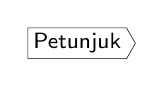
\begin{tikzpicture}[baseline=(H.base),every node/.style={
    signal,draw,very thin,signal to=east,signal from=nowhere,
    signal pointer angle=120,inner sep=2pt}]
    \node[anchor=mid west] (H) at (0,0)
      {\sffamily\footnotesize Petunjuk};
  \end{tikzpicture}
}{}

\setlength{\emergencystretch}{1.5em}
\newtcolorbox{petunjukbacaan}{
  breakable,
  enhanced,
  width=\textwidth,
  colback=white,
  colbacktitle=white,
  colframe=gray!50,
  boxrule=0.2mm,
  coltitle=black,
  fonttitle=\sffamily,
  attach boxed title to top left={yshift=-\tcboxedtitleheight/2,xshift=\tcboxedtitlewidth/4},
  boxed title style={boxrule=0pt,colframe=white},
  before skip=0.5cm,
  top=3mm,
  bottom=3mm,
  title={Petunjuk Bacaan}
}

\begin{document}
\frontmatter

\cleardoublepage
\thispagestyle{empty}
\section*{Atribusi, lisensi, dan status edisi}
Karya sumber: Wen-Wei Li, \emph{Methods of Algebra, Volume 2: Linear
Algebra}, edisi 2024. Sumber yang dibekukan adalah repositori yang
dikendalikan penulis pada commit
\texttt{9a5803ff77dd3257484cb177f851a73770a59dd3}, pohon
\texttt{23bd05c2fb8434278df4fdfb636559a6a2b0d2ff}.
Karya sumber dan turunan ini berlisensi Creative Commons Attribution
4.0 International (CC BY 4.0):
\begin{center}
  \small\url{https://creativecommons.org/licenses/by/4.0/}
\end{center}

Edisi independen ini menerjemahkan secara lengkap seluruh pendahuluan,
Bab 1--9, Lampiran A--B, latihan, petunjuk, judul, dan antarmuka pembaca
yang aktif dalam sumber. Rumus, notasi, penomoran, label, rujukan silang,
sitasi, diagram, dan identitas bibliografis dipertahankan. Berkas ini
adalah draf teks lengkap; pemeriksaan deterministik, penyusunan lapisan
aksesibilitas, dan pemaketan rilis masih berlangsung. Wen-Wei Li dan
penerbit sumber tidak mendukung atau mengesahkan terjemahan independen
ini.

\medskip
Provenans produksi: terjemahan Bahasa Indonesia, rekonsiliasi
terminologi, metadata, dan backend modular diproduksi dengan
\textbf{OpenAI Codex gpt-5.6-sol, Ultra}, atas instruksi pengguna.
Pengungkapan ini tidak menggantikan kredit Wen-Wei Li sebagai penulis
karya sumber maupun kredit komponen lain.

\mainmatter

% Terjemahan Bahasa Indonesia dari prelude.tex baris 9-29.
% Sumber: Methods of Algebra, Volume 2, commit
% 9a5803ff77dd3257484cb177f851a73770a59dd3 (CC BY 4.0).
% stable-unit-id: o014.aljabr2.prelude.linear-algebra

\chapter*{Pendahuluan}
\hypertarget{o014.aljabr2.prelude}{ }

% segment-id: o014.li2.prelude.p001
Karya yang disajikan kepada pembaca ini merupakan kelanjutan dari
\cite{Li1} (selanjutnya disebut Jilid I). Tujuannya adalah memperkenalkan
serangkaian metode, gagasan, dan teknik yang secara wajar dapat dihimpun
di bawah nama aljabar linear, dengan mengandaikan bahwa pembaca telah
mengenal struktur-struktur dasar dalam aljabar. Metode-metode ini dipakai
di seluruh matematika kontemporer. Agar dapat menjawab kebutuhan praktis
sekomprehensif mungkin, teknik-teknik terkait perlu ditempa menjadi bentuk yang
lebih murni dan lebih ringkas. Kategori dan funktor merupakan bahasa yang
tak tergantikan untuk tujuan tersebut.

% segment-id: o014.li2.prelude.p002
Buku ini terbagi menjadi tiga bagian: bagian dalam, bagian luar,
dan lampiran. Sasaran utamanya ialah mahasiswa sarjana tingkat lanjut,
mahasiswa pascasarjana, peneliti, pengajar, dan pembelajar mandiri yang
menekuni atau berminat pada pokok-pokok ini. Pengetahuan prasyaratnya
mencakup grup, gelanggang, modul, lapangan, dan struktur aljabar lain, serta
teori kategori. Jilid I mencakup seluruh landasan tersebut, tetapi buku
teks bermutu lainnya juga memadai, meskipun mungkin terdapat sedikit
perbedaan notasi.
Motivasi penulisan telah dijelaskan dalam pendahuluan Jilid I; tujuannya
tetap sama dan tidak perlu diulang di sini.

\section*{Apakah Aljabar Linear Itu?}
\addcontentsline{toc}{section}{Apakah Aljabar Linear Itu?}
\hypertarget{o014.aljabr2.prelude.linear-algebra}{ }
\index{aljabar linear (linear algebra)}

% segment-id: o014.li2.prelude.linear-algebra.p001
Dalam pengertian yang lazim di kalangan ahli aljabar, kata ``linear''
secara luas merujuk pada sifat-sifat yang berhubungan dengan struktur
yang memiliki penjumlahan beserta operasi inversnya, yaitu pengurangan.
Penjumlahan dan pengurangan selanjutnya memberikan operasi perkalian
dengan bilangan bulat; generalisasi langsungnya adalah perkalian skalar
oleh unsur suatu gelanggang $R$. Contoh prototipikalnya ialah modul kiri
dan modul kanan atas $R$, sedangkan modul-$\Z$ tidak lain adalah grup
abelian. Untuk suatu modul-$R$ (mulai sekarang modul kiri, kecuali dinyatakan
lain), kita dapat mempelajari submodul dan modul kuosien (modul hasil bagi),
serta kernel
$\Ker(f)$, kokernel $\Coker(f)$, dan citra $\Image(f)$ dari suatu
homomorfisme modul $f$. Semuanya merupakan objek yang sudah dikenal dari
aljabar dasar; setidaknya, kasus ketika $R$ adalah lapangan, yakni kasus
ruang vektor, telah dikenal luas.

% segment-id: o014.li2.prelude.linear-algebra.p002
Sejak abad ke-20, praktik matematika secara bertahap memperlihatkan bahwa
memperluas kajian modul-$R$ dan homomorfismenya ke kompleks modul bukan
hanya bermanfaat dan memudahkan, melainkan sering kali diperlukan.
Kompleks semacam itu adalah deretan homomorfisme modul yang memenuhi
$d^{n+1}d^n=0$:
\[
  \cdots \longrightarrow X^{n-1} \xrightarrow{d^{n-1}} X^n
  \xrightarrow{d^n} X^{n+1} \xrightarrow{d^{n+1}} \cdots .
\]
Syarat pada homomorfisme tersebut kadang ditulis $d^2=0$, sedangkan
seluruh data kompleks sering disingkat menjadi $(X^n,d^n)_n$, $(X,d)$,
atau $X$. Karena digunakan indeks atas yang meningkat, kompleks ini juga
disebut kompleks kokrantai (\emph{cochain complex}). Jika digunakan indeks
bawah yang menurun,
$\cdots\to X_n\xrightarrow{d_n}X_{n-1}\to\cdots$, objek matematis yang
diperoleh disebut kompleks rantai; perbedaannya dengan kompleks di atas
hanya bersifat formal.

% segment-id: o014.li2.prelude.linear-algebra.p003
Suatu modul-$R$ tunggal $M$ dapat dipandang sebagai kasus khusus kompleks,
dengan $X^0=M$ dan semua suku lainnya nol. Untuk suatu kompleks $X$,
karena $d^nd^{n-1}=0$, kohomologi ke-$n$ dapat didefinisikan sebagai
modul kuosien
\[
  \Hm^n(X):=\Ker\left(d^n\right)\big/\Image\left(d^{n-1}\right).
\]

% segment-id: o014.li2.prelude.linear-algebra.p004
Kompleks yang memenuhi $\Hm^n(X)=0$ untuk setiap $n$ disebut barisan
eksak atau kompleks asiklik. Untuk kompleks rantai, secara bersesuaian
kita memiliki homologi
$\Hm_n(X):=\Ker(d_n)/\Image(d_{n+1})$. Kohomologi suatu kompleks (atau
homologi suatu kompleks rantai) sering menyimpan informasi penting
tentang objek matematis yang dikaji.

\enlargethispage{3\baselineskip}
% segment-id: o014.li2.prelude.linear-algebra.p005
Untuk modul atau struktur matematis lain yang memiliki operasi linear,
misalnya objek dalam kategori abelian yang akan diperkenalkan kemudian,
kajian kompleks beserta kohomologinya merupakan isi klasik bidang yang
disebut aljabar homologis. Bidang ini merupakan subhimpunan sejati dari
``aljabar linear'' dalam arti hakikinya dan sekaligus merupakan inti buku
ini. Riwayat singkatnya akan dibahas berikutnya.

% Terjemahan Bahasa Indonesia dari prelude.tex baris 30-103.
% Sumber: Methods of Algebra, Volume 2, commit
% 9a5803ff77dd3257484cb177f851a73770a59dd3 (CC BY 4.0).
% stable-unit-id: o014.aljabr2.prelude.homology-history

\section*{Sejarah Singkat Homologi}
\addcontentsline{toc}{section}{Sejarah Singkat Homologi}
\hypertarget{o014.aljabr2.prelude.homology-history}{ }

% segment-id: o014.li2.prelude.homology-history.p001
Matematika tidak harus berpijak pada sejarah. Namun, menelaah masa lalu
untuk memahami masa depan tentu bermanfaat dan tidak merugikan. Untuk memudahkan pembahasan,
kita akan membagi perkembangan teori homologi secara agak artifisial ke
dalam beberapa tahap.

\subsection*{Masa Perintisan}

% segment-id: o014.li2.prelude.homology-history.p002
Pendorong pertama perkembangan aljabar homologis adalah topologi. Pada
paruh akhir abad ke-19, B.\ Riemann dan E.\ Betti mengkaji genus permukaan
beserta generalisasinya ke dimensi lebih tinggi, yang disebut bilangan
Betti. Menjelang pergantian abad, gagasan ini dikembangkan oleh
H.\ Poincaré menjadi suatu sistem yang lebih ketat secara matematis. Secara kasar, gagasan
awal Poincaré ialah menguraikan ruang menjadi poligon, polihedron, atau
padanan berdimensi lebih tinggi yang direkatkan satu sama lain, lalu
menghitung bilangan Betti atau versi torsinya dari matriks yang merekam
cara perekatan tersebut, dan menunjukkan bahwa semuanya merupakan
invarian topologis.

% segment-id: o014.li2.prelude.homology-history.p003
Dalam tulisan singkat tahun 1925, E.\ Noether menjelaskan
bagaimana homologi dapat didefinisikan sebagai grup abelian, sedangkan
bilangan Betti dan versi torsinya hanyalah nilai numerik yang diturunkan
darinya. Gagasan ini sudah mendekati definisi modern dalam topologi
aljabar: untuk ruang $E$ yang dilengkapi dengan suatu penguraian dan grup
abelian $A$, didefinisikan
kompleks rantai $C(E, A)$ yang merekam cara bagian-bagian penguraian
tersebut direkatkan.
Grup homologi $E$ berkoefisien $A$ kemudian didefinisikan sebagai
$\Hm_n(E; A) := \Hm_n(C(E, A))$, sementara grup kohomologi
$\Hm^n(E; A)$ didefinisikan melalui cara yang dual.

% segment-id: o014.li2.prelude.homology-history.p004
Sejak saat itu hingga sekitar tahun 1950, topologi aljabar memasuki masa
perkembangan yang amat subur. Dari sudut pandang aljabar, perkembangan
yang patut dicatat meliputi:
\begin{itemize}
	% segment-id: o014.li2.prelude.homology-history.p005
	\item Teorema koefisien universal untuk homologi (atau kohomologi),
	yang menyatakan bahwa kasus berkoefisien bilangan bulat sudah cukup
	untuk menentukan homologi (atau kohomologi) dengan koefisien dalam grup
	abelian umum $A$. Uraian konkretnya melibatkan funktor $\Tor$ (atau
	$\Ext$), yang akan dibahas secara mendalam kelak.
	% segment-id: o014.li2.prelude.homology-history.p006
	\item Hasil kali \emph{cup} pada kohomologi, yaitu suatu struktur
	perkalian yang dimiliki grup kohomologi.
	% segment-id: o014.li2.prelude.homology-history.p007
	\item Ruang yang disebut asferis, yakni ruang terhubung yang memenuhi
	$n > 1 \implies \pi_n(E) = 0$; di sini $E$ menyatakan ruang tersebut,
	dan $\pi_n(E)$ menyatakan grup homotopi ke-$n$ relatif terhadap titik
	dasar yang dipilih.
	W.\ Hurewicz membuktikan bahwa grup homologi dan kohomologi ruang
	asferis sepenuhnya ditentukan oleh $\pi_1(E)$ dan dapat diberikan secara
	aljabar. Inilah cikal bakal teori kohomologi grup.
\end{itemize}

% segment-id: o014.li2.prelude.homology-history.p008
Pendorong lain bagi aljabar homologis datang dari dalam aljabar sendiri.
Contoh klasiknya ialah teorema sizigi Hilbert dalam teori invarian (1890):
dalam bahasa modern, teorema sizigi menyatakan bahwa setiap modul atas
gelanggang polinomial $\Bbbk[X_1, \ldots, X_n]$ memiliki resolusi bebas
dengan panjang $\leq n$.

% segment-id: o014.li2.prelude.homology-history.p009
Funktor $\Ext$ juga berkaitan dengan persoalan aljabar. Untuk grup abelian
$A$ dan $B$, barisan eksak pendek grup abelian
$0 \to A \to E \to B \to 0$ disebut pula ekstensi grup (perluasan grup);
hingga isomorfisme, ekstensi-ekstensi tersebut berkorespondensi satu-satu
dengan unsur-unsur grup $\Ext^1(B, A)$. Selain itu, jika $B$ diganti oleh
sembarang grup $G$, klasifikasi ekstensi grup secara alami menghasilkan
definisi aljabar bagi kohomologi grup $\Hm^2(G, A)$.

% segment-id: o014.li2.prelude.homology-history.p010
Operasi derivasi pada gelanggang merupakan persoalan yang sejak awal
menarik perhatian para ahli aljabar. Pada tahun 1942, G.\ Hochschild
mendefinisikan invarian untuk gelanggang $R$ yang kini disebut homologi
dan kohomologi Hochschild; suku kohomologi berderajat $n=1$
mengklasifikasikan derivasi modulo derivasi dalam.\footnote{Catatan
penerjemah: teks sumber menyatakan bahwa suku berderajat satu
``mengklasifikasikan semua derivasi''. Pernyataan ini dikoreksi di sini:
$\Hm^1_{\mathrm{Hoch}}(R,R)$ mengklasifikasikan derivasi modulo derivasi
dalam; lihat catatan koreksi O014-C001.}
Konstruksi-konstruksi ini dapat diperluas ke bimodul $(R, R)$ yang lebih
umum, yaitu $M$, dan terus memainkan peranan penting dalam matematika
mutakhir.

% segment-id: o014.li2.prelude.homology-history.p011
Patut disebut pula karya J.\ Leray mengenai berkas dan barisan spektral
selama Perang Dunia II. Motivasinya bermula dari persoalan titik tetap
yang berkaitan dengan persamaan diferensial parsial. Berkas adalah
struktur dalam geometri yang memuat informasi lokal--global, sedangkan
barisan spektral menyediakan perangkat ampuh untuk menghitung kohomologi
berkas. Di bawah pengaruh teori Leray dan karya Kiyoshi Oka dalam teori
fungsi beberapa peubah kompleks, H.\ Cartan dan sejumlah matematikawan lain
mulai menulis ulang dasar-dasar topologi aljabar setelah perang; aljabar
homologis pun memperoleh wajah yang sama sekali baru.

\subsection*{Revolusi Cartan--Eilenberg}

% segment-id: o014.li2.prelude.homology-history.p012
Karya H.\ Cartan dan S.\ Eilenberg \cite{CE56} sangat luas dan mendalam,
serta untuk waktu yang lama dipandang sebagai rujukan kanonik. Buku itu
menandai suatu masa baru dalam perkembangan aljabar homologis. Sumbangan
utamanya mencakup:
\begin{itemize}
	% segment-id: o014.li2.prelude.homology-history.p013
	\item definisi modul injektif dan modul projektif, beserta resolusi
	injektif dan resolusi projektif suatu modul;
	% segment-id: o014.li2.prelude.homology-history.p014
	\item definisi funktor turunan kanan dan funktor turunan kiri dalam
	kerangka teori modul, yang memberikan definisi umum bagi funktor
	$\Ext$ dan $\Tor$, serta pengenalan dimensi injektif dan dimensi
	projektif suatu modul; perangkat ini segera menunjukkan kegunaannya
	dalam teori gelanggang komutatif;
	% segment-id: o014.li2.prelude.homology-history.p015
	\item penjelasan, melalui perangkat tersebut, atas berbagai konstruksi
	sebelumnya, seperti kohomologi grup serta homologi dan kohomologi
	Hochschild;
	% segment-id: o014.li2.prelude.homology-history.p016
	\item pembangunan sistematis teori umum barisan spektral dan struktur
	perkaliannya.
\end{itemize}

% segment-id: o014.li2.prelude.homology-history.p017
Istilah ``aljabar homologis'' juga berasal dari \cite{CE56}. Dengan
hadirnya teori akbar ini, aljabar homologis memasuki masa mudanya.

\subsection*{Kategori Abelian}

% segment-id: o014.li2.prelude.homology-history.p018
Dilihat dari sudut pandang geometri---lebih tepatnya, teori berkas---kerangka
teori modul belum memadai bagi aljabar homologis. Di samping kategori modul
kiri atas gelanggang $R$, yakni $R\dcate{Mod}$, kita ingin mengizinkan suatu
kategori yang lebih umum $\mathcal{A}$ tetapi tetap memiliki makna ``linear''.
Upaya pertama ke arah ini muncul dalam disertasi
doktor D.\ Buchsbaum pada tahun 1955, yang juga menjadi sebuah lampiran
dalam \cite{CE56}; ia mengabstraksikan konsep barisan eksak dari teori
modul.

% segment-id: o014.li2.prelude.homology-history.p019
Pendekatan yang kini lazim berasal dari makalah A.\ Grothendieck
\cite{Gr57}; kategori yang dihasilkan disebut kategori abelian. Kategori
ini adalah kategori aditif yang memiliki kernel dan kokernel, dengan
syarat bahwa setiap morfisme $f: M \to N$ di dalamnya bersifat ketat.
Secara kasar, keketatan tersebut bersesuaian dengan teorema isomorfisme
yang dikenal dalam teori modul,
$M/\Ker(f) \rightiso \Image(f)$. Dalam karya itu, Grothendieck juga:
\begin{itemize}
	% segment-id: o014.li2.prelude.homology-history.p020
	\item mendefinisikan funktor-$\delta$ dan funktor-$\delta$ universal
	dengan memakai konsep barisan eksak panjang, memberikan karakterisasi
	bagi yang terakhir, dan menunjukkan bahwa funktor turunan merupakan
	kasus khusus funktor-$\delta$ universal;
	% segment-id: o014.li2.prelude.homology-history.p021
	\item memberikan barisan spektral Grothendieck untuk funktor turunan
	dari komposisi funktor;
	% segment-id: o014.li2.prelude.homology-history.p022
	\item mendefinisikan suatu kelas khusus kategori abelian, yang kini
	disebut kategori Grothendieck, serta membuktikan keberadaan resolusi
	injektif di dalamnya.
\end{itemize}

% segment-id: o014.li2.prelude.homology-history.p023
Teori-teori ini memungkinkan kohomologi berkas dipelajari pada ruang yang
lebih umum dan sangat penting bagi perkembangan geometri.

\subsection*{Kategori Turunan}

% segment-id: o014.li2.prelude.homology-history.p024
Dalam disertasi doktor tahun 1963, J.-L.\ Verdier mendefinisikan kategori
turunan $\cate{D}(\mathcal{A})$ bagi suatu kategori abelian $\mathcal{A}$.
Motivasinya berasal dari kesulitan yang dihadapi
Grothendieck ketika mengkaji dualitas dalam geometri aljabar. Hambatan
tersebut mendorong pencarian kerangka baru untuk bekerja bukan lagi hanya
dengan kohomologi, melainkan dengan kompleks itu sendiri, sambil secara
formal menambahkan invers bagi kuasi-isomorfisme ke dalam kategori
kompleks $\cate{C}(\mathcal{A})$. Kuasi-isomorfisme adalah morfisme
kompleks yang menginduksi isomorfisme pada taraf kohomologi,
$\Hm^n(f): \Hm^n(X) \rightiso \Hm^n(Y)$, dengan $f: X \to Y$.
Konstruksi penambahan invers
tersebut disebut lokalisasi Gabriel--Zisman dan merupakan generalisasi
lokalisasi gelanggang pada taraf kategori.

% segment-id: o014.li2.prelude.homology-history.p025
Kategori turunan $\cate{D}(\mathcal{A})$ memuat lebih banyak informasi
daripada kohomologi, dan cara bekerja dengannya pun berbeda. Di dalam
$\cate{D}(\mathcal{A})$, kita harus memakai suatu kelas barisan morfisme
yang disebut segitiga terbedakan (\emph{distinguished triangle})
\[ X \xrightarrow{f} Y \xrightarrow{g} Z \xrightarrow{h} X[1] \]
untuk menggantikan barisan eksak pendek dalam $\mathcal{A}$ atau kategori
kompleks $\cate{C}(\mathcal{A})$. Di sini,
$X[1]$ berarti pergeseran kompleks $X$:
\[ X[1]^n = X^{n+1}, \quad d_{X[1]}^n = -d_X^n. \]
Konstruksi-konstruksi ini selanjutnya diabstraksikan oleh Verdier menjadi
suatu kelas struktur yang disebut kategori bertriangulasi
(\emph{triangulated category}). Dilihat dari
topologi, struktur bertriangulasi kategori turunan juga bersifat alami:
segitiga terbedakan dapat dianalogikan dengan barisan kofiber
(\emph{cofiber sequence}) dalam teori
homotopi. Hal ini berkaitan dengan aljabar homotopik yang akan dibahas
kelak. Atas pertimbangan teori homotopi pula, D.\ Puppe secara independen
menemukan struktur serupa pada tahun 1962, tetapi aksioma yang ia tuliskan
tidak memuat aksioma oktahedral Verdier.

% segment-id: o014.li2.prelude.homology-history.p026
Meskipun kategori turunan tidak sempurna untuk semua penerapan, bahasa ini
tetap menjadi pilihan utama para ahli geometri dan aljabar hingga awal
abad ke-21. Sebagai contoh, salah satu penerapannya yang menonjol ialah
teori modul-$\mathscr{D}$, yang terutama dikembangkan oleh Masaki Kashiwara,
Z.\ Mebkhout, dan matematikawan lain; beberapa operasi dasarnya hanya
dapat didefinisikan secara wajar pada taraf kategori turunan.

% segment-id: o014.li2.prelude.homology-history.p027
Selain itu, kategori turunan suatu gelanggang $R$,
$\cate{D}(R) := \cate{D}(R\dcate{Mod})$, dapat pula dipandang sebagai
suatu invarian bagi $R$. Jika kategori turunan dua gelanggang ekuivalen
sebagai kategori bertriangulasi, kedua gelanggang itu disebut ekuivalen
secara turunan. Berbagai persoalan dan metode seputar ekuivalensi turunan
merupakan salah satu arus utama dalam teori representasi aljabar; para
perintisnya antara lain D.\ Happel dan J.\ Rickard.

\subsection*{Aljabar Homotopik}

% segment-id: o014.li2.prelude.homology-history.p028
Pembaca tentu masih ingat bahwa asal-usul topologis aljabar homologis
adalah penguraian ruang, lalu pendefinisian kompleks rantai atau kompleks
yang sesuai untuk menyarikan invarian topologis. Penguraian pada langkah
pertama memiliki berbagai ragam; himpunan simplisial yang didefinisikan
oleh Eilenberg dan Zilber pada tahun 1950 merupakan salah satunya, dan
himpunan simplisial dapat diperumum lebih lanjut menjadi objek simplisial
dalam suatu kategori tertentu. Bahasa ini memiliki daya penjelas yang
sangat luas. Sebagai contoh, teori homotopi ruang topologis dapat
dikembangkan dalam kerangka himpunan simplisial, sedangkan konstruksi yang
disebut ``saraf'' (\emph{nerve}) menafsirkan kategori sebagai suatu jenis
khusus himpunan simplisial.

% segment-id: o014.li2.prelude.homology-history.p029
Apa yang terjadi jika sedikit ``linearitas'' ditambahkan ke dalam gambaran
ini? Korespondensi Dold--Kan (1958) memberikan hubungan langsung antara
objek simplisial dalam kategori abelian dan teori kompleks. Sebagai
contoh, untuk kategori grup abelian $\cate{Ab}$, korespondensi Dold--Kan
merupakan suatu ekuivalensi adjoin yang diwujudkan secara eksplisit oleh
sepasang funktor:
\[\begin{tikzcd}
	\mathrm{N}: \cate{sAb} \arrow[shift left, r] & \cate{Ch}_{\geq 0}(\cate{Ab}): \Gamma \arrow[shift left, l]
\end{tikzcd}\]
Di sini, $\cate{sAb}$ adalah kategori objek simplisial dalam $\cate{Ab}$,
sedangkan $\cate{Ch}_{\geq 0}(\cate{Ab})$ adalah kategori kompleks rantai
berderajat tak negatif dalam $\cate{Ab}$. Untuk kategori kompleks, kita
dapat menangani konvensi lain dengan membalik pengindeksan atau beralih ke
kategori lawan.

% segment-id: o014.li2.prelude.homology-history.p030
Korespondensi Dold--Kan memberikan tafsiran topologis bagi banyak definisi
dan konstruksi tentang kompleks rantai. Melalui metode simplisial,
suatu kelas resolusi yang secara kolektif disebut ``konstruksi bar'' dalam
aljabar homologis juga memperoleh penjelasan terpadu.

% segment-id: o014.li2.prelude.homology-history.p031
Homotopi adalah gagasan inti dalam teori simplisial. Metode aljabar yang
melibatkan objek simplisial kadang-kadang juga disebut aljabar homotopik.
Daya metode ini tampak menonjol dalam teori K tingkat tinggi yang
dikembangkan D.\ Quillen, dan penerapannya tidak terbatas pada hal itu.

% segment-id: o014.li2.prelude.homology-history.p032
Ringkasnya, metode simplisial dalam aljabar linear dapat dipandang sebagai
pertemuan, pada suatu taraf yang lebih tinggi, antara topologi---khususnya
teori homotopi---dan aljabar homologis. Teori kategori-$\infty$ merupakan
gelombang lain yang diilhami oleh pertemuan tersebut pada awal abad ke-21.

% Terjemahan Bahasa Indonesia dari prelude.tex baris 104-126.
% Sumber: Methods of Algebra, Volume 2, commit
% 9a5803ff77dd3257484cb177f851a73770a59dd3 (CC BY 4.0).
% stable-unit-id: o014.aljabr2.prelude.book-purpose

\section*{Tujuan Buku Ini}
\addcontentsline{toc}{section}{Tujuan Buku Ini}
\hypertarget{o014.aljabr2.prelude.book-purpose}{ }

\subsection*{Tujuan Penyusunan}

% segment-id: o014.li2.prelude.book-purpose.p001
Pengantar sebelumnya menunjukkan bahwa apa yang disebut aljabar linear
secara kasar terbagi menjadi dua cabang utama: teori kategori abelian dan
teori kompleks yang dibangun di atas kategori abelian. Buku ini berpusat
pada kedua cabang tersebut dan berupaya membekali pembaca dengan gagasan
serta teknik yang diperlukan untuk memahami matematika kontemporer.
Isinya mencakup metode aljabar yang digunakan dalam penerapan sekaligus
landasan teoretis yang menopangnya. Karena metode tersebut terutama
ditujukan bagi penelitian matematika murni dan dimaksudkan untuk diterapkan
seluas mungkin, buku ini dapat pula dicirikan sebagai
``matematika terapan murni''.

% segment-id: o014.li2.prelude.book-purpose.p002
Buku ini juga berupaya memadukan peran sebagai buku ajar dan buku
rujukan. Karena itu, perhatian terhadap perincian dan kerangka yang
sistematis tidak dapat dihindari. Berbagai tujuan tersebut menimbulkan
ketegangan satu sama lain. Selain itu, tujuan harus dirumuskan, uraian ditata, dan
pokok bahasan ditegaskan dalam ruang yang terbatas. Semua ini menghadirkan
tantangan besar bagi penyusunan buku, tetapi tantangan tersebut memang
harus diterima.

% segment-id: o014.li2.prelude.book-purpose.p003
Pada tataran isi, kategori turunan, funktor turunan, dan barisan spektral
merupakan pengetahuan dasar yang wajib dimiliki matematikawan masa kini.
Namun, ketiganya tidak mudah bagi pemula; kendala utamanya terletak pada
gagasan dan definisi. \emph{Bagian Dalam} buku ini disusun dengan sasaran
tersebut dan sekaligus meletakkan landasan bagi pembahasan dalam \emph{Bagian
Luar}. Demi kelancaran uraian dan penghematan ruang yang wajar, kita tidak
akan menapaki kembali sejarah langkah demi langkah, melainkan lebih banyak
mengikuti urutan logis yang tampak berkat tinjauan ke belakang.

% segment-id: o014.li2.prelude.book-purpose.p004
Karena terikat oleh berbagai sasaran di atas, apa yang oleh kritikus seni
dan sastra disebut ``aura'' tak pelak menjadi samar dalam tulisan ini. Sebagai
gantinya, bangunan sistematis dan pembuktian ketat sesekali menimbulkan
kesan berat. Aura yang berlawanan dengan kesan berat itu adalah
ketukan pertama matematika pada batin manusia, dan mungkin juga ketukan
terakhirnya. Namun, menurut penulis, gaya yang ringan, lincah, dan langsung
ke pokok lazimnya muncul pada masa perintisan suatu teori atau bertumpu
pada pustaka rujukan yang lengkap sebagai penopang. Penopang semacam itu
harus tertanam dalam budaya bahasa setempat dan dapat dimanfaatkan oleh
semua pembaca. Penulis memilih memikul beban ini, dengan harapan bahwa
setelah buku ini hadir, para penulis masa depan akan bebas melangkah
dengan beban yang lebih ringan.

% segment-id: o014.li2.prelude.book-purpose.p005
Dalam penyusunannya, buku ini merujuk secara luas pada karya-karya terkait,
termasuk, tetapi tidak terbatas pada, \cite{Wei94, ML98, KS06, Rie16, Yek20}.
Selain itu, \cite{stacks} dan situs web
\href{https://ncatlab.org}{nLab} juga sangat membantu.

\subsection*{Jalur dan Pilihan}

% segment-id: o014.li2.prelude.book-purpose.p006
Buku ini harus mengakomodasi beragam bidang dan gaya, sekaligus mencari
titik keseimbangan antara yang klasik dan yang modern agar isinya tetap
cukup mudah dibaca oleh pemula. Karena itu, kompromi
menjadi pedoman umum penulis. Akan tetapi, hanya sedikit pembaca yang
membuka sebuah buku dengan mengharapkan kompromi. Kompromi mengharuskan jalan
memutar; akibatnya, alur pemikiran buku ini tidak menempuh lintasan
geodesik bagi pembaca mana pun. Hal tersebut tidak dapat dihindari.

% segment-id: o014.li2.prelude.book-purpose.p007
Karena alasan yang sama, pilihan isi buku ini pun sulit memuaskan semua
orang. Pembaca yang berorientasi geometri, misalnya, tidak akan menjumpai
berkas dan struktur-$t$, sedangkan pembaca yang berorientasi teori
representasi aljabar tidak akan menemukan teori \emph{tilting}. Pokok-pokok
tersebut tidak dibahas karena mustahil memberikan motivasi yang memadai
bagi teori-teori terkait tanpa terlebih dahulu mendalami bidang-bidang itu.

% segment-id: o014.li2.prelude.book-purpose.p008
Peminat teori kategori mungkin menilai pendekatan buku ini tak lebih dari
semiklasik. Meskipun demikian, pembaca mungkin akan melihat bahwa
teks utama dan latihan membuka jalan menuju beberapa sudut pandang yang
lebih maju,
seperti kategori-dg, teori monad, dan objek simplisial, meskipun semuanya
hanya disinggung sepintas. Pokok-pokok tersebut dapat dipandang sebagai
pemanasan menuju teori kategori-$\infty$. Dari sini tampak suatu dunia
baru yang lebih mendalam daripada aljabar linear, yang disebut aljabar
lanjut atau aljabar tingkat tinggi (\emph{higher algebra}); dunia itu sudah
berada di luar lingkup buku ini.

% segment-id: o014.li2.prelude.book-purpose.p009
Mengenai pilihan isi, perlu dijelaskan pula bahwa buku ini membahas
kategori abelian umum dan membangun sifat-sifat dasarnya langsung dari
aksioma. Dalam hal ini, pendekatannya berbeda dari sejumlah buku ajar
aljabar homologis yang hanya membahas modul. Mengizinkan kategori abelian
umum bukan saja sesuai dengan kelengkapan teoretis dan kebutuhan praktis,
melainkan juga diperlukan bagi konstruksi seperti kategori funktor dan
kuosien Serre, sekalipun titik tolak kita dibatasi pada modul. Karena
pengejaran diagram (\emph{diagram chase}) dalam teori modul tidak dapat
langsung diperluas ke keadaan umum, sejumlah hasil dasar mengenai kategori
abelian memerlukan
pembuktian yang cukup berliku. Untuk membantu memahami perincian tersebut,
buku ini mengandaikan bahwa pembaca setidaknya memiliki pengalaman dasar
dengan kompleks modul dan kohomologinya, misalnya materi dalam
\cite[Bab~6]{Li1}; akan tetapi, pengalaman itu bukan keharusan logis.

% segment-id: o014.li2.prelude.book-purpose.p010
Teorema pembenaman Freyd--Mitchell yang terkenal menyatakan bahwa setiap
kategori abelian kecil dapat dibenamkan ke dalam $\cated{Mod}R$, dengan
$R$ suatu gelanggang, melalui funktor yang eksak, penuh, dan setia. Dengan
menerima hasil ini, banyak fakta dasar tentang kategori abelian cukup diperiksa
dalam kategori modul konkret $\cated{Mod}R$. Kita akan
memberikan pembuktian teorema pembenaman itu dalam Lampiran
% source-xref: sec:FM; partial-reader fallback: B.6
\S\sourcecrossref{sec:FM}{B.6}. Karena pembuktiannya sendiri tidak mudah dan bergantung
pada sejumlah sifat dasar kategori abelian, teorema tersebut pada
hakikatnya tidak menyederhanakan teori kategori abelian; perannya lebih
bersifat heuristik.

% Terjemahan Bahasa Indonesia dari prelude.tex baris 127-153.
% Sumber: Methods of Algebra, Volume 2, commit
% 9a5803ff77dd3257484cb177f851a73770a59dd3 (CC BY 4.0).
% stable-unit-id: o014.aljabr2.prelude.reader-guide

% segment-id: o014.li2.prelude.reader-guide.h001
\section*{Panduan Penggunaan}
\addcontentsline{toc}{section}{Panduan Penggunaan}
\hypertarget{o014.aljabr2.prelude.reader-guide}{ }

% segment-id: o014.li2.prelude.reader-guide.h002
\subsection*{Fungsi Buku}

% segment-id: o014.li2.prelude.reader-guide.p001
Untuk memenuhi fungsinya sebagai buku rujukan, buku ini perlu disusun cukup
sistematis. Karena itu, setiap bab terutama mengikuti
urutan logis. Hubungan ketergantungan antarbagiannya sangat kentara pada
\emph{Bagian Dalam}, sedangkan sejumlah kecil topik yang diperlukan tetapi
menyimpang dari jalur utama, atau yang lebih bersifat teknis, ditempatkan
dalam lampiran.

% segment-id: o014.li2.prelude.reader-guide.p002
Bagi pembelajar mandiri, bagian yang perlu dibaca bergantung pada minat dan
kebutuhan masing-masing. Pilihan utama terletak pada \emph{Bagian Luar}, sedangkan
\emph{Bagian Dalam} merupakan kerangka dasar bersama, meskipun pada skala subbab
masih ada sejumlah materi pilihan di dalamnya. Beberapa perincian yang
lebih abstrak atau teknis dapat dilewati seperlunya ketika pertama kali
belajar. Pembahasan yang bergantung pada lampiran sebaiknya dilewati dahulu atau
hanya dibaca sekilas. Saran terperinci mengenai pilihan-pilihan tersebut
terdapat pada penjelasan di awal setiap bab dan lampiran, terutama dalam
bagian \emph{Petunjuk Bacaan}.

% segment-id: o014.li2.prelude.reader-guide.p003
Seperti disebutkan sebelumnya ketika membahas tujuan buku, kita terpaksa
menyelubungi gagasan matematika dengan lapisan-lapisan teks.
Pembelajar mandiri harus mengerahkan upaya sungguh-sungguh untuk mengenali
matematika yang sesungguhnya di baliknya, layaknya menangkap kilat di
tengah gulungan awan tebal.

% segment-id: o014.li2.prelude.reader-guide.p004
Bagi pembaca yang menggunakan buku ini sebagai rujukan, penulis telah
berusaha menerapkan cara penulisan modular agar bagian-bagiannya mudah
dibaca secara terpisah. Hal ini tercermin bukan hanya dalam pembagian bab,
melainkan juga dalam dua hal berikut.
\begin{itemize}
	% segment-id: o014.li2.prelude.reader-guide.i001
	\item Sedapat mungkin, buku ini menggunakan notasi baku dalam pustaka
	kontemporer, disertai tinjauan ulang dan penjelasan. Bagian Konvensi pada
	akhir pendahuluan dan indeks di akhir buku merupakan dua sarana lain yang
	ampuh untuk memahami notasi.
	% segment-id: o014.li2.prelude.reader-guide.i002
	\item Berbagai pernyataan dan pembuktian dilengkapi dengan rujuk silang
	secara cermat, sehingga pembaca yang sudah memiliki pengetahuan tertentu
	tentang materinya dapat memahami uraian dengan cepat dan membangun peta
	konseptual secara efisien.
\end{itemize}

% segment-id: o014.li2.prelude.reader-guide.p005
Secara khusus, penulis berharap buku ini dapat membantu pembaca yang sedang
menyiapkan pengajaran atau mengikuti seminar untuk segera menghimpun
pengetahuan yang mereka perlukan, lalu mengolahnya dengan bahasa mereka sendiri.

% segment-id: o014.li2.prelude.reader-guide.p006
Mengenai penggunaan dalam pengajaran, harus diakui terus terang bahwa
penjadwalan perkuliahan tidak dapat diatur sesuka hati. Selama menulis
buku ini, penulis hampir tidak memperoleh kesempatan untuk menguji materi
ini di ruang kelas, sehingga hasilnya belum dapat dinilai. Berdasarkan
pengalaman terdahulu, sekalipun perincian dilewati di kelas, seluruh buku
ini jelas memuat bahan untuk lebih dari satu tahun akademik; \emph{Bagian Dalam}
mungkin dapat dipadatkan menjadi satu semester dengan penyajian ringkas. Jika
buku ini digunakan sebagai buku ajar utama, pengajar harus terlebih dahulu
membagi materi buku ini. Penulis berharap rancangan modular yang telah disebutkan
dapat mempermudah pekerjaan tersebut.

% segment-id: o014.li2.prelude.reader-guide.p007
Kurangnya pengujian di ruang kelas membawa dua akibat lain. Pertama, buku
ini tak pelak masih mengandung banyak kesalahan yang belum ditemukan.
Kedua, buku ini belum memiliki keluwesan dan kematangan khas buku ajar
klasik. Hal ini sebagian disebabkan oleh keadaan praktis dan sebagian lagi
oleh keterbatasan penulis; penulis hanya dapat memohon pengertian
pembaca.

% segment-id: o014.li2.prelude.reader-guide.h003
\subsection*{Tentang Latihan}

% segment-id: o014.li2.prelude.reader-guide.p008
Setiap bab dan lampiran diakhiri dengan latihan yang disusun mengikuti
urutan materi terkait dalam teks utama dan kadang-kadang disertai petunjuk.
Tujuan utamanya ialah menambahkan sifat-sifat atau hasil pelengkap,
menyediakan contoh, dan
memperluas wawasan. Sebagian latihan dimaksudkan untuk membantu pembaca
membiasakan diri dengan berbagai teknik dan pada umumnya tidak terlalu
teknis. Sejumlah kecil latihan meminta pembaca melengkapi perincian yang
dihilangkan dari teks utama; perincian itu kadang remeh, kadang mudah, dan
lebih sering keduanya sekaligus. Singkatnya, penulis berharap pembaca
pemula berusaha mengerjakan sebanyak mungkin latihan, tetapi tidak perlu
memaksakan diri atau merasa harus menyelesaikan semuanya.

% segment-id: o014.li2.prelude.reader-guide.h004
\subsection*{Kategori dan Ukurannya}

% segment-id: o014.li2.prelude.reader-guide.p009
Sebagian besar isi buku ini dinyatakan dalam bahasa kategori karena
praktik telah membuktikan bahwa teori kategori memang merupakan sarana
yang efisien untuk memahami dan menangani persoalan aljabar. Namun,
aljabar linear atau apa yang disebut aljabar homologis bukanlah cabang
teori kategori, sama seperti teori probabilitas bukanlah cabang teori
ukuran.

% segment-id: o014.li2.prelude.reader-guide.p010
Berbeda dari sejumlah buku ajar lain, buku ini dan Jilid I sama-sama
mensyaratkan agar kumpulan semua objek dan kumpulan semua morfisme suatu
kategori masing-masing merupakan himpunan; objek tidak boleh hanya
membentuk sebuah ``kelas''. Karena kelas sejati
(\emph{proper class}) tidak digunakan dalam definisi, secara formal kita harus memperkenalkan
konsep semesta Grothendieck (\emph{Grothendieck universe}) untuk mengukur
ukuran himpunan dan mengasumsikan bahwa semua himpunan termasuk dalam
suatu semesta $\mathcal{U}$; lihat
\cite[Asumsi~1.5.2, Catatan~1.5.6]{Li1}. Jika setiap persoalan dianalisis
secara tersendiri, aksioma mengenai keberadaan cukup banyak semesta---atau,
secara ekuivalen, cukup banyak kardinal tak terjangkau kuat
(\emph{strongly inaccessible cardinal})---sering kali dapat diperlemah.
Karena hal ini tidak menyangkut inti buku, kita tidak akan membahasnya
lebih jauh.

% Terjemahan Bahasa Indonesia dari prelude.tex baris 154-183.
% Sumber: Methods of Algebra, Volume 2, commit
% 9a5803ff77dd3257484cb177f851a73770a59dd3 (CC BY 4.0).
% stable-unit-id: o014.aljabr2.prelude.structure-overview

% segment-id: o014.li2.prelude.structure-overview.h001
\section*{Ikhtisar Struktur}
\addcontentsline{toc}{section}{Ikhtisar Struktur}
\hypertarget{o014.aljabr2.prelude.structure-overview}{ }

% segment-id: o014.li2.prelude.structure-overview.p001
Pembaca disarankan memulai dari bagian Konvensi pada akhir pendahuluan.
Tujuannya ialah mengenali terlebih dahulu simbol dan konvensi yang
digunakan di seluruh buku. Selain itu, pembaca pemula tidak dianjurkan
mengikuti buku ini secara ketat dari awal hingga akhir, kecuali jika sudah
cukup siap menerima metode abstrak. Awal setiap bab menyediakan ikhtisar
dan petunjuk bacaan yang terperinci.

% segment-id: o014.li2.prelude.structure-overview.p002
Bagian pertama ialah \emph{Bagian Dalam}, yang meletakkan landasan.

\begin{description}
	% segment-id: o014.li2.prelude.structure-overview.i001
	\item[Bab 1: Pelengkap Teori Kategori] Mengulas dan melengkapi pengetahuan
	teori kategori yang diperlukan, dengan pokok utama berupa morfisme ketat
	(\emph{strict morphism}), kernel dan kokernel dalam kategori aditif,
	ekstensi Kan (\emph{Kan extension}), lokalisasi Gabriel--Zisman, dan topik-topik lain.
	% segment-id: o014.li2.prelude.structure-overview.i002
	\item[Bab 2: Kategori Abelian] Membangun teori dasar kategori abelian,
	dilengkapi dengan materi mengenai kategori Grothendieck dan topik lain.
	% segment-id: o014.li2.prelude.structure-overview.i003
	\item[Bab 3: Kompleks] Membahas konsep-konsep dasar berupa kompleks,
	bikompleks, homotopi, kerucut pemetaan, dan sebagainya pada kategori
	aditif, serta kohomologi dalam kasus kategori abelian. Paruh kedua bab ini
	membahas funktor turunan dari sudut pandang klasik beserta kasus-kasus
	khusus seperti $\Ext$, $\Tor$, dan $\lim^1$. Untuk menangani kompleks tak
	terbatas, bagian akhirnya juga mengkaji resolusi $K$-injektif dan
	$K$-projektif.
	% segment-id: o014.li2.prelude.structure-overview.i004
	\item[Bab 4: Kategori Bertriangulasi dan Kategori Turunan] Memperkenalkan
	konsep umum kategori bertriangulasi dan funktor bertriangulasi, lalu
	berfokus pada kategori turunan dari kategori abelian serta funktor
	turunan antara kategori-kategori turunan. Dari sudut pandang klasik,
	$\Ext$ dan $\Tor$ kemudian diangkat menjadi $\RHom$ dan $\otimesL$.
	% segment-id: o014.li2.prelude.structure-overview.i005
	\item[Bab 5: Barisan Spektral] Berangkat dari definisi umum barisan
	spektral dan pasangan eksak, lalu secara bertahap mengkhususkan
	pembahasan pada barisan spektral kompleks terfilter dan bikompleks,
	beserta penerapannya dalam berbagai konteks aljabar. Pasangan eksak tidak mutlak
	diperlukan untuk barisan spektral kompleks terfilter.
\end{description}

% segment-id: o014.li2.prelude.structure-overview.p003
Berikutnya ialah \emph{Bagian Luar}, yang memuat penerapan atau, dengan kata
lain, pengembangan lebih lanjut.
\begin{description}
	% segment-id: o014.li2.prelude.structure-overview.i006
	\item[Bab 6: Homologi dan Kohomologi Grup] Mengkaji homologi dan
	kohomologi grup beserta berbagai perhitungan atau contoh terkait. Bab ini
	juga membahas kohomologi Tate, kohomologi grup profinit, dan kohomologi
	nonabelian (\emph{nonabelian cohomology}), yang masing-masing memegang peranan penting dalam
	penerapan.
	% segment-id: o014.li2.prelude.structure-overview.i007
	\item[Bab 7: Teori Monad] Berangkat dari konsep umum ``aljabar'' dalam
	kategori monoidal dan mula-mula membahas struktur diferensial bergradasi
	yang berkaitan dengan kompleks. Selanjutnya, setelah menguraikan contoh
	seperti koaljabar, bialjabar, dan aljabar Hopf, pembahasan beralih ke
	teorema monadisitas Beck. Bagian kedua bab mengkaji teori modul,
	memperkenalkan teori Morita, lalu menggunakan teorema monadisitas untuk
	menangani penurunan datar (\emph{flat descent}) bagi
	modul dan penurunan Galois (\emph{Galois descent}).
	% segment-id: o014.li2.prelude.structure-overview.i008
	\item[Bab 8: Metode Simplisial] Mencakup teori umum objek simplisial dan
	himpunan simplisial, korespondensi Dold--Kan, serta konstruksi bar yang
	berlandaskan bahasa monad. Subbab-subbab terakhir membahas teorema
	Eilenberg--Zilber yang diperumum dan penafsiran topologis atas kerucut
	pemetaan.
	% segment-id: o014.li2.prelude.structure-overview.i009
	\item[Bab 9: Dualitas] Berangkat dari dualitas dalam kategori monoidal,
	lalu, setelah memberikan contoh-contoh dasar, mengkaji teorema
	rekonstruksi dan kategori Tannakian. Isi bab ini tidak berhubungan
	langsung dengan kompleks.
\end{description}

% segment-id: o014.li2.prelude.structure-overview.p004
Menurut rencana semula, \emph{Bagian Luar} seharusnya mencakup materi dasar
tentang teori representasi, yang diperkirakan akan berperan secara alami dalam
keseluruhan susunan buku. Pada tahap akhir, rencana tersebut dibatalkan karena
buku ini sudah terlalu panjang dan telah tersedia beberapa buku ajar yang
mapan.

% segment-id: o014.li2.prelude.structure-overview.p005
Isi lampiran dirinci sebagai berikut.
\begin{description}
	% segment-id: o014.li2.prelude.structure-overview.i010
	\item[Lampiran A: Materi Lanjutan tentang Kategori Abelian] Memuat bahan
	yang berkaitan secara langsung atau tidak langsung dengan kategori
	abelian, baik yang dirujuk oleh teks utama maupun yang merupakan materi
	sampingan.
	% segment-id: o014.li2.prelude.structure-overview.i011
	\item[Lampiran B: Pengantar Objek-ind dan Objek-pro] Berangkat dari teori
	grup profinit, lalu secara alami memperkenalkan konsep objek-ind dan
	objek-pro serta mengkaji konstruksi Ind pada kategori dan funktor.
	Setelah itu, dalam kasus khusus kategori abelian, lampiran ini membuktikan
	teorema pembenaman Freyd--Mitchell sebagai contoh penerapan.
\end{description}

% segment-id: o014.li2.prelude.structure-overview.p006
Terakhir, laman pribadi penulis menyediakan informasi tambahan terkini,
termasuk daftar ralat, baik untuk buku ini maupun karya lainnya. Pembaca
dipersilakan memantau laman tersebut. Jika menemukan kesalahan dalam buku ini,
pembaca dimohon mengirimkan koreksi kepada penulis.

% Terjemahan Bahasa Indonesia dari prelude.tex baris 185-205.
% Sumber: Methods of Algebra, Volume 2, commit
% 9a5803ff77dd3257484cb177f851a73770a59dd3 (CC BY 4.0).
% stable-unit-id: o014.aljabr2.prelude.acknowledgments
% Catatan penerjemah: Romanisasi sebelas nama dalam daftar ucapan terima kasih
% dan nama editor sengaja ditangguhkan hingga ejaan Latinnya dapat diverifikasi
% dari sumber primer; nama-nama itu dipertahankan persis dalam aksara Han pada
% teks pembaca.

% segment-id: o014.li2.prelude.acknowledgments.h001
\section*{Ucapan Terima Kasih}
\addcontentsline{toc}{section}{Ucapan Terima Kasih}
\hypertarget{o014.aljabr2.prelude.acknowledgments}{ }

% segment-id: o014.li2.prelude.acknowledgments.p001
Selama penyusunan buku ini, penulis menerima koreksi dan saran dari para guru,
rekan, dan sahabat. Karena prosesnya berlangsung lama, kekeliruan ingatan tak
terelakkan. Berikut dicantumkan sebuah daftar yang tidak lengkap: 郇真, 黄晨欣,
黎景辉, 雷嘉乐, 李长远, 孙毓泽, 汤一鸣, 薛寒玉, 阳恩林, 张好风, 赵泽龙
(diurutkan menurut Hanyu Pinyin).

% segment-id: o014.li2.prelude.acknowledgments.p002
Sebagian kecil isi buku ini pernah digunakan dalam perkuliahan di University
of Chinese Academy of Sciences dan Huazhong University of Science and
Technology. Penulis juga menyampaikan terima kasih kepada semua peserta
perkuliahan tersebut.

% segment-id: o014.li2.prelude.acknowledgments.p003
Seperti semua karya penulis hingga kini, buku ini ditulis sepenuhnya dalam
lingkungan perangkat lunak sumber terbuka, termasuk sistem operasi dan rupa
huruf yang digunakan sebelum naik cetak. Penulis menyampaikan penghormatan
kepada begitu banyak pengembang tanpa pamrih; mereka mewujudkan nilai-nilai
universal tentang berbagi dan altruisme.

% segment-id: o014.li2.prelude.acknowledgments.p004
Selama penulisan buku ini, penelitian penulis didukung oleh proyek
\emph{Excellent Young Scientists Fund} 11922101 dari National Natural Science
Foundation of China, dengan Peking University sebagai institusi tuan rumah.
Untuk itu penulis juga menyampaikan terima kasih.

% segment-id: o014.li2.prelude.acknowledgments.p005
Penulis juga berterima kasih kepada editor 赵天夫 dari Higher Education Press
atas kesabaran dan profesionalismenya. Penulisan buku ini semestinya
menyambung Jilid I tanpa terputus, tetapi akibat berbagai hambatan baru dapat
diselesaikan pada penghujung 2022.

% segment-id: o014.li2.prelude.acknowledgments.p006
Meskipun pengerjaannya tertunda, seluruh penyusunan buku ini menguras lebih
banyak tenaga batin penulis daripada Jilid I, terutama pemeriksaan dan
revisi berulang-ulang pada tahap akhir, seolah berjalan di terowongan gelap
tanpa ujung. Sebagian yang cukup besar dari pekerjaan tahap akhir ini dilakukan
di dalam gerbong kereta bawah tanah Beijing. Bekerja di kereta jauh dari nyaman dan
menuntut berpacu dengan waktu dalam arti harfiah. Namun, di dalam arus besar
tanpa nama yang berulang hari demi hari ini, penulis seakan merasakan sesuatu
yang jarang dijumpai di dunia kerja: sebentuk saling pengertian dalam diam,
dan menemukan setitik penghiburan dalam keremangan. Apakah demikian, atau
bukan? Penjelasannya mungkin mengada-ada, tetapi perasaan itu tetaplah nyata.
Preludium akan berakhir; hormat kepada kejauhan tanpa batas dan insan-insan
tanpa akhir.

% segment-id: o014.li2.prelude.acknowledgments.sig001
\vspace{1em}
\begin{flushright}\begin{minipage}{0.3 \textwidth}
	\begin{tabular}{c}
		% segment-id: o014.li2.prelude.acknowledgments.sig002
		{\fangsong Wen-Wei Li} \\
		% segment-id: o014.li2.prelude.acknowledgments.sig003
		Desember 2022 \\
		% segment-id: o014.li2.prelude.acknowledgments.sig004
		di Shijingshan
	\end{tabular}
\end{minipage}\end{flushright}

% Terjemahan Bahasa Indonesia dari prelude.tex baris 207-495.
% Sumber: Methods of Algebra, Volume 2, commit
% 9a5803ff77dd3257484cb177f851a73770a59dd3 (CC BY 4.0).
% stable-unit-id: o014.aljabr2.prelude.conventions

% segment-id: o014.li2.prelude.conventions.h001
\section*{Konvensi}
\addcontentsline{toc}{section}{Konvensi}
\hypertarget{o014.aljabr2.prelude.conventions}{ }

% segment-id: o014.li2.prelude.conventions.p001
Konvensi notasi buku ini sama dengan Jilid I. Walaupun agak panjang, konvensi
tersebut dirangkum kembali di sini.

% segment-id: o014.li2.prelude.conventions.h002
\subsection*{Konvensi Dasar}

% segment-id: o014.li2.prelude.conventions.p002
Buku ini menggunakan simbol logika standar seperti $\forall$, $\exists$,
$\implies$, dan sebagainya. Simbol $\exists !$ berarti ``ada tepat satu'',
sedangkan $\iff$ berarti ``jika dan hanya jika''. Akhir suatu bukti ditandai
dengan $\Box$. Notasi $A := B$ berarti ``$A$ didefinisikan sebagai $B$''.
Apabila definisi suatu objek matematika tidak bergantung pada pilihan data
bantu, objek itu disebut terdefinisi dengan baik.
\index{terdefinisi dengan baik (well-defined)}

% segment-id: o014.li2.prelude.conventions.p003
Panah $\rightiso$ menyatakan isomorfisme antarobjek; kadang-kadang isomorfisme
itu ditulis tanpa arah sebagai $\simeq$. Notasi $\xrightarrow{1:1}$ atau
$\stackrel{1:1}{\longleftrightarrow}$ menyatakan bijeksi antardua himpunan,
yakni korespondensi satu-satu. Notasi berbentuk $F(\cdot)$ dimaksudkan untuk
menonjolkan peubah pada pemetaan atau funktor $F$.

% segment-id: o014.li2.prelude.conventions.p004
Notasi $n \gg m$ berarti bahwa $n$ cukup jauh lebih besar daripada $m$.
Sebagai contoh, $n \gg 0$ berarti bahwa $n$ cukup besar, sedangkan $n \ll 0$
berarti bahwa $-n$ cukup besar.

% segment-id: o014.li2.prelude.conventions.p005
Buku ini banyak menggunakan bahasa diagram komutatif. Kasus yang paling
sederhana ditunjukkan oleh diagram berikut.

% segment-id: o014.li2.prelude.conventions.d001
\[\begin{tikzcd}
	A \arrow[r, "f"] \arrow[d, "h"'] & B \arrow[ld, "g"] \\
	C &
\end{tikzcd} \; \text{komutatif} \stackrel{\text{definisi}}{\iff} g \circ f = h. \]

% segment-id: o014.li2.prelude.conventions.p006
Dalam diagram ini, $f$, $g$, dan $h$ dapat berupa pemetaan, homomorfisme, atau morfisme
dalam suatu kategori umum. Diagram komutatif yang lebih rumit dipahami dengan
cara yang serupa.

% segment-id: o014.li2.prelude.conventions.h003
\subsection*{Himpunan dan Struktur Urutan}

% segment-id: o014.li2.prelude.conventions.p007
Buku ini menggunakan teori himpunan aksiomatik Zermelo--Fraenkel dan menerima
aksioma pilihan.

% segment-id: o014.li2.prelude.conventions.p008
Himpunan kosong ditulis $\emptyset$. Notasi $A \subset B$ berarti bahwa $A$
merupakan himpunan bagian dari $B$, dengan kesamaan diperbolehkan; inklusi
sejati ditulis $A \subsetneq B$. Selisih himpunan ditulis
$A \smallsetminus B := \left\{a \in A: a \notin B \right\}$, sedangkan gabungan
saling lepas ditulis $A \sqcup B$. Untuk suatu pemetaan $f: A \to B$, notasi
$a \mapsto b$ berarti bahwa $a \in A$ dipetakan oleh $f$ ke $b \in B$, dan
$f|_{A'}$ menyatakan pembatasan $f$ pada himpunan bagian $A' \subset A$.
Pemetaan identitas pada $A$ ditulis $\identity = \identity_A$. Banyaknya unsur,
kardinalitas, atau kardinal himpunan $A$ ditulis $|A|$.

% segment-id: o014.li2.prelude.conventions.p009
Berdasarkan \cite[Definisi~1.2.1]{Li1}, sebuah \emph{himpunan terurut parsial}
\index{himpunan terurut parsial (partially ordered set)} ialah himpunan $P$
yang dilengkapi relasi biner $\leq$ yang refleksif, transitif, dan antisimetris.
Jika antisimetrisitas tidak disyaratkan, diperoleh \emph{himpunan
praterurut}. Notasi $x < y$ berarti $x \lneq y$. Himpunan terurut parsial $(P, \leq)$
sering disingkat menjadi $P$.

% segment-id: o014.li2.prelude.conventions.l001
\begin{itemize}
	% segment-id: o014.li2.prelude.conventions.i001
	\item Jika $m \in P$ memenuhi $\forall x \in P, \; x \geq m \iff x = m$,
	maka $m$ disebut unsur maksimal dalam $P$. Konsep unsur minimal didefinisikan
	dengan mengganti $\geq$ oleh $\leq$. Pada umumnya unsur-unsur ini tidak
	tunggal.
	% segment-id: o014.li2.prelude.conventions.i002
	\item Misalkan $S$ himpunan bagian dari $P$. Jika $b \in P$ memenuhi
	$\forall x \in S, \; x \leq b$, maka unsur itu disebut batas atas $S$ dalam $P$.
	Batas bawah $S$ didefinisikan secara serupa.
	% segment-id: o014.li2.prelude.conventions.i003
	\item Jika $b \in P$ merupakan batas atas $S$ dan setiap batas atas lain
	$b'$ memenuhi $b' \geq b$, maka unsur itu disebut supremum $S$, ditulis $\sup S$.
	Supremum, jika ada, bersifat tunggal. Infimum $S$, ditulis $\inf S$,
	didefinisikan secara serupa.
\end{itemize}

% segment-id: o014.li2.prelude.conventions.p010
Suatu pemetaan $f: P \to Q$ antarhimpunan terurut parsial disebut
mempertahankan urutan jika
$a \leq b \implies f(a) \leq f(b)$. Jika $f: P \to Q$ bijektif serta $f$ dan
$f^{-1}$ sama-sama mempertahankan urutan, maka $f$ disebut isomorfisme
antarhimpunan terurut parsial, atau bijeksi yang mempertahankan urutan.

% segment-id: o014.li2.prelude.conventions.p011
Jika setiap dua unsur himpunan terurut parsial $P$ dapat dibandingkan, maka
himpunan itu disebut himpunan terurut total. Jika setiap himpunan bagian tak kosong dari
himpunan terurut total tak kosong $P$ mempunyai unsur terkecil, maka $P$
disebut \emph{himpunan terurut baik}
\index{himpunan terurut baik (well-ordered set)}. Suatu kelas khusus himpunan
terurut baik disebut \emph{ordinal}\index{ordinal (ordinal)}, dan setiap dua
ordinal dapat dibandingkan. Ringkasnya:

% segment-id: o014.li2.prelude.conventions.l002
\begin{itemize}
	% segment-id: o014.li2.prelude.conventions.i004
	\item untuk setiap ordinal $\alpha$, berlaku
	$\alpha = \left\{ \beta: \text{ordinal}, \; \beta < \alpha \right\}$;
	% segment-id: o014.li2.prelude.conventions.i005
	\item jika ordinal $\kappa$, sebagai himpunan, tidak ekuipoten dengan
	ordinal mana pun yang $< \kappa$, maka ordinal itu disebut \emph{kardinal};
	\index{kardinal (cardinal)}
	% segment-id: o014.li2.prelude.conventions.i006
	\item kardinalitas $|S|$ suatu himpunan $S$ didefinisikan sebagai ordinal
	terkecil dalam kelas ekuipotensinya. Di sini digunakan fakta bahwa setiap
	himpunan dapat diberi urutan baik (yang memerlukan aksioma pilihan) dan bahwa
	setiap himpunan terurut baik isomorfik dengan tepat satu ordinal;
	% segment-id: o014.li2.prelude.conventions.i007
	\item khususnya, $|\alpha| \leq \alpha$ untuk setiap ordinal $\alpha$.
\end{itemize}

% segment-id: o014.li2.prelude.conventions.p012
Inilah sudut pandang von Neumann; lihat \cite[\S~1.2]{Li1} atau \cite{Je03}.
Pendekatan ini sedikit lebih berliku daripada definisi lazim kardinal sebagai
kelas ekuipotensi, tetapi juga mempunyai kegunaan tersendiri.

% segment-id: o014.li2.prelude.conventions.p013
Ordinal hingga dapat diidentifikasi dengan bilangan bulat tak negatif: untuk
setiap $n \in \Z_{\geq 0}$ terdapat himpunan terurut total $\mathbf{n}$, yang
sebagai himpunan didefinisikan secara rekursif oleh
$\mathbf{0} := \emptyset$ dan
$\mathbf{n+1} := \{\mathbf{0}, \ldots, \mathbf{n}\}$; struktur urutannya jelas.
Ordinal tak hingga terkecil $\omega$ ialah himpunan terurut baik
$\mathbf{0} \leq \mathbf{1} \leq \cdots$, dan sekaligus merupakan kardinal
terhitung $\aleph_0$.
\index[sym1]{012@$\mathbf{0}, \mathbf{1}, \mathbf{2}, \ldots$}

% segment-id: o014.li2.prelude.conventions.p014
Kita memilih suatu \emph{semesta Grothendieck}
\index{semesta Grothendieck (Grothendieck universe)}
\index[sym1]{U@$\mathcal{U}$} $\mathcal{U}$ untuk membedakan ukuran himpunan.
Unsur-unsur $\mathcal{U}$ disebut himpunan-$\mathcal{U}$; himpunan yang
ekuipoten dengan suatu himpunan-$\mathcal{U}$ disebut himpunan
$\mathcal{U}$-kecil, atau cukup \emph{himpunan kecil}
\index{himpunan kecil (small set)}. Jika kardinal $\mu$, sebagai himpunan,
merupakan himpunan $\mathcal{U}$-kecil, maka kardinal itu disebut \emph{kardinal
kecil}\index{kardinal!kecil (small)}. Kita mengandaikan bahwa setiap himpunan
$X$ termasuk dalam suatu $\mathcal{U}$; lihat \cite[Asumsi~1.5.2]{Li1} dan
pembahasan terkait.

% segment-id: o014.li2.prelude.conventions.h004
\subsection*{Kategori}

% segment-id: o014.li2.prelude.conventions.p015
Konvensi tentang kategori sama dengan \cite[\S~1.5, Definisi~2.1.3]{Li1}:
semua objek dan semua morfisme suatu kategori $\mathcal{C}$ masing-masing
membentuk himpunan, yang ditulis $\Obj(\mathcal{C})$ dan $\Mor(\mathcal{C})$.
Himpunan morfisme di antara dua objek ditulis
$\Hom_{\mathcal{C}}(\cdot, \cdot)$, atau cukup $\Hom(\cdot, \cdot)$. Morfisme
identitas objek $X$ ditulis $\identity_X$. Monomorfisme ditandai dengan panah
$\hookrightarrow$, sedangkan epimorfisme dengan panah $\twoheadrightarrow$;
monomorfisme juga disebut pembenaman.
\index{kategori (category)}
\index{objek (object)}

% segment-id: o014.li2.prelude.conventions.l003
\begin{itemize}
	% segment-id: o014.li2.prelude.conventions.i008
	\item Untuk setiap morfisme $f: X \to Y$ dalam suatu kategori dan setiap
	objek $T$, morfisme $f$ menginduksi operasi tarikan balik $f^*$ dan dorongan
	maju $f_*$ pada himpunan $\Hom$:
	\begin{align*}
		f^*: \Hom(Y, T) & \to \Hom(X, T), & f_*: \Hom(T, X) & \to \Hom(T, Y) \\
		\beta & \mapsto \beta f & \alpha & \mapsto f\alpha .
	\end{align*}
	% segment-id: o014.li2.prelude.conventions.i009
	\item Subkategori ditulis dengan notasi himpunan bagian,
	$\mathcal{C}' \subset \mathcal{C}$. Jika
	$\Hom_{\mathcal{C}'}(X, Y) = \Hom_{\mathcal{C}}(X, Y)$, maka
	$\mathcal{C}'$ disebut subkategori penuh.

	% segment-id: o014.li2.prelude.conventions.i010
	\item Produk dua kategori $\mathcal{C}_1$ dan $\mathcal{C}_2$,
	$\mathcal{C}_1 \times \mathcal{C}_2$, mempunyai himpunan objek
	$\Obj(\mathcal{C}_1) \times \Obj(\mathcal{C}_2)$. Morfisme dari
	$(X_1, X_2)$ ke $(Y_1, Y_2)$ adalah unsur
	$\Hom_{\mathcal{C}_1}(X_1, Y_1) \times
	\Hom_{\mathcal{C}_2}(X_2, Y_2)$, dan komposisi morfismenya dilakukan per
	komponen. Dari sini terlihat cara mendefinisikan produk sebarang keluarga
	kategori $\prod_i \mathcal{C}_i$. Dengan cara yang sama didefinisikan
	$\mathcal{C}^n := \mathcal{C} \times \cdots \times \mathcal{C}$ (sebanyak
	$n$ faktor), atau lebih umum $\mathcal{C}^I$, dengan $I$ suatu himpunan.
	Lihat \cite[Definisi~2.3.1]{Li1}.
	\index{kategori produk (product category)}
\end{itemize}

% segment-id: o014.li2.prelude.conventions.p016
Sebagai contoh, setiap himpunan praterurut $(P, \leq)$ menentukan kategori
$\mathcal{P}$ dengan himpunan objek $P$ dan

% segment-id: o014.li2.prelude.conventions.d002
\[ \forall a,b \in P, \quad \Hom_{\mathcal{P}}(a, b) = \begin{cases}
	\text{himpunan satu titik} \; \{ \star \}, & a \leq b \\
	\emptyset, & \text{selain itu.}
\end{cases}\]

% segment-id: o014.li2.prelude.conventions.p017
Sebagai kasus khusus, $\mathbf{0}$ dapat diidentifikasi dengan kategori kosong,
tanpa objek dan tanpa morfisme, sedangkan $\mathbf{1}$ diidentifikasi dengan
kategori dengan tepat satu objek $\mathbf{0}$ dan satu morfisme
$\identity_{\mathbf{0}}$.

% segment-id: o014.li2.prelude.conventions.p018
Kategori yang memenuhi
$\Mor(\mathcal{C}) = \left\{ \identity_X : X \in \Obj(\mathcal{C}) \right\}$
disebut \emph{kategori diskret}. Kategori-kategori ini berkorespondensi satu-satu
dengan himpunan melalui $\mathcal{C} \mapsto \Obj(\mathcal{C})$.
\index{kategori!diskret (discrete)}

% segment-id: o014.li2.prelude.conventions.h005
\subsection*{Terminologi: Kategori Kecil dan Kategori Besar}

% segment-id: o014.li2.prelude.conventions.p019
Buku ini memilih suatu semesta Grothendieck $\mathcal{U}$. Misalkan
$\mathcal{C}$ suatu kategori. Jika $\mathrm{Mor}(\mathcal{C})$ merupakan
himpunan $\mathcal{U}$-kecil, maka kategori itu disebut kategori
$\mathcal{U}$-kecil. Jika hanya disyaratkan bahwa $\Hom_{\mathcal{C}}(X, Y)$
merupakan himpunan $\mathcal{U}$-kecil untuk semua
$X, Y \in \Obj(\mathcal{C})$, maka kategori itu disebut kategori
$\mathcal{U}$.
\footnote{Dalam banyak pustaka, objek-objek suatu kategori dipahami membentuk
kelas, sedangkan himpunan $\Hom$ di antara setiap dua objek merupakan himpunan.
Dengan demikian, ``kelas'' dalam pustaka tersebut berpadanan dengan himpunan
dalam buku ini, ``himpunan'' mereka berpadanan dengan himpunan-$\mathcal{U}$
dalam buku ini, dan ``kategori'' mereka pada dasarnya berpadanan dengan
kategori $\mathcal{U}$ dalam buku ini.}

% segment-id: o014.li2.prelude.conventions.p020
Sebagai contoh, semua himpunan-$\mathcal{U}$ beserta pemetaan di antaranya
membentuk kategori-$\mathcal{U}$ yang ditulis $\cate{Set}$; kategori ini bukan
kategori $\mathcal{U}$-kecil. Di sisi lain, tanpa memilih $\mathcal{U}$,
semua himpunan membentuk kelas sejati, bukan kategori dalam pengertian buku ini.
Serupa dengan itu, $\cate{Grp}$ (atau $\cate{Ab}$) dalam buku ini menyatakan
kategori semua grup (atau grup abelian) yang dibangun pada
himpunan-$\mathcal{U}$; semuanya merupakan kategori-$\mathcal{U}$.
\index[sym1]{Set@$\cate{Set}$}

% segment-id: o014.li2.prelude.conventions.p021
Untuk melihat bahwa ukuran benar-benar menimbulkan persoalan, perhatikan bahwa
funktor $\Hom$, yaitu
$\Hom_{\mathcal{C}}: \mathcal{C}^{\opp} \times \mathcal{C} \to \cate{Set}$,
hanya dapat didefinisikan apabila $\mathcal{C}$ merupakan kategori-$\mathcal{U}$.

% segment-id: o014.li2.prelude.conventions.p022
Kecuali dinyatakan lain, kategori yang dibahas dalam buku ini selalu berarti
kategori-$\mathcal{U}$, dan kategori $\mathcal{U}$-kecil cukup disebut
\emph{kategori kecil}. Kategori yang belum tentu merupakan kategori-$\mathcal{U}$
disebut \emph{kategori besar}.
\index{kategori!kecil, besar (small, big)}
\index{masalah ukuran (size issues)}

% segment-id: o014.li2.prelude.conventions.p023
Kategori besar sukar dihindari dalam banyak konstruksi, khususnya teori yang
berkaitan dengan kategori funktor atau lokalisasi kategoris. Setiap kali kategori besar
mungkin muncul dan benar-benar menimbulkan akibat substantif, hal itu akan
ditandai secara eksplisit.

% segment-id: o014.li2.prelude.conventions.h006
\subsection*{Funktor dan Kategori Funktor}

% segment-id: o014.li2.prelude.conventions.p024
Funktor identitas dari kategori $\mathcal{C}$ ke dirinya sendiri ditulis
$\identity_{\mathcal{C}}$. Suatu funktor $F: \mathcal{C} \to \mathcal{D}$
memetakan morfisme $f: X \to Y$ dalam $\mathcal{C}$ ke morfisme
$Ff: FX \to FY$ dalam $\mathcal{D}$. Jika pemetaan
$\Hom_{\mathcal{C}}(X, Y) \to \Hom_{\mathcal{D}}(FX, FY)$ bersifat injektif
(atau bijektif) untuk semua $X$ dan $Y$, maka $F$ disebut setia (atau penuh dan
setia). Jika setiap objek $\mathcal{D}$ isomorfik dengan suatu $FX$, maka $F$
disebut pada hakikatnya surjektif.
\index{funktor (functor)}

% segment-id: o014.li2.prelude.conventions.p025
Sebagai contoh, bagi kategori-kategori yang terkait dengan himpunan terurut
parsial, pemetaan yang mempertahankan urutan $P \to Q$ tidak lain ialah funktor
$\mathcal{P} \to \mathcal{Q}$.

\index{transformasi alami (natural transformation)}
\index{2-sel (2-cell)}
% segment-id: o014.li2.prelude.conventions.p026
Dalam sebagian pustaka, suatu morfisme $\varphi: F \to G$ di antara dua funktor
juga disebut transformasi alami, dan kadang-kadang ditulis dengan panah ganda
$\varphi: F \Rightarrow G$. Morfisme $\varphi$ terdiri atas keluarga morfisme
yang kompatibel $(\varphi_X: FX \to GX)_{X \in \Obj(\mathcal{C})}$, dan dapat
pula dinyatakan dengan diagram \emph{$2$-sel} yang diperkenalkan dalam
\cite[\S~2.2]{Li1}:

% segment-id: o014.li2.prelude.conventions.d003
\[\begin{tikzcd}
	\mathcal{C} \arrow[rr, bend left=45, "F", ""'{name=F}] \arrow[rr, bend right=45, "G"', ""{name=G}] & & \mathcal{D} \arrow[Rightarrow, from=F, to=G, "\varphi"].
\end{tikzcd}\]

% segment-id: o014.li2.prelude.conventions.p027
Ketika kelak membahas kategori-$\cate{Ab}$ (lihat
\S\sourcecrossref{sec:Ker-Coker}{1.3}) atau kategori $\Bbbk$-linear (lihat
\S\sourcecrossref{sec:linear-cat}{1.4}), funktor akan dikenai syarat tambahan
yang sesuai.

% segment-id: o014.li2.prelude.conventions.p028
Diberikan funktor-funktor
$\begin{tikzcd}
	\mathcal{B} \arrow[r, "R"] & \mathcal{C} \arrow[shift left, r, "F"] \arrow[shift right, r, "G"'] & \mathcal{D} \arrow[r, "L"] & \mathcal{E}
\end{tikzcd}$
dan morfisme $\varphi: F \to G$, secara alami diperoleh morfisme
$L\varphi: LF \to LG$ dan $\varphi R: FR \to GR$. Di sisi lain, morfisme
$\varphi: F \to G$ dan $\psi: G \to H$ dapat dikomposisikan menjadi
$\psi\varphi: F \to H$. Operasi-operasi komposisi ini dapat dinyatakan sebagai
komposisi $2$-sel, yakni dengan menempelkan diagram. Identitas segitiga yang
segera akan ditinjau kembali merupakan contoh dasar.

\index{kategori funktor (functor category)}
\index[sym1]{DC@$\mathcal{D}^{\mathcal{C}}$}
\index[sym1]{Fct@$\mathrm{Fct}$}
% segment-id: o014.li2.prelude.conventions.p029
Semua funktor dari kategori $\mathcal{C}$ ke kategori $\mathcal{D}$ membentuk
kategori funktor $\mathcal{D}^{\mathcal{C}}$, yang juga ditulis
$\mathrm{Fct}(\mathcal{C}, \mathcal{D})$. Perhatikan bahwa, kecuali
$\mathcal{C}$ kecil, $\mathcal{D}^{\mathcal{C}}$ sering kali merupakan
``kategori besar''. Sebagai kasus khusus kategori funktor, untuk
$n \in \Z_{\geq 0}$ dan himpunan terurut total terkait $\mathbf{n}$, kategori
$\mathcal{C}^{\mathbf{n}}$ dapat dijelaskan sebagai berikut.

% segment-id: o014.li2.prelude.conventions.l004
\begin{compactitem}
	% segment-id: o014.li2.prelude.conventions.i011
	\item menurut definisi, $\mathcal{C}^{\mathbf{0}} := \mathbf{1}$;
	% segment-id: o014.li2.prelude.conventions.i012
	\item terdapat tepat satu funktor $\mathcal{C} \to \mathbf{1}$, sehingga
	$\mathbf{1}^{\mathcal{C}} = \mathbf{1}$;
	% segment-id: o014.li2.prelude.conventions.i013
	\item menentukan funktor $\mathbf{1} \to \mathcal{C}$ setara dengan
	menentukan suatu objek $\mathcal{C}$, sehingga
	$\mathcal{C}^{\mathbf{1}} \simeq \mathcal{C}$;
	% segment-id: o014.li2.prelude.conventions.i014
	\item objek-objek $\mathcal{C}^{\mathbf{2}}$ ialah morfisme dalam
	$\mathcal{C}$, sedangkan morfisme-morfismenya ialah persegi komutatif di
	antara morfisme-morfisme tersebut.
\end{compactitem}

% segment-id: o014.li2.prelude.conventions.p030
Dengan demikian, $\mathbf{0}$ dapat disebut kategori awal,
$\mathbf{1} = [\bullet]$ kategori terminal, dan
$\mathbf{2} = [\bullet \to \bullet]$ dapat dibayangkan sebagai panah berjalan.

\index{kategori!lawan (opposite)}
\index[sym1]{Cop@$\mathcal{C}^{\opp}$}
% segment-id: o014.li2.prelude.conventions.p031
Kategori lawan $\mathcal{C}^{\opp}$ dari $\mathcal{C}$ memiliki himpunan objek
yang sama dengan $\mathcal{C}$. Setiap morfisme $f: X \to Y$ dapat dipandang
sebagai morfisme $Y \to X$ dalam $\mathcal{C}^{\opp}$ dan, untuk
membedakannya, ditulis $f^{\opp}$\index[sym1]{fop@$f^{\opp}$}. Di sisi lain,
$\mathrm{Fct}(\mathcal{C}, \mathcal{D})^{\opp}$ secara alami dapat
diidentifikasi dengan
$\mathrm{Fct}(\mathcal{C}^{\opp}, \mathcal{D}^{\opp})$. Peralihan dari
$\mathcal{C}$ ke $\mathcal{C}^{\opp}$ berarti membalik semua panah; mekanisme
ini disebut dualitas dalam teori kategori.

% segment-id: o014.li2.prelude.conventions.p032
Jika sepasang funktor $F: \mathcal{C} \leftrightarrows \mathcal{D}: G$
memenuhi $GF \simeq \identity_{\mathcal{C}}$ dan
$FG \simeq \identity_{\mathcal{D}}$, keduanya disebut saling kuasi-invers.
Funktor yang mempunyai kuasi-invers disebut ekuivalensi antarkategori, suatu
konsep dasar dalam teori kategori. Jika berlaku persamaan ketat
$GF = \identity_{\mathcal{C}}$ dan $FG = \identity_{\mathcal{D}}$, maka
keduanya disebut isomorfisme antarkategori yang saling invers.

% segment-id: o014.li2.prelude.conventions.h007
\subsection*{Struktur Aljabar}

% segment-id: o014.li2.prelude.conventions.p033
Unsur identitas (atau unsur satuan) suatu grup ditulis $1$ dalam notasi
multiplikatif, sedangkan unsur identitas grup abelian ditulis $0$ dalam notasi
aditif. Grup lawan dari $G$, yang urutan perkaliannya dibalik, ditulis
$G^{\opp}$. Jika $H$ subgrup dari $G$, indeks $H$ dalam $G$ ditulis $(G:H)$;
nilainya juga sama dengan banyaknya koset $|G/H|$ atau $|H \backslash G|$.
\index[sym1]{GH@$(G:H)$}

% segment-id: o014.li2.prelude.conventions.p034
Kecuali dinyatakan lain, gelanggang selalu berarti gelanggang asosiatif dengan
unsur satuan; demikian pula untuk aljabar atas gelanggang komutatif. Unsur
satuan perkalian gelanggang $R$ ditulis $1$ atau $1_R$, dan semua unsur
yang dapat dibalik membentuk grup perkalian $R^\times$. Karakteristik lapangan atau
daerah integral $R$ ditulis $\mathrm{char}(R)$. Gelanggang lawan dari $R$
ditulis $R^{\opp}$ dan mempunyai urutan perkalian yang berlawanan dengan $R$.
% Koreksi O014-C002: sumber mengindeks A^{\opp}, padahal paragraf ini
% mendefinisikan R^{\opp}.
\index[sym1]{Rop@$R^{\opp}$}

% segment-id: o014.li2.prelude.conventions.p035
Misalkan $r$ unsur tak nol dari gelanggang komutatif $R$. Jika homomorfisme grup
aditif $R \xrightarrow{\text{perkalian dengan}\; r} R$ mempunyai kernel tak
nol, maka $r$ disebut pembagi nol. Ideal dalam gelanggang komutatif yang
dihasilkan oleh unsur-unsur $x, y, \ldots$ ditulis $(x, y, \ldots)$.

% segment-id: o014.li2.prelude.conventions.p036
Aljabar polinomial atas gelanggang komutatif $R$ dengan peubah
$X_1, X_2, \ldots$ ditulis $R[X_1, X_2, \ldots]$, sedangkan gelanggang deret
pangkat formal ditulis $R\llbracket X_1, X_2, \ldots \rrbracket$. Jika $M$
suatu monoid, aljabar monoid atas $R$ yang terkait ditulis $R[M]$.

% segment-id: o014.li2.prelude.conventions.p037
Secara konvensi, $\Z \subset \Q \subset \R \subset \CC$ berturut-turut
menyatakan gelanggang bilangan bulat, lapangan bilangan rasional, lapangan
bilangan real, dan lapangan bilangan kompleks. Jika $q$ merupakan pangkat suatu
bilangan prima, maka $\F_q$ menyatakan lapangan hingga dengan $q$ unsur. Jika
$F \hookrightarrow E$ suatu pembenaman lapangan, perluasan lapangan terkait,
atau lapangan perluasannya, ditulis $E|F$ dan derajatnya ditulis $[E:F]$.
Jika $E|F$ merupakan perluasan
Galois, grup Galoisnya ditulis $\Gal(E|F)$.
\index[sym1]{Gal}

% Blok matriks berikut tidak aktif dalam sumber dan tetap dinonaktifkan.
%Buku ini memakai konvensi baris mendatar dan kolom tegak; matriks $n \times m$ ditulis
%\[ A = (a_{ij})_{\substack{1 \leq i \leq n \\ 1 \leq j \leq m}} = \begin{tikzpicture}[baseline]
%	\matrix (M) [matrix of math nodes, left delimiter=(, right delimiter=)] {
%		& \vdots & \\
%		\cdots & a_{ij} & \cdots \\
%		& \vdots & \\
%	};
%	\node[right=2.5em] at (M-2-3) {\scriptsize baris ke-$i$};
%	\node[below=1em] at (M-3-2) {\scriptsize kolom ke-$j$};
%\end{tikzpicture}\]
%transposenya ditulis ${}^t A$; matriks identitas $n \times n$ ditulis $1_{n \times n}$ atau $1$. Untuk matriks $n \times n$ atas gelanggang komutatif, determinan $A$ ditulis $\det A$.

% segment-id: o014.li2.prelude.conventions.p038
Notasi bagi kategori-kategori yang umum dari beberapa struktur aljabar dasar
adalah sebagai berikut.

% segment-id: o014.li2.prelude.conventions.t001
\begin{center}\small \begin{tabular}{|c|c|}\hline
	Monoid & $\cate{Mon}$ \\
	Grup &  $\cate{Grp}$ \\
	Grup abelian & $\cate{Ab} = \Z\dcate{Mod}$ \\
	Modul kiri atau kanan atas $R$ & $R\dcate{Mod}$ atau $\cated{Mod}R$ \\
	Ruang vektor atas $\Bbbk$ & $\cate{Vect}(\Bbbk)$ \\
	Bimodul $(R,S)$ & $(R,S)\dcate{Mod}$ \\
	Aljabar atas $\Bbbk$ & $\Bbbk\dcate{Alg}$ \\
	Aljabar komutatif atas $\Bbbk$ & $\Bbbk\dcate{CAlg}$
	\\ \hline
\end{tabular} \quad \begin{tabular}{l}
	$R$, $S$: gelanggang sebarang, \\
	$\Bbbk$: lapangan (untuk ruang vektor) \\
	$\Bbbk$: gelanggang komutatif (untuk aljabar) \\
	kategori modul $\Bbbk\dcate{Mod}$ tidak membedakan kiri dan kanan.
\end{tabular}\end{center}
\index[sym1]{Mod@$\cate{Mod}$}
\index[sym1]{Ab@$\cate{Ab}$}
\index[sym1]{Grp@$\cate{Grp}$}
\index[sym1]{Vect@$\cate{Vect}$}

% segment-id: o014.li2.prelude.conventions.p039
Jika $\Bbbk$ telah dipilih dan $R$ serta $S$ merupakan aljabar atas $\Bbbk$,
maka ketika membahas bimodul $(R,S)$ secara baku struktur bimodul dianggap
berasal dari struktur modul kiri atas $R \dotimes{\Bbbk} S^{\opp}$. Dengan kata lain,
perkalian kiri dan kanan oleh $\Bbbk$ disyaratkan berimpit.

% segment-id: o014.li2.prelude.conventions.p040
Grup homomorfisme antarsesama modul kiri, ataupun antarsesama modul kanan, atas
$R$ ditulis dalam bentuk $\Hom_R(X, Y)$. Untuk bimodul $(R,S)$ digunakan notasi serupa,
$\Hom_{(R, S)}(X, Y)$.

% segment-id: o014.li2.prelude.conventions.p041
Untuk gelanggang komutatif $R$ dan himpunan multiplikatifnya $U$, lokalisasi
terkait ditulis $R[U^{-1}]$.

% segment-id: o014.li2.prelude.conventions.p042
Seperti kategori himpunan $\cate{Set}$, grup, gelanggang, modul, dan struktur
lain di sini secara baku direalisasikan pada himpunan-$\mathcal{U}$, dengan
$\mathcal{U}$ semesta Grothendieck yang telah dipilih. Karena itu, setiap
kategori dalam tabel mempunyai funktor pelupa menuju $\cate{Set}$. Contoh lain
yang dibahas dalam buku ini, seperti kategori ruang topologis $\cate{Top}$ dan
kategori ruang Hausdorff kompak $\cate{CHaus}$, tunduk pada asumsi yang sama:
ruang-ruang yang dibahas direalisasikan pada himpunan-$\mathcal{U}$.

% segment-id: o014.li2.prelude.conventions.h008
\subsection*{Adjungsi}

% segment-id: o014.li2.prelude.conventions.p043
Pasangan adjoin $(F, G, \varphi)$ terdiri atas sepasang funktor berikut.

% segment-id: o014.li2.prelude.conventions.d004
$\begin{tikzcd}
	\mathcal{C} \arrow[shift left, r, "F"] & \mathcal{C}' \arrow[shift left, l, "G"]
\end{tikzcd}$

% segment-id: o014.li2.prelude.conventions.p044
Pasangan tersebut juga dilengkapi dengan suatu keluarga bijeksi kanonik
$\varphi_{X, Y}: \Hom_{\mathcal{C}'}\left(FX, Y \right) \rightiso
\Hom_{\mathcal{C}}\left(X, GY \right)$, yakni morfisme antarfunktor berikut:

% segment-id: o014.li2.prelude.conventions.d005
\[ \varphi: \Hom_{\mathcal{C}'}\left(F(\cdot), \cdot \right) \rightiso
\Hom_{\mathcal{C}}\left(\cdot, G(\cdot) \right): \;
\mathcal{C}^{\opp} \times \mathcal{C}' \to \cate{Set}. \]

% segment-id: o014.li2.prelude.conventions.p045
Pasangan adjoin juga sering ditulis dengan notasi berikut.

% segment-id: o014.li2.prelude.conventions.d006
$\begin{tikzcd}
	F: \mathcal{C} \arrow[shift left, r] & \mathcal{C}' \arrow[l, shift left] : G
\end{tikzcd}$

% segment-id: o014.li2.prelude.conventions.p046
Notasi ini menyatakan bahwa $F$ adalah adjoin kiri dari $G$, atau bahwa $G$ adalah
adjoin kanan dari $F$. Data $\varphi$ sering dihilangkan, dan pasangan adjoin
itu kemudian ditulis $(F, G)$.

% segment-id: o014.li2.prelude.conventions.p047
Dalam pasangan adjoin, $\varphi$ secara ekuivalen dapat dicirikan melalui
morfisme \emph{unit} $\eta: \identity_{\mathcal{C}} \to GF$ dan morfisme
\emph{kounit} $\varepsilon: FG \to \identity_{\mathcal{C}'}$. Agar
$(F, G, \eta, \varepsilon)$ memberikan pasangan adjoin, syarat perlu dan
cukupnya ialah bahwa morfisme-morfisme tersebut memenuhi
\emph{identitas segitiga}
\index{unit (unit)}
\index{kounit (counit)}
\index{identitas segitiga (triangle identities)}:

% segment-id: o014.li2.prelude.conventions.d007
\[ G\varepsilon \circ \eta G = \identity_G, \quad
\varepsilon F \circ F\eta = \identity_F. \]

% segment-id: o014.li2.prelude.conventions.p048
Lihat \cite[(2.6) + Proposisi~2.6.5]{Li1}. Secara ekuivalen, identitas tersebut
dapat ditulis sebagai persamaan komposisi $2$-sel berikut:

% segment-id: o014.li2.prelude.conventions.d008
\begin{equation*}\begin{gathered}
	\begin{tikzcd}
		\mathcal{C}' \arrow[r, "G"] \arrow[rr, bend right=60, "\identity_{\mathcal{C}'}"', "" {name=B}] & \mathcal{C} \arrow[r, "F"] \arrow[Rightarrow, to=B, "\varepsilon"] \arrow[rr, bend left=60, "\identity_{\mathcal{C}}", ""' {name=T}] & \mathcal{C}' \arrow[r, "G"] \arrow[Rightarrow, from=T, "\eta"] & \mathcal{C}
	\end{tikzcd} \quad = \quad \begin{tikzcd}[column sep=large]
		\mathcal{C}' \arrow[r, bend left=60, "G", ""' {name=T}] \arrow[r, bend right=60, "G"', "" {name=B}] & \mathcal{C} \arrow[Rightarrow, from=T, to=B, "{\identity_G}" description]
	\end{tikzcd} , \\
	\begin{tikzcd}
		\mathcal{C} \arrow[r, "F"] \arrow[rr, bend left=60, "\identity_{\mathcal{C}}", ""' {name=T}] & \mathcal{C}' \arrow[r, "G"] \arrow[Rightarrow, from=T, "\eta"] \arrow[rr, bend right=60, "\identity_{\mathcal{C}'}"', ""' {name=B}] & \mathcal{C} \arrow[r, "F"] \arrow[Rightarrow, to=B, "\varepsilon"] & \mathcal{C}'
	\end{tikzcd} \quad = \quad \begin{tikzcd}[column sep=large]
		\mathcal{C} \arrow[r, bend left=60, "F", ""' {name=T}] \arrow[r, bend right=60, "F"', "" {name=B}] & \mathcal{C}' \arrow[Rightarrow, from=T, to=B, "{\identity_F}" description]
	\end{tikzcd}.
\end{gathered}\end{equation*}

% segment-id: o014.li2.prelude.conventions.p049
Untuk rinciannya, lihat \cite[Catatan~2.6.6]{Li1}.

% segment-id: o014.li2.prelude.conventions.h009
\subsection*{Limit}

% segment-id: o014.li2.prelude.conventions.p050
Perhatikan funktor $\alpha: I \to \mathcal{C}$.

% segment-id: o014.li2.prelude.conventions.l005
\begin{itemize}
	% segment-id: o014.li2.prelude.conventions.i015
	\item Limit induktif $\alpha$, jika ada, ditulis $\varinjlim \alpha$ atau
	$\varinjlim_{i \in \Obj(I)} \alpha(i)$. Limit ini merupakan objek
	$\mathcal{C}$ yang dilengkapi suatu keluarga morfisme
	$\alpha(i) \to \varinjlim \alpha$ dan ditentukan oleh sifat universal.
	\index{limit (limit)}
	% segment-id: o014.li2.prelude.conventions.i016
	\item Demikian pula, limit projektif $\alpha$, jika ada, ditulis
	$\varprojlim \alpha$ atau $\varprojlim_{i \in \Obj(I)} \alpha(i)$. Limit
	ini dilengkapi suatu keluarga morfisme $\varprojlim \alpha \to \alpha(i)$
	dan ditentukan oleh sifat universal.
\end{itemize}

% segment-id: o014.li2.prelude.conventions.p051
Kedua jenis limit tersebut saling dual: $\varinjlim$ dari
$\alpha: I \to \mathcal{C}$ dan $\varprojlim$ dari
$\alpha^{\opp}: I^{\opp} \to \mathcal{C}^{\opp}$ merupakan hal yang sama.
Oleh karena itu, dalam buku ini funktor yang terkait dengan $\varprojlim$ juga
sering ditulis dalam bentuk $I^{\opp} \to \mathcal{C}$.

% segment-id: o014.li2.prelude.conventions.p052
Dalam banyak pustaka, $\varinjlim$ juga disebut kolimit dan ditulis
$\mathrm{colim}$, sedangkan $\varprojlim$ disebut limit dan ditulis $\lim$.
Kecuali dinyatakan lain, istilah ``limit'' dalam buku ini mencakup
$\varinjlim$ maupun $\varprojlim$.
\index[sym1]{lim@$\varinjlim$, $\varprojlim$, $\lim$, $\mathrm{colim}$}

% segment-id: o014.li2.prelude.conventions.p053
Jika $I$ adalah kategori kecil, maka $\varinjlim$ atau $\varprojlim$ terkait disebut
\emph{limit kecil}\index{limit!kecil (small)}. Mengikuti terminologi standar
dalam \cite[\S~2.8]{Li1}, jika kategori $\mathcal{C}$ mempunyai semua
$\varprojlim$ kecil (atau semua $\varinjlim$ kecil), maka $\mathcal{C}$
disebut \emph{lengkap} (atau \emph{kolengkap}). Pengertian ini bergantung pada
pilihan $\mathcal{U}$.
\index{kategori!lengkap, kolengkap (complete, cocomplete)}

% segment-id: o014.li2.prelude.conventions.p054
Untuk menetapkan notasi, selanjutnya kita memilih kategori $\mathcal{C}$ dan
meninjau kembali beberapa kasus khusus limit yang lazim. Definisi terperinci
dapat ditemukan dalam \cite[\S~2.7]{Li1} atau buku ajar lain. Dalam
sifat-sifat universal berikut, $T$ menyatakan sebarang objek dalam
$\mathcal{C}$, sedangkan $I$ menyatakan sebarang himpunan.

% segment-id: o014.li2.prelude.conventions.t002
\begin{center}\small\setlength{\tabcolsep}{2.5pt}\begin{tabular}{|c|c|c|c|c|} \hline
	Nama limit & Masukan & Objek & Morfisme kanonik & Sifat universal \\ \hline
	Penyama & $\begin{tikzcd}[column sep=small] X \arrow[shift left, r, "f"] \arrow[shift right, r, "g"'] & Y\end{tikzcd}$ & $\Ker(f,g)$ & $\Ker(f,g) \xrightarrow{\iota} X$ & $\begin{tikzcd}[row sep=small, column sep=tiny, every cell/.append style={font = \footnotesize}]
		\Hom(T, \Ker(f,g)) \arrow[d, "1:1"'] & \psi \arrow[mapsto, d] \\
		\left\{\begin{array}{l} \phi \in \Hom(T, X): \\ f\phi = g\phi \end{array}\right\} & \iota\psi
	\end{tikzcd}$ \\
	Kopenyama & (seperti di atas) & $\Coker(f,g)$ & $Y \xrightarrow{p} \Coker(f,g)$ & $\begin{tikzcd}[row sep=small, column sep=tiny, every cell/.append style={font = \footnotesize}]
		\Hom(\Coker(f,g), T) \arrow[d, "1:1"'] & \psi \arrow[mapsto, d] \\
		\left\{\begin{array}{l} \phi \in \Hom(Y, T): \\ \phi f = \phi g \end{array}\right\} & \psi p
	\end{tikzcd}$ \\
	Produk & $(X_i)_{i \in I}$ & $\displaystyle\prod_{i \in I} X_i$ & $\displaystyle\prod_{j \in I} X_j \xrightarrow{p_i} X_i$ & $\begin{tikzcd}[row sep=small, column sep=tiny, every cell/.append style={font = \footnotesize}]
		\Hom\left(T, \displaystyle\prod_{i \in I} X_i \right) \arrow[d, "1:1"'] & \psi \arrow[mapsto, d] \\
		\displaystyle\prod_{i \in I} \Hom(T, X_i) & \left( p_i \psi \right)_{i \in I}
	\end{tikzcd}$ \\
	Koproduk & (seperti di atas) & $\displaystyle\coprod_{i \in I} X_i$ & $X_i \xrightarrow{\iota_i} \displaystyle\coprod_{j \in I} X_j$ & $\begin{tikzcd}[row sep=small, column sep=tiny, every cell/.append style={font = \footnotesize}]
		\Hom\left(\displaystyle\coprod_{i \in I} X_i, T \right) \arrow[d, "1:1"'] & \psi \arrow[mapsto, d] \\
		\displaystyle\prod_{i \in I} \Hom(X_i, T) & \left( \psi \iota_i \right)_{i \in I}
	\end{tikzcd}$ \\ \hline
\end{tabular}\end{center}

% segment-id: o014.li2.prelude.conventions.n001
\begin{quote}\small
\textbf{Catatan penerjemah.} Pada baris koproduk, sumber menulis sasaran
injeksi kanonik sebagai $\prod_{j \in I}X_j$. Notasi itu dikoreksi menjadi
$\coprod_{j \in I}X_j$ sesuai objek pada kolom sebelumnya dan sifat universal
di kolom berikutnya; lihat koreksi O014-C003.
\end{quote}

% segment-id: o014.li2.prelude.conventions.p055
Produk hingga (atau koproduk hingga) juga ditulis sebagai
$X_1 \times X_2 \times \cdots$ (atau $X_1 \sqcup X_2 \sqcup \cdots$). Jika
$\mathcal{C}$ kategori aditif, koproduk $\coprod_i$ sering ditulis dengan
simbol jumlah langsung $\bigoplus_i$ dari teori modul.
\index[sym1]{oplus@$\oplus$}

% segment-id: o014.li2.prelude.conventions.p056
Penyama/kopenyama dan produk/koproduk masing-masing merupakan pasangan dual.
Pencirian melalui sifat universal tersebut juga dapat ditulis sebagai diagram
komutatif seperti dalam \cite[\S~2.7]{Li1}, atau ditafsirkan melalui pembenaman
Yoneda yang akan ditinjau dalam \S\sourcecrossref{sec:Yoneda}{A.1}. Andaikan
$\coprod_{i \in I} X_i$ dan $\prod_{j \in J} Y_j$ ada; sifat universal
memberikan bijeksi

% segment-id: o014.li2.prelude.conventions.d009
\[ \Hom\left( \coprod_{i \in I} X_i, \prod_{j \in J} Y_j \right)
\xrightarrow{1:1} \prod_{\substack{i \in I \\ j \in J}} \Hom(X_i, Y_j),
\quad \psi \mapsto (p_j \psi \iota_i)_{i,j} . \]

% segment-id: o014.li2.prelude.conventions.l006
\begin{description}
	% segment-id: o014.li2.prelude.conventions.i017
	\item[Objek terminal] Produk yang terkait dengan $I = \emptyset$, jika ada,
	disebut objek terminal dalam $\mathcal{C}$ dan untuk sementara ditulis $Z$.
	Menurut konvensi, $\prod_{i \in \emptyset} := \{\emptyset\}$, sehingga
	sifat universal $Z$ adalah: $\Hom(T, Z)$ merupakan himpunan satu unsur untuk
	setiap $T \in \Obj(\mathcal{C})$.
	% segment-id: o014.li2.prelude.conventions.i018
	\item[Objek awal] Koproduk yang terkait dengan $I = \emptyset$, jika ada,
	disebut objek awal dalam $\mathcal{C}$ dan untuk sementara ditulis $S$.
	Sifat universalnya adalah: $\Hom(S, T)$ merupakan himpunan satu unsur untuk
	setiap $T \in \Obj(\mathcal{C})$.
	% segment-id: o014.li2.prelude.conventions.i019
	\item[Objek nol dan morfisme nol] Jika objek $0$ dalam $\mathcal{C}$ sekaligus
	merupakan objek awal dan objek terminal, objek itu disebut objek nol;
	morfisme ke dan dari objek nol ada dan tunggal. Untuk setiap
	$X, Y \in \Obj(\mathcal{C})$, morfisme komposit $X \to 0 \to Y$
	memberikan unsur kanonik dalam $\Hom(X, Y)$ yang disebut morfisme nol.
	\index{objek!nol (zero)}
\end{description}

% segment-id: o014.li2.prelude.conventions.p057
Karena setiap isomorfisme dari objek $X$ ke objek nol, jika ada, bersifat
tunggal, lazim dikatakan bahwa $X$ adalah objek nol atau ditulis $X = 0$,
alih-alih mengatakan bahwa $X$ isomorfik dengan objek nol.

% segment-id: o014.li2.prelude.conventions.p058
Selanjutnya kita meninjau dua jenis limit penting yang saling dual.

% segment-id: o014.li2.prelude.conventions.t003
\begin{center}\small\setlength{\tabcolsep}{2.5pt}\begin{tabular}{|c|c|c|c|c|} \hline
	Nama & Masukan & Objek & Morfisme kanonik & Sifat universal \\ \hline
	Produk serat & $\left( X_i \xrightarrow{f_i} Z \right)_{i \in I}$ & $\displaystyle\prod_{i \in I} (X_i \to Z)$ & $\begin{tikzcd}[every cell/.append style={font = \footnotesize}] \displaystyle\prod_{j \in I} (X_j \to Z) \arrow[d, "p_i"] \\ X_i \end{tikzcd}$ & $\begin{tikzcd}[every cell/.append style={font = \footnotesize}]
		\Hom\left(T, \displaystyle\prod_{i \in I} (X_i \to Z) \right) \arrow[d, "1:1"', "{\psi \mapsto (p_i \psi)_i}"] \\
		\left\{\begin{array}{l} (\xi_i: T \to X_i)_{i \in I}: \\ \forall i,j \in I, \\ f_i \xi_i = f_j \xi_j \end{array}\right\}
	\end{tikzcd}$ \\
	Koproduk serat & $\left( Z \xrightarrow{g_i} X_i \right)_{i \in I}$ & $\displaystyle\coprod_{i \in I} (Z \to X_i)$ & $\begin{tikzcd}[every cell/.append style={font = \footnotesize}] X_i \arrow[d, "\iota_i"] \\ \displaystyle\coprod_{j \in I} (Z \to X_j) \end{tikzcd}$ & $\begin{tikzcd}[every cell/.append style={font = \footnotesize}]
		\Hom\left(\displaystyle\coprod_{i \in I} (Z \to X_i), T \right) \arrow[d, "1:1"', "{\psi \mapsto (\psi \iota_i)_i}"] \\
		\left\{\begin{array}{l} (\xi_i: X_i \to T)_{i \in I}: \\ \forall i,j \in I, \\ \xi_i g_i = \xi_j g_j \end{array}\right\}
	\end{tikzcd}$ \\ \hline
\end{tabular}\end{center}

% segment-id: o014.li2.prelude.conventions.p059
Dengan mengambil $\psi = \identity$ dalam sifat universal produk serat,
terlihat bahwa $f_i p_i = f_j p_j$ untuk semua $i,j$; dari sini diperoleh
morfisme kanonik $\prod_{i \in I} (X_i \to Z) \to Z$. Demikian pula, dengan
mengambil $\psi = \identity$ untuk koproduk serat, terlihat bahwa
$\iota_i g_i = \iota_j g_j$ untuk semua $i,j$; dari sini diperoleh morfisme
kanonik $Z \to \coprod_{i \in I} (Z \to X_i)$.

% segment-id: o014.li2.prelude.conventions.p060
Produk serat yang melibatkan sejumlah berhingga objek
$X_1 \dtimes{Z} X_2 \dtimes{Z} \cdots$, maupun koproduk serat
$X_1 \dsqcup{Z} X_2 \dsqcup{Z} \cdots$, dapat direduksi ke kasus dua objek.
Perhatikan dua diagram komutatif berikut.

% segment-id: o014.li2.prelude.conventions.d010
\[\begin{tikzcd}
	X \dtimes{Z} Y \arrow[r, "p_1"] \arrow[d, "p_2"'] & X \arrow[d] \\
	Y \arrow[r] & Z
\end{tikzcd} \quad \text{dan} \quad \begin{tikzcd}
	Z \arrow[r] \arrow[d] & X \arrow[d, "\iota_1"] \\
	Y \arrow[r, "\iota_2"'] & X \dsqcup{Z} Y
\end{tikzcd}\]
% Koreksi O014-C004: garis miring terbalik tambahan setelah pembuka tikzcd
% pada sumber dihapus sebagai artefak sintaksis tanpa muatan matematika.

% segment-id: o014.li2.prelude.conventions.p061
Kedua diagram tersebut masing-masing disebut diagram \emph{tarik balik} dan diagram
\emph{dorong keluar}. Morfisme $X \dtimes{Z} Y \to Y$ disebut tarik balik dari
$X \to Z$, sedangkan $Y \to X \dsqcup{Z} Y$ disebut dorong keluar dari
$Z \to X$; perhatikan bahwa peran $X$ dan $Y$ simetris. Lebih umum, diagram
komutatif yang isomorfik dengan diagram-diagram di atas juga masing-masing
disebut diagram tarik balik dan diagram dorong keluar; lihat
\cite[Definisi~2.8.5]{Li1}.
\index{diagram tarik balik (pullback diagram)}
\index{diagram dorong keluar (pushout diagram)}

% segment-id: o014.li2.prelude.conventions.p062
Dalam notasi buku ini, pusat persegi pada diagram tarik balik (atau dorong
keluar) diberi tanda $\Box$ (atau $\boxplus$).
\index[sym1]{Box@$\Box$, $\boxplus$}

% segment-id: o014.li2.prelude.conventions.h010
\subsection*{Penerjemahan}

% segment-id: o014.li2.prelude.conventions.p063
Dalam edisi sumber berbahasa Tionghoa, konvensi penerjemahan sama dengan
\cite{Li1}; pilihan istilah berbahasa Tionghoa tetap diupayakan selaras dengan
\cite{ZG}, kecuali jika terjemahan dalam rujukan tersebut jelas kurang tepat
atau keliru.

% segment-id: o014.li2.prelude.conventions.p064
Dalam indeks sumber, istilah berbahasa Tionghoa disertai padanan bahasa
Inggris. Pertama, hal ini membantu pembaca yang perlu membaca atau menulis
artikel berbahasa Inggris; kedua, memberikan rujukan bagi pembaca yang bahasa
ibunya bukan bahasa Tionghoa; terakhir, karena alasan historis, penguasaan
bahasa asing masih diperlukan untuk memahami makna banyak simbol matematika.

% segment-id: o014.li2.prelude.conventions.n002
\begin{quote}\small
\textbf{Catatan penerjemah.} Edisi Indonesia ini mempertahankan padanan bahasa
Inggris dalam indeks dan mencatat pilihan istilah Indonesia--Inggris dalam
glosarium produksi yang terpisah.
\end{quote}


\part*{Bagian Pokok}
% Terjemahan Bahasa Indonesia dari chapter1.tex baris 9-31.
% Sumber: Methods of Algebra, Volume 2, commit
% 9a5803ff77dd3257484cb177f851a73770a59dd3 (CC BY 4.0).
% stable-unit-id: o014.aljabr2.chapter1.overview

% segment-id: o014.li2.chapter1.overview.h001
\chapter{Pelengkap Teori Kategori}\label{sec:categories}
\hypertarget{o014.aljabr2.chapter1.overview}{ }

% segment-id: o014.li2.chapter1.overview.p001
Sesuai dengan judulnya, bab ini memperkenalkan sejumlah perangkat teori
kategori yang diperlukan dalam bab-bab berikut, agar pembaca dapat menyegarkan
kembali pengetahuannya. Sebagian materi telah dibahas dalam \cite{Li1} atau
buku ajar sejenis. Namun, untuk meninjau kembali konsep dan menyeragamkan
notasi, materi tersebut tetap disajikan ulang di sini. Untuk istilah dasar
lainnya, pembaca dapat merujuk pada Pendahuluan buku ini.

% segment-id: o014.li2.chapter1.overview.l001
\begin{itemize}
	% segment-id: o014.li2.chapter1.overview.i001
	\item Dalam \S\S~\sourcecrossref{sec:subquot}{1.1}--%
	\sourcecrossref{sec:images}{1.2}, mula-mula diperkenalkan secara ringkas
	subobjek dan objek kuosien, termasuk sifat-sifat umum monomorfisme dan
	epimorfisme. Selanjutnya diperkenalkan citra $\Image(f)$ dan kocitra
	$\Coim(f)$ suatu morfisme $f$, serta morfisme yang memenuhi
	\emph{citra sama dengan kocitra}, yang disebut morfisme ketat. Semua ini
	merupakan konsep dasar yang berlaku dalam kategori umum.

	% segment-id: o014.li2.chapter1.overview.i002
	\item \S\S~\sourcecrossref{sec:Ker-Coker}{1.3}--%
	\sourcecrossref{sec:linear-cat}{1.4} merupakan bagian linear bab ini.
	Di sana diperkenalkan jenis khusus kategori yang himpunan morfismenya
	mempunyai struktur grup abelian, yang disebut kategori-$\cate{Ab}$;
	funktor yang mempertahankan penjumlahan morfisme disebut funktor aditif.
	Dalam kategori-kategori tersebut, kernel dan kokernel suatu morfisme dapat
	didefinisikan sebagai perumuman kernel dan kokernel homomorfisme modul.
	Kategori-$\cate{Ab}$ yang mempunyai objek nol dan semua produk hingga
	disebut kategori aditif. Dalam kategori aditif dapat dibahas jumlah
	langsung hingga dari objek, sedangkan morfisme di antara jumlah-jumlah
	langsung hingga dapat diolah seperti operasi matriks.

	Lebih jauh, struktur penjumlahan dapat ditingkatkan menjadi perkalian
	skalar oleh suatu gelanggang komutatif $\Bbbk$. Dari sini diperoleh
	pengertian kategori-$\Bbbk\dcate{Mod}$ dan kategori $\Bbbk$-linear.
	Kategori-kategori berstruktur linear inilah yang menjadi perhatian utama
	buku ini.

	% segment-id: o014.li2.chapter1.overview.i003
	\item \S\S~\sourcecrossref{sec:limit-functor}{1.5}--%
	\sourcecrossref{sec:filtered-indlim}{1.6} memuat dasar-dasar tentang
	limit. Secara khusus,
	Definisi~\sourcecrossref{def:create-limit}{1.5.2} memperkenalkan istilah
	untuk menyatakan apakah suatu funktor $F: \mathcal{C} \to \mathcal{D}$
	\emph{mempertahankan} limit (dari $\mathcal{C}$ ke $\mathcal{D}$) atau
	\emph{menciptakan} limit (dari $\mathcal{D}$ ke $\mathcal{C}$).
	Selain itu dibahas pula funktor kofinal dan limit induktif terfilter;
	istilah-istilah ini praktis dan penting.

	% segment-id: o014.li2.chapter1.overview.i004
	\item Ekstensi Kan kiri dan kanan yang dibahas dalam
	\S\S~\sourcecrossref{sec:Kan-extension}{1.7}--%
	\sourcecrossref{sec:Kan-as-limit}{1.8} merupakan operasi dasar dalam
	teori kategori. Dengan syarat yang sesuai, ekstensi tersebut dapat
dibangun menggunakan $\varinjlim$ atau $\varprojlim$. Argumennya cukup
berliku, tetapi gagasan utamanya sederhana: merumuskan persoalan ekstensi
funktor sebagai suatu \emph{aproksimasi terbaik} dalam bentuk limit. Dicatat
	pula Teorema~\sourcecrossref{prop:Quillen-adjunction-gen}{1.7.7}, hasil
	yang tidak serta-merta jelas dan menerangkan hubungan antara ekstensi Kan
	kiri/kanan absolut dan pasangan adjoin.

	% segment-id: o014.li2.chapter1.overview.i005
	\item Lokalisasi Gabriel--Zisman yang diperkenalkan dalam
	\S~\sourcecrossref{sec:cat-localization}{1.9} (selanjutnya cukup disebut
	\emph{lokalisasi} dalam buku ini) merupakan konstruksi yang secara formal
	menambahkan invers bagi suatu keluarga morfisme $S$ dalam kategori.
	Konstruksi ini serupa dengan lokalisasi gelanggang, tetapi rincian
	konkretnya jauh lebih rumit. Agar hasil setelah penginversan lebih mudah
	dikendalikan, dalam praktik $S$ sering diandaikan sebagai apa yang disebut
	\emph{sistem multiplikatif} dalam
	Definisi~\sourcecrossref{def:multiplicative-family}{1.9.5}. Penerapan
	utama lokalisasi dalam buku ini ialah membangun kategori turunan; penerapan
	berikutnya ialah mendefinisikan kuosien Serre suatu kategori abelian dalam
	\S~\sourcecrossref{sec:Serre-subcat}{2.9}.
	\S~\sourcecrossref{sec:functor-localization}{1.10} akan menerangkan cara
	melakukan ekstensi Kan sepanjang lokalisasi kategori. Konstruksi itu dapat
	dibayangkan sebagai lokalisasi funktor dan menjadi kunci untuk memahami
	funktor turunan.

	% segment-id: o014.li2.chapter1.overview.i006
	\item Teorema funktor adjoin yang dibahas dalam
	\S~\sourcecrossref{sec:AFT}{1.11} mencirikan keberadaan adjoin kiri atau
	adjoin kanan suatu funktor di bawah syarat-syarat yang sesuai. Dalam buku
	ini, penerapan utamanya terdapat dalam
	\S~\sourcecrossref{sec:Grothendieck-cat}{2.10}, pada kajian kategori
	Grothendieck. Kegunaan teorema funktor adjoin dalam matematika tidak
	terbatas pada penerapan tersebut, sehingga bagian ini bernilai secara
	mandiri. Pengertian generator dan kogenerator
	(Definisi~\sourcecrossref{def:generators}{1.11.8}) yang dibahas di sana
	juga wajib dikuasai.
\end{itemize}

% segment-id: o014.li2.chapter1.overview.p002
Isi bab ini banyak mengambil bahan dari \cite{KS06, Rie16}.

% segment-id: o014.li2.chapter1.overview.n001
\begin{petunjukbacaan}
Teori dasar kategori abelian dan kompleks hanya memerlukan
\S\S~\sourcecrossref{sec:subquot}{1.1}--%
\sourcecrossref{sec:linear-cat}{1.4} dari bab ini.
\S\S~\sourcecrossref{sec:limit-functor}{1.5}--%
\sourcecrossref{sec:filtered-indlim}{1.6} berperan sebagai materi pendukung dan
juga akan berulang kali dirujuk dalam bab-bab lain. Teori kategori turunan
melibatkan \S\S~\sourcecrossref{sec:Kan-extension}{1.7}--%
\sourcecrossref{sec:functor-localization}{1.10}. Kegunaan materi tersebut tidak
terbatas pada topik itu, tetapi pembaca dapat menimbang kebutuhannya sendiri dan
menunda pembacaan hingga sebelum mempelajari kategori turunan. Bagian terakhir,
\S~\sourcecrossref{sec:AFT}{1.11}, hanya diterapkan dalam
\S~\sourcecrossref{sec:Grothendieck-cat}{2.10}. Namun, pengetahuan tentang
generator dan kogenerator di dalamnya bersifat wajib; pembaca dapat kembali
merujuknya bila diperlukan.
\end{petunjukbacaan}

% Terjemahan Bahasa Indonesia dari chapter1.tex baris 33-139.
% Sumber: Methods of Algebra, Volume 2, commit
% 9a5803ff77dd3257484cb177f851a73770a59dd3 (CC BY 4.0).
% stable-unit-id: o014.aljabr2.chapter1.subquotients

% segment-id: o014.li2.chapter1.subquotients.h001
\section{Subkuosien}\label{sec:subquot}
\hypertarget{o014.aljabr2.chapter1.subquotients}{ }

% segment-id: o014.li2.chapter1.subquotients.p001
Pertama-tama, kita mengingat kembali pengertian monomorfisme dan
epimorfisme. Tetapkan sebuah kategori $\mathcal{C}$.

% segment-id: o014.li2.chapter1.subquotients.l001
\begin{itemize}
	% segment-id: o014.li2.chapter1.subquotients.i001
	\item Morfisme $f: X \to Y$ disebut \emph{monomorfisme}, dan juga ditulis
	$f: X \hookrightarrow Y$, jika hukum kanselasi kiri berlaku:
	\[ \forall T \in \Obj(\mathcal{C}), \; \forall g,h: T \to X , \quad fg=fh \iff g=h; \]
	% segment-id: o014.li2.chapter1.subquotients.i002
	\item Morfisme $f: X \to Y$ disebut \emph{epimorfisme}, dan juga ditulis
	$f: X \twoheadrightarrow Y$, jika hukum kanselasi kanan berlaku:
	\[ \forall T \in \Obj(\mathcal{C}), \; \forall g,h: Y \to T, \quad gf=hf \iff g=h. \]
\end{itemize}

% segment-id: o014.li2.chapter1.subquotients.x001
\index{monomorfisme (monomorphism)}
\index{epimorfisme (epimorphism)}

% segment-id: o014.li2.chapter1.subquotients.p002
Dengan segera terlihat bahwa $f: X \to Y$ merupakan monomorfisme jika dan
hanya jika $f_*: \Hom(T, X) \to \Hom(T, Y)$ injektif untuk setiap $T$;
$f: X \to Y$ merupakan epimorfisme jika dan hanya jika
$f^*: \Hom(Y, T) \to \Hom(X, T)$ injektif untuk setiap $T$. Sifat
monomorfisme dan epimorfisme saling dual: $f$ merupakan monomorfisme jika dan
hanya jika $f^{\opp}$ merupakan epimorfisme.

% segment-id: o014.li2.chapter1.subquotients.e001
\begin{contoh}
	Jika penyama $\Ker(f,g)$ dari sepasang morfisme $f, g: X \to Y$ ada,
	maka sifat universal menunjukkan bahwa morfisme kanonik
	$\iota: \Ker(f,g) \to X$ merupakan monomorfisme. Secara dual, jika
	kopenyama $\Coker(f,g)$ ada, maka morfisme kanonik
	$p: Y \to \Coker(f,g)$ merupakan epimorfisme. Pengamatan sederhana lainnya
	ialah sebagai berikut: jika $\mathcal{C}$ mempunyai objek nol, yang menurut
	konvensi dinotasikan dengan $0$, maka $0 \to X$ merupakan monomorfisme dan
	$X \to 0$ merupakan epimorfisme. Pembaca dipersilakan memeriksa
	rincian-rincian ini.
\end{contoh}

% segment-id: o014.li2.chapter1.subquotients.pr001
\begin{proposisi}\label{prop:epi-mono-isomorphism}
	Tinjau morfisme-morfisme $X \xrightarrow{a} Y \xrightarrow{b} Z$. Andaikan bahwa
	$b$ merupakan monomorfisme atau $a$ merupakan epimorfisme. Maka
	$ba: X \to Z$ merupakan isomorfisme jika dan hanya jika $a$ dan $b$
	keduanya merupakan isomorfisme.
\end{proposisi}

% segment-id: o014.li2.chapter1.subquotients.pf001
\begin{bukti}
	Salah satu arah sudah jelas. Selanjutnya, andaikan bahwa $ba$ merupakan
	isomorfisme dan $b$ merupakan monomorfisme. Tetapkan
	$c := a(ba)^{-1}: Z \to Y$; maka $bc = \identity_Z$. Selain itu,
	$b(cb) = (bc)b = b$. Karena $b$ merupakan monomorfisme, hukum kanselasi
	kiri memberikan $cb = \identity_Y$. Jadi, $b$ merupakan isomorfisme, dan
	karena itu $a$ juga merupakan isomorfisme. Dengan bekerja di
	$\mathcal{C}^{\opp}$, diperoleh kasus ketika $a$ merupakan epimorfisme.
\end{bukti}

% segment-id: o014.li2.chapter1.subquotients.p003
Dalam kategori yang lazim digunakan dalam aljabar, seperti $\cate{Set}$,
$\cate{Ab}$, dan $R\dcate{Mod}$, sifat monomorfisme dan epimorfisme suatu
morfisme masing-masing ekuivalen dengan sifat injektif dan surjektifnya
sebagai pemetaan. Dalam contoh-contoh ini, kita juga dapat membahas lebih jauh
himpunan bagian, subgrup, dan sebagainya. Konsep tersebut dapat diperluas ke
kategori umum, tetapi diperlukan satu langkah tambahan. Kita akan
merumuskannya dengan bahasa himpunan terurut parsial.

% segment-id: o014.li2.chapter1.subquotients.p004
Tinjau kategori $\mathcal{C}$ dan sebuah objek $X$ di dalamnya. Untuk sepasang
monomorfisme $f_i: S_i \hookrightarrow X$, dengan $i = 1, 2$, jika terdapat
$g: S_1 \to S_2$ sehingga $f_2 g = f_1$, tuliskan
$(S_1, f_1) \subset (S_2, f_2)$, atau cukup $S_1 \subset S_2$. Perhatikan
bahwa sifat monomorfisme $f_2$ mengakibatkan $g$, jika ada, bersifat unik dan
juga merupakan monomorfisme. Relasi $\subset$ yang baru didefinisikan ini
belum merupakan urutan parsial. Jika $S_1 \subset S_2$ dan
$S_2 \subset S_1$, kita katakan bahwa $S_1$ dan $S_2$ ekuivalen. Hal ini juga
setara dengan adanya diagram komutatif

% segment-id: o014.li2.chapter1.subquotients.g001
\[\begin{tikzcd}
	S_1 \arrow[r, "g_1"] \arrow[hookrightarrow, rd, "f_1"'] & S_2 \arrow[hookrightarrow, d, "f_2"] \arrow[r, "g_2"] & S_1 \arrow[hookrightarrow, ld, "f_1"] \\
	& X &
\end{tikzcd}\]

% segment-id: o014.li2.chapter1.subquotients.p005
Keunikan memberikan $g_2 g_1 = \identity_{S_1}$, dan dengan cara yang sama
$g_1 g_2 = \identity_{S_2}$. Dengan kata lain, $S_1$ dan $S_2$ ekuivalen jika
dan hanya jika terdapat isomorfisme $g: S_1 \rightiso S_2$ sehingga
$f_2 g = f_1$; isomorfisme ini pun unik. Tentu saja, inilah argumen baku
dalam aljabar.

% segment-id: o014.li2.chapter1.subquotients.p006
Secara serupa, untuk sepasang epimorfisme
$f_i: X \twoheadrightarrow Q_i$, dengan $i = 1, 2$, jika terdapat
$g: Q_2 \to Q_1$ sehingga $g f_2 = f_1$, maka $g$ unik dan juga merupakan
epimorfisme; tuliskan $Q_1 \twoheadleftarrow Q_2$. Jika
$Q_1 \twoheadleftarrow Q_2$ dan $Q_2 \twoheadleftarrow Q_1$, kita katakan bahwa
$Q_1$ dan $Q_2$ ekuivalen. Hal ini juga setara dengan adanya isomorfisme unik
$g: Q_2 \rightiso Q_1$ sehingga $g f_2 = f_1$.

% segment-id: o014.li2.chapter1.subquotients.p007
Relasi biner $\subset$ (atau $\twoheadleftarrow$) menginduksi urutan parsial
pada kelas-kelas ekuivalensi. Di sini kita meminjam simbol inklusi himpunan
$\subset$. Meskipun hal ini dapat menimbulkan kerancuan, notasi tersebut
selaras dengan notasi bagi substruktur lain dalam aljabar, seperti subgrup,
submodul, dan subruang.

% segment-id: o014.li2.chapter1.subquotients.d001
\begin{definisi}\label{def:sub-quot-obj}
	\index{subobjek (subobject)} \index[sym1]{SubX@$\mathrm{Sub}_X$}
	\index{objek kuosien (quotient object)} \index[sym1]{QuotX@$\mathrm{Quot}_X$}
	Tetapkan kategori $\mathcal{C}$ dan sebuah objek $X$ di dalamnya. Kelas
	ekuivalensi dari monomorfisme berbentuk $S \hookrightarrow X$ (atau dari epimorfisme
	berbentuk $X \twoheadrightarrow Q$) menurut relasi ekuivalensi di atas
	disebut \emph{subobjek} (atau \emph{objek kuosien}) dari $X$. Kelas-kelas
	itu membentuk himpunan terurut parsial $(\mathrm{Sub}_X, \subset)$ (atau
	$(\mathrm{Quot}_X, \twoheadleftarrow)$), dengan
	$\identity_X: X \to X$ sebagai unsur maksimal yang tunggal.
\end{definisi}

% segment-id: o014.li2.chapter1.subquotients.p008
Subobjek dan objek kuosien saling dual: $(\mathrm{Sub}_X, \subset)$ yang
didefinisikan untuk $\mathcal{C}$ sama dengan
$(\mathrm{Quot}_X, \twoheadleftarrow)$ yang didefinisikan untuk
$\mathcal{C}^{\opp}$. Demi kemudahan pemaparan, bagian ini terutama membahas
subobjek. Karena isomorfisme $g$ dalam relasi ekuivalensi bersifat unik, dalam
argumen kita dapat dengan aman memilih wakil $f: S \hookrightarrow X$ dari
suatu kelas ekuivalensi, atau bahkan menuliskannya cukup sebagai $S$.
Ingatlah bahwa $f_*: \Hom(\cdot, S) \to \Hom(\cdot, X)$ bersifat injektif.

% segment-id: o014.li2.chapter1.subquotients.lm001
\begin{lema}\label{prop:subobject-order}
	Untuk setiap dua subobjek $S_1$ dan $S_2$ dari $X$, berlaku
	\begin{equation*}
		S_1 \subset S_2 \iff \forall T \in \Obj(\mathcal{C}), \; \Hom(T, S_1) \subset \Hom(T, S_2),
	\end{equation*}
	dengan $\Hom(T, S_1)$ dan $\Hom(T, S_2)$ pada ruas kanan dipahami sebagai
	himpunan bagian dari $\Hom(T, X)$.
\end{lema}

% segment-id: o014.li2.chapter1.subquotients.pf002
\begin{bukti}
	Arah $\implies$ mudah. Untuk arah $\impliedby$, ambil $T := S_1$ dan
	perhatikan $\identity_{S_1} \in \Hom(S_1, S_1)$. Di bawah penyertaan
	$\Hom(S_1,S_1) \subset \Hom(S_1,X)$, unsur ini bersesuaian dengan $f_1$.
	Hipotesis lalu memberikan $g \in \Hom(S_1,S_2)$ yang citranya dalam
	$\Hom(S_1,X)$ adalah $f_1$, yakni $f_2g=f_1$. Inilah morfisme yang dicari.
\end{bukti}

% segment-id: o014.li2.chapter1.subquotients.p009
Andaikan bahwa $\mathcal{C}$ mempunyai objek nol dan
$(X_i)_{i \in I}$ merupakan suatu keluarga objek. Untuk setiap
$(i,j) \in I \times I$, definisikan $\delta_{ij} \in \Hom(X_i, X_j)$ sebagai
berikut: jika $i=j$, ambil $\delta_{ij} = \identity$; jika tidak, tetapkan
$\delta_{ij}$ sebagai morfisme nol. Jika produk dan koproduk dari
$(X_i)_{i \in I}$ ada, maka $(\delta_{ij})_{i,j}$ menentukan morfisme kanonik

% segment-id: o014.li2.chapter1.subquotients.q001
\begin{equation}\label{eqn:coprod-prod-delta}
	\delta: \coprod_{i \in I} X_i \to \prod_{i \in I} X_i.
\end{equation}

% segment-id: o014.li2.chapter1.subquotients.p010
Dalam kategori aditif, yang akan segera kita tinjau kembali, $\delta$ selalu
merupakan isomorfisme apabila $I$ hingga. Hal ini belum tentu berlaku dalam
kategori umum.

% segment-id: o014.li2.chapter1.subquotients.lm002
\begin{lema}\label{prop:mono-pullback}
	Andaikan $X \to Z$ merupakan monomorfisme. Tarik baliknya sepanjang
	$Y \to Z$, yaitu $X \dtimes{Z} Y \to Y$ (andaikan ada), juga merupakan
	monomorfisme. Secara dual, dorong keluar suatu epimorfisme juga merupakan
	epimorfisme.
\end{lema}

% segment-id: o014.li2.chapter1.subquotients.pf003
\begin{bukti}
	Berdasarkan dualitas, cukup menangani kasus monomorfisme. Misalkan
	$p_2: X \dtimes{Z} Y \to Y$ adalah morfisme kanonik yang diberikan oleh
	produk serat. Untuk setiap objek $T$, masalahnya cukup direduksi menjadi
	pembuktian bahwa
	% segment-id: o014.li2.chapter1.subquotients.g002
	\[\begin{tikzcd}
		\Hom(T,X) \dtimes{\Hom(T,Z)} \Hom(T,Y) & \\
		\Hom\left(T, X \dtimes{Z} Y \right) \arrow[leftrightarrow, u, "1:1", "\text{sifat universal}"'] \arrow[r, "{(p_2)_*}"'] & \Hom(T, Y)
	\end{tikzcd} \]
	bersifat injektif. Akan tetapi, karena $X \to Z$ merupakan monomorfisme,
	pemetaan $\Hom(T, X) \to \Hom(T, Z)$ bersifat injektif, sedangkan pemetaan
	dari kiri atas ke kanan bawah hanyalah proyeksi alami.
\end{bukti}

% segment-id: o014.li2.chapter1.subquotients.lm003
\begin{lema}\label{prop:mono-product}
	Andaikan $\left( f_i: X_i \to Z \right)_{i \in I}$ merupakan suatu keluarga
	monomorfisme. Maka morfisme kanonik dari
	$\prod_{i \in I} (X_i \to Z)$ (andaikan ada) ke $Z$ juga merupakan
	monomorfisme. Secara dual, untuk suatu keluarga epimorfisme
	$\left( g_i: Z \to X_i \right)_{i \in I}$, morfisme kanonik dari $Z$ ke
	$\coprod_{i \in I} (Z \to X_i)$ (andaikan ada) juga merupakan
	epimorfisme.
\end{lema}

% segment-id: o014.li2.chapter1.subquotients.pf004
\begin{bukti}
	Seperti pada Lema~\ref{prop:mono-pullback}, cukup dibuktikan bahwa baris
	kedua dalam diagram
	% segment-id: o014.li2.chapter1.subquotients.g003
	\[\begin{tikzcd}
		\prod_{i \in I} \left( \Hom(T, X_i) \to \Hom(T, Z) \right) & \\
		\Hom\left(T, \prod_{i \in I} (X_i \to Z) \right) \arrow[leftrightarrow, u, "1:1", "\text{sifat universal}"'] \arrow[r] & \Hom(T, Z)
	\end{tikzcd}\]
	bersifat injektif. Hal ini mengikuti dari hipotesis, sebab setiap
	$\Hom(T, X_i) \to \Hom(T, Z)$ bersifat injektif.
\end{bukti}

% segment-id: o014.li2.chapter1.subquotients.p011
Kita kembali ke pembahasan subobjek dan objek kuosien.

% segment-id: o014.li2.chapter1.subquotients.d002
\begin{definisi}\label{def:subquotient}
	\index{subkuosien (subquotient)}
	Diberikan sembarang kategori $\mathcal{C}$ beserta objek-objek $X$ dan $Y$
	di dalamnya. Jika $Y$ dapat direalisasikan sebagai objek kuosien dari suatu
	subobjek dari $X$, maka $Y$ disebut \emph{subkuosien} dari $X$.
\end{definisi}

% segment-id: o014.li2.chapter1.subquotients.p012
Jika yang ditinjau adalah subobjek dari objek kuosien, hal itu sama dengan
membahas subkuosien dalam $\mathcal{C}^{\opp}$. Hasil berikut menunjukkan
bahwa, untuk suatu kelas kategori, kedua cara tersebut memberikan pengertian
yang sama. Kelas ini mencakup kategori abelian yang akan dipelajari kemudian;
lihat Korolari~\sourcecrossref{prop:Abel-cat-subquotient}{2.1.7}.

% segment-id: o014.li2.chapter1.subquotients.pr002
\begin{proposisi}\label{prop:subquotient-equiv}
	Andaikan kategori $\mathcal{C}$ mempunyai semua produk serat hingga dan
	koproduk serat hingga, tarik balik epimorfisme tetap merupakan
	epimorfisme, dan dorong keluar monomorfisme tetap merupakan monomorfisme.
	Maka subkuosien dapat didefinisikan secara ekuivalen sebagai subobjek dari
	objek kuosien.
\end{proposisi}

% segment-id: o014.li2.chapter1.subquotients.pf005
\begin{bukti}
	Tinjau diagram subkuosien $Y \twoheadleftarrow Z \hookrightarrow X$ dalam
	$\mathcal{C}$. Tetapkan $W := X \dsqcup{Z} Y$. Morfisme $X \to W$ adalah
	dorong keluar dari $Z \to Y$, sehingga merupakan epimorfisme menurut
	Lema~\ref{prop:mono-pullback}; morfisme $Y \to W$ adalah dorong keluar dari
	$Z \to X$, sehingga merupakan monomorfisme menurut hipotesis. Jadi,
	$Y \hookrightarrow W \twoheadleftarrow X$, yang memberikan subkuosien dari
	$X$ dalam $\mathcal{C}^{\opp}$. Karena syarat-syarat tersebut swa-dual,
	subkuosien dalam $\mathcal{C}^{\opp}$ juga memberikan subkuosien dalam
	$\mathcal{C}$.
\end{bukti}

% segment-id: o014.li2.chapter1.subquotients.p013
Setelah sifat ``objek kuosien dari subobjek = subobjek dari objek kuosien'' di
atas tersedia, dapat disimpulkan bahwa subkuosien dari subkuosien tetap
merupakan subkuosien.

% segment-id: o014.li2.chapter1.subquotients.p014
Definisi subkuosien tidak menentukan bagaimana subkuosien itu direalisasikan
sebagai objek kuosien dari suatu subobjek. Misalnya, untuk
$\mathcal{C} = \cate{Ab}$, $\Z/2\Z$ merupakan subkuosien dari $\Z/4\Z$:
objek tersebut dapat direalisasikan sebagai objek kuosien dari $\Z/4\Z$,
tetapi juga sebagai subobjek $2\Z/4\Z$ dari $\Z/4\Z$.

% Terjemahan Bahasa Indonesia dari chapter1.tex baris 140--266.
% Sumber: Methods of Algebra, Volume 2, commit
% 9a5803ff77dd3257484cb177f851a73770a59dd3 (CC BY 4.0).
% stable-unit-id: o014.aljabr2.chapter1.images-coimages-strict

% segment-id: o014.li2.chapter1.images-coimages-strict.h001
\section{Citra, Kocitra, dan Morfisme Ketat}\label{sec:images}
\hypertarget{o014.aljabr2.chapter1.images-coimages-strict}{ }

% segment-id: o014.li2.chapter1.images-coimages-strict.p001
Misalkan $\mathcal{C}$ sebuah kategori. Untuk setiap morfisme $f: X \to Y$,
koproduk serat $Y \dsqcup{X} Y$, jika ada, dilengkapi secara kanonik dengan
sepasang morfisme $Y \rightrightarrows Y \dsqcup{X} Y$. Secara dual, produk
serat $X \dtimes{Y} X$, jika ada, dilengkapi secara kanonik dengan sepasang
morfisme $X \dtimes{Y} X \rightrightarrows X$, yang sering disebut morfisme
proyeksi.

% segment-id: o014.li2.chapter1.images-coimages-strict.d001
\begin{definisi}[Citra dan Kocitra]\label{def:Im-Coim}
	\index{citra (image)} \index[sym1]{imf@$\Image(f)$}
	\index{kocitra (coimage)} \index[sym1]{coimf@$\Coim(f)$}
	Misalkan $f: X \to Y$ merupakan morfisme dalam kategori $\mathcal{C}$.
	Andaikan $Y \dsqcup{X} Y$ ada. Jika penyama
	$\Ker\left( Y \rightrightarrows Y \dsqcup{X} Y\right)$ ada, penyama ini
	disebut \emph{citra} dari $f$, dinotasikan dengan $\Image(f)$; citra ini
	dilengkapi dengan monomorfisme kanonik $\Image(f) \hookrightarrow Y$.

	Secara dual, andaikan $X \dtimes{Y} X$ ada. Jika kopenyama
	$\Coker\left( X \dtimes{Y} X \rightrightarrows X \right)$ ada, kopenyama
	ini disebut \emph{kocitra} dari $f$, dinotasikan dengan $\Coim(f)$; kocitra
	ini dilengkapi dengan epimorfisme kanonik
	$X \twoheadrightarrow\Coim(f)$.
\end{definisi}

% segment-id: o014.li2.chapter1.images-coimages-strict.r001
\begin{catatan}\label{rem:im-coim-duality}
	Dengan menerapkan dualitas antara $\Ker$ dan $\Coker$, langsung terlihat
	bahwa $\Image(f)$ ada dalam $\mathcal{C}$ jika dan hanya jika
	$\Coim(f^{\opp})$ ada dalam $\mathcal{C}^{\opp}$, dan bahwa
	$\Image(f) = \Coim(f^{\opp})$.
\end{catatan}

% segment-id: o014.li2.chapter1.images-coimages-strict.p002
Selain berguna, lema berikut memperjelas hakikat citra dan kocitra.

% segment-id: o014.li2.chapter1.images-coimages-strict.lm001
\begin{lema}\label{prop:Im-Coim-fac}
	Andaikan $f: X \to Y$ mempunyai $\Coim(f)$ (atau $\Image(f)$). Untuk setiap
	monomorfisme $j: Y' \hookrightarrow Y$ (atau epimorfisme
	$q: X \twoheadrightarrow X'$), jika morfisme $g: X \to Y'$ memenuhi
	$j g = f$ (atau $g: X' \to Y$ memenuhi $gq = f$), maka terdapat
	$\overline{g}$ yang unik sehingga diagram berikut komutatif:
	% segment-id: o014.li2.chapter1.images-coimages-strict.g001
	\[\begin{tikzcd}
		X \arrow[r, "f"] \arrow[twoheadrightarrow, d] \arrow[rd, "g" description] & Y \\
		\Coim(f) \arrow[r, "\overline{g}"'] & Y' \arrow[hookrightarrow, u, "j"']
	\end{tikzcd} \quad \text{atau} \quad \begin{tikzcd}
		X \arrow[r, "f"] \arrow[twoheadrightarrow, d, "q"'] & Y \\
		X' \arrow[r, "\overline{g}"'] \arrow[ru, "g" description] & \Image(f) \arrow[hookrightarrow, u] .
	\end{tikzcd}\]
\end{lema}

% segment-id: o014.li2.chapter1.images-coimages-strict.pf001
\begin{bukti}
	Kedua versi saling dual, sehingga cukup dibahas kasus $j$. Tuliskan
	$p_1, p_2$ untuk morfisme proyeksi produk serat
	$X \dtimes{Y} X \rightrightarrows X$. Karena
	$j g p_1 = f p_1 = f p_2 = j g p_2$ dan $j$ merupakan monomorfisme, maka
	$g p_1 = g p_2$. Sifat universal $\Coim(f)$ sebagai kopenyama kemudian
	secara unik menentukan $\overline{g}$ yang membuat diagram tersebut
	komutatif.
\end{bukti}

% segment-id: o014.li2.chapter1.images-coimages-strict.p003
Dengan menerapkan Lema~\ref{prop:Im-Coim-fac} secara berurutan pada
$\Coim(f)$ dan $\Image(f)$, mudah terlihat bahwa terdapat morfisme pembanding
$\Coim(f) \to \Image(f)$ yang membuat diagram berikut komutatif:

% segment-id: o014.li2.chapter1.images-coimages-strict.g002
\begin{equation}\label{eqn:strict-morphism} \begin{tikzcd}
	X \arrow[r, "f"] \arrow[twoheadrightarrow, d] & Y \\
	\Coim(f) \arrow[r] & \Image(f) \arrow[hookrightarrow, u]
\end{tikzcd}\end{equation}

% segment-id: o014.li2.chapter1.images-coimages-strict.p004
Selain itu, berdasarkan hukum kanselasi kiri (atau kanan) untuk monomorfisme
(atau epimorfisme), morfisme pembanding tersebut juga unik.

% segment-id: o014.li2.chapter1.images-coimages-strict.d002
\begin{definisi}[Morfisme ketat]\label{def:strict-morphism}\index{morfisme ketat (strict morphism)}
	Andaikan $\Image(f)$ dan $\Coim(f)$ ada. Jika morfisme
	$\Coim(f) \to \Image(f)$ dalam \eqref{eqn:strict-morphism} merupakan
	isomorfisme, maka $f$ disebut \emph{morfisme ketat}.
\end{definisi}

% segment-id: o014.li2.chapter1.images-coimages-strict.p005
Sebagai contoh, untuk $\mathcal{C} = \cate{Set}$, semua morfisme bersifat
ketat, dan citra serta kocitranya dapat diidentifikasi secara kanonik
dengan citra dalam pengertian teori himpunan. Latihan-latihan bab ini memuat
lebih banyak contoh.

% segment-id: o014.li2.chapter1.images-coimages-strict.pr001
\begin{proposisi}\label{prop:Images-f-gf}
	Untuk morfisme-morfisme $X \xrightarrow{f} Y \xrightarrow{g} Z$,
	terdapat secara unik morfisme $\alpha: \Coim(f) \to \Image(gf)$ dan
	morfisme $\beta: \Coim(gf) \to \Image(g)$ yang membuat diagram berikut
	komutatif:
	% segment-id: o014.li2.chapter1.images-coimages-strict.g003
	\[\begin{tikzcd}
		X \arrow[twoheadrightarrow, r] \arrow[rd] & \Coim(f) \arrow[d, "\alpha"] \\
		& \Image(gf)
	\end{tikzcd} \quad \begin{tikzcd}
		Z & \Image(g) \arrow[hookrightarrow, l] \\
		& \Coim(gf) \arrow[u, "\beta"'] \arrow[lu].
	\end{tikzcd}\]
	dengan ketentuan bahwa $\Coim$ dan $\Image$ yang dibicarakan ada.
\end{proposisi}

% segment-id: o014.li2.chapter1.images-coimages-strict.pf002
\begin{bukti}
	Untuk $\alpha$, keunikan berasal dari hukum kanselasi kanan bagi
	epimorfisme $X \twoheadrightarrow \Coim(f)$, sedangkan keberadaannya
	diperoleh dengan menerapkan versi diagram kanan dari
	Lema~\ref{prop:Im-Coim-fac} pada diagram
	% segment-id: o014.li2.chapter1.images-coimages-strict.g004
	\[\begin{tikzcd}
		X \arrow[r, "f"] \arrow[twoheadrightarrow, d] & Y \arrow[r, "g"] & Z \\
		\Coim(f) \arrow[ru] \arrow[rru] & & \Image(gf) \arrow[hookrightarrow, u]
	\end{tikzcd}\]
	di mana $\Coim(f) \to Y$ adalah komposisi
	$\Coim(f) \to \Image(f) \hookrightarrow Y$.
\end{bukti}

% segment-id: o014.li2.chapter1.images-coimages-strict.lm002
\begin{lema}\label{prop:epi-image}
	Tinjau morfisme $f: X \to Y$ dalam $\mathcal{C}$. Maka berlaku
	% segment-id: o014.li2.chapter1.images-coimages-strict.q001
	\[ f\;\text{epimorfisme} \iff \Image(f) \rightiso Y, \quad
	   f\;\text{monomorfisme} \iff X \rightiso \Coim(f). \]
\end{lema}

% segment-id: o014.li2.chapter1.images-coimages-strict.pf003
\begin{bukti}
	Berdasarkan dualitas, cukup dibuktikan ekuivalensi pertama. Andaikan $f$
	merupakan epimorfisme. Karena morfisme kanonik
	$i_1, i_2: Y \rightrightarrows Y \dsqcup{X} Y$ memenuhi
	$i_1 f = i_2 f$, maka $i_1 = i_2$, sehingga
	$\Image(f) := \Ker(i_1, i_2) = Y$.

	Sebaliknya, andaikan morfisme kanonik $\Image(f) \to Y$ merupakan
	isomorfisme. Karena komposisinya dengan $i_1$ dan $i_2$ sama, sekali lagi
	diperoleh $i_1 = i_2$. Jika $Z \in \Obj(\mathcal{C})$ dan
	$g_1, g_2: Y \rightrightarrows Z$ memenuhi $g_1 f = g_2 f$, maka sifat
	universal menentukan $g: Y \dsqcup{X} Y \to Z$ sedemikian sehingga
	$g_j = g i_j$ untuk $j=1,2$. Karena itu $g_1 = g_2$, yang membuktikan
	bahwa $f$ merupakan epimorfisme.
\end{bukti}

% segment-id: o014.li2.chapter1.images-coimages-strict.pr002
\begin{proposisi}\label{prop:strict-isomorphism}
	Andaikan $f$ merupakan morfisme ketat. Maka $f$ merupakan isomorfisme jika
	dan hanya jika $f$ sekaligus merupakan monomorfisme dan epimorfisme.
\end{proposisi}

% segment-id: o014.li2.chapter1.images-coimages-strict.pf004
\begin{bukti}
	Andaikan $f$ merupakan morfisme ketat yang sekaligus monomorfisme dan
	epimorfisme. Faktorkan $f$ sebagai
	$X \twoheadrightarrow \Coim(f) \rightiso \Image(f) \hookrightarrow Y$,
	lalu terapkan Proposisi~\ref{prop:epi-mono-isomorphism} dan
	Lema~\ref{prop:epi-image}.
\end{bukti}

% segment-id: o014.li2.chapter1.images-coimages-strict.p006
Argumen di atas melibatkan diagram berbentuk
$X \twoheadrightarrow C \hookrightarrow Y$ yang komposisinya sama dengan
$f$; diagram ini disebut \emph{faktorisasi epi--mono} dari morfisme
$f: X \to Y$. Dalam praktiknya, kita tidak hanya berhadapan dengan
faktorisasi-faktorisasi ini, tetapi juga dengan morfisme di antaranya.
\index{faktorisasi epi--mono (epi--mono factorization)}

% segment-id: o014.li2.chapter1.images-coimages-strict.lm003
\begin{lema}\label{prop:epi-mono-morphism}
	Tinjau diagram berikut; bagian dengan anak panah penuh komutatif,
	% segment-id: o014.li2.chapter1.images-coimages-strict.g005
	\[\begin{tikzcd}
		X \arrow[r, "e"] \arrow[d, "a"'] & C \arrow[r, "m"] \arrow[dashed, d, "\varphi"] & Y \arrow[d, "b"] \\
		X' \arrow[r, "{e'}"'] & C' \arrow[r, "{m'}"'] & Y'
	\end{tikzcd}\]
	dan andaikan bahwa $e$ dan $e'$ merupakan epimorfisme (atau $m$ dan $m'$
	merupakan monomorfisme).
	% segment-id: o014.li2.chapter1.images-coimages-strict.l001
	\begin{enumerate}[(i)]
		% segment-id: o014.li2.chapter1.images-coimages-strict.i001
		\item Jika terdapat $\varphi$ seperti yang ditunjukkan oleh panah
		putus-putus, sedemikian sehingga bagian kiri (atau bagian kanan) diagram
		komutatif, maka bagian yang lain juga komutatif. Jika $\varphi$ ada, ia
		bersifat unik.
		% segment-id: o014.li2.chapter1.images-coimages-strict.i002
		\item Jika $a$ merupakan epimorfisme (atau $b$ merupakan monomorfisme) dan
		$\varphi$ ada, maka $\varphi$ merupakan epimorfisme (atau monomorfisme).
	\end{enumerate}
\end{lema}

% segment-id: o014.li2.chapter1.images-coimages-strict.pf005
\begin{bukti}
	Andaikan $\varphi: C \to C'$ membuat bagian kiri diagram komutatif, serta
	$e$ dan $e'$ merupakan epimorfisme. Persamaan $\varphi e = e' a$ dan sifat
	epimorfisme $e$ secara unik menentukan $\varphi$. Karena bingkai luar
	diagram tersebut komutatif, berlaku
	$m' \varphi e = m' e' a = bm e$. Sifat epimorfisme $e$ selanjutnya
	memberikan $m'\varphi = bm$, yakni bagian kanan diagram juga komutatif.
	Jika $a$ juga merupakan epimorfisme, maka persamaan
	$\varphi e = e' a$ menunjukkan bahwa $\varphi e$ merupakan epimorfisme,
	sehingga $\varphi$ pun merupakan epimorfisme.

	Argumen di atas membuktikan separuh pernyataan (i) dan (ii). Untuk
	kasus ketika $\varphi$ membuat bagian kanan diagram komutatif dan $m,m'$
	merupakan monomorfisme, argumennya sepenuhnya serupa, atau secara ekuivalen,
	merupakan argumen dual.
\end{bukti}

% segment-id: o014.li2.chapter1.images-coimages-strict.d003
\begin{definisi}
	Misalkan $f: X \to Y$. Bentuklah kategori $\cate{epi.mono}(f)$ yang
	objek-objeknya adalah semua faktorisasi epi--mono dari $f$, dengan
	morfisme-morfismenya didefinisikan sebagai diagram komutatif
	% segment-id: o014.li2.chapter1.images-coimages-strict.g006
	\[\begin{tikzcd}[row sep=tiny]
		& C \arrow[hookrightarrow, rd, "m"] \arrow[dd, "\varphi"] & \\
		X \arrow[twoheadrightarrow, ru, "e"] \arrow[twoheadrightarrow, rd, "{e'}"'] & & Y . \\
		& C' \arrow[hookrightarrow, ru, "{m'}"'] &
	\end{tikzcd}\]
\end{definisi}

% segment-id: o014.li2.chapter1.images-coimages-strict.p007
Dengan mengambil $a = \identity_X$ dan $b = \identity_Y$ dalam
Lema~\ref{prop:epi-mono-morphism}, terlihat bahwa $\varphi$ pada diagram di
atas, jika ada, bersifat unik dan sekaligus merupakan epimorfisme serta
monomorfisme. Dengan kata lain, $\cate{epi.mono}(f)$ merupakan kategori
praterurut. Dalam bagian ini, kita hanya meninjau satu kasus khusus
dari faktorisasi epi--mono.

% segment-id: o014.li2.chapter1.images-coimages-strict.pr003
\begin{proposisi}\label{prop:epi-mono-uniqueness}
	Andaikan semua morfisme dalam kategori $\mathcal{C}$ bersifat ketat. Maka
	setiap morfisme $f: X \to Y$ mempunyai faktorisasi epi--mono
	$X \twoheadrightarrow C \hookrightarrow Y$, dan faktorisasi ini unik hingga
	isomorfisme dalam kategori $\cate{epi.mono}(f)$.
\end{proposisi}

% segment-id: o014.li2.chapter1.images-coimages-strict.pf006
\begin{bukti}
	Ambil $C = \Image(f)$ untuk memperoleh keberadaan faktorisasi. Untuk
	membuktikan keunikannya, Proposisi~\ref{prop:strict-isomorphism} dan pembahasan
	sebelumnya menunjukkan bahwa setiap morfisme dalam $\cate{epi.mono}(f)$
	merupakan isomorfisme. Jadi, cukup dibangun sebuah morfisme
	$\varphi: C \to \Image(f)$ dalam $\cate{epi.mono}(f)$. Dengan menerapkan
	versi diagram kanan dari Lema~\ref{prop:Im-Coim-fac} kepada
	$X \stackrel{q}{\twoheadrightarrow} C \stackrel{g}{\hookrightarrow} Y$,
	terlihat bahwa terdapat $\varphi$ yang membuat bagian kanan diagram berikut
	komutatif:
	% segment-id: o014.li2.chapter1.images-coimages-strict.g007
	\[\begin{tikzcd}[row sep=tiny, column sep=small]
		& C \arrow[hookrightarrow, rd] \arrow[dd, "\varphi"] & \\
		X \arrow[twoheadrightarrow, ru] \arrow[twoheadrightarrow, rd] & & Y \\
		& \Image(f) \arrow[hookrightarrow, ru] &
	\end{tikzcd}\]
	Berdasarkan Lema~\ref{prop:epi-mono-morphism}, seluruh diagram komutatif.
	Selesai.
\end{bukti}

% segment-id: o014.li2.chapter1.images-coimages-strict.p008
Menurunkan komutativitas suatu subdiagram dari komutativitas bingkai luarnya
merupakan teknik umum yang akan digunakan berulang kali selanjutnya.

% Terjemahan Bahasa Indonesia dari chapter1.tex baris 267--567.
% Sumber: Methods of Algebra, Volume 2, commit
% 9a5803ff77dd3257484cb177f851a73770a59dd3 (CC BY 4.0).
% stable-unit-id: o014.aljabr2.chapter1.additive-categories-kernels-cokernels

% segment-id: o014.li2.chapter1.additive-categories-kernels-cokernels.h001
\section{Kategori Aditif: Kernel dan Kokernel}\label{sec:Ker-Coker}
\hypertarget{o014.aljabr2.chapter1.additive-categories-kernels-cokernels}{ }

% segment-id: o014.li2.chapter1.additive-categories-kernels-cokernels.p001
Bagian ini akan melibatkan gagasan tentang funktor yang mempertahankan
$\varinjlim$ atau $\varprojlim$. Ini merupakan materi dasar teori kategori;
lihat \cite[Definisi 2.8.8]{Li1} atau tinjauan singkat dalam
Bagian~\sourcecrossref{sec:limit-functor}{1.5}. Pertama-tama, kita mengingat kembali definisi
kategori-$\cate{Ab}$ dan kategori aditif; lihat \cite[\S 3.4]{Li1} untuk
rincian.

% segment-id: o014.li2.chapter1.additive-categories-kernels-cokernels.l001
\begin{itemize}
	% segment-id: o014.li2.chapter1.additive-categories-kernels-cokernels.i001
	\item Kategori $\mathcal{C}$ disebut \emph{kategori-$\cate{Ab}$} atau
	\emph{kategori praaditif} jika setiap $\Hom(X,Y)$ dilengkapi dengan
	struktur grup abelian, dengan operasi grup ditulis secara aditif (dengan
	kata lain, semua himpunan $\Hom$ merupakan modul-$\Z$), sedemikian sehingga
	pemetaan komposisi
	$\Hom(Y,Z) \times \Hom(X,Y) \to \Hom(X,Z)$ selalu merupakan pemetaan
	$\Z$-bilinear. Karena itu, dalam kategori-$\cate{Ab}$ kita dapat
	membicarakan morfisme $0 \in \Hom(X,Y)$. Kita juga dapat membicarakan
	subkategori-$\cate{Ab}$ dari suatu kategori-$\cate{Ab}$; setiap subkategori
	penuh otomatis merupakan subkategori-$\cate{Ab}$.
	\index{kategori!$\cate{Ab}$-}

	% segment-id: o014.li2.chapter1.additive-categories-kernels-cokernels.i002
	\item Misalkan $\mathcal{C}_1, \mathcal{C}_2$ merupakan
	kategori-$\cate{Ab}$. Funktor $F: \mathcal{C}_1 \to \mathcal{C}_2$ disebut
	\emph{funktor aditif} jika pemetaan yang diinduksinya pada himpunan-himpunan
	$\Hom$ merupakan homomorfisme grup. Ketika membicarakan ekuivalensi antara
	kategori-$\cate{Ab}$, funktor terkait beserta kuasi-inversnya selalu dipahami
	sebagai funktor aditif.
	\index{funktor!aditif (additive)}
\end{itemize}

% segment-id: o014.li2.chapter1.additive-categories-kernels-cokernels.p002
Kita memerlukan pengamatan dasar berikut. Sesuai konvensi, pemetaan linear
antara dua modul-$\Z$ berarti homomorfisme modul.

% segment-id: o014.li2.chapter1.additive-categories-kernels-cokernels.pr001
\begin{proposisi}\label{prop:automatic-Ab-morphism}
	Misalkan $\mathcal{C}$ dan $\mathcal{C}'$ merupakan kategori-$\cate{Ab}$.
	% segment-id: o014.li2.chapter1.additive-categories-kernels-cokernels.l002
	\begin{enumerate}
		% segment-id: o014.li2.chapter1.additive-categories-kernels-cokernels.i003
		\item Diberikan sepasang funktor adjoin
		% segment-id: o014.li2.chapter1.additive-categories-kernels-cokernels.g001
		\[\begin{tikzcd}
			F: \mathcal{C} \arrow[shift left, r] & \mathcal{C}' \arrow[shift left, l] : G
		\end{tikzcd},\]
		dengan $F$ dan $G$ keduanya merupakan funktor aditif, maka isomorfisme
		adjungsi
		$\varphi: \Hom_{\mathcal{C}'}(F(\cdot), \cdot) \rightiso
		\Hom_{\mathcal{C}}(\cdot, G(\cdot))$ bersifat linear.
		% segment-id: o014.li2.chapter1.additive-categories-kernels-cokernels.i004
		\item Untuk setiap $\alpha: I \to \mathcal{C}$, isomorfisme dalam sifat
		universal limit induktif
		% segment-id: o014.li2.chapter1.additive-categories-kernels-cokernels.q001
		\[ \Hom_{\mathcal{C}}\left( \varinjlim \alpha, T \right) \simeq
		\varprojlim_{i \in \Obj(I)} \Hom_{\mathcal{C}}(\alpha(i), T),
		\quad T \in \Obj(\mathcal{C}) \]
		bersifat linear, asalkan $\varinjlim\alpha$ ada. Pernyataan yang
		sama berlaku untuk limit projektif $\varprojlim$.
	\end{enumerate}
\end{proposisi}

% segment-id: o014.li2.chapter1.additive-categories-kernels-cokernels.pf001
\begin{bukti}
	Untuk (i), menurut pembahasan sesudah \cite[Definisi 2.6.3]{Li1},
	$\varphi$ ditentukan oleh unit $\eta$ dan kounit $\varepsilon$ dari pasangan
	adjoin tersebut:
	% segment-id: o014.li2.chapter1.additive-categories-kernels-cokernels.q002
	\[ \varphi(f) = Gf \circ \eta_X, \quad
	\varphi^{-1}(g) = \varepsilon_Y \circ Fg, \quad
	f \in \Hom_{\mathcal{C}'}(FX, Y), \; g \in \Hom_{\mathcal{C}}(X, GY); \]
	Karena komposisi morfisme bersifat bilinear, $\varphi$ pun bersifat linear.
	Argumen untuk (ii) serupa: isomorfisme tersebut dideskripsikan melalui
	komposisi dengan morfisme-morfisme
	$\iota_i: \alpha(i) \to \varinjlim \alpha$, sehingga bersifat linear.
\end{bukti}

% segment-id: o014.li2.chapter1.additive-categories-kernels-cokernels.p003
Dalam kategori-$\cate{Ab}$, $X_1 \times X_2$ ada jika dan hanya jika
$X_1 \sqcup X_2$ ada. Dalam keadaan ini terdapat isomorfisme kanonik
$X_1 \sqcup X_2 \rightiso X_1 \times X_2$; struktur ini disebut
\emph{biproduk}. Lihat \cite[Definisi 3.4.8, Teorema 3.4.9]{Li1}.
\index{biproduk (biproduct)}

% segment-id: o014.li2.chapter1.additive-categories-kernels-cokernels.p004
Secara lebih umum, biproduk dari $n$ objek $X_1, \ldots, X_n$ adalah sebuah
objek $Z$ yang dilengkapi dengan keluarga morfisme
% segment-id: o014.li2.chapter1.additive-categories-kernels-cokernels.g002
$\begin{tikzcd} X_i \arrow[r, yshift=-0.5ex, "\iota_i"'] & Z \arrow[l, yshift=0.5ex, "p_i"'] \end{tikzcd}$,
untuk $i = 1, \ldots, n$, sedemikian sehingga

% segment-id: o014.li2.chapter1.additive-categories-kernels-cokernels.q003
\begin{equation}\label{eqn:biproduct-identities}\begin{gathered}
	p_i \iota_j = \begin{cases} \identity, & i=j \\ 0, & i \neq j \end{cases} \qquad
	\sum_{i=1}^n \iota_i p_i = \identity_{Z}.
\end{gathered}\end{equation}

% segment-id: o014.li2.chapter1.additive-categories-kernels-cokernels.p005
Dalam keadaan ini, keluarga morfisme $\iota_i: X_i \to Z$ dan
$p_i: Z \to X_i$ masing-masing menginduksi isomorfisme
% segment-id: o014.li2.chapter1.additive-categories-kernels-cokernels.q004
\[ \coprod_{i=1}^n X_i \rightiso Z \rightiso \prod_{i=1}^n X_i. \]
Menurut konvensi, biproduk yang bersesuaian dengan $n=0$ ditetapkan sebagai
objek nol.

% segment-id: o014.li2.chapter1.additive-categories-kernels-cokernels.p006
Jika kategori-$\cate{Ab}$ $\mathcal{C}$ mempunyai objek nol, maka
\cite[Lema 3.4.11]{Li1} menjamin bahwa morfisme nol antara sembarang
$X,Y \in \Obj(\mathcal{C})$ sama dengan $0 \in \Hom(X,Y)$ yang didefinisikan
sebelumnya. Selain itu, morfisme
$\coprod_{i=1}^n X_i \rightiso \prod_{i=1}^n X_i$ di atas tepat merupakan
$\delta$ yang didefinisikan dalam \eqref{eqn:coprod-prod-delta}. Pembaca
dipersilakan melakukan verifikasi langsung menggunakan
\eqref{eqn:biproduct-identities}.

% segment-id: o014.li2.chapter1.additive-categories-kernels-cokernels.c001
\begin{konvensi}\label{con:biproduct}
	\index[sym1]{oplus@$\oplus$}
	Biproduk $Z$ dari $n$ objek dinotasikan dengan
	$X_1 \oplus \cdots \oplus X_n$. Jika biproduk biner
	$X_1 \oplus X_2$ ada dalam $\mathcal{C}$, semua biproduk dari $n$ objek
	untuk $n \in \Z_{\geq 1}$ dapat dibentuk secara iteratif melalui isomorfisme
	kanonik
	$X_1 \oplus X_2 \oplus X_3 \simeq (X_1 \oplus X_2) \oplus X_3$. Selain
	itu,
	% segment-id: o014.li2.chapter1.additive-categories-kernels-cokernels.q005
	\[ X^{\oplus n} := \underbracket{X \oplus \cdots \oplus X}_{n\; \text{suku}}. \]
	Morfisme diagonal $\delta_X: X \to X^{\oplus n}$ dari produk dan morfisme
	kodiagonal $\check{\delta}_X: X^{\oplus n} \to X$ dari koproduk dicirikan
	oleh
	$p_i \delta_X = \identity_X = \check{\delta}_X \iota_i$ untuk
	$1 \leq i \leq n$. Secara eksplisit, keduanya dapat ditulis sebagai
	$\delta_X = \sum_{i=1}^n \iota_i$ dan
	$\check{\delta}_X = \sum_{i=1}^n p_i$.
\end{konvensi}

% segment-id: o014.li2.chapter1.additive-categories-kernels-cokernels.d001
\begin{definisi}[Kategori aditif]\label{def:additive-category}
	\index{kategori!aditif (additive)}
	Kategori-$\cate{Ab}$ $\mathcal{C}$ disebut \emph{aditif} jika
	memenuhi syarat-syarat berikut:
	% segment-id: o014.li2.chapter1.additive-categories-kernels-cokernels.l003
	\begin{compactitem}
		% segment-id: o014.li2.chapter1.additive-categories-kernels-cokernels.i005
		\item Terdapat objek nol $0$;
		% segment-id: o014.li2.chapter1.additive-categories-kernels-cokernels.i006
		\item Setiap dua objek $X,Y$ mempunyai biproduk $X \oplus Y$.
	\end{compactitem}
	Subkategori-$\cate{Ab}$ dari suatu kategori aditif disebut
	\emph{subkategori aditif} jika subkategori tersebut juga merupakan kategori
	aditif. Setiap keluarga berhingga yang terdiri atas objek-objek
	$X_1, \ldots, X_n$ dalam kategori
	aditif mempunyai biproduk $X_1 \oplus \cdots \oplus X_n$, yang juga disebut
	\emph{jumlah langsung} dari objek-objek tersebut; $X_1, \ldots, X_n$
	disebut suku-suku jumlah langsungnya.
	\index{jumlah langsung (direct sum)}
\end{definisi}

% segment-id: o014.li2.chapter1.additive-categories-kernels-cokernels.p007
Funktor aditif $F: \mathcal{C}_1 \to \mathcal{C}_2$ antara kategori aditif
mempertahankan semua produk hingga dan koproduk hingga, karena:
% segment-id: o014.li2.chapter1.additive-categories-kernels-cokernels.l004
\begin{compactitem}
	% segment-id: o014.li2.chapter1.additive-categories-kernels-cokernels.i007
	\item $F$ mempertahankan biproduk; lihat
	\cite[Proposisi 3.4.13]{Li1};
	% segment-id: o014.li2.chapter1.additive-categories-kernels-cokernels.i008
	\item $F$ mempertahankan objek nol. Alasannya, $F(\identity_X) =
	\identity_{FX}$, sedangkan objek nol dicirikan oleh $\identity=0$; lihat
	\cite[Lema 3.4.11]{Li1}.
\end{compactitem}

% segment-id: o014.li2.chapter1.additive-categories-kernels-cokernels.p008
Jika $\mathcal{C}$ merupakan kategori-$\cate{Ab}$ (atau kategori aditif),
kategori lawan $\mathcal{C}^{\text{op}}$ secara alami juga menjadi
kategori-$\cate{Ab}$ (atau kategori aditif), sedemikian sehingga untuk setiap
objek $X,Y$, pemetaan
$\Hom_{\mathcal{C}^{\opp}}(Y,X) \to \Hom_{\mathcal{C}}(X,Y)$ yang ditulis
$f \mapsto f^{\opp}$ merupakan isomorfisme grup.

% segment-id: o014.li2.chapter1.additive-categories-kernels-cokernels.p009
Mulai sekarang, $0$ akan digunakan sekaligus untuk menyatakan objek nol dan
morfisme nol dalam kategori aditif; hal ini tidak akan menimbulkan kerancuan.
Setiap keluarga morfisme $f_i: X_i \to X'_i$ untuk $i=1,\ldots,n$ secara
alami menginduksi
$f_1 \oplus \cdots \oplus f_n: \bigoplus_i X_i \to \bigoplus_i X'_i$,
yang secara eksplisit juga dapat ditulis sebagai
$\sum_{i=1}^n \iota'_i f_i p_i$.

% segment-id: o014.li2.chapter1.additive-categories-kernels-cokernels.e001
\begin{contoh}\label{eg:additive-category}
	Kategori $\cate{Ab}$ merupakan kategori aditif: struktur grup pada
	himpunan-himpunan $\Hom$ diberikan oleh penjumlahan homomorfisme secara
	titik demi titik, $(f+g)(x)=f(x)+g(x)$; objek nolnya adalah grup nol; dan
	biproduk $X_1 \oplus X_2$ didefinisikan dengan cara biasa. Demikian pula,
	$R\dcate{Mod}$ merupakan kategori aditif untuk suatu gelanggang $R$, dan
	funktor pelupa $R\dcate{Mod} \to \cate{Ab}$ merupakan funktor aditif.
	Secara serupa, tinjau kategori $\cate{Ban}_{\CC}$ dari ruang Banach di atas
	$\CC$, dengan morfisme berupa pemetaan linear kontinu. Kategori ini juga
	merupakan kategori aditif: penjumlahan morfismenya tetap diberikan secara
	titik demi titik dan objek nolnya adalah ruang nol. Untuk ruang Banach
	$(X_i, \|\cdot\|_i)$ dengan $i=1,2$, biproduknya
	$(X_1 \oplus X_2, \|\cdot\|)$ dapat diambil sebagai jumlah langsung ruang
	vektor $X_1 \oplus X_2$ yang dilengkapi dengan norma
	$\|(x_1,x_2)\| := \max\{\|x_1\|_1,\|x_2\|_2\}$, dengan $x_i \in X_i$.
\end{contoh}

% segment-id: o014.li2.chapter1.additive-categories-kernels-cokernels.pr002
\begin{proposisi}\label{prop:additive-cat-addition}
	Misalkan $f,g: X \to Y$ merupakan sepasang morfisme dalam kategori aditif
	$\mathcal{C}$. Maka $f+g$ sama dengan komposisi pada baris pertama
	dalam diagram komutatif berikut:
	% segment-id: o014.li2.chapter1.additive-categories-kernels-cokernels.g003
	\[\begin{tikzcd}
		X \arrow[r, "\delta_X"] \arrow[rd] & X \oplus X \arrow[rr, "f \oplus g"] \arrow[d, "\sim" sloped] & & Y \oplus Y \arrow[r, "\check{\delta}_Y"] & Y \\
		& X \times X \arrow[r, "f \times g"] & Y \times Y \arrow[r, "\sim"] & Y \sqcup Y \arrow[ru] \arrow[u, "\sim" sloped] &
	\end{tikzcd}\]
	di mana $f \times g$ berasal dari sifat funktorial produk, sedangkan
	$Y \times Y \rightiso Y \sqcup Y$ adalah invers dari $\delta$ yang
	didefinisikan dalam \eqref{eqn:coprod-prod-delta}.
\end{proposisi}

% segment-id: o014.li2.chapter1.additive-categories-kernels-cokernels.pf002
\begin{bukti}
	Notasikan morfisme-morfisme kanonik biproduk dengan
	$\iota_i^X, \iota_i^Y$ dan $p_i^X,p_i^Y$ untuk $i=1,2$. Dengan menuliskan
	$\delta_X$ dan $\check{\delta}_Y$ menggunakan morfisme-morfisme tersebut,
	mudah diverifikasi bahwa kedua segitiga di kiri dan kanan komutatif.
	Komposisi sepanjang baris pertama juga dapat ditentukan dengan cara serupa:
	tuliskan
	$f \oplus g = \iota_1^Y f p^X_1 + \iota_2^Y g p^X_2$ untuk menghitung
	% segment-id: o014.li2.chapter1.additive-categories-kernels-cokernels.q006
	\begin{equation}
		\check{\delta}_Y (f \oplus g) \delta_X = \check{\delta}_Y \iota_1^Y f p^X_1 \delta_X + \check{\delta}_Y \iota_2^Y g p^X_2 \delta_X
		= f + g.
	\end{equation}

	Untuk membuktikan komutativitas persegi itu, identifikasikan langsung biproduk
	$X \oplus X$ dan $Y \oplus Y$ dengan koproduk. Maka pernyataan tersebut
	setara dengan komutativitas diagram
	% segment-id: o014.li2.chapter1.additive-categories-kernels-cokernels.g004
	\[\begin{tikzcd}
		X \sqcup X \arrow[r, "{f \sqcup g}"] \arrow[d] & Y \sqcup Y \arrow[d] \\
		X \times X \arrow[r, "{f \times g}"'] & Y \times Y
	\end{tikzcd}\]
	Namun, ini tepat merupakan funktorialitas morfisme $\delta$ dalam
	\eqref{eqn:coprod-prod-delta}, sehingga pembuktiannya langsung.
\end{bukti}

% segment-id: o014.li2.chapter1.additive-categories-kernels-cokernels.co001
\begin{korolari}\label{prop:automatic-additivity}
	Misalkan $\mathcal{C}$ dan $\mathcal{C}'$ merupakan kategori aditif, dan
	$F: \mathcal{C} \to \mathcal{C}'$ suatu funktor.
	% segment-id: o014.li2.chapter1.additive-categories-kernels-cokernels.l005
	\begin{enumerate}[(i)]
		% segment-id: o014.li2.chapter1.additive-categories-kernels-cokernels.i009
		\item $F$ mempertahankan produk hingga jika dan hanya jika $F$
		mempertahankan koproduk hingga.
		% segment-id: o014.li2.chapter1.additive-categories-kernels-cokernels.i010
		\item Jika $F$ mempertahankan produk hingga, atau secara ekuivalen
		koproduk hingga, maka $F$ merupakan funktor aditif.
		% segment-id: o014.li2.chapter1.additive-categories-kernels-cokernels.i011
		\item Jika $F$ mempertahankan objek nol dan biproduk $\oplus$, maka $F$
		merupakan funktor aditif.
		% segment-id: o014.li2.chapter1.additive-categories-kernels-cokernels.i012
		\item Jika $F$ merupakan ekuivalensi, maka $F$ beserta kuasi-inversnya
		keduanya merupakan funktor aditif.
		% segment-id: o014.li2.chapter1.additive-categories-kernels-cokernels.i013
		\item Jika
		% segment-id: o014.li2.chapter1.additive-categories-kernels-cokernels.g005
		\[\begin{tikzcd}
			F: \mathcal{C} \arrow[shift left, r] & \mathcal{C}' \arrow[shift left, l] : G
		\end{tikzcd}\]
		merupakan pasangan adjoin, maka $F$ dan $G$ keduanya merupakan funktor
		aditif. Karena itu, Proposisi~\ref{prop:automatic-Ab-morphism} berlaku
		dalam keadaan ini.
	\end{enumerate}
\end{korolari}

% segment-id: o014.li2.chapter1.additive-categories-kernels-cokernels.pf003
\begin{bukti}
	Untuk (i), karena objek nol sekaligus merupakan produk kosong dan koproduk
	kosong, cukup ditinjau produk dan koproduk dari sembarang
	$X,Y \in \Obj(\mathcal{C})$. Hal ini mengikuti pengamatan berikut:
	isomorfisme kanonik
	$\delta: FX \sqcup FY \rightiso FX \times FY$ terfaktorkan sebagai
	% segment-id: o014.li2.chapter1.additive-categories-kernels-cokernels.q007
	\[ FX \sqcup FY \to F(X \sqcup Y) \rightiso F(X \times Y)
	\to FX \times FY . \]

	Untuk (ii), perhatikan bahwa dalam
	Proposisi~\ref{prop:additive-cat-addition}, komposisi di sepanjang
	% segment-id: o014.li2.chapter1.additive-categories-kernels-cokernels.g006
	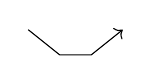
\begin{tikzpicture}[scale=0.4]
		\draw[->] (0, 0.8) -- (1, 0) -- (2, 0) -- (3, 0.8);
	\end{tikzpicture}
	tidak bergantung pada struktur penjumlahan pada himpunan-himpunan $\Hom$.
	Komposisi itu hanya melibatkan produk hingga dan koproduk hingga dalam
	kategori, termasuk kasus khususnya berupa objek nol, serta
	morfisme-morfisme kanonik yang terkait dengannya.

	Untuk (iii), ingat bahwa semua produk hingga (atau koproduk hingga) dapat
	dibentuk dari objek nol dan biproduk $\oplus$.

	Jika $(F,G)$ merupakan pasangan adjoin, maka $F$ mempertahankan
	$\varinjlim$, sedangkan $G$ mempertahankan $\varprojlim$; lihat
	\cite[Teorema 2.8.12]{Li1}. Di sisi lain, ekuivalensi mempertahankan semua
	limit. Karena itu, (iv) dan (v) keduanya merupakan kasus khusus dari (ii).
\end{bukti}

% segment-id: o014.li2.chapter1.additive-categories-kernels-cokernels.p010
Sesungguhnya, deskripsi penjumlahan dalam
Proposisi~\ref{prop:additive-cat-addition} menunjukkan bahwa ``keaditifan''
suatu kategori aditif $\mathcal{C}$ merupakan sifat dari kategori
$\mathcal{C}$, bukan struktur tambahan.

% segment-id: o014.li2.chapter1.additive-categories-kernels-cokernels.d002
\begin{definisi}
	\index{kernel (kernel)} \index[sym1]{kerf@$\Ker(f)$}
	\index{kokernel (cokernel)}\index[sym1]{cokerf@$\Coker(f)$}
	Misalkan $\mathcal{C}$ merupakan kategori-$\cate{Ab}$ yang mempunyai objek
	nol, dan $f: X \to Y$ suatu morfisme dalam $\mathcal{C}$.
	% segment-id: o014.li2.chapter1.additive-categories-kernels-cokernels.l006
	\begin{itemize}
		% segment-id: o014.li2.chapter1.additive-categories-kernels-cokernels.i014
		\item Jika penyama $\Ker(f,0)$ ada, maka $\Ker(f):=\Ker(f,0)$ beserta
		$\Ker(f) \hookrightarrow X$ disebut \emph{kernel} dari $f$.
		% segment-id: o014.li2.chapter1.additive-categories-kernels-cokernels.i015
		\item Jika kopenyama $\Coker(f,0)$ ada, maka $\Coker(f):=\Coker(f,0)$
		beserta $Y \twoheadrightarrow \Coker(f)$ disebut \emph{kokernel} dari
		$f$.
	\end{itemize}
	Secara khusus, menurut definisi kedua komposisi $\Ker(f) \to X \to Y$
	dan $X \to Y \to \Coker(f)$ sama dengan $0$.
\end{definisi}

% segment-id: o014.li2.chapter1.additive-categories-kernels-cokernels.p011
Terdapat beberapa sudut pandang yang saling melengkapi mengenai kernel dan
kokernel.
% segment-id: o014.li2.chapter1.additive-categories-kernels-cokernels.l007
\begin{itemize}
	% segment-id: o014.li2.chapter1.additive-categories-kernels-cokernels.i016
	\item Pertama, tinjau $\Ker(f)$. Untuk setiap morfisme $g: T \to X$ dengan
	$fg=0$,\footnote{Catatan penerjemah: teks sumber mengatakan ``untuk setiap
	morfisme'' tanpa mencantumkan syarat $fg=0$ dan, secara dual, $hf=0$.
	Kedua syarat itu dipulihkan di sini karena tepat merupakan hipotesis
	penyama dan kopenyama; lihat koreksi O014-C006.} komposisi
	$T \xrightarrow{g} X \xrightarrow{0} Y$ tentu sama dengan $0$.
	Karena itu, sifat universal $\Ker(f)=\Ker(f,0)$ sebagai penyama dapat
	dinyatakan oleh diagram komutatif
	% segment-id: o014.li2.chapter1.additive-categories-kernels-cokernels.g007
	\[\begin{tikzcd}
		& T \arrow[dashrightarrow, ld, "{\exists! g'}"'] \arrow[d, "g"] \arrow[rd, "0"] & \\
		\Ker(f) \arrow[r] & X \arrow[r, "f"'] & Y .
	\end{tikzcd}\]
	% segment-id: o014.li2.chapter1.additive-categories-kernels-cokernels.i017
	\item Tinjau $\Coker(f)$. Untuk setiap morfisme $h: Y \to T$ dengan
	$hf=0$, komposisi $X \xrightarrow{0} Y \xrightarrow{h} T$ tentu sama dengan
	$0$. Karena itu,
	sifat universal $\Coker(f)=\Coker(f,0)$ sebagai kopenyama dapat dinyatakan
	oleh diagram komutatif
	% segment-id: o014.li2.chapter1.additive-categories-kernels-cokernels.g008
	\[\begin{tikzcd}
		X \arrow[r, "f"] \arrow[rd, "0"'] & Y \arrow[r] \arrow[d, "h"] & \Coker(f) \arrow[dashrightarrow, ld, "{\exists! h'}"] . \\
		& T &
	\end{tikzcd}\]
	% segment-id: o014.li2.chapter1.additive-categories-kernels-cokernels.i018
	\item Kedua konstruksi di atas jelas saling dual:
	$\Coker(f)=\Ker(f^{\opp})$ dan $\Ker(f)=\Coker(f^{\opp})$.
\end{itemize}

% segment-id: o014.li2.chapter1.additive-categories-kernels-cokernels.p012
Karena morfisme yang terfaktorkan melalui objek nol tepat merupakan morfisme
$0$, sifat universal tersebut juga mempunyai karakterisasi melalui diagram
tarik balik dan dorong keluar. Pembaca dipersilakan memverifikasi langsung:

% segment-id: o014.li2.chapter1.additive-categories-kernels-cokernels.g009
\begin{equation}\label{eqn:Ker-Coker-triangles}
	\begin{tikzcd}
		\Ker(f) \arrow[phantom, r, "\simeq" description] & X \dtimes{Y} 0 \arrow[r] \arrow[d] \arrow[phantom, rd, "\Box" description] & X \arrow[d, "f"] \\
		& 0 \arrow[r] & Y
	\end{tikzcd} \qquad \begin{tikzcd}
		X \arrow[r, "f"] \arrow[d] & Y \arrow[d] & \\
		0 \arrow[r] & Y \dsqcup{X} 0 \arrow[phantom, lu, "\boxplus" description] & \Coker(f) \arrow[phantom, l, "\simeq" description] .
\end{tikzcd}\end{equation}

% segment-id: o014.li2.chapter1.additive-categories-kernels-cokernels.r001
\begin{catatan}\label{rem:equalizer-Ker}
	Penyama umum $\Ker(f,g)$ dapat direduksi menjadi kernel di atas. Tinjau
	morfisme-morfisme
	% segment-id: o014.li2.chapter1.additive-categories-kernels-cokernels.g010
	\[\begin{tikzcd}
	T \arrow[r, "h"] & X \arrow[r, yshift=0.2em, "f"] \arrow[r, yshift=-0.2em, "g"'] & Y
	\end{tikzcd}, \]
	Syarat $fh=gh$ ekuivalen dengan $(f-g)h=0$, sehingga langsung diperoleh
	$\Ker(f,g)=\Ker(f-g,0)=:\Ker(f-g)$. Secara dual,
	$\Coker(f,g)=\Coker(f-g,0)=:\Coker(f-g)$.
\end{catatan}

% segment-id: o014.li2.chapter1.additive-categories-kernels-cokernels.p013
Mulai sekarang, kita terutama meninjau kasus ketika $\mathcal{C}$ merupakan
kategori aditif.

% segment-id: o014.li2.chapter1.additive-categories-kernels-cokernels.pr003
\begin{proposisi}\label{prop:Ker-Coker-composite}
	Untuk morfisme-morfisme $X \xrightarrow{f} Y \xrightarrow{g} Z$ dalam
	kategori aditif $\mathcal{C}$, terdapat diagram komutatif
	% segment-id: o014.li2.chapter1.additive-categories-kernels-cokernels.g011
	\[\begin{tikzcd}[row sep=small, column sep=small]
		\Ker(gf) \arrow[rr, "\sim"] \arrow[hookrightarrow, rd] & & X \dtimes{Y} \Ker(g) \arrow[hookrightarrow, ld] \\
		& X &
	\end{tikzcd} \quad \begin{tikzcd}[row sep=small, column sep=small]
		Z \dsqcup{Y} \Coker(f) \arrow[rr, "\sim"] & & \Coker(gf) \\
		& Z \arrow[twoheadrightarrow, lu] \arrow[twoheadrightarrow, ru] &
	\end{tikzcd}\]
	di mana $X \dtimes{Y} \Ker(g) \to X$ (atau
	$Z \to Z \dsqcup{Y} \Coker(f)$) merupakan morfisme kanonik produk serat
	(atau koproduk serat),\footnote{Catatan penerjemah: teks sumber
	menulis ``koproduk'', tetapi objek yang ditampilkan adalah koproduk serat
	$Z \dsqcup{Y} \Coker(f)$ dan bukti berikutnya memakai dualitas terhadap
	produk serat; lihat koreksi O014-C005.} dengan ketentuan bahwa $\Ker$,
	$\Coker$, dan semua limit yang disebutkan ada.
\end{proposisi}

% segment-id: o014.li2.chapter1.additive-categories-kernels-cokernels.pf004
\begin{bukti}
	Berdasarkan \eqref{eqn:Ker-Coker-triangles}, pembentukan produk serat secara
	bertahap memberikan isomorfisme kanonik
	$\Ker(gf) \simeq X \dtimes{Z} 0 \simeq
	X \dtimes{Y} (Y \dtimes{Z} 0) \simeq X \dtimes{Y} \Ker(g)$.
	Dualitas memberikan kasus $\Coker(gf)$.
\end{bukti}

% segment-id: o014.li2.chapter1.additive-categories-kernels-cokernels.p014
Funktorialitas penyama dan kopenyama menginduksi funktorialitas kernel dan
kokernel. Konstruksi ini dicirikan oleh diagram komutatif berikut:

% segment-id: o014.li2.chapter1.additive-categories-kernels-cokernels.g012
\begin{equation}\label{eqn:Ker-Coker-functoriality}\begin{tikzcd}
		\Ker(f) \arrow[r] \arrow[dashrightarrow, d, "\exists!"'] & X \arrow[d, "a"'] \arrow[r, "f"] & Y \arrow[d, "b"] \\
		\Ker(g) \arrow[r] & X' \arrow[r, "g"'] & Y'
	\end{tikzcd} \qquad \begin{tikzcd}
		X \arrow[d, "a"'] \arrow[r, "f"] & Y \arrow[d, "b"] \arrow[r] & \Coker(f) \arrow[dashrightarrow, d, "\exists!"'] \\
		X' \arrow[r, "g"'] & Y' \arrow[r] & \Coker(g) .
\end{tikzcd}\end{equation}

% segment-id: o014.li2.chapter1.additive-categories-kernels-cokernels.p015
Hasil berikut menunjukkan bahwa tarik balik (atau dorong keluar)
mempertahankan kernel (atau kokernel).

% segment-id: o014.li2.chapter1.additive-categories-kernels-cokernels.pr004
\begin{proposisi}\label{prop:pull-back-ker}
	Jika diagram dalam kategori aditif $\mathcal{C}$
	% segment-id: o014.li2.chapter1.additive-categories-kernels-cokernels.g013
	\[\begin{tikzcd}
		X \arrow[r, "f"] \arrow[d, "a"'] & Y \arrow[d, "b"] \\
		X' \arrow[r, "g"'] & Y'
	\end{tikzcd}\]
	merupakan diagram tarik balik (atau dorong keluar), maka morfisme
	$\Ker(f) \to \Ker(g)$ (atau $\Coker(f) \to \Coker(g)$) dalam
	\eqref{eqn:Ker-Coker-functoriality} merupakan isomorfisme, dengan ketentuan
	bahwa $\Ker$ dan $\Coker$ yang dibicarakan ada.
\end{proposisi}

% segment-id: o014.li2.chapter1.additive-categories-kernels-cokernels.pf005
\begin{bukti}
	Dengan dualitas, cukup dibahas kasus tarik balik. Untuk setiap objek $T$,
	sifat universal memberikan
	% segment-id: o014.li2.chapter1.additive-categories-kernels-cokernels.a001
	\begin{align*}
		\Hom(T, \Ker(f)) & \simeq \Ker\left[ \Hom(T, X) \to \Hom(T, Y) \right] \\
		& \simeq \Ker\left[ \Hom(T, Y) \dtimes{\Hom(T, Y')} \Hom(T, X') \to \Hom(T, Y) \right] \\
		& = \Ker\left[ \Hom(T, X') \to \Hom(T, Y') \right] \simeq \Hom(T, \Ker(g)),
	\end{align*}
	dengan setiap panah bersifat kanonik. Lema Yoneda kemudian memberikan
	$\Ker(f) \rightiso \Ker(g)$; lihat tinjauan dalam
	Teorema~\sourcecrossref{prop:Yoneda}{A.1.1}.
\end{bukti}

% segment-id: o014.li2.chapter1.additive-categories-kernels-cokernels.lm001
\begin{lema}\label{prop:mono-epi-ker-coker}
	Misalkan $\mathcal{C}$ merupakan kategori aditif dan $f: X \to Y$ suatu
	morfisme dalam $\mathcal{C}$. Maka:
	% segment-id: o014.li2.chapter1.additive-categories-kernels-cokernels.l008
	\begin{enumerate}[(i)]
		% segment-id: o014.li2.chapter1.additive-categories-kernels-cokernels.i019
		\item $f$ merupakan monomorfisme (atau epimorfisme) jika dan hanya jika
		$\Ker(f)=0$ (atau $\Coker(f)=0$);
		% segment-id: o014.li2.chapter1.additive-categories-kernels-cokernels.i020
		\item $f$ merupakan morfisme nol jika dan hanya jika
		$\Ker(f) \rightiso X$, dan ini juga ekuivalen dengan
		$Y \rightiso \Coker(f)$;
		% segment-id: o014.li2.chapter1.additive-categories-kernels-cokernels.i021
		\item Diberikan $k: Y \to Z$ (atau $k': W \to X$), terdapat secara unik
		diagram komutatif berikut:
		% segment-id: o014.li2.chapter1.additive-categories-kernels-cokernels.g014
		\[\begin{tikzcd}[row sep=small, column sep=small]
		\Ker(kf) \arrow[rd] & & \Ker(f) \arrow[ld] \arrow[hookrightarrow, ll, "\exists !"'] \\
		& X &
		\end{tikzcd} \quad \text{atau} \quad
		\begin{tikzcd}[row sep=small, column sep=small]
		\Coker(fk') \arrow[twoheadrightarrow, rr, "\exists !"] & & \Coker(f) \\
		& Y \arrow[lu] \arrow[ru] &
		\end{tikzcd}\]
		dengan ketentuan bahwa kernel (atau kokernel) yang dibicarakan ada. Jika
		$k$ merupakan monomorfisme (atau $k'$ merupakan epimorfisme), maka
		$\Ker(f) \rightiso \Ker(kf)$ (atau
		$\Coker(fk') \rightiso \Coker(f)$).
	\end{enumerate}
\end{lema}

% segment-id: o014.li2.chapter1.additive-categories-kernels-cokernels.pf006
\begin{bukti}
	Pertama, tinjau (i). Berdasarkan dualitas, cukup dibahas kasus
	monomorfisme. Menurut definisi, $f$ merupakan monomorfisme jika dan hanya
	jika untuk setiap pasangan morfisme $g_1,g_2: T \to X$ berlaku
	$f(g_1-g_2)=0 \iff g_1-g_2=0$. Ini setara dengan pernyataan bahwa untuk
	setiap $g: T \to X$, berlaku $fg=0$ jika dan hanya jika $g$ terfaktorkan
	sebagai $T \to 0 \to X$. Pernyataan terakhir ini tepat menyatakan bahwa
	objek nol memenuhi sifat universal $\Ker(f)$.

	Untuk (ii), secara serupa cukup dibuktikan
	$f=0 \iff \Ker(f) \rightiso X$. Akan tetapi,
	$\Ker(f)=\Ker(f,0)$, sehingga ekuivalensi yang diinginkan langsung
	mengikuti definisi penyama.

	Untuk (iii), sekali lagi cukup ditinjau kasus $\Ker$:
	% segment-id: o014.li2.chapter1.additive-categories-kernels-cokernels.g015
	\[\begin{tikzcd}[column sep=small]
		\left\{ g \in \Hom(T, X): fg=0 \right\} \arrow[phantom, r, "\subset" description] & \left\{ g \in \Hom(T, X): kfg=0 \right\} \\
		\Hom(T, \Ker(f)) \arrow[u, "1:1"] & \Hom(T, \Ker(kf)) \arrow[u, "1:1"']
	\end{tikzcd}\]
	Jika $k$ merupakan monomorfisme, inklusi pada baris pertama merupakan
	kesamaan. Terapkan Lema Yoneda untuk menyelesaikan pembuktian.
\end{bukti}

% segment-id: o014.li2.chapter1.additive-categories-kernels-cokernels.p016
Dalam kategori aditif, citra dan kocitra yang diperkenalkan dalam
Definisi~\ref{def:Im-Coim} mempunyai deskripsi sederhana.

% segment-id: o014.li2.chapter1.additive-categories-kernels-cokernels.pr005
\begin{proposisi}\label{prop:Im-Coim-additive}
	\index{citra (image)}\index{kocitra (coimage)}
	\index[sym1]{imf@$\Image(f)$}\index[sym1]{coimf@$\Coim(f)$}
	Misalkan $f: X \to Y$ merupakan morfisme dalam kategori aditif
	$\mathcal{C}$. Maka terdapat isomorfisme kanonik
	% segment-id: o014.li2.chapter1.additive-categories-kernels-cokernels.a002
	\begin{align*}
		\Image(f) & \simeq \Ker\left[ Y \to \Coker(f) \right] \hookrightarrow Y, \\
		\Coim(f) & \simeq \Coker\left[ \Ker(f) \to X \right] \twoheadleftarrow X ;
	\end{align*}
	dengan ketentuan bahwa kernel dan kokernel yang dibicarakan ada.
\end{proposisi}

% segment-id: o014.li2.chapter1.additive-categories-kernels-cokernels.pf007
\begin{bukti}
	Berdasarkan dualitas, cukup ditinjau $\Image(f)$. Ambil morfisme kanonik
	$i_1,i_2: Y \to Y \dsqcup{X} Y$. Dengan menerapkan Lema Yoneda, cukup
	dibuktikan, untuk setiap $T \in \Obj(\mathcal{C})$, bahwa
	% segment-id: o014.li2.chapter1.additive-categories-kernels-cokernels.q008
	\begin{multline*}
		\Hom\left( T, \Image(f) \right) = \left\{ h: T \to Y \;\middle|\; i_1 h = i_2 h \right\} \\
		= \left\{ \begin{array}{r|l}
			h: T \to Y & \forall S \in \Obj(\mathcal{C}),\; \forall s_1, s_2: Y \to S, \\
			& s_1 f = s_2 f \implies s_1 h = s_2 h
		\end{array}\right\} \\
		\xlongequal{s := s_1 - s_2} \left\{ \begin{array}{r|l}
			h: T \to Y & \forall S \in \Obj(\mathcal{C}),\; \forall s: Y \to S, \\
			& s f = 0 \implies sh = 0
		\end{array}\right\} \\
		= \left\{ \begin{array}{r|l}
			h: T \to Y & T \xrightarrow{h} Y \twoheadrightarrow \Coker(f) \\
			& \text{komposisinya adalah}\; 0
		\end{array}\right\}
		\leftiso \Hom\left( T, \Ker\left[ Y \to \Coker(f) \right] \right).
	\end{multline*}
	Kesamaan pertama di atas berasal dari
	$\Image(f):=\Ker(i_1,i_2)$. Untuk kesamaan kedua, mula-mula tuliskan ulang
	syarat pada $h$ sebagai $s'i_1h=s'i_2h$ bagi setiap
	$s': Y \dsqcup{X} Y \to S$, lalu gunakan sifat universal koproduk serat
	% segment-id: o014.li2.chapter1.additive-categories-kernels-cokernels.a003
	\begin{align*}
		\Hom\left( Y \dsqcup{X} Y, S \right) & \xrightarrow{1:1} \Hom(Y,S) \dtimes{\Hom(X,S)} \Hom(Y,S) \\
		s' & \longmapsto \left( s' i_1, s' i_2 \right) =: (s_1, s_2).
	\end{align*}
	Kesamaan keempat diperoleh dari sifat universal kokernel, sehingga cukup
	diambil $S=\Coker(f)$.
\end{bukti}

% segment-id: o014.li2.chapter1.additive-categories-kernels-cokernels.p017
Contoh paling sederhana terjadi ketika $f$ merupakan morfisme nol. Dalam hal
ini, Lema~\ref{prop:mono-epi-ker-coker} (ii) memberikan
$\Image(f)=0=\Coim(f)$.

% segment-id: o014.li2.chapter1.additive-categories-kernels-cokernels.e002
\begin{contoh}\label{eg:strict-morphism}
	Sebagai kelanjutan pembahasan pada Contoh~\ref{eg:additive-category},
	pertama-tama kita tinjau kategori $R\dcate{Mod}$. Homomorfisme modul
	$f: A \to B$ selalu mempunyai
	kernel dan kokernel, yang secara klasik diberikan oleh
	$\Ker(f)=f^{-1}(0)$ dan
	$\Coker(f)=B/\{f(a):a \in A\}$. Langsung dari definisi, $\Image(f)$ adalah
	citra $f$ dalam pengertian teori himpunan, sedangkan
	$\Coim(f)=A/\Ker(f)$. Morfisme kanonik
	$\Coim(f) \to \Image(f)$ dalam \eqref{eqn:strict-morphism} tepat
	merupakan isomorfisme kanonik dalam teori modul
	$A/\Ker(f) \rightiso \Image(f)$. Karena itu, semua morfisme dalam
	$R\dcate{Mod}$ bersifat ketat.

	Selanjutnya, tinjau kategori aditif $\cate{Ban}_{\CC}$ dari
	Contoh~\ref{eg:additive-category}. Kernel dari pemetaan linear kontinu
	$f: X \to Y$ adalah $\Ker(f)=f^{-1}(0)$ seperti biasa, dan tetap merupakan
	ruang Banach. Di sisi lain,
	$\Coker(f)=Y/\overline{\left\{f(x):x \in X\right\}}$ dilengkapi dengan
	norma kuosien. Dalam hal ini, morfisme \eqref{eqn:strict-morphism} menjadi
	% segment-id: o014.li2.chapter1.additive-categories-kernels-cokernels.g016
	\[\begin{tikzcd}[row sep=small, column sep=small]
	\Coim(f) \arrow[equal, r] & X/f^{-1}(0) \arrow[r] & \overline{\left\{ f(x): x \in X \right\}} \arrow[equal, r] & \Image(f) \\
	& x + f^{-1}(0) \arrow[mapsto, r] \arrow[phantom, u, "\in" description, sloped] & f(x) \arrow[phantom, u, "\in" description, sloped] &
	\end{tikzcd}\]
	Ruang di sebelah kanan dilengkapi dengan topologi terinduksi dari $Y$,
	sedangkan ruang di sebelah kiri dilengkapi dengan topologi kuosien dari
	$X$. Misalkan
	$f: X \to Y$ merupakan pemetaan linear kontinu dan injektif antara ruang
	Banach, dengan citra padat tetapi tidak surjektif. Dalam keadaan ini,
	$\Coim(f)=X \to Y=\Image(f)$ bukan isomorfisme. Jadi,
	$\cate{Ban}_{\CC}$ mempunyai morfisme yang tidak ketat.
\end{contoh}

% Terjemahan Bahasa Indonesia dari chapter1.tex baris 568--629.
% Sumber: Methods of Algebra, Volume 2, commit
% 9a5803ff77dd3257484cb177f851a73770a59dd3 (CC BY 4.0).
% stable-unit-id: o014.aljabr2.chapter1.linear-categories-over-commutative-rings

% segment-id: o014.li2.chapter1.linear-categories-over-commutative-rings.h001
\section{Perumuman: Kategori Linear atas Gelanggang Komutatif}\label{sec:linear-cat}
\hypertarget{o014.aljabr2.chapter1.linear-categories-over-commutative-rings}{ }

% segment-id: o014.li2.chapter1.linear-categories-over-commutative-rings.p001
Himpunan-himpunan $\Hom$ dalam suatu kategori aditif mempunyai struktur grup
abelian. Dalam banyak situasi, himpunan-himpunan $\Hom$ ini juga dilengkapi
dengan perkalian skalar oleh suatu gelanggang komutatif $\Bbbk$. Sebagai
contoh, dalam $\Bbbk\dcate{Mod}$ setiap himpunan $\Hom$ secara alami merupakan
modul-$\Bbbk$, dan komposisi morfisme bersifat $\Bbbk$-bilinear.

% segment-id: o014.li2.chapter1.linear-categories-over-commutative-rings.d001
\begin{definisi}\label{def:cat-k-linear}
	\index{kategori!$\Bbbk\dcate{Mod}$-}
	\index{linear!$\Bbbk$- ($\Bbbk$-linear)}
	Misalkan $\Bbbk$ merupakan gelanggang komutatif. Andaikan setiap himpunan
	$\Hom$ dalam kategori $\mathcal{A}$ dilengkapi dengan struktur
	modul-$\Bbbk$ sedemikian sehingga komposisi morfisme
	$\Hom(Y, Z) \times \Hom(X, Y) \to \Hom(X, Z)$ merupakan pemetaan
	$\Bbbk$-bilinear untuk semua objek $X,Y,Z$; dengan kata lain, diagram
	berikut komutatif:
	% segment-id: o014.li2.chapter1.linear-categories-over-commutative-rings.g001
	\[\begin{tikzcd}
		\Hom(Y, Z) \times \Hom(X, Y) \arrow[d] \arrow[r, "\text{komposisi}"] & \Hom(X, Z) \\
		\Hom(Y, Z) \dotimes{\Bbbk} \Hom(X, Y) \arrow[ru, bend right, start anchor=east, "{\exists! \; \text{homomorfisme modul-$\Bbbk$}}"']
	\end{tikzcd}  \]
	Dengan data ini, $\mathcal{A}$ disebut \emph{kategori-$\Bbbk\dcate{Mod}$}.

	Misalkan $F: \mathcal{A} \to \mathcal{A}'$ merupakan funktor antara
	kategori-$\Bbbk\dcate{Mod}$. Jika pemetaan
	$\Hom(X,Y) \to \Hom(FX,FY)$ merupakan homomorfisme modul-$\Bbbk$ untuk
	semua $X,Y \in \Obj(\mathcal{A})$, maka $F$ disebut
	\emph{funktor $\Bbbk$-linear}.
\end{definisi}

% segment-id: o014.li2.chapter1.linear-categories-over-commutative-rings.p002
Perhatikan bahwa $\Bbbk\dcate{Mod}$ merupakan kategori monoidal terhadap hasil
kali tensor $\otimes := \dotimes{\Bbbk}$. Oleh karena itu, istilah
``kategori-$\Bbbk\dcate{Mod}$'' konsisten dengan terminologi pengayaan kategori
dalam \cite[\S 3.4]{Li1}. Kategori-$\cate{Ab}$ yang diperkenalkan sebelumnya
tepat merupakan kategori-$\Z\dcate{Mod}$. Sebaliknya, dengan melupakan
perkalian skalar pada suatu kategori-$\Bbbk\dcate{Mod}$, kita memperoleh
kategori-$\cate{Ab}$.

% segment-id: o014.li2.chapter1.linear-categories-over-commutative-rings.e001
\begin{contoh}
	Kategori-$\Bbbk\dcate{Mod}$ yang hanya mempunyai satu objek tepat
	merupakan aljabar-$\Bbbk$. Korespondensinya diberikan oleh
	$\mathcal{A} \mapsto \End_{\mathcal{A}}(\star)$, dengan
	$\Obj(\mathcal{A}) = \{\star\}$.
\end{contoh}

% segment-id: o014.li2.chapter1.linear-categories-over-commutative-rings.p003
Argumen dalam Proposisi~\ref{prop:automatic-Ab-morphism} dapat diterapkan tanpa
perubahan dan memberikan hasil berikut.

% segment-id: o014.li2.chapter1.linear-categories-over-commutative-rings.pr001
\begin{proposisi}\label{prop:automatic-k-morphism}
	Misalkan $\mathcal{A}$ dan $\mathcal{A}'$ merupakan
	kategori-$\Bbbk\dcate{Mod}$.
	% segment-id: o014.li2.chapter1.linear-categories-over-commutative-rings.l001
	\begin{enumerate}
		% segment-id: o014.li2.chapter1.linear-categories-over-commutative-rings.i001
		\item Diberikan sepasang funktor adjoin
		% Diagram adjungsi sumber yang semula sebaris direflow sebagai display
		% terpusat agar tidak menyempitkan atau melampaui lebar baris pembaca.
		% Rantai kesetaraan panjang dalam bukti juga direflow sebagai display.
		% segment-id: o014.li2.chapter1.linear-categories-over-commutative-rings.g002
		\[
		\begin{tikzcd}
			F: \mathcal{A} \arrow[shift left, r] & \mathcal{A}' \arrow[shift left, l] : G
		\end{tikzcd},
		\]
		dengan $F$ dan $G$ keduanya bersifat $\Bbbk$-linear. Maka isomorfisme adjungsi
		$\Hom_{\mathcal{A}'}(F(\cdot),\cdot) \rightiso
		\Hom_{\mathcal{A}}(\cdot,G(\cdot))$ bersifat $\Bbbk$-linear.
		% segment-id: o014.li2.chapter1.linear-categories-over-commutative-rings.i002
		\item Untuk setiap $\alpha: I \to \mathcal{A}$, bijeksi
		% segment-id: o014.li2.chapter1.linear-categories-over-commutative-rings.q001
		\[
			\Hom_{\mathcal{A}}\left(\varinjlim \alpha,T\right)
			\simeq \varprojlim_{i \in \Obj(I)}
			\Hom_{\mathcal{A}}(\alpha(i),T),
			\quad T \in \Obj(\mathcal{A})
		\]
		bersifat $\Bbbk$-linear, asalkan $\varinjlim \alpha$ ada. Pernyataan yang sama
		berlaku untuk $\varprojlim$.
	\end{enumerate}
\end{proposisi}

% segment-id: o014.li2.chapter1.linear-categories-over-commutative-rings.p004
Kecuali dinyatakan lain, mulai sekarang semua funktor dan ekuivalensi antara
kategori-$\Bbbk\dcate{Mod}$ dipahami bersifat $\Bbbk$-linear.

% segment-id: o014.li2.chapter1.linear-categories-over-commutative-rings.d002
\begin{definisi}\label{def:k-linear-cat}
	\index{kategori!$\Bbbk$-linear ($\Bbbk$-linear)}
	Jika suatu kategori aditif $\mathcal{A}$ dilengkapi dengan struktur
	$\Bbbk$-linear yang kompatibel dengan struktur kategori-$\cate{Ab}$ yang
	sudah ada, maka $\mathcal{A}$ beserta data tersebut disebut
	\emph{kategori $\Bbbk$-linear}.
\end{definisi}

% segment-id: o014.li2.chapter1.linear-categories-over-commutative-rings.p005
Hal ini sama artinya dengan mengganti kategori-$\cate{Ab}$ dengan
kategori-$\Bbbk\dcate{Mod}$ dalam pembahasan \S\ref{sec:Ker-Coker}. Sebagian
besar hasil mengenai kategori aditif dalam bab ini dapat diperluas ke situasi
$\Bbbk$-linear dengan argumen yang sama tanpa perubahan. Satu-satunya pengecualian
berkaitan dengan Korolari~\ref{prop:automatic-additivity}: dalam kategori
aditif, penjumlahan pada himpunan $\Hom$ dapat dicirikan oleh sifat kategori itu
sendiri, tetapi hal ini tidak berlaku bagi perkalian skalar oleh $\Bbbk$.
Karena itu, tidak ada alasan bagi funktor (bahkan ekuivalensi) antara kategori
$\Bbbk$-linear untuk otomatis bersifat $\Bbbk$-linear.

% segment-id: o014.li2.chapter1.linear-categories-over-commutative-rings.p006
Berikut ini beberapa hasil mengenai sifat $\Bbbk$-linear. Ingat bahwa
\emph{pusat} suatu kategori $\mathcal{A}$ didefinisikan sebagai
\index{pusat (center)} \index[sym1]{ZA@$Z(\mathcal{A})$}
$Z(\mathcal{A}) := \End(\identity_{\mathcal{A}})$. Unsur-unsurnya merupakan
morfisme dari funktor identitas $\identity_{\mathcal{A}}$ ke dirinya sendiri,
yang ditulis sebagai $(a_X)_{X \in \Obj(\mathcal{A})}$ dengan
$a_X \in \End_{\mathcal{A}}(X)$. Dengan operasi komposisi morfisme, pusat tersebut
merupakan monoid komutatif; lihat \cite[Definisi 2.3.8,
Proposisi 2.3.9]{Li1}. Jika $\mathcal{A}$ merupakan kategori-$\cate{Ab}$, maka
$Z(\mathcal{A})$ menjadi gelanggang komutatif terhadap komposisi dan
penjumlahan
$(a_X)_X + (b_X)_X := (a_X+b_X)_X$.

% segment-id: o014.li2.chapter1.linear-categories-over-commutative-rings.pr002
\begin{proposisi}\label{prop:k-linear-center}
	Misalkan $\mathcal{A}$ merupakan kategori-$\cate{Ab}$. Maka terdapat
	bijeksi
	% segment-id: o014.li2.chapter1.linear-categories-over-commutative-rings.q002
	\[
		\left\{\text{struktur kategori-$\Bbbk\dcate{Mod}$ pada $\mathcal{A}$}\right\}
		\stackrel{1:1}{\longleftrightarrow}
		\Hom_{\text{gelanggang}}(\Bbbk,Z(\mathcal{A})).
	\]
	Pemetaan tersebut diberikan sebagai berikut. Jika struktur
	kategori-$\Bbbk\dcate{Mod}$ pada $\mathcal{A}$ telah ditetapkan, untuk setiap
	$a \in \Bbbk$ dan $X \in \Obj(\mathcal{A})$ definisikan
	$a_X := a \cdot \identity_X \in \End_{\mathcal{A}}(X)$. Maka
	$a \mapsto (a_X)_{X \in \Obj(\mathcal{A})} \in Z(\mathcal{A})$ merupakan
	homomorfisme gelanggang. Sebaliknya, diberikan homomorfisme gelanggang di
	ruas kanan,
	$a \mapsto (a_X)_{X \in \Obj(\mathcal{A})}$, definisikan struktur
	kategori-$\Bbbk\dcate{Mod}$ pada $\mathcal{A}$ dengan
	$a \cdot f := f \circ a_X = a_Y \circ f$, untuk
	$f \in \Hom(X,Y)$.
\end{proposisi}

% segment-id: o014.li2.chapter1.linear-categories-over-commutative-rings.pf001
\begin{bukti}
	Syarat yang mencirikan
	$(a_X)_{X \in \Obj(\mathcal{A})} \in Z(\mathcal{A})$ adalah
	$f \circ a_X = a_Y \circ f$ untuk setiap $f \in \Hom(X,Y)$. Jika
	$\mathcal{A}$ dilengkapi dengan struktur kategori-$\Bbbk\dcate{Mod}$,
	definisikan $a_X := a \cdot \identity_X$. Sifat bilinear memberikan
	\[
		f \circ a_X = f \circ (a \cdot \identity_X)
		= (a f) \circ \identity_X
		= (a \cdot \identity_Y) \circ f
		= a_Y \circ f,
	\]
	sehingga $(a_X)_{X \in \Obj(\mathcal{A})} \in Z(\mathcal{A})$.
	Verifikasi lainnya langsung.
\end{bukti}

% segment-id: o014.li2.chapter1.linear-categories-over-commutative-rings.p007
Sebagai akibatnya, kategori-$\cate{Ab}$ $\mathcal{A}$ secara alami menjadi
kategori-$Z(\mathcal{A})\dcate{Mod}$.

% Terjemahan lengkap Bahasa Indonesia dari chapter1.tex baris 630--762.
% Sumber: Methods of Algebra, Volume 2, commit
% 9a5803ff77dd3257484cb177f851a73770a59dd3 (CC BY 4.0).
% stable-unit-id: o014.aljabr2.chapter1.limits-through-functors

% segment-id: o014.li2.chapter1.limits-through-functors.h001
\section{Meninjau Limit melalui Funktor}\label{sec:limit-functor}
\hypertarget{o014.aljabr2.chapter1.limits-through-functors}{ }

% segment-id: o014.li2.chapter1.limits-through-functors.p001
Berbagai hubungan antara funktor $F: \mathcal{C} \to \mathcal{D}$ dan limit
secara garis besar dapat dibagi ke dalam dua arah. Ambil $\varinjlim$ sebagai
contoh. Diberikan funktor $\alpha: I \to \mathcal{C}$, pertanyaannya adalah:
% segment-id: o014.li2.chapter1.limits-through-functors.l001
\begin{itemize}
	% segment-id: o014.li2.chapter1.limits-through-functors.i001
	\item Andaikan $\varinjlim \alpha$ ada. Apakah citra
	$F\left(\varinjlim \alpha\right)$ memberikan $\varinjlim (F\alpha)$?
	% segment-id: o014.li2.chapter1.limits-through-functors.i002
	\item Andaikan $\varinjlim F\alpha$ ada. Dapatkah limit itu
	``diangkat'' ke $\mathcal{C}$? Dalam arti apa pengangkatan tersebut unik?
\end{itemize}

% segment-id: o014.li2.chapter1.limits-through-functors.p002
Di sini kita terutama membahas kasus $\varinjlim$. Hasil-hasil ini tentu juga
mempunyai versi yang bersesuaian untuk $\varprojlim$; berkat dualitas,
rinciannya tidak perlu diulang.

% segment-id: o014.li2.chapter1.limits-through-functors.p003
Kita akan menata pembahasan $\varinjlim$ dengan bahasa kokonus dan kategori
$(\alpha/\Delta)$.

% segment-id: o014.li2.chapter1.limits-through-functors.c001
\begin{konvensi}\label{con:limit-cone}
	Untuk funktor $\alpha: I \to \mathcal{C}$ yang telah ditetapkan, data
	$(L, (f_i)_{i \in \Obj(I)})$ di $\mathcal{C}$ yang memenuhi syarat-syarat
	berikut disebut \emph{kokonus} dengan alas $\alpha$ dan puncak $L$:
	% segment-id: o014.li2.chapter1.limits-through-functors.l002
	\begin{compactitem}
		% segment-id: o014.li2.chapter1.limits-through-functors.i003
		\item $L$ merupakan objek di $\mathcal{C}$,
		% segment-id: o014.li2.chapter1.limits-through-functors.i004
		\item setiap $f_i : \alpha(i) \to L$ merupakan morfisme di
		$\mathcal{C}$ dan memenuhi syarat kompatibilitas
		$f_j \circ \alpha(i \to j) = f_i$, dengan $[i \to j]$ berkisar pada
		$\mathrm{Mor}(I)$.
	\end{compactitem}
\end{konvensi}

% segment-id: o014.li2.chapter1.limits-through-functors.p004
Dalam terminologi \cite[\S 2.7]{Li1}, kokonus-kokonus ini membentuk suatu
kategori\footnote{Arti tepat $\Delta$ di sini ialah funktor diagonal
$\mathcal{C} \to \mathcal{C}^I$; lihat Contoh
\sourcecrossref{eg:comma-vs-cone}{1.6.3}. Notasi $\Delta$ dipilih dari huruf
awal pinyin \emph{duìjiǎo} (``diagonal''). Namun, mengikuti asas piktografis,
tidak ada salahnya membayangkan $\Delta$ sebagai ``kokonus''; lihat diagram
\eqref{eqn:injlim-diagram}.} $(\alpha / \Delta)$. Secara konkret, setelah alas
$\alpha$ ditetapkan, suatu morfisme dari kokonus $(L, (f_i)_i)$ ke kokonus
$(M, (g_i)_i)$ ialah diagram komutatif
% segment-id: o014.li2.chapter1.limits-through-functors.g001
\begin{equation}\label{eqn:injlim-diagram}\begin{tikzcd}
	& L \arrow[d] & \\
	\alpha(i) \arrow[bend right, rr, "\alpha(i \to j)"'] \arrow[r, "g_i"] \arrow[ru, "f_i"] & M & \alpha(j) \arrow[l, "{g_j}"'] \arrow[lu, "f_j"']
\end{tikzcd}\end{equation}
dengan $i \to j$ berkisar pada $\Mor(I)$; komposisi morfisme didefinisikan
dengan cara yang jelas. Menurut definisi, $\varinjlim \alpha$ beserta keluarga
morfisme kanonik bawaannya
$\iota_i: \alpha(i) \to \varinjlim \alpha$ merupakan objek awal dari
$(\alpha / \Delta)$.
\index{limit}\index[sym1]{lim}

% segment-id: o014.li2.chapter1.limits-through-functors.p005
Funktor $F$ secara langsung menginduksi funktor
$(\alpha/\Delta) \to (F\alpha / \Delta)$, yang memetakan kokonus
$(L, (f_i)_i)$ ke $(FL, (Ff_i)_i)$. Andaikan $\varinjlim \alpha$ ada. Jika
$\varinjlim F\alpha$ juga ada, maka dalam $(F\alpha / \Delta)$ terdapat
morfisme tunggal
% segment-id: o014.li2.chapter1.limits-through-functors.q001
\[ \varinjlim F\alpha \to F(\varinjlim \alpha), \]
dan morfisme ini merupakan isomorfisme jika dan hanya jika
$\left( F(\varinjlim \alpha), (F\iota_i)_i \right)$ memberikan
$\varinjlim F\alpha$.

% segment-id: o014.li2.chapter1.limits-through-functors.p006
Dengan membalik panah-panah, $\varprojlim \alpha$ dapat dicirikan sebagai
objek terminal dari $(\Delta/\alpha)$. Dengan asumsi bahwa kedua limit
projektif yang dibahas ada, dalam $(\Delta/F\alpha)$ terdapat morfisme tunggal
% segment-id: o014.li2.chapter1.limits-through-functors.q002
\[ F\varprojlim \alpha \to \varprojlim F\alpha. \]

% segment-id: o014.li2.chapter1.limits-through-functors.d001
\begin{definisi}\label{def:create-limit}
	\index{limit!mempertahankan, merefleksikan, menciptakan (preserve, reflect, create)}
	Diberikan $F: \mathcal{C} \to \mathcal{D}$ dan funktor
	$\alpha: I \to \mathcal{C}$, tinjau funktor di antara kategori kokonus
	$(\alpha/\Delta) \to (F\alpha/\Delta)$.
	% segment-id: o014.li2.chapter1.limits-through-functors.l003
	\begin{itemize}
		% segment-id: o014.li2.chapter1.limits-through-functors.i005
		\item Funktor $F$ dikatakan \emph{mempertahankan} $\varinjlim$ ini jika
		$(\alpha/\Delta) \to (F\alpha/\Delta)$ memetakan objek awal (jika ada)
		ke objek awal.
		% segment-id: o014.li2.chapter1.limits-through-functors.i006
		\item Funktor $F$ dikatakan \emph{merefleksikan} $\varinjlim$ ini jika,
		apabila suatu objek dari $(\alpha/\Delta)$ dipetakan menjadi objek awal
		dari $(F\alpha/\Delta)$, objek itu sendiri merupakan objek awal.
		% segment-id: o014.li2.chapter1.limits-through-functors.i007
		\item Funktor $F$ dikatakan \emph{menciptakan} $\varinjlim$ ini jika,
		begitu $\varinjlim F\alpha$ ada, $\varinjlim \alpha$ juga ada, dan dalam
		keadaan ini $F$ mempertahankan $\varinjlim$ tersebut dan juga
		merefleksikan $\varinjlim$ tersebut.
	\end{itemize}
	Untuk $\varprojlim$ terdapat konsep-konsep yang bersesuaian. Konsep-konsep
	untuk $\varinjlim$ dan $\varprojlim$ ini dapat saling diperoleh dengan
	mengganti $\mathcal{C}$ dan $\mathcal{D}$ oleh
	$\mathcal{C}^{\opp}$ dan $\mathcal{D}^{\opp}$.
\end{definisi}

% segment-id: o014.li2.chapter1.limits-through-functors.p007
Perhatikan bahwa konsep-konsep ini bergantung pada $\alpha$ yang sedang
dibahas. Sebagai contoh, sangat mungkin $F$ mempertahankan semua
$\varinjlim$ berhingga tetapi tidak mempertahankan $\varinjlim$ secara umum.

% segment-id: o014.li2.chapter1.limits-through-functors.p008
Untuk $\alpha$ tertentu, pernyataan bahwa suatu funktor menciptakan
$\varinjlim$ (atau $\varprojlim$) setara dengan mengatakan bahwa kokonus (atau
konus) di $\mathcal{D}$ yang mendefinisikan limit tersebut dapat diangkat
secara unik ke $\mathcal{C}$, dan hasil pengangkatan itu memberikan limit yang
bersesuaian di $\mathcal{C}$. Keunikan tersebut berasal dari syarat dalam
definisi mengenai merefleksikan $\varinjlim$ (atau $\varprojlim$). Sudut
pandang ini akan tampak jelas dalam Contoh \ref{eg:Grp-Set-create} dan
Proposisi \ref{prop:forget-create} di bawah.

% segment-id: o014.li2.chapter1.limits-through-functors.pr001
\begin{proposisi}\label{prop:ff-reflect}
	Setiap funktor penuh dan setia merefleksikan semua $\varinjlim$ dan
	$\varprojlim$.
\end{proposisi}
% segment-id: o014.li2.chapter1.limits-through-functors.pf001
\begin{bukti}
	Cukup tinjau $\varinjlim$. Jika $F$ penuh dan setia, sifat universal objek
	awal dari $(\alpha/\Delta)$ dapat diverifikasi di $(F\alpha/\Delta)$ setelah
	menerapkan $F$.
\end{bukti}

% segment-id: o014.li2.chapter1.limits-through-functors.p009
Sejalan dengan pembahasan ini, kita perkenalkan sebuah konsep yang berguna.

% segment-id: o014.li2.chapter1.limits-through-functors.d002
\begin{definisi}\label{def:conservative}
	\index{funktor!konservatif (conservative)}
	Funktor $F$ yang memenuhi syarat berikut disebut \emph{konservatif}:
	morfisme $f \in \Mor(\mathcal{C})$ merupakan isomorfisme jika dan hanya jika
	$Ff \in \Mor(\mathcal{D})$ merupakan isomorfisme.
\end{definisi}

% segment-id: o014.li2.chapter1.limits-through-functors.r001
\begin{catatan}\label{rem:conservative-reflect}
	Jika $F$ merupakan funktor konservatif, maka asalkan
	$\varinjlim \alpha$ ada dan $F$ mempertahankan $\varinjlim$ ini, $F$ juga
	harus merefleksikan $\varinjlim$ ini. Alasannya sebagai berikut. Misalkan
	$L \in \Obj((\alpha/\Delta))$ dipetakan menjadi objek awal dari
	$(F\alpha/\Delta)$. Tinjau morfisme tunggal
	$\varinjlim \alpha \to L$ dalam $(\alpha/\Delta)$. Karena $F$
	mempertahankan $\varinjlim$ ini, citra morfisme tersebut di bawah $F$
	harus merupakan isomorfisme. Syarat konservatif kemudian memastikan bahwa
	$\varinjlim \alpha \to L$ juga merupakan isomorfisme.

	Dengan hipotesis ini, syarat merefleksikan $\varinjlim$ dapat dihapus dari
	definisi bahwa $F$ menciptakan $\varinjlim$.
\end{catatan}

% segment-id: o014.li2.chapter1.limits-through-functors.e001
\begin{contoh}\label{eg:Grp-Set-create}
	Kita akan memverifikasi bahwa funktor pelupa $U$ dari kategori grup
	$\cate{Grp}$ ke kategori himpunan $\cate{Set}$ menciptakan semua
	$\varprojlim$ kecil.

	Hal ini merupakan akibat konstruksi konkret $\varprojlim$ dalam
	$\cate{Grp}$ dan $\cate{Set}$; lihat
	\cite[Contoh 2.7.5 dan 2.8.7]{Li1}. Secara lebih terperinci, ambil kategori
	kecil $I$ dan funktor $\beta: I^{\opp} \to \cate{Grp}$. Sebagai himpunan,
	% segment-id: o014.li2.chapter1.limits-through-functors.q003
	\[ \varprojlim U\beta = \left\{\begin{array}{r|l}
		(x_i)_i \in \prod_{i \in \Obj(I)} U\beta(i) & \forall [i \to j] \in \mathrm{Mor}(I), \\
		& \beta(i \to j)(x_j) = x_i
	\end{array}\right\}, \]
	dan proyeksi $p_i: \varprojlim U\beta \to U\beta(i)$ memetakan $(x_j)_j$
	ke $x_i$. Tugas kita sekarang adalah:
	% segment-id: o014.li2.chapter1.limits-through-functors.l004
	\begin{enumerate}
		% segment-id: o014.li2.chapter1.limits-through-functors.i008
		\item melengkapi $\varprojlim U\beta$ dengan struktur grup sedemikian
		hingga setiap $p_i$ merupakan homomorfisme grup, serta menunjukkan bahwa
		struktur grup semacam itu unik;
		% segment-id: o014.li2.chapter1.limits-through-functors.i009
		\item memverifikasi sifat universal $\varprojlim \beta$ bagi grup ini
		beserta keluarga homomorfisme proyeksi $(p_i)_i$.
	\end{enumerate}

	Jelas bahwa $\varprojlim U\beta$ merupakan subgrup dari hasil kali langsung
	$\prod_i \beta(i)$. Kita notasikan subgrup ini sebagai
	$\varprojlim \beta \in \Obj(\cate{Grp})$; inilah satu-satunya struktur grup
	yang membuat setiap $p_i$ menjadi homomorfisme grup. Dengan demikian, tugas
	pertama selesai.

	Selanjutnya, kita verifikasi sifat universal bagi konus
	$\left( \varprojlim \beta, (p_i)_i\right)$. Tinjau sembarang konus
	$(L, (q_i)_i)$ di $\cate{Grp}$, dengan $q_i: L \to \beta(i)$. Sifat
	universal memberikan pemetaan tunggal
	$\varphi: UL \to \varprojlim U\beta$ sedemikian sehingga
	$p_i \varphi = q_i$ berlaku untuk setiap $i$. Sesungguhnya, $\varphi$ secara konkret
	diberikan oleh $y \mapsto (q_i(y))_{i \in \Obj(I)}$, sehingga pemetaan ini
	merupakan homomorfisme grup $L \to \varprojlim \beta$.\footnote{Catatan
	penerjemah: sumber menulis $L \to \varinjlim \beta$; target dikoreksi
	menjadi $L \to \varprojlim \beta$ sesuai limit projektif yang sedang
	dibuktikan (O014-C007).} Verifikasi selesai.
\end{contoh}

% segment-id: o014.li2.chapter1.limits-through-functors.p010
Dengan argumen yang sepenuhnya serupa, dapat ditunjukkan bahwa funktor pelupa
dari kategori ruang Hausdorff kompak $\cate{CHaus}$ ke $\cate{Set}$ juga
menciptakan semua $\varprojlim$ kecil. Verifikasi terkait diserahkan sebagai
latihan dalam bab ini.

% segment-id: o014.li2.chapter1.limits-through-functors.p011
Hasil berikutnya melibatkan kategori funktor berbentuk $\mathcal{C}^J$
(yang mungkin merupakan kategori ``besar'', tetapi ini tidak menjadi masalah).
Kita memerlukan dua langkah persiapan.

% segment-id: o014.li2.chapter1.limits-through-functors.l005
\begin{itemize}
	% segment-id: o014.li2.chapter1.limits-through-functors.i010
	\item Misalkan $J$ merupakan himpunan. Hasil kali $J$ salinan
	$\mathcal{C}$, yakni $\mathcal{C}^J$, didefinisikan sebagai
	$\Obj\left(\mathcal{C}^J\right) = \Obj(\mathcal{C})^J$ dan
	$\mathrm{Mor}\left(\mathcal{C}^J \right) = \mathrm{Mor}(\mathcal{C})^J$.
	Untuk setiap $j \in J$ terdapat funktor proyeksi yang jelas
	$p_j: \mathcal{C}^J \to \mathcal{C}$.

	% Koreksi O014-C008: sumber menggandakan aksara pada frasa "untuk setiap".
	Diberikan kategori $I$ dan funktor $\alpha: I \to \mathcal{C}^J$, jika
	$\varinjlim (p_j \alpha)$ ada untuk setiap $j$, maka
	$\varinjlim \alpha$ juga ada. Konstruksinya dilakukan dengan mengambil limit
	secara ``titik demi titik'' atau ``objek demi objek'':
	$\varinjlim \alpha = \left( \varinjlim (p_j \alpha) \right)_{j \in J}$.

	% segment-id: o014.li2.chapter1.limits-through-functors.i011
	\item Misalkan $J$ merupakan kategori. Kita dapat meninjau kategori funktor
	$\mathcal{C}^J$. Untuk setiap $j \in \Obj(J)$ terdapat funktor evaluasi
	$\mathrm{ev}_j: \mathcal{C}^J \to \mathcal{C}$, yang memetakan objek $F$
	ke $Fj$ dan memetakan morfisme
	$\varphi = (\varphi_{j'})_{j' \in \Obj(J)}$ ke $\varphi_j$. Nanti kita akan
	meninjau funktor berbentuk $\alpha: I \to \mathcal{C}^J$ beserta
	$\varinjlim$-nya. Perhatikan bahwa $\alpha$ dapat dipandang sebagai funktor
	$I \times J \to \mathcal{C}$, dengan nilainya ditulis $\alpha(i, j)$.
\end{itemize}

% segment-id: o014.li2.chapter1.limits-through-functors.p012
Kedua sistem notasi tersebut kompatibel. Jika $J$ merupakan kategori diskret
dan dipandang sebagai himpunan, maka $\mathcal{C}^J$ tidak lain adalah hasil
kali yang dibahas sebelumnya. Untuk $J$ umum, funktor pelupa
$\mathcal{F}: \mathcal{C}^J \to \mathcal{C}^{\Obj(J)}$ memetakan objek $F$ ke
$(Fj)_{j \in \Obj(J)}$ dan memetakan morfisme $\varphi$ ke
$(\varphi_j)_{j \in \Obj(J)}$. Karena itu, $\mathrm{ev}_j = p_j \mathcal{F}$.

% segment-id: o014.li2.chapter1.limits-through-functors.pr002
\begin{proposisi}\label{prop:forget-create}
	Misalkan $J$ dan $\mathcal{C}$ merupakan kategori.
	% segment-id: o014.li2.chapter1.limits-through-functors.l006
	\begin{enumerate}[(i)]
		% segment-id: o014.li2.chapter1.limits-through-functors.i012
		\item Funktor pelupa
		$\mathcal{F}: \mathcal{C}^J \to \mathcal{C}^{\Obj(J)}$ menciptakan
		$\varinjlim$ dan $\varprojlim$.
		% segment-id: o014.li2.chapter1.limits-through-functors.i013
		\item Misalkan $I$ merupakan kategori dan setiap funktor
		$I \to \mathcal{C}$ mempunyai $\varinjlim$ (atau $\varprojlim$).
		Maka semua funktor berbentuk $I \to \mathcal{C}^J$ juga mempunyai
		$\varinjlim$ (atau $\varprojlim$) di $\mathcal{C}^J$.
		% segment-id: o014.li2.chapter1.limits-through-functors.i014
		\item Dengan asumsi pada (ii), untuk setiap $j \in \Obj(J)$, funktor
		evaluasi $\mathrm{ev}_j: \mathcal{C}^J \to \mathcal{C}$ mempertahankan
		$\varinjlim$ (atau $\varprojlim$) untuk diagram berbentuk $I$ tersebut.
		Dengan kata lain, limit di $\mathcal{C}^J$ juga didefinisikan
		secara ``titik demi titik'' atau ``objek demi objek''.
	\end{enumerate}
\end{proposisi}
% segment-id: o014.li2.chapter1.limits-through-functors.pf002
\begin{bukti}
	Cukup tinjau kasus $\varinjlim$. Untuk (i), tetapkan
	$\alpha: I \to \mathcal{C}^J$ dan andaikan $\varinjlim \mathcal{F}\alpha$
	ada serta diberikan oleh kokonus
	% segment-id: o014.li2.chapter1.limits-through-functors.q004
	\[ \left( (X(j))_{j \in \Obj(J)}, \; \left( \iota_i = (\iota_{i, j})_{j \in \Obj(J)} \right)_{i \in \Obj(I)} \right) \]
	dengan $\iota_{i,j}: \alpha(i, j) \to X(j)$. Kita ingin mengangkatnya
	menjadi kokonus di $\mathcal{C}^J$ yang memberikan $\varinjlim \alpha$.

	Pertama, perhatikan bahwa
	$X(j) = \varinjlim \alpha(\cdot, j)$ untuk setiap $j$. Untuk setiap morfisme
	$j \to j'$, sifat funktorial limit (lihat
	\cite[Lema 2.7.4]{Li1}) memberikan morfisme tunggal
	$X(j \to j'): X(j) \to X(j')$ yang membuat diagram berikut komutatif:
	% segment-id: o014.li2.chapter1.limits-through-functors.g002
	\[\begin{tikzcd}
		\alpha(i, j) \arrow[r] \arrow[d, "{\iota_{i, j}}"'] & \alpha(i, j') \arrow[d, "{\iota_{i, j'}}"] \\
		X(j) \arrow[r, "{X(j \to j')}"'] & X(j')
	\end{tikzcd} \quad i \in \Obj(I). \]
	Dengan cara ini, $j \mapsto X(j)$ diperluas menjadi funktor
	$X: J \to \mathcal{C}$, sedangkan
	$\iota_i: \alpha(i, \cdot) \to X$ membentuk morfisme di
	$\mathcal{C}^J$. Tidak sulit memverifikasi bahwa
	$(X, (\iota_i)_i) \in \Obj(\alpha/\Delta)$; selanjutnya kita buktikan
	bahwa objek ini merupakan objek awal. Karena funktor $\mathcal{F}$
	konservatif, syarat merefleksikan $\varinjlim$ tidak perlu diverifikasi lagi.

	Diberikan $(L, (f_i)_i) \in \Obj(\alpha/\Delta)$, sifat universal
	$\varinjlim \mathcal{F}\alpha$ menentukan morfisme tunggal
	$\varphi = (\varphi_j)_j : \mathcal{F}X \to \mathcal{F}L$ sedemikian sehingga
	bagian segitiga pada diagram berikut komutatif untuk setiap $(i, j)$:
	% segment-id: o014.li2.chapter1.limits-through-functors.g003
	\[\begin{tikzcd}
		& X(j) \arrow[d, "\varphi_j"] \arrow[r, "{X(j \to j')}" inner sep=0.8em] & X(j') \arrow[d, "\varphi_{j'}"] \\
		\alpha(i, j) \arrow[ru, "{\iota_{i,j}}"] \arrow[r, "f_{i, j}"' inner sep=0.8em] & L(j) \arrow[r, "{L(j \to j')}"' inner sep=0.8em] & L(j')
	\end{tikzcd}\]
	Jika dapat ditunjukkan bahwa bagian persegi komutatif untuk setiap
	$j \to j'$, maka keluarga komponen $\varphi$ membentuk morfisme
	$X \to L$. Bingkai
	luar sudah diketahui komutatif, sehingga
	% segment-id: o014.li2.chapter1.limits-through-functors.q005
	\[ \varphi_{j'} X(j \to j') \iota_{i, j} = L(j \to j') f_{i, j} = L(j \to j') \varphi_j \iota_{i, j} \]
	untuk setiap $i$. Morfisme dengan domain $X(j)$ ditentukan oleh
	komposisinya dengan semua $\iota_{i,j}$, sehingga bagian persegi tersebut
	komutatif.

	Untuk (ii), tinjau funktor $\alpha: I \to \mathcal{C}^J$. Menurut
	pembahasan sebelumnya, $\mathcal{F}\alpha: I \to \mathcal{C}^{\Obj(J)}$
	mempunyai $\varinjlim$, yang didefinisikan secara objek demi objek. Oleh (i),
	$\mathcal{F}$ menciptakan $\varinjlim \alpha$ di $\mathcal{C}^J$,\footnote{Catatan
	penerjemah: teks sumber menulis $\mathcal{C}$ di sini. Targetnya dikoreksi
	menjadi $\mathcal{C}^J$, yaitu domain funktor pelupa $\mathcal{F}$ dan
	kategori yang memuat funktor $X: J \to \mathcal{C}$ yang baru dibangun;
	lihat koreksi O014-C009.}
	sedangkan pernyataan
	pada (iii) bahwa $\mathrm{ev}_j$ mempertahankan $\varinjlim$ tersebut
	merupakan akibat langsung dari konstruksi ini.
\end{bukti}

% Terjemahan Bahasa Indonesia dari chapter1.tex baris 763--925.
% Sumber: Methods of Algebra, Volume 2, commit
% 9a5803ff77dd3257484cb177f851a73770a59dd3 (CC BY 4.0).
% stable-unit-id: o014.aljabr2.chapter1.filtered-inductive-limits

% segment-id: o014.li2.chapter1.filtered-inductive-limits.h001
\section{Limit Induktif Terfilter}\label{sec:filtered-indlim}
\hypertarget{o014.aljabr2.chapter1.filtered-inductive-limits}{ }
\enlargethispage{2\baselineskip}

% segment-id: o014.li2.chapter1.filtered-inductive-limits.p001
Salah satu fakta umum dalam analisis matematika ialah bahwa, jika suatu
barisan konvergen, limitnya dapat dihitung dari subbarisan mana pun. Dalam
teori kategori, gagasan ini diwujudkan oleh konsep kofinalitas. Kita mulai
dari keterhubungan.

% segment-id: o014.li2.chapter1.filtered-inductive-limits.d001
\begin{definisi}\index{kategori!terhubung (connected)}
	Misalkan $I$ suatu kategori. Jika $\Obj(I) \neq \emptyset$ dan, untuk setiap
	$i, i' \in \Obj(I)$, selalu terdapat $n \geq 1$ beserta morfisme-morfisme
	% segment-id: o014.li2.chapter1.filtered-inductive-limits.q001
	\[ i = i_0 \leftarrow i_1 \to i_2 \leftarrow i_3 \to i_4 \leftarrow \cdots \to i_{2n} = i' , \]
	maka $I$ disebut terhubung.
\end{definisi}

% segment-id: o014.li2.chapter1.filtered-inductive-limits.p002
Kita perkenalkan sebuah konsep bantu yang akan digunakan berulang kali dalam
beberapa bagian berikutnya.

% segment-id: o014.li2.chapter1.filtered-inductive-limits.d002
\begin{definisi}[Kategori koma, lihat {\cite[Definisi 2.4.7]{Li1}}]\label{def:comma-category}
	\index{kategori koma (comma category)}
	\index[sym1]{iHHi@$(i/H)$, $(H/i)$}
	\index[sym1]{Pii@$\Pi_{i/}$, $\Pi_{/i}$}
	Diberikan kategori $I$, $J$, dan funktor $H: J \to I$. Misalkan
	$i \in \Obj(I)$.
	% segment-id: o014.li2.chapter1.filtered-inductive-limits.l001
	\begin{itemize}
		% segment-id: o014.li2.chapter1.filtered-inductive-limits.i001
		\item Menurut definisi, objek kategori koma $(i/H)$ (atau $(H/i)$)
		adalah data $(j, i \to Hj)$ (atau $(j, Hj \to i)$), dengan
		$j \in \Obj(J)$ dan $i \to Hj$ (atau $Hj \to i$) merupakan morfisme
		di $I$. Morfisme dari data $(j, i \to Hj)$ ke
		$(j', i \to Hj')$ (atau dari $(j, Hj \to i)$ ke
		$(j', Hj' \to i)$) adalah morfisme $f: j \to j'$ di $J$ yang membuat
		diagram berikut komutatif:
		% segment-id: o014.li2.chapter1.filtered-inductive-limits.g001
		\[\begin{tikzcd}[row sep=small, column sep=small]
			& i \arrow[ld] \arrow[rd] & \\
			Hj \arrow[rr, "{Hf}"'] & & Hj'
		\end{tikzcd} \quad \text{atau} \quad \begin{tikzcd}[row sep=small, column sep=small]
			& i & \\
			Hj \arrow[ru] \arrow[rr, "{Hf}"'] & & Hj' \arrow[lu] .
		\end{tikzcd}\]
		Komposisi dan morfisme identitas didefinisikan sebagaimana biasa.
		% segment-id: o014.li2.chapter1.filtered-inductive-limits.i002
		\item Kedua kategori di atas masing-masing dilengkapi dengan funktor
		proyeksi $\Pi_{i/}: (i/H) \to J$ dan $\Pi_{/i}: (H/i) \to J$, yang
		memetakan objek $(j, i \to Hj)$ (atau $(j, Hj \to i)$) ke $j$ dan
		memetakan morfisme $f$ ke $f$.
		% segment-id: o014.li2.chapter1.filtered-inductive-limits.i003
		\item Setiap morfisme $i \to i'$ di $I$ secara alami menginduksi funktor
		$(i'/H) \to (i/H)$ dan $(H/i) \to (H/i')$, sehingga diagram berikut
		komutatif:
		% segment-id: o014.li2.chapter1.filtered-inductive-limits.g002
		\[\begin{tikzcd}[column sep=small, row sep=small]
			(i'/H) \arrow[rr] \arrow[rd, "{\Pi_{i'/}}"'] & & (i/H) \arrow[ld, "{\Pi_{i/}}"] \\
			& J &
		\end{tikzcd} \quad \begin{tikzcd}[column sep=small, row sep=small]
			(H/i) \arrow[rr] \arrow[rd, "{\Pi_{/i}}"'] & & (H/i') \arrow[ld, "{\Pi_{/i'}}"] . \\
			& J &
		\end{tikzcd}\]
	\end{itemize}
\end{definisi}

% segment-id: o014.li2.chapter1.filtered-inductive-limits.e001
\begin{contoh}\label{eg:comma-vs-cone}
	Tinjau funktor $\alpha: I \to \mathcal{C}$ sebagai objek di
	$\mathcal{C}^I$, dan tinjau pula funktor diagonal
	$\Delta: \mathcal{C} \to \mathcal{C}^I$ yang memetakan setiap objek ke
	funktor konstan yang bersesuaian. Menurut Definisi
	\ref{def:comma-category}, $(\alpha/\Delta)$ tepat merupakan kategori
	``kokonus'' yang diperkenalkan dalam Konvensi \ref{con:limit-cone}, sedangkan
	funktor $\Pi_{\alpha/}$ memetakan setiap kokonus ke puncaknya.
\end{contoh}

% segment-id: o014.li2.chapter1.filtered-inductive-limits.d003
\begin{definisi}\label{def:cofinal} \index{kofinal (cofinal)}
	Untuk funktor $H: J \to I$, jika $(i/H)$ terhubung untuk setiap
	$i \in \Obj(I)$, maka $H$ disebut \emph{kofinal}; jika $H$ merupakan
	funktor inklusi dari suatu subkategori, subkategori $J$ disebut kofinal.
\end{definisi}

% segment-id: o014.li2.chapter1.filtered-inductive-limits.p003
Mudah diverifikasi bahwa jika $I \to J$ dan $J \to K$ keduanya kofinal, maka
funktor komposit $I \to K$ juga kofinal. Pemeriksaannya diserahkan kepada
pembaca sebagai latihan.

% segment-id: o014.li2.chapter1.filtered-inductive-limits.p004
Hasil berikut menunjukkan bahwa limit dapat dihitung dengan membatasi diagram
sepanjang funktor kofinal. Ingat bahwa $H$ menginduksi
$H^{\opp}: J^{\opp} \to I^{\opp}$.

% segment-id: o014.li2.chapter1.filtered-inductive-limits.pr001
\begin{proposisi}\label{prop:cofinal-lim}
	Jika $H: J \to I$ kofinal, maka:
	% segment-id: o014.li2.chapter1.filtered-inductive-limits.l002
	\begin{itemize}
		% segment-id: o014.li2.chapter1.filtered-inductive-limits.i004
		\item untuk funktor $\alpha: I \to \mathcal{C}$ yang diberikan,
		$\varinjlim \alpha$ ada jika dan hanya jika $\varinjlim \alpha H$ ada;
		dalam hal ini terdapat isomorfisme kanonik
		$\varinjlim \alpha H \simeq \varinjlim \alpha$;
		% segment-id: o014.li2.chapter1.filtered-inductive-limits.i005
		\item secara dual, untuk funktor
		$\beta: I^{\opp} \to \mathcal{C}$ yang diberikan,
		$\varprojlim \beta$ ada jika dan hanya jika
		$\varprojlim \beta H^{\opp}$ ada; dalam hal ini terdapat isomorfisme
		kanonik $\varprojlim \beta H^{\opp} \simeq \varprojlim \beta$.
	\end{itemize}
\end{proposisi}
% segment-id: o014.li2.chapter1.filtered-inductive-limits.pf001
\begin{bukti}
	Kita hanya membahas $\varinjlim$. Dalam bahasa
	\S\ref{sec:limit-functor}, cukup dibuktikan bahwa funktor
	$(\alpha/\Delta) \to (\alpha H / \Delta)$ merupakan ekuivalensi; funktor
	ini memetakan kokonus beralas $\alpha$, yakni $(L, (f_i)_i)$, ke kokonus
	beralas $\alpha H$, yakni $(L, (f_{Hj})_j)$.

	Pertama-tama kita buktikan bahwa funktor ini pada hakikatnya surjektif.
	Tinjau $L \in \Obj(\mathcal{C})$ dan keluarga morfisme
	$(g_j: \alpha H(j) \to L)_{j \in \Obj(J)}$ yang memenuhi syarat
	kompatibilitas $g_{j'} \circ \alpha H(j \to j') = g_j$. Untuk setiap
	$i \in \Obj(I)$, karena $(i/H)$ tidak kosong, kita dapat memilih $j$ dan
	$i \to H(j)$. Definisikan
	$f_i := g_j \circ \alpha(i \to H(j))$. Definisi ini tidak bergantung pada
	pilihan objek koma $(j,i \to H(j))$: memang, jika terdapat
	morfisme-morfisme di $(i/H)$ seperti dalam diagram
	% segment-id: o014.li2.chapter1.filtered-inductive-limits.g003
	\[\begin{tikzcd}[column sep=large]
		& i \arrow[ld] \arrow[d] \arrow[rd] & \\
		H(j) & H(j'') \arrow[l, "{H(j'' \to j)}"] \arrow[r, "{H(j'' \to j')}"'] & H(j')
	\end{tikzcd}\]
	maka dari konstruksinya langsung terlihat bahwa
	% segment-id: o014.li2.chapter1.filtered-inductive-limits.q002
	\[ g_j \circ \alpha(i\to H(j))
	= g_{j''} \circ \alpha(i\to H(j''))
	= g_{j'} \circ \alpha(i\to H(j')). \]
	Karena $(i/H)$ terhubung, ini cukup untuk menunjukkan bahwa $f_i$
	terdefinisi dengan baik. Pembahasan di atas juga menyiratkan bahwa
	$(f_i)_i$ memenuhi syarat kompatibilitas
	$f_i=f_{i'}\circ\alpha(i\to i')$: untuk setiap $i \to i'$ dan
	$i' \to H(j')$, kita dapat menghitung $f_i$ menggunakan objek koma
	$(j',i \to i' \to H(j'))$. Jadi,
	$(L, (f_i)_i) \in \Obj((\alpha/\Delta))$ dipetakan ke
	$(L, (g_j)_j)$.

	Selanjutnya kita tunjukkan bahwa funktor ini penuh dan setia. Memberikan
	suatu morfisme di $(\alpha/\Delta)$, yaitu
	$(L, (f_i)_i) \to (L', (f'_i)_i)$, setara dengan memberikan morfisme di
	$\mathcal{C}$, yaitu $\theta: L \to L'$, sedemikian sehingga
	$\theta f_i = f'_i$ selalu berlaku. Cukup memeriksa syarat ini pada
	objek-objek $H(j)$ dalam citra kofinal $H$: untuk setiap $i$, pilih
	$j \in \Obj(J)$ dan $i \to H(j)$; syarat tersebut kemudian menjadi
	$\theta f_{H(j)} = f'_{H(j)}$, yakni bahwa $\theta$ merupakan morfisme di
	$(\alpha H / \Delta)$.
\end{bukti}

% segment-id: o014.li2.chapter1.filtered-inductive-limits.d004
\begin{definisi}
	\index{kategori!terfilter (filtered)}
	\index{limit!terfilter (filtered)}
	Menurut \cite[Definisi 2.7.6]{Li1}, kategori $I$ dengan
	$\Obj(I)\neq\emptyset$ yang memenuhi syarat-syarat berikut disebut
	\emph{terfilter}\footnote{Catatan penerjemah: sumber tidak menyatakan syarat
	$\Obj(I)\neq\emptyset$, sehingga kategori kosong akan memenuhi kedua butir
	secara vakum; sumber juga menyebut $k\in\Obj(I)$ sebagai morfisme pada butir
	kedua. Target menambahkan syarat ketak-kosongan dan memperbaiki jenis $k$
	menjadi objek (O014-C010 dan O014-C011).}.
	% segment-id: o014.li2.chapter1.filtered-inductive-limits.l003
	\begin{compactitem}
		% segment-id: o014.li2.chapter1.filtered-inductive-limits.i006
		\item Untuk setiap $i, j \in \Obj(I)$, terdapat objek $k \in \Obj(I)$
		beserta morfisme $i \rightarrow k$ dan $j \rightarrow k$.
		% segment-id: o014.li2.chapter1.filtered-inductive-limits.i007
		\item Untuk setiap pasangan morfisme $f, g: i \to j$ di $I$, terdapat
		objek $k \in \Obj(I)$ dan morfisme $h: j \to k$ sedemikian sehingga
		$hf = hg$.
	\end{compactitem}

	Jika $I$ merupakan kategori terfilter dan $\alpha: I \to \mathcal{C}$
	merupakan funktor, maka $\varinjlim \alpha$ yang bersesuaian disebut
	\emph{limit induktif terfilter}.
\end{definisi}

% segment-id: o014.li2.chapter1.filtered-inductive-limits.e002
\begin{contoh}\label{eg:filtered-poset}
	\index{himpunan terurut parsial!terfilter (filtered)}
	Salah satu kelas kategori terfilter yang umum berasal dari himpunan
	terurut parsial terfilter\footnote{Ketika digunakan sebagai indeks limit,
	kategori terfilter sering dapat digantikan dengan himpunan terurut parsial
	terfilter; lihat Catatan \sourcecrossref{rem:filtered-poset}{A.2.3} dan
	penjelasan untuk latihan-latihan dalam
	Lampiran~\sourcecrossref{sec:app-Abel}{A}.}. Setiap himpunan terurut parsial
	$(P, \leq)$ menentukan kategori $\mathcal{P}$ yang bersesuaian sedemikian
	sehingga $x \leq y  \iff \Hom_{\mathcal{P}}(x, y) \neq \emptyset$. Jika
	$\mathcal{P}$ merupakan kategori terfilter, maka $(P, \leq)$ disebut
	\emph{himpunan terurut parsial terfilter}. Suatu himpunan terurut parsial
	bersifat terfilter jika dan hanya jika himpunan itu tidak kosong dan setiap
	dua unsurnya $i, j$ mempunyai batas atas bersama $k$. Setiap himpunan
	terurut total yang tidak kosong jelas terfilter.
\end{contoh}

% segment-id: o014.li2.chapter1.filtered-inductive-limits.pr002
\begin{proposisi}\label{prop:cofinal-filtered}
	Misalkan $I$ kategori terfilter. Maka subkategori penuh $J\subset I$
	bersifat kofinal jika dan hanya jika untuk setiap $i \in \Obj(I)$ terdapat
	$j \in \Obj(J)$ dan morfisme $i \to j$; dalam hal ini $J$ juga terfilter.
\end{proposisi}
% segment-id: o014.li2.chapter1.filtered-inductive-limits.pf002
\begin{bukti}
	Arah ``hanya jika'' jelas. Untuk arah ``jika'', diberikan
	$j \leftarrow i \to j'$, dengan $j, j' \in \Obj(J)$, sifat terfilter
	menjamin adanya diagram komutatif
	% segment-id: o014.li2.chapter1.filtered-inductive-limits.g004
	\[\begin{tikzcd}[row sep=tiny, column sep=small]
		& j \arrow[r] & k & j' \arrow[l] & \\
		j \arrow[equal, ru] & & & & j' \arrow[equal, lu] \\
		& & i \arrow[llu] \arrow[uu] \arrow[rru] & &
	\end{tikzcd}\]
	dengan $k \in \Obj(J)$. Ini menunjukkan bahwa $J$ kofinal.

	Untuk membuktikan bahwa $J$ terfilter, ambil sembarang
	$i, j \in \Obj(J)$. Karena $I$
	terfilter, terdapat $k_0 \in \Obj(I)$ beserta morfisme $i\to k_0$ dan
	$j\to k_0$; pilih pula $k \in \Obj(J)$ beserta
	morfisme $k_0 \to k$. Dengan mengomposisikan morfisme-morfisme tersebut,
	di $J$ terdapat morfisme $i \rightarrow k \leftarrow j$.
	\footnote{Catatan penerjemah: sumber menulis
	$i\rightarrow k_0\leftarrow j$ sebagai morfisme-morfisme di $J$, padahal
	$k_0$ hanya diketahui berada di $I$. Target menggunakan komposit menuju
	$k\in\Obj(J)$ (O014-C012).} Ini membuktikan syarat pertama
	untuk kategori terfilter. Syarat kedua dapat dibuktikan dengan gagasan yang
	sama.
\end{bukti}

% segment-id: o014.li2.chapter1.filtered-inductive-limits.e003
\begin{contoh}
	Definisikan
	$\mathrm{OFin}_I := \left\{ \text{subkategori penuh}\; J \subset I: \Obj(J) \;\text{berhingga} \right\}$.
	Himpunan ini, terhadap $\subset$, merupakan himpunan terurut parsial
	terfilter: untuk setiap $J, K \in \mathrm{OFin}_I$, subkategori yang
	diperoleh dengan mengambil gabungan himpunan objeknya merupakan batas atas
	bersama bagi $J$ dan $K$.
\end{contoh}

% segment-id: o014.li2.chapter1.filtered-inductive-limits.p005
Untuk melihat kegunaan konstruksi ini, tinjau sembarang funktor
$\alpha: I \to \mathcal{C}$ (atau $\beta: I^{\opp} \to \mathcal{C}$).
Pembatasannya pada subkategori penuh $J$ memberikan $\alpha|_J$ (atau
$\beta|_{J^{\opp}}$). Jika $J \subset K$, terdapat morfisme alami
$\varinjlim \alpha|_J \to \varinjlim \alpha|_K$ (atau
$\varprojlim \beta|_{K^{\opp}} \to \varprojlim \beta|_{J^{\opp}}$), asalkan
limit-limit tersebut ada. Hasil berikut menjelaskan cara
menghampiri sembarang limit secara ``terfilter'' melalui kasus dengan
objek berhingga.

% segment-id: o014.li2.chapter1.filtered-inductive-limits.pr003
\begin{proposisi}\label{prop:limit-filtered-approx}
	Dalam situasi di atas, terdapat isomorfisme kanonik
	% segment-id: o014.li2.chapter1.filtered-inductive-limits.q003
	\[ \varinjlim_{\substack{J \in \mathrm{OFin}_I \\ \subset}} \varinjlim \alpha|_J \rightiso \varinjlim \alpha \]
	(atau $\varprojlim \beta \rightiso
	\varprojlim_{J \in \mathrm{OFin}_I^{\opp}}
	\varprojlim \beta|_{J^{\opp}}$), dengan syarat limit rangkap pada ruas kiri
	(atau ruas kanan) ada.\footnote{Catatan penerjemah: pada rumus dual, sumber
	menulis limit induktif luar. Namun untuk $J\subset K$, morfisme transisinya
	berarah dari suku $K$ ke suku $J$, sehingga suku-suku itu membentuk diagram
	pada $\mathrm{OFin}_I^{\opp}$ dan konstruksi luarnya adalah limit projektif
	(O014-C013).}
\end{proposisi}
% segment-id: o014.li2.chapter1.filtered-inductive-limits.pf003
\begin{bukti}
	Ambil kasus $\varinjlim$ sebagai contoh. Sifat universal memberikan bijeksi
	kanonik
	% segment-id: o014.li2.chapter1.filtered-inductive-limits.q004
	\[ \begin{aligned}
	\Hom\left( \varinjlim_{J\in\mathrm{OFin}_I} \varinjlim \alpha|_J, S \right)
	&\simeq \varprojlim_{J\in\mathrm{OFin}_I^{\opp}}
	\Hom\left( \varinjlim \alpha|_J, S \right) \\
	&\simeq \varprojlim_{J\in\mathrm{OFin}_I^{\opp}}
	\varprojlim \Hom(\alpha|_J, S) .
	\end{aligned} \]
	dengan $S \in \Obj(\mathcal{C})$ sembarang, sedangkan ruas kanan merupakan
	$\varprojlim$ rangkap dari himpunan. Cukup diperiksa, untuk keluarga
	himpunan $(X_i)_{i \in \Obj(I)}$ beserta keluarga
	morfisme kompatibel
	$\left( f_{i \to j}: X_j \to X_i \right)_{[i \to j] \in \Mor(I)}$,
	bijeksi
	% segment-id: o014.li2.chapter1.filtered-inductive-limits.g005
	\[\begin{tikzcd}[row sep=tiny]
		\displaystyle\varprojlim_{i \in \Obj(I)} X_i \arrow[r, "\sim"] & \displaystyle\varprojlim_{J \in \mathrm{OFin}_I^{\opp}} \displaystyle\varprojlim_{j \in \Obj(J)} X_j \\
		(x_i)_i \arrow[mapsto, r] & \left( (x_j)_{j \in \Obj(J)} \right)_{J \in \mathrm{OFin}_I} .
	\end{tikzcd}\]

	Untuk setiap $J$, konstruksi konkret $\varprojlim$ dari himpunan ialah
	% segment-id: o014.li2.chapter1.filtered-inductive-limits.q005
	\[ \varprojlim_{j \in \Obj(J)} X_j = \left\{ (x_j)_j \in \prod_{j \in \Obj(J)} X_j : \forall [i \to j] \in \Mor(J), \; f_{i \to j}(x_j) = x_i \right\}, \]
	sehingga bijeksi tersebut jelas: setiap data dalam $\varprojlim_i X_i$,
	baik koordinat $x_i$ maupun syarat kompatibilitas
	$f_{i \to j}(x_j) = x_i$, dapat tercakup oleh suatu
	$J \in \mathrm{OFin}_I$.
\end{bukti}

% segment-id: o014.li2.chapter1.filtered-inductive-limits.p006
Ingat bahwa kategori $\cate{Set}$ mempunyai semua $\varinjlim$ dan
$\varprojlim$ kecil. Limit induktif kecil terfilter mempunyai deskripsi yang
sangat baik.

% segment-id: o014.li2.chapter1.filtered-inductive-limits.pr004
\begin{proposisi}\label{prop:filtered-union}
	Misalkan $I$ kategori kecil yang terfilter dan
	$\alpha: I \to \cate{Set}$ funktor. Definisikan relasi biner berikut pada
	himpunan $\bigsqcup_{i \in \Obj(I)} \alpha(i)$: untuk $x \in \alpha(i)$
	dan $y \in \alpha(j)$, relasi $x \sim y$ berarti bahwa terdapat objek
	$k\in\Obj(I)$ beserta morfisme $i\rightarrow k$ dan $j\rightarrow k$
	sedemikian sehingga
	$\alpha(i \to k)(x) = \alpha(j \to k)(y)$. Maka $\sim$ merupakan relasi
	ekuivalensi, dan
	% segment-id: o014.li2.chapter1.filtered-inductive-limits.q006
	\[ \varinjlim \alpha = \left( \bigsqcup_{i \in \Obj(I)} \alpha(i) \right) \big/ \sim . \]
\end{proposisi}
% segment-id: o014.li2.chapter1.filtered-inductive-limits.pf004
\begin{bukti}
	Lihat pembahasan setelah \cite[Definisi 2.7.6]{Li1}.
\end{bukti}

% segment-id: o014.li2.chapter1.filtered-inductive-limits.p007
Selanjutnya, unsur $\varinjlim \alpha$ di atas akan kita tuliskan sebagai
$[x_{i_0}]$, dengan $i_0 \in \Obj(I)$ dan $[x_{i_0}]$ merupakan kelas
ekuivalensi yang memuat $x_{i_0} \in \alpha(i_0)$. Di sisi lain, untuk
kategori kecil umum $J$ dan funktor $\beta: J^{\opp} \to \cate{Set}$, kita
akan menuliskan unsur $\varprojlim \beta$ dalam bentuk
$(y_j)_{j \in \Obj(J)}$, dengan $y_j \in \beta(j)$ memenuhi syarat
kompatibilitas $\beta(j' \to j)(y_j) = y_{j'}$.

% segment-id: o014.li2.chapter1.filtered-inductive-limits.p008
Berikutnya, tinjau funktor berbentuk
$\alpha: I \times J^{\opp} \to \cate{Set}$, dengan $I, J$ kategori kecil;
menurut peubah $I$ dan $J$ masing-masing dapat diambil $\varinjlim$ dan
$\varprojlim$. Untuk setiap $(i_0, j_0) \in \Obj(I \times J)$, terdapat
komposisi pemetaan alami
% segment-id: o014.li2.chapter1.filtered-inductive-limits.q007
\[ \varprojlim_j \alpha(i_0, j) \to \alpha(i_0, j_0) \to \varinjlim_i \alpha(i, j_0); \]
komposisi ini alami dalam $i_0$ dan $j_0$. Dengan memvariasikan $j_0$,
kita memperoleh pemetaan kanonik
$\varprojlim_j \alpha(i_0, j) \to \varprojlim_j \varinjlim_i \alpha(i, j)$;
selanjutnya, dengan memvariasikan $i_0$, kita memperoleh pemetaan kanonik
% segment-id: o014.li2.chapter1.filtered-inductive-limits.q008
\begin{equation}\label{eqn:filtered-finite-exchange}
	e: \varinjlim_i \varprojlim_j \alpha(i, j) \to \varprojlim_j \varinjlim_i \alpha(i, j).
\end{equation}
Dengan menggunakan notasi wakil, $e$ memetakan
$\left[ (x_{i_0, j})_j \right]$ ke
$\left( [ x_{i_0, j}] \right)_j$.

% segment-id: o014.li2.chapter1.filtered-inductive-limits.p009
Jika $\Mor(J)$ merupakan himpunan berhingga, kategori $J$ disebut berhingga;
hal ini setara dengan mensyaratkan bahwa himpunan objeknya dan himpunan
morfisme di antara setiap dua objek semuanya berhingga. Hasil berikut akan
digunakan dalam \S\sourcecrossref{sec:cat-localization}{1.9}.

% segment-id: o014.li2.chapter1.filtered-inductive-limits.pr005
\begin{proposisi}\label{prop:filtered-finite-exchange}
	Misalkan $I$ kategori kecil yang terfilter, $J$ kategori berhingga, dan
	$\alpha: I \times J^{\opp} \to \cate{Set}$ funktor. Maka pemetaan $e$ dalam
	\eqref{eqn:filtered-finite-exchange} merupakan bijeksi.
\end{proposisi}
% segment-id: o014.li2.chapter1.filtered-inductive-limits.pf005
\begin{bukti}
	Pertama-tama kita tunjukkan bahwa $e$ surjektif. Diberikan
	$(b_j)_{j \in \Obj(J)} \in \varprojlim_j \varinjlim_i \alpha(i, j)$,
	tuliskan setiap $b_j$ sebagai $[x_{i_j, j}]$. Karena $I$ terfilter dan $J$
	berhingga, kita dapat memilih objek sasaran bersama $i\in\Obj(I)$ untuk
	semua $i_j$, lalu mengganti setiap wakil dengan citranya sepanjang morfisme
	$i_j\to i$.
	Dengan demikian, semua wakil dapat ditulis $x_{i,j}$ dengan indeks $i$ yang
	sama. Untuk setiap morfisme $j \to j'$ di $J$, kita mempunyai
	% segment-id: o014.li2.chapter1.filtered-inductive-limits.q009
	\[ \left[ \alpha(i, j \to j') (x_{i, j'}) \right] = \left[ x_{i, j} \right]. \]
	Karena $\Mor(J)$ berhingga dan $I$ terfilter, kita dapat memilih satu
	morfisme $i\to i_1$ yang menyamakan semua pasangan tersebut, mengganti
	semua wakil dengan citranya di indeks $i_1$,
	lalu menamai
	kembali $i_1$ sebagai $i$, sehingga
	$\alpha(i, j \to j') (x_{i, j'}) = x_{i, j}$ berlaku untuk semua
	$[j \to j'] \in \Mor(J)$. Karena itu,
	$e\left( [(x_{i, j})_j] \right) = (b_j)_j$.

	Selanjutnya kita tunjukkan bahwa $e$ injektif. Misalkan $e(x) = e(y)$.
	Karena $I$ terfilter, kita dapat mengganti wakil-wakil $x$ dan $y$ dengan
	citranya di satu indeks bersama $i\in\Obj(I)$, sehingga keduanya mempunyai wakil
	$(x_{i,j})_j$ dan $(y_{i,j})_j$. Jadi, untuk setiap $j \in \Obj(J)$,
	berlaku $[x_{i,j}]=[y_{i,j}]$. Karena $I$ terfilter dan $J$ berhingga, kita
	dapat memilih satu indeks lanjutan bersama, mengganti semua komponen dengan
	citranya di sana, lalu menamainya kembali sebagai $i$, sehingga
	$x_{i,j}=y_{i,j}$ untuk setiap
	$j$. Dengan demikian, $x=y$.
\end{bukti}

% Terjemahan Bahasa Indonesia dari chapter1.tex baris 926--1140.
% Sumber: Methods of Algebra, Volume 2, commit
% 9a5803ff77dd3257484cb177f851a73770a59dd3 (CC BY 4.0).
% stable-unit-id: o014.aljabr2.chapter1.kan-extensions

% segment-id: o014.li2.chapter1.kan-extensions.h001
\section{Ekstensi Kan}\label{sec:Kan-extension}
\hypertarget{o014.aljabr2.chapter1.kan-extensions}{ }

% segment-id: o014.li2.chapter1.kan-extensions.p001
Bagian ini bermula dari persoalan memperluas funktor. Tinjau kategori
$\mathcal{C}$, $\mathcal{D}$, $\mathcal{E}$ serta funktor $K$ dan $F$ seperti
dalam diagram berikut:
% segment-id: o014.li2.chapter1.kan-extensions.g001
\[\begin{tikzcd}
	\mathcal{C} \arrow[d, "K"'] \arrow[rd, bend left, "F"] & \\
	\mathcal{D} \arrow[dashed, r, "{\exists ? \; L}"'] & \mathcal{E}
\end{tikzcd}\]
Sesuai dengan semangat dasar teori kategori, kita ingin mencari funktor $L$
yang ditunjukkan oleh garis putus-putus, beserta isomorfisme alami
$F \simeq LK$. Persoalan ini pada umumnya tidak memiliki solusi; misalnya,
mungkin terdapat $f \in \Mor(\mathcal{C})$ sedemikian sehingga $Kf$ merupakan
isomorfisme, sedangkan $Ff$ bukan isomorfisme. Sebagai gantinya, setidaknya
kita dapat bertanya: adakah suatu hampiran terbaik? Jawabannya dicirikan oleh
sifat universal, dalam versi kiri dan kanan.

% segment-id: o014.li2.chapter1.kan-extensions.d001
\begin{definisi}[D.\ Kan]\label{def:Kan-extension}
	\index{ekstensi Kan (Kan extension)}
	\index[sym1]{LanKF@$\Lan_K F$}
	\index[sym1]{RanKF@$\Ran_K F$}
	Tinjau kategori $\mathcal{C}$, $\mathcal{D}$, $\mathcal{E}$, funktor
	$K: \mathcal{C} \to \mathcal{D}$ dan $F: \mathcal{C} \to \mathcal{E}$.
% segment-id: o014.li2.chapter1.kan-extensions.l001
	\begin{itemize}
% segment-id: o014.li2.chapter1.kan-extensions.i001
		\item \emph{Ekstensi Kan kiri} dari funktor $F$ di sepanjang $K$ adalah
		data $(\Lan_K F, \eta)$ berikut:
% segment-id: o014.li2.chapter1.kan-extensions.l002
		\begin{compactitem}
% segment-id: o014.li2.chapter1.kan-extensions.i002
			\item $\Lan_K F: \mathcal{D} \to \mathcal{E}$ merupakan funktor;
% segment-id: o014.li2.chapter1.kan-extensions.i003
			\item $\eta: F \to (\Lan_K F) K$ merupakan transformasi alami.
		\end{compactitem}
		Data ini harus memenuhi sifat universal berikut: untuk setiap data
		$L: \mathcal{D} \to \mathcal{E}$ dan $\xi: F \to LK$, terdapat tepat
		satu transformasi alami $\chi: \Lan_K F \to L$ sedemikian sehingga
		$\xi = (\chi K) \eta$ (komposisi vertikal/horizontal transformasi alami),
		atau, dalam diagram $2$-sel:
% segment-id: o014.li2.chapter1.kan-extensions.g002
		\[\begin{tikzcd}[column sep=large]
			\mathcal{C} \arrow[d, "K"'] \arrow[rd, bend left, "F", ""' {name=F}] & \\
			\mathcal{D} \arrow[r, "L"'] \arrow[Rightarrow, from=F, "\xi" description] & \mathcal{E}
% segment-id: o014.li2.chapter1.kan-extensions.g003
		\end{tikzcd} = \begin{tikzcd}[column sep=large]
			\mathcal{C} \arrow[d, "K"'] \arrow[rd, bend left, "F", ""' {name=F}] & \\
			\mathcal{D} \arrow[r, "{\Lan_K F}"' name=A] \arrow[Rightarrow, from=F, "\eta" description] \arrow[r, "L"{below, name=B}, rounded corners, to path={-- ([yshift=-2em]\tikztostart.south) -- ([yshift=-2em] \tikztotarget.south) [midway]\tikztonodes -- (\tikztotarget) }] & \mathcal{E} \arrow[Rightarrow, from=A, to=B, "\chi"]
		\end{tikzcd}. \]

% segment-id: o014.li2.chapter1.kan-extensions.i004
		\item \emph{Ekstensi Kan kanan} dari funktor $F$ di sepanjang $K$ adalah
		data $(\Ran_K F, \varepsilon)$ berikut:
% segment-id: o014.li2.chapter1.kan-extensions.l003
		\begin{compactitem}
% segment-id: o014.li2.chapter1.kan-extensions.i005
			\item $\Ran_K F: \mathcal{D} \to \mathcal{E}$ merupakan funktor;
% segment-id: o014.li2.chapter1.kan-extensions.i006
			\item $\varepsilon: (\Ran_K  F)K \to F$ merupakan transformasi alami.
		\end{compactitem}
		Data ini harus memenuhi sifat universal berikut: untuk setiap data
		$R: \mathcal{D} \to \mathcal{E}$ dan $\delta: RK \to F$, terdapat tepat
		satu transformasi alami $\theta: R \to \Ran_K F$ sedemikian sehingga
		$\delta = \varepsilon (\theta K)$, atau, dalam diagram $2$-sel:
% segment-id: o014.li2.chapter1.kan-extensions.g004
		\[\begin{tikzcd}[column sep=large]
			\mathcal{C} \arrow[d, "K"'] \arrow[rd, bend left, "F", ""' {name=F}] & \\
			\mathcal{D} \arrow[r, "R"'] \arrow[Rightarrow, to=F, "\delta" description] & \mathcal{E}
% segment-id: o014.li2.chapter1.kan-extensions.g005
		\end{tikzcd} = \begin{tikzcd}[column sep=large]
			\mathcal{C} \arrow[d, "K"'] \arrow[rd, bend left, "F", ""' {name=F}] & \\
			\mathcal{D} \arrow[r, "{\Ran_K F}"' name=A] \arrow[Rightarrow, to=F, "\varepsilon" description] \arrow[r, "R"{below, name=B}, rounded corners, to path={-- ([yshift=-2em]\tikztostart.south) -- ([yshift=-2em] \tikztotarget.south) [midway]\tikztonodes -- (\tikztotarget) }] & \mathcal{E} \arrow[Rightarrow, from=B, to=A, "\theta"]
		\end{tikzcd}. \]
	\end{itemize}
\end{definisi}

% segment-id: o014.li2.chapter1.kan-extensions.p002
Jika dalam definisi tersebut $\mathcal{C}$, $\mathcal{D}$, dan $\mathcal{E}$
diganti masing-masing dengan $\mathcal{C}^{\opp}$, $\mathcal{D}^{\opp}$, dan
$\mathcal{E}^{\opp}$, pola arah funktornya tetap sama, tetapi arah transformasi
alaminya berbalik. Oleh karena itu, ekstensi Kan kiri dan ekstensi Kan kanan
merupakan konsep yang saling dual.

% segment-id: o014.li2.chapter1.kan-extensions.p003
Dengan menggunakan kategori funktor $\mathcal{E}^{\mathcal{C}}$ dan
$\mathcal{E}^{\mathcal{D}}$, sifat universal ekstensi Kan kiri dan kanan
masing-masing menyatakan bijeksi
% segment-id: o014.li2.chapter1.kan-extensions.q001
\begin{equation}\label{eqn:Kan-univ}\begin{aligned}
	\Hom_{\mathcal{E}^{\mathcal{D}}}\left( \Lan_K F, L \right) & \xrightarrow{1:1} \Hom_{\mathcal{E}^{\mathcal{C}}}\left( F, LK \right) \\
	\chi & \longmapsto (\chi K)\eta , \\
	\Hom_{\mathcal{E}^{\mathcal{D}}}\left( R, \Ran_K F \right) & \xrightarrow{1:1} \Hom_{\mathcal{E}^{\mathcal{C}}}\left( RK, F \right) \\
	\theta & \longmapsto \varepsilon (\theta K);
\end{aligned}\end{equation}
inversnya masing-masing adalah pemetaan $(L, \xi) \mapsto \chi$ dan
$(R, \delta) \mapsto \theta$ dari Definisi \ref{def:Kan-extension}.

% segment-id: o014.li2.chapter1.kan-extensions.pr001
\begin{proposisi}\label{prop:Kan-uniqueness}
	Diberikan kategori $\mathcal{C}$, $\mathcal{D}$, $\mathcal{E}$ serta funktor
	$K: \mathcal{C} \to \mathcal{D}$ dan $F: \mathcal{C} \to \mathcal{E}$.
	Perkenalkan funktor tarik balik (yakni, funktor prapengomposisian)
	$K^*: \mathcal{E}^{\mathcal{D}} \to \mathcal{E}^{\mathcal{C}}$ di antara
	kategori-kategori funktor.
% segment-id: o014.li2.chapter1.kan-extensions.l004
	\begin{enumerate}[(i)]
% segment-id: o014.li2.chapter1.kan-extensions.i007
		\item Jika ada, ekstensi Kan kiri $(\Lan_K F, \eta)$ unik hingga
		isomorfisme unik di $\mathcal{E}^{\mathcal{D}}$; hal yang sama berlaku
		untuk ekstensi Kan kanan.
% segment-id: o014.li2.chapter1.kan-extensions.i008
		\item Jika ekstensi Kan kiri (atau ekstensi Kan kanan) di sepanjang $K$
		ada untuk setiap $F$, ekstensi-ekstensi tersebut dapat disusun menjadi
		funktor adjoin kiri bagi $K^*$,
		$\Lan_K: \mathcal{E}^{\mathcal{C}} \to \mathcal{E}^{\mathcal{D}}$
		(atau funktor adjoin kanan
		$\Ran_K: \mathcal{E}^{\mathcal{C}} \to \mathcal{E}^{\mathcal{D}}$);
		keluarga transformasi alami yang tersusun dari $\eta$ (atau
		$\varepsilon$) dalam Definisi \ref{def:Kan-extension} tepat merupakan
		unit (atau kounit) adjungsi tersebut.
	\end{enumerate}
\end{proposisi}
% segment-id: o014.li2.chapter1.kan-extensions.pf001
\begin{bukti}
	Untuk (i), cukup terapkan sifat universal dalam Definisi
	\ref{def:Kan-extension} dengan cara yang lazim.

	Untuk (ii), perhatikan bahwa $LK = K^*(L)$ dan $RK = K^*(R)$; relasi
	adjungsi yang dicari tepat merupakan isi \eqref{eqn:Kan-univ}. Pernyataan
	tentang unit atau kounit diperoleh dengan cara serupa; lihat
	\cite[Proposisi 2.6.5]{Li1}.
\end{bukti}

% segment-id: o014.li2.chapter1.kan-extensions.p004
Menurut konvensi, data $\eta$ atau $\varepsilon$ dalam ekstensi Kan sering kita
hilangkan dari notasi. Jika ekstensi Kan kiri (atau ekstensi Kan kanan) di
sepanjang $K$ ada untuk setiap $F$, funktor $\Lan_K$ (atau $\Ran_K$) yang
diperoleh dari (ii) juga memiliki sifat keunikan yang bersesuaian, berdasarkan
keunikan adjungsi \cite[Proposisi 2.6.10]{Li1}.

% segment-id: o014.li2.chapter1.kan-extensions.r001
\begin{catatan}
	Karena definisi ekstensi Kan hanya melibatkan komposisi $2$-sel, definisi
	tersebut dapat diperluas ke $2$-kategori umum; situasi di sini merupakan
	kasus khusus dalam $2$-kategori $\cate{Cat}$. Lihat
	\cite[\S 3.5]{Li1} untuk perinciannya.
\end{catatan}

% segment-id: o014.li2.chapter1.kan-extensions.p005
Untuk setiap kategori $\mathcal{C}$, tuliskan funktor tunggal
$\mathcal{C} \to \mathbf{1}$ sebagai $!$; menentukan funktor
$\mathbf{1} \to \mathcal{C}$ setara dengan menentukan sebuah objek di
$\mathcal{C}$. Untuk setiap kategori $\mathcal{E}$ dan objeknya $X$, tuliskan
$\Delta(X): \mathcal{C} \to \mathcal{E}$ untuk komposisi
$\mathcal{C} \xrightarrow{!} \mathbf{1} \xrightarrow{\text{konstan}\; X}
\mathcal{E}$; inilah funktor konstan yang memetakan setiap objek ke $X$ dan
setiap morfisme ke $\identity_X$.

% segment-id: o014.li2.chapter1.kan-extensions.e001
\begin{contoh}[Limit sebagai ekstensi Kan]\label{eg:limit-as-Kan}
	Misalkan $F: \mathcal{C} \to \mathcal{E}$ suatu funktor. Tinjau diagram
% segment-id: o014.li2.chapter1.kan-extensions.g006
	\[\begin{tikzcd}
		\mathcal{C} \arrow[d, "!"'] \arrow[rd, bend left, "F"] & \\
		\mathbf{1} & \mathcal{E}
	\end{tikzcd}\]
	Maka $\Lan_! F$ (atau $\Ran_! F$) ada jika dan hanya jika
	$\varinjlim F$ (atau $\varprojlim F$) ada di $\mathcal{E}$, dan dalam hal
	ini ekstensi Kan tersebut tidak lain adalah limit yang bersangkutan.

	Sebagai contoh, tinjau $(\Lan_! F, \eta)$. Funktor
	$\Lan_! F: \mathbf{1} \to \mathcal{E}$ dapat dipandang sebagai objek di
	$\mathcal{E}$, sedangkan $\eta$ merupakan transformasi alami
	$F \to \Delta(\Lan_! F)$ di $\mathcal{E}^{\mathcal{C}}$. Sifat universalnya
	setara dengan pernyataan bahwa data $(\Lan_! F, \eta)$ memberikan objek awal
	dalam kategori $(F/\Delta)$; inilah tepatnya uraian tentang $\varinjlim F$
	dalam \S\ref{sec:limit-functor}.
\end{contoh}

% segment-id: o014.li2.chapter1.kan-extensions.e002
\begin{contoh}[Adjungsi sebagai ekstensi Kan]
	Tinjau sepasang funktor:
% segment-id: o014.li2.chapter1.kan-extensions.g007
	\[\begin{tikzcd}
		F: \mathcal{C} \arrow[r, shift left] & \mathcal{D}: G \arrow[l, shift left]
	\end{tikzcd}\]
	Jika $(F, G)$ dilengkapi menjadi adjungsi dengan unit
	$\eta: \identity_{\mathcal{C}} \to GF$ dan kounit
	$\varepsilon: FG \to \identity_{\mathcal{D}}$, maka $(G, \eta)$ memberikan
	$\Lan_F (\identity_{\mathcal{C}})$ dan $(F, \varepsilon)$ memberikan
	$\Ran_G (\identity_{\mathcal{D}})$.

	Untuk menjelaskan hal ini, mula-mula kita tunjukkan bahwa funktor-funktor
	tarik balik berikut
% segment-id: o014.li2.chapter1.kan-extensions.g008
	\[\begin{tikzcd}
		G^*: \mathcal{C}^{\mathcal{C}} \arrow[r, shift left] &
		\mathcal{C}^{\mathcal{D}}: F^* \arrow[l, shift left]
	\end{tikzcd}\]
	juga dapat dilengkapi secara alami menjadi adjungsi. Perhatikan bahwa
	$\eta$ menginduksi
	$\identity_{\mathcal{C}}^* = \identity_{\mathcal{C}^{\mathcal{C}}}
	\to F^* G^* = (GF)^*$, dan secara serupa $\varepsilon$ menginduksi
	$G^* F^* \to \identity_{\mathcal{C}^{\mathcal{D}}}$; keduanya tetap kita
	tuliskan sebagai $\eta$ dan $\varepsilon$. Kita harus memeriksa identitas
	segitiga yang mencirikan adjungsi untuk
	$(G^*, F^*, \eta, \varepsilon)$. Secara ringkas, identitas-identitas ini
	merupakan konsekuensi formal dari penerapan tarik balik $(-)^*$ dalam
	kategori funktor pada identitas segitiga untuk
	$(F, G, \eta, \varepsilon)$; perinciannya diserahkan kepada pembaca.

	Adjungsi ini memberikan bijeksi kanonik
	$\Hom_{\mathcal{C}^{\mathcal{D}}}(\underbracket{G^* \identity_{\mathcal{C}}}_{= G}, L) \rightiso \Hom_{\mathcal{C}^{\mathcal{C}}}(\identity_{\mathcal{C}} , \underbracket{F^* L}_{=LF})$,
	dengan $L: \mathcal{D} \to \mathcal{C}$ sembarang; ketika $L = G$,
	$\identity_G$ dipetakan ke $\eta$. Jika sifat universal
	$\Lan_F (\identity_{\mathcal{C}})$ dituliskan sebagai bijeksi dalam
	\eqref{eqn:Kan-univ}, segera tampak bahwa $(G, \eta)$ memberikan
	$\Lan_F (\identity_{\mathcal{C}})$. Argumen untuk
	$\Ran_G (\identity_{\mathcal{D}})$ sepenuhnya serupa.\footnote{Catatan
	penerjemah: sumber menulis $\Ran_F(\identity_{\mathcal{C}})$ pada kalimat
	terakhir, tidak sesuai dengan pernyataan sebelumnya tentang
	$(F,\varepsilon)$. Target memperbaikinya menjadi
	$\Ran_G(\identity_{\mathcal{D}})$ (O014-C014).}
\end{contoh}

% segment-id: o014.li2.chapter1.kan-extensions.p006
Dalam praktiknya, konsep ekstensi Kan perlu diperkuat lebih lanjut dalam
sejumlah situasi\footnote{Salah satu penguatan yang lazim disebut ekstensi Kan
titik demi titik (pointwise Kan extension), yang tidak dibahas di sini.},
terutama dalam pembahasan funktor turunan nanti.

% segment-id: o014.li2.chapter1.kan-extensions.d002
\begin{definisi}\label{def:absolute-Kan}
	Tinjau kategori $\mathcal{C}$, $\mathcal{D}$, $\mathcal{E}$,
	$\mathcal{F}$ serta funktor $K: \mathcal{C} \to \mathcal{D}$ dan
	$F: \mathcal{C} \to \mathcal{E}$.\footnote{Catatan penerjemah: sumber tidak
	mencantumkan kategori $\mathcal{F}$ pada daftar awal, padahal kategori
	tersebut digunakan sebagai kodomain $M$. Target menambahkannya
	(O014-C015).}
% segment-id: o014.li2.chapter1.kan-extensions.l005
	\begin{itemize}
% segment-id: o014.li2.chapter1.kan-extensions.i009
		\item Misalkan ekstensi Kan kanan $(\Ran_K F, \varepsilon)$ ada. Kita
		katakan bahwa funktor $M: \mathcal{E} \to \mathcal{F}$
		\emph{mempertahankan} $\Ran_K F$ jika komposisi $2$-sel
% segment-id: o014.li2.chapter1.kan-extensions.g009
		\[\begin{tikzcd}[column sep=large]
			\mathcal{C} \arrow[d, "K"'] \arrow[rd, bend left, "F", ""' {name=F}] & & \\
			\mathcal{D} \arrow[r, "{\Ran_K F}"'] \arrow[Rightarrow, to=F, "\varepsilon" description] & \mathcal{E} \arrow[r, "M"'] & \mathcal{F}
% segment-id: o014.li2.chapter1.kan-extensions.g010
		\end{tikzcd} =: \begin{tikzcd}
			\mathcal{C} \arrow[rr, "MF", ""{name=MF}] \arrow[rd, "K"'] & & \mathcal{F}  \\
			& \mathcal{D} \arrow[ru, "{M \Ran_K F}"'] \arrow[Rightarrow, to=MF, "M\varepsilon" description] &
		\end{tikzcd}\]
		memberikan ekstensi Kan kanan dari $MF$ di sepanjang $K$.
% segment-id: o014.li2.chapter1.kan-extensions.i010
		\item Misalkan ekstensi Kan kiri $(\Lan_K F, \eta)$ ada. Kita katakan
		bahwa funktor $M: \mathcal{E} \to \mathcal{F}$
		\emph{mempertahankan} $\Lan_K F$ jika komposisi $2$-sel
% segment-id: o014.li2.chapter1.kan-extensions.g011
		\[\begin{tikzcd}[column sep=large]
			\mathcal{C} \arrow[d, "K"'] \arrow[rd, bend left, "F", ""' {name=F}] & & \\
			\mathcal{D} \arrow[r, "{\Lan_K F}"'] \arrow[Rightarrow, from=F, "\eta" description] & \mathcal{E} \arrow[r, "M"'] & \mathcal{F}
% segment-id: o014.li2.chapter1.kan-extensions.g012
		\end{tikzcd} =: \begin{tikzcd}
			\mathcal{C} \arrow[rr, "MF", ""{name=MF}] \arrow[rd, "K"'] & & \mathcal{F}  \\
			& \mathcal{D} \arrow[ru, "{M \Lan_K F}"'] \arrow[Rightarrow, from=MF, "M\eta" description] &
		\end{tikzcd}\]
		memberikan ekstensi Kan kiri dari $MF$ di sepanjang $K$.
% segment-id: o014.li2.chapter1.kan-extensions.i011
		\item Jika ekstensi Kan kiri $(\Lan_K F, \eta)$ (atau ekstensi Kan kanan
		$(\Ran_K F, \varepsilon)$) dipertahankan oleh setiap funktor yang
		berdomain $\mathcal{E}$, ekstensi Kan tersebut disebut
		\emph{absolut}.
		\index{ekstensi Kan!absolut (absolute)}
	\end{itemize}
\end{definisi}

% segment-id: o014.li2.chapter1.kan-extensions.p007
Langkah berikutnya adalah menetapkan hubungan antara adjungsi dan ekstensi Kan
absolut. Hasil ini sangat berguna dalam kajian lanjut tentang funktor turunan;
mempelajari buktinya juga membantu membiasakan diri dengan ekstensi Kan dan
manipulasi $2$-sel. Tinjau sepasang funktor adjoin
% segment-id: o014.li2.chapter1.kan-extensions.g013
$\begin{tikzcd}
	F: \mathcal{C} \arrow[r, shift left] & \mathcal{C}' \arrow[l, shift left] : G
\end{tikzcd}$,
yang ditentukan oleh unit $\eta: \identity_{\mathcal{C}} \to GF$ dan kounit
$\varepsilon: FG \to \identity_{\mathcal{C}'}$. Diberikan pula funktor
% segment-id: o014.li2.chapter1.kan-extensions.q002
\[ K: \mathcal{C} \to \mathcal{D}, \quad K': \mathcal{C}' \to \mathcal{D}'. \]
Selanjutnya kita akan menggunakan diagram $2$-sel secara sistematis untuk
menyatakan funktor, transformasi alami di antaranya, dan komposisinya, agar
argumen menjadi lebih ringkas. Dalam manipulasi $2$-sel, kita akan menukar
komposisi vertikal dan horizontal tanpa penjelasan lebih lanjut; tindakan ini
sah, sebagaimana dijelaskan dalam \cite[Lema 2.2.7]{Li1}.

% segment-id: o014.li2.chapter1.kan-extensions.th001
\begin{teorema}[{G.\ Maltsiniotis \cite{Ma07}}]\label{prop:Quillen-adjunction-gen}
	Misalkan $K'F$ mempunyai ekstensi Kan kanan absolut di sepanjang $K$,
	yang dinotasikan dengan $\mathrm{L}F$, sedangkan $KG$ mempunyai ekstensi
	Kan kiri absolut di sepanjang $K'$, yang dinotasikan dengan $\mathrm{R}G$.
	Data terkait ditampilkan dalam diagram berikut:
% segment-id: o014.li2.chapter1.kan-extensions.g014
	\[\begin{tikzcd}
		\mathcal{C} \arrow[r, "F"] \arrow[d, "K"'] & \mathcal{C}' \arrow[d, "{K'}"] \\
		\mathcal{D} \arrow[r, "{\mathrm{L}F}"'] \arrow[Rightarrow, ru, "\alpha" description] & \mathcal{D}'
% segment-id: o014.li2.chapter1.kan-extensions.g015
	\end{tikzcd} \quad \begin{tikzcd}
		\mathcal{C}' \arrow[r, "G"] \arrow[d, "{K'}"'] & \mathcal{C} \arrow[d, "K"] \arrow[Rightarrow, ld, "\beta" description] \\
		\mathcal{D}' \arrow[r, "{\mathrm{R}G}"'] & \mathcal{D} .
	\end{tikzcd} \]
	Dalam keadaan ini, terdapat tepat satu
	$\underline{\eta}: \identity_{\mathcal{D}} \to \mathrm{R}G \circ \mathrm{L}F$
	dan tepat satu
	$\underline{\varepsilon}: \mathrm{L}F \circ \mathrm{R}G \to
	\identity_{\mathcal{D}'}$ sedemikian sehingga persamaan komposisi $2$-sel
	berikut berlaku:
% segment-id: o014.li2.chapter1.kan-extensions.q003
	\begin{equation*}\begin{gathered}
% segment-id: o014.li2.chapter1.kan-extensions.g016
		\begin{tikzcd}[every cell/.append style = {font = \small}]
			\mathcal{C} \arrow[r] \arrow[rr, bend left=75, "{\identity_{\mathcal{C}}}", ""' {name=I}] & \mathcal{C}' \arrow[r] \arrow[d] \arrow[Rightarrow, from=I, "\eta" description] & \mathcal{C} \arrow[d] \arrow[Rightarrow, ld, "\beta" description] \\
			& \mathcal{D}' \arrow[r, "{\mathrm{R}G}"'] & \mathcal{D}
% segment-id: o014.li2.chapter1.kan-extensions.g017
		\end{tikzcd} = \begin{tikzcd}[every cell/.append style = {font = \small}]
			\mathcal{C} \arrow[r] \arrow[d] & \mathcal{C}' \arrow[d] & \\
			\mathcal{D} \arrow[r, "{\mathrm{L}F}"'] \arrow[rr, bend right=75, "{\identity_{\mathcal{D}}}"', "" {name=I}] \arrow[Rightarrow, ru, "\alpha" description] & \mathcal{D}' \arrow[r, "{\mathrm{R}G}"'] \arrow[Rightarrow, from=I, "\underline{\eta}" description] & \mathcal{D}
		\end{tikzcd} \\
% segment-id: o014.li2.chapter1.kan-extensions.g018
		\begin{tikzcd}[every cell/.append style = {font = \small}]
			\mathcal{C}' \arrow[r] \arrow[bend left=75, rr, "{\identity_{\mathcal{C}'}}", ""' {name=I}] & \mathcal{C} \arrow[r] \arrow[d] \arrow[Rightarrow, to=I, "\varepsilon" description] & \mathcal{C}' \arrow[d] \\
			& \mathcal{D} \arrow[r, "{\mathrm{L}F}"'] \arrow[Rightarrow, ru, "\alpha" description] & \mathcal{D}'
% segment-id: o014.li2.chapter1.kan-extensions.g019
		\end{tikzcd} = \begin{tikzcd}
			\mathcal{C}' \arrow[r] \arrow[d] & \mathcal{C} \arrow[d] \arrow[Rightarrow, ld, "\beta" description] & \\
			\mathcal{D}' \arrow[r, "{\mathrm{R}G}"'] \arrow[rr, bend right=75, "{\identity_{\mathcal{D}'}}"', "" {name=I}] & \mathcal{D} \arrow[r, "{\mathrm{L}F}"'] \arrow[Rightarrow, to=I, "\underline{\varepsilon}" description] & \mathcal{D}'
		\end{tikzcd}
	\end{gathered}\end{equation*}
	Selanjutnya, $\underline{\eta}$ dan $\underline{\varepsilon}$ tersebut
	membuat $(\mathrm{L}F, \mathrm{R}G)$ menjadi suatu adjungsi.
\end{teorema}
% segment-id: o014.li2.chapter1.kan-extensions.pf002
\begin{bukti}
	%%%%%%%%%%%%%%%%%%%%%%%%%
	Tugas pertama adalah membuktikan keberadaan dan keunikan
	$\underline{\eta}$ serta $\underline{\varepsilon}$. Karena $\mathrm{R}G$
	merupakan ekstensi Kan kiri absolut, $2$-sel
% segment-id: o014.li2.chapter1.kan-extensions.g020
	\[\begin{tikzcd}
		\mathcal{C}' \arrow[r, "G"] \arrow[d, "{K'}"'] & \mathcal{C} \arrow[d, "K"] \arrow[Rightarrow, ld, "\beta" description] & \\
		\mathcal{D}' \arrow[r, "{\mathrm{R}G}"'] & \mathcal{D} \arrow[r, "{\mathrm{L}F}"'] & \mathcal{D}'
	\end{tikzcd} = (\mathrm{L}F)\beta : \mathrm{L}F \circ K \circ G \to \mathrm{L}F \circ \mathrm{R}G \circ K' \]
	membuat $\mathrm{L}F \circ \mathrm{R}G$ menjadi ekstensi Kan kiri dari
	$\mathrm{L}F \circ K \circ G$ di sepanjang $K'$. Di sisi lain, kita juga
	mempunyai
% segment-id: o014.li2.chapter1.kan-extensions.g021
	\[\begin{tikzcd}[every cell/.append style = {font = \small}]
		\mathcal{C}' \arrow[r, "G"] \arrow[bend left=75, rr, "{\identity_{\mathcal{C}'}}", ""' {name=I}] & \mathcal{C} \arrow[r, "F"] \arrow[d, "K"'] \arrow[Rightarrow, to=I, "\varepsilon" description] & \mathcal{C}' \arrow[d, "{K'}"] \\
		& \mathcal{D} \arrow[r, "{\mathrm{L}F}"'] \arrow[Rightarrow, ru, "\alpha" description] & \mathcal{D}'
	\end{tikzcd} = \varepsilon(\alpha G) : \mathrm{L}F \circ K \circ G \to K' \circ \identity_{\mathcal{C}'} = K' . \]
	Dengan demikian, sifat universal ekstensi Kan kiri menentukan tepat satu
	$\underline{\varepsilon}$ yang memenuhi persamaan komposisi $2$-sel dalam
	pernyataan teorema.
	%%%%%%%%%%%%%%%%%%%%%%%%%

	Kasus $\underline{\eta}$ bersifat dual. Cukup perhatikan bahwa
	$(\mathrm{R}G)\alpha:
	\mathrm{R}G \circ \mathrm{L}F \circ K \to
	\mathrm{R}G \circ K' \circ F$ juga membuat
	$\mathrm{R}G \circ \mathrm{L}F$ menjadi ekstensi Kan kanan, sebab
	$\mathrm{L}F$ merupakan ekstensi Kan kanan absolut.

	Tinggal memeriksa identitas segitiga bagi unit $\underline{\eta}$ dan kounit
	$\underline{\varepsilon}$, yakni persamaan komposisi $2$-sel berikut:
% segment-id: o014.li2.chapter1.kan-extensions.q004
	\begin{equation*}\begin{gathered}
% segment-id: o014.li2.chapter1.kan-extensions.g022
		\begin{tikzcd}[column sep=small, every cell/.append style = {font = \small}]
			\mathcal{D}' \arrow[r] \arrow[bend right=60, rr, "\identity"', "" {name=I}] & \mathcal{D} \arrow[r] \arrow[rr, bend left=60, "\identity", "" {name=J}] \arrow[Rightarrow, to=I] & \mathcal{D}' \arrow[r] \arrow[Rightarrow, from=J] & \mathcal{D}
% segment-id: o014.li2.chapter1.kan-extensions.g023
		\end{tikzcd} = \begin{tikzcd}[every cell/.append style = {font = \small}]
			\mathcal{D}' \arrow[r, bend left=60, "{\mathrm{R}G}", ""' {name=A}] \arrow[r, bend right=60, "{\mathrm{R}G}"', "" {name=B}] & \mathcal{D} \arrow[Rightarrow, from=A, to=B, "\identity" description]
		\end{tikzcd} , \quad
% segment-id: o014.li2.chapter1.kan-extensions.g024
		\begin{tikzcd}[column sep=small, every cell/.append style = {font = \small}]
			\mathcal{D} \arrow[r] \arrow[bend left=60, rr, "\identity", ""' {name=I}] & \mathcal{D}' \arrow[r] \arrow[Rightarrow, from=I] \arrow[bend right=60, rr, "\identity"', "" {name=J}] & \mathcal{D} \arrow[r] \arrow[Rightarrow, to=J] & \mathcal{D}'
% segment-id: o014.li2.chapter1.kan-extensions.g025
		\end{tikzcd} = \begin{tikzcd}[every cell/.append style = {font = \small}]
			\mathcal{D} \arrow[r, bend left=60, "{\mathrm{L}F}", ""' {name=A}] \arrow[r, bend right=60, "{\mathrm{L}F}"', "" {name=B}] & \mathcal{D}' \arrow[Rightarrow, from=A, to=B, "\identity" description]
		\end{tikzcd},
	\end{gathered}\end{equation*}
	dengan label pada anak panah yang tidak menimbulkan ambiguitas dihilangkan.
	Kita buktikan persamaan pertama. Berdasarkan sifat universal
	$(\mathrm{R}G, \beta)$ sebagai ekstensi Kan kiri, cukup ditunjukkan bahwa
	$2$-sel yang diperoleh dengan mengomposisikan kedua ruas dengan $\beta$
	adalah sama. Untuk ruas kiri persamaan pertama, mulailah dari
% segment-id: o014.li2.chapter1.kan-extensions.g026
	\[\begin{tikzcd}[every cell/.append style = {font = \small}]
		\mathcal{C}' \arrow[r] \arrow[d] & \mathcal{C} \arrow[d] \arrow[Rightarrow, ld] & & \\
		\mathcal{D}' \arrow[r] \arrow[bend right=60, rr, "\identity"', "" {name=I}] & \mathcal{D} \arrow[r] \arrow[rr, bend left=60, "\identity", "" {name=J}] \arrow[Rightarrow, to=I, "\underline{\varepsilon}"] & \mathcal{D}' \arrow[r] \arrow[Rightarrow, from=J, "\underline{\eta}"] & \mathcal{D}
% segment-id: o014.li2.chapter1.kan-extensions.g027
	\end{tikzcd} = \begin{tikzcd}[every cell/.append style = {font = \small}]
		\mathcal{C}' \arrow[r] \arrow[rr, bend left=40, "\identity", ""' {name=T}] & \mathcal{C} \arrow[r] \arrow[d] \arrow[Rightarrow, to=T, "\varepsilon" inner sep=0.4em] & \mathcal{C}' \arrow[d] & \\
 		& \mathcal{D} \arrow[r] \arrow[rr, bend right=60, "\identity"', "" {name=I}] \arrow[Rightarrow, ru] & \mathcal{D}' \arrow[r] \arrow[Rightarrow, from=I, "\underline{\eta}"'] & \mathcal{D}
	\end{tikzcd}\]
	di mana kita menggunakan pencirian $\underline{\varepsilon}$. Selanjutnya,
	dengan menggunakan pencirian $\underline{\eta}$ serta identitas segitiga
	yang dipenuhi $\eta$ dan $\varepsilon$, ruas kanan di atas menjadi
% segment-id: o014.li2.chapter1.kan-extensions.g028
	\[\begin{tikzcd}[every cell/.append style = {font = \small}]
		\mathcal{C}' \arrow[r] \arrow[rr, bend right=75, "\identity"', "" {name=A}] & \mathcal{C} \arrow[r] \arrow[rr, bend left=75, "\identity", ""' {name=B}] \arrow[Rightarrow, to=A, "\varepsilon"] & \mathcal{C}' \arrow[r] \arrow[d] \arrow[Rightarrow, from=B, "\eta"] & \mathcal{C} \arrow[d] \arrow[Rightarrow, ld, "\beta" description] \\
		& & \mathcal{D}' \arrow[r] & \mathcal{D}
% segment-id: o014.li2.chapter1.kan-extensions.g029
	\end{tikzcd} = \begin{tikzcd}[column sep=large, every cell/.append style = {font = \small}]
		\mathcal{C}' \arrow[r] \arrow[bend left=75, r, ""' {name=T}] \arrow[r, "" {name=B}] \arrow[d] & \mathcal{C} \arrow[d] \arrow[Rightarrow, ld, "\beta" description] \\
		\mathcal{D}' \arrow[r] & \mathcal{D} \arrow[Rightarrow, from=T, to=B, "\identity"]
% segment-id: o014.li2.chapter1.kan-extensions.g030
	\end{tikzcd} = \begin{tikzcd}[column sep=large, every cell/.append style = {font = \small}]
		\mathcal{C}' \arrow[r] \arrow[d] & \mathcal{C} \arrow[d]  \arrow[Rightarrow, ld, "\beta" description] \\
		\mathcal{D}' \arrow[r, ""' {name=T}] \arrow[r, bend right=75, "" {name=B}] & \mathcal{D} \arrow[Rightarrow, from=T, to=B, "\identity"]
	\end{tikzcd}\]
	Inilah persamaan segitiga pertama. Pembuktian persamaan kedua bersifat dual.
\end{bukti}

% Terjemahan Bahasa Indonesia dari chapter1.tex baris 1141--1229.
% Sumber: Methods of Algebra, Volume 2, commit
% 9a5803ff77dd3257484cb177f851a73770a59dd3 (CC BY 4.0).
% stable-unit-id: o014.aljabr2.chapter1.kan-extensions-as-limits

% segment-id: o014.li2.chapter1.kan-extensions-as-limits.h001
\section{Konstruksi Ekstensi Kan melalui Limit}\label{sec:Kan-as-limit}
\hypertarget{o014.aljabr2.chapter1.kan-extensions-as-limits}{ }

% segment-id: o014.li2.chapter1.kan-extensions-as-limits.p001
Sebagaimana dalam \S\ref{sec:Kan-extension}, pada bagian ini kita tetap
meninjau funktor $K: \mathcal{C} \to \mathcal{D}$ dan
$F: \mathcal{C} \to \mathcal{E}$, dengan tujuan mengkaji keberadaan
$\Lan_K F$ dan $\Ran_K F$.

% segment-id: o014.li2.chapter1.kan-extensions-as-limits.p002
Ingat kembali pembahasan pada awal \S\ref{sec:Kan-extension}. Ekstensi Kan
dimotivasi oleh upaya mencari funktor $G: \mathcal{D} \to \mathcal{E}$
sedemikian sehingga $F \simeq GK$, atau setidaknya hampiran terbaiknya.
Bagaimana kita mendefinisikan $Gd$ untuk $d \in \Obj(\mathcal{D})$?
Satu-satunya petunjuk ialah bahwa ketika $d = Kc$, objek $Gd$ seharusnya
diambil sebagai $Fc$ hingga isomorfisme. Hal ini mengilhami kita untuk
menghampiri $Gd$ dengan $\varinjlim$ (atau $\varprojlim$) dari semua $Fc$,
dengan limit diambil atas semua $c \in \Obj(\mathcal{C})$ dan morfisme
$Kc \to d$ (atau $d \to Kc$). Kedua arah limit ini akan memiliki sifat
universal yang saling dual. Berikut ini kita uraikan konstruksi tersebut.

% segment-id: o014.li2.chapter1.kan-extensions-as-limits.p003
Diberikan $d \in \Obj(\mathcal{D})$, definisikan kategori $(K/d)$ dan $(d/K)$
seperti dalam Definisi \ref{def:comma-category}, beserta funktor proyeksi
% segment-id: o014.li2.chapter1.kan-extensions-as-limits.q001
\[ \Pi_{/d}: (K/d) \to \mathcal{C}, \quad \Pi_{d/}: (d/K) \to \mathcal{C}. \]
Selanjutnya perhatian kita tertuju pada funktor komposit
$F \Pi_{/d}: (K/d) \to \mathcal{E}$ dan
$F \Pi_{d/}: (d/K) \to \mathcal{E}$, yang masing-masing memetakan objek
$(c, Kc \to d)$ dan $(c, d \to Kc)$ ke $Fc$. Dengan mengasumsikan bahwa
limit-limit yang dibicarakan ada, mula-mula kita catat beberapa pengamatan.

% segment-id: o014.li2.chapter1.kan-extensions-as-limits.l001
\begin{itemize}
	% segment-id: o014.li2.chapter1.kan-extensions-as-limits.i001
	\item Setiap morfisme $d \to d'$ menginduksi morfisme kanonik
	$\varinjlim F \Pi_{/d} \to \varinjlim F\Pi_{/d'}$; morfisme ini dicirikan
	oleh kekomutatifan diagram
	% segment-id: o014.li2.chapter1.kan-extensions-as-limits.q002
	\begin{equation}\label{eqn:Kan-limit-aux-0}
	% segment-id: o014.li2.chapter1.kan-extensions-as-limits.g001
	\begin{tikzcd}
		Fc \arrow[equal, r] \arrow[d] & Fc \arrow[d] \\
		\varinjlim F \Pi_{/d} \arrow[r] & \varinjlim F \Pi_{/d'}
	\end{tikzcd}\end{equation}
	untuk setiap $(c, Kc \to d) \in \Obj((K/d))$ (yang menginduksi
	$(c, Kc \to d') \in \Obj((K/d'))$), sedangkan anak panah vertikal adalah
	morfisme struktur kanonik untuk $\varinjlim$. Hal ini merupakan perwujudan funktorialitas
	limit; lihat \cite[Lema 2.7.4]{Li1}\footnote{Catatan penerjemah: sumber
	menulis lokator Lema~2.7,4; target memperbaikinya menjadi Lema~2.7.4
	(O014-C016).} beserta buktinya.
	% segment-id: o014.li2.chapter1.kan-extensions-as-limits.i002
	\item Dengan meninjau
	$(c, Kc \xrightarrow{\identity} Kc) \in \Obj(K/Kc)$, kita memperoleh
	morfisme kanonik
	$\eta_c: Fc \to \varinjlim F \Pi_{/Kc}$.
	% segment-id: o014.li2.chapter1.kan-extensions-as-limits.i003
	\item Setiap morfisme $c \to c'$ menginduksi morfisme kanonik
	$\varinjlim F \Pi_{/Kc} \to \varinjlim F \Pi_{/Kc'}$ yang membuat diagram
	berikut komutatif:
	% segment-id: o014.li2.chapter1.kan-extensions-as-limits.g002
	\[\begin{tikzcd}
		Fc \arrow[r] \arrow[d, "{\eta_c}"'] & Fc' \arrow[d, "{\eta_{c'}}"] \\
		\varinjlim F \Pi_{/Kc} \arrow[r] & \varinjlim F \Pi_{/Kc'} .
	\end{tikzcd}\]
\end{itemize}

% segment-id: o014.li2.chapter1.kan-extensions-as-limits.p004
Berdasarkan dualitas, $\varprojlim F \Pi_{d/}$ tentu memiliki sifat-sifat yang
bersesuaian, termasuk morfisme kanonik
$\varepsilon_c: \varprojlim F\Pi_{Kc/} \to Fc$. Pernyataan teorema berikut
akan didasarkan pada funktorialitas ini.

% segment-id: o014.li2.chapter1.kan-extensions-as-limits.th001
\begin{teorema}\label{prop:Kan-limit}
	Tinjau funktor $K: \mathcal{C} \to \mathcal{D}$ dan
	$F: \mathcal{C} \to \mathcal{E}$.
	% segment-id: o014.li2.chapter1.kan-extensions-as-limits.l002
	\begin{enumerate}[(i)]
		% segment-id: o014.li2.chapter1.kan-extensions-as-limits.i004
		\item Jika untuk setiap $d \in \Obj(\mathcal{D})$, limit
		$\varinjlim (F \Pi_{/d})$ ada di $\mathcal{E}$, maka
		$(\Lan_K F)(d) := \varinjlim (F \Pi_{/d})$, bersama dengan
		funktorialitas yang diberikan oleh \eqref{eqn:Kan-limit-aux-0},
		menentukan ekstensi Kan kiri
		$\Lan_K F: \mathcal{D} \to \mathcal{E}$. Transformasi alami yang
		bersesuaian, $\eta: F \to (\Lan_K F) \circ K$, berasal dari
		$(\eta_c)_{c \in \Obj(\mathcal{C})}$ yang dibahas sebelumnya.
		% segment-id: o014.li2.chapter1.kan-extensions-as-limits.i005
		\item Jika untuk setiap $d \in \Obj(\mathcal{D})$, limit
		$\varprojlim (F \Pi_{d/})$ ada di $\mathcal{E}$, maka
		$(\Ran_K F)(d) := \varprojlim (F \Pi_{d/})$, bersama dengan versi dual
		dari \eqref{eqn:Kan-limit-aux-0}, menentukan ekstensi Kan kanan
		$\Ran_K F: \mathcal{D} \to \mathcal{E}$. Transformasi alami yang
		bersesuaian, $\varepsilon: (\Ran_K F) \circ K \to F$, berasal dari
		$(\varepsilon_c)_{c \in \Obj(\mathcal{C})}$ yang dibahas sebelumnya.
		% segment-id: o014.li2.chapter1.kan-extensions-as-limits.i006
		\item Jika $K: \mathcal{C} \to \mathcal{D}$ penuh dan setia, maka
		$\eta$ yang dikonstruksi dalam (i) (atau $\varepsilon$ yang dikonstruksi
		dalam (ii)) merupakan isomorfisme.
	\end{enumerate}
\end{teorema}
% segment-id: o014.li2.chapter1.kan-extensions-as-limits.pf001
\begin{bukti}
	% segment-id: o014.li2.chapter1.kan-extensions-as-limits.p005
	Berdasarkan dualitas, berikut ini kita hanya membahas kasus $\Lan_K F$.
	Untuk (i), kita akan memeriksa satu per satu sifat universal dalam
	Definisi \ref{def:Kan-extension}.

	% segment-id: o014.li2.chapter1.kan-extensions-as-limits.p006
	Diberikan funktor $L: \mathcal{D} \to \mathcal{E}$ dan transformasi alami
	$\xi: F \to LK$. Untuk setiap $d \in \Obj(\mathcal{D})$, setiap objek
	$(c, Kc \to d)$ dalam $(K/d)$, serta setiap morfisme dalam $(K/d)$ yang
	ditentukan oleh $f: c \to c'$,
	$(c, Kc \to d) \to (c', Kc' \to d)$, terdapat diagram komutatif
	% segment-id: o014.li2.chapter1.kan-extensions-as-limits.g003
	\[\begin{tikzcd}
		Fc \arrow[r, "\xi_c"] \arrow[d, "Ff"'] & LKc \arrow[d, "LKf"'] \arrow[r] & Ld . \\
		Fc' \arrow[r, "{\xi_{c'}}"'] & LKc' \arrow[ru] &
	\end{tikzcd}\]
	Dengan menerapkan sifat universal $\varinjlim$, kita memperoleh
	$\chi_d: (\Lan_K F)(d) \to Ld$, yang dicirikan oleh kekomutatifan diagram
	% segment-id: o014.li2.chapter1.kan-extensions-as-limits.q003
	\begin{equation}\label{eqn:Kan-limit-aux-1}
	% segment-id: o014.li2.chapter1.kan-extensions-as-limits.g004
	\begin{tikzcd}
		Fc \arrow[r] \arrow[d, "\xi_c"'] & (\Lan_K F)(d) \arrow[d, "\chi_d"] \\
		LKc \arrow[r, "{L(Kc \to d)}"'] & Ld
	\end{tikzcd}\end{equation}
	untuk semua $(c, Kc \to d) \in \Obj((K/d))$; anak panah pada baris pertama
	merupakan morfisme struktur kanonik untuk $\varinjlim$.

	% segment-id: o014.li2.chapter1.kan-extensions-as-limits.p007
	Sekarang kita buktikan bahwa $(\chi_d)_{d \in \Obj(\mathcal{D})}$
	memberikan transformasi alami $\chi: \Lan_K F \to L$. Untuk suatu morfisme
	$d \to d'$, pilih objek $(c, Kc \to d)$ beserta citranya
	$(c, Kc \to d')$. Dengan membandingkan
	\eqref{eqn:Kan-limit-aux-0} dan \eqref{eqn:Kan-limit-aux-1}, persoalannya
	tereduksi menjadi membuktikan kekomutatifan diagram
	% segment-id: o014.li2.chapter1.kan-extensions-as-limits.g005
	\[\begin{tikzcd}[row sep=tiny]
		& & Ld \arrow[dd, "{L(d \to d')}"] \\
		Fc \arrow[r, "\xi_c"] & LKc \arrow[ru, "{L(Kc \to d)}"] \arrow[rd, "{L(Kc \to d')}"'] & \\
		& & Ld'
	\end{tikzcd}\]
	yang jelas berlaku.

	% segment-id: o014.li2.chapter1.kan-extensions-as-limits.p008
	Langkah berikutnya adalah memeriksa
	% segment-id: o014.li2.chapter1.kan-extensions-as-limits.q004
	\begin{equation}\label{eqn:Kan-limit-aux-2}
		\forall c \in \Obj(\mathcal{C}), \quad \xi_c = \chi_{Kc} \eta_c: Fc \to LKc.
	\end{equation}
	Karena $\eta_c$ merupakan morfisme kanonik dari
	$Fc = F\Pi_{/Kc}(c, Kc \xrightarrow{\identity} Kc)$ ke
	$(\Lan_K F)(Kc)$, persamaan \eqref{eqn:Kan-limit-aux-2} tidak lain adalah
	kasus khusus \eqref{eqn:Kan-limit-aux-1}.

	% segment-id: o014.li2.chapter1.kan-extensions-as-limits.p009
	Terakhir, kita tunjukkan bahwa transformasi alami
	$\chi: \Lan_K F \to L$ yang memenuhi \eqref{eqn:Kan-limit-aux-2} bersifat
	unik. Tetapkan $d$ dan tinjau sembarang objek $(c, Kc \to d)$ dalam $(K/d)$
	beserta diagram terkait
	% segment-id: o014.li2.chapter1.kan-extensions-as-limits.g006
	\[\begin{tikzcd}
		& Fc \arrow[ld, "{\eta_c}"'] \arrow[rd] & \\
		(\Lan_K F)(Kc) \arrow[rr, "{(\Lan_K F)(Kc \to d)}"'] \arrow[d, "{\chi_{Kc}}"'] & & (\Lan_K F)(d) \arrow[d, "\chi_d"] \\
 		LKc \arrow[rr, "{L(Kc \to d)}"'] & & Ld
	\end{tikzcd}\]
	di mana $Fc \to (\Lan_K F)(d)$ adalah morfisme yang muncul dalam
	\eqref{eqn:Kan-limit-aux-1}. Persegi itu komutatif karena kealamian
	$\chi$, sedangkan segitiganya komutatif berdasarkan
	\eqref{eqn:Kan-limit-aux-0}. Karena
	$\chi_{Kc} \eta_c = \xi_c$, komposisi
	$Fc \to (\Lan_K F)(d) \xrightarrow{\chi_d} Ld$ sama dengan
	$L(Kc \to d) \xi_c$. Dengan memvariasikan $(c, Kc \to d)$, keluarga
	persamaan ini menentukan $\chi_d$ secara unik.

	% segment-id: o014.li2.chapter1.kan-extensions-as-limits.p010
	Dengan demikian, $\left( \Lan_K F, \eta \right)$ memang merupakan ekstensi
	Kan kiri.

	% segment-id: o014.li2.chapter1.kan-extensions-as-limits.p011
	Sekarang tinjau (iii). Tetapkan $c \in \Obj(\mathcal{C})$. Karena $K$ penuh
	dan setia, mudah dilihat bahwa $(K/Kc)$ mempunyai objek terminal
	$(c, Kc \xrightarrow{\identity} Kc)$. Morfisme
	$\eta_c: Fc \to \varinjlim F\Pi_{/Kc}$ berasal dari objek terminal ini dan
	oleh karena itu merupakan isomorfisme.
\end{bukti}

% segment-id: o014.li2.chapter1.kan-extensions-as-limits.r001
\begin{catatan}
	Jika $\mathcal{C}$ merupakan kategori kecil, maka $(K/d)$ dan $(d/K)$ juga
	merupakan kategori kecil untuk setiap $d \in \Obj(\mathcal{D})$. Oleh karena
	itu, jika $\mathcal{E}$ kolengkap (atau lengkap), Teorema
	\ref{prop:Kan-limit} dan Proposisi \ref{prop:Kan-uniqueness} menunjukkan
	bahwa $K^*: \mathcal{E}^{\mathcal{D}} \to
	\mathcal{E}^{\mathcal{C}}$ mempunyai funktor adjoin kiri $\Lan_K$ (atau
	funktor adjoin kanan $\Ran_K$).
\end{catatan}

% segment-id: o014.li2.chapter1.kan-extensions-as-limits.e001
\begin{contoh}[Citra invers praberkas (presheaf)]
	\index{praberkas (presheaf)}
	Ambil $\mathcal{E} := \cate{Set}$, yang merupakan kategori lengkap dan
	kolengkap. Tinjau pemetaan kontinu $f: X \to Y$ di antara ruang-ruang
	topologis. Tetapkan $\mathcal{C} := \cate{Open}_Y$ sebagai kategori yang
	objeknya adalah subhimpunan terbuka di $Y$ dan morfismenya adalah pemetaan
	inklusi di antara subhimpunan terbuka; secara serupa, tetapkan
	$\mathcal{D} := \cate{Open}_X$. Sekarang definisikan funktor
	$\cate{Open}_Y \to \cate{Open}_X$ yang memetakan subhimpunan terbuka
	$V \subset Y$ ke $f^{-1} V$, dan selanjutnya pandang funktor ini sebagai
	$K: \cate{Open}_Y^{\opp} \to \cate{Open}_X^{\opp}$. Pembaca yang mengenal
	teori berkas akan segera melihat bahwa objek dalam
	$\cate{Open}_Y^\wedge := \cate{Set}^{\cate{Open}_Y^{\opp}}$, menurut
	definisi, tidak lain adalah praberkas pada $Y$, sedangkan
	$K^*: \cate{Open}_X^\wedge \to \cate{Open}_Y^\wedge$ merupakan funktor
	citra langsung di antara kategori praberkas, yang memetakan praberkas
	$\mathcal{F}$ pada $X$ ke praberkas pada $Y$ yang diberikan oleh
	$V \mapsto \mathcal{F}(f^{-1} V)$. Dalam situasi ini, adjoin kiri dari
	citra langsung, yaitu $\Lan_K$, diberikan oleh Teorema
	\ref{prop:Kan-limit}; funktor ini memetakan praberkas $\mathcal{G}$ pada
	$Y$ ke
	% segment-id: o014.li2.chapter1.kan-extensions-as-limits.q005
	\begin{gather*}
		U \mapsto \varinjlim_{\substack{V \subset Y: \text{subhimpunan terbuka} \\ \text{yang memenuhi}\; U \subset f^{-1} V }} \mathcal{G}(V), \quad U \subset X: \text{subhimpunan terbuka}, \\
		U \subset f^{-1}V \;\xleftrightarrow{\text{bersesuaian dengan}}\; \text{morfisme}\; K(V) \to U \;\text{di}\; \cate{Open}_X^{\opp}.
	\end{gather*}
	Tidak mengherankan, inilah tepatnya \emph{citra invers} dari
	$\mathcal{G}$ dalam teori berkas.
\end{contoh}

% Terjemahan Bahasa Indonesia dari chapter1.tex baris 1230--1582.
% Sumber: Methods of Algebra, Volume 2, commit
% 9a5803ff77dd3257484cb177f851a73770a59dd3 (CC BY 4.0).
% stable-unit-id: o014.aljabr2.chapter1.gabriel-zisman-localization

% segment-id: o014.li2.chapter1.gabriel-zisman-localization.h001
\section{Lokalisasi Gabriel--Zisman}\label{sec:cat-localization}
\hypertarget{o014.aljabr2.chapter1.gabriel-zisman-localization}{ }

% segment-id: o014.li2.chapter1.gabriel-zisman-localization.p001
Lokalisasi Gabriel--Zisman, yang selanjutnya cukup disebut lokalisasi, adalah
cara paling ekonomis untuk menambahkan invers pada suatu keluarga morfisme
dalam sebuah kategori. Teori ini berasal dari \cite{GZ67} dan dicirikan oleh
suatu sifat universal.

% segment-id: o014.li2.chapter1.gabriel-zisman-localization.d001
\begin{definisi}[P.\ Gabriel, M.\ Zisman]\label{def:cat-localization}
	\index{lokalisasi (localization)}
	\index[sym1]{CS@$\mathcal{C}[S^{-1}]$}
	Misalkan $\mathcal{C}$ suatu kategori dan $S$ suatu subhimpunan
	$\Mor(\mathcal{C})$ yang memuat semua morfisme identitas dan tertutup
	terhadap komposisi morfisme. Yang dimaksud dengan \emph{lokalisasi}
	$\mathcal{C}$ terhadap $S$ ialah suatu kategori
	$\mathcal{C}[S^{-1}]$ (yang boleh berupa kategori besar), bersama dengan
	funktor $Q: \mathcal{C} \to \mathcal{C}[S^{-1}]$, yang disebut funktor
	lokalisasi, sedemikian sehingga syarat-syarat berikut terpenuhi.
	% segment-id: o014.li2.chapter1.gabriel-zisman-localization.l001
	\begin{itemize}
		% segment-id: o014.li2.chapter1.gabriel-zisman-localization.i001
		\item Untuk setiap $s \in S$, citranya $Q(s)$ merupakan isomorfisme
		dalam $\mathcal{C}[S^{-1}]$.
		% segment-id: o014.li2.chapter1.gabriel-zisman-localization.i002
		\item Untuk setiap kategori $\mathcal{D}$ (yang juga boleh berupa
		kategori besar) dan funktor $F: \mathcal{C} \to \mathcal{D}$, jika
		setiap morfisme dalam $S$ dipetakan oleh $F$ menjadi isomorfisme, maka
		terdapat funktor unik
		$F[S^{-1}]: \mathcal{C}[S^{-1}] \to \mathcal{D}$ sedemikian sehingga
		$F = F[S^{-1}] Q$.
	\end{itemize}
\end{definisi}
\index{masalah ukuran (size issues)}

% segment-id: o014.li2.chapter1.gabriel-zisman-localization.p002
Menurut konvensi, kita sering menghilangkan $Q$ dari data tersebut. Sejumlah
literatur, misalnya \cite[Definisi 7.1.1]{KS06}, memberikan sifat universal
yang agak lebih longgar bagi lokalisasi\footnote{Dari sudut pandang
$2$-kategori, sifat universal yang lebih alami adalah sebagai berikut:
$Q^*: \mathcal{D}^{\mathcal{C}[S^{-1}]} \to \mathcal{D}^{\mathcal{C}}$
bersifat penuh dan setia untuk setiap $\mathcal{D}$, dan
$G \in \Obj\left(\mathcal{D}^{\mathcal{C}}\right)$ isomorfik dengan suatu
$Q^*(F) = FQ$ jika dan hanya jika $G$ memetakan unsur-unsur $S$ menjadi
isomorfisme. Funktor $Q$ dalam Definisi \ref{def:cat-localization} secara
otomatis memiliki sifat ini---bagian penuh dan setianya diberikan oleh
Proposisi \ref{prop:localization-extra-property}, sedangkan sisanya mudah.}.

% segment-id: o014.li2.chapter1.gabriel-zisman-localization.p003
Berikut ini kita tunjukkan bahwa lokalisasi unik hingga isomorfisme yang unik.

% segment-id: o014.li2.chapter1.gabriel-zisman-localization.pr001
\begin{proposisi}\label{prop:cat-localization-unique}
	Jika data $(\mathcal{C}[S^{-1}], Q)$ dan
	$(\mathcal{C}[S^{-1}]', Q')$ keduanya merupakan lokalisasi $\mathcal{C}$
	terhadap $S$, maka terdapat pasangan funktor unik
	% segment-id: o014.li2.chapter1.gabriel-zisman-localization.g001
	$\begin{tikzcd}
		\mathcal{C}[S^{-1}] \arrow[r, shift left, "G"] & \mathcal{C}[S^{-1}]' \arrow[l, shift left, "{G'}"]
	\end{tikzcd}$
	sedemikian sehingga $GQ = Q'$, $G'Q' = Q$, serta
	$G'G = \identity_{\mathcal{C}[S^{-1}]}$ dan
	$GG' = \identity_{\mathcal{C}[S^{-1}]'}$.
\end{proposisi}
% segment-id: o014.li2.chapter1.gabriel-zisman-localization.pf001
\begin{bukti}
	Karena $Q'$ memetakan $S$ menjadi isomorfisme, sifat universal memberikan
	funktor unik $G$ sedemikian sehingga $GQ = Q'$. Demikian pula, terdapat
	funktor unik $G'$ sedemikian sehingga $G'Q' = Q$. Karena $G'GQ = Q$,
	dengan mengambil $\mathcal{D} = \mathcal{C}[S^{-1}]$ dan $F = Q$ dalam
	sifat universal, kita memperoleh
	$G'G = \identity_{\mathcal{C}[S^{-1}]}$. Demikian pula diperoleh
	$GG' = \identity_{\mathcal{C}[S^{-1}]'}$\footnote{Catatan penerjemah:
	sumber menulis $\identity_{\mathcal{C}[S^{-1}]}$ pada identitas terakhir;
	karena $GG'$ merupakan endofunktor pada $\mathcal{C}[S^{-1}]'$,
	terjemahan ini menambahkan tanda prima pada lokalisasi sasaran
	(O014-C017).}.
\end{bukti}

% segment-id: o014.li2.chapter1.gabriel-zisman-localization.pr002
\begin{proposisi}
	Misalkan lokalisasi $(\mathcal{C}[S^{-1}], Q)$ ada. Tuliskan $S^{\opp}$
	untuk citra $S$ yang bersesuaian dalam $\Mor(\mathcal{C}^{\opp})$. Maka
	terdapat ekuivalensi kategori yang kompatibel dengan $Q$,
	$\mathcal{C}[S^{-1}]^{\opp} \leftrightarrows
	\mathcal{C}^{\opp}[(S^{\opp})^{-1}]$.
\end{proposisi}
% segment-id: o014.li2.chapter1.gabriel-zisman-localization.pf002
\begin{bukti}
	Berdasarkan ketunggalan lokalisasi, cukup ambil $(-)^{\opp}$ pada semua
	kategori dan funktor dalam Definisi \ref{def:cat-localization}, sebab
	operasi ini tidak mengubah arah funktor.
\end{bukti}

% segment-id: o014.li2.chapter1.gabriel-zisman-localization.p004
Masalahnya kini tereduksi menjadi mengkaji keberadaan dan konstruksi
lokalisasi. Untuk $\mathcal{C}$ dan $S$ yang umum,
$\mathcal{C}[S^{-1}]$ dapat dikonstruksi dengan menambahkan invers secara
formal pada $\mathcal{C}$, dengan gagasan yang serupa dengan konstruksi grup
bebas. Lebih konkret,
$\Obj(\mathcal{C}[S^{-1}]) = \Obj(\mathcal{C})$, sedangkan morfisme dalam
$\mathcal{C}[S^{-1}]$ secara formal berbentuk zigzag berhingga
% segment-id: o014.li2.chapter1.gabriel-zisman-localization.g002
\[ \cdots b t^{-1} a s^{-1} \cdots = \left(
	\begin{tikzcd}[row sep=tiny, column sep=tiny]
	\cdots \arrow[rd] & & Y \arrow[ld, "s"'] \arrow[rd, "a"] & & W \arrow[ld, "t"'] \arrow[rd, "b"] & & \cdots \arrow[ld] \\
	& X & & Z & & U &
\end{tikzcd}\right) \]
dengan $a, b, \ldots \in \Mor(\mathcal{C})$ dan $s, t, \ldots \in S$.
Komposisi dan $Q$ didefinisikan dengan cara yang jelas, tetapi kita harus
mengambil kuosien terhadap relasi ekuivalensi yang dibangkitkan oleh
% segment-id: o014.li2.chapter1.gabriel-zisman-localization.q001
\[ s^{-1} t^{-1} = (ts)^{-1}, \quad s s^{-1} = \identity, \quad s^{-1} s = \identity \]
dan seterusnya; lihat sketsa dalam \cite[I.1.1]{GZ67}. Dengan demikian,
lokalisasi dapat dipandang sebagai semacam operasi pecahan pada morfisme.

% segment-id: o014.li2.chapter1.gabriel-zisman-localization.p005
Konstruksi tersebut bersifat umum, tetapi kelemahannya juga jelas, terutama
karena relasi ekuivalensinya sulit diolah. Sebagai contoh, sukar untuk
mencirikan pasangan $f, g \in \Mor(\mathcal{C})$ yang memenuhi $Qf = Qg$.
Untungnya, dalam praktik, $S$ sering merupakan sistem multiplikatif kiri
(atau kanan) yang akan diperkenalkan dalam Definisi
\ref{def:multiplicative-family}. Dalam keadaan ini, deskripsi
$\mathcal{C}[S^{-1}]$ dapat disederhanakan: diagram zigzag di atas dapat
\emph{diluruskan} sehingga setiap morfisme dapat ditulis dalam bentuk
$a s^{-1}$ (atau $s^{-1} a$).

% segment-id: o014.li2.chapter1.gabriel-zisman-localization.p006
Sebelum memperkenalkan sistem multiplikatif, kita catat dahulu satu sifat
sederhana dari konstruksi di atas.

% segment-id: o014.li2.chapter1.gabriel-zisman-localization.pr003
\begin{proposisi}\label{prop:localization-extra-property}
	Funktor lokalisasi
	$Q: \mathcal{C} \to \mathcal{C}[S^{-1}]$ selalu pada hakikatnya
	surjektif. Selain itu, untuk setiap kategori $\mathcal{D}$ dan funktor
	$A, B: \mathcal{C}[S^{-1}] \to \mathcal{D}$, pemetaan yang jelas
	% segment-id: o014.li2.chapter1.gabriel-zisman-localization.q002
	\[ \Hom_{\mathcal{D}^{\mathcal{C}[S^{-1}]}}(A, B) \to \Hom_{\mathcal{D}^{\mathcal{C}}}\left( AQ, BQ \right) \]
	merupakan bijeksi. Dengan kata lain,
	$Q^*: \mathcal{D}^{\mathcal{C}[S^{-1}]} \to
	\mathcal{D}^{\mathcal{C}}$ merupakan funktor penuh dan setia.
\end{proposisi}
% segment-id: o014.li2.chapter1.gabriel-zisman-localization.pf003
\begin{bukti}
	Tanpa mengurangi keumuman, realisasikan lokalisasi secara konkret seperti
	di atas. Tuliskan pemetaan $Q$ pada himpunan objek sebagai
	$X \mapsto \underline{X}$. Pemetaan ini bijektif, sehingga $Q$ pada
	hakikatnya surjektif. Dari sini segera terlihat bahwa
	$\Hom_{\mathcal{D}^{\mathcal{C}[S^{-1}]}}(A, B) \to
	\Hom_{\mathcal{D}^{\mathcal{C}}}\left( AQ, BQ \right)$ injektif.

	Untuk surjektivitas, misalkan
	$\varphi = (\varphi_X)_{X \in \Obj(\mathcal{C})} \in
	\Hom_{\mathcal{D}^{\mathcal{C}}}\left( AQ, BQ \right)$. Bagi setiap
	$\underline{X} = QX$, definisikan morfisme
	$\tilde{\varphi}_{\underline{X}}: A\underline{X} \to B\underline{X}$
	dalam $\mathcal{D}$ sebagai $\varphi_X$. Tinggal ditunjukkan bahwa
	$\tilde{\varphi} := (\tilde{\varphi}_{\underline{X}})_{\underline{X}}
	\in \Hom_{\mathcal{D}^{\mathcal{C}[S^{-1}]}}(A, B)$. Dengan kata lain,
	untuk setiap morfisme $f: \underline{X} \to \underline{Y}$ dalam
	$\mathcal{C}[S^{-1}]$, kita harus memeriksa kekomutatifan diagram berikut
	dalam $\mathcal{D}$:
	% segment-id: o014.li2.chapter1.gabriel-zisman-localization.g003
	\[\begin{tikzcd}
		A\underline{X} \arrow[r, "{\tilde{\varphi}_{\underline{X}}}"] \arrow[d, "Af"'] & B\underline{X} \arrow[d, "Bf"] \\
		A\underline{Y} \arrow[r, "{\tilde{\varphi}_{\underline{Y}}}"'] & B\underline{Y} .
	\end{tikzcd}\]

	Menurut konstruksi morfisme sebagai zigzag, $f$ terurai sebagai rangkaian
	morfisme berbentuk $Qa$ atau $(Qs)^{-1}$, dengan
	$a \in \Mor(\mathcal{C})$ dan $s \in S$. Karena itu, kekomutatifan diagram
	di atas tereduksi pada sifat yang bersesuaian dari $\varphi$.
\end{bukti}

% segment-id: o014.li2.chapter1.gabriel-zisman-localization.d002
\begin{definisi}\label{def:multiplicative-family}
	\index{sistem multiplikatif (multiplicative system)}
	Subhimpunan $S \subset \Mor(\mathcal{C})$ yang memenuhi sifat-sifat
	berikut disebut \emph{sistem multiplikatif kiri} dalam $\mathcal{C}$.
	% segment-id: o014.li2.chapter1.gabriel-zisman-localization.l002
	\begin{enumerate}[(S1)]
		% segment-id: o014.li2.chapter1.gabriel-zisman-localization.i003
		\item Untuk setiap $X \in \Obj(\mathcal{C})$, berlaku
		$\identity_X \in S$.
		% segment-id: o014.li2.chapter1.gabriel-zisman-localization.i004
		\item Untuk setiap $f, g \in S$, jika komposisi $gf$ terdefinisi, maka
		$gf \in S$.
		% segment-id: o014.li2.chapter1.gabriel-zisman-localization.i005
		\item Diberikan morfisme
		$X \xrightarrow{s \in S} Z \xleftarrow{f} Y$, terdapat morfisme dalam
		$\mathcal{C}$,
		$X \xleftarrow{f'} W \xrightarrow{s' \in S} Y$, sedemikian sehingga
		$sf' = fs'$, yang dapat digambarkan sebagai diagram komutatif
		% segment-id: o014.li2.chapter1.gabriel-zisman-localization.g004
		\[\begin{tikzcd}
			X \arrow[d, "{s \in S}"'] & W \arrow[dashed, l, "{f'}"'] \arrow[dashed, d, "{s' \in S}"] \\
			Z & Y \arrow[l, "f"]
		\end{tikzcd} \quad \text{komutatif}. \]
		% segment-id: o014.li2.chapter1.gabriel-zisman-localization.i006
		\item Misalkan $f, g: X \to Y$ morfisme dalam $\mathcal{C}$ dan
		$s: Y \to W$ termasuk dalam $S$. Jika $sf = sg$, maka terdapat
		morfisme $t: Z \to X$ dalam $S$ sedemikian sehingga $ft = gt$.
		Secara diagramatis,
		% segment-id: o014.li2.chapter1.gabriel-zisman-localization.g005
		\[\begin{tikzcd}
			Z \arrow[dashed, r, "t \in S"] \arrow[dash, rr, "\text{komutatif}"', to path={ -- ([yshift=-2ex]\tikztostart.south) -- ([yshift=-2ex]\tikztotarget.south) [midway]\tikztonodes -- (\tikztotarget)}] & X \arrow[r, shift left, "f"] \arrow[r, shift right, "g"'] & Y \arrow[r, "s \in S"] & W .
		\end{tikzcd}\]
	\end{enumerate}
	Bagian bergaris putus-putus dalam diagram-diagram tersebut adalah morfisme
	yang keberadaannya dinyatakan.

	Jika citra $S^{\opp}$ dari $S$ dalam $\Mor(\mathcal{C}^{\opp})$ merupakan
	sistem multiplikatif kiri, maka $S$ disebut \emph{sistem multiplikatif
	kanan} dalam $\mathcal{C}$. Ini sama artinya dengan membalik arah anak panah
	dalam syarat (S3) dan (S4). Suatu $S$ yang sekaligus merupakan sistem
	multiplikatif kiri dan kanan disebut \emph{sistem multiplikatif} dalam
	$\mathcal{C}$.
\end{definisi}

% segment-id: o014.li2.chapter1.gabriel-zisman-localization.c001
\begin{konvensi}
	Untuk suatu sistem multiplikatif kiri atau kanan $S$, mulai sekarang anak
	panah yang termasuk dalam $S$ selalu digambar dalam bentuk
	$\rightarrowtail$ pada diagram komutatif agar mudah dibedakan.
\end{konvensi}

% segment-id: o014.li2.chapter1.gabriel-zisman-localization.p007
Tetapkan $X \in \Obj(\mathcal{C})$. Sesuai dengan konvensi di atas, bagi
sistem multiplikatif kiri (atau kanan) $S$, definisikan kategori $S_{/X}$
(atau $S_{X/}$) sebagai berikut.
\index[sym1]{SX@$S_{/X}, S_{X/}$}
% segment-id: o014.li2.chapter1.gabriel-zisman-localization.q003
\begin{align*}
	\Obj\left( S_{/X} \right) & := \left\{ \text{morfisme}\; X \leftarrowtail Z \right\}, & \Mor(S_{/X}) & := \left\{ \text{diagram komutatif}\;
	% segment-id: o014.li2.chapter1.gabriel-zisman-localization.g006
	{\begin{tikzcd}[row sep=small, column sep=small, ampersand replacement=\&]
			X \& Z \arrow[rightarrowtail, l] \arrow[d] \\
			\& W \arrow[rightarrowtail, lu]	
	\end{tikzcd}} \right\}, \\
	\Obj\left( S_{X/} \right) & := \left\{ \text{morfisme}\; X \rightarrowtail Z \right\}, & \Mor(S_{X/}) & := \left\{ \text{diagram komutatif}\;
	% segment-id: o014.li2.chapter1.gabriel-zisman-localization.g007
	{\begin{tikzcd}[row sep=small, column sep=small, ampersand replacement=\&]
			X \arrow[rightarrowtail, r] \arrow[rightarrowtail, rd] \& Z \arrow[d] \\
			\& W	
	\end{tikzcd}} \right\}.
\end{align*}
Perhatikan bahwa jika $S$ merupakan sistem multiplikatif kiri, maka
$\left(S^{\opp}\right)_{X/} = (S_{/X})^{\opp}$.

% segment-id: o014.li2.chapter1.gabriel-zisman-localization.le001
\begin{lema}\label{prop:S-filtered}
	Jika $S$ merupakan sistem multiplikatif kiri (atau kanan), maka
	$S_{/X}^{\opp}$ (atau $S_{X/}$) merupakan kategori terfilter.
\end{lema}
% segment-id: o014.li2.chapter1.gabriel-zisman-localization.pf004
\begin{bukti}
	Berdasarkan dualitas yang telah diamati, kita cukup membahas kasus sistem
	multiplikatif kanan. Untuk sembarang objek $i: X \to Z$ dan
	$j: X \to Z'$ dalam $S_{X/}$, gunakan versi (S3) yang bersesuaian untuk
	mengkonstruksi diagram komutatif
	% segment-id: o014.li2.chapter1.gabriel-zisman-localization.g008
	\[\begin{tikzcd}
		Z \arrow[r, "{j'}"] & W \\
		X \arrow[rightarrowtail, u, "i"] \arrow[rightarrowtail, r, "j"'] & Z' \arrow[rightarrowtail, u, "{i'}"']
	\end{tikzcd}\]
	Maka $k := i'j \in S$ memberikan suatu objek dalam $S_{X/}$, bersama
	dengan morfisme $i \xrightarrow{j'} k \xleftarrow{i'} j$ dalam $S_{X/}$.

	Misalkan $i,j$ seperti di atas. Untuk sembarang pasangan morfisme
	dalam $S_{X/}$,
	% segment-id: o014.li2.chapter1.gabriel-zisman-localization.g009
	$\begin{tikzcd}[row sep=small]
		Z \arrow[shift left, rr, "f"] \arrow[shift right, rr, "g"'] & & Z' \\
		& X \arrow[lu, "i"] \arrow[ru, "j"'] &
	\end{tikzcd}$
	(yang merupakan diagram komutatif), versi (S4) yang bersesuaian
	memberikan $h: Z' \rightarrowtail W$ sedemikian sehingga $hf = hg$.
	Tuliskan $k := hj: X \rightarrowtail W$ dan pandang ini sebagai objek
	dalam $S_{X/}$. Dalam $S_{X/}$ kita memperoleh diagram komutatif
	% segment-id: o014.li2.chapter1.gabriel-zisman-localization.g010
	$\begin{tikzcd}[column sep=small]
		i \arrow[shift left, r, "f"] \arrow[shift right, r, "g"'] & j \arrow[r, "h"] & k
	\end{tikzcd}$.
	Inilah semua syarat bagi kategori terfilter.
\end{bukti}	

% segment-id: o014.li2.chapter1.gabriel-zisman-localization.p008
Misalkan $X, Y \in \Obj(\mathcal{C})$. Berikut ini kita definisikan
$M_{X,Y}^l$ dan $M_{X,Y}^r$ masing-masing untuk kasus sistem multiplikatif
kiri dan kanan. Perhatikan bahwa keduanya belum tentu merupakan himpunan
kecil.

% segment-id: o014.li2.chapter1.gabriel-zisman-localization.l003
\begin{itemize}
	% segment-id: o014.li2.chapter1.gabriel-zisman-localization.i007
	\item Misalkan $S$ sistem multiplikatif kiri. Diagram dalam $\mathcal{C}$
	berbentuk
	% segment-id: o014.li2.chapter1.gabriel-zisman-localization.g011
	\[
	\begin{tikzcd} X & Z \arrow[rightarrowtail, l, "s"'] \arrow[r, "a"] & Y \end{tikzcd}
	\]
	disingkat sebagai $(Z; s, a)$. Data-data ini membentuk himpunan
	$M_{X,Y}^l$.
	% segment-id: o014.li2.chapter1.gabriel-zisman-localization.i008
	\item Misalkan $S$ sistem multiplikatif kanan. Diagram dalam $\mathcal{C}$
	berbentuk
	% segment-id: o014.li2.chapter1.gabriel-zisman-localization.g012
	\[
	\begin{tikzcd} X \arrow[r, "a"] & Z & Y \arrow[rightarrowtail, l, "s"'] \end{tikzcd}
	\]
	disingkat sebagai $(Z; a, s)$. Data-data ini membentuk himpunan
	$M_{X,Y}^r$.
\end{itemize}

% segment-id: o014.li2.chapter1.gabriel-zisman-localization.p009
Definisikan relasi biner $\sim$ sebagai berikut:
$(Z; s, a) \sim (Z'; s', a')$ (atau
$(Z; a, s) \sim (Z'; a', s')$) jika dan hanya jika terdapat diagram
komutatif berbentuk
% segment-id: o014.li2.chapter1.gabriel-zisman-localization.q004
\begin{equation}\label{eqn:localization-sim}
	\begin{array}{cc}
		% segment-id: o014.li2.chapter1.gabriel-zisman-localization.g013
		\begin{tikzcd}
			& Z \arrow[rightarrowtail, ld, "s"'] \arrow[rd, "a"] & \\
			X & W \arrow[rightarrowtail, l] \arrow[r] \arrow[u] \arrow[d] & Y \\
			& Z' \arrow[rightarrowtail, lu, "{s'}"] \arrow[ru, "{a'}"'] &
		\end{tikzcd} & 
		% segment-id: o014.li2.chapter1.gabriel-zisman-localization.g014
		\begin{tikzcd}
			& Z \arrow[d] & \\
			X \arrow[r] \arrow[ru, "a"] \arrow[rd, "{a'}"'] & W & Y \arrow[rightarrowtail, l] \arrow[rightarrowtail, lu, "s"'] \arrow[rightarrowtail, ld, "{s'}"] \\
			& Z' \arrow[u] &
		\end{tikzcd} \\
		\text{(sistem multiplikatif kiri)} & \text{(sistem multiplikatif kanan)}
	\end{array}\end{equation}

% segment-id: o014.li2.chapter1.gabriel-zisman-localization.p010
Perhatikan bahwa untuk setiap $f: X \to Y$, syarat (S1) mengakibatkan
$(X; \identity_X, f) \in M_{X, Y}^l$ dan
$(X; f, \identity_Y) \in M_{X,Y}^r$. Kedua definisi tersebut jelas saling
dual.

% segment-id: o014.li2.chapter1.gabriel-zisman-localization.le002
\begin{lema}\label{prop:MXY-equiv}
	Untuk sistem multiplikatif kiri (atau kanan) $S$ dan sembarang $X,Y$,
	relasi $\sim$ yang didefinisikan di atas merupakan relasi ekuivalensi pada
	$M_{X,Y}^l$ (atau $M_{X,Y}^r$). Bahkan, terdapat bijeksi
	% segment-id: o014.li2.chapter1.gabriel-zisman-localization.g015
	\[\begin{tikzcd}[row sep=tiny, column sep=small]
		M_{X, Y}^l /\sim \arrow[r, "1:1"] & \displaystyle\varinjlim_{\substack{[X \leftarrowtail Z] \\ \in \Obj(S_{/X}^{\opp})}} \Hom(Z, Y) , \\
		{[Z; s, a]} \arrow[mapsto, r] & {\left[ Z \xrightarrow{a} Y \right]}
	\end{tikzcd} \quad
	% segment-id: o014.li2.chapter1.gabriel-zisman-localization.g016
	\begin{tikzcd}[row sep=tiny, column sep=small]
		M_{X, Y}^r /\sim \arrow[r, "1:1"] & \displaystyle\varinjlim_{\substack{[Y \rightarrowtail Z] \\ \in \Obj(S_{Y/})}} \Hom(X, Z) \\
		{[Z; a, s]} \arrow[mapsto, r] & {\left[ X \xrightarrow{a} Z \right]}
	\end{tikzcd}\]
	di mana $[Z; s, a]$ (atau $[Z; a, s]$) menyatakan kelas ekuivalensi yang
	memuat $(Z; s, a)$ (atau $(Z; a, s)$).
\end{lema}
% segment-id: o014.li2.chapter1.gabriel-zisman-localization.pf005
\begin{bukti}
	Tinjau funktor $\alpha: S_{/X}^{\opp} \to \cate{Set}$ yang memetakan objek
	$X \leftarrowtail Z$ ke $\Hom(Z, Y)$. Menurut definisi,
	% segment-id: o014.li2.chapter1.gabriel-zisman-localization.q005
	\[ M_{X, Y}^l = \bigsqcup_{X \leftarrowtail Z} \alpha(X \leftarrowtail Z), \]
	dan karena $S_{/X}^{\opp}$ terfilter (Lema \ref{prop:S-filtered}), mudah
	diperiksa bahwa relasi biner $\sim$ pada $M_{X,Y}^l$ yang berasal dari
	\eqref{eqn:localization-sim} diterjemahkan menjadi relasi ekuivalensi dalam
	Proposisi \ref{prop:filtered-union}. Ini sekaligus membuktikan bijeksi
	dengan $\varinjlim$. Argumen bagi versi $M_{X,Y}^r$ sama.

	Perhatikan bahwa ketika membahas $\varinjlim$ terfilter dari himpunan,
	\S\ref{sec:filtered-indlim} mengandaikan bahwa $\varinjlim$ tersebut kecil,
	sehingga $\varinjlim$ yang bersesuaian tetap berada dalam $\cate{Set}$.
	Di sini $S_{/X}$ dan
	$S_{Y/}$ belum tentu merupakan kategori kecil. Namun, pembuktian pernyataan
	di atas tidak melibatkan ukuran himpunan dan dapat dirumuskan secara tepat
	agar tidak bergantung pada pilihan semesta Grothendieck.
\end{bukti}

% segment-id: o014.li2.chapter1.gabriel-zisman-localization.p011
Kelas ekuivalensi $[Z; s, a]$ (atau $[Z; a, s]$) harus dipahami sebagai
morfisme $as^{-1}$ (atau $s^{-1}a$) dalam $\mathcal{C}[S^{-1}]$ yang akan
dikonstruksi.

% segment-id: o014.li2.chapter1.gabriel-zisman-localization.dp001
\begin{definisiproposisi}\label{prop:localized-composition}
	Untuk sistem multiplikatif kiri $S$, ambil sembarang $X,Y$ dan data
	$(U; s, a) \in M_{X,Y}^l$ serta $(V; t, b) \in M_{Y,Z}^l$. Gunakan (S3)
	untuk memperluasnya menjadi diagram komutatif berikut:
	% segment-id: o014.li2.chapter1.gabriel-zisman-localization.g017
	\[\begin{tikzcd}[row sep=small]
		& & W \arrow[rightarrowtail, ld, "r"'] \arrow[rd, "c"] & & \\
		& U \arrow[rightarrowtail, ld, "s"'] \arrow[rd, "a"'] & & V \arrow[rightarrowtail, ld, "t"] \arrow[rd, "b"] & \\
		X & & Y & & Z
	\end{tikzcd}\]
	Maka
	$[V; t, b] \circ [U; s, a] := [W; sr, bc] \in M_{X,Z}^l /\sim$
	hanya bergantung pada $[U; s, a]$ dan $[V; t, b]$. Pernyataan dual juga
	berlaku bagi sistem multiplikatif kanan.
\end{definisiproposisi}
% segment-id: o014.li2.chapter1.gabriel-zisman-localization.pf006
\begin{bukti}
	Pertama, tetapkan $(V; t, b)$ dan variasikan $(U; s, a)$ di dalam kelas
	ekuivalensinya. Berdasarkan \eqref{eqn:localization-sim}, masalahnya adalah
	membuktikan, bagi diagram komutatif
	% segment-id: o014.li2.chapter1.gabriel-zisman-localization.g018
	\[\begin{tikzcd}
		& U \arrow[rightarrowtail, ld, "s"'] \arrow[rd, "a"] & W \arrow[rightarrowtail, l, "r"'] \arrow[rd, "c"] & & \\
		X & & Y & V \arrow[r, "b"] \arrow[rightarrowtail, l, "t"'] & Z . \\
		& U' \arrow[rightarrowtail, lu, "{s'}"] \arrow[ru, "{a'}"] \arrow[uu, "x"] & W' \arrow[rightarrowtail, l, "{r'}"] \arrow[ru, "{c'}"'] & &
	\end{tikzcd}\]
	bahwa $(W; sr, bc) \sim (W'; s'r', bc')$. Terapkan (S3) untuk memperoleh
	objek $Q$ dan morfisme $q$, $k$ sedemikian sehingga
	% segment-id: o014.li2.chapter1.gabriel-zisman-localization.g019
	\[\begin{tikzcd}
		Q \arrow[rightarrowtail, d, "k"'] \arrow[r, "q"] & W \arrow[rightarrowtail, d, "r"] \\
		W' \arrow[r, "{xr'}"'] & U
	\end{tikzcd} \quad \text{komutatif}. \]

	Dengan menggabungkan diagram sebelumnya, diperoleh
	$tc'k = a'r'k = axr'k = arq = tcq$. Menurut (S4), terdapat
	$w: P \rightarrowtail Q$ sedemikian sehingga $c'kw = cqw$. Dari semua ini,
	mudah diperiksa bahwa
	% segment-id: o014.li2.chapter1.gabriel-zisman-localization.g020
	\[\begin{tikzcd}[column sep=large, row sep=large]
		& W \arrow[rightarrowtail, ld, "sr"'] \arrow[rd, "bc"] & \\
		X & P \arrow[r, "{bc'kw}" description] \arrow[rightarrowtail, l, "{s'r'kw}" description] \arrow[u, "qw" description] \arrow[d, "{kw}" description] & Z \\
		& W' \arrow[rightarrowtail, lu, "{s'r'}"] \arrow[ru, "{bc'}"'] &
	\end{tikzcd} \quad \text{komutatif, yaitu}\; (W; sr, bc) \sim (W'; s'r', bc'). \]

	Untuk kasus ketika $(U; s, a)$ ditetapkan dan $(V; t, b)$ divariasikan
	dalam kelas ekuivalensinya, argumennya serupa.
\end{bukti}

% segment-id: o014.li2.chapter1.gabriel-zisman-localization.dt001
\begin{definisiteorema}\label{def:fraction-localization}
	Misalkan $S$ suatu sistem multiplikatif kiri dalam kategori $\mathcal{C}$.
	% segment-id: o014.li2.chapter1.gabriel-zisman-localization.l004
	\begin{enumerate}[(i)]
		% segment-id: o014.li2.chapter1.gabriel-zisman-localization.i009
		\item Dapat didefinisikan suatu kategori
		$\mathcal{C}[S^{-1}]^l$ (yang boleh berupa kategori besar) dengan
		himpunan objek $\Obj(\mathcal{C})$ dan himpunan $\Hom$ antara dua objek
		$X,Y$ berupa $M_{X,Y}^l/\sim$. Morfisme identitas objek $X$ adalah
		$[X;\identity_X,\identity_X]$, sedangkan komposisi morfisme diberikan
		oleh operasi biner dalam Definisi--Proposisi
		\ref{prop:localized-composition}.
		% segment-id: o014.li2.chapter1.gabriel-zisman-localization.i010
		\item Dapat didefinisikan funktor
		$Q^l: \mathcal{C} \to \mathcal{C}[S^{-1}]^l$ yang merupakan pemetaan
		identitas pada himpunan objek dan memetakan morfisme $f:X\to Y$ ke
		$[X;\identity_X,f]$ pada himpunan morfisme.
	\end{enumerate}
	Versi dual dari pernyataan di atas juga berlaku bagi sistem multiplikatif
	kanan $S$; data yang bersesuaian ditulis
	$Q^r: \mathcal{C} \to \mathcal{C}[S^{-1}]^r$.
\end{definisiteorema}
% segment-id: o014.li2.chapter1.gabriel-zisman-localization.pf007
\begin{bukti}
	Berdasarkan dualitas, kita cukup mengkaji kasus sistem multiplikatif kiri.

	Untuk (i), cukup periksa sifat komposisi morfisme dalam
	$\mathcal{C}[S^{-1}]^l$. Operasi dalam Definisi--Proposisi
	\ref{prop:localized-composition} jelas membuat
	$[X;\identity_X,\identity_X]$ memenuhi syarat morfisme identitas, sehingga
	tinggal memeriksa sifat asosiatif. Tinjau
	$(A;s,a)\in M_{X,Y}^l$, $(B;t,b)\in M_{Y,Z}^l$, dan
	$(C;u,c)\in M_{Z,W}^l$. Dengan menerapkan (S3) tiga kali, diperoleh diagram
	komutatif
	% segment-id: o014.li2.chapter1.gabriel-zisman-localization.g021
	\[\begin{tikzcd}[row sep=small]
		& & & \bullet \arrow[rightarrowtail, ld] \arrow[rd] & & & \\
		& & \bullet \arrow[rightarrowtail, ld] \arrow[rd] & & \bullet \arrow[rightarrowtail, ld] \arrow[rd] & & \\
		& A \arrow[rightarrowtail, ld, "s"'] \arrow[rd, "a"] & & B \arrow[rightarrowtail, ld, "t"'] \arrow[rd, "b"] & & C \arrow[rightarrowtail, ld, "u"'] \arrow[rd, "c"] & \\
		X & & Y & & Z & & W
	\end{tikzcd}\]
	Seluruh diagram memberikan suatu unsur $M_{X,W}^l$, bagian kiri bawah
	memberikan wakil bagi $[B;t,b]\circ[A;s,a]$, dan bagian kanan bawah
	memberikan wakil bagi $[C;u,c]\circ[B;t,b]$. Hal ini cukup untuk
	membuktikan sifat asosiatif
	% segment-id: o014.li2.chapter1.gabriel-zisman-localization.q006
	\[ [C; u, c] \circ ([B; t, b] \circ [A; s, a]) = ([C; u, c] \circ [B; t, b]) \circ [A; s, a]. \]

	Untuk (ii), cukup periksa bahwa $Q^l$ mempertahankan struktur morfisme.
	Jelas bahwa $[X;\identity_X,\identity_X]$ memenuhi syarat morfisme
	identitas. Sekarang tinjau morfisme
	$X \xrightarrow{f} Y \xrightarrow{g} Z$ dalam $\mathcal{C}$. Diagram
	% segment-id: o014.li2.chapter1.gabriel-zisman-localization.g022
	\[\begin{tikzcd}[row sep=small]
		& & X \arrow[equal, ld] \arrow[rd, "f"] & & \\
		& X \arrow[equal, ld] \arrow[rd, "f"] & & Y \arrow[equal, ld] \arrow[rd, "g"] & \\
		X & & Y & & Z
	\end{tikzcd}\]
	menunjukkan bahwa $Q^l(gf)=Q^l(g)Q^l(f)$.
\end{bukti}

% segment-id: o014.li2.chapter1.gabriel-zisman-localization.th001
\begin{teorema}[P.\ Gabriel, M.\ Zisman]\label{prop:Gabriel-Zisman}\index{lokalisasi}
	Misalkan $S$ suatu sistem multiplikatif kiri (atau kanan) dalam
	$\mathcal{C}$. Maka data $\left(\mathcal{C}[S^{-1}]^l,Q^l\right)$
	(atau $\left(\mathcal{C}[S^{-1}]^r,Q^r\right)$) memberikan lokalisasi
	$\mathcal{C}$ terhadap $S$.
\end{teorema}
% segment-id: o014.li2.chapter1.gabriel-zisman-localization.pf008
\begin{bukti}
	Berdasarkan dualitas, kita cukup memeriksa syarat-syarat dalam Definisi
	\ref{def:cat-localization} bagi kasus sistem multiplikatif kiri. Tuliskan
	$Q=Q^l$. Jika $f:X\to Y$ termasuk dalam $S$, maka diagram
	% segment-id: o014.li2.chapter1.gabriel-zisman-localization.g023
	\[ \begin{tikzcd}
		& X \arrow[rightarrowtail, ld, "f"'] \arrow[rd, "f"] \arrow[d, "f" description] & \\
		Y & Y \arrow[equal, l] \arrow[equal, r] & Y
	\end{tikzcd}\]
	menunjukkan bahwa
	$[X;f,f]=[Y;\identity_Y,\identity_Y]$. Oleh karena itu, diagram berikut
	menunjukkan bahwa
	$[X;f,\identity_X]=[X;\identity_X,f]^{-1}$:
	% segment-id: o014.li2.chapter1.gabriel-zisman-localization.g024
	\[\begin{tikzcd}[column sep=small, row sep=small]
		& & X \arrow[equal, ld] \arrow[equal, rd] & & \\
		& X \arrow[equal, ld] \arrow[rd, "f"] & & X \arrow[rightarrowtail, ld, "f"'] \arrow[equal, rd] & \\
		X & & Y & & X
	\end{tikzcd} \quad 
	% segment-id: o014.li2.chapter1.gabriel-zisman-localization.g025
	\begin{tikzcd}[column sep=small, row sep=small]
		& & X \arrow[equal, ld] \arrow[equal, rd] & & \\
		& X \arrow[rightarrowtail, ld, "f"'] \arrow[equal, rd] & & X \arrow[equal, ld] \arrow[rightarrowtail, rd, "f"] & \\
		Y & & X & & Y
	\end{tikzcd}\]
	Dengan demikian, $Q$ memang memetakan unsur-unsur $S$ menjadi isomorfisme.

	Selanjutnya, tinjau suatu funktor $F:\mathcal{C}\to\mathcal{D}$ yang
	memetakan $S$ menjadi isomorfisme. Definisikan
	$F[S^{-1}]:\mathcal{C}[S^{-1}]^l\to\mathcal{D}$ sebagai berikut: pada
	objek, funktor ini memetakan $X$ ke $FX$, sedangkan pada morfisme, ia
	memetakan
	$[U;s,a]\in\Hom_{\mathcal{C}[S^{-1}]^l}(X,Y)$ ke
	$(Fa)(Fs)^{-1}\in\Hom_{\mathcal{D}}(FX,FY)$\footnote{Catatan penerjemah:
	sumber menulis $\Hom_{\mathcal{D}}(X,Y)$; karena
	$(Fa)(Fs)^{-1}:FX\to FY$, terjemahan ini memperbaiki objek sumber dan
	sasaran menjadi $FX$ dan $FY$ (O014-C018).}. Jelas bahwa $F[S^{-1}]$
	memetakan morfisme identitas dalam $\mathcal{C}[S^{-1}]^l$ ke morfisme
	identitas dalam $\mathcal{D}$. Terapkan funktor $F$ pada diagram dalam
	Definisi--Proposisi \ref{prop:localized-composition}, lalu ambil invers
	anak panah dalam $F(S)$; segera terlihat bahwa $F[S^{-1}]$ mempertahankan
	komposisi morfisme. Sifat $F[S^{-1}]Q=F$ juga jelas. Karena semua morfisme
	dalam $\mathcal{C}[S^{-1}]^l$ berbentuk $(Qa)(Qs)^{-1}$, tidak ada
	pilihan lain bagi definisi $F[S^{-1}]$.
\end{bukti}

% segment-id: o014.li2.chapter1.gabriel-zisman-localization.c002
\begin{konvensi}
	Jika $S$ merupakan sistem multiplikatif, Proposisi
	\ref{prop:cat-localization-unique} menunjukkan bahwa kedua lokalisasi
	tersebut dapat diidentifikasi satu sama lain; kita menuliskannya sebagai
	$Q:\mathcal{C}\to\mathcal{C}[S^{-1}]$.
\end{konvensi}

% segment-id: o014.li2.chapter1.gabriel-zisman-localization.co001
\begin{korolari}\label{prop:fraction-zero}
	Misalkan $S$ suatu sistem multiplikatif kiri (atau kanan) dalam
	$\mathcal{C}$. Morfisme $f,g:X\to Y$ dalam $\mathcal{C}$ memenuhi
	$Q^l f=Q^l g$ (atau $Q^r f=Q^r g$) jika dan hanya jika terdapat
	$s\in S$ sedemikian sehingga $fs=gs$ (atau $sf=sg$).
\end{korolari}
% segment-id: o014.li2.chapter1.gabriel-zisman-localization.pf009
\begin{bukti}
	Cukup periksa arah \emph{hanya jika} untuk sistem multiplikatif kiri $S$.
	Jika $Q^l f=Q^l g$, konstruksi $\mathcal{C}[S^{-1}]^l$ mengakibatkan
	adanya diagram komutatif
	% segment-id: o014.li2.chapter1.gabriel-zisman-localization.g026
	\[\begin{tikzcd}
		& X \arrow[equal, ld] \arrow[rd, "f"] & \\
		X & U \arrow[rightarrowtail, l, "s"'] \arrow[r, "a"] \arrow[d] \arrow[u] & Y \\
		& X \arrow[equal, lu] \arrow[ru, "g"'] &
	\end{tikzcd}\]
	Dari sini diperoleh $fs=a=gs$.
\end{bukti}

% segment-id: o014.li2.chapter1.gabriel-zisman-localization.co002
\begin{korolari}\label{prop:fraction-mono-epi}
	Misalkan $S$ suatu sistem multiplikatif kiri (atau kanan) dalam
	$\mathcal{C}$. Maka $Q^l$ (atau $Q^r$) memetakan monomorfisme menjadi
	monomorfisme (atau memetakan epimorfisme menjadi epimorfisme).
\end{korolari}
% segment-id: o014.li2.chapter1.gabriel-zisman-localization.pf010
\begin{bukti}
	Kita hanya membuktikan kasus sistem multiplikatif kiri. Misalkan
	$f:X\to Y$ suatu monomorfisme dalam $\mathcal{C}$. Ambil
	$\alpha,\beta:Q^lW\rightrightarrows Q^lX$ sedemikian sehingga
	$(Q^lf)\alpha=(Q^lf)\beta$. Syarat (S2) dan (S3) cukup untuk menyatakan
	$\alpha$ dan $\beta$ masing-masing dengan unsur $(U;s,a)$ dan $(U;s,b)$
	dari $M^l_{W,X}$; rinciannya diserahkan kepada pembaca sebagai latihan.
	Syarat di atas kemudian mengakibatkan $Q^l(fa)=Q^l(fb)$. Dengan menerapkan
	Korolari \ref{prop:fraction-zero}, terdapat $t\in S$ sedemikian sehingga
	$fat=fbt$. Karena itu $at=bt$, sehingga $\alpha=\beta$.
\end{bukti}

% segment-id: o014.li2.chapter1.gabriel-zisman-localization.r001
\begin{catatan}\label{rem:localization-size}
	\index{masalah ukuran (size issues)}
	Dalam berbagai operasi dasar teori kategori, kita ingin sebisa mungkin
	menghindari kategori besar. Definisi--Teorema
	\ref{def:fraction-localization} menyebutkan bahwa
	$\mathcal{C}[S^{-1}]^l$ (atau $\mathcal{C}[S^{-1}]^r$) mungkin merupakan
	kategori besar. Alasannya, $\varinjlim$ dalam Lema
	\ref{prop:MXY-equiv} belum tentu kecil, sehingga hasilnya belum tentu
	berada dalam $\cate{Set}$. Ini merupakan persoalan yang agak rumit.

	Namun, jika $S$ memenuhi syarat berikut, maka
	$\mathcal{C}[S^{-1}]^l$ (atau $\mathcal{C}[S^{-1}]^r$) memang bukan
	kategori besar: andaikan $S_{/X}^{\opp}$ (atau $S_{X/}$) memiliki
	subkategori kecil yang kofinal (Definisi \ref{def:cofinal}) untuk setiap
	$X\in\Obj(\mathcal{C})$. Menurut Proposisi \ref{prop:cofinal-lim},
	$\varinjlim$ yang dibicarakan dapat dibatasi pada subkategori tersebut,
	sehingga memberikan objek dalam $\cate{Set}$. Jika $\mathcal{C}$ sendiri
	merupakan kategori kecil, syarat ini otomatis terpenuhi.
\end{catatan}

% segment-id: o014.li2.chapter1.gabriel-zisman-localization.le003
\begin{lema}\label{prop:localization-prod}
	Misalkan $S$ suatu sistem multiplikatif kiri (atau kanan) dalam kategori
	$\mathcal{C}$. Maka funktor lokalisasi $Q^l$ (atau $Q^r$) mempertahankan
	$\varprojlim$ berhingga (atau $\varinjlim$ berhingga).
\end{lema}
% segment-id: o014.li2.chapter1.gabriel-zisman-localization.pf011
\begin{bukti}
	Kita hanya membahas kasus ketika $S$ merupakan sistem multiplikatif kiri.
	Misalkan $J$ suatu kategori berhingga dan $\varprojlim$ yang bersesuaian
	dengan funktor $\beta:J^{\opp}\to\mathcal{C}$ ada. Menurut Lema
	\ref{prop:MXY-equiv}, untuk setiap $X\in\Obj(\mathcal{C})$ terdapat
	bijeksi kanonik
	% segment-id: o014.li2.chapter1.gabriel-zisman-localization.q007
	\begin{multline*}
		\Hom_{\mathcal{C}[S^{-1}]^l} \left( Q^l X, Q^l \varprojlim \beta \right) \simeq \varinjlim_{X \leftarrowtail Z} \Hom_{\mathcal{C}}\left( Z, \varprojlim \beta \right) \\
		\simeq \varinjlim_{X \leftarrowtail Z} \varprojlim_{j \in \Obj(J)} \Hom_{\mathcal{C}}\left( Z, \beta(j) \right).
	\end{multline*}

	Terapkan Lema \ref{prop:S-filtered} dan Proposisi
	\ref{prop:filtered-finite-exchange} pada suku terakhir untuk
	mengubahnya lebih lanjut menjadi
	% segment-id: o014.li2.chapter1.gabriel-zisman-localization.q008
	\[ \varprojlim_{j \in \Obj(J)} \varinjlim_{X \leftarrowtail Z} \Hom_{\mathcal{C}}\left( Z, \beta(j) \right) \simeq \varprojlim_{j \in \Obj(J)} \Hom_{\mathcal{C}[S^{-1}]^l} \left(Q^l X, Q^l \beta(j) \right). \]
	Secara ketat, \S\ref{sec:filtered-indlim} bekerja dalam kategori
	$\cate{Set}$, sedangkan himpunan-himpunan $\Hom$ di sini belum tentu berada
	dalam $\cate{Set}$. Namun, ini hanyalah persoalan teknis kecil; lihat
	pembahasan terkait dalam bukti Lema \ref{prop:MXY-equiv}.
\end{bukti}

% segment-id: o014.li2.chapter1.gabriel-zisman-localization.th002
\begin{teorema}\label{prop:localization-additivity}
	Misalkan $\mathcal{C}$ suatu kategori-$\cate{Ab}$ dan $S$ suatu sistem
	multiplikatif kiri (atau kanan) di dalamnya.
	% segment-id: o014.li2.chapter1.gabriel-zisman-localization.l005
	\begin{enumerate}[(i)]
		% segment-id: o014.li2.chapter1.gabriel-zisman-localization.i011
		\item Dalam keadaan ini, $\mathcal{C}[S^{-1}]^l$ (atau
		$\mathcal{C}[S^{-1}]^r$) memiliki struktur kategori-$\cate{Ab}$
		kanonik yang membuat $Q^l$ (atau $Q^r$) menjadi funktor aditif yang
		pada hakikatnya surjektif.
		% segment-id: o014.li2.chapter1.gabriel-zisman-localization.i012
		\item Jika $\mathcal{C}$ merupakan kategori aditif dan $S$ merupakan
		sistem multiplikatif, maka $\mathcal{C}[S^{-1}]$ juga merupakan
		kategori aditif.
		% segment-id: o014.li2.chapter1.gabriel-zisman-localization.i013
		\item Pernyataan di atas tetap berlaku jika kategori-$\cate{Ab}$
		diperumum menjadi kategori $\Bbbk$-linear, dengan $\Bbbk$ suatu
		gelanggang komutatif. Jika $F$ dalam sifat universal Definisi
		\ref{def:cat-localization} diambil $\Bbbk$-linear, maka funktor
		$F[S^{-1}]$ yang bersesuaian juga demikian.
	\end{enumerate}
\end{teorema}
% segment-id: o014.li2.chapter1.gabriel-zisman-localization.pf012
\begin{bukti}
	Untuk (i), cukup tinjau kasus sistem multiplikatif kiri. Kita harus
	mendefinisikan penjumlahan pada himpunan-himpunan morfisme dalam
	$\mathcal{C}[S^{-1}]$. Misalkan
	\[
		f,g\in\Hom_{\mathcal{C}[S^{-1}]^l}(X,Y).
	\]
	Karena $S_{/X}^{\opp}$
	terfilter (Lema \ref{prop:S-filtered}), terdapat morfisme
	$s:U\rightarrowtail X$ dan $a_1,a_2:U\to Y$ dalam $\mathcal{C}$
	sedemikian sehingga $f=[U;s,a_1]$ dan $g=[U;s,a_2]$. Definisikan
	% segment-id: o014.li2.chapter1.gabriel-zisman-localization.q009
	\[ f + g := [U; s, a_1 + a_2] \in \Hom_{\mathcal{C}[S^{-1}]}(X, Y). \]
	Secara khusus, morfisme nol dapat ditulis sebagai $[U;s,0]$, dan
	$-[U;s,a]=[U;s,-a]$. Masih harus dibuktikan bahwa $f+g$ tidak bergantung
	pada pilihan wakil; hal ini juga dapat ditangani dengan sifat terfilter
	dari $S_{/X}^{\opp}$, dan rincian rutinnya dihilangkan. Setelah menerima
	bahwa operasi ini terdefinisi dengan baik, mudah untuk memeriksa definisi
	kategori-$\cate{Ab}$ dan bahwa $Q$ merupakan funktor aditif.

	Berdasarkan Definisi \ref{def:additive-category} tentang kategori aditif
	dan Lema \ref{prop:localization-prod}, pernyataan (ii) mengikuti dari (i).

	Untuk (iii), jika $\mathcal{C}$ bersifat $\Bbbk$-linear, definisikan
	perkalian skalar pada $\Hom_{\mathcal{C}[S^{-1}]}$ dengan
	$t\cdot[U;s,a]=[U;s,ta]$, untuk $t\in\Bbbk$. Mudah diperiksa bahwa semua
	syarat yang diperlukan terpenuhi.
\end{bukti}

% segment-id: o014.li2.chapter1.gabriel-zisman-localization.e001
\begin{contoh}[Lokalisasi gelanggang]
	Memberikan gelanggang $R$ sama artinya dengan memberikan
	kategori-$\cate{Ab}$ dengan satu objek $\star$, katakanlah $\mathcal{C}$,
	sedemikian sehingga $R=\End_{\mathcal{C}}(\star)$. Jika $R$ komutatif,
	syarat bahwa $S\subset R=\Mor(\mathcal{C})$ merupakan sistem
	multiplikatif kiri atau kanan berimpit. Dalam keadaan ini,
	gelanggang yang bersesuaian dengan kategori-$\cate{Ab}$
	$\mathcal{C}[S^{-1}]$ tepat merupakan lokalisasi $R[S^{-1}]$ dari $R$;
	lihat \cite[\S 5.3]{Li1}. Untuk $R$ yang umum, teori dalam bagian ini
	memberikan cara mengonstruksi lokalisasi nonkomutatif. Teori terkait juga
	merupakan salah satu cabang teori gelanggang tak komutatif; lihat
	\cite[\S 10A]{Lam99} untuk uraian terperinci.
\end{contoh}

% segment-id: o014.li2.chapter1.gabriel-zisman-localization.e002
\begin{contoh}[Lokalisasi sentral]\label{eg:central-localization}
	Tuliskan pusat kategori aditif $\mathcal{C}$ sebagai $Z(\mathcal{C})$;
	ini merupakan gelanggang komutatif. Lihat pembahasan sebelum Proposisi
	\ref{prop:k-linear-center}. Untuk sembarang subhimpunan multiplikatif $S$
	dari gelanggang $Z(\mathcal{C})$, mudah diperiksa bahwa himpunan morfisme
	% segment-id: o014.li2.chapter1.gabriel-zisman-localization.q010
	\[ \{s_X \in \End_{\mathcal{C}}(X): s \in S, \; X \in \Obj(\mathcal{C}) \} \]
	merupakan sistem multiplikatif. Kategori $\mathcal{C}[S^{-1}]$ yang
	bersesuaian tentu dapat dikonstruksi melalui operasi pecahan di atas,
	tetapi cara yang lebih singkat adalah mengambil
	% segment-id: o014.li2.chapter1.gabriel-zisman-localization.q011
	\[ \Obj(\mathcal{C}[S^{-1}]) := \Obj(\mathcal{C}), \quad \Hom_{\mathcal{C}[S^{-1}]}(X, Y) := \Hom_{\mathcal{C}}(X, Y) \dotimes{Z(\mathcal{C})} Z(\mathcal{C})[S^{-1}], \]
	dengan komposisi morfisme didefinisikan secara jelas. Pemeriksaan yang
	terkait diserahkan sebagai latihan untuk bab ini.
\end{contoh}

% segment-id: o014.li2.chapter1.gabriel-zisman-localization.r002
\begin{catatan}\label{rem:reflexive-localization}
	\index{lokalisasi!reflektif (reflective)}
	Untuk $\mathcal{C}$ dan $S$ yang umum, kasus ketika funktor lokalisasi
	$Q:\mathcal{C}\to\mathcal{C}[S^{-1}]$ memiliki adjoin kanan yang penuh dan
	setia sangatlah menarik dan penting. Lokalisasi dengan sifat ini disebut
	\emph{lokalisasi reflektif}. Teorema Gabriel--Popescu yang akan
	diperkenalkan dalam Lampiran \S~A.3 merupakan salah satu contoh
	khas.
\end{catatan}

% segment-id: o014.li2.chapter1.gabriel-zisman-localization.r003
\begin{catatan}[Lokalisasi kategori produk]\label{rem:localization-product-cat}
	Terakhir, tinjau kategori-kategori $\mathcal{C}_i$ beserta sistem
	multiplikatif kiri (atau kanan) $S_i$ di dalamnya, untuk $i=1,2$. Tuliskan
	funktor lokalisasi yang bersesuaian sebagai
	$Q_i:\mathcal{C}_i\to\mathcal{C}_i[S_i^{-1}]$. Jelas bahwa
	$S_1\times S_2$ juga merupakan sistem multiplikatif kiri (atau kanan)
	dalam $\mathcal{C}_1\times\mathcal{C}_2$. Berdasarkan konstruksi dalam
	Definisi--Teorema \ref{def:fraction-localization}, mudah diperiksa bahwa
	% segment-id: o014.li2.chapter1.gabriel-zisman-localization.q012
	\[ (Q_1, Q_2): \mathcal{C}_1 \times \mathcal{C}_2 \to \mathcal{C}_1[S_1^{-1}] \times \mathcal{C}_2[S_2^{-1}] \]
	merupakan lokalisasi yang bersesuaian. Pernyataan ini dapat diperumum
	menjadi produk dari sembarang banyak kategori.
\end{catatan}

% Terjemahan Bahasa Indonesia dari chapter1.tex baris 1583--1707.
% Sumber: Methods of Algebra, Volume 2, commit
% 9a5803ff77dd3257484cb177f851a73770a59dd3 (CC BY 4.0).
% stable-unit-id: o014.aljabr2.chapter1.kan-extensions-along-localization

% segment-id: o014.li2.chapter1.kan-extensions-along-localization.h001
\section{Ekstensi Kan sepanjang Lokalisasi}\label{sec:functor-localization}
\hypertarget{o014.aljabr2.chapter1.kan-extensions-along-localization}{ }

% segment-id: o014.li2.chapter1.kan-extensions-along-localization.p001
Andaikan lokalisasi $\mathcal{C}$ terhadap
$S \subset \Mor(\mathcal{C})$, yakni
$Q: \mathcal{C} \to \mathcal{C}[S^{-1}]$, ada. Bagian ini
menyelidiki masalah ekstensi funktor: untuk suatu kategori $\mathcal{E}$ dan
funktor $F: \mathcal{C} \to \mathcal{E}$ yang diberikan, adakah diagram
komutatif berikut?
% segment-id: o014.li2.chapter1.kan-extensions-along-localization.g001
\[\begin{tikzcd}
	\mathcal{C} \arrow[d, "Q"'] \arrow[rd, bend left, "F"'] & \\
	\mathcal{C}{[S^{-1}]} \arrow[dashed, r, "\exists? "'] & \mathcal{E}
\end{tikzcd}\]

% segment-id: o014.li2.chapter1.kan-extensions-along-localization.p002
Karena $F$ belum tentu memetakan morfisme dalam $S$ ke isomorfisme, funktor
yang ditunjukkan oleh anak panah putus-putus itu belum tentu ada. Meskipun
demikian, kita masih dapat mencari hampiran terbaik bagi masalah ekstensi
tersebut, yakni ekstensi Kan kiri $(\Lan_Q F, \eta)$ dan ekstensi Kan kanan
$(\Ran_Q F, \varepsilon)$. Mulai sekarang, data $\eta$ dan $\varepsilon$ akan
dihilangkan dari notasi. Tujuan bagian ini ialah mencari syarat-syarat cukup
bagi $\mathcal{C}$, $S$, dan $F$ yang dipilih agar $\Lan_Q F$ dan $\Ran_Q F$
ada; begitu keduanya ada, Proposisi \ref{prop:Kan-uniqueness} menjamin
keunikannya. Hasil-hasil ini akan digunakan dalam kajian funktor turunan;
lihat \S~4.6.

% segment-id: o014.li2.chapter1.kan-extensions-along-localization.p003
Gagasan untuk menangani masalah ini ialah memilih secara saksama suatu
subkategori dari $\mathcal{C}$. Kita melanjutkan konvensi dari
\S\ref{sec:cat-localization}: morfisme yang termasuk dalam $S$ ditandai
dengan $\rightarrowtail$.

% segment-id: o014.li2.chapter1.kan-extensions-along-localization.p004
Argumen dalam bagian ini tidak melibatkan asumsi mengenai ukuran himpunan.

% segment-id: o014.li2.chapter1.kan-extensions-along-localization.pr001
\begin{proposisi}\label{prop:subcat-localization}
	Misalkan $\mathcal{I}$ suatu subkategori penuh dari $\mathcal{C}$ dan
	$S \subset \Mor(\mathcal{C})$ suatu sistem multiplikatif kiri (atau
	kanan). Definisikan $T := S \cap \Mor(\mathcal{I})$.
% segment-id: o014.li2.chapter1.kan-extensions-along-localization.l001
	\begin{enumerate}[(i)]
% segment-id: o014.li2.chapter1.kan-extensions-along-localization.i001
		\item Jika $T$ diasumsikan sebagai sistem multiplikatif kiri (atau
		kanan) dalam $\mathcal{I}$, data di atas menginduksi funktor
		$\mathcal{I}[T^{-1}]^l \to \mathcal{C}[S^{-1}]^l$ (atau
		$\mathcal{I}[T^{-1}]^r \to \mathcal{C}[S^{-1}]^r$\footnote{Catatan
		penerjemah (O014-C019): sasaran pada cabang kanan dikoreksi dari
		$\mathcal{C}[T^{-1}]^r$ menjadi $\mathcal{C}[S^{-1}]^r$, sebab
		$T \subset \Mor(\mathcal{I})$, sedangkan
		$S \subset \Mor(\mathcal{C})$.}).
% segment-id: o014.li2.chapter1.kan-extensions-along-localization.i002
		\item Andaikan syarat berikut berlaku: untuk setiap morfisme dalam $S$
		yang berbentuk $s: W \to Y$ (atau $s: Y \to W$), dengan
		$Y \in \Obj(\mathcal{I})$, terdapat morfisme $g: V \to W$ sedemikian
		rupa sehingga $sg \in T$ (atau $g: W \to V$ sedemikian rupa sehingga
		$gs \in T$). Maka $T$ merupakan sistem multiplikatif kiri (atau
		kanan), dan funktor dalam (i) penuh dan setia.
	\end{enumerate}
\end{proposisi}
% segment-id: o014.li2.chapter1.kan-extensions-along-localization.pf001
\begin{bukti}
	Berdasarkan dualitas, cukup tinjau kasus sistem multiplikatif kiri. Funktor
	dalam (i) berasal dari sifat universal lokalisasi; pada tingkat morfisme,
	funktor itu memetakan setiap kelas ekuivalensi $[U; s, a]$ (terhadap $T$)
	ke $[U; s, a]$ (terhadap $S$).

	Untuk (ii), pertama-tama kita periksa bahwa $T$ merupakan sistem
	multiplikatif kiri. Syarat (S1) dan (S2) dalam Definisi
	\ref{def:multiplicative-family} sudah jelas. Untuk (S3), jika
	$X \stackrel{t}{\rightarrowtail} Z \stackrel{f}{\leftarrow} Y$
	diberikan, kita dapat membentuk diagram berikut dalam $\mathcal{C}$:
% segment-id: o014.li2.chapter1.kan-extensions-along-localization.g002
	\[\begin{tikzcd}
		X \arrow[rightarrowtail, d, "{t \in T}"'] & W \arrow[l, "{f'}"'] \arrow[rightarrowtail, d, "{s' \in S}"] \\
		Z & Y \arrow[l, "f"] ;
	\end{tikzcd}\]
	Selanjutnya, ambil $g: V \to W$ sedemikian rupa sehingga $s' g \in T$;
	maka $s'g$ dan $f'g$ memenuhi spesifikasi (S3). Argumen untuk (S4) sama.

	Misalkan $X, Y \in \Obj(\mathcal{I})$. Untuk suatu morfisme dalam
	$\mathcal{C}[S^{-1}]^l$ yang diwakili oleh
	$X \leftarrowtail U \to Y$, syarat di atas memungkinkan kita memilih
	$V \to U$ sehingga komposit $V \to U \to X$ termasuk dalam $T$; karena
	itu, $\Hom_{\mathcal{I}[T^{-1}]^l}(X, Y) \to
	\Hom_{\mathcal{C}[S^{-1}]^l}(X, Y)$ surjektif. Dengan cara serupa, setiap
	ekuivalensi dalam $M_{X, Y}^l$ yang dinyatakan dengan $\sim$ dapat
	direalisasikan di dalam
	$\mathcal{I}$, sehingga $\Hom_{\mathcal{I}[T^{-1}]^l}(X, Y) \to
	\Hom_{\mathcal{C}[S^{-1}]^l}(X, Y)$ injektif.
\end{bukti}

% segment-id: o014.li2.chapter1.kan-extensions-along-localization.p005
Lema berikut hanya dinyatakan untuk sistem multiplikatif kanan $S$; kasus
sistem multiplikatif kiri bersifat dual.

% segment-id: o014.li2.chapter1.kan-extensions-along-localization.le001
\begin{lema}\label{prop:injective-localization-prep}
	Misalkan $S \subset \Mor(\mathcal{C})$ suatu sistem multiplikatif kanan.
	Untuk $\underline{X} := QX \in
	\Obj\left(\mathcal{C}[S^{-1}]\right)$ yang diberikan, definisikan, dengan
	cara dalam Definisi \ref{def:comma-category}, kategori
	$(Q/\underline{X})$. Mulai sekarang, kita mewakili suatu objek dari
	$(Q/\underline{X})$, yakni $(Y, QY \to \underline{X})$, secara tidak
	unik dengan suatu diagram dalam $\mathcal{C}$ yang berbentuk
	$Y \xrightarrow{a} U \stackrel{s}{\leftarrowtail} X$.

	Definisikan kategori $S_{X/}$ seperti dalam
	\S\ref{sec:cat-localization}. Funktor $S_{X/} \to (Q/\underline{X})$ yang
	memetakan objek $[X \stackrel{t}{\rightarrowtail} V]$ ke diagram
	$V = V \stackrel{t}{\leftarrowtail} X$, yang menentukan
	$(V, QV \to \underline{X})$, merupakan funktor kofinal
	(Definisi \ref{def:cofinal}).
\end{lema}
% segment-id: o014.li2.chapter1.kan-extensions-along-localization.pf002
\begin{bukti}
	Untuk $[X \stackrel{t}{\rightarrowtail} V]$ dalam pernyataan, menentukan
	suatu morfisme dari $(Y, QY \to \underline{X})$ ke objek terkait
	$(V, QV \to \underline{X})$ sama dengan menentukan, dalam
	$\mathcal{C}$, suatu morfisme $b: Y \to V$ sedemikian rupa sehingga
	diagram $Y \xrightarrow{b} V \stackrel{t}{\leftarrowtail} X$ mewakili,
	dalam $\mathcal{C}[S^{-1}]$, morfisme $QY \to \underline{X}$.

	Jika $Y \xrightarrow{a} U \stackrel{s}{\leftarrowtail} X$ diberikan,
	diagram berikut memetakan $(Y, QY \to \underline{X})$ ke suatu objek yang
	berasal dari $S_{X/}$:
% segment-id: o014.li2.chapter1.kan-extensions-along-localization.g003
	\begin{equation*}\begin{tikzcd}
		Y \arrow[r] \arrow[d] & U \arrow[equal, d] & X \arrow[rightarrowtail, l] \arrow[equal, d] & (Y, QY \to \underline{X}) \arrow[d, "a"] \\
		U \arrow[equal, r] & U & X \arrow[rightarrowtail, l] & (U, QU \to \underline{X})
	\end{tikzcd}\end{equation*}

	Selanjutnya, tinjau dalam $S_{X/}$ objek-objek
	$[X \stackrel{t_i}{\rightarrowtail} V_i]$ beserta
	morfisme-morfisme dari $(Y, QY \to \underline{X})$ ke citranya, yang
	masing-masing ditentukan oleh $b_i: Y \to V_i$ ($i=1, 2$). Dengan
	menggunakan diagram sebelah kanan dalam \eqref{eqn:localization-sim}, ambil
	diagram komutatif berikut:
% segment-id: o014.li2.chapter1.kan-extensions-along-localization.g004
	\[\begin{tikzcd}
		& V_1 \arrow[d, "{u_1}"'] & \\
		Y \arrow[r, "b"'] \arrow[ru, "{b_1}"] \arrow[rd, "{b_2}"'] & W & X \arrow[rightarrowtail, l, "u"] \arrow[rightarrowtail, lu, "{t_1}"'] \arrow[rightarrowtail, ld, "{t_2}"] \\
		& V_2 \arrow[u, "{u_2}"] &
	\end{tikzcd}\]
	Dengan demikian,
	$u_i: [X \rightarrowtail V_i] \to [X \stackrel{u}{\rightarrowtail} W]$,
	dan $b$ juga menentukan morfisme dari $(Y, QY \to \underline{X})$ ke
	objek yang bersesuaian dengan $u$, yakni
	$(W, QW \to \underline{X})$. Dari sini,
	semua syarat yang diperlukan agar funktor tersebut kofinal segera
	diperoleh.
\end{bukti}

% segment-id: o014.li2.chapter1.kan-extensions-along-localization.n001
% Ref: [KS, Lemma 7.1.21, Proposition 7.3.3]
% segment-id: o014.li2.chapter1.kan-extensions-along-localization.pr002
\begin{proposisi}\label{prop:injective-localization}
	Misalkan $\mathcal{I}$ suatu subkategori penuh dari $\mathcal{C}$,
	$S \subset \Mor(\mathcal{C})$ suatu sistem multiplikatif kiri (atau
	kanan), dan $T := S \cap \Mor(\mathcal{I})$. Andaikan ``syarat resolusi''
	berikut berlaku: untuk setiap $X \in \Obj(\mathcal{C})$, terdapat
	$s: U \to X$ (atau $s: X \to U$), dengan
	$U \in \Obj(\mathcal{I})$ dan $s \in S$.
% segment-id: o014.li2.chapter1.kan-extensions-along-localization.l002
	\begin{enumerate}[(i)]
% segment-id: o014.li2.chapter1.kan-extensions-along-localization.i003
		\item Maka $T \subset \Mor(\mathcal{I})$ merupakan sistem
		multiplikatif kiri (atau kanan), dan
		$\mathcal{I}[T^{-1}] \to \mathcal{C}[S^{-1}]$ merupakan ekuivalensi.
% segment-id: o014.li2.chapter1.kan-extensions-along-localization.i004
		\item Andaikan lebih lanjut bahwa funktor
		$F: \mathcal{C} \to \mathcal{E}$ memetakan unsur-unsur $T$ ke
		isomorfisme. Maka $\Ran_Q F$ (atau $\Lan_Q F$) ada, dan diagram berikut
		komutatif hingga isomorfisme:
% segment-id: o014.li2.chapter1.kan-extensions-along-localization.g005
		\[\begin{tikzcd}[column sep=huge]
			\mathcal{C}[S^{-1}] \arrow[r, "{\Ran_Q F \;\text{atau}\; \Lan_Q F }" inner sep=1em] & \mathcal{E} \\
			\mathcal{I}[T^{-1}] \arrow[u, "\text{ekuivalensi}"] \arrow[ru]
		\end{tikzcd}\]
		dengan $\mathcal{I}[T^{-1}] \to \mathcal{E}$ ditentukan oleh sifat
		universal lokalisasi.
% segment-id: o014.li2.chapter1.kan-extensions-along-localization.i005
		\item Untuk $X \in \Obj(\mathcal{C})$, definisikan kategori $S_{/X}$
		dan $S_{X/}$ seperti dalam \S\ref{sec:cat-localization}. Di bawah
		asumsi (ii), terdapat isomorfisme kanonik\footnote{Indeks limit dalam
		rumus pertama diambil atas $\Obj(S_{/X}^{\opp})$ karena kita memakai
		konvensi $\varprojlim_i \beta(i)$ untuk menyatakan, bagi funktor
		$\beta: I^{\opp} \to \mathcal{C}$, limit $\varprojlim$.}
% segment-id: o014.li2.chapter1.kan-extensions-along-localization.q001
		\begin{align*}
			\left(\Ran_Q F\right) (QX) & \simeq \varprojlim_{[X \leftarrowtail Y] \in \Obj(S_{/X}^{\opp})} FY , \\
			\left(\Lan_Q F\right) (QX) & \simeq \varinjlim_{[X \rightarrowtail Y] \in \Obj(S_{X/})} FY.
		\end{align*}
	\end{enumerate}

% segment-id: o014.li2.chapter1.kan-extensions-along-localization.p006
	Morfisme bawaan ekstensi Kan
	$\varepsilon: (\Ran_Q F) Q \to F$ (atau
	$\eta: F \to (\Lan_Q F) Q$), dalam situasi (iii), ditentukan oleh
	suku $FX$ yang bersesuaian dengan objek
	$\identity_X \in \Obj(S_{/X}^{\opp})$ (atau
	$\identity_X \in \Obj(S_{X/})$).
\end{proposisi}
% segment-id: o014.li2.chapter1.kan-extensions-along-localization.pf003
\begin{bukti}
	Cukup bahas sistem multiplikatif kanan. Syarat dalam Proposisi
	\ref{prop:subcat-localization} (ii) jelas terpenuhi, sehingga $T$ merupakan
	sistem multiplikatif kanan. Nyatakan lokalisasinya dengan
	$Q': \mathcal{I} \to \mathcal{I}[T^{-1}]$, dan nyatakan funktor penuh dan
	setia dalam Proposisi \ref{prop:subcat-localization} (ii), yakni
	$\mathcal{I}[T^{-1}] \to \mathcal{C}[S^{-1}]$, dengan $\iota_Q$. Syarat resolusi juga
	memastikan bahwa $\iota_Q$ pada hakikatnya surjektif, sehingga merupakan
	ekuivalensi. Ini membuktikan (i).

	Sekarang tinjau (ii). Nyatakan funktor inklusi dengan
	$\iota: \mathcal{I} \to \mathcal{C}$. Berdasarkan sifat universal,
	terdapat $F': \mathcal{I}[T^{-1}] \to \mathcal{E}$ yang membuat diagram
	berikut komutatif:
% segment-id: o014.li2.chapter1.kan-extensions-along-localization.g006
	\[\begin{tikzcd}
		& \mathcal{C} \arrow[d, "Q"'] \arrow[rd, "F"] & \\
		\mathcal{I} \arrow[ru, "\iota"] \arrow[rd, "{Q'}"'] & {\mathcal{C}[S^{-1}]} & \mathcal{E} \\
		& {\mathcal{I}[T^{-1}]} \arrow[u, "\iota_Q"] \arrow[ru, "{F'}"'] &
	\end{tikzcd}\]

	Pilih sembarang funktor kuasi-invers dari $\iota_Q$ dan notasikan funktor
	itu dengan $\iota_Q^{-1}$. Kita
	akan menunjukkan bahwa $F' \circ \iota_Q^{-1}$ memberikan ekstensi Kan
	kiri $\Lan_Q F$, atau secara ekuivalen, bahwa $\Lan_Q F$ ada dan
	$F' \simeq (\Lan_Q F) \circ \iota_Q$.

	Untuk membuktikan keberadaan $\Lan_Q F$, menurut Definisi
	\ref{def:comma-category}, definisikan funktor
	$\Pi_{/\underline{X}}: (Q/\underline{X}) \to \mathcal{C}$, dengan
	$\underline{X} := QX \in
	\Obj\left(\mathcal{C}[S^{-1}]\right)$. Berdasarkan Teorema
	\ref{prop:Kan-limit} (i), untuk membuktikan keberadaan $\Lan_Q F$ cukup
	dibuktikan bahwa $\varinjlim F \Pi_{/\underline{X}}$ ada untuk setiap
	$\underline{X}$.

	Selanjutnya, gunakan, dari Lema
	\ref{prop:injective-localization-prep}, funktor kofinal
	$S_{X/} \to (Q/\underline{X})$, serta Proposisi
	\ref{prop:cofinal-lim}; dengan demikian,
	$\varinjlim F\Pi_{/\underline{X}}$ tereduksi menjadi
	$\varinjlim_{[X \rightarrowtail U]} FU$, dengan $\varinjlim$ diambil atas
	$S_{X/}$.

	Lebih lanjut, karena $S_{X/}$ terfilter (Lema
	\ref{prop:S-filtered}), syarat resolusi bersama Proposisi
	\ref{prop:cofinal-filtered} memastikan bahwa objek-objek dengan
	$U \in \Obj(\mathcal{I})$, yakni $[X \rightarrowtail U]$, membentuk
	subkategori penuh kofinal dari $S_{X/}$. Penerapan lain dari Proposisi
	\ref{prop:cofinal-lim} karena itu memungkinkan kita membatasi
	$\varinjlim$ pada kasus $U \in \Obj(\mathcal{I})$.

	Tujuan kita ialah membuktikan keberadaan
	$\varinjlim F\Pi_{/\underline{X}}$, atau secara ekuivalen, keberadaan
	$\varinjlim_{[X \rightarrowtail U]} FU$. Masalah semula hanya bergantung
	pada kelas isomorfisme $\underline{X}$, sehingga (i) mereduksinya ke
	kasus $X \in \Obj(\mathcal{I})$. Akan tetapi, diagram berikut memberikan
	suatu morfisme dalam $S_{X/}$:
% segment-id: o014.li2.chapter1.kan-extensions-along-localization.g007
	\begin{equation*}
		\begin{tikzcd}
			U & X \arrow[rightarrowtail, l] \\
			X \arrow[rightarrowtail, u] & X \arrow[equal, l] \arrow[equal, u]
		\end{tikzcd} \quad
		\text{dengan} \quad U \in \Obj(\mathcal{I})
	\end{equation*}
	Semua anak panah berlabel $\rightarrowtail$ menjadi isomorfisme setelah
	diterapkan $F$. Ini menunjukkan bahwa dalam kasus ini
	$\varinjlim FU$ bukan saja ada, tetapi juga bernilai konstan $FX$;
	perhatikan bahwa hal ini sekaligus menunjukkan
	$F' \simeq (\Lan_Q F) \circ \iota_Q$. Dengan demikian, (ii) terbukti.

	Terakhir, tinjau (iii). Untuk $X \in \Obj(\mathcal{C})$, argumen di atas
	telah menunjukkan bahwa
	$\varinjlim_{[X \rightarrowtail Y] \in \Obj(S_{X/})} FY$ ada dan
	memberikan $(\Lan_Q F)(QX)$. Dalam korespondensi ini, morfisme bawaan
	ekstensi Kan kiri $\eta_X$ secara alami ditentukan oleh suku yang
	bersesuaian dengan $[X \stackrel{\identity}{\rightarrowtail} X]$; lihat
	konstruksi dalam \S\ref{sec:Kan-as-limit}.
\end{bukti}

% segment-id: o014.li2.chapter1.kan-extensions-along-localization.pr003
\begin{proposisi}\label{prop:localization-functor-abs}
	Di bawah syarat-syarat Proposisi \ref{prop:injective-localization},
	$\Ran_Q F$ (atau $\Lan_Q F$) merupakan ekstensi Kan kanan absolut (atau
	ekstensi Kan kiri absolut) dari $F$ sepanjang $Q$; lihat Definisi
	\ref{def:absolute-Kan}.
\end{proposisi}
% segment-id: o014.li2.chapter1.kan-extensions-along-localization.pf004
\begin{bukti}
	Syarat pertama dalam Proposisi \ref{prop:injective-localization} hanya
	menyangkut $\mathcal{C}$, yakni sistem multiplikatif kiri (atau kanan)
	$S$ dan subkategori $\mathcal{I}$, bukan $F$; syarat
	kedua hanya mengharuskan $F$ memetakan
	$T := S \cap \Mor(\mathcal{I})$ ke isomorfisme. Khususnya, untuk setiap
	funktor $M: \mathcal{E} \to \mathcal{F}$, syarat pada $F$ langsung
	diwarisi oleh $MF: \mathcal{C} \to \mathcal{F}$.

	Kita hanya membahas kasus $\Lan_Q F$. Dengan notasi dari bukti Proposisi
	\ref{prop:injective-localization}, $\Lan_Q F$ secara konkret diambil
	sebagai komposit
% segment-id: o014.li2.chapter1.kan-extensions-along-localization.q002
	\[ \mathcal{C}[S^{-1}] \xrightarrow{\iota_Q^{-1}} \mathcal{I}[T^{-1}] \xrightarrow{F'} \mathcal{E} \]
	dengan $\iota_Q$ dan $F'$ keduanya berasal dari sifat universal
	lokalisasi. Karena itu, $M (\Lan_Q F) = MF' \iota_Q^{-1}$. Dari diagram
	komutatif
% segment-id: o014.li2.chapter1.kan-extensions-along-localization.g008
	\[\begin{tikzcd}
		\mathcal{I} \arrow[hookrightarrow, r] \arrow[rd] & \mathcal{C} \arrow[r, "F"] & \mathcal{E} \arrow[r, "M"] & \mathcal{F} \\
		& \mathcal{I}[T^{-1}] \arrow[ru, "{F'}" description] \arrow[rru, "{MF'}" description] & &
	\end{tikzcd}\]
	terlihat bahwa $MF'$ juga diinduksi oleh sifat universal lokalisasi.
	Untuk $\mathcal{C} \xrightarrow{MF} \mathcal{F}$, terapkan konstruksi
	Proposisi \ref{prop:injective-localization}; kita memperoleh
	$\Lan_Q (MF) = MF' \iota_Q^{-1}$. Dengan kata lain, $\Lan_Q F$
	dipertahankan oleh $M$.
\end{bukti}

% Terjemahan Bahasa Indonesia dari chapter1.tex baris 1708--2079.
% Sumber: Methods of Algebra, Volume 2, commit
% 9a5803ff77dd3257484cb177f851a73770a59dd3 (CC BY 4.0).
% stable-unit-id: o014.aljabr2.chapter1.adjoint-functor-theorem

% segment-id: o014.li2.chapter1.adjoint-functor-theorem.h001
\section{Teorema Funktor Adjoin}\label{sec:AFT}
\hypertarget{o014.aljabr2.chapter1.adjoint-functor-theorem}{ }

% segment-id: o014.li2.chapter1.adjoint-functor-theorem.p001
Dalam praktik, funktor sering muncul sebagai pasangan adjoin. Tinjau kategori
$\mathcal{C}$, $\mathcal{D}$ dan sepasang funktor
% segment-id: o014.li2.chapter1.adjoint-functor-theorem.g001
\[\begin{tikzcd}
	F: \mathcal{C} \arrow[shift left, r] & \mathcal{D}: G \arrow[shift left, l]
\end{tikzcd}\]
sedemikian sehingga $(F,G)$ membentuk pasangan adjoin. Dalam keadaan ini,
$F$ mempertahankan $\varinjlim$, sedangkan $G$ mempertahankan
$\varprojlim$, asalkan limit yang dibicarakan ada. Sebaliknya, muncullah
pertanyaan alami berikut: jika funktor $F:\mathcal{C}\to\mathcal{D}$
mempertahankan $\varinjlim$, bagaimana kita dapat menjamin bahwa $F$
mempunyai adjoin kanan? Jika funktor $G:\mathcal{D}\to\mathcal{C}$
mempertahankan $\varprojlim$, bagaimana kita dapat menjamin bahwa $G$
mempunyai adjoin kiri? Dalam banyak keadaan, funktor adjoin dapat dituliskan
secara eksplisit, tetapi kadang-kadang diperlukan suatu hasil keberadaan yang
abstrak. Hasil-hasil semacam ini secara kolektif disebut teorema funktor
adjoin. Syarat-syarat yang diperlukan secara kasar terbagi menjadi dua jenis.
Pertama, agar syarat mempertahankan $\varinjlim$ (atau $\varprojlim$) dapat
digunakan, kita harus mengandaikan bahwa $\mathcal{C}$ (atau $\mathcal{D}$)
kolengkap (atau lengkap). Kedua, kita juga memerlukan sejumlah syarat yang
berkaitan erat dengan ukuran himpunan.
\index{masalah ukuran (size issues)}

% segment-id: o014.li2.chapter1.adjoint-functor-theorem.p002
Langkah pertama ialah merumuskan kembali keberadaan funktor adjoin dengan cara
yang sesuai. Berdasarkan dualitas, berikut ini hanya dinyatakan kasus adjoin
kiri.

% segment-id: o014.li2.chapter1.adjoint-functor-theorem.p003
Untuk funktor $G:\mathcal{D}\to\mathcal{C}$ dan
$c\in\Obj(\mathcal{C})$, Definisi \ref{def:comma-category} memberikan
kategori $(c/G)$; objeknya adalah data berbentuk
$(d,c\xrightarrow{f}Gd)$.

% segment-id: o014.li2.chapter1.adjoint-functor-theorem.le001
\begin{lema}\label{prop:adjoint-vs-comma}
	Funktor $G:\mathcal{D}\to\mathcal{C}$ mempunyai adjoin kiri jika dan
	hanya jika, untuk setiap $c\in\Obj(\mathcal{C})$, kategori $(c/G)$
	mempunyai objek awal.
\end{lema}
% segment-id: o014.li2.chapter1.adjoint-functor-theorem.pf001
\begin{bukti}
	Tetapkan $c$. Menentukan morfisme
	$(d_0,c\xrightarrow{\beta_0}Gd_0)\to
	(d,c\xrightarrow{\beta}Gd)$ dalam $(c/G)$ sama artinya dengan menentukan
	$\alpha:d_0\to d$ sedemikian sehingga diagram
% segment-id: o014.li2.chapter1.adjoint-functor-theorem.g002
	\[\begin{tikzcd}[row sep=small, column sep=small]
		Gd_0 \arrow[rr, "G\alpha"] & & Gd \\
		& c \arrow[lu, "\beta_0"] \arrow[ru, "\beta"'] &
	\end{tikzcd}\]
	komutatif. Dengan demikian, $(d_0,\beta_0)$ merupakan objek awal dari
	$(c/G)$ jika dan hanya jika
% segment-id: o014.li2.chapter1.adjoint-functor-theorem.q001
	\begin{equation}\label{eqn:adjoint-vs-comma-aux}
% segment-id: o014.li2.chapter1.adjoint-functor-theorem.g003
	\begin{tikzcd}[row sep=tiny]
		\Hom_{\mathcal{D}}(d_0, d) \arrow[r] & \Hom_{\mathcal{C}}(c, Gd) \\
		\alpha \arrow[mapsto, r] & \beta := (G\alpha) \beta_0
	\end{tikzcd}\end{equation}
	merupakan bijeksi untuk setiap $d\in\Obj(\mathcal{D})$. Fakta ini menjadi
	dasar argumen berikut.

	Andaikan $G$ mempunyai adjoin kiri $F$, dan ambil
	$c\in\Obj(\mathcal{C})$. Kita menyatakan bahwa $Fc$, bersama dengan
	morfisme unit adjungsi $\eta_c:c\to G(Fc)$, memberikan objek awal dari
	$(c/G)$. Tinjau sembarang $(d,c\xrightarrow{\beta}Gd)$. Pemetaan
	$\Hom_{\mathcal{D}}(Fc,d)\to\Hom_{\mathcal{C}}(c,Gd)$ dalam
	\eqref{eqn:adjoint-vs-comma-aux} mengirim $\alpha$ ke
	$(G\alpha)\eta_c$; tetapi inilah tepatnya bijeksi pada himpunan-himpunan
	$\Hom$ yang diberikan oleh adjungsi. Jadi $(Fc,\eta_c)$ memang merupakan
	objek awal.

	Sebaliknya, andaikan $(c/G)$ mempunyai objek awal untuk setiap $c$, dan
	tuliskan objek itu sebagai $(Fc,\eta_c:c\to G(Fc))$. Karena objek awal
	unik hingga isomorfisme unik, objek-objek tersebut membentuk funktor
	$F:\mathcal{C}\to\mathcal{D}$, sedangkan
	$(\eta_c)_{c\in\Obj(\mathcal{C})}$ memberikan
	$\eta:\identity_{\mathcal{C}}\to GF$. Untuk setiap
	$(c,d)\in\Obj(\mathcal{C})\times\Obj(\mathcal{D})$, definisikan bijeksi
	menurut \eqref{eqn:adjoint-vs-comma-aux}:
% segment-id: o014.li2.chapter1.adjoint-functor-theorem.q002
	\begin{align*}
		\varphi_{c, d}: \Hom_{\mathcal{D}}(Fc, d) & \to \Hom_{\mathcal{C}}(c, Gd) \\
		\alpha & \mapsto (G\alpha) \eta_c.
	\end{align*}
	Bijeksi-bijeksi ini jelas funktorial dalam $c$ dan $d$. Jadi
	$(F,G,\varphi)$ menentukan pasangan adjoin dengan unit $\eta$.
\end{bukti}

% segment-id: o014.li2.chapter1.adjoint-functor-theorem.d001
\begin{definisi}
	Misalkan $\mathcal{E}$ suatu kategori. Subhimpunan kecil tak kosong
	$\Gamma$ dari $\Obj(\mathcal{E})$ disebut \emph{keluarga awal lemah}
	apabila, untuk setiap $e'\in\Obj(\mathcal{E})$, terdapat $e\in\Gamma$
	sedemikian sehingga
	$\Hom_{\mathcal{E}}(e,e')$ tidak kosong.\footnote{Catatan penerjemah
	(O014-C020): subskrip dikoreksi dari $\mathcal{C}$ menjadi
	$\mathcal{E}$, yaitu kategori yang diperkenalkan dalam definisi ini.}
	Jika $e\in\Obj(\mathcal{E})$ dan $\{e\}$ merupakan keluarga awal lemah,
	kita menyebut $e$ sendiri sebagai \emph{objek awal lemah}.
\end{definisi}

% segment-id: o014.li2.chapter1.adjoint-functor-theorem.p004
Setiap objek awal merupakan objek awal lemah. Secara serupa, kita dapat
mendefinisikan keluarga terminal lemah dan objek terminal lemah.

% segment-id: o014.li2.chapter1.adjoint-functor-theorem.le002
\begin{lema}\label{prop:weakly-initial-prod}
	Jika $\Gamma$ merupakan keluarga awal lemah dalam kategori $\mathcal{E}$
	dan produk $e:=\prod_{x\in\Gamma}x$ ada, maka $e$ merupakan objek awal
	lemah.
\end{lema}
% segment-id: o014.li2.chapter1.adjoint-functor-theorem.pf002
\begin{bukti}
	Untuk setiap $e'\in\Obj(\mathcal{E})$, terdapat $y\in\Gamma$ dan
	morfisme $y\to e'$. Ambil komposit
	$e\xrightarrow{\text{proyeksi}}y\to e'$.
\end{bukti}

% segment-id: o014.li2.chapter1.adjoint-functor-theorem.p005
Kembali ke pembahasan teorema funktor adjoin. Untuk menerapkan kriteria dalam
Lema \ref{prop:adjoint-vs-comma}, kita harus mengkaji funktor proyeksi
$\Pi_{c/}:(c/G)\to\mathcal{D}$ dari Definisi
\ref{def:comma-category}.

% segment-id: o014.li2.chapter1.adjoint-functor-theorem.pr001
\begin{proposisi}\label{prop:comma-cat-completeness}
	Misalkan kategori $\mathcal{D}$ lengkap dan funktor
	$G:\mathcal{D}\to\mathcal{C}$ mempertahankan semua $\varprojlim$ kecil.
	Tetapkan $c\in\Obj(\mathcal{C})$.
% segment-id: o014.li2.chapter1.adjoint-functor-theorem.l001
	\begin{enumerate}[(i)]
% segment-id: o014.li2.chapter1.adjoint-functor-theorem.i001
		\item Funktor $\Pi_{c/}$ bersifat konservatif (Definisi
		\ref{def:conservative}) dan menciptakan semua $\varprojlim$ kecil
		(Definisi \ref{def:create-limit}).
% segment-id: o014.li2.chapter1.adjoint-functor-theorem.i002
		\item Kategori $(c/G)$ lengkap.
% segment-id: o014.li2.chapter1.adjoint-functor-theorem.i003
		\item Funktor $\Pi_{c/}$ memetakan monomorfisme ke monomorfisme.
	\end{enumerate}
\end{proposisi}
% segment-id: o014.li2.chapter1.adjoint-functor-theorem.pf003
\begin{bukti}
	Untuk (i), sifat konservatifnya jelas. Pokok persoalannya ialah bahwa untuk
	setiap $\beta:J\to(c/G)$ yang diberikan, yang memetakan
	$j\in\Obj(J)$ ke $(d_j,c\xrightarrow{f_j}Gd_j)$, kita dapat mengangkat
	$\varprojlim_jd_j$ beserta morfisme proyeksinya menjadi
	$(\varprojlim_jd_j,c\xrightarrow{f}G(\varprojlim_jd_j))$, lalu
	menunjukkan bahwa objek ini memberikan $\varprojlim\beta$. Secara
	eksplisit, ambil $f$ sebagai komposit pada baris pertama diagram komutatif
	berikut:
% segment-id: o014.li2.chapter1.adjoint-functor-theorem.g004
	\[\begin{tikzcd}
		c \arrow[r, "{\exists!}"] \arrow[rd, "{f_{j'}}"'] & \varprojlim_j Gd_j \arrow[d] & G (\varprojlim_j d_j) \arrow[l, "\exists!"', "\sim"] \arrow[ld] \\
		& Gd_{j'} &
	\end{tikzcd} \quad j' \in \Obj(J). \]
	Pemeriksaan selebihnya bersifat rutin dan dihilangkan; lihat contoh-contoh
	terkait dalam \S\ref{sec:limit-functor}.

	Pernyataan (ii) mengikuti dari kelengkapan $\mathcal{D}$ dan (i).

	Sekarang tinjau (iii). Langkah pertama ialah pengamatan berikut: untuk
	setiap morfisme $f:a\to b$ dalam sembarang kategori, manipulasi langsung
	terhadap definisi memberikan
% segment-id: o014.li2.chapter1.adjoint-functor-theorem.g005
	\[ f \;\text{mono} \iff
	\begin{tikzcd}
		a \arrow[r, "\identity_a"] \arrow[d, "\identity_a"'] & a \arrow[d, "f"] \\
		a \arrow[r, "f"'] & b
	\end{tikzcd} \;\text{merupakan diagram tarik balik}. \]

	Sekarang tinjau suatu monomorfisme dalam $(c/G)$ dari
	$(d',c\to Gd')$ ke $(d,c\to Gd)$, yang ditentukan oleh morfisme
	$\iota:d'\to d$ dalam $\mathcal{D}$. Menurut (i),
% segment-id: o014.li2.chapter1.adjoint-functor-theorem.q003
	\[ (d', c \to Gd') \dtimes{(d, c \to Gd)} (d', c \to Gd') = \left( d' \dtimes{d} d' , \; c \to G\left( d' \dtimes{d} d' \right) \right) . \]
	Ruas kiri dapat diidentifikasi dengan $(d',c\to Gd')$, dan kedua morfisme
	proyeksinya bersesuaian dengan $\identity_{d'}$. Akibatnya,
	$d'\dtimes{d}d'$ dapat diidentifikasi dengan $d'$ dengan cara yang sama.
	Dengan kata lain, $\iota$ mono.
\end{bukti}

% segment-id: o014.li2.chapter1.adjoint-functor-theorem.le003
\begin{lema}\label{prop:jointly-weak-initial-obj}
	Misalkan kategori $\mathcal{E}$ lengkap. Jika $\mathcal{E}$ mempunyai
	keluarga awal lemah $\Gamma$, maka $\mathcal{E}$ mempunyai objek awal.
\end{lema}
% segment-id: o014.li2.chapter1.adjoint-functor-theorem.pf004
\begin{bukti}
	Kelengkapan dan Lema \ref{prop:weakly-initial-prod} memastikan bahwa
	$\mathcal{E}$ mempunyai objek awal lemah $e$. Selanjutnya, ambil
	subkategori penuh $I$ dari $\mathcal{E}$ dengan $\Obj(I)=\{e\}$; ini
	merupakan kategori kecil. Kelengkapan memastikan bahwa funktor inklusi
	$I\to\mathcal{E}$ mempunyai $\varprojlim$; tuliskan limit itu sebagai
	$x$, dengan morfisme kanonik $i:x\to e$. Sifat universalnya berbunyi
% segment-id: o014.li2.chapter1.adjoint-functor-theorem.q004
	\begin{equation}\label{eqn:jointly-weak-initial-obj-aux}
% segment-id: o014.li2.chapter1.adjoint-functor-theorem.g006
	\begin{tikzcd}[row sep=tiny]
		i_*: \Hom_{\mathcal{E}}(t, x) \arrow[r, "1:1"] & \left\{ \phi \in \Hom_{\mathcal{E}}(t, e) : \forall \theta, \theta' \in \Hom_{\mathcal{E}}(e, e), \; \theta \phi = \theta' \phi \right\} \\
		\psi \arrow[r, mapsto] & i\psi
	\end{tikzcd}\end{equation}
	dengan $t$ sembarang objek dari $\mathcal{E}$. Dari sini segera terlihat
	bahwa $i$ merupakan monomorfisme.

	Selanjutnya kita buktikan bahwa $x$ merupakan objek awal. Untuk
	$y\in\Obj(\mathcal{E})$, pilih sembarang morfisme $e\to y$, dan tuliskan
	komposit $x\xrightarrow{i}e\to y$ sebagai $f$. Untuk sembarang
	$g:x\to y$, tinjau penyama $j:\Ker(f,g)\hookrightarrow x$. Terdapat
	morfisme $k:e\to\Ker(f,g)$. Dengan demikian, kita mempunyai
	$ijk:e\to e$. Jika dalam
	\eqref{eqn:jointly-weak-initial-obj-aux} kita ambil
	$\psi=\identity_x$, diperoleh
	$(ijk)i=(\identity_e)i=i$. Karena $i$ monomorfisme, pencoretan di ruas
	kiri memberikan $jki=\identity_x$; jadi
	$f=fjki=gjki=g$. Ini membuktikan pernyataan.
\end{bukti}

% segment-id: o014.li2.chapter1.adjoint-functor-theorem.p006
Hasil berikut berasal dari P.\ Freyd dan juga disebut teorema funktor adjoin
umum.

% segment-id: o014.li2.chapter1.adjoint-functor-theorem.th001
\begin{teorema}[Teorema Funktor Adjoin P.\ Freyd]\label{prop:GAFT}
	\index{teorema funktor adjoin (Adjoint Functor Theorem)}
	Tinjau kategori $\mathcal{C}$ dan $\mathcal{D}$.
% segment-id: o014.li2.chapter1.adjoint-functor-theorem.l002
	\begin{enumerate}[(i)]
% segment-id: o014.li2.chapter1.adjoint-functor-theorem.i004
		\item Misalkan $\mathcal{D}$ kategori lengkap dan funktor
		$G:\mathcal{D}\to\mathcal{C}$ mempertahankan semua $\varprojlim$
		kecil. Maka $G$ mempunyai funktor adjoin kiri jika dan hanya jika
		\emph{syarat himpunan solusi} berikut berlaku: untuk setiap
		$c\in\Obj(\mathcal{C})$, terdapat keluarga morfisme
		$\left(f_i:c\to Gd_i\right)_{i\in I}$, dengan $I$ suatu himpunan
		kecil, sedemikian sehingga untuk setiap morfisme $f:c\to Gd$ terdapat
		$i\in I$ dan morfisme $\alpha:d_i\to d$ yang memfaktorkan $f$ sebagai
		$c\xrightarrow{f_i}Gd_i\xrightarrow{G\alpha}Gd$.
% segment-id: o014.li2.chapter1.adjoint-functor-theorem.i005
		\item Misalkan $\mathcal{C}$ kategori kolengkap dan funktor
		$F:\mathcal{C}\to\mathcal{D}$ mempertahankan semua $\varinjlim$
		kecil. Maka $F$ mempunyai funktor adjoin kanan jika dan hanya jika
		\emph{syarat himpunan kosolusi} berikut berlaku: untuk setiap
		$d\in\Obj(\mathcal{D})$, terdapat keluarga morfisme
		$\left(g_i:Fc_i\to d\right)_{i\in I}$, dengan $I$ suatu himpunan
		kecil, sedemikian sehingga untuk setiap morfisme $g:Fc\to d$ terdapat
		$i\in I$ dan morfisme $\beta:c\to c_i$ yang memfaktorkan $g$ sebagai
		$Fc\xrightarrow{F\beta}Fc_i\xrightarrow{g_i}d$.
	\end{enumerate}
\end{teorema}
% segment-id: o014.li2.chapter1.adjoint-functor-theorem.pf005
\begin{bukti}
	Cukup bahas (i). Ambil $c\in\Obj(\mathcal{C})$. Lema
	\ref{prop:adjoint-vs-comma} menyatakan bahwa $G$ mempunyai adjoin kiri
	jika dan hanya jika $(c/G)$ mempunyai objek awal. Syarat himpunan solusi
	tepat mengatakan bahwa $(c/G)$ mempunyai keluarga awal lemah
	$\left\{(d_i,c\to Gd_i):i\in I\right\}$, dengan $I$ suatu himpunan
	kecil. Karena objek awal merupakan kasus khusus objek awal lemah, arah
	``hanya jika'' jelas. Untuk arah sebaliknya, Lema
	\ref{prop:jointly-weak-initial-obj} mereduksi persoalan lebih lanjut menjadi
	pembuktian bahwa $(c/G)$ lengkap. Namun, inilah isi Proposisi
	\ref{prop:comma-cat-completeness} (ii).
\end{bukti}

% segment-id: o014.li2.chapter1.adjoint-functor-theorem.e001
\begin{contoh}\label{eg:free-group-GAFT}
	Tinjau kategori grup $\cate{Grp}$ dan funktor pelupa
	$U:\cate{Grp}\to\cate{Set}$. Telah diketahui bahwa $\cate{Grp}$ lengkap
	dan $U$ mempertahankan semua $\varprojlim$ kecil. Untuk memperoleh adjoin
	kiri $\mathrm{F}:\cate{Set}\to\cate{Grp}$ dari $U$ melalui Teorema
	\ref{prop:GAFT}, yaitu funktor yang mengonstruksi grup bebas dari suatu
	himpunan, pokok persoalannya ialah memeriksa syarat himpunan solusi untuk
	setiap himpunan kecil $c$.

	Ambil sembarang $d\in\Obj(\cate{Grp})$ dan pemetaan $f:c\to Ud$.
	Faktorkan $f$ sebagai $c\to Us\xrightarrow{U\iota}Ud$, dengan $s$
	subgrup dari $d$ yang dibangkitkan oleh $f(c)$ dan $\iota:s\to d$
	homomorfisme inklusi. Dengan menyajikan $s$ melalui himpunan generator
	$f(c)$ beserta relasi-relasinya, terlihat bahwa semua kelas isomorfisme
	dari data $(s,c\to Us)$ ini membentuk suatu himpunan kecil $I$. Dengan
	demikian, syarat himpunan solusi terpenuhi.

	Prosedur yang sama berlaku bagi struktur aljabar lain, seperti
	$\cate{Ab}$, $R\dcate{Mod}$, dan sebagainya, serta kembali memberikan
	adjoin kiri dari funktor pelupa. Lihat pembahasan pada bagian kedua
	\cite[Bab V, \S 6]{ML98}. Demikian pula, untuk setiap gelanggang
	komutatif $\Bbbk$, pemetaan suatu $\Bbbk$-aljabar ke monoid
	multiplikatifnya memberikan funktor pelupa
	$U:\Bbbk\dcate{Alg}\to\cate{Mon}$. Teknik yang sama menunjukkan bahwa
	$U$ mempunyai adjoin kiri yang memetakan monoid $M$ ke $\Bbbk[M]$; lihat
	\cite[Definisi 5.6.1]{Li1}.

	Pendekatan melalui Teorema Funktor Adjoin \ref{prop:GAFT} tidak hanya
	berlaku seragam bagi berbagai struktur aljabar, tetapi dalam kasus grup
	bebas juga lebih ringkas daripada konstruksi klasik dalam
	\cite[\S 4.8]{Li1}.
\end{contoh}

% segment-id: o014.li2.chapter1.adjoint-functor-theorem.p007
Teorema Funktor Adjoin Khusus \ref{prop:SAFT}, yang segera diperkenalkan,
menggantikan syarat himpunan solusi dengan syarat mengenai generator dan
subobjek. Sebagai selingan, kita definisikan terlebih dahulu generator dan
kogenerator dalam suatu kategori; konsep-konsep ini juga akan digunakan dalam
bagian mendatang tentang kategori Grothendieck.

% segment-id: o014.li2.chapter1.adjoint-functor-theorem.d002
\begin{definisi}\label{def:generators}
	\index{generator}
	\index{kogenerator}
	Misalkan $\mathcal{E}$ suatu kategori dan $\Sigma$ subhimpunan kecil tak
	kosong dari $\Obj(\mathcal{E})$.
% segment-id: o014.li2.chapter1.adjoint-functor-theorem.l003
	\begin{itemize}
% segment-id: o014.li2.chapter1.adjoint-functor-theorem.i006
		\item Kita menyebut $\Sigma$ sebagai \emph{keluarga generator} apabila
		syarat berikut berlaku: untuk setiap pasangan morfisme
		$f,g:x\to y$ dalam $\mathcal{E}$, jika
		$f\epsilon=g\epsilon$ untuk setiap $s\in\Sigma$ dan setiap morfisme
		$\epsilon:s\to x$, maka $f=g$. Jika $\{s\}$ merupakan keluarga
		generator bagi $\mathcal{E}$, maka $s$ disebut \emph{generator} bagi
		$\mathcal{E}$.
% segment-id: o014.li2.chapter1.adjoint-functor-theorem.i007
		\item Kita menyebut $\Sigma$ sebagai \emph{keluarga kogenerator}
		apabila syarat berikut berlaku: untuk setiap pasangan morfisme
		$f,g:x\to y$ dalam $\mathcal{E}$, jika $\delta f=\delta g$ untuk
		setiap $s\in\Sigma$ dan setiap morfisme $\delta:y\to s$, maka $f=g$.
		Jika $\{s\}$ merupakan keluarga kogenerator bagi $\mathcal{E}$, maka
		$s$ disebut \emph{kogenerator} bagi $\mathcal{E}$.
	\end{itemize}
\end{definisi}

% segment-id: o014.li2.chapter1.adjoint-functor-theorem.p008
Kedua konsep ini jelas saling dual.

% segment-id: o014.li2.chapter1.adjoint-functor-theorem.le004
\begin{lema}\label{prop:generator-via-limit}
	Misalkan $\Sigma$ subhimpunan kecil dari $\Obj(\mathcal{C})$. Jika setiap
	objek dari $\mathcal{C}$ dapat dinyatakan sebagai $\varinjlim$ (atau
	$\varprojlim$) dari objek-objek dalam $\Sigma$, maka $\Sigma$ merupakan
	keluarga generator (atau keluarga kogenerator).
\end{lema}
% segment-id: o014.li2.chapter1.adjoint-functor-theorem.pf006
\begin{bukti}
	Ambil kasus $\varinjlim$. Morfisme
	$\varinjlim\alpha=:x\to y$ ditentukan secara unik oleh kompositnya dengan
	semua morfisme
	$\alpha(i)\xrightarrow{\iota_i}\varinjlim\alpha$.
\end{bukti}

% segment-id: o014.li2.chapter1.adjoint-functor-theorem.e002
\begin{contoh}\label{eg:generators}
	Mari tinjau beberapa contoh awal generator dan kogenerator.
% segment-id: o014.li2.chapter1.adjoint-functor-theorem.l004
	\begin{itemize}
% segment-id: o014.li2.chapter1.adjoint-functor-theorem.i008
		\item Dalam $\cate{Set}$, himpunan satu titik $\{\mathrm{pt}\}$
		merupakan generator. Memang, untuk sepasang pemetaan $f,g:X\to Y$,
		menentukan $\epsilon:\{\mathrm{pt}\}\to X$ sama artinya dengan
		menentukan $x\in X$; jadi $f\epsilon=g\epsilon$ untuk setiap
		$\epsilon$ setara dengan kesamaan titik demi titik antara $f$ dan $g$.
		Himpunan $\{0,1\}$ merupakan kogenerator, sebab jika ada $x\in X$
		dengan $f(x)\neq g(x)$, kita dapat memilih $\delta:Y\to\{0,1\}$
		sedemikian sehingga $\delta(f(x))\neq\delta(g(x))$.

% segment-id: o014.li2.chapter1.adjoint-functor-theorem.i009
		\item Misalkan $\cate{CHaus}$ kategori ruang Hausdorff kompak beserta
		pemetaan kontinu di antaranya. Himpunan satu titik
		$\{\mathrm{pt}\}$ tetap merupakan generator. Sebagai kogenerator kita
		dapat mengambil interval $[0,1]$: untuk setiap ruang Hausdorff kompak
		$Y$ dan dua titik berbeda $a,b\in Y$, Lema Urysohn
		\cite[Teorema 6.3.1 dan Korolari 7.2.6]{Xiong} memberikan pemetaan kontinu
		$\delta:Y\to[0,1]$ sedemikian sehingga $\delta(a)=0$ dan
		$\delta(b)=1$.

% segment-id: o014.li2.chapter1.adjoint-functor-theorem.i010
		\item Misalkan $R$ suatu gelanggang. Dalam $R\dcate{Mod}$, $R$
		merupakan generator karena menentukan homomorfisme modul-$R$
		$R\to M$ sama artinya dengan menentukan suatu elemen dari $M$. Dengan
		mengambil koproduk, terlihat bahwa setiap modul-$R$ bebas tak nol juga
		merupakan generator.

% segment-id: o014.li2.chapter1.adjoint-functor-theorem.i011
		\item Tinjau pembenaman Yoneda
		$h_{\mathcal{E}}:\mathcal{E}\to\mathcal{E}^\wedge$ bagi suatu kategori
		kecil $\mathcal{E}$. Maka
		$h_{\mathcal{E}}(\Obj(\mathcal{E}))$ merupakan keluarga generator bagi
		$\mathcal{E}^\wedge$. Ini langsung mengikuti
		teorema kepadatan Yoneda dalam Lampiran \S~A.1 bersama Lema
		\ref{prop:generator-via-limit}.
	\end{itemize}
\end{contoh}

% segment-id: o014.li2.chapter1.adjoint-functor-theorem.p009
Teorema Funktor Adjoin Khusus melibatkan satu lagi konsep mengenai ukuran
himpunan. Ingat kembali poset $(\mathrm{Sub}_e,\subset)$ dan
$(\mathrm{Quot}_e,\twoheadleftarrow)$ yang diperkenalkan dalam Definisi
\ref{def:sub-quot-obj}, dengan $e$ suatu objek dari kategori $\mathcal{E}$.

% segment-id: o014.li2.chapter1.adjoint-functor-theorem.d003
\begin{definisi}\label{def:well-powered}
	\index{kategori!well-powered, well-copowered}
	Suatu kategori $\mathcal{E}$ disebut \emph{well-powered} (atau
	\emph{well-copowered}) jika, untuk setiap $e\in\Obj(\mathcal{E})$,
	$\mathrm{Sub}_e$ (atau $\mathrm{Quot}_e$) merupakan himpunan kecil.
\end{definisi}

% segment-id: o014.li2.chapter1.adjoint-functor-theorem.p010
Dalam bagian ini, sifat well-powered akan dipadukan dengan kelengkapan. Untuk
setiap elemen $\mathrm{Sub}_e$, pilih sebuah wakil $s\hookrightarrow e$.
Dengan demikian, untuk setiap subhimpunan $S\subset\mathrm{Sub}_e$, kita
dapat membicarakan ada atau tidaknya produk serat
$\prod_{s\in S}\left(s\hookrightarrow e\right)$ tanpa bergantung pada
pilihan wakil. Secara dual, kita juga dapat membicarakan ada atau tidaknya
koproduk serat $\coprod_{s\in S}\left(e\twoheadrightarrow s\right)$ untuk
subhimpunan
$S\subset\mathrm{Quot}_e$.
% segment-id: o014.li2.chapter1.adjoint-functor-theorem.l005
\begin{itemize}
% segment-id: o014.li2.chapter1.adjoint-functor-theorem.i012
	\item Jika $\mathcal{E}$ lengkap, maka sifat well-powered menyiratkan
	bahwa, untuk setiap $e$, semua subhimpunan $S\subset\mathrm{Sub}_e$
	mempunyai produk serat.
% segment-id: o014.li2.chapter1.adjoint-functor-theorem.i013
	\item Jika $\mathcal{E}$ kolengkap, maka sifat well-copowered menyiratkan
	bahwa, untuk setiap $e$, semua subhimpunan $S\subset\mathrm{Quot}_e$
	mempunyai koproduk serat.
\end{itemize}

% segment-id: o014.li2.chapter1.adjoint-functor-theorem.le005
\begin{lema}\label{prop:cogenerator-initial-obj}
	Misalkan $\mathcal{E}$ kategori lengkap yang well-powered. Jika terdapat
	keluarga kogenerator $\Sigma\subset\Obj(\mathcal{E})$, maka
	$\mathcal{E}$ mempunyai objek awal.
\end{lema}
% segment-id: o014.li2.chapter1.adjoint-functor-theorem.pf007
\begin{bukti}
	Ambil $e:=\prod_{s\in\Sigma}s$. Misalkan $x$ produk serat dari semua
	elemen $\mathrm{Sub}_e$ (hanya pada langkah ini syarat well-powered
	digunakan). Kita buktikan bahwa $x$ merupakan objek awal dari
	$\mathcal{E}$.

	Menurut konstruksi, $x\hookrightarrow e$ merupakan infimum dalam poset
	$(\mathrm{Sub}_e,\subset)$; khususnya, $\mathrm{Sub}_x=\{x\}$. Untuk
	setiap objek $y$ dan $f,g\in\Hom_{\mathcal{E}}(x,y)$, penyama
	$\Ker(f,g)$ karena itu hanya mungkin $x$ sendiri, sehingga $f=g$. Untuk
	menunjukkan bahwa $x$ merupakan objek awal, masih perlu dibuktikan bahwa
	$\Hom_{\mathcal{E}}(x,y)$ tak kosong untuk setiap $y$.

	Dalam $\mathcal{E}$, ambil produk
	$\prod_{s\in\Sigma}s^{\Hom_{\mathcal{E}}(y,s)}$. Definisikan morfisme
	$i:y\to\prod_{s\in\Sigma}s^{\Hom_{\mathcal{E}}(y,s)}$ sedemikian sehingga
	proyeksinya pada komponen yang bersesuaian dengan $s\in\Sigma$ dan
	$\delta\in\Hom_{\mathcal{E}}(y,s)$ tepat sama dengan $\delta$. Karena
	$\Sigma$ merupakan keluarga kogenerator, mudah dibuktikan bahwa $i$ mono.
	Sekarang, untuk setiap $s\in\Sigma$, ambil morfisme diagonal
	$d_s:s\to s^{\Hom_{\mathcal{E}}(y,s)}$, lalu bentuk diagram tarik balik
% segment-id: o014.li2.chapter1.adjoint-functor-theorem.g007
	\[\begin{tikzcd}[column sep=large]
		z \arrow[r] \arrow[d, "j"'] & y \arrow[hookrightarrow, d, "i"] \arrow[phantom, ld, "\Box" description] \\
		e \arrow[r, "{\prod_{s \in \Sigma} d_s}"'] &  \prod_{s \in \Sigma} s^{\Hom_{\mathcal{E}}(y, s)}.
	\end{tikzcd}\]
	Lema \ref{prop:mono-pullback} memastikan bahwa $j$ juga mono, sehingga
	memberikan suatu subobjek dari $e$. Namun, $x$ merupakan infimum dari
	$\mathrm{Sub}_e$, sehingga terdapat $x\hookrightarrow z$. Komposit
	$x\hookrightarrow z\to y$ adalah morfisme yang dicari.
\end{bukti}

% segment-id: o014.li2.chapter1.adjoint-functor-theorem.th002
\begin{teorema}[Teorema Funktor Adjoin Khusus]\label{prop:SAFT}
	\index{teorema funktor adjoin (Adjoint Functor Theorem)}
	Misalkan $\mathcal{C}$ dan $\mathcal{D}$ kategori.
% segment-id: o014.li2.chapter1.adjoint-functor-theorem.l006
	\begin{enumerate}[(i)]
% segment-id: o014.li2.chapter1.adjoint-functor-theorem.i014
		\item Funktor $G:\mathcal{D}\to\mathcal{C}$ mempunyai adjoin kiri
		jika memenuhi syarat-syarat berikut.
% segment-id: o014.li2.chapter1.adjoint-functor-theorem.l007
		\begin{compactitem}
% segment-id: o014.li2.chapter1.adjoint-functor-theorem.i015
			\item $\mathcal{D}$ lengkap dan well-powered, serta $G$
			mempertahankan semua $\varprojlim$ kecil;
% segment-id: o014.li2.chapter1.adjoint-functor-theorem.i016
			\item terdapat keluarga kogenerator
			$\Sigma\subset\Obj(\mathcal{D})$.
		\end{compactitem}
% segment-id: o014.li2.chapter1.adjoint-functor-theorem.i017
		\item Funktor $F:\mathcal{C}\to\mathcal{D}$ mempunyai adjoin kanan
		jika memenuhi syarat-syarat berikut.
% segment-id: o014.li2.chapter1.adjoint-functor-theorem.l008
		\begin{compactitem}
% segment-id: o014.li2.chapter1.adjoint-functor-theorem.i018
			\item $\mathcal{C}$ kolengkap dan well-copowered, serta $F$
			mempertahankan semua $\varinjlim$ kecil;
% segment-id: o014.li2.chapter1.adjoint-functor-theorem.i019
			\item terdapat keluarga generator
			$\Sigma\subset\Obj(\mathcal{C})$.
		\end{compactitem}
	\end{enumerate}
\end{teorema}
% segment-id: o014.li2.chapter1.adjoint-functor-theorem.pf008
\begin{bukti}
	Berdasarkan dualitas, cukup bahas (i). Sekali lagi, Lema
	\ref{prop:adjoint-vs-comma} mereduksi persoalan menjadi pembuktian bahwa
	$(c/G)$ mempunyai objek awal, dengan $c\in\Obj(\mathcal{C})$; strateginya
	ialah menerapkan Lema \ref{prop:cogenerator-initial-obj}.

	Proposisi \ref{prop:comma-cat-completeness} (ii) menunjukkan bahwa $(c/G)$
	lengkap. Selain itu, dari Definisi \ref{def:generators} dan definisi
	$(c/G)$ segera terlihat bahwa semua data berbentuk $(d,c\to Gd)$, dengan
	$d\in\Sigma$, membentuk keluarga kogenerator bagi $(c/G)$. Secara khusus,
	karena $\Sigma$ kecil, jelas bahwa keluarga ini merupakan himpunan kecil.

	Misalkan $e=(d,c\to Gd)\in\Obj((c/G))$. Subobjek adalah kelas ekuivalensi
	isomorfisme dari monomorfisme. Menurut Proposisi
	\ref{prop:comma-cat-completeness}, funktor proyeksi
	$\Pi_{c/}:(c/G)\to\mathcal{D}$ merupakan funktor konservatif yang
	mempertahankan monomorfisme; karena itu, $\Pi_{c/}$ menginduksi pembenaman
	pelestari urutan $\mathrm{Sub}_e\hookrightarrow\mathrm{Sub}_d$. Dengan
	demikian, $(c/G)$ terbukti well-powered.
\end{bukti}

% segment-id: o014.li2.chapter1.adjoint-functor-theorem.co001
\begin{korolari}\label{prop:SAFT-completeness}
	Jika kategori lengkap yang well-powered $\mathcal{D}$ mempunyai keluarga
	kogenerator $\Sigma$, maka $\mathcal{D}$ kolengkap.

	Secara dual, jika kategori kolengkap yang well-copowered $\mathcal{C}$
	mempunyai keluarga generator $\Sigma$, maka $\mathcal{C}$ lengkap.
\end{korolari}
% segment-id: o014.li2.chapter1.adjoint-functor-theorem.pf009
\begin{bukti}
	Cukup buktikan versi bagi $\mathcal{D}$. Misalkan $I$ suatu kategori kecil.
	Menurut Contoh \ref{eg:comma-vs-cone}, cukup dibuktikan bahwa
	$(\alpha/\Delta)$ mempunyai objek awal untuk setiap
	$\alpha:I\to\mathcal{D}$. Menurut Lema
	\ref{prop:adjoint-vs-comma}, ini setara dengan mengatakan bahwa funktor
	diagonal $\Delta$ mempunyai adjoin kiri. Jelas bahwa $\Delta$
	mempertahankan semua $\varprojlim$ kecil dan $\varinjlim$ kecil, sehingga
	cukup terapkan Teorema \ref{prop:SAFT}.
\end{bukti}

% segment-id: o014.li2.chapter1.adjoint-functor-theorem.e003
\begin{contoh}
	Misalkan $\iota:\cate{CHaus}\to\cate{Top}$ funktor inklusi dari kategori
	ruang Hausdorff kompak ke kategori ruang topologis. Contoh
	\ref{eg:generators} telah menunjukkan bahwa $\cate{CHaus}$ mempunyai
	kogenerator $[0,1]$. Berdasarkan Teorema Tychonoff
	\cite[Teorema 7.7.2]{Xiong}, mudah dibuktikan bahwa $\cate{CHaus}$ lengkap dan
	bahwa $\iota$ mempertahankan semua $\varprojlim$ kecil (rinciannya
	diserahkan kepada pembaca). Selain itu, himpunan kuasa dari suatu himpunan
	kecil tetap kecil; jadi $\cate{CHaus}$ well-powered. Teorema
	\ref{prop:SAFT} (i) karena itu memberikan adjoin kiri
	$C:\cate{Top}\to\cate{CHaus}$ bagi $\iota$. Dalam topologi himpunan-titik,
	$C(X)$ disebut \emph{kompaktifikasi Stone--Čech} dari ruang $X$; unit
	adjungsi memberikan morfisme kanonik $\eta_X:X\to\iota C(X)$. Metode
	konstruksi dalam Lema \ref{prop:cogenerator-initial-obj} dan Teorema
	\ref{prop:SAFT} sejalan dengan konstruksi klasik kompaktifikasi
	Stone--Čech.
\end{contoh}

% segment-id: o014.li2.chapter1.adjoint-functor-theorem.p011
Teorema funktor adjoin dapat memberikan syarat cukup bagi keterwakilan suatu
funktor. Untuk pengantar tentang funktor terwakili, lihat
\cite[Definisi 2.5.2]{Li1} atau definisi funktor terwakili dalam
Lampiran \S~A.1.
Pokoknya adalah pengamatan berikut. Jika funktor
$G:\mathcal{D}\to\cate{Set}$ mempunyai adjoin kiri $F$, maka $G$
terwakili. Memang, tinjau himpunan satu titik $\{\mathrm{pt}\}$ dan
$r_G:=F(\{\mathrm{pt}\})$; bijeksi kanonik
% segment-id: o014.li2.chapter1.adjoint-functor-theorem.q005
\[ \Hom_{\mathcal{D}}\left( r_G, d \right) \simeq \Hom_{\cate{Set}}\left( \{\mathrm{pt}\}, Gd \right) \simeq Gd , \quad d \in \Obj(\mathcal{D}) \]
menyiratkan $G\simeq\Hom_{\mathcal{D}}(r_G,\cdot)$.

% segment-id: o014.li2.chapter1.adjoint-functor-theorem.co002
\begin{korolari}\label{prop:cogenerator-representability}
	Jika kategori lengkap yang well-powered $\mathcal{D}$ mempunyai keluarga
	kogenerator $\Sigma$, maka funktor $G:\mathcal{D}\to\cate{Set}$
	terwakili jika dan hanya jika $G$ mempertahankan semua $\varprojlim$ kecil.
\end{korolari}
% segment-id: o014.li2.chapter1.adjoint-functor-theorem.pf010
\begin{bukti}
	Arah ``hanya jika'' merupakan sifat umum funktor terwakili. Untuk arah
	``jika'', Teorema \ref{prop:SAFT} memastikan bahwa $G$ mempunyai adjoin
	kiri $F:\cate{Set}\to\mathcal{D}$; selanjutnya terapkan pengamatan di atas.
\end{bukti}

% segment-id: o014.li2.chapter1.adjoint-functor-theorem.x001
\begin{Exercises}
% segment-id: o014.li2.chapter1.adjoint-functor-theorem.ex001
	\item Tinjau kategori grup $\cate{Grp}$. Buktikan bahwa homomorfisme grup
	$\varphi:H\to G$ merupakan monomorfisme (atau epimorfisme) dalam
	$\cate{Grp}$ jika dan hanya jika, sebagai pemetaan, ia injektif (atau
	surjektif). Sejumlah pustaka, termasuk \cite{Li1}, tidak menjelaskan fakta
	ini secara memadai.

% segment-id: o014.li2.chapter1.adjoint-functor-theorem.hn001
	\begin{hint}
		Cukup bahas arah ``hanya jika''. Untuk kasus monomorfisme, tinjau
		homomorfisme dari $\Ker\varphi$ ke $H$. Untuk epimorfisme, persoalannya
		ialah menunjukkan bahwa jika $\varphi(H)\neq G$, terdapat homomorfisme
		grup berbeda $f,g:G\rightrightarrows K$ yang pembatasannya pada
		$\varphi(H)$ sama. Salah satu caranya ialah mengambil $K$ sebagai produk
		bebas teramalgamasi yang ditentukan oleh dua salinan pembenaman
		$\varphi(H)\hookrightarrow G$ dalam \cite[Definisi 4.8.5]{Li1}, lalu
		mengambil $f$ dan $g$ sebagai pembenaman $G$ ke kedua salinan tersebut.
		Keunikan bentuk tereduksi dalam \cite[Lema 4.8.7]{Li1} menyiratkan
		$f\neq g$.
	\end{hint}

% segment-id: o014.li2.chapter1.adjoint-functor-theorem.ex002
	\item Tunjukkan bahwa dalam kategori ruang topologis $\cate{Top}$, citra
	dari $f:X\to Y$ adalah $f(X)$ dengan topologi subruang dari $Y$, sedangkan
	kocitranya adalah $f(X)$ dengan topologi kuosien yang berasal dari $X$.
	Berikan interpretasi topologis yang bersesuaian bagi monomorfisme ketat dan
	epimorfisme ketat.

% segment-id: o014.li2.chapter1.adjoint-functor-theorem.ex003
	\item Misalkan kategori $\mathcal{C}$ mempunyai semua $\varinjlim$
	berhingga dan $\varprojlim$ berhingga. Buktikan bahwa pernyataan-pernyataan
	berikut mengenai morfisme $f:X\to Y$ saling ekuivalen.
% segment-id: o014.li2.chapter1.adjoint-functor-theorem.l009
	\begin{enumerate}[(i)]
% segment-id: o014.li2.chapter1.adjoint-functor-theorem.i020
		\item $f$ merupakan epimorfisme ketat.
% segment-id: o014.li2.chapter1.adjoint-functor-theorem.i021
		\item Morfisme kanonik $\Coim(f)\to Y$ merupakan isomorfisme.
% segment-id: o014.li2.chapter1.adjoint-functor-theorem.i022
		\item $X\dtimes{Y}X\rightrightarrows X\xrightarrow{f}Y$ merupakan
		diagram kopenyama.
% segment-id: o014.li2.chapter1.adjoint-functor-theorem.i023
		\item $f:X\to Y$ merupakan kopenyama dari suatu pasangan morfisme
		$a,b:W\rightrightarrows X$.
	\end{enumerate}
% segment-id: o014.li2.chapter1.adjoint-functor-theorem.hn002
	\begin{hint}
		Ingat bahwa sifat epi setara dengan $\Image(f)\rightiso Y$ (Lema
		\ref{prop:epi-image}), dan gunakan Proposisi
		\ref{prop:epi-mono-isomorphism}. Tidak sulit membuktikan
		(i) $\iff$ (ii) $\iff$ (iii) $\implies$ (iv). Untuk membuktikan
		(iv) $\implies$ (ii), tinjau bagian bergaris penuh dari diagram
		komutatif berikut:
% segment-id: o014.li2.chapter1.adjoint-functor-theorem.g008
		\[\begin{tikzcd}
			W \arrow[shift left, r, "a"] \arrow[shift right, r, "b"'] \arrow[d, "{(a, b)}"'] & X \arrow[d, "\identity"] \arrow[twoheadrightarrow, r, "f"] & Y \arrow[dashed, d] \\
			X \dtimes{Y} X \arrow[shift left, r] \arrow[shift right, r] & X \arrow[twoheadrightarrow, r] & \Coim(f)
		\end{tikzcd}\]
		Sifat universal kopenyama memberikan anak panah putus-putus; anak
		panah ini dan $\Coim(f)\to Y$ saling invers.
	\end{hint}

% segment-id: o014.li2.chapter1.adjoint-functor-theorem.ex004
	\item Misalkan kategori $\mathcal{C}$ mempunyai semua $\varinjlim$
	berhingga dan $\varprojlim$ berhingga. Buktikan bahwa jika morfisme $f$
	mempunyai invers kanan (atau invers kiri), maka $f$ merupakan epimorfisme
	ketat (atau monomorfisme ketat).
% segment-id: o014.li2.chapter1.adjoint-functor-theorem.hn003
	\begin{hint}
		Jika $fg=\identity_Y$, maka $f$ merupakan kopenyama dari $gf$ dan
		$\identity_X$.
	\end{hint}

% segment-id: o014.li2.chapter1.adjoint-functor-theorem.ex005
	\item Buktikan bahwa struktur kategori aditif pada suatu kategori, jika
	ada, bersifat unik.
% segment-id: o014.li2.chapter1.adjoint-functor-theorem.hn004
	\begin{hint}
		Terapkan Proposisi \ref{prop:additive-cat-addition}.
	\end{hint}

% segment-id: o014.li2.chapter1.adjoint-functor-theorem.ex006
	\item Bandingkan dengan keadaan dalam Contoh \ref{eg:Grp-Set-create}.
	Tinjau funktor pelupa $U$ dari kategori ruang Hausdorff kompak
	$\cate{CHaus}$ ke kategori himpunan $\cate{Set}$. Buktikan bahwa $U$
	menciptakan semua $\varprojlim$ kecil. Tunjukkan bahwa $U$ tidak
	menciptakan semua $\varinjlim$ kecil.

% segment-id: o014.li2.chapter1.adjoint-functor-theorem.ex007
	\item Misalkan $\mathcal{I}$ kategori semua himpunan berhingga dengan
	morfisme berupa pemetaan surjektif. Buktikan bahwa $\mathcal{I}^{\opp}$
	bukan kategori terfilter dalam pengertian \S\ref{sec:filtered-indlim}.

% segment-id: o014.li2.chapter1.adjoint-functor-theorem.ex008
	\item Dalam Definisi \ref{def:Kan-extension} tentang ekstensi Kan,
	buktikan bahwa setiap morfisme $F\to F'$ menginduksi morfisme kanonik
	$\Lan_KF\to\Lan_KF'$ dan $\Ran_KF\to\Ran_KF'$, asalkan ekstensi Kan
	tersebut ada. Karakterisasikan morfisme-morfisme terinduksi ini.

% segment-id: o014.li2.chapter1.adjoint-functor-theorem.ex009
	\item Misalkan $K$ dan $F$ funktor seperti dalam
	\S\ref{sec:Kan-extension}. Buktikan bahwa jika funktor
	$M:\mathcal{E}\to\mathcal{F}$ mempunyai adjoin kiri (atau adjoin kanan),
	maka $M$ mempertahankan $\Ran_KF$ (atau $\Lan_KF$).

% segment-id: o014.li2.chapter1.adjoint-functor-theorem.hn005
	\begin{hint}
		Berdasarkan dualitas, andaikan $M$ mempunyai adjoin kanan $N$, dengan
		unit $\eta':\identity\to NM$ dan kounit
		$\varepsilon':MN\to\identity$. Untuk setiap funktor
		$L:\mathcal{D}\to\mathcal{F}$, terdapat bijeksi kanonik
% segment-id: o014.li2.chapter1.adjoint-functor-theorem.q006
		\begin{multline*}
			\Hom_{\mathcal{F}^{\mathcal{D}}} \left( M (\Lan_K F) , L \right) \simeq \Hom_{\mathcal{E}^{\mathcal{D}}} \left( \Lan_K F, N L \right) \\
			\stackrel{\text{\eqref{eqn:Kan-univ}}}{\simeq} \Hom_{\mathcal{E}^{\mathcal{C}}} \left( F, NLK \right) \simeq \Hom_{\mathcal{F}^{\mathcal{C}}} \left( MF, LK \right).
		\end{multline*}

		Gunakan sifat-sifat umum $\eta'$ dan $\varepsilon'$ untuk memeriksa bahwa,
		ketika $L=M(\Lan_KF)$, bijeksi di atas memetakan $\identity$ ke
		$M\eta$, dengan $\eta$ morfisme yang menyertai $\Lan_KF$.

		Untuk $L$ yang umum, teknik yang lazim (bandingkan dengan bukti Lema
		Yoneda) menunjukkan bahwa morfisme
		\[ \varphi:M(\Lan_KF)\to L \]
		berkorespondensi dengan komposit
% segment-id: o014.li2.chapter1.adjoint-functor-theorem.q007
		\[
		\begin{aligned}
			(\varphi K)(M\eta):\quad MF
			&\xrightarrow{M\eta} M(\Lan_K F)K, \\
			M(\Lan_K F)K &\xrightarrow{\varphi K} LK .
		\end{aligned}
		\]
	\end{hint}

% segment-id: o014.li2.chapter1.adjoint-functor-theorem.ex010
	\item Tinjau diagram funktor
% segment-id: o014.li2.chapter1.adjoint-functor-theorem.g009
	\[\begin{tikzcd}[column sep=small, row sep=small]
		& \mathcal{D} \arrow[rd, "E"] & \\
		\mathcal{C} \arrow[ru, "F"] & & \mathcal{D}' \arrow[ll, "G"]
	\end{tikzcd}\]
	dengan $EF$ adjoin kiri dari $G$ dan kounit yang bersesuaian
	$\varepsilon:EFG\to\identity_{\mathcal{D}'}$. Buktikan bahwa jika, untuk
	setiap kategori $\mathcal{X}$, funktor
	$F^*:\mathcal{X}^{\mathcal{D}}\to\mathcal{X}^{\mathcal{C}}$ penuh dan
	setia, maka $E$ juga dapat dipandang sebagai adjoin kiri dari $FG$, dengan
	kounit yang sama, yakni $\varepsilon$.

% segment-id: o014.li2.chapter1.adjoint-functor-theorem.hn006
	\begin{hint}
		Argumen berikut berasal dari \cite[Lema I.1.3.1]{GZ67}. Ambil unit
		$\eta:\identity_{\mathcal{C}}\to GEF$ dari adjungsi $(EF,G)$. Dengan
		mengambil $\mathcal{X}=\mathcal{D}$, diperoleh
		$\eta':\identity_{\mathcal{D}}\to FGE$ sedemikian sehingga
		$\eta'F=F\eta$. Cukup periksa identitas segitiga bagi adjungsi $(E,FG)$
		untuk $\eta'$ dan $\varepsilon$. Pertama,
		$(FG\varepsilon)(\eta'FG)=(FG\varepsilon)(F\eta G)=\identity_{FG}$.
		Di sisi lain, dengan mengambil $\mathcal{X}=\mathcal{D}'$, terlihat bahwa
		$(\varepsilon E)(E\eta')=\identity_E$ setara dengan
		$(\varepsilon EF)(E\eta'F)=\identity_{EF}$; tetapi
		$(\varepsilon EF)(E\eta'F)=(\varepsilon EF)(EF\eta)=\identity_{EF}$.
	\end{hint}

% segment-id: o014.li2.chapter1.adjoint-functor-theorem.ex011
	\item Tinjau pasangan adjoin
% segment-id: o014.li2.chapter1.adjoint-functor-theorem.g010
	$\begin{tikzcd}
		F: \mathcal{C} \arrow[r, shift left] & \mathcal{D} \arrow[l, shift left] : G
	\end{tikzcd}$,
	dan tuliskan
% segment-id: o014.li2.chapter1.adjoint-functor-theorem.q008
	\[ S := \left\{ s \in \Mor(\mathcal{C}): Fs \;\text{invertibel} \right\}; \]
	dengan demikian, $F$ terfaktor secara unik sebagai
	$\mathcal{C}\xrightarrow{Q}\mathcal{C}[S^{-1}]\xrightarrow{H}\mathcal{D}$.
	Buktikan bahwa pernyataan-pernyataan berikut saling ekuivalen.
% segment-id: o014.li2.chapter1.adjoint-functor-theorem.l010
	\begin{enumerate}[(i)]
% segment-id: o014.li2.chapter1.adjoint-functor-theorem.i024
		\item Funktor $G$ penuh dan setia.
% segment-id: o014.li2.chapter1.adjoint-functor-theorem.i025
		\item Kounit $\varepsilon:FG\to\identity_{\mathcal{D}}$ merupakan
		isomorfisme.
% segment-id: o014.li2.chapter1.adjoint-functor-theorem.i026
		\item $H$ merupakan ekuivalensi kategori, dengan $QG$ sebagai
		kuasi-inversnya.
% segment-id: o014.li2.chapter1.adjoint-functor-theorem.i027
		\item Untuk setiap kategori $\mathcal{X}$, funktor
		$F^*:\mathcal{X}^{\mathcal{D}}\to\mathcal{X}^{\mathcal{C}}$ penuh dan
		setia.
	\end{enumerate}
	Nyatakan pula versi dual dari hasil ini.

% segment-id: o014.li2.chapter1.adjoint-functor-theorem.hn007
	\begin{hint}
		Argumen berikut berasal dari \cite[Proposisi I.1.3]{GZ67}. Pertama,
		(i) $\iff$ (ii) relatif mudah; lihat petunjuk dalam
		\cite[Bab 2, Latihan 8]{Li1}.

		Untuk (ii) $\implies$ (iii), persoalannya ialah membuktikan
		$QGH\simeq\identity_{\mathcal{C}[S^{-1}]}$. Proposisi
		\ref{prop:localization-extra-property} mereduksi hal ini menjadi
		pembuktian $QGHQ\simeq Q$. Tinjau unit adjungsi
		$\eta:\identity_{\mathcal{C}}\to GF$. Karena
		$(\varepsilon F)(F\eta)=\identity_F$, maka $F\eta$ merupakan
		isomorfisme; jadi $Q\eta:Q\rightiso QGF=QGHQ$.

		Untuk (iii) $\implies$ (iv), perhatikan bahwa $H$ merupakan ekuivalensi
		menyiratkan $H^*$ penuh dan setia, sedangkan untuk $Q^*$ kita dapat
		menggunakan Proposisi \ref{prop:localization-extra-property}.

		Untuk (iv) $\implies$ (ii), ambil
		$E=\identity_{\mathcal{D}}$ dalam latihan sebelumnya. Terlihat bahwa
		$FG$ merupakan adjoin kanan dari $\identity_{\mathcal{D}}$, dengan
		kounit $\varepsilon$. Karena adjoin kanan dari
		$\identity_{\mathcal{D}}$ unik hingga isomorfisme, $\varepsilon$
		merupakan isomorfisme.
	\end{hint}

% segment-id: o014.li2.chapter1.adjoint-functor-theorem.ex012
	\item Misalkan $S$ suatu sistem multiplikatif kiri dalam kategori
	$\mathcal{C}$. Buktikan bahwa setiap diagram komutatif dalam
	$\mathcal{C}[S^{-1}]^l$ yang berbentuk
% segment-id: o014.li2.chapter1.adjoint-functor-theorem.g011
	\[\begin{tikzcd}
		Q^l X \arrow[r, "{Q^l f}"] \arrow[d, "\alpha"'] & Q^l X' \arrow[d, "\beta"] \\
		Q^l Y \arrow[r, "{Q^l g}"'] & Q^l Y'
	\end{tikzcd}\]
	\begin{center}
		berasal dari diagram komutatif dalam $\mathcal{C}$ yang berbentuk
	\end{center}
% segment-id: o014.li2.chapter1.adjoint-functor-theorem.g012
	\[\begin{tikzcd}
		X \arrow[r, "f"] & X' \\
		U \arrow[r] \arrow[rightarrowtail, u] \arrow[d] & U' \arrow[rightarrowtail, u] \arrow[d] \\
		Y \arrow[r, "g"'] & Y'
	\end{tikzcd}\]
	dengan $f,g\in\Mor(\mathcal{C})$ telah diberikan, dan seperti biasa
	$\rightarrowtail$ menyatakan morfisme yang termasuk dalam $S$. Nyatakan
	versi yang bersesuaian bagi sistem multiplikatif kanan.

% segment-id: o014.li2.chapter1.adjoint-functor-theorem.hn008
	\begin{hint}
		Nyatakan $\alpha$ dan $\beta$ masing-masing dengan data
		$(U^\dagger;s,a)$ dan $(U';t,b)$. Terapkan (S3) untuk memperoleh $W$,
		$h$, $r$, dan diagram komutatif dalam $\mathcal{C}$
% segment-id: o014.li2.chapter1.adjoint-functor-theorem.g013
		\[\begin{tikzcd}
			W \arrow[r, "h"] \arrow[rightarrowtail, d, "r"'] & U' \arrow[rightarrowtail, d, "{t}"] \\
			U^\dagger \arrow[r, "{fs}"'] & X' .
		\end{tikzcd}\]
		Diagram ini menunjukkan bahwa persegi bagian atas pada diagram berikut
		komutatif:
% segment-id: o014.li2.chapter1.adjoint-functor-theorem.g014
		\[\begin{tikzcd}
			X \arrow[r, "f"] & X' \\
			W \arrow[rightarrowtail, u, "{sr}"] \arrow[r, "h"] \arrow[d, "{ar}"'] & U' \arrow[rightarrowtail, u, "{t}"'] \arrow[d, "{b}"] \\
			Y \arrow[r, "g"'] & Y'
		\end{tikzcd}\]
		Untuk persegi bagian bawah, buktikan terlebih dahulu bahwa diagramnya
		komutatif setelah menerapkan $Q^l$, lalu gunakan Korolari
		\ref{prop:fraction-zero} untuk memilih $U\rightarrowtail W$ dan
		menyesuaikannya menjadi diagram komutatif yang diminta.
	\end{hint}

% segment-id: o014.li2.chapter1.adjoint-functor-theorem.ex013
	\item Periksa rincian lokalisasi sentral dalam Contoh
	\ref{eg:central-localization}. Buktikan bahwa $\mathcal{C}[S^{-1}]$ yang
	didefinisikan di sana dan lokalisasi yang diberikan oleh Teorema
	\ref{prop:localization-additivity} saling ekuivalen sebagai kategori
	$Z(\mathcal{C})[S^{-1}]$-linear.

% segment-id: o014.li2.chapter1.adjoint-functor-theorem.ex014
	\item Lengkapi rincian bukti Proposisi
	\ref{prop:comma-cat-completeness} (i).

% segment-id: o014.li2.chapter1.adjoint-functor-theorem.ex015
	\item Gunakan Teorema Funktor Adjoin \ref{prop:GAFT} untuk mengonstruksi
	produk bebas $G\star H$ dari sembarang dua grup $G$ dan $H$; lihat
	\cite[Definisi 4.8.9]{Li1} untuk konsep terkait.

% segment-id: o014.li2.chapter1.adjoint-functor-theorem.ex016
	\item Misalkan $\mathrm{F}(X)$ grup bebas pada himpunan $X$. Buktikan bahwa
	pemetaan kanonik $\iota:X\to U(\mathrm{F}(X))$ injektif, dengan $U$
	funktor pelupa dari kategori grup ke kategori himpunan.
% segment-id: o014.li2.chapter1.adjoint-functor-theorem.hn009
	\begin{hint}
		Misalkan $x\neq y$ elemen-elemen dari $X$. Terdapat grup $H$ beserta
		pemetaan himpunan $f:X\to U(H)$ sedemikian sehingga $f(x)\neq f(y)$.
	\end{hint}

% segment-id: o014.li2.chapter1.adjoint-functor-theorem.ex017
	\item (P.\ Freyd) Misalkan kategori $\mathcal{D}$ lengkap dan funktor
	$G:\mathcal{D}\to\cate{Set}$ mempertahankan semua $\varprojlim$ kecil
	serta memenuhi syarat himpunan solusi berikut: terdapat subhimpunan kecil
	$\Gamma\subset\Obj(\mathcal{D})$ sedemikian sehingga, untuk setiap
	$d\in\Obj(\mathcal{D})$ dan $p\in Gd$, terdapat $x\in\Gamma$, $q\in Gx$,
	dan morfisme $f:x\to d$ dengan $(Gf)(q)=p$. Buktikan bahwa $G$ terwakili.

% segment-id: o014.li2.chapter1.adjoint-functor-theorem.hn010
	\begin{hint}
		Nyatakan objek dari $\left(\{\mathrm{pt}\}/G\right)$ sebagai data
		$(d,p)$, dengan $d\in\Obj(\mathcal{D})$ dan $p\in Gd$. Syarat di atas
		setara dengan pernyataan bahwa
		$\Gamma^\natural:=\left\{(x,q):x\in\Gamma,\;q\in Gx\right\}$ merupakan
		keluarga awal lemah bagi $\left(\{\mathrm{pt}\}/G\right)$. Tunjukkan
		bahwa $\left(\{\mathrm{pt}\}/G\right)$ mempunyai objek awal
		$(r_G,u_G)$. Dengan mengikuti argumen dalam
		\eqref{eqn:adjoint-vs-comma-aux}, tunjukkan bahwa untuk setiap $d$
		terdapat bijeksi
% segment-id: o014.li2.chapter1.adjoint-functor-theorem.g015
		\[\begin{tikzcd}[row sep=tiny, column sep=small]
			\Hom_{\mathcal{D}}(r_G, d) \arrow[r] & \Hom_{\cate{Set}}\left( \{\mathrm{pt}\}, Gd \right) \arrow[r, "\sim"] & Gd \\
			\alpha \arrow[mapsto, rr] & & (G\alpha)(u_G) .
		\end{tikzcd}\]
	\end{hint}
\end{Exercises}

% Terjemahan Bahasa Indonesia dari chapter2.tex baris 9--32.
% Sumber: Methods of Algebra, Volume 2, commit
% 9a5803ff77dd3257484cb177f851a73770a59dd3 (CC BY 4.0).
% stable-unit-id: o014.aljabr2.chapter2.overview

% segment-id: o014.li2.chapter2.overview.h001
\chapter{Kategori Abelian}\label{sec:Abel-cat}
\hypertarget{o014.aljabr2.chapter2.overview}{ }

% segment-id: o014.li2.chapter2.overview.p001
Kategori abelian adalah kategori aditif yang mempunyai kernel dan kokernel,
serta semua morfismenya ketat. Untuk suatu gelanggang $R$, kategori ini
memperumum kategori modul kiri $R\dcate{Mod}$ atau kategori modul kanan
$\cated{Mod}R$. Di dalamnya dapat dikaji beragam konsep, seperti objek
injektif, objek projektif, kompleks, homologi/kohomologi, dan barisan eksak.

% segment-id: o014.li2.chapter2.overview.p002
Kategori modul merupakan purwarupa kategori abelian, tetapi belum menggambarkan
keseluruhan hakikatnya. Ada dua alasan.
% segment-id: o014.li2.chapter2.overview.l001
\begin{enumerate}
% segment-id: o014.li2.chapter2.overview.i001
	\item Dalam kategori abelian pada umumnya, objek tidak mempunyai elemen dan
	morfisme bukan pemetaan. Karena itu, metode pengejaran diagram dari kategori
	modul tidak lagi dapat digunakan; barisan-barisan eksak paling mendasar
	harus diturunkan melalui operasi pada objek dan funktor. Contoh yang
	menonjol ialah lema ular dan lema lima yang dibahas dalam
	\S~\sourcecrossref{sec:diagram-lemmas}{2.3}; pembuktiannya bertumpu pada
	semacam pengganti pengejaran diagram
	(Lema~\sourcecrossref{prop:Abel-cat-exact-aux}{pada \S~2.3}). Meskipun
	demikian, argumennya tetap jauh lebih rumit daripada versi untuk kategori
	modul.

% segment-id: o014.li2.chapter2.overview.i002
	\item Bahkan jika kita berangkat dari kategori modul atau subkategori
	abeliannya, kategori abelian abstrak tetap muncul ketika kita mengkaji
	kategori funktor, lokalisasi, atau kuosien Serre. Dalam geometri dan
	topologi, kajian teori berkas secara alami mengarah pada konstruksi semacam
	ini.
\end{enumerate}

% segment-id: o014.li2.chapter2.overview.p003
Teorema pembenaman Freyd--Mitchell
\sourcecrossref{prop:FM}{dalam Lampiran~B.6} menyatakan bahwa setiap kategori
abelian kecil dapat dibenamkan secara penuh dan setia ke suatu
$\cated{Mod}R$, dengan funktor pembenaman yang mempertahankan barisan eksak.
Setelah hasil ini diterima, banyak pernyataan mengenai barisan eksak dapat
dengan mudah direduksi ke kasus $\cated{Mod}R$. Teknik reduksi tersebut
memungkinkan pengejaran diagram tetap digunakan, tetapi manfaat utamanya
mungkin berupa ketenangan psikologis: di satu pihak, reduksi itu tidak
menyentuh hakikat kategori abelian; di pihak lain, bagaimana pun teorema
pembenaman dibuktikan,
sejumlah fakta inti mengenai kategori abelian tidak dapat dielakkan dan harus
dibangun dari awal. Isi bab ini tidak bergantung pada teorema pembenaman dan,
secara logis, juga tidak bergantung pada teori modul. Namun, pembaca diharapkan
mempunyai pemahaman dasar tentang aljabar homologis pada kategori modul;
keterampilan mengejar diagram tetap berguna dan, dari segi urutan belajar,
mungkin masih diperlukan. Pembaca disarankan merujuk pada \cite{Li1} atau
bagian terkait dalam buku ajar lain. \S~\sourcecrossref{sec:FM}{B.6} pada
lampiran buku ini akan menurunkan teorema pembenaman sebagai suatu penerapan
konstruksi Ind.

% segment-id: o014.li2.chapter2.overview.p004
Kategori abelian yang kolengkap, mempunyai generator, serta memiliki
$\varinjlim$ kecil terfilter yang semuanya eksak disebut kategori Grothendieck.
Inilah pokok bahasan bagian terakhir,
\S~\sourcecrossref{sec:Grothendieck-cat}{2.10}; syarat-syarat tersebut
berkaitan langsung dengan asumsi mengenai ukuran himpunan. Kategori
Grothendieck kerap muncul dalam geometri dan mempunyai sifat-sifat yang lebih
baik, misalnya kelengkapan
(Korolari~\sourcecrossref{prop:Grothendieck-cat-complete}{pada \S~2.10}) dan
keberadaan resolusi injektif kanonik
(Teorema~\sourcecrossref{prop:Grothendieck-injective}{pada \S~2.10}).
Dibandingkan dengan kategori abelian umum, kategori Grothendieck lebih
menyerupai kategori modul; makna konkret pernyataan ini
akan dijelaskan oleh Teorema Gabriel--Popescu
\sourcecrossref{prop:GP}{dalam Lampiran~A.3}.

% segment-id: o014.li2.chapter2.overview.p005
Beberapa teorema isomorfisme dasar dalam teori modul tetap berlaku bagi
kategori abelian umum. Hal yang sama berlaku bagi konsep-konsep dasar seperti
subobjek, objek kuosien, dekomposisi jumlah langsung, objek tak terurai, objek
sederhana, dan deret komposisi; semuanya merupakan pokok penting dalam aljabar.
Konsep-konsep ini akan dibahas dalam
\S\S~\sourcecrossref{sec:direct-sum}{2.5}--%
\sourcecrossref{sec:semisimple}{2.7} pada bab ini. Sebagai contoh, Teorema
Krull--Remak--Schmidt tentang dekomposisi jumlah langsung mempunyai perumuman
abstrak (Teorema~\sourcecrossref{prop:Krull-Schmidt-gen}{pada \S~2.5}).
Bahasa teori kisi berguna untuk tujuan ini; lihat penjelasan dalam
\S~\sourcecrossref{sec:lattices}{2.4}. Perlu ditekankan bahwa berbagai
pernyataan yang melibatkan jumlah langsung tak hingga sering kali baru berlaku
dalam kategori Grothendieck.

% segment-id: o014.li2.chapter2.overview.p006
\S~\sourcecrossref{sec:Serre-subcat}{2.9} dalam bab ini dimulai dengan
definisi dan karakterisasi subkategori abelian, lalu memperkenalkan pembentukan
kuosien suatu kategori abelian terhadap jenis subkategori abelian tertentu,
yang disebut subkategori Serre; hasilnya disebut kuosien Serre.
Kuosien ini dicirikan oleh sifat universal dan dapat dikonstruksi melalui
lokalisasi yang diperkenalkan dalam \S\ref{sec:cat-localization}. Bagian
tersebut juga memperkenalkan grup $\mathrm{K}_0$ dari suatu kategori abelian
beserta sifat-sifat dasarnya, termasuk prinsip Euler--Poincaré
(Teorema~\sourcecrossref{prop:EP}{pada \S~2.9}) dan barisan eksak bagi
$\mathrm{K}_0$ dari kuosien Serre
(Proposisi~\sourcecrossref{prop:K0-exact-seq}{pada \S~2.9}). Teknik-teknik ini
lazim dalam penerapan. Perlu dicatat bahwa konstruksi grup $\mathrm{K}_0$
berlaku bagi kelas struktur yang lebih luas daripada kategori abelian, yaitu
\emph{kategori eksak}; teorinya dapat dipelajari dalam \cite{Bu10}. Grup
$\mathrm{K}_0$ sendiri hanyalah titik awal dari deret grup abelian
$\mathrm{K}_n$ ($n\in\Z_{\geq 0}$). Pemahaman yang memadai tentang grup K
tingkat tinggi memerlukan sudut pandang teori homotopi, terutama konsep
``spektrum'', dan berada di luar cakupan buku ini.
\index{kategori eksak (exact category)}

% segment-id: o014.li2.chapter2.overview.n001
\begin{petunjukbacaan}
	Sebagaimana disebutkan di atas, pembaca sebaiknya memahami sampai tingkat
	tertentu operasi konkret dalam kategori modul. Untuk teori dasar kompleks
	beserta kohomologinya, materi
	\S\S~\sourcecrossref{sec:Abel-cat-def}{2.1}--%
	\sourcecrossref{sec:inj-proj}{2.8} wajib dikuasai. Selain pembahasan
	subkategori abelian, isi \S~\sourcecrossref{sec:Serre-subcat}{2.9} relatif
	jarang digunakan dalam bagian-bagian berikutnya, tetapi tetap merupakan
	pengetahuan umum dan berkaitan dengan sejumlah definisi dalam pembahasan
	kategori turunan. \S~\sourcecrossref{sec:Grothendieck-cat}{2.10} tentang
	kategori Grothendieck merupakan materi tambahan yang memerlukan argumen
	relatif rumit dan pengetahuan dari lampiran; pembaca pemula dapat
	melewatinya terlebih dahulu.

	Kompleks yang dinyatakan sebagai data $(X^n,d^n)_n$ (dengan
	$d^n:X^n\to X^{n+1}$) juga disebut kompleks kokrantai. Jika alih-alih itu
	digunakan indeks bawah, yakni $(X_n,d_n)_n$ dengan
	$d_n:X_n\to X_{n-1}$, kompleks itu disebut kompleks rantai. Selain dalam
	Bab~\sourcecrossref{sec:simplicial}{8}, buku ini terutama menggunakan
	notasi kompleks kokrantai.
\end{petunjukbacaan}

% Terjemahan Bahasa Indonesia dari chapter2.tex baris 35--115.
% Sumber: Methods of Algebra, Volume 2, commit
% 9a5803ff77dd3257484cb177f851a73770a59dd3 (CC BY 4.0).
% stable-unit-id: o014.aljabr2.chapter2.abelian-category-definition

% segment-id: o014.li2.chapter2.abelian-category-definition.h001
\section{Definisi Kategori Abelian}\label{sec:Abel-cat-def}
\hypertarget{o014.aljabr2.chapter2.abelian-category-definition}{ }

% segment-id: o014.li2.chapter2.abelian-category-definition.p001
Pada \S~\ref{sec:Ker-Coker} telah diperkenalkan kategori-$\cate{Ab}$ dan
kategori aditif. Kategori abelian yang dikaji dalam bab ini membentuk kelas
khusus kategori aditif.

% segment-id: o014.li2.chapter2.abelian-category-definition.d001
\begin{definisi}[Kategori abelian]
	\index{kategori abelian (abelian category)}
	Misalkan $\mathcal{A}$ merupakan kategori aditif. Jika setiap morfisme dalam
	$\mathcal{A}$ mempunyai kernel dan kokernel, serta semua morfisme tersebut
	ketat (Definisi~\ref{def:strict-morphism}), maka $\mathcal{A}$ disebut
	\emph{kategori abelian}.

	Jika $\mathcal{A}$ juga merupakan kategori $\Bbbk$-linear
	(Definisi~\ref{def:k-linear-cat}), maka kategori tersebut disebut
	\emph{kategori abelian $\Bbbk$-linear}.
\end{definisi}

% segment-id: o014.li2.chapter2.abelian-category-definition.r001
\begin{catatan}\label{rem:Abel-cat-finite-lim}
	Kategori abelian mempunyai semua $\varprojlim$ hingga dan semua
	$\varinjlim$ hingga. Hal ini karena produk hingga dan koproduk hingga ada
	(keduanya merupakan biproduk), sedangkan penyama dan kopenyama juga ada
	(Catatan~\ref{rem:equalizer-Ker}); data tersebut cukup untuk membangun semua
	$\varprojlim$ hingga dan $\varinjlim$ hingga. Lihat
	\cite[Teorema 2.8.3]{Li1}.
\end{catatan}

% segment-id: o014.li2.chapter2.abelian-category-definition.p002
Menurut Contoh~\ref{eg:strict-morphism}, untuk setiap gelanggang $R$, kategori
$R\dcate{Mod}$ merupakan kategori abelian. Dengan memakai $R^{\text{op}}$
sebagai pengganti $R$, terlihat bahwa kategori modul kanan $\cated{Mod}R$ juga
demikian; dengan mengambil kasus khusus $R = \Z$, terlihat bahwa $\cate{Ab}$
merupakan kategori abelian. Sebaliknya, $\cate{Ban}_{\CC}$ yang ditinjau dalam
contoh yang sama bukan kategori abelian, karena $\cate{Ban}_{\CC}$ mempunyai
morfisme yang tidak ketat.

% segment-id: o014.li2.chapter2.abelian-category-definition.pr001
\begin{proposisi}\label{prop:abelian-cat-duality}
	Jika kategori aditif $\mathcal{A}$ merupakan kategori abelian, maka
	$\mathcal{A}^{\opp}$ juga merupakan kategori abelian.
\end{proposisi}
% segment-id: o014.li2.chapter2.abelian-category-definition.pf001
\begin{bukti}
	Kernel dan kokernel saling dual, sedangkan
	Catatan~\ref{rem:im-coim-duality} menunjukkan bahwa dalam $\mathcal{A}$,
	morfisme $\Coim(f) \to \Image(f)$ tidak lain adalah, dalam
	$\mathcal{A}^{\opp}$, morfisme
	$\Coim(f^{\opp}) \to \Image(f^{\opp})$.
\end{bukti}

% segment-id: o014.li2.chapter2.abelian-category-definition.p003
Salah satu cara abstrak untuk membentuk kategori abelian baru dari kategori
abelian yang telah ada ialah dengan mengambil kategori funktor. Pertama-tama
perhatikan bahwa, jika $\mathcal{A}$ merupakan kategori-$\cate{Ab}$, maka untuk
setiap\footnote{Jika tidak ingin $\mathcal{A}^I$ menjadi kategori besar,
anggaplah $I$ kecil. Hal ini tidak membawa dampak substantif di sini.} kategori
$I$,
	kategori funktor $\mathcal{A}^I$ juga secara alami merupakan
	kategori-$\cate{Ab}$. Untuk funktor
	$F, G: I \rightrightarrows \mathcal{A}$, penjumlahan dalam
	$\Hom_{\mathcal{A}^I}(F, G)$ didefinisikan pada setiap objek melalui
$(\varphi_i)_i + (\psi_i)_i := (\varphi_i + \psi_i)_i$.

% segment-id: o014.li2.chapter2.abelian-category-definition.pr002
\begin{proposisi}\label{prop:functor-cat-Abel}
	Misalkan $\mathcal{A}$ merupakan kategori abelian. Untuk setiap kategori
	$I$, kategori funktor $\mathcal{A}^I$ juga merupakan kategori abelian.
\end{proposisi}
% segment-id: o014.li2.chapter2.abelian-category-definition.pf002
\begin{bukti}
	Berdasarkan Proposisi~\ref{prop:forget-create}, produk dan koproduk hingga,
	serta kernel dan kokernel, dalam $\mathcal{A}^I$ dibangun pada setiap objek.
	Citra dan kocitra suatu morfisme, dan karena itu juga morfisme kanonik
	$\Coim \to \Image$, dibangun dengan cara yang sama. Dengan demikian,
	semua syarat kategori abelian bagi $\mathcal{A}^I$ dapat direduksi menjadi
	syarat-syarat yang sama bagi $\mathcal{A}$.
\end{bukti}

% segment-id: o014.li2.chapter2.abelian-category-definition.p004
Setiap morfisme $f: X \to Y$ dalam kategori abelian mempunyai faktorisasi
epi--mono yang unik (Proposisi~\ref{prop:epi-mono-uniqueness}), yang secara
eksplisit dapat diambil sebagai
$X \twoheadrightarrow \left(\Coim(f) \simeq \Image(f)\right)
\hookrightarrow Y$. Karena itu, Lema~\ref{prop:mono-epi-ker-coker}~(iii)
langsung memberikan
% segment-id: o014.li2.chapter2.abelian-category-definition.q001
\[ \Ker(f) = \Ker[X \to \Image(f)], \quad \Coker(f) = \Coker[\Image(f) \to Y]. \]

% segment-id: o014.li2.chapter2.abelian-category-definition.r002
\begin{catatan}\label{rem:Abel-cat-fibered-product}
	Untuk morfisme-morfisme $X \xrightarrow{f} Z \xleftarrow{g} Y$ dalam
	kategori abelian, konstruksi produk serat
	(lihat Catatan~\ref{rem:Abel-cat-finite-lim}) menunjukkan bahwa
	$X \dtimes{Z} Y$ tidak lain adalah penyama dari
	% segment-id: o014.li2.chapter2.abelian-category-definition.g001
	$\begin{tikzcd}
		X \oplus Y \arrow[r, yshift=0.3em, "{(f,0)}"] \arrow[r, yshift=-0.3em, "{(0,g)}"'] & Z
	\end{tikzcd}$,
	yakni $\Ker[ X \oplus Y \xrightarrow{(f, -g)} Z ]$. Tentu saja, morfisme
	$X \leftarrow X \dtimes{Z} Y \rightarrow Y$ yang dibawa oleh produk serat
	berasal dari proyeksi
	$X \xleftarrow{p_1} X \oplus Y \xrightarrow{p_2} Y$.

	Untuk $X' \xleftarrow{f'} Z' \xrightarrow{g'} Y'$, konstruksi koproduk
	serat merealisasikan $X' \dsqcup{Z'} Y'$ sebagai
	$\Coker[ Z' \xrightarrow{(-f', g')} X' \oplus Y']$, sedangkan morfisme
	$X' \rightarrow X' \dsqcup{Z'} Y' \leftarrow Y'$ berasal dari
	$X' \xrightarrow{\iota_1} X' \oplus Y'
	\xleftarrow{\iota_2} Y'$. Sifat-sifat ini memang jelas dalam kasus modul.
\end{catatan}

% segment-id: o014.li2.chapter2.abelian-category-definition.p005
Hasil berikut akan digunakan berulang kali.

% segment-id: o014.li2.chapter2.abelian-category-definition.pr003
\begin{proposisi}\label{prop:Abel-cat-pull-push}
	Misalkan diagram dalam kategori abelian $\mathcal{A}$
	% segment-id: o014.li2.chapter2.abelian-category-definition.g002
	\[\begin{tikzcd}
		X \arrow[r, "f"] \arrow[d, "a"'] & Y \arrow[d, "b"] \\
		X' \arrow[r, "g"'] & Y'
	\end{tikzcd}\]
	merupakan diagram tarik balik (atau dorong keluar), dan $g$ merupakan
	epimorfisme (atau $f$ merupakan monomorfisme). Maka diagram tersebut juga
	merupakan diagram dorong keluar (atau tarik balik), dan $f$ merupakan
	epimorfisme (atau $g$ merupakan monomorfisme).
\end{proposisi}
% segment-id: o014.li2.chapter2.abelian-category-definition.pf003
\begin{bukti}
	Cukup ditangani kasus diagram tarik balik. Akan ditunjukkan bahwa
	% segment-id: o014.li2.chapter2.abelian-category-definition.l001
	\begin{compactitem}
		% segment-id: o014.li2.chapter2.abelian-category-definition.i001
		\item $X \xrightarrow{(a, f)} X' \oplus Y$ memberikan
		$\Ker\left[ X' \oplus Y \xrightarrow{(g, -b)} Y' \right]$;
		% segment-id: o014.li2.chapter2.abelian-category-definition.i002
		\item $(g, -b): X' \oplus Y \to Y'$ merupakan epimorfisme.
	\end{compactitem}

	Pernyataan mengenai $\Ker$ langsung mengikuti deskripsi
	$X \simeq X' \dtimes{Y'} Y$ sebagai kernel dalam
	Catatan~\ref{rem:Abel-cat-fibered-product}. Selain itu, karena
	$g = (g, -b) \iota_1$, sifat epimorfisme $g$ mengakibatkan
	$(g, -b)$ juga merupakan epimorfisme.

	Dengan demikian,
	$Y' = \Image((g, -b)) \leftiso
	\Coker[X \xrightarrow{(a,f)} X' \oplus Y ]$. Dengan mengubah sudut pandang
	dan memakai deskripsi koproduk serat sebagai kokernel dalam
	Catatan~\ref{rem:Abel-cat-fibered-product}, segera terlihat bahwa
	% segment-id: o014.li2.chapter2.abelian-category-definition.g003
	\[\begin{tikzcd}
		X \arrow[r, "f"] \arrow[d, "-a"'] & Y \arrow[d, "-b"] \\
		X' \arrow[r, "g"'] & Y'
	\end{tikzcd}\]
	merupakan diagram dorong keluar. Dengan mengomposisikan masing-masing kolom
	dengan automorfisme $-\identity_X$ dan $-\identity_Y$,
	diperoleh kembali diagram semula, yang tetap merupakan diagram dorong
	keluar. Dalam kasus dorong keluar, telah diketahui bahwa
	$\Coker(f) \rightiso \Coker(g)$
	(Proposisi~\ref{prop:pull-back-ker}); karena itu, $f$ merupakan epimorfisme
	(Lema~\ref{prop:mono-epi-ker-coker}).
\end{bukti}

% segment-id: o014.li2.chapter2.abelian-category-definition.co001
\begin{korolari}\label{prop:Abel-cat-subquotient}
	Subkuosien dalam kategori abelian dapat didefinisikan secara ekuivalen
	sebagai objek kuosien dari suatu subobjek, atau sebagai subobjek dari suatu
	objek kuosien.
\end{korolari}
% segment-id: o014.li2.chapter2.abelian-category-definition.pf004
\begin{bukti}
	Proposisi~\ref{prop:Abel-cat-pull-push} menunjukkan bahwa
	Proposisi~\ref{prop:subquotient-equiv} dapat diterapkan pada setiap kategori
	abelian.
\end{bukti}

% segment-id: o014.li2.chapter2.abelian-category-definition.p006
Untuk sebarang gelanggang $R$, semua hasil di atas sudah lazim bagi kategori
modul kiri $R\dcate{Mod}$; hal yang sama berlaku bagi kategori modul kanan.

% Terjemahan Bahasa Indonesia dari chapter2.tex baris 116--292.
% Sumber: Methods of Algebra, Volume 2, commit
% 9a5803ff77dd3257484cb177f851a73770a59dd3 (CC BY 4.0).
% stable-unit-id: o014.aljabr2.chapter2.first-look-at-complexes

% segment-id: o014.li2.chapter2.first-look-at-complexes.h001
\section{Mengenal Kompleks}\label{sec:cohomology}
\hypertarget{o014.aljabr2.chapter2.first-look-at-complexes}{ }

% segment-id: o014.li2.chapter2.first-look-at-complexes.p001
Titik pangkal bagian ini adalah morfisme-morfisme dalam kategori abelian yang
memenuhi $gf = 0$, yaitu
$X \xrightarrow{f} Y \xrightarrow{g} Z$. Komposisi
$\Ker(g) \hookrightarrow Y \twoheadrightarrow \Coker(f)$ memberikan morfisme
$\Ker(g) \to \Coker(f)$; yang menjadi perhatian kita ialah faktorisasi
epi--mononya. Ada dua sudut pandang yang saling dual.

% segment-id: o014.li2.chapter2.first-look-at-complexes.le001
\begin{lema}\label{prop:image-to-kernel}
	Misalkan dalam kategori abelian $\mathcal{A}$ terdapat morfisme-morfisme
	$f: X \to Y$ dan $g: Y \to Z$ yang memenuhi $gf = 0$.
	% segment-id: o014.li2.chapter2.first-look-at-complexes.l001
	\begin{enumerate}[(i)]
		% segment-id: o014.li2.chapter2.first-look-at-complexes.i001
		\item Terdapat morfisme-morfisme $\varphi$ dan $\psi$ yang unik sehingga
		diagram-diagram berikut komutatif:
		% segment-id: o014.li2.chapter2.first-look-at-complexes.q001
		\begin{equation}\label{eqn:cplx-transition}
		% segment-id: o014.li2.chapter2.first-look-at-complexes.g001
		\begin{tikzcd}
			X \arrow[r, "f"] \arrow[twoheadrightarrow, d] & Y \\
			\Coim(f) \arrow[r, "\varphi"'] & \Ker(g) \arrow[hookrightarrow, u]
		\end{tikzcd} \qquad
		% segment-id: o014.li2.chapter2.first-look-at-complexes.g002
		\begin{tikzcd}
			Z & Y \arrow[twoheadrightarrow, d] \arrow[l, "g"'] \\
			\Image(g) \arrow[hookrightarrow, u] & \Coker(f) \arrow[l, "\psi"]
		\end{tikzcd}
		\end{equation}
		Selain itu, $\varphi$ merupakan monomorfisme dan $\psi$ merupakan
		epimorfisme.

		% segment-id: o014.li2.chapter2.first-look-at-complexes.i002
		\item Morfisme $\Ker(g) \to \Coker(f)$ mempunyai dua faktorisasi
		epi--mono yang diperlihatkan dalam diagram berikut; keduanya dihubungkan
		oleh isomorfisme unik $\Coker(\varphi) \simeq \Ker(\psi)$:
		% segment-id: o014.li2.chapter2.first-look-at-complexes.g003
		\[\begin{tikzcd}[row sep=tiny]
			& \Ker(\psi) \arrow[hookrightarrow, rd, "\text{kanonik}"] \arrow[dd, "\sim" sloped] & \\
			\Ker(g) \arrow[twoheadrightarrow, ru] \arrow[twoheadrightarrow, rd, "\text{kanonik}"'] & & \Coker(f) . \\
			& \Coker(\varphi) \arrow[hookrightarrow, ru] &
		\end{tikzcd}\]
	\end{enumerate}
\end{lema}

% segment-id: o014.li2.chapter2.first-look-at-complexes.pf001
\begin{bukti}
	Pertama-tama tinjau (i). Kedua diagram saling dual
	(Catatan~\ref{rem:im-coim-duality} dan
	Proposisi~\ref{prop:abelian-cat-duality}): diagram kanan sama artinya dengan
	meninjau dalam $\mathcal{A}^{\opp}$ rangkaian
	$Z \xrightarrow{g^{\opp}} Y \xrightarrow{f^{\opp}} X$. Karena itu, untuk
	\eqref{eqn:cplx-transition}, cukup ditinjau kasus $\varphi$.

	Syarat $gf=0$ sama artinya dengan mengatakan bahwa $f$ berfaktor melalui
	$\Ker(g) \hookrightarrow Y$. Dengan menerapkan
	Lema~\ref{prop:Im-Coim-fac} tentang kocitra pada faktorisasi ini, diperoleh
	$\varphi$. Selanjutnya, karena $X \to \Coim(f)$ merupakan epimorfisme,
	faktorisasi $f$ sebagai
	$X \twoheadrightarrow \Coim(f) \xrightarrow{\overline{f}} Y$ bersifat unik.
	Di sini $\overline{f}$ dapat diambil sebagai komposisi
	$\Coim(f) \xrightarrow{\varphi} \Ker(g) \hookrightarrow Y$, atau sebagai
	komposisi $\Coim(f) \rightiso \Image(f) \hookrightarrow Y$. Komposisi yang
	terakhir merupakan monomorfisme, sehingga $\varphi$ pun merupakan
	monomorfisme.

	Untuk memperoleh (ii), akan ditunjukkan bahwa terdapat monomorfisme unik
	$\Coker(\varphi) \hookrightarrow \Coker(f)$
	(atau epimorfisme $\Ker(g) \twoheadrightarrow \Ker(\psi)$) yang membuat
	diagram berikut komutatif:
	\[
	% segment-id: o014.li2.chapter2.first-look-at-complexes.g004
	\begin{tikzcd}[column sep=small]
		X \arrow[r, "f"] \arrow[twoheadrightarrow, d] & Y \arrow[twoheadrightarrow, r] & \Coker(f) \\
		\Coim(f) \arrow[hookrightarrow, r, "\varphi"'] & \Ker(g) \arrow[twoheadrightarrow, r, "\text{kanonik}"' inner sep=0.6em] \arrow[hookrightarrow, u] & \Coker(\varphi) \arrow[hookrightarrow, u]
	\end{tikzcd} \quad
	% segment-id: o014.li2.chapter2.first-look-at-complexes.g005
	\begin{tikzcd}[column sep=small]
		Z & Y \arrow[twoheadrightarrow, d] \arrow[l, "g"'] & \Ker(g) \arrow[twoheadrightarrow, d] \arrow[hookrightarrow, l] \\
		\Image(g) \arrow[hookrightarrow, u] & \Coker(f) \arrow[twoheadrightarrow, l, "\psi"] & \Ker(\psi) \arrow[hookrightarrow, l, "\text{kanonik}" inner sep=0.6em]
	\end{tikzcd}
	\]
	Setelah pernyataan ini dibuktikan, kedua faktorisasi epi--mono pada (ii)
	dapat langsung dibaca dari bingkai luar diagram. Isomorfisme pada jalur
	tengah kemudian ditentukan secara unik oleh
	Proposisi~\ref{prop:epi-mono-uniqueness}.

	Jadi, tinggal membangun diagram di atas. Karena kedua diagram saling
	dual, cukup dibahas diagram kiri.
	Lema~\ref{prop:mono-epi-ker-coker}~(iii) menunjukkan bahwa
	$\Coker(\varphi)$ juga dapat diidentifikasi dengan kokernel komposisi
	$X \to \Ker(g)$. Karena itu, morfisme yang dicari berasal dari
	funktorialitas kokernel dan dicirikan oleh
	\eqref{eqn:Ker-Coker-functoriality}. Mengapa morfisme tersebut merupakan
	monomorfisme? Proposisi~\ref{prop:Ker-Coker-composite} menyatakan kokernel
	morfisme komposit sebagai dorong keluar dari kokernel semula; secara
	eksplisit, diagramnya ialah
	% segment-id: o014.li2.chapter2.first-look-at-complexes.g006
	\[\begin{tikzcd}
		\Ker(g) \arrow[hookrightarrow, r] \arrow[twoheadrightarrow, d] & Y \arrow[twoheadrightarrow, d] \\
		\Coker{[X \to \Ker(g)]} \arrow[r] & \Coker(f) \arrow[phantom, lu, "\boxplus" description]
	\end{tikzcd} \quad \text{(diagram dorong keluar)}\]
	dengan semua morfisme bersifat kanonik. Proposisi
	\ref{prop:Abel-cat-pull-push} kemudian menunjukkan bahwa morfisme pada baris
	kedua merupakan monomorfisme.
\end{bukti}

% segment-id: o014.li2.chapter2.first-look-at-complexes.p002
Dalam situasi Lema~\ref{prop:image-to-kernel}, tuliskan
\index[sym1]{HXYZ@$\Hm\left[X \to Y \to Z \right]$}
% segment-id: o014.li2.chapter2.first-look-at-complexes.q002
\begin{equation}\label{eqn:homology-3}\begin{aligned}
	\Hm\left[ X \xrightarrow{f} Y \xrightarrow{g} Z \right] & := \Coker\left[ \Image(f) \xrightarrow{\varphi} \Ker(g) \right] \\
	& \simeq \Ker\left[ \Coker(f) \xrightarrow{\psi} \Image(g) \right] ;
\end{aligned}\end{equation}
objek ini juga dapat dicirikan sebagai suku tengah dalam faktorisasi epi--mono
dari $\Ker(g) \to \Coker(f)$. Seperti yang diharapkan,
\eqref{eqn:homology-3} bersifat funktorial.

% segment-id: o014.li2.chapter2.first-look-at-complexes.pr001
\begin{proposisi}\label{prop:homology-functoriality}
	Diberikan diagram komutatif dalam kategori abelian
	% segment-id: o014.li2.chapter2.first-look-at-complexes.g007
	\[\begin{tikzcd}
		X \arrow[r, "f"] \arrow[d, "a"'] & Y \arrow[r, "g"] \arrow[d, "b"] & Z \arrow[d, "c"] \\
		X' \arrow[r, "{f'}"'] & Y' \arrow[r, "{g'}"'] & Z'
	\end{tikzcd} \qquad g'f' = 0, \quad gf = 0, \]
	terdapat morfisme unik
	$\Phi: \Hm[X \to Y \to Z] \to \Hm[X' \to Y' \to Z']$ yang membuat diagram
	berikut komutatif:
	% segment-id: o014.li2.chapter2.first-look-at-complexes.g008
	\[\begin{tikzcd}
		\Ker(g) \arrow[twoheadrightarrow, r]  \arrow[d, "\text{diinduksi oleh $(b,c)$}"'] & {\Hm[X \to Y \to Z]} \arrow[hookrightarrow, r] \arrow[d, "\Phi"] & \Coker(f) \arrow[d, "\text{diinduksi oleh $(a,b)$}"] \\
		\Ker(g') \arrow[twoheadrightarrow, r] & {\Hm[X' \to Y' \to Z']} \arrow[hookrightarrow, r] & \Coker(f')
	\end{tikzcd}\]
	Kedua anak panah vertikal di sisi luar berasal dari funktorialitas kernel
	dan kokernel, sedangkan anak panah horizontal adalah sebagaimana dalam
	Lema~\ref{prop:image-to-kernel}.
\end{proposisi}

% segment-id: o014.li2.chapter2.first-look-at-complexes.pf002
\begin{bukti}
	Dengan argumen seperti dalam
	Lema~\ref{prop:epi-mono-morphism}, jika $\Phi$ ada maka morfisme tersebut
	unik, dan cukup diperiksa bahwa $\Phi$ membuat persegi kanan komutatif.
	Konstruksinya sebagai berikut. Karena
	$\Image(g) = \Ker[Z \to \Coker(g)]$ dan
	$\Image(g') = \Ker[Z' \to \Coker(g')]$, funktorialitas kernel memberikan
	morfisme unik $\Image(g) \to \Image(g')$ yang membuat separuh kanan diagram
	berikut komutatif:
	% segment-id: o014.li2.chapter2.first-look-at-complexes.g009
	\[\begin{tikzcd}
		\Coker(f) \arrow[d] \arrow[twoheadrightarrow, r, "\psi"] & \Image(g) \arrow[d] \arrow[hookrightarrow, r] & Z \arrow[d, "c"] \\
		\Coker(f') \arrow[twoheadrightarrow, r, "{\psi'}"'] & \Image(g') \arrow[hookrightarrow, r] & Z' ;
	\end{tikzcd}\]
	Pola Lema~\ref{prop:epi-mono-morphism} menunjukkan bahwa separuh kiri juga
	komutatif. Morfisme $\Ker(\psi) \to \Ker(\psi')$ yang diinduksi olehnya
	adalah morfisme yang dicari.
\end{bukti}

% segment-id: o014.li2.chapter2.first-look-at-complexes.pr002
\begin{proposisi}\label{prop:homology-biproduct}
	Diberikan morfisme-morfisme yang memenuhi $gf = 0$ dan $g' f' = 0$,
	terdapat isomorfisme kanonik
	% segment-id: o014.li2.chapter2.first-look-at-complexes.q003
	\begin{multline*}
		\Hm\left[ X \xrightarrow{f} Y \xrightarrow{g} Z \right] \oplus \Hm\left[ X' \xrightarrow{f'} Y' \xrightarrow{g'} Z' \right] \\
		\simeq \Hm\left[ X \oplus X' \xrightarrow{f \oplus f'} Y \oplus Y' \xrightarrow{g \oplus g'} Z \oplus Z' \right].
	\end{multline*}
\end{proposisi}

% segment-id: o014.li2.chapter2.first-look-at-complexes.pf003
\begin{bukti}
	Gunakan morfisme-morfisme $\iota$, $p$, dan seterusnya yang terkait dengan
	biproduk, seperti dalam \eqref{eqn:biproduct-identities}. Berdasarkan
	funktorialitas pada Proposisi~\ref{prop:homology-functoriality},
	morfisme-morfisme itu juga menginduksi
	% segment-id: o014.li2.chapter2.first-look-at-complexes.g010
	\[\begin{tikzcd}[column sep=small]
		\Hm{\left[ X \to Y \to Z \right]} \arrow[shift left, r, "\iota"] & \Hm{\left[ X \oplus X' \to Y \oplus Y' \to Z \oplus Z' \right]} \arrow[shift left, l, "p"] \arrow[shift right, r, "p"'] & \Hm\left[ X' \to Y' \to Z' \right] \arrow[shift right, l, "\iota"'].
	\end{tikzcd}\]

	Berdasarkan karakterisasi morfisme terinduksi $\Phi$ dalam
	Proposisi~\ref{prop:homology-functoriality}, kita juga mengetahui bahwa
	$(a,b,c) \mapsto \Phi$ serasi dengan komposisi, mempertahankan penjumlahan,
	memetakan $0$ ke $0$, serta memetakan $\identity$ ke $\identity$. Jadi,
	morfisme yang diinduksi pada tingkat $\Hm[\cdots]$ juga memenuhi
	identitas-identitas biproduk \eqref{eqn:biproduct-identities}.
\end{bukti}

% segment-id: o014.li2.chapter2.first-look-at-complexes.p003
Perhatikan bahwa pernyataan di atas belum tentu berlaku bagi koproduk tak
hingga atau produk tak hingga dalam kategori abelian umum.
% segment-id: o014.li2.chapter2.first-look-at-complexes.d001
\begin{definisi}[Kompleks]\label{def:complex}
	\index{kompleks (complex)}
	Misalkan $\mathcal{A}$ merupakan kategori aditif. Tinjau suatu barisan
	morfisme dalam $\mathcal{A}$
	% segment-id: o014.li2.chapter2.first-look-at-complexes.q004
	\[ \cdots \to X^n \xrightarrow{d^n} X^{n+1} \xrightarrow{d^{n+1}} X^{n+2} \to \cdots. \]
	Barisan tersebut dapat terdiri atas berhingga banyak suku, menjulur tak
	hingga ke satu atau kedua arah, ataupun membentuk siklus. Jika
	$d^{n+1} d^n = 0$ untuk setiap $n$, data $(X^n, d^n)_n$ disebut
	\emph{kompleks}; notasi yang lazim ialah $(X^\bullet, d^\bullet)$,
	$X^\bullet$, atau $X$. Suku $X^n$ secara konvensional disebut suku
	berderajat $n$ dari kompleks $X$.
\end{definisi}

% segment-id: o014.li2.chapter2.first-look-at-complexes.p004
Bab ini terutama berfokus pada kategori abelian, yang memungkinkan kohomologi
dan keeksakan kompleks dikaji.

% segment-id: o014.li2.chapter2.first-look-at-complexes.d002
\begin{definisi}[Kohomologi dan barisan eksak]\label{def:cohomology}
	\index{kohomologi (cohomology)}
	\index{barisan eksak (exact sequence)}
	\index{kompleks!asiklik (acyclic)}
	\index{kompleks!eksak (exact)}
	\index[sym1]{Hn@$\Hm^n$}
	Misalkan $\mathcal{A}$ merupakan kategori abelian.
	% segment-id: o014.li2.chapter2.first-look-at-complexes.l002
	\begin{itemize}
		% segment-id: o014.li2.chapter2.first-look-at-complexes.i003
		\item Untuk kompleks $X$, sesuai dengan \eqref{eqn:homology-3},
		\emph{kohomologi} di suku $X^n$ yang bukan merupakan suku ujung
		didefinisikan sebagai
		% segment-id: o014.li2.chapter2.first-look-at-complexes.q005
		\[ \Hm^n(X) = \Hm^n(X^\bullet, d^\bullet) := \Hm\left[ X^{n-1} \xrightarrow{d^{n-1}} X^n \xrightarrow{d^n} X^{n+1}  \right]. \]
		% segment-id: o014.li2.chapter2.first-look-at-complexes.i004
		\item Jika $\Hm^n(X) = 0$, kompleks $X$ disebut eksak di $X^n$;
		hal ini ekuivalen dengan $\Image(d^{n-1}) = \Ker(d^n)$. Kompleks yang
		eksak di setiap suku disebut \emph{barisan eksak}; kompleks eksak juga
		disebut \emph{asiklik}.
	\end{itemize}
\end{definisi}

% segment-id: o014.li2.chapter2.first-look-at-complexes.p005
Sifat-sifat kohomologi merupakan salah satu tema utama buku ini dan akan
dikaji lebih lanjut di \S~\sourcecrossref{sec:Abel-cplx}{3.6}
(``Kompleks dalam Kategori Abelian'').

% segment-id: o014.li2.chapter2.first-look-at-complexes.r001
\begin{catatan}[Homologi kompleks rantai]\label{rem:cochain-vs-chain}
	\index{kompleks!kokrantai (cochain)}
	\index{kompleks!rantai (chain)}
	\index{homologi (homology)}
	\index[sym1]{Hnn@$\Hm_n$}
	Dalam Definisi~\ref{def:complex}, pilih penomoran menurun dan gunakan
	subskrip, yakni
	% segment-id: o014.li2.chapter2.first-look-at-complexes.q006
	\[ \cdots \to X_n \xrightarrow{d_n} X_{n-1} \to \cdots, \quad d_{n-1} d_n = 0, \]
	semua definisi sebelumnya berlaku tanpa perubahan. Karena konvensi yang
	berasal dari topologi, versi dengan penomoran menaik $(X^\bullet, d^\bullet)$ lazim
	disebut kompleks kokrantai, sedangkan versi dengan penomoran menurun
	$(X_\bullet, d_\bullet)$ disebut kompleks rantai. Untuk kompleks rantai $X$
	dalam kategori abelian, objek
	\emph{homologi} di suku $X_n$ didefinisikan sebagai objek $\mathcal{A}$
	% segment-id: o014.li2.chapter2.first-look-at-complexes.q007
	\[ \Hm_n(X) = \Hm_n(X_\bullet, d_\bullet) := \Hm\left[ X_{n+1} \xrightarrow{d_{n+1}} X_n \xrightarrow{d_n} X_{n-1} \right]. \]

	Dalam aljabar, kompleks (yakni kompleks kokrantai) dan kompleks rantai hanya
	berbeda dalam notasi, dan peralihan di antara keduanya bersifat langsung.
	Untuk kategori aditif $\mathcal{A}$, salah satu cara yang tetap sepenuhnya
	berada di dalam kategori tersebut ialah mencerminkan indeks dengan
	menetapkan
	% segment-id: o014.li2.chapter2.first-look-at-complexes.q008
	\[ X^n := X_{-n}, \quad d^n := d_{-n}. \]
	Cara lain ialah membalik anak panah, yang melibatkan kategori lawan. Jika
	kompleks dalam $\mathcal{A}$
	% segment-id: o014.li2.chapter2.first-look-at-complexes.q009
	\[ \cdots \to X^n \xrightarrow{d^n} X^{n+1} \to \cdots \]
	dipandang dalam $\mathcal{A}^{\opp}$, kompleks itu menjadi kompleks rantai
	% segment-id: o014.li2.chapter2.first-look-at-complexes.q010
	\begin{gather*}
		\cdots \leftarrow X_n \xleftarrow{d_{n+1}} X_{n+1} \leftarrow \cdots, \\
		X_n := X^n, \quad d_{n+1} := d^{n, \opp}.
	\end{gather*}

	Jika $\mathcal{A}$ merupakan kategori abelian dan dalam
	$\mathcal{A}^{\opp}$ kompleks rantai $(X_\bullet, d_\bullet)$ didefinisikan
	dengan membalik anak panah, terdapat isomorfisme kanonik
	$\Hm^n(X^\bullet) \simeq \Hm_n(X_\bullet)$. Khususnya, $X^\bullet$ eksak
	jika dan hanya jika $X_\bullet$ eksak. Untuk melihat hal ini, cukup perhatikan
	bahwa $\Hm[X \xrightarrow{f} Y \xrightarrow{g} Z]$ dapat dicirikan sebagai
	suku tengah dalam faktorisasi epi--mono dari
	$\Ker(g) \to \Coker(f)$. Jika dipandang dalam $\mathcal{A}^{\opp}$, objek
	yang sama juga merupakan suku tengah dalam faktorisasi epi--mono dari
	$\Ker(f^{\opp}) \to \Coker(g^{\opp})$.
\end{catatan}

% segment-id: o014.li2.chapter2.first-look-at-complexes.p006
Keeksakan suatu kompleks dapat diperiksa suku demi suku. Selanjutnya,
bentuk-bentuk khas berikut akan digunakan tanpa penjelasan tambahan.

% segment-id: o014.li2.chapter2.first-look-at-complexes.l003
\begin{description}
	% segment-id: o014.li2.chapter2.first-look-at-complexes.i005
	\item[Monomorfisme] Kompleks $0 \to X' \xrightarrow{f} X$ eksak jika dan
	hanya jika $\Ker(f) = 0$, yakni jika dan hanya jika $f$ merupakan
	monomorfisme (Lema~\ref{prop:mono-epi-ker-coker}). Kondisi ini juga ekuivalen
	dengan $X' \rightiso \Coim(f)$ (Lema~\ref{prop:epi-image}).

	% segment-id: o014.li2.chapter2.first-look-at-complexes.i006
	\item[Epimorfisme] Secara dual, kompleks
	$X \xrightarrow{g} X'' \to 0$ eksak jika dan hanya jika $g$ merupakan
	epimorfisme, dan ini juga ekuivalen dengan $\Image(g) \rightiso X''$.

	% segment-id: o014.li2.chapter2.first-look-at-complexes.i007
	\item[Kernel] Perhatikan kompleks
	$0 \to X' \xrightarrow{f} X \xrightarrow{g} X''$. Sesuai dengan
	\eqref{eqn:cplx-transition}, faktorkan $f$ melalui
	$X' \twoheadrightarrow \Image(f) \hookrightarrow \Ker(g)$. Klaimnya ialah
	bahwa $0 \to X' \to X \to X''$ eksak jika dan hanya jika
	$X' \to \Ker(g)$ merupakan isomorfisme. Dengan kata lain, hingga
	isomorfisme, barisan eksak seperti ini selalu berbentuk
	$0 \to \Ker(g) \to X \xrightarrow{g} X''$ dan diberikan oleh kernel suatu
	morfisme.

	Argumennya mudah. Perhatikan \eqref{eqn:cplx-transition}. Kompleks tersebut
	eksak di $X$ jika dan hanya jika
	$\Image(f) \rightiso \Ker(g)$, sedangkan keeksakan di $X'$ ekuivalen dengan
	$X' \rightiso \Image(f)$. Terapkan kemudian
	Proposisi~\ref{prop:epi-mono-isomorphism} pada
	$X' \twoheadrightarrow \Image(f) \hookrightarrow \Ker(g)$.

	% segment-id: o014.li2.chapter2.first-look-at-complexes.i008
	\item[Kokernel] Secara dual, kompleks
	$X' \xrightarrow{f} X \xrightarrow{g} X'' \to 0$ menginduksi morfisme
	$\Coker(f) \to X''$ melalui \eqref{eqn:cplx-transition}. Kompleks ini eksak
	jika dan hanya jika $\Coker(f) \rightiso X''$. Jadi, hingga isomorfisme,
	barisan eksak seperti ini berasal dari kokernel.

	% segment-id: o014.li2.chapter2.first-look-at-complexes.i009
	\item[Barisan eksak pendek] Barisan eksak berbentuk
	$0 \to X' \to X \to X'' \to 0$ disebut \emph{barisan eksak pendek}.
	Kedua butir sebelumnya bersama-sama memberikan dua karakterisasi keeksakan
	yang ekuivalen dan saling dual:
	% segment-id: o014.li2.chapter2.first-look-at-complexes.l004
	\begin{compactitem}
		% segment-id: o014.li2.chapter2.first-look-at-complexes.i010
		\item $X' \to X$ merupakan monomorfisme dan
		$X'' = \Coker[X' \hookrightarrow X]$;
		% segment-id: o014.li2.chapter2.first-look-at-complexes.i011
		\item $X \to X''$ merupakan epimorfisme dan
		$X' = \Ker[X \twoheadrightarrow X'']$.
	\end{compactitem}
	\index{barisan eksak pendek (short exact sequence)}
\end{description}

% segment-id: o014.li2.chapter2.first-look-at-complexes.p007
Sebagai penerapan, setiap morfisme $f: X \to Y$ memberikan barisan-barisan
eksak pendek
% segment-id: o014.li2.chapter2.first-look-at-complexes.q011
\[ 0 \to \Ker(f) \to X \to \Image(f) \to 0, \quad 0 \to \Image(f) \to Y \to \Coker(f) \to 0, \]
yang dapat disambung menjadi barisan eksak
$0 \to \Ker(f) \to X \xrightarrow{f} Y \to \Coker(f) \to 0$.

% segment-id: o014.li2.chapter2.first-look-at-complexes.p008
Selanjutnya, andaikan $f$ dapat dimasukkan ke dalam suatu barisan eksak
berbentuk
% segment-id: o014.li2.chapter2.first-look-at-complexes.q012
\[ L' \xrightarrow{\lambda} L \to X \xrightarrow{f} Y \to R \xrightarrow{\rho} R'' \]
dengan $\lambda, \rho$ keduanya isomorfisme. Keeksakan kemudian memaksa
$L \to X$ dan $Y \to R$ keduanya bernilai $0$, sehingga
$\Ker(f) = 0$ dan $\Image(f) = Y$; dengan kata lain, $f$ merupakan
isomorfisme. Ini merupakan teknik yang lazim untuk menguji apakah suatu
morfisme merupakan isomorfisme.

% segment-id: o014.li2.chapter2.first-look-at-complexes.p009
Biproduk yang ditinjau dalam \S~\ref{sec:Ker-Coker} menghasilkan suatu kelas
barisan eksak pendek yang sangat sederhana;
Proposisi~\sourcecrossref{prop:split-ses}{pada \S~2.5 (bagian ``Dekomposisi Jumlah Langsung'')}
akan memberikan karakterisasinya.

% segment-id: o014.li2.chapter2.first-look-at-complexes.pr003
\begin{proposisi}\label{prop:biproduct-ses}
	Misalkan $X_1, X_2$ merupakan objek kategori abelian $\mathcal{A}$.
	Maka
	$0 \to X_1 \xrightarrow{\iota_1} X_1 \oplus X_2 \xrightarrow{p_2} X_2 \to 0$
	merupakan barisan eksak pendek.
\end{proposisi}

% segment-id: o014.li2.chapter2.first-look-at-complexes.pf004
\begin{bukti}
	Ambil barisan-barisan eksak pendek
	$0 \to X_1 \xrightarrow{\identity} X_1 \to 0 \to 0$ dan
	$0 \to 0 \to X_2 \xrightarrow{\identity} X_2 \to 0$.
	Proposisi~\ref{prop:homology-biproduct} menunjukkan bahwa jumlah langsung
	keduanya tetap eksak.
\end{bukti}

% Terjemahan Bahasa Indonesia dari chapter2.tex baris 293--518.
% Sumber: Methods of Algebra, Volume 2, commit
% 9a5803ff77dd3257484cb177f851a73770a59dd3 (CC BY 4.0).
% stable-unit-id: o014.aljabr2.chapter2.diagram-lemmas

% segment-id: o014.li2.chapter2.diagram-lemmas.h001
\section{Beberapa Lema Diagram}\label{sec:diagram-lemmas}
\hypertarget{o014.aljabr2.chapter2.diagram-lemmas}{ }

% segment-id: o014.li2.chapter2.diagram-lemmas.p001
Argumen dalam bagian ini mengikuti \cite[Bab 8, 12]{KS06}. Kita mulai dengan
suatu kriteria keeksakan yang dapat dipandang sebagai pengganti pengejaran
diagram \cite[\S~6.8]{Li1} dalam kategori abelian umum. Sepanjang bagian ini,
tetapkan suatu kategori abelian $\mathcal{A}$.

% segment-id: o014.li2.chapter2.diagram-lemmas.le001
\begin{lema}\label{prop:Abel-cat-exact-aux}
	Misalkan $X' \xrightarrow{f} X \xrightarrow{g} X''$ merupakan kompleks.
	Kompleks ini eksak jika dan hanya jika, untuk setiap morfisme
	$S \xrightarrow{h} X$ yang memenuhi $gh=0$, terdapat morfisme
	$S' \to X'$ dan epimorfisme $S' \twoheadrightarrow S$ yang membuat diagram
	berikut komutatif:
	% segment-id: o014.li2.chapter2.diagram-lemmas.g001
	\[\begin{tikzcd}
		S' \arrow[twoheadrightarrow, r] \arrow[d] & S \arrow[d, "h"] \\
		X' \arrow[r, "f"'] & X .
	\end{tikzcd}\]
\end{lema}

% segment-id: o014.li2.chapter2.diagram-lemmas.pf001
\begin{bukti}
	Pertama, perhatikan arah ``hanya jika''. Morfisme $f$ dan $h$ sama-sama
	berfaktor melalui $\Ker(g)$. Berdasarkan faktorisasi itu, ambil
	$S' := S \dtimes{\Ker(g)} X'$, sedangkan $S' \to S$ dan $S' \to X'$ diambil
	sebagai morfisme alami dari produk serat. Keeksakan mengakibatkan
	$X' \twoheadrightarrow \Ker(g)$, sehingga
	Proposisi~\ref{prop:Abel-cat-pull-push} mengakibatkan $S' \to S$ juga
	merupakan epimorfisme.

	Sekarang perhatikan arah ``jika''. Untuk $S := \Ker(g)$ dengan morfisme
	alaminya $h: S \hookrightarrow X$, hipotesis memberikan bagian bergaris
	penuh dari diagram berikut:
	% segment-id: o014.li2.chapter2.diagram-lemmas.g002
	\[\begin{tikzcd}
		S' \arrow[d] \arrow[twoheadrightarrow, r] & S \arrow[d, "h"] \\
		X' \arrow[dashed, ru, "\alpha" description] \arrow[r, "f"'] & X
	\end{tikzcd}\]
	Bagian bergaris putus-putus, yaitu $\alpha$, berasal dari faktorisasi $f$
	yang diberikan oleh $gf=0$. Kita nyatakan bahwa diagram tersebut komutatif.
	Bingkai luar dan segitiga kanan bawah sudah diketahui komutatif. Karena itu,
	dua morfisme pada segitiga kiri atas menjadi sama setelah dikomposisikan
	dengan $h$. Karena $h$ merupakan monomorfisme, segitiga kiri atas juga
	komutatif; pernyataan pun terbukti. Terakhir, diagram memperlihatkan bahwa
	komposisi $S' \to X' \xrightarrow{\alpha} S$ merupakan epimorfisme, sehingga
	$\alpha$ merupakan epimorfisme. Dengan demikian, $f$ mempunyai faktorisasi
	epi--mono $X' \twoheadrightarrow \Ker(g) \hookrightarrow X$, yang memberikan
	$\Image(f) = \Ker(g)$. Jadi, kompleks tersebut eksak.
\end{bukti}

% segment-id: o014.li2.chapter2.diagram-lemmas.p002
Untuk pendekatan lain yang menggantikan pengejaran diagram dalam kategori
abelian umum, lihat \cite[Tag 05PL]{stacks}.

% segment-id: o014.li2.chapter2.diagram-lemmas.p003
Kembali ke pokok bahasan, kini kita membahas Lema Ular yang sangat diperlukan
dalam penerapan. Perhatikan diagram

% segment-id: o014.li2.chapter2.diagram-lemmas.q001
\begin{equation}\label{eqn:snake}
% segment-id: o014.li2.chapter2.diagram-lemmas.g003
\begin{tikzcd}
	& \Ker' \arrow[r] \arrow[d] & \Ker \arrow[r] \arrow[d] & \Ker'' \arrow[d] & \\
	& X' \arrow[d] \arrow[r, "f"]  & X \arrow[d] \arrow[r, "g"]  & X'' \arrow[r] \arrow[d, ""{coordinate, name=Z}] & 0  \\
	0 \arrow[r] & Y' \arrow[r, "u"] \arrow[d] & Y \arrow[r, "v"] \arrow[d] & Y'' \arrow[d] & \\
	& \Coker' \arrow[uuurr, "\delta" description, crossing over, dashed, leftarrow, rounded corners, to path= {-- ([xshift=-2ex]\tikztostart.west) |- (Z) [near end]\tikztonodes -| ([xshift=2ex]\tikztotarget.east) -- (\tikztotarget) } ] \arrow[r] & \Coker \arrow[r] & \Coker'' &
\end{tikzcd}
\end{equation}

% segment-id: o014.li2.chapter2.diagram-lemmas.p004
dengan ketentuan berikut:
% segment-id: o014.li2.chapter2.diagram-lemmas.l001
\begin{itemize}
	% segment-id: o014.li2.chapter2.diagram-lemmas.i001
	\item $X' \xrightarrow{f} X \xrightarrow{g} X'' \to 0$ dan
	$0 \to Y' \xrightarrow{u} Y \xrightarrow{v} Y''$ merupakan barisan eksak
	yang diberikan;
	% segment-id: o014.li2.chapter2.diagram-lemmas.i002
	\item $\Ker' := \Ker[X' \to Y'] \hookrightarrow X'$, sedangkan $\Ker$ dan
	$\Ker''$ didefinisikan dengan cara yang sama;
	% segment-id: o014.li2.chapter2.diagram-lemmas.i003
	\item $Y' \twoheadrightarrow \Coker' := \Coker[X' \to Y']$, sedangkan
	$\Coker$ dan $\Coker''$ didefinisikan dengan cara yang sama;
	% segment-id: o014.li2.chapter2.diagram-lemmas.i004
	\item morfisme-morfisme $\Ker' \to \Ker$, $\Coker' \to \Coker$, dan
	sebagainya berasal dari funktorialitas kernel dan kokernel dalam
	\eqref{eqn:Ker-Coker-functoriality}.
\end{itemize}

% segment-id: o014.li2.chapter2.diagram-lemmas.p005
Dengan demikian, \eqref{eqn:snake} merupakan diagram komutatif yang setiap
kolomnya dan kedua baris tengahnya eksak. Berikut akan dijelaskan cara
membangun \emph{morfisme penghubung} bergaris putus-putus
$\delta: \Ker'' \to \Coker'$.
\index{morfisme penghubung (connecting morphism)}

% segment-id: o014.li2.chapter2.diagram-lemmas.p006
Langkah pertama ialah membangun dari \eqref{eqn:snake} diagram komutatif
berikut, yang baris-barisnya eksak:

% segment-id: o014.li2.chapter2.diagram-lemmas.q002
\begin{equation}\label{eqn:snake-conn}
% segment-id: o014.li2.chapter2.diagram-lemmas.g004
\begin{tikzcd}
	0 \arrow[r] & \Ker(g) \arrow[hookrightarrow, r, "s"] \arrow[equal, d] & X \dtimes{X''} \Ker'' \arrow[twoheadrightarrow, r] \arrow[d] \arrow[phantom, rd, "\Box" description] & \Ker'' \arrow[d] & \\
	0 \arrow[r] & \Ker(g) \arrow[hookrightarrow, r] \arrow[dashrightarrow, d] & X \arrow[r, "g"'] \arrow[d] & X'' \arrow[dashrightarrow, d] \arrow[r] & 0 \\
	0 \arrow[r] & Y' \arrow[r, "u"] \arrow[d] & Y \arrow[twoheadrightarrow, r] \arrow[d] & \Coker(u) \arrow[equal, d] \arrow[r] & 0 \\
	& \Coker' \arrow[hookrightarrow, r] & \Coker' \dsqcup{Y'} Y \arrow[r] \arrow[phantom, lu, "\boxplus" description] \arrow[twoheadrightarrow, r, "t"'] & \Coker(u) \arrow[r] & 0
\end{tikzcd}
\end{equation}

% segment-id: o014.li2.chapter2.diagram-lemmas.p007
Di sini berlaku ketentuan berikut:
% segment-id: o014.li2.chapter2.diagram-lemmas.l002
\begin{compactitem}
	% segment-id: o014.li2.chapter2.diagram-lemmas.i005
	\item $\Box$ dan $\boxplus$ menyatakan bahwa persegi-persegi yang
	bersangkutan masing-masing merupakan diagram tarik balik dan diagram dorong
	keluar. Tarik balik mempertahankan kernel, sedangkan dorong keluar
	mempertahankan kokernel; hal ini menjelaskan persegi kiri atas dan kanan
	bawah dalam diagram;
	% segment-id: o014.li2.chapter2.diagram-lemmas.i006
	\item Proposisi~\ref{prop:Abel-cat-pull-push} dapat diterapkan pada bagian
	$\Box$ dan $\boxplus$ dalam \eqref{eqn:snake-conn}. Hal ini menjelaskan bahwa
	$X \dtimes{X''} \Ker'' \to \Ker''$ merupakan epimorfisme, sedangkan
	$\Coker' \to \Coker' \dsqcup{Y'} Y$ merupakan monomorfisme;
	% segment-id: o014.li2.chapter2.diagram-lemmas.i007
	\item anak panah $\Ker(g) \dashrightarrow Y'$ tidak lain adalah morfisme
	alami $\Ker(g) \to \Ker(v)$ yang berasal dari funktorialitas kernel dalam
	\eqref{eqn:Ker-Coker-functoriality};
	% segment-id: o014.li2.chapter2.diagram-lemmas.i008
	\item secara serupa, funktorialitas kokernel memberikan anak panah bergaris
	putus-putus $X'' \simeq \Coker(f) \to \Coker(u)$.
\end{compactitem}

% segment-id: o014.li2.chapter2.diagram-lemmas.p008
Perhatikan bahwa komposisi
$\Ker(g) \dashrightarrow Y' \to \Coker'$ dalam \eqref{eqn:snake-conn}
bernilai $0$, karena setelah diprakomposisikan dengan
$X' \twoheadrightarrow \Image(f) \rightiso \Ker(g)$ hasilnya bernilai $0$.
Secara serupa, komposisi
$\Ker'' \to X'' \dashrightarrow \Coker(u)$ bernilai $0$, karena komposisi
selanjutnya dengan $\Coker(u) \rightiso \Image(v) \hookrightarrow Y''$
bernilai $0$.

% segment-id: o014.li2.chapter2.diagram-lemmas.p009
Nyatakan komposisi sepanjang jalur tengah dalam \eqref{eqn:snake-conn} sebagai
$\delta_0: X \dtimes{X''} \Ker'' \to \Coker' \dsqcup{Y'} Y$. Pengamatan di
atas langsung memberikan
% segment-id: o014.li2.chapter2.diagram-lemmas.q003
\[ \delta_0 s = 0, \quad t \delta_0 = 0. \]
Karena itu, $\delta_0$ mempunyai faktorisasi unik
% segment-id: o014.li2.chapter2.diagram-lemmas.q004
\[ X \dtimes{X''} \Ker'' \twoheadrightarrow \Coker(s) \xrightarrow{\exists!} \Ker(t) \hookrightarrow \Coker' \dsqcup{Y'} Y . \]

Morfisme horizontal di sudut kanan atas dan kiri bawah dalam
\eqref{eqn:snake-conn} masing-masing diketahui merupakan epimorfisme dan
monomorfisme. Oleh karena itu,
$\Coker(s) \rightiso \Ker''$ dan $\Coker' \rightiso \Ker(t)$. Kesimpulannya,
diperoleh morfisme kanonik yang dicari, $\delta: \Ker'' \to \Coker'$.

% segment-id: o014.li2.chapter2.diagram-lemmas.r001
\begin{catatan}\label{rem:connecting-canonical}
	Sifat kanonik morfisme penghubung dapat dinyatakan secara lebih eksplisit
	sebagai berikut. Perhatikan diagram komutatif
	% segment-id: o014.li2.chapter2.diagram-lemmas.g005
	\[\begin{tikzcd}[row sep=tiny, column sep=small]
		& & X' \arrow[rr] \arrow[ld] \arrow[dd] & & X \arrow[rr] \arrow[ld] \arrow[dd] & & X'' \arrow[r] \arrow[ld] \arrow[dd] & 0 \\
		0 \arrow[r] & Y' \arrow[rr, crossing over] & & Y \arrow[rr, crossing over] & & Y'' & & \\
		& & \underline{X'} \arrow[rr] \arrow[ld] & & \underline{X} \arrow[rr] \arrow[ld] & & \underline{X''} \arrow[ld] \arrow[r] & 0 \\
		0 \arrow[r] & \underline{Y'} \arrow[rr] \arrow[leftarrow, uu, crossing over] & & \underline{Y} \arrow[rr] \arrow[leftarrow, uu, crossing over] & & \underline{Y''} \arrow[leftarrow, uu, crossing over] & &
	\end{tikzcd}\]
	dengan setiap baris eksak. Diagram itu menghasilkan $\Ker'$,
	$\underline{\Ker'}$, dan seterusnya. Morfisme-morfisme penghubung yang
	bersesuaian, $\delta$ dan $\underline{\delta}$, dapat disusun ke dalam
	diagram komutatif
	% segment-id: o014.li2.chapter2.diagram-lemmas.g006
	\[\begin{tikzcd}
		\Ker'' \arrow[r, "\delta"] \arrow[d, "\text{morfisme alami}"'] & \Coker' \arrow[d, "\text{morfisme alami}"] \\
		\underline{\Ker''} \arrow[r, "\underline{\delta}"'] & \underline{\Coker'} .
	\end{tikzcd}\]
	Menurut definisinya, untuk membuktikan hal ini cukup ditunjukkan bahwa
	$\delta_0$ dan $\underline{\delta_0}$ juga dapat ditempatkan dalam persegi
	komutatif yang bersesuaian. Semuanya tereduksi pada funktorialitas kernel,
	kokernel, produk, dan koproduk. Perinciannya diserahkan kepada pembaca.
\end{catatan}

% segment-id: o014.li2.chapter2.diagram-lemmas.p010
Dua pengamatan berikut akan digunakan dalam pembuktian selanjutnya.
% segment-id: o014.li2.chapter2.diagram-lemmas.l003
\begin{itemize}
	% segment-id: o014.li2.chapter2.diagram-lemmas.i009
	\item Konstruksi morfisme penghubung bersifat swa-dual: jika
	\eqref{eqn:snake} dipandang di dalam $\mathcal{A}^{\opp}$, semua anak
	panah dibalik, sedangkan peran $\Ker'$ dan $\Coker'$ dan seterusnya
	dipertukarkan. Diagram yang diperoleh di dalam $\mathcal{A}^{\opp}$
	masih menyerupai \eqref{eqn:snake}, hanya saja diputar setengah putaran;
	ketika morfisme penghubung yang bersangkutan dipandang kembali di dalam
	$\mathcal{A}$, arahnya tetap dari $\Ker''$ ke $\Coker'$, dan morfisme ini
	berimpit dengan $\delta$ yang telah dikonstruksi sebelumnya.
	
	% segment-id: o014.li2.chapter2.diagram-lemmas.i010
	\item Morfisme $\Ker \to \Ker''$ dapat difaktorkan sebagai
	$\Ker \to X \dtimes{X''} \Ker'' \to \Ker''$. Dengan menelaah
	\eqref{eqn:snake-conn}, tampak bahwa kedua komposisi morfisme
	% segment-id: o014.li2.chapter2.diagram-lemmas.q005
	\[ \Ker \to \Ker'' \xrightarrow{\delta} \Coker' \hookrightarrow \Coker' \dsqcup{Y'} Y, \qquad \Ker \to X \dtimes{X''} \Ker'' \xrightarrow{\delta_0} \Coker' \dsqcup{Y'} Y \]
	adalah sama. Namun, komposisi yang kedua juga sama dengan komposisi
	$\Ker \to X \to Y \to \Coker' \dsqcup{Y'} Y $, yaitu $0$. Dengan
	demikian diperoleh
	% segment-id: o014.li2.chapter2.diagram-lemmas.q006
	\begin{equation}\label{eqn:snake-conn-complex}
		\Ker \to \Ker'' \xrightarrow{\delta} \Coker' \quad \text{komposisinya adalah}\; 0.
	\end{equation}
\end{itemize}

% segment-id: o014.li2.chapter2.diagram-lemmas.th001
\begin{teorema}[Lema Ular]\label{prop:snake-lemma}\index{lema ular (Snake Lemma)}
	Perhatikan diagram \eqref{eqn:snake} dalam kategori abelian
	$\mathcal{A}$. Maka
	$\Ker' \to \Ker \to \Ker'' \xrightarrow{\delta} \Coker' \to \Coker \to \Coker''$
	merupakan barisan eksak. Jika dalam diagram tersebut $f: X' \to X$
	merupakan monomorfisme (atau $v: Y \to Y''$ merupakan epimorfisme), maka
	$\Ker' \to \Ker$ juga merupakan monomorfisme (atau
	$\Coker \to \Coker''$ juga merupakan epimorfisme).
\end{teorema}
% segment-id: o014.li2.chapter2.diagram-lemmas.pf002
\begin{bukti}
	Pernyataan terakhir mudah dibuktikan: jika $f$ merupakan monomorfisme,
	maka komposisi $\Ker' \hookrightarrow X' \xrightarrow{f} X$ juga
	merupakan monomorfisme. Karena \eqref{eqn:snake} komutatif, hal ini
	menyiratkan bahwa $\Ker' \to \Ker$ merupakan monomorfisme. Kasus ketika
	$v$ merupakan epimorfisme diperoleh dengan membalik semua anak panah.

	Pokok masalahnya ialah keeksakan barisan pertama.
	Berdasarkan sifat dual yang telah diamati, cukup dibuktikan bahwa
	$\Ker' \to \Ker \to \Ker'' \to \Coker'$ eksak.
	
	Pertama-tama, $\Ker' \to \Ker \to \Ker''$ merupakan kompleks. Memang,
	$\Ker' \to \Ker \to \Ker''$ diinduksi oleh $X' \to X \to X''$, yang
	komposisinya adalah $0$. Selanjutnya, gunakan
	Lema~\ref{prop:Abel-cat-exact-aux} untuk
	membuktikan keeksakannya: andaikan morfisme $\psi: S \to \Ker$ membuat
	komposisi $S \xrightarrow{\psi} \Ker \to \Ker''$ sama dengan $0$.
	Kita mencari diagram komutatif
	% segment-id: o014.li2.chapter2.diagram-lemmas.q007
	\begin{equation}\label{eqn:snake-lemma-aux-1}
	% segment-id: o014.li2.chapter2.diagram-lemmas.g007
	\begin{tikzcd}
			S' \arrow[twoheadrightarrow, r, "h"] \arrow[d] & S \arrow[d, "\psi"] \arrow[rd, "0"] & \\
			\Ker' \arrow[r] \arrow[hookrightarrow, d] & \Ker \arrow[hookrightarrow, d] \arrow[r] & \Ker'' \arrow[hookrightarrow, d] \\
			X' \arrow[r, "f"'] & X \arrow[r, "g"'] & X''
	\end{tikzcd}\end{equation}
	dengan $\Ker' \leftarrow S' \xrightarrow{h} S$ yang masih harus
	dikonstruksi. Untuk itu, pertama-tama terapkan
	Lema~\ref{prop:Abel-cat-exact-aux} pada komposisi
	$S \xrightarrow{\psi} \Ker \to X$ untuk memperoleh diagram komutatif
	% segment-id: o014.li2.chapter2.diagram-lemmas.g008
	\[\begin{tikzcd}
		S' \arrow[twoheadrightarrow, r, "h"] \arrow[d] & S \arrow[d] \arrow[rd, "0"] & \\
		X' \arrow[r, "f"'] & X \arrow[r, "g"'] & X'' .
	\end{tikzcd}\]
	Dengan demikian, komposisi $S' \to X' \to Y' \xrightarrow{u} Y$ sama
	dengan komposisi $S' \xrightarrow{\psi h} \Ker \to X \to Y$, yakni
	$0$. Karena $u$ merupakan monomorfisme, komposisi $S' \to X' \to Y'$
	juga sama dengan $0$. Oleh sebab itu, $S' \to X'$ berfaktor melalui
	$\Ker'$, dan semua anak panah dalam \eqref{eqn:snake-lemma-aux-1}
	pun diperoleh.
	
	Sekarang perhatikan bagian kiri \eqref{eqn:snake-lemma-aux-1}: bingkai
	luar dan persegi bawahnya komutatif. Lema~\ref{prop:epi-mono-morphism}
	yang sudah dikenal menunjukkan bahwa persegi atasnya juga komutatif.
	Jadi, $\Ker' \to \Ker \to \Ker''$ eksak.
	
	Berikutnya, tinjau $\Ker \to \Ker'' \xrightarrow{\delta} \Coker'$.
	Persamaan \eqref{eqn:snake-conn-complex} terlebih dahulu menunjukkan
	bahwa barisan ini merupakan kompleks. Untuk membuktikan keeksakannya,
	kita kembali menggunakan Lema~\ref{prop:Abel-cat-exact-aux}. Andaikan
	morfisme $\psi: S \to \Ker''$ memenuhi $\delta \psi = 0$. Kita mencari
	diagram komutatif berbentuk
	% segment-id: o014.li2.chapter2.diagram-lemmas.q008
	\begin{equation}\label{eqn:snake-lemma-aux-2}
	% segment-id: o014.li2.chapter2.diagram-lemmas.g009
	\begin{tikzcd}
		S_0 \arrow[d] \arrow[twoheadrightarrow, r] & S \arrow[d, "\psi"] \\
		\Ker \arrow[r] & \Ker''
	\end{tikzcd}\end{equation}
	Konstruksi $\delta$ telah menunjukkan bahwa
	$X \dtimes{X''} \Ker'' \to \Ker'' \to 0$ eksak. Oleh karena itu,
	terdapat diagram komutatif
	% segment-id: o014.li2.chapter2.diagram-lemmas.q009
	\begin{equation}\label{eqn:snake-lemma-aux-3}
	% segment-id: o014.li2.chapter2.diagram-lemmas.g010
	\begin{tikzcd}
		S_1 \arrow[twoheadrightarrow, r] \arrow[d] & S \arrow[d, "\psi"'] \arrow[rd, "0"] & \\
		X \dtimes{X''} \Ker'' \arrow[r] & \Ker'' \arrow[r] & 0 .
	\end{tikzcd}\end{equation}

	Perhatikan komposisi
	$S_1 \to X \dtimes{X''} \Ker'' \to X \to Y \xrightarrow{v} Y''$.
	Dengan membandingkan diagram di atas dengan \eqref{eqn:snake} dan
	\eqref{eqn:snake-conn}, diketahui bahwa komposisi ini sama dengan $0$.
	Karenanya, $S_1 \to X \dtimes{X''} \Ker'' \to X \to Y$ berfaktor
	sebagai $S_1 \xrightarrow{\xi} Y' \xrightarrow{u} Y$. Sekarang akan
	dibuktikan bahwa komposisi $S_1 \xrightarrow{\xi} Y' \to \Coker'$
	sama dengan $0$. Titik pangkalnya ialah diagram komutatif
	% segment-id: o014.li2.chapter2.diagram-lemmas.g011
	\[\begin{tikzcd}
		S \arrow[r, "\psi"] & \Ker'' \arrow[r, "\delta"] & \Coker' \arrow[hookrightarrow, d] \\
		S_1 \arrow[twoheadrightarrow, u] \arrow[r] & X \dtimes{X''} \Ker'' \arrow[r, "\delta_0"] \arrow[u] \arrow[d] & \Coker' \dsqcup{Y'} Y \\
		& X \arrow[r] & Y \arrow[u]
	\end{tikzcd}\]

	Komposisi baris pertama diagram di atas ialah $\delta \psi = 0$, sehingga
	demikian pula komposisi baris kedua. Akibatnya, komposisi
	$S_1 \xrightarrow{\xi} Y' \xrightarrow{u} Y \to \Coker' \dsqcup{Y'} Y$
	sama dengan $0$. Di sisi lain, komposisi
	$Y' \xrightarrow{u} Y \to \Coker' \dsqcup{Y'} Y$ sama dengan komposisi
	$Y' \to \Coker' \to \Coker' \dsqcup{Y'} Y$. Dalam konstruksi $\delta$
	telah dibuktikan bahwa $\Coker' \to \Coker' \dsqcup{Y'} Y$ merupakan
	monomorfisme. Jadi, komposisi $S_1 \xrightarrow{\xi} Y' \to \Coker'$
	memang sama dengan $0$.

	Langkah berikutnya ialah menerapkan Lema~\ref{prop:Abel-cat-exact-aux}
	pada barisan eksak $X' \to Y' \to \Coker'$. Diperoleh diagram komutatif
	% segment-id: o014.li2.chapter2.diagram-lemmas.g012
	\[\begin{tikzcd}
		S_0 \arrow[twoheadrightarrow, r] \arrow[d, "k"'] & S_1 \arrow[d, "\xi"] \arrow[rd, "0"] & \\
		X' \arrow[r] & Y' \arrow[r] & \Coker' .
	\end{tikzcd}\]

	Tuliskan $\lambda$ untuk komposisi
	$S_0 \twoheadrightarrow S_1 \to X \dtimes{X''} \Ker'' \to X$.
	Tuliskan pula morfisme $X' \to Y'$ dan $X \to Y$ berturut-turut sebagai
	$a$ dan $b$. Dari uraian di atas diperoleh diagram komutatif
	% segment-id: o014.li2.chapter2.diagram-lemmas.g013
	\[\begin{tikzcd}
		S_0 \arrow[twoheadrightarrow, r] \arrow[d, "k"' near end] \arrow[rrd, "\lambda" description, near end] & S_1 \arrow[d, crossing over, "\xi"' near end] \arrow[r] & X \dtimes{X''} \Ker'' \arrow[d] \\
		X' \arrow[r, "a"] \arrow[d, "f"'] & Y' \arrow[d, "u"'] & X \arrow[ld, "b"] \\
		X \arrow[r, "b"] & Y &
	\end{tikzcd}\]
	Kedua persegi dalam diagram ini telah diketahui komutatif; kekomutatifan
	segitiganya berasal dari definisi $\lambda$, sedangkan kekomutatifan
	trapesium di sebelah kanan berasal dari pembahasan sebelumnya tentang
	$\xi$.
	
	Dengan demikian, segera diperoleh $b\lambda = bfk$, sehingga
	$\lambda - fk: S_0 \to X$ berfaktor melalui
	$\Ker = \Ker(b) \hookrightarrow X$. Terakhir, perhatikan diagram
	% segment-id: o014.li2.chapter2.diagram-lemmas.g014
	\[\begin{tikzcd}
		S_0 \arrow[twoheadrightarrow, r] \arrow[d] \arrow[dd, bend right=50, "{\lambda -fk}"'] & S_1 \arrow[twoheadrightarrow, r] & S \arrow[d, "\psi"] \\
		\Ker \arrow[hookrightarrow, d] \arrow[rr] & & \Ker'' \arrow[hookrightarrow, d] \\
		X \arrow[rr, "g"] & & X'' .
	\end{tikzcd}\]
	Untuk mencapai sasaran yang ditetapkan dalam
	\eqref{eqn:snake-lemma-aux-2}, cukup ditunjukkan bahwa persegi atasnya
	komutatif. Persegi bawah dan bagian yang melengkung telah diketahui
	komutatif; argumen yang lazim mereduksi persoalan ini menjadi
	kekomutatifan bingkai luar. Karena
	$g(\lambda - fk) = g\lambda$, kekomutatifan bingkai luar tersebut
	mereduksi pada diagram komutatif yang telah diketahui (lihat
	\eqref{eqn:snake-lemma-aux-3}):
	% segment-id: o014.li2.chapter2.diagram-lemmas.g015
	\[\begin{tikzcd}
		S_0 \arrow[twoheadrightarrow, r] \arrow[rdd, bend right, "\lambda"'] & S_1 \arrow[twoheadrightarrow, r] \arrow[d] & S \arrow[d, "\psi"] \\
		& X \dtimes{X''} \Ker'' \arrow[r] \arrow[d] & \Ker'' \arrow[d] \\
		& X \arrow[r, "g"] & X'' .
	\end{tikzcd}\]
	Ini memverifikasi semua syarat yang diperlukan.
\end{bukti}

% segment-id: o014.li2.chapter2.diagram-lemmas.p011
Homomorfisme penghubung $\delta$ dan Teorema~\ref{prop:snake-lemma} jauh lebih
sederhana dalam kategori modul $R\dcate{Mod}$; lihat
\cite[Proposisi 6.8.6]{Li1}.

% segment-id: o014.li2.chapter2.diagram-lemmas.pr001
\begin{proposisi}[Lema Lima]\label{prop:5-lemma}
	\index{lema lima (Five Lemma)}
	Perhatikan diagram komutatif dengan baris-baris eksak dalam kategori
	abelian $\mathcal{A}$:
	% segment-id: o014.li2.chapter2.diagram-lemmas.g016
	\[\begin{tikzcd}
		X_1 \arrow[r] \arrow[d, "f_1"'] & X_2 \arrow[r] \arrow[d, "f_2"'] & X_3 \arrow[r] \arrow[d, "f_3" description] & X_4 \arrow[r] \arrow[d, "f_4"] & X_5 \arrow[d, "f_5"] \\
		Y_1 \arrow[r] & Y_2 \arrow[r] & Y_3 \arrow[r] & Y_4 \arrow[r] & Y_5
	\end{tikzcd}\]
	% segment-id: o014.li2.chapter2.diagram-lemmas.l004
	\begin{enumerate}[(i)]
		% segment-id: o014.li2.chapter2.diagram-lemmas.i011
		\item Jika $f_1$ merupakan epimorfisme dan $f_2, f_4$ merupakan
		monomorfisme, maka $f_3$ merupakan monomorfisme (hanya empat kolom
		pertama yang terlibat);
		% segment-id: o014.li2.chapter2.diagram-lemmas.i012
		\item jika $f_5$ merupakan monomorfisme dan $f_2, f_4$ merupakan
		epimorfisme, maka $f_3$ merupakan epimorfisme (hanya empat kolom
		terakhir yang terlibat);
		% segment-id: o014.li2.chapter2.diagram-lemmas.i013
		\item jika $f_1$ merupakan epimorfisme, $f_5$ merupakan monomorfisme,
		dan $f_2, f_4$ keduanya merupakan isomorfisme, maka $f_3$ merupakan
		isomorfisme.
	\end{enumerate}
\end{proposisi}
% segment-id: o014.li2.chapter2.diagram-lemmas.pf003
\begin{bukti}
	Jelas bahwa (i) dan (ii) saling dual, sedangkan (iii) merupakan akibat
	dari (i)--(ii) dan Proposisi~\ref{prop:strict-isomorphism}. Jadi, cukup
	dibuktikan (i).
	
	Andaikan morfisme $h: S \to X_3$ memenuhi $f_3 h = 0$; sasaran kita
	ialah membuktikan bahwa $h = 0$. Komposisi
	$S \xrightarrow{h} X_3 \to X_4 \xrightarrow{f_4} Y_4$ sama dengan $0$,
	sehingga komposisi $S \xrightarrow{h} X_3 \to X_4$ juga sama dengan
	$0$. Dengan menerapkan Lema~\ref{prop:Abel-cat-exact-aux} pada barisan
	eksak $X_2 \to X_3 \to X_4$, diperoleh diagram komutatif
	% segment-id: o014.li2.chapter2.diagram-lemmas.g017
	\[\begin{tikzcd}
		S' \arrow[twoheadrightarrow, r] \arrow[d] & S \arrow[d, "h"] \\
		X_2 \arrow[r] & X_3 .
	\end{tikzcd}\]

	Sekarang akan dikonstruksi diagram komutatif
	% segment-id: o014.li2.chapter2.diagram-lemmas.g018
	\[\begin{tikzcd}[row sep=small]
		S''' \arrow[twoheadrightarrow, r] \arrow[dd] & S'' \arrow[twoheadrightarrow, r] \arrow[dd] & S' \arrow[d] \\
		& & X_2 \arrow[d, "f_2" inner sep=0.5em] \\
		X_1 \arrow[r, "f_1"'] & Y_1 \arrow[r] & Y_2 . 
	\end{tikzcd}\]
	Caranya sebagai berikut. Komposisi
	$S' \to X_2 \xrightarrow{f_2} Y_2 \to Y_3$, oleh karena $f_3 h = 0$,
	sama dengan $0$. Penerapan Lema~\ref{prop:Abel-cat-exact-aux} pada
	$S' \to Y_2$ dan barisan eksak $Y_1 \to Y_2 \to Y_3$ memberikan bagian
	kanan diagram. Penerapan Lema~\ref{prop:Abel-cat-exact-aux} pada
	$S'' \to Y_1$ dan barisan
	eksak $X_1 \xrightarrow{f_1} Y_1 \to 0$ memberikan bagian kirinya.
	
	Ambil komposisi $S''' \to S'$ dan perhatikan diagram berikut:
	% segment-id: o014.li2.chapter2.diagram-lemmas.g019
	\[\begin{tikzcd}
		S''' \arrow[twoheadrightarrow, r] \arrow[d] & S' \arrow[twoheadrightarrow, r] \arrow[d] & S \arrow[d, "h"] & \\
		X_1 \arrow[r] \arrow[d, "f_1"'] & X_2 \arrow[r] \arrow[d, "f_2"] & X_3 \arrow[r] & X_4 \\
		Y_1 \arrow[r] & Y_2 & &
	\end{tikzcd}\]
	Kita nyatakan bahwa diagram ini komutatif. Satu-satunya persoalan ialah
	persegi kiri atas. Komposisikan kedua lintasan
	% segment-id: o014.li2.chapter2.diagram-lemmas.g020
	\begin{tikzpicture}[scale=0.3]
		\draw[->] (0,1) -- (1,1) -- (1,0); \end{tikzpicture}
	dan
	% segment-id: o014.li2.chapter2.diagram-lemmas.g021
	\begin{tikzpicture}[scale=0.3]
		\draw[->] (0,1) -- (0,0) -- (1,0);
	\end{tikzpicture}
	di dalamnya di sebelah kanan dengan $f_2$. Karena kedua persegi
	% segment-id: o014.li2.chapter2.diagram-lemmas.g022
	$\begin{tikzcd}[row sep=small, column sep=small]
		X_1 \arrow[r] \arrow[d] & X_2 \arrow[d] \\
		Y_1 \arrow[r] & Y_2
	\end{tikzcd}$ dan
	% segment-id: o014.li2.chapter2.diagram-lemmas.g023
	$\begin{tikzcd}[row sep=small, column sep=small]
		S''' \arrow[r] \arrow[d] & S' \arrow[d] \\
		Y_1 \arrow[r] & Y_2
	\end{tikzcd}$
	komutatif dan $f_2$ merupakan monomorfisme, persegi kiri atas juga
	komutatif.
	
	Dengan demikian, komposisi
	$S''' \twoheadrightarrow S' \twoheadrightarrow S \xrightarrow{h} X_3$
	sama dengan $0$, sehingga $h=0$. Terbukti.
\end{bukti}

% segment-id: o014.li2.chapter2.diagram-lemmas.p012
Bagian ini hanya memperkenalkan dua lema yang paling umum dipakai di antara
sekian banyak lema diagram. Dengan bahasa bikompleks, G.\ Bergman
menemukan Lema Salamander yang serba mencakup; lema ini merangkum Lema Ular
dan beberapa lema diagram klasik dalam aljabar homologis. Pembaca yang
berminat dipersilakan melihat \cite{Be12}.
\index{lema salamander (Salamander Lemma)}

% Terjemahan Bahasa Indonesia dari chapter2.tex baris 519--720.
% Sumber: Methods of Algebra, Volume 2, commit
% 9a5803ff77dd3257484cb177f851a73770a59dd3 (CC BY 4.0).
% stable-unit-id: o014.aljabr2.chapter2.glimpse-of-lattice-theory

% segment-id: o014.li2.chapter2.glimpse-of-lattice-theory.h001
\section{Sekilas tentang Teori Kisi}\label{sec:lattices}
\hypertarget{o014.aljabr2.chapter2.glimpse-of-lattice-theory}{ }

% segment-id: o014.li2.chapter2.glimpse-of-lattice-theory.p001
Bagian ini memberikan pengantar singkat tentang suatu kelas struktur terurut
parsial yang disebut kisi. Pembahasan ini akan membantu menjernihkan struktur
kategori abelian.

% segment-id: o014.li2.chapter2.glimpse-of-lattice-theory.p002
Sepanjang bagian ini, kita akan meninjau berbagai himpunan terurut parsial
$(P, \leq)$; kategori yang bersesuaian dengannya dilambangkan dengan
$\mathcal{P}$.

% segment-id: o014.li2.chapter2.glimpse-of-lattice-theory.p003
Untuk setiap himpunan bagian $S$ dari suatu himpunan terurut parsial
$(P, \leq)$, terdapat konsep batas atas, batas bawah, supremum $\sup S$, dan
infimum $\inf S$. Himpunan bagian $S \subset P$ mempunyai supremum (atau
infimum) jika dan hanya jika koproduk (atau produk) semua objek dalam $S$
terdapat di kategori $\mathcal{P}$; dalam hal ini supremum (atau infimum)
tersebut adalah koproduk (atau produk) itu.

% segment-id: o014.li2.chapter2.glimpse-of-lattice-theory.d001
\begin{definisi}\label{def:lattice-order}
	\index{kisi (lattice)}
	\index{kisi!terbatas (bounded)}
	\index{interval (interval)}
	\index[sym1]{veewedge@$\vee$, $\wedge$}
	Jika setiap dua unsur $a,b$ dari himpunan terurut parsial $(P, \leq)$
	mempunyai supremum $a \vee b$ dan infimum $a \wedge b$, maka $(P, \leq)$
	disebut \emph{kisi}. Jika, sebagai tambahan, $(P, \leq)$ sendiri mempunyai
	batas atas dan batas bawah, keduanya tunggal dan masing-masing dilambangkan
	dengan $1$ dan $0$; dalam hal ini $P$ disebut \emph{kisi terbatas}.

	Jika $a,b$ merupakan unsur himpunan terurut parsial $(P, \leq)$ dan
	$a \leq b$, maka $[a, b] := \left\{x \in P: a \leq x \leq b \right\}$ juga
	merupakan himpunan terurut parsial terhadap $\leq$ dan disebut
	\emph{interval} yang ditentukan oleh $a,b$.
\end{definisi}

% segment-id: o014.li2.chapter2.glimpse-of-lattice-theory.p004
Jika $P$ merupakan kisi, setiap interval dalam $P$ tertutup terhadap $\vee$
dan $\wedge$, serta merupakan kisi terbatas. Jika $P$ merupakan kisi terbatas,
maka $P=[0,1]$, dan untuk setiap $x \in P$ berlaku
$x \wedge 0=0$, $x \vee 0=x=x \wedge 1$, serta $x \vee 1=1$.

% segment-id: o014.li2.chapter2.glimpse-of-lattice-theory.p005
Dari sudut pandang kategori, $a \wedge b$, $a \vee b$, $1$, dan $0$ masing-masing
bersesuaian dengan produk dua objek, koproduk dua objek, objek terminal (yakni
produk kosong), dan objek awal (yakni koproduk kosong) di dalam kategori;
silakan pembaca memeriksanya.

% segment-id: o014.li2.chapter2.glimpse-of-lattice-theory.p006
Untuk memperagakan operasi $\wedge$ dan $\vee$, mari kita buktikan fakta
berikut. Jika $a^\flat,a,b \in P$ memenuhi $a^\flat \leq a$, maka
% segment-id: o014.li2.chapter2.glimpse-of-lattice-theory.q001
\begin{equation}\label{eqn:modular-inequality}
	a^\flat \vee (a \wedge b) \leq (a^\flat \vee b) \wedge a.
\end{equation}
Berdasarkan definisi supremum, pertama-tama masalahnya tereduksi menjadi
pembuktian $a^\flat \leq (a^\flat \vee b) \wedge a$ dan
$(a \wedge b) \leq (a^\flat \vee b) \wedge a$. Berdasarkan definisi infimum,
hal ini selanjutnya masing-masing tereduksi menjadi pembuktian
\[ a^\flat \leq a^\flat \vee b, \quad a^\flat \leq a, \quad a \wedge b \leq a^\flat \vee b, \quad a \wedge b \leq a; \]
ketaksamaan ketiga mengikuti dari $a \wedge b \leq b \leq a^\flat \vee b$,
sedangkan yang lain sudah jelas.

% segment-id: o014.li2.chapter2.glimpse-of-lattice-theory.d002
\begin{definisi}\label{def:modular-lattice}
	\index{kisi!modular (modular)}
	\index{komplemen (complement)}
	Misalkan $P$ merupakan kisi.
	% segment-id: o014.li2.chapter2.glimpse-of-lattice-theory.l001
	\begin{itemize}
		% segment-id: o014.li2.chapter2.glimpse-of-lattice-theory.i001
		\item $P$ disebut \emph{kisi modular} jika sifat berikut berlaku: apabila
		$a^\flat,a,b \in P$ memenuhi $a^\flat \leq a$, maka
		% segment-id: o014.li2.chapter2.glimpse-of-lattice-theory.q002
		\[ a^\flat \vee (a \wedge b) = (a^\flat \vee b) \wedge a. \]
		% segment-id: o014.li2.chapter2.glimpse-of-lattice-theory.i002
		\item Misalkan $P$ merupakan kisi terbatas. Jika $x,c \in P$ memenuhi
		$x \vee c=1$ dan $x \wedge c=0$, maka $c$ disebut \emph{komplemen} dari
		$x$ di $P$.
	\end{itemize}
\end{definisi}

% segment-id: o014.li2.chapter2.glimpse-of-lattice-theory.p007
Sekarang mari kita tinjau contoh-contoh dasar kisi.
% segment-id: o014.li2.chapter2.glimpse-of-lattice-theory.l002
\begin{itemize}
	% segment-id: o014.li2.chapter2.glimpse-of-lattice-theory.i003
	\item Himpunan bilangan bulat positif $\Z_{\geq 1}$ merupakan kisi terhadap
	relasi keterbagian ($x \mid y \iff x \leq y$):
	$x \vee y=\mathrm{lcm}(x,y)$ dan $x \wedge y=\mathrm{gcd}(x,y)$. Silakan
	pembaca memeriksa bahwa kisi ini modular, mempunyai batas bawah $1$, tetapi
	tidak mempunyai batas atas.

	% segment-id: o014.li2.chapter2.glimpse-of-lattice-theory.i004
	\item Ambil sebuah gelanggang $R$ dan modul-$R$ kiri $M$. Himpunan submodulnya
	$\mathrm{Sub}_M$ merupakan kisi modular terbatas terhadap $\subset$:
	$x \vee y=x+y$ dan $x \wedge y=x \cap y$; batas atasnya adalah $M$ dan batas
	bawahnya adalah $\{0\}$. Inilah asal-usul istilah ``kisi modular''.

	% segment-id: o014.li2.chapter2.glimpse-of-lattice-theory.i005
	\item Semua subruang tertutup dari ruang Hilbert $H$ merupakan kisi terbatas
	terhadap $\subset$: $x \vee y:=\overline{x+y}$ dan $x \wedge y=x \cap y$.
	Dapat dibuktikan bahwa kisi ini tidak modular jika $H$ berdimensi tak hingga
	(Birkhoff--von Neumann).
	% Rujukan yang mungkin: Proposition 4.4 dalam https://link.springer.com/chapter/10.1007/978-94-015-9026-6_4
\end{itemize}

% segment-id: o014.li2.chapter2.glimpse-of-lattice-theory.r001
\begin{catatan}\label{rem:lattice-duality}
	Definisi kisi juga mengandung suatu dualitas. Untuk urutan parsial
	$\leq$ yang diberikan pada himpunan $P$, kita dapat meninjau urutan parsial
	lawannya $\leq^{\opp}$: $x \leq^{\opp}y \iff x \geq y$; ini sama artinya
	dengan mengganti $\mathcal{P}$ dengan $\mathcal{P}^{\opp}$. Jika
	$(P,\leq)$ merupakan kisi (atau kisi terbatas), maka demikian pula
	$(P,\leq^{\opp})$. Lebih lanjut, $\wedge,\vee,0,1$ dalam $(P,\leq)$
	masing-masing bersesuaian dengan $\vee,\wedge,1,0$ dalam
	$(P,\leq^{\opp})$.
\end{catatan}

% segment-id: o014.li2.chapter2.glimpse-of-lattice-theory.le001
\begin{lema}\label{prop:modularity-criterion}
	Misalkan $P$ merupakan kisi. Maka $P$ merupakan kisi modular jika dan hanya
	jika sifat berikut berlaku untuk setiap interval $I$ dalam $P$: jika
	$c^\flat,c$ sama-sama merupakan komplemen dari $x \in I$ di $I$ dan
	$c^\flat \leq c$, maka $c^\flat=c$.
\end{lema}
% segment-id: o014.li2.chapter2.glimpse-of-lattice-theory.pf001
\begin{bukti}
	Jika $P$ merupakan kisi modular, maka setiap interval $I$ juga merupakan
	kisi modular. Tanpa mengurangi keumuman, anggap $I=P$; untuk
	$x,c^\flat,c$ dalam pernyataan tersebut, kita mempunyai
	% segment-id: o014.li2.chapter2.glimpse-of-lattice-theory.q003
	\[ c = c \wedge 1 = c \wedge (x \vee c^\flat) = c^\flat \vee (x \wedge c) = c^\flat \vee 0 = c^\flat . \]

	Sebaliknya, anggap syarat tentang komplemen berlaku untuk setiap interval.
	Misalkan $a^\flat,a,b \in P$ memenuhi $a^\flat \leq a$. Tetapkan
	% segment-id: o014.li2.chapter2.glimpse-of-lattice-theory.q004
	\[ b \wedge a \leq c_1 := a^\flat \vee (b \wedge a) \underset{\because \eqref{eqn:modular-inequality}}{\leq} a \wedge (b \vee a^\flat) =: c_2 \leq b \vee a^\flat. \]
	Kita akan membuktikan bahwa $c_1,c_2$ sama-sama merupakan komplemen dari
	$b$ dalam $\left[b \wedge a,\; b \vee a^\flat\right]$, sehingga
	$c_1=c_2$. Pertama, dari definisi langsung diperoleh $c_1 \leq a$; oleh
	karena itu,
	% segment-id: o014.li2.chapter2.glimpse-of-lattice-theory.q005
	\[ b \wedge a \geq b \wedge c_1 = (a^\flat \vee (b \wedge a)) \wedge b \underset{\because \eqref{eqn:modular-inequality}}{\geq} (a^\flat \wedge b) \vee (b \wedge a) = b \wedge a , \]
	sehingga $b \wedge c_1=b \wedge a$. Di sisi lain,
	$b \vee c_1=a^\flat \vee (b \wedge a) \vee b=a^\flat \vee b$. Jadi,
	$c_1$ memang merupakan komplemen dari $b$ dalam
	$\left[b \wedge a,\; b \vee a^\flat\right]$.

	Dualitas kisi (Catatan~\ref{rem:lattice-duality}) menukar hubungan urutan
	antara $a^\flat,a$, menukar $\wedge$ dan $\vee$, serta menukar peran $c_1$
	dan $c_2$. Dengan demikian, argumen di atas yang dijalankan dalam
	$(P,\leq^{\opp})$ memperlihatkan bahwa $c_2$ merupakan komplemen dari $b$
	dalam $\left[b \wedge a,\; b \vee a^\flat\right]$.
\end{bukti}

% segment-id: o014.li2.chapter2.glimpse-of-lattice-theory.pr001
\begin{proposisi}\label{prop:lattice-diamond-isom}
	\index{isomorfisme standar (standard isomorphism)}
	Misalkan $a,b$ merupakan unsur kisi modular $(P,\leq)$. Maka terdapat
	isomorfisme antarhimpunan terurut parsial
	% segment-id: o014.li2.chapter2.glimpse-of-lattice-theory.g001
	\[\begin{tikzcd}[row sep=tiny]
		{[a \wedge b, a]} \arrow[leftrightarrow, r, "1:1"] & {[b, a \vee b]} \\
		x \arrow[mapsto, r] & x \vee b \\
		y \wedge a & y \arrow[mapsto, l]
	\end{tikzcd}\]
	yang disebut \emph{isomorfisme standar}.
\end{proposisi}
% segment-id: o014.li2.chapter2.glimpse-of-lattice-theory.pf002
\begin{bukti}
	Kedua pemetaan jelas terdefinisi dengan baik dan mempertahankan urutan.
	Untuk $x \in [a \wedge b,a]$, definisi kisi modular memberikan
	$(x \vee b) \wedge a=(a \wedge b) \vee x$, dan ruas kanannya adalah $x$.
	Secara dual, $y \in [b,a \vee b]$ mengakibatkan
	$(y \wedge a) \vee b=y$ (Catatan~\ref{rem:lattice-duality}); jadi kedua
	pemetaan itu saling invers.
\end{bukti}

% segment-id: o014.li2.chapter2.glimpse-of-lattice-theory.p008
Lema Zassenhaus dalam aljabar elementer (lihat \cite[Lema 4.6.4]{Li1}, lebih
tepatnya versi teori modulnya) beserta konsekuensi-konsekuensinya dapat
disarikan dengan menggunakan teori kisi.

% segment-id: o014.li2.chapter2.glimpse-of-lattice-theory.th001
\begin{teorema}[Lema Zassenhaus untuk Kisi Modular]\label{prop:lattice-Zassenhaus}
	\index{Lema Zassenhaus (Zassenhaus Lemma)}
	Misalkan $(P,\leq)$ merupakan kisi modular. Untuk unsur-unsur
	$u^\flat \leq u$ dan $v^\flat \leq v$ yang diberikan, terdapat diagram
	berikut:
	% segment-id: o014.li2.chapter2.glimpse-of-lattice-theory.g002
	\[ \begin{tikzcd}[column sep=tiny, row sep=small]
		u^\flat \vee (u \wedge v) \arrow[dash, dd] \arrow[dash, rd] & & (u \wedge v) \vee v^\flat \arrow[dash, dd] \arrow[dash, ld] \\
		& u \wedge v \arrow[dash, dd] & \\
		u^\flat \vee (u \wedge v^\flat) \arrow[dash, rd] & & (u^\flat \wedge v) \vee v^\flat \arrow[dash, ld] \\
		& (u^\flat \wedge v) \vee (u \wedge v^\flat)
	\end{tikzcd} \]
	yang berarti bahwa unsur-unsurnya memenuhi pola-pola berikut:
	% segment-id: o014.li2.chapter2.glimpse-of-lattice-theory.q006
	\begin{equation}\label{eqn:Zassenhaus-cases}
	% segment-id: o014.li2.chapter2.glimpse-of-lattice-theory.g003
	\begin{tikzcd}
		x \arrow[dash, d, "\geq" description, sloped] \\ y
	\end{tikzcd} \qquad
	% segment-id: o014.li2.chapter2.glimpse-of-lattice-theory.g004
	\begin{tikzcd}[column sep=tiny]
		x \arrow[dash, rd] & & y \arrow[dash, ld] \\
		& x \wedge y &
	\end{tikzcd} \quad
	% segment-id: o014.li2.chapter2.glimpse-of-lattice-theory.g005
	\begin{tikzcd}[column sep=tiny]
		{} & x \vee y \arrow[dash, ld] \arrow[dash, rd] & \\
		x & & y
	\end{tikzcd} .
	\end{equation}
	Selain itu, terdapat isomorfisme standar antarinterval
	% segment-id: o014.li2.chapter2.glimpse-of-lattice-theory.q007
	\begin{multline*}
		\left[ u^\flat \vee (u \wedge v^\flat), \; u^\flat \vee (u \wedge v) \right] \leftiso \left[ (u^\flat \wedge v) \vee (u \wedge v^\flat), \; u \wedge v \right] \\
		\rightiso \left[ (u^\flat \wedge v) \vee v^\flat, \; (u \wedge v) \vee v^\flat \right],
	\end{multline*}
	yang direalisasikan oleh pemetaan
	$x \vee u^\flat \vee (u \wedge v^\flat) \mapsfrom x \mapsto
	x \vee (u^\flat \wedge v) \vee v^\flat$ dalam
	Proposisi~\ref{prop:lattice-diamond-isom}.
\end{teorema}
% segment-id: o014.li2.chapter2.glimpse-of-lattice-theory.pf003
\begin{bukti}
	Isomorfisme pada bagian terakhir diperoleh dengan menerapkan
	Proposisi~\ref{prop:lattice-diamond-isom} pada kedua jajaran genjang dalam
	diagram; pokoknya adalah memeriksa relasi-relasi dalam
	\eqref{eqn:Zassenhaus-cases}. Perhatikan bahwa diagram simetris kiri--kanan
	terhadap $u \leftrightarrow v$ dan $u^\flat \leftrightarrow v^\flat$;
	karena itu, cukup periksa bagian kirinya. Relasi urutan parsial di antara
	unsur-unsurnya langsung terlihat. Selanjutnya, untuk kasus $\wedge$,
	definisi kisi modular memberikan
	% segment-id: o014.li2.chapter2.glimpse-of-lattice-theory.q008
	\begin{equation*}
		\left( u^\flat \vee (u \wedge v^\flat)\right) \wedge (u \wedge v) = \left( u^\flat \wedge (u \wedge v) \right) \vee (u \wedge v^\flat) = (u^\flat \wedge v) \vee (u \wedge v^\flat).
	\end{equation*}
	Untuk kasus $\vee$, ketaksamaan $u \wedge v^\flat \leq u \wedge v$ langsung
	memberikan
	% segment-id: o014.li2.chapter2.glimpse-of-lattice-theory.q009
	\begin{equation*}
		u^\flat \vee (u \wedge v^\flat) \vee (u \wedge v) = u^\flat \vee (u \wedge v).
	\end{equation*}
	Dengan demikian, \eqref{eqn:Zassenhaus-cases} terbukti.
\end{bukti}

% segment-id: o014.li2.chapter2.glimpse-of-lattice-theory.p009
Selanjutnya, tinjau rantai menurun hingga dalam suatu kisi, yang ditulis
$x_0 \geq x_1 \geq \cdots \geq x_r$ ($r \in \Z_{\geq 0}$). Rantai menurun
yang diperoleh dengan menyisipkan berhingga banyak unsur perantara disebut
\emph{penghalusan} dari rantai menurun semula; jika unsur-unsur yang disisipkan
mencakup suatu $y \notin \{x_0,\ldots,x_r\}$, penghalusan itu disebut
penghalusan sejati.

% segment-id: o014.li2.chapter2.glimpse-of-lattice-theory.d003
\begin{definisi}\label{def:Schreier-equiv}
	Dua rantai menurun dengan panjang sama dalam suatu kisi modular,
	$x_0 \geq \cdots \geq x_r$ dan $x'_0 \geq \cdots \geq x'_r$, disebut
	\emph{ekuivalen} jika kondisi berikut dipenuhi: terdapat bijeksi
	$\sigma$ dari $\{0,\ldots,r-1\}$ ke dirinya sendiri (yakni suatu
	permutasi)\footnote{Catatan penerjemah (O014-C021): sumber menulis
	$\{0,\ldots,r\}$, padahal faktor-faktor berurutan yang dipasangkan berindeks
	$0\leq i<r$; indeks $i=r$ akan membuat $x_{i+1}$ tidak terdefinisi.}
	sehingga, untuk setiap $0\leq i<r$, terdapat isomorfisme antarhimpunan
	terurut parsial
	% segment-id: o014.li2.chapter2.glimpse-of-lattice-theory.q010
	\[ \tau_i: \left[ x_{i+1}, x_i \right] \simeq \left[ x'_{\sigma(i) + 1}, x'_{\sigma(i)} \right], \]
	dan $\tau_i$ terurai menjadi komposisi berhingga dari isomorfisme standar
	(Proposisi~\ref{prop:lattice-diamond-isom}) atau invers-inversnya.
\end{definisi}

% segment-id: o014.li2.chapter2.glimpse-of-lattice-theory.th002
\begin{teorema}[Teorema Penghalusan Schreier untuk Kisi Modular]\label{prop:Schreier-refinement}
	\index{Teorema Penghalusan Schreier (Schreier Refinement Theorem)}
	\mbox{}\par
	Tinjau rantai-rantai menurun
	% segment-id: o014.li2.chapter2.glimpse-of-lattice-theory.q011
	\[ x_0 \geq \cdots \geq x_r, \quad y_0 \geq \cdots \geq y_s, \]
	dalam kisi modular $(P,\leq)$ sedemikian sehingga $x_0=y_0$ dan $x_r=y_s$,
	dengan $r,s \in \Z_{\geq 0}$. Maka masing-masing rantai mempunyai suatu
	penghalusan, dan kedua penghalusan itu ekuivalen.
\end{teorema}
% segment-id: o014.li2.chapter2.glimpse-of-lattice-theory.pf004
\begin{bukti}
	Argumennya sama seperti dalam kasus grup \cite[Teorema 4.6.6]{Li1}; keduanya
	berdasarkan Teorema~\ref{prop:lattice-Zassenhaus}. Kita uraikan garis
	besarnya. Definisikan
	% segment-id: o014.li2.chapter2.glimpse-of-lattice-theory.q012
	\[ x_{i, j} := x_{i+1} \vee (x_i \wedge y_j), \quad y_{j, i} := (x_i \wedge y_j) \vee y_{j+1}, \]
	dengan $0 \leq i<r$ dan $0 \leq j \leq s$ untuk $x_{i,j}$, serta
	$0 \leq i \leq r$ dan $0 \leq j<s$ untuk $y_{j,i}$. Maka
	$x_{i,j+1} \leq x_{i,j}$, $x_{i,0}=x_i$, dan $x_{i,s}=x_{i+1}$, sehingga
	$\left(x_{i,j}\right)_{i,j}$, menurut urutan ini, memperhalus
	$x_0 \geq \cdots \geq x_r$. Demikian pula,
	$\left(y_{j,i}\right)_{j,i}$ memperhalus $y_0 \geq \cdots \geq y_s$.
	Dengan mengambil $u^\flat=x_{i+1}$, $u=x_i$, $v^\flat=y_{j+1}$, dan
	$v=y_j$ dalam Teorema~\ref{prop:lattice-Zassenhaus}, kita memperoleh
	% segment-id: o014.li2.chapter2.glimpse-of-lattice-theory.q013
	\[ \left[ x_{i, j+1}, x_{i,j} \right] \simeq \left[ y_{j, i+1}, y_{j, i} \right], \]
	dan isomorfisme ini dapat diuraikan menjadi isomorfisme standar beserta
	invers-inversnya. Terbuktilah pernyataan tersebut.
\end{bukti}

% segment-id: o014.li2.chapter2.glimpse-of-lattice-theory.p010
Mulai sekarang, kita hanya meninjau rantai naik atau rantai menurun yang ketat.

% segment-id: o014.li2.chapter2.glimpse-of-lattice-theory.d004
\begin{definisi}\index{deret komposisi (composition series)}
	Tetapkan himpunan terurut parsial $P$ dan unsur-unsur $a\leq b$ di
	dalamnya.\footnote{Catatan penerjemah (O014-C022): sumber menulis $a<b$,
	tetapi kalimat berikutnya secara eksplisit mencakup $a=b$ dan $r=0$; target
	menggunakan hipotesis lemah yang konsisten dengan kasus tersebut.} Jika
	rantai menurun $b=x_0>\cdots>x_r=a$ dalam $P$ tidak mempunyai penghalusan
	sejati, rantai itu disebut \emph{deret komposisi} dari $[a,b]$.
\end{definisi}

% segment-id: o014.li2.chapter2.glimpse-of-lattice-theory.p011
Panjang deret komposisi tersebut didefinisikan sebagai $r \in \Z_{\geq 0}$;
perhatikan bahwa $r=0$ jika dan hanya jika $a=b$.
\index{panjang (length)}

% segment-id: o014.li2.chapter2.glimpse-of-lattice-theory.th003
\begin{teorema}[Teorema Jordan--Hölder untuk Kisi Modular]\label{prop:lattice-JH}
	\index{Jordan-Holder@Teorema Jordan--Hölder (Jordan--Hölder Theorem)}
	Misalkan $a<b$ merupakan unsur kisi modular $(P,\leq)$. Maka setiap dua
	deret komposisi dari $[a,b]$ mempunyai panjang yang sama dan saling
	ekuivalen dalam pengertian Definisi~\ref{def:Schreier-equiv}.
\end{teorema}
% segment-id: o014.li2.chapter2.glimpse-of-lattice-theory.pf005
\begin{bukti}
	Pernyataan ini merupakan akibat langsung dari
	Teorema~\ref{prop:Schreier-refinement}.
\end{bukti}

% segment-id: o014.li2.chapter2.glimpse-of-lattice-theory.p012
Persoalan pentingnya ialah menentukan interval dalam himpunan terurut parsial
mana yang mempunyai deret komposisi. Seperti pada situasi teori modul yang
sudah dikenal, keberadaan tersebut dapat dijamin oleh syarat rantai naik dan
rantai menurun.

% segment-id: o014.li2.chapter2.glimpse-of-lattice-theory.d005
\begin{definisi}\label{def:lattice-Noether-Artin}
	\index{himpunan terurut parsial!berpanjang hingga (finite length)}
	\index{himpunan terurut parsial!Artinian, Noetherian}
	Misalkan $(P,\leq)$ merupakan himpunan terurut parsial. Jika di $P$ tidak
	ada rantai naik tak hingga $x_1<x_2<x_3<\cdots$, maka $P$ disebut
	\emph{Noetherian}; jika tidak ada rantai menurun tak hingga
	$x_1>x_2>x_3>\cdots$, maka $P$ disebut \emph{Artinian}. Himpunan terurut
	parsial yang sekaligus Artinian dan Noetherian disebut
	\emph{berpanjang hingga}.
\end{definisi}

% segment-id: o014.li2.chapter2.glimpse-of-lattice-theory.p013
Jika $(P,\leq)$ bersifat Noetherian (atau Artinian, atau berpanjang hingga),
maka setiap himpunan bagiannya juga demikian. Mudah dibuktikan bahwa syarat
Noetherian (atau Artinian) ekuivalen dengan pernyataan bahwa setiap himpunan
bagian tak kosong dari $P$ mempunyai unsur maksimal (atau unsur minimal)
terhadap $\leq$. Dalam bab ini, konsep-konsep tersebut terutama akan diterapkan
pada himpunan terurut parsial dari subobjek; lihat
Definisi~\ref{def:sub-quot-obj}.

% segment-id: o014.li2.chapter2.glimpse-of-lattice-theory.d006
\begin{definisi}\label{def:finite-length-object}
	\index{objek!berpanjang hingga (of finite length)}
	\index{objek!Noetherian (Noetherian)}
	\index{objek!Artinian (Artinian)}
	Tetapkan suatu kategori $\mathcal{C}$. Objek $X$ dari $\mathcal{C}$ disebut
	Noetherian (atau Artinian, atau berpanjang hingga) jika himpunan terurut
	parsial subobjeknya $(\mathrm{Sub}_X,\subset)$ bersifat Noetherian (atau
	Artinian, atau berpanjang hingga).
\end{definisi}

% segment-id: o014.li2.chapter2.glimpse-of-lattice-theory.p014
Sekarang kita kembali ke himpunan terurut parsial umum.

% segment-id: o014.li2.chapter2.glimpse-of-lattice-theory.le002
\begin{lema}\label{prop:lattice-composition-series}
	Tinjau unsur-unsur $a \leq b$ dari himpunan terurut parsial $(P,\leq)$.
	% segment-id: o014.li2.chapter2.glimpse-of-lattice-theory.l003
	\begin{enumerate}[(i)]
		% segment-id: o014.li2.chapter2.glimpse-of-lattice-theory.i006
		\item Jika $[a,b]$ berpanjang hingga, maka setiap rantai di dalamnya dapat
		diperhalus menjadi suatu deret komposisi; khususnya, $[a,b]$ mempunyai
		deret komposisi.
		% segment-id: o014.li2.chapter2.glimpse-of-lattice-theory.i007
		\item Jika $[a,b]$ diasumsikan merupakan kisi modular dan mempunyai deret
		komposisi, maka $[a,b]$ berpanjang hingga.
	\end{enumerate}
\end{lema}
% segment-id: o014.li2.chapter2.glimpse-of-lattice-theory.pf006
\begin{bukti}
	Tanpa mengurangi keumuman, anggap $a<b$. Untuk (i), jika diberikan rantai
	$y_0>\cdots>y_r$, cukup ditunjukkan bahwa setiap $[y_{i+1},y_i]$ mempunyai
	deret komposisi.\footnote{Catatan penerjemah (O014-C023): sumber menulis
	$[y_i,y_{i+1}]$ dan kemudian menetapkan $y_i=a$, $y_{i+1}=b$. Karena
	$y_i>y_{i+1}$, kedua urutan itu dibalik; target menggunakan interval
	$[y_{i+1},y_i]$ dan penetapan yang bertipe benar.} Tanpa mengurangi
	keumuman, anggap $y_{i+1}=a$ dan $y_i=b$. Syarat Artinian menjamin adanya
	unsur minimal
	$x^0 \in [a,b]$ dengan $x^0>a$. Demikian pula, jika $x^0 \neq b$, terdapat
	unsur minimal $x^1 \in [a,b]$ dengan $x^1>x^0$, dan seterusnya. Berdasarkan
	syarat Noetherian, proses ini mesti berhenti setelah berhingga banyak langkah,
	dan menghasilkan rantai $b>\cdots>x^0>a$ tanpa penghalusan sejati.

	Untuk (ii), pilih suatu deret komposisi $b=x_0>\cdots>x_r=a$.
	Teorema~\ref{prop:Schreier-refinement} menunjukkan bahwa setiap rantai
	hingga $\cdots>y_i>y_{i+1}>\cdots$ mempunyai penghalusan yang
	ekuivalen dengan deret komposisi di atas; karena itu, panjang rantai tersebut
	tidak dapat melampaui panjang deret komposisi. Jadi, $[a,b]$ merupakan
	himpunan terurut parsial berpanjang hingga.
\end{bukti}

% segment-id: o014.li2.chapter2.glimpse-of-lattice-theory.d007
\begin{definisi}\label{def:lattice-length}
	Misalkan $(P,\leq)$ merupakan kisi modular terbatas yang berpanjang hingga.
	Pilih sebarang deret komposisi $1=x_0>\cdots>x_r=0$ dari $P$. Bilangan
	$r \in \Z_{\geq 0}$ disebut \emph{panjang} dari $(P,\leq)$.
\end{definisi}

% segment-id: o014.li2.chapter2.glimpse-of-lattice-theory.p015
Teorema~\ref{prop:lattice-JH} menunjukkan bahwa panjang tersebut terdefinisi
dengan baik dan tidak bergantung pada deret komposisi yang dipilih; panjang
$(P,\leq)$ adalah $0$ jika dan hanya jika $P$ merupakan himpunan satu titik.

% Terjemahan Bahasa Indonesia dari chapter2.tex baris 721--910.
% Sumber: Methods of Algebra, Volume 2, commit
% 9a5803ff77dd3257484cb177f851a73770a59dd3 (CC BY 4.0).
% stable-unit-id: o014.aljabr2.chapter2.direct-sum-decomposition

% segment-id: o014.li2.chapter2.direct-sum-decomposition.h001
\section{Dekomposisi Jumlah Langsung}\label{sec:direct-sum}
\hypertarget{o014.aljabr2.chapter2.direct-sum-decomposition}{ }

% segment-id: o014.li2.chapter2.direct-sum-decomposition.p001
Pertama-tama, kita membahas cara merepresentasikan morfisme antarjumlah
langsung dengan matriks. Argumennya persis sama seperti dalam
teori modul \cite[\S 6.3]{Li1}; di sini kita hanya memberikan tinjauan singkat.

% segment-id: o014.li2.chapter2.direct-sum-decomposition.p002
Tetapkan suatu kategori aditif $\mathcal{A}$. Tinjau objek-objek
$X_1, \ldots, X_n$ dan $X'_1, \ldots, X'_m$ dari $\mathcal{A}$. Jumlah
langsung $\bigoplus_{i=1}^n X_i$ yang diperkenalkan dalam
Definisi~\ref{def:additive-category} dilengkapi dengan keluarga morfisme
$X_j \xrightarrow{\iota_j} \bigoplus_{i=1}^n X_i \xrightarrow{p_j} X_j$.
Demikian pula, untuk $\bigoplus_{i=1}^m X'_i$ terdapat $p'_j,\iota'_j$, dan
seterusnya. Sifat universal produk dan koproduk memberikan
% segment-id: o014.li2.chapter2.direct-sum-decomposition.q001
\begin{align*}
	\Hom \left( \bigoplus_{j=1}^n X_j, \bigoplus_{i=1}^m X'_i \right) & \xrightarrow[\sim]{\phi \mapsto (p'_i \phi)_i } \prod_{i=1}^m \Hom\left(\bigoplus_{j=1}^n X_j , X'_i \right) \\
	& \xrightarrow[\sim]{(p'_i \phi)_i \mapsto (p'_i \phi \iota_j)_{i, j}} \prod_{j=1}^n \prod_{i=1}^m  \Hom(X_j, X'_i).
\end{align*}
Dengan demikian, setiap morfisme
$\phi: \bigoplus_{j=1}^n X_j \to \bigoplus_{i=1}^m X'_i$ bersesuaian dengan
matriks
% segment-id: o014.li2.chapter2.direct-sum-decomposition.q002
\[ \mathcal{M}(\phi) = (\phi_{ij})_{\substack{1 \leq i \leq m \\ 1 \leq j \leq n}} = \begin{pmatrix}
	\phi_{11} & \cdots & \phi_{1n} \\
	\vdots & \ddots & \vdots \\
	\phi_{m1} & \cdots & \phi_{mn}
\end{pmatrix}, \quad \phi_{ij} := p'_i \phi \iota_j: X_j \to X'_i. \]

% segment-id: o014.li2.chapter2.direct-sum-decomposition.p003
Sebaliknya, setiap matriks $\mathcal{M} = (\phi_{ij})_{\substack{ 1 \leq i \leq m \\ 1 \leq j \leq n }}$
yang tersusun dari $\phi_{ij}: X_j \to X'_i$ secara unik menentukan morfisme
$\phi$ sedemikian sehingga $\mathcal{M}=\mathcal{M}(\phi)$. Komposisi morfisme
bersesuaian dengan perkalian matriks:
% segment-id: o014.li2.chapter2.direct-sum-decomposition.q003
\[ \mathcal{M}(\psi\phi) = \mathcal{M}(\psi) \mathcal{M}(\phi) \]
dengan perkalian entri-entri matriks diberikan oleh komposisi
$\Hom(X'_j, X''_i) \times \Hom(X_k, X'_j) \to \Hom(X_k, X''_i)$.

% segment-id: o014.li2.chapter2.direct-sum-decomposition.le001
\begin{lema}\label{prop:isomorphism-matrix}
	Diberikan keluarga morfisme $\phi_i:X_i\to X'_i$ dalam $\mathcal{A}$,
	dengan $i=1,\ldots,n$, tetapkan
	$\phi := (\phi_1, \ldots, \phi_n): \bigoplus_{i=1}^n X_i \to
	\bigoplus_{i=1}^n X'_i$. Maka $\phi$ merupakan isomorfisme jika dan hanya
	jika setiap $\phi_i$ merupakan isomorfisme.
\end{lema}
% segment-id: o014.li2.chapter2.direct-sum-decomposition.pf001
\begin{bukti}
	Implikasi $\impliedby$ sudah jelas. Untuk $\implies$, tuliskan matriks
	$\mathcal{M}(\phi^{-1})$ sebagai $(\psi_{ij})_{i,j}$. Maka
	% segment-id: o014.li2.chapter2.direct-sum-decomposition.q004
	\[ \mathcal{M}(\phi^{-1}) \mathcal{M}(\phi) = \begin{pmatrix}
		\psi_{11} \phi_1 & \cdots & \psi_{1n} \phi_n \\
		\vdots & \ddots & \vdots \\
		\psi_{n1} \phi_1 & \cdots & \psi_{nn} \phi_n
	\end{pmatrix} = \begin{pmatrix}
		\identity_{X_1} & & \\
		& \ddots & \\
		& & \identity_{X_n}
	\end{pmatrix}\]
	sehingga $\phi_1,\ldots,\phi_n$ semuanya memiliki invers kiri. Dengan cara
	yang sama, semuanya memiliki invers kanan.
\end{bukti}

% segment-id: o014.li2.chapter2.direct-sum-decomposition.p004
Masih dengan dekomposisi jumlah langsung
$X \simeq \bigoplus_{i=1}^n X_i$, dengan $n\geq 1$ dan
$X_i\neq 0$ untuk setiap $i$; darinya diperoleh keluarga morfisme
$\iota_i:X_i\to X$ dan $p_i:X\to X_i$. Untuk setiap $1\leq i\leq n$,
tetapkan $e_i:=\iota_i p_i\in\End(X)$. Morfisme-morfisme ini mempunyai
sifat-sifat berikut. Ingat bahwa suatu \emph{idempoten} dalam gelanggang
$\End(X)$ berarti unsur $e\in\End(X)$ yang memenuhi $e^2=e$; jika tidak
menimbulkan kerancuan, kita juga menyebut $e$ sebagai idempoten dalam
$\mathcal{A}$.
\index{idempoten (idempotent)}

% segment-id: o014.li2.chapter2.direct-sum-decomposition.l001
\begin{enumerate}[(E1)]
	% segment-id: o014.li2.chapter2.direct-sum-decomposition.i001
	\item Setiap $e_i$ merupakan idempoten:
	$e_i^2=(\iota_i p_i)(\iota_i p_i)=\iota_i(p_i\iota_i)p_i=\iota_i p_i$.
	% segment-id: o014.li2.chapter2.direct-sum-decomposition.i002
	\item Ortogonalitas: $i\neq j \implies
	e_i e_j=\iota_i p_i\iota_j p_j=0$.
	% segment-id: o014.li2.chapter2.direct-sum-decomposition.i003
	\item Persamaan $\sum_{i=1}^n e_i=1$ berlaku dalam gelanggang $\End(X)$.
\end{enumerate}

% segment-id: o014.li2.chapter2.direct-sum-decomposition.p005
Mulai sekarang, kita selalu memandang suku-suku jumlah langsung $X_i$ sebagai
subobjek dari $X$ dan menuliskan dekomposisinya sebagai persamaan
$X=\bigoplus_{i=1}^n X_i$. Sebaliknya, jika $\mathcal{A}$ merupakan kategori
abelian, suatu keluarga idempoten
$e_1,\ldots,e_n\in\End(X)$ yang memenuhi (E1)---(E3) menentukan subobjek-subobjek
dari $X$
% segment-id: o014.li2.chapter2.direct-sum-decomposition.q005
\[ X_i := \Ker\left( \sum_{j \neq i} e_j \right) = \Image(e_i), \quad i=1, \ldots, n. \]
Di satu pihak, subobjek-subobjek tersebut dilengkapi dengan monomorfisme
$X_i\xrightarrow{\iota_i}X$; di pihak lain, $e_i:X\to X$ secara unik terurai
sebagai $X\xrightarrow{p_i}X_i\xrightarrow{\iota_i}X$. Inilah tepatnya data
yang diperlukan untuk jumlah langsung.

% segment-id: o014.li2.chapter2.direct-sum-decomposition.p006
Peralihan dari idempoten-idempoten $e_1,\ldots,e_n$ ke suku-suku jumlah
langsung $X_1,\ldots,X_n$ tidak memerlukan seluruh sifat kategori abelian;
kita hanya perlu mengasumsikan bahwa $\mathcal{A}$ merupakan
kategori-$\cate{Ab}$ dengan objek nol dan bahwa setiap idempoten mempunyai
kernel. Kategori semacam itu disebut \emph{kategori Karoubi} atau
\emph{kategori pseudoabelian}. Hal ini dibahas lebih lanjut dalam latihan bab
ini.
\index{kategori!Karoubi (Karoubian)}

% segment-id: o014.li2.chapter2.direct-sum-decomposition.pr001
\begin{proposisi}\label{prop:idempotent-decomposition}
	Diberikan objek $X\neq 0$ dari kategori abelian (atau, secara lebih umum,
	kategori Karoubi) $\mathcal{A}$ dan $n\in\Z_{\geq 1}$, konstruksi di atas
	memberikan bijeksi
	% segment-id: o014.li2.chapter2.direct-sum-decomposition.g001
	\[\begin{tikzcd}[row sep=small]
		\left\{\begin{gathered}
			\text{dekomposisi jumlah langsung}\\[-2pt]
			X = \bigoplus_{i=1}^n X_i
		\end{gathered}\right\}
		\arrow[leftrightarrow, r, "1:1"] &
		\left\{\begin{gathered}
			(e_i)_{i=1}^n \in \End(X)^n:\\[-2pt]
			\text{memenuhi (E1)---(E3)}
		\end{gathered}\right\}.
	\end{tikzcd}\]
	Pengurutan ulang suku-suku jumlah langsung $X_1,\ldots,X_n$ bersesuaian
	dengan pengurutan ulang $e_1,\ldots,e_n$.
\end{proposisi}
% segment-id: o014.li2.chapter2.direct-sum-decomposition.pf002
\begin{bukti}
	Lihat \cite[Proposisi 6.12.4]{Li1}.
\end{bukti}

% segment-id: o014.li2.chapter2.direct-sum-decomposition.p007
Dalam kasus khusus $n=2$, dekomposisi jumlah langsung berkaitan dengan suatu
kelas khusus barisan eksak pendek, yang disebut barisan eksak pendek terbelah.

% segment-id: o014.li2.chapter2.direct-sum-decomposition.pr002
\begin{proposisi}\label{prop:split-ses}
	\index{barisan eksak pendek!terbelah (split)}
	Untuk barisan eksak pendek
	$0\to X'\xrightarrow{f}X\xrightarrow{g}X''\to 0$ dalam suatu kategori
	abelian, pernyataan-pernyataan berikut ekuivalen.
	% segment-id: o014.li2.chapter2.direct-sum-decomposition.l002
	\begin{enumerate}[(i)]
		% segment-id: o014.li2.chapter2.direct-sum-decomposition.i004
		\item Terdapat $s:X''\to X$ sedemikian sehingga
		$gs=\identity_{X''}$.
		% segment-id: o014.li2.chapter2.direct-sum-decomposition.i005
		\item Terdapat $r:X\to X'$ sedemikian sehingga
		$rf=\identity_{X'}$.
		% segment-id: o014.li2.chapter2.direct-sum-decomposition.i006
		\item Terdapat diagram
		% segment-id: o014.li2.chapter2.direct-sum-decomposition.g002
		$\begin{tikzcd}
			X' \arrow[yshift=-0.7ex, r, "f"'] & X \arrow[yshift=0.7ex, l, "r"'] \arrow[yshift=-0.7ex, r, "g"'] & X'' \arrow[yshift=0.7ex, l, "s"']
		\end{tikzcd}$
		sedemikian sehingga $X\simeq X'\oplus X''$; lihat tinjauan tentang
		biproduk dalam \S\ref{sec:Ker-Coker}.
		% segment-id: o014.li2.chapter2.direct-sum-decomposition.i007
		\item Pemetaan $g_*:\Hom(S,X)\to\Hom(S,X'')$ (yang memetakan
		$\varphi$ ke $g\varphi$) bersifat surjektif untuk setiap objek $S$.
		% segment-id: o014.li2.chapter2.direct-sum-decomposition.i008
		\item Pemetaan $f^*:\Hom(X,S)\to\Hom(X',S)$ (yang memetakan $\psi$
		ke $\psi f$) bersifat surjektif untuk setiap objek $S$.
	\end{enumerate}
	Jika salah satu kondisi di atas berlaku, barisan eksak pendek
	$0\to X'\to X\to X''\to 0$ disebut \emph{terbelah}. Morfisme
	$s:X''\to X$ dalam (i), $r:X\to X'$ dalam (ii),\footnote{Catatan
	penerjemah (O014-C024): sumber menulis $r:X'\to X$ di sini, tetapi (ii),
	persamaan $rf=\identity_{X'}$, dan konstruksi berikutnya semuanya
	menentukan $r:X\to X'$. Target menggunakan arah yang bertipe benar.} dan
	isomorfisme $X\rightiso X'\oplus X''$ dalam (iii) (yang dilambangkan dengan
	$\Phi$) saling bersesuaian sebagai berikut:
	% segment-id: o014.li2.chapter2.direct-sum-decomposition.l003
	\begin{compactitem}
		% segment-id: o014.li2.chapter2.direct-sum-decomposition.i009
		\item dari $\Phi$ ke $s$: ambil komposisi
		$X''\xrightarrow{\iota_2}X'\oplus X''\xrightarrow{\Phi^{-1}}X$;
		% segment-id: o014.li2.chapter2.direct-sum-decomposition.i010
		\item dari $s$ ke $r$: morfisme $\identity_X-sg:X\to X$ secara unik
		terurai sebagai $X\xrightarrow{r}X'\xrightarrow{f}X$; inilah $r$ yang
		dikehendaki;
		% segment-id: o014.li2.chapter2.direct-sum-decomposition.i011
		\item dari $r$ ke $\Phi$: ambil $(r,g):X\to X'\oplus X''$, yang
		merupakan suatu isomorfisme.
	\end{compactitem}

	Selain itu, untuk $s$ yang diberikan atau $r$ yang bersesuaian dengannya,
	idempoten-idempoten ortogonal yang bersesuaian dengan dekomposisi jumlah
	langsung dalam (iii) adalah
	% segment-id: o014.li2.chapter2.direct-sum-decomposition.q006
	\[ e' := fr = \identity_X - sg, \quad e'' := sg = \identity_X - fr. \]
\end{proposisi}
% segment-id: o014.li2.chapter2.direct-sum-decomposition.pf003
\begin{bukti}
	Untuk kasus modul, lihat \cite[Proposisi 6.8.5]{Li1}. Karena buktinya hanya
	menggunakan operasi aljabar dalam himpunan-himpunan $\Hom$ dan karakterisasi
	biproduk, yang berlaku pula dalam kategori abelian, argumennya dapat
	diterapkan tanpa perubahan. Rinciannya tidak diulangi di sini.
\end{bukti}

% segment-id: o014.li2.chapter2.direct-sum-decomposition.p008
Dalam situasi Proposisi~\ref{prop:split-ses}, diberikan $f:X'\to X$ dan
$g:X\to X''$, morfisme $s$ disebut \emph{penampang} dari $g$ jika
$gs=\identity_{X''}$, sedangkan $r$ disebut \emph{retraksi} dari $f$
jika $rf=\identity_{X'}$; istilah-istilah ini berasal dari topologi.
Keberadaan penampang dan retraksi masing-masing mengakibatkan bahwa $g$
merupakan epimorfisme dan $f$ merupakan monomorfisme, tetapi kebalikannya tidak
berlaku.
\index{penampang (section)}
\index{retraksi (retract)}

% segment-id: o014.li2.chapter2.direct-sum-decomposition.p009
Perhatikan pula bahwa kelima pernyataan (i)---(v) dalam proposisi tersebut
bersifat swa-dual.

% segment-id: o014.li2.chapter2.direct-sum-decomposition.d001
\begin{definisi}\label{def:indecomposable}\index{objek!tak terurai (indecomposable)}
	Misalkan $S$ merupakan objek tak nol dalam kategori abelian $\mathcal{A}$.
	Jika $S=S'\oplus S''$ mengakibatkan $S'=0$ atau $S''=0$, maka $S$ disebut
	\emph{objek tak terurai}.
\end{definisi}

% segment-id: o014.li2.chapter2.direct-sum-decomposition.co001
\begin{korolari}\label{prop:indecomposable-criterion}
	Objek tak nol $X$ dalam kategori abelian merupakan objek tak terurai jika
	dan hanya jika
	% segment-id: o014.li2.chapter2.direct-sum-decomposition.q007
	\[ \forall e \in \End(X), \quad e^2 = e \iff (e = 0 \;\vee\; e = 1). \]
\end{korolari}
% segment-id: o014.li2.chapter2.direct-sum-decomposition.pf004
\begin{bukti}
	Terapkan Proposisi~\ref{prop:idempotent-decomposition}.
\end{bukti}

% segment-id: o014.li2.chapter2.direct-sum-decomposition.p010
Kita ingin mempelajari dekomposisi berbentuk
$X=X_1\oplus\cdots\oplus X_n$, dengan $X\neq 0$ dan setiap $X_i$ merupakan
objek tak terurai. Ada dua persoalan: keberadaan dan keunikan. Untuk kasus
modul, inilah isi Teorema Krull--Remak--Schmidt; lihat
\cite[Korolari 6.12.9]{Li1}. Untuk kategori abelian umum, kita memerlukan
sejumlah persiapan. Pembahasan berikut mengikuti pendekatan \cite{Kr15}.

% segment-id: o014.li2.chapter2.direct-sum-decomposition.d002
\begin{definisi}\label{def:bichain}
	\index{syarat rantai ganda (bi-chain condition)}
	Misalkan $\mathcal{A}$ merupakan sebarang kategori. Suatu \emph{rantai
	ganda} di dalamnya adalah data $(X_n,\alpha_n,\beta_n)_{n=0}^\infty$,
	dengan $X_n$ objek dari $\mathcal{A}$ dan
	% segment-id: o014.li2.chapter2.direct-sum-decomposition.g003
	$\begin{tikzcd}
		X_n \arrow[twoheadrightarrow, r, shift left, "\alpha_n"] & X_{n+1} \arrow[hookrightarrow, l, shift left, "\beta_n"]
	\end{tikzcd}$
	merupakan pasangan morfisme di antara objek-objek tersebut, dengan
	$\alpha_n$ epimorfisme dan $\beta_n$
	monomorfisme ($n\in\Z_{\geq 0}$). Suatu objek $X$ dari $\mathcal{A}$
	dikatakan memenuhi \emph{syarat rantai ganda} jika, untuk setiap rantai
	ganda $(X_n,\alpha_n,\beta_n)_{n=0}^\infty$ dengan $X_0=X$, morfisme
	$\alpha_n$ dan $\beta_n$ merupakan isomorfisme untuk $n\gg 0$.
\end{definisi}

% segment-id: o014.li2.chapter2.direct-sum-decomposition.p011
Hasil berikut merupakan perumuman dari \cite[Lema 6.11.5]{Li1}.
% segment-id: o014.li2.chapter2.direct-sum-decomposition.le002
\begin{lema}[Lema Fitting dalam Kategori Abelian]\label{prop:Abel-cat-Fitting}
	Misalkan $\mathcal{A}$ merupakan kategori abelian, $X$ merupakan objek tak
	nol di dalamnya yang memenuhi syarat rantai ganda, dan $f\in\End(X)$.
	% segment-id: o014.li2.chapter2.direct-sum-decomposition.l004
	\begin{enumerate}[(i)]
		% segment-id: o014.li2.chapter2.direct-sum-decomposition.i012
		\item Untuk $n\gg 0$, $\Ker(f^n)$ dan $\Image(f^n)$ tidak bergantung
		pada $n$; keduanya masing-masing dilambangkan dengan $\Ker(f^\infty)$
		dan $\Image(f^\infty)$. Kita mempunyai
		$X=\Ker(f^\infty)\oplus\Image(f^\infty)$.
		% segment-id: o014.li2.chapter2.direct-sum-decomposition.i013
		\item Jika $X$ tak terurai, maka $f$ bersifat invertibel atau nilpoten
		dalam gelanggang $\End(X)$.
	\end{enumerate}
\end{lema}
% segment-id: o014.li2.chapter2.direct-sum-decomposition.pf005
\begin{bukti}
	Untuk $n\in\Z_{\geq 0}$, definisikan $X_n:=\Image(f^n)$, sehingga
	$X_0=X$. Dengan menerapkan Proposisi~\ref{prop:Images-f-gf} dan
	$\Coim\rightiso\Image$, diperoleh epimorfisme
	$\alpha_n:X_n\to X_{n+1}$ (yang diinduksi oleh $f$) dan monomorfisme
	$\beta_n:X_{n+1}\to X_n$. Dengan demikian, diperoleh rantai ganda
	$(X_n,\alpha_n,\beta_n)_{n=0}^\infty$.

	Untuk $n\gg 0$, $\alpha_n$ dan $\beta_n$ merupakan isomorfisme. Oleh karena
	itu, subobjek $\Image(f^\infty):=\Image(f^n)$ dari $X$, dengan $n\gg 0$,
	terdefinisi dengan baik; monomorfisme yang bersesuaian dilambangkan dengan
	$\iota:\Image(f^\infty)\hookrightarrow X$. Selain itu,
	$\Ker(f^n)=\Ker[X\to\Image(f^n)]$ juga merupakan subobjek
	$\Ker(f^\infty)$ yang tidak bergantung pada $n$ untuk $n\gg 0$.

	Dengan demikian, untuk $n\gg 0$, morfisme
	$\alpha_{2n-1}\cdots\alpha_n:X_n\to X_{2n}$ bersifat invertibel. Notasikan
	inversnya dengan
	$\psi:\Image(f^\infty)\rightiso\Image(f^\infty)$, dan tetapkan
	% segment-id: o014.li2.chapter2.direct-sum-decomposition.q008
	\[ p := \psi f^n: X \to \Image(f^\infty), \quad \Ker(p) = \Ker(f^\infty) \qquad (n \gg 0). \]
	Dari $p\iota=\identity_{\Image(f^\infty)}$ diperoleh bahwa
	$e:=\iota p\in\End(X)$ merupakan idempoten, dengan
	$\Image(e)=\Image(f^\infty)$ dan $\Ker(e)=\Ker(f^\infty)$. Dengan
	menerapkan Proposisi~\ref{prop:idempotent-decomposition}, diperoleh
	dekomposisi dalam (i).

	Jika $X$ tak terurai, maka $\Image(f^\infty)=0$ dan
	$\Ker(f^\infty)=X$, sehingga $f$ nilpoten; atau
	$\Image(f^\infty)=X$ dan $\Ker(f^\infty)=0$, sehingga $f$ invertibel.
	Inilah pernyataan (ii).
\end{bukti}

% segment-id: o014.li2.chapter2.direct-sum-decomposition.p012
Ingat dari \cite[Definisi 6.12.3]{Li1}: jika $S$ merupakan gelanggang dan
$S\smallsetminus S^\times$ merupakan ideal dua sisi, maka $S$ disebut
\emph{gelanggang lokal}.
\index{gelanggang lokal (local ring)}

% segment-id: o014.li2.chapter2.direct-sum-decomposition.co002
\begin{korolari}\label{prop:indecomposable-local-ring}
	Misalkan objek tak nol $X$ dalam suatu kategori abelian memenuhi syarat
	rantai ganda. Maka $X$ tak terurai jika dan hanya jika $\End(X)$ merupakan
	gelanggang lokal.
\end{korolari}
% segment-id: o014.li2.chapter2.direct-sum-decomposition.pf006
\begin{bukti}
	Lema~\ref{prop:Abel-cat-Fitting} menunjukkan bahwa jika $X$ tak terurai,
	setiap unsur $\End(X)$ bersifat nilpoten atau invertibel. Argumen selebihnya
	hanya menyangkut struktur gelanggang $\End(X)$ dan sama dengan
	\cite[Lema 6.12.6]{Li1}.
\end{bukti}

% segment-id: o014.li2.chapter2.direct-sum-decomposition.p013
Sekarang kita dapat menyatakan versi Teorema Krull--Remak--Schmidt untuk
kategori abelian.
% segment-id: o014.li2.chapter2.direct-sum-decomposition.th001
\begin{teorema}[M.\ Atiyah]\label{prop:Krull-Schmidt-gen}
	\index{Teorema Krull--Remak--Schmidt (Krull--Remak--Schmidt Theorem)}
	Misalkan $X$ merupakan objek tak nol dalam suatu kategori abelian.
	% segment-id: o014.li2.chapter2.direct-sum-decomposition.l005
	\begin{enumerate}[(i)]
		% segment-id: o014.li2.chapter2.direct-sum-decomposition.i014
		\item Jika $X$ memenuhi syarat rantai ganda, maka terdapat
		$n\in\Z_{\geq 1}$ dan subobjek-subobjek tak terurai
		$X_1,\ldots,X_n$ sedemikian sehingga
		$X=\bigoplus_{i=1}^n X_i$, dan setiap $\End(X_i)$ merupakan gelanggang
		lokal.
		% segment-id: o014.li2.chapter2.direct-sum-decomposition.i015
		\item Andaikan $X$ mempunyai dekomposisi $\bigoplus_{i=1}^n X_i$ dan
		$\bigoplus_{j=1}^m X'_j$, dengan setiap $X_i$ dan $X'_j$ tak terurai
		serta setiap $\End(X_i)$ dan $\End(X'_j)$ merupakan gelanggang lokal.
		Maka $n=m$, dan terdapat bijeksi $\sigma$ dari $\{1,\ldots,n\}$ ke
		dirinya sendiri sedemikian sehingga $X_i\simeq X'_{\sigma(i)}$ untuk
		setiap $i$.
	\end{enumerate}
\end{teorema}
% segment-id: o014.li2.chapter2.direct-sum-decomposition.pf007
\begin{bukti}
	Yang terutama perlu dibuktikan ialah bahwa $X$ yang memenuhi syarat rantai
	ganda pasti mempunyai dekomposisi seperti dalam (i). Bagian selebihnya hanya
	menyangkut operasi aljabar dalam gelanggang-gelanggang $\End$ dan sama dengan
	\cite[Teorema 6.12.8]{Li1}. Karena itu, untuk bagian berikut kita asumsikan
	bahwa syarat rantai ganda berlaku.

	Perhatikan bahwa jika $X=Y\oplus Z$ dengan $Y\neq 0$, maka $Y$ juga
	memenuhi syarat rantai ganda. Memang, untuk rantai ganda
	$(Y_n,\alpha_n,\beta_n)_{n=0}^\infty$ dengan $Y_0=Y$, ambil
	$X_n:=Y_n\oplus Z$, $\tilde{\alpha}_n:=\alpha_n\oplus\identity_Z$, dan
	$\tilde{\beta}_n:=\beta_n\oplus\identity_Z$. Dengan demikian diperoleh
	rantai ganda dengan $X_0=X$, sedangkan
	Lema~\ref{prop:isomorphism-matrix} menunjukkan bahwa
	$\tilde{\alpha}_n$ (atau $\tilde{\beta}_n$) merupakan isomorfisme jika dan
	hanya jika $\alpha_n$ (atau $\beta_n$) juga demikian.

	Jika $X$ sudah tak terurai, Korolari~\ref{prop:indecomposable-local-ring}
	menunjukkan bahwa $\End(X)$ merupakan gelanggang lokal; inilah (i). Jika
	(i) tidak berlaku untuk $X$, maka pasti terdapat subobjek tak nol
	$X_1,Y_1$ sedemikian sehingga $X=X_1\oplus Y_1$ dan pernyataan (i) tidak
	berlaku untuk $X_1$. Mengulangi proses ini pada $X_1$ memberikan
	$X_1=X_2\oplus Y_2$; iterasi menghasilkan rantai ganda
	$(X_n,\alpha_n,\beta_n)_{n=0}^\infty$, dengan
	$\alpha_n:X_n\twoheadrightarrow X_{n+1}$ dan
	$\beta_n:X_{n+1}\hookrightarrow X_n$ berasal dari
	$X_n=X_{n+1}\oplus Y_{n+1}$. Tidak satu pun morfisme ini merupakan
	isomorfisme dan $X_0:=X$, bertentangan dengan syarat rantai ganda. Ini
	membuktikan pernyataan tersebut.
\end{bukti}

% segment-id: o014.li2.chapter2.direct-sum-decomposition.p014
Dalam penerapan, yang penting adalah mengetahui kapan syarat rantai ganda
berlaku. Berikut ini salah satu syarat yang mencukupi.

% segment-id: o014.li2.chapter2.direct-sum-decomposition.pr003
\begin{proposisi}
	Misalkan $X$ merupakan objek berpanjang hingga dalam suatu kategori abelian
	(Definisi~\ref{def:finite-length-object}). Maka $X$ memenuhi syarat rantai
	ganda.
\end{proposisi}
% segment-id: o014.li2.chapter2.direct-sum-decomposition.pf008
\begin{bukti}
	Ambil rantai ganda $(X_n,\alpha_n,\beta_n)_{n=0}^\infty$ dengan
	$X_0=X$. Maka
	\[
		\left(\Image(\beta_0\cdots\beta_n)\right)_{n=0}^\infty
	\]
	merupakan rantai
	menurun dalam himpunan terurut parsial $\mathrm{Sub}_X$. Karena setiap
	$\beta_n$ merupakan monomorfisme, untuk $n\gg 0$ syarat Artinian menjamin
	adanya diagram komutatif
	% segment-id: o014.li2.chapter2.direct-sum-decomposition.g004
	\[\begin{tikzcd}
		X_{n+1} \arrow[d, "\beta_n"'] \arrow[r, "\sim"] & \Image(\beta_0 \cdots \beta_n) \arrow[d, "\sim" sloped] \arrow[hookrightarrow, r] & X_0 \\
		X_n \arrow[r, "\sim"] & \Image(\beta_0 \cdots \beta_{n-1}) \arrow[hookrightarrow, ru] &
	\end{tikzcd}\]
	dan $\beta_n$ merupakan isomorfisme. Demikian pula, terapkan syarat
	Noetherian pada rantai menaik
	$\left(\Ker(\alpha_n\cdots\alpha_0)\right)_{n=0}^\infty$ dan gunakan
	bahwa setiap $\alpha_n$ merupakan epimorfisme. Untuk $n\gg 0$, diperoleh
	diagram komutatif
	dengan baris-baris eksak
	% segment-id: o014.li2.chapter2.direct-sum-decomposition.g005
	\[\begin{tikzcd}
		0 \arrow[r] & \Ker(\alpha_{n-1} \cdots \alpha_0) \arrow[d, "\sim" sloped] \arrow[r] & X_0 \arrow[r, "{\alpha_{n-1} \cdots \alpha_0}" inner sep=0.7em] \arrow[equal, d] & X_n \arrow[d, "{\alpha_n}"] \arrow[r] & 0 \\
		0 \arrow[r] & \Ker(\alpha_n \cdots \alpha_0) \arrow[r] & X_0 \arrow[r, "{\alpha_n \cdots \alpha_0}"' inner sep=0.7em] & X_{n+1} \arrow[r] & 0
	\end{tikzcd}\]
	dan $\alpha_n$ merupakan isomorfisme.
\end{bukti}

% segment-id: o014.li2.chapter2.direct-sum-decomposition.p015
Bagian latihan akan memperkenalkan cara-cara lain untuk memperoleh syarat
rantai ganda.

% Terjemahan Bahasa Indonesia dari chapter2.tex baris 911--1132.
% Sumber: Methods of Algebra, Volume 2, commit
% 9a5803ff77dd3257484cb177f851a73770a59dd3 (CC BY 4.0).
% stable-unit-id: o014.aljabr2.chapter2.subobjects-and-isomorphism-theorems

% segment-id: o014.li2.chapter2.subobjects-and-isomorphism-theorems.h001
\section{Subobjek dan Teorema Isomorfisme}\label{sec:Abel-cat-subobjects}
\hypertarget{o014.aljabr2.chapter2.subobjects-and-isomorphism-theorems}{ }

% segment-id: o014.li2.chapter2.subobjects-and-isomorphism-theorems.p001
Pada bagian ini, tetapkan suatu kategori abelian $\mathcal{A}$. Untuk setiap
objek $X$ dalam $\mathcal{A}$, himpunan subobjeknya yang terurut parsial
dilambangkan dengan $(\mathrm{Sub}_X, \subset)$, mengikuti konvensi dalam
\S\ref{sec:subquot}.

% segment-id: o014.li2.chapter2.subobjects-and-isomorphism-theorems.p002
Hasil-hasil dalam bagian ini sudah sangat dikenal untuk kasus
$\mathcal{A}=R\dcate{Mod}$, dengan $R$ sebarang gelanggang; tetapi untuk
kategori abelian diperlukan argumen yang berbeda.

% segment-id: o014.li2.chapter2.subobjects-and-isomorphism-theorems.d001
\begin{definisi}\label{def:intersection-sum}
	\index{kuosien (quotient)}
	\index[sym1]{XoverY@$X/Y$}
	Misalkan $X$ merupakan objek dari $\mathcal{A}$.
	% segment-id: o014.li2.chapter2.subobjects-and-isomorphism-theorems.l001
	\begin{itemize}
		% segment-id: o014.li2.chapter2.subobjects-and-isomorphism-theorems.i001
		\item Untuk suatu subobjek $X'$ dari $X$, \emph{kuosien} yang
		bersesuaian didefinisikan sebagai
		$X/X':=\Coker[X'\to X]$; objek ini secara alami merupakan kuosien
		dari $X$. Setiap epimorfisme
		$f:X\twoheadrightarrow X''$ dapat dipandang sebagai kuosien $X$ oleh
		$\Ker(f)$.
		% segment-id: o014.li2.chapter2.subobjects-and-isomorphism-theorems.i002
		\item Untuk keluarga subobjek $X_1,\ldots,X_n$ dari $X$, \emph{irisan}
		dan \emph{jumlah subobjek} yang bersesuaian masing-masing didefinisikan
		sebagai
		% segment-id: o014.li2.chapter2.subobjects-and-isomorphism-theorems.q001
		\begin{align*}
			X_1 \cap \cdots \cap X_n & := X_1 \dtimes{X} \cdots \dtimes{X} X_n, \\
			X_1 + \cdots + X_n & := \Image\left[ X_1 \oplus \cdots \oplus X_n \xrightarrow{\sigma} X \right].
		\end{align*}
		Di sini, $\sigma$ diinduksi oleh semua $X_i\hookrightarrow X$ (dan dapat
		dipandang sebagai penjumlahan). Keduanya secara alami merupakan subobjek
		dari $X$: kasus $X_1\cap\cdots\cap X_n$ mengikuti
		Lema~\ref{prop:mono-product}, sedangkan kasus $X_1+\cdots+X_n$ mengikuti
		langsung dari definisi.
	\end{itemize}
\end{definisi}

% segment-id: o014.li2.chapter2.subobjects-and-isomorphism-theorems.p003
Sebagai contoh, definisi kohomologi dapat ditulis ulang menggunakan kuosien:
% segment-id: o014.li2.chapter2.subobjects-and-isomorphism-theorems.q002
\[ \Hm^n(X) := \Ker(d_X^n)/\Image(d_X^{n-1}). \]

% segment-id: o014.li2.chapter2.subobjects-and-isomorphism-theorems.p004
Secara lebih umum, untuk sebarang himpunan $I$ dan keluarga subobjek
$(X_i)_{i\in I}$ dari $X$, metode yang sama memberikan definisi yang baik
bagi $\bigcap_{i\in I}X_i$ (atau $\sum_{i\in I}X_i$), asalkan produk seratnya
di atas $X$ (atau koproduknya $\bigsqcup_{i\in I}X_i$ dalam $\mathcal{A}$)
ada. Arti penting definisi ini tampak dalam fakta berikut.

% segment-id: o014.li2.chapter2.subobjects-and-isomorphism-theorems.pr001
\begin{proposisi}\label{prop:subobject-inf-sup}
	Ambil suatu keluarga subobjek $(X_i)_{i\in I}$ dari $X$. Jika produk
	seratnya di atas $X$ (atau koproduknya $\bigsqcup$ dalam $\mathcal{A}$)
	ada, masing-masing objek tersebut memberikan infimum (atau supremum) dari
	$(X_i)_{i\in I}$ dalam himpunan terurut parsial
	$(\mathrm{Sub}_X,\subset)$.
\end{proposisi}
% segment-id: o014.li2.chapter2.subobjects-and-isomorphism-theorems.pf001
\begin{bukti}
	Dari konstruksinya, untuk setiap $i$ berlaku
	$\bigcap_{j\in I}X_j\subset X_i\subset\sum_{j\in I}X_j$.

	Berikutnya, tinjau suatu subobjek $Y\hookrightarrow X$. Untuk kasus irisan,
	andaikan $\forall i\in I,\;Y\subset X_i$, yakni terdapat keluarga diagram
	komutatif
	% segment-id: o014.li2.chapter2.subobjects-and-isomorphism-theorems.g001
	$\begin{tikzcd}[row sep=small, column sep=small]
		Y \arrow[hookrightarrow, r] \arrow[d] & X \\
		X_i \arrow[hookrightarrow, ru] &
	\end{tikzcd}$.
	Sifat universal produk serat kemudian memberikan morfisme
	$Y\to\bigcap_{i\in I}X_i$, sehingga
	$Y\subset\bigcap_{i\in I}X_i$. Untuk kasus jumlah subobjek, andaikan
	$\forall i\in I,\;X_i\subset Y$. Sifat universal koproduk menghasilkan
	diagram komutatif
	% segment-id: o014.li2.chapter2.subobjects-and-isomorphism-theorems.g002
	\[\begin{tikzcd}
		\coprod_{i \in I} X_i \arrow[r, "\sigma"] \arrow[rd] & X \\
		& Y \arrow[hookrightarrow, u].
	\end{tikzcd}\]

	Dengan menerapkan Lema~\ref{prop:Im-Coim-fac}, morfisme
	$\bigsqcup_{i\in I}X_i\to Y$ berfaktor secara unik melalui
	$\Coim(\sigma)\simeq\Image(\sigma)$, serasi dengan morfisme menuju $X$.
	Dengan demikian,
	$\sum_{i\in I}X_i:=\Image(\sigma)\subset Y$.
\end{bukti}

% segment-id: o014.li2.chapter2.subobjects-and-isomorphism-theorems.c001
\begin{konvensi}\label{con:increasing-union}
	\index[sym1]{Xsum@$\sum_{i \in I} X_i$}
	\index[sym1]{Xunion@$\bigcup_{i \in I} X_i$}
	Berdasarkan Proposisi~\ref{prop:subobject-inf-sup}, kita juga dapat
	menghindari penggunaan produk serat atau koproduk dan langsung
	mendefinisikan irisan $\bigcap_iX_i$ (atau jumlah subobjek
	$\sum_iX_i$) dari suatu keluarga subobjek $(X_i)_{i\in I}$ sebagai
	infimum (atau supremum) keluarga tersebut dalam $\mathrm{Sub}_X$, asalkan
	infimum (atau supremum) itu ada. Di sini selalu diandaikan bahwa himpunan
	indeks $I$ merupakan himpunan kecil. Jika $I$ dilengkapi dengan urutan
	parsial terfilter dan $i\leq j\implies X_i\subset X_j$, supremum
	$\sum_{i\in I}X_i$ dapat pula dilambangkan secara wajar sebagai
	gabungan naik $\bigcup_{i\in I}X_i$.
\end{konvensi}

% segment-id: o014.li2.chapter2.subobjects-and-isomorphism-theorems.co001
\begin{korolari}
	Untuk setiap objek $X$, himpunan terurut parsial
	$(\mathrm{Sub}_X,\subset)$ merupakan kisi terbatas dalam pengertian
	Definisi~\ref{def:lattice-order}.
\end{korolari}
% segment-id: o014.li2.chapter2.subobjects-and-isomorphism-theorems.pf002
\begin{bukti}
	Supremum dari dua subobjek $Y,Z$ adalah $Y+Z$, sedangkan infimumnya adalah
	$Y\cap Z$; unsur terbesar dalam $\mathrm{Sub}_X$ adalah $X$, dan unsur
	terkecilnya adalah $0$.
\end{bukti}

% segment-id: o014.li2.chapter2.subobjects-and-isomorphism-theorems.p005
Bagian ini berfokus pada struktur $(\mathrm{Sub}_X,\subset)$, tetapi versi
dalam hal objek kuosien $(\mathrm{Quot}_X,\twoheadleftarrow)$ sepenuhnya
sepadan. Hal ini mengikuti dari bijeksi pembalik urutan yang jelas
$\mathrm{Sub}_X\simeq\mathrm{Quot}_X$: subobjek $X'$ dan objek kuosien $X''$
saling bersesuaian jika dan hanya jika keduanya dapat ditempatkan dalam suatu
barisan eksak pendek $0\to X'\to X\to X''\to0$. Karena itu, versi tersebut
tidak akan dibahas secara terpisah.

% segment-id: o014.li2.chapter2.subobjects-and-isomorphism-theorems.d002
\begin{definisi}\label{def:subobject-image}
	\index[sym1]{finvY@$f^{-1}(Y')$}
	\index[sym1]{fX@$f(X')$}
	Diberikan morfisme $f:X\to Y$ serta subobjek-subobjek
	$X'\hookrightarrow X$ dan $Y'\hookrightarrow Y$, tuliskan
	% segment-id: o014.li2.chapter2.subobjects-and-isomorphism-theorems.q003
	\[ f^{-1}(Y') := X \dtimes{Y} Y', \quad f(X') := \Image\left[ X' \hookrightarrow X \xrightarrow{f} Y \right]; \]
	objek pertama merupakan prabayang $Y'$ dan subobjek dari $X$, sedangkan
	objek kedua merupakan citra $X'$ dan subobjek dari $Y$. Konstruksi ini
	memberikan pemetaan yang mempertahankan urutan dalam dua arah:
	% segment-id: o014.li2.chapter2.subobjects-and-isomorphism-theorems.g003
	$\begin{tikzcd}
		\mathrm{Sub}_X \arrow[r, yshift=0.3em, "f(\cdot)"] & \mathrm{Sub}_Y \arrow[l, yshift=-0.3em, "f^{-1}(\cdot)"]
	\end{tikzcd}$.
\end{definisi}

% segment-id: o014.li2.chapter2.subobjects-and-isomorphism-theorems.le001
\begin{lema}\label{prop:image-sum-preimage-intersection}
	Diberikan $f:X\to Y$ seperti di atas.
	% segment-id: o014.li2.chapter2.subobjects-and-isomorphism-theorems.l002
	\begin{enumerate}[(i)]
		% segment-id: o014.li2.chapter2.subobjects-and-isomorphism-theorems.i003
		\item Untuk setiap $X'\in\mathrm{Sub}_X$ dan
		$Y'\in\mathrm{Sub}_Y$, berlaku
		% segment-id: o014.li2.chapter2.subobjects-and-isomorphism-theorems.q004
		\[ X' \subset f^{-1}(Y') \iff f(X') \subset Y'. \]
		% segment-id: o014.li2.chapter2.subobjects-and-isomorphism-theorems.i004
		\item Untuk keluarga subobjek $(X'_i)_{i\in I}$ dari
		$\mathrm{Sub}_X$ (atau $(Y'_i)_{i\in I}$ dari
		$\mathrm{Sub}_Y$),\footnote{Catatan penerjemah (O014-C025): sumber
		memperkenalkan keluarga $(X_i)$ dan $(Y_i)$ tanpa tanda prima, sedangkan
		kedua rumus berikut memakai $X'_i$ dan $Y'_i$. Target menambahkan tanda
		prima pada deklarasi agar cocok dengan rumus.} kita mempunyai
		% segment-id: o014.li2.chapter2.subobjects-and-isomorphism-theorems.q005
		\[ f\left( \sum_{i \in I} X'_i \right) = \sum_{i \in I} f(X'_i), \quad f^{-1}\left( \bigcap_{i \in I} Y'_i \right) = \bigcap_{i \in I} f^{-1}(Y'_i), \]
		asalkan irisan dan jumlah subobjek yang dibicarakan ada.
	\end{enumerate}
\end{lema}
% segment-id: o014.li2.chapter2.subobjects-and-isomorphism-theorems.pf003
\begin{bukti}
	Untuk (i), menurut definisi, $X'\subset f^{-1}(Y')$ ekuivalen dengan
	keberadaan diagram komutatif
	% segment-id: o014.li2.chapter2.subobjects-and-isomorphism-theorems.g004
	\[\begin{tikzcd}
		X' \arrow[dashed, r, "\exists"] \arrow[hookrightarrow, d] & Y' \arrow[hookrightarrow, d] \\
		X \arrow[r, "f"'] & Y .
	\end{tikzcd}\]
	Karena $f(X')$ adalah citra dari
	$X'\hookrightarrow X\xrightarrow{f}Y$,\footnote{Catatan penerjemah
	(O014-C026): sumber menyebut $f(X')$ sebagai kocitra, tetapi
	Definisi~\ref{def:subobject-image} menetapkannya sebagai
	$\Image[X'\to X\to Y]$, yakni citra dan subobjek dari $Y$. Target memakai
	istilah yang sesuai dengan objek tersebut.} Lema~\ref{prop:Im-Coim-fac}
	menunjukkan bahwa diagram seperti itu berpadanan secara bijektif dengan
	% segment-id: o014.li2.chapter2.subobjects-and-isomorphism-theorems.g005
	\[\begin{tikzcd}
		X' \arrow[r] \arrow[d, hookrightarrow] & f(X') \arrow[hookrightarrow, d] \arrow[dashed, r, "\exists"] & Y' \arrow[hookrightarrow, ld] \\
		X \arrow[r, "f"'] & Y &
	\end{tikzcd}\]
	yang membuktikan (i). Jika himpunan-himpunan terurut parsial tersebut
	dipandang sebagai kategori $\cate{Sub}_X$ dan seterusnya, (i) menyatakan
	bahwa $f(\cdot):\cate{Sub}_X\to\cate{Sub}_Y$ merupakan funktor adjoin kiri
	bagi $f^{-1}(\cdot):\cate{Sub}_Y\to\cate{Sub}_X$. Karena produk (atau
	koproduk) bersesuaian dengan infimum (atau supremum), (ii) merupakan
	akibat dari \cite[Teorema 2.8.12]{Li1}.
\end{bukti}

% segment-id: o014.li2.chapter2.subobjects-and-isomorphism-theorems.pr002
\begin{proposisi}\label{prop:biproduct-sum-intersection}
	Tinjau subobjek-subobjek $i:A\hookrightarrow X$ dan
	$j:B\hookrightarrow X$. Morfisme $(i,j):A\oplus B\to X$ merupakan
	isomorfisme jika dan hanya jika
	% segment-id: o014.li2.chapter2.subobjects-and-isomorphism-theorems.q006
	\[ A \cap B = 0, \quad A + B = X. \]
	Selain itu, diagram komutatif
	% segment-id: o014.li2.chapter2.subobjects-and-isomorphism-theorems.g006
	\[\begin{tikzcd}
		A \cap B \arrow[r, "\delta_1"] \arrow[d, "\delta_2"'] & A \arrow[d, "i"] \\
		B \arrow[r, "j"'] & A + B
	\end{tikzcd}\]
	merupakan sekaligus diagram dorong keluar dan diagram tarik balik; di sini
	$\delta_1$ dan $\delta_2$ adalah morfisme kanonik.
\end{proposisi}
% segment-id: o014.li2.chapter2.subobjects-and-isomorphism-theorems.pf004
\begin{bukti}
	Definisikan morfisme diagonal $\Delta:A\cap B\to A\oplus B$ melalui
	$p_i\Delta=\delta_i$ untuk $i=1,2$. Definisikan pula morfisme
	antidiagonal $\Delta^-:A\cap B\to A\oplus B$ melalui
	$p_1\Delta^-=-\delta_1$ dan $p_2\Delta^-=\delta_2$.

	Catatan~\ref{rem:Abel-cat-fibered-product} menyatakan bahwa $\Delta$
	memberikan isomorfisme
	$A\cap B:=A\dtimes{X}B\rightiso
	\Ker\left[A\oplus B\xrightarrow{(i,-j)}X\right]$. Jika $(i,-j)$ diganti
	dengan $(i,j)$, citra $A\oplus B\to X$ tetap $A+B$, sedangkan morfisme
	kernelnya berubah dari $\Delta$ menjadi $\Delta^-$. Dengan demikian,
	diperoleh diagram komutatif
	dengan baris eksak
	% segment-id: o014.li2.chapter2.subobjects-and-isomorphism-theorems.g007
	\[\begin{tikzcd}
		& & & X & \\
		0 \arrow[r] & A \cap B \arrow[r, "{\Delta^-}"'] & A \oplus B \arrow[ru, "{(i, j)}" description] \arrow[r] & A+B \arrow[r] \arrow[hookrightarrow, u] & 0
	\end{tikzcd}\]
	Oleh karena itu, $(i,j):A\oplus B\to X$ merupakan isomorfisme jika dan
	hanya jika $A+B=X$ dan $A\cap B=0$.

	Catatan~\ref{rem:Abel-cat-fibered-product} juga mengidentifikasi
	$A\dsqcup{A\cap B}B$ dengan
	$(A\oplus B)/\Image(\Delta^-)$. Jadi, kita mempunyai diagram komutatif
	% segment-id: o014.li2.chapter2.subobjects-and-isomorphism-theorems.g008
	\[\begin{tikzcd}[column sep=small]
		A \cap B \arrow[r, "\delta_1"] \arrow[d, "\delta_2"'] & A \arrow[d] \arrow[rdd, bend left, "i" description] & \\
		B \arrow[r] \arrow[rrd, bend right, "j" description] & (A \oplus B)/\Image(\Delta^-) \arrow[rd, "\simeq" description] & \\
		& & A + B
	\end{tikzcd}\]
	dan persegi kiri atasnya merupakan diagram dorong keluar; karena itu, seluruh
	bingkai luarnya juga merupakan diagram dorong keluar. Karena $\delta_1$ merupakan
	monomorfisme, Proposisi~\ref{prop:Abel-cat-pull-push} menunjukkan bahwa
	bingkai luar tersebut juga merupakan diagram tarik balik.
\end{bukti}

% segment-id: o014.li2.chapter2.subobjects-and-isomorphism-theorems.p006
Dengan kata lain, $B$ merupakan komplemen dari $A$ dalam kisi
$\mathrm{Sub}_X$ (Definisi~\ref{def:modular-lattice}) jika dan hanya jika
$(i,j):A\oplus B\rightiso X$; kondisi terakhir ini juga sering ditulis
sebagai persamaan $A\oplus B=X$. Berdasarkan fakta ini, kita dapat menggunakan
bahasa teori kisi secara rekursif untuk menentukan apakah $X$ dapat
dinyatakan sebagai jumlah langsung dari sejumlah hingga subobjek yang
diberikan, $X_1,\ldots,X_n$; hasilnya serupa dengan kasus teori modul. Untuk
keluarga subobjek tak hingga, pada umumnya kita perlu bekerja dalam kategori
Grothendieck; lihat
\ifcsname r@sec:Grothendieck-cat\endcsname\S\ref{sec:Grothendieck-cat}\else\S2.10\fi.
Pembahasan terkait diserahkan kepada latihan bab ini.

% segment-id: o014.li2.chapter2.subobjects-and-isomorphism-theorems.p007
Teori modul bertumpu pada beberapa teorema isomorfisme dasar; lihat
\cite[Proposisi 6.1.11, 6.1.12, 6.1.13]{Li1}. Berikut ini kita memperluasnya
ke kategori abelian umum $\mathcal{A}$.

% segment-id: o014.li2.chapter2.subobjects-and-isomorphism-theorems.th001
\begin{teorema}\label{prop:Abel-cat-isom-thm}
	Tetapkan suatu objek $X$.
	% segment-id: o014.li2.chapter2.subobjects-and-isomorphism-theorems.l003
	\begin{enumerate}[(i)]
		% segment-id: o014.li2.chapter2.subobjects-and-isomorphism-theorems.i005
		\item Untuk setiap morfisme $f:X\to Y$, terdapat isomorfisme kanonik
		$X/\Ker(f)\rightiso\Image(f)$ yang membuat diagram
		% segment-id: o014.li2.chapter2.subobjects-and-isomorphism-theorems.g009
		\[\begin{tikzcd}
			X \arrow[twoheadrightarrow, r] \arrow[twoheadrightarrow, d] & \Image(f) \\
			X/\Ker(f) \arrow[ru, "\sim" sloped]
		\end{tikzcd} \quad \text{komutatif}. \]
		% segment-id: o014.li2.chapter2.subobjects-and-isomorphism-theorems.i006
		\item Tetapkan subobjek $Z\hookrightarrow X$, dan lambangkan morfisme
		alami $X\twoheadrightarrow\overline{X}:=X/Z$ dengan $\pi$. Terdapat
		bijeksi yang mempertahankan urutan
		% segment-id: o014.li2.chapter2.subobjects-and-isomorphism-theorems.g010
		\[\begin{tikzcd}[row sep=tiny]
			\left\{ Y \in \mathrm{Sub}_X : Z \subset Y \right\} \arrow[leftrightarrow, r, "1:1"] & \mathrm{Sub}_{\overline{X}} \\
			Y \arrow[r, mapsto] & \pi(Y) = Y/Z =: \overline{Y} \\
			\pi^{-1}(\overline{Y}) & \overline{Y} \arrow[mapsto, l] ,
		\end{tikzcd}\]
		dengan notasi seperti dalam Definisi~\ref{def:subobject-image}. Jika
		$Y\supset Z$ seperti di atas, terdapat isomorfisme kanonik
		$X/Y\rightiso\overline{X}/\overline{Y}$ yang membuat diagram
		% segment-id: o014.li2.chapter2.subobjects-and-isomorphism-theorems.g011
		\[\begin{tikzcd}
			X \arrow[r] \arrow[twoheadrightarrow, d] & \overline{X} \arrow[twoheadrightarrow, d] \\
			X/Y \arrow[r, "\sim"'] & \overline{X}/\overline{Y}
		\end{tikzcd}\]
		komutatif. Selain itu,
		$\overline{Y_1\cap Y_2}=\overline{Y_1}\cap\overline{Y_2}$ dan
		$\overline{Y_1+Y_2}=\overline{Y_1}+\overline{Y_2}$.
		% segment-id: o014.li2.chapter2.subobjects-and-isomorphism-theorems.i007
		\item Untuk $Y,Z\in\mathrm{Sub}_X$, terdapat isomorfisme kanonik
		$Y/(Y\cap Z)\rightiso(Y+Z)/Z$ yang membuat diagram
		% segment-id: o014.li2.chapter2.subobjects-and-isomorphism-theorems.g012
		\[\begin{tikzcd}
			Y \arrow[hookrightarrow, r] \arrow[twoheadrightarrow, d] & Y+Z \arrow[twoheadrightarrow, d] \\
			Y/(Y \cap Z) \arrow[r, "\sim"'] & (Y+Z)/Z
		\end{tikzcd} \quad \text{komutatif}. \]
	\end{enumerate}
\end{teorema}
% segment-id: o014.li2.chapter2.subobjects-and-isomorphism-theorems.pf005
\begin{bukti}
	Mengingat barisan eksak pendek
	$0\to\Ker(f)\to X\to\Image(f)\to0$, pernyataan (i) hanyalah
	perumusan ulang definisi.

	Untuk (ii), setelah $Y$ diberikan, mula-mula bentuk diagram komutatif
	dengan baris-baris eksak
	% segment-id: o014.li2.chapter2.subobjects-and-isomorphism-theorems.g013
	\[\begin{tikzcd}
		0 \arrow[r] & Z \arrow[r] \arrow[equal, d] & Y \arrow[r] \arrow[hookrightarrow, d] & Y/Z \arrow[dashed, d, "\exists!"] \arrow[r] & 0 \\
		0 \arrow[r] & Z \arrow[r] & X \arrow[r, "\pi"'] & \overline{X} \arrow[r] & 0
	\end{tikzcd}\]
	Anak panah bergaris putus-putus berasal dari funktorialitas kokernel
	\eqref{eqn:Ker-Coker-functoriality}. Dengan menerapkan
	Teorema~\ref{prop:snake-lemma}, segera diperoleh
	$\Ker[Y/Z\to\overline{X}]=0$ dan
	$X/Y\rightiso\Coker[Y/Z\to\overline{X}]$. Khususnya,
	% segment-id: o014.li2.chapter2.subobjects-and-isomorphism-theorems.q007
	\[ Y/Z =  \Image[Y \to \overline{X}] = \pi(Y) \;\in \mathrm{Sub}_{\overline{X}}, \quad X/Y \simeq \overline{X}/\pi(Y). \]

	Sebelumnya telah dijelaskan bahwa kedua pemetaan pada (ii) mempertahankan
	urutan. Berikutnya akan dibuktikan bahwa keduanya saling invers. Untuk suatu
	$Y$, karena $\overline{Y}\hookrightarrow\overline{X}$ merupakan kernel dari
	$\overline{X}\to\overline{X}/\overline{Y}$,
	Proposisi~\ref{prop:Ker-Coker-composite} menyatakan bahwa
	$\pi^{-1}(\overline{Y}):=X\dtimes{\overline{X}}\overline{Y}\hookrightarrow X$
	merupakan kernel dari morfisme komposit
	$X\to\overline{X}\to\overline{X}/\overline{Y}$. Berkat isomorfisme di
	atas, subobjek ini juga merupakan kernel dari $X\to X/Y$. Hal ini
	mengidentifikasi $\pi^{-1}(\overline{Y})$ dengan $Y$.

	Sebaliknya, diberikan $\overline{Y}$, tetapkan
	$Y:=X\dtimes{\overline{X}}\overline{Y}=\pi^{-1}(\overline{Y})$. Tinjau
	diagram tarik balik
	% segment-id: o014.li2.chapter2.subobjects-and-isomorphism-theorems.g014
	\[\begin{tikzcd}
		Y \arrow[r] \arrow[hookrightarrow, d] & \overline{Y} \arrow[hookrightarrow, d] \\
		X \arrow[r, "\pi"'] & \overline{X} \arrow[phantom, lu, "\Box" description] .
	\end{tikzcd}\]
	Karena $\pi$ pada baris bawah merupakan epimorfisme,
	Proposisi~\ref{prop:Abel-cat-pull-push} menyatakan bahwa morfisme pada baris
	atas juga merupakan epimorfisme. Ini menunjukkan
	$\overline{Y}=\pi(Y)$.

	Terakhir, persamaan
	$\overline{Y_1\cap Y_2}=\overline{Y_1}\cap\overline{Y_2}$ dan
	$\overline{Y_1+Y_2}=\overline{Y_1}+\overline{Y_2}$ merupakan akibat
	langsung dari bijeksi yang mempertahankan urutan
	$Y\leftrightarrow\overline{Y}$.

	Untuk (iii), tinjau diagram komutatif dengan baris-baris eksak
	% segment-id: o014.li2.chapter2.subobjects-and-isomorphism-theorems.g015
	\[\begin{tikzcd}
		0 \arrow[r] & Y \cap Z \arrow[r] \arrow[hookrightarrow, d] & Y \arrow[hookrightarrow, d] \arrow[r] & Y/(Y \cap Z) \arrow[r] \arrow[dashed, d, "\exists! \theta"] & 0 \\
		0 \arrow[r] & Z \arrow[r] & Y+Z \arrow[r] & (Y+Z)/Z \arrow[r] & 0
	\end{tikzcd}\]
	dengan $\theta$ berasal dari funktorialitas kokernel.
	Proposisi~\ref{prop:biproduct-sum-intersection} menyatakan bahwa persegi
	kirinya merupakan diagram dorong keluar. Karena diagram dorong keluar mempertahankan
	kokernel (Proposisi~\ref{prop:pull-back-ker}), $\theta$ merupakan
	isomorfisme, sebagaimana dikehendaki.
\end{bukti}

% segment-id: o014.li2.chapter2.subobjects-and-isomorphism-theorems.co002
\begin{korolari}\label{prop:Abel-cat-Coker-pull}
	Tinjau diagram komutatif
	% segment-id: o014.li2.chapter2.subobjects-and-isomorphism-theorems.g016
	\[\begin{tikzcd}
		\Ker(g') \arrow[hookrightarrow, r] \arrow[d, "k"'] & W \arrow[r, "{g'}"] \arrow[d, "{f'}"'] & Y \arrow[d, "f"] \arrow[twoheadrightarrow, r] & \Coker(g') \arrow[d, "c"] \\
		\Ker(g) \arrow[hookrightarrow, r] & X \arrow[r, "g"'] & Z \arrow[twoheadrightarrow, r] & \Coker(g)
	\end{tikzcd}\]
	dengan $k,c$ merupakan morfisme yang dicirikan oleh funktorialitas
	\eqref{eqn:Ker-Coker-functoriality}. Jika persegi tengah merupakan diagram
	tarik balik (atau dorong keluar), maka $c$ merupakan monomorfisme (atau $k$
	merupakan epimorfisme).
\end{korolari}
% segment-id: o014.li2.chapter2.subobjects-and-isomorphism-theorems.pf006
\begin{bukti}
	Cukup menangani kasus diagram tarik balik. Karena penarikan balik sepanjang
	$f$ dapat dilakukan secara bertahap, cukup ditinjau dua kasus: $f$
	merupakan epimorfisme atau $f$ merupakan monomorfisme. Jika $f$ merupakan
	epimorfisme, Proposisi~\ref{prop:Abel-cat-pull-push} menyatakan bahwa
	persegi tengah juga merupakan diagram dorong keluar; dalam hal ini $c$
	merupakan isomorfisme. Jika $f$ merupakan monomorfisme, uraikan penarikan balik
	sepanjang $g$ secara bertahap sebagai
	% segment-id: o014.li2.chapter2.subobjects-and-isomorphism-theorems.g017
	\[\begin{tikzcd}
		W \arrow[d, "{f'}"'] \arrow[r] & \Image(g) \dtimes{Z} Y \arrow[r, "{g''}"] \arrow[d] & Y \arrow[d, "f"] \\
		X \arrow[twoheadrightarrow, r] & \Image(g) \arrow[hookrightarrow, r] \arrow[phantom, lu, "\Box" description] & Z ; \arrow[phantom, lu, "\Box" description]
	\end{tikzcd}\]
	Proposisi~\ref{prop:Abel-cat-pull-push} menyatakan bahwa
	$W\to\Image(g)\dtimes{Z}Y$ merupakan epimorfisme, sehingga
	$\Coker(g')=\Coker(g'')$. Dengan demikian, cukup ditinjau kasus
	ketika $f$ dan $g$ keduanya merupakan monomorfisme. Dalam hal ini
	$W=Y\cap X$, dan $c$ berfaktor sebagai
	$Y/(Y\cap X)\rightiso(Y+X)/X\hookrightarrow Z/X$.
\end{bukti}

% segment-id: o014.li2.chapter2.subobjects-and-isomorphism-theorems.th002
\begin{teorema}\label{prop:subobject-modularity}
	Untuk setiap objek $X$, himpunan terurut parsial
	$(\mathrm{Sub}_X,\subset)$ merupakan kisi modular terbatas dalam
	pengertian Definisi~\ref{def:modular-lattice}.
\end{teorema}
% segment-id: o014.li2.chapter2.subobjects-and-isomorphism-theorems.pf007
\begin{bukti}
	Kita sudah mengetahui bahwa $(\mathrm{Sub}_X,\subset)$ merupakan kisi
	terbatas. Sekarang tinjau sebarang interval $[Y_1,Y_2]$ dalam
	$\mathrm{Sub}_X$. Lema~\ref{prop:modularity-criterion} mereduksi persoalan
	menjadi pernyataan berikut: untuk setiap $A,B,C\in[Y_1,Y_2]$,
	% segment-id: o014.li2.chapter2.subobjects-and-isomorphism-theorems.q008
	\begin{equation}\label{eqn:Abel-cat-interval-complement}
		\left( A, B \;\text{keduanya merupakan komplemen dari}\; C, \; A \subset B \right) \implies A = B.
	\end{equation}

	Pertama-tama, bijeksi yang mempertahankan urutan dalam
	Teorema~\ref{prop:Abel-cat-isom-thm}(ii) mereduksi
	\eqref{eqn:Abel-cat-interval-complement} ke kasus $Y_1=0$ dan $Y_2=X$.
	Dengan Proposisi~\ref{prop:biproduct-sum-intersection}, hipotesis mengenai
	komplemen menjadi
	$A\oplus C\rightiso X\leftiso B\oplus C$, dengan kedua isomorfisme
	diinduksi oleh monomorfisme
	$\iota_A,\iota_B,\iota_C$ dari $A,B,C$ menuju $X$. Menurut hipotesis,
	terdapat $\alpha:A\to B$ sedemikian sehingga
	$\iota_A=\iota_B\alpha$. Maka terdapat diagram komutatif
	% segment-id: o014.li2.chapter2.subobjects-and-isomorphism-theorems.g018
	\[\begin{tikzcd}[column sep=large]
		B \oplus C \arrow[r, "{(\iota_B, \iota_C)}"] & X \\
		A \oplus C \arrow[ru, "{(\iota_A, \iota_C)}"'] \arrow[u, "{(\alpha, \identity_C)}"] &
	\end{tikzcd}\]
	Jadi, $(\alpha,\identity_C)$ merupakan isomorfisme. Menurut
	Lema~\ref{prop:isomorphism-matrix}, hal ini selanjutnya mengakibatkan bahwa
	$\alpha$ merupakan isomorfisme. Dengan demikian,
	\eqref{eqn:Abel-cat-interval-complement} terbukti.
\end{bukti}

% segment-id: o014.li2.chapter2.subobjects-and-isomorphism-theorems.p008
Sifat kisi modular merupakan jembatan penting untuk memindahkan sejumlah
argumen standar dari teori modul ke kategori abelian.

% Terjemahan Bahasa Indonesia dari chapter2.tex baris 1133--1244.
% Sumber: Methods of Algebra, Volume 2, commit
% 9a5803ff77dd3257484cb177f851a73770a59dd3 (CC BY 4.0).
% stable-unit-id: o014.aljabr2.chapter2.simplicity-and-semisimplicity

% segment-id: o014.li2.chapter2.simplicity-and-semisimplicity.h001
\section{Objek Sederhana dan Semisederhana}\label{sec:semisimple}
\hypertarget{o014.aljabr2.chapter2.simplicity-and-semisimplicity}{ }

% segment-id: o014.li2.chapter2.simplicity-and-semisimplicity.p001
Pada bagian ini, tetapkan suatu kategori abelian $\mathcal{A}$.

% segment-id: o014.li2.chapter2.simplicity-and-semisimplicity.c001
\begin{konvensi}\label{con:direct-sum}
    \index{jumlah langsung (direct sum)}
    Secara konvensi, koproduk $\coprod_{i \in I} X_i$ dari suatu keluarga
objek $(X_i)_{i \in I}$ dalam kategori abelian (dengan asumsi koproduk itu ada)
ditulis dalam bentuk $\bigoplus_{i \in I} X_i$ dan disebut
\emph{jumlah langsung}. Jika $I$ berhingga, semua konvensi dari
Definisi~\ref{def:additive-category} berlaku.
\end{konvensi}

% segment-id: o014.li2.chapter2.simplicity-and-semisimplicity.d001
\begin{definisi}\index{objek sederhana (simple object)}
    Jika objek $X$ dalam $\mathcal{A}$ tidak nol dan
$\mathrm{Sub}_X = \left\{0, X \right\}$, maka $X$ disebut
\emph{objek sederhana}.
\end{definisi}

% segment-id: o014.li2.chapter2.simplicity-and-semisimplicity.p002
Objek $X$ sederhana berarti bahwa untuk setiap barisan eksak pendek
$0 \to X' \to X \to X'' \to 0$, tepat satu di antara $X'=0$ dan
$X'\rightiso X$ berlaku; secara ekuivalen, tepat satu di antara
$X\rightiso X''$ dan $X''=0$ berlaku. Karena itu, kesederhanaan $X$ dalam
$\mathcal{A}$ ekuivalen dengan kesederhanaannya dalam $\mathcal{A}^{\opp}$.

% segment-id: o014.li2.chapter2.simplicity-and-semisimplicity.p003
Perhatikan bahwa $X\neq0$ jika dan hanya jika $\identity_X\neq0$, dan ini
juga ekuivalen dengan pernyataan bahwa $\End(X)$ merupakan gelanggang tak nol.

% segment-id: o014.li2.chapter2.simplicity-and-semisimplicity.lm001
\begin{lema}[Lema Schur]
    Ambil objek $X,Y$. Jika $X$ (atau $Y$) merupakan objek sederhana, maka
semua morfisme tak nol dalam $\Hom(X,Y)$ merupakan monomorfisme (atau
epimorfisme). Sebagai akibatnya, jika $X$ merupakan objek sederhana, maka
$\End(X)$ merupakan gelanggang pembagian.
\end{lema}
% segment-id: o014.li2.chapter2.simplicity-and-semisimplicity.pf001
\begin{bukti}
    Misalkan $X$ sederhana dan $f:X\to Y$ tak nol. Maka haruslah
$\Ker(f)=0$. Kasus ketika $Y$ sederhana ditangani dengan dualitas. Morfisme
yang sekaligus merupakan monomorfisme dan epimorfisme adalah isomorfisme
(Proposisi~\ref{prop:strict-isomorphism}); maka, dengan mengambil $X=Y$,
diperoleh bahwa $\End(X)$ merupakan gelanggang pembagian.
\end{bukti}

% segment-id: o014.li2.chapter2.simplicity-and-semisimplicity.p004
Telah diketahui bahwa $\mathrm{Sub}_X$ merupakan kisi modular terbatas
(Teorema~\ref{prop:subobject-modularity}). Lema~\ref{prop:lattice-composition-series}
menunjukkan bahwa $X$ berpanjang hingga jika dan hanya jika himpunan terurut
parsial $[0,X]$ mempunyai deret komposisi; deret tersebut juga disebut
deret komposisi dari $X$. Untuk objek $X$ berpanjang hingga, \emph{panjang}-nya
didefinisikan sebagai \index{panjang (length)}
\index[sym1]{lX@$\ell(X)$}
% segment-id: o014.li2.chapter2.simplicity-and-semisimplicity.q001
\[ \ell(X) := \text{panjang dari }\mathrm{Sub}_X\;\in \Z_{\geq 0}; \]
lihat Definisi~\ref{def:lattice-length}. Perhatikan bahwa
$\ell(X)=0\iff X=0$. Berdasarkan konvensi, $Y\subsetneq Z$ berarti
$Y\subset Z$ dan $Y\neq Z$.

% segment-id: o014.li2.chapter2.simplicity-and-semisimplicity.dt001
\begin{definisiteorema}[Teorema Jordan--Hölder]\label{def:JH}
    \index{Teorema Jordan-Holder@Teorema Jordan--Hölder (Jordan--Hölder Theorem)}
\index{faktor komposisi (composition factor)}
\index[sym1]{JH@$\mathrm{JH}(X)$}
\sloppy
Misalkan $X$ objek berpanjang hingga. Ambil deret komposisi
$X=X_0\supsetneq\cdots\supsetneq X_r=0$. Objek $X_i/X_{i+1}$, yang dipandang
hingga isomorfisme, disebut \emph{faktor komposisi}. Faktor-faktor ini sederhana.
Multihimpunannya (dengan multiplisitas) dilambangkan dengan $\mathrm{JH}(X)$
dan tidak bergantung pada deret yang dipilih.
\fussy
\end{definisiteorema}
% segment-id: o014.li2.chapter2.simplicity-and-semisimplicity.pf002
\begin{bukti}
    Faktor komposisi pasti sederhana; jika tidak, $X_0\supsetneq\cdots\supsetneq
X_r$ mempunyai penghalusan sejati. Misalkan
$X=X'_0\supsetneq\cdots\supsetneq X'_s$ merupakan deret komposisi lain.
Teorema~\ref{prop:lattice-JH} menyatakan bahwa deret ini ekuivalen dengan
$X_0\supsetneq\cdots\supsetneq X_r$; khususnya, terdapat bijeksi
$i\leftrightarrow j$ antara himpunan indeksnya sedemikian sehingga interval
$\left[X_{i+1},X_i\right]$ dan $\left[X'_{j+1},X'_j\right]$ dapat dihubungkan
oleh isomorfisme standar dalam kisi modular,
$[a\wedge b,a]\rightiso[b,a\vee b]$ (lihat
Proposisi~\ref{prop:lattice-diamond-isom}).

    Sampai di sini semuanya dinyatakan dalam bahasa teori kisi. Namun,
Teorema~\ref{prop:Abel-cat-isom-thm} (iii) menunjukkan bahwa isomorfisme
interval semacam ini bersesuaian dengan isomorfisme objek kuosien dalam
$\mathcal{A}$,
% segment-id: o014.li2.chapter2.simplicity-and-semisimplicity.q002
\[ X_i/X_{i+1} \simeq X'_j/X'_{j+1}. \]
Dengan memvariasikan pasangan $i\leftrightarrow j$, terlihat bahwa, hingga isomorfisme
dan pengurutan ulang, faktor-faktor komposisi tidak bergantung pada pilihan
deret komposisi.
\end{bukti}

% segment-id: o014.li2.chapter2.simplicity-and-semisimplicity.p005
Perhatikan bahwa banyaknya elemen dalam $\mathrm{JH}(X)$ (dihitung dengan
multiplisitas) tepat sama dengan $\ell(X)$. Multihimpunan juga memiliki operasi
gabungan, yang berarti penjumlahan multiplisitas; operasi ini tetap
dilambangkan dengan $\cup$.

% segment-id: o014.li2.chapter2.simplicity-and-semisimplicity.lm002
\begin{lema}
    Diberikan barisan eksak pendek $0\to X'\to X\to X''\to0$. Objek $X$
berpanjang hingga jika dan hanya jika $X'$ dan $X''$ juga demikian; dalam hal
ini, $\mathrm{JH}(X)=\mathrm{JH}(X')\cup\mathrm{JH}(X'')$, sehingga
$\ell(X)=\ell(X')+\ell(X'')$.
\end{lema}
% segment-id: o014.li2.chapter2.simplicity-and-semisimplicity.pf003
\begin{bukti}
    Teorema~\ref{prop:Abel-cat-isom-thm} (ii) mengidentifikasi himpunan terurut
parsial $\mathrm{Sub}_{X'}$ dan $\mathrm{Sub}_{X''}$ masing-masing dengan
interval $[0,X']$ dan $[X',X]$ dalam $\mathrm{Sub}_X$. Jadi, jika $X$
berpanjang hingga, maka $X'$ dan $X''$ juga berpanjang hingga. Sebaliknya,
misalkan $X'$ dan $X''$ berpanjang hingga, dan ambil deret komposisi
% segment-id: o014.li2.chapter2.simplicity-and-semisimplicity.q003
\[ X'=X'_0\supsetneq\cdots\supsetneq X'_r=0,\quad
X''=X''_0\supsetneq\cdots\supsetneq X''_s=0. \]
Menurut Teorema~\ref{prop:Abel-cat-isom-thm} (ii), angkat setiap $X''_i$
menjadi subobjek $Y_i$ dari $X$ dengan $Y_i\supset X'$, khususnya $Y_0=X$
dan $Y_s=X'$; maka
% segment-id: o014.li2.chapter2.simplicity-and-semisimplicity.q004
\[ X=Y_0\supsetneq\cdots\supsetneq Y_s\supsetneq X'_1\supsetneq\cdots
\supsetneq X'_r=0 \]
merupakan deret komposisi, yang subkuosiennya membentuk
$\mathrm{JH}(X')\cup\mathrm{JH}(X'')$.
\end{bukti}

% segment-id: o014.li2.chapter2.simplicity-and-semisimplicity.d002
\begin{definisi}\label{def:semisimple}
    \index{objek!semisederhana (semisimple)}
    \index{objek!terbelah (split)}
    \index{kategori abelian!semisederhana (semisimple)}
    \index{kategori abelian!terbelah (split)}
    Objek $X$ disebut
    % segment-id: o014.li2.chapter2.simplicity-and-semisimplicity.l001
    \begin{itemize}
        % segment-id: o014.li2.chapter2.simplicity-and-semisimplicity.i001
        \item \emph{semisederhana} jika
        $X=\bigoplus_{i\in I}X_i$ untuk suatu keluarga objek sederhana
        $(X_i)_{i\in I}$;
        % segment-id: o014.li2.chapter2.simplicity-and-semisimplicity.i002
        \item \emph{terbelah} jika setiap barisan eksak pendek
        $0\to X'\to X\to X''\to0$ terbelah.
    \end{itemize}
    Jika semua objek dalam $\mathcal{A}$ semisederhana (atau terbelah), maka
    $\mathcal{A}$ disebut
    kategori abelian semisederhana (atau terbelah)\footnote{Definisi dalam
    literatur tidak seragam; sebagian penulis menyebut kategori abelian terbelah
    di sini sebagai kategori abelian semisederhana.}.
\end{definisi}

% segment-id: o014.li2.chapter2.simplicity-and-semisimplicity.p006
Banyak literatur mensyaratkan $I$ berhingga dalam definisi objek
semisederhana.

% segment-id: o014.li2.chapter2.simplicity-and-semisimplicity.lm003
\begin{lema}
    Jika $X=\bigoplus_{i=1}^nX_i$, dengan $X_1,\ldots,X_n$ objek sederhana,
maka $X$ berpanjang hingga, $\mathrm{JH}(X)=\left\{X_1,\ldots,X_n\right\}$
(dihitung dengan multiplisitas), dan $\ell(X)=n$.
\end{lema}
% segment-id: o014.li2.chapter2.simplicity-and-semisimplicity.pf004
\begin{bukti}
    Tinjau deret komposisi
$\bigoplus_{i=1}^nX_i\supsetneq\bigoplus_{i=1}^{n-1}X_i\supsetneq\cdots\supsetneq0$.
\end{bukti}

% segment-id: o014.li2.chapter2.simplicity-and-semisimplicity.rem001
\begin{catatan}
    Untuk objek semisederhana umum $X=\bigoplus_{i\in I}X_i$, sifat-sifat
Noetherian, Artinian, dan berpanjang hingga dari $X$ semuanya ekuivalen dengan
$I$ berhingga. Hal ini karena dengan menambahkan (atau menghapus) suku jumlah
langsung dari $I$, kita dapat dengan mudah membangun rantai naik ketat (atau
rantai menurun ketat) dalam $\mathrm{Sub}_X$.
\end{catatan}

% segment-id: o014.li2.chapter2.simplicity-and-semisimplicity.p007
Kita ingin memahami hubungan antara objek terbelah dan objek semisederhana.
Argumennya serupa dengan kasus modul \cite[Proposisi 6.11.4]{Li1}.

% segment-id: o014.li2.chapter2.simplicity-and-semisimplicity.pr001
\begin{proposisi}
    Misalkan $X$ merupakan objek terbelah. Maka subobjek dan objek kuosien dari
$X$ juga terbelah. Jika lebih lanjut $X$ merupakan objek Artinian, maka $X$
merupakan objek semisederhana berpanjang hingga.
\end{proposisi}
% segment-id: o014.li2.chapter2.simplicity-and-semisimplicity.pf005
\begin{bukti}
    Ambil barisan eksak pendek $0\to X'\to X\to X''\to0$. Kondisi tersebut
menyiratkan $X\simeq X'\oplus X''$, sehingga $X''$ dapat disisipkan sebagai
subobjek dari $X$. Jadi, cukup dibuktikan bahwa setiap
subobjek $X'$ dari $X$ terbelah. Diberikan $X'_0\subset X'$, terdapat
$Y\subset X$ sedemikian sehingga $X=X'_0\oplus Y$. Maka yang perlu
dibuktikan adalah
% segment-id: o014.li2.chapter2.simplicity-and-semisimplicity.q005
\[ X'=X'_0\oplus(Y\cap X'). \]
Ini merupakan penerapan Proposisi~\ref{prop:biproduct-sum-intersection}: di
satu sisi $X'_0\cap(Y\cap X')\subset X'_0\cap Y=0$; di sisi lain,
$\mathrm{Sub}_X$ merupakan kisi modular, sehingga
$X'_0+(Y\cap X')=X'\cap(Y+X'_0)=X'\cap X=X'$. Dengan demikian, persamaan di
atas terbukti.

    Selanjutnya, misalkan $X$ merupakan objek Artinian. Jika $X\neq0$, terdapat
subobjek tak nol minimal $X_1$; subobjek ini pasti sederhana, dan terdapat
dekomposisi jumlah langsung $X=X_1\oplus Y_1$. Perhatikan bahwa $Y_1$ tetap
merupakan objek Artinian yang terbelah; jika $Y_1\neq0$, lanjutkan dengan
menulis $Y_1=X_2\oplus Y_2$, dan seterusnya. Kondisi Artinian menjamin bahwa
rantai menurun ketat $X\supsetneq Y_1\supsetneq Y_2\cdots$ berhenti setelah
langkah berhingga, sehingga diperoleh dekomposisi yang diinginkan
$X=X_1\oplus\cdots\oplus X_n$.
\end{bukti}

% segment-id: o014.li2.chapter2.simplicity-and-semisimplicity.p008
Kita juga dapat menanyakan apakah kebalikannya berlaku: apakah objek
semisederhana terbelah.
Untuk kategori abelian umum, sekali lagi diperlukan asumsi keberhinggaan.

% segment-id: o014.li2.chapter2.simplicity-and-semisimplicity.pr002
\begin{proposisi}\label{prop:ss-decomp}
    Untuk suatu objek $X$, tinjau sifat-sifat berikut.
    % segment-id: o014.li2.chapter2.simplicity-and-semisimplicity.l002
    \begin{enumerate}[(i)]
        % segment-id: o014.li2.chapter2.simplicity-and-semisimplicity.i003
        \item $X=\sum_{Y\in\mathcal{F}}Y$, dengan $\mathcal{F}$ suatu himpunan
        bagian berhingga dari $\mathrm{Sub}_X$ dan setiap $Y\in\mathcal{F}$
        merupakan objek sederhana;
        % segment-id: o014.li2.chapter2.simplicity-and-semisimplicity.i004
        \item $X=\bigoplus_{Y\in\mathcal{F}}Y$, dengan $\mathcal{F}$ suatu
        himpunan bagian berhingga dari $\mathrm{Sub}_X$ dan setiap
        $Y\in\mathcal{F}$ merupakan objek sederhana;
        % segment-id: o014.li2.chapter2.simplicity-and-semisimplicity.i005
        \item $X$ terbelah.
    \end{enumerate}
    Berlaku (i) $\implies$ (ii) $\implies$ (iii).
\end{proposisi}
% segment-id: o014.li2.chapter2.simplicity-and-semisimplicity.pf006
\begin{bukti}
    Ulangi argumen untuk (i) $\implies$ (ii) $\implies$ (iii) dalam
\cite[Proposisi 6.11.4]{Li1}.
\end{bukti}

% segment-id: o014.li2.chapter2.simplicity-and-semisimplicity.rem002
\begin{catatan}\label{rem:Grothendieck-ss-decomp}
    Untuk memperluas pernyataan Proposisi~\ref{prop:ss-decomp} ke himpunan bagian
tak hingga $\mathcal{F}\subset\mathrm{Sub}_X$, kita harus mensyaratkan bahwa
$\mathcal{A}$ merupakan kategori Grothendieck yang akan diperkenalkan dalam
\S~\sourcecrossref{sec:Grothendieck-cat}{2.10}. Dengan demikian, setiap objek semisederhana
dalam kategori Grothendieck terbelah, dan kategori Grothendieck semisederhana
otomatis terbelah. Setelah definisi terkait dikuasai, argumennya serupa dengan
kasus modul, sehingga hal ini diserahkan sebagai latihan dalam
bab ini.
\end{catatan}

% Draf terjemahan Bahasa Indonesia dari chapter2.tex baris 1245--1563.
% Sumber: Methods of Algebra, Volume 2, commit
% 9a5803ff77dd3257484cb177f851a73770a59dd3 (CC BY 4.0).
% stable-unit-id: o014.aljabr2.chapter2.exact-functors-injective-projective-objects
% Segmen ini berhenti tepat sebelum section sumber pada baris 1564.

% segment-id: o014.li2.chapter2.exact-functors-injective-projective-objects.h001
\section{Funktor Eksak, Objek Injektif, dan Projektif}\label{sec:inj-proj}
\hypertarget{o014.aljabr2.chapter2.exact-functors-injective-projective-objects}{ }

% segment-id: o014.li2.chapter2.exact-functors-injective-projective-objects.p001
Untuk suatu funktor $F: \mathcal{A} \to \mathcal{B}$, kita dapat menanyakan apakah
ia mempertahankan $\varinjlim$ atau $\varprojlim$; lihat \cite[\S 2.8]{Li1} atau
pembahasan pada \S\ref{sec:limit-functor}. Bagian ini berfokus pada kasus ketika
$\mathcal{A}$ dan $\mathcal{B}$ merupakan kategori abelian dan $F$ merupakan funktor
aditif. Dengan mengambil kasus khusus $\varprojlim$ (atau $\varinjlim$), yakni
$\Ker$ (atau $\Coker$), untuk setiap morfisme $f:X\to Y$ di $\mathcal{A}$ kita
memperoleh morfisme kanonik $F\Ker(f)\to\Ker F(f)$ dan versi dualnya
$\Coker F(f)\to F\Coker(f)$; keduanya membuat diagram berikut komutatif.

% segment-id: o014.li2.chapter2.exact-functors-injective-projective-objects.g001
\[\begin{tikzcd}[column sep=small]
	F \Ker(f) \arrow[rd, "{F[\Ker(f) \hookrightarrow X]}"'] \arrow[rr] & & \Ker F(f) \arrow[hookrightarrow, ld] \\
	& FX &
\end{tikzcd} \quad \begin{tikzcd}[column sep=small]
	\Coker F(f) \arrow[rr] & & F \Coker(f) \\
	& FY \arrow[twoheadrightarrow, lu] \arrow[ru, "{ F[Y \twoheadrightarrow \Coker(f)] }"'] . &
\end{tikzcd}\]

% segment-id: o014.li2.chapter2.exact-functors-injective-projective-objects.l001
\begin{itemize}
% segment-id: o014.li2.chapter2.exact-functors-injective-projective-objects.i001
	\item Jika $F\Ker(f)\rightiso\Ker F(f)$ berlaku untuk setiap $f$, kita mengatakan
	\emph{$F$ mempertahankan kernel};
% segment-id: o014.li2.chapter2.exact-functors-injective-projective-objects.i002
	\item jika $\Coker F(f)\rightiso F\Coker(f)$ berlaku untuk setiap $f$, kita mengatakan
	\emph{$F$ mempertahankan kokernel}.
\end{itemize}

% segment-id: o014.li2.chapter2.exact-functors-injective-projective-objects.p002
Jika $(X^\bullet,d^\bullet)$ merupakan kompleks dalam kategori abelian, maka
$(FX^\bullet,Fd^\bullet)$ juga demikian; persoalannya adalah keeksakan.

% segment-id: o014.li2.chapter2.exact-functors-injective-projective-objects.pr001
\begin{proposisi}\label{prop:left-right-exact-functor}
Untuk funktor aditif $F:\mathcal{A}\to\mathcal{B}$ antara kategori abelian,
pernyataan berikut ekuivalen:
% segment-id: o014.li2.chapter2.exact-functors-injective-projective-objects.l002
\begin{enumerate}[(L1)]
% segment-id: o014.li2.chapter2.exact-functors-injective-projective-objects.i003
	\item $F$ mempertahankan kernel;
% segment-id: o014.li2.chapter2.exact-functors-injective-projective-objects.i004
	\item jika $0\to X'\xrightarrow{f}X\xrightarrow{g}X''$ eksak di $\mathcal{A}$,
	maka $0\to F(X')\xrightarrow{Ff}F(X)\xrightarrow{Fg}F(X'')$ eksak di $\mathcal{B}$;
% segment-id: o014.li2.chapter2.exact-functors-injective-projective-objects.i005
	\item $F$ mempertahankan semua $\varprojlim$ berhingga.
\end{enumerate}
Secara dual, pernyataan berikut juga ekuivalen:
% segment-id: o014.li2.chapter2.exact-functors-injective-projective-objects.l003
\begin{enumerate}[(R1)]
% segment-id: o014.li2.chapter2.exact-functors-injective-projective-objects.i006
	\item $F$ mempertahankan kokernel;
% segment-id: o014.li2.chapter2.exact-functors-injective-projective-objects.i007
	\item jika $X'\xrightarrow{f}X\xrightarrow{g}X''\to0$ eksak di $\mathcal{A}$,
	maka $F(X')\xrightarrow{Ff}F(X)\xrightarrow{Fg}F(X'')\to0$ eksak di $\mathcal{B}$;
% segment-id: o014.li2.chapter2.exact-functors-injective-projective-objects.i008
	\item $F$ mempertahankan semua $\varinjlim$ berhingga.
\end{enumerate}
\end{proposisi}

% segment-id: o014.li2.chapter2.exact-functors-injective-projective-objects.pf001
\begin{bukti}
Berkat dualitas, cukup membahas (L1)--(L3).

(L1) $\implies$ (L2). Barisan eksak berbentuk
$0\to\bullet\to\bullet\to\bullet$ tepat bersesuaian dengan kernel suatu morfisme;
lihat penjelasan di bagian akhir \S\ref{sec:cohomology}.

(L2) $\implies$ (L3). Semua $\varprojlim$ berhingga dapat dibangun dari produk
berhingga dan penyama. Kita telah mengetahui bahwa funktor aditif
mempertahankan biproduk; karena $F$ mempertahankan $\Ker$, ia mempertahankan
semua penyama (Catatan~\ref{rem:equalizer-Ker}). Jadi, $F$ mempertahankan semua
$\varprojlim$ berhingga.

(L3) $\implies$ (L1) bersifat langsung.
\end{bukti}

% segment-id: o014.li2.chapter2.exact-functors-injective-projective-objects.p003
Untuk funktor aditif $F$ seperti di atas, jika setiap barisan eksak
$(X^\bullet,d^\bullet)$ menghasilkan barisan eksak $(FX^\bullet,Fd^\bullet)$,
kita mengatakan bahwa $F$ mempertahankan barisan eksak. Demikian pula, kita
dapat menanyakan apakah $F$ mempertahankan barisan eksak pendek; ternyata kedua
sifat ini ekuivalen.

% segment-id: o014.li2.chapter2.exact-functors-injective-projective-objects.pr002
\begin{proposisi}\label{prop:exact-functor}
Untuk funktor aditif $F:\mathcal{A}\to\mathcal{B}$ antara kategori abelian,
pernyataan berikut ekuivalen:
% segment-id: o014.li2.chapter2.exact-functors-injective-projective-objects.l004
\begin{enumerate}[(E1)]
% segment-id: o014.li2.chapter2.exact-functors-injective-projective-objects.i009
	\item $F$ mempertahankan barisan eksak pendek;
% segment-id: o014.li2.chapter2.exact-functors-injective-projective-objects.i010
	\item $F$ mempertahankan barisan eksak;
% segment-id: o014.li2.chapter2.exact-functors-injective-projective-objects.i011
	\item $F$ mempertahankan semua $\varprojlim$ berhingga dan $\varinjlim$ berhingga.
\end{enumerate}
\end{proposisi}

% segment-id: o014.li2.chapter2.exact-functors-injective-projective-objects.pf002
\begin{bukti}
(E1) $\implies$ (E2). Diberikan barisan eksak $(X^\bullet,d^\bullet)$ di
$\mathcal{A}$, uraikan ia menjadi barisan eksak pendek
% segment-id: o014.li2.chapter2.exact-functors-injective-projective-objects.g002
\[\begin{tikzcd}
	0 \arrow[r] & \Ker(d^n) \arrow[r, "{\iota^n}"] & X^n \arrow[r, "{\mathbf{d}^n}"] & \Ker(d^{n+1}) \arrow[r] & 0
\end{tikzcd}\]
dengan morfisme $\mathbf{d}^n$ dicirikan oleh
$d^n=\iota^{n+1}\mathbf{d}^n$; indeks atas $n$ boleh dipilih sembarang, tetapi
$X^n$ tidak boleh merupakan suku ujung kanan dari barisan eksak.

Berdasarkan asumsi, barisan
$0\to F(\Ker(d^n))\xrightarrow{F\iota^n}F(X^n)
\xrightarrow{F\mathbf{d}^n}F(\Ker(d^{n+1}))\to0$ tetap eksak, dan
$Fd^n=F\iota^{n+1}F\mathbf{d}^n$. Maka barisan-barisan eksak pendek tersebut
dapat dirakit kembali menjadi barisan eksak $(FX^\bullet,Fd^\bullet)$ di
$\mathcal{B}$.

(E2) $\implies$ (E3). Jika $F$ mempertahankan barisan eksak, ia memenuhi
kondisi (L2) dan (R2) dari Proposisi~\ref{prop:left-right-exact-functor}.

(E3) $\implies$ (E1). Misalkan
$0\to X'\to X\to X''\to0$ eksak di $\mathcal{A}$. Sekali lagi menerapkan
Proposisi~\ref{prop:left-right-exact-functor}, kita melihat bahwa
$0\to F(X')\to F(X)\to F(X'')$ dan
$F(X')\to F(X)\to F(X'')\to0$ keduanya eksak; jadi
$0\to F(X')\to F(X)\to F(X'')\to0$ eksak.
\end{bukti}

% segment-id: o014.li2.chapter2.exact-functors-injective-projective-objects.p004
Perhatikan bahwa (E3) $\iff$ (L3) $\wedge$ (R3).
% segment-id: o014.li2.chapter2.exact-functors-injective-projective-objects.d001
\begin{definisi}[Funktor eksak]\label{def:exact-functor}
	\index{eksak kiri, eksak kanan, eksak (left exact, right exact, exact)}
Untuk funktor aditif $F:\mathcal{A}\to\mathcal{B}$ antara kategori abelian,
pertimbangkan kondisi (L1)--(L3), (R1)--(R3) dari
Proposisi~\ref{prop:left-right-exact-functor}, serta kondisi (E1)--(E3) dari
Proposisi~\ref{prop:exact-functor}.
% segment-id: o014.li2.chapter2.exact-functors-injective-projective-objects.l005
\begin{itemize}
% segment-id: o014.li2.chapter2.exact-functors-injective-projective-objects.i012
	\item Jika salah satu dari (L1)--(L3) berlaku, maka $F$ disebut
	\emph{eksak kiri}.
% segment-id: o014.li2.chapter2.exact-functors-injective-projective-objects.i013
	\item Jika salah satu dari (R1)--(R3) berlaku, maka $F$ disebut
	\emph{eksak kanan}.
% segment-id: o014.li2.chapter2.exact-functors-injective-projective-objects.i014
	\item Jika salah satu dari (E1)--(E3) berlaku, maka $F$ disebut
	\emph{eksak}; ini ekuivalen dengan mengatakan bahwa $F$ eksak kiri sekaligus
	eksak kanan.
\end{itemize}
\end{definisi}

% segment-id: o014.li2.chapter2.exact-functors-injective-projective-objects.p005
Sebagai contoh, ekuivalensi antara kategori abelian tentu merupakan funktor eksak.
Contoh ekstrem lainnya adalah funktor nol: ia memetakan setiap objek ke objek nol
dan setiap morfisme ke morfisme nol; funktor ini juga eksak.

% segment-id: o014.li2.chapter2.exact-functors-injective-projective-objects.p006
Menurut Lema~\ref{prop:mono-epi-ker-coker}, funktor eksak kiri mempertahankan
monomorfisme dan funktor eksak kanan mempertahankan epimorfisme.

% segment-id: o014.li2.chapter2.exact-functors-injective-projective-objects.rem001
\begin{catatan}\label{rem:exactness-mono-epi}
Dengan mengingat (E1), jika $F$ diketahui eksak kiri (atau eksak kanan), maka
$F$ eksak jika dan hanya jika $F$ mempertahankan epimorfisme (atau
monomorfisme).
\end{catatan}

% segment-id: o014.li2.chapter2.exact-functors-injective-projective-objects.p007
Cara umum untuk memeriksa sifat eksak kiri/kanan adalah melalui funktor adjoin.

% segment-id: o014.li2.chapter2.exact-functors-injective-projective-objects.th001
\begin{teorema}\label{prop:exactness-adjoint}
Pertimbangkan sepasang funktor aditif antara kategori abelian $\mathcal{A}$ dan
$\mathcal{B}$:
% segment-id: o014.li2.chapter2.exact-functors-injective-projective-objects.g003
\[\begin{tikzcd}
	F: \mathcal{A} \arrow[r, yshift=0.3em] & \mathcal{B} :G \arrow[l, yshift=-0.3em] .
\end{tikzcd}\]
Misalkan $F$ dan $G$ dapat dilengkapi menjadi pasangan adjoin $(F,G,\varphi)$.
Maka $F$ eksak kanan dan $G$ eksak kiri; sesungguhnya, $F$ mempertahankan
$\varinjlim$ dan $G$ mempertahankan $\varprojlim$.
\end{teorema}

% segment-id: o014.li2.chapter2.exact-functors-injective-projective-objects.pf003
\begin{bukti}
Terapkan \cite[Teorema 2.8.12]{Li1} dan kondisi (L3), (R3) pada
Proposisi~\ref{prop:left-right-exact-functor}.
\end{bukti}

% segment-id: o014.li2.chapter2.exact-functors-injective-projective-objects.ex001
\begin{contoh}[Eksak kiri/kanan dari limit]\label{eg:limit-exactness}
Misalkan $\mathcal{A}$ merupakan kategori abelian, $I$ kategori sembarang, dan
anggap bahwa setiap funktor $\alpha:I\to\mathcal{A}$ memiliki $\varinjlim$ (atau
$\varprojlim$). Berdasarkan Proposisi~\ref{prop:functor-cat-Abel}, lengkapi
$\mathcal{A}^I$ dengan struktur kategori abelian. Kita akan menunjukkan bahwa
funktor $\varinjlim:\mathcal{A}^I\to\mathcal{A}$ (atau $\varprojlim$) eksak kanan
(atau eksak kiri).

Membahas kasus $\varinjlim$ saja sudah cukup. Berdasarkan Teorema~\ref{prop:exactness-adjoint},
salah satu strategi adalah menunjukkan bahwa $\varinjlim$ memiliki adjoin kanan.
Definisikan funktor diagonal $\Delta:\mathcal{A}\to\mathcal{A}^I$, yang memetakan
setiap $L\in\Obj(\mathcal{A})$ ke funktor konstan $\Obj(I)\ni i\mapsto L$. Kita
mempunyai pasangan adjoin
% segment-id: o014.li2.chapter2.exact-functors-injective-projective-objects.g004
\[\begin{tikzcd}
	\varinjlim : \mathcal{A}^I \arrow[shift left, r] & \mathcal{A}: \Delta \arrow[l, shift left] .
\end{tikzcd}\]
Ini merupakan konsekuensi langsung dari sifat universal $\varinjlim$: di
$\mathcal{A}^I$, memberikan morfisme dari funktor $\alpha:I\to\mathcal{A}$ ke
$\Delta(L)$ ekuivalen dengan memberikan keluarga morfisme kompatibel
$f_i:\alpha(i)\to L$; dengan kata lain, memberikan kerucut dengan dasar $\alpha$
dan puncak $L$. Lihat ulasan terkait pada \S\ref{sec:limit-functor}.
\end{contoh}

% segment-id: o014.li2.chapter2.exact-functors-injective-projective-objects.ex002
\begin{contoh}\label{eg:module-adjoint-pairs}
Misalkan $f:R\to S$ suatu homomorfisme gelanggang. Pertimbangkan funktor di
antara kategori modul kiri
% segment-id: o014.li2.chapter2.exact-functors-injective-projective-objects.g005
\[\begin{tikzcd}[column sep=large]
	R\dcate{Mod} \arrow[bend left=50, r, "{S \dotimes{R} (\cdot)}"] \arrow[bend right=50, r, "{\Hom_R({}_R S, \cdot)}"'] & S\dcate{Mod} \arrow[l, "{ {}_{R \to S} \mathcal{F} }"]
\end{tikzcd}\]
Di sini funktor pelupa ${}_{R\to S}\mathcal{F}$ tidak lain adalah pengubahan
suatu modul-$S$ menjadi modul-$R$ melalui $f$. Pembahasan funktor
$S\dotimes{R}(\cdot)$ dan $\Hom_R({}_R S,\cdot)$ dapat ditemukan di
\cite[\S 6.6]{Li1}; di sini ${}_R S$ berarti $S$ dipandang sebagai modul-$R$ kiri.
Menurut \cite[Korolari 6.6.8]{Li1},
% segment-id: o014.li2.chapter2.exact-functors-injective-projective-objects.q001
\[\left(S\dotimes{R}-,\;{}_{R\to S}\mathcal{F}\right)
\quad\text{dan}\quad
\left({}_{R\to S}\mathcal{F},\;\Hom_R({}_R S,-)\right)\]
merupakan pasangan adjoin. Teorema~\ref{prop:exactness-adjoint} kemudian menyiratkan
% segment-id: o014.li2.chapter2.exact-functors-injective-projective-objects.q002
\[S\dotimes{R}(\cdot)\ \text{eksak kanan},\quad
\Hom({}_R S,\cdot)\ \text{eksak kiri},\quad
{}_{R\to S}\mathcal{F}\ \text{eksak}.\]
Sifat eksak ini juga dapat diverifikasi langsung secara aljabar. Sebagai contoh,
untuk funktor pelupa ${}_{R\to S}\mathcal{F}$, apakah suatu barisan homomorfisme
modul $\cdots\to M^n\xrightarrow{d^n}M^{n+1}\to\cdots$ merupakan kompleks
(yaitu $d^{n+1}d^n=0$), atau eksak (yaitu
$\Image(d^n)=\Ker(d^{n+1})$), tidak bergantung pada perkalian di $R$ atau $S$,
melainkan hanya pada struktur grup aditif dari $M^n$. Dengan kata lain,
${}_{\Z\to S}\mathcal{F}:S\dcate{Mod}\to\cate{Ab}$ sudah merupakan funktor eksak.
Dari sudut pandang lain, kita dapat langsung memeriksa bahwa
${}_{R\to S}\mathcal{F}$ mempertahankan semua limit; hal ini dapat dicek langsung
dari konstruksi pada \cite[Teorema 6.2.2]{Li1}.
\end{contoh}
% segment-id: o014.li2.chapter2.exact-functors-injective-projective-objects.p008
Funktor eksak secara otomatis mempertahankan $\Image\simeq\Coim$ dari suatu
morfisme (Definisi~\ref{def:Im-Coim}, Proposisi~\ref{prop:Im-Coim-additive});
ia juga mempertahankan kohomologi.

% segment-id: o014.li2.chapter2.exact-functors-injective-projective-objects.pr003
\begin{proposisi}\label{prop:exact-preserves-cohomologies}
Misalkan $F:\mathcal{A}\to\mathcal{B}$ funktor eksak antara kategori abelian.
Untuk setiap kompleks $(X^\bullet,d^\bullet)$ di $\mathcal{A}$, terdapat
isomorfisme kanonik di $\mathcal{B}$
% segment-id: o014.li2.chapter2.exact-functors-injective-projective-objects.q003
\[F\Hm^n(X^\bullet,d^\bullet)\rightiso
\Hm^n(FX^\bullet,Fd^\bullet),\qquad n\in\Z.\]
\end{proposisi}

% segment-id: o014.li2.chapter2.exact-functors-injective-projective-objects.pf004
\begin{bukti}
Persoalan direduksi ke kasus kompleks tiga suku
$X'\xrightarrow{f}X\xrightarrow{g}X''$. Kembali ke definisi
\eqref{eqn:homology-3}:
% segment-id: o014.li2.chapter2.exact-functors-injective-projective-objects.q004
\begin{multline*}
	F\left(\Hm\left[X'\xrightarrow{f}X\xrightarrow{g}X''\right]\right)
	=F\Coker\left[\Image(f)\to\Ker(g)\right]\\
	\simeq\Coker\left[F\Image(f)\to F\Ker(g)\right]\\
	\simeq\Coker\left[\Image(Ff)\to\Ker(Fg)\right]
	=\Hm\left[FX'\xrightarrow{Ff}FX\xrightarrow{Fg}FX''\right],
\end{multline*}
dan semua isomorfisme yang muncul bersifat kanonik.
\end{bukti}

% segment-id: o014.li2.chapter2.exact-functors-injective-projective-objects.p009
Funktor eksak yang setia memiliki sifat-sifat yang sangat baik.

% segment-id: o014.li2.chapter2.exact-functors-injective-projective-objects.pr004
\begin{proposisi}\label{prop:faithful-exact}\index{funktor eksak setia (faithfully exact)}
Untuk funktor aditif $F:\mathcal{A}\to\mathcal{B}$ antara kategori abelian,
pernyataan berikut ekuivalen:
% segment-id: o014.li2.chapter2.exact-functors-injective-projective-objects.l006
\begin{enumerate}[(i)]
% segment-id: o014.li2.chapter2.exact-functors-injective-projective-objects.i015
	\item $F$ eksak dan setia;
% segment-id: o014.li2.chapter2.exact-functors-injective-projective-objects.i016
	\item $F$ eksak, dan untuk setiap $X\in\Obj(\mathcal{A})$ berlaku
	$FX=0\iff X=0$;
% segment-id: o014.li2.chapter2.exact-functors-injective-projective-objects.i017
	\item $X'\to X\to X''$ eksak di $\mathcal{A}$ jika dan hanya jika
	$FX'\to FX\to FX''$ eksak di $\mathcal{B}$.
\end{enumerate}
\end{proposisi}

% segment-id: o014.li2.chapter2.exact-functors-injective-projective-objects.pf005
\begin{bukti}
(i) $\implies$ (ii): Jika $FX=0$, maka
$F(\identity_X)=\identity_{FX}=0$, sehingga $\identity_X=0$ dan $X=0$.

(ii) $\implies$ (iii): Terapkan Proposisi~\ref{prop:exact-preserves-cohomologies}
pada kohomologi.

(iii) $\implies$ (i): Kondisi ini sudah mengimplikasikan bahwa $F$ eksak.
Misalkan $u:X\to Y$ memenuhi $Fu=0$. Karena
% segment-id: o014.li2.chapter2.exact-functors-injective-projective-objects.q005
\[X\xrightarrow{\identity}X\xrightarrow{u}Y\xrightarrow{\identity}Y,\]
citra barisan tersebut di bawah $F$ eksak, maka barisan itu sendiri eksak dan $u=0$.
\end{bukti}

% segment-id: o014.li2.chapter2.exact-functors-injective-projective-objects.p010
Bagi pembaca yang mengenal lokalisasi (lihat \S\ref{sec:cat-localization}), ini
memberikan contoh penting funktor eksak.

% segment-id: o014.li2.chapter2.exact-functors-injective-projective-objects.pr005
\begin{proposisi}[Keeksakan lokalisasi]\label{prop:Abel-cat-localization}
Misalkan $\mathcal{A}$ kategori abelian dan $S\subset\Mor(\mathcal{A})$ suatu
keluarga multiplikatif (Definisi~\ref{def:multiplicative-family}). Maka kategori
$\mathcal{A}[S^{-1}]$ yang diberikan oleh Teorema~\ref{prop:Gabriel-Zisman}
memiliki struktur kategori abelian kanonik, dan funktor lokalisasi
$Q:\mathcal{A}\to\mathcal{A}[S^{-1}]$ bersifat eksak.
\end{proposisi}

% segment-id: o014.li2.chapter2.exact-functors-injective-projective-objects.pf006
\begin{bukti}
Teorema~\ref{prop:localization-additivity} memberikan struktur kategori aditif
kanonik pada $\mathcal{A}[S^{-1}]$, sehingga $Q$ merupakan funktor aditif. Kita
akan menunjukkan bahwa setiap morfisme $f$ di $\mathcal{A}[S^{-1}]$ mempunyai
kernel dan kokernel serta merupakan morfisme ketat. Dari konstruksi
$\mathcal{A}[S^{-1}]$, setelah mengomposisikan $f$ dengan suatu isomorfisme dari
$S$, kita dapat mengasumsikan bahwa $f$ merupakan citra di bawah $Q$ dari suatu
morfisme di $\mathcal{A}$; hal ini tidak mengubah sifat yang hendak dibuktikan.
Lema~\ref{prop:localization-prod} menyatakan bahwa $Q$ mempertahankan semua
$\varinjlim$ dan $\varprojlim$ berhingga; khususnya, $Q$ memetakan
$\Ker$, $\Coker$, $\Image$, dan $\Coim$ di $\mathcal{A}$ ke konstruksi yang
bersesuaian di $\mathcal{A}[S^{-1}]$, sehingga juga mempertahankan diagram
\eqref{eqn:strict-morphism}. Ini menunjukkan bahwa $\mathcal{A}[S^{-1}]$
merupakan kategori abelian; kondisi (E3) pada Proposisi~\ref{prop:exact-functor}
menunjukkan bahwa $Q$ eksak.
\end{bukti}

% segment-id: o014.li2.chapter2.exact-functors-injective-projective-objects.p011
Jika lebih lanjut $\mathcal{A}$ merupakan kategori abelian $\Bbbk$-linear,
dengan $\Bbbk$ gelanggang komutatif, maka $Q$ merupakan funktor antara kategori
abelian $\Bbbk$-linear. Ini juga merupakan isi Teorema~\ref{prop:localization-additivity}.

% segment-id: o014.li2.chapter2.exact-functors-injective-projective-objects.p012
Contoh lain yang sangat penting adalah funktor $\Hom$. Jika $T$ objek dari
kategori abelian $\mathcal{A}$, maka $\Hom(T,\cdot)$ memberikan funktor
$\mathcal{A}\to\cate{Ab}$, sedangkan $\Hom(\cdot,T)$ memberikan funktor
$\mathcal{A}^{\opp}\to\cate{Ab}$; pada tingkat morfisme, keduanya memetakan
$f:X\to Y$ menjadi $f_*$ dan $f^*$ pada $\Hom$. Jelas keduanya merupakan funktor
aditif.

% segment-id: o014.li2.chapter2.exact-functors-injective-projective-objects.p013
Jika $\mathcal{A}$ kategori abelian $\Bbbk$-linear, funktor $\Hom$ dapat mengambil
nilai di $\Bbbk\dcate{Mod}$ dan menjadi funktor $\Bbbk$-linear; perluasan ini
sedikit memengaruhi pembahasan berikutnya sehingga tidak akan diuraikan tersendiri.

% segment-id: o014.li2.chapter2.exact-functors-injective-projective-objects.pr006
\begin{proposisi}[$\Hom$ eksak kiri]\label{prop:Hom-left-exact}
Misalkan $\mathcal{A}$ kategori abelian dan $T$ objek di $\mathcal{A}$. Maka
$\Hom(T,\cdot):\mathcal{A}\to\cate{Ab}$ dan
$\Hom(\cdot,T):\mathcal{A}^{\opp}\to\cate{Ab}$ keduanya merupakan funktor eksak kiri.
\end{proposisi}

% segment-id: o014.li2.chapter2.exact-functors-injective-projective-objects.pf007
\begin{bukti}
Dengan dualitas (menggantikan $\mathcal{A}$ dengan $\mathcal{A}^{\opp}$), cukup
menangani $\Hom(T,\cdot)$. Persoalannya adalah menunjukkan bahwa
$\Hom(T,\cdot)$ mempertahankan $\Ker$. Karena $\Ker$ di $\cate{Ab}$ hanyalah
kernel dalam teori grup, semuanya dapat diterjemahkan melalui sifat universal
$\Ker$.
\end{bukti}

% segment-id: o014.li2.chapter2.exact-functors-injective-projective-objects.d002
\begin{definisi}\label{def:injective-projective-obj}
	\index{objek injektif (injective)}
	\index{objek projektif (projective)}
Misalkan $X$ objek dari kategori abelian $\mathcal{A}$. Jika
$\Hom(X,\cdot):\mathcal{A}\to\cate{Ab}$ merupakan funktor eksak, maka $X$
disebut \emph{objek projektif}; jika
$\Hom(\cdot,X):\mathcal{A}^{\opp}\to\cate{Ab}$ merupakan funktor eksak, maka $X$
disebut \emph{objek injektif}.
\end{definisi}

% segment-id: o014.li2.chapter2.exact-functors-injective-projective-objects.p014
Menurut Catatan~\ref{rem:exactness-mono-epi} dan
Proposisi~\ref{prop:Hom-left-exact}, untuk menentukan apakah objek $X$ projektif
(atau injektif), cukup memeriksa apakah funktor $\Hom(X,\cdot)$ (atau
$\Hom(\cdot,X)$) mempertahankan epimorfisme. Karena itu:
% segment-id: o014.li2.chapter2.exact-functors-injective-projective-objects.l007
\begin{itemize}
% segment-id: o014.li2.chapter2.exact-functors-injective-projective-objects.i018
	\item Objek $P$ projektif jika dan hanya jika untuk setiap barisan eksak
	di $\mathcal{A}$ berbentuk $Y\xrightarrow{g}X\to0$ dan setiap morfisme
	$P\to X$, terdapat $P\to Y$ yang membuat diagram berikut komutatif.
% segment-id: o014.li2.chapter2.exact-functors-injective-projective-objects.g006
	\[\begin{tikzcd}
		& P \arrow[d] \arrow[ld, "\exists"'] & \\
	Y \arrow[r, "g"'] & X \arrow[r] & 0 \\
	\end{tikzcd}\]
	(ekuivalen dengan $g_*:\Hom(P,Y)\to\Hom(P,X)$ yang surjektif).
% segment-id: o014.li2.chapter2.exact-functors-injective-projective-objects.i019
	\item Objek $I$ injektif jika dan hanya jika untuk setiap barisan eksak
	di $\mathcal{A}$ berbentuk $0\to X\xrightarrow{f}Y$ dan setiap morfisme
	$X\to I$, terdapat $Y\to I$ yang membuat diagram berikut komutatif.
% segment-id: o014.li2.chapter2.exact-functors-injective-projective-objects.g007
	\[\begin{tikzcd}
		0 \arrow[r] & X \arrow[r, "f"] \arrow[d] & Y \arrow[ld, "\exists"] \\
		& I &
	\end{tikzcd}\]
	(ekuivalen dengan $f^*:\Hom(Y,I)\to\Hom(X,I)$ yang surjektif).
\end{itemize}

% segment-id: o014.li2.chapter2.exact-functors-injective-projective-objects.lm001
\begin{lema}\label{prop:inj-proj-split}
Pertimbangkan barisan eksak pendek
$0\to X'\xrightarrow{f}X\xrightarrow{g}X''\to0$ dalam kategori abelian.
Jika $X'$ objek injektif atau $X''$ objek projektif, barisan eksak pendek ini terbelah.
\end{lema}

% segment-id: o014.li2.chapter2.exact-functors-injective-projective-objects.pf008
\begin{bukti}
Dengan dualitas, tanpa mengurangi keumuman kita dapat mengasumsikan $X'$ objek
injektif. Dalam pembahasan di atas, pertimbangkan diagram komutatif
% segment-id: o014.li2.chapter2.exact-functors-injective-projective-objects.g008
\[\begin{tikzcd}
	0 \arrow[r] & X' \arrow[r, "f"] \arrow[d, "{\identity_{X'}}"'] & X \arrow[ld, "\exists r"] \\
	& X' &
\end{tikzcd}\]
kemudian substitusikan $rf=\identity_{X'}$ ke dalam Proposisi~\ref{prop:split-ses}.
\end{bukti}

% segment-id: o014.li2.chapter2.exact-functors-injective-projective-objects.lm002
\begin{lema}\label{prop:prod-injective-projective}
Pertimbangkan keluarga objek $(X_i)_{i\in I}$ dalam kategori abelian
$\mathcal{A}$. Jika koproduk $\coprod_{i\in I}X_i$ (atau produk
$\prod_{i\in I}X_i$) ada di $\mathcal{A}$, maka koproduk tersebut projektif
(atau produk tersebut injektif) jika dan hanya jika setiap $X_i$ demikian.
\end{lema}

% segment-id: o014.li2.chapter2.exact-functors-injective-projective-objects.pf009
\begin{bukti}
Dengan dualitas, cukup mempertimbangkan kasus koproduk
$\coprod_{i\in I}X_i$. Sifat universal memberikan isomorfisme funktor
% segment-id: o014.li2.chapter2.exact-functors-injective-projective-objects.q006
\[
\Hom_{\mathcal{A}}\left(\coprod_{i\in I}X_i,-\right)
\rightiso\prod_{i\in I}\Hom_{\mathcal{A}}\left(X_i,-\right):
\mathcal{A}\to\cate{Ab}.
\]
Semua persoalan kini mereduksi pada pengamatan elementer berikut: untuk keluarga
pemetaan $(f_i:A_i\to B_i)_{i\in I}$ dengan $A_i,B_i$ himpunan, pemetaan terinduksi
$(f_i)_{i\in I}:\prod_{i\in I}A_i\to\prod_{i\in I}B_i$ bersifat surjektif jika dan
hanya jika setiap $f_i$ surjektif.
\end{bukti}

% segment-id: o014.li2.chapter2.exact-functors-injective-projective-objects.p015
Sebagai contoh, ambil gelanggang $R$. Semua modul-$R$ bebas merupakan objek
projektif di $R\dcate{Mod}$. Memang, cukup menunjukkan bahwa $R$ sendiri
projektif; tetapi $\Hom(R,\cdot):R\dcate{Mod}\to\cate{Ab}$ isomorfik dengan funktor
pelupa $\mathcal{F}:R\dcate{Mod}\to\cate{Ab}$, yang memetakan homomorfisme
$\varphi:R\to X$ ke $\varphi(1)\in X$. Maka $\Hom(R,\cdot)$ eksak.

% segment-id: o014.li2.chapter2.exact-functors-injective-projective-objects.p016
Modul bebas sekaligus merupakan generator untuk $R\dcate{Mod}$; lihat Definisi
\ref{def:generators} dan Contoh~\ref{eg:generators}. Objek injektif yang juga
merupakan kogenerator (atau objek projektif yang juga generator) sangat berguna.
Berikut satu karakterisasi sederhana.

% segment-id: o014.li2.chapter2.exact-functors-injective-projective-objects.pr007
\begin{proposisi}[Kogenerator Injektif dan Generator Projektif]\label{prop:injective-cogenerator}
Dalam kategori abelian $\mathcal{A}$, objek injektif (atau projektif) $X$
merupakan kogenerator (atau generator) jika dan hanya jika untuk setiap
$T\in\Obj(\mathcal{A})$, $T\neq0$, berlaku $\Hom(T,X)\neq0$ (atau
$\Hom(X,T)\neq0$).

Hal ini ekuivalen pula dengan $\Hom(\cdot,X)$ (atau $\Hom(X,\cdot)$) yang
merupakan funktor eksak setia.
\end{proposisi}

% segment-id: o014.li2.chapter2.exact-functors-injective-projective-objects.pf010
\begin{bukti}
Kita hanya membahas kasus ketika $X$ injektif. Pertama, misalkan $X$ kogenerator.
Untuk
% segment-id: o014.li2.chapter2.exact-functors-injective-projective-objects.g009
\[\begin{tikzcd}
	T \arrow[r, shift left, "{\identity_T}"] \arrow[r, shift right, "0"'] & T
\end{tikzcd}\]
terapkan definisi kogenerator; maka terdapat $\delta\in\Hom(T,X)$ dengan
$\delta=\delta\circ\identity_T\neq\delta\circ0=0$.

Sekarang arah sebaliknya. Kita ingin menunjukkan bahwa jika $h:S\to T$ tak nol,
maka terdapat $\delta\in\Hom(T,X)$ sehingga $\delta h\neq0$. Perhatikan bahwa
terdapat $\delta'\in\Hom(\Image(h),X)$ dengan $\delta'\neq0$. Karena pertimbangan
mengenai epimorfisme, komposisi $S\twoheadrightarrow\Image(h)\xrightarrow{\delta'}X$
tak nol. Sekarang gunakan sifat injektif $X$ (lihat pembahasan setelah
Definisi~\ref{def:injective-projective-obj}) untuk memperluas $\delta'$ menjadi
$\delta:T\to X$.

Pernyataan tentang funktor eksak setia merupakan penerapan langsung
Proposisi~\ref{prop:faithful-exact}.
\end{bukti}

% segment-id: o014.li2.chapter2.exact-functors-injective-projective-objects.p017
Untuk menjalankan aljabar homologi pada kategori abelian, kita sering memerlukan
adanya cukup banyak objek injektif atau projektif.

% segment-id: o014.li2.chapter2.exact-functors-injective-projective-objects.d003
\begin{definisi}\label{def:enough-injectives}
	\index{cukup banyak objek injektif (enough injectives)}
	\index{cukup banyak objek projektif (enough projectives)}
Misalkan $\mathcal{A}$ kategori abelian.
% segment-id: o014.li2.chapter2.exact-functors-injective-projective-objects.l008
\begin{itemize}
% segment-id: o014.li2.chapter2.exact-functors-injective-projective-objects.i020
	\item Jika untuk setiap $X\in\Obj(\mathcal{A})$ terdapat objek injektif $I$ dan
	monomorfisme $X\hookrightarrow I$, maka $\mathcal{A}$ dikatakan memiliki
	\emph{cukup banyak objek injektif}.
% segment-id: o014.li2.chapter2.exact-functors-injective-projective-objects.i021
	\item Jika untuk setiap $X\in\Obj(\mathcal{A})$ terdapat objek projektif $P$ dan
	epimorfisme $P\twoheadrightarrow X$, maka $\mathcal{A}$ dikatakan memiliki
	\emph{cukup banyak objek projektif}.
\end{itemize}
\end{definisi}

% segment-id: o014.li2.chapter2.exact-functors-injective-projective-objects.p018
Kedua konsep ini saling dual. Cara umum untuk membangun objek injektif atau
projektif adalah menggunakan adjoin funktor eksak; berikut rinciannya.

% segment-id: o014.li2.chapter2.exact-functors-injective-projective-objects.pr008
\begin{proposisi}\label{prop:adjoint-injective-projective}
Pertimbangkan sepasang funktor antara kategori abelian
% segment-id: o014.li2.chapter2.exact-functors-injective-projective-objects.g010
\[\begin{tikzcd}
	\mathcal{A} \arrow[r, shift left, "F"] & \mathcal{B} \arrow[l, shift left, "G"]
\end{tikzcd}\]
dan asumsikan $F$ merupakan funktor eksak.
% segment-id: o014.li2.chapter2.exact-functors-injective-projective-objects.l009
\begin{itemize}
% segment-id: o014.li2.chapter2.exact-functors-injective-projective-objects.i022
	\item Jika $G$ adjoin kiri dari $F$, maka $G$ memetakan objek projektif di
	$\mathcal{B}$ ke objek projektif di $\mathcal{A}$;
% segment-id: o014.li2.chapter2.exact-functors-injective-projective-objects.i023
	\item jika $G$ adjoin kanan dari $F$, maka $G$ memetakan objek injektif di
	$\mathcal{B}$ ke objek injektif di $\mathcal{A}$.
\end{itemize}
\end{proposisi}

% segment-id: o014.li2.chapter2.exact-functors-injective-projective-objects.pf011
\begin{bukti}
Dengan dualitas, cukup mempertimbangkan kasus $G$ adjoin kiri. Dalam hal ini
$G$ pasti aditif (Korolari~\ref{prop:automatic-additivity}). Misalkan $P$ objek
projektif di $\mathcal{B}$. Untuk setiap barisan eksak $(X^\bullet,d^\bullet)$
di $\mathcal{A}$, terdapat isomorfisme kompleks di $\cate{Ab}$
% segment-id: o014.li2.chapter2.exact-functors-injective-projective-objects.q007
\[
\Hom_{\mathcal{A}}(GP,X^\bullet)\rightiso
\Hom_{\mathcal{B}}(P,FX^\bullet).
\]
Karena $F$ eksak, $(FX^\bullet,Fd^\bullet)$ merupakan barisan eksak sehingga
ruas kanan eksak di $\cate{Ab}$. Jadi
$\Hom_{\mathcal{A}}(GP,\cdot):\mathcal{A}\to\cate{Ab}$ merupakan funktor eksak.
\end{bukti}

% segment-id: o014.li2.chapter2.exact-functors-injective-projective-objects.p019
Sebagai contoh, pertimbangkan gelanggang $R$ dan funktor pelupa
$\mathcal{F}:R\dcate{Mod}\to\cate{Ab}$. Menurut Contoh~\ref{eg:module-adjoint-pairs},
$\mathcal{F}$ eksak dan memiliki adjoin kanan
$G:=\Hom_{\cate{Ab}}(R,\cdot)$. Proposisi~\ref{prop:adjoint-injective-projective}
menunjukkan bahwa $G$ memetakan objek injektif di $\cate{Ab}$ ke objek injektif
di $R\dcate{Mod}$; objek injektif di $\cate{Ab}$ mudah dikarakterisasi: objek
tersebut hanyalah modul-$\Z$ yang dapat dibagi. Ini merupakan cara standar dalam
teori modul untuk membangun modul-$R$ injektif dan menunjukkan bahwa
$R\dcate{Mod}$ memiliki cukup banyak objek injektif; lihat
\cite[Teorema 6.9.14]{Li1}.

% segment-id: o014.li2.chapter2.exact-functors-injective-projective-objects.p020
Di sisi lain, $R\dcate{Mod}$ juga memiliki cukup banyak objek projektif: untuk
setiap modul-$R$ $X$, ambil himpunan bagian $A\subset X$ yang menghasilkan $X$;
maka $R^{\oplus A}\twoheadrightarrow X$.

% segment-id: o014.li2.chapter2.exact-functors-injective-projective-objects.ex003
\begin{contoh}\label{eg:A2-injective-projective}
Latihan gabungan berikut melibatkan kategori abelian abstrak dan akan digunakan
di \S\sourcecrossref{sec:derived-primer}{3.12} untuk mempelajari barisan eksak panjang dari
funktor turunan. Misalkan $\mathcal{A}$ kategori abelian. Pertimbangkan kategori
$\mathbf{2}$ (diagramnya $0\to1$; lihat pengantar buku tentang kategori).
Kategori funktor $\mathcal{A}^{\mathbf{2}}$ tetap abelian
(Proposisi~\ref{prop:functor-cat-Abel}); ini adalah kategori panah: objeknya
merupakan morfisme $X_0\to X_1$ di $\mathcal{A}$, sedangkan morfismenya adalah
persegi komutatif di $\mathcal{A}$
% segment-id: o014.li2.chapter2.exact-functors-injective-projective-objects.g011
\[\begin{tikzcd}[row sep=small, column sep=small]
	X_0 \arrow[r] \arrow[d] & Y_0 \arrow[d] \\
	X_1 \arrow[r] & Y_1
\end{tikzcd}\]

% segment-id: o014.li2.chapter2.exact-functors-injective-projective-objects.p021
Untuk $i\in\{0,1\}$, funktor evaluasi
$\mathrm{ev}_i:\mathcal{A}^{\mathbf{2}}\to\mathcal{A}$ memetakan objek
$X_0\to X_1$ ke $X_i$. Selain itu, definisikan funktor aditif dari $\mathcal{A}$
ke $\mathcal{A}^{\mathbf{2}}$ melalui
\footnote{Catatan penerjemah (O014-C027): sumber menuliskan
$H:X\to[X\xrightarrow{\identity_X}X]$, sedangkan konteksnya mendefinisikan
pemetaan objek dari funktor $H$, sejajar dengan $L_0$ dan $L_1$. Target memakai
$\mapsto$ untuk memperbaiki panah penugasan tersebut.}
% segment-id: o014.li2.chapter2.exact-functors-injective-projective-objects.q008
\[L_0:X\mapsto[X\to0],\quad L_1:X\mapsto[0\to X],\quad
H:X\mapsto[X\xrightarrow{\identity_X}X],\]
untuk $X\in\Obj(\mathcal{A})$; definisi pada tingkat morfisme jelas. Kita akan
membuktikan hasil berikut.
% segment-id: o014.li2.chapter2.exact-functors-injective-projective-objects.l010
\begin{compactenum}[(i)]
% segment-id: o014.li2.chapter2.exact-functors-injective-projective-objects.i024
	\item Funktor $\mathrm{ev}_0$ dan $\mathrm{ev}_1$ keduanya eksak dan keduanya
	memetakan objek injektif (atau projektif) di $\mathcal{A}^{\mathbf{2}}$ ke objek
	injektif (atau projektif) di $\mathcal{A}$. Selain itu, $H$, $L_0$, dan $L_1$
	semuanya eksak.
% segment-id: o014.li2.chapter2.exact-functors-injective-projective-objects.i025
	\item Funktor $L_0,H$ (atau $H,L_1$) memetakan objek injektif (atau projektif)
	di $\mathcal{A}$ ke objek injektif (atau projektif) di $\mathcal{A}^{\mathbf{2}}$.
% segment-id: o014.li2.chapter2.exact-functors-injective-projective-objects.i026
	\item Jika $\mathcal{A}$ memiliki cukup banyak objek injektif (atau projektif),
	maka $\mathcal{A}^{\mathbf{2}}$ juga demikian.
\end{compactenum}

% segment-id: o014.li2.chapter2.exact-functors-injective-projective-objects.p022
Karena $\varinjlim$ dan $\varprojlim$ di $\mathcal{A}^{\mathbf{2}}$ dibangun suku
demi suku, funktor $\mathrm{ev}_0,\mathrm{ev}_1$ dan $H,L_0,L_1$ memang eksak.
Bagian yang tersisa dari (i) dan (ii) berasal dari hubungan adjoin yang dipenuhi
oleh $\mathrm{ev}_i$; diagramnya sebagai berikut, dan verifikasinya merupakan
latihan sederhana:
% segment-id: o014.li2.chapter2.exact-functors-injective-projective-objects.g012
\[\begin{tikzcd}[column sep=huge]
	\mathcal{A}^{\mathbf{2}} \arrow[r, "{\mathrm{ev}_0}" description] & \mathcal{A} \arrow[l, bend right, "{H: \text{adjoin kiri}}"'] \arrow[l, bend left, "L_0: \text{adjoin kanan}"] 
\end{tikzcd} \quad \begin{tikzcd}[column sep=huge]
	\mathcal{A}^{\mathbf{2}} \arrow[r, "{\mathrm{ev}_1}" description] & \mathcal{A} \arrow[l, bend right, "{L_1: \text{adjoin kiri}}"'] \arrow[l, bend left, "{H: \text{adjoin kanan}}"] .
\end{tikzcd}\]

% segment-id: o014.li2.chapter2.exact-functors-injective-projective-objects.p023
Untuk (iii), pertama-tama bahas kasus objek injektif. Diberikan objek
$[X_0\xrightarrow{f}X_1]$ di $\mathcal{A}^{\mathbf{2}}$, ambil monomorfisme
$\epsilon_i:X_i\hookrightarrow I_i$, dengan $I_i$ objek injektif,
$i\in\{0,1\}$. Dari sini diperoleh dua morfisme di $\mathcal{A}^{\mathbf{2}}$,
yang dapat ditulis sebagai diagram komutatif
% segment-id: o014.li2.chapter2.exact-functors-injective-projective-objects.g013
\[\begin{tikzcd}[column sep=large, /tikz/execute at end picture={
		\node[rectangle, draw, dashed, fit=(NE) (SE), inner xsep=0.5em, inner ysep=0em] {};
	}]
	X_0 \arrow[d, "f"'] \arrow[hookrightarrow, r, "\epsilon_0"] & |[alias=NE]| I_0 \arrow[d] \\
	X_1 \arrow[r] & |[alias=SE]| 0
\end{tikzcd} \quad \text{dan} \quad \begin{tikzcd}[column sep=large, /tikz/execute at end picture={
	\node[rectangle, draw, dashed, fit=(NE) (SE), inner xsep=0.5em, inner ysep=0em] {};
	}]
	X_0 \arrow[d, "f"'] \arrow[r, "\epsilon_1 f"] & |[alias=NE]| I_1 \arrow[d, "\identity"] \\
	X_1 \arrow[hookrightarrow, r, "\epsilon_1"'] & |[alias=SE]| I_1
\end{tikzcd}\]
Kedua kolom yang dibingkai masing-masing adalah $L_0(I_0)$ dan $H(I_1)$.
Menurut (ii), keduanya objek injektif di $\mathcal{A}^{\mathbf{2}}$, dan demikian pula
jumlah langsungnya (Lema~\ref{prop:prod-injective-projective}). Maka diagram
komutatif
% segment-id: o014.li2.chapter2.exact-functors-injective-projective-objects.g014
\[\begin{tikzcd}[column sep=large]
	X_0 \arrow[d, "f"'] \arrow[hookrightarrow, r, "{(\epsilon_0, \epsilon_1 f)}"] & I_0 \oplus I_1 \arrow[d, "\text{proyeksi}"] \\
	X_1 \arrow[hookrightarrow, r, "{\epsilon_1}"'] & I_1
\end{tikzcd}\]
membenamkan $[X_0\xrightarrow{f}X_1]$ ke dalam objek injektif. Untuk kasus objek
projektif, gunakan funktor $H$ dan $L_1$.

% segment-id: o014.li2.chapter2.exact-functors-injective-projective-objects.p024
\end{contoh}

% segment-id: o014.li2.chapter2.exact-functors-injective-projective-objects.p025
Pembahasan pada Contoh~\ref{eg:A2-injective-projective} dapat diperluas dari
$\mathcal{A}^{\mathbf{2}}$ ke kategori funktor umum $\mathcal{A}^{\mathcal{C}}$;
argumennya tidak mengandung kesulitan hakiki. Latihan bab ini akan menguraikannya.

% Draf terjemahan Bahasa Indonesia dari chapter2.tex baris 1564--1754.
% Sumber: Methods of Algebra, Volume 2, commit
% 9a5803ff77dd3257484cb177f851a73770a59dd3 (CC BY 4.0).
% stable-unit-id: o014.aljabr2.chapter2.serre-subcategories-and-k0-groups
% Segmen ini berhenti tepat sebelum section sumber pada baris 1756.

% segment-id: o014.li2.chapter2.serre-subcategories-and-k0-groups.h001
\section{Subkategori Serre dan Grup \texorpdfstring{$\mathrm{K}_0$}{K0}}\label{sec:Serre-subcat}
\hypertarget{o014.aljabr2.chapter2.serre-subcategories-and-k0-groups}{ }

% segment-id: o014.li2.chapter2.serre-subcategories-and-k0-groups.p001
Subkategori penuh dari kategori abelian secara otomatis mewarisi struktur
kategori-$\cate{Ab}$, sehingga kita dapat menanyakan apakah subkategori penuh
tersebut memiliki sifat kategori aditif atau kategori abelian.

% segment-id: o014.li2.chapter2.serre-subcategories-and-k0-groups.d001
\begin{definisi}\index{kategori abelian!subkategori abelian (abelian subcategory)}
Jika $\mathcal{B}$ merupakan subkategori penuh dari kategori abelian $\mathcal{A}$,
$\mathcal{B}$ sendiri merupakan kategori abelian, dan funktor inklusi
$\iota:\mathcal{B}\to\mathcal{A}$ eksak (Definisi~\ref{def:exact-functor}), maka
$\mathcal{B}$ disebut \emph{subkategori abelian} dari $\mathcal{A}$.
\end{definisi}

% segment-id: o014.li2.chapter2.serre-subcategories-and-k0-groups.pr001
\begin{proposisi}\label{prop:Abel-subcat}
Subkategori penuh $\mathcal{B}$ dari kategori abelian $\mathcal{A}$ merupakan
subkategori abelian jika dan hanya jika kondisi berikut berlaku.
% segment-id: o014.li2.chapter2.serre-subcategories-and-k0-groups.l001
\begin{itemize}
% segment-id: o014.li2.chapter2.serre-subcategories-and-k0-groups.i001
	\item $0\in\Obj(\mathcal{B})$;
% segment-id: o014.li2.chapter2.serre-subcategories-and-k0-groups.i002
	\item jika $X,Y\in\Obj(\mathcal{B})$, maka $X\oplus Y$ juga dapat dipilih
	berada di $\mathcal{B}$;
% segment-id: o014.li2.chapter2.serre-subcategories-and-k0-groups.i003
	\item untuk setiap morfisme $f:X\to Y$, jika $X,Y\in\Obj(\mathcal{B})$, maka
	$\Ker(f)$ dan $\Coker(f)$ juga dapat dipilih berada di $\mathcal{B}$.
\end{itemize}
\end{proposisi}

% segment-id: o014.li2.chapter2.serre-subcategories-and-k0-groups.pf001
\begin{bukti}
Perhatikan bahwa kondisi-kondisi ini bersifat swa-dual. Arah “hanya jika” jelas.
Sekarang andaikan kondisi-kondisi di atas berlaku. Maka $\mathcal{B}$ merupakan
kategori aditif, sedangkan $\iota:\mathcal{B}\to\mathcal{A}$ merupakan funktor
aditif. Selanjutnya kita tunjukkan bahwa $\iota$ mempertahankan semua
$\varprojlim$ hingga dan $\varinjlim$ hingga. Pertama, $\iota$ mempertahankan
$0$ dan jumlah langsung hingga. Selain itu, penyama dapat direpresentasikan
menggunakan $\Ker$ (Catatan~\ref{rem:equalizer-Ker}), sedangkan kondisi tersebut
menyatakan bahwa subkategori $\mathcal{B}$ tertutup terhadap pengambilan $\Ker$.
Jadi $\iota$ mempertahankan semua $\varprojlim$ hingga; kasus $\varinjlim$
bersifat dual.

Dengan mengingat kembali definisi $\Image$ dan $\Coim$ pada
Definisi~\ref{def:Im-Coim}, serta menggunakan langkah sebelumnya, kita tahu bahwa
$\mathcal{B}$ juga tertutup terhadap kedua konstruksi tersebut. Untuk setiap
morfisme $f$ di $\mathcal{B}$, morfisme kanonik
$\Coim(f)\rightiso\Image(f)$ pada diagram \eqref{eqn:strict-morphism} merupakan
isomorfisme di $\mathcal{A}$, sehingga juga merupakan isomorfisme di
$\mathcal{B}$. Jadi $\mathcal{B}$ merupakan subkategori abelian.
\end{bukti}

% segment-id: o014.li2.chapter2.serre-subcategories-and-k0-groups.d002
\begin{definisi}[J.-P.\ Serre]\label{def:Serre-subcat}
\index{subkategori Serre (Serre subcategory)}
\index{subkategori Serre lemah (weak Serre subcategory)}
Subkategori penuh $\mathcal{T}$ dari kategori abelian $\mathcal{A}$ disebut
\emph{subkategori Serre} dari $\mathcal{A}$ jika memenuhi kondisi berikut.
% segment-id: o014.li2.chapter2.serre-subcategories-and-k0-groups.l002
\begin{itemize}
% segment-id: o014.li2.chapter2.serre-subcategories-and-k0-groups.i004
	\item $0\in\Obj(\mathcal{T})$;
% segment-id: o014.li2.chapter2.serre-subcategories-and-k0-groups.i005
	\item untuk setiap barisan eksak pendek
	$0\to X'\to X\to X''\to0$ di $\mathcal{A}$, berlaku
	$X\in\Obj(\mathcal{T})$ jika dan hanya jika
	$X',X''\in\Obj(\mathcal{T})$.
\end{itemize}
Jika kondisi terakhir dilonggarkan menjadi: untuk setiap barisan eksak
di $\mathcal{A}$
% segment-id: o014.li2.chapter2.serre-subcategories-and-k0-groups.q001
\[W\to X'\to X\to X''\to Y,\]
jika $W,X',X'',Y\in\Obj(\mathcal{T})$, maka $X\in\Obj(\mathcal{T})$,
maka $\mathcal{T}$ disebut \emph{subkategori Serre lemah} dari $\mathcal{A}$
\footnote{Definisi yang sedikit mendadak ini dirancang khusus untuk kategori
turunan; lihat \S\sourcecrossref{sec:derived-cat}{4.4}.}.
\end{definisi}

% segment-id: o014.li2.chapter2.serre-subcategories-and-k0-groups.p002
Sebagai contoh, untuk gelanggang komutatif $R$, semua modul Noetherian
(atau Artinian) membentuk subkategori Serre dari $R\dcate{Mod}$.
Ini adalah fakta standar dalam teori modul \cite[Lema 6.10.2]{Li1}.

% segment-id: o014.li2.chapter2.serre-subcategories-and-k0-groups.p003
Jika $\mathcal{T}$ merupakan subkategori Serre (atau subkategori Serre lemah)
dari $\mathcal{A}$, maka $\mathcal{T}^{\opp}$ merupakan subkategori Serre
(atau subkategori Serre lemah) dari $\mathcal{A}^{\opp}$.

% segment-id: o014.li2.chapter2.serre-subcategories-and-k0-groups.p004
Subkategori Serre lemah $\mathcal{T}$ memiliki sifat jenuh berikut: jika
$X\in\Obj(\mathcal{A})$ isomorfik dengan suatu objek dari $\mathcal{T}$, maka
$X\in\Obj(\mathcal{T})$; ini merupakan konsekuensi menerapkan kondisi terakhir
pada barisan eksak $0\to0\to X\rightiso Y\to0$.

% segment-id: o014.li2.chapter2.serre-subcategories-and-k0-groups.co001
\begin{korolari}\label{prop:Serre-subcat-abelian}
Jika $\mathcal{T}$ merupakan subkategori Serre lemah dari kategori abelian
$\mathcal{A}$, maka $\mathcal{T}$ merupakan subkategori abelian dari
$\mathcal{A}$.
\end{korolari}

% segment-id: o014.li2.chapter2.serre-subcategories-and-k0-groups.pf002
\begin{bukti}
Cukup memverifikasi kondisi dalam Proposisi~\ref{prop:Abel-subcat}. Pertama,
$0\in\Obj(\mathcal{T})$. Selanjutnya, masukkan barisan eksak berikut ke dalam
definisi subkategori Serre lemah:
% segment-id: o014.li2.chapter2.serre-subcategories-and-k0-groups.g001
\begin{gather*}
	0\to X\to X\oplus Y\to Y\to0
	\quad\text{(Proposisi~\ref{prop:biproduct-ses})},\\
	0\to0\to\Ker(f)\to X\xrightarrow{f}Y,\quad
	X\xrightarrow{f}Y\to\Coker(f)\to0\to0,
\end{gather*}
sehingga terlihat bahwa $\mathcal{T}$ tertutup terhadap jumlah langsung,
$\Ker$, dan $\Coker$.
\end{bukti}

% segment-id: o014.li2.chapter2.serre-subcategories-and-k0-groups.ex001
\begin{contoh}\index[sym1]{kerF@$\Ker(F)$}
Jika $F:\mathcal{A}\to\mathcal{B}$ merupakan funktor eksak antara kategori
abelian, maka semua objek yang memenuhi $FX=0$ membentuk subkategori Serre
dari $\mathcal{A}$, yang dinotasikan dengan $\Ker(F)$.
\end{contoh}

% segment-id: o014.li2.chapter2.serre-subcategories-and-k0-groups.th001
\begin{teorema}[Kuosien Serre]\label{prop:Serre-quotient}
\index{kuosien Serre (Serre quotient)}
Misalkan $\mathcal{T}$ merupakan subkategori Serre dari kategori abelian
$\mathcal{A}$. Maka terdapat kategori abelian $\mathcal{A}/\mathcal{T}$
(yang mungkin merupakan kategori besar), bersama funktor eksak yang pada
hakikatnya surjektif $Q:\mathcal{A}\to\mathcal{A}/\mathcal{T}$, sedemikian
sehingga $\Ker(Q)=\mathcal{T}$, dan berlaku sifat universal berikut: untuk
setiap kategori abelian $\mathcal{B}$ dan setiap funktor eksak
$F:\mathcal{A}\to\mathcal{B}$ dengan $\Ker(F)\supset\mathcal{T}$, terdapat
tepat satu funktor eksak $G:\mathcal{A}/\mathcal{T}\to\mathcal{B}$
sedemikian sehingga $F=GQ$.

Dalam sifat universal ini, $G$ merupakan funktor setia jika dan hanya jika
$\Ker(F)=\mathcal{T}$.
\end{teorema}

% segment-id: o014.li2.chapter2.serre-subcategories-and-k0-groups.pf003
\begin{bukti}
Definisikan
$S:=\left\{f\in\Mor(\mathcal{A}):\Ker(f),\Coker(f)\in\Obj(\mathcal{T})\right\}$.
Kita klaim bahwa $S$ merupakan sistem multiplikatif dalam pengertian
Definisi~\ref{def:multiplicative-family}.

Jelas bahwa $S$ memuat semua morfisme identitas, sehingga (S1) berlaku.
Misalkan $f:X\to Y$ dan $g:Y\to Z$ merupakan elemen $S$. Berdasarkan
barisan eksak yang saling dual,
% segment-id: o014.li2.chapter2.serre-subcategories-and-k0-groups.g002
\begin{gather*}
	0\to\Ker(f)\to\Ker(gf)\xrightarrow{f}\Ker(g),\\
	\Coker(f)\xrightarrow{g}\Coker(gf)\to\Coker(g)\to0,
\end{gather*}
segera diperoleh $gf\in S$, sehingga (S2) berlaku. Selanjutnya pertimbangkan
morfisme $X\xrightarrow{s\in S}Z\xleftarrow{f}Y$. Definisikan
$W:=X\dtimes{Z}Y$, dengan morfisme $s':W\to Y$. Perhatikan bahwa
$\Ker(s')\simeq\Ker(s)$ (Proposisi~\ref{prop:pull-back-ker}), dan $f$
menginduksi $\Coker(s')\hookrightarrow\Coker(s)$
(Korolari~\ref{prop:Abel-cat-Coker-pull}); maka $s'\in S$. Jadi (S3) berlaku.
Akhirnya, pertimbangkan morfisme
% segment-id: o014.li2.chapter2.serre-subcategories-and-k0-groups.g003
$\begin{tikzcd}
	X \arrow[r, "f", shift left] \arrow[r, "g"', shift right] &
	Y \arrow[r, "s \in S"] & W
\end{tikzcd}$,
dengan $sf=sg$. Karena $\Image(f-g)\hookrightarrow\Ker(s)$, maka
$\Image(f-g)\in\Obj(\mathcal{T})$; oleh sebab itu
$Z:=\Ker(f-g)\hookrightarrow X$ merupakan morfisme dalam $S$, yang membuktikan
(S4).

Jadi $S$ merupakan sistem multiplikatif kiri. Semua kondisi bersifat dual,
sehingga $S$ juga merupakan sistem multiplikatif kanan. Sekarang ambil
$Q:\mathcal{A}\to\mathcal{A}/\mathcal{T}:=\mathcal{A}[S^{-1}]$ sebagai
funktor lokalisasi. Proposisi~\ref{prop:localization-extra-property}
menyatakan bahwa $Q$ pada hakikatnya surjektif (bahkan
$\Obj(\mathcal{A})=\Obj(\mathcal{A}/\mathcal{T})$);
Proposisi~\ref{prop:Abel-cat-localization} menyatakan bahwa $Q$ merupakan
funktor eksak di antara kategori-kategori abelian. Perhatikan bahwa
$\identity_{QX}=Q(\identity_X)$ sama dengan $0$ jika dan hanya jika terdapat
$U\in\Obj(\mathcal{A})$ sedemikian sehingga $U\xrightarrow{0}X$ berada dalam
$S$ (ini merupakan latihan sederhana berdasarkan
Korolari~\ref{prop:fraction-zero}); hal ini mengimplikasikan
$X=\Coker[U\xrightarrow{0}X]\in\Obj(\mathcal{T})$. Sebaliknya, jika
$X\in\Obj(\mathcal{T})$, kita dapat mengambil $U=X$. Jadi
$\Ker(Q)=\mathcal{T}$.

Selanjutnya, verifikasi sifat universal. Jika $\Ker(F)\supset\mathcal{T}$,
maka barisan eksak $\Ker(s)\to X\xrightarrow{s\in S}Y\to\Coker(s)$
menunjukkan bahwa $F$ memetakan setiap unsur $S$ menjadi isomorfisme, dan
sifat universal lokalisasi menentukan $G$ yang dicari.

Selanjutnya, verifikasi bahwa $G$ eksak.
Teorema~\ref{prop:localization-additivity} terlebih dahulu memastikan bahwa
$G$ aditif. Karena setiap morfisme di $\mathcal{A}[S^{-1}]$ dapat, setelah
dikomposisikan secara sesuai dengan suatu isomorfisme dari $S$, dipastikan
berasal dari $\mathcal{A}$, maka sifat mempertahankan kernel direduksi menjadi
keeksakan $F$ dan $Q$. Hal yang sama berlaku untuk kokernel. Karena $Q$ pada
hakikatnya surjektif dan $\Ker(Q)=\mathcal{T}$, karakterisasi sifat setia dapat
direduksi menjadi pernyataan (ii) dari Proposisi~\ref{prop:faithful-exact}.
\end{bukti}
% segment-id: o014.li2.chapter2.serre-subcategories-and-k0-groups.p005
Perhatikan bahwa $\mathcal{A}/\mathcal{T}$ dibangun sebagai lokalisasi, sehingga
mungkin merupakan “kategori besar”. Latihan akan memberikan deskripsi lain
tentang $\mathcal{A}/\mathcal{T}$ untuk mengendalikan ukuran kuosien Serre
dengan asumsi $\mathcal{A}$ merupakan kategori well-powered
(Definisi~\ref{def:well-powered}).
\index{masalah ukuran (size issue)}

% segment-id: o014.li2.chapter2.serre-subcategories-and-k0-groups.ex002
\begin{contoh}
Misalkan $S$ merupakan himpunan multiplikatif dari gelanggang komutatif
$R$. Definisikan subkategori penuh $\mathcal{T}$ dari $R\dcate{Mod}$ dengan
$M\in\Obj(\mathcal{T})$ jika dan hanya jika untuk setiap $m\in M$ terdapat
$s\in S$ sedemikian sehingga $sm=0$. Mudah diverifikasi bahwa $\mathcal{T}$
merupakan subkategori Serre. Berikut kita tunjukkan bahwa
$R\dcate{Mod}/\mathcal{T}$ ekuivalen dengan $R[S^{-1}]\dcate{Mod}$.

Pemetaan $M\mapsto M[S^{-1}]:=M\dotimes{R}R[S^{-1}]$ memberikan funktor
eksak $F:R\dcate{Mod}\to R[S^{-1}]\dcate{Mod}$ yang memetakan
$\mathcal{T}$ ke nol, sehingga sifat universal memberikan funktor eksak
$G:R\dcate{Mod}/\mathcal{T}\to R[S^{-1}]\dcate{Mod}$. Jelas bahwa
$\Ker(F)=\mathcal{T}$, sehingga $G$ setia. Selain itu, $G$ pada hakikatnya
surjektif: pandang sebarang modul-$R[S^{-1}]$ $N$ sebagai modul-$R$;
silakan verifikasi isomorfisme modul-$R[S^{-1}]$
$N\dotimes{R}R[S^{-1}]\simeq N$.

Jadi tersisa membuktikan bahwa $G$ penuh dan setia. Diberikan homomorfisme
modul-$R[S^{-1}]$
$\varphi:M_1[S^{-1}]\to M_2[S^{-1}]$, bentuk produk serat
\footnote{Catatan penerjemah (O014-C029): sumber mendefinisikan $M_0$ sebagai
himpunan unsur $m\in M_1$ yang citranya “berasal dari” $M_2$, kemudian
memakai pembatasan $\varphi|_{M_0}:M_0\to M_2$. Prapeta di $M_2$ tidak kanonik
jika $M_2\to M_2[S^{-1}]$ memiliki kernel torsi-$S$, sehingga morfisme tersebut
tidak terdefinisi. Target menggantinya dengan produk serat kanonik beserta
kedua proyeksinya.}
$M_0:=M_1\dtimes{M_2[S^{-1}]}M_2$, di mana pemetaan
$M_1\to M_2[S^{-1}]$ adalah komposisi
$M_1\to M_1[S^{-1}]\xrightarrow{\varphi}M_2[S^{-1}]$.
Tuliskan proyeksi-proyeksinya sebagai $p_1:M_0\to M_1$ dan
$p_2:M_0\to M_2$. Kernel dan kokernel $p_1$ merupakan modul torsi-$S$,
sehingga $p_1$ berada dalam sistem multiplikatif yang menentukan kuosien Serre.
Dengan demikian, atap
% segment-id: o014.li2.chapter2.serre-subcategories-and-k0-groups.g004
$\begin{tikzcd}
	M_1 & M_0 \arrow[l, "p_1"'] \arrow[r, "p_2"] & M_2
\end{tikzcd}$
menentukan morfisme di $R\dcate{Mod}/\mathcal{T}$ yang dipetakan ke $\varphi$.
Ini membuktikan klaim.
\end{contoh}

% segment-id: o014.li2.chapter2.serre-subcategories-and-k0-groups.p006
Sekarang kita memperkenalkan suatu konstruksi penting yang berkaitan erat
dengan subkategori Serre.

% segment-id: o014.li2.chapter2.serre-subcategories-and-k0-groups.d003
\begin{definisi}\label{def:K0}
\index{K0 grup@grup $\mathrm{K}_0$}
\index[sym1]{K0@$\mathrm{K}_0$}
Misalkan $\mathcal{A}$ merupakan kategori abelian. Definisikan grup komutatif
$\mathrm{K}_0(\mathcal{A})$ sebagai berikut, dengan operasi grup ditulis secara
aditif. Pertimbangkan modul-$\Z$ bebas $F$ dengan basis
$\Obj(\mathcal{A})$; tuliskan elemen yang bersesuaian dengan
$X\in\Obj(\mathcal{A})$ sebagai $\lrangle{X}\in F$. Misalkan $R\subset F$
merupakan submodul yang dibangkitkan oleh elemen-elemen berikut:
% segment-id: o014.li2.chapter2.serre-subcategories-and-k0-groups.q002
\[\lrangle{X}-\lrangle{X'}-\lrangle{X''},\quad
0\to X'\to X\to X''\to0:\ \text{barisan eksak pendek di }\mathcal{A},\]
maka $\mathrm{K}_0(\mathcal{A}):=F/R$ disebut \emph{grup $\mathrm{K}_0$}
dari $\mathcal{A}$. Selanjutnya, tuliskan citra
$X\in\Obj(\mathcal{A})$ di $\mathrm{K}_0(\mathcal{A})$ sebagai $[X]$.
\end{definisi}

% segment-id: o014.li2.chapter2.serre-subcategories-and-k0-groups.lm001
\begin{lema}\label{prop:K0-prep}
Untuk setiap kategori abelian $\mathcal{A}$, persamaan-persamaan berikut
berlaku di $\mathrm{K}_0(\mathcal{A})$.
% segment-id: o014.li2.chapter2.serre-subcategories-and-k0-groups.l003
\begin{compactenum}[(i)]
% segment-id: o014.li2.chapter2.serre-subcategories-and-k0-groups.i006
	\item $[0]=0$;
% segment-id: o014.li2.chapter2.serre-subcategories-and-k0-groups.i007
	\item jika $X,Y\in\Obj(\mathcal{A})$ dan $X\simeq Y$, maka $[X]=[Y]$;
% segment-id: o014.li2.chapter2.serre-subcategories-and-k0-groups.i008
	\item $[X\oplus Y]=[X]+[Y]$;
% segment-id: o014.li2.chapter2.serre-subcategories-and-k0-groups.i009
	\item jika
	$0\to X^1\xrightarrow{f^1}\cdots\xrightarrow{f^{n-1}}X^n\to0$
	merupakan barisan eksak di $\mathcal{A}$, maka
	$\sum_{i=1}^{n}(-1)^i[X^i]=0$;
% segment-id: o014.li2.chapter2.serre-subcategories-and-k0-groups.i010
	\item dengan notasi dari \S\ref{sec:Abel-cat-subobjects}, pertimbangkan
	keluarga subobjek $X=X_0\supset\cdots\supset X_r=0$, maka
% segment-id: o014.li2.chapter2.serre-subcategories-and-k0-groups.q003
	\[[X]=\sum_{i=0}^{r-1}[X_i/X_{i+1}].\]
\end{compactenum}
\end{lema}

% segment-id: o014.li2.chapter2.serre-subcategories-and-k0-groups.pf004
\begin{bukti}
Pertimbangkan barisan eksak pendek $0\to0\to0\to0\to0$; ini memberikan (i).
Jika $X\simeq Y$, maka $0\to X\rightiso Y\to0\to0$, bersama dengan (i),
memberikan (ii). Barisan eksak pendek dari
Proposisi~\ref{prop:biproduct-ses} memberikan (iii).

Untuk (iv), tambahkan suku-suku nol dan perpanjang barisan eksak ke kiri dan
kanan hingga tak terhingga. Pertimbangkan barisan eksak pendek
% segment-id: o014.li2.chapter2.serre-subcategories-and-k0-groups.q004
\[0\to\Ker(f^i)\to X^i\to\Image(f^i)\to0,\quad i=1,\ldots,n.\]
Maka
$\left[X^i\right]=\left[\Ker(f^i)\right]+\left[\Image(f^i)\right]
=\left[\Ker(f^i)\right]+\left[\Ker(f^{i+1})\right]$,
lalu ambil jumlah berselang-seling.

Terakhir, (v) diperoleh dengan induksi pada $r$ menggunakan barisan eksak
pendek $0\to X_1\to X_0\to X_0/X_1\to0$.
\end{bukti}

% segment-id: o014.li2.chapter2.serre-subcategories-and-k0-groups.rem001
\begin{catatan}
\index{masalah ukuran (size issue)}
Karena konvensi buku ini adalah merealisasikan grup pada himpunan kecil, dan
mengingat Lema~\ref{prop:K0-prep} (ii), pendekatan yang sepenuhnya ketat adalah
mensyaratkan $\mathcal{A}$ memiliki suatu kerangka kecil
\cite[Lema 2.2.12]{Li1} ketika mendefinisikan
$\mathrm{K}_0(\mathcal{A})$. Hal ini tidak banyak berpengaruh di sini.
\end{catatan}

% segment-id: o014.li2.chapter2.serre-subcategories-and-k0-groups.th002
\begin{teorema}[Prinsip Euler--Poincaré]\label{prop:EP}
Misalkan
$\cdots\to X^i\xrightarrow{d_X^i}X^{i+1}\to\cdots$
merupakan kompleks di kategori abelian $\mathcal{A}$ dengan hanya berhingga
banyak suku tak nol. Maka persamaan
% segment-id: o014.li2.chapter2.serre-subcategories-and-k0-groups.q005
\[\sum_i(-1)^i\left[\Hm^i(X)\right]
=\sum_i(-1)^i\left[X^i\right],\quad
\Hm^i(X):=\Hm\left[X^{i-1}\xrightarrow{d_X^{i-1}}X^i
\xrightarrow{d_X^i}X^{i+1}\right]\]
berlaku di $\mathrm{K}_0(\mathcal{A})$.
\end{teorema}

% segment-id: o014.li2.chapter2.serre-subcategories-and-k0-groups.pf005
\begin{bukti}
Untuk setiap $i$ terdapat barisan eksak
% segment-id: o014.li2.chapter2.serre-subcategories-and-k0-groups.q006
\[0\to\Ker\left(d_X^{i-1}\right)\to X^{i-1}
\xrightarrow{d_X^{i-1}}\Ker\left(d_X^i\right)
\to\Hm^i(X)\to0,\]
dan untuk $|i|\gg0$ semua suku menjadi $0$. Terapkan
Lema~\ref{prop:K0-prep} (iv) dan jumlahkan di
$\mathrm{K}_0(\mathcal{A})$, sehingga diperoleh
% segment-id: o014.li2.chapter2.serre-subcategories-and-k0-groups.q007
\[\sum_i(-1)^i
\left(\left[X^{i-1}\right]+\left[\Hm^i(X)\right]\right)
=\sum_i(-1)^i
\left(\left[\Ker\left(d_X^{i-1}\right)\right]
+\left[\Ker\left(d_X^i\right)\right]\right).\]
Ruas kanan saling meniadakan; dengan menata ulang diperoleh
$\sum_i(-1)^i[\Hm^i(X)]=\sum_i(-1)^i[X^i]$.
\end{bukti}

% segment-id: o014.li2.chapter2.serre-subcategories-and-k0-groups.ex003
\begin{contoh}
Ambil $\mathcal{A}$ sebagai kategori abelian ruang vektor berdimensi hingga
di atas gelanggang pembagian $D$. Karena setiap ruang vektor memiliki basis,
$\mathrm{K}_0(\mathcal{A})=\Z\cdot[D]$. Di sisi lain, pemetaan
$[X]\mapsto\dim_D X$ menentukan homomorfisme grup
$\dim:\mathrm{K}_0(\mathcal{A})\to\Z$ yang memetakan $[D]$ ke $1$.
Jadi $\dim:\mathrm{K}_0(\mathcal{A})\rightiso\Z$.

Jika ruang vektor berdimensi tak hingga diizinkan, grup $\mathrm{K}_0$ akan
menjadi trivial. Alasannya, untuk setiap ruang vektor-$D$ $V$, pertimbangan
kardinalitas himpunan memberikan ruang vektor-$D$ $W$ sedemikian sehingga
$V\oplus W\simeq W$ dan
$\dim_D W=\max\{\dim_D V,\aleph_0\}$; akibatnya $[V]=0$.
\end{contoh}

% segment-id: o014.li2.chapter2.serre-subcategories-and-k0-groups.p007
Untuk funktor eksak $F:\mathcal{A}\to\mathcal{B}$ antara kategori abelian,
karena $F$ mempertahankan barisan eksak pendek, pemetaan $[X]\mapsto[FX]$
menentukan homomorfisme grup
\footnote{Catatan penerjemah (O014-C028): sumber mencetak
$\mathrm{K}_0(f)$, tetapi homomorfisme ini diinduksi oleh funktor $F$;
target menggunakan $\mathrm{K}_0(F)$.}
$\mathrm{K}_0(F):\mathrm{K}_0(\mathcal{A})
\to\mathrm{K}_0(\mathcal{B})$.
Oleh karena itu, jika $\mathcal{A}$ merupakan subkategori abelian dari
$\mathcal{B}$, terdapat homomorfisme alami
$\mathrm{K}_0(\mathcal{A})\to\mathrm{K}_0(\mathcal{B})$.

% segment-id: o014.li2.chapter2.serre-subcategories-and-k0-groups.pr002
\begin{proposisi}\label{prop:K0-exact-seq}
Misalkan $\mathcal{T}$ merupakan subkategori Serre dari kategori abelian
$\mathcal{A}$. Tuliskan kuosien Serre-nya sebagai
$\mathcal{B}:=\mathcal{A}/\mathcal{T}$. Maka funktor-funktor eksak
$\mathcal{T}\to\mathcal{A}\xrightarrow{Q}\mathcal{B}$ menginduksi
homomorfisme yang menghasilkan barisan eksak grup-grup aditif
% segment-id: o014.li2.chapter2.serre-subcategories-and-k0-groups.q008
\[\mathrm{K}_0(\mathcal{T})\to\mathrm{K}_0(\mathcal{A})
\xrightarrow{\mathrm{K}_0(Q)}\mathrm{K}_0(\mathcal{B})\to0.\]
\end{proposisi}

% segment-id: o014.li2.chapter2.serre-subcategories-and-k0-groups.pf006
\begin{bukti}
Pertama, $Q:\mathcal{A}\to\mathcal{B}$ pada hakikatnya surjektif, sehingga
$\mathrm{K}_0(\mathcal{A})\to\mathrm{K}_0(\mathcal{B})$ surjektif.
Selanjutnya, komposisi
$\mathrm{K}_0(\mathcal{T})\to\mathrm{K}_0(\mathcal{A})
\to\mathrm{K}_0(\mathcal{B})$ jelas merupakan $0$. Yang perlu dibuktikan adalah
$\Ker(\mathrm{K}_0(Q))\subset
\Image\left[\mathrm{K}_0(\mathcal{T})\to
\mathrm{K}_0(\mathcal{A})\right]$.

Misalkan $\sum_{i=1}^n a_i[X_i]\in\Ker(\mathrm{K}_0(Q))$, dengan
$a_1,\ldots,a_n\in\Z$. Ini ekuivalen dengan adanya keluarga barisan eksak
pendek di $\mathcal{B}$,
$0\to Y'_j\xrightarrow{f_j}Y_j\xrightarrow{g_j}Y''_j\to0$,
dan $b_j\in\Z$ untuk $j=1,\ldots,m$, sedemikian sehingga persamaan
% segment-id: o014.li2.chapter2.serre-subcategories-and-k0-groups.q009
\begin{equation}\label{eqn:K0-exact-seq-aux-0}
\sum_{i=1}^n a_i\lrangle{QX_i}
=\sum_{j=1}^m b_j
\left(\lrangle{Y_j}-\lrangle{Y'_j}-\lrangle{Y''_j}\right)
\end{equation}
berlaku dalam modul-$\Z$ bebas dengan basis $\Obj(\mathcal{B})$.
Karena $Q:\mathcal{A}\to\mathcal{B}$ dibangun melalui lokalisasi dalam
Teorema~\ref{prop:Serre-quotient}, seperti terlihat dari teorema tersebut
dan \S\ref{sec:cat-localization}, kita mempunyai:
% segment-id: o014.li2.chapter2.serre-subcategories-and-k0-groups.l004
\begin{compactitem}
% segment-id: o014.li2.chapter2.serre-subcategories-and-k0-groups.i011
	\item $Q$ mengidentifikasi $\Obj(\mathcal{A})$ dan
	$\Obj(\mathcal{B})$, sehingga
	\eqref{eqn:K0-exact-seq-aux-0} menghasilkan persamaan dalam
	$\mathrm{K}_0(\mathcal{A})$
% segment-id: o014.li2.chapter2.serre-subcategories-and-k0-groups.q010
	\begin{equation}\label{eqn:K0-exact-seq-aux-1}
	\sum_{i=1}^n a_i[X_i]
	=\sum_{j=1}^m b_j\left([Y_j]-[Y'_j]-[Y''_j]\right);
	\end{equation}
% segment-id: o014.li2.chapter2.serre-subcategories-and-k0-groups.i012
	\item selain itu, setelah menyesuaikan $Y_j$, $Y'_j$, $Y''_j$,
	dan $f_j$, $g_j$ secara tepat dengan isomorfisme-isomorfisme dari
	$S$ di $\mathcal{B}$, kita dapat memastikan adanya morfisme
	$u_j$, $v_j$ di $\mathcal{A}$ sedemikian sehingga
	$f_j=Q(u_j)$ dan $g_j=Q(v_j)$. Berdasarkan
	$Q(v_ju_j)=g_jf_j=0$, dan
	Korolari~\ref{prop:fraction-zero}, kita dapat kembali menyesuaikan
	dengan $S$ sehingga $v_ju_j=0$.
\end{compactitem}

Maka, untuk setiap $1\leq j\leq m$, di $\mathcal{A}$ terdapat barisan eksak
% segment-id: o014.li2.chapter2.serre-subcategories-and-k0-groups.g005
\begin{gather*}
	0\to\Ker(v_j)\to Y_j\xrightarrow{v_j}Y''_j
	\to\Coker(v_j)\to0,\\
	0\to\Ker(u_j)\to Y'_j\xrightarrow{u_j}\Ker(v_j)
	\to\frac{\Ker(v_j)}{\Image(u_j)}\to0.
\end{gather*}
Karena $Q$ eksak, $\Coker(v_j)$, $\Ker(u_j)$, dan
$\frac{\Ker(v_j)}{\Image(u_j)}$ semuanya merupakan objek
$\mathcal{T}=\Ker(Q)$. Oleh karena itu, dalam
$\mathrm{K}_0(\mathcal{A})$ diperoleh
% segment-id: o014.li2.chapter2.serre-subcategories-and-k0-groups.q011
\[[Y_j]-[Y'_j]-[Y''_j]\in
\Image\left[\mathrm{K}_0(\mathcal{T})
\to\mathrm{K}_0(\mathcal{A})\right].\]
Dengan mensubstitusikan persamaan di atas ke
\eqref{eqn:K0-exact-seq-aux-1}, diperoleh
$\Ker(\mathrm{K}_0(Q))\subset
\Image\left[\mathrm{K}_0(\mathcal{T})
\to\mathrm{K}_0(\mathcal{A})\right]$.
\end{bukti}

% segment-id: o014.li2.chapter2.serre-subcategories-and-k0-groups.p008
Menghadapi barisan eksak seperti pada
Proposisi~\ref{prop:K0-exact-seq}, strategi yang selalu berhasil adalah
mencoba memperpanjangnya ke kiri, yakni mencari keluarga grup-$K$ tingkat
tinggi $\mathrm{K}_i(\cdot)$ untuk $i\in\Z_{\geq0}$, beserta barisan eksak
kanonik
% segment-id: o014.li2.chapter2.serre-subcategories-and-k0-groups.q012
\[\cdots\to\mathrm{K}_{i+1}(\mathcal{B})
\to\mathrm{K}_i(\mathcal{T})\to\mathrm{K}_i(\mathcal{A})
\to\mathrm{K}_i(\mathcal{B})\to\cdots\]
Kita juga berharap bahwa keluarga
$(\mathrm{K}_i(\mathcal{A}))_{i\geq0}$ memuat informasi mendalam tentang
$\mathcal{A}$ dan, setidaknya sampai tingkat tertentu, dapat dihitung.
Materi ini termasuk dalam teori K, yang jangkauan penerapannya dapat diperluas
ke kategori eksak, yang lebih umum daripada kategori abelian. Karena konstruksi
terkait didasarkan pada sudut pandang teori homotopi, buku ini tidak dapat
menguraikannya secara rinci; pembaca yang berminat dapat merujuk ke
\cite{Lai19}, atau ringkasan di \cite[\S 13.6]{Bu10}.
\index{kategori eksak (exact category)}

% Unit 030 terjemahan Bahasa Indonesia dari chapter2.tex baris 1756--2132.
% Sumber: Methods of Algebra, Volume 2, commit
% 9a5803ff77dd3257484cb177f851a73770a59dd3 (CC BY 4.0).
% stable-unit-id: o014.aljabr2.chapter2.grothendieck-categories
% Cakupan menutup Bagian 2.10 dan seluruh latihan Bab 2.

% segment-id: o014.li2.chapter2.grothendieck-categories.h001
\section{Kategori Grothendieck}\label{sec:Grothendieck-cat}
\hypertarget{o014.aljabr2.chapter2.grothendieck-categories}{ }

% segment-id: o014.li2.chapter2.grothendieck-categories.p001
Semua pernyataan utama dalam bagian ini dirumuskan relatif terhadap pilihan
semesta Grothendieck, bukan dengan berbicara tentang kategori
``besar'' tanpa kualifikasi.

% segment-id: o014.li2.chapter2.grothendieck-categories.p002
Ingat pengertian limit kecil, kelengkapan, dan generator
(Definisi~\ref{def:generators}).

% segment-id: o014.li2.chapter2.grothendieck-categories.d001
\begin{definisi}[Kategori Grothendieck {\cite{Gr57}}]\label{def:Grothendieck-cat}
	\index{kategori Grothendieck (Grothendieck category)}
	Misalkan $\mathcal{A}$ kategori abelian. Kategori $\mathcal{A}$ disebut
	\emph{kategori Grothendieck} jika syarat-syarat berikut dipenuhi.
% segment-id: o014.li2.chapter2.grothendieck-categories.l001
	\begin{itemize}
% segment-id: o014.li2.chapter2.grothendieck-categories.i001
		\item $\mathcal{A}$ kolengkap; dengan kata lain, kategori ini memiliki
		semua $\varinjlim$ kecil;
% segment-id: o014.li2.chapter2.grothendieck-categories.i002
		\item $\mathcal{A}$ memiliki generator;
% segment-id: o014.li2.chapter2.grothendieck-categories.i003
		\item untuk setiap kategori kecil terfilter $I$
		(lihat \S\ref{sec:filtered-indlim}), funktor
		$\varinjlim:\mathcal{A}^I\to\mathcal{A}$ eksak. Secara ekuivalen,
		untuk setiap diagram $\alpha\to\beta\to\gamma$ dalam $\mathcal{A}^I$,
		berlaku
% segment-id: o014.li2.chapter2.grothendieck-categories.g001
		\begin{multline*}
			\forall i\in\Obj(I),\quad
			0\to\alpha(i)\to\beta(i)\to\gamma(i)\to0
			\quad\text{eksak} \\
			\implies 0\to\varinjlim\alpha\to\varinjlim\beta
			\to\varinjlim\gamma\to0\quad\text{eksak}.
		\end{multline*}
	\end{itemize}
\end{definisi}

% segment-id: o014.li2.chapter2.grothendieck-categories.p003
Contoh~\ref{eg:limit-exactness} telah menunjukkan bahwa $\varinjlim$
mempertahankan kokernel. Oleh karena itu, menurut
Catatan~\ref{rem:exactness-mono-epi}, syarat terakhir di atas juga ekuivalen
dengan pernyataan bahwa setiap $\varinjlim$ kecil terfilter mempertahankan
monomorfisme. Argumen berikut memperlihatkan kegunaan syarat ini.

% segment-id: o014.li2.chapter2.grothendieck-categories.pr001
\begin{proposisi}\label{prop:Grothendieck-cat-coprod-exact}
Misalkan $\mathcal{A}$ kategori Grothendieck. Untuk setiap himpunan kecil $I$,
pengambilan jumlah langsung (yakni koproduk) memberikan funktor eksak
$\bigoplus_I:\mathcal{A}^I\to\mathcal{A}$.
\end{proposisi}
% segment-id: o014.li2.chapter2.grothendieck-categories.pf001
\begin{bukti}
Kasus hingga jelas, sedangkan Proposisi~\ref{prop:limit-filtered-approx}
menyajikan $\bigoplus_I$ sebagai $\varinjlim$ terfilter dari jumlah-jumlah
langsung hingga.
\end{bukti}

% segment-id: o014.li2.chapter2.grothendieck-categories.p004
Selanjutnya kita memperoleh sifat yang tampak sederhana tetapi sangat berguna;
sifat ini juga bertumpu pada keeksakan $\varinjlim$ terfilter.

% segment-id: o014.li2.chapter2.grothendieck-categories.pr002
\begin{proposisi}\label{prop:Grothendieck-cat-intersection}
Tetapkan suatu himpunan terurut parsial kecil yang terfilter $(I,\leq)$.
Misalkan $\mathcal{A}$ kategori Grothendieck, atau secara lebih umum, misalkan
$\varinjlim:\mathcal{A}^{(I,\leq)}\to\mathcal{A}$ ada dan eksak. Untuk setiap
% segment-id: o014.li2.chapter2.grothendieck-categories.l002
\begin{compactitem}
% segment-id: o014.li2.chapter2.grothendieck-categories.i004
	\item $X\in\Obj(\mathcal{A})$ dan subobjek $Y\subset X$,
% segment-id: o014.li2.chapter2.grothendieck-categories.i005
	\item keluarga subobjek $\left(X_i\right)_{i\in I}$ dari $X$ yang memenuhi
	$i\leq j\implies X_i\subset X_j$,
\end{compactitem}
dengan notasi dari Konvensi~\ref{con:increasing-union}, kita mempunyai
% segment-id: o014.li2.chapter2.grothendieck-categories.g002
\begin{gather*}
	\varinjlim_{i\in I}X_i\rightiso\bigcup_{i\in I}X_i\subset X,\\
	Y\cap\left(\bigcup_{i\in I}X_i\right)
	=\bigcup_{i\in I}(Y\cap X_i)\;\in\mathrm{Sub}_X.
\end{gather*}
\end{proposisi}
% segment-id: o014.li2.chapter2.grothendieck-categories.pf002
\begin{bukti}
Karena $\varinjlim_i$ eksak, morfisme kanonik
$\iota:\varinjlim_iX_i\to X$ yang ditentukan oleh semua
$X_i\hookrightarrow X$ dan sifat universal $\varinjlim$ tetap merupakan
monomorfisme. Jika semua $X_i\hookrightarrow X$ berfaktor melalui suatu
subobjek $Z\subset X$, sifat universal tersebut memberikan faktorisasi $\iota$ sebagai
$\varinjlim_iX_i\to Z\subset X$. Jadi
$\iota:\varinjlim_iX_i\hookrightarrow X$ memang memberikan supremum dari
$(X_i)_{i\in I}$ di $\mathrm{Sub}_X$. Ini membuktikan persamaan pertama.

Selanjutnya, tuliskan morfisme kuosien $X\to X/Y$ sebagai $q$. Maka
$Y=\Ker(q)$ dan $Y\cap X_i=\Ker(q|_{X_i})$. Perhatikan keluarga morfisme yang
kompatibel $q|_{X_i}:X_i\to X/Y$. Karena pengambilan $\varinjlim_i$
mempertahankan kernel, bersama paragraf sebelumnya kita memperoleh
$Y\cap\left(\bigcup_{i\in I}X_i\right)=
\bigcup_{i\in I}(Y\cap X_i)$.
\end{bukti}

% segment-id: o014.li2.chapter2.grothendieck-categories.e001
\begin{contoh}[Kategori modul]
Misalkan $R$ gelanggang. Maka $R\dcate{Mod}$ adalah kategori Grothendieck.
Memang, sifat kolengkapnya sudah dikenal \cite[Teorema 6.2.2]{Li1}, sedangkan
keeksakan $\varinjlim$ terfilter diberikan oleh
\cite[Lema 6.8.3]{Li1}. Sebagai kasus khusus $R=\Z$, kategori $\cate{Ab}$
adalah kategori Grothendieck.
\end{contoh}

% segment-id: o014.li2.chapter2.grothendieck-categories.p005
Untuk mengembangkan teori ini lebih lanjut, kita memerlukan beberapa persiapan
mengenai generator.

% segment-id: o014.li2.chapter2.grothendieck-categories.d002
\begin{definisi}\index{generator!kuat (strong)}
Misalkan $s$ generator suatu kategori $\mathcal{C}$. Jika untuk setiap
monomorfisme $i:S_1\hookrightarrow S_2$ dalam $\mathcal{C}$, pemetaan terkait
$i_*:\Hom(s,S_1)\hookrightarrow\Hom(s,S_2)$ bijektif jika dan hanya jika $i$
isomorfisme, maka $s$ disebut \emph{generator kuat} dari $\mathcal{C}$.
\end{definisi}

% segment-id: o014.li2.chapter2.grothendieck-categories.pr003
\begin{proposisi}\label{prop:strong-generator-well-powered}
Misalkan $s$ merupakan generator kuat kategori $\mathcal{C}$ dan, untuk setiap
objek $X$ serta monomorfisme $S_i\hookrightarrow X$ dengan $i=1,2$, produk serat
$S_1\cap S_2:=S_1\dtimes{X}S_2$ ada. Jika
$\kappa:=|\Hom(s,X)|$, maka $|\mathrm{Sub}_X|\leq2^\kappa$.
\end{proposisi}
% segment-id: o014.li2.chapter2.grothendieck-categories.pf003
\begin{bukti}
Misalkan $s$ generator kuat dan $X$ sebarang objek. Akan ditunjukkan bahwa
% segment-id: o014.li2.chapter2.grothendieck-categories.g003
\begin{align*}
	\mathrm{Sub}_X&\longrightarrow
	\left\{\text{himpunan bagian dari }\Hom(s,X)\right\}\\
	S&\longmapsto\Hom(s,S)
\end{align*}
bersifat injektif, dan ini memberikan ketaksamaan yang diinginkan.

Ambil $S_1,S_2\in\mathrm{Sub}_X$ sedemikian sehingga
$\Hom(s,S_1)=\Hom(s,S_2)$. Jika $S_1\subset S_2$, definisi generator kuat
segera memberikan $S_1=S_2$. Dalam kasus umum,
$S_1\cap S_2\subset S_i$ untuk $i=1,2$ (lihat
Definisi~\ref{def:intersection-sum}), dan sebagai himpunan bagian dari
$\Hom(s,X)$ berlaku
% segment-id: o014.li2.chapter2.grothendieck-categories.q001
\[\Hom\left(s,S_1\cap S_2\right)
=\Hom(s,S_1)\cap\Hom(s,S_2)=\Hom(s,S_i),\qquad i=1,2.\]
Langkah sebelumnya memberikan $S_1=S_1\cap S_2=S_2$, sebagaimana diklaim.
\end{bukti}

% segment-id: o014.li2.chapter2.grothendieck-categories.pr004
\begin{proposisi}\label{prop:Abel-strong-generator}
Setiap generator dalam kategori abelian secara otomatis merupakan generator
kuat.
\end{proposisi}
% segment-id: o014.li2.chapter2.grothendieck-categories.pf004
\begin{bukti}
Misalkan $\mathcal{A}$ kategori abelian dan $s$ generatornya. Untuk
monomorfisme $i:S_1\hookrightarrow S_2$, perhatikan pasangan morfisme
% segment-id: o014.li2.chapter2.grothendieck-categories.g004
\[\begin{tikzcd}[column sep=large]
	S_2\arrow[shift left,r,"q:\text{ morfisme kuosien}"]
	\arrow[shift right,r,"0"']&S_2/S_1
\end{tikzcd}\]
Jika $i$ bukan isomorfisme, maka $q\neq0$. Jadi, dari definisi generator,
terdapat $\epsilon\in\Hom(s,S_2)$ sedemikian sehingga
$q\epsilon\neq0\epsilon=0$; morfisme $\epsilon$ ini tidak dapat berfaktor
melalui $S_1=\Ker(q)$.
\end{bukti}

% segment-id: o014.li2.chapter2.grothendieck-categories.c001
\begin{korolari}\label{prop:Grothendieck-cat-wellpowered}
Setiap kategori Grothendieck merupakan kategori berdaya-baik sekaligus
koberdaya-baik (Definisi~\ref{def:well-powered}).
\end{korolari}
% segment-id: o014.li2.chapter2.grothendieck-categories.pf005
\begin{bukti}
Kategori abelian memiliki semua produk serat hingga, sedangkan setiap
himpunan $\Hom$ kecil menurut asumsi. Jadi sifat berdaya-baik mengikuti dari
Proposisi~\ref{prop:strong-generator-well-powered} dan
Proposisi~\ref{prop:Abel-strong-generator}. Selain itu, dalam kategori abelian,
$\mathrm{Sub}_X$ dan $\mathrm{Quot}_X$ selalu memiliki kardinalitas yang sama.
\end{bukti}

% segment-id: o014.li2.chapter2.grothendieck-categories.c002
\begin{korolari}\label{prop:Grothendieck-cat-complete}
Setiap kategori Grothendieck $\mathcal{A}$ lengkap; dengan kata lain, kategori
ini memiliki semua $\varprojlim$ kecil.
\end{korolari}
% segment-id: o014.li2.chapter2.grothendieck-categories.pf006
\begin{bukti}
Kategori $\mathcal{A}$ kolengkap dan koberdaya-baik. Terapkan
Korolari~\ref{prop:SAFT-completeness}.
\end{bukti}

% segment-id: o014.li2.chapter2.grothendieck-categories.p006
Dengan demikian, kategori Grothendieck memiliki semua jumlah langsung kecil
dan produk langsung kecil. Latihan bab ini akan menunjukkan bahwa morfisme
kanonik $\delta:\bigoplus_{i\in I}X_i\to\prod_{i\in I}X_i$ dalam
\eqref{eqn:coprod-prod-delta} merupakan monomorfisme; untuk kategori modul,
hal ini tentu sudah jelas.

% segment-id: o014.li2.chapter2.grothendieck-categories.c003
\begin{korolari}\label{prop:Grothendieck-cat-rep1}
Misalkan $\mathcal{A}$ kategori Grothendieck. Funktor
$G:\mathcal{A}^{\opp}\to\cate{Set}$ terwakili jika dan hanya jika $G$
mempertahankan semua $\varprojlim$ kecil; secara lebih konkret, $G$ mengubah
setiap $\varinjlim$ kecil dalam $\mathcal{A}$ menjadi $\varprojlim$ kecil dalam
$\cate{Set}$.
\end{korolari}
% segment-id: o014.li2.chapter2.grothendieck-categories.pf007
\begin{bukti}
Terapkan Korolari~\ref{prop:cogenerator-representability} pada
$\mathcal{A}^{\opp}$.
\end{bukti}

% segment-id: o014.li2.chapter2.grothendieck-categories.p007
Perhatikan bahwa meskipun definisi kategori Grothendieck tidak swa-dual, versi
dual dari hasil di atas tetap berlaku; lihat
Korolari~\ref{prop:Grothendieck-cat-rep2}.

% segment-id: o014.li2.chapter2.grothendieck-categories.p008
Sekarang kita akan menunjukkan bahwa kategori Grothendieck memiliki cukup
banyak objek injektif. Bahkan, bukan hanya
monomorfisme $X\hookrightarrow I$ dalam Definisi~\ref{def:enough-injectives}
yang ada, melainkan juga bahwa $I$ dapat dipilih secara funktorial terhadap
$X$.

% segment-id: o014.li2.chapter2.grothendieck-categories.le001
\begin{lema}\label{prop:Grothendieck-injective-criterion}
Misalkan $\mathcal{A}$ kategori Grothendieck dan $s$ generatornya. Objek $I$
injektif jika dan hanya jika, untuk setiap monomorfisme $X\hookrightarrow s$,
setiap morfisme $X\to I$ dapat diperluas menjadi morfisme $s\to I$; dengan
kata lain, data tersebut dapat dilengkapi menjadi diagram komutatif
% segment-id: o014.li2.chapter2.grothendieck-categories.g005
$\begin{tikzcd}[row sep=small,column sep=small]
	X\arrow[r]\arrow[hookrightarrow,d]&I\\
	s\arrow[dashed,ru,"\exists"']&
\end{tikzcd}$.
\end{lema}
% segment-id: o014.li2.chapter2.grothendieck-categories.pf008
\begin{bukti}
Sifat injektif ekuivalen dengan pernyataan berikut: untuk setiap monomorfisme
$A\hookrightarrow B$, semua morfisme $f:A\to I$ dapat diperluas menjadi
morfisme $B\to I$. Jadi arah ``hanya jika'' jelas.

Sekarang kita buktikan arah sebaliknya. Ingat bahwa $\mathcal{A}$ adalah
kategori berdaya-baik. Untuk data $I\xleftarrow{f}A\hookrightarrow B$ seperti
di atas, perhatikan himpunan kecil
% segment-id: o014.li2.chapter2.grothendieck-categories.q002
\[\mathcal{S}:=\left\{\begin{array}{r|l}
	(A',f')&A\subset A'\subset B\quad\text{(sebagai subobjek)},\\
	&f':A'\to I\quad\text{memperluas }f
\end{array}\right\},\]
yang diurutkan parsial oleh relasi perluasan. Dari keeksakan $\varinjlim$
terfilter, setiap subhimpunan terurut total $\mathcal{T}$ dari $\mathcal{S}$
memiliki batas atas
% segment-id: o014.li2.chapter2.grothendieck-categories.q003
\[\widetilde{A}:=\varinjlim_{(A',f')\in\mathcal{T}}A',\qquad
\widetilde{f}:=\varinjlim_{(A',f')\in\mathcal{T}}f':\widetilde{A}\to I.\]
Lema Zorn menunjukkan bahwa $\mathcal{S}$ memiliki unsur maksimal $(A',f')$.
Kita hendak membuktikan bahwa $A'=B$. Jika tidak, karena $s$ generator kuat,
terdapat $g:s\to B$ yang tidak dapat berfaktor melalui $A'\hookrightarrow B$.
Kita akan menunjukkan bahwa $f'$ dapat diperluas menjadi
$A'+g(s)\to I$, bertentangan dengan kemaksimalan $(A',f')$.

Tetapkan $Y:=A'\cap g(s)$. Perhatikan bagian bergaris penuh dari diagram
komutatif berikut:
% segment-id: o014.li2.chapter2.grothendieck-categories.g006
\[\begin{tikzcd}[row sep=large]
	\Ker(g)\arrow[hookrightarrow,r]&g^{-1}(Y)
	\arrow[twoheadrightarrow,r,"g"]\arrow[hookrightarrow,d]
	&Y\arrow[hookrightarrow,r]\arrow[hookrightarrow,d]
	&A'\arrow[r,"{f'}"]&I\\
	&s\arrow[twoheadrightarrow,r,"g"']
	\arrow[dashed,rrru,crossing over,"\varphi" description]
	&g(s)\arrow[dashed,bend right,rru,"{f''}" description]&&
\end{tikzcd}\]
Menurut asumsi, terdapat $\varphi$ seperti ditunjukkan oleh garis putus-putus
yang membuat bagian segitiga komutatif. Karena $\varphi$ bernilai nol pada
$\Ker(g)$, terdapat pula $f''$ seperti pada garis putus-putus sehingga
$\varphi=f''g$. Dengan menarik balik sepanjang
$g^{-1}(Y)\twoheadrightarrow Y$ (yang merupakan epimorfisme berdasarkan
Proposisi~\ref{prop:Abel-cat-pull-push}), kita memperoleh bahwa pembatasan
$f'$ dan $f''$ pada $Y$ sama. Oleh sifat universal koproduk serat, keduanya
kemudian dapat direkatkan menjadi morfisme $A'+g(s)\to I$. Ini membuktikan
klaim.
\end{bukti}

% segment-id: o014.li2.chapter2.grothendieck-categories.p009
Sekarang kita akan memperkenalkan suatu varian dari apa yang disebut
``argumen objek kecil''. Pembaca sebaiknya meninjau sekilas
Definisi~\sourcecrossref{def:regular-cardinal}{A.2.7} dan pembahasan terkait tentang kardinal
reguler; uraian berikut memerlukan operasi serta sifat-sifat dasarnya.

% segment-id: o014.li2.chapter2.grothendieck-categories.d003
\begin{definisi}\label{def:I-small}
	\index{argumen objek kecil (small object argument)}
	Misalkan $\mathcal{C}$ kategori yang memiliki semua $\varinjlim$ kecil
	terfilter, $I\subset\Mor(\mathcal{C})$ suatu himpunan bagian, dan $\alpha$
	kardinal kecil reguler.
% segment-id: o014.li2.chapter2.grothendieck-categories.l003
	\begin{enumerate}[(i)]
% segment-id: o014.li2.chapter2.grothendieck-categories.i006
		\item Objek $X\in\Obj(\mathcal{C})$ disebut \emph{objek $\alpha$-kecil
		relatif terhadap $I$} jika syarat berikut dipenuhi. Misalkan
		$\widetilde{\alpha}$ kardinal kecil reguler dengan
		$\widetilde{\alpha}\geq\alpha$. Untuk setiap funktor
		$\beta\mapsto Y_\beta$ dari ordinal $\widetilde{\alpha}$, yang dipandang
		sebagai kategori kecil terfilter, ke $\mathcal{C}$, jika
		$Y_\beta\to Y_{\beta'}$ berada dalam $I$ untuk setiap
		$\beta\leq\beta'$, maka pemetaan kanonik
% segment-id: o014.li2.chapter2.grothendieck-categories.q004
		\[\varinjlim_\beta\Hom\left(X,Y_\beta\right)
		\longrightarrow\Hom\left(X,\varinjlim_\beta Y_\beta\right)\]
		(lihat Persamaan~\sourcecrossref{eqn:I-small-gen}{A.2.1}) merupakan bijeksi.

% segment-id: o014.li2.chapter2.grothendieck-categories.i007
		\item Jika $X$ merupakan objek $\alpha$-kecil relatif terhadap
		$\Mor(\mathcal{C})$, maka $X$ disebut \emph{objek $\alpha$-kecil}.
	\end{enumerate}
\end{definisi}

% segment-id: o014.li2.chapter2.grothendieck-categories.p010
Relatif terhadap $I$ yang telah dipilih, jika $\alpha\leq\alpha'$, maka sifat
$\alpha$-kecil mengakibatkan sifat $\alpha'$-kecil.

% segment-id: o014.li2.chapter2.grothendieck-categories.le002
\begin{lema}\label{prop:alpha-small}
Misalkan $\mathcal{A}$ kategori Grothendieck, $X$ suatu objeknya, dan $\alpha$
kardinal kecil reguler. Jika $\alpha>\kappa:=|\mathrm{Sub}_X|$, maka $X$
adalah objek $\alpha$-kecil relatif terhadap semua monomorfisme
(Definisi~\ref{def:I-small}).
\end{lema}
% segment-id: o014.li2.chapter2.grothendieck-categories.pf009
\begin{bukti}
Perhatikan data $\beta\mapsto Y_\beta$ dari Definisi~\ref{def:I-small}~(i),
dengan syarat bahwa $Y_\beta\to Y_{\beta'}$ merupakan monomorfisme apabila
$\beta\leq\beta'$. Tanpa mengurangi keumuman, kita dapat mengambil
$\alpha=\widetilde{\alpha}$ dalam definisi tersebut.

Karena $\varinjlim$ terfilter dalam $\mathcal{A}$ eksak, setiap
$Y_\beta\to\varinjlim_\gamma Y_\gamma$ tetap merupakan monomorfisme.
Keeksakan $\varinjlim$ terfilter dalam $\cate{Ab}$ juga menyiratkan bahwa
pemetaan
\[
\varinjlim_{\gamma<\alpha}\Hom(X,Y_\gamma)
\longrightarrow\Hom\left(X,\varinjlim_{\gamma<\alpha}Y_\gamma\right)
\]
injektif;
jadi tinggal membuktikan bahwa pemetaan itu surjektif. Selanjutnya, kita
pandang setiap $Y_\beta$ sebagai subobjek dari
$\varinjlim_\gamma Y_\gamma$.

Untuk suatu morfisme $f:X\to\varinjlim_\gamma Y_\gamma$, setiap
$\beta<\alpha$ menentukan subobjek $f^{-1}(Y_\beta)$ dari $X$. Kita dapat
mengasumsikan $f^{-1}(Y_\beta)\neq X$ untuk setiap $\beta$, sebab jika tidak,
tidak ada lagi yang perlu dibuktikan. Ingat bahwa $f^{-1}$ diberikan oleh
produk serat. Dengan sekali lagi menggunakan keeksakan $\varinjlim$
terfilter, kita memperoleh isomorfisme alami
% segment-id: o014.li2.chapter2.grothendieck-categories.q005
\[\varinjlim_\beta f^{-1}(Y_\beta)
\simeq f^{-1}\left(\varinjlim_\beta Y_\beta\right)=X.\]
Karena terdapat paling banyak $\kappa$ subobjek $f^{-1}(Y_\beta)$, ada suatu
himpunan bagian $S$ dari $\alpha$ dengan $|S|\leq\kappa$ sehingga ruas kiri
dapat diganti oleh $\varinjlim_{\beta\in S}$.

Perhatikan ordinal $\sigma:=\sup S\leq\alpha$. Akan ditunjukkan bahwa
$\sigma<\alpha$. Jika tidak, dari $|S|\leq\kappa<\alpha$ dan
$|S|\geq\mathrm{cf}(\alpha)$
(Proposisi~\sourcecrossref{prop:cf-generalities}{A.2.8}~(ii)) akan
diperoleh $\mathrm{cf}(\alpha)<\alpha$, bertentangan dengan kereguleran
$\alpha$. Klaim ini memastikan bahwa $f^{-1}(Y_\beta)$ selalu merupakan
subobjek dari $f^{-1}(Y_\sigma)$ untuk $\beta\in S$. Akibatnya,
$f^{-1}(Y_\sigma)=X$, sehingga $f$ berfaktor melalui $Y_\sigma$.
\end{bukti}

% segment-id: o014.li2.chapter2.grothendieck-categories.th001
\begin{teorema}[A.\ Grothendieck]\label{prop:Grothendieck-injective}
Misalkan $\mathcal{A}$ kategori Grothendieck. Tuliskan $\mathcal{I}$ untuk
subkategori penuh dari $\mathcal{A}$ yang terdiri atas objek-objek injektif,
dan tuliskan funktor inklusinya sebagai $\iota:\mathcal{I}\to\mathcal{A}$.
Terdapat funktor $F:\mathcal{A}\to\mathcal{I}$ beserta transformasi alami
$\varphi:\identity_{\mathcal{A}}\to\iota F$ sedemikian sehingga setiap
% segment-id: o014.li2.chapter2.grothendieck-categories.q006
\[\varphi_X:X\to F(X),\qquad X\in\Obj(\mathcal{A})\]
merupakan monomorfisme dalam $\mathcal{A}$. Khususnya, $\mathcal{A}$ memiliki
cukup banyak objek injektif.
\end{teorema}

% segment-id: o014.li2.chapter2.grothendieck-categories.pf010
\begin{bukti}
	Pilih suatu generator $s$. Tetapkan $F_0$ sebagai funktor
	$\identity_{\mathcal{A}}$. Langkah pertama ialah membentuk, untuk setiap
	objek $X$, diagram dorong keluar
% segment-id: o014.li2.chapter2.grothendieck-categories.g007
	\[\begin{tikzcd}
		\bigoplus_{Y \in \mathrm{Sub}_s} \bigoplus_{\varphi: Y \to X} Y \arrow[r] \arrow[hookrightarrow, d] & X \arrow[d, "{\varphi(0, 1)_X}"] \\
		\bigoplus_{Y \in \mathrm{Sub}_s} \bigoplus_{\varphi: Y \to X} s \arrow[r] & F_1(X) \arrow[phantom, lu, "\boxplus" description]
	\end{tikzcd}\]
	Proposisi \ref{prop:Abel-cat-pull-push} memastikan bahwa
	$\varphi(0,1)_X:X\to F_1(X)$ pada diagram tersebut merupakan
	monomorfisme. Ketika $X$ bervariasi, penetapan $X\mapsto F_1(X)$
	menjadi funktor dari $\mathcal{A}$ ke dirinya sendiri, dan
	$\varphi(0,1):F_0\to F_1$ menjadi transformasi alami.

	Secara lebih umum, untuk setiap ordinal kecil $\alpha$ kita akan membentuk
	funktor $F_\alpha:\mathcal{A}\to\mathcal{A}$ beserta keluarga transformasi
	$\varphi(\beta,\alpha):F_\beta\to F_\alpha$ untuk $\beta\leq\alpha$,
	dengan sifat-sifat berikut.
% segment-id: o014.li2.chapter2.grothendieck-categories.l004
	\begin{compactitem}
% segment-id: o014.li2.chapter2.grothendieck-categories.i008
		\item $\varphi(\alpha,\alpha)=\identity_{F_\alpha}$;
% segment-id: o014.li2.chapter2.grothendieck-categories.i009
		\item $\varphi(\beta,\alpha)_X:F_\beta(X)\to F_\alpha(X)$ merupakan
		monomorfisme untuk setiap $X$;
% segment-id: o014.li2.chapter2.grothendieck-categories.i010
		\item jika $\gamma\leq\beta\leq\alpha$, maka
		$\varphi(\beta,\alpha)\varphi(\gamma,\beta)=\varphi(\gamma,\alpha)$.
	\end{compactitem}
	Konstruksi ini dilakukan dengan rekursi transfinit
	\cite[\S 1.3]{Li1}. Mulai dari kasus $\alpha=0$, andaikan bahwa
	$F_\beta$ dan keluarga transformasi $\varphi(\beta',\beta)$ telah
	didefinisikan untuk setiap ordinal $\beta<\alpha$. Tetapkan
% segment-id: o014.li2.chapter2.grothendieck-categories.q007
	\[ F_\alpha(X) := \begin{cases}
		F_1(F_\beta(X)), & \alpha = \beta + 1:\ \text{ordinal penerus}, \\
		\varinjlim_{\beta < \alpha} F_\beta(X), & \alpha: \text{ordinal limit},
	\end{cases}\]
	dengan $\varinjlim$ dibentuk relatif terhadap
	$(\varphi(\beta',\beta))_{\beta'\leq\beta<\alpha}$. Sifat $F_1$ dan
	fakta bahwa $\varinjlim$ terfilter mempertahankan monomorfisme menentukan
	pilihan yang jelas bagi $\varphi(\beta,\alpha)$.

	Dengan Lema \sourcecrossref{prop:enough-regular-cardinal}{A.2.10}, pilih kardinal kecil reguler
	$\alpha$ sedemikian sehingga $\alpha>|\mathrm{Sub}_s|$. Kita tunjukkan
	bahwa $F_\alpha X$ injektif untuk setiap $X$. Diberikan
	$Y\hookrightarrow s$ dan $f:Y\to F_\alpha X$. Definisi kardinal reguler
	\sourcecrossref{def:regular-cardinal}{A.2.7} menyiratkan bahwa $\alpha$ merupakan ordinal
	limit. Dari konstruksi $F_\alpha$, inklusi
	$\mathrm{Sub}_Y\subset\mathrm{Sub}_s$, dan Lema
	\ref{prop:alpha-small}, diperoleh bahwa $f$ berfaktor melalui suatu
	$\varphi:Y\to F_\beta X$ dengan $\beta+1<\alpha$. Tinjau diagram
	komutatif
% segment-id: o014.li2.chapter2.grothendieck-categories.g008
	\[\begin{tikzcd}
		Y \arrow[r, "{\text{melalui}\; (Y, \varphi)}" inner sep=0.8em] \arrow[hookrightarrow, d] & \bigoplus_{Y' \in \mathrm{Sub}_s} \bigoplus_{\varphi': Y' \to F_\beta X} Y' \arrow[r] \arrow[hookrightarrow, d] & F_\beta X \arrow[d] \arrow[rd] & \\
		s \arrow[r, "{\text{melalui}\; (Y, \varphi)}"' inner sep=0.8em] & \bigoplus_{Y' \in \mathrm{Sub}_s} \bigoplus_{\varphi': Y' \to F_\beta X} s \arrow[r] & F_{\beta + 1} X \arrow[phantom, lu, "\boxplus" description] \arrow[r] & F_\alpha X
	\end{tikzcd}\]
	Dari diagram ini tampak langsung bahwa $f$ meluas menjadi morfisme
	$s\to F_\alpha X$. Lema
	\ref{prop:Grothendieck-injective-criterion} kemudian menyiratkan bahwa
	$F_\alpha X$ merupakan objek injektif. Akhirnya, ambil
	$F:=F_\alpha:\mathcal{A}\to\mathcal{I}$ dan
	$\varphi:=\varphi(0,\alpha)$.
\end{bukti}

% segment-id: o014.li2.chapter2.grothendieck-categories.c004
\begin{korolari}\label{prop:Grothendieck-cat-cogenerator}
	Setiap kategori Grothendieck mempunyai kogenerator injektif.
\end{korolari}
% segment-id: o014.li2.chapter2.grothendieck-categories.pf011
\begin{bukti}
	Pilih generator $s$ bagi kategori Grothendieck $\mathcal{A}$. Himpunan
	$\mathrm{Quot}_s$ diketahui kecil. Pilih objek injektif $I$ beserta
	monomorfisme
	$\bigoplus_{Q\in\mathrm{Quot}_s}Q\hookrightarrow I$. Kita gunakan
	kriteria Proposisi \ref{prop:injective-cogenerator} untuk menunjukkan bahwa
	$I$ merupakan kogenerator.

	Misalkan $T\in\Obj(\mathcal{A})$ tak nol. Ada morfisme tak nol
	$s\to T$, yang berfaktor sebagai $s\twoheadrightarrow Q'\hookrightarrow T$.
	Dengan demikian terdapat
% segment-id: o014.li2.chapter2.grothendieck-categories.q008
	\[ Q' \stackrel{\text{jelas}}{\hookrightarrow}
	\bigoplus_{Q \in \mathrm{Quot}_s} Q \hookrightarrow I. \]
	Menurut definisi objek injektif, komposisi ini meluas menjadi morfisme
	$T\to I$, dan morfisme tersebut jelas tak nol. Ini membuktikan klaim.
\end{bukti}

% segment-id: o014.li2.chapter2.grothendieck-categories.c005
\begin{korolari}\label{prop:Grothendieck-cat-rep2}
	Misalkan $\mathcal{A}$ kategori Grothendieck. Funktor
	$F:\mathcal{A}\to\cate{Set}$ terwakili jika dan hanya jika ia
	mempertahankan semua $\varprojlim$ kecil.
\end{korolari}
% segment-id: o014.li2.chapter2.grothendieck-categories.pf012
\begin{bukti}
	Kategori $\mathcal{A}$ mempunyai kogenerator; terapkan Korolari
	\ref{prop:cogenerator-representability}.
\end{bukti}

% segment-id: o014.li2.chapter2.grothendieck-categories.p011
Karakterisasi lain dari kategori Grothendieck diberikan oleh Teorema
Gabriel--Popescu--Kuhn \sourcecrossref{prop:GP}{A.3.2} dalam lampiran buku ini.

% Pemenggalan halaman dipaksakan di sini karena alasan tipografis.
\vfill
% segment-id: o014.li2.chapter2.grothendieck-categories.x001
\begin{Exercises}
% segment-id: o014.li2.chapter2.grothendieck-categories.ex001
	\item Tunjukkan bahwa subkategori aditif penuh dalam $\Z\dcate{Mod}$ yang
	dibentuk oleh modul-modul $\Z$ bebas bukan kategori abelian.

% segment-id: o014.li2.chapter2.grothendieck-categories.ex002
	\item Misalkan $X$ objek dalam kategori abelian dan
	$Y,Z\in\mathrm{Sub}_X$. Tinjau isomorfisme antarhimpunan terurut parsial
% segment-id: o014.li2.chapter2.grothendieck-categories.g009
	\[\begin{tikzcd}
		\left[Y \cap Z, Y \right] \arrow[d, "\simeq"] \arrow[r, "\sim"] & \left[ Z, Y+Z \right] \arrow[d, "\simeq"] \\
		\mathrm{Sub}_{Y/(Y \cap Z)} \arrow[r, "\sim"] & \mathrm{Sub}_{(Y+Z)/Z}
	\end{tikzcd}\]
	di mana anak panah vertikal berasal dari Teorema
	\ref{prop:Abel-cat-isom-thm} (ii), anak panah horizontal bawah berasal dari
	isomorfisme $Y/(Y\cap Z)\simeq(Y+Z)/Z$ pada Teorema
	\ref{prop:Abel-cat-isom-thm} (iii), dan anak panah horizontal atas adalah
	$W\mapsto W+Z$ dari Proposisi \ref{prop:lattice-diamond-isom}. Tunjukkan
	bahwa diagram tersebut komutatif.

% segment-id: o014.li2.chapter2.grothendieck-categories.ex003
	\item Misalkan $\Bbbk$ gelanggang komutatif dan $\mathcal{A}$ kategori
	abelian $\Bbbk$-linear. Buktikan bahwa jika $\Hom(X,X)$ merupakan modul
	Artinian atas $\Bbbk$ untuk setiap $X\in\Obj(\mathcal{A})$, maka
	$\mathcal{A}$ memenuhi syarat rantai ganda dalam Definisi
	\ref{def:bichain}.
% segment-id: o014.li2.chapter2.grothendieck-categories.hn001
	\begin{hint}
		Untuk rantai ganda $(X_n,\alpha_n,\beta_n)_{n=0}^\infty$, penetapan
		$f\mapsto\beta_n f\alpha_n$ menentukan barisan monomorfisme
		modul-$\Bbbk$
		$\Hom(X_{n+1},X_{n+1})\hookrightarrow\Hom(X_n,X_n)$. Tunjukkan bahwa
		morfisme ini merupakan isomorfisme jika dan hanya jika $\alpha_n$ dan
		$\beta_n$ keduanya merupakan isomorfisme.
	\end{hint}

	\index{kategori!Karoubi (Karoubian)}
% segment-id: o014.li2.chapter2.grothendieck-categories.ex004
	\item Misalkan $\mathcal{K}$ suatu kategori-$\cate{Ab}$ dengan objek nol.
	Jika $\Ker(e)$ ada untuk setiap $X\in\Obj(\mathcal{K})$ dan setiap
	idempoten $e\in\End(X)$, maka $\mathcal{K}$ disebut
	\emph{kategori Karoubi}.
% segment-id: o014.li2.chapter2.grothendieck-categories.l005
	\begin{enumerate}[(i)]
% segment-id: o014.li2.chapter2.grothendieck-categories.i011
		\item Buktikan bahwa setiap idempoten $e$ dalam kategori Karoubi
		mempunyai kokernel, serta terdapat isomorfisme kanonik
		$\Ker(e)\simeq\Coker(e)$.
% segment-id: o014.li2.chapter2.grothendieck-categories.i012
		\item Untuk setiap kategori-$\cate{Ab}$ $\mathcal{C}$ dengan objek nol,
		bentuk secara kanonik suatu kategori Karoubi $\mathrm{kar}(\mathcal{C})$
		beserta funktor aditif penuh dan setia
		$\varphi_{\mathcal{C}}:\mathcal{C}\to\mathrm{kar}(\mathcal{C})$
		sedemikian sehingga, untuk setiap kategori Karoubi $\mathcal{K}$, funktor
% segment-id: o014.li2.chapter2.grothendieck-categories.q009
		\[ \varphi_{\mathcal{C}}^*:
		\mathcal{K}^{\mathrm{kar}(\mathcal{C})}\to
		\mathcal{K}^{\mathcal{C}},\quad F\mapsto F\varphi_{\mathcal{C}} \]
		merupakan ekuivalensi. Di sini $\mathcal{K}^{\mathcal{C}}$ adalah
		kategori funktor yang terdiri dari semua funktor aditif
		$\mathcal{C}\to\mathcal{K}$, dan demikian pula untuk notasi lainnya.
% segment-id: o014.li2.chapter2.grothendieck-categories.i013
		\item Jika $\Bbbk$ gelanggang komutatif dan $\mathcal{C}$ bersifat
		$\Bbbk$-linear, maka $\mathrm{kar}(\mathcal{C})$ juga mempunyai struktur
		$\Bbbk$-linear yang alami.
	\end{enumerate}
% segment-id: o014.li2.chapter2.grothendieck-categories.p012
	Kategori $\mathrm{kar}(\mathcal{C})$ lazim disebut
	\emph{selubung Karoubi} dari $\mathcal{C}$; kategori ini diperoleh dengan
	menambahkan semua suku langsung pada $\mathcal{C}$ secara formal.

% segment-id: o014.li2.chapter2.grothendieck-categories.hn002
	\begin{hint}
		Ambil objek-objek $\mathrm{kar}(\mathcal{C})$ sebagai data $(X,e)$,
		dengan $X\in\Obj(\mathcal{C})$ dan $e\in\End(X)$ idempoten. Morfisme
		$(X,p)\to(Y,q)$ adalah morfisme $f:X\to Y$ dalam $\mathcal{C}$ yang
		memenuhi $qf=f=fp$, sedangkan
		$\varphi_{\mathcal{C}}(X)=(X,\identity_X)$.
	\end{hint}

% segment-id: o014.li2.chapter2.grothendieck-categories.ex005
	\item Untuk suatu gelanggang $R$, periksa bahwa semua modul-$R$ projektif
	membentuk kategori Karoubi yang bukan kategori abelian.

% segment-id: o014.li2.chapter2.grothendieck-categories.ex006
	\item Misalkan kategori abelian $\mathcal{A}$ mempunyai semua jumlah
	langsung kecil $\bigoplus_{i\in I}$ (atau semua produk kecil
	$\prod_{i\in I}$). Buktikan bahwa himpunan kecil
	$\Sigma\subset\Obj(\mathcal{A})$ merupakan keluarga generator (atau
	keluarga kogenerator) jika dan hanya jika, untuk setiap
	$X\in\Obj(\mathcal{A})$, terdapat jumlah langsung kecil (atau produk kecil)
		$S$ dari anggota-anggota $\Sigma$ beserta epimorfisme $S\twoheadrightarrow X$
	(atau monomorfisme $X\hookrightarrow S$).

% segment-id: o014.li2.chapter2.grothendieck-categories.hn003
	\begin{hint}
		Untuk keluarga generator, arah ``jika'' mudah. Untuk arah ``hanya jika'',
		ambil morfisme jelas
% segment-id: o014.li2.chapter2.grothendieck-categories.q010
		\[ f: \bigoplus_{s \in \Sigma} \bigoplus_{\varphi \in \Hom(s, X)} s \to X; \]
		setiap morfisme $\varphi$ berfaktor melalui $f$. Karena itu setiap
		komposisi $s\xrightarrow{\varphi'}X\to\Coker(f)$ bernilai $0$; simpulkan
		bahwa $\Coker(f)=0$.
	\end{hint}

% segment-id: o014.li2.chapter2.grothendieck-categories.ex007
	\item Misalkan $A,B,C$ subobjek dari objek $X$ dalam kategori abelian dan
	memenuhi $A\cap(B+C)=0=B\cap C$. Buktikan bahwa $A\cap B=0$ dan
	$(A+B)\cap C=0$.

% segment-id: o014.li2.chapter2.grothendieck-categories.hn004
	\begin{hint}
		Bentuk monomorfisme $(A+B)\cap C\to A$, lalu tunjukkan bahwa ia berfaktor
		melalui $A\cap(B+C)$. Anda dapat mencoba dahulu kasus kategori modul.
	\end{hint}

% segment-id: o014.li2.chapter2.grothendieck-categories.ex008
	\item Buktikan bahwa kategori abelian modul-$\Z$ yang dibangkitkan secara hingga
	mempunyai cukup banyak objek projektif, tetapi tidak mempunyai cukup banyak
	objek injektif.

% segment-id: o014.li2.chapter2.grothendieck-categories.ex009
	\item (Lema Schanuel) Tinjau objek projektif $P,Q$ dalam suatu kategori
	abelian dan barisan eksak pendek
% segment-id: o014.li2.chapter2.grothendieck-categories.g010
	\begin{gather*}
		0 \to K \to P \xrightarrow{\phi} M \to 0, \\
		0 \to L \to Q \xrightarrow{\psi} M \to 0.
	\end{gather*}
	Dari data ini, bentuk diagram tarik balik
% segment-id: o014.li2.chapter2.grothendieck-categories.g011
	\[\begin{tikzcd}
		X \arrow[r, "{\psi'}"] \arrow[d, "{\phi'}"'] & P \arrow[d, "\phi"] \\
		Q \arrow[r, "\psi"'] & M \arrow[phantom, lu, "\Box" description] .
	\end{tikzcd}\]
	Tunjukkan bahwa terdapat barisan eksak pendek
	$0\to L\to X\xrightarrow{\psi'}P\to0$ dan
	$0\to K\to X\xrightarrow{\phi'}Q\to0$, lalu buktikan bahwa terdapat
	isomorfisme $K\oplus Q\simeq L\oplus P$.
% segment-id: o014.li2.chapter2.grothendieck-categories.hn005
	\begin{hint} Terapkan Proposisi \ref{prop:pull-back-ker} dan
	\ref{prop:Abel-cat-pull-push}. \end{hint}

% segment-id: o014.li2.chapter2.grothendieck-categories.ex010
	\item Buktikan bahwa $\Q/\Z$ merupakan kogenerator injektif bagi
	$\cate{Ab}$.

% segment-id: o014.li2.chapter2.grothendieck-categories.ex011
	\item Periksa secara rinci relasi adjoin dalam Contoh
	\ref{eg:A2-injective-projective}.

% segment-id: o014.li2.chapter2.grothendieck-categories.ex012
	\item Misalkan $\mathcal{C}$ kategori tak kosong dan $\mathcal{A}$ kategori
	abelian. Untuk setiap $c\in\Obj(\mathcal{C})$, funktor evaluasi
	$\mathrm{ev}_c:\mathcal{A}^{\mathcal{C}}\to\mathcal{A}$ memetakan $F$
	ke $Fc$.
% segment-id: o014.li2.chapter2.grothendieck-categories.l006
	\begin{enumerate}[(i)]
% segment-id: o014.li2.chapter2.grothendieck-categories.i014
		\item Andaikan $\mathcal{A}$ mempunyai semua jumlah langsung berbentuk
		$\bigoplus_{c\in\Obj(\mathcal{C})}$ dan
		$\bigoplus_{f\in\Hom_{\mathcal{C}}(c,c')}$. Untuk setiap
		$c\in\Obj(\mathcal{C})$, definisikan funktor
		$\mathcal{L}_c:\mathcal{A}\to\mathcal{A}^{\mathcal{C}}$ pada objek
		dengan
		$(\mathcal{L}_cX)(c')=\bigoplus_{\Hom(c,c')}X$. Lengkapi definisinya pada
		morfisme sehingga $\mathcal{L}_c$ menjadi adjoin kiri bagi
		$\mathrm{ev}_c$.
%		\begin{hint}
%			Diberikan $c'\to c''$, definisi funktor pada morfisme ditentukan oleh
%			$\Hom(c,c')\to\Hom(c,c'')$ dan $\identity_X$.
%		\end{hint}
% segment-id: o014.li2.chapter2.grothendieck-categories.i015
		\item Dengan asumsi di atas, buktikan bahwa jika $\mathcal{A}$ mempunyai
		cukup banyak objek projektif, maka $\mathcal{A}^{\mathcal{C}}$ juga
		demikian.
% segment-id: o014.li2.chapter2.grothendieck-categories.i016
		\item Selidiki versi dualnya. Andaikan $\mathcal{A}$ mempunyai semua
		produk berbentuk $\prod_{c\in\Obj(\mathcal{C})}$ dan
		$\prod_{f\in\Hom_{\mathcal{C}}(c',c)}$. Definisikan funktor
		$\mathcal{R}_c:\mathcal{A}\to\mathcal{A}^{\mathcal{C}}$ dengan
		$(\mathcal{R}_cX)(c')=\prod_{\Hom(c',c)}X$ yang menjadi adjoin kanan
		bagi $\mathrm{ev}_c$. Selanjutnya buktikan bahwa jika $\mathcal{A}$
		mempunyai cukup banyak objek injektif, maka
		$\mathcal{A}^{\mathcal{C}}$ juga demikian.
% segment-id: o014.li2.chapter2.grothendieck-categories.i017
		\item Selidiki hubungan konstruksi-konstruksi tersebut dengan Contoh
		\ref{eg:A2-injective-projective} ketika $\mathcal{C}=\mathbf{2}$.
	\end{enumerate}

% segment-id: o014.li2.chapter2.grothendieck-categories.ex013
	\item Dengan notasi soal sebelumnya, misalkan $\mathcal{C}$ kategori kecil.
	Buktikan bahwa jika $s$ merupakan generator (atau kogenerator) bagi
	$\mathcal{A}$, maka semua $\mathcal{L}_c(s)$ (atau $\mathcal{R}_c(s)$),
	dengan $c$ merentang $\Obj(\mathcal{C})$, membentuk keluarga generator
	(atau keluarga kogenerator) bagi $\mathcal{A}^{\mathcal{C}}$, asalkan
	jumlah langsung (atau produk langsung) yang diperlukan ada.

% segment-id: o014.li2.chapter2.grothendieck-categories.hn006
	\begin{hint}
		Untuk kasus generator, bagi setiap $c\in\Obj(\mathcal{C})$ dan setiap
		morfisme $f:X\to Y$ dalam $\mathcal{A}^{\mathcal{C}}$ terdapat diagram
		komutatif
% segment-id: o014.li2.chapter2.grothendieck-categories.g012
		\[\begin{tikzcd}
			\Hom_{\mathcal{A}}(s, Y(c)) \arrow[r, "\sim"] & \Hom_{\mathcal{A}^{\mathcal{C}}}(\mathcal{L}_c(s), Y) \\
			\Hom_{\mathcal{A}}(s, X(c)) \arrow[r, "\sim"'] \arrow[u, "{f(c)_*}"] & \Hom_{\mathcal{A}^{\mathcal{C}}}(\mathcal{L}_c(s), X) \arrow[u, "{f_*}"'] .
		\end{tikzcd}\]
		Syarat agar suatu keluarga menjadi keluarga generator setara dengan
		pernyataan bahwa, ketika
		$c$ merentang $\Obj(\mathcal{C})$, semua $f_*$ pada kolom kedua
		menentukan $f$ secara tunggal.
	\end{hint}

% segment-id: o014.li2.chapter2.grothendieck-categories.ex014
	\item (Konstruksi langsung kuosien Serre) Untuk subkategori Serre
	$\mathcal{T}$ dari kategori abelian $\mathcal{A}$, definisikan kategori baru
	yang himpunan objeknya sama dengan $\Obj(\mathcal{A})$, sedangkan himpunan
	morfisme dari $X$ ke $Y$ ialah
% segment-id: o014.li2.chapter2.grothendieck-categories.q011
	\[ \varinjlim_{X' \subset X, Y' \subset Y} \Hom_{\mathcal{A}}(X', Y/Y'),
	\quad \text{dengan}\; X/X',\;Y'\in\Obj(\mathcal{T}). \]
% segment-id: o014.li2.chapter2.grothendieck-categories.l007
	\begin{enumerate}[(i)]
% segment-id: o014.li2.chapter2.grothendieck-categories.i018
		\item Lengkapi definisi komposisi morfisme dan tunjukkan bahwa kategori ini
		ekuivalen dengan kuosien Serre $\mathcal{A}/\mathcal{T}$ dalam Teorema
		\ref{prop:Serre-quotient}.
% segment-id: o014.li2.chapter2.grothendieck-categories.hn007
		\begin{hint}
			% Rujukan: Gelfand--Manin, hlm. 121.
			Periksa bahwa kategori ini mempunyai sifat universal yang
			dinyatakan dalam Teorema \ref{prop:Serre-quotient}.
		\end{hint}
% segment-id: o014.li2.chapter2.grothendieck-categories.i019
		\item Gunakan konstruksi ini untuk menunjukkan bahwa jika $\mathcal{A}$
		merupakan kategori berdaya-baik (Definisi \ref{def:well-powered}), maka
		$\mathcal{A}/\mathcal{T}$ juga merupakan kategori-$\mathcal{U}$, dengan
		$\mathcal{U}$ semesta Grothendieck yang telah dipilih.
	\end{enumerate}
	\index{masalah ukuran (size issue)}

% segment-id: o014.li2.chapter2.grothendieck-categories.ex015
	\item Misalkan $\mathcal{B}$ subkategori abelian dari $\mathcal{A}$, dan
	untuk setiap $X\in\Obj(\mathcal{A})$ terdapat barisan subobjek
	$0=X_0\subset\cdots\subset X_n=X$ sedemikian sehingga
	$X_i/X_{i-1}\in\Obj(\mathcal{B})$. Buktikan bahwa funktor inklusi
	$\mathcal{B}\to\mathcal{A}$ menginduksi isomorfisme grup
	$\mathrm{K}_0(\mathcal{B})\rightiso\mathrm{K}_0(\mathcal{A})$.

% segment-id: o014.li2.chapter2.grothendieck-categories.hn008
	\begin{hint}
		Gunakan Teorema Penghalusan Schreier
		\ref{prop:Schreier-refinement} untuk menunjukkan bahwa
		$[X]\mapsto\sum_{i=1}^n[X_i/X_{i-1}]$ memberikan pemetaan invers yang
		tidak bergantung pada pilihan barisan subobjek.
	\end{hint}

% segment-id: o014.li2.chapter2.grothendieck-categories.ex016
	\item Misalkan $\mathrm{isom}$ adalah himpunan kelas isomorfisme semua objek
	dalam kategori aditif $\mathcal{A}$. Tuliskan $\lrangle{X}$ untuk citra kelas
	isomorfisme objek $X$ dalam modul $\Z$ bebas
	$\Z^{\oplus\mathrm{isom}}$. Definisikan versi jumlah langsung dari grup
	$\mathrm{K}_0$ dengan
% segment-id: o014.li2.chapter2.grothendieck-categories.q012
	\[ \mathrm{K}_{\oplus}(\mathcal{A}) := \Z^{\oplus \mathrm{isom}} \big/
	\text{submodul yang dibangun oleh semua}\;
	\lrangle{X \oplus Y} - \lrangle{X} - \lrangle{Y}. \]

	Misalkan pula $\mathrm{ind}$ adalah himpunan kelas isomorfisme objek tak
	terurai. Buktikan bahwa jika $\mathcal{A}$ kategori Karoubi dan setiap objek
	tak nol mempunyai dekomposisi jumlah langsung hingga
	$X\simeq X_1\oplus\cdots\oplus X_k$, dengan $X_i\neq0$ dan
	$\End(X_i)$ gelanggang lokal (lihat pembahasan sebelum Korolari
	\ref{prop:indecomposable-local-ring}), maka terdapat isomorfisme kanonik
% segment-id: o014.li2.chapter2.grothendieck-categories.q013
	\[ \Z^{\oplus \mathrm{ind}} \rightiso \mathrm{K}_{\oplus}(\mathcal{A}). \]

% segment-id: o014.li2.chapter2.grothendieck-categories.hn009
	\begin{hint}
		Ingat bahwa jika $\End(X_i)$ gelanggang lokal, maka $X_i$
		tak terurai; buktikan langsung atau lihat \cite[Lema 6.12.6]{Li1}.
		Selanjutnya gunakan \cite[Teorema 6.12.8]{Li1} untuk memperoleh keunikan
		dekomposisi.
	\end{hint}

% segment-id: o014.li2.chapter2.grothendieck-categories.ex017
	\item Misalkan $\mathcal{A}$ kategori Grothendieck dan
	$(X_i)_{i\in I}$ suatu keluarga objek dengan $I$ himpunan kecil. Buktikan
	bahwa morfisme kanonik
	$\delta:\bigoplus_{i\in I}X_i\to\prod_{i\in I}X_i$ dalam
	\eqref{eqn:coprod-prod-delta} merupakan monomorfisme.

% segment-id: o014.li2.chapter2.grothendieck-categories.hn010
	\begin{hint}
		Untuk setiap himpunan bagian hingga $F\subset I$, tinjau diagram komutatif
% segment-id: o014.li2.chapter2.grothendieck-categories.g013
		\[\begin{tikzcd}
			\bigoplus_{i \in I} X_i \arrow[r, "\delta"] & \prod_{i \in I} X_i \\
			\bigoplus_{i \in F} X_i \arrow[r, "\sim", "\delta_F"'] \arrow[hookrightarrow, u] & \prod_{i \in F} X_i \arrow[hookrightarrow, u, "{\iota_F}"']
		\end{tikzcd}\]
		Ambil $\varinjlim$ terfilter dari
		$\iota_F\delta_F$ untuk semua $F\subset I$ hingga, lalu simpulkan bahwa
		$\delta$ monomorfisme; lihat Proposisi
		\ref{prop:limit-filtered-approx}.
	\end{hint}

% segment-id: o014.li2.chapter2.grothendieck-categories.ex018
	\item Buktikan bahwa jika $\mathcal{A}$ kategori Grothendieck, maka kategori
	kompleks $\cate{C}(\mathcal{A})$ (lihat
	\S\sourcecrossref{sec:additive-cplx}{3.1}) dan kategori funktor
	$\mathcal{A}^{\mathcal{C}}$ keduanya merupakan kategori Grothendieck, dengan
	$\mathcal{C}$ sebarang kategori kecil.

% segment-id: o014.li2.chapter2.grothendieck-categories.ex019
	\item (Karakterisasi jumlah langsung) Misalkan $\mathcal{A}$ kategori
	Grothendieck. Tinjau $X\in\Obj(\mathcal{A})$ beserta keluarga subobjek
	$(X_i)_{i\in I}$, dengan $I$ himpunan kecil. Morfisme kanonik
	$\bigoplus_{i\in I}X_i\to X$ memiliki pembatasan pada setiap $X_i$ yang
	merupakan inklusi
	$X_i\hookrightarrow X$. Buktikan bahwa
	$\bigoplus_{i\in I}X_i\rightiso X$ jika dan hanya jika sifat-sifat berikut
	terpenuhi.
% segment-id: o014.li2.chapter2.grothendieck-categories.l008
	\begin{enumerate}[(i)]
% segment-id: o014.li2.chapter2.grothendieck-categories.i020
		\item $X=\sum_{i\in I}X_i$;
% segment-id: o014.li2.chapter2.grothendieck-categories.i021
		\item untuk setiap $i\in I$ berlaku
		$X_i\cap\sum_{\substack{j\in I\\j\neq i}}X_j=0$.
	\end{enumerate}
	Perhatikan bahwa syarat (ii) cukup diperiksa pada himpunan bagian hingga
	dari $I$. Jika $I$ sendiri hingga, pernyataan di atas berlaku dalam sebarang
	kategori abelian.

% segment-id: o014.li2.chapter2.grothendieck-categories.hn011
	\begin{hint}
		Sifat (i) setara dengan surjektivitas morfisme kanonik, sedangkan (ii)
		setara dengan injektivitasnya. Yang pertama langsung; untuk yang kedua,
		gunakan $\varinjlim$ terfilter untuk mereduksi ke kasus $I$ hingga.
	\end{hint}

% segment-id: o014.li2.chapter2.grothendieck-categories.ex020
	\item Tinjau objek $X$ dalam kategori Grothendieck $\mathcal{A}$.
% segment-id: o014.li2.chapter2.grothendieck-categories.l009
	\begin{enumerate}[(i)]
% segment-id: o014.li2.chapter2.grothendieck-categories.i022
		\item Lengkapi bukti terperinci dari Catatan
		\ref{rem:Grothendieck-ss-decomp}.
% segment-id: o014.li2.chapter2.grothendieck-categories.hn012
		\begin{hint}
			Gunakan latihan sebelumnya untuk menangani jumlah langsung tak hingga.
		\end{hint}
% segment-id: o014.li2.chapter2.grothendieck-categories.i023
		\item Dengan asumsi berikut, buktikan bahwa jika $X$ terbelah maka $X$
		semisederhana: untuk setiap $Y\in\Obj(\mathcal{A})$ tak nol, terdapat
		subobjek tak nol $Y_0\subset Y$ sedemikian sehingga setiap rantai dalam
		himpunan terurut parsial
		$\mathrm{Sub}_{Y_0}\smallsetminus\{Y_0\}$ mempunyai batas atas.
		Periksa asumsi ini untuk $\mathcal{A}=R\dcate{Mod}$.
% segment-id: o014.li2.chapter2.grothendieck-categories.hn013
		\begin{hint}
			Anda dapat mengikuti bagian (iii) $\implies$ (i) dalam bukti
			\cite[Proposisi 6.11.4]{Li1}, serta bukti
			\cite[Lema 6.11.3]{Li1}.
		\end{hint}
	\end{enumerate}
\end{Exercises}

% Unit 031 terjemahan Bahasa Indonesia dari chapter3.tex baris 9--55.
% Sumber: Methods of Algebra, Volume 2, commit
% 9a5803ff77dd3257484cb177f851a73770a59dd3 (CC BY 4.0).
% stable-unit-id: o014.aljabr2.chapter3.overview
% Cakupan: ikhtisar Bab 3 sebelum Bagian 3.1.

% segment-id: o014.li2.chapter3.overview.h001
\chapter{Kompleks}\label{sec:cplx}
\hypertarget{o014.aljabr2.chapter3.overview}{ }

% segment-id: o014.li2.chapter3.overview.p001
Konsep kompleks telah diperkenalkan secara ringkas dalam
\S~\ref{sec:cohomology}. Untuk kompleks $X=(X^n,d^n)_n$ dalam kategori
abelian $\mathcal{A}$, kohomologi
$\Hm^n(X):=\Ker(d^n)/\Image(d^{n-1})$%
\footnote{Catatan penerjemah (O014-C032): sumber mencetak
$\Image(d^{n+1})$. Dengan konvensi kokrantai
$X^{n-1}\xrightarrow{d^{n-1}}X^n\xrightarrow{d^n}X^{n+1}$, subobjek yang
berada di dalam $\Ker(d^n)$ ialah $\Image(d^{n-1})$; target memulihkan indeks
tersebut, sesuai dengan definisi sebelumnya dalam buku ini.}
mengekstrak invarian penting dari $X$. Sebaliknya,%
\footnote{Catatan penerjemah (O014-C030): sumber mencetak tanda titik yang
diikuti satu karakter tersesat sebelum klausa tentang lenyapnya semua
kohomologi, sehingga transisinya tidak gramatikal. Konteksnya menyatakan arah
kebalikan; target memulihkan ``Sebaliknya'' tanpa mengubah klaim matematis.}
kompleks yang seluruh kohomologinya nol merupakan barisan eksak, yang juga
disebut kompleks asiklik.

% segment-id: o014.li2.chapter3.overview.p002
Banyak materi dalam
\S\S~\sourcecrossref{sec:Hom-cplx}{3.2}--%
\sourcecrossref{sec:double-cplx}{3.5} pada bab ini tidak melibatkan
kohomologi dan berlaku bagi kategori aditif umum $\mathcal{A}$. Kategori
kompleks pada $\mathcal{A}$ dinotasikan dengan $\cate{C}(\mathcal{A})$.
Kecuali dinyatakan lain, semua kompleks yang dibahas dalam bab ini adalah
kompleks kokrantai sebagaimana disebutkan dalam
Catatan~\ref{rem:cochain-vs-chain}; setiap kali $\Bbbk$ disebutkan, simbol itu
 menyatakan sembarang gelanggang komutatif.

% segment-id: o014.li2.chapter3.overview.p003
Untuk kompleks $X$ dan $Y$ pada kategori aditif $\mathcal{A}$, homotopi
merupakan relasi ekuivalensi pada
$\Hom_{\cate{C}(\mathcal{A})}(X,Y)$. Relasi ini juga dapat dipahami melalui
kompleks $\Hom$, yakni $\Hom^\bullet(X,Y)$, yang dikaji dalam
\S~\sourcecrossref{sec:Hom-cplx}{3.2}. Jika $\mathcal{A}$ kategori abelian,
morfisme-morfisme yang homotopik menginduksi peta yang sama pada kohomologi.
Selanjutnya, kerucut pemetaan $\Cone(f)$ yang diperkenalkan dalam
\S~\sourcecrossref{sec:mapping-cone}{3.3} akan memainkan peran penting dalam
kajian kategori turunan. Kerucut pemetaan berkaitan erat dengan homotopi, dan
keduanya mempunyai penafsiran topologis langsung.

% segment-id: o014.li2.chapter3.overview.p004
Bikompleks
$X=(X^{p,q},\dhori^{p,q},\dvert^{p,q})_{p,q}$ dapat dibayangkan sebagai
kompleks dengan dua arah yang saling bebas, atau secara ekuivalen sebagai
``kompleks dari kompleks''. Bikompleks $X$ dapat diratakan melalui jumlah
langsung (atau hasil kali langsung) menjadi kompleks $\tot_{\oplus}X$ (atau
$\tot_{\Pi}X$), yang disebut kompleks total dari $X$. Definisi tepatnya
melibatkan sejumlah tanda positif dan negatif; rincian itu merupakan pokok
bahasan \S~\sourcecrossref{sec:double-cplx}{3.5}.

% segment-id: o014.li2.chapter3.overview.p005
Salah satu teknik dasar aljabar homologis ialah menurunkan barisan eksak
panjang dalam kohomologi dari barisan eksak pendek kompleks
$0\to X'\xrightarrow{f}X\xrightarrow{g}X''\to0$:
% segment-id: o014.li2.chapter3.overview.q001
\[
  \cdots \to \Hm^n(X') \xrightarrow{\Hm^n(f)} \Hm^n(X)
  \xrightarrow{\Hm^n(g)} \Hm^n(X'')
  \xrightarrow{\text{morfisme penghubung}} \Hm^{n+1}(X') \to \cdots .
\]
Barisan eksak panjang juga dapat dipahami dari sudut pandang kerucut
pemetaan, tetapi hal ini memerlukan argumen yang tidak sepenuhnya sepele.
Semua itu dibahas dalam
\S\S~\sourcecrossref{sec:Abel-cplx}{3.6}--%
\sourcecrossref{sec:cone-vs-long-exact-sequence}{3.7}.

% segment-id: o014.li2.chapter3.overview.p006
Untuk membantu pembaca membiasakan diri dengan berbagai operasi dasar pada
kompleks, \S~\sourcecrossref{sec:HH}{3.8} menyajikan latihan terpadu melalui
homologi Hochschild $\HHm_n(M)$ dan kohomologi Hochschild $\HHm^n(M)$ dari
$M$, suatu bimodul $(R,R)$. Homologi dan kohomologi Hochschild mempunyai
banyak kegunaan dalam matematika; bab ini hanya memberikan pengantar ringkas
untuk tujuan pembelajaran, dan keduanya akan kembali muncul sebagai contoh
dalam bab-bab berikutnya.

% segment-id: o014.li2.chapter3.overview.p007
Berdasarkan funktor pemenggalan yang diperkenalkan dalam
\S~\sourcecrossref{sec:truncation-functors}{3.9}, dalam
\S~\sourcecrossref{sec:double-cplx-coh}{3.10} kita akan menghubungkan
kohomologi vertikal atau horizontal suatu bikompleks dengan kohomologi
kompleks totalnya. Bagian ini memerlukan syarat keterbatasan tertentu pada
bikompleks. Beberapa buku ajar menangani sifat-sifat tersebut dengan barisan
spektral; buku ini mengikuti \cite{KS06} dan menempuh jalur yang agak memutar
untuk membuktikannya secara langsung.

% segment-id: o014.li2.chapter3.overview.p008
Untuk objek $X$ dalam kategori abelian $\mathcal{A}$, resolusi $X$ mempunyai
versi kiri dan kanan, yang secara konkret merupakan barisan eksak%
\footnote{Catatan penerjemah (O014-C031): sumber mencetak
$0\to X\to I^0\to I^2\to\cdots$, sehingga melewatkan $I^1$. Diagram yang
langsung mengikutinya memakai $I^0,I^1,I^2$ secara berurutan; target
memulihkan suku $I^1$.}
% segment-id: o014.li2.chapter3.overview.q002
\[
  0\to X\to I^0\to I^1\to I^2\to\cdots
  \quad\text{atau}\quad
  \cdots\to P_1\to P_0\to X\to0 .
\]
Hal ini juga berarti mengganti $X$ dengan kompleks yang sifatnya lebih baik
melalui kuasi-isomorfisme $X\to I:=(I^n)_n$ atau $P:=(P_n)_n\to X$, dengan
$P$ suatu kompleks rantai. Kuasi-isomorfisme adalah morfisme yang menginduksi
isomorfisme pada tingkat kohomologi atau homologi. Jika setiap $I^n$ (atau
$P_n$) disyaratkan merupakan objek injektif (atau projektif), konstruksi itu
disebut resolusi injektif (atau projektif) dari $X$. Resolusi akan dikaji
secara mendalam dalam \S~\sourcecrossref{sec:resolutions}{3.11}. Dalam arti
berikut, resolusi juga funktorial dan unik hingga homotopi: untuk versi
injektif, misalkan bagian
garis penuh dari diagram berikut berada dalam $\mathcal{A}$.
% segment-id: o014.li2.chapter3.overview.g001
\[
\begin{tikzcd}
	0 \arrow[r] & X' \arrow[r] & (I')^0 \arrow[r] & (I')^1 \arrow[r]
	  & (I')^2 \arrow[r] & \cdots \\
	0 \arrow[r] & X \arrow[u,"f"] \arrow[r]
	  & I^0 \arrow[dashed,u,"{\beta^0}"] \arrow[r]
	  & I^1 \arrow[r] \arrow[dashed,u,"{\beta^1}"]
	  & I^2 \arrow[r] \arrow[dashed,u,"{\beta^2}"] & \cdots
\end{tikzcd}
\]
Andaikan kedua baris eksak dan setiap $(I')^n$ merupakan objek injektif.
Terdapat anak panah putus-putus $\beta^0,\beta^1,\ldots$ yang membuat seluruh
diagram komutatif, dan morfisme kompleks $\beta:I\to I'$ unik hingga
homotopi. Pernyataan ini merupakan penerapan bersama
Teorema~\sourcecrossref{prop:resolution-homotopy}{pada \S~3.11} dan
Lema~\sourcecrossref{prop:ext-alpha-beta}{pada \S~3.11}, yang merupakan kasus
khusus dari pernyataan yang lebih luas.

% segment-id: o014.li2.chapter3.overview.p009
Sebenarnya, \S~\sourcecrossref{sec:resolutions}{3.11} tidak hanya membahas
resolusi objek $X$ dalam $\mathcal{A}$, tetapi juga resolusi kompleks.
Hasil-hasilnya mencakup resolusi Cartan--Eilenberg yang praktis
(Teorema~\sourcecrossref{prop:CE-resolution}{pada \S~3.11}). Sejumlah argumen
 untuk versi kompleks tak terhindarkan menjadi panjang, meskipun gagasan
dasarnya tetap jelas.

% segment-id: o014.li2.chapter3.overview.p010
Dengan mengganti objek kategori $\mathcal{A}$ oleh resolusi injektif (atau
projektif), menerapkan funktor eksak kiri (atau eksak kanan)
$F:\mathcal{A}\to\mathcal{B}$ pada setiap suku resolusi, lalu mengambil
$\Hm^n$ (atau $\Hm_n=\Hm^{-n}$), kita sampai pada definisi klasik funktor
turunan kanan $\mathrm{R}^nF$ (atau funktor turunan kiri $\mathrm{L}_nF$).
Barisan eksak pendek dalam $\mathcal{A}$ kemudian menginduksi barisan eksak
panjang funktor turunan; lihat
\S~\sourcecrossref{sec:derived-primer}{3.12}. Dengan resolusi kompleks,
funktor turunan juga dapat dihitung pada kompleks terbatas bawah atau terbatas
atas; dalam literatur klasik, konstruksi ini disebut funktor hiperturunan.

% segment-id: o014.li2.chapter3.overview.p011
Dari funktor turunan kanan (atau kiri) beserta barisan eksak panjangnya muncul
secara alami konsep funktor-$\delta$ kohomologis (atau homologis), dan funktor
turunan bersifat ``universal'' di antara funktor-funktor tersebut.
Proposisi~\sourcecrossref{prop:erasable-univ-delta}{pada \S~3.12}
mencirikan funktor-$\delta$ universal melalui syarat dapat dihapus (atau dapat
dihapus secara dual) dalam
Definisi~\sourcecrossref{def:erasable}{pada \S~3.12}. Hasil ini merupakan
sumbangan Grothendieck. Perangkat teknik yang berkaitan dengannya membentuk
inti aljabar homologis klasik.

% segment-id: o014.li2.chapter3.overview.p012
Konstruksi penting lainnya ialah funktor turunan kanan (atau kiri) dari
bifunktor $F:\mathcal{A}_1\times\mathcal{A}_2\to\mathcal{B}$, dengan syarat
$F$ eksak kiri (atau eksak kanan) dalam kedua variabel. Contoh yang lazim
ialah funktor $\Ext$ dan $\Tor$ dalam
\S~\sourcecrossref{sec:Ext-Tor}{3.14}; yang pertama selalu melibatkan kompleks
pada kategori lawan. Teorema~\sourcecrossref{prop:balanced-primer}{pada
\S~3.14} mengkaji kelas bifunktor yang disebut bifunktor seimbang dan
menunjukkan bahwa penurunan terhadap salah satu variabel memberikan hasil
yang sama. Pembuktiannya bertumpu pada sifat-sifat dasar kohomologi
bikompleks.

% segment-id: o014.li2.chapter3.overview.p013
Andaikan $\mathcal{A}$ mempunyai hasil kali terhitung yang eksak.
Konstruksi $\lim^1$ yang dibahas dalam
\S~\sourcecrossref{sec:lim1}{3.13} merupakan contoh lain funktor turunan
kanan: ia adalah funktor turunan kanan pertama dari $\varprojlim$, sedangkan
semua funktor turunan kanan yang lebih tinggi bernilai nol
(Teorema~\sourcecrossref{prop:lim1}{pada \S~3.13}). Untuk memperoleh kriteria
praktis yang menjamin $\lim^1=0$, kita akan memperkenalkan syarat
Mittag--Leffler dalam Definisi~\sourcecrossref{def:ML}{pada \S~3.13}.

% segment-id: o014.li2.chapter3.overview.p014
Terakhir, dalam \S~\sourcecrossref{sec:K-injectives}{3.15} kita akan mengkaji
kompleks K-injektif dan K-projektif, lalu mendefinisikan resolusi K-injektif
dan K-projektif. Keduanya masing-masing merupakan perumuman alami resolusi
injektif dan projektif untuk kompleks tak terbatas. Karena K-injektivitas dan
K-projektivitas merupakan sifat kompleks secara keseluruhan, definisinya lebih
ringkas dan alami daripada resolusi injektif dan projektif yang ditentukan
suku demi suku. Dengan konsep tersebut, definisi funktor turunan dapat
diperluas ke kompleks tak terbatas. Persoalannya ialah keberadaan resolusi
semacam itu: Teorema~\sourcecrossref{prop:K-injective-resolution}{pada
\S~3.15} dan Teorema~\sourcecrossref{prop:K-projective-resolution}{pada
\S~3.15} memberikan sejumlah hasil parsial. Argumennya relatif rumit dan
memerlukan beberapa sifat $\lim^1$.

% segment-id: o014.li2.chapter3.overview.n001
\begin{petunjukbacaan}
	Pengalaman menangani kompleks modul-$\Bbbk$ ($\Bbbk$ suatu gelanggang
	komutatif) membantu pembaca memahami isi bab ini dengan lebih cepat, tetapi
	tidak mutlak diperlukan. Berdasarkan Bab~\ref{sec:Abel-cat}, menangani
	kategori abelian yang lebih umum daripada kategori modul juga tidak
	menimbulkan kesulitan mendasar.

	Pembaca yang ingin segera memahami definisi klasik funktor turunan, tetapi
	tidak berminat pada motivasi topologisnya, disarankan terlebih dahulu melewati
	bagian tentang kerucut dan silinder pemetaan dalam
	\S~\sourcecrossref{sec:mapping-cone}{3.3},
	\S~\sourcecrossref{sec:opposite-cplx}{3.4}, dan
	\S~\sourcecrossref{sec:cone-vs-long-exact-sequence}{3.7}. Selain itu,
	\S~\sourcecrossref{sec:opposite-cplx}{3.4} bertujuan menghubungkan
	$\cate{C}(\mathcal{A}^{\opp})$ dengan
	$\cate{C}(\mathcal{A})^{\opp}$. Sejumlah tanda positif dan negatif di sana
	perlu ditangani dengan cermat, tetapi tidak banyak memengaruhi gagasan
	besar. Pada pembacaan pertama, pembaca disarankan hanya mempelajari
	pernyataannya dan melewati pembuktiannya.

	Karena materi berikutnya tidak bergantung pada teori homologi dan
	kohomologi Hochschild, pembaca dapat memutuskan untuk melewatinya berdasarkan
	waktu dan minat. Materi itu tidak sulit dan akan berulang kali muncul sebagai
	contoh atau catatan dalam bab-bab berikutnya.

	Demikian pula, isi \S~\sourcecrossref{sec:lim1}{3.13} hanya muncul sebagai
	contoh dalam bagian-bagian selanjutnya, kecuali dalam
	\S~\sourcecrossref{sec:K-injectives}{3.15}. Isi
	\S~\sourcecrossref{sec:K-injectives}{3.15} hanya dirujuk dalam
	\S~\sourcecrossref{sec:unbounded-derived}{4.11} dan
	\S~\sourcecrossref{sec:otimesL}{4.12}. Jika tidak terlalu berminat pada
	funktor turunan tak terbatas, pembaca dapat terlebih dahulu mempelajari
	bagian definisi dan Contoh~\sourcecrossref{eg:bdd-K-resolution}{pada
	\S~3.15}, lalu melewati bagian selebihnya.
\end{petunjukbacaan}

% Unit 032 terjemahan Bahasa Indonesia dari chapter3.tex baris 57--162.
% Sumber: Methods of Algebra, Volume 2, commit
% 9a5803ff77dd3257484cb177f851a73770a59dd3 (CC BY 4.0).
% stable-unit-id: o014.aljabr2.chapter3.complexes-over-additive-categories
% Cakupan: Bagian 3.1 lengkap.

% segment-id: o014.li2.chapter3.complexes-over-additive-categories.h001
\section{Kompleks pada Kategori Aditif}\label{sec:additive-cplx}
\hypertarget{o014.aljabr2.chapter3.complexes-over-additive-categories}{ }

% segment-id: o014.li2.chapter3.complexes-over-additive-categories.p001
Definisi~\ref{def:complex} telah memperkenalkan secara ringkas konsep kompleks
beserta notasi yang lazim digunakan. Misalkan $\mathcal{A}$ suatu kategori
aditif dan tinjau kompleks tak terbatas pada kategori tersebut, yakni
kompleks tanpa suku ujung
$X=(X^n,d^n)_{n\in\Z}$; morfisme $d^n$ sering dinotasikan dengan $d_X^n$.
Karena alasan historis, morfisme-morfisme $d_X^n$ ini juga disebut
``diferensial''.
\index{diferensial (differential)}

% segment-id: o014.li2.chapter3.complexes-over-additive-categories.d001
\begin{definisi}\label{def:cplx-cat}
	\index{kompleks}
	\index[sym1]{CA@$\cate{C}(\mathcal{A})$}
	Suatu morfisme dari kompleks $X$ ke kompleks $Y$ didefinisikan sebagai
	data $(f^n)_{n\in\Z}$, yang juga disingkat menjadi $f$, dengan
	$f^n\in\Hom_{\mathcal{A}}(X^n,Y^n)$ memenuhi
% segment-id: o014.li2.chapter3.complexes-over-additive-categories.q001
	\[ d_Y^n f^n=f^{n+1}d_X^n,\quad n\in\Z. \]

	Semua kompleks beserta morfisme di antaranya membentuk kategori
	$\cate{C}(\mathcal{A})$. Morfisme identitas suatu kompleks $X$ ditentukan
	oleh $(\identity_X)^n:=\identity_{X^n}$, sedangkan komposisi morfisme
	didefinisikan melalui $(gf)^n=g^nf^n$. Penjumlahan
	$f+g:=(f^n+g^n)_{n\in\Z}$ menjadikan
	$\Hom_{\cate{C}(\mathcal{A})}(X,Y)$ suatu grup abelian.
\end{definisi}

% segment-id: o014.li2.chapter3.complexes-over-additive-categories.p002
Jika $\mathcal{A}$ merupakan kategori $\Bbbk$-linear dalam pengertian
Definisi~\ref{def:k-linear-cat}, dengan $\Bbbk$ suatu gelanggang komutatif
yang telah ditetapkan, maka
$\Hom_{\cate{C}(\mathcal{A})}(X,Y)$ juga merupakan modul-$\Bbbk$ terhadap
perkalian skalar suku demi suku. Dalam semua hasil pada bagian ini, kata
``aditif'' selalu dapat diganti dengan istilah ``$\Bbbk$-linear'' yang lebih
umum. Demi keringkasan, selanjutnya hanya versi aditif yang dinyatakan.

% segment-id: o014.li2.chapter3.complexes-over-additive-categories.p003
Sifat utama dalam definisi kompleks ialah $d^{n+1}d^n=0$. Sifat ini juga dapat
dinyatakan kembali dengan bahasa objek diferensial bergradasi.%
\footnote{Pembahasan terkait akan dilanjutkan dalam
\S~\sourcecrossref{sec:spectral-sequence}{5.2}.}

% segment-id: o014.li2.chapter3.complexes-over-additive-categories.d002
\begin{definisi}[Objek bergradasi]\label{def:graded-obj}
	\index{objek bergradasi (graded object)}
	\index{objek bergradasi!$\Z^m$; ganda (bigraded)}
	Misalkan $\mathcal{A}$ sembarang kategori. Ingat kembali konstruksi kategori
	produk $\mathcal{A}^{\Z}$:
% segment-id: o014.li2.chapter3.complexes-over-additive-categories.l001
	\begin{compactitem}
% segment-id: o014.li2.chapter3.complexes-over-additive-categories.i001
		\item objeknya berbentuk $X=(X^n)_{n\in\Z}$, dengan
		$X^n\in\Obj(\mathcal{A})$;
% segment-id: o014.li2.chapter3.complexes-over-additive-categories.i002
		\item morfismenya berbentuk
		$f=(f^n:X^n\to Y^n)_{n\in\Z}$ tanpa syarat tambahan, dan komposisi
		dilakukan suku demi suku (atau derajat demi derajat), yakni
		$(gf)^n=g^nf^n$;
% segment-id: o014.li2.chapter3.complexes-over-additive-categories.i003
		\item definisikan automorfisme $T$ pada $\mathcal{A}^{\Z}$ sebagai
		``funktor pergeseran'' berikut:
		$(TX)^n=X^{n+1}$ dan $(Tf)^n=f^{n+1}$.
	\end{compactitem}
	Objek $X=(X^n)_n$ juga disebut \emph{objek bergradasi $\Z$} pada
	$\mathcal{A}$, atau singkatnya \emph{objek bergradasi}.

	Secara lebih umum, objek-objek dari $\mathcal{A}^{\Z^m}$ disebut objek
	bergradasi $\Z^m$ dan ditulis
	$(X^{n_1,\ldots,n_m})_{n_1,\ldots,n_m}$; morfismenya ditulis
	$(f^{n_1,\ldots,n_m})_{n_1,\ldots,n_m}$. Kategori ini dilengkapi keluarga
	funktor pergeseran $T_1,\ldots,T_m$ yang saling berkomutasi. Kasus khusus
	$m=2$ juga disebut \emph{objek bergradasi ganda}.
\end{definisi}

% segment-id: o014.li2.chapter3.complexes-over-additive-categories.p004
Jika $\mathcal{A}$ kategori aditif, maka $\mathcal{A}^{\Z^m}$ juga kategori
aditif: penjumlahan morfisme, jumlah langsung objek, dan semua operasi lainnya
dilakukan derajat demi derajat.

% segment-id: o014.li2.chapter3.complexes-over-additive-categories.d003
\begin{definisi}[Objek diferensial bergradasi]
	\index{objek diferensial bergradasi (differential graded object)}
	Misalkan $\mathcal{A}$ kategori aditif. Suatu objek diferensial bergradasi
	pada $\mathcal{A}$ didefinisikan sebagai data $(X,d)$, dengan
	$X\in\Obj(\mathcal{A}^{\Z})$ dan $d:X\to TX$ memenuhi $(Td)d=0$. Suatu
	morfisme $(X,d_X)\to(Y,d_Y)$ didefinisikan sebagai morfisme
	$f\in\Hom_{\mathcal{A}^{\Z}}(X,Y)$ yang memenuhi $(Tf)d_X=d_Yf$.
\end{definisi}

% segment-id: o014.li2.chapter3.complexes-over-additive-categories.p005
Jika $d$ dalam objek diferensial bergradasi $(X,d)$ dituliskan secara konkret
sebagai keluarga morfisme $d_X^n:X^n\to X^{n+1}$, maka syarat pada $d$ ialah
$d_X^{n+1}d_X^n=0$, sedangkan syarat pada morfisme ialah
$f^{n+1}d_X^n=d_Y^nf^n$. Dengan demikian, kita kembali memperoleh
Definisi~\ref{def:cplx-cat}. Jadi, kategori objek diferensial bergradasi pada
$\mathcal{A}$ isomorfik dengan kategori kompleks. Dalam bagian ini kita akan
beralih di antara kedua sudut pandang tersebut tanpa keterangan lebih lanjut.

% segment-id: o014.li2.chapter3.complexes-over-additive-categories.p006
Langkah pertama dalam mengkaji kompleks ialah memahami berbagai limit dalam
$\cate{C}(\mathcal{A})$. Versi untuk kategori produk $\mathcal{A}^{\Z}$
relatif mudah: limitnya dapat dibentuk pada setiap $n\in\Z$, yakni suku demi
suku atau derajat demi derajat di dalam $\mathcal{A}$. Berikut ini dijelaskan
cara mengangkat konstruksi tersebut ke tingkat $\cate{C}(\mathcal{A})$.
Tuliskan $U:\cate{C}(\mathcal{A})\to\mathcal{A}^{\Z}$ untuk funktor pelupa
yang memetakan objek diferensial bergradasi $(X,d)$ ke objek bergradasi $X$.

% segment-id: o014.li2.chapter3.complexes-over-additive-categories.le001
\begin{lema}[Konstruksi limit suku demi suku]\label{prop:limits-cplx}
	Untuk setiap funktor $\alpha:I\to\cate{C}(\mathcal{A})$, tuliskan
	$\overline{\alpha}:=U\alpha$. Andaikan $\varinjlim\overline{\alpha}$ ada.
	Objek ini dapat dilengkapi secara unik dengan struktur objek
	$\cate{C}(\mathcal{A})$ sedemikian sehingga menjadi
	$\varinjlim\alpha$. Pernyataan yang bersesuaian juga berlaku untuk
	$\varprojlim$.

	Dalam bahasa Definisi~\ref{def:create-limit}, pernyataan ini berarti bahwa
	funktor pelupa $U$ menciptakan $\varinjlim$ dan $\varprojlim$.
\end{lema}
% segment-id: o014.li2.chapter3.complexes-over-additive-categories.pf001
\begin{bukti}
	Misalkan funktor $\alpha:I\to\cate{C}(\mathcal{A})$ memetakan
	$i\in\Obj(I)$ ke objek diferensial bergradasi
	$\alpha(i)=(\overline{\alpha}(i),d_i)$. Jika
	$\varinjlim\overline{\alpha}$ ada, semua $d_i$ menentukan
	$d:\varinjlim\overline{\alpha}\to
	(T\varinjlim\overline{\alpha}\simeq
	\varinjlim T\overline{\alpha})$; di sini automorfisme $T$ secara otomatis
	mempertahankan $\varinjlim$. Morfisme tersebut dicirikan oleh diagram
	komutatif
% segment-id: o014.li2.chapter3.complexes-over-additive-categories.g001
	\[\begin{tikzcd}
		\varinjlim \overline{\alpha} \arrow[r, "d"] & \varinjlim T\overline{\alpha} \arrow[r, "\sim"] & T\varinjlim \overline{\alpha} \\
		\overline{\alpha}(i) \arrow[u] \arrow[r, "{d_i}"'] & T\overline{\alpha}(i) \arrow[u] \arrow[ru] &
	\end{tikzcd} \qquad (i \in \Obj(I)) . \]

	Dari $(Td_i)d_i=0$ diperoleh $(Td)d=0$, sehingga
	$(\varinjlim\overline{\alpha},d)$ merupakan objek
	$\cate{C}(\mathcal{A})$. Diagram di atas juga menunjukkan bahwa inilah
	satu-satunya pilihan yang menjadikan semua pemetaan
	$(\overline{\alpha}(i),d_i)\to
	(\varinjlim\overline{\alpha},d)$ sebagai morfisme.

	Sekarang kita verifikasi sifat universalnya sebagai $\varinjlim\alpha$
	dalam $\cate{C}(\mathcal{A})$. Misalkan diberikan keluarga morfisme yang
	kompatibel $f_i:\alpha(i)\to L$ dalam $\cate{C}(\mathcal{A})$. Setelah
	struktur diferensial dilupakan, kita memperoleh
	$f_i:\overline{\alpha}(i)\to U(L)$, yang secara unik menentukan
	$f:\varinjlim\overline{\alpha}\to U(L)$. Hal utama yang perlu dibuktikan
	ialah bahwa $f$ merupakan morfisme dalam $\cate{C}(\mathcal{A})$. Walaupun
	hal ini sudah dapat diduga, kita tuliskan diagramnya secara eksplisit:
% segment-id: o014.li2.chapter3.complexes-over-additive-categories.g002
	\[\begin{tikzcd}
		\varinjlim \overline{\alpha} \arrow[dd, "f"'] \arrow[rr, "d"] & & \varinjlim T\overline{\alpha} \arrow[r, "\sim"] & T\varinjlim \overline{\alpha} \arrow[dd, "{Tf}"] \\
		& \overline{\alpha}(i) \arrow[lu] \arrow[ld, "{f_i}"] \arrow[r, "d_i"] & T\overline{\alpha}(i) \arrow[ru] \arrow[rd, "{Tf_i}"] \arrow[u] & \\
		U(L) \arrow[rrr, "d_L"'] & & & TU(L)
	\end{tikzcd} \qquad (i \in \Obj(I)). \]
	Komutativitas setiap bagiannya dapat diperiksa langsung dari definisi atau
	konstruksi. Jadi, komposisi $d_Lf$ dan $(Tf)d$ dengan setiap
	$\overline{\alpha}(i)\to\varinjlim\overline{\alpha}$ adalah sama. Oleh karena itu,
	$d_Lf=(Tf)d$, sebagaimana hendak dibuktikan.
\end{bukti}

% segment-id: o014.li2.chapter3.complexes-over-additive-categories.pr001
\begin{proposisi}\label{prop:additive-cat-cplx}
	Kategori $\cate{C}(\mathcal{A})$ merupakan kategori aditif. Jika
	$\mathcal{A}$ lengkap (atau kolengkap), maka $\cate{C}(\mathcal{A})$ juga
	lengkap (atau kolengkap).
\end{proposisi}
% segment-id: o014.li2.chapter3.complexes-over-additive-categories.pf002
\begin{bukti}
	Gunakan Lema~\ref{prop:limits-cplx} untuk mereduksi semua limit yang
	diperlukan menjadi limit derajat demi derajat di $\mathcal{A}$.
\end{bukti}

% segment-id: o014.li2.chapter3.complexes-over-additive-categories.d004
\begin{definisi}[Funktor pergeseran]\label{def:translation-functor}
	\index{funktor pergeseran (translation functor)}
	\index[sym1]{[n]@$[n]$}
	Misalkan $X$ objek $\cate{C}(\mathcal{A})$ dan $n\in\Z$. Definisikan
	kompleks $X[n]$ sebagai berikut:%
	\footnote{Penyisipan $(-1)^n$ dalam definisi $d_{X[n]}$ bermanfaat.
	Versi ini juga isomorfik dengan versi tanpa tanda,
	$X[n]^\circ:=\left(X^{n+k},d_X^{k+n}\right)_k$. Untuk kasus $n=1$,
	definisikan $X[1]\rightiso X[1]^\circ$ dengan pola tanda
	$\cdots,+,-,+,\cdots$.}
% segment-id: o014.li2.chapter3.complexes-over-additive-categories.q002
	\[ \left(X[n]\right)^k:=X^{k+n},\quad
	d_{X[n]}^k:=(-1)^nd_X^{k+n}. \]
	Konstruksi ini memberikan funktor aditif
	$[n]:\cate{C}(\mathcal{A})\to\cate{C}(\mathcal{A})$. Jika
	$f:X\to Y$ merupakan morfisme kompleks, maka $f[n]:X[n]\to Y[n]$
	diberikan oleh $f[n]^k:=f^{n+k}$.
\end{definisi}

% segment-id: o014.li2.chapter3.complexes-over-additive-categories.p007
Jelas bahwa $X[n]$ tetap merupakan kompleks, sehingga funktor tersebut
terdefinisi dengan baik. Sifat-sifat berikut juga langsung terlihat.
% segment-id: o014.li2.chapter3.complexes-over-additive-categories.l002
\begin{itemize}
% segment-id: o014.li2.chapter3.complexes-over-additive-categories.i004
	\item $[0]=\identity_{\cate{C}(\mathcal{A})}$.
% segment-id: o014.li2.chapter3.complexes-over-additive-categories.i005
	\item $[n][m]=[n+m]$. Jadi, $[n]$ merupakan automorfisme dari
	$\cate{C}(\mathcal{A})$, dengan invers $[-n]$.
% segment-id: o014.li2.chapter3.complexes-over-additive-categories.i006
	\item Keluarga $(d_X^n)_{n\in\Z}$ memberikan morfisme kompleks
	$d_X:X\to X[1]$ (Petunjuk: $d_X^{n+1}d_X^n=0$).
\end{itemize}

% segment-id: o014.li2.chapter3.complexes-over-additive-categories.c001
\begin{konvensi}\label{con:concentrated-cplx}
	Setiap objek $S$ dari $\mathcal{A}$ dapat dipandang sebagai kompleks
	$(S^n,d_S^n)_{n\in\Z}$ dengan $S^0:=S$, semua suku lainnya sama dengan
	$0$, dan setiap $d_S^n$ merupakan morfisme nol. Identifikasi ini memberikan
	funktor aditif yang penuh dan setia
	$\mathcal{A}\hookrightarrow\cate{C}(\mathcal{A})$. Secara lebih umum,
	untuk setiap $n\in\Z$, $S[-n]$ adalah kompleks yang terkonsentrasi pada
	derajat $n$: kompleks ini menempatkan $S$ pada suku berderajat $n$ dan
	menempatkan $0$ pada semua suku lainnya.
\end{konvensi}

% segment-id: o014.li2.chapter3.complexes-over-additive-categories.p008
Hasil berikut langsung diperoleh.

% segment-id: o014.li2.chapter3.complexes-over-additive-categories.pr002
\begin{proposisi}\label{prop:CA-functoriality}
	\index[sym1]{CF@$\cate{C}F$}
	Untuk suatu funktor aditif $F:\mathcal{A}\to\mathcal{A}'$, pemetaan
	$(X^n,d_X^n)_n\mapsto(FX^n,Fd_X^n)_n$ memberikan funktor
	$\cate{C}F:\cate{C}(\mathcal{A})\to\cate{C}(\mathcal{A}')$. Funktor ini
	berkomutasi dengan funktor pergeseran:
	$[m]\circ\cate{C}F=\cate{C}F\circ[m]$ untuk setiap $m\in\Z$.
\end{proposisi}

% segment-id: o014.li2.chapter3.complexes-over-additive-categories.r001
\begin{catatan}\label{rem:chain-cplx-translation}
	\index{funktor pergeseran}
	\index[sym1]{[n]}
	Semua hasil dalam bagian ini juga berlaku untuk kompleks rantai
	$(X_\bullet,d_\bullet)$ yang disebutkan dalam
	Catatan~\ref{rem:cochain-vs-chain}. Funktor pergeseran pada kategori kompleks
	rantai didefinisikan sebagai berikut:
% segment-id: o014.li2.chapter3.complexes-over-additive-categories.q003
	\[ X[n]_k:=X_{k+n},\quad d^{X[n]}_k=(-1)^nd^X_{n+k} \]
	Jika peralihan antara kedua konvensi dilakukan melalui $X_n=X^{-n}$ dan
	$d_n=d^{-n}$, maka pergeseran $[1]$ untuk kompleks rantai bersesuaian dengan
	pergeseran $[-1]$ untuk kompleks kokrantai.
\end{catatan}

% Unit 033 terjemahan Bahasa Indonesia dari chapter3.tex baris 163--345.
% Sumber: Methods of Algebra, Volume 2, commit
% 9a5803ff77dd3257484cb177f851a73770a59dd3 (CC BY 4.0).
% stable-unit-id: o014.aljabr2.chapter3.hom-complex-and-homotopy
% Cakupan: Bagian 3.2 lengkap; berhenti sebelum Bagian 3.3.

% segment-id: o014.li2.chapter3.hom-complex-and-homotopy.h001
\section{Kompleks \texorpdfstring{$\Hom$}{Hom} dan Homotopi}\label{sec:Hom-cplx}
\hypertarget{o014.aljabr2.chapter3.hom-complex-and-homotopy}{ }

% segment-id: o014.li2.chapter3.hom-complex-and-homotopy.p001
Sebelumnya telah didefinisikan $\Hom$ di antara dua kompleks. Bagian ini
menjelaskan cara meningkatkannya menjadi suatu kompleks, dan juga cara
meningkatkan komposisi morfisme menjadi sejenis perkalian pada kompleks.
Tetapkan kembali $\mathcal{A}$ sebagai kategori aditif. Jika $\Bbbk$ sebarang
gelanggang komutatif dan $\mathcal{A}$ kategori $\Bbbk$-linear, semua
pernyataan dalam bagian ini mempunyai versi $\Bbbk$-linear yang jelas.

% segment-id: o014.li2.chapter3.hom-complex-and-homotopy.p002
Ingat bahwa pengambilan himpunan $\Hom$ memberikan funktor
$\Hom:\mathcal{A}^{\opp}\times\mathcal{A}\to\cate{Ab}$. Notasi $\Hom$ tanpa
superskrip merujuk pada himpunan $\Hom$ dalam $\mathcal{A}$ atau
$\cate{C}(\mathcal{A})$; jika perlu, kategorinya dibedakan dengan subskrip.

% segment-id: o014.li2.chapter3.hom-complex-and-homotopy.d001
\begin{definisi}[Kompleks $\Hom$]\label{def:Hom-cplx}
	\index[sym1]{Hombullet@$\Hom^{\bullet}$}
	Misalkan $X,Y$ objek $\cate{C}(\mathcal{A})$. Untuk setiap $n\in\Z$,
	definisikan
% segment-id: o014.li2.chapter3.hom-complex-and-homotopy.q001
	\[ \Hom^n\left(X, Y \right) := \prod_{k \in \Z} \Hom_{\mathcal{A}}\left( X^k, Y^{k+n} \right); \]
	komposisi morfisme suku demi suku memberikan
% segment-id: o014.li2.chapter3.hom-complex-and-homotopy.q002
	\begin{equation}\label{eqn:Hom-cplx-multiplication}\begin{aligned}
		\Hom^n \left(Y, Z \right) \times \Hom^m\left( X, Y \right) & \longrightarrow \Hom^{n+m}\left(X , Z \right) \\
		(g, f) & \longmapsto gf := \left( g^{k+m} f^k \right)_{k \in \Z}.
	\end{aligned}\end{equation}
	Perhatikan bahwa $d_X=(d_X^k)_k\in\Hom^1(X,X)$, dan demikian pula untuk
	$d_Y$. Berdasarkan definisi ini, tetapkan
% segment-id: o014.li2.chapter3.hom-complex-and-homotopy.q003
	\begin{align*}
		d^n = d_{\Hom^\bullet(X, Y)}^n: \Hom^n\left(X, Y \right) & \longrightarrow \Hom^{n+1}\left(X, Y \right) \\
		f & \longmapsto d_Y f - (-1)^n f d_X.
	\end{align*}
\end{definisi}

% segment-id: o014.li2.chapter3.hom-complex-and-homotopy.p003
Operasi \eqref{eqn:Hom-cplx-multiplication} jelas asosiatif dan distributif
terhadap penjumlahan. Diberikan morfisme $u:\underline{X}\to X$ dan
$v:Y\to\underline{Y}$ dalam $\cate{C}(\mathcal{A})$, pandang keduanya
masing-masing sebagai unsur $\Hom^0(\underline{X},X)$ dan
$\Hom^0(Y,\underline{Y})$. Untuk setiap $n\in\Z$ diperoleh homomorfisme
% segment-id: o014.li2.chapter3.hom-complex-and-homotopy.q004
\begin{equation}\label{eqn:Hom-cplx-functoriality}\begin{aligned}
	\Hom^n(u, v): \Hom^n\left( X, Y\right) & \longrightarrow \Hom^n\left(\underline{X}, \underline{Y}\right) \\
	f & \longmapsto vfu.
\end{aligned}\end{equation}

% segment-id: o014.li2.chapter3.hom-complex-and-homotopy.dp001
\begin{definisiproposisi}
	\index{kompleks Hom@kompleks $\Hom$ ($\Hom$ complex)}
	Data $\left(\Hom^n(X,Y),d^n\right)_{n\in\Z}$ di atas memberikan objek
	dalam $\cate{C}(\cate{Ab})$, yang disebut \emph{kompleks $\Hom$}. Ketika
	$X$ dan $Y$ bervariasi, konstruksi ini bersama
	dengan \eqref{eqn:Hom-cplx-functoriality} memberikan funktor aditif
% segment-id: o014.li2.chapter3.hom-complex-and-homotopy.q005
	\[ \Hom^\bullet: \cate{C}(\mathcal{A})^{\opp} \times \cate{C}(\mathcal{A}) \to \cate{C}(\cate{Ab}). \]
\end{definisiproposisi}
% segment-id: o014.li2.chapter3.hom-complex-and-homotopy.pf001
\begin{bukti}
	Pertama-tama, verifikasi $d^{n+1}d^n=0$. Karena
	$d_Y^2=0=d_X^2$, perhitungan langsung memberikan
% segment-id: o014.li2.chapter3.hom-complex-and-homotopy.q006
	\begin{align*}
		d^{n+1} \left( d^n f \right) & = d_Y \left( d_Y f - (-1)^n f d_X \right) - (-1)^{n+1} \left( d_Y f - (-1)^n f d_X \right) d_X \\
		& = (-1)^{n+1} d_Y f d_X - (-1)^{n+1} d_Y f d_X = 0.
	\end{align*}

	Berikutnya, periksa funktorialitas. Masukkan $\Hom^\bullet(u,v)$ yang
	didefinisikan dalam \eqref{eqn:Hom-cplx-functoriality} ke dalam diagram%
	\footnote{Catatan penerjemah (O014-C033): sumber memberi label
	$\Hom^{n+1}(u,v)$ pada kedua anak panah horizontal. Karena anak panah atas
	menghubungkan suku berderajat $n$, target memulihkan labelnya menjadi
	$\Hom^n(u,v)$; anak panah bawah tetap berlabel $\Hom^{n+1}(u,v)$.}
% segment-id: o014.li2.chapter3.hom-complex-and-homotopy.g001
	\[\begin{tikzcd}
		\Hom^n\left( X^\bullet, Y^\bullet \right) \arrow[d, "{d^n}"'] \arrow[r, "{\Hom^n(u, v)}" inner sep=0.7em] & \Hom^n\left( \underline{X}^\bullet, \underline{Y}^\bullet \right) \arrow[d, "{\underline{d}^n}"] \\
		\Hom^{n+1}\left( X^\bullet, Y^\bullet \right) \arrow[r, "{\Hom^{n+1}(u, v)}"' inner sep=0.7em] & \Hom^{n+1}\left( \underline{X}^\bullet, \underline{Y}^\bullet \right) ;
	\end{tikzcd}\]
	Karena $d_Xu=ud_{\underline{X}}$ dan $vd_Y=d_{\underline{Y}}v$, diagram
	ini jelas komutatif.
\end{bukti}

% segment-id: o014.li2.chapter3.hom-complex-and-homotopy.p004
Selain itu, diferensial $d_{\Hom^\bullet(X,Y)}$ kompatibel dengan pergeseran.
Pembuktiannya jauh lebih mudah daripada pernyataannya.

% segment-id: o014.li2.chapter3.hom-complex-and-homotopy.le001
\begin{lema}\label{prop:Hom-cplx-d-translate}
	Misalkan $n,m\in\Z$ dan $f\in\Hom^n(X,Y)$. Identifikasikan $f$ dengan
	unsur $\underline{f}=(f^k)_k$ dari $\Hom^{n-m}(X,Y[m])$, atau dengan
	unsur $\overline{f}=(f^{k-m})_k$ dari $\Hom^{n-m}(X[-m],Y)$. Maka
% segment-id: o014.li2.chapter3.hom-complex-and-homotopy.q007
	\begin{align*}
		d^{n-m}_{\Hom^\bullet(X, Y[m])} \underline{f} & \xlongequal{\text{diidentifikasi dengan}} (-1)^m d^n_{\Hom^\bullet(X, Y)} f, \\ d^{n-m}_{\Hom^\bullet(X[-m], Y)} \overline{f} & \xlongequal{\text{diidentifikasi dengan}} d^n_{\Hom^\bullet(X, Y)} f.
	\end{align*}
	Akibatnya,
	$\Hom^\bullet(X,Y[m])=\Hom^\bullet(X,Y)[m]\simeq
	\Hom^\bullet(X[-m],Y)$.
\end{lema}
% segment-id: o014.li2.chapter3.hom-complex-and-homotopy.pf002
\begin{bukti}
	Sebagai contoh, untuk persamaan pertama,
% segment-id: o014.li2.chapter3.hom-complex-and-homotopy.q008
	\[ (d^{n-m}_{\Hom^\bullet(X, Y[m])} \underline{f})^k = d_{Y[m]}^{k+n-m} \underline{f}^k - (-1)^{n-m} \underline{f}^{k+1} d_X^k : X^k \to Y^{k+n+1}, \]
	dan ruas ini juga sama dengan
	$(-1)^m\left(d_Y^{k+n}f^k-(-1)^nf^{k+1}d_X^k\right)$. Argumen untuk
	$\overline{f}$ serupa: walaupun kasus $\overline{f}$ tidak mempunyai
	tanda $(-1)^m$, tetap ada isomorfisme kompleks $\Hom$; lihat catatan kaki
	pada Definisi~\ref{def:translation-functor}.
\end{bukti}

% segment-id: o014.li2.chapter3.hom-complex-and-homotopy.p005
Operasi perkalian yang didefinisikan dalam
\eqref{eqn:Hom-cplx-multiplication} juga memenuhi aturan Leibniz.

% segment-id: o014.li2.chapter3.hom-complex-and-homotopy.le002
\begin{lema}\label{prop:Hom-cplx-Leibniz}
	Misalkan $X,Y,Z$ kompleks dan ambil
	\[
		(g,f)\in\Hom^n(Y,Z)\times\Hom^m(X,Y).
	\]
	Untuk perkalian dalam \eqref{eqn:Hom-cplx-multiplication}, berlaku persamaan
% segment-id: o014.li2.chapter3.hom-complex-and-homotopy.q009
	\[
		\begin{aligned}
			d^{n+m}(gf)
				&= (d^n g)f \\
				&\quad + (-1)^n g(d^m f)
		\end{aligned}
	\]
	di $\Hom^{n+m+1}(X,Z)$.
\end{lema}
% segment-id: o014.li2.chapter3.hom-complex-and-homotopy.pf003
\begin{bukti}
	Lakukan perhitungan langsung; rinciannya diserahkan kepada pembaca.
\end{bukti}

% segment-id: o014.li2.chapter3.hom-complex-and-homotopy.le003
\begin{lema}\label{prop:Hom-as-cocycle}
	Misalkan $n\in\Z$ dan $f\in\Hom^n(X,Y)$. Maka $d^nf=0$ jika dan hanya
	jika $f\in\Hom(X,Y[n])$.
\end{lema}
% segment-id: o014.li2.chapter3.hom-complex-and-homotopy.pf004
\begin{bukti}
	Melalui Lema~\ref{prop:Hom-cplx-d-translate}, identifikasikan $f$ dengan
	unsur $\Hom^0(X,Y[n])$, sehingga masalahnya tereduksi pada kasus $n=0$.
	Jelas bahwa $d^0f=0\iff d_Yf=fd_X$.
\end{bukti}

% segment-id: o014.li2.chapter3.hom-complex-and-homotopy.d002
\begin{definisi}\label{def:homotopy}
	\index{homotopi (homotopy)}
	\index{homotopik nol (null-homotopic)}
	Misalkan $n\in\Z$. Pandang $\Hom(X,Y[n])$ sebagai subhimpunan
	$\Hom^n(X,Y)$.
% segment-id: o014.li2.chapter3.hom-complex-and-homotopy.l001
	\begin{compactitem}
% segment-id: o014.li2.chapter3.hom-complex-and-homotopy.i001
		\item Jika $f,g\in\Hom(X,Y[n])$, sedangkan
		$h\in\Hom^{n-1}(X,Y)$ (atau secara ekuivalen
		$h\in\Hom^{-1}(X,Y[n])$)%
		\footnote{Catatan penerjemah (O014-C034): sumber tidak menyatakan
		derajat $h$, padahal $d^{n-1}h$ menuntut
		$h\in\Hom^{n-1}(X,Y)$. Target mengikat tipenya secara eksplisit.}
		memenuhi $g-f=d^{n-1}h$, maka $h$ disebut
		suatu \emph{homotopi} dari $f$ ke $g$.
% segment-id: o014.li2.chapter3.hom-complex-and-homotopy.i002
		\item Untuk $f,g$ seperti di atas, jika terdapat suatu homotopi dari
		$f$ ke $g$, maka $f$ dan $g$ disebut homotopik. Morfisme $f$ yang
		homotopik dengan morfisme nol disebut \emph{homotopik nol}.
	\end{compactitem}

	Sebagai kasus khusus $n=0$, morfisme $f\in\Hom(X,Y)$ homotopik nol jika
	dan hanya jika terdapat keluarga morfisme $h^m:X^m\to Y^{m-1}$ sedemikian
	sehingga
% segment-id: o014.li2.chapter3.hom-complex-and-homotopy.q010
	\[ \forall m \in \Z, \quad f^m = d_Y^{m-1} h^m + h^{m+1} d_X^m . \]
\end{definisi}

% segment-id: o014.li2.chapter3.hom-complex-and-homotopy.p006
Relasi homotopi merupakan relasi ekuivalensi.
Lema~\ref{prop:Hom-as-cocycle}
memberikan persamaan penting berikut dalam $\cate{Ab}$ (atau
$\Bbbk\dcate{Mod}$):
% segment-id: o014.li2.chapter3.hom-complex-and-homotopy.q011
\[ \Hm^n\left(\Hom^\bullet(X, Y), d^\bullet \right) = \Hom\left(X, Y[n]\right) \big/ \{\text{morfisme homotopik nol} \}. \]

% segment-id: o014.li2.chapter3.hom-complex-and-homotopy.p007
Hasil berikut menunjukkan bahwa morfisme homotopik nol bukan hanya tertutup
terhadap penjumlahan, melainkan juga membentuk suatu ideal.

% segment-id: o014.li2.chapter3.hom-complex-and-homotopy.le004
\begin{lema}\label{prop:null-homotopic-composition}
	Misalkan $X\xrightarrow{f}Y[m]$ dan $Y\xrightarrow{g}Z[n]$ morfisme di
	antara kompleks. Jika $f$ atau $g$ homotopik nol, maka
	$g[m]\circ f:X\to Z[n+m]$ homotopik nol.
\end{lema}
% segment-id: o014.li2.chapter3.hom-complex-and-homotopy.pf005
\begin{bukti}
	Superskrip pada $d$ dihilangkan di bawah ini. Misalkan $f=dh$, dengan
	$h\in\Hom^{-1}(X,Y[m])$. Dengan memahami komposisi di dalam
	$\Hom^\bullet$, kita dapat menyingkat $g[m]\circ f$ menjadi $gf$.
	Lema~\ref{prop:Hom-cplx-Leibniz} mengimplikasikan
	$d(gh)=(dg)h+(-1)^ng(dh)=(-1)^ngf$, sehingga $gf$ homotopik nol. Kasus
	$g=dh$ serupa.
\end{bukti}

% segment-id: o014.li2.chapter3.hom-complex-and-homotopy.p008
Dengan menghilangkan subskrip pada $d_{\Hom^\bullet}$,
Lema~\ref{prop:Hom-cplx-Leibniz} dan
Lema~\ref{prop:null-homotopic-composition} menunjukkan bahwa perkalian pada
$\Hom^\bullet$ dalam \eqref{eqn:Hom-cplx-multiplication} menginduksi
% segment-id: o014.li2.chapter3.hom-complex-and-homotopy.q012
\begin{equation}\label{eqn:homotopy-cat-cmposition}
	\Hm^n\left(\Hom^\bullet(Y, Z) \right) \times \Hm^m\left(\Hom^\bullet(X, Y) \right) \to \Hm^{n+m}\left( \Hom^\bullet(X, Z) \right) ,
\end{equation}
dan operasi biner \eqref{eqn:homotopy-cat-cmposition} mewarisi sifat asosiatif
dan distributif terhadap penjumlahan dari
\eqref{eqn:Hom-cplx-multiplication}.

% segment-id: o014.li2.chapter3.hom-complex-and-homotopy.d003
\begin{definisi}\label{def:cplx-homotopy-cat}
	\index[sym1]{KA@$\cate{K}(\mathcal{A})$}
	Definisikan kategori $\cate{K}(\mathcal{A})$ dari
	$\cate{C}(\mathcal{A})$ dengan menetapkan
% segment-id: o014.li2.chapter3.hom-complex-and-homotopy.q013
	\begin{align*}
		\Obj\left( \cate{K}(\mathcal{A}) \right) & := \Obj\left( \cate{C}(\mathcal{A}) \right), \\
		\Hom_{\cate{K}(\mathcal{A})}\left( X, Y \right) & := \Hm^0\left( \Hom^\bullet\left( X, Y \right), d^\bullet_{\Hom} \right),
	\end{align*}
	dengan komposisi morfisme ditentukan oleh
	\eqref{eqn:homotopy-cat-cmposition} untuk $n=m=0$.
\end{definisi}

% segment-id: o014.li2.chapter3.hom-complex-and-homotopy.p009
Perhatikan bahwa $\cate{K}(\mathcal{A})$ merupakan kategori aditif:
penjumlahan pada himpunan morfisme sudah jelas, objek nol berasal dari objek
nol dalam $\cate{C}(\mathcal{A})$, sedangkan keberadaan produk (atau
koproduk) berasal dari sifat yang lebih umum berikut. Terdapat isomorfisme
alami
% segment-id: o014.li2.chapter3.hom-complex-and-homotopy.q014
\begin{align*}
	\Hom_{\cate{K}(\mathcal{A})}\left( X, \prod_{i \in I} Y_i \right) & \simeq \prod_{i \in I} \Hom_{\cate{K}(\mathcal{A})}(X, Y_i) \\
	\text{atau}\quad \Hom_{\cate{K}(\mathcal{A})}\left( \coprod_{i \in I} X_i, Y \right) & \simeq \prod_{i \in I} \Hom_{\cate{K}(\mathcal{A})}(X_i, Y),
\end{align*}
dengan $I$ sebarang himpunan, asalkan $\prod_{i\in I}Y_i$ (atau
$\coprod_iX_i$) ada pada tingkat $\cate{C}(\mathcal{A})$. Karena pengambilan
produk dan pengambilan $\Hm^0$ berkomutasi dalam $\cate{C}(\cate{Ab})$,
semuanya tereduksi pada isomorfisme kompleks $\Hom$ yang jelas:
% segment-id: o014.li2.chapter3.hom-complex-and-homotopy.q015
\begin{align*}
	\Hom^\bullet\left(X, \prod_i Y_i\right) & \simeq \prod_i \Hom^\bullet(X, Y_i) \\
	\text{atau}\quad \Hom^\bullet\left(\coprod_i X_i, Y\right) & \simeq \prod_i \Hom^\bullet(X_i, Y).
\end{align*}

% segment-id: o014.li2.chapter3.hom-complex-and-homotopy.p010
Funktor pergeseran $[n]$ menginduksi automorfisme kategori aditif
$\cate{K}(\mathcal{A})$, yang tetap dinotasikan dengan $[n]$. Funktor aditif
$\cate{C}(\mathcal{A})\to\cate{K}(\mathcal{A})$ merupakan identitas pada
himpunan objek dan pemetaan kuosien pada himpunan morfisme. Sifat universal
berikut sudah jelas.

% segment-id: o014.li2.chapter3.hom-complex-and-homotopy.pr001
\begin{proposisi}\label{prop:homotopy-category-universal-property}
	Jika $\mathcal{B}$ kategori-$\cate{Ab}$ dan funktor aditif
	$F:\cate{C}(\mathcal{A})\to\mathcal{B}$ memetakan setiap morfisme
	homotopik nol ke morfisme nol, maka $F$ secara unik berfaktor melalui
	$\cate{C}(\mathcal{A})\to\cate{K}(\mathcal{A})$.
\end{proposisi}

% segment-id: o014.li2.chapter3.hom-complex-and-homotopy.p011
Latihan pada bab berikutnya akan menunjukkan bahwa $\cate{K}(\mathcal{A})$
pada umumnya bukan kategori abelian.

% segment-id: o014.li2.chapter3.hom-complex-and-homotopy.r001
\begin{catatan}\index{kompleks Hom}\index[sym1]{Homlbullet@$\Hom_\bullet$}
	\label{rem:Hom-chain-cplx}
	Untuk kompleks rantai (Catatan~\ref{rem:cochain-vs-chain}) juga terdapat
	$\Hom_\bullet$ yang bersesuaian:
% segment-id: o014.li2.chapter3.hom-complex-and-homotopy.q016
	\begin{gather*}
		\Hom_n(X, Y) := \prod_{k \in \Z} \Hom\left(X_k, Y_{k+n} \right), \\
		d_n f = d_Y f - (-1)^n f d_X, \quad f \in \Hom_n(X, Y).
	\end{gather*}
	Sesungguhnya, gunakan cara dalam Catatan~\ref{rem:cochain-vs-chain} dengan
	menetapkan $X^n=X_{-n}$, $d^n=d_{-n}$, dan seterusnya. Maka
	$\left(\Hom_n(X,Y),d_n\right)_n$ tepat merupakan kompleks rantai yang
	bersesuaian dengan $\left(\Hom^n(X,Y),d^n\right)_n$:
% segment-id: o014.li2.chapter3.hom-complex-and-homotopy.q017
	\begin{align*}
		\Hom_n\left(X, Y \right) & = \prod_{k \in \Z} \Hom\left( X_k, Y_{n+k} \right) \xlongequal{h = -k} \prod_{h \in \Z} \Hom\left(X^h, Y^{h-n} \right) \\
		& = \Hom^{-n} \left(X, Y\right),
	\end{align*}
	dan hubungan antara $d_n$ dan $d^{-n}$ juga serupa. Tentu saja, untuk
	kompleks rantai juga terdapat versi $\cate{K}(\mathcal{A})$ yang
	bersesuaian.
\end{catatan}

% segment-id: o014.li2.chapter3.hom-complex-and-homotopy.p012
Diberikan funktor aditif $F:\mathcal{A}\to\mathcal{B}$ di antara kategori
aditif, untuk setiap $X,Y\in\Obj(\cate{C}(\mathcal{A}))$, penerapan $F$ suku
demi suku memberikan morfisme dalam $\cate{C}(\cate{Ab})$
% segment-id: o014.li2.chapter3.hom-complex-and-homotopy.q018
\begin{align*}
	\Hom^\bullet\left(X, Y\right) & \to \Hom^\bullet\left(\cate{C}F(X), \cate{C}F(Y) \right) \\
	(f^k)_{k \in \Z}\in\Hom^r(X,Y) & \mapsto
	(F(f^k))_{k \in \Z}\in
	\Hom^r\left(\cate{C}F(X),\cate{C}F(Y)\right) \qquad (r\in\Z).
\end{align*}
Dengan mengambil $\Hm^0$ pada kedua ruas, diperoleh
\[
	\Hom_{\cate{K}(\mathcal{A})}(X,Y)\longrightarrow
	\Hom_{\cate{K}(\mathcal{B})}
	\bigl(\cate{C}F(X),\cate{C}F(Y)\bigr).
\]
Dengan demikian,
diperoleh funktor $\cate{K}F:\cate{K}(\mathcal{A})\to
\cate{K}(\mathcal{B})$ yang membuat diagram berikut komutatif:
% segment-id: o014.li2.chapter3.hom-complex-and-homotopy.g002
\begin{equation}\label{eqn:KF}\begin{tikzcd}
	\cate{C}(\mathcal{A}) \arrow[r, "{\cate{C}F}"] \arrow[d] & \cate{C}(\mathcal{B}) \arrow[d] \\
	\cate{K}(\mathcal{A}) \arrow[r, "{\cate{K}F}"'] & \cate{K}(\mathcal{B}).
\end{tikzcd}\end{equation}
Baris atasnya adalah funktor pada Proposisi~\ref{prop:CA-functoriality}.
Konstruksi-konstruksi ini kompatibel dengan pasangan adjoin.
\index[sym1]{KF@$\cate{K}F$}

% segment-id: o014.li2.chapter3.hom-complex-and-homotopy.pr002
\begin{proposisi}\label{prop:KF-adjoint}
	Tinjau pasangan adjoin $(F,G,\varphi)$, dengan
% segment-id: o014.li2.chapter3.hom-complex-and-homotopy.g003
	$\begin{tikzcd}
		F: \mathcal{A} \arrow[shift left, r] & \mathcal{B} \arrow[shift left, l] : G
	\end{tikzcd}$
	funktor-funktor aditif di antara kategori aditif. Maka
% segment-id: o014.li2.chapter3.hom-complex-and-homotopy.g004
	\[\begin{tikzcd}
		\cate{K}F: \cate{K}(\mathcal{A}) \arrow[shift left, r] & \cate{K}(\mathcal{B}) \arrow[shift left, l] : \cate{K}G
	\end{tikzcd}\]
	juga secara alami merupakan pasangan adjoin.
\end{proposisi}
% segment-id: o014.li2.chapter3.hom-complex-and-homotopy.pf006
\begin{bukti}
	Data pasangan adjoin $\varphi$ merupakan keluarga bijeksi
	$\varphi_{A,B}:\Hom_{\mathcal{B}}(FA,B)\simeq
	\Hom_{\mathcal{A}}(A,GB)$ yang funktorial dalam $A$ dan $B$.
	Proposisi~\ref{prop:automatic-k-morphism} memastikan bahwa bijeksi-bijeksi
	ini linear, sehingga menginduksi isomorfisme kanonik kompleks
% segment-id: o014.li2.chapter3.hom-complex-and-homotopy.q019
	\[ \Hom^\bullet\left( \cate{C}F(X), Y \right) \simeq \Hom^\bullet\left( X, \cate{C}G(Y) \right). \]
	Pada derajat $r$, isomorfisme ini memetakan
	\[
		(f^k)_{k\in\Z}\in\Hom^r(\cate{C}F(X),Y)
		\longmapsto
		(\varphi_{X^k,Y^{k+r}}(f^k))_{k\in\Z}
		\in\Hom^r(X,\cate{C}G(Y)).
	\]%
	\footnote{Catatan penerjemah (O014-C035): sumber menuliskan komponen
	sebagai $\varphi_{A,B}(f^n)$ tanpa mengikat $A$ dan $B$ pada objek
	berderajat yang menjadi sumber dan target $f^n$. Target memakai indeks
	derajat kompleks $r$ dan indeks keluarga $k$, sehingga komponennya
	tertipe sebagai $\varphi_{X^k,Y^{k+r}}(f^k)$.}
	Berdasarkan \eqref{eqn:KF}, pengambilan $\Hm^0$
	pada kedua ruas menjadikan $\cate{K}F$ adjoin kiri dari $\cate{K}G$.
\end{bukti}

% Unit 034 terjemahan Bahasa Indonesia dari chapter3.tex baris 346--621.
% Sumber: Methods of Algebra, Volume 2, commit
% 9a5803ff77dd3257484cb177f851a73770a59dd3 (CC BY 4.0).
% stable-unit-id: o014.aljabr2.chapter3.mapping-cone
% Cakupan: Bagian 3.3 lengkap.

% segment-id: o014.li2.chapter3.mapping-cone.h001
\section{Kerucut pemetaan}\label{sec:mapping-cone}
\hypertarget{o014.aljabr2.chapter3.mapping-cone}{ }
\enlargethispage{2pt}

% segment-id: o014.li2.chapter3.mapping-cone.p001
Misalkan kembali $\mathcal{A}$ suatu kategori aditif beserta kategori kompleks
yang bersesuaian, $\cate{C}(\mathcal{A})$.

% segment-id: o014.li2.chapter3.mapping-cone.d001
\begin{definisi}\label{def:Cone}
	\index{kerucut pemetaan (mapping cone)}
	\index[sym1]{Conef@$\Cone(f)$}
	Diberikan suatu morfisme $f:X\to Y$ dalam $\cate{C}(\mathcal{A})$,
	\emph{kerucut pemetaan} $\Cone(f)$ dari $f$ didefinisikan sebagai kompleks
	berikut:
% segment-id: o014.li2.chapter3.mapping-cone.q001
	\begin{align*}
		\Cone(f)^n & := X^{n+1} \oplus Y^n, \\
		d^n_{\Cone(f)} & := \;\text{notasi matriks}\;
		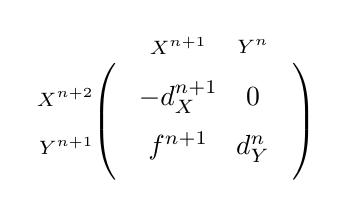
\begin{tikzpicture}[baseline]
			\matrix (M) [matrix of math nodes, ampersand replacement=\&, left delimiter=(, right delimiter=)] {
					-d_X^{n+1} \& 0 \\
					f^{n+1} \& d_Y^n \\
				};
				\node[above=1.2em] at (M-1-1) {\scriptsize $X^{n+1}$};
				\node[above=1.2em] at (M-1-2) {\scriptsize $Y^n$};
				\node[left=2.7em] at (M-1-1) {\scriptsize $X^{n+2}$};
				\node[left=2.7em] at (M-2-1) {\scriptsize $Y^{n+1}$};
		\end{tikzpicture} \\
		& : X^{n+1} \oplus Y^n \to X^{n+2} \oplus Y^{n+1} ,
	\end{align*}
	untuk $n\in\Z$. Karena $d_{X[1]}^n=-d_X^{n+1}$, tersedia pula notasi
	yang lebih ringkas
% segment-id: o014.li2.chapter3.mapping-cone.q002
	\[ \Cone(f) := \left( X[1] \oplus Y , \; \begin{pmatrix} d_{X[1]} & 0 \\ f[1] & d_Y \end{pmatrix} \right) . \]
\end{definisi}

% segment-id: o014.li2.chapter3.mapping-cone.p002
Mudah dibuktikan bahwa $\Cone(f)$ tetap merupakan kompleks, sebagaimana
ditunjukkan oleh perhitungan matriks berikut:
% segment-id: o014.li2.chapter3.mapping-cone.q003
\[ \begin{pmatrix} -d_X^{n+1} & 0 \\ f^{n+1} & d_Y^n \end{pmatrix} \begin{pmatrix} -d_X^n & 0 \\ f^n & d_Y^{n-1} \end{pmatrix} =
\begin{pmatrix} d_X^{n+1} d_X^n & 0 \\ - f^{n+1} d_X^n + d_Y^n f^n & d_Y^n d_Y^{n-1} \end{pmatrix}. \]

% segment-id: o014.li2.chapter3.mapping-cone.e001
\begin{contoh}
	Misalkan $f:X\to Y$ suatu morfisme dalam $\mathcal{A}$. Pandang $X,Y$
	sebagai objek $\cate{C}(\mathcal{A})$ (terkonsentrasi pada derajat $0$).
	Maka $\Cone(f)$ tepat merupakan kompleks $[X\xrightarrow{f}Y]$ (pada
	derajat $-1,0$, sedangkan semua suku lainnya sama dengan $0$).
\end{contoh}

% segment-id: o014.li2.chapter3.mapping-cone.p003
Kedua sifat funktorialitas berikut langsung diperoleh dari definisi.

% segment-id: o014.li2.chapter3.mapping-cone.pr001
\begin{proposisi}\label{prop:cone-functorial}
	Diberikan diagram komutatif dalam $\cate{C}(\mathcal{A})$
% segment-id: o014.li2.chapter3.mapping-cone.g001
	\[\begin{tikzcd}
		X \arrow[d, "f"'] \arrow[r, "\varphi"] & X' \arrow[d, "{f'}"] \\
		Y \arrow[r, "\psi"'] & Y'
	\end{tikzcd}\]
	maka $\bigl(\begin{smallmatrix} \varphi[1] & 0 \\ 0 & \psi \end{smallmatrix}\bigr)$
	memberikan morfisme $\Cone(f)\to\Cone(f')$.
\end{proposisi}

% segment-id: o014.li2.chapter3.mapping-cone.pr002
\begin{proposisi}\label{prop:Cone-A}
	Misalkan $F:\mathcal{A}\to\mathcal{A}'$ suatu funktor aditif dan
	$f:X\to Y$ suatu morfisme dalam $\cate{C}(\mathcal{A})$. Funktor yang
	bersesuaian $\cate{C}F:\cate{C}(\mathcal{A})\to
	\cate{C}(\mathcal{A}')$ memenuhi isomorfisme kanonik berikut dalam
	$\cate{C}(\mathcal{A}')$:
% segment-id: o014.li2.chapter3.mapping-cone.q004
	\[ (\cate{C}F)(\Cone(f)) \simeq \Cone(\cate{C}F(f)). \]
\end{proposisi}

% segment-id: o014.li2.chapter3.mapping-cone.p004
Kerucut pemetaan dapat ditempatkan dalam ``segitiga'' berikut, yang menjadi
landasan bagi seluruh teori selanjutnya.

% segment-id: o014.li2.chapter3.mapping-cone.d002
\begin{definisi}\label{def:cone-triangle}
	\index[sym1]{alphafbetaf@$\alpha(f), \beta(f)$}
	Tinjau suatu morfisme $f:X\to Y$ dalam $\cate{C}(\mathcal{A})$. Dari
	morfisme ini diperoleh morfisme-morfisme kanonik berikut dalam
	$\cate{C}(\mathcal{A})$:
% segment-id: o014.li2.chapter3.mapping-cone.q005
	\[ Y \xrightarrow{\alpha(f)} \Cone(f) \xrightarrow{\beta(f)} X[1] , \]
	yang secara eksplisit dinyatakan dengan matriks sebagai berikut:
% segment-id: o014.li2.chapter3.mapping-cone.q006
	\begin{align*}
		\alpha(f)^n & := \text{inklusi}\; \begin{pmatrix} 0 \\ \identity_{Y^n} \end{pmatrix}: Y^n \to X[1]^n \oplus Y^n , \\
		\beta(f)^n & := \text{proyeksi}\; \begin{pmatrix} \identity_{X[1]^n} & 0 \end{pmatrix}: X[1]^n \oplus Y^n \to X[1]^n .
	\end{align*}
	Jelas bahwa keduanya memang memberikan morfisme dalam
	$\cate{C}(\mathcal{A})$.
\end{definisi}

% segment-id: o014.li2.chapter3.mapping-cone.p005
Berikut ini dihimpun beberapa sifat homotopi kerucut pemetaan. Pertama-tama,
kita tunjukkan bahwa kerucut pemetaan dapat dipandang sebagai ``kokernel
homotopi'' atau ``kernel homotopi'' suatu morfisme. Inilah perwujudan pada
tingkat kompleks dari gagasan dasar dalam teori homotopi.

% segment-id: o014.li2.chapter3.mapping-cone.pr003
\begin{proposisi}\label{prop:homotopy-kernel-cokernel}
	Misalkan $f:X\to Y$ suatu morfisme dalam $\cate{C}(\mathcal{A})$. Terdapat
	bijeksi-bijeksi kanonik
% segment-id: o014.li2.chapter3.mapping-cone.g002
	\[\begin{tikzcd}[row sep=small]
		\Hom\left( \Cone(f), T \right) \arrow[leftrightarrow, r, "1:1"] & \left\{ (u, h): u \in \Hom(Y,T), \; h: \text{homotopi dari $uf$ ke $0$} \right\}, \\
		\Hom\left( T, \Cone(f)[-1] \right) \arrow[leftrightarrow, r, "1:1"] & \left\{ (v, k): v \in \Hom(T,X), \; k: \text{homotopi dari $fv$ ke $0$} \right\},
	\end{tikzcd}\]
	dengan $T$ sembarang objek $\cate{C}(\mathcal{A})$ dan
	$\Hom:=\Hom_{\cate{C}(\mathcal{A})}$. Secara lebih eksplisit,
% segment-id: o014.li2.chapter3.mapping-cone.l001
	\begin{compactitem}
% segment-id: o014.li2.chapter3.mapping-cone.i001
		\item citra $(u,h)$ dari $\tilde{u}:\Cone(f)\to T$ memenuhi
		$u=\tilde{u}\circ\alpha(f)$;
% segment-id: o014.li2.chapter3.mapping-cone.i002
		\item citra $(v,k)$ dari $\tilde{v}:T\to\Cone(f)[-1]$ memenuhi
		$v=\beta(f)[-1]\circ\tilde{v}$.
	\end{compactitem}
\end{proposisi}
% segment-id: o014.li2.chapter3.mapping-cone.pf001
\begin{bukti}
	Pertama-tama, tinjau kasus $\Hom\left(\Cone(f),T\right)$. Suatu morfisme
	$\tilde{u}:\Cone(f)\to T$ ekuivalen dengan keluarga morfisme dalam
	$\mathcal{A}$ berupa $h^n:X^{n+1}\to T^n$ dan $u^n:Y^n\to T^n$, dengan
	$n\in\Z$, yang memenuhi persamaan matriks
% segment-id: o014.li2.chapter3.mapping-cone.q007
	\[\begin{pmatrix}
		h^{n+1} & u^{n+1}
	\end{pmatrix} \begin{pmatrix}
		-d_X^{n+1} & 0 \\
		f^{n+1} & d_Y^n
	\end{pmatrix} = d_T^n \begin{pmatrix}
		h^n & u^n
	\end{pmatrix}. \]
	Setelah dijabarkan, persamaan ini ekuivalen dengan pernyataan bahwa
	$u=(u^n)_n:Y\to T$ merupakan morfisme dalam $\cate{C}(\mathcal{A})$ dan
	$h:=(h^{n-1})_n$ memenuhi
	$d_{\Hom^\bullet(X,T)}^{-1}h=uf$. Inilah bijeksi yang dimaksud; berdasarkan
	definisi $\alpha(f)$, persamaan $u=\tilde{u}\circ\alpha(f)$ langsung
	terlihat.

	Selanjutnya, tinjau suatu morfisme
	$\tilde{v}:T\to\Cone(f)[-1]$. Morfisme ini ekuivalen dengan keluarga
	morfisme dalam $\mathcal{A}$ berupa $v^n:T^n\to X^n$ dan
	$\underline{k}^n:T^n\to Y^{n-1}$ yang memenuhi
% segment-id: o014.li2.chapter3.mapping-cone.q008
	\[\begin{pmatrix}
		d_X^n & 0 \\
		-f^n & -d_Y^{n-1}
	\end{pmatrix} \begin{pmatrix}
		v^n \\ \underline{k}^n
	\end{pmatrix} = \begin{pmatrix}
		v^{n+1} \\ \underline{k}^{n+1}
	\end{pmatrix} d_T^n
	\quad (n \in \Z). \]
	Persamaan ini ekuivalen dengan pernyataan bahwa
	$v=(v^n)_n:T\to X$ merupakan morfisme dalam $\cate{C}(\mathcal{A})$ dan
	$k:=(-\underline{k}^n)_n$ memenuhi
	$d_{\Hom^\bullet(T,Y)}^{-1}k=fv$. Berdasarkan definisi $\beta(f)$,
	persamaan $v=\beta(f)[-1]\circ\tilde{v}$ juga langsung terlihat.
\end{bukti}

% segment-id: o014.li2.chapter3.mapping-cone.r001
\begin{catatan}[Kokernel homotopi dan kernel homotopi]\label{rem:homotopy-kernel-cokernel}
	\index{kokernel homotopi, kernel homotopi (homotopy cokernel, homotopy kernel)}
	Dari Proposisi~\ref{prop:homotopy-kernel-cokernel} diperoleh bahwa suatu
	morfisme $u:Y\to T$ (atau $v:T\to X$) memenuhi $uf$ (atau $fv$)
	homotopik nol jika dan hanya jika morfisme itu berfaktor melalui
	$\alpha(f):Y\to\Cone(f)$ (atau
	$\beta(f)[-1]:\Cone(f)[-1]\to X$). Hal ini dengan sendirinya mengingatkan
	kita pada sifat universal kokernel (atau kernel), dengan perbedaan berikut:
% segment-id: o014.li2.chapter3.mapping-cone.l002
	\begin{compactitem}
% segment-id: o014.li2.chapter3.mapping-cone.i003
		\item di sini syarat bahwa $uf$ (atau $fv$) homotopik nol menggantikan
		persamaan ketat $=0$;
% segment-id: o014.li2.chapter3.mapping-cone.i004
		\item faktorisasi $\tilde{u}$ (atau $\tilde{v}$) yang diberikan oleh
		proposisi tidak hanya membuktikan bahwa $uf$ (atau $fv$) homotopik nol,
		tetapi juga memuat cara morfisme itu dihomotopikan ke $0$; ini merupakan
		data satu tingkat lebih tinggi.
	\end{compactitem}
	Sifat-sifat ini tidak dapat ditangani begitu saja di
	$\cate{C}(\mathcal{A})$ atau $\cate{K}(\mathcal{A})$ dengan konsep-konsep
	dasar teori kategori; bahkan, kernel atau kokernel jarang ada dalam
	$\cate{K}(\mathcal{A})$. Oleh sebab itu, $Y\to\Cone(f)$ juga disebut
	\emph{kokernel homotopi} dari $f$, sedangkan
	$\beta(f)[-1]:\Cone(f)[-1]\to X$ disebut \emph{kernel homotopi} dari $f$.
	Menariknya, kerucut pemetaan $\Cone(f)$ beserta pergeserannya sekaligus
	memainkan peran ``kokernel'' dan ``kernel'' dalam pengertian ini.
\end{catatan}

% segment-id: o014.li2.chapter3.mapping-cone.p006
Suatu morfisme $f$ dalam $\cate{C}(\mathcal{A})$ disebut homotopik secara
kanonik dengan $g$ jika terdapat $h$ kanonik sedemikian sehingga
$g-f=d^{-1}h$; jika $f$ homotopik secara kanonik dengan $0$, maka morfisme
itu disebut homotopik nol secara kanonik.

% segment-id: o014.li2.chapter3.mapping-cone.pr004
\begin{proposisi}\label{prop:cone-homotopy}
	Misalkan $\mathcal{A}$ suatu kategori aditif.
% segment-id: o014.li2.chapter3.mapping-cone.l003
	\begin{enumerate}[(i)]
% segment-id: o014.li2.chapter3.mapping-cone.i005
		\item Jika $f:X\to Y$ suatu isomorfisme dalam
		$\cate{C}(\mathcal{A})$, maka $\identity_{\Cone(f)}$ homotopik nol
		secara kanonik.
% segment-id: o014.li2.chapter3.mapping-cone.i006
		\item Untuk sembarang morfisme $f:X\to Y$ dalam
		$\cate{C}(\mathcal{A})$, morfisme-morfisme dalam
		Definisi~\ref{def:cone-triangle} memenuhi
% segment-id: o014.li2.chapter3.mapping-cone.q009
		\[ \beta(f) \circ \alpha(f) = 0, \]
		sedangkan $\alpha(f)\circ f$ dan $f[1]\circ\beta(f)$ keduanya
		homotopik nol secara kanonik.
	\end{enumerate}
\end{proposisi}
% segment-id: o014.li2.chapter3.mapping-cone.pf002
\begin{bukti}
	Pertama-tama, tinjau (i). Berdasarkan funktorialitas kerucut pemetaan
	(Proposisi~\ref{prop:cone-functorial}), cukup meninjau
	$f=\identity_X$. Definisikan
% segment-id: o014.li2.chapter3.mapping-cone.q010
	\[ s^n := \begin{pmatrix} 0 & \identity_{X^n} \\ 0 & 0 \end{pmatrix} : X^{n+1} \oplus X^n \to X^n \oplus X^{n-1}, \quad n \in \Z. \]
	Perhitungan langsung memberikan
% segment-id: o014.li2.chapter3.mapping-cone.q011
	\begin{multline*}
		d^{n-1}_{\Cone(\identity_X)} s^n + s^{n+1} d^n_{\Cone(\identity_X)} = \\
		\begin{pmatrix} -d_X^n & 0 \\ \identity_{X^n} & d_X^{n-1} \end{pmatrix} \begin{pmatrix} 0 & \identity_{X^n} \\ 0 & 0 \end{pmatrix}  + \begin{pmatrix} 0 & \identity_{X^{n+1}} \\ 0 & 0 \end{pmatrix} \begin{pmatrix} -d_X^{n+1} & 0 \\ \identity_{X^{n+1}} & d_X^n \end{pmatrix}
		= \identity_{X^{n+1} \oplus X^n},
	\end{multline*}
	sehingga $s=(s^n)_{n\in\Z}$ menjadikan
	$\identity_{\Cone(\identity_X)}$ homotopik nol.

	Selanjutnya, tinjau (ii). Jelas bahwa
	$\beta(f)\circ\alpha(f)=0$. Homotopi-homotopi yang tersisa diperoleh dari
	Proposisi~\ref{prop:homotopy-kernel-cokernel}: ambil $T=\Cone(f)$, maka
	$\tilde{u}:=\identity_{\Cone(f)}\in\Hom(\Cone(f),T)$ menjadikan
	$\alpha(f)\circ f$ homotopik nol; ambil $T=\Cone(f)[-1]$, maka
	$\tilde{v}:=\identity_{\Cone(f)[-1]}\in\Hom(T,\Cone(f)[-1])$ menjadikan
	$f\circ\beta(f)[-1]$ homotopik nol, dan dengan demikian juga menjadikan
	$f[1]\circ\beta(f)$ homotopik nol.
\end{bukti}

% segment-id: o014.li2.chapter3.mapping-cone.p007
Definisi~\ref{def:cone-triangle} menghasilkan dua morfisme baru
$\alpha(f)$ dan $\beta(f)$ dari $f$. Hingga homotopi, kerucut pemetaan kedua
morfisme itu tidak menghasilkan objek baru; kita mulai dengan
$\Cone(\alpha(f))$ untuk menjelaskan hal tersebut. Pertama-tama, perhatikan
bahwa
% segment-id: o014.li2.chapter3.mapping-cone.q012
\[ \Cone(\alpha(f))^n = Y^{n+1} \oplus \Cone(f)^n = Y^{n+1} \oplus X^{n+1} \oplus Y^n. \]
Dalam notasi matriks,
% segment-id: o014.li2.chapter3.mapping-cone.q013
\begin{align*}
	\alpha(\alpha(f)) & = \begin{pmatrix}
		0 & 0 \\
		\identity_{X[1]} & 0 \\
		0 & \identity_Y
	\end{pmatrix} : \Cone(f) \to \Cone(\alpha(f)) , \\
	\beta(\alpha(f)) & = \begin{pmatrix}
		\identity_{Y[1]} & 0 & 0
	\end{pmatrix} : \Cone(\alpha(f)) \to Y[1].
\end{align*}

% segment-id: o014.li2.chapter3.mapping-cone.le001
\begin{lema}\label{prop:cone-alpha}
	Untuk suatu morfisme $f:X\to Y$ dalam $\cate{C}(\mathcal{A})$, notasi
	matriks mendefinisikan sepasang morfisme
% segment-id: o014.li2.chapter3.mapping-cone.g003
	\[ \begin{pmatrix} -f[1] \\ \identity_{X[1]} \\ 0 \end{pmatrix} : \begin{tikzcd} X[1] \arrow[r, shift left, "\phi"] & \Cone(\alpha(f)) \arrow[l, shift left, "\psi"] \end{tikzcd} : \begin{pmatrix} 0 & \identity_{X[1]} & 0 \end{pmatrix}. \]
	Keduanya memenuhi $\psi\circ\phi=\identity_{X[1]}$ dan menjadikan diagram
	berikut komutatif dalam $\cate{K}(\mathcal{A})$:
% segment-id: o014.li2.chapter3.mapping-cone.g004
	\[\begin{tikzcd}
		\Cone(f) \arrow[d, "{\identity_{\Cone(f)}}"'] \arrow[r, "\beta(f)"] & X[1] \arrow[d, "\phi"] \arrow[r, "{-f[1]}"] & Y[1] \arrow[d, "{\identity_{Y[1]}}"] \\
		\Cone(f) \arrow[r, "{\alpha(\alpha(f))}"'] & \Cone(\alpha(f)) \arrow[r, "\beta(\alpha(f))"'] & Y[1]
	\end{tikzcd}\]
	Selain itu, $\phi,\psi$ saling invers dalam $\cate{K}(\mathcal{A})$.
\end{lema}
% segment-id: o014.li2.chapter3.mapping-cone.pf003
\begin{bukti}
	Berdasarkan uraian sebelumnya tentang $\Cone(\alpha(f))$, dalam notasi
	matriks $d_{\Cone(\alpha(f))}^n$ diberikan oleh
% segment-id: o014.li2.chapter3.mapping-cone.q014
	\[ \begin{pmatrix} -d_Y^{n+1} & 0 & 0 \\ 0 & -d_X^{n+1} & 0 \\ \identity_{Y^{n+1}} & f^{n+1} & d_Y^n \end{pmatrix} : Y^{n+1} \oplus X^{n+1} \oplus Y^n \to Y^{n+2} \oplus X^{n+2} \oplus Y^{n+1}. \]
	Cukup diverifikasi pernyataan-pernyataan berikut dalam
	$\cate{C}(\mathcal{A})$:
% segment-id: o014.li2.chapter3.mapping-cone.l004
	\begin{itemize}
% segment-id: o014.li2.chapter3.mapping-cone.i007
		\item $\phi:=(\phi^n)_{n\in\Z}$ dan $\psi:=(\psi^n)_{n\in\Z}$
		keduanya merupakan morfisme kompleks;
% segment-id: o014.li2.chapter3.mapping-cone.i008
		\item $\psi\circ\phi=\identity_{X[1]}$;
% segment-id: o014.li2.chapter3.mapping-cone.i009
		\item $\psi\circ\alpha(\alpha(f))=\beta(f)$;
% segment-id: o014.li2.chapter3.mapping-cone.i010
		\item $\beta(\alpha(f))\circ\phi=-f[1]$;
% segment-id: o014.li2.chapter3.mapping-cone.i011
		\item terdapat
		$s=(s^n)_{n\in\Z}\in\Hom^{-1}\left(\Cone(\alpha(f)),
		\Cone(\alpha(f))\right)$ sedemikian sehingga
		$\identity_{\Cone(\alpha(f))}-\phi\circ\psi
		=d^{-1}_{\Hom^\bullet}(s)$.
	\end{itemize}
	Empat pernyataan pertama bersifat elementer. Untuk pernyataan terakhir,
	ambillah, dalam notasi matriks,
% segment-id: o014.li2.chapter3.mapping-cone.q015
	\[ s^n := \begin{pmatrix} 0 & 0 & \identity_{Y^n} \\ 0 & 0 & 0 \\ 0 & 0 & 0 \end{pmatrix}: \Cone(\alpha(f))^n \to \Cone(\alpha(f))^{n-1} \]
	dan lakukan verifikasi langsung.
\end{bukti}

% segment-id: o014.li2.chapter3.mapping-cone.p008
Untuk kasus $\beta(f)$, kita melakukan sedikit modifikasi dan meninjau
kerucut pemetaan dari $-\beta(f)[-1]:\Cone(f)[-1]\to X$.

% segment-id: o014.li2.chapter3.mapping-cone.d003
\begin{definisi}\label{def:Cyl}
	\index{silinder pemetaan (mapping cylinder)}
	\index[sym1]{Cylf@$\Cyl(f)$}
	Untuk suatu morfisme $f:X\to Y$ dalam $\cate{C}(\mathcal{A})$,
	\emph{silinder pemetaan} dari $f$ didefinisikan sebagai
% segment-id: o014.li2.chapter3.mapping-cone.q016
	\[ \Cyl(f) := \Cone\left( \Cone(f)[-1] \xrightarrow{-\beta(f)[-1]} X \right). \]
	Silinder ini dilengkapi morfisme-morfisme kanonik
	$X\to\Cyl(f)\to\Cone(f)$.
\end{definisi}

% segment-id: o014.li2.chapter3.mapping-cone.p009
Silinder pemetaan mempunyai funktorialitas yang bentuknya sama dengan
funktorialitas kerucut pemetaan (Proposisi~\ref{prop:cone-functorial}).
Berdasarkan Catatan~\ref{rem:homotopy-kernel-cokernel}, $\Cyl(f)$ dapat
dibandingkan dengan kocitra dalam kategori aditif---objek ini kurang lebih
merupakan ``kokernel dari kernel'' (Proposisi~\ref{prop:Im-Coim-additive})---
sehingga dapat pula dipandang sebagai kocitra homotopi dari $f$.

% segment-id: o014.li2.chapter3.mapping-cone.p010
Secara lebih eksplisit,
$\Cyl(f)^n=\Cone(f)^n\oplus X^n=X^{n+1}\oplus Y^n\oplus X^n$; morfisme
$X\to\mathrm{Cyl}(f)$ (atau $\mathrm{Cyl}(f)\to\Cone(f)$) ialah inklusi ke
suku ketiga pada jumlah langsung (atau proyeksi ke dua suku pertama), dan
% segment-id: o014.li2.chapter3.mapping-cone.q017
\[ d_{\Cyl(f)}^n =
	\begin{pmatrix} d_{\Cone(f)}^n & 0 \\ -\beta(f)^n & d_X^n \end{pmatrix}
	= \begin{pmatrix}
		-d_X^{n+1} & 0 & 0 \\
		f^{n+1} & d_Y^n & 0 \\
		-\identity_{X^{n+1}} & 0 & d_X^n
\end{pmatrix} .\]

% segment-id: o014.li2.chapter3.mapping-cone.le002
\begin{lema}\label{prop:cone-beta}
	Untuk suatu morfisme $f:X\to Y$ dalam $\cate{C}(\mathcal{A})$, dapat
	didefinisikan sepasang morfisme
% segment-id: o014.li2.chapter3.mapping-cone.g005
	\[ \begin{pmatrix} 0 \\ \identity_Y \\ 0 \end{pmatrix} : \begin{tikzcd} Y \arrow[r, shift left, "\phi"] & \Cyl(f) \arrow[l, shift left, "\psi"] \end{tikzcd} : \begin{pmatrix} 0 & \identity_Y & f \end{pmatrix}. \]
	Keduanya memenuhi $\psi\circ\phi=\identity_Y$ dan menjadikan diagram
	berikut komutatif dalam $\cate{K}(\mathcal{A})$:
% segment-id: o014.li2.chapter3.mapping-cone.g006
	\[\begin{tikzcd}
		X \arrow[d, "{\identity_X}"'] \arrow[r, "f"] & Y \arrow[d, "\phi"] \arrow[r, "{\alpha(f)}"] & \Cone(f) \arrow[d, "{\identity_{\Cone(f)}}"] \\
		X \arrow[r] & \Cyl(f) \arrow[r] & \Cone(f)
	\end{tikzcd}\]
	Selain itu, $\phi,\psi$ saling invers dalam $\cate{K}(\mathcal{A})$.
Lebih lanjut, $f$ berfaktor sebagai komposisi
$X\to\Cyl(f)\xrightarrow{\psi}Y$.
\end{lema}
% segment-id: o014.li2.chapter3.mapping-cone.pf004
\begin{bukti}
	Pembaca dapat memverifikasi langsung dari definisi bahwa $\phi$ dan $\psi$
	memang memberikan morfisme kompleks. Setelah itu,
	$\psi\circ\phi=\identity_Y$ langsung terlihat. Selanjutnya, untuk
	membuktikan bahwa $\phi$ dan $\psi$ saling invers dalam
	$\cate{K}(\mathcal{A})$, seperti pada Lema~\ref{prop:cone-alpha}, ambillah
% segment-id: o014.li2.chapter3.mapping-cone.q018
	\begin{align*}
		s^n & := \begin{pmatrix} 0 & 0 & -\identity_{X^n} \\ 0 & 0 & 0 \\ 0 & 0 & 0 \end{pmatrix}: X^{n+1} \oplus Y^n \oplus X^n \to X^n \oplus Y^{n-1} \oplus X^{n-1}, \\
		s & := (s^n)_{n \in \Z},
	\end{align*}
	dan verifikasi
	$\identity_{\Cyl(f)}-\phi\circ\psi=d^{-1}_{\Hom^\bullet}(s)$.

	Kotak kanan pada diagram sudah komutatif dalam $\cate{C}(\mathcal{A})$.
	Untuk kotak kiri, cukup perhatikan bahwa komposisi
	$X\to\mathrm{Cyl}(f)\xrightarrow{\psi}Y$ sama dengan $f$.
\end{bukti}

% segment-id: o014.li2.chapter3.mapping-cone.p011
Lema~\ref{prop:cone-alpha} bersama Lema~\ref{prop:cone-beta} menunjukkan
bahwa, hingga isomorfisme dalam $\cate{K}(\mathcal{A})$, sembarang morfisme
$f:X\to Y$ dapat diganti dengan proyeksi yang jauh lebih sederhana
$\Cone(\alpha(f))[-1]\to Y$ (atau inklusi $X\to\Cyl(f)$), dan konstruksi ini
funktorial dalam $f$. Inilah suatu gagasan penting dalam aljabar homologis
dan teori homotopi.

% segment-id: o014.li2.chapter3.mapping-cone.p012
Kasus khusus silinder pemetaan dengan $f=\identity_X$ mempunyai kegunaan lain:
silinder itu dapat digunakan untuk menafsirkan homotopi. Bagi pembaca yang
mengenal teori homologi, semua ini mempunyai tafsiran topologis, tetapi di
sini kita hanya membahas versi aljabarnya.

% segment-id: o014.li2.chapter3.mapping-cone.pr005
\begin{proposisi}\label{prop:cylinder-homotopy}
	\index[sym1]{CylX@$\Cyl_X$}
	Misalkan $X$ suatu objek $\cate{C}(\mathcal{A})$ dan definisikan
	$\mathrm{Cyl}_X:=\mathrm{Cyl}(\identity_X)$. Perhatikan bahwa
	$\mathrm{Cyl}_X^n=X^{n+1}\oplus X^n\oplus X^n$.
% segment-id: o014.li2.chapter3.mapping-cone.l005
	\begin{enumerate}[(i)]
% segment-id: o014.li2.chapter3.mapping-cone.i012
		\item Dalam $\cate{C}(\mathcal{A})$ terdapat morfisme-morfisme
% segment-id: o014.li2.chapter3.mapping-cone.g007
		$\begin{tikzcd}
			X \arrow[shift left, r, "i_0"] \arrow[shift right, r, "i_1"'] & \Cyl_X \arrow[r, "j"] & X
		\end{tikzcd}$,
		yang dalam notasi matriks didefinisikan untuk setiap $n\in\Z$ oleh
% segment-id: o014.li2.chapter3.mapping-cone.q019
		\begin{equation*}
			i_0^n := \begin{pmatrix} 0 \\ 0 \\ \identity_{X^n} \end{pmatrix} , \quad
			i_1^n := \begin{pmatrix} 0 \\ \identity_{X^n} \\ 0 \end{pmatrix} , \quad j^n := \begin{pmatrix} 0 & \identity_{X^n} & \identity_{X^n} \end{pmatrix},
		\end{equation*}
		Morfisme-morfisme ini memenuhi $ji_0=\identity_X=ji_1$, dan citra $j$
		dalam $\cate{K}(\mathcal{A})$ merupakan isomorfisme.
% segment-id: o014.li2.chapter3.mapping-cone.i013
		\item Untuk sembarang objek $Y$ dari $\cate{C}(\mathcal{A})$, terdapat
		bijeksi
% segment-id: o014.li2.chapter3.mapping-cone.q020
		\begin{align*}
			\left\{\begin{array}{r|l}
				(f, g, h) & f, g \in \Hom_{\cate{C}(\mathcal{A})}(X, Y) \\
				& h \in \Hom^{-1}(X, Y) \\
				& g - f = d^{-1}_{\Hom^\bullet(X, Y)} h
			\end{array}\right\} & \xrightarrow{1:1} \Hom_{\cate{C}(\mathcal{A})}\left( \mathrm{Cyl}_X, Y \right) \\
			(f, g, h) & \longmapsto \tilde{h} = (\tilde{h}^n)_{n \in \Z}, \; \tilde{h}^n := \begin{pmatrix} h^n & g^n & f^n \end{pmatrix}.
		\end{align*}
		Secara khusus, $f=\tilde{h}i_0$ dan $g=\tilde{h}i_1$.
	\end{enumerate}
\end{proposisi}
% segment-id: o014.li2.chapter3.mapping-cone.pf005
\begin{bukti}
	Untuk (i), perhatikan bahwa $i_0$ tidak lain ialah morfisme kanonik
	$X\to\mathrm{Cyl}(\identity_X)$ dalam Definisi~\ref{def:Cyl}, sedangkan
	$i_1$ ialah morfisme $\phi:X\to\mathrm{Cyl}(\identity_X)$ dalam
	Lema~\ref{prop:cone-beta}. Diagram komutatif dalam
	Lema~\ref{prop:cone-beta} menunjukkan bahwa keduanya memberikan
	isomorfisme yang sama dalam $\cate{K}(\mathcal{A})$.

	Untuk $j$, mudah diverifikasi bahwa
	$j^{n+1}d_{\Cyl_X}^n=\bigl(0\;d_X^n\;d_X^n\bigr)=d_X^nj^n$.
	Jadi, $j$ memang merupakan morfisme, sedangkan
	$ji_0=\identity_X=ji_1$ langsung terlihat. Karena $i_0$ dan $i_1$
	merupakan isomorfisme dalam $\cate{K}(\mathcal{A})$, demikian pula $j$.

	Untuk (ii), tuliskan sembarang unsur $\tilde{h}$ dari
	$\Hom^0(\mathrm{Cyl}_X,Y)$ dalam bentuk
	\[
		\tilde{h}=\left((h^n,g^n,f^n)\right)_{n\in\Z},
	\]
	dengan
% segment-id: o014.li2.chapter3.mapping-cone.q021
	\[ h^n: X^{n+1} \to Y^n, \quad f^n: X^n \to Y^n, \quad g^n: X^n \to Y^n \]
	semuanya merupakan morfisme dalam $\mathcal{A}$. Dengan menghilangkan
	superskrip dan menggunakan notasi matriks, hitung
% segment-id: o014.li2.chapter3.mapping-cone.q022
	\begin{align*}
		\tilde{h} \; d_{\mathrm{Cyl}_X} & = \begin{pmatrix} h & g & f \end{pmatrix} \begin{pmatrix} -d_X & 0 & 0 \\ \identity_X & d_X & 0 \\ -\identity_X & 0 & d_X \end{pmatrix} = \begin{pmatrix} -hd_X + g - f & g d_X & f d_X \end{pmatrix} , \\
		d_Y \; \tilde{h} & = \begin{pmatrix} d_Y h & d_Y g & d_Y f \end{pmatrix}.
	\end{align*}
	Oleh karena itu, $\tilde{h}$ merupakan morfisme kompleks jika dan hanya
	jika $f,g\in\Hom_{\cate{C}(\mathcal{A})}(X,Y)$ dan
	$g-f=hd_X+d_Yh$.
\end{bukti}

% segment-id: o014.li2.chapter3.mapping-cone.r002
\begin{catatan}\label{rem:cone-chain}
	\index{kerucut pemetaan}\index{silinder pemetaan}
	Kerucut pemetaan dan silinder pemetaan tentu saja mempunyai versi untuk
	kompleks rantai (lihat Catatan~\ref{rem:cochain-vs-chain}). Diberikan suatu
	morfisme kompleks rantai $f:X\to Y$, definisikan
% segment-id: o014.li2.chapter3.mapping-cone.q023
	\[\begin{array}{rlrl}
		\Cone(f)_n & :=(X[-1] \oplus Y)_n, &
		\Cyl(f)_n & := (X[-1] \oplus Y \oplus X)_n, \\
		d_{\Cone(f)} & := \begin{pmatrix} d_{X[-1]} & 0 \\ f[-1] & d_Y \end{pmatrix}, &
		d_{\Cyl(f)} & := \begin{pmatrix} d_{X[-1]} & 0 & 0 \\ f[-1] & d_Y & 0 \\ -\identity_{X[-1]} & 0 & d_X \end{pmatrix}.
	\end{array}\]

	Semua pernyataan dalam bagian ini dapat dipindahkan ke kasus kompleks
	rantai. Secara khusus, terdapat morfisme-morfisme kanonik
% segment-id: o014.li2.chapter3.mapping-cone.q024
	\[ X \xrightarrow{f} Y \xrightarrow{\alpha(f)} \Cone(f) \xrightarrow{\beta(f)} X[-1], \quad X \to \Cyl(f) \to \Cone(f). \]
\end{catatan}

% Unit 035 terjemahan Bahasa Indonesia dari chapter3.tex baris 622--699.
% Sumber: Methods of Algebra, Volume 2, commit
% 9a5803ff77dd3257484cb177f851a73770a59dd3 (CC BY 4.0).
% stable-unit-id: o014.aljabr2.chapter3.opposite-category-complexes
% Cakupan: Bagian 3.4 lengkap.

% segment-id: o014.li2.chapter3.opposite-category-complexes.h001
\section{Kompleks pada kategori lawan}\label{sec:opposite-cplx}
\hypertarget{o014.aljabr2.chapter3.opposite-category-complexes}{ }

% segment-id: o014.li2.chapter3.opposite-category-complexes.p001
Tetapkan suatu kategori aditif $\mathcal{A}$. Bagian ini bertujuan
menghubungkan kompleks pada $\mathcal{A}$ dan $\mathcal{A}^{\opp}$. Karena
funktor yang melibatkan $\mathcal{A}^{\opp}$, misalnya funktor $\Hom$, sering
muncul, prosedur ini sederhana tetapi perlu; beberapa tanda positif dan
negatif yang terlibat juga memerlukan sedikit perhatian. Pembaca pemula
disarankan melewati bagian ini atau sekadar membacanya sepintas terlebih
dahulu.

% segment-id: o014.li2.chapter3.opposite-category-complexes.p002
Pembahasan berikut terbagi menjadi tiga aspek: kompleks, homotopi, dan kerucut
pemetaan. Versi untuk kategori turunan yang akan dikaji kemudian
(Proposisi~\sourcecrossref{prop:derived-cat-op}{pada pembahasan kategori turunan selanjutnya})
merupakan penerapan langsung hasil-hasil
ini. Ingat bahwa jika $f:X\to Y$ suatu morfisme dalam $\mathcal{A}$, maka
$f^{\opp}$ menyatakan morfisme yang bersesuaian $Y\to X$ dalam
$\mathcal{A}^{\opp}$.

% segment-id: o014.li2.chapter3.opposite-category-complexes.dp001
\begin{definisiproposisi}\label{def:sigma}
	\index[sym1]{sigma@$\sigma$}
	Isomorfisme antarkategori aditif
	$\sigma:\cate{C}(\mathcal{A}^{\opp})\to\cate{C}(\mathcal{A})^{\opp}$
	didefinisikan sebagai berikut. Untuk suatu objek $X$ dalam
	$\cate{C}(\mathcal{A}^{\opp})$, definisikan di dalam $\mathcal{A}$
% segment-id: o014.li2.chapter3.opposite-category-complexes.q001
	\[ (\sigma X)^n := X^{-n}, \quad d_{\sigma X}^n = (-1)^{n+1} \left[ d_X^{-n-1, \opp}: (\sigma X)^n \to (\sigma X)^{n+1} \right], \quad n \in \Z. \]
	Untuk suatu morfisme
	$f=\left(f^n:X^n\to Y^n\right)_n$ dalam
	$\cate{C}(\mathcal{A}^{\opp})$, citranya $\sigma f$ diambil sebagai
	morfisme berikut dalam $\cate{C}(\mathcal{A})$:
% segment-id: o014.li2.chapter3.opposite-category-complexes.q002
	\[ (\sigma f)^n := \left(f^{-n} \right)^{\opp} : (\sigma Y)^n \to (\sigma X)^n, \]
	yakni sebagai morfisme $\sigma X\to\sigma Y$ dalam
	$\cate{C}(\mathcal{A})^{\opp}$. Untuk setiap $m\in\Z$, terdapat
	isomorfisme alami
% segment-id: o014.li2.chapter3.opposite-category-complexes.q003
	\[ s_m: \sigma \circ [m] \rightiso [-m] \circ \sigma, \]
	dengan $[-m]$ dipandang sebagai funktor dari
	$\cate{C}(\mathcal{A})^{\opp}$ ke dirinya sendiri (secara ketat, notasinya
	seharusnya $[-m]^{\opp}$).
\end{definisiproposisi}
% segment-id: o014.li2.chapter3.opposite-category-complexes.pf001
\begin{bukti}
	Kasus umum $s_m$ dapat direduksi secara bertahap ke kasus $m=1$.
	Definisikan $s_1=(s_{1,X})_X$ sebagai berikut. Untuk setiap $n$, ambil
% segment-id: o014.li2.chapter3.opposite-category-complexes.g001
	\begin{equation}\label{eqn:sigma-s}\begin{tikzcd}[row sep=tiny]
		s_{1,X}^n : \sigma(X{[1]})^n = X^{1-n} \arrow[r, "\sim"', "{(-1)^{n-1}}" inner sep=0.6em] & X^{1-n} = (\sigma X){[-1]}^n .
	\end{tikzcd}\end{equation}
	Seluruh verifikasi tereduksi pada
	$s_{1, X}^{n+1} d^n_{\sigma(X[1])} = -d_{X[1]}^{-n-1, \opp} =
	d_X^{-n, \opp} = (-1)^n d_{\sigma X}^{n-1} =
	d^n_{(\sigma X)[-1]} s_{1,X}^n$.
\end{bukti}

% segment-id: o014.li2.chapter3.opposite-category-complexes.p003
Jika konstruksi $\sigma$ dengan koefisien $(-1)^{n+1}$ diterapkan pada kedua
arah, $\sigma^2X$ isomorfik secara alami dengan $X$ melalui isomorfisme yang
komponen berderajat $n$-nya adalah $(-1)^n\identity_{X^n}$. Untuk memperoleh
invers, definisikan konstruksi arah balik dengan rumus yang sama pada objek
dan morfisme, tetapi gunakan koefisien $(-1)^n$ pada diferensial. Komposisi
dalam kedua urutan tepat sama dengan funktor identitas, sehingga $\sigma$
memang merupakan isomorfisme antarkategori.%
\footnote{Catatan penerjemah (O014-C036): sumber, dengan alasan
$n(n+1)\equiv0\pmod{2}$, menyatakan bahwa penerapan $\sigma$ dua kali
langsung mengembalikan $X$. Namun, penggunaan rumus yang sama pada kedua arah
memberikan diferensial $-d_X$, bukan $d_X$. Target mencatat isomorfisme alami
bertanda dan konstruksi invers yang dikoreksi di atas.}

% segment-id: o014.li2.chapter3.opposite-category-complexes.r001
\begin{catatan}\label{rem:sigma-vs-cohomology}
	Jika $\mathcal{A}$ kategori abelian, tanda pada $d_{\sigma X}^\bullet$
	tidak mengubah kohomologi yang diperkenalkan dalam
	Definisi~\ref{def:cohomology}; dengan demikian,
	$\Hm^{-n}(\sigma X)\in\Obj(\mathcal{A})$ bersesuaian dengan
	$\Hm^n(X)\in\Obj(\mathcal{A}^{\opp})$.
\end{catatan}

% segment-id: o014.li2.chapter3.opposite-category-complexes.p004
Selanjutnya, kita kaji hubungan antara $\sigma$ dan homotopi.

% segment-id: o014.li2.chapter3.opposite-category-complexes.pr001
\begin{proposisi}\label{prop:sigma-homotopy}
	Funktor $\sigma$ yang didefinisikan di atas menginduksi ekuivalensi
	antarkategori aditif
	$\cate{K}(\mathcal{A}^{\opp})\rightiso\cate{K}(\mathcal{A})^{\opp}$.
\end{proposisi}
% segment-id: o014.li2.chapter3.opposite-category-complexes.pf002
\begin{bukti}
	Tetapkan objek $X,Y$ dalam $\cate{C}(\mathcal{A}^{\opp})$. Untuk
	$f=(f^k)_k\in\Hom^{-1}_{\cate{C}(\mathcal{A}^{\opp})}(X,Y)$, gunakan
	tabel berikut untuk mendefinisikan $\sigma f$ yang bersesuaian dalam
	$\mathcal{A}$, dengan
	$\sigma f\in\Hom^{-1}_{\cate{C}(\mathcal{A})}(\sigma Y,\sigma X)$:
% segment-id: o014.li2.chapter3.opposite-category-complexes.q004
	\begingroup\setlength{\arraycolsep}{4pt}
	\[\begin{array}{|c|c|c|c|} \hline
		\text{Kategori} & \multicolumn{3}{c|}{\text{Morfisme}} \\ \hline
		\mathcal{A}^{\opp} & X^k \xrightarrow{(-1)^{k+1} f^k} Y^{k-1} & d_Y^{k-1} f^k + f^{k+1} d_X^k & (d^{-1}f)^k \\
		\mathcal{A} & (\sigma Y)^{-k+1} \xrightarrow{(\sigma f)^{-k+1}} (\sigma X)^{-k} & (\sigma f)^{-k+1} d_{\sigma Y}^{-k} + d_{\sigma X}^{-k-1} (\sigma f)^{-k} & d^{-1} (\sigma f)^{-k} \\ \hline
	\end{array}\]
	\endgroup
	Hal ini cukup untuk menunjukkan
	\[\begin{aligned}
		\Hom_{\cate{K}(\mathcal{A}^{\opp})}(X, Y)
		&\rightiso \Hom_{\cate{K}(\mathcal{A})}(\sigma Y, \sigma X) \\
		&= \Hom_{\cate{K}(\mathcal{A})^{\opp}}(\sigma X, \sigma Y).
	\end{aligned}\]
\end{bukti}

% segment-id: o014.li2.chapter3.opposite-category-complexes.p005
Terakhir, melalui $\sigma$ dan keluarga isomorfisme $(s_m)_m$ yang dibangun
di atas, kita bandingkan kerucut pemetaan dalam $\cate{C}(\mathcal{A})$ dan
$\cate{C}(\mathcal{A}^{\opp})$. Rinciannya berupa perhitungan yang agak rutin.

% segment-id: o014.li2.chapter3.opposite-category-complexes.pr002
\begin{proposisi}\label{prop:sigma-triangulated}
	\index[sym1]{sigma}
	Untuk setiap morfisme $f:X\to Y$ dalam
	$\cate{C}(\mathcal{A}^{\opp})$, terdapat diagram komutatif berikut dalam
	$\cate{C}(\mathcal{A})$% 
	\footnote{Di sini $\alpha(\cdot)$ dan $\beta(\cdot)$ keduanya didefinisikan
	relatif terhadap $\cate{C}(\mathcal{A})$. Jika diagram dipandang dalam
	$\cate{C}(\mathcal{A})^{\opp}$, semua panahnya harus dibalik.}:
% segment-id: o014.li2.chapter3.opposite-category-complexes.g002
	\[\begin{tikzcd}[column sep=large]
		\sigma\left( X{[1]} \right) \arrow[r, "{\sigma(\beta(f))}"] \arrow[d, "{s_{1,X}}"'] & \sigma\left(\Cone(f)\right) \arrow[r, "{\sigma(\alpha(f))}"] \arrow[d, "\theta"] & \sigma Y \arrow[r, "\sigma(f)"] \arrow[d, "\identity"] & \sigma X \arrow[d, "{\identity}"] \\
		(\sigma X){[-1]} \arrow[r, "{\alpha(\sigma(f))[-1]}"' inner sep=0.6em] & \Cone(\sigma(f)){[-1]} \arrow[r, "{\beta(\sigma(f))[-1]}"' inner sep=0.6em] & \sigma Y \arrow[r, "{\sigma(f)}"' inner sep=0.6em] & \sigma X
	\end{tikzcd}\]
	dengan $\theta$ suatu isomorfisme kanonik dan $s_{1,X}$ isomorfisme yang
	diberikan oleh Definisi--Proposisi~\ref{def:sigma}.
\end{proposisi}
% segment-id: o014.li2.chapter3.opposite-category-complexes.pf003
\begin{bukti}
	Jika $\Cone(f)$ diganti dengan $X[1]\oplus Y$, pernyataannya mudah dan
	isomorfisme yang diperlukan cukup diambil sebagai
	$(s_{1,X},\identity_{\sigma Y})$. Kesulitannya di sini ialah bahwa matriks
	$d_{\Cone(f)}$ mempunyai entri luar diagonal $f[1]$. Meskipun demikian,
	kita tetap mengikuti cara yang sama: dengan menggunakan
	\eqref{eqn:sigma-s}, untuk setiap $n\in\Z$ definisikan isomorfisme
% segment-id: o014.li2.chapter3.opposite-category-complexes.q005
	\begin{multline*}
		\theta^n: \sigma\left(\Cone(f)\right)^n = \sigma\left(X[1]\right)^n \oplus (\sigma Y)^n \\
		\xrightarrow[\sim]{(s_{1,X}, \identity)^n = ((-1)^{n-1} \identity, \identity) } (\sigma X)[-1]^n \oplus (\sigma Y)^n \xlongequal{\text{pertukaran}} \left( (\sigma Y) \oplus (\sigma X)[-1] \right)^n ,
	\end{multline*}	
	Dengan identifikasi ini, morfisme $d_{\sigma(\Cone(f))}^n$ dalam
	$\mathcal{A}$ bersesuaian dengan
% segment-id: o014.li2.chapter3.opposite-category-complexes.q006
	\[ \begin{pmatrix}
		d_{\sigma Y}^n & 0 \\
		* & d_{(\sigma X)[-1]}^n
	\end{pmatrix} : \left( (\sigma Y) \oplus (\sigma X)[-1] \right)^n \to \left( (\sigma Y) \oplus (\sigma X)[-1] \right)^{n+1} . \]
	Seperti dinyatakan pada awal bukti, entri-entri diagonal tidak bermasalah;
	yang perlu ditentukan ialah entri kiri bawah matriks tersebut. Berdasarkan
	Definisi--Proposisi~\ref{def:sigma}, entri ini sama dengan $(-1)^{n+1}$
	dikali komposisi morfisme berikut dalam $\mathcal{A}$:
% segment-id: o014.li2.chapter3.opposite-category-complexes.g003
	\[\begin{tikzcd}[row sep=tiny]
		(\sigma Y)^n \arrow[r] & (\sigma(X[1]))^{n+1} \arrow[r, "\sim"] & (\sigma X)[-1]^{n+1} \\
		Y^{-n} \arrow[equal, u] \arrow[r, "{(f^{-n})^{\opp}}"'] & X^{-n} \arrow[equal, u] \arrow[r, "{s_{1, X}^{n+1} = (-1)^n}"'] & X^{-n} \arrow[equal, u]
	\end{tikzcd}\]
	Dengan demikian, hasilnya ialah $-\sigma(f)^n$. Oleh karena itu,
% segment-id: o014.li2.chapter3.opposite-category-complexes.q007
	\[ \theta := (\theta^n)_{n \in \Z}: \sigma(\Cone(f)) \rightiso \Cone(\sigma(f))[-1] \]
	memang merupakan isomorfisme dalam $\cate{C}(\mathcal{A})$. Setelah hal
	ini ditetapkan, verifikasi komutativitas tidak lagi mengandung kesulitan
	yang berarti.
\end{bukti}

% segment-id: o014.li2.chapter3.opposite-category-complexes.p006
Tentu saja, hasil-hasil bagian ini juga berlaku untuk kompleks rantai dan
dapat diperumum ke kasus ketika $\mathcal{A}$ merupakan kategori
$\Bbbk$-linear.

% Unit 036 terjemahan Bahasa Indonesia dari chapter3.tex baris 700--945.
% Sumber: Methods of Algebra, Volume 2, commit
% 9a5803ff77dd3257484cb177f851a73770a59dd3 (CC BY 4.0).
% stable-unit-id: o014.aljabr2.chapter3.double-complexes
% Cakupan: Bagian 3.5 lengkap.

% segment-id: o014.li2.chapter3.double-complexes.h001
\section{Bikompleks}\label{sec:double-cplx}
\hypertarget{o014.aljabr2.chapter3.double-complexes}{ }

% segment-id: o014.li2.chapter3.double-complexes.p001
Dalam bagian ini, $\mathcal{A}$ tetap merupakan kategori aditif. Secara kasar,
bikompleks dapat dibayangkan sebagai versi dua dimensi dari kompleks, dengan
diferensial dalam arah vertikal dan horizontal.

% segment-id: o014.li2.chapter3.double-complexes.d001
\begin{definisi}[Bikompleks]\label{def:double-cplx}
	\index{bikompleks (double complex)}
	\index[sym1]{dhoridvert@$\dhori$, $\dvert$}
	Bikompleks pada kategori aditif $\mathcal{A}$ terdiri atas keluarga objek
	$\left(X^{p,q}\right)_{(p,q)\in\Z^2}$ dalam $\mathcal{A}$, bersama dengan
	morfisme $\dhori^{p,q}:X^{p,q}\to X^{p+1,q}$ dan
	$\dvert^{p,q}:X^{p,q}\to X^{p,q+1}$, yang memenuhi
% segment-id: o014.li2.chapter3.double-complexes.q001
	\[ \dhori^{p+1,q} \dhori^{p,q} = 0, \quad \dvert^{p, q+1} \dvert^{p,q} = 0, \quad \dhori^{p, q+1} \dvert^{p,q} = \dvert^{p+1, q} \dhori^{p,q}. \]
	Data di atas biasanya disingkat sebagai
	$(X^{\bullet,\bullet},\dhori,\dvert)$, $X^{\bullet,\bullet}$, atau $X$.
\end{definisi}

% segment-id: o014.li2.chapter3.double-complexes.p002
Syarat-syarat pada $\dhori,\dvert$ dapat disingkat menjadi
% segment-id: o014.li2.chapter3.double-complexes.q002
\[ \dhori^2 = 0, \quad \dvert^2 = 0, \quad \dhori \dvert = \dvert \dhori. \]

% segment-id: o014.li2.chapter3.double-complexes.d002
\begin{definisi}\label{def:bicplx}
	Diberikan kategori aditif $\mathcal{A}$, suatu morfisme dari bikompleks $X$
	ke $Y$ adalah keluarga morfisme
% segment-id: o014.li2.chapter3.double-complexes.q003
	\[ f = \left( f^{p,q}: X^{p, q} \to Y^{p, q} \right)_{(p, q) \in \Z^2}, \]
	sedemikian sehingga, untuk semua $p,q$, berlaku
% segment-id: o014.li2.chapter3.double-complexes.q004
	\[ \dhori_Y^{p, q} f^{p, q} = f^{p+1, q} \dhori_X^{p, q}, \quad \dvert_Y^{p, q} f^{p, q} = f^{p, q+1} \dvert_X^{p, q}. \]
	Relasi-relasi di atas dapat disingkat sebagai
	$\dhori_Yf=f\dhori_X$ dan $\dvert_Yf=f\dvert_X$.
\end{definisi}

% segment-id: o014.li2.chapter3.double-complexes.p003
Seperti dalam Proposisi~\ref{prop:additive-cat-cplx}, definisi-definisi ini
menjadikan semua bikompleks pada $\mathcal{A}$ suatu kategori aditif
$\cate{C}^2(\mathcal{A})$.
\index[sym1]{C2A@$\cate{C}^2(\mathcal{A})$}

% segment-id: o014.li2.chapter3.double-complexes.p004
Secara visual, bikompleks $X$ digambarkan sebagai
% segment-id: o014.li2.chapter3.double-complexes.g001
\[\begin{tikzcd}
	& \vdots & \vdots & \\
	\cdots \arrow[r] & X^{p, q+1} \arrow[r] \arrow[u] & X^{p+1, q+1} \arrow[r] \arrow[u] & \cdots \\
	\cdots \arrow[r] & X^{p, q} \arrow[r, "{\dhori^{p,q}}"'] \arrow[u, "{\dvert^{p,q}}"] & X^{p+1, q} \arrow[r] \arrow[u] & \cdots \\
	& \vdots \arrow[u] & \vdots \arrow[u] &
\end{tikzcd}\]
Setiap baris $\left(X^{\bullet,q},d^{\bullet,q}\right)$ dan setiap kolom
$\left(X^{p,\bullet},d^{p,\bullet}\right)$ merupakan kompleks. Dengan
demikian, bikompleks dapat dipandang menurut kolom ataupun menurut baris.

% segment-id: o014.li2.chapter3.double-complexes.d003
\begin{definisi}\label{def:bicplx-F1}
	\index[sym1]{F1F2@$F_{\mathrm{I}}, F_{\mathrm{II}}$}
	Funktor aditif
	$F_{\mathrm{I}}:\cate{C}^2(\mathcal{A})\to
	\cate{C}(\cate{C}(\mathcal{A}))$ didefinisikan sebagai berikut: untuk
	bikompleks $X$, ambil $(F_{\mathrm{I}}X)^p=X^{p,\bullet}$ dan
	$d_{F_{\mathrm{I}}X}^p=\dhori^{p,\bullet}:(F_{\mathrm{I}}X)^p\to
	(F_{\mathrm{I}}X)^{p+1}$. Demikian pula, rumus
	$(F_{\mathrm{II}}X)^q=X^{\bullet,q}$ dan
	$d_{F_{\mathrm{II}}X}^q=\dvert^{\bullet,q}$ mendefinisikan funktor aditif
	$\cate{C}^2(\mathcal{A})\to\cate{C}(\cate{C}(\mathcal{A}))$. Di sini
	$p,q\in\Z$.
\end{definisi}

% segment-id: o014.li2.chapter3.double-complexes.p005
Definisi~\ref{def:bicplx} menyiratkan bahwa $F_{\mathrm{I}}$ dan
$F_{\mathrm{II}}$ keduanya merupakan isomorfisme antarkategori aditif. Hal
ini digambarkan sebagai berikut:
% segment-id: o014.li2.chapter3.double-complexes.g002
\begin{equation}\label{eqn:bicplx-diagram}\begin{tikzcd}[
		/tikz/execute at end picture={
			\node[rectangle, draw, fit=(NW) (SE), inner xsep=0.5em, inner ysep=0em] {};
		}]
		\vdots & |[alias=NW]| & {} & \\
		(F_{\mathrm{II}} X)^q \arrow[u, "{d^q_{F_{\mathrm{II}} X}}"] \arrow[phantom, r, ":=" description, sloped] & \cdots \arrow[r] & X^{p,q} \arrow[r, "{\dhori^{p,q}}"'] \arrow[u, "{\dvert^{p,q}}"] & \cdots \\
		\vdots \arrow[u] & & {} \arrow[u] & |[alias=SE]| \\
		& \cdots \arrow[r] & (F_{\mathrm{I}} X)^p \arrow[r, "{d^p_{F_{\mathrm{I}} X}}"] \arrow[phantom, u, ":=" description, sloped] & \cdots
\end{tikzcd}\end{equation}

% segment-id: o014.li2.chapter3.double-complexes.d004
\begin{definisi}[Kompleks total]\label{def:total-cplx}
	\index{kompleks total (total complex)}
	\index[sym1]{tot@$\tot_{\oplus}$, $\tot_{\Pi}$, $\tot$}
	Misalkan $\mathcal{A}$ mempunyai koproduk terhitung, yang dinotasikan
	dengan simbol jumlah langsung $\bigoplus$, dan misalkan $X$ objek
	$\cate{C}^2(\mathcal{A})$. Definisikan kompleks $\tot_{\oplus}(X)$ pada
	$\mathcal{A}$ sebagai berikut:
% segment-id: o014.li2.chapter3.double-complexes.l001
	\begin{compactitem}
% segment-id: o014.li2.chapter3.double-complexes.i001
		\item $\tot_{\oplus}(X)^n := \bigoplus_{p+q=n} X^{p, q}$,
% segment-id: o014.li2.chapter3.double-complexes.i002
		\item restriksi $d^n:\tot_{\oplus}(X)^n\to
		\tot_{\oplus}(X)^{n+1}$ pada suku $X^{p,q}$ sama dengan
		$\dhori^{p,q}+(-1)^p\dvert^{p,q}$.
	\end{compactitem}
\end{definisi}

% segment-id: o014.li2.chapter3.double-complexes.p006
Dengan menghilangkan superskrip, penulisan lengkap
$d^2:X^{p,q}\to X^{p+2,q}\oplus X^{p+1,q+1}\oplus X^{p,q+2}$ memberikan
% segment-id: o014.li2.chapter3.double-complexes.q005
\[ d^2 = \left( \dhori^2, \; (-1)^p \dhori \dvert + (-1)^{p+1} \dvert \dhori , \; \dvert^2 \right) = (0, 0, 0). \]

% segment-id: o014.li2.chapter3.double-complexes.p007
Jika koproduk dalam konstruksi funktor $\tot_{\oplus}$ diganti dengan produk
$\prod$, secara serupa diperoleh
$\tot_{\Pi}X\in\Obj(\cate{C}(\mathcal{A}))$, asalkan produk-produk yang
diperlukan ada. Definisi
$d^n:\tot_{\Pi}(X)^n\to\tot_{\Pi}(X)^{n+1}$ serupa dengan kasus
$\tot_{\oplus}$: kita mensyaratkan bahwa proyeksi $d^{n-1}$ ke $X^{p,q}$
sama dengan komposisi
% segment-id: o014.li2.chapter3.double-complexes.q006
\[ \tot_{\Pi}^{n-1}(X) \xrightarrow{\text{proyeksi}} X^{p-1, q} \oplus X^{p,q-1} \xrightarrow{(\dhori^{p-1, q}, (-1)^p \dvert^{p, q-1})} X^{p, q} \]
tersebut; dengan cara yang sama diperoleh $d^2=0$. Jika tidak menimbulkan
kerancuan, $\tot_{\oplus}X$ dan $\tot_{\Pi}X$ keduanya disebut
\emph{kompleks total} dari $X$.

% segment-id: o014.li2.chapter3.double-complexes.p008
Sifat berikut seharusnya sudah jelas.

% segment-id: o014.li2.chapter3.double-complexes.pr001
\begin{proposisi}
	Dengan syarat-syarat yang bersesuaian, $\tot_{\oplus}$ dan $\tot_{\Pi}$
	keduanya merupakan funktor aditif dari $\cate{C}^2(\mathcal{A})$ ke
	$\cate{C}(\mathcal{A})$.
\end{proposisi}

% segment-id: o014.li2.chapter3.double-complexes.p009
Dalam definisi kompleks total, superskrip $p$ dan $q$ sepintas tampak tidak
simetris. Untuk menghilangkan kesan ini, kita definisikan automorfisme aditif
$\mathrm{swap}$ pada $\cate{C}^2(\mathcal{A})$ sedemikian sehingga
$\mathrm{swap}(X)^{p,q}=X^{q,p}$ serta $\dhori$ dan $\dvert$ saling
dipertukarkan. Tanda $(-1)^{pq}$ yang akan menyertainya pada hakikatnya
merupakan mekanisme yang sama dengan aturan tanda Koszul dalam
\cite[Definisi--Teorema~7.4.4]{Li1}.

\index[sym1]{swap@$\mathrm{swap}$}
% segment-id: o014.li2.chapter3.double-complexes.pr002
\begin{proposisi}\label{prop:double-cplx-swap}
	Untuk setiap $(p,q)\in\Z^2$ dan objek $X$ dalam
	$\cate{C}^2(\mathcal{A})$, definisikan keluarga isomorfisme
% segment-id: o014.li2.chapter3.double-complexes.q007
	\[ r^{p, q}_X := (-1)^{pq} \identity_{X^{p,q}} : X^{p, q} \to \mathrm{swap}(X)^{q,p} . \]
% segment-id: o014.li2.chapter3.double-complexes.l002
	\begin{compactitem}
% segment-id: o014.li2.chapter3.double-complexes.i003
		\item Jika $\mathcal{A}$ mempunyai koproduk terhitung, maka
		$(r_X^{p,q})_{(p,q)\in\Z^2}$ menginduksi isomorfisme
		$r_X:\tot_{\oplus}(X)\rightiso\tot_{\oplus}(\mathrm{swap}(X))$.
% segment-id: o014.li2.chapter3.double-complexes.i004
		\item Jika $\mathcal{A}$ mempunyai produk terhitung, maka
		$(r_X^{p,q})_{(p,q)\in\Z^2}$ menginduksi isomorfisme
		$r_X:\tot_{\Pi}(X)\rightiso\tot_{\Pi}(\mathrm{swap}(X))$.
	\end{compactitem}
\end{proposisi}
% segment-id: o014.li2.chapter3.double-complexes.pf001
\begin{bukti}
	Untuk semua $(p,q)\in\Z^2$, diagram
% segment-id: o014.li2.chapter3.double-complexes.g003
	\[\begin{tikzcd}[row sep=large]
		X^{p,q} \arrow[d, "(-1)^{pq} \identity"'] \arrow[r, "{ (\dhori, (-1)^p \dvert) }" inner sep=0.8em] & X^{p+1, q} \oplus X^{p, q+1} \arrow[d, "{((-1)^{(p+1)q} \identity, (-1)^{p(q+1)} \identity) }"] \\
		X^{p,q} \arrow[r, "{((-1)^q \dhori, \dvert)}"' inner sep=0.8em] & X^{p+1, q} \oplus X^{p, q+1}
	\end{tikzcd}\]
	komutatif, sehingga $r_X$ memang merupakan morfisme kompleks.
\end{bukti}

% segment-id: o014.li2.chapter3.double-complexes.p010
Syarat adanya koproduk terhitung (atau produk terhitung) dalam definisi
$\tot_{\oplus}X$ (atau $\tot_{\Pi}X$) dapat diperlemah: jika untuk setiap
$n$ hanya ada paling banyak sejumlah hingga pasangan $(p,q)$ yang memenuhi
$p+q=n$ dan $X^{p,q}\neq0$, maka koproduk (atau produk) dalam definisi
kompleks total menjadi jumlah langsung hingga. Dalam hal ini, kedua kompleks
total dapat dinotasikan seragam sebagai $\tot(X)$. Pembahasan lebih lanjut
akan diberikan setelah Definisi~\sourcecrossref{def:Cf-Supp}{pada \S~3.10}.

% segment-id: o014.li2.chapter3.double-complexes.r001
\begin{catatan}\label{rem:k-fold-cplx}
	Dengan gagasan yang sama, untuk setiap $k\in\Z_{\geq1}$ dapat didefinisikan
	kompleks lipat-$k$ sebagai data
% segment-id: o014.li2.chapter3.double-complexes.q008
	\[ \left( X^{p_1, \ldots, p_k} \in \Obj(\mathcal{A}) \right)_{p_1, \ldots, p_k \in \Z}, \quad {}^1 d, \ldots, {}^k d, \]
	dengan ${}^i d^{p_1,\ldots,p_k}:X^{p_1,\ldots,p_k}\to
	X^{p_1,\ldots,p_i+1,\ldots,p_k}$ dan
% segment-id: o014.li2.chapter3.double-complexes.q009
	\[ {}^i d^2 = 0, \quad {}^i d {}^j d = {}^j d {}^i d \quad \text{(superskrip dihilangkan)}. \]
	Semua kompleks lipat-$k$ membentuk kategori aditif
	$\cate{C}^k(\mathcal{A})$. Dengan mengikuti
	Definisi~\ref{def:bicplx-F1}, dapat pula didefinisikan keluarga funktor
	aditif $F_i:\cate{C}^k(\mathcal{A})\to
	\cate{C}(\cate{C}^{k-1}(\mathcal{A}))$ sedemikian sehingga setiap $F_i$
	merupakan ekuivalensi antarkategori ($k\geq2$ dan $i=1,\ldots,k$).
	
	Dalam keadaan ini, jika $\mathcal{A}$ mempunyai koproduk atau produk
	terhitung, funktor kompleks total dapat didefinisikan dengan cara serupa:
% segment-id: o014.li2.chapter3.double-complexes.q010
	\[ \tot_{\oplus} \; \text{atau} \; \tot_{\Pi}: \cate{C}^k(\mathcal{A}) \to \cate{C}(\mathcal{A}). \]
	Rinciannya sama dengan kasus bikompleks dan tidak perlu diuraikan lagi.
\end{catatan}

% segment-id: o014.li2.chapter3.double-complexes.p011
Definisikan isomorfisme dari $\cate{C}^2(\mathcal{A})$ ke dirinya sendiri
$[m]_{\mathrm{I}}:=F_{\mathrm{I}}^{-1}\circ[m]\circ F_{\mathrm{I}}$ dan
$[m]_{\mathrm{II}}:=F_{\mathrm{II}}^{-1}\circ[m]\circ F_{\mathrm{II}}$,
yang masing-masing bersesuaian dengan pergeseran horizontal dan vertikal
bikompleks. Untuk semua $a,b\in\Z$ berlaku
$[a]_{\mathrm{I}}[b]_{\mathrm{II}}=[b]_{\mathrm{II}}[a]_{\mathrm{I}}$.
Sekarang kita kaji pengaruh funktor-funktor ini terhadap kompleks total serta
hubungannya dengan automorfisme $\mathrm{swap}$.

% segment-id: o014.li2.chapter3.double-complexes.n001
% Reference: KS06, p.290
% segment-id: o014.li2.chapter3.double-complexes.pr003
\begin{proposisi}\label{prop:tot-shift}
	Untuk semua $X\in\Obj(\cate{C}^2(\mathcal{A}))$ dan
	$(p,q)\in\Z^2$, notasikan pembenaman standar
	$X^{p,q}\hookrightarrow\mathrm{tot}_{\oplus}(X)^{p+q}$ dengan
	$\iota_{p,q}$. Untuk setiap $n\in\Z$, definisikan
% segment-id: o014.li2.chapter3.double-complexes.l003
	\begin{itemize}
% segment-id: o014.li2.chapter3.double-complexes.i005
		\item $\theta_X^n:\tot_{\oplus}\left(X[1]_{\mathrm{I}}\right)^n\to
		\tot_{\oplus}(X)[1]^n$ sedemikian sehingga restriksinya pada
		$X[1]_{\mathrm{I}}^{p,q}=X^{p+1,q}$ sama dengan $\iota_{p+1,q}$;
% segment-id: o014.li2.chapter3.double-complexes.i006
		\item $(\theta'_X)^n:\tot_{\oplus}\left(X[1]_{\mathrm{II}}\right)^n
		\to\tot_{\oplus}(X)[1]^n$ sedemikian sehingga restriksinya pada
		$X[1]_{\mathrm{II}}^{p,q}=X^{p,q+1}$ sama dengan
		$(-1)^p\iota_{p,q+1}$.
	\end{itemize}
	Keduanya memberikan isomorfisme kanonik dalam $\cate{C}(\mathcal{A})$:
% segment-id: o014.li2.chapter3.double-complexes.q011
	\begin{align*}
		\theta_X & = (\theta_X^n)_n: \tot_{\oplus} \left( X[1]_{\mathrm{I}} \right) \rightiso \tot_{\oplus} \left(X\right)[1], \\
		\theta'_X & = ((\theta'_X)^n)_n: \tot_{\oplus} \left( X[1]_{\mathrm{II}} \right) \rightiso \tot_{\oplus} \left(X\right)[1],
	\end{align*}
	beserta diagram antikomutatif (yakni, kedua komposisinya berselisih tanda
	negatif)
% segment-id: o014.li2.chapter3.double-complexes.g004
	\[\begin{tikzcd}
		\tot_{\oplus} \left( X[1]_{\mathrm{I}}[1]_{\mathrm{II}}\right) \arrow[r, "{\theta_{X[1]_{\mathrm{II}}}}" inner sep=0.6em] \arrow[d, "{\theta'_{X[1]_{\mathrm{I}}}}"'] & \tot_{\oplus}\left(X[1]_{\mathrm{II}}\right)[1] \arrow[d, "{\theta'_X [1]}"] \\
		\tot_{\oplus} \left( X[1]_{\mathrm{I}}\right)[1] \arrow[r, "{\theta_X [1]}"' inner sep=0.6em] & \tot_{\oplus}(X)[2]
	\end{tikzcd}\]
	dan diagram komutatif
% segment-id: o014.li2.chapter3.double-complexes.g005
	\[\begin{tikzcd}[column sep=large]
		\tot_{\oplus} \left( X[1]_{\mathrm{I}}[1]_{\mathrm{II}} \right) \arrow[r, "\text{$\theta$ lalu $\theta'$}"] \arrow[d, "{r_{X[1]_{\mathrm{I}}[1]_{\mathrm{II}}}}"'] & \tot_{\oplus}(X)[2] \arrow[d, "{r_X[2]}"] \\
		\tot_{\oplus}\left( \mathrm{swap}(X)[1]_{\mathrm{I}}[1]_{\mathrm{II}} \right) \arrow[r, "\text{$\theta'$ lalu $\theta$}"'] & \tot_{\oplus}\left(\mathrm{swap}(X)\right)[2],
	\end{tikzcd}\]
	dengan $r$ sebagaimana didefinisikan dalam
	Proposisi~\ref{prop:double-cplx-swap}. Jika $\tot_{\oplus}$ diganti dengan
	$\tot_{\Pi}$, tetap diperoleh $\theta_X,\theta'_X$ yang sama beserta diagram
	antikomutatif yang bersesuaian.
\end{proposisi}
% segment-id: o014.li2.chapter3.double-complexes.pf002
\begin{bukti}
	Verifikasi langsung berdasarkan definisi kompleks total
	(Definisi~\ref{def:total-cplx}) dan definisi funktor pergeseran
	(Definisi~\ref{def:translation-functor}) menunjukkan bahwa $\theta_X$ dan
	$\theta'_X$ merupakan morfisme kompleks; rinciannya panjang tetapi tidak
	sulit. Diagram antikomutatif tereduksi pada pengamatan bahwa diagram
% segment-id: o014.li2.chapter3.double-complexes.g006
	\[\begin{tikzcd}
		X^{p+1, q+1} \arrow[d, "{(-1)^p \identity}"'] \arrow[r, "\identity"] & X^{p+1, q+1} \arrow[d, "{(-1)^{p+1} \identity}"] \\
		X^{p+1, q+1} \arrow[r, "\identity"'] & X^{p+1, q+1}
	\end{tikzcd}\]
	antikomutatif.
	
	Sekarang tinjau pernyataan tentang diagram komutatif. Tetapkan
	$(p,q)\in\Z^2$ dan bandingkan restriksi kedua komposisi pada
	$(X[1]_{\mathrm{I}}[1]_{\mathrm{II}})^{p,q}$. Telah dijelaskan bahwa
	$\theta$ lalu $\theta'$ (untuk $X$) dan $\theta'$ lalu $\theta$ (untuk
	$\mathrm{swap}(X)$) masing-masing memberikan
% segment-id: o014.li2.chapter3.double-complexes.q012
	\[ (-1)^{p+1}, \; (-1)^q \; \in \Aut(X^{p+1, q+1}) \quad \text{($\identity$ dihilangkan)}. \]
	Di sisi lain, restriksi $r_{X[1]_{\mathrm{I}}[1]_{\mathrm{II}}}$ dan
	$r_X[2]$ pada $X^{p+1,q+1}$ masing-masing adalah $(-1)^{pq}$ dan
	$(-1)^{(p+1)(q+1)}$. Namun,
	$(p+1)(q+1)-pq\equiv(p+1)-q\pmod{2}$. Terbukti.
\end{bukti}

% segment-id: o014.li2.chapter3.double-complexes.p012
Sebagai perumuman sederhana dari diagram antikomutatif di atas, pembaca
diminta membuktikan bahwa, untuk semua $a,b\in\Z$, kedua morfisme
% segment-id: o014.li2.chapter3.double-complexes.q013
\[ \tot_{\oplus}(X[a]_{\mathrm{I}}[b]_{\mathrm{II}}) \rightrightarrows \tot_{\oplus}(X)[a+b] \]
yang didefinisikan dengan kedua urutan ($\theta$ lalu $\theta'$ dan $\theta'$
lalu $\theta$) berselisih tanda $(-1)^{ab}$; di sisi lain, diagram komutatif
di atas tetap berlaku untuk $X[a]_{\mathrm{I}}[b]_{\mathrm{II}}$. Pernyataan
yang sama berlaku jika $\tot_{\oplus}$ diganti dengan $\tot_{\Pi}$.

% segment-id: o014.li2.chapter3.double-complexes.p013
Salah satu penggunaan utama bikompleks ialah dalam kajian bifunktor. Apakah
yang dimaksud dengan bifunktor?

% segment-id: o014.li2.chapter3.double-complexes.c001
\begin{konvensi}\label{con:bifunctor}
	\index{bifunktor (bifunctor)}
	Funktor berbentuk $F:\mathcal{A}_1\times\mathcal{A}_2\to\mathcal{B}$
	disebut \emph{bifunktor}. Setelah objek
	$X_i\in\Obj(\mathcal{A}_i)$ ditetapkan, diperoleh funktor satu variabel
	$F(X_1,\cdot):\mathcal{A}_2\to\mathcal{B}$ dan
	$F(\cdot,X_2):\mathcal{A}_1\to\mathcal{B}$. Dengan demikian, dapat dibahas
	keaditifan, keeksakan, dan berbagai konsep lain bagi setiap variabel $F$.
\end{konvensi}

% segment-id: o014.li2.chapter3.double-complexes.dp001
\begin{definisiproposisi}\label{def:bifunctor-cplx}
	\index[sym1]{C2F@$\cate{C}^2 F, \cate{C}_{\oplus} F, \cate{C}_{\Pi} F$}
	Misalkan $\mathcal{A}_1,\mathcal{A}_2,\mathcal{B}$ kategori-kategori
	aditif dan $F:\mathcal{A}_1\times\mathcal{A}_2\to\mathcal{B}$ suatu
	bifunktor yang aditif dalam setiap variabel. Terdapat funktor yang
	bersesuaian
% segment-id: o014.li2.chapter3.double-complexes.g007
	\[\begin{tikzcd}[row sep=tiny, column sep=small]
		\cate{C}^2 F: \cate{C}(\mathcal{A}_1) \times \cate{C}(\mathcal{A}_2) \arrow[r] & \cate{C}^2(\mathcal{B}) \\
		(X, Y) \arrow[mapsto, r] & (F(X, Y))^{p, q} := F(X^p, Y^q), \\
		& \dhori^{p, q} = F\left( d_X^p, \identity \right), \; \dvert^{p, q} = F\left( \identity, d_Y^q\right) .
	\end{tikzcd}\]

	Oleh karena itu, jika $\mathcal{B}$ mempunyai koproduk terhitung atau
	produk terhitung, masing-masing dapat didefinisikan
% segment-id: o014.li2.chapter3.double-complexes.q014
	\begin{gather*}
		\cate{C}_{\oplus} F := \tot_{\oplus} \circ \cate{C}^2 F: \cate{C}(\mathcal{A}_1) \times \cate{C}(\mathcal{A}_2) \to \cate{C}(\mathcal{B}), \\
		\cate{C}_{\Pi} F := \tot_{\Pi} \circ \cate{C}^2 F: \cate{C}(\mathcal{A}_1) \times \cate{C}(\mathcal{A}_2) \to \cate{C}(\mathcal{B}).
	\end{gather*}
	Jika $\tot_{\oplus}$ dan $\tot_{\Pi}$ yang dibahas hanya melibatkan
	jumlah langsung hingga, maka $\cate{C}_{\oplus}F=\cate{C}_{\Pi}F$.%
	\footnote{Catatan penerjemah (O014-C038): sumber menghilangkan $F$ dari
	kesetaraan ini dan dari suku paling kanan pada dua isomorfisme di bawah.
	Karena funktor yang didefinisikan ialah $\cate{C}_{\oplus}F$ dan
	$\cate{C}_{\Pi}F$, target memulihkan $F$ pada ketiga tempat tersebut.}
\end{definisiproposisi}
% segment-id: o014.li2.chapter3.double-complexes.pf003
\begin{bukti}
	Syarat bikompleks $\dhori\dvert=\dvert\dhori$ langsung mengikuti definisi
	bifunktor; selebihnya jelas.
\end{bukti}

% segment-id: o014.li2.chapter3.double-complexes.p014
Kategori bikompleks juga mempunyai konsep homotopi. Misalkan
$f,g:X\to Y$ sepasang morfisme dalam $\cate{C}^2(\mathcal{A})$. Homotopi
dari $f$ ke $g$ adalah dua keluarga morfisme yang memenuhi syarat-syarat
berikut. \index{homotopi!versi bikompleks}
% segment-id: o014.li2.chapter3.double-complexes.q015
\begin{equation*}\begin{gathered}
% segment-id: o014.li2.chapter3.double-complexes.g008
\begin{tikzcd}
	Y^{p-1, q} & X^{p,q} \arrow[l, "{h^{p,q}}"'] \arrow[d, "{k^{p, q}}"] \\
	& Y^{p, q-1}
\end{tikzcd} \qquad (p,q) \in \Z^2 , \\
	\dvert^{p-1, q} h^{p, q} = h^{p, q+1} \dvert^{p, q}, \qquad \dhori^{p, q-1} k^{p,q} = k^{p+1, q} \dhori^{p,q}, \\
	g^{p,q} - f^{p, q} = \dhori^{p-1, q} h^{p,q} + h^{p+1, q} \dhori^{p,q} + \dvert^{p, q-1} k^{p,q} + k^{p, q+1} \dvert^{p,q}.
\end{gathered}\end{equation*}
Hal ini beralasan: dari $\dvert h=h\dvert$, $\dhori k=k\dhori$, dan definisi
bikompleks, mudah diperiksa bahwa
$\dhori h+h\dhori+\dvert k+k\dvert$ selalu memberikan morfisme dalam
$\cate{C}^2(\mathcal{A})$.

% segment-id: o014.li2.chapter3.double-complexes.p015
Homotopi bikompleks tercermin pada kompleks total. Lebih tepatnya, setelah
$(h^{p,q},k^{p,q})_{p,q\in\Z}$ diberikan, dapat didefinisikan
$\hat{h}\in\Hom^{-1}\left(\tot_{\oplus}(X),\tot_{\oplus}(Y)\right)$
sedemikian sehingga restriksi $\hat{h}$ pada suku jumlah langsung $X^{p,q}$
sama dengan
% segment-id: o014.li2.chapter3.double-complexes.q016
\[ \left( h^{p,q}, (-1)^p k^{p,q} \right): X^{p,q} \to Y^{p-1, q} \oplus Y^{p, q-1}, \]
yang menjadikan
$\tot_{\oplus}(g)-\tot_{\oplus}(f)=d^{-1}\hat{h}$; kasus $\tot_{\Pi}$
ditangani dengan cara yang sama.

% segment-id: o014.li2.chapter3.double-complexes.p016
Dengan demikian, relasi homotopi bikompleks mendefinisikan
$\cate{K}^2(\mathcal{A})$ beserta funktor
$\cate{C}^2(\mathcal{A})\to\cate{K}^2(\mathcal{A})$. Jika koproduk terhitung
(atau produk terhitung) ada, funktor $\tot_{\oplus}$ (atau $\tot_{\Pi}$)
turun menjadi funktor
$\cate{K}^2(\mathcal{A})\to\cate{K}(\mathcal{A})$.
\index[sym1]{K2A@$\cate{K}^2(\mathcal{A})$}

% segment-id: o014.li2.chapter3.double-complexes.p017
Kembali ke bifunktor $F:\mathcal{A}_1\times\mathcal{A}_2\to\mathcal{B}$
di antara kategori-kategori aditif, dan andaikan $F$ aditif dalam setiap
variabel. Berikut adalah versi bifunktor dari \eqref{eqn:KF}.

% segment-id: o014.li2.chapter3.double-complexes.pr004
\begin{proposisi}\label{prop:bifunctor-cplx-homotopy}
	\index[sym1]{K2F@$\cate{K}^2 F, \cate{K}_{\oplus} F, \cate{K}_{\Pi} F$}
	Ambil bifunktor $F$ seperti di atas. Maka $\cate{C}^2F$ berfaktor melalui
	$\cate{K}^2F:\cate{K}(\mathcal{A}_1)\times\cate{K}(\mathcal{A}_2)\to
	\cate{K}^2(\mathcal{B})$.
	
	Demikian pula, $\cate{C}_{\oplus}F$ atau $\cate{C}_{\Pi}F$ berfaktor
	melalui $\cate{K}(\mathcal{A}_1)\times\cate{K}(\mathcal{A}_2)\to
	\cate{K}(\mathcal{B})$, dan masing-masing dinotasikan dengan
	$\cate{K}_{\oplus}F$ atau $\cate{K}_{\Pi}F$, asalkan funktor
	$\cate{C}_{\oplus}F$ atau $\cate{C}_{\Pi}F$ terdefinisi.
\end{proposisi}
% segment-id: o014.li2.chapter3.double-complexes.pf004
\begin{bukti}
	Ambil kasus $\cate{C}_{\oplus}F$ sebagai contoh. Yang perlu ditunjukkan
	ialah bahwa, untuk morfisme homotopik nol
	$f_1=d^{-1}g:X_1\to Y_1$ dalam $\cate{C}(\mathcal{A}_1)$ dan sebarang
	morfisme $f_2:X_2\to Y_2$ dalam $\cate{C}(\mathcal{A}_2)$, morfisme yang
	bersesuaian $(\cate{C}^2F)(f_1,f_2):\cate{C}^2F(X_1,X_2)\to
	\cate{C}^2F(Y_1,Y_2)$ homotopik nol. Pilihan yang jelas ialah
	$h^{p,q}:=F(g^p,f_2^q)$ dan $k^{p,q}:=0$. Karena $f_2$ merupakan morfisme,
	$h$ memang berkomutasi dengan $\dvert=F(\identity,d)$. Variabel kedua
	ditangani dengan cara serupa.
\end{bukti}

% segment-id: o014.li2.chapter3.double-complexes.p018
Proposisi~\ref{prop:tot-shift} memberikan isomorfisme kanonik
% segment-id: o014.li2.chapter3.double-complexes.q017
\begin{gather*}
	\cate{C}_{\oplus} F(X[1], Y) \simeq \cate{C}_{\oplus}F(X, Y)[1] \simeq \cate{C}_{\oplus}F(X, Y[1]), \\
	\cate{K}_{\oplus} F(X[1], Y) \simeq \cate{K}_{\oplus}F(X, Y)[1] \simeq \cate{K}_{\oplus}F(X, Y[1]).
\end{gather*}
Pernyataan yang sama berlaku jika $\oplus$ diganti dengan $\Pi$.

% segment-id: o014.li2.chapter3.double-complexes.e001
\begin{contoh}[Bikompleks $\Hom$]\label{eg:Hom-bicplx}
	\index{bikompleks Hom@bikompleks $\Hom$ ($\Hom$ double complex)}
	\index[sym1]{Hombb@$\Hom^{\bullet, \bullet}$}
	Tinjau bifunktor
	$\Hom(\cdot,\cdot):\mathcal{A}^{\opp}\times\mathcal{A}\to\cate{Ab}$,
	yang memetakan pasangan objek $(S,T)$ ke $\Hom_{\mathcal{A}}(S,T)$.
	Berikut ini akan ditunjukkan bahwa kompleks $\Hom$, yaitu
	$\Hom^\bullet(X,Y)$, isomorfik secara kanonik dengan nilai pada objek
	$(X,Y)$ dari funktor komposit
% segment-id: o014.li2.chapter3.double-complexes.q018
	\[ \cate{C}(\mathcal{A})^{\opp} \times \cate{C}(\mathcal{A}) \xrightarrow{(\sigma^{-1}, \identity)} \cate{C}(\mathcal{A}^{\opp}) \times \cate{C}(\mathcal{A}) \xrightarrow{\cate{C}_{\Pi} \Hom(\cdot, \cdot)} \cate{C}(\cate{Ab}) \]
	dengan $\sigma$ sebagaimana dalam
	Definisi--Proposisi~\ref{def:sigma}.

	Untuk itu, pertama-tama tinjau bifunktor
	$F:\mathcal{A}\times\mathcal{A}^{\opp}\to\cate{Ab}$ yang didefinisikan
	dengan $F(T,S)=\Hom_{\mathcal{A}}(S,T)$, serta funktor komposit
% segment-id: o014.li2.chapter3.double-complexes.q019
	\[ \cate{C}(\mathcal{A}) \times \cate{C}(\mathcal{A})^{\opp} \xrightarrow{(\identity, \sigma^{-1})} \cate{C}(\mathcal{A}) \times \cate{C}(\mathcal{A}^{\opp}) \xrightarrow{\cate{C}^2 F} \cate{C}^2(\cate{Ab}). \]
	Misalkan $X,Y\in\Obj(\cate{C}(\mathcal{A}))$. Citra objek $(Y,X)$ oleh
	funktor komposit di atas disebut \emph{bikompleks $\Hom$} dan dinotasikan
	dengan $\Hom^{\bullet,\bullet}(X,Y)$. Berdasarkan diagram komutatif yang
	jelas
% segment-id: o014.li2.chapter3.double-complexes.g009
	\[\begin{tikzcd}[column sep=large]
		\cate{C}(\mathcal{A})^{\opp} \times \cate{C}(\mathcal{A}) \arrow[d, "\simeq"', "\text{pertukaran}"] \arrow[r, "{(\sigma^{-1}, \identity)}" inner sep=0.6em] & \cate{C}(\mathcal{A}^{\opp}) \times \cate{C}(\mathcal{A}) \arrow[r, "{\cate{C}^2 \Hom(\cdot, \cdot)}" inner sep=0.6em] \arrow[d, "\simeq"', "\text{pertukaran}"] & \cate{C}^2(\cate{Ab}) \arrow[d, "\mathrm{swap}"] \\
		\cate{C}(\mathcal{A}) \times \cate{C}(\mathcal{A})^{\opp} \arrow[r, "{(\identity, \sigma^{-1})}"' inner sep=0.6em] & \cate{C}(\mathcal{A}) \times \cate{C}(\mathcal{A}^{\opp}) \arrow[r, "{\cate{C}^2 F}"' inner sep=0.6em] & \cate{C}^2(\cate{Ab})
	\end{tikzcd}\]
	dan Proposisi~\ref{prop:double-cplx-swap}, persoalan semula tereduksi pada
	pembuktian adanya isomorfisme kanonik
	\[
		\tot_{\Pi}\Hom^{\bullet,\bullet}(X,Y)
		\rightiso \Hom^\bullet(X,Y).
	\]
	
	Dengan mencermati definisi, diperoleh
% segment-id: o014.li2.chapter3.double-complexes.q020
	\begin{equation*}\begin{aligned}
		\Hom^{p, q}(X, Y) & = \Hom_{\mathcal{A}}\left( X^{-q}, Y^p \right), \\
		\dhori^{p, q} & = (d_Y^p)_* : \Hom_{\mathcal{A}}\left( X^{-q}, Y^p \right) \to \Hom_{\mathcal{A}}\left( X^{-q}, Y^{p+1} \right), \\
		\dvert^{p, q} & = (-1)^q (d_X^{-q-1})^* : \Hom_{\mathcal{A}}\left( X^{-q}, Y^p \right) \to \Hom_{\mathcal{A}}\left( X^{-q-1}, Y^p \right).
	\end{aligned}\end{equation*}%
	\footnote{Catatan penerjemah (O014-C039): sumber memakai koefisien
	$(-1)^{q+1}$, yang sesuai dengan penggunaan ulang rumus $\sigma$ tetapi
	bukan dengan invers ketat $\sigma^{-1}$ yang diperoleh dari koreksi tanda
	pada bagian sebelumnya. Target memakai koefisien invers
	$(-1)^q$; akibatnya, totalisasi diidentifikasi dengan kompleks $\Hom$
	melalui tanda komponen $(-1)^q$, bukan melalui kesamaan harfiah.}
	Sekarang tentukan $\tot_{\Pi}\Hom^{\bullet,\bullet}(X,Y)$. Pertama,
% segment-id: o014.li2.chapter3.double-complexes.q021
	\[ \left(\tot_{\Pi} \Hom^{\bullet, \bullet}(X, Y)\right)^n = \prod_{p+q=n} \Hom_{\mathcal{A}}\left( X^{-q}, Y^p \right) = \prod_{k \in \Z} \Hom\left( X^k, Y^{k+n} \right) \]
	(dengan substitusi $k=-q$), yang tidak lain ialah $\Hom^n(X,Y)$.
	Selanjutnya, deskripsikan
	$d_{\tot_{\Pi}\Hom^{\bullet,\bullet}(X,Y)}^n$: koordinat $(p,q)$-nya
	dalam $\Hom^{n+1}(X,Y)$, dengan $p+q=n+1$, berasal dari
% segment-id: o014.li2.chapter3.double-complexes.g010
	\[\begin{tikzcd}[column sep=large]
		\Hom^{p-1, q}(X, Y) \arrow[r, "{\dhori^{p-1, q}}"] & \Hom^{p, q}(X, Y) \\
		& \Hom^{p, q-1}(X, Y) \arrow[u, "{(-1)^p \dvert^{p, q-1}}"'] .
	\end{tikzcd}\]
	Panah horizontal adalah $(d_Y^{p-1})_*$, sedangkan panah vertikal adalah
	$(-1)^{p+q-1}(d_X^{-q})^*=(-1)^n(d_X^{-q})^*$. Isomorfisme yang
	mengalikan faktor $\Hom^{p,q}(X,Y)$ dengan $(-1)^q$ mengubah tanda suku
	vertikal. Dibandingkan dengan Definisi~\ref{def:Hom-cplx}, hal ini
	memberikan isomorfisme kanonik
	$\tot_{\Pi}\Hom^{\bullet,\bullet}(X,Y)\rightiso\Hom^\bullet(X,Y)$.
	Terbukti.

	Terakhir, jika $\mathcal{A}$ kategori $\Bbbk$-linear, maka
	$\Hom^{\bullet,\bullet}(X,Y)$ meningkat menjadi funktor bernilai dalam
	$\cate{C}^2(\Bbbk\dcate{Mod})$.
\end{contoh}

% Unit 037 terjemahan Bahasa Indonesia dari chapter3.tex baris 946--1060.
% Sumber: Methods of Algebra, Volume 2, commit
% 9a5803ff77dd3257484cb177f851a73770a59dd3 (CC BY 4.0).
% stable-unit-id: o014.aljabr2.chapter3.abelian-category-complexes
% Cakupan: Bagian 3.6 lengkap.

% segment-id: o014.li2.chapter3.abelian-category-complexes.h001
\section{Kompleks pada kategori abelian}\label{sec:Abel-cplx}
\hypertarget{o014.aljabr2.chapter3.abelian-category-complexes}{ }

% segment-id: o014.li2.chapter3.abelian-category-complexes.p001
Dalam bagian ini, $\mathcal{A}$ diasumsikan sebagai kategori abelian. Seperti
biasa, semua pernyataan tentang keaditifan dalam bagian ini juga dapat
ditingkatkan ke kasus ketika $\mathcal{A}$ merupakan kategori $\Bbbk$-linear.

% segment-id: o014.li2.chapter3.abelian-category-complexes.p002
Untuk suatu kompleks $X$ pada kategori abelian, kita dapat membahas
kohomologinya (Definisi~\ref{def:cohomology}). Ingat bahwa $[n]$ bukan hanya
menggeser indeks atas kompleks, melainkan juga mengalikan $d_X^\bullet$ dengan
tanda $(-1)^n$. Akan tetapi, perubahan tanda ini tidak mengubah kernel maupun
citra setiap $d_X$. Dengan demikian,
% segment-id: o014.li2.chapter3.abelian-category-complexes.q001
\[ \Hm^k\left( X[n] \right) = \Hm^{n+k} \left(X \right), \quad k, n \in \Z . \]

% segment-id: o014.li2.chapter3.abelian-category-complexes.p003
Proposisi~\ref{prop:additive-cat-cplx} telah memastikan bahwa
$\cate{C}(\mathcal{A})$ merupakan kategori aditif. Berikut ini ditunjukkan bahwa
kategori tersebut juga abelian.

% segment-id: o014.li2.chapter3.abelian-category-complexes.pr001
\begin{proposisi}\label{prop:abelian-cat-cplx}
	Kategori $\cate{C}(\mathcal{A})$ merupakan kategori abelian. Secara lebih
	tepat, untuk semua $X,Y\in\Obj(\cate{C}(\mathcal{A}))$, berlaku
	$X \oplus Y = (X^n \oplus Y^n, (d_X^n, d_Y^n))_{n \in \Z}$, dan untuk
	setiap morfisme $f:X\to Y$ dapat diambil
% segment-id: o014.li2.chapter3.abelian-category-complexes.q002
	\begin{gather*}
		\Ker(f) = \left( \Ker(f^n) \right)_{n \in \Z}, \quad
		\Coker(f) = \left( \Coker(f^n) \right)_{n \in \Z}, \\
		\Image(f) = \left( \Image(f^n) \right)_{n \in \Z}, \quad
		\Coim(f) = \left( \Coim(f^n) \right)_{n \in \Z}.
	\end{gather*}%
	\footnote{Catatan penerjemah (O014-C040): sumber menuliskan
	$\Ker(f)^n$, $\Coker(f)^n$, $\Image(f)^n$, dan $\Coim(f)^n$ pada ruas
	kiri, tetapi menyamakannya dengan seluruh keluarga berindeks $n$ pada ruas
	kanan. Target menghapus pangkat $n$ pada ruas kiri agar keempatnya merupakan
	identitas kompleks; komponen derajat $n$ tetap tepat seperti yang
	ditampilkan pada ruas kanan.}

	Misalkan morfisme $f$ dan $g$ dalam $\cate{C}(\mathcal{A})$ dapat
	dikomposisikan dan $gf=0$. Maka
	$H:=\Hm\left[X\xrightarrow{f}Y\xrightarrow{g}Z\right]$ adalah kompleks
	berikut:
% segment-id: o014.li2.chapter3.abelian-category-complexes.l001
	\begin{itemize}
% segment-id: o014.li2.chapter3.abelian-category-complexes.i001
		\item suku derajat $n$ ialah
		$H^n:=\Hm\left[X^n\xrightarrow{f^n}Y^n\xrightarrow{g^n}Z^n\right]$;
% segment-id: o014.li2.chapter3.abelian-category-complexes.i002
		\item morfisme $d_H^n:H^n\to H^{n+1}$ ditentukan oleh $d_X^n$,
		$d_Y^n$, dan $d_Z^n$, bersama dengan funktorialitas $\Hm[\cdots]$
		(Proposisi~\ref{prop:homology-functoriality}).\footnote{Catatan
		penerjemah (O014-C041): sumber hanya menyebut $d_X^n$ dan $d_Y^n$.
		Target menambahkan $d_Z^n$, yang diperlukan untuk memberikan morfisme
		antara kedua diagram tiga-suku dan dengan demikian menginduksi $d_H^n$.}
	\end{itemize}
	Sebagai akibatnya, $X\xrightarrow{f}Y\xrightarrow{g}Z$ eksak jika dan
	hanya jika $X^n\xrightarrow{f^n}Y^n\xrightarrow{g^n}Z^n$ eksak untuk
	setiap $n\in\Z$.
\end{proposisi}

% segment-id: o014.li2.chapter3.abelian-category-complexes.pf001
\begin{bukti}
	Proposisi~\ref{prop:additive-cat-cplx} telah menjelaskan cara menggunakan
	funktor pelupa dari kompleks ke objek bergradasi,
	$U:\cate{C}(\mathcal{A})\to\mathcal{A}^{\Z}$, untuk mereduksi
	$\varinjlim$ dan $\varprojlim$ yang diperlukan menjadi konstruksi derajat
	demi derajat di $\mathcal{A}$. Pokoknya ialah bahwa $U$ menciptakan
	$\varinjlim$ dan $\varprojlim$ (Lema~\ref{prop:limits-cplx}). Hal ini
	memberikan konstruksi derajat demi derajat bagi $X\oplus Y$, $\Ker(f)$,
	$\Coker(f)$, dan seterusnya.

	Secara khusus, berdasarkan karakterisasi~\eqref{eqn:strict-morphism},
	morfisme kanonik $\Coim(f)\to\Image(f)$ diberikan oleh morfisme
	$\Coim(f^n)\to\Image(f^n)$ di $\mathcal{A}$. Isomorfisme derajat demi
	derajat adalah isomorfisme kompleks. Jadi, setiap morfisme dalam
	$\cate{C}(\mathcal{A})$ bersifat ketat. Oleh karena itu,
	$\cate{C}(\mathcal{A})$ merupakan kategori abelian.\footnote{Catatan
	penerjemah (O014-C042): kalimat penutup sumber menyebut $\mathcal{A}$,
	padahal kategori itu telah diasumsikan abelian, sedangkan kategori yang baru
	saja dibuktikan abelian ialah $\cate{C}(\mathcal{A})$. Target memperbaiki nama kategori
	tersebut.} Deskripsi $\Hm[X\to Y\to Z]$ diperoleh dengan cara yang sama.
\end{bukti}

% segment-id: o014.li2.chapter3.abelian-category-complexes.r001
\begin{catatan}
	Dengan cara yang sama dapat dibuktikan bahwa kategori bikompleks
	$\cate{C}^2(\mathcal{A})$, bahkan kategori kompleks lipat-$k$
	$\cate{C}^k(\mathcal{A})$, tetap merupakan kategori abelian untuk
	$k\in\Z_{\geq 1}$; lihat Catatan~\ref{rem:k-fold-cplx}.
\end{catatan}

% segment-id: o014.li2.chapter3.abelian-category-complexes.p004
Selanjutnya, perhatikan suatu morfisme $f:X\to Y$ dalam
$\cate{C}(\mathcal{A})$. Untuk setiap $n\in\Z$,
Proposisi~\ref{prop:homology-functoriality} menentukan secara unik
$\Hm^n(f):\Hm^n(X)\to\Hm^n(Y)$ sedemikian sehingga diagram berikut komutatif:
% segment-id: o014.li2.chapter3.abelian-category-complexes.g001
\begin{equation}\label{eqn:induced-morphism-cohomology}\begin{tikzcd}
	\Ker(d_X^n) \arrow[twoheadrightarrow, r] \arrow[d, "\text{diinduksi oleh $f$}"'] & \Hm^n(X) \arrow[hookrightarrow, r] \arrow[d, "{\Hm^n(f)}"] & \Coker(d_X^{n-1}) \arrow[d, "\text{diinduksi oleh $f$}"] \\
	\Ker(d_Y^n) \arrow[twoheadrightarrow, r] & \Hm^n(Y) \arrow[hookrightarrow, r] & \Coker(d_Y^{n-1}) .
\end{tikzcd}\end{equation}

% segment-id: o014.li2.chapter3.abelian-category-complexes.p005
Untuk morfisme yang dapat dikomposisikan
$X\xrightarrow{f}Y\xrightarrow{g}Z$, karakterisasi ini langsung memberikan
$\Hm^n(gf)=\Hm^n(g)\Hm^n(f)$; selain itu,
$\Hm^n(\identity_X)=\identity_{\Hm^n(X)}$.

% segment-id: o014.li2.chapter3.abelian-category-complexes.pr002
\begin{proposisi}[Kohomologi sebagai funktor]\label{prop:H-functor}
	\index[sym1]{Hn}
	Untuk setiap $n\in\Z$, definisi di atas memberikan funktor aditif
	$\Hm^n:\cate{C}(\mathcal{A})\to\mathcal{A}$.
\end{proposisi}

% segment-id: o014.li2.chapter3.abelian-category-complexes.pf002
\begin{bukti}
	Sifat $\Hm^n(gf)=\Hm^n(g)\Hm^n(f)$ dan
	$\Hm^n(\identity)=\identity$ langsung diperoleh dari
	karakterisasi~\eqref{eqn:induced-morphism-cohomology}. Dengan cara yang
	sama diperoleh $\Hm^n(f_1+f_2)=\Hm^n(f_1)+\Hm^n(f_2)$, serta
	$\Hm^n(tf)=t\Hm^n(f)$ apabila $\mathcal{A}$ merupakan kategori
	$\Bbbk$-linear dan $t\in\Bbbk$.
\end{bukti}

% segment-id: o014.li2.chapter3.abelian-category-complexes.p006
Barisan eksak pendek antar-kompleks secara otomatis menginduksi barisan eksak
panjang pada kohomologi. Inilah bentuk paling dasar dari barisan eksak panjang
dalam teori homologi.

% segment-id: o014.li2.chapter3.abelian-category-complexes.pr003
\begin{proposisi}[Barisan eksak pendek menginduksi barisan eksak panjang]\label{prop:long-exact-sequence-ses}
	\index{barisan eksak panjang (long exact sequence)}
	Misalkan $0\to X\xrightarrow{f}Y\xrightarrow{g}Z\to 0$ merupakan barisan
	eksak pendek dalam $\cate{C}(\mathcal{A})$. Maka Teorema~\ref{prop:snake-lemma}
	memberikan barisan eksak kanonik berikut di $\mathcal{A}$:

% segment-id: o014.li2.chapter3.abelian-category-complexes.g002
	\begin{equation*}\begin{tikzcd}[row sep=large]
	\cdots \arrow[r] & \Hm^{n-1}(Y) \arrow[r, "{\Hm^{n-1}(g)}" inner sep=0.7em] \arrow[phantom, d, ""{coordinate, name=A}] & \Hm^{n-1}(Z) \arrow[dll, rounded corners, "{\delta^{n-1}}" description, to path={
		-- ([xshift=2ex]\tikztostart.east)
		|- (A) [near end]\tikztonodes
		-| ([xshift=-2ex]\tikztotarget.west)
		-- (\tikztotarget)}] \\
	\Hm^n(X) \arrow[r, "{\Hm^n(f)}"] & \Hm^n(Y) \arrow[r, "{\Hm^n(g)}"] \arrow[phantom, d, ""{coordinate, name=B}] & \Hm^n(Z) \arrow[dll, rounded corners, "{\delta^n}" description, to path={
		-- ([xshift=2ex]\tikztostart.east)
		|- (B) [near end]\tikztonodes
		-| ([xshift=-2ex]\tikztotarget.west)
		-- (\tikztotarget)}] \\
	\Hm^{n+1}(X) \arrow[r, "{\Hm^{n+1}(f)}"' inner sep=0.7em] & \Hm^{n+1}(Y) \arrow[r] & \cdots
	\end{tikzcd}\end{equation*}

	Barisan ini mempunyai funktorialitas berikut. Jika terdapat diagram
	komutatif dalam $\cate{C}(\mathcal{A})$ yang baris-barisnya eksak,
% segment-id: o014.li2.chapter3.abelian-category-complexes.g003
	\[\begin{tikzcd}[row sep=small]
		0 \arrow[r] & X \arrow[r] \arrow[d] & Y \arrow[r] \arrow[d] & Z \arrow[d] \arrow[r] & 0 \\
		0 \arrow[r] & \underline{X} \arrow[r] & \underline{Y} \arrow[r] & \underline{Z} \arrow[r] & 0
	\end{tikzcd}\]
	maka diperoleh diagram komutatif
% segment-id: o014.li2.chapter3.abelian-category-complexes.g004
	\[\begin{tikzcd}[column sep=small, row sep=small]
		\cdots \arrow[r] & \Hm^n(X) \arrow[d] \arrow[r] & \Hm^n(Y) \arrow[r] \arrow[d] & \Hm^n(Z) \arrow[r] \arrow[d] & \Hm^{n+1}(X) \arrow[r] \arrow[d] & \cdots \\
		\cdots \arrow[r] & \Hm^n(\underline{X}) \arrow[r] & \Hm^n(\underline{Y}) \arrow[r] & \Hm^n(\underline{Z}) \arrow[r] & \Hm^{n+1}(\underline{X}) \arrow[r] & \cdots .
	\end{tikzcd}\]
\end{proposisi}

% segment-id: o014.li2.chapter3.abelian-category-complexes.pf003
\begin{bukti}
	Untuk setiap $n\in\Z$ terdapat barisan eksak
	$\Coker(d_X^{n-1})\to\Coker(d_Y^{n-1})\to\Coker(d_Z^{n-1})\to0$.
	Memang, ambil bagian $\Coker$ dari barisan eksak dalam
	Teorema~\ref{prop:snake-lemma} yang diterapkan pada diagram
% segment-id: o014.li2.chapter3.abelian-category-complexes.g005
	\[\begin{tikzcd}
		0 \arrow[r] & X^{n-1} \arrow[r] \arrow[d] & Y^{n-1} \arrow[r] \arrow[d] & Z^{n-1} \arrow[r] \arrow[d] & 0 \\
		0 \arrow[r] & X^n \arrow[r] & Y^n \arrow[r] & Z^n \arrow[r] & 0
	\end{tikzcd}\]%
	\footnote{Catatan penerjemah (O014-C043): sumber menyatakan barisan
	$\Coker(d_X^n)\to\Coker(d_Y^n)\to\Coker(d_Z^n)\to0$, sedangkan panah
	vertikal pada diagram yang langsung menyusul ialah $d_X^{n-1}$,
	$d_Y^{n-1}$, dan $d_Z^{n-1}$. Target menyesuaikan indeks kokernel dengan
	diagram; pergantian nama indeks kemudian memberikan baris berindeks $n-2$
	yang dipakai di bawah.}
	Dengan cara yang sama juga terdapat barisan eksak
	$0\to\Ker(d_X^n)\to\Ker(d_Y^n)\to\Ker(d_Z^n)$. Kedua barisan itu dapat
	ditempatkan dalam diagram komutatif dengan baris-baris eksak berikut:
% segment-id: o014.li2.chapter3.abelian-category-complexes.g006
	\begin{equation}\label{eqn:long-exact-sequence-ses-aux}\begin{tikzcd}
		& \Coker(d_X^{n-2}) \arrow[r] \arrow[d] & \Coker(d_Y^{n-2}) \arrow[r] \arrow[d] & \Coker(d_Z^{n-2}) \arrow[d] \arrow[r] & 0 \\
		0 \arrow[r] & \Ker(d_X^n) \arrow[r] & \Ker(d_Y^n) \arrow[r] & \Ker(d_Z^n) &
	\end{tikzcd}\end{equation}
	Panah-panah vertikal masing-masing diinduksi oleh $d_X^{n-1}$,
	$d_Y^{n-1}$, dan $d_Z^{n-1}$, serta mempunyai faktorisasi epi--mono
	berbentuk
	$\Coker(d^{n-2})\stackrel{d^{n-1}}{\twoheadrightarrow}
	\Image(d^{n-1})\hookrightarrow\Ker(d^n)$ (subskrip dihilangkan).

	Menurut Lema~\ref{prop:mono-epi-ker-coker} (iii), epimorfisme
	$\Coker(d^{n-2})\twoheadrightarrow\Image(d^{n-1})$ menentukan kernel
	panah-panah vertikal dalam~\eqref{eqn:long-exact-sequence-ses-aux}; lalu
	\eqref{eqn:homology-3} berturut-turut memberikan $\Hm^{n-1}(X)$,
	$\Hm^{n-1}(Y)$, dan $\Hm^{n-1}(Z)$. Demikian pula, monomorfisme
	$\Image(d^{n-1})\hookrightarrow\Ker(d^n)$ menentukan kokernel
	panah-panah vertikal tersebut, yang berturut-turut memberikan $\Hm^n(X)$,
	$\Hm^n(Y)$, dan $\Hm^n(Z)$. Penerapan Teorema~\ref{prop:snake-lemma}
	sekarang menghasilkan morfisme penghubung
	$\delta^{n-1}:\Hm^{n-1}(Z)\to\Hm^n(X)$ beserta bagian barisan eksak
	panjang yang memuat suku-suku $\Hm^n$ dan $\Hm^{n-1}$. Funktorialitasnya
	diperoleh dengan menerapkan Catatan~\ref{rem:connecting-canonical}.
\end{bukti}

% segment-id: o014.li2.chapter3.abelian-category-complexes.d001
\begin{definisi}[Kuasi-isomorfisme]\label{def:quasi-isomorphism}
	\index{kuasi-isomorfisme (quasi-isomorphism)}
	Misalkan $f:X\to Y$ merupakan morfisme dalam $\cate{C}(\mathcal{A})$.
	Jika $\Hm^n(f)$ merupakan isomorfisme untuk setiap $n\in\Z$, maka $f$
	disebut \emph{kuasi-isomorfisme}.
\end{definisi}

% segment-id: o014.li2.chapter3.abelian-category-complexes.pr004
\begin{proposisi}\label{prop:null-homotopic-cohomology}
	Misalkan $f:X\to Y$ merupakan morfisme dalam $\cate{C}(\mathcal{A})$ dan
	$n\in\Z$. Jika $f$ homotopik nol, maka $\Hm^n(f)=0$.
\end{proposisi}

% segment-id: o014.li2.chapter3.abelian-category-complexes.pf004
\begin{bukti}
	Ambil $h\in\Hom^{-1}(X,Y)$ sedemikian sehingga $f=d_Yh+hd_X$.
	Komposisi
	$\Ker(d_X^n)\hookrightarrow X^n\xrightarrow{h^{n+1}d_X^n}Y^n$
	ialah nol. Di sisi lain, $d_Y^{n-1}h^n$ berfaktor melalui
	$\Image(d_Y^{n-1})$. Kedua fakta ini bersama-sama memberikan
	$\Hm^n(f)=0$.
\end{bukti}

% segment-id: o014.li2.chapter3.abelian-category-complexes.co001
\begin{korolari}
	Untuk setiap $n\in\Z$, funktor kohomologi
	$\Hm^n:\cate{C}(\mathcal{A})\to\mathcal{A}$ berfaktor secara unik melalui
	$\cate{K}(\mathcal{A})$. Oleh karena itu, konsep kuasi-isomorfisme dapat
	diperluas ke morfisme dalam $\cate{K}(\mathcal{A})$. Jika $f:X\to Y$
	merupakan isomorfisme dalam $\cate{K}(\mathcal{A})$, maka $f$ merupakan
	kuasi-isomorfisme.
\end{korolari}

% segment-id: o014.li2.chapter3.abelian-category-complexes.pf005
\begin{bukti}
	Gabungkan Proposisi~\ref{prop:homotopy-category-universal-property} dan
	Proposisi~\ref{prop:null-homotopic-cohomology}.
\end{bukti}

% Unit 038 terjemahan Bahasa Indonesia dari chapter3.tex baris 1061--1291.
% Sumber: Methods of Algebra, Volume 2, commit
% 9a5803ff77dd3257484cb177f851a73770a59dd3 (CC BY 4.0).
% stable-unit-id: o014.aljabr2.chapter3.mapping-cone-and-long-exact-sequences
% Cakupan: Bagian 3.7 lengkap.

% segment-id: o014.li2.chapter3.mapping-cone-and-long-exact-sequences.h001
\section{Kerucut pemetaan: barisan eksak panjang}\label{sec:cone-vs-long-exact-sequence}
\hypertarget{o014.aljabr2.chapter3.mapping-cone-and-long-exact-sequences}{ }

% segment-id: o014.li2.chapter3.mapping-cone-and-long-exact-sequences.p001
Barisan eksak panjang merupakan alat utama dalam aljabar homologis. Bagian ini
bertujuan membandingkan tiga cara membangun barisan eksak panjang dari barisan
eksak pendek. Terlepas dari beberapa perbedaan tanda, ketiganya memberikan
hasil yang sama. Dalam bagian ini, $\mathcal{A}$ diasumsikan sebagai kategori
abelian.

% segment-id: o014.li2.chapter3.mapping-cone-and-long-exact-sequences.pr001
\begin{proposisi}\label{prop:cone-triangle-ses}
	Misalkan $f:X\to Y$ merupakan morfisme dalam $\cate{C}(\mathcal{A})$.
	Ambil $\alpha(f)$ dan $\beta(f)$ sebagaimana dalam
	Definisi~\ref{def:cone-triangle}. Maka
% segment-id: o014.li2.chapter3.mapping-cone-and-long-exact-sequences.q001
	\[ 0 \to Y \xrightarrow{\alpha(f)} \Cone(f) \xrightarrow{\beta(f)} X[1] \to 0 \]
	merupakan barisan eksak dalam $\cate{C}(\mathcal{A})$.
\end{proposisi}

% segment-id: o014.li2.chapter3.mapping-cone-and-long-exact-sequences.pf001
\begin{bukti}
	Ingat kembali definisi $\alpha(f)$ dan $\beta(f)$. Karena keeksakan dapat
	diperiksa derajat demi derajat (Proposisi~\ref{prop:abelian-cat-cplx}),
	pernyataan tersebut cukup dibuktikan melalui keeksakan
% segment-id: o014.li2.chapter3.mapping-cone-and-long-exact-sequences.q002
	\[ 0 \to Y^n \xrightarrow{(0, \identity)} X^{n+1} \oplus Y^n \xrightarrow{\text{proyeksi}} X^{n+1} \to 0, \]
	untuk setiap $n\in\Z$. Inilah isi Proposisi~\ref{prop:biproduct-ses}.
\end{bukti}

% segment-id: o014.li2.chapter3.mapping-cone-and-long-exact-sequences.p002
Diberikan morfisme $f:X\to Y$ dalam $\cate{C}(\mathcal{A})$, barisan eksak
pendek pada Proposisi~\ref{prop:cone-triangle-ses}, bersama dengan
Proposisi~\ref{prop:long-exact-sequence-ses}, memberikan barisan eksak panjang
berikut dalam $\mathcal{A}$:
% segment-id: o014.li2.chapter3.mapping-cone-and-long-exact-sequences.q003
\begin{equation}\label{eqn:cone-long-exact-sequence}
	\cdots \to \Hm^n(Y) \xrightarrow{\Hm^n(\alpha(f))} \Hm^n(\Cone(f)) \xrightarrow{\Hm^n(\beta(f))} \underbracket{\Hm^n(X[1])}_{= \Hm^{n+1}(X)} \xrightarrow{\xi^n} \Hm^{n+1}(Y) \to \cdots
\end{equation}
Morfisme yang ditandai dengan $\xi^n$ ialah morfisme penghubung yang
diinduksi oleh barisan eksak pendek tersebut. Korolari~\ref{prop:cone-connecting}
akan membuktikan bahwa $\xi^n$ tidak lain ialah
$\Hm^{n+1}(f):\Hm^{n+1}(X)\to\Hm^{n+1}(Y)$. Dengan demikian, setiap bagian
dari barisan eksak panjang kerucut pemetaan
\eqref{eqn:cone-long-exact-sequence} bersifat eksplisit dan berasal dari
$f$, $\alpha(f)$, dan $\beta(f)$.

% segment-id: o014.li2.chapter3.mapping-cone-and-long-exact-sequences.p003
Hasil berikut menunjukkan arah sebaliknya: dari sembarang barisan eksak pendek
dalam $\cate{C}(\mathcal{A})$, terdapat pula hubungan alami dengan kerucut
pemetaan. Hubungan ini dapat dibentuk dengan dua cara.

% segment-id: o014.li2.chapter3.mapping-cone-and-long-exact-sequences.le001
\begin{lema}\label{prop:cone-qis}
	Diberikan barisan eksak pendek
	$0\to X\xrightarrow{f}Y\xrightarrow{g}Z\to0$ dalam
	$\cate{C}(\mathcal{A})$, kedua morfisme
% segment-id: o014.li2.chapter3.mapping-cone-and-long-exact-sequences.q004
	\[ \Phi := (0, g): \Cone(f) \to Z, \quad \Phi' := (f[1], 0): X[1] \to \Cone(g) \]
	merupakan kuasi-isomorfisme antarkompleks dan mempunyai sifat-sifat berikut:
% segment-id: o014.li2.chapter3.mapping-cone-and-long-exact-sequences.l001
	\begin{enumerate}[(i)]
% segment-id: o014.li2.chapter3.mapping-cone-and-long-exact-sequences.i001
		\item $\Phi \circ \alpha(f) = g$ dan $\beta(g) \circ \Phi' = f[1]$;
% segment-id: o014.li2.chapter3.mapping-cone-and-long-exact-sequences.i002
		\item $\alpha(g)\Phi + \Phi'\beta(f):\Cone(f)\to\Cone(g)$ secara
		kanonik homotopik nol.
	\end{enumerate}
\end{lema}

% segment-id: o014.li2.chapter3.mapping-cone-and-long-exact-sequences.pf002
\begin{bukti}
	Perhatikan diagram komutatif berikut dalam $\cate{C}(\mathcal{A})$:
% segment-id: o014.li2.chapter3.mapping-cone-and-long-exact-sequences.g001
	\[\begin{tikzcd}[column sep=small]
		0 \arrow[r] & X \arrow[r, "\identity_X"] \arrow[d, "{\identity_X}"'] & X \arrow[r] \arrow[d, "f"] & 0 \arrow[r] \arrow[d] & 0 \\
		0 \arrow[r] & X \arrow[r, "f"'] & Y \arrow[r, "g"'] & Z \arrow[r] & 0
	\end{tikzcd} \quad \begin{tikzcd}[column sep=small]
		0 \arrow[r] & X \arrow[d] \arrow[r, "f"] & Y \arrow[d, "g"'] \arrow[r, "g"] & Z \arrow[d, "\identity_Z"] \arrow[r] & 0 \\
		0 \arrow[r] & 0 \arrow[r] & Z \arrow[r, "\identity_Z"'] & Z \arrow[r] & 0
	\end{tikzcd}\]
	Setiap baris eksak. Oleh karena itu, funktorialitas kerucut pemetaan
	(Proposisi~\ref{prop:cone-functorial}) memberikan morfisme-morfisme dalam
	$\cate{C}(\mathcal{A})$ yang tersusun sebagai
% segment-id: o014.li2.chapter3.mapping-cone-and-long-exact-sequences.g002
	\begin{equation}\label{eqn:cone-qis-aux}\begin{tikzcd}[row sep=tiny]
		0 \arrow[r] & \Cone\left( \identity_X \right) \arrow[r] & \Cone\left( X \xrightarrow{f} Y \right) \arrow[r] & \Cone\left( 0 \to Z \right) \arrow[r] & 0 \\
		0 \arrow[r] & \Cone(X \to 0) \arrow[r] & \Cone\left( Y \xrightarrow{g} Z \right) \arrow[r] & \Cone\left( \identity_Z \right) \arrow[r] & 0
	\end{tikzcd}\end{equation}
	Dengan memeriksa derajat demi derajat serta menggunakan diagram-diagram
	komutatif di atas dan definisi kerucut pemetaan, tampak bahwa setiap baris
	dalam~\eqref{eqn:cone-qis-aux} eksak. Selain itu, mudah dilihat bahwa
	$\Cone(f)\to\Cone(0\to Z)\simeq Z$ (atau
	$X[1]\simeq\Cone(X\to0)\to\Cone(g)$) tepat merupakan $\Phi$ (atau
	$\Phi'$). Setelah diketahui bahwa keduanya merupakan morfisme kompleks,
	persamaan-persamaan dalam (i) langsung terlihat.

	Dengan menerapkan Proposisi~\ref{prop:long-exact-sequence-ses}
	pada~\eqref{eqn:cone-qis-aux}, untuk setiap $n\in\Z$ diperoleh barisan eksak
% segment-id: o014.li2.chapter3.mapping-cone-and-long-exact-sequences.q005
	\begin{gather*}
		\Hm^n\left( \Cone(\identity_X) \right) \to \Hm^n \left( \Cone(f) \right) \xrightarrow{\Hm^n(\Phi)} \Hm^n(Z) \to \Hm^{n+1} \left( \Cone(\identity_X) \right), \\
		\Hm^{n-1}\left( \Cone(\identity_Z) \right) \to \Hm^n(X[1]) \xrightarrow{\Hm^n(\Phi')} \Hm^n\left( \Cone(g) \right) \to \Hm^n\left( \Cone(\identity_Z) \right).
	\end{gather*}
	Lema~\ref{prop:cone-homotopy} (i) dan
	Proposisi~\ref{prop:null-homotopic-cohomology} menunjukkan bahwa suku-suku
	ujung kiri dan kanan semuanya $0$. Jadi, $\Phi$ dan $\Phi'$ merupakan
	kuasi-isomorfisme.

	Terakhir, kita verifikasi (ii). Dengan menggunakan
	$\Cone(f)^n=X^{n+1}\oplus Y^n$ dan
	$\Cone(g)^n=Y^{n+1}\oplus Z^n$, tuliskan morfisme-morfisme tersebut sebagai
	matriks:
% segment-id: o014.li2.chapter3.mapping-cone-and-long-exact-sequences.g003
	\begin{gather*}\begin{tikzcd}[row sep=tiny, column sep=large, ampersand replacement=\&]
		\& Z \arrow[rd, "\alpha(g)" description, "{\bigl(\begin{smallmatrix} 0 \\ \identity \end{smallmatrix} \bigr)}" inner sep=0.6em] \& \\
		\Cone(f) \arrow[ru, "\Phi" description, "{\bigl( 0 \; g \bigr)}" inner sep=0.6em] \arrow[rd, "\beta(f)" description, "{\big( \identity \; 0 \bigr)}"' inner sep=0.6em] \& \& \Cone(g) \\
		\& X[1] \arrow[ru, "{\Phi'}" description, "{\bigl( \begin{smallmatrix} f[1] \\ 0 \end{smallmatrix} \bigr)}"' inner sep=0.6em] \&
	\end{tikzcd}, \quad
		\alpha(g) \Phi + \Phi' \beta(f) = \begin{pmatrix} f[1] & 0 \\ 0 & g  \end{pmatrix}.
	\end{gather*}
	Di sisi lain, ambil $s=(s^n)_n\in
	\Hom^{-1}\left(\Cone(f),\Cone(g)\right)$ dengan
% segment-id: o014.li2.chapter3.mapping-cone-and-long-exact-sequences.q006
	\[ s^n := \begin{pmatrix}
		0 & \identity_{Y^n} \\
		0 & 0
	\end{pmatrix}: X^{n+1} \oplus Y^n \to Y^n \oplus Z^{n-1} , \]
	yang juga merupakan satu-satunya pilihan yang wajar. Perhitungan matriks
	langsung menunjukkan bahwa
	$d_{\Cone(g)}^{n-1}s^n+s^{n+1}d_{\Cone(f)}^n$ sama dengan
% segment-id: o014.li2.chapter3.mapping-cone-and-long-exact-sequences.q007
	\[\begin{pmatrix}
		-d_Y^n & 0 \\
		g^n & d_Z^{n-1}
	\end{pmatrix} \begin{pmatrix}
		0 & \identity_{Y^n} \\
		0 & 0
	\end{pmatrix} + \begin{pmatrix}
		0 & \identity_{Y^{n+1}} \\
		0 & 0
	\end{pmatrix} \begin{pmatrix}
		-d_X^{n+1} & 0 \\
		f^{n+1} & d_Y^n
	\end{pmatrix} = \begin{pmatrix}
		f^{n+1} & 0 \\
		0 & g^n
	\end{pmatrix}.\]
	Jadi, $\alpha(g)\Phi+\Phi'\beta(f)$ memang homotopik nol.
\end{bukti}

% segment-id: o014.li2.chapter3.mapping-cone-and-long-exact-sequences.p004
Sebagai rangkuman, dari barisan eksak pendek
$0\to X\xrightarrow{f}Y\xrightarrow{g}Z\to0$ dalam
$\cate{C}(\mathcal{A})$, terdapat tiga cara untuk memperoleh barisan eksak
panjang berikut dalam $\mathcal{A}$:
% segment-id: o014.li2.chapter3.mapping-cone-and-long-exact-sequences.g004
\[\begin{tikzcd}[row sep=large]
	\cdots \arrow[r] & \Hm^{n-1}(Y) \arrow[r] \arrow[phantom, d, ""{coordinate, name=A}] & \Hm^{n-1}(Z) \arrow[dll, rounded corners, to path={
		-- ([xshift=2ex]\tikztostart.east)
		|- (A) [near end]\tikztonodes
		-| ([xshift=-2ex]\tikztotarget.west)
		-- (\tikztotarget)}] \\
	\Hm^n(X) \arrow[r] & \Hm^n(Y) \arrow[r] \arrow[phantom, d, ""{coordinate, name=B}] & \Hm^n(Z) \arrow[dll, rounded corners, to path={
		-- ([xshift=2ex]\tikztostart.east)
		|- (B) [near end]\tikztonodes
		-| ([xshift=-2ex]\tikztotarget.west)
		-- (\tikztotarget)}] \\
	\Hm^{n+1}(X) \arrow[r] & \Hm^{n+1}(Y) \arrow[r] & \cdots .
\end{tikzcd}\]
% segment-id: o014.li2.chapter3.mapping-cone-and-long-exact-sequences.l002
\begin{enumerate}[(A)]
% segment-id: o014.li2.chapter3.mapping-cone-and-long-exact-sequences.i003
	\item Dengan menerapkan Proposisi~\ref{prop:long-exact-sequence-ses}
	secara langsung, diperoleh barisan eksak panjang
% segment-id: o014.li2.chapter3.mapping-cone-and-long-exact-sequences.g005
	\[\begin{tikzcd}
		\cdots \arrow[r] & \Hm^n(Y) \arrow[r, "{\Hm^n(g)}" inner sep=0.6em] & \Hm^n(Z) \arrow[r, "{\delta^n}" inner sep=0.6em] & \Hm^{n+1}(X) \arrow[r, "{\Hm^{n+1}(f)}" inner sep=0.6em] & \Hm^{n+1}(Y) \arrow[r] & \cdots
	\end{tikzcd}\]
% segment-id: o014.li2.chapter3.mapping-cone-and-long-exact-sequences.i004
	\item Gunakan kuasi-isomorfisme $\Phi:\Cone(f)\to Z$ dari
	Lema~\ref{prop:cone-qis}, bersama dengan
	\eqref{eqn:cone-long-exact-sequence}, untuk memperoleh diagram komutatif
% segment-id: o014.li2.chapter3.mapping-cone-and-long-exact-sequences.g006
	\[\begin{tikzcd}[column sep=scriptsize]
		\cdots \arrow[r] & \Hm^n(Y) \arrow[r, "{\Hm^n(\alpha(f))}" inner sep=0.6em] \arrow[equal, d] & \Hm^n\left( \Cone(f) \right) \arrow[r, "{\Hm^n(\beta(f))}" inner sep=0.6em] \arrow[d, "{\Hm^n(\Phi)}"] & \Hm^n(X[1]) \arrow[r] \arrow[equal, d] & \Hm^{n+1}(Y) \arrow[r] \arrow[equal, d] & \cdots \\
		\cdots \arrow[r] & \Hm^n(Y) \arrow[r, "{\Hm^n(g)}"' inner sep=0.6em] & \Hm^n(Z) \arrow[r, "{\eta^n}"' inner sep=0.6em] & \Hm^{n+1}(X) \arrow[r, "{\xi^n}"' inner sep=0.6em] & \Hm^{n+1}(Y) \arrow[r] & \cdots
	\end{tikzcd}\]
	dengan
% segment-id: o014.li2.chapter3.mapping-cone-and-long-exact-sequences.l003
	\begin{compactitem}
% segment-id: o014.li2.chapter3.mapping-cone-and-long-exact-sequences.i005
		\item $\eta^n := \Hm^n(\beta(f)) \Hm^n(\Phi)^{-1}$;
% segment-id: o014.li2.chapter3.mapping-cone-and-long-exact-sequences.i006
		\item $\xi^n$ ialah morfisme penghubung dalam
		\eqref{eqn:cone-long-exact-sequence}, yang berbentuk
		\[
			\Hm^{n+1}(X)=\Hm^n(X[1])\to\Hm^{n+1}(Y).
		\]
	\end{compactitem}
	Karena baris pertama diketahui eksak, baris kedua juga eksak.

% segment-id: o014.li2.chapter3.mapping-cone-and-long-exact-sequences.i007
	\item Lakukan hal yang sama, tetapi kini gunakan kuasi-isomorfisme
	$\Phi':X[1]\to\Cone(g)$ dari Lema~\ref{prop:cone-qis}. Diperoleh diagram
	komutatif
% segment-id: o014.li2.chapter3.mapping-cone-and-long-exact-sequences.g007
	\[\begin{tikzcd}[column sep=scriptsize]
		\cdots \arrow[r] & \Hm^n(Z) \arrow[r, "{\Hm^n(\alpha(g))}" inner sep=0.6em] & \Hm^n\left( \Cone(g) \right) \arrow[r, "{\Hm^n(\beta(g))}" inner sep=0.6em] & \Hm^n(Y[1]) \arrow[r] & \Hm^{n+1}(Z) \arrow[r] & \cdots \\
		\cdots \arrow[r] & \Hm^n(Z) \arrow[r, "{(\eta')^n}"' inner sep=0.6em] \arrow[equal, u] & \Hm^n(X[1]) \arrow[r, "{\Hm^n(f[1])}"' inner sep=0.6em] \arrow[u, "{\Hm^n(\Phi')}"', "\simeq"] & \Hm^{n+1}(Y) \arrow[r, "{(\xi')^n}"' inner sep=0.6em] \arrow[equal, u] & \Hm^{n+1}(Z) \arrow[r] \arrow[equal, u] & \cdots
	\end{tikzcd}\]
	dengan
% segment-id: o014.li2.chapter3.mapping-cone-and-long-exact-sequences.l004
	\begin{compactitem}
% segment-id: o014.li2.chapter3.mapping-cone-and-long-exact-sequences.i008
		\item $(\eta')^n := \Hm^n(\Phi')^{-1} \Hm^n(\alpha(g))$;
% segment-id: o014.li2.chapter3.mapping-cone-and-long-exact-sequences.i009
		\item $(\xi')^n$ berasal dari morfisme penghubung
		$\Hm^{n+1}(Y)=\Hm^n(Y[1])\to\Hm^{n+1}(Z)$
		dalam~\eqref{eqn:cone-long-exact-sequence}, dengan $g$ menggantikan $f$.
	\end{compactitem}
	Karena baris pertama diketahui eksak, baris kedua juga eksak.
\end{enumerate}

% segment-id: o014.li2.chapter3.mapping-cone-and-long-exact-sequences.p005
Apa persamaan dan perbedaan di antara ketiga barisan eksak panjang ini? Kita
nyatakan terlebih dahulu kesimpulannya.

% segment-id: o014.li2.chapter3.mapping-cone-and-long-exact-sequences.l005
\begin{itemize}
% segment-id: o014.li2.chapter3.mapping-cone-and-long-exact-sequences.i010
	\item Konstruksi (A) dan (B) hanya berbeda dalam beberapa tanda negatif:
	Proposisi~\ref{prop:connecting-eta-delta} akan menunjukkan bahwa
	$\eta^n=-\delta^n$, sedangkan Korolari~\ref{prop:cone-connecting}
	menyiratkan $\xi^n=\Hm^{n+1}(f)$.
% segment-id: o014.li2.chapter3.mapping-cone-and-long-exact-sequences.i011
	\item Konstruksi (A) dan (C) memberikan hasil yang sama:
	Korolari~\ref{prop:connecting-eta-delta-2}, berdasarkan hasil untuk (B),
	akan menunjukkan bahwa $(\eta')^n=\delta^n$, sedangkan
	Korolari~\ref{prop:cone-connecting} menyiratkan
	$(\xi')^n=\Hm^{n+1}(g)$.
% segment-id: o014.li2.chapter3.mapping-cone-and-long-exact-sequences.i012
	\item Dengan demikian, (B) dan (C) hanya berbeda tanda pada morfisme
	penghubung $\Hm^n(Z)\to\Hm^{n+1}(X)$. Hal ini dapat dijelaskan melalui
	aksioma rotasi (TR3) bagi kategori bertriangulasi; lihat
	Proposisi~\sourcecrossref{prop:ses-vs-triangle}{pada pembahasan kategori
	turunan di Bab~4}.
\end{itemize}

% segment-id: o014.li2.chapter3.mapping-cone-and-long-exact-sequences.p006
Selanjutnya, kita buktikan hubungan-hubungan tersebut.

% segment-id: o014.li2.chapter3.mapping-cone-and-long-exact-sequences.pr002
\begin{proposisi}\label{prop:connecting-eta-delta}
	Dalam situasi di atas, $\eta^n=-\delta^n$ untuk setiap $n\in\Z$.
\end{proposisi}

% segment-id: o014.li2.chapter3.mapping-cone-and-long-exact-sequences.pf003
\begin{bukti}
	Argumen berikut diambil dari \cite[Proposisi~12.3.6]{KS06}. Karena
	argumen ini cukup rumit, pembaca dianjurkan terlebih dahulu mencoba kasus
	konkret $\mathcal{A}=R\dcate{Mod}$, dengan $R$ gelanggang; metode pengejaran
	diagram dalam \cite[\S 6.8]{Li1} memberikan bukti langsung untuk kasus
	tersebut.

	Untuk kategori abelian umum $\mathcal{A}$, pertama-tama misalkan
	$n\in\Z$ dan ambil produk serat
% segment-id: o014.li2.chapter3.mapping-cone-and-long-exact-sequences.q008
	\[ S := \Coker(d_Y^{n-1}) \dtimes{\Coker(d_Z^{n-1})} \Hm^n(Z). \]
	Bagaimana morfisme penghubung $\delta^n$ dikonstruksi? Morfisme ini
	diperoleh dengan menerapkan~\eqref{eqn:snake-conn} pada diagram dalam
	\eqref{eqn:long-exact-sequence-ses-aux},
% segment-id: o014.li2.chapter3.mapping-cone-and-long-exact-sequences.g008
	\[\begin{tikzcd}
		& \Coker(d_X^{n-1}) \arrow[r] \arrow[d] & \Coker(d_Y^{n-1}) \arrow[r] \arrow[d] & \Coker(d_Z^{n-1}) \arrow[d] \arrow[r] & 0 \\
		0 \arrow[r] & \Ker(d_X^{n+1}) \arrow[r] & \Ker(d_Y^{n+1}) \arrow[r] & \Ker(d_Z^{n+1}) &
	\end{tikzcd}\]
	yang di sini disesuaikan menjadi bentuk
% segment-id: o014.li2.chapter3.mapping-cone-and-long-exact-sequences.g009
	\begin{equation}\label{eqn:connecting-eta-delta-0}\begin{tikzcd}
		& S \arrow[twoheadrightarrow, r, "w"] \arrow[d, "v"] \arrow[ldd, bend right, "u"'] \arrow[rd, phantom, "\Box" description] & \Hm^n(Z) \arrow[hookrightarrow, d] \\
		& \Coker(d_Y^{n-1}) \arrow[twoheadrightarrow, r] \arrow[d, "a"] & \Coker(d_Z^{n-1}) \arrow[d] \\
		\Ker(d_X^{n+1}) \arrow[hookrightarrow, r, "b"'] \arrow[twoheadrightarrow, d] & \Ker(d_Y^{n+1}) \arrow[r, "c"'] & \Ker(d_Z^{n+1}) \\
		\Hm^{n+1}(X) & &
	\end{tikzcd}\end{equation}
	Di sini semua baris dan kolom eksak, panah $a$ diinduksi oleh $d_Y^n$,
	panah $b$ diinduksi oleh $f^{n+1}$, sedangkan keberadaan dan ketunggalan
	panah $u$ mengikuti dari fakta bahwa komutativitas bagian kanan menyiratkan
	$cav=0$. Dengan meninjau secara saksama konstruksi
	dalam~\eqref{eqn:snake-conn}, tampak bahwa diagram
% segment-id: o014.li2.chapter3.mapping-cone-and-long-exact-sequences.g010
	\begin{equation}\label{eqn:connecting-eta-delta-0.5}\begin{tikzcd}[row sep=tiny]
		& \Hm^n(Z) \arrow[rd, "\delta^n"] & \\
		S \arrow[twoheadrightarrow, ru, "w"] \arrow[rd, "u"'] & & \Hm^{n+1}(X) \\
		& \Ker\left( d_X^{n+1} \right) \arrow[twoheadrightarrow, ru] &
	\end{tikzcd} \quad \text{komutatif}; \end{equation}
	karena $w$ diketahui merupakan epimorfisme, diagram ini juga menentukan
	$\delta^n$ secara unik.

	Untuk membandingkannya dengan kerucut pemetaan, verifikasi langsung dari
	definisi bahwa diagram berikut komutatif:
% segment-id: o014.li2.chapter3.mapping-cone-and-long-exact-sequences.g011
	\[\begin{tikzcd}
		\Ker(d_X^{n+1}) \oplus \Coker(d_Y^{n-1}) \arrow[d, "{(b,a)}"'] \arrow[hookrightarrow, r] & X^{n+1} \oplus \Coker\left( d_Y^{n-1} \right) \arrow[twoheadrightarrow, r] & \Coker\left( d_{\Cone(f)}^{n-1} \right) \arrow[d, "{d_{\Cone(f)}^n}"] \\
		\Ker(d_Y^{n+1}) \arrow[r, "\sim"] & 0 \oplus \Ker\left( d_Y^{n+1} \right) \arrow[hookrightarrow, r] & \Ker\left( d_{\Cone(f)}^{n+1} \right)
	\end{tikzcd}\]
	Definisi panah-panah horizontal seharusnya jelas. Karena bagian berbentuk
	kipas dalam~\eqref{eqn:connecting-eta-delta-0} komutatif, diagram di atas
	menyiratkan bahwa komposisi
% segment-id: o014.li2.chapter3.mapping-cone-and-long-exact-sequences.q009
	\[
	\begin{multlined}
		S \xrightarrow{(-u, v)}
		\Ker\left( d_X^{n+1} \right) \oplus \Coker\left( d_Y^{n-1} \right)
		\\
		{}\xrightarrow[\text{baris pertama}]{\text{diagram di atas}}
		\Coker\left( d_{\Cone(f)}^{n-1} \right)
		\xrightarrow{d_{\Cone(f)}^n}
		\Ker\left( d_{\Cone(f)}^{n+1} \right)
	\end{multlined}
	\]
	ialah $0$. Oleh karena itu,
	$S \xrightarrow{(-u, v)} \Ker\left( d_X^{n+1} \right) \oplus
	\Coker\left( d_Y^{n-1} \right) \to
	\Coker\left( d_{\Cone(f)}^{n-1} \right)$ berfaktor secara unik sebagai
	$S \to \Hm^n(\Cone(f)) \hookrightarrow
	\Coker\left( d_{\Cone(f)}^{n-1} \right)$.
	Kita nyatakan bahwa diagram berikut komutatif:
% segment-id: o014.li2.chapter3.mapping-cone-and-long-exact-sequences.g012
	\begin{equation}\label{eqn:connecting-eta-delta-1}\begin{tikzcd}
		S \arrow[ddd, bend right=60, "w"'] \arrow[dd] \arrow[r, "{(-u, v)}"] & \Ker\left( d_X^{n+1} \right) \oplus \Coker\left( d_Y^{n-1} \right) \arrow[dd, "\text{jelas}"] \arrow[r, "\text{proyeksi}"] & \Ker\left( d_X^{n+1} \right) \arrow[twoheadrightarrow, d] \\
		& & \Hm^{n+1}(X) \arrow[hookrightarrow, d] \\
		\Hm^n\left( \Cone(f) \right) \arrow[d, "\simeq"', "{\Hm^n(\Phi)}"] \arrow[hookrightarrow, r] & \Coker\left( d_{\Cone(f)}^{n-1} \right) \arrow[r, "\text{diinduksi oleh $\beta(f)$}"' inner sep=0.5em] \arrow[d, "\text{diinduksi oleh $\Phi$}"' inner sep=0.2em] & \Coker\left( d_X^n \right) \\
		\Hm^n(Z) \arrow[hookrightarrow, r] & \Coker\left( d_Z^{n-1} \right) . &
	\end{tikzcd}\end{equation}
	Memang, komutativitas setiap persegi dapat diverifikasi secara rutin.
	Berdasarkan persegi kanan atas dalam~\eqref{eqn:connecting-eta-delta-0}
	dan $\Phi=(0,g)$, bagian
% segment-id: o014.li2.chapter3.mapping-cone-and-long-exact-sequences.g013
	\[\begin{tikzcd}
		S \arrow[r, "{(-u, v)}"]  \arrow[bend right=60, d, "w"'] & \Ker\left( d_X^{n+1} \right) \oplus \Coker\left( d_Y^{n-1} \right) \arrow[d] \\
		\Hm^n(Z) \arrow[hookrightarrow, r] & \Coker\left( d_Z^{n-1} \right)
	\end{tikzcd}\]
	dari diagram~\eqref{eqn:connecting-eta-delta-1} juga komutatif. Selain itu,
	karena $\Hm^n(Z)\to\Coker(d_Z^{n-1})$ merupakan monomorfisme, komposisi
	dengan panah ini menunjukkan bahwa bagian lengkung kiri yang tersisa
	dalam~\eqref{eqn:connecting-eta-delta-1} juga komutatif.

	Perhatikan bahwa kedua komposisi
	\[
	\begin{aligned}
		\Hm^n(\Cone(f)) &\hookrightarrow
		\Coker \left( d_{\Cone(f)}^{n-1} \right)
		\to \Coker(d_X^n), \\
		\Hm^n(\Cone(f)) &\xrightarrow{\Hm^n(\beta(f))}
		\Hm^{n+1}(X) \hookrightarrow \Coker(d_X^n)
	\end{aligned}
	\]
	sama, karena keduanya diinduksi oleh proyeksi
	ke $X^{n+1}$. Dengan demikian,
	\eqref{eqn:connecting-eta-delta-1} selanjutnya memberikan diagram komutatif
% segment-id: o014.li2.chapter3.mapping-cone-and-long-exact-sequences.g014
	\[\begin{tikzcd}
		S \arrow[d, "w"'] \arrow[rr, "-u"] & & \Ker\left( d_X^{n+1} \right) \arrow[d] \\
		\Hm^n(Z) \arrow[r, "\sim", "{\Hm^n(\Phi)^{-1}}"' inner sep=0.5em] & \Hm^n\left( \Cone(f) \right) \arrow[r, "{\Hm^n(\beta(f))}"' inner sep=0.5em] & \Hm^{n+1}(X) .
	\end{tikzcd}\]
	Berdasarkan~\eqref{eqn:connecting-eta-delta-0.5}, ini menyiratkan bahwa
	komposisi $S\xrightarrow{w}\Hm^n(Z)\xrightarrow{\delta^n}\Hm^{n+1}(X)$
	dan $S\xrightarrow{w}\Hm^n(Z)\xrightarrow{\eta^n}\Hm^{n+1}(X)$
	saling berlawanan tanda. Karena $w$ merupakan epimorfisme, diperoleh
	$\eta^n=-\delta^n$. Terbukti.
\end{bukti}

% segment-id: o014.li2.chapter3.mapping-cone-and-long-exact-sequences.co001
\begin{korolari}\label{prop:connecting-eta-delta-2}
	Dalam situasi di atas, $(\eta')^n=\delta^n$ untuk setiap $n\in\Z$.
\end{korolari}

% segment-id: o014.li2.chapter3.mapping-cone-and-long-exact-sequences.pf004
\begin{bukti}
	Gunakan notasi Lema~\ref{prop:cone-qis}. Berdasarkan
	Proposisi~\ref{prop:connecting-eta-delta}, cukup dibuktikan bahwa
	$(\eta')^n+\eta^n=0$. Namun, persamaan terakhir merupakan akibat
	langsung dari fakta bahwa
	$\alpha(g)\Phi+\Phi'\beta(f):\Cone(f)\to\Cone(g)$ homotopik nol
	(Lema~\ref{prop:cone-qis} (ii)).
\end{bukti}

% segment-id: o014.li2.chapter3.mapping-cone-and-long-exact-sequences.co002
\begin{korolari}\label{prop:cone-connecting}
	Untuk sembarang morfisme $f:X\to Y$ dalam $\cate{C}(\mathcal{A})$,
	morfisme penghubung
	$\xi^n:\Hm^{n+1}(X)\simeq\Hm^n(X[1])\to\Hm^{n+1}(Y)$ dalam barisan
	eksak panjang~\eqref{eqn:cone-long-exact-sequence} sama dengan
	$\Hm^{n+1}(f)$.
\end{korolari}

% segment-id: o014.li2.chapter3.mapping-cone-and-long-exact-sequences.pf005
\begin{bukti}
	Terapkan Lema~\ref{prop:cone-qis} pada barisan eksak pendek
	$0\to Y\to\Cone(f)\to X[1]\to0$. Diperoleh kuasi-isomorfisme
	$(0,\beta(f))$ dan diagram komutatif dengan baris-baris eksak
% segment-id: o014.li2.chapter3.mapping-cone-and-long-exact-sequences.g015
	\[\begin{tikzcd}
		0 \arrow[r] & Y \arrow[r, "\alpha(f)"] & \Cone(f) \arrow[r, "{\alpha(\alpha(f))}"] & \Cone(\alpha(f)) \arrow[d, "{\Phi = (0, \beta(f))}"] \arrow[r] & 0 \\
		0 \arrow[r] & Y \arrow[r, "\alpha(f)"'] \arrow[equal, u] & \Cone(f) \arrow[r, "\beta(f)"'] \arrow[equal, u] & X[1] \arrow[r] & 0
	\end{tikzcd}\]
	Morfisme $\psi:\Cone(\alpha(f))\to X[1]$ yang dibahas dalam
	Lema~\ref{prop:cone-alpha} tepat merupakan $(0,\beta(f))$ di sini:
	komponen derajat $n$ dari morfisme ini ialah proyeksi dari
	$Y^{n+1}\oplus\Cone(f)^n=Y^{n+1}\oplus X^{n+1}\oplus Y^n$ ke
	$X^{n+1}$. Diagram komutatif pada lema tersebut dengan demikian memberikan
% segment-id: o014.li2.chapter3.mapping-cone-and-long-exact-sequences.q010
	\begin{equation}\label{eqn:cone-connecting-aux}
		\text{dalam $\cate{K}(\mathcal{A})$} \quad f[1] \circ (0, \beta(f)) + \beta(\alpha(f)) = 0 .
	\end{equation}

	Sekarang, ingat bahwa
	\[
		\xi^n:\Hm^n(X[1])\to\Hm^{n+1}(Y)
	\]
	merupakan morfisme penghubung dari barisan eksak pendek berikut:
% segment-id: o014.li2.chapter3.mapping-cone-and-long-exact-sequences.q011
	\[ 0 \to Y \xrightarrow{\alpha(f)} \Cone(f) \xrightarrow{\beta(f)} X[1] \to 0, \]
	dan penerapan Proposisi~\ref{prop:connecting-eta-delta} pada barisan eksak
	pendek ini segera menunjukkan bahwa morfisme komposit
% segment-id: o014.li2.chapter3.mapping-cone-and-long-exact-sequences.q012
	\[ \Hm^n(\Cone(\alpha(f))) \xrightarrow[\sim]{\Hm^n((0, \beta(f)))} \Hm^n(X[1]) \xrightarrow{\xi^n} \Hm^{n+1}(Y) \]
	sama dengan $-\Hm^n(\beta(\alpha(f)))$. Akan tetapi,
	\eqref{eqn:cone-connecting-aux} menyiratkan
	$\Hm^n(\beta(\alpha(f)))=-\Hm^n(f[1])\circ
	\Hm^n((0,\beta(f)))$. Jadi,
	$\xi^n=\Hm^n(f[1])=\Hm^{n+1}(f)$.
\end{bukti}

% segment-id: o014.li2.chapter3.mapping-cone-and-long-exact-sequences.co003
\begin{korolari}\label{prop:quism-cone}
	Dengan notasi di atas, $f$ merupakan kuasi-isomorfisme jika dan hanya jika
	$\Hm^n(\Cone(f))=0$ untuk setiap $n\in\Z$.
\end{korolari}

% segment-id: o014.li2.chapter3.mapping-cone-and-long-exact-sequences.pf006
\begin{bukti}
	Substitusikan Korolari~\ref{prop:cone-connecting} ke dalam barisan eksak
	panjang~\eqref{eqn:cone-long-exact-sequence}; kesimpulannya langsung
	terlihat.
\end{bukti}

% Unit 039 terjemahan Bahasa Indonesia dari chapter3.tex baris 1293--1586.
% Sumber: Methods of Algebra, Volume 2, commit
% 9a5803ff77dd3257484cb177f851a73770a59dd3 (CC BY 4.0).
% stable-unit-id: o014.aljabr2.chapter3.exercises-hochschild-homology-and-cohomology
% Cakupan: Bagian 3.8 lengkap.

% segment-id: o014.li2.chapter3.exercises-hochschild-homology-and-cohomology.h001
\section{Latihan: Homologi dan Kohomologi Hochschild}\label{sec:HH}
\hypertarget{o014.aljabr2.chapter3.exercises-hochschild-homology-and-cohomology}{ }

% segment-id: o014.li2.chapter3.exercises-hochschild-homology-and-cohomology.p001
Bagian ini kembali pada matematika konkret. Ambil $\Bbbk$ sebagai gelanggang
komutatif. Hasil kali tensor $\dotimes{\Bbbk}$ antara modul-$\Bbbk$ akan
disingkat menjadi $\otimes$, pangkat tensor ke-$n$ dari modul-$\Bbbk$ $M$
akan ditulis $M^{\otimes n}$, dan kita menetapkan
$M^{\otimes 0}:=\Bbbk$. Untuk aljabar-$\Bbbk$ $R$, seperti biasa, perkalian
kiri dan kanan oleh $\Bbbk$ pada setiap bimodul $(R,R)$ diasumsikan sama.
Karena itu, bimodul $(R,R)$ juga diidentifikasi dengan modul kiri
$R\otimes R^{\opp}$.

% segment-id: o014.li2.chapter3.exercises-hochschild-homology-and-cohomology.de001
\begin{definisi}[Kompleks bar]\label{def:bar-Hochschild}
	\index{kompleks bar (bar complex)}
	\index[sym1]{BR@$\mathsf{B}R$}
	Tetapkan suatu aljabar-$\Bbbk$ $R$. Untuk setiap
	$n\in\Z_{\geq 0}$, definisikan bimodul $(R,R)$
% segment-id: o014.li2.chapter3.exercises-hochschild-homology-and-cohomology.q001
	\begin{gather*}
		\mathsf{B}_n R := R \otimes R^{\otimes n} \otimes R = R^{\otimes (n+2)}, \\
		r(r_0 \otimes \cdots \otimes r_{n+1})r'
		= rr_0 \otimes \cdots \otimes r_{n+1} r',
	\end{gather*}
	dengan $r,r',r_0,\ldots,r_{n+1}\in R$. Untuk setiap $n\geq1$,
	definisikan homomorfisme bimodul
% segment-id: o014.li2.chapter3.exercises-hochschild-homology-and-cohomology.q002
	\begin{equation*}\begin{split}
		b_n: \mathsf{B}_n R & \to \mathsf{B}_{n-1} R, \\
		b_n \left( r_0 \otimes \cdots \otimes r_{n+1} \right)
		& := \sum_{k=0}^n (-1)^k
		\cdots \otimes r_k r_{k+1} \otimes \cdots .
	\end{split}\end{equation*}
	Kita menyebut
	$\mathsf{B}R:=\left(\mathsf{B}_nR,b_n\right)_{n\geq0}$ sebagai
	\emph{kompleks bar} dari $R$; ini adalah kompleks rantai dalam
	pengertian Catatan~\ref{rem:cochain-vs-chain}.
\end{definisi}

% segment-id: o014.li2.chapter3.exercises-hochschild-homology-and-cohomology.p002
Notasi klasik untuk
$r_0\otimes\cdots\otimes r_{n+1}\in\mathsf{B}_nR$ ialah
$(r_0|\cdots|r_{n+1})$; dari sinilah nama ``bar'' berasal. Homomorfisme $b$
bekerja dengan menghapus satu garis pemisah dengan segala cara yang mungkin,
lalu menjumlahkan hasilnya dengan tanda berselang-seling. Dari sini mudah
dilihat bahwa $b^2=0$. Memang,
$b^2(r_0|\cdots|r_{n+1})$ merupakan kombinasi linear dari unsur berbentuk
% segment-id: o014.li2.chapter3.exercises-hochschild-homology-and-cohomology.q003
\begin{gather*}
	(\cdots |r_{h-1} r_h| \cdots |r_{k-1} r_k| \cdots )
	\quad \text{atau} \quad
	( \cdots | r_{h-1} r_h r_{h+1} | \cdots ).
\end{gather*}
Untuk memperoleh suku semacam itu dari
$(\cdots|r_{h-1}|\cdots|r_k|\cdots)$ dengan menghapus garis pemisah,
terdapat tepat dua cara, dan tanda keduanya saling meniadakan. Jadi,
$\mathsf{B}R$ memang merupakan kompleks rantai.

% segment-id: o014.li2.chapter3.exercises-hochschild-homology-and-cohomology.p003
Sekarang augmentasikan kompleks bar seperti pada diagram berikut dan tuliskan
hasilnya sebagai $\mathsf{B}'R$. Morfisme $b_0$ pada diagram juga disebut
homomorfisme augmentasi.
% segment-id: o014.li2.chapter3.exercises-hochschild-homology-and-cohomology.g001
\[\begin{tikzcd}[row sep=small]
	\cdots \arrow[r, "b_2"] & \mathsf{B}_1 R \arrow[r, "b_1"]
	& \mathsf{B}_0 R \arrow[r, "b_0"] & (\mathsf{B}_{-1} R := R) \arrow[r] & 0 \\
	& & (r_0 | r_1) \arrow[mapsto, r]
	\arrow[phantom, u, "\in" description, sloped]
	& r_0 r_1 \arrow[phantom, u, "\in" description, sloped] &
\end{tikzcd}\]\index[sym1]{B'R@$\mathsf{B}'R$}

% segment-id: o014.li2.chapter3.exercises-hochschild-homology-and-cohomology.le001
\begin{lema}\label{prop:HH-bar-exactness}
	Kompleks rantai teraugmentasi $\mathsf{B}'R$ bersifat eksak. Lebih tepatnya,
	jika $\mathsf{B}'R$ dipandang sebagai kompleks rantai modul-$\Bbbk$, maka
	$\identity_{\mathsf{B}'R}$ homotopik nol.
\end{lema}

% segment-id: o014.li2.chapter3.exercises-hochschild-homology-and-cohomology.pf001
\begin{bukti}
	Kita akan membangun suatu keluarga homomorfisme modul-$\Bbbk$
	$h_n:\mathsf{B}'_nR\to\mathsf{B}'_{n+1}R$, untuk $n\geq-1$, sedemikian
	sehingga
	$b_{n+1}h_n+h_{n-1}b_n=\identity_{\mathsf{B}'_nR}$ (tentu dengan konvensi
	$h_{-2}=0$ dan $b_{-1}=0$). Ini akan membuktikan bahwa
	$\identity_{\mathsf{B}'R}$ homotopik nol. Secara konkret, ambil
% segment-id: o014.li2.chapter3.exercises-hochschild-homology-and-cohomology.q004
	\[ h_n(r_0 | \cdots | r_{n+1})
		= (1_R | r_0 | \cdots | r_{n+1}), \]
	lalu perluas secara linear pada $\mathsf{B}'_nR$. Untuk setiap $n\geq0$
	dan $r_0,\ldots,r_{n+1}\in R$, kita mempunyai
% segment-id: o014.li2.chapter3.exercises-hochschild-homology-and-cohomology.q005
	\begin{align*}
		b_{n+1} h_n \left(r_0 | \cdots | r_{n+1} \right)
		& = (r_0 | \cdots | r_{n+1})
		+ \sum_{k=0}^n (-1)^{k+1}
		(1_R | \cdots | r_k r_{k+1} | \cdots), \\
		h_{n-1} b_n \left(r_0 | \cdots | r_{n+1} \right)
		& = \sum_{k=0}^n (-1)^k
		(1_R | \cdots | r_k r_{k+1} | \cdots).
	\end{align*}
	Dengan demikian, segera diperoleh
% segment-id: o014.li2.chapter3.exercises-hochschild-homology-and-cohomology.q006
	\[ (b_{n+1} h_n + h_{n-1} b_n)(r_0 | \cdots | r_{n+1})
		= (r_0 | \cdots | r_{n+1}). \]
	Karena $b_0h_{-1}(r)=b_0(1_R|r)=r$, persamaan ini juga berlaku secara
	langsung untuk $n=-1$.
\end{bukti}

% segment-id: o014.li2.chapter3.exercises-hochschild-homology-and-cohomology.p004
Sekilas, definisi kompleks $\mathsf{B}R$ dan $\mathsf{B}'R$ tampak seperti
rekaan yang tidak terduga.
Contoh~\sourcecrossref{eg:HH-comonad}{pada pembahasan Bab~8} nanti akan
memandang kompleks-kompleks rantai ini dari sudut pandang komonad dan
memberikan penjelasan yang alami.

% segment-id: o014.li2.chapter3.exercises-hochschild-homology-and-cohomology.cn001
\begin{konvensi}\label{con:Re-R-R}
	\index[sym1]{R-e@$R^e$}
	Tetapkan $R^e:=R\otimes R^{\opp}$. Untuk setiap bimodul $(R,R)$ $M$,
	termasuk kasus khusus $M=R$, mulai sekarang:
% segment-id: o014.li2.chapter3.exercises-hochschild-homology-and-cohomology.l001
	\begin{compactitem}
% segment-id: o014.li2.chapter3.exercises-hochschild-homology-and-cohomology.i001
		\item pandang $M$ sebagai modul kiri $R^e$ melalui
		$(r\otimes r')m=rmr'$;
% segment-id: o014.li2.chapter3.exercises-hochschild-homology-and-cohomology.i002
		\item pandang $M$ sebagai modul kanan $R^e$ melalui
		$m(r\otimes r'):=r'mr$.
	\end{compactitem}
\end{konvensi}

% segment-id: o014.li2.chapter3.exercises-hochschild-homology-and-cohomology.p005
Dengan konvensi ini, untuk setiap $M$ kita dapat mendefinisikan kompleks
rantai modul-$\Bbbk$ $M\dotimes{R^e}\mathsf{B}R$ dan kompleks
$\Hom_{R^e}\left(\mathsf{B}R,M\right)$.

% segment-id: o014.li2.chapter3.exercises-hochschild-homology-and-cohomology.de002
\begin{definisi}[G.\ Hochschild]\label{def:HH}
	\index{homologi dan kohomologi Hochschild}
	\index[sym1]{HH@$\HHm_n$, $\HHm^n$}
	Untuk setiap $n$, definisikan funktor-funktor $\Bbbk$-linear
	$\HHm_n,\HHm^n:(R,R)\dcate{Mod}\rightrightarrows\Bbbk\dcate{Mod}$
	sebagai berikut:
% segment-id: o014.li2.chapter3.exercises-hochschild-homology-and-cohomology.q007
	\[\begin{array}{cl}
		\text{Homologi Hochschild}
		& \HHm_n(M) := \Hm_n\left(M\dotimes{R^e}\mathsf{B}R\right), \\
		\text{Kohomologi Hochschild}
		& \HHm^n(M) := \Hm^n\left(\Hom_{R^e}(\mathsf{B}R,M)\right).
	\end{array}\]
	Dalam kasus khusus $M=R$, objek-objek ini masing-masing disebut
	\emph{homologi Hochschild} $\HHm_n(R)$ dan \emph{kohomologi Hochschild}
	$\HHm^n(R)$ dari $R$.
\end{definisi}

% segment-id: o014.li2.chapter3.exercises-hochschild-homology-and-cohomology.p006
Untuk menyederhanakan deskripsi $\HHm_n(M)$ dan $\HHm^n(M)$, perkenalkan dua
kompleks Hochschild berikut:
% segment-id: o014.li2.chapter3.exercises-hochschild-homology-and-cohomology.q008
\begin{equation}\label{eqn:HH-cplx}\begin{aligned}
	\index[sym1]{CRM@$C_\bullet(R, M)$, $C^\bullet(R, M)$}
	C_\bullet(R,M) & := \left[
	\cdots \to M \otimes R^{\otimes n} \xrightarrow{d_n} \cdots
	\xrightarrow{d_2} M \otimes R \xrightarrow{d_1} M \right], \\
	C^\bullet(R,M) & := \left[
	M \xrightarrow{d^0} \Hom_{\Bbbk}(R, M) \xrightarrow{d^1} \cdots
	\to \Hom_{\Bbbk}(R^{\otimes n}, M) \xrightarrow{d^n} \cdots \right].
\end{aligned}\end{equation}
\index{kompleks Hochschild (Hochschild complex)}
Derajatnya masing-masing ialah $\ldots,2,1,0$ dan $0,1,2,\ldots$; semua suku
lainnya diisi dengan $0$. Homomorfisme $d_n$ dan $d^n$ didefinisikan sebagai
berikut.
% segment-id: o014.li2.chapter3.exercises-hochschild-homology-and-cohomology.l002
\begin{enumerate}
% segment-id: o014.li2.chapter3.exercises-hochschild-homology-and-cohomology.i003
	\item Dengan notasi bar, tetap tuliskan unsur
	$m\otimes r_1\otimes\cdots\otimes r_n$ dari $M\otimes R^{\otimes n}$
	sebagai $(m|r_1|\cdots|r_n)$. Tetapkan
% segment-id: o014.li2.chapter3.exercises-hochschild-homology-and-cohomology.q009
	\begin{multline}\label{eqn:HH-cplx-d}
		d_n(m|r_1|\cdots|r_n)=\\
		\underbracket{(mr_1|r_2|\cdots|r_n)
		+\sum_{k=1}^{n-1}(-1)^k
		(m|\cdots|r_kr_{k+1}|\cdots)}_{=:d'_n(m|r_1|\cdots|r_n)}
		+(-1)^n(r_nm|r_1|\cdots|r_{n-1}).
	\end{multline}
% segment-id: o014.li2.chapter3.exercises-hochschild-homology-and-cohomology.i004
	\item Identifikasikan unsur $\Hom_{\Bbbk}(R^{\otimes n},M)$ dengan
	pemetaan $\Bbbk$-multilinear $R^n\to M$ (lihat
	\cite[\S 7.5]{Li1}). Tetapkan
% segment-id: o014.li2.chapter3.exercises-hochschild-homology-and-cohomology.q010
	\begin{multline*}
		(d^nf)(r_1,\ldots,r_{n+1})=\\
		r_1f(r_2,\ldots,r_{n+1})
		+\sum_{k=1}^n(-1)^kf(\ldots,r_kr_{k+1},\ldots)
		+(-1)^{n+1}f(r_1,\ldots,r_n)r_{n+1}.
	\end{multline*}
\end{enumerate}

% segment-id: o014.li2.chapter3.exercises-hochschild-homology-and-cohomology.p007
Untuk setiap $n\in\Z_{\geq0}$, kita mempunyai isomorfisme
% segment-id: o014.li2.chapter3.exercises-hochschild-homology-and-cohomology.g002
\[\begin{tikzcd}[row sep=tiny]
	M \dotimes{R^e} \mathsf{B}_n R \arrow[leftrightarrow, r, "\sim"]
	& M \otimes R^{\otimes n} \\
	m \otimes (r_0 \otimes \cdots \otimes r_{n+1}) \arrow[mapsto, r]
	& (r_{n+1} m r_0 | r_1 | \cdots | r_n) \\
	m \otimes (1_R \otimes r_1 \otimes \cdots \otimes r_n \otimes 1_R )
	& (m | r_1 | \cdots | r_n) \arrow[mapsto, l]
\end{tikzcd}\]
\footnote{Catatan penerjemah (O014-C044): sumber menambahkan komponen akhir
$|1_R$ pada
citra di baris tengah, meskipun kodomainnya $M\otimes R^{\otimes n}$; komponen
berlebih itu dihapus di sini.}
dan
% segment-id: o014.li2.chapter3.exercises-hochschild-homology-and-cohomology.g003
\[\begin{tikzcd}[row sep=tiny, column sep=small]
	\Hom_{R^e}(\mathsf{B}_nR, M) \arrow[leftrightarrow, r, "\sim"]
	& \Hom_{\Bbbk}(R^{\otimes n}, M) \\
	\varphi \arrow[mapsto, r]
	& {\left[(r_1,\ldots,r_n)\mapsto
		\varphi(1_R,r_1,\ldots,r_n,1_R)\right]} \\
	{\left[r_0\otimes\cdots\otimes r_{n+1}\mapsto
		r_0f(r_1,\ldots,r_n)r_{n+1}\right]}
	& f \arrow[mapsto, l] .
\end{tikzcd}\]
Perhitungan singkat menunjukkan bahwa, melalui isomorfisme ini,
$\identity_M\otimes b_n$ bersesuaian dengan $d_n$, sedangkan $b_{n+1}^*$
bersesuaian dengan $d^n$.\footnote{Catatan penerjemah (O014-C045): sumber menulis
$b_n^*$, yang berawal pada $\Hom_{R^e}(\mathsf{B}_{n-1}R,M)$; diferensial
berderajat $n$ berasal dari $b_{n+1}:\mathsf{B}_{n+1}R\to\mathsf{B}_nR$.}
Jadi, isomorfisme-isomorfisme di atas merupakan isomorfisme kompleks dan
memberikan hasil berikut. Untuk menampilkan kembali parameter $R$ secara
eksplisit, tuliskan
$\HHm_n(R,M):=\HHm_n(M)$ dan $\HHm^n(R,M):=\HHm^n(M)$.
\footnote{Catatan penerjemah (O014-C046): pada rumus berikut sumber beralih ke notasi
dua argumen tanpa mendefinisikannya; kedua singkatan ini menjadikan peralihan
tersebut eksplisit.} Dengan notasi ini,
% segment-id: o014.li2.chapter3.exercises-hochschild-homology-and-cohomology.q011
\[ \HHm^n(R, M) \simeq \Hm^n(C^\bullet(R, M)), \quad
	\HHm_n(R, M) \simeq \Hm_n(C_\bullet(R, M)). \]
Pembaca yang baru mempelajari topik ini dianjurkan untuk memeriksa
perhitungannya secara terperinci.

% segment-id: o014.li2.chapter3.exercises-hochschild-homology-and-cohomology.re001
\begin{catatan}
	Misalkan $R$ komutatif. Setiap modul-$R$ $M$ menjadi bimodul $(R,R)$
	melalui $rmr':=rr'm$. Dalam hal ini, kompleks $C_\bullet(R,M)$ (atau
	$C^\bullet(R,M)$)\footnote{Catatan penerjemah (O014-C047): sumber menukar kedua
	argumen menjadi $C_\bullet(M,R)$ dan $C^\bullet(M,R)$ pada kalimat ini;
	notasi di sini diselaraskan dengan definisi sebelumnya.}
	merupakan kompleks modul-$R$ jika kita menetapkan
% segment-id: o014.li2.chapter3.exercises-hochschild-homology-and-cohomology.q012
	\[ r\cdot(m|r_1|\cdots|r_n)=(rm|r_1|\cdots|r_n)
		\quad\text{atau}\quad
		(r\cdot f)(r_1,\ldots,r_n)=rf(r_1,\ldots,r_n). \]
	Karena itu, $\HHm_n(M)$ dan $\HHm^n(M)$ keduanya memperoleh struktur
	modul-$R$. Hal ini tentu juga dapat dibuktikan pada tingkat kompleks bar.
\end{catatan}

% segment-id: o014.li2.chapter3.exercises-hochschild-homology-and-cohomology.ex001
\begin{contoh}
	Ambil $M=R=\Bbbk$. Dari konstruksi di atas langsung terlihat bahwa
	$d_1,d_2,\ldots$ berturut-turut adalah
	$0,\identity,0,\identity,\ldots$. Jadi
	$\HHm_0(\Bbbk)=\Bbbk$ dan $\HHm_{\geq1}(\Bbbk)=0$. Argumen serupa
	memberikan $\HHm^0(\Bbbk)=\Bbbk$ dan $\HHm^{\geq1}(\Bbbk)=0$.
\end{contoh}

% segment-id: o014.li2.chapter3.exercises-hochschild-homology-and-cohomology.p008
Untuk derajat $n$ yang lebih tinggi, menghitung $\HHm^n(M)$ dan $\HHm_n(M)$
dari definisi awal pada umumnya sulit.
Contoh~\sourcecrossref{eg:HH-Tor}{pada \S~3.14} dan
\sourcecrossref{eg:HH-Ext}{pada \S~3.14} nanti masing-masing akan menunjukkan
bahwa
% segment-id: o014.li2.chapter3.exercises-hochschild-homology-and-cohomology.q013
\[ \HHm_n(M) \simeq \Tor^{R^e}_n(M, R), \quad
	\HHm^n(M) \simeq \Ext_{R^e}^n(R, M), \]
dengan syarat bahwa $R$, sebagai modul-$\Bbbk$, masing-masing datar dan
proyektif. Pada saat itu, beberapa kasus khusus $\HHm_n$ dan $\HHm^n$ dapat
dihitung dengan kompleks yang lebih sederhana. Untuk $R$ umum, pada bagian
latihan \sourcecrossref{sec:simplicial}{Bab~8} kita akan menjelaskan
$\HHm_n$ dan $\HHm^n$
sebagai $\Tor$ relatif dan $\Ext$ relatif.

% segment-id: o014.li2.chapter3.exercises-hochschild-homology-and-cohomology.ex002
\begin{contoh}[Derajat nol: pusat dan kopusat]
	\index{pusat}
	\index{kopusat (cocenter)}
	Pertama, tinjau $\HHm^0(M)$. Menurut definisi,
	$d^0:M=C^0(R,M)\to C^1(R,M)=\Hom_{\Bbbk}(R,M)$ memetakan $m$ ke
	$[r\mapsto rm-mr]$. Karena itu,
% segment-id: o014.li2.chapter3.exercises-hochschild-homology-and-cohomology.q014
	\[ \HHm^0(M)=\left\{m\in M:\forall r\in R,\;rm=mr\right\}. \]
	Ruas kanan secara wajar dapat disebut \emph{pusat} dari $M$; ketika
	$M=R$, ini tidak lain daripada pusat dalam pengertian teori gelanggang.

	Selanjutnya, tinjau $\HHm_0(M)$. Tuliskan $[M,R]$ untuk submodul-$\Bbbk$
	dari $M$ yang dibangun oleh semua unsur berbentuk $mr-rm$, dengan
	$m\in M$ dan $r\in R$. Karena $d_1(m|r)=mr-rm$, kita memperoleh
% segment-id: o014.li2.chapter3.exercises-hochschild-homology-and-cohomology.q015
	\[ \Image\left[d_1:M\otimes R\to M\right]=[M,R],
		\quad \HHm_0(M)=M/[M,R]. \]
	Khususnya, kasus $M=R$ memberikan submodul $[R,R]$ dari $R$ yang
	dibangun oleh semua $[r',r]:=r'r-rr'$. Modul-$\Bbbk$ yang bersesuaian,
	$R/[R,R]$, disebut \emph{kopusat} dari $R$. Setiap homomorfisme
	modul-$\Bbbk$ $\varphi:R\to N$ yang memenuhi
	$\varphi(rr')=\varphi(r'r)$, yakni yang mempunyai sifat menyerupai
	``jejak'', berfaktor secara unik melalui
	$R/[R,R]=\HHm_0(R)$.
\end{contoh}

% segment-id: o014.li2.chapter3.exercises-hochschild-homology-and-cohomology.ex003
\begin{contoh}[Derajat satu: derivasi]\label{eg:HH1}
	\index[sym1]{Der@$\mathrm{Der}_{\Bbbk}(R, M)$}
	\index[sym1]{InnDer@$\mathrm{Inn}_{\Bbbk}(R, M)$}
	Sekarang tinjau $\HHm^1(M)$. Tuliskan $[r,m]:=rm-mr$. Maka
% segment-id: o014.li2.chapter3.exercises-hochschild-homology-and-cohomology.q016
	\begin{align*}
		\Ker(d^1)
		&=\left\{D\in\Hom_{\Bbbk}(R,M):
		\forall r_1,r_2\in R,\;
		r_1D(r_2)-D(r_1r_2)+D(r_1)r_2=0\right\},\\
		\Image(d^0)
		&=\left\{[\mathord{\cdot},m]\in\Hom_{\Bbbk}(R,M):m\in M\right\}.
	\end{align*}
	Syarat yang mendefinisikan $\Ker(d^1)$ dapat ditulis ulang sebagai
	aturan Leibniz
	$D(r_1r_2)=r_1D(r_2)+D(r_1)r_2$. Homomorfisme modul-$\Bbbk$ $D$ dengan
	sifat ini dipandang sebagai operasi derivasi bernilai di $M$. Modul
	$\Bbbk$ yang dibentuknya ditulis $\Der_{\Bbbk}(R,M)$, sedangkan
	unsur-unsur berbentuk $[\mathord{\cdot},m]$ membentuk submodul
	$\mathrm{Inn}_{\Bbbk}(R,M)$. Jadi, modul hasil bagi
% segment-id: o014.li2.chapter3.exercises-hochschild-homology-and-cohomology.q017
	\[ \HHm^1(M)=\Der_{\Bbbk}(R,M)/\mathrm{Inn}_{\Bbbk}(R,M) \]
	mengklasifikasikan semua operasi derivasi pada $R$ yang bernilai di $M$,
	modulo $\mathrm{Inn}_{\Bbbk}(R,M)$.

	Sekarang anggap $R$ komutatif untuk menafsirkan $\HHm_1(M)$. Kita
	memerlukan sedikit persiapan. Definisikan modul bebas-$R$
	$\bigoplus_{r\in R}R\widetilde{\dd r}$ dengan basis simbol-simbol
	$\widetilde{\dd r}$, lalu definisikan submodul $N$ yang dibangun oleh
	unsur-unsur berikut:
% segment-id: o014.li2.chapter3.exercises-hochschild-homology-and-cohomology.q018
	\[ \widetilde{\dd(r+r')}-\widetilde{\dd r}-\widetilde{\dd r'},
		\quad \widetilde{\dd tr}-t\widetilde{\dd r},
		\quad \widetilde{\dd rr'}-r\widetilde{\dd r'}-r'\widetilde{\dd r}, \]
	dengan $r,r'\in R$ dan $t\in\Bbbk$. Dengan demikian, definisikan
	modul-$R$
% segment-id: o014.li2.chapter3.exercises-hochschild-homology-and-cohomology.q019
	\begin{align*}
		\Omega_{R|\Bbbk}
		&:=\bigoplus_{r\in R}R\widetilde{\dd r}\bigg/N\\
		&=\sum_{r\in R}R\dd r,\qquad
		\dd r:=\text{citra dari }\widetilde{\dd r}.
	\end{align*}
	\index{diferensial Kähler (Kähler differentials)}
	\index[sym1]{OmegaRk@$\Omega_{R\vert\Bbbk}$}
	Modul ini disebut \emph{modul diferensial Kähler} dari aljabar-$\Bbbk$
	$R$ dan dicirikan oleh sifat universal berikut:
% segment-id: o014.li2.chapter3.exercises-hochschild-homology-and-cohomology.g004
	\[\begin{tikzcd}[row sep=tiny]
		\Hom_R(\Omega_{R|\Bbbk}, M) \arrow[leftrightarrow, r, "\sim"]
		& \Der_{\Bbbk}(R, M) \\
		\varphi \arrow[mapsto, r] & {\left[r\mapsto\varphi(\dd r)\right]} \\
		{\left[\dd r\mapsto D(r)\right]} & D \arrow[mapsto, l].
	\end{tikzcd}
	\qquad M:\text{modul-$R$}. \]
	Pembaca diminta memeriksanya secara langsung. Isomorfisme ini menunjukkan
	bahwa $R\to\Omega_{R|\Bbbk}$ yang diberikan oleh $r\mapsto\dd r$
	(bersesuaian dengan $\varphi=\identity$) merupakan ``derivasi universal''.
	Topik yang berkaitan dengan hal ini semestinya menjadi bagian dari teori
	gelanggang komutatif; kita cukup mencatatnya di sini.

	Kembali ke $\HHm_1(M)$, tetap anggap $R$ komutatif. Misalkan $M$ adalah
	modul-$R$ yang dijadikan bimodul $(R,R)$ melalui $rmr':=(rr')m$.
	Langsung terlihat bahwa $d_1:M\otimes R\to M$ adalah $0$, sedangkan citra
	$d_2:M\otimes R^{\otimes2}\to M\otimes R$ dibangun oleh unsur-unsur
	berbentuk $(rm|r')-(m|rr')+(r'm|r)$. Maka kita memperoleh homomorfisme
	modul-$\Bbbk$ dua arah
% segment-id: o014.li2.chapter3.exercises-hochschild-homology-and-cohomology.g005
	\[\begin{tikzcd}[row sep=tiny]
		(M \otimes R) / \Image(d_2) \arrow[shift right, r]
		& M \dotimes{R} \Omega_{R|\Bbbk} \arrow[shift right, l] \\
		(m|r) + \Image(d_2) \arrow[mapsto, r] & m \otimes \dd r \\
		(r'm|r) + \Image(d_2)
		& m \otimes r' \dd r \arrow[mapsto, l] .
	\end{tikzcd}\]
	Berdasarkan deskripsi $\Image(d_2)$ dan $\Omega_{R|\Bbbk}$, pemeriksaan
	rutin menunjukkan bahwa homomorfisme-homomorfisme tersebut terdefinisi
	dengan baik dan saling invers. Bahkan, keduanya merupakan isomorfisme
	modul-$R$. Jadi, ketika $R$ komutatif, kita memperoleh
	$\HHm_1(M)\simeq M\dotimes{R}\Omega_{R|\Bbbk}$. Khususnya,
	$\HHm_1(R)\simeq\Omega_{R|\Bbbk}$.
\end{contoh}

% segment-id: o014.li2.chapter3.exercises-hochschild-homology-and-cohomology.p009
Homologi dan kohomologi Hochschild memiliki kandungan yang kaya; hubungannya
dengan derivasi dan bentuk diferensial bukanlah suatu kebetulan. Bagian latihan
akan memberikan lebih banyak penafsiran terhadap kohomologi Hochschild.

% segment-id: o014.li2.chapter3.exercises-hochschild-homology-and-cohomology.p010
Kembali ke kompleks rantai Hochschild. Dengan memperhatikan aksi $R^e$ pada
$\mathsf{B}_nR$ dan pada $M$, gagasan intuitifnya ialah menyusun unsur
$(m|r_1|\cdots|r_n)$ dari $C_n(R,M)$ dalam bentuk melingkar:
% segment-id: o014.li2.chapter3.exercises-hochschild-homology-and-cohomology.f001
\begin{center}\begin{tikzpicture}[scale=1.2]
		\node[rotate=30] at (120:1) {$r_n$};
		\node[rotate = 0]  at (90:1) {$m$};
		\node[rotate=-15] at (60:1) {$r_1$};
		\node[rotate=-45]  at (30:1) {$r_2$};
		\draw (135:0.8) -- (135:1.2);
		\draw (105:0.8) -- (105:1.2);
		\draw (75:0.8) -- (75:1.2);
		\draw(45:0.8) -- (45:1.2);
		\draw[loosely dotted, thick]
		(10:1) arc [start angle=10, end angle=-210, radius=1];
\end{tikzpicture}\end{center}
Dengan demikian, $d_n(m|r_1|\cdots|r_n)$ diperoleh dengan menghapus garis
pemisah dengan $n+1$ cara dan menjumlahkan hasilnya dengan tanda
berselang-seling. Dalam kasus khusus $M=R$, gambar tersebut mempunyai simetri
rotasi yang jelas. Dari sudut pandang aljabar, untuk setiap
$n\in\Z_{\geq0}$ kita definisikan homomorfisme modul-$\Bbbk$
% segment-id: o014.li2.chapter3.exercises-hochschild-homology-and-cohomology.g006
\[\begin{tikzcd}[row sep=tiny]
	t_n: R^{\otimes (n+1)} \arrow[r] & R^{\otimes (n+1)} \\
	(r_0 | \cdots | r_n) \arrow[mapsto, r]
	& (-1)^n \cdot (r_n | r_0 | \cdots | r_{n-1}) ;
\end{tikzcd}\]
akibatnya, $t_n^{n+1}=\identity$. Homomorfisme ini mewujudkan simetri tersebut.

% segment-id: o014.li2.chapter3.exercises-hochschild-homology-and-cohomology.p011
Simetri rotasi mengarah pada teori \emph{homologi siklik}. Secara historis,
sekurang-kurangnya terdapat dua motivasi untuk mempelajari homologi siklik.
Pertama, mencari analog teori de Rham dalam situasi nonkomutatif. Kedua,
mempelajari dan menerapkan teori K, termasuk berbagai perumuman teorema
indeks. Bagian ini menggunakan homologi dan kohomologi Hochschild serta
homologi siklik hanya sebagai sarana ringan untuk membiasakan
pembaca dengan operasi pada kompleks; pembahasannya sekadar pengantar.
Pembaca yang ingin mendalaminya dapat melihat monograf seperti
\cite{Lo98, Wi19}.

% segment-id: o014.li2.chapter3.exercises-hochschild-homology-and-cohomology.p012
Semua kompleks (atau bikompleks) yang disebutkan selanjutnya secara bawaan
merupakan kompleks rantai (atau bikompleks rantai).

% segment-id: o014.li2.chapter3.exercises-hochschild-homology-and-cohomology.p013
Untuk setiap $n\geq0$, tetapkan
$N_n:=\identity+t_n+\cdots+(t_n)^n
\in\End_{\Bbbk}(R^{\otimes(n+1)})$. Definisikan \emph{bikompleks siklik}
$\mathrm{CC}(R)=(\mathrm{CC}(R)_{p,q})_{(p,q)\in\Z^2}$ sebagai bikompleks
berikut.
\index{bikompleks siklik (cyclic double complex)}
\index[sym1]{CCR@$\mathrm{CC}(R)$}
% segment-id: o014.li2.chapter3.exercises-hochschild-homology-and-cohomology.g007
\[\begin{tikzcd}[
	/tikz/execute at end picture={
		\node[rectangle, draw, fit=(NW) (SE),
		inner xsep=1.5em, inner ysep=1.5em] {};
	}]
	\vdots & |[alias=NW]| & \vdots \arrow[d, "{d_{q+1}}"]
	& \vdots \arrow[d, "{d'_{q+1}}"] & \\
	q & \cdots & R^{\otimes (q+1)} \arrow[d, "{d_q}"] \arrow[l, "{N_q}"]
	& R^{\otimes (q+1)} \arrow[d, "{d'_q}"]
	\arrow[l, "{\identity - t_q}"] & \cdots \arrow[l] \\
	q-1 & \cdots & R^{\otimes q} \arrow[d] \arrow[l, "{N_{q-1}}"]
	& R^{\otimes q} \arrow[d] \arrow[l, "{\identity - t_{q-1}}"]
	& \cdots \arrow[l] \\
	\vdots & & \vdots & \vdots & |[alias=SE]| \\
	& \cdots & p: \text{genap} & p+1: \text{ganjil} & \cdots
\end{tikzcd}\]
Semua sukunya merupakan modul-$\Bbbk$, dan semua suku dengan $q<0$
ditetapkan sebagai $0$. Morfisme $d_q$ dan $d'_q$ didefinisikan dalam
\eqref{eqn:HH-cplx-d}. Perhatikan bahwa:
% segment-id: o014.li2.chapter3.exercises-hochschild-homology-and-cohomology.l003
\begin{compactitem}
% segment-id: o014.li2.chapter3.exercises-hochschild-homology-and-cohomology.i005
	\item kolom genap adalah kompleks rantai Hochschild
	$C_\bullet(R,R)$ dari \eqref{eqn:HH-cplx};
% segment-id: o014.li2.chapter3.exercises-hochschild-homology-and-cohomology.i006
	\item mudah dibuktikan bahwa kolom ganjil adalah kompleks bar
	teraugmentasi $\mathsf{B}'R$, dengan indeks digeser sehingga dimulai
	pada derajat $0$. Karena itu, Lema~\ref{prop:HH-bar-exactness}
	menyiratkan bahwa semua kolom ganjil bersifat eksak; bahkan, kolom-kolom
	itu adalah $0$ dalam $\cate{K}(\Bbbk\dcate{Mod})$.
\end{compactitem}

% segment-id: o014.li2.chapter3.exercises-hochschild-homology-and-cohomology.p014
Untuk menunjukkan bahwa $\mathrm{CC}(R)$ memang merupakan bikompleks, kita
memerlukan pengamatan berikut. Argumennya elementer dan menarik, tanpa
kesulitan hakiki, sehingga diserahkan sebagai latihan dalam bab ini.

% segment-id: o014.li2.chapter3.exercises-hochschild-homology-and-cohomology.le002
\begin{lema}\label{prop:CC-cplx}
	Misalkan $R$ adalah aljabar-$\Bbbk$. Untuk setiap
	$q\in\Z_{\geq1}$, berlaku persamaan berikut dalam
	$\Hom_{\Bbbk}\left(R^{\otimes(q+1)},R^{\otimes q}\right)$:
% segment-id: o014.li2.chapter3.exercises-hochschild-homology-and-cohomology.q020
	\[ d_q(\identity-t_q)=(\identity-t_{q-1})d'_q,
		\quad d'_qN_q=N_{q-1}d_q. \]
\end{lema}

% segment-id: o014.li2.chapter3.exercises-hochschild-homology-and-cohomology.p015
Untuk setiap bikompleks $C=(C_{i,j})_{(i,j)\in\Z^2}$ dan $m\in\Z$,
definisikan pergeseran horizontalnya\footnote{Konvensi buku ini memakai
subskrip $\mathrm{I}$ untuk operasi horizontal dan $\mathrm{II}$ untuk
operasi vertikal.} $C_{\mathrm{I}}[m]$ sebagai bikompleks
$(C_{m+i,j})_{i,j}$. Untuk setiap $p\in\Z$, definisikan funktor pemenggalan
kasar horizontal (\textit{brutal truncation})
$\sigma_{\mathrm{I},\leq p}C$ (atau
$\sigma_{\mathrm{I},\geq p}C$) dengan mengganti $C_{i,j}$ yang memenuhi
$i>p$ (atau $i<p$) dengan $0$ dan membiarkan semua suku lain tetap.
Dengan demikian, kita mempunyai barisan eksak pendek bikompleks
(perhatikan urutannya):
% segment-id: o014.li2.chapter3.exercises-hochschild-homology-and-cohomology.q021
\begin{equation}\label{eqn:homology-I-brute-truncation}
	0 \to \sigma_{\mathrm{I}, \leq p} C \to C
	\to \sigma_{\mathrm{I}, \geq p+1} C \to 0.
\end{equation}
Selain itu, untuk setiap $a\leq b$, definisikan
$\sigma_{\mathrm{I},[a,b]}:=
\sigma_{\mathrm{I},\leq b}\sigma_{\mathrm{I},\geq a}
=\sigma_{\mathrm{I},\geq a}\sigma_{\mathrm{I},\leq b}$.


% segment-id: o014.li2.chapter3.exercises-hochschild-homology-and-cohomology.p016
Terapkan funktor-funktor tersebut pada $\mathrm{CC}(R)$, lalu ambil kompleks
total $\tot_{\Pi}$ (Definisi~\ref{def:total-cplx}); kita sampai pada definisi
berikut.

% segment-id: o014.li2.chapter3.exercises-hochschild-homology-and-cohomology.de003
\begin{definisi}[B.\ Feigin, B.\ Tsygan; A.\ Connes]\label{def:HC}
	\index{homologi siklik (cyclic homology)}
	\index{homologi siklik periodik (periodic cyclic homology)}
	\index[sym1]{HPHC@$\mathrm{HP}_n$, $\mathrm{HC}_n$, $\mathrm{HP}^n$, $\mathrm{HC}^n$}
	Untuk aljabar-$\Bbbk$ $R$ dan setiap $n\in\Z$, definisikan
% segment-id: o014.li2.chapter3.exercises-hochschild-homology-and-cohomology.q022
	\begin{align*}
		\mathrm{HP}_n(R)
		&:=\Hm_n\left(\tot_{\Pi}(\mathrm{CC}(R))\right)
		&\text{(homologi siklik periodik)},\\
		\mathrm{HC}_n(R)
		&:=\Hm_n\left(
		\tot\left(\sigma_{\mathrm{I},\geq0}\mathrm{CC}(R)\right)\right)
		&\text{(homologi siklik)}.
%		\mathrm{HC}^-_n(R) & := \Hm_n\left( \tot_{\Pi}\left(\sigma_{\mathrm{I}, \leq 1} \mathrm{CC}(R)\right) \right) & \text{(homologi siklik negatif)}
	\end{align*}
	Keduanya merupakan funktor
	$\Bbbk\dcate{Alg}\to\Bbbk\dcate{Mod}$.
\end{definisi}

% segment-id: o014.li2.chapter3.exercises-hochschild-homology-and-cohomology.p017
Karena $\sigma_{\mathrm{I},\geq0}\mathrm{CC}(R)$ terletak di kuadran pertama,
kompleks totalnya hanya melibatkan jumlah langsung berhingga
$\bigoplus_{\substack{p+q=n\\p,q\geq0}}\mathrm{CC}_{p,q}(R)$. Karena itu,
subskrip pada $\tot$ tidak diperlukan.

% segment-id: o014.li2.chapter3.exercises-hochschild-homology-and-cohomology.p018
Dari definisi langsung diperoleh $\mathrm{HC}_{<0}(R)=0$, sedangkan
$\mathrm{HC}_0(R)$ adalah hasil bagi $R$ oleh
$\Image[d_1:R^{\otimes2}\to R]$ dan
$\Image[\identity-t_0]=0$, yaitu $R/[R,R]$. Bagian latihan akan memberikan
perhitungan untuk lebih banyak kasus khusus.

% segment-id: o014.li2.chapter3.exercises-hochschild-homology-and-cohomology.p019
Kompleks siklik memiliki periodisitas
$\mathrm{CC}(R)=\mathrm{CC}(R)_{\mathrm{I}}[-2]$, yang menghasilkan
isomorfisme $\mathrm{HP}_n(R)\rightiso\mathrm{HP}_{n-2}(R)$. Untuk homologi
siklik, situasi yang bersesuaian ialah epimorfisme ``geser dua kolom ke kiri''
% segment-id: o014.li2.chapter3.exercises-hochschild-homology-and-cohomology.q023
\begin{align*}
	\sigma_{\mathrm{I},\geq0}\mathrm{CC}(R)
	&\to\left(\sigma_{\mathrm{I},\geq0}\mathrm{CC}(R)\right)_{\mathrm{I}}[-2]\\
	\mathrm{CC}(R)_{p,q}
	&\to\begin{cases}
		\mathrm{CC}(R)_{p-2,q}\;\text{(identitas)},&p\geq2,\\
		0,&0\leq p<2.
	\end{cases}
\end{align*}
Kernelnya diberikan oleh kolom ke-$0$ dan ke-$1$ dari $\mathrm{CC}(R)$,
yaitu subbikompleks $\sigma_{\mathrm{I},[0,1]}\mathrm{CC}(R)$. Ini
mendefinisikan operator periodisitas Connes
$S:\mathrm{HC}_n(R)\to\mathrm{HC}_{n-2}(R)$ pada homologi siklik.
\index{operator periodisitas Connes (Connes periodicity operator)}

% segment-id: o014.li2.chapter3.exercises-hochschild-homology-and-cohomology.th001
\begin{teorema}[A.\ Connes]\label{prop:Connes-exact}
	Misalkan $R$ adalah aljabar-$\Bbbk$. Terdapat barisan eksak panjang
	kanonik
% segment-id: o014.li2.chapter3.exercises-hochschild-homology-and-cohomology.q024
	\[ \cdots \xrightarrow{S} \mathrm{HC}_{n-1}(R)
		\xrightarrow{B} \HHm_n(R) \xrightarrow{I} \mathrm{HC}_n(R)
		\xrightarrow{S} \mathrm{HC}_{n-2}(R) \to \cdots, \]
	dengan $S$ operator periodisitas Connes, sedangkan $I$ diinduksi oleh
	penyertaan
	\[
		C_\bullet(R,R)\xrightarrow{\text{kolom ke-$0$}}
		\sigma_{\mathrm{I},\geq0}\mathrm{CC}(R).
	\]
	Adapun $B$ merupakan homomorfisme penghubung yang sesuai.
\end{teorema}

% segment-id: o014.li2.chapter3.exercises-hochschild-homology-and-cohomology.pf002
\begin{bukti}
	Langkah pertama ialah menerapkan
	\eqref{eqn:homology-I-brute-truncation} untuk memperoleh barisan eksak
	pendek bikompleks
% segment-id: o014.li2.chapter3.exercises-hochschild-homology-and-cohomology.g008
	\[\begin{tikzcd}
		0 \arrow[r] & \text{kolom ke-$0$} \arrow[r]
		& \sigma_{\mathrm{I},[0,1]}\mathrm{CC}(R) \arrow[r]
		& \text{kolom ke-$1$} \arrow[r] & 0 .
	\end{tikzcd}\]
	Pengambilan kompleks total hanya melibatkan jumlah langsung berhingga.
	Dengan memeriksanya derajat demi derajat, hasilnya tetap merupakan
	barisan eksak pendek
% segment-id: o014.li2.chapter3.exercises-hochschild-homology-and-cohomology.g009
	\[\begin{tikzcd}
		0 \arrow[r] & \text{kolom ke-$0$} \arrow[r]
		& \tot\left(\sigma_{\mathrm{I},[0,1]}\mathrm{CC}(R)\right)
		\arrow[r] & \text{kolom ke-$1$} \arrow[r] & 0.\\
		& C_\bullet(R,R) \arrow[u,"\sim" sloped]
		& & \mathsf{B}'R \arrow[u,"\sim" sloped] &
	\end{tikzcd}\]
	Kita telah mengetahui bahwa $\mathsf{B}'R$ eksak. Dengan menerapkan
	barisan eksak panjang dari
	Proposisi~\ref{prop:long-exact-sequence-ses}, diperoleh bahwa
	$C_\bullet(R,R)\to
	\tot\left(\sigma_{\mathrm{I},[0,1]}\mathrm{CC}(R)\right)$ merupakan
	kuasi-isomorfisme antarkompleks.

	Selanjutnya, tinjau barisan eksak pendek yang disebutkan ketika
	mendefinisikan $S$:
% segment-id: o014.li2.chapter3.exercises-hochschild-homology-and-cohomology.g010
	\[\begin{tikzcd}
		0 \arrow[r] & \sigma_{\mathrm{I},[0,1]}\mathrm{CC}(R) \arrow[r]
		& \sigma_{\mathrm{I},\geq0}\mathrm{CC}(R) \arrow[r]
		& \left(\sigma_{\mathrm{I},\geq0}\mathrm{CC}(R)\right)_{\mathrm{I}}[-2]
		\arrow[r] & 0 .
	\end{tikzcd}\]
	Setelah diambil kompleks totalnya, barisan ini tetap eksak pendek.
	Berdasarkan langkah sebelumnya, homologi derajat $n$ dari ketiga kompleks
	total itu masing-masing diidentifikasikan dengan
	$\HHm_n(R)$, $\mathrm{HC}_n(R)$, dan $\mathrm{HC}_{n-2}(R)$.\footnote{
	Catatan penerjemah (O014-C048): sumber menyebut ``kohomologi derajat $n$'' pada
	kalimat ini, tetapi ketiga objek adalah kompleks rantai dan rumusnya
	memakai subskrip homologi; ``homologi'' digunakan di sini.}
	Pernyataan teorema pun terbukti.
\end{bukti}

% segment-id: o014.li2.chapter3.exercises-hochschild-homology-and-cohomology.re002
\begin{catatan}
	\index{bikompleks siklik}
	\index{kohomologi siklik periodik (periodic cyclic cohomology)}
	\index{kohomologi siklik (cyclic cohomology)}
	\index[sym1]{HPHC}
	Definisikan bikompleks siklik dalam pengertian kompleks kokrantai,
	$\mathrm{CC}'(R)$, dengan
	$\mathrm{CC}'(R)^{p,q}:=
	\Hom_{\Bbbk}\left(\mathrm{CC}(R)_{p,q},\Bbbk\right)$. Dengan meniru
	Definisi~\ref{def:HC}, definisikan
% segment-id: o014.li2.chapter3.exercises-hochschild-homology-and-cohomology.q025
	\begin{align*}
		\mathrm{HP}^n(R)
		&:=\Hm^n\left(\tot_{\oplus}(\mathrm{CC}'(R))\right)
		&\text{(kohomologi siklik periodik)},\\
		\mathrm{HC}^n(R)
		&:=\Hm^n\left(
		\tot\left(\sigma_{\mathrm{I}}^{\geq0}\mathrm{CC}'(R)\right)\right)
		&\text{(kohomologi siklik)}
	\end{align*}
	dan seterusnya, dengan $\sigma_{\mathrm{I}}^{\geq0}$ tetap menyatakan
	funktor pemenggalan kasar horizontal.

	Tuliskan $R^\vee:=\Hom_{\Bbbk}(R,\Bbbk)$ dan jadikan ini bimodul $(R,R)$
	melalui
	\[ (r\varphi r')(x):=\varphi(r'xr). \]
	Melalui currying, dual $\Bbbk$-linear dari
	kolom Hochschild diidentifikasikan dengan
	$C^\bullet(R,R^\vee)$; identifikasi ini tidak memerlukan hipotesis
	keterhinggaan. Karena itu, barisan eksak panjang pada
	Teorema~\ref{prop:Connes-exact} mempunyai versi kohomologi
% segment-id: o014.li2.chapter3.exercises-hochschild-homology-and-cohomology.q026
	\[ \cdots \xrightarrow{S} \mathrm{HC}^{n+1}(R)
		\xrightarrow{I} \HHm^{n+1}(R,R^\vee) \xrightarrow{B}
		\mathrm{HC}^n(R) \xrightarrow{S} \mathrm{HC}^{n+2}(R) \to \cdots. \]
	\footnote{Catatan penerjemah (O014-C049): sumber mencetak
	$\HHm^{n+1}(R)=\HHm^{n+1}(R,R)$ sebagai suku tengah. Namun dual
	$\Bbbk$-linear dari $C_\bullet(R,R)$ mempunyai koefisien
	$R^\vee$, bukan bimodul reguler $R$, tanpa suatu identifikasi tambahan
	$R^\vee\simeq R$.}
	Operator periodisitas Connes $S$ yang bersesuaian berasal dari
	monomorfisme ``geser dua kolom ke kanan'', yaitu
% segment-id: o014.li2.chapter3.exercises-hochschild-homology-and-cohomology.q027
	\[ \sigma_{\mathrm{I}}^{\geq0}\mathrm{CC}'(R)
		\to\left(\sigma_{\mathrm{I}}^{\geq0}\mathrm{CC}'(R)\right)_{\mathrm{I}}[2]. \]
\end{catatan}

% segment-id: o014.li2.chapter3.exercises-hochschild-homology-and-cohomology.p020
Seiring bertambahnya perangkat yang dikuasai, kita akan berulang kali kembali
membahas homologi dan kohomologi Hochschild serta homologi dan kohomologi
siklik.

% Unit 040 terjemahan Bahasa Indonesia dari chapter3.tex baris 1587--1709.
% Sumber: Methods of Algebra, Volume 2, commit
% 9a5803ff77dd3257484cb177f851a73770a59dd3 (CC BY 4.0).
% stable-unit-id: o014.aljabr2.chapter3.truncation-functors
% Cakupan: Bagian 3.9 lengkap.

% segment-id: o014.li2.chapter3.truncation-functors.h001
\section{Funktor pemenggalan}\label{sec:truncation-functors}
\hypertarget{o014.aljabr2.chapter3.truncation-functors}{ }

% segment-id: o014.li2.chapter3.truncation-functors.p001
Pada awal bagian ini, misalkan $\mathcal{A}$ suatu kategori aditif.

% segment-id: o014.li2.chapter3.truncation-functors.de001
\begin{definisi}\label{def:cplx-cat-variant}
	\index{kompleks!terbatas atas, terbatas bawah, terbatas (bounded above, bounded below, bounded)}
	\index[sym1]{CbA@$\cate{C}^+(\mathcal{A})$, $\cate{C}^-(\mathcal{A})$, $\cate{C}^{\bdd}(\mathcal{A})$}
	\index[sym1]{CstA@$\cate{C}^{[s,t]}(\mathcal{A})$, $\cate{C}^{\geq s}(\mathcal{A})$, $\cate{C}^{\leq t}(\mathcal{A})$}
	Untuk kompleks $X \in \Obj(\cate{C}(\mathcal{A}))$, gunakan istilah
	berikut beserta subkategori penuh yang bersesuaian:
% segment-id: o014.li2.chapter3.truncation-functors.q001
	\begin{center}\small\setlength{\tabcolsep}{3pt}\begin{tabular}{|c|c|c|c|}\hline
		Istilah & terbatas & terbatas bawah & terbatas atas \\
		Syarat & $|n| \gg 0 \implies X^n = 0 $ & $n \ll 0 \implies X^n = 0$ & $n \gg 0 \implies X^n = 0$ \\
		Subkategori penuh & $\cate{C}^{\bdd}(\mathcal{A})$ & $\cate{C}^+(\mathcal{A})$ & $\cate{C}^-(\mathcal{A})$ \\ \hline
	\end{tabular}\end{center}
	
	Secara lebih umum, untuk $-\infty \leq s \leq t \leq +\infty$,
	gunakan $\cate{C}^{[s,t]}(\mathcal{A})$ untuk subkategori penuh yang
	terdiri atas kompleks-kompleks yang memenuhi
	$n \notin [s, t] \implies X^n = 0$, dan definisikan
% segment-id: o014.li2.chapter3.truncation-functors.q002
	\[ \cate{C}^{\geq s}(\mathcal{A}) := \cate{C}^{[s, +\infty]}(\mathcal{A}), \quad \cate{C}^{\leq t}(\mathcal{A}) := \cate{C}^{[-\infty, t]}(\mathcal{A}). \]
\end{definisi}

% segment-id: o014.li2.chapter3.truncation-functors.p002
Semua subkategori penuh tersebut merupakan kategori aditif. Jika
$\mathcal{A}$ merupakan kategori abelian, maka $\cate{C}^+(\mathcal{A})$,
$\cate{C}^-(\mathcal{A})$, dan
$\cate{C}^{\bdd}(\mathcal{A}) = \cate{C}^+(\mathcal{A}) \cap
\cate{C}^-(\mathcal{A})$ merupakan subkategori abelian.\footnote{Catatan
penerjemah (O014-C050): sumber menyatakan bagian kedua tanpa mensyaratkan
$\mathcal{A}$ abelian, padahal pada titik ini $\mathcal{A}$ baru diasumsikan
aditif. Klaim tersebut dibuat bersyarat di sini.} Funktor pergeseran
$[n]$ mempertahankan $\cate{C}^+(\mathcal{A})$,
$\cate{C}^-(\mathcal{A})$, dan $\cate{C}^{\bdd}(\mathcal{A})$, tetapi
memetakan $\cate{C}^{[a,b]}(\mathcal{A})$ ke
$\cate{C}^{[a-n, b-n]}(\mathcal{A})$.

% segment-id: o014.li2.chapter3.truncation-functors.p003
Selain itu, $\mathcal{A}$ secara alami diidentifikasikan dengan
$\cate{C}^{\geq 0}(\mathcal{A}) \cap \cate{C}^{\leq 0}(\mathcal{A})$.

% segment-id: o014.li2.chapter3.truncation-functors.p004
Untuk setiap $\star \in \{+, -, \bdd\}$, konsep homotopi antarmorfisme
(Definisi~\ref{def:homotopy}) dapat dibatasi pada
$\cate{C}^{\star}(\mathcal{A})$. Dengan demikian,
Definisi~\ref{def:cplx-homotopy-cat} mempunyai perumuman berikut.

% segment-id: o014.li2.chapter3.truncation-functors.de002
\begin{definisi}\label{def:cplx-homotopy-cat-variant}
	\index[sym1]{KbA@$\cate{K}^+(\mathcal{A})$, $\cate{K}^-(\mathcal{A})$, $\cate{K}^{\bdd}(\mathcal{A})$}
	Untuk $\star \in \{+, -, \bdd\}$, $\cate{K}(\mathcal{A})$ mempunyai
	subkategori penuh aditif $\cate{K}^\star(\mathcal{A})$ yang tertutup
	terhadap funktor pergeseran.
\end{definisi}

% segment-id: o014.li2.chapter3.truncation-functors.p005
Mulai sekarang, kita mensyaratkan bahwa $\mathcal{A}$ merupakan kategori
abelian. Kita akan mengkaji cara memenggal bagian kompleks $X$ yang berderajat $< n$ (atau
$> n$). Gagasan naif ialah mengganti semua suku pada bagian tersebut dengan
$0$. Walaupun sederhana, cara ini mengacaukan kohomologi; karena itu, kita
memperkenalkan versi yang lebih halus.

% segment-id: o014.li2.chapter3.truncation-functors.de003
\begin{definisi}[Funktor pemenggalan]\label{def:truncation-cplx}
	\index{funktor pemenggalan (truncation functor)}
	\index[sym1]{taun@$\tau^{\leq n}$, $\tau^{\geq n}$}
	\index[sym1]{tautilden@$\tilde{\tau}^{\leq n}$, $\tilde{\tau}^{\geq n}$}
	Misalkan $\mathcal{A}$ kategori abelian dan $n \in \Z$. Untuk suatu
	kompleks $X$, definisikan
% segment-id: o014.li2.chapter3.truncation-functors.g001
	\[\begin{tikzcd}
		[column sep=small, every cell/.append style = {font = \small}]
		\tau^{\leq n} X \arrow[phantom, r, "" {name=A, yshift=2ex}] \arrow[hookrightarrow, d] & \cdots \arrow[r] & X^{n-2} \arrow[r] & X^{n-1} \arrow[r] & \Ker(d^n) \arrow[r] \arrow[hookrightarrow, d] & 0 \arrow[r] & 0 \arrow[r] & \cdots \\
		\tilde{\tau}^{\leq n} X \arrow[hookrightarrow, d] & \cdots \arrow[r] & X^{n-2} \arrow[r] & X^{n-1} \arrow[r] & X^n \arrow[r] & \Coim(d^n) \arrow[r] \arrow[hookrightarrow, d] & 0 \arrow[r] & \cdots \\
		X \arrow[twoheadrightarrow, d] & \cdots \arrow[r] & X^{n-2} \arrow[r] & X^{n-1} \arrow[r] \arrow[twoheadrightarrow, d] & X^n \arrow[r] & X^{n+1} \arrow[r] & X^{n+2} \arrow[r] & \cdots \\
		\tilde{\tau}^{\geq n} X \arrow[twoheadrightarrow, d] & \cdots \arrow[r] & 0 \arrow[r] & \Image(d^{n-1}) \arrow[r] & X^n \arrow[r] \arrow[twoheadrightarrow, d] & X^{n+1} \arrow[r] & X^{n+2} \arrow[r] & \cdots \\
		\tau^{\geq n} X \arrow[phantom, r, "" {name=B, yshift=-2ex}] & \cdots \arrow[r] & 0 \arrow[r] & 0 \arrow[r] & \Coker(d^{n-1}) \arrow[r] & X^{n+1} \arrow[r] & X^{n+2} \arrow[r] & \cdots
		\arrow[dash, thick, from=A, to=B]
	\end{tikzcd}\]
	Suku-suku yang dihilangkan sudah jelas, dan dalam arah vertikal hanya
	morfisme selain $\identity$ dan $0$ yang ditandai. Dengan demikian,
	diperoleh morfisme-morfisme di antara kompleks yang tercantum di sebelah
	kiri; dalam penulisan ini, setiap $\Coim(d^i)$ diidentifikasi dengan
	$\Image(d^i)$ melalui isomorfisme pembanding kanonik.
\end{definisi}

% segment-id: o014.li2.chapter3.truncation-functors.p006
Jelas bahwa $\tau^{\leq n}$, $\tilde{\tau}^{\leq n}$,
$\tau^{\geq n}$, dan $\tilde{\tau}^{\geq n}$ semuanya merupakan funktor
aditif. Berlaku
$\tau^{\leq n} = [-n] \circ \tau^{\leq 0} \circ [n]$; hal yang sama berlaku
bagi $\tilde{\tau}^{\leq n}$, $\tau^{\geq n}$, dan
$\tilde{\tau}^{\geq n}$.

% segment-id: o014.li2.chapter3.truncation-functors.p007
Selain itu, jika $m \leq n$, terdapat epimorfisme yang jelas
$\tau^{\geq m} X \twoheadrightarrow \tau^{\geq n} X$ dan
$\tilde{\tau}^{\geq m} X \twoheadrightarrow \tilde{\tau}^{\geq n} X$,
serta monomorfisme yang jelas
$\tau^{\leq m} X \hookrightarrow \tau^{\leq n} X$ dan
$\tilde{\tau}^{\leq m} X \hookrightarrow \tilde{\tau}^{\leq n} X$.

% segment-id: o014.li2.chapter3.truncation-functors.le001
\begin{lema}\label{prop:truncation-ses}
	Untuk setiap $k \in \Z$, morfisme pembanding
	$\tau^{\leq n}X \to \tilde{\tau}^{\leq n}X$ dan
	$\tilde{\tau}^{\geq n}X \to \tau^{\geq n}X$ pada diagram di atas
	menginduksi isomorfisme berikut dalam $\mathcal{A}$\footnote{Catatan
	penerjemah (O014-C051): sumber menyebut ``morfisme-morfisme di atas'', yang
	dapat terbaca sebagai morfisme transisi untuk $m \leq n$ pada paragraf
	tepat sebelumnya; hanya kedua morfisme pembanding yang ditampilkan di sini
	yang menginduksi isomorfisme kohomologi tersebut.}
% segment-id: o014.li2.chapter3.truncation-functors.q003
	\begin{align*}
		\Hm^k\left( \tau^{\leq n} X\right) & \rightiso \Hm^k\left( \tilde{\tau}^{\leq n} X\right) \simeq \begin{cases} \Hm^k(X), & k \leq n \\ 0, & k > n \end{cases}, \\
		\Hm^k\left( \tilde{\tau}^{\geq n} X\right) & \rightiso \Hm^k\left( \tau^{\geq n} X\right) \simeq \begin{cases} \Hm^k(X), & k \geq n \\ 0, & k < n \end{cases},
	\end{align*}
	dan barisan-barisan eksak pendek berikut dalam
	$\cate{C}(\mathcal{A})$:
% segment-id: o014.li2.chapter3.truncation-functors.q004
	\begin{equation*}\begin{gathered}
		0 \to \tilde{\tau}^{\leq n-1} X \to \tau^{\leq n} X \to \Hm^n(X)[-n] \to 0, \\
		0 \to \Hm^n(X)[-n] \to \tau^{\geq n} X \to \tilde{\tau}^{\geq n+1} X \to 0, \\
		0 \to \tau^{\leq n} X \to X \to \tilde{\tau}^{\geq n+1} X \to 0, \\
		0 \to \tilde{\tau}^{\leq n-1} X \to X \to \tau^{\geq n} X \to 0, \\
		0 \to \tau^{\leq n} X \to \tilde{\tau}^{\leq n} X \to \Cone\left(\identity_{\Image(d_X^n) [-n-1]} \right) \to 0,
	\end{gathered}\end{equation*}
	Di sini, $\Hm^n(X)[-n]$ dipahami menurut
	Konvensi~\ref{con:concentrated-cplx}. Semua morfisme tersebut funktorial
	terhadap $X$.
\end{lema}
% segment-id: o014.li2.chapter3.truncation-functors.pf001
\begin{bukti}
	Morfisme $\tilde{\tau}^{\leq n-1} X \to \tau^{\leq n} X$ pada komponen
	berderajat $n$ ialah $\Coim(d^{n-1}) \xrightarrow{\sim}
	\Image(d^{n-1}) \hookrightarrow \Ker(d^n)$,\footnote{Catatan penerjemah
	(O014-C052): sumber langsung menulis $\Image(d^{n-1})$ sebagai suku
	berderajat $n$ dari $\tilde{\tau}^{\leq n-1}X$; suku itu sebenarnya
	$\Coim(d^{n-1})$, yang diidentifikasi secara kanonik dengan citranya.}
	sedangkan pada komponen lain ialah $\identity$. Morfisme
	$\tau^{\leq n} X \to \Hm^n(X)[-n]$ pada komponen berderajat $n$ ialah
% segment-id: o014.li2.chapter3.truncation-functors.q005
	\[ \Ker(d^n) \twoheadrightarrow \Ker(d^n)/\Image(d^{n-1}) = \Hm^n(X). \]
	
	Morfisme $\tau^{\geq n} X \to \tilde{\tau}^{\geq n+1} X$ pada komponen
	berderajat $n$ ialah epimorfisme yang diinduksi oleh $d^n$,
	$\Coker(d^{n-1}) \twoheadrightarrow \Image(d^n)$, sedangkan pada komponen
	lain ialah $\identity$. Morfisme
	$\Hm^n(X)[-n] \to \tau^{\geq n} X$ pada komponen berderajat $n$ ialah
% segment-id: o014.li2.chapter3.truncation-functors.q006
	\[ \Ker(d^n)/\Image(d^{n-1}) \hookrightarrow X^n/\Image(d^{n-1}) = \Coker(d^{n-1}). \]
	
	Verifikasi yang tersisa semuanya rutin dan diserahkan kepada pembaca
	sebagai latihan.
\end{bukti}

% segment-id: o014.li2.chapter3.truncation-functors.p008
Jadi, $\tau^{\leq n}$ dan $\tilde{\tau}^{\leq n}$ (atau
$\tau^{\geq n}$ dan $\tilde{\tau}^{\geq n}$) memang memenggal kohomologi
pada derajat $> n$ (atau $< n$).

% segment-id: o014.li2.chapter3.truncation-functors.re001
\begin{catatan}\label{rem:truncation-sigma}
	Untuk kompleks $X \in \Obj(\cate{C}(\mathcal{A}))$, penerapan funktor
	$\sigma$ dari Definisi--Proposisi~\ref{def:sigma} memberikan
	\[
	\sigma X \in \Obj(\cate{C}(\mathcal{A}^{\opp})) =
	\Obj(\cate{C}(\mathcal{A}^{\opp})^{\opp}).
	\]
	Dengan mengabaikan beberapa
	tanda $\pm$ yang tidak berpengaruh dalam konteks ini, operasi tersebut sama
	dengan membalik arah panah dalam kompleks lalu membalik indeks derajatnya.
	Berdasarkan dualitas antara $\Ker$ dan $\Coker$, di bawah operasi ini
	$\tau^{\geq n}(X)$ bersesuaian dengan
	$\tau^{\leq -n}(\sigma X) \in
	\Obj(\cate{C}(\mathcal{A}^{\opp}))$, dan seterusnya. Demikian pula, karena
	$\Image$ dan $\Coim$ saling dual,
	$\tilde{\tau}^{\geq n}(X) \in \Obj(\cate{C}(\mathcal{A}))$ bersesuaian
	dengan $\tilde{\tau}^{\leq -n}(\sigma X) \in
	\Obj(\cate{C}(\mathcal{A}^{\opp}))$.
\end{catatan}

% segment-id: o014.li2.chapter3.truncation-functors.p009
Dibandingkan dengan $\tilde{\tau}^{\leq n}$ dan
$\tilde{\tau}^{\geq n}$, funktor $\tau^{\leq n}$ dan $\tau^{\geq n}$
mempunyai beberapa sifat yang lebih mudah digunakan. Yang pertama ialah
adjungsi.

% segment-id: o014.li2.chapter3.truncation-functors.pr001
\begin{proposisi}\label{prop:truncation-adjunction}
	Untuk setiap $n \in \Z$, terdapat adjungsi berikut:
% segment-id: o014.li2.chapter3.truncation-functors.q007
	\begin{gather*}
		\Hom_{\cate{C}(\mathcal{A})}(X, Y) \simeq \Hom_{\cate{C}^{\leq n}(\mathcal{A})}\left(X, \tau^{\leq n} Y \right), \quad X \in \Obj(\cate{C}^{\leq n}(\mathcal{A})) \\ \Hom_{\cate{C}(\mathcal{A})}(X, Y) \simeq \Hom_{\cate{C}^{\geq n}(\mathcal{A})}\left(\tau^{\geq n} X, Y \right), \quad Y \in \Obj(\cate{C}^{\geq n}(\mathcal{A})).
	\end{gather*}
\end{proposisi}
% segment-id: o014.li2.chapter3.truncation-functors.pf002
\begin{bukti}
	Hal ini jelas dari definisi pemenggalan. Pembaca dipersilakan menuliskan
	morfisme unit dan kounit yang bersesuaian: morfisme-morfisme tersebut ialah
	morfisme yang ditampilkan dalam Definisi~\ref{def:truncation-cplx} atau
	$\identity$.
\end{bukti}

% segment-id: o014.li2.chapter3.truncation-functors.p010
Selanjutnya, $\tau^{\leq n}$ dan $\tau^{\geq n}$ turun ke tataran
$\cate{K}(\mathcal{A})$.

% segment-id: o014.li2.chapter3.truncation-functors.dp001
\begin{definisiproposisi}\label{def:K-truncation-functors}
	\index[sym1]{taun}
	Untuk setiap $n \in \Z$, funktor $\tau^{\leq n}$ (atau
	$\tau^{\geq n}$) secara alami menginduksi funktor dari
	$\cate{K}(\mathcal{A})$ ke dirinya sendiri, yang tetap dinotasikan dengan
	$\tau^{\leq n}$ (atau $\tau^{\geq n}$).
\end{definisiproposisi}
% segment-id: o014.li2.chapter3.truncation-functors.pf003
\begin{bukti}
	Misalkan $h \in \Hom^{-1}(X, Y)$. Untuk kasus $\tau^{\leq n}$, definisikan
	$\overline{h}^n := h^n \circ \bigl(\Ker(d_X^n) \hookrightarrow X^n\bigr)$.
	Definisikan $\overline{h} \in
	\Hom^{-1}\left( \tau^{\leq n} X, \tau^{\leq n} Y \right)$ menurut
	diagram berikut:
% segment-id: o014.li2.chapter3.truncation-functors.g002
	\[\begin{tikzcd}
		\cdots \arrow[r] & X^{n-2} \arrow[r] \arrow[ld, "h^{n-2}" description] & X^{n-1} \arrow[r] \arrow[ld, "{h^{n-1}}" description] & \Ker(d_X^n) \arrow[r] \arrow[ld, "{\overline{h}^n}" description] & 0 \arrow[r] \arrow[ld] & 0 \arrow[r] \arrow[ld] & \cdots \\
		\cdots \arrow[r] & Y^{n-2} \arrow[r] & Y^{n-1} \arrow[r] & \Ker(d_Y^n) \arrow[r] & 0 \arrow[r] & 0 \arrow[r] & \cdots ;
	\end{tikzcd}\]
	Mudah dilihat bahwa
	$\tau^{\leq n}\left( d^{-1} h \right) = d^{-1} \overline{h}$.
	
	Untuk kasus $\tau^{\geq n}$, sebagai gantinya definisikan
	$\underline{h}^{n+1} := \bigl(Y^n \twoheadrightarrow
	\Coker(d_Y^{n-1})\bigr) \circ h^{n+1}$, lalu gunakan ini untuk
	mendefinisikan $\underline{h} \in
	\Hom^{-1}\left( \tau^{\geq n} X, \tau^{\geq n} Y \right)$; langkah
	selanjutnya serupa. Kedua kasus tersebut tentu saling dual.
\end{bukti}

% segment-id: o014.li2.chapter3.truncation-functors.p011
Sifat sederhana tetapi penting berikut langsung diperoleh dari
Definisi~\ref{def:truncation-cplx}.

% segment-id: o014.li2.chapter3.truncation-functors.pr002
\begin{proposisi}\label{prop:truncate-twice}
	Untuk semua bilangan bulat $a < b$ dan $n$, serta
	$X \in \Obj(\cate{C}(\mathcal{A}))$, berlaku\footnote{Catatan penerjemah
	(O014-C053): sumber menulis $X \in \Obj(\mathcal{A})$, tetapi funktor
	pemenggalan dan $\Hm^n$ pada proposisi ini bekerja pada kompleks.}
% segment-id: o014.li2.chapter3.truncation-functors.q008
	\begin{gather*}
		\tau^{\leq a} \tau^{\geq b}(X) = 0 = \tau^{\geq b} \tau^{\leq a}(X), \\
		\tau^{\leq n }\tau^{\geq n}(X) \simeq \Hm^n(X)[-n] \simeq \tau^{\geq n} \tau^{\leq n}(X) \quad \text{(isomorfisme kanonik).}
	\end{gather*}
\end{proposisi}

% Unit 041 terjemahan Bahasa Indonesia dari chapter3.tex baris 1710--1881.
% Sumber: Methods of Algebra, Volume 2, commit
% 9a5803ff77dd3257484cb177f851a73770a59dd3 (CC BY 4.0).
% stable-unit-id: o014.aljabr2.chapter3.double-complex-cohomology
% Cakupan: Bagian 3.10 lengkap.

% segment-id: o014.li2.chapter3.double-complex-cohomology.h001
\section{Kohomologi bikompleks}\label{sec:double-cplx-coh}
\hypertarget{o014.aljabr2.chapter3.double-complex-cohomology}{ }

% segment-id: o014.li2.chapter3.double-complex-cohomology.p001
Bagian ini bertujuan mengkaji kohomologi bikompleks $X$ pada arah horizontal
atau vertikal, serta hubungannya dengan kohomologi kompleks total. Hasil-hasil
terkait akan digunakan untuk mengkaji funktor turunan dari bifunktor; cara
pembuktiannya mengikuti \cite[\S 12.5]{KS06}.

% segment-id: o014.li2.chapter3.double-complex-cohomology.p002
Misalkan $\mathcal{A}$ kategori abelian. Seperti biasa, semua hasil mempunyai
perumuman yang bersesuaian ketika $\mathcal{A}$ merupakan kategori abelian
$\Bbbk$-linear.

% segment-id: o014.li2.chapter3.double-complex-cohomology.p003
Ingat bahwa Definisi~\ref{def:bicplx-F1} (atau diagram yang lebih eksplisit,
\eqref{eqn:bicplx-diagram}) memperkenalkan sepasang isomorfisme antarkategori
aditif:
% segment-id: o014.li2.chapter3.double-complex-cohomology.g001
\[\begin{tikzcd}
	\cate{C}^2(\mathcal{A}) \arrow[r, shift left, "{F_{\mathrm{I}}}"] \arrow[r, shift right, "{F_{\mathrm{II}}}"'] & \cate{C}(\cate{C}(\mathcal{A})) ,
\end{tikzcd}\]
Dengan funktor-funktor tersebut, untuk setiap bikompleks $X$ definisikan
(di bawah ini $p, q, n \in \Z$):
% segment-id: o014.li2.chapter3.double-complex-cohomology.q001
\begin{align*}
	\Hm_{\mathrm{I}}^p(X) & := (\Hm^p \circ F_{\mathrm{I}})(X)
	= \text{kompleks}\; \left[ \begin{tikzcd}[row sep=small]
		\vdots \\
		\Hm^p(X^{\bullet, q+1}, \dhori) \arrow[u, "{\dvert}" inner sep=0.6em] \\
		\Hm^p(X^{\bullet, q}, \dhori) \arrow[u, "{\dvert}" inner sep=0.6em] \\
		\vdots \arrow[u, "{\dvert}" inner sep=0.6em]
	\end{tikzcd}\right] \quad \text{(lihat Proposisi~\ref{prop:abelian-cat-cplx})}, \\
	\Hm_{\mathrm{II}}^q(X) & := (\Hm^q \circ F_{\mathrm{II}})(X) \\
	& = \text{kompleks}\; \left[ \cdots \xrightarrow{\dhori} \Hm^q(X^{p, \bullet}, \dvert) \xrightarrow{\dhori} \Hm^q(X^{p+1, \bullet}, \dvert) \xrightarrow{\dhori} \cdots \right] , \\
	\tau_{\mathrm{I}}^{\leq n} & := (F_{\mathrm{I}})^{-1} \circ \tau^{\leq n} \circ F_{\mathrm{I}}, \\
	\tau_{\mathrm{II}}^{\leq n} & := (F_{\mathrm{II}})^{-1} \circ \tau^{\leq n} \circ F_{\mathrm{II}},
\end{align*} \index[sym1]{HmIpX@$\Hm_{\mathrm{I}}^p(X)$, $\Hm_{\mathrm{II}}^q(X)$} \index[sym1]{tauI@$\tau_{\mathrm{I}}^{\leq n}$, $\tau_{\mathrm{II}}^{\leq n}, \ldots$}%
\footnote{Catatan penerjemah (O014-C054): pada kedua definisi pertama,
sumber hanya mencetak funktor komposit $\Hm^p\circ F_{\mathrm{I}}$ dan
$\Hm^q\circ F_{\mathrm{II}}$ pada ruas kanan, padahal ruas kiri merupakan
nilainya pada bikompleks $X$. Target memulihkan penerapan pada $X$.}
Selain itu, terdapat $\tilde{\tau}_{\mathrm{I}}^{\leq n}$,
$\tau_{\mathrm{I}}^{\geq n}$, $\tilde{\tau}_{\mathrm{I}}^{\geq n}$,
serta $\tilde{\tau}_{\mathrm{II}}^{\leq n}$,
$\tau_{\mathrm{II}}^{\geq n}$, dan
$\tilde{\tau}_{\mathrm{II}}^{\geq n}$. Dengan demikian, tetap terdapat
morfisme-morfisme antarfunktor
% segment-id: o014.li2.chapter3.double-complex-cohomology.q002
\begin{gather*}
	\tau_{\mathrm{I}}^{\leq n} \to \tilde{\tau}_{\mathrm{I}}^{\leq n} \to \identity_{\cate{C}^2(\mathcal{A})} \to \tilde{\tau}_{\mathrm{I}}^{\geq n} \to \tau_{\mathrm{I}}^{\geq n}, \\
	\tau_{\mathrm{II}}^{\leq n} \to \tilde{\tau}_{\mathrm{II}}^{\leq n} \to \identity_{\cate{C}^2(\mathcal{A})} \to \tilde{\tau}_{\mathrm{II}}^{\geq n} \to \tau_{\mathrm{II}}^{\geq n}.
\end{gather*}

% segment-id: o014.li2.chapter3.double-complex-cohomology.de001
\begin{definisi}\label{def:Cf-Supp}
	\index[sym1]{SuppX@$\Supp(X)$}
	\index[sym1]{C2f@$\cate{C}^2_f(\mathcal{A})$}
	Untuk bikompleks $X$, tuliskan
	$\Supp(X) := \left\{ (p,q) \in \Z^2 : X^{p,q} \neq 0 \right\}$.
	Definisikan $\cate{C}^2_f(\mathcal{A})$ sebagai subkategori penuh yang
	terdiri atas objek-objek $X$ dari $\cate{C}^2(\mathcal{A})$ yang memenuhi
	syarat berikut: untuk setiap $n \in \Z$, himpunan
	$\{ (p, q) \in \Supp(X): p + q = n \}$ berhingga.
\end{definisi}

% segment-id: o014.li2.chapter3.double-complex-cohomology.ex001
\begin{contoh}
	Jika $\Supp(X) \subset \Z_{\geq 0}^2$ (kuadran pertama), atau
	$\Supp(X) \subset \Z_{\leq 0}^2$ (kuadran ketiga), atau jika $\Supp(X)$
	merupakan gabungan berhingga dari kolom atau baris, maka $X$ merupakan
	objek dari $\cate{C}^2_f(\mathcal{A})$.
\end{contoh}

% segment-id: o014.li2.chapter3.double-complex-cohomology.p004
Kompleks total $\tot_{\oplus}(X)$ dan $\tot_{\Pi}(X)$ terdefinisi untuk
setiap objek $X$ dari $\cate{C}^2_f(\mathcal{A})$, tanpa syarat tambahan
terhadap $\mathcal{A}$. Selain itu, dalam keadaan ini
$\tot_{\oplus}(X) = \tot_{\Pi}(X)$. Dengan demikian, diperoleh funktor aditif
$\tot: \cate{C}^2_f(\mathcal{A}) \to \cate{C}(\mathcal{A})$.

% segment-id: o014.li2.chapter3.double-complex-cohomology.p005
Sekarang buat pengamatan sederhana tetapi perlu berikut. Untuk objek $X$ dari
$\cate{C}^2_f(\mathcal{A})$ dan $n \in \Z$, terdapat himpunan bagian
berhingga $S \subset \Z^2$ sedemikian sehingga
$\Hm^n\left( \tot(X) \right)$ sepenuhnya ditentukan oleh data
$\left( X^{p,q}, \dhori^{p, q} , \dvert^{p,q} \right)_{(p, q) \in S}$.

% segment-id: o014.li2.chapter3.double-complex-cohomology.le001
\begin{lema}\label{prop:tot-exact}
	Funktor kompleks total
	$\tot: \cate{C}^2_f(\mathcal{A}) \to \cate{C}(\mathcal{A})$ merupakan
	funktor eksak (Definisi~\ref{def:exact-functor}).
\end{lema}
% segment-id: o014.li2.chapter3.double-complex-cohomology.pf001
\begin{bukti}
	Misalkan $X \xrightarrow{f} Y \xrightarrow{g} Z$ merupakan barisan eksak dalam
	$\cate{C}^2_f(\mathcal{A})$. Dengan mengingat definisi-definisi terkait,
	misalnya Proposisi~\ref{prop:abelian-cat-cplx}, persoalannya ialah
	membuktikan bahwa, untuk setiap $n \in \Z$, barisan
% segment-id: o014.li2.chapter3.double-complex-cohomology.q003
	\[ \bigoplus_{p+q=n} X^{p,q} \xrightarrow{\bigoplus_{p+q=n} f^{p,q}} \bigoplus_{p+q=n} Y^{p,q} \xrightarrow{\bigoplus_{p+q=n} g^{p,q}} \bigoplus_{p+q=n} Z^{p,q} \]
	eksak dalam $\mathcal{A}$. Karena jumlah langsung tersebut berhingga,
	semuanya tereduksi pada keeksakan
	$X^{p,q} \xrightarrow{f^{p,q}} Y^{p,q} \xrightarrow{g^{p,q}} Z^{p,q}$.
\end{bukti}

% segment-id: o014.li2.chapter3.double-complex-cohomology.p006
Walaupun lema berikut tampak rumit, lema ini semata-mata merupakan pengolahan
definisi dan berlaku untuk setiap kategori aditif $\mathcal{A}$.

% segment-id: o014.li2.chapter3.double-complex-cohomology.le002
\begin{lema}\label{prop:double-cplx-tot-aux0}
	Misalkan $h \in \Z$ dan $Y$ objek dari $\cate{C}(\mathcal{A})$. Dari data
	ini, bentuk
% segment-id: o014.li2.chapter3.double-complex-cohomology.l001
	\begin{compactitem}
% segment-id: o014.li2.chapter3.double-complex-cohomology.i001
		\item objek $Y[-h]$ dari $\cate{C}(\mathcal{A})$;
% segment-id: o014.li2.chapter3.double-complex-cohomology.i002
		\item objek $Y_{\mathrm{I}}[-h]$ dari
		$\cate{C}(\cate{C}(\mathcal{A}))$: komponen berderajat $h$ ialah $Y$,
		sedangkan komponen lainnya ialah $0$.
	\end{compactitem}
	Maka terdapat isomorfisme-isomorfisme kanonik berikut dalam
	$\cate{C}(\mathcal{A})$:
% segment-id: o014.li2.chapter3.double-complex-cohomology.q004
	\begin{gather*}
		(\tot \circ F_{\mathrm{I}}^{-1}) \Cone\left( \identity_{Y_{\mathrm{I}}[-h]} \right) \simeq \Cone\left( \identity_{Y[-h]} \right), \\
		(\tot \circ F_{\mathrm{I}}^{-1}) \left( Y_{\mathrm{I}}[-h] \right) \simeq Y[-h].
	\end{gather*}
\end{lema}
% segment-id: o014.li2.chapter3.double-complex-cohomology.pf002
\begin{bukti}
	Menurut definisi, objek
	\[
		\Cone\left( \identity_{Y_{\mathrm{I}}[-h]} \right)
		\quad\text{berbentuk}\quad
		Y \xrightarrow{\identity_Y} Y
	\]
	dari kategori
	\[
		\cate{C}^{[h-1, h]}(\cate{C}(\mathcal{A})),
	\]
	yang terkonsentrasi pada derajat $h-1$ dan $h$. Oleh karena itu, dengan menetapkan
	\[
		Z := F_{\mathrm{I}}^{-1}
		\Cone\left( \identity_{Y_{\mathrm{I}}[-h]} \right),
	\]
	diperoleh bikompleks pada diagram berikut:
% segment-id: o014.li2.chapter3.double-complex-cohomology.g002
	\[\begin{tikzcd}
		n \in \Z & \vdots & \vdots \\
		(q = n-h+1) & Y^{n-h+1} \arrow[u, "d_Y"] \arrow[r, "\identity"] & Y^{n-h+1} \arrow[u, "d_Y"] \\
		(q = n-h) & Y^{n-h} \arrow[r, "\identity"] \arrow[u, "d_Y"] & Y^{n-h} \arrow[u, "d_Y"] \\
		& (p = h-1) \arrow[phantom, u, "\cdots" description, sloped] & (p = h) \arrow[phantom, u, "\cdots" description, sloped]
	\end{tikzcd}\]
	Kolom-kolom yang bersesuaian dengan $p \notin \{h-1, h\}$ semuanya
	bernilai $0$. Berdasarkan Definisi~\ref{def:total-cplx} tentang kompleks
	total, langsung diperoleh
% segment-id: o014.li2.chapter3.double-complex-cohomology.q005
	\begin{align*}
		\tot(Z)^n & = Y^{n-h+1} \oplus Y^{n-h} = Y[-h]^{n+1} \oplus Y[-h]^n \\
		& = \Cone\left( \identity_{Y[-h]} \right)^n , \\
		d_{\tot(Z)}^n & = \begin{pmatrix}
			(-1)^{h-1} d_Y^{n-h+1} & 0 \\
			\identity_{Y^{n-h+1}} & (-1)^{h} d_Y^{n-h}
		\end{pmatrix}
		= \begin{pmatrix}
			- d_{Y[-h]}^{n+1} & 0 \\
			\identity_{Y[-h]^{n+1}} & d_{Y[-h]}^n
		\end{pmatrix} \\
		& = d_{\Cone\left( \identity_{Y[-h]} \right)}^n .
	\end{align*}
	Isomorfisme kedua dapat diverifikasi dengan cara serupa, tetapi lebih
	mudah, sehingga diserahkan kepada pembaca.
\end{bukti}

% segment-id: o014.li2.chapter3.double-complex-cohomology.le003
\begin{lema}\label{prop:double-cplx-tot-aux}
	Misalkan $X$ objek dari $\cate{C}^2_f(\mathcal{A})$ dan $q \in \Z$.
% segment-id: o014.li2.chapter3.double-complex-cohomology.l002
	\begin{enumerate}[(i)]
% segment-id: o014.li2.chapter3.double-complex-cohomology.i003
		\item Morfisme alami
		$\tot\left(\tau_{\mathrm{I}}^{\leq q} X\right) \to
		\tot\left(\tilde{\tau}_{\mathrm{I}}^{\leq q} X\right)$ merupakan
		kuasi-isomorfisme;
% segment-id: o014.li2.chapter3.double-complex-cohomology.i004
		\item Terdapat barisan eksak pendek kanonik
% segment-id: o014.li2.chapter3.double-complex-cohomology.q006
		\[ 0 \to \tot\left( \tilde{\tau}_{\mathrm{I}}^{\leq q-1} (X) \right) \to \tot\left( \tau_{\mathrm{I}}^{\leq q}(X) \right) \to \Hm_{\mathrm{I}}^q(X)[-q] \to 0. \]
	\end{enumerate}
\end{lema}
% segment-id: o014.li2.chapter3.double-complex-cohomology.pf003
\begin{bukti}
	Terapkan Lema~\ref{prop:truncation-ses} dalam
	$\cate{C}(\cate{C}(\mathcal{A}))$ untuk memperoleh barisan-barisan eksak
	pendek
% segment-id: o014.li2.chapter3.double-complex-cohomology.q007
	\begin{gather*}
		0 \to \tau^{\leq q} F_{\mathrm{I}} (X) \to \tilde{\tau}^{\leq q} F_{\mathrm{I}} (X) \to \Cone\left( \identity_{\Image\left( d^q_{F_{\mathrm{I}} X} \right)_{\mathrm{I}} [-q-1]} \right) \to 0, \\
		0 \to \tilde{\tau}^{\leq q-1} F_{\mathrm{I}}(X) \to \tau^{\leq q} F_{\mathrm{I}}(X) \to \Hm^q_{\mathrm{I}}(X)_{\mathrm{I}}[-q] \to 0.
	\end{gather*}
	Arti notasi $(\cdots)_{\mathrm{I}}[\cdots]$ sama seperti dalam
	Lema~\ref{prop:double-cplx-tot-aux0}. Sekarang terapkan
	$\tot \circ F_{\mathrm{I}}^{-1}$ pada barisan-barisan eksak pendek
	tersebut. Lema~\ref{prop:tot-exact} menunjukkan bahwa $\tot$ eksak, dan
	$F_{\mathrm{I}}^{-1}$ tentu juga eksak. Dengan menggunakan
	Lema~\ref{prop:double-cplx-tot-aux0}, diperoleh barisan-barisan eksak pendek
	berikut dalam $\cate{C}(\mathcal{A})$:
% segment-id: o014.li2.chapter3.double-complex-cohomology.q008
	\begin{gather*}
		0 \to \tot\left(\tau_{\mathrm{I}}^{\leq q} X\right) \to \tot\left( \tilde{\tau}_{\mathrm{I}}^{\leq q} X \right) \to \Cone\left( \identity_{\Image( d_{F_{\mathrm{I}} X}^q )[-q-1]} \right) \to 0, \\
		0 \to \tot\left( \tilde{\tau}_{\mathrm{I}}^{\leq q-1} X \right) \to \tot\left( \tau_{\mathrm{I}}^{\leq q}X \right) \to \Hm_{\mathrm{I}}^q(X)[-q] \to 0.
	\end{gather*}
	Barisan kedua tepat merupakan (ii). Sementara itu, (i) diperoleh dari
	barisan pertama bersama Proposisi~\ref{prop:long-exact-sequence-ses} dan
	Proposisi~\ref{prop:cone-homotopy} (i).
\end{bukti}

% segment-id: o014.li2.chapter3.double-complex-cohomology.p007
Untuk setiap objek $X$ dari $\cate{C}^2(\mathcal{A})$, notasikan
bikompleks-bikompleks berikut dengan $\Hm_{\mathrm{I}}(X)$ dan
$\Hm_{\mathrm{II}}(X)$ ($p,q \in \Z$):
\index[sym1]{HmIX@$\Hm_{\mathrm{I}}(X)$, $\Hm_{\mathrm{II}}(X)$}
% segment-id: o014.li2.chapter3.double-complex-cohomology.q009
\begin{equation}\label{eqn:HIHII}\begin{aligned}
	\left( \Hm_{\mathrm{I}}(X)^{p, \bullet}, \dvert_{\Hm_{\mathrm{I}}(X)}^{p, \bullet} \right) & := \Hm_{\mathrm{I}}^p(X), &
	\dhori_{\Hm_{\mathrm{I}}(X)}^{\bullet, \bullet} := 0, \\
	\left( \Hm_{\mathrm{II}}(X)^{\bullet, q}, \dhori_{\Hm_{\mathrm{II}}(X)}^{\bullet, q} \right) & := \Hm_{\mathrm{II}}^q(X), &
	\dvert_{\Hm_{\mathrm{II}}(X)}^{\bullet, \bullet} := 0,
\end{aligned}\end{equation}
Dengan kata lain, $\Hm_{\mathrm{I}}(X)$ (atau $\Hm_{\mathrm{II}}(X)$)
diperoleh dengan mengambil kohomologi $X$ pada arah $\dhori$ (atau
$\dvert$). Keduanya merupakan funktor dari $\cate{C}^2(\mathcal{A})$ ke
dirinya sendiri. Selanjutnya, dapat didefinisikan
$\Hm_{\mathrm{II}} \Hm_{\mathrm{I}}(X)$ dan
$\Hm_{\mathrm{I}} \Hm_{\mathrm{II}} (X)$; keduanya memenuhi
$\dhori = 0 = \dvert$.

% segment-id: o014.li2.chapter3.double-complex-cohomology.th001
\begin{teorema}\label{prop:double-cplx-tot}
	Misalkan $f: X \to Y$ suatu morfisme dalam $\cate{C}^2_f(\mathcal{A})$. Jika
	morfisme yang diinduksinya
	$\Hm_{\mathrm{II}} \Hm_{\mathrm{I}} (X) \to
	\Hm_{\mathrm{II}} \Hm_{\mathrm{I}} (Y)$ merupakan isomorfisme, maka
	$\tot(f): \tot(X) \to \tot(Y)$ merupakan kuasi-isomorfisme.
	
	Kesimpulan yang sama berlaku apabila, sebagai gantinya, disyaratkan bahwa
	morfisme yang diinduksi
	$\Hm_{\mathrm{I}} \Hm_{\mathrm{II}} (X) \to
	\Hm_{\mathrm{I}} \Hm_{\mathrm{II}} (Y)$ merupakan isomorfisme.
\end{teorema}
% segment-id: o014.li2.chapter3.double-complex-cohomology.pf004
\begin{bukti}
	Syarat tersebut ekuivalen dengan mengatakan bahwa morfisme
	$\Hm_{\mathrm{I}}^n(f): \Hm_{\mathrm{I}}^n(X) \to
	\Hm_{\mathrm{I}}^n(Y)$ dalam $\cate{C}(\mathcal{A})$ merupakan
	kuasi-isomorfisme untuk setiap $n \in \Z$. Langkah pertama pembuktian
	ialah mereduksi ke kasus ketika
% segment-id: o014.li2.chapter3.double-complex-cohomology.q010
	\begin{equation}\label{eqn:double-cplx-tot-aux}
		q \ll 0 \implies \tilde{\tau}_{\mathrm{I}}^{\leq q}(X) = 0 = \tilde{\tau}_{\mathrm{I}}^{\leq q}(Y).
	\end{equation}
	Memang, misalkan $r \in \Z$. Pemenggalan dengan funktor-funktor dalam
	Lema~\ref{prop:truncation-ses} menunjukkan bahwa syarat semula juga
	mengakibatkan
	$\Hm_{\mathrm{I}}^n\left( \tau_{\mathrm{I}}^{\geq r} f \right):
	\Hm_{\mathrm{I}}^n \left(\tau_{\mathrm{I}}^{\geq r} X \right) \to
	\Hm_{\mathrm{I}}^n\left( \tau_{\mathrm{I}}^{\geq r} Y \right)$
	merupakan kuasi-isomorfisme untuk setiap $n$. Akan tetapi, untuk $n$ yang
	diberikan, definisi $\cate{C}^2_f(\mathcal{A})$ memperlihatkan bahwa ketika
	$r \ll 0$ terdapat diagram komutatif
% segment-id: o014.li2.chapter3.double-complex-cohomology.g003
	\begin{equation}\label{eqn:double-cplx-tot-aux2}\begin{tikzcd}
		\Hm^n(\tot(X)) \arrow[r, "{\Hm^n(\tot(f))}"] \arrow[d, "\sim"' sloped] & \Hm^n(\tot(Y)) \arrow[d, "\sim" sloped] \\
		\Hm^n\left( \tot(\tau_{\mathrm{I}}^{\geq r} X) \right) \arrow[r, "{\Hm^n\left( \tot (\tau_{\mathrm{I}}^{\geq r} f) \right)}"' inner sep=0.8em] & \Hm^n\left( \tot(\tau_{\mathrm{I}}^{\geq r} Y) \right)
	\end{tikzcd}\end{equation}
	Bikompleks-bikompleks pada baris kedua memenuhi
	\eqref{eqn:double-cplx-tot-aux}. Karena itu, mulai sekarang kita dapat
	mengganti $f$ dengan $\tau_{\mathrm{I}}^{\geq r} f$ dan mengasumsikan
	bahwa \eqref{eqn:double-cplx-tot-aux} berlaku. Tujuan kita ialah
	membuktikan bahwa $\Hm^n(\tot(f))$ merupakan isomorfisme untuk $n$ yang
	telah dipilih.
	
	Untuk setiap $q \in \Z$, Lema~\ref{prop:double-cplx-tot-aux} (ii)
	memberikan diagram komutatif dengan baris-baris eksak
% segment-id: o014.li2.chapter3.double-complex-cohomology.g004
	\[\begin{tikzcd}
		0 \arrow[r] & \tot\left( \tilde{\tau}_{\mathrm{I}}^{\leq q-1} X \right) \arrow[r] \arrow[d, "{\alpha_{q-1}}"] & \tot\left( \tau_{\mathrm{I}}^{\leq q} X \right) \arrow[d, "{\beta_q}"] \arrow[r] & \Hm_{\mathrm{I}}^q(X)[-q] \arrow[d, "{\Hm_{\mathrm{I}}^q(f)[-q]}" description] \arrow[r] & 0 \\
		0 \arrow[r] & \tot\left( \tilde{\tau}_{\mathrm{I}}^{\leq q-1} Y \right) \arrow[r] & \tot\left( \tau_{\mathrm{I}}^{\leq q} Y \right) \arrow[r] & \Hm_{\mathrm{I}}^q(Y)[-q] \arrow[r] & 0
	\end{tikzcd}\]%
	\footnote{Catatan penerjemah (O014-C055): sumber hanya memberi label
	$\simeq$ pada panah vertikal kanan. Hipotesis teorema menyatakan bahwa
	morfisme itu ialah kuasi-isomorfisme $\Hm_{\mathrm{I}}^q(f)[-q]$, bukan
	harus isomorfisme kompleks; target menamai morfismenya dan menyatakan sifat
	yang tepat.}
	Panah vertikal kanan merupakan kuasi-isomorfisme, dan semua panah
	vertikalnya berasal dari $f$. Kita akan membuktikan bahwa
	$\alpha_q$ dan $\beta_q$ keduanya merupakan kuasi-isomorfisme. Jika
	$\alpha_{q-1}$ merupakan kuasi-isomorfisme, maka funktorialitas barisan
	eksak panjang terkait (Proposisi~\ref{prop:long-exact-sequence-ses}),
	bersama Proposisi~\ref{prop:5-lemma}, mengakibatkan bahwa $\beta_q$ juga
	merupakan kuasi-isomorfisme. Di sisi lain,
	Lema~\ref{prop:double-cplx-tot-aux} (i) memberikan diagram komutatif
	berikut, dengan kedua panah horizontal berupa kuasi-isomorfisme:
% segment-id: o014.li2.chapter3.double-complex-cohomology.g005
	\[\begin{tikzcd}
		\tot\left( \tau_{\mathrm{I}}^{\leq q} X \right) \arrow[r] \arrow[d, "{\beta_q}"'] & \tot\left( \tilde{\tau}_{\mathrm{I}}^{\leq q} X \right) \arrow[d, "{\alpha_q}"] \\
		\tot\left( \tau_{\mathrm{I}}^{\leq q} Y \right) \arrow[r] & \tot\left( \tilde{\tau}_{\mathrm{I}}^{\leq q} Y \right)
	\end{tikzcd}\]
	Oleh karena itu, jika $\beta_q$ merupakan kuasi-isomorfisme, maka
	$\alpha_q$ juga demikian. Karena untuk $q \ll 0$, $\alpha_q$ tidak lain
	daripada $0 \rightiso 0$, secara rekursif diperoleh bahwa $\alpha_q$ dan
	$\beta_q$ merupakan kuasi-isomorfisme untuk setiap $q$.
	
	Ingat bahwa $n \in \Z$ telah dipilih. Dengan alasan yang serupa dengan
	\eqref{eqn:double-cplx-tot-aux2}, ketika $q \gg 0$ terdapat diagram
	komutatif
% segment-id: o014.li2.chapter3.double-complex-cohomology.g006
	\[\begin{tikzcd}
		\Hm^n(\tot(X)) \arrow[r, "{\Hm^n(\tot(f))}"] & \Hm^n(\tot(Y)) \\
		\Hm^n\left( \tot(\tau_{\mathrm{I}}^{\leq q} X) \right) \arrow[r, "{\Hm^n(\beta_q)}"' inner sep=0.8em, "\sim"] \arrow[u, "\sim" sloped] & \Hm^n\left( \tot(\tau_{\mathrm{I}}^{\leq q} Y) \right) \arrow[u, "\sim"' sloped]
	\end{tikzcd}\]
	Jadi, $\Hm^n(\tot(f))$ memang merupakan isomorfisme.
	
	Terakhir, argumen yang sama berlaku untuk kasus
	$\Hm_{\mathrm{I}} \Hm_{\mathrm{II}} (X) \rightiso
	\Hm_{\mathrm{I}} \Hm_{\mathrm{II}} (Y)$. Sudut pandang lainnya ialah
	menukar $\Hm_{\mathrm{I}}$ dan $\Hm_{\mathrm{II}}$ dengan menggunakan
	Proposisi~\ref{prop:double-cplx-swap}.
\end{bukti}

% segment-id: o014.li2.chapter3.double-complex-cohomology.p008
Pembuktian di atas cukup panjang. Contoh~\sourcecrossref{eg:double-cplx-tot-ss}{pada \S~5.6} akan
memberikan pembuktian lain yang didasarkan pada barisan spektral.

% segment-id: o014.li2.chapter3.double-complex-cohomology.co001
\begin{korolari}\label{prop:acyclic-assembly}
	Misalkan $X$ objek dari $\cate{C}_f^2(\mathcal{A})$. Jika $X$ eksak pada
	baris, yakni jika $\left( X^{\bullet, q}, \dhori \right)$ eksak untuk
	setiap $q \in \Z$, maka $\tot(X)$ eksak. Demikian pula, jika $X$ eksak
	pada kolom, maka $\tot(X)$ eksak.
\end{korolari}
% segment-id: o014.li2.chapter3.double-complex-cohomology.pf005
\begin{bukti}
	Jika $X$ eksak pada baris, maka
	$\Hm_{\mathrm{II}} \Hm_{\mathrm{I}}(X) = 0$. Karena itu,
	Teorema~\ref{prop:double-cplx-tot} mengakibatkan bahwa
	$\tot(X) \to \tot(0) = 0$ merupakan kuasi-isomorfisme; dengan kata lain,
	$\tot(X)$ eksak.

	Argumen untuk kasus eksak pada kolom sama persis. Sebagai alternatif,
	kedua kasus dapat dialihkan satu ke yang lain dengan menggunakan
	Proposisi~\ref{prop:double-cplx-swap}.
\end{bukti}

% Unit 042 terjemahan Bahasa Indonesia dari chapter3.tex baris 1882--2214.
% Sumber: Methods of Algebra, Volume 2, commit
% 9a5803ff77dd3257484cb177f851a73770a59dd3 (CC BY 4.0).
% stable-unit-id: o014.aljabr2.chapter3.resolutions
% Cakupan: Bagian 3.11 lengkap.

% segment-id: o014.li2.chapter3.resolutions.h001
\section{Resolusi}\label{sec:resolutions}
\hypertarget{o014.aljabr2.chapter3.resolutions}{ }
% segment-id: o014.li2.chapter3.resolutions.p001
Misalkan $\mathcal{A}$ suatu kategori abelian. Tinjau kompleks $X \in \Obj(\cate{C}(\mathcal{A}))$. Jika $X^n$ merupakan objek injektif (atau objek projektif) di $\mathcal{A}$ untuk setiap $n \in \Z$, maka $X$ dikatakan terdiri atas objek-objek injektif (atau objek-objek projektif). Jangan lupakan fakta sepele bahwa $0$ sekaligus merupakan objek injektif dan objek projektif.

% segment-id: o014.li2.chapter3.resolutions.de001
\begin{definisi}\label{def:resolutions}
	\index{resolusi@resolusi (resolution)}
	\index{resolusi!injektif (injective)}
	\index{resolusi!projektif (projective)}
	Misalkan $X \in \Obj(\cate{C}(\mathcal{A}))$.
% segment-id: o014.li2.chapter3.resolutions.l001
	\begin{itemize}
% segment-id: o014.li2.chapter3.resolutions.i001
		\item Misalkan $X \to I$ suatu kuasi-isomorfisme di $\cate{C}(\mathcal{A})$, dengan $I \in \Obj(\cate{C}^+(\mathcal{A}))$ terdiri atas objek-objek injektif. Maka $X \to I$ disebut \emph{resolusi injektif} dari $X$.
% segment-id: o014.li2.chapter3.resolutions.i002
		\item Misalkan $P \to X$ suatu kuasi-isomorfisme di $\cate{C}(\mathcal{A})$, dengan $P \in \Obj(\cate{C}^-(\mathcal{A}))$ terdiri atas objek-objek projektif. Maka $P \to X$ disebut \emph{resolusi projektif} dari $X$.
	\end{itemize}
\end{definisi}

% segment-id: o014.li2.chapter3.resolutions.p002
Dengan mengganti $\mathcal{A}$ oleh $\mathcal{A}^{\opp}$, yakni dengan membalik arah panah, tampak bahwa resolusi injektif dan resolusi projektif merupakan konsep yang saling dual.

% segment-id: o014.li2.chapter3.resolutions.ex001
\begin{contoh}\label{eg:resolution-single}
	Sebagai kasus khusus yang paling mendasar sekaligus paling klasik, tinjau resolusi injektif $X \to I$ dari $X \in \Obj(\mathcal{A})$. Definisi hanya mensyaratkan $I \in \Obj(\cate{C}^+(\mathcal{A}))$, tetapi kita ingin mengambil $I \in \Obj(\cate{C}^{\geq 0}(\mathcal{A}))$. Hal ini dapat dilakukan dengan menggunakan pemenggalan
% segment-id: o014.li2.chapter3.resolutions.q001
	\[ X \to I \to \tau^{\geq 0} I . \]
	Untuk menunjukkan bahwa komposisinya merupakan resolusi injektif, dua sifat harus diperiksa. Pertama, Lema \ref{prop:truncation-ses} menunjukkan bahwa komposisi ini tetap merupakan kuasi-isomorfisme. Kedua, $\tau^{\geq 0} I$ tetap terdiri atas objek-objek injektif. Mengapa? Tinjau barisan eksak pendek $0 \to \Image\left(d_I^{n-1} \right) \to I^n \to \Coker\left( d_I^{n-1} \right) \to 0$. Karena $d_I^{n-1} = 0$ untuk $n \ll 0$, sedangkan $\Coker\left( d_I^{n-1} \right) \simeq \Image\left( d_I^n \right)$ untuk $n < 0$, Lema \ref{prop:inj-proj-split} dan \ref{prop:prod-injective-projective} secara rekursif menunjukkan bahwa untuk $n \leq 0$,
% segment-id: o014.li2.chapter3.resolutions.q002
	\[ I^n \simeq \Image\left(d_I^{n-1} \right) \oplus \Coker\left( d_I^{n-1} \right) , \quad \text{sehingga}\; \Coker\left(d_I^{n-1} \right) \;\text{merupakan objek injektif}; \]
	titik awal rekursi adalah $n \ll 0$, ketika rumus di atas menjadi $0 = 0 \oplus 0$. Dengan mengambil $n=0$, diperoleh bahwa $\Coker\left( d_I^{-1}\right)$ merupakan objek injektif. Jadi, $\tau^{\geq 0} I$ terdiri atas objek-objek injektif.

	Karena dalam praktik yang diperhatikan ialah resolusi yang cukup ``dalam'', pengamatan di atas menunjukkan bahwa kita boleh mengganti $X \to I$ dengan $X \to \tau^{\geq 0} I$, sehingga resolusi injektif berbentuk
% segment-id: o014.li2.chapter3.resolutions.g001
	\[\begin{tikzcd}[row sep=small]
		\cdots 0 \arrow[r] & 0 \arrow[r] \arrow[d] & X \arrow[d] \arrow[r] & 0 \arrow[r] \arrow[d] & 0 \arrow[r] \arrow[d] & \cdots \\
		\cdots 0 \arrow[r] & 0 \arrow[r] & I^0 \arrow[r] & I^1 \arrow[r] & I^2 \arrow[r] & \cdots
	\end{tikzcd}\]
	Diagram ini juga dapat diratakan dan dipandang sebagai barisan eksak di $\mathcal{A}$,
% segment-id: o014.li2.chapter3.resolutions.q003
	\[ 0 \to X \to I^0 \to I^1 \to \cdots, \quad \text{setiap $I^n$ merupakan objek injektif, $n \geq 0$}. \]
	
	Demikian pula, untuk resolusi projektif $P \to X$, dengan mengganti $P \to X$ oleh komposisi $\tau^{\leq 0} P \to P \to X$, kita boleh menganggapnya berasal dari barisan eksak di $\mathcal{A}$,
% segment-id: o014.li2.chapter3.resolutions.q004
	\[ \cdots \to P^{-1} \to P^0 \to X \to 0, \quad \text{setiap $P^n$ merupakan objek projektif, $n \leq 0$.} \]
	Rumus di atas lazim ditulis dalam notasi kompleks rantai sebagai $\cdots \to P_1 \to P_0 \to X \to 0$, dengan $P_n := P^{-n}$.
\end{contoh}

% segment-id: o014.li2.chapter3.resolutions.p003
Persoalannya ialah keberadaan resolusi injektif atau projektif. Berdasarkan dualitas, kita cukup terlebih dahulu membahas konstruksi resolusi injektif. Kasus yang paling sederhana tetaplah $X \in \Obj(\mathcal{A})$. Andaikan $\mathcal{A}$ memiliki cukup banyak objek injektif; lihat Definisi \ref{def:enough-injectives}. Pertama-tama, pilih sembarang monomorfisme $X \to I^0$ dengan $I^0$ objek injektif. Secara rekursif, andaikan telah diperoleh barisan eksak
% segment-id: o014.li2.chapter3.resolutions.q005
\[ 0 \to X \to I^0 \to \cdots \to I^n, \quad n \geq 0, \]
dengan $I^0, \ldots, I^n$ semuanya objek injektif. Pada langkah awal $n=0$, objek kokernel yang digunakan ialah $\Coker\left[ X \to I^0\right]$; untuk $n \geq 1$, objek itu ialah $\Coker\left[ I^{n-1} \to I^n\right]$. Dalam kedua kasus, pilih objek injektif $I^{n+1}$ dan monomorfisme dari objek kokernel tersebut ke $I^{n+1}$. Dengan mengambil komposisinya, kita memperoleh $I^n \to I^{n+1}$ sedemikian sehingga $0 \to X \to \cdots \to I^{n+1}$ juga eksak. Mengulangi operasi ini menghasilkan resolusi injektif dari $X$.
\footnote{Catatan penerjemah (O014-C056): sumber menerapkan rumus kokernel
$\Coker[I^{n-1}\to I^n]$ juga pada $n=0$, sehingga memunculkan $I^{-1}$
yang belum terdefinisi. Target memakai $\Coker[X\to I^0]$ untuk langkah awal
dan membatasi rumus tercetak pada $n\geq 1$.}

% segment-id: o014.li2.chapter3.resolutions.p004
Dengan asumsi bahwa $\mathcal{A}$ memiliki cukup banyak objek projektif, konstruksi resolusi projektif $\cdots \to P^0 \to X \to 0$ dari $X \in \Obj(\mathcal{A})$ sepenuhnya dual. Konstruksi-konstruksi ini dapat diperluas ke kompleks, tetapi memerlukan beberapa syarat keterbatasan, sebagaimana dirinci berikut ini.

% segment-id: o014.li2.chapter3.resolutions.th001
\begin{teorema}\label{prop:resolution-existence}
	Misalkan $\mathcal{A}^\flat$ suatu subkategori penuh aditif dari $\mathcal{A}$, dan untuk setiap objek $A$ di $\mathcal{A}$ terdapat monomorfisme $A \hookrightarrow B$ (atau epimorfisme $B \twoheadrightarrow A$) sedemikian sehingga $B \in \Obj(\mathcal{A}^\flat)$. Maka,
% segment-id: o014.li2.chapter3.resolutions.l002
	\begin{enumerate}[(i)]
% segment-id: o014.li2.chapter3.resolutions.i003
		\item untuk setiap objek $X$ di $\cate{C}^+(\mathcal{A})$ (atau $\cate{C}^-(\mathcal{A})$), terdapat kuasi-isomorfisme
% segment-id: o014.li2.chapter3.resolutions.q006
		\[ f: X \to I \quad \text{(atau $f: P \to X$)}, \]
		sedemikian sehingga $f$ merupakan monomorfisme (atau epimorfisme), dan $I \in \Obj(\cate{C}^+(\mathcal{A}^\flat))$ (atau $P \in \Obj(\cate{C}^-(\mathcal{A}^\flat))$).
% segment-id: o014.li2.chapter3.resolutions.i004
		\item Lebih tepatnya, jika $m \in \Z$ dan $X \in \Obj(\cate{C}^{\geq m}(\mathcal{A}))$ (atau $X \in \Obj(\cate{C}^{\leq m}(\mathcal{A}))$), maka dapat dipilih $I \in \Obj(\cate{C}^{\geq m}(\mathcal{A}))$ (atau $P \in \Obj(\cate{C}^{\leq m}(\mathcal{A}))$).
	\end{enumerate}

	Sebagai akibat, jika $\mathcal{A}$ memiliki cukup banyak objek injektif (atau objek projektif), maka $X$ seperti di atas memiliki resolusi injektif $X \hookrightarrow I$ (atau resolusi projektif $P \twoheadrightarrow X$).
\end{teorema}
% segment-id: o014.li2.chapter3.resolutions.pf001
\begin{bukti}
	Berdasarkan dualitas, berikut ini hanya dibahas versi dengan $X$ berasal dari $\cate{C}^+(\mathcal{A})$. Untuk (i), secara rekursif andaikan telah diperoleh diagram komutatif
% segment-id: o014.li2.chapter3.resolutions.g002
	\[\begin{tikzcd}
		\cdots \arrow[r] & X^{n-1} \arrow[r, "{d_X^{n-1}}"] \arrow[d, "{f^{n-1}}"'] & X^n \arrow[r, "{d_X^n}"] \arrow[d, "{f^n}"] & X^{n+1} \arrow[r] & \cdots \\
		\cdots \arrow[r] & I^{n-1} \arrow[r, "{d_I^{n-1}}"'] & I^n & &
	\end{tikzcd}\]
	sedemikian sehingga baris kedua merupakan kompleks yang terdiri atas objek-objek di $\mathcal{A}^\flat$, $m \ll 0 \implies I^m = 0$, setiap $f^m$ merupakan monomorfisme ($m \leq n$), dan untuk $m \leq n-1$, $f^m$ menginduksi isomorfisme $\Ker\left( d_X^m \right) / \Image\left( d_X^{m-1} \right) \rightiso \Ker\left( d_I^m \right) / \Image\left( d_I^{m-1} \right)$.

	Kita ingin memperpanjang baris kedua diagram ke kanan. Pertama-tama andaikan
% segment-id: o014.li2.chapter3.resolutions.q007
	\begin{equation}\label{eqn:resolution-existence-aux0}
		f^n\left( \Image\left(d_X^{n-1} \right) \right) = \Image\left( d^{n-1}_I \right) \cap f^n\left( \Ker\left( d_X^n \right) \right) = \Image\left( d^{n-1}_I \right) \cap f^n(X^n) ;
	\end{equation}
	perhatikan bahwa relasi inklusi $\cdots \subset \cdots \subset \cdots$ di sini selalu berlaku. Konstruksi dorong keluar memberikan diagram
% segment-id: o014.li2.chapter3.resolutions.g003
	\begin{equation*}\begin{tikzcd}
		X^n / \Ker\left( d_X^n \right) \arrow[hookrightarrow, r, "\delta: \text{diinduksi oleh $d_X^n$}"] \arrow[d, "\alpha: \text{diinduksi oleh $f^n$}"'] & X^{n+1} \arrow[d, "\beta"] \\
		I^n / \left( f^n \left( \Ker\left( d_X^n \right) \right) + \Image\left( d_I^{n-1}\right) \right) \arrow[r, "\eta"'] & T \arrow[phantom, lu, "\boxplus" description]
	\end{tikzcd}\end{equation*}
	Perhatikan bahwa $f^n$ merupakan monomorfisme, sedangkan \eqref{eqn:resolution-existence-aux0} mengakibatkan
% segment-id: o014.li2.chapter3.resolutions.q008
	\begin{multline*}
		\left( f^n\left( \Ker\left( d_X^n \right) \right) + \Image\left( d_I^{n-1}\right) \right) \cap f^n(X^n) \\
		\xlongequal{\text{Teorema \ref{prop:subobject-modularity}}} f^n\left( \Ker\left( d_X^n \right) \right) + \left( \Image\left( d_I^{n-1}\right) \cap f^n(X^n) \right) \\
		= f^n\left( \Ker\left( d_X^n \right) \right) + f^n\left(\Image\left(d_X^{n-1} \right) \right) = f^n\left( \Ker\left( d_X^n \right) \right),
	\end{multline*}
	sehingga operasi-operasi dasar yang dibahas dalam \S\ref{sec:Abel-cat-subobjects} menunjukkan bahwa $\alpha$ juga merupakan monomorfisme.
	
	Dengan menerapkan Proposisi \ref{prop:Abel-cat-pull-push} dua kali, tampak bahwa $\beta$ dan $\eta$ dalam diagram dorong keluar juga merupakan monomorfisme. Pilih monomorfisme $T \hookrightarrow I^{n+1}$ sedemikian sehingga $I^{n+1} \in \Obj(\mathcal{A}^\flat)$. Darinya diperoleh morfisme komposit
% segment-id: o014.li2.chapter3.resolutions.q009
	\begin{gather*}
		d_I^n: I^n \twoheadrightarrow I^n / \left( f^n \left( \Ker\left( d_X^n \right) \right) + \Image\left( d_I^{n-1}\right) \right) \xrightarrow{\eta} T \hookrightarrow I^{n+1}, \\
		f^{n+1}: X^{n+1} \xrightarrow{\beta} T \hookrightarrow I^{n+1}.
	\end{gather*}
	Jelas bahwa $d_I^n d_I^{n-1} = 0$, bahwa $f^{n+1}$ merupakan monomorfisme, dan bahwa $d_I^n f^n = f^{n+1} d_X^n$. Monomorfisme $f^n$ menginduksi pada kohomologi
% segment-id: o014.li2.chapter3.resolutions.q010
	\begin{align*}
		\frac{\Ker\left( d_X^n \right)}{\Image\left( d_X^{n-1} \right)} \longrightarrow \frac{\Ker\left( d_I^n \right)}{\Image\left( d_I^{n-1} \right)} & =  \frac{ f^n\left(\Ker d_X^n \right) + \Image\left( d_I^{n-1} \right)}{ \Image\left(d_I^{n-1}\right) } \\
		\text{($\because$ Teorema \ref{prop:Abel-cat-isom-thm} (iii))} \quad & \simeq \frac{ f^n\left(\Ker d_X^n \right) }{ f^n\left(\Ker d_X^n \right) \cap \Image\left(d_I^{n-1}\right) };
	\end{align*}
	berdasarkan \eqref{eqn:resolution-existence-aux0} dan sifat monomorfisme $f^n$, pemetaan ini jelas merupakan isomorfisme. Perpanjangan ke kanan berhasil.

	Sekarang akan dijelaskan cara memodifikasi $I^n$ dalam keadaan umum agar tereduksi ke kasus ketika \eqref{eqn:resolution-existence-aux0} berlaku. Tinjau morfisme kanonik
% segment-id: o014.li2.chapter3.resolutions.g004
	\[\begin{tikzcd}
		I^n \arrow[hookrightarrow, shift left, r, "\iota_1"] & I^n \oplus \left( X^n / \Image\left( d_X^{n-1} \right) \right) \arrow[twoheadrightarrow, shift left, l, "p_1"] \arrow[twoheadrightarrow, shift right, r, "p_2"'] & X^n / \Image\left( d_X^{n-1} \right) \arrow[hookrightarrow, shift right, l, "\iota_2"'] & X^n \arrow[twoheadrightarrow, l, "q"'] .
	\end{tikzcd}\]
	Pilih sembarang $J \in \Obj(\mathcal{A}^\flat)$ dan monomorfisme $j: I^n \oplus \left( X^n / \Image\left( d_X^{n-1} \right) \right) \hookrightarrow J$. Definisikan morfisme komposit
% segment-id: o014.li2.chapter3.resolutions.q011
	\begin{gather*}
		f' : X^n \xrightarrow{(f^n, q)} I^n \oplus \left( X^n / \Image\left( d_X^{n-1} \right) \right) \xrightarrow{j} J, \\
		d': I^{n-1} \xrightarrow{d_I^{n-1}} I^n \xrightarrow{\iota_1} I^n \oplus \left( X^n / \Image\left( d_X^{n-1} \right) \right) \xrightarrow{j} J.
	\end{gather*}
	Mudah dilihat bahwa $f'$ merupakan monomorfisme, $\Ker(d') = \Ker\left( d_I^{n-1} \right)$, dan $f' d_X^{n-1} = d' f^{n-1}$.
	
	Selain itu, dengan bekerja di $I^n \oplus \left( X^n / \Image\left( d_X^{n-1} \right) \right)$, tampak bahwa
% segment-id: o014.li2.chapter3.resolutions.q012
	\[ f'(X^n) \cap \Image(d') = f'\left( \Image\left( d_X^{n-1} \right) \right). \]
	Hal ini menunjukkan bahwa dengan mengganti $d_I^{n-1}: I^{n-1} \to I^n$ (atau $f^n: X^n \to I^n$) oleh $d': I^{n-1} \to J$ (atau $f': X^n \to J$), kita dapat memastikan bahwa \eqref{eqn:resolution-existence-aux0} berlaku.
	
	Terakhir, kita membahas (ii). Dalam konstruksi di atas, ambil $\cdots = I^{m-2} = I^{m-1} = 0$. Jelas bahwa \eqref{eqn:resolution-existence-aux0} berlaku untuk $n = m-1$ (semua sukunya nol), sehingga proses memperpanjang diagram ke kanan tidak menghasilkan suku tak nol berderajat $< m$. Ini membuktikan pernyataan yang diinginkan.
\end{bukti}

% segment-id: o014.li2.chapter3.resolutions.co001
\begin{korolari}
	Misalkan $\mathcal{A}$ memiliki cukup banyak objek injektif (atau objek projektif). Maka, $X \in \Obj(\cate{C}(\mathcal{A}))$ memiliki resolusi injektif $X \to I$ (atau resolusi projektif $P \to X$) jika dan hanya jika $\Hm^n(X) = 0$ untuk $n \ll 0$ (atau $n \gg 0$).
\end{korolari}
% segment-id: o014.li2.chapter3.resolutions.pf002
\begin{bukti}
	Ambil kasus resolusi injektif sebagai contoh. Syarat kuasi-isomorfisme dalam definisi resolusi memberikan arah ``hanya jika''. Di sisi lain, untuk $m \ll 0$, funktor pemenggalan memberikan kuasi-isomorfisme $X \to \tau^{\geq m} X \in \Obj(\cate{C}^+(\mathcal{A}))$. Dengan demikian, arah ``jika'' tereduksi ke Proposisi \ref{prop:resolution-existence}.
\end{bukti}

% segment-id: o014.li2.chapter3.resolutions.p005
Nilai teoretis resolusi injektif atau projektif dapat dilihat dari hasil dasar berikut, yang juga mengakibatkan bahwa resolusi injektif atau projektif unik hingga homotopi.

% segment-id: o014.li2.chapter3.resolutions.th002
\begin{teorema}\label{prop:resolution-homotopy}
	Tetapkan suatu kuasi-isomorfisme $\alpha: X \to Y$ di $\cate{C}(\mathcal{A})$.
% segment-id: o014.li2.chapter3.resolutions.l003
	\begin{itemize}
% segment-id: o014.li2.chapter3.resolutions.i005
		\item Diberikan morfisme $\gamma: X \to I$, dengan $I$ suatu objek di $\cate{C}^+(\mathcal{A})$ yang terdiri atas objek-objek injektif. Di $\cate{K}(\mathcal{A})$, terdapat tepat satu morfisme $\beta$ yang membuat diagram berikut komutatif:
% segment-id: o014.li2.chapter3.resolutions.g005
		\[\begin{tikzcd}[row sep=tiny]
			& Y \arrow[dd, "\beta"] \\
			X \arrow[ru, "\alpha"] \arrow[rd, "\gamma"'] & \\
			& I
		\end{tikzcd}\]
% segment-id: o014.li2.chapter3.resolutions.i006
		\item Diberikan morfisme $\gamma: P \to Y$, dengan $P$ suatu objek di $\cate{C}^-(\mathcal{A})$ yang terdiri atas objek-objek projektif. Di $\cate{K}(\mathcal{A})$, terdapat tepat satu morfisme $\beta$ yang membuat diagram berikut komutatif:
% segment-id: o014.li2.chapter3.resolutions.g006
		\[\begin{tikzcd}[row sep=tiny]
			& X \arrow[ld, "\alpha"'] \\
			Y & \\
			& P \arrow[lu, "\gamma"] \arrow[uu, "\beta"']
		\end{tikzcd}\]
	\end{itemize}
\end{teorema}

% segment-id: o014.li2.chapter3.resolutions.p006
% future-source-xref: prop:cplx-triangulated (Teorema 4.4.1)
Kedua pernyataan tersebut tentu saling dual. Setelah Teorema 4.4.1 dalam sumber (bagian yang belum tercakup dalam pembaca ini), kelak akan diberikan pembahasan yang ringkas. Jika $\alpha$ merupakan monomorfisme (atau epimorfisme), kita bahkan dapat memilih $\beta$ lebih lanjut sehingga diagram pertama (atau kedua) komutatif di $\cate{C}(\mathcal{A})$; ini adalah isi Lema \ref{prop:ext-alpha-beta} berikut beserta versi dualnya. Sesungguhnya, bagian latihan bab ini akan memberikan pembuktian langsung atas Teorema \ref{prop:resolution-homotopy} berdasarkan lema tersebut, lengkap dengan petunjuk; pembaca dianjurkan untuk mencobanya.

% segment-id: o014.li2.chapter3.resolutions.p007
Pendekatan mana pun yang dipilih tidak dapat lepas dari sifat berikut.

% segment-id: o014.li2.chapter3.resolutions.le001
\begin{lema}\label{prop:resolution-homotopy-aux}
	Misalkan objek $X$ di $\cate{C}(\mathcal{A})$ asiklik.
% segment-id: o014.li2.chapter3.resolutions.l004
	\begin{itemize}
% segment-id: o014.li2.chapter3.resolutions.i007
		\item Jika objek $I$ di $\cate{C}^+(\mathcal{A})$ terdiri atas objek-objek injektif, maka $\Hom_{\cate{K}(\mathcal{A})}(X, I) = 0$.
% segment-id: o014.li2.chapter3.resolutions.i008
		\item Jika objek $P$ di $\cate{C}^-(\mathcal{A})$ terdiri atas objek-objek projektif, maka $\Hom_{\cate{K}(\mathcal{A})}(P, X) = 0$.
	\end{itemize}
\end{lema}
% segment-id: o014.li2.chapter3.resolutions.pf003
\begin{bukti}
	Cukuplah menangani kasus $I$. Tetapkan $\alpha \in \Hom_{\cate{C}(\mathcal{A})}(X,I)$. Kita mencari suatu keluarga morfisme $h^n: X^n \to I^{n-1}$ sedemikian sehingga
% segment-id: o014.li2.chapter3.resolutions.q013
	\begin{equation}\label{eqn:alpha-homotopy-aux}
		\alpha^n = d_I^{n-1} h^n + h^{n+1} d_X^n , \quad n \in \Z.
	\end{equation}

	Secara rekursif, andaikan telah diperoleh $\ldots, h^{n-1}, h^n$ sedemikian sehingga \eqref{eqn:alpha-homotopy-aux} berlaku untuk $\ldots, \alpha^{n-2}, \alpha^{n-1}$. Andaian ini beralasan karena kita dapat mengambil $\ldots, h^{n-1}, h^n$ semuanya $0$ ketika $n \ll 0$. Kita mencari morfisme yang ditandai dengan garis putus-putus,
% segment-id: o014.li2.chapter3.resolutions.g007
	\[\begin{tikzcd}[row sep=large]
		& I^n & \\
		X^n \arrow[twoheadrightarrow, r, "{d_X^n}"'] \arrow[ru, "{\alpha^n - d_I^{n-1} h^n}"] & \Image\left( d_X^n \right) \arrow[dashed, u, "\beta"] \arrow[hookrightarrow, r] & X^{n+1} \arrow[dashed, lu, "{h^{n+1}}"']
	\end{tikzcd}\]
\footnote{Catatan penerjemah (O014-C057): simpul kiri bawah pada sumber
tercetak sebagai $X$, padahal $d_X^n$, $\alpha^n$, dan $h^n$ semuanya
berdomain $X^n$. Target memulihkan simpul tersebut menjadi $X^n$.}
	sedemikian sehingga seluruh diagram komutatif. Pertama,
% segment-id: o014.li2.chapter3.resolutions.q014
	\[ \left( \alpha^n - d_I^{n-1} h^n \right) d_X^{n-1} = d_I^{n-1} \alpha^{n-1} - d_I^{n-1} \left( \alpha^{n-1} - d_I^{n-2} h^{n-1} \right) = 0. \]
	Karena $X$ asiklik, hal ini menginduksi morfisme $\beta$ pada diagram. Selanjutnya, karena $I^n$ merupakan objek injektif, $\beta$ dapat diperluas menjadi $h^{n+1}: X^{n+1} \to I^n$. Ini membuktikan pernyataan yang diinginkan.
\end{bukti}

% segment-id: o014.li2.chapter3.resolutions.p008
% future-source-xref: sec:double-cplx-ss (Bagian 5.6)
Dari sudut pandang kategori turunan, informasi yang diberikan oleh Teorema \ref{prop:resolution-existence} dan \ref{prop:resolution-homotopy} sudah memadai untuk mulai mempelajari funktor turunan. Beberapa jenis resolusi yang akan segera diperkenalkan lebih sesuai digunakan bersama barisan spektral; lihat Bagian 5.6 dalam sumber (belum tercakup dalam pembaca ini). Berikut ini kita merumuskan versi injektif. Kita memerlukan beberapa persiapan.

% segment-id: o014.li2.chapter3.resolutions.le002
\begin{lema}\label{prop:ext-alpha-beta}
	Misalkan $\alpha: X \to Y$ suatu kuasi-isomorfisme di $\cate{C}(\mathcal{A})$, dan $\alpha$ merupakan monomorfisme. Diberikan suatu morfisme $\gamma: X \to I$ di $\cate{C}(\mathcal{A})$, dengan $I \in \Obj(\cate{C}^+(\mathcal{A}))$ terdiri atas objek-objek injektif. Terdapat morfisme $\beta: Y \to I$ di $\cate{C}(\mathcal{A})$ sedemikian sehingga $\gamma = \beta\alpha$.
\end{lema}
% segment-id: o014.li2.chapter3.resolutions.pf004
\begin{bukti}
	Dengan bantuan $\alpha^n$, pandang setiap $X^n$ sebagai subobjek dari $Y^n$; selanjutnya $\alpha^n$ dihilangkan dari notasi. Kita membangun $\beta^n$ langkah demi langkah; untuk $n \ll 0$, tetapkan $\beta^n = 0$. Andaikan telah diperoleh $\ldots, \beta^{n-2}, \beta^{n-1}$ yang memenuhi syarat. Morfisme yang dicari, $\beta^n: Y^n \to I^n$, dapat dan harus ditentukan pada subobjek $X^n$ dan $\Image(d^{n-1}_Y)$ sebagai berikut.
% segment-id: o014.li2.chapter3.resolutions.l005
	\begin{itemize}
% segment-id: o014.li2.chapter3.resolutions.i009
		\item Pada subobjek $X^n$, $\beta^n$ sama dengan $\gamma^n$.
% segment-id: o014.li2.chapter3.resolutions.i010
		\item Pada subobjek $\Image(d^{n-1}_Y)$, $\beta^n$ diinduksi oleh komposisi $Y^{n-1} \xrightarrow{\beta^{n-1}} I^{n-1} \xrightarrow{d_I^{n-1}} I^n$. Agar pernyataan ini bermakna, kita tegaskan bahwa pembatasan $d_I^{n-1} \beta^{n-1}$ pada $\Ker(d_Y^{n-1})$ adalah $0$. Perhatikan diagram komutatif
% segment-id: o014.li2.chapter3.resolutions.g008
		\[\begin{tikzcd}
			\Image(d_X^{n-2}) \arrow[r] \arrow[hookrightarrow, d] & \Ker(d_X^{n-1}) \arrow[r] \arrow[hookrightarrow, d] & X^{n-1} \arrow[rd, "{\gamma^{n-1}}"] \arrow[hookrightarrow, d] & & \\
			\Image(d_Y^{n-2}) \arrow[r] & \Ker(d_Y^{n-1}) \arrow[r] & Y^{n-1} \arrow[r, "{\beta^{n-1}}"'] & I^{n-1} \arrow[r, "{d_I^{n-1}}"'] & I^n . 
		\end{tikzcd}\]
		Dari andaian pada $\ldots, \beta^{n-2}, \beta^{n-1}$ dan $d_I^{n-1} d_I^{n-2} = 0$, diketahui bahwa komposisi pada baris kedua adalah $0$. Selain itu, karena $\gamma$ merupakan morfisme antarkompleks, komposisi $\Ker(d_X^{n-1}) \to \cdots \to I^n$ adalah $0$. Secara keseluruhan, diperoleh diagram komutatif
% segment-id: o014.li2.chapter3.resolutions.g009
		\[\begin{tikzcd}
			\Hm^{n-1}(X) \arrow[d] \arrow[r, "0"] & I^n \\
			\Hm^{n-1}(Y) \arrow[ru, "\text{diinduksi oleh $d_I^{n-1} \beta^{n-1}$}"'] &
		\end{tikzcd}\]
		Namun, syarat kuasi-isomorfisme menunjukkan bahwa $\Hm^{n-1}(X) \rightiso \Hm^{n-1}(Y)$. Penegasan tersebut terbukti.
	\end{itemize}
	
	Jika kita dapat membuktikan kesamaan subobjek
% segment-id: o014.li2.chapter3.resolutions.q015
	\[ X^n \cap \Image\left(d_Y^{n-1} \right) = \Image\left( d_X^{n-1} \right), \]
	maka, berdasarkan diagram dorong keluar dalam Proposisi \ref{prop:biproduct-sum-intersection} beserta sifat universal dorong keluar, morfisme tersebut dapat diperluas ke $X^n + \Image(d^{n-1}_Y)$, lalu dengan menggunakan sifat $I^n$ sebagai objek injektif diperluas lagi menjadi $\beta^n: Y^n \to I^n$. Perhatikan bahwa inklusi $\supset$ sudah jelas.
	
	Pokoknya ialah membuktikan bahwa jika sembarang morfisme $\phi: T \to Y^n$ di $\mathcal{A}$ memfaktor melalui $X^n \cap \Image\left(d_Y^{n-1} \right)$, maka morfisme itu otomatis memfaktor melalui $\Image\left( d_X^{n-1} \right)$. Morfisme $\phi$ semacam itu tentu menginduksi $T \to \Ker\left( d_X^n \right) = X^n \cap \Ker\left( d_Y^n \right)$. Sekarang bentuk komposisi sepanjang baris kedua diagram komutatif
% segment-id: o014.li2.chapter3.resolutions.g010
	\[\begin{tikzcd}
		T \arrow[r, "\phi"] \arrow[d, "\phi"'] & \Ker(d_X^n) \arrow[twoheadrightarrow, r] \arrow[hookrightarrow, d] & \Hm^n(X) \arrow[d] \\
		\Image(d_Y^{n-1}) \arrow[hookrightarrow, r] & \Ker(d_Y^n) \arrow[twoheadrightarrow, r] & \Hm^n(Y)
	\end{tikzcd}\]
	dan hasilnya adalah $0$. Karena $\Hm^n(X) \rightiso \Hm^n(Y)$, komposisi pada baris pertama juga $0$. Dengan demikian, $\phi$ memfaktor melalui $\Image\left( d_X^{n-1} \right)$.
	
	Menurut konstruksi, $\beta = (\beta^n)_n$ memberikan morfisme $Y \to I$, sedangkan syarat $\gamma = \beta\alpha$ juga langsung diperoleh dari konstruksi.
\end{bukti}

% segment-id: o014.li2.chapter3.resolutions.le003
\begin{lema}\label{prop:split-differential}
	Misalkan $A, C \in \Obj(\cate{C}(\mathcal{A}))$. Untuk setiap $n \in \Z$, definisikan $B^n := A^n \oplus C^n$, yang dilengkapi dengan morfisme jelas $A^n \xrightarrow{i^n} B^n \xrightarrow{p^n} C^n$. Kita memiliki bijeksi
% segment-id: o014.li2.chapter3.resolutions.q016
	\[ \begin{gathered}
		\Hom_{\cate{C}(\mathcal{A})}(C, A[1]) \xrightarrow{1:1} \\
		\left\{(d_B^n)_{n \in \Z}\;\middle|\;
		\begin{gathered}
			(B^n, d_B^n)_n \;\text{menjadi kompleks}, \\
			0 \to A \xrightarrow{(i^n)_n} B \xrightarrow{(p^n)_n} C \to 0 \;\text{eksak}
		\end{gathered}\right\}
	\end{gathered} \]
	yang secara eksplisit mengirim $\delta: C \to A[1]$ ke diferensial yang ditentukan dalam notasi matriks sebagai
% segment-id: o014.li2.chapter3.resolutions.q017
	\[ d_B^n = \begin{pmatrix}
		d_A^n & \delta^n \\
		0 & d_C^n
	\end{pmatrix}: B^n \to B^{n+1}. \]
\end{lema}
% segment-id: o014.li2.chapter3.resolutions.pf005
\begin{bukti}
	Setelah diketahui bahwa $(B^n, d_B^n)_n$ merupakan kompleks dan bahwa $(i^n)_n$ serta $(p^n)_n$ merupakan morfisme kompleks, keeksakan $0 \to A \to B \to C \to 0$ dapat diperiksa suku demi suku dan tidak menyisakan persoalan.
	
	Syarat perlu dan cukup agar $d_B^n i^n = i^{n+1} d_A^n$ dan $d_C^n p^n = p^{n+1} d_B^n$ selalu berlaku ialah bahwa terdapat suatu keluarga $\delta^n: C^n \to A^{n+1}$ sedemikian sehingga $d_B^n$ dapat dinyatakan sebagai matriks segitiga atas dalam pernyataan. Persoalannya tereduksi menjadi pencirian $(\delta^n)_n$ yang membuat $d_B^{n+1} d_B^n = 0$. Perhitungan rutin memberikan syarat perlu dan cukup $d_A^{n+1} \delta^n + \delta^{n+1} d_C^n = 0$, yakni $d_{A[1]}^n \delta^n = \delta^{n+1} d_C^n$.
\end{bukti}

% segment-id: o014.li2.chapter3.resolutions.pr001
\begin{proposisi}[Lema Tapal Kuda (Horseshoe Lemma)]\label{prop:horseshoe}
	\index{lematapalkuda@Lema Tapal Kuda (Horseshoe Lemma)}
	Misalkan $0 \to A \to B \to C \to 0$ suatu barisan eksak pendek di $\cate{C}(\mathcal{A})$, dengan $A, B, C \in \Obj(\cate{C}^+(\mathcal{A}))$. Ambil sembarang resolusi injektif $\epsilon: A \to I$ dan $\eta: C \to K$ yang memiliki sifat-sifat seperti dalam Teorema \ref{prop:resolution-existence}. Maka data tersebut dapat diperluas menjadi diagram komutatif yang eksak pada baris-barisnya di $\cate{C}^+(\mathcal{A})$,
% segment-id: o014.li2.chapter3.resolutions.g011
	\[\begin{tikzcd}
		0 \arrow[r] & I \arrow[r] & J \arrow[r] & K \arrow[r] & 0 \\
		0 \arrow[r] & A \arrow[r] \arrow[u, "\epsilon"] & B \arrow[r] \arrow[u, "\kappa"] & C \arrow[r] \arrow[u, "\eta"'] & 0 
	\end{tikzcd}\]
	sedemikian sehingga $\kappa: B \to J$ juga merupakan resolusi injektif, dan $\kappa$ merupakan monomorfisme.
\end{proposisi}

% segment-id: o014.li2.chapter3.resolutions.p009
Pembaca dapat mencoba memberikan pembuktian yang relatif sederhana untuk kasus khusus $A, B, C \in \Obj(\mathcal{A})$.

% segment-id: o014.li2.chapter3.resolutions.pf006
\begin{bukti}
	Bangun diagram dorong keluar di $\cate{C}(\mathcal{A})$,
% segment-id: o014.li2.chapter3.resolutions.g012
	\[\begin{tikzcd}
		0 \arrow[r] & I \arrow[r] & L \arrow[r] \arrow[phantom, ld, "\boxplus" description] & C \arrow[r] & 0 \\
		0 \arrow[r] & A \arrow[r] \arrow[u, "\epsilon"] & B \arrow[r] \arrow[u] & C \arrow[r] \arrow[u, "\identity"'] & 0 
	\end{tikzcd}\]
	Di sini digunakan dua fakta:
% segment-id: o014.li2.chapter3.resolutions.l006
	\begin{compactitem}
% segment-id: o014.li2.chapter3.resolutions.i011
		\item dorong keluar mempertahankan kokernel $C$;
% segment-id: o014.li2.chapter3.resolutions.i012
		\item Proposisi \ref{prop:Abel-cat-pull-push} dan sifat monomorfisme $A \to B$ mengakibatkan bahwa $I \to L$ juga merupakan monomorfisme.
	\end{compactitem}
	Secara khusus, diagram di atas tetap merupakan diagram komutatif yang eksak pada baris-barisnya, sehingga $L \in \Obj(\cate{C}^+(\mathcal{A}))$. Dengan menerapkan lagi Proposisi \ref{prop:Abel-cat-pull-push} dan menggunakan sifat monomorfisme $\epsilon$, diperoleh bahwa $B \to L$ juga merupakan monomorfisme.

	Karena $I^n$ injektif, Lema \ref{prop:inj-proj-split} mengakibatkan bahwa barisan eksak pendek $0 \to I^n \to L^n \to C^n \to 0$ terbelah untuk setiap $n$, sehingga memberikan isomorfisme $\Phi^n: L^n \rightiso I^n \oplus C^n$. Lema \ref{prop:split-differential} kemudian menentukan $\delta: C \to I[1]$ sedemikian sehingga
% segment-id: o014.li2.chapter3.resolutions.g013
	\begin{equation}\label{eqn:horseshoe-aux}\begin{tikzcd}
		L^n \arrow[r, "{\Phi^n}", "\sim"'] \arrow[d, "{d_L^n}"'] & I^n \oplus C^n \arrow[d, "{e^n}"] \\
		L^{n+1} \arrow[r, "{\Phi^{n+1}}"', "\sim"] & I^{n+1} \oplus C^{n+1}
		\end{tikzcd} \quad \text{selalu komutatif, dengan}\;
		e^n := \begin{pmatrix} d_I^n & \delta^n \\ 0 & d_C^n \end{pmatrix}.
	\end{equation}

	Demikian pula, dengan menggunakan Lema \ref{prop:split-differential}, dari sembarang $\theta: K \to I[1]$ dapat dibangun kompleks $J$ sedemikian sehingga
% segment-id: o014.li2.chapter3.resolutions.q018
	\[ J^n := I^n \oplus K^n, \quad d_J^n := \begin{pmatrix}
		d_I^n & \theta^n \\
		0 & d_K^n
	\end{pmatrix}, \quad 0 \to I \to J \to K \to 0 \;\text{eksak}. \]
	Kita ingin memilih $\theta$ sedemikian sehingga komposisi $L^n \xrightarrow[\sim]{\Phi^n} I^n \oplus C^n \xrightarrow{(\identity, \eta^n)} J^n$ memberikan morfisme $L \to J$. Jika sifat ini terpenuhi, maka $L \to J$ merupakan monomorfisme. Tuliskan $\kappa$ untuk komposisi $B \to L \to J$; morfisme ini tetap merupakan monomorfisme. Mudah diperiksa bahwa diagram dalam pernyataan komutatif. Karena $\epsilon$ dan $\eta$ keduanya kuasi-isomorfisme, funktorialitas barisan eksak panjang dalam Proposisi \ref{prop:long-exact-sequence-ses}, bersama dengan Lema Lima (Proposisi \ref{prop:5-lemma}), menunjukkan bahwa $\kappa$ juga merupakan kuasi-isomorfisme, sehingga merupakan resolusi injektif yang dicari.

	Bagaimana memilih $\theta$? Agar $L^n \to J^n$ di atas menjadi morfisme kompleks, berdasarkan \eqref{eqn:horseshoe-aux}, syarat perlu dan cukupnya ialah
% segment-id: o014.li2.chapter3.resolutions.q019
	\[\begin{pmatrix}
		\identity_{I^{n+1}} & 0 \\
		0 & \eta^{n+1}
	\end{pmatrix} \begin{pmatrix}
		d_I^n & \delta^n \\
		0 & d_C^n
	\end{pmatrix} = \begin{pmatrix}
		d_I^n & \theta^n \\
		0 & d_K^n \\
	\end{pmatrix} \begin{pmatrix}
		\identity_{I^n} & 0 \\
		0 & \eta^n
	\end{pmatrix}, \quad n \in \Z ; \]
\footnote{Catatan penerjemah (O014-C058): entri kanan bawah matriks kiri
pada sumber tercetak sebagai $d_K^n$. Agar komposisi bertipe benar pada
$I^n\oplus C^n$ dan menghasilkan persamaan di atas, target memulihkannya
menjadi $d_C^n$.}
	dengan kata lain, $\delta = \theta \eta$. Karena kuasi-isomorfisme $\eta$ merupakan monomorfisme di $\cate{C}(\mathcal{A})$, sedangkan $I[1]$ terdiri atas objek-objek injektif, Lema \ref{prop:ext-alpha-beta} memastikan keberadaan $\theta: K \to I[1]$ semacam itu. Terbukti.
\end{bukti}

% segment-id: o014.li2.chapter3.resolutions.p010
Untuk menyatakan hasil berikutnya, bagi kompleks $X$ yang diberikan dan setiap $p \in \Z$, definisikan
% segment-id: o014.li2.chapter3.resolutions.q020
\[ B^p := \Image\left( d_X^{p-1} \right), \quad Z^p := \Ker\left( d_X^p \right), \quad H^p := Z^p/B^p = \Hm^p(X) , \]
sehingga $X$ terurai menjadi barisan-barisan eksak pendek berikut:
% segment-id: o014.li2.chapter3.resolutions.q021
\[ 0 \to Z^p \to X^p \xrightarrow{d_X^p} B^{p+1} \to 0, \quad 0 \to B^p \to Z^p \to H^p \to 0. \]
Resolusi Cartan--Eilenberg yang akan diperkenalkan dapat dibayangkan sebagai resolusi serempak bagi barisan-barisan eksak pendek ini.

% segment-id: o014.li2.chapter3.resolutions.th003
\begin{teorema}[H.\ Cartan, S.\ Eilenberg]\label{prop:CE-resolution}
	\index{resolusi!Cartan--Eilenberg}
	Misalkan $\mathcal{A}$ memiliki cukup banyak objek injektif. Untuk setiap objek $X$ di $\cate{C}^+(\mathcal{A})$, terdapat bikompleks $I$ yang memenuhi syarat-syarat berikut, beserta morfisme $\epsilon: X \to (I^{\bullet, 0}, \dhori^{\bullet, 0})$ di $\cate{C}(\mathcal{A})$, dengan $\dhori$ dan $\dvert$ berasal dari struktur bikompleks $I$ (Definisi \ref{def:double-cplx}):
% segment-id: o014.li2.chapter3.resolutions.l007
	\begin{enumerate}[(i)]
% segment-id: o014.li2.chapter3.resolutions.i013
		\item Untuk semua $(p, q) \in \Z^2$, berlaku $q < 0 \implies I^{p, q} = 0$.
% segment-id: o014.li2.chapter3.resolutions.i014
		\item Ambil $N \in \Z$ sedemikian sehingga $n < N \implies X^n = 0$. Maka, untuk semua $(p, q) \in \Z^2$, berlaku $p < N \implies I^{p, q} = 0$.
% segment-id: o014.li2.chapter3.resolutions.i015
		\item Untuk setiap $p \in \Z$, kita memiliki resolusi injektif dari $X^p \in \Obj(\mathcal{A})$,
% segment-id: o014.li2.chapter3.resolutions.q022
		\[ 0 \to X^p \xrightarrow{\epsilon^p} I^{p, 0} \xrightarrow{\dvert^{p, 0}} I^{p, 1} \xrightarrow{\dvert^{(p, 1)}} \cdots . \]
% segment-id: o014.li2.chapter3.resolutions.i016
		\item Morfisme di atas menginduksi resolusi injektif dari $Z^p := \Ker\left( d_X^p \right)$,
% segment-id: o014.li2.chapter3.resolutions.q023
		\[ 0 \to \Ker\left( d_X^p \right) \to \Ker\left( \dhori^{p, 0} \right) \to \Ker\left( \dhori^{p, 1} \right) \to \cdots . \]
% segment-id: o014.li2.chapter3.resolutions.i017
		\item Demikian pula, $B^{p+1} := \Image\left( d_X^p \right)$ memiliki resolusi injektif
% segment-id: o014.li2.chapter3.resolutions.q024
		\[ 0 \to \Image\left( d_X^p \right) \to \Image\left( \dhori^{p, 0} \right) \to \Image\left( \dhori^{p, 1} \right) \to \cdots . \]
% segment-id: o014.li2.chapter3.resolutions.i018
		\item Demikian pula, $H^p := \Hm^p\left(X\right)$ memiliki resolusi injektif
% segment-id: o014.li2.chapter3.resolutions.q025
		\[ 0 \to \Hm^p\left(X\right) \to \underbracket{\Hm^p\left( I^{\bullet, 0}, \dhori \right) \to \Hm^p\left( I^{\bullet, 1}, \dhori \right) \to \cdots}_{= \Hm^p_{\mathrm{I}}\left( I \right), \;\text{lihat \S\ref{sec:double-cplx-coh}} } . \]
	\end{enumerate}
	Data $(I, \epsilon)$ dengan sifat-sifat di atas disebut \emph{resolusi Cartan--Eilenberg} dari $X$.
\end{teorema}
% segment-id: o014.li2.chapter3.resolutions.pf007
\begin{bukti}
	Ambil $N \in \Z$ sedemikian sehingga $n < N \implies X^n = 0$. Sebelumnya telah didefinisikan barisan-barisan eksak pendek
% segment-id: o014.li2.chapter3.resolutions.q026
	\begin{align*}
		0 \to Z^N \to X^N \to B^{N+1} \to 0, & & 0 \to B^{N+1} \to Z^{N+1} \to H^{N+1} \to 0, \\
		0 \to Z^{N+1} \to X^{N+1} \to B^{N+2} \to 0, & & 0 \to B^{N+2} \to Z^{N+2} \to H^{N+2} \to 0, \\
		\vdots & &
	\end{align*}
	Untuk setiap $H^n$ (atau $B^n$), pilih resolusi injektif dengan cara seperti dalam Contoh \ref{eg:resolution-single}; untuk $n < N$ (atau $n \leq N$), ambillah resolusi tersebut sebagai $0 \to 0$.
% segment-id: o014.li2.chapter3.resolutions.l008
	\begin{compactitem}
% segment-id: o014.li2.chapter3.resolutions.i019
		\item Perhatikan bahwa $Z^N = H^N$. Proposisi \ref{prop:horseshoe} memperluas resolusi injektif dari $Z^N$ dan $B^{N+1}$ secara bersamaan menjadi resolusi injektif $I^{N, \bullet}$ dari $X^N$, yang kompatibel dengan barisan eksak pendek pertama.
% segment-id: o014.li2.chapter3.resolutions.i020
		\item Selanjutnya, gunakan Proposisi \ref{prop:horseshoe} untuk memperluas resolusi injektif dari $B^{N+1}$ bersama dengan resolusi injektif dari $H^{N+1}$ menjadi resolusi injektif dari $Z^{N+1}$, yang kompatibel dengan barisan eksak pendek kedua.
% segment-id: o014.li2.chapter3.resolutions.i021
		\item Sekarang ulangi operasi yang sama untuk memperoleh resolusi injektif $I^{N+1, \bullet}$ dari $X^{N+1}$ beserta resolusi injektif dari $Z^{N+2}$, yang masing-masing kompatibel dengan barisan eksak pendek ketiga dan keempat.
	\end{compactitem}

	Dengan melanjutkan cara ini, untuk setiap $n$ diperoleh resolusi injektif $X^n \to I^{n, 0} \to I^{n,1} \to \cdots$; untuk $n < N$, tetapkan $I^{n, \bullet} := 0$. Konstruksi di atas juga menentukan cara mendefinisikan $I^{n,m} \to I^{n+1,m}$ untuk memperoleh bikompleks $(I, \dhori, \dvert)$; perlu diperiksa bahwa $\dhori^2 = 0$, tetapi hal ini tidak mengandung kesulitan hakiki.
\footnote{Catatan penerjemah (O014-C059): sumber mengulang pemetaan vertikal
$I^{n,m}\to I^{n,m+1}$ di tempat konstruksi diferensial horizontal.
Pemeriksaan $\dhori^2=0$ pada kalimat berikutnya menetapkan arah yang dimaksud,
yakni $I^{n,m}\to I^{n+1,m}$, yang dipulihkan dalam target.}
\end{bukti}

% segment-id: o014.li2.chapter3.resolutions.p011
$\epsilon$ juga dapat dipandang sebagai morfisme bikompleks $X \to I$, asalkan $X$ diidentifikasi dengan bikompleks yang terkonsentrasi pada baris ke-$0$ (yakni sumbu horizontal $q=0$).

% segment-id: o014.li2.chapter3.resolutions.rm001
\begin{catatan}\label{rem:CE-split}
	Untuk semua $p, q \in \Z$, barisan-barisan eksak pendek yang terlibat dalam resolusi Cartan--Eilenberg,
% segment-id: o014.li2.chapter3.resolutions.q027
	\begin{gather*}
		0 \to \Ker\left( \dhori^{p,q} \right) \to I^{p,q} \xrightarrow{\dhori^{p,q}} \Image\left( \dhori^{p,q} \right) \to 0, \\
		0 \to \Image\left( \dhori^{p-1,q} \right) \to \Ker\left( \dhori^{p,q} \right) \to \underbracket{\Hm^p\left( I^{\bullet, q}, \dhori \right)}_{=: \Hm_{\mathrm{I}}(I)^{p,q}} \to 0, \\
		0 \to \Image\left( \dhori^{p-1,q} \right) \to I^{p, q} \to \Coker\left( \dhori^{p-1,q} \right) \to 0,
	\end{gather*}
	semuanya memiliki objek injektif pada suku paling kiri. Oleh sebab itu, Lema \ref{prop:inj-proj-split} mengakibatkan bahwa barisan-barisan tersebut terbelah. Ingat bahwa barisan eksak pendek terbelah dipertahankan oleh setiap funktor aditif $F: \mathcal{A} \to \mathcal{B}$. Untuk $q$ tetap, citra barisan-barisan eksak pendek di atas di bawah $F$ memberikan penguraian yang bersesuaian bagi kompleks $(F(I^{\bullet, q}), F(\dhori))$. Secara khusus, dari sini tampak bahwa
% segment-id: o014.li2.chapter3.resolutions.q028
	\[ F\Hm^p\left( I^{\bullet, q}, \dhori \right) \simeq \Hm^p\left( F(I^{\bullet, q}), F(\dhori) \right). \]
	Dengan kata lain, $F$ mempertahankan kohomologi pada arah horizontal dalam resolusi Cartan--Eilenberg.
\end{catatan}

% segment-id: o014.li2.chapter3.resolutions.rm002
\begin{catatan}\label{rem:double-cplx-resolution}
	Resolusi Cartan--Eilenberg memberikan cara lain yang tidak langsung untuk membangun resolusi injektif bagi $X \in \Obj(\cate{C}^+(\mathcal{A}))$. Pertama, pandang $X$ sebagai bikompleks yang terkonsentrasi pada baris ke-$0$. Mudah dilihat bahwa $\epsilon: X \to I$ menjadi morfisme di $\cate{C}^2_f(\mathcal{A})$. Dalam notasi \S\ref{sec:double-cplx-coh}, ambil terlebih dahulu kohomologi pada arah vertikal $\Hm_{\mathrm{II}}$ dari $X$ dan $I$, lalu kohomologi pada arah horizontal $\Hm_{\mathrm{I}}$. Morfisme terinduksi $\Hm_{\mathrm{I}} \Hm_{\mathrm{II}} (X) \to \Hm_{\mathrm{I}} \Hm_{\mathrm{II}} (I)$ merupakan isomorfisme. Dengan demikian, Teorema \ref{prop:double-cplx-tot} menunjukkan bahwa
% segment-id: o014.li2.chapter3.resolutions.q029
	\[ \tot(\epsilon): X = \tot(X) \to \tot(I) \]
	merupakan kuasi-isomorfisme di $\cate{C}^+(\mathcal{A})$. Perhatikan bahwa $\tot^n(I)$ merupakan jumlah langsung hingga dari objek-objek injektif untuk setiap $n \in \Z$. Dengan demikian, kita memperoleh resolusi injektif $X \to \tot(I)$.
\end{catatan}
	

% Unit 043 terjemahan Bahasa Indonesia dari chapter3.tex baris 2215--2552.
% Sumber: Methods of Algebra, Volume 2, commit
% 9a5803ff77dd3257484cb177f851a73770a59dd3 (CC BY 4.0).
% stable-unit-id: o014.aljabr2.chapter3.classical-derived-functors
% Cakupan: Bagian 3.12 lengkap.

% segment-id: o014.li2.chapter3.classical-derived-functors.h001
\section{Funktor turunan klasik}\label{sec:derived-primer}
\hypertarget{o014.aljabr2.chapter3.classical-derived-functors}{ }
% segment-id: o014.li2.chapter3.classical-derived-functors.p001
Tujuan bagian ini adalah menjelaskan, tanpa menggunakan bahasa kategori turunan, cara mengonstruksi berbagai funktor turunan kanan (atau funktor turunan kiri) pada kategori abelian yang memiliki cukup banyak objek injektif (atau objek projektif); pembahasan ini sudah mencakup banyak teori kohomologi yang lazim dijumpai dalam penerapan. Definisi konkretnya bergantung pada resolusi injektif (atau resolusi projektif) yang diperkenalkan dalam \S\ref{sec:resolutions}.

% segment-id: o014.li2.chapter3.classical-derived-functors.de001
\begin{definisi}\label{def:derived-primer}
	\index{funktor turunan@funktor turunan (derived functor)}
	\index[sym1]{RnF@$\mathrm{R}^n F$}
	\index[sym1]{LnF@$\mathrm{L}_n F$}
	Misalkan $F: \mathcal{A} \to \mathcal{B}$ suatu funktor aditif antara kategori-kategori abelian.
% segment-id: o014.li2.chapter3.classical-derived-functors.l001
	\begin{itemize}
% segment-id: o014.li2.chapter3.classical-derived-functors.i001
		\item Andaikan $\mathcal{A}$ memiliki cukup banyak objek injektif. Untuk setiap $X \in \cate{C}^{+}(\mathcal{A})$, pilih suatu resolusi injektif $X \to I$; untuk setiap $n \in \Z$, nilai \emph{funktor turunan kanan ke-$n$} dari $F$, yakni $\mathrm{R}^n F$, pada $X$ didefinisikan sebagai
% segment-id: o014.li2.chapter3.classical-derived-functors.q001
		\[ \mathrm{R}^n F(X) := \Hm^n(\cate{C}F(I)). \]
% segment-id: o014.li2.chapter3.classical-derived-functors.i002
		\item Andaikan $\mathcal{A}$ memiliki cukup banyak objek projektif. Untuk setiap $X \in \cate{C}^{-}(\mathcal{A})$, pilih suatu resolusi projektif $P \to X$; untuk setiap $n \in \Z$, nilai \emph{funktor turunan kiri ke-$n$} dari $F$, yakni $\mathrm{L}_n F$, pada $X$ didefinisikan sebagai
% segment-id: o014.li2.chapter3.classical-derived-functors.q002
		\[ \mathrm{L}_n F(X) := \Hm^{-n}(\cate{C}F(P)). \]
	\end{itemize}
	Semua funktor ini bernilai di $\mathcal{B}$. Berdasarkan konstruksi, semuanya dilengkapi dengan keluarga morfisme kanonik $\Hm^n(\cate{C}F(X)) \to \mathrm{R}^n F(X)$ dan $\mathrm{L}_n F(X) \to \Hm^{-n}(\cate{C}F(X))$.
\end{definisi}

% segment-id: o014.li2.chapter3.classical-derived-functors.p002
Pernyataan ini menyisakan beberapa pertanyaan. Pertama, dalam arti apa funktor-funktor tersebut bergantung pada pilihan resolusi? Kedua, definisi di atas baru diberikan pada tingkat objek; bagaimana memperluasnya menjadi funktor? Funktor turunan kiri dan kanan jelas saling dual, sehingga di bawah ini kita hanya membahas funktor turunan kanan. Kita mulai dengan pertanyaan kedua dan merumuskan alat dasarnya sebagai sebuah lema.

% segment-id: o014.li2.chapter3.classical-derived-functors.le001
\begin{lema}\label{prop:resolution-homotopy-classical}
	Tinjau diagram berikut di $\cate{C}^+(\mathcal{A})$ (bagian bergaris penuh):
% segment-id: o014.li2.chapter3.classical-derived-functors.g001
	\[\begin{tikzcd}
		X \arrow[d, "f"'] \arrow[r] & I \arrow[dashed, d, "\beta"]\\
		Y \arrow[r] & J
	\end{tikzcd} \qquad \begin{array}{rl}
		X \to I: & \text{kuasi-isomorfisme}, \\
		Y \to J: & \text{resolusi injektif}, \\
		f: & \text{morfisme sembarang},
	\end{array}\]
	Di $\cate{K}(\mathcal{A})$ terdapat tepat satu morfisme $\beta$ yang membuat diagram tersebut komutatif di $\cate{K}(\mathcal{A})$.
\end{lema}
% segment-id: o014.li2.chapter3.classical-derived-functors.pf001
\begin{bukti}
	Terapkan Teorema \ref{prop:resolution-homotopy} pada $X \to I$ dan $X \xrightarrow{f} Y \to J$.
\end{bukti}

% segment-id: o014.li2.chapter3.classical-derived-functors.p003
Dengan membalik arah semua panah, diperoleh versi untuk resolusi projektif di $\cate{C}^-(\mathcal{A})$. Bahkan, latihan bab ini akan membuktikan bahwa apabila $X \hookrightarrow I$, kita dapat memilih $\beta$ sedemikian sehingga diagram tersebut komutatif di $\cate{C}(\mathcal{A})$. Karena bagian ini hanya memperhatikan $\Hm^n(\beta)$, versi dalam $\cate{K}(\mathcal{A})$ sudah memadai.

% segment-id: o014.li2.chapter3.classical-derived-functors.p004
Kembali ke pembahasan funktor turunan. Di $\cate{C}^+(\mathcal{A})$, tinjau $f: X \to Y$ beserta resolusi injektif $X \to I$ dan $Y \to J$. Dengan menerapkan Lema \ref{prop:resolution-homotopy-classical}, terlihat bahwa untuk setiap $n \in \Z$, morfisme
% segment-id: o014.li2.chapter3.classical-derived-functors.q003
\[ \mathrm{R}^n F(f) := \Hm^n(\cate{K}F\beta): \; \Hm^n(\cate{K}F(I)) \to \Hm^n(\cate{K}F(J)) \]
hanya bergantung pada $f$ serta $X \to I$ dan $Y \to J$. Selain itu, setelah resolusi-resolusi injektif dipilih, berlaku
% segment-id: o014.li2.chapter3.classical-derived-functors.q004
\begin{gather*}
	\mathrm{R}^n F(f_1 + f_2) = \mathrm{R}^n F(f_1) + \mathrm{R}^n F(f_2), \\
	\mathrm{R}^n F(gf) = \mathrm{R}^n F(g) \; \mathrm{R}^n F(f), \quad \mathrm{R}^n F(\identity) = \identity.
\end{gather*}

% segment-id: o014.li2.chapter3.classical-derived-functors.p005
Dengan mengambil $X = Y$ dan $f = \identity_X$, pembahasan di atas juga menyiratkan bahwa resolusi-resolusi injektif yang berbeda memberikan nilai $(\mathrm{R}^n F)(X)$ yang isomorfik secara unik. Semua ini menunjukkan bahwa, sebagaimana berbagai objek dalam teori kategori yang dicirikan oleh sifat universal, $\mathrm{R}^n F(X)$ tidak bergantung pada pilihan data bantu (resolusi injektif) hingga isomorfisme kanonik, dan bahwa $\mathrm{R}^n F: \cate{C}^{+}(\mathcal{A}) \to \mathcal{B}$ merupakan funktor aditif.

% segment-id: o014.li2.chapter3.classical-derived-functors.p006
Berdasarkan konstruksi, jika $F, G: \mathcal{A} \to \mathcal{B}$ keduanya merupakan funktor aditif, maka setiap morfisme $F \to G$ secara kanonik menginduksi $\mathrm{R}^n F \to \mathrm{R}^n G$ untuk setiap $n \in \Z$. Setelah suatu resolusi injektif $X \to I$ dipilih, morfisme $\mathrm{R}^n F (X) \to \mathrm{R}^n G (X)$ secara konkret ditentukan oleh $\cate{C}F(I) \to \cate{C}G(I)$. Secara serupa, morfisme tersebut juga menginduksi $\mathrm{L}_n F \to \mathrm{L}_n G$.

% segment-id: o014.li2.chapter3.classical-derived-functors.cn001
\begin{konvensi}
	Selanjutnya, ketika membicarakan funktor turunan kanan (atau funktor turunan kiri) dari suatu funktor aditif $F: \mathcal{A} \to \mathcal{B}$, selalu diasumsikan bahwa $\mathcal{A}$ memiliki cukup banyak objek injektif (atau objek projektif).
\end{konvensi}

% segment-id: o014.li2.chapter3.classical-derived-functors.th001
\begin{teorema}[Barisan eksak panjang funktor turunan]\label{prop:long-exact-sequence-primer}
	\index{barisan eksak panjang}
	Misalkan $F: \mathcal{A} \to \mathcal{B}$ suatu funktor aditif antara kategori-kategori abelian. Tinjau barisan eksak pendek $0 \to X \to Y \to Z \to 0$ di $\cate{C}(\mathcal{A})$.
% segment-id: o014.li2.chapter3.classical-derived-functors.l002
	\begin{itemize}
% segment-id: o014.li2.chapter3.classical-derived-functors.i003
		\item Andaikan $X, Y, Z \in \Obj\left(\cate{C}^+(\mathcal{A})\right)$. Terdapat keluarga morfisme kanonik $\delta^n = \delta^n_{X,Y,Z}: \mathrm{R}^n F(Z) \to \mathrm{R}^{n+1} F(X)$ (dengan $n \in \Z$), sedemikian sehingga diperoleh barisan eksak
% segment-id: o014.li2.chapter3.classical-derived-functors.q005
		\[ \cdots \to \mathrm{R}^{n-1} F(Z) \xrightarrow{\delta^{n-1}} \mathrm{R}^n F(X) \to \mathrm{R}^n F(Y) \to \mathrm{R}^n F(Z) \xrightarrow{\delta^n} \mathrm{R}^{n+1} F(X) \to \cdots . \]
% segment-id: o014.li2.chapter3.classical-derived-functors.i004
		\item Andaikan $X, Y, Z \in \Obj\left(\cate{C}^-(\mathcal{A})\right)$. Terdapat keluarga morfisme kanonik $\partial_n = \partial_n^{X,Y,Z}: \mathrm{L}_n F(Z) \to \mathrm{L}_{n-1} F(X)$ (dengan $n \in \Z$), sedemikian sehingga diperoleh barisan eksak
% segment-id: o014.li2.chapter3.classical-derived-functors.q006
		\[ \cdots \to \mathrm{L}_{n+1} F(Z) \xrightarrow{\partial_{n+1}} \mathrm{L}_n F(X) \to \mathrm{L}_n F(Y) \to \mathrm{L}_n F(Z) \xrightarrow{\partial_n} \mathrm{L}_{n-1} F(X) \to \cdots . \]
	\end{itemize}
	Selain itu, morfisme-morfisme penghubung $\delta^n$ dan $\partial_n$ memiliki funktorialitas berikut. Misalkan
% segment-id: o014.li2.chapter3.classical-derived-functors.g002
	\[\begin{tikzcd}
		0 \arrow[r] & X \arrow[d, "\alpha"] \arrow[r] & Y \arrow[d, "\beta"] \arrow[r] & Z \arrow[d, "\gamma"] \arrow[r] & 0 \\
		0 \arrow[r] & X' \arrow[r] & Y' \arrow[r] & Z' \arrow[r] & 0
	\end{tikzcd}\]
	merupakan diagram komutatif dengan baris-baris eksak. Maka diagram
% segment-id: o014.li2.chapter3.classical-derived-functors.g003
	\[\begin{tikzcd}
		\mathrm{R}^n F(Z) \arrow[r, "{\delta^n}"] \arrow[d, "{\mathrm{R}^n F(\gamma)}"'] & \mathrm{R}^{n+1} F(X) \arrow[d, "{\mathrm{R}^{n+1} F(\alpha)}"] \\
		\mathrm{R}^n F(Z') \arrow[r, "{\delta^n}"'] & \mathrm{R}^{n+1} F(X')
	\end{tikzcd} \quad \text{atau} \quad
% segment-id: o014.li2.chapter3.classical-derived-functors.g004
	\begin{tikzcd}
		\mathrm{L}_n F(Z) \arrow[r, "{\partial_n}"] \arrow[d, "{\mathrm{L}_n F(\gamma)}"'] & \mathrm{L}_{n-1} F(X) \arrow[d, "{\mathrm{L}_{n-1} F(\alpha)}"] \\
		\mathrm{L}_n F(Z') \arrow[r, "{\partial_n}"'] & \mathrm{L}_{n-1} F(X')
	\end{tikzcd}\]
	komutatif untuk setiap $n \in \Z$.
\end{teorema}
% segment-id: o014.li2.chapter3.classical-derived-functors.pf002
\begin{bukti}
	Cukup bahas kasus $\mathrm{R}^n F$. Terapkan Proposisi \ref{prop:horseshoe} pada barisan eksak pendek $0 \to X \to Y \to Z \to 0$ untuk memperoleh diagram komutatif dengan baris-baris eksak
% segment-id: o014.li2.chapter3.classical-derived-functors.g005
	\[\begin{tikzcd}
		0 \arrow[r] & I \arrow[r] & J \arrow[r] & K \arrow[r] & 0 \\
		0 \arrow[r] & X \arrow[r] \arrow[u] & Y \arrow[r] \arrow[u] & Z \arrow[r] \arrow[u] & 0
	\end{tikzcd}\]
	dengan setiap kolom merupakan resolusi injektif. Lema \ref{prop:inj-proj-split} memastikan bahwa $0 \to I^n \to J^n \to K^n \to 0$ terbelah, sehingga citranya di bawah $F$ juga merupakan barisan eksak pendek terbelah. Akibatnya, $0 \to \cate{C}F(I) \to \cate{C}F(J) \to \cate{C}F(K) \to 0$ tetap eksak. Oleh karena itu, Proposisi \ref{prop:long-exact-sequence-ses} memberikan keluarga morfisme $\delta^n$ beserta barisan eksak panjang
% segment-id: o014.li2.chapter3.classical-derived-functors.q007
	\[ \cdots \to \mathrm{R}^{n-1} F(Z) \xrightarrow{\delta^{n-1}} \mathrm{R}^n F(X) \to \mathrm{R}^n F(Y) \to \mathrm{R}^n F(Z) \xrightarrow{\delta^n} \cdots \]
	
	Funktorialitas morfisme penghubung $\delta^n$ agak lebih rumit. Untuk menanganinya, gunakan kategori abelian $\mathcal{A}^{\mathbf{2}}$ dari Contoh \ref{eg:A2-injective-projective}. Pertama, tuliskan diagram komutatif dengan baris-baris eksak yang diberikan sebagai barisan eksak pendek di $\mathcal{A}^{\mathbf{2}}$,
% segment-id: o014.li2.chapter3.classical-derived-functors.q008
	\[ 0 \to [X \xrightarrow{\alpha} X'] \to [Y \xrightarrow{\beta} Y'] \to [Z \xrightarrow{\gamma} Z'] \to 0. \]
	Dari Contoh \ref{eg:A2-injective-projective}, diketahui bahwa $\mathcal{A}^{\mathbf{2}}$ memiliki cukup banyak objek injektif. Karena itu, pilih resolusi injektif $[X \to X'] \hookrightarrow \mathcal{I}$ dan $[Z \to Z'] \hookrightarrow \mathcal{K}$, lalu gunakan Proposisi \ref{prop:horseshoe} untuk memperluasnya menjadi diagram komutatif dengan baris-baris eksak di $\cate{C}(\mathcal{A}^{\mathbf{2}})$,
% segment-id: o014.li2.chapter3.classical-derived-functors.g006
	\begin{equation}\label{eqn:long-exact-sequence-primer-aux}\begin{tikzcd}
		0 \arrow[r] & \mathcal{I} \arrow[r] & \mathcal{J} \arrow[r] & \mathcal{K} \arrow[r] & 0 \\
		0 \arrow[r] & {[X \to X']} \arrow[r] \arrow[hookrightarrow, u] & {[Y \to Y']} \arrow[r] \arrow[hookrightarrow, u] & {[Z \to Z']} \arrow[r] \arrow[hookrightarrow, u] & 0
	\end{tikzcd}\end{equation}
	sedemikian sehingga $[Y \to Y'] \to \mathcal{J}$ juga merupakan resolusi injektif. Selanjutnya, uraikan $\mathcal{J}^n$ sebagai $[J^n \to (J')^n]$, dan demikian pula untuk objek-objek lainnya. Dengan menggunakan funktor $\mathrm{ev}_0$ dan $\mathrm{ev}_1$ dari Contoh \ref{eg:A2-injective-projective}, diketahui bahwa $J^n$, $(J')^n$, dan seterusnya merupakan objek-objek injektif di $\mathcal{A}$, sedangkan morfisme-morfisme $Y \to J$, $Y' \to J'$, dan seterusnya merupakan resolusi-resolusi injektif di $\cate{C}(\mathcal{A})$. Singkatnya, konstruksi ini menghasilkan resolusi-resolusi injektif yang kompatibel di atas diagram komutatif semula.
	
	Sekarang uraikan baris pertama \eqref{eqn:long-exact-sequence-primer-aux} sebagai diagram komutatif dengan baris-baris eksak di $\cate{C}(\mathcal{A})$,
% segment-id: o014.li2.chapter3.classical-derived-functors.g007
	\[\begin{tikzcd}
		0 \arrow[r] & I \arrow[d] \arrow[r] & J \arrow[d] \arrow[r] & K \arrow[d] \arrow[r] & 0 \\
		0 \arrow[r] & I' \arrow[r] & J' \arrow[r] & K' \arrow[r] & 0
	\end{tikzcd}\]
	Karena setiap $I^n$ dan $(I')^n$ merupakan objek injektif, setelah diagram di atas dikenai $\cate{C}F$, baris-barisnya tetap eksak. Dengan demikian, funktorialitas $\delta^n$ mengikuti dari pernyataan yang bersesuaian dalam Proposisi \ref{prop:long-exact-sequence-ses}.
\end{bukti}

% segment-id: o014.li2.chapter3.classical-derived-functors.p007
Dalam situasi klasik, yang terutama dipertimbangkan ialah pembatasan funktor $\mathrm{R}^n F$ atau $\mathrm{L}_n F$ pada $\mathcal{A}$, yang tetap ditulis dalam bentuk $\mathrm{R}^n F(X)$ atau $\mathrm{L}_n F(X)$, dengan $X \in \Obj(\mathcal{A})$. Funktor-funktor ini dihitung melalui resolusi injektif $0 \to X \to I^0 \to I^1 \to \cdots$ yang ``diratakan'' menjadi barisan eksak (atau resolusi projektif $\cdots \to P^1 \to P^0 \to X \to 0$); lihat penjelasan dalam Contoh \ref{eg:resolution-single}. Dalam literatur awal, funktor turunan yang didefinisikan pada kompleks disebut \emph{funktor hiperturunan}, dan lebih tepat ditangani dengan kategori turunan atau barisan spektral. Oleh karena itu, pembahasan berikut berfokus pada kasus klasik $X \in \Obj(\mathcal{A})$.
\index{funktor hiperturunan@funktor hiperturunan (hyper-derived functor)}

% segment-id: o014.li2.chapter3.classical-derived-functors.p008
Langkah pertama ialah menyarikan barisan eksak panjang dalam Teorema \ref{prop:long-exact-sequence-primer} ke dalam konsep funktor-$\delta$.

% segment-id: o014.li2.chapter3.classical-derived-functors.de002
\begin{definisi}\label{def:delta-functor}
	\index{funktor delta@funktor-$\delta$ ($\delta$-functor)}
	Misalkan $\mathcal{A}$ dan $\mathcal{B}$ kategori abelian. Suatu keluarga \emph{funktor-$\delta$ kohomologis} dari $\mathcal{A}$ ke $\mathcal{B}$ berarti data berikut:
% segment-id: o014.li2.chapter3.classical-derived-functors.l003
	\begin{compactitem}
% segment-id: o014.li2.chapter3.classical-derived-functors.i005
		\item suatu keluarga funktor aditif $F^n: \mathcal{A} \to \mathcal{B}$, dengan $n \in \Z_{\geq 0}$;
% segment-id: o014.li2.chapter3.classical-derived-functors.i006
		\item untuk setiap barisan eksak pendek $0 \to X \to Y \to Z \to 0$ di $\mathcal{A}$, suatu keluarga morfisme yang diberikan $\delta^n: F^n Z \to F^{n+1} X$ (disebut morfisme penghubung), dengan $n \in \Z_{\geq 0}$, yang funktorial terhadap morfisme antarbarisan eksak pendek dan memberikan barisan eksak
% segment-id: o014.li2.chapter3.classical-derived-functors.g008
		\begin{equation*}\begin{tikzcd}[row sep=large]
			0 \arrow[r] & F^0(X) \arrow[r] & F^0(Y) \arrow[r] \arrow[phantom, d, ""{coordinate, name=A}] & F^0(Z) \arrow[dll, rounded corners, "{\delta^0}" description, to path={
				-- ([xshift=2ex]\tikztostart.east)
				|- (A) [near end]\tikztonodes
				-| ([xshift=-2ex]\tikztotarget.west)
				-- (\tikztotarget)}] \\
			& F^1(X) \arrow[r] & F^1(Y) \arrow[r] \arrow[phantom, d, ""{coordinate, name=B}] & F^1(Z) \arrow[dll, rounded corners, "{\delta^1}" description, to path={
				-- ([xshift=2ex]\tikztostart.east)
				|- (B) [near end]\tikztonodes
				-| ([xshift=-2ex]\tikztotarget.west)
				-- (\tikztotarget)}] \\
			& F^2(X) \arrow[r] & F^2(Y) \arrow[r] & \cdots .
		\end{tikzcd}\end{equation*}
	\end{compactitem}
	Suatu morfisme dari funktor-$\delta$ kohomologis $(F^n, \delta^n)_{n \geq 0}$ ke $(G^n, \eta^n)_{n \geq 0}$ ialah suatu keluarga morfisme $\varphi^n: F^n \to G^n$ yang kompatibel dengan morfisme penghubung yang diberikan oleh barisan eksak pendek; dengan kata lain, diagram
% segment-id: o014.li2.chapter3.classical-derived-functors.g009
	\[\begin{tikzcd}
		G^{n-1} (Z) \arrow[r, "{\eta^{n-1}}"] & G^n (X) \\
		F^{n-1} (Z) \arrow[r, "{\delta^{n-1}}"'] \arrow[u, "{\varphi^{n-1}}"] & F^n (X) \arrow[u, "\varphi^n"']
	\end{tikzcd}\]
	\footnote{Catatan penerjemah (O014-C060): kedua objek pada kolom kiri diagram tercetak sebagai $X$ dalam sumber. Untuk barisan eksak pendek $0 \to X \to Y \to Z \to 0$, morfisme penghubung $\delta^{n-1}$ dan $\eta^{n-1}$ masing-masing berdomain $F^{n-1}(Z)$ dan $G^{n-1}(Z)$ serta berkodomain $F^n(X)$ dan $G^n(X)$. Target karena itu memulihkan kedua objek pada kolom kiri menjadi $Z$.}
	komutatif untuk semua $n \geq 1$ dan semua barisan eksak pendek $0 \to X \to Y \to Z \to 0$.
	
	Secara dual, suatu keluarga \emph{funktor-$\delta$ homologis} dari $\mathcal{A}$ ke $\mathcal{B}$ berarti data berikut:
% segment-id: o014.li2.chapter3.classical-derived-functors.l004
	\begin{compactitem}
% segment-id: o014.li2.chapter3.classical-derived-functors.i007
		\item suatu keluarga funktor aditif $F_n: \mathcal{A} \to \mathcal{B}$, dengan $n \in \Z_{\geq 0}$;
% segment-id: o014.li2.chapter3.classical-derived-functors.i008
		\item untuk setiap barisan eksak pendek $0 \to X \to Y \to Z \to 0$ di $\mathcal{A}$, suatu keluarga morfisme penghubung yang diberikan $\partial_n: F_n Z \to F_{n-1} X$, yang funktorial terhadap morfisme antarbarisan eksak pendek dan memberikan barisan eksak
% segment-id: o014.li2.chapter3.classical-derived-functors.g010
		\begin{equation*}\begin{tikzcd}[row sep=large]
			\cdots \arrow[r] & F_2(Y) \arrow[r] \arrow[phantom, d, ""{coordinate, name=A}] & F_2(Z) \arrow[dll, rounded corners, "{\partial_2}" description, to path={
				-- ([xshift=2ex]\tikztostart.east)
				|- (A) [near end]\tikztonodes
				-| ([xshift=-2ex]\tikztotarget.west)
				-- (\tikztotarget)}] & \\
			F_1(X) \arrow[r] & F_1(Y) \arrow[r] \arrow[phantom, d, ""{coordinate, name=B}] & F_1(Z) \arrow[dll, rounded corners, "{\partial_1}" description, to path={
				-- ([xshift=2ex]\tikztostart.east)
				|- (B) [near end]\tikztonodes
				-| ([xshift=-2ex]\tikztotarget.west)
				-- (\tikztotarget)}] & \\
			F_0 (X) \arrow[r] & F_0 (Y) \arrow[r] & F_0 (Z) \arrow[r] & 0.
		\end{tikzcd}\end{equation*}
	\end{compactitem}
	Morfisme antara funktor-$\delta$ homologis didefinisikan dengan cara yang serupa seperti sebelumnya, dengan mensyaratkan kompatibilitas terhadap morfisme penghubung.
\end{definisi}

% segment-id: o014.li2.chapter3.classical-derived-functors.p009
Perhatikan bahwa barisan eksak panjang dalam definisi secara otomatis mengakibatkan $F^0$ eksak kiri dan $F_0$ eksak kanan. Sekarang kita kembali ke funktor turunan.

% segment-id: o014.li2.chapter3.classical-derived-functors.pr001
\begin{proposisi}\label{prop:derived-primer-long}
	Untuk funktor aditif $F: \mathcal{A} \to \mathcal{B}$ antara kategori abelian, apabila $\mathcal{A}$ mempunyai cukup banyak objek injektif, sifat-sifat berikut berlaku:
% segment-id: o014.li2.chapter3.classical-derived-functors.l005
	\begin{compactitem}
% segment-id: o014.li2.chapter3.classical-derived-functors.i009
		\item $n < 0 \implies \mathrm{R}^n F = 0$;
% segment-id: o014.li2.chapter3.classical-derived-functors.i010
		\item jika $I$ merupakan objek injektif di $\mathcal{A}$, maka $n > 0 \implies \mathrm{R}^n F(I) = 0$;
% segment-id: o014.li2.chapter3.classical-derived-functors.i011
		\item $(\mathrm{R}^n F, \delta^n)_{n \geq 0}$ membentuk funktor-$\delta$ kohomologis;
% segment-id: o014.li2.chapter3.classical-derived-functors.i012
		\item jika $F$ eksak kiri, terdapat isomorfisme kanonik $F \rightiso \mathrm{R}^0 F$.
	\end{compactitem}

	Secara dual, apabila $\mathcal{A}$ mempunyai cukup banyak objek projektif, sifat-sifat berikut berlaku:
% segment-id: o014.li2.chapter3.classical-derived-functors.l006
	\begin{compactitem}
% segment-id: o014.li2.chapter3.classical-derived-functors.i013
		\item $n < 0 \implies \mathrm{L}_n F = 0$;
% segment-id: o014.li2.chapter3.classical-derived-functors.i014
		\item jika $P$ merupakan objek projektif di $\mathcal{A}$, maka $n > 0 \implies \mathrm{L}_n F(P) = 0$;
% segment-id: o014.li2.chapter3.classical-derived-functors.i015
		\item $(\mathrm{L}_n F, \partial_n)_{n \geq 0}$ membentuk funktor-$\delta$ homologis;
% segment-id: o014.li2.chapter3.classical-derived-functors.i016
		\item jika $F$ eksak kanan, terdapat isomorfisme kanonik $\mathrm{L}_0 F \rightiso F$.
	\end{compactitem}
\end{proposisi}
% segment-id: o014.li2.chapter3.classical-derived-functors.pf003
\begin{bukti}
	Berdasarkan dualitas, cukup dibahas kasus $\mathrm{R}^n F$. Ambil suatu resolusi injektif $0 \to X \to I^0 \to I^1 \to \cdots$ dari $X \in \Obj(\mathcal{A})$. Maka
% segment-id: o014.li2.chapter3.classical-derived-functors.q009
	\[ \mathrm{R}^n F(X) = \Hm^n ( \cdots \to 0 \to 0 \to \underbracket{FI^0}_{\text{suku ke-$0$}} \to \underbracket{FI^1}_{\text{suku ke-$1$}} \to \cdots ). \]
	Dari sini langsung terlihat bahwa $\mathrm{R}^n F(X)$ bernilai $0$ apabila $n < 0$. Jika $X = I$ merupakan objek injektif di $\mathcal{A}$, resolusi injektifnya dapat dipilih sebagai $0 \to I \xrightarrow{\identity} I \to 0 \cdots$ (semua suku selanjutnya bernilai $0$), sehingga $\mathrm{R}^n F(I) = 0$ apabila $n > 0$.
	
	Dengan demikian, pernyataan mengenai funktor-$\delta$ kohomologis tidak lain merupakan perumusan kembali Teorema \ref{prop:long-exact-sequence-primer}.

	Terakhir, misalkan $F$ eksak kiri. Perhatikan bahwa $X \rightiso \Ker\left[ I^0 \to I^1 \right]$; funktor eksak kiri mempertahankan kernel, sehingga $\mathrm{R}^0 F(X) = \Ker\left[ FI^0 \to FI^1 \right]$ secara kanonik isomorfik dengan $FX$.
\end{bukti}

% segment-id: o014.li2.chapter3.classical-derived-functors.p010
Pada umumnya, kita hanya mempertimbangkan funktor turunan kanan untuk funktor eksak kiri dan funktor turunan kiri untuk funktor eksak kanan. Mengapa demikian? Penjelasan elementernya didasarkan pada persoalan melengkapi barisan eksak: misalnya, jika $F$ eksak kiri dan diberikan barisan eksak pendek $0 \to X \to Y \to Z \to 0$ di $\mathcal{A}$, kita ingin memperpanjang barisan eksak $0 \to FX \to FY \to FZ$ sejauh mungkin ke kanan. Funktor turunan kanan menjalankan tepat peran ini.

% segment-id: o014.li2.chapter3.classical-derived-functors.p011
Untuk $n \geq 1$, lazimnya $\mathrm{R}^n F$ atau $\mathrm{L}_n F$ disebut funktor turunan tingkat tinggi dari $F$, dengan pengertian bahwa funktor-funktor tersebut didefinisikan pada objek-objek $\mathcal{A}$, bukan pada kompleks. Sebagai salah satu penerapan prosedur pelengkapan tersebut, korolari berikut menunjukkan bahwa penghalang bagi keeksakan tepat diberikan oleh funktor turunan tingkat tinggi.

% segment-id: o014.li2.chapter3.classical-derived-functors.co001
\begin{korolari}\label{prop:obstruction-exactness}
	Untuk funktor aditif eksak kiri (atau eksak kanan) $F: \mathcal{A} \to \mathcal{B}$, sifat-sifat berikut ekuivalen.
% segment-id: o014.li2.chapter3.classical-derived-functors.l007
	\begin{enumerate}[(i)]
% segment-id: o014.li2.chapter3.classical-derived-functors.i017
		\item $F: \mathcal{A} \to \mathcal{B}$ eksak.
% segment-id: o014.li2.chapter3.classical-derived-functors.i018
		\item Untuk semua $X \in \Obj(\mathcal{A})$ dan $n > 0$, berlaku $\mathrm{R}^n F(X) = 0$ (atau $\mathrm{L}_n F(X) = 0$).
% segment-id: o014.li2.chapter3.classical-derived-functors.i019
		\item Untuk semua $X \in \Obj(\mathcal{A})$, berlaku $\mathrm{R}^1 F(X) = 0$ (atau $\mathrm{L}_1 F(X) = 0$).
	\end{enumerate}
\end{korolari}
% segment-id: o014.li2.chapter3.classical-derived-functors.pf004
\begin{bukti}
	Pertimbangkan kasus eksak kiri. (i) $\implies$ (ii): kompleks $I^0 \to I^1 \to \cdots$ yang digunakan untuk menghitung funktor turunan bersifat eksak di luar suku ke-$0$, sehingga citranya di bawah $F$ juga demikian. (ii) $\implies$ (iii) jelas. Untuk (iii) $\implies$ (i), dengan menggunakan $\mathrm{R}^0 F \simeq F$, perhatikan barisan eksak yang bersesuaian dengan barisan eksak pendek $0 \to X \to Y \to Z \to 0$ di $\mathcal{A}$:
% segment-id: o014.li2.chapter3.classical-derived-functors.q010
	\[ 0 \to FX \to FY \to FZ \to \mathrm{R}^1 F(X) \]
	Inilah yang diperlukan.
\end{bukti}

% segment-id: o014.li2.chapter3.classical-derived-functors.cn002
\begin{konvensi}\label{con:F-acyclic}\index{objek asiklik@objek $\cdots$-asiklik ($\cdots$-acyclic object)}
	Untuk funktor aditif eksak kiri (atau eksak kanan) $F: \mathcal{A} \to \mathcal{B}$, jika semua funktor turunan kanan (atau kiri) tingkat tinggi dari $F$ bernilai $0$ pada $A \in \Obj(\mathcal{A})$, maka $A$ disebut \emph{$F$-asiklik}; misalnya, jika $F$ eksak kiri (atau eksak kanan), Proposisi \ref{prop:derived-primer-long} mengakibatkan bahwa semua objek injektif (atau projektif) bersifat $F$-asiklik.
\end{konvensi}

% segment-id: o014.li2.chapter3.classical-derived-functors.p012
Teknik klasik berikut disebut pergeseran dimensi dan sering digunakan dalam argumen rekursif mengenai funktor turunan.

% segment-id: o014.li2.chapter3.classical-derived-functors.pr002
\begin{proposisi}[Pergeseran dimensi]\label{prop:dimension-shifting}
	\index{pergeseran dimensi@pergeseran dimensi (dimension shifting)}
	Misalkan funktor aditif $F: \mathcal{A} \to \mathcal{B}$ eksak kiri (atau eksak kanan), dan $\mathcal{A}$ memiliki cukup banyak objek injektif (atau objek projektif). Misalkan terdapat barisan eksak pendek di $\mathcal{A}$
% segment-id: o014.li2.chapter3.classical-derived-functors.q011
	\[ 0 \to X \to A \to B \to 0, \quad (\text{atau}\; 0 \to B \to A \to X \to 0 ), \]
	dan $A$ bersifat $F$-asiklik. Maka, untuk $n \geq 1$, terdapat isomorfisme alami
% segment-id: o014.li2.chapter3.classical-derived-functors.q012
	\[\mathrm{R}^n F(X) \simeq \begin{cases}
		\mathrm{R}^{n-1} F(B), & n \geq 2, \\
		\Coker\left[FA \to FB \right], & n = 1
	\end{cases}\]
	atau
% segment-id: o014.li2.chapter3.classical-derived-functors.q013
	\[ \mathrm{L}_n F(X) \simeq \begin{cases}
		\mathrm{L}_{n-1} F(B), & n \geq 2, \\
		\Ker\left[ FB \to FA \right], & n = 1.
	\end{cases} \]
\end{proposisi}
% segment-id: o014.li2.chapter3.classical-derived-functors.pf005
\begin{bukti}
	Berdasarkan dualitas, cukup buktikan kasus $\mathrm{R}^n F(X)$. Cermati barisan eksak panjang yang bersesuaian
% segment-id: o014.li2.chapter3.classical-derived-functors.q014
	\[ \mathrm{R}^{n-1} F(A) \to \mathrm{R}^{n-1} F(B) \to \mathrm{R}^n F(X) \to \underbracket{\mathrm{R}^n F(A)}_{= 0}, \quad n \in \Z_{\geq 1}, \]
	lalu gunakan $\mathrm{R}^0 F(A) \simeq FA$ dan $\mathrm{R}^0 F(B) = FB$.
\end{bukti}

% segment-id: o014.li2.chapter3.classical-derived-functors.p013
Hasil penting berikutnya menunjukkan bahwa objek-objek $F$-asiklik juga dapat digunakan untuk menghitung funktor turunan.

% segment-id: o014.li2.chapter3.classical-derived-functors.co002
\begin{korolari}\label{prop:acyclic-resolution}
	Misalkan $F: \mathcal{A} \to \mathcal{B}$ eksak kiri (atau eksak kanan), dan terdapat barisan eksak di $\mathcal{A}$
% segment-id: o014.li2.chapter3.classical-derived-functors.q015
	\[ 0 \to X  \to A^0 \to A^1 \to \cdots \quad (\text{atau}\; \cdots \to A_1 \to A_0 \to X \to 0 ), \]
	dengan $A^n$ (atau $A_n$) bersifat $F$-asiklik untuk setiap $n \geq 0$; selain itu, definisikan $A^{-n} = 0$ (atau $A_{-n} = 0$) untuk setiap $n \geq 1$.\footnote{Catatan penerjemah (O014-C062): sumber tidak membatasi indeks dalam konvensi $A^{-n}=0$ (atau $A_{-n}=0$). Jika konvensi itu juga dikenakan pada $n=0$, maka $A^0=0$ (atau $A_0=0$), bertentangan dengan suku resolusi yang baru saja diperkenalkan. Target memperjelas rentang yang dimaksud, yaitu $n \geq 1$.} Maka, terdapat isomorfisme alami
% segment-id: o014.li2.chapter3.classical-derived-functors.q016
	\[ \mathrm{R}^n F(X) \simeq \Hm^n\left( FA^\bullet \right) \quad \text{atau}\quad \mathrm{L}_n F(X) \simeq \Hm_n\left(FA_\bullet\right). \]
\end{korolari}
% segment-id: o014.li2.chapter3.classical-derived-functors.pf006
\begin{bukti}
	Cukup buktikan kasus $\mathrm{R}^n F(X)$. Untuk $m \geq 1$, definisikan
% segment-id: o014.li2.chapter3.classical-derived-functors.q017
	\[ B^m := \Image\left[ A^{m-1} \to A^m \right] = \Ker\left[ A^m \to A^{m+1} \right]; \]
	definisikan pula $B^0 := X$. Barisan eksak semula kemudian terurai menjadi
% segment-id: o014.li2.chapter3.classical-derived-functors.q018
	\[ 0 \to B^m \to A^m \to B^{m+1} \to 0, \quad m \in \Z_{\geq 0}. \]
	Untuk $n=0$, pernyataan tersebut mengikuti karena $F$ mempertahankan kernel: $FX \simeq \Ker[FA^0 \to FA^1]$. Untuk $n \geq 1$, penerapan berulang Proposisi \ref{prop:dimension-shifting} memberikan serangkaian isomorfisme alami
% segment-id: o014.li2.chapter3.classical-derived-functors.q019
	\[ \mathrm{R}^n F(X) = \mathrm{R}^n F(B^0) \simeq \cdots \simeq \mathrm{R}^1 F(B^{n-1}) \simeq \Coker\left[ FA^{n-1} \to FB^n \right]; \]
	selain itu, karena $F$ mempertahankan kernel, definisi $B^n$ mengidentifikasi $FB^n$ dengan $\Ker\left[ FA^n \to FA^{n+1} \right]$. Jadi, untuk $n \geq 1$,
% segment-id: o014.li2.chapter3.classical-derived-functors.q020
	\[ \mathrm{R}^n F(X) \simeq \frac{\Ker\left[ FA^n \to FA^{n+1} \right]}{\Image\left[ FA^{n-1} \to FA^n \right]}. \]
	Ini membuktikan pernyataan yang diinginkan.
\end{bukti}

% segment-id: o014.li2.chapter3.classical-derived-functors.p014
Perhatikan bahwa argumen di atas terutama bergantung pada barisan eksak panjang dan hampir tidak menggunakan definisi funktor turunan. Hal ini menyarankan agar kita mengarakterisasi funktor turunan $F$ di antara funktor-$\delta$ kohomologis (atau homologis) secara umum. Kuncinya ialah mensyaratkan agar komponen berderajat positif dari funktor-$\delta$ tersebut bernilai nol pada objek-objek yang sesuai.

% segment-id: o014.li2.chapter3.classical-derived-functors.de003
\begin{definisi}[A.\ Grothendieck]\label{def:erasable}
	\index{funktor!dapat dihapus, dapat dihapus secara dual (effaceable, co-effaceable)}
	Misalkan $E: \mathcal{A} \to \mathcal{B}$ merupakan funktor aditif di antara kategori-kategori abelian. Jika untuk setiap $X \in \Obj(\mathcal{A})$ terdapat monomorfisme $a: X \hookrightarrow Y$ (atau epimorfisme $a: Y \twoheadrightarrow X$) sedemikian sehingga $Ea = 0$, maka $E$ disebut \emph{dapat dihapus} (atau \emph{dapat dihapus secara dual}).
\end{definisi}

% segment-id: o014.li2.chapter3.classical-derived-functors.p015
Dari sifat dapat dihapus ini, kita akan menurunkan sifat universal berikut.

% segment-id: o014.li2.chapter3.classical-derived-functors.de004
\begin{definisi}\label{def:universal-delta-functor}
	\index{funktor delta@funktor-$\delta$!universal (universal)}
	Misalkan $(R^n, \delta^n)_{n \geq 0}$ merupakan funktor-$\delta$ kohomologis dari $\mathcal{A}$ ke $\mathcal{B}$. Jika, untuk setiap funktor-$\delta$ kohomologis $(F^n, \delta_F^n)_{n \geq 0}$ dari $\mathcal{A}$ ke $\mathcal{B}$, setiap morfisme $\varphi^0: R^0 \to F^0$ dapat diperluas secara tunggal menjadi morfisme $(\varphi^n)_{n \geq 0}$ di antara kedua funktor-$\delta$ tersebut, maka $(R^n, \delta^n)_{n \geq 0}$ disebut \emph{funktor-$\delta$ kohomologis universal}.
	
	Secara dual, misalkan funktor-$\delta$ homologis $(L_n, \partial_n)_{n \geq 0}$ memenuhi sifat berikut: untuk setiap funktor-$\delta$ homologis $(F_n, \partial^F_n)_{n \geq 0}$, setiap morfisme $\varphi_0: F_0 \to L_0$ dapat diperluas secara tunggal menjadi $(\varphi_n)_{n \geq 0}$. Maka, $(L_n, \partial_n)_{n \geq 0}$ disebut \emph{funktor-$\delta$ homologis universal}.
\end{definisi}

% segment-id: o014.li2.chapter3.classical-derived-functors.p016
Tujuan selanjutnya ialah menunjukkan bahwa, untuk funktor eksak kiri (atau eksak kanan) $F: \mathcal{A} \to \mathcal{B}$ yang diberikan, funktor-$\delta$ kohomologis universal dengan $R^0 = F$ (atau funktor-$\delta$ homologis universal dengan $L_0 = F$), apabila ada, unik hingga isomorfisme yang unik.

% segment-id: o014.li2.chapter3.classical-derived-functors.le002
\begin{lema}\label{prop:erasable-aux}
	Misalkan $E: \mathcal{A} \to \mathcal{B}$ merupakan funktor yang dapat dihapus, $0 \to X \xrightarrow{u} I \xrightarrow{v} B \to 0$ merupakan barisan eksak pendek di $\mathcal{A}$, dan $f: X \to Y$ sembarang morfisme. Maka, terdapat diagram komutatif yang baris-barisnya eksak,
% segment-id: o014.li2.chapter3.classical-derived-functors.g011
	\begin{equation*}\begin{tikzcd}
			0 \arrow[r] & X \arrow[d, "f"'] \arrow[r, "u"] & I \arrow[r, "v"] \arrow[d] & B \arrow[d] \arrow[r] & 0 \\
			0 \arrow[r] & Y \arrow[r, "\iota"'] & J \arrow[r] & \arrow[r] C \arrow[r] & 0 ,
	\end{tikzcd}\end{equation*}
	sedemikian sehingga $E\iota = 0$.
\end{lema}
% segment-id: o014.li2.chapter3.classical-derived-functors.pf007
\begin{bukti}
	Pilih monomorfisme $h: Y \hookrightarrow J_0$ sedemikian sehingga $Eh = 0$. Bentuk diagram dorong keluar
% segment-id: o014.li2.chapter3.classical-derived-functors.g012
	\[\begin{tikzcd}
		X \arrow[hookrightarrow, r, "u"] \arrow[d, "hf"'] & I \arrow[d] \\
		J_0 \arrow[r, "k"'] & J \arrow[phantom, lu, "\boxplus" description] ,
	\end{tikzcd}\]
		dengan $k$ merupakan monomorfisme menurut Proposisi \ref{prop:Abel-cat-pull-push}. Definisikan $\iota = kh: Y \to J$ dan $C := \Coker(\iota)$. Pilihan ini memberikan persegi kiri dari diagram yang dicari; persegi kanannya diperoleh dari funktorialitas kokernel.
\end{bukti}

% segment-id: o014.li2.chapter3.classical-derived-functors.pr003
\begin{proposisi}\label{prop:erasable-univ-delta}
	Misalkan $(R^n, \delta^n)_{n \geq 0}$ merupakan funktor-$\delta$ kohomologis dari $\mathcal{A}$ ke $\mathcal{B}$. Jika $R^n$ dapat dihapus untuk setiap $n > 0$, maka $(R^n, \delta^n)_{n \geq 0}$ merupakan funktor-$\delta$ kohomologis universal.
	
	Secara dual, funktor-$\delta$ homologis yang komponen-komponennya untuk $n > 0$ dapat dihapus secara dual juga merupakan funktor-$\delta$ homologis universal.
\end{proposisi}
% segment-id: o014.li2.chapter3.classical-derived-functors.pf008
\begin{bukti}
	Kita hanya membahas versi kohomologis. Misalkan $(F^n, \delta_F^n)_{n \geq 0}$ merupakan funktor-$\delta$ kohomologis dari $\mathcal{A}$ ke $\mathcal{B}$, dan misalkan $\varphi^0: R^0 \to F^0$ diberikan. Berikut ini kita membangun $\varphi^n$ secara rekursif untuk $n \geq 1$. Untuk $X \in \Obj(\mathcal{A})$ yang diberikan, berdasarkan hipotesis terdapat barisan eksak pendek
% segment-id: o014.li2.chapter3.classical-derived-functors.q021
	\[ 0 \to X \to I \to B \to 0 \]
	sedemikian sehingga $R^n(X \to I) = 0$. Barisan eksak panjang yang bersesuaian memberikan bagian bergaris penuh dari diagram komutatif berikut, dengan baris-baris eksak:
% segment-id: o014.li2.chapter3.classical-derived-functors.g013
	\[\begin{tikzcd}
		F^{n-1} I \arrow[r] & F^{n-1} B \arrow[r, "{\delta_F^{n-1}}"] & F^n X \arrow[r] & F^n I \\
		R^{n-1} I \arrow[u, "{\varphi^{n-1}_I}"] \arrow[r] & R^{n-1} B \arrow[u, "{\varphi^{n-1}_B}"] \arrow[r, "{\delta^{n-1}}"'] & R^n X \arrow[dashed, u, "{\varphi^n_X}"'] \arrow[r] & 0 .
	\end{tikzcd}\]
	Berdasarkan eksaknya kedua baris dan sifat universal kokernel, terdapat tepat satu anak panah putus-putus $\varphi^n_X$ yang membuat seluruh diagram komutatif. Hal ini mencirikan $\varphi^n_X$ yang dicari, tetapi untuk saat ini morfisme tersebut masih bergantung pada pilihan $X \hookrightarrow I$.
	
	Untuk sembarang morfisme $f: X \to Y$, akan ditunjukkan bahwa terdapat diagram komutatif yang baris-barisnya eksak,
% segment-id: o014.li2.chapter3.classical-derived-functors.g014
	\begin{equation}\label{eqn:erasable-univ-delta}\begin{tikzcd}
		0 \arrow[r] & X \arrow[d, "f"'] \arrow[r] & I \arrow[r] \arrow[d] & B \arrow[d] \arrow[r] & 0 \\
		0 \arrow[r] & Y \arrow[r] & J \arrow[r] & \arrow[r] C \arrow[r] & 0 ,
	\end{tikzcd}\end{equation}
	sedemikian sehingga $R^n(X \to I)$ dan $R^n(Y \to J)$ keduanya bernilai $0$. Memang, pilih dahulu $X \hookrightarrow I$, lalu terapkan Lema \ref{prop:erasable-aux}. Dengan menggunakan diagram ini dalam konstruksi $\varphi^n_X$ dan $\varphi^n_Y$, kita memperoleh
% segment-id: o014.li2.chapter3.classical-derived-functors.g015
	\[\begin{tikzcd}[row sep=small, column sep=small]
		& F^{n-1} B \arrow[rr] \arrow[dd] & & F^n X \arrow[dd] \\
		R^{n-1} B \arrow[ru] \arrow[rr, crossing over] \arrow[dd] & & R^n X \arrow[ru, "{\varphi_X^n}"'] & \\
		& F^{n-1} C \arrow[rr] & & F^n Y \\
		R^{n-1} C \arrow[ru] \arrow[rr] & & R^n Y \arrow[ru, "{\varphi_Y^n}"'] \arrow[leftarrow, uu, crossing over] &
	\end{tikzcd}\]
	Dalam diagram ini, setiap muka selain muka kanan komutatif berdasarkan konstruksi, definisi, atau hipotesis rekursif. Karena $R^{n-1} B \to R^n X$ merupakan epimorfisme, argumen standar menunjukkan bahwa muka kanan juga komutatif.
	
	Argumen di atas sekaligus menunjukkan bahwa $\varphi^n_X$ tidak bergantung pada pilihan $X \hookrightarrow I$ (ambil $f = \identity_X$ dan perhatikan bahwa, berdasarkan konstruksi dorong keluar dalam bukti Lema \ref{prop:erasable-aux}, dua pembenaman $X \hookrightarrow I_i$ mana pun dapat dipetakan ke satu pembenaman bersama $X \hookrightarrow J$, untuk $i=1,2$), serta bahwa $\varphi^n_X$ funktorial terhadap $X$ (ambil $f$ sembarang). Dengan demikian, konstruksi rekursif $\varphi^n$ telah selesai.
	
	Terakhir, kita tunjukkan kompatibilitas keluarga morfisme $\varphi^n$, untuk $n \geq 0$, dengan morfisme penghubung. Untuk barisan eksak pendek
	\[0 \to X \to Y \to Z \to 0\]
	yang diberikan, terapkan Lema \ref{prop:erasable-aux} untuk memperoleh diagram komutatif yang baris-barisnya eksak,
% segment-id: o014.li2.chapter3.classical-derived-functors.g016
	\[\begin{tikzcd}
		0 \arrow[r] & X \arrow[d, "\identity_X"'] \arrow[r] & Y \arrow[r] \arrow[d] & Z \arrow[d, "\alpha"] \arrow[r] & 0 \\
		0 \arrow[r] & X \arrow[r] & I \arrow[r] & \arrow[r] B \arrow[r] & 0
	\end{tikzcd}\]
	sedemikian sehingga $R^n(X \to I) = 0$. Dari sini, untuk setiap $n \geq 1$, bentuk diagram
% segment-id: o014.li2.chapter3.classical-derived-functors.g017
	\[\begin{tikzcd}[column sep=large]
		F^{n-1} Z \arrow[r, "{F^{n-1}\alpha}"] & F^{n-1} B \arrow[r, "{\delta_F^{n-1}}"] & F^n X \\
		R^{n-1} Z \arrow[u, "{\varphi_Z^{n-1}}"] \arrow[r, "{R^{n-1}\alpha}"'] & R^{n-1} B \arrow[u, "{\varphi_B^{n-1}}"] \arrow[r, "{\delta^{n-1}}"'] & R^n X \arrow[u, "{\varphi_X^n}"']
	\end{tikzcd}\]
\footnote{Catatan penerjemah (O014-C061): sumber memberi label kedua anak
panah penghubung pada diagram ini sebagai $\delta_F^n$ dan $\delta^n$.
Karena domainnya masing-masing $F^{n-1}B$ dan $R^{n-1}B$, sedangkan
kodomainnya $F^nX$ dan $R^nX$, indeks yang bertipe benar adalah $n-1$;
target memulihkan label menjadi $\delta_F^{n-1}$ dan $\delta^{n-1}$.}
	Berdasarkan diagram komutatif sebelumnya dan sifat-sifat funktor-$\delta$ kohomologis, komposisi pada kedua baris masing-masing merupakan morfisme penghubung yang hendak diperiksa, yaitu $F^{n-1} Z \to F^n X$ dan $R^{n-1} Z \to R^n X$. Jadi, cukup buktikan bahwa seluruh diagram komutatif. Persegi kiri komutatif berdasarkan funktorialitas $\varphi^{n-1}$, sedangkan persegi kanan komutatif berdasarkan konstruksi $\varphi^n_X$. Terbukti.
\end{bukti}

% segment-id: o014.li2.chapter3.classical-derived-functors.co003
\begin{korolari}[Karakterisasi funktor turunan]\label{prop:derived-erasable}
	Misalkan $F: \mathcal{A} \to \mathcal{B}$ eksak kiri dan $\mathcal{A}$ memiliki cukup banyak objek injektif. Maka, $(\mathrm{R}^n F, \delta^n)_{n \geq 0}$ merupakan funktor-$\delta$ kohomologis universal yang memenuhi $\mathrm{R}^0 F \simeq F$.
	
	Secara dual, misalkan $F$ eksak kanan dan $\mathcal{A}$ memiliki cukup banyak objek projektif. Maka, $(\mathrm{L}_n F, \partial_n)_{n \geq 0}$ merupakan funktor-$\delta$ homologis universal yang memenuhi $\mathrm{L}_0 F \simeq F$.
\end{korolari}
% segment-id: o014.li2.chapter3.classical-derived-functors.pf009
\begin{bukti}
	Cukup bahas kasus eksak kiri. Untuk $n > 0$, $\mathrm{R}^n F$ dapat dihapus: setiap $X \in \Obj(\mathcal{A})$ dapat dibenamkan ke suatu objek injektif $I$, sedangkan Proposisi \ref{prop:derived-primer-long} memberikan $\mathrm{R}^n F(I) = 0$. Proposisi yang sama juga memberikan $\mathrm{R}^0 F \simeq F$. Terapkan Proposisi \ref{prop:erasable-univ-delta}.
\end{bukti}

% Unit 044 terjemahan Bahasa Indonesia dari chapter3.tex baris 2553--2713.
% Sumber: Methods of Algebra, Volume 2, commit
% 9a5803ff77dd3257484cb177f851a73770a59dd3 (CC BY 4.0).
% stable-unit-id: o014.aljabr2.chapter3.example-lim1
% Cakupan: Bagian 3.13 lengkap.

% segment-id: o014.li2.chapter3.example-lim1.h001
\section{Contoh: \texorpdfstring{$\lim\nolimits^1$}{lim1}}\label{sec:lim1}
\hypertarget{o014.aljabr2.chapter3.example-lim1}{ }

% segment-id: o014.li2.chapter3.example-lim1.p001
Sebagai contoh pertama funktor turunan, kita pilih $\varprojlim$ yang berasal
dari suatu kelas yang umum dijumpai. Pandang $\Z_{\geq 0}$ sebagai kategori
melalui struktur urutan total standarnya; dengan demikian, kategori
$\Z_{\geq 0}^{\opp}$ dapat ditampilkan sebagai
$\cdots \to 2 \to 1 \to 0$. Untuk sebarang kategori $\mathcal{A}$, tinjau
kategori funktor
% segment-id: o014.li2.chapter3.example-lim1.q001
\begin{equation}\label{eqn:InvSys}
	\index[sym1]{InvSys@$\cate{InvSys}$}
	\cate{InvSys}(\mathcal{A}) := \mathcal{A}^{\Z_{\geq 0}^{\opp}},
\end{equation}
yang objek-objeknya dapat diidentifikasi dengan data $(A_n, f_n)_{n \geq 0}$,
dengan $A_n \in \Obj(\mathcal{A})$ dan
$f_n \in \Hom(A_{n+1}, A_n)$; data seperti ini juga disebut
\emph{sistem invers} di $\mathcal{A}$. Bagian ini akan menggunakan funktor
turunan untuk mengkaji $\varprojlim$ dari sistem-sistem tersebut dalam kasus
kategori abelian.

% segment-id: o014.li2.chapter3.example-lim1.cn001
\begin{konvensi}\label{con:exact-product}
	\index{kategori abelian!mempunyai produk atau koproduk terhitung eksak (with exact countable products or coproducts)}
Jika kategori abelian $\mathcal{A}$ mempunyai produk terhitung (atau
koproduk terhitung, yakni jumlah langsung), dan funktor produk
$\prod: \mathcal{A}^{\Z_{\geq 0}} \to \mathcal{A}$ (atau funktor jumlah
langsung $\oplus: \mathcal{A}^{\Z_{\geq 0}} \to \mathcal{A}$) merupakan
funktor eksak, maka $\mathcal{A}$ dikatakan mempunyai \emph{produk
terhitung eksak} (atau \emph{koproduk terhitung eksak}).
\end{konvensi}

% segment-id: o014.li2.chapter3.example-lim1.p002
Funktor produk selalu eksak kiri. Oleh karena itu, dengan asumsi bahwa produk
terhitung ada, keeksakannya ekuivalen dengan sifat bahwa $\prod$
mempertahankan epimorfisme: untuk sebarang keluarga epimorfisme
$(g_n: A_n \to B_n)_{n \geq 0}$, morfisme yang bersesuaian
$\prod_{n \geq 0} g_n: \prod_{n \geq 0} A_n \to
\prod_{n \geq 0} B_n$ juga merupakan epimorfisme. Kasus koproduk terhitung
bersifat dual.

% segment-id: o014.li2.chapter3.example-lim1.hy001
\begin{hipotesis}\label{hyp:lim1}
Semua kategori abelian $\mathcal{A}$ yang ditinjau dalam bagian ini
diasumsikan mempunyai produk terhitung eksak.
\end{hipotesis}

% segment-id: o014.li2.chapter3.example-lim1.p003
Kategori modul $R\dcate{Mod}$ atas sebarang gelanggang $R$ mempunyai sifat
ini.

% segment-id: o014.li2.chapter3.example-lim1.de001
\begin{definisi}\label{def:Delta-diff}
	\index[sym1]{DeltaA@$\Delta_A$}
Diberikan objek $A = (A_n, f_n)_n$ dari
$\cate{InvSys}(\mathcal{A})$, definisikan morfisme pergeseran
$T_A: \prod_{n \geq 0} A_n \to \prod_{n \geq 0} A_n$ sebagai berikut:
jika $\mathcal{A} = \cate{Ab}$, maka
$T_A((a_n)_{n \geq 0}) := (f_n(a_{n+1}))_{n \geq 0}$; kasus umum
didefinisikan secara serupa. Definisikan pula morfisme kanonik
% segment-id: o014.li2.chapter3.example-lim1.q002
\[ \Delta_A := T_A - \identity: \prod_{n \geq 0} A_n \to \prod_{n \geq 0} A_n, \]
Ketika $A$ bervariasi, konstruksi ini memberikan endomorfisme $T$ dan
$\Delta = T - \identity$ dari funktor produk $\prod_{n \geq 0}$.
\end{definisi}

% segment-id: o014.li2.chapter3.example-lim1.p004
Perhatikan bahwa definisi di atas hanya memerlukan bahwa $\mathcal{A}$
merupakan kategori-$\cate{Ab}$ yang mempunyai produk terhitung.

% segment-id: o014.li2.chapter3.example-lim1.p005
Ingat bahwa $\varprojlim$ pada umumnya dibangun melalui penyama dan produk.
Dalam situasi sekarang, $\cate{InvSys}(\mathcal{A})$ secara alami merupakan
kategori abelian (Proposisi \ref{prop:functor-cat-Abel}), sehingga konstruksi
tersebut menjadi
$\varprojlim A = \Ker\left[ \Delta_A:
\prod_n A_n \to \prod_n A_n \right]$.

% segment-id: o014.li2.chapter3.example-lim1.p006
Selain itu, $\cate{InvSys}(\mathcal{A})$ juga mempunyai produk terhitung
eksak, sebab limit dalam kategori funktor dapat dibangun suku demi suku;
lihat \S\ref{sec:limit-functor}.

% segment-id: o014.li2.chapter3.example-lim1.le001
\begin{lema}
Konstruksi di atas memberikan funktor aditif eksak kiri
$\varprojlim: \cate{InvSys}(\mathcal{A}) \to \mathcal{A}$. Di sisi lain,
funktor produk
$\prod_{n \geq 0}: \cate{InvSys}(\mathcal{A}) \to \mathcal{A}$
merupakan funktor eksak.
\end{lema}
% segment-id: o014.li2.chapter3.example-lim1.pf001
\begin{bukti}
Aditivitas kedua funktor tersebut jelas, sedangkan keeksakan kiri
$\varprojlim$ mengikuti dari Contoh \ref{eg:limit-exactness}. Berdasarkan
hipotesis, funktor
$\prod_{n \geq 0}: (A_n, f_n)_n \mapsto \prod_n A_n$ juga
mempertahankan epimorfisme, sebab sifat itu berlaku pada setiap suku.
Karena itu, Catatan \ref{rem:exactness-mono-epi} menunjukkan bahwa funktor
tersebut eksak.
\end{bukti}

% segment-id: o014.li2.chapter3.example-lim1.de002
\begin{definisi}
	\index[sym1]{lim1@$\lim\nolimits^1$}
Definisikan keluarga funktor aditif
$\lim^n: \cate{InvSys}(\mathcal{A}) \to \mathcal{A}$ sebagai berikut:
% segment-id: o014.li2.chapter3.example-lim1.q003
\begin{align*}
	\lim\nolimits^0 & := \varprojlim = \Ker \Delta: \; A \mapsto \Ker \Delta_A, \\
	\lim\nolimits^1 & := \Coker \Delta: \; A \mapsto \Coker \Delta_A , \\
	\lim\nolimits^n & := 0, \quad n \in \Z_{\geq 2}.
\end{align*}
\end{definisi}

% segment-id: o014.li2.chapter3.example-lim1.p007
Sekarang misalkan $0 \to X \to Y \to Z \to 0$ merupakan barisan eksak
pendek di $\cate{InvSys}(\mathcal{A})$; dengan kata lain, barisan itu eksak
pada setiap suku. Terapkan funktor eksak $\prod_{n \geq 0}$ beserta
endomorfismenya $\Delta$ untuk memperoleh diagram komutatif dengan
baris-baris eksak
% segment-id: o014.li2.chapter3.example-lim1.g001
\[
\begin{tikzcd}
	0 \arrow[r] & \prod_n X_n \arrow[r] \arrow[d, "\Delta_X"'] & \prod_n Y_n \arrow[r] \arrow[d, "\Delta_Y"] & \prod_n Z_n \arrow[d, "\Delta_Z"] \arrow[r] & 0 \\
	0 \arrow[r] & \prod_n X_n \arrow[r] & \prod_n Y_n \arrow[r] & \prod_n Z_n \arrow[r] & 0 .
\end{tikzcd}
\]
Dengan menerapkan Teorema \ref{prop:snake-lemma}, diperoleh barisan eksak
panjang
% segment-id: o014.li2.chapter3.example-lim1.q004
\[ 0 \to \lim\nolimits^0 X \to \lim\nolimits^0 Y \to \lim\nolimits^0 Z \xrightarrow[\text{morfisme penghubung}]{\delta^0} \lim\nolimits^1 X \to \lim\nolimits^1 Y \to \lim\nolimits^1 Z \to 0 ; \]
barisan ini funktorial terhadap barisan eksak pendek. Untuk $n > 0$,
tetapkan pula $\delta^n := 0$. Hasilnya dapat dirangkum sebagai berikut.

% segment-id: o014.li2.chapter3.example-lim1.le002
\begin{lema}
Data $\left( \lim^n, \delta^n \right)_{n \geq 0}$ memberikan
funktor-$\delta$ kohomologis dari $\cate{InvSys}(\mathcal{A})$ ke
$\mathcal{A}$ (Definisi \ref{def:delta-functor}) yang memenuhi
$\lim^0 = \varprojlim$.
\end{lema}

% segment-id: o014.li2.chapter3.example-lim1.p008
Sekarang beralihlah ke funktor turunan kanan dari $\varprojlim$. Jika
$\mathcal{A}$ mempunyai cukup banyak objek injektif, maka
$\cate{InvSys}(\mathcal{A})$ juga demikian. Sesungguhnya, latihan-latihan
dalam Bab~\sourcecrossref{sec:Abel-cat}{2} telah membahas kasus umum kategori
funktor $\mathcal{A}^{\mathcal{C}}$, sedangkan yang diperlukan di sini ialah
kasus khusus $\mathcal{C} = \Z_{\geq 0}^{\opp}$. Untuk kasus ini, kita
langsung membuktikan hasil yang sedikit lebih kuat berikut.

% segment-id: o014.li2.chapter3.example-lim1.le003
\begin{lema}\label{prop:lim1-prep}
Dengan Hipotesis \ref{hyp:lim1}, definisikan subkategori penuh aditif
$\mathcal{R}$ dari $\cate{InvSys}(\mathcal{A})$ melalui
% segment-id: o014.li2.chapter3.example-lim1.q005
\[ \Obj(\mathcal{R}) = \left\{\begin{array}{l|l}
		R = (R_k, r_k)_{k \geq 0} & R \;\text{merupakan objek injektif}, \; \Delta_R \;\text{merupakan epimorfisme}, \\
		\; \in \Obj\left( \cate{InvSys}(\mathcal{A}) \right) & \forall k, \; R_k \;\text{merupakan objek injektif di $\mathcal{A}$}
\end{array}\right\}, \]
Maka, untuk setiap
$A \in \Obj\left(\cate{InvSys}(\mathcal{A})\right)$, terdapat
$R \in \Obj(\mathcal{R})$ beserta monomorfisme $A \hookrightarrow R$.
\end{lema}

% segment-id: o014.li2.chapter3.example-lim1.pf002
\begin{bukti}
Untuk setiap $m \in \Z_{\geq 0}$, definisikan funktor
$\mathcal{R}_m: \mathcal{A} \to \cate{InvSys}(\mathcal{A})$ yang
memetakan objek $X$ ke
% segment-id: o014.li2.chapter3.example-lim1.g002
\begin{equation}\label{eqn:Rm-construction}\begin{tikzcd}[row sep=tiny]
		\cdots \arrow[r, "{\identity}"] & X \arrow[r, "{\identity}"] & X \arrow[r] & 0 \arrow[r] & \cdots \arrow[r] & 0. \\
		\cdots & \text{suku ke-$m+1$} & \text{suku ke-$m$} & & &
\end{tikzcd}\end{equation}
Jelas bahwa funktor ini merupakan adjoin kanan dari
$\mathrm{ev}_m: (A_n, f_n)_{n \geq 0} \mapsto A_m$. Karena itu,
funktor tersebut membawa objek injektif ke objek injektif
(Proposisi \ref{prop:adjoint-injective-projective}). Selain itu, mudah
diperiksa bahwa $\Delta_{\mathcal{R}_m X}$ merupakan epimorfisme; suatu
invers kanannya bahkan dapat dituliskan secara eksplisit.

Diberikan $A = (A_n, f_n)_{n \geq 0}$, untuk setiap $m$ pilih objek
injektif $I_m$ dari $\mathcal{A}$ beserta monomorfisme
$A_m \hookrightarrow I_m$. Maka,
$A \hookrightarrow \prod_{m \geq 0} \mathcal{R}_m (I_m) =: R$.
Berdasarkan Lema \ref{prop:prod-injective-projective}, ruas kanan tetap
merupakan objek injektif. Bahkan, berdasarkan konstruksi, $R_k$
merupakan objek injektif dari $\mathcal{A}$ untuk setiap $k$. Karena
$\prod_m$ eksak,
$\Delta_R = \prod_m \Delta_{\mathcal{R}_m(I_m)}$ tetap merupakan
epimorfisme. Jadi, $R \in \Obj(\mathcal{R})$.
\end{bukti}

% segment-id: o014.li2.chapter3.example-lim1.p009
Dengan demikian, kita dapat membicarakan
$\mathrm{R}^n \varprojlim$ untuk $n \geq 0$. Ingat bahwa
$\mathrm{R}^n \varprojlim$ dapat dicirikan sebagai funktor-$\delta$
kohomologis universal (Korolari \ref{prop:derived-erasable}).

% segment-id: o014.li2.chapter3.example-lim1.th001
\begin{teorema}[S.\ Eilenberg]\label{prop:lim1}
Dengan Hipotesis \ref{hyp:lim1}, untuk $n > 0$ funktor
$\lim\nolimits^n$ dapat dihapus dalam pengertian Definisi
\ref{def:erasable}. Sebagai akibatnya, terdapat isomorfisme kanonik
$\mathrm{R}^1 \varprojlim \simeq \lim^1$, sedangkan
$\mathrm{R}^n \varprojlim = 0$ untuk $n \notin \{0, 1\}$.
\end{teorema}
% segment-id: o014.li2.chapter3.example-lim1.pf003
\begin{bukti}
Lema \ref{prop:lim1-prep} menunjukkan bahwa $\lim^1$ dapat dihapus.
Karena itu, $(\lim^n)_{n \geq 0}$ juga merupakan funktor-$\delta$
universal (Proposisi \ref{prop:erasable-univ-delta}).
\end{bukti}

% segment-id: o014.li2.chapter3.example-lim1.p010
Setelah $\lim^1$ diidentifikasi sebagai penghalang bagi keeksakan
$\varprojlim$, sekarang kita kaji keadaan-keadaan yang menjamin
$\lim^1 = 0$.

% segment-id: o014.li2.chapter3.example-lim1.ex001
\begin{contoh}\label{eg:quotient-lim1-0}
Jika objek $A$ dari $\cate{InvSys}(\mathcal{A})$ memenuhi
$\lim^1 A = 0$, maka setiap objek kuosien $Q$ dari $A$ juga memenuhi
$\lim^1 Q = 0$. Hal ini karena barisan eksak pendek
$0 \to K \to A \to Q \to 0$ menginduksi barisan eksak panjang yang
berakhir dengan $\lim^1 A \to \lim^1 Q \to 0$.
\end{contoh}

% segment-id: o014.li2.chapter3.example-lim1.ex002
\begin{contoh}\label{eg:lim1-section}
Jika setiap $f_n: A_{n+1} \to A_n$ mempunyai penampang (yakni invers
kanan) $s_n$, maka $\Delta_A$ juga mempunyai penampang
$\Sigma_A: \prod_n A_n \to \prod_n A_n$, sehingga $\Delta_A$
merupakan epimorfisme. Dalam notasi elemen, $\Sigma_A$ dapat dipilih
secara rekursif melalui
$\Sigma_A((b_n)_n) = (a_n)_n$, dengan $a_0 = 0$ dan
$a_{n+1} := s_n\left( a_n + b_n \right)$. Kasus umum mengikuti secara
serupa.
\end{contoh}

% segment-id: o014.li2.chapter3.example-lim1.de003
\begin{definisi}[Syarat Mittag-Leffler]\label{def:ML}
	\index{syarat Mittag-Leffler (Mittag-Leffler condition)}
Misalkan semua morfisme dalam kategori $\mathcal{C}$ mempunyai citra
(Definisi \ref{def:Im-Coim}). Tinjau objek
$X = (X_k, f_k)_{k \geq 0}$ dari $\cate{InvSys}(\mathcal{C})$.
Untuk $b \geq a$, definisikan $f^b_a: X_b \to X_a$ sebagai komposisi
$f_a \cdots f_{b-1}$, dengan konvensi $f^a_a = \identity$. Sistem $X$
dikatakan memenuhi \emph{syarat Mittag-Leffler} apabila
% segment-id: o014.li2.chapter3.example-lim1.q006
\[ \forall k \geq 0, \; \exists N \geq k, \quad n \geq N \implies \Image f^n_k = \Image f^N_k. \]
\end{definisi}

% segment-id: o014.li2.chapter3.example-lim1.p011
Sebagai contoh, jika setiap $f_k$ merupakan epimorfisme, maka
$(X_k, f_k)_{k \geq 0}$ secara otomatis memenuhi syarat Mittag-Leffler.

% segment-id: o014.li2.chapter3.example-lim1.p012
Untuk sistem Mittag-Leffler $(X_k, f_k)_{k \geq 0}$, setiap $X_k$
mempunyai subobjek yang terdefinisi dengan baik
$X_k^\flat := \Image f^N_k$, dengan $N \gg k$. Mudah diperiksa bahwa setiap
morfisme dalam barisan yang bersesuaian
% segment-id: o014.li2.chapter3.example-lim1.q007
\[ \cdots \to X^\flat_2 \xrightarrow{f^\flat_1} X^\flat_1 \xrightarrow{f^\flat_0} X^\flat_0 \]
menjadi epimorfisme, dengan
$f^\flat_k := f_k|_{X^\flat_{k+1}}$.

% segment-id: o014.li2.chapter3.example-lim1.le004
\begin{lema}\label{prop:ML-nonempty}
Ambil $\mathcal{C}$ sebagai $\cate{Set}$ atau $R\dcate{Mod}$, dengan $R$
sebarang gelanggang. Andaikan objek
$(X_n, f_n)_{n \geq 0}$ dari $\cate{InvSys}(\mathcal{C})$ memenuhi
syarat Mittag-Leffler.
% segment-id: o014.li2.chapter3.example-lim1.l001
\begin{enumerate}[(i)]
% segment-id: o014.li2.chapter3.example-lim1.i001
	\item Keluarga morfisme inklusi $X_n^\flat \hookrightarrow X_n$
  menginduksi isomorfisme kanonik
$\varprojlim_n X^\flat_n \rightiso \varprojlim_n X_n$.
% segment-id: o014.li2.chapter3.example-lim1.i002
	\item Dalam kasus $\mathcal{C} = \cate{Set}$, jika setiap $X_n$
  tak kosong, maka $\varprojlim_n X_n \neq \emptyset$.
\end{enumerate}
\end{lema}
% segment-id: o014.li2.chapter3.example-lim1.pf004
\begin{bukti}
Untuk (i), tuliskan konstruksi konkret $\varprojlim$ dalam
kategori-kategori tersebut:
% segment-id: o014.li2.chapter3.example-lim1.q008
\[ \varprojlim_n X_n = \left\{ (x_n)_{n \geq 0} \in \prod_{n \geq 0} X_n : \forall n \geq 0,\; f_n(x_{n+1}) = x_n \right\}; \]
Setiap $x_n$ dalam ruas kanan secara otomatis termasuk dalam
$\bigcap_{N \geq n} \Image(f^N_n)$. Dari sini langsung diperoleh
$\varprojlim_n X_n = \varprojlim_n X^\flat_n$.

Untuk (ii), berdasarkan definisi setiap $X_n^\flat$ tentu tak kosong.
Karena itu, menurut (i), persoalan tereduksi pada kasus ketika setiap
$f_n$ merupakan epimorfisme, dan dalam kasus tersebut pernyataannya
jelas.
\end{bukti}

% segment-id: o014.li2.chapter3.example-lim1.pr001
\begin{proposisi}\label{prop:ML-exactness}
Ambil $R$ suatu gelanggang dan $\mathcal{A} := R\dcate{Mod}$. Jika objek
$A = (A_n, f_n)_{n \geq 0}$ dari
$\cate{InvSys}(\mathcal{A})$ memenuhi syarat Mittag-Leffler, maka
$\lim^1 A = 0$. Secara ekuivalen, untuk setiap barisan eksak pendek
$0 \to A \to B \to C \to 0$ di $\cate{InvSys}(\mathcal{A})$, barisan
yang bersesuaian $0 \to \varprojlim A \to \varprojlim B \to
\varprojlim C \to 0$ juga eksak.
\end{proposisi}
% segment-id: o014.li2.chapter3.example-lim1.pf005
\begin{bukti}
Pertama, buktikan ekuivalensi kedua pernyataan tersebut. Misalkan
$A \in \cate{InvSys}(\mathcal{A})$. Jika $\lim^1 A = 0$, keeksakan
$0 \to \varprojlim A \to \varprojlim B \to \varprojlim C \to 0$
merupakan akibat langsung dari barisan eksak panjang. Sebaliknya,
andaikan $0 \to \varprojlim A \to \varprojlim B \to \varprojlim C \to 0$
selalu eksak. Pilih monomorfisme $A \hookrightarrow B$ sedemikian
sehingga $B$ merupakan objek injektif dari
$\cate{InvSys}(\mathcal{A})$. Pergeseran dimensi (Proposisi
\ref{prop:dimension-shifting}) kemudian memberikan
$\mathrm{R}^1 \varprojlim A = 0$, dan Teorema \ref{prop:lim1}
selanjutnya menghasilkan $\lim^1 A = 0$.

Sekarang buktikan pernyataan utama. Misalkan $A$ dalam barisan eksak
pendek
$0 \to \underbracket{(A_n, f_n)_n}_{= A} \xrightarrow{\varphi} \underbracket{(B_n, g_n)_n}_{= B} \xrightarrow{\psi} \underbracket{(C_n, h_n)_n}_{= C} \to 0$
memenuhi syarat Mittag-Leffler.
\footnote{Catatan penerjemah (O014-C063): pada sumber, pasangan sistem $C$ di bawah garis kurung ditulis sebagai $(C_n,h_n)$ tanpa subskrip indeks. Karena $C$ merupakan objek dari $\cate{InvSys}(\mathcal{A})$, target memulihkan notasi tersebut menjadi $(C_n,h_n)_n$.}
Tujuan kita ialah membuktikan bahwa $\varprojlim \psi$ merupakan
epimorfisme. Berdasarkan Lema \ref{prop:ML-nonempty} (ii), cukup dibuktikan
bahwa, untuk setiap $c = (c_n)_{n \geq 0} \in \varprojlim C$, sistem invers
himpunan tak kosong
% segment-id: o014.li2.chapter3.example-lim1.q009
\[ \cdots \to \psi_2^{-1}(c_2) \xrightarrow{g_1} \psi_1^{-1}(c_1) \xrightarrow{g_0} \psi_0^{-1}(c_0) \]
memenuhi syarat Mittag-Leffler; hal ini akan menunjukkan bahwa
$(\varprojlim \psi)^{-1}(c)$ tak kosong.

Diberikan $k \geq 0$, pilih $N \geq k$ yang cukup besar sehingga
$\Image f^n_k = \Image f^N_k$ untuk $n \geq N$. Pilih
$b_N \in \psi_N^{-1}(c_N)$. Untuk memeriksa syarat Mittag-Leffler,
kita akan menunjukkan bahwa, untuk setiap $n \geq N$, terdapat
$b_n \in \psi_n^{-1}(c_n)$ sedemikian sehingga
$g^n_k(b_n) = g^N_k(b_N)$.

Pilih sebarang $b'_n \in \psi_n^{-1}(c_n)$. Karena
$\psi_N\left( g^n_N(b'_n)\right) = c_N =
\psi_N\left(b_N \right)$, terdapat $a_N$ sedemikian sehingga
$g^n_N(b'_n) - b_N = \varphi_N(a_N)$. Selanjutnya, pilih $a_n$
sedemikian sehingga $f^n_k(a_n) = f^N_k(a_N)$. Maka,
$b_n := b'_n - \varphi_n(a_n)$ mempunyai sifat yang diinginkan.
\end{bukti}

% segment-id: o014.li2.chapter3.example-lim1.p013
Untuk kategori abelian umum $\mathcal{A}$ yang memenuhi Hipotesis
\ref{hyp:lim1}, terdapat contoh tandingan yang menunjukkan bahwa syarat
Mittag-Leffler tidak selalu mengakibatkan $\lim^1 = 0$; lihat
\cite{Roo06} untuk pembahasan terperinci.

% segment-id: o014.li2.chapter3.example-lim1.p014
Hasil berikut merupakan latihan sederhana yang akan digunakan dalam
\S\sourcecrossref{sec:K-injectives}{3.15}.

% segment-id: o014.li2.chapter3.example-lim1.co001
\begin{korolari}\label{prop:ML-4-terms}
Misalkan $\mathcal{A}$ memenuhi Hipotesis \ref{hyp:lim1}, dan misalkan
$A \to B \to C \to D$ merupakan barisan eksak di
$\cate{InvSys}(\mathcal{A})$. Jika $\lim^1 A = 0$, maka
% segment-id: o014.li2.chapter3.example-lim1.q010
\[ \varprojlim B \to \varprojlim C \to \varprojlim D \]
merupakan barisan eksak di $\mathcal{A}$.
\end{korolari}
% segment-id: o014.li2.chapter3.example-lim1.pf006
\begin{bukti}
Tetapkan $H := \Ker[C \to D]$ dan $X := \Image[A \to B]$. Karena
$\varprojlim$ eksak kiri, terdapat isomorfisme kanonik
% segment-id: o014.li2.chapter3.example-lim1.q011
\[ \Ker\left[ \varprojlim C \to \varprojlim D\right] \simeq \varprojlim H . \]
Morfisme $B \to C$ terfaktorkan sebagai
$B \twoheadrightarrow H \hookrightarrow C$. Karena itu, persoalan
tereduksi pada pembuktian bahwa
$\varprojlim B \to \varprojlim H$ merupakan epimorfisme. Contoh
\ref{eg:quotient-lim1-0} menunjukkan bahwa $\lim^1 X = 0$. Dengan
menerapkan $\varprojlim$ pada barisan eksak pendek
$0 \to X \to B \to H \to 0$, diperoleh bahwa
$\varprojlim B \to \varprojlim H$ merupakan epimorfisme.
\end{bukti}

% Unit 045 terjemahan Bahasa Indonesia dari chapter3.tex baris 2714--2935.
% Sumber: Methods of Algebra, Volume 2, commit
% 9a5803ff77dd3257484cb177f851a73770a59dd3 (CC BY 4.0).
% stable-unit-id: o014.aljabr2.chapter3.ext-tor
% Cakupan: Bagian 3.14 lengkap.

% segment-id: o014.li2.chapter3.ext-tor.h001
\section{Contoh: \texorpdfstring{$\Ext$}{Ext} dan \texorpdfstring{$\Tor$}{Tor}}\label{sec:Ext-Tor}
\hypertarget{o014.aljabr2.chapter3.ext-tor}{ }

% segment-id: o014.li2.chapter3.ext-tor.p001
Kita akan mengkaji funktor turunan dari $\Hom$ dan $\otimes$. Sebaiknya kita
memperkenalkan beberapa konsep bantu terlebih dahulu.

% segment-id: o014.li2.chapter3.ext-tor.de001
\begin{definisi}\label{def:balanced-functor}
\index{bifunktor!seimbang (balanced)}
Misalkan $\mathcal{A}_1$, $\mathcal{A}_2$, dan $\mathcal{B}$ merupakan
kategori abelian, sedangkan bifunktor $F: \mathcal{A}_1 \times \mathcal{A}_2
\to \mathcal{B}$ (Konvensi \ref{con:bifunctor}) merupakan funktor eksak kiri
terhadap kedua variabel. Jika untuk setiap objek injektif $I_i \in
\Obj(\mathcal{A}_i)$ (dengan $i=1,2$),
\[
F(I_1, \cdot): \mathcal{A}_2 \to \mathcal{B} \quad\text{dan}\quad
F(\cdot, I_2): \mathcal{A}_1 \to \mathcal{B}
\]
keduanya merupakan funktor eksak, maka $F$ disebut \emph{seimbang}.

Secara dual, jika $F$ eksak kanan terhadap kedua variabel, dan untuk setiap
objek projektif $P_i \in \Obj(\mathcal{A}_i)$ funktor $F(P_1,\cdot)$ dan
$F(\cdot,P_2)$ keduanya eksak, maka $F$ juga disebut seimbang.
\end{definisi}

% segment-id: o014.li2.chapter3.ext-tor.p002
Berdasarkan dualitas, teorema berikut hanya dinyatakan untuk bifunktor yang
eksak kiri terhadap kedua variabel.

% segment-id: o014.li2.chapter3.ext-tor.th001
\begin{teorema}\label{prop:balanced-primer}
\index[sym1]{RInF@$\mathrm{R}_{\mathrm{I}}^n F$, $\mathrm{R}_{\mathrm{II}}^n F$}
Misalkan $\mathcal{A}_1$, $\mathcal{A}_2$, dan $\mathcal{B}$ merupakan
kategori abelian; $\mathcal{A}_1$ dan $\mathcal{A}_2$ mempunyai cukup banyak
objek injektif. Misalkan bifunktor $F: \mathcal{A}_1\times\mathcal{A}_2\to
\mathcal{B}$ eksak kiri terhadap kedua variabel. Dengan demikian, kita dapat
mengambil funktor turunan kanan terhadap setiap variabel. Untuk $X_i \in
\Obj(\mathcal{A}_i)$ yang tetap, $i=1,2$, tuliskan
\[
\mathrm{R}_{\mathrm{I}}^n F(\cdot,X_2):\mathcal{A}_1\to\mathcal{B},\qquad
\mathrm{R}_{\mathrm{II}}^n F(X_1,\cdot):\mathcal{A}_2\to\mathcal{B}.
\]
Jika $F$ seimbang, maka terdapat isomorfisme kanonik bifunktor
\[
\mathrm{R}_{\mathrm{I}}^nF(X_1,X_2)\simeq
\mathrm{R}_{\mathrm{II}}^nF(X_1,X_2).
\]
\end{teorema}

% segment-id: o014.li2.chapter3.ext-tor.pf001
\begin{bukti}
Argumen berikut bergantung pada teori bikompleks; lihat
\S\ref{sec:double-cplx} dan \S\ref{sec:double-cplx-coh}. Untuk $i=1,2$,
ambil resolusi injektif $0\to X_i\to I_i^0\to I_i^1\to\cdots$; untuk
$n<0$ tetapkan $I_i^n:=0$. Ini mendefinisikan bikompleks
$F\left(I_1^\bullet,I_2^\bullet\right)$.

Di sisi lain, definisikan kompleks $F(X_1,I_2^\bullet)$ dan
$F(I_1^\bullet,X_2)$. Pandang keduanya sebagai bikompleks yang masing-masing
terkonsentrasi pada sumbu vertikal $(0,\bullet)$ dan sumbu horizontal
$(\bullet,0)$. Karena
$X_i\rightiso\Ker[I_i^0\to I_i^1]\hookrightarrow I_i^0$, diperoleh dalam
$\cate{C}^2_f(\mathcal{B})$ morfisme
\[
F(X_1,I_2^\bullet)\xrightarrow{\lambda}
F\left(I_1^\bullet,I_2^\bullet\right)\xleftarrow{\rho}
F(I_1^\bullet,X_2).
\]
Kita akan menunjukkan bahwa $\tot(\lambda)$ dan $\tot(\rho)$ merupakan
kuasi-isomorfisme.

Pertama-tama, pertimbangkan $\lambda$. Ambil kohomologi horizontal
$\Hm_{\mathrm{I}}$ pada kedua sisinya; hal ini tidak mengubah
$F(X_1,I_2^\bullet)$ yang terletak pada sumbu vertikal. Karena
$F(\cdot,I_2^q)$ merupakan funktor eksak untuk setiap $q$, kita memperoleh
\[
\left(\Hm_{\mathrm{I}}F\left(I_1^\bullet,I_2^\bullet\right)\right)^{p,q}
=\begin{cases}
0,&p\neq0,\\
\Ker\left[F(I_1^0,I_2^q)\to F(I_1^1,I_2^q)\right]
=F(X_1,I_2^q),&p=0.
\end{cases}
\]
Jadi $\Hm_{\mathrm{I}}(\lambda)$ merupakan isomorfisme dari
$\Hm_{\mathrm{I}}F(X_1,I_2^\bullet)$ ke
$\Hm_{\mathrm{I}}F(I_1^\bullet,I_2^\bullet)$. Maka
$\Hm_{\mathrm{II}}\Hm_{\mathrm{I}}(\lambda)$ juga isomorfisme. Dengan
menerapkan Teorema \ref{prop:double-cplx-tot}, diperoleh bahwa
$\tot(\lambda)$ merupakan kuasi-isomorfisme.

Untuk $\rho$, argumen yang sama memberikan bahwa
$\Hm_{\mathrm{I}}\Hm_{\mathrm{II}}(\rho)$ merupakan isomorfisme; Teorema
\ref{prop:double-cplx-tot} lalu menyiratkan bahwa $\tot(\rho)$ juga merupakan
kuasi-isomorfisme.

Perhatikan bahwa kompleks total $F(X_1,I_2^\bullet)$ tetap merupakan
kompleks itu sendiri; mengambil $\Hm^n$ menghasilkan
$\mathrm{R}_{\mathrm{II}}^nF(X_1,X_2)$. Demikian pula, mengambil $\Hm^n$ dari
$F(I_1^\bullet,X_2)$ atau kompleks totalnya menghasilkan
$\mathrm{R}_{\mathrm{I}}^nF(X_1,X_2)$. Melalui kompleks total
$\tot\left(F(I_1^\bullet,I_2^\bullet)\right)$ sebagai perantara, diperoleh
\[
\mathrm{R}_{\mathrm{I}}^nF(X_1,X_2)\simeq
\mathrm{R}_{\mathrm{II}}^nF(X_1,X_2).
\]
Karena setiap morfisme $X_i\to Y_i$ dapat diangkat menjadi morfisme di antara
resolusi injektif, dan pengangkatan tersebut unik hingga homotopi, yang kita
dapatkan sebenarnya adalah isomorfisme bifunktor
$\mathrm{R}_{\mathrm{I}}^nF\simeq\mathrm{R}_{\mathrm{II}}^nF$.
\end{bukti}

% segment-id: o014.li2.chapter3.ext-tor.rem001
\begin{catatan}\label{rem:balanced-primer}
Argumen tersebut sesungguhnya memberikan teknik untuk meresolusikan kedua
variabel sekaligus, lalu ``menurunkan'' $F$ secara seimbang melalui kompleks
total dari bikompleks $F(I_1^\bullet,I_2^\bullet)$.
\end{catatan}

% segment-id: o014.li2.chapter3.ext-tor.p003
Sekarang ambil $\mathcal{A}$ sebagai kategori abelian dan pertimbangkan
bifunktor $\Hom=\Hom_{\mathcal{A}}:\mathcal{A}^{\opp}\times\mathcal{A}
\to\cate{Ab}$. Proposisi \ref{prop:Hom-left-exact} menyatakan bahwa
$\Hom$ eksak kiri terhadap kedua variabel. Untuk setiap $n\in\Z$ kita buat
definisi berikut.

% segment-id: o014.li2.chapter3.ext-tor.l001
\begin{itemize}
% segment-id: o014.li2.chapter3.ext-tor.i001
\item Jika $\mathcal{A}$ mempunyai cukup banyak objek projektif, definisikan
$\Ext^n_{\mathcal{A},\mathrm{I}}(X,Y):=\mathrm{R}^n_{\mathrm{I}}\Hom(X,Y)$,
yang ditentukan oleh resolusi projektif $X$ di $\mathcal{A}$.
% segment-id: o014.li2.chapter3.ext-tor.i002
\item Jika $\mathcal{A}$ mempunyai cukup banyak objek injektif, definisikan
$\Ext^n_{\mathcal{A},\mathrm{II}}(X,Y):=\mathrm{R}^n_{\mathrm{II}}\Hom(X,Y)$,
yang ditentukan oleh resolusi injektif $Y$ di $\mathcal{A}$.
\end{itemize}

% segment-id: o014.li2.chapter3.ext-tor.dp001
\begin{definisiproposisi}[funktor $\Ext$]\label{def:Ext-classical}
\index{Ext functor@funktor $\Ext$ ($\Ext$ functor)}
\index[sym1]{Extn@$\Ext^n$}
Bifunktor $\Hom_{\mathcal{A}}$ bersifat seimbang. Karena itu, selama kategori
abelian $\mathcal{A}$ mempunyai cukup banyak objek injektif dan projektif, untuk
setiap $n\in\Z$ terdapat bifunktor
\[
\Ext^n=\Ext^n_{\mathcal{A}}:\mathcal{A}^{\opp}\times\mathcal{A}\to\cate{Ab}
\]
dengan
$\Ext^n_{\mathcal{A}}(X,Y):=\Ext^n_{\mathrm{I}}(X,Y)\simeq
\Ext^n_{\mathrm{II}}(X,Y)$ (isomorfisme kanonik).
\end{definisiproposisi}

% segment-id: o014.li2.chapter3.ext-tor.pf002
\begin{bukti}
Keseimbangan tepat merupakan konsekuensi dari definisi objek injektif dan
projektif, sehingga Teorema \ref{prop:balanced-primer} dapat diterapkan.
\end{bukti}

% segment-id: o014.li2.chapter3.ext-tor.p004
Jika $R$ merupakan gelanggang dan $\mathcal{A}=R\dcate{Mod}$ atau
$\cated{Mod}R$, kita tulis $\Ext^n_{\mathcal{A}}$ sebagai $\Ext^n_R$.

% segment-id: o014.li2.chapter3.ext-tor.p005
Perhatikan bahwa $\Ext^0=\Hom$, sedangkan $(\Ext^n)_{n\geq0}$, masing-masing
terhadap variabel $X$ dan $Y$, mempunyai barisan eksak panjang berbentuk
% segment-id: o014.li2.chapter3.ext-tor.q001
\begin{gather*}
\cdots\to\Ext^{n-1}(X',Y)\xrightarrow{\delta^{n-1}}\Ext^n(X'',Y)\to
\Ext^n(X,Y)\to\Ext^n(X',Y)\to\cdots,\\
\cdots\to\Ext^{n-1}(X,Y'')\xrightarrow{\delta^{n-1}}\Ext^n(X,Y')\to
\Ext^n(X,Y)\to\Ext^n(X,Y'')\to\cdots,
\end{gather*}
di mana $0\to X'\to X\to X''\to0$ dan
$0\to Y'\to Y\to Y''\to0$ merupakan barisan eksak pendek yang diberikan.

% segment-id: o014.li2.chapter3.ext-tor.p006
Jika $\mathcal{A}$ merupakan kategori abelian $\Bbbk$-linear, nilai $\Ext^n$
tentu dapat ditingkatkan ke dalam kategori $\Bbbk\dcate{Mod}$.

% segment-id: o014.li2.chapter3.ext-tor.rem002
\begin{catatan}
Simbol $\Ext$ berarti ``ekstensi'', sebab elemen-elemen $\Ext^1(X,Y)$
berkorespondensi satu-satu dengan kelas isomorfisme ekstensi
$0\to Y\to E\to X\to0$ (yakni barisan eksak pendek); $\Ext^n$ yang lebih
tinggi mempunyai interpretasi serupa. Fakta ini sebaiknya dipahami melalui
kategori turunan; lihat \S\sourcecrossref{sec:Hom-Ext}{4.5}.
\end{catatan}

% segment-id: o014.li2.chapter3.ext-tor.p007
Berdasarkan karakterisasi keeksakan funktor melalui Korolari
\ref{prop:obstruction-exactness}, segera diperoleh

% segment-id: o014.li2.chapter3.ext-tor.l002
\begin{itemize}
% segment-id: o014.li2.chapter3.ext-tor.i003
\item objek $I$ injektif $\iff \Ext^1(\cdot,I)=0\iff
\Ext^{\geq1}(\cdot,I)=0$;
% segment-id: o014.li2.chapter3.ext-tor.i004
\item objek $P$ projektif $\iff \Ext^1(P,\cdot)=0\iff
\Ext^{\geq1}(P,\cdot)=0$.
\end{itemize}

% segment-id: o014.li2.chapter3.ext-tor.ex001
\begin{contoh}[$\HHm^n$ sebagai $\Ext^n$]\label{eg:HH-Ext}
\index[sym1]{HH}
Kembali ke kerangka dasar homologi dan kohomologi Hochschild pada
\S\ref{sec:HH}: $\Bbbk$ merupakan gelanggang komutatif dan $R$ merupakan
aljabar-$\Bbbk$; sekarang syaratkan pula bahwa $R$ projektif sebagai
modul-$\Bbbk$. Tuliskan $\otimes:=\otimes_{\Bbbk}$. Karena modul projektif
merupakan suku langsung dari modul bebas, $R^{\otimes n}$ tetap merupakan
modul-$\Bbbk$ projektif.
\footnote{Atau gunakan hubungan adjoin tensor \cite[Teorema 6.6.5]{Li1}.}
Jadikan $R\otimes R^{\otimes n}\otimes R$ sebagai modul-$R^e$ kiri, dengan
$R^e:=R\otimes R^{\opp}$. Karena
$R\otimes(\cdot)\otimes R:\Bbbk\dcate{Mod}\to R^e\dcate{Mod}$ merupakan
adjoin kiri dari funktor pelupa \cite[Korolari 6.6.8]{Li1}, funktor ini
membawa objek projektif ke objek projektif (Proposisi
\ref{prop:adjoint-injective-projective}). Maka Lema
\ref{prop:HH-bar-exactness} menunjukkan bahwa kompleks bar $\mathsf{B}R$
memberikan resolusi projektif $R$ sebagai modul-$R^e$ kiri,
\begin{equation}\label{eqn:bar-proj-resolution}
\cdots\to\mathsf{B}_1R\to\mathsf{B}_0R\to R\to0.
\end{equation}
Sekarang misalkan $M$ merupakan bimodul $(R,R)$. Dengan memasukkan definisi
awal kohomologi Hochschild \ref{def:HH}, diperoleh
\[
\HHm^n(M)=\Hm^n\left(\Hom_{R^e}(\mathsf{B}R,M)\right)
=\Ext^n_{R^e}(R,M).
\]
\end{contoh}

% segment-id: o014.li2.chapter3.ext-tor.p008
Topik berikutnya adalah funktor $\Tor$. Tetapkan gelanggang $R$. Kategori
modul $R\dcate{Mod}$ (atau $\cated{Mod}R$) mempunyai cukup banyak objek
projektif\footnote{Sesungguhnya, modul bebas selalu projektif; lihat
\cite[Contoh 6.9.6]{Li1}.}. Hasil kali tensor memberikan bifunktor
% segment-id: o014.li2.chapter3.ext-tor.q002
\[
\otimes_R:\cated{Mod}R\times R\dcate{Mod}\to\cate{Ab},
\]
yang eksak kanan terhadap setiap variabel (lihat \cite[Proposisi 6.9.2]{Li1}).
Terapkan versi eksak kanan dari teori sebelumnya untuk
mendefinisikan funktor turunan kiri terhadap kedua variabel,
$\mathrm{L}_{\mathrm{I},n}\otimes_R$ dan
$\mathrm{L}_{\mathrm{II},n}\otimes_R$; keduanya hanya tak nol untuk $n\geq0$.
Ingat juga definisi modul datar \cite[Definisi 6.9.4]{Li1}.

% segment-id: o014.li2.chapter3.ext-tor.dp002
\begin{definisiproposisi}[funktor $\Tor$]\label{def:Tor-classical}
\index{Tor functor@funktor $\Tor$ ($\Tor$ functor)}
\index[sym1]{Torn@$\Tor^R_n$}
Untuk setiap gelanggang $R$, bifunktor $\otimes_R$ bersifat seimbang. Maka,
untuk setiap $n\in\Z$ dapat didefinisikan bifunktor
\[
\Tor_n=\Tor_n^R:\cated{Mod}R\times R\dcate{Mod}\to\cate{Ab}
\]
dengan
$\Tor_n^R(X,Y):=(\mathrm{L}_{\mathrm{I},n}\otimes_R)(X,Y)\simeq
(\mathrm{L}_{\mathrm{II},n}\otimes_R)(X,Y)$ (isomorfisme kanonik).
\end{definisiproposisi}

% segment-id: o014.li2.chapter3.ext-tor.pf003
\begin{bukti}
Keseimbangan mengikuti dari fakta bahwa setiap modul projektif merupakan
modul datar \cite[Korolari 6.9.9]{Li1}. Terapkan versi funktor turunan kiri
dari Teorema \ref{prop:balanced-primer}.
\end{bukti}

% segment-id: o014.li2.chapter3.ext-tor.p009
Kita mempunyai $\Tor^R_0(X,Y)=X\dotimes{R}Y$, sedangkan $(\Tor_n)_{n\geq0}$
mempunyai barisan eksak panjang berikut:
% segment-id: o014.li2.chapter3.ext-tor.q003
\begin{gather*}
\cdots\to\Tor^R_{n+1}(X'',Y)\xrightarrow{\partial_{n+1}}\Tor^R_n(X',Y)\to
\Tor^R_n(X,Y)\to\Tor^R_n(X'',Y)\to\cdots,\\
\cdots\to\Tor^R_{n+1}(X,Y'')\xrightarrow{\partial_{n+1}}\Tor^R_n(X,Y')\to
\Tor^R_n(X,Y)\to\Tor^R_n(X,Y'')\to\cdots,
\end{gather*}
di mana $0\to X'\to X\to X''\to0$ dan
$0\to Y'\to Y\to Y''\to0$ merupakan barisan eksak pendek yang diberikan.

% segment-id: o014.li2.chapter3.ext-tor.p010
Kita mengulangi ungkapan yang serupa dengan kasus $\Ext$.

% segment-id: o014.li2.chapter3.ext-tor.l003
\begin{itemize}
% segment-id: o014.li2.chapter3.ext-tor.i005
\item Modul-$R$ kanan $M$ datar $\iff \Tor^R_1(M,\cdot)=0\iff
\Tor^R_{\geq1}(M,\cdot)=0$;
% segment-id: o014.li2.chapter3.ext-tor.i006
\item Modul-$R$ kiri $N$ datar $\iff \Tor^R_1(\cdot,N)=0\iff
\Tor^R_{\geq1}(\cdot,N)=0$.
\end{itemize}

% segment-id: o014.li2.chapter3.ext-tor.p011
Misalkan $M$ merupakan modul-$R$. Meniru definisi resolusi projektif,
\emph{resolusi datar}\index{resolusidatar@resolusi datar (flat resolution)}
$M$ didefinisikan sebagai barisan eksak berbentuk
% segment-id: o014.li2.chapter3.ext-tor.q004
\[
\cdots\to F^2\to F^1\to F^0\to M\to0,\qquad
\text{setiap $F^n$ merupakan modul-$R$ datar}.
\]

% segment-id: o014.li2.chapter3.ext-tor.p012
Dengan Korolari \ref{prop:acyclic-resolution} dan pengamatan di atas,
$\Tor^R_n(X,Y)$ juga dapat dihitung menggunakan resolusi datar $X$ atau $Y$.
Inilah teknik praktis untuk menghitung $\Tor$, sedangkan resolusi projektif
terutama berperan pada tingkat teoretis.

% segment-id: o014.li2.chapter3.ext-tor.p013
Perhitungan semacam ini secara alami juga dapat ``diseimbangkan''. Ambil
sembarang resolusi datar $\cdots\to P_1\to P_0\to X\to0$ dan
$\cdots\to Q_1\to Q_0\to Y\to0$. Bentuk bikompleks dalam arti kompleks rantai
$P_\bullet\dotimes{R}Q_\bullet$, dan tuliskan kompleks totalnya sebagai
$P\otimes Q$. Versi homologi dari Catatan \ref{rem:balanced-primer}
memberikan $\Tor_n^R(X,Y)\simeq\Hm_n(P\otimes Q)$; sifat yang diperlukan hanya
keeksakan $P_p\dotimes{R}(\cdot)$ dan $(\cdot)\dotimes{R}Q_q$, tepat sifat
yang dijamin oleh kedataran.

% segment-id: o014.li2.chapter3.ext-tor.rem003
\begin{catatan}[Struktur bimodul]\label{rem:ExtTor-bimodule}
Tetapkan gelanggang $A$ dan $B$; misalkan $X$ merupakan bimodul $(A,R)$ dan
$Y$ merupakan bimodul $(R,B)$. Karena $\Tor_n^R$ merupakan bifunktor,
$\Tor_n^R(X,Y)$ memiliki struktur bimodul kanonik $(A,B)$. Sebagai contoh,
pertimbangkan perkalian kiri oleh $A$: setiap $a\in A$ memberikan endomorfisme
$X$ sebagai modul-$R$ kanan, sehingga menginduksi endomorfisme
$L_a$ pada $\Tor_n^R(X,Y)$; berlaku $L_aL_{a'}=L_{aa'}$ dan
$L_1=\identity$. Perkalian kanan oleh $B$ diperlakukan serupa pada variabel
kedua. Untuk $n=0$, kita kembali pada struktur bimodul alami di
$X\dotimes{R}Y$.

Jika $Y$ dipilih bersama resolusi datarnya sebagai modul-$R$ kiri
$\cdots\to P_0\to Y\to0$, aksi perkalian kiri $A$ dapat langsung dibaca pada
kompleks $X\dotimes{R}P_\bullet$: aksi itu berasal dari perkalian kiri $A$
pada $X$. Perkalian kanan diperlakukan dengan cara yang sama.

Sebagai kasus khusus, jika dipilih homomorfisme gelanggang $R\to S$, maka
$\Tor_n^R(\cdot,S)$ (atau $\Tor_n^R(S,\cdot)$) meningkat menjadi funktor
$\cated{Mod}R\to\cated{Mod}S$ (atau $R\dcate{Mod}\to S\dcate{Mod}$).

Argumen serupa menunjukkan bahwa untuk $X$ yang merupakan bimodul $(R,A)$ dan
$Y$ yang merupakan bimodul $(R,B)$, setiap $\Ext_R^n(X,Y)$ secara alami
merupakan bimodul $(A,B)$.
\end{catatan}

% segment-id: o014.li2.chapter3.ext-tor.p014
Untuk gelanggang komutatif $R$, modul-modul atas $R$ tidak perlu dibedakan
menjadi kiri dan kanan; kategori yang bersesuaian ditulis $R\dcate{Mod}$. Maka
setiap modul-$R$ secara alami merupakan bimodul $(R,R)$, sehingga $\Tor_n^R$
menjadi bifunktor $(R\dcate{Mod})^2\to R\dcate{Mod}$.

% segment-id: o014.li2.chapter3.ext-tor.pr001
\begin{proposisi}\label{prop:Tor-symmetry}
Untuk gelanggang komutatif $R$, terdapat isomorfisme kanonik bifunktor
\[
\Tor_n^R(X,Y)\simeq\Tor_n^R(Y,X),
\]
untuk setiap $n\in\Z$.
\end{proposisi}

% segment-id: o014.li2.chapter3.ext-tor.pf004
\begin{bukti}
Ambil resolusi datar $P_\bullet$ dan $Q_\bullet$ masing-masing dari $X$ dan
$Y$. Tuliskan $P\otimes Q$ sebagai kompleks total dari bikompleks
$P_\bullet\dotimes{R}Q_\bullet$; definisikan $Q\otimes P$ secara serupa.
Kendala pertukaran hasil kali tensor \cite[Proposisi 6.5.14]{Li1} memberikan
isomorfisme kanonik
% segment-id: o014.li2.chapter3.ext-tor.q005
\[
P_p\dotimes{R}Q_q\simeq Q_q\dotimes{R}P_p,\qquad p,q\in\Z.
\]
Dengan kata lain,
$P_\bullet\dotimes{R}Q_\bullet\simeq
\mathrm{swap}(Q_\bullet\dotimes{R}P_\bullet)$. Terapkan Proposisi
\ref{prop:double-cplx-swap} untuk memperoleh isomorfisme kanonik kompleks
total $P\otimes Q\simeq Q\otimes P$. Ini membuktikan pernyataan.
\end{bukti}

% segment-id: o014.li2.chapter3.ext-tor.rem004
\begin{catatan}
Simbol $\Tor$ berarti ``torsi'', yang berasal dari contoh berikut. Ambil
ideal kiri $\mathfrak{a}$ pada gelanggang $R$, serta modul-$R$ kanan $X$
sembarang. Karena modul kiri bebas $R$ datar, terapkan Proposisi
\ref{prop:dimension-shifting} pada $0\to\mathfrak{a}\to R\to
R/\mathfrak{a}\to0$ untuk melakukan pergeseran dimensi. Diperoleh
% segment-id: o014.li2.chapter3.ext-tor.q006
\begin{align*}
\Tor^R_1(X,R/\mathfrak{a}) &\simeq \Ker\left[
X\dotimes{R}\mathfrak{a}\to X\dotimes{R}R\simeq X\right]\\
&\simeq \left\{\sum_i x_i\otimes a_i\in X\dotimes{R}\mathfrak{a}:
\sum_i x_i a_i=0\right\},\\
\Tor^R_n(X,R/\mathfrak{a})&\simeq\Tor^R_{n-1}(X,\mathfrak{a}),\qquad(n>1).
\end{align*}
Jika selanjutnya $t\in R$ bukan pembagi nol kanan, dan diambil
$\mathfrak{a}:=Rt\leftiso R$ (memetakan $r$ ke $rt$), maka
$\Tor^R_1(X,R/Rt)\simeq\{x\in X:xt=0\}$, yakni submodul torsi-$t$ dari $X$;
untuk $n>1$, $\Tor^R_n(X,R/Rt)=0$.
\end{catatan}

% segment-id: o014.li2.chapter3.ext-tor.ex002
\begin{contoh}[$\HHm_n$ sebagai $\Tor_n$]\label{eg:HH-Tor}
\index[sym1]{HH}
Lanjutkan langkah awal Contoh \ref{eg:HH-Ext}, tetapi lemahkan syarat pada
$R$ menjadi: $R$ merupakan modul datar atas $\Bbbk$. Maka $R^{\otimes n}$
juga datar. Kendala asosiatif
$(\cdot)\dotimes{R^e}(R\otimes R^{\otimes n}\otimes R)\simeq
(\cdot)\otimes R^{\otimes n}$ menunjukkan bahwa
$R\otimes R^{\otimes n}\otimes R$ merupakan modul-$R^e$ kiri yang datar.
Jadi, $\mathsf{B}R$ merupakan resolusi datar $R$ sebagai modul-$R^e$ kiri,
seperti pada \eqref{eqn:bar-proj-resolution}.

Untuk setiap $M$ yang merupakan bimodul $(R,R)$, masukkan definisi awal homologi Hochschild
\ref{def:HH} untuk memperoleh
\[
\HHm_n(M)=\Hm_n\left(M\dotimes{R^e}\mathsf{B}R\right)
=\Tor_n^{R^e}(M,R).
\]
\end{contoh}

% segment-id: o014.li2.chapter3.ext-tor.p015
Sekarang kita dapat menggabungkan Contoh \ref{eg:HH-Ext} dan
\ref{eg:HH-Tor} untuk menghitung contoh-contoh homologi dan kohomologi
Hochschild lainnya. Pertama ambil aljabar polinomial $R=\Bbbk[t]$ dan
identifikasi $R^e=R\otimes R^{\opp}$ dengan $\Bbbk[x,y]$. Aksi skalar pada
$R$ sebagai modul-$R^e$ adalah $h(x,y)\cdot f(t)=h(t,t)f(t)$, dan $R$
mempunyai resolusi bebas
% segment-id: o014.li2.chapter3.ext-tor.q007
\[
0\to R^e\xrightarrow{\text{perkalian dengan }x-y}R^e
\xrightarrow{f\mapsto f(t,t)}R\to0.
\]
Dengan menghitung $\Ext^n_{R^e}(R,\cdot)$ dan $\Tor_n^{R^e}(\cdot,R)$ dari
resolusi ini, segera diperoleh $\HHm_n(R)\simeq R\simeq\HHm^n(R)$ untuk
$n\in\{0,1\}$,
sedangkan untuk $n>1$, $\HHm_n(R)=0=\HHm^n(R)$.

% segment-id: o014.li2.chapter3.ext-tor.p016
Selanjutnya ambil $R=\Bbbk[t]/(t^2)$, sehingga
$R^e=\Bbbk[x,y]/(x^2,y^2)$. Untuk modul-$R^e$ $R$ terdapat resolusi bebas
berperiode $2$,
% segment-id: o014.li2.chapter3.ext-tor.q008
\[
\cdots\xrightarrow{x+y}R^e\xrightarrow{x-y}R^e\xrightarrow{x+y}R^e
\xrightarrow{\text{perkalian dengan }x-y}R^e\xrightarrow{f\mapsto f(t,t)}R\to0,
\]
yang keeksakannya kami serahkan kepada pembaca untuk diverifikasi langsung.
Untuk setiap modul-$R$ $M$, mengambil $M\dotimes{R^e}(\cdot)$ dan
$\Hom_{R^e}(\cdot,M)$ masing-masing menghasilkan
% segment-id: o014.li2.chapter3.ext-tor.q009
\begin{gather*}
\cdots\xrightarrow{2t}M\xrightarrow{0}M\xrightarrow{2t}M\xrightarrow{0}M
\to M\dotimes{R^e}R\to0,\\
0\to\Hom_{R^e}(R,M)\to M\xrightarrow{0}M\xrightarrow{2t}M
\xrightarrow{0}M\xrightarrow{2t}\cdots.
\end{gather*}
Maka $\HHm_k(M)$ dan $\HHm^k(M)$ hanya bergantung pada $k\bmod2$;
seandainya hanya dihitung dari definisi, periodisitas ini mungkin sulit
terlihat.

Jika $\Bbbk$ merupakan lapangan, kita dapat membaca $\HHm_n(M)$ dan
$\HHm^n(M)$ dari sini, tetapi jawabannya bergantung pada
$\mathrm{char}(\Bbbk)$. Latihan akan membahas kasus umum
$R=\Bbbk[t]/(t^n)$.

% segment-id: o014.li2.chapter3.ext-tor.p017
Hasil berikut sering digunakan dalam topologi aljabar dan sekaligus menjadi
verifikasi kecil atas materi sebelumnya; hasil ini melibatkan kompleks rantai
beserta homologinya (Catatan \ref{rem:cochain-vs-chain}). Misalkan
$C=(C_\bullet,d^C_\bullet)$ (atau $D=(D_\bullet,d^D_\bullet)$) merupakan
kompleks rantai dari modul-$R$ kanan (atau modul-$R$ kiri). Bentuk
bikompleks rantai $C_\bullet\otimes D_\bullet$ dan tuliskan kompleks totalnya
sebagai
% segment-id: o014.li2.chapter3.ext-tor.q010
\[
C\otimes D:=\tot_{\oplus}\left(C_\bullet\otimes D_\bullet\right);
\]
subskrip $R$ pada hasil kali tensor dihilangkan. Secara konkret, suku
berderajat $n$ dari kompleks total $C\otimes D$ ialah
$\bigoplus_{p+q=n}C_p\otimes D_q$, sedangkan $d_n$ yang dibatasi pada
$C_p\otimes D_q$ sama dengan $d^C_p\otimes\identity+(-1)^p\identity\otimes
d^D_q$. Ini memberikan homomorfisme kanonik yang jelas
\[
\kappa:\bigoplus_{p+q=n}\Hm_p(C)\otimes\Hm_q(D)\to
\Hm_n\left(C\otimes D\right).
\]

% segment-id: o014.li2.chapter3.ext-tor.th002
\begin{teorema}[Teorema Künneth untuk homologi]\label{prop:Kunneth-homology}
\index{kunneth@Teorema Künneth (Künneth Theorem)}
Ambil kompleks rantai $C,D$ seperti di atas. Jika setiap $C_p$ dan
$\Image(d^C_p)$ merupakan modul-$R$ kanan yang datar, maka terdapat barisan
eksak pendek kanonik
% segment-id: o014.li2.chapter3.ext-tor.g001
\[
\begin{tikzcd}[column sep=small, every cell/.append style={font = \small}]
0 \arrow[r] & \displaystyle\bigoplus_{p+q=n} \Hm_p(C) \otimes \Hm_q(D)
\arrow[r, "\kappa"] & \Hm_n\left(C \otimes D \right) \arrow[r] &
\displaystyle\bigoplus_{p+q=n-1} \Tor_1^R\left( \Hm_p(C), \Hm_q(D) \right)
\arrow[r] & 0.
\end{tikzcd}
\]
\end{teorema}

% segment-id: o014.li2.chapter3.ext-tor.pf005
\begin{bukti}
Untuk semua $p\in\Z$, definisikan submodul-submodul dari $C_p$ dengan
$B_p:=\Image(d^C_{p+1})$ dan $Z_p:=\Ker(d^C_p)$. Jadikan keduanya kompleks
rantai $Z=Z_\bullet$ dan $B=B_\bullet$ dengan menetapkan $d^Z=d^B:=0$.
Maka terdapat barisan eksak pendek kompleks rantai
% segment-id: o014.li2.chapter3.ext-tor.g002
\[
\begin{tikzcd}[column sep=large]
0 \arrow[r] & Z \arrow[r] & C \arrow[r, "{d^C=(d^C_p)_p}" inner sep=0.6em]
& B[-1] \arrow[r] & 0.
\end{tikzcd}
\]

Barisan eksak pendek $0\to Z_p\to C_p\xrightarrow{d^C_p}B_{p-1}\to0$
dan barisan eksak panjang funktor $\Tor$ menyiratkan bahwa $Z_p$ juga datar.
Karena $B_{p-1}$ datar, barisan eksak
% segment-id: o014.li2.chapter3.ext-tor.q011
\[
0\to Z_p\otimes D_q\to C_p\otimes D_q\to B_{p-1}\otimes D_q\to0
\]
tetap eksak. Karena jumlah langsung modul (termasuk jumlah tak hingga)
mempertahankan keeksakan, diperoleh barisan eksak pendek kompleks rantai
$0\to Z\otimes D\to C\otimes D\xrightarrow{d^C\otimes\identity_D}
B[-1]\otimes D\to0$.

Karena $d^Z=d^{B[-1]}=0$, barisan eksak panjang homologi yang bersesuaian,
berdasarkan kedataran, menyederhana menjadi
% segment-id: o014.li2.chapter3.ext-tor.q012
\begin{multline*}
\overbracket{\displaystyle\bigoplus_{p+q=n+1}B_{p-1}\otimes\Hm_q(D)}^{=
\bigoplus_{p+q=n}B_p\otimes\Hm_q(D)}\xrightarrow{\partial_{n+1}}
\displaystyle\bigoplus_{p+q=n}Z_p\otimes\Hm_q(D)\to\Hm_n(C\otimes D)\\
\to\underbracket{\displaystyle\bigoplus_{p+q=n}B_{p-1}\otimes\Hm_q(D)}_{=
\bigoplus_{p+q=n-1}B_p\otimes\Hm_q(D)}\xrightarrow{\partial_n}
\displaystyle\bigoplus_{p+q=n-1}Z_p\otimes\Hm_q(D).
\end{multline*}
Yang perlu dijelaskan hanya morfisme penghubung $\partial_{n+1}$ dan
$\partial_n$. Keduanya berasal dari inklusi $B_p\hookrightarrow Z_p$, hingga
kemungkinan beberapa tanda positif atau negatif. Untuk melihatnya, kembali ke
konstruksi eksplisit barisan eksak panjang, yaitu versi homologi dari Proposisi
\ref{prop:long-exact-sequence-ses}; di sini kita dapat menggunakan penelusuran
diagram; lihat uraian sebelum \cite[Proposisi 6.8.6]{Li1}. Detailnya diserahkan
kepada pembaca.

Sebagai korolari, $\Coker(\partial_{n+1})$ dapat diidentifikasi dengan
$\bigoplus_{p+q=n}\Hm_p(C)\otimes\Hm_q(D)$; monomorfisme darinya ke
$\Hm_n(C\otimes D)$ adalah $\kappa$.

Akhirnya, $0\to B_p\to Z_p\to\Hm_p(C)\to0$ merupakan resolusi datar
$\Hm_p(C)$. Karena itu,
$\Ker(\partial_n)\simeq\bigoplus_{p+q=n-1}\Tor_1^R(\Hm_p(C),\Hm_q(D))$.
Ini menghasilkan barisan eksak pendek yang dinyatakan.
\end{bukti}

% segment-id: o014.li2.chapter3.ext-tor.p018
Perhatikan bahwa jika $R$ merupakan gelanggang pembagian, maka $\kappa$ pasti
merupakan isomorfisme.

% segment-id: o014.li2.chapter3.ext-tor.p019
Karena $D$ berperan sebagai koefisien homologi dalam konteks topologi, Teorema
\ref{prop:Kunneth-homology} pada kasus khusus ketika $D$ terkonsentrasi pada
suku berderajat nol juga disebut \emph{teorema koefisien universal}.
Hasil-hasil semacam ini memiliki berbagai variasi; selain itu, struktur
gelanggang memberikan operasi pada $\Tor$ yang tidak dimiliki bifunktor
turunan lain. Struktur tersebut tampaknya lebih tepat dirapikan dalam bahasa
kategori turunan atau barisan spektral.
\index{teorema koefisien universal@teorema koefisien universal (Universal Coefficient Theorem)}

% Unit 046 terjemahan Bahasa Indonesia dari chapter3.tex baris 2936--3200.
% Sumber: Methods of Algebra, Volume 2, commit
% 9a5803ff77dd3257484cb177f851a73770a59dd3 (CC BY 4.0).
% stable-unit-id: o014.aljabr2.chapter3.k-injectives
% Cakupan: Bagian 3.15 lengkap.

% segment-id: o014.li2.chapter3.k-injectives.h001
\section{Kompleks K-Injektif dan K-Projektif}\label{sec:K-injectives}
\hypertarget{o014.aljabr2.chapter3.k-injectives}{ }

% segment-id: o014.li2.chapter3.k-injectives.p001
Resolusi injektif dan projektif bagi kompleks memberikan definisi awal
funktor turunan dalam \S\ref{sec:derived-primer}. Konstruksi tersebut
mensyaratkan kompleks terbatas bawah atau terbatas atas, sedangkan penerapan
yang melibatkan kompleks tak terbatas beserta kategori turunannya membutuhkan
kelas resolusi yang lebih luas. Teori resolusi K-injektif dan K-projektif
bermula dari \cite{Spa88}. Bagian ini bertujuan memberikan sejumlah
persiapan terkait; argumennya mengikuti \cite{stacks}, dan pembaca juga dapat
merujuk \cite[Chapter 14]{KS06} atau \cite{BN93}.

% segment-id: o014.li2.chapter3.k-injectives.de001
\begin{definisi}[N.\ Spaltenstein]\label{def:K-resolutions}
	\index{kompleks!K-injektif, K-projektif (K-injective, K-projective)}
	\index{resolusi!K-injektif, K-projektif (K-injective, K-projective)}
	\index{cukup banyak kompleks K-injektif (enough K-injectives)}
	\index{cukup banyak kompleks K-projektif (enough K-projectives)}
	Misalkan $\mathcal{A}$ kategori abelian.
% segment-id: o014.li2.chapter3.k-injectives.l001
	\begin{itemize}
% segment-id: o014.li2.chapter3.k-injectives.i001
		\item Kompleks $I \in \Obj(\cate{C}(\mathcal{A}))$ disebut
		\emph{kompleks K-injektif}\footnote{Istilah yang mungkin lebih wajar
		adalah kompleks injektif homotopik, dan secara serupa kompleks
		projektif homotopik.} jika, untuk setiap kompleks asiklik
		$X \in \Obj(\cate{C}(\mathcal{A}))$, kompleks
		$\Hom^\bullet(X,I)$ juga asiklik.

		Jika $f:A\to I$ merupakan kuasi-isomorfisme di
		$\cate{C}(\mathcal{A})$ dan $I$ K-injektif, maka $f$ disebut
		\emph{resolusi K-injektif} dari $A$.
% segment-id: o014.li2.chapter3.k-injectives.i002
		\item Kompleks $P \in \Obj(\cate{C}(\mathcal{A}))$ disebut
		\emph{kompleks K-projektif} jika, untuk setiap kompleks asiklik
		$X \in \Obj(\cate{C}(\mathcal{A}))$, kompleks
		$\Hom^\bullet(P,X)$ juga asiklik.

		Jika $f:P\to A$ merupakan kuasi-isomorfisme di
		$\cate{C}(\mathcal{A})$ dan $P$ K-projektif, maka $f$ disebut
		\emph{resolusi K-projektif} dari $A$.
	\end{itemize}

	Jika setiap objek $\cate{C}(\mathcal{A})$ mempunyai resolusi K-injektif
	(atau resolusi K-projektif), maka $\mathcal{A}$ dikatakan mempunyai
	\emph{cukup banyak kompleks K-injektif} (atau
	\emph{cukup banyak kompleks K-projektif}).
\end{definisi}

% segment-id: o014.li2.chapter3.k-injectives.p002
Kedua rangkaian definisi itu tentu saling dual. Dalam praktik, kriteria
berikut sering kali lebih mudah digunakan.

% segment-id: o014.li2.chapter3.k-injectives.le001
\begin{lema}\label{prop:K-injective-criterion}
	Kompleks $I$ (atau $P$) bersifat K-injektif (atau K-projektif) jika dan
	hanya jika, untuk setiap kompleks asiklik $X$,
	$\Hom_{\cate{K}(\mathcal{A})}(X,I)=0$ (atau
	$\Hom_{\cate{K}(\mathcal{A})}(P,X)=0$).
\end{lema}

% segment-id: o014.li2.chapter3.k-injectives.pf001
\begin{bukti}
	Misalkan $n\in\Z$. Lema \ref{prop:Hom-cplx-d-translate} memberikan
	\[
	\Hm^n \Hom^\bullet(X, I) \simeq
	\Hom_{\cate{K}(\mathcal{A})}(X[-n], I), \quad
	\Hm^n \Hom^\bullet(P, X) \simeq
	\Hom_{\cate{K}(\mathcal{A})}(P, X[n]);
	\]
	akan tetapi, $X$ asiklik jika dan hanya jika $X[-n]$ asiklik, dan ini
	juga setara dengan $X[n]$ asiklik.
\end{bukti}

% segment-id: o014.li2.chapter3.k-injectives.ex001
\begin{contoh}\label{eg:bdd-K-resolution}
	Lema \ref{prop:resolution-homotopy-aux} langsung dapat dirumuskan ulang
	sebagai berikut.
% segment-id: o014.li2.chapter3.k-injectives.l002
	\begin{compactitem}
% segment-id: o014.li2.chapter3.k-injectives.i003
		\item Jika $I\in\Obj(\cate{C}^+(\mathcal{A}))$ tersusun atas
		objek-objek injektif, maka $I$ K-injektif.
% segment-id: o014.li2.chapter3.k-injectives.i004
		\item Jika $P\in\Obj(\cate{C}^-(\mathcal{A}))$ tersusun atas
		objek-objek projektif, maka $P$ K-projektif.
	\end{compactitem}
	Dengan demikian, resolusi injektif (atau projektif) merupakan kasus khusus
	resolusi K-injektif (atau K-projektif).
\end{contoh}

% segment-id: o014.li2.chapter3.k-injectives.ex002
\begin{contoh}[A.\ Dold]
	Syarat terbatas pada satu sisi dalam Contoh
	\ref{eg:bdd-K-resolution} sangat diperlukan. Sebagai contoh, ambil
	$\mathcal{A}=\Z/4\Z\dcate{Mod}$ dan tinjau kompleks asiklik $Q$
	di dalamnya:
	\[
	\cdots \xrightarrow{2} \Z/4\Z \xrightarrow{2} \Z/4\Z
	\xrightarrow{2} \Z/4\Z \xrightarrow{2} \cdots.
	\]
	Setiap sukunya merupakan modul bebas. Di sisi lain, hasil kali tensor
	suku demi suku $Q \dotimes{\Z/4\Z} \Z/2\Z$ memberikan kompleks
	\[
	\cdots \xrightarrow{0} \Z/2\Z \xrightarrow{0} \Z/2\Z
	\xrightarrow{0} \Z/2\Z \xrightarrow{0} \cdots.
	\]
	Oleh sebab itu, $Q$ tidak K-projektif. Jika $Q$ K-projektif, maka
	$\identity_Q$ homotopik dengan $0$, sehingga
	$\identity_{Q \otimes \Z/2\Z}$ juga demikian, bertentangan dengan
	$\Hm^n(Q \dotimes{\Z/4\Z} \Z/2\Z)=\Z/2\Z$.

	Dari sudut pandang lain, contoh ini juga memperlihatkan bahwa kompleks tak
	terbatas yang tersusun atas objek-objek projektif bukanlah resolusi yang
	layak: $0\to Q$ dan $0\to0$ keduanya merupakan kuasi-isomorfisme, tetapi
	paragraf sebelumnya menunjukkan bahwa $\identity_Q$ tidak homotopik dengan
	$0$. Jadi, $Q$ dan $0$ tidak isomorfik dalam
	$\cate{K}(\mathcal{A})$, dan Teorema \ref{prop:resolution-homotopy}
	tidak dapat begitu saja diperluas ke kasus tak terbatas.
\end{contoh}

% segment-id: o014.li2.chapter3.k-injectives.p003
Hasil berikut merupakan perumuman alami Teorema
\ref{prop:resolution-homotopy}; pembuktiannya juga ditangguhkan hingga
pembahasan setelah Teorema
\sourcecrossref{prop:cplx-triangulated}{pada \S~4.4}.

% segment-id: o014.li2.chapter3.k-injectives.th001
\begin{teorema}\label{prop:K-resolution-homotopy}
	Tetapkan kuasi-isomorfisme $\alpha:X\to Y$ di
	$\cate{C}(\mathcal{A})$.
% segment-id: o014.li2.chapter3.k-injectives.l003
	\begin{itemize}
% segment-id: o014.li2.chapter3.k-injectives.i005
		\item Diberikan morfisme $\gamma:X\to I$, dengan $I$ kompleks
		K-injektif, terdapat diagram komutatif dalam
		$\cate{K}(\mathcal{A})$
% segment-id: o014.li2.chapter3.k-injectives.g001
		\[\begin{tikzcd}[row sep=tiny]
			& Y \arrow[dd, "\beta"] \\
			X \arrow[ru, "\alpha"] \arrow[rd, "\gamma"'] & \\
			& I
		\end{tikzcd}\]
% segment-id: o014.li2.chapter3.k-injectives.i006
		\item Diberikan morfisme $\gamma:P\to Y$, dengan $P$ kompleks
		K-projektif, terdapat diagram komutatif dalam
		$\cate{K}(\mathcal{A})$
% segment-id: o014.li2.chapter3.k-injectives.g002
		\[\begin{tikzcd}[row sep=tiny]
			& X \arrow[ld, "\alpha"'] \\
			Y & \\
			& P \arrow[lu, "\gamma"] \arrow[uu, "\beta"']
		\end{tikzcd}\]
	\end{itemize}
	Dalam kedua kasus, $\beta$ unik sebagai morfisme di
	$\cate{K}(\mathcal{A})$.
\end{teorema}

% segment-id: o014.li2.chapter3.k-injectives.pr001
\begin{proposisi}\label{prop:K-sigma-duality}
	Ekuivalensi $\sigma$ dalam Definisi--Proposisi \ref{def:sigma} memenuhi
	sifat berikut: $X\in\Obj(\cate{C}(\mathcal{A}^{\opp}))$ bersifat
	K-injektif (atau K-projektif) jika dan hanya jika
	$\sigma X\in\Obj(\cate{C}(\mathcal{A})^{\opp})
	=\Obj(\cate{C}(\mathcal{A}))$ bersifat K-projektif (atau K-injektif).
\end{proposisi}

% segment-id: o014.li2.chapter3.k-injectives.pf002
\begin{bukti}
	Funktor $\sigma$ mempertahankan kompleks asiklik dan menginduksi
	$\cate{K}(\mathcal{A}^{\opp})\rightiso
	\cate{K}(\mathcal{A})^{\opp}$ (Proposisi
	\ref{prop:sigma-homotopy}); karena itu, $\sigma$ mempertahankan kriteria
	dalam Lema \ref{prop:K-injective-criterion}.
\end{bukti}

% segment-id: o014.li2.chapter3.k-injectives.p004
Selanjutnya, tinjau funktor-funktor adjoin. Proposisi
\ref{prop:adjoint-injective-projective} mempunyai versi yang bersesuaian
dalam konteks ini.

% segment-id: o014.li2.chapter3.k-injectives.pr002
\begin{proposisi}\label{prop:adjoint-injective-projectives-K}
	Tinjau sepasang funktor di antara kategori-kategori abelian
% segment-id: o014.li2.chapter3.k-injectives.g003
	$\begin{tikzcd}
		\mathcal{A} \arrow[r, shift left, "F"] &
		\mathcal{B} \arrow[l, shift left, "G"]
	\end{tikzcd}$,
	dan andaikan $F$ funktor eksak.
% segment-id: o014.li2.chapter3.k-injectives.l004
	\begin{compactitem}
% segment-id: o014.li2.chapter3.k-injectives.i007
		\item Jika $G$ merupakan adjoin kiri dari $F$, maka
		$\cate{K}G:\cate{K}(\mathcal{B})\to\cate{K}(\mathcal{A})$
		membawa kompleks K-projektif ke kompleks K-projektif;
% segment-id: o014.li2.chapter3.k-injectives.i008
		\item jika $G$ merupakan adjoin kanan dari $F$, maka
		$\cate{K}G:\cate{K}(\mathcal{B})\to\cate{K}(\mathcal{A})$
		membawa kompleks K-injektif ke kompleks K-injektif.
	\end{compactitem}
\end{proposisi}

% segment-id: o014.li2.chapter3.k-injectives.pf003
\begin{bukti}
	Berdasarkan dualitas, cukup tinjau kasus ketika $G$ merupakan adjoin kiri.
	Dalam hal ini, $G$ otomatis merupakan funktor aditif (Korolari
	\ref{prop:automatic-additivity}). Misalkan
	$P\in\Obj(\cate{C}(\mathcal{B}))$ kompleks K-projektif. Untuk setiap
	kompleks asiklik $X\in\Obj(\cate{C}(\mathcal{A}))$, Proposisi
	\ref{prop:KF-adjoint} memberikan isomorfisme
	\[
	\Hom_{\cate{K}(\mathcal{A})}(\cate{K}G(P), X) \simeq
	\Hom_{\cate{K}(\mathcal{B})}(P, \cate{K}F(X)).
	\]
	Karena $F$ eksak, $\cate{K}F(X)$ asiklik, sehingga ruas kanan bernilai
	$0$. Terapkan Lema \ref{prop:K-injective-criterion}.
\end{bukti}

% segment-id: o014.li2.chapter3.k-injectives.p005
Tugas selanjutnya dalam bagian ini adalah menyelidiki keberadaan resolusi
K-injektif atau K-projektif. Argumennya agak berliku; kita mulai dengan kasus
K-injektif.

% segment-id: o014.li2.chapter3.k-injectives.le002
\begin{lema}\label{prop:K-injective-projlimit-aux}
	Tinjau suatu barisan kompleks di atas $\mathcal{A}$,
	$\cdots\to I_2\to I_1\to I_0$. Andaikan:
% segment-id: o014.li2.chapter3.k-injectives.l005
	\begin{itemize}
% segment-id: o014.li2.chapter3.k-injectives.i009
		\item setiap $I_k$ K-injektif;
% segment-id: o014.li2.chapter3.k-injectives.i010
		\item untuk setiap $k$ dan $n$, morfisme
		$I_{k+1}^n\to I_k^n$ merupakan epimorfisme yang mempunyai
		penampang (dengan kata lain, mempunyai invers kanan; lihat pembahasan
		setelah Proposisi \ref{prop:split-ses});
% segment-id: o014.li2.chapter3.k-injectives.i011
		\item untuk setiap $n$, objek
		$I^n:=\varprojlim_k I_k^n$ ada di $\mathcal{A}$.
	\end{itemize}
	Maka diferensial terinduksi
	$d_I^n:=\varprojlim_k d_{I_k}^n:I^n\to I^{n+1}$ menjadikan
	$I:=(I^n,d_I^n)_n$ kompleks K-injektif.
\end{lema}

% segment-id: o014.li2.chapter3.k-injectives.pf004
\begin{bukti}
	Misalkan $X\in\Obj(\cate{C}(\mathcal{A}))$ asiklik. Untuk setiap
	$k\in\Z_{\geq0}$, ambil penggalan berikut dari kompleks
	$\Hom^\bullet\left(X,I_k\right)$:
% segment-id: o014.li2.chapter3.k-injectives.e001
	\begin{equation}\label{eqn:K-injective-projlimit-aux}\begin{tikzcd}
		[row sep=small, column sep=tiny,
		every cell/.append style = {font = \small}]
		\displaystyle\prod_n \Hom\left( X^n, I_k^{n-2} \right) \arrow[r] &
		\displaystyle\prod_n \Hom\left( X^n, I_k^{n-1} \right) \arrow[r] &
		\displaystyle\prod_n \Hom\left( X^n, I_k^n \right) \arrow[r] &
		\displaystyle\prod_n \Hom\left( X^n, I_k^{n+1} \right) \\
		\Hom^{-2}\left( X, I_k \right) \arrow[equal, u] &
		\Hom^{-1}\left( X, I_k \right) \arrow[equal, u] &
		\Hom^0\left( X, I_k \right) \arrow[equal, u] &
		\Hom^1\left( X, I_k \right) \arrow[equal, u]
	\end{tikzcd}\end{equation}
	Barisan ini eksak karena $I_k$ merupakan kompleks K-injektif. Sekarang
	tinjau homomorfisme yang diinduksi oleh $I_{k+1}\to I_k$,
% segment-id: o014.li2.chapter3.k-injectives.q001
	\[
	\Hom\left(X^n,I_{k+1}^{n-2}\right)\to
	\Hom\left(X^n,I_k^{n-2}\right);
	\]
	karena terdapat penampang $I_k^{n-2}\to I_{k+1}^{n-2}$, homomorfisme
	tersebut merupakan epimorfisme. Sifat ini tetap berlaku setelah mengambil
	$\prod_n$. Jadi, ketika $k$ berubah, suku paling kiri dalam
	\eqref{eqn:K-injective-projlimit-aux} memenuhi syarat Mittag--Leffler
	(Definisi \ref{def:ML}).

	Sekarang biarkan $k\in\Z_{\geq0}$ berubah dalam
	\eqref{eqn:K-injective-projlimit-aux}. Korolari
	\ref{prop:ML-4-terms} memberikan barisan eksak
% segment-id: o014.li2.chapter3.k-injectives.g004
	\[\begin{tikzcd}
		[column sep=small, every cell/.append style = {font = \small}]
		\displaystyle\varprojlim_k \displaystyle\prod_n
		\Hom\left( X^n, I_k^{n-1} \right) \arrow[r] &
		\displaystyle\varprojlim_k \displaystyle\prod_n
		\Hom\left( X^n, I_k^n \right) \arrow[r] &
		\displaystyle\varprojlim_k \displaystyle\prod_n
		\Hom\left( X^n, I_k^{n+1} \right)
	\end{tikzcd}\]
	Selanjutnya, pertukaran $\varprojlim_k$ dan $\prod_n$ memberikan barisan
	eksak\footnote{Catatan penerjemah (O014-C064): pada suku ketiga sumber,
	subskrip $k$ pada $\varprojlim_k$ hilang. Karena kalimat ini secara eksplisit
	menukar $\varprojlim_k$ dengan $\prod_n$, dan isomorfisme vertikal di bawahnya
	mengidentifikasi limit dengan $I^{n+1}$, target memulihkan subskrip tersebut.}
% segment-id: o014.li2.chapter3.k-injectives.g005
	\[\begin{tikzcd}
		[every cell/.append style = {font = \small}]
		\displaystyle\prod_n \varprojlim_k
		\Hom\left( X^n, I_k^{n-1} \right) \arrow[r] &
		\displaystyle\prod_n \varprojlim_k
		\Hom\left( X^n, I_k^n \right) \arrow[r] &
		\displaystyle\prod_n \varprojlim_k
		\Hom\left( X^n, I_k^{n+1} \right) \\
		\displaystyle\prod_n \Hom\left( X^n, I^{n-1} \right)
		\arrow[u, "\sim" sloped] &
		\displaystyle\prod_n \Hom\left( X^n, I^n \right)
		\arrow[u, "\sim" sloped] &
		\displaystyle\prod_n \Hom\left( X^n, I^{n+1} \right)
		\arrow[u, "\sim" sloped]
	\end{tikzcd}\]
	Ini juga merupakan penggalan dari $\Hom^\bullet(X,I)$, dan kohomologi
	pada suku tengahnya tepat sama dengan
	$\Hom_{\cate{K}(\mathcal{A})}(X,I)$. Dengan demikian,
	$\Hom_{\cate{K}(\mathcal{A})}(X,I)=0$. Terapkan Lema
	\ref{prop:K-injective-criterion} untuk menyelesaikan pembuktian.
\end{bukti}

% segment-id: o014.li2.chapter3.k-injectives.le003
\begin{lema}\label{prop:K-injective-truncated}
	Andaikan $\mathcal{A}$ mempunyai cukup banyak objek injektif. Untuk setiap
	$A\in\Obj(\cate{C}(\mathcal{A}))$, terdapat diagram komutatif dalam
	$\cate{C}(\mathcal{A})$
% segment-id: o014.li2.chapter3.k-injectives.g006
	\[\begin{tikzcd}
		\cdots \arrow[r] & I_2 \arrow[r] & I_1 \arrow[r] & I_0 \\
		\cdots \arrow[r] & \tau^{\geq -2} A\arrow[u, "f_2"'] \arrow[r] &
		\tau^{\geq -1} A \arrow[r] \arrow[u, "f_1"'] &
		\tau^{\geq 0} A \arrow[u, "f_0"']
	\end{tikzcd}\]
	dengan $\tau^{\geq k}A$ beserta panah-panah di antaranya seperti dalam
	Definisi \ref{def:truncation-cplx}, sedemikian sehingga:
% segment-id: o014.li2.chapter3.k-injectives.l006
	\begin{itemize}
% segment-id: o014.li2.chapter3.k-injectives.i012
		\item setiap $I_k$ merupakan objek
		$\cate{C}^+(\mathcal{A})$ yang tersusun atas objek-objek injektif;
% segment-id: o014.li2.chapter3.k-injectives.i013
		\item setiap panah vertikal $f_k$ merupakan monomorfisme sekaligus
		kuasi-isomorfisme;
% segment-id: o014.li2.chapter3.k-injectives.i014
		\item untuk setiap $k$ dan $n$, morfisme
		$I_{k+1}^n\to I_k^n$ merupakan epimorfisme yang mempunyai penampang.
	\end{itemize}
\end{lema}

% segment-id: o014.li2.chapter3.k-injectives.pf005
\begin{bukti}
	Kita membangun diagram dari kanan ke kiri. Semua resolusi injektif yang
	dibahas berikut ini secara implisit berupa monomorfisme.

	Pertama, terapkan Teorema \ref{prop:resolution-existence} pada
	$\tau^{\geq0}A\in\Obj(\cate{C}^+(\mathcal{A}))$ untuk memperoleh
	resolusi injektif $f_0:\tau^{\geq0}A\to I_0$.

	Selanjutnya, definisi langsung menunjukkan bahwa
	$\tau^{\geq-k-1}A\to\tau^{\geq-k}A$ merupakan epimorfisme pada setiap
	suku, sehingga merupakan epimorfisme di
	$\cate{C}^+(\mathcal{A})$. Andaikan kuasi-isomorfisme yang diperlukan
% segment-id: o014.li2.chapter3.k-injectives.q002
	\[
	\tau^{\geq0}A\xrightarrow{f_0}I_0,\quad\ldots,\quad
	\tau^{\geq-k}A\xrightarrow{f_k}I_k
	\]
	beserta diagram komutatif yang bersesuaian telah dibangun. Ambil resolusi
	injektif $H\xrightarrow{g}J$ dari
	$H:=\Ker\left[\tau^{\geq-k-1}A\to\tau^{\geq-k}A\right]$ melalui
	Teorema \ref{prop:resolution-existence}. Lalu, Proposisi
	\ref{prop:horseshoe} memberikan diagram komutatif dengan baris-baris eksak
	dalam $\cate{C}(\mathcal{A})$:
% segment-id: o014.li2.chapter3.k-injectives.g007
	\[\begin{tikzcd}
		0 \arrow[r] & J \arrow[r] & I_{k+1} \arrow[r] & I_k \arrow[r] & 0 \\
		0 \arrow[r] & H \arrow[r] \arrow[u, "g"] &
		\tau^{\geq-k-1}A \arrow[u, "{f_{k+1}}"] \arrow[r] &
		\tau^{\geq-k}A \arrow[r] \arrow[u, "f_k"'] & 0
	\end{tikzcd}\]
	sedemikian sehingga $f_{k+1}$ merupakan resolusi injektif. Keeksakan
	baris pertama setara dengan keeksakan
	$0\to J^n\to I_{k+1}^n\to I_k^n\to0$ untuk setiap $n$. Karena semua
	sukunya merupakan objek injektif di $\mathcal{A}$, Lema
	\ref{prop:inj-proj-split} menunjukkan bahwa
	$I_{k+1}^n\to I_k^n$ mempunyai penampang. Terbukti.
\end{bukti}

% segment-id: o014.li2.chapter3.k-injectives.p006
Pembahasan berikut menggunakan sejumlah notasi dari \S\ref{sec:lim1}.

% segment-id: o014.li2.chapter3.k-injectives.p007
Ambil $A$ seperti di atas. Ketika $k\geq0$ berubah, semua
$\tau^{\geq-k}A$ membentuk objek $\cate{InvSys}(\cate{C}(\mathcal{A}))$,
yang kita lambangkan dengan $\tau A$. Definisi funktor pemenggalan memberikan
keluarga morfisme kanonik $A\to\tau^{\geq-k}A$. Dengan meninjau kompleks
$\tau^{\geq-k}A$ suku demi suku, tampak bahwa $\varprojlim_k$-nya ada dan
morfisme-morfisme kanonik tersebut menginduksi isomorfisme
% segment-id: o014.li2.chapter3.k-injectives.e002
\begin{equation}\label{eqn:A-lim-truncation}
	A \rightiso \varprojlim_{k \geq 0} \left( \tau^{\geq -k} A \right).
\end{equation}

% segment-id: o014.li2.chapter3.k-injectives.p008
Sekarang tinjau $I_k$. Andaikan $\mathcal{A}$ mempunyai produk terhitung;
maka $\cate{C}(\mathcal{A})$ juga mempunyai produk terhitung yang dibangun
suku demi suku. Untuk $A\in\Obj(\cate{C}(\mathcal{A}))$, tinjau diagram
dalam Lema \ref{prop:K-injective-truncated}. Kita mempunyai
% segment-id: o014.li2.chapter3.k-injectives.q003
\[
I:=\varprojlim_k I_k \quad \text{ada}.
\]

% segment-id: o014.li2.chapter3.k-injectives.p009
Secara lebih konkret, berdasarkan Definisi \ref{def:Delta-diff} beserta
pembahasan sesudahnya, $I$ dan $A$ dapat dimasukkan ke dalam barisan-barisan
eksak
% segment-id: o014.li2.chapter3.k-injectives.q004
\begin{gather*}
	0 \to I \to \prod_k I_k \xrightarrow{\Delta_I} \prod_k I_k, \\
	0 \to A \to \prod_k \tau^{\geq -k} A
	\xrightarrow{\Delta_{\tau A}} \prod_k \tau^{\geq -k} A,
\end{gather*}
dengan $\Delta_I$ dan $\Delta_{\tau A}$ seperti dalam definisi tersebut.
Diperoleh diagram-diagram komutatif
% segment-id: o014.li2.chapter3.k-injectives.e003
\begin{equation}\label{eqn:K-injective-diagonal}\begin{tikzcd}
	I \arrow[hookrightarrow, r] \arrow[d] & \displaystyle\prod_k I_k \\
	\Cone(\Delta_I)[-1] \arrow[ru, "{\beta(\Delta_I)[-1]}"'] &
\end{tikzcd} \quad \begin{tikzcd}
	A \arrow[hookrightarrow, r] \arrow[d] &
	\displaystyle\prod_k \tau^{\geq -k} A \\
	\Cone(\Delta_{\tau A})[-1]
	\arrow[ru, "{\beta(\Delta_{\tau A})[-1]}"']
\end{tikzcd}\end{equation}
Kedua panah vertikal didefinisikan sebagai penyisipan ke koordinat pertama
dari kerucut pemetaan; pembaca dapat memeriksanya langsung. Penjelasan lain
yang lebih berat daripada yang diperlukan menggunakan sifat universal kernel
homotopi (Proposisi \ref{prop:homotopy-kernel-cokernel}).

% segment-id: o014.li2.chapter3.k-injectives.p010
Di sisi lain, dari $(f_k)_{k\geq0}$ dan sifat universal $\varprojlim$
diperoleh morfisme
% segment-id: o014.li2.chapter3.k-injectives.q005
\[
f:A\simeq\varprojlim_k(\tau^{\geq-k}A)\to\varprojlim_k I_k=I,
\]
yang membuat diagram berikut komutatif:
% segment-id: o014.li2.chapter3.k-injectives.e004
\begin{equation}\label{eqn:K-injective-A-I}\begin{tikzcd}
	I \arrow[r, "\text{seperti pada \eqref{eqn:K-injective-diagonal}}"
	inner sep=0.4em] & \Cone\left(\Delta_I\right)[-1] \\
	A \arrow[r] \arrow[u, "f"] &
	\Cone\left( \Delta_{\tau A} \right)[-1]
	\arrow[u, "\text{diinduksi oleh semua $f_k$}"'].
\end{tikzcd}\end{equation}
Lema \ref{prop:K-injective-projlimit-aux} bersama Lema
\ref{prop:K-injective-truncated} menunjukkan bahwa $I$ merupakan kompleks
K-injektif. Jika $f$ merupakan kuasi-isomorfisme, maka $f$ memberikan
resolusi K-injektif dari $A$. Langkah terakhir ini memerlukan syarat tambahan.

% segment-id: o014.li2.chapter3.k-injectives.le004
\begin{lema}\label{prop:K-injective-equiv}
	Dalam situasi di atas, andaikan lebih lanjut bahwa $\mathcal{A}$ mempunyai
	produk terhitung eksak (Konvensi \ref{con:exact-product}). Maka $f$
	merupakan kuasi-isomorfisme jika dan hanya jika
	$A\to\Cone(\Delta_{\tau A})[-1]$ merupakan kuasi-isomorfisme.
\end{lema}

% segment-id: o014.li2.chapter3.k-injectives.pf006
\begin{bukti}
	Tinjau diagram komutatif alami\footnote{Catatan penerjemah (O014-C065):
	panah horizontal bawah pertama pada sumber berlabel $\Delta_A$. Baris bawah
	merupakan sistem invers $\tau A$, dan ruas kanan pada baris yang sama sudah
	menggunakan $\alpha(\Delta_{\tau A})$ serta $\Cone(\Delta_{\tau A})$; target
	karena itu memulihkan label $\Delta_{\tau A}$.}
% segment-id: o014.li2.chapter3.k-injectives.g008
	\[\begin{tikzcd}
		\prod_k I_k \arrow[r, "\Delta_I"] &
		\prod_k I_k \arrow[r, "{\alpha(\Delta_I)}"] &
		\Cone\left(\Delta_I\right) \\
		\prod_k \tau^{\geq-k}A \arrow[r, "\Delta_{\tau A}"']
		\arrow[u, "{\prod_k f_k}"] &
		\prod_k \tau^{\geq-k}A \arrow[u, "{\prod_k f_k}"]
		\arrow[r, "{\alpha(\Delta_{\tau A})}"'] &
		\Cone\left(\Delta_{\tau A}\right) \arrow[u]
	\end{tikzcd}\]
	Dengan mengambil barisan eksak panjang kerucut pemetaan
	\eqref{eqn:cone-long-exact-sequence}, diperoleh diagram komutatif dengan
	baris-baris eksak:
% segment-id: o014.li2.chapter3.k-injectives.g009
	\[\begin{tikzcd}
		[column sep=tiny, every cell/.append style = {font = \small}]
		\cdots \Hm^n\left( \displaystyle\prod_k I_k \right) \arrow[r] &
		\Hm^n\left( \Cone(\Delta_I) \right) \arrow[r] &
		\Hm^{n+1}\left( \displaystyle\prod_k I_k \right)
		\arrow[r, "{\Hm^{n+1}(\Delta_I)}" inner sep=1em] &
		\Hm^{n+1}\left( \displaystyle\prod_k I_k \right) \\
		\cdots \Hm^n\left( \displaystyle\prod_k \tau^{\geq-k} A \right)
		\arrow[r] \arrow[u, "{\Hm^n(\prod_k f_k)}"] &
		\Hm^n\left( \Cone(\Delta_{\tau A}) \right)
		\arrow[r] \arrow[u] &
		\Hm^{n+1}\left(\displaystyle\prod_k \tau^{\geq-k} A \right)
		\arrow[u, "{\Hm^{n+1}(\prod_k f_k)}"]
		\arrow[r, "{\Hm^{n+1}(\Delta_{\tau A})}"' inner sep=1.5em] &
		\Hm^{n+1}\left( \displaystyle\prod_k \tau^{\geq-k} A \right)
		\arrow[u, "{\Hm^{n+1}(\prod_k f_k)}"'] .
	\end{tikzcd}\]
	Setiap $f_k$ merupakan kuasi-isomorfisme, dan keeksakan produk terhitung
	membuat $\prod_k f_k$ tetap menjadi kuasi-isomorfisme. Dengan menerapkan
	Proposisi \ref{prop:5-lemma}, diperoleh bahwa
	$\Cone(\Delta_{\tau A})\to\Cone(\Delta_I)$\footnote{Catatan penerjemah
	(O014-C066): sumber menulis $\Delta_{\tau_A}$ pada kemunculan ini, padahal
	objek sistem invers yang telah didefinisikan adalah $\tau A$ dan seluruh
	notasi di sekitarnya menggunakan $\Delta_{\tau A}$. Target menyeragamkannya
	dengan notasi yang telah didefinisikan.} juga merupakan
	kuasi-isomorfisme.

	Selanjutnya, kita buktikan bahwa $I\to\Cone(\Delta_I)[-1]$ merupakan
	kuasi-isomorfisme. Pertama, $\Delta_I$ merupakan epimorfisme; ini dapat
	diperiksa suku demi suku. Memang,
	$\Delta_{I^n}:\prod_k I_k^n\to\prod_k I_k^n$ merupakan epimorfisme karena
	$I_{k+1}^n\to I_k^n$ mempunyai penampang; lihat Contoh
	\ref{eg:lim1-section}. Bandingkan barisan eksak pendek
	$0\to I\to\prod_k I_k\xrightarrow{\Delta_I}\prod_k I_k\to0$
	dengan Lema \ref{prop:cone-qis}. Terlihat bahwa morfisme
	$I\to\Cone(\Delta_I)[-1]$ yang didefinisikan sebelumnya memang merupakan
	kuasi-isomorfisme.

	Masukkan hasil-hasil ini ke dalam diagram komutatif
	\eqref{eqn:K-injective-A-I}, lalu ambil kohomologi. Diperoleh syarat perlu
	dan cukup yang dikehendaki.
\end{bukti}

% segment-id: o014.li2.chapter3.k-injectives.th002
\begin{teorema}\label{prop:K-injective-resolution}
	Kategori abelian $\mathcal{A}$ yang memenuhi kedua syarat berikut mempunyai
	cukup banyak kompleks K-injektif:
% segment-id: o014.li2.chapter3.k-injectives.l007
	\begin{compactitem}
% segment-id: o014.li2.chapter3.k-injectives.i015
		\item $\mathcal{A}$ mempunyai produk terhitung eksak;
% segment-id: o014.li2.chapter3.k-injectives.i016
		\item $\mathcal{A}$ mempunyai cukup banyak objek injektif.
	\end{compactitem}
\end{teorema}

% segment-id: o014.li2.chapter3.k-injectives.pf007
\begin{bukti}
	Lema \ref{prop:K-injective-equiv} mereduksi masalah menjadi pembuktian
	bahwa $A\to\Cone(\Delta_{\tau A})[-1]$ merupakan kuasi-isomorfisme untuk
	setiap $A\in\Obj(\cate{C}(\mathcal{A}))$. Tetapkan $n\in\Z$. Karena
	produk terhitung eksak, Lema \ref{prop:truncation-ses} memberikan
	isomorfisme kanonik
% segment-id: o014.li2.chapter3.k-injectives.q006
	\[
	\Hm^n\left( \prod_k \tau^{\geq -k} A \right)
	\simeq \prod_k \Hm^n\left( \tau^{\geq -k} A \right)
	\simeq \prod_{k \geq -n} \Hm^n(A).
	\]
	Jika objek-objek $\mathcal{A}$ dapat dibahas melalui elemen, maka setelah
	mengambil $\Hm^n$, morfisme $\Delta_{\tau A}$ berbentuk
% segment-id: o014.li2.chapter3.k-injectives.g010
	\[\begin{tikzcd}[row sep=tiny]
		\prod_{k \geq -n} \Hm^n(A) \arrow[r, "\nabla^n"] &
		\prod_{k \geq -n} \Hm^n(A) \\
		(a_k)_{k \geq -n} \arrow[mapsto, r] &
		(a_{k+1} - a_k)_{k \geq -n}.
	\end{tikzcd}\]
	Jelas bahwa $\nabla^n$ merupakan epimorfisme (sebuah penampang dapat
	dituliskan secara eksplisit), sedangkan
	$\Ker(\nabla^n)=\left\{(a)_{k\geq-n}:a\in\Hm^n(A)\right\}$, yakni bagian
	diagonal. Pengamatan ini mudah dipindahkan ke kategori $\mathcal{A}$
	umum. Sekarang tinjau barisan eksak panjang kerucut pemetaan
% segment-id: o014.li2.chapter3.k-injectives.q007
	\[
	\cdots \to \Hm^n \Cone(\Delta_{\tau A})[-1]
	\to \prod_{k \geq -n} \Hm^n(A)
	\xrightarrow[\text{epi}]{\nabla^n}
	\prod_{k \geq -n} \Hm^n(A)
	\to \Hm^n \Cone(\Delta_{\tau A}) \cdots
	\]
	Barisan ini mengidentifikasi morfisme
	$\Hm^n\Cone(\Delta_{\tau A})[-1]\to\prod_{k\geq-n}\Hm^n(A)$ dengan
	penyisipan $\Ker(\nabla^n)$. Selain itu,
	\eqref{eqn:K-injective-diagonal} mengakibatkan diagram komutatif
% segment-id: o014.li2.chapter3.k-injectives.g011
	\[\begin{tikzcd}
		\Hm^n(A) \arrow[d]
		\arrow[hookrightarrow, r, "\text{morfisme diagonal}"] &
		\prod_{k \geq -n} \Hm^n(A) \\
		\Hm^n {\Cone(\Delta_{\tau A})[-1]} \arrow[hookrightarrow, ru] &
	\end{tikzcd}\]
	Dengan demikian, untuk setiap $n$, morfisme
	$\Hm^n(A)\to\Hm^n\left(\Cone(\Delta_{\tau A})[-1]\right)$ merupakan
	isomorfisme.
\end{bukti}

% segment-id: o014.li2.chapter3.k-injectives.p011
Dengan membalikkan panah melalui Proposisi
\ref{prop:K-sigma-duality}, diperoleh versi dual Teorema
\ref{prop:K-injective-resolution}.

% segment-id: o014.li2.chapter3.k-injectives.th003
\begin{teorema}\label{prop:K-projective-resolution}
	Kategori abelian $\mathcal{A}$ yang memenuhi kedua syarat berikut mempunyai
	cukup banyak kompleks K-projektif:
% segment-id: o014.li2.chapter3.k-injectives.l008
	\begin{compactitem}
% segment-id: o014.li2.chapter3.k-injectives.i017
		\item $\mathcal{A}$ mempunyai koproduk terhitung eksak;
% segment-id: o014.li2.chapter3.k-injectives.i018
		\item $\mathcal{A}$ mempunyai cukup banyak objek projektif.
	\end{compactitem}
\end{teorema}

% segment-id: o014.li2.chapter3.k-injectives.co001
\begin{korolari}\label{prop:Grothendieck-K-projective}
	Jika $\mathcal{A}$ merupakan kategori Grothendieck yang mempunyai cukup
	banyak objek projektif (Definisi \ref{def:Grothendieck-cat}), maka
	$\mathcal{A}$ juga mempunyai cukup banyak kompleks K-projektif.
\end{korolari}

% segment-id: o014.li2.chapter3.k-injectives.pf008
\begin{bukti}
	Menurut definisi, kategori Grothendieck $\mathcal{A}$ mempunyai koproduk
	terhitung. Proposisi \ref{prop:Grothendieck-cat-coprod-exact} menyatakan
	bahwa koproduk terhitung tersebut eksak. Terapkan Teorema
	\ref{prop:K-projective-resolution}.
\end{bukti}

% segment-id: o014.li2.chapter3.k-injectives.ex003
\begin{contoh}\label{eg:Mod-K-injectives}
	Misalkan $R$ gelanggang. Teorema \ref{prop:K-injective-resolution} dan
	Korolari \ref{prop:Grothendieck-K-projective} menunjukkan bahwa
	$R\dcate{Mod}$ mempunyai cukup banyak kompleks K-injektif dan
	K-projektif.
\end{contoh}

% segment-id: o014.li2.chapter3.k-injectives.p012
Sesungguhnya, setiap kompleks di atas kategori Grothendieck mempunyai resolusi
K-injektif, dan resolusi K-injektif tersebut dapat dibuat funktorial seperti
pada Teorema \ref{prop:Grothendieck-injective}. Inilah teorema utama
\cite{Serp03}; lihat juga \cite[Tag 079P]{stacks}. Hasil itu mencakup
sejumlah situasi yang lazim dalam geometri tetapi tidak tercakup oleh Teorema
\ref{prop:K-injective-resolution}.

% Unit 047 terjemahan Bahasa Indonesia dari chapter3.tex baris 3201--3425.
% Sumber: Methods of Algebra, Volume 2, commit
% 9a5803ff77dd3257484cb177f851a73770a59dd3 (CC BY 4.0).
% stable-unit-id: o014.aljabr2.chapter3.exercises
% Cakupan: Latihan Bab 3 lengkap (26 latihan dan 17 petunjuk).

% segment-id: o014.li2.chapter3.exercises.x001
\hypertarget{o014.aljabr2.chapter3.exercises}{ }
\begin{Exercises}
% segment-id: o014.li2.chapter3.exercises.ex001
	\item Misalkan $\Bbbk$ gelanggang komutatif. Dengan demikian,
	$\cate{C}(\Bbbk\dcate{Mod})$ dan $\cate{K}(\Bbbk\dcate{Mod})$ secara alami
	menjadi kategori-$\Bbbk\dcate{Mod}$ dalam arti Definisi
	\ref{def:cat-k-linear}. Buktikan bahwa, untuk setiap $n\in\Z$ dan setiap
	objek $X$ dalam $\cate{C}(\Bbbk\dcate{Mod})$, terdapat isomorfisme kanonik
	modul-$\Bbbk$
% segment-id: o014.li2.chapter3.exercises.q001
	\[
		\Hm^n(X) \simeq
		\Hom_{\cate{K}(\Bbbk\dcate{Mod})}(\Bbbk,X[n])
		\simeq
		\Hom_{\cate{K}(\Bbbk\dcate{Mod})}(\Bbbk[-n],X).
	\]
	Pada ruas kanan, $\Bbbk$ dipandang sebagai kompleks yang terkonsentrasi
	pada derajat $0$.

% segment-id: o014.li2.chapter3.exercises.ex002
	\item Latihan ini menghubungkan homotopi antara morfisme dengan
	isomorfisme kerucut pemetaannya. Misalkan $\mathcal{A}$ kategori aditif dan
	ambil sebarang pasangan morfisme
	$f,g\in\Hom_{\cate{C}(\mathcal{A})}(X,Y)$. Bangun bijeksi
% segment-id: o014.li2.chapter3.exercises.q002
	\[
	\left\{
	\begin{array}{c}
		s\in\Hom^{-1}(X,Y): \\
		d^{-1}_{\Hom^\bullet(X,Y)}(s)=f-g
	\end{array}
	\right\}
	\xrightarrow{1:1}
	\left\{
	\begin{array}{c}
		h:\Cone(f)\to\Cone(g),\\
		\text{morfisme kompleks yang membuat}\\
		\text{diagram berikut komutatif}
	\end{array}
	\right\},
	\]
% segment-id: o014.li2.chapter3.exercises.g001
	\begin{equation*}
	\begin{tikzcd}[row sep=small]
		& \Cone(f) \arrow[dr, "\beta(f)"] \arrow[dd, "h"] & \\
		Y \arrow[ru, "\alpha(f)"] \arrow[rd, "\alpha(g)"'] & & X[1] \\
		& \Cone(g) \arrow[ru, "\beta(g)"'] &
	\end{tikzcd}
	\end{equation*}
	dan buktikan bahwa setiap morfisme $h$ seperti itu merupakan isomorfisme
	kompleks. Secara khusus, $f$ dan $g$ homotopik jika dan hanya jika terdapat
	morfisme $h$ semacam itu.

% segment-id: o014.li2.chapter3.exercises.hn001
	\begin{hint}
		Komutativitas diagram pada derajat $n$ ekuivalen dengan persamaan
		matriks
% segment-id: o014.li2.chapter3.exercises.q003
		\[
			h^n=
			\begin{pmatrix}
				\identity_{X^{n+1}}&0\\
				s^{n+1}&\identity_{Y^n}
			\end{pmatrix},
			\quad\text{dengan}\quad
			s^{n+1}:X^{n+1}\to Y^n.
		\]
	\end{hint}

% segment-id: o014.li2.chapter3.exercises.ex003
	\item (Keeksakan terbelah) Tetapkan kategori abelian $\mathcal{A}$ dan
	kompleks $X$ di atasnya. Buktikan bahwa pernyataan-pernyataan berikut
	ekuivalen.
% segment-id: o014.li2.chapter3.exercises.l001
	\begin{enumerate}[(i)]
% segment-id: o014.li2.chapter3.exercises.i001
		\item $X$ sama dengan $0$ dalam $\cate{K}(\mathcal{A})$;
% segment-id: o014.li2.chapter3.exercises.i002
		\item $\identity_X$ homotopik nol;
% segment-id: o014.li2.chapter3.exercises.i003
		\item $X$ asiklik dan terdapat
		$(s^n)_n\in\Hom^{-1}(X,X)$ sedemikian sehingga
		$d^ns^{n+1}d^n=d^n$ untuk setiap $n$;
% segment-id: o014.li2.chapter3.exercises.i004
		\item terdapat keluarga objek $(Y^n)_n$ dalam $\mathcal{A}$ dan
		isomorfisme kompleks
		$\Phi:X\rightiso(Y^n\oplus Y^{n+1},\overline d^{\,n})_n$, dengan
		$\overline d$ dinyatakan oleh matriks
		$\bigl(\begin{smallmatrix}0&1\\0&0\end{smallmatrix}\bigr)$.
	\end{enumerate}

% segment-id: o014.li2.chapter3.exercises.p001
	Kompleks yang memenuhi salah satu syarat di atas juga disebut
	\emph{eksak terbelah}\footnote{Lebih umum, misalkan $X$ kompleks di atas
	kategori aditif $\mathcal{A}$. Jika terdapat dua keluarga objek $(Y^n)_n$
	dan $(H^n)_n$ sedemikian sehingga
	$X^n\simeq Y^n\oplus H^n\oplus Y^{n+1}$ dan $d$ diidentifikasi dengan
	$\bigl(\begin{smallmatrix}0&0&1\\0&0&0\\0&0&0\end{smallmatrix}\bigr)$,
	maka $X$ disebut \emph{terbelah}.}.
	Untuk
	$X=[\cdots\,0\to A\to B\to C\to0\,\cdots]$, buktikan bahwa syarat ini
	ekuivalen dengan pernyataan bahwa $X$ merupakan barisan eksak pendek
	terbelah.
	\index{kompleks!eksak terbelah (split exact)}

% segment-id: o014.li2.chapter3.exercises.hn002
	\begin{hint}
		Cukup buktikan (iii) $\implies$ (iv). Syarat tersebut menyiratkan bahwa
		$d^{n-1}s^n\in\End_{\mathcal{A}}(X^n)$ idempoten. Dari sini diperoleh
		dekomposisi $X^n=Y^n\oplus Z^n$ dengan
		$Y^n=\Image(d^{n-1}s^n)$. Buktikan bahwa
		$Y^n=\Image(d^{n-1})$ dan bahwa pembatasan $d^n$ memberikan isomorfisme
		$Z^n\rightiso\Image(d^n)$; kemudian ambil $\Phi$ yang bersesuaian
		dengan
		$\bigl(\begin{smallmatrix}ds\\d\end{smallmatrix}\bigr)$.
	\end{hint}

% segment-id: o014.li2.chapter3.exercises.ex004
	\item Tetapkan kategori abelian $\mathcal{A}$. Buktikan bahwa $X$ merupakan
	objek injektif dalam $\cate{C}(\mathcal{A})$ jika dan hanya jika setiap
	suku $X$ merupakan objek injektif dalam $\mathcal{A}$ dan $X$ sama dengan
	$0$ dalam $\cate{K}(\mathcal{A})$. Nyatakan versi untuk objek projektif.

% segment-id: o014.li2.chapter3.exercises.hn003
	\begin{hint}
		Untuk arah hanya jika, perhatikan bahwa barisan eksak pendek dalam
		$\cate{C}(\mathcal{A})$
		$0\to X\to\Cone(\identity_X)\to X[1]\to0$ terbelah. Proposisi
		\ref{prop:cone-homotopy} lalu menunjukkan bahwa $X$ asiklik.
		Ambil suatu seksi $X[1]\to\Cone(\identity_X)$ dan tuliskan sebagai
		$\bigl(\begin{smallmatrix}1\\-\theta\end{smallmatrix}\bigr)$, dengan
		$\theta^n:X^{n+1}\to X^n$. Verifikasikan
		$d_X^{n-1}\theta^{n-1}+\theta^nd_X^n=\identity_{X^n}$ untuk membuktikan
		bahwa $\identity_X$ homotopik nol.

		Tetapkan $n$. Berdasarkan latihan sebelumnya, uraikan
		$X^n=Y^n\oplus Y^{n+1}$; tinggal dibuktikan bahwa $Y^n$ injektif.
		Untuk sebarang morfisme $f:A\to Y^n$ dan monomorfisme
		$g:A\hookrightarrow B$ dalam $\mathcal{A}$, tinjau diagram komutatif
		dengan baris eksak di $\cate{C}(\mathcal{A})$
% segment-id: o014.li2.chapter3.exercises.g002
		\[
		\begin{tikzcd}[column sep=large]
			0 \arrow[r] &
			{A[-n]} \arrow[r, "{g[-n]}"] \arrow[d, "\Psi"'] &
			{B[-n]} \arrow[dashed, ld, "\exists"] \\
			& X &
		\end{tikzcd}
		\]
		dengan $\Psi^n=\bigl(\begin{smallmatrix}f\\0\end{smallmatrix}\bigr)$.
		Gunakan diagram ini untuk memverifikasi syarat injektivitas $Y^n$.

		Untuk arah jika, tuliskan kembali
		$X^n=Y^n\oplus Y^{n+1}$ dan deskripsikan secara eksplisit semua
		morfisme yang mungkin $f:Z\to X$.
	\end{hint}

% segment-id: o014.li2.chapter3.exercises.ex005
	\item Misalkan $\Bbbk$ gelanggang komutatif dan $R$ suatu
	aljabar-$\Bbbk$ yang, sesuai konvensi buku ini, mempunyai unsur satuan.
	Tuliskan isomorfisme kanonik
	$\HHm_0(M_n(R))\simeq\HHm_0(R)$ dan
	$\HHm^0(M_n(R))\simeq\HHm^0(R)$, dengan $M_n(R)$ aljabar-$\Bbbk$ matriks
	$n\times n$ di atas $R$. Pada kenyataannya, isomorfisme serupa berlaku
	pada setiap derajat $m$, baik bagi $\HHm_m$ maupun $\HHm^m$; lihat
	\cite[Theorem 1.2.4]{Lo98}.

% segment-id: o014.li2.chapter3.exercises.ex006
	\item Dalam situasi \S\ref{sec:HH}, definisikan subbimodul
	$\mathrm{Triv}_nR$ dari $\mathsf{B}_nR$, untuk setiap
	$n\in\Z_{\geq0}$, dengan
% segment-id: o014.li2.chapter3.exercises.q004
	\begin{align*}
		\mathrm{Triv}_nR
		&:=\sum_{h=1}^n
		R\otimes
		(\cdots\otimes
		\underbracket{\;\Bbbk\;}_{\text{faktor ke-$h$}}
		\otimes\cdots)\otimes R,
		\qquad \mathrm{Triv}_0R=0.
	\end{align*}
% segment-id: o014.li2.chapter3.exercises.l002
	\begin{enumerate}[(i)]
% segment-id: o014.li2.chapter3.exercises.i005
		\item Verifikasikan bahwa ini menentukan subkompleks
		$\mathrm{Triv}R$ dari $\mathsf{B}R$, dan bahwa $\mathrm{Triv}R$ eksak.
% segment-id: o014.li2.chapter3.exercises.hn004
		\begin{hint}
			Batasi $(h^n)_n$ dalam bukti Lema
			\ref{prop:HH-bar-exactness} pada $\mathrm{Triv}R$.
		\end{hint}
% segment-id: o014.li2.chapter3.exercises.i006
		\item Tuliskan $\overline R:=R/\Bbbk$ sebagai modul-$\Bbbk$, lalu
		definisikan \emph{kompleks bar tereduksi} dari $R$ sebagai kuosien
% segment-id: o014.li2.chapter3.exercises.q005
		\[
			\overline{\mathsf{B}}R
			:=\mathsf{B}R/\mathrm{Triv}R
			=\left(R\otimes\overline R^{\otimes n}\otimes R,b_n\right)_{n\geq0}.
		\]
		Dengan meniru pola \eqref{eqn:HH-cplx}, sederhanakan
		$M\dotimes{R^e}\overline{\mathsf{B}}R$ dan
		$\Hom_{R^e}(\overline{\mathsf{B}}R,M)$.
% segment-id: o014.li2.chapter3.exercises.i007
		\item Berikan isomorfisme kanonik
		$\Hm_n(M\dotimes{R^e}\overline{\mathsf{B}}R)\simeq\HHm_n(M)$ dan
		$\Hm^n(\Hom_{R^e}(\overline{\mathsf{B}}R,M))\simeq\HHm^n(M)$.
% segment-id: o014.li2.chapter3.exercises.hn005
		\begin{hint}
			Secara umum, fakta ini merupakan konsekuensi teorema tentang
			kompleks ternormalisasi dalam korespondensi Dold--Kan,
			\sourcecrossref{prop:Dold-Kan-N-C}{pada \S~8.5}, asalkan
			$\mathsf{B}R$ dipahami dari sudut pandang
			\sourcecrossref{eg:HH-comonad}{Contoh pada \S~8.7}.
		\end{hint}
	\end{enumerate}

% segment-id: o014.li2.chapter3.exercises.ex007
	\item Misalkan $\Bbbk$ gelanggang komutatif, sedangkan $\widetilde R$ dan
	$R$ adalah aljabar-$\Bbbk$ yang, sesuai konvensi buku ini, mempunyai unsur
	satuan. Andaikan terdapat barisan eksak pendek terbelah sebagai
	modul-$\Bbbk$
% segment-id: o014.li2.chapter3.exercises.g003
	\[
	\begin{tikzcd}
		0 \arrow[r] & M \arrow[r] & \widetilde R
		\arrow[shift left, r, "p"] &
		R \arrow[r] \arrow[shift left, l, "s"] & 0,
	\end{tikzcd}
	\]
	dengan $M$ ideal dua sisi dalam $\widetilde R$, $ps=\identity_R$, dan
	$M^2=\{0\}$. Dengan menggunakan $s$, identifikasikan
	$\widetilde R$ dengan $R\oplus M$.
% segment-id: o014.li2.chapter3.exercises.l003
	\begin{enumerate}[(i)]
% segment-id: o014.li2.chapter3.exercises.i008
		\item Untuk $m\in M$ dan $r\in R$, ambil sebarang
		$\widetilde r\in p^{-1}(r)$. Buktikan bahwa $\widetilde rm$ dan
		$m\widetilde r$ hanya bergantung pada $m$ dan $r$, serta bahwa
		operasi-operasi ini menjadikan $M$ suatu bimodul $(R,R)$.
% segment-id: o014.li2.chapter3.exercises.i009
		\item Buktikan bahwa terdapat pemetaan bilinear $f:R^2\to M$ sedemikian
		sehingga perkalian dalam $\widetilde R$ ditentukan oleh
% segment-id: o014.li2.chapter3.exercises.q006
		\[
			(r_1,m_1)(r_2,m_2)
			=(r_1r_2,r_1m_2+m_1r_2+f(r_1,r_2)),
			\quad r_1,r_2\in R,\quad m_1,m_2\in M.
		\]
% segment-id: o014.li2.chapter3.exercises.i010
		\item Data $(R,\widetilde R,M)$ semacam ini disebut
		\emph{perluasan kuadrat-nol} dari $R$ oleh $M$. Buktikan bahwa, hingga
		pengertian isomorfisme yang sesuai, perluasan kuadrat-nol
		diklasifikasikan oleh $\HHm^2(M)$, dengan unsur nol
		bersesuaian dengan perluasan trivial $R\times M$.
% segment-id: o014.li2.chapter3.exercises.hn006
		\begin{hint}
			Hitung $\HHm^2(M)$ menggunakan kompleks bar tereduksi dari latihan
			sebelumnya.
		\end{hint}
	\end{enumerate}

% segment-id: o014.li2.chapter3.exercises.ex008
	\item Lengkapi bukti Lema \ref{prop:CC-cplx}.

% segment-id: o014.li2.chapter3.exercises.ex009
	\item Dalam kerangka Definisi \ref{def:HC}, verifikasikan untuk kasus
	khusus $R=\Bbbk$ bahwa:
% segment-id: o014.li2.chapter3.exercises.l004
	\begin{enumerate}[(i)]
% segment-id: o014.li2.chapter3.exercises.i011
		\item jika $n$ ganjil, maka
		$\mathrm{HP}_n(\Bbbk)=\mathrm{HC}_n(\Bbbk)=0$;
% segment-id: o014.li2.chapter3.exercises.i012
		\item jika $n$ genap (atau genap tak negatif), maka
		$\mathrm{HP}_n(\Bbbk)$ (atau $\mathrm{HC}_n(\Bbbk)$) isomorfik dengan
		$\Bbbk$.
	\end{enumerate}

% segment-id: o014.li2.chapter3.exercises.ex010
	\item Dalam kerangka Definisi \ref{def:HC} dan Teorema
	\ref{prop:Connes-exact}, ambil gelanggang polinomial $R=\Bbbk[t]$.
% segment-id: o014.li2.chapter3.exercises.l005
	\begin{enumerate}[(i)]
% segment-id: o014.li2.chapter3.exercises.i013
		\item Buktikan bahwa $\Omega_{R\mid\Bbbk}$ dalam Contoh
		\ref{eg:HH1} merupakan modul-$R$ bebas berperingkat $1$, dengan basis
		$\dd t$.
% segment-id: o014.li2.chapter3.exercises.i014
		\item Deskripsikan morfisme penghubung
		$B:\mathrm{HC}_0(R)\to\mathrm{HH}_1(R)$; perhatikan bahwa kedua ruas
		isomorfik dengan $R$.
% segment-id: o014.li2.chapter3.exercises.i015
		\item Deskripsikan semua $\mathrm{HC}_n(R)$ sejelas mungkin. Untuk
		$\Bbbk=\Z$, buktikan bahwa
		$\mathrm{HC}_1(\Z[t])=\bigoplus_{n\geq2}\Z/n\Z$.
	\end{enumerate}
% segment-id: o014.li2.chapter3.exercises.hn007
	\begin{hint}
		Gunakan barisan eksak panjang dari Teorema
		\ref{prop:Connes-exact} dan perhitungan $\HHm_n(\Bbbk[t])$ pada derajat
		tinggi dalam Contoh \ref{eg:HH-Tor}.
	\end{hint}

% segment-id: o014.li2.chapter3.exercises.ex011
	\item Misalkan $\mathcal{A}$ kategori abelian dan
	$0\to X\to I^0\to I^1\to\cdots$ barisan eksak dalam
	$\cate{C}(\mathcal{A})$. Pandang
	$I=[I^0\to I^1\to\cdots]$ sebagai bikompleks, dengan
	$I^{p,q}:=(I^p)^q$. Dengan asumsi
	$I\in\Obj(\cate{C}^2_f(\mathcal{A}))$, buktikan bahwa morfisme yang jelas
	$X\to\tot(I)$ merupakan kuasi-isomorfisme.

% segment-id: o014.li2.chapter3.exercises.ex012
	\item Misalkan $X\in\Obj(\cate{C}^2_f(\mathcal{A}))$, dengan
	$\mathcal{A}$ kategori abelian. Buktikan bahwa, jika kolom ke-$i$
	$\left(X^{i,\bullet},\dvert\right)$ dan baris ke-$j$
	$\left(X^{\bullet,j},\dhori\right)$ eksak untuk setiap
	$i,j\in\Z\smallsetminus\{0\}$, maka untuk setiap $n\in\Z$ terdapat
	isomorfisme kanonik
	$\Hm^n(X^{0,\bullet},\dvert)\simeq
	\Hm^n(X^{\bullet,0},\dhori)$.

% segment-id: o014.li2.chapter3.exercises.hn008
	\begin{hint}
		Definisikan funktor pemenggalan kasar
		$\sigma_{\mathrm{I}}^{\leq n}$ (atau
		$\sigma_{\mathrm{I}}^{\geq n}$) dari
		$\cate{C}^2(\mathcal{A})$ ke dirinya sendiri dengan mengganti suku
		$(X^{i,j})_{(i,j)\in\Z^2}$ untuk $i>n$ (atau $i<n$) dengan $0$ dan
		membiarkan suku lainnya tetap. Gunakan Teorema
		\ref{prop:double-cplx-tot} untuk membuktikan bahwa kedua morfisme dalam
% segment-id: o014.li2.chapter3.exercises.q007
		\[
			\text{kolom ke-$0$}
			=\sigma_{\mathrm{I}}^{\leq0}\sigma_{\mathrm{I}}^{\geq0}(X)
			\twoheadleftarrow
			\sigma_{\mathrm{I}}^{\geq0}X
			\hookrightarrow X
		\]
		menginduksi kuasi-isomorfisme pada kompleks total. Lakukan hal yang
		sama setelah menukar peran baris dan kolom.
	\end{hint}

% segment-id: o014.li2.chapter3.exercises.ex013
	\item Gunakan Lema \ref{prop:ext-alpha-beta} untuk membuktikan bagian
	eksistensi $\beta$ dalam Teorema \ref{prop:resolution-homotopy}.

% segment-id: o014.li2.chapter3.exercises.hn009
	\begin{hint}
		Cukup bahas kasus pertama. Lema tentang silinder pemetaan,
		\ref{prop:cone-beta}, memfaktorkan
		$X\xrightarrow{\alpha}Y$ sebagai
		$X\xrightarrow{\alpha'}\Cyl(\alpha)\xrightarrow{\psi}Y$, dengan
		$\alpha'$ monomorfisme dan $\psi$ terbalikkan dalam
		$\cate{K}(\mathcal{A})$.
	\end{hint}

% segment-id: o014.li2.chapter3.exercises.ex014
	\item Dengan notasi latihan sebelumnya, buktikan bagian ketunggalan
	$\beta$ dalam Teorema \ref{prop:resolution-homotopy}.

% segment-id: o014.li2.chapter3.exercises.hn010
	\begin{hint}
		Cukup bahas kasus pertama. Gunakan kembali silinder pemetaan untuk
		mereduksi ke kasus ketika setiap
		$\alpha^n:X^n\hookrightarrow Y^n$ merupakan penyertaan suatu suku
		jumlah langsung. Misalkan morfisme
		$\beta_i:Y\to I$ dalam $\cate{C}(\mathcal{A})$, untuk $i=1,2$,
		memenuhi
		$\gamma-\beta_i\alpha=d^{-1}_{\Hom^\bullet(X,I)}h_i$, dengan
		$h_i\in\Hom^{-1}(X,I)$. Ambil kompleks asiklik
		$C:=\Coker(\alpha)$ dan definisikan
		$h^n:Y^n\simeq X^n\oplus C^n\to I^{n-1}$ sehingga pembatasannya pada
		$X^n$ (atau $C^n$) sama dengan $h_1^n-h_2^n$ (atau $0$).
		Verifikasikan bahwa
% segment-id: o014.li2.chapter3.exercises.q008
		\[
			\beta_1-\beta_2-d^{-1}_{\Hom^\bullet(Y,I)}h:Y\to I
		\]
		bernilai $0$ setelah dikomposisikan dengan $\alpha$. Jadi, hingga
		homotopi, $\beta_1-\beta_2$ memfaktor sebagai
		$Y\twoheadrightarrow C\to I$; terapkan Lema
		\ref{prop:resolution-homotopy-aux} pada morfisme kedua.
	\end{hint}

% segment-id: o014.li2.chapter3.exercises.ex015
	\item Misalkan $\mathcal{A}$ kategori abelian. Buktikan bahwa
	$(\Hm^n)_{n\geq0}$ merupakan funktor-$\delta$ kohomologis universal dari
	kategori abelian $\cate{C}^{\geq0}(\mathcal{A})$ (lihat Definisi
	\ref{def:cplx-cat-variant}) ke $\mathcal{A}$.
% segment-id: o014.li2.chapter3.exercises.hn011
	\begin{hint}
		Untuk menunjukkan bahwa $\Hm^n$ dapat dihapus ketika $n>0$, ambil
		$\alpha(\identity_X):X\hookrightarrow\Cone(\identity_X)$. Morfisme ini
		memfaktor melalui pemenggalan kasar
		$\sigma^{\geq0}\Cone(\identity_X)$. Gunakan Proposisi
		\ref{prop:cone-homotopy} (i).
	\end{hint}

% segment-id: o014.li2.chapter3.exercises.ex016
	\item (Versi kompleks dari barisan eksak Milnor) Misalkan $R$ sebarang
	gelanggang dan $(X_k,f_k)_{k\geq0}$ suatu objek dalam
	$\cate{InvSys}(\cate{C}(R\dcate{Mod}))$. Andaikan
	$(X_k^n,f_k^n)_{k\geq0}$ memenuhi syarat Mittag--Leffler untuk setiap
	$n\in\Z$. Selanjutnya notasi $f_k$ akan dihilangkan. Ikuti langkah-langkah
	berikut untuk membangun barisan eksak pendek
% segment-id: o014.li2.chapter3.exercises.q009
	\[
		0\to\lim\nolimits^1_k\Hm^{n-1}(X_k)
		\to\Hm^n(\varprojlim_kX_k)
		\to\varprojlim_k\Hm^n(X_k)\to0.
	\]
% segment-id: o014.li2.chapter3.exercises.l006
	\begin{enumerate}[(i)]
% segment-id: o014.li2.chapter3.exercises.i016
		\item Seperti dalam Teorema \ref{prop:CE-resolution}, definisikan
		$B_k^n\subset Z_k^n\subset X_k^n$ dan $H_k^n$, lalu jadikan
		$B_k\subset Z_k\subset X_k$ serta $H_k$ kompleks dengan
		$d_{B_k}=d_{Z_k}=d_{H_k}=0$. Buktikan bahwa
		$(B_k^n)_{k\geq0}$ memenuhi syarat Mittag--Leffler untuk setiap $n$.
% segment-id: o014.li2.chapter3.exercises.i017
		\item Buktikan bahwa
		$0\to\varprojlim_kZ_k\to\varprojlim_kX_k
		\xrightarrow{d}(\varprojlim_kX_k)[1]$ eksak.
% segment-id: o014.li2.chapter3.exercises.i018
		\item Definisikan
		$B^n:=\Image(d^{n-1}:\varprojlim_kX_k^{n-1}\to
		\varprojlim_kX_k^n)$\footnote{Catatan penerjemah (O014-C067):
		sumber menghilangkan subskrip $k$ pada limit di kodomain, padahal
		domain, sistem yang sedang dibahas, dan barisan eksak sesudahnya
		semuanya memakai $\varprojlim_k$. Target memulihkan subskrip tersebut.},
		dan jadikan $B$ kompleks dengan $d_B=0$. Buktikan bahwa terdapat
		barisan eksak pendek
		$0\to B[1]\to\varprojlim_kB_k[1]\to\lim\nolimits^1_kZ_k\to0$.
% segment-id: o014.li2.chapter3.exercises.hn012
		\begin{hint}
			Gunakan barisan eksak pendek
			$0\to Z_k\to X_k\xrightarrow{d}B_k[1]\to0$ dan syarat
			Mittag--Leffler bagi $(X_k^n)_{k\geq0}$.
		\end{hint}
% segment-id: o014.li2.chapter3.exercises.i019
		\item Turunkan isomorfisme
		$\lim\nolimits^1_kZ_k\rightiso\lim\nolimits^1_kH_k$ dan barisan eksak
		pendek
		$0\to\varprojlim_kB_k\to\varprojlim_kZ_k
		\to\varprojlim_kH_k\to0$.
% segment-id: o014.li2.chapter3.exercises.hn013
		\begin{hint}
			Gunakan barisan eksak pendek
			$0\to B_k\to Z_k\to H_k\to0$ dan syarat Mittag--Leffler bagi
			$(B_k^n)_{k\geq0}$.
		\end{hint}
% segment-id: o014.li2.chapter3.exercises.i020
		\item Ambil penyertaan yang sesuai
		$B\subset\varprojlim_kB_k\subset\varprojlim_kZ_k$, lalu bahas
		kuosien-kuosien yang bersesuaian untuk memperoleh barisan eksak pendek
		yang diminta.
	\end{enumerate}

% segment-id: o014.li2.chapter3.exercises.ex017
	\item Misalkan $\Bbbk$ lapangan. Definisikan objek $A$ dan $B$ dalam
	$\cate{InvSys}(\Bbbk\dcate{Mod})$ dengan
	$A_k:=X^k\Bbbk\llbracket X\rrbracket$ dan
	$B_k:=X^k\Bbbk[X]$, serta ambil morfisme transisinya sebagai penyertaan.
	Keduanya tidak memenuhi syarat Mittag--Leffler. Buktikan bahwa
	$\lim\nolimits^1A=0$, sedangkan
	$\lim\nolimits^1B\simeq
	\Bbbk\llbracket X\rrbracket/\Bbbk[X]$.
% segment-id: o014.li2.chapter3.exercises.hn014
	\begin{hint}
		Benamkan sistem ideal tersebut ke dalam sistem gelanggang, lalu gunakan
		teknik penggeseran dimensi dari Proposisi
		\ref{prop:dimension-shifting} untuk menghitung $\lim\nolimits^1$.
	\end{hint}

% segment-id: o014.li2.chapter3.exercises.ex018
	\item Misalkan $D$ gelanggang pembagian. Buktikan bahwa
	$\Ext_D^n$ dan $\Tor_n^D$ bernilai $0$ untuk $n>0$.

% segment-id: o014.li2.chapter3.exercises.ex019
	\item Untuk setiap gelanggang $R$, rumuskan dengan saksama dan buktikan
	isomorfisme kanonik
	$\Tor_n^R(X,Y)\simeq\Tor_n^{R^{\opp}}(Y,X)$.

% segment-id: o014.li2.chapter3.exercises.ex020
	\item Misalkan daerah integral $R$ merupakan gelanggang ideal utama.
	Untuk semua modul-$R$ yang dibangun secara hingga $M,N$ dan setiap
	$n\in\Z_{\geq0}$, deskripsikan $\Ext_R^n(M,N)$ dan $\Tor_n^R(M,N)$ secara
	eksplisit.

% segment-id: o014.li2.chapter3.exercises.ex021
	\item Misalkan $M$ modul-$\Z$. Buktikan bahwa
	$\Tor_1^\Z(\Q/\Z,M)$ merupakan subgrup dari $M$ yang terdiri atas semua
	unsur torsinya.

% segment-id: o014.li2.chapter3.exercises.ex022
	\item (Teorema koefisien universal untuk kohomologi) Misalkan $R$
	gelanggang dan $C=(C_\bullet,d^C_\bullet)$ suatu kompleks rantai
	modul-$R$ kiri. Untuk sebarang modul-$R$ kiri $M$, penerapan
	$\Hom_R(\cdot,M)$ suku demi suku menghasilkan kompleks kokrantai
	$C^\bullet:=\Hom(C_\bullet,M)$; tuliskan kohomologi derajat $n$-nya sebagai
	$\Hm^n(C,M)$. Andaikan
	$B_n:=\Image(d_{n+1})$ dan $Z_n:=\Ker(d_n)$ merupakan modul projektif
	untuk setiap $n\in\Z$, dan tetapkan
	$H_n:=Z_n/B_n=\Hm_n(C)$. Buktikan bahwa, untuk setiap $n\in\Z$, terdapat
	barisan eksak pendek kanonik
% segment-id: o014.li2.chapter3.exercises.q010
	\[
		0\to\Ext_R^1(\Hm_{n-1}(C),M)
		\to\Hm^n(C,M)
		\to\Hom_R(\Hm_n(C),M)\to0.
	\]
	Buktikan pula bahwa, jika $R$ gelanggang ideal utama dan setiap $C_n$
	bebas, maka syarat di atas selalu terpenuhi.
	\index{teorema koefisien universal (universal coefficient theorem)}

% segment-id: o014.li2.chapter3.exercises.hn015
	\begin{hint}
		Definisikan funktor
		$D(\cdot):=\Hom_R(\cdot,M)$ dari $(R\dcate{Mod})^{\opp}$ ke
		$\cate{Ab}$. Gunakan barisan eksak pendek
		$0\to H_n\to C_n/B_n\to B_{n-1}\to0$ beserta asumsi untuk memperoleh
		diagram komutatif dengan baris-baris eksak
% segment-id: o014.li2.chapter3.exercises.g004
		\[
		\begin{tikzcd}
			0 \arrow[r] &
			D(Z_{n-1}) \arrow[r, "\identity"] \arrow[d] &
			D(Z_{n-1}) \arrow[r] \arrow[d, "{D(d^C_n)}"] &
			0 \arrow[r] \arrow[d] & 0 \\
			0 \arrow[r] &
			D(B_{n-1}) \arrow[r, "{D(d^C_n)}"' inner sep=0.5em] &
			D(C_n/B_n) \arrow[r] &
			D(H_n) \arrow[r] & 0 .
		\end{tikzcd}
		\]
		Buktikan bahwa $d_{D(C)}^{n-1}$ memfaktor sebagai
		$D(C_{n-1})\twoheadrightarrow D(Z_{n-1})
		\xrightarrow{D(d^C_n)}D(C_n/B_n)\hookrightarrow D(C_n)$ dan bahwa
		$D(C_n/B_n)\simeq\Ker(d_C^n)$. Dengan demikian, kokernel morfisme
		tengah dalam diagram ialah $\Hm^n(C,M)$. Di pihak lain, barisan
		$0\to B_{n-1}\to Z_{n-1}\to H_{n-1}\to0$ menunjukkan bahwa kokernel
		morfisme kiri ialah $\Ext_R^1(\Hm_{n-1}(C),M)$. Terapkan Teorema
		\ref{prop:snake-lemma}.
	\end{hint}

% segment-id: o014.li2.chapter3.exercises.ex023
	\item Dalam situasi \S\ref{sec:HH}, ambil
	$R=\Bbbk[t]/(t^n)$, dengan $t$ variabel polinomial dan
	$n\in\Z_{\geq1}$, sehingga
	$R^e=\Bbbk[x,y]/(x^n,y^n)$\footnote{Catatan penerjemah (O014-C068):
	sumber menulis gelanggang koefisien $R[x,y]$. Akan tetapi,
	$R^e=R\otimes_{\Bbbk}R^{\opp}$ untuk
	$R=\Bbbk[t]/(t^n)$ secara kanonik ialah
	$\Bbbk[x,y]/(x^n,y^n)$. Target memulihkan gelanggang koefisien
	$\Bbbk$ yang diperlukan.}.
% segment-id: o014.li2.chapter3.exercises.l007
	\begin{enumerate}
% segment-id: o014.li2.chapter3.exercises.i021
		\item Buktikan bahwa kompleks rantai berikut eksak:
% segment-id: o014.li2.chapter3.exercises.q011
		\[
			\cdots\xrightarrow{v}R^e\xrightarrow{u}R^e
			\xrightarrow{v}R^e\xrightarrow{u}R^e\to R\to0,
		\]
		dengan $R^e\to R$ memetakan $f(x,y)$ ke $f(t,t)$ dan
% segment-id: o014.li2.chapter3.exercises.q012
		\[
			u:=x-y,\qquad
			v:=\sum_{\substack{a+b=n-1\\a,b\geq0}}x^ay^b.
		\]
		Deduksikan bahwa, untuk setiap modul-$R$ $M$,
		$\HHm_{k+2}(M)\simeq\HHm_k(M)$ dan
		$\HHm^{k+2}(M)\simeq\HHm^k(M)$.
% segment-id: o014.li2.chapter3.exercises.i022
		\item Misalkan $\Bbbk$ lapangan. Deskripsikan $\HHm_k(M)$ dan
		$\HHm^k(M)$ dengan membedakan kasus-kasus $k\geq1$ dan apakah
		$\mathrm{char}(\Bbbk)$ relatif prima terhadap $n$.
	\end{enumerate}

% segment-id: o014.li2.chapter3.exercises.ex024
	\item Untuk sebarang gelanggang $R$ dan $n\in\Z_{\geq0}$, buktikan bahwa
	$\Tor_n^R$ berkomutasi dengan limit induktif terfilter kecil; yakni,
% segment-id: o014.li2.chapter3.exercises.q013
	\[
		\Tor_n^R(\varinjlim_iX_i,Y)
		\simeq\varinjlim_i\Tor_n^R(X_i,Y),
		\qquad
		\Tor_n^R(X,\varinjlim_iY_i)
		\simeq\varinjlim_i\Tor_n^R(X,Y_i).
	\]
	Bahas apakah terdapat pernyataan serupa untuk funktor $\Ext$.

% segment-id: o014.li2.chapter3.exercises.ex025
	\item Buktikan bahwa suatu objek $I$ dalam kategori abelian $\mathcal{A}$
	merupakan objek injektif jika dan hanya jika, ketika dipandang sebagai
	kompleks, $I$ merupakan K-injektif. Nyatakan versi dualnya.
% segment-id: o014.li2.chapter3.exercises.hn016
	\begin{hint}
		Satu arah mengikuti Contoh \ref{eg:bdd-K-resolution}. Untuk arah
		sebaliknya, pandang barisan eksak pendek
		$0\to A\to B\to C\to0$ dalam $\mathcal{A}$ sebagai kompleks asiklik,
		lalu bangun morfisme dari kompleks tersebut ke $I$ berdasarkan
		morfisme yang diberikan $A\to I$.
	\end{hint}

% segment-id: o014.li2.chapter3.exercises.ex026
	\item (N.\ Nitsure) Misalkan
	$F:\mathcal{A}\to\mathcal{B}$ suatu funktor eksak kiri di antara kategori
	abelian. Andaikan $\mathcal{A}$ mempunyai cukup banyak objek injektif dan
	$X\in\Obj(\mathcal{A})$. Ambil resolusi injektif
	$0\to X\to I^0\to I^1\to\cdots$ dan resolusi $F$-asiklik
	$0\to X\to A^0\to A^1\to\cdots$. Tuliskan
% segment-id: o014.li2.chapter3.exercises.q014
	\[
		I=[\cdots\to0\to I^0\to I^1\to\cdots],
		\qquad
		A=[\cdots\to0\to A^0\to A^1\to\cdots].
	\]
% segment-id: o014.li2.chapter3.exercises.l008
	\begin{itemize}
% segment-id: o014.li2.chapter3.exercises.i023
		\item Lema \ref{prop:resolution-homotopy-classical} menentukan morfisme
		tunggal $\beta:A\to I$ dalam $\cate{K}(\mathcal{A})$ yang kompatibel
		dengan $A\leftarrow X\rightarrow I$. Setelah menerapkan $F$, morfisme
		ini memberikan\footnote{Catatan penerjemah (O014-C069): sumber
		menulis $\Hm^n(\beta):\Hm^n(A)\to\Hm^n(I)$ dan, pada butir berikutnya,
		$\Hm^n(A)$. Karena $F$-asiklikitas dipakai untuk menghitung funktor
		turunan $F$, morfisme dan kompleks yang harus diambil kohomologinya
		adalah $F(\beta)$, $F(A)$, dan $F(I)$. Target memulihkan penerapan
		$F$ tersebut.}
		\[
			c^n:=\Hm^n(F(\beta)):
			\Hm^n(F(A))\to\Hm^n(F(I))=\mathrm{R}^nF(X).
		\]
% segment-id: o014.li2.chapter3.exercises.i024
		\item Di pihak lain, Korolari \ref{prop:acyclic-resolution} memberikan
		isomorfisme, melalui penggeseran dimensi,
		\[
			d^n:\Hm^n(F(A))\rightiso\mathrm{R}^nF(X).
		\]
	\end{itemize}
	Buktikan bahwa
	$d^n=(-1)^{n(n+1)/2}c^n$ untuk setiap $n\geq0$.
% segment-id: o014.li2.chapter3.exercises.hn017
	\begin{hint}
		Inilah isi \cite{Ni09}.
	\end{hint}
\end{Exercises}

% Unit 048 terjemahan Bahasa Indonesia dari chapter4.tex baris 9--60.
% Sumber: Methods of Algebra, Volume 2, commit
% 9a5803ff77dd3257484cb177f851a73770a59dd3 (CC BY 4.0).
% stable-unit-id: o014.aljabr2.chapter4.overview
% Cakupan: ikhtisar Bab 4 sebelum Bagian 4.1.

% segment-id: o014.li2.chapter4.overview.h001
\chapter{Kategori Bertriangulasi dan Kategori Turunan\texorpdfstring{\hspace{0.1em}}{}}%
\label{sec:triangulated-derived-cat}
\hypertarget{o014.aljabr2.chapter4.overview}{ }

% segment-id: o014.li2.chapter4.overview.p001
Kategori turunan dirintis oleh A.\ Grothendieck dan J.-L.\ Verdier pada
dasawarsa 1960-an untuk mempelajari teorema dualitas dalam geometri aljabar.
Perkembangan selanjutnya menunjukkan bahwa kategori turunan menyediakan
bahasa yang praktis dan ampuh, baik dalam geometri, topologi, maupun teori
representasi. Informasi yang terkandung dalam kategori turunan
$\cate{D}(\mathcal{A})$ dari kategori abelian $\mathcal{A}$ berada di antara
kompleks dan kohomologinya. Informasi tersebut diungkapkan secara tepat melalui
kategori bertriangulasi yang diperkenalkan dalam
\S\S~\sourcecrossref{sec:triangular-def}{4.1}--%
\sourcecrossref{sec:triangular-basic}{4.2}: $\cate{D}(\mathcal{A})$ dilengkapi
autoekuivalensi pergeseran $X\mapsto X[1]$ serta suatu kelas barisan morfisme
yang disebut segitiga terbedakan (juga disebut segitiga eksak),
% segment-id: o014.li2.chapter4.overview.q001
\[
  X \xrightarrow{f} Y \xrightarrow{g} Z \xrightarrow{h} X[1],
  \quad \text{atau disingkat}\quad X\to Y\to Z\xrightarrow{+1} .
\]
Segitiga-segitiga tersebut memenuhi aksioma (TR0)--(TR5). Sebagai contoh,
suatu segitiga terbedakan dapat dirotasi menjadi
% segment-id: o014.li2.chapter4.overview.q002
\[
  Y \xrightarrow{g} Z \xrightarrow{h} X[1] \xrightarrow{-f[1]} Y[1]
  \quad\text{atau}\quad
  Z[-1] \xrightarrow{-h[-1]} X \xrightarrow{f} Y \xrightarrow{g} Z .
\]

% segment-id: o014.li2.chapter4.overview.p002
Segitiga terbedakan menggantikan barisan eksak pendek dalam kategori kompleks
$\cate{C}(\mathcal{A})$, meskipun analogi yang lebih tepat ialah dengan
barisan kofiber dalam teori homotopi. Funktor kohomologis dari kategori
bertriangulasi ke kategori abelian menyediakan mekanisme untuk menghasilkan
barisan eksak panjang dari segitiga terbedakan.

% segment-id: o014.li2.chapter4.overview.p003
Peralihan dari $\cate{C}(\mathcal{A})$ ke $\cate{D}(\mathcal{A})$ merupakan
pokok bahasan \S~\sourcecrossref{sec:derived-cat}{4.4} dan berlangsung dalam
dua langkah.
% segment-id: o014.li2.chapter4.overview.l001
\begin{enumerate}
	% segment-id: o014.li2.chapter4.overview.i001
	\item Langkah pertama beralih dari $\cate{C}(\mathcal{A})$ ke
	$\cate{K}(\mathcal{A})$. Kategori ini dilengkapi funktor pergeseran
	$X\mapsto X[1]$ dan struktur kategori bertriangulasi. Untuk setiap
	morfisme $f:X\to Y$, kerucut pemetaannya beserta morfisme kanonik
	% segment-id: o014.li2.chapter4.overview.q003
	\[
	  X \xrightarrow{f} Y \xrightarrow{\alpha(f)} \Cone(f)
	  \xrightarrow{\beta(f)} X[1]
	\]
	membentuk segitiga terbedakan yang bersesuaian hingga isomorfisme. Perangkat
	untuk langkah ini telah disiapkan pada bagian pertama \CHref{sec:cplx}.
	% segment-id: o014.li2.chapter4.overview.i002
	\item Langkah kedua secara formal menambahkan invers bagi semua
	kuasi-isomorfisme, atau secara ekuivalen menolkan semua kompleks asiklik,
	melalui lokalisasi. Hasilnya ialah $\cate{D}(\mathcal{A})$, yang mempunyai
	kumpulan objek yang sama dengan $\cate{C}(\mathcal{A})$ dan mewarisi
	struktur kategori bertriangulasi dari $\cate{K}(\mathcal{A})$. Langkah ini
	bertumpu pada teori umum lokalisasi Verdier dalam
	\S~\sourcecrossref{sec:triangulated-localization}{4.3}. Di sinilah aksioma
	oktahedral (TR5), aksioma paling rumit dalam definisi kategori
	bertriangulasi, menjalankan perannya.
\end{enumerate}

% segment-id: o014.li2.chapter4.overview.p004
Mengambil kohomologi kompleks menghasilkan funktor kohomologis pada tingkat
kategori turunan, $\Hm^0:\cate{D}(\mathcal{A})\to\mathcal{A}$, dengan
$\Hm^n(X):=\Hm^0(X[n])$. Jika proses yang sama dimulai dari kategori kompleks
terbatas bawah (atau terbatas atas, atau terbatas), diperoleh kategori
bertriangulasi $\cate{D}^+(\mathcal{A})$ (atau
$\cate{D}^-(\mathcal{A})$, atau $\cate{D}^{\bdd}(\mathcal{A})$). Kategori
tersebut juga dapat dipandang sebagai subkategori bertriangulasi penuh dari
$\cate{D}(\mathcal{A})$, yang masing-masing dicirikan oleh syarat
$n\ll0$ (atau $n\gg0$, atau $|n|\gg0$) $\implies\Hm^n(X)=0$.

% segment-id: o014.li2.chapter4.overview.p005
Secara lebih umum, syarat lenyapnya kohomologi dapat dipakai untuk
mendefinisikan subkategori penuh $\cate{D}^{\geq0}(\mathcal{A})$ dan
$\cate{D}^{\leq0}(\mathcal{A})$ dari $\cate{D}(\mathcal{A})$, dan funktor
pemenggalan kompleks tetap dapat didefinisikan pada kategori turunan.
Funktor kanonik $\mathcal{A}\to\cate{D}(\mathcal{A})$ bersifat setia penuh dan
mengidentifikasi $\mathcal{A}$ dengan
$\cate{D}^{\leq0}(\mathcal{A})\cap\cate{D}^{\geq0}(\mathcal{A})$. Jika
$\mathcal{A}$ mempunyai cukup banyak objek injektif atau projektif, maka
$\Hom_{\cate{D}(\mathcal{A})}(X,Y[n])\simeq
\Ext^n_{\mathcal{A}}(X,Y)$, dengan $X$ dan $Y$ objek $\mathcal{A}$ yang
dipandang sebagai kompleks terkonsentrasi di derajat nol.%
\footnote{Catatan penerjemah (O014-C071): sumber menyebut $X$ dan $Y$ sebagai
kompleks pada $\mathcal{A}$. Namun, penyematan setia penuh
$\mathcal{A}\to\cate{D}(\mathcal{A})$ pada kalimat sebelumnya dan definisi
$\Ext^n_{\mathcal{A}}$ dalam \S~\ref{sec:Ext-Tor} memberikan rumus ini bagi
objek $\mathcal{A}$ yang dipandang sebagai kompleks derajat nol; target
memulihkan cakupan tersebut.}
Definisi $\Ext^n_{\mathcal{A}}$ diberikan dalam \S~\ref{sec:Ext-Tor}, dan
semua hal di atas dibahas dalam \S~\sourcecrossref{sec:Hom-Ext}{4.5}.

% segment-id: o014.li2.chapter4.overview.p006
Untuk funktor eksak kiri $F:\mathcal{A}\to\mathcal{A}'$, funktor turunan
kanan klasiknya terwujud pada tingkat kategori turunan terbatas bawah sebagai
$\mathrm{R}F:\cate{D}^+(\mathcal{A})\to\cate{D}^+(\mathcal{A}')$. Funktor
ini dapat dicirikan sebagai ekstensi Kan kiri; data terkait dituliskan dengan
diagram $2$-sel berikut.
% segment-id: o014.li2.chapter4.overview.g001
\[\begin{tikzcd}
	\cate{K}^+(\mathcal{A}) \arrow[r, "{\cate{K}F}"] \arrow[d, "Q"'] &
	\cate{K}^+(\mathcal{A}') \arrow[d, "{Q'}"] \arrow[Rightarrow, ld] \\
	\cate{D}^+(\mathcal{A}) \arrow[r, "{\mathrm{R}F}"'] &
	\cate{D}^+(\mathcal{A}')
\end{tikzcd}\]

Di sini $Q$ dan $Q'$ menyatakan funktor lokalisasi, sementara
$\mathrm{R}F$ juga harus dilengkapi struktur funktor bertriangulasi. Funktor
klasik $\mathrm{R}^nF$ diperoleh dengan membatasi $\mathrm{R}F$ pada
$\mathcal{A}$ lalu mengambil $\Hm^n$. Jika $F$ justru funktor eksak kanan,
pengangkatan funktor turunan kiri klasik $\mathrm{L}_nF$ dituliskan sebagai
berikut.%
\footnote{Catatan penerjemah (O014-C070): pada diagram berikut sumber memberi
label $Q$ pada panah vertikal kanan, sedangkan objek sumber dan targetnya
masing-masing ialah $\cate{K}^-(\mathcal{A}')$ dan
$\cate{D}^-(\mathcal{A}')$. Sesuai diagram sebelumnya dan penamaan dalam
prosa, target memulihkan label $Q'$.}
% segment-id: o014.li2.chapter4.overview.g002
\[\begin{tikzcd}
	\cate{K}^-(\mathcal{A}) \arrow[r, "{\cate{K}F}"] \arrow[d, "Q"'] &
	\cate{K}^-(\mathcal{A}') \arrow[d, "{Q'}"] \\
	\cate{D}^-(\mathcal{A}) \arrow[r, "{\mathrm{L}F}"']
	\arrow[ru, Rightarrow] & \cate{D}^-(\mathcal{A}').
\end{tikzcd}\]

% segment-id: o014.li2.chapter4.overview.p007
Keberadaan funktor turunan dan struktur terperinci kategori turunan, sebagaimana
dalam teori klasik, bergantung pada resolusi kompleks. Resolusi menyediakan
perangkat yang diperlukan untuk bekerja secara konkret dengan kategori turunan.
Rinciannya terdapat dalam
\S\S~\sourcecrossref{sec:triangulated-functor-localization}{4.6}--%
\sourcecrossref{sec:bounded-derived-functor}{4.8}. Versi tak terbatas
$\cate{D}(\mathcal{A})\to\cate{D}(\mathcal{A}')$ mempunyai rumusan serupa
dan akan dibahas dalam \S~\sourcecrossref{sec:unbounded-derived}{4.11}.

% segment-id: o014.li2.chapter4.overview.p008
Dengan mempertimbangkan amplitudo funktor turunan, yakni ``pergeseran'' yang
dihasilkannya pada tingkat kohomologi, kita dapat membahas dimensi funktor
turunan (Definisi--Proposisi~\sourcecrossref{def:dim-functor}{pada \S~4.7}).
Di bawah syarat yang sesuai, pembentukan funktor turunan juga kompatibel dengan
komposisi funktor
(Teorema~\sourcecrossref{prop:localization-injective}{pada \S~4.8}). Hal ini
memberikan penjelasan seragam bagi sejumlah barisan spektral dalam teori
klasik, yang disebut barisan spektral Grothendieck dan dijabarkan dalam
Teorema~\sourcecrossref{prop:Grothendieck-ss}{pada \S~4.8}. Teori umum
barisan spektral ditangguhkan sampai Bab~\sourcecrossref{sec:ss}{5}.

% segment-id: o014.li2.chapter4.overview.p009
Seluruh konstruksi ini dapat dirumuskan untuk kategori bertriangulasi umum dan
lokalisasi Verdier-nya. Perlu dicatat bahwa dalam penerapan sering dijumpai
kategori bertriangulasi yang tidak berasal langsung dari kategori abelian,
atau funktor kohomologis yang bukan $\Hm^n$. Dalam situasi umum itu, peran
funktor pemenggalan serta $\cate{D}^{\leq0}$ dan $\cate{D}^{\geq0}$ digantikan
oleh struktur-$t$ pada kategori bertriangulasi, tetapi buku ini tidak membahas
topik tersebut.

% segment-id: o014.li2.chapter4.overview.p010
Funktor turunan yang dibahas secara konkret dalam bab ini dibatasi pada contoh
yang muncul dalam aljabar. Contoh pertama ialah funktor $\RHom$ dalam
\S~\sourcecrossref{sec:RHom}{4.9}. Funktor ini merupakan versi kategori
turunan dari funktor $\Ext$ dan melibatkan teori bifunktor turunan. Sejumlah
keadjungan juga akan ditingkatkan ke kategori turunan dengan prinsip mengganti
$\Hom$ oleh $\RHom$. Berikutnya,
\S~\sourcecrossref{sec:Rlim}{4.10} membahas hasil kali dan koproduk dalam
$\cate{D}(\mathcal{A})$, kemudian memperkenalkan pengangkatan $\lim^n$
yang ditulis $\mathrm{R}\lim$. Seperti $\lim^n$, funktor ini mempunyai
deskripsi ringkas melalui limit homotopi
(Definisi~\sourcecrossref{def:holim}{pada \S~4.10}), meskipun pada tingkat
kategori turunan deskripsi tersebut hanya dapat diberikan secara kasar.

% segment-id: o014.li2.chapter4.overview.p011
Selanjutnya, \S~\sourcecrossref{sec:otimesL}{4.12} memperkenalkan versi
kategori turunan dari funktor $\Tor$, yaitu hasil kali tensor turunan
$\otimesL$, suatu bifunktor bertriangulasi. Bagian itu juga membuktikan banyak
fakta, termasuk kendala asosiativitas
(Proposisi~\sourcecrossref{prop:otimesL-associativity-constraint}{pada
\S~4.12}) dan keadjungan versi $\RHom$
(Teorema~\sourcecrossref{prop:RHom-otimesL-adjunction}{pada \S~4.12}). Seperti
dalam teori klasik, $\RHom$ dan $\otimesL$ merupakan dua contoh dasar funktor
turunan. Agar deskripsinya lengkap dan bersih, bagian tersebut memakai
kategori turunan tak terbatas beserta funktor turunannya. Karena itu diperlukan
teori dalam \S~\sourcecrossref{sec:unbounded-derived}{4.11}, khususnya konsep
resolusi K-projektif dan K-datar; dalam konteks teori modul yang dibahas di
sini, keberadaan resolusi tersebut tidak menjadi masalah.

% segment-id: o014.li2.chapter4.overview.p012
Terakhir, perlu dicatat beberapa kekurangan kategori turunan
$\cate{D}(\mathcal{A})$.
% segment-id: o014.li2.chapter4.overview.l002
\begin{enumerate}
	% segment-id: o014.li2.chapter4.overview.i003
	\item Dalam aksioma kategori bertriangulasi, (TR2) menyatakan bahwa setiap
	morfisme dapat ditempatkan dalam suatu segitiga terbedakan. Segitiga
	semacam itu unik hingga isomorfisme, tetapi bukan ``hingga isomorfisme
	unik'' sebagaimana lazim dalam aljabar.
	% segment-id: o014.li2.chapter4.overview.i004
	\item Kategori bertriangulasi biasanya tidak mempunyai kernel maupun
	kokernel, sehingga operasi $\varinjlim$ dan $\varprojlim$ sangat sulit
	dijalankan. Kerucut pemetaan menyediakan pengganti dalam arti homotopi,
	tetapi, seperti telah disebutkan, keunikannya dalam kategori turunan
	bermasalah.
	% segment-id: o014.li2.chapter4.overview.i005
	\item Meskipun funktor turunan pada tingkat kategori turunan mempunyai
	definisi yang jelas, tidak seperti funktor-$\delta$ kohomologis universal,
	funktor tersebut sulit dicirikan secara sederhana melalui sifat
	keterhapusan;
	lihat Proposisi~\ref{prop:erasable-univ-delta}.
\end{enumerate}

% segment-id: o014.li2.chapter4.overview.p013
Akar persoalannya ialah bahwa dalam membangun $\cate{D}(\mathcal{A})$, relasi
homotopi dihapus secara terlalu kasar. Kekurangan ini perlu diatasi dengan
konstruksi yang lebih tinggi daripada kategori turunan dan mungkin juga lebih
alami; kategori turunan semestinya hanyalah bayangan dari konstruksi tersebut.

% segment-id: o014.li2.chapter4.overview.n001
\begin{petunjukbacaan}
	Sebagian besar isi bab ini merupakan konsep inti dalam teori kategori
	bertriangulasi dan kategori turunan. Materi sampingan mencakup pembahasan
	ekstensi-$n$ dalam \S~\sourcecrossref{sec:Hom-Ext}{4.5}, terutama yang
	berpusat pada Teorema Yoneda
	(Teorema~\sourcecrossref{prop:Yoneda-Ext}{pada \S~4.5}), serta pembahasan
	funktor turunan tak terbatas dalam
	\S~\sourcecrossref{sec:unbounded-derived}{4.11}, yang bertumpu pada teori
	\S~\ref{sec:K-injectives}. Kedua topik ini merupakan pengetahuan umum bagi
	para spesialis, tetapi pembaca hendaknya menilai sendiri kebutuhannya.
	Jika pembaca hanya membahas funktor turunan antara kategori turunan
	terbatas bawah atau terbatas atas, semua pernyataan dalam
	\S~\sourcecrossref{sec:otimesL}{4.12} mengenai resolusi K-projektif (atau
	K-datar) dapat diganti dengan resolusi projektif (atau datar) dari kompleks
	terbatas atas tanpa mengganggu alur bacaan. Keabsahan penggantian ini
	dijamin oleh Proposisi~\sourcecrossref{prop:flat-K-flat}{pada \S~4.11}.
\end{petunjukbacaan}

% Unit 049 terjemahan Bahasa Indonesia dari chapter4.tex baris 62--208.
% Sumber: Methods of Algebra, Volume 2, commit
% 9a5803ff77dd3257484cb177f851a73770a59dd3 (CC BY 4.0).
% stable-unit-id: o014.aljabr2.chapter4.triangulated-category-definition
% Cakupan: Bagian 4.1 dari definisi kategori dengan pergeseran sampai catatan
% dualitas; berhenti sebelum lema pada baris 210.

% segment-id: o014.li2.chapter4.triangulated-category-definition.h001
\section{Definisi Kategori Bertriangulasi}\label{sec:triangular-def}
\hypertarget{o014.aljabr2.chapter4.triangulated-category-definition}{ }

% segment-id: o014.li2.chapter4.triangulated-category-definition.p001
Kategori bertriangulasi adalah kategori aditif dengan pergeseran yang
dilengkapi suatu kelas segitiga terbedakan. Terlebih dahulu kita jelaskan apa
yang dimaksud dengan kategori dengan pergeseran.

% segment-id: o014.li2.chapter4.triangulated-category-definition.d001
\begin{definisi}\label{def:category-with-translation}
	\index{kategori!dengan pergeseran (with translation)}
	\index{funktor pergeseran}
	Yang dimaksud dengan \emph{kategori dengan pergeseran} ialah data
	$(\mathcal{D},T)$, dengan $\mathcal{D}$ suatu kategori dan
	$T:\mathcal{D}\to\mathcal{D}$ suatu ekuivalensi.%
	\footnote{Banyak pustaka mensyaratkan bahwa $T$ merupakan automorfisme;
	dalam hal ini dapat dipilih funktor invers $T^{-1}$ yang memenuhi
	$T^{-1}T=\identity_{\mathcal D}=TT^{-1}$. Syarat tersebut mencakup semua
	situasi yang benar-benar ditangani dalam buku ini dan menghindari
	seluk-beluk potensial teori $2$-kategori, sehingga pembaca boleh saja
	membuat asumsi yang sama. Namun, kajian kategori model stabil atau kategori
	$\infty$ stabil tidak dapat menghindari kasus yang bukan isomorfisme,
	terutama dalam topologi.}
	Ekuivalensi $T$ disebut \emph{funktor pergeseran} dari $\mathcal{D}$.
	Selain itu, dipilih kuasi-invers $T^{-1}$ bagi $T$ beserta isomorfisme
	$T^{-1}T\simeq\identity_{\mathcal D}\simeq TT^{-1}$ sehingga data tersebut
	membentuk apa yang disebut ekuivalensi adjoin dalam
	\cite[Teorema~2.6.12]{Li1}.

% segment-id: o014.li2.chapter4.triangulated-category-definition.l001
	\begin{itemize}
% segment-id: o014.li2.chapter4.triangulated-category-definition.i001
		\item Suatu funktor dari $(\mathcal{D},T)$ ke
		$(\mathcal{D}',T')$ ialah funktor $F:\mathcal{D}\to\mathcal{D}'$
		beserta isomorfisme yang ditetapkan $FT\simeq T'F$. Menurut kebiasaan,
		isomorfisme itu tidak dituliskan dan data tersebut disingkat menjadi
		$F:(\mathcal{D},T)\to(\mathcal{D}',T')$.
% segment-id: o014.li2.chapter4.triangulated-category-definition.i002
		\item Suatu morfisme di antara dua funktor
% segment-id: o014.li2.chapter4.triangulated-category-definition.g001
		$\begin{tikzcd}
			(\mathcal{D},T) \arrow[r,shift left,"F"]
			\arrow[r,shift right,"{F'}"'] & (\mathcal{D}',T')
		\end{tikzcd}$
		ialah morfisme $\varphi:F\to F'$ yang membuat diagram berikut
		komutatif:
% segment-id: o014.li2.chapter4.triangulated-category-definition.g002
		\[\begin{tikzcd}
			FT \arrow[r,"\varphi T"] \arrow[d,"\sim"' sloped] &
			F'T \arrow[d,"\sim" sloped] \\
			T'F \arrow[r,"{T'\varphi}"'] & T'F'.
		\end{tikzcd}\]
% segment-id: o014.li2.chapter4.triangulated-category-definition.i003
		\item Suatu subkategori dari kategori dengan pergeseran
		$(\mathcal{D},T)$ ialah subkategori $\mathcal{D}'$ dari $\mathcal{D}$
		yang tertutup terhadap $T$ dan sedemikian sehingga
		$T':=T|_{\mathcal{D}'}$ menjadikan $(\mathcal{D}',T')$ kategori dengan
		pergeseran.
	\end{itemize}

% segment-id: o014.li2.chapter4.triangulated-category-definition.p002
	Jika $\mathcal{D}$ kategori aditif dan $T$ funktor aditif (hal ini
	berlaku secara otomatis; lihat Korolari~\ref{prop:automatic-additivity}),
	maka $(\mathcal{D},T)$ disebut \emph{kategori aditif dengan pergeseran};
	funktor di antara kategori-kategori tersebut juga disyaratkan aditif.
	Setelah suatu gelanggang komutatif $\Bbbk$ ditetapkan, definisi yang sama
	berlaku dalam situasi $\Bbbk$-linear.
\end{definisi}

% segment-id: o014.li2.chapter4.triangulated-category-definition.p003
Jika $(\mathcal{D},T)$ kategori dengan pergeseran, maka
$(\mathcal{D}^{\opp},T^{-1})$ juga demikian. Menurut kebiasaan, data
$(\mathcal{D},T)$ sering disingkat menjadi $\mathcal{D}$. Konsep berikut
sangat berguna.

% segment-id: o014.li2.chapter4.triangulated-category-definition.d002
\begin{definisi}[Morfisme berderajat]\label{def:morphism-with-degree}
	\index[sym1]{mdegree@$X \xrightarrow{+m} Y$}
	Suatu morfisme berderajat $m$ pada kategori dengan pergeseran
	$(\mathcal{D},T)$ ialah morfisme berbentuk $f:X\to T^mY$ dan juga
	dituliskan $f:X\xrightarrow{+m}Y$. Jika diberikan
	$X\xrightarrow[f]{+m}Y\xrightarrow[g]{+n}Z$, komposisi $gf$
	didefinisikan sebagai morfisme berderajat $m+n$, yaitu $T^m(g)f$.
	Diagram komutatif juga dapat dibicarakan untuk morfisme-morfisme jenis ini.

	Dalam situasi multivariabel, andaikan $\mathcal{D}$ dilengkapi
	automorfisme $T_1,\ldots,T_n$ yang berkomutasi secara ketat,
	$T_iT_j=T_jT_i$. Suatu morfisme berderajat $(m_1,\ldots,m_n)$
	didefinisikan sebagai morfisme berbentuk
	$X\to T_1^{m_1}\cdots T_n^{m_n}Y$. Morfisme ini dituliskan sebagai
	$X\xrightarrow{+(m_1,\ldots,m_n)}Y$.
\end{definisi}

% segment-id: o014.li2.chapter4.triangulated-category-definition.p004
Sebagai contoh, untuk suatu kategori $\mathcal{A}$, kategori objek bergradasi
$(\mathcal{A}^{\Z},T)$ dari Definisi~\ref{def:graded-obj} merupakan kategori
dengan pergeseran. Secara lebih umum, kita dapat meninjau kategori objek
bergradasi $\Z^n$, yaitu $\mathcal{A}^{\Z^n}$, beserta funktor pergeseran
$T_1,\ldots,T_n$ untuk setiap variabel, lalu membahas morfisme berderajat di
antara objek-objek bergradasi $\Z^n$. Namun, kasus multivariabel bukan pokok
bahasan bab ini.
\index{objek bergradasi}

% segment-id: o014.li2.chapter4.triangulated-category-definition.ex001
\begin{contoh}\label{eg:cplx-as-translation-cat}
	Kategori kompleks $\cate{C}(\mathcal{A})$ pada kategori aditif
	$\mathcal{A}$, bersama funktor pergeseran $T:X\mapsto X[1]$ dari
	Definisi~\ref{def:translation-functor}, merupakan kategori aditif dengan
	pergeseran. Kategori $\cate{K}(\mathcal{A})$ dari
	Definisi~\ref{def:cplx-homotopy-cat} mewarisi funktor pergeseran dari
	$\cate{C}(\mathcal{A})$, yang tetap dituliskan $T$. Funktor kanonik
	$F:\cate{C}(\mathcal{A})\to\cate{K}(\mathcal{A})$ jelas memenuhi
	$FT=TF$. Hal yang sama berlaku, untuk setiap
	$\star\in\{+,-,\bdd\}$, bagi kategori $\cate{C}^{\star}(\mathcal{A})$
	(atau $\cate{K}^{\star}(\mathcal{A})$) yang diperkenalkan dalam
	Definisi~\ref{def:cplx-cat-variant} (atau
	Definisi~\ref{def:cplx-homotopy-cat-variant}).
\end{contoh}

% segment-id: o014.li2.chapter4.triangulated-category-definition.p005
Dalam bab ini kita terutama meninjau kategori aditif dengan pergeseran.

% segment-id: o014.li2.chapter4.triangulated-category-definition.d003
\begin{definisi}
	\index{segitiga (triangle)}
	Misalkan $(\mathcal{D},T)$ kategori aditif dengan pergeseran. Suatu
	\emph{segitiga} di dalamnya ialah rangkaian morfisme pada $\mathcal{D}$
	berbentuk
% segment-id: o014.li2.chapter4.triangulated-category-definition.q001
	\[ X\xrightarrow{f}Y\xrightarrow{g}Z\xrightarrow{h}TX. \]
	Suatu morfisme di antara dua segitiga ialah diagram komutatif berbentuk
% segment-id: o014.li2.chapter4.triangulated-category-definition.g003
	\[\begin{tikzcd}
		X \arrow[r,"f"] \arrow[d,"\alpha"'] &
		Y \arrow[r,"g"] \arrow[d,"\beta"] &
		Z \arrow[r,"h"] \arrow[d,"\gamma"] &
		TX \arrow[d,"T\alpha"] \\
		X' \arrow[r,"{f'}"'] & Y' \arrow[r,"{g'}"'] &
		Z' \arrow[r,"{h'}"'] & TX'.
	\end{tikzcd}\]
	Kedua barisnya adalah segitiga yang diberikan. Morfisme tersebut juga
	disingkat menjadi $(X,Y,Z)\to(X',Y',Z')$. Dengan cara yang sama dapat
	didefinisikan isomorfisme di antara segitiga.

% segment-id: o014.li2.chapter4.triangulated-category-definition.p006
	Konsep serupa tetap tersedia jika kategori aditif diganti dengan kategori
	$\Bbbk$-linear yang lebih umum, dengan $\Bbbk$ sebarang gelanggang
	komutatif.
\end{definisi}

% segment-id: o014.li2.chapter4.triangulated-category-definition.p007
Jelas bahwa segitiga pada $(\mathcal{D},T)$ sama dengan segitiga pada
$(\mathcal{D}^{\opp},T^{-1})$.

% segment-id: o014.li2.chapter4.triangulated-category-definition.r001
\begin{catatan}\label{rem:triangle-signs}
	Tinjau segitiga
	$X\xrightarrow{f}Y\xrightarrow{g}Z\xrightarrow{h}TX$ pada kategori
	$\Bbbk$-linear dengan pergeseran $(\mathcal{D},T)$, serta
	$\epsilon,\zeta,\eta\in\Bbbk^\times$. Jika
	$\epsilon\zeta\eta=1$, segitiga semula isomorfik dengan
	$X\xrightarrow{\epsilon f}Y\xrightarrow{\zeta g}Z
	\xrightarrow{\eta h}TX$, sebagaimana ditunjukkan oleh diagram komutatif
% segment-id: o014.li2.chapter4.triangulated-category-definition.g004
	\[\begin{tikzcd}
		X \arrow[r,"f"] \arrow[d,"1"'] &
		Y \arrow[r,"g"] \arrow[d,"\epsilon"] &
		Z \arrow[r,"h"] \arrow[d,"\epsilon\zeta"] &
		TX \arrow[d,"\epsilon\zeta\eta"] \\
		X \arrow[r,"\epsilon f"'] & Y \arrow[r,"\zeta g"'] &
		Z \arrow[r,"\eta h"'] & TX.
	\end{tikzcd}\]
\end{catatan}

% segment-id: o014.li2.chapter4.triangulated-category-definition.p008
Menurut notasi Definisi~\ref{def:morphism-with-degree}, suatu segitiga juga
dapat dituliskan $X\to Y\to Z\xrightarrow{+1}$, atau secara lebih bergambar
sebagai
% segment-id: o014.li2.chapter4.triangulated-category-definition.g005
$\begin{tikzcd}[row sep=small,column sep=tiny]
	& Y \arrow[rd] & \\
	X \arrow[ru] & & Z \arrow[ll,"{+1}"]
\end{tikzcd}$.
Dengan demikian, segitiga dapat dibayangkan sebagai rantai yang berpilin naik,
sedangkan morfisme di antara segitiga menyerupai struktur asam
deoksiribonukleat: panah-panah $\alpha$, $\beta$, $\gamma$, dan seterusnya pada
morfisme tersebut dapat dianalogikan dengan ikatan hidrogen di antara basa.
\index{asam deoksiribonukleat (deoxyribonucleic acid)}

% segment-id: o014.li2.chapter4.triangulated-category-definition.d004
\begin{definisi}[\mbox{Kategori bertriangulasi} dan
\mbox{funktor bertriangulasi}]
\label{def:triangulated-cat}
	\index{kategori bertriangulasi (triangulated category)}
	\index{kategori prabertriangulasi (pretriangulated category)}
	\index{funktor!bertriangulasi (triangulated)}
	\index{segitiga!terbedakan (distinguished / exact)}
	Suatu \emph{kategori bertriangulasi} ialah kategori aditif dengan
	pergeseran $(\mathcal{D},T)$ yang dilengkapi suatu kelas segitiga
	$\mathcal{H}$, yang disebut \emph{segitiga terbedakan}, dan memenuhi
	aksioma-aksioma berikut.
% segment-id: o014.li2.chapter4.triangulated-category-definition.l002
	\begin{enumerate}[(TR1)]
		\setcounter{enumi}{-1}
% segment-id: o014.li2.chapter4.triangulated-category-definition.i004
		\item Setiap segitiga yang isomorfik dengan suatu segitiga terbedakan
		juga merupakan segitiga terbedakan.
% segment-id: o014.li2.chapter4.triangulated-category-definition.i005
		\item Untuk setiap $X\in\Obj(\mathcal{D})$, segitiga
		$X\xrightarrow{\identity_X}X\to0\to TX$ merupakan segitiga
		terbedakan.
% segment-id: o014.li2.chapter4.triangulated-category-definition.i006
		\item Setiap morfisme $f:X\to Y$ dapat diperluas menjadi suatu
		segitiga terbedakan berbentuk
		$X\xrightarrow{f}Y\to Z\to TX$, dengan $Z\in\Obj(\mathcal{D})$.
% segment-id: o014.li2.chapter4.triangulated-category-definition.i007
		\item Segitiga
		$X\xrightarrow{f}Y\xrightarrow{g}Z\xrightarrow{h}TX$ merupakan
		segitiga terbedakan jika dan hanya jika ``rotasi berlawanan arah jarum
		jam''-nya,
% segment-id: o014.li2.chapter4.triangulated-category-definition.q002
		\[ Y\xrightarrow{g}Z\xrightarrow{h}TX\xrightarrow{-Tf}TY, \]
		merupakan segitiga terbedakan. Pola tandanya juga boleh dipilih sebagai
		$(-++)$, $(+-+)$, atau $(---)$; lihat
		Catatan~\ref{rem:triangle-signs}.
% segment-id: o014.li2.chapter4.triangulated-category-definition.i008
		\item Andaikan bagian bergaris penuh pada diagram berikut komutatif,
% segment-id: o014.li2.chapter4.triangulated-category-definition.g006
		\[\begin{tikzcd}
			X \arrow[r] \arrow[d,"\alpha"'] &
			Y \arrow[r] \arrow[d,"\beta"] &
			Z \arrow[r] \arrow[dashed,d,"\gamma"] &
			TX \arrow[dashed,d,"T\alpha"] \\
			X' \arrow[r] & Y' \arrow[r] & Z' \arrow[r] & TX'.
		\end{tikzcd}\]
		Jika kedua barisnya segitiga terbedakan, terdapat morfisme
		$\gamma:Z\to Z'$ seperti ditunjukkan oleh garis putus-putus sehingga
		seluruh diagram yang memuat $\alpha$, $\beta$, $\gamma$, dan $T\alpha$
		komutatif. Dengan demikian diperoleh suatu morfisme segitiga.
% segment-id: o014.li2.chapter4.triangulated-category-definition.i009
		\item Andaikan diberikan segitiga-segitiga terbedakan
% segment-id: o014.li2.chapter4.triangulated-category-definition.q003
		\begin{gather*}
			X\xrightarrow{f}Y\xrightarrow{h}Z'\to TX,\\
			Y\xrightarrow{g}Z\xrightarrow{k}X'\to TY,\\
			X\xrightarrow{gf}Z\xrightarrow{m}Y'\to TX.
		\end{gather*}
		Terdapat segitiga terbedakan
% segment-id: o014.li2.chapter4.triangulated-category-definition.q004
		\[ Z'\xrightarrow{u}Y'\xrightarrow{v}X'\xrightarrow{w}TZ' \]
		sedemikian sehingga diagram berikut komutatif:
% segment-id: o014.li2.chapter4.triangulated-category-definition.g007
		\[\begin{tikzcd}
			X \arrow[r,"f"] \arrow[equal,d] &
			Y \arrow[r,"h"] \arrow[d,"g"] &
			Z' \arrow[r] \arrow[d,"u"] & TX \arrow[equal,d] \\
			X \arrow[r,"gf"] \arrow[d,"f"'] &
			Z \arrow[r,"m"] \arrow[equal,d] &
			Y' \arrow[r] \arrow[d,"v"] & TX \arrow[d,"Tf"] \\
			Y \arrow[r,"g"] \arrow[d,"h"'] &
			Z \arrow[r,"k"] \arrow[d,"m"] &
			X' \arrow[r] \arrow[equal,d] & TY \arrow[d,"Th"] \\
			Z' \arrow[r,"u"'] & Y' \arrow[r,"v"'] &
			X' \arrow[r,"w"'] & TZ'.
		\end{tikzcd}\]
	\end{enumerate}

% segment-id: o014.li2.chapter4.triangulated-category-definition.p009
	Data $(\mathcal{D},T,\mathcal{H})$ yang hanya memenuhi (TR0)--(TR4)
	disebut \emph{kategori prabertriangulasi}. Dalam notasi, data $T$ dan
	$\mathcal{H}$ sering tidak dituliskan.

% segment-id: o014.li2.chapter4.triangulated-category-definition.p010
	Suatu \emph{funktor bertriangulasi} dari $\mathcal{D}$ ke
	$\mathcal{D}'$ ialah funktor $F:\mathcal{D}\to\mathcal{D}'$ di antara
	kategori aditif dengan pergeseran yang memetakan segitiga terbedakan ke
	segitiga terbedakan. Morfisme di antara funktor bertriangulasi sama dengan
	morfisme dalam Definisi~\ref{def:category-with-translation}; dengan itu,
	kuasi-invers suatu funktor bertriangulasi dapat didefinisikan. Jika dua
	funktor bertriangulasi
% segment-id: o014.li2.chapter4.triangulated-category-definition.g008
	$\begin{tikzcd}
		\mathcal{D} \arrow[shift left,r,"F"] &
		\mathcal{D}' \arrow[shift left,l,"G"]
	\end{tikzcd}$
	saling kuasi-invers, keduanya disebut memberikan suatu \emph{ekuivalensi}
	di antara $\mathcal{D}$ dan $\mathcal{D}'$.
\end{definisi}

% segment-id: o014.li2.chapter4.triangulated-category-definition.p011
Jika $(\mathcal{D},T)$ bersifat $\Bbbk$-linear, semua definisi di atas
mempunyai perluasan yang bersesuaian.

% segment-id: o014.li2.chapter4.triangulated-category-definition.r002
\begin{catatan}\index{aksioma oktahedral (octahedral axiom)}
	Dengan notasi Definisi~\ref{def:morphism-with-degree}, aksioma (TR5) dapat
	dituliskan kembali sebagai diagram
% segment-id: o014.li2.chapter4.triangulated-category-definition.g009
	\[\begin{tikzcd}[column sep=large,row sep=large]
		& Y' \arrow[dashed,rd,"v"] \\
		Z' \arrow[dashed,ru,"u"] \arrow[d,"+1" description] &&
		X' \arrow[dashed,ll,"+1" description,"w" inner sep=0.6em]
		\arrow[ldd,"+1" description,near end] \\
		X \arrow[rd,"f"'] && Z \arrow[u,"k"'] \\
		& Y \arrow[ru,"g"'] \arrow[luu,"h"',near start] &
		\arrow[from=1-2,to=3-1,crossing over,"+1" description,near start]
		\arrow[from=3-1,to=3-3,crossing over]
		\arrow[from=3-3,to=1-2,crossing over,"m",near end]
	\end{tikzcd}\]
	Bagian bergaris putus-putus melambangkan morfisme yang keberadaannya
	dinyatakan oleh aksioma. Empat muka oktahedron ini merupakan segitiga
	terbedakan, sedangkan keempat muka lainnya komutatif; perinciannya
	diserahkan kepada pembaca. Karena itu, (TR5) juga disebut
	\emph{aksioma oktahedral}.
\end{catatan}

% [Yekutieli, Remark 5.6.12]
% segment-id: o014.li2.chapter4.triangulated-category-definition.r003
\begin{catatan}[Dualitas]\label{rem:triangulated-op}
	Misalkan $(\mathcal{D},T,\mathcal{H})$ kategori prabertriangulasi (atau
	kategori bertriangulasi). Pandang $T^{-1}$ sebagai funktor dari
	$\mathcal{D}^{\opp}$ ke dirinya sendiri dan tuliskan funktor itu sebagai
	$S$. Definisikan suatu kelas segitiga $\mathcal{K}$ pada
	$(\mathcal{D}^{\opp},S)$ sebagai berikut. Jika
% segment-id: o014.li2.chapter4.triangulated-category-definition.q005
	\[ [X\xrightarrow{f}Y\xrightarrow{g}Z\xrightarrow{h}TX]
		\;\in\mathcal{H}, \]
	maka rotasi searah jarum jamnya
	$[T^{-1}Z\xrightarrow{-T^{-1}h}X\xrightarrow{f}Y\xrightarrow{g}Z]
	\in\mathcal{H}$ dapat dipandang sebagai segitiga pada
	$\mathcal{D}^{\opp}$,
% segment-id: o014.li2.chapter4.triangulated-category-definition.q006
	\begin{equation}\label{eqn:op-triangle}
		Z\xrightarrow{g^{\opp}}Y\xrightarrow{f^{\opp}}X
		\xrightarrow{-(T^{-1}h)^{\opp}}SZ.
	\end{equation}
	Definisikan $\mathcal{K}$ sebagai kelas semua segitiga berbentuk
	\eqref{eqn:op-triangle}. Mudah diverifikasi bahwa
	$(\mathcal{D}^{\opp},S,\mathcal{K})$ menjadi kategori
	prabertriangulasi (atau kategori bertriangulasi). Juga jelas bahwa
	menjalankan prosedur ini dua kali mengembalikan
	$(\mathcal{D},T,\mathcal{H})$ semula.
\end{catatan}

% segment-id: o014.li2.chapter4.triangulated-category-definition.p012
Konsep subkategori prabertriangulasi dan subkategori bertriangulasi akan
diperkenalkan dalam
Definisi--Proposisi~\sourcecrossref{def:triangulated-subcat}{pada \S~4.2};
untuk sementara pembahasannya ditunda.

% Unit 050 terjemahan Bahasa Indonesia dari chapter4.tex baris 210--258.
% Sumber: Methods of Algebra, Volume 2, commit
% 9a5803ff77dd3257484cb177f851a73770a59dd3 (CC BY 4.0).
% stable-unit-id: o014.aljabr2.chapter4.cohomological-functors
% Cakupan: lema tentang komposisi nol, funktor kohomologis, dan akibat tentang
% segitiga dengan objek nol; berhenti sebelum Bagian 4.2 pada baris 260.

% segment-id: o014.li2.chapter4.cohomological-functors.le001
\begin{lema}\label{prop:dt-composite-null}
	Jika $X \xrightarrow{f} Y \xrightarrow{g} Z \xrightarrow{+1}$ merupakan
	segitiga terbedakan dalam suatu kategori prabertriangulasi, maka $gf=0$.
\end{lema}

% segment-id: o014.li2.chapter4.cohomological-functors.pf001
\begin{bukti}
	Aksioma (TR1) dan (TR4) memberikan diagram komutatif
% segment-id: o014.li2.chapter4.cohomological-functors.g001
	\[\begin{tikzcd}
		X \arrow[equal, d] \arrow[equal, r] & X \arrow[r] \arrow[d, "f"] & 0 \arrow[d] \arrow[r] & TX \arrow[equal, d] \\
		X \arrow[r, "f"'] & Y \arrow[r, "g"'] & Z \arrow[r] & TX
	\end{tikzcd}\]
	Dari diagram ini segera tampak bahwa $gf=0$.
\end{bukti}

% segment-id: o014.li2.chapter4.cohomological-functors.d001
\begin{definisi}[Funktor kohomologis]\label{def:cohomological-functor}
	\index{funktor!kohomologis (cohomological functor)}
	Misalkan $\mathcal{D}$ kategori prabertriangulasi dan $\mathcal{A}$ kategori
	abelian. Suatu funktor aditif $H: \mathcal{D} \to \mathcal{A}$ yang
	memenuhi sifat berikut disebut \emph{funktor kohomologis}: untuk setiap
	segitiga terbedakan di $\mathcal{D}$ yang berbentuk
	$X \to Y \to Z \xrightarrow{+1}$, barisan yang bersesuaian
	$HX \to HY \to HZ$ eksak di $\mathcal{A}$.
\end{definisi}

% segment-id: o014.li2.chapter4.cohomological-functors.r001
\begin{catatan}[Barisan eksak panjang funktor kohomologis]\label{rem:cohomological-functor-long}
	\index{barisan eksak panjang}
	Untuk suatu funktor kohomologis $H$ dan setiap segitiga terbedakan di
	$\mathcal{D}$ yang berbentuk $X \to Y \to Z \xrightarrow{+1}$, rotasi
	berulang dengan (TR3) memperluas barisan eksak dalam
	Definisi~\ref{def:cohomological-functor} menjadi barisan eksak panjang
% segment-id: o014.li2.chapter4.cohomological-functors.q001
	\[ \cdots \to HT^{-1}Z \to HX \to HY \to HZ \to HTX \to HTY \to \cdots . \]
	Rotasi segitiga menimbulkan beberapa tanda minus, tetapi tidak memengaruhi
	keeksakan barisan di atas.
\end{catatan}

% segment-id: o014.li2.chapter4.cohomological-functors.p001
Contoh dasar funktor kohomologis ialah funktor $\Hom$.

% segment-id: o014.li2.chapter4.cohomological-functors.pr001
\begin{proposisi}\label{prop:cohomological-Hom-functor}
	Misalkan $\mathcal{D}$ kategori prabertriangulasi dan $S$ objek di
	$\mathcal{D}$. Maka funktor
	$\Hom(S, \cdot): \mathcal{D} \to \cate{Ab}$ dan
	$\Hom(\cdot, S): \mathcal{D}^{\opp} \to \cate{Ab}$ keduanya merupakan
	funktor kohomologis.

	Jika $(\mathcal{D}, T)$ bersifat $\Bbbk$-linear, pernyataan yang
	bersesuaian tetap berlaku dengan $\cate{Ab}$ diganti oleh
	$\Bbbk\dcate{Mod}$.
\end{proposisi}

% segment-id: o014.li2.chapter4.cohomological-functors.pf002
\begin{bukti}
	Berdasarkan dualitas, cukup membuktikan pernyataan untuk
	$\Hom(S, \cdot)$. Tinjau segitiga
	terbedakan $X \xrightarrow{f} Y \xrightarrow{g} Z \xrightarrow{+1}$ dan
	barisan yang bersesuaian
% segment-id: o014.li2.chapter4.cohomological-functors.q002
	\[ \Hom(S, X) \xrightarrow{f_*} \Hom(S, Y) \xrightarrow{g_*} \Hom(S, Z). \]
	Lema~\ref{prop:dt-composite-null} menyiratkan
	$g_* f_* = (gf)_* = 0$. Di sisi lain, misalkan
	$h \in \Hom(S, Y)$ memenuhi $g_*(h) = gh = 0$, dan tinjau diagram berikut,
	yang bagian bergaris penuhnya komutatif.%
	\footnote{Catatan penerjemah (O014-C072): pada simpul $TS$, sumber
	menggambar dua panah putus-putus yang berimpit menuju $TX$, satu tanpa label
	dan satu berlabel $Tk$. Morfisme segitiga hanya mempunyai satu komponen
	$Tk$ pada posisi ini; target menghapus panah tanpa label yang redundan.}
% segment-id: o014.li2.chapter4.cohomological-functors.g002
	\[\begin{tikzcd}
		S \arrow[dashed, d, "k"'] \arrow[equal, r] & S \arrow[d, "h"] \arrow[r] & 0 \arrow[d] \arrow[r] & TS \arrow[dashed, d, "Tk"] \\
		X \arrow[r, "f"'] & Y \arrow[r, "g"'] & Z \arrow[r] & TX
	\end{tikzcd}\]
	Jika dapat ditemukan $k: S \to X$ seperti ditunjukkan oleh garis
	putus-putus sehingga seluruh diagram komutatif, maka $f_*(k) = h$. Namun,
	(TR1) memastikan bahwa kedua baris merupakan segitiga terbedakan. Setelah
	menerapkan rotasi (TR3) yang sesuai, keberadaan $k$ mengikuti dari (TR4).
\end{bukti}

% segment-id: o014.li2.chapter4.cohomological-functors.co001
\begin{korolari}\label{prop:triangle-0-isom}
	Untuk suatu segitiga berbentuk
	$X \xrightarrow{f} Y \to 0 \xrightarrow{+1}$ dalam kategori
	prabertriangulasi, $f$ mesti merupakan isomorfisme.
\end{korolari}

% segment-id: o014.li2.chapter4.cohomological-functors.pf003
\begin{bukti}
	Untuk setiap objek $S$, Proposisi~\ref{prop:cohomological-Hom-functor}
	memberikan barisan eksak di $\cate{Ab}$
% segment-id: o014.li2.chapter4.cohomological-functors.q003
	\[ \underbracket{\Hom(S, T^{-1} 0)}_{= 0} \to \Hom(S, X) \xrightarrow{f_*} \Hom(S, Y) \to \underbracket{\Hom(S, 0)}_{= 0}, \]
	sehingga $f_*$ merupakan isomorfisme. Karena $S$ sembarang, $f$ merupakan
	isomorfisme.
\end{bukti}

% Unit 051 terjemahan Bahasa Indonesia dari chapter4.tex baris 260--560.
% Sumber: Methods of Algebra, Volume 2, commit
% 9a5803ff77dd3257484cb177f851a73770a59dd3 (CC BY 4.0).
% stable-unit-id: o014.aljabr2.chapter4.triangulated-basics
% Cakupan: Bagian 4.2 mengenai sifat dasar kategori bertriangulasi; berhenti
% sebelum Bagian 4.3 pada baris 561.

% segment-id: o014.li2.chapter4.triangulated-basics.h001
\section{Sifat Dasar}\label{sec:triangular-basic}
\hypertarget{o014.aljabr2.chapter4.triangulated-basics}{ }

% segment-id: o014.li2.chapter4.triangulated-basics.p001
Bagian sebelumnya hanya menyajikan definisi dan sifat awal kategori
bertriangulasi dan funktor kohomologis. Bagian ini menguraikan struktur lebih
lanjut.

% segment-id: o014.li2.chapter4.triangulated-basics.pr001
\begin{proposisi}\label{prop:dt-3-2}
	Tinjau diagram komutatif berikut dalam suatu kategori prabertriangulasi
	$\mathcal{D}$:
% segment-id: o014.li2.chapter4.triangulated-basics.g001
	\[\begin{tikzcd}
		X \arrow[r] \arrow[d, "\alpha"'] & Y \arrow[d, "\beta"] \arrow[r] & Z \arrow[d, "\gamma"] \arrow[r] & TX \arrow[d, "T\alpha"] \\
		X' \arrow[r] & Y' \arrow[r] & Z' \arrow[r] & TX'
	\end{tikzcd}\]
	Jika setiap baris merupakan segitiga terbedakan dan dua mana pun di antara
	$\alpha$, $\beta$, dan $\gamma$ merupakan isomorfisme, maka morfisme yang
	tersisa juga merupakan isomorfisme.
\end{proposisi}

% segment-id: o014.li2.chapter4.triangulated-basics.pf001
\begin{bukti}
	Setelah menerapkan rotasi (TR3) yang sesuai, tanpa mengurangi keumuman kita
	dapat mengandaikan bahwa $\alpha$ dan $\gamma$ merupakan isomorfisme. Untuk
	membuktikan bahwa $\beta$ merupakan isomorfisme, cukup dibuktikan bagi setiap
	objek $S$ bahwa
	$\Hom(S, Y) \xrightarrow{\beta_*} \Hom(S, Y')$ merupakan isomorfisme.
	Proposisi~\ref{prop:cohomological-Hom-functor} memberikan diagram komutatif
	dengan baris-baris eksak berikut:
% segment-id: o014.li2.chapter4.triangulated-basics.g002
	\[\begin{tikzcd}[column sep=small]
		\Hom(S, T^{-1} Z) \arrow[d, "\sim" sloped] \arrow[r] & \Hom(S, X) \arrow[r] \arrow[d, "\sim" sloped] & \Hom(S,Y) \arrow[d, "{\beta_*}"] \arrow[r] & \Hom(S,Z) \arrow[d, "\sim" sloped] \arrow[r] & \Hom(S, TX) \arrow[d, "\sim" sloped] \\
		\Hom(S, T^{-1} Z') \arrow[r] & \Hom(S, X') \arrow[r] & \Hom(S, Y') \arrow[r] & \Hom(S, Z') \arrow[r] & \Hom(S, TX') .
	\end{tikzcd}\]
	Sekarang terapkan Proposisi~\ref{prop:5-lemma} pada diagram tersebut.
\end{bukti}

% segment-id: o014.li2.chapter4.triangulated-basics.p002
Dalam argumen di atas, $\Hom(S, \cdot)$ juga dapat diganti dengan
$\Hom(\cdot, S)$.

% segment-id: o014.li2.chapter4.triangulated-basics.r001
\begin{catatan}\label{rem:special-triangles}
	Untuk sementara, sebut segitiga $X \to Y \to Z \xrightarrow{+1}$ sebagai
	\emph{segitiga khusus} (atau \emph{segitiga kokhusus}) apabila, untuk setiap
	$S \in \Obj(\mathcal{D})$, barisan
% segment-id: o014.li2.chapter4.triangulated-basics.q001
	\[ \cdots \to \Hom(S, X) \to \Hom(S, Y) \to \Hom(S, Z) \to \Hom(S, TX) \to \cdots \]
	(atau versi yang bersesuaian dengan $\Hom(\cdot, S)$) eksak. Jika
	$X_i \to Y_i \to Z_i \xrightarrow{+1}$ merupakan suatu keluarga segitiga
	terbedakan ($i \in I$), maka
	$\prod_i X_i \to \prod_i Y_i \to \prod_i Z_i \xrightarrow{+1}$ (atau
	$\coprod_i X_i \to \coprod_i Y_i \to \coprod_i Z_i \xrightarrow{+1}$)
	merupakan segitiga khusus (atau segitiga kokhusus), asalkan produk (atau
	koproduk) yang dibicarakan ada. Hal ini semata-mata mengikuti sifat universal
	produk dan koproduk bersama hasil \cite[Lema~6.8.3]{Li1}. Perhatikan bahwa,
	karena $T: \mathcal{D} \to \mathcal{D}$ merupakan suatu ekuivalensi, $T$
	mesti mempertahankan produk dan koproduk. Proposisi~\ref{prop:dt-3-2} dapat
	diperluas ke kasus ketika kedua baris merupakan segitiga khusus (atau
	segitiga kokhusus).
\end{catatan}

% segment-id: o014.li2.chapter4.triangulated-basics.co001
\begin{korolari}\label{prop:Cone-uniqueness}
	Untuk setiap morfisme $f: X \to Y$ dalam suatu kategori prabertriangulasi
	$\mathcal{D}$, segitiga terbedakan
	$X \xrightarrow{f} Y \to Z \xrightarrow{+1}$ dalam aksioma (TR2) unik
	hingga isomorfisme.
\end{korolari}

% segment-id: o014.li2.chapter4.triangulated-basics.pf002
\begin{bukti}
	Misalkan diberikan segitiga-segitiga terbedakan
	$X \xrightarrow{f} Y \to Z \xrightarrow{+1}$ dan
	$X \xrightarrow{f} Y \to Z' \xrightarrow{+1}$, aksioma (TR4) memberikan
	morfisme $\gamma$ yang membuat diagram
% segment-id: o014.li2.chapter4.triangulated-basics.g003
	\[\begin{tikzcd}
		X \arrow[r, "f"] \arrow[d, "\identity_X"'] & Y \arrow[r] \arrow[d, "\identity_Y"] & Z \arrow[r] \arrow[d, "\gamma"] & TX \arrow[d, "\identity_{TX}"] \\
		X \arrow[r, "f"'] & Y \arrow[r] & Z' \arrow[r] & T X
	\end{tikzcd}\]
	komutatif. Proposisi~\ref{prop:dt-3-2} kemudian menyiratkan bahwa $\gamma$
	merupakan isomorfisme.
\end{bukti}

% segment-id: o014.li2.chapter4.triangulated-basics.p003
Perlu ditekankan bahwa isomorfisme dalam
Korolari~\ref{prop:Cone-uniqueness} \emph{tidak kanonik}.

% segment-id: o014.li2.chapter4.triangulated-basics.le001
\begin{lema}\label{prop:dt-sum}
	Misalkan $\mathcal{D}$ kategori prabertriangulasi dan
	$X_i \xrightarrow{f_i} Y_i \xrightarrow{g_i} Z_i \xrightarrow{h_i} TX_i$
	suatu keluarga segitiga terbedakan. Andaikan $\prod_i X_i$,
	$\prod_i Y_i$, dan $\prod_i Z_i$ semuanya ada. Maka
% segment-id: o014.li2.chapter4.triangulated-basics.q002
	\[ \prod_{i \in I} X_i \xrightarrow{\prod_i f_i } \prod_{i \in I} Y_i \xrightarrow{\prod_i g_i} \prod_{i \in I} Z_i \xrightarrow{\prod_i h_i} \underbracket{\prod_{i \in I} TX_i}_{\simeq T(\prod_{i \in I} X_i)} \]
	juga merupakan segitiga terbedakan. Pernyataan yang bersesuaian tetap
	berlaku jika $\prod_{i \in I}$ diganti dengan $\coprod_{i \in I}$.
\end{lema}

% segment-id: o014.li2.chapter4.triangulated-basics.pf003
\begin{bukti}
	Berdasarkan dualitas, kita hanya menangani kasus $\prod_{i \in I}$. Mulai
	sekarang, kita selalu mengidentifikasi $\prod_i TX_i$ dengan
	$T(\prod_i X_i)$. Dengan (TR2), pilih segitiga terbedakan
	$\prod_i X_i \xrightarrow{\prod_i f_i} \prod_i Y_i \to Q
	\xrightarrow{h} \prod_i TX_i$. Untuk setiap $i \in I$, terapkan (TR4)
	untuk memperoleh diagram komutatif
% segment-id: o014.li2.chapter4.triangulated-basics.g004
	\[\begin{tikzcd}
		\prod_{j \in I} X_j \arrow[r, "{\prod_j f_j}"] \arrow[d] & \prod_j Y_j \arrow[r] \arrow[d] & Q \arrow[r, "h"] \arrow[d, "{\exists \gamma_i}"] & \prod_{j \in I} TX_j \arrow[d] \\
		X_i \arrow[r, "{f_i}"'] & Y_i \arrow[r, "{g_i}"'] & Z_i \arrow[r, "{h_i}"'] & TX_i
	\end{tikzcd}\]
	Semua morfisme vertikal selain $\gamma_i$ merupakan morfisme proyeksi
	kanonik. Sifat universal produk kemudian memberikan diagram komutatif
% segment-id: o014.li2.chapter4.triangulated-basics.g005
	\[\begin{tikzcd}
		\prod_{i \in I} X_i \arrow[r, "{\prod_i f_i}"] \arrow[d, "\identity"'] & \prod_{i \in I} Y_i \arrow[r] \arrow[d, "\identity"] & Q \arrow[r, "h"] \arrow[d, "{\prod_i \gamma_i}"] & \prod_{i \in I} TX_i \arrow[d, "\identity"] \\
		\prod_{i \in I} X_i \arrow[r, "{\prod_i f_i}"'] & \prod_{i \in I} Y_i \arrow[r, "{\prod_i g_i}"'] & \prod_{i \in I} Z_i \arrow[r, "{\prod_i h_i}"'] & \prod_{i \in I} TX_i .
	\end{tikzcd}\]
	Baris kedua merupakan segitiga khusus dalam pengertian
	Catatan~\ref{rem:special-triangles}. Perluasan
	Proposisi~\ref{prop:dt-3-2} kemudian menyiratkan bahwa
	$\prod_{i \in I} \gamma_i$ merupakan isomorfisme.
\end{bukti}

% segment-id: o014.li2.chapter4.triangulated-basics.co002
\begin{korolari}\label{prop:dt-sum-0}
	Dalam setiap kategori prabertriangulasi, segitiga berbentuk
	$X \xrightarrow{\iota_1} X \oplus Y \xrightarrow{p_2} Y \xrightarrow{0} TX$
	selalu merupakan segitiga terbedakan; di sini $\iota_i$ dan $p_j$
	didefinisikan seperti dalam \S\ref{sec:Ker-Coker}.
\end{korolari}

% segment-id: o014.li2.chapter4.triangulated-basics.pf004
\begin{bukti}
	Terapkan Lema~\ref{prop:dt-sum} pada segitiga-segitiga terbedakan
	$X \xrightarrow{\identity_X} X \to 0 \to TX$ dan
	$0 \to Y \xrightarrow{\identity_Y} Y \to 0$.
\end{bukti}

% segment-id: o014.li2.chapter4.triangulated-basics.p004
Sebaliknya, jika salah satu morfisme dalam suatu segitiga terbedakan adalah
$0$, segitiga itu berasal dari suatu jumlah langsung. Fakta ini dapat
diverifikasi dengan merotasinya ke bentuk berikut.

% segment-id: o014.li2.chapter4.triangulated-basics.pr002
\begin{proposisi}\label{prop:dt-sum-1}
	Dalam setiap kategori prabertriangulasi, suatu segitiga terbedakan berbentuk
	$X \to M \to Y \xrightarrow{0} TX$ mesti isomorfik dengan segitiga
	$X \to X \oplus Y \to Y \xrightarrow{0} TX$ dalam
	Korolari~\ref{prop:dt-sum-0}.
\end{proposisi}

% segment-id: o014.li2.chapter4.triangulated-basics.pf005
\begin{bukti}
	Versi (TR4) yang telah dirotasi secara tepat menunjukkan bahwa terdapat
	morfisme $\alpha: X \oplus Y \to M$ sedemikian sehingga diagram berikut
	merupakan morfisme di antara segitiga-segitiga terbedakan:
% segment-id: o014.li2.chapter4.triangulated-basics.g006
	\[\begin{tikzcd}
		X \arrow[r, "\iota_1"] \arrow[d, "\identity_X"'] & X \oplus Y \arrow[r, "p_2"] \arrow[d, "\alpha"] & Y \arrow[r, "0"] \arrow[d, "\identity_Y"] & TX \arrow[d, "\identity_{TX}"] \\
		X \arrow[r] & M  \arrow[r] & Y \arrow[r, "0"']  & TX \\
	\end{tikzcd}\]
	Proposisi~\ref{prop:dt-3-2} menyiratkan bahwa $\alpha$ merupakan
	isomorfisme.
\end{bukti}

% segment-id: o014.li2.chapter4.triangulated-basics.p005
Hasil berikut menunjukkan bahwa aditivitas dalam definisi funktor
bertriangulasi sebenarnya berlebihan.

% segment-id: o014.li2.chapter4.triangulated-basics.co003
\begin{korolari}\label{prop:triangulated-automatic-additivity}
	Misalkan $\mathcal{D}$ dan $\mathcal{D}'$ kategori-kategori
	prabertriangulasi yang funktor pergeserannya sama-sama dinotasikan dengan
	$T$. Misalkan $F: (\mathcal{D}, T) \to (\mathcal{D}', T)$ suatu funktor di
	antara kategori-kategori dengan pergeseran. Jika $F$ memetakan segitiga
	terbedakan ke segitiga terbedakan, maka $F$ aditif dan oleh karena itu secara
	otomatis merupakan funktor bertriangulasi.
\end{korolari}

% segment-id: o014.li2.chapter4.triangulated-basics.pf006
\begin{bukti}
	Segitiga terbedakan
	$0 \xrightarrow{\identity} 0 \xrightarrow{\identity} 0
	\xrightarrow{\identity} 0$ di $\mathcal{D}$ memberikan segitiga
	terbedakan
	$F(0) \xrightarrow{\identity} F(0) \xrightarrow{\identity} F(0)
	\xrightarrow{\identity} F(0)$ di $\mathcal{D}'$.
	Lema~\ref{prop:dt-composite-null} kemudian memberikan
	$\identity_{F(0)} = \identity_{F(0)} \circ \identity_{F(0)} = 0$, sehingga
	$F(0) \simeq 0$. Hal ini juga menyiratkan bahwa $F$ memetakan morfisme nol
	ke morfisme nol.

	Selanjutnya, tinjau segitiga terbedakan di $\mathcal{D}$ yang diberikan
	oleh Korolari~\ref{prop:dt-sum-0}, yakni
	$X \xrightarrow{\iota_1} X \oplus Y \xrightarrow{p_2} Y
	\xrightarrow{0} TX$. Segitiga yang bersesuaian
% segment-id: o014.li2.chapter4.triangulated-basics.q003
	\[ FX \xrightarrow{F\iota_1} F(X \oplus Y) \xrightarrow{Fp_2} FY \xrightarrow{0} TFX \]
	merupakan segitiga terbedakan di $\mathcal{D}'$. Ambil
	$M := F(X \oplus Y)$ dalam Proposisi~\ref{prop:dt-sum-1}. Morfisme $\alpha$
	dalam bukti proposisi tersebut jelas dapat diambil sebagai morfisme kanonik
	$FX \oplus FY \to F(X \oplus Y)$ yang ditentukan oleh sifat universal
	jumlah langsung. Jadi, $\alpha$ merupakan isomorfisme. Berdasarkan
	Korolari~\ref{prop:automatic-additivity} (iii), $F$ aditif.
\end{bukti}

% segment-id: o014.li2.chapter4.triangulated-basics.p006
Dua hasil berikut menunjukkan bahwa, dalam suatu ekuivalensi kategori
prabertriangulasi (Definisi~\ref{def:triangulated-cat}), cukup diasumsikan bahwa
salah satu arahnya merupakan funktor bertriangulasi. Ini adalah penerapan lain
Proposisi~\ref{prop:cohomological-Hom-functor}.

% segment-id: o014.li2.chapter4.triangulated-basics.pr003
\begin{proposisi}\label{prop:adjoint-triangulated}
	Misalkan $\mathcal{D}$ dan $\mathcal{D}'$ kategori-kategori
	prabertriangulasi, dan tinjau funktor-funktor
% segment-id: o014.li2.chapter4.triangulated-basics.g007
	$\begin{tikzcd}
		\mathcal{D} \arrow[shift left, r, "F"] & \mathcal{D}' \arrow[shift left, l, "G"]
	\end{tikzcd}$
	dengan $(F, G)$ suatu adjungsi. Maka $F$ merupakan funktor
	bertriangulasi jika dan hanya jika $G$ merupakan funktor bertriangulasi.
	Dalam keadaan ini, unit $\eta: \identity_{\mathcal{D}} \to GF$ dan kounit
	$\varepsilon: FG \to \identity_{\mathcal{D}'}$ dari adjungsi tersebut
	kompatibel dengan funktor pergeseran; lihat
	Definisi~\ref{def:category-with-translation}.
\end{proposisi}

% segment-id: o014.li2.chapter4.triangulated-basics.pf007
\begin{bukti}
	Berdasarkan dualitas, cukup ditinjau kasus ketika $F$ merupakan funktor
	bertriangulasi. Korolari~\ref{prop:automatic-additivity} menunjukkan bahwa
	$G$ aditif. Tuliskan kedua funktor pergeseran pada $\mathcal{D}$ dan
	$\mathcal{D}'$ dengan $T$. Dengan memindahkan struktur, kita memperoleh
	adjungsi baru
% segment-id: o014.li2.chapter4.triangulated-basics.q004
	\[ \hat{F} := T F T^{-1}, \quad \hat{G} := T G T^{-1}, \quad \hat{\eta} := T\eta T^{-1}, \quad \hat{\varepsilon} := T \varepsilon T^{-1}. \]
	Karena $\hat{F} \simeq F$, keunikan adjoin kanan
	\cite[Proposisi~2.6.10]{Li1} memberikan isomorfisme yang bersesuaian
	$\hat{G} \simeq G$ beserta diagram-diagram komutatif
% segment-id: o014.li2.chapter4.triangulated-basics.g008
	\[\begin{tikzcd}
		\hat{F} \hat{G} \arrow[r, "\hat{\varepsilon}"] \arrow[d, "\sim" sloped] & \identity_{\mathcal{D}'} \\
		FG \arrow[ru, "{\varepsilon}"'] &
	\end{tikzcd} \quad \begin{tikzcd}
		\hat{G} \hat{F} \arrow[d, "\sim" sloped] & \identity_{\mathcal{D}} \arrow[l, "\hat{\eta}"'] \arrow[ld, "\eta"] \\
		GF &
	\end{tikzcd}\]
	Secara khusus, $GT \simeq TG$ dan $FGT \simeq FTG \simeq TFG$.
	Setelah diagram komutatif untuk $\hat{\varepsilon}$ dan $\varepsilon$
	dikomposisikan di kanan dengan $T$, diagram tersebut dapat ditulis ulang
	sebagai
% segment-id: o014.li2.chapter4.triangulated-basics.g009
	\begin{equation}\label{eqn:adjoint-triangulated-aux0}\begin{tikzcd}
		TFG \arrow[r, "{T\varepsilon}"] \arrow[d, "\sim" sloped] & T \\
		FGT \arrow[ru, "\varepsilon T"'] &
	\end{tikzcd}\end{equation}
	Persamaan ini dan versi dualnya untuk $\eta$ menunjukkan bahwa $\eta$ dan
	$\varepsilon$ kompatibel dengan funktor pergeseran.

	Sekarang kita tunjukkan bahwa $G$ mempertahankan segitiga terbedakan. Tinjau
	segitiga terbedakan $X \xrightarrow{f} Y \xrightarrow{g} Z
	\xrightarrow{+1}$ di $\mathcal{D}'$. Pilih segitiga terbedakan
	$GX \xrightarrow{Gf} GY \xrightarrow{h} A \xrightarrow{+1}$ di
	$\mathcal{D}$, terapkan $F$ kepadanya, lalu gunakan (TR3) untuk
	memperoleh diagram komutatif
% segment-id: o014.li2.chapter4.triangulated-basics.g010
	\begin{equation*}\begin{tikzcd}
		FG X \arrow[r, "FGf"] \arrow[d, "\varepsilon_X"'] & FG Y \arrow[d, "\varepsilon_Y"] \arrow[r, "Fh"] & FA \arrow[r] \arrow[d] & TFGX \arrow[d, "T\varepsilon_X"] \\
		X \arrow[r, "f"'] & Y \arrow[r, "g"'] & Z \arrow[r] & TX .
	\end{tikzcd}\end{equation*}

	Terapkan adjungsi pada diagram tersebut, lalu sesuaikan persegi paling kanan
	dengan \eqref{eqn:adjoint-triangulated-aux0} dan $GT \simeq TG$. Dengan
	mudah diperoleh diagram komutatif
% segment-id: o014.li2.chapter4.triangulated-basics.g011
	\[\begin{tikzcd}
		GX \arrow[r, "Gf"] \arrow[d, "\identity_X"'] & GY \arrow[d, "\identity_Y"] \arrow[r, "h"] & A \arrow[r] \arrow[d] & TGX \arrow[d, "\identity_{TGX}"] \\
		GX \arrow[r, "Gf"'] & GY \arrow[r, "Gg"'] & GZ \arrow[r] & TGX
	\end{tikzcd}\]
	Baris pertama merupakan segitiga terbedakan. Untuk setiap
	$B \in \Obj(\mathcal{D})$, terapkan $\Hom_{\mathcal{D}}(B, \cdot)$ untuk
	memperoleh diagram komutatif
% segment-id: o014.li2.chapter4.triangulated-basics.g012
	\[\begin{tikzcd}[column sep=small, every cell/.append style={font=\small}]
		\Hom(B, GX) \arrow[r, "(Gf)_*" inner sep=0.8em] \arrow[d, "\simeq"'] & \Hom(B, GY) \arrow[r, "h_*" inner sep=0.8em] \arrow[d, "\simeq"] & \Hom(B, A) \arrow[d] \arrow[r] & \Hom(B, TGX) \arrow[r] \arrow[d, "\simeq"] & \Hom(B, TGY) \arrow[d, "\simeq"] \\
		\Hom(B, GX) \arrow[r, "(Gf)_*"' inner sep=0.8em] & \Hom(B, GY) \arrow[r, "(Gg)_*"' inner sep=0.8em] & \Hom(B, GZ) \arrow[r] & \Hom(B, TGX) \arrow[r] & \Hom(B, TGY)
	\end{tikzcd}\]
	Proposisi~\ref{prop:cohomological-Hom-functor} menunjukkan bahwa baris
	pertama eksak. Di sisi lain, berdasarkan $TG \simeq GT$ dan adjungsi, baris
	kedua isomorfik dengan barisan yang diinduksi oleh segitiga terbedakan
	$X \xrightarrow{f} Y \xrightarrow{g} Z \xrightarrow{+1}$, yakni
% segment-id: o014.li2.chapter4.triangulated-basics.g013
	\[\begin{tikzcd}[column sep=small, every cell/.append style = {font = \small}]
		\Hom(FB, X) \arrow[r, "f_*"] & \Hom(FB, Y) \arrow[r, "g_*"] & \Hom(FB, Z) \arrow[r] & \Hom(FB, TX) \arrow[r] & \Hom(FB, TY) ,
	\end{tikzcd}\]
	dan karena itu juga eksak. Karena $B$ sembarang,
	Proposisi~\ref{prop:5-lemma} menyiratkan bahwa $A \to GZ$ merupakan
	isomorfisme. Jadi,
	$GX \xrightarrow{Gf} GY \xrightarrow{Gg} GZ \to TGX$ memang merupakan
	segitiga terbedakan di $\mathcal{D}$.
\end{bukti}

% segment-id: o014.li2.chapter4.triangulated-basics.co004
\begin{korolari}\label{prop:triangulated-equivalence}
	Misalkan $\mathcal{D}$ dan $\mathcal{D}'$ kategori-kategori
	prabertriangulasi dan funktor-funktor
% segment-id: o014.li2.chapter4.triangulated-basics.g014
	$\begin{tikzcd}
		\mathcal{D} \arrow[shift left, r, "F"] & \mathcal{D}' \arrow[shift left, l, "G"]
	\end{tikzcd}$
	saling kuasi-invers. Maka:
% segment-id: o014.li2.chapter4.triangulated-basics.l001
	\begin{compactenum}[(i)]
% segment-id: o014.li2.chapter4.triangulated-basics.i001
		\item $F$ merupakan funktor bertriangulasi jika dan hanya jika $G$ juga
		merupakan funktor bertriangulasi;
% segment-id: o014.li2.chapter4.triangulated-basics.i002
		\item jika $F$ merupakan funktor bertriangulasi, maka $F$ dan $G$
		memberikan ekuivalensi antara kategori-kategori prabertriangulasi.
	\end{compactenum}
\end{korolari}

% segment-id: o014.li2.chapter4.triangulated-basics.pf008
\begin{bukti}
	Gunakan \cite[Teorema~2.6.12]{Li1} untuk merealisasikan $(F, G)$ dan
	$(G, F)$ masing-masing sebagai adjungsi, lalu terapkan
	Proposisi~\ref{prop:adjoint-triangulated}.
\end{bukti}

% segment-id: o014.li2.chapter4.triangulated-basics.dp001
\begin{definisiproposisi}[Subkategori Prabertriangulasi]\label{def:triangulated-subcat}
	\index{kategori prabertriangulasi!subkategori prabertriangulasi}
	\index{kategori bertriangulasi!subkategori bertriangulasi}
	Misalkan $\mathcal{D}'$ subkategori penuh aditif dari suatu kategori
	prabertriangulasi $\mathcal{D}$ yang tertutup terhadap funktor pergeseran
	$T$. Nyatakan funktor inklusi dengan
	$\iota: \mathcal{D}' \to \mathcal{D}$.
% segment-id: o014.li2.chapter4.triangulated-basics.l002
	\begin{enumerate}[(i)]
% segment-id: o014.li2.chapter4.triangulated-basics.i003
		\item Jika ada, struktur prabertriangulasi pada $\mathcal{D}'$ yang
		membuat $\iota$ menjadi funktor bertriangulasi bersifat unik. Dalam
		keadaan ini, suatu segitiga $X \to Y \to Z \xrightarrow{+1}$ di
		$\mathcal{D}'$ merupakan segitiga terbedakan jika dan hanya jika ia
		merupakan segitiga terbedakan di $\mathcal{D}$.
% segment-id: o014.li2.chapter4.triangulated-basics.i004
		\item Struktur prabertriangulasi tersebut ada jika dan hanya jika syarat
		berikut terpenuhi: apabila $X \to Y \to Z \xrightarrow{+1}$ merupakan
		segitiga terbedakan di $\mathcal{D}$ dan sembarang dua sukunya termasuk
		dalam $\Obj(\mathcal{D}')$, maka suku yang lain isomorfik dengan suatu
		objek di $\mathcal{D}'$.
% segment-id: o014.li2.chapter4.triangulated-basics.i005
		\item Jika lebih lanjut $\mathcal{D}$ diasumsikan sebagai kategori
		bertriangulasi, maka $\mathcal{D}'$ juga merupakan kategori
		bertriangulasi.
	\end{enumerate}

	Kategori prabertriangulasi (atau kategori bertriangulasi) $\mathcal{D}'$
	semacam ini disebut \emph{subkategori prabertriangulasi} (atau
	\emph{subkategori bertriangulasi}) dari $\mathcal{D}$.
\end{definisiproposisi}

% segment-id: o014.li2.chapter4.triangulated-basics.pf009
\begin{bukti}
	Pertama, kita tangani (i). Andaikan $\iota$ merupakan funktor
	bertriangulasi. Tentu saja, setiap segitiga terbedakan di $\mathcal{D}'$
	merupakan segitiga terbedakan di $\mathcal{D}$. Sebaliknya, andaikan
	segitiga terbedakan $X \xrightarrow{f} Y \to Z \xrightarrow{+1}$ di
	$\mathcal{D}$ memenuhi $X, Y, Z \in \Obj(\mathcal{D}')$. Pilih sembarang
	segitiga terbedakan $X \xrightarrow{f} Y \to Z' \xrightarrow{+1}$ di
	$\mathcal{D}'$. Dengan menerapkan Korolari~\ref{prop:Cone-uniqueness} di
	$\mathcal{D}$, kedua segitiga tersebut isomorfik. Karena
	$\mathcal{D}'$ merupakan subkategori penuh, (TR0) menyiratkan bahwa
	$X \xrightarrow{f} Y \to Z \xrightarrow{+1}$ juga merupakan segitiga
	terbedakan di $\mathcal{D}'$. Inilah tepatnya struktur prabertriangulasi yang
	dinyatakan dalam (i).

	Jika struktur prabertriangulasi tersebut ada, maka
	Korolari~\ref{prop:Cone-uniqueness} yang telah dibuktikan menunjukkan bahwa
	syarat dalam (ii) perlu, sebab setelah rotasi kita selalu dapat mengandaikan
	$X, Y \in \Obj(\mathcal{D}')$. Sebaliknya, andaikan syarat (ii) terpenuhi,
	dan definisikan segitiga terbedakan di $\mathcal{D}'$ dengan cara yang
	dinyatakan dalam (i). Aksioma (TR0), (TR1), (TR3), dan (TR4) untuk
	$\mathcal{D}'$ diwarisi langsung dari $\mathcal{D}$. Untuk (TR2), bagi suatu
	morfisme $f: X \to Y$ di $\mathcal{D}'$, pilih segitiga terbedakan
	$X \xrightarrow{f} Y \to Z \xrightarrow{+1}$ di $\mathcal{D}$. Syarat
	tersebut menyatakan bahwa $Z$ isomorfik dengan suatu objek di
	$\mathcal{D}'$; jadi, kita boleh mengandaikan bahwa
	$Z \in \Obj(\mathcal{D}')$, dan dengan demikian memperoleh segitiga
	terbedakan di $\mathcal{D}'$. Terbukti bahwa $\mathcal{D}'$ menjadi kategori
	prabertriangulasi. Ini membuktikan kecukupan.

	Untuk (iii), intinya ialah memverifikasi (TR5) bagi $\mathcal{D}'$.
	Sesungguhnya, segitiga $Z' \to Y' \to X' \xrightarrow{+1}$ yang diperoleh
	dengan menerapkan (TR5) di $\mathcal{D}$ juga secara otomatis merupakan
	segitiga terbedakan di $\mathcal{D}'$ menurut (i).
\end{bukti}

% segment-id: o014.li2.chapter4.triangulated-basics.cv001
\begin{konvensi}\label{con:saturated-intersection}
	\index{subkategori!jenuh (replete/saturated subcategory)}
	Tetapkan suatu kategori $\mathcal{C}$. Suatu subkategori $\mathcal{C}'$
	disebut \emph{subkategori jenuh} apabila tertutup terhadap isomorfisme,
	yakni
% segment-id: o014.li2.chapter4.triangulated-basics.q005
	\[ \forall X \in \Obj(\mathcal{C}'), \; \forall Y \in \Obj(\mathcal{C}), \quad X \simeq Y \implies Y \in \Obj(\mathcal{C}') . \]
	Untuk setiap keluarga subkategori penuh $(\mathcal{C}_i)_{i \in I}$, dengan
	$I$ tidak kosong, irisannya $\bigcap_{i \in I} \mathcal{C}_i$ menurut
	definisi merupakan subkategori penuh dari $\mathcal{C}$ yang memenuhi
	$\Obj\left( \bigcap_{i \in I} \mathcal{C}_i \right)
	= \bigcap_{i \in I} \Obj(\mathcal{C}_i)$.
\end{konvensi}

% segment-id: o014.li2.chapter4.triangulated-basics.pr004
\begin{proposisi}\label{prop:triangulated-subcat-intersection}
	Misalkan $\mathcal{D}$ kategori prabertriangulasi (atau kategori
	bertriangulasi), dan $(\mathcal{D}_i)_{i \in I}$ suatu keluarga subkategori
	prabertriangulasi jenuh (atau subkategori bertriangulasi jenuh), dengan
	$I \neq \emptyset$. Maka $\bigcap_{i \in I} \mathcal{D}_i$ juga merupakan
	subkategori prabertriangulasi jenuh (atau subkategori bertriangulasi jenuh).
\end{proposisi}

% segment-id: o014.li2.chapter4.triangulated-basics.pf010
\begin{bukti}
	Irisan subkategori-subkategori jenuh jelas mempertahankan syarat dalam
	Definisi--Proposisi~\ref{def:triangulated-subcat} (ii).
\end{bukti}

% segment-id: o014.li2.chapter4.triangulated-basics.p007
Suatu teknik yang umum ialah memotong subkategori prabertriangulasi jenuh
(atau subkategori bertriangulasi jenuh) dengan menggunakan funktor
kohomologis.

% segment-id: o014.li2.chapter4.triangulated-basics.pr005
\begin{proposisi}\label{prop:cut-subcat-by-cohomologies}
	Misalkan $\mathcal{D}$ kategori prabertriangulasi (atau kategori
	bertriangulasi), $H: \mathcal{D} \to \mathcal{A}$ suatu funktor
	kohomologis, dan $\mathcal{T}$ suatu subkategori Serre lemah dari
	$\mathcal{A}$ (Definisi~\ref{def:Serre-subcat}). Definisikan subkategori
	penuh $\mathcal{D}_{H, \mathcal{T}}$ dari $\mathcal{D}$ dengan
% segment-id: o014.li2.chapter4.triangulated-basics.q006
	\[ X \in \Obj(\mathcal{D}_{H, \mathcal{T}}) \iff \forall n \in \Z, \; H(T^n X) \in \Obj(\mathcal{T}). \]
	Maka $\mathcal{D}_{H, \mathcal{T}}$ merupakan subkategori
	prabertriangulasi jenuh (atau subkategori bertriangulasi jenuh) dari
	$\mathcal{D}$.
\end{proposisi}

% segment-id: o014.li2.chapter4.triangulated-basics.pf011
\begin{bukti}
	Cukup memverifikasi syarat dalam
	Definisi--Proposisi~\ref{def:triangulated-subcat} (ii). Ingat bahwa suatu
	subkategori Serre lemah bersifat jenuh. Karena itu, sifat jenuh dan
	$T$-invariansi dari $\mathcal{D}_{H, \mathcal{T}}$ sudah jelas. Sekarang
	tinjau segitiga terbedakan $X \to Y \to Z \xrightarrow{+1}$ di
	$\mathcal{D}$ yang dua sukunya berada dalam
	$\mathcal{D}_{H, \mathcal{T}}$. Setelah merotasi, tanpa mengurangi keumuman
	kita dapat mengandaikan bahwa
	$X, Z \in \Obj(\mathcal{D}_{H, \mathcal{T}})$. Untuk setiap $n \in \Z$,
	terdapat barisan eksak
% segment-id: o014.li2.chapter4.triangulated-basics.q007
	\[ H(T^{n-1} Z) \to H(T^n X) \to H(T^n Y) \to H(T^n Z) \to H(T^{n+1} X). \]
	Dengan menerapkan definisi subkategori Serre lemah, segera diperoleh
	$H(T^n Y) \in \Obj(\mathcal{T})$.
\end{bukti}

% segment-id: o014.li2.chapter4.triangulated-basics.ex001
\begin{contoh}\label{eg:subcat-N-H}
	\index[sym1]{NH@$\mathcal{N}_H$}
	Misalkan $\mathcal{D}$ kategori prabertriangulasi (atau kategori
	bertriangulasi) dan $H: \mathcal{D} \to \mathcal{A}$ suatu funktor
	kohomologis. Definisikan $\mathcal{N}_H$ sebagai subkategori penuh yang
	objek-objeknya memenuhi $H(T^n X) = 0$ untuk setiap $n \in \Z$. Ini sama
	dengan mengambil $\mathcal{T}$ sebagai subkategori yang terdiri atas objek
	nol dalam Proposisi~\ref{prop:cut-subcat-by-cohomologies}. Dengan demikian,
	$\mathcal{N}_H$ merupakan subkategori prabertriangulasi (atau subkategori
	bertriangulasi).
\end{contoh}

% segment-id: o014.li2.chapter4.triangulated-basics.p008
Hasil teknis berikut akan digunakan kemudian dalam
\S~\sourcecrossref{sec:triangulated-localization}{4.3}; hasil ini bergantung
pada aksioma oktahedral (TR5).

% segment-id: o014.li2.chapter4.triangulated-basics.le002
\begin{lema}[J.-L.\ Verdier]\label{prop:triangulated-9-diag}
	Setiap diagram komutatif dalam suatu kategori bertriangulasi $\mathcal{D}$
% segment-id: o014.li2.chapter4.triangulated-basics.g015
	\[\begin{tikzcd}
		X \arrow[r, "f"] & Y \\
		X' \arrow[r, "{f'}"'] \arrow[u, "u"] & Y' \arrow[u, "v"']
	\end{tikzcd}\]
	dapat diperluas menjadi diagram
% segment-id: o014.li2.chapter4.triangulated-basics.g016
	\[\begin{tikzcd}
		TX' \arrow[r, "{Tf'}"] & TY' \arrow[r, "{Tg'}"] & TZ' \arrow[r, "{- Th'}"] & T^2 X' \arrow[phantom, ld, "\star" description] \\
		X'' \arrow[u, "o"] \arrow[r, "{f''}"] & Y'' \arrow[u, "p"] \arrow[r, "{g''}"] & Z'' \arrow[u, "q"] \arrow[r, "h''"] & TX'' \arrow[u, "{-To}"'] \\
		X \arrow[r, "f"] \arrow[u, "r"] & Y \arrow[r, "g"] \arrow[u, "s"] & Z \arrow[r, "h"] \arrow[u, "t"] & TX \arrow[u, "Tr"'] \\
		X' \arrow[r, "{f'}"'] \arrow[u, "u"] & Y' \arrow[r, "{g'}"'] \arrow[u, "v"] & Z' \arrow[r, "{h'}"'] \arrow[u, "w"] & TX' \arrow[u, "Tu"']
	\end{tikzcd}\]
	sedemikian sehingga setiap baris dan kolom merupakan segitiga terbedakan,
	persegi bertanda $\star$ antikomutatif (yakni
	$(To) h'' = -(Th') q$), dan semua persegi lainnya komutatif.
\end{lema}

% segment-id: o014.li2.chapter4.triangulated-basics.pf012
\begin{bukti}
	Kita akan membangun segitiga-segitiga terbedakan yang diminta secara
	bertahap, lalu membuktikan sifat komutatif dan antikomutatifnya. Pertama,
	terapkan (TR2) pada $u$, $v$, $f$, dan $f'$ secara terpisah untuk memperoleh
	bagian diagram
% segment-id: o014.li2.chapter4.triangulated-basics.g017
	\[\begin{tikzcd}[row sep=small, column sep=small]
		\bullet & \bullet & & \\
		\bullet \arrow[u] & \bullet \arrow[u] & & \\
		\bullet \arrow[r] \arrow[u] & \bullet \arrow[r] \arrow[u] & \bullet \arrow[r] & \bullet \\
		\bullet \arrow[r] \arrow[u] & \bullet \arrow[u] \arrow[r] & \bullet \arrow[r] & \bullet
	\end{tikzcd}\]
	yang setiap baris dan kolomnya merupakan segitiga terbedakan. Berikutnya,
	terapkan (TR2) pada $fu = vf' : X' \to Y$ untuk memperoleh segitiga
	terbedakan $X' \to Y \xrightarrow{m} A \xrightarrow{n} TX'$. Konstruksi
	berikut akan didasarkan pada (TR5).

% segment-id: o014.li2.chapter4.triangulated-basics.l003
	\begin{enumerate}
% segment-id: o014.li2.chapter4.triangulated-basics.i006
		\item Terapkan (TR5) pada tiga segitiga terbedakan yang memuat $f'$,
		$v$, dan $vf'$ untuk memperoleh morfisme di antara segitiga-segitiga
		terbedakan berikut:
% segment-id: o014.li2.chapter4.triangulated-basics.g018
		\begin{equation}\label{eqn:triangulated-9-diag-aux-0}\begin{tikzcd}
			X' \arrow[r, "{f'}"] \arrow[equal, d] & Y' \arrow[r, "{g'}"] \arrow[d, "v"] & Z' \arrow[r, "{h'}"] \arrow[d, "i"] & TX' \arrow[equal, d] \\
			X' \arrow[r, "{vf'}"] \arrow[d, "{f'}"'] & Y \arrow[r, "m"] \arrow[equal, d] & A \arrow[r, "n"] \arrow[d, "j"] & TX' \arrow[d, "{Tf'}"] \\
			Y' \arrow[r, "v"] \arrow[d, "{g'}"'] & Y \arrow[r, "s"] \arrow[d, "m"] & Y'' \arrow[r, "p"] \arrow[equal, d] & TY' \arrow[d, "{Tg'}"] \\
			Z' \arrow[r, "i"'] & A \arrow[r, "j"'] & Y'' \arrow[r, "k"'] & TZ'
		\end{tikzcd}\end{equation}
		Baris terakhir adalah segitiga terbedakan yang baru dibangun.

% segment-id: o014.li2.chapter4.triangulated-basics.i007
		\item Terapkan (TR5) pada tiga segitiga terbedakan yang memuat $u$,
		$f$, dan $fu$ untuk memperoleh morfisme di antara segitiga-segitiga
		terbedakan berikut:
% segment-id: o014.li2.chapter4.triangulated-basics.g019
		\begin{equation}\label{eqn:triangulated-9-diag-aux-1}\begin{tikzcd}
			X' \arrow[r, "u"] \arrow[equal, d] & X \arrow[r, "r"] \arrow[d, "f"] & X'' \arrow[r, "o"] \arrow[d, "a"] & TX' \arrow[equal, d] \\
			X' \arrow[r, "fu"] \arrow[d, "u"'] & Y \arrow[r, "m"] \arrow[equal, d] & A \arrow[r, "n"] \arrow[d, "b"] & TX' \arrow[d, "Tu"] \\
			X \arrow[r, "f"] \arrow[d, "r"'] & Y \arrow[r, "g"] \arrow[d, "m"] & Z \arrow[r, "h"] \arrow[equal, d] & TX \arrow[d, "Tr"] \\
			X'' \arrow[r, "a"'] & A \arrow[r, "b"'] & Z \arrow[r, "c"'] & TX''
		\end{tikzcd}\end{equation}
		Baris terakhir adalah segitiga terbedakan yang baru dibangun.

% segment-id: o014.li2.chapter4.triangulated-basics.i008
		\item Terapkan (TR2) pada $f'' := ja: X'' \to Y''$ untuk memperoleh
		segitiga terbedakan
		$X'' \xrightarrow{f''} Y'' \xrightarrow{g''} Z''
		\xrightarrow{h''} TX''$.

% segment-id: o014.li2.chapter4.triangulated-basics.i009
		\item Tinjau segitiga-segitiga terbedakan berikut, yang diperoleh dari
		langkah-langkah di atas bersama rotasi (TR3):
% segment-id: o014.li2.chapter4.triangulated-basics.q008
		\begin{gather*}
			X'' \xrightarrow{a} A \xrightarrow{b} Z \xrightarrow{c} TX'', \quad A \xrightarrow{j} Y'' \xrightarrow{k} TZ' \xrightarrow{-Ti} TA, \\
			X'' \xrightarrow{f'' = ja} Y'' \xrightarrow{g''} Z'' \xrightarrow{h''} TX'' .
		\end{gather*}
		Penerapan (TR5) kemudian memberikan morfisme di antara
		segitiga-segitiga terbedakan
% segment-id: o014.li2.chapter4.triangulated-basics.g020
		\begin{equation}\label{eqn:triangulated-9-diag-aux-2}\begin{tikzcd}
			X'' \arrow[r, "a"] \arrow[equal, d] & A \arrow[r, "b"] \arrow[d, "j"] & Z \arrow[r, "c"] \arrow[d, "t"] & TX'' \arrow[equal, d] \\
			X'' \arrow[r, "{f''}"] \arrow[d, "a"'] & Y'' \arrow[r, "{g''}"] \arrow[equal, d] & Z'' \arrow[r, "{h''}"] \arrow[d, "q"] & TX'' \arrow[d, "Ta"] \\
			A \arrow[r, "j"] \arrow[d, "b"'] & Y'' \arrow[r, "k"] \arrow[d, "m"] & TZ' \arrow[r, "{-Ti}"] \arrow[equal, d] & TA \arrow[d, "Tb"] \\
			Z \arrow[r, "t"'] & Z'' \arrow[r, "q"'] & TZ' \arrow[r, "l"'] & TZ
		\end{tikzcd}\end{equation}
		Baris terakhir adalah segitiga terbedakan yang baru dibangun. Tetapkan
		$w := bi$. Komutativitas diagram
		\eqref{eqn:triangulated-9-diag-aux-2} menyiratkan $l = -Tw$; karena itu,
		rotasi memberikan segitiga terbedakan
% segment-id: o014.li2.chapter4.triangulated-basics.q009
		\[ Z' \xrightarrow{w} Z \xrightarrow{t} Z'' \xrightarrow{q} TZ' . \]
	\end{enumerate}

% segment-id: o014.li2.chapter4.triangulated-basics.p009
	Operasi-operasi di atas memberikan baris kedua dan kolom ketiga dari diagram
	yang diminta. Baris pertama yang tersisa (atau kolom keempat) diperoleh
	dengan merotasi baris keempat (atau kolom pertama) menurut (TR3), sehingga
	baris (atau kolom) tersebut juga merupakan segitiga terbedakan (lihat
	Catatan~\ref{rem:triangle-signs}).

	Sekarang kita verifikasi sifat komutatif dan antikomutatifnya. Dari $w = bi$
	dan $s = jm$ yang disiratkan oleh
	\eqref{eqn:triangulated-9-diag-aux-0}, terlihat bahwa $(u, v, w)$ dan
	$(r, s, t)$ berturut-turut merupakan komposisi
% segment-id: o014.li2.chapter4.triangulated-basics.q010
	\begin{gather*}
		(X', Y', Z') \xrightarrow[\eqref{eqn:triangulated-9-diag-aux-0}]{(\identity, v, i)} (X', Y, A) \xrightarrow[\eqref{eqn:triangulated-9-diag-aux-1}]{(u, \identity, b)} (X, Y, Z), \\
		(X, Y, Z) \xrightarrow[\eqref{eqn:triangulated-9-diag-aux-1}]{(r, m, \identity)} (X'', A, Z) \xrightarrow[\eqref{eqn:triangulated-9-diag-aux-2}]{(\identity, j, t)} (X'', Y'', Z''),
	\end{gather*}
	sehingga keduanya merupakan morfisme di antara segitiga-segitiga. Terakhir,
	tinjau morfisme $(o, p, q, -To)$ dalam diagram. Tinggal dibuktikan bahwa
	diagram berikut komutatif:
% segment-id: o014.li2.chapter4.triangulated-basics.g021
	\[\begin{tikzcd}
		TX' \arrow[r, "{Tf'}"] & TY' \arrow[r, "{Tg'}"] & TZ' \arrow[r, "{- Th'}"] & T^2 X' \\
		A \arrow[u, "n"] \arrow[r, "j"] & Y'' \arrow[r, "k"] \arrow[u, "p"] & TZ' \arrow[equal, u] \arrow[r, "-Ti"] & TA \arrow[u, "Tn"'] \\
		X'' \arrow[u, "a"] \arrow[r, "{f''}"'] \arrow[bend left=60, uu, "o"] & Y'' \arrow[r, "{g''}"'] \arrow[equal, u] & Z'' \arrow[r, "{h''}"'] \arrow[u, "q"] & TX'' \arrow[u, "Ta"'] \arrow[bend right=60, uu, "To"'] .
	\end{tikzcd}\]
	Memang, \eqref{eqn:triangulated-9-diag-aux-1} menyiratkan $o = na$, sehingga
	kedua sayap komutatif. Karena tiga persegi di sisi kanan
	\eqref{eqn:triangulated-9-diag-aux-0} komutatif, bagian atas juga
	komutatif; komutativitas bagian bawah mengikuti dari
	\eqref{eqn:triangulated-9-diag-aux-2}. Ini membuktikan pernyataan.
\end{bukti}

% segment-id: o014.li2.chapter4.triangulated-basics.p011
Kecuali Proposisi~\ref{prop:adjoint-triangulated}, semua pernyataan dalam
bagian ini juga berlaku untuk kategori $\Bbbk$-linear, dengan $\Bbbk$ suatu
gelanggang komutatif.

% segment-id: o014.li2.chapter4.triangulated-basics.r002
\begin{catatan}
	\index{objek kompak!dalam kategori bertriangulasi}
	\index{generator!dalam kategori bertriangulasi}
	\index{Teorema Keterwakilan Brown (Brown Representability Theorem)}
	Generator dan objek kompak dalam kategori bertriangulasi merupakan topik
	penting yang tidak dibahas dalam buku ini. Walaupun gagasannya serupa dengan
	versi dalam Definisi~\ref{def:generators} dan
	\sourcecrossref{def:cpt-objects}{A.2.2}, konsep
	tersebut memerlukan definisi yang berbeda dalam kategori bertriangulasi. Hal
	ini mengarah pada bentuk penting Teorema Keterwakilan Brown untuk kategori
	bertriangulasi: jika $\mathcal{D}$ merupakan kategori bertriangulasi
	``dibangkitkan secara kompak'' yang memiliki $\coprod$ kecil, dan funktor
	kohomologis $H: \mathcal{D}^{\opp} \to \cate{Ab}$ memetakan $\coprod$ kecil
	di $\mathcal{D}$ ke $\prod$ di $\cate{Ab}$, maka $H$ terwakili. Pembaca yang
	memerlukannya disarankan merujuk pada
	\cite[Tags 09SI, 09SM, 0A8E]{stacks}.

	Perhatikan kemiripan antara Teorema Keterwakilan Brown dan berbagai
	teorema keterwakilan atau teorema funktor adjoin dalam \S\ref{sec:AFT},
	\S\ref{sec:Grothendieck-cat}, dan
	\S~\sourcecrossref{sec:cpt-objects}{A.2}.
\end{catatan}

% Unit 052 terjemahan Bahasa Indonesia dari chapter4.tex baris 561--622.
% Sumber: Methods of Algebra, Volume 2, commit
% 9a5803ff77dd3257484cb177f851a73770a59dd3 (CC BY 4.0).
% stable-unit-id: o014.aljabr2.chapter4.triangulated-localization
% Cakupan: awal Bagian 4.3, dari motivasi dan sistem multiplikatif yang
% kompatibel dengan triangulasi sampai lokalisasi yang mempertahankan struktur
% (pra)bertriangulasi; berhenti sebelum konstruksi $S\mathcal{N}$ pada baris 623.

% segment-id: o014.li2.chapter4.triangulated-localization.h001
\section{Lokalisasi Kategori Bertriangulasi}\label{sec:triangulated-localization}
\hypertarget{o014.aljabr2.chapter4.triangulated-localization}{ }

% segment-id: o014.li2.chapter4.triangulated-localization.p001
Bagian ini mengkaji hubungan antara kategori bertriangulasi dan teori
lokalisasi Gabriel--Zisman. Secara khusus,
\begin{compactitem}
	\item konstruksi lokalisasi kategori dalam \S\ref{sec:cat-localization}
	secara formal menambahkan invers bagi morfisme-morfisme dalam suatu sistem
	multiplikatif, dan tugas pertama bagian ini adalah menunjukkan bahwa
	konstruksi tersebut mempertahankan struktur (pra)bertriangulasi;
	\item dalam kategori bertriangulasi, lokalisasi juga dapat dipandang sebagai
	proses menolkan suatu subkategori bertriangulasi secara formal; gagasan ini
	serupa dengan konstruksi kuosien Serre dalam \S\ref{sec:Serre-subcat}.
\end{compactitem}

% segment-id: o014.li2.chapter4.triangulated-localization.p002
Selanjutnya, $(\mathcal{D}, T)$ selalu dianggap sebagai kategori
prabertriangulasi. Jika pembahasan diperluas dari kategori aditif ke konteks
$\Bbbk$-linear,
	dengan $\Bbbk$ suatu gelanggang komutatif sembarang, semua hasil dalam bagian
	ini mempunyai generalisasi yang sepadan; perinciannya tidak diberikan.

% segment-id: o014.li2.chapter4.triangulated-localization.d001
\begin{definisi}
	\index{sistem multiplikatif!kompatibel dengan triangulasi}
	Misalkan $S \subset \Mor(\mathcal{D})$ suatu sistem multiplikatif dari
	Definisi~\ref{def:multiplicative-family}. Sistem $S$ disebut kompatibel
	dengan triangulasi jika kondisi-kondisi berikut dipenuhi.
	\begin{enumerate}[(ST1)]
		\item Untuk $s \in \Mor(\mathcal{D})$, berlaku $s \in S$ jika dan hanya
		jika $Ts \in S$.
		\item Tinjau diagram berikut, yang bagian bergaris penuhnya diberikan:
% segment-id: o014.li2.chapter4.triangulated-localization.g001
		\[\begin{tikzcd}
			X \arrow[d, "\alpha"'] \arrow[r] & Y \arrow[d, "\beta"] \arrow[r] & Z \arrow[dashed, d, "\gamma"] \arrow[r] & TX \arrow[dashed, d, "T\alpha"] \\
			X' \arrow[r] & Y' \arrow[r] & Z' \arrow[r] & TX'
		\end{tikzcd}\]
		Jika $\alpha, \beta \in S$, maka terdapat morfisme $\gamma$ yang ditunjukkan
		dengan garis putus-putus sedemikian sehingga seluruh diagram komutatif dan
		$\gamma \in S$.
	\end{enumerate}
\end{definisi}

% segment-id: o014.li2.chapter4.triangulated-localization.p003
Perhatikan bahwa (ST2) merupakan penguatan (TR4) bagi $S$.

% segment-id: o014.li2.chapter4.triangulated-localization.pr001
\begin{proposisi}\label{prop:localization-triangulated}
	Misalkan suatu sistem multiplikatif $S \subset \Mor(\mathcal{D})$ kompatibel
	dengan triangulasi. Maka lokalisasi $\mathcal{D}[S^{-1}]$ mempunyai struktur
	kategori prabertriangulasi yang unik sedemikian sehingga
	$Q: \mathcal{D} \to \mathcal{D}[S^{-1}]$ merupakan funktor bertriangulasi.
	Hingga isomorfisme, segitiga-segitiga terbedakan dalam
	$\mathcal{D}[S^{-1}]$ tepat merupakan citra segitiga-segitiga terbedakan
	dalam $\mathcal{D}$. Jika $\mathcal{D}$ kategori bertriangulasi, maka
	$\mathcal{D}[S^{-1}]$ juga demikian.
\end{proposisi}

% segment-id: o014.li2.chapter4.triangulated-localization.pf001
\begin{bukti}
	Teorema~\ref{prop:localization-additivity} menunjukkan bahwa
	$\mathcal{D}[S^{-1}]$ merupakan kategori aditif. Selain itu, (ST1) dan sifat
	universal lokalisasi memberikan sepasang funktor unik dari
	$\mathcal{D}[S^{-1}]$ ke dirinya sendiri yang membuat diagram berikut
	komutatif:
% segment-id: o014.li2.chapter4.triangulated-localization.g002
	\[\begin{tikzcd}
		\mathcal{D} \arrow[r, "T", shift left] \arrow[d, "Q"'] & \mathcal{D} \arrow[l, "{T^{-1}}", shift left] \arrow[d, "Q"] \\
		\mathcal{D}[S^{-1}] \arrow[r, shift left] & \mathcal{D}[S^{-1}] \arrow[l, shift left]
	\end{tikzcd}\]
	Sifat universal juga menunjukkan bahwa kedua funktor pada baris kedua saling
	invers. Untuk menyederhanakan notasi, keduanya tetap ditulis sebagai
% segment-id: o014.li2.chapter4.triangulated-localization.g003
	$\begin{tikzcd}
		\mathcal{D}[S^{-1}] \arrow[r, "T", shift left] & \mathcal{D}[S^{-1}] \arrow[l, "{T^{-1}}", shift left]
	\end{tikzcd}$.
	Dengan demikian, $(\mathcal{D}[S^{-1}], T)$ menjadi kategori aditif dengan
	pergeseran.
	
	Kita terlebih dahulu membuktikan keunikan struktur prabertriangulasi.
	Menurut definisi, funktor bertriangulasi $Q$ harus mempertahankan
	segitiga-segitiga terbedakan. Sebaliknya, misalkan
	$X \xrightarrow{f} Y \to Z \xrightarrow{+1}$ suatu segitiga terbedakan dalam
	$\mathcal{D}[S^{-1}]$. Setelah menggantinya dengan segitiga yang isomorfik, kita boleh
	mengandaikan bahwa $f: X \to Y$ berasal dari suatu morfisme dalam
	$\mathcal{D}$, yang demi menghindari kerancuan ditulis
	$f_0: X_0 \to Y_0$. Dengan (TR2), perluas $f_0$ menjadi segitiga terbedakan
	$X_0 \xrightarrow{f_0} Y_0 \to Z_0 \xrightarrow{+1}$. Maka
	Korolari~\ref{prop:Cone-uniqueness} menjamin bahwa citranya di bawah $Q$
	isomorfik dengan segitiga semula.
	
	Sekarang kita membuktikan keberadaan struktur prabertriangulasi. Definisikan
	segitiga-segitiga terbedakan dalam $\mathcal{D}[S^{-1}]$ seperti yang
	dinyatakan dalam proposisi. Aksioma (TR0) langsung terpenuhi, sedangkan (TR1)
	dan (TR3) diwarisi langsung dari $\mathcal{D}$. Untuk (TR2), tinjau suatu
	morfisme $f: X \to Y$ dalam $\mathcal{D}[S^{-1}]$. Seperti biasa, setelah
	mengganti objek-objeknya melalui isomorfisme yang berasal dari $S$, kita boleh
	mengandaikan bahwa $f$ berasal dari $\mathcal{D}$; dengan demikian (TR2) juga
	cukup menggunakan pernyataan dalam $\mathcal{D}$.
	
	Untuk (TR4), tinjau diagram komutatif berikut dalam
	$\mathcal{D}[S^{-1}]$; bagian bergaris putus-putus akan dibahas kemudian.
% segment-id: o014.li2.chapter4.triangulated-localization.g004
	\begin{equation}\label{eqn:localization-triangulated-aux}\begin{tikzcd}
		X \arrow[r, "f"] \arrow[d, "\alpha"'] & Y \arrow[r, "g"] \arrow[d, "\beta"] & Z \arrow[r, "h"] \arrow[dashed, d, "\gamma"] & TX \arrow[dashed, d, "T\alpha"] \\
		X' \arrow[r, "{f'}"'] & Y' \arrow[r, "{g'}"'] & Z' \arrow[r, "{h'}"'] & T X'
	\end{tikzcd}\end{equation}
	Di sini setiap baris merupakan segitiga terbedakan dan semua panah horizontal
	berasal dari $\mathcal{D}$. Berdasarkan konstruksi dalam
	\S\ref{sec:cat-localization}, dapat dibuktikan bahwa terdapat
	$A, B \in \Obj(\mathcal{D})$, suatu morfisme
	$[A \to B] \in \Mor(\mathcal{D})$, serta $s, t \in S$, sedemikian sehingga
	$\alpha = as^{-1}$ dan $\beta = bt^{-1}$ dalam $\mathcal{D}[S^{-1}]$ dan
	bagian bergaris penuh pada diagram berikut komutatif dalam $\mathcal{D}$;
	bagian bergaris putus-putus dan objek $C$ akan dibahas kemudian.
% segment-id: o014.li2.chapter4.triangulated-localization.g005
	\[\begin{tikzcd}
		X \arrow[r, "f"] & Y \arrow[r, "g"] & Z \arrow[r, "h"] & TX \\
		A \arrow[u, "s"] \arrow[d, "a"'] \arrow[r] & B \arrow[u, "t"] \arrow[d, "b"'] \arrow[dashed, r] & C \arrow[dashed, u, "u"] \arrow[dashed, r] \arrow[dashed, d, "c"'] & TA \arrow[dashed, u, "Ts"'] \arrow[dashed, d, "Ta"] \\
		X' \arrow[r, "{f'}"'] & Y' \arrow[r, "{g'}"'] & Z' \arrow[r, "{h'}"'] & T X' .
	\end{tikzcd}\]
	Konstruksi eksplisitnya agak rumit dan dijadikan latihan berpanduan dalam
	\CHref{sec:categories}.

	Sekarang terapkan (TR2) pada $A \to B$ dalam $\mathcal{D}$ untuk memperoleh
	segitiga terbedakan $A \to B \to C \xrightarrow{+1}$ pada baris kedua.
	Kemudian terapkan (ST2) untuk memperoleh $C \xrightarrow{u \in S} Z$, lalu
	terapkan (TR4) untuk memperoleh $C \xrightarrow{c} Z'$, sedemikian sehingga
	seluruh diagram komutatif dalam $\mathcal{D}$. Dalam
	$\mathcal{D}[S^{-1}]$, ambil $\gamma := c u^{-1}$. Dengan pilihan ini,
	seluruh diagram \eqref{eqn:localization-triangulated-aux} komutatif. Jadi (TR4)
	telah diverifikasi.
	
	Jika $\mathcal{D}$ merupakan kategori bertriangulasi, (TR5) untuk
	$\mathcal{D}[S^{-1}]$ juga cukup diverifikasi dalam $\mathcal{D}$.
\end{bukti}

% Unit 053 terjemahan Bahasa Indonesia dari chapter4.tex baris 623--722.
% Sumber: Methods of Algebra, Volume 2, commit
% 9a5803ff77dd3257484cb177f851a73770a59dd3 (CC BY 4.0).
% stable-unit-id: o014.aljabr2.chapter4.verdier-localization
% Cakupan: akhir Bagian 4.3, dari konstruksi $S\mathcal{N}$ dan lokalisasi
% Verdier sampai hubungan lokalisasi dengan subkategori; berhenti sebelum
% Bagian 4.4 pada baris 723.

% segment-id: o014.li2.chapter4.verdier-localization.pr001
\begin{proposisi}
	\index[sym1]{SN@$S\mathcal{N}$}
	Misalkan $\mathcal{N}$ subkategori bertriangulasi jenuh dari suatu kategori
	bertriangulasi $\mathcal{D}$ (Definisi--Proposisi~\ref{def:triangulated-subcat},
	Konvensi~\ref{con:saturated-intersection}). Maka
% segment-id: o014.li2.chapter4.verdier-localization.q001
	\[ S\mathcal{N} := \left\{\begin{array}{r|l}
		s \in \Mor(\mathcal{D}) & \exists \;\text{segitiga terbedakan}\; X \xrightarrow{s} Y \to Z \xrightarrow{+1} \\
		& \text{sedemikian sehingga}\; Z \in \Obj(\mathcal{N})
	\end{array}\right\} \]
	merupakan sistem multiplikatif yang kompatibel dengan triangulasi.
\end{proposisi}

% segment-id: o014.li2.chapter4.verdier-localization.pf001
\begin{bukti}
	Karena $\mathcal{N}$ tertutup terhadap pergeseran, dengan merotasi segitiga
	terlihat bahwa $S\mathcal{N}$ memenuhi (ST1). Selanjutnya, tinjau diagram
	komutatif dalam (ST2) dan andaikan $\alpha, \beta \in S\mathcal{N}$.
	Lema~\ref{prop:triangulated-9-diag} memberikan diagram
% segment-id: o014.li2.chapter4.verdier-localization.g001
	\[\begin{tikzcd}
		{} & {} & {} & {} \\
		X'' \arrow[u, "+1"] \arrow[r] & Y'' \arrow[u, "+1"] \arrow[r] & Z'' \arrow[u, "+1"] \arrow[r, "+1"] & {} \\
		X \arrow[r] \arrow[u] & Y \arrow[r] \arrow[u] & Z \arrow[r, "+1"] \arrow[u] & {}\\
		X' \arrow[r] \arrow[u, "\alpha"] & Y' \arrow[r] \arrow[u, "\beta"] & Z' \arrow[r, "+1"] \arrow[u, "\gamma"] & {}
	\end{tikzcd}\]
	sedemikian sehingga setiap baris dan kolom merupakan segitiga terbedakan,
	semua persegi komutatif, dan $(\alpha, \beta, \gamma)$ memberikan suatu
	morfisme di antara segitiga-segitiga. Dengan menerapkan sifat jenuh
	$\mathcal{N}$, fakta bahwa $\alpha, \beta \in S$, dan
	Korolari~\ref{prop:Cone-uniqueness}, terlihat bahwa
	$X'', Y'' \in \Obj(\mathcal{N})$. Definisi subkategori bertriangulasi jenuh
	selanjutnya menyiratkan $Z'' \in \Obj(\mathcal{N})$, sehingga
	$\gamma \in S$. Ini memverifikasi (ST2).

	Berikutnya kita verifikasi aksioma-aksioma sistem multiplikatif
	(Definisi~\ref{def:multiplicative-family}). Karena
	$0 \in \Obj(\mathcal{N})$, aksioma (S1) mengikuti dari (TR1).

	Untuk memverifikasi (S2), misalkan $f, g \in S\mathcal{N}$. Pilih segitiga
	terbedakan $X \xrightarrow{f} Y \to Z' \xrightarrow{+1}$ dan
	$Y \xrightarrow{g} Z \to X' \xrightarrow{+1}$ dengan
	$Z', X' \in \Obj(\mathcal{N})$, lalu gunakan (TR2) untuk memilih segitiga
	terbedakan $X \xrightarrow{gf} Z \to Y' \xrightarrow{+1}$. Penerapan (TR5)
	memberikan segitiga terbedakan $Z' \to Y' \to X' \xrightarrow{+1}$.
	Karena itu, sifat subkategori bertriangulasi jenuh menyiratkan
	$Y' \in \Obj(\mathcal{N})$, yakni $gf \in S\mathcal{N}$.

	Untuk memverifikasi (S3), tinjau morfisme-morfisme
	$X \xrightarrow{s \in S\mathcal{N}} Z \xleftarrow{f} Y$. Pilih segitiga
	terbedakan $X \xrightarrow{s} Z \xrightarrow{h} N \xrightarrow{+1}$ dengan
	$N \in \Obj(\mathcal{N})$, lalu gunakan (TR2) untuk memilih segitiga
	$Y \xrightarrow{hf} N \to U \xrightarrow{+1}$. Terapkan (TR4) pada bagian
	bergaris penuh dari diagram
% segment-id: o014.li2.chapter4.verdier-localization.g002
	\[\begin{tikzcd}
		Y \arrow[r, "hf"] \arrow[d, "f"'] & N \arrow[r] \arrow[equal, d] & U \arrow[r, "+1"] \arrow[dashed, d] & TY \arrow[dashed, d, "Tf"] \\
		Z \arrow[r, "h"'] & N \arrow[r] & TX \arrow[r, "-Ts"'] & TZ
	\end{tikzcd}\]
	untuk memperoleh morfisme-morfisme yang ditunjukkan dengan garis putus-putus
	dan dengan demikian suatu morfisme di antara segitiga-segitiga terbedakan.
	Setelah dirotasi, diperoleh unsur $s': W := T^{-1} U \to Y$ dari
	$S\mathcal{N}$, morfisme yang sesuai $f': W \to X$, beserta diagram komutatif
	yang dipersyaratkan dalam (S3):
% segment-id: o014.li2.chapter4.verdier-localization.g003
	\[\begin{tikzcd}
		X \arrow[d, "{s \in S\mathcal{N}}"'] & W \arrow[d, "{s' \in S\mathcal{N}}"] \arrow[l, "{f'}"'] \\
		Z & Y \arrow[l, "f"] .
	\end{tikzcd}\]

	Untuk memverifikasi (S4), dalam aksioma itu gantikan $(f, g)$ dengan
	$(f-g, 0)$. Cukup dibuktikan pernyataan berikut: untuk suatu
	morfisme $f: X \to Y$, jika terdapat $s: Y \to W$ dengan
	$s \in S\mathcal{N}$ dan $sf = 0$, maka terdapat $t: Z \to X$ dengan
	$t \in S\mathcal{N}$ dan $ft = 0$. Untuk membuktikannya, pilih segitiga
	terbedakan $N \to Y \xrightarrow{s} W \xrightarrow{+1}$ dengan
	$N \in \Obj(\mathcal{N})$. Karena $\Hom(X, \cdot)$ merupakan funktor
	kohomologis dan $sf=0$, terdapat $h \in \Hom(X, N)$ sedemikian sehingga
	$f$ mempunyai faktorisasi $X \xrightarrow{h} N \to Y$. Pilih segitiga
	terbedakan $Z \xrightarrow{t} X \xrightarrow{h} N \xrightarrow{+1}$;
	maka $t \in S\mathcal{N}$. Di sisi lain, $ht=0$
	(Lema~\ref{prop:dt-composite-null}) menyiratkan $ft = 0$. Jadi, (S4)
	terpenuhi.

	Argumen untuk versi dual (S3) dan (S4) persis sama.
\end{bukti}

% segment-id: o014.li2.chapter4.verdier-localization.th001
\begin{teorema}[Lokalisasi Verdier]\label{prop:Verdier-localization}
	\index{lokalisasi!Verdier}
	\index[sym1]{DN@$\mathcal{D}/\mathcal{N}$}
	Misalkan $\mathcal{N}$ subkategori bertriangulasi jenuh dari
	$\mathcal{D}$. Definisikan
	$\mathcal{D}/\mathcal{N} := \mathcal{D}\left[ (S\mathcal{N})^{-1}\right]$
	(yang mungkin merupakan kategori ``besar''), dengan struktur bertriangulasi
	dari Proposisi~\ref{prop:localization-triangulated}. Maka funktor lokalisasi
	$Q: \mathcal{D} \to \mathcal{D}/\mathcal{N}$ mempunyai sifat-sifat berikut.
% segment-id: o014.li2.chapter4.verdier-localization.l001
	\begin{enumerate}[(i)]
% segment-id: o014.li2.chapter4.verdier-localization.i001
		\item Untuk setiap morfisme $f: X \to Y$ dalam $\mathcal{D}$, berlaku
		$Qf = 0$ jika dan hanya jika $f$ dapat difaktorkan sebagai
		$X \to N \to Y$ dengan $N \in \Obj(\mathcal{N})$; khususnya, $Q$
		memetakan $\mathcal{N}$ ke $0$.
% segment-id: o014.li2.chapter4.verdier-localization.i002
		\item Untuk setiap kategori prabertriangulasi $\mathcal{E}$ dan funktor
		bertriangulasi $F: \mathcal{D} \to \mathcal{E}$, jika $F$ memetakan
		$\mathcal{N}$ ke $0$, maka $F$ terfaktorkan secara unik sebagai
		$\mathcal{D} \xrightarrow{Q} \mathcal{D}/\mathcal{N}
		\xrightarrow{\overline{F}} \mathcal{E}$, dengan $\overline{F}$ suatu
		funktor bertriangulasi.
% segment-id: o014.li2.chapter4.verdier-localization.i003
		\item Untuk setiap kategori abelian $\mathcal{A}$ dan funktor kohomologis
		$H: \mathcal{D} \to \mathcal{A}$, jika $H$ memetakan $\mathcal{N}$ ke
		$0$, maka $H$ terfaktorkan secara unik sebagai
		$\mathcal{D} \xrightarrow{Q} \mathcal{D}/\mathcal{N}
		\xrightarrow{\overline{H}} \mathcal{A}$, dengan $\overline{H}$ suatu
		funktor kohomologis.
	\end{enumerate}
\end{teorema}

% segment-id: o014.li2.chapter4.verdier-localization.pf002
\begin{bukti}
	Untuk (i), jika $f$ mempunyai faktorisasi $X \to N \to Y$, maka $Qf = 0$.
	Memang, rotasi $N \to 0 \to TN \xrightarrow{+1}$ dari segitiga terbedakan
	$N \xrightarrow{\identity_N} N \to 0 \xrightarrow{+1}$ menunjukkan bahwa
	$N \to 0$ dipetakan menjadi suatu isomorfisme dalam
	$\mathcal{D}/\mathcal{N}$. Sebaliknya, jika $Qf = 0$, maka terdapat morfisme
	$s: M \to X$ dengan $s \in S\mathcal{N}$ dan $fs = 0$
	(Korolari~\ref{prop:fraction-zero}). Menurut definisi $S\mathcal{N}$,
	terdapat diagram komutatif yang setiap barisnya merupakan segitiga
	terbedakan (bagian bergaris penuh):
% segment-id: o014.li2.chapter4.verdier-localization.g004
	\[\begin{tikzcd}
		M \arrow[r, "s"] \arrow[d] & X \arrow[d, "f"] \arrow[r] & N \arrow[r] \arrow[dashed, d] & TM \arrow[dashed, d] \\
		0 \arrow[r] & Y \arrow[r, "{\identity_Y}"'] & Y \arrow[r] & 0
	\end{tikzcd} \quad (N \in \Obj(\mathcal{N})), \]
	Dengan (TR4), diperoleh morfisme-morfisme yang ditunjukkan dengan garis
	putus-putus sehingga seluruh diagram komutatif. Diagram ini memberikan
	faktorisasi $f$ sebagai $X \to N \to Y$.

	Tinjau situasi dalam (ii). Misalkan $s \in S\mathcal{N}$ dan masukkan $s$
	ke dalam segitiga terbedakan
	$X \xrightarrow{s} Y \to N \xrightarrow{+1}$ dengan
	$N \in \Obj(\mathcal{N})$. Maka
	$FX \xrightarrow{Fs} FY \to 0 \xrightarrow{+1}$ merupakan segitiga
	terbedakan dalam $\mathcal{E}$. Korolari~\ref{prop:triangle-0-isom}
	menunjukkan bahwa $Fs$ merupakan isomorfisme. Sifat universal kemudian
	memberikan faktorisasi unik $H = \overline{F} \circ Q$, dengan
	$\overline{F}$ suatu funktor aditif. Mengingat deskripsi struktur
	bertriangulasi pada $\mathcal{D}/\mathcal{N}$
	(Proposisi~\ref{prop:localization-triangulated}), mudah diverifikasi bahwa
	$\overline{F}$ mempertahankan pergeseran dan segitiga; perinciannya
	diserahkan kepada pembaca.

	Tinjau situasi dalam (iii). Sekali lagi, masukkan $s \in S\mathcal{N}$ ke
	dalam segitiga terbedakan $X \xrightarrow{s} Y \to N \xrightarrow{+1}$.
	Dengan menerapkan $H$, diperoleh barisan eksak
	$\underbracket{HT^{-1} N}_{=0} \to HX \xrightarrow{Hs} HY \to
	\underbracket{HN}_{=0}$, sehingga $Hs$ merupakan isomorfisme. Sifat universal
	kemudian memberikan faktorisasi unik $H = \overline{H} \circ Q$, dengan
	$\overline{H}$ suatu funktor aditif. Untuk memverifikasi bahwa $\overline{H}$
	merupakan funktor kohomologis, ingat bahwa segitiga-segitiga terbedakan dalam
	$\mathcal{D}/\mathcal{N}$ isomorfik dengan citra segitiga-segitiga
	terbedakan dalam $\mathcal{D}$.
\end{bukti}

% segment-id: o014.li2.chapter4.verdier-localization.ex001
\begin{contoh}\label{eg:cohomological-functor-multiplicative}
	\index{kuasi-isomorfisme}
	\index[sym1]{SHSNH@$S_H$, $S\mathcal{N}_H$}
	Funktor kohomologis memberikan suatu kelas penting sistem multiplikatif yang
	kompatibel dengan triangulasi. Misalkan $H: \mathcal{D} \to \mathcal{A}$
	suatu funktor kohomologis. Untuk morfisme $f: X \to Y$ dalam $\mathcal{D}$,
	jika $H(T^n f)$ merupakan isomorfisme dalam $\mathcal{A}$ untuk setiap
	$n \in \Z$, maka $f$ disebut $H$-\emph{kuasi-isomorfisme}. Semua
	$H$-kuasi-isomorfisme membentuk himpunan $S_H \subset \Mor(\mathcal{D})$.
	Himpunan ini jelas memenuhi (ST1), sedangkan (ST2) merupakan akibat dari
	barisan eksak panjang suatu funktor kohomologis
	(Catatan~\ref{rem:cohomological-functor-long}) bersama
	Proposisi~\ref{prop:5-lemma}.

	Di sisi lain, definisikan $\mathcal{N}_H$ seperti dalam
	Contoh~\ref{eg:subcat-N-H}. Ini merupakan subkategori bertriangulasi jenuh,
	sehingga $S\mathcal{N}_H$ dapat didefinisikan. Keduanya mempunyai hubungan
	sederhana berikut.
\end{contoh}

% segment-id: o014.li2.chapter4.verdier-localization.pr002
\begin{proposisi}\label{prop:cohomological-functor-multiplicative}
	Misalkan $H: \mathcal{D} \to \mathcal{A}$ suatu funktor kohomologis. Maka
	$S\mathcal{N}_H = S_H$.
\end{proposisi}

% segment-id: o014.li2.chapter4.verdier-localization.pf003
\begin{bukti}
	Misalkan $f: X \to Y$ suatu morfisme dalam $\mathcal{D}$. Perluas $f$
	menjadi segitiga terbedakan
	$X \xrightarrow{f} Y \to N \xrightarrow{+1}$. Ingat bahwa $N$ unik hingga
	isomorfisme. Karena itu, barisan eksak panjang suatu funktor kohomologis
	menyiratkan
% segment-id: o014.li2.chapter4.verdier-localization.q002
	\[ f \;\text{merupakan $H$-kuasi-isomorfisme} \iff \forall n, \; H(T^n N) = 0, \]
	dan ruas kanan setara dengan $N \in \Obj(\mathcal{N}_H)$. Ini membuktikan
	pernyataan.
\end{bukti}

% segment-id: o014.li2.chapter4.verdier-localization.p001
Dengan demikian, terdapat sekurang-kurangnya dua cara untuk melokalkan pada
$S_H$: menambahkan invers bagi unsur-unsur $S_H$, atau menolkan
$\mathcal{N}_H$. Ini memberikan dua sifat universal bagi lokalisasi Verdier
$Q: \mathcal{D} \to \mathcal{D}/\mathcal{N}_H
= \mathcal{D}[S_H^{-1}]$.

% segment-id: o014.li2.chapter4.verdier-localization.p002
Terakhir, kita bahas hubungan antara lokalisasi dan subkategori. Misalkan
$\mathcal{N}$ dan $\mathcal{I}$ subkategori bertriangulasi dari kategori
bertriangulasi $\mathcal{D}$, dengan $\mathcal{N}$ jenuh. Maka
$\mathcal{N} \cap \mathcal{I}$ juga merupakan subkategori bertriangulasi jenuh
dari $\mathcal{I}$. Sifat universal lokalisasi Verdier kemudian menentukan
funktor bertriangulasi
$i: \mathcal{I}/(\mathcal{N} \cap \mathcal{I}) \to \mathcal{D}/\mathcal{N}$.

% segment-id: o014.li2.chapter4.verdier-localization.p003
Perhatikan fakta sederhana berikut. Sistem
$S(\mathcal{N} \cap \mathcal{I})$ yang didefinisikan relatif terhadap
$\mathcal{N} \cap \mathcal{I} \subset \mathcal{I}$ memenuhi
% segment-id: o014.li2.chapter4.verdier-localization.q003
\begin{equation}\label{eqn:S-N-D}
	S(\mathcal{N} \cap \mathcal{I}) = S\mathcal{N} \cap \Mor(\mathcal{I}).
\end{equation}
Inklusi $\subset$ jelas. Untuk inklusi $\supset$, andaikan suatu morfisme
$f: X \to Y$ dalam $\mathcal{I}$ dapat dimasukkan ke segitiga terbedakan
$X \xrightarrow{f} Y \to N \xrightarrow{+1}$ dalam $\mathcal{D}$ dengan
$N \in \Obj(\mathcal{N})$. Korolari~\ref{prop:Cone-uniqueness} menunjukkan
bahwa $N$ isomorfik dengan suatu objek dalam $\mathcal{I}$. Karena
$\mathcal{N}$ jenuh, kita boleh mengambil
$N \in \Obj(\mathcal{N} \cap \mathcal{I})$, sehingga
$f \in S(\mathcal{N} \cap \mathcal{I})$.

% segment-id: o014.li2.chapter4.verdier-localization.pr003
\begin{proposisi}\label{prop:triangulated-i-equiv}
	Misalkan $\mathcal{N}$, $\mathcal{D}$, dan $\mathcal{I}$ seperti di atas,
	dan andaikan ``syarat resolusi'' berikut terpenuhi: untuk setiap
	$X \in \Obj(\mathcal{D})$, terdapat $U \in \Obj(\mathcal{I})$ dan suatu
	morfisme $U \to X$ yang termasuk dalam $S\mathcal{N}$. Dalam keadaan ini,
	$i: \mathcal{I}/(\mathcal{N} \cap \mathcal{I})
	\to \mathcal{D}/\mathcal{N}$ merupakan ekuivalensi kategori
	bertriangulasi.

	Kesimpulan yang sama tetap berlaku jika syarat resolusi diganti dengan:
	untuk setiap $X \in \Obj(\mathcal{D})$, terdapat
	$U \in \Obj(\mathcal{I})$ dan suatu morfisme $X \to U$ yang termasuk dalam
	$S\mathcal{N}$.
\end{proposisi}

% segment-id: o014.li2.chapter4.verdier-localization.pf004
\begin{bukti}
	Proposisi~\ref{prop:injective-localization} menyiratkan bahwa $i$ merupakan
	ekuivalensi, dan Korolari~\ref{prop:triangulated-equivalence} menunjukkan
	bahwa ekuivalensi tersebut bertriangulasi.
\end{bukti}

% segment-id: o014.li2.chapter4.verdier-localization.p004
Hasil di atas akan digunakan dalam kajian funktor turunan.

% Unit 054 terjemahan Bahasa Indonesia dari chapter4.tex baris 723--986.
% Sumber: Methods of Algebra, Volume 2, commit
% 9a5803ff77dd3257484cb177f851a73770a59dd3 (CC BY 4.0).
% stable-unit-id: o014.aljabr2.chapter4.derived-categories
% Cakupan: Bagian 4.4 mengenai konstruksi dan sifat dasar kategori turunan;
% berhenti sebelum Bagian 4.5 pada baris 987.

% segment-id: o014.li2.chapter4.derived-categories.h001
\section{Kategori Turunan}\label{sec:derived-cat}
\hypertarget{o014.aljabr2.chapter4.derived-categories}{ }

% segment-id: o014.li2.chapter4.derived-categories.p001
Paruh pertama bagian ini membahas kategori aditif $\mathcal{A}$; ketika
kategori turunan didefinisikan kemudian, $\mathcal{A}$ akan disyaratkan
sebagai kategori abelian. Contoh~\ref{eg:cplx-as-translation-cat} telah
menunjukkan bahwa $\cate{C}(\mathcal{A})$ dan $\cate{K}(\mathcal{A})$
merupakan kategori aditif dengan pergeseran; funktor pergeseran keduanya
dituliskan sebagai $X \mapsto X[1]$.

% segment-id: o014.li2.chapter4.derived-categories.p002
Tinjau morfisme $f: X \to Y$ dalam $\cate{C}(\mathcal{A})$ beserta kerucut
pemetaan $\Cone(f)$. Definisi~\ref{def:cone-triangle} kemudian memberikan
segitiga berikut dalam $\cate{C}(\mathcal{A})$:
% segment-id: o014.li2.chapter4.derived-categories.g001
\begin{equation}\label{eqn:Cone-triangle} \begin{tikzcd}
	X \arrow[r, "f"] & Y \arrow[r, "{\alpha(f)}"] & \Cone(f) \arrow[r, "\beta(f)"] & X[1]
\end{tikzcd}\end{equation}
Dengan mengambil kuosien, diperoleh segitiga dalam $\cate{K}(\mathcal{A})$.

% Below: [KS06, Theorem 11.2.6]
% segment-id: o014.li2.chapter4.derived-categories.th001
\begin{teorema}\label{prop:cplx-triangulated}
	Pandang $\cate{K}(\mathcal{A})$ sebagai kategori aditif dengan pergeseran
	$T: X \mapsto X[1]$. Sebut suatu segitiga $X \to Y \to Z \xrightarrow{+1}$
	sebagai segitiga terbedakan dalam $\cate{K}(\mathcal{A})$ apabila segitiga
	tersebut isomorfik dengan segitiga berbentuk \eqref{eqn:Cone-triangle}.
	Segitiga-segitiga terbedakan ini membentuk himpunan $\mathcal{H}$ yang
	menjadikan data $(\cate{K}(\mathcal{A}), T, \mathcal{H})$ suatu kategori
	bertriangulasi.
\end{teorema}

% segment-id: o014.li2.chapter4.derived-categories.pf001
\begin{bukti}
	Kita verifikasi aksioma-aksioma dalam
	Definisi~\ref{def:triangulated-cat} satu per satu. (TR0) dan (TR2) jelas
	berdasarkan definisi, sedangkan (TR3) mengikuti dari diagram komutatif dalam
	$\cate{K}(\mathcal{A})$ yang diberikan oleh
	Lema~\ref{prop:cone-alpha}:
% segment-id: o014.li2.chapter4.derived-categories.g002
	\[\begin{tikzcd}
		Y \arrow[r, "{\alpha(f)}"] \arrow[d, "\identity"'] & \Cone(f) \arrow[r, "{\beta(f)}"] \arrow[d, "\identity"] & X[1] \arrow[r, "{-f[1]}"] \arrow[d, "\sim" sloped] & Y[1] \arrow[d, "\identity"] \\
		Y \arrow[r, "{\alpha(f)}"'] & \Cone(f) \arrow[r, "{\alpha(\alpha(f))}"'] & \Cone(\alpha(f)) \arrow[r, "{\beta(\alpha(f))}"'] & Y[1] .
	\end{tikzcd}\]

	Untuk (TR1), bagi $X \in \Obj(\cate{K}(\mathcal{A}))$ tinjau kerucut
	pemetaan dari morfisme nol $0 \to X \to X \xrightarrow{+1}$; rotasi dengan
	(TR3) memberikan segitiga terbedakan
	$X \xrightarrow{\identity_X} X \to 0 \xrightarrow{+1}$.

	Untuk (TR4), tinjau diagram komutatif berikut dalam
	$\cate{K}(\mathcal{A})$ (bagian bergaris penuh):
% segment-id: o014.li2.chapter4.derived-categories.g003
	\begin{equation}\label{eqn:cplx-triangulated-aux-0}\begin{tikzcd}
		X \arrow[d, "\alpha"'] \arrow[r, "f"] & Y \arrow[r, "\alpha(f)"] \arrow[d, "\beta"] & \Cone(f) \arrow[r, "\beta(f)"] \arrow[dashed, d, "\gamma"] & TX \arrow[dashed, d, "T\alpha"] \\
		X' \arrow[r, "{f'}"'] & Y' \arrow[r, "{\alpha(f')}"'] & \Cone(f') \arrow[r, "{\beta(f')}"'] & T X' .
	\end{tikzcd}\end{equation}
	Komutativitas persegi kiri ekuivalen dengan keberadaan suatu keluarga
	morfisme dalam $\mathcal{A}$, yaitu $h^n: X^n \to (Y')^{n-1}$, sedemikian
	rupa sehingga
% segment-id: o014.li2.chapter4.derived-categories.q001
	\[ \beta^n f^n - (f')^n \alpha^n = h^{n+1} d_X^n + d_{Y'}^{n-1} h^n , \quad n \in \Z . \]
	Dengan notasi matriks, untuk setiap $n \in \Z$ definisikan morfisme
% segment-id: o014.li2.chapter4.derived-categories.q002
	\[ \gamma^n = \begin{pmatrix} \alpha^{n+1} & 0 \\ h^{n+1} & \beta^n \end{pmatrix} : X^{n+1} \oplus Y^n \to (X')^{n+1} \oplus (Y')^n . \]
	Periksa bahwa
% segment-id: o014.li2.chapter4.derived-categories.q003
	\[ \begin{pmatrix} \alpha^{n+1} & 0 \\ h^{n+1} & \beta^n \end{pmatrix} \begin{pmatrix} -d_X^n & 0 \\ f^n & d_Y^{n-1} \end{pmatrix}
	= \begin{pmatrix} -d_{X'}^n & 0 \\ (f')^n & d_{Y'}^{n-1} \end{pmatrix} \begin{pmatrix} \alpha^n & 0 \\ h^n & \beta^{n-1} \end{pmatrix}, \]
	sehingga semua matriks tersebut menentukan morfisme
	$\gamma: \Cone(f) \to \Cone(f')$. Jelas bahwa dua persegi di sebelah kanan
	dalam \eqref{eqn:cplx-triangulated-aux-0} komutatif di
	$\cate{C}(\mathcal{A})$. Perhatikan bahwa homotopi $(h^n)_{n \in \Z}$ dapat
	dipilih dengan berbagai cara, sehingga $\gamma$ tidak unik.

	Tersisa verifikasi (TR5). Dalam pernyataan aksioma tersebut, tanpa mengurangi
	keumuman ambil $Z' = \Cone(f)$, $X' = \Cone(g)$, dan
	$Y' = \Cone(gf)$, sedangkan $h$, $k$, dan $m$ berturut-turut adalah
	$\alpha(f)$, $\alpha(g)$, dan $\alpha(gf)$; morfisme-morfisme berderajat
	$+1$ yang bersesuaian berbentuk $\beta(\cdot)$. Funktorialitas kerucut
	pemetaan (Proposisi~\ref{prop:cone-functorial}), atau pemeriksaan langsung,
	memberikan morfisme-morfisme
% segment-id: o014.li2.chapter4.derived-categories.g004
	\[\begin{tikzcd}[column sep=large, row sep=small]
		\Cone(f) \arrow[r, "{u := (\identity_{X[1]}, g)}" inner sep=0.8em] & \Cone(gf) \arrow[r, "{v := (f[1], \identity_Z)}" inner sep=0.8em] & \Cone(g) \\
		Z' \arrow[equal, u] & Y' \arrow[equal, u] & X' \arrow[equal, u] .
	\end{tikzcd}\]
	Berdasarkan funktorialitas kerucut pemetaan, semua persegi dalam diagram
	(TR5) yang tidak melibatkan $w$ menjadi komutatif. Agar bagian yang tersisa,
	yakni persegi kanan bawah dalam (TR5), juga komutatif, morfisme
	$w: X' \to TZ'$ harus dan hanya dapat diambil sebagai komposisi
% segment-id: o014.li2.chapter4.derived-categories.q004
	\[ X' \xrightarrow{\beta(g)} TY \xrightarrow{T(\alpha(f))} T Z' . \]

	Dengan demikian, tinggal dibuktikan bahwa
	$Z' \xrightarrow{u} Y' \xrightarrow{v} X' \xrightarrow{w} TZ'$ merupakan
	segitiga terbedakan. Perhatikan bahwa untuk setiap $n \in \Z$,
% segment-id: o014.li2.chapter4.derived-categories.q005
	\begin{align*}
		\Cone(u)^n & = \Cone(f)^{n+1} \oplus \Cone(gf)^n = X^{n+2} \oplus Y^{n+1} \oplus X^{n+1} \oplus Z^n , \\
		(X')^n & = \Cone(g)^n = Y^{n+1} \oplus Z^n .
	\end{align*}
	Dengan notasi matriks, definisikan
% segment-id: o014.li2.chapter4.derived-categories.q006
	\begin{align*}
		\varphi^n & := \begin{pmatrix} 0 & \identity_{Y^{n+1}} & f^{n+1} & 0 \\ 0 & 0 & 0 & \identity_{Z^n} \end{pmatrix} : \Cone(u)^n \to (X')^n , \\
		\psi^n & := \begin{pmatrix} 0 & 0 \\ \identity_{Y^{n+1}} & 0 \\ 0 & 0 \\ 0 & \identity_{Z^n} \end{pmatrix} : (X')^n \to \Cone(u)^n .
	\end{align*}
	Pemeriksaan langsung menunjukkan bahwa keduanya memberikan morfisme
	$\varphi: \Cone(u) \leftrightarrows X' : \psi$ dalam
	$\cate{C}(\mathcal{A})$ yang memenuhi
	$\varphi \circ \psi = \identity_{X'}$, serta
	$\varphi \circ \alpha(u) = v$ dan $\beta(u) \circ \psi = w$.
	Selanjutnya, tinjau diagram
% segment-id: o014.li2.chapter4.derived-categories.g005
	\[\begin{tikzcd}
		Y' \arrow[r, "v"] \arrow[d, "\identity_{Y'}"'] & X' \arrow[r, "w"] \arrow[shift left, d, "\psi"] & TZ' \arrow[d, "\identity_{TZ'}"] \\
		Y' \arrow[r, "\alpha(u)"'] & \Cone(u) \arrow[r, "\beta(u)"'] \arrow[shift left, u, "\varphi"] & TZ'
	\end{tikzcd}\]
	Cukup ditunjukkan bahwa diagram tersebut komutatif dalam
	$\cate{K}(\mathcal{A})$ serta bahwa $\psi$ dan $\varphi$ saling invers dalam
	$\cate{K}(\mathcal{A})$; satu-satunya hal yang masih perlu dibuktikan ialah
	bahwa $\psi \circ \varphi$ homotopik dengan
	$\identity_{\Cone(u)}$. Ambil $h^n : \Cone(u)^n \to \Cone(u)^{n-1}$ sebagai
	komposisi langsung
% segment-id: o014.li2.chapter4.derived-categories.q007
	\[ X^{n+2} \oplus Y^{n+1} \oplus X^{n+1} \oplus Z^n \twoheadrightarrow X^{n+1} \hookrightarrow X^{n+1} \oplus Y^n \oplus X^n \oplus Z^{n-1}. \]
	Verifikasi rutin memberikan
	$\identity_{\Cone(u)^n} - \psi^n \varphi^n = h^{n+1} d_{\Cone(u)}^n + d_{\Cone(u)}^{n-1} h^n$.
	Pernyataan pun terbukti.
\end{bukti}

% segment-id: o014.li2.chapter4.derived-categories.p003
Ekuivalensi homotopi sangat diperlukan dalam bukti tersebut. Jika kita bekerja
pada tingkat $\cate{C}(\mathcal{A})$, kerucut pemetaan tidak dapat memberikan
suatu kategori bertriangulasi.

% segment-id: o014.li2.chapter4.derived-categories.pf002
\begin{bukti}[Bukti Teorema~\ref{prop:resolution-homotopy} dan~\ref{prop:K-resolution-homotopy}]
	Sekarang kita dapat melengkapi bagian bukti
	Teorema~\ref{prop:resolution-homotopy} yang sebelumnya tertunda. Berdasarkan
	dualitas, cukup ditinjau keadaan $Y \xleftarrow{\alpha} X \xrightarrow{\gamma} I$,
	dengan $\alpha$ suatu kuasi-isomorfisme dan
	$I \in \Obj(\cate{C}^+(\mathcal{A}))$ terdiri atas objek-objek injektif.
	Funktor kohomologis $\Hom_{\cate{K}(\mathcal{A})}(\cdot, I)$
	(Proposisi~\ref{prop:cohomological-Hom-functor}) memberikan barisan eksak
	panjang
% segment-id: o014.li2.chapter4.derived-categories.q008
	\begin{multline*}
		\Hom_{\cate{K}(\mathcal{A})}\left( \Cone(\alpha), I \right)  \to \Hom_{\cate{K}(\mathcal{A})}(Y, I) \\
		\xrightarrow{\alpha^*} \Hom_{\cate{K}(\mathcal{A})}(X, I) \to \Hom_{\cate{K}(\mathcal{A})}(\Cone(\alpha)[-1], I);
	\end{multline*}
	Akan tetapi, $\Cone(\alpha)$ asiklik
	(Korolari~\ref{prop:quism-cone}), sehingga
	Lema~\ref{prop:resolution-homotopy-aux} menyiratkan bahwa $\alpha^*$ adalah
	isomorfisme.

	Adapun untuk Teorema~\ref{prop:K-resolution-homotopy} mengenai kompleks
	K-injektif atau K-projektif, argumennya sepenuhnya serupa.
\end{bukti}

% segment-id: o014.li2.chapter4.derived-categories.co001
\begin{korolari}
	Untuk $\star \in \{+, -, \bdd\}$, kategori
	$\cate{K}^\star(\mathcal{A})$ yang diperkenalkan dalam
	Definisi~\ref{def:cplx-homotopy-cat-variant} merupakan subkategori
	bertriangulasi dari $\cate{K}(\mathcal{A})$
	(Definisi--Proposisi~\ref{def:triangulated-subcat}).
\end{korolari}

% segment-id: o014.li2.chapter4.derived-categories.pf003
\begin{bukti}
	Jelas bahwa $\cate{K}^\star(\mathcal{A})$ tertutup terhadap funktor
	pergeseran. Selanjutnya, bagi kerucut pemetaan
	$X \xrightarrow{f} Y \to \Cone(f) \xrightarrow{+1}$, jelas bahwa $X,Y$
	termasuk dalam $\cate{C}^\star(\mathcal{A})$ jika dan hanya jika
	$\Cone(f) \in \cate{C}^\star(\mathcal{A})$. Hal ini membuktikan bahwa syarat
	(ii) dalam Definisi--Proposisi~\ref{def:triangulated-subcat} terpenuhi.
\end{bukti}

% segment-id: o014.li2.chapter4.derived-categories.pr001
\begin{proposisi}\label{prop:functor-induces-triangulated}
	\index[sym1]{KF}
	Misalkan $F: \mathcal{A}_1 \to \mathcal{A}_2$ suatu funktor aditif di antara
	kategori-kategori aditif. Maka
	$\cate{K}F: \cate{K}(\mathcal{A}_1) \to \cate{K}(\mathcal{A}_2)$ merupakan
	funktor bertriangulasi. Pernyataan yang sama berlaku dengan
	$\cate{K}^\star(\cdot)$ menggantikan $\cate{K}(\cdot)$, dengan
	$\star \in \{+, -, \bdd\}$.
\end{proposisi}

% segment-id: o014.li2.chapter4.derived-categories.pf004
\begin{bukti}
	Pernyataan ini mengikuti dari Proposisi~\ref{prop:CA-functoriality}
	(mengenai pergeseran) dan Proposisi~\ref{prop:Cone-A}
	(mengenai kerucut pemetaan).
\end{bukti}

% segment-id: o014.li2.chapter4.derived-categories.co002
\begin{korolari}\label{prop:subcat-K-triangulated}
	Misalkan $\mathcal{A}'$ suatu subkategori penuh aditif dari $\mathcal{A}$.
	Maka $\cate{K}(\mathcal{A}')$ membenam sebagai subkategori bertriangulasi
	dari $\cate{K}(\mathcal{A})$. Pernyataan yang sama berlaku dengan
	$\cate{K}^\star(\cdot)$ menggantikan $\cate{K}(\cdot)$, dengan
	$\star \in \{+, -, \bdd\}$.
\end{korolari}

% segment-id: o014.li2.chapter4.derived-categories.pr002
\begin{proposisi}
	Misalkan $\mathcal{A}$ suatu kategori abelian. Untuk setiap $n \in \Z$,
	funktor $\Hm^n: \cate{K}(\mathcal{A}) \to \mathcal{A}$ merupakan funktor
	kohomologis dalam pengertian Definisi~\ref{def:cohomological-functor}.
	Pernyataan yang sama berlaku dengan $\cate{K}^\star(\mathcal{A})$
	menggantikan $\cate{K}(\mathcal{A})$, dengan
	$\star \in \{+, -, \bdd\}$.
\end{proposisi}

% segment-id: o014.li2.chapter4.derived-categories.pf005
\begin{bukti}
	Tinjau segitiga terbedakan dalam $\cate{K}(\mathcal{A})$ yang diberikan oleh
	kerucut pemetaan,
	$X \xrightarrow{f} Y \xrightarrow{\alpha(f)} \Cone(f) \xrightarrow{+1}$.
	Berdasarkan barisan eksak panjang
	\eqref{eqn:cone-long-exact-sequence} dan
	Korolari~\ref{prop:cone-connecting} (inti dari
	\S\ref{sec:cone-vs-long-exact-sequence}), barisan
% segment-id: o014.li2.chapter4.derived-categories.q009
	\[ \Hm^n(X) \xrightarrow{\Hm^n(f)} \Hm^n(Y) \xrightarrow{\Hm^n(\alpha(f))} \Hm^n(\Cone(f)) \]
	memang eksak.
\end{bukti}

% segment-id: o014.li2.chapter4.derived-categories.p004
Definisi kategori turunan akan melibatkan lokalisasi Verdier. Dengan notasi
Contoh~\ref{eg:cohomological-functor-multiplicative}, funktor kohomologis
$\Hm^0: \cate{K}(\mathcal{A}) \to \mathcal{A}$ menentukan sistem
multiplikatif yang kompatibel dengan triangulasi
\index[sym1]{qis@$\mathrm{qis}$}
% segment-id: o014.li2.chapter4.derived-categories.q010
\[ \mathrm{qis} := S_{\Hm^0} \subset \Mor(\cate{K}(\mathcal{A})), \]
	yang unsur-unsurnya tepat merupakan kuasi-isomorfisme. Sudut pandang lain
untuk memahami $\mathrm{qis}$ ialah meninjau subkategori bertriangulasi jenuh
$\mathcal{N} := \mathcal{N}_{\Hm^0}$ dari $\cate{K}(\mathcal{A})$ yang terdiri
atas kompleks-kompleks asiklik. Proposisi~\ref{prop:cohomological-functor-multiplicative}
menyiratkan $S\mathcal{N} = \mathrm{qis}$.

% segment-id: o014.li2.chapter4.derived-categories.p005
Untuk $\star \in \{+, -, \bdd\}$, secara serupa kita dapat mendefinisikan
sistem multiplikatif yang kompatibel dengan triangulasi
$\mathrm{qis}^\star := \mathrm{qis} \cap \Mor(\cate{K}^\star(\mathcal{A}))$
dan $\mathcal{N}^\star := \mathcal{N} \cap \cate{K}^\star(\mathcal{A})$;
keduanya tetap memenuhi
$S\mathcal{N}^\star = \mathrm{qis}^\star$.

% segment-id: o014.li2.chapter4.derived-categories.d001
\begin{definisi}\label{def:derived-cat}
	\index{kategori turunan (derived category)}
	\index[sym1]{DA@$\cate{D}(\mathcal{A})$, $\cate{D}^+(\mathcal{A})$, $\cate{D}^-(\mathcal{A})$, $\cate{D}^{\bdd}(\mathcal{A})$}
	\emph{Kategori turunan} dari suatu kategori abelian $\mathcal{A}$
	didefinisikan sebagai kategori bertriangulasi
% segment-id: o014.li2.chapter4.derived-categories.q011
	\begin{align*}
		\cate{D}(\mathcal{A}) & := \cate{K}(\mathcal{A})\left[ \mathrm{qis}^{-1} \right] \\
		& = \cate{K}(\mathcal{A})/\mathcal{N}.
	\end{align*}
	Demikian pula, untuk $\star \in \{+, -, \bdd\}$ dapat didefinisikan kategori
	bertriangulasi
% segment-id: o014.li2.chapter4.derived-categories.q012
	\begin{align*}
		\cate{D}^\star(\mathcal{A}) & := \cate{K}^\star(\mathcal{A})\left[ (\mathrm{qis}^\star)^{-1} \right] \\
		& = \cate{K}^\star(\mathcal{A})/\mathcal{N}^\star .
	\end{align*}
	Kita menyebut $\cate{D}^+(\mathcal{A})$ (berturut-turut,
	$\cate{D}^-(\mathcal{A})$ dan $\cate{D}^\bdd(\mathcal{A})$) sebagai
	kategori turunan terbatas bawah (berturut-turut, terbatas atas dan terbatas)
	dari $\mathcal{A}$.
\end{definisi}

% segment-id: o014.li2.chapter4.derived-categories.p006
Persoalan yang sulit dihindari ialah mengendalikan ukuran kategori turunan
dalam arti teori himpunan, sebab kita tidak menginginkan
$\cate{D}(\mathcal{A})$ menjadi kategori ``besar''; lihat pembahasan terkait
dalam Catatan~\ref{rem:localization-size}. Persoalan ini ditangguhkan hingga
Korolari~\ref{prop:D-size}.
\index{masalah ukuran}

% segment-id: o014.li2.chapter4.derived-categories.pr003
\begin{proposisi}\label{prop:ses-vs-triangle}
	Setiap barisan eksak pendek
	$0 \to X \xrightarrow{f} Y \xrightarrow{g} Z \to 0$ dalam
	$\cate{C}(\mathcal{A})$ dapat diperluas secara kanonik menjadi segitiga
	terbedakan $X \to Y \to Z \xrightarrow{+1}$ dalam
	$\cate{D}(\mathcal{A})$. Secara tepat, dalam $\cate{K}(\mathcal{A})$
	terdapat diagram komutatif kanonik
% segment-id: o014.li2.chapter4.derived-categories.g006
	\[\begin{tikzcd}[column sep=large]
		X \arrow[r, "f"] \arrow[equal, d] & Y \arrow[equal, d] \arrow[r, "\alpha(f)"] & \Cone(f) \arrow[r, "\beta(f)"] \arrow[d, "\Phi"] & {X[1]} \arrow[dd, "{\Phi'}"] \\
		X \arrow[r, "f"] \arrow[d, "{\Phi'[-1]}"'] & Y \arrow[r, "g"] \arrow[equal, d] & Z \arrow[equal, d] & \\
		{\Cone(g)[-1]} \arrow[r, "{\beta(g)[-1]}"'] & Y \arrow[r, "g"'] & Z \arrow[r, "{-\alpha(g)}"'] & \Cone(g)
	\end{tikzcd}\]
	yang baris pertama dan ketiganya merupakan segitiga terbedakan, sedangkan
	$\Phi$ dan $\Phi'$ keduanya merupakan kuasi-isomorfisme.
\end{proposisi}

% segment-id: o014.li2.chapter4.derived-categories.pf006
\begin{bukti}
	Diagram komutatif tersebut hanyalah pernyataan ulang
	Lema~\ref{prop:cone-qis}. Baris pertama adalah segitiga terbedakan dari
	kerucut pemetaan $f$, sedangkan baris ketiga adalah rotasi kerucut pemetaan
	$g$.
\end{bukti}

% segment-id: o014.li2.chapter4.derived-categories.p007
Dengan demikian, barisan eksak pendek dalam kategori kompleks tercermin dalam
struktur bertriangulasi pada kategori turunan. Sebaliknya, kategori
abelian $\mathcal{A}$ yang membuat $\cate{D}(\mathcal{A})$ menjadi kategori
abelian sangatlah jarang; latihan-latihan bab ini akan memberikan
karakterisasinya.

% segment-id: o014.li2.chapter4.derived-categories.p008
Latihan-latihan bab ini juga akan memperkenalkan grup
$\mathrm{K}_0(\cate{D}^{\bdd}(\mathcal{A}))$ dan memberikan hubungan antara
grup tersebut dengan $\mathrm{K}_0(\mathcal{A})$ dari
Definisi~\ref{def:K0}; pembaca dianjurkan untuk mencobanya.

% segment-id: o014.li2.chapter4.derived-categories.p009
Berdasarkan karakterisasi $\mathcal{N}$ dan
Teorema~\ref{prop:Verdier-localization}, funktor kohomologis
$\Hm^n: \cate{K}(\mathcal{A}) \to \mathcal{A}$ mempunyai faktorisasi melalui
kategori turunan sebagai
% segment-id: o014.li2.chapter4.derived-categories.q013
\begin{equation*}
	\index[sym1]{Hn}
	\Hm^n: \cate{D}(\mathcal{A}) \to \mathcal{A}, \quad \Hm^n(X) = \Hm^0(X[n]),
\end{equation*}
dengan $n \in \Z$. Hal yang sama berlaku bagi
$\star \in \{+, -, \bdd\}$ dan $\cate{D}^{\star}(\mathcal{A})$.

% segment-id: o014.li2.chapter4.derived-categories.p010
Sifat universal menentukan funktor-funktor bertriangulasi
$\cate{D}^{\bdd}(\mathcal{A}) \to \cate{D}^{\pm}(\mathcal{A}) \to
\cate{D}(\mathcal{A})$ yang komutatif dengan funktor kohomologi $\Hm^0$.
Kita ingin memandang funktor-funktor tersebut sebagai pembenaman subkategori
bertriangulasi; untuk itu diperlukan hasil abstrak berikut.

% segment-id: o014.li2.chapter4.derived-categories.le001
\begin{lema}\label{prop:N-D-full-faithful}
	Misalkan $\mathcal{N}$ dan $\mathcal{I}$ subkategori bertriangulasi dari
	suatu kategori bertriangulasi $\mathcal{D}$, dengan $\mathcal{N}$ jenuh.
	Jika salah satu di antara syarat berikut berlaku dalam $\mathcal{D}$, maka
	funktor
	$i: \mathcal{I}/(\mathcal{N} \cap \mathcal{I}) \to \mathcal{D}/\mathcal{N}$
	penuh dan setia:
% segment-id: o014.li2.chapter4.derived-categories.l001
	\begin{enumerate}[(i)]
% segment-id: o014.li2.chapter4.derived-categories.i001
		\item setiap morfisme $Y \to N$ berfaktor sebagai $Y \to Y' \to N$;
% segment-id: o014.li2.chapter4.derived-categories.i002
		\item setiap morfisme $N \to Y$ berfaktor sebagai $N \to Y' \to Y$;
	\end{enumerate}
	di sini $Y \in \Obj(\mathcal{I})$ dan $N \in \Obj(\mathcal{N})$ diberikan,
	sedangkan $Y' \in \Obj(\mathcal{N} \cap \mathcal{I})$.
\end{lema}

% segment-id: o014.li2.chapter4.derived-categories.pf007
\begin{bukti}
	Berdasarkan dualitas, cukup ditinjau kasus ketika (i) berlaku. Ingat bahwa
	\eqref{eqn:S-N-D} menjamin
	$S(\mathcal{N} \cap \mathcal{I}) = S\mathcal{N} \cap \Mor(\mathcal{I})$.
	Kita hendak menerapkan kriteria dalam
	Proposisi~\ref{prop:subcat-localization} (ii). Karena itu, cukup dibuktikan
	pernyataan berikut: andaikan $s: W \to Y$ suatu morfisme
	dalam sistem multiplikatif $S\mathcal{N}$ dan
	$Y \in \Obj(\mathcal{I})$. Maka terdapat $g: V \to W$ sedemikian sehingga
	$V \in \Obj(\mathcal{I})$ dan $sg \in S\mathcal{N}$.

	Jelas terdapat segitiga terbedakan
	$W \xrightarrow{-s} Y \to N \xrightarrow{+1}$ dengan
	$N \in \Obj(\mathcal{N})$. Faktorkan $Y \to N$ sebagai
	$Y \xrightarrow{\alpha} Y' \xrightarrow{\beta} N$, dengan
	$Y' \in \Obj(\mathcal{N} \cap \mathcal{I})$. Perluas $\alpha$ menjadi
	segitiga terbedakan $V \to Y \xrightarrow{\alpha} Y' \xrightarrow{+1}$
	dalam $\mathcal{I}$ untuk memperoleh diagram berikut, yang bagian bergaris
	penuhnya telah ditentukan:
% segment-id: o014.li2.chapter4.derived-categories.g007
	\[\begin{tikzcd}
		Y \arrow[r, "\alpha"] \arrow[d, "\identity"] & Y' \arrow[d, "\beta"] \arrow[r] & TV \arrow[r] \arrow[dashed, d, "Tg"] & TY \arrow[d, dashed, "\identity"] \\
		Y \arrow[r] & N \arrow[r] & TW \arrow[r, "Ts"'] & TY 
	\end{tikzcd}\]
	dengan setiap baris merupakan segitiga terbedakan. Gunakan (TR4) untuk
	memilih $Tg: TV \to TW$ yang membuat seluruh diagram komutatif. Perhatikan
	bahwa $V \in \Obj(\mathcal{I})$ dan $TV \to TY$ termasuk dalam
	$S\mathcal{N}$; oleh karena itu, $sg: V \to Y$ juga termasuk dalam
	$S\mathcal{N}$. Pernyataan terbukti.
\end{bukti}

% segment-id: o014.li2.chapter4.derived-categories.pr004
\begin{proposisi}\label{prop:derived-full-faithful-subcat}
	Untuk semua $\star \in \{+, -, \bdd\}$, funktor
	$\cate{D}^{\star}(\mathcal{A}) \to \cate{D}(\mathcal{A})$ penuh dan setia.
	Untuk setiap $X \in \Obj(\cate{D}(\mathcal{A}))$, objek $X$ isomorfik dengan
	suatu objek dari $\cate{D}^{+}(\mathcal{A})$ (berturut-turut,
	$\cate{D}^{-}(\mathcal{A})$ dan $\cate{D}^{\bdd}(\mathcal{A})$) jika dan
	hanya jika $n \ll 0$ (berturut-turut, $n \gg 0$ dan $|n| \gg 0$)
	menyiratkan $\Hm^n(X) = 0$.
\end{proposisi}

% segment-id: o014.li2.chapter4.derived-categories.pf008
\begin{bukti}
	Bagian pertama merupakan penerapan Lema~\ref{prop:N-D-full-faithful}:
	di sana ambil $\mathcal{D} = \cate{K}(\mathcal{A})$,
	$\mathcal{I} = \cate{K}^\star(\mathcal{A})$, dan
	$\mathcal{N} = \mathcal{N}_{\Hm^0}$. Sebagai contoh, untuk $\star = +$,
		kita perlu menunjukkan bahwa bagi setiap
	$Y \in \Obj(\cate{K}^+(\mathcal{A}))$, $N \in \Obj(\mathcal{N})$, dan
	morfisme $N \to Y$, terdapat faktorisasi
% segment-id: o014.li2.chapter4.derived-categories.q014
	\[ N \to Y' \to Y, \quad Y' \in \Obj(\mathcal{N}^+). \]
	Hal ini berlaku karena, untuk $n \ll 0$, morfisme $N \to Y$ secara alami
	berfaktor sebagai
	$N \to \tau^{\geq n} N \to \tau^{\geq n} Y = Y$, dengan
	$\tau^{\geq n}$ funktor pemenggalan dari
	Definisi~\ref{def:truncation-cplx} dan
	$\tau^{\geq n} N \in \Obj(\mathcal{N}^+)$.

	Selanjutnya, jika $X \in \Obj(\cate{C}(\mathcal{A}))$ memenuhi
	$n \ll 0 \implies \Hm^n(X) = 0$, maka untuk $n \ll 0$ morfisme
	$X \to \tau^{\geq n} X$ merupakan kuasi-isomorfisme, sehingga merupakan
	isomorfisme dalam $\cate{D}(\mathcal{A})$. Ini mengarakterisasi, hingga
	isomorfisme, citra $\cate{D}^+(\mathcal{A}) \to \cate{D}(\mathcal{A})$.

	Argumen untuk $\star = -$ bersifat dual. Dengan cara yang sama,
	$\cate{K}^{\bdd}(\mathcal{A}) \to \cate{K}^\pm(\mathcal{A})$ menginduksi
	funktor penuh dan setia
	$\cate{D}^{\bdd}(\mathcal{A}) \to \cate{D}^\pm(\mathcal{A})$, dengan citra
	yang juga dikarakterisasi oleh $\Hm^n$. Dari sini diperoleh kasus
	$\cate{D}^{\bdd}(\mathcal{A}) \to \cate{D}(\mathcal{A})$.
\end{bukti}

% segment-id: o014.li2.chapter4.derived-categories.co003
\begin{korolari}
	Setiap funktor dalam rangkaian
	$\cate{D}^{\bdd}(\mathcal{A}) \to \cate{D}^{\pm}(\mathcal{A}) \to
	\cate{D}(\mathcal{A})$ merupakan pembenaman subkategori bertriangulasi.
\end{korolari}

% segment-id: o014.li2.chapter4.derived-categories.pf009
\begin{bukti}
	Gunakan barisan eksak panjang dari $\Hm^n$ untuk memverifikasi, bagi
	$\star \in \{+, -, \bdd\}$, bahwa $\cate{D}^\star(\mathcal{A})$ sebagai
	subkategori penuh aditif dari $\cate{D}(\mathcal{A})$ memenuhi syarat (ii)
	dalam Definisi--Proposisi~\ref{def:triangulated-subcat}. Dengan demikian,
	$\cate{D}^\star(\mathcal{A})$ menjadi subkategori bertriangulasi; kasus
	$\cate{D}^{\bdd}(\mathcal{A}) \to \cate{D}^{\pm}(\mathcal{A})$ juga jelas.
\end{bukti}

% segment-id: o014.li2.chapter4.derived-categories.d002
\begin{definisi}
	\index[sym1]{Dst@$\cate{D}^{[s,t]}(\mathcal{A})$, $\cate{D}^{\geq s}(\mathcal{A})$, $\cate{D}^{\leq t}(\mathcal{A})$}
	\index[sym1]{Kst@$\cate{K}^{[s,t]}(\mathcal{A})$, $\cate{K}^{\geq s}(\mathcal{A})$, $\cate{K}^{\leq t}(\mathcal{A})$}
	Untuk $-\infty \leq s \leq t \leq +\infty$, tuliskan
	$\cate{D}^{[s,t]}(\mathcal{A})$ (atau $\cate{K}^{[s, t]}(\mathcal{A})$)
	untuk subkategori penuh dalam $\cate{D}(\mathcal{A})$ (atau
	$\cate{K}(\mathcal{A})$) yang ditentukan oleh syarat
% segment-id: o014.li2.chapter4.derived-categories.q015
	\[ n \notin [s, t] \implies \Hm^n(X) = 0 . \]
	Selain itu, tetapkan
% segment-id: o014.li2.chapter4.derived-categories.q016
	\begin{align*}
		\cate{D}^{\geq s}(\mathcal{A}) & := \cate{D}^{[s, +\infty]}(\mathcal{A}), &
		\cate{D}^{\leq t}(\mathcal{A}) & := \cate{D}^{[-\infty, t]}(\mathcal{A}), \\
		\cate{K}^{\geq s}(\mathcal{A}) & := \cate{K}^{[s, +\infty]}(\mathcal{A}), &
		\cate{K}^{\leq t}(\mathcal{A}) & := \cate{K}^{[-\infty, t]}(\mathcal{A}).
	\end{align*}
\end{definisi}

% segment-id: o014.li2.chapter4.derived-categories.p011
Kita mempunyai funktor aditif alami
$\mathcal{A} \to \cate{C}(\mathcal{A}) \to \cate{D}(\mathcal{A})$ yang
memandang setiap objek sebagai kompleks yang terkonsentrasi pada derajat nol.
Teorema~\ref{prop:derived-cat-embedding} akan menunjukkan bahwa dengan
identifikasi ini $\mathcal{A}$ ekuivalen dengan
$\cate{D}^{\leq 0}(\mathcal{A}) \cap \cate{D}^{\geq 0}(\mathcal{A})$.

% segment-id: o014.li2.chapter4.derived-categories.r001
\begin{catatan}
	Jika $\mathcal{A}$ bersifat $\Bbbk$-linear, dengan $\Bbbk$ suatu gelanggang
	komutatif, maka $\cate{D}(\mathcal{A})$, $\cate{D}^{\bdd}(\mathcal{A})$,
	dan seterusnya, serta pembenaman-pembenaman di antaranya, juga bersifat
	$\Bbbk$-linear; lihat Teorema~\ref{prop:localization-additivity} (iii).
\end{catatan}

% segment-id: o014.li2.chapter4.derived-categories.p012
Karena funktor pemenggalan $\tau^{\leq n}$ dan $\tau^{\geq n}$ dari
Definisi--Proposisi~\ref{def:K-truncation-functors} mempertahankan kompleks
asiklik, keduanya menginduksi
$\tau^{\leq n}: \cate{D}(\mathcal{A}) \to \cate{D}^{\leq n}(\mathcal{A})$
dan
$\tau^{\geq n}: \cate{D}(\mathcal{A}) \to \cate{D}^{\geq n}(\mathcal{A})$.

% segment-id: o014.li2.chapter4.derived-categories.pr005
\begin{proposisi}\label{prop:derived-truncation-adjunction}
	Untuk setiap $n \in \Z$, kita mempunyai pasangan-pasangan adjoin kanonik
	dan segitiga terbedakan
% segment-id: o014.li2.chapter4.derived-categories.g008
	\begin{equation*}\begin{gathered}\begin{tikzcd}
		\text{inklusi}: \cate{D}^{\leq n}(\mathcal{A}) \arrow[shift left, r] & \cate{D}(\mathcal{A}) :\tau^{\leq n} \arrow[shift left, l] ,
	\end{tikzcd} \\
	\begin{tikzcd}
		\tau^{\geq n}: \cate{D}(\mathcal{A}) \arrow[shift left, r] & \cate{D}^{\geq n}(\mathcal{A}) :\text{inklusi} \arrow[shift left, l] ,
	\end{tikzcd} \\
		\tau^{\leq n} X \to X \to \tau^{\geq n+1} X \xrightarrow{+1}, \quad X \in \Obj(\cate{D}(\mathcal{A})).
	\end{gathered}\end{equation*}
\end{proposisi}

% segment-id: o014.li2.chapter4.derived-categories.pf010
\begin{bukti}
	Cukup dibahas pasangan adjoin pertama. Misalkan
	$X \in \Obj(\cate{D}^{\leq n}(\mathcal{A}))$ dan
	$Y \in \Obj(\cate{D}(\mathcal{A}))$. Unit dan kounit dari pasangan adjoin
	yang dimaksud berturut-turut adalah
	$\eta_X: X \to \tau^{\leq n} X$ dan
	$\varepsilon_Y: \tau^{\leq n} Y \to Y$. Morfisme $\varepsilon_Y$ adalah
	morfisme kanonik yang sudah ada pada tingkat kompleks, sedangkan $\eta_X$
	adalah invers dari kuasi-isomorfisme $\tau^{\leq n} X \to X$. Tinggal
	memverifikasi identitas-identitas segitiga. Setelah melakukan pemenggalan
	pada tingkat kompleks, cukup meninjaunya ketika $X$ berasal dari
	$\cate{C}^{\leq n}(\mathcal{A})$; dalam kasus ini
	$\eta_X = \identity_X$. Identitas-identitas segitiga yang diperlukan
	kemudian mengikuti dari versi kompleks dalam
	Proposisi~\ref{prop:truncation-adjunction}.

	Adapun mengenai segitiga terbedakan tersebut, ingat bahwa pada tingkat
	$\cate{C}(\mathcal{A})$ terdapat barisan eksak pendek
	$0 \to \tau^{\leq n} X \to X \to \tilde{\tau}^{\geq n+1} X \to 0$ dan
	kuasi-isomorfisme
	$\tilde{\tau}^{\geq n+1} X \to \tau^{\geq n+1} X$
	(Lema~\ref{prop:truncation-ses}).
\end{bukti}

% segment-id: o014.li2.chapter4.derived-categories.r002
\begin{catatan}[Konstruksi Langsung Kategori Turunan]
	Nyatakan dengan $\mathrm{Qis} \subset \Mor(\cate{C}(\mathcal{A}))$ himpunan
	semua kuasi-isomorfisme. Andaikan dalam definisi $\cate{D}(\mathcal{A})$
	kita tidak terlebih dahulu mengambil $\cate{K}(\mathcal{A})$, melainkan
	langsung menambahkan invers bagi kuasi-isomorfisme untuk memperoleh
	$\cate{C}(\mathcal{A})[\mathrm{Qis}^{-1}]$. Apakah hasilnya ekuivalen dengan
	$\cate{D}(\mathcal{A})$? Jawabannya ya. Dengan sedikit memikirkan sifat
	universal, terlihat bahwa kuncinya ialah memverifikasi sifat berikut bagi
	setiap kategori $\mathcal{D}$ dan funktor
	$G: \cate{C}(\mathcal{A}) \to \mathcal{D}$: andaikan $G$ memetakan
	$\mathrm{Qis}$ ke isomorfisme, sedangkan
	$f, g \in \Hom_{\cate{C}(\mathcal{A})}(X, Y)$ saling homotopik. Maka
	$Gf = Gg$.

	Kuncinya ialah menggunakan silinder pemetaan. Misalkan $h$ suatu homotopi
	dari $f$ ke $g$. Dengan cara dalam
	Proposisi~\ref{prop:cylinder-homotopy} (ii), homotopi tersebut menentukan
	morfisme $\tilde{h}: \Cyl_X \to Y$ sedemikian sehingga
	$f = \tilde{h} i_0$ dan $g = \tilde{h} i_1$. Akan tetapi, bagian (i) dari
	proposisi tersebut menyatakan $j i_0 = j i_1$, dengan
	$j: \Cyl_X \to X$ suatu kuasi-isomorfisme. Karena itu, $Gj$ merupakan
	isomorfisme, dan hal ini pada gilirannya mengakibatkan
	$G i_0 = G i_1$. Sifat tersebut terbukti.

	Meskipun $\cate{D}(\mathcal{A})$ dapat dibangun langsung sebagai
	$\cate{C}(\mathcal{A})[\mathrm{Qis}^{-1}]$, keuntungan melewati
	$\cate{K}(\mathcal{A})$ ialah bahwa kategori terakhir mempunyai struktur
	bertriangulasi; alasan lainnya ialah bahwa $\mathrm{Qis}$ bukan suatu sistem
	multiplikatif. Pernyataan yang sama berlaku bagi
	$\cate{D}^\star(\mathcal{A})$, dengan $\star \in \{+, -, \bdd\}$.
\end{catatan}

% segment-id: o014.li2.chapter4.derived-categories.p013
Jenis penting lainnya dari subkategori bertriangulasi ialah subkategori yang
ditentukan oleh kohomologi.

% segment-id: o014.li2.chapter4.derived-categories.d003
\begin{definisi}[Subkategori Bertriangulasi yang Ditentukan oleh Kohomologi]
	\index[sym1]{DTA@$\cate{D}_{\mathcal{T}}(\mathcal{A})$}
	Misalkan $\mathcal{T}$ suatu subkategori Serre lemah dari $\mathcal{A}$
	(Definisi~\ref{def:Serre-subcat}). Definisikan subkategori penuh
	$\cate{D}_{\mathcal{T}}(\mathcal{A})$ dari $\cate{D}(\mathcal{A})$ dengan
% segment-id: o014.li2.chapter4.derived-categories.q017
	\[ X \in \Obj(\cate{D}_{\mathcal{T}}(\mathcal{A})) \iff \forall n \in \Z, \; \Hm^n(X) \in \Obj(\mathcal{T}). \]
	Menurut Proposisi~\ref{prop:cut-subcat-by-cohomologies}, ini merupakan
	subkategori bertriangulasi jenuh dari $\cate{D}(\mathcal{A})$.

	Untuk $\star \in \{+, -, \bdd\}$, definisikan subkategori bertriangulasi
	jenuh
	$\cate{D}^\star_{\mathcal{T}}(\mathcal{A}) := \cate{D}_{\mathcal{T}}(\mathcal{A}) \cap \cate{D}^\star(\mathcal{A})$.
\end{definisi}

% segment-id: o014.li2.chapter4.derived-categories.p014
Terakhir, terdapat hubungan sederhana antara kategori turunan
$\mathcal{A}$ dan $\mathcal{A}^{\opp}$. Berikan struktur bertriangulasi pada
kategori lawan dari suatu kategori bertriangulasi dengan cara dalam
Catatan~\ref{rem:triangulated-op}.

% segment-id: o014.li2.chapter4.derived-categories.pr006
\begin{proposisi}\label{prop:derived-cat-op}
	Ekuivalensi
	$\sigma: \cate{C}(\mathcal{A}^{\opp}) \rightiso \cate{C}(\mathcal{A})^{\opp}$
	dari Definisi--Proposisi~\ref{def:sigma} menginduksi ekuivalensi
	kategori-kategori bertriangulasi
% segment-id: o014.li2.chapter4.derived-categories.q018
	\[ \cate{D}(\mathcal{A}^{\opp}) \simeq \cate{D}(\mathcal{A})^{\opp}, \quad \cate{D}^\pm(\mathcal{A}^{\opp}) \simeq \cate{D}^\mp(\mathcal{A})^{\opp}, \quad \cate{D}^{\bdd}(\mathcal{A}^{\opp}) \simeq \cate{D}^{\bdd}(\mathcal{A})^{\opp}. \]
	Selain itu, untuk semua $n \in \Z$ berlaku
	$\tau^{\leq n} \circ \sigma = \sigma \circ \tau^{\geq -n}$ dan
	$\tau^{\geq n} \circ \sigma = \sigma \circ \tau^{\leq -n}$.
\end{proposisi}

% segment-id: o014.li2.chapter4.derived-categories.pf011
\begin{bukti}
	Proposisi~\ref{prop:sigma-homotopy} menunjukkan bahwa $\sigma$ menginduksi
	$\cate{K}(\mathcal{A}^{\opp}) \simeq \cate{K}(\mathcal{A})^{\opp}$.
	Funktor tersebut mempertahankan segitiga terbedakan (bandingkan dengan
	cermat diagram dalam Proposisi~\ref{prop:sigma-triangulated} dan
	Catatan~\ref{rem:triangulated-op}: setelah baris pertama pada diagram yang
	disebut lebih dahulu dibalik, baris itu merupakan citra segitiga terbedakan;
	baris kedua merupakan segitiga terbedakan dalam $\cate{K}(\mathcal{A})$ dan,
	setelah dibalik, menjadi segitiga terbedakan dalam
	$\cate{K}(\mathcal{A})^{\opp}$). Funktor tersebut juga mempertahankan
	kohomologi (Catatan~\ref{rem:sigma-vs-cohomology}), sehingga menginduksi
	$\cate{D}(\mathcal{A}^{\opp}) \rightiso \cate{D}(\mathcal{A})^{\opp}$.
	Pernyataan mengenai funktor pemenggalan mengikuti dari
	Catatan~\ref{rem:truncation-sigma}.
\end{bukti}

% Unit 055 terjemahan Bahasa Indonesia dari chapter4.tex baris 987--1313.
% Sumber: Methods of Algebra, Volume 2, commit
% 9a5803ff77dd3257484cb177f851a73770a59dd3 (CC BY 4.0).
% stable-unit-id: o014.aljabr2.chapter4.morphisms-extensions
% Cakupan: Bagian 4.5 lengkap tentang morfisme dalam kategori turunan,
% amplitudo, Lema Jalan Keluar, funktor Ext, dan deskripsi Yoneda melalui
% ekstensi-n; berhenti tepat sebelum Bagian 4.6 pada baris 1314.

% segment-id: o014.li2.chapter4.morphisms-extensions.h001
\section{Morfisme dan Ekstensi}\label{sec:Hom-Ext}
\hypertarget{o014.aljabr2.chapter4.morphisms-extensions}{ }

% segment-id: o014.li2.chapter4.morphisms-extensions.p001
Dalam bagian ini, $\mathcal{A}$ dianggap sebagai kategori abelian. Tanpa
penjelasan lebih lanjut, kita mengidentifikasi $\Obj(\cate{C}(\mathcal{A}))$,
$\Obj(\cate{K}(\mathcal{A}))$, dan $\Obj(\cate{D}(\mathcal{A}))$; bila perlu,
kita membedakan himpunan morfisme dalam kategori-kategori tersebut dengan
$\Hom_{\cate{D}(\mathcal{A})}$, $\Hom_{\cate{K}(\mathcal{A})}$,
$\Hom_{\cate{C}(\mathcal{A})}$, dan $\Hom_{\mathcal{A}}$. Pembaca yang belum
mengenal kompleks K-injektif dan K-projektif dapat melewatkan
pernyataan-pernyataan yang berkaitan dengannya.

% segment-id: o014.li2.chapter4.morphisms-extensions.pr001
\begin{proposisi}\label{prop:Hom-D-injective}
	Misalkan $X \in \Obj(\cate{C}^+(\mathcal{A}))$ terdiri atas objek-objek
	injektif, atau, secara lebih umum, misalkan
	$X \in \Obj(\cate{C}(\mathcal{A}))$ merupakan kompleks K-injektif
	sebagaimana dalam Definisi \ref{def:K-resolutions}. Maka
	$\Hom_{\cate{K}(\mathcal{A})}(\cdot, X) \simeq
	\Hom_{\cate{D}(\mathcal{A})}(\cdot, X)$.
	
	Secara dual, misalkan $X \in \Obj(\cate{C}^-(\mathcal{A}))$ terdiri atas
	objek-objek projektif, atau misalkan
	$X \in \Obj(\cate{C}(\mathcal{A}))$ merupakan kompleks K-projektif. Maka
	$\Hom_{\cate{K}(\mathcal{A})}(X, \cdot) \simeq
	\Hom_{\cate{D}(\mathcal{A})}(X, \cdot)$.
\end{proposisi}

% segment-id: o014.li2.chapter4.morphisms-extensions.pf001
\begin{bukti}
	Berdasarkan dualitas, cukup dibahas kasus
	$\Hom_{\cate{D}(\mathcal{A})}(\cdot, X)$. Lema
	\ref{prop:MXY-equiv} memberikan
% segment-id: o014.li2.chapter4.morphisms-extensions.g001
	\begin{equation}\label{eqn:Hom-D-injective-aux}
		\Hom_{\cate{D}(\mathcal{A})}(T, X) \simeq \varinjlim_{\substack{\alpha: S \to T \\ \text{kuasi-isomorfisme dalam }\cate{K}(\mathcal{A})}} \Hom_{\cate{K}(\mathcal{A})}(S, X), \quad T \in \Obj(\cate{K}(\mathcal{A})).
	\end{equation}

	Misalkan $X \in \Obj(\cate{C}^+(\mathcal{A}))$ terdiri atas objek-objek
	injektif. Untuk suatu kuasi-isomorfisme
	$\alpha \in \Hom_{\cate{K}(\mathcal{A})}(S, T)$, Teorema
	\ref{prop:resolution-homotopy} menunjukkan bahwa
	$\alpha^*: \Hom_{\cate{K}(\mathcal{A})}(T, X) \rightiso
	\Hom_{\cate{K}(\mathcal{A})}(S, X)$. Karena itu, $\varinjlim$ dalam
	\eqref{eqn:Hom-D-injective-aux} sama dengan
	$\Hom_{\cate{K}(\mathcal{A})}(T, X)$.
	
	Jika $X \in \Obj(\cate{C}(\mathcal{A}))$ merupakan kompleks K-injektif,
	gunakan Teorema \ref{prop:K-resolution-homotopy} sebagai gantinya.
\end{bukti}

% segment-id: o014.li2.chapter4.morphisms-extensions.p002
Salah satu penerapan langsung proposisi sebelumnya ialah mengendalikan ukuran
kategori turunan. Di sini kita kembali menggunakan semesta Grothendieck
$\mathcal{U}$ yang telah dipilih, beserta terminologi kategori-$\mathcal{U}$
(yakni ``kategori'' dalam pengertian baku buku ini) dan kategori
$\mathcal{U}$-kecil.

% segment-id: o014.li2.chapter4.morphisms-extensions.co001
\begin{korolari}\label{prop:D-size}
	Gunakan notasi di atas. Misalkan $\mathcal{A}$ kategori-$\mathcal{U}$.
% segment-id: o014.li2.chapter4.morphisms-extensions.l001
	\begin{enumerate}[(i)]
% segment-id: o014.li2.chapter4.morphisms-extensions.i001
		\item Jika $\mathcal{A}$ memiliki cukup banyak objek injektif (atau objek
		projektif), maka $\cate{D}^+(\mathcal{A})$ (atau
		$\cate{D}^-(\mathcal{A})$) juga merupakan kategori-$\mathcal{U}$.
% segment-id: o014.li2.chapter4.morphisms-extensions.i002
		\item Jika $\mathcal{A}$ memiliki cukup banyak kompleks K-injektif atau
		K-projektif (Definisi \ref{def:K-resolutions}), maka
		$\cate{D}(\mathcal{A})$ juga merupakan kategori-$\mathcal{U}$.
% segment-id: o014.li2.chapter4.morphisms-extensions.i003
		\item Jika $\mathcal{A}$ merupakan kategori $\mathcal{U}$-kecil, maka
		$\cate{D}(\mathcal{A})$ juga demikian.
	\end{enumerate}
\end{korolari}

% segment-id: o014.li2.chapter4.morphisms-extensions.pf002
\begin{bukti}
	Cukup diverifikasi bahwa
	$\Hom_{\cate{D}(\mathcal{A})}(X, Y)$ merupakan himpunan
	$\mathcal{U}$-kecil. Perhatikan bahwa versi
	$\Hom_{\cate{K}(\mathcal{A})}$ mudah ditangani, sebab mudah dibuktikan bahwa
	$\cate{C}(\mathcal{A})$ merupakan kategori-$\mathcal{U}$.

	Misalkan $\mathcal{A}$ memiliki cukup banyak objek injektif dan
	$X \in \Obj(\cate{D}^+(\mathcal{A}))$. Tanpa mengurangi keumuman, kita
	dapat mengandaikan bahwa $X \in \Obj(\cate{C}^+(\mathcal{A}))$ terdiri atas
	objek-objek injektif; (i) kemudian mengikuti dari Proposisi
	\ref{prop:Hom-D-injective}. Jika $X$ memiliki resolusi K-injektif (atau $Y$
	memiliki resolusi K-projektif), tanpa mengurangi keumuman kita dapat
	mengandaikan bahwa $X$ merupakan kompleks K-injektif (atau $Y$ merupakan
	kompleks K-projektif); argumen yang sama seperti sebelumnya memberikan (ii).

	Untuk (iii), perhatikan bahwa $\cate{K}(\mathcal{A})$ dalam hal ini
	merupakan kategori $\mathcal{U}$-kecil. Terapkan hal ini pada Catatan
	\ref{rem:localization-size}.
\end{bukti}

% segment-id: o014.li2.chapter4.morphisms-extensions.x001
\index{masalah ukuran (size issues)}

% segment-id: o014.li2.chapter4.morphisms-extensions.pr002
\begin{proposisi}[Ortogonalitas]\label{prop:derived-cat-orthogonality}
	Misalkan $a, b, n \in \Z$, $a < b$.
% segment-id: o014.li2.chapter4.morphisms-extensions.l002
	\begin{enumerate}[(i)]
% segment-id: o014.li2.chapter4.morphisms-extensions.i004
		\item Jika $X \in \Obj(\cate{D}^{\leq a}(\mathcal{A}))$ dan
		$Y \in \Obj(\cate{D}^{\geq b}(\mathcal{A}))$, maka
		$\Hom_{\cate{D}(\mathcal{A})}(X, Y) = 0$.
% segment-id: o014.li2.chapter4.morphisms-extensions.i005
		\item Jika $X \in \Obj(\cate{D}^{\leq n}(\mathcal{A}))$ dan
		$Y \in \Obj(\cate{D}^{\geq n}(\mathcal{A}))$, maka $\Hm^n$
		memberikan isomorfisme kanonik
% segment-id: o014.li2.chapter4.morphisms-extensions.q001
		\[ \Hom_{\cate{D}(\mathcal{A})}(X, Y) \rightiso \Hom_{\mathcal{A}}\left( \Hm^n(X), \Hm^n(Y) \right). \]
	\end{enumerate}
\end{proposisi}

% segment-id: o014.li2.chapter4.morphisms-extensions.pf003
\begin{bukti}
	Misalkan $a \leq b$. Wakili suatu
	$f \in \Hom_{\cate{D}(\mathcal{A})}(X, Y)$ dengan diagram
	$X \xleftarrow{s} Z \xrightarrow{g} Y$ dalam $\cate{K}(\mathcal{A})$,
	dengan $s$ suatu kuasi-isomorfisme. Dengan mengganti $f$ oleh $g$, kita boleh
	mereduksi ke kasus ketika $f$ berasal dari $\cate{C}(\mathcal{A})$.
	Selanjutnya, gantikan $f$ dengan komposisi
	$\tau^{\leq a} X \to X \xrightarrow{f} Y \to \tau^{\geq b} Y$ dalam
	$\cate{C}(\mathcal{A})$. Kedua morfisme di ujung komposisi ini merupakan
	kuasi-isomorfisme. Dengan
	demikian, kita dapat mereduksi lebih lanjut ke kasus
	$X \in \Obj(\cate{C}^{\leq a}(\mathcal{A}))$ dan
	$Y \in \Obj(\cate{C}^{\geq b}(\mathcal{A}))$.
	
	Jika $a < b$, setiap morfisme $X \to Y$ dalam $\cate{C}(\mathcal{A})$
	niscaya bernilai $0$. Ini membuktikan (i).

	Sekarang ambil $X$ dan $Y$ seperti di atas, tetapi tetapkan $a = n = b$
	untuk menangani (ii). Tinjau morfisme-morfisme kanonik
% segment-id: o014.li2.chapter4.morphisms-extensions.e001
	\begin{equation}\label{eqn:derived-cat-orthogonality-aux}
		\Hom_{\mathcal{A}}\left( \Hm^n(X), \Hm^n(Y) \right) \xleftarrow{\Hm^n} \Hom_{\cate{C}(\mathcal{A})}(X, Y) \to \Hom_{\cate{K}(\mathcal{A})}(X, Y) \to \Hom_{\cate{D}(\mathcal{A})}(X, Y).
	\end{equation}
	\begin{itemize}
		\item Morfisme pertama $\Hm^n$ merupakan isomorfisme: karena
		$X \in \Obj(\cate{C}^{\leq n}(\mathcal{A}))$ dan
		$Y \in \Obj(\cate{C}^{\geq n}(\mathcal{A}))$, setiap
		$f \in \Hom_{\cate{C}(\mathcal{A})}(X, Y)$ hanya mungkin tak nol pada
		suku berderajat $n$, sedangkan satu-satunya syarat pada $f^n$ ialah
% segment-id: o014.li2.chapter4.morphisms-extensions.q002
		\[ f^n\left( \Image(d_X^{n-1}) \right) = 0 , \quad f\left(X^n\right) \subset \Ker\left( d_Y^n \right). \]
		Namun,
		$X^n/\Image\left( d_X^{n-1}\right) = \Hm^n(X)$ dan
		$\Ker\left(d_Y^n \right) = \Hm^n(Y)$.
		\item Morfisme kedua juga merupakan isomorfisme, sebab syarat pada $X,Y$
		mengakibatkan $\Hom^{-1}(X, Y) = \{0\}$.
	\end{itemize}

	Jadi, untuk membuktikan (ii), tinggal ditunjukkan bahwa morfisme terakhir dalam
	\eqref{eqn:derived-cat-orthogonality-aux} merupakan isomorfisme. Dengan
	menerapkan Lema \ref{prop:MXY-equiv}, diperoleh
% segment-id: o014.li2.chapter4.morphisms-extensions.q003
	\[ \Hom_{\cate{D}(\mathcal{A})}(X, Y) \simeq \varinjlim_{[Y \rightarrowtail Z] \in \Obj(\mathrm{qis}_{Y/}) } \Hom_{\cate{K}(\mathcal{A})}(X, Z). \]
	Jika $Y \to Z$ merupakan kuasi-isomorfisme, maka setiap morfisme dalam
	$Y \to Z \to \tau^{\geq n} Z$ merupakan kuasi-isomorfisme dalam
	$\cate{K}(\mathcal{A})$. Ini menunjukkan bahwa kuasi-isomorfisme $Y \to Z$
	dengan $Z$ berasal dari $\cate{C}^{\geq n}(\mathcal{A})$ membentuk
	subkategori penuh kofinal dari kategori terfilter $\mathrm{qis}_{Y/}$
	(Definisi \ref{def:cofinal} dan Proposisi \ref{prop:cofinal-filtered}).
	Berdasarkan Proposisi \ref{prop:cofinal-lim}, selanjutnya kita dapat membatasi
	$\varinjlim$ pada subkategori ini.
	
	Kita telah mengetahui bahwa dua morfisme pertama dalam
	\eqref{eqn:derived-cat-orthogonality-aux} merupakan isomorfisme kanonik.
	Ambil $Y \to Z$ seperti di atas; dari sini diperoleh diagram komutatif
% segment-id: o014.li2.chapter4.morphisms-extensions.g002
	\[\begin{tikzcd}
		\Hom_{\mathcal{A}}(\Hm^n(X), \Hm^n(Y)) \arrow[d, "\sim" sloped] & \Hom_{\cate{K}(\mathcal{A})}(X, Y) \arrow[l, "\sim", "{\Hm^n}"'] \arrow[d] \\
		\Hom_{\mathcal{A}}(\Hm^n(X), \Hm^n(Z)) & \Hom_{\cate{K}(\mathcal{A})}(X, Z) \arrow[l, "\sim"', "{\Hm^n}"]
	\end{tikzcd}\]
	yang menunjukkan bahwa
	$\Hom_{\cate{K}(\mathcal{A})}(X, Y) \rightiso
	\Hom_{\cate{K}(\mathcal{A})}(X, Z)$. Jadi, $\varinjlim$ sebelumnya bernilai
	konstan $\Hom_{\cate{K}(\mathcal{A})}(X, Y)$. Dengan demikian, morfisme
	terakhir dalam \eqref{eqn:derived-cat-orthogonality-aux} merupakan isomorfisme.
\end{bukti}

% segment-id: o014.li2.chapter4.morphisms-extensions.th001
\begin{teorema}\label{prop:derived-cat-embedding}
	Dengan memandang objek-objek $\mathcal{A}$ sebagai kompleks yang terkonsentrasi
	pada derajat nol, diperoleh ekuivalensi kategori aditif
	$\mathcal{A} \to \cate{D}^{\leq 0}(\mathcal{A}) \cap
	\cate{D}^{\geq 0}(\mathcal{A})$, dengan funktor kuasi-invers yang diberikan
	oleh $\Hm^0$.
\end{teorema}

% segment-id: o014.li2.chapter4.morphisms-extensions.pf004
\begin{bukti}
	Jelas bahwa objek-objek $\mathcal{A}$ memberikan objek-objek
	$\cate{D}^{\leq 0}(\mathcal{A}) \cap \cate{D}^{\geq 0}(\mathcal{A})$.
	Dengan demikian diperoleh funktor aditif
	$\Phi: \mathcal{A} \to \cate{D}^{\leq 0}(\mathcal{A}) \cap
	\cate{D}^{\geq 0}(\mathcal{A})$. Proposisi
	\ref{prop:derived-cat-orthogonality} (ii) mengakibatkan bahwa $\Phi$ penuh dan
	setia.

	Selanjutnya kita tunjukkan bahwa $\Phi$ surjektif secara esensial. Misalkan
	$X$ suatu objek dari
	$\cate{D}^{\leq 0}(\mathcal{A}) \cap \cate{D}^{\geq 0}(\mathcal{A})$.
	Dengan menerapkan funktor-funktor pemenggalan pada kompleks $X$ dalam
	$\cate{C}(\mathcal{A})$, kita melihat bahwa setiap morfisme dalam
	$X \to \tau^{\geq 0} X \leftarrow \tau^{\leq 0} \tau^{\geq 0} X$
	merupakan kuasi-isomorfisme, sedangkan Proposisi
	\ref{prop:truncate-twice} mengakibatkan
	$\tau^{\leq 0} \tau^{\geq 0} X \simeq \Hm^0(X)$. Jadi, $\Phi$ merupakan
	ekuivalensi dan $\Hm^0$ memberikan kuasi-inversnya.
\end{bukti}

% segment-id: o014.li2.chapter4.morphisms-extensions.p003
Secara lebih umum, funktor $S \mapsto S[-n]$ memberikan ekuivalensi aditif
dari $\mathcal{A}$ ke
$\cate{D}^{\geq n}(\mathcal{A}) \cap \cate{D}^{\leq n}(\mathcal{A})$ untuk
setiap $n \in \Z$, dengan $\Hm^n$ sebagai kuasi-inversnya. Ini tidak lain dari
versi hasil di atas yang digeser.

% segment-id: o014.li2.chapter4.morphisms-extensions.p004
Selanjutnya, tanpa penjelasan lebih lanjut kita akan mengidentifikasi
$\mathcal{A}$ dengan subkategori aditif penuh
$\cate{D}^{\geq 0}(\mathcal{A}) \cap \cate{D}^{\leq 0}(\mathcal{A})$ dari
$\cate{D}^{\bdd}(\mathcal{A})$.

% segment-id: o014.li2.chapter4.morphisms-extensions.d001
\begin{definisi}\label{def:functor-amplitude}
	\index{amplitudo (amplitude)}
	Misalkan $\star \in \{+, -, \bdd, \hspace{0.8em}\}$ (dengan
	$\star = \hspace{0.8em}$ menyatakan bahwa tidak ada superskrip). Misalkan
	$\mathcal{A}$ dan $\mathcal{A}'$ kategori abelian. Jika funktor
	bertriangulasi
	$R: \cate{D}^\star(\mathcal{A}) \to \cate{D}^\star(\mathcal{A}')$
	terbatas pada
	$\mathcal{A} \to \cate{D}^{[a,b]}(\mathcal{A}')$, dengan
	$-\infty \leq a \leq b \leq +\infty$, maka $R$ dikatakan mempunyai
	\emph{amplitudo} yang termuat dalam $[a,b]$.
\end{definisi}

% segment-id: o014.li2.chapter4.morphisms-extensions.p005
Sebuah pengamatan sederhana ialah sebagai berikut: jika
$X' \to X \to X'' \xrightarrow{+1}$ merupakan segitiga terbedakan dalam
$\cate{D}(\mathcal{A})$ dan
$X', X'' \in \Obj\left(\cate{D}^{[a,b]}(\mathcal{A})\right)$, maka
$X \in \Obj\left(\cate{D}^{[a,b]}(\mathcal{A})\right)$. Ini merupakan
penerapan langsung barisan eksak panjang untuk $\Hm^n$.

% segment-id: o014.li2.chapter4.morphisms-extensions.le001
\begin{lema}\label{prop:amplitude-translate}
	Jika amplitudo $R$ termuat dalam $[a,b]$, maka untuk setiap
	$-\infty < c \leq d < +\infty$ berlaku
% segment-id: o014.li2.chapter4.morphisms-extensions.q004
	\[ R \; \text{terbatas pada}\; \cate{D}^{[c,d]}(\mathcal{A}) \to \cate{D}^{[c+a, d+b]}(\mathcal{A}'). \]
\end{lema}

% segment-id: o014.li2.chapter4.morphisms-extensions.pf005
\begin{bukti}
	Kasus $c=d$ langsung. Jika $c < d$, untuk setiap
	$X \in \Obj(\cate{D}^{[c,d]}(\mathcal{A}))$, ambil segitiga terbedakan dari
	Proposisi \ref{prop:derived-truncation-adjunction}
% segment-id: o014.li2.chapter4.morphisms-extensions.q005
	\[ \tau^{\leq d-1} X \to X \to \tau^{\geq d} X \xrightarrow{+1} , \quad \tau^{\geq d} X \simeq \Hm^d(X)[-d] \]
	lalu gunakan pengamatan sebelumnya pada citranya di bawah $R$ untuk
	menjalankan induksi.
\end{bukti}

% segment-id: o014.li2.chapter4.morphisms-extensions.p006
Sebagai akibatnya, jika amplitudo $R$ berhingga, maka $R$ terbatas pada
$\cate{D}^{\bdd}(\mathcal{A}) \to \cate{D}^{\bdd}(\mathcal{A}')$.

% segment-id: o014.li2.chapter4.morphisms-extensions.p007
Berikutnya kita berikan hasil terkait yang menjelaskan bagaimana suatu funktor
bertriangulasi ditentukan oleh nilainya pada $\mathcal{A}$.

% segment-id: o014.li2.chapter4.morphisms-extensions.pr003
\begin{proposisi}[Lema Jalan Keluar {\cite[Bab I, \S 7]{Har66}}]\label{prop:wayout}
	\index{Lema Jalan Keluar (Way-out Lemma)}
	Misalkan $\mathcal{T}$ subkategori Serre lemah dari $\mathcal{A}$ dan
	$\star \in \{\hspace{0.8em}, +, \bdd\}$. Tinjau funktor-funktor
	bertriangulasi
	$F, G: \cate{D}^{\star}_{\mathcal{T}}(\mathcal{A}) \to
	\cate{D}(\mathcal{A}')$ beserta morfisme $\eta: F \to G$ di antaranya,
	sedemikian sehingga $\eta_X: FX \to GX$ merupakan isomorfisme untuk setiap
	$X \in \Obj(\mathcal{T})$. Maka $\eta$ juga merupakan isomorfisme apabila
	salah satu kondisi berikut dipenuhi:
% segment-id: o014.li2.chapter4.morphisms-extensions.l003
	\begin{enumerate}[(i)]
% segment-id: o014.li2.chapter4.morphisms-extensions.i006
		\item $\star = \bdd$;
% segment-id: o014.li2.chapter4.morphisms-extensions.i007
		\item $\star = +$, dan terdapat $k \in \Z$ sedemikian sehingga $F,G$
		terbatas pada
		$\cate{D}^{\geq 0}_{\mathcal{T}}(\mathcal{A}) \to
		\cate{D}^{\geq k}(\mathcal{A}')$;
% segment-id: o014.li2.chapter4.morphisms-extensions.i008
		\item $\star = \hspace{0.8em}$, dan terdapat $k, \ell \in \Z$
		sedemikian sehingga $F,G$ masing-masing terbatas pada
		$\cate{D}^{\geq 0}_{\mathcal{T}}(\mathcal{A}) \to
		\cate{D}^{\geq k}(\mathcal{A}')$ dan
		$\cate{D}^{\leq 0}_{\mathcal{T}}(\mathcal{A}) \to
		\cate{D}^{\leq \ell}(\mathcal{A}')$.
	\end{enumerate}

	Selain itu, misalkan $\mathfrak{I}$ suatu subhimpunan dari
	$\Obj(\mathcal{T})$ sedemikian sehingga untuk setiap
	$X \in \Obj(\mathcal{T})$ terdapat $I \in \mathfrak{I}$ dan monomorfisme
	$X \hookrightarrow I$. Jika syarat pada $\eta_X$ diganti dengan syarat bahwa
	$\eta_I$ merupakan isomorfisme untuk setiap $I \in \mathfrak{I}$, maka
	$\eta$ tetap merupakan isomorfisme dengan asumsi (i) atau (ii).
	
	Tentu saja, (ii) juga mempunyai versi dual untuk $\star = -$, yang tidak
	dituliskan lagi.
\end{proposisi}

% segment-id: o014.li2.chapter4.morphisms-extensions.pf006
\begin{bukti}
	Untuk (i), ulangi saja argumen Lema \ref{prop:amplitude-translate}; gunakan
	segitiga terbedakan
	$\tau^{\leq d} X \to X \to \tau^{\geq d+1} X \xrightarrow{+1}$ dan
	Proposisi \ref{prop:dt-3-2} secara induktif untuk mereduksi ke kasus
	$X \simeq \Hm^{d+1}(X)[-d-1]$.
	
	Untuk (ii), tujuannya ialah membuktikan bahwa
	$\Hm^j(FX) \to \Hm^j(GX)$ merupakan isomorfisme untuk setiap
	$X \in \Obj(\cate{D}^+_{\mathcal{T}}(\mathcal{A}))$ dan $j \in \Z$.
	Tinjau kembali segitiga terbedakan di atas, tetapi ambil $d \gg 0$ sehingga
	$F\tau^{\geq d+1} X$ dan $G\tau^{\geq d+1} X$ keduanya berada dalam
	$\cate{D}^{\geq j+1}(\mathcal{A}')$. Dari sini diperoleh diagram komutatif
	dengan baris-baris eksak
% segment-id: o014.li2.chapter4.morphisms-extensions.g003
	\[\begin{tikzcd}
		0 \arrow[r] \arrow[d] & \Hm^j\left( F\tau^{\leq d} X \right) \arrow[r] \arrow[d] & \Hm^j(FX) \arrow[d] \arrow[r] & 0 \arrow[d] \\
		0 \arrow[r] & \Hm^j\left( G\tau^{\leq d} X \right) \arrow[r] & \Hm^j(GX) \arrow[r] & 0
	\end{tikzcd}\]
	Namun,
	$\tau^{\leq d} X \in \Obj(\cate{D}^{\bdd}_{\mathcal{T}}(\mathcal{A}))$,
	sehingga kasus ini mengikuti dari (i).

	Untuk (iii), ambil sembarang $d \in \Z$. Dengan menggunakan
	$\tau^{\leq d} X \to X \to \tau^{\geq d+1} X \xrightarrow{+1}$ dan
	Proposisi \ref{prop:dt-3-2}, kasus ini mengikuti dari (ii) dan versi dualnya.
	
	Sekarang tinjau pernyataan terakhir. Karena (ii) telah dibuktikan, cukup
	ditunjukkan bahwa $\eta_X$ merupakan isomorfisme untuk setiap
	$X \in \Obj(\mathcal{T})$. Ambil barisan eksak
	$0 \to X \to I^0 \to I^1 \to \cdots$ dengan setiap
	$I^n \in \mathfrak{I}$. Tuliskan barisan ini sebagai kuasi-isomorfisme
	kompleks $X \to I$; tinggal dibuktikan bahwa $\eta_I$ merupakan
	isomorfisme. Untuk itu, definisikan pemenggalan kasar
	(\emph{brutal truncation}) $\sigma^{\leq d} I$ dari kompleks, yang sama
	dengan $I$ pada derajat $\leq d$ dan mempunyai suku $0$ pada derajat lainnya;
	definisikan $\sigma^{\geq d+1} I$ secara serupa. Sekarang kita dapat
	mengikuti argumen untuk (i) dan (ii); cukup gunakan barisan eksak
	pendek kanonik dalam $\cate{C}(\mathcal{A})$
% segment-id: o014.li2.chapter4.morphisms-extensions.q006
	\[ 0 \to \sigma^{\geq d+1} I \to I \to \sigma^{\leq d} I \to 0 \]
	dan segitiga terbedakan yang bersesuaian sebagai gantinya. Perinciannya
	diserahkan kepada pembaca.
\end{bukti}

% segment-id: o014.li2.chapter4.morphisms-extensions.p008
Sekarang ingat kembali Teorema \ref{prop:derived-cat-embedding}; sifat penuh dan
setia
$\Hom_{\mathcal{A}}(X, Y) \simeq \Hom_{\cate{D}(\mathcal{A})}(X, Y)$
	merupakan kunci pembuktiannya. Informasi apa yang diperoleh jika derajat $X$
	dan $Y$ digeser relatif satu sama lain? Inilah pokok pembahasan
selanjutnya.

% segment-id: o014.li2.chapter4.morphisms-extensions.d002
\begin{definisi}[Funktor $\Ext$: Kasus Umum]\label{def:Ext-general}
	\index[sym1]{Extn}
	\index{funktor $\Ext$}
	Untuk $X, Y \in \Obj(\mathcal{A})$ dan $n \in \Z$, definisikan
	$\Ext^n_{\mathcal{A}}(X, Y) :=
	\Hom_{\cate{D}(\mathcal{A})}\left(X, Y[n] \right)$. Funktor
	$\Ext^n_{\mathcal{A}}: \mathcal{A}^{\opp} \times \mathcal{A} \to
	\cate{Ab}$ bersifat aditif dalam setiap variabel.
\end{definisi}

% segment-id: o014.li2.chapter4.morphisms-extensions.p009
Notasi $\Ext^n_{\mathcal{A}}(X, Y)$ juga telah muncul dalam
Definisi--Proposisi \ref{def:Ext-classical}. Pembahasan tentang $\RHom$ akan
mempertautkan kedua definisi tersebut; lihat Korolari
\ref{prop:Ext-reconcilation}. Di sini tidak diasumsikan bahwa $\mathcal{A}$
memiliki cukup banyak objek injektif atau projektif.

% segment-id: o014.li2.chapter4.morphisms-extensions.p010
Seperti dalam kasus $\Hom$, funktorialitas $\Ext^n$ terhadap kedua variabel
berturut-turut tetap disebut tarik balik dan dorong keluar. Jika tidak
menimbulkan kerancuan, $\Ext^n_{\mathcal{A}}$ juga disingkat menjadi $\Ext^n$.
Berikut ini ditunjukkan bahwa sifat-sifatnya serupa dengan sifat $\Ext^n$ yang
didefinisikan dalam \S\ref{sec:Ext-Tor}.

% segment-id: o014.li2.chapter4.morphisms-extensions.pr004
\begin{proposisi}\label{prop:Ext-generalities}
	Di bawah ini, $X,Y$ adalah objek sembarang dari $\mathcal{A}$. Keluarga
	bifunktor $\left( \Ext^n \right)_{n \in \Z}$ mempunyai sifat-sifat berikut.
% segment-id: o014.li2.chapter4.morphisms-extensions.l004
	\begin{enumerate}[(i)]
% segment-id: o014.li2.chapter4.morphisms-extensions.i009
		\item Jika $n < 0$, maka $\Ext^n(X, Y) = 0$.
% segment-id: o014.li2.chapter4.morphisms-extensions.i010
		\item Terdapat isomorfisme kanonik
		$\Ext^0(X, Y) \simeq \Hom_{\mathcal{A}}(X, Y)$.
% segment-id: o014.li2.chapter4.morphisms-extensions.i011
		\item Barisan eksak pendek
		$0 \to X' \to X \to X'' \to 0$ dan
		$0 \to Y' \to Y \to Y'' \to 0$ dalam $\mathcal{A}$ menginduksi
		barisan eksak panjang yang bersesuaian
% segment-id: o014.li2.chapter4.morphisms-extensions.q007
		\begin{gather*}
			\cdots \to \Ext^{n-1}(X', Y) \xrightarrow{\delta^{n-1}} \Ext^n(X'', Y) \to \Ext^n(X, Y) \to \Ext^n(X', Y) \to \cdots , \\
			\cdots \to \Ext^{n-1}(X, Y'') \xrightarrow{\delta^{n-1}} \Ext^n(X, Y') \to \Ext^n(X, Y) \to \Ext^n(X, Y'') \to \cdots ,
		\end{gather*}
		dengan setiap morfisme penghubung $\delta^n$ funktorial terhadap barisan
		eksak pendek.
% segment-id: o014.li2.chapter4.morphisms-extensions.i012
		\item Jika $\Ext^1(X, \cdot) = 0$ (atau
		$\Ext^1(\cdot, Y) = 0$), maka $X$ (atau $Y$) merupakan objek projektif
		(atau objek injektif) dari $\mathcal{A}$.
	\end{enumerate}
\end{proposisi}

% segment-id: o014.li2.chapter4.morphisms-extensions.pf007
\begin{bukti}
	Pernyataan (i) dan (ii) merupakan akibat langsung Proposisi
	\ref{prop:derived-cat-orthogonality}.
	
	Untuk (iii), pertama-tama gunakan Proposisi \ref{prop:ses-vs-triangle} untuk
	mengubah barisan-barisan eksak pendek secara kanonik menjadi segitiga-segitiga
	terbedakan $X' \to X \to X'' \xrightarrow{+1}$ dan
	$Y' \to Y \to Y'' \xrightarrow{+1}$ dalam $\cate{D}(\mathcal{A})$.
	Kemudian gunakan fakta bahwa $\Hom$ merupakan funktor kohomologis dalam
	setiap variabel (Proposisi \ref{prop:cohomological-Hom-functor}).
	
	Terakhir, (iv) diperoleh dengan menerapkan (i) dan (ii) pada barisan eksak
	panjang dalam (iii).
\end{bukti}

% segment-id: o014.li2.chapter4.morphisms-extensions.p011
Karena $\Ext^n$ diberikan oleh $\Hom$ dalam $\cate{D}(\mathcal{A})$, untuk
$f \in \Ext^n(X, Y)$ dan $g \in \Ext^n(X', Y')$ kita mempunyai jumlah
langsung yang jelas
$f \oplus g \in \Ext^n(X \oplus X', Y \oplus Y')$. Di sisi lain, terdapat
operasi komposisi pada $\Ext$,
% segment-id: o014.li2.chapter4.morphisms-extensions.g004
\begin{equation}\label{eqn:Ext-composition}\begin{tikzcd}[row sep=tiny]
	\Ext^m(Y, Z) \times \Ext^n(X, Y) \arrow[equal, d] & \\
	\Hom_{\cate{D}(\mathcal{A})}(Y, Z[m]) \times \Hom_{\cate{D}(\mathcal{A})}(X, Y[n]) \arrow[r] & \Ext^{m+n}(X, Z) \\
	(f, g) \arrow[r, mapsto] & fg := f[n] \circ g ,
\end{tikzcd}\end{equation}
dengan $m, n \in \Z$.

% segment-id: o014.li2.chapter4.morphisms-extensions.p012
Mudah dilihat bahwa operasi ini asosiatif dan bilinear. Sebagai akibatnya,
grup abelian
% segment-id: o014.li2.chapter4.morphisms-extensions.q008
\[ \Ext(X) := \bigoplus_{n \in \Z} \Ext^n(X, X) \]
mempunyai struktur gelanggang alami, dengan
$\identity_A \in \End_{\mathcal{A}}(A)$ sebagai satuan perkalian,
sedangkan
$\Ext(X, Y) := \bigoplus_{n \in \Z} \Ext^n(X, Y)$ menjadi
$(\Ext(Y), \Ext(X))$-bimodul.

% segment-id: o014.li2.chapter4.morphisms-extensions.p013
	Secara lebih umum, jika $\mathcal{A}$ bersifat $\Bbbk$-linear dengan $\Bbbk$
	suatu gelanggang komutatif, maka funktor-funktor $\Ext^n$ bernilai dalam
	$\Bbbk\dcate{Mod}$, sedangkan $\Ext(X)$ menjadi aljabar-$\Bbbk$. Definisi
perkalian dalam \eqref{eqn:Ext-composition} menunjukkan bahwa $\Ext(X)$ bahkan
menjadi aljabar-$\Bbbk$ bergradasi; lihat \cite[Definisi 7.4.1]{Li1}.
Konstruksi semacam ini sangat berguna dalam teori representasi.

% segment-id: o014.li2.chapter4.morphisms-extensions.d003
\begin{definisi}\index{aljabar $\Ext$ ($\Ext$-algebra)}\label{def:Ext-algebra}
	Misalkan $X \in \Obj(\mathcal{A})$. Aljabar bergradasi $\Ext(X)$ yang
	didefinisikan di atas disebut \emph{aljabar-$\Ext$} dari objek $X$.
\end{definisi}

% segment-id: o014.li2.chapter4.morphisms-extensions.p014
Notasi $\Ext$ merupakan singkatan dari ``ekstensi''. Untuk menjelaskan kaitan
konkretnya, pertama-tama kita definisikan apa yang dimaksud dengan ekstensi.

% segment-id: o014.li2.chapter4.morphisms-extensions.d004
\begin{definisi}\label{def:Yoneda-Ext}
	\index{ekstensi (extension)}
	Misalkan $X$ dan $Y$ objek-objek dari $\mathcal{A}$ dan
	$n \in \Z_{\geq 1}$. Barisan eksak dalam $\mathcal{A}$ berbentuk
% segment-id: o014.li2.chapter4.morphisms-extensions.q009
	\[ \mathcal{E}: \quad 0 \to Y \to E^1 \to \cdots \to E^n \to X \to 0 \]
	disebut \emph{ekstensi-$n$} dari $X$ oleh $Y$. Untuk $X,Y$ yang tetap,
	pertimbangkan relasi biner berikut pada himpunan semua ekstensi-$n$:
% segment-id: o014.li2.chapter4.morphisms-extensions.g005
	\begin{multline*} \mathcal{E} \sim_0 \mathcal{E}' \iff \text{terdapat diagram komutatif} \\
		\begin{tikzcd}[ampersand replacement=\&]
			0 \arrow[r] \& Y \arrow[r] \arrow[equal, d] \& E^1 \arrow[r] \arrow[d] \& \cdots \arrow[r] \& E^n \arrow[d] \arrow[r] \& X \arrow[equal, d] \arrow[r] \& 0 \\
			0 \arrow[r] \& Y \arrow[r] \& (E')^1 \arrow[r] \& \cdots \arrow[r] \& (E')^n \arrow[r] \& X \arrow[r] \& 0
	\end{tikzcd}\end{multline*}
	Relasi biner ini membangkitkan relasi ekuivalensi $\sim$
	\footnote{Dengan kata lain, $\mathcal{E}_1 \sim \mathcal{E}_2$ jika dan
	hanya jika keduanya dapat dihubungkan oleh serangkaian diagram komutatif
	semacam ini.}; kelas-kelas ekuivalensi ekstensi-$n$ tersebut membentuk
	himpunan $\Ext^{n, \text{Yoneda}}(X, Y)$.
\end{definisi}

% segment-id: o014.li2.chapter4.morphisms-extensions.p015
Proposisi \ref{prop:5-lemma} mengakibatkan bahwa ekuivalensi antara
ekstensi-$1$ sama saja dengan isomorfisme barisan eksak pendek
% segment-id: o014.li2.chapter4.morphisms-extensions.g006
\[\begin{tikzcd}
	0 \arrow[r] & Y \arrow[r] \arrow[equal, d] & E \arrow[r] \arrow[d, "\sim" sloped] & X \arrow[equal, d] \arrow[r] & 0 \\
	0 \arrow[r] & Y \arrow[r] & E' \arrow[r] & X \arrow[r] & 0 .
\end{tikzcd}\]

% segment-id: o014.li2.chapter4.morphisms-extensions.cv001
\begin{konvensi}
	Selanjutnya, ekstensi-$1$ cukup disebut ekstensi, dan ekuivalensi di
	antaranya disebut isomorfisme. Barisan eksak pendek terbelah (Proposisi
	\ref{prop:split-ses}) juga disebut ekstensi terbelah; semua ekstensi semacam
	ini saling isomorfik.
\end{konvensi}

% segment-id: o014.li2.chapter4.morphisms-extensions.p016
Terdapat operasi-operasi berikut pada ekstensi-$n$.

% segment-id: o014.li2.chapter4.morphisms-extensions.l005
\begin{description}
% segment-id: o014.li2.chapter4.morphisms-extensions.i013
	\item[Komposisi] Untuk
	$[\mathcal{E}_1] \in \Ext^{n, \text{Yoneda}}(Y, Z)$ dan
	$[\mathcal{E}_2] \in \Ext^{m, \text{Yoneda}}(X, Y)$, definisikan
	$[\mathcal{E}_1] \circ [\mathcal{E}_2] \in
	\Ext^{n+m, \text{Yoneda}}(X, Z)$ dengan menyambungkan kedua barisan eksak
	ujung ke ujung pada $Y$. Operasi ini juga disebut \emph{produk Yoneda}.
	\index{ekstensi!produk Yoneda (Yoneda product)}
% segment-id: o014.li2.chapter4.morphisms-extensions.i014
	\item[Tarik balik] Untuk morfisme $f: X' \to X$, pemetaan yang bersesuaian
	$f^*: \Ext^{n, \text{Yoneda}}(X, Y) \to
	\Ext^{n, \text{Yoneda}}(X', Y)$ diperoleh dari operasi berikut. Untuk
	$[\mathcal{E}] \in \Ext^{n, \text{Yoneda}}(X, Y)$, tinjau diagram
	komutatif
% segment-id: o014.li2.chapter4.morphisms-extensions.g007
	\[\begin{tikzcd}[every cell/.append style={font=\small}]
		0 \arrow[r] & Y \arrow[r] \arrow[equal, d] & E^1 \arrow[r] \arrow[equal, d] & \cdots \arrow[r] & E^{n-1}  \arrow[equal, d] \arrow[r] & E^n \dtimes{X} X' \arrow[d] \arrow[r] \arrow[phantom, rd, "\Box" description] & X' \arrow[d, "f"] \arrow[r] & 0 \\
		0 \arrow[r] & Y \arrow[r] & E^1 \arrow[r] & \cdots \arrow[r] & E^{n-1} \arrow[r] & E^n \arrow[r] & X \arrow[r] & 0
	\end{tikzcd}\]
	Persegi bertanda $\Box$ merupakan diagram tarik balik, sedangkan
	$E^{n-1} \to E^n \dtimes{X} X'$ ditentukan oleh $E^{n-1} \to E^n$ dan
	$E^{n-1} \xrightarrow{0} X'$. Tarik balik mempertahankan kernel, dan
	$E^n \dtimes{X} X' \to X'$ tetap merupakan epimorfisme (Proposisi
	\ref{prop:Abel-cat-pull-push}); dengan ini dapat diperiksa bahwa baris pertama
	tetap eksak. Kelas ekuivalensinya ialah $f^* [\mathcal{E}]$.
	
% segment-id: o014.li2.chapter4.morphisms-extensions.i015
	\item[Dorong keluar] Untuk morfisme $g: Y \to Y'$, pemetaan yang
	bersesuaian
	$g_*: \Ext^{n, \text{Yoneda}}(X, Y) \to
	\Ext^{n, \text{Yoneda}}(X, Y')$ diperoleh dari operasi berikut. Untuk
	$[\mathcal{E}] \in \Ext^{n, \text{Yoneda}}(X, Y)$, dorong keluar
	memberikan diagram komutatif
% segment-id: o014.li2.chapter4.morphisms-extensions.g008
	\[\begin{tikzcd}[every cell/.append style={font=\small}]
		0 \arrow[r] & Y \arrow[r] \arrow[d, "g"'] \arrow[phantom, rd, "\boxplus" description] & E^1 \arrow[r] \arrow[d] & E^2 \arrow[r] \arrow[equal, d] & \cdots \arrow[r] & E^n \arrow[equal, d] \arrow[r] & X \arrow[equal, d] \arrow[r] & 0 \\
		0 \arrow[r] & Y' \arrow[r] & E^1 \dsqcup{Y} Y' \arrow[r] & E^2 \arrow[r] & \cdots \arrow[r] & E^n \arrow[r] & X \arrow[r] & 0
	\end{tikzcd}\]
	Di sini $E^1 \dsqcup{Y} Y' \to E^2$ ditentukan oleh $E^1 \to E^2$ dan
	$Y' \xrightarrow{0} E^2$. Secara dual, dapat diperiksa bahwa baris kedua
	tetap eksak. Kelas ekuivalensinya ialah $g_* [\mathcal{E}]$.
	
% segment-id: o014.li2.chapter4.morphisms-extensions.i016
	\item[Jumlah langsung] Ambil jumlah langsung dua ekstensi suku demi suku,
	$\mathcal{E} \oplus \mathcal{E}'$, lalu ambil kelas ekuivalensinya. Ini
	memberikan pemetaan
% segment-id: o014.li2.chapter4.morphisms-extensions.g009
	\[\begin{tikzcd}
		\oplus: \Ext^{n, \text{Yoneda}}(X, Y) \times \Ext^{n, \text{Yoneda}}(X', Y') \arrow[r] & \Ext^{n, \text{Yoneda}}(X \oplus X', Y \oplus Y') .
	\end{tikzcd}\]
	
% segment-id: o014.li2.chapter4.morphisms-extensions.i017
	\item[Jumlah Baer] Ini adalah pemetaan berikut:
	\index{ekstensi!jumlah Baer (Baer sum)}
	\index[sym1]{plusdot@$\dot{+}$}
% segment-id: o014.li2.chapter4.morphisms-extensions.g010
	\[\begin{tikzcd}
		\dot{+}: \Ext^{n, \text{Yoneda}}(X, Y) \times \Ext^{n, \text{Yoneda}}(X, Y) \arrow[r] & \Ext^{n, \text{Yoneda}}(X, Y).
	\end{tikzcd}\]
	Definisinya ialah menarik balik
	$[\mathcal{E}_1] \oplus [\mathcal{E}_2]$ sepanjang
	$X \hookrightarrow X \times X$, lalu mendorongnya keluar sepanjang
	$Y \oplus Y \twoheadrightarrow Y$ (morfisme-morfisme ini berasal dari
	Konvensi \ref{con:biproduct}). Hasilnya ialah
	$[\mathcal{E}_1] \dot{+} [\mathcal{E}_2] \in
	\Ext^{n, \text{Yoneda}}(X, Y)$.
\end{description}

% segment-id: o014.li2.chapter4.morphisms-extensions.p017
Dapat diperiksa bahwa tarik balik dan dorong keluar saling komutatif:
$g_* f^* = f^* g_*$, sedangkan jumlah Baer $\dot{+}$ bersifat komutatif.
Sifat-sifat ini juga dapat diperoleh dari sifat-sifat $\Ext^n$ melalui teorema
berikut.

% segment-id: o014.li2.chapter4.morphisms-extensions.th002
\begin{teorema}[Nobuo Yoneda]\label{prop:Yoneda-Ext}
	Untuk setiap $X, Y \in \Obj(\mathcal{A})$ dan $n \in \Z_{\geq 1}$,
	terdapat bijeksi kanonik
% segment-id: o014.li2.chapter4.morphisms-extensions.q010
	\[ \Ext^{n, \text{Yoneda}}(X, Y) \xrightarrow{1:1} \Ext^n(X, Y), \]
	yang memetakan kelas ekuivalensi ekstensi-$n$
	$0 \to Y \to E^1 \to \cdots \to E^n \to X \to 0$ ke
	$as^{-1} \in \Hom_{\cate{D}(\mathcal{A})}(X, Y[n])$, dengan
% segment-id: o014.li2.chapter4.morphisms-extensions.g011
	\[\begin{tikzcd}
		X \arrow[phantom, r, "" {name=A, yshift=2ex}] & {} & & & X \\
		Z \arrow[u, "{s: \text{kuasi-isomorfisme}}"] \arrow[d, "a"'] & Y \arrow[r] \arrow[d, "\identity"'] & E^1 \arrow[r] & \cdots \arrow[r] & E^n \arrow[u] \\
		Y[n] \arrow[phantom, r, "" {name=B, yshift=-2ex}] & Y & & &
		\arrow[dash, from=A, to=B]
	\end{tikzcd}\]
	dengan suku-suku yang tidak ditampilkan semuanya bernilai $0$. Bijeksi ini
	memadankan komposisi, jumlah langsung, tarik balik, dan dorong keluar
	ekstensi-$n$ dengan operasi yang bersesuaian pada $\Ext^n$, sedangkan jumlah
	Baer $\dot{+}$ berpadanan dengan struktur grup aditif pada
	$\Ext^n(X, Y)$.
\end{teorema}

% segment-id: o014.li2.chapter4.morphisms-extensions.pf008
\begin{bukti}
	Ekuivalensi ekstensi $\mathcal{E} \sim \mathcal{E}'$ tercermin sebagai
	kuasi-isomorfisme antara kompleks $Z$ dan $Z'$ yang bersesuaian. Karena itu,
	pemetaan yang ditampilkan terdefinisi dengan baik. Tinggal ditunjukkan
	bahwa pemetaan ini surjektif dan injektif. Kita mulai dengan surjektivitas.

	Setiap $f \in \Hom_{\cate{D}(\mathcal{A})}(X, Y[n])$ berasal dari suatu
	diagram $X \xleftarrow{s} Z \xrightarrow{a} Y[n]$ dalam
	$\cate{C}(\mathcal{A})$, dengan $s$ suatu kuasi-isomorfisme. Setelah
	mengomposisikannya dengan kuasi-isomorfisme
	$\tau^{\leq 0} Z \to Z$, kita boleh mengandaikan bahwa
	$Z \in \Obj(\cate{C}^{\leq 0}(\mathcal{A}))$. Selanjutnya, adjungsi dalam
	Proposisi \ref{prop:truncation-adjunction} memfaktorkan $s$ dan
	$a$ melalui kuasi-isomorfisme
	$Z \twoheadrightarrow \tau^{\geq -n} Z$. Jadi, kita dapat mengandaikan bahwa
	$Z \in \Obj(\cate{C}^{[-n, 0]}(\mathcal{A}))$.

	Karena $Z$ eksak di luar derajat $0$, dengan meniru definisi dorong keluar
	ekstensi di atas, definisikan kompleks $Z'$ sebagai baris kedua diagram
	berikut:
% segment-id: o014.li2.chapter4.morphisms-extensions.g012
	\[\begin{tikzcd}[every cell/.append style={font=\small}]
		\cdots 0 \arrow[r] & Z^{-n} \arrow[r] \arrow[d, "{a^{-n}}"'] \arrow[phantom, rd, "\boxplus" description] & Z^{-n+1} \arrow[r] \arrow[d] & Z^{-n+2} \arrow[r] \arrow[equal, d] & \cdots \\
		\cdots 0 \arrow[r] & Y \arrow[r] & Z^{-n+1} \dsqcup{Z^{-n}} Y \arrow[r] & Z^{-n+2} \arrow[r] & \cdots
	\end{tikzcd}\]
	Morfisme-morfisme vertikal memberikan kuasi-isomorfisme $Z \to Z'$, dan
	$a$ terfaktorkan sebagai $Z \to Z' \xrightarrow{a'} Y[n]$.
	
	Selain itu, $Z \xrightarrow{s} X$ juga terfaktorkan secara kanonik sebagai
	$Z \to Z' \xrightarrow{s'} X$. Jika $n > 1$, hal ini langsung; jika
	$n=1$, morfisme
	$(s')^0: Z^0 \dsqcup{Z^{-1}} Y \to X$ ditentukan oleh
	$s^0: Z^0 \to X$ dan $Y \xrightarrow{0} X$.

	Singkatnya, kita telah mereduksi ke kasus ketika
	$X \xleftarrow{s} Z \xrightarrow{a} Y[n]$ berbentuk
% segment-id: o014.li2.chapter4.morphisms-extensions.g013
	\[\begin{tikzcd}
		\cdots 0 \arrow[r] & 0 \arrow[r] & 0 \arrow[r] & \cdots \arrow[r] & X \arrow[r] & 0 \cdots \\
		\cdots 0 \arrow[r] & Z^{-n} \arrow[r] \arrow[equal, d] \arrow[u] & Z^{-n+1} \arrow[r] \arrow[u] \arrow[d] & \cdots \arrow[r] & Z^0 \arrow[u] \arrow[d] \arrow[r] & 0 \cdots \\
		\cdots 0 \arrow[r] & Y \arrow[r] & 0 \arrow[r] & \cdots \arrow[r] & 0 \arrow[r] & 0 \cdots
	\end{tikzcd}\]
	Namun, membentangkan diagram ini memberikan ekstensi-$n$
	$0 \to Y \to Z^{-n+1} \to \cdots \to Z^0 \to X \to 0$.
	Surjektivitas pun terbukti.

	Sekarang kita buktikan injektivitas. Mengingat
	\eqref{eqn:localization-sim}, titik tolaknya ialah diagram komutatif dalam
	$\cate{K}(\mathcal{A})$
% segment-id: o014.li2.chapter4.morphisms-extensions.g014
	\[\begin{tikzcd}
		& Z_2 \arrow[ld, "s_2"'] \arrow[rd, "a_2"] & \\
		X & W \arrow[l, "t"'] \arrow[r, "b"] \arrow[u] \arrow[d] & Y[n] \\
		& Z_1 \arrow[lu, "s_1"] \arrow[ru, "a_1"'] & 
	\end{tikzcd} \quad \begin{array}{l}
		W \in \Obj(\cate{C}(\mathcal{A})), \quad s_i, t: \;\text{kuasi-isomorfisme}, \\
		(Z_i; s_i, a_i) \;\text{mempunyai bentuk hasil reduksi di atas dan bersesuaian dengan ekstensi-$n$},\\
		(i = 1, 2) .
	\end{array}\]
	Kita hendak menunjukkan bahwa diagram ini memberikan ekuivalensi
	ekstensi-$n$. Dengan trik yang digunakan sebelumnya, mula-mula komposisikan
	dengan $\tau^{\leq 0} W \to W$ untuk mereduksi ke
	$W \in \Obj(\cate{C}^{\leq 0}(\mathcal{A}))$. Selanjutnya, gunakan adjungsi
	pemenggalan untuk memfaktorkan semua morfisme dalam $\cate{C}(\mathcal{A})$
	melalui $W \twoheadrightarrow \tau^{\geq -n} W$. Tuliskan $K$
	untuk kernel
	dari $W \twoheadrightarrow \tau^{\geq -n} W$. Karena
	$\Hom^{-1}(K, V) = 0$ untuk setiap
	$V \in \Obj(\cate{C}^{[-n, 0]}(\mathcal{A}))$, homotopi antara
	morfisme-morfisme itu juga terfaktorkan dengan cara yang sama. Jadi,
	operasi ini
	tidak mengubah komutativitas diagram dalam $\cate{K}(\mathcal{A})$. Dengan
	ini, kita mereduksi ke kasus
	$W \in \Obj(\cate{C}^{[-n, 0]}(\mathcal{A}))$.

	Serupa dengan itu, $\Hom^{-1}(W, X) = 0$, sehingga bagian kiri diagram telah
	komutatif dalam $\cate{C}(\mathcal{A})$. Untuk bagian kanannya, karena
	$a_i^{-n} = \identity_Y$, kita dapat mengubah $W \to Z_i$ dengan homotopi
	yang sesuai agar bagian kanan juga komutatif dalam $\cate{C}(\mathcal{A})$.
	Kemudian ulangi operasi dorong keluar dari pembuktian surjektivitas untuk
	mereduksi ke kasus $W^{-n} = Y$ dan $b^{-n} = \identity_Y$, tanpa mengubah
	komutativitas bagian kiri, sebagaimana dapat diverifikasi langsung.
	Singkatnya, $(W; t, b)$ juga
	bersesuaian dengan suatu ekstensi-$n$, dan diagram komutatif tersebut menjadi
	saksi bagi relasi ekuivalensi $\sim$ dalam Definisi \ref{def:Yoneda-Ext}.
	Inilah injektivitas yang diperlukan.
	
	Kecocokan komposisi, jumlah langsung, tarik balik, dan dorong keluar di bawah
	bijeksi ini merupakan pemeriksaan rutin. Untuk jumlah Baer $\dot{+}$,
	Proposisi \ref{prop:additive-cat-addition} merealisasikan penjumlahan $f+g$
	dalam
	$\Ext^n(X, Y) := \Hom_{\cate{D}(\mathcal{A})}(X, Y[n])$ sebagai komposisi
	$X \to X \oplus X \xrightarrow{f \oplus g} (Y \oplus Y)[n] \to Y[n]$,
	yang tepat cocok dengan definisi $\dot{+}$.
\end{bukti}

% segment-id: o014.li2.chapter4.morphisms-extensions.p018
Secara dual, unsur $\Hom_{\cate{D}(\mathcal{A})}(X, Y[n])$ juga dapat
dinyatakan oleh diagram berbentuk
$X \xrightarrow{b} Z \xleftarrow{t} Y[n]$ dalam $\cate{C}(\mathcal{A})$,
dengan $t$ suatu kuasi-isomorfisme. Perbandingan kedua konstruksi ini dibahas
dalam soal-soal bab ini.

% segment-id: o014.li2.chapter4.morphisms-extensions.pr005
\begin{proposisi}\label{prop:Ext1-via-ses}
	Tinjau ekstensi
	$0 \to Y \xrightarrow{f} E \xrightarrow{g} X \to 0$. Dalam barisan eksak
	dari Proposisi \ref{prop:Ext-generalities} (iii)
% segment-id: o014.li2.chapter4.morphisms-extensions.q011
	\begin{gather*}
		\Hom_{\mathcal{A}}(X, E) \xrightarrow{g_*} \Hom_{\mathcal{A}}(X, X) \to \Ext^1(X, Y),
	\end{gather*}
	unsur yang ditentukan oleh ekstensi ini dalam $\Ext^1(X, Y)$ merupakan citra dari
	$\identity_X$.
\end{proposisi}

% segment-id: o014.li2.chapter4.morphisms-extensions.pf009
\begin{bukti}
	Homomorfisme penghubung
	$\Hom_{\mathcal{A}}(X, X) \to \Ext^1(X, Y)$ tidak lain adalah $e_*$,
	dengan $e \in \Hom_{\cate{D}(\mathcal{A})}(X, Y[1])$ ditentukan oleh
	diagram dalam $\cate{C}(\mathcal{A})$
% segment-id: o014.li2.chapter4.morphisms-extensions.g015
	\[\begin{tikzcd}
		X & \Cone(f) \arrow[r, "{\beta(f)}"] \arrow[l, "\Phi"', "\text{kuasi-isomorfisme}" inner sep=0.6em] & {Y[1]}
	\end{tikzcd}\]
	sebagaimana dalam Proposisi \ref{prop:ses-vs-triangle}. Namun, $\Cone(f)$
	merupakan kompleks $Y \xrightarrow{f} E$ yang terkonsentrasi pada derajat $-1,0$.
	Dengan membandingkannya dengan Teorema \ref{prop:Yoneda-Ext}, langsung
	terlihat bahwa $e$ berasal dari ekstensi
	$0 \to Y \xrightarrow{f} E \xrightarrow{g} X \to 0$.
\end{bukti}

% segment-id: o014.li2.chapter4.morphisms-extensions.pr006
\begin{proposisi}\label{prop:Yoneda-zero}
	Unsur nol dari grup aditif
	$\left(\Ext^{n, \text{Yoneda}}(X, Y), \dot{+} \right)$ ditentukan oleh
	ekstensi-ekstensi berikut:
% segment-id: o014.li2.chapter4.morphisms-extensions.tb001
	\begin{center}\begin{tabular}{|c|c|} \hline
		$n = 1$ & Ekstensi terbelah $0 \to Y \to X \oplus Y \to X \to 0$ \\ \hline
		$n = 2$ & $0 \to Y \xrightarrow{\identity_Y} Y \xrightarrow{0} X \xrightarrow{\identity_X} X \to 0$ \\ \hline
		$n \geq 3$ & $0 \to Y \xrightarrow{\identity_Y} Y \to 0 \to \cdots \to 0 \to X \xrightarrow{\identity_X} X \to 0$ . \\ \hline
	\end{tabular}\end{center}
\end{proposisi}

% segment-id: o014.li2.chapter4.morphisms-extensions.pf010
\begin{bukti}
	Untuk $n = 1$, misalkan barisan eksak pendek
	$0 \to Y \xrightarrow{f} E \xrightarrow{g} X \to 0$ bersesuaian dengan
	unsur nol. Barisan eksak dalam Proposisi \ref{prop:Ext1-via-ses}
	menunjukkan bahwa terdapat $s \in \Hom_{\mathcal{A}}(X, E)$ sedemikian
	sehingga $gs = \identity_X$; ini membuat barisan eksak pendek tersebut
	terbelah.
	
	Selanjutnya tangani kasus $n = 2$. Jelas bahwa $\Ext^1(0, Y)$ dan
	$\Ext^1(X, 0)$ keduanya merupakan grup nol; ekstensi yang
	bersesuaian dapat diambil sebagai
	$0 \to Y \xrightarrow{\identity} Y \to 0 \to 0$ dan
	$0 \to 0 \to X \xrightarrow{\identity} X \to 0$. Karena
	$\Ext^1 \times \Ext^1 \to \Ext^2$ bersifat bilinear, menyambungkan kedua
	ekstensi ini ujung ke ujung memberikan unsur nol dari $\Ext^2(X, Y)$. Untuk
	$n \geq 3$, tinjau ekstensi-$(n-1)$
	$0 \to \cdots \to 0 \to X \xrightarrow{\identity} X \to 0$; metode serupa
	memberikan unsur nol dari $\Ext^n(X, Y)$.
\end{bukti}

% Unit 056 terjemahan Bahasa Indonesia dari chapter4.tex baris 1314--1512.
% Sumber: Methods of Algebra, Volume 2, commit
% 9a5803ff77dd3257484cb177f851a73770a59dd3 (CC BY 4.0).
% stable-unit-id: o014.aljabr2.chapter4.triangulated-functor-localization
% Cakupan: Bagian 4.6 lengkap; berhenti sebelum Bagian 4.7 pada baris 1513.

% segment-id: o014.li2.chapter4.triangulated-functor-localization.h001
\section{Funktor Bertriangulasi dan Lokalisasi}\label{sec:triangulated-functor-localization}
\hypertarget{o014.aljabr2.chapter4.triangulated-functor-localization}{ }

% segment-id: o014.li2.chapter4.triangulated-functor-localization.p001
Tetapkan kategori bertriangulasi $\mathcal{D}$ beserta subkategori
bertriangulasi jenuhnya $\mathcal{N}$, dan tuliskan lokalisasi Verdier yang
bersesuaian sebagai $Q: \mathcal{D} \to \mathcal{D}/\mathcal{N}$. Demikian
pula, kita meninjau kategori bertriangulasi $\mathcal{D}'$ beserta
$Q': \mathcal{D}' \to \mathcal{D}'/\mathcal{N}'$.

% segment-id: o014.li2.chapter4.triangulated-functor-localization.p002
Misalkan $F: \mathcal{D} \to \mathcal{D}'$ suatu funktor bertriangulasi.
Tinjau diagram berikut, yang bagian bergaris penuhnya telah diberikan:
% segment-id: o014.li2.chapter4.triangulated-functor-localization.g001
\begin{equation}\label{eqn:derived-situation}\begin{tikzcd}
	\mathcal{D} \arrow[r, "F"] \arrow[d, "Q"'] & \mathcal{D}' \arrow[d, "{Q'}"] \\
	\mathcal{D}/\mathcal{N} \arrow[dashed, r] & \mathcal{D}'/\mathcal{N}'
\end{tikzcd}\end{equation}
Harapan naifnya ialah melengkapi bagian bergaris putus-putus agar seluruh
diagram komutatif. Jika
$F\left(\Obj(\mathcal{N})\right) \subset \Obj(\mathcal{N}')$, maka $Q'F$
menolkan $\mathcal{N}$, sehingga sifat universal dalam
Teorema~\ref{prop:Verdier-localization} menginduksi funktor bergaris
putus-putus tersebut. Namun, dalam praktiknya $F$ jarang memiliki sifat ini.
Karena itu, kita memakai sasaran yang lebih lemah dan beralih ke ekstensi Kan
yang diperkenalkan dalam \S\ref{sec:Kan-extension}.

% segment-id: o014.li2.chapter4.triangulated-functor-localization.d001
\begin{definisi}[Funktor turunan dari funktor bertriangulasi]\label{def:Verdier-localization-functor}
	\index{funktor turunan}
	\index[sym1]{RNF@$\mathrm{R}^{\mathcal{N}'}_{\mathcal{N}} F$}
	\index[sym1]{LNF@$\mathrm{L}^{\mathcal{N}'}_{\mathcal{N}} F$}
	Misalkan $F: \mathcal{D} \to \mathcal{D}'$ seperti di atas.
	\begin{itemize}
		\item Jika $\Lan_Q(Q' F)$ ada dan merupakan funktor bertriangulasi, maka
		funktor tersebut ditulis
		$\mathrm{R}^{\mathcal{N}'}_{\mathcal{N}} F:
		\mathcal{D}/\mathcal{N} \to \mathcal{D}'/\mathcal{N}'$;
		\item Jika $\Ran_Q(Q' F)$ ada dan merupakan funktor bertriangulasi, maka
		funktor tersebut ditulis
		$\mathrm{L}^{\mathcal{N}'}_{\mathcal{N}} F:
		\mathcal{D}/\mathcal{N} \to \mathcal{D}'/\mathcal{N}'$.
	\end{itemize}
	Kita menyebut $\mathrm{R}^{\mathcal{N}'}_{\mathcal{N}} F$ (atau
	$\mathrm{L}^{\mathcal{N}'}_{\mathcal{N}} F$) sebagai \emph{funktor turunan
	kanan} (atau \emph{funktor turunan kiri}) dari funktor bertriangulasi $F$.
	Keunikannya, hingga isomorfisme unik, berasal dari keunikan ekstensi Kan.
\end{definisi}

% segment-id: o014.li2.chapter4.triangulated-functor-localization.p003
Menurut Definisi~\ref{def:Kan-extension} tentang ekstensi Kan, data tersebut
dapat ditempatkan dalam diagram sel-$2$
% segment-id: o014.li2.chapter4.triangulated-functor-localization.g002
\begin{equation}\label{eqn:derived-can-morphism}\begin{tikzcd}
	\mathcal{D} \arrow[r, "F"] \arrow[d, "Q"'] & \mathcal{D}' \arrow[d, "{Q'}"] \arrow[Rightarrow, ld] \\
	\mathcal{D}/\mathcal{N} \arrow[r, "{\mathrm{R}^{\mathcal{N}'}_{\mathcal{N}} F}"'] & \mathcal{D}'/\mathcal{N}'
\end{tikzcd} \quad \begin{tikzcd}
	\mathcal{D} \arrow[r, "F"] \arrow[d, "Q"'] & \mathcal{D}' \arrow[d, "{Q'}"] \\
	\mathcal{D}/\mathcal{N} \arrow[r, "{\mathrm{L}^{\mathcal{N}'}_{\mathcal{N}} F}"'] \arrow[Rightarrow, ru] & \mathcal{D}'/\mathcal{N}' .
\end{tikzcd}\end{equation}
Sifat universalnya mengatakan hal berikut: setiap cara mengisi
\eqref{eqn:derived-situation} dengan sel-$2$ diperoleh secara unik dengan
``mendorong keluar'' diagram untuk
$\mathrm{R}^{\mathcal{N}'}_{\mathcal{N}}F$, atau secara unik dengan
``menarik masuk'' ke diagram untuk
$\mathrm{L}^{\mathcal{N}'}_{\mathcal{N}}F$, bergantung pada arah pengisian.

% segment-id: o014.li2.chapter4.triangulated-functor-localization.p004
Sebagai ilustrasi, berikut cara menggunakan sifat universal sel-$2$ untuk
menurunkan morfisme kanonik
$\mathrm{R}^{\mathcal{N}'}_{\mathcal{N}}F \to
\mathrm{R}^{\mathcal{N}'}_{\mathcal{N}}G$ dari suatu morfisme funktor
$F \to G$, dengan asumsi kedua funktor turunan itu ada. Perhatikan diagram
sebelah kiri berikut:
% segment-id: o014.li2.chapter4.triangulated-functor-localization.g003
\[\begin{tikzcd}[column sep=large]
	\mathcal{D} \arrow[r, bend left=45, "F", ""' {name=U}] \arrow[r, "G"', "" {name=D}] \arrow[d] & \mathcal{D}' \arrow[d] \arrow[Rightarrow, ld] \\
	\mathcal{D}/\mathcal{N} \arrow[r, "{\mathrm{R}^{\mathcal{N}'}_{\mathcal{N}}G }"'] & \mathcal{D}'/\mathcal{N}' \arrow[Rightarrow, from=U, to=D]
\end{tikzcd} \xlongequal{\text{komposisi vertikal}} \begin{tikzcd}[column sep=large, row sep=large]
	\mathcal{D} \arrow[r, "F"] \arrow[d] & \mathcal{D}' \arrow[d] \arrow[Rightarrow, ld] \\
	\mathcal{D}/\mathcal{N} \arrow[r, "{\mathrm{R}^{\mathcal{N}'}_{\mathcal{N}}F }", ""' {name=U}] \arrow[bend right=60, r, "{\mathrm{R}^{\mathcal{N}'}_{\mathcal{N}}G }"', "" {name=D}] & \mathcal{D}'/\mathcal{N}' \arrow[Rightarrow, from=U, to=D, "{\exists!}"' near start]
\end{tikzcd}\]
Berdasarkan sifat universal \eqref{eqn:derived-can-morphism}, komposisi
vertikal pada diagram kiri secara unik merupakan hasil mendorong keluar diagram
yang bersesuaian dengan $\mathrm{R}^{\mathcal{N}'}_{\mathcal{N}}F$, seperti
ditunjukkan pada diagram kanan. ``Dorongan'' ini adalah morfisme kanonik yang
dicari. Kasus funktor turunan kiri tentu saja dual. Catatan berikut menunjukkan
bahwa morfisme kanonik tersebut kompatibel dengan pergeseran.

% segment-id: o014.li2.chapter4.triangulated-functor-localization.r001
\begin{catatan}\label{rem:derived-can-morphism}
	Misalkan $\mathrm{R}^{\mathcal{N}'}_{\mathcal{N}}F$ (atau
	$\mathrm{L}^{\mathcal{N}'}_{\mathcal{N}}F$) ada. Jika $(L,\xi)$ (atau
	$(R,\delta)$) dalam sifat universal ekstensi Kan diambil sebagai funktor
	bertriangulasi dan morfisme yang kompatibel dengan pergeseran (lihat
	Definisi~\ref{def:category-with-translation}), maka morfisme yang ditentukan
olehnya,
	$\chi: \mathrm{R}^{\mathcal{N}'}_{\mathcal{N}}F \to L$ (atau
	$\theta: R \to \mathrm{L}^{\mathcal{N}'}_{\mathcal{N}}F$), juga otomatis
kompatibel dengan pergeseran. Ini merupakan akibat langsung dari keunikan.
\end{catatan}

% segment-id: o014.li2.chapter4.triangulated-functor-localization.p005
Definisi~\ref{def:Verdier-localization-functor} menimbulkan dua pertanyaan.
Pertama, bagaimana keberadaan
$\mathrm{R}^{\mathcal{N}'}_{\mathcal{N}}F$ (atau
$\mathrm{L}^{\mathcal{N}'}_{\mathcal{N}}F$) dapat dijamin? Kedua, bagaimana
hubungannya dengan komposisi funktor? Kita membahas keduanya secara berurutan.

% segment-id: o014.li2.chapter4.triangulated-functor-localization.d002
\begin{definisi}\label{def:F-injective}
	\index{subkategori injektif-$\cdots$}
	\index{subkategori projektif-$\cdots$}
	Ambil $\mathcal{N}$, $\mathcal{N}'$, dan
	$F: \mathcal{D} \to \mathcal{D}'$ seperti di atas. Misalkan $\mathcal{I}$
	subkategori bertriangulasi dari $\mathcal{D}$. Jika kondisi berikut berlaku,
	\begin{description}
		\item[Kondisi resolusi] untuk setiap $X \in \Obj(\mathcal{D})$ terdapat
		morfisme $X \to Y$ (atau $Y \to X$) dalam $S\mathcal{N}$ dengan
		$Y \in \Obj(\mathcal{I})$,
		\item[Kondisi mempertahankan $\mathcal{N}$]
		$F\left(\Obj(\mathcal{N}\cap\mathcal{I})\right)
		\subset \Obj(\mathcal{N}')$,
	\end{description}
	maka $\mathcal{I}$ disebut \emph{$F$-injektif} (atau \emph{$F$-projektif}).
\end{definisi}

% segment-id: o014.li2.chapter4.triangulated-functor-localization.p006
Sebagai contoh, jika
$F\left(\Obj(\mathcal{N})\right) \subset \Obj(\mathcal{N}')$, maka
$\mathcal{D}$ sendiri sekaligus $F$-injektif dan $F$-projektif.

% segment-id: o014.li2.chapter4.triangulated-functor-localization.p007
Kondisi
$F\left(\Obj(\mathcal{N}\cap\mathcal{I})\right)\subset\Obj(\mathcal{N}')$
bersama sifat universal lokalisasi Verdier memberikan funktor bertriangulasi
$F^\flat: \mathcal{I}/(\mathcal{I}\cap\mathcal{N})
\to \mathcal{D}'/\mathcal{N}'$.

% segment-id: o014.li2.chapter4.triangulated-functor-localization.pr001
\begin{proposisi}\label{prop:localization-injective}
	Jika $\mathcal{I}$ merupakan subkategori bertriangulasi $F$-injektif (atau
	$F$-projektif), maka $\mathrm{R}^{\mathcal{N}'}_{\mathcal{N}}F$ (atau
	$\mathrm{L}^{\mathcal{N}'}_{\mathcal{N}}F$) ada, dan diagram berikut
	komutatif hingga isomorfisme:
% segment-id: o014.li2.chapter4.triangulated-functor-localization.g004
	\[\begin{tikzcd}
		\mathcal{D}/\mathcal{N} \arrow[r, "\text{funktor yang dicari}"] & \mathcal{D}'/\mathcal{N}' . \\
		\mathcal{I}/(\mathcal{I} \cap \mathcal{N}) \arrow[u, "{i: \text{ekuivalensi}}"] \arrow[ru, "{F^\flat}"'] &
	\end{tikzcd}\]
\end{proposisi}
% segment-id: o014.li2.chapter4.triangulated-functor-localization.pf001
\begin{bukti}
	Tinjau kasus $\mathrm{R}^{\mathcal{N}'}_{\mathcal{N}}F$. Keberadaan
	ekstensi Kan kiri $\Lan_Q(Q'F)$ mengikuti dari
	Proposisi~\ref{prop:injective-localization} (ii). Satu-satunya hal yang perlu
	diverifikasi adalah bahwa $Q'F$ memetakan
	$S\mathcal{N}\cap\Mor(\mathcal{I})
	\xlongequal{\eqref{eqn:S-N-D}}S(\mathcal{N}\cap\mathcal{I})$ ke
	isomorfisme. Ambil $f:A\to B$ dalam himpunan ini dan lengkapi menjadi
	segitiga terbedakan $A\xrightarrow{f}B\to C\xrightarrow{+1}$, dengan
	$C\in\Obj(\mathcal{N}\cap\mathcal{I})$. Maka dalam segitiga terbedakan
	$FA\xrightarrow{Ff}FB\to FC\xrightarrow{+1}$ berlaku
	$FC\in\Obj(\mathcal{N}')$, yang menjamin bahwa $(Q'F)(f)$ isomorfisme.

	Proposisi~\ref{prop:triangulated-i-equiv} menyiratkan bahwa $i$ mempunyai
	funktor kuasi-invers bertriangulasi $i^{-1}$. Jadi
	$\mathrm{R}^{\mathcal{N}'}_{\mathcal{N}}F:=F^\flat\circ i^{-1}$ memberikan
	$\Lan_Q(Q'F)$ dan sekaligus merupakan funktor bertriangulasi. Terbukti.
\end{bukti}

% segment-id: o014.li2.chapter4.triangulated-functor-localization.t001
\begin{teorema}\label{prop:localization-triangulated-composite}
	Tinjau kategori bertriangulasi $\mathcal{D}$, $\mathcal{D}'$,
	$\mathcal{D}''$ beserta subkategori bertriangulasi jenuhnya
	$\mathcal{N}$, $\mathcal{N}'$, $\mathcal{N}''$. Misalkan diberikan funktor
	bertriangulasi
	$\mathcal{D}\xrightarrow{F}\mathcal{D}'\xrightarrow{F'}\mathcal{D}''$.
	\begin{enumerate}[(i)]
		\item Misalkan funktor turunan kanan
		$\mathrm{R}^{\mathcal{N}'}_{\mathcal{N}}F$,
		$\mathrm{R}^{\mathcal{N}''}_{\mathcal{N}'}F'$, dan
		$\mathrm{R}^{\mathcal{N}''}_{\mathcal{N}}(F'F)$ ada. Maka terdapat
		morfisme kanonik yang bersesuaian
		\[ \mathrm{R}^{\mathcal{N}''}_{\mathcal{N}} (F' F) \to \left( \mathrm{R}^{\mathcal{N}''}_{\mathcal{N}'} F' \right) \left( \mathrm{R}^{\mathcal{N}'}_{\mathcal{N}} F \right). \]
		\item Pernyataan yang sama berlaku bagi funktor turunan kiri, dengan
		morfisme kanonik yang bersesuaian
		\[ \left( \mathrm{L}^{\mathcal{N}''}_{\mathcal{N'}} F' \right) \left( \mathrm{L}^{\mathcal{N}'}_{\mathcal{N}} F \right) \to \mathrm{L}^{\mathcal{N}''}_{\mathcal{N}} (F' F). \]
		\item Tetapkan subkategori bertriangulasi $\mathcal{I}$ dari
		$\mathcal{D}$ (atau $\mathcal{I}'$ dari $\mathcal{D}'$). Jika
		$\mathcal{I}$ bersifat $F$-injektif, $\mathcal{I}'$ bersifat
		$F'$-injektif, dan
		$F(\Obj(\mathcal{I}))\subset\Obj(\mathcal{I}')$, maka $\mathcal{I}$
		bersifat $F'F$-injektif dan morfisme kanonik pada (i) merupakan
		isomorfisme.
		\item Pernyataan yang sama berlaku jika ``injektif'' diganti dengan
		``projektif''. Dalam hal ini, $\mathcal{I}$ bersifat $F'F$-projektif dan
		morfisme kanonik pada (ii) merupakan isomorfisme.
	\end{enumerate}
\end{teorema}
% segment-id: o014.li2.chapter4.triangulated-functor-localization.pf002
\begin{bukti}
	Jelas bahwa (i), (iii) masing-masing dual terhadap (ii), (iv), sehingga
	cukup membahas pasangan pertama.

	Untuk (i), tuliskan
	$R:=\mathrm{R}^{\mathcal{N}'}_{\mathcal{N}}F$ dan
	$R':=\mathrm{R}^{\mathcal{N}''}_{\mathcal{N}'}F'$. Tinjau diagram sel-$2$
% segment-id: o014.li2.chapter4.triangulated-functor-localization.g005
	\[\begin{tikzcd}
		\mathcal{D} \arrow[r, "F"] \arrow[d, "Q"'] & \mathcal{D}' \arrow[r, "{F'}"] \arrow[d, "{Q'}"] \arrow[Rightarrow, ld] & \mathcal{D}'' \arrow[d, "{Q''}"] \arrow[Rightarrow, ld] \\
		\mathcal{D}/\mathcal{N} \arrow[r, "R"'] & \mathcal{D}'/\mathcal{N}' \arrow[r, "{R'}"'] & \mathcal{D}''/\mathcal{N}''
	\end{tikzcd}\]
	Sifat universal ekstensi Kan kiri memberikan
	$\mathrm{R}^{\mathcal{N}''}_{\mathcal{N}}(F'F)\to R'R$, yang dicirikan oleh
% segment-id: o014.li2.chapter4.triangulated-functor-localization.g006
	\begin{equation}\label{eqn:R-composite-aux}\begin{tikzcd}[column sep=large]
			\mathcal{D} \arrow[r, "{F' F}"] \arrow[d, "Q"'] & \mathcal{D}'' \arrow[d, "{Q''}"] \arrow[Rightarrow, ld] \\
			\mathcal{D}/\mathcal{N} \arrow[r, "{\mathrm{R}^{\mathcal{N}''}_{\mathcal{N}} (F'F) }"' {below, name=R}] \arrow[r, "{R' R}"{below, name=RR, pos=0.465}, rounded corners, to path={-- ([yshift=-2em]\tikztostart.south) -- ([yshift=-2em] \tikztotarget.south) [midway]\tikztonodes -- (\tikztotarget) }] & \mathcal{D}''/\mathcal{N}''
			\arrow[Rightarrow, from=R, to=RR]
			% The hack pos=0.465 is for cosmetic reasons...
		\end{tikzcd} \;\text{dikomposisikan dengan}\; = \begin{tikzcd}
			\mathcal{D} \arrow[r, "{F' F}"] \arrow[d, "Q"'] & \mathcal{D}'' \arrow[d, "{Q''}"] \arrow[Rightarrow, ld] \\
			\mathcal{D}/\mathcal{N} \arrow[r, "{R'R}"' inner sep=0.8em] & \mathcal{D}''/\mathcal{N}'' .
	\end{tikzcd}\end{equation}

	Untuk (iii), sifat $F'F$-injektif dari $\mathcal{I}$ langsung mengikuti
	dari Definisi~\ref{def:F-injective} dan syarat
	$F(\Obj(\mathcal{I}))\subset\Obj(\mathcal{I}')$. Misalkan
	$Y\in\Obj(\mathcal{I})$. Konstruksi dalam
	Proposisi~\ref{prop:localization-injective} memberikan
	\begin{gather*}
		RQY = Q'FY \in \Obj \left(\mathcal{I}'/(\mathcal{N}'\cap\mathcal{I}')\right), \\
		(R'R)QY = R'(Q'FY) = Q'' F'FY = \mathrm{R}^{\mathcal{N}''}_{\mathcal{N}} (F' F)(QY).
	\end{gather*}

	Untuk objek umum $QX\in\Obj(\mathcal{D}/\mathcal{N})$, dengan
	$X\in\Obj(\mathcal{D})$, terdapat morfisme $X\to Y$ dalam
	$S\mathcal{N}$ dengan $Y\in\Obj(\mathcal{I})$, sehingga
	$QX\rightiso QY$. Dengan menerapkan langkah sebelumnya, kita memperoleh
	isomorfisme
	$\mathrm{R}^{\mathcal{N}''}_{\mathcal{N}}(F'F)(QX)\simeq R'R(QX)$.
	Dapat diperiksa bahwa isomorfisme-isomorfisme ini kompatibel dengan
	$\mathrm{R}^{\mathcal{N}''}_{\mathcal{N}}(F'F)\to R'R$ yang dicirikan oleh
	\eqref{eqn:R-composite-aux}.
\end{bukti}

% segment-id: o014.li2.chapter4.triangulated-functor-localization.r002
\begin{catatan}[Definisi P.\ Deligne]\label{rem:Deligne-derived-functor}
	\index{funktor turunan!definisi Deligne}
	Menurut Proposisi~\ref{prop:injective-localization} (iii), di bawah syarat
	Proposisi~\ref{prop:localization-injective}, funktor turunan dapat dituliskan
	sebagai
	\begin{align*}
		(\mathrm{R}_{\mathcal{N}}^{\mathcal{N}'} F)(QX) & \simeq \varinjlim_{(X \to Y) \in \Obj(S\mathcal{N}_{X/})} (Q'F)Y, \\
		(\mathrm{L}_{\mathcal{N}}^{\mathcal{N}'} F)(QX) & \simeq \varprojlim_{(Y \to X) \in \Obj(S\mathcal{N}_{/X}^{\opp})} (Q'F)Y.
	\end{align*}
	Isomorfisme-isomorfisme ini kanonik dan, melalui resolusi, setiap limit
	tersebut dapat direalisasikan oleh suatu $Y$. Dalam
	\cite[Exp XVII, Déf 1.2.1]{SGA4-3}, Deligne mendefinisikan
	$(\mathrm{R}F_{\mathcal{N}}^{\mathcal{N}'} F)(QX)$ dan
	$(\mathrm{L}_{\mathcal{N}}^{\mathcal{N}'} F)(QX)$ masing-masing sebagai
	limit di atas, dengan syarat limit tersebut benar-benar dicapai oleh suatu
	$Y$. Salah satu kelebihan definisi ini adalah bahwa ia dapat diterapkan pada
	satu objek $X$, sehingga dapat didefinisikan secara ``parsial''.

	Rumus di atas juga menjelaskan morfisme bawaan funktor turunan sebagai
	ekstensi Kan,
	$Q'F\to(\mathrm{R}^{\mathcal{N}'}_{\mathcal{N}}F)Q$ dan
	$(\mathrm{L}^{\mathcal{N}'}_{\mathcal{N}}F)Q\to Q'F$. Keduanya berturut-turut
	bersesuaian dengan suku $Y=X$ dalam $\varinjlim$ dan $\varprojlim$.
\end{catatan}

% segment-id: o014.li2.chapter4.triangulated-functor-localization.p008
Sekarang kita beralih ke bifunktor. Misalkan $\mathcal{D}_1$,
$\mathcal{D}_2$, dan $\mathcal{D}'$ kategori bertriangulasi, dengan funktor
pergeseran berturut-turut $T_1$, $T_2$, dan $T'$.

% segment-id: o014.li2.chapter4.triangulated-functor-localization.d003
\begin{definisi}\label{def:triangulated-bifunctor}
	\index{bifunktor!bertriangulasi}
	Suatu \emph{bifunktor bertriangulasi} dari
	$\mathcal{D}_1\times\mathcal{D}_2$ ke $\mathcal{D}'$ berarti data berikut.
	\begin{itemize}
		\item Bifunktor $F:\mathcal{D}_1\times\mathcal{D}_2\to\mathcal{D}'$
		yang dilengkapi struktur funktor bertriangulasi dalam setiap variabel.
		\item Untuk semua $X\in\Obj(\mathcal{D}_1)$ dan
		$Y\in\Obj(\mathcal{D}_2)$, diagram berikut antikomutatif (yakni, kedua
		komposisinya berbeda dengan tanda minus)\footnote{Bandingkan dengan
		Proposisi~\ref{prop:tot-shift}.}
% segment-id: o014.li2.chapter4.triangulated-functor-localization.g007
		\[\begin{tikzcd}
			F(T_1 X, T_2 Y) \arrow[r] \arrow[d] & T' F(X, T_2 Y) \arrow[d] \\
			T' F(T_1 X, Y) \arrow[r] & (T')^2(X, Y)
		\end{tikzcd}\]
		Panah-panahnya berasal dari struktur funktor bertriangulasi $F$ dalam
		kedua variabel.
	\end{itemize}
\end{definisi}

% segment-id: o014.li2.chapter4.triangulated-functor-localization.p009
Dalam situasi di atas, ambil $\mathcal{N}_1$, $\mathcal{N}_2$, dan
$\mathcal{N}'$ sebagai subkategori bertriangulasi jenuh dari
$\mathcal{D}_1$, $\mathcal{D}_2$, dan $\mathcal{D}'$. Tuliskan funktor
lokalisasi yang bersesuaian sebagai
$Q_i:\mathcal{D}_i\to\mathcal{D}_i/\mathcal{N}_i$ ($i=1,2$) dan
$Q':\mathcal{D}'\to\mathcal{D}'/\mathcal{N}'$. Selanjutnya tetapkan bifunktor
bertriangulasi $F:\mathcal{D}_1\times\mathcal{D}_2\to\mathcal{D}'$.
Untuk bifunktor ini, kita dapat mengkaji masalah ekstensi funktor dalam diagram
% segment-id: o014.li2.chapter4.triangulated-functor-localization.g008
\[\begin{tikzcd}
	\mathcal{D}_1 \times \mathcal{D}_2 \arrow[d, "{(Q_1, Q_2)}"'] \arrow[r, "F"] & \mathcal{D}' \arrow[d, "{Q'}"] \\
	(\mathcal{D}_1 / \mathcal{N}_1) \times (\mathcal{D}_2 / \mathcal{N}_2) \arrow[r, dashed] & \mathcal{D}'/\mathcal{N}' .
\end{tikzcd}\]
Karena $(Q_1,Q_2)$ adalah lokalisasi terhadap sistem multiplikatif
$S\mathcal{N}_1\times S\mathcal{N}_2$
(Catatan~\ref{rem:localization-product-cat}), kita tetap dapat membicarakan
kedua ekstensi Kan dari $Q'F$ sepanjang $(Q_1,Q_2)$.

% segment-id: o014.li2.chapter4.triangulated-functor-localization.d004
\begin{definisi}[Funktor turunan dari bifunktor bertriangulasi]\label{def:bifunctor-triangulated-localization}
	\index{bifunktor turunan}
	\index[sym1]{RNNF@$\mathrm{R}^{\mathcal{N}'}_{\mathcal{N}_1 \times \mathcal{N}_2} F$}
	\index[sym1]{LNNF@$\mathrm{L}^{\mathcal{N}'}_{\mathcal{N}_1 \times \mathcal{N}_2} F$}
	Untuk data di atas, jika
	\[ \Lan_{(Q_1, Q_2)} (Q' F), \quad \text{(atau $\Ran_{(Q_1, Q_2)}(Q' F)$)} \]
	ada dan merupakan bifunktor bertriangulasi, maka bifunktor tersebut ditulis
	$\mathrm{R}^{\mathcal{N}'}_{\mathcal{N}_1\times\mathcal{N}_2}F$ (atau
	$\mathrm{L}^{\mathcal{N}'}_{\mathcal{N}_1\times\mathcal{N}_2}F$) dan
	disebut \emph{bifunktor turunan kanan} (atau \emph{bifunktor turunan kiri})
	dari $F$.
\end{definisi}

% segment-id: o014.li2.chapter4.triangulated-functor-localization.d005
\begin{definisi}\label{def:F-injective-bifunctor}
	\index{subkategori injektif-$\cdots$}
	\index{subkategori projektif-$\cdots$}
	Tinjau bifunktor bertriangulasi
	$F:\mathcal{D}_1\times\mathcal{D}_2\to\mathcal{D}'$ beserta
	$\mathcal{N}_1$, $\mathcal{N}_2$, dan $\mathcal{N}'$ seperti di atas.
	Misalkan $\mathcal{I}_i$ subkategori bertriangulasi dari $\mathcal{D}_i$.
	Pasangan $(\mathcal{I}_1,\mathcal{I}_2)$ disebut \emph{$F$-injektif}
	(atau \emph{$F$-projektif}) jika sifat-sifat berikut berlaku sekaligus:
	\begin{itemize}
		\item untuk setiap $X_1\in\Obj(\mathcal{I}_1)$, subkategori
		$\mathcal{I}_2$ bersifat $F(X_1,\cdot)$-injektif (atau projektif);
		\item untuk setiap $X_2\in\Obj(\mathcal{I}_2)$, subkategori
		$\mathcal{I}_1$ bersifat $F(\cdot,X_2)$-injektif (atau projektif).
	\end{itemize}
\end{definisi}

% segment-id: o014.li2.chapter4.triangulated-functor-localization.p010
Untuk $\mathcal{I}_j$ seperti di atas ($j=1,2$), sifat universal lokalisasi
Verdier memberikan
$i_j:\mathcal{I}_j/(\mathcal{I}_j\cap\mathcal{N}_j)
	\to\mathcal{D}_j/\mathcal{N}_j$. Berikut ini padanan dari
Proposisi~\ref{prop:localization-injective}.

% segment-id: o014.li2.chapter4.triangulated-functor-localization.pr002
\begin{proposisi}\label{prop:localization-injective-bifunctor}
	Misalkan $(\mathcal{I}_1,\mathcal{I}_2)$ bersifat $F$-injektif.
	\begin{enumerate}[(i)]
		\item Bifunktor turunan kanan
		$\mathrm{R}F:=\mathrm{R}^{\mathcal{N}'}_{\mathcal{N}_1\times\mathcal{N}_2}F$
		ada, dan diagram berikut komutatif hingga isomorfisme:
% segment-id: o014.li2.chapter4.triangulated-functor-localization.g009
		\[\begin{tikzcd}
			\mathcal{D}_1 /\mathcal{N}_1 \times \mathcal{D}_2 /\mathcal{N}_2 \arrow[r, "\mathrm{R}F"] & \mathcal{D}'/\mathcal{N}' \\
			\mathcal{I}_1 /(\mathcal{I}_1 \cap \mathcal{N}_1) \times \mathcal{I}_2 /(\mathcal{I}_2 \cap \mathcal{N}_2) \arrow[u, "{i = (i_1, i_2): \text{ekuivalensi}}"] \arrow[ru, "{F^\flat}"'] &
		\end{tikzcd}\]
		dengan $F^\flat$ ditentukan oleh sifat universal lokalisasi.
		\item Untuk $X_1\in\Obj(\mathcal{I}_1)$ dan
		$X_2\in\Obj(\mathcal{I}_2)$, terdapat isomorfisme kanonik
		\[ (\mathrm{R}F)(Q_1 X_1, \cdot) \simeq \mathrm{R}^{\mathcal{N}'}_{\mathcal{N}_2} F(X_1, \cdot), \quad (\mathrm{R}F)(\cdot, Q_2 X_2) \simeq \mathrm{R}^{\mathcal{N}'}_{\mathcal{N}_1} F(\cdot, X_2). \]
	\end{enumerate}
	Pernyataan yang bersesuaian tetap berlaku jika $F$-injektif diganti dengan
	$F$-projektif dan $\mathrm{R}F$ diganti dengan $\mathrm{L}F$.
\end{proposisi}
% segment-id: o014.li2.chapter4.triangulated-functor-localization.pf003
\begin{bukti}
	Cukup membahas kasus $F$-injektif. Pertama,
	Proposisi~\ref{prop:injective-localization} (i) menyiratkan bahwa $i$ adalah
	ekuivalensi. Dari syarat-syaratnya, $Q'F$ memetakan
	$S\mathcal{N}_1\cap\Mor(\mathcal{I}_1)\times
	S\mathcal{N}_2\cap\Mor(\mathcal{I}_2)$ ke isomorfisme; hal ini cukup
	diverifikasi pada masing-masing variabel. Proposisi~\ref{prop:injective-localization}
	(ii) menyiratkan bahwa $Q'F$ memiliki ekstensi Kan kiri sepanjang
	$(Q_1,Q_2)$, yaitu $\mathrm{R}F$, yang membuat diagram di atas komutatif
	hingga isomorfisme.

	Selanjutnya kita tunjukkan bahwa $\mathrm{R}F$ merupakan bifunktor
	bertriangulasi. Berdasarkan Proposisi~\ref{prop:localization-triangulated},
	sifat-sifat terkait dapat diangkat melalui ekuivalensi $i$ dan diperiksa
	pada $F$ di $\mathcal{I}_1\times\mathcal{I}_2$. Ini membuktikan (i).

	Untuk (ii), berdasarkan simetri cukup ditinjau kasus
	$X_1\in\Obj(\mathcal{I}_1)$ yang tetap. Dalam hal ini
	$F^\flat(Q_1X_1,\cdot):
	\mathcal{I}_2/(\mathcal{I}_2\cap\mathcal{N}_2)
	\to\mathcal{D}'/\mathcal{N}'$ ditentukan dari $Q'F(X_1,\cdot)$ oleh sifat
	universal lokalisasi, dan terdapat diagram funktor yang komutatif hingga
	isomorfisme:
% segment-id: o014.li2.chapter4.triangulated-functor-localization.g010
	\[\begin{tikzcd}[column sep=large, row sep=large]
		\mathcal{D}_2 / \mathcal{N}_2 \arrow[r, "{\mathrm{R}F(Q_1 X_1, \cdot)}" inner sep=0.6em] & \mathcal{D}'/ \mathcal{N}' \\
		\mathcal{I}_2 / \mathcal{I}_2 \cap \mathcal{N}_2 \arrow[u, "{i_2: \text{ekuivalensi}}"] \arrow[ru, "{F^\flat(Q_1 X_1, \cdot)}" description] & \mathcal{I}_2 \arrow[l] \arrow[u, "{Q' F(X_1, \cdot)}"']
	\end{tikzcd}\]
	Karena $\mathcal{I}_2$ bersifat $F(X_1,\cdot)$-injektif, perbandingan dengan
	konstruksi dalam Proposisi~\ref{prop:localization-injective} menunjukkan
	bahwa $(\mathrm{R}F)(Q_1X_1,\cdot)$ tepat merupakan
	$\mathrm{R}^{\mathcal{N}'}_{\mathcal{N}_2}F(X_1,\cdot)$.
\end{bukti}

% segment-id: o014.li2.chapter4.triangulated-functor-localization.p011
Jika data $F$-injektif (atau $F$-projektif)
$(\mathcal{I}_1,\mathcal{I}_2)$ tersedia, rumus limit dalam
Catatan~\ref{rem:Deligne-derived-functor} juga berlaku bagi bifunktor turunan
kiri (atau kanan) dari $F$.

% Unit 057 terjemahan Bahasa Indonesia dari chapter4.tex baris 1513--1680.
% Sumber: Methods of Algebra, Volume 2, commit
% 9a5803ff77dd3257484cb177f851a73770a59dd3 (CC BY 4.0).
% stable-unit-id: o014.aljabr2.chapter4.derived-functors-general
% Cakupan: Bagian 4.7 lengkap; berhenti sebelum Bagian 4.8 pada baris 1681.

% segment-id: o014.li2.chapter4.derived-functors-general.h001
\section{Teori Umum Funktor Turunan}\label{sec:derived-functors}
\hypertarget{o014.aljabr2.chapter4.derived-functors-general}{ }

% segment-id: o014.li2.chapter4.derived-functors-general.p001
Misalkan $\mathcal{A}$ dan $\mathcal{A}'$ kategori abelian, dan tetapkan
funktor aditif $F:\mathcal{A}\to\mathcal{A}'$. Sekarang kita menerapkan teori
dalam \S\ref{sec:triangulated-functor-localization}, khususnya situasi
\eqref{eqn:derived-situation}, pada
% segment-id: o014.li2.chapter4.derived-functors-general.g001
\begin{equation*}\begin{tikzcd}
	\cate{K}^{\star}(\mathcal{A}) \arrow[r, "{\cate{K}^\star F}"] \arrow[d, "Q"'] & \cate{K}^{\star}(\mathcal{A}') \arrow[d, "{Q'}"] \\
	\cate{D}^{\star}(\mathcal{A}) & \cate{D}^{\star}(\mathcal{A}')
\end{tikzcd} \qquad (\star \in \{+, -, \hspace{0.8em}\}) \end{equation*}
Di sini $Q$ dan $Q'$ adalah funktor lokalisasi kategori bertriangulasi, dan
$\cate{K}^\star F$ merupakan funktor bertriangulasi
(Proposisi~\ref{prop:functor-induces-triangulated}). Superskrip kosong
$\star=\hspace{0.8em}$ bersesuaian dengan kasus $\cate{K}(\mathcal{A})$ dan
$\cate{D}(\mathcal{A})$. Ingat bahwa
$\cate{D}^{\star}(\mathcal{A})=\cate{K}^{\star}(\mathcal{A})/\mathcal{N}^{\star}$,
dengan $\mathcal{N}^{\star}$ subkategori bertriangulasi jenuh yang terdiri atas
kompleks asiklik; demikian pula untuk $\mathcal{A}'$.

% segment-id: o014.li2.chapter4.derived-functors-general.p002
Kecuali jika $F$ eksak, secara umum tidak ada funktor bertriangulasi
$\cate{D}^{\star}(\mathcal{A})\to\cate{D}^{\star}(\mathcal{A}')$ yang membuat
diagram di atas komutatif. Pendekatan yang wajar adalah mengkaji funktor
turunan kiri dan kanan dalam pengertian
Definisi~\ref{def:Verdier-localization-functor}, masing-masing melalui dua
jenis ekstensi Kan.

% segment-id: o014.li2.chapter4.derived-functors-general.d001
\begin{definisi}[Funktor turunan antarkategori turunan]\label{def:derived-functor}
	\index{funktor turunan}
	\index[sym1]{RF@$\mathrm{R}F$, ${}^\star \mathrm{R}F$}
	\index[sym1]{LF@$\mathrm{L}F$, ${}^\star \mathrm{L}F$}
	\index[sym1]{RnF} \index[sym1]{LnF}
	Untuk $\star\in\{+,-,\hspace{0.8em}\}$, jika
	\begin{align*}
		{}^\star \mathrm{R}F: \cate{D}^\star(\mathcal{A}) & \to \cate{D}^\star(\mathcal{A}'): \quad \text{funktor turunan kanan dari $\cate{K}^\star F$}, \quad \text{atau} \\
		{}^\star \mathrm{L}F: \cate{D}^\star(\mathcal{A}) & \to \cate{D}^\star(\mathcal{A}'): \quad \text{funktor turunan kiri dari $\cate{K}^\star F$}
	\end{align*}
	ada, maka funktor tersebut disebut \emph{funktor turunan kanan} (atau
	\emph{funktor turunan kiri}) dari $F:\mathcal{A}\to\mathcal{A}'$. Jika
	funktor turunannya ada, untuk setiap $n\in\Z$ didefinisikan
	\begin{gather*}
		{}^\star \mathrm{R}^n F := \Hm^n \circ {}^\star \mathrm{R}F, \\
		{}^\star \mathrm{L}_n F := \Hm^{-n} \circ {}^\star \mathrm{L}F.
	\end{gather*}
	Keduanya merupakan funktor bernilai di $\mathcal{A}'$. Subskrip $n$
	digunakan untuk menyesuaikan dengan notasi kompleks rantai yang lazim ketika
	mengkaji funktor turunan kiri. Superskrip kiri $\star$ sering dihilangkan
	jika tidak menimbulkan kerancuan.
\end{definisi}

% segment-id: o014.li2.chapter4.derived-functors-general.e001
\begin{contoh}[Menurunkan funktor eksak]
	Kasus paling sederhana adalah ketika $F$ merupakan funktor eksak. Untuk
	setiap $\star\in\{+,-,\hspace{0.8em}\}$, funktor turunan
	${}^\star\mathrm{R}F$ dan ${}^\star\mathrm{L}F$ selalu ada. Memang,
	$\cate{K}^\star F$ mempertahankan kompleks asiklik, sehingga funktor
	turunannya langsung ditentukan oleh sifat universal lokalisasi.
\end{contoh}

% segment-id: o014.li2.chapter4.derived-functors-general.t001
\begin{teorema}[Barisan eksak panjang funktor turunan]\label{prop:derived-long-exact}
	\index{barisan eksak panjang}
	Tetapkan $\star\in\{+,-,\hspace{0.8em}\}$. Jika
	${}^\star\mathrm{R}F$ atau ${}^\star\mathrm{L}F$ ada, maka setiap segitiga
	terbedakan $X\to Y\to Z\xrightarrow{+1}$ dalam
	$\cate{D}^\star(\mathcal{A})$ menghasilkan barisan eksak panjang kanonik
	\begin{gather*}
		\cdots \to {}^\star \mathrm{R}^{n-1} F(Z) \to {}^\star \mathrm{R}^n F(X) \to {}^\star \mathrm{R}^n F(Y) \to {}^\star \mathrm{R}^n F(Z) \to {}^\star \mathrm{R}^{n+1} F(X) \to \cdots , \\
		\cdots \to {}^\star \mathrm{L}_{n+1} F(Z) \to {}^\star \mathrm{L}_n F(X) \to {}^\star \mathrm{L}_n F(Y) \to {}^\star \mathrm{L}_n F(Z) \to {}^\star \mathrm{L}_{n-1} F(X) \to \cdots .
	\end{gather*}
\end{teorema}
% segment-id: o014.li2.chapter4.derived-functors-general.pf001
\begin{bukti}
	Menurut definisi, ${}^\star\mathrm{R}F$ maupun ${}^\star\mathrm{L}F$
	merupakan funktor bertriangulasi. Selanjutnya, terapkan funktor kohomologi
	$\Hm^0$.
\end{bukti}

% segment-id: o014.li2.chapter4.derived-functors-general.p003
Bagaimana kita menjamin keberadaan funktor turunan dan menghitungnya?
Proposisi~\ref{prop:localization-injective} sudah memuat gagasan umumnya.
Untuk $\star\in\{+,-,\hspace{0.8em}\}$, ambil $\mathcal{N}^\star$ seperti
dalam Definisi~\ref{def:derived-cat}. Kita mencari subkategori bertriangulasi
$\mathcal{I}$ dari $\cate{K}^\star(\mathcal{A})$ agar ${}^\star\mathrm{R}F$
atau ${}^\star\mathrm{L}F$ dapat didefinisikan sebagai komposisi pada diagram
funktor
% segment-id: o014.li2.chapter4.derived-functors-general.g002
\[ \cate{D}^\star(\mathcal{A}) = \cate{K}^\star(\mathcal{A})/\mathcal{N}^\star \xleftarrow{\text{ekuivalensi}} \mathcal{I}/\mathcal{I} \cap \mathcal{N}^\star \xrightarrow{\text{sifat universal lokalisasi}} \cate{K}^\star(\mathcal{A}')/\mathcal{N}^\star = \cate{D}^\star(\mathcal{A}') . \]
Bagaimana $\mathcal{I}$ harus dipilih? Subkategori tersebut hendaknya
$F$-injektif (atau $F$-projektif) dalam pengertian berikut.

% segment-id: o014.li2.chapter4.derived-functors-general.c001
\begin{konvensi}
	\index{subkategori injektif-$\cdots$}
	\index{subkategori projektif-$\cdots$}
	Tetapkan $\star$. Jika subkategori bertriangulasi $\mathcal{I}$ dari
	$\cate{K}^\star(\mathcal{A})$ merupakan subkategori bertriangulasi
	$\cate{K}^\star F$-injektif (atau $\cate{K}^\star F$-projektif) dalam
	pengertian Definisi~\ref{def:F-injective}, maka untuk singkatnya
	$\mathcal{I}$ disebut subkategori $F$-injektif (atau $F$-projektif).
\end{konvensi}

% segment-id: o014.li2.chapter4.derived-functors-general.p004
Jika terdapat subkategori $F$-injektif (atau $F$-projektif) $\mathcal{I}$
dari $\cate{K}^\star(\mathcal{A})$,
Proposisi~\ref{prop:localization-injective} menjamin bahwa
${}^\star\mathrm{R}F$ (atau ${}^\star\mathrm{L}F$) ada. Pembatasannya ke
$\mathcal{I}$ isomorfik dengan $Q'\cate{K}^\star F$, sedangkan rumus limit
dalam Catatan~\ref{rem:Deligne-derived-functor} memperjelas morfisme kanonik
yang dibawa funktor turunan sebagai ekstensi Kan:
% segment-id: o014.li2.chapter4.derived-functors-general.g003
\begin{equation}\label{eqn:L-R-can}
	Q' \cate{K}^\star F \to ({}^\star \mathrm{R}F)Q \quad \text{atau} \quad ({}^\star \mathrm{L}F)Q \to Q' (\cate{K}^\star F).
\end{equation}

% segment-id: o014.li2.chapter4.derived-functors-general.p005
Seluruh teori umum yang dibangun dalam
\S\ref{sec:triangulated-functor-localization} dapat langsung digunakan.
Sebagai contoh, tinjau funktor aditif antarkategori abelian
\[ \mathcal{A} \xrightarrow{F} \mathcal{A}' \xrightarrow{F'} \mathcal{A}'' . \]
Jika funktor turunan yang dibahas ada, terdapat morfisme kanonik
\[ {}^\star \mathrm{R}(F'F) \to ({}^* \mathrm{R}F')({}^* \mathrm{R}F), \quad \left( {}^\star \mathrm{L}F' \right) \left( {}^\star \mathrm{L}F \right) \to {}^\star \mathrm{L}(F' F), \]
dan Teorema~\ref{prop:localization-triangulated-composite} memberikan syarat
cukup agar morfisme tersebut merupakan isomorfisme.

% segment-id: o014.li2.chapter4.derived-functors-general.p006
Selain itu, terdapat kompatibilitas berikut.

% segment-id: o014.li2.chapter4.derived-functors-general.l001
\begin{lema}\label{prop:derived-functor-res}
	Jika $\cate{K}(\mathcal{A})$ dan $\cate{K}^+(\mathcal{A})$ masing-masing
	mempunyai subkategori $F$-injektif, maka pembatasan $\mathrm{R}F$ ke
	$\cate{D}^+(\mathcal{A})$ memberikan ${}^+\mathrm{R}F$.

	Pernyataan yang bersesuaian juga berlaku bagi subkategori $F$-projektif,
	$\mathrm{L}F$, dan ${}^-\mathrm{L}F$.
\end{lema}
% segment-id: o014.li2.chapter4.derived-functors-general.pf002
\begin{bukti}
	Kita terlebih dahulu membahas $\mathrm{R}F$. Misalkan
	$X\in\Obj(\cate{K}^+(\mathcal{A}))$. Tuliskan $\mathrm{qis}_{X/}$ untuk
	kategori semua kuasi-isomorfisme $X\to Y$ dalam $\cate{K}(\mathcal{A})$,
dan $\mathrm{qis}^+_{X/}$ untuk versinya di $\cate{K}^+(\mathcal{A})$.
Catatan~\ref{rem:Deligne-derived-functor} memberikan isomorfisme kanonik
	\begin{equation}\label{eqn:derived-as-limit}\begin{aligned}
		\mathrm{R}F(QX) \simeq \varinjlim_{[X \to Y] \in \Obj(\mathrm{qis}_{X/})} (Q' \cate{K}F)(Y).
	\end{aligned}\end{equation}

	Untuk setiap objek $X\to Y$ dalam $\mathrm{qis}_{X/}$, jika $m\ll0$
	(hanya bergantung pada $X$), maka
	$X\to Y\to\tau^{\geq m}Y$ merupakan objek dari
	$\mathrm{qis}^+_{X/}$. Lema~\ref{prop:S-filtered} menjamin bahwa
	$\mathrm{qis}_{X/}$ tersaring, sehingga
	Proposisi~\ref{prop:cofinal-filtered} menjamin bahwa subkategori penuh
	$\mathrm{qis}^+_{X/}$ kofinal di dalamnya. Oleh karena itu, $\varinjlim$
dalam \eqref{eqn:derived-as-limit} dapat diambil di atas
$\mathrm{qis}^+_{X/}$ (Proposisi~\ref{prop:cofinal-lim}), dan hasilnya tepat
${}^+\mathrm{R}F(QX)$.

	Untuk $\mathrm{L}F$, gunakan versi funktor turunan kiri dari
	Catatan~\ref{rem:Deligne-derived-functor} dan lakukan pemenggalan dalam arah
	sebaliknya.
\end{bukti}

% segment-id: o014.li2.chapter4.derived-functors-general.p007
Selanjutnya kita membahas bifunktor yang diperkenalkan dalam
Konvensi~\ref{con:bifunctor}. Teori yang sesuai juga telah disiapkan dalam
\S\ref{sec:triangulated-functor-localization}. Misalkan $\mathcal{A}_1$,
$\mathcal{A}_2$, dan $\mathcal{B}$ kategori abelian, dan bifunktor
$F:\mathcal{A}_1\times\mathcal{A}_2\to\mathcal{B}$ aditif dalam setiap
variabel. Seperti dalam Definisi--Proposisi~\ref{def:bifunctor-cplx}, definisikan
% segment-id: o014.li2.chapter4.derived-functors-general.g004
\begin{equation}\label{eqn:totCF}\begin{aligned}
		\cate{C}_{\oplus} F & := \tot_{\oplus} \circ \cate{C}^2 F \quad \text{(jika $\mathcal{B}$ mempunyai koproduk terhitung)}, \\
		\cate{C}_{\Pi} F & := \tot_{\Pi} \circ \cate{C}^2 F \quad \text{(jika $\mathcal{B}$ mempunyai produk terhitung)}.
\end{aligned}\end{equation}
Menurut Proposisi~\ref{prop:bifunctor-cplx-homotopy}, keduanya mempunyai
faktorisasi melalui funktor pada tingkat $\cate{K}(\cdot)$, yaitu
$\cate{K}_{\oplus}F$ dan $\cate{K}_{\Pi}F$.

% Reference: [KS06, Proposition 11.2.11]
% segment-id: o014.li2.chapter4.derived-functors-general.pr001
\begin{proposisi}
	Funktor
	$\cate{K}_{\Pi}F,\;\cate{K}_{\oplus}F:
	\cate{K}^\star(\mathcal{A}_1)\times\cate{K}^\star(\mathcal{A}_2)
	\to\cate{K}^\star(\mathcal{B})$ di atas merupakan bifunktor bertriangulasi
dalam pengertian Definisi~\ref{def:triangulated-bifunctor}.
\end{proposisi}
% segment-id: o014.li2.chapter4.derived-functors-general.pf003
\begin{bukti}
	Ambil $\cate{K}_{\Pi}F$ sebagai contoh (dengan asumsi $\mathcal{B}$
	mempunyai produk terhitung). Pembahasan setelah
	Proposisi~\ref{prop:bifunctor-cplx-homotopy} menunjukkan bahwa funktor ini
	kompatibel dengan pergeseran dalam setiap variabel, sedangkan
	Proposisi~\ref{prop:tot-shift} memberikan diagram antikomutatif yang
	dipersyaratkan dalam definisi bifunktor bertriangulasi. Tinggal dibuktikan
	bahwa $\cate{C}_{\Pi}F$ mempertahankan kerucut pemetaan dalam setiap
	variabel. Untuk variabel pertama, ambil morfisme
	$f:X_1\to X'_1$ dalam $\cate{C}(\mathcal{A}_1)$ dan objek $X_2$ dari
	$\cate{C}(\mathcal{A}_2)$. Terdapat isomorfisme kanonik dalam $\mathcal{B}$
	\begin{align*}
		\cate{C}_{\Pi}F(\Cone(f), X_2)^n & \simeq \prod_{p+q=n} F(X_1^{p+1}, X_2^q ) \times F( (X'_1)^p, X_2^q ) \\
		& \simeq \prod_{p+q=n+1} F( X_1^p, X_2^q ) \times \prod_{p+q=n} F( (X'_1)^p, X_2^q ) \\
		& \simeq \Cone\left(\cate{C}_{\Pi}(f, \identity_{X_2}) \right)^n , \quad n \in \Z.
	\end{align*}
	Tinggal diverifikasi bahwa isomorfisme-isomorfisme tersebut
	membentuk isomorfisme kompleks dan kompatibel dengan morfisme
	$\alpha(\cdot)$ dan $\beta(\cdot)$ yang menyertai kerucut pemetaan. Tidak
	ada kesulitan mendasar; perinciannya diserahkan kepada pembaca.
\end{bukti}

% segment-id: o014.li2.chapter4.derived-functors-general.p008
Selanjutnya, misalkan
$Q_i:\cate{K}(\mathcal{A}_i)\to\cate{D}(\mathcal{A}_i)$ dan
$Q:\cate{K}(\mathcal{B})\to\cate{D}(\mathcal{B})$ merupakan funktor
lokalisasi ($i=1,2$). Tempatkan semua data ini dalam kerangka
Definisi~\ref{def:bifunctor-triangulated-localization}, dengan
$\mathcal{D}_1$, $\mathcal{D}_2$, dan $\mathcal{D}'$ berturut-turut
$\cate{K}^\star(\mathcal{A}_1)$, $\cate{K}^\star(\mathcal{A}_2)$, dan
$\cate{K}^\star(\mathcal{B})$, sedangkan kompleks-kompleks asiklik membentuk
$\mathcal{N}_1^\star$, $\mathcal{N}_2^\star$, dan $(\mathcal{N}')^\star$.

% segment-id: o014.li2.chapter4.derived-functors-general.d002
\begin{definisi}[Bifunktor turunan]\label{def:derived-bifunctor}
	\index{bifunktor turunan}
	\index[sym1]{RF} \index[sym1]{LF}
	Tetapkan $\star\in\{+,-,\hspace{0.8em}\}$ dan tinjau bifunktor aditif
	$F:\mathcal{A}_1\times\mathcal{A}_2\to\mathcal{B}$.
	\begin{itemize}
		\item Misalkan $\mathcal{B}$ mempunyai produk terhitung. Jika bifunktor
		turunan kanan dari $\cate{K}_{\Pi}F$ dalam pengertian
		Definisi~\ref{def:bifunctor-triangulated-localization},
		\[\cate{D}^\star(\mathcal{A}_1)\times\cate{D}^\star(\mathcal{A}_2)
		\to\cate{D}^\star(\mathcal{B}),\]
		ada, maka bifunktor tersebut disebut \emph{bifunktor turunan kanan} dari
		$F$ dan ditulis ${}^\star\mathrm{R}F$.
		\item Misalkan $\mathcal{B}$ mempunyai koproduk terhitung. Jika bifunktor
		turunan kiri dari $\cate{K}_{\oplus}F$,
		\[\cate{D}^\star(\mathcal{A}_1)\times\cate{D}^\star(\mathcal{A}_2)
		\to\cate{D}^\star(\mathcal{B}),\]
		ada, maka bifunktor tersebut disebut \emph{bifunktor turunan kiri} dari
		$F$ dan ditulis ${}^\star\mathrm{L}F$.
	\end{itemize}
	Tetap dituliskan
	${}^\star\mathrm{R}^nF:=\Hm^n\circ{}^\star\mathrm{R}F$ dan
	${}^\star\mathrm{L}_nF:=\Hm^{-n}\circ{}^\star\mathrm{L}F$.
\end{definisi}

% segment-id: o014.li2.chapter4.derived-functors-general.p009
Tetapkan $\star\in\{+,-,\hspace{0.8em}\}$ dan misalkan $\mathcal{I}_i$
subkategori bertriangulasi dari $\cate{K}^\star(\mathcal{A}_i)$, $i=1,2$.
Seperti biasa, jika $(\mathcal{I}_1,\mathcal{I}_2)$ merupakan pasangan
subkategori $\cate{K}^\star F$-injektif (atau projektif) dalam pengertian
Definisi~\ref{def:F-injective-bifunctor}, maka pasangan ini disebut
$F$-injektif (atau $F$-projektif). Proposisi~\ref{prop:localization-injective-bifunctor}
langsung memberikan kesimpulan berikut, dan semua isomorfismenya kanonik.
\index{subkategori injektif-$\cdots$} \index{subkategori projektif-$\cdots$}

% segment-id: o014.li2.chapter4.derived-functors-general.p010
\begin{itemize}
	\item Jika $(\mathcal{I}_1,\mathcal{I}_2)$ bersifat $F$-injektif, maka
	${}^\star\mathrm{R}F$ ada dan
	\begin{equation}\label{eqn:derived-bifunctor-1}
		(X_1, X_2) \in \Obj(\mathcal{I}_1) \times \Obj(\mathcal{I}_2) \implies {}^\star \mathrm{R}F(Q_1 X_1, Q_2 X_2) \simeq Q \cate{K}_{\Pi}F(X_1, X_2).
	\end{equation}
	\item Jika $(\mathcal{P}_1,\mathcal{P}_2)$ bersifat $F$-projektif, maka
	${}^*\mathrm{L}F$ ada dan
	\begin{equation}\label{eqn:derived-bifunctor-2}
		(X_1, X_2) \in \Obj(\mathcal{P}_1) \times \Obj(\mathcal{P}_2) \implies {}^\star \mathrm{L}F(Q_1 X_1, Q_2 X_2) \simeq Q \cate{K}_{\oplus}F(X_1, X_2).
	\end{equation}
\end{itemize}

% segment-id: o014.li2.chapter4.derived-functors-general.p011
Selanjutnya kita membahas suatu perkalian pada bifunktor turunan. Kita mulai
dengan versinya pada tingkat kompleks. Notasi tetap seperti di atas, tetapi
$F$ sekarang diasumsikan eksak kanan dalam setiap variabel. Untuk setiap
kompleks $X$, tuliskan $Z^n(X):=\Ker(d_X^n)$ dan
	$B^n(X):=\Image(d_X^{n-1})$. Untuk setiap $(p,q)\in\Z^2$ terdapat morfisme
	alami
\[ F\left( Z^p(X_1), Z^q(X_2) \right) \to Z^{p+q}\left( \cate{C}_{\oplus}F(X_1, X_2) \right). \]
Morfisme ini memetakan citra $F(B^p(X_1),Z^q(X_2))$ dan
$F(Z^p(X_1),B^q(X_2))$ ke
$B^{p+q}(\cate{C}_{\oplus}F(X_1,X_2))$. Dengan mengambil hasil bagi dan
menggunakan keeksakan kanan $F$, diperoleh morfisme kanonik
\[ \kappa: F\left(\Hm^p(X_1), \Hm^q(X_2)\right) \to \Hm^{p+q}\left( \cate{C}_{\oplus} F(X_1, X_2) \right). \]
Pembahasan sebelum Teorema Künneth untuk homologi
\ref{prop:Kunneth-homology} adalah kasus khusus konstruksi ini untuk
$F=\otimes_R$.

% segment-id: o014.li2.chapter4.derived-functors-general.p012
Sekarang ubah syaratnya: $F$ eksak kiri dalam setiap variabel. Dengan
mendualkan konstruksi di atas, diperoleh morfisme kanonik
\[ \lambda: \Hm^{p+q}\left( \cate{C}_{\Pi} F(X_1, X_2) \right) \to F\left( \Hm^p(X_1), \Hm^q(X_2) \right). \]
Keberadaan $\oplus$ atau $\prod$ terhitung yang dibahas tetap diasumsikan.
Karena hanya kohomologi yang diperhatikan di sini, $\cate{C}$ juga dapat
diganti dengan $\cate{K}$.

% segment-id: o014.li2.chapter4.derived-functors-general.pr002
\begin{proposisi}\label{prop:bifunctor-cup}
	Misalkan $F$ eksak kanan (atau eksak kiri) dalam setiap variabel,
	$\star\in\{+,-,\hspace{0.8em}\}$, dan terdapat pasangan $F$-projektif
	$(\mathcal{P}_1,\mathcal{P}_2)$ (atau pasangan $F$-injektif
	$(\mathcal{I}_1,\mathcal{I}_2)$). Maka terdapat morfisme kanonik
	\[ F\left(\Hm^p(\cdot), \Hm^q(\cdot) \right) \to \Hm^{p+q} {}^\star \mathrm{L}F \quad \text{atau} \quad \Hm^{p+q} {}^\star \mathrm{R}F \to F\left(\Hm^p(\cdot), \Hm^q(\cdot) \right), \]
	dengan kedua ruas merupakan funktor dari
	$\cate{D}^\star(\mathcal{A}_1)\times\cate{D}^\star(\mathcal{A}_2)$ ke
	$\mathcal{B}$. Morfisme-morfisme tersebut dicirikan oleh diagram komutatif
% segment-id: o014.li2.chapter4.derived-functors-general.g005
	\begin{equation*}
		\begin{tikzcd}
			& \Hm^{p+q} \cate{K}_{\oplus} F(X_1, X_2) \\
			F\left(\Hm^p(X_1), \Hm^q(X_2) \right) \arrow[r] \arrow[ru, "\kappa"] & \Hm^{p+q} {}^\star \mathrm{L}F(Q_1 X_1, Q_2 X_2) \arrow[u, "\mathrm{can}"']
		\end{tikzcd}
	\end{equation*}
	atau
% segment-id: o014.li2.chapter4.derived-functors-general.g006
	\begin{equation*}
		\begin{tikzcd}[column sep=small]
			& \Hm^{p+q} \cate{K}_{\Pi} F(X_1, X_2) \arrow[d, "\mathrm{can}"] \arrow[ld, "\lambda"'] \\
			F\left(\Hm^p(X_1), \Hm^q(X_2) \right) & \Hm^{p+q} {}^\star \mathrm{R}F(Q_1 X_1, Q_2 X_2), \arrow[l]
		\end{tikzcd}
	\end{equation*}
	dengan $X_i\in\Obj(\cate{K}^\star(\mathcal{A}_i))$. Panah yang diberi
	label $\mathrm{can}$ adalah morfisme kanonik yang menyertai funktor turunan
	sebagai ekstensi Kan (setelah menerapkan $\Hm^{p+q}$); lihat
	\eqref{eqn:L-R-can} untuk kasus satu variabel.
\end{proposisi}
% segment-id: o014.li2.chapter4.derived-functors-general.pf004
\begin{bukti}
	Berdasarkan dualitas, cukup dibahas kasus yang melibatkan $\kappa$. Perhatikan
	bahwa, selain $\cate{K}_{\oplus}F(X_1,X_2)$, dua simpul lain dalam diagram
	hanya bergantung pada $Q_1X_1$ dan $Q_2X_2$.

	Tetapkan pasangan $(\mathcal{P}_1,\mathcal{P}_2)$. Karena semua morfisme dalam diagram
	bersifat funktorial dan
	$\mathcal{P}_i/(\mathcal{P}_i\cap\mathcal{N}^\star_i)$ ekuivalen dengan
	$\cate{D}^\star(\mathcal{A}_i)$, cukup menentukan morfisme yang dicari untuk
	$X_i\in\Obj(\mathcal{P}_i)$; hal ini dapat diperiksa dengan menggambar
	diagram. Namun, dalam kasus ini
	${}^\star\mathrm{L}F(Q_1X_1,Q_2X_2)=\cate{K}_{\oplus}F(X_1,X_2)$, sehingga
	pernyataannya langsung.
\end{bukti}

% segment-id: o014.li2.chapter4.derived-functors-general.p013
Singkatnya, semuanya dapat dihitung dengan mengambil resolusi, dan hasil
akhirnya tidak bergantung pada pilihan resolusi.

% Unit 058 terjemahan Bahasa Indonesia dari chapter4.tex baris 1681--1840.
% Sumber: Methods of Algebra, Volume 2, commit
% 9a5803ff77dd3257484cb177f851a73770a59dd3 (CC BY 4.0).
% stable-unit-id: o014.aljabr2.chapter4.bounded-derived-functors
% Cakupan: Bagian 4.8 lengkap; berhenti sebelum Bagian 4.9 pada baris 1841.

% segment-id: o014.li2.chapter4.bounded-derived-functors.h001
\section{Funktor Turunan Terbatas}\label{sec:bounded-derived-functor}
\hypertarget{o014.aljabr2.chapter4.bounded-derived-functors}{ }

% segment-id: o014.li2.chapter4.bounded-derived-functors.p001
Bagian ini menjelaskan cara mengkaji ${}^+\mathrm{R}F$ dan
${}^-\mathrm{L}F$ melalui resolusi injektif dan projektif. Kasus kategori
turunan tak terbatas ditunda hingga \S\ref{sec:unbounded-derived}.

% segment-id: o014.li2.chapter4.bounded-derived-functors.c001
\begin{konvensi}
	Bagian ini berfokus pada $\star\in\{+,-\}$ dan menggunakan konvensi berikut.
	\begin{itemize}
		\item Untuk funktor turunan kanan selalu diambil $\star=+$ dan digunakan
		singkatan
		$\mathrm{R}F:={}^+\mathrm{R}F:
		\cate{D}^+(\mathcal{A})\to\cate{D}^+(\mathcal{A}')$.
		\item Untuk funktor turunan kiri selalu diambil $\star=-$ dan digunakan
		singkatan
		$\mathrm{L}F:={}^-\mathrm{L}F:
		\cate{D}^-(\mathcal{A})\to\cate{D}^-(\mathcal{A}')$.
	\end{itemize}
	Berdasarkan Lema~\ref{prop:derived-functor-res}, konvensi ini tidak akan
	menimbulkan kerancuan.
\end{konvensi}

% segment-id: o014.li2.chapter4.bounded-derived-functors.dp001
\begin{definisi-proposisi}\label{prop:F-injective-criterion}
	\index{subkategori tipe I}
	\index{subkategori tipe P}
	Misalkan $\mathcal{A}^\flat$ subkategori penuh aditif dari $\mathcal{A}$.
	Subkategori $\mathcal{A}^\flat$ disebut \emph{bertipe I} relatif terhadap
	$F$ jika syarat-syarat berikut terpenuhi; dalam hal ini
	$\cate{K}^+(\mathcal{A}^\flat)$ merupakan subkategori $F$-injektif dari
	$\cate{K}^+(\mathcal{A})$:
	\begin{enumerate}[({I}1)]
		\item untuk setiap $X\in\Obj(\mathcal{A})$ terdapat monomorfisme
		$X\hookrightarrow I$ dengan $I\in\Obj(\mathcal{A}^\flat)$;
		\item jika $0\to X'\to X\to X''\to0$ merupakan barisan eksak pendek
		dalam $\mathcal{A}$ dan $X',X\in\Obj(\mathcal{A}^\flat)$, maka
		$X''\in\Obj(\mathcal{A}^\flat)$ dan
		$0\to FX'\to FX\to FX''\to0$ eksak.
	\end{enumerate}
	Secara dual, $\mathcal{A}^\flat$ disebut \emph{bertipe P} relatif terhadap
	$F$ jika syarat-syarat berikut terpenuhi; dalam hal ini
	$\cate{K}^-(\mathcal{A}^\flat)$ merupakan subkategori $F$-projektif dari
	$\cate{K}^-(\mathcal{A})$:
	\begin{enumerate}[({P}1)]
		\item untuk setiap $X\in\Obj(\mathcal{A})$ terdapat epimorfisme
		$P\twoheadrightarrow X$ dengan $P\in\Obj(\mathcal{A}^\flat)$;
		\item jika $0\to X'\to X\to X''\to0$ merupakan barisan eksak pendek
		dalam $\mathcal{A}$ dan $X,X''\in\Obj(\mathcal{A}^\flat)$, maka
		$X'\in\Obj(\mathcal{A}^\flat)$ dan
		$0\to FX'\to FX\to FX''\to0$ eksak.
	\end{enumerate}
\end{definisi-proposisi}
% segment-id: o014.li2.chapter4.bounded-derived-functors.pf001
\begin{bukti}
	Cukup dibahas versi tipe I. Pertama,
	$\cate{K}^+(\mathcal{A}^\flat)$ merupakan subkategori bertriangulasi dari
	$\cate{K}^+(\mathcal{A})$ (Korolari~\ref{prop:subcat-K-triangulated}).
	Teorema~\ref{prop:resolution-existence} menunjukkan bahwa untuk setiap
	$X\in\Obj(\cate{K}^+(\mathcal{A}))$ terdapat kuasi-isomorfisme $X\to I$
	dengan $I\in\cate{K}^+(\mathcal{A}^\flat)$. Ini adalah kondisi resolusi
	bagi subkategori $F$-injektif. Tinggal dibuktikan bahwa jika
	$X\in\cate{K}^+(\mathcal{A}^\flat)$ asiklik, maka $FX$ juga asiklik.

	Untuk setiap $n\in\Z$ terdapat barisan eksak pendek
	$0\to\Ker(d^n)\to X^n\xrightarrow{d^n}\Ker(d^{n+1})\to0$. Jika $n\ll0$,
	$\Ker(d^n)=X^n=0$. Dengan menerapkan (I2) secara rekursif untuk semua $n$,
	diperoleh $\Ker(d^n)\in\Obj(\mathcal{A}^\flat)$ serta barisan eksak pendek
	dalam $\mathcal{A}'$
	\[ 0 \to F\Ker(d^n) \to FX^n \xrightarrow{Fd^n} F\Ker(d^{n+1}) \to 0. \]
	Penyambungan barisan-barisan eksak pendek ini menunjukkan bahwa $FX$
	asiklik.
\end{bukti}

% segment-id: o014.li2.chapter4.bounded-derived-functors.p002
Istilah tipe I dan tipe P hanya merupakan sebutan praktis. Terdapat
karakterisasi lengkap bagi subkategori $\mathcal{A}^\flat$ yang memberikan
subkategori $F$-injektif atau $F$-projektif; lihat
\cite[Proposisi 13.3.5]{KS06}.

% segment-id: o014.li2.chapter4.bounded-derived-functors.p003
Hasil berikut menunjukkan bahwa funktor turunan dapat dihitung dengan
mengambil resolusi di dalam subkategori penuh bertipe I atau P.

% segment-id: o014.li2.chapter4.bounded-derived-functors.t001
\begin{teorema}\label{prop:derived-via-resolution}
	Misalkan terdapat subkategori penuh aditif $\mathcal{A}^\flat$ dari
	$\mathcal{A}$ yang bertipe I (atau tipe P) relatif terhadap funktor aditif
	$F:\mathcal{A}\to\mathcal{A}'$. Maka funktor turunan $\mathrm{R}F$ (atau
	$\mathrm{L}F$) ada. Lebih tepatnya:
	\begin{enumerate}[(i)]
		\item untuk setiap $X\in\Obj(\cate{K}^+(\mathcal{A}))$ (atau
		$X\in\Obj(\cate{K}^-(\mathcal{A}))$), terdapat kuasi-isomorfisme
		$X\to I$ (atau $P\to X$) dengan
		$I\in\Obj(\cate{K}^+(\mathcal{A}^\flat))$ (atau
		$P\in\Obj(\cate{K}^-(\mathcal{A}^\flat))$);
		\item bagi kuasi-isomorfisme pada (i), morfisme dalam
		\eqref{eqn:derived-can-morphism} memberikan
		\[ \mathrm{R}F(QX) \rightiso \mathrm{R}F(QI) \leftiso Q' \cate{K}^+ F(I), \quad \mathrm{L}F(QX) \leftiso \mathrm{L}F(QP) \rightiso Q' \cate{K}^- F(P); \]
		\item $\mathrm{R}F$ membatasi diri pada
		$\cate{D}^{\geq0}(\mathcal{A})\to\cate{D}^{\geq0}(\mathcal{A}')$
		(atau $\mathrm{L}F$ membatasi diri pada
		$\cate{D}^{\leq0}(\mathcal{A})\to\cate{D}^{\leq0}(\mathcal{A}')$);
		\item misalkan $F$ eksak kiri (atau eksak kanan). Jika
		$X\in\Obj(\mathcal{A})$, morfisme dalam
		\eqref{eqn:derived-can-morphism} memberikan isomorfisme
		$FX\rightiso\mathrm{R}^0F(QX)$ (atau
		$FX\leftiso\mathrm{L}_0F(QX)$);
		\item jika $X\in\Obj(\mathcal{A}^\flat)$, maka untuk $n>0$ berlaku
		$\mathrm{R}^nF(X)=0$ (atau $\mathrm{L}_nF(X)=0$).
	\end{enumerate}
\end{teorema}
% segment-id: o014.li2.chapter4.bounded-derived-functors.pf002
\begin{bukti}
	Cukup dibahas kasus $\mathrm{R}F$. Karena
	$\cate{K}^+(\mathcal{A}^\flat)$ bersifat $F$-injektif, kuasi-isomorfisme
	$X\to I$ selalu ada. Keberadaan $\mathrm{R}F$ dan isomorfisme
	$\mathrm{R}F(QX)\simeq Q'\cate{K}^+F(I)$ hanyalah pernyataan ulang
	Proposisi~\ref{prop:localization-injective}. Ini membuktikan (i) dan (ii).

	Untuk (iii), jika $X\in\Obj(\cate{D}^{\geq0}(\mathcal{A}))$, kita boleh
	menganggap bahwa $X$ berasal dari objek $\cate{C}^{\geq0}(\mathcal{A})$.
	Teorema~\ref{prop:resolution-existence} memungkinkan pemilihan
	kuasi-isomorfisme $X\to I$ dengan
	$I\in\Obj(\cate{C}^{\geq0}(\mathcal{A}^\flat))$. Jadi
	\[ \mathrm{R}F(QX) \simeq Q' \cate{K}^+ F(I) \in \Obj\left( \cate{D}^{\geq 0}(\mathcal{A}')\right). \]
	Jika juga $X\in\Obj(\mathcal{A}^\flat)$, kuasi-isomorfisme $X\to I$ dapat
	diambil sebagai $\identity_X$. Dalam hal ini
	$\mathrm{R}F(QX)=Q'\cate{K}^+F(X)=Q'FX$ terkonsentrasi pada derajat nol.
	Ini sekaligus membuktikan (v).

	Terakhir, tinjau (iv). Misalkan $F$ eksak kiri. Untuk
	$X\in\Obj(\mathcal{A})$, pilih barisan eksak
	$0\to X\to I^0\to I^1\to\cdots$ dengan setiap
	$I^n\in\Obj(\mathcal{A}^\flat)$. Ambil $I=[I^0\to I^1\to\cdots]$.
	Dari (ii) dan keeksakan kiri diperoleh
	$FX\rightiso\Ker[Fd_I^0:F(I^0)\to F(I^1)]
	\simeq\mathrm{R}^0F(X)$, sebagaimana dikehendaki.
\end{bukti}

% segment-id: o014.li2.chapter4.bounded-derived-functors.e001
\begin{contoh}[Objek injektif dan projektif]\label{eg:injective-gives-F-injectives}
	Misalkan $\mathcal{A}$ mempunyai cukup banyak objek injektif, dan ambil
	$\mathcal{A}^\flat$ sebagai subkategori penuh aditif yang terdiri atas objek
	injektif. Subkategori ini bertipe I relatif terhadap setiap $F$: syarat (I1)
	terpenuhi menurut asumsi, sedangkan untuk (I2),
	Lema~\ref{prop:inj-proj-split} menunjukkan bahwa barisan eksak pendek dalam
	syarat tersebut terbelah. Jadi $X'\oplus X''$ injektif, dan
	Lema~\ref{prop:prod-injective-projective} menyiratkan bahwa $X''$ juga
	injektif.

	Secara dual, jika $\mathcal{A}$ mempunyai cukup banyak objek projektif,
	subkategori penuh aditif yang terdiri atas objek-objek tersebut bertipe P
	relatif terhadap setiap $F$.
\end{contoh}

% segment-id: o014.li2.chapter4.bounded-derived-functors.p004
Contoh~\ref{eg:injective-gives-F-injectives} menghubungkan pembahasan ini
dengan definisi klasik funktor turunan dalam \S\ref{sec:derived-primer}.
Misalkan $\mathcal{A}$ mempunyai cukup banyak objek injektif. Tinjau pembatasan
funktor turunan kanan $\mathrm{R}^nF|_{\mathcal{A}}$. Karena barisan eksak
pendek dalam $\mathcal{A}$ secara kanonik dapat diperluas menjadi segitiga
terbedakan (Proposisi~\ref{prop:ses-vs-triangle}), barisan eksak panjang segera
menjadikan $(\mathrm{R}^nF|_{\mathcal{A}})_{n\geq0}$ suatu funktor-$\delta$
kohomologis dalam pengertian Definisi~\ref{def:delta-functor}. Secara dual,
funktor turunan kiri memberikan funktor-$\delta$ homologis
$(\mathrm{L}_nF|_{\mathcal{A}})_{n\geq0}$.

% segment-id: o014.li2.chapter4.bounded-derived-functors.pr001
\begin{proposisi}
	Misalkan $F$ eksak kiri (atau eksak kanan), dan $\mathcal{A}$ mempunyai cukup
	banyak objek injektif (atau projektif). Maka
	$\mathrm{R}^nF:\cate{C}^+(\mathcal{A})\to\mathcal{A}'$ (atau
	$\mathrm{L}_nF:\cate{C}^-(\mathcal{A})\to\mathcal{A}'$) sama dengan versi
yang didefinisikan sebelumnya dalam Definisi~\ref{def:derived-primer}.

	Lebih umum, jika terdapat subkategori $\mathcal{A}^\flat$ bertipe I (atau
	tipe P), sebagaimana dalam
	Definisi--Proposisi~\ref{prop:F-injective-criterion}, maka
	$(\mathrm{R}^nF|_{\mathcal{A}})_{n\geq0}$ (atau
	$(\mathrm{L}_nF|_{\mathcal{A}})_{n\geq0}$) merupakan funktor-$\delta$
	universal dalam pengertian Definisi~\ref{def:universal-delta-functor}.
\end{proposisi}
% segment-id: o014.li2.chapter4.bounded-derived-functors.pf003
\begin{bukti}
	Cukup dibahas kasus eksak kiri. Untuk
	$X\in\Obj(\cate{C}^+(\mathcal{A}))$, pilih resolusi injektif $X\to I$.
	Teorema~\ref{prop:derived-via-resolution} (ii) memberikan isomorfisme
	kanonik
	$\mathrm{R}^nF(QX)\simeq\Hm^n\cate{K}^+F(I)$ untuk setiap $n\in\Z$.
	Ruas kanan tepat merupakan funktor turunan versi
	Definisi~\ref{def:derived-primer}.

	Lebih umum, misalkan $\mathcal{A}^\flat$ bertipe I relatif terhadap $F$.
	Untuk membuktikan universalitas
	$(\mathrm{R}^nF|_{\mathcal{A}})_{n\geq0}$, berdasarkan
	Proposisi~\ref{prop:erasable-univ-delta} cukup dibuktikan bahwa
	$\mathrm{R}^nF|_{\mathcal{A}}$ dapat dihapus untuk $n>0$. Ini langsung
	mengikuti syarat (I1) dalam
	Definisi--Proposisi~\ref{prop:F-injective-criterion} dan
	Teorema~\ref{prop:derived-via-resolution} (v).
\end{bukti}

% segment-id: o014.li2.chapter4.bounded-derived-functors.p005
Untuk menurunkan komposisi funktor, sering diperlukan kelas objek yang lebih
besar sebagai resolusi. Kita memerlukan konsep berikut.

% segment-id: o014.li2.chapter4.bounded-derived-functors.d001
\begin{definisi}\label{def:F-acyclic-object}
	\index{objek asiklik-$F$}
	Misalkan $\mathrm{R}F$ (atau $\mathrm{L}F$) ada. Suatu objek
	$X\in\Obj(\mathcal{A})$ disebut \emph{$F$-asiklik} jika
	$\mathrm{R}F(X)$ (atau $\mathrm{L}F(X)$) merupakan objek dari
	$\cate{D}^{\geq0}(\mathcal{A}')\cap\cate{D}^{\leq0}(\mathcal{A}')
	\simeq\mathcal{A}'$.
\end{definisi}

% segment-id: o014.li2.chapter4.bounded-derived-functors.p006
Hasil berikut menunjukkan bahwa funktor turunan dapat dihitung melalui
resolusi $F$-asiklik; bandingkan dengan Korolari~\ref{prop:acyclic-resolution}.

% segment-id: o014.li2.chapter4.bounded-derived-functors.co001
\begin{korolari}\label{prop:derived-via-F-acyclic}
	Misalkan subkategori penuh aditif $\mathcal{A}^\flat$ dari $\mathcal{A}$
	bertipe I (atau tipe P) relatif terhadap $F$. Definisikan
	$\mathcal{A}^\natural$ sebagai subkategori penuh aditif yang terdiri atas
	semua objek $F$-asiklik dalam $\mathcal{A}$. Maka:
	\begin{enumerate}[(i)]
		\item $\mathcal{A}^\natural\supset\mathcal{A}^\flat$;
		\item $\mathcal{A}^\natural$ juga bertipe I (atau tipe P);
		\item untuk setiap kuasi-isomorfisme $X\to I$ (atau $P\to X$), dengan
		$I\in\Obj(\cate{K}^+(\mathcal{A}^\natural))$ (atau
		$P\in\Obj(\cate{K}^-(\mathcal{A}^\natural))$, morfisme dalam
		\eqref{eqn:derived-can-morphism} memberikan
		\[ \mathrm{R}F(QX) \rightiso \mathrm{R}F(QI) \leftiso Q' \cate{K}^+ F(I), \quad \mathrm{L}F(QX) \leftiso \mathrm{L}F(QP) \rightiso Q' \cate{K}^- F(P). \]
	\end{enumerate}
\end{korolari}
% segment-id: o014.li2.chapter4.bounded-derived-functors.pf004
\begin{bukti}
	Teorema~\ref{prop:derived-via-resolution} (v) menyiratkan (i), sehingga
	syarat (I1) atau (P1) juga berlaku bagi $\mathcal{A}^\natural$. Untuk (I2),
	misalkan $0\to X'\to X\to X''\to0$ barisan eksak pendek dalam
	$\mathcal{A}$ dan $X',X$ bersifat $F$-asiklik. Barisan eksak panjang dari
	Teorema~\ref{prop:derived-long-exact} memberikan barisan eksak
	\[ \underbracket{\mathrm{R}^n F(X)}_{= 0} \to \mathrm{R}^n F(X'') \to \underbracket{\mathrm{R}^{n+1}F(X')}_{= 0}, \quad n \in \Z_{\geq 1} , \]
	sehingga $X''$ bersifat $F$-asiklik. Di sisi lain, bagian $n=0$ dari barisan
	eksak panjang bersama $\mathrm{R}^1F(X')=0$ menunjukkan bahwa
	$0\to FX'\to FX\to FX''\to0$ eksak. Pembuktian (P2) bersifat dual. Ini
	membuktikan (ii).

	Terakhir, (iii) diperoleh dengan menerapkan
	Teorema~\ref{prop:derived-via-resolution} (ii) pada $\mathcal{A}^\natural$.
\end{bukti}

% segment-id: o014.li2.chapter4.bounded-derived-functors.p007
Sekarang kita membahas penurunan komposisi funktor. Alat dasarnya adalah
Teorema~\ref{prop:localization-triangulated-composite}.

% segment-id: o014.li2.chapter4.bounded-derived-functors.t002
\begin{teorema}[Menurunkan komposisi funktor]\label{prop:derived-composite}
	Tinjau funktor aditif antarkategori abelian
	\[ \mathcal{A} \xrightarrow{F} \mathcal{A}' \xrightarrow{F'} \mathcal{A}''. \]
	Misalkan terdapat subkategori penuh $\mathcal{A}^\flat$ dari $\mathcal{A}$
	dan $(\mathcal{A}')^\flat$ dari $\mathcal{A}'$, yang masing-masing bertipe I
	relatif terhadap $F$ dan $F'$ dalam pengertian
	Definisi--Proposisi~\ref{prop:F-injective-criterion}. Jika $F$ memetakan
	objek-objek $\mathcal{A}^\flat$ ke objek $F'$-asiklik dalam $\mathcal{A}'$,
	maka morfisme kanonik
	$\mathrm{R}(F'F)\to(\mathrm{R}F')(\mathrm{R}F)$ merupakan isomorfisme.

	Terdapat versi yang bersesuaian bagi funktor turunan kiri $\mathrm{L}F$,
	$\mathrm{L}F'$, dan morfisme kanonik
	$(\mathrm{L}F')(\mathrm{L}F)\to\mathrm{L}(F'F)$, dengan menggunakan
	subkategori bertipe P.
\end{teorema}
% segment-id: o014.li2.chapter4.bounded-derived-functors.pf005
\begin{bukti}
	Cukup dibahas kasus funktor turunan kanan. Misalkan
	$(\mathcal{A}')^\natural$ subkategori penuh aditif yang terdiri atas objek
	$F'$-asiklik dalam $\mathcal{A}'$.
	Korolari~\ref{prop:derived-via-F-acyclic} bersama
	Definisi--Proposisi~\ref{prop:F-injective-criterion} menunjukkan bahwa
	$\cate{K}^+(\mathcal{A}^\flat)$ dan
	$\cate{K}^+((\mathcal{A}')^\natural)$ berturut-turut merupakan subkategori
	$F$-injektif dan $F'$-injektif dari $\cate{K}^+(\mathcal{A})$ dan
	$\cate{K}^+(\mathcal{A}')$. Terapkan
	Teorema~\ref{prop:localization-triangulated-composite}.
\end{bukti}

% segment-id: o014.li2.chapter4.bounded-derived-functors.p008
Dengan menggunakan amplitudo dari Definisi~\ref{def:functor-amplitude}, kita
dapat mendefinisikan dimensi funktor turunan kanan dan kiri $F$.

% segment-id: o014.li2.chapter4.bounded-derived-functors.dp002
\begin{definisi-proposisi}\label{def:dim-functor}
	\index{dimensi}
	Misalkan $F:\mathcal{A}\to\mathcal{A}'$ eksak kiri (atau eksak kanan), dan
	funktor turunan $\mathrm{R}F$ (atau $\mathrm{L}F$) ada serta ditentukan
seperti dalam Teorema~\ref{prop:derived-via-resolution}. Terdapat
$d\in\Z_{\geq0}\sqcup\{+\infty\}$ sehingga amplitudo funktor turunan tersebut
termuat dalam $[0,d]$ (atau $[-d,0]$). Infimum semua $d$ demikian disebut
\emph{dimensi} $\mathrm{R}F$ (atau $\mathrm{L}F$).
\end{definisi-proposisi}
% segment-id: o014.li2.chapter4.bounded-derived-functors.pf006
\begin{bukti}
	Cukup dibahas kasus eksak kiri. Teorema~\ref{prop:derived-via-resolution}
	menyiratkan bahwa $\mathrm{R}F$ membatasi diri pada
	$\mathcal{A}\to\cate{D}^{\geq0}(\mathcal{A}')$, sehingga amplitudonya
	termuat dalam suatu interval $[0,d]$.
\end{bukti}

% segment-id: o014.li2.chapter4.bounded-derived-functors.p009
	Sebagai akibat, jika $\mathrm{R}F$ (atau $\mathrm{L}F$) ada dan berdimensi
	hingga, maka funktor tersebut membatasi diri pada
$\cate{D}^{\bdd}(\mathcal{A})\to\cate{D}^{\bdd}(\mathcal{A}')$.

% segment-id: o014.li2.chapter4.bounded-derived-functors.e002
\begin{contoh}[Dimensi $\Tor$]\label{eg:Tor-dimension}
	\index{dimensi!$\operatorname{Tor}$}
	Misalkan $R$ gelanggang dan $X$ modul kanan $R$. Tinjau funktor eksak kanan
	dari $R\dcate{Mod}$ ke $\cate{Ab}$ yang memetakan
	$Y\mapsto X\otimes Y:=X\dotimes{R}Y$. Karena $R\dcate{Mod}$ mempunyai cukup
	banyak objek projektif, $\mathrm{L}(X\otimes\cdot)$ ada, dan
	$\mathrm{L}_n(X\otimes\cdot)$ tepat merupakan
	$\Tor^R_n(X,\cdot)$ dari Definisi--Proposisi~\ref{def:Tor-classical}.
	Dimensi $\mathrm{L}(X\otimes\cdot)$ disebut \emph{dimensi $\Tor$} dari
	$X$. Definisi serupa berlaku bagi modul kiri $R$, dan
	Proposisi~\ref{prop:Tor-symmetry} menyiratkan bahwa keduanya sama jika $R$
	komutatif. Funktor hasil kali tensor turunan dibahas lebih lanjut dalam
	\S\ref{sec:otimesL}.
\end{contoh}

% segment-id: o014.li2.chapter4.bounded-derived-functors.p010
Sekarang tetapkan kategori abelian $\mathcal{A}_1$, $\mathcal{A}_2$,
$\mathcal{B}$ dan bifunktor aditif
\[ F: \mathcal{A}_1 \times \mathcal{A}_2 \to \mathcal{B}. \]
Kita tidak mensyaratkan $\mathcal{B}$ mempunyai koproduk atau produk terhitung,
sebab $\cate{C}^2F$ membatasi menjadi
\begin{gather*}
	\cate{C}^2 F: \cate{C}^{\pm}(\mathcal{A}_1) \times \cate{C}^{\pm} (\mathcal{A}_2) \to \cate{C}^2_f(\mathcal{B}).
\end{gather*}
Pada $\cate{C}^2_f(\mathcal{B})$, funktor kompleks total
$\tot_{\oplus}=\tot_{\Pi}$ selalu terdefinisi; tuliskan funktor ini sebagai
$\tot$. Demikian pula, tuliskan
$\cate{C}_{\oplus}F=\cate{C}_{\Pi}F$ sebagai $\cate{C}F$, dan
$\cate{K}_{\oplus}F=\cate{K}_{\Pi}F$ sebagai $\cate{K}F$.

% segment-id: o014.li2.chapter4.bounded-derived-functors.p011
Untuk mengkaji bifunktor turunan dalam Definisi~\ref{def:derived-bifunctor},
kita meninjau subkategori bertriangulasi $\mathcal{I}_i$ (atau
$\mathcal{P}_i$) dari $\cate{K}^+(\mathcal{A}_i)$ (atau
$\cate{K}^-(\mathcal{A}_i)$). Seperti biasa, tanda ditentukan oleh apakah
yang dibahas bifunktor turunan kanan atau kiri, dan $i=1,2$. Bagaimana pasangan
$(\mathcal{I}_1,\mathcal{I}_2)$ atau $(\mathcal{P}_1,\mathcal{P}_2)$ dipilih?
Definisi--Proposisi~\ref{prop:F-injective-criterion} dan teknik dalam
\S\ref{sec:double-cplx-coh} memberikan jawaban berikut.

% segment-id: o014.li2.chapter4.bounded-derived-functors.l001
\begin{lema}\label{prop:RF-bifunctor}
	Misalkan $\mathcal{A}_i^\flat\subset\mathcal{A}_i$ subkategori penuh aditif,
	$i=1,2$. Jika syarat-syarat berikut berlaku sekaligus, maka pasangan
	$\bigl(\cate{K}^+(\mathcal{A}_1^\flat),
	\cate{K}^+(\mathcal{A}_2^\flat)\bigr)$ (atau
	$\bigl(\cate{K}^-(\mathcal{A}_1^\flat),
	\cate{K}^-(\mathcal{A}_2^\flat)\bigr)$) bersifat $F$-injektif (atau
	$F$-projektif) dalam pengertian
	Definisi~\ref{def:F-injective-bifunctor}:
	\begin{itemize}
		\item jika $X_1\in\Obj(\mathcal{A}_1^\flat)$ tetap, maka
		$\mathcal{A}_2^\flat$ bertipe I (atau tipe P) relatif terhadap
		$F(X_1,\cdot)$;
		\item jika $X_2\in\Obj(\mathcal{A}_2^\flat)$ tetap, maka
		$\mathcal{A}_1^\flat$ bertipe I (atau tipe P) relatif terhadap
		$F(\cdot,X_2)$.
	\end{itemize}
	Sebagai kasus khusus, jika $\mathcal{A}_1$ dan $\mathcal{A}_2$ masing-masing
	mempunyai cukup banyak objek injektif (atau projektif), maka
	$\mathrm{R}F$ (atau $\mathrm{L}F$) ada.
\end{lema}
% segment-id: o014.li2.chapter4.bounded-derived-functors.pf007
\begin{bukti}
	Ambil $\mathcal{I}_i:=\cate{K}^+(\mathcal{A}_i^\flat)$, $i=1,2$. Satu-satunya
	hal yang perlu dibuktikan adalah bahwa untuk setiap
	$X_1\in\Obj(\cate{K}^+(\mathcal{A}_1^\flat))$, funktor
	$(\cate{K}F)(X_1,\cdot):\cate{K}^+(\mathcal{A}_2^\flat)
	\to\cate{K}^+(\mathcal{B})$ memetakan kompleks asiklik ke kompleks
	asiklik; hal yang sama berlaku setelah menukar indeks $1$ dan $2$.
	Keberadaan $\mathrm{R}F$ (atau $\mathrm{L}F$) kemudian langsung mengikuti
	dari Proposisi~\ref{prop:localization-injective-bifunctor}.

	Ambil $Y\in\Obj(\cate{C}^+(\mathcal{A}_2^\flat))$. Maka
	$(\cate{K}^2F)(X_1,Y)$ berada dalam
	$\Obj(\cate{C}^2_f(\mathcal{B}))$. Menurut syarat (I2), setiap kolom
	$F(X_1^p,Y^\bullet)$ asiklik. Karena itu,
	Korolari~\ref{prop:acyclic-assembly} menyiratkan bahwa
	$\cate{K}F(X_1,Y):=\tot(\cate{K}^2F(X_1,Y))$ eksak, sebagaimana
	dikehendaki.
\end{bukti}

% segment-id: o014.li2.chapter4.bounded-derived-functors.p012
Jika terdapat subkategori $F$-injektif (atau $F$-projektif), funktor
$\mathrm{R}F$ (atau $\mathrm{L}F$) dapat ditentukan menurut
\eqref{eqn:derived-bifunctor-1} (atau \eqref{eqn:derived-bifunctor-2}).

% Unit 059 terjemahan Bahasa Indonesia dari chapter4.tex baris 1841--2001.
% Sumber: Methods of Algebra, Volume 2, commit
% 9a5803ff77dd3257484cb177f851a73770a59dd3 (CC BY 4.0).
% stable-unit-id: o014.aljabr2.chapter4.rhom
% Cakupan: Bagian 4.9 lengkap; berhenti sebelum Bagian 4.10 pada baris 2002.

% segment-id: o014.li2.chapter4.rhom.h001
\section{Contoh: \texorpdfstring{$\RHom$}{RHom}}\label{sec:RHom}
\hypertarget{o014.aljabr2.chapter4.rhom}{ }

% segment-id: o014.li2.chapter4.rhom.p001
Dalam bagian ini, $\mathcal{A}$ tetap merupakan kategori abelian. Jika
$\mathcal{A}$ juga $\Bbbk$-linear, dengan $\Bbbk$ gelanggang komutatif, maka
semua pernyataan di bagian ini dapat diperkuat dengan mengganti $\cate{Ab}$
oleh $\Bbbk\dcate{Mod}$.

% segment-id: o014.li2.chapter4.rhom.p002
Bifunktor
$\Hom:=\Hom_{\mathcal{A}}:\mathcal{A}^{\opp}\times\mathcal{A}\to\cate{Ab}$
eksak kiri dalam setiap variabel. Untuk mengkaji bifunktor turunannya dalam
pengertian Definisi~\ref{def:derived-bifunctor}, kita memerlukan beberapa
persiapan. Pertama, teori umum \S\ref{sec:bounded-derived-functor} memberikan
\begin{align*}
	\cate{C}\Hom: \cate{C}^+(\mathcal{A}^{\opp}) \times \cate{C}^+(\mathcal{A}) & \to \cate{C}^+(\cate{Ab}), \\
	\cate{K}\Hom: \cate{K}^+(\mathcal{A}^{\opp}) \times \cate{K}^+(\mathcal{A}) & \to \cate{K}^+(\cate{Ab}).
\end{align*}

% segment-id: o014.li2.chapter4.rhom.p003
Tuliskan semua funktor lokalisasi sebagai $Q$. Ingat isomorfisme
$\sigma:\cate{C}^\pm(\mathcal{A}^{\opp})\rightiso
\cate{C}^{\mp}(\mathcal{A})^{\opp}$ dari
Definisi--Proposisi~\ref{def:sigma}. Isomorfisme yang diinduksinya pada tingkat
kategori bertriangulasi $\cate{K}^\pm$ dan $\cate{D}^\pm$ tetap ditulis
$\sigma$ (Proposisi~\ref{prop:sigma-homotopy}, \ref{prop:derived-cat-op}).

% segment-id: o014.li2.chapter4.rhom.d001
\begin{definisi}
	\index{funktor $\RHom$}
	Jika bifunktor turunan kanan dari $\Hom$ dalam pengertian
	Definisi~\ref{def:derived-bifunctor} ada, tuliskan bifunktor tersebut sebagai
	$\RHom=\RHom_{\mathcal{A}}$. Bifunktor ini adalah funktor dari
	$\cate{D}^+(\mathcal{A}^{\opp})\times\cate{D}^+(\mathcal{A})$ ke
	$\cate{D}^+(\cate{Ab})$ dan, melalui
	$\sigma:\cate{D}^{\pm}(\mathcal{A}^{\opp})\rightiso
	\cate{D}^{\mp}(\mathcal{A})^{\opp}$, juga dapat dipandang sebagai funktor
	\[ \RHom: \cate{D}^-(\mathcal{A})^{\opp} \times \cate{D}^+(\mathcal{A}) \to \cate{D}^+(\cate{Ab}). \]
\end{definisi}

% segment-id: o014.li2.chapter4.rhom.l001
\begin{lema}\label{prop:RHom-bounded-prep}
	Tuliskan $\mathcal{I}_{\mathcal{A}}$ (atau $\mathcal{P}_{\mathcal{A}}$)
untuk subkategori penuh objek injektif (atau projektif) dalam $\mathcal{A}$.
	\begin{compactitem}
		\item Jika $\mathcal{A}$ mempunyai cukup banyak objek injektif, maka
		$(\cate{K}^+(\mathcal{A}^{\opp}),
		\cate{K}^+(\mathcal{I}_{\mathcal{A}}))$ bersifat $\Hom$-injektif.
		\item Jika $\mathcal{A}$ mempunyai cukup banyak objek projektif, maka
		$(\cate{K}^+(\mathcal{P}_{\mathcal{A}}^{\opp}),
		\cate{K}^+(\mathcal{A}))$ bersifat $\Hom$-injektif.
	\end{compactitem}
\end{lema}
% segment-id: o014.li2.chapter4.rhom.pf001
\begin{bukti}
	Cukup dibahas kasus dengan cukup banyak objek injektif; kasus projektif
	sepenuhnya serupa. Kita memverifikasi syarat-syarat
	Lema~\ref{prop:RF-bifunctor}.

	Pertama, tetapkan $X_1\in\Obj(\mathcal{A})$. Ingat bahwa
	$\mathcal{I}_{\mathcal{A}}$ bertipe I bagi setiap funktor aditif
	$F:\mathcal{A}\to\cate{Ab}$
(Contoh~\ref{eg:injective-gives-F-injectives}); ambil kasus khusus
$F=\Hom(X_1,\cdot)$.

	Kedua, tetapkan $X_2\in\Obj(\mathcal{I}_{\mathcal{A}})$. Untuk memverifikasi
	bahwa $\mathcal{A}^{\opp}$ bertipe I relatif terhadap $\Hom(\cdot,X_2)$,
	perhatikan bahwa kondisi resolusi (I1) terpenuhi secara trivial. Untuk (I2),
	cukup ditunjukkan bahwa
	$\Hom(\cdot,X_2):\mathcal{A}^{\opp}\to\cate{Ab}$ merupakan funktor eksak;
	ini tepat merupakan karakterisasi $X_2$ sebagai objek injektif.
\end{bukti}

% segment-id: o014.li2.chapter4.rhom.p004
Hasil berikut melibatkan kompleks $\Hom$ dari Definisi~\ref{def:Hom-cplx},
yang ditulis $\Hom^\bullet$.

% segment-id: o014.li2.chapter4.rhom.t001
\begin{teorema}\label{prop:RHom}\label{prop:RHom-bounded}
	\index{kompleks $\Hom$}
	\index{bikompleks $\Hom$}
	\index[sym1]{RHom@$\RHom$}
	Misalkan $\mathcal{A}$ mempunyai cukup banyak objek injektif atau cukup
	banyak objek projektif.
	\begin{enumerate}[(i)]
		\item Bifunktor turunan kanan $\RHom$ ada.
		\item Jika $\mathcal{A}$ mempunyai cukup banyak objek injektif dan
		$X_2\to I_2$ merupakan resolusi injektif, maka terdapat isomorfisme yang diinduksi
		\[ \RHom(QX_1, QX_2) \rightiso Q \Hom^\bullet(X_1, I_2). \]
		Sebagai kasus khusus, jika $X_1\in\Obj(\mathcal{A})$, maka
		$\RHom(QX_1,\cdot)\simeq\mathrm{R}(\Hom(X_1,\cdot)):
		\cate{D}^+(\mathcal{A})\to\cate{D}^+(\cate{Ab})$.
		\item Jika $\mathcal{A}$ mempunyai cukup banyak objek projektif dan
		$P_1\to X_1$ merupakan resolusi projektif, maka terdapat isomorfisme yang diinduksi
		\[ \RHom(QX_1, QX_2) \rightiso Q \Hom^\bullet(P_1, X_2). \]
		Sebagai kasus khusus, jika $X_2\in\Obj(\mathcal{A})$, maka
		$\RHom(\cdot,QX_2)\simeq\mathrm{R}(\Hom(\cdot,X_2)):
		\cate{D}^-(\mathcal{A})^{\opp}\to\cate{D}^+(\cate{Ab})$.
		\item Terdapat isomorfisme kanonik
		$\Hm^n\RHom(X,Y)\simeq
		\Hom_{\cate{D}(\mathcal{A})}(X,Y[n])$, dengan
		$X\in\Obj(\cate{D}^-(\mathcal{A}))$ dan
		$Y\in\Obj(\cate{D}^+(\mathcal{A}))$. Jika
		$X,Y\in\Obj(\mathcal{A})$, ruas kanan tepat merupakan
		$\Ext^n(X,Y)$ dari Definisi~\ref{def:Ext-general}.
	\end{enumerate}
\end{teorema}
% segment-id: o014.li2.chapter4.rhom.pf002
\begin{bukti}
	Berdasarkan Lema~\ref{prop:RHom-bounded-prep} dan pengamatan berikut,
	pernyataan (i)--(iii) semuanya mengikuti dari penerapan
	Lema~\ref{prop:RF-bifunctor}:
	\begin{itemize}
		\item pada tingkat kompleks, Contoh~\ref{eg:Hom-bicplx} memberikan
		isomorfisme kanonik
		$\cate{C}\Hom(\sigma^{-1}(X_1),X_2)\simeq\Hom^\bullet(X_1,X_2)$;
		\item $P_1\to X_1$ merupakan resolusi projektif dalam
		$\cate{K}^-(\mathcal{A})$ jika dan hanya jika morfisme yang bersesuaian
		$\sigma^{-1}(X_1)\to\sigma^{-1}(P_1)$ merupakan resolusi injektif dalam
		$\cate{K}^+(\mathcal{A}^{\opp})$.
	\end{itemize}

	Untuk (iv), pertama misalkan $\mathcal{A}$ mempunyai cukup banyak objek
	injektif. Kita boleh mengandaikan bahwa
	$Y\in\Obj(\cate{C}^+(\mathcal{A}))$ terdiri atas objek-objek injektif.
	Dengan mengidentifikasi objek $\cate{K}(\mathcal{A})$ dan
	$\cate{D}(\mathcal{A})$, Proposisi~\ref{prop:Hom-D-injective} memberikan
	\[ \Hom_{\cate{D}(\mathcal{A})}(X, Y[n]) \simeq \Hom_{\cate{K}(\mathcal{A})}(X, Y[n]) \simeq \Hm^n \Hom^\bullet(X, Y) \xrightarrow[\sim]{\text{(ii)}} \Hm^n \RHom(X, Y). \]
	Jika $\mathcal{A}$ mempunyai cukup banyak objek projektif, argumennya
	sepenuhnya serupa.
\end{bukti}

% segment-id: o014.li2.chapter4.rhom.co001
\begin{korolari}\label{prop:Ext-reconcilation}
	Misalkan $X,Y\in\Obj(\mathcal{A})$. Jika $\mathcal{A}$ mempunyai cukup
	banyak objek injektif (atau projektif), maka $\Ext^n(X,Y)$ dari
	Definisi~\ref{def:Ext-general} secara kanonik isomorfik dengan
	$\Ext^n_{\mathcal{A},\mathrm{II}}(X,Y)$ (atau
	$\Ext^n_{\mathcal{A},\mathrm{I}}(X,Y)$) yang didefinisikan dalam
	\S\ref{sec:Ext-Tor}.
\end{korolari}
% segment-id: o014.li2.chapter4.rhom.pf003
\begin{bukti}
	Penerapan langsung Teorema~\ref{prop:RHom} (ii) dan (iii).
\end{bukti}

% segment-id: o014.li2.chapter4.rhom.d002
\begin{definisi}
	\index{dimensi!injektif}
	\index{dimensi!projektif}
	\index[sym1]{injdim@$\mathrm{inj.dim}$, $\mathrm{proj.dim}$}
	Misalkan $X\in\Obj(\mathcal{A})$. Dimensi berikut adalah dimensi funktor
	turunan kanan dalam pengertian Definisi--Proposisi~\ref{def:dim-functor}.
	\begin{itemize}
		\item Jika $\mathcal{A}$ mempunyai cukup banyak objek injektif, dimensi
		$\mathrm{R}(\Hom(\cdot,X)):
		\cate{D}^-(\mathcal{A})^{\opp}\to\cate{D}^+(\cate{Ab})$ disebut
		\emph{dimensi injektif} $X$ dan ditulis $\mathrm{inj.dim}(X)$.
		\item Jika $\mathcal{A}$ mempunyai cukup banyak objek projektif, dimensi
		$\mathrm{R}(\Hom(X,\cdot)):
		\cate{D}^+(\mathcal{A})\to\cate{D}^+(\cate{Ab})$ disebut
		\emph{dimensi projektif} $X$ dan ditulis $\mathrm{proj.dim}(X)$.
	\end{itemize}
\end{definisi}

% segment-id: o014.li2.chapter4.rhom.p005
Untuk $X\in\Obj(\mathcal{A})$ dan
$n\in\Z_{\geq0}\sqcup\{\infty\}$, suatu resolusi injektif
$0\to X\to I^0\to I^1\to\cdots$ disebut mempunyai panjang $\leq n$ jika
$k>n\Rightarrow I^k=0$; resolusi projektif diperlakukan dengan cara yang sama.
Notasi $\Ext^{\geq m}(Y,X)=0$ berarti
$k\geq m\Rightarrow\Ext^k(Y,X)=0$, dan demikian pula dalam kasus lain.
\index{resolusi!panjang}

% segment-id: o014.li2.chapter4.rhom.pr001
\begin{proposisi}\label{prop:id-pd-Ext}
	Ambil $n\in\Z_{\geq0}$. Jika $\mathcal{A}$ mempunyai cukup banyak objek
	injektif, maka
	\begin{align*}
		\mathrm{inj.dim}(X) \leq n & \iff \Ext^{\geq n+1}(\cdot, X) = 0 \\
		& \iff \Ext^{n+1}(\cdot, X) = 0 \iff X\;\text{mempunyai resolusi injektif dengan panjang $\leq n$}.
	\end{align*}

	Jika $\mathcal{A}$ mempunyai cukup banyak objek projektif, maka
	\begin{align*}
		\mathrm{proj.dim}(X) \leq n & \iff \Ext^{\geq n+1}(X, \cdot) = 0 \\
		& \iff \Ext^{n+1}(X, \cdot) = 0 \iff X\;\text{mempunyai resolusi projektif dengan panjang $\leq n$}.
	\end{align*}
\end{proposisi}
% segment-id: o014.li2.chapter4.rhom.pf004
\begin{bukti}
	Cukup dibahas resolusi injektif. Misalkan $\mathrm{inj.dim}(X)\leq n$.
	Definisi dimensi menyiratkan bahwa untuk setiap $Y\in\Obj(\mathcal{A})$,
	$\bigl(\mathrm{R}\Hom(\cdot,X)\bigr)(Y)$ berada dalam
	$\Obj(\cate{D}^{[0,n]}(\cate{Ab}))$, sehingga
	$\Ext^{\geq n+1}(Y,X)=0$.

	Sekarang misalkan $\Ext^{n+1}(\cdot,X)=0$. Ambil resolusi injektif
	$0\to X\to I^0\xrightarrow{d^0}\cdots$. Dengan menerapkan pergeseran
	dimensi dari Proposisi~\ref{prop:dimension-shifting} berulang kali pada
	barisan eksak pendek
	\[ 0 \to X \to I^0 \to \Image\left(d_I^0 \right) \to 0, \quad 0 \to \Image\left( d_I^{k-2}\right) \to I^{k-1} \to \Image\left(d_I^{k-1} \right) \to 0 \]
	untuk $1<k\leq n$, diperoleh
	\[ \Ext^1\left(\cdot, \Image\left(d_I^{n-1}\right) \right) \simeq \cdots \simeq \Ext^{n+1}\left(\cdot, X \right) = 0. \]
	Jadi $\Image(d_I^{n-1})$ merupakan objek injektif
	(Korolari~\ref{prop:obstruction-exactness}). Dengan menggantikan $I^n$ oleh
	objek ini, diperoleh resolusi injektif dengan panjang $\leq n$.

	Jika $X$ mempunyai resolusi injektif dengan panjang $\leq n$, perhitungan
	funktor turunan menggunakan resolusi tersebut menunjukkan bahwa untuk setiap
	$Y\in\Obj(\mathcal{A})$,
	$\bigl(\mathrm{R}\Hom(\cdot,X)\bigr)(Y)$ berada dalam
	$\Obj(\cate{D}^{[0,n]}(\cate{Ab}))$.
\end{bukti}

% segment-id: o014.li2.chapter4.rhom.p006
Sejalan dengan Contoh~\ref{eg:Tor-dimension}, dimensi injektif dan dimensi
projektif juga dapat dipandang sebagai dua jenis ``dimensi $\Ext$'', meskipun
istilah ini bukan istilah baku.

% segment-id: o014.li2.chapter4.rhom.dp001
\begin{definisi-proposisi}[Dimensi global]\label{def:global-dim}
	\index{dimensi!global}
	\index[sym1]{gldim@$\mathrm{gl.dim}$}
	Misalkan $\mathcal{A}$ mempunyai cukup banyak objek injektif dan projektif.
	Maka
% segment-id: o014.li2.chapter4.rhom.g001
	\[\begin{tikzcd}[row sep=tiny, column sep=tiny, ampersand replacement=\&]
		\displaystyle\sup_{X \in \Obj(\mathcal{A})} \mathrm{inj.dim}(X) \arrow[equal, r] \& \inf \left\{ n \in \Z_{\geq 0} \;\middle| \; \Ext^{\geq n+1}(\cdot, \cdot) = 0 \right\} \arrow[equal, r] \& \displaystyle\sup_{X \in \Obj(\mathcal{A})} \mathrm{proj.dim}(X) \\
		\& \sup\left\{{\begin{array}{r|l}
			 n \in \Z_{\geq 0} & \exists X, Y \in \Obj(\mathcal{A}) \\
			 & \Ext^n(X,Y) \neq 0
		\end{array}}\right\} \arrow[equal, u] \& \text{(dengan konvensi $\inf \emptyset := \infty$)}
	\end{tikzcd}\]
	Nilai ini ditulis
	$\mathrm{gl.dim}(\mathcal{A})\in\Z_{\geq0}\sqcup\{\infty\}$ dan disebut
	\emph{dimensi global}, atau \emph{dimensi homologis global}, dari
	$\mathcal{A}$.
\end{definisi-proposisi}
% segment-id: o014.li2.chapter4.rhom.pf005
\begin{bukti}
	Untuk setiap $n\in\Z_{\geq0}$, Proposisi~\ref{prop:id-pd-Ext} menunjukkan
	bahwa $n\geq\sup_X\mathrm{inj.dim}(X)$ ekuivalen dengan
	$\Ext^{\geq n+1}(\cdot,\cdot)=0$. Ambil infimum atas semua $n$ yang
	memenuhi kondisi tersebut. Kasus $\mathrm{proj.dim}$ persis sama, dan
	persamaan vertikalnya langsung.
\end{bukti}

% segment-id: o014.li2.chapter4.rhom.p007
Sebagai contoh, jika $R$ domain ideal utama, setiap submodul dari modul bebas
$R$ tetap bebas \cite[Lema 6.7.4]{Li1}. Jadi setiap modul $R$, misalnya
$M$, mempunyai resolusi bebas berbentuk
$0\to F_1\to F_0\to M\to0$, yang menunjukkan bahwa
$\mathrm{gl.dim}(R\dcate{Mod})\leq1$.

% segment-id: o014.li2.chapter4.rhom.p008
Dimensi global merupakan batas atas bagi dimensi semua funktor turunan.

% segment-id: o014.li2.chapter4.rhom.co002
\begin{korolari}
	Misalkan $F:\mathcal{A}\to\mathcal{A}'$ funktor eksak kiri (atau eksak
	kanan) antarkategori abelian, dan $\mathcal{A}$ mempunyai cukup banyak objek
	injektif serta projektif. Maka dimensi $\mathrm{R}F$ (atau $\mathrm{L}F$)
	tidak melebihi $\mathrm{gl.dim}(\mathcal{A})$.
\end{korolari}
% segment-id: o014.li2.chapter4.rhom.pf006
\begin{bukti}
	Definisi dimensi melibatkan amplitudo $\mathrm{R}F$ (atau $\mathrm{L}F$),
	lihat Definisi~\ref{def:functor-amplitude}. Untuk mengendalikan amplitudo,
	bagi setiap $X\in\Obj(\mathcal{A})$ gunakan
	Proposisi~\ref{prop:id-pd-Ext} untuk memilih resolusi injektif (atau
	projektif) dengan panjang paling banyak $\mathrm{gl.dim}(\mathcal{A})$, lalu
	hitung $\mathrm{R}F(X)$ (atau $\mathrm{L}F(X)$) menggunakan resolusi itu.
\end{bukti}

% segment-id: o014.li2.chapter4.rhom.p009
Sebagai penutup bagian ini, kita memberikan hasil bertipe adjungsi.

% segment-id: o014.li2.chapter4.rhom.t002
\begin{teorema}\label{prop:RHom-adjoint-bounded}
	Tinjau pasangan funktor aditif adjoin antarkategori abelian
	$\begin{tikzcd}
		F: \mathcal{A} \arrow[r, shift left] & \mathcal{A}' \arrow[l, shift left] : G
	\end{tikzcd}$.
	Misalkan $\mathcal{A}$ mempunyai cukup banyak objek projektif dan
	$\mathcal{A}'$ mempunyai cukup banyak objek injektif. Maka terdapat
	isomorfisme kanonik dalam $\cate{D}^+(\cate{Ab})$
	\[ \RHom_{\mathcal{A'}}\left(\mathrm{L}F(X), Y\right) \simeq \RHom_{\mathcal{A}}\left(X, \mathrm{R}G(Y) \right), \]
	dengan $X\in\Obj(\cate{D}^-(\mathcal{A}))$ dan
	$Y\in\Obj(\cate{D}^+(\mathcal{A}'))$. Sebagai akibat, terdapat
	isomorfisme kanonik dalam $\cate{Ab}$
	\[ \Hom_{\cate{D}(\mathcal{A'})}\left(\mathrm{L}F(X), Y\right) \simeq \Hom_{\cate{D}(\mathcal{A})}\left(X, \mathrm{R}G(Y) \right). \]
\end{teorema}
% segment-id: o014.li2.chapter4.rhom.pf007
\begin{bukti}
	Pilih resolusi projektif $P\to X$ dan resolusi injektif $Y\to I$.
	Dengan menerapkan Teorema~\ref{prop:RHom}, diperoleh
	\[ \RHom_{\mathcal{A}}(\mathrm{L}F(QX), QY) \simeq Q\Hom^\bullet\left( \cate{K}F(P), I \right). \]
	Namun, $\cate{K}F(P)$ diperoleh dengan menerapkan $F$ derajat demi derajat
	pada kompleks. Dari definisi kompleks $\Hom$ dan adjungsi, ruas kanan
	isomorfik dengan $Q\Hom^\bullet(P,\cate{K}G(I))$, yang tepat merupakan
	$\RHom_{\mathcal{A}}(QX,\mathrm{R}G(QY))$.

	Teorema~\ref{prop:resolution-homotopy} menunjukkan bahwa resolusi projektif
	$X$ unik hingga isomorfisme unik dalam $\cate{K}^-(\mathcal{A})$, dan
	setiap morfisme dalam $\cate{D}^-(\mathcal{A})$ terangkat secara unik ke
	resolusi projektif (Proposisi~\ref{prop:Hom-D-injective}). Hal yang sama
	berlaku bagi resolusi injektif $Y$. Ini cukup untuk menunjukkan bahwa
	isomorfisme yang dibangun di atas funktorial dalam $(X,Y)$.

	Pernyataan terakhir diperoleh dengan menerapkan $\Hm^0$ pada kedua ruas.
\end{bukti}

% segment-id: o014.li2.chapter4.rhom.p010
Di sini $\mathrm{L}F$ dan $\mathrm{R}G$ bukan funktor adjoin dalam arti yang
ketat: yang pertama adalah funktor antarkategori $\cate{D}^-$, sedangkan yang
kedua antarkategori $\cate{D}^+$. Versi kategori turunan tak terbatas dalam
\S\ref{sec:unbounded-derived} akan menghilangkan perbedaan ini.

% Unit 060 terjemahan Bahasa Indonesia dari chapter4.tex baris 2002--2115.
% Sumber: Methods of Algebra, Volume 2, commit
% 9a5803ff77dd3257484cb177f851a73770a59dd3 (CC BY 4.0).
% stable-unit-id: o014.aljabr2.chapter4.rlim-homotopy-limit
% Cakupan: Bagian 4.10 lengkap; berhenti sebelum Bagian 4.11 pada baris 2116.

% segment-id: o014.li2.chapter4.rlim-homotopy-limit.h001
\section{Contoh: \texorpdfstring{$\mathrm{R}\lim$}{Rlim} sebagai Limit Homotopi}\label{sec:Rlim}
\hypertarget{o014.aljabr2.chapter4.rlim-homotopy-limit}{ }

% segment-id: o014.li2.chapter4.rlim-homotopy-limit.p001
Bagian ini melanjutkan pembahasan \S\ref{sec:lim1}. Misalkan $\mathcal{A}$
suatu kategori abelian.

% segment-id: o014.li2.chapter4.rlim-homotopy-limit.l001
\begin{lema}\label{prop:D-countable-product}
	Misalkan $\mathcal{A}$ mempunyai produk terhitung eksak (atau koproduk
	terhitung eksak), lihat Konvensi~\ref{con:exact-product}. Maka setiap funktor
	dalam rangkaian
	$\cate{C}(\mathcal{A})\to\cate{K}(\mathcal{A})\to\cate{D}(\mathcal{A})$
	mempertahankan produk terhitung (atau koproduk terhitung). Dalam hal ini
	terdapat isomorfisme kanonik
	$\Hm^n(\prod_kX_k)\rightiso\prod_k\Hm^n(X_k)$ (atau
	$\Hm^n(\bigoplus_kX_k)\rightiso\bigoplus_k\Hm^n(X_k)$).
\end{lema}
% segment-id: o014.li2.chapter4.rlim-homotopy-limit.pf001
\begin{bukti}
	Cukup membuktikan kasus produk. Keeksakan produk terhitung langsung memberikan
	$\Hm^n(\prod_kX_k)\rightiso\prod_k\Hm^n(X_k)$.

	Untuk setiap kompleks $Y$, dari definisi terlihat bahwa
	$\Hom^\bullet(Y,\prod_kX_k)$ isomorfik dengan produk
	$\Hom^\bullet(Y,X_k)$ yang dibentuk derajat demi derajat dalam
	$\cate{C}(\cate{Ab})$. Terapkan keeksakan produk terhitung saat mengambil
	$\Hm^0$ untuk memperoleh isomorfisme kanonik
	$\Hom_{\cate{K}(\mathcal{A})}(Y,\prod_kX_k)\simeq
	\prod_k\Hom_{\cate{K}(\mathcal{A})}(Y,X_k)$. Jadi
	$\cate{C}(\mathcal{A})\to\cate{K}(\mathcal{A})$ mempertahankan $\prod_k$.

	Sekarang kita buktikan bahwa
	$\cate{K}(\mathcal{A})\to\cate{D}(\mathcal{A})$ mempertahankan $\prod_k$;
	funktor lokalisasi $Q$ tidak dituliskan. Misalkan diberikan keluarga morfisme
	$f_k:Y\to X_k$ dalam $\cate{D}(\mathcal{A})$. Kita hendak membuktikan bahwa
	terdapat tepat satu
	$f\in\Hom_{\cate{D}(\mathcal{A})}(Y,\prod_kX_k)$ yang memenuhi
	$p_hf=f_h$ untuk setiap $h$, dengan
	$p_h:\prod_kX_k\to X_h$ proyeksi kanonik dalam $\cate{K}(\mathcal{A})$.
	Kita boleh mengandaikan bahwa $f_k$ berasal dari diagram dalam
	$\cate{K}(\mathcal{A})$
	\begin{equation}\label{eqn:D-countable-product-aux0}
		Y \xrightarrow{b_k} Z_k \xleftarrow{s_k} X_k, \quad s_k:\; \text{kuasi-isomorfisme}.
	\end{equation}
	Morfisme
	$s:=\prod_ks_k:\prod_kX_k\to\prod_kZ_k$ tetap merupakan kuasi-isomorfisme.
	Diagram
	\[ Y \xrightarrow{b := (b_k)_k} \prod_k Z_k \xleftarrow{s} \prod_k X_k \]
	menentukan $f\in\Hom_{\cate{D}(\mathcal{A})}(Y,\prod_kX_k)$. Perhatikan
	bahwa $f$ tidak bergantung pada pilihan dalam
	\eqref{eqn:D-countable-product-aux0}, melainkan hanya pada $(f_k)_k$.
	Komutativitas diagram berikut menyiratkan $p_hf=f_h$ untuk setiap $h$:
% segment-id: o014.li2.chapter4.rlim-homotopy-limit.g001
	\[\begin{tikzcd}
		& Z_h & X_h \arrow[l, "s_h"'] \\
		Y \arrow[r, "b"'] \arrow[ru, "b_h"] & \prod_k Z_k \arrow[u] & \prod_k X_k \arrow[l, "s"] \arrow[u, "p_h"'] .
	\end{tikzcd} \]

	Jika $g\in\Hom_{\cate{D}(\mathcal{A})}(Y,\prod_kX_k)$ juga memenuhi
	$p_hg=f_h$ untuk setiap $h$, terdapat diagram komutatif dalam
	$\cate{K}(\mathcal{A})$
% segment-id: o014.li2.chapter4.rlim-homotopy-limit.g002
	\[\begin{tikzcd}
		& M_h & X_h \arrow[l, "t_h"'] \\
		Y \arrow[r, "c"] \arrow[ru, "c_h"] \arrow[rd, "{(c_k)_k}"'] & M \arrow[u, "r_h"'] \arrow[d, "(r_k)_k"] & \prod_k X_k \arrow[l, "t"'] \arrow[u, "p_h"'] \arrow[ld, "u"] \\
		& \prod_k M_k &
	\end{tikzcd} \quad \begin{array}{l}
		h \in \Z, \\
		t, t_h:\;\text{kuasi-isomorfisme}, \\
		u := (r_k)_k t = \prod_k t_k ,
	\end{array}\]
	sedemikian sehingga baris kedua menentukan $g$, sedangkan bagian
	$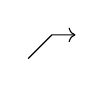
\begin{tikzpicture}[xscale=0.3, yscale=0.3, baseline=(O)]
		\coordinate (O) at (0, -0.8);
		\draw[->] (0,-1) -- (1, 0) -- (2, 0);
	\end{tikzpicture}$
	menentukan $f_h$. Konstruksi bagian perseginya menggunakan versi kondisi
	(S3) dalam Definisi~\ref{def:multiplicative-family} bagi sistem
	multiplikatif kanan, sedangkan komutativitas bagian bawah langsung.

	Keeksakan $\prod_k$ menunjukkan bahwa $u$ merupakan kuasi-isomorfisme.
	Akibatnya, $g$ juga ditentukan oleh bagian
	$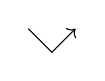
\begin{tikzpicture}[xscale=0.3, yscale=0.3, baseline=(O)]
		\coordinate (O) at (0, -0.8);
		\draw[->] (0,0) -- (1, -1) -- (2, 0);
	\end{tikzpicture}$
	dari diagram. Namun, $Y\xrightarrow{c_k}M_k\xleftarrow{t_k}X_k$
	menentukan $f_k$. Dibandingkan dengan konstruksi $f$ di atas, diperoleh
	$f=g$. Terbukti.
\end{bukti}

% segment-id: o014.li2.chapter4.rlim-homotopy-limit.r001
\begin{catatan}
	Jika himpunan indeks produk (atau koproduk) diganti dengan sembarang himpunan
	kecil $I$, pernyataan yang bersesuaian tetap berlaku.
\end{catatan}

% segment-id: o014.li2.chapter4.rlim-homotopy-limit.p002
Misalkan $\mathcal{D}$ suatu kategori-$\cate{Ab}$. Tinjau kategori
$\cate{InvSys}(\mathcal{D}):=\mathcal{D}^{\Z_{\geq0}^{\opp}}$ dari
\eqref{eqn:InvSys}. Objeknya adalah data $X=(X_k,f_k)_{k\geq0}$, dengan
$X_k\in\Obj(\mathcal{D})$ dan
$f_k\in\Hom_{\mathcal{D}}(X_{k+1},X_k)$. Jika $\mathcal{D}$ mempunyai produk
terhitung, definisikan morfisme kanonik seperti dalam
Definisi~\ref{def:Delta-diff}:
	\[ \Delta_X := T_X - \identity: \prod_k X_k \to \prod_k X_k. \]
\index[sym1]{InvSys}
\index[sym1]{DirSys@$\cate{DirSys}$}

% segment-id: o014.li2.chapter4.rlim-homotopy-limit.p003
Secara dual, objek kategori
$\cate{DirSys}(\mathcal{D}):=\mathcal{D}^{\Z_{\geq0}}$ adalah data
$X=(X_k,g_k)_{k\geq0}$\footnote{Data ini juga disebut sistem langsung dalam
$\mathcal{D}$.}, dengan $X_k\in\Obj(\mathcal{D})$ dan
$g_k\in\Hom_{\mathcal{D}}(X_k,X_{k+1})$. Dengan cara yang sama, definisikan
$\nabla_X:=T_X-\identity:\bigoplus_kX_k\to\bigoplus_kX_k$, dengan asumsi
$\mathcal{D}$ mempunyai koproduk terhitung; $T_X$ tetap merupakan morfisme
pergeseran yang serupa.

% segment-id: o014.li2.chapter4.rlim-homotopy-limit.p004
Jika $\Ker(\Delta_X)$ atau $\Coker(\nabla_X)$ ada, terdapat isomorfisme
kanonik
\begin{align*}
	X \in \Obj\left( \cate{InvSys}(\mathcal{D}) \right) & \implies \varprojlim_k X_k \simeq \Ker(\Delta_X), \\
	X \in \Obj\left( \cate{DirSys}(\mathcal{D}) \right) & \implies \varinjlim_k X_k \simeq \Coker(\nabla_X).
\end{align*}
Harapan naifnya ialah menerapkan ini pada $\mathcal{D}=\cate{D}(\mathcal{A})$.
Kategori turunan jarang merupakan kategori abelian. Meskipun demikian,
Catatan~\ref{rem:homotopy-kernel-cokernel} menunjukkan bahwa kerucut pemetaan
dapat berperan sebagai versi homotopis dari kernel dan kokernel; konstruksi yang
secara kasar bersesuaian dalam kategori bertriangulasi adalah segitiga
terbedakan.

% segment-id: o014.li2.chapter4.rlim-homotopy-limit.d001
\begin{definisi}[M.\ Bökstedt, A.\ Neeman {\cite{BN93}}]\label{def:holim}
	\index{limit homotopi, kolimit homotopi}
	\index[sym1]{holim@$\holim$, $\hocolim$}
	Misalkan $\mathcal{D}$ kategori bertriangulasi.
	\begin{itemize}
		\item Jika $\mathcal{D}$ mempunyai produk terhitung, suatu \emph{limit
		homotopi} (atau $\varprojlim$ homotopi) dari objek
		$X\in\Obj(\cate{InvSys}(\mathcal{D}))$ berarti segitiga terbedakan
		\[ \holim(X) \to \prod_k X_k \xrightarrow{\Delta_X} \prod_k X_k \xrightarrow{+1} . \]
		\item Jika $\mathcal{D}$ mempunyai koproduk terhitung, suatu
		\emph{kolimit homotopi} (atau $\varinjlim$ homotopi) dari objek
		$X\in\Obj(\cate{DirSys}(\mathcal{D}))$ berarti segitiga terbedakan
		\[ \bigoplus_k X_k \xrightarrow{\nabla_X} \bigoplus_k X_k \to \hocolim(X) \xrightarrow{+1} . \]
	\end{itemize}
\end{definisi}

% segment-id: o014.li2.chapter4.rlim-homotopy-limit.p005
Segitiga-segitiga terbedakan yang terlibat dalam definisi ini saling isomorfik
(Korolari~\ref{prop:Cone-uniqueness}), tetapi isomorfismenya tidak kanonik.

% segment-id: o014.li2.chapter4.rlim-homotopy-limit.p006
Kembali ke kompleks. Perhatikan bahwa
$\cate{InvSys}(\cate{C}(\mathcal{A}))=
\cate{C}(\cate{InvSys}(\mathcal{A}))$; objek kedua kategori tersebut sama-sama
merupakan diagram komutatif
% segment-id: o014.li2.chapter4.rlim-homotopy-limit.g003
\[\begin{tikzcd}
	& \vdots \arrow[d, "{f_1^n}"'] & \vdots \arrow[d, "{f_1^{n+1}}"] & \\
	\cdots \arrow[r] & X_1^n \arrow[r, "{d_{X_1}^n}"] \arrow[d, "{f_0^n}"'] & X_1^{n+1} \arrow[d, "{f_0^{n+1}}"] \arrow[r] & \cdots \\
	\cdots \arrow[r] & X_0^n \arrow[r, "{d_{X_0}^n}"] & X_0^{n+1} \arrow[r] & \cdots
\end{tikzcd} \quad \text{dengan setiap baris merupakan kompleks}. \]
Morfisme di kedua kategori juga merupakan diagram komutatif dua tingkat yang
sama. Karena itu, dalam $\mathcal{D}:=\cate{D}(\mathcal{A})$ kita dapat
membandingkan $\holim(X)$ dan funktor turunan kanan
$\mathrm{R}\lim(X)$ dari $\varprojlim$, jika keduanya ada.

% segment-id: o014.li2.chapter4.rlim-homotopy-limit.p007
Perhatikan pula bahwa kohomologi $\Hm^m$ dari objek
$X\in\cate{C}(\cate{InvSys}(\mathcal{A}))$ adalah
$(\Hm^m(X_k),\Hm^m(f_k))_{k\geq0}$. Jadi $X\to Y$ merupakan
kuasi-isomorfisme jika dan hanya jika setiap $X_k\to Y_k$ merupakan
kuasi-isomorfisme dalam $\cate{C}(\mathcal{A})$.

% segment-id: o014.li2.chapter4.rlim-homotopy-limit.t001
\begin{teorema}\label{prop:Rlim-as-holim}
	Misalkan $\mathcal{A}$ kategori abelian dengan produk terhitung yang eksak
	dan cukup banyak objek injektif.
	\begin{enumerate}[(i)]
		\item Funktor turunan kanan dari funktor eksak kiri
		$\varprojlim:\cate{InvSys}(\mathcal{A})\to\mathcal{A}$ ada dan dituliskan
		\[ \mathrm{R}\lim :  \cate{D}^+\left(\cate{InvSys}(\mathcal{A})\right) \to \cate{D}^+(\mathcal{A}) . \]
		\item Untuk setiap objek $X=(X_k,f_k)_{k\geq0}$ dari
		$\cate{C}^+(\cate{InvSys}(\mathcal{A}))$, terdapat segitiga terbedakan
		dalam $\cate{D}(\mathcal{A})$
		\[ \mathrm{R}\lim(X) \to \prod_k X_k \xrightarrow{\Delta_X} \prod_k X_k \xrightarrow{+1}. \]
		Secara khusus, $\mathrm{R}\lim(X)\simeq\holim(X)$.
		\item Dimensi $\mathrm{R}\lim$ dalam pengertian
		Definisi--Proposisi~\ref{def:dim-functor} paling besar $1$.
	\end{enumerate}
\end{teorema}
% segment-id: o014.li2.chapter4.rlim-homotopy-limit.pf002
\begin{bukti}
	Karena $\cate{InvSys}(\mathcal{A})$ mempunyai cukup banyak objek injektif,
	(i) berlaku. Lebih tepatnya, ambil kategori $\mathcal{R}$ dari
	Lema~\ref{prop:lim1-prep} dan terapkan
	Teorema~\ref{prop:resolution-existence} pada
	$\cate{InvSys}(\mathcal{A})$ dan $\mathcal{R}$. Untuk setiap
	$X=(X_k,f_k)_{k\geq0}$ dalam
	$\cate{C}^+(\cate{InvSys}(\mathcal{A}))$, terdapat kuasi-isomorfisme
	$X\to Y$ dengan $Y\in\Obj(\cate{C}^+(\mathcal{R}))$. Maka
	$\mathrm{R}\lim(X)=\varprojlim Y$. Definisi $\mathcal{R}$ menjamin bahwa
	$\Delta_Y$ surjektif derajat demi derajat, sehingga terdapat barisan eksak
	pendek dalam $\cate{C}^+(\mathcal{A})$
	\[ 0 \to \varprojlim Y \to \prod_{k \geq 0} Y_k \xrightarrow{\Delta_Y} \prod_{k \geq 0} Y_k \to 0. \]
	Selanjutnya, setiap $X_k\to Y_k$ merupakan kuasi-isomorfisme, sehingga
	$\prod_{k\geq0}X_k\to\prod_{k\geq0}Y_k$ juga merupakan kuasi-isomorfisme.
	Ini memberikan segitiga terbedakan pada (ii):
	\[ \mathrm{R}\lim(X) \to \prod_{k \geq 0} X_k \xrightarrow{\Delta_X} \prod_{k \geq 0} X_k \xrightarrow{+1} . \]

	Untuk (iii), jika $X\in\Obj(\cate{InvSys}(\mathcal{A}))$, maka $\Delta_X$
	merupakan morfisme dalam $\cate{InvSys}(\mathcal{A})$, dan
	$\holim(X)\simeq\Cone(\Delta_X)[-1]$ berada dalam
	$\Obj(\cate{D}^{[0,1]}(\mathcal{A}))$. Ini juga merupakan pernyataan ulang
	Teorema~\ref{prop:lim1}.
\end{bukti}

% segment-id: o014.li2.chapter4.rlim-homotopy-limit.p008
Terdapat versi dual Teorema~\ref{prop:Rlim-as-holim} untuk
$\varinjlim:\cate{DirSys}(\mathcal{A})\to\mathcal{A}$; perinciannya tidak
diulangi.

% segment-id: o014.li2.chapter4.rlim-homotopy-limit.p009
Contoh~\ref{eg:Rlim-unbounded} akan menunjukkan cara memperoleh
$\mathrm{R}\lim$ pada kategori turunan tak terbatas sedemikian sehingga
Teorema~\ref{prop:Rlim-as-holim} (ii) tetap berlaku.

% Unit 061 terjemahan Bahasa Indonesia dari chapter4.tex baris 2116--2267.
% Sumber: Methods of Algebra, Volume 2, commit
% 9a5803ff77dd3257484cb177f851a73770a59dd3 (CC BY 4.0).
% stable-unit-id: o014.aljabr2.chapter4.unbounded-derived-functors
% Cakupan: Bagian 4.11 lengkap; berhenti sebelum Bagian 4.12 pada baris 2268.

% segment-id: o014.li2.chapter4.unbounded-derived-functors.h001
\section{Funktor Turunan Tak Terbatas}\label{sec:unbounded-derived}
\hypertarget{o014.aljabr2.chapter4.unbounded-derived-functors}{ }
% segment-id: o014.li2.chapter4.unbounded-derived-functors.x001
\index{funktor turunan!tak terbatas (unbounded)}

% segment-id: o014.li2.chapter4.unbounded-derived-functors.p001
Tinjau funktor aditif $F:\mathcal{A}\to\mathcal{A}'$ antarkategori abelian.
Bagian ini kembali ke Definisi~\ref{def:derived-functor} dan berfokus pada
versi funktor turunan untuk kategori turunan tak terbatas,
% segment-id: o014.li2.chapter4.unbounded-derived-functors.q001
\[ \mathrm{R}F, \; \mathrm{L}F: \cate{D}(\mathcal{A}) \to \cate{D}(\mathcal{A}'). \]

% segment-id: o014.li2.chapter4.unbounded-derived-functors.p002
Untuk menjamin keberadaan $\mathrm{R}F$ atau $\mathrm{L}F$ dan melakukan
perhitungan dengannya, diperlukan konsep kompleks K-injektif atau kompleks
K-projektif dari Definisi~\ref{def:K-resolutions}, beserta resolusi
yang bersesuaian.

% segment-id: o014.li2.chapter4.unbounded-derived-functors.le001
\begin{lema}\label{prop:K-injective-zero}
	Misalkan $\mathcal{A}$ kategori abelian. Jika
	$Z\in\Obj(\cate{K}(\mathcal{A}))$ sekaligus merupakan kompleks K-injektif
	(atau K-projektif) dan asiklik, maka $Z=0$.
\end{lema}
% segment-id: o014.li2.chapter4.unbounded-derived-functors.pf001
\begin{bukti}
	Lema~\ref{prop:K-injective-criterion} menyiratkan
	$\Hom_{\cate{K}(\mathcal{A})}(Z,Z)=0$.
\end{bukti}

% segment-id: o014.li2.chapter4.unbounded-derived-functors.p003
Mula-mula kita nyatakan suatu hasil umum. Tetapkan kategori-kategori
bertriangulasi $\mathcal{D}_1$, $\mathcal{D}_2$, $\mathcal{D}'$ beserta
subkategori-subkategori bertriangulasi jenuhnya
$\mathcal{N}_1$, $\mathcal{N}_2$, $\mathcal{N}'$.

% segment-id: o014.li2.chapter4.unbounded-derived-functors.le002
\begin{lema}\label{prop:K-cats}
	Misalkan diberikan bifunktor bertriangulasi
	$G:\mathcal{D}_1\times\mathcal{D}_2\to\mathcal{D}'$, definisikan
	subkategori penuh $\mathcal{K}_2^G$ dari $\mathcal{D}_2$ melalui
% segment-id: o014.li2.chapter4.unbounded-derived-functors.q002
	\[ \Obj(\mathcal{K}_2^G) = \left\{ X_2 \in \Obj(\mathcal{D}_2) : X_1 \in \Obj(\mathcal{N}_1) \implies G(X_1, X_2) \in \Obj(\mathcal{N}') \right\}. \]
	Maka $\mathcal{K}_2^G$ merupakan subkategori bertriangulasi jenuh. Setelah
	menukar posisi kedua variabel, pernyataan yang bersesuaian tetap berlaku bagi
	$\mathcal{K}_1^G\subset\mathcal{D}_1$.
\end{lema}
% segment-id: o014.li2.chapter4.unbounded-derived-functors.pf002
\begin{bukti}
	Isomorfisme $G(X_1,X_2[1])\simeq G(X_1,X_2)[1]$ menunjukkan bahwa
	$\mathcal{K}_2^G$ tertutup terhadap pergeseran. Demikian pula, misalkan
	$I\to J\to K\xrightarrow{+1}$ segitiga terbedakan dengan
	$I,K\in\Obj(\mathcal{K}_2^G)$. Dari segitiga terbedakan
% segment-id: o014.li2.chapter4.unbounded-derived-functors.q003
	\[ G(X_1, I) \to G(X_1, J) \to G(X_1, K) \xrightarrow{+1} \]
	segera terlihat bahwa
	$X_1\in\Obj(\mathcal{N}_1)\implies
	G(X_1,J)\in\Obj(\mathcal{N}')$. Sifat jenuhnya sudah jelas.
\end{bukti}

% segment-id: o014.li2.chapter4.unbounded-derived-functors.p004
Hasil ini dapat diterapkan pada
$\Hom:\mathcal{A}^{\opp}\times\mathcal{A}\to\cate{Ab}$ dan bifunktor
bertriangulasi yang bersesuaian, yaitu $\cate{K}_{\Pi}\Hom$.
Contoh~\ref{eg:Hom-bicplx} telah menunjukkan bahwa bifunktor yang terakhir ini
pada dasarnya merupakan kompleks $\Hom$:
% segment-id: o014.li2.chapter4.unbounded-derived-functors.e001
\begin{equation}\label{eqn:CPiHom}\begin{gathered}
	(\cate{C}_{\Pi} \Hom)(\sigma^{-1} X_1, X_2) \simeq \Hom^\bullet\left( X_1, X_2 \right), \\
	(\cate{K}_\Pi \Hom)(\sigma^{-1} X_1, X_2) \simeq \Hom^\bullet\left( X_1, X_2 \right)\; \text{sebagai citra dalam $\cate{K}(\cate{Ab})$},
\end{gathered}\end{equation}
% segment-id: o014.li2.chapter4.unbounded-derived-functors.p005
Di sini
$\sigma:\cate{C}(\mathcal{A}^{\opp})\rightiso
\cate{C}(\mathcal{A})^{\opp}$ dan
$\cate{K}(\mathcal{A}^{\opp})\rightiso\cate{K}(\mathcal{A})^{\opp}$
adalah isomorfisme dari Definisi--Proposisi~\ref{def:sigma} dan
Proposisi~\ref{prop:sigma-homotopy}. Versinya untuk kategori turunan akan
diperlukan kemudian.

% segment-id: o014.li2.chapter4.unbounded-derived-functors.pr001
\begin{proposisi}\label{prop:K-injective-F-injective}
	Semua kompleks K-injektif (atau K-projektif) membentuk subkategori
	bertriangulasi jenuh $\mathcal{I}$ (atau $\mathcal{P}$) dari
	$\cate{K}(\mathcal{A})$. Jika $\mathcal{A}$ mempunyai cukup banyak kompleks
	K-injektif (atau K-projektif), maka untuk setiap funktor aditif
	$F:\mathcal{A}\to\mathcal{A}'$, subkategori $\mathcal{I}$ (atau
	$\mathcal{P}$) bersifat $F$-injektif (atau $F$-projektif).
\end{proposisi}
% segment-id: o014.li2.chapter4.unbounded-derived-functors.pf003
\begin{bukti}
	Cukup dibahas kasus K-injektif. Bagian pertama diperoleh dengan menerapkan
	Lema~\ref{prop:K-cats} pada $G=\cate{K}_{\Pi}\Hom$, sambil menggunakan
	Definisi~\ref{def:K-resolutions} tentang kompleks K-injektif dan
	\eqref{eqn:CPiHom}: subkategori $\mathcal{K}_2^G$ di sana tepat merupakan
	$\mathcal{I}$ di sini.

	Misalkan $\mathcal{A}$ mempunyai cukup banyak kompleks K-injektif. Jika $I$
	merupakan kompleks K-injektif yang asiklik, maka
	Lema~\ref{prop:K-injective-zero} menyiratkan $I=0$, sehingga
	$(\cate{K}F)I$ tentu saja asiklik. Dengan demikian, seluruh syarat dalam
	Definisi~\ref{def:F-injective} bagi subkategori bertriangulasi $F$-injektif
	terpenuhi.
\end{bukti}

% segment-id: o014.li2.chapter4.unbounded-derived-functors.p006
Tuliskan $Q:\cate{K}(\mathcal{A})\to\cate{D}(\mathcal{A})$ dan
$Q':\cate{K}(\mathcal{A}')\to\cate{D}(\mathcal{A}')$ untuk funktor-funktor
lokalisasi.

% segment-id: o014.li2.chapter4.unbounded-derived-functors.co001
\begin{korolari}
	Jika $\mathcal{A}$ mempunyai cukup banyak kompleks K-injektif, maka $F$
	mempunyai funktor turunan kanan
	$\mathrm{R}F:\cate{D}(\mathcal{A})\to\cate{D}(\mathcal{A}')$, sedemikian
	sehingga $\mathrm{R}F(QX)\simeq Q'\cate{K}F(X)$ apabila $X$ kompleks
	K-injektif.

	Secara dual, jika $\mathcal{A}$ mempunyai cukup banyak kompleks K-projektif,
	maka $F$ mempunyai funktor turunan kiri
	$\mathrm{L}F:\cate{D}(\mathcal{A})\to\cate{D}(\mathcal{A}')$, sedemikian
	sehingga $\mathrm{L}F(QX)\simeq Q'\cate{K}F(X)$ apabila $X$ kompleks
	K-projektif.
\end{korolari}
% segment-id: o014.li2.chapter4.unbounded-derived-functors.pf004
\begin{bukti}
	Terapkan hasil Proposisi~\ref{prop:K-injective-F-injective} pada kerangka umum
	Proposisi~\ref{prop:localization-injective}.
\end{bukti}

% segment-id: o014.li2.chapter4.unbounded-derived-functors.p007
Sekarang tetapkan kategori-kategori abelian $\mathcal{A}_1$, $\mathcal{A}_2$,
dan $\mathcal{B}$. Untuk bifunktor aditif
$F:\mathcal{A}_1\times\mathcal{A}_2\to\mathcal{B}$, tinjau versi tak
terbatas dari bifunktor turunan $\mathrm{R}F$ (atau $\mathrm{L}F$) dalam
Definisi~\ref{def:derived-bifunctor}. Selanjutnya selalu diasumsikan bahwa
$\mathcal{B}$ mempunyai produk terhitung (atau koproduk terhitung).

% segment-id: o014.li2.chapter4.unbounded-derived-functors.p008
Secara konkret, kita hendak menentukan $\mathrm{R}F$ (atau $\mathrm{L}F$)
menggunakan subkategori $\mathcal{I}_1$, $\mathcal{I}_2$ (atau
$\mathcal{P}_1$, $\mathcal{P}_2$) di atas.

% segment-id: o014.li2.chapter4.unbounded-derived-functors.le003
\begin{lema}\label{prop:bifunctor-via-K-injective-prep}
	Untuk $i=1,2$, ambil subkategori bertriangulasi $\mathcal{I}_i$ (atau
	$\mathcal{P}_i$) dari $\cate{K}(\mathcal{A}_i)$ seperti dalam
	Proposisi~\ref{prop:K-injective-F-injective}.
% segment-id: o014.li2.chapter4.unbounded-derived-functors.l001
	\begin{compactitem}
% segment-id: o014.li2.chapter4.unbounded-derived-functors.i001
		\item Jika $\mathcal{A}_1$ dan $\mathcal{A}_2$ mempunyai cukup banyak
		kompleks K-injektif, maka $\mathcal{I}_1\times\mathcal{I}_2$ bersifat
		$F$-injektif.
% segment-id: o014.li2.chapter4.unbounded-derived-functors.i002
		\item Jika $\mathcal{A}_1$ dan $\mathcal{A}_2$ mempunyai cukup banyak
		kompleks K-projektif, maka $\mathcal{P}_1\times\mathcal{P}_2$ bersifat
		$F$-projektif.
	\end{compactitem}
\end{lema}
% segment-id: o014.li2.chapter4.unbounded-derived-functors.pf005
\begin{bukti}
	Cukup dibahas kasus K-injektif. Kuncinya ialah menunjukkan bahwa jika
	$X_1\in\Obj(\mathcal{I}_1)$, maka
	$(\cate{K}_{\Pi}F)(X_1,\cdot)$ memetakan setiap objek asiklik $Z$ dari
	$\mathcal{I}_2$ ke objek asiklik dalam $\cate{K}(\mathcal{B})$. Namun,
	Lema~\ref{prop:K-injective-zero} memberikan $Z=0$, sedangkan
	$(\cate{K}_{\Pi}F)(X_1,\cdot)$ merupakan funktor aditif, sehingga pernyataan
	ini langsung berlaku. Hasil yang bersesuaian diperoleh setelah menukar indeks
	$1$ dan $2$.
\end{bukti}

% segment-id: o014.li2.chapter4.unbounded-derived-functors.p009
Tuliskan $Q:\cate{K}(\mathcal{B})\to\cate{D}(\mathcal{B})$ dan
$Q_i:\cate{K}(\mathcal{A}_i)\to\cate{D}(\mathcal{A}_i)$ untuk
funktor-funktor lokalisasi ($i=1,2$).

% segment-id: o014.li2.chapter4.unbounded-derived-functors.pr002
\begin{proposisi}\label{prop:bifunctor-via-K-injective}
	Untuk $F:\mathcal{A}_1\times\mathcal{A}_2\to\mathcal{B}$, misalkan
	$\mathcal{A}_1$ dan $\mathcal{A}_2$ sama-sama mempunyai cukup banyak
	kompleks K-injektif (atau K-projektif). Maka bifunktor turunan
	$\mathrm{R}F$ (atau $\mathrm{L}F$) ada. Jika
	$X_i\in\Obj(\cate{K}(\mathcal{A}))$ merupakan kompleks K-injektif (atau
	K-projektif) untuk $i=1,2$, maka terdapat isomorfisme kanonik
% segment-id: o014.li2.chapter4.unbounded-derived-functors.q004
	\[ \mathrm{R}F(Q_1 X_1, Q_2 X_2) \simeq Q (\cate{K}_{\Pi} F)(X_1, X_2) \quad \text{(atau $\mathrm{L}F(Q_1 X_1, Q_2 X_2) \simeq Q (\cate{K}_{\oplus} F)(X_1, X_2)$) }. \]
\end{proposisi}
% segment-id: o014.li2.chapter4.unbounded-derived-functors.pf006
\begin{bukti}
	Terapkan langsung hasil Lema~\ref{prop:bifunctor-via-K-injective-prep} pada
	Proposisi~\ref{prop:localization-injective-bifunctor}.
\end{bukti}

% segment-id: o014.li2.chapter4.unbounded-derived-functors.p010
Untuk bifunktor tertentu $F$, sering kali dapat dipilih subkategori
$F$-injektif (atau $F$-projektif) yang lebih besar daripada subkategori
kompleks K-injektif (atau K-projektif). Funktor $\RHom$ yang akan dibahas
berikut merupakan salah satu contohnya.

% segment-id: o014.li2.chapter4.unbounded-derived-functors.th001
\begin{teorema}[$\RHom$ tak terbatas]\label{prop:unbounded-RHom}
% segment-id: o014.li2.chapter4.unbounded-derived-functors.x002
	\index{funktor $\RHom$}
% segment-id: o014.li2.chapter4.unbounded-derived-functors.x003
	\index[sym1]{RHom@$\RHom$}
	Misalkan kategori abelian $\mathcal{A}$ mempunyai cukup banyak kompleks
	K-injektif atau cukup banyak kompleks K-projektif. Untuk menyederhanakan
	notasi, tuliskan semua funktor lokalisasi sebagai $Q$.
% segment-id: o014.li2.chapter4.unbounded-derived-functors.l002
	\begin{enumerate}[(i)]
% segment-id: o014.li2.chapter4.unbounded-derived-functors.i003
		\item Bifunktor
		$\Hom=\Hom_{\mathcal{A}}:\mathcal{A}^{\opp}\times\mathcal{A}
		\to\cate{Ab}$ mempunyai bifunktor turunan kanan
		$\cate{D}(\mathcal{A}^{\opp})\times\cate{D}(\mathcal{A})
		\to\cate{D}(\cate{Ab})$. Melalui ekuivalensi $\sigma$ dari
		Proposisi~\ref{prop:derived-cat-op}, bifunktor itu juga dapat ditulis sebagai
% segment-id: o014.li2.chapter4.unbounded-derived-functors.q005
		\[ \RHom: \cate{D}(\mathcal{A})^{\opp} \times \cate{D}(\mathcal{A}) \to \cate{D}(\cate{Ab}). \]
		Bahkan, jika $\mathcal{A}$ mempunyai cukup banyak kompleks K-injektif
		(atau K-projektif), maka
		$\cate{K}(\mathcal{A})^{\opp}\times\mathcal{I}$ (atau
		$\mathcal{P}^{\opp}\times\cate{K}(\mathcal{A})$) bersifat
		$\Hom$-injektif.
% segment-id: o014.li2.chapter4.unbounded-derived-functors.i004
		\item Misalkan $\mathcal{A}$ mempunyai cukup banyak kompleks K-injektif
		dan $X_2\to I_2$ merupakan resolusi K-injektif. Resolusi ini menginduksi
% segment-id: o014.li2.chapter4.unbounded-derived-functors.q006
		\[ \RHom(Q X_1, Q X_2) \rightiso Q \Hom^\bullet(X_1, I_2). \]
		Sebagai kasus khusus,
		$\RHom(QX_1,\cdot)\simeq
		\mathrm{R}\left(\Hom(X_1,\cdot)\right)$.
% segment-id: o014.li2.chapter4.unbounded-derived-functors.i005
		\item Misalkan $\mathcal{A}$ mempunyai cukup banyak kompleks K-projektif
		dan $P_1\to X_1$ merupakan resolusi K-projektif. Resolusi ini menginduksi
% segment-id: o014.li2.chapter4.unbounded-derived-functors.q007
		\[ \RHom(Q X_1, Q X_2) \rightiso Q \Hom^\bullet(P_1, X_2). \]
		Sebagai kasus khusus,
		$\RHom(\cdot,QX_2)\simeq
		\mathrm{R}\left(\Hom(\cdot,X_2)\right)$.
% segment-id: o014.li2.chapter4.unbounded-derived-functors.i006
		\item Terdapat isomorfisme kanonik
		$\Hm^n\RHom(X,Y)\simeq
		\Hom_{\cate{D}(\mathcal{A})}(X,Y[n])=: \Ext^n(X,Y)$
		(Definisi~\ref{def:Ext-general}).
	\end{enumerate}
\end{teorema}
% segment-id: o014.li2.chapter4.unbounded-derived-functors.pf007
\begin{bukti}
	Argumennya hampir sama dengan Teorema~\ref{prop:RHom-bounded}. Sebagai
	contoh, anggap $\mathcal{A}$ mempunyai cukup banyak kompleks K-injektif.
	Kuncinya ialah menunjukkan bahwa
	$\cate{K}(\mathcal{A})^{\opp}\times\mathcal{I}$ bersifat
	$\Hom$-injektif.
% segment-id: o014.li2.chapter4.unbounded-derived-functors.l003
	\begin{itemize}
% segment-id: o014.li2.chapter4.unbounded-derived-functors.i007
		\item Tetapkan kompleks $X_1$. Funktor
		$(\cate{K}_\Pi\Hom)(X_1,\cdot)$ memetakan setiap kompleks K-injektif
		asiklik $X_2$ ke kompleks asiklik, sebab $X_2$ adalah $0$ dalam
		$\cate{K}(\mathcal{A})$ (Lema~\ref{prop:K-injective-zero}).
% segment-id: o014.li2.chapter4.unbounded-derived-functors.i008
		\item Tetapkan kompleks K-injektif $X_2$. Jika kompleks $X_1$ asiklik,
		definisi kompleks K-injektif menyiratkan bahwa
		$\Hom^\bullet\left(X_1,X_2\right)$ asiklik. Dengan menggunakan
		\eqref{eqn:CPiHom}, terlihat bahwa
		$(\cate{K}_\Pi\Hom)(X_1,X_2)$ juga asiklik.
	\end{itemize}
	Dengan demikian, syarat asiklik yang diperlukan untuk sifat
	$\Hom$-injektif telah diverifikasi, sedangkan syarat resolusinya langsung
	terpenuhi.
\end{bukti}

% segment-id: o014.li2.chapter4.unbounded-derived-functors.th002
\begin{teorema}\label{prop:RHom-adjoint}
	Tinjau pasangan funktor aditif adjoin antarkategori abelian
% segment-id: o014.li2.chapter4.unbounded-derived-functors.g001
	$\begin{tikzcd}
		F: \mathcal{A} \arrow[r, shift left] & \mathcal{A}' \arrow[l, shift left] : G
	\end{tikzcd}$.
	Misalkan $\mathcal{A}$ mempunyai cukup banyak kompleks K-projektif dan
	$\mathcal{A}'$ mempunyai cukup banyak kompleks K-injektif. Maka terdapat
	isomorfisme kanonik dalam $\cate{D}(\cate{Ab})$
% segment-id: o014.li2.chapter4.unbounded-derived-functors.q008
	\[ \RHom_{\mathcal{A'}}\left(\mathrm{L}F(X), Y\right) \simeq \RHom_{\mathcal{A}}\left(X, \mathrm{R}G(Y) \right), \]
	dengan $X\in\Obj\left(\cate{D}(\mathcal{A})\right)$ dan
	$Y\in\Obj\left(\cate{D}(\mathcal{A}')\right)$.
\end{teorema}
% segment-id: o014.li2.chapter4.unbounded-derived-functors.pf008
\begin{bukti}
	Argumennya sama dengan Teorema~\ref{prop:RHom-adjoint-bounded}. Satu-satunya
	perbedaan ialah bahwa resolusi injektif (atau projektif) diganti dengan
	resolusi K-injektif (atau K-projektif), dan
	Teorema~\ref{prop:K-resolution-homotopy} menggantikan
	Teorema~\ref{prop:resolution-homotopy} dalam pembahasan keunikan resolusi.
\end{bukti}

% segment-id: o014.li2.chapter4.unbounded-derived-functors.r001
\begin{catatan}
	Dengan menerapkan $\Hm^0$ pada kedua ruas dalam
	Teorema~\ref{prop:RHom-adjoint}, diperoleh adjungsi
% segment-id: o014.li2.chapter4.unbounded-derived-functors.q009
	\[ \Hom_{\cate{D}(\mathcal{A'})}\left(\mathrm{L}F(X), Y\right) \simeq \Hom_{\cate{D}(\mathcal{A})}\left(X, \mathrm{R}G(Y) \right). \]

	Karena funktor turunan yang diperoleh melalui resolusi selalu merupakan
	ekstensi Kan absolut dalam pengertian Definisi~\ref{def:absolute-Kan}
	(Proposisi~\ref{prop:localization-functor-abs}),
	Teorema~\ref{prop:Quillen-adjunction-gen} juga menyatakan bahwa
	$(\mathrm{L}F,\mathrm{R}G)$ merupakan pasangan adjoin. Keduanya memberikan
	isomorfisme adjungsi yang sama. Mengapa? Cukup ditinjau kasus ketika
	$X$ merupakan kompleks K-projektif dan $Y$ kompleks K-injektif. Dalam kasus
	ini, isomorfisme adjungsi dalam Teorema~\ref{prop:RHom-adjoint} diwujudkan
	secara konkret melalui unit $\eta$ dan kounit $\varepsilon$ pada tingkat
	$\cate{K}(\cdot)$ sebagai
% segment-id: o014.li2.chapter4.unbounded-derived-functors.q010
	\begin{align*}
		\Hom_{\cate{K}(\mathcal{A}')}\left( \cate{K}F(X), Y\right) \simeq \Hom_{\cate{K}(\mathcal{A})}\left( X, \cate{K}G(Y) \right).
	\end{align*}
	Di sisi lain, Teorema~\ref{prop:Quillen-adjunction-gen} menentukan
	$\underline{\eta}$ dan $\underline{\varepsilon}$ pada tingkat kategori
	turunan. Karakterisasi yang diberikan di sana cukup untuk menunjukkan bahwa
	keduanya kompatibel dengan $\eta$ dan $\varepsilon$. Perinciannya diserahkan
	kepada pembaca yang berminat.
\end{catatan}

% segment-id: o014.li2.chapter4.unbounded-derived-functors.p011
Sebagai penutup, sekumpulan syarat cukup lainnya untuk memperoleh funktor turunan
tak terbatas didasarkan pada keberhinggaan dimensi
(Definisi--Proposisi~\ref{def:dim-functor}). Meskipun teknik pembuktiannya tidak
melampaui cakupan buku ini, hasilnya akan dinyatakan tanpa bukti agar pembahasan
tidak menyimpang; lihat {\cite[Tags 07K6, 07K7]{stacks}}. Titik pangkalnya
adalah konstruksi funktor turunan terbatas dari
Teorema~\ref{prop:derived-via-resolution}.

% segment-id: o014.li2.chapter4.unbounded-derived-functors.pr003
\begin{proposisi}\label{prop:unbounded-derived-fd}
% segment-id: o014.li2.chapter4.unbounded-derived-functors.x004
	\index{dimensi}
	Misalkan $F:\mathcal{A}\to\mathcal{A}'$ funktor eksak kiri (atau eksak
	kanan) antarkategori abelian. Andaikan bahwa
% segment-id: o014.li2.chapter4.unbounded-derived-functors.l004
	\begin{compactitem}
% segment-id: o014.li2.chapter4.unbounded-derived-functors.i009
		\item relatif terhadap $F$, terdapat subkategori penuh aditif
		$\mathcal{A}^\flat$ dari $\mathcal{A}$ yang bertipe I (atau tipe P),
		seperti dalam Definisi--Proposisi~\ref{prop:F-injective-criterion};
% segment-id: o014.li2.chapter4.unbounded-derived-functors.i010
		\item funktor turunan terbatas yang bersesuaian,
		${}^+\mathrm{R}F$ (atau ${}^-\mathrm{L}F$), berdimensi hingga.
	\end{compactitem}
	Maka $\mathrm{R}F$ (atau $\cate{L}F$):
	$\cate{D}(\mathcal{A})\to\cate{D}(\mathcal{A}')$ ada. Bahkan,
	$\cate{K}(\mathcal{A}^\flat)$ membentuk subkategori $F$-injektif (atau
	$F$-projektif) dari $\cate{K}(\mathcal{A})$.
\end{proposisi}

% segment-id: o014.li2.chapter4.unbounded-derived-functors.ex001
\begin{contoh}\label{eg:Rlim-unbounded}
	Misalkan $\mathcal{A}$ mempunyai produk terhitung eksak dan cukup banyak
	objek injektif. Ambil funktor eksak kiri $F$ sebagai
	$\varprojlim:\cate{InvSys}(\mathcal{A})\to\mathcal{A}$.
	Teorema~\ref{prop:Rlim-as-holim} (iii) menunjukkan bahwa versi terbatas
	$\mathrm{R}\lim$ berdimensi paling besar $1$, sedangkan subkategori
	$\mathcal{R}\subset\cate{InvSys}(\mathcal{A})$ bertipe I relatif
	terhadapnya. Karena itu, hasil di atas memberikan funktor turunan tak terbatas
% segment-id: o014.li2.chapter4.unbounded-derived-functors.q011
	\[ \mathrm{R}\lim: \cate{D}(\cate{InvSys}(\mathcal{A})) \to \cate{D}(\mathcal{A}). \]

	Seperti dalam Teorema~\ref{prop:Rlim-as-holim} (ii), untuk setiap objek $X$
	dari $\cate{C}(\cate{InvSys}(\mathcal{A}))$ terdapat segitiga terbedakan
	dalam $\cate{D}(\mathcal{A})$
% segment-id: o014.li2.chapter4.unbounded-derived-functors.q012
	\[ \mathrm{R}\lim(X) \to \prod_k X_k \xrightarrow{\Delta_X} \prod_k X_k \xrightarrow{+1} . \]
	Secara khusus, $\mathrm{R}\lim(X)\simeq\holim(X)$. Berdasarkan
	Proposisi~\ref{prop:unbounded-derived-fd}, pembuktian semula berlaku tanpa
	perubahan lain: cukup ganti setiap $\cate{C}^+(\cdots)$ dengan
	$\cate{C}(\cdots)$.
\end{contoh}

% Unit 062 terjemahan Bahasa Indonesia dari chapter4.tex baris 2268--2499.
% Sumber: Methods of Algebra, Volume 2, commit
% 9a5803ff77dd3257484cb177f851a73770a59dd3 (CC BY 4.0).
% stable-unit-id: o014.aljabr2.chapter4.k-flat-derived-tensor-a
% Cakupan: Bagian 4.12, paruh pertama tentang kompleks K-datar, resolusi
% K-datar, dan konstruksi hasil kali tensor turunan; berhenti setelah paragraf
% pada baris 2498, tepat sebelum Korolari pada baris 2500.

% segment-id: o014.li2.chapter4.k-flat-derived-tensor-a.h001
\section{Contoh: Kompleks K-Datar dan \texorpdfstring{$\otimesL$}{otimesL}}\label{sec:otimesL}
\hypertarget{o014.aljabr2.chapter4.k-flat-derived-tensor-a}{ }

% segment-id: o014.li2.chapter4.k-flat-derived-tensor-a.p001
Dalam bagian ini, $\Bbbk$ selalu merupakan gelanggang komutatif.

% segment-id: o014.li2.chapter4.k-flat-derived-tensor-a.cv001
\begin{konvensi}\label{con:bimodule-algebra}
	Misalkan $R$ dan $S$ merupakan aljabar-$\Bbbk$. Menurut konvensi buku ini,
	setiap bimodul $(R,S)$ $M$ secara bawaan diasumsikan memenuhi $tm=mt$, dengan
	$t\in\Bbbk$ dan $m\in M$. Dengan kata lain,
	$(R,S)\dcate{Mod}\simeq(R\dotimes{\Bbbk}S^{\opp})\dcate{Mod}$. Jika
	$\Bbbk=\Z$, syarat ini redundan.

	Mulai sekarang, funktor pelupa
	$(R,S)\dcate{Mod}\to R\dcate{Mod}$ (atau
	$(R,S)\dcate{Mod}\to\cated{Mod}S$) ditulis sebagai
	$M\mapsto{}_RM$ (atau $M\mapsto M_S$); notasi yang sama berlaku untuk
	kompleks. Funktor-funktor pelupa ini eksak, dan funktor bertriangulasi yang
	diinduksinya di antara kategori turunan juga ditulis dengan cara yang sama.
\end{konvensi}

% segment-id: o014.li2.chapter4.k-flat-derived-tensor-a.p002
Perhatikan bahwa, untuk setiap kompleks $M$ yang terdiri atas
bimodul $(R,S)$, kita mempunyai
% segment-id: o014.li2.chapter4.k-flat-derived-tensor-a.q001
\[ M_S \;\text{asiklik} \iff M \;\text{asiklik} \iff {}_R M \;\text{asiklik}. \]

% segment-id: o014.li2.chapter4.k-flat-derived-tensor-a.p003
Mulai sekarang, misalkan $R$, $A$, dan $B$ merupakan aljabar-$\Bbbk$. Titik
tolak kita ialah bifunktor yang diberikan oleh hasil kali tensor,
% segment-id: o014.li2.chapter4.k-flat-derived-tensor-a.q002
\[ \otimes_R: (A, R)\dcate{Mod} \times (R, B)\dcate{Mod} \to (A, B)\dcate{Mod}, \]
yang eksak kanan dalam setiap variabel. Kasus paling sederhana ialah
$A=\Bbbk=B$; bifunktor yang bersesuaian menjadi
$\otimes_R:\cated{Mod}R\times R\dcate{Mod}\to\cate{\Bbbk}$.

% segment-id: o014.li2.chapter4.k-flat-derived-tensor-a.p004
Demi kemudahan, jika $X$ merupakan kompleks bimodul $(A,R)$ dan $Y$ merupakan
kompleks bimodul $(R,B)$, mulai sekarang bikompleks yang diperoleh dengan
mengambil hasil kali tensor suku demi suku ditulis
$X^\bullet\dotimes{R}Y^\bullet$, sedangkan kompleks totalnya ditulis
% segment-id: o014.li2.chapter4.k-flat-derived-tensor-a.q003
\[ X \dotimes{R} Y := \tot_{\oplus} \left( X^\bullet \dotimes{R} Y^\bullet \right). \]

% segment-id: o014.li2.chapter4.k-flat-derived-tensor-a.p005
Kategori bimodul mempunyai cukup banyak kompleks K-projektif (terapkan
Contoh~\ref{eg:Mod-K-injectives}); karena itu,
Proposisi~\ref{prop:bifunctor-via-K-injective} menjamin keberadaan bifunktor
turunan kiri tak terbatas.

% segment-id: o014.li2.chapter4.k-flat-derived-tensor-a.d001
\begin{definisi}\label{def:otimesL}
	\index{hasil kali tensor turunan (derived tensor product)}
	\index[sym1]{XotimesLY@$X \otimesL[R] Y$}
	Tuliskan bifunktor turunan kiri
	$\mathrm{L}\left(\cdot\dotimes{R}\cdot\right)$ dari $\otimes_R$ sebagai
% segment-id: o014.li2.chapter4.k-flat-derived-tensor-a.q004
	\[ \otimesL[R] : \cate{D}((A, R)\dcate{Mod}) \times \cate{D}((R, B)\dcate{Mod}) \to \cate{D}((A, B)\dcate{Mod}). \]
	Jika tidak menimbulkan kekeliruan, $X\otimesL[R]Y$ juga disingkat menjadi
	$X\otimesL Y$.
\end{definisi}

% segment-id: o014.li2.chapter4.k-flat-derived-tensor-a.p006
Definisi abstrak di atas memang lugas, tetapi untuk mengembangkan kajian
tentang $\otimes_R$ kita masih perlu memperkenalkan suatu kelas
kuasi-isomorfisme yang disebut resolusi K-datar. Alasannya antara lain:
% segment-id: o014.li2.chapter4.k-flat-derived-tensor-a.l001
\begin{itemize}
% segment-id: o014.li2.chapter4.k-flat-derived-tensor-a.i001
	\item definisi resolusi K-datar berkaitan langsung dengan hasil kali tensor
	dan lebih berguna untuk menetapkan beberapa sifat penting serta melakukan
	perhitungan konkret, sebagaimana telah terlihat dalam \S\ref{sec:Ext-Tor};
% segment-id: o014.li2.chapter4.k-flat-derived-tensor-a.i002
	\item dalam konteks geometris seperti teori berkas, mungkin hanya tersedia
	resolusi K-injektif dan tidak tersedia resolusi K-projektif; dalam keadaan
	ini, resolusi K-datar merupakan satu-satunya sarana untuk mengkaji hasil kali
	tensor turunan.
\end{itemize}

% segment-id: o014.li2.chapter4.k-flat-derived-tensor-a.d002
\begin{definisi}[N.\ Spaltenstein {\cite[Definisi 5.1]{Spa88}}]
	\index{kompleks!K-datar (K-flat)}
	Misalkan $X$ merupakan kompleks modul kanan $R$. Jika untuk setiap kompleks
	$Y$ yang terdiri atas modul kiri $R$ berlaku
% segment-id: o014.li2.chapter4.k-flat-derived-tensor-a.q005
	\[ Y \;\text{asiklik} \implies X \dotimes{R} Y\;\text{asiklik}, \]
	maka $X$ disebut \emph{K-datar}\footnote{Nama yang lebih masuk akal mungkin
	adalah kompleks datar homotopi.}; sifat ini hanya bergantung pada kelas
	isomorfisme $X$ dalam $\cate{K}(\cated{Mod}R)$. Dengan cara serupa, sifat
	K-datar didefinisikan untuk kompleks yang terdiri atas modul kiri $R$.
\end{definisi}

% segment-id: o014.li2.chapter4.k-flat-derived-tensor-a.p007
Untuk kompleks terbatas atas, sifat K-datar dapat diturunkan dari sifat datar
yang dikenal dalam teori modul.

% segment-id: o014.li2.chapter4.k-flat-derived-tensor-a.pr001
\begin{proposisi}\label{prop:flat-K-flat}
	Misalkan $X$ merupakan objek $\cate{C}^-(\cated{Mod}R)$ dan setiap $X^n$
	merupakan modul datar. Maka $X$ K-datar. Pernyataan yang sama berlaku bagi
	objek $\cate{C}^-(R\dcate{Mod})$.
\end{proposisi}

% segment-id: o014.li2.chapter4.k-flat-derived-tensor-a.pf001
\begin{bukti}
	Misalkan $Y$ merupakan kompleks asiklik yang terdiri atas modul kiri $R$;
	kita akan membuktikan bahwa $X\dotimes{R}Y$ asiklik. Dengan menerapkan funktor
	pemenggalan, tuliskan $Y$ sebagai $\varinjlim_m\tau^{\leq m}Y$. Secara suku
	demi suku, $\varinjlim_m$ berkomutasi baik dengan hasil kali tensor
	\cite[Proposisi 6.9.2]{Li1} maupun dengan $\bigoplus$; karena itu, cukup
	ditinjau kasus ketika $Y$ terbatas atas. Dengan demikian,
	$X^\bullet\dotimes{R}Y^\bullet$ berada dalam kategori
	$\cate{C}^2_f(\Bbbk\dcate{Mod})$ pada Definisi~\ref{def:Cf-Supp}. Karena
	$X^p\dotimes{R}Y^\bullet$ asiklik untuk setiap $p$,
	Korolari~\ref{prop:acyclic-assembly} menjamin bahwa $X\dotimes{R}Y$ asiklik.
\end{bukti}

% segment-id: o014.li2.chapter4.k-flat-derived-tensor-a.p008
Mengingat hal ini, jika pembaca hanya berkepentingan dengan kategori turunan
terbatas atas, semua kompleks K-datar yang muncul dalam bagian ini dapat
diganti dengan kompleks terbatas atas yang terdiri atas modul-modul datar.

% segment-id: o014.li2.chapter4.k-flat-derived-tensor-a.d003
\begin{definisi}
	\index{resolusi!K-datar (K-flat)}
	\index{cukup banyak kompleks K-datar (enough K-flats)}
	Jika $P\to X$ merupakan kuasi-isomorfisme dalam
	$\cate{C}((A,R)\dcate{Mod})$ dan $P_R$ K-datar, maka morfisme tersebut
	disebut \emph{resolusi K-datar} dari $X$ terhadap $R$. Jika setiap
	$X\in\cate{C}((A,R)\dcate{Mod})$ mempunyai resolusi K-datar terhadap $R$,
	maka dikatakan bahwa $(A,R)\dcate{Mod}$ mempunyai cukup banyak kompleks
	K-datar terhadap $R$.

	Dengan cara serupa didefinisikan resolusi K-datar terhadap $R$ bagi
	$X\in\Obj(\cate{C}((R,B)\dcate{Mod}))$.
\end{definisi}

% segment-id: o014.li2.chapter4.k-flat-derived-tensor-a.p009
Pertanyaan yang wajar ialah: bagaimana menjamin bahwa suatu kategori bimodul
mempunyai cukup banyak kompleks K-datar terhadap $R$? Apa hubungan antara
kompleks K-datar dan kompleks K-projektif? Sesuai dugaan, jembatannya
berasal dari adjungsi klasik antara $\otimes$ dan $\Hom$
\cite[Teorema 6.6.5]{Li1}.

% segment-id: o014.li2.chapter4.k-flat-derived-tensor-a.p010
Untuk itu, langkah pertama ialah mengangkat adjungsi tersebut ke tingkat
kompleks. Jika $Y$ merupakan objek $\cate{C}((R,B)\dcate{Mod})$ dan $Z$
merupakan objek $\cate{C}((A,B)\dcate{Mod})$, kompleks $\Hom$
$\Hom^\bullet(Y_B,Z_B)$ dapat diberi struktur bimodul $(A,R)$ secara suku demi
suku, sehingga menjadi objek $\cate{C}((A,R)\dcate{Mod})$.

% segment-id: o014.li2.chapter4.k-flat-derived-tensor-a.pr002
\begin{proposisi}[Adjungsi $\Hom$ dan $\otimes$: versi kompleks]\label{prop:tensor-Hom-cplx}
	Misalkan $X$ merupakan objek $\cate{C}((A,R)\dcate{Mod})$, $Y$ merupakan
	objek $\cate{C}((R,B)\dcate{Mod})$, dan $Z$ merupakan objek
	$\cate{C}((A,B)\dcate{Mod})$. Terdapat isomorfisme kanonik dalam
	$\cate{C}(\Bbbk\dcate{Mod})$
% segment-id: o014.li2.chapter4.k-flat-derived-tensor-a.q007
	\begin{align*}
		\Hom^\bullet\left( X \dotimes{R} Y, \; Z \right) & \simeq \Hom^\bullet\left( X, \Hom^\bullet(Y_B, Z_B) \right) \\
		& \simeq \Hom^\bullet\left( Y, \Hom^\bullet({}_A X, {}_A Z) \right).
	\end{align*}

	Sebagai akibatnya, dengan mengambil $\Ker(d^0)$ diperoleh isomorfisme
	modul-$\Bbbk$
% segment-id: o014.li2.chapter4.k-flat-derived-tensor-a.q008
	\begin{align*}
		\Hom_{\cate{C}((A, B)\dcate{Mod})}\left( X \dotimes{R} Y, \; Z \right) & \simeq \Hom_{\cate{C}((A, R)\dcate{Mod})}\left( X, \Hom^\bullet(Y_B, Z_B) \right) \\
		& \simeq \Hom_{\cate{C}((R, B)\dcate{Mod})}\left( Y, \Hom^\bullet({}_A X, {}_A Z) \right).
	\end{align*}
\end{proposisi}

% segment-id: o014.li2.chapter4.k-flat-derived-tensor-a.pf002
\begin{bukti}
	Cukup dibahas isomorfisme pertama. Demi menyederhanakan notasi, di bawah
	ini $Y_B$ dan $Z_B$ langsung ditulis sebagai $Y$ dan $Z$, sedangkan subskrip
	pada $\Hom$ dihilangkan. Tetapkan $n\in\Z$. Suku derajat $n$ di ruas kiri
	isomorfisme tersebut ialah
% segment-id: o014.li2.chapter4.k-flat-derived-tensor-a.e001
	\begin{multline}\label{eqn:tensor-Hom-cplx-aux}
		\prod_k \Hom\left( (X \dotimes{R} Y)^k, Z^{k+n}\right) \simeq \prod_k \prod_{p+q=k} \Hom\left(X^p \dotimes{R} Y^q, Z^{k+n}\right) \\
		= \prod_{p, q} \Hom\left( X^p \dotimes{R} Y^q, Z^{p+q+n} \right) \simeq \prod_p \prod_q \Hom\left( X^p, \Hom\left(Y^q, Z^{p+q+n}\right) \right) \\
		\simeq \prod_p \Hom\left( X^p, \Hom^{p+n}(Y, Z) \right),
	\end{multline}
	dan suku terakhir tepat merupakan suku derajat $n$ di ruas kanan. Secara
	konkret, homomorfisme bimodul $(A,B)$
	$\varphi^{p,q}:X^p\dotimes{R}Y^q\to Z^{p+q+n}$ bersesuaian, di bawah
	isomorfisme $\simeq$ yang kedua, dengan
% segment-id: o014.li2.chapter4.k-flat-derived-tensor-a.q009
	\[ \left[ x \mapsto [y \mapsto \varphi^{p,q}(x \otimes y)] \right] \; \in \Hom\left( X^p, \Hom\left(Y^q, Z^{p+q+n}\right) \right). \]
	Tinggal diperiksa bahwa \eqref{eqn:tensor-Hom-cplx-aux} menentukan
	isomorfisme kompleks.

	Ambil elemen suku derajat $n$ di ruas kiri dan tuliskan sebagai
	$(\varphi^{p,q})_{p,q\in\Z}$. Komponen $(p,q)$ dari citranya oleh
	$d_{\Hom^\bullet(X\otimes Y,Z)}$ memetakan
	$x\otimes y\in X^p\dotimes{R}Y^q$ ke
% segment-id: o014.li2.chapter4.k-flat-derived-tensor-a.q010
	\[ d_Z \varphi^{p,q}(x \otimes y) - (-1)^n \left( \varphi^{p+1, q}(d_X x \otimes y) + (-1)^p \varphi^{p, q+1}(x \otimes d_Y y) \right). \]

	Untuk elemen pada suku berderajat $n$ yang bersesuaian di ruas kanan, komponen ke-$p$
	dari citranya oleh $d_{\Hom^\bullet(X,\Hom^\bullet(Y,Z))}$ memetakan
	$x\in X^p$ ke
% segment-id: o014.li2.chapter4.k-flat-derived-tensor-a.q011
	\[
		d_{\Hom^\bullet(Y, Z)}\left[ y \mapsto \varphi^{p,q}(x \otimes y) \right]_{q \in \Z} - (-1)^n \left[ y \mapsto \varphi^{p+1, q}(d_X x \otimes y) \right]_{q \in \Z};
	\]
	dengan menguraikan lebih lanjut definisi
	$d^{p+n}_{\Hom^\bullet(Y,Z)}$, untuk pasangan $(p,q)$ yang telah ditetapkan
	ungkapan ini menjadi
% segment-id: o014.li2.chapter4.k-flat-derived-tensor-a.q012
	\[ y \mapsto d_Z \varphi^{p,q}(x \otimes y) - (-1)^{p+n} \varphi^{p, q+1}(x \otimes d_Y y) - (-1)^n \varphi^{p+1, q}(d_X x \otimes y). \]
	Inilah yang hendak dibuktikan.
\end{bukti}

% segment-id: o014.li2.chapter4.k-flat-derived-tensor-a.p011
Sekarang kita kembali ke hubungan antara kompleks K-projektif dan kompleks
K-datar.

% segment-id: o014.li2.chapter4.k-flat-derived-tensor-a.le001
\begin{lema}\label{prop:K-projective-flat}
	Misalkan $X$ merupakan kompleks K-projektif yang terdiri atas bimodul
	$(A,R)$. Jika $A$ datar sebagai modul-$\Bbbk$, maka $X_R$ K-datar.

	Misalkan $Y$ merupakan kompleks K-projektif yang terdiri atas bimodul
	$(R,B)$. Jika $B$ datar sebagai modul-$\Bbbk$, maka ${}_RY$ K-datar.
\end{lema}

% segment-id: o014.li2.chapter4.k-flat-derived-tensor-a.pf003
\begin{bukti}
	Cukup dibahas pernyataan pertama. Ambil kompleks asiklik $Y$ yang terdiri
	atas modul kiri $R$. Pandang setiap modul kiri $A$, katakanlah $I$ (yakni
	bimodul $(A,\Bbbk)$), sebagai kompleks yang terkonsentrasi pada derajat nol.
	Proposisi~\ref{prop:tensor-Hom-cplx} dengan $B=\Bbbk$ memberikan
% segment-id: o014.li2.chapter4.k-flat-derived-tensor-a.q013
	\[ \Hom^\bullet\left(X \dotimes{R} Y, \; I\right) \simeq \Hom^\bullet\left(X, \Hom^\bullet(Y_{\Bbbk}, I_{\Bbbk}) \right). \]

	Misalkan $I$ merupakan modul kiri $A$ yang injektif. Maka $I_{\Bbbk}$
	merupakan modul-$\Bbbk$ injektif, sebab funktor pelupa
	$A\dcate{Mod}\to\Bbbk\dcate{Mod}$ mempunyai adjoin kiri eksak
	$A\dotimes{\Bbbk}(\cdot)$; lihat
	Proposisi~\ref{prop:adjoint-injective-projective} dan
	\cite[Korolari 6.6.8]{Li1}. Karena itu, kompleks modul-$\Bbbk$
	$\Hom^\bullet(Y_{\Bbbk},I_{\Bbbk})$ asiklik. Sebagai kompleks bimodul
	$(A,R)$, kompleks tersebut tetap asiklik, sehingga sifat K-projektif $X$
	menyiratkan bahwa $\Hom^\bullet(X\dotimes{R}Y,I)$ asiklik.

	Karena $I$ injektif, mudah dilihat bahwa untuk setiap $n\in\Z$ berlaku
% segment-id: o014.li2.chapter4.k-flat-derived-tensor-a.q014
	\[ \Hom\left( \Hm^n\left( X \dotimes{R} Y \right), I\right) \simeq \Hm^{-n} \Hom^\bullet\left( X \dotimes{R} Y, \; I \right) = 0. \]

	Karena setiap modul kiri $A$ dapat dibenamkan ke dalam suatu modul injektif,
	$X\dotimes{R}Y$ harus asiklik. Terbukti.
\end{bukti}

% segment-id: o014.li2.chapter4.k-flat-derived-tensor-a.p012
Jika pembaca hanya berkepentingan dengan hasil kali tensor di atas gelanggang
komutatif, yaitu kasus khusus $A=R=B=\Bbbk$, atau hanya berkepentingan dengan
kasus ketika $\Bbbk$ merupakan medan, semua syarat kedataran pada $A$ atau $B$
di atas terpenuhi secara otomatis.

% segment-id: o014.li2.chapter4.k-flat-derived-tensor-a.co001
\begin{korolari}\label{prop:enough-K-flat}
	Jika $A$ (atau $B$) datar sebagai modul-$\Bbbk$, maka
	$(A,R)\dcate{Mod}$ (atau $(R,B)\dcate{Mod}$) mempunyai cukup banyak
	kompleks K-datar terhadap $R$.
\end{korolari}

% segment-id: o014.li2.chapter4.k-flat-derived-tensor-a.p013
Jika selanjutnya diambil $A=\Bbbk$ (atau $B=\Bbbk$), hasil di atas menunjukkan
bahwa kompleks K-projektif yang terdiri atas modul kanan (atau kiri) $R$ selalu
K-datar terhadap $R$, dan $\cated{Mod}R$ (atau $R\dcate{Mod}$) mempunyai cukup
banyak kompleks K-datar.

% segment-id: o014.li2.chapter4.k-flat-derived-tensor-a.p014
Sekarang kita jelaskan cara menentukan funktor turunan dari $\otimes_R$ melalui
resolusi K-datar. Demi menyederhanakan notasi, mulai sekarang semua funktor
lokalisasi $Q$ tidak dituliskan.

% segment-id: o014.li2.chapter4.k-flat-derived-tensor-a.pr003
\begin{proposisi}\label{prop:K-flat}
	Definisikan subkategori penuh $\mathcal{F}_{A,R}$ dari
	$\cate{K}((A,R)\dcate{Mod})$ dengan
% segment-id: o014.li2.chapter4.k-flat-derived-tensor-a.q015
	\[ \Obj(\mathcal{F}_{A,R}) = \{ X: X_R \;\text{K-datar} \}; \]
	dan definisikan $\mathcal{F}_{R,B}$ dengan cara serupa. Keduanya merupakan
	subkategori bertriangulasi jenuh. Berikut ini kita tentukan subkategori
% segment-id: o014.li2.chapter4.k-flat-derived-tensor-a.q016
	\[ \cate{K}((A,R)\dcate{Mod}) \times \cate{K}((R,B)\dcate{Mod}) \quad \text{yang $\otimes_R$-projektif}. \]
% segment-id: o014.li2.chapter4.k-flat-derived-tensor-a.l002
	\begin{enumerate}[(i)]
% segment-id: o014.li2.chapter4.k-flat-derived-tensor-a.i003
		\item Misalkan $(A,R)\dcate{Mod}$ mempunyai cukup banyak kompleks K-datar
		terhadap $R$. Maka
		$\left(\mathcal{F}_{A,R},\cate{K}((R,B)\dcate{Mod})\right)$ merupakan
		subkategori yang $\otimes_R$-projektif. Sebagai akibatnya, jika $Y$
		merupakan kompleks bimodul $(R,B)$, maka $\cdot\otimesL[R]Y$ merupakan
		funktor turunan kiri dari $\cdot\dotimes{R}Y$ dan dapat dihitung melalui
		resolusi K-datar.

% segment-id: o014.li2.chapter4.k-flat-derived-tensor-a.i004
		\item Misalkan $(R,B)\dcate{Mod}$ mempunyai cukup banyak kompleks K-datar
		terhadap $R$. Maka
		$(\cate{K}((A,R)\dcate{Mod}),\mathcal{F}_{R,B})$ merupakan subkategori
		yang $\otimes_R$-projektif. Sebagai akibatnya, jika $X$ merupakan kompleks
		bimodul $(A,R)$, maka $X\otimesL[R]\cdot$ merupakan funktor turunan kiri
		dari $X\dotimes{R}\cdot$ dan dapat dihitung melalui resolusi K-datar.
	\end{enumerate}
\end{proposisi}

% segment-id: o014.li2.chapter4.k-flat-derived-tensor-a.pf004
\begin{bukti}
	Lema~\ref{prop:K-cats} menunjukkan bahwa $\mathcal{F}_{A,R}$ dan
	$\mathcal{F}_{R,B}$ merupakan subkategori bertriangulasi jenuh. Untuk bagian
	selanjutnya, cukup dibahas (i). Dengan mengingat definisi yang berkaitan dalam
	\S\ref{sec:derived-functors}, kuncinya ialah memverifikasi sifat-sifat berikut:
% segment-id: o014.li2.chapter4.k-flat-derived-tensor-a.l003
	\begin{itemize}
% segment-id: o014.li2.chapter4.k-flat-derived-tensor-a.i005
		\item untuk suatu kompleks $X$ dalam $\mathcal{F}_{A,R}$, jika $Y$
		asiklik, maka $X\dotimes{R}Y$ asiklik;
% segment-id: o014.li2.chapter4.k-flat-derived-tensor-a.i006
		\item untuk suatu $Y$, jika $X$ merupakan kompleks asiklik dalam
		$\mathcal{F}_{A,R}$, maka $X\dotimes{R}Y$ asiklik.
	\end{itemize}

	Sifat pertama langsung dijamin oleh definisi K-datar. Sekarang tinjau sifat
	kedua. Karena $X\dotimes{R}Y$ hanya menggunakan struktur perkalian kiri $R$
	pada $Y$, kita boleh mengandaikan $B=\Bbbk$. Dalam keadaan ini,
	Korolari~\ref{prop:enough-K-flat} menjamin adanya resolusi K-datar
	$Q\to Y$ dalam $\cate{C}(R\dcate{Mod})$. Dengan demikian, diperoleh
% segment-id: o014.li2.chapter4.k-flat-derived-tensor-a.g001
	\begin{gather*}
		\text{segitiga terbedakan dalam }\cate{K}(R\dcate{Mod}) \quad Q \to Y \to N \xrightarrow{+1}, \quad N: \text{kompleks asiklik}, \\
		\text{segitiga terbedakan dalam }\cate{K}(A\dcate{Mod}) \quad X \dotimes{R} Q \to X \dotimes{R} Y \to X \dotimes{R} N \xrightarrow{+1}.
	\end{gather*}
	Karena $X$ asiklik dan $Q$ K-datar, $X\dotimes{R}Q$ asiklik. Di sisi lain,
	karena $N$ asiklik dan $X$ K-datar terhadap $R$, $X\dotimes{R}N$ asiklik.
	Dengan demikian, $X\dotimes{R}Y$ juga asiklik.

	Terakhir, pernyataan tentang $\otimesL[R]$ hanyalah penerapan langsung
	Proposisi~\ref{prop:localization-injective-bifunctor} (ii).
\end{bukti}

% segment-id: o014.li2.chapter4.k-flat-derived-tensor-a.ex001
\begin{contoh}[Perubahan gelanggang dan $\otimesL$]\label{eg:change-of-rings}
	\index{perubahan gelanggang (change of rings)}
	\index[sym1]{PRS@${}_{R \to S} P$, $\mathrm{L} {}_{R \to S} P$, $P_{R \to S}$, $\mathrm{L} P_{R \to S}$}
	Untuk suatu homomorfisme aljabar-$\Bbbk$ $R\to S$, pandang $S$ sebagai
	bimodul $(S,R)$. Mengikuti cara dalam \cite[Korolari 6.6.8]{Li1}, tinjau
	funktor aditif eksak kanan
% segment-id: o014.li2.chapter4.k-flat-derived-tensor-a.e002
	\begin{equation*}
		{}_{R \to S} P := S \dotimes{R} (\cdot): R\dcate{Mod} \to S\dcate{Mod} .
	\end{equation*}
	Funktor ini mempunyai funktor turunan kiri $\mathrm{L}{}_{R\to S}P$.
	Dengan mengambil $A=S$ dan $B=\Bbbk$ dalam
	Korolari~\ref{prop:enough-K-flat} dan Proposisi~\ref{prop:K-flat} (ii),
	terlihat bahwa syarat kedataran tidak menjadi masalah dan
% segment-id: o014.li2.chapter4.k-flat-derived-tensor-a.q017
	\[ \mathrm{L}{}_{R \to S} P \simeq S \otimesL[R] (\cdot) . \]

	Perubahan gelanggang juga bersifat transitif: jika diberikan homomorfisme
	$R\to S\to T$, terdapat isomorfisme kanonik
% segment-id: o014.li2.chapter4.k-flat-derived-tensor-a.q018
	\[ \mathrm{L} {}_{S \to T} P \circ \mathrm{L} {}_{R \to S} P \rightiso \mathrm{L} {}_{R \to T} P. \]
	Memang, morfisme yang diperlihatkan berasal dari
	Teorema~\ref{prop:localization-triangulated-composite} tentang penurunan
	komposisi funktor; selain itu, karena
% segment-id: o014.li2.chapter4.k-flat-derived-tensor-a.q019
	\[ X \dotimes{S} (S \dotimes{R} Y) \simeq X_R \dotimes{R} Y, \quad X \in \Obj(\cate{C}(\cated{Mod}S)), \; Y \in \Obj(\cate{C}(R\dcate{Mod})), \]
	funktor ${}_{R\to S}P$ mempertahankan kompleks K-datar. Hal ini menjamin
	bahwa morfisme kanonik tersebut merupakan isomorfisme.

	Dengan cara yang sepenuhnya serupa, dapat didefinisikan funktor turunan kiri
	$\mathrm{L}P_{R\to S}$ dari
	$P_{R\to S}=(\cdot)\dotimes{R}S:\cated{Mod}R\to\cated{Mod}S$, yang diberikan
	oleh $(\cdot)\otimesL[R]S$.
\end{contoh}

% segment-id: o014.li2.chapter4.k-flat-derived-tensor-a.pr004
\begin{proposisi}\label{prop:otimesL-enrichment}
	Jika $A$ atau $B$ datar sebagai modul-$\Bbbk$, terdapat diagram 2-sel
	kanonik
% segment-id: o014.li2.chapter4.k-flat-derived-tensor-a.g002
	\[\begin{tikzcd}
		\cate{D}((A, R)\dcate{Mod}) \times \cate{D}((R, B)\dcate{Mod}) \arrow[r, "{\otimesL[R]}"] \arrow[d, "\text{pelupa}"'] & \cate{D}((A, B)\dcate{Mod}) \arrow[d, "\text{pelupa}"] \\
		\cate{D}(\cated{Mod}R) \times \cate{D}(R\dcate{Mod}) \arrow[r, "{\otimesL[R]}"'] \arrow[Rightarrow, ru, "\sim", sloped] & \cate{D}(\cate{Ab}) .
	\end{tikzcd}\]
\end{proposisi}

% segment-id: o014.li2.chapter4.k-flat-derived-tensor-a.pf005
\begin{bukti}
	Sifat-sifat semacam ini biasanya dibuktikan dengan bantuan resolusi. Secara
	ringkas, misalkan $X$ merupakan kompleks bimodul $(A,R)$ dan $Y$ merupakan
	kompleks bimodul $(R,B)$. Berdasarkan Proposisi~\ref{prop:K-flat}, kita boleh
	mengandaikan bahwa $X_R$ (atau ${}_RY$) K-datar; dalam keadaan ini,
	$X\dotimes{R}Y$ sekaligus memberikan $\otimesL[R]$ pada baris pertama dan
	baris kedua, sehingga diperoleh isomorfisme $\Rightarrow$, yang sementara
	kita tuliskan sebagai $\alpha$.

	Untuk mencirikan $\alpha$ secara abstrak, kita dapat memakai sudut pandang
	berikut. Tambahkan satu lapisan lagi di atas diagram yang sedang ditinjau,
	yang secara ringkas ditulis
% segment-id: o014.li2.chapter4.k-flat-derived-tensor-a.g003
	\[\begin{tikzcd}[column sep=small]
		& \cate{K}(\cdots) \times \cate{K}(\cdots) \arrow[dd] \arrow[ld, "\text{pelupa}"'] \arrow[rr, "\dotimes{R}"] & & \cate{K}(\cdots) \arrow[dd] \arrow[ld, "\text{pelupa}"'] \\
		\cate{K}(\cdots) \times \cate{K}(\cdots) \arrow[rr, crossing over, "\dotimes{R}" near end] \arrow[dd] & & \cate{K}(\cate{Ab}) & \\
		& \cate{D}(\cdots) \times \cate{D}(\cdots) \arrow[rr] \arrow[ld] & & \cate{D}(\cdots) \arrow[ld] \\
		\cate{D}(\cdots) \times \cate{D}(\cdots) \arrow[rr] & & \cate{D}(\cate{Ab}) \arrow[leftarrow, uu, crossing over] &
	\end{tikzcd}\]
	Semua panah vertikal di sini merupakan funktor lokalisasi. Kita hendak
	mengisi sisi bawah dengan
% segment-id: o014.li2.chapter4.k-flat-derived-tensor-a.g004
	$\begin{tikzcd}[row sep=small, column sep=small]
		\bullet \arrow[r] \arrow[d] & \bullet \arrow[d] \\
		\bullet \arrow[r] \arrow[Rightarrow, ru] & \bullet
	\end{tikzcd}$.
	Sisi-sisi lain dari kubus tersebut mudah ditangani: berdasarkan definisi
	bifunktor turunan kiri, sisi depan dan belakang mempunyai isian seperti itu;
	berdasarkan sifat universal lokalisasi, sisi kiri dan kanan komutatif hingga
	isomorfisme; dari definisi hasil kali tensor, sisi atas juga komutatif. Dengan
	menelusuri sisi-sisi itu, diperoleh morfisme di antara funktor-funktor
	komposit
% segment-id: o014.li2.chapter4.k-flat-derived-tensor-a.g005
	\[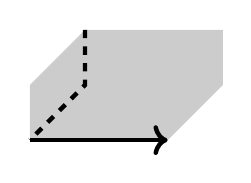
\begin{tikzpicture}[baseline, scale=0.7]
		\fill[gray!40] (0, 1) -- (-1, 0) -- (-1, -1) -- (1.5, -1) --(2.5, 0) -- (2.5, 1)  --cycle;
		\draw[ultra thick, dashed] (0,1) -- (0,0) -- (-1, -1);
		\draw[ultra thick, ->] (-1, -1) -- (1.5, -1);
	\end{tikzpicture} \;\Rightarrow \cdots \Rightarrow\; 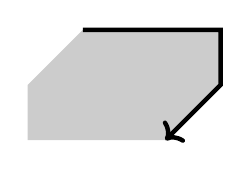
\begin{tikzpicture}[baseline, scale=0.7]
		\fill[gray!40] (-1, 1) -- (1.5, 1) -- (1.5, 0) -- (0.5, -1) -- (-2, -1) -- (-2, 0) --cycle;
		\draw[ultra thick, ->] (-1,1) -- (1.5 , 1) -- (1.5, 0)  -- (0.5, -1);
	\end{tikzpicture} \; =: \beth. \]

	Ingat bahwa $\cate{D}(\cdots)\times\cate{D}(\cdots)\to\cate{D}(\cdots)$,
	sebagai ekstensi Kan kanan, bersifat absolut
	(Proposisi~\ref{prop:localization-functor-abs}). Karena itu, komposit
% segment-id: o014.li2.chapter4.k-flat-derived-tensor-a.e003
	\begin{equation*}\begin{gathered}
		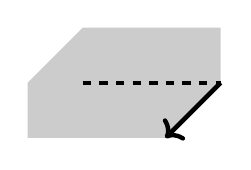
\begin{tikzpicture}[baseline=(O), scale=0.7]
			\fill[gray!40] (-1, 1) -- (1.5, 1) -- (1.5, 0) -- (0.5, -1) -- (-2, -1) -- (-2, 0) --cycle;
			\draw[ultra thick, dashed] (-1,0) -- (1.5, 0);
			\draw[ultra thick, ->] (1.5, 0)  -- (0.5, -1);
			\coordinate (O) at (0, 0);
		\end{tikzpicture}
		\quad \text{merupakan ekstensi Kan kanan dari $\beth$ sepanjang} \quad
		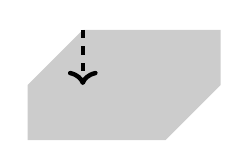
\begin{tikzpicture}[baseline=(O), scale=0.7]
			\fill[gray!40] (-1, 1) -- (1.5, 1) -- (1.5, 0) -- (0.5, -1) -- (-2, -1) -- (-2, 0) --cycle;
			\draw[ultra thick, dashed, ->] (-1, 1) -- (-1, 0);
			\coordinate (O) at (0, 0);
		\end{tikzpicture}.
	\end{gathered}\end{equation*}
	Dengan menerapkan morfisme yang menuju $\beth$ dan sifat universal ekstensi
	Kan kanan (Definisi~\ref{def:Kan-extension}), diperoleh $\alpha$ yang
	dikehendaki.

	Setelah keberadaan $\alpha$ dipastikan, ambil kompleks K-datar sebagaimana
	pada paragraf pertama pembuktian dan hitung semua funktor di lapisan atas;
	dengan demikian terbukti bahwa $\alpha$ merupakan isomorfisme.
\end{bukti}

% segment-id: o014.li2.chapter4.k-flat-derived-tensor-a.p015
Mulai sekarang, argumen semacam ini yang didasarkan pada sifat universal akan
sering dihilangkan; sebagai gantinya, kita akan melakukan verifikasi langsung
dengan resolusi.

% Unit 063 terjemahan Bahasa Indonesia dari chapter4.tex baris 2500--2745.
% Sumber: Methods of Algebra, Volume 2, commit
% 9a5803ff77dd3257484cb177f851a73770a59dd3 (CC BY 4.0).
% stable-unit-id: o014.aljabr2.chapter4.k-flat-derived-tensor-b
% Cakupan: akhir Bagian 4.12 dan Latihan Bab 4 lengkap (17 latihan dan 10 petunjuk);
% menutup chapter4.tex tepat pada penutup lingkungan Exercises.

% segment-id: o014.li2.chapter4.k-flat-derived-tensor-b.co001
\hypertarget{o014.aljabr2.chapter4.k-flat-derived-tensor-b}{ }
\begin{korolari}\label{prop:otimesL-Tor}
	\index[sym1]{Tor}
	Funktor $\otimesL[R]$ dari Definisi~\ref{def:otimesL}, dengan syarat $A$
	atau $B$ datar sebagai modul-$\Bbbk$, memenuhi isomorfisme kanonik
	\[ \Hm^{-n}\left( X \otimesL[R] Y \right) \simeq \Tor^R_n(X, Y), \quad n \in \Z, \]
	dengan $X$ suatu bimodul-$(A,R)$, $Y$ suatu bimodul-$(R,B)$, dan
	$\Tor^R_n$ seperti dalam Definisi--Proposisi~\ref{def:Tor-classical}.
\end{korolari}
% segment-id: o014.li2.chapter4.k-flat-derived-tensor-b.pf001
\begin{bukti}
	Ruas kiri diperoleh dengan menyusun diagram Proposisi
	\ref{prop:otimesL-enrichment} sepanjang arah
% segment-id: o014.li2.chapter4.k-flat-derived-tensor-b.g001
	\begin{tikzpicture}[xscale=0.3, yscale=0.3, baseline=(O)]
		\draw[->] (0,0) -- (1,0) -- (1, -1);
		\coordinate (O) at (0, -0.7);
	\end{tikzpicture}
	sedangkan ruas kanan diperoleh dengan menyusunnya sepanjang arah
% segment-id: o014.li2.chapter4.k-flat-derived-tensor-b.g002
	\begin{tikzpicture}[xscale=0.3, yscale=0.3, baseline=(O)]
		\draw[->] (0,0) -- (0, -1) -- (1, -1);
		\coordinate (O) at (0, -0.7);
	\end{tikzpicture}.
\end{bukti}

% segment-id: o014.li2.chapter4.k-flat-derived-tensor-b.pr001
\begin{proposisi}[Kendala asosiativitas]\label{prop:otimesL-associativity-constraint}
	\index{hasil kali tensor turunan!kendala asosiativitas (associativity constraint)}
	Misalkan $A$, $B$, $R$, dan $S$ aljabar-$\Bbbk$. Tinjau dua funktor berikut:
	\begin{gather*}
		\cate{D}((A,R)\dcate{Mod}) \times \cate{D}((R,S)\dcate{Mod}) \times \cate{D}((S,B)\dcate{Mod}) \to \cate{D}((A,B)\dcate{Mod}), \\
		(X, Y, Z) \mapsto (X \otimesL[R] Y) \otimesL[S] Z, \\
		(X, Y, Z) \mapsto X \otimesL[R] (Y \otimesL[S] Z).
	\end{gather*}
	Jika $A$ dan $B$ keduanya datar sebagai modul-$\Bbbk$, terdapat
	isomorfisme kanonik
	\[ a(X,Y,Z): (X \otimesL[R] Y) \otimesL[S] Z \rightiso X \otimesL[R] (Y \otimesL[S] Z). \]
\end{proposisi}
% segment-id: o014.li2.chapter4.k-flat-derived-tensor-b.pf002
\begin{bukti}
	Tetapkan $Y$. Berdasarkan Proposisi~\ref{prop:K-flat}, kita boleh
	mengandaikan bahwa $X_R$ dan ${}_R Z$ K-datar. Dengan demikian, semua
	$\otimesL[R]$ dapat dihitung pada tingkat kompleks, dan semuanya kembali
	kepada kendala asosiativitas hasil kali tensor
	\cite[Proposisi 6.5.12]{Li1}.
\end{bukti}

% segment-id: o014.li2.chapter4.k-flat-derived-tensor-b.p001
Dengan asumsi kedataran tersebut, mengambil $\otimesL$ dari lebih dari tiga
objek dalam berbagai urutan memberikan hasil-hasil yang saling isomorfik
melalui kendala asosiativitas. Isomorfisme-isomorfisme ini juga memenuhi
koherensi, yang dapat dirumuskan dengan meniru aksioma segilima untuk kategori
monoidal; lihat \cite[Definisi 3.1.1]{Li1}. Caranya tetap dengan mengambil
	resolusi K-datar dan melakukan verifikasi pada tingkat kompleks. Untuk
menghemat uraian, buku ini hanya menampilkan kasus khusus gelanggang
komutatif.

% segment-id: o014.li2.chapter4.k-flat-derived-tensor-b.e001
\begin{contoh}[$\otimesL$ untuk gelanggang komutatif]\label{eg:commutative-otimesL}
	\index{hasil kali tensor turunan!kendala komutativitas (commutativity constraint)}
	Misalkan $R$ gelanggang komutatif. Dalam definisi
	$\otimesL := \otimesL[R]$, ambil semua gelanggang sama dengan $R$,
	khususnya $\Bbbk=R$. Dengan demikian,
	$(R,R)\dcate{Mod}=R\dcate{Mod}$ dan semua asumsi kedataran sebelumnya
	terpenuhi secara otomatis. Akibatnya,
	$\Hm^{-n}(X \otimesL Y) \simeq \Tor^R_n(X,Y)$ berlaku untuk semua
	modul-$R$ $X$ dan $Y$.
	
	Hal ini menjadikan $\cate{D}(R\dcate{Mod})$ kategori monoidal terhadap
	$\otimesL$ dalam arti \cite[\S 3.1]{Li1}. Objek unitnya adalah $R$
	sendiri, sedangkan kendala asosiativitasnya berasal dari
	$a=(a(X,Y,Z))_{X,Y,Z}$ dalam Proposisi
	\ref{prop:otimesL-associativity-constraint}. Karena $R$ merupakan
	modul-$R$ datar, ia K-datar (Proposisi~\ref{prop:flat-K-flat}); maka
	$R \otimesL (\cdot)$ dan $(\cdot) \otimesL R$ keduanya dapat dihitung
	pada tingkat kompleks, sehingga semua aksioma kategori monoidal mudah
	dibuktikan. Lebih lanjut, $\cate{D}(R\dcate{Mod})$ merupakan kategori
	monoidal simetris dalam arti \cite[Definisi 3.3.1]{Li1}. Struktur
	anyamannya (atau kendala komutativitasnya)
	$c(X,Y):X\otimesL Y\rightiso Y\otimesL X$ berasal dari kendala
	komutativitas pada tingkat kompleks, dan aksioma-aksiomanya juga diperiksa
	pada tingkat kompleks. Mengingat Proposisi~\ref{prop:double-cplx-swap},
	pertukaran superskrip pada kompleks total tidak menimbulkan masalah di sini.
\end{contoh}

% segment-id: o014.li2.chapter4.k-flat-derived-tensor-b.e002
\begin{contoh}[Aljabar $\mathrm{Tor}$]
	Melanjutkan pembahasan Contoh~\ref{eg:commutative-otimesL}, misalkan $R$
	komutatif. Identifikasikan kompleks modul-$R$ $X,Y,Z,W$ dengan citranya
	dalam kategori turunan. Untuk setiap $(p,q)\in\Z^2$, terdapat morfisme
	kanonik
% segment-id: o014.li2.chapter4.k-flat-derived-tensor-b.q001
	\begin{multline*}
		\Hm^{-p}\left( X \otimesL Y \right) \otimes \Hm^{-q}\left( Z \otimesL W \right) \to \Hm^{-p-q}\left( (X \otimesL Y) \otimesL (Z \otimesL W) \right) \\
		\simeq \Hm^{-p-q}\left( (X \otimesL Z) \otimesL (Y \otimesL W) \right) \to \Hm^{-p-q} \left( (X \otimes Z) \otimesL (Y \otimes W) \right),
	\end{multline*}
	dengan bagian pertama merupakan penerapan Proposisi~\ref{prop:bifunctor-cup}
	(ambil $F=\otimes$), bagian kedua memakai kendala asosiativitas dan
	kendala komutativitas pada $(\cate{D}(R\dcate{Mod}),\otimesL)$, dan
	bagian ketiga berasal dari morfisme kanonik yang melekat pada $\otimesL$
	sebagai bifunktor turunan kiri:
% segment-id: o014.li2.chapter4.k-flat-derived-tensor-b.q002
	\[ QX_1 \otimesL QX_2 \to Q(X_1 \otimes X_2), \quad X_1, X_2 \in \Obj(\cate{K}(R\dcate{Mod})), \]
	Untuk ketepatan notasi, di sini funktor lokalisasi
	$Q:\cate{K}(R\dcate{Mod})\to\cate{D}(R\dcate{Mod})$ dituliskan kembali.
% segment-id: o014.li2.chapter4.k-flat-derived-tensor-b.l001
	\begin{itemize}
% segment-id: o014.li2.chapter4.k-flat-derived-tensor-b.i001
		\item Komposisi ketiga morfisme kanonik di atas memberikan ``hasil kali
		luar'' bagi funktor $\Tor$:
		\[ \Tor^R_p(X, Y) \otimes \Tor^R_q(Z, W) \to \Tor^R_{p+q}(X \otimes Z, Y \otimes W). \]
% segment-id: o014.li2.chapter4.k-flat-derived-tensor-b.i002
		\item Ambil $Z=X$ dan $W=Y$ sebagai aljabar-$R$ (terkonsentrasi pada
		derajat $0$). Perkaliannya memberikan homomorfisme modul-$R$
		$X\otimes X\to X$ dan $Y\otimes Y\to Y$. Dengan menyusun hasil kali
		luar dengan homomorfisme-homomorfisme ini, diperoleh
		\[ \Tor^R_p(X, Y) \otimes \Tor^R_q(X, Y) \to \Tor^R_{p+q}(X,Y), \]
		yang disebut ``hasil kali dalam'' bagi funktor $\Tor$. Hal ini menjadikan
		$\bigoplus_{n \in \Z} \Tor^R_n(X, Y)$ aljabar-$R$ bergradasi-$\Z$
		dalam arti \cite[Definisi 7.4.1]{Li1}, yang disebut \emph{aljabar
		$\Tor$}. Aljabar ini hanya memiliki komponen tak nol pada derajat
		nonnegatif, dan komponen derajat $0$-nya memberikan subaljabar
		$\Tor^R_0(X, Y) = X \otimes Y$, yang definisinya dapat dilihat dalam
		\cite[Definisi 7.3.1]{Li1}. Hukum asosiatif yang diperlukan bagi
		perkalian dapat diverifikasi dengan mereduksinya kepada kendala
		asosiativitas $\otimesL$ dan hukum asosiatif perkalian masing-masing
		pada $X$ dan $Y$.
		\index{aljabar Tor@aljabar $\Tor$ ($\Tor$-algebra)}
% segment-id: o014.li2.chapter4.k-flat-derived-tensor-b.i003
		\item Andaikan lebih lanjut bahwa $X$ dan $Y$ merupakan aljabar-$R$
		komutatif. Dalam hal ini, aljabar $\Tor$ juga merupakan aljabar
		bergradasi-$\Z$ ``antikomutatif'' dalam arti
		\cite[Definisi 7.4.3]{Li1}\footnote{Sebutan harfiahnya agak menyesatkan,
		karena sifat ini merupakan perwujudan alami komutativitas. Sebutan
		bergradasi-komutatif lebih tepat, seperti dalam Contoh
		\ref{eg:graded-module}.}: untuk semua $p,q\in\Z$,
		\[ a \in \Tor^R_p(X, Y), \; b \in \Tor^R_q(X, Y) \implies ab = (-1)^{pq} ba. \]
		Karena $X\otimes X\to X$ dan $Y\otimes Y\to Y$ keduanya komutatif,
		dari mana tanda tersebut berasal? Sumbernya adalah definisi hasil kali
		luar. Misalkan $C_1$ dan $C_2$ dua salinan $X\otimesL Y$. Maka $ab$
		dan $ba$ berbeda melalui isomorfisme
		$C_1\otimesL C_2\rightiso C_2\otimesL C_1$, yaitu kendala
		komutativitas $\otimesL$. Jika $C_1$ dan $C_2$ dinyatakan sebagai
		kompleks K-datar, isomorfisme pada tingkat kompleks total ini persis
		isomorfisme $r_{C_1^\bullet \otimes C_2^\bullet}$ dari
		Proposisi~\ref{prop:double-cplx-swap}; pada komponen berderajat $(p,q)$,
		isomorfisme tersebut menghasilkan tanda $(-1)^{pq}$.
	\end{itemize}
\end{contoh}

% segment-id: o014.li2.chapter4.k-flat-derived-tensor-b.p002
Kembali ke aljabar-$\Bbbk$ umum. Untuk membahas adjungsi antara $\otimesL$
dan $\RHom$, masih diperlukan satu lema. Berikut ini, $\RHom_{(A,B)}$
menyatakan $\RHom$ pada $(A,B)\dcate{Mod}$; notasi bagi kategori bimodul
(atau modul kiri maupun modul kanan) jenis lainnya digunakan secara serupa.

% segment-id: o014.li2.chapter4.k-flat-derived-tensor-b.le001
\begin{lema}\label{prop:RHom-enrichment}
	Tetapkan aljabar-$\Bbbk$ $A$, $B$, dan $R$. Andaikan $B$ datar sebagai
	modul-$\Bbbk$. Maka funktor pelupa dari $(A,B)\dcate{Mod}$ ke
	$A\dcate{Mod}$ mempertahankan kompleks K-injektif, dan $\RHom_A$ secara
	kanonik dapat diangkat menjadi funktor
	\[ \cate{D}\left((A,R)\dcate{Mod}\right)^{\opp} \times \cate{D}\left((A,B)\dcate{Mod}\right) \to \cate{D}\left((R,B)\dcate{Mod}\right), \]
	dengan kata lain, terdapat diagram 2-sel kanonik
% segment-id: o014.li2.chapter4.k-flat-derived-tensor-b.g003
	\[\begin{tikzcd}
		\cate{D}\left((A,R)\dcate{Mod}\right)^{\opp} \times \cate{D}\left((A,B)\dcate{Mod}\right) \arrow[r] \arrow[d, "\text{pelupa}"'] & \cate{D}\left((R,B)\dcate{Mod}\right) \arrow[d, "\text{pelupa}"] \arrow[Rightarrow, ld, "\sim", sloped] \\
		\cate{D}(A\dcate{Mod})^{\opp} \times \cate{D}(A\dcate{Mod}) \arrow[r, "{\RHom_A}"'] & \cate{D}(\cate{Ab}) .
	\end{tikzcd}\]

	Demikian pula, jika $A$ datar sebagai modul-$\Bbbk$, $\RHom_B$ mempunyai
	pengangkatan serupa.
\end{lema}
% segment-id: o014.li2.chapter4.k-flat-derived-tensor-b.pf003
\begin{bukti}
	Karena $B$ modul-$\Bbbk$ datar, funktor $Y\mapsto{}_A Y$ mempunyai adjoin
	kiri eksak $(\cdot)\dotimes{\Bbbk}B$, sehingga ia mempertahankan kompleks
	K-injektif.
	
	Selanjutnya, ambil
	$X \in \Obj(\cate{K}((A, R)\dcate{Mod}))$ dan
	$Y \in \Obj(\cate{K}(A, B)\dcate{Mod})$, dengan $Y$ K-injektif.
	Berdasarkan langkah sebelumnya,
	$\Hom^\bullet\left({}_A X,{}_A Y\right)$ menentukan
	$\RHom_A({}_A X,{}_A Y)$, tetapi sekaligus merupakan kompleks
	bimodul-$(R,B)$. Ini menyelesaikan proses pengangkatan tersebut.
\end{bukti}

% segment-id: o014.li2.chapter4.k-flat-derived-tensor-b.th001
\begin{teorema}[Adjungsi antara $\RHom$ dan $\otimesL$]\label{prop:RHom-otimesL-adjunction}
	\index{funktor $\RHom$}
	\index{hasil kali tensor turunan}
	Misalkan $A$, $B$, dan $R$ aljabar-$\Bbbk$. Di bawah ini, $X$, $Y$, dan
	$Z$ masing-masing menyatakan objek
	$\cate{D}((A,R)\dcate{Mod})$, $\cate{D}((R,B)\dcate{Mod})$, dan
	$\cate{D}((A,B)\dcate{Mod})$. Andaikan $B$ datar sebagai
	modul-$\Bbbk$. Maka terdapat isomorfisme kanonik dalam
	$\cate{D}(\Bbbk\dcate{Mod})$
% segment-id: o014.li2.chapter4.k-flat-derived-tensor-b.q003
	\begin{equation*}
		\RHom_{(A,B)} \left( X \otimesL[R] Y, Z \right) \rightiso \RHom_{(R,B)}\left( Y, \RHom_A \left( {}_A X, {}_A Z \right) \right).
	\end{equation*}

	Jika $A$ yang diasumsikan datar sebagai modul-$\Bbbk$, terdapat
	isomorfisme kanonik dalam $\cate{D}(\Bbbk\dcate{Mod})$
% segment-id: o014.li2.chapter4.k-flat-derived-tensor-b.q004
	\begin{equation*}
		\RHom_{(A,B)}\left( X \otimesL[R] Y, Z \right) \rightiso \RHom_{(A,R)}\left( X, \RHom_B\left( Y_B , Z_B \right) \right).
	\end{equation*}
\end{teorema}
% segment-id: o014.li2.chapter4.k-flat-derived-tensor-b.pf004
\begin{bukti}
	Tinjau persamaan pertama. Andaikan $Y$ K-projektif dan $Z$ K-injektif.
	Lema~\ref{prop:K-projective-flat} menjamin bahwa ${}_R Y$ K-datar,
	sedangkan Lema~\ref{prop:RHom-enrichment} menjamin bahwa ${}_A Z$ tetap
	K-injektif. Semua $\RHom$ dan $\otimesL[R]$ yang ditampilkan dapat
	ditentukan pada tingkat kompleks. Karena itu, isomorfisme yang dicari
	mengikuti dari Proposisi~\ref{prop:tensor-Hom-cplx}.
\end{bukti}

% segment-id: o014.li2.chapter4.k-flat-derived-tensor-b.e003
\begin{contoh}[Adjungsi untuk perubahan gelanggang]\label{eg:change-of-ring-adjunction}
	Dalam situasi Contoh~\ref{eg:change-of-rings} (ambil homomorfisme
	aljabar-$\Bbbk$ $R\to S$, $A=S$, $B=\Bbbk$, dan $X=S$), persamaan pertama
	dalam Teorema~\ref{prop:RHom-otimesL-adjunction} menjadi isomorfisme kanonik
% segment-id: o014.li2.chapter4.k-flat-derived-tensor-b.q005
	\begin{gather*}
		\RHom_S\left( \mathrm{L} {}_{R \to S} P(Y), Z \right) \simeq \RHom_R\left( Y, {}_R Z \right), \\
		Y \in \Obj(\cate{D}(R\dcate{Mod})), \quad Z \in \Obj(\cate{D}(S\dcate{Mod})).
	\end{gather*}
	Untuk itu, satu-satunya hal yang masih perlu dijelaskan ialah
	$\RHom_S({}_S S,{}_S Z)\simeq{}_R Z$, yang langsung diperoleh dari
	isomorfisme pada tingkat kompleks
% segment-id: o014.li2.chapter4.k-flat-derived-tensor-b.q006
	\[ \Hom^\bullet\left({}_S S, \cdot\right) \simeq {}_R (\cdot) : \cate{C}(S\dcate{Mod}) \to \cate{C}(R\dcate{Mod}). \]
	
	Jika selanjutnya $R$ dan $S$ keduanya gelanggang komutatif dan
	$\Bbbk:=R$, maka $\RHom_S$ (atau $\RHom_R$) bernilai dalam
	$\cate{D}(S\dcate{Mod})$ (atau $\cate{D}(R\dcate{Mod})$). Isomorfisme
	adjungsi tersebut selanjutnya dapat dituliskan sebagai isomorfisme kanonik
	dalam $\cate{D}(R\dcate{Mod})$:
% segment-id: o014.li2.chapter4.k-flat-derived-tensor-b.q007
	\[ {}_R \RHom_S\left( \mathrm{L} {}_{R \to S} P(Y), Z \right) \simeq \RHom_R\left( Y, {}_R Z \right) . \]
	Semuanya dapat diverifikasi pada tingkat kompleks dengan mengambil
	resolusi K-injektif dan K-projektif. Kasus modul kanan serupa.
\end{contoh}


% segment-id: o014.li2.chapter4.k-flat-derived-tensor-b.x001
\begin{Exercises}
	% Reference: [KS06, Exercise 10.10]
% segment-id: o014.li2.chapter4.k-flat-derived-tensor-b.ex001
	\item Misalkan $(\mathcal{D}, T, \mathcal{H})$ kategori prabertriangulasi
	(atau kategori bertriangulasi). Definisikan keluarga segitiga baru
	$\mathcal{H}^-$ melalui
% segment-id: o014.li2.chapter4.k-flat-derived-tensor-b.q008
	\[ [X \xrightarrow{f} Y \xrightarrow{g} Z \xrightarrow{h} TX] \in \mathcal{H} \iff [X \xrightarrow{f} Y \xrightarrow{g} Z \xrightarrow{-h} TX] \in \mathcal{H}^- . \]
% segment-id: o014.li2.chapter4.k-flat-derived-tensor-b.l002
	\begin{enumerate}[(i)]
% segment-id: o014.li2.chapter4.k-flat-derived-tensor-b.i004
		\item Buktikan bahwa $(\mathcal{D},T,\mathcal{H}^-)$ juga merupakan
		kategori prabertriangulasi (atau kategori bertriangulasi).
% segment-id: o014.li2.chapter4.k-flat-derived-tensor-b.i005
		\item Buktikan bahwa $(\mathcal{D},T,\mathcal{H})$ dan
		$(\mathcal{D},T,\mathcal{H}^-)$ saling ekuivalen sebagai kategori
		prabertriangulasi.
	\end{enumerate}

% segment-id: o014.li2.chapter4.k-flat-derived-tensor-b.ex002
	\item Misalkan $(\mathcal{D},T,\mathcal{H})$ kategori prabertriangulasi.
	Buktikan bahwa setiap monomorfisme (atau epimorfisme) $u:X\to Y$ dalam
	$\mathcal{D}$ mempunyai invers kiri (atau invers kanan). Gunakan hal ini
	untuk menunjukkan bahwa kategori prabertriangulasi yang sekaligus kategori
	abelian harus terbelah (Definisi~\ref{def:semisimple}).
	
% segment-id: o014.li2.chapter4.k-flat-derived-tensor-b.hn001
	\begin{hint}
		Tempatkan monomorfisme $u$ dalam segitiga terbedakan
		$X\xrightarrow{u}Y\xrightarrow{v}Z\xrightarrow{w}TX$. Dari
		$u\circ T^{-1}w=0$, simpulkan $w=0$, lalu terapkan
		Proposisi~\ref{prop:dt-sum-1}.
	\end{hint}

% segment-id: o014.li2.chapter4.k-flat-derived-tensor-b.ex003
	\item Terapkan latihan sebelumnya untuk memberikan contoh kategori abelian
	$\mathcal{A}$ sedemikian sehingga $\cate{K}(\mathcal{A})$ dan
	$\cate{D}(\mathcal{A})$ keduanya bukan kategori abelian.

% segment-id: o014.li2.chapter4.k-flat-derived-tensor-b.hn002
	\begin{hint}
		Tinjau morfisme $f:\Z/p^2\Z\twoheadrightarrow\Z/p\Z$ dalam
		$\mathcal{A}=\cate{Ab}$, dengan $p$ prima. Jika
		$\cate{K}(\mathcal{A})$ kategori abelian, tinjau faktorisasi epi--mono
		$\cate{K}f$ dan $\Hm^0(\cate{K}f)$, kemudian uraikan keduanya sebagai
		proyeksi ke suku jumlah langsung dan morfisme inklusi untuk memperoleh
		kontradiksi.
	\end{hint}

% segment-id: o014.li2.chapter4.k-flat-derived-tensor-b.ex004
	\item Misalkan $\mathcal{A}$ kategori abelian. Buktikan bahwa
	$\cate{D}(\mathcal{A})$ merupakan kategori abelian jika dan hanya jika
	$\mathcal{A}$ terbelah.

% segment-id: o014.li2.chapter4.k-flat-derived-tensor-b.hn003
	\begin{hint}
		Untuk arah ``hanya jika'', benamkan $\mathcal{A}$ ke dalam
		$\cate{D}(\mathcal{A})$ dan terapkan hasil latihan-latihan sebelumnya.
		Untuk arah ``jika'', tunjukkan bagi $\mathcal{A}$ yang terbelah bahwa
		pengambilan kohomologi memberikan ekuivalensi dari
		$\cate{D}(\mathcal{A})$ ke $\mathcal{A}^{\Z}$.
	\end{hint}

% segment-id: o014.li2.chapter4.k-flat-derived-tensor-b.ex005
	\item Sering dikatakan bahwa aksioma oktahedral (TR5) bagi kategori
	bertriangulasi merupakan pengganti bagi teorema isomorfisme
	$\dfrac{X/Z}{Y/Z}\simeq X/Y$ dalam kategori abelian, dengan
	$X\supset Y\supset Z$ (Teorema~\ref{prop:Abel-cat-isom-thm} (ii)).
	Jelaskan secara eksplisit makna ungkapan tersebut.

% segment-id: o014.li2.chapter4.k-flat-derived-tensor-b.ex006
	\item ($\mathrm{K}_0$ kategori prabertriangulasi) Untuk setiap kategori
	prabertriangulasi $(\mathcal{D},T,\mathcal{H})$, definisikan
	$\mathrm{K}_0(\mathcal{D})$ sebagai hasil bagi modul-$\Z$ bebas yang
	dibangkitkan oleh $\Obj(\mathcal{D})$ terhadap relasi-relasi
% segment-id: o014.li2.chapter4.k-flat-derived-tensor-b.q009
	\[ \text{terdapat segitiga terbedakan}\; X \to Y \to Z \xrightarrow{+1} \implies [X] - [Y] + [Z] = 0, \]
	dengan $[X]\in\mathrm{K}_0(\mathcal{D})$ menyatakan kelas ekuivalensi yang
	memuat $X\in\Obj(\mathcal{D})$.
% segment-id: o014.li2.chapter4.k-flat-derived-tensor-b.l003
	\begin{enumerate}[(i)]
% segment-id: o014.li2.chapter4.k-flat-derived-tensor-b.i006
		\item Buktikan bahwa $[0]=0$, $[TX]=-[X]$, dan
		$[X\oplus Y]=[X]+[Y]$.
% segment-id: o014.li2.chapter4.k-flat-derived-tensor-b.i007
		\item Tunjukkan bahwa setiap funktor bertriangulasi
		$F:\mathcal{D}\to\mathcal{D}'$ menginduksi homomorfisme kanonik
		$\mathrm{K}_0(\mathcal{D})\to\mathrm{K}_0(\mathcal{D}')$.
% segment-id: o014.li2.chapter4.k-flat-derived-tensor-b.i008
		\item Tinjau funktor kohomologis $H:\mathcal{D}\to\mathcal{A}$, dengan
		$\mathcal{A}$ kategori abelian. Andaikan, untuk semua $X$,
		$|n|\gg_X0\implies H(T^nX)=0$. Definisikan homomorfisme alami
		$\mathrm{K}_0(\mathcal{D})\to\mathrm{K}_0(\mathcal{A})$.
		
% segment-id: o014.li2.chapter4.k-flat-derived-tensor-b.hn004
		\begin{hint}
			Petakan $[X]$ ke $\sum_n(-1)^n[H(T^nX)]$. Terapkan
			Lema~\ref{prop:K0-prep} (iv).
		\end{hint}
% segment-id: o014.li2.chapter4.k-flat-derived-tensor-b.i009
		\item Tinjau kasus khusus $\mathcal{D}:=\cate{D}^{\bdd}(\mathcal{A})$.
		Berikan homomorfisme yang saling invers
% segment-id: o014.li2.chapter4.k-flat-derived-tensor-b.g004
		\[\begin{tikzcd}[row sep=tiny]
			\mathrm{K}_0(\mathcal{A}) \arrow[shift left, r] & \mathrm{K}_0(\cate{D}^{\bdd}(\mathcal{A})) \arrow[shift left, l] \\
			{[A]} \arrow[mapsto, r] & {[A]} \\
			\sum_n (-1)^n {[\Hm^n(X)]} & {[X]} \arrow[mapsto, l]
		\end{tikzcd}\]
		dengan $A\in\Obj(\mathcal{A})$, yang juga dipandang sebagai kompleks
		yang terkonsentrasi pada derajat $0$.
% segment-id: o014.li2.chapter4.k-flat-derived-tensor-b.hn005
		\begin{hint}
			Satu komposisi jelas merupakan identitas; untuk komposisi lainnya,
			diperlukan pemenggalan kompleks.
		\end{hint}
	\end{enumerate}
	\index{grup K0@grup $\mathrm{K}_0$} \index[sym1]{K0}

% segment-id: o014.li2.chapter4.k-flat-derived-tensor-b.ex007
	\item Misalkan $X\in\Obj(\cate{D}(\mathcal{A}))$. Buktikan bahwa
% segment-id: o014.li2.chapter4.k-flat-derived-tensor-b.q010
	\begin{gather*}
		X \in \cate{D}^{\leq 0}(\mathcal{A}) \iff \forall Z \in \Obj(\cate{D}^{\geq 1}(\mathcal{A})), \; \Hom_{\cate{D}(\mathcal{A})}(X, Z) = 0, \\
		X \in \cate{D}^{\geq 0}(\mathcal{A}) \iff \forall Z \in \Obj(\cate{D}^{\leq -1}(\mathcal{A})), \; \Hom_{\cate{D}(\mathcal{A})}(Z, X) = 0.
	\end{gather*}
% segment-id: o014.li2.chapter4.k-flat-derived-tensor-b.hn006
	\begin{hint}
		Terapkan Proposisi~\ref{prop:derived-cat-orthogonality} (i), serta
		pasangan adjoin dan segitiga terbedakan dalam
		Proposisi~\ref{prop:derived-truncation-adjunction}.
	\end{hint}

% segment-id: o014.li2.chapter4.k-flat-derived-tensor-b.ex008
	\item Dalam situasi Teorema~\ref{prop:localization-triangulated-composite},
	andaikan $F'$ memenuhi
	$F'(\Obj(\mathcal{N}'))\subset\Obj(\mathcal{N}'')$ (anggap ini sebagai
	semacam ``keeksakan''). Jika $\mathcal{D}$ mempunyai subkategori
	$F$-injektif atau $F$-projektif, buktikan bahwa morfisme kanonik
	\[ \mathrm{R}^{\mathcal{N}''}_{\mathcal{N}} (F' F) \to \left( \mathrm{R}^{\mathcal{N}''}_{\mathcal{N}'} F' \right) \left( \mathrm{R}^{\mathcal{N}'}_{\mathcal{N}} F \right) \]
	atau
	\[ \left( \mathrm{L}^{\mathcal{N}''}_{\mathcal{N'}} F' \right) \left( \mathrm{L}^{\mathcal{N}'}_{\mathcal{N}} F \right) \to \mathrm{L}^{\mathcal{N}''}_{\mathcal{N}} (F' F) \]
	merupakan isomorfisme.
	
% segment-id: o014.li2.chapter4.k-flat-derived-tensor-b.ex009
	\item Dalam situasi Teorema~\ref{prop:localization-triangulated-composite},
	tunjukkan bahwa terdapat diagram komutatif berikut, yang terdiri atas
	funktor dan morfisme di antaranya (notasi $\mathcal{N}$ dan sebagainya
	dihilangkan):
% segment-id: o014.li2.chapter4.k-flat-derived-tensor-b.g005
	\[\begin{tikzcd}
		\mathrm{R}(F'' F' F) \arrow[r] \arrow[d] & \mathrm{R}(F'' F') \mathrm{R}F \arrow[d] \\
		\mathrm{R}F'' \mathrm{R}(F'F) \arrow[r] & \mathrm{R}F'' \mathrm{R}F' \mathrm{R}F
	\end{tikzcd} \quad \begin{tikzcd}
		\mathrm{L}(F'' F' F) & \mathrm{L}(F'' F') \mathrm{L}F \arrow[l] \\
		\mathrm{L}F'' \mathrm{L}(F'F) \arrow[u] & \mathrm{L}F'' \mathrm{L}F' \mathrm{L}F \arrow[u] \arrow[l] .
	\end{tikzcd}\]

% segment-id: o014.li2.chapter4.k-flat-derived-tensor-b.ex010
	\item Untuk $F=\Hom$, nyatakan secara eksplisit morfisme kanonik dari
	Proposisi~\ref{prop:bifunctor-cup} dalam bentuk
	$\Ext^{q-p}(X,Y)\to\Hom\left(\Hm^p(X),\Hm^q(Y)\right)$.

% segment-id: o014.li2.chapter4.k-flat-derived-tensor-b.ex011
	\item Rumuskan kembali bijeksi dalam Teorema~\ref{prop:Yoneda-Ext} dalam bentuk
	berikut. Dari ekstensi-$n$
	$0\to Y\to E^1\to\cdots\to E^n\to X\to0$, bangun
	$t^{-1}b\in\Hom_{\cate{D}(\mathcal{A})}(X,Y[n])$ seperti berikut:
% segment-id: o014.li2.chapter4.k-flat-derived-tensor-b.g006
	\[\begin{tikzcd}
		X \arrow[d, "b"']\arrow[phantom, r, "" {name=A, yshift=2ex}] & {} & & & X \arrow[d, "\identity"] \\
		W & E^1 \arrow[r] & E^2 \arrow[r] & \cdots \arrow[r] & X \\
		Y[n] \arrow[u, "{t: \text{kuasi-isomorfisme}}"] \arrow[phantom, r, "" {name=B, yshift=-2ex}] & Y \arrow[u] & & &
		\arrow[dash, from=A, to=B]
	\end{tikzcd}\]
	Dengan demikian diperoleh
	$t^{-1}b\in\Hom_{\cate{D}(\mathcal{A})}(X,Y[n])$. Buktikan bahwa bijeksi
	ini berbeda dengan faktor $(-1)^n$ dari bijeksi semula yang didasarkan
	pada $as^{-1}$. Untuk kasus khusus $n=1$, gunakan versi $t^{-1}b$ untuk
	menurunkan versi terkait dari Proposisi~\ref{prop:Ext1-via-ses} (yang
	melibatkan citra $\identity_Y$).
	
% segment-id: o014.li2.chapter4.k-flat-derived-tensor-b.hn007
	\begin{hint}
		Buktikan bahwa $ta+(-1)^{n-1}bs:Z\to W$ secara kanonik homotopik nol.
		Untuk bagian kedua, perhatikan tanda negatif dalam
		Proposisi~\ref{prop:ses-vs-triangle}.
	\end{hint}

% segment-id: o014.li2.chapter4.k-flat-derived-tensor-b.ex012
	\item Misalkan semua objek $S,T$ dalam kategori abelian $\mathcal{A}$
	memenuhi $\Ext^2_{\mathcal{A}}(S,T)=0$. Buktikan bahwa setiap
	$X\in\Obj(\cate{D}^{\bdd}(\mathcal{A}))$ isomorfik dengan
	$\bigoplus_n\Hm^n(X)[-n]$. Tunjukkan bahwa
	$\mathcal{A}:=\Z\dcate{Mod}$ memenuhi syarat ini.
	
% segment-id: o014.li2.chapter4.k-flat-derived-tensor-b.hn008
	\begin{hint}
		Kita boleh mengandaikan bahwa $X$ kompleks terbatas. Mulailah dari kasus
		$n\gg0$. Terapkan Teorema~\ref{prop:Yoneda-Ext} dan
		Proposisi~\ref{prop:Yoneda-zero} pada ekstensi-$2$
		$0\to\Ker(d^n)\to X^n\xrightarrow{d^n}X^{n+1}\to\Coker(d^n)\to0$,
		lalu ubah $X$ langkah demi langkah hingga $d^\bullet=0$, semuanya hingga
		isomorfisme.
	\end{hint}

% segment-id: o014.li2.chapter4.k-flat-derived-tensor-b.ex013
	\item Buktikan bahwa, jika $\mathcal{A}$ mempunyai cukup banyak objek
	injektif, $F:\mathcal{A}\to\mathcal{A}'$ funktor aditif eksak kiri, dan
	$\mathrm{R}F$ berdimensi hingga, maka homomorfisme
	$\mathrm{K}_0(\mathcal{A})\simeq\mathrm{K}_0(\cate{D}^{\bdd}(\mathcal{A}))
	\to\mathrm{K}_0(\cate{D}^{\bdd}(\mathcal{A}'))\simeq
	\mathrm{K}_0(\mathcal{A}')$ yang diinduksi oleh funktor bertriangulasi
	$\mathrm{R}F$ ditentukan oleh
	\[ [A] \mapsto \sum_n (-1)^n \left[\mathrm{R}^n F(A)\right], \quad A \in \Obj(\mathcal{A}). \]

% segment-id: o014.li2.chapter4.k-flat-derived-tensor-b.ex014
	\item Misalkan $R$ gelanggang. Buktikan bahwa limit langsung terfilter
	$\varinjlim$ dari kompleks-kompleks K-datar dalam
	$\cate{C}(R\dcate{Mod})$ tetap K-datar.
	
% segment-id: o014.li2.chapter4.k-flat-derived-tensor-b.ex015
	\item Misalkan $R$ gelanggang. Jika kompleks modul-$R$ $P$ K-datar dan
	setiap $P^n$ merupakan modul-$R$ datar, maka $P$ disebut
	\emph{K-datar kuat}.
% segment-id: o014.li2.chapter4.k-flat-derived-tensor-b.l004
	\begin{enumerate}[(i)]
% segment-id: o014.li2.chapter4.k-flat-derived-tensor-b.i010
		\item Buktikan bahwa, untuk setiap
		$X\in\Obj(\cate{C}(R\dcate{Mod}))$, terdapat kompleks K-datar kuat $P$
		beserta kuasi-isomorfisme $P\to X$.
% segment-id: o014.li2.chapter4.k-flat-derived-tensor-b.hn009
		\begin{hint}
			Gunakan dual argumen keberadaan resolusi K-injektif; lihat
			\S\ref{sec:K-injectives}.
		\end{hint}
% segment-id: o014.li2.chapter4.k-flat-derived-tensor-b.i011
		\item Tuliskan $\mathcal{SF}$ untuk subkategori penuh
		$\cate{K}(R\dcate{Mod})$ yang dibentuk oleh kompleks-kompleks K-datar
		kuat. Nyatakan kategori $\cate{D}(R\dcate{Mod})$ sebagai lokalisasi
		$\mathcal{SF}$ terhadap kuasi-isomorfisme.
	\end{enumerate}

% segment-id: o014.li2.chapter4.k-flat-derived-tensor-b.ex016
	\item (P.\ Berthelot, A.\ Ogus) Misalkan $f$ bukan pembagi nol dalam
	gelanggang komutatif $R$. Untuk setiap modul-$R$ $M$, tuliskan
	$M[f]:=\{m\in M:fm=0\}$. Modul $M$ dengan $M[f]=0$ disebut
	\emph{bebas torsi-$f$}. Pertama, tunjukkan bahwa $M$ yang bebas torsi-$f$
	dapat dibenamkan sebagai submodul dari
	$M[\frac{1}{f}]=M\dotimes{R}R[\frac{1}{f}]$. Karena itu, $f^mM$
	bermakna untuk setiap $m\in\Z$.

	Misalkan $X$ kompleks yang tersusun atas modul-$R$ bebas torsi-$f$.
	Berdasarkan pengamatan di atas, definisikan subkompleks $\eta_fX$ dari
	$X^\bullet\dotimes{R}R[\frac{1}{f}]$ dengan
	\[ (\eta_f X)^n := \left\{ x \in f^n X^n : d_X^n(x) \in f^{n+1} X^{n+1} \right\}, \quad n \in \Z . \]
% segment-id: o014.li2.chapter4.k-flat-derived-tensor-b.l005
	\begin{enumerate}[(i)]
% segment-id: o014.li2.chapter4.k-flat-derived-tensor-b.i012
		\item Buktikan bahwa perkalian suku demi suku dengan $f$ memberikan
		isomorfisme $\eta_f(X[1])\rightiso(\eta_fX)[1]$.
% segment-id: o014.li2.chapter4.k-flat-derived-tensor-b.i013
		\item Tunjukkan bahwa, jika $f,g\in R$ keduanya bukan pembagi nol dan
		setiap $X^n$ bebas torsi-$fg$, maka
		$\eta_f\eta_gX=\eta_{fg}X$.
% segment-id: o014.li2.chapter4.k-flat-derived-tensor-b.i014
		\item Berikan isomorfisme kanonik
		$\Hm^n(X)/\Hm^n(X)[f]\rightiso\Hm^n(\eta_fX)$; jadi efek $\eta_f$
		ialah mengoreksi torsi-$f$. Dari sini, simpulkan bahwa jika $X$ dan $Y$
		merupakan kompleks yang tersusun atas modul-$R$ bebas torsi-$f$ dan
		$\alpha:X\to Y$ suatu kuasi-isomorfisme, maka $\alpha$ menginduksi
		kuasi-isomorfisme $\eta_f(\alpha):\eta_fX\to\eta_fY$.
% segment-id: o014.li2.chapter4.k-flat-derived-tensor-b.i015
		\item Buktikan bahwa $\eta_f$ menginduksi funktor aditif
		$\mathrm{L}\eta_f:\cate{D}(R\dcate{Mod})\to\cate{D}(R\dcate{Mod})$
		dengan cara ini, yang pembatasannya ke $\mathcal{SF}$ dari latihan
		sebelumnya sama dengan $\eta_f$.
% segment-id: o014.li2.chapter4.k-flat-derived-tensor-b.i016
		\item Tunjukkan bahwa $\mathrm{L}\eta_f$ bukan funktor
		bertriangulasi. Jadi ia bukan funktor turunan kiri dalam arti
		Definisi~\ref{def:Verdier-localization-functor}, meskipun tetap merupakan
		ekstensi Kan kanan.

% segment-id: o014.li2.chapter4.k-flat-derived-tensor-b.hn010
		\begin{hint}
			Ambil $R=\Z$ dan $f=p$ prima. Verifikasi bahwa
			$\mathrm{L}\eta_p(\Z/p\Z)=0$, sedangkan
			$\mathrm{L}\eta_p(\Z/p^2\Z)\simeq\Z/p\Z$.
		\end{hint}
	\end{enumerate}

% segment-id: o014.li2.chapter4.k-flat-derived-tensor-b.ex017
	\item Melanjutkan latihan sebelumnya, berikan morfisme kanonik
	$\mathrm{L}\eta_f X \otimesL[R] \mathrm{L}\eta_f Y \to
	\mathrm{L}\eta_f\left( X \otimesL[R] Y \right)$ dan tunjukkan bahwa
	morfisme ini simetris terhadap $X$ dan $Y$ dalam arti yang sesuai.
	Sesungguhnya, dalam bahasa \cite[Catatan 3.1.8]{Li1},
	$\mathrm{L}\eta_f$ merupakan funktor monoidal longgar kanan terhadap
	$\otimesL[R]$.
\end{Exercises}

% Unit 064 terjemahan Bahasa Indonesia dari chapter5.tex baris 9--140.
% Sumber: Methods of Algebra, Volume 2, commit
% 9a5803ff77dd3257484cb177f851a73770a59dd3 (CC BY 4.0).
% stable-unit-id: o014.aljabr2.chapter5.intro-filtration-grading
% Cakupan: pendahuluan Bab 5 dan Bagian 5.1 lengkap.

% segment-id: o014.li2.chapter5.intro-filtration-grading.h001
\chapter{Barisan Spektral}\label{sec:ss}
\hypertarget{o014.aljabr2.chapter5.intro-filtration-grading}{ }

% segment-id: o014.li2.chapter5.intro-filtration-grading.p001
Barisan spektral merupakan alat aljabar klasik yang terus digunakan dan
dikembangkan, serta berakar kuat dalam topologi. Dalam beberapa buku
ajar atau catatan kuliah, barisan spektral bahkan dipakai sebagai alat dasar
aljabar homologis untuk membangun sebagian sifat fundamental dalam
\CHref{sec:Abel-cat} dan \CHref{sec:cplx}.

% segment-id: o014.li2.chapter5.intro-filtration-grading.p002
Barisan spektral pertama kali diperkenalkan oleh J.\ Leray pada dasawarsa 1940,
lalu memperoleh bentuknya secara bertahap melalui pengembangan oleh J.-L.\
Koszul, H.\ Cartan, dan lainnya. Motivasi utama mereka adalah mengkaji grup
homologi berkas serat. Dalam bahasa aljabar, masalah semula setara dengan
memahami homologi (atau kohomologi) suatu kompleks rantai (atau kompleks)
$X$. Kita ambil kasus kompleks sebagai contoh. Objek $X$ sendiri mungkin sulit
dipahami, tetapi dapat dikaji melalui filtrasi yang sesuai
$\cdots\supset\mathrm{F}^pX\supset\mathrm{F}^{p+1}X\supset\cdots$.
Filtrasi $\mathrm{F}^\bullet X$ menginduksi filtrasi pada setiap $\Hm^n(X)$.
Dari informasi mengenai $\mathrm{F}^\bullet X$ dan subkuosiennya, kita dapat
secara bertahap mendekati setiap subkuosien
$\gr^p\Hm^n(X)$ dari kohomologi terfiltrasi tersebut. Barisan spektral adalah
seni menyusun pendekatan bertahap semacam ini.

% segment-id: o014.li2.chapter5.intro-filtration-grading.p003
Kompleks dapat pula diperumum menjadi objek diferensial $(X,d)$ dalam kategori
abelian (Definisi~\ref{def:differential-object}), sehingga diperoleh definisi
abstrak barisan spektral dalam Definisi~\ref{def:SS-abstract}. Barisan spektral
adalah deret objek diferensial $\mathscr{E}=(E_r,d_r)_r$ sedemikian sehingga
kohomologi setiap ``halaman'' $\Hm(E_r,d_r)$ sama dengan halaman berikutnya
$E_{r+1}$. Jika struktur bergradasi ditambahkan dan diferensial $d$ diizinkan
memiliki derajat, diperoleh konsep barisan spektral bergradasi $E_r^p$ dan
bergradasi ganda $E_r^{p,q}$ (Definisi~\ref{def:graded-spectral-sequence}).
Secara konkret, arah diferensial pada barisan spektral bergradasi ganda adalah
\begin{gather*}
	d_r^{p, q}: E_r^{p, q} \to E_r^{p+r, q-r+1}, \\
	E_r = (E_r^{p, q})_{(p, q) \in \Z^2}, \quad d_r = (d_r^{p, q})_{(p, q) \in \Z^2}.
\end{gather*}
Kompleks terfiltrasi menghasilkan objek diferensial terfiltrasi, lalu secara
alami menghasilkan barisan spektral bergradasi ganda. Inilah bentuk barisan
spektral yang paling sering muncul dalam penerapan. Semua konsep mempunyai
versi yang bersesuaian bagi kompleks rantai dan homologinya.

% segment-id: o014.li2.chapter5.intro-filtration-grading.p004
Strategi bab ini dimulai dari teori pasangan eksak W.\ Massey. Pasangan eksak
merupakan perangkat lain untuk menghasilkan barisan spektral dan cakupannya
lebih luas daripada objek diferensial terfiltrasi. Setelah pengantar filtrasi
dan struktur bergradasi dalam \S\ref{sec:grading-filtration}, kita memberikan
definisi umum barisan spektral dalam \S\ref{sec:spectral-sequence}, termasuk
versi bergradasi dan bergradasi ganda, serta istilah dasar seperti degenerasi,
keterbatasan, dan halaman limit. Catatan~\ref{rem:edge-computing} pada akhir
bagian itu menjelaskan cara membaca barisan eksak dari tepi barisan spektral,
suatu teknik yang penting.

% segment-id: o014.li2.chapter5.intro-filtration-grading.p005
Pasangan eksak didefinisikan dalam \S\ref{sec:exact-couples}. Selanjutnya,
\S\ref{sec:filtered-diff-ss} menjelaskan bagaimana pasangan eksak menghasilkan
barisan spektral bergradasi dari objek diferensial terfiltrasi, dan
\S\ref{sec:filtered-cplx-ss} menjelaskan lebih lanjut bagaimana kompleks
terfiltrasi menghasilkan barisan spektral bergradasi ganda. Di sana juga
dibahas konsep inti yang disebut konvergensi dan
Teorema Konvergensi Klasik~\ref{prop:classical-convergence}. Sebagian
verifikasinya sedikit teknis, tetapi tidak mengandung kesulitan mendasar.
Pembaca dapat terlebih dahulu bekerja dalam kategori abelian konkret seperti
$\cate{Ab}$ untuk menyederhanakan argumen.

% segment-id: o014.li2.chapter5.intro-filtration-grading.p006
Bikompleks menghasilkan kompleks terfiltrasi dengan dua cara, bergantung pada
apakah kompleks total difiltrasi menurut koordinat horizontal atau vertikal.
Barisan spektral yang bersesuaian berturut-turut ditulis
$\mathscr{E}_{\mathrm{I}}$ dan $\mathscr{E}_{\mathrm{II}}$. Perinciannya
merupakan pokok \S\ref{sec:double-cplx-ss}. Kita juga memberikan penerapan
standar, termasuk penurunan bifunktor seimbang
(Contoh~\ref{eg:bifunctor-ss}), barisan spektral funktor hiperturunan
(Contoh~\ref{eg:hyperderived-ss}), dan barisan spektral Grothendieck
(Teorema~\ref{prop:Grothendieck-ss}). Resolusi Cartan--Eilenberg yang telah
diperkenalkan (Teorema~\ref{prop:CE-resolution}) berperan di sini.

% segment-id: o014.li2.chapter5.intro-filtration-grading.p007
Barisan spektral Grothendieck berkaitan dengan penurunan komposisi funktor dan
sangat umum dalam geometri. Sebagai contoh funktor turunan kanan, tinjau
funktor aditif eksak kiri antarkategori abelian
$\mathcal{A}\xrightarrow{F}\mathcal{A}'\xrightarrow{F'}\mathcal{A}''$,
dengan $\mathcal{A}$ dan $\mathcal{A}'$ mempunyai cukup banyak objek
injektif. Jika $F$ memetakan objek injektif ke objek $F'$-asiklik
(Konvensi~\ref{con:F-acyclic}), terdapat barisan spektral bergradasi ganda
kanonik yang konvergen kuat
\[ E_2^{p, q} = (\mathrm{R}^p F') (\mathrm{R}^q F)(X) \Rightarrow \mathrm{R}^{p+q}(F' F)(X), \quad X \in \Obj(\mathcal{A}). \]
Penurunan komposisi funktor juga dapat ditangani pada tingkat kategori turunan;
lihat Teorema~\ref{prop:localization-triangulated-composite}. Versi barisan
spektralnya, selain bersifat elementer secara formal dan mudah dihitung, dalam
beberapa kasus konkret memberikan informasi tambahan seperti barisan eksak
pada derajat rendah.

% segment-id: o014.li2.chapter5.intro-filtration-grading.p008
Bagian terakhir bab ini, \S\ref{sec:multiplicative-SS}, memberikan pengantar
singkat tentang struktur perkalian pada barisan spektral. Aspek ini telah
mendapat perhatian sejak awal sejarah barisan spektral.
Proposisi~\ref{prop:dga-mult-ss} menunjukkan bahwa aljabar diferensial
bergradasi terfiltrasi menghasilkan barisan spektral dengan struktur perkalian
kanonik; pembahasan yang lebih mendalam diserahkan kepada monograf khusus.

% segment-id: o014.li2.chapter5.intro-filtration-grading.p009
Sebagai latihan penerapan, barisan spektral Lyndon--Hochschild--Serre yang
sangat penting dalam teori kohomologi grup dapat diperoleh sebagai penerapan
barisan spektral Grothendieck maupun secara konkret dari kompleks terfiltrasi.
Pendekatan kedua juga memberinya struktur perkalian kanonik. Pokok ini akan
dibahas dalam \S\ref{sec:LHS-SS} pada masa mendatang.

% segment-id: o014.li2.chapter5.intro-filtration-grading.note001
\begin{wenxintishi}
	Bab ini hanya memerlukan pengetahuan mengenai kategori abelian dan kompleks.
Selain beberapa definisi sederhana, bab ini tidak bergantung pada isi
\CHref{sec:triangulated-derived-cat}; kedua bab dapat dibaca secara mandiri.
Karena barisan spektral objek diferensial terfiltrasi dapat ditulis secara
langsung, teori pasangan eksak tidak mutlak diperlukan untuk konstruksi itu
(lihat Proposisi~\ref{prop:filtered-diff-E} dan pembahasan sesudahnya). Pembaca
dapat mempertimbangkan untuk sementara melewati \S\ref{sec:exact-couples}.
Selain itu, di bagian selanjutnya dari buku ini hanya \S\ref{sec:LHS-SS} yang
memerlukan pengetahuan tentang barisan spektral.
\end{wenxintishi}

% segment-id: o014.li2.chapter5.intro-filtration-grading.h002
\section{Filtrasi dan Struktur Bergradasi}\label{sec:grading-filtration}

% segment-id: o014.li2.chapter5.intro-filtration-grading.p010
Kita telah menjumpai objek bergradasi dalam Definisi~\ref{def:graded-obj}.
Objek bergradasi-$\Z$ dalam sembarang kategori $\mathcal{A}$ cukup disebut
\emph{objek bergradasi}; menurut definisi, objek-objek tersebut adalah
$(X^p)_{p\in\Z}$ dalam $\mathcal{A}^{\Z}$. Objek bergradasi-$\Z^2$ cukup
disebut \emph{objek bergradasi ganda}; menurut definisi, objek-objek tersebut
adalah $(X^{p,q})_{(p,q)\in\Z^2}$ dalam
$\mathcal{A}^{\Z\times\Z}$. Morfisme antarobjek bergradasi (atau bergradasi
ganda) seperti biasa ditulis $(f^p)_p$ (atau $(f^{p,q})_{p,q}$), dan
dikomposisikan derajat demi derajat. \index{objek bergradasi}

% segment-id: o014.li2.chapter5.intro-filtration-grading.p011
Jika $\mathcal{A}$ merupakan kategori abelian, maka
$\mathcal{A}^{\Z}$ dan $\mathcal{A}^{\Z\times\Z}$ juga kategori abelian;
kernel, kokernel, dan operasi lain semuanya dihitung derajat demi derajat.

% segment-id: o014.li2.chapter5.intro-filtration-grading.p012
Kategori $\mathcal{A}^{\Z}$ mempunyai autoekuivalensi pergeseran $T$ yang
ditentukan oleh $(TX)^p=X^{p+1}$ dan $(Tf)^p=f^{p+1}$. Lebih umum,
$\mathcal{A}^{\Z^n}$ mempunyai keluarga autoekuivalensi pergeseran
$T_1,\ldots,T_n$ yang bersesuaian dengan pergeseran sepanjang $n$ koordinat.
Pergeseran ini memenuhi komutativitas ketat $T_iT_j=T_jT_i$.

% segment-id: o014.li2.chapter5.intro-filtration-grading.p013
Dalam kerangka bab ini, struktur bergradasi terutama berasal dari filtrasi.

% segment-id: o014.li2.chapter5.intro-filtration-grading.d001
\begin{definisi}\label{def:filtration}
	\index{filtrasi}
	\index{filtrasi!hingga}
	\index[sym1]{FilpX@$\mathrm{F}^p X$, $\mathrm{F}_p X$}
	Tinjau objek $X$ dari kategori aditif $\mathcal{A}$.
	\begin{itemize}
		\item Suatu \emph{filtrasi menurun} $\mathrm{F}^\bullet X$ berarti
		barisan subobjek
		\[ \cdots \supset \mathrm{F}^p X \supset \mathrm{F}^{p+1} X \supset \cdots \quad (p \in \Z). \]
		\item Jika terdapat $a\leq b$ dengan $\mathrm{F}^aX=X$ dan
		$\mathrm{F}^bX=0$, filtrasi tersebut disebut \emph{hingga}.
		\item Filtrasi menaik $\mathrm{F}_\bullet X$ dan sifat hingganya
		didefinisikan secara serupa.
	\end{itemize}
\end{definisi}

% segment-id: o014.li2.chapter5.intro-filtration-grading.p014
Filtrasi menurun dan menaik dapat dibedakan dari posisi indeks $p$. Jika tidak
ada kerancuan, keduanya cukup disebut filtrasi. Dalam kajian kompleks dan
kohomologi biasanya digunakan filtrasi menurun, sedangkan untuk kompleks
rantai dan homologi biasanya digunakan filtrasi menaik. Bab ini terutama
memakai filtrasi menurun.

% segment-id: o014.li2.chapter5.intro-filtration-grading.p015
Semua objek terfiltrasi $(X,\mathrm{F}^\bullet X)$ membentuk kategori
$\mathrm{Fil}^\bullet(\mathcal{A})$. Morfisme
$f:(X,\mathrm{F}^\bullet X)\to(Y,\mathrm{F}^\bullet Y)$ didefinisikan sebagai
morfisme $f:X\to Y$ yang mempertahankan filtrasi, yakni yang untuk setiap $p$
membatasi diri menjadi $\mathrm{F}^pX\to\mathrm{F}^pY$. Kategori
$\mathrm{Fil}_\bullet(\mathcal{A})$ didefinisikan serupa.
\index[sym1]{FilA@$\mathrm{Fil}^\bullet(\mathcal{A})$, $\mathrm{Fil}_\bullet(\mathcal{A})$}

% segment-id: o014.li2.chapter5.intro-filtration-grading.p016
Untuk setiap $X$, filtrasi menurun $\mathrm{F}^\bullet X$ (atau filtrasi
menaik $\mathrm{F}_\bullet X$) menghasilkan objek bergradasi
$(\mathrm{F}^pX)_{p\in\Z}$ (atau $(\mathrm{F}_pX)_{p\in\Z}$). Ini memberikan
funktor $\mathrm{Fil}^\bullet(\mathcal{A})\to\mathcal{A}^{\Z}$ (atau
$\mathrm{Fil}_\bullet(\mathcal{A})\to\mathcal{A}^{\Z}$), yang disebut
konstruksi Rees.

% segment-id: o014.li2.chapter5.intro-filtration-grading.p017
Jika $\mathcal{A}$ kategori abelian, terdapat cara lain membangun objek
bergradasi dari filtrasi.

% segment-id: o014.li2.chapter5.intro-filtration-grading.d002
\begin{definisi}
	\index[sym1]{grX@$\gr^p X$, $\gr_p X$}
	Misalkan $\mathcal{A}$ kategori abelian dan tinjau filtrasi
	$\mathrm{F}^\bullet X$ (atau $\mathrm{F}_\bullet X$) pada objek $X$.
	Definisikan objek bergradasi $\gr X$ melalui
	\[ \gr^p X := \mathrm{F}^p X / \mathrm{F}^{p+1} X \quad (\text{atau} \quad \gr_p X := \mathrm{F}_p X / \mathrm{F}_{p-1} X). \]
	Ini memberikan funktor
	$\gr:\mathrm{Fil}^\bullet(\mathcal{A})\to\mathcal{A}^{\Z}$ (atau
	$\gr:\mathrm{Fil}_\bullet(\mathcal{A})\to\mathcal{A}^{\Z}$).
\end{definisi}

% segment-id: o014.li2.chapter5.intro-filtration-grading.p018
Untuk mengekstrak informasi mengenai $X$ dari $(\gr^pX)_p$, setidaknya kita
memerlukan $\bigcup_p\mathrm{F}^pX=X$ dan
$\bigcap_p\mathrm{F}^pX=0$, dengan notasi dari
Konvensi~\ref{con:increasing-union}. Agar pernyataan pertama bermakna dan
berguna, kita juga menghendaki $\varinjlim_{p\to-\infty}$ eksak dalam
$\mathcal{A}$, atau cukup mensyaratkan adanya $M$ dengan
$\mathrm{F}^MX=X$. Kita mulai dengan beberapa konsep terkait.

% segment-id: o014.li2.chapter5.intro-filtration-grading.d003
\begin{definisi}\label{def:filtration-properties}
	\index{filtrasi!lengkap}
	\index{filtrasi!terpisah}
	\index{filtrasi!menyeluruh}
	Misalkan $\mathcal{A}$ kategori abelian dan $X$ objek dengan filtrasi
	$\mathrm{F}^\bullet X$.
	\begin{itemize}
		\item Jika $\bigcap_p\mathrm{F}^pX=0$, filtrasi tersebut disebut
		\emph{terpisah}.
		\item Jika $\bigcup_p\mathrm{F}^pX=X$ dan salah satu syarat berikut
		berlaku, filtrasi tersebut disebut \emph{menyeluruh}:
		\begin{compactenum}[(a)]
			\item $\mathcal{A}$ mempunyai $\varinjlim$ tersaring terhitung yang
			eksak; lebih tepatnya,
			$\varinjlim:\mathcal{A}^{(\Z_{\geq0},\leq)}\to\mathcal{A}$ ada dan
			eksak\footnote{Jika $\mathcal{A}$ merupakan kategori Grothendieck,
			maka (a) otomatis berlaku.};
			\item terdapat $M\in\Z$ dengan $\mathrm{F}^MX=X$.
		\end{compactenum}
		\item Jika keluarga morfisme kanonik
		$X\twoheadrightarrow X/\mathrm{F}^pX$ menginduksi isomorfisme
		$X\rightiso\varprojlim_pX/\mathrm{F}^pX$, filtrasi tersebut disebut
		\emph{lengkap}.
	\end{itemize}
	Filtrasi menaik $\mathrm{F}_\bullet X$ diperlakukan dengan cara yang sama.
\end{definisi}

% segment-id: o014.li2.chapter5.intro-filtration-grading.p019
Konsep kelengkapan diilhami oleh kasus grup topologis; lihat
\cite[\S 4.10]{Li1}.

% segment-id: o014.li2.chapter5.intro-filtration-grading.p020
Filtrasi hingga otomatis terpisah, menyeluruh, dan lengkap; inilah kasus utama
yang diperlukan dalam bab ini. Perhatikan bahwa jika terdapat $N$ dengan
$\mathrm{F}^NX=0$, filtrasi $\mathrm{F}^\bullet X$ terpisah dan lengkap.
Selain itu, karena kernel dari
$X\to\varprojlim_pX/\mathrm{F}^pX$ adalah
$\bigcap_p\mathrm{F}^pX$, kelengkapan menyiratkan keterpisahan.

% segment-id: o014.li2.chapter5.intro-filtration-grading.p021
Citra filtrasi menyeluruh tetap menyeluruh; hal ini diperoleh dengan
menafsirkan $\bigcup_p$ sebagai $\sum_p$, lalu menggunakan
Lema~\ref{prop:image-sum-preimage-intersection} (ii).
Selain itu, filtrasi menyeluruh memenuhi
\begin{equation}\label{eqn:exhaustion-intersection}\begin{gathered}
	\varinjlim_{p \to -\infty} \mathrm{F}^p X \rightiso \bigcup_p \mathrm{F}^p X = X, \\
	K = K \cap \left( \bigcup_p \mathrm{F}^p X \right) = \bigcup_p \left( K \cap \mathrm{F}^p X \right),
\end{gathered}\end{equation}
dengan $K$ sembarang subobjek dari $X$. Di bawah syarat (a) untuk filtrasi
menyeluruh, pernyataan ini merupakan akibat sederhana dari
Proposisi~\ref{prop:Grothendieck-cat-intersection}; di bawah syarat (b),
pernyataan ini langsung.

% segment-id: o014.li2.chapter5.intro-filtration-grading.pr001
\begin{proposisi}\label{prop:gr-isom}
	Misalkan $\mathcal{A}$ kategori abelian dan
	$f:(X,\mathrm{F}^\bullet X)\to(Y,\mathrm{F}^\bullet Y)$ suatu morfisme dalam
	$\mathrm{Fil}^\bullet(\mathcal{A})$.
	\begin{enumerate}[(i)]
		\item Misalkan $\mathrm{F}^\bullet X$ terpisah dan menyeluruh. Jika
		$\gr(f)$ monomorfisme, maka $f$ monomorfisme.
		\item Misalkan $\mathrm{F}^\bullet X$ lengkap dan menyeluruh, sedangkan
		$\mathrm{F}^\bullet Y$ terpisah dan menyeluruh. Jika $\gr(f)$
		isomorfisme, maka $f$ juga isomorfisme, dan dalam hal ini
		$\mathrm{F}^\bullet Y$ juga lengkap.
	\end{enumerate}
	Pernyataan yang bersesuaian berlaku pula bagi filtrasi menaik.
\end{proposisi}
% segment-id: o014.li2.chapter5.intro-filtration-grading.pf001
\begin{bukti}
	Untuk setiap $p\in\Z$, tuliskan diagram komutatif dengan baris-baris eksak
% segment-id: o014.li2.chapter5.intro-filtration-grading.g001
	\[\begin{tikzcd}
		0 \arrow[r] & \mathrm{F}^{p+1} X \arrow[d, "f"'] \arrow[r] & \mathrm{F}^p X \arrow[r] \arrow[d, "f"] & \gr^p X \arrow[r] \arrow[d, "{\gr^p(f)}"] & 0 \\
		0 \arrow[r] & \mathrm{F}^{p+1} Y \arrow[r] & \mathrm{F}^p Y \arrow[r] & \gr^p Y \arrow[r] & 0
	\end{tikzcd}\]
	Tuliskan $K^p$ dan $C^p$ untuk kernel dan kokernel dari
	$\mathrm{F}^pX\xrightarrow{f}\mathrm{F}^pY$.

	Untuk (i), terapkan Teorema~\ref{prop:snake-lemma} pada diagram di atas.
	Diperoleh $K^{p+1}=K^p$. Secara khusus,
	$K^p\subset\bigcap_{\ell\geq p}\mathrm{F}^\ell X=0$, sehingga pembatasan
	$f$ ke setiap $\mathrm{F}^pX$ monomorfisme. Untuk membuktikan bahwa $f$
	monomorfisme, cukup gunakan
	\[ \Ker(f) \xlongequal{\because\; \text{\eqref{eqn:exhaustion-intersection}}} \bigcup_p \left( \Ker(f) \cap \mathrm{F}^p X \right) = 0. \]

	Untuk (ii), diagram menunjukkan $K^{p+1}=K^p$ dan
	$C^{p+1}\rightiso C^p$. Untuk setiap $\ell>p$, perhatikan diagram komutatif
dengan baris-baris eksak
% segment-id: o014.li2.chapter5.intro-filtration-grading.g002
	\[\begin{tikzcd}
		0 \arrow[r] & \mathrm{F}^{\ell} X \arrow[r] \arrow[d, "f"] & \mathrm{F}^p X \arrow[r] \arrow[d, "f"] & \mathrm{F}^p X / \mathrm{F}^{\ell} X \arrow[r] \arrow[d] & 0 \\
		0 \arrow[r] & \mathrm{F}^{\ell} Y \arrow[r] & \mathrm{F}^p Y \arrow[r] & \mathrm{F}^p Y / \mathrm{F}^{\ell} Y \arrow[r] & 0
	\end{tikzcd}\]
	Dengan menerapkan Teorema~\ref{prop:snake-lemma} sekali lagi, diperoleh
	isomorfisme yang diinduksi oleh $f$
	\[ \mathrm{F}^p X / \mathrm{F}^\ell X \rightiso \mathrm{F}^p Y / \mathrm{F}^\ell Y. \]

	Ambil $\varinjlim_{p:p<\ell}$ pada kedua ruas dan gunakan
	\eqref{eqn:exhaustion-intersection}; diperoleh
	$X/\mathrm{F}^\ell X\rightiso Y/\mathrm{F}^\ell Y$. Selanjutnya ambil
	$\varprojlim_\ell$ untuk mendapatkan diagram komutatif
% segment-id: o014.li2.chapter5.intro-filtration-grading.g003
	\[\begin{tikzcd}
		X \arrow[r, "\sim"] \arrow[d, "f"'] & \varprojlim_\ell X/\mathrm{F}^\ell X \arrow[d, "\sim" sloped] \\
		Y \arrow[hookrightarrow, r] & \varprojlim_\ell Y/\mathrm{F}^\ell Y
	\end{tikzcd}\]
	Maka baik $f$ maupun $Y\to\varprojlim_\ell Y/\mathrm{F}^\ell Y$
	merupakan isomorfisme.
\end{bukti}

% Unit 065 terjemahan Bahasa Indonesia dari chapter5.tex baris 141--349.
% Sumber: Methods of Algebra, Volume 2, commit
% 9a5803ff77dd3257484cb177f851a73770a59dd3 (CC BY 4.0).
% stable-unit-id: o014.aljabr2.chapter5.general-spectral-sequences
% Cakupan: Bagian 5.2 lengkap.

% segment-id: o014.li2.chapter5.general-spectral-sequences.h001
\section{Definisi umum barisan spektral}\label{sec:spectral-sequence}
\hypertarget{o014.aljabr2.chapter5.general-spectral-sequences}{ }

% segment-id: o014.li2.chapter5.general-spectral-sequences.p001
Kita mulai dengan definisi umum objek diferensial. Definisi ini melibatkan
kategori aditif dengan translasi $(\mathcal{A},T)$ sebagaimana dalam
Definisi~\ref{def:category-with-translation}, serta morfisme berderajat
sebagaimana dalam Definisi~\ref{def:morphism-with-degree}.

% segment-id: o014.li2.chapter5.general-spectral-sequences.d001
\begin{definition}\label{def:differential-object}
	\index{objek diferensial (differential object)}
	\index[sym1]{ATd@$\mathcal{A}_d$, $(\mathcal{A}, T)_d$}
	Sebuah \emph{objek diferensial} pada kategori aditif dengan translasi
	$(\mathcal{A},T)$ adalah data $(X,d)$, dengan $X\in\Obj(\mathcal{A})$ dan
	$d:X\xrightarrow{+1}X$ yang memenuhi $d^2=0$.
	\begin{itemize}
		\item Morfisme dari $(X,d)$ ke $(X',d')$ adalah morfisme
		$\alpha:X\to X'$ yang memenuhi $d'\alpha=\alpha d$.
		\item Semua objek diferensial membentuk kategori $(\mathcal{A},T)_d$;
		kita juga menulis
		$\mathcal{A}_d:=(\mathcal{A},\identity_{\mathcal{A}})_d$.
	\end{itemize}
\end{definition}

% segment-id: o014.li2.chapter5.general-spectral-sequences.p002
Jika $\mathcal{A}$ adalah kategori-$\cate{Ab}$ (atau
kategori-$\Bbbk\dcate{Mod}$, dengan $\Bbbk$ gelanggang komutatif), maka
$(\mathcal{A},T)_d$ juga demikian. Funktor pelupa
$(\mathcal{A},T)_d\to\mathcal{A}$ memetakan $(X,d)$ ke $X$.

% segment-id: o014.li2.chapter5.general-spectral-sequences.t001
\begin{proposition}
	\index[sym1]{HXd@$\Hm(X,d)$}
	Funktor pelupa $(\mathcal{A},T)_d\to\mathcal{A}$ menciptakan semua
	$\varinjlim$ dan $\varprojlim$ (Definisi~\ref{def:create-limit}).
\end{proposition}
\begin{proof}
	Tinjau kembali bukti Lema~\ref{prop:limits-cplx}.
\end{proof}

% segment-id: o014.li2.chapter5.general-spectral-sequences.p003
Karena itu, jika $\mathcal{A}$ adalah kategori abelian, maka
$(\mathcal{A},T)_d$ juga kategori abelian, dan
$(\mathcal{A},T)_d\to\mathcal{A}$ eksak.

% segment-id: o014.li2.chapter5.general-spectral-sequences.p004
Dalam kasus kategori abelian, salah satu ciri objek diferensial adalah bahwa
objek tersebut memiliki homologi atau kohomologi.

% segment-id: o014.li2.chapter5.general-spectral-sequences.d002
\begin{definition}
	Misalkan $\mathcal{A}$ kategori abelian. Kita mendefinisikan funktor aditif
	\[ \Hm:(\mathcal{A},T)_d\to\mathcal{A},\qquad
	   \Hm(X,d):=\Ker(d)/\Image(T^{-1}d). \]
\end{definition}

% segment-id: o014.li2.chapter5.general-spectral-sequences.p005
Kita menyebut diagram segitiga dalam kategori abelian $\mathcal{A}$
$\begin{tikzcd}[column sep=small, row sep=small]
	A \arrow[rr] & & B \arrow[ld] \\
	& C \arrow[lu, "+m"] &
\end{tikzcd}$
\emph{eksak} apabila
\[ \cdots T^{k-m}C\to T^kA\to T^kB\to T^kC\to T^{k+m}A\cdots \]
merupakan barisan eksak yang memanjang tak hingga ke kedua arah. Diagram
segitiga berderajat yang lebih umum diperlakukan dengan cara yang sama.
\index{barisan eksak}

% segment-id: o014.li2.chapter5.general-spectral-sequences.l001
\begin{lemma}\label{prop:diff-obj-triangle}
	Misalkan $(\mathcal{A},T)$ suatu kategori abelian dengan translasi. Jika
	$0\to(X',d')\to(X,d)\to(X'',d'')\to0$ adalah barisan eksak pendek dalam
	$(\mathcal{A},T)_d$, maka diagram berikut eksak pada setiap titik sudut:
	\[\begin{tikzcd}[column sep=tiny]
		\Hm(X',d') \arrow[rr] & & \Hm(X,d) \arrow[ld] . \\
		& \Hm(X'',d'') \arrow[lu, "{+1}"] &
	\end{tikzcd}\]
\end{lemma}
\begin{proof}
	Dalam $\mathcal{A}$, perhatikan barisan kompleks
	\[ 0\to(T^nX',T^nd')_n\to(T^nX,T^nd)_n
	   \to(T^nX'',T^nd'')_n\to0. \]
	Barisan ini eksak derajat demi derajat, sehingga merupakan barisan eksak
	pendek. Terapkan Proposisi~\ref{prop:long-exact-sequence-ses} kepadanya.
\end{proof}

% segment-id: o014.li2.chapter5.general-spectral-sequences.e001
\begin{example}[Kompleks sebagai objek diferensial]\label{eg:cplx-as-diff}
	\index{objek bergradasi diferensial}
	Untuk kategori aditif $\mathcal{A}$, perhatikan $\mathcal{A}^{\Z}$ bersama
	funktor translasi $T:(X^n)_n\mapsto(X^{n+1})_n$. Berdasarkan uraian dalam
	\S\ref{sec:additive-cplx}, objek dalam $(\mathcal{A}^{\Z},T)_d$ juga
	disebut objek bergradasi diferensial, dan terdapat isomorfisme kategori
	$\cate{C}(\mathcal{A})\simeq(\mathcal{A}^{\Z},T)_d$. Jika $\mathcal{A}$
	adalah kategori abelian, jelas bahwa
	\[ \Hm(X,d)=\left(\Hm^p(X)\right)_{p\in\Z}. \]
\end{example}

% segment-id: o014.li2.chapter5.general-spectral-sequences.p006
Sekarang kita dapat memberikan definisi barisan spektral. Untuk menyederhanakan
pembahasan, mula-mula kita tinjau kasus tanpa translasi, atau setara dengan itu,
kasus morfisme tanpa derajat; dengan kata lain, kita ambil
$T=\identity$.

% segment-id: o014.li2.chapter5.general-spectral-sequences.d003
\begin{definition}[J.\ Leray, J.-L.\ Koszul]\label{def:SS-abstract}
	\index{barisan spektral (spectral sequence)}
	Misalkan $\mathcal{A}$ kategori abelian dan $a\in\Z$. Sebuah
	\emph{barisan spektral} yang dimulai dari $a$ adalah data
	$\mathscr{E}=(E_r,d_r)_{r\in\Z_{\geq a}}$ bersama $(t_r)_{r\geq a+1}$,
	dengan
	\begin{compactitem}
		\item $(E_r,d_r)\in\Obj(\mathcal{A}_d)$;
		\item $t_r:\Hm(E_{r-1},d_{r-1})\rightiso E_r$ untuk $r\geq a+1$.
	\end{compactitem}
	Data $a$ dan $(t_r)_r$ sering dihilangkan dari notasi.

	Morfisme barisan spektral $\mathscr{E}\to\mathscr{E}'$ adalah keluarga
	morfisme dalam $\mathcal{A}_d$
	$\varphi_r:(E_r,d_r)\to(E'_r,d'_r)$ yang memenuhi
	$t_r\Hm(\varphi_{r-1})=\varphi_rt_r$ untuk $r\geq a+1$.
\end{definition}

% segment-id: o014.li2.chapter5.general-spectral-sequences.p007
Pasangan $(E_r,d_r)$ lazim disebut \emph{halaman ke-$r$} dari barisan spektral
$\mathscr{E}$; beralih dari $E_r$ ke $E_{r+1}$ berarti membalik halaman.
Secara abstrak, halaman tempat barisan spektral mulai tidaklah penting, tetapi
dalam penerapan pilihan tersebut bergantung pada konteksnya.

% segment-id: o014.li2.chapter5.general-spectral-sequences.p008
Jika $d_r$ dalam barisan spektral dipandang sebagai morfisme
$\Hm(E_{r-1},d_{r-1})\to\Hm(E_{r-1},d_{r-1})$, maka
$\Ker(d_r)\supset\Image(d_r)$ masing-masing bersesuaian dengan subobjek dari
$\Ker(d_{r-1})$ yang memuat $\Image(d_{r-1})$. Demi kemudahan,
anggap barisan spektral dimulai dari $a=0$. Definisikan $Z_1$ (berturut-turut
$B_1$) sebagai $\Ker(d_0)$ (berturut-turut $\Image(d_0)$), lalu definisikan
$Z_2$ (berturut-turut $B_2$) sebagai prapeta $\Ker(d_1)$ (berturut-turut
$\Image(d_1)$) terhadap $E_0\supset Z_1\twoheadrightarrow E_1$, dan seterusnya.
Iterasi ini memberikan
\begin{equation}\label{eqn:spectral-sequence-Z-B}\begin{gathered}
	0=:B_0\subset B_1\subset B_2\subset\cdots\subset Z_2\subset Z_1
	\subset Z_0=:E_0, \\
	Z_r\leftrightarrow\Ker(d_{r-1}),\quad
	B_r\leftrightarrow\Image(d_{r-1}),\quad Z_r/B_r\simeq E_r.
\end{gathered}\end{equation}
\index[sym1]{ZBE@$Z_r$, $B_r$, $E_r$}

% segment-id: o014.li2.chapter5.general-spectral-sequences.p009
\begin{itemize}
	\item Jika $Z_\infty:=\bigcap_rZ_r$ dan $B_\infty:=\bigcup_rB_r$ ada,
	\emph{limit} barisan spektral $\mathscr{E}$ didefinisikan sebagai
	$E_\infty:=Z_\infty/B_\infty$.
	\item Jika ada $r$ sedemikian sehingga $r'\geq r\implies d_{r'}=0$, maka
	$\mathscr{E}$ dikatakan \emph{mengalami degenerasi pada halaman $E_r$}.
	Dalam keadaan ini jelas bahwa $Z_r=Z_{r+1}=\cdots$ dan
	$B_r=B_{r+1}=\cdots$, sehingga $Z_r=Z_\infty$ dan $B_r=B_\infty$;
	sebagai akibatnya, $E_r=E_\infty$.
	\index{barisan spektral!degenerasi (degenerate)}
\end{itemize}

% segment-id: o014.li2.chapter5.general-spectral-sequences.p010
Ketika membahas barisan spektral bergradasi homologis, kelak kita akan memakai
notasi $(E^r,d^r)_r$ serta $B^r,Z^r$.

% segment-id: o014.li2.chapter5.general-spectral-sequences.t002
\begin{proposition}\label{prop:ss-isom-infty}
	Misalkan $\varphi_r:\mathscr{E}\to\mathscr{E}'$ adalah morfisme barisan
	spektral. Jika $\varphi_r$ merupakan isomorfisme, maka $\varphi_s$ juga
	isomorfisme untuk $s\geq r$; jika limitnya ada, maka
	$\varphi_\infty:E_\infty\to E'_\infty$ juga isomorfisme.
\end{proposition}
\begin{proof}
	Isomorfisme $\varphi_r$ menginduksi isomorfisme
	$\Hm(E_r,d_r)\to\Hm(E'_r,d'_r)$, yang tepat merupakan
	$\varphi_{r+1}$. Tanpa mengurangi keumuman, anggap barisan spektral dimulai
	dari $r$. Maka $(\varphi_s)_{s\geq r}$ adalah isomorfisme barisan spektral,
	dan pernyataan mengenai $\varphi_\infty$ langsung mengikuti.
\end{proof}

% segment-id: o014.li2.chapter5.general-spectral-sequences.p011
Lebih umum, untuk kategori abelian dengan translasi $(\mathcal{A},T)$,
definisi barisan spektral dapat diperluas ke keadaan
$(E_r,d_r)\in\Obj((\mathcal{A},T^{a_r})_d)$, dengan
$a_1,a_2,\ldots$ suatu barisan bilangan bulat. Definisi $\Hm(E_r,d_r)$ serta
$B_r,Z_r$ di atas tidak berubah.

% segment-id: o014.li2.chapter5.general-spectral-sequences.p012
Dalam perluasan yang akan kita perlukan, kita bahkan dapat membiarkan
$\mathcal{A}$ dilengkapi keluarga autoisomorfisme saling komutatif
$T_1,\ldots,T_n$, dan
\[ d_r:E_r\xrightarrow{+\vec{a}_r}E_r,\qquad
	\vec{a}_r=(a_{r,1},\ldots,a_{r,n})\in\Z^n. \]
Mengikuti gagasan ini, kita memperkenalkan dua versi yang paling umum dipakai;
keduanya melibatkan struktur bergradasi.

% segment-id: o014.li2.chapter5.general-spectral-sequences.d004
\begin{definition}[Barisan spektral: versi bergradasi dan bergradasi ganda]
\label{def:graded-spectral-sequence}
	\index{barisan spektral!bergradasi, bergradasi ganda (graded, bigraded)}
	\index[sym1]{drpq@$d_r^{p,q}$, $d^r_{p,q}$}
	Misalkan $\mathcal{A}$ kategori abelian. Barisan spektral bergradasi
	kohomologis dan barisan spektral bergradasi ganda kohomologis, keduanya
	ditulis sebagai $\mathscr{E}=(E_r,d_r)_r$, didefinisikan sebagai berikut.
	\[\begin{array}{|c|c|c|c|} \hline
		\text{Versi} & E_r & d_r & \text{Derajat morfisme} \\ \hline
		\text{Bergradasi} & (E_r^p)_{p\in\Z}\in\Obj(\mathcal{A}^{\Z})
		& (d_r^p)_p & d_r^p:E_r^p\xrightarrow{+r}E_r^{p+r} \\
		\text{Bergradasi ganda} &
		(E_r^{p,q})_{(p,q)\in\Z^2}\in\Obj(\mathcal{A}^{\Z\times\Z})
		& (d_r^{p,q})_{(p,q)} &
		d_r^{p,q}:E_r^{p,q}\xrightarrow{+(r,-r+1)}E_r^{p+r,q-r+1}
		\\ \hline
	\end{array}\]
	Dalam kedua kasus disyaratkan $(d_r)^2=0$, dengan komposisi dipahami
	sebagai komposisi morfisme berderajat, dan datanya memuat isomorfisme
	tertentu $\Hm(E_{r-1},d_{r-1})\rightiso E_r$.

	Secara dual, barisan spektral bergradasi (atau bergradasi ganda) homologis
	didefinisikan sebagai data $(E^r,d^r)_{r\geq1}$ berikut, dengan syarat yang
	sama bahwa $(d^r)^2=0$ dan dengan isomorfisme tertentu
	$\Hm(E^r,d^r)\simeq E^{r+1}$:
	\[\begin{array}{|c|c|c|c|} \hline
		\text{Versi} & E^r & d^r & \text{Derajat morfisme} \\ \hline
		\text{Bergradasi} & (E^r_p)_{p\in\Z}\in\Obj(\mathcal{A}^{\Z})
		& (d^r_p)_p & d^r_p:E^r_p\xrightarrow{-r}E^r_{p-r} \\
		\text{Bergradasi ganda} &
		(E^r_{p,q})_{(p,q)\in\Z^2}\in\Obj(\mathcal{A}^{\Z\times\Z})
		& (d^r_{p,q})_{(p,q)} &
		d^r_{p,q}:E^r_{p,q}\xrightarrow{+(-r,r-1)}E^r_{p-r,q+r-1}
		\\ \hline
	\end{array}\]
	Morfisme antarbarisan spektral ini didefinisikan dengan cara
	biasa dan harus kompatibel dengan isomorfisme yang ditentukan.
\end{definition}

% segment-id: o014.li2.chapter5.general-spectral-sequences.p013
Jika digambar dalam koordinat $(p,q)$, arah $d_r$ dan $d^r$ pada barisan
spektral bergradasi ganda adalah sebagai berikut.
\begin{center}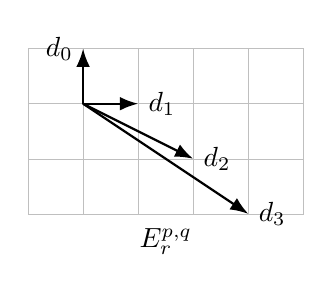
\begin{tikzpicture}[>=Latex, scale=0.7, baseline=(O)]
	\draw[very thin, gray!50] (-1,1) grid (4,-2);
	\draw[thick, ->] (0,0) -- (0,1) node[left] {$d_0$};
	\draw[thick, ->] (0,0) -- (1,0) node[right] {$d_1$};
	\draw[thick, ->] (0,0) -- (2,-1) node[right] {$d_2$};
	\draw[thick, ->] (0,0) -- (3,-2) node[right] {$d_3$};
	\node at (1.5,-2.5) {$E_r^{p,q}$};
	\coordinate (O) at (1.5,-0.5);
\end{tikzpicture} \qquad 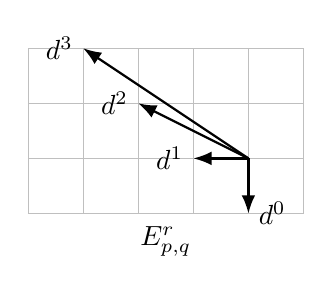
\begin{tikzpicture}[>=Latex, scale=0.7, baseline=(O)]
	\draw[very thin, gray!50] (1,-1) grid (-4,2);
	\draw[thick, ->] (0,0) -- (0,-1) node[right] {$d^0$};
	\draw[thick, ->] (0,0) -- (-1,0) node[left] {$d^1$};
	\draw[thick, ->] (0,0) -- (-2,1) node[left] {$d^2$};
	\draw[thick, ->] (0,0) -- (-3,2) node[left] {$d^3$};
	\node at (-1.5,-1.5) {$E^r_{p,q}$};
	\coordinate (O) at (-1.5,0.5);
\end{tikzpicture}\end{center}

% segment-id: o014.li2.chapter5.general-spectral-sequences.p014
Dalam versi mana pun, mengikuti pola sebelumnya kita dapat mendefinisikan
objek-objek $B_r^p\subset Z_r^p$, $B_r^{p,q}\subset Z_r^{p,q}$,
$E_\infty^p$, $E_\infty^{p,q}$, serta
$B^r_p\subset Z^r_p$, $B^r_{p,q}\subset Z^r_{p,q}$,
$E^\infty_p$, $E^\infty_{p,q}$, dan seterusnya.

% segment-id: o014.li2.chapter5.general-spectral-sequences.e002
\begin{example}[Kasus dengan lebar hingga]\label{eg:SS-finite-width}
	Dalam banyak situasi umum, suku-suku taknol suatu barisan spektral
	bergradasi ganda terkonsentrasi pada pita horizontal (atau vertikal)
	selebar $s$, dengan $s\in\Z_{\geq0}$, seperti pada gambar berikut:
	\[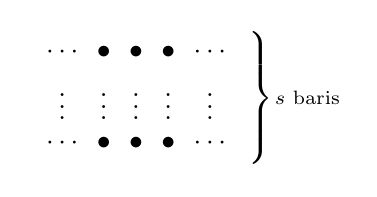
\begin{tikzpicture}[baseline]
		\matrix (M) [matrix of math nodes, right delimiter=\}] {
			\cdots & \bullet & \bullet & \bullet & \cdots \\
			\vdots & \vdots & \vdots & \vdots & \vdots \\
			\cdots & \bullet & \bullet & \bullet & \cdots \\
		};
		\node[right=2em] at (M-2-5) {\scriptsize \text{$s$ baris}};
	\end{tikzpicture} \quad \text{atau} \quad 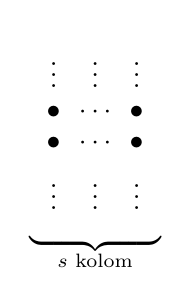
\begin{tikzpicture}[baseline]
		\matrix (M) [matrix of math nodes, below delimiter=\}] {
			\vdots & \vdots & \vdots \\
			\bullet & \cdots & \bullet \\
			\bullet & \cdots & \bullet \\
			\vdots & \vdots & \vdots \\
		};
		\node[below=2em] at (M-4-2) {\scriptsize \text{$s$ kolom}};
	\end{tikzpicture}\]
	Dengan memperhatikan arah panah, tampak bahwa syarat $r>s$ (atau $r\geq s$)
	mengakibatkan $d_r^{p,q}=0$ untuk semua $p,q$; dalam keadaan ini barisan
	spektral mengalami degenerasi pada halaman $E_r$. Kasus homologis serupa.
\end{example}

% segment-id: o014.li2.chapter5.general-spectral-sequences.d005
\begin{definition}\label{def:bdd-ss}
	\index{barisan spektral!terbatas (bounded)}
	Misalkan $\mathscr{E}$ adalah barisan spektral bergradasi ganda kohomologis
	(atau homologis), dan $r\in\Z$. Jika untuk setiap $n\in\Z$ hanya terdapat
	berhingga banyak pasangan $(p,q)\in\Z^2$ yang memenuhi $p+q=n$ dan
	$E_r^{p,q}\neq0$ (atau $E^r_{p,q}\neq0$), maka $E_r$ (atau $E^r$)
	disebut \emph{terbatas}.
\end{definition}

% segment-id: o014.li2.chapter5.general-spectral-sequences.p015
Dari $E_{r+1}\simeq\Hm(E_r,d_r)$ terlihat bahwa
$E_r^{p,q}=0\implies E_{r+1}^{p,q}=0$. Khususnya, keterbatasan $E_r$
mengakibatkan keterbatasan $E_{r+1}$. Kasus homologis serupa.

% segment-id: o014.li2.chapter5.general-spectral-sequences.t003
\begin{proposition}
	Misalkan barisan spektral bergradasi ganda kohomologis (atau homologis)
	$\mathscr{E}$ mempunyai $E_r$ (atau $E^r$) yang terbatas. Untuk setiap
	$(p,q)\in\Z^2$ terdapat $r(p,q)$ sedemikian sehingga, jika
	$r\geq r(p,q)$, maka $E_r^{p,q}=E_{r+1}^{p,q}$ (atau
	$E^r_{p,q}=E^{r+1}_{p,q}$). Akibatnya, limit $\mathscr{E}$ ada dan
	memenuhi $E_r^{p,q}=E_\infty^{p,q}$ (atau
	$E^r_{p,q}=E^\infty_{p,q}$).
\end{proposition}
\begin{proof}
	Cukup bahas kasus $E_r$. Misalkan $n$ tetap. Karena sifat keterbatasan, untuk
	$r$ yang cukup besar dan semua $(p,q)$ dengan $p+q=n$, berlaku
	$E_r^{p-r,q+r-1}=0$, sehingga $B_r^{p,q}=0$. Dengan cara yang sama, untuk
	$r$ yang cukup besar berlaku $E_r^{p+r,q-r+1}=0$, sehingga
	$Z_r^{p,q}=E_r^{p,q}$. Ini membuktikan pernyataan tersebut.
\end{proof}

% segment-id: o014.li2.chapter5.general-spectral-sequences.d006
\begin{definition}\label{def:quadrant-ss}
	Misalkan $\mathscr{E}$ adalah barisan spektral bergradasi ganda kohomologis
	(atau homologis), dan $r\in\Z$. Jika $E_r^{p,q}\neq0$ (atau
	$E^r_{p,q}\neq0$) hanya mungkin untuk $p,q\geq0$, maka $E_r$ (atau $E^r$)
	dikatakan terletak di kuadran pertama. Kasus untuk kuadran-kuadran lain
	didefinisikan dengan cara serupa.
\end{definition}

% segment-id: o014.li2.chapter5.general-spectral-sequences.p016
$E_r$ yang terletak di kuadran pertama atau ketiga jelas terbatas. Dari
$E_{r+1}\simeq\Hm(E_r,d_r)$ tampak bahwa jika $E_r$ terletak di kuadran
pertama, dan seterusnya, maka $E_{r+1}$ juga demikian. Kasus homologis serupa.

% segment-id: o014.li2.chapter5.general-spectral-sequences.r001
\begin{remark}[Perhitungan tepi]\label{rem:edge-computing}
	Barisan spektral yang terletak di kuadran pertama sangat umum dijumpai.
	Untuk versi kohomologis, suku tepinya $E_r^{\bullet,0}$ dan
	$E_r^{0,\bullet}$ mempunyai sifat khusus. Misalkan $p,q\geq1$. Dengan
	menelaah arah $d_r$ dan mengingat bahwa
	$E_{r+1}\simeq\Hm(E_r,d_r)$, kita memperoleh
	\begin{equation}\label{eqn:edge-ss-coh}\begin{array}{cc}
		E_2^{p,0}\twoheadrightarrow E_3^{p,0}\twoheadrightarrow\cdots
		\twoheadrightarrow E_{p+1}^{p,0}=E_\infty^{p,0}
		& \text{($\because$ semua $d$ yang keluar bernilai $0$)}, \\
		E_\infty^{0,q}=E_{q+2}^{0,q}\hookrightarrow E_{q+1}^{0,q}
		\hookrightarrow\cdots\hookrightarrow E_2^{0,q}\hookrightarrow E_1^{0,q}
		& \text{($\because$ semua $d$ yang masuk bernilai $0$)}.
	\end{array}\end{equation}
	Barisan spektral bergradasi ganda homologis di kuadran pertama memiliki
	sifat yang bersesuaian:
	\begin{equation}\label{eqn:edge-ss-ho}\begin{array}{cc}
		E^\infty_{p,0}=E^{p+1}_{p,0}\hookrightarrow E^p_{p,0}
		\hookrightarrow\cdots\hookrightarrow E^3_{p,0}\hookrightarrow E^2_{p,0}
		& \text{($\because$ semua $d$ yang masuk bernilai $0$)}, \\
		E^1_{0,q}\twoheadrightarrow E^2_{0,q}\twoheadrightarrow\cdots
		\twoheadrightarrow E^{q+2}_{0,q}=E^\infty_{0,q}
		& \text{($\because$ semua $d$ yang keluar bernilai $0$)}.
	\end{array}\end{equation}
	\index{morfisme tepi (edge morphism)}

	Morfisme yang berasal dari \eqref{eqn:edge-ss-coh} atau
	\eqref{eqn:edge-ss-ho} secara bersama-sama disebut \emph{morfisme tepi}.
	Dari uraian di atas diperoleh barisan eksak berikut ($p\geq2$):
	\begin{equation}\label{eqn:low-exact-coh}
		0\to E^{0,p-1}_\infty\to E^{0,p-1}_p\xrightarrow{d}E^{p,0}_p
		\to E^{p,0}_\infty\to0,
	\end{equation}
	dengan semua morfisme selain $d$ merupakan morfisme tepi. Terdapat pula
	versi homologis dari barisan eksak tersebut ($p\geq2$):
	\begin{equation}\label{eqn:low-exact-ho}
		0\to E^\infty_{p,0}\to E^p_{p,0}\xrightarrow{d}E^p_{0,p-1}
		\to E^\infty_{0,p-1}\to0.
	\end{equation}
	Pembaca pemula sangat dianjurkan untuk menggambar sendiri arah morfisme
	$d$ yang melibatkan suku-suku ini, menentukan kapan morfisme tersebut
	bernilai $0$, lalu memverifikasi semua pernyataan di atas.
\end{remark}

% Unit 066 terjemahan Bahasa Indonesia dari chapter5.tex baris 350--467.
% Sumber: Methods of Algebra, Volume 2, commit
% 9a5803ff77dd3257484cb177f851a73770a59dd3 (CC BY 4.0).
% stable-unit-id: o014.aljabr2.chapter5.exact-couples
% Cakupan: Bagian 5.3 lengkap.

% segment-id: o014.li2.chapter5.exact-couples.h001
\section{Pasangan eksak}\label{sec:exact-couples}
\hypertarget{o014.aljabr2.chapter5.exact-couples}{ }

% segment-id: o014.li2.chapter5.exact-couples.p001
Beberapa jenis barisan spektral yang umum dipakai berasal dari pasangan eksak,
sebuah temuan W.\ Massey. Untuk menangkap gagasan utamanya, mula-mula kita
kembali ke kasus tanpa derajat.

% segment-id: o014.li2.chapter5.exact-couples.d001
\begin{definition}[Pasangan eksak]\label{def:exact-couple}
	\index{pasangan eksak (exact couple)}
	Pasangan eksak pada kategori abelian $\mathcal{A}$ adalah diagram eksak
	berikut dalam $\mathcal{A}$:
	\[\begin{tikzcd}[column sep=small]
		D \arrow[rr, "i"] & & D \arrow[ld, "j"] \\
		& E \arrow[lu, "k"] &
	\end{tikzcd}\]
	Morfisme antara data $\mathscr{C}:=(D,E,i,j,k)$ didefinisikan dengan
	cara yang jelas.
\end{definition}

% segment-id: o014.li2.chapter5.exact-couples.p002
Untuk suatu pasangan eksak $\mathscr{C}=(D,E,i,j,k)$, definisikan
$d:=jk:E\to E$. Maka $dj=jkj=0$ dan $kd=kjk=0$, sehingga $d^2=0$.
Dari syarat keeksakan segera diperoleh faktorisasi berikut:
\begin{equation}\label{eqn:exact-couple-aux}
	\begin{tikzcd}
		D \arrow[r, "j"] \arrow[twoheadrightarrow, d, "i"'] &
		\Ker(d) \arrow[twoheadrightarrow, d] \\
		i(D) \arrow[r, "{\exists!\;j'}"'] & \Hm(E,d)
	\end{tikzcd} \quad \begin{tikzcd}
		\Ker(d) \arrow[r, "k"] \arrow[twoheadrightarrow, d] & i(D) \\
		\Hm(E,d) \arrow[ru, "{\exists!\;k'}"'] &
	\end{tikzcd}
\end{equation}
Selain itu, definisikan $E':=\Hm(E,d)$, $D':=i(D)$, dan
$i':=i|_{i(D)}:D'\to D'$.

% segment-id: o014.li2.chapter5.exact-couples.l001
\begin{lemma}
	Untuk suatu pasangan eksak $\mathscr{C}=(D,E,i,j,k)$, data yang dibangun di
	atas,
	\[ \mathscr{C}'=(D',E',i',j',k'):\quad
	\begin{tikzcd}[column sep=small]
		D' \arrow[rr, "{i'}"] & & D' \arrow[ld, "{j'}"] \\
		& E' \arrow[lu, "{k'}"] &
	\end{tikzcd} \]
	juga merupakan pasangan eksak.
\end{lemma}
\begin{proof}
	Dengan menelaah \eqref{eqn:exact-couple-aux} dan menggunakan syarat
	keeksakan, kita memperoleh
	\begin{align*}
		\Ker(i') &= i(D)\cap\Ker(i)=\Ker(j)\cap k(E) \\
		&=\Image\left[\Ker(d)\xrightarrow{k}i(D)\right]=\Image(k'), \\
		\Ker(j') &= i\left(j^{-1}(jk(E))\right) \\
		&=i\left(k(E)+\Ker(j)\right)=i\left(i(D)\right)=\Image(i'), \\
		\Ker(k') &= (\Ker(k)\cap\Ker(d))/\Image(d)
		=(j(D)\cap\Ker(jk))/\Image(d) \\
		&=j(D)/\Image(d)=\Image(j').
	\end{align*}
	Jadi diagram segitiga yang baru tetap eksak.
\end{proof}

% segment-id: o014.li2.chapter5.exact-couples.p003
Dengan mengiterasi prosedur ini diperoleh barisan pasangan eksak
$(\mathscr{C}_{(r)})_{r\geq1}$, dengan
$\mathscr{C}_{(1)}=\mathscr{C}$ dan
$\mathscr{C}_{(r+1)}=\mathscr{C}_{(r)}'$ untuk $r\geq1$. Jika
$\mathscr{C}_{(r)}=(D_r,E_r,i_r,j_r,k_r)$, maka
$(E_r,d_r:=j_rk_r)_{r\geq1}$ memberikan suatu barisan spektral.

% segment-id: o014.li2.chapter5.exact-couples.l002
\begin{lemma}\label{prop:exact-couple-Z-B}
	Untuk barisan spektral $(E_r,d_r)_{r\geq1}$ yang diperoleh dari pasangan
	eksak $\mathscr{C}=(D,E,i,j,k)$, definisikan keluarga subobjek
	$\overline{B}_r\subset\overline{Z}_r$ dari $E=E_1$ menurut
	\eqref{eqn:spectral-sequence-Z-B}. Garis atas dipakai karena indeksnya
	dimulai dari $r=1$; lihat Proposisi~\ref{prop:differential-exact-couple} di
	bawah. Untuk $r\geq0$ berlaku
	\begin{gather*}
		\overline{B}_{r+1}=j\left(\Ker(i^r)\right)
		\subset k^{-1}\left(\Image(i^r)\right)=\overline{Z}_{r+1}; \\
		\overline{B}_\infty=j\left(\bigcup_{r\geq2}\Ker(i^r)\right)
		\subset k^{-1}\left(\bigcap_{r\geq2}\Image(i^r)\right)
		=\overline{Z}_\infty,
	\end{gather*}
	dengan syarat $\bigcup_r$ dan $\bigcap_r$ yang bersangkutan ada. Lebih
	tepatnya, pasangan eksak $\mathscr{C}_{(r+1)}$ secara kanonik isomorfik
	dengan
	\[\begin{tikzcd}[column sep=tiny]
		i^rD \arrow[rr, "i"] & & i^rD \arrow[ld, "{\overline{j}_{r+1}}"] \\
		& \dfrac{k^{-1}(i^rD)}{j(\Ker(i^r))}
		\arrow[lu, "{\overline{k}_{r+1}}"] &
	\end{tikzcd}\]
	dengan $\overline{k}_{r+1}$ diinduksi oleh $k:E\to D$, sedangkan
	$\overline{j}_{r+1}$ dicirikan oleh diagram komutatif
	\[\begin{tikzcd}
		D \arrow[r, "{i^r}"] \arrow[d, "j"'] &
		i^rD \arrow[d, "{\overline{j}_{r+1}}"] \\
		k^{-1}(i^rD) \arrow[twoheadrightarrow, r] &
		\dfrac{k^{-1}(i^rD)}{j(\Ker(i^r))}.
	\end{tikzcd}\]
\end{lemma}
\begin{proof}
	Deskripsi pasangan eksak $\mathscr{C}_{(r+1)}$ dapat dibuktikan secara
	rekursif. Kasus $r=0$ langsung ($i^0=\identity$), sedangkan
	deskripsi $\overline{B}_{r+1}$ dan $\overline{Z}_{r+1}$ merupakan akibat
	langsungnya. Karena rinciannya cukup rutin, rincian tersebut tidak dituliskan.
	Pernyataan $\overline{B}_\infty\subset\overline{Z}_\infty$ mengikuti dari
	Lema~\ref{prop:image-sum-preimage-intersection}~(ii).
\end{proof}

% segment-id: o014.li2.chapter5.exact-couples.p004
Selanjutnya kita jelaskan cara membangun pasangan eksak dari objek diferensial.

% segment-id: o014.li2.chapter5.exact-couples.t001
\begin{proposition}\label{prop:differential-exact-couple}
	Misalkan $\alpha:(D,d)\to(D,d)$ adalah monomorfisme dalam $\mathcal{A}_d$,
	dan tuliskan $d_\alpha$ untuk morfisme yang diinduksi oleh $d$ pada
	$\Coker(\alpha)$. Maka terdapat pasangan eksak
	\[\begin{tikzcd}[column sep=tiny]
		\Hm(D,d) \arrow[rr, "{i=\Hm(\alpha)}"] & &
		\Hm(D,d) \arrow[ld, "j"] \\
		& \Hm(\Coker(\alpha),d_\alpha) \arrow[lu, "k"] &
	\end{tikzcd}\]
	Ambil prapeta $\overline{B}_{r+1}\subset\overline{Z}_{r+1}$ dalam
	$E_0:=\Coker(\alpha)$, dan tuliskan
	\[ 0=:B_0\subset B_1\subset B_2\subset\cdots\subset Z_2\subset Z_1
	\subset Z_0:=\Coker(\alpha). \]
	Untuk semua $r\geq0$ berlaku:
	\begin{itemize}
		\item $B_{r+1}$ adalah citra
		$(\alpha^r)^{-1}(dD)\subset D$ dalam $\Coker(\alpha)$;
		\item $Z_{r+1}$ adalah citra
		$d^{-1}(\alpha^{r+1}D)\subset D$ dalam $\Coker(\alpha)$;
		\item $d_{r+1}\in\End(Z_{r+1}/B_{r+1})$ diinduksi oleh
		$d^{-1}(\alpha^{r+1}D)\xrightarrow{d}\alpha^{r+1}D
		\xleftarrow[\sim]{\alpha^{r+1}}D$.
	\end{itemize}
	Khususnya, terdapat isomorfisme kanonik
	\[ E_{r+1}\simeq\dfrac{Z_{r+1}}{B_{r+1}}
	\simeq\dfrac{d^{-1}(\alpha^{r+1}D)+\alpha D}
	{(\alpha^r)^{-1}(dD)+\alpha D},\qquad r\in\Z_{\geq1}. \]
\end{proposition}
\begin{proof}
	Pasangan eksak tersebut diperoleh dengan menerapkan
	Lema~\ref{prop:diff-obj-triangle} (dengan
	$T=\identity_{\mathcal{A}}$) pada barisan eksak pendek dalam
	$\mathcal{A}_d$
	\[ 0\to(D,d)\xrightarrow{\alpha}(D,d)
	\to(\Coker(\alpha),d_\alpha)\to0. \]
	Khususnya, morfisme $j$ diinduksi oleh
	$D\twoheadrightarrow\Coker(\alpha)$, sedangkan $k$ pada dasarnya merupakan
	morfisme penghubung dalam barisan eksak panjang. Deskripsi $B_{r+1}$ tidak
	lain merupakan versi Lema~\ref{prop:exact-couple-Z-B} yang diangkat ke $E_0$.
	Untuk $Z_{r+1}$, selain lema tersebut, unsur pentingnya ialah deskripsi
	morfisme penghubung
	$k:\Hm(\Coker(\alpha),d_\alpha)\to\Hm(D,d)$. Dengan meninjau kembali
	konstruksi \eqref{eqn:snake-conn} dan
	\eqref{eqn:long-exact-sequence-ses-aux}, terlihat bahwa morfisme ini
	diinduksi oleh morfisme tengah $\overline{d}$ dalam diagram komutatif dengan
	baris-baris eksak
	\[\begin{tikzcd}
		& \Coker(d) \arrow[r] \arrow[d, "\overline{d}"'] &
		\Coker(d) \arrow[r] \arrow[d, "\overline{d}"'] &
		\Coker(d_\alpha) \arrow[d, "\overline{d_\alpha}"] \arrow[r] & 0 \\
		0 \arrow[r] & \Ker(d) \arrow[r, "\alpha"'] &
		\Ker(d) \arrow[r] & \Ker(d_\alpha) &
	\end{tikzcd}\]
	sedangkan $\overline{d}$ sendiri berasal dari $d:D\to D$. Pemeriksaan
	lainnya cukup panjang tetapi tidak sulit; pembaca dapat memulai dari kasus ketika
	$\mathcal{A}$ adalah kategori modul.
\end{proof}

% segment-id: o014.li2.chapter5.exact-couples.p005
Dengan demikian, barisan spektral yang diberikan oleh objek diferensial dapat
dimulai dari $0$ dengan mendefinisikan $E_0:=\Coker(\alpha)$ dan
$d_0:=d_\alpha$.

% segment-id: o014.li2.chapter5.exact-couples.p006
Untuk kategori abelian dengan translasi $(\mathcal{A},T)$, karena morfisme
berderajat tetap dapat dikomposisikan dan konsep-konsep seperti keeksakan tetap
tersedia, teori pasangan eksak mudah diperluas ke keadaan ketika $i,j,k$
memiliki derajat. Sebagai contoh, dalam situasi yang akan dibahas dalam
\S\ref{sec:filtered-diff-ss}, kita dapat mempertimbangkan pasangan eksak
\[\begin{tikzcd}[column sep=tiny]
	D \arrow[rr, "{-1}"] & & D \arrow[ld, "{+1}"] \\
	& E \arrow[lu] &
\end{tikzcd} \xlongequal{\text{dibentangkan}} \left[
	\begin{tikzcd}[column sep=0ex, every cell/.append style={font=\small}]
		\cdots & TD \arrow[rr] \arrow[ld] & & D \arrow[rr] \arrow[ld] & &
		T^{-1}D \arrow[rr] \arrow[ld] & & T^{-2}D \arrow[ld] & \cdots \\
		\cdots & & TE \arrow[lu] & & E \arrow[lu] & &
		T^{-1}E \arrow[lu] & & \cdots \arrow[lu]
	\end{tikzcd}
\right]. \]
Tuliskan pasangan eksak ini sebagai $\mathscr{C}$. Perluasan alami
Lema~\ref{prop:exact-couple-Z-B} ke kasus berderajat memperlihatkan bahwa
$\mathscr{C}_{(r)}$ berbentuk
$\begin{tikzcd}[column sep=tiny, row sep=small]
	\bullet \arrow[rr, "{-1}"] & & \bullet \arrow[ld, "{+r}"] \\
	& \bullet \arrow[lu] &
\end{tikzcd}$.
Karena itu $d_r=j_rk_r$ merupakan morfisme berderajat $r$. Barisan spektral
yang diperoleh dengan cara ini bergradasi.

% Unit 067 terjemahan Bahasa Indonesia dari chapter5.tex baris 468--577.
% Sumber: Methods of Algebra, Volume 2, commit
% 9a5803ff77dd3257484cb177f851a73770a59dd3 (CC BY 4.0).
% stable-unit-id: o014.aljabr2.chapter5.filtered-differential-spectral-sequence
% Cakupan: Bagian 5.4 lengkap.

% segment-id: o014.li2.chapter5.filtered-differential-spectral-sequence.h001
\section{Barisan spektral objek diferensial terfiltrasi}
\label{sec:filtered-diff-ss}
\hypertarget{o014.aljabr2.chapter5.filtered-differential-spectral-sequence}{ }

% segment-id: o014.li2.chapter5.filtered-differential-spectral-sequence.p001
Sepanjang bagian ini, kita bekerja dengan kategori abelian dengan translasi
$(\mathcal{A},T)$.

% segment-id: o014.li2.chapter5.filtered-differential-spectral-sequence.d001
\begin{definition}\label{def:filtered-diffop}
	\index{objek diferensial!terfiltrasi (filtered)}
	Objek $(X,d)\in\Obj((\mathcal{A},T)_d)$ yang dilengkapi filtrasi
	$\left(\mathrm{F}^\bullet X,d_{\mathrm{F}^\bullet X}\right)$ disebut
	\emph{objek diferensial terfiltrasi} pada $(\mathcal{A},T)$. Dalam keadaan
	ini, $\gr^pX$ juga dilengkapi secara alami dengan
	$\gr^pd:\gr^pX\to T\gr^pX$, sehingga
	$(\gr^pX,\gr^pd)\in\Obj((\mathcal{A},T)_d)$.
\end{definition}

% segment-id: o014.li2.chapter5.filtered-differential-spectral-sequence.p002
Karena $d_{\mathrm{F}^pX}$ pada subobjek $\mathrm{F}^pX$ sebaiknya dipahami
sebagai restriksi $d:X\to TX$, selanjutnya kita tetap menuliskannya sebagai
$d$. Definisi serupa dapat diberikan untuk filtrasi menaik, dengan pernyataan
yang sepenuhnya dual.

% segment-id: o014.li2.chapter5.filtered-differential-spectral-sequence.p003
Kita kembali ke barisan spektral. Bagian sebelumnya menjelaskan cara membangun
pasangan eksak dari objek diferensial. Sekarang perhatikan objek diferensial
terfiltrasi $(X,d,\mathrm{F}^\bullet X)$ pada $\mathcal{A}$. Tuliskan
$S:(Y^p)_p\mapsto(Y^{p+1})_p$ untuk funktor translasi standar pada
$\mathcal{A}^{\Z}$; jelas bahwa $S$ berkomutasi dengan $T$ yang bekerja pada
setiap $Y^p$. Karena itu morfisme yang akan dibahas mempunyai dua jenis
derajat: ``derajat filtrasi'' yang bersesuaian dengan $S$, dan ``derajat
internal'' yang bersesuaian dengan $T$. Untuk sementara kita berfokus pada
yang pertama.

% segment-id: o014.li2.chapter5.filtered-differential-spectral-sequence.p004
Karena filtrasi tersebut menurun, terdapat monomorfisme
\[ \alpha:\left(\mathrm{F}^{p+1}X,d\right)_{p\in\Z}
	\hookrightarrow S^{-1}\left(\mathrm{F}^{p+1}X,d\right)_{p\in\Z}
	=\left(\mathrm{F}^{p}X,d\right)_{p\in\Z}. \]
Dengan demikian,
$E_0:=\Coker(\alpha)=\left(\gr^pX,\gr^pd\right)_{p\in\Z}$ dan
$E_1^p=\Hm(\gr^pX,\gr^pd)$.

% segment-id: o014.li2.chapter5.filtered-differential-spectral-sequence.p005
Pandang $\alpha$ sebagai morfisme berderajat $-1$ dalam
$\mathcal{A}^{\Z}$ (terhadap $S$). Dengan menerapkan
Proposisi~\ref{prop:differential-exact-couple}, kita memperoleh pasangan eksak
berderajat pada $\mathcal{A}^{\Z}$:
\[\mathscr{C}=\left[\begin{tikzcd}[column sep=tiny]
	\Hm\left(\mathrm{F}^{p+1}X,d\right)_p
	\arrow[rr, "-1"', "{\Hm(\alpha)}"] & &
	\Hm\left(\mathrm{F}^{p+1}X,d\right)_p \arrow[ld, "{+1}"] \\
	& \Hm\left(\gr^pX,\gr^pd\right)_p \arrow[lu] &
\end{tikzcd}\right],\]
di mana panah $\nwarrow$ berasal dari morfisme penghubung yang diinduksi oleh
barisan eksak pendek
$0\to(\mathrm{F}^{p+1}X,d)\to(\mathrm{F}^pX,d)
\to(\gr^pX,\gr^pd)\to0$.

% segment-id: o014.li2.chapter5.filtered-differential-spectral-sequence.p006
Barisan
$\mathscr{E}=(E_r^p,d_r^p)_{\substack{r\geq0\\p\in\Z}}$ yang diperoleh
dengan cara ini disebut barisan spektral yang ditentukan oleh
$\mathrm{F}^\bullet X$ dalam $\mathcal{A}^{\Z}$. Pada akhir
\S\ref{sec:exact-couples} telah dijelaskan bahwa $d_r$ adalah morfisme
berderajat $r$ terhadap $S$, yaitu
\[ d_r=\left(d_r^p:E_r^p\to(S^rE_r)^p=E_r^{p+r}\right)_{p\in\Z}; \]
tentu saja, derajat $d_r$ juga dapat dibaca dari rumus dalam
Proposisi~\ref{prop:differential-exact-couple}.

% segment-id: o014.li2.chapter5.filtered-differential-spectral-sequence.p007
Dengan kata lain, objek diferensial terfiltrasi
$(X,d,\mathrm{F}^\bullet X)$ menghasilkan barisan spektral bergradasi
kohomologis sebagaimana dalam Definisi~\ref{def:graded-spectral-sequence}.
Perhatikan bahwa $d_r^p$ di sini mungkin juga mempunyai derajat internal
(kecuali jika $T=\identity_{\mathcal{A}}$); derajat ini tidak dicantumkan
dalam notasi dan akan dirinci dalam \S\ref{sec:filtered-cplx-ss}.

% segment-id: o014.li2.chapter5.filtered-differential-spectral-sequence.p008
Menurut pola \eqref{eqn:spectral-sequence-Z-B}, definisikan subobjek dari
$Z_0=(\gr^pX,\gr^pd)_p$ sebagai
\[ B_r=(B_r^p)_p\subset(Z_r^p)_p=Z_r. \]

% segment-id: o014.li2.chapter5.filtered-differential-spectral-sequence.p009
Untuk menyederhanakan notasi, pernyataan berikut tidak menampilkan derajat
internal $d$; ini setara dengan meninjau kasus khusus
$T=\identity_{\mathcal{A}}$. Perluasan ke kasus umum bersifat rutin: funktor
translasi cukup disisipkan pada tempat yang tepat dalam setiap kemunculan
$d^{-1}(\cdots)$ atau $d(\cdots)$ agar ungkapannya bermakna secara ketat.

% segment-id: o014.li2.chapter5.filtered-differential-spectral-sequence.t001
\begin{proposition}\label{prop:filtered-diff-E}
	Untuk objek diferensial terfiltrasi $(X,d,\mathrm{F}^\bullet X)$, barisan
	spektral terkait memenuhi
	\begin{align*}
		Z_r^p&=\dfrac{\left(\mathrm{F}^pX\cap d^{-1}\mathrm{F}^{p+r}X\right)
		+\mathrm{F}^{p+1}X}{\mathrm{F}^{p+1}X}, \\
		B_r^p&=\dfrac{\left(\mathrm{F}^pX\cap d\mathrm{F}^{p-r+1}X\right)
		+\mathrm{F}^{p+1}X}{\mathrm{F}^{p+1}X},
	\end{align*}
	dan $d_r^p:E_r^p\to E_r^{p+r}$ diinduksi oleh morfisme
	$d^{-1}\mathrm{F}^{p+r}X\xrightarrow{d}
	\mathrm{F}^{p+r}X\cap\Ker(d)$.
\end{proposition}
\begin{proof}
	Perhatikan bahwa komponen berderajat $p$ dari $\alpha^r$ dapat dipandang
	sebagai penyertaan $\mathrm{F}^pX\hookrightarrow\mathrm{F}^{p-r}X$ atau
	$\mathrm{F}^{p+r}X\hookrightarrow\mathrm{F}^pX$. Pernyataan tersebut
	merupakan versi bergradasi dari
	Proposisi~\ref{prop:differential-exact-couple}.
\end{proof}

% segment-id: o014.li2.chapter5.filtered-differential-spectral-sequence.p010
Karena $\varinjlim$ dan $\varprojlim$ dalam $\mathcal{A}^{\Z}$ diambil
derajat demi derajat, $E_\infty=(E_\infty^p)_{p\in\Z}$ dapat dituliskan
sebagai
\begin{equation}\label{eqn:filtered-diff-infty}
	E_\infty^p=\dfrac{Z_\infty^p}{B_\infty^p}
	=\dfrac{\bigcap_r\left((\mathrm{F}^pX\cap d^{-1}\mathrm{F}^{p+r}X)
	+\mathrm{F}^{p+1}X\right)}
	{\bigcup_r\left((\mathrm{F}^pX\cap d\mathrm{F}^{p-r+1}X)
	+\mathrm{F}^{p+1}X\right)},
\end{equation}
dengan syarat $\bigcap$ dan $\bigcup$ yang ditampilkan ada untuk setiap $p$.

% segment-id: o014.li2.chapter5.filtered-differential-spectral-sequence.r001
\begin{remark}
	Proposisi~\ref{prop:filtered-diff-E} mengenai barisan spektral dari objek
	diferensial terfiltrasi merupakan landasan pembahasan selanjutnya dalam bab
	ini. Proposisi tersebut merupakan penerapan pasangan eksak, tetapi rumus
	dalam Proposisi~\ref{prop:filtered-diff-E} juga dapat dipandang sebagai
	definisi langsung, lalu semua sifat yang diperlukan bagi barisan spektral
	diperiksa dari rumus itu.
\end{remark}

% segment-id: o014.li2.chapter5.filtered-differential-spectral-sequence.p011
Berdasarkan deskripsi di atas, barisan spektral $E_r^p$ dari
$(X,d,\mathrm{F}^\bullet X)$ dapat dipandang sebagai proses pendekatan bertahap
terhadap $\Hm(X,d)$. Untuk memperjelas arti ``mendekati'', kita
memerlukan konsep berikut.

% segment-id: o014.li2.chapter5.filtered-differential-spectral-sequence.d002
\begin{definition}[Filtrasi terinduksi]\label{def:induced-filtration-H}
	\index{filtrasi!terinduksi (induced)}
	Untuk suatu objek diferensial terfiltrasi
	$(X,d,\mathrm{F}^\bullet X)$ pada $(\mathcal{A},T)$, objek $\Hm(X,d)$
	dilengkapi filtrasi terinduksi
	\[ \mathrm{F}^p\Hm(X,d):=
	\Image\left[\mathrm{F}^pX\cap\Ker(d)\to\Hm(X,d)\right],
	\qquad p\in\Z. \]
\end{definition}

% segment-id: o014.li2.chapter5.filtered-differential-spectral-sequence.l001
\begin{lemma}\label{prop:induced-filtration-H}
	Jika terdapat $N$ dengan $\mathrm{F}^NX=0$, maka
	$\mathrm{F}^N\Hm(X,d)=0$. Jika $\mathrm{F}^\bullet X$ merupakan filtrasi
	menyeluruh menurut Definisi~\ref{def:filtration-properties}, maka
	$\mathrm{F}^\bullet\Hm(X,d)$ juga menyeluruh.
\end{lemma}
\begin{proof}
	Bagian pertama langsung; kita buktikan bagian kedua. Menurut
	Lema~\ref{prop:image-sum-preimage-intersection}~(ii),
	$\bigcup_p\mathrm{F}^p\Hm(X,d)$ adalah citra dari
	$\bigcup_p(\mathrm{F}^pX\cap\Ker(d))$, sedangkan
	\eqref{eqn:exhaustion-intersection} memberikan
	\[ \bigcup_p\left(\mathrm{F}^pX\cap\Ker(d)\right)
	=\left(\bigcup_p\mathrm{F}^pX\right)\cap\Ker(d)=\Ker(d). \]
	Selain itu, jika terdapat $M$ dengan $\mathrm{F}^MX=X$, tentu saja
	$\mathrm{F}^M\Hm(X,d)=\Hm(X,d)$.
\end{proof}

% segment-id: o014.li2.chapter5.filtered-differential-spectral-sequence.p012
Versi bergradasi dari pengamatan ini akan diterapkan dalam
\S\ref{sec:filtered-cplx-ss}.

% segment-id: o014.li2.chapter5.filtered-differential-spectral-sequence.l002
\begin{lemma}\label{prop:induced-filtration-gr}
	Untuk objek diferensial terfiltrasi $(X,d,\mathrm{F}^\bullet X)$ dan setiap
	$p\in\Z$, terdapat isomorfisme kanonik
	\[ \gr^p\Hm(X,d)\simeq
	\dfrac{\mathrm{F}^pX\cap\Ker(d)}
	{(\mathrm{F}^{p+1}X\cap\Ker(d))
	 +(\mathrm{F}^pX\cap\Image(T^{-1}d))}. \]
\end{lemma}
\begin{proof}
	Uraikan definisi
	$\mathrm{F}^p\Hm(X,d)/\mathrm{F}^{p+1}\Hm(X,d)$ dan gunakan teorema
	isomorfisme standar untuk kategori abelian,
	Proposisi~\ref{prop:Abel-cat-isom-thm}, untuk memperoleh
	\begin{align*}
		\gr^p\Hm(X,d)
		&=\dfrac{(\mathrm{F}^pX\cap\Ker(d))+\Image(T^{-1}d)}
		{(\mathrm{F}^{p+1}X\cap\Ker(d))+\Image(T^{-1}d)} \\
		&=\dfrac{(\mathrm{F}^pX\cap\Ker(d))
		 +(\mathrm{F}^{p+1}X\cap\Ker(d))+\Image(T^{-1}d)}
		{(\mathrm{F}^{p+1}X\cap\Ker(d))+\Image(T^{-1}d)} \\
		&\simeq\dfrac{\mathrm{F}^pX\cap\Ker(d)}
		{((\mathrm{F}^{p+1}X\cap\Ker(d))+\Image(T^{-1}d))
		 \cap(\mathrm{F}^pX\cap\Ker(d))} \\
		&=\dfrac{\mathrm{F}^pX\cap\Ker(d)}
		{(\mathrm{F}^{p+1}X\cap\Ker(d))
		 +(\mathrm{F}^pX\cap\Image(T^{-1}d))}.
	\end{align*}
	Langkah terakhir memakai fakta bahwa $\mathrm{Sub}_X$ adalah kekisi
	modular\footnote{Artinya, untuk semua subobjek $A,A^\flat,B\subset X$ dengan
	$A^\flat\subset A$, berlaku
	$A^\flat+(A\cap B)=(A^\flat+B)\cap A$.}
	(Teorema~\ref{prop:subobject-modularity}), serta
	$\mathrm{F}^{p+1}X\cap\Ker(d)\subset\mathrm{F}^pX\cap\Ker(d)$ dan
	$\Image(T^{-1}d)\subset\Ker(d)$. Langkah-langkah lainnya standar.
\end{proof}

% segment-id: o014.li2.chapter5.filtered-differential-spectral-sequence.d003
\begin{definition-proposition}\label{def:diff-obj-convergence}
	\index{barisan spektral!konvergen lemah, konvergen kuat
	(weakly convergent, strongly convergent)}
	Untuk suatu objek diferensial terfiltrasi
	$(X,d,\mathrm{F}^\bullet X)$, bangun barisan spektral bergradasi
	kohomologis terkait $(E_r,d_r)_r$. Jika $\bigcap_r$ dan $\bigcup_r$ dalam
	\eqref{eqn:filtered-diff-infty} ada, maka limit $E_\infty$ ada, dan
	$\gr\Hm(X,d)$ yang ditentukan oleh filtrasi terinduksi dapat direalisasikan
	secara kanonik sebagai subkuosien dari $E_\infty$.
	\begin{itemize}
		\item Jika $\gr\Hm(X,d)=E_\infty$, maka barisan spektral
		$(E_r,d_r)_r$ disebut \emph{konvergen lemah}.
		\item Jika $(E_r,d_r)_r$ konvergen lemah dan
		$\mathrm{F}^\bullet\Hm(X,d)$ menyeluruh serta lengkap, maka barisan
		spektral $(E_r,d_r)_r$ disebut \emph{konvergen kuat}.
	\end{itemize}
\end{definition-proposition}
\begin{proof}
	Misalkan $p\in\Z$. Dari ungkapan untuk $E_\infty^p$ dalam
	\eqref{eqn:filtered-diff-infty}, pembilangnya memuat
	$(\mathrm{F}^pX\cap\Ker(d))+\mathrm{F}^{p+1}X$, sedangkan penyebutnya
	terkandung dalam
	$(\mathrm{F}^pX\cap\Image(T^{-1}d))+\mathrm{F}^{p+1}X$
	(ingat bahwa $d$ adalah morfisme $X\to TX$). Dengan demikian diperoleh
	subkuosien berikut dari $E_\infty^p$:
	\begin{multline*}
		\dfrac{(\mathrm{F}^pX\cap\Ker(d))+\mathrm{F}^{p+1}X}
		{(\mathrm{F}^pX\cap\Image(T^{-1}d))+\mathrm{F}^{p+1}X} \\
		\simeq\dfrac{\mathrm{F}^pX\cap\Ker(d)}
		{((\mathrm{F}^pX\cap\Image(T^{-1}d))+\mathrm{F}^{p+1}X)
		 \cap(\mathrm{F}^pX\cap\Ker(d))} \\
		=\dfrac{\mathrm{F}^pX\cap\Ker(d)}
		{(\mathrm{F}^pX\cap\Image(T^{-1}d))
		 +(\mathrm{F}^{p+1}X\cap\Ker(d))}.
	\end{multline*}
	Isomorfisme pertama bersifat standar. Kesamaan berikutnya memakai fakta
	bahwa $\mathrm{Sub}_X$ adalah kekisi modular, bersama
	$\mathrm{F}^pX\cap\Image(T^{-1}d)
	\subset\mathrm{F}^pX\cap\Ker(d)$ dan
	$\mathrm{F}^{p+1}X\subset\mathrm{F}^pX$. Sekarang terapkan
	Lema~\ref{prop:induced-filtration-gr}.
\end{proof}

% segment-id: o014.li2.chapter5.filtered-differential-spectral-sequence.p013
Definisi konvergensi sedikit berbeda-beda antar-rujukan.
Semua pernyataan di atas memiliki versi yang bersesuaian untuk objek
diferensial dengan filtrasi menaik $(X,d,\mathrm{F}_\bullet X)$ dan barisan
spektral bergradasi homologis terkait.

% Unit 068 terjemahan Bahasa Indonesia dari chapter5.tex baris 578--739.
% Sumber: Methods of Algebra, Volume 2, commit
% 9a5803ff77dd3257484cb177f851a73770a59dd3 (CC BY 4.0).
% stable-unit-id: o014.aljabr2.chapter5.filtered-complex-spectral-sequence
% Cakupan: Bagian 5.5 lengkap.

% segment-id: o014.li2.chapter5.filtered-complex-spectral-sequence.h001
\section{Barisan spektral kompleks terfiltrasi}\label{sec:filtered-cplx-ss}
\hypertarget{o014.aljabr2.chapter5.filtered-complex-spectral-sequence}{ }
\index{kompleks!terfiltrasi (filtered)}
\index{barisan spektral!dari kompleks terfiltrasi}

% segment-id: o014.li2.chapter5.filtered-complex-spectral-sequence.p001
Kita melanjutkan gagasan dari \S\ref{sec:filtered-diff-ss}, dengan kategori
abelian $\mathcal{A}$ tetap. Hasil
Proposisi~\ref{prop:filtered-diff-E} mengenai objek diferensial terfiltrasi
dapat diperluas agar morfisme $d$ boleh mempunyai derajat. Secara khusus,
teori ini dapat diterapkan pada kompleks terfiltrasi.

% segment-id: o014.li2.chapter5.filtered-complex-spectral-sequence.p002
Secara konkret, gantilah $\mathcal{A}$ sebelumnya dengan
$\mathcal{A}^{\Z}$ dan tuliskan $T$ untuk funktor translasinya. Menurut
Contoh~\ref{eg:cplx-as-diff}, objek $(X,d)$ dalam
$(\mathcal{A}^{\Z},T)_d$ dapat diidentifikasi dengan kompleks
$X\in\Obj(\cate{C}(\mathcal{A}))$. Jika selanjutnya kita mengambil filtrasi
menurun $(X,d,\mathrm{F}^\bullet X)$, maka
\begin{align*}
	\Hm(X,d)&=\left(\Hm^n(X)\right)_{n\in\Z}, \\
	\Hm\left(\mathrm{F}^pX,d\right)
	&=\left(\Hm^n\left(\mathrm{F}^pX\right)\right)_{n\in\Z}, \\
	\mathrm{F}^p\Hm^n(X)&:=
	\Image\left[\mathrm{F}^pX^n\cap\Ker(d_X^n)\to\Hm^n(X)\right]
	\quad\text{(Definisi~\ref{def:induced-filtration-H}).}
\end{align*}

% segment-id: o014.li2.chapter5.filtered-complex-spectral-sequence.p003
Jadi, $E_r$ dalam barisan spektral $\mathscr{E}$ yang dibangun sebelumnya
sebenarnya bernilai dalam $\mathcal{A}^{\Z\times\Z}$ dan merupakan objek
bergradasi ganda. Selain derajat filtrasi $p$, terdapat ``derajat internal''
$n$ yang berasal dari struktur kompleks; funktor translasi $S$ dan $T$ yang
bersesuaian dengan keduanya komutatif secara ketat. Kita telah mengetahui
bahwa derajat $d_r$ terhadap $S$ adalah $r$; sekarang kita tentukan derajatnya
terhadap $T$.

% segment-id: o014.li2.chapter5.filtered-complex-spectral-sequence.p004
\begin{itemize}
	\item Dalam pasangan eksak $\mathscr{C}_{(1)}$ yang dipakai untuk membangun
	$\mathscr{E}$, morfisme $\nwarrow$ berderajat $1$ terhadap $T$, sedangkan
	morfisme lainnya berderajat nol. Memang, $\nwarrow$ berasal dari morfisme
	penghubung kohomologi sehingga berderajat $1$ terhadap $T$, dan panah
	lainnya jelas berderajat nol.
	\item Dengan memakai deskripsi dalam Lema~\ref{prop:exact-couple-Z-B},
	pernyataan tersebut berlaku secara rekursif bagi $\mathscr{C}_{(r)}$ untuk
	semua $r$.
	\item Akibatnya, $d_r$ dan $d$ dalam $(X,d)$ sama-sama merupakan morfisme
	berderajat $1$ terhadap $T$. Hal ini juga langsung tampak dari deskripsi
	dalam Proposisi~\ref{prop:differential-exact-couple}.
\end{itemize}

% segment-id: o014.li2.chapter5.filtered-complex-spectral-sequence.p005
Untuk keperluan penerapan, secara konvensional kita mengganti indeks dengan $p$
dan $q:=n-p$. Dengan demikian,
\begin{gather*}
	E_r=(E_r^{p,q})_{(p,q)\in\Z^2}
	=\left(Z_r^{p,q}/B_r^{p,q}\right)_{(p,q)\in\Z^2}, \\
	E_0^{p,q}=\left(\gr^pX\right)^{p+q}, \\
	E_1^{p,q}=\Hm^{p+q}\left(\gr^pX,\gr^pd\right), \\
	d_r=\left(d_r^{p,q}:E_r^{p,q}\to E_r^{p+r,q-r+1}\right)_{(p,q)\in\Z^2}
	:E_r\xrightarrow{(r,-r+1)}E_r.
\end{gather*}
Dengan kata lain, kompleks terfiltrasi menghasilkan barisan spektral
bergradasi ganda kohomologis sebagaimana dalam
Definisi~\ref{def:graded-spectral-sequence}. Secara dual, kompleks rantai
dengan filtrasi menaik menghasilkan barisan spektral bergradasi ganda
homologis.

% segment-id: o014.li2.chapter5.filtered-complex-spectral-sequence.e001
\begin{example}\label{eg:canonically-bdd-ss}
	Perhatikan kompleks terfiltrasi $(X,d,\mathrm{F}^\bullet X)$. Jika untuk
	semua $n\in\Z$ berlaku $\mathrm{F}^0X^n=X^n$ dan
	$\mathrm{F}^{n+1}X^n=0$, maka $E_0$ terletak di kuadran pertama
	(Definisi~\ref{def:quadrant-ss}). Hal ini langsung mengikuti dari
	$E_0^{p,q}=(\gr^pX)^{p+q}$.
\end{example}

% segment-id: o014.li2.chapter5.filtered-complex-spectral-sequence.t001
\begin{proposition}\label{prop:filtered-cplx-ss}
	Untuk suatu kompleks $X\in\Obj(\cate{C}(\mathcal{A}))$ dengan filtrasi
	menurun $\mathrm{F}^\bullet X$, barisan spektral terkait memenuhi
	\begin{align*}
		Z_r^{p,q}&=
		\dfrac{\left(\mathrm{F}^pX^{p+q}\cap
		d^{-1}\mathrm{F}^{p+r}X^{p+q+1}\right)+\mathrm{F}^{p+1}X^{p+q}}
		{\mathrm{F}^{p+1}X^{p+q}}, \\
		B_r^{p,q}&=
		\dfrac{\left(\mathrm{F}^pX^{p+q}\cap
		d\mathrm{F}^{p-r+1}X^{p+q-1}\right)+\mathrm{F}^{p+1}X^{p+q}}
		{\mathrm{F}^{p+1}X^{p+q}},
	\end{align*}
	dan $d_r^{p,q}:E_r^{p,q}\to E_r^{p+r,q-r+1}$ diinduksi oleh
	\[ d^{-1}\mathrm{F}^{p+r}X^{p+q+1}\xrightarrow{d}
	\mathrm{F}^{p+r}X^{p+q+1}\cap\Ker(d). \]
\end{proposition}
\begin{proof}
	Dalam Proposisi~\ref{prop:filtered-diff-E}, sertakan derajat kompleks
	$n=p+q$ dan perhatikan bahwa $d$ berderajat $1$ terhadap funktor translasi
	kompleks $T$.
\end{proof}

% segment-id: o014.li2.chapter5.filtered-complex-spectral-sequence.p006
Dengan cara yang sama, \eqref{eqn:filtered-diff-infty} mempunyai versi
bergradasi ganda
\begin{equation}\label{eqn:filtered-cplx-infty}
	E_\infty^{p,q}=\dfrac{Z_\infty^{p,q}}{B_\infty^{p,q}}
	=\dfrac{\bigcap_r\left((\mathrm{F}^pX^{p+q}\cap
	d^{-1}\mathrm{F}^{p+r}X^{p+q+1})+\mathrm{F}^{p+1}X^{p+q}\right)}
	{\bigcup_r\left((\mathrm{F}^pX^{p+q}\cap
	d\mathrm{F}^{p-r+1}X^{p+q-1})+\mathrm{F}^{p+1}X^{p,q}\right)},
\end{equation}
dengan syarat $\bigcup$ dan $\bigcap$ yang ditampilkan ada. Dalam keadaan ini
$E_\infty=(E_\infty^{p,q})_{(p,q)\in\Z^2}$.

% segment-id: o014.li2.chapter5.filtered-complex-spectral-sequence.p007
Definisi--Proposisi~\ref{def:diff-obj-convergence} sekarang menjadi versi
bergradasi ganda: untuk semua $p,q$, objek $\gr^p\Hm^{p+q}(X)$ secara kanonik
dapat direalisasikan sebagai subkuosien dari $E_\infty^{p,q}$. Sifat
konvergensi barisan spektral pun diperinci sesuai dengan gradasi tersebut.

% segment-id: o014.li2.chapter5.filtered-complex-spectral-sequence.d001
\begin{definition}\label{def:filtered-cplx-convergence}
	\index{barisan spektral!konvergen lemah, konvergen kuat
	(weakly convergent, strongly convergent)}
	Untuk kompleks terfiltrasi $(X,d,\mathrm{F}^\bullet X)$ pada $\mathcal{A}$,
	bangun barisan spektral bergradasi kohomologis terkait $(E_r,d_r)_r$. Jika
	$\bigcap_r$ dan $\bigcup_r$ dalam \eqref{eqn:filtered-cplx-infty} ada, maka
	$\gr^p\Hm^{p+q}(X)$ secara kanonik dapat direalisasikan sebagai subkuosien
	dari $E_\infty^{p,q}$.
	\begin{itemize}
		\item Jika $\gr^p\Hm^{p+q}(X)=E_\infty^{p,q}$ untuk semua
		$(p,q)\in\Z^2$, maka $(E_r,d_r)_r$ disebut \emph{konvergen lemah}.
		\item Jika barisan tersebut konvergen lemah dan, untuk semua $n\in\Z$,
		filtrasi $\mathrm{F}^\bullet\Hm^n(X)$ menyeluruh serta lengkap, maka
		$(E_r,d_r)_r$ disebut \emph{konvergen kuat}.
	\end{itemize}
\end{definition}

% segment-id: o014.li2.chapter5.filtered-complex-spectral-sequence.c001
\begin{convention}\label{con:ss-conv}
	\index[sym1]{Erpq abuts to H@$E_r^{p,q}\Rightarrow\Hm^{p+q}(X)$}
	Konvergensi kuat barisan spektral juga ditulis
	$E_r^{p,q}\Rightarrow\Hm^{p+q}(X)$. Subskrip $r$ biasanya ditulis secara
	konkret sebagai $1$, $2$, dan seterusnya, bergantung pada halaman barisan
	spektral yang hendak kita deskripsikan.

	Lebih umum, misalkan diberikan barisan spektral bergradasi ganda
	kohomologis $\mathscr{E}$, objek bergradasi terfiltrasi
	$(H,\mathrm{F}^\bullet H)$, dan isomorfisme
	$E_\infty^{p,q}\simeq\gr^pH^{p+q}$, dengan
	$\mathrm{F}^\bullet H$ menyeluruh serta lengkap. Situasi ini juga kita
	nyatakan dengan $E_r^{p,q}\Rightarrow H^{p+q}$. Kasus barisan spektral
	bergradasi ganda homologis diperlakukan dengan cara serupa; khususnya,
	$E^r_{p,q}\Rightarrow H_{p+q}$ berarti
	$E^\infty_{p,q}\simeq\gr_pH_{p+q}$.
\end{convention}

% segment-id: o014.li2.chapter5.filtered-complex-spectral-sequence.p008
Teorema konvergensi klasik berikut sudah cukup untuk penerapan awal. Untuk
syarat konvergensi yang lebih umum, lihat \cite{Boa99}.

% segment-id: o014.li2.chapter5.filtered-complex-spectral-sequence.t002
\begin{theorem}[Teorema konvergensi klasik]\label{prop:classical-convergence}
	Perhatikan kompleks terfiltrasi $(X,d,\mathrm{F}^\bullet X)$. Andaikan
	bahwa untuk setiap $n\in\Z$,
	\begin{compactitem}
		\item filtrasi $\mathrm{F}^\bullet X^n$ menyeluruh
		(Definisi~\ref{def:filtration-properties}),
		\item terdapat $N=N(n)$ dengan $\mathrm{F}^NX^n=0$.
	\end{compactitem}
	Maka barisan spektral terkait konvergen kuat
	(Definisi--Proposisi~\ref{def:diff-obj-convergence}).

	Jika syarat tersebut diperkuat sehingga filtrasi setiap $X^n$ hingga
	(Definisi~\ref{def:filtration}), maka filtrasi terinduksi pada $\Hm^n(X)$
	juga hingga. Dalam keadaan ini barisan spektral terkait terbatas
	(Definisi~\ref{def:bdd-ss}).
\end{theorem}
\begin{proof}
	Menurut versi bergradasi Lema~\ref{prop:induced-filtration-H}, filtrasi
	terinduksi $\mathrm{F}^\bullet\Hm^n(X)$ menyeluruh serta lengkap. Jadi cukup
	dibuktikan konvergensi lemah.

	Kita perlu mengingat bukti
	Definisi--Proposisi~\ref{def:diff-obj-convergence}, yang menjelaskan cara
	merealisasikan $\gr^p\Hm^{p+q}(X)$ sebagai subkuosien dari
	$E_\infty^{p,q}$ untuk setiap $(p,q)\in\Z^2$. Unsur kuncinya adalah
	\begin{equation*}\begin{split}
		\bigcap_r&\left(\left(\mathrm{F}^pX^{p+q}\cap
		d^{-1}\mathrm{F}^{p+r}X^{p+q+1}\right)+\mathrm{F}^{p+1}X^{p+q}\right)
		\\
		&\supset(\mathrm{F}^pX^{p+q}\cap\Ker(d))+\mathrm{F}^{p+1}X^{p+q},\\
		\bigcup_r&\left(\left(\mathrm{F}^pX^{p+q}\cap
		d\mathrm{F}^{p-r+1}X^{p+q-1}\right)+\mathrm{F}^{p+1}X^{p+q}\right)
		\\
		&\subset(\mathrm{F}^pX^{p+q}\cap\Image(d))+\mathrm{F}^{p+1}X^{p+q}.
	\end{split}\end{equation*}
	Membuktikan konvergensi lemah setara dengan memperkuat kedua inklusi ini
	menjadi kesamaan. Akan tetapi, jika $r\gg0$ relatif terhadap $p,q$, isi
	$\bigcap_r$ pada baris pertama tepat merupakan
	$(\mathrm{F}^pX^{p+q}\cap\Ker(d))+\mathrm{F}^{p+1}X^{p+q}$, sehingga
	kesamaan berlaku.

	Untuk baris kedua, suku $+\mathrm{F}^{p+1}X^{p+q}$ dapat dikeluarkan dari
	$\bigcup_r$. Ingat bahwa $d(\mathrm{F}^\bullet X^n)$ merupakan filtrasi
	menyeluruh dari $d(X^n)$. Karena itu,
	\begin{multline*}
		\bigcup_r\left(\mathrm{F}^pX^{p+q}\cap
		d\mathrm{F}^{p-r+1}X^{p+q-1}\right)\\
		\xlongequal{\because\;\text{\eqref{eqn:exhaustion-intersection}}}
		\mathrm{F}^pX^{p+q}\cap\bigcup_r
		d\mathrm{F}^{p-r+1}X^{p+q-1}\\
		=\mathrm{F}^pX^{p+q}\cap d\bigcup_r
		\mathrm{F}^{p-r+1}X^{p+q-1}
		=\mathrm{F}^pX^{p+q}\cap\Image(d).
	\end{multline*}

	Terakhir, andaikan filtrasi setiap $X^n$ hingga. Maka
	$\mathrm{F}^\bullet\Hm^n(X)$ tentu terbatas. Untuk membuktikan bahwa
	barisan spektralnya terbatas, misalkan $r,n$ tetap dan ambil $p+q=n$. Menurut
	deskripsi dalam Proposisi~\ref{prop:filtered-cplx-ss}, jika $p\gg0$ maka
	pembilang $Z_r^{p,q}$ bernilai $0$, sedangkan jika $p\ll0$ maka
	penyebutnya sama dengan $X^n$. Jadi hanya ada berhingga banyak
	$(p,q)$ dengan $E_{r+1}^{p,q}\neq0$.
\end{proof}

% segment-id: o014.li2.chapter5.filtered-complex-spectral-sequence.p009
Versi dualnya jelas dan tidak kita ulangi.

% segment-id: o014.li2.chapter5.filtered-complex-spectral-sequence.t003
\begin{corollary}[Barisan eksak untuk suku berderajat rendah]
\label{prop:low-degree-ss}
	Misalkan kompleks terfiltrasi $(X,d,\mathrm{F}^\bullet X)$ memenuhi
	\[ \mathrm{F}^0X^n=X^n,\qquad \mathrm{F}^{n+1}X^n=0,
	\qquad n\in\Z, \]
	seperti dalam Contoh~\ref{eg:canonically-bdd-ss}. Barisan spektral terkait
	memberikan barisan eksak kanonik
	\[ 0\to E_2^{1,0}\to\Hm^1(X)\to E_2^{0,1}\xrightarrow{d}E_2^{2,0}
	\to\Hm^2(X). \]
	Secara dual, untuk kompleks rantai $X$ dengan filtrasi menaik, jika
	$\mathrm{F}_{-1}X=0$ dan $\mathrm{F}_nX=X$, terdapat barisan eksak kanonik
	\[ \Hm_2(X)\to E^2_{2,0}\xrightarrow{d}E^2_{0,1}\to\Hm_1(X)
	\to E^2_{1,0}\to0. \]
\end{corollary}
\begin{proof}
	Substitusikan $p=2$ dalam \eqref{eqn:low-exact-coh} untuk memperoleh
	barisan eksak
	\[ 0\to E_\infty^{0,1}\to E_2^{0,1}\xrightarrow{d}E_2^{2,0}
	\to E_\infty^{2,0}\to0. \]
	Berdasarkan Teorema Konvergensi Klasik~\ref{prop:classical-convergence},
	berlaku $E_\infty^{0,1}\simeq\gr^0\Hm^1(X)$,
	$E_\infty^{1,0}\simeq\gr^1\Hm^1(X)$, dan
	$E_\infty^{2,0}\simeq\gr^2\Hm^2(X)$. Dari syarat diperoleh
	\begin{gather*}
		\gr^2\Hm^2(X)=\mathrm{F}^2\Hm^2(X),\qquad
		\gr^1\Hm^1(X)=\mathrm{F}^1\Hm^1(X),\\
		\gr^0\Hm^1(X)=\Hm^1(X)/\mathrm{F}^1\Hm^1(X)
		=\Hm^1(X)/E_\infty^{1,0}.
	\end{gather*}
	Selain itu, substitusi $p=1$ dalam \eqref{eqn:edge-ss-coh} memberikan
	$E_2^{1,0}=E_\infty^{1,0}$. Menggabungkan semua kesamaan ini menghasilkan
	barisan eksak yang dinyatakan. Versi homologis serupa.
\end{proof}

% segment-id: o014.li2.chapter5.filtered-complex-spectral-sequence.p010
Jika $E_r^{p,q}$ konvergen kuat, maka setelah mengetahui cukup banyak halaman
$(E_r,d_r)$, pada prinsipnya kita dapat membaca
$(\gr^p\Hm^{p+q}(X))_{p,q\in\Z}$ dari $E_\infty$. Akan tetapi, beralih dari
$(\gr^p\Hm^n(X))_p$ ke $\Hm^n(X)$ berarti menentukan serangkaian ekstensi
dalam $\mathcal{A}$, yang umumnya tidak mudah kecuali $\Hm^n(X)$ terbelah.
Jika kita hanya mempertimbangkan sifat yang lebih kasar, barisan spektral
kadang-kadang memberi jawaban ringkas. Contoh berikut pada dasarnya merupakan
penerapan prinsip Euler--Poincar\'e.

% segment-id: o014.li2.chapter5.filtered-complex-spectral-sequence.l001
\begin{lemma}\label{prop:finite-degeneration}
	Misalkan $\mathscr{E}=(E_r,d_r)_{r\geq1}$ adalah barisan spektral
	bergradasi ganda kohomologis dan terdapat $r$ sedemikian sehingga
	\[ \left\{(p,q)\in\Z^2:E_r^{p,q}\neq0\right\}
	\quad\text{merupakan himpunan hingga}. \]
	Maka untuk $r\gg0$, $\mathscr{E}$ mengalami degenerasi pada halaman $E_r$.
\end{lemma}
\begin{proof}
	Menurut syarat tersebut, jika $r$ cukup besar maka semua suku taknol $E_r$
	terkonsentrasi pada suatu daerah dengan panjang dan lebar hingga. Terapkan
	Contoh~\ref{eg:SS-finite-width}.
\end{proof}

% segment-id: o014.li2.chapter5.filtered-complex-spectral-sequence.t004
\begin{proposition}\label{prop:EP-ss}
	Misalkan barisan spektral bergradasi ganda kohomologis $(E_r,d_r)_r$
	memenuhi syarat-syarat berikut:
	\begin{compactitem}
		\item terdapat $r$ sedemikian sehingga
		$\{(p,q)\in\Z^2:E_r^{p,q}\neq0\}$ merupakan himpunan hingga;
		\item berlaku konvergensi kuat $E_r^{p,q}\Rightarrow H^{p+q}$ dalam
		arti Konvensi~\ref{con:ss-conv}.
	\end{compactitem}
	Maka dalam grup $\mathrm{K}_0(\mathcal{A})$ dari Definisi~\ref{def:K0},
	untuk $r\gg0$ berlaku
	\[ \sum_{n\in\Z}(-1)^n[H^n]
	=\sum_{p,q\in\Z}(-1)^{p+q}[E_r^{p,q}], \]
	dan kedua ruas merupakan jumlah hingga.
\end{proposition}
\begin{proof}
	Untuk $r\gg0$, hanya berhingga banyak suku di ruas kanan yang taknol. Selain
	itu,
	\[ E_{r+1}^{p,q}\simeq\Hm\left[
	E_r^{p-r,q+r-1}\xrightarrow{d}E_r^{p,q}
	\xrightarrow{d}E_r^{p+r,q-r+1}\right]. \]
	Jika derajat dihitung menurut $n:=p+q$, maka $d$ berderajat $1$. Ambil
	jumlah berselang-seling terhadap $n$ dalam $\mathrm{K}_0(\mathcal{A})$,
	lalu terapkan Teorema~\ref{prop:EP}, untuk memperoleh
	\[ \sum_{p,q\in\Z}(-1)^{p+q}[E_r^{p,q}]
	=\sum_{p,q\in\Z}(-1)^{p+q}[E_{r+1}^{p,q}]. \]

	Lema~\ref{prop:finite-degeneration} menunjukkan bahwa barisan spektral pada
	akhirnya mengalami degenerasi. Jadi, jika $r\gg0$, berlaku
	$E_r^{p,q}=E_\infty^{p,q}$ untuk semua $(p,q)$. Karena itu,
	\[ \sum_{p,q}(-1)^{p+q}[E_r^{p,q}]
	=\sum_{p,q}(-1)^{p+q}[\gr^p\Hm^{p+q}(X)]
	=\sum_n(-1)^n\sum_p[\gr^pH^n], \]
	dan syarat-syarat di atas memastikan bahwa semua jumlah tersebut hingga.
	Menurut Lema~\ref{prop:K0-prep}~(v) dan sifat $\mathrm{F}^\bullet H$, kita
	juga mempunyai
	$\sum_p[\gr^pH^n(X)]=[\Hm^n(X)]$.
\end{proof}

% segment-id: o014.li2.chapter5.filtered-complex-spectral-sequence.p011
Jika $(E_r,d_r)_r$ berasal dari kompleks terfiltrasi
$(X,d,\mathrm{F}^\bullet)$ dan filtrasi $\mathrm{F}^\bullet X^n$ pada setiap
$X^n$ hingga, maka Teorema~\ref{prop:classical-convergence} memastikan bahwa
syarat konvergensi kuat $E_r^{p,q}\Rightarrow\Hm^{p+q}(X)$ dalam
Proposisi~\ref{prop:EP-ss} berlaku secara otomatis. Akan tetapi, syarat
mengenai $\{(p,q):E_r^{p,q}\neq0\}$ tidak otomatis berlaku.

% segment-id: o014.li2.chapter5.filtered-complex-spectral-sequence.p012
Kompleks terfiltrasi sudah cukup untuk menghasilkan beberapa barisan spektral
sederhana namun berguna; lihat latihan bab ini. Karena pokok bahasan buku ini
adalah aljabar, beberapa barisan spektral yang paling dikenal berasal dari
bikompleks. Karena itu, sekarang kita beralih ke kasus bikompleks.

% Unit 069 terjemahan Bahasa Indonesia dari chapter5.tex baris 740--954.
% Sumber: Methods of Algebra, Volume 2, commit
% 9a5803ff77dd3257484cb177f851a73770a59dd3 (CC BY 4.0).
% stable-unit-id: o014.aljabr2.chapter5.bicomplex-spectral-sequences-applications
% Cakupan: Bagian 5.6 lengkap; berhenti sebelum Bagian 5.7 pada baris 955.

% segment-id: o014.li2.chapter5.bicomplex-spectral-sequences-applications.h001
\section{Barisan spektral bikompleks dan penerapannya}
\label{sec:double-cplx-ss}
\hypertarget{o014.aljabr2.chapter5.bicomplex-spectral-sequences-applications}{ }
% segment-id: o014.li2.chapter5.bicomplex-spectral-sequences-applications.x001
\index{barisan spektral!dari bikompleks}

% segment-id: o014.li2.chapter5.bicomplex-spectral-sequences-applications.p001
Sepanjang bagian ini, kita mengasumsikan bahwa kategori abelian $\mathcal{A}$
mempunyai jumlah langsung terhitung atau produk terhitung yang diperlukan. Misalkan
$X$ bikompleks pada $\mathcal{A}$, ditulis
$X\in\Obj(\cate{C}^2(\mathcal{A}))$. Kompleks total $\tot_{\oplus}X$
mempunyai dua filtrasi menurun,
% segment-id: o014.li2.chapter5.bicomplex-spectral-sequences-applications.q001
\begin{align*}
	\mathrm{F}^p_{\mathrm{I}} (\tot_{\oplus} X)^n & = \bigoplus_{\substack{i+j=n \\ i \geq p}} X^{i, j}, \\
	\mathrm{F}^q_{\mathrm{II}} (\tot_{\oplus} X)^n & = \bigoplus_{\substack{i+j=n \\ j \geq q}} X^{i, j} .
\end{align*}
Dengan memeriksa setiap komponen $(i,j)$ secara tersendiri, terlihat bahwa
% segment-id: o014.li2.chapter5.bicomplex-spectral-sequences-applications.q002
\[ \bigcap_p \mathrm{F}^p_{\mathrm{I}} = 0 = \bigcap_q \mathrm{F}^q_{\mathrm{II}}, \quad \bigcup_p \mathrm{F}^p_{\mathrm{I}} = \tot_{\oplus} X = \bigcup_q \mathrm{F}^q_{\mathrm{II}}. \]

% segment-id: o014.li2.chapter5.bicomplex-spectral-sequences-applications.p002
Dengan demikian diperoleh dua kompleks terfiltrasi. Barisan spektral yang
bersesuaian berturut-turut ditulis
$\mathscr{E}_{\mathrm{I}}=\mathscr{E}_{\mathrm{I}}(X)$ dan
$\mathscr{E}_{\mathrm{II}}=\mathscr{E}_{\mathrm{II}}(X)$, atau secara lebih
konkret sebagai $E_{\mathrm{I},r}^{p,q}$ dan
$E_{\mathrm{II},r}^{p,q}$, dengan $r\in\Z_{\geq0}$. Jika
$X^{p,q}\neq0\implies p,q\geq0$, kita mengatakan bahwa $X$ terletak di
kuadran pertama. Dalam hal ini, untuk
$\star\in\{\mathrm{I},\mathrm{II}\}$ berlaku
% segment-id: o014.li2.chapter5.bicomplex-spectral-sequences-applications.q003
\[ \mathrm{F}_\star^0 \left(\tot_{\oplus} X \right)^n = \left(\tot_{\oplus} X\right)^n, \quad \mathrm{F}_\star^{n+1} \left(\tot_{\oplus} X \right)^n = 0 , \]
sehingga barisan spektral yang bersesuaian juga terletak di kuadran pertama.

% segment-id: o014.li2.chapter5.bicomplex-spectral-sequences-applications.p003
Untuk bikompleks rantai $X$, dengan cara yang sama dapat didefinisikan dua
filtrasi menaik,
% segment-id: o014.li2.chapter5.bicomplex-spectral-sequences-applications.q004
\begin{align*}
	\mathrm{F}_{\mathrm{I}, p} \left( \tot_{\oplus} X \right)_n & = \bigoplus_{\substack{i+j=n \\ i \leq p}} X_{i, j}, \\
	\mathrm{F}_{\mathrm{II}, q} \left( \tot_{\oplus} X \right)_n & = \bigoplus_{\substack{i+j=n \\ j \leq q}} X_{i, j},
\end{align*}
beserta barisan spektral homologis bergradasi ganda yang bersesuaian.

% segment-id: o014.li2.chapter5.bicomplex-spectral-sequences-applications.pr001
\begin{proposition}\label{prop:double-cplx-ss}
	Untuk $X\in\Obj(\cate{C}^2(\mathcal{A}))$, halaman-halaman awal kedua
	barisan spektralnya beserta morfisme-morfisme $d$ yang bersesuaian dapat
	dideskripsikan sebagai berikut:
% segment-id: o014.li2.chapter5.bicomplex-spectral-sequences-applications.tb001
	\[\begin{array}{|c|c|c|c|c|c|} \hline
		& E_0^{p,q} & d_0^{p,q} & E_1^{p,q} & d_1^{p,q} & E_2^{p,q} \\ \hline
		\mathscr{E}_{\mathrm{I}} & X^{p,q} & (-1)^p \dvert^{p,q} & \Hm^q(X^{p, \bullet}, \dvert) & \Hm^q(\dhori^{p, \bullet}) & \Hm_{\mathrm{I}}\Hm_{\mathrm{II}}(X)^{p,q} \\
		\mathscr{E}_{\mathrm{II}} & X^{q,p} & \dhori^{q,p} & \Hm^q(X^{\bullet, p}, \dhori) & (-1)^q \Hm^q(\dvert^{\bullet, p}) & \Hm_{\mathrm{II}} \Hm_{\mathrm{I}}(X)^{q,p} \\ \hline
	\end{array}\]
	Definisi funktor
	$\Hm_{\mathrm{I}},\Hm_{\mathrm{II}}:\cate{C}^2(\mathcal{A})
	\to\cate{C}^2(\mathcal{A})$ terdapat dalam
	\S\ref{sec:double-cplx-coh}, khususnya pada \eqref{eqn:HIHII}.

	Untuk kompleks rantai dan homologinya, cara serupa memberikan tabel berikut.
% segment-id: o014.li2.chapter5.bicomplex-spectral-sequences-applications.tb002
	\[\begin{array}{|c|c|c|c|c|c|} \hline
		& E^0_{p,q} & d^0_{p,q} & E^1_{p,q} & d^1_{p,q} & E^2_{p,q} \\ \hline
		\mathscr{E}_{\mathrm{I}} & X_{p,q} & (-1)^p \dvert_{p,q} & \Hm_q(X_{p, \bullet}, \dvert) & \Hm_q(\dhori_{p, \bullet}) & \Hm_{\mathrm{I}}\Hm_{\mathrm{II}}(X)_{p,q} \\
		\mathscr{E}_{\mathrm{II}} & X_{q,p} & \dhori_{q,p} & \Hm_q(X_{\bullet, p}, \dhori) & (-1)^q \Hm_q(\dvert_{\bullet, p}) & \Hm_{\mathrm{II}} \Hm_{\mathrm{I}}(X)_{q,p} \\ \hline
	\end{array}\]
\end{proposition}
% segment-id: o014.li2.chapter5.bicomplex-spectral-sequences-applications.pf001
\begin{proof}
	Hasil ini diperoleh dengan verifikasi langsung berdasarkan deskripsi dalam
	Proposisi~\ref{prop:filtered-cplx-ss}; tanda pada $\dvert$ berasal dari
	definisi kompleks total. Perinciannya tidak diulangi.
\end{proof}

% segment-id: o014.li2.chapter5.bicomplex-spectral-sequences-applications.p004
Definisi dan hasil yang sama berlaku bagi $\tot_{\Pi}X$, dengan sifat-sifat
yang sepenuhnya serupa.

% segment-id: o014.li2.chapter5.bicomplex-spectral-sequences-applications.p005
Untuk $X\in\Obj(\cate{C}^2_f(\mathcal{A}))$
(Definisi~\ref{def:Cf-Supp}), kompleks totalnya hanya melibatkan jumlah
langsung hingga. Karena itu tidak perlu dibedakan versi $\oplus$ dan $\Pi$;
keduanya ditulis seragam sebagai $\tot X$.

% segment-id: o014.li2.chapter5.bicomplex-spectral-sequences-applications.th001
\begin{theorem}\label{prop:tot-ss}
	Misalkan $X\in\Obj(\cate{C}^2_f(\mathcal{A}))$. Kedua barisan spektral
	$\mathscr{E}_{\mathrm{I}}$ dan $\mathscr{E}_{\mathrm{II}}$ yang
	bersesuaian terbatas dan konvergen kuat, sedangkan kedua filtrasi terinduksi
	pada $\Hm^n(\tot X)$ hingga untuk setiap $n\in\Z$.
\end{theorem}
% segment-id: o014.li2.chapter5.bicomplex-spectral-sequences-applications.pf002
\begin{proof}
	Dari definisi $\cate{C}^2_f(\mathcal{A})$ terlihat bahwa
	$\mathrm{F}_{\mathrm{I}}^\bullet\left(\tot X\right)^n$ dan
	$\mathrm{F}_{\mathrm{II}}^\bullet\left(\tot X\right)^n$ merupakan
	filtrasi hingga untuk setiap $n$. Terapkan
	Teorema~\ref{prop:classical-convergence}.
\end{proof}

% segment-id: o014.li2.chapter5.bicomplex-spectral-sequences-applications.p006
Berikut beberapa penerapan yang representatif. Karena filtrasi dan barisan
spektral yang terlibat selalu hingga, hasil-hasil ini berlaku pada setiap
kategori abelian\footnote{Lebih tepatnya, keberadaan suku-suku limit
$Z_\infty^{p,q}$, $B_\infty^{p,q}$, $E_\infty^{p,q}$ dan syarat tentang
filtrasi menyeluruh dalam Definisi~\ref{def:filtration-properties} tidak
menimbulkan persoalan.}.

% segment-id: o014.li2.chapter5.bicomplex-spectral-sequences-applications.ex001
\begin{example}\label{eg:double-cplx-tot-ss}
	Sekarang kita buktikan kembali Teorema~\ref{prop:double-cplx-tot} dengan
	barisan spektral: jika morfisme
	$f:X\to Y$ dalam $\cate{C}^2_f(\mathcal{A})$ menginduksi
	$\Hm_{\mathrm{II}}\Hm_{\mathrm{I}}(X)\rightiso
	\Hm_{\mathrm{II}}\Hm_{\mathrm{I}}(Y)$ (atau
	$\Hm_{\mathrm{I}}\Hm_{\mathrm{II}}(X)\rightiso
	\Hm_{\mathrm{I}}\Hm_{\mathrm{II}}(Y)$), maka
	$\tot(f):\tot(X)\to\tot(Y)$ merupakan kuasi-isomorfisme.

	Pertama, andaikan
	$\Hm_{\mathrm{II}}\Hm_{\mathrm{I}}(X)\rightiso
	\Hm_{\mathrm{II}}\Hm_{\mathrm{I}}(Y)$. Morfisme $f$ menginduksi
	morfisme barisan spektral
	$\mathscr{E}_{\mathrm{II}}(X)\to\mathscr{E}_{\mathrm{II}}(Y)$.
	Morfisme ini sudah merupakan isomorfisme pada halaman $E_2$, sehingga juga
	memberikan isomorfisme pada halaman limit $E_\infty$
	(Proposisi~\ref{prop:ss-isom-infty}).

	Berdasarkan konvergensi yang dijamin oleh Teorema~\ref{prop:tot-ss}, morfisme
	$\gr^p\left(\Hm^n\tot(X)\right)\to
	\gr^p\left(\Hm^n\tot(Y)\right)$ yang diinduksi oleh $\tot(f)$ merupakan
	isomorfisme untuk semua $p,n\in\Z$. Filtrasi terinduksi pada $\Hm^n$
	diketahui hingga. Karena itu
	$\Hm^n\tot(f):\Hm^n\tot(X)\to\Hm^n\tot(Y)$ juga merupakan isomorfisme
	(Proposisi~\ref{prop:gr-isom}).

	Jika yang ditinjau adalah barisan spektral $\mathscr{E}_{\mathrm{I}}$,
	argumen serupa menunjukkan bahwa $\tot(f)$ merupakan
	kuasi-isomorfisme dari
	$\Hm_{\mathrm{I}}\Hm_{\mathrm{II}}(X)\rightiso
	\Hm_{\mathrm{I}}\Hm_{\mathrm{II}}(Y)$.
\end{example}

% segment-id: o014.li2.chapter5.bicomplex-spectral-sequences-applications.ex002
\begin{example}[Menurunkan bifunktor]\label{eg:bifunctor-ss}
	Misalkan kategori abelian $\mathcal{A}_1$ dan $\mathcal{A}_2$ mempunyai
	cukup banyak objek injektif (atau projektif), sedangkan bifunktor
	$F:\mathcal{A}_1\times\mathcal{A}_2\to\mathcal{B}$ eksak kiri (atau eksak
	kanan) dalam setiap variabel. Kita membahas kasus eksak kiri. Ambil
	$X_i\in\Obj(\mathcal{A}_i)$ dan pilih resolusi injektif
	$0\to X_i\to I_i^0\to\cdots$; definisikan $I_i^n:=0$ jika $n<0$
	($i=1,2$). Data ini membentuk bikompleks di kuadran pertama
% segment-id: o014.li2.chapter5.bicomplex-spectral-sequences-applications.q005
	\[ Y^{p, q} := F\left( I_1^p, I_2^q \right). \]
	Karena itu, barisan spektral kuadran pertama $\mathscr{E}_{\mathrm{I}}$
	yang bersesuaian memenuhi
% segment-id: o014.li2.chapter5.bicomplex-spectral-sequences-applications.q006
	\[ E_1^{p,q} = \Hm^q\left( F(I_1^p, I_2^\bullet) \right) \Rightarrow \Hm^{p+q}(\tot(Y)), \quad p,q \in \Z. \]
	Ruas kanan $\Hm^{p+q}(\tot Y)$ merupakan nilai bifunktor turunan kanan
	$\mathrm{R}^{p+q}F(X_1,X_2)$; lihat
	Definisi~\ref{def:derived-bifunctor}.

	Sekarang andaikan lebih lanjut bahwa $F$ seimbang
	(Definisi~\ref{def:balanced-functor}); dengan demikian,
	$F(I_1^p,\cdot)$ merupakan funktor eksak. Ini menunjukkan bahwa
	$q\neq0\implies E_1^{p,q}=0$, sedangkan
	$E_1^{p,0}=F(I_1^p,X_2)$. Jadi
	$q\neq0\implies E_2^{p,q}=0$, dan
% segment-id: o014.li2.chapter5.bicomplex-spectral-sequences-applications.q007
	\begin{align*}
		E_2^{p,0} & = \Hm^p\left[ \cdots \to F(I_1^p, X_2) \to F(I_1^{p+1}, X_2) \to \cdots \right] \\
		& = (\mathrm{R}_{\mathrm{I}}^p F)(X_1, X_2), \quad \text{dengan notasi Teorema~\ref{prop:balanced-primer}}.
	\end{align*}
	Secara khusus, barisan spektral mengalami degenerasi pada halaman $E_2$,
	sehingga
% segment-id: o014.li2.chapter5.bicomplex-spectral-sequences-applications.q008
	\begin{align*}
		E_2^{p,q} & = E_\infty^{p,q}, \\
		E_\infty^{p,q} & = \gr^p \Hm^{p+q}\left(\tot(Y)\right) = 0, \quad \text{jika}\; q \neq 0, \\
		E_\infty^{p,0} & = \Hm^p\left(\tot(Y)\right) = \mathrm{R}^p F(X_1, X_2) .
	\end{align*}
	Dengan demikian diperoleh
	$\mathrm{R}^nF(X_1,X_2)\simeq
	(\mathrm{R}_{\mathrm{I}}^nF)(X_1,X_2)$. Jika sebagai gantinya digunakan
	$\mathscr{E}_{\mathrm{II}}$, argumen yang sama memberikan
	$\mathrm{R}^nF(X_1,X_2)\simeq
	(\mathrm{R}_{\mathrm{II}}^nF)(X_1,X_2)$. Jadi
	$\mathrm{R}_{\mathrm{I}}F\simeq\mathrm{R}_{\mathrm{II}}F$; inilah
	pernyataan Teorema~\ref{prop:balanced-primer}.
\end{example}

% segment-id: o014.li2.chapter5.bicomplex-spectral-sequences-applications.ex003
\begin{example}[Barisan spektral funktor hiperturunan]
\label{eg:hyperderived-ss}
% segment-id: o014.li2.chapter5.bicomplex-spectral-sequences-applications.x002
	\index{funktor hiperturunan}
% segment-id: o014.li2.chapter5.bicomplex-spectral-sequences-applications.x003
	\index{barisan spektral!funktor hiperturunan}
	Misalkan $\mathcal{A}$ dan $\mathcal{B}$ kategori abelian,
	$\mathcal{A}$ mempunyai cukup banyak objek injektif (atau projektif), dan
	$F:\mathcal{A}\to\mathcal{B}$ funktor aditif eksak kiri (atau eksak kanan).
	Pada paruh pertama \S\ref{sec:derived-primer}, untuk kompleks
	$X\in\Obj(\cate{C}^+(\mathcal{A}))$ (atau
	$X\in\Obj(\cate{C}^-(\mathcal{A}))$), kita mendefinisikan funktor turunan
	kanan $\mathrm{R}^nF(X)$ (atau funktor turunan kiri $\mathrm{L}_nF(X)$),
	dengan $n\in\Z$. Jika $X\in\Obj(\mathcal{A})$, funktor-funktor tersebut
	merupakan funktor turunan dalam pengertian klasik. Sebaliknya, kasus kompleks
	umum lazim disebut funktor hiperturunan. Kedua kasus ini dihubungkan oleh
	barisan spektral. Kita menjabarkan kasus funktor turunan kanan; pertukaran
	superskrip dengan subskrip memberikan versi funktor turunan kiri.

	Ambil $X\in\Obj(\cate{C}^+(\mathcal{A}))$. Pandang $X$ sebagai bikompleks
	yang terkonsentrasi pada baris ke-$0$, lalu ambil resolusi
	Cartan--Eilenberg $\epsilon:X\to I$ yang diberikan oleh
	Teorema~\ref{prop:CE-resolution}; ini merupakan morfisme dalam
	$\cate{C}^2_f(\mathcal{A})$. Menurut Catatan~\ref{rem:double-cplx-resolution}
	atau hasil Contoh~\ref{eg:double-cplx-tot-ss},
	$\tot(\epsilon):X=\tot(X)\to\tot(I)$ merupakan kuasi-isomorfisme dalam
	$\cate{C}^+(\mathcal{A})$, sehingga merupakan resolusi injektif dari $X$.

	Dari bikompleks
	$(\cate{C}^2F)(I)\in
	\Obj\left(\cate{C}^2_f(\mathcal{B})\right)$, bangun barisan spektral
	konvergen $\mathscr{E}_{\mathrm{I}}$ dan $\mathscr{E}_{\mathrm{II}}$.
	Keduanya konvergen menuju sasaran yang sama,
	$\Hm^{p+q}\tot\left((\cate{C}^2F)I\right)
	=\Hm^{p+q}\cate{C}F(\tot I)$, yaitu nilai funktor hiperturunan
	$\mathrm{R}^{p+q}F(X)$.

	Pertama tinjau $\mathscr{E}_{\mathrm{I}}$. Karena $I^{p,\bullet}$
	merupakan resolusi injektif dari $X^p$, berlaku
	$E_{\mathrm{I},1}^{p,q}=\Hm^q\left(FI^{p,\bullet}\right)
	\simeq\mathrm{R}^qF(X^p)$; ruas kanan merupakan nilai funktor turunan klasik
	$\mathrm{R}^qF$ pada $X^p$.\footnote{Koreksi penerjemah: sumber menuliskan
	$\mathrm{R}^pF$, sedangkan rumus sebelumnya dan indeks kohomologi vertikal
	menuntut $\mathrm{R}^qF$.} Dengan alasan serupa,
% segment-id: o014.li2.chapter5.bicomplex-spectral-sequences-applications.q009
	\[ E_{\mathrm{I}, 2}^{p,q} = \Hm^p\left[ \cdots \to \mathrm{R}^q F(X^p) \to \mathrm{R}^q F(X^{p+1}) \to \cdots \right]. \]

	Yang mungkin lebih menarik adalah halaman $E_2$ dari
	$\mathscr{E}_{\mathrm{II}}$. Berdasarkan sifat resolusi Cartan--Eilenberg,
	hasil pengambilan kohomologi horizontal
	$\Hm_{\mathrm{I}}(I)^{q,\bullet}$ memberikan resolusi injektif dari
	$\Hm^q(X)$, sedangkan Catatan~\ref{rem:CE-split} menunjukkan bahwa $F$
	mempertahankan kohomologi horizontal:
	$\Hm_{\mathrm{I}}(\cate{C}^2F(I))^{q,\bullet}
	\simeq\cate{C}F\left(\Hm_{\mathrm{I}}(I)^{q,\bullet}\right)$. Karena itu,
% segment-id: o014.li2.chapter5.bicomplex-spectral-sequences-applications.g001
	\begin{align*}
		E_{\mathrm{II},2}^{p, q} & =
		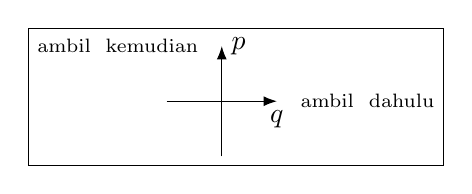
\begin{tikzpicture}[scale=0.7, baseline=(O)]
			\draw[-Latex] (0, -1) -- (0, 1) node[right] {$p$} node[left=0.5em] {\scriptsize\text{ambil $\Hm$ kemudian}};
			\draw[-Latex] (-1, 0) -- (1, 0) node[below] {$q$} node[right=0.5em] {\scriptsize\text{ambil $\Hm$ dahulu}};
			\coordinate (O) at (0, -0.3);
			\draw (current bounding box.north west) rectangle ([yshift=-1ex] current bounding box.south east);
		\end{tikzpicture}
		= (\mathrm{R}^p F)\left( \Hm^q(X)\right) \\
		& \Rightarrow \mathrm{R}^{p+q}F(X) , \quad p, q \in \Z.
	\end{align*}
\end{example}

% segment-id: o014.li2.chapter5.bicomplex-spectral-sequences-applications.p007
Barisan spektral Grothendieck yang diperkenalkan berikut berkenaan dengan
funktor turunan dari suatu komposisi funktor. Barisan ini mencakup suatu kelas
besar barisan spektral dalam
geometri dan aljabar, dan argumennya, seperti dalam
Contoh~\ref{eg:hyperderived-ss}, juga didasarkan pada resolusi
Cartan--Eilenberg.

% segment-id: o014.li2.chapter5.bicomplex-spectral-sequences-applications.th002
\begin{theorem}[Barisan spektral Grothendieck]
\label{prop:Grothendieck-ss}
% segment-id: o014.li2.chapter5.bicomplex-spectral-sequences-applications.x004
	\index{barisan spektral!Grothendieck}
	Tinjau funktor-funktor aditif antarkategori abelian
% segment-id: o014.li2.chapter5.bicomplex-spectral-sequences-applications.q010
	\[ \mathcal{A} \xrightarrow{F} \mathcal{A}' \xrightarrow{F'} \mathcal{A}''. \]
	Misalkan keduanya funktor eksak kiri (atau eksak kanan), $\mathcal{A}$ dan
	$\mathcal{A}'$ mempunyai cukup banyak objek injektif (atau projektif), dan
	$F$ memetakan objek injektif (atau projektif) ke objek $F'$-asiklik dalam
	pengertian Konvensi~\ref{con:F-acyclic}. Maka, untuk setiap
	$X\in\Obj(\mathcal{A})$, terdapat barisan spektral kuadran pertama
	kohomologis (atau homologis) bergradasi ganda
% segment-id: o014.li2.chapter5.bicomplex-spectral-sequences-applications.q011
	\begin{align*}
		E_2^{p,q} = (\mathrm{R}^p F') (\mathrm{R}^q F)(X) & \Rightarrow \mathrm{R}^{p+q} (F'F)(X), \\
		\text{atau} \quad E^2_{p,q} = (\mathrm{L}_p F') (\mathrm{L}_q F)(X) & \Rightarrow \mathrm{L}_{p+q}(F'F)(X).
	\end{align*}
	Sifat konvergensinya adalah seperti dalam Teorema~\ref{prop:tot-ss}.
	Barisan eksak suku berderajat rendah yang bersesuaian
	(Korolari~\ref{prop:low-degree-ss}) masing-masing dapat ditulis sebagai
% segment-id: o014.li2.chapter5.bicomplex-spectral-sequences-applications.q012
	\begin{equation*}\begin{split}
		0 \to (\mathrm{R}^1 F')(FX) & \to \mathrm{R}^1(F'F)(X) \\
		& \to F'\left( (\mathrm{R}^1 F)X \right) \to (\mathrm{R}^2 F')(FX) \to \mathrm{R}^2(F'F)(X),
	\end{split}\end{equation*}
	atau
% segment-id: o014.li2.chapter5.bicomplex-spectral-sequences-applications.q013
	\begin{equation*}\begin{split}
		\mathrm{L}_2(F'F)(X) \to (\mathrm{L}_2 F')(FX) & \to F'\left( (\mathrm{L}_1 F)X \right) \\
		& \to \mathrm{L}_1(F'F)(X) \to (\mathrm{L}_1 F')(FX) \to 0.
	\end{split}\end{equation*}
\end{theorem}
% segment-id: o014.li2.chapter5.bicomplex-spectral-sequences-applications.pf003
\begin{proof}
	Berdasarkan dualitas, cukup dibahas kasus kohomologis. Ambil resolusi
	injektif $0\to X\to I^0\to I^1\to\cdots$ dari $X$ dan definisikan
	$I^n:=0$ untuk $n<0$. Dalam $\mathcal{A}'$, ambil resolusi
	Cartan--Eilenberg $\cate{C}F(I)\to J$ dari
	$\cate{C}F(I):=(FI^p)_p$ (Teorema~\ref{prop:CE-resolution}), lalu tinjau
	bikompleks kuadran pertama
	$\cate{C}^2F'(J)=(F'(J^{p,q}))_{p,q}$ beserta barisan spektral konvergen
	$\mathscr{E}_{\mathrm{I}}$ dan $\mathscr{E}_{\mathrm{II}}$ yang
	bersesuaian. Pertama,
% segment-id: o014.li2.chapter5.bicomplex-spectral-sequences-applications.g002
	\begin{align*}
		E_{\mathrm{I},2}^{p, q} & =
		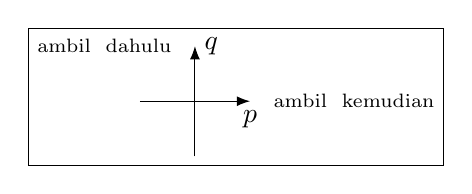
\begin{tikzpicture}[scale=0.7, baseline=(O)]
			\draw[-Latex] (0, -1) -- (0, 1) node[right] {$q$} node[left=0.5em] {\scriptsize\text{ambil $\Hm$ dahulu}};
			\draw[-Latex] (-1, 0) -- (1, 0) node[below] {$p$} node[right=0.5em] {\scriptsize\text{ambil $\Hm$ kemudian}};
			\coordinate (O) at (0, -0.3);
			\draw (current bounding box.north west) rectangle ([yshift=-1ex] current bounding box.south east);
		\end{tikzpicture} \\
		& = \Hm^p\left[ \cdots \to (\mathrm{R}^q F')(FI^p) \to (\mathrm{R}^q F')(FI^{p+1}) \to \cdots \right] \\
		& \Rightarrow \Hm^{p+q}\tot\left(\cate{C}^2 F'(J)\right).
	\end{align*}

	Karena menurut hipotesis $F(I^p)$ merupakan objek $F'$-asiklik, berlaku
	$E_{\mathrm{I},2}^{p,q}=0$ jika $q\neq0$. Argumen yang persis sama dengan
	Contoh~\ref{eg:bifunctor-ss} kemudian menunjukkan bahwa
	$\mathscr{E}_{\mathrm{I}}$ mengalami degenerasi pada halaman $E_2$, dan
% segment-id: o014.li2.chapter5.bicomplex-spectral-sequences-applications.q014
	\[ E_{\mathrm{I}, \infty}^{p,q} = E_{\mathrm{I}, 2}^{p,q} = \begin{cases}
		\Hm^p\left( F'F(I^\bullet) \right) = \mathrm{R}^p (F' F)(X), & q = 0, \\
		0, & q \neq 0,
	\end{cases}\]
	serta
	$\Hm^p\tot\left(\cate{C}^2F'(J)\right)
	=E_{\mathrm{I},\infty}^{p,0}=\mathrm{R}^p(F'F)(X)$.

	Sekarang tinjau $\mathscr{E}_{\mathrm{II}}$. Tekniknya serupa dengan
	Contoh~\ref{eg:hyperderived-ss}: kolom ke-$q$ dari kohomologi horizontal,
	$\Hm_{\mathrm{I}}(J)^{q,\bullet}$, memberikan resolusi injektif dari
	$\Hm^q(\cate{C}F(I))=(\mathrm{R}^qF)(X)$. Dengan mengingat pula bahwa $F'$
	mempertahankan kohomologi horizontal, diperoleh
% segment-id: o014.li2.chapter5.bicomplex-spectral-sequences-applications.g003
	\begin{align*}
		E_{\mathrm{II},2}^{p, q} & =
		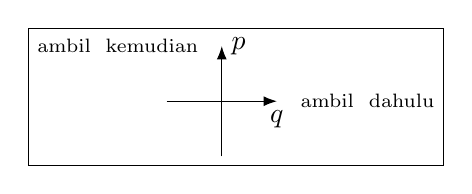
\begin{tikzpicture}[scale=0.7, baseline=(O)]
			\draw[-Latex] (0, -1) -- (0, 1) node[right] {$p$} node[left=0.5em] {\scriptsize\text{ambil $\Hm$ kemudian}};
			\draw[-Latex] (-1, 0) -- (1, 0) node[below] {$q$} node[right=0.5em] {\scriptsize\text{ambil $\Hm$ dahulu}};
			\coordinate (O) at (0, -0.3);
			\draw (current bounding box.north west) rectangle ([yshift=-1ex] current bounding box.south east);
		\end{tikzpicture}
		= (\mathrm{R}^p F')(\mathrm{R}^q F)\left( X \right) \\
		& \Rightarrow \Hm^{p+q}\tot\left(\cate{C}^2 F'(J)\right) = \mathrm{R}^{p+q}(F'F)(X).
	\end{align*}

	Jadi $\mathscr{E}_{\mathrm{II}}$ merupakan barisan spektral yang dikehendaki
	untuk bagian pertama. Dengan memasukkan deskripsi
	$E_{\mathrm{II},2}^{p,q}$ ke barisan eksak suku berderajat rendah dari
	$\mathscr{E}_{\mathrm{II}}$ (Korolari~\ref{prop:low-degree-ss}), diperoleh
	langsung pernyataan bagian terakhir.
\end{proof}

% segment-id: o014.li2.chapter5.bicomplex-spectral-sequences-applications.p008
Barisan spektral Grothendieck dapat dipandang sebagai versi konkret dari
Teorema~\ref{prop:derived-composite}, tetapi informasi yang dimuatnya lebih
rinci daripada isomorfisme dalam kategori turunan. Kita akan memberikan contoh
penerapannya dalam \S\ref{sec:LHS-SS}.

% segment-id: o014.li2.chapter5.bicomplex-spectral-sequences-applications.ex004
\begin{example}[Perubahan gelanggang]\label{eg:change-of-rings-SS}
% segment-id: o014.li2.chapter5.bicomplex-spectral-sequences-applications.x005
	\index{perubahan gelanggang}
% segment-id: o014.li2.chapter5.bicomplex-spectral-sequences-applications.x006
	\index{barisan spektral!perubahan gelanggang}
	Misalkan $R\to S$ homomorfisme gelanggang. Ambil $X$ sebagai modul kanan
	$S$ dan $Y$ sebagai modul kiri $R$. Tuliskan $S_R$ (atau $X_R$) untuk $S$
	(atau $X$) yang dipandang sebagai modul kanan $R$. Akan ditunjukkan bahwa
	terdapat barisan spektral kuadran pertama homologis bergradasi ganda
% segment-id: o014.li2.chapter5.bicomplex-spectral-sequences-applications.q015
	\begin{gather*}
		E^2_{p,q} = \Tor^S_p\left( X, \Tor^R_q(S_R, Y) \right) \Rightarrow \Tor^R_{p+q}(X_R, Y);
	\end{gather*}
	Di sini $\Tor^R_q(S_R,Y)$ diberi struktur modul kiri $S$ seperti dalam
	Catatan~\ref{rem:ExtTor-bimodule}. Ini merupakan penerapan langsung
	Teorema~\ref{prop:Grothendieck-ss}, yang berasal dari isomorfisme funktor
% segment-id: o014.li2.chapter5.bicomplex-spectral-sequences-applications.q016
	\[ X \dotimes{S} \left( S \dotimes{R} (\cdot) \right) \simeq X \dotimes{R} (\cdot) : R\dcate{Mod} \to \cate{Ab}, \]
	dengan funktor dalam
	$S\dotimes{R}(\cdot):R\dcate{Mod}\to S\dcate{Mod}$ mempunyai funktor
	turunan kiri $\Tor^R_\bullet(S_R,\cdot)$ yang bernilai dalam
	$S\dcate{Mod}$. Berdasarkan isomorfisme di atas, funktor dalam memetakan
	modul datar ke modul datar, sehingga versi homologis barisan spektral
	Grothendieck memang dapat diterapkan.

	Dengan notasi dan teknik yang sepenuhnya serupa, untuk modul kanan $R$, $X$,
	dan modul kiri $S$, $Y$, juga diperoleh
% segment-id: o014.li2.chapter5.bicomplex-spectral-sequences-applications.q017
	\[ E^2_{p,q} = \Tor^S_p\left( \Tor^R_q(X, {}_R S), Y \right) \Rightarrow \Tor^R_{p+q}(X, {}_R Y). \]

	Selanjutnya tinjau funktor $\Ext$. Ambil $X$ sebagai modul kiri $S$ dan
	$Y$ sebagai modul kiri $R$, serta tuliskan ${}_RX$ untuk $X$ yang dipandang
	sebagai modul kiri $R$. Berikan $\Ext_R^q({}_RS,Y)$ struktur modul kiri $S$
	seperti dalam Catatan~\ref{rem:ExtTor-bimodule}. Maka terdapat barisan
	spektral kuadran pertama kohomologis bergradasi ganda
% segment-id: o014.li2.chapter5.bicomplex-spectral-sequences-applications.q018
	\begin{align*}
		E_2^{p,q} = \Ext_S^p\left( X, \Ext_R^q({}_R S, Y) \right) & \Rightarrow \Ext_R^{p+q}({}_R X, Y), \\
		E_2^{p,q} = \Ext_S^p\left( \Tor^R_q(S_R, Y), X \right) & \Rightarrow \Ext_R^{p+q}(Y, {}_R X).
	\end{align*}
	Kedua barisan itu berturut-turut bersesuaian dengan isomorfisme komposisi funktor
% segment-id: o014.li2.chapter5.bicomplex-spectral-sequences-applications.q019
	\begin{gather*}
		\Hom_S\left( X, \Hom_R({}_R S, \cdot) \right) \simeq \Hom_R({}_R X, \cdot), \\
		\Hom_S\left( S \dotimes{R} (\cdot), X \right) \simeq \Hom_R(\cdot, {}_R X),
	\end{gather*}
	yaitu adjungsi-adjungsi yang diperkenalkan dalam
	\cite[Korolari 6.6.8]{Li1}. Pemakaian campuran funktor turunan kanan
	$\Ext_S^p$ dan funktor turunan kiri $\Tor^R_q$ dalam baris kedua tidak
	menimbulkan masalah, sebab variabel pertama $\Hom_S$ berada dalam kategori
	berlawanan $S\dcate{Mod}^{\opp}$.
\end{example}

% segment-id: o014.li2.chapter5.bicomplex-spectral-sequences-applications.p009
Barisan-barisan spektral di atas sebaiknya dibandingkan dengan versi kategori
turunan dalam \S\ref{sec:otimesL}.

% segment-id: o014.li2.chapter5.bicomplex-spectral-sequences-applications.ex005
\begin{example}\label{eg:change-of-rings-SS-bis}
% segment-id: o014.li2.chapter5.bicomplex-spectral-sequences-applications.x007
\index{teorema koefisien universal}
	Untuk barisan spektral
	$E_2^{p,q}=\Ext_S^p\left(\Tor^R_q(S_R,Y),X\right)
	\Rightarrow\Ext_R^{p+q}(Y,{}_RX)$ dari
	Contoh~\ref{eg:change-of-rings-SS}, kita catat sebuah kasus khusus yang
	berguna, sekaligus sebagai latihan. Andaikan dimensi global
	$S\dcate{Mod}$ tidak lebih dari $1$
	(Definisi--Proposisi~\ref{def:global-dim}). Akibatnya, suku-suku taknol
	$E_2^{p,q}$ terkonsentrasi pada wilayah $p=0,1$. Jadi, untuk $n\geq0$,
	filtrasi menurun $\mathrm{F}^\bullet$ pada $\Ext_R^n(Y,{}_RX)$ harus
	berbentuk
% segment-id: o014.li2.chapter5.bicomplex-spectral-sequences-applications.q020
	\[ \Ext_R^n(Y, {}_R X) = \mathrm{F}^0 \underbracket{\supset}_{E_\infty^{0, n}} \mathrm{F}^1 \underbracket{\supset}_{E_\infty^{1, n-1}} \mathrm{F}^2 = \{0\}. \]

	Selain itu, Contoh~\ref{eg:SS-finite-width} menunjukkan bahwa barisan
	spektral mengalami degenerasi pada halaman $E_2$, sehingga
	$E_2^{p,q}\simeq E_\infty^{p,q}$. Dengan menggabungkan semuanya diperoleh
	barisan eksak pendek
% segment-id: o014.li2.chapter5.bicomplex-spectral-sequences-applications.q021
	\[ 0 \to \Ext_S^1\left( \Tor^R_{n-1}(S_R, Y), X \right) \to \Ext_R^n(Y, {}_R X) \to \Hom_S\left( \Tor^R_n(S_R, Y), X \right) \to 0; \]
	dengan konvensi $\Tor^R_{-1}=0$. Barisan di atas dapat dipandang sebagai
	salah satu varian teorema koefisien universal.

	Dengan cara serupa, andaikan modul kanan $S$, $X$, mempunyai dimensi $\Tor$
	tidak lebih dari $1$ (Contoh~\ref{eg:Tor-dimension}). Barisan spektral
	$E^2_{p,q}=\Tor^S_p(X,\Tor^R_q(S_R,Y))
	\Rightarrow\Tor^R_{p+q}(X_R,Y)$ mengalami degenerasi pada halaman $E^2$.
	Dengan memeriksa filtrasi menaik yang bersesuaian pada
	$\Tor^R_n(X_R,Y)$, diperoleh barisan eksak pendek
% segment-id: o014.li2.chapter5.bicomplex-spectral-sequences-applications.q022
	\[ 0 \to X \dotimes{S} \Tor^R_n(S_R, Y) \to \Tor^R_n(X_R, Y) \to \Tor^S_1(X, \Tor^R_{n-1}(S_R, Y)) \to 0. \]

	Jika $S$ merupakan domain ideal utama, baik hipotesis dimensi global maupun
	dimensi $\Tor$ otomatis terpenuhi.
\end{example}

% Unit 070 terjemahan Bahasa Indonesia dari chapter5.tex baris 955--1063.
% Sumber: Methods of Algebra, Volume 2, commit
% 9a5803ff77dd3257484cb177f851a73770a59dd3 (CC BY 4.0).
% stable-unit-id: o014.aljabr2.chapter5.multiplicative-structures
% Cakupan: Bagian 5.7 lengkap, sebelum latihan.

% segment-id: o014.li2.chapter5.multiplicative-structures.h001
\section{Sekilas tentang struktur perkalian}\label{sec:multiplicative-SS}
\hypertarget{o014.aljabr2.chapter5.multiplicative-structures}{ }

% segment-id: o014.li2.chapter5.multiplicative-structures.p001
Agar pembahasan sederhana dan konkret, dalam bagian ini kita mengambil
gelanggang komutatif $\Bbbk$ dan $\mathcal{A}=\Bbbk\dcate{Mod}$; ini sudah
memadai bagi penerapan klasik. Modul-$\Bbbk$ kita sebut singkat sebagai modul,
aljabar-$\Bbbk$ sebagai aljabar, dan kita tulis
$\otimes:=\otimes_{\Bbbk}$.

% segment-id: o014.li2.chapter5.multiplicative-structures.p002
Misalkan $I$ monoid komutatif, dengan operasi biner ditulis secara aditif.
Definisi dari \cite[\S 7.4]{Li1} dapat diringkas sebagai berikut:
\begin{itemize}
	\item modul bergradasi-$I$ adalah modul dengan dekomposisi jumlah langsung
	$M=\bigoplus_{i\in I}M^i$; unsur-unsur dalam $M^i$ disebut unsur homogen
	berderajat $i$;
	\item aljabar bergradasi-$I$ adalah modul bergradasi yang dilengkapi
	homomorfisme $\mu:A\otimes A\to A$, yang juga ditulis sebagai perkalian
	$xy:=\mu(x\otimes y)$, sedemikian sehingga $A$ menjadi gelanggang dan
	\[ 1_A\in A^0,\qquad A^i\cdot A^j\subset A^{i+j},
	\qquad i,j\in I; \]
	jadi perkalian $\mu$ sepenuhnya ditentukan oleh data
	$\mu^{i,j}:A^i\otimes A^j\to A^{i+j}$;
	\item homomorfisme dan isomorfisme antara modul atau aljabar
	bergradasi-$I$ didefinisikan dengan cara biasa; subaljabar dan ideal
	bergradasi-$I$ juga didefinisikan dengan cara yang sama.
\end{itemize}

% segment-id: o014.li2.chapter5.multiplicative-structures.p003
Untuk $k\in I$, definisikan pula homomorfisme berderajat $k$ antara modul
bergradasi-$I$: ini adalah homomorfisme modul $\varphi:M\to N$ yang memenuhi
$\varphi(M^i)\subset M^{i+k}$ untuk semua $i$, dan ditentukan oleh data
$(\varphi^i:M^i\to M^{i+k})_{i\in I}$. Untuk $k=0$ kita memperoleh kembali
homomorfisme dalam arti biasa. Derajat homomorfisme dijumlahkan ketika
homomorfisme dikomposisikan.

% segment-id: o014.li2.chapter5.multiplicative-structures.d001
\begin{definition}\label{def:dg-algebra-preview}
	\index{aljabar bergradasi diferensial (differential graded algebra)}
	Misalkan $I$ monoid komutatif yang dilengkapi homomorfisme
	$\epsilon:I\to\Z/2\Z$. Sebuah \emph{aljabar bergradasi-$I$ diferensial}
	dengan diferensial berderajat $k$ adalah aljabar bergradasi-$I$
	$A=\bigoplus_{p\in I}A^p$ bersama endomorfisme berderajat $k\in I$
	$d=(d^p)_p:A\to A$ yang memenuhi $d^2=0$ dan aturan Leibniz
	\[ d(xy)=(dx)\cdot y+(-1)^{\epsilon(p)}x\cdot dy,
	\qquad x\in A^p,\quad y\in A^{p'},\quad p,p'\in I. \]
\end{definition}

% segment-id: o014.li2.chapter5.multiplicative-structures.p004
Perhatikan bahwa
$d(1_A)=d(1_A\cdot1_A)=d(1_A)+d(1_A)$, sehingga $d(1_A)=0$. Jelas bahwa
$\Ker(d)$ merupakan subaljabar bergradasi-$I$ dari $A$, sedangkan
$\Image(d)$ merupakan ideal dua sisi bergradasi-$I$ dalam $\Ker(d)$. Karena
itu,
\[ \Hm(A,d):=\Ker(d)/\Image(d) \]
tetap merupakan aljabar bergradasi-$I$.

% segment-id: o014.li2.chapter5.multiplicative-structures.e001
\begin{example}
	Ambil $I=\Z$ dan $\epsilon(p)=p\;\bmod 2$. Untuk setiap kompleks $X$ pada
	kategori $\Bbbk$-linear $\mathcal{B}$, kompleks $\Hom$
	$\Hom^\bullet(X,X)$ dari Definisi~\ref{def:Hom-cplx}, bersama
	$d=d_{\Hom^\bullet(X,X)}$, menjadi aljabar bergradasi-$\Z$ diferensial
	dengan diferensial berderajat $1$. Pernyataan ini pada dasarnya merupakan
	isi Lema~\ref{prop:Hom-cplx-Leibniz}. Kita mempunyai
	\[ \Hm(\Hom^\bullet(X,X),d)=
	\bigoplus_{n\in\Z}\Hom_{\cate{K}(\mathcal{B})}(X,X[n]), \]
	dengan perkalian yang berasal dari komposisi morfisme dalam
	$\cate{K}(\mathcal{B})$.
\end{example}

% segment-id: o014.li2.chapter5.multiplicative-structures.e002
\begin{example}
	Ambil $\Bbbk=\CC$, $I=\Z$, dan $\epsilon(p)=p\;\bmod2$. Bentuk
	diferensial bernilai $\CC$ berderajat $p$ pada manifold mulus
	$\mathfrak{X}$ membentuk ruang vektor $A^p(\mathfrak{X})$. Definisikan
	$A(\mathfrak{X}):=\bigoplus_{p=0}^{\dim X}A^p(\mathfrak{X})$. Dengan
	perkalian $\mu(\omega\otimes\eta):=\omega\wedge\eta$ dan diferensial luar
	$\dd$, objek ini menjadi aljabar bergradasi-$\Z$ diferensial dengan
	diferensial berderajat $1$. Aljabar terkait
	$\Hm(A(\mathfrak{X}),\dd)=\bigoplus_p\Hm^p_{\mathrm{dR}}(\mathfrak{X})$
	tepat merupakan kohomologi de Rham dari $\mathfrak{X}$; perkalian yang
	berasal dari $\wedge$ memberinya struktur aljabar bergradasi. Ini merupakan
	objek fundamental dalam topologi dan isomorfik sebagai aljabar bergradasi
	dengan cincin kohomologi singular $\mathfrak{X}$.

	Perkalian pada $\Hm(A(\mathfrak{X}),\dd)$ juga memenuhi
	$xy=(-1)^{pq}yx$, dengan $x$ dan $y$ masing-masing unsur homogen berderajat
	$p$ dan $q$, karena perkalian pada $A(\mathfrak{X})$ sudah mempunyai sifat
	ini. Sebagai contoh sederhana yang indah, ruang proyektif kompleks
	$\mathfrak{X}:=\mathbb{P}^n(\CC)$ menghasilkan aljabar bergradasi
	$\Hm(A(\mathfrak{X}),\dd)\simeq\CC[t]/(t^{n+1})$, dengan peubah $t$
	bersesuaian dengan unsur homogen berderajat $2$.
\end{example}

% segment-id: o014.li2.chapter5.multiplicative-structures.p005
Kembali ke pokok pembahasan, dalam bagian ini kita mempertimbangkan kasus-kasus
berikut:
\begin{center}\begin{tabular}{|c|c|c|} \hline
	Singkatan & $I$ & $\epsilon:I\to\Z/2\Z$ \\ \hline
	Bergradasi tunggal & $\Z$ & $\epsilon(p)=p\;\bmod2$ \\
	Bergradasi ganda & $\Z^2$ & $\epsilon(p,q)=p+q\;\bmod2$ \\ \hline
\end{tabular}\end{center}

% segment-id: o014.li2.chapter5.multiplicative-structures.p006
Teori ini beririsan dengan Definisi~\ref{def:differential-object},
tetapi fokus bagian ini adalah perkalian yang belum dibahas sebelumnya.

% segment-id: o014.li2.chapter5.multiplicative-structures.p007
Untuk meringankan notasi, selanjutnya berbagai kasus tersebut secara
bersama-sama kita sebut ``bergradasi''; pembeda utamanya adalah
superskrip $p$ atau $(p,q)$. Demikian pula, aljabar bergradasi-$I$
diferensial secara bersama-sama disebut aljabar bergradasi diferensial.

% segment-id: o014.li2.chapter5.multiplicative-structures.c001
\begin{convention}
	Untuk barisan spektral bergradasi ganda kohomologis $\mathscr{E}$ dalam
	kasus $\mathcal{A}=\Bbbk\dcate{Mod}$, kita mengidentifikasi setiap halaman
	$E_r$ dengan modul bergradasi $\bigoplus_{p,q}E_r^{p,q}$ dan memandang
	$d_r=(d_r^{p,q})_{p,q}$ sebagai endomorfisme berderajat $(r,-r+1)$ pada
	modul bergradasi $E_r$. Kasus homologis dan kasus bergradasi tunggal
	diperlakukan dengan cara serupa.
\end{convention}

% segment-id: o014.li2.chapter5.multiplicative-structures.p008
Singkatnya, barisan spektral dengan struktur perkalian adalah barisan spektral
yang terdiri atas aljabar bergradasi diferensial.

% segment-id: o014.li2.chapter5.multiplicative-structures.d002
\begin{definition}\label{def:mult-ss}
	\index{barisan spektral!struktur perkalian (multiplicative structure)}
	Sebuah \emph{struktur perkalian} pada barisan spektral bergradasi ganda
	kohomologis $\mathscr{E}$ adalah keluarga homomorfisme
	$\mu_r:E_r\otimes E_r\to E_r$ (yakni ``perkalian'') sedemikian sehingga
	\begin{itemize}
		\item setiap $(E_r,\mu_r,d_r)$ menjadi aljabar bergradasi diferensial,
		dengan diferensial berderajat $(r,-r+1)$;
		\item $t_{r+1}:\Hm(E_r,d_r)\rightiso E_{r+1}$ dalam data barisan
		spektral merupakan isomorfisme aljabar bergradasi.
	\end{itemize}
	Struktur perkalian pada barisan spektral bergradasi tunggal atau homologis
	didefinisikan dengan cara serupa.
\end{definition}

% segment-id: o014.li2.chapter5.multiplicative-structures.p009
Pembahasan sebelumnya menunjukkan bahwa $Z_r=\Ker(d_r)$ merupakan subaljabar
bergradasi dari $E_r$, sedangkan $B_r=\Image(d_r)$ merupakan ideal dua sisi
bergradasi dari $Z_r$. Karena itu $\Hm(E_r,d_r)$ menjadi aljabar bergradasi;
	inilah makna tepat Definisi~\ref{def:mult-ss}.

% segment-id: o014.li2.chapter5.multiplicative-structures.p010
Lebih lanjut, jika limitnya ada, maka
$Z_\infty=\bigoplus_{p,q}Z_\infty^{p,q}$ juga merupakan subaljabar bergradasi
dengan $B_\infty=\bigoplus_{p,q}B_\infty^{p,q}$ sebagai ideal bergradasinya.
Jadi $E_\infty$ juga merupakan aljabar bergradasi.

% segment-id: o014.li2.chapter5.multiplicative-structures.p011
\index{aljabar-dg}
Sebagai contoh, perhatikan aljabar bergradasi diferensial yang diferensialnya
berderajat $1$, yang disingkat sebagai aljabar-dg. Dengan mengembangkan
definisi, ini setara dengan kompleks modul-$\Bbbk$
$X=(X^n,d_X^n)_{n\in\Z}$ sedemikian sehingga
$X\xlongequal{\text{diidentifikasi}}\bigoplus_nX^n$ dilengkapi perkalian
$\mu:X\otimes X\to X$ yang memenuhi $X^p\cdot X^{p'}\subset X^{p+p'}$ dan
aturan Leibniz
\[ d(xy)=dx\cdot y+(-1)^px\cdot dy,
	\qquad x\in X^p,\quad y\in X^{p'}. \]
Sekarang andaikan data $(X,d)$ diperluas menjadi kompleks terfiltrasi
$(X,d,\mathrm{F}^\bullet X)$. Ingat bahwa ini sudah berarti
$d(\mathrm{F}^pX)\subset\mathrm{F}^pX$; kita syaratkan pula agar perkalian
pada $X$ kompatibel dengan filtrasi:
\[ \mathrm{F}^pX^n\cdot\mathrm{F}^{p'}X^{n'}
	\subset\mathrm{F}^{p+p'}X^{n+n'}. \]
Dalam keadaan ini $(X,d,\mu,\mathrm{F}^\bullet X)$ disebut aljabar bergradasi
diferensial terfiltrasi. Untuk filtrasi terinduksi pada $\Hm(X,d)$, syarat di
atas memastikan bahwa
\[ \gr\Hm(X,d)\xlongequal{\text{diidentifikasi}}
	\bigoplus_{(p,q)\in\Z^2}\gr^p\Hm^{p+q}(X,d) \]
secara alami menjadi aljabar bergradasi.
\index{aljabar bergradasi diferensial!terfiltrasi (filtered)}

% segment-id: o014.li2.chapter5.multiplicative-structures.t001
\begin{proposition}\label{prop:dga-mult-ss}
	Misalkan $(X,d,\mu,\mathrm{F}^\bullet X)$ adalah aljabar bergradasi
	diferensial terfiltrasi, dengan diferensial berderajat $1$.
	\begin{enumerate}[(i)]
		\item Barisan spektral $\mathscr{E}$ dari kompleks terfiltrasi
		$(X,d,\mathrm{F}^\bullet X)$ mempunyai struktur perkalian kanonik.
		\item Isomorfisme
		$E_\infty^{p,q}\simeq\gr^p\Hm^{p+q}(X,d)$ dalam Teorema Konvergensi
		Klasik~\ref{prop:classical-convergence} sesungguhnya memberikan
		isomorfisme aljabar bergradasi
		$E_\infty\simeq\gr\Hm(X,d)$.
	\end{enumerate}
\end{proposition}
\begin{proof}
	Ambil $x\in E_r^{p,q}$ dan $y\in E_r^{p',q'}$. Berdasarkan deskripsi
	Proposisi~\ref{prop:filtered-cplx-ss}, pilih prapeta
	\begin{gather*}
		\widetilde{x}\in\mathrm{F}^pX^{p+q}\cap
		d^{-1}\left(\mathrm{F}^{p+r}X^{p+q+1}\right),\qquad
		\widetilde{y}\in\mathrm{F}^{p'}X^{p'+q'}\cap
		d^{-1}\left(\mathrm{F}^{p'+r}X^{p'+q'+1}\right).
	\end{gather*}
	Menurut definisi,
	\begin{gather*}
		\widetilde{x}\widetilde{y}\in
		\mathrm{F}^{p+p'}X^{p+q+p'+q'},\\
		d(\widetilde{x}\widetilde{y})
		=d\widetilde{x}\cdot\widetilde{y}
		+(-1)^{p+q}\widetilde{x}\cdot d\widetilde{y}
		\in\mathrm{F}^{p+p'+r}X^{p+q+p'+q'+1}.
	\end{gather*}
	Jadi $\widetilde{x}\widetilde{y}$ menentukan unsur
	$xy\in E_r^{p+p',q+q'}$. Perhitungan rutin (silakan periksa) menunjukkan
	bahwa $xy$ hanya bergantung pada $x$ dan $y$.

	Selanjutnya, $d_r:E_r\xrightarrow{(r,-r+1)}E_r$ diinduksi oleh diferensial
	$d$ pada $X$. Ini memberikan struktur aljabar bergradasi diferensial pada
	$E_r$; sifat asosiatif, aturan Leibniz, dan sifat-sifat lainnya semuanya
	dapat diperiksa pada $(X,d)$. Dengan cara yang sama terlihat bahwa
	$\Hm(E_r,d_r)\simeq E_{r+1}$ merupakan isomorfisme aljabar bergradasi.

	Pernyataan bahwa isomorfisme kanonik
	$E_\infty^{p,q}\simeq\gr^p\Hm^{p+q}(X,d)$ dalam teorema konvergensi klasik
	mempertahankan perkalian juga cukup diverifikasi pada $X$, sehingga
	tidak perlu diuraikan lagi.
\end{proof}

% segment-id: o014.li2.chapter5.multiplicative-structures.r001
\begin{remark}
	\index{sistem Cartan--Eilenberg (Cartan--Eilenberg system)}
	Struktur perkalian merupakan alat yang sangat diandalkan dalam topologi.
	Topologi aljabar tanpa perkalian hampir tidak terbayangkan, atau setidaknya
	akan terasa hambar. Secara historis, ketika pertama kali menemukan barisan
	spektral, Leray sudah mempertimbangkan struktur perkalian dan menyebutnya
	``cincin spektral''. Struktur ini sering sangat menyederhanakan perhitungan
	barisan spektral dalam topologi. Itulah alasan bagian ini memberi pengantar
	singkat mengenai struktur perkalian, meskipun hanya menyentuh permukaannya.

	Ada satu kesulitan yang jelas ketika menerapkan
	Definisi~\ref{def:mult-ss}. Struktur aljabar bergradasi diferensial pada
	semua $E_r$ harus diberikan sekaligus, sebab dari definisinya saja tidak ada
	alasan bahwa perkalian pada satu halaman menginduksi perkalian pada halaman
	berikutnya. Dalam sejumlah keadaan hal ini memang dapat dilakukan, seperti
	dalam Proposisi~\ref{prop:dga-mult-ss}.

	Dalam kasus umum atau kasus yang sulit dihitung secara manual, konstruksi
	barisan spektral sering bermula dari data sederhana, misalnya pasangan eksak
dalam \S\ref{sec:exact-couples}. Karena itu wajar ditanyakan: adakah syarat
sederhana pada pasangan eksak yang menjamin bahwa barisan spektral terkait
mempunyai struktur perkalian?

	Tampaknya jawabannya negatif: diperlukan informasi selain pasangan eksak.
Salah satu konstruksi yang berguna adalah \emph{sistem Cartan--Eilenberg} yang
juga klasik, bersama hasil kali spektralnya; lihat \cite[II.A]{Dou58}. Sebagai
penerapan, barisan spektral Serre--Atiyah--Hirzebruch yang sangat penting dalam
topologi mempunyai struktur perkalian untuk setiap teori kohomologi rampat
yang multiplikatif. Karena materi ini sudah menyimpang dari garis utama, kita
berhenti sampai di sini.
\end{remark}

% Unit 071 terjemahan Bahasa Indonesia dari chapter5.tex baris 1066--1148.
% Sumber: Methods of Algebra, Volume 2, commit
% 9a5803ff77dd3257484cb177f851a73770a59dd3 (CC BY 4.0).
% stable-unit-id: o014.aljabr2.chapter5.exercises
% Cakupan: seluruh latihan Bab 5.

% segment-id: o014.li2.chapter5.exercises.h001
\begin{Exercises}
	% segment-id: o014.li2.chapter5.exercises.ex001
	\item Untuk kategori abelian $\mathcal{A}$, periksalah sifat-sifat
	berikut bagi kategori objek terfiltrasi $\mathrm{Fil}^\bullet(\mathcal{A})$.
	\begin{enumerate}[(i)]
		\item Kategori ini aditif, dan setiap morfisme mempunyai kernel,
		kokernel, citra, dan kocitra. Deskripsikan semuanya sekonkret mungkin.
		\item Untuk morfisme $f:X\to Y$ dalam
		$\mathrm{Fil}^\bullet(\mathcal{A})$, jika
		$f(\mathrm{F}^nX)\to f(X)\cap\mathrm{F}^nY$ merupakan isomorfisme
		untuk semua $n$, maka $f$ disebut morfisme ketat. Buktikan bahwa konsep
		ini ekuivalen dengan versi dalam Definisi~\ref{def:strict-morphism}.

		\begin{hint}
			Ini setara dengan mengatakan bahwa kedua filtrasi alami pada $f(X)$
			sama: yang pertama adalah citra $\mathrm{F}^\bullet X$, sedangkan
			yang kedua adalah restriksi $\mathrm{F}^\bullet Y$. Yang pertama
			bersesuaian dengan $\Coim(f)$ dalam
			$\mathrm{Fil}^\bullet(\mathcal{A})$, sedangkan yang kedua
			bersesuaian dengan $\Image(f)$.
		\end{hint}
		\item Berikan contoh yang menunjukkan bahwa
		$\mathrm{Fil}^\bullet(\mathcal{A})$ pada umumnya bukan kategori abelian.
	\end{enumerate}
	Meskipun objek terfiltrasi tidak membentuk kategori abelian, geometri tetap
	memerlukan kategori turunan terfiltrasi dalam kasus filtrasi hingga,
	$\cate{DF}(\mathcal{A})$. Definisinya membutuhkan teknik yang cukup
	mendalam; lihat \cite[Tag 05RX]{stacks}.
	\index{kategori turunan!terfiltrasi (filtered)}

	% segment-id: o014.li2.chapter5.exercises.ex002
	\item Untuk suatu objek diferensial terfiltrasi
	$(X,d,\mathrm{F}^\bullet X)$ pada kategori abelian $\mathcal{A}$,
	buktikan bahwa $d_1^p:E_1^p\to E_1^{p+1}$ dalam barisan spektral merupakan
	morfisme penghubung yang diinduksi oleh barisan eksak pendek objek
	diferensial
	\[ 0\to\gr^{p+1}X\to\mathrm{F}^pX/\mathrm{F}^{p+2}X
	\to\gr^pX\to0. \]

	% segment-id: o014.li2.chapter5.exercises.ex003
	\item (Barisan spektral Bockstein) Misalkan $f$ bukan pembagi nol
	dalam gelanggang komutatif $R$. Untuk setiap modul-$R$ $M$, definisikan
	$M[f]:=\{m\in M:fm=0\}$; $M$ disebut \emph{bebas torsi-$f$} jika
	$M[f]=\{0\}$. Misalkan $C$ adalah kompleks rantai dan setiap $C_n$ bebas
	torsi-$f$. Perkalian dengan $f$ memberikan monomorfisme kompleks rantai
	$\alpha:C\to C$. Untuk data $(C,\alpha)$,
	Proposisi~\ref{prop:differential-exact-couple} memberikan pasangan eksak
	\[\begin{tikzcd}[column sep=tiny]
		\Hm_\bullet(C) \arrow[rr, "{\Hm_\bullet(\alpha)}"] & &
		\Hm_\bullet(C) \arrow[ld] \\
		& \Hm_\bullet\left(C\dotimes{R}R/(f)\right) \arrow[lu, "{-1}"] &
	\end{tikzcd}\]
	dan barisan spektral bergradasi homologis terkait
	$(E^r_q)_{\substack{r\geq0\\q\in\Z}}$. Deskripsikan setiap halaman
	$(E^r,d^r)$ serta $E^\infty$ sejelas mungkin.
	\index{barisan spektral!Bockstein}

	% segment-id: o014.li2.chapter5.exercises.ex004
	\item Dalam soal sebelumnya, ambil $R=\Z$ dan $f=p$ dengan $p$ bilangan prima, lalu
	andaikan setiap $C_n$ merupakan modul-$\Z$ bebas berperingkat hingga. Untuk
	setiap modul-$\Z$ $M$, tuliskan $M_{\mathrm{tor}}$ untuk submodul semua
	unsur torsinya dan definisikan hasil bagi bebas torsi
	$M_{\mathrm{tf}}:=M/M_{\mathrm{tor}}$. Buktikan bahwa
	\[ E^\infty_q\simeq\Hm_q(C)_{\mathrm{tf}}\dotimes{\Z}\F_p,
	\qquad q\in\Z. \]
	Dari sini deduksikan
	\[ \dim_{\F_p}\Hm_q\left(C\dotimes{\Z}\F_p\right)
	\geq\dim_{\F_p}\left(\Hm_q(C)_{\mathrm{tf}}\dotimes{\Z}\F_p\right). \]
	Berikan contoh ketika pertidaksamaan ini ketat.

	% segment-id: o014.li2.chapter5.exercises.ex005
	\item (Barisan spektral dua kolom dan dua baris) Misalkan diberikan barisan
	spektral konvergen kuat $E_2^{p,q}\Rightarrow H^{p+q}$, dalam arti
	Konvensi~\ref{con:ss-conv}.
	\begin{enumerate}[(i)]
		\item Buktikan bahwa jika $E_2^{p,q}$ taknol hanya untuk
		$p\in\{0,1\}$, maka untuk semua $q\in\Z$ terdapat barisan eksak pendek
		kanonik
		\[ 0\to E_2^{1,q-1}\to H^q\to E_2^{0,q}\to0. \]
		\item Buktikan bahwa jika $E_2^{p,q}$ taknol hanya untuk
		$q\in\{0,1\}$, maka untuk semua $p\in\Z$ terdapat barisan eksak kanonik
		\[ \cdots\to H^{p-1}\to E_2^{p-2,1}\xrightarrow{d_2}E_2^{p,0}
		\to H^p\to E_2^{p-1,1}\xrightarrow{d_2}E_2^{p+1,0}
		\to H^{p+1}\to\cdots. \]
		\item Tangani versi $E^2_{p,q}\Rightarrow H_{p+q}$.
		\begin{hint}
			Tukar superskrip dengan subskrip, balik arah panah, dan biarkan yang lain
			tetap sama.
		\end{hint}
	\end{enumerate}

	% segment-id: o014.li2.chapter5.exercises.ex006
	\item Perhatikan funktor eksak kiri $F'$ dan $F$ yang memenuhi prasyarat
	Teorema~\ref{prop:Grothendieck-ss}; syaratkan pula bahwa $\mathrm{R}F'$ dan
	$\mathrm{R}F$ keduanya berdimensi hingga.
	\begin{enumerate}[(i)]
		\item Buktikan bahwa $F'F$ juga berdimensi hingga dan berikan batas atas
		bagi dimensinya.
		\item Perhatikan homomorfisme
		$\chi_F:\mathrm{K}_0(\mathcal{A})\to\mathrm{K}_0(\mathcal{A}')$ yang
		dietapkan oleh funktor triangulasi $\mathrm{R}F$, dan homomorfisme
		serupa $\chi_{F'}$, $\chi_{F'F}$ yang ditetapkan oleh $\mathrm{R}F'$,
		$\mathrm{R}(F'F)$; lihat latihan \CHref{sec:cplx}. Buktikan bahwa
		$\chi_{F'F}=\chi_{F'}\circ\chi_F$.
	\end{enumerate}
	Sifat-sifat ini juga dapat dibuktikan dengan kategori turunan. Kasus funktor
	eksak kanan serta $\mathrm{L}F',\mathrm{L}F$ tentu bersifat dual.

	% segment-id: o014.li2.chapter5.exercises.ex007
	\item Misalkan $\mathcal{A}$ adalah kategori abelian dengan cukup objek
	injektif, dan $X\in\Obj(\mathcal{A})$ dilengkapi filtrasi hingga
	$X=\mathrm{F}^0X\supset\cdots\supset\mathrm{F}^{N+1}X=0$. Misalkan
	$G:\mathcal{A}\to\mathcal{A}'$ adalah funktor aditif eksak kiri. Buktikan
	bahwa terdapat barisan spektral konvergen kuat
	\[ E_1^{p,q}=\mathrm{R}^{p+q}G(\gr^pX)
	\Rightarrow\mathrm{R}^{p+q}G(X). \]
	% Reference: [Knapp-Vogan 1995, Proposition D.57]
	\begin{hint}
		Salah satu cara adalah meniru konstruksi resolusi Cartan--Eilenberg
		(Teorema~\ref{prop:CE-resolution}, yang memakai
		Proposisi~\ref{prop:horseshoe}). Mulai dari $\mathrm{F}^NX$ dan pilih
		serangkaian resolusi injektif yang sesuai
		\[\begin{tikzcd}[row sep=small]
			\vdots & & \vdots \\
			\mathrm{F}^0I^1 \arrow[u]
			\arrow[phantom,r,"\supset" description] & \cdots
			\arrow[phantom,r,"\supset" description] & \mathrm{F}^NI^1 \arrow[u] \\
			\mathrm{F}^0I^0 \arrow[u]
			\arrow[phantom,r,"\supset" description] & \cdots
			\arrow[phantom,r,"\supset" description] & \mathrm{F}^NI^0 \arrow[u] \\
			\mathrm{F}^0X \arrow[u]
			\arrow[phantom,r,"\supset" description] & \cdots
			\arrow[phantom,r,"\supset" description] & \mathrm{F}^NX \arrow[u] \\
			0 \arrow[u] & & 0 \arrow[u]
		\end{tikzcd}\]
		sedemikian sehingga penerapan $\cate{C}G$ pada
		$\mathrm{F}^\bullet(I)$ tetap menghasilkan kompleks terfiltrasi dan
		barisan spektral terkait memenuhi pernyataan yang diminta.
	\end{hint}

	% segment-id: o014.li2.chapter5.exercises.ex008
	\item Misalkan $R$ gelanggang,
	$C=(C_n,d^C_n)_n$ kompleks rantai modul-$R$ kanan, dan $D$ modul-$R$ kiri.
	Andaikan setiap $C_n$ datar dan $n\ll0\implies C_n=0$. Ambil resolusi
	projektif $\cdots\to P_1\to P_0\to D\to0$ dan bangun bikompleks
	$C_\bullet\dotimes{R}P_\bullet$.
	\begin{enumerate}[(i)]
		\item Tunjukkan bahwa barisan spektral bergradasi ganda homologis terkait
		$\mathscr{E}_{\mathrm{I}}$ mengalami degenerasi pada halaman
		$E_{\mathrm{I}}^2$.
		\item Tunjukkan bahwa
		$(E_{\mathrm{II}}^2)_{p,q}=\Tor^R_p(\Hm_q(C),D)
		\Rightarrow\Hm_{p+q}(C_\bullet\dotimes{R}D)$.
		\item Buktikan bahwa jika semua $\Image(d^C_n)$ datar, maka ini
		menghasilkan barisan eksak pendek dalam Teorema K\"unneth Homologis
		\ref{prop:Kunneth-homology}.
		\begin{hint}
			Resolusi datar
			$0\to\Image(d_C^{n+1})\to\Ker(d_C^n)\to\Hm_n(C)\to0$
			membuat suku-suku taknol $E_{\mathrm{II}}^2$ terkonsentrasi pada
			$p\in\{0,1\}$.
		\end{hint}
	\end{enumerate}

	% segment-id: o014.li2.chapter5.exercises.ex009
	\item Misalkan $R,S$ gelanggang, $X$ modul-$R$ kanan, $Y$ bimodul-$(R,S)$,
	dan $Z$ modul-$S$ kiri. Bangun bikompleks sedemikian sehingga barisan
	spektral terkait memenuhi
	\[ (E_{\mathrm{I}}^2)_{p,q}
	=\Tor^R_p\left(X,\Tor^S_q(Y_S,Z)\right),\qquad
	(E_{\mathrm{II}}^2)_{p,q}
	=\Tor^S_p\left(\Tor^R_q(X,{}_RY),Z\right). \]
	\begin{hint}
		Ambil resolusi untuk $X$ dan $Z$. Pembaca yang mengenal kategori turunan
		dapat membandingkannya dengan Proposisi~\ref{prop:otimesL-associativity-constraint}
		mengenai kendala asosiatif (ambil $A=\Bbbk=B$).
	\end{hint}

	% segment-id: o014.li2.chapter5.exercises.ex010
	\item Nyatakan secara eksplisit homomorfisme kanonik
	$\Ext^n_R(Y,{}_RX)\to\Hom_S(\Tor^R_n(S_R,Y),X)$ dalam barisan eksak pendek
	dari Contoh~\ref{eg:change-of-rings-SS-bis}.
\end{Exercises}


\part*{Bagian Lanjutan}
% Unit 072 terjemahan Bahasa Indonesia dari chapter6.tex baris 1--320.
% Sumber: Methods of Algebra, Volume 2, commit
% 9a5803ff77dd3257484cb177f851a73770a59dd3 (CC BY 4.0).
% stable-unit-id: o014.aljabr2.chapter6.overview-g-modules-resolutions
% Cakupan: pembukaan Bab 6 dan Bagian 6.1 lengkap tentang modul-G serta
% resolusi bebas standar dan ternormalisasi; berhenti tepat sebelum Bagian 6.2
% pada baris 321.

% segment-id: o014.li2.chapter6.overview-g-modules-resolutions.h001
\chapter{Homologi dan Kohomologi Grup}\label{sec:group-coh}
\hypertarget{o014.aljabr2.chapter6.overview-g-modules-resolutions}{ }

% segment-id: o014.li2.chapter6.overview-g-modules-resolutions.p001
Misalkan $G$ suatu grup dan $\Bbbk$ suatu gelanggang komutatif. Yang dimaksud
dengan modul-$G$ ialah modul-$\Bbbk$ yang dilengkapi aksi kiri $G$ yang linear;
aksinya ditulis sebagai perkalian kiri. Dalam banyak situasi, $\Bbbk$ biasanya
diambil sama dengan $\Z$. Semua modul-$G$ membentuk kategori abelian
$G\dcate{Mod}$, yang isomorfik dengan $\Bbbk[G]\dcate{Mod}$, dengan
$\Bbbk[G]$ aljabar grup dari $G$. Untuk modul-$G$ $M$, definisikan
modul-$\Bbbk$
% segment-id: o014.li2.chapter6.overview-g-modules-resolutions.q001
\begin{align*}
	\text{invarian} \quad M^G & := \left\{x \in M: \forall g \in G, \; gx=x \right\}, \\
	\text{koinvarian} \quad M_G & := M / \lrangle{gx-x: g \in G, x \in M}.
\end{align*}

% segment-id: o014.li2.chapter6.overview-g-modules-resolutions.p002
Dari sudut pandang aljabar, kohomologi $\Hm^n(G,M)$ dan homologi
$\Hm_n(G,M)$ dari modul-$G$ $M$ masing-masing merupakan nilai pada $M$ dari
funktor turunan kanan $(\cdot)^G$ dan funktor turunan kiri $(\cdot)_G$, dengan
$n\in\Z_{\geq0}$.

% segment-id: o014.li2.chapter6.overview-g-modules-resolutions.p003
Homologi dan kohomologi grup memiliki sejarah yang cukup panjang. Sekitar tahun
1935, W.\ Hurewicz mengkaji ruang topologis tersambung lintasan $E$ yang grup
homotopi tingkat tingginya memenuhi
$n>1\implies\pi_n(E)=0$. Ia membuktikan bahwa grup homologi dan kohomologinya
sepenuhnya ditentukan oleh grup fundamental $\pi_1(E)$; ini mungkin merupakan
rumusan kohomologi grup paling awal yang tercatat. Seiring kemajuan pesat
aljabar homologis pada abad ke-20, kohomologi dan homologi grup segera
memperoleh rumusan aljabar murni dan digunakan untuk menangani persoalan dalam
aljabar itu sendiri. Dewasa ini, keduanya telah menjadi perangkat dasar dalam
teori bilangan, topologi, dan geometri.

% segment-id: o014.li2.chapter6.overview-g-modules-resolutions.p004
Di sisi lain, $\Hm^n(G,M)$ dan $\Hm_n(G,M)$ masing-masing dapat diidentifikasi
dengan $\Ext^n(\Bbbk,M)$ dan $\Tor_n(\Bbbk,M)$ dalam
$\Bbbk[G]\dcate{Mod}$, dengan $\Bbbk$ dipandang sebagai modul-$G$ trivial.
Dengan menghitung $\Ext$ dan $\Tor$ melalui suatu resolusi projektif dari
$\Bbbk$, diperoleh deskripsi lain bagi $\Hm^n(G,M)$ dan $\Hm_n(G,M)$. Bahkan,
kita akan memberikan resolusi kanonik
$\mathsf{L}\to\Bbbk$ bagi $\Bbbk$ sebagai modul kiri (atau kanan)
$\Bbbk[G]$. Dari resolusi tersebut diperoleh kompleks kokrantai standar
$(C^n(G,M))_n$ (atau kompleks rantai $(C_n(G,M))_n$) yang menyajikan
$\Hm^n(G,M)$ (atau $\Hm_n(G,M)$); lihat
Proposisi~\ref{prop:groupcoh-cochain} dan \ref{prop:grouph-chain}. Selanjutnya,
\S\S\ref{sec:homology-computation}---\ref{sec:bar-resolution} akan menafsirkan
resolusi kanonik ini dari sudut pandang teori simpleks.

% segment-id: o014.li2.chapter6.overview-g-modules-resolutions.p005
Hal-hal di atas merupakan isi utama
\S\S\ref{sec:G-mod}---\ref{sec:group-coh-sub}. Bab ini memakai dua sudut
pandang sekaligus: teori klasik funktor turunan (khususnya funktor-$\delta$
universal beserta karakterisasinya) dan kategori turunan. Kelebihan teori
klasik ialah nuansa operasionalnya, sedangkan kategori turunan menyediakan
informasi yang lebih halus daripada tiap-tiap grup kohomologi atau homologi dan
sering kali juga menawarkan gagasan yang lebih jernih. Kompleks kokrantai atau
rantai standar memberikan informasi yang paling terperinci dan kanonik, sebab
konstruksi itu bekerja pada tingkat kompleks.

% segment-id: o014.li2.chapter6.overview-g-modules-resolutions.p006
Dalam \S\ref{sec:grp-low-degree}, kita akan memberikan penafsiran konkret bagi
$\Hm^1$ dan $\Hm^2$: keduanya berturut-turut bersesuaian dengan homomorfisme
silang dan kelas ekuivalensi ekstensi $G$ oleh grup abelian. Makna terperinci
ekstensi grup dapat dilihat pada Definisi~\ref{def:group-ext}. Bahkan, jika
semua ekstensi grup dari $G$ oleh $M$ disusun menjadi 2-kategori
$\cate{Ext}(G,M)$, pemenggalan
$\tau^{\leq2}\overline{C}(G,M)$ dari kompleks standar ternormalisasi tepat
merupakan suatu perwujudan linear dari $\cate{Ext}(G,M)$; inilah isi
Catatan~\ref{rem:Ext-incarnation}.

% segment-id: o014.li2.chapter6.overview-g-modules-resolutions.p007
Untuk sembarang homomorfisme grup $\varphi:H\to G$ dan modul-$G$ $M$, dapat
didefinisikan tarikan balik $\varphi^*M$ sebagai modul-$H$. Berdasarkan
konstruksi umum dalam teori modul, adjoin kanan dan adjoin kiri dari
$\varphi^*$ dapat dituliskan dengan mudah. Jika $\varphi$ merupakan inklusi
suatu subgrup, $\varphi^*$ disebut funktor restriksi modul-$G$ dan juga ditulis
$\Res^G_H$, sedangkan adjoin kanan (atau kirinya) ditulis $\Ind^G_H$ (atau
$\iInd^G_H$); keduanya disebut funktor induksi. Sifat-sifatnya akan menjadi
pokok bahasan \S\ref{sec:induced-module}. Secara khusus, kita akan membuktikan
apa yang disebut Lema Shapiro (Teorema~\ref{prop:Shapiro}):
% segment-id: o014.li2.chapter6.overview-g-modules-resolutions.q002
\[ \Hm^n\left(G, \Ind^G_H(N)\right) \simeq \Hm^n(H, N), \quad \Hm_n\left(G, \iInd^G_H(N)\right) \simeq \Hm_n(H, N). \]

% segment-id: o014.li2.chapter6.overview-g-modules-resolutions.p008
Melanjutkan pembahasan umum tentang $\varphi^*$,
\S\ref{sec:change-of-group} akan mendefinisikan keluarga homomorfisme kanonik
% segment-id: o014.li2.chapter6.overview-g-modules-resolutions.q003
\[ \Hm^n(G, M) \to \Hm^n(H, \varphi^* M), \quad \Hm_n(H, \varphi^* M) \to \Hm_n(G, M). \]
Homomorfisme ini dapat dipadukan dengan funktorialitas kohomologi atau homologi,
sehingga setiap homomorfisme ekuivarian $f:M\to N$ (atau $f:N\to M$)
menginduksi homomorfisme kanonik yang bersesuaian, yaitu $\Hm^n(f)$ (atau
$\Hm_n(f)$), dengan $M$ modul-$G$ dan $N$ modul-$H$; lihat
Definisi~\ref{def:change-of-group-equiv}. Untuk kasus khusus $n=2$,
\S\ref{sec:group-ext-revisited} akan menafsirkan homomorfisme kanonik tersebut
dari sudut pandang ekstensi grup.

% segment-id: o014.li2.chapter6.overview-g-modules-resolutions.p009
Untuk memperoleh gambaran konkret, \S\ref{sec:coh-cyclic-free} membahas contoh
grup siklik hingga dan grup bebas. Argumen yang digunakan memadukan teknik
teori grup dan kohomologi secara serasi. Dimensi kohomologis dan
dimensi homologis grup (Definisi~\ref{def:group-dim}) juga akan muncul pada
saat yang tepat.

% segment-id: o014.li2.chapter6.overview-g-modules-resolutions.p010
Nuansa konkret teori grup berlanjut dalam \S\ref{sec:group-finite-index}. Untuk
kasus $(G:H)$ hingga, kita akan menyatakan sifat-sifat lebih lanjut dari funktor
restriksi dan induksi; bahkan, dalam keadaan ini
$\Ind^G_H=\iInd^G_H$. Definisi--Proposisi~\ref{def:cor} akan memberikan
keluarga homomorfisme kanonik
% segment-id: o014.li2.chapter6.overview-g-modules-resolutions.q004
\[ \mathrm{cor}^n: \Hm^n(H, M) \to \Hm^n(G, M), \quad \mathrm{cor}_n: \Hm_n(G, M) \to \Hm_n(H, M), \]
dengan $M$ suatu modul-$G$ dan $\Res^G_HM$ juga disingkat menjadi $M$ untuk
menghemat notasi. Homomorfisme ini disebut korestriksi dan arahnya berlawanan
dengan homomorfisme kanonik yang diinduksi oleh $H\hookrightarrow G$ (yaitu
restriksi, yang ditulis $\mathrm{res}^n$ dan $\mathrm{res}_n$). Keduanya
memenuhi identitas dasar
$\mathrm{cor}^n\mathrm{res}^n=(G:H)$ dan
$\mathrm{res}_n\mathrm{cor}_n=(G:H)$
(Proposisi~\ref{prop:res-cor}), sedangkan kasus khusus
$\mathrm{cor}_1:\Hm_1(G,\Z)\to\Hm_1(H,\Z)$ menjadi homomorfisme transfer
klasik dalam teori grup,
$\mathrm{Ver}_{G|H}:G_{\mathrm{ab}}\to H_{\mathrm{ab}}$.

% segment-id: o014.li2.chapter6.overview-g-modules-resolutions.p011
Misalkan $H$ subgrup normal dari $G$ dan $M$ modul-$G$. Dalam keadaan ini,
$\Hm^q(H,M)$ dan $\Hm_q(H,M)$ menjadi modul-$(G/H)$. Barisan spektral
Lyndon--Hochschild--Serre yang dibahas dalam \S\ref{sec:LHS-SS},
% segment-id: o014.li2.chapter6.overview-g-modules-resolutions.q005
\begin{align*}
	E_2^{p, q} = \Hm^p(G/H, \Hm^q(H, M)) & \Rightarrow \Hm^{p+q}(G, M), \\
	E^2_{p, q} = \Hm_p(G/H, \Hm_q(H, M)) & \Rightarrow \Hm_{p+q}(G, M),
\end{align*}
merupakan perangkat tingkat lanjut yang mutlak diperlukan dalam teori
kohomologi dan homologi grup; lihat Teorema~\ref{prop:LHS-SS}. Informasi dalam
barisan eksak suku-suku berderajat rendahnya sangat berguna. Barisan spektral
Lyndon--Hochschild--Serre sekaligus merupakan penerapan barisan spektral
Grothendieck dan berasal dari suatu filtrasi kanonik pada kompleks standar.
Deskripsi terakhir memberikan informasi yang lebih halus, misalnya struktur
multiplikatif yang disebutkan dalam Catatan~\ref{rem:LHS-SS-mult}.

% segment-id: o014.li2.chapter6.overview-g-modules-resolutions.p012
Lebih tepatnya, operasi multiplikatif pada kohomologi grup ialah hasil kali
cawan yang berasal dari topologi. Dalam \S\ref{sec:cup-product}, kita akan
mendekatinya dari dua sudut pandang. Pertama, hasil kali cawan dipahami sebagai
pencerminan alami operasi hasil kali tensor modul-$G$; bahasa kategori turunan
membantu dalam hal ini. Kedua, rumusnya dituliskan langsung pada tingkat
kompleks standar (Definisi--Proposisi~\ref{def:group-cup-3}). Deskripsi kedua
tentu merupakan perwujudan eksplisit dari deskripsi pertama. Kunci penurunannya
ialah mengangkat $\Bbbk\rightiso\Bbbk\otimes\Bbbk$ secara tepat menjadi
``pembenaman diagonal''
$\Delta:\mathsf{L}\to\mathsf{L}\otimes\mathsf{L}$; beberapa tanda dalam
argumen ini perlu ditangani dengan hati-hati.

% segment-id: o014.li2.chapter6.overview-g-modules-resolutions.p013
Jika $G$ hingga, kohomologi Tate $\TaHm^n(G,M)$ yang diperkenalkan dalam
\S\ref{sec:Tate-coh} memadukan kohomologi dan homologi. Konstruksinya bergantung
pada homomorfisme kanonik yang khas bagi grup hingga,
% segment-id: o014.li2.chapter6.overview-g-modules-resolutions.q006
\[ \nu: M_G \to M^G, \quad (\text{citra dari }x \in M) \mapsto \sum_{g \in G} gx. \]
Untuk $n\geq1$ (atau $n\leq-2$), kohomologi Tate sama dengan $\Hm^n(G,M)$
(atau $\Hm_{-n-1}(G,M)$), sedangkan untuk $n=0$ (atau $n=-1$), kohomologi
tersebut sama dengan $\Coker(\nu)$ (atau $\Ker(\nu)$). Kohomologi Tate tetap
memenuhi sifat-sifat seperti barisan eksak panjang dan Lema Shapiro. Dalam
banyak hal, teori ini bahkan lebih mudah dioperasikan daripada kohomologi atau
homologi dan mempunyai penerapan yang sangat menonjol dalam teori bilangan.

% segment-id: o014.li2.chapter6.overview-g-modules-resolutions.p014
Teori di atas hanya membahas grup diskret; kasus grup yang dilengkapi topologi
jauh lebih rumit. Grup profinit $G$ dan modul-$G$ mulus yang dibahas dalam
\S\ref{sec:profinite-cohomology} merupakan salah satu kasus khusus yang
sederhana sekaligus berguna; latar belakangnya terdapat dalam
\S\ref{sec:profinite-groups}. Pada dasarnya, teori ini tetap bersifat aljabar.
Kohomologi yang bersesuaian dapat dipahami sebagai funktor
turunan kanan, atau secara ekuivalen didefinisikan sebagai $\varinjlim$ dari
kohomologi grup hingga; versi kontinu kompleks standar menyediakan cara
perhitungan lain. Dalam teori bilangan, kasus utama yang diminati ialah ketika
$G$ merupakan grup Galois atau grup fundamental aritmetika.

% segment-id: o014.li2.chapter6.overview-g-modules-resolutions.p015
Terakhir, \S\ref{sec:nonabelian-coh} memperkenalkan kohomologi grup nonabelian.
Untuk grup nonabelian, biasanya hanya $\Hm^0$ dan $\Hm^1$ yang dapat
didefinisikan, sehingga barisan eksak panjangnya pun terbatas
(Teorema~\ref{prop:nonabelian-long}). Teori ini sangat sesuai untuk
mengklasifikasikan objek geometri atau aljabar, sebab grup simetri objek-objek
tersebut kerap nonabelian. Beberapa contoh akan dibahas kemudian dalam
\S\ref{sec:Galois-H1}. Konstruksi-konstruksi ini juga berlaku bagi grup
profinit.

% segment-id: o014.li2.chapter6.overview-g-modules-resolutions.n001
\begin{petunjukbacaan}
	Peran gelanggang koefisien $\Bbbk$ dalam bab ini bersifat sekunder dan sering
	diambil sama dengan $\Z$; lihat penjelasan dalam
	Catatan~\ref{rem:Gmod-k}. Pembaca dapat menyesuaikan dengan kebutuhannya dan
	melewati argumen yang melibatkan kategori turunan; langkah ini tidak akan
	mengganggu sebagian besar penerapan klasik. Secara khusus, hasil kali cawan
	pada kohomologi dapat diperlakukan sepenuhnya melalui operasi eksplisit
	dalam Definisi--Proposisi~\ref{def:group-cup-3}. Konsep modul-$G$ (lihat
	\S\ref{sec:G-mod}) sesekali muncul sebagai contoh atau latihan dalam bab-bab
	berikutnya dan biasanya hanya melibatkan definisi dasar. Pengecualiannya
	ialah \S\ref{sec:descent-Galois} dan \S\ref{sec:Galois-H1}, yang masing-masing
	memakai modul-$G$ mulus untuk grup profinit beserta kohomologinya. Selain itu,
	pembaca yang berminat pada teori bilangan sebaiknya menguasai isi
	\S\S\ref{sec:Tate-coh}---\ref{sec:nonabelian-coh}.
\end{petunjukbacaan}

% segment-id: o014.li2.chapter6.overview-g-modules-resolutions.h002
\section{Modul-\texorpdfstring{$G$}{G} dan Resolusinya}\label{sec:G-mod}

% segment-id: o014.li2.chapter6.overview-g-modules-resolutions.p016
Kecuali dinyatakan lain, dalam bagian ini $\Bbbk$ selalu merupakan gelanggang
komutatif dan $G$ suatu grup. Tuliskan unsur identitas grup $G$ sebagai $1_G$.

% segment-id: o014.li2.chapter6.overview-g-modules-resolutions.d001
\begin{definisi}\label{def:G-mod}
	\index{modul-$G$}
	\index[sym1]{G-Mod@$G\dcate{Mod}$}
	Suatu \emph{modul-$G$} dengan koefisien dalam $\Bbbk$ ialah modul-$\Bbbk$
	$M$ yang dilengkapi aksi kiri $G$. Aksi kiri $G\times M\to M$ ditulis
	sebagai perkalian dan memenuhi
% segment-id: o014.li2.chapter6.overview-g-modules-resolutions.q007
	\begin{align*}
		g(m + m') & = gm + gm', \\
		g(tm) & = t(gm),
	\end{align*}
	untuk sembarang $g\in G$, $t\in\Bbbk$, dan $m,m'\in M$. Dengan kata lain,
	$M$ dilengkapi aksi $G$ yang linear.

	Homomorfisme $f:M_1\to M_2$ antara dua modul-$G$ didefinisikan sebagai
	homomorfisme modul-$\Bbbk$ $f:M_1\to M_2$ yang memenuhi sifat ekuivarian
	$f(gm_1)=gf(m_1)$ untuk sembarang $g\in G$ dan $m_1\in M_1$.
\end{definisi}

% segment-id: o014.li2.chapter6.overview-g-modules-resolutions.p017
Secara tegas, struktur di atas seharusnya disebut modul-$G$ kiri. Modul-$G$
kanan dapat didefinisikan dengan cara yang sepenuhnya serupa dan sama artinya
dengan modul-$G^{\opp}$ kiri. Jika tidak menimbulkan kekeliruan, gelanggang
koefisien $\Bbbk$ dihilangkan dari notasi dan kategori semua modul-$G$ ditulis
$G\dcate{Mod}$. Kategori ini $\Bbbk$-linear
(Definisi~\ref{def:k-linear-cat}).

% segment-id: o014.li2.chapter6.overview-g-modules-resolutions.ex001
\begin{contoh}\label{eg:trivial-G-mod}
	\index{modul-$G$!trivial (trivial)}
	Lengkapi $\Bbbk$ dengan aksi trivial $G$, yaitu $gm=m$. Objek yang diperoleh
	disebut \emph{modul-$G$ trivial} dan cukup ditulis $\Bbbk$.
\end{contoh}

% segment-id: o014.li2.chapter6.overview-g-modules-resolutions.d002
\begin{definisi}
	Misalkan $M$ suatu modul-$G$. Jika submodul-$\Bbbk$ $N\subset M$ tertutup
	terhadap aksi $G$, maka $N$ disebut submodul-$G$. Lengkapi modul hasil bagi
	$M/N$ dengan aksi $G$ melalui $g(m+N)=gm+N$; objek ini disebut modul-$G$
	hasil bagi yang bersesuaian.
\end{definisi}

% segment-id: o014.li2.chapter6.overview-g-modules-resolutions.p018
Dari $G$ dapat dibangun aljabar grup $\Bbbk[G]$; lihat
\cite[Definisi 5.6.3]{Li1}. Setiap unsurnya dapat ditulis secara unik dalam
bentuk $\sum_{g\in G}a_gg$, dengan hanya berhingga banyak koefisien
$a_g\in\Bbbk$ yang tak nol. Mulai sekarang, $G$ dipandang sebagai himpunan
bagian dari $\Bbbk[G]$.

% segment-id: o014.li2.chapter6.overview-g-modules-resolutions.pr001
\begin{proposisi}\label{prop:G-mod-kG}
	Terdapat isomorfisme kategori
	$G\dcate{Mod}\rightiso\Bbbk[G]\dcate{Mod}$ sebagai berikut. Isomorfisme ini
	mempertahankan modul-$\Bbbk$ yang mendasarinya. Jika $M$ suatu modul-$G$,
	perkalian skalarnya sebagai modul kiri $\Bbbk[G]$ berasal dari homomorfisme
% segment-id: o014.li2.chapter6.overview-g-modules-resolutions.q008
	\[ \Bbbk[G] \dotimes{\Bbbk} M \to M, \quad (\sum_g a_g g) \otimes m \mapsto \sum_g a_g (gm), \]
	sedangkan homomorfisme modul-$G$ bersesuaian dengan homomorfisme modul
	$\Bbbk[G]$.
\end{proposisi}

% segment-id: o014.li2.chapter6.overview-g-modules-resolutions.pf001
\begin{bukti}
	Funktor invers ditentukan sebagai berikut. Untuk suatu modul kiri $\Bbbk[G]$
	$M$, gunakan pembenaman monoid multiplikatif $G\hookrightarrow\Bbbk[G]$
	untuk membuat $G$ beraksi dari kiri pada $M$, sehingga $M$ menjadi modul-$G$.
	Tanpa kesulitan dapat diverifikasi bahwa kedua arah terdefinisi dengan baik
	dan saling invers.
\end{bukti}

% segment-id: o014.li2.chapter6.overview-g-modules-resolutions.p019
Sebagai akibatnya, $G\dcate{Mod}$ merupakan kategori abelian $\Bbbk$-linear,
sebab demikian pula $\Bbbk[G]\dcate{Mod}$. Sifat-sifat submodul-$G$ dan
modul-$G$ hasil bagi cukup diterjemahkan ke kasus modul $\Bbbk[G]$.

% segment-id: o014.li2.chapter6.overview-g-modules-resolutions.d003
\begin{definisi}\label{def:HomG}
	\index[sym1]{HomG@$\Hom_G$}
	Tuliskan $\Hom$ dalam $G\dcate{Mod}$ sebagai $\Hom_G$. Di bawah korespondensi
dalam Proposisi~\ref{prop:G-mod-kG}, objek ini juga sama dengan
	$\Hom_{\Bbbk[G]}$ dalam $\Bbbk[G]\dcate{Mod}$.
\end{definisi}

% segment-id: o014.li2.chapter6.overview-g-modules-resolutions.p020
Beberapa operasi dasar pada modul-$\Bbbk$ mudah diangkat ke konteks modul-$G$:
% segment-id: o014.li2.chapter6.overview-g-modules-resolutions.l001
\begin{description}
% segment-id: o014.li2.chapter6.overview-g-modules-resolutions.i001
	\item[Jumlah langsung dan produk langsung] Untuk suatu keluarga modul-$G$
	$(M_i)_{i\in I}$, lengkapi modul-$\Bbbk$ $\prod_{i\in I}M_i$ dan
	$\bigoplus_{i\in I}M_i$ dengan aksi kiri $G$
% segment-id: o014.li2.chapter6.overview-g-modules-resolutions.q009
	\[ g (m_i)_{i \in I} := (gm_i)_{i \in I}, \]
	yang disebut aksi diagonal. Dengan aksi ini, $\prod_{i\in I}M_i$ dan
	$\bigoplus_{i\in I}M_i$ menjadi modul-$G$.
% segment-id: o014.li2.chapter6.overview-g-modules-resolutions.i002
	\item[Hasil kali tensor] Untuk modul-$G$ $M$ dan $N$, lengkapi
	$M\otimes N:=M\dotimes{\Bbbk}N$ dengan aksi kiri diagonal $G$:
% segment-id: o014.li2.chapter6.overview-g-modules-resolutions.q010
	\[ g (x \otimes y) = gx \otimes gy, \quad x \in M, \quad y \in N ; \]
	karena $(x,y)\mapsto gx\otimes gy$ merupakan pemetaan bilinear, rumus ini
	terdefinisi dengan baik. Jelas bahwa
	$x\otimes y\mapsto y\otimes x$ mendefinisikan isomorfisme modul-$G$
	$M\otimes N\simeq N\otimes M$.
% segment-id: o014.li2.chapter6.overview-g-modules-resolutions.i003
	\item[Modul $\Hom$] Untuk modul-$G$ $M$ dan $N$, homomorfisme
	modul-$\Bbbk$ di antaranya membentuk modul-$\Bbbk$
	$\Hom(M,N):=\Hom_{\Bbbk}(M,N)$. Lengkapi $\Hom(M,N)$ dengan aksi kiri $G$
% segment-id: o014.li2.chapter6.overview-g-modules-resolutions.q011
	\[ ({}^g f)(x) = g(f(g^{-1} x)), \quad f \in \Hom(M, N), \quad x \in M, \]
	dengan $g^{-1}$ dan $g$ di ruas kanan masing-masing berasal dari aksi kiri
	$G$ pada $M$ dan $N$. Sebagai komposisi tiga homomorfisme modul-$\Bbbk$,
	${}^gf$ berada dalam $\Hom(M,N)$. Dengan demikian, ${}^gf$ dapat dipahami
	sebagai ``konjugasi'' $gfg^{-1}$, dan sifat-sifat yang diperlukan untuk
	struktur modul-$G$ pun menjadi jelas.

% segment-id: o014.li2.chapter6.overview-g-modules-resolutions.i004
	\item[Modul kontragradien] Dalam konstruksi modul $\Hom$, ambil
	$N=\Bbbk$ sebagai modul-$G$ trivial. Dengan demikian, $\Hom(M,\Bbbk)$
	menjadi modul-$G$ yang disebut modul kontragradien dari $M$. Aksi $G$ padanya
	diberikan oleh ${}^gf=f\circ g^{-1}$.
	\index{modul-$G$!kontragradien (contragredient)}
\end{description}

% segment-id: o014.li2.chapter6.overview-g-modules-resolutions.p021
Semua konstruksi ini funktorial terhadap $M$ dan $N$. Definisi tersebut segera
memberikan
% segment-id: o014.li2.chapter6.overview-g-modules-resolutions.q012
\begin{align*}
	\Hom_G(M, N) & = \Hom(M, N)^G \\
	& := \left\{f \in \Hom(M, N): \forall g \in G, \; {}^g f = f \right\}.
\end{align*}

% segment-id: o014.li2.chapter6.overview-g-modules-resolutions.p022
Sehubungan dengan isomorfisme kategori dalam
Proposisi~\ref{prop:G-mod-kG}, jumlah langsung dan produk langsung modul-$G$
masing-masing ialah jumlah langsung dan produk langsung modul $\Bbbk[G]$.
Struktur modul-$G$ pada hasil kali tensor dan modul $\Hom$ sedikit lebih rumit;
dari sudut pandang teori modul, struktur tersebut sesungguhnya bersesuaian
dengan struktur aljabar Hopf pada $\Bbbk[G]$
(Contoh~\ref{eg:group-Hopf-algebra}). Pembaca yang berminat dapat
membandingkannya dengan pembahasan terkait dalam \S\ref{sec:bialgebra} dan
\S\ref{sec:duality-examples}; kita tidak akan menguraikannya di sini.

% segment-id: o014.li2.chapter6.overview-g-modules-resolutions.pr002
\begin{proposisi}\label{prop:Gmod-monoidal}
	Terhadap operasi hasil kali tensor, $G\dcate{Mod}$ menjadi kategori monoidal
	simetris dengan modul-$G$ trivial $\Bbbk$ sebagai objek unit.
\end{proposisi}

% segment-id: o014.li2.chapter6.overview-g-modules-resolutions.pf002
\begin{bukti}
	Ini merupakan akibat langsung dari definisi di atas.
\end{bukti}

% segment-id: o014.li2.chapter6.overview-g-modules-resolutions.p023
Selain itu, isomorfisme kanonik yang lazim dalam $\Bbbk\dcate{Mod}$,
% segment-id: o014.li2.chapter6.overview-g-modules-resolutions.g001
\begin{equation*}
	\begin{tikzcd}[row sep=tiny]
		\Hom(L \otimes M, N) \arrow[leftrightarrow, r, "\sim"] & \Hom(L, \Hom(M, N)) \\
		\varphi \arrow[mapsto, r] & {\left[ w \mapsto \varphi(w \otimes (\cdot)) \right]} \\
		{\left[ w \otimes x \mapsto \psi(w)(x) \right]} & \psi \arrow[mapsto, l]
	\end{tikzcd}
\end{equation*}
juga terangkat ke tingkat modul-$G$. Jika $L$, $M$, dan $N$ merupakan
modul-$G$, dan hasil kali tensor serta $\Hom$ di atas dilengkapi struktur
modul-$G$ yang telah didefinisikan, maka kedua arah merupakan isomorfisme
modul-$G$; pembaca dipersilakan memverifikasinya dengan teliti.

% segment-id: o014.li2.chapter6.overview-g-modules-resolutions.p024
Sebagai akibatnya, ${}^g\varphi=\varphi$ ekuivalen dengan
${}^g\psi=\psi$, sehingga diperoleh adjungsi
% segment-id: o014.li2.chapter6.overview-g-modules-resolutions.e001
\begin{equation}\label{eqn:G-mod-tensor-Hom}
	\begin{tikzcd}
		\Hom_G(L \otimes M, N) \arrow[leftrightarrow, r, "\sim"] & \Hom_G(L, \Hom(M, N)),
	\end{tikzcd}
\end{equation}
dengan $L$, $M$, dan $N$ semuanya modul-$G$. Berikut sebuah penerapan
sederhana.

% segment-id: o014.li2.chapter6.overview-g-modules-resolutions.pr003
\begin{proposisi}\label{prop:group-tensor-proj}
	Misalkan $L$ dan $M$ modul-$G$, dengan $L$ projektif sebagai modul-$G$ dan
	$M$ projektif sebagai modul-$\Bbbk$. Maka $L\otimes M$ projektif sebagai
	modul-$G$.
\end{proposisi}

% segment-id: o014.li2.chapter6.overview-g-modules-resolutions.pf003
\begin{bukti}
	Adjungsi \eqref{eqn:G-mod-tensor-Hom} menunjukkan bahwa funktor
	$(\cdot)\otimes M:G\dcate{Mod}\to G\dcate{Mod}$ mempunyai adjoin kanan eksak
	$\Hom(M,\cdot)$. Karena itu,
	Proposisi~\ref{prop:adjoint-injective-projective} menyiratkan bahwa
	$(\cdot)\otimes M$ mempertahankan objek projektif.
\end{bukti}

% segment-id: o014.li2.chapter6.overview-g-modules-resolutions.d004
\begin{definisi}[Restriksi dan inflasi]\label{def:Res-Infl}
	\index{modul-$G$!restriksi/inflasi (restriction/inflation)}
	\index[sym1]{ResGH@$\Res^G_H$}
	\index[sym1]{InflGH@$\mathrm{Infl}^G_{G/H}$}
	Untuk setiap homomorfisme grup $\varphi:H\to G$, terdapat funktor yang
	bersesuaian
% segment-id: o014.li2.chapter6.overview-g-modules-resolutions.q013
	\[ \varphi^*: G\dcate{Mod} \to H\dcate{Mod}; \]
	bagi modul-$G$ $M$, citranya oleh $\varphi^*$ ialah modul-$\Bbbk$ yang sama,
	$M$, dengan aksi $H$ yang diberikan oleh $hm:=\varphi(h)m$. Dua kasus penting
	dari funktor $\varphi^*$ ialah:
% segment-id: o014.li2.chapter6.overview-g-modules-resolutions.l002
	\begin{description}
% segment-id: o014.li2.chapter6.overview-g-modules-resolutions.i005
		\item[Restriksi] Untuk subgrup $H\subset G$, ambil
		$\varphi:H\hookrightarrow G$. Funktor yang bersesuaian
		$\Res^G_H:G\dcate{Mod}\to H\dcate{Mod}$ membatasi aksi grup pada $H$.
% segment-id: o014.li2.chapter6.overview-g-modules-resolutions.i006
		\item[Inflasi] Untuk subgrup normal $H\lhd G$, ambil
		$\varphi:G\twoheadrightarrow G/H$. Funktor yang bersesuaian
		$\mathrm{Infl}^G_{G/H}:(G/H)\dcate{Mod}\to G\dcate{Mod}$ menarik balik
		aksi grup ke $G$.
	\end{description}
\end{definisi}

% segment-id: o014.li2.chapter6.overview-g-modules-resolutions.p025
Perhatikan bahwa jika terdapat rangkaian homomorfisme grup
$H\xrightarrow{\varphi}G\xrightarrow{\psi}F$, maka funktor-funktor yang
bersesuaian memenuhi $\varphi^*\psi^*=(\psi\varphi)^*$.

% segment-id: o014.li2.chapter6.overview-g-modules-resolutions.p026
Jika sudut pandang aljabar grup dipakai, homomorfisme $\varphi:H\to G$ meluas
menjadi homomorfisme aljabar-$\Bbbk$ $\Bbbk[H]\to\Bbbk[G]$, dan funktor yang
bersesuaian $\Bbbk[G]\dcate{Mod}\to\Bbbk[H]\dcate{Mod}$ tepat bersesuaian
dengan $\varphi^*$. Funktor ini juga dapat dinyatakan melalui hasil kali tensor
sebagai
% segment-id: o014.li2.chapter6.overview-g-modules-resolutions.e002
\begin{equation}\label{eqn:G-module-pullback-tensor}
	\varphi^* M \simeq \Bbbk[G] \dotimes{\Bbbk[G]} M, \quad \Bbbk[G] \;\text{melalui $\varphi$ dipandang sebagai bimodul}\; (\Bbbk[H], \Bbbk[G]).
\end{equation}

% segment-id: o014.li2.chapter6.overview-g-modules-resolutions.p027
Adjoin kiri dan adjoin kanan dari funktor $\varphi^*$, beserta isomorfisme
adjungsi yang bersesuaian, dapat dituliskan secara eksplisit.

% segment-id: o014.li2.chapter6.overview-g-modules-resolutions.pr004
\begin{proposisi}\label{prop:pullback-two-adjoint}
	Gunakan notasi di atas. Untuk suatu homomorfisme grup $\varphi:H\to G$,
	sembarang modul-$G$ $M$, dan sembarang modul-$H$ $N$, terdapat isomorfisme
	kanonik modul-$\Bbbk$ berikut:
% segment-id: o014.li2.chapter6.overview-g-modules-resolutions.g002
	\[\begin{tikzcd}[row sep=tiny]
		\Hom_H(\varphi^* M, N) \arrow[leftrightarrow, r, "\sim"] & \Hom_G\left( M, \Hom_H(\Bbbk[G], N) \right) \\
		\theta \arrow[mapsto, r] & {[x \mapsto [G \ni g \mapsto \theta(gx)] ]} \\
		{[x \mapsto \xi(x)(1_G)]} & \xi, \arrow[mapsto, l] \\
		\Hom_H(N, \varphi^* M) \arrow[leftrightarrow, r, "\sim"] & \Hom_G\left( \Bbbk[G] \dotimes{\Bbbk[H]} N, M \right) \\
		\psi \arrow[mapsto, r] & {[g \otimes y \mapsto g\psi(y)]} \\
		{[y \mapsto \eta(1_G \otimes y) ]} & \eta \arrow[mapsto, l].
	 \end{tikzcd}\]
	Di sini, $\Bbbk[G]$ dipandang sekaligus sebagai bimodul
	$(\Bbbk[H],\Bbbk[G])$ dan bimodul $(\Bbbk[G],\Bbbk[H])$. Dengan cara ini,
	$\Hom_H(\Bbbk[G],N)$ dan $\Bbbk[G]\dotimes{\Bbbk[H]}N$ dilengkapi struktur
	modul-$G$.
\end{proposisi}

% segment-id: o014.li2.chapter6.overview-g-modules-resolutions.pf004
\begin{bukti}
	Uraikan langsung definisinya untuk memverifikasi bahwa kedua pasang pemetaan
	merupakan homomorfisme modul-$\Bbbk$ yang terdefinisi dengan baik;
	perhitungannya tidak rumit. Setelah hal ini diverifikasi, sifat saling invers
	menjadi jelas. Cara lain ialah menerapkan teori umum dalam
	\cite[Korolari 6.6.8]{Li1}.
\end{bukti}

% segment-id: o014.li2.chapter6.overview-g-modules-resolutions.p028
Karena $G\dcate{Mod}$ kategori abelian, resolusi projektif dan resolusi
injektif modul-$G$ dapat dibahas secara alami. Untuk tema bab ini, yang paling
penting ialah resolusi projektif dari modul-$G$ trivial $\Bbbk$. Resolusi
tersebut tidak hanya ada, tetapi juga mempunyai pilihan yang kanonik dan
eksplisit.

% segment-id: o014.li2.chapter6.overview-g-modules-resolutions.d005
\begin{definisi}\label{def:resolution-trivial-module}
	Misalkan $G$ suatu grup. Untuk setiap $n\in\Z_{\geq0}$, definisikan
% segment-id: o014.li2.chapter6.overview-g-modules-resolutions.q014
	\[ \mathsf{L}_n := \text{modul-$\Bbbk$ bebas dengan basis $G^{n+1}$}, \]
	yang unsur-unsurnya ditulis sebagai kombinasi linear-$\Bbbk$ dari
	$(g_0,\ldots,g_n)\in G^{n+1}$. Untuk setiap $n\geq1$, definisikan
	homomorfisme
% segment-id: o014.li2.chapter6.overview-g-modules-resolutions.q015
	\begin{align*}
		\partial_n, \partial'_n: \mathsf{L}_n & \to \mathsf{L}_{n-1}, \\
		\partial_n\left( g_0, \ldots, g_n \right) & = \sum_{k=0}^n (-1)^{n-k} (\ldots, \widehat{g_k}, \ldots), \\
		\partial'_n\left( g_0, \ldots, g_n \right) & = \sum_{k=0}^n (-1)^k (\ldots, \widehat{g_k}, \ldots),
	\end{align*}
	dengan $\widehat{g_k}$ menandakan bahwa suku tersebut dihilangkan; jadi,
	$\partial'_n=(-1)^n\partial_n$. Definisikan pula homomorfisme
% segment-id: o014.li2.chapter6.overview-g-modules-resolutions.q016
	\[ \partial_0 = \partial'_0: \mathsf{L}_0 \to \Bbbk, \quad (g_0) \mapsto 1. \]

	Definisikan aksi
	$g(g_0,\ldots,g_n)=(gg_0,\ldots,gg_n)$ (atau
	$(g_0,\ldots,g_n)g=(g_0g,\ldots,g_ng)$) agar $\mathsf{L}_n$ menjadi
	modul-$G$ kiri (atau kanan), dan lengkapi $\Bbbk$ dengan aksi trivial $G$.
	Dengan demikian, setiap $\partial_n$ dan $\partial'_n$ merupakan
	homomorfisme modul-$G$ kiri (atau kanan).
\end{definisi}

% segment-id: o014.li2.chapter6.overview-g-modules-resolutions.p029
Jelas bahwa $(\mathsf{L}_n,\partial_n)_n$ dan
$(\mathsf{L}_n,\partial'_n)_n$ hanya berbeda melalui pembalikan
$(g_0,\ldots,g_n)\mapsto(g_n,\ldots,g_0)$. Pembalikan ini berkomutasi dengan
aksi kiri maupun kanan $G$, sehingga cukup ditangani salah satu dari
$\partial_n$ dan $\partial'_n$ untuk semua sifat berikut.

% segment-id: o014.li2.chapter6.overview-g-modules-resolutions.r001
\begin{catatan}\label{rem:augmentation-kG}
	\index{homomorfisme augmentasi (augmentation homomorphism)}
	Jika $\mathsf{L}_0$ diidentifikasi dengan $\Bbbk[G]$, maka
	$\partial_0=\partial'_0:\mathsf{L}_0\to\Bbbk$ diidentifikasi dengan
	pemetaan
% segment-id: o014.li2.chapter6.overview-g-modules-resolutions.q017
	\[ \Bbbk[G] \to \Bbbk, \quad \sum_g a_g g \mapsto \sum_g a_g; \]
	jelas bahwa pemetaan ini juga merupakan homomorfisme surjektif aljabar
	$\Bbbk$. Pemetaan tersebut disebut \emph{homomorfisme augmentasi} dari
	$\Bbbk[G]$, dan kernelnya
% segment-id: o014.li2.chapter6.overview-g-modules-resolutions.q018
	\[ \mathfrak{I} := \left\{ \sum_g a_g g : \sum_g a_g = 0 \right\} \]
	disebut \emph{ideal augmentasi} dari $\Bbbk[G]$. Sebagai modul-$\Bbbk$,
	$\mathfrak{I}$ jelas terurai terhadap basis berikut:
% segment-id: o014.li2.chapter6.overview-g-modules-resolutions.q019
	\[ \mathfrak{I} = \bigoplus_{\substack{g \in G \\ g \neq 1_G}} \Bbbk (g - 1_G). \]
	\index{ideal augmentasi (augmentation ideal)}
	\index[sym1]{I-aug@$\mathfrak{I}$}
\end{catatan}

% segment-id: o014.li2.chapter6.overview-g-modules-resolutions.le001
\begin{lema}\label{prop:L-acyclic}
	Kompleks
	$\cdots\to\mathsf{L}_n\xrightarrow{\partial_n}\cdots
	\xrightarrow{\partial_0}\Bbbk\to0$ yang didefinisikan di atas eksak. Jika
	dipandang sebagai kompleks modul-$\Bbbk$, morfisme identitasnya homotopik nol.
	Pernyataan yang sama berlaku jika $\partial_n$ diganti dengan $\partial'_n$.
\end{lema}

% segment-id: o014.li2.chapter6.overview-g-modules-resolutions.pf005
\begin{bukti}
	Cukup bahas versi $\partial'_n$. Untuk setiap $n\geq1$, perhatikan bahwa
	$\partial'_{n-1}\partial'_n$ memetakan $(g_0,\ldots,g_n)$ ke suatu jumlah
	unsur berbentuk
% segment-id: o014.li2.chapter6.overview-g-modules-resolutions.q020
	\[ \pm (\ldots, \widehat{g_p}, \ldots, \widehat{g_q}, \ldots), \quad 0 \leq p < q \leq n. \]
	Tanda-tandanya saling meniadakan berpasangan, sehingga diperoleh suatu
	kompleks; verifikasi sederhananya diserahkan kepada pembaca.

	Selanjutnya, untuk setiap $n\geq0$, definisikan homomorfisme modul-$\Bbbk$
% segment-id: o014.li2.chapter6.overview-g-modules-resolutions.q021
	\[ s_n: \mathsf{L}_n \to \mathsf{L}_{n+1}, \quad (g_0, \ldots, g_n) \mapsto (1_G, g_0, \ldots, g_n), \]
	dan definisikan $s_{-1}:\Bbbk\to\mathsf{L}_0$ dengan memetakan
	$1\in\Bbbk$ ke $1_G\in\mathsf{L}_0$. Mudah dilihat bahwa
% segment-id: o014.li2.chapter6.overview-g-modules-resolutions.q022
	\[ \partial'_{n+1} s_n + s_{n-1} \partial'_n = \identity_{\mathsf{L}_n} \]
	untuk setiap $n\geq-1$, dengan konvensi $\mathsf{L}_{-1}:=\Bbbk$ dan
	$\partial'_{-1}:=0$. Hal ini menunjukkan bahwa
% segment-id: o014.li2.chapter6.overview-g-modules-resolutions.q023
	\[ \cdots \to \mathsf{L}_n \xrightarrow{\partial'_n} \cdots \xrightarrow{\partial'_0} \Bbbk \to 0 \]
	memiliki morfisme identitas yang homotopik nol sebagai kompleks
	modul-$\Bbbk$, sehingga kompleks tersebut eksak.
\end{bukti}

% segment-id: o014.li2.chapter6.overview-g-modules-resolutions.x001
\index[sym1]{L-cplx@$\mathsf{L}$, $\overline{\mathsf{L}}$}

% segment-id: o014.li2.chapter6.overview-g-modules-resolutions.p030
Tuliskan kompleks
$\cdots\to\mathsf{L}_n\xrightarrow{\partial_n}\cdots\to\mathsf{L}_0\to0$
sebagai $\mathsf{L}$. Kompleks ini dapat dipandang sebagai kompleks pada
derajat $\ldots,-n,\ldots,0$, atau sebagai kompleks rantai pada derajat
$\ldots,n,\ldots,0$. Dalam kedua pandangan tersebut,
$\partial_0=\partial'_0$ memberikan morfisme $\mathsf{L}\to\Bbbk$.

% segment-id: o014.li2.chapter6.overview-g-modules-resolutions.p031
Kompleks dan morfisme ini dapat dipahami baik sebagai kompleks modul-$G$ kiri
maupun sebagai kompleks modul-$G$ kanan. Berdasarkan simetri, kita terutama akan
menyatakan versi kiri.

% segment-id: o014.li2.chapter6.overview-g-modules-resolutions.pr005
\begin{proposisi}\label{prop:trivial-mod-resolution}
	Morfisme $\mathsf{L}\to\Bbbk$ yang didefinisikan di atas memberikan resolusi
	bebas dari modul-$G$ trivial $\Bbbk$.
\end{proposisi}

% segment-id: o014.li2.chapter6.overview-g-modules-resolutions.pf006
\begin{bukti}
	Ketika $(h_1,\ldots,h_n)\in G^n$ bervariasi,
	$(1_G,h_1,\ldots,h_n)$ merentang suatu basis dari $\mathsf{L}^n$ sebagai
	modul kiri $\Bbbk[G]$.
\end{bukti}

% segment-id: o014.li2.chapter6.overview-g-modules-resolutions.p032
Ada pula resolusi bebas kanonik dari $\Bbbk$ yang lebih ringkas dan kadang-kadang
lebih praktis daripada $\mathsf{L}$.

% segment-id: o014.li2.chapter6.overview-g-modules-resolutions.dp001
\begin{definisi-proposisi}[Kompleks ternormalisasi]
	Untuk setiap $n>0$, definisikan $\mathrm{Triv}_n\subset\mathsf{L}_n$ sebagai
	submodul-$G$ yang dihasilkan oleh unsur-unsur
% segment-id: o014.li2.chapter6.overview-g-modules-resolutions.q024
	\[ (g_0, \ldots, g_n) \in G^{n+1}, \quad \exists\, 0 \leq k < n, \; g_k = g_{k+1}. \]
	Definisikan pula $\mathrm{Triv}_0=0$. Baik terhadap $\partial_n$ maupun
	$\partial'_n$, objek-objek ini membentuk subkompleks $\mathrm{Triv}$ dari
	$\mathsf{L}$. Normalisasi $\mathsf{L}$ kemudian didefinisikan sebagai
	kompleks hasil bagi
	$\overline{\mathsf{L}}:=\mathsf{L}/\mathrm{Triv}$. Jika dipandang sebagai
	kompleks modul-$\Bbbk$, morfisme identitas pada $\mathrm{Triv}$ homotopik nol.
\end{definisi-proposisi}

% segment-id: o014.li2.chapter6.overview-g-modules-resolutions.pf007
\begin{bukti}
	Jelas bahwa $\mathrm{Triv}_n$ invarian terhadap
	$(g_0,\ldots,g_n)\mapsto(g_n,\ldots,g_0)$, sehingga versi $\partial_n$ dan
	$\partial'_n$ tidak berbeda; cukup ditangani versi terakhir. Jika
	$(g_0,\ldots,g_n)$ memenuhi $g_k=g_{k+1}$, maka dalam
	$\partial'_n(g_0,\ldots,g_n)=
	\sum_i(-1)^i(\ldots,\widehat{g_i},\ldots)$, suku-suku yang bersesuaian dengan
	$i=k,k+1$ saling meniadakan, sedangkan suku-suku lain berada dalam
	$\mathrm{Triv}_{n-1}$. Ini membuktikan bahwa objek-objek tersebut membentuk
	subkompleks.

	Untuk menunjukkan bahwa morfisme identitas $\mathrm{Triv}$ homotopik nol
	sebagai kompleks modul-$\Bbbk$, cukup batasi homotopi
	$s_n:\mathsf{L}_n\to\mathsf{L}_{n+1}$ dalam pembuktian
	Lema~\ref{prop:L-acyclic} pada $\mathrm{Triv}_n$, untuk $n\geq0$.
\end{bukti}

% segment-id: o014.li2.chapter6.overview-g-modules-resolutions.p033
Berdasarkan konstruksi, $\mathsf{L}\to\Bbbk$ bernilai nol pada
$\mathrm{Triv}$, sehingga memfaktor melalui
$\overline{\mathsf{L}}\to\Bbbk$.

% segment-id: o014.li2.chapter6.overview-g-modules-resolutions.pr006
\begin{proposisi}\label{prop:trivial-mod-nor-resolution}
	Morfisme $\overline{\mathsf{L}}\to\Bbbk$ yang didefinisikan di atas
	memberikan resolusi bebas dari modul-$G$ trivial $\Bbbk$.
\end{proposisi}

% segment-id: o014.li2.chapter6.overview-g-modules-resolutions.pf008
\begin{bukti}
	Pertama, setiap
	$\overline{\mathsf{L}}_n=\mathsf{L}_n/\mathrm{Triv}_n$ merupakan modul-$G$
	bebas: suatu basis diberikan oleh citra
	$(1_G,h_1,\ldots,h_n)\in G^{n+1}$ dengan $h_1\neq1_G$ dan
	$h_k\neq h_{k+1}$ untuk $1\leq k<n$.

	Kedua, keasiklikan $\mathrm{Triv}$ menyiratkan bahwa
	$\mathsf{L}\to\overline{\mathsf{L}}$ merupakan kuasi-isomorfisme. Karena
	itu, Proposisi~\ref{prop:trivial-mod-resolution} menyiratkan bahwa
	$\overline{\mathsf{L}}\to\Bbbk$ merupakan kuasi-isomorfisme.
\end{bukti}

% segment-id: o014.li2.chapter6.overview-g-modules-resolutions.p034
Untuk penerapan selanjutnya, akan lebih praktis menyatakan basis dalam bentuk
``bar'' berikut. Pertama, untuk bilangan bulat $a\leq b$ dan suatu rangkaian
unsur $(g_a,\ldots,g_b)\in G^{b-a+1}$, perkenalkan notasi singkat
% segment-id: o014.li2.chapter6.overview-g-modules-resolutions.q025
\[ g_{[a, b]} := g_a g_{a+1} \cdots g_b. \]
Sebagai modul-$G$ kiri, basis $\mathsf{L}_n$ dapat diambil sebagai
% segment-id: o014.li2.chapter6.overview-g-modules-resolutions.e003
\begin{equation}\label{eqn:L-basis}
	(g_1 | \cdots | g_n) := \left( 1_G, g_{[1, 1]}, g_{[1, 2]}, \ldots, g_{[1, n]} \right), \quad (g_1, \ldots, g_n) \in G^n.
\end{equation}

% segment-id: o014.li2.chapter6.overview-g-modules-resolutions.p035
Perhatikan bahwa
% segment-id: o014.li2.chapter6.overview-g-modules-resolutions.e004
\begin{equation}\label{eqn:L-basis-partial}\begin{aligned}
	\partial_n (g_1 | \ldots | g_n) & = (-1)^n \left( g_{[1, 1]}, \ldots, g_{[1, n]}\right) + (-1)^{n-1} \left(1_G, g_{[1, 2]}, \ldots, g_{[1, n]}\right) \\
	& \quad + \cdots + \left( 1_G, g_{[1, 1]}, \ldots, g_{[1, n-1]}\right) \\
	& = (-1)^n g_1 (g_2 | \cdots | g_n) + \sum_{k=1}^{n-1} (-1)^{n-k} (\cdots | g_k g_{k+1}| \cdots) \\
	& \quad + (g_1 | \cdots |g_{n-1}), \\
	\partial'_n(g_1 | \cdots | g_n) & = g_1 (g_2 | \cdots | g_n) + \sum_{k=1}^{n-1} (-1)^k (\cdots | g_k g_{k+1}| \cdots) \\
	& \quad + (-1)^n (g_1 | \cdots |g_{n-1}).
\end{aligned}\end{equation}

% segment-id: o014.li2.chapter6.overview-g-modules-resolutions.p036
Sekarang tinjau bayangan cermin dari \eqref{eqn:L-basis}. Ambil basis
$\mathsf{L}_n$ sebagai modul-$G$ kanan berupa
% segment-id: o014.li2.chapter6.overview-g-modules-resolutions.e005
\begin{equation}\label{eqn:L-basis-right}
	(g_1 | \cdots | g_n)^\dagger := \left( g_{[1, n]}, \ldots, g_{[n-1, n]} , g_{[n, n]}, 1_G \right), \quad (g_1, \ldots, g_n) \in G^n.
\end{equation}
Dengan demikian,
$\partial'_n(g_1|\cdots|g_n)^\dagger=
(-1)^n\partial_n(g_1|\cdots|g_n)^\dagger$ sama dengan
% segment-id: o014.li2.chapter6.overview-g-modules-resolutions.e006
\begin{multline}\label{eqn:L-basis-partial-right}
	\left( g_{[2, n]}, \ldots, g_{[n, n]}, 1_G \right) - \left( g_{[1, n]}, g_{[3, n]}, \ldots, g_{[n, n]}, 1_G \right) + \cdots \\
	+ (-1)^n \left( g_{[1, n-1]}, \ldots, g_{[n-1, n-1]} \right) g_n  \\
	= (g_2 | \cdots | g_n)^\dagger + \sum_{k=1}^{n-1} (-1)^k (\cdots | g_k g_{k+1} | \cdots)^\dagger \\
	+ (-1)^n (g_1 | \cdots | g_{n-1})^\dagger g_n.
\end{multline}

% segment-id: o014.li2.chapter6.overview-g-modules-resolutions.p037
Kasus kompleks ternormalisasi mengikuti dengan cara yang sama: basis
$\overline{\mathsf{L}}_n$ sebagai modul-$G$ kiri atau kanan masing-masing
dapat diambil berupa
% segment-id: o014.li2.chapter6.overview-g-modules-resolutions.e007
\begin{equation}\label{eqn:nor-cochain}
	(g_1| \cdots | g_n) \quad \text{atau} \quad (g_1 | \cdots | g_n)^\dagger \quad \bmod \mathrm{Triv}_n,
\end{equation}
dengan syarat $g_k\neq1_G$ untuk setiap $1\leq k\leq n$.

% segment-id: o014.li2.chapter6.overview-g-modules-resolutions.r002
\begin{catatan}
	Resolusi di atas mempunyai penafsiran topologis yang mendalam:
	$\mathsf{L}$ ialah kompleks rantai yang diberikan oleh torsor universal
	$\mathrm{E}G$ di atas ruang pengklasifikasi $\mathrm{B}G$; lihat
	Contoh~\ref{eg:classifying-space-std-cplx} dan
	\ref{eg:classifying-contractible}.
\end{catatan}

% Unit 073 terjemahan Bahasa Indonesia dari chapter6.tex baris 321--556.
% Sumber: Methods of Algebra, Volume 2, commit
% 9a5803ff77dd3257484cb177f851a73770a59dd3 (CC BY 4.0).
% stable-unit-id: o014.aljabr2.chapter6.group-homology-cohomology
% Cakupan: Bagian 6.2 lengkap, ``Homologi dan Kohomologi Grup'';
% berhenti tepat sebelum Bagian 6.3 pada baris 557.

% segment-id: o014.li2.chapter6.group-homology-cohomology.h001
\section{Homologi dan Kohomologi Grup}\label{sec:group-coh-sub}
\hypertarget{o014.aljabr2.chapter6.group-homology-cohomology}{ }
% segment-id: o014.li2.chapter6.group-homology-cohomology.p001
Dalam bagian ini, gelanggang komutatif $\Bbbk$ dan grup $G$ tetap digunakan.

% segment-id: o014.li2.chapter6.group-homology-cohomology.d001
\begin{definisi}
	\index[sym1]{MGMG@$M^G$, $M_G$}
	Untuk setiap modul-$G$ $M$, definisikan modul-$\Bbbk$
% segment-id: o014.li2.chapter6.group-homology-cohomology.q001
	\begin{align*}
		M^G & := \left\{ m \in M : \forall g \in G, \; gm = m \right\}, \\
		M_G & := M \big/ \lrangle{gm - m : g \in G, \; m \in M}.
	\end{align*}
	Kita menyebut $M^G$ sebagai submodul \emph{invarian} dari $M$, dan $M_G$
	sebagai modul kuosien \emph{koinvarian} dari $M$.
\end{definisi}

% segment-id: o014.li2.chapter6.group-homology-cohomology.p002
Pengambilan invarian dan koinvarian masing-masing memberikan funktor
$\Bbbk$-linear $G\dcate{Mod}\to\Bbbk\dcate{Mod}$. Keduanya dapat dicirikan
sebagai adjoin bagi funktor inflasi $\mathrm{Infl}$ dari
Definisi~\ref{def:Res-Infl} dalam kasus $H=G$.

% segment-id: o014.li2.chapter6.group-homology-cohomology.pr001
\begin{proposisi}\label{prop:inv-coinv-infl}
	Tinjau funktor
	$\mathrm{Infl}:=\mathrm{Infl}^G_{\{1\}}:\Bbbk\dcate{Mod}\to
	G\dcate{Mod}$, yang memetakan setiap modul-$\Bbbk$ $N$ ke modul-$G$
	dengan aksi trivial $gy=y$. Terdapat dua pasangan adjoin
% segment-id: o014.li2.chapter6.group-homology-cohomology.g001
	\[\begin{tikzcd}[row sep=tiny]
		\mathrm{Infl}: \Bbbk\dcate{Mod} \arrow[shift left, r] & G\dcate{Mod} : (\cdot)^G , \arrow[shift left, l] \\
		(\cdot)_G: G\dcate{Mod} \arrow[shift left, r] & \Bbbk\dcate{Mod}: \mathrm{Infl}. \arrow[shift left, l]
	\end{tikzcd}\]
\end{proposisi}
% segment-id: o014.li2.chapter6.group-homology-cohomology.pf001
\begin{bukti}
	Misalkan $M$ modul-$G$ dan $N$ modul-$\Bbbk$. Menentukan homomorfisme
	modul-$G$ $\varphi:\mathrm{Infl}(N)\to M$ sama artinya dengan menentukan
	homomorfisme modul-$\Bbbk$ $\varphi:N\to M$ sedemikian sehingga
	$\varphi(y)=g\varphi(y)$ selalu berlaku; ini juga sama artinya dengan
	menentukan homomorfisme modul-$\Bbbk$ $\varphi:N\to M^G$.
	
	Di pihak lain, menentukan homomorfisme modul-$\Bbbk$ $\psi:M_G\to N$
	sama artinya dengan menentukan homomorfisme modul-$\Bbbk$
	$\varphi:M\to N$ sedemikian sehingga $\varphi(gx-x)=0$ selalu berlaku.
	Syarat terakhir ekuivalen dengan $\varphi(gx)=g\varphi(x)$, dengan
	aksi $G$ pada ruas kanan didefinisikan oleh struktur modul-$G$
	$\mathrm{Infl}(N)$.
\end{bukti}

% segment-id: o014.li2.chapter6.group-homology-cohomology.p003
Funktor $(\cdot)^G$ dan $(\cdot)_G$ juga dapat dipahami dari sudut pandang
modul-$\Bbbk[G]$. Berikut ini, melalui homomorfisme augmentasi dalam
Catatan~\ref{rem:augmentation-kG}, kita memandang $\Bbbk$ sebagai
bimodul-$(\Bbbk[G],\Bbbk[G])$; dengan kata lain, aksi $G$ pada kedua sisi
$\Bbbk$ bersifat trivial.

% segment-id: o014.li2.chapter6.group-homology-cohomology.pr002
\begin{proposisi}\label{prop:inv-coinv-Hom}
	Dengan mengidentifikasi modul-$G$ dan modul kiri-$\Bbbk[G]$, terdapat
	isomorfisme alami antarfunktor
% segment-id: o014.li2.chapter6.group-homology-cohomology.q002
	\begin{gather*}
		(\cdot)^G \simeq \Hom_G(\Bbbk, \cdot), \quad  (\cdot)_G \simeq \Bbbk \dotimes{\Bbbk[G]} (\cdot).
	\end{gather*}
\end{proposisi}
% segment-id: o014.li2.chapter6.group-homology-cohomology.pf002
\begin{bukti}
	Tinjau modul-$G$ $M$. Berdasarkan Proposisi~\ref{prop:inv-coinv-infl},
	menentukan homomorfisme modul-$G$ $\varphi:\Bbbk\to M$ sama artinya
	dengan menentukan homomorfisme modul-$\Bbbk$ $\varphi:\Bbbk\to M^G$.
	Yang terakhir sama artinya dengan menentukan unsur $M^G$, yaitu
	$\varphi(1)$. Ini memberikan isomorfisme pertama.
	
	Untuk isomorfisme kedua, identifikasikan terlebih dahulu $\Bbbk$ dengan
	$\Bbbk[G]/\mathfrak{I}$, dengan ideal augmentasi
	$\mathfrak{I}=\bigoplus_{g\neq1_G}\Bbbk(g-1_G)$. Maka
	$\Bbbk\dotimes{\Bbbk[G]}M\simeq M/\mathfrak{I}M=M_G$, melalui pemetaan
	$t\otimes x$ ke citra $tx\in M$ dalam $M_G$. Terbukti.
\end{bukti}

% segment-id: o014.li2.chapter6.group-homology-cohomology.p004
Dengan demikian, adjungsi dalam Proposisi~\ref{prop:inv-coinv-infl} dapat
dipahami sebagai kasus khusus Proposisi~\ref{prop:pullback-two-adjoint}, yaitu
dengan mengambil homomorfisme trivial $\varphi:G\twoheadrightarrow\{1\}$.

% segment-id: o014.li2.chapter6.group-homology-cohomology.co001
\begin{korolari}\label{prop:Ind-invariant}
	Untuk setiap homomorfisme grup $\varphi:H\to G$, terdapat isomorfisme funktor
% segment-id: o014.li2.chapter6.group-homology-cohomology.q003
	\[\begin{array}{rlrl}
		\Hom_H(\Bbbk[G], \cdot)^G & \rightiso (\cdot)^H, & (\cdot)_H & \rightiso (\Bbbk[G] \dotimes{\Bbbk[H]} \cdot)_G , \\
		\varphi & \mapsto \varphi(1_G), & (x \;\text{citranya}) & \mapsto (1_G \otimes x \;\text{citranya}) .
	\end{array}\]
	Kedua ruas merupakan funktor dari $H\dcate{Mod}$ ke
	$\Bbbk\dcate{Mod}$. Ruas kiri melibatkan funktor
	$\Hom_H(\Bbbk[G],\cdot):H\dcate{Mod}\to G\dcate{Mod}$ yang diperkenalkan
	dalam Proposisi~\ref{prop:pullback-two-adjoint}.
\end{korolari}
% segment-id: o014.li2.chapter6.group-homology-cohomology.pf003
\begin{bukti}
	Berikut ini, misalkan $N$ modul-$H$. Isomorfisme pertama mengikuti dari
	adjungsi dalam Proposisi~\ref{prop:pullback-two-adjoint}:
% segment-id: o014.li2.chapter6.group-homology-cohomology.q004
	\[ \Hom_G(\Bbbk, \Hom_H(\Bbbk[G], N)) \simeq \Hom_H(\varphi^* \Bbbk, N) = \Hom_H(\Bbbk, N). \]
	
	Isomorfisme kedua mengikuti dari kendala asosiativitas hasil kali tensor
	$\Bbbk\dotimes{\Bbbk[G]}(\Bbbk[G]\dotimes{\Bbbk[H]}N)
	\simeq\Bbbk\dotimes{\Bbbk[H]}N$. Verifikasi pemetaan eksplisitnya
	diserahkan kepada pembaca. Sebagai alternatif, pernyataan tersebut juga
	dapat dibuktikan langsung dengan menunjukkan bahwa pemetaan yang
	ditampilkan terdefinisi dengan baik dan dapat dibalik.
\end{bukti}

% segment-id: o014.li2.chapter6.group-homology-cohomology.p005
Pasangan-pasangan adjoin dalam Proposisi~\ref{prop:inv-coinv-infl} juga
memastikan bahwa $(\cdot)_G$ eksak kanan dan $(\cdot)^G$ eksak kiri; hal ini
juga mudah diverifikasi secara langsung.

% segment-id: o014.li2.chapter6.group-homology-cohomology.d002
\begin{definisi}[Homologi dan kohomologi grup]\label{def:group-coh-ho}
	\index{homologi grup dan kohomologi grup (homology/cohomology of groups)}
	\index[sym1]{HnGM@$\Hm_n(G, M)$, $\Hm^n(G, M)$}
	Misalkan $G$ suatu grup. \emph{Homologi grup} dengan koefisien dalam $\Bbbk$
	didefinisikan sebagai funktor turunan kiri dari $(\cdot)_G$:
% segment-id: o014.li2.chapter6.group-homology-cohomology.q005
	\[ \Hm_n(G, \cdot) := \mathrm{L}_n (\cdot)_G: G\dcate{Mod} \to \Bbbk\dcate{Mod}, \]
	sedangkan \emph{kohomologi grup} didefinisikan sebagai funktor turunan
	kanan dari $(\cdot)^G$:
% segment-id: o014.li2.chapter6.group-homology-cohomology.q006
	\[ \Hm^n(G, \cdot) := \mathrm{R}^n (\cdot)^G: G\dcate{Mod} \to \Bbbk\dcate{Mod}, \]
	dengan $n\in\Z$. Keduanya hanya tak nol untuk $n\geq0$. Definisi serupa
	juga berlaku bagi modul kanan-$G$.
\end{definisi}

% segment-id: o014.li2.chapter6.group-homology-cohomology.p006
Mengikuti kebiasaan dalam banyak literatur, jika koefisien tidak disebutkan,
diandaikan $\Bbbk=\Z$. Dalam hal ini, modul-$G$ sama artinya dengan grup
aditif yang dilengkapi aksi kiri $G$, dengan aksi grup yang mempertahankan
penjumlahan.

% segment-id: o014.li2.chapter6.group-homology-cohomology.e001
\begin{contoh}\label{eg:group-H1}
	Tinjau ideal augmentasi
	$\mathfrak{I}=\bigoplus_{g\neq1_G}\Bbbk(g-1_G)$ dari $\Bbbk[G]$. Untuk
	setiap modul-$G$ $M$, terdapat
	$\Hm_0(G,M)\simeq M_G\simeq M/\mathfrak{I}M$; khususnya,
	$\Hm_0(G,\mathfrak{I})\simeq\mathfrak{I}/\mathfrak{I}^2$.

	Sekarang tinjau barisan eksak pendek
	$0\to\mathfrak{I}\to\Bbbk[G]\to\Bbbk\to0$, yang morfisme terakhirnya
	adalah homomorfisme augmentasi. Karena $\Bbbk[G]$ merupakan modul
	projektif, teknik penggeseran dimensi
	(Proposisi~\ref{prop:dimension-shifting}) menunjukkan
% segment-id: o014.li2.chapter6.group-homology-cohomology.q007
	\[ \Hm_n(G, \Bbbk) \simeq \begin{cases}
		\Hm_{n-1}(G, \mathfrak{I}), & n \geq 2 \\
		\Ker\left[ \mathfrak{I}/\mathfrak{I}^2 \to \Bbbk[G]/\mathfrak{I} \right] = \mathfrak{I}/\mathfrak{I}^2 , & n = 1.
	\end{cases}\]
\end{contoh}

% segment-id: o014.li2.chapter6.group-homology-cohomology.p007
Berdasarkan isomorfisme antara $\Bbbk[G]\dcate{Mod}$ dan $G\dcate{Mod}$,
serta Proposisi~\ref{prop:inv-coinv-Hom}, homologi dan kohomologi grup juga
dapat ditafsirkan melalui funktor $\Tor$ dan $\Ext$ yang diperkenalkan dalam
\S\ref{sec:Ext-Tor} sebagai berikut:
% segment-id: o014.li2.chapter6.group-homology-cohomology.q008
\begin{equation}\label{eqn:grp-Hm-Tor-Ext}\begin{aligned}
	\Hm_n(G, M) & \simeq \Tor^G_n(\Bbbk, M) := \Tor^{\Bbbk[G]}_n(\Bbbk, M), \\
	\Hm^n(G, M) & \simeq \Ext_G^n(\Bbbk, M) := \Ext_{\Bbbk[G]}^n(\Bbbk, M).
\end{aligned}\end{equation}

% segment-id: o014.li2.chapter6.group-homology-cohomology.p008
Penafsiran ini kadang-kadang mereduksi persoalan terkait menjadi hasil yang
telah diketahui dalam teori modul. Berikut ini satu contoh mendasar yang
tidak sepenuhnya trivial dan melibatkan barisan spektral yang menghubungkan
$\Ext$ dan $\Tor$.

% segment-id: o014.li2.chapter6.group-homology-cohomology.pr003
\begin{proposisi}[Teorema koefisien universal untuk homologi dan kohomologi grup]\label{prop:group-UCT}
	\index{teorema koefisien universal}
	Ambil $\Bbbk=\Z$. Lengkapi modul-$\Z$ $M$ dengan aksi trivial $G$ sehingga
	menjadi modul-$G$. Untuk setiap $n\in\Z_{\geq0}$, terdapat barisan eksak pendek
	kanonik
% segment-id: o014.li2.chapter6.group-homology-cohomology.g002
	\[\begin{tikzcd}[row sep=tiny, column sep=small]
		0 \arrow[r] & \Ext^1_{\Z}\left( \Hm_{n-1}(G, \Z), M \right) \arrow[r] & \Hm^n(G, M) \arrow[r] & \Hom_{\Z}\left( \Hm_n(G, \Z), M \right) \arrow[r] & 0, \\
		0 \arrow[r] & M \dotimes{\Z} \Hm_n(G, \Z) \arrow[r] & \Hm_n(G, M) \arrow[r] & \Tor^{\Z}_1(M, \Hm_{n-1}(G, \Z)) \arrow[r] & 0;
	\end{tikzcd}\]
	Untuk $n=0$, digunakan konvensi $\Hm_{-1}(G,\Z)=0$.
\end{proposisi}
% segment-id: o014.li2.chapter6.group-homology-cohomology.pf004
\begin{bukti}
	Kita boleh mengandaikan $n\geq1$. Pertama, tinjau kasus kohomologi. Setelah
	pembaca menguasai kompleks kokrantai standar dan kompleks rantai yang akan
	diperkenalkan kemudian, barisan eksak pendek tersebut mudah diperoleh
	dengan memasukkan kompleks rantai
	$C:=\mathsf{L}\dotimes{\Bbbk[G]}\Z$ dan modul-$\Z$ $M$ ke teorema
	koefisien universal untuk kohomologi yang diperkenalkan dalam latihan
	\CHref{sec:cplx}. Perinciannya diserahkan kepada pembaca yang berminat.
	
	Di sini kita sajikan argumen lain. Dalam
	Contoh~\ref{eg:change-of-rings-SS-bis}, ambil homomorfisme gelanggang
	$R:=\Z[G]\to S:=\Z$ sebagai augmentasi; selain itu, ambil modul kiri-$R$
	$Y=\Z$ (yaitu modul-$G$ trivial) dan modul kiri-$S$ $X=M$. Barisan eksak
	pendek dalam contoh tersebut lalu menjadi bentuk yang dicari.
	
	Untuk kasus homologi, dengan cara yang sama kita dapat memasukkan kompleks
	rantai standar ke teorema Künneth untuk homologi
	\ref{prop:Kunneth-homology}, dengan perincian diserahkan kepada pembaca,
	atau memahaminya melalui Contoh~\ref{eg:change-of-rings-SS-bis}.
\end{bukti}

% segment-id: o014.li2.chapter6.group-homology-cohomology.p009
Mengikuti konstruksi yang telah diperkenalkan dalam
\S\ref{sec:derived-primer}, kita juga dapat mengambil funktor turunan terkait
untuk kompleks rantai yang terbatas di bawah (atau kompleks kokrantai yang
terbatas di bawah) $M$. Funktor tersebut disebut hiperhomologi grup (atau
hiperkohomologi grup). Lebih lanjut, dalam kategori turunan dapat ditinjau
% segment-id: o014.li2.chapter6.group-homology-cohomology.q009
\[ \Bbbk \otimesL[{\Bbbk[G]}] M, \quad \RHom_G(\Bbbk, M) := \RHom_{\Bbbk[G]}(\Bbbk, M). \]

% segment-id: o014.li2.chapter6.group-homology-cohomology.p010
Berdasarkan \eqref{eqn:grp-Hm-Tor-Ext} dan fakta bahwa funktor $\Ext$ (atau
$\Tor$) dapat dihitung dengan mengambil resolusi projektif pada variabel
pertama, resolusi bebas $\mathsf{L}\to\Bbbk$ dari
Proposisi~\ref{prop:trivial-mod-resolution} langsung memberikan kompleks
(atau kompleks rantai) konkret untuk menghitung kohomologi (atau homologi)
grup. Definisi~\ref{def:resolution-trivial-module} menyediakan dua cara untuk
menjadikan $\mathsf{L}$ kompleks modul kiri-$G$ atau modul kanan-$G$: gunakan
$\partial_n:\mathsf{L}_n\to\mathsf{L}_{n-1}$ atau gunakan
	$\partial'_n:\mathsf{L}_n\to\mathsf{L}_{n-1}$. Buku ini akan memilih salah
	satunya sesuai konteks agar diperoleh bentuk kompleks yang standar,
tetapi pilihan ini tidak memengaruhi kohomologi kompleks tersebut.

% segment-id: o014.li2.chapter6.group-homology-cohomology.pr004
\begin{proposisi}[Menghitung kohomologi grup dengan kompleks kokrantai standar]\label{prop:groupcoh-cochain}
	\index{kompleks kokrantai standar (standard complex)}
	\index[sym1]{CGM@$C(G, M)$}
	Untuk setiap modul-$G$ $M$, definisikan \emph{kompleks kokrantai standar}
	$C(G,M)=(C^n(G,M))_n$, yang terdiri atas modul-$\Bbbk$, sebagai berikut:
% segment-id: o014.li2.chapter6.group-homology-cohomology.q010
	\begin{gather*}
		C^n(G, M) := \left\{ \text{pemetaan}\; f: G^n \to M \right\}, \quad n \in \Z_{\geq 0},
	\end{gather*}
	Setiap suku menjadi modul-$\Bbbk$ melalui penjumlahan dan perkalian skalar
	titik demi titik; suku-suku berderajat negatif didefinisikan sebagai $0$;
	dan $d^n:C^n(G,M)\to C^{n+1}(G,M)$ didefinisikan oleh
% segment-id: o014.li2.chapter6.group-homology-cohomology.q011
	\begin{multline*}
		(d^n f)(g_1, \ldots, g_{n+1}) = g_1 f(g_2, \ldots, g_{n+1}) \\
		+ \sum_{k=1}^n (-1)^k f(\ldots, g_k g_{k+1}, \ldots) + (-1)^{n+1} f(g_1, \ldots, g_n).
	\end{multline*}

	Untuk setiap $n$, terdapat isomorfisme kanonik
	$\Hm^n(C(G,M))\simeq\Hm^n(G,M)$. Lebih tepatnya, $C(G,M)$ mewakili
	$\RHom_G(\Bbbk,M)$ dalam kategori turunan.
\end{proposisi}
% segment-id: o014.li2.chapter6.group-homology-cohomology.pf005
\begin{bukti}
	Tinjau kompleks $\mathsf{L}=(\mathsf{L}_n,\partial_n)_n$. Berdasarkan
	resolusi bebas modul kiri-$G$ $\mathsf{L}\to\Bbbk$,
	$\RHom_G(\Bbbk,M)$ diwakili oleh kompleks $\Hom$ berikut
	(Definisi~\ref{def:Hom-cplx}):
% segment-id: o014.li2.chapter6.group-homology-cohomology.q012
	\begin{equation*}
		\Hom^\bullet(\mathsf{L}, M) = \left[ \cdots \to \Hom_{\Bbbk[G]}(\mathsf{L}_n, M) \xrightarrow{(-1)^{n+1} \partial_{n+1}^*} \Hom_{\Bbbk[G]}(\mathsf{L}_{n+1}, M) \to \cdots \right] ,
	\end{equation*}
	yang derajatnya adalah $\ldots,-n,-n-1,\ldots$; tanda $(-1)^{n+1}$
	berasal dari definisi umum kompleks $\Hom$.
	
	Untuk setiap $n\geq0$, gunakan basis
	$(g_1|\cdots|g_n)$ bagi modul kiri-$\Bbbk[G]$ bebas $\mathsf{L}_n$
	seperti dalam \eqref{eqn:L-basis}. Dengan demikian,
% segment-id: o014.li2.chapter6.group-homology-cohomology.g003
	\[\begin{tikzcd}[row sep=tiny, column sep=tiny]
		\Hom_G(\mathsf{L}_n, M) \arrow[r, "\sim"] & C^n(G, M) \\
		\phi \arrow[mapsto, r] & {\left[ f: (g_1, \ldots, g_n) \mapsto \phi\left( (g_1 | \cdots | g_n) \right)\right]} ,
	\end{tikzcd}\]
	yang jelas merupakan isomorfisme modul-$\Bbbk$. Langkah kuncinya ialah
	mengidentifikasi $(-1)^{n+1}\partial_{n+1}^*$ pada $C^n(G,M)$. Tinjau
	$(-1)^{n+1}\partial_{n+1}^*\phi=(-1)^{n+1}\phi\circ\partial_{n+1}$.
	Berdasarkan \eqref{eqn:L-basis-partial}, pemetaan ini mengirim
	$(g_1|\cdots|g_{n+1})\in\mathsf{L}_{n+1}$ ke
% segment-id: o014.li2.chapter6.group-homology-cohomology.q013
	\begin{multline*}
		\phi\left( g_1 (g_2 | \cdots | g_{n+1})\right) + \sum_{k=1}^n (-1)^k \phi\left((\cdots | g_k g_{k+1}| \cdots)\right) + \cdots + (-1)^{n+1} \phi\left((g_1 | \cdots |g_n)\right) \\
		= g_1 f(g_2, \ldots, g_{n+1}) + \sum_{k=1}^n (-1)^k f(\ldots, g_k g_{k+1}, \ldots) + (-1)^{n+1} f(g_1, \ldots, g_n).
	\end{multline*}
	Inilah tepatnya $(d^nf)(g_1,\ldots,g_{n+1})$ dalam
	pernyataan.\footnote{Koreksi penerjemah: sumber menuliskan argumen hingga
	$g_n$, tetapi $d^nf\in C^{n+1}(G,M)$ dan perhitungan di atas memakai
	$(g_1,\ldots,g_{n+1})$.}
\end{bukti}

% segment-id: o014.li2.chapter6.group-homology-cohomology.p011
Kohomologi modul kanan-$G$ $M$ mempunyai deskripsi serupa, yang tidak kita
ulangi. Berikutnya, kita nyatakan hasil yang bersesuaian bagi homologi grup
dari modul kiri-$G$; buktinya langsung.

% segment-id: o014.li2.chapter6.group-homology-cohomology.pr005
\begin{proposisi}[Menghitung homologi grup dengan kompleks rantai standar]\label{prop:grouph-chain}
	Untuk setiap modul-$G$ $M$ dan $n\in\Z_{\geq0}$, terdapat isomorfisme
	kanonik
% segment-id: o014.li2.chapter6.group-homology-cohomology.q014
	\[ \Hm_n(G, M) \simeq \Hm_n\left( \mathsf{L} \dotimes{\Bbbk[G]} M\right), \quad n \in \Z_{\geq 0}, \]
	dengan $(\mathsf{L}_n,\partial'_n)_n$ digunakan sebagai struktur kompleks
	rantai modul kanan-$G$. Ambil basis
	$(g_1|\cdots|g_n)^\dagger$ bagi modul kanan-$\Bbbk[G]$ bebas
	$\mathsf{L}_n$ seperti dalam \eqref{eqn:L-basis-right}. Maka
	$\mathsf{L}_n\dotimes{\Bbbk[G]}M$ diidentifikasi dengan jumlah langsung
	\footnote{Koreksi penerjemah: sumber menuliskan $\mathsf{L}^n$, sedangkan
	kompleks rantai dan basis pada kalimat yang sama menggunakan $\mathsf{L}_n$.}
	$M^{\oplus G^n}$, dan unsur pada suku jumlah langsung yang bersesuaian
	dengan $(g_1,\ldots,g_n)\in G^n$ dapat dituliskan secara tunggal sebagai
% segment-id: o014.li2.chapter6.group-homology-cohomology.q015
	\[ (g_1 | \cdots | g_n)^\dagger \otimes x, \quad x \in M, \]
	sedangkan, berdasarkan \eqref{eqn:L-basis-partial-right},
	$\partial'_n\otimes\identity_M:\mathsf{L}_n\dotimes{\Bbbk[G]}M\to
	\mathsf{L}_{n-1}\dotimes{\Bbbk[G]}M$ dinyatakan oleh
% segment-id: o014.li2.chapter6.group-homology-cohomology.q016
	\begin{multline*}
		(g_1 | \cdots | g_n)^\dagger \otimes x \mapsto \\
		(g_2 | \cdots | g_n)^\dagger \otimes x + \sum_{k=1}^{n-1} (-1)^k (\cdots | g_k g_{k+1} | \cdots)^\dagger \otimes x \\
		+ (-1)^n (g_1 | \cdots | g_{n-1})^\dagger \otimes g_n x.
	\end{multline*}

	Untuk membandingkannya dengan Proposisi~\ref{prop:groupcoh-cochain}, kita
	menuliskan kompleks rantai di atas sebagai $(C_n(G,M))_n$ dan menyebutnya
	\emph{kompleks rantai standar}. Dalam kategori turunan, kompleks ini
	memberikan $\Bbbk\otimesL[{\Bbbk[G]}]M$.
\end{proposisi}

% segment-id: o014.li2.chapter6.group-homology-cohomology.p012
Contoh~\ref{eg:group-H-comonad} nanti akan menjelaskan hubungan antara
kompleks rantai standar dan konstruksi bar.

% segment-id: o014.li2.chapter6.group-homology-cohomology.p013
Tentu terdapat pula deskripsi yang bersesuaian bagi homologi modul kanan-$G$
$M$. Tinjau $M\dotimes{\Bbbk[G]}\mathsf{L}$. Terdapat
$M\dotimes{\Bbbk[G]}\mathsf{L}_n\simeq M^{\oplus G^n}$, dan unsur pada suku
jumlah langsung yang bersesuaian dengan $(g_1,\ldots,g_n)$ dapat dituliskan
secara tunggal sebagai
% segment-id: o014.li2.chapter6.group-homology-cohomology.q017
\[ x \otimes (g_1 | \cdots | g_n), \quad x \in M, \]
sedangkan pemetaan $\identity_M\otimes\partial'_n$ adalah
% segment-id: o014.li2.chapter6.group-homology-cohomology.q018
\begin{multline*}
	x \otimes (g_1 | \cdots | g_n) \mapsto \\
	x g_1 (g_2 | \cdots | g_n) + \sum_{k=1}^{n-1} (-1)^k x \otimes (\cdots | g_k g_{k+1} | \cdots) \\
	+ (-1)^n x \otimes (g_1 | \cdots | g_{n-1}).
\end{multline*}
Kompleks rantai standar yang bersesuaian tetap dituliskan $(C_n(G,M))_n$.

% segment-id: o014.li2.chapter6.group-homology-cohomology.p014
Pembaca yang mengenal isi \S\ref{sec:HH} akan mudah mengenali
kompleks-kompleks ini sebagai kasus khusus kompleks kokrantai dan kompleks
rantai Hochschild. Berikut pernyataan terperincinya.

% segment-id: o014.li2.chapter6.group-homology-cohomology.pr006
\begin{proposisi}[Hubungan dengan teori Hochschild]
	Misalkan $R:=\Bbbk[G]$. Untuk modul kiri-$G$ (atau modul kanan-$G$) $M$,
	tuliskan $M_+$ (atau ${}_+M$) untuk bimodul-$(R,R)$ yang ditentukan oleh
% segment-id: o014.li2.chapter6.group-homology-cohomology.q019
	\[ g_1 x g_2 := g_1 x \; (\text{atau}\; g_1 x g_2 = x g_2 ), \quad g_1 , g_2 \in G, \; x \in M. \]
	Terdapat isomorfisme kanonik yang kompatibel dengan barisan eksak panjang:
% segment-id: o014.li2.chapter6.group-homology-cohomology.q020
	\[ \Hm^n(G, M) \simeq \HHm^n(R, M_+), \quad (\text{atau}\; \Hm_n(G, M) \simeq \HHm_n(R, {}_+ M)), \]
	dan bahkan kompleks $(C^n(G,M))_n$ (atau kompleks rantai
	$(C_n(G,M))_n$) isomorfik dengan $(C^n(R,M_+))_n$ (atau
	$(C_n(R,{}_+M))_n$) dari \eqref{eqn:HH-cplx}.
\end{proposisi}
% segment-id: o014.li2.chapter6.group-homology-cohomology.pf006
\begin{bukti}
	Perhatikan bahwa $R^{\otimes n}$ merupakan modul-$\Bbbk$ bebas dengan
	basis $G^n$: unsur $(g_1,\ldots,g_n)$ bersesuaian dengan
	$g_1\otimes\cdots\otimes g_n\in R^{\otimes n}$. Tinggal membandingkan
	kompleks kokrantai standar dengan kompleks dari \eqref{eqn:HH-cplx}.
	Secara konkret, dalam kasus kohomologi, kita memetakan $f:G^n\to M$ ke
	pemetaan $\Bbbk$-linear $n$-lipat $R^n\to M$ yang bersesuaian. Dalam
	kasus homologi, kita memetakan
	$x\otimes(g_1|\cdots|g_n)^\dagger$ ke
	$(x|g_1|\cdots|g_n)\in C_n(R,{}_+M)$. Perbandingan selanjutnya diserahkan
	kepada pembaca.
\end{bukti}

% segment-id: o014.li2.chapter6.group-homology-cohomology.p015
Kembali ke pokok bahasan, selanjutnya modul-$G$ yang dibahas selalu diandaikan
sebagai modul kiri.

% segment-id: o014.li2.chapter6.group-homology-cohomology.e002
\begin{contoh}\label{eg:group-H1-further}
	Berdasarkan pembahasan di atas, tinjau
% segment-id: o014.li2.chapter6.group-homology-cohomology.q021
	\[ \Hm_1(G, \Bbbk) \simeq \frac{\Ker\left[ C_1(G, \Bbbk) \to C_0(G, \Bbbk) \right]}{\Image\left[ C_2(G, \Bbbk) \to C_1(G, \Bbbk) \right]}. \]
	
	Setiap unsur $C_1(G,\Bbbk)$ dapat dituliskan secara tunggal sebagai
	kombinasi $\Bbbk$-linear dari unsur-unsur
	$[g]:=(g)^\dagger\otimes1$ ($g\in G$). Perhatikan bahwa
	$C_0(G,\Bbbk)\simeq\Bbbk$ dan
% segment-id: o014.li2.chapter6.group-homology-cohomology.q022
	\[ \left( \partial'_1 \otimes \identity_{\Bbbk}\right)[g] = 1 - 1 = 0, \quad \left( \partial'_2 \otimes \identity_{\Bbbk}\right)((g_1 | g_2)^\dagger \otimes 1) = [g_2] - [g_1 g_2] + [g_1]. \]
	Karena itu, $\Hm_1(G,\Bbbk)$ isomorfik dengan modul-$\Bbbk$ kuosien
% segment-id: o014.li2.chapter6.group-homology-cohomology.q023
	\[ Q := \bigoplus_{g \in G} \Bbbk \cdot [g] \bigg/ \lrangle{ [g_1 g_2] - [g_1] + [g_2] : g_1, g_2 \in G }; \]
	Pemetaan $g\mapsto[g]$ menginduksi homomorfisme grup $a:G\to(Q,+)$.
	Pemetaan ini mempunyai sifat universal berikut: untuk setiap modul-$\Bbbk$
	$N$ dan homomorfisme grup $b:G\to(N,+)$, terdapat tepat satu homomorfisme
	modul-$\Bbbk$ $\varphi:Q\to N$ sedemikian sehingga $b=\varphi a$.
	Pembaca dipersilakan segera memverifikasi sifat universal ini dan
	menurunkan darinya isomorfisme kanonik modul-$\Bbbk$
% segment-id: o014.li2.chapter6.group-homology-cohomology.g004
	\[\begin{tikzcd}[row sep=tiny]
		G_{\mathrm{ab}} \dotimes{\Z} \Bbbk \arrow[r, "\sim"] & \Hm_1(G, \Bbbk) \\
		(g \bmod G_{\mathrm{der}}) \otimes 1 \arrow[mapsto, r] & {[g] \;\text{kelasnya}},
	\end{tikzcd}\]
	dengan $G_{\mathrm{ab}}:=G/G_{\mathrm{der}}$ abelianisasi $G$, dan
	$G_{\mathrm{der}}$ subgrup turunan $G$, seperti dalam
	\cite[Definisi 4.7.2]{Li1}. Pembaca yang mengetahui latar topologis
	homologi grup akan mengenali kaitannya dengan teorema Hurewicz dalam teori
	homologi.
	
	Secara alami, kita juga ingin memahami komposisi isomorfisme
	$\Hm_1(G,\Bbbk)\rightiso\mathfrak{I}/\mathfrak{I}^2$ dari
	Contoh~\ref{eg:group-H1} dengan isomorfisme di atas. Kita menyatakan bahwa
	komposisi tersebut diberikan secara konkret oleh
% segment-id: o014.li2.chapter6.group-homology-cohomology.g005
	\[\begin{tikzcd}[row sep=tiny]
		G_{\mathrm{ab}} \otimes \Bbbk \arrow[r, "\sim"] & \mathfrak{I}/\mathfrak{I}^2 \\
		(g \bmod G_{\mathrm{der}}) \otimes 1 \arrow[mapsto, r] & 1_G - g \;\bmod \mathfrak{I}^2.
	\end{tikzcd}\]
	
	Mengapa demikian? Isomorfisme dalam Contoh~\ref{eg:group-H1} berasal dari
	$\Hm_1(G,\Bbbk)\to\Hm_0(G,\mathfrak{I})\simeq
	\mathfrak{I}/\mathfrak{I}^2$ yang diinduksi oleh barisan eksak pendek
	$0\to\mathfrak{I}\to\Bbbk[G]\to\Bbbk\to0$. Untuk itu, tuliskan diagram
	komutatif dengan baris-baris eksak berikut:
% segment-id: o014.li2.chapter6.group-homology-cohomology.g006
	\[\begin{tikzcd}
		& & {(g)^\dagger \otimes 1_G} \arrow[phantom, d, "\in" description, sloped] \arrow[mapsto, r] & {[g] = (g)^\dagger \otimes 1} \arrow[phantom, d, "\in" description, sloped] & \\
		0 \arrow[r] & C_1(G, \mathfrak{I}) \arrow[r] \arrow[d] & C_1(G, \Bbbk[G]) \arrow[r] \arrow[d, "{\partial'_1 \otimes \identity_{\Bbbk[G]}}"] & C_1(G, \Bbbk) \arrow[r] \arrow[d, "{\partial'_0 \otimes \identity_{\Bbbk[G]} = 0}"] & 0 \\
		0 \arrow[r] & C_0(G, \mathfrak{I}) \arrow[r] & C_0(G, \Bbbk[G]) \arrow[r] & C_0(G, \Bbbk) \arrow[r] & 0 ,
	\end{tikzcd}\]
	Pemetaan $\partial'_1\otimes\identity_{\Bbbk[G]}$ mengirim
	$(g)^\dagger\otimes1_{\Bbbk[G]}$ ke
	$1_G-g\in C_0(G,\mathfrak{I})=\mathfrak{I}$, dan dengan demikian
	menentukan unsur $\mathfrak{I}/\mathfrak{I}^2\simeq
	\Hm_0(G,\mathfrak{I})$.\footnote{Koreksi penerjemah: sumber memakai
	$C^0$ dan $\Hm^0$, tetapi diagram dan morfisme penghubung yang sedang
	dihitung adalah homologis, sehingga indeks yang benar ialah $C_0$ dan
	$\Hm_0$.} Inilah tepatnya konstruksi dalam lema ular.
\end{contoh}

% segment-id: o014.li2.chapter6.group-homology-cohomology.r001
\begin{catatan}\label{rem:Gmod-k}
	Bentuk kompleks kokrantai standar (atau kompleks rantai standar)
	menunjukkan bahwa, sebagai grup aditif, $\Hm^n(G,M)$ (atau
	$\Hm_n(G,M)$) sepenuhnya ditentukan oleh struktur aditif $M$; perkalian
	dari $\Bbbk$ hanya memberinya struktur modul-$\Bbbk$. Hal ini menunjukkan
	bahwa kasus $\Bbbk=\Z$ telah menangkap esensi kohomologi (atau homologi)
	grup, meskipun mengizinkan koefisien umum tidak menimbulkan kesulitan
	tambahan.
\end{catatan}

% segment-id: o014.li2.chapter6.group-homology-cohomology.r002
\begin{catatan}[Versi ternormalisasi]\label{rem:nor-cochain}
	\index{kompleks kokrantai standar!ternormalisasi (normalized)}
	\index[sym1]{CGMbar@$\overline{C}(G, M)$}
	Untuk menghitung $\Hm^n(G,M)$ dan $\Hm_n(G,M)$, kita juga dapat memakai
	resolusi bebas ternormalisasi
	$\overline{\mathsf{L}}\to\Bbbk$ dari
	Proposisi~\ref{prop:trivial-mod-nor-resolution}. Kompleks kokrantai dan
	kompleks rantai yang bersesuaian masing-masing dituliskan
	$(\overline{C}^n(G,M))_n$ dan $(\overline{C}_n(G,M))_n$, serta disebut
	kompleks kokrantai standar ternormalisasi dan kompleks rantai standar
	ternormalisasi. Keduanya berturut-turut merupakan subkompleks dan kompleks
	kuosien dari versi semula. Sebagai contoh, untuk kasus kohomologi,
	deskripsi $\mathsf{L}_n$ dalam \eqref{eqn:nor-cochain} memberikan
% segment-id: o014.li2.chapter6.group-homology-cohomology.q024
	\[ \overline{C}^n(G, M) = \left\{\begin{array}{r|l}
		f \in C^n(G, M) & \exists 1 \leq k \leq n, \; g_k = 1_G \\
		& \implies f(g_1, \ldots, g_n) = 0
	\end{array}\right\}. \]
\end{catatan}

% Unit 074 terjemahan Bahasa Indonesia dari chapter6.tex baris 557--739.
% Sumber: Methods of Algebra, Volume 2, commit
% 9a5803ff77dd3257484cb177f851a73770a59dd3 (CC BY 4.0).
% stable-unit-id: o014.aljabr2.chapter6.low-degree-cohomology
% Cakupan: Bagian 6.3 lengkap.

% segment-id: o014.li2.chapter6.low-degree-cohomology.h001
\section{Kohomologi berderajat rendah: homomorfisme silang dan ekstensi grup}
\label{sec:grp-low-degree}
\hypertarget{o014.aljabr2.chapter6.low-degree-cohomology}{ }

% segment-id: o014.li2.chapter6.low-degree-cohomology.p001
Bagian ini bertujuan memperdalam pemahaman tentang $\Hm^1$ dan $\Hm^2$.
Misalkan $G$ grup dan $\Bbbk$ gelanggang komutatif. Untuk modul-$G$ $M$,
untuk kompleks standar $C(G,M)$ dalam Proposisi~\ref{prop:groupcoh-cochain},
definisikan submodul-submodul dari $C^n(G,M)$
\[ Z^n(G,M):=\Ker(d^n)\supset\Image(d^{n-1})=:B^n(G,M), \]
dan definisikan pula $B^0(G,M)=0$. Kita mengidentifikasi
\begin{equation*}
	\Hm^n(G,M)\quad\text{dengan}\quad Z^n(G,M)/B^n(G,M).
\end{equation*}

% segment-id: o014.li2.chapter6.low-degree-cohomology.p002
Karena asal-usulnya dalam topologi, unsur $Z^n(G,M)$ juga disebut
$n$-\emph{kosiklus}, sedangkan unsur $B^n(G,M)$ disebut
$n$-\emph{kobatas}.
\index{kosiklus (cocycle)}
\index{kobatas (coboundary)}
\index[sym1]{ZGM@$Z^n(G,M)$}
\index[sym1]{BGM@$B^n(G,M)$}

% segment-id: o014.li2.chapter6.low-degree-cohomology.p003
Ingat bahwa $C^n(G,M)$ terdiri atas semua pemetaan $f:G^n\to M$. Bagian
berderajat rendah dari kompleks standar adalah
\[\begin{tikzcd}[row sep=tiny, column sep=small]
	C^0(G,M) \arrow[r,"{d^0}"] & C^1(G,M) \arrow[r,"{d^1}"] & C^2(G,M) \\
	m \arrow[mapsto,r] & {[g\mapsto gm-m]} & \\
	& f \arrow[mapsto,r] &
	{[(g_1,g_2)\mapsto g_1f(g_2)-f(g_1g_2)+f(g_1)]},
\end{tikzcd}\]
Khususnya, $Z^0(G,M)=M^G$. Berikutnya kita meninjau kasus $n=1$.

% segment-id: o014.li2.chapter6.low-degree-cohomology.d001
\begin{definition}[Homomorfisme silang]\label{def:crossed-homomorphism}
	\index{homomorfisme silang (crossed homomorphism)}
	Misalkan $M$ modul-$G$. Unsur-unsur $Z^1(G,M)$ juga disebut
	\emph{homomorfisme silang} dari $G$ ke $M$; dengan kata lain,
	homomorfisme silang adalah pemetaan $f:G\to M$ yang memenuhi
	\[ f(g_1g_2)=g_1f(g_2)+f(g_1),\qquad g_1,g_2\in G. \]
	Untuk $\Bbbk$ tetap, homomorfisme-homomorfisme ini membentuk
	modul-$\Bbbk$ terhadap operasi titik demi titik.
\end{definition}

% segment-id: o014.li2.chapter6.low-degree-cohomology.p004
Perhatikan bahwa unsur $B^1(G,M)$ adalah homomorfisme silang berbentuk
$f_m:g\mapsto gm-m$, dengan $m\in M$.

% segment-id: o014.li2.chapter6.low-degree-cohomology.p005
Secara umum, homomorfisme silang $f$ selalu memenuhi $f(1_G)=0$ (ambil
$g_1=g_2=1_G$) dan $g^{-1}f(g)=-f(g^{-1})$ (ambil $g_1=g^{-1}$ dan $g_2=g$).

% segment-id: o014.li2.chapter6.low-degree-cohomology.e001
\begin{example}
	Jika aksi $G$ pada $M$ trivial, maka homomorfisme silang tepat merupakan
	homomorfisme dari $G$ ke grup aditif $(M,+)$, dan $B^1(G,M)=\{0\}$. Jadi
	dalam keadaan ini
	\[ \Hom_{\cate{Grp}}(G,M)\simeq\Hm^1(G,M). \]
\end{example}

% segment-id: o014.li2.chapter6.low-degree-cohomology.p006
Cara lain memahami homomorfisme silang adalah melalui hasil kali semilangsung.
Untuk modul-$G$ $M$, gunakan aksi $G$ untuk membangun hasil kali semilangsung
$M\rtimes G$. Unsurnya berbentuk $(m,g)$ dengan $m\in M$, $g\in G$, dan
terdapat homomorfisme proyeksi $\pi:M\rtimes G\to G$ yang memetakan $(m,g)$
ke $g$.

% segment-id: o014.li2.chapter6.low-degree-cohomology.t001
\begin{proposition}\label{prop:crossed-semidirect-product}
	Misalkan $M$ modul-$G$. Terdapat bijeksi kanonik
	\[ Z^1(G,M)\xrightarrow{1:1}
	\left\{\text{homomorfisme grup }\sigma:G\to M\rtimes G
	\;\middle|\;\pi\sigma=\identity_G\right\}. \]
	Pemetaan $\sigma$ di ruas kanan juga disebut penampang dari $\pi$;
	homomorfisme silang $f$ bersesuaian dengan penampang
	$\sigma(g)=(f(g),g)$.
\end{proposition}
\begin{proof}
	Pemetaan $\sigma$ yang memenuhi $\pi\sigma=\identity_G$ harus berbentuk
	$\sigma(g)=(f(g),g)$ untuk suatu pemetaan $f:G\to M$. Berdasarkan definisi
	hasil kali semilangsung, $\sigma$ merupakan homomorfisme grup jika dan hanya
	jika dalam $M$ berlaku
	\[ f(g_1)+g_1f(g_2)=f(g_1g_2),\qquad g_1,g_2\in G. \]
	Ini tepat definisi homomorfisme silang.
\end{proof}

% segment-id: o014.li2.chapter6.low-degree-cohomology.p007
Homomorfisme silang juga berkaitan dengan ideal augmentasi
$\mathfrak{I}\subset\Bbbk[G]$ yang diperkenalkan dalam
Catatan~\ref{rem:augmentation-kG}.

% segment-id: o014.li2.chapter6.low-degree-cohomology.t002
\begin{proposition}\label{prop:crossed-augmentation}
	Untuk setiap modul-$G$ $M$, terdapat isomorfisme kanonik
	$\Hom_G(\mathfrak{I},M)\rightiso Z^1(G,M)$ yang memetakan homomorfisme
	$\varphi$ ke homomorfisme silang $f(g)=\varphi(g-1_G)$.
\end{proposition}
\begin{proof}
	Sebagai modul-$\Bbbk$, $\mathfrak{I}$ mempunyai basis
	$\{g-1_G:g\in G,\;g\neq1_G\}$. Jadi menentukan homomorfisme modul-$\Bbbk$
	$\varphi:\mathfrak{I}\to M$ setara dengan menentukan pemetaan $f:G\to M$
	yang memenuhi $f(1_G)=0$, dengan hubungan
	$f(g)=\varphi(g-1_G)$. Syarat agar $\varphi$ merupakan homomorfisme
	modul-$G$ adalah
	$\varphi(g_1(g_2-1_G))=g_1\varphi(g_2-1_G)$. Akan tetapi,
	\[ \text{ruas kiri}=\varphi(g_1g_2-1_G-g_1+1_G)
	=f(g_1g_2)-f(g_1),\qquad
	\text{ruas kanan}=g_1f(g_2). \]
	Ini tepat syarat homomorfisme silang.
\end{proof}

% segment-id: o014.li2.chapter6.low-degree-cohomology.p008
Untuk langkah berikutnya, yaitu kasus $n=2$, kita harus mengingat kembali
konsep ekstensi grup. Ambil $\Bbbk=\Z$ dan perkenalkan beberapa istilah.

% segment-id: o014.li2.chapter6.low-degree-cohomology.d002
\begin{definition}\label{def:group-ext}
	\index{ekstensi grup (extension of groups)}
	Misalkan $A$ grup. Sebuah \emph{ekstensi} $G$ oleh $A$ adalah barisan eksak
	pendek grup \cite[Definisi 4.3.7]{Li1}
	\[ 0\to A\to E\xrightarrow{\pi}G\to1. \]

	Selanjutnya ekstensi grup ini cukup dilambangkan dengan $E$. Homomorfisme grup
	$s:G\to E$ yang memenuhi $\pi s=\identity_G$ disebut suatu
	\emph{pembelahan} ekstensi tersebut. Dalam keadaan ini, $s$ menyertakan $G$
	sebagai subgrup dari $E$, dan melalui penyertaan ini $E$ diidentifikasi
	dengan hasil kali semilangsung $A\rtimes G$. Ekstensi yang mempunyai
	pembelahan disebut \emph{terbelah}. Untuk rinciannya, lihat
	\cite[\S 4.3]{Li1}.
\end{definition}

% segment-id: o014.li2.chapter6.low-degree-cohomology.p009
Secara garis besar, teori ekstensi grup mengkaji cara membangun grup yang lebih
besar dari subgrup normal dan grup hasil bagi. Untuk menghubungkannya dengan
kohomologi modul-$G$, selanjutnya grup $A$ di atas ditulis sebagai $M$ dan
disyaratkan komutatif, dengan operasi grup ditulis secara aditif. Ekstensi
grup semacam ini menentukan homomorfisme grup
\[ \alpha:G\to\Aut_{\cate{Grp}}(M),\qquad
	\alpha(g)(x)=exe^{-1},\qquad e\in\pi^{-1}(g)\ \text{dipilih sembarang}. \]
Dengan demikian $M$ menjadi modul-$G$ melalui $\alpha$; ini merupakan
invarian paling dasar dari ekstensi grup.

% segment-id: o014.li2.chapter6.low-degree-cohomology.p010
Untuk modul-$G$ $M$ yang diberikan, kita ingin mengklasifikasikan semua
ekstensi $G$ oleh $M$ yang $\alpha$-nya tepat merupakan struktur modul-$G$
pada $M$, hingga ekuivalensi (atau isomorfisme) ekstensi. Ekuivalensi dari
ekstensi $E$ ke $E'$ didefinisikan secara alami sebagai diagram komutatif grup
\begin{equation}\label{eqn:group-ext-diagram}\begin{tikzcd}
	0 \arrow[r] & M \arrow[r] \arrow[equal,d] &
	E \arrow[r] \arrow[d,"\varphi"] & G \arrow[r] \arrow[equal,d] & 1 \\
	0 \arrow[r] & M \arrow[r] & E' \arrow[r] & G \arrow[r] & 1.
\end{tikzcd}\end{equation}
Pembaca diminta memverifikasi bahwa $\varphi$ dalam diagram tersebut secara
otomatis merupakan isomorfisme grup, dan bahwa suatu ekstensi terbelah jika
dan hanya jika ekuivalen dengan hasil kali semilangsung $M\rtimes G$.

% segment-id: o014.li2.chapter6.low-degree-cohomology.d003
\begin{definition}
	\index[sym1]{ExtGM@$\cate{Ext}(G,M)$}
	Definisikan kategori $\cate{Ext}(G,M)$ dari semua ekstensi $G$ oleh modul-$G$
	$M$ yang diberikan; morfismenya adalah diagram komutatif
	\eqref{eqn:group-ext-diagram}.
\end{definition}

% segment-id: o014.li2.chapter6.low-degree-cohomology.p011
Kategori ini merupakan grupoid: semua morfismenya dapat dibalik.
Mengklasifikasikan ekstensi berarti mendeskripsikan $\cate{Ext}(G,M)$ hingga
ekuivalensi kategori. Persoalan ini terbagi menjadi dua:
\begin{itemize}
	\item mendeskripsikan $\Obj(\cate{Ext}(G,M))/\simeq$, yakni kelas
	ekuivalensi ekstensi, dan mengenali ekstensi terbelah di antaranya;
	\item mendeskripsikan morfisme dalam $\cate{Ext}(G,M)$, yakni isomorfisme
	antara ekstensi.
\end{itemize}
Kita mulai dari persoalan kedua yang lebih sederhana. Mula-mula, suatu
ekstensi $E$ mempunyai kelas automorfisme sederhana berbentuk
$\Ad_m:e\mapsto mem^{-1}$, dengan $m\in M$ dan operasi grup dalam $E$ ditulis
secara multiplikatif; automorfisme ini disebut automorfisme dalam. Karena
alasan abstrak, automorfisme dalam membentuk subgrup normal dari $\Aut(E)$,
dan grup hasil bagi terkait disebut grup automorfisme luar dari $E$.

% segment-id: o014.li2.chapter6.low-degree-cohomology.p012
Untuk mengklasifikasikan ekstensi grup, kita perlu memakai kompleks standar
ternormalisasi $\overline{C}(G,M)$ yang dijelaskan dalam
Catatan~\ref{rem:nor-cochain} untuk menghitung kohomologi. Definisikan
\begin{gather*}
	\overline{C}^n(G,M)\supset\overline{Z}^n(G,M)
	\supset\overline{B}^n(G,M),\\
	\Hm^n(G,M)\simeq\overline{Z}^n(G,M)/\overline{B}^n(G,M).
\end{gather*}
Kita mempunyai $\overline{C}^0(G,M)=C^0(G,M)=M$. Pembahasan sebelumnya
tentang homomorfisme silang juga telah menunjukkan bahwa
$\overline{Z}^1(G,M)=Z^1(G,M)$.

% segment-id: o014.li2.chapter6.low-degree-cohomology.l001
\begin{lemma}\label{prop:factor-set-prep}
	Misalkan $0\to M\to E\xrightarrow{\pi}G\to1$ merupakan objek
	$\cate{Ext}(G,M)$. Grup automorfismenya secara kanonik isomorfik dengan
	$\overline{Z}^1(G,M)$, sedangkan grup automorfisme luarnya secara kanonik
	isomorfik dengan $\Hm^1(G,M)$. Lebih eksplisit, unsur
	$z\in\overline{Z}^1(G,M)$ bersesuaian dengan automorfisme yang memetakan
	$e\in E$ ke $z(\pi(e))e$.
\end{lemma}
\begin{proof}
	Untuk sementara tuliskan operasi grup pada $M$ secara multiplikatif. Ambil
	$E'=E$ dalam diagram komutatif \eqref{eqn:group-ext-diagram}. Untuk setiap
	$e\in E$ terdapat $z(e)\in M$ tunggal dengan $\varphi(e)=z(e)e$. Jika
	$m\in M$, maka
	$\varphi(me)=m\varphi(e)=mz(e)e=z(e)me$, sehingga $z(e)$ hanya bergantung
	pada citra $e$ dalam $G$; selanjutnya kita menulisnya sebagai pemetaan
	$z:G\to M$. Sebaliknya, setiap pemetaan $z:G\to M$ menentukan pemetaan
	$\varphi:E\to E$ melalui $\varphi(e)=z(\pi(e))e$, dan diagram
	\eqref{eqn:group-ext-diagram} komutatif pada tingkat himpunan.

	Perhatikan pemetaan $z:G\to M$ dan $\varphi$ terkait. Misalkan
	$g_i=\pi(e_i)$ untuk $i=1,2$. Maka
	\begin{align*}
		\varphi(e_1e_2)&=z(g_1g_2)e_1e_2,\\
		\varphi(e_1)\varphi(e_2)&=z(g_1)e_1z(g_2)e_2\\
		&=z(g_1)\underbracket{g_1\cdot z(g_2)}_{
		\text{struktur modul-$G$ pada $M$}}e_1e_2.
	\end{align*}
	Jadi $\varphi$ merupakan homomorfisme grup jika dan hanya jika $z$ adalah
	homomorfisme silang. Jelas bahwa komposisi homomorfisme grup bersesuaian
	dengan penjumlahan homomorfisme silang. Sekarang ambil $m\in M$.
	Automorfisme dalam terkait ialah
	$e\mapsto mem^{-1}=mem^{-1}e^{-1}e$. Jelas bahwa
	$mem^{-1}e^{-1}\in M$, dan dalam notasi aditif unsur ini adalah
	$m-\pi(e)m$. Selesai.
\end{proof}

% segment-id: o014.li2.chapter6.low-degree-cohomology.d004
\begin{definition}
	Grupoid $\tau^{\leq2}\overline{\cate{C}}(G,M)$ didefinisikan sebagai
	berikut: himpunan objeknya adalah $\overline{Z}^2(G,M)$, sedangkan himpunan
	morfismenya adalah
	\[ \Hom(f,f'):=\{w\in\overline{C}^1(G,M):f'=d^1w+f\}. \]
	Komposisi morfisme didefinisikan dengan penjumlahan dalam
	$\overline{C}^1(G,M)$. Dengan demikian, kelas isomorfisme objek berkorespondensi
	secara bijektif dengan unsur $\Hm^2(G,M)$.
\end{definition}

% segment-id: o014.li2.chapter6.low-degree-cohomology.p013
Makna notasinya jelas: $\tau^{\leq2}\overline{\cate{C}}(G,M)$ adalah
kategori yang ditentukan oleh kompleks terpotong
$\tau^{\leq2}\overline{C}(G,M)$.

% segment-id: o014.li2.chapter6.low-degree-cohomology.t003
\begin{theorem}\label{prop:factor-set}
	Misalkan $M$ modul-$G$. Kategori $\cate{Ext}(G,M)$ ekuivalen dengan
	$\tau^{\leq2}\overline{\cate{C}}(G,M)$. Khususnya, kelas ekuivalensi
	ekstensi $G$ oleh $M$ berkorespondensi satu-satu dengan unsur
	$\Hm^2(G,M)$, dan kelas ekuivalensi ekstensi terbelah bersesuaian dengan
	$0\in\Hm^2(G,M)$.
\end{theorem}
\begin{proof}
	Mula-mula kita bangun funktor
	$\tau^{\leq2}\overline{\cate{C}}(G,M)\to\cate{Ext}(G,M)$. Ambil
	pemetaan $f:G^2\to M$ dan definisikan operasi biner pada himpunan $M\times G$
	dengan
	\[ (m_1,g_1)\cdot(m_2,g_2):=
	\left(m_1+g_1\cdot m_2+f(g_1,g_2),g_1g_2\right). \]
	Sifat asosiatif ekuivalen dengan identitas
	\begin{equation}\label{eqn:grp-2-cocycle}
		f(g_1,g_2)+f(g_1g_2,g_3)
		=g_1\cdot f(g_2,g_3)+f(g_1,g_2g_3),
	\end{equation}
	yakni $f\in Z^2(G,M)$. Lebih lanjut, $(0,1_G)$ merupakan unsur satuan jika
	dan hanya jika
	\[ f(g,1_G)=0=f(1_G,g), \]
	yakni $f\in\overline{Z}^2(G,M)$. Dengan mengambil
	$(g_1,g_2,g_3)=(g,g^{-1},g)$ dalam \eqref{eqn:grp-2-cocycle} dan memakai
	persamaan terakhir, diperoleh
	\begin{equation}\label{eqn:grp-2-cocycle-inv}
		f(g,g^{-1})=g\cdot f(g^{-1},g).
	\end{equation}

	Jadi $M\times G$ memperoleh struktur monoid dari
	$f\in\overline{Z}^2(G,M)$; tuliskan monoid tersebut sebagai $E$. Ia secara
	otomatis merupakan grup, sebab dari \eqref{eqn:grp-2-cocycle-inv} diperoleh
	\[ (0,g)^{-1}=\left(-f(g^{-1},g),g^{-1}\right),\qquad
	(m,1_G)^{-1}=(-m,1_G). \]
	Mudah dibuktikan bahwa pemetaan $m\mapsto(m,1_G)$ dan $(m,g)\mapsto g$
	memberikan ekstensi grup $0\to M\to E\to G\to1$ yang menginduksi tepat
	aksi $G$ semula pada $M$. Periksalah bahwa $f=0$ bersesuaian dengan
	hasil kali semilangsung $E=M\rtimes G$.

	Jika selain itu $w\in\overline{C}^1(G,M)$ dan $f':=d^1w+f$, tuliskan
	ekstensi terkait sebagai $E'$. Pemetaan
	\[ (m,g)\mapsto(m-w(g),g) \]
	memberikan isomorfisme dari $E$ ke $E'$. Memang, syarat bahwa pemetaan ini
	mempertahankan perkalian setara dengan identitas
	\[ -w(g_1)-g_1\cdot w(g_2)+(d^1w)(g_1,g_2)=-w(g_1g_2), \]
	yang tepat merupakan definisi $d^1w$.

	Dengan demikian diperoleh funktor
	$\tau^{\leq2}\overline{\cate{C}}(G,M)\to\cate{Ext}(G,M)$, dan kedua
	kategori merupakan grupoid. Dengan membandingkan grup automorfisme objek
	melalui Lema~\ref{prop:factor-set-prep}, funktor ini penuh dan setia. Kini
	kita tunjukkan bahwa funktor tersebut surjektif esensial.

	Misalkan $E$ objek dalam $\cate{Ext}(G,M)$. Pilih penampang sembarang
	$s:G\to E$ dari pemetaan $\pi:E\to G$ dalam data ekstensi, yaitu pemetaan
	yang memenuhi $\pi s=\identity_G$. Ini setara dengan memilih wakil dalam
	setiap koset $M$ di $E$. Penampang $s$ disebut ternormalisasi jika
	$s(1_G)=1_E$. Untuk semua $g_1,g_2\in G$, unsur $s(g_1g_2)$ dan
	$s(g_1)s(g_2)$ mempunyai citra yang sama di bawah $\pi$. Jadi terdapat
	$f(g_1,g_2)\in M$ tunggal dengan
	\[ s(g_1)s(g_2)=f(g_1,g_2)s(g_1g_2). \]

	Mudah dibuktikan bahwa sifat asosiatif
	$(s(g_1)s(g_2))s(g_3)=s(g_1)(s(g_2)s(g_3))$ diterjemahkan menjadi
	\eqref{eqn:grp-2-cocycle}, yakni $f\in Z^2(G,M)$. Jika $s$ ternormalisasi,
	maka $f(1_G,g)=0=f(g,1_G)$ untuk semua $g$, yang setara dengan
	$f\in\overline{Z}^2(G,M)$.

	Untuk penampang ternormalisasi $s$ yang dipilih, beri $M\times G$ struktur
	grup yang bersesuaian dengan $f$. Perhatikan bijeksi
	\[ M\times G\xrightarrow{1:1}E,\qquad(m,g)\mapsto ms(g). \]
	Dari pembahasan di atas, bijeksi ini mempertahankan perkalian grup dan
	memberikan isomorfisme dalam $\cate{Ext}(G,M)$. Ini menyelesaikan bukti
	ekuivalensi.
\end{proof}

% segment-id: o014.li2.chapter6.low-degree-cohomology.p014
Dalam bagian terakhir bukti kesurjektifan esensial, mengubah penampang $s$
setara dengan memilih pemetaan sembarang $h:G\to M$ dan mengambil
$s'(g):=h(g)s(g)$. Pemetaan $f':G^2\to M$ terkait berubah menjadi
\begin{align*}
	f'(g_1,g_2)&=\left(h(g_1)+g_1\cdot h(g_2)-h(g_1g_2)\right)+f(g_1,g_2)\\
	&=(d^1h)(g_1,g_2)+f(g_1,g_2).
\end{align*}
Jika disyaratkan pula $h(1_G)=0$, maka
$d^1h\in\overline{B}^2(G,M)$. Secara historis, pengamatan ini
merupakan titik awal hubungan antara ekstensi dan $\Hm^2(G,M)$, sekaligus
memberikan interpretasi melalui ekstensi grup bagi definisi
$\overline{Z}^2(G,M)$ dan $\overline{B}^2(G,M)$, meskipun hal itu tidak
ditonjolkan dalam pembuktiannya.

% segment-id: o014.li2.chapter6.low-degree-cohomology.r001
\begin{remark}\label{rem:Ext-incarnation}
	Teorema~\ref{prop:factor-set} mengatakan bahwa kompleks
	$\tau^{\leq2}\overline{C}(G,M)$ merupakan realisasi linear dari kategori
	ekstensi grup $\cate{Ext}(G,M)$: suku berderajat $2$ mendeskripsikan objek,
	suku berderajat $1$ mendeskripsikan morfisme, dan yang masih perlu
	ditafsirkan adalah suku berderajat $0$. Untuk
	$m\in M=\overline{C}^0(G,M)$, terdapat automorfisme dalam ekstensi grup
	$\Ad_m:e\mapsto mem^{-1}$, yang trivial jika dan hanya jika
	$m\in M^G=\Hm^0(G,M)$. Dari sudut pandang automorfisme dalam, kita dapat
	memandang unsur $M$ sebagai 2-morfisme dalam $\cate{Ext}(G,M)$: untuk
	$m\in M$ dan
	$\varphi_1,\varphi_2\in\Hom_{\cate{Ext}(G,M)}(E,E')$,
	\[ \text{tafsirkan diagram sel-2}\;
	\begin{tikzcd}[column sep=large]
		E \arrow[bend left=60,r,"\varphi_1",""' {name=U}]
		\arrow[bend right=60,r,"\varphi_2"',"" {name=D}] &
		E' \arrow[Rightarrow,from=U,to=D,"m"]
	\end{tikzcd}
	\;\text{sebagai}\;\varphi_2=\Ad_m\varphi_1. \]

	Perhatikan bahwa $\Ad_m\varphi_1=\varphi_1\Ad_m$ dan
	$\Ad_{m_1}\Ad_{m_2}=\Ad_{m_1+m_2}$. Jadi $\Hm^0(G,M)$ menjadi
	``grup 2-automorfisme'' dari setiap morfisme $\varphi$. Dalam pengertian
	ini, kompleks $\tau^{\leq2}\overline{C}(G,M)$ dapat disebut realisasi
	linear dari 2-kategori $\cate{Ext}(G,M)$. Untuk definisi 2-kategori, lihat
	\cite[\S 3.5]{Li1}.
\end{remark}

% segment-id: o014.li2.chapter6.low-degree-cohomology.p015
Aspek-aspek lain ekstensi grup akan dibahas dalam
\S\ref{sec:group-ext-revisited}. Sebelumnya, kita perlu memperkenalkan lebih
banyak operasi pada homologi dan kohomologi grup.

% Unit 075 terjemahan Bahasa Indonesia dari chapter6.tex baris 740--868.
% Sumber: Methods of Algebra, Volume 2, commit
% 9a5803ff77dd3257484cb177f851a73770a59dd3 (CC BY 4.0).
% stable-unit-id: o014.aljabr2.chapter6.induced-modules
% Cakupan: Bagian 6.4 lengkap.

% segment-id: o014.li2.chapter6.induced-modules.h001
\section{Modul terinduksi}\label{sec:induced-module}
\hypertarget{o014.aljabr2.chapter6.induced-modules}{ }

% segment-id: o014.li2.chapter6.induced-modules.p001
Untuk homomorfisme grup $\varphi:H\to G$,
Proposisi~\ref{prop:pullback-two-adjoint} memberikan adjoin kanan
$\Hom_H(\Bbbk[G],\cdot)$ dan adjoin kiri
$\Bbbk[G]\dotimes{\Bbbk[H]}(\cdot)$ bagi $\varphi^*$. Bagian ini berfokus
pada kasus umum ketika $H\subset G$ merupakan subgrup dan $\varphi$ adalah
homomorfisme penyertaan. Kita mulai dengan memperkenalkan notasi.

% segment-id: o014.li2.chapter6.induced-modules.d001
\begin{definition}[Modul terinduksi]\label{def:induced-module}
	\index{modul-$G$!terinduksi (induced)}
	\index[sym1]{Ind-ind@$\Ind^G_H$, $\iInd^G_H$}
	Misalkan $H$ subgrup dari $G$. Untuk modul-$H$ $N$, definisikan
	modul-$G$
	\[ \Ind^G_H(N):=\Hom_H(\Bbbk[G],N),\qquad
	\iInd^G_H(N):=\Bbbk[G]\dotimes{\Bbbk[H]}N. \]
	Ketika $N$ bervariasi, keduanya memberikan funktor
	$H\dcate{Mod}\to G\dcate{Mod}$.
\end{definition}

% segment-id: o014.li2.chapter6.induced-modules.p002
Kedua operasi tersebut secara umum dapat disebut \emph{induksi} dari $H$ ke
$G$. Kadang-kadang $\iInd^G_H$ disebut induksi dengan dukungan hingga; istilah
ini akan dijelaskan oleh Lema~\ref{prop:Ind-as-mappings} di bawah.

% segment-id: o014.li2.chapter6.induced-modules.t001
\begin{proposition}\label{prop:Ind-preservation}
	Funktor $\Res^G_H:G\dcate{Mod}\to H\dcate{Mod}$ serta
	$\Ind^G_H,\iInd^G_H:H\dcate{Mod}\to G\dcate{Mod}$ semuanya eksak.
	Funktor $\Ind^G_H$ mempertahankan objek injektif,
	$\iInd^G_H$ mempertahankan objek projektif, sedangkan $\Res^G_H$
	mempertahankan keduanya.
\end{proposition}
\begin{proof}
	Kita sudah mengetahui bahwa $\Res^G_H$ eksak. Dengan memilih wakil koset,
	terlihat bahwa $\Bbbk[G]$ merupakan modul-$\Bbbk[H]$ kiri bebas, sehingga
	$\Hom_{\Bbbk[H]}(\Bbbk[G],\cdot)$ eksak. Dengan cara serupa,
	$\Bbbk[G]$ merupakan modul-$\Bbbk[H]$ kanan bebas, sehingga
	$\Bbbk[G]\dotimes{\Bbbk[H]}(\cdot)$ eksak. Berdasarkan relasi adjungsi,
	pernyataan mengenai pemertahanan objek injektif dan projektif merupakan
	penerapan langsung Proposisi~\ref{prop:adjoint-injective-projective}.
\end{proof}

% segment-id: o014.li2.chapter6.induced-modules.p003
Proposisi~\ref{prop:Ind-preservation} memberikan cara membangun resolusi
injektif (atau projektif) dalam $G\dcate{Mod}$: ambil resolusi injektif (atau
projektif) dari modul-$G$ $M$ yang diberikan dalam $\Bbbk\dcate{Mod}$, lalu
induksikan resolusi itu ke $G$ dengan $\Ind^G_{\{1\}}$ (atau
$\iInd^G_{\{1\}}$).

% segment-id: o014.li2.chapter6.induced-modules.p004
Hasil berikut lazim disebut \emph{Lema Shapiro}.

% segment-id: o014.li2.chapter6.induced-modules.t002
\begin{theorem}[B.\ Eckmann, D.\ K.\ Faddeev, A.\ Shapiro]
\label{prop:Shapiro}
	\index{Lema Shapiro (Shapiro's Lemma)}
	Misalkan $H$ subgrup dari $G$. Untuk setiap modul-$H$ $N$ dan
	$n\in\Z$, terdapat isomorfisme kanonik
	\[ \Hm^n\left(G,\Ind^G_H(N)\right)\simeq\Hm^n(H,N),\qquad
	\Hm_n\left(G,\iInd^G_H(N)\right)\simeq\Hm_n(H,N). \]
	Kedua sisi setiap isomorfisme, sebagai funktor dalam peubah $N$,
	mempunyai barisan eksak panjang, dan isomorfisme tersebut kompatibel dengan
	barisan-barisan eksak panjang itu.
\end{theorem}
\begin{proof}
	Kita berikan dua metode. Untuk kohomologi, metode pertama meninjau funktor
	\[ A^n:=\Hm^n\left(G,\Ind^G_H(\cdot)\right). \]
	Karena $\Ind^G_H$ eksak, keluarga funktor ini mempunyai barisan eksak
	panjang yang berasal dari $\Hm^n(G,\cdot)$, sehingga menjadi funktor-$\delta$
	kohomologis dalam arti Definisi~\ref{def:delta-functor}. Untuk $n=0$,
	Korolari~\ref{prop:Ind-invariant} memberikan isomorfisme kanonik
	\[ A^0(N)=(\Ind^G_H(N))^G\rightiso N^H,\qquad
	\varphi\mapsto\varphi(1_G). \]
	Untuk memperluas isomorfisme ini secara kanonik menjadi isomorfisme
	funktor-$\delta$ kohomologis $A^n\rightiso\Hm^n(H,\cdot)$, cukup buktikan
	bahwa $A^n$ dapat dihapus untuk $n>0$
	(Definisi~\ref{def:erasable}, Proposisi~\ref{prop:erasable-univ-delta}).
	Menurut Proposisi~\ref{prop:Ind-preservation}, jika $N$ disertakan dalam
	modul-$H$ injektif $I$, maka
	$\Ind^G_H(N)\hookrightarrow\Ind^G_H(I)$ dan $\Ind^G_H(I)$ merupakan
	modul-$G$ injektif. Karena itu $n>0$ mengakibatkan
	$\Hm^n(G,\Ind^G_H(I))=0$, yang membuktikan sifat dapat dihapus.

	Gagasan untuk homologi serupa dan memakai sifat kodapat-dihapus dari
	funktor-$\delta$ homologis. Isomorfisme suku berderajat nol yang diperlukan,
	$N_H\rightiso(\iInd^G_H(N))_G$, juga berasal dari
	Korolari~\ref{prop:Ind-invariant}.

	Metode kedua bekerja dalam kategori turunan. Untuk kohomologi, sekali lagi
	kita mulai dari isomorfisme kanonik
	\[ \underbracket{\Hom_G(\Bbbk,\Ind^G_H(\cdot))}_{
	\simeq\Ind^G_H(\cdot)^G}
	\simeq
	\underbracket{\Hom_H(\Bbbk,\cdot)}_{\simeq(\cdot)^H}
	:H\dcate{Mod}\to\Bbbk\dcate{Mod}. \]
	Kedua ruas merupakan funktor eksak kiri. Karena $\Ind^G_H$ mempertahankan
	objek injektif, dengan mengambil funktor turunan kanan dalam
	Teorema~\ref{prop:localization-triangulated-composite}~(iii), diperoleh
	\begin{equation*}
		\RHom_G(\Bbbk,\mathrm{R}\Ind^G_H(\cdot))
		\simeq\RHom_H(\Bbbk,\cdot).
	\end{equation*}

	Akan tetapi, $\Ind^G_H$ eksak, sehingga $\mathrm{R}\Ind^G_H(\cdot)$
	merupakan funktor yang ditentukan oleh sifat universal lokalisasi dan dapat
	tetap ditulis sebagai $\Ind^G_H$. Jadi, pada tingkat kategori turunan
	terdapat isomorfisme funktor triangulasi
	\[ \RHom_G(\Bbbk,\Ind^G_H(\cdot))
	\simeq\RHom_H(\Bbbk,\cdot). \]
	Mengambil $\Hm^n$ pada kedua ruas memberikan hasil yang diminta.

	Gagasan untuk homologi serupa; unsur kuncinya ialah isomorfisme
	\[ \Bbbk\otimesL[{\Bbbk[G]}]
	\left(\Bbbk[G]\otimesL[{\Bbbk[H]}](\cdot)\right)
	\simeq\Bbbk\otimesL[{\Bbbk[H]}](\cdot). \]
	Ini juga merupakan kasus khusus Contoh~\ref{eg:change-of-rings} atau
	Proposisi~\ref{prop:otimesL-associativity-constraint} mengenai kendala
	asosiatif. Karena $\iInd^G_H$ eksak,
	$\Bbbk[G]\otimesL[{\Bbbk[H]}](\cdot)$ juga dapat diganti dengan
	$\Bbbk[G]\dotimes{\Bbbk[H]}(\cdot)$; langkah lainnya sama.
\end{proof}

% segment-id: o014.li2.chapter6.induced-modules.p005
Perhatikan bahwa jika $\Res^G_H$ ditafsirkan sebagai
$\Bbbk[G]\dotimes{\Bbbk[G]}(\cdot)$ menurut
\eqref{eqn:G-module-pullback-tensor}, maka karena
$\Res^G_H\Bbbk=\Bbbk$, isomorfisme
$\RHom_G(\Bbbk,\mathrm{R}\Ind^G_H(\cdot))
\simeq\RHom_H(\Bbbk,\cdot)$ merupakan relasi adjungsi antara $\RHom$ dan
$\otimesL$ (Teorema~\ref{prop:RHom-otimesL-adjunction}).

% segment-id: o014.li2.chapter6.induced-modules.p006
Kohomologi dan homologi grup dapat dideskripsikan secara konkret melalui
kompleks standar dan kompleks rantai standar dalam
Proposisi~\ref{prop:groupcoh-cochain} dan \ref{prop:grouph-chain}. Kita ingin
membuat isomorfisme dalam Teorema~\ref{prop:Shapiro} eksplisit melalui
kompleks-kompleks tersebut. Tidak ada kesulitan mendasar. Untuk membedakan
grupnya, bagi setiap grup $H$ kita tulis kompleks modul-$H$ $\mathsf{L}$ dari
Definisi~\ref{def:resolution-trivial-module} sebagai $\mathsf{L}^H$; kompleks
ini memberikan resolusi bebas $\mathsf{L}^H\to\Bbbk$.

% segment-id: o014.li2.chapter6.induced-modules.l001
\begin{lemma}\label{prop:Shapiro-alpha-beta}
	Misalkan $\varphi:H\to G$ homomorfisme grup. Homomorfisme terkait
	$H^{n+1}\to G^{n+1}$ menginduksi kuasi-isomorfisme kompleks
	$\mathsf{L}^H\to\varphi^*(\mathsf{L}^G)$, yang komposisinya dengan
	$\varphi^*(\mathsf{L}^G)\to\varphi^*\Bbbk=\Bbbk$ sama dengan
	$\mathsf{L}^H\to\Bbbk$.

	Khususnya, jika $H$ subgrup dari $G$, terdapat kuasi-isomorfisme
	$\mathsf{L}^H\to\Res^G_H\mathsf{L}^G$ dengan sifat komposisi di atas.
\end{lemma}
\begin{proof}
	Dari definisi langsung terlihat bahwa
	$\mathsf{L}^H\to\varphi^*(\mathsf{L}^G)$ merupakan morfisme kompleks;
	pernyataan mengenai komposisinya juga jelas. Karena $\varphi^*$ eksak,
	sedangkan $\mathsf{L}^G\to\Bbbk$ dan $\mathsf{L}^H\to\Bbbk$ keduanya
	kuasi-isomorfisme, maka
	$\mathsf{L}^H\to\varphi^*(\mathsf{L}^G)$ juga kuasi-isomorfisme.
\end{proof}

% segment-id: o014.li2.chapter6.induced-modules.t003
\begin{proposition}\label{prop:Shapiro-std-coh}
	Misalkan $H$ subgrup dari $G$ dan $N$ modul-$H$. Identifikasikan
	$\Hm^n(G,\Ind^G_H(N))$ (atau $\Hm^n(H,N)$) dengan $\Hm^n$ dari kompleks
	standar $C(G,\Ind^G_H(N))$ (atau $C(H,N)$) menurut
	Proposisi~\ref{prop:groupcoh-cochain}. Maka isomorfisme
	\[ \Hm^n\left(G,\Ind^G_H(N)\right)\simeq\Hm^n(H,N),
	\qquad n\in\Z_{\geq0}, \]
	berasal dari morfisme kompleks
	\begin{align*}
		C^m(G,\Ind^G_H(N))&\to C^m(H,N),\\
		[f:G^m\to\Ind^G_H(N)]&\mapsto
		[(h_1,\ldots,h_m)\mapsto f(h_1,\ldots,h_m)(1_G)]\\
		&\quad=(f|_{H^m})(\cdot)(1_G),
	\end{align*}
	dengan $h_1,\ldots,h_m\in H$.
\end{proposition}
\begin{proof}
	Sekali lagi ada dua metode. Pertama, periksalah bahwa pemetaan
	$C^m(G,\Ind^G_H(N))\to C^m(H,N)$ yang ditampilkan memang membentuk
	morfisme kompleks. Karena $\Ind^G_H$ eksak, ketika $N$ bervariasi pemetaan
	ini menginduksi morfisme antara funktor-$\delta$ kohomologis. Pada suku
	berderajat nol, pemetaan tersebut jelas sama dengan isomorfisme kanonik
	$\Ind^G_H(N)^G\rightiso N^H$, $\varphi\mapsto\varphi(1_G)$. Kita telah
	mengetahui bahwa $\Hm^n(G,\Ind^G_H(\cdot))$ merupakan funktor-$\delta$
	kohomologis universal (Teorema~\ref{prop:Shapiro}). Jadi morfisme di atas
	unik dan harus sama dengan isomorfisme
	$\Hm^n(G,\Ind^G_H(N))\simeq\Hm^n(H,N)$ dalam teorema tersebut.

	Untuk metode kedua, misalkan $M$ (berturut-turut $N$) suatu kompleks
	modul-$G$ (berturut-turut modul-$H$) terbatas ke bawah. Perluas funktor
	$\Ind^G_H$ dan $\Res^G_H$ derajat demi derajat ke kompleks, dengan notasi
	yang sama. Relasi adjungsi Proposisi~\ref{prop:pullback-two-adjoint} terangkat
	ke kompleks $\Hom$:
	\[ \Hom^\bullet_H(\Res^G_HM,N)
	\simeq\Hom^\bullet_G(M,\Ind^G_H(N)). \]
	Pemeriksaan langsung tidak sulit; relasi ini juga dapat dipahami sebagai
	adjungsi antara $\Hom^\bullet$ dan $\otimes$ seperti dijelaskan sebelumnya
	(Proposisi~\ref{prop:tensor-Hom-cplx}).

	Sekarang misalkan $N$ modul-$H$ dan ambil resolusi injektif
	$\iota:N\to I$. Maka $\Ind^G_H(N)\to\Ind^G_H(I)$ tetap merupakan resolusi
	injektif, dan naturalitas kompleks $\Hom$ memberikan diagram komutatif
	kompleks berikut (bagian garis penuh):
	\begin{equation}\label{eqn:Shapiro-explicit-diagram}
	\begin{tikzcd}[row sep=small]
		\Hom^\bullet_H(\Bbbk,I) \arrow[d,"\alpha"'] &
		\Hom^\bullet_G(\Bbbk,\Ind^G_H(I)) \arrow[l,"\sim"'] \arrow[d] \\
		\Hom^\bullet_H(\Res^G_H\mathsf{L}^G,I) \arrow[d,"\beta"'] &
		\Hom^\bullet_G(\mathsf{L}^G,\Ind^G_H(I)) \arrow[l,"\sim"] \\
		\Hom^\bullet_H(\mathsf{L}^H,I) & \\
		\Hom^\bullet_H(\mathsf{L}^H,N) \arrow[u] &
		\Hom^\bullet_G(\mathsf{L}^G,\Ind^G_H(N))
		\arrow[uu] \arrow[dashed,l,"\gamma"]
	\end{tikzcd}
	\end{equation}
	dengan $\alpha$ dan $\beta$ berasal dari morfisme dalam
	Lema~\ref{prop:Shapiro-alpha-beta}. Jadi $\beta\alpha$ adalah pemetaan yang
	dikenal $\Hom^\bullet_H(\Bbbk,I)\to\Hom^\bullet_H(\mathsf{L}^H,I)$.
	Isomorfisme horizontal bergaris penuh berasal dari adjungsi, dan semua
	panah vertikal merupakan kuasi-isomorfisme.

	Ingat kembali bukti kedua Teorema~\ref{prop:Shapiro}. Baris pertama
	\eqref{eqn:Shapiro-explicit-diagram} memberikan bentuk dalam kategori
	turunan dari
	\[ \Hm^n(H,N)\simeq\Hm^n(G,\Ind^G_H(N)),\qquad n\in\Z. \]
	Di sisi lain, inti Proposisi~\ref{prop:groupcoh-cochain} adalah isomorfisme
	kompleks
	\[ \Hom^\bullet_H(\mathsf{L}^H,N)\simeq C(H,N),\qquad
	\Hom^\bullet_G(\mathsf{L}^G,\Ind^G_H(N))
	\simeq C(G,\Ind^G_H(N)). \]
	Jadi cukup melengkapi panah $\gamma$ dalam
	\eqref{eqn:Shapiro-explicit-diagram} agar perseginya komutatif dan
	mendeskripsikan panah itu. Karena $\iota$ monik, jika $\gamma$ ada maka ia
	unik.

	Ambil $m\in\Z_{\geq0}$ dan
	$\phi\in\Hom^m_G(\mathsf{L}^G,\Ind^G_H(N))$. Dengan menelaah konstruksinya,
	citra $\phi$ dalam $\Hom^m_H(\mathsf{L}^H,I)$ adalah
	\[ (h_0,\ldots,h_m)\mapsto
	\iota\left(\phi(h_0,\ldots,h_m)(1_G)\right). \]
	Perbandingan dengan isomorfisme dalam bukti
	Proposisi~\ref{prop:groupcoh-cochain} segera menunjukkan bahwa $\gamma$
	dapat didefinisikan seperti yang dinyatakan.
\end{proof}

% segment-id: o014.li2.chapter6.induced-modules.p007
Sekarang kita nyatakan versi homologis. Kita memakai notasi kompleks rantai
standar dari Proposisi~\ref{prop:grouph-chain}.

% segment-id: o014.li2.chapter6.induced-modules.t004
\begin{proposition}\label{prop:Shapiro-std-ho}
	Misalkan $H$ subgrup dari $G$ dan $N$ modul-$H$. Identifikasikan
	$\Hm_n(G,\iInd^G_H(N))$ (atau $\Hm_n(H,N)$) dengan $\Hm_n$ dari kompleks
	rantai standar $C(G,\iInd^G_H(N))$ (atau $C(H,N)$) menurut
	Proposisi~\ref{prop:grouph-chain}. Maka isomorfisme
	\[ \Hm_n\left(G,\iInd^G_H(N)\right)\simeq\Hm_n(H,N),
	\qquad n\in\Z_{\geq0}, \]
	berasal dari morfisme kompleks
	\begin{align*}
		C_m(H,N)&\to C_m(G,\iInd^G_H(N)),\\
		(h_1|\cdots|h_m)^\dagger\otimes y
		&\mapsto(h_1|\cdots|h_m)^\dagger\otimes(1_G\otimes y),
	\end{align*}
	dengan $h_1,\ldots,h_m\in H$ dan $y\in N$.
\end{proposition}
\begin{proof}
	Kita hanya menjelaskan pendekatan kategori turunan. Ambil resolusi projektif
	$\pi:P\to N$ dalam modul-$H$. Diagram komutatif
	\eqref{eqn:Shapiro-explicit-diagram} dari bukti
	Proposisi~\ref{prop:Shapiro-std-coh} harus diganti dengan
	\[\begin{tikzcd}[row sep=small]
		\Bbbk\dotimes{\Bbbk[H]}P \arrow[r,"\sim"] &
		\Bbbk\dotimes{\Bbbk[G]}\iInd^G_H(P) \\
		\Res^G_H\mathsf{L}^G\dotimes{\Bbbk[H]}P
		\arrow[r,"\sim"] \arrow[u,"\alpha"] &
		\mathsf{L}^G\dotimes{\Bbbk[G]}\iInd^G_H(P)
		\arrow[u] \arrow[dd] \\
		\mathsf{L}^H\dotimes{\Bbbk[H]}P \arrow[u,"\beta"] \arrow[d] & \\
		\mathsf{L}^H\dotimes{\Bbbk[H]}N \arrow[dashed,r,"\gamma"'] &
		\mathsf{L}^G\dotimes{\Bbbk[G]}\iInd^G_H(N),
	\end{tikzcd}\]
	dengan panah horizontal bergaris penuh berasal dari kendala asosiatif hasil
	kali tensor pada tingkat kompleks, sedangkan semua panah vertikal merupakan
	kuasi-isomorfisme. Sekali lagi, tinggal mendeskripsikan $\gamma$.
	Langkah selanjutnya serupa dengan versi kohomologis.
\end{proof}

% Unit 076 terjemahan Bahasa Indonesia dari chapter6.tex baris 869--1093.
% Sumber: Methods of Algebra, Volume 2, commit
% 9a5803ff77dd3257484cb177f851a73770a59dd3 (CC BY 4.0).
% stable-unit-id: o014.aljabr2.chapter6.change-of-group
% Cakupan: Bagian 6.5 lengkap; berhenti sebelum Bagian 6.6 pada baris 1094.

% segment-id: o014.li2.chapter6.change-of-group.h001
\section{Perubahan grup}\label{sec:change-of-group}
\hypertarget{o014.aljabr2.chapter6.change-of-group}{ }

% segment-id: o014.li2.chapter6.change-of-group.p001
Tinjau homomorfisme grup $\varphi:H\to G$. Selanjutnya, $M$ menyatakan
sembarang modul-$G$ dan $N$ sembarang modul-$H$. Tujuan pertama bagian ini ialah
mendefinisikan dua keluarga homomorfisme kanonik
% segment-id: o014.li2.chapter6.change-of-group.e001
\begin{equation}\label{eqn:change-of-group-coh}\begin{aligned}
	\Hm^n(G, M) & \to \Hm^n(H, \varphi^* M), \\
	\Hm_n(H, \varphi^* M) & \to \Hm_n(G, M),
\end{aligned}\end{equation}
dengan $n\in\Z_{\geq0}$. Karena
$\varphi^*:G\dcate{Mod}\to H\dcate{Mod}$ eksak, funktor-funktor pada kedua
ruas homomorfisme tersebut mempunyai barisan eksak panjang; dengan kata lain,
semuanya merupakan funktor-$\delta$ kohomologis atau homologis. Homomorfisme di
atas akan kompatibel dengan barisan eksak panjang. Kita memperkenalkan dua
metode konstruksi.

% segment-id: o014.li2.chapter6.change-of-group.p002
Untuk kohomologi, metode pertama meninjau keluarga funktor
$B^n:=\Hm^n(H,\varphi^*(\cdot))$. Terdapat homomorfisme kanonik
% segment-id: o014.li2.chapter6.change-of-group.q001
\[ M^G \hookrightarrow M^{\varphi(H)} = (\varphi^* M)^H =  B^0(M). \]
Karena $(\Hm^n(G,\cdot))_n$ merupakan funktor-$\delta$ kohomologis universal,
homomorfisme ini meluas secara unik menjadi morfisme funktor-$\delta$
kohomologis $\Hm^n(G,\cdot)\to B^n$.

% segment-id: o014.li2.chapter6.change-of-group.p003
Kasus homologi serupa; kuncinya ialah memakai homomorfisme kanonik
$(\varphi^*M)_H=M_{\varphi(H)}\twoheadrightarrow M_G$.

% segment-id: o014.li2.chapter6.change-of-group.p004
Metode kedua bekerja dalam kategori turunan. Kita perkenalkan beberapa notasi
yang terkait.

% segment-id: o014.li2.chapter6.change-of-group.c001
\begin{convention}
	Tuliskan $\cate{C}(G):=\cate{C}(G\dcate{Mod})$,
	$\cate{K}(G):=\cate{K}(G\dcate{Mod})$, dan
	$\cate{D}(G):=\cate{D}(G\dcate{Mod})$; notasi serupa digunakan ketika
	ditambahkan syarat keterbatasan satu sisi atau dua sisi. Demikian pula,
	$\cate{C}(\Bbbk):=\cate{C}(\Bbbk\dcate{Mod})$, beserta
	$\cate{K}(\Bbbk)$, $\cate{D}(\Bbbk)$, dan seterusnya.
\end{convention}

% segment-id: o014.li2.chapter6.change-of-group.p005
Funktor pada tingkat kategori turunan yang diinduksi oleh funktor eksak
$\varphi^*$ tetap ditulis
$\varphi^*:\cate{D}(G)\to\cate{D}(H)$. Gunakan notasi lazim $\mathrm{R}$ dan
$\mathrm{L}$ masing-masing untuk funktor turunan kanan dan kiri. Kita mencari
morfisme antara funktor-funktor bertriangulasi
% segment-id: o014.li2.chapter6.change-of-group.q002
\begin{align*}
	\mathrm{R}\left( (\cdot)^G \right) & \to \mathrm{R}\left( (\cdot)^H \right) \circ \varphi^* , \\
	\mathrm{L}\left( (\cdot)_H \right) \circ \varphi^* & \to \mathrm{L}\left((\cdot)_G \right).
\end{align*}

% segment-id: o014.li2.chapter6.change-of-group.p006
Kuncinya terletak pada sifat universal. Dalam kasus kohomologi, angkat funktor
$(\cdot)^G$, $(\cdot)^H$, dan seterusnya ke tingkat kompleks dengan notasi
yang sama. Tinjau diagram 2-sel berikut, yang melibatkan kategori, funktor, dan
morfisme antarfunktor; semuanya dianggap bertriangulasi.
% segment-id: o014.li2.chapter6.change-of-group.g001
\begin{equation}\label{eqn:grp-pullback-2-cell}
	\begin{tikzcd}[column sep=huge, row sep=large]
		\cate{K}^+(G) \arrow[d] \arrow[r, "{\varphi^*}"] \arrow[rr, bend left, "{(\cdot)^G}", "{}"' {name=U}] & \cate{K}^+(H) \arrow[d] \arrow[r, "{(\cdot)^H}"] \arrow[from=U, Rightarrow] \arrow[Rightarrow, ld, "\sim" sloped] & \cate{K}^+(\Bbbk) \arrow[d] \arrow[Rightarrow, ld] \\
		\cate{D}^+(G) \arrow[r, "{\varphi^*}"'] & \cate{D}^+(H) \arrow[r, "{\mathrm{R}((\cdot)^H)}"'] & \cate{D}^+(\Bbbk)
	\end{tikzcd}
\end{equation}
Simbol $\Rightarrow$ pada bagian melengkung berasal dari morfisme
$(\cdot)^G\to(\cdot)^H\circ\varphi^*$ yang telah digunakan sebelumnya.
Simbol $\stackrel{\sim}{\Rightarrow}$ pada persegi kiri berasal dari keeksakan
$\varphi^*$, sedangkan $\Rightarrow$ pada persegi kanan merupakan data bawaan
funktor turunan kanan $\mathrm{R}((\cdot)^H)$. Superskrip $+$ digunakan di sini
hanya untuk menyederhanakan; versi tak terbatas memerlukan teori dalam
\S\ref{sec:unbounded-derived}.

% segment-id: o014.li2.chapter6.change-of-group.p007
Ingat bahwa diagram 2-sel dapat dikomposisikan secara vertikal, yaitu dengan
mengomposisikan morfisme $\Rightarrow$ antarfunktor. Berdasarkan sifat
universal funktor turunan kanan (lihat Catatan~\ref{rem:derived-can-morphism}
beserta pembahasan sebelumnya), terdapat tepat satu $\Downarrow$ pada diagram
kiri berikut sedemikian sehingga
% segment-id: o014.li2.chapter6.change-of-group.g002
\begin{equation}\label{eqn:change-of-groups-univ}
	\begin{tikzcd}[column sep=huge, row sep=large]
		\cate{K}^+(G) \arrow[r, "{(\cdot)^G}"] \arrow[d] & \cate{K}^+(\Bbbk) \arrow[d] \arrow[Rightarrow, ld] \\
		\cate{D}^+(G) \arrow[r, "{\mathrm{R}((\cdot)^G)}", ""' {name=D}] \arrow[r, bend right=60, "" {name=U}, "{\mathrm{R}((\cdot)^H) \circ \varphi^*}"'] & \cate{D}^+(\Bbbk) \arrow[Rightarrow, from=D, to=U, "{\exists!}"']
	\end{tikzcd} \xlongequal{\text{komposisi vertikal}} \;\text{komposisi vertikal dari \eqref{eqn:grp-pullback-2-cell}}
	\begin{tikzcd}[column sep=huge, row sep=large]
		\cate{K}^+(G) \arrow[r, "{(\cdot)^G}"] \arrow[d] & \cate{K}^+(\Bbbk) \arrow[d] \arrow[Rightarrow, ld] \\
		\cate{D}^+(G) \arrow[r, "{\mathrm{R}((\cdot)^H) \circ \varphi^*}"' inner sep=0.6em] & \cate{D}^+(\Bbbk)
	\end{tikzcd}
\end{equation}
Simbol \rotatebox[origin=c]{45}{$\Leftarrow$} pada diagram kiri merupakan data
bawaan funktor turunan kanan $\mathrm{R}\left((\cdot)^G\right)$. Dengan
demikian ditentukan secara unik morfisme
% segment-id: o014.li2.chapter6.change-of-group.q003
\[ \mathrm{R}\left( (\cdot)^G \right) \to \mathrm{R}\left((\cdot)^H \right) \circ \varphi^* . \]

% segment-id: o014.li2.chapter6.change-of-group.p008
Metode untuk kasus homologi bersifat dual. Metode itu memakai sifat universal
funktor turunan kiri dan morfisme
$(\cdot)_H\circ\varphi^*\to(\cdot)_G$ yang telah digunakan sebelumnya.
Selanjutnya kita berikan deskripsi yang lebih langsung.

% segment-id: o014.li2.chapter6.change-of-group.le001
\begin{lemma}\label{prop:change-of-groups-alt}
	Untuk setiap homomorfisme grup $\varphi:H\to G$, morfisme yang dicirikan di atas
	dapat didefinisikan sebagai berikut.
% segment-id: o014.li2.chapter6.change-of-group.l001
	\begin{itemize}
% segment-id: o014.li2.chapter6.change-of-group.i001
		\item Dalam kasus kohomologi, ambil komposisi
% segment-id: o014.li2.chapter6.change-of-group.e002
		\begin{equation}\label{eqn:change-of-group-dec-1}
			\mathrm{R}\left( (\cdot)^G \right) \to \mathrm{R}\left( (\cdot)^H \circ \varphi^* \right) \to \mathrm{R}\left( (\cdot)^H \right) \circ \varphi^* .
		\end{equation}
		Bagian pertama berasal dari
		$(\cdot)^G\to(\cdot)^H\circ\varphi^*$, karena morfisme antarfunktor
		menghasilkan morfisme antara funktor turunan kanannya; bagian kedua berasal
		dari Teorema~\ref{prop:localization-triangulated-composite}~(i).
% segment-id: o014.li2.chapter6.change-of-group.i002
		\item Kasus homologi serupa: ambil komposisi
% segment-id: o014.li2.chapter6.change-of-group.e003
		\begin{equation}\label{eqn:change-of-group-dec-2}
			\mathrm{L}\left( (\cdot)_H \right) \circ \varphi^* \to \mathrm{L} \left( (\cdot)_H \circ \varphi^* \right) \to \mathrm{L}\left( (\cdot)_G \right).
		\end{equation}
		Bagian pertama berasal dari
		Teorema~\ref{prop:localization-triangulated-composite}~(ii), sedangkan
		bagian kedua berasal dari $(\cdot)_H\circ\varphi^*\to(\cdot)_G$.
	\end{itemize}
\end{lemma}
% segment-id: o014.li2.chapter6.change-of-group.pf001
\begin{proof}
	Cukup dibahas kasus kohomologi. Pertama, untuk morfisme yang terdapat dalam
	\eqref{eqn:change-of-group-dec-1}, periksa kesamaan komposisi vertikal
% segment-id: o014.li2.chapter6.change-of-group.g003
	\[\begin{tikzcd}[column sep=huge, row sep=large]
		\cate{K}^+(G) \arrow[r, "{(\cdot)^G}"] \arrow[d] & \cate{K}^+(\Bbbk) \arrow[d] \arrow[Rightarrow, ld] \\
		\cate{D}^+(G) \arrow[r, "{\mathrm{R}((\cdot)^G)}", ""' {name=D}] \arrow[r, bend right=60, "" {name=U}, "{\mathrm{R}((\cdot)^H \circ \varphi^*)}"'] & \cate{D}^+(\Bbbk) \arrow[Rightarrow, from=D, to=U]
	\end{tikzcd} = \begin{tikzcd}[column sep=huge, row sep=large]
		\cate{K}^+(G) \arrow[r, "{(\cdot)^H \circ \varphi^*}" {name=D}] \arrow[d] \arrow[r, bend left=60, ""' {name=U}, "{(\cdot)^G}"] & \cate{K}^+(\Bbbk) \arrow[d] \arrow[Rightarrow, ld] \\
		\cate{D}^+(G) \arrow[r, "{\mathrm{R}((\cdot)^H \circ \varphi^* ) }"'] & \cate{D}^+(\Bbbk) \arrow[Rightarrow, from=U, to=D]
	\end{tikzcd}\]
dan
% segment-id: o014.li2.chapter6.change-of-group.g004
	\[\begin{tikzcd}[column sep=huge, row sep=large]
		\cate{K}^+(G) \arrow[r, "{(\cdot)^H \circ \varphi^*}"] \arrow[d] & \cate{K}^+(\Bbbk) \arrow[d] \arrow[Rightarrow, ld] \\
		\cate{D}^+(G) \arrow[r, "{\mathrm{R}((\cdot)^H \circ \varphi^* ) }"' {name=U}] \arrow[r, bend right=60, "{\mathrm{R}((\cdot)^H) \circ \varphi^*}"', "" {name=D}] & \cate{D}^+(\Bbbk) \arrow[Rightarrow, from=U, to=D]
	\end{tikzcd} = \begin{tikzcd}[column sep=huge, row sep=large]
		\cate{K}^+(G) \arrow[d] \arrow[r, "{\varphi^*}"] & \cate{K}^+(H) \arrow[d] \arrow[r, "{(\cdot)^H}"] \arrow[Rightarrow, ld, "\sim" sloped] & \cate{K}^+(\Bbbk) \arrow[d] \arrow[Rightarrow, ld] \\
		\cate{D}^+(G) \arrow[r, "{\varphi^*}"'] & \cate{D}^+(H) \arrow[r, "{\mathrm{R}((\cdot)^H)}"'] & \cate{D}^+(\Bbbk).
	\end{tikzcd}\]

	Kesamaan pertama memang mencirikan morfisme terinduksi
	$\mathrm{R}((\cdot)^G)\to
	\mathrm{R}((\cdot)^H\circ\varphi^*)$, sedangkan kesamaan kedua mencirikan
	morfisme kanonik dalam
	Teorema~\ref{prop:localization-triangulated-composite}. Keduanya berasal dari
	sifat universal funktor turunan kanan; lihat penjelasan pada awal
	\S\ref{sec:triangulated-functor-localization}. Dengan merangkaikan kesamaan
	ini, terlihat bahwa komposisi \eqref{eqn:change-of-group-dec-1} memenuhi
	\eqref{eqn:change-of-groups-univ}.
\end{proof}

% segment-id: o014.li2.chapter6.change-of-group.r001
\begin{remark}\label{rem:change-of-group-Yoneda}
	Metode pertama, yang didasarkan pada sifat funktor-$\delta$ kohomologis
	universal, dapat dipadukan dengan teori kategori turunan untuk memberikan
	konstruksi ringkas lain bagi kasus kohomologis
	\eqref{eqn:change-of-group-coh}. Ingat bahwa untuk setiap modul-$G$ $M$ dan
	setiap $n$, terdapat isomorfisme kanonik
% segment-id: o014.li2.chapter6.change-of-group.q004
	\[ \Hm^n(G, M) \simeq \Ext^n_G(\Bbbk, M) \simeq \Hom_{\cate{D}(G)}(\Bbbk, M[n]), \quad \Ext^\bullet_G := \Ext^\bullet_{\Bbbk[G]}; \]
	dan demikian pula bagi modul-$H$. Karena
	$\varphi^*\Bbbk\simeq\Bbbk$ dan $\varphi^*$ merupakan funktor
	bertriangulasi, kita menyatakan bahwa homomorfisme kanonik yang dicari sama
	dengan komposisi
% segment-id: o014.li2.chapter6.change-of-group.q005
	\[ \Hom_{\cate{D}(G)}(\Bbbk, M[n]) \xrightarrow{\text{funktor} \;\varphi^*} \Hom_{\cate{D}(H)}\left( \varphi^* \Bbbk, \varphi^* (M[n])\right) \simeq \Hom_{\cate{D}(H)}\left(\Bbbk, (\varphi^* M)[n]\right). \]

	Untuk membuktikannya, cukup perhatikan bahwa jika $n=0$, rumus ini menjadi
	pembenaman yang jelas $M^G\hookrightarrow(\varphi^*M)^H$ (karena
	$\varphi^*\Bbbk\simeq\Bbbk$ memetakan $1$ ke $1$), dan bahwa setiap
	morfisme dalam komposisi di atas kompatibel dengan barisan eksak panjang pada
	variabel kedua dari funktor $\Hom$ dalam kategori bertriangulasi
	(Proposisi~\ref{prop:cohomological-Hom-functor}).
\end{remark}

% segment-id: o014.li2.chapter6.change-of-group.r002
\begin{remark}\label{rem:change-of-group-coh}
	Jika $\varphi$ merupakan penyertaan subgrup, maka
	$\varphi^*=\Res^G_H$ mempertahankan objek injektif dan projektif. Menurut
	Teorema~\ref{prop:localization-triangulated-composite}~(iii) dan (iv), kedua
	morfisme dalam Lema~\ref{prop:change-of-groups-alt},
% segment-id: o014.li2.chapter6.change-of-group.q006
	\[ \mathrm{R}\left( (\cdot)^H \circ \varphi^* \right) \to \mathrm{R}\left( (\cdot)^H \right) \circ \varphi^*, \quad
	\mathrm{L}\left( (\cdot)_H \right) \circ \varphi^* \to \mathrm{L} \left( (\cdot)_H \circ \varphi^* \right) \]
	merupakan isomorfisme. Deskripsi morfisme kanonik pun semakin sederhana:
	ambil resolusi injektif $M\to I:=[I^0\to I^1\to\cdots]$. Maka
	$\Res^G_H(M)\to\Res^G_H(I)$ juga merupakan resolusi injektif, dan tindakan
	morfisme
	$\mathrm{R}\left((\cdot)^G\right)\to
	\mathrm{R}\left((\cdot)^H\right)\circ\Res^G_H$ pada $M$ sama dengan
% segment-id: o014.li2.chapter6.change-of-group.q007
	\[ I^G \to \left( \Res^G_H(I)\right)^H, \quad I^G := \left[ I^{0, G} \to I^{1, G} \to \cdots \right], \;\text{dan seterusnya}. \]

	Dalam kasus homologi, ambil resolusi projektif $P\to M$. Tindakan morfisme
	$\mathrm{L}\left((\cdot)_H\right)\circ\Res^G_H
	\to\mathrm{L}\left((\cdot)_G\right)$ pada $M$ sama dengan
	$\left(\Res^G_H(P)\right)_H\to P_G$.
\end{remark}

% segment-id: o014.li2.chapter6.change-of-group.le002
\begin{lemma}\label{prop:change-of-group-compo}
	Misalkan $F\xleftarrow{\psi}G\xleftarrow{\varphi}H$ homomorfisme grup,
	$L$ modul-$F$, dan $n\in\Z_{\geq0}$. Maka komposisi
	$\Hm^n(F,L)\to\Hm^n(G,\psi^*L)\to
	\Hm^n(H,\varphi^*\psi^*L)$ sama dengan
	$\Hm^n(F,L)\to\Hm^n(H,(\psi\varphi)^*L)$.

	Demikian pula, komposisi
	$\Hm_n(H,\varphi^*\psi^*L)\to\Hm_n(G,\psi^*L)\to\Hm_n(F,L)$ sama dengan
	$\Hm_n(H,(\psi\varphi)^*L)\to\Hm_n(F,L)$.

	Kesamaan serupa juga berlaku pada tingkat kategori turunan.
\end{lemma}
% segment-id: o014.li2.chapter6.change-of-group.pf002
\begin{proof}
	Pernyataan tentang $\Hm^n$ (atau $\Hm_n$) merupakan penerapan langsung
	sifat funktor-$\delta$ kohomologis (atau homologis) universal dan cukup
	diverifikasi untuk kasus $n=0$.

	Untuk versi kategori turunan, pernyataan mengenai $\Hm^n$ harus diganti
	dengan
% segment-id: o014.li2.chapter6.change-of-group.q008
	\[ \left[ \mathrm{R}((\cdot)^F) \to \mathrm{R}((\cdot)^G) \circ \psi^* \to \mathrm{R}((\cdot)^H) \circ \varphi^* \circ \psi^* \right] \xlongequal{\text{komposisi}} \left[ \mathrm{R}((\cdot)^F) \to \mathrm{R}((\cdot)^H) \circ (\psi\varphi)^* \right]. \]
	Untuk itu, cukup periksa sifat \eqref{eqn:change-of-groups-univ} bagi ruas
	kiri. Hal ini menjadi latihan yang menarik dan tidak sulit mengenai komposisi
	2-sel; pembaca dipersilakan mencobanya.
\end{proof}

% segment-id: o014.li2.chapter6.change-of-group.p009
Sekarang kita perluas lebih lanjut homomorfisme kanonik
\eqref{eqn:change-of-group-coh}.

% segment-id: o014.li2.chapter6.change-of-group.d001
\begin{definition}\label{def:group-equivariance}
	Misalkan $M$ modul-$G$ dan $N$ modul-$H$. Di bawah ini, $f$ selalu
	merupakan homomorfisme modul-$\Bbbk$ dan $h$ sembarang unsur $H$.
% segment-id: o014.li2.chapter6.change-of-group.l002
	\begin{itemize}
% segment-id: o014.li2.chapter6.change-of-group.i003
		\item Jika $f:M\to N$ memenuhi $f(\varphi(h)x)=hf(x)$ untuk $x\in M$,
		maka $f$ disebut \emph{ekuivarian terhadap $\varphi$}.
% segment-id: o014.li2.chapter6.change-of-group.i004
		\item Jika $f:N\to M$ memenuhi $f(hy)=\varphi(h)f(y)$ untuk $y\in N$,
		maka $f$ disebut \emph{ekuivarian terhadap $\varphi$}.
	\end{itemize}
\end{definition}

% segment-id: o014.li2.chapter6.change-of-group.p010
Ekuivariansi juga setara dengan pernyataan bahwa $f$ memberikan homomorfisme
modul-$H$ $\varphi^*M\to N$ atau $N\to\varphi^*M$. Selain itu,
$\identity_M:M\to\varphi^*M$ dan
$\identity_M:\varphi^*M\to M$ keduanya ekuivarian terhadap $\varphi$.

% segment-id: o014.li2.chapter6.change-of-group.d002
\begin{definition}\label{def:change-of-group-equiv}
% segment-id: o014.li2.chapter6.change-of-group.x001
	\index{homomorfisme ekuivarian (equivariant homomorphism)}
	Jika $f:M\to N$ ekuivarian terhadap $\varphi$, definisikan keluarga
	homomorfisme kanonik
% segment-id: o014.li2.chapter6.change-of-group.q009
	\[ \Hm^n(f) := \left[ \Hm^n(G, M) \to \Hm^n(H, \varphi^* M) \to \Hm^n(H, N) \right] \;\text{sebagai komposisi}; \]
	Jika $f:N\to M$ ekuivarian terhadap $\varphi$, definisikan keluarga
	homomorfisme kanonik
% segment-id: o014.li2.chapter6.change-of-group.q010
	\[ \Hm_n(f) := \left[ \Hm_n(H, N) \to \Hm_n(H, \varphi^* M) \to \Hm_n(G, M) \right] \;\text{sebagai komposisi}. \]
\end{definition}

% segment-id: o014.li2.chapter6.change-of-group.p011
Perhatikan bahwa $f$ dan $\varphi$ berlawanan arah dalam kasus kohomologi dan
searah dalam kasus homologi. Homomorfisme dalam
Definisi~\ref{def:change-of-group-equiv} kompatibel dengan barisan eksak
panjang. Homomorfisme tersebut mencakup funktorialitas $\Hm^n$ dan $\Hm_n$
(atau homomorfisme alami \eqref{eqn:change-of-group-coh}) sebagai kasus khusus
$\varphi=\identity_G$ (atau $f=\identity_M$). Homomorfisme ini juga dapat
diangkat ke tingkat kategori turunan.

% segment-id: o014.li2.chapter6.change-of-group.p012
Homomorfisme modul yang ekuivarian juga dapat dikomposisikan bersamaan dengan
homomorfisme grup; definisinya sudah jelas.

% segment-id: o014.li2.chapter6.change-of-group.pr001
\begin{proposition}[Funktorialitas terhadap homomorfisme ekuivarian]
\label{prop:change-of-group-composite}
	Tinjau homomorfisme grup
	$F\xleftarrow{\psi}G\xleftarrow{\varphi}H$ dan homomorfisme modul
	ekuivarian $L\xrightarrow{g}M\xrightarrow{f}N$, dengan $L$ modul-$F$,
	$M$ modul-$G$, dan $N$ modul-$H$. Untuk setiap $n\in\Z$, berlaku
	$\Hm^n(fg)=\Hm^n(f)\Hm^n(g)$.

	Jika yang ditinjau adalah homomorfisme modul ekuivarian berarah sebaliknya,
	$L\xleftarrow{g}M\xleftarrow{f}N$, maka
	$\Hm_n(gf)=\Hm_n(g)\Hm_n(f)$. Kesamaan komposisi serupa juga berlaku pada
	tingkat kategori turunan.
\end{proposition}
% segment-id: o014.li2.chapter6.change-of-group.pf003
\begin{proof}
	Cukup dibahas kasus kohomologi. Misalkan $n$ tetap. Berdasarkan
	Lema~\ref{prop:change-of-group-compo}, cukup dibuktikan komutativitas diagram
	komutativitas diagram
% segment-id: o014.li2.chapter6.change-of-group.g005
	\[\begin{tikzcd}
		\Hm^n(F, L) \arrow[d] & & \\
		\Hm^n(G, \psi^* L) \arrow[r] \arrow[d] & \Hm^n(G, M) \arrow[d] & \\
		\Hm^n(H, \varphi^* \psi^* L) \arrow[r] & \Hm^n(H, \varphi^* M) \arrow[r] & \Hm^n(H, N)
	\end{tikzcd}\]
	Namun, setiap perseginya komutatif karena funktorialitas
\eqref{eqn:change-of-group-coh}. Versi kategori turunan sepenuhnya serupa.
\end{proof}

% segment-id: o014.li2.chapter6.change-of-group.ex001
\begin{example}[Konjugasi]\label{eg:change-of-group-conj}
	Misalkan $H\lhd G$. Setiap $t\in G$ menginduksi automorfisme $H$
	$a_t:h\mapsto t^{-1}ht$. Sekarang misalkan $M$ modul-$G$ dan, demi
	menyederhanakan notasi, tetap tuliskan $M$ untuk $\Res^G_HM$. Homomorfisme
	$c_t:M\xrightarrow{x\mapsto tx}M$ ekuivarian terhadap homomorfisme grup
	berarah sebaliknya $H\xleftarrow{a_t}H$. Homomorfisme yang bersesuaian,
% segment-id: o014.li2.chapter6.change-of-group.q011
	\[ \Hm^n(c_t): \Hm^n(H, M) \to \Hm^n(H, M), \]
	menurut definisi terurai menjadi
	$\Hm^n(H,M)\to\Hm^n(H,a_t^*M)\xrightarrow{c_t}\Hm^n(H,M)$; setiap
	bagiannya merupakan morfisme antara funktor-$\delta$ kohomologis.
% segment-id: o014.li2.chapter6.change-of-group.l003
	\begin{itemize}
% segment-id: o014.li2.chapter6.change-of-group.i005
		\item Jika $n=0$, bagian pertama hanyalah
		$\identity_M:M^H\to a_t^*(M)^H=M^H$.
% segment-id: o014.li2.chapter6.change-of-group.i006
		\item Jika $n=0$, bagian kedua sama dengan $c_t:M^H\to M^H$, yang hanya
		bergantung pada koset $tH$.
	\end{itemize}
	Jika dipilih resolusi injektif modul-$G$ $M\to I$, pengambilan
	$c_t:I^{n,H}\to I^{n,H}$ suku demi suku memberikan $\Hm^n(c_t)$. Jika
	$G=H$, maka koset $tG=G$, sehingga $\Hm^n(c_t)=\identity$.

	Kasus homologi serupa, tetapi $a_t$ harus diganti dengan automorfisme grup
	$b_t:h\mapsto tht^{-1}$ yang searah dengan homomorfisme $c_t$; pembaca
	dipersilakan memeriksanya.
\end{example}

% segment-id: o014.li2.chapter6.change-of-group.p013
Terakhir, kita jelaskan cara mendefinisikan secara eksplisit homomorfisme
kanonik dari Definisi~\ref{def:group-equivariance} dengan kompleks standar
(atau kompleks rantai standar) dalam
Proposisi~\ref{prop:groupcoh-cochain} (atau
Proposisi~\ref{prop:grouph-chain}). Dengan demikian, seluruh operasi menjadi konkret.

% segment-id: o014.li2.chapter6.change-of-group.pr002
\begin{proposition}\label{prop:grp-equiv}
	Tinjau homomorfisme grup $\varphi:H\to G$. Misalkan $M$ modul-$G$, $N$
	modul-$H$, dan $n\in\Z_{\geq0}$. Identifikasikan $\Hm^n(G,M)$ (atau
	$\Hm_n(G,M)$) dengan $\Hm^n$ (atau $\Hm_n$) dari kompleks standar
	$C(G,M)$ (atau kompleks rantai $C(G,M)$); lakukan hal serupa setelah
	$(G,M)$ diganti dengan $(H,N)$.

% segment-id: o014.li2.chapter6.change-of-group.l004
	\begin{itemize}
% segment-id: o014.li2.chapter6.change-of-group.i007
		\item Misalkan homomorfisme modul $f:M\to N$ ekuivarian terhadap
		$\varphi$. Maka $\Hm^n(f)$ berasal dari morfisme kompleks
% segment-id: o014.li2.chapter6.change-of-group.g006
		\[\begin{tikzcd}[row sep=tiny]
			C^m(G, M) \arrow[r] & C^m(H, N) \\
			c \arrow[mapsto, r] & {\left[ (h_1, \ldots, h_m) \mapsto f(c(\varphi(h_1), \ldots, \varphi(h_m))) \right]}.
		\end{tikzcd}\]
% segment-id: o014.li2.chapter6.change-of-group.i008
		\item Misalkan homomorfisme modul $f:N\to M$ ekuivarian terhadap
		$\varphi$. Maka $\Hm_n(f)$ berasal dari morfisme kompleks rantai
% segment-id: o014.li2.chapter6.change-of-group.g007
		\[\begin{tikzcd}[row sep=tiny]
			C_m(H, N) \arrow[r] & C_m(G, M) \\
			(h_1 | \cdots | h_m)^\dagger \otimes y \arrow[mapsto, r] & (\varphi(h_1) | \cdots | \varphi(h_m))^\dagger \otimes f(y).
		\end{tikzcd}\]
	\end{itemize}
	Sesungguhnya, rumus ini memberikan morfisme yang diinduksi oleh $f$ pada
	tingkat kategori turunan.

	Hasil di atas juga berlaku bagi kompleks standar ternormalisasi
	$(\overline{C}^m(G,M))_m$ dan kompleks rantai ternormalisasi
	$(\overline{C}_m(G,M))_m$ yang diperkenalkan dalam
	Catatan~\ref{rem:nor-cochain}, dengan rumus yang sama.
\end{proposition}
% segment-id: o014.li2.chapter6.change-of-group.pf004
\begin{proof}
	Masalahnya terbagi menjadi dua bagian: pertama kasus $f=\identity_M$, yaitu
	deskripsi eksplisit homomorfisme kanonik
	\eqref{eqn:change-of-group-coh}; kedua kasus $\varphi=\identity$. Bagian
	terakhir tidak sulit, sehingga hanya bagian pertama yang dibahas.

	Tinjau kasus kohomologi. Proposisi~\ref{prop:trivial-mod-resolution}
	memberikan resolusi projektif modul-$G$ $\mathsf{L}^G\to\Bbbk$ (atau
	resolusi projektif modul-$H$ $\mathsf{L}^H\to\Bbbk$). Sekarang tinjau
% segment-id: o014.li2.chapter6.change-of-group.q012
	\[ \Hom^\bullet_G \left( \mathsf{L}^G, \cdot\right) \xrightarrow{\varphi^*} \Hom^\bullet_H\left( \varphi^* (\mathsf{L}^G), \varphi^*(\cdot)\right) \to \Hom^\bullet_H\left(\mathsf{L}^H, \varphi^*(\cdot)\right), \]
	dengan bagian kedua berasal dari morfisme
	$\mathsf{L}^H\to\varphi^*(\mathsf{L}^G)$
	(lihat Lema~\ref{prop:Shapiro-alpha-beta}). Tuliskan $\Theta$ untuk
	komposisinya. Morfisme kompleks yang dinyatakan,
	$C(G,M)\to C(H,\varphi^*(M))$, bersesuaian dengan tindakan $\Theta$ pada
	modul-$G$ $M$.

	Sekarang kita buktikan bahwa rumus ini memang memberikan homomorfisme kanonik
	yang telah didefinisikan. Metode pertama kembali ke definisi
	\eqref{eqn:change-of-group-coh}, yang berasal dari sifat funktor-$\delta$
	kohomologis universal. Cukup ditunjukkan bahwa
	$C(G,M)\to C(H,\varphi^*M)$ pada $\Hm^0$ sama dengan pembenaman
	$M^G\to(\varphi^*M)^H$ dan kompatibel dengan barisan eksak panjang.
	Perinciannya diserahkan kepada pembaca.

	Metode kedua bekerja dalam kategori turunan. Funktor
	$\Hom^\bullet_H(\mathsf{L}^H,\cdot)$ mempertahankan kompleks asiklik,
	sehingga menginduksi funktor
	$\cate{D}^+(H)\to\cate{D}^+(\Bbbk)$ pada tingkat kategori turunan, tetap
	dengan notasi yang sama. Funktor ini dapat diidentifikasikan dengan
	$\RHom_H(\Bbbk,\cdot)$. Jadi, memverifikasi
	\eqref{eqn:change-of-groups-univ} setara dengan memverifikasi kesamaan
	komposisi vertikal
% segment-id: o014.li2.chapter6.change-of-group.g008
	\begin{equation*}
		\begin{tikzcd}[column sep=huge, row sep=large]
			\cate{K}^+(G) \arrow[r, "{\Hom^\bullet_G(\Bbbk, \cdot)}"] \arrow[d] & \cate{K}^+(\Bbbk) \arrow[d] \arrow[Rightarrow, ld] \\
			\cate{D}^+(G) \arrow[r, "{\Hom^\bullet_G(\mathsf{L}^G, \cdot)}", ""' {name=D}] \arrow[r, bend right=60, "" {name=U}, "{\Hom^\bullet_H(\mathsf{L}^H, \varphi^*(\cdot))}"'] & \cate{D}^+(\Bbbk) \arrow[Rightarrow, from=D, to=U, "\Theta"']
		\end{tikzcd} = \begin{tikzcd}[column sep=huge, row sep=large]
			\cate{K}^+(G) \arrow[d] \arrow[r, "{\varphi^*}"] \arrow[rr, bend left, "{\Hom^\bullet_G(\Bbbk, \cdot)}", "{}"' {name=U}] & \cate{K}^+(H) \arrow[d] \arrow[r, "{\Hom^\bullet_H(\Bbbk, \cdot)}"] \arrow[from=U, Rightarrow] \arrow[Rightarrow, ld, "\sim" sloped] & \cate{K}^+(\Bbbk) \arrow[d] \arrow[Rightarrow, ld] \\
			\cate{D}^+(G) \arrow[r, "{\varphi^*}"'] & \cate{D}^+(H) \arrow[r, "{\Hom^\bullet_H(\mathsf{L}^H, \cdot)}"'] & \cate{D}^+(\Bbbk) ,
		\end{tikzcd}
	\end{equation*}
dengan simbol \rotatebox[origin=c]{45}{$\Leftarrow$} yang melibatkan
$\Hom^\bullet$ berasal dari $\mathsf{L}^G\to\Bbbk$ dan
$\mathsf{L}^H\to\Bbbk$. Versi pada tingkat kompleks dari morfisme
$(\cdot)^G\to(\cdot)^H\circ\varphi^*$ mudah diidentifikasikan dengan
$\varphi^*:\Hom^\bullet_G(\Bbbk,\cdot)\to
\Hom^\bullet_H(\varphi^*\Bbbk,\varphi^*(\cdot))
=\Hom^\bullet_H(\Bbbk,\varphi^*(\cdot))$. Kesamaan yang dicari pun cukup
dibuktikan melalui komutativitas bagian bingkai luar diagram kompleks berikut:
% segment-id: o014.li2.chapter6.change-of-group.g009
	\[\begin{tikzcd}
		\Hom^\bullet_G(\Bbbk, \cdot) \arrow[r] \arrow[d, "{\varphi^*}"'] & \Hom^\bullet_G(\mathsf{L}^G, \cdot) \arrow[d, "{\varphi^*}"] \arrow[rd, "\Theta"] & \\
		\Hom^\bullet_H(\Bbbk, \varphi^*(\cdot)) \arrow[r] \arrow[rr, bend right=30, "{\text{diinduksi oleh}\; \mathsf{L}^H \to \Bbbk}"] & \Hom^\bullet_H(\varphi^* \mathsf{L}^G, \varphi^*(\cdot)) \arrow[r] & \Hom^\bullet_H(\mathsf{L}^H, \varphi^*(\cdot)).
	\end{tikzcd}\]
	Tinggal ditunjukkan bahwa bagian melengkung di bawah komutatif, tetapi hal
	ini tepat merupakan isi Lema~\ref{prop:Shapiro-alpha-beta}. Dengan demikian
	kasus kohomologi terbukti. Kasus homologi serupa.

	Terakhir, versi untuk $\overline{C}(G,M)$ diperoleh dengan mengganti
	$\mathsf{L}^G$ dan $\mathsf{L}^H$ dalam pembuktian masing-masing dengan
	$\overline{\mathsf{L}}^G$ dan $\overline{\mathsf{L}}^H$; selebihnya berlaku
	tanpa perubahan.
\end{proof}

% segment-id: o014.li2.chapter6.change-of-group.p014
Setelah tersedia rumus eksplisit dari Proposisi~\ref{prop:grp-equiv}, kesamaan
$\Hm^n(fg)=\Hm^n(f)\Hm^n(g)$ dan
$\Hm_n(gf)=\Hm_n(g)\Hm_n(f)$ dalam
Proposisi~\ref{prop:change-of-group-composite}, beserta versi kategori
turunannya, langsung tampak pada tingkat kompleks.

% Unit 077 terjemahan Bahasa Indonesia dari chapter6.tex baris 1094--1221.
% Sumber: Methods of Algebra, Volume 2, commit
% 9a5803ff77dd3257484cb177f851a73770a59dd3 (CC BY 4.0).
% stable-unit-id: o014.aljabr2.chapter6.group-extensions-revisited
% Cakupan: Bagian 6.6 lengkap.

% segment-id: o014.li2.chapter6.group-extensions-revisited.h001
\section{Meninjau kembali ekstensi grup}\label{sec:group-ext-revisited}
\hypertarget{o014.aljabr2.chapter6.group-extensions-revisited}{ }

% segment-id: o014.li2.chapter6.group-extensions-revisited.p001
Untuk memperoleh pemahaman yang lebih konkret tentang operasi yang
didefinisikan dalam \S\ref{sec:change-of-group}, dan untuk melanjutkan
pembahasan awal dalam \S\ref{sec:grp-low-degree} mengenai ekstensi grup
(Definisi~\ref{def:group-ext}), kita kembali berfokus pada hubungan antara
ekstensi grup dan $\Hm^2$. Kita mulai dari sudut pandang teori grup. Berikut
ini kita tinjau modul-$G$ $M$ dan ekstensi
$0\to M\to E\xrightarrow{\pi}G\to1$. Ekstensi semacam ini mempunyai operasi
tarikan balik, dorongan keluar, dan penjumlahan yang alami, dengan gagasan
serupa dengan \S\ref{sec:Hom-Ext}.

% segment-id: o014.li2.chapter6.group-extensions-revisited.p002
\begin{description}
	\item[Tarikan balik] Misalkan $\varphi:H\to G$ homomorfisme grup. Ambil
	hasil kali serat dalam kategori grup
	\[ \varphi^*E:=E\dtimes{G}H
	=\{(e,h)\in E\times H:\pi(e)=\varphi(h)\}. \]
	Monomorfisme $M\to\varphi^*E$, $x\mapsto(x,1_H)$, menentukan ekstensi grup
	$0\to M\to\varphi^*E\xrightarrow{\text{proyeksi}}H\to1$. Ini memberikan
	funktor $\cate{Ext}(G,M)\to\cate{Ext}(H,M)$. Jika $\varphi$ adalah
	penyertaan subgrup $H$, tarikan balik sepanjang $\varphi$ sama dengan
	mengambil $\pi^{-1}(H)$.

	\item[Dorongan keluar] Misalkan $\theta:M\to N$ homomorfisme modul-$G$.
	Ambil koproduk serat
	\[ \theta_*E:=N\dsqcup{M}E
	=\frac{N\times E}{(y+\theta(x),e)\sim(y,xe)},
	\qquad x\in M,\ y\in N,\ e\in E. \]
	Tuliskan $[y,e]$ untuk citra $(y,e)\in N\times E$ di dalamnya. Perkaliannya
	adalah
	\[ [y_1,e_1][y_2,e_2]
	=[y_1+\pi(e_1)y_2,e_1e_2]. \]
	Terdapat homomorfisme alami
	\[ N\xrightarrow{y\mapsto[y,1_E]}\theta_*E
	\xrightarrow{[y,e]\mapsto\pi(e)}G, \]
	yang menentukan ekstensi grup $\theta_*E$. Ini memberikan funktor
	$\cate{Ext}(G,M)\to\cate{Ext}(G,N)$.

	\item[Mengambil invers] Sebagai kasus khusus, $E$ dapat didorong keluar
	sepanjang homomorfisme modul-$G$ $M\xrightarrow{x\mapsto-x}M$; ekstensi yang
	dihasilkan ditulis sebagai $-E$.

	\item[Jumlah langsung] Untuk objek-objek $E_i$ dalam
	$\cate{Ext}(G_i,M_i)$ untuk $i=1,2$, terdapat ekstensi grup alami
	\[ 0\to M_1\oplus M_2\to E_1\times E_2\to G_1\times G_2\to1, \]
	dengan $G_1\times G_2$ beraksi pada $M_1\oplus M_2$ melalui
	$(g_1,g_2)(x_1,x_2)=(g_1x_1,g_2x_2)$. Tuliskan ekstensi ini sebagai
	$E_1\oplus E_2$.

	\item[Jumlah Baer] Sekarang ambil objek $E_1,E_2$ dalam
	$\cate{Ext}(G,M)$ dan bentuk $E_1\oplus E_2$. Pemetaan penjumlahan
	$M\oplus M\to M$ merupakan homomorfisme modul-$G$ untuk aksi subgrup
	diagonal $G$ dalam $G\times G$. Karena itu, mula-mula tarik balik
	$E_1\oplus E_2$ sepanjang penyertaan diagonal $G\hookrightarrow G\times G$,
	lalu dorong keluar sepanjang homomorfisme penjumlahan $M\oplus M\to M$.
	Objek $\cate{Ext}(G,M)$ yang diperoleh ditulis $E_1\dot{+}E_2$.
	\index{ekstensi grup!jumlah Baer (Baer sum)}
\end{description}

% segment-id: o014.li2.chapter6.group-extensions-revisited.p003
Tarikan balik dan dorongan keluar dapat digabungkan menjadi satu operasi.
Misalkan $\varphi:H\to G$ homomorfisme grup dan homomorfisme grup aditif
$\theta:M\to N$ ekuivarian terhadap $\varphi$
(Definisi~\ref{def:group-equivariance}). Terdapat funktor terkait
$\cate{Ext}(G,M)\to\cate{Ext}(H,N)$, yang didefinisikan dengan terlebih dahulu
menarik balik sepanjang $\varphi$, kemudian mendorong keluar sepanjang
$\theta:\varphi^*M\to N$.

% segment-id: o014.li2.chapter6.group-extensions-revisited.p004
Kompleks standar ternormalisasi $\overline{C}(G,M)$ mempunyai operasi-operasi
sejajar. Untuk $\varphi$ dan $\theta$ seperti di atas,
Proposisi~\ref{prop:grp-equiv} memberikan secara eksplisit morfisme kompleks
$\overline{C}(G,M)\to\overline{C}(H,N)$; dari sini dapat didefinisikan operasi
tarikan balik, dorongan keluar, dan pengambilan invers. Untuk jumlah langsung,
definisinya adalah
\begin{gather*}
	\oplus:\overline{C}^n(G_1,M_1)\oplus\overline{C}^n(G_2,M_2)
	\to\overline{C}^n(G_1\times G_2,M_1\oplus M_2),\\
	f_1\oplus f_2:((g_{1,i},g_{2,i}))_{i=1}^n\mapsto
	\left(f_1(g_{1,1},\ldots,g_{1,n}),
	f_2(g_{2,1},\ldots,g_{2,n})\right).
\end{gather*}
Ketika $n$ bervariasi, ini memberikan morfisme kompleks
$\overline{C}(G_1,M_1)\oplus\overline{C}(G_2,M_2)
\to\overline{C}(G_1\times G_2,M_1\oplus M_2)$. Dengan pola yang sama,
definisikan jumlah Baer pada $\overline{C}(G,M)$ memakai jumlah langsung,
tarikan balik, dan dorongan keluar. Hasilnya tepat merupakan penjumlahan
dalam $\overline{C}^n(G,M)$.

% segment-id: o014.li2.chapter6.group-extensions-revisited.t001
\begin{proposition}\label{prop:factor-set-operation}
	Hingga isomorfisme kanonik, operasi tarikan balik, dorongan keluar,
	pengambilan invers, jumlah langsung, dan jumlah Baer pada ekstensi grup
	bersesuaian, di bawah ekuivalensi Teorema~\ref{prop:factor-set}, dengan
	operasi-operasi terkait pada kompleks
	$\tau^{\leq2}\overline{C}(G,M)$ (atau kategori
	$\tau^{\leq2}\overline{\cate{C}}(G,M)$).
\end{proposition}
\begin{proof}
	Untuk suatu ekstensi grup $0\to M\to E\to G\to1$, pilih penampang
	ternormalisasi $s:G\to E$ dan $f\in\overline{Z}^2(G,M)$ terkait seperti
	dalam bukti Teorema~\ref{prop:factor-set}. Misalkan $\varphi:H\to G$
	homomorfisme grup. Penampang ternormalisasi untuk $\varphi^*E$ dapat diambil
	sebagai
	\[ s':h\mapsto(s(\varphi(h)),h)\in E\dtimes{G}H. \]
	Maka $s'(h_1)s'(h_2)=f'(h_1,h_2)s'(h_1h_2)$, dengan
	\[ f'(h_1,h_2):=f(\varphi(h_1),\varphi(h_2)),\qquad h_1,h_2\in H. \]
	Ini membuktikan kasus tarikan balik. Untuk dorongan keluar sepanjang
	homomorfisme modul-$G$ $\theta:M\to N$, dengan notasi di atas ambil
	penampang ternormalisasi dari $\theta_*E$ sebagai
	\[ s'(g):=[0,s(g)]\in\theta_*E=N\dsqcup{M}E. \]
	Perhitungan dalam $\theta_*E$ memberikan
	\begin{align*}
		s'(g_1)s'(g_2)&=[0,s(g_1)][0,s(g_2)]=[0,s(g_1)s(g_2)]\\
		&=[0,f(g_1,g_2)s(g_1g_2)]
		=[\theta f(g_1,g_2),s(g_1g_2)]\\
		&=[\theta f(g_1,g_2),1_E]s'(g_1g_2).
	\end{align*}
	Jadi $f'$ yang bersesuaian dengan $s'$ tepat merupakan $\theta f$.
	Ini membuktikan kasus dorongan keluar.

	Kasus jumlah langsung diperiksa dengan cara yang sama dan
	perinciannya diserahkan kepada pembaca. Pengambilan invers dan jumlah Baer
	dapat diuraikan menjadi operasi-operasi di atas.
\end{proof}

% segment-id: o014.li2.chapter6.group-extensions-revisited.p005
Sebagai kasus khusus, hingga isomorfisme kanonik, pengambilan invers dan jumlah
Baer pada ekstensi grup masing-masing bersesuaian dengan invers dan
penjumlahan dalam grup $\Hm^2(G,M)$.

% segment-id: o014.li2.chapter6.group-extensions-revisited.d001
\begin{definition}\label{def:central-ext}
	\index{ekstensi grup!pusat (central)}
	Jika dalam ekstensi grup $0\to A\to E\to G\to1$, grup $A$ merupakan
	subgrup pusat dari $E$, maka ekstensi tersebut disebut \emph{ekstensi
	pusat}.

	Untuk suatu ekstensi pusat seperti di atas, jika untuk setiap ekstensi pusat
	$0\to B\to F\to G\to1$ terdapat homomorfisme grup $\varphi:E\to F$ tunggal
	yang membuat diagram berikut komutatif,
	\[\begin{tikzcd}
		0 \arrow[r] & A \arrow[r] \arrow[d,"{\varphi|_A}"'] &
		E \arrow[d,"\varphi"] \arrow[r] & G \arrow[equal,d] \arrow[r] & 1 \\
		0 \arrow[r] & B \arrow[r] & F \arrow[r] & G \arrow[r] & 1,
	\end{tikzcd}\]
	maka $0\to A\to E\to G\to1$ disebut \emph{ekstensi pusat universal} dari
	$G$. Jika ekstensi ini ada, ia unik hingga isomorfisme tunggal.
\end{definition}

% segment-id: o014.li2.chapter6.group-extensions-revisited.p006
Menurut definisi, semua automorfisme dalam dari ekstensi pusat bersifat
trivial. Untuk setiap grup aditif $A$, definisikan kategori ekstensi pusat
terkait
\[ \cate{CExt}(G,A):=\cate{Ext}(G,A),\qquad
	\text{dengan $A$ dipandang sebagai modul-$G$ beraksi trivial}. \]

% segment-id: o014.li2.chapter6.group-extensions-revisited.l001
\begin{lemma}\label{prop:univ-central-ext-prep}
	Jika grup $G$ mempunyai ekstensi pusat universal
	$0\to A\to E\xrightarrow{\pi}G\to1$, maka
	$G=G_{\mathrm{der}}$ dan $E=E_{\mathrm{der}}$.
\end{lemma}
\begin{proof}
	Perhatikan ekstensi pusat terbelah
	$0\to E_{\mathrm{ab}}\to E_{\mathrm{ab}}\times G\to G\to1$ dari $G$.
	Terdapat homomorfisme $(0,\pi)$ dan $(q,\pi)$ dari ekstensi $E$ ke
	$E_{\mathrm{ab}}\times G$, dengan $q:E\to E_{\mathrm{ab}}$ homomorfisme
	hasil bagi. Bagian ketunggalan dari sifat universal mengakibatkan $q=0$,
	yakni $E=E_{\mathrm{der}}$. Dari sini segera diperoleh
	$G=G_{\mathrm{der}}$.
\end{proof}

% segment-id: o014.li2.chapter6.group-extensions-revisited.p007
Berdasarkan konstruksi dorongan keluar, tidak sulit membuktikan bahwa
$\varphi$ dalam Definisi~\ref{def:central-ext} berfaktor secara tunggal
melalui $E\to(\varphi|_A)_*E$. Dengan demikian sifat universal dapat ditulis
ulang sebagai berikut: untuk setiap ekstensi pusat
$0\to B\to F\to G\to1$, terdapat homomorfisme grup $\theta:A\to B$ tunggal
dan isomorfisme $\theta_*E\rightiso F$ tunggal dalam $\cate{CExt}(G,B)$.
Dengan syarat $G=G_{\mathrm{der}}$, kategori $\cate{CExt}(G,B)$ tidak
mempunyai automorfisme taktrivial. Definisi ekstensi pusat universal dapat
ditulis lagi: untuk setiap grup abelian $B$, terdapat bijeksi
\[\begin{tikzcd}[row sep=tiny]
	\Hom_{\cate{Ab}}(A,B) \arrow[r,"1:1"] &
	\Obj(\cate{CExt}(G,B))\big/\simeq \\
	\theta \arrow[mapsto,r] & \text{kelas isomorfisme dari }\theta_*E.
\end{tikzcd}\]
Ruas kiri merupakan funktor dalam $B$. Ruas kanan juga memberikan funktor
$\kappa:\cate{Ab}\to\cate{Set}$, dengan kefunktoran dalam $B$ diberikan oleh
dorongan keluar ekstensi. Jadi keberadaan ekstensi pusat universal setara
dengan pertanyaan apakah $\kappa$ dapat direpresentasikan.

% segment-id: o014.li2.chapter6.group-extensions-revisited.t002
\begin{theorem}
	Grup $G$ mempunyai ekstensi pusat universal jika dan hanya jika
	$G=G_{\mathrm{der}}$. Jika syarat ini berlaku, subgrup pusat $A$ dalam
	ekstensi pusat universal isomorfik dengan $\Hm_2(G,\Z)$.
\end{theorem}
\begin{proof}
	Menurut Lema~\ref{prop:univ-central-ext-prep}, cukup buktikan arah
	``jika''. Perhatikan funktor $\kappa$ di atas. Teorema~\ref{prop:factor-set}
	mengidentifikasi $\kappa(B)$ dengan $\Hm^2(G,B)$, sedangkan
	Proposisi~\ref{prop:factor-set-operation} menunjukkan bahwa dorongan keluar
	bersesuaian dengan operasi terkait pada $\Hm^2(G,\cdot)$. Kita mengetahui
	$\Hm_1(G,\Z)\simeq G_{\mathrm{ab}}=0$
	(Contoh~\ref{eg:group-H1-further}). Jadi dengan mengambil $n=2$ dalam
	Proposisi~\ref{prop:group-UCT}, diperoleh
	$\Hm^2(G,B)\simeq\Hom_{\cate{Ab}}(\Hm_2(G,\Z),B)$, dan isomorfisme ini
	natural dalam $B$. Dengan demikian $\kappa$ dapat direpresentasikan.
\end{proof}

% segment-id: o014.li2.chapter6.group-extensions-revisited.p008
Grup $\Hm_2(G,\Z)$ juga disebut \emph{pengali Schur} dari $G$.
Korolari~\ref{prop:Hopf-H2} di bawah berguna untuk menghitungnya. Dalam praktik,
hal terpenting sering kali adalah deskripsi eksplisit ekstensi pusat universal;
karakterisasi keberadaan di atas baru merupakan langkah pertama.
\index{pengali Schur (Schur multiplier)}

% segment-id: o014.li2.chapter6.group-extensions-revisited.p009
Sebagai penerapan lain dari $\Hm^2$, kita turunkan sebuah hasil teori grup.

% segment-id: o014.li2.chapter6.group-extensions-revisited.t003
\begin{theorem}[Schur--Zassenhaus]\label{prop:Schur-Zassenhaus}
	Misalkan diberikan ekstensi grup $1\to A\to E\xrightarrow{\pi}G\to1$, dengan $A$
	dan $G$ grup hingga yang ordenya relatif prima. Maka ekstensi ini terbelah.
\end{theorem}
\begin{proof}
	Langkah pertama adalah menangani kasus ketika $A$ abelian. Berikan $A$
	struktur modul-$G$ yang berasal dari ekstensi grup. Cukup dibuktikan bahwa
	$\Hm^2(G,A)$ trivial. Karena $|A|$ dan $|G|$
	relatif prima, cukup buktikan kesamaan berikut untuk $k=2$:
	\[ k\geq1\implies |A|\cdot\Hm^k(G,A)=0
	=|G|\cdot\Hm^k(G,A). \]

	Kesamaan pertama mudah. Untuk setiap $t\in\Z$, endomorfisme $A\to A$ yang
	diberikan oleh perkalian dengan $t$ menginduksi endomorfisme pada setiap
	$\Hm^k(G,A)$ yang juga berupa perkalian dengan $t$; ini merupakan latihan
	sederhana dalam bab ini. Kesamaan kedua juga merupakan latihan dalam bab
	ini; Korolari~\ref{prop:group-coh-torsion} di bawah akan memberikan bukti yang
	lengkap, meskipun agak memutar.

	Untuk $A$ umum, tujuan berikutnya adalah menunjukkan bahwa $E$ mempunyai
	subgrup $H$ berorde $|G|$. Ini akan memberikan $H\cap A=\{1\}$ dan
	$\pi|_H:H\rightiso G$; inversnya memberi pembelahan ekstensi grup. Kita
	menggunakan induksi pada $|E|$. Tanpa mengurangi keumuman, anggap $|A|>1$.

	Ambil bilangan prima $p$ yang membagi $|A|$, sehingga $p\nmid|G|$, lalu
	ambillah subgrup Sylow-$p$ $P$ dari $A$. Maka $P$ juga merupakan subgrup
	Sylow-$p$ dari $E$. Karena $A\lhd E$ dan semua subgrup Sylow-$p$ saling
	konjugat, semuanya terkandung dalam $A$. Dengan menghitung banyaknya
	subgrup Sylow-$p$ masing-masing dalam $A$ dan $E$, diperoleh
	$(E:N_E(P))=(A:N_A(P))$, dengan $N_E$ dan $N_A$ menyatakan penormal; atau,
	setelah disusun ulang,
	\[ (N_E(P):N_A(P))=(E:A)=|G|. \]

	Berlaku $N_A(P)\lhd N_E(P)$. Ekstensi grup terkait
	\[ 1\to N_A(P)\to N_E(P)\to N_E(P)/N_A(P)\to1 \]
	masih memenuhi syarat teorema. Jika $N_E(P)\neq E$, hipotesis induksi
	memberikan subgrup $H$ dari $N_E(P)$ dengan
	$|H|=(N_E(P):N_A(P))=|G|$, sehingga pernyataan terbukti.

	Sekarang kita boleh menganggap $P\lhd E$, sehingga $P\lhd A$. Perhatikan
	ekstensi grup
	\[ 1\to A/P\to E/P\to G\to1. \]
	Menurut hipotesis induksi, terdapat subgrup $H$ dari $E$ dengan
	$H\supset P$ dan $|H/P|=|G|$. Fakta dasar teori grup menunjukkan bahwa
	pusat $Z:=Z_P$ dari $P$ taktrivial. Kita mempunyai $Z\lhd H$ dan
	$(H/Z:P/Z)=(H:P)=|G|$. Dengan kembali memakai induksi, terdapat subgrup
	$K$ dari $H$ dengan $K\supset Z$ dan $|K/Z|=|G|$.

	Sekarang terdapat ekstensi grup $1\to Z\to K\to K/Z\to1$. Karena $Z$
	grup-$p$, jika $K\neq E$ maka induksi memberikan subgrup dari $K$ berorde
	$|K/Z|=|G|$, dan pernyataan terbukti. Selanjutnya anggap $K=E$. Maka
	harus berlaku $H=E$, sehingga dari $(H:P)=|G|$ diperoleh $P=A$; dalam
	keadaan ini $Z=Z_A\lhd E$.

	Terakhir, perhatikan ekstensi grup
	$1\to A/Z\to E/Z\to G\to1$. Kita memperoleh subgrup $Q$ dari $E$ dengan
	$Q\supset Z$ dan $|Q/Z|=|G|$. Jika $A$ tidak abelian, maka $Z\neq A$ dan
	$Q\neq E$; dengan meninjau ekstensi grup
	$1\to Z\to Q\to Q/Z\to1$, kita mendapatkan subgrup dari $Q$ berorde $|G|$.
	Jika $A$ abelian, masalahnya sudah diselesaikan pada awal bukti.
\end{proof}

% segment-id: o014.li2.chapter6.group-extensions-revisited.p010
Jika $A$ abelian, semua pembelahan ekstensi $E$ dalam
Teorema~\ref{prop:Schur-Zassenhaus} saling konjugat oleh $A$. Memang,
menentukan pembelahan setara dengan menentukan isomorfisme ekstensi grup
$A\rtimes G\simeq E$, sehingga dua pembelahan $s,s':G\to E$ berbeda melalui
suatu automorfisme $E$. Akan tetapi, Lema~\ref{prop:factor-set-prep} atau
Teorema~\ref{prop:factor-set} menunjukkan bahwa grup automorfisme luar
ekstensi tersebut adalah $\Hm^1(G,A)$, dan langkah pertama bukti
Teorema~\ref{prop:Schur-Zassenhaus} telah menunjukkan bahwa grup ini trivial.

% segment-id: o014.li2.chapter6.group-extensions-revisited.p011
Sifat konjugasi pembelahan dapat diperluas ke $A$ umum, tetapi pembuktiannya
lebih berliku.

% Unit 078 terjemahan Bahasa Indonesia dari chapter6.tex baris 1222--1360.
% Sumber: Methods of Algebra, Volume 2, commit
% 9a5803ff77dd3257484cb177f851a73770a59dd3 (CC BY 4.0).
% stable-unit-id: o014.aljabr2.chapter6.cyclic-and-free-groups
% Cakupan: Bagian 6.7 lengkap.

% segment-id: o014.li2.chapter6.cyclic-and-free-groups.h001
\section{Contoh: grup siklik dan grup bebas}\label{sec:coh-cyclic-free}
\hypertarget{o014.aljabr2.chapter6.cyclic-and-free-groups}{ }

% segment-id: o014.li2.chapter6.cyclic-and-free-groups.p001
Untuk $m\in\Z_{\geq1}$, dalam bagian ini $C_m$ menyatakan grup siklik berorde
$m$ dengan generator terpilih $\sigma$, dan operasi grupnya ditulis secara
multiplikatif. Kita mulai dengan suatu konstruksi umum.

% segment-id: o014.li2.chapter6.cyclic-and-free-groups.d001
\begin{definition-proposition}\label{def:group-norm}
	\index[sym1]{nu-G@$\nu$, $\nu^G$}
	Misalkan $\Bbbk$ gelanggang komutatif. Jika $G$ grup hingga, definisikan
	\[ \nu=\nu^G:=\sum_{g\in G}g\in\Bbbk[G]. \]
	Jika $G$ beraksi pada $\Bbbk[G]$ dengan perkalian kiri, maka
	$\Bbbk[G]^G=\Bbbk\nu$. Jika $G$ grup takhingga, maka
	$\Bbbk[G]^G=\{0\}$.
\end{definition-proposition}
\begin{proof}
	Untuk $e=\sum_{g\in G}a_gg\in\Bbbk[G]$, syarat
	$e\in\Bbbk[G]^G$ setara dengan semua koefisien $a_g$ bernilai sama.
\end{proof}

% segment-id: o014.li2.chapter6.cyclic-and-free-groups.p002
Dengan cara yang sama, jika $G$ hingga maka $\nu$ juga invarian terhadap
perkalian kanan oleh $G$. Unsur ini terletak di pusat $\Bbbk[G]$.

% segment-id: o014.li2.chapter6.cyclic-and-free-groups.c001
\begin{convention}\label{con:G-mod-equalizer}
	Misalkan $A$ modul-$G$. Untuk setiap $e,e'\in\Bbbk[G]$, tuliskan
	\[ A^{e=e'}:=\{a\in A:ea=e'a\}. \]
\end{convention}

% segment-id: o014.li2.chapter6.cyclic-and-free-groups.p003
Sekarang kita tinjau kohomologi grup dengan koefisien dalam $\Z$. Aljabar grup
$\Z[C_m]$ komutatif, dan penulisan $1:=1_{C_m}\in\Z[C_m]$ tidak menimbulkan
kerancuan. Jelas bahwa $A^{C_m}=A^{\sigma=1}$ untuk setiap modul-$C_m$ $A$.
Dalam keadaan ini,
\begin{equation*}
	\nu=1+\sigma+\cdots+\sigma^{m-1}\in\Z[C_m],
\end{equation*}
dan kesamaan $(\sigma-1)\nu=\sigma^m-1=0$ dalam $\Z[C_m]$ mengakibatkan
\[ \nu A\subset A^{\sigma=1},\qquad
	(\sigma-1)A\subset A^{\nu=0}. \]

% segment-id: o014.li2.chapter6.cyclic-and-free-groups.p004
Sekarang kita tunjukkan bahwa untuk kasus khusus $A=\Z[C_m]$, kedua inklusi
di atas menjadi kesamaan.

% segment-id: o014.li2.chapter6.cyclic-and-free-groups.l001
\begin{lemma}\label{prop:cyclic-resolution-prep}
	Tuliskan $\mathfrak{I}\subset\Z[C_m]$ untuk ideal augmentasi dari
	Catatan~\ref{rem:augmentation-kG}. Berlaku
	\begin{align*}
		\nu\Z[C_m]&=\Z[C_m]^{\sigma=1}=\Z\nu,\\
		(\sigma-1)\Z[C_m]&=\Z[C_m]^{\nu=0}=\mathfrak{I}.
	\end{align*}
\end{lemma}
\begin{proof}
	Untuk bagian pertama, telah ditunjukkan bahwa
	$\Z[C_m]^{\sigma=1}=\Z[C_m]^{C_m}=\Z\nu$. Karena
	$\nu\sigma^k=\nu=\sigma^k\nu$ untuk semua $k$, berlaku
	$\nu\Z[C_m]=\Z\nu$.

	Untuk bagian kedua, ambil
	$e=\sum_{k\in\Z/m\Z}e_k\sigma^k$. Maka
	$\nu e=(\sum_{k\in\Z/m\Z}e_k)\nu$ bernilai $0$ jika dan hanya jika
	$\sum_{k\in\Z/m\Z}e_k=0$, yang setara dengan $e\in\mathfrak{I}$. Ini
	memberikan kesamaan kedua. Selain itu,
	$\sigma^k-1=(\sigma-1)(1+\cdots+\sigma^{k-1})$ mengakibatkan
	$\mathfrak{I}\subset(\sigma-1)\Z[C_m]$, sehingga kesamaan pertama juga
	berlaku.
\end{proof}

% segment-id: o014.li2.chapter6.cyclic-and-free-groups.l002
\begin{lemma}\label{prop:cyclic-resolution}
	Modul-$C_m$ trivial $\Z$ mempunyai resolusi bebas
	\[ \cdots\xrightarrow{\nu}\Z[C_m]\xrightarrow{\sigma-1}\Z[C_m]
	\xrightarrow{\nu}\Z[C_m]\xrightarrow{\sigma-1}\Z[C_m]
	\to\Z\to0, \]
	dengan $\Z[C_m]\twoheadrightarrow\Z$ homomorfisme augmentasi dan panah
	lainnya berulang dengan periode $2$.
\end{lemma}
\begin{proof}
	Lema~\ref{prop:cyclic-resolution-prep} memberikan barisan eksak pendek
	\begin{gather*}
		0\to\mathfrak{I}\to\Z[C_m]\xrightarrow{\nu}\Z\nu\to0,\\
		0\to\Z\nu\to\Z[C_m]\xrightarrow{\sigma-1}\mathfrak{I}\to0.
	\end{gather*}
	Selain itu, terdapat isomorfisme
	$\Z\nu\xrightarrow[\sim]{\nu\mapsto1}\Z$. Menyambung kedua barisan secara
	berselang-seling menghasilkan resolusi yang dinyatakan.
\end{proof}

% segment-id: o014.li2.chapter6.cyclic-and-free-groups.t001
\begin{proposition}\label{prop:group-cohomology-cyclic}
	Misalkan $A$ modul-$C_m$ dan $n\in\Z_{\geq0}$. Terdapat isomorfisme
	kanonik
	\begin{align*}
		\Hm^n(C_m,A)&\simeq
		\begin{cases}
			A^{\sigma=1},&n=0,\\
			A^{\nu=0}/(\sigma-1)A,&n>0\ \text{ganjil},\\
			A^{\sigma=1}/\nu A,&n>0\ \text{genap},
		\end{cases}\\
		\Hm_n(C_m,A)&\simeq
		\begin{cases}
			A/(\sigma-1)A,&n=0,\\
			A^{\sigma=1}/\nu A,&n>0\ \text{ganjil},\\
			A^{\nu=0}/(\sigma-1)A,&n>0\ \text{genap}.
		\end{cases}
	\end{align*}
\end{proposition}
\begin{proof}
	Menurut Lema~\ref{prop:cyclic-resolution}, kohomologi dan homologi $A$
	masing-masing dihitung oleh kompleks kokrantai dan kompleks rantai satu arah yang
	berperiode $2$:
	\begin{gather*}
		0\to\underbracket{A}_{\text{derajat }0}
		\xrightarrow{\sigma-1}\underbracket{A}_{\text{derajat }1}
		\xrightarrow{\nu}A\xrightarrow{\sigma-1}\cdots,\\
		\cdots\xrightarrow{\sigma-1}A\xrightarrow{\nu}
		\underbracket{A}_{\text{derajat }1}\xrightarrow{\sigma-1}
		\underbracket{A}_{\text{derajat }0}\to0.
	\end{gather*}
\end{proof}

% segment-id: o014.li2.chapter6.cyclic-and-free-groups.p005
Selanjutnya kita mengkaji homologi dan kohomologi grup bebas
\cite[Definisi 4.8.2]{Li1}, dengan grup siklik takhingga $\Z$ sebagai kasus
khusus paling sederhana.

% segment-id: o014.li2.chapter6.cyclic-and-free-groups.p006
Tuliskan grup bebas pada himpunan $X$ sebagai $G:=\mathbf{F}(X)$. Mula-mula
kita jelaskan struktur ideal augmentasi $\mathfrak{I}\subset\Z[G]$.

% segment-id: o014.li2.chapter6.cyclic-and-free-groups.l003
\begin{lemma}\label{prop:free-group-augmentation}
	Misalkan $X$ himpunan dan $G:=\mathbf{F}(X)$. Maka $\mathfrak{I}$ merupakan
	modul-$\Z[G]$ kiri bebas dengan basis
	$\{x-1_G:x\in X\}$.
\end{lemma}
\begin{proof}
	Tuliskan
	$X-1_G:=\{x-1_G:x\in X\}\subset\mathfrak{I}$. Mula-mula kita tunjukkan
	bahwa himpunan ini membangun modul-$\Z[G]$ kiri $\mathfrak{I}$. Untuk
	setiap $x\in X$, tuliskan $G(x)$ (berturut-turut $G(x^{-1})$) untuk
	himpunan unsur $G$ yang bentuk tereduksinya berakhir dengan $x$
	(berturut-turut $x^{-1}$). Maka $G\smallsetminus\{1_G\}$ adalah gabungan
	takberirisan dari semua $G(x)$ dan $G(x^{-1})$, ketika $x$ merentang
	$X$. Kita mengetahui bahwa
	$\{h-1_G:h\in G,\ h\neq1_G\}$ merupakan basis-$\Z$ dari $\mathfrak{I}$,
	dan
	\begin{align*}
		gx\in G(x)&\implies gx-1_G=g(x-1_G)+(g-1_G),\\
		&\ell(gx)=\ell(g)+1,\\
		gx^{-1}\in G(x^{-1})&\implies
		gx^{-1}-1_G=-(gx^{-1})(x-1_G)+(g-1_G),\\
		&\ell(gx^{-1})=\ell(g)+1.
	\end{align*}
	Dengan induksi pada panjang, $X-1_G$ membangun $\mathfrak{I}$.

	Untuk menunjukkan bahwa $X-1_G$ merupakan basis, ambil modul-$G$ sembarang
	$A$ dan pemetaan $\varphi:X-1_G\to A$. Kita akan menunjukkan bahwa terdapat
	homomorfisme modul-$G$ $\widetilde{\varphi}:\mathfrak{I}\to A$ yang membuat
	diagram berikut komutatif:
	\[\begin{tikzcd}
		X-1_G \arrow[hookrightarrow,r,"\text{penyertaan}"]
		\arrow[rd,"\varphi"'] & \mathfrak{I} \arrow[d,"{\widetilde{\varphi}}"]\\
		& A.
	\end{tikzcd}\]
	Karena $X-1_G$ membangun $\mathfrak{I}$, homomorfisme
	$\widetilde{\varphi}$ dalam diagram ini otomatis tunggal. Jadi cukup
	membuktikan sifat universal modul bebas.

	Gunakan struktur modul-$G$ pada $A$ untuk membentuk hasil kali
	semilangsung $E:=A\rtimes G$. Perhatikan pemetaan himpunan $X\to E$ yang
	memetakan $x$ ke $(\varphi(x-1_G),x)$. Sifat universal grup bebas memperluas
	pemetaan ini secara tunggal menjadi homomorfisme grup $\Phi:G\to E$.
	Dengan melihat koordinat kedua, komposisi
	$G\xrightarrow{\Phi}E\xrightarrow{\text{proyeksi}}G$ sama dengan
	$\identity_G$. Maka Proposisi~\ref{prop:crossed-semidirect-product}
	memberikan homomorfisme silang $\psi:G\to A$ sedemikian sehingga
	$\Phi(g)=(\psi(g),g)$. Selanjutnya, menurut
	Proposisi~\ref{prop:crossed-augmentation}, homomorfisme silang $\psi$
	bersesuaian dengan homomorfisme modul-$G$
	$\widetilde{\varphi}:\mathfrak{I}\to A$ yang memenuhi
	$\widetilde{\varphi}(g-1_G)=\psi(g)$. Jadi
	\[ \widetilde{\varphi}(x-1_G)=\psi(x)=\varphi(x-1_G),
	\qquad x\in X. \]
	Ini membuktikan pernyataan tersebut.
\end{proof}

% segment-id: o014.li2.chapter6.cyclic-and-free-groups.t002
\begin{proposition}\label{prop:free-group-coh}
	Misalkan $X$ himpunan dan $G:=\mathbf{F}(X)$. Barisan eksak pendek dari
	homomorfisme augmentasi
	$0\to\mathfrak{I}\to\Z[G]\to\Z\to0$ merupakan resolusi bebas dari
	modul-$G$ trivial $\Z$. Sebagai akibatnya:
	\begin{enumerate}[(i)]
		\item untuk setiap modul-$G$ $A$,
		\[ n\geq2\implies\Hm^n(G,A)=0=\Hm_n(G,A); \]
		\item jika $A$ grup abelian dengan aksi $G$ trivial, maka
		$\Hm^1(G,A)\simeq A^X$ dan
		$\Hm_1(G,A)\simeq A^{\oplus X}$.
	\end{enumerate}
\end{proposition}
\begin{proof}
	Bagian pertama dan pernyataan~(i) langsung mengikuti dari
	Lema~\ref{prop:free-group-augmentation}. Pernyataan~(ii) dapat dibaca dari
	resolusi bebas serta deskripsi $\mathfrak{I}$ dalam
	Lema~\ref{prop:free-group-augmentation}; pembaca diminta memeriksanya.
\end{proof}

% segment-id: o014.li2.chapter6.cyclic-and-free-groups.d002
\begin{definition}\label{def:group-dim}
	\index{dimensi!homologis/kohomologis (homological/cohomological)}
	Untuk grup $G$, definisikan unsur-unsur dari
	$\Z_{\geq0}\sqcup\{\infty\}$
	\begin{align*}
		\mathrm{cd}(G)&:=\sup\{n\in\Z_{\geq0}:\exists M\in\Obj(G\dcate{Mod}),
		\ \Hm^n(G,M)\neq0\},\\
		\mathrm{hd}(G)&:=\sup\{n\in\Z_{\geq0}:\exists M\in\Obj(G\dcate{Mod}),
		\ \Hm_n(G,M)\neq0\}.
	\end{align*}
	Besaran $\mathrm{cd}(G)$ (berturut-turut $\mathrm{hd}(G)$) disebut
	\emph{dimensi kohomologis} (berturut-turut \emph{dimensi homologis}) dari
	$G$.
\end{definition}

% segment-id: o014.li2.chapter6.cyclic-and-free-groups.p007
Menurut Proposisi~\ref{prop:inv-coinv-Hom}, $\mathrm{cd}(G)$ (berturut-turut
$\mathrm{hd}(G)$) di atas juga sama dengan dimensi projektif (berturut-turut
dimensi-$\Tor$) dari modul-$G$ trivial $\Z$. Lihat
Contoh~\ref{eg:Tor-dimension} dan Proposisi~\ref{prop:id-pd-Ext}.

% segment-id: o014.li2.chapter6.cyclic-and-free-groups.t003
\begin{corollary}
	Jika $G$ grup bebas taktrivial, maka
	$\mathrm{cd}(G)=\mathrm{hd}(G)=1$.
\end{corollary}

% segment-id: o014.li2.chapter6.cyclic-and-free-groups.p008
Untuk kohomologi, pernyataan kebalikan dari hasil di atas juga benar:
$\mathrm{cd}(G)=1$ mengakibatkan $G$ grup bebas. Pernyataan ini dikenal
sebagai Teorema Stallings--Swan \cite{Sw69}.

% Unit 079 terjemahan Bahasa Indonesia dari chapter6.tex baris 1361--1539.
% Sumber: Methods of Algebra, Volume 2, commit
% 9a5803ff77dd3257484cb177f851a73770a59dd3 (CC BY 4.0).
% stable-unit-id: o014.aljabr2.chapter6.finite-index-subgroups
% Cakupan: Bagian 6.8 lengkap, ``Subgrup Berindeks Hingga'';
% berhenti tepat sebelum Bagian 6.9 pada baris 1540.

% segment-id: o014.li2.chapter6.finite-index-subgroups.h001
\section{Subgrup Berindeks Hingga}\label{sec:group-finite-index}
\hypertarget{o014.aljabr2.chapter6.finite-index-subgroups}{ }
% segment-id: o014.li2.chapter6.finite-index-subgroups.p001
Dalam bagian ini, dengan gelanggang komutatif $\Bbbk$ tetap, kita meninjau grup
$G$ beserta subgrupnya $H$. Tujuannya ialah membahas beberapa fenomena khusus
ketika indeks $(G:H)$ hingga.

% segment-id: o014.li2.chapter6.finite-index-subgroups.p002
Definisi~\ref{def:induced-module} mendefinisikan modul-$G$ terinduksi
$\Ind^G_H(N)$ dan $\iInd^G_H(N)$ untuk setiap modul-$H$ $N$. Langkah pertama
dalam bagian ini ialah merealisasikan keduanya sebagai ruang pemetaan
tertentu; pada tahap ini, $(G:H)$ belum perlu hingga.

% segment-id: o014.li2.chapter6.finite-index-subgroups.p003
Untuk setiap modul-$\Bbbk$ $V$, berikan struktur modul-$G$ berikut pada
himpunan pemetaan $\{f:G\to V\}$. Struktur modul-$\Bbbk$ berasal dari operasi
titik demi titik pada pemetaan, sedangkan aksi $G$ diberikan oleh
% segment-id: o014.li2.chapter6.finite-index-subgroups.q001
\[ (g f)(x) = f(xg), \quad f: G \to V, \; g, x \in G. \]

% segment-id: o014.li2.chapter6.finite-index-subgroups.p004
Untuk setiap pemetaan $f:G\to V$, tuliskan
$\Supp(f):=\{x\in G:f(x)\neq0\}$. Demi memudahkan pernyataan, pilih wakil
$(g_i)_{i\in I}$ bagi dekomposisi koset sedemikian sehingga
\footnote{Koreksi penerjemah: sumber menuliskan indeks $i\in H$, sedangkan
dekomposisi berikutnya diindeks oleh himpunan $I$.}
% segment-id: o014.li2.chapter6.finite-index-subgroups.q002
\[ G = \bigsqcup_{i \in I} g_i H = \bigsqcup_{i \in I} Hg_i^{-1}. \]

% segment-id: o014.li2.chapter6.finite-index-subgroups.le001
\begin{lema}[Modul terinduksi sebagai ruang pemetaan]\label{prop:Ind-as-mappings}
	Terdapat isomorfisme kanonik modul-$G$ berikut.
% segment-id: o014.li2.chapter6.finite-index-subgroups.q003
	\begin{equation*}\begin{gathered}
% segment-id: o014.li2.chapter6.finite-index-subgroups.g001
		\begin{tikzcd}[column sep=small, row sep=tiny, ampersand replacement=\&]
			\Ind^G_H(N) \arrow[leftrightarrow, r, "\sim"] \& \left\{\begin{array}{r|l}
				f: G \to N & \forall h \in H, \forall x \in G, \\
				& f(hx) = h \cdot f(x)
			\end{array}\right\} \\
			\varphi \arrow[mapsto, r] \& {\varphi|_{G \subset \Bbbk[G]}} \\
			{\left[\sum_g a_g g \mapsto \sum_g a_g f(g)\right]} \& f, \arrow[mapsto, l]
		\end{tikzcd} \\
% segment-id: o014.li2.chapter6.finite-index-subgroups.g002
		\begin{tikzcd}[column sep=small, row sep=tiny, ampersand replacement=\&]
			\iInd^G_H(N) \arrow[leftrightarrow, r, "\sim"] \& \left\{\begin{array}{r|l}
				f: G \to N & \text{seperti di atas, tetapi}\; H \backslash \Supp(f) \;\text{hingga}
			\end{array}\right\} \\
			g_i \otimes y \arrow[mapsto, r] \& {\left[ h g_i^{-1} \mapsto h y, \;\text{bernilai $0$ di luar $Hg_i^{-1}$} \right]} \\
			\sum_i g_i \otimes f(g_i^{-1}) \& f, \arrow[mapsto, l]
		\end{tikzcd}
	\end{gathered}\end{equation*}
	dengan $g\in G$, $y\in N$, dan $i\in I$. Ruas kanan isomorfisme diberi
	struktur modul-$G$ seperti dalam pembahasan sebelumnya. Pemetaan-pemetaan
	ini tidak bergantung pada pilihan wakil $g_i$.
\end{lema}
% segment-id: o014.li2.chapter6.finite-index-subgroups.pf001
\begin{bukti}
	Verifikasilah secara langsung bahwa semua pemetaan terdefinisi dengan baik,
	$G$-ekuivarian, saling invers, dan tidak bergantung pada pilihan wakil.
\end{bukti}

% segment-id: o014.li2.chapter6.finite-index-subgroups.p005
Isomorfisme dalam Proposisi~\ref{prop:pullback-two-adjoint} mudah dituliskan
ulang melalui ruang pemetaan di atas. Sebagai contoh,
% segment-id: o014.li2.chapter6.finite-index-subgroups.g003
\begin{equation}\label{eqn:Ind-as-mappings}
	\begin{tikzcd}[row sep=tiny]
		\Hom_H\left(\Res^G_H M, N \right) \arrow[r, "\sim"] & \Hom_G\left(M, \Ind^G_H N \right) \\
		\theta \arrow[mapsto, r] & {\left[ x \mapsto [g \mapsto \theta(gx)] \right]}, \\
		\Hom_H\left(N, \Res^G_H M\right) \arrow[r, "\sim"] & \Hom_G\left(\iInd^G_H N, M\right) \\
		\psi \arrow[mapsto, r] & {\left[ f \mapsto \sum_{\text{koset}\; gH} g \psi(f(g^{-1})) \right]}.
	\end{tikzcd}
\end{equation}

% segment-id: o014.li2.chapter6.finite-index-subgroups.co001
\begin{korolari}\label{prop:iInd-Ind}
	Untuk setiap modul-$H$ $N$, $\iInd^G_H(N)$ dapat dibenamkan secara kanonik
	sebagai submodul-$G$ dari $\Ind^G_H(N)$. Jika $(G:H)$ hingga, keduanya sama.
\end{korolari}
% segment-id: o014.li2.chapter6.finite-index-subgroups.pf002
\begin{bukti}
	Modul-$G$ pada ruas kanan Lema~\ref{prop:Ind-as-mappings} mempunyai inklusi
	alami. Jika $(G:H)$ hingga, setiap pemetaan $f:G\to N$ memenuhi bahwa
	$H\backslash\Supp(f)$ hingga.
\end{bukti}

% segment-id: o014.li2.chapter6.finite-index-subgroups.p006
Selanjutnya kita mendefinisikan pemetaan korestriksi dengan asumsi bahwa
$(G:H)$ hingga. Untuk menyederhanakan notasi, bagi modul-$G$ $M$, modul-$H$
$\Res^G_H(M)$ berikut ini cukup dituliskan sebagai $M$.

% segment-id: o014.li2.chapter6.finite-index-subgroups.l001
\begin{itemize}
% segment-id: o014.li2.chapter6.finite-index-subgroups.i001
	\item Keluarga homomorfisme kanonik dalam
	\eqref{eqn:change-of-group-coh}, dengan $\varphi$ diambil sebagai inklusi
	$H\hookrightarrow G$, disebut \emph{restriksi} dan dituliskan
% segment-id: o014.li2.chapter6.finite-index-subgroups.q004
	\[ \mathrm{res}^n: \Hm^n(G, M) \to \Hm^n(H, M), \quad n \in \Z_{\geq 0}. \]
% segment-id: o014.li2.chapter6.finite-index-subgroups.i002
	\item Demikian pula, dalam kasus homologi terdapat homomorfisme kanonik
	dengan arah sebaliknya,
% segment-id: o014.li2.chapter6.finite-index-subgroups.q005
	\[ \mathrm{res}_n: \Hm_n(H, M) \to \Hm_n(G, M), \quad n \in \Z_{\geq 0}. \]
\end{itemize}
% segment-id: o014.li2.chapter6.finite-index-subgroups.p007
Jika $\mathrm{res}^n$ dideskripsikan melalui kompleks kokrantai standar
dengan Proposisi~\ref{prop:grp-equiv}, efeknya hanyalah membatasi pemetaan
$G^n\to M$ ke $H^n$; dari sinilah namanya berasal. Bagian
\S\ref{sec:change-of-group} telah mengangkat operasi-operasi ini ke
kategori turunan.
\index[sym1]{res-n@$\mathrm{res}_n$, $\mathrm{res}^n$}

% segment-id: o014.li2.chapter6.finite-index-subgroups.d001
\begin{definisi}\label{def:cor-zero}
	\index[sym1]{nu-GH@$\nu_{G\mid H}$, $\nu^{G\mid H}$}
	Misalkan $(G:H)$ hingga. Untuk setiap modul-$G$ $M$, definisikan
	homomorfisme modul-$\Bbbk$ berikut:
% segment-id: o014.li2.chapter6.finite-index-subgroups.g004
	\[\begin{tikzcd}[row sep=tiny]
		\nu^{G|H}: M^H \arrow[r] & M^G \\
		x \arrow[mapsto, r] & \sum_{\bar{g} \in G/H} gx, \\
		\nu_{G|H}: M_G \arrow[r] & M_H \\
		(x \;\text{citranya}) \arrow[mapsto, r] & \sum_{\bar{g} \in H \backslash G} (gx \;\text{citranya}),
	\end{tikzcd}\]
	dengan $g\in G$ sembarang wakil dari koset $\bar g$. Kedua homomorfisme
	bersifat funktorial dalam $M$.
\end{definisi}

% segment-id: o014.li2.chapter6.finite-index-subgroups.p008
Dalam baris pertama definisi, $gx$ jelas hanya bergantung pada koset
$\bar g=gH$. Baris kedua memerlukan sedikit penjelasan. Untuk $x\in M$ yang
diberikan, citra $gx$ dalam $M_H$ hanya bergantung pada koset $Hg$. Karena
itu, untuk setiap koset $t\in H\backslash G$, kita dapat memilih sembarang
wakil $\theta(t)\in G$ dan menjumlahkan citra-citra $\theta(t)x$, dengan $t$
merentang $H\backslash G$. Jika $x$ diganti dengan $g'x$, dengan
$g'\in G$, maka $(\theta(t)g')_{t\in H\backslash G}$ tetap merupakan
keluarga wakil yang menjelajahi $H\backslash G$, sehingga
% segment-id: o014.li2.chapter6.finite-index-subgroups.q006
\[ \sum_t (\theta(t) g' x \;\text{citranya}) = \sum_t (\theta(t) x \;\text{citranya}). \]
Jadi $\nu_{G|H}$ terdefinisi dengan baik pada tingkat $M_G$.

% segment-id: o014.li2.chapter6.finite-index-subgroups.dp001
\begin{definisi-proposisi}\label{def:cor}
	\index[sym1]{cor-n@$\mathrm{cor}_n$, $\mathrm{cor}^n$}
	\index{korestriksi (corestriction)}
	Misalkan $(G:H)$ hingga dan $M$ modul-$G$.
% segment-id: o014.li2.chapter6.finite-index-subgroups.l002
	\begin{enumerate}[(i)]
% segment-id: o014.li2.chapter6.finite-index-subgroups.i003
		\item Terdapat keluarga homomorfisme kanonik
% segment-id: o014.li2.chapter6.finite-index-subgroups.q007
		\[ \mathrm{cor}^n: \Hm^n(H, M) \to \Hm^n(G, M), \quad n \in \Z_{\geq 0}, \]
		yang kompatibel dengan barisan eksak panjang dan pada derajat $0$
		memberikan $\nu^{G|H}:M^H\to M^G$.
% segment-id: o014.li2.chapter6.finite-index-subgroups.i004
		\item Demikian pula, terdapat keluarga homomorfisme kanonik yang
		kompatibel dengan barisan eksak panjang,
% segment-id: o014.li2.chapter6.finite-index-subgroups.q008
		\[ \mathrm{cor}_n: \Hm_n(G, M) \to \Hm_n(H, M), \]
		yang pada derajat $0$ memberikan $\nu_{G|H}:M_G\to M_H$.
	\end{enumerate}
	Kedua keluarga homomorfisme itu disebut \emph{korestriksi}, karena arahnya
	berlawanan dengan restriksi\footnote{Dengan alasan yang cukup kuat, banyak
	literatur menyebut homomorfisme korestriksi sebagai ``transfer''. Buku ini
	memakai istilah homomorfisme transfer dalam arti yang lebih sempit; lihat
	pembahasan selanjutnya.}.
\end{definisi-proposisi}
% segment-id: o014.li2.chapter6.finite-index-subgroups.pf003
\begin{bukti}
	Pertama, tinjau kasus kohomologi. Kita berikan dua penjelasan. Pertama,
	$\Res^G_H:G\dcate{Mod}\to H\dcate{Mod}$ merupakan funktor eksak yang
	mempertahankan objek injektif. Karena itu, $M\mapsto\Hm^n(H,M)$ merupakan
	funktor turunan kanan ke-$n$ dari $M\mapsto M^H$, dengan
	$n\in\Z_{\geq0}$. Funktorialitas $\nu^{G|H}$ membuatnya menginduksi
	morfisme funktor-$\delta$ kohomologis
	$\Hm^n(H,\cdot)\to\Hm^n(G,\cdot)$.
	
	Penjelasan kedua melibatkan kategori turunan. Argumen di atas mudah
	diangkat ke tingkat kategori turunan, tetapi di sini kita berikan sudut
	pandang lain berdasarkan adjungsi. Pertama, kita nyatakan bahwa adjungsi
	antara $\iInd^G_H$ dan $\Res^G_H$ terangkat ke tingkat $\RHom$, sehingga
	memberikan
% segment-id: o014.li2.chapter6.finite-index-subgroups.q009
	\[ \RHom_G\left(\iInd^G_H(\Bbbk), M\right) \simeq \RHom_H(\Bbbk, M). \]
	Gagasan serupa telah muncul dalam bukti Teorema~\ref{prop:Shapiro}.
	Kuncinya ialah menafsirkan $\iInd^G_H$ sebagai funktor perubahan gelanggang
	$\Bbbk[H]\dcate{Mod}\to\Bbbk[G]\dcate{Mod}$ yang diinduksi oleh
	$\Bbbk[H]\to\Bbbk[G]$, memperhatikan bahwa funktor tersebut eksak
	(Proposisi~\ref{prop:Ind-preservation}), lalu menerapkan
	Contoh~\ref{eg:change-of-ring-adjunction}.
	
	Selanjutnya, syarat bahwa $(G:H)$ hingga, bersama
	Korolari~\ref{prop:iInd-Ind}, memberikan
% segment-id: o014.li2.chapter6.finite-index-subgroups.q010
	\[ \RHom_G\left(\iInd^G_H(\Bbbk), M\right) \simeq \RHom_G\left( \Ind^G_H(\Bbbk), M \right) \to \RHom_G(\Bbbk, M), \]
	dengan bagian terakhir berasal dari $\Bbbk\to\Ind^G_H(\Bbbk)$. Ini
	merupakan unit pasangan adjoin $(\Res^G_H,\Ind^G_H)$ pada $\Bbbk$, dan
	dapat pula dideskripsikan lebih konkret melalui
	Lema~\ref{prop:Ind-as-mappings}: unsur $t\in\Bbbk$ dipetakan ke pemetaan
	konstan $G\to\Bbbk$ yang bersesuaian.
	
	Dengan demikian diperoleh morfisme kanonik
	$\RHom_H(\Bbbk,M)\to\RHom_G(\Bbbk,M)$. Mengambil $\Hm^n$ pada kedua ruas
	memberikan hasil yang dicari. Menentukan perilakunya untuk $n=0$ sama dengan
	mengganti $\RHom$ oleh $\Hom$ dalam operasi di atas. Secara terperinci,
	jika $\iInd^G_H\subset\Ind^G_H$ direalisasikan sebagai ruang pemetaan dan
	isomorfisme adjungsi dideskripsikan dengan
	\eqref{eqn:Ind-as-mappings}, diperoleh
% segment-id: o014.li2.chapter6.finite-index-subgroups.g005
	\[\begin{tikzcd}[row sep=tiny, column sep=small]
		\Hom_H(\Bbbk, M) \arrow[r, "\sim"] & \Hom_G\left(\iInd^G_H \Bbbk, M\right) \arrow[equal, r] & \Hom_G\left(\Ind^G_H \Bbbk, M\right) \arrow[r] & \Hom_G(\Bbbk, M) \\
		{[1 \mapsto x]} \arrow[mapsto, rr] & & {[f \mapsto \sum_{gH} f(g^{-1}) gx]} \arrow[mapsto, r] & {[1 \mapsto \sum_{gH} gx]}.
	\end{tikzcd}\]
	\footnote{Koreksi penerjemah: sumber menuliskan $\Res^G_M$ dan
	$\Hom_H(\Ind^G_H\Bbbk,M)$; adjungsi dan jenis modul menuntut
	$\Res^G_H$ serta $\Hom_G(\Ind^G_H\Bbbk,M)$.}
	Komposisi di atas jelas sama dengan $\nu^{G|H}:M^H\to M^G$. Terbukti.
\end{bukti}

% segment-id: o014.li2.chapter6.finite-index-subgroups.pr001
\begin{proposisi}\label{prop:res-cor}
	Misalkan $(G:H)$ hingga. Untuk setiap modul-$G$ $M$ dan
	$n\in\Z_{\geq0}$, komposisi homomorfisme berikut,
% segment-id: o014.li2.chapter6.finite-index-subgroups.q011
	\begin{gather*}
		\Hm^n(G, M) \xrightarrow{\mathrm{res}^n} \Hm^n(H, M) \xrightarrow{\mathrm{cor}^n} \Hm^n(G, M), \\
		\Hm_n(G, M) \xrightarrow{\mathrm{cor}_n} \Hm_n(H, M) \xrightarrow{\mathrm{res}_n} \Hm_n(G, M)
	\end{gather*}
	masing-masing merupakan endomorfisme perkalian dengan $(G:H)$.
\end{proposisi}
% segment-id: o014.li2.chapter6.finite-index-subgroups.pf004
\begin{bukti}
	Pertama, tinjau kasus $n=0$. Dalam kasus kohomologi, pemetaannya ialah
	$M^G\hookrightarrow M^H\xrightarrow{\nu^{G|H}}M^G$, yang jelas memetakan
	$x\in M^G$ ke $(G:H)x$. Dalam kasus homologi, pemetaannya ialah
	$M_G\xrightarrow{\nu_{G|H}}M_H\twoheadrightarrow M_G$; pemeriksaan langsung
	memberikan kesimpulan yang sama.
	
	Sekarang misalkan $n\geq1$. Dalam kasus kohomologi, ambil pembenaman
	$M\hookrightarrow I$ dengan $I$ modul-$G$ injektif; maka $I$ juga modul-$H$
	injektif. Tuliskan $L:=I/M$. Funktorialitas restriksi dan korestriksi,
	bersama barisan eksak panjang, memberikan diagram komutatif dengan
	kolom-kolom eksak
% segment-id: o014.li2.chapter6.finite-index-subgroups.g006
	\[\begin{tikzcd}
		\Hm^{n-1}(G, L) \arrow[r, "{\mathrm{res}^{n-1}}"] \arrow[twoheadrightarrow, d] & \Hm^{n-1}(H, L) \arrow[r, "{\mathrm{cor}^{n-1}}"] \arrow[twoheadrightarrow, d] & \Hm^{n-1}(G, L) \arrow[twoheadrightarrow, d] \\
		\Hm^n(G, M) \arrow[r, "{\mathrm{res}^n}"] & \Hm^n(H, M) \arrow[r, "{\mathrm{cor}^n}"] & \Hm^n(G, M),
	\end{tikzcd}\]
	Secara rekursif, komposisi baris pertama merupakan perkalian dengan $(G:H)$.
	Karena semua panah vertikal surjektif, demikian pula komposisi baris kedua.
	Argumen untuk homologi serupa: cukup ambil epimorfisme $P\twoheadrightarrow M$
	dengan $P$ modul-$G$ projektif.
	
	Perhatikan bahwa kasus $n=0$ juga memungkinkan kita menyimpulkan pada
	tingkat kategori turunan bahwa komposisi
	$\RHom_G(\Bbbk,M)\to\RHom_H(\Bbbk,M)\to\RHom_G(\Bbbk,M)$ adalah
	$(G:H)\identity$. Kasus homologi serupa.
\end{bukti}

% segment-id: o014.li2.chapter6.finite-index-subgroups.co002
\begin{korolari}\label{prop:group-coh-torsion}
	Misalkan $|G|=m\in\Z_{\geq1}$. Untuk setiap modul-$G$ $M$, berlaku
% segment-id: o014.li2.chapter6.finite-index-subgroups.q012
	\[ n \geq 1 \implies m \Hm^n(G, M) = m \Hm_n(G, M) = \{0\}. \]
\end{korolari}
% segment-id: o014.li2.chapter6.finite-index-subgroups.pf005
\begin{bukti}
	Dalam Proposisi~\ref{prop:res-cor}, ambil $H=\{1\}$ dan gunakan fakta
	sederhana berikut: jika $n\geq1$, maka $\Hm^n(\{1\},M)$ dan
	$\Hm_n(\{1\},M)$ keduanya nol.
\end{bukti}

% segment-id: o014.li2.chapter6.finite-index-subgroups.p009
Berikut ini, ambil $\Bbbk=\Z$ dan pandang $\Z$ sebagai modul-$G$ trivial.
Contoh~\ref{eg:group-H1-further} memberikan isomorfisme kanonik
$\Hm_1(G,\Z)\simeq G_{\mathrm{ab}}$ dan
$\Hm_1(H,\Z)\simeq H_{\mathrm{ab}}$. Jika $(G:H)$ hingga, maka
$\mathrm{cor}_1:\Hm_1(G,\Z)\to\Hm_1(H,\Z)$ bersesuaian dengan
homomorfisme grup
% segment-id: o014.li2.chapter6.finite-index-subgroups.q013
\begin{equation*}
	\mathrm{Ver}_{G|H}: G_{\mathrm{ab}} \to H_{\mathrm{ab}},
\end{equation*}
yang disebut \emph{homomorfisme transfer} dari $G$ ke $H$ (bahasa Jerman:
\textit{die Verlagerung}).
\index{transfer (transfer / Verlagerung)}

% segment-id: o014.li2.chapter6.finite-index-subgroups.p010
Intinya ialah memberikan deskripsi teori grup bagi
$\mathrm{Ver}_{G|H}$. Ingat bahwa $G$ beraksi dari kanan pada
$H\backslash G$ melalui perkalian kanan.

% segment-id: o014.li2.chapter6.finite-index-subgroups.pr002
\begin{proposisi}
	Misalkan $(G:H)$ hingga. Pilih wakil dalam $G$ bagi setiap koset dalam
	$H\backslash G$, yang dinyatakan sebagai pemetaan
	$\theta:H\backslash G\to G$. Untuk setiap $s\in G$ dan
	$t\in H\backslash G$, terdapat tepat satu $h_{t,s}\in H$ sedemikian
	rupa sehingga
% segment-id: o014.li2.chapter6.finite-index-subgroups.q014
	\[ \theta(t)s = h_{t, s} \theta(ts). \]
	Homomorfisme transfer yang didefinisikan sebelumnya dapat dideskripsikan
	sebagai
% segment-id: o014.li2.chapter6.finite-index-subgroups.q015
	\[ \mathrm{Ver}_{G|H}(\underbracket{s\;\text{citranya}}_{\in G_{\mathrm{ab}}}) = \prod_{t \in H \backslash G} \underbracket{h_{t, s}\;\text{citranya}}_{\in H_{\mathrm{ab}}}. \]
\end{proposisi}
% segment-id: o014.li2.chapter6.finite-index-subgroups.pf006
\begin{bukti}
	Ambil barisan eksak pendek modul-$G$
	$0\to\mathfrak{I}_G\to\Z[G]\to\Z\to0$, dengan $\mathfrak{I}_G$ ideal
	augmentasi $\Z[G]$ (Contoh~\ref{eg:group-H1}). Inklusi
	$\Z[H]\subset\Z[G]$ memberikan submodul-$H$
	$\mathfrak{I}_H\subset\mathfrak{I}_G$. Karena $\mathrm{cor}_n$
	kompatibel dengan barisan eksak panjang, dan $\Z[G]$ projektif baik sebagai
	modul-$G$ maupun modul-$H$, diperoleh diagram komutatif berikut:
% segment-id: o014.li2.chapter6.finite-index-subgroups.g007
	\[\begin{tikzcd}
		G_{\mathrm{ab}} \arrow[r, "\sim"'] \arrow[dd, "{\mathrm{Ver}_{G|H}}"'] &
		\Hm_1(G, \Z) \arrow[d, "{\mathrm{cor}_1}"'] \arrow[r, "\sim"] & \Hm_0(G, \mathfrak{I}_G) \arrow[d, "{\mathrm{cor}_0}"] \arrow[equal, r] &  \mathfrak{I}_G/\mathfrak{I}_G^2 \arrow[d, "{\nu_{G|H}}"] \\
		& \Hm_1(H, \Z) \arrow[equal, d] \arrow[hookrightarrow, r] & \Hm_0(H, \mathfrak{I}_G) \arrow[equal, r] & \mathfrak{I}_G / \mathfrak{I}_H \mathfrak{I}_G \\
		H_{\mathrm{ab}} \arrow[r, "\sim"] & \Hm_1(H, \Z) \arrow[r, "\sim"] & \Hm_0(H, \mathfrak{I}_H) \arrow[equal, r] \arrow[u] & \mathfrak{I}_H / \mathfrak{I}_H^2 \arrow[u]
	\end{tikzcd}\]

	Kita akan memeriksa kesamaan yang diperlukan dalam
	$\mathfrak{I}_G/\mathfrak{I}_H\mathfrak{I}_G$. Bagian akhir
	Contoh~\ref{eg:group-H1-further} menunjukkan bahwa citra $s\in G$ dalam
	$G_{\mathrm{ab}}$, melalui baris pertama, bersesuaian dengan citra
	$1_G-s$ dalam $\mathfrak{I}_G/\mathfrak{I}_G^2$. Menerapkan
	$\nu_{G|H}$ padanya memberikan
% segment-id: o014.li2.chapter6.finite-index-subgroups.q016
	\begin{align*}
		\sum_{t \in H \backslash G} \theta(t)(1_G - s) & = \sum_t (\theta(t) - \theta(t)s) = \sum_t (\theta(t) - h_{t, s}\theta(ts)) \\
		& = \sum_t \theta(t) - \sum_t h_{t, s} \theta(ts) \\
		& = \sum_t \theta(ts) - \sum_t h_{t, s} \theta(ts) \;\in \mathfrak{I}_G
	\end{align*}
	dalam $\mathfrak{I}_G/\mathfrak{I}_H\mathfrak{I}_G$. Kesamaan terakhir
	berlaku karena, ketika $t$ bervariasi, baik $t$ maupun $ts$ merentang
	$H\backslash G$. Ekspresi terakhir juga sama dengan
	$\sum_t(1_G-h_{t,s})\theta(ts)$.
	
	Terakhir, perhatikan bahwa
	$(1_G-h_{t,s})\theta(ts)\equiv1_G-h_{t,s}
	\pmod{\mathfrak{I}_H\mathfrak{I}_G}$, sedangkan ruas kanan bersesuaian dengan
	citra $h_{t,s}\;\bmod\mathfrak{I}_H$ dalam
	$\mathfrak{I}_H/\mathfrak{I}_H^2$ melalui baris ketiga. Terbukti.
\end{bukti}

% segment-id: o014.li2.chapter6.finite-index-subgroups.p011
Pemetaan yang dideskripsikan di atas,
$s\bmod G_{\mathrm{der}}\mapsto\prod_t h_{t,s}\bmod H_{\mathrm{der}}$,
merupakan konstruksi klasik dalam teori grup. Karena kita telah
mengidentifikasikannya dengan $\mathrm{cor}_1$, kita juga telah membuktikan
bahwa pemetaan ini tidak bergantung pada pilihan $\theta$.

% Unit 080 terjemahan Bahasa Indonesia dari chapter6.tex baris 1540--1631.
% Sumber: Methods of Algebra, Volume 2, commit
% 9a5803ff77dd3257484cb177f851a73770a59dd3 (CC BY 4.0).
% stable-unit-id: o014.aljabr2.chapter6.lhs-spectral-sequence-a
% Cakupan: Bagian 6.9, pembentukan dan pernyataan teorema LHS.

% segment-id: o014.li2.chapter6.lhs-spectral-sequence-a.h001
\section{Barisan spektral Lyndon--Hochschild--Serre}\label{sec:LHS-SS}
\hypertarget{o014.aljabr2.chapter6.lhs-spectral-sequence-a}{ }

% segment-id: o014.li2.chapter6.lhs-spectral-sequence-a.p001
Sepanjang bagian ini, gunakan gelanggang komutatif $\Bbbk$, grup $G$, dan
subgrup normal $H\lhd G$ yang tetap. Ingat kembali funktor restriksi
$\Res^G_H:G\dcate{Mod}\to H\dcate{Mod}$ dan funktor inflasi
$\mathrm{Infl}^G_{G/H}:G/H\dcate{Mod}\to G\dcate{Mod}$ dari
Definisi~\ref{def:Res-Infl}. Untuk setiap modul-$G$ $M$, perkenalkan notasi
\[ M^{H\lhd G}:=(\Res^G_HM)^H,\qquad
	M_{H\lhd G}:=(\Res^G_HM)_H. \]
Perhatikan bahwa $M^{H\lhd G}$ mempunyai aksi kiri $G/H$ yang jelas,
$(gH)\cdot x:=gx$. Dengan cara serupa, $M_{H\lhd G}$ mempunyai aksi kiri
$G/H$ yang jelas. Ini memberikan dua funktor
\[ (\cdot)^{H\lhd G},\ (\cdot)_{H\lhd G}:
	G\dcate{Mod}\to G/H\dcate{Mod}. \]

% segment-id: o014.li2.chapter6.lhs-spectral-sequence-a.l001
\begin{lemma}
	Funktor $(\cdot)^{H\lhd G}$ adalah adjoin kanan dari
	$\mathrm{Infl}^G_{G/H}$, sedangkan $(\cdot)_{H\lhd G}$ adalah adjoin
	kirinya.
\end{lemma}
\begin{proof}
	Ini merupakan perluasan sederhana dari
	Proposisi~\ref{prop:inv-coinv-infl}; verifikasinya diserahkan kepada
	pembaca.
\end{proof}

% segment-id: o014.li2.chapter6.lhs-spectral-sequence-a.p002
Jelas terdapat diagram komutatif funktor
\[\begin{tikzcd}[column sep=tiny]
	G\dcate{Mod} \arrow[rr,"{(\cdot)^{H\lhd G}}"]
	\arrow[rd,"{(\cdot)^G}"'] & &
	G/H\dcate{Mod} \arrow[ld,"{(\cdot)^{G/H}}"]\\
	& \Bbbk\dcate{Mod} &
\end{tikzcd}\quad\begin{tikzcd}[column sep=tiny]
	G\dcate{Mod} \arrow[rr,"{(\cdot)_{H\lhd G}}"]
	\arrow[rd,"{(\cdot)_G}"'] & &
	G/H\dcate{Mod}. \arrow[ld,"{(\cdot)_{G/H}}"]\\
	& \Bbbk\dcate{Mod} &
\end{tikzcd}\]

% segment-id: o014.li2.chapter6.lhs-spectral-sequence-a.p003
Funktor $(\cdot)^{H\lhd G}$ eksak kiri dan mempertahankan objek injektif,
sebab ia mempunyai adjoin kiri eksak $\mathrm{Infl}^G_{G/H}$. Dengan cara
yang sama, $(\cdot)_{H\lhd G}$ merupakan funktor eksak kanan yang
mempertahankan objek projektif. Maka Teorema~\ref{prop:derived-composite}
mengenai penurunan funktor komposit memberikan isomorfisme kanonik dalam
kategori turunan $\cate{D}(\Bbbk\dcate{Mod})$ (dengan tanda kurung yang sesuai
dihilangkan):
\begin{equation}\label{eqn:LHS-derived}
	\begin{gathered}
		\mathrm{R}(\cdot)^G\rightiso
		\mathrm{R}(\cdot)^{G/H}\circ\mathrm{R}(\cdot)^{H\lhd G},\\
		\mathrm{L}(\cdot)_G\leftiso
		\mathrm{L}(\cdot)_{G/H}\circ\mathrm{L}(\cdot)_{H\lhd G}.
	\end{gathered}
\end{equation}

% segment-id: o014.li2.chapter6.lhs-spectral-sequence-a.p004
Funktor turunan $\mathrm{R}(\cdot)^{H\lhd G}$ dan
$\mathrm{L}(\cdot)_{H\lhd G}$ dalam rumus tersebut bukanlah objek baru.
Untuk masing-masing diagram komutatif
\[\begin{tikzcd}
	G\dcate{Mod} \arrow[r,"{(\cdot)^{H\lhd G}}"]
	\arrow[d,"{\Res^G_H}"'] & G/H\dcate{Mod}
	\arrow[d,"{\text{pelupa}=\Res^{G/H}_{\{1\}}}"]\\
	H\dcate{Mod} \arrow[r,"{(\cdot)^H}"'] & \Bbbk\dcate{Mod}
\end{tikzcd}\quad\begin{tikzcd}
	G\dcate{Mod} \arrow[r,"{(\cdot)_{H\lhd G}}"]
	\arrow[d,"{\Res^G_H}"'] & G/H\dcate{Mod}
	\arrow[d,"\text{pelupa}"]\\
	H\dcate{Mod} \arrow[r,"{(\cdot)_H}"'] & \Bbbk\dcate{Mod},
\end{tikzcd}\]
turunkan kedua komposisi menurut Teorema~\ref{prop:derived-composite}. Karena
$\Res^G_H$ eksak dan mempertahankan objek injektif maupun projektif
(Proposisi~\ref{prop:Ind-preservation}), sedangkan funktor pelupa eksak,
teorema tersebut memberikan
\begin{gather*}
	\text{pelupa}\circ\mathrm{R}(\cdot)^{H\lhd G}
	\leftiso\mathrm{R}(\text{funktor komposit})
	\rightiso\mathrm{R}(\cdot)^H\circ\Res^G_H,\\
	\text{pelupa}\circ\mathrm{L}(\cdot)_{H\lhd G}
	\rightiso\mathrm{L}(\text{funktor komposit})
	\leftiso\mathrm{L}(\cdot)_H\circ\Res^G_H.
\end{gather*}
Artinya, setelah menerapkan funktor pelupa, funktor turunan kanan
$\mathrm{R}(\cdot)^{H\lhd G}$ sama dengan $\mathrm{R}(\cdot)^H$, dan funktor
turunan kiri $\mathrm{L}(\cdot)_{H\lhd G}$ sama dengan
$\mathrm{L}(\cdot)_H$. Karena itu, kohomologi dan homologinya wajar ditulis
sebagai
\begin{align*}
	\mathrm{R}^n(\cdot)^{H\lhd G}
	&=\Hm^n(H,\cdot)\quad\text{dengan aksi $G/H$},\\
	\mathrm{L}_n(\cdot)_{H\lhd G}
	&=\Hm_n(H,\cdot)\quad\text{dengan aksi $G/H$}.
\end{align*}
Perhatikan bahwa kita mulai tidak lagi mencantumkan funktor restriksi $\Res$
dalam notasi.

% segment-id: o014.li2.chapter6.lhs-spectral-sequence-a.p005
Aksi-aksi ini mudah dideskripsikan. Untuk kohomologi, misalkan $M$ modul-$G$
dan $n\in\Z_{\geq0}$. Setidaknya ada tiga sudut pandang bagi aksi $G/H$:
\begin{enumerate}
	\item Ambil resolusi injektif $0\to M\to I^0\to\cdots$. Resolusi ini juga
	merupakan resolusi injektif modul-$H$. Grup $G/H$ beraksi secara alami pada
	kompleks $\cdots\to I^{n,H}\to I^{n+1,H}\to\cdots$, dan karenanya pada
	$\Hm^n(H,M)$. Deskripsi ini langsung berasal dari konstruksi abstrak di
	atas.
	\item Grup $G/H$ beraksi pada funktor
	$(\cdot)^H:G\dcate{Mod}\to\Bbbk\dcate{Mod}$. Sifat universal funktor-$\delta$
	kohomologis universal kemudian membuatnya beraksi pada $\Hm^n(H,M)$,
	kompatibel dengan barisan eksak panjang.
	\item Dalam Contoh~\ref{eg:change-of-group-conj}, setiap $t\in G/H$ beraksi
	pada $\Hm^n(H,M)$ melalui $\Hm^n(c_t)$.
\end{enumerate}
Pembaca diminta memeriksa bahwa ketiga deskripsi ini sama. Intinya ialah
mereduksi perbandingan tersebut ke kasus $n=0$.

% segment-id: o014.li2.chapter6.lhs-spectral-sequence-a.p006
Hal penting berikutnya ialah mengekstrak informasi yang lebih konkret dari
\eqref{eqn:LHS-derived}. Ini melibatkan barisan spektral bergradasi ganda
kohomologis dan homologis dari Definisi~\ref{def:graded-spectral-sequence},
serta persiapan berikut.

% segment-id: o014.li2.chapter6.lhs-spectral-sequence-a.l002
\begin{lemma}\label{prop:LHS-action-aux}
	Untuk setiap modul-$G$ $M$ dan setiap $n$, homomorfisme kanonik
	$\Hm^n(G,M)\to\Hm^n(H,M)$ (lihat \eqref{eqn:change-of-group-coh}) berfaktor
	melalui $\Hm^n(H,M)^{G/H}$. Homomorfisme kanonik
	$\Hm_n(H,M)\to\Hm_n(G,M)$ berfaktor melalui
	$\Hm_n(H,M)_{G/H}$.
\end{lemma}
\begin{proof}
	Kita bahas kohomologi. Ambil resolusi injektif $M\to I$, dengan
	$I=[I^0\to I^1\to\cdots]$, dan tuliskan
	$I^H:=[I^{0,H}\to\cdots]$. Karena $I$ juga merupakan resolusi injektif dari
	$M$ sebagai modul-$H$, penyertaan $I^G\hookrightarrow I^H$ menginduksi
	$\Hm^n(G,M)\to\Hm^n(H,M)$.

	Seperti yang diharapkan, Catatan~\ref{rem:change-of-group-coh} memastikan
	bahwa pemetaan ini tepat merupakan homomorfisme kanonik yang dimaksud.
	Sekarang bandingkan dengan pembahasan aksi $G/H$ di atas.
\end{proof}

% segment-id: o014.li2.chapter6.lhs-spectral-sequence-a.t001
\begin{theorem}[R.\ Lyndon, G.\ Hochschild--J.-P.\ Serre]
\label{prop:LHS-SS}
	\index{barisan spektral!Lyndon--Hochschild--Serre}
	Misalkan $M$ modul-$G$ dan $H\lhd G$.
	\begin{enumerate}[(i)]
		\item Terdapat barisan spektral kohomologis dan homologis di kuadran
		pertama
		\begin{align*}
			E_2^{p,q}&\simeq\Hm^p\left(G/H,\Hm^q(H,M)\right)
			\Rightarrow\Hm^{p+q}(G,M),\\
			E^2_{p,q}&\simeq\Hm_p\left(G/H,\Hm_q(H,M)\right)
			\Rightarrow\Hm_{p+q}(G,M).
		\end{align*}
		\item Misalkan $n\in\Z_{\geq1}$ dan andaikan
		$\Hm^i(H,M)=0$ untuk semua $1\leq i<n$ dalam kasus kohomologis, atau
		$\Hm_i(H,M)=0$ untuk semua $1\leq i<n$ dalam kasus homologis. Maka
		masing-masing terdapat barisan eksak
		\begin{equation*}\begin{split}
			0\to\Hm^n(G/H,M^H)&\to\Hm^n(G,M)\to\Hm^n(H,M)^{G/H}\\
			&\to\Hm^{n+1}(G/H,M^H)\to\Hm^{n+1}(G,M),
		\end{split}\end{equation*}
		dan
		\begin{equation*}\begin{split}
			\Hm_{n+1}(G,M)&\to\Hm_{n+1}(G/H,M_H)\\
			&\to\Hm_n(H,M)_{G/H}\to\Hm_n(G,M)
			\to\Hm_n(G/H,M_H)\to0.
		\end{split}\end{equation*}
		Perhatikan bahwa untuk $n=1$, prasyarat ini berlaku secara hampa.
		\item Dalam barisan eksak kohomologis di atas, semua morfisme selain
		$\Hm^n(H,M)^{G/H}\to\Hm^{n+1}(G/H,M^H)$ berasal dari homomorfisme
		ekuivarian $M^H\hookrightarrow M$ (terhadap
		$G/H\twoheadleftarrow G$; lihat Definisi~\ref{def:change-of-group-equiv}),
		homomorfisme $M\xrightarrow{\identity}M$ (terhadap
		$G\hookleftarrow H$), serta faktorisasi dalam
		Lema~\ref{prop:LHS-action-aux}. Kasus barisan eksak homologis serupa.
	\end{enumerate}
\end{theorem}

% Unit 081 terjemahan Bahasa Indonesia dari chapter6.tex baris 1632--1739.
% Sumber: Methods of Algebra, Volume 2, commit
% 9a5803ff77dd3257484cb177f851a73770a59dd3 (CC BY 4.0).
% stable-unit-id: o014.aljabr2.chapter6.lhs-spectral-sequence-b
% Cakupan: bukti Teorema LHS, barisan inflasi--restriksi, rumus Hopf,
% dan struktur perkalian LHS; menutup Bagian 6.9.

% segment-id: o014.li2.chapter6.lhs-spectral-sequence-b.p001
\begin{proof}
	Untuk~(i), cukup menyatakan \eqref{eqn:LHS-derived} secara konkret melalui
	barisan spektral Grothendieck dari Teorema~\ref{prop:Grothendieck-ss}.

	Sekarang kita bahas~(ii). Jika $n=1$, prasyaratnya berlaku secara hampa dan
	barisan eksak terkait tepat merupakan barisan eksak suku berderajat rendah
	dalam Teorema~\ref{prop:Grothendieck-ss}; prinsipnya ialah perhitungan tepi
	dalam Catatan~\ref{rem:edge-computing}. Berikut ini kita meninjau dan
	memperluas argumen tersebut untuk $n$ umum. Caranya ialah memanfaatkan
	suku-suku nol dalam barisan spektral.

	Cukup bahas kasus kohomologis. Syaratnya menunjukkan bahwa barisan spektral
	dalam~(i) memenuhi
	\[ 1\leq q<n\implies
	E_2^{p,q}=E_3^{p,q}=\cdots=E_\infty^{p,q}=0. \]

	Ingat bahwa arah $d_r$ adalah
	$d_r^{p,q}:E_r^{p,q}\to E_r^{p+r,q-r+1}$ dan $E_{r+1}^{p,q}$ merupakan
	kohomologi $E_r^{p,q}$ terhadap $d_r$. Semua $d$ yang keluar dari
	$E_{n+1}^{n+1,0}$ (atau masuk ke $E_{n+1}^{0,n}$) bernilai $0$. Karena itu
	diperoleh barisan eksak horizontal dalam diagram
	\[\begin{tikzcd}[row sep=small, column sep=scriptsize]
		& E_\infty^{0,n} \arrow[phantom,d,"\simeq" description,sloped]
		& & & E_\infty^{n+1,0}
		\arrow[phantom,d,"\simeq" description,sloped] & \\
		& \vdots \arrow[phantom,d,"\simeq" description,sloped]
		& & & \vdots \arrow[phantom,d,"\simeq" description,sloped] & \\
		0 \arrow[r] & E_{n+2}^{0,n} \arrow[r] &
		E_{n+1}^{0,n} \arrow[r,"{d^{0,n}_{n+1}}" inner sep=0.6em]
		\arrow[phantom,d,"\simeq" description,sloped] &
		E_{n+1}^{n+1,0} \arrow[r]
		\arrow[phantom,d,"\simeq" description,sloped] &
		E_{n+2}^{n+1,0} \arrow[r] & 0. \\
		& & \vdots \arrow[phantom,d,"\simeq" description,sloped] &
		\vdots \arrow[phantom,d,"\simeq" description,sloped] & & \\
		& \Hm^n(H,M)^{G/H} \arrow[r,"\sim"] & E_2^{0,n} & E_2^{n+1,0} &
		\Hm^{n+1}(G/H,M^H) \arrow[l,"\sim"'] &
	\end{tikzcd}\]
	Alasan adanya isomorfisme vertikal serupa: segera setelah semua $d$ yang
	masuk ke atau keluar dari $E_r^{p,q}$ bernilai $0$, terdapat isomorfisme
	$E_r^{p,q}\simeq E_{r+1}^{p,q}$. Dengan cara yang sama diperoleh
	\[ \Hm^n(G/H,M^H)\simeq E_2^{n,0}\simeq\cdots
	\simeq E_\infty^{n,0}. \]

	Selanjutnya, ingat bahwa sasaran barisan spektral
	$\Hm^{p+q}(G,M)$ mempunyai filtrasi menurun hingga
	$\cdots\supset\mathrm{F}^k\supset\mathrm{F}^{k+1}\supset\cdots$, dengan
	$E_\infty^{p,q}\simeq\gr^p\Hm^{p+q}(G,M)$. Pada tepi kuadran pertama hal
	ini memberikan
	\begin{align*}
		E_\infty^{n+1,0}&\simeq\mathrm{F}^{n+1}
		\subset\Hm^{n+1}(G,M),\\
		E_\infty^{0,n}&\simeq\Hm^n(G,M)/\mathrm{F}^1.
	\end{align*}

	Bagaimana menentukan $\mathrm{F}^1\subset\Hm^n(G,M)$? Pada garis
	$p+q=n$, hanya $(n,0)$ dan $(0,n)$ yang mungkin memenuhi
	$E_\infty^{p,q}\neq0$. Jadi filtrasi $\Hm^n(G,M)$ berbentuk
	\[ 0=\mathrm{F}^{n+1}
	\underbracket{\subset}_{E_\infty^{n,0}}\mathrm{F}^n
	=\cdots=\mathrm{F}^1
	\underbracket{\subset}_{E_\infty^{0,n}}\mathrm{F}^0
	=\Hm^n(G,M). \]
	Menggabungkan semua isomorfisme dan barisan eksak di atas memberikan hasil
	yang diminta.

	Pernyataan~(iii) sesuai dengan yang diharapkan, tetapi argumen berikut agak panjang dan
	dapat dilewati pembaca. Agar ringkas, kita hanya membahas
	$\Hm^n(G,M)\to\Hm^n(H,M)^{G/H}$; kasus lainnya serupa atau mudah. Ingat
	konstruksi dalam \S\ref{sec:double-cplx-ss}. Ambil resolusi injektif
	$M\to I$, dengan $I$ kompleks modul-$G$, lalu ambil resolusi
	Cartan--Eilenberg $J$ dari kompleks modul-$G/H$ $I^H$
	(Teorema~\ref{prop:CE-resolution}). Dengan memandang kompleks $I^G$ dan
	sebagainya sebagai bikompleks yang terkonsentrasi pada sumbu horizontal,
	diperoleh diagram komutatif bikompleks modul-$\Bbbk$
	\begin{equation}\label{eqn:LHS-SS-aux}\begin{tikzcd}
		& J^{G/H} \arrow[hookrightarrow,r] & J \\
		I^G \arrow[equal,r] & (I^H)^{G/H}
		\arrow[hookrightarrow,r] \arrow[u] & I^H. \arrow[u]
	\end{tikzcd}\end{equation}

	Mengikuti konvensi Proposisi~\ref{prop:double-cplx-ss}, operasi mengambil
	kohomologi bikompleks secara horizontal lalu vertikal ditulis
	$\Hm_{\mathrm{II}}\Hm_{\mathrm{I}}(\cdot)$. Perhatikan hal-hal berikut.
	\begin{itemize}
		\item Karena kohomologi horizontal $\Hm_{\mathrm{I}}(J)$ dari resolusi
		Cartan--Eilenberg memberikan resolusi injektif dari $\Hm^p(I^H)$ pada
		kolom ke-$p$ ($p\in\Z$), morfisme $I^H\to J$ menginduksi isomorfisme
		\[ \Hm^n(H,M)=\Hm^n(I^H)
		=\Hm_{\mathrm{II}}\Hm_{\mathrm{I}}(I^H)^{n,0}
		\rightiso\Hm_{\mathrm{II}}\Hm_{\mathrm{I}}(J)^{n,0}. \]
		\item Catatan~\ref{rem:CE-split} memberikan
		$\Hm_{\mathrm{I}}(J^{G/H})\simeq\Hm_{\mathrm{I}}(J)^{G/H}$. Karena
		$\Hm_{\mathrm{I}}(J)$ meresolusi secara vertikal setiap
		$\Hm^p(H,M)$, sedangkan $(\cdot)^{G/H}$ eksak kiri, penerapan
		$\Hm_{\mathrm{II}}\Hm_{\mathrm{I}}(\cdot)^{n,0}$ pada
		$J^{G/H}\hookrightarrow J$ bersesuaian dengan
		\[ \text{homomorfisme penyertaan}\qquad
		\Hm^n(H,M)^{G/H}\hookrightarrow\Hm^n(H,M). \]
		\item Telah ditunjukkan bahwa $I^G\hookrightarrow I^H$ pada $\Hm^n$
		(atau setara dengan itu, pada
		$\Hm_{\mathrm{II}}\Hm_{\mathrm{I}}(\cdot)^{n,0}$) menginduksi
		homomorfisme kanonik $\Hm^n(G,M)\to\Hm^n(H,M)$.
	\end{itemize}

	Filtrasikan bikompleks kuadran pertama $J^{G/H}$ secara menurun menurut
	koordinat vertikal (langkah ke-$p$ adalah bagian dengan koordinat vertikal
	$\geq p$). Barisan spektral terkait adalah $(E_r^{p,q})_{p,q}$, dengan
	$r=0,1,\ldots$. Tuliskan $\Ker(d^n)_{n,0}$ untuk proyeksi
	$\Ker(d^n)$ dari kompleks total $\tot(J^{G/H})$ pada komponen $(n,0)$.
	Deskripsi $Z_r^{p,q}$ dalam Proposisi~\ref{prop:filtered-cplx-ss}, bersama
	pengamatan di atas, memberikan
	\begin{multline}\label{eqn:LHS-SS-aux1}
		\Ker(d^n)_{n,0}\simeq Z_\infty^{0,n}
		\subset\cdots\subset Z_2^{0,n}\\
		\twoheadrightarrow E_2^{0,n}
		=\Hm_{\mathrm{II}}\Hm_{\mathrm{I}}(J^{G/H})^{n,0}
		\simeq\Hm^n(H,M)^{G/H}.
	\end{multline}

	Sekarang kita deskripsikan
	$\Hm^n(G,M)\to\Hm^n(H,M)^{G/H}$. Pilih wakil suatu unsur
	$\Hm^n(G,M)$ dalam $\Ker[I^{n,G}\to I^{n+1,G}]$, petakan melalui
	$I^G\to J^{G/H}$ ke $\Ker(d^n)_{n,0}$, lalu ikuti
	\eqref{eqn:LHS-SS-aux1} ke
	$\Hm_{\mathrm{II}}\Hm_{\mathrm{I}}(J^{G/H})^{n,0}$. Untuk selanjutnya
	mengambil citranya dalam $\Hm^n(H,M)$, terapkan
	$\Hm_{\mathrm{II}}\Hm_{\mathrm{I}}(\cdot)^{n,0}$ pada seluruh diagram
	\eqref{eqn:LHS-SS-aux} dan komposisikan sepanjang
	\begin{tikzpicture}[scale=0.5, baseline=(O)]
		\draw[->] (-1,0)--(0,0)--(0,1)--(1,1);
		\coordinate (O) at (0,0.2);
	\end{tikzpicture}.
	Jika sebagai gantinya kita mengikuti
	\begin{tikzpicture}[scale=0.5, baseline=(O)]
		\draw[->] (-1,0)--(1,0)--(1,1);
		\coordinate (O) at (0,0.2);
	\end{tikzpicture}
	dan memakai tiga pengamatan di atas, hasilnya sama dengan homomorfisme
	kanonik $\Hm^n(G,M)\to\Hm^n(H,M)$. Ini membuktikan~(iii).
\end{proof}

% segment-id: o014.li2.chapter6.lhs-spectral-sequence-b.p002
Catatan~\ref{rem:LHS-SS-mult} akan memberikan konstruksi kanonik yang mungkin
lebih alami untuk barisan spektral Lyndon--Hochschild--Serre.

% segment-id: o014.li2.chapter6.lhs-spectral-sequence-b.p003
\index{barisan eksak inflasi--restriksi (inflation-restriction sequence)}
Barisan eksak kohomologis di atas juga disebut \emph{barisan eksak
inflasi--restriksi}, sebab homomorfisme kanonik
$\Hm^n(G/H,M^H)\to\Hm^n(G,M)$ lazim disebut homomorfisme inflasi, sedangkan
$\Hm^n(G,M)\to\Hm^n(H,M)^{G/H}$ disebut homomorfisme restriksi. Morfisme yang
lebih rumit adalah
\[ \Hm^n(H,M)^{G/H}\to\Hm^{n+1}(G/H,M^H),\qquad
	\Hm_{n+1}(G/H,M_H)\to\Hm_n(H,M)_{G/H}. \]
Keduanya disebut pemetaan \emph{transgresi}, sejalan dengan pemetaan
transgresi dalam teori kelas karakteristik.
\index{transgresi (transgression)}

% segment-id: o014.li2.chapter6.lhs-spectral-sequence-b.p004
Sebagai penerapan, kita turunkan secara singkat suatu rumus Hopf untuk
menghitung $\Hm_2(G,\Z)$ dari presentasi grup $G$. Di sini kita mengambil
$\Bbbk=\Z$ dan memberi $\Z$ struktur modul-$G$ trivial.

% segment-id: o014.li2.chapter6.lhs-spectral-sequence-b.t001
\begin{corollary}[H.\ Hopf]\label{prop:Hopf-H2}
	\index[sym1]{[,]@$[\cdot,\cdot]$}
	Misalkan $G$ grup dan $G\simeq F/R$, dengan $F$ grup bebas dan
	$R\lhd F$. Tuliskan $[F,R]$ untuk subgrup dari $R$ yang dibangun oleh
	unsur-unsur $[f,r]:=frf^{-1}r^{-1}$, dengan $f\in F$ dan $r\in R$.
	Subgrup ini normal dalam $R$ dan
	$[F,R]\subset[F,F]:=F_{\mathrm{der}}$. Terdapat isomorfisme
	\[ \Hm_2(G,\Z)\simeq(R\cap[F,F])/[F,R]. \]
\end{corollary}
\begin{proof}
	Proposisi~\ref{prop:free-group-coh} memberikan $\Hm_2(F,\Z)=0$. Jadi
	barisan eksak Teorema~\ref{prop:LHS-SS} untuk $n=1$ menjadi
	\[ 0\to\Hm_2(G,\Z)\to\Hm_1(R,\Z)_G
	\to\Hm_1(F,\Z)\to\Hm_1(G,\Z)\to0. \]
	Dengan menafsirkan $\Hm_1$ melalui Contoh~\ref{eg:group-H1-further}, kita
	memperoleh
	\[ 0\to\Hm_2(G,\Z)\to\left(\frac{R}{[R,R]}\right)_G
	\to\frac{F}{[F,F]}\to\frac{G}{[G,G]}\to0. \]

	Aksi $G$ pada $R/[R,R]$ adalah sebagai berikut. Pilih prapeta $f\in F$ dari
	$g\in G$; dapat diperiksa bahwa aksi $g$ berasal dari aksi konjugasi
	$f$ pada $R$ (latihan). Untuk $\bar r\in R/[R,R]$ sembarang, pilih prapeta
	$r\in R$. Maka $g\bar r-\bar r$ (dengan operasi grup ditulis aditif)
	merupakan citra dari
	\[ frf^{-1}\cdot r^{-1}\in R
	\quad\text{(dengan operasi grup ditulis multiplikatif)}. \]
	Ketika $f$ dan $r$ bervariasi, unsur-unsur tersebut membangun $[F,R]$.
	Karena itu $(R/[R,R])_G\simeq R/[F,R]$; sisanya mudah.
\end{proof}

% segment-id: o014.li2.chapter6.lhs-spectral-sequence-b.r001
\begin{remark}[Struktur perkalian barisan spektral
Lyndon--Hochschild--Serre]\label{rem:LHS-SS-mult}
	Dalam kasus kohomologis, tuliskan barisan spektral dari modul-$G$ $M$
	sebagai $E_r^{p,q}(M)$. Operasi hasil kali cawan yang akan diperkenalkan
	dalam \S\ref{sec:cup-product}, diterapkan pada kohomologi $G/H$ dan $H$,
	melengkapi suku $E_2$ dengan struktur perkalian
	\[ \cup:E_2^{p_1,q_1}(M_1)\otimes E_2^{p_2,q_2}(M_2)
	\to E_2^{p_1+p_2,q_1+q_2}(M_1\otimes M_2), \]
	sedangkan sasaran konvergensi barisan spektral juga mempunyai hasil kali
	cawan, yang diterapkan pada grup $G$:
	\[ \cup:\Hm^{n_1}(G,M_1)\otimes\Hm^{n_2}(G,M_2)
	\to\Hm^{n_1+n_2}(G,M_1\otimes M_2). \]
	Pertanyaannya ialah apakah struktur ini dapat didefinisikan pada
	setiap halaman, dan apakah $d_r$ mempunyai sifat yang baik terhadapnya,
	misalnya aturan Leibniz
	\[ d_r(\alpha_1\cup\alpha_2)
	=d_r(\alpha_1)\cup\alpha_2
	+(-1)^{p_1+q_1}\alpha_1\cup(d_r\alpha_2),
	\qquad \alpha_i\in E_r^{p_i,q_i}(M_i). \]

	Dalam karya asli \cite[hlm.~118--119]{HS53}, Hochschild dan Serre menuliskan
	langsung suatu filtrasi kanonik pada kompleks standar ternormalisasi
	$\overline{C}(G,M)$ yang kompatibel dengan hasil kali cawan yang
	didefinisikan pada tingkat $\overline{C}(G,M)$. Dengan demikian, setiap
	halaman mewarisi perkalian yang memenuhi sifat-sifat di atas. Secara
	konkret, mereka mengambil filtrasi menurun
	$\overline{C}(G,M)=\mathrm{F}^0\supset\mathrm{F}^1\supset\cdots$. Jika
	$p>n$, suku berderajat $n$ dari kompleks $\mathrm{F}^p$ adalah $0$;
	jika tidak, suku berderajat $n$ dari $\mathrm{F}^p$ adalah
	\[ \left\{\begin{array}{r|l}
		f\in\overline{C}^n(G,M) &
		(g_1,\ldots,g_n)\ \text{memuat setidaknya }n-p+1\text{ entri dalam }H\\
		&\implies f(g_1,\ldots,g_n)=0
	\end{array}\right\}. \]
	Perinciannya diserahkan sebagai latihan bab ini; pembaca yang berminat atau
	memerlukannya dapat merujuk pada karya asli.

	Khususnya, $\overline{C}(G,\Bbbk)$ menjadi aljabar bergradasi diferensial
	terfiltrasi, dan barisan spektral $E_r^{p,q}(\Bbbk)$ mempunyai struktur
	perkalian terkait (Definisi~\ref{def:mult-ss} dan
	Proposisi~\ref{prop:dga-mult-ss}). Dari sudut pandang topologi, hal ini sama
	sekali tidak mengejutkan.
\end{remark}

% Unit 082 terjemahan Bahasa Indonesia dari chapter6.tex baris 1740--2123.
% Sumber: Methods of Algebra, Volume 2, commit
% 9a5803ff77dd3257484cb177f851a73770a59dd3 (CC BY 4.0).
% stable-unit-id: o014.aljabr2.chapter6.cup-product
% Cakupan: Bagian 6.10 lengkap tentang hasil kali cawan; berhenti tepat
% sebelum Bagian 6.11 tentang kohomologi Tate pada baris 2124.

% segment-id: o014.li2.chapter6.cup-product.h001
\section{Operasi Hasil Kali Cawan}\label{sec:cup-product}
\hypertarget{o014.aljabr2.chapter6.cup-product}{ }

% segment-id: o014.li2.chapter6.cup-product.p001
Misalkan $G$ sembarang grup. Seperti biasa, tuliskan
$\otimes=\otimes_{\Bbbk}$; notasi ini menyatakan hasil kali tensor
modul-$\Bbbk$ maupun hasil kali tensor modul-$G$.

% segment-id: o014.li2.chapter6.cup-product.cv001
\begin{konvensi}
	Tuliskan $\Ext_G^\bullet:=\Ext_{\Bbbk[G]}^\bullet$ dan
	$\cate{D}(G):=\cate{D}(G\dcate{Mod})$.
\end{konvensi}

% segment-id: o014.li2.chapter6.cup-product.p002
Tujuan bagian ini ialah membangun operasi hasil kali cawan pada kohomologi bagi
sembarang modul-$G$ $M_1$ dan $M_2$,
% segment-id: o014.li2.chapter6.cup-product.q001
\[ \cup: \Hm^p(G, M_1) \otimes \Hm^q(G, M_2) \to \Hm^{p+q}(G, M_1 \otimes M_2), \quad p, q \in \Z_{\geq 0}, \]
yang untuk $p=q=0$ memberikan morfisme langsung
$M_1^G\otimes M_2^G\to(M_1\otimes M_2)^G$.

% segment-id: o014.li2.chapter6.cup-product.p003
Jika dirumuskan kembali melalui $\Ext_G^\bullet$, tujuannya setara dengan
mendefinisikan
% segment-id: o014.li2.chapter6.cup-product.q002
\[ \cup: \Ext^p_G(\Bbbk, M_1) \otimes \Ext^q_G(\Bbbk, M_2) \to \Ext_G^{p+q}(\Bbbk, M_1 \otimes M_2). \]

% segment-id: o014.li2.chapter6.cup-product.p004
Ingat bahwa
$\Ext^p_G(\Bbbk,M_1)\simeq\Hom_{\cate{D}(G)}(\Bbbk,M_1[p])$. Sudut pandang
pertama terhadap hasil kali cawan didasarkan pada morfisme dalam kategori
turunan. Pembaca yang hanya berkepentingan dengan perhitungan kompleks secara
konkret dapat langsung menuju Definisi--Proposisi~\ref{def:group-cup-3}.

% segment-id: o014.li2.chapter6.cup-product.d001
\begin{definisi}
	Tuliskan bifunktor turunan kiri dari
	$\otimes:G\dcate{Mod}\times G\dcate{Mod}\to G\dcate{Mod}$ sebagai
	$\otimesL$. Bifunktor ini memberi $\cate{D}^-(G)$ struktur monoidal simetris
	dengan modul-$G$ trivial $\Bbbk$ sebagai objek unit.
\end{definisi}

% segment-id: o014.li2.chapter6.cup-product.p005
Hasil kali tensor $\otimes$ antara kompleks didefinisikan, seperti biasa,
dengan mengambil kompleks total $\tot_{\oplus}$. Kendala komutativitas dalam
struktur monoidal simetris melibatkan beberapa tanda; lihat
Proposisi~\ref{prop:double-cplx-swap} untuk perinciannya.

% segment-id: o014.li2.chapter6.cup-product.p006
Modul-$G$ projektif tetap projektif sebagai modul-$\Bbbk$
(Proposisi~\ref{prop:Ind-preservation}, dengan $H$ trivial), sehingga juga
datar. Jika $X$ dan $Y$ merupakan kompleks terbatas atas yang terdiri atas
modul-$G$, dan setiap suku $X$ datar sebagai modul-$\Bbbk$, maka
% segment-id: o014.li2.chapter6.cup-product.q003
\[ X \otimes Y = X \otimesL Y, \quad Y \otimes X = Y \otimesL X; \]
lihat Proposisi~\ref{prop:flat-K-flat}. Secara khusus,
% segment-id: o014.li2.chapter6.cup-product.e001
\begin{equation}\label{eqn:G-mod-tensor-unit}
	\Bbbk \otimes Y = \Bbbk \otimesL Y \simeq Y \simeq Y \otimesL \Bbbk = Y \otimes \Bbbk.
\end{equation}

% segment-id: o014.li2.chapter6.cup-product.le001
\begin{lema}\label{prop:group-pullback-monoidal}
	Misalkan $\varphi:H\to G$ homomorfisme grup. Funktor pada kategori turunan
	yang diinduksi oleh funktor eksak $\varphi^*$ tetap ditulis
	$\varphi^*:\cate{D}^-(G)\to\cate{D}^-(H)$. Maka $\varphi^*$ merupakan
	funktor monoidal terhadap $\otimesL$; lihat
	\cite[Definisi 3.1.7]{Li1} beserta catatan sesudahnya. Dengan kata lain,
	terdapat isomorfisme kanonik yang memenuhi semua syarat kompatibilitas,
% segment-id: o014.li2.chapter6.cup-product.q004
	\[ \varphi^*(\Bbbk) \simeq \Bbbk, \quad \varphi^* X_1 \otimesL \varphi^* X_2 \simeq \varphi^* (X_1 \otimesL X_2). \]
\end{lema}

% segment-id: o014.li2.chapter6.cup-product.pf001
\begin{bukti}
	Isomorfisme $\varphi^*\Bbbk\simeq\Bbbk$ (bahkan suatu kesamaan) beserta
	semua kompatibilitasnya tentu langsung. Selanjutnya, jika modul-$G$ $M$
	datar sebagai modul-$\Bbbk$, maka $\varphi^*M$ juga demikian. Karena
	$\otimesL$ dapat dihitung melalui resolusi yang datar atas $\Bbbk$,
	isomorfisme kanonik
	$\varphi^*X_1\otimesL\varphi^*X_2\simeq\varphi^*(X_1\otimesL X_2)$
	diperoleh dengan mereduksi pada kasus ketika $X_1$ dan $X_2$ datar atas
	$\Bbbk$ suku demi suku.
\end{bukti}

% segment-id: o014.li2.chapter6.cup-product.p007
Sekarang versi awal hasil kali cawan dapat dirumuskan dalam kategori turunan;
operasi ini sekadar mencerminkan operasi hasil kali tensor. Untuk sementara,
tuliskan isomorfisme
$\Bbbk\rightiso\Bbbk\otimes\Bbbk=\Bbbk\otimesL\Bbbk$ yang diberikan oleh
\eqref{eqn:G-mod-tensor-unit} sebagai $\delta$.

% segment-id: o014.li2.chapter6.cup-product.d002
\begin{definisi}\label{def:group-cup-1}
	Misalkan $X_1$ dan $X_2$ objek $\cate{D}^-(G)$. Definisikan homomorfisme
	modul-$\Bbbk$
% segment-id: o014.li2.chapter6.cup-product.q005
	\[ \overset{\mathrm{L}}{\cup}: \Hom_{\cate{D}(G)}(\Bbbk, X_1) \otimes \Hom_{\cate{D}(G)}(\Bbbk, X_2) \to \Hom_{\cate{D}(G)}\left(\Bbbk, X_1 \otimesL X_2\right) \]
	sebagai berikut: $\alpha\overset{\mathrm{L}}{\cup}\beta$ ialah morfisme
	komposit
% segment-id: o014.li2.chapter6.cup-product.q006
	\[ \Bbbk \xrightarrow{\delta} \Bbbk \otimes \Bbbk = \Bbbk \otimesL \Bbbk \xrightarrow{\alpha \otimesL \beta} X_1 \otimesL X_2. \]
\end{definisi}

% segment-id: o014.li2.chapter6.cup-product.p008
Jelas bahwa
$(\alpha,\beta)\mapsto\alpha\overset{\mathrm{L}}{\cup}\beta$ merupakan
pemetaan bilinear, sehingga definisinya sah. Operasi ini juga dapat dipahami
sebagai komposisi morfisme. Memang, berdasarkan sifat umum kategori monoidal,
mudah dilihat bahwa $\alpha\overset{\mathrm{L}}{\cup}\beta$ sama dengan
komposit berikut:
% segment-id: o014.li2.chapter6.cup-product.g001
\[\begin{tikzcd}[row sep=small]
	\Hom_{\cate{D}(G)}(\Bbbk, X_1) \otimes \Hom_{\cate{D}(G)}(\Bbbk, X_2) \arrow[d] \\
	\Hom_{\cate{D}(G)}\left( \Bbbk \otimes X_2, X_1 \otimesL X_2\right) \otimes \Hom_{\cate{D}(G)}(\Bbbk \otimes \Bbbk, \Bbbk \otimes X_2) \arrow[d] \\
	\Hom_{\cate{D}(G)}\left(\Bbbk, X_1 \otimesL X_2 \right)
\end{tikzcd}\]
Bagian pertamanya didasarkan pada \eqref{eqn:G-mod-tensor-unit}, sedangkan
bagian keduanya ialah komposisi morfisme dalam $\cate{D}(G)$.

% segment-id: o014.li2.chapter6.cup-product.p009
Sifat-sifat berikut merupakan akibat formal dari
Definisi~\ref{def:group-cup-1} atau penulisan ulang di atas; $X_i$ dan $X$
selalu dianggap sebagai objek $\cate{D}^-(G)$.

% segment-id: o014.li2.chapter6.cup-product.l001
\begin{description}
% segment-id: o014.li2.chapter6.cup-product.i001
	\item[Funktorialitas] Operasi $\overset{\mathrm{L}}{\cup}$ funktorial
	terhadap $X_1$ dan $X_2$.
% segment-id: o014.li2.chapter6.cup-product.i002
	\item[Unit] Berdasarkan isomorfisme dalam
	\eqref{eqn:G-mod-tensor-unit}, aksi kiri maupun kanan dari
	$\identity\in\End_{\cate{D}(G)}(\Bbbk)$ melalui
	$\overset{\mathrm{L}}{\cup}$ pada $\Hom_{\cate{D}(G)}(\Bbbk,X)$ merupakan
	identitas.
% segment-id: o014.li2.chapter6.cup-product.i003
	\item[Asosiativitas] Misalkan
	$\alpha_i\in\Hom_{\cate{D}(G)}(\Bbbk,X_i)$ untuk $i=1,2,3$. Hingga kendala
	asosiativitas $\otimesL$,
% segment-id: o014.li2.chapter6.cup-product.q007
	\[ \alpha_1 \overset{\mathrm{L}}{\cup} (\alpha_2 \overset{\mathrm{L}}{\cup} \alpha_3) = (\alpha_1 \overset{\mathrm{L}}{\cup} \alpha_2) \overset{\mathrm{L}}{\cup} \alpha_3 . \]
% segment-id: o014.li2.chapter6.cup-product.i004
	\item[Komutativitas] Di bawah kendala komutativitas
	$X_1\otimesL X_2\rightiso X_2\otimesL X_1$, elemen
	$\alpha\overset{\mathrm{L}}{\cup}\beta$ dipetakan ke
	$\beta\overset{\mathrm{L}}{\cup}\alpha$. Untuk melihatnya, cukup terapkan
	Definisi~\ref{def:group-cup-1} dan diagram komutatif berikut:
% segment-id: o014.li2.chapter6.cup-product.g002
	\[\begin{tikzcd}
		\Bbbk \arrow[r, "\delta"] \arrow[rd, "\delta"'] & \Bbbk \otimesL \Bbbk \arrow[d] \arrow[r, "{\alpha \otimesL \beta}"] & X_1 \otimesL X_2 \arrow[d] \\
		& \Bbbk \otimesL \Bbbk \arrow[r, "{\beta \otimesL \alpha}"] & X_2 \otimesL X_1
	\end{tikzcd}\]
	Semua panah vertikal merupakan kendala komutativitas $\otimesL$. Ini adalah
	fakta umum mengenai kategori monoidal simetris.
\end{description}

% segment-id: o014.li2.chapter6.cup-product.p010
Selanjutnya, kita mendefinisikan hasil kali cawan pada tingkat kohomologi
modul-$G$; beberapa tanda akan terlibat.

% segment-id: o014.li2.chapter6.cup-product.d003
\begin{definisi}[Hasil kali cawan]\label{def:group-cup-2}
	\index{hasil kali cawan (cup product)}
	\index[sym1]{cup@$\cup$}
	Misalkan $M_1$ dan $M_2$ modul-$G$, serta $p_1,p_2\in\Z$. Dalam
	Definisi~\ref{def:group-cup-1}, ambil $X_i=M_i[p_i]$, lalu komposisikan
	$\overset{\mathrm{L}}{\cup}$ dengan morfisme kanonik
% segment-id: o014.li2.chapter6.cup-product.q008
	\begin{align*}
		M_1[p_1] \otimesL M_2[p_2] & \xrightarrow{\text{can}} M_1[p_1] \otimes M_2[p_2] \\
		& \xrightarrow[\sim]{\theta'} (M_1[p_1] \otimes M_2) [p_2] \xrightarrow[\sim]{\theta} (M_1 \otimes M_2)[p_1 + p_2]
	\end{align*}
	dalam $\cate{D}(G)$, dengan
% segment-id: o014.li2.chapter6.cup-product.l002
	\begin{compactitem}
% segment-id: o014.li2.chapter6.cup-product.i005
		\item $\mathrm{can}$ merupakan morfisme kanonik yang menyertai bifunktor
		turunan kiri;
% segment-id: o014.li2.chapter6.cup-product.i006
		\item isomorfisme kanonik $\theta$ dan $\theta'$ didefinisikan seperti
		dalam Proposisi~\ref{prop:tot-shift}.
	\end{compactitem}
	Dengan demikian diperoleh hasil kali cawan pada kohomologi,
% segment-id: o014.li2.chapter6.cup-product.q009
	\[ \cup: \Ext^{p_1}_G(\Bbbk, M_1) \otimes \Ext^{p_2}_G(\Bbbk, M_2) \to \Ext^{p_1 + p_2}_G(\Bbbk, M_1 \otimes M_2), \]
	atau, dalam notasi lain,
	$\cup:\Hm^{p_1}(G,M_1)\otimes\Hm^{p_2}(G,M_2)
	\to\Hm^{p_1+p_2}(G,M_1\otimes M_2)$.
\end{definisi}

% segment-id: o014.li2.chapter6.cup-product.p011
Jika $p_1=p_2=0$, hasil kali cawan diperoleh dengan mengambil hasil kali tensor
dari dua morfisme $\Bbbk\to M_1$ dan $\Bbbk\to M_2$ dalam $G\dcate{Mod}$,
yaitu $\Bbbk\simeq\Bbbk\otimes\Bbbk\to M_1\otimes M_2$. Hasilnya tepat
merupakan pemetaan langsung
$(M_1)^G\otimes(M_2)^G\to(M_1\otimes M_2)^G$.

% segment-id: o014.li2.chapter6.cup-product.p012
Dengan menelaah kembali definisi, isomorfisme
$M_1[p_1]\otimes M_2[p_2]\rightiso(M_1\otimes M_2)[p_1+p_2]$ yang terlibat
mempunyai deskripsi konkret: pada satu-satunya suku tak nol
$M_1[p_1]^{-p_1}\otimes M_2[p_2]^{-p_2}=M_1\otimes M_2$, isomorfisme itu
bertindak sebagai $(-1)^{p_1p_2}$; tandanya berasal dari $\theta'$.

% segment-id: o014.li2.chapter6.cup-product.p013
Selain funktorialitas dan hukum unit yang telah dirumuskan dalam kategori
turunan, hasil kali cawan mempunyai sifat-sifat berikut.

% segment-id: o014.li2.chapter6.cup-product.l003
\begin{description}
% segment-id: o014.li2.chapter6.cup-product.i007
	\item[Asosiativitas] Untuk $\alpha_i\in\Hm^{p_i}(G,M_i)$ dengan
	$i=1,2,3$, berlaku
% segment-id: o014.li2.chapter6.cup-product.q010
	\[ (\alpha_1 \cup \alpha_2) \cup \alpha_3 = \alpha_1 \cup (\alpha_2 \cup \alpha_3). \]
	Sifat ini mudah diturunkan dari asosiativitas
	$\overset{\mathrm{L}}{\cup}$, tetapi tanda yang disebutkan di atas tetap
	perlu diperhatikan. Sebenarnya, tanda pada kedua ruas sama dengan
	$(-1)^{p_1p_2+p_2p_3+p_1p_3}$.

% segment-id: o014.li2.chapter6.cup-product.i008
	\item[Komutativitas bergradasi] Misalkan
	$c:M_1\otimes M_2\rightiso M_2\otimes M_1$ isomorfisme yang ditentukan oleh
	$x\otimes y\mapsto y\otimes x$. Untuk semua
	$\alpha\in\Hm^p(G,M_1)$ dan $\beta\in\Hm^q(G,M_2)$, berlaku
% segment-id: o014.li2.chapter6.cup-product.q011
	\[ \Hm^{p+q}(c)(\alpha \cup \beta) = (-1)^{pq} \beta \cup \alpha. \]

	Memang, berdasarkan komutativitas $\overset{\mathrm{L}}{\cup}$, cukup
	diperiksa bahwa diagram berikut komutatif:
% segment-id: o014.li2.chapter6.cup-product.g003
	\[\begin{tikzcd}
		{M_1[p]} \otimesL {M_2[q]} \arrow[d] \arrow[r, "\text{can}"] & {M_1[p]} \otimes {M_2[q]} \arrow[d] \arrow[r, "\text{keluarkan $[q]$ dahulu}" inner sep=0.6em] & (M_1 \otimes M_2){[p+q]} \arrow[d, "{(-1)^{pq} c[p+q]}"] \\
		{M_2[q]} \otimesL {M_1[p]} \arrow[r, "\text{can}"'] & {M_2[q]} \otimes {M_1[p]} \arrow[r, "\text{keluarkan $[p]$ dahulu}"' inner sep=0.6em] & (M_2 \otimes M_1) {[p+q]}
	\end{tikzcd}\]
	Panah vertikal di sebelah kiri dan tengah merupakan kendala komutativitas
	hasil kali tensor dalam kategori turunan atau kategori kompleks. Persegi kiri
	tentu komutatif. Untuk persegi kanan, bagian terakhir
	Proposisi~\ref{prop:tot-shift} menyatakan bahwa diagram berikut komutatif:
% segment-id: o014.li2.chapter6.cup-product.g004
	\[\begin{tikzcd}[column sep=large]
		{M_1[p]} \otimes {M_2[q]} \arrow[d] \arrow[r, "\text{keluarkan $[q]$ dahulu}"] & (M_1 \otimes M_2) {[p+q]} \arrow[d, "{c[p+q]}"] \\
		{M_2[q]} \otimes {M_1[p]} \arrow[r, "\text{keluarkan $[q]$ dahulu}"'] & (M_2 \otimes M_1) {[p+q]}.
	\end{tikzcd}\]
	Akan tetapi, menurut diagram antikomutatif dalam
	Proposisi~\ref{prop:tot-shift} beserta generalisasi sederhananya,
	isomorfisme
	$M_2[q]\otimes M_1[p]\rightiso(M_2\otimes M_1)[p+q]$ yang diperoleh dengan
	mengeluarkan $[q]$ terlebih dahulu berbeda sebesar $(-1)^{pq}$ dari yang
	diperoleh dengan mengeluarkan $[p]$ terlebih dahulu. Hal ini membuktikan
	komutativitas persegi kanan pada diagram semula.

% segment-id: o014.li2.chapter6.cup-product.i009
	\item[Aljabar kohomologi] Secara khusus,
	$\Hm^\bullet(G,\Bbbk):=\bigoplus_p\Hm^p(G,\Bbbk)$ menjadi aljabar
	$\Bbbk$ bergradasi terhadap $\cup$, dan perkaliannya memenuhi hukum
	komutativitas bergradasi di atas,
	$\beta\cup\alpha=(-1)^{pq}\alpha\cup\beta$. Bahkan, dapat dibuktikan bahwa
	$\Hm^\bullet(G,\Bbbk)$ sama dengan aljabar $\Bbbk$ bergradasi dalam
	Definisi~\ref{def:Ext-algebra},
% segment-id: o014.li2.chapter6.cup-product.q012
	\[ \Ext_G(\Bbbk) := \bigoplus_p \Ext^p_G(\Bbbk, \Bbbk) = \bigoplus_p \Hm^p(G, \Bbbk). \]
	% Rujukan: Brown, Cohomology of Groups, V.4.6 Theorem.

% segment-id: o014.li2.chapter6.cup-product.i010
	\item[Struktur bimodul]
	Terhadap operasi $\cup$, $\bigoplus_p\Hm^p(G,M)$ menjadi bimodul bergradasi
	dengan aksi kiri dan kanan $\Hm^\bullet(G,\Bbbk)$.
\end{description}

% segment-id: o014.li2.chapter6.cup-product.p014
Homomorfisme grup $\varphi:H\to G$ menginduksi homomorfisme aljabar kohomologi
$\varphi^*:\Hm^\bullet(G,\Bbbk)\to\Hm^\bullet(H,\Bbbk)$. Ini merupakan akibat
langsung dari hasil berikut.

% segment-id: o014.li2.chapter6.cup-product.pr001
\begin{proposisi}[Perubahan grup]
	Gunakan notasi Definisi~\ref{def:group-cup-2}. Misalkan
	$\varphi:H\to G$ homomorfisme grup. Tuliskan
	$\varphi^*:\Hm^{p_i}(G,M_i)\to\Hm^{p_i}(H,\varphi^*M_i)$ untuk
	homomorfisme kanonik dalam \eqref{eqn:change-of-group-coh}, dengan $i=1,2$.
	Maka
% segment-id: o014.li2.chapter6.cup-product.q013
	\[ \varphi^*(\alpha \cup \beta) = \varphi^* \alpha \cup \varphi^* \beta. \]

	Sebagai kasus khusus, jika $H\subset G$ subgrup, pemetaan restriksi
	$\mathrm{res}^n:\Hm^n(G,M)\to\Hm^n(H,M)$ yang dibahas dalam
	\S\ref{sec:group-finite-index} mempertahankan hasil kali cawan.
\end{proposisi}

% segment-id: o014.li2.chapter6.cup-product.pf002
\begin{bukti}
	Terapkan $\varphi^*$ pada setiap morfisme dalam
	Definisi~\ref{def:group-cup-1}, lalu gunakan fakta bahwa $\varphi^*$ funktor
	monoidal (Lema~\ref{prop:group-pullback-monoidal}). Dalam
	$\Ext_H^{p_1+p_2}(\Bbbk,\varphi^*M_1\otimes\varphi^*M_2)$ diperoleh
% segment-id: o014.li2.chapter6.cup-product.g005
	\begin{multline*}
		\varphi^*(\alpha \cup \beta) \xlongequal{\text{diidentifikasi dengan}} \;\text{morfisme komposit} \\
		\left[ \Bbbk \xrightarrow{\delta} \Bbbk \otimesL \Bbbk \xrightarrow{\varphi^* \alpha \otimesL \varphi^* \beta} \varphi^* M_1[p_1] \otimesL \varphi^* M_2[p_2] \to (\varphi^* M_1 \otimes \varphi^* M_2)[p_1 + p_2] \right].
	\end{multline*}
	Di sini,
	$\varphi^*\alpha\in\Ext_H^{p_1}(\Bbbk,\varphi^*M_1)
	\simeq\Hom_H(\varphi^*\Bbbk,\varphi^*M_1[p_1])$ diperoleh dengan
	menerapkan funktor $\varphi^*$ pada morfisme $\alpha$. Namun, menurut
	Catatan~\ref{rem:change-of-group-Yoneda}, elemen ini juga merupakan citra
	$\alpha$ oleh homomorfisme kanonik \eqref{eqn:change-of-group-coh}; hal yang
	sama berlaku bagi $\varphi^*\beta$. Hasilnya ialah
	$\varphi^*\alpha\cup\varphi^*\beta$.
\end{bukti}

% segment-id: o014.li2.chapter6.cup-product.p015
Tujuan berikutnya ialah mendeskripsikan hasil kali cawan melalui kompleks
standar $C(G,M)$ dalam Proposisi~\ref{prop:groupcoh-cochain}. Deskripsi ini
bukan hanya lebih konkret, tetapi juga mengangkat hasil kali cawan secara
kanonik ke tingkat kompleks. Kita mulai dengan definisi; nanti
Proposisi~\ref{prop:std-cplx-cup} akan menunjukkan bahwa definisi ini sama
dengan versi sebelumnya.

% segment-id: o014.li2.chapter6.cup-product.dp001
\begin{definisi-proposisi}[Hasil kali cawan pada kompleks standar]\label{def:group-cup-3}
	\index{hasil kali cawan}
	Misalkan $M_1$ dan $M_2$ modul-$G$. Untuk semua $p_1,p_2\in\Z$, definisikan
	homomorfisme
% segment-id: o014.li2.chapter6.cup-product.g006
	\[\begin{tikzcd}[row sep=small, column sep=small]
		\cup: C^{p_1}(G, M_1) \otimes C^{p_2}(G, M_2) \arrow[r] & C^{p_1 + p_2}(G, M_1 \otimes M_2) \\
		f_1 \otimes f_2 \arrow[mapsto, r] & f_1(g_1, \ldots, g_{p_1}) \otimes (g_1 \cdots g_{p_1} f_2(g_{p_1 + 1}, \ldots, g_{p_1 + p_2}))
	\end{tikzcd}\]
	dengan $g_1,\ldots,g_{p_1+p_2}\in G$.
% segment-id: o014.li2.chapter6.cup-product.l004
	\begin{enumerate}[(i)]
% segment-id: o014.li2.chapter6.cup-product.i011
		\item Homomorfisme-homomorfisme tersebut memenuhi asosiativitas (dengan
		mempertimbangkan $M_1$, $M_2$, dan $M_3$) serta aturan Leibniz
% segment-id: o014.li2.chapter6.cup-product.q014
		\[ d(f_1 \cup f_2) = df_1 \cup f_2 + (-1)^{p_1} f_1 \cup d f_2; \]
		secara khusus, $\cup$ memberikan morfisme kompleks
		$\cup:C(G,M_1)\otimes C(G,M_2)\to C(G,M_1\otimes M_2)$.
% segment-id: o014.li2.chapter6.cup-product.i012
		\item Kompleks standar ternormalisasi yang diperkenalkan dalam
		Catatan~\ref{rem:nor-cochain} tertutup terhadap $\cup$, sehingga diperoleh
		morfisme
% segment-id: o014.li2.chapter6.cup-product.q015
		\[ \cup: \overline{C}(G, M_1) \otimes \overline{C}(G, M_2) \to \overline{C}(G, M_1 \otimes M_2). \]
	\end{enumerate}
\end{definisi-proposisi}

% segment-id: o014.li2.chapter6.cup-product.pf003
\begin{bukti}
	Asosiativitas langsung terlihat dari rumus $\cup$, sedangkan aturan Leibniz
	juga mudah diperiksa. Misalkan
% segment-id: o014.li2.chapter6.cup-product.q016
	\[ \varphi \in C^p(G, M_1), \quad \psi \in C^q(G, M_2). \]
	Dalam
% segment-id: o014.li2.chapter6.cup-product.g007
	\begin{multline*}
		(d\varphi \cup \psi)(g_1, \ldots, g_{p+q+1}) = \\
		\left( g_1 \varphi(g_2, \ldots, g_{p+1}) + \sum_{k=1}^p (-1)^k \varphi(\ldots, g_k g_{k+1}, \ldots) + (-1)^{p+1} \varphi(g_1, \ldots, g_p) \right) \\
		\otimes (g_1 \cdots g_{p+1}) \psi(g_{p+2}, \ldots, g_{p+q+1})
	\end{multline*}
dan
% segment-id: o014.li2.chapter6.cup-product.g008
	\begin{multline*}
		(-1)^p (\varphi \cup d\psi)(g_1, \ldots, g_{p+q+1}) = \varphi(g_1, \ldots, g_p) \otimes \\
		(g_1 \cdots g_p) \bigg( (-1)^p g_{p+1} \psi(g_{p+2}, \ldots, g_{p+q+1}) + \sum_{k=p+1}^{p+q} (-1)^k \psi(\ldots, g_k g_{k+1}, \ldots) \\
		+ (-1)^{p+q+1} \psi(g_{p+1}, \ldots, g_{p+q}) \bigg),
	\end{multline*}
	suku
	$\varphi(g_1,\ldots,g_p)\otimes(g_1\cdots g_{p+1})
	\psi(g_{p+2},\ldots)$ masing-masing muncul sebagai suku terakhir dan suku
	pertama, lalu saling meniadakan. Jumlah kedua ekspresi tersebut dengan
	demikian sama dengan
	$d(\varphi\cup\psi)(g_1,\ldots,g_{p+q+1})$.

	Perhatikan bahwa aturan Leibniz ekuivalen dengan pernyataan bahwa, ketika
	$p_1,p_2$ bervariasi, $\cup$ memberikan morfisme kompleks. Dengan demikian,
	(i) terbukti.

	Jika $f_1$ atau $f_2$ berasal dari kompleks standar ternormalisasi, definisi
	menyiratkan bahwa
	$(f_1\cup f_2)(g_1,\ldots,g_{p_1+p_2})=0$ apabila salah satu dari
	$g_1,\ldots,g_{p_1+p_2}$ sama dengan $1_G$. Ini juga membuktikan (ii).
\end{bukti}

% segment-id: o014.li2.chapter6.cup-product.p016
Ingat bahwa kompleks standar $C(G,M)$ pada dasarnya menghitung
$\RHom_G(\Bbbk,M)=\Hom_G^\bullet(\mathsf{L},M)$ melalui resolusi bebas
$\mathsf{L}\to\Bbbk$, dengan $M$ modul-$G$. Lebih tepatnya, untuk
$\mathsf{L}$ digunakan kompleks rantai $(\mathsf{L}_n,\partial_n)_n$ dalam
Definisi~\ref{def:resolution-trivial-module}. Dengan menetapkan
$\mathsf{L}^n:=\mathsf{L}_{-n}$ sambil mempertahankan morfisme $\partial_n$,
$\mathsf{L}$ dapat dipandang sebagai kompleks.

% segment-id: o014.li2.chapter6.cup-product.le002
\begin{lema}\label{prop:cup-resolution}
	Tuliskan resolusi bebas dari Definisi~\ref{def:resolution-trivial-module}
	sebagai $\epsilon:\mathsf{L}\to\Bbbk$. Maka:
% segment-id: o014.li2.chapter6.cup-product.l005
	\begin{enumerate}[(i)]
% segment-id: o014.li2.chapter6.cup-product.i013
		\item $\epsilon\otimes\epsilon:\mathsf{L}\otimes\mathsf{L}
		\to\Bbbk\otimes\Bbbk\simeq\Bbbk$ merupakan resolusi projektif dari
		modul-$G$ $\Bbbk$;
% segment-id: o014.li2.chapter6.cup-product.i014
		\item dapat didefinisikan morfisme kompleks
		$\Delta:\mathsf{L}\to\mathsf{L}\otimes\mathsf{L}$ yang pada suku derajat
		$-n$ diberikan oleh
% segment-id: o014.li2.chapter6.cup-product.g009
		\[\begin{tikzcd}[row sep=tiny]
			\Delta_n: \mathsf{L}_n \arrow[r] & \bigoplus_{p=0}^n \mathsf{L}_p \otimes \mathsf{L}_{n-p} \\
			(g_0, \ldots, g_n) \arrow[mapsto, r] & \left( (-1)^{p(n-p)} (g_0, \ldots, g_p) \otimes (g_p, \ldots, g_n) \right)_{p=0}^n
		\end{tikzcd}\]
		dan membuat diagram berikut komutatif:
% segment-id: o014.li2.chapter6.cup-product.g010
		\[\begin{tikzcd}
			\mathsf{L} \arrow[r, "\Delta"] \arrow[d, "\epsilon"'] & \mathsf{L} \otimes \mathsf{L} \arrow[d, "{\epsilon \otimes \epsilon}"] \\
			\Bbbk \arrow[r, "\sim", "\delta"'] & \Bbbk \otimes \Bbbk .
		\end{tikzcd}\]
	\end{enumerate}
\end{lema}

% segment-id: o014.li2.chapter6.cup-product.pf004
\begin{bukti}
	Untuk (i), perhatikan bahwa setiap suku $\mathsf{L}\otimes\mathsf{L}$ tetap
	merupakan modul-$G$ projektif; dapat digunakan
	Proposisi~\ref{prop:group-tensor-proj}. Untuk membuktikan bahwa
	$\epsilon\otimes\epsilon$ kuasi-isomorfisme, faktorkan morfisme tersebut
	sebagai
% segment-id: o014.li2.chapter6.cup-product.q017
	\[ \mathsf{L} \otimes \mathsf{L} \to \mathsf{L} \otimes \Bbbk \to \Bbbk \otimes \Bbbk. \]
	Karena $\mathsf{L}$ terdiri atas modul-$\Bbbk$ datar, kedua bagiannya
	merupakan kuasi-isomorfisme.

	Untuk (ii), jelas bahwa setiap $\Delta_n$ merupakan homomorfisme modul-$G$.
	Perhitungan langsung menurut berbagai kasus cukup untuk memeriksa bahwa
	$\Delta$ benar-benar merupakan morfisme kompleks. Komutativitas diagramnya
	langsung.
\end{bukti}

% segment-id: o014.li2.chapter6.cup-product.p017
Jika dibandingkan dengan hasil kali cawan dalam topologi, $\Delta$ di sini
dapat dianalogikan dengan ``pembenaman diagonal'' suatu ruang. Morfisme ini juga
dapat ditafsirkan melalui pemetaan Alexander--Whitney yang akan diperkenalkan
dalam \S\ref{sec:bisimplicial}; lihat latihan dalam \CHref{sec:simplicial}.

% segment-id: o014.li2.chapter6.cup-product.p018
Perhatikan bahwa karena $\epsilon\otimes\epsilon$ kuasi-isomorfisme, teori umum
kompleks menjamin keberadaan morfisme
$\mathsf{L}\to\mathsf{L}\otimes\mathsf{L}$ yang membuat diagram pada (ii)
komutatif, dan morfisme tersebut unik hingga homotopi
(Teorema~\ref{prop:resolution-homotopy}). Nilai
Lema~\ref{prop:cup-resolution} (ii) terletak pada rumusnya yang eksplisit.

% segment-id: o014.li2.chapter6.cup-product.p019
Kembali ke deskripsi $\overset{\mathrm{L}}{\cup}$ dalam
Definisi~\ref{def:group-cup-1}. Nyatakan morfisme $\alpha$ dan $\beta$ dalam
$\cate{D}(G)$ masing-masing dengan morfisme kompleks
$\mathsf{L}\to X_1$ dan $\mathsf{L}\to X_2$, dengan $X_i$ kompleks terbatas
atas, lalu angkat $\delta$ menjadi $\Delta$ melalui
Lema~\ref{prop:cup-resolution}. Komposit dari
$\alpha\overset{\mathrm{L}}{\cup}\beta
\in\Hom_{\cate{D}(G)}(\Bbbk,X_1\otimesL X_2)$ dengan morfisme kanonik
$X_1\otimesL X_2\xrightarrow{\text{can}}X_1\otimes X_2$ secara konkret
diberikan oleh komposit morfisme kompleks
% segment-id: o014.li2.chapter6.cup-product.g011
\[\begin{tikzcd}[row sep=small]
	\mathsf{L} \arrow[r, "\Delta"] & \mathsf{L} \otimes \mathsf{L} \arrow[r, "{\alpha \otimes \beta}"] & X_1 \otimes X_2. \\
	& \mathsf{L} \otimesL \mathsf{L} \arrow[equal, u] &
\end{tikzcd}\]

% segment-id: o014.li2.chapter6.cup-product.p020
Untuk modul-$G$ $M_i$ dan $p_i\in\Z$, berlaku
$\Hm^{p_i}\Hom^\bullet(\mathsf{L},M_i)\simeq\Hm^{p_i}(G,M_i)$, dengan
$i=1,2$.

% segment-id: o014.li2.chapter6.cup-product.p021
Selanjutnya, tafsirkan hasil kali cawan melalui kompleks $\Hom$. Untuk sembarang
kompleks modul-$G$ $X,Y,X',Y'$ dan $m,n\in\Z$, definisikan homomorfisme
modul-$\Bbbk$
% segment-id: o014.li2.chapter6.cup-product.e002
\begin{equation}\label{eqn:group-cup-3-aux}
	\mu^{m, n}: \Hom_G^m(X, Y) \otimes \Hom_G^n(X', Y') \to \Hom_G^{m+n}(X \otimes X', Y \otimes Y'),
\end{equation}
sebagai berikut. Untuk elemen $f\otimes g$ di ruas kiri, definisikan
% segment-id: o014.li2.chapter6.cup-product.g012
\begin{gather*}
	\mu^{m, n}(f \otimes g)(x \otimes x') := (-1)^{pn} f(x) \otimes g(x') \; \in Y^{p+m} \otimes (Y')^{q+n}, \\
	x \otimes x' \in X^p \otimes (X')^q .
\end{gather*}
Pemeriksaan langsung menunjukkan bahwa semua $\mu^{m,n}$ memberikan morfisme
kompleks
% segment-id: o014.li2.chapter6.cup-product.q018
\[ \mu: \Hom_G^\bullet(X, Y) \otimes \Hom_G^\bullet(X', Y') \to \Hom_G^\bullet(X \otimes X', Y \otimes Y'), \]
atau, dengan kata lain, \eqref{eqn:group-cup-3-aux} memenuhi aturan Leibniz.
Tanda $(-1)^{pn}$ dalam definisi dapat dijelaskan melalui aturan tanda Koszul
yang akan dibahas dalam \S\ref{sec:alg-in-monoidal-cat} dan latihan dalam
\CHref{sec:monads}, sebab rumus tersebut menukar posisi $g$ dan $x$.

% segment-id: o014.li2.chapter6.cup-product.le003
\begin{lema}\label{prop:std-cplx-cup-aux}
	Terapkan operasi di atas pada $X=X'=\mathsf{L}$, $Y=M_1$, dan $Y'=M_2$.
	Maka morfisme kompleks
% segment-id: o014.li2.chapter6.cup-product.e003
	\begin{multline}\label{eqn:group-cup-3-aux1}
		\Hom^\bullet_G(\mathsf{L}, M_1) \otimes \Hom^\bullet_G(\mathsf{L}, M_2) \xrightarrow{\mu} \Hom^\bullet_G(\mathsf{L} \otimes \mathsf{L}, M_1 \otimes M_2) \\
		\xrightarrow{\Delta^*} \Hom^\bullet(\mathsf{L}, M_1 \otimes M_2)
	\end{multline}
	pada tingkat kohomologi memberikan hasil kali cawan dalam
	Definisi~\ref{def:group-cup-2}.
\end{lema}

% segment-id: o014.li2.chapter6.cup-product.pf005
\begin{bukti}
	Untuk $i=1,2$, gunakan Lema~\ref{prop:Hom-cplx-d-translate} untuk
	mengidentifikasi $\Hom_G^{p_i}(\mathsf{L},M_i)$ dengan
	$\Hom_G^0(\mathsf{L},M_i[p_i])$. Pilih $f_i$ di dalamnya yang memenuhi
	$d_{\Hom^\bullet}f_i=0$, lalu tinjau citra $f_1\otimes f_2$ oleh
\eqref{eqn:group-cup-3-aux}. Karena $f_i$ hanya dapat tak nol di atas
$\mathsf{L}_{p_i}$, tanda dalam citra ini ialah $(-1)^{p_1p_2}$, tepat seperti
tanda dalam Definisi~\ref{def:group-cup-2}. Pemeriksaan sisanya langsung.
\end{bukti}

% segment-id: o014.li2.chapter6.cup-product.p022
Ingat bahwa $\Hom^\bullet(\mathsf{L},M_i)\simeq C(G,M_i)$, sehingga
$\Hm^{p_i}(G,M_i)\simeq\Hm^{p_i}(C(G,M_i))$. Pemetaan konkretnya diberikan
dalam pembuktian Proposisi~\ref{prop:groupcoh-cochain}, untuk $i=1,2$.

% segment-id: o014.li2.chapter6.cup-product.pr002
\begin{proposisi}\label{prop:std-cplx-cup}
	Hasil kali cawan dalam Definisi~\ref{def:group-cup-2} sama dengan
	homomorfisme komposit
% segment-id: o014.li2.chapter6.cup-product.g013
	\begin{multline*}
		\Hm^{p_1}(G, M_1) \otimes \Hm^{p_2}(G, M_2) \simeq \Hm^{p_1}(C(G, M_1)) \otimes \Hm^{p_2}(C(G, M_2)) \\
		\xrightarrow{\kappa} \Hm^{p_1 + p_2}\left( C(G, M_1) \otimes C(G, M_2) \right) \\
		\xrightarrow{\Hm^{p_1 + p_2}(\cup)} \Hm^{p_1 + p_2}(C(G, M_1 \otimes M_2)) \simeq \Hm^{p_1 + p_2}(G, M_1 \otimes M_2),
	\end{multline*}
	dengan morfisme kanonik $\kappa$ sebagaimana dijelaskan tepat sebelum
	Teorema~\ref{prop:Kunneth-homology}. Kesimpulannya sama jika kompleks standar
	ternormalisasi digunakan.
\end{proposisi}

% segment-id: o014.li2.chapter6.cup-product.pf006
\begin{bukti}
	Tafsirkan hasil kali cawan seperti dalam
	Lema~\ref{prop:std-cplx-cup-aux}. Ambil $f_i\in C^{p_i}(G,M_i)$. Untuk
	$g_1,\ldots,g_{p_1+p_2}\in G$, elemen
% segment-id: o014.li2.chapter6.cup-product.q019
	\[ (g_1 | \cdots | g_{p_1 + p_2}) := \left(1_G, g_{[1, 1]}, \ldots, g_{[1, p_1 + p_2]} \right) \in \mathsf{L}_{p_1 + p_2} \]
	setelah dikenai $\Delta$ mempunyai komponen dalam
	$\mathsf{L}_{p_1}\otimes\mathsf{L}_{p_2}$ sebesar
% segment-id: o014.li2.chapter6.cup-product.g014
	\begin{multline*}
		(-1)^{p_1 p_2} \left( 1_G, \ldots, g_{[1, p_1]}\right) \otimes \left(g_{[1, p_1]}, \ldots, g_{[1, p_1 + p_2]} \right) \\
		= (-1)^{p_1 p_2} (g_1 | \cdots | g_p) \otimes g_1 \cdots g_{p_1} \left( g_{p_1 + 1} |\cdots| g_{p_1 + p_2} \right).
	\end{multline*}

	Di bawah $\mu^{p_1,p_2}(f_1\otimes f_2)$ dalam
	\eqref{eqn:group-cup-3-aux}, elemen ini dipetakan ke
% segment-id: o014.li2.chapter6.cup-product.q020
	\[ f_1(g_1, \ldots, g_{p_1}) \otimes g_1 \cdots g_{p_1} f_2(g_{p_1 + 1}, \cdots, g_{p_1 + p_2}). \]
	Karena itu, operasi dalam \eqref{eqn:group-cup-3-aux1} memang kompatibel
	dengan $\cup$ pada $C(G,M)$. Versi untuk kompleks standar ternormalisasi sama.
\end{bukti}

% segment-id: o014.li2.chapter6.cup-product.p023
Perhatikan bahwa walaupun deskripsi hasil kali cawan pada kompleks standar
bersifat langsung dan jelas, komutativitas bergradasi sulit diturunkan secara
langsung darinya; dalam kerangka kompleks standar diperlukan pembuktian yang
cukup memutar. Buku ini tidak mengambil jalan tersebut.

% segment-id: o014.li2.chapter6.cup-product.r001
\begin{catatan}
	Struktur yang diungkapkan oleh Definisi--Proposisi~\ref{def:group-cup-3}
	benar-benar lebih kaya daripada versi kohomologi dalam
	Definisi~\ref{def:group-cup-2}, sebab struktur tersebut melengkapi seluruh
	kompleks standar dengan struktur bergradasi diferensial. Dengan demikian,
	$C(G,\Bbbk)$ terhadap $\cup$ menjadi aljabar diferensial bergradasi dalam
	pengertian Definisi~\ref{def:dg-algebra-preview} atau
	\ref{def:dg-algebra}; hal yang sama berlaku jika digunakan
	$\overline{C}(G,\Bbbk)$. Versi kohomologis hasil kali cawan hanya diperoleh
	dengan mengambil $\Hm^\bullet$: ia bergradasi, tetapi tidak berdiferensial.
\end{catatan}

% segment-id: o014.li2.chapter6.cup-product.p024
Hasil kali cawan pada kompleks standar funktorial. Misalkan
$\varphi:H\to G$ homomorfisme grup, $M_i$ (atau $N_i$) modul-$G$ (atau
modul-$H$), dan $f_i:M_i\to N_i$ homomorfisme yang ekuivarian terhadap
$\varphi$, untuk $i=1,2$; lihat Definisi~\ref{def:group-equivariance}. Maka
diagram berikut komutatif:
% segment-id: o014.li2.chapter6.cup-product.g015
\[\begin{tikzcd}
	C(G, M_1) \otimes C(G, M_2) \arrow[r, "\cup"] \arrow[d] & C(G, M_1 \otimes M_2) \arrow[d] \\
	C(H, N_1) \otimes C(H, N_2) \arrow[r, "\cup"'] & C(H, N_1 \otimes N_2);
\end{tikzcd}\]
Panah vertikal berasal dari homomorfisme ekuivarian $f_1$, $f_2$, dan
$f_1\otimes f_2$; lihat Proposisi~\ref{prop:grp-equiv}. Kompleks standar
ternormalisasi mewarisi sifat ini.

% segment-id: o014.li2.chapter6.cup-product.co001
\begin{korolari}\label{prop:cup-ses}
	Misalkan terdapat barisan eksak pendek modul-$G$
	$0\to M'_1\xrightarrow{f}M_1\xrightarrow{g}M''_1\to0$ sedemikian sehingga
barisan yang bersesuaian
% segment-id: o014.li2.chapter6.cup-product.q021
	\[ 0 \to M'_1 \otimes M_2 \to M_1 \otimes M_2 \to M''_1 \otimes M_2 \to 0 \]
	juga eksak pendek. Tuliskan homomorfisme penghubung pada kohomologi sebagai
	$\delta^p:\Hm^p(G,M''_1)\to\Hm^{p+1}(G,M'_1)$, dan seterusnya. Maka
% segment-id: o014.li2.chapter6.cup-product.q022
	\[ (\delta^p \alpha) \cup \beta = \delta^{p+q}(\alpha \cup \beta), \quad \alpha \in \Hm^p(G, M''_1), \; \beta \in \Hm^q(G, M_2). \]

	Jika sebagai gantinya diambil barisan eksak pendek
	$0\to M'_2\to M_2\to M''_2\to0$ sedemikian sehingga
% segment-id: o014.li2.chapter6.cup-product.q023
	\[ 0 \to M_1 \otimes M'_2 \to M_1 \otimes M_2 \to M_1 \otimes M''_2 \to 0 \]
	tetap eksak, maka
% segment-id: o014.li2.chapter6.cup-product.q024
	\[ \alpha \cup (\delta^q \beta) = (-1)^p \delta^{p+q} (\alpha \cup \beta). \]
\end{korolari}

% segment-id: o014.li2.chapter6.cup-product.pf007
\begin{bukti}
	Tangani kasus pertama melalui hasil kali cawan pada kompleks standar. Pilih
	wakil $a''\in C^p(G,M''_1)$ dari $\alpha$. Ingat konstruksi konkret
	$\delta^p\alpha$ melalui lema ular: terdapat $a\in C^p(G,M_1)$ yang
	dipetakan ke $a''$, dan $da''=0$ menyiratkan bahwa $da$ berasal dari suatu
	$a'\in C^{p+1}(G,M'_1)$; kelas kohomologi elemen terakhir ini ialah
	$\delta^p\alpha$. Secara diagramatis:
% segment-id: o014.li2.chapter6.cup-product.g016
	\[\begin{tikzcd}
		& a \arrow[mapsto, r] \arrow[mapsto, d, "d"'] & a'' \\
		a' \arrow[mapsto, r] & da &
	\end{tikzcd}\]

	Selanjutnya, pilih wakil $b\in C^q(G,M_2)$ dari $\beta$. Dari $db=0$ dan
	aturan Leibniz diperoleh $d(a''\cup b)=0$ serta
% segment-id: o014.li2.chapter6.cup-product.g017
	\[\begin{tikzcd}
		& a \cup b \arrow[mapsto, r] \arrow[mapsto, d, "d"'] & a'' \cup b \\
		a' \cup b \arrow[mapsto, r] & da \cup b &
	\end{tikzcd}\]
	Ini menyiratkan bahwa kelas kohomologi $a'\cup b$ ialah
	$\delta^{p+q}(\alpha\cup\beta)$.

	Argumen untuk kasus kedua serupa, atau dapat direduksi ke kasus pertama
	melalui komutativitas bergradasi.
\end{bukti}

% segment-id: o014.li2.chapter6.cup-product.p025
Sebagai penerapan, sekarang kita jelaskan hubungan antara korestriksi
$\mathrm{cor}^n$ dari Definisi--Proposisi~\ref{def:cor} dan hasil kali cawan.

% segment-id: o014.li2.chapter6.cup-product.pr003
\begin{proposisi}[Formula proyeksi]
	Misalkan $M_1$ dan $M_2$ modul-$G$, $H$ subgrup dari $G$, dan $(G:H)$
	hingga. Untuk semua $\alpha\in\Hm^p(G,M_1)$ dan
	$\beta\in\Hm^q(H,M_2)$, dalam $\Hm^{p+q}(G,M_1\otimes M_2)$ berlaku
% segment-id: o014.li2.chapter6.cup-product.e004
	\begin{equation*}
		\mathrm{cor}^{p+q}(\mathrm{res}^p(\alpha) \cup \beta) = \alpha \cup \mathrm{cor}^q(\beta);
	\end{equation*}
	dan demikian pula jika posisi kiri dan kanan dipertukarkan.
\end{proposisi}

% segment-id: o014.li2.chapter6.cup-product.pf008
\begin{bukti}
	Pertama, tangani kasus $p=q=0$. Ingat bahwa $\mathrm{cor}^0$ menjadi
	$\nu^{G|H}:M_i^H\to M_i^G$, yang memetakan $x\in M_i^H$ ke
	$\sum_{gH}gx\in M_i^G$. Jadi, cukup dibuktikan bahwa diagram berikut
	komutatif:
% segment-id: o014.li2.chapter6.cup-product.g018
	\[\begin{tikzcd}
		M_1^G \otimes M_2^H \arrow[rr, "{\identity \otimes \nu^{G|H}}"] \arrow[d] & & M_1^G \otimes M_2^G \arrow[d, "\text{langsung}"] \\
		M_1^H \otimes M_2^H \arrow[r, "\text{langsung}"'] & (M_1 \otimes M_2)^H \arrow[r, "{\nu^{G|H}}"'] & (M_1 \otimes M_2)^G .
	\end{tikzcd}\]

	Hal ini sangat mudah. Jika $x\in M_1^G$ dan $y\in M_2^H$, maka
	$\nu^{G|H}(x\otimes y)=\sum_{gH}gx\otimes gy
	=\sum_{gH}x\otimes gy=x\otimes\nu^{G|H}(y)$.

	Untuk kasus $p\geq1$ atau $q\geq1$, kita menggunakan pergeseran dimensi dan
	argumen rekursif. Sebagai contoh, ambil kasus $p\geq1$ dan tinjau barisan
	eksak pendek modul-$G$
% segment-id: o014.li2.chapter6.cup-product.q025
	\[ 0 \to M_1 \to \Ind^G_{\{1\}} M_1 \to M'_1 \to 0, \]
	dengan morfisme pertama memetakan $x$ ke $[g\mapsto gx]$, untuk $g\in G$.
	Sebagai homomorfisme modul-$\Bbbk$, morfisme ini mempunyai invers kiri
	$\varphi\mapsto\varphi(1_G)$; karena itu, hasil kali tensor barisan eksak
	pendek tersebut dengan $M_2$ tetap eksak. Di sisi lain, untuk $n\geq1$,
	$\Hm^n(G,\Ind^G_{\{1\}}(M_1))\simeq\Hm^n(\{1\},M_1)=0$
(Teorema~\ref{prop:Shapiro}). Jadi, homomorfisme penghubung memberikan
surjeksi
% segment-id: o014.li2.chapter6.cup-product.q026
	\[ \delta_G^{p-1}: \Hm^{p-1}(G, M'_1) \twoheadrightarrow \Hm^p(G, M_1). \]

	Jika barisan eksak pendek tersebut direstriksi ke $H$, tetap diperoleh
	homomorfisme penghubung
	$\delta_H^{p-1}:\Hm^{p-1}(H,M'_1)\to\Hm^p(H,M_1)$, dan seterusnya.
	Perhatikan bahwa $\Res^G_H$ berkomutasi dengan operasi $\otimes M_2$.

	Karena itu, kita boleh mengandaikan
	$\alpha=\delta_G^{p-1}(\alpha')$. Kompatibilitas $\mathrm{res}$ dan
	$\mathrm{cor}$ dengan homomorfisme penghubung memberikan
% segment-id: o014.li2.chapter6.cup-product.g019
	\begin{multline*}
		\mathrm{cor}^{p+q}\left( \mathrm{res}^p(\delta_G^{p-1} \alpha') \cup \beta \right) = \mathrm{cor}^{p+q}\left( \delta_H^{p-1} (\mathrm{res}^{p-1} \alpha') \cup \beta \right) \\
		\xlongequal{\text{Korolari \ref{prop:cup-ses}}} \mathrm{cor}^{p+q} \delta_H^{p+q-1} \left( (\mathrm{res}^{p-1} \alpha') \cup \beta \right) \\
		= \delta^{p+q-1}_G \mathrm{cor}^{p+q-1} \left( (\mathrm{res}^{p-1} \alpha') \cup \beta \right)
		\xlongequal{\text{rekursi}} \delta^{p+q-1}_G \left(\alpha' \cup \mathrm{cor}^q \beta\right) \\
		\xlongequal{\text{Korolari \ref{prop:cup-ses}}} (\delta^{p-1}_G \alpha') \cup \mathrm{cor}^q \beta .
	\end{multline*}

	Rekursi terhadap $q$ sepenuhnya serupa. Versi dengan posisi kiri dan kanan
	dipertukarkan mengikuti dari komutativitas bergradasi.
\end{bukti}

% segment-id: o014.li2.chapter6.cup-product.ex001
\begin{contoh}\label{eg:cup-periodicity}
	Misalkan $C_m$ grup siklik berorde $m$, dengan
	$m\in\Z_{\geq1}$. Ambil gelanggang koefisien $\Bbbk=\Z$. Kita akan
	menjelaskan cara memahami, melalui hasil kali cawan, isomorfisme periodik
	$\Hm^n(C_m,A)\simeq\Hm^{n+2}(C_m,A)$ yang disiratkan oleh
	Proposisi~\ref{prop:group-cohomology-cyclic}, dengan $A$ sembarang modul-$C_m$
	dan $n\geq1$.

	Pilih sembarang generator $t$ dari
	$\Hm^2(C_m,\Z)\simeq\Z/m\Z$. Kita menyatakan bahwa untuk $n\geq1$, hasil
	kali cawan menginduksi isomorfisme
% segment-id: o014.li2.chapter6.cup-product.q027
	\[ t \cup (\cdot): \Hm^n(C_m, A) \rightiso \Hm^{n+2}(C_m, \Bbbk \otimes A) = \Hm^{n+2}(C_m, A). \]

	Pilih suatu generator $\sigma$ dari $C_m$. Terdapat barisan-barisan eksak
	pendek berikut:
% segment-id: o014.li2.chapter6.cup-product.tb001
	\[\begin{array}{cc}
		0 \to \mathfrak{I} \to \Z[C_m] \to \Z \to 0, & 0 \to \mathfrak{I} \otimes A \to \Z[C_m] \otimes A \to A \to 0, \\
		0 \to \Z \xrightarrow{\nu} \Z[C_m] \xrightarrow{\sigma - 1} \mathfrak{I} \to 0, & 0 \to A \xrightarrow{\nu \otimes \identity} \Z[C_m] \otimes A \xrightarrow{(\sigma-1) \otimes \identity} \mathfrak{I} \otimes A \to 0.
	\end{array}\]
	Barisan di sebelah kiri berasal dari Lema~\ref{prop:cyclic-resolution-prep}.
	Setiap sukunya merupakan modul-$\Z$ bebas, sehingga barisan di sebelah kanan
	yang diperoleh melalui $\otimes A$ juga eksak. Pertama-tama, hal ini
	memberikan
% segment-id: o014.li2.chapter6.cup-product.q028
	\[ \Z = \Hm^0(C_m, \Z) \twoheadrightarrow \Hm^1(C_m, \mathfrak{I}) \rightiso \Hm^2(C_m, \Z) = \Z/m\Z, \]
	dengan kedua pemetaan merupakan homomorfisme penghubung dari barisan eksak
	panjang. Pilih praimaj $\tilde{t}$ dari $t$ dalam $\Z$; bilangan ini harus
	relatif prima dengan $m$. Korolari~\ref{prop:cup-ses} memberikan diagram
	komutatif
% segment-id: o014.li2.chapter6.cup-product.g020
	\[\begin{tikzcd}[column sep=large]
		\Hm^n(C_m, A) \arrow[r, "\text{homomorfisme penghubung}"] & \Hm^{n+1}(C_m, \mathfrak{I} \otimes A) \arrow[r, "\text{homomorfisme penghubung}"] & \Hm^{n+2}(C_m, A). \\
		& \Hm^n(C_m, A) \arrow[lu, "{\tilde{t} \cup (\cdot)}"] \arrow[u] \arrow[ru, "{t \cup (\cdot)}"'] &
	\end{tikzcd}\]

	Latihan bab ini akan menunjukkan bahwa komposit pada baris pertama merupakan
	isomorfisme periodik. Jadi, cukup dibuktikan bahwa
	$\tilde{t}\cup(\cdot)$ merupakan isomorfisme. Hal ini jelas: operasi tersebut
	tepat merupakan perkalian dengan $\tilde{t}\in\Z$, sedangkan
	$m\Hm^n(C_m,A)=\{0\}$
(Korolari~\ref{prop:group-coh-torsion}). Bahkan, jika $t$ bersesuaian dengan
$1\bmod m$, ambil $\tilde{t}=1$; segera terlihat bahwa isomorfisme periodik
benar-benar sama dengan $t\cup(\cdot)$.
\end{contoh}

% segment-id: o014.li2.chapter6.cup-product.r002
\begin{catatan}[Hasil kali tudung]\label{rem:cap-product}
	\index{hasil kali tudung (cap product)}
	Seperti dalam topologi, terdapat pula operasi antara kohomologi dan homologi
	grup yang disebut hasil kali tudung,
% segment-id: o014.li2.chapter6.cup-product.q029
	\[ \cap: \Hm^p(G, M_1) \otimes \Hm_q(G, M_2) \to \Hm_{q-p}(G, M_1 \otimes M_2), \quad M_1, M_2: \text{modul-$G$}. \]
	Karena buku ini tidak menggunakan hasil kali tudung, kita hanya
	menyinggungnya. Pandang elemen $\alpha\in\Hm^p(G,M_1)$ sebagai morfisme
	$\Bbbk\to M_1[p]$ dalam $\cate{D}(G)$. Elemen ini menginduksi morfisme dalam
	$\cate{D}^-(G)$
% segment-id: o014.li2.chapter6.cup-product.g021
	\begin{multline*}
		\Bbbk \otimesL[{\Bbbk[G]}] M_2 \rightiso \Bbbk \otimesL[{\Bbbk[G]}] (\Bbbk \otimesL M_2) \xrightarrow{\identity \otimes \alpha \otimes \identity} \Bbbk \otimesL[{\Bbbk[G]}] (M_1[p] \otimesL M_2) \\
		\xrightarrow{\identity \otimesL \mathrm{can}} \Bbbk \otimesL[{\Bbbk[G]}] (M_1[p] \otimes M_2) \xrightarrow{\identity \otimesL \theta} \Bbbk \otimesL[{\Bbbk[G]}] \left( (M_1 \otimes M_2)[p] \right) \xrightarrow{\theta'} \left(\Bbbk \otimesL[{\Bbbk[G]}] (M_1 \otimes M_2)\right) [p].
	\end{multline*}
	Terakhir, ambil $\Hm^{-q}$ dari komposit tersebut untuk memperoleh
% segment-id: o014.li2.chapter6.cup-product.q030
	\[ \alpha \cap (\cdot): \Hm_q(G, M_2) \to \Hm_{q-p}(G, M_1 \otimes M_2). \]
	Dalam kasus khusus $p=q$, diperoleh pasangan
% segment-id: o014.li2.chapter6.cup-product.q031
	\[ \lrangle{\cdot, \cdot}: \Hm^p(G, M_1) \otimes \Hm_p(G, M_2) \to \left( M_1 \otimes M_2 \right)_G . \]
\end{catatan}

% Unit 083 terjemahan Bahasa Indonesia dari chapter6.tex baris 2124--2312.
% Sumber: Methods of Algebra, Volume 2, commit
% 9a5803ff77dd3257484cb177f851a73770a59dd3 (CC BY 4.0).
% stable-unit-id: o014.aljabr2.chapter6.tate-cohomology
% Cakupan: Bagian 6.11 lengkap tentang kohomologi Tate; berhenti tepat
% sebelum Bagian 6.12 tentang kohomologi grup profinit pada baris 2313.

% segment-id: o014.li2.chapter6.tate-cohomology.h001
\section{Kohomologi Tate}\label{sec:Tate-coh}
\hypertarget{o014.aljabr2.chapter6.tate-cohomology}{ }

% segment-id: o014.li2.chapter6.tate-cohomology.p001
Untuk grup hingga $G$ dan gelanggang komutatif $\Bbbk$,
Definisi--Proposisi~\ref{def:group-norm} memperkenalkan elemen
$\nu = \sum_{g \in G} g$ dari $\Bbbk[G]^G$. Elemen ini terletak di pusat
$\Bbbk[G]$. Karena itu, untuk setiap modul-$G$ $M$, pemetaan perkalian
$x \mapsto \nu x$ memberikan homomorfisme modul-$G$ $M \to M$, yang tetap
ditulis $\nu$.

% segment-id: o014.li2.chapter6.tate-cohomology.p002
Dari identitas $\nu g = \nu = g \nu$, diperoleh
$\nu M \subset M^G$ dan $\mathfrak{I}M \subset M^{\nu = 0}$, dengan
$\mathfrak{I}$ ideal augmentasi dari $\Bbbk[G]$ dan $M^{\nu=0}$ sebagaimana
dalam Konvensi~\ref{con:G-mod-equalizer}. Dengan demikian, $\nu$ menginduksi
homomorfisme modul-$\Bbbk$
% segment-id: o014.li2.chapter6.tate-cohomology.e001
\begin{equation}\label{eqn:nu-coinv-inv}
	\nu: M_G \to M^G .
\end{equation}

% segment-id: o014.li2.chapter6.tate-cohomology.p003
Karena homologi (atau kohomologi) grup dapat dipandang sebagai versi turunan
dari $M_G$ (atau $M^G$), homomorfisme kanonik $M_G \to M^G$ mengisyaratkan
adanya jembatan antara homologi dan kohomologi. Misalnya, mengapa tidak
meninjau kokernelnya dalam suatu arti turunan\footnote{Dari sudut pandang
topologis: dalam arti homotopi.}? Untuk sementara kita kesampingkan gagasan
ini dan mendefinisikan kohomologi terkait dengan cara klasik.

% segment-id: o014.li2.chapter6.tate-cohomology.d001
\begin{definition}[Kohomologi Tate]\label{def:TaHm}
% segment-id: o014.li2.chapter6.tate-cohomology.x001
	\index{kohomologi Tate (Tate cohomology)}
% segment-id: o014.li2.chapter6.tate-cohomology.x002
	\index[sym1]{HnGMTate@$\TaHm^n(G, M)$}
	Misalkan $G$ grup hingga dan $M$ modul-$G$. Untuk setiap $n \in \Z$,
	definisikan
% segment-id: o014.li2.chapter6.tate-cohomology.g001
	\begin{align*}
		\TaHm^n(G, M) & := \Hm^n(G, M) \quad (n \geq 1), \\
		\TaHm^0(G, M) & := M^G / \nu M \\
		& = \Coker\left[ \nu: M_G \to M^G \right] \twoheadleftarrow \Hm^0(G, M), \\
		\TaHm^{-1}(G, M) & := M^{\nu=0} / \mathfrak{I} M \\
		& = \Ker\left[ \nu: M_G \to M^G \right] \hookrightarrow \Hm_0(G, M), \\
		\TaHm^{-n}(G, M) & := \Hm_{n-1}(G, M) \quad (n \geq 2).
	\end{align*}
	Semua modul ini funktorial terhadap $M$.
\end{definition}

% segment-id: o014.li2.chapter6.tate-cohomology.p004
Kohomologi Tate sering digunakan dalam teori Galois dan teori bilangan
aljabar; salah satu contohnya ialah $\TaHm^{-1}$ yang muncul dalam
\cite[Definisi 9.6.3]{Li1}. Gagasan ini berasal dari J.\ Tate.

% segment-id: o014.li2.chapter6.tate-cohomology.p005
Teori kohomologi yang berguna biasanya memiliki barisan eksak panjang, dan
kohomologi Tate pun demikian.

% segment-id: o014.li2.chapter6.tate-cohomology.t001
\begin{theorem}\label{prop:Tate-coh-long}
	Misalkan $0 \to M' \to M \to M'' \to 0$ barisan eksak pendek modul-$G$.
	Maka terdapat barisan eksak panjang
% segment-id: o014.li2.chapter6.tate-cohomology.q001
	\[ \cdots \to \TaHm^n(G, M) \to \TaHm^n(G, M'') \xrightarrow{\delta^n} \TaHm^{n+1}(G, M') \to \TaHm^{n+1}(G, M) \to \cdots \]
	yang membentang tak terhingga ke kedua arah. Homomorfisme penghubung
	$\delta^n$ bersifat funktorial terhadap morfisme antarbarisan eksak
	pendek, yaitu terhadap diagram komutatif dengan baris-baris eksak
% segment-id: o014.li2.chapter6.tate-cohomology.g002
	\[\begin{tikzcd}
		0 \arrow[r] & M' \arrow[d] \arrow[r] & M \arrow[d] \arrow[r] & M'' \arrow[d] \arrow[r] & 0 \\
		0 \arrow[r] & L' \arrow[r] & L \arrow[r] & L'' \arrow[r] & 0
	\end{tikzcd}\]
\end{theorem}

% segment-id: o014.li2.chapter6.tate-cohomology.pf001
\begin{proof}
	Sambungkan barisan eksak panjang homologi dan kohomologi sebagai berikut:
% segment-id: o014.li2.chapter6.tate-cohomology.g003
	\[\begin{tikzcd}[column sep=small, every cell/.append style={font = \footnotesize}]
		\cdots \arrow[r] & \Hm_1(G, M'') \arrow[r] \arrow[d] & \Hm_0(G, M') \arrow[r] \arrow[d, "{N_1}"] & \Hm_0(G, M) \arrow[r] \arrow[d, "N_2"] & \Hm_0(G, M'') \arrow[r] \arrow[d, "N_3"] & 0 \arrow[d] & \\
		& 0 \arrow[r] & \Hm^0(G, M') \arrow[r] & \Hm^0(G, M) \arrow[r] & \Hm^0(G, M'') \arrow[r] & \Hm^1(G, M') \arrow[r] & \cdots
	\end{tikzcd}\]
	Di sini, $N_1,N_2,N_3$ semuanya merupakan homomorfisme yang sebelumnya
	ditulis $\nu$. Diagram di atas komutatif dan baris-barisnya eksak; satu-satunya
	hal yang perlu dijelaskan ialah komutativitas kedua persegi yang menyentuh
	$0$. Hal ini dapat diperiksa secara konkret dengan menggunakan kompleks
	standar dan kompleks rantai, serta mengingat kembali morfisme penghubung
	$\Hm_1 \to \Hm_0$ dan $\Hm^0 \to \Hm^1$; verifikasi ini diserahkan sebagai
	latihan.

	Lema Ular kemudian memberikan barisan eksak
% segment-id: o014.li2.chapter6.tate-cohomology.g004
	\[\begin{tikzcd}[row sep=small, column sep=small, every cell/.append style={font = \footnotesize}]
		\Ker(N_1) \arrow[r] & \Ker(N_2) \arrow[r] & \Ker(N_3) \arrow[r, "{\delta^{-1}}"] & \Coker(N_1) \arrow[r] & \Coker(N_2) \arrow[r] & \Coker(N_3) \\
		\TaHm^{-1}(G, M') \arrow[equal, u] & \TaHm^{-1}(G, M) \arrow[equal, u] & \TaHm^{-1}(G, M'') \arrow[equal, u] & \TaHm^0(G, M') \arrow[equal, u] & \TaHm^0(G, M) \arrow[equal, u] & \TaHm^0(G, M'') \arrow[equal, u]
	\end{tikzcd}\]
	Inilah satu bagian dari barisan eksak yang dicari, sedangkan funktorialitas
	homomorfisme penghubung $\delta^{-1}$ sudah dijamin oleh Lema Ular.
	Bagian-bagian lainnya tereduksi ke barisan eksak panjang homologi grup dan
	kohomologi grup, serta diagram komutatif dengan baris-baris eksak yang
	dibuktikan pada langkah pertama.
\end{proof}

% segment-id: o014.li2.chapter6.tate-cohomology.p006
Selanjutnya kita nyatakan versi Lema Shapiro (Teorema~\ref{prop:Shapiro}) untuk
kohomologi Tate. Ingat bahwa jika $G$ hingga, maka bagi setiap subgrup $H$ kedua
funktor induksi
$\Ind^G_H,\iInd^G_H:H\dcate{Mod}\to G\dcate{Mod}$ berimpit; lihat
Korolari~\ref{prop:iInd-Ind}. Mulai sekarang, keduanya ditulis $\Ind^G_H$.

% segment-id: o014.li2.chapter6.tate-cohomology.pr001
\begin{proposition}
% segment-id: o014.li2.chapter6.tate-cohomology.x003
	\index{Lema Shapiro}
	Untuk grup hingga $G$, subgrup $H$, dan modul-$H$ $N$, terdapat
	isomorfisme kanonik
% segment-id: o014.li2.chapter6.tate-cohomology.q002
	\[ \TaHm^n(H, N) \simeq \TaHm^n\left( G, \Ind^G_H(N)\right), \quad n \in \Z. \]
\end{proposition}

% segment-id: o014.li2.chapter6.tate-cohomology.pf002
\begin{proof}
	Untuk $n \geq 1$ atau $n \leq -2$, pernyataan ini tereduksi ke
	Teorema~\ref{prop:Shapiro}. Selanjutnya, tangani kasus $n=-1,0$.
	Realisasikan $\Ind^G_H(N)$ sebagai ruang pemetaan melalui
	Lema~\ref{prop:Ind-as-mappings}. Tuliskan $\nu^G$ (atau $\nu^H$) untuk
	$\nu$ yang bersesuaian dengan $G$ (atau $H$). Masalahnya tereduksi ke
	pembuktian bahwa diagram berikut komutatif:
% segment-id: o014.li2.chapter6.tate-cohomology.g005
	\[\begin{tikzcd}
		\Ind^G_H(N)_G \arrow[r, "{\nu^G}"] & \Ind^G_H(N)^G \arrow[d, "\sim" sloped] \\
		N_H \arrow[u, "\sim" sloped] \arrow[r, "{\nu^H}"'] & N^H
	\end{tikzcd}\]
	Isomorfisme-isomorfisme vertikal berasal dari
	Korolari~\ref{prop:Ind-invariant}. Misalkan $y\in N$, dan tuliskan $[y]$
	untuk citranya dalam $N_H$. Citra $[y]$ dalam $\Ind^G_H(N)_G$ ialah $[f]$,
	dengan $f\in\Ind^G_H(N)$ memenuhi $f(1_G)=y$ dan
	$\Supp(f)\subset H$. Dengan demikian, citra
	$\nu^Gf:x\mapsto\sum_{g\in G}f(xg)$ dalam $N^H$ ialah
	$(\nu^Gf)(1_G)=\sum_gf(g)$. Akan tetapi, ini juga sama dengan
	$\sum_{h\in H}f(h)=\sum_hhf(1_G)=\nu^Hy$. Selesai.
\end{proof}

% segment-id: o014.li2.chapter6.tate-cohomology.p007
Argumen tersebut dapat diperkuat untuk menunjukkan bahwa isomorfisme kanonik
ini kompatibel dengan barisan eksak panjang pada kedua ruas.

% segment-id: o014.li2.chapter6.tate-cohomology.c001
\begin{corollary}\label{prop:Tate-ind-vanishing}
	Misalkan $G$ grup hingga. Untuk setiap modul-$\Bbbk$ $N$, berlaku
% segment-id: o014.li2.chapter6.tate-cohomology.q003
	\[ \TaHm^n\left(G, \Ind^G_{\{1\}}(N)\right) = 0, \quad n \in \Z. \]
\end{corollary}

% segment-id: o014.li2.chapter6.tate-cohomology.pf003
\begin{proof}
	Jelas bahwa $\TaHm^n(\{1\},N)=0$ untuk setiap $n\in\Z$.
\end{proof}

% segment-id: o014.li2.chapter6.tate-cohomology.ex001
\begin{example}\label{eg:additive-90-finite}
% segment-id: o014.li2.chapter6.tate-cohomology.x004
	\index{Teorema Hilbert 90}
	Misalkan $E|F$ perluasan Galois hingga dari medan-medan, dengan grup Galois
	$\Gal(E|F)$ beraksi pada $E$. Ambil gelanggang koefisien
	$\Bbbk=F$ atau $\Z$. Teorema Basis Normal
	\cite[Teorema 9.5.6]{Li1} setara dengan pernyataan
	$E\simeq\Ind^{\Gal(E|F)}_{\{1\}}(F)$, sehingga
	Korolari~\ref{prop:Tate-ind-vanishing} mengakibatkan
% segment-id: o014.li2.chapter6.tate-cohomology.q004
	\[ \TaHm^n(\Gal(E|F), E) = 0, \quad n \in \Z; \]
	oleh sebab itu,
	$n\geq1\implies\Hm^n(\Gal(E|F),E)=0$. Jika $E|F$ merupakan perluasan
	siklik dan $n=-1$, hal ini memberikan bukti lain untuk versi aditif
	Teorema Hilbert 90 yang disebutkan dalam
	\cite[Teorema 9.6.10]{Li1}. Untuk versi multiplikatif, lihat
	Contoh~\ref{eg:multiplicative-90-finite}.
\end{example}

% segment-id: o014.li2.chapter6.tate-cohomology.p008
Untuk $H\subset G$ umum dan modul-$G$ $M$, adjoin kiri dan kanan dari restriksi
memberikan morfisme kanonik
% segment-id: o014.li2.chapter6.tate-cohomology.q005
\[ \epsilon_M: \iInd^G_H(\Res^G_H(M)) \to M, \quad \eta_M: M \to \Ind^G_H(\Res^G_H(M)). \]

% segment-id: o014.li2.chapter6.tate-cohomology.p009
Berdasarkan deskripsi konkret pasangan adjoin
(Proposisi~\ref{prop:pullback-two-adjoint}),
$\epsilon_M(g\otimes x)=gx$, sedangkan $\eta_M(x)=[g\mapsto gx]$.
Karena itu, $\epsilon_M$ surjektif dan $\eta_M$ injektif. Kembali ke kasus grup
hingga, diperoleh
$\iInd^G_{\{1\}}=\Ind^G_{\{1\}}$. Dengan menggunakan $\epsilon_M$ dan
$\eta_M$, sifat lenyap dalam Korolari~\ref{prop:Tate-ind-vanishing}
menunjukkan bahwa setiap $\TaHm^n(G,\cdot)$ dapat dihapus sekaligus dapat
dihapus secara dual (Definisi~\ref{def:erasable}). Oleh karena itu, teknik
pergeseran dimensi dalam Proposisi~\ref{prop:dimension-shifting} mempunyai
rumusan sederhana berikut.

% segment-id: o014.li2.chapter6.tate-cohomology.c002
\begin{corollary}[Pergeseran dimensi]\label{prop:Tate-dim-shift}
	Untuk setiap modul-$G$ $M$, seperti biasa tuliskan
	$M$ sebagai singkatan dari $\Res^G_{\{1\}}M$, dan tinjau barisan-barisan
	eksak pendek
% segment-id: o014.li2.chapter6.tate-cohomology.g006
	\begin{gather*}
		0 \to M' \to \Ind^G_{\{1\}}(M) \xrightarrow{\epsilon_M} M \to 0, \\
		0 \to M \xrightarrow{\eta_M} \Ind^G_{\{1\}}(M) \to M'' \to 0.
	\end{gather*}
	Homomorfisme penghubung yang bersesuaian dalam barisan eksak panjang
	memberikan isomorfisme kanonik
% segment-id: o014.li2.chapter6.tate-cohomology.q006
	\[ \TaHm^{n-1}(G, M'') \rightiso \TaHm^n(G, M) \rightiso \TaHm^{n+1}(G, M'), \quad n \in \Z. \]
\end{corollary}

% segment-id: o014.li2.chapter6.tate-cohomology.pf004
\begin{proof}
	Gabungkan barisan eksak panjang
	(Teorema~\ref{prop:Tate-coh-long}) dengan sifat lenyap dalam
	Korolari~\ref{prop:Tate-ind-vanishing}.
\end{proof}

% segment-id: o014.li2.chapter6.tate-cohomology.p010
Banyak sifat kohomologi Tate dapat direduksi melalui pergeseran dimensi ke
kasus $n=0$.

% segment-id: o014.li2.chapter6.tate-cohomology.p011
Kembali ke definisi. Pilih sembarang resolusi projektif $P\to M$ dan resolusi
injektif $M\to I$ dari modul-$G$ $M$, keduanya dipandang sebagai kompleks, lalu
tinjau morfisme kompleks $P_G\to I^G$, yang dapat ditampilkan sebagai diagram
% segment-id: o014.li2.chapter6.tate-cohomology.g007
\[\begin{tikzcd}
	\cdots \arrow[r] & 0 \arrow[r] & 0 \arrow[r] & I^{0, G} \arrow[r] & I^{1, G} \arrow[r] & I^{2, G} \arrow[r] & \cdots \\
	\cdots \arrow[r] & P_{2, G} \arrow[r] \arrow[u] & P_{1, G} \arrow[r] \arrow[u] & P_{0, G} \arrow[u, "\Omega"] \arrow[r] & 0 \arrow[r] \arrow[u] & 0 \arrow[r] \arrow[u] & \cdots
\end{tikzcd}\]
Di sini, $\Omega$ merupakan komposisi
$P_{0,G}\twoheadrightarrow M_G\xrightarrow{\nu}M^G\hookrightarrow I^{0,G}$;
komutativitasnya jelas. Ambil kerucut pemetaan
$\Cone\left[P_G\to I^G\right]$, atau dengan kata lain kompleks total dari
diagram di atas (dengan $P_G$ ditempatkan pada koordinat vertikal $-1$).
Pembaca diminta memverifikasi bahwa
% segment-id: o014.li2.chapter6.tate-cohomology.e002
\begin{equation}\label{eqn:Tate-cone-1}
	\Hm^n\left( \Cone\left[P_G \to I^G\right] \right) = \TaHm^n(G, M).
\end{equation}

% segment-id: o014.li2.chapter6.tate-cohomology.p012
Persamaan di atas sebenarnya menunjukkan cara mendefinisikan morfisme kanonik
$\Bbbk \otimesL[{\Bbbk[G]}] M \to \RHom_G(\Bbbk, M)$ dalam kategori turunan
$\cate{D}(G)$ dari modul-$G$. Lengkapi morfisme ini menjadi segitiga
terbedakan di $\cate{D}(G)$,
% segment-id: o014.li2.chapter6.tate-cohomology.q007
\[ \Bbbk \otimesL[{\Bbbk[G]}] M \to \RHom_G(\Bbbk, M) \to \mathrm{Tate}(G, M) \xrightarrow{+1}, \]
sehingga
$\Hm^n(\mathrm{Tate}(G,M))\simeq\TaHm^n(G,M)$. Masalah konstruksi ini ialah
bahwa pilihan-pilihan yang berbeda untuk $\mathrm{Tate}(G,M)$ dalam segitiga
terbedakan saling isomorfik, tetapi isomorfisme-isomorfisme tersebut tidak
kanonik. Ini merupakan salah satu kekurangan utama teori kategori turunan;
lihat Korolari~\ref{prop:Cone-uniqueness} beserta penjelasan sesudahnya.

% segment-id: o014.li2.chapter6.tate-cohomology.p013
Namun, andaikan
$\Bbbk \otimesL[{\Bbbk[G]}] M$ (atau $\RHom_G(\Bbbk,M)$) direpresentasikan
oleh suatu kompleks terpilih yang terkonsentrasi pada derajat takpositif (atau
taknegatif), termasuk tetapi tidak terbatas pada $P_G$ (atau $I^G$) dalam
\eqref{eqn:Tate-cone-1}. Kita tetap dapat mendefinisikan morfisme $\Omega$ dan
mengambil kerucut pemetaan sebagai $\mathrm{Tate}(G,M)$, lalu menafsirkannya
sebagai kokernel homotopi dalam arti
Catatan~\ref{rem:homotopy-kernel-cokernel}.\footnote{Mengambil kernel homotopi
dari $\Bbbk \otimesL[{\Bbbk[G]}] M \to \RHom_G(\Bbbk, M)$ tidak menghasilkan
struktur baru; kernel homotopi itu hanya berbeda dari kokernel homotopi dengan
suatu pergeseran.} Latihan-latihan akan menunjukkan cara menggunakan resolusi
standar dari $\Bbbk$ sebagai gantinya, sehingga menyediakan lebih banyak alat
untuk menghitung kohomologi Tate.

% segment-id: o014.li2.chapter6.tate-cohomology.p014
Sekarang kita bahas lebih lanjut kasus khusus grup siklik hingga.

% segment-id: o014.li2.chapter6.tate-cohomology.ex002
\begin{example}\label{eg:TaHm-periodic}
	Misalkan $m\in\Z_{\geq1}$ dan $C_m$ grup siklik berorde $m$; pilih sembarang
	generator $\sigma$ dari $C_m$. Untuk setiap modul-$C_m$ $A$, kita nyatakan
	bahwa $\TaHm^n(C_m,A)$ ialah $\Hm^n$ dari kompleks berikut
	($n\in\Z$):
% segment-id: o014.li2.chapter6.tate-cohomology.q008
	\[ \cdots \xrightarrow{\sigma-1} A \xrightarrow{\nu} \underbracket{A}_{\text{suku derajat nol}} \xrightarrow{\sigma-1} A \xrightarrow{\nu} A \xrightarrow{\sigma-1} \to \cdots \]
	Kompleks ini berulang dengan periode $2$. Alasannya, bukti
	Proposisi~\ref{prop:group-cohomology-cyclic} telah menuliskan secara konkret
	kompleks-kompleks yang menghitung homologi dan kohomologi; menyambungkan
	keduanya dengan $\nu$ menghasilkan kerucut pemetaan
	$\mathrm{Tate}(G,M)$ yang disebutkan sebelumnya, tepat dalam bentuk di
	atas. Dengan demikian, langsung diperoleh isomorfisme kanonik
% segment-id: o014.li2.chapter6.tate-cohomology.q009
	\[ \TaHm^n(C_m, A) \simeq \begin{cases}
		A^{\nu=0} / (\sigma-1) A, & n\;\text{ganjil} \\
		A^{\sigma=1} / \nu A, & n\;\text{genap}.
	\end{cases}\]

	Periodisitas ini menunjukkan bahwa jika
	$0\to A'\to A\to A''\to0$ merupakan barisan eksak pendek modul-$C_m$,
	maka barisan eksak panjang dalam Teorema~\ref{prop:Tate-coh-long} termuat
	dalam segi enam eksak
% segment-id: o014.li2.chapter6.tate-cohomology.e003
	\begin{equation}\label{eqn:Herbrand-hexagon}
		\begin{tikzcd}[column sep=small]
			& \TaHm^{\text{genap}}(C_m, A') \arrow[r, "f_1"] & \TaHm^{\text{genap}}(C_m, A) \arrow[rd, "f_2"] & \\
			\Hm^{\text{ganjil}}(C_m, A'') \arrow[ru, "f_6"] & & & \TaHm^{\text{genap}}(C_m, A'') \arrow[ld, "f_3"] . \\
			& \TaHm^{\text{ganjil}}(C_m, A) \arrow[lu, "f_5"] & \TaHm^{\text{ganjil}}(C_m, A') \arrow[l, "f_4"] &
		\end{tikzcd}
	\end{equation}
\end{example}

% segment-id: o014.li2.chapter6.tate-cohomology.d002
\begin{definition}
% segment-id: o014.li2.chapter6.tate-cohomology.x005
	\index{hasil bagi Herbrand (Herbrand quotient)}
	Misalkan $A$ modul-$C_m$ ($m\in\Z_{\geq1}$). Dengan asumsi bahwa
	$\TaHm^n(C_m,A)$ hingga untuk setiap $n$, definisikan bilangan rasional
	positif
% segment-id: o014.li2.chapter6.tate-cohomology.q010
	\[ h(C_m, A) := \frac{\left|\TaHm^{\text{genap}}(C_m, A)\right|}{\left|\TaHm^{\text{ganjil}}(C_m, A)\right|}, \]
	yang disebut \emph{hasil bagi Herbrand} dari $A$.
\end{definition}

% segment-id: o014.li2.chapter6.tate-cohomology.p015
Jika $A$ hingga, maka $\TaHm^n(C_m,A)$ jelas hingga. Perhatikan bahwa banyaknya
elemen tidak bergantung pada pilihan gelanggang koefisien $\Bbbk$; kita dapat
memilih $\Bbbk=\Z$. Dalam teori bilangan aljabar, teorema Herbrand berikut
merupakan hasil yang mendasar dan penting.

% segment-id: o014.li2.chapter6.tate-cohomology.t002
\begin{theorem}[J.\ Herbrand]
	Misalkan $m\in\Z_{\geq1}$ dan $C_m$ grup siklik berorde $m$.
% segment-id: o014.li2.chapter6.tate-cohomology.l001
	\begin{enumerate}[(i)]
% segment-id: o014.li2.chapter6.tate-cohomology.i001
		\item Misalkan $0\to A'\to A\to A''\to0$ barisan eksak pendek
		modul-$C_m$. Jika dua dari $h(C_m,A')$, $h(C_m,A)$, dan
		$h(C_m,A'')$ terdefinisi, yang ketiga juga terdefinisi secara otomatis;
		dalam hal ini,
% segment-id: o014.li2.chapter6.tate-cohomology.q011
		\[ h(C_m, A) = h(C_m, A') h(C_m, A''). \]
% segment-id: o014.li2.chapter6.tate-cohomology.i002
		\item Jika $A$ modul-$C_m$ hingga, maka $h(C_m,A)=1$.
	\end{enumerate}
\end{theorem}

% segment-id: o014.li2.chapter6.tate-cohomology.pf005
\begin{proof}
	Untuk~(i), perhatikan segi enam eksak
	\eqref{eqn:Herbrand-hexagon}. Tuliskan
	$n_i:=|\Image(f_i)|$. Dalam arti perkalian kardinalitas, kardinalitas keenam
	suku tersebut berturut-turut adalah
% segment-id: o014.li2.chapter6.tate-cohomology.g008
	\begin{center}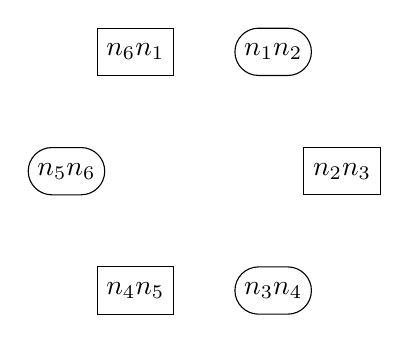
\begin{tikzpicture}[commutative diagrams/every diagram,
		one/.style={draw, rectangle, minimum size=6mm, rounded corners=3mm},
		two/.style={draw, rectangle, minimum size=6mm}
		]
		\node[one] (P0) at (60:1.75cm) {$n_1 n_2$};
		\node[two] (P1) at (60+60:1.75cm) {$n_6 n_1$} ;
		\node[one] (P2) at (60+2*60:1.75cm) {$n_5 n_6$};
		\node[two] (P3) at (60+3*60:1.75cm) {$n_4 n_5$};
		\node[one] (P4) at (60+4*60:1.75cm) {$n_3 n_4$};
		\node[two] (P5) at (0:1.75cm) {$n_2 n_3$};
	\end{tikzpicture}\end{center}

	Tiga hasil bagi Herbrand bersesuaian dengan hasil bagi suku-suku
	yang saling berhadapan pada diagram di atas. Jadi, pernyataan~(i) setara
	dengan pengamatan berikut:
% segment-id: o014.li2.chapter6.tate-cohomology.l002
	\begin{itemize}
% segment-id: o014.li2.chapter6.tate-cohomology.i003
		\item jika kardinalitas pada kedua ujung dua diagonal bernilai
		hingga, hal yang sama juga berlaku pada kedua ujung diagonal sisanya;
% segment-id: o014.li2.chapter6.tate-cohomology.i004
		\item hasil kali suku-suku dalam kotak bersudut siku-siku sama dengan
		hasil kali suku-suku dalam kotak bersudut bulat.
	\end{itemize}

	Untuk~(ii), terdapat barisan-barisan eksak pendek dari modul-$\Z$ hingga
% segment-id: o014.li2.chapter6.tate-cohomology.q012
	\[ 0 \to A^{\sigma=1} \to A \xrightarrow{\sigma-1} \mathfrak{I} A \to 0, \quad 0 \to A^{\nu=0} \to A \xrightarrow{\nu} \nu A \to 0; \]
	di sini, $(\sigma-1)A=\mathfrak{I}A$ merupakan penerapan
	Lema~\ref{prop:cyclic-resolution-prep}. Oleh karena itu,
% segment-id: o014.li2.chapter6.tate-cohomology.q013
	\[ |A^{\sigma=1}| \cdot |\mathfrak{I} A| = |A^{\nu=0}| \cdot |\nu A|, \]
	yang dapat disusun ulang menjadi
	$|\TaHm^0(C_m,A)|=|\TaHm^{-1}(C_m,A)|$. Ini membuktikan pernyataan.
\end{proof}

% Unit 084 terjemahan Bahasa Indonesia dari chapter6.tex baris 2313--2457.
% Sumber: Methods of Algebra, Volume 2, commit
% 9a5803ff77dd3257484cb177f851a73770a59dd3 (CC BY 4.0).
% stable-unit-id: o014.aljabr2.chapter6.profinite-cohomology-a
% Cakupan: Bagian 6.12, modul mulus, definisi kohomologi profinit,
% dan kompleks standar kontinu sampai Teorema 6.12 pertama.

% segment-id: o014.li2.chapter6.profinite-cohomology-a.h001
\section{Kohomologi grup profinit}\label{sec:profinite-cohomology}
\hypertarget{o014.aljabr2.chapter6.profinite-cohomology-a}{ }

% segment-id: o014.li2.chapter6.profinite-cohomology-a.p001
Bagian ini mengandaikan definisi dan hasil dasar tentang grup profinit dari
\S\ref{sec:profinite-groups}.

% segment-id: o014.li2.chapter6.profinite-cohomology-a.p002
Misalkan $G$ grup profinit dan $M$ modul-$G$. Tidak sulit memeriksa bahwa
syarat-syarat berikut ekuivalen:
\begin{enumerate}[(i)]
	\item $M=\bigcup_KM^K$, dengan $K$ berkisar atas subgrup normal buka dari
	$G$;
	\item untuk setiap $x\in M$, subgrup penstabil $\Stab_G(x)$ bersifat buka;
	\item pemetaan aksi $G\times M\to M$ kontinu jika $M$ diberi topologi
	diskret.
\end{enumerate}

% segment-id: o014.li2.chapter6.profinite-cohomology-a.d001
\begin{definition}
	\index{modul-$G$!mulus (smooth)}
	\index[sym1]{G-Mod-infty@$G\dcate{Mod}^\infty$}
	Misalkan $G$ grup profinit. Jika salah satu syarat di atas berlaku, modul-$G$
	$M$ disebut \emph{mulus}\footnote{Karena~(iii), banyak pustaka menyebutnya
	diskret.}. Semua modul-$G$ mulus membentuk subkategori penuh
	$G\dcate{Mod}^\infty$ dari $G\dcate{Mod}$.
\end{definition}

% segment-id: o014.li2.chapter6.profinite-cohomology-a.p003
Meskipun syarat pada $G$ sendiri bersifat topologis, karakterisasi~(i) atau
~(ii) bagi modul-$G$ mulus sepenuhnya bersifat aljabar: kemulusan merupakan sifat
modul-$G$, bukan struktur tambahan. Dari sini mudah dilihat bahwa
$G\dcate{Mod}^\infty$ adalah subkategori abelian dari $G\dcate{Mod}$. Operasi
dalam Definisi~\ref{def:Res-Infl} mempunyai analog alami dalam keadaan ini.

% segment-id: o014.li2.chapter6.profinite-cohomology-a.d002
\begin{definition-proposition}
	Misalkan $\varphi:H\to G$ homomorfisme kontinu antargrup profinit dan
$M$ modul-$G$ mulus. Maka modul-$H$ $\varphi^*M$ tetap mulus. Ini memberikan
	funktor
	\[ \varphi^*:G\dcate{Mod}^\infty\to H\dcate{Mod}^\infty. \]
\end{definition-proposition}
\begin{proof}
	Untuk setiap subgrup normal buka $K\lhd G$, prapetanya
	$\varphi^{-1}(K)\lhd H$ juga normal dan buka. Jika $x\in M^K$, maka
	$x\in(\varphi^*M)^{\varphi^{-1}K}$. Jadi
	\[ \varphi^*M=
	\bigcup_{L\lhd H:\,\text{buka}}(\varphi^*M)^L, \]
	yang membuktikan bahwa $\varphi^*M$ mulus.
\end{proof}

% segment-id: o014.li2.chapter6.profinite-cohomology-a.p004
Perhatikan bahwa funktor $\varphi^*$ selalu eksak. Dua kasus khusus berikut
akan digunakan:
\begin{description}
	\item[Restriksi] Jika $H$ subgrup tertutup dari $G$, ambil $\varphi$ sebagai
	homomorfisme penyertaan $H\hookrightarrow G$. Funktor terkait ditulis
	\[ \Res^G_H:G\dcate{Mod}^\infty\to H\dcate{Mod}^\infty. \]
	\item[Inflasi] Untuk subgrup normal tertutup $H\lhd G$, ambil $\varphi$
	sebagai homomorfisme hasil bagi $G\twoheadrightarrow G/H$. Funktor terkait
	ditulis
	\[ \mathrm{Infl}^G_{G/H}:G/H\dcate{Mod}^\infty
	\to G\dcate{Mod}^\infty. \]

	Grup $H$ dan $G/H$ yang disebutkan di atas otomatis profinit, sehingga
	definisi ini sah.
\end{description}
\index[sym1]{ResGH}
\index[sym1]{InflGH}

% segment-id: o014.li2.chapter6.profinite-cohomology-a.d003
\begin{definition-proposition}\label{def:smooth-part}
	Untuk setiap modul-$G$ $M$, definisikan
	$M^\infty:=\bigcup_KM^K$, dengan $K$ berkisar atas subgrup normal buka dari
	$G$. Ini merupakan modul-$G$ mulus, dan $M$ mulus jika dan hanya jika
	$M=M^\infty$.

	Untuk setiap modul-$G$ mulus $M'$, berlaku
	\[ \Hom_G(M',M)=\Hom_G(M',M^\infty). \]
	Dengan kata lain,
	$\text{penyertaan}:G\dcate{Mod}^\infty
	\leftrightarrows G\dcate{Mod}:(\cdot)^\infty$ merupakan pasangan adjoin.
\end{definition-proposition}
\begin{proof}
	Jelas.
\end{proof}

% segment-id: o014.li2.chapter6.profinite-cohomology-a.p005
Unsur-unsur $M^\infty$ juga disebut \emph{unsur mulus} dari $M$. Karena
$(\cdot)^\infty$ adalah adjoin kanan dari funktor eksak, funktor ini
mempertahankan objek injektif
(Proposisi~\ref{prop:adjoint-injective-projective}).

% segment-id: o014.li2.chapter6.profinite-cohomology-a.t001
\begin{corollary}
	Kategori abelian $G\dcate{Mod}^\infty$ memiliki cukup banyak objek
	injektif.
\end{corollary}
\begin{proof}
	Misalkan $M$ modul-$G$ mulus dan sertakan $M$ ke dalam modul-$G$ injektif
	$I$. Maka $M=M^\infty\hookrightarrow I^\infty$, sedangkan $I^\infty$
	merupakan modul-$G$ mulus injektif.
\end{proof}

% segment-id: o014.li2.chapter6.profinite-cohomology-a.r001
\begin{remark}
	Pada umumnya $G\dcate{Mod}^\infty$ tidak memiliki cukup banyak objek
	projektif. Inilah alasan utama bagian ini membahas kohomologi, bukan homologi.
\end{remark}

% segment-id: o014.li2.chapter6.profinite-cohomology-a.p006
Karena $G\dcate{Mod}^\infty$ memiliki cukup banyak objek injektif, kita dapat
membahas funktor turunan kanan dari funktor invarian $(\cdot)^G$. Pendekatan
bagian ini mula-mula memberikan definisi langsung yang mereduksi ke kasus grup
hingga, lalu mengidentifikasikannya dengan funktor turunan kanan dalam
Proposisi~\ref{prop:profinite-cohomology-identification}. Untuk sementara kita
hanya memakai bahasa klasik, tanpa kategori turunan.

% segment-id: o014.li2.chapter6.profinite-cohomology-a.p007
Mula-mula, ambil grup profinit $G$ dan subgrup normal buka $K$. Untuk setiap
modul-$G$ mulus $M$, submodul invarian-$K$
$M^K=(\Res^G_KM)^K$ secara alami menjadi modul-$G/K$. Dengan demikian
diperoleh funktor $(\cdot)^K:G\dcate{Mod}^\infty\to G/K\dcate{Mod}$ dan
pasangan adjoin yang jelas
\begin{equation}\label{eqn:invariant-adjunction-profinite}
	\begin{tikzcd}[row sep=tiny]
		\mathrm{Infl}^G_{G/K}:G/K\dcate{Mod} \arrow[shift left,r] &
		G\dcate{Mod}^\infty:(\cdot)^K \arrow[shift left,l]\\
		\Hom_G(\mathrm{Infl}^G_{G/K}(M'),M) \arrow[equal,r] &
		\Hom_{G/K}(M',M^K).
	\end{tikzcd}
\end{equation}

% segment-id: o014.li2.chapter6.profinite-cohomology-a.p008
Jika subgrup normal buka $K,K'$ dari $G$ memenuhi $K'\supset K$, maka
penyertaan $M^{K'}\hookrightarrow M^K$ ekuivarian terhadap homomorfisme hasil
bagi yang berarah sebaliknya $G/K'\twoheadleftarrow G/K$
(Definisi~\ref{def:group-equivariance}). Jadi untuk setiap
$n\in\Z_{\geq0}$ terdapat homomorfisme kanonik
\[ \rho^{K'}_K:\Hm^n(G/K',M^{K'})\to\Hm^n(G/K,M^K). \]
Jika $K_1\subset K_2\subset K_3$ merupakan subgrup normal buka dari $G$,
maka $\rho^{K_2}_{K_1}\rho^{K_3}_{K_2}=\rho^{K_3}_{K_1}$. Jadi definisi
berikut sah.

% segment-id: o014.li2.chapter6.profinite-cohomology-a.d004
\begin{definition}
	\index{kohomologi grup!kasus profinit}
	\index[sym1]{HnGM}
	Misalkan $G$ grup profinit dan $M$ modul-$G$ mulus. Untuk setiap
	$n\in\Z_{\geq0}$, definisikan
	\[ \Hm^n(G,M):=\varinjlim_K\Hm^n(G/K,M^K), \]
	dengan $K$ berkisar atas subgrup normal buka dari $G$, dan $\varinjlim$
	diambil terhadap urutan parsial
	$K'\preceq K\iff K\subset K'$ serta morfisme $\rho^{K'}_K$.
\end{definition}

% segment-id: o014.li2.chapter6.profinite-cohomology-a.p009
Semua subgrup normal buka membentuk himpunan terurut terfilter: himpunan ini
tertutup terhadap irisan hingga. Jika $G$ hingga, maka $\{1\}$ adalah satu-satunya
unsur maksimal, dan $\Hm^n(G,M)$ kembali menjadi versi awal dalam
\S\ref{sec:group-coh-sub}. Secara umum,
\[ \Hm^0(G,M)=\varinjlim_K(M^K)^{G/K}=M^G. \]

% segment-id: o014.li2.chapter6.profinite-cohomology-a.p010
Misalkan $f:M_1\to M_2$ homomorfisme modul-$G$ mulus. Untuk setiap subgrup
normal buka $K$, pemetaan ini membatasi menjadi
$f_K:M_1^K\to M_2^K$. Jelas bahwa $K'\supset K$ mengakibatkan
$\Hm^n(f_K)\rho^{K'}_K=\rho^{K'}_K\Hm^n(f_{K'})$, sehingga untuk setiap
$n\in\Z_{\geq0}$ terdapat
\[ \Hm^n(f):\Hm^n(G,M_1)\to\Hm^n(G,M_2). \]

% segment-id: o014.li2.chapter6.profinite-cohomology-a.e001
\begin{example}
	Misalkan $E|F$ perluasan Galois medan. Karena
	$E=\bigcup_{L|F}E^{\Gal(E|L)}=\bigcup_{L|F}L$, dengan $L|F$ menjelajahi
	subekstensi Galois hingga, aksi $\Gal(E|F)$ pada $E$ bersifat mulus.
	Dengan menerapkan Contoh~\ref{eg:additive-90-finite} pada setiap $L|F$,
	diperoleh
	\[ n\geq1\implies\Hm^n(\Gal(E|F),E)
	=\varinjlim_{L|F}\Hm^n(\Gal(L|F),L)=0. \]
\end{example}

% segment-id: o014.li2.chapter6.profinite-cohomology-a.p011
Seperti Proposisi~\ref{prop:groupcoh-cochain} dan
Catatan~\ref{rem:nor-cochain} untuk grup tanpa topologi, kohomologi grup
profinit dapat dihitung melalui kompleks standar atau versi ternormalisasinya;
perbedaannya terletak pada syarat kontinuitas.

% segment-id: o014.li2.chapter6.profinite-cohomology-a.d005
\begin{definition}
	\index{kompleks standar}
	\index[sym1]{CGM}
	Untuk modul-$G$ mulus $M$, beri $M$ topologi diskret dan definisikan
	\emph{kompleks standar} $C(G,M)=(C^n(G,M))_n$ dengan
	\[ C^n(G,M):=\{\text{pemetaan kontinu }f:G^n\to M\},
	\qquad n\in\Z_{\geq0}. \]
	Suku berderajat negatif didefinisikan sebagai $0$, sedangkan
	$d^n:C^n(G,M)\to C^{n+1}(G,M)$ diberikan oleh
	\begin{multline*}
		(d^nf)(g_1,\ldots,g_{n+1})
		=g_1f(g_2,\ldots,g_{n+1})\\
		+\sum_{k=1}^n(-1)^kf(\ldots,g_kg_{k+1},\ldots)
		+(-1)^{n+1}f(g_1,\ldots,g_n).
	\end{multline*}

	\index[sym1]{CGMbar}
	Definisikan \emph{kompleks standar ternormalisasi} sebagai subkompleks
	$\overline{C}(G,M)$ dari $C(G,M)$ berikut
	(lihat Catatan~\ref{rem:nor-cochain}):
	\[ \overline{C}^n(G,M)=\left\{\begin{array}{r|l}
		f\in C^n(G,M)&\exists,1\leq k\leq n,\ g_k=1_G\\
		&\implies f(g_1,\ldots,g_n)=0
	\end{array}\right\}. \]
\end{definition}

% segment-id: o014.li2.chapter6.profinite-cohomology-a.p012
Untuk setiap subgrup normal buka $K\lhd G$, terdapat penyertaan kompleks yang
jelas
$C(G/K,M^K)\hookrightarrow C(G,M)$ dan
$\overline{C}(G/K,M^K)\hookrightarrow\overline{C}(G,M)$.

% segment-id: o014.li2.chapter6.profinite-cohomology-a.p013
Karena $M$ diskret, pemetaan $f:G^n\to M$ kontinu jika dan hanya jika lokal
konstan. Kekompakan $G$ kemudian memberikan subgrup normal buka
$K_1\lhd G$ sedemikian sehingga $f$ berfaktor melalui
$(G/K_1)^n\to M$. Khususnya, $f$ hanya mengambil sejumlah hingga nilai;
kemulusan memberikan subgrup normal buka $K_2\lhd G$ sedemikian sehingga
nilai-nilai $f$ terletak dalam $M^{K_2}$. Ambil $K:=K_1\cap K_2$. Maka
\[ C^n(G,M)\simeq\varinjlim_{K\lhd G\;\text{buka}}C^n(G/K,M^K),\qquad
	\overline{C}^n(G,M)\simeq
	\varinjlim_{K\lhd G\;\text{buka}}\overline{C}^n(G/K,M^K). \]
Ketika $n$ bervariasi, ini memberikan isomorfisme kompleks.

% segment-id: o014.li2.chapter6.profinite-cohomology-a.p014
Seperti sebelumnya, definisikan submodul dari $C^n(G,M)$
\[ Z^n(G,M):=\Ker(d^n),\qquad B^n(G,M):=\Image(d^{n-1}), \]
dengan $B^0(G,M):=\{0\}$. Maka
$\Hm^n(C(G,M))=Z^n(G,M)/B^n(G,M)$. Definisikan dengan cara serupa versi
ternormalisasi $\overline{Z}^n(G,M)$ dan $\overline{B}^n(G,M)$.

% segment-id: o014.li2.chapter6.profinite-cohomology-a.t002
\begin{theorem}\label{prop:profinite-group-standard}
	Misalkan $G$ grup profinit. Untuk semua $n\in\Z_{\geq0}$ dan semua modul-$G$
	mulus $M$, terdapat isomorfisme kanonik
	\[ \Hm^n(C(G,M))\simeq\Hm^n(G,M)
	\simeq\Hm^n(\overline{C}(G,M)). \]
\end{theorem}
\begin{proof}
	Kohomologi bernilai dalam $\cate{Ab}$ atau $\Bbbk\dcate{Mod}$ jika
	gelanggang koefisien $\Bbbk$ turut ditetapkan. Kolimit terfilter bersifat
	eksak dalam kategori-kategori ini \cite[Teorema 6.2.2]{Li1}. Karena itu,
	\[ Z^n(G,M)=\varinjlim_KZ^n(G/K,M^K),\qquad
	B^n(G,M)=\varinjlim_KB^n(G/K,M^K), \]
	dan selanjutnya
	\begin{multline*}
		\Hm^n(C(G,M))
		=\dfrac{\varinjlim_KZ^n(G/K,M^K)}
		{\varinjlim_KB^n(G/K,M^K)}\simeq\\
		\varinjlim_K\frac{Z^n(G/K,M^K)}{B^n(G/K,M^K)}
		=\varinjlim_K\Hm^n(C(G/K,M^K)).
	\end{multline*}
	Terapkan Proposisi~\ref{prop:groupcoh-cochain} pada suku terakhir untuk
	memperoleh $\varinjlim_K\Hm^n(G/K,M^K)$, yakni $\Hm^n(G,M)$.

	Kasus $\overline{C}(G,M)$ serupa.
\end{proof}

% Unit 085 terjemahan Bahasa Indonesia dari chapter6.tex baris 2458--2603.
% Sumber: Methods of Algebra, Volume 2, commit
% 9a5803ff77dd3257484cb177f851a73770a59dd3 (CC BY 4.0).
% stable-unit-id: o014.aljabr2.chapter6.profinite-cohomology-b
% Cakupan: Bagian 6.12, funktor delta, interpretasi derajat rendah,
% identifikasi sebagai funktor turunan, induksi profinit, dan Lema Shapiro.

% segment-id: o014.li2.chapter6.profinite-cohomology-b.t001
\begin{theorem}\label{prop:profinite-cohomology-long}
	Misalkan $G$ grup profinit dan
	$0\to M'\xrightarrow{f}M\xrightarrow{f'}M''\to0$ barisan eksak pendek
	modul-$G$ mulus. Terdapat barisan eksak panjang terkait
	\begin{multline*}
		\cdots\to\Hm^{n-1}(G,M'')\xrightarrow{\delta^{n-1}}
		\Hm^n(G,M')\xrightarrow{\Hm^n(f)}\Hm^n(G,M)\\
		\xrightarrow{\Hm^n(f')}\Hm^n(G,M'')\xrightarrow{\delta^n}
		\Hm^{n+1}(G,M')\to\cdots,
	\end{multline*}
	dengan konvensi $\Hm^n(G,\cdot)=0$ untuk $n<0$. Homomorfisme penghubung
	$\delta^n$ natural terhadap morfisme barisan eksak pendek; dengan kata lain,
	keluarga ini membentuk funktor-$\delta$ kohomologis.
\end{theorem}
\begin{proof}
	Kita bekerja dengan kompleks standar; argumen untuk versi ternormalisasi
	serupa. Menurut Proposisi~\ref{prop:long-exact-sequence-ses}, cukup buktikan
	bahwa
	\[ 0\to C^n(G,M')\to C^n(G,M)\to C^n(G,M'')\to0 \]
	merupakan barisan eksak pendek. Satu-satunya bagian yang tidak langsung
	adalah kesurjektifan $C^n(G,M)\to C^n(G,M'')$. Misalkan
	$u:G^n\to M''$ kontinu. Seperti di atas, terdapat subgrup normal buka
	$K\lhd G$ sedemikian sehingga $u$ konstan pada setiap koset
	$K^n\lhd G^n$. Pada setiap koset, pilih sembarang prapeta dalam $M$ dari
	nilai konstan tersebut.
\end{proof}

% segment-id: o014.li2.chapter6.profinite-cohomology-b.p001
Ambil modul-$G$ mulus $M$ dengan topologi diskret. Suku berderajat rendah dari
kompleks $C(G,M)$ atau $\overline{C}(G,M)$ masih memiliki interpretasi
langsung.
\begin{description}
	\item[($n=0$)] Jelas bahwa $C^0(G,M)=M$ dan
	$\Hm^0(G,M)=Z^0(G,M)=M^G$. Versi kompleks standar ternormalisasi sama.
	\item[($n=1$)] Unsur $Z^1(G,M)=\overline{Z}^1(G,M)$ adalah homomorfisme
	silang kontinu $G\to M$. Secara ekuivalen, unsur tersebut adalah
	homomorfisme kontinu $\sigma:G\to M\rtimes G$ yang memenuhi
	$\pi\sigma=\identity_G$, seperti dalam
	Proposisi~\ref{prop:crossed-semidirect-product}. Di sini
	$\pi:M\rtimes G\to G$ adalah proyeksi dan $M\rtimes G$ diberi topologi
	hasil kali. Di sisi lain, unsur $B^1(G,M)$ dibangun oleh homomorfisme silang
	berbentuk $f_m:g\mapsto gm-m$; homomorfisme ini otomatis kontinu.

	\item[($n=2$)] Andaikan $M$ hingga. Unsur
	\[ \Hm^2(G,M)\simeq\frac{Z^2(G,M)}{B^2(G,M)}
	\simeq\frac{\overline{Z}^2(G,M)}{\overline{B}^2(G,M)} \]
	berkorespondensi secara bijektif dengan kelas ekuivalensi ekstensi grup profinit
	\[ 1\to M\to E\xrightarrow{\pi}G\to1
	\qquad\text{(barisan eksak pendek grup)}, \]
	dengan aksi konjugasi $G$ pada $M$ berasal dari struktur modul-$G$ pada
	$M$. Dibandingkan dengan versi dalam Definisi~\ref{def:group-ext} dan
	\eqref{eqn:group-ext-diagram}, ``ekstensi grup profinit'' dan masalah
	klasifikasinya juga mensyaratkan:
	\begin{compactitem}
		\item $E$ merupakan grup profinit, $\pi$ kontinu, dan $M$ disertakan
		sebagai subgrup tertutup dari $E$;
		\item ekuivalensi atau isomorfisme ekstensi didefinisikan oleh
		homomorfisme grup kontinu $E\to E'$, dan pembelahan ekstensi juga
		didefinisikan secara topologis.
	\end{compactitem}

	Selain itu, grup automorfisme ekstensi tersebut isomorfik dengan
	$\overline{Z}^1(G,M)$. Buktinya tidak sulit, tetapi memerlukan sedikit
	bahasa topologi dan karena itu diserahkan sebagai latihan bab ini; syarat
	bahwa $M$ hingga bersifat penting.
\end{description}

% segment-id: o014.li2.chapter6.profinite-cohomology-b.p002
Sekarang kita kembali ke funktor turunan kanan
$(\mathrm{R}^n(\cdot)^G)_{n\geq0}$. Kita dapat mengkaji nilainya pada sembarang
kompleks terbatas ke bawah\footnote{Dengan kata lain, mengkaji hiperkohomologi
grup profinit.}, bahkan operasinya dalam kategori turunan. Namun bagian ini
hanya membahas modul-$G$ mulus; sisanya menjadi latihan.

% segment-id: o014.li2.chapter6.profinite-cohomology-b.t002
\begin{proposition}\label{prop:profinite-cohomology-identification}
	Terdapat isomorfisme funktor-$\delta$ kohomologis
	\[ (\Hm^n(G,\cdot))_{n\geq0}
	\simeq(\mathrm{R}^n(\cdot)^G)_{n\geq0}. \]
\end{proposition}
\begin{proof}
	Teorema~\ref{prop:profinite-cohomology-long} menunjukkan bahwa keduanya
	merupakan funktor-$\delta$ kohomologis, dan pada $n=0$ keduanya sama dengan
	funktor invarian $(\cdot)^G$. Menurut
	Proposisi~\ref{prop:erasable-univ-delta}, cukup tunjukkan bahwa
	$\Hm^n(G,\cdot)$ dapat dihapus untuk $n>0$ dalam arti
	Definisi~\ref{def:erasable}. Misalkan $M$ modul-$G$ mulus dan sertakan ke
	dalam modul-$G$ mulus injektif $I$. Untuk setiap subgrup normal buka
	$K\lhd G$, adjungsi \eqref{eqn:invariant-adjunction-profinite} menunjukkan
	bahwa $(\cdot)^K$ mempertahankan objek injektif. Jadi $I^K$ merupakan
	modul-$G/K$ injektif, dan
	\[ n>0\implies\Hm^n(G,I)
	=\varinjlim_K\Hm^n(G/K,I^K)=0. \]
	Sifat dapat dihapus terbukti.
\end{proof}

% segment-id: o014.li2.chapter6.profinite-cohomology-b.p003
Berdasarkan Proposisi~\ref{prop:profinite-cohomology-identification}, metode
\S\ref{sec:change-of-group} dapat diterapkan langsung pada homomorfisme
kontinu $\varphi:H\to G$ dari grup profinit untuk mendefinisikan operasi
``tarikan balik'' kohomologi
\[ \Hm^n(G,M)\to\Hm^n(H,\varphi^*M),\qquad
	M:\text{ modul-$G$ mulus},\quad n\in\Z_{\geq0}. \]
Operasi ini kompatibel dengan barisan eksak panjang. Seperti biasa, gunakan
keeksakan $\varphi^*$ dan sifat funktor-$\delta$ kohomologis universal untuk
mereduksi masalah ke penyertaan yang jelas pada $n=0$,
$M^G\hookrightarrow(\varphi^*M)^H$.

% segment-id: o014.li2.chapter6.profinite-cohomology-b.p004
Sebagai kasus khusus, untuk semua $n$ dan semua subgrup tertutup $H$ terdapat
pemetaan restriksi
$\mathrm{res}^n:\Hm^n(G,M)\to\Hm^n(H,M)$; di sini
$\Res^G_HM$ disingkat sebagai $M$.

% segment-id: o014.li2.chapter6.profinite-cohomology-b.p005
Homomorfisme di atas juga dapat dibangun dari homomorfisme-homomorfisme
\begin{align*}
	\Hm^n(G/K,M^K)&\xrightarrow{\eqref{eqn:change-of-group-coh}}
	\Hm^n(H/\varphi^{-1}(K),\varphi_K^*(M^K))\\
	&\xrightarrow{M^K\subset(\varphi^*M)^{\varphi^{-1}K}}
	\Hm^n(H/\varphi^{-1}(K),(\varphi^*M)^{\varphi^{-1}K}),
\end{align*}
dengan $K$ berkisar atas subgrup normal buka dari $G$. Dengan mereduksi ke
kasus grup hingga, homomorfisme pada kompleks standar dihitung oleh rumus
Proposisi~\ref{prop:grp-equiv}. Untuk membuktikan bahwa pemetaan ini memang
sama dengan pemetaan yang sebelumnya dibangun melalui sifat universal, cukup
bandingkan kasus $n=0$ dan tunjukkan kompatibilitasnya dengan barisan eksak
panjang. Kompleks standar memadai untuk kedua hal tersebut.

% segment-id: o014.li2.chapter6.profinite-cohomology-b.p006
Dengan cara serupa, homomorfisme korestriksi dalam
Definisi--Proposisi~\ref{def:cor} meluas ke grup profinit. Misalkan $H$
subgrup buka dari $G$. Maka $H$ otomatis tertutup dan $(G:H)$ hingga
(lihat \S\ref{sec:profinite-groups}). Definisikan homomorfisme
\[ \mathrm{cor}^n:\Hm^n(H,M)\to\Hm^n(G,M),\qquad
	M:\text{ modul-$G$ mulus},\quad n\in\Z_{\geq0}, \]
yang kompatibel dengan barisan eksak panjang dan pada $n=0$ memberikan
$\nu^{G|H}:M^H\to M^G$.

% segment-id: o014.li2.chapter6.profinite-cohomology-b.p007
Konstruksinya kembali memakai sifat funktor-$\delta$ kohomologis universal,
tetapi di sini kita perlu mengetahui bahwa
$\Res^G_H:G\dcate{Mod}^\infty\to H\dcate{Mod}^\infty$ mempertahankan objek
injektif; ini adalah isi Korolari~\ref{prop:Res-injective-profinite}. Setelah
fakta tersebut diterima, Proposisi~\ref{prop:res-cor} tetap mempunyai analog:
untuk semua $n$,
\[ \mathrm{cor}^n\circ\mathrm{res}^n
	=(G:H)\cdot\identity_{\Hm^n(G,M)}. \]
Seperti sebelumnya, pembuktiannya direduksi ke kasus $n=0$.

% segment-id: o014.li2.chapter6.profinite-cohomology-b.p008
Sekarang kita membahas modul terinduksi dalam kasus profinit. Selanjutnya $G$
selalu merupakan grup profinit. Untuk membedakannya, tuliskan funktor induksi
dalam kasus tanpa topologi (Definisi~\ref{def:induced-module}) sebagai
$\Ind^{G,\mathrm{alg}}_H$; menurut Lema~\ref{prop:Ind-as-mappings}, kita
merealisasikannya sebagai ruang pemetaan.

% segment-id: o014.li2.chapter6.profinite-cohomology-b.d001
\begin{definition}
	\index{modul-$G$!terinduksi (induced)}
	Untuk subgrup tertutup $H$ dari $G$ dan modul-$H$ mulus $N$, lengkapi ruang
	pemetaan $\mathrm{Maps}(G,N):=\{f:G\to N\}$ dengan operasi penjumlahan dan
	perkalian skalar titik demi titik, serta aksi kiri $G$
	\[ (gf)(x)=f(xg),\qquad g,x\in G. \]
	Definisikan modul-$G$ mulus
	\begin{align*}
		\Ind^G_H(N)&:=\{f\in\mathrm{Maps}(G,N)^\infty:
		\forall h\in H,\ \forall x\in G,\ f(hx)=hf(x)\}\\
		&=(\Ind^{G,\mathrm{alg}}_H(N))^\infty.
	\end{align*}
	Notasi $(\cdot)^\infty$ berasal dari
	Definisi--Proposisi~\ref{def:smooth-part}. Objek ini disebut modul-$G$
	terinduksi dari $N$.
\end{definition}

% segment-id: o014.li2.chapter6.profinite-cohomology-b.p009
Karena $G$ kompak, kemulusan $f\in\Ind^{G,\mathrm{alg}}_H(N)$ ekuivalen
dengan kontinuitasnya sebagai pemetaan $G\to N$, dengan $N$ diberi topologi
diskret.

% segment-id: o014.li2.chapter6.profinite-cohomology-b.t003
\begin{proposition}\label{prop:Ind-injective-profinite}
	Untuk setiap subgrup tertutup $H$ dari $G$, terdapat pasangan adjoin
	\[ \Res^G_H:G\dcate{Mod}^\infty
	\leftrightarrows H\dcate{Mod}^\infty:\Ind^G_H. \]
	Sebagai akibatnya, $\Ind^G_H$ mempertahankan objek injektif.

	Jika $H$ subgrup buka dari $G$, terdapat pula pasangan adjoin
	\[ \Ind^G_H:H\dcate{Mod}^\infty
	\leftrightarrows G\dcate{Mod}^\infty:\Res^G_H. \]
	Dalam keadaan ini $\Ind^G_H$ juga mempertahankan objek projektif.
\end{proposition}
\begin{proof}
	Berdasarkan adjungsi dalam kasus tanpa topologi dan
	Definisi--Proposisi~\ref{def:smooth-part}, untuk setiap modul-$G$ mulus $M$
	dan modul-$H$ mulus $N$ terdapat isomorfisme kanonik
	\begin{multline*}
		\Hom_H(\Res^G_H(M),N)
		\simeq\Hom_G(M,\Ind^{G,\mathrm{alg}}_H(N))\\
		=\Hom_G(M,\Ind^{G,\mathrm{alg}}_H(N)^\infty)
		=\Hom_G(M,\Ind^G_H(N)).
	\end{multline*}

	Sekarang andaikan $H$ buka, sehingga $(G:H)$ hingga. Dari
	Korolari~\ref{prop:iInd-Ind} kita memperoleh adjungsi tanpa topologi
	\[ \Hom_H(N,\Res^G_H(M))
	\simeq\Hom_G(\Ind^{G,\mathrm{alg}}_H(N),M). \]
	Kita nyatakan bahwa
	$\Ind^{G,\mathrm{alg}}_H(N)=\Ind^G_H(N)$. Ambil
	$f\in\Ind^{G,\mathrm{alg}}_H(N)$ dan $x\in G$, lalu pilih subgrup buka
	$K_0\subset H$ dengan $f(x)\in N^{K_0}$. Definisikan
	$K:=x^{-1}K_0x$, yang merupakan subgrup buka dari $G$. Maka
	\[ g\in K\implies xg=xgx^{-1}x\in K_0x
	\implies f(xg)=f(x). \]
	Karena $x$ sembarang, pemetaan $f:G\to N$ lokal konstan, sehingga
	$f\in\Ind^G_H(N)$. Pasangan adjoin kedua terbukti.

	Terakhir, pernyataan tentang pemertahanan objek injektif atau projektif
	mengikuti dari keeksakan $\Res^G_H$ dan
	Proposisi~\ref{prop:adjoint-injective-projective}.
\end{proof}

% segment-id: o014.li2.chapter6.profinite-cohomology-b.l001
\begin{lemma}\label{prop:Ind-exact-profinite}
	Jika $H$ subgrup tertutup dari $G$, maka
	$\Ind^G_H:H\dcate{Mod}^\infty\to G\dcate{Mod}^\infty$ eksak.
\end{lemma}
\begin{proof}
	Kita telah mengetahui bahwa $\Ind^G_H$ memiliki adjoin kiri, sehingga
	funktor ini eksak kiri. Tinggal membuktikan bahwa
	$N_1\twoheadrightarrow N_2$ mengakibatkan
	$\Ind^G_H(N_1)\twoheadrightarrow\Ind^G_H(N_2)$. Menurut
	Lema~\ref{prop:profinite-section}, homomorfisme hasil bagi
	$\pi:G\to H\backslash G$ mempunyai penampang kontinu $s$. Untuk setiap
	modul-$H$ mulus $N$, terdapat isomorfisme modul-$\Bbbk$
	\[\begin{tikzcd}[row sep=tiny]
		\Ind^G_H(N) \arrow[leftrightarrow,r,"\sim"] &
		\{\text{pemetaan kontinu }H\backslash G\to N\}\\
		f \arrow[mapsto,r] & {[x\mapsto f(s(x))]}\\
		{[hs(x)\mapsto hf'(x)]} & f' \arrow[mapsto,l]
	\end{tikzcd}\]
	dengan $x\in H\backslash G$ dan $h\in H$. Walaupun isomorfisme ini tidak
	mempertahankan aksi $G$, ia natural dalam $N$.

	Karena pemetaan kontinu $H\backslash G\to N$ selalu lokal konstan, bekerja
	pada ruas kanan segera menunjukkan bahwa
	$\Ind^G_H(N_1)\to\Ind^G_H(N_2)$ surjektif.
\end{proof}

% segment-id: o014.li2.chapter6.profinite-cohomology-b.t004
\begin{corollary}\label{prop:Res-injective-profinite}
	Jika $H$ subgrup buka dari $G$, maka
	$\Res^G_H:G\dcate{Mod}^\infty\to H\dcate{Mod}^\infty$
	mempertahankan objek injektif.
\end{corollary}
\begin{proof}
	Menurut dua hasil sebelumnya, funktor ini memiliki adjoin kiri eksak
	$\Ind^G_H$.
\end{proof}

% segment-id: o014.li2.chapter6.profinite-cohomology-b.p010
Sekarang kita memperoleh versi profinit dari Teorema~\ref{prop:Shapiro}.

% segment-id: o014.li2.chapter6.profinite-cohomology-b.t005
\begin{proposition}
	\index{Lema Shapiro}
	Misalkan $H$ subgrup tertutup dari grup profinit $G$ dan $N$ modul-$H$
	mulus. Terdapat isomorfisme
	\[ \Hm^n(G,\Ind^G_H(N))\simeq\Hm^n(H,N),
	\qquad n\in\Z_{\geq0}. \]
\end{proposition}
\begin{proof}
	Karena $\Ind^G_H$ eksak dan mempertahankan objek injektif
	(Lema~\ref{prop:Ind-exact-profinite} dan
	Proposisi~\ref{prop:Ind-injective-profinite}), argumen dalam
	Teorema~\ref{prop:Shapiro} yang memakai funktor-$\delta$ kohomologis yang
	dapat dihapus berlaku tanpa perubahan. Ingat bahwa inti argumen tersebut adalah
	kasus $n=0$, yakni
	\[ \Ind^G_H(N)^G
	=(\Ind^{G,\mathrm{alg}}_H(N)^\infty)^G
	=(\Ind^{G,\mathrm{alg}}_H(N))^G\rightiso N^H. \]
	Kesamaan pertama adalah definisi, kesamaan kedua mudah, dan isomorfisme
	terakhir berasal dari Korolari~\ref{prop:Ind-invariant}.
\end{proof}

% segment-id: o014.li2.chapter6.profinite-cohomology-b.p011
Selain itu:
\begin{itemize}
	\item barisan spektral kohomologis Lyndon--Hochschild--Serre
	(lihat \S\ref{sec:LHS-SS}) meluas ke keadaan ketika $G$ grup profinit dan
	$H$ subgrup normal tertutup;
	\item hasil kali cawan (lihat \S\ref{sec:cup-product}) juga meluas ke grup
	profinit dengan memakai definisi langsung pada kompleks standar; lihat
	Definisi--Proposisi~\ref{def:group-cup-3}.
	\index{hasil kali cawan}
\end{itemize}
Pernyataannya tidak berubah, sehingga tidak kita ulangi.

% Unit 086 terjemahan Bahasa Indonesia dari chapter6.tex baris 2604--2927.
% Sumber: Methods of Algebra, Volume 2, commit
% 9a5803ff77dd3257484cb177f851a73770a59dd3 (CC BY 4.0).
% stable-unit-id: o014.aljabr2.chapter6.nonabelian-cohomology
% Cakupan: Bagian 6.13 lengkap, ``Kohomologi Nonabelian'';
% berhenti tepat sebelum lingkungan Exercises pada baris 2928.

% segment-id: o014.li2.chapter6.nonabelian-cohomology.h001
\section{Kohomologi Nonabelian}\label{sec:nonabelian-coh}
\hypertarget{o014.aljabr2.chapter6.nonabelian-cohomology}{ }
% segment-id: o014.li2.chapter6.nonabelian-cohomology.p001
Misalkan $G$ grup. Kohomologi $\Hm^n(G,M)$ yang dibahas sebelumnya selalu
mensyaratkan ``koefisien'' $M$ memiliki struktur modul, atau setidaknya
merupakan modul-$\Z$, yakni grup abelian. Bagian ini bertujuan membahas kasus
ketika koefisiennya grup nonabelian. Mulai sekarang, kita memakai simbol $A$
sebagai pengganti $M$.

% segment-id: o014.li2.chapter6.nonabelian-cohomology.d001
\begin{definisi}\label{def:G-group}
	\index[sym1]{G-Grp@$G\dcate{Grp}$}
	\index{grup-G@grup-$G$}
	Misalkan $A$ grup, dengan operasi biner ditulis secara multiplikatif dan
	unsur identitas ditulis $1$. Andaikan $A$ dilengkapi aksi kiri grup $G$,
	yang ditulis
% segment-id: o014.li2.chapter6.nonabelian-cohomology.q001
	\[ G \times A \to A, \quad (g, a) \mapsto {}^g a . \]
	Jika aksi grup tersebut kompatibel dengan struktur perkalian $A$,
% segment-id: o014.li2.chapter6.nonabelian-cohomology.q002
	\[ {}^g (a_1 a_2) = {}^g a_1 {}^g a_2, \quad {}^g 1 = 1, \]
	maka $A$ disebut grup dengan aksi $G$, atau singkatnya \emph{grup-$G$}.
	Homomorfisme antargrup-$G$ didefinisikan sebagai homomorfisme grup
	yang mempertahankan aksi $G$. Kategori yang dibentuknya dituliskan
	$G\dcate{Grp}$.
\end{definisi}

% segment-id: o014.li2.chapter6.nonabelian-cohomology.p002
Sebentar lagi akan terlihat bahwa, untuk grup-$G$ $A$, tanpa struktur tambahan
atau komutativitas, hanya $\Hm^0$ dan $\Hm^1$ yang dapat didefinisikan secara
wajar dan berguna. Dalam keadaan ini, $\Hm^1$ belum tentu grup, melainkan
himpunan bertitik.

% segment-id: o014.li2.chapter6.nonabelian-cohomology.d002
\begin{definisi}\label{def:pointed-set}
	\index{himpunan bertitik (pointed set)}
	\index[sym1]{Set-pt@$\cate{Set}_\bullet$, $G\dcate{Set}_\bullet$}
	Suatu \emph{himpunan bertitik} adalah data $(X,x_0)$, dengan $X$ himpunan
	dan $x_0\in X$ (disebut titik pangkal). Morfisme dari $(X,x_0)$ ke
	$(Y,y_0)$ adalah pemetaan $f:X\to Y$ yang memenuhi $f(x_0)=y_0$. Data ini
	membentuk kategori $\cate{Set}_\bullet$.
	
	Misalkan $(X,x_0)$ himpunan bertitik. Jika grup $G$ beraksi dari kiri pada
	$X$, ditulis $(g,x)\mapsto{}^gx$, dan ${}^gx_0=x_0$ selalu berlaku, kita
	katakan bahwa $G$ beraksi pada $(X,x_0)$. Dalam hal ini, dapat didefinisikan
	subhimpunan invarian bertitik
% segment-id: o014.li2.chapter6.nonabelian-cohomology.q003
	\[ (X, x_0)^G := \left\{ x \in X: \forall g \in G, \; gx = x \right\}, \quad \text{titik pangkal} = x_0. \]
	Semua himpunan bertitik dengan aksi $G$, beserta morfisme yang kompatibel
	dengan aksi $G$, membentuk kategori yang dituliskan
	$G\dcate{Set}_\bullet$.
\end{definisi}

% segment-id: o014.li2.chapter6.nonabelian-cohomology.p003
Jika tidak menimbulkan kerancuan, objek $(X,x_0)$ dari
$\cate{Set}_\bullet$ sering cukup dituliskan sebagai $X$, dan dalam
$G\dcate{Set}_\bullet$, $(X,x_0)^G$ dituliskan sebagai $X^G$.

% segment-id: o014.li2.chapter6.nonabelian-cohomology.p004
Setiap grup tentu menjadi himpunan bertitik dengan memilih unsur identitas
sebagai titik pangkal. Ini memberikan funktor yang jelas
$\cate{Grp}\to\cate{Set}_\bullet$; demikian pula terdapat funktor
$G\dcate{Grp}\to G\dcate{Set}_\bullet$. Perhatikan bahwa subhimpunan
invarian $A^G$ dari grup-$G$ $A$ merupakan subgrupnya.

% segment-id: o014.li2.chapter6.nonabelian-cohomology.d003
\begin{definisi}\label{def:pointed-exact}
	\index{barisan eksak}
	Misalkan
	$(X,x_0)\xrightarrow{f}(Y,y_0)\xrightarrow{g}(Z,z_0)$ morfisme-morfisme
	dalam $\cate{Set}_\bullet$ (atau $G\dcate{Set}_\bullet$). Barisan morfisme
	ini disebut eksak jika $g^{-1}(z_0)=\Image(f)$. Dengan cara ini,
	barisan eksak dalam $\cate{Set}_\bullet$ (atau
	$G\dcate{Set}_\bullet$) dapat didefinisikan.
\end{definisi}

% segment-id: o014.li2.chapter6.nonabelian-cohomology.p005
Untuk grup abelian, definisi ini kembali kepada keeksakan yang lazim.
Sekarang $\Hm^0$ dan $\Hm^1$ dapat didefinisikan bagi setiap grup-$G$ $A$.

% segment-id: o014.li2.chapter6.nonabelian-cohomology.d004
\begin{definisi}\label{def:nonabelian-H}
	\index{kohomologi grup!kasus nonabelian}
	Misalkan $A$ objek $G\dcate{Set}_\bullet$. Definisikan himpunan bertitik
% segment-id: o014.li2.chapter6.nonabelian-cohomology.q004
	\[ \Hm^0(G, A) = Z^0(G, A) := A^G. \]
	
	Jika $A$ grup-$G$, maka $\Hm^0(G,A)$ merupakan grup. Dalam hal ini,
	definisikan lebih lanjut
% segment-id: o014.li2.chapter6.nonabelian-cohomology.q005
	\begin{align*}
		Z^1(G, A) & := \left\{\begin{array}{r|l}
			c: G \to A & \forall g_1, g_2 \in G, \\
			& c(g_1 g_2) = c(g_1) \cdot {}^{g_1} c(g_2)
		\end{array}\right\}, \\
		\Hm^1(G, A) & := Z^1(G, A) / \sim ,
	\end{align*}
	dengan relasi ekuivalensi $c\sim c'$ berarti bahwa terdapat $a\in A$
	sedemikian sehingga, untuk setiap $g\in G$,
% segment-id: o014.li2.chapter6.nonabelian-cohomology.q006
	\[ c'(g) = a^{-1} \cdot c(g) \cdot {}^g a . \]
	Mudah dilihat bahwa ini memang relasi ekuivalensi—relasi tersebut berasal
	dari suatu aksi kanan $A$—dan $\Hm^1(G,A)$ secara alami menjadi himpunan
	bertitik. Titik pangkalnya ialah kelas ekuivalensi yang ditentukan oleh
	pemetaan konstan $c(g)=1$.
\end{definisi}

% segment-id: o014.li2.chapter6.nonabelian-cohomology.p006
Perhatikan bahwa memasukkan $g_1=g_2=1_G$ ke syarat dalam $Z^1(G,A)$
memberikan $c(1_G)=1$. Selanjutnya, $[c]$ menyatakan kelas ekuivalensi dari
$c\in Z^1(G,A)$.

% segment-id: o014.li2.chapter6.nonabelian-cohomology.r001
\begin{catatan}[$\Hm^1$ sebagai kelas konjugasi penampang]\label{rem:Z1-vs-section}
	Dari grup-$G$ $A$, bentuk produk semilangsung $A\rtimes G$, dan tuliskan
	$\pi$ untuk homomorfisme proyeksi $A\rtimes G\to G$. Unsur-unsur
	$Z^1(G,A)$ berkorespondensi secara bijektif dengan homomorfisme grup
	$\sigma:G\to A\rtimes G$ yang memenuhi $\pi\sigma=\identity_G$ (yakni
	``penampang'' dari $\pi$), melalui pemetaan
	$c\in Z^1(G,A)$ ke $\sigma(g)=(c(g),g)$. Lebih lanjut, $[c']=[c]$ jika
	dan hanya jika terdapat $a\in A$ sedemikian sehingga
	$\sigma'=a^{-1}\sigma a$, dengan $A$ disertakan sebagai subgrup
	$A\rtimes G$ dan konjugasi dilakukan titik demi titik.
\end{catatan}

% segment-id: o014.li2.chapter6.nonabelian-cohomology.p007
Jika $A$ grup abelian, konstruksi ini kembali ke deskripsi $\Hm^0$ dan
$\Hm^1$ melalui kompleks kokrantai standar
(Proposisi~\ref{prop:groupcoh-cochain}). Dalam kasus nonabelian,
konstruksi tersebut tetap funktorial, sebagai berikut.
% segment-id: o014.li2.chapter6.nonabelian-cohomology.l001
\begin{itemize}
% segment-id: o014.li2.chapter6.nonabelian-cohomology.i001
	\item Setiap morfisme $f:A_1\to A_2$ menginduksi
% segment-id: o014.li2.chapter6.nonabelian-cohomology.q007
	\begin{gather*}
		\Hm^0(f): \Hm^0(G, A_1) \to \Hm^0(G, A_2), \quad
		\Hm^1(f): \Hm^1(G, A_1) \to \Hm^1(G, A_2);
	\end{gather*}
	Pemetaan pertama jelas, sedangkan pemetaan kedua diberikan oleh
	$\Hm^1(f)([c])=[f\circ c]$.
	
% segment-id: o014.li2.chapter6.nonabelian-cohomology.i002
	\item Misalkan $\varphi:H\to G$ homomorfisme grup. Tarik kembali aksi $G$
	pada grup-$G$ $A$ menjadi aksi $H$, sehingga diperoleh grup-$H$
	$\varphi^*A$.
% segment-id: o014.li2.chapter6.nonabelian-cohomology.l002
	\begin{compactitem}
% segment-id: o014.li2.chapter6.nonabelian-cohomology.i003
		\item Definisikan morfisme kanonik
		$\Hm^0(G,A)\to\Hm^0(H,\varphi^*A)$ sebagai inklusi yang jelas
		$A^G\hookrightarrow A^{\varphi(H)}=(\varphi^*A)^H$.
% segment-id: o014.li2.chapter6.nonabelian-cohomology.i004
		\item Definisikan morfisme kanonik himpunan bertitik
% segment-id: o014.li2.chapter6.nonabelian-cohomology.q008
		\[ \Hm^1(G, A) \to \Hm^1(H, \varphi^* A). \]
		melalui $[c]\mapsto[c\circ\varphi]$.
	\end{compactitem}
\end{itemize}

% segment-id: o014.li2.chapter6.nonabelian-cohomology.p008
Pemetaan-pemetaan kanonik ini memiliki berbagai sifat seperti yang terlihat
dalam \S\ref{sec:change-of-group}. Semuanya juga dapat dirangkum sebagai
berikut. Untuk $\varphi:H\to G$, misalkan $A_1$ objek
$G\dcate{Set}_\bullet$ (atau $G\dcate{Grp}$), $A_2$ objek
$H\dcate{Set}_\bullet$ (atau $H\dcate{Grp}$), dan morfisme $f:A_1\to A_2$
ekuivarian terhadap $\varphi$ seperti dalam
Definisi~\ref{def:group-equivariance}. Terdapat pemetaan terkait
$\Hm^i(f):\Hm^i(G,A_1)\to\Hm^i(H,A_2)$, sehingga analog
Proposisi~\ref{prop:grp-equiv} berbentuk:
% segment-id: o014.li2.chapter6.nonabelian-cohomology.l003
\begin{itemize}
% segment-id: o014.li2.chapter6.nonabelian-cohomology.i005
	\item $\Hm^0(f)$ ialah restriksi $f$ pada $A_1^G\to A_2^H$;
% segment-id: o014.li2.chapter6.nonabelian-cohomology.i006
	\item $\Hm^1(f)$ memetakan $[c]$ ke $[f\circ c\circ\varphi]$.
\end{itemize}

% segment-id: o014.li2.chapter6.nonabelian-cohomology.c001
\begin{konvensi}
	Tuliskan $1$ untuk objek nol dalam $\cate{Set}_\bullet$ atau
	$G\dcate{Set}_\bullet$ yang ditentukan oleh himpunan satu unsur.
\end{konvensi}

% segment-id: o014.li2.chapter6.nonabelian-cohomology.p009
Sekarang kita masuk ke pokok bahasan. Selanjutnya, tinjau barisan eksak pendek
dalam $G\dcate{Set}_\bullet$ (Definisi~\ref{def:pointed-exact})
% segment-id: o014.li2.chapter6.nonabelian-cohomology.q009
\[ 1 \to A \xrightarrow{u} B \xrightarrow{v} C \to 1, \]
dengan $A$ dan $B$ diandaikan grup-$G$, serta $u$ homomorfisme grup.
Keeksakan dengan demikian menyiratkan bahwa $u$ injektif dan $v$ surjektif.
Kita mensyaratkan lebih lanjut:
% segment-id: o014.li2.chapter6.nonabelian-cohomology.q010
\begin{equation}\label{eqn:pointed-ses-condition}
	\begin{gathered}
		\forall b, b' \in B, \; \left[ v(b) = v(b') \iff \exists a \in A, \; b' = b u(a) \right], \\
		\text{dengan kata lain: $C$ diidentifikasi dengan $B/u(A)$, titik pangkal $= 1 \cdot u(A)$.}
	\end{gathered}
\end{equation}

% segment-id: o014.li2.chapter6.nonabelian-cohomology.p010
Jika $C$ grup dan $v$ homomorfisme grup, dengan meninjau
$b^{-1}b'\in v^{-1}(1)=\Image(u)$ terlihat bahwa
\eqref{eqn:pointed-ses-condition} berlaku otomatis, dan dalam keadaan ini
$u(A)\lhd B$. Namun, banyak penerapan tidak berada dalam keadaan ini.

% segment-id: o014.li2.chapter6.nonabelian-cohomology.p011
Tujuan kita sekarang ialah membangun barisan eksak yang ``sepanjang mungkin''
beserta morfisme penghubung terkait dari data ini. Tanpa penjelasan lebih
lanjut, kita identifikasikan $A$ dengan subgrup $B$ dan menghilangkan simbol
$u$.

% segment-id: o014.li2.chapter6.nonabelian-cohomology.p012
\textbf{Kasus derajat nol.}\;
Pertama, definisikan morfisme penghubung
$\delta^0:\Hm^0(G,C)\to\Hm^1(G,A)$. Misalkan $c\in C^G$. Pilih sembarang
$b\in v^{-1}(c)$. Karena $v$ mempertahankan aksi $G$, dari
\eqref{eqn:pointed-ses-condition} diketahui bahwa, untuk setiap $g\in G$,
terdapat tepat satu $a(g)\in A$ sedemikian sehingga ${}^gb=ba(g)$. Maka
$g\mapsto a(g)$ memberikan unsur $a$ dari $Z^1(G,A)$, sebab
% segment-id: o014.li2.chapter6.nonabelian-cohomology.q011
\[ a(g_1 g_2) = b^{-1} \cdot {}^{g_1 g_2} b = b^{-1} \cdot {}^{g_1} b \cdot {}^{g_1} (b^{-1} \cdot {}^{g_2} b) = a(g) \cdot {}^{g_1} a(g_2). \]
Jika $b',b\in v^{-1}(c)$, terdapat $\alpha\in A$ sedemikian sehingga
$b'=b\alpha$, dan karena itu
% segment-id: o014.li2.chapter6.nonabelian-cohomology.q012
\[ (b')^{-1} \cdot {}^g b' = \alpha^{-1} \cdot b^{-1} \cdot {}^g b \cdot {}^g \alpha. \]
Ini menunjukkan bahwa kelas $[a]\in\Hm^1(G,A)$ hanya ditentukan oleh $c$.
Jika $c$ merupakan titik pangkal $C$, kita dapat mengambil $b=1\in B$.
Dengan demikian diperoleh morfisme dalam $\cate{Set}_\bullet$
$\delta^0:\Hm^0(G,C)\to\Hm^1(G,A)$.

% segment-id: o014.li2.chapter6.nonabelian-cohomology.p013
\textbf{Kasus derajat nol: subgrup pusat.}\;
Andaikan $C$ grup, $v$ homomorfisme grup, dan $A$ termuat dalam pusat $Z_B$
dari grup $B$; khususnya, $A$ grup abelian. Dalam keadaan ini,
$\Hm^0(G,C)=C^G$ dan $\Hm^1(G,A)$ keduanya grup. Dari definisi $\delta^0$
dan syarat $A\subset Z_B$, mudah diperiksa bahwa $\delta^0$ merupakan
homomorfisme grup.

% segment-id: o014.li2.chapter6.nonabelian-cohomology.p014
\textbf{Kasus derajat satu.}\;
Tetap andaikan $C$ grup, $v$ homomorfisme grup, dan $A\subset Z_B$; maka
$\Hm^2(G,A)$ dapat dideskripsikan melalui kompleks kokrantai standar. Kita
akan mendefinisikan $\delta^1:\Hm^1(G,C)\to\Hm^2(G,A)$. Misalkan
$c\in Z^1(G,C)$. Untuk setiap $g\in G$, pilih $b(g)\in v^{-1}(c(g))$.
Karena \eqref{eqn:pointed-ses-condition} selalu berlaku dan $v$
mempertahankan aksi $G$, terdapat tepat satu pemetaan $a:G^2\to A$ yang
memenuhi
% segment-id: o014.li2.chapter6.nonabelian-cohomology.q013
\[ b(g_1) \cdot {}^{g_1} b(g_2) = a(g_1, g_2) b(g_1 g_2). \]

% segment-id: o014.li2.chapter6.nonabelian-cohomology.p015
Sekarang periksa bahwa $a\in Z^2(G,A)$. Ini ekuivalen dengan
% segment-id: o014.li2.chapter6.nonabelian-cohomology.q014
\[ a(g_1, g_2)^{-1} \cdot a(g_1, g_2 g_3) \cdot a(g_1 g_2, g_3)^{-1} \cdot {}^{g_1} a(g_2, g_3) = 1. \]
Uraikan ruas kiri sebagai ekspresi dalam $B$:
% segment-id: o014.li2.chapter6.nonabelian-cohomology.q015
\begin{multline*}
	\underbracket{b(g_1 g_2) \cdot {}^{g_1} b(g_2)^{-1} \cdot b(g_1)^{-1}}_{a(g_1, g_2)^{-1}} \cdot \underbracket{b(g_1) \cdot {}^{g_1} b(g_2 g_3) b(g_1 g_2 g_3)^{-1}}_{a(g_1, g_2 g_3)} \\
	\underbracket{b(g_1 g_2 g_3) \cdot {}^{g_1 g_2} b(g_3)^{-1} \cdot b(g_1 g_2)^{-1}}_{a(g_1 g_2, g_3)^{-1}} \; \cdot \; {}^{g_1} a(g_2, g_3),
\end{multline*}
lalu gunakan $A\subset Z_B$ untuk menyederhanakannya menjadi
% segment-id: o014.li2.chapter6.nonabelian-cohomology.q016
\begin{multline*}
	b(g_1 g_2) \cdot {}^{g_1} b(g_2)^{-1} \cdot {}^{g_1} b(g_2 g_3) \cdot {}^{g_1 g_2} b(g_3)^{-1}  b(g_1 g_2)^{-1} \cdot {}^{g_1} a(g_2, g_3) \\
	= b(g_1 g_2) \cdot {}^{g_1} b(g_2)^{-1} \cdot \underbracket{{}^{g_1} b(g_2) \cdot {}^{g_1 g_2} b(g_3) \cdot {}^{g_1} b(g_2 g_3)^{-1}}_{{}^{g_1} a(g_2, g_3)} \cdot {}^{g_1} b(g_2 g_3) \cdot {}^{g_1 g_2} b(g_3)^{-1}  b(g_1 g_2)^{-1} .
\end{multline*}
Ekspresi terakhir jelas sama dengan $1$, sehingga $a\in Z^2(G,A)$.

% segment-id: o014.li2.chapter6.nonabelian-cohomology.p016
Jika pilihan setiap $b(g)$ diubah dan dituliskan
$b'(g)=\alpha(g)b(g)$, dengan $\alpha:G\to A$ sembarang pemetaan, maka
$a'(g_1,g_2)$ yang bersesuaian adalah
% segment-id: o014.li2.chapter6.nonabelian-cohomology.q017
\begin{align*}
	a'(g_1, g_2) & = \alpha(g_1) \cdot b(g_1) \cdot {}^{g_1} \alpha(g_2) \cdot {}^{g_1} b(g_2) b(g_1 g_2)^{-1} \alpha(g_1 g_2)^{-1} \\
	& = \alpha(g_1) \cdot {}^{g_1} \alpha(g_2) \cdot \alpha(g_1 g_2)^{-1} \cdot a(g_1, g_2) \quad (\because\; A \subset Z_B).
\end{align*}
Dengan demikian, $a,a'\in Z^2(G,A)$ hanya berbeda dengan faktor berupa suatu
unsur $B^2(G,A)$.

% segment-id: o014.li2.chapter6.nonabelian-cohomology.p017
Terakhir, tinjau kasus ketika $c$ diganti dengan
$c'(g)=\gamma^{-1}\cdot c(g)\cdot{}^g\gamma$, dengan $\gamma\in C$. Pilih
sembarang $\beta\in v^{-1}(\gamma)$. Kita dapat mengambil
$b'(g)=\beta^{-1}\cdot b(g)\cdot{}^g\beta$ untuk $b'$ yang bersesuaian
dengan $c'$. Pemetaan $a':G^2\to A$ yang dibangun dari $b'$ berbentuk
% segment-id: o014.li2.chapter6.nonabelian-cohomology.q018
\begin{align*}
	a'(g_1, g_2) & = \left( \beta^{-1} \cdot b(g_1) \cdot {}^{g_1} \beta \right) \cdot {}^{g_1} \left( \beta^{-1} \cdot b(g_2) \cdot {}^{g_2} \beta \right) \cdot \left( {}^{g_1 g_2} \beta^{-1} \cdot b(g_1 g_2)^{-1} \cdot \beta \right) \\
	& = \beta^{-1} \cdot \underbracket{b(g_1) \cdot {}^{g_1} b(g_2) \cdot b(g_1 g_2)^{-1}}_{= a(g_1, g_2)} \cdot \beta \\
	& = a(g_1, g_2).
\end{align*}

% segment-id: o014.li2.chapter6.nonabelian-cohomology.p018
Jadi kelas $a$ dalam $\Hm^2(G,A)$ ditentukan oleh
$[c]\in\Hm^1(G,C)$. Jika $c$ adalah pemetaan konstan bernilai $1$, $b$ juga
dapat dipilih konstan bernilai $1$, dan demikian pula $a$. Dengan demikian,
diperoleh morfisme $\cate{Set}_\bullet$
$\delta^1:\Hm^1(G,C)\to\Hm^2(G,A)$.

% segment-id: o014.li2.chapter6.nonabelian-cohomology.th001
\begin{teorema}\label{prop:nonabelian-long}
	Misalkan $1\to A\xrightarrow{u}B\xrightarrow{v}C\to1$ barisan eksak
	pendek dalam $G\dcate{Set}_\bullet$, dengan $A$ dan $B$ grup-$G$ serta
	$u$ homomorfisme grup.
% segment-id: o014.li2.chapter6.nonabelian-cohomology.l004
	\begin{enumerate}[(i)]
% segment-id: o014.li2.chapter6.nonabelian-cohomology.i007
		\item Jika syarat \eqref{eqn:pointed-ses-condition} berlaku, terdapat
		barisan eksak dalam $\cate{Set}_\bullet$
% segment-id: o014.li2.chapter6.nonabelian-cohomology.g001
		\begin{equation*}\begin{tikzcd}[row sep=large]
			1 \arrow[r] & \Hm^0(G, A) \arrow[r, "{\Hm^0(u)}"] & \Hm^0(G, B) \arrow[r, "{\Hm^0(v)}"] \arrow[phantom, d, ""{coordinate, name=A}] & \Hm^0(G, C) \arrow[dll, rounded corners, "{\delta^0}" description, to path={
				-- ([xshift=2ex]\tikztostart.east)
				|- (A) [near end]\tikztonodes
				-| ([xshift=-2ex]\tikztotarget.west)
				-- (\tikztotarget)}] \\
			& \Hm^1(G, A) \arrow[r, "{\Hm^1(u)}"] & \Hm^1(G, B). &
		\end{tikzcd}\end{equation*}
% segment-id: o014.li2.chapter6.nonabelian-cohomology.i008
		\item Selain asumsi di atas, andaikan $C$ juga grup dan $v$
		homomorfisme grup; hal ini otomatis menyiratkan
		\eqref{eqn:pointed-ses-condition}. Barisan eksak tersebut memanjang
		menjadi
% segment-id: o014.li2.chapter6.nonabelian-cohomology.g002
		\begin{equation*}\begin{tikzcd}[row sep=large]
			1 \arrow[r] & \Hm^0(G, A) \arrow[r, "{\Hm^0(u)}"] & \Hm^0(G, B) \arrow[r, "{\Hm^0(v)}"] \arrow[phantom, d, ""{coordinate, name=A}] & \Hm^0(G, C) \arrow[dll, rounded corners, "{\delta^0}" description, to path={
				-- ([xshift=2ex]\tikztostart.east)
				|- (A) [near end]\tikztonodes
				-| ([xshift=-2ex]\tikztotarget.west)
				-- (\tikztotarget)}] \\
			& \Hm^1(G, A) \arrow[r, "{\Hm^1(u)}"] & \Hm^1(G, B) \arrow[r, "{\Hm^1(v)}"] & \Hm^1(G, C).
		\end{tikzcd}\end{equation*}
% segment-id: o014.li2.chapter6.nonabelian-cohomology.i009
		\item Jika disyaratkan lebih lanjut bahwa $u(A)$ termuat dalam pusat
		$Z_B$ dari $B$, maka $\delta^0$ merupakan homomorfisme grup dan barisan
		eksak tersebut memanjang menjadi
% segment-id: o014.li2.chapter6.nonabelian-cohomology.g003
		\begin{equation*}\begin{tikzcd}[row sep=large]
			1 \arrow[r] & \Hm^0(G, A) \arrow[r, "{\Hm^0(u)}"] & \Hm^0(G, B) \arrow[r, "{\Hm^0(v)}"] \arrow[phantom, d, ""{coordinate, name=A}] & \Hm^0(G, C) \arrow[dll, rounded corners, "{\delta^0}" description, to path={
				-- ([xshift=2ex]\tikztostart.east)
				|- (A) [near end]\tikztonodes
				-| ([xshift=-2ex]\tikztotarget.west)
				-- (\tikztotarget)}] \\
			& \Hm^1(G, A) \arrow[r, "{\Hm^1(u)}"] & \Hm^1(G, B) \arrow[r, "{\Hm^1(v)}"] \arrow[phantom, d, ""{coordinate, name=B}] & \Hm^1(G, C) \arrow[dll, rounded corners, "{\delta^1}" description, to path={
				-- ([xshift=2ex]\tikztostart.east)
				|- (B) [near end]\tikztonodes
				-| ([xshift=-2ex]\tikztotarget.west)
				-- (\tikztotarget)}] \\
			& \Hm^2(G, A) . & {} & {}
		\end{tikzcd}\end{equation*}
	\end{enumerate}

	Morfisme penghubung $\delta^0$ dan $\delta^1$ didefinisikan seperti di
	atas. Keduanya kanonik, yakni kompatibel dengan morfisme antarbarisan
	eksak pendek.
\end{teorema}
% segment-id: o014.li2.chapter6.nonabelian-cohomology.pf001
\begin{bukti}
	Konstruksi terperinci $\delta^0$ dan $\delta^1$ di atas telah cukup
	menunjukkan bahwa keduanya kanonik; dalam keadaan (iii), telah ditunjukkan
	pula bahwa $\delta^0$ merupakan homomorfisme grup. Berikut ini kita
	periksa keeksakan. Selanjutnya, pandang $A$ sebagai subgrup $B$ dan
	hilangkan $u$.
	
	Dalam keadaan (i), keeksakan pada $\Hm^0(G,A)$ dan $\Hm^0(G,B)$ jelas.
	Pada $\Hm^0(G,C)$, misalkan $c\in C^G$. Menurut definisi, $c$ dipetakan ke
	titik pangkal $\Hm^1(G,A)$ jika dan hanya jika terdapat $\alpha\in A$ dan
	$b\in B$ sedemikian sehingga
% segment-id: o014.li2.chapter6.nonabelian-cohomology.q019
	\[ v(b) = c, \quad \forall g \in G,\; b^{-1} \cdot {}^g b = \alpha^{-1} \cdot {}^g \alpha. \]
	Namun, ini ekuivalen dengan adanya $\alpha\in A$ dan $b\in B$ sedemikian
	sehingga $v(b)=c$ dan $b\alpha^{-1}\in B^G$, yang selanjutnya ekuivalen
	dengan $c\in\Image(\Hm^0(u))$.
	
	Pada $\Hm^1(G,A)$, misalkan $a\in Z^1(G,A)$. Kelas
	$[a]\in\Hm^1(G,A)$ dipetakan ke titik pangkal jika dan hanya jika terdapat
	$b\in B$ sedemikian sehingga
	$b^{-1}\cdot a(g)\cdot{}^gb=1$ selalu berlaku. Jika persamaan ini berlaku,
	ambillah $c:=v(b^{-1})$. Menerapkan $v$ pada
	${}^gb^{-1}=b^{-1}\cdot a(g)$ menunjukkan bahwa $c\in C^G$ dan
	$[a]=\delta^0([c])$. Argumen sebaliknya serupa.
	
	Dalam keadaan (ii), yang perlu dibuktikan ialah keeksakan pada
	$\Hm^1(G,B)$. Misalkan $b\in Z^1(G,B)$. Kelas $[b]$ dipetakan ke titik
	pangkal jika dan hanya jika terdapat $\beta\in B$ sedemikian sehingga
	$\beta^{-1}\cdot b(g)\cdot{}^g\beta\in A$ selalu berlaku. Jelas bahwa ini
	sama dengan mengatakan bahwa, hingga relasi $\sim$, kelas tersebut berasal
	dari $Z^1(G,A)$.
	
	Tinjau keadaan (iii). Misalkan $c\in Z^1(G,C)$. Kelas $[c]$ dipetakan ke
	titik pangkal jika dan hanya jika terdapat pemetaan $b:G\to B$ dan
	$\alpha:G\to A$ sedemikian sehingga $v\circ b=c$ dan
% segment-id: o014.li2.chapter6.nonabelian-cohomology.q020
	\[ b(g_1) \cdot {}^{g_1} b(g_2) = \alpha(g_1) \cdot {}^{g_1} \alpha(g_2) \cdot \alpha(g_1 g_2)^{-1} \cdot  b(g_1 g_2). \]
	Karena $A\subset Z_B$, jika $\alpha^{-1}b:G\to B$ didefinisikan dengan
	perkalian titik demi titik, persamaan di atas juga ekuivalen dengan
% segment-id: o014.li2.chapter6.nonabelian-cohomology.q021
	\[ (\alpha^{-1} b)(g_1) \cdot {}^{g_1} (\alpha^{-1} b)(g_2) = (\alpha^{-1} b)(g_1 g_2), \]
	yakni $\alpha^{-1}b\in Z^1(G,B)$. Jelas bahwa ini ekuivalen dengan
	pernyataan bahwa $[c]$ berasal dari $\Hm^1(G,B)$. Terbukti.
\end{bukti}

% segment-id: o014.li2.chapter6.nonabelian-cohomology.p019
Jika $A$ dan $B$ juga disyaratkan abelian, maka
$C\simeq B/u(A)$ merupakan grup abelian, sehingga kita kembali kepada versi
yang lazim dengan koefisien grup abelian.

% segment-id: o014.li2.chapter6.nonabelian-cohomology.p020
Perhatikan bahwa barisan eksak dalam
Teorema~\ref{prop:nonabelian-long} (i) mendeskripsikan prabayang titik pangkal
oleh $\Hm^1(u)$, tetapi secara umum tidak dapat menentukan apakah dua unsur
$\Hm^1(G,A)$ memiliki citra yang sama oleh $\Hm^1(u)$. Konstruksi
``puntiran'' yang diperkenalkan dalam latihan bab ini membantu menangani
masalah tersebut.

% segment-id: o014.li2.chapter6.nonabelian-cohomology.e001
\begin{contoh}
	Misalkan $B$ grup-$G$ dan $A$ subgrup yang stabil terhadap aksi $G$.
	Himpunan $B/A$ dilengkapi titik pangkal $1\cdot A$ dan aksi kiri $G$.
	Dengan demikian diperoleh barisan eksak pendek dalam
	$G\dcate{Set}_\bullet$
% segment-id: o014.li2.chapter6.nonabelian-cohomology.q022
	\[ 1 \to A \xrightarrow{\text{inklusi}} B \xrightarrow{\text{kuosien}} B/A \to 1. \]
	Syarat \eqref{eqn:pointed-ses-condition} jelas berlaku. Maka
	Teorema~\ref{prop:nonabelian-long} (i) memberikan barisan eksak dalam
	$\cate{Set}_\bullet$
% segment-id: o014.li2.chapter6.nonabelian-cohomology.q023
	\[ 1 \to A^G \to B^G \to (B/A)^G \xrightarrow{\delta^0} \Hm^1(G, A) \to \Hm^1(G, B). \]
	
	Pemetaan yang jelas $B^G/A^G\hookrightarrow(B/A)^G$ injektif, tetapi
	sering kali tidak bijektif: koset yang stabil di bawah aksi $G$ belum tentu
	memuat titik tetap-$G$; latihan akan memberikan contohnya. Meskipun
	demikian, barisan eksak tersebut mengidentifikasi obstruksi kohomologisnya.
	Untuk morfisme $f$ dalam $\cate{Set}_\bullet$, definisikan $\Ker(f)$
	sebagai prabayang titik pangkal. Maka
% segment-id: o014.li2.chapter6.nonabelian-cohomology.q024
	\begin{align*}
		\text{koset}\; bA \in (B/A)^G \;\text{berasal dari}\; B^G & \iff bA \in \Ker(\delta_0), \\
		(B/A)^G = B^G/A^G & \iff \Ker[\Hm^1(G, A) \to \Hm^1(G, B)] = 1.
	\end{align*}
\end{contoh}

% segment-id: o014.li2.chapter6.nonabelian-cohomology.p021
Bagian ini ditutup dengan versi nonabelian Lema Shapiro
(Teorema~\ref{prop:Shapiro}). Sebagai persiapan, terlebih dahulu definisikan
versi nonabelian modul terinduksi melalui ruang pemetaan; bandingkan
Lema~\ref{prop:Ind-as-mappings}. Konstruksi ini berlaku untuk objek
$H\dcate{Grp}$ atau $H\dcate{Set}_\bullet$, dengan $H$ subgrup dari $G$;
aksi grup dituliskan $(h,a)\mapsto{}^ha$.

% segment-id: o014.li2.chapter6.nonabelian-cohomology.d005
\begin{definisi}
	Misalkan $H$ subgrup $G$ dan $A$ objek $H\dcate{Grp}$ (atau
	$H\dcate{Set}_\bullet$). Definisikan objek $\Ind^G_H(A)$ dari
	$G\dcate{Grp}$ (atau $G\dcate{Set}_\bullet$) sebagai berikut. Sebagai
	objek $G\dcate{Set}$, objek tersebut ialah
% segment-id: o014.li2.chapter6.nonabelian-cohomology.q025
	\begin{gather*}
		\Ind^G_H(A) := \left\{\begin{array}{r|l}
			f: G \to A & \forall h \in H, \; \forall x \in G \\
			& f(hx) = {}^h f(x).
		\end{array}\right\}, \\
		({}^g f)(x) := f(xg), \quad f \in \Ind^G_H(A), \; x, g \in G,
	\end{gather*}
	dengan operasi grup (atau titik pangkal) didefinisikan titik demi titik pada
	pemetaan (atau oleh pemetaan konstan ke titik pangkal). Kita menyebut
	$A\mapsto\Ind^G_H(A)$ sebagai induksi.
\end{definisi}

% segment-id: o014.li2.chapter6.nonabelian-cohomology.p022
Konstruksi induksi tersebut menghasilkan funktor-funktor yang kompatibel,
$H\dcate{Grp}\to G\dcate{Grp}$ dan
$H\dcate{Set}_\bullet\to G\dcate{Set}_\bullet$.

% segment-id: o014.li2.chapter6.nonabelian-cohomology.th002
\begin{teorema}\label{prop:Shapiro-noncommutative}
	\index{Lema Shapiro}
	Misalkan $H$ subgrup $G$ dan $A$ objek $H\dcate{Set}_\bullet$ atau
	$H\dcate{Grp}$. Terdapat isomorfisme kanonik dalam $\cate{Set}_\bullet$
% segment-id: o014.li2.chapter6.nonabelian-cohomology.q026
	\[ \Hm^i\left(G, \Ind^G_H(A)\right) \rightiso \Hm^i(H, A), \]
	dengan $i=0$ jika $A$ berasal dari $H\dcate{Set}_\bullet$, atau $i=0,1$
	jika $A$ berasal dari $H\dcate{Grp}$. Pemetaannya adalah sebagai berikut.
% segment-id: o014.li2.chapter6.nonabelian-cohomology.l005
	\begin{description}
% segment-id: o014.li2.chapter6.nonabelian-cohomology.i010
		\item[($i=0$)] Ambil pemetaan $f\mapsto f(1_G)$ yang menentukan
		$Z^0\left(G,\Ind^G_H(A)\right)=\Ind^G_H(A)^G\to A^H=Z^0(H,A)$.
% segment-id: o014.li2.chapter6.nonabelian-cohomology.i011
		\item[($i=1$)] Ambil pemetaan
		$Z^1\left(G,\Ind^G_H(A)\right)\to Z^1(H,A)$ yang memetakan
		$c:G\to\Ind^G_H(A)$ ke
% segment-id: o014.li2.chapter6.nonabelian-cohomology.q027
		\begin{align*}
			(c|_H)(\cdot)(1_G): H & \to A \\
			h & \mapsto c(h)(1_G).
		\end{align*}
	\end{description}
	Keduanya menginduksi morfisme pada tingkat $\Hm^i$. Jika $A$ berasal dari
	$H\dcate{Grp}$, isomorfisme untuk $i=0$ juga merupakan isomorfisme grup.
\end{teorema}
% segment-id: o014.li2.chapter6.nonabelian-cohomology.pf002
\begin{bukti}
	Argumen rutin menunjukkan bahwa pemetaan dalam kedua kasus terdefinisi
	dengan baik dan mempertahankan titik pangkal atau struktur grup; perincian
	diserahkan kepada pembaca.
	
	Untuk $i=0$, mudah dilihat bahwa
	$\Ind^G_H(A)^G\to A^H$ memang bijektif dan memberikan isomorfisme grup
	jika $A$ grup-$H$. Berikut ini kita berfokus pada kasus ketika $A$ objek
	$H\dcate{Grp}$ dan $i=1$.
	
	Misalkan $r,s\in Z^1(G,\Ind^G_H(A))$ memiliki citra yang sama dalam
	$\Hm^1(H,A)$. Kita akan membuktikan $r\sim s$. Asumsi ini sama artinya
	dengan adanya $\alpha\in A$ sedemikian sehingga
% segment-id: o014.li2.chapter6.nonabelian-cohomology.q028
	\[ r(h)(1_G) = \alpha^{-1} \cdot s(h)(1_G) \cdot {}^h \alpha \]
	untuk setiap $h\in H$. Terdapat $\zeta\in\Ind^G_H(A)$ dengan
	$\zeta(1_G)=\alpha$. Dengan menyesuaikan $s$ oleh $\zeta$ dalam kelas
	ekuivalensinya, dapat dipastikan bahwa $r(h)(1_G)=s(h)(1_G)$ selalu berlaku.
	
	Definisi $Z^1(G,\Ind^G_H(A))$ menyiratkan kesamaan dalam $A$
% segment-id: o014.li2.chapter6.nonabelian-cohomology.q029
	\begin{gather*}
		r(g_1 g_2)(x) =r(g_1)(x) \cdot r(g_2)(xg_1), \quad s(g_1 g_2)(x) = s(g_1)(x) \cdot s(g_2)(xg_1)
	\end{gather*}
	untuk semua $x,g_1,g_2\in G$. Di satu pihak, dengan memasukkan
	$g_1=g\in G$ dan $g_2=g^{-1}x^{-1}$ lalu menyusun ulang, diperoleh
% segment-id: o014.li2.chapter6.nonabelian-cohomology.q030
	\begin{equation}\label{eqn:Shapiro-noncommutative-aux0}
		\begin{aligned}
			r(g)(x) & = r(x^{-1})(x) \cdot r(g^{-1} x^{-1})(xg)^{-1}, \\
			s(g)(x) & = s(x^{-1})(x) \cdot s(g^{-1} x^{-1})(xg)^{-1}.
		\end{aligned}
	\end{equation}
	Di pihak lain, dengan memasukkan $g_1=x^{-1}$ dan $g_2=h\in H$, diperoleh
% segment-id: o014.li2.chapter6.nonabelian-cohomology.q031
	\begin{equation}\label{eqn:Shapiro-noncommutative-aux1}
		s(x^{-1} h)(x) \cdot r(x^{-1} h)(x)^{-1} = s(x^{-1})(x) \cdot r(x^{-1})(x)^{-1}.
	\end{equation}
	
	Untuk setiap $x\in G$, definisikan
	$t(x):=s(x^{-1})(x)\cdot r(x^{-1})(x)^{-1}$. Kita menyatakan bahwa
	$t:G\to A$ termasuk dalam $\Ind^G_H(A)$. Memang, jika $h\in H$ dan
	$x\in G$, maka
% segment-id: o014.li2.chapter6.nonabelian-cohomology.q032
	\begin{multline*}
		t(hx) = s(x^{-1} h^{-1})(hx) \cdot r(x^{-1} h^{-1})(hx)^{-1} \\
		= {}^h \left( s(x^{-1}h^{-1})(x) \cdot r(x^{-1} h^{-1})(x)^{-1} \right) \\
		\xlongequal{\text{\eqref{eqn:Shapiro-noncommutative-aux1}}} {}^h \left( s(x^{-1})(x) \cdot r(x^{-1})(x)^{-1} \right) = {}^h t(x).
	\end{multline*}

	Untuk membuktikan $r\sim s$, cukup diperiksa identitas dalam
	$\Ind^G_H(A)$, yaitu $t^{-1}\cdot s(g)\cdot{}^gt=r(g)$. Nilai ruas kiri
	pada $x\in G$ adalah
% segment-id: o014.li2.chapter6.nonabelian-cohomology.q033
	\[ r(x^{-1})(x) \cdot s(x^{-1})(x)^{-1} \cdot s(g)(x) \cdot s(g^{-1} x^{-1})(xg) \cdot r(g^{-1} x^{-1})(xg)^{-1}; \]
	dengan menguraikan $s(g)(x)$ dan $r(g)(x)$ menggunakan
	\eqref{eqn:Shapiro-noncommutative-aux0}, jelas bahwa ekspresi ini sama
	dengan $r(g)(x)$. Injektivitas terbukti.
	
	Terakhir, buktikan surjektivitas. Misalkan $s^\flat\in Z^1(H,A)$.
	Tuliskan $\pi$ untuk pemetaan kuosien $G\twoheadrightarrow H\backslash G$,
	dan pilih sembarang pemetaan $\sigma:H\backslash G\to G$ dengan
	$\pi\sigma=\identity$. Tanpa mengurangi keumuman, dapat diandaikan
	$\sigma(H\cdot1_G)=1_G$. Setiap $g\in G$ memiliki representasi tunggal
% segment-id: o014.li2.chapter6.nonabelian-cohomology.q034
	\[ g = \tau(g) \sigma(Hg), \quad \tau(g) \in H. \]
	
	Perhatikan bahwa $\tau(1_G)=1_G$. Untuk setiap $g,x\in G$, definisikan
% segment-id: o014.li2.chapter6.nonabelian-cohomology.q035
	\[ s(g)(x) := {}^{\tau(x)} s^\flat\left( \tau(\sigma(Hx)g) \right) \; \in A. \]
	Jika $h\in H$, dari $\tau(hx)=h\tau(x)$ segera diperoleh
	$s(g)(hx)={}^hs(g)(x)$, sehingga $s(g)\in\Ind^G_H(A)$. Langkah berikutnya
	ialah menunjukkan $s\in Z^1(G,\Ind^G_H(A))$. Pembaca terlebih dahulu
	diminta memeriksa
% segment-id: o014.li2.chapter6.nonabelian-cohomology.q036
	\begin{equation}\label{eqn:Shapiro-noncommutative-aux2}
		\tau(uv) = \tau(u) \tau(\sigma(Hu)v), \quad u, v \in G.
	\end{equation}
	
	Tujuannya ialah membuktikan
	$s(g_1g_2)(x)=s(g_1)(x)\cdot s(g_2)(xg_1)$ untuk semua
	$g_1,g_2,x\in G$. Berdasarkan definisi $Z^1(H,A)$, ruas kiri sama dengan
% segment-id: o014.li2.chapter6.nonabelian-cohomology.q037
	\begin{multline*}
		{}^{\tau(x)} s^\flat\left( \tau(\sigma(Hx)g_1 g_2) \right) \xlongequal{\text{\eqref{eqn:Shapiro-noncommutative-aux2}}} {}^{\tau(x)} s^\flat\left( \tau(\sigma(Hx)g_1) \tau(\sigma(Hx g_1)g_2) \right) \\
		= {}^{\tau(x)} s^\flat\left( \tau(\sigma(Hx)g_1) \right) \cdot {}^{\tau(x)\tau(\sigma(Hx)g_1)} s^\flat\left( \tau(\sigma(Hxg_1)g_2) \right) \\
		\xlongequal{\text{\eqref{eqn:Shapiro-noncommutative-aux2}}} {}^{\tau(x)} s^\flat\left( \tau(\sigma(Hx)g_1) \right) \cdot {}^{\tau(xg_1)} s^\flat\left( \tau(\sigma(Hxg_1)g_2) \right),
	\end{multline*}
yang merupakan ruas kanan.

	Selain itu, jika $h\in H$, maka $s(h)(1_G)=s^\flat(h)$, sehingga $s$
	dipetakan ke $s^\flat$. Surjektivitas terbukti.
\end{bukti}

% segment-id: o014.li2.chapter6.nonabelian-cohomology.p023
Jelas bahwa isomorfisme dalam
Teorema~\ref{prop:Shapiro-noncommutative}, jika $A$ grup-$G$ abelian,
mereduksi kepada kasus khusus Proposisi~\ref{prop:Shapiro-std-coh}.
Selain itu, perhitungan langsung menunjukkan bahwa isomorfisme ini
kompatibel dengan morfisme penghubung dalam
Teorema~\ref{prop:nonabelian-long}; perinciannya diserahkan sebagai latihan.

% segment-id: o014.li2.chapter6.nonabelian-cohomology.r002
\begin{catatan}[Kohomologi nonabelian grup profinit]\label{rem:pro-finite-coh-nonabelian}
	\index{grup-G@grup-$G$!mulus (smooth)}
	Tinjau grup profinit $G$. Objek $A$ dari $G\dcate{Set}_\bullet$ atau
	$G\dcate{Grp}$ disebut \emph{mulus} jika
	$A=\bigcup_KA^K$, dengan $K$ berkisar atas subgrup normal terbuka dari $G$;
	dalam keadaan ini, $A$ diberi topologi diskret. Karena argumen dalam
	bagian ini semuanya didasarkan pada analogi dengan kompleks kokrantai
	standar, semua hasil sebelumnya berlaku bagi grup profinit $G$ dan $A$
	yang mulus. Perbedaannya hanya bahwa $c\in Z^i(G,A)$, sebagai pemetaan dari
	$G$ ke $A$, harus kontinu, yakni lokal konstan. Dengan demikian,
	$\Hm^i(G,A)$ dan berbagai morfisme kanonik dapat didefinisikan untuk
	$i=0,1$, dan
% segment-id: o014.li2.chapter6.nonabelian-cohomology.q038
	\begin{align*}
		Z^i(G, A) & = \varinjlim_K Z^i(G/K, A^K), \\
		\Hm^i(G, A) & = \varinjlim_K \Hm^i(G/K, A^K), \quad i = 0, 1.
	\end{align*}

	Selain itu, definisi $\Ind^G_H(A)$ harus mensyaratkan bahwa $f:G\to A$
	lokal konstan. Bukti Teorema~\ref{prop:Shapiro-noncommutative} juga
	memerlukan Lema~\ref{prop:profinite-section} untuk memastikan bahwa
	$\zeta:G\to A$ dalam bagian injektivitas dapat dipilih lokal konstan dan
	$\sigma:H\backslash G\to G$ dalam bagian surjektivitas kontinu.
	
	Terakhir, Catatan~\ref{rem:Z1-vs-section} tetap berlaku bagi grup profinit
	$G$: $Z^1(G,A)$ berkorespondensi dengan himpunan penampang kontinu dari
	homomorfisme proyeksi $\pi:A\rtimes G\to G$, sedangkan $\Hm^1(G,A)$ ialah
	hasil bagi himpunan penampang kontinu oleh aksi konjugasi $A$.
\end{catatan}

% Unit 087 terjemahan Bahasa Indonesia dari chapter6.tex baris 2928--3141.
% Sumber: Methods of Algebra, Volume 2, commit
% 9a5803ff77dd3257484cb177f851a73770a59dd3 (CC BY 4.0).
% stable-unit-id: o014.aljabr2.chapter6.exercises
% Cakupan: seluruh latihan Bab 6; menutup Bab 6.

% segment-id: o014.li2.chapter6.exercises.h001
\begin{Exercises}
	% segment-id: o014.li2.chapter6.exercises.ex001
	\item Misalkan $\Bbbk$ gelanggang komutatif dan $t\in\Bbbk$. Untuk setiap
	modul-$\Bbbk$, tuliskan $m_t$ untuk endomorfisme perkalian dengan $t$.
	Misalkan $M$ modul-$G$. Tunjukkan bahwa endomorfisme yang diinduksi oleh
	$m_t\in\End_G(M)$ pada $\Hm^n(G,M)$ dan $\Hm_n(G,M)$ juga tepat merupakan
	$m_t$.

	\begin{hint}
		Untuk kohomologi, tuliskan endomorfisme terinduksi pada kompleks standar,
		atau ambil resolusi injektif $0\to M\to I^0\to\cdots$ dan tunjukkan
		bahwa endomorfisme terinduksi berasal dari diagram
		\[\begin{tikzcd}
			0 \arrow[r] & M \arrow[r] \arrow[d,"{m_t}"] &
			I^0 \arrow[r] \arrow[d,"{m_t}"] &
			I^1 \arrow[r] \arrow[d,"{m_t}"] & \cdots\\
			0 \arrow[r] & M \arrow[r] & I^0 \arrow[r] & I^1 \arrow[r] & \cdots.
		\end{tikzcd}\]
	\end{hint}

	% segment-id: o014.li2.chapter6.exercises.ex002
	\item Misalkan modul-$G$ $M$ projektif sebagai modul-$\Bbbk$. Buktikan
	bahwa $\mathsf{L}\otimes M\to\Bbbk\otimes M\simeq M$ memberikan resolusi
	projektif modul-$G$ $M$; pernyataan yang sama berlaku jika $\mathsf{L}$
	diganti dengan $\overline{\mathsf{L}}$.

	\begin{hint}
		Terapkan Proposisi~\ref{prop:group-tensor-proj}.
	\end{hint}

	% segment-id: o014.li2.chapter6.exercises.ex003
	\item Buktikan Proposisi~\ref{prop:group-UCT} memakai teorema koefisien
	universal untuk kohomologi kompleks rantai.

	% Another candidate: Rotman, Homological Algebra. Duality Theorem 9.73. Think about it.

	% segment-id: o014.li2.chapter6.exercises.ex004
	\item Misalkan $p$ bilangan prima, $G$ grup-$p$, dan $M$ modul-$G$ yang
	memenuhi $pM=0$. Buktikan bahwa sifat-sifat berikut ekuivalen:
	\begin{inparaenum}[(i)]
		\item $M=0$,
		\item $M^G=0$,
		\item $M_G=0$.
	\end{inparaenum}

	\begin{hint}
		Untuk membuktikan (ii) $\implies$ (i), ambil
		$x\in M\smallsetminus\{0\}$ dan perhatikan subruang vektor-$\F_p$ $E$
		dari $M$ yang dibangun oleh $\{gx:g\in G\}$. Gunakan
		$|E^G|\equiv|E|\pmod p$ untuk menunjukkan $M^G\neq0$.

		Untuk membuktikan (iii) $\implies$ (i), ambil
		$M^\vee:=\Hom_{\F_p}(M,\F_p)$ dengan struktur modul-$G$ alami.
		Perhatikan
		$(M^\vee)^G\simeq\Hom_{\F_p}(M_G,\F_p)$, lalu deduksikan
		$M_G=0\implies M^\vee=0\implies M=0$.
	\end{hint}

	% segment-id: o014.li2.chapter6.exercises.ex005
	\item Misalkan $F$ suatu medan. Sebuah \emph{representasi} grup $G$ adalah data
	$(\rho,V)$, dengan $V$ ruang vektor-$F$, $\GL(V)$ grup automorfisme
	linearnya, dan $\rho:G\to\GL(V)$ homomorfisme grup. Jelas ini sama dengan
	modul-$G$ berkoefisien $F$. Sebuah \emph{representasi projektif} adalah
	data $(\pi,V)$ dengan homomorfisme
	$\pi:G\to\PGL(V):=\GL(V)/F^\times\identity$. Isomorfisme antarrepresentasi
	representasi atau representasi projektif didefinisikan dengan cara yang
	jelas. Selanjutnya identifikasikan $F^\times$ dengan
	$F^\times\identity$.
	\index{representasi (representation)}
	\index{representasi projektif (projective representation)}

	\begin{enumerate}[(i)]
		\item Untuk suatu representasi projektif $(\pi,V)$ dari $G$, andaikan
		untuk setiap $g\in G$ dipilih prapeta
		$\widetilde\pi(g)\in\GL(V)$ dari $\pi(g)$. Periksa bahwa
		\[ \widetilde\pi(g_1)\widetilde\pi(g_2)
		=c(g_1,g_2)\widetilde\pi(g_1g_2) \]
		menentukan $c\in Z^2(G,F^\times)$, dengan aksi $G$ pada $F^\times$
		trivial. Jika $\widetilde\pi(1_G)=\identity_V$, maka
		$c\in\overline{Z}^2(G,F^\times)$.
		\item Buktikan bahwa citra $c$ dalam $\Hm^2(G,F^\times)$ hanya bergantung
		pada kelas isomorfisme $(\pi,V)$ dan tidak bergantung pada pilihan apa
		pun.
		\item Perhatikan ekstensi pusat grup
		$1\to F^\times\to\widetilde G\to G\to1$
		(Definisi~\ref{def:central-ext}), dengan
		\[ \widetilde G:=\{(g,\widetilde\pi)\in G\times\GL(V):
		\pi(g)=\widetilde\pi\bmod F^\times\}. \]
		Homomorfisme pertama memetakan $t\in F^\times$ ke $(1_G,t)$ dan yang
		kedua adalah proyeksi. Tunjukkan bahwa ekstensi ini isomorfik dengan
		ekstensi pusat yang ditentukan oleh kelas kohomologi dalam~(ii).
		\item Berikan bijeksi
		\[ \{\text{representasi }(\sigma,V)\text{ yang mengangkat }(\pi,V)\}
		\xleftrightarrow{1:1}
		\{\text{pembelahan ekstensi pusat }\widetilde G\}. \]
		Tunjukkan pula bahwa $(\pi,V)$ dapat diangkat menjadi representasi jika
		dan hanya jika kelas kohomologi dalam~(ii) trivial.
		\item Tuliskan secara eksplisit grup $G$ dan representasi projektif
		$(\pi,V)$ yang tidak dapat diangkat menjadi representasi. Cobalah mencari
		contoh dengan $\pi:G\to\PGL(V)$ taktrivial.
	\end{enumerate}

	% segment-id: o014.li2.chapter6.exercises.ex006
	\item Untuk subgrup $G_1\subset G_2\subset G_3$, buktikan isomorfisme
	kanonik funktor
	$\Ind^{G_3}_{G_2}\Ind^{G_2}_{G_1}\simeq\Ind^{G_3}_{G_1}$ dan
	$\iInd^{G_3}_{G_2}\iInd^{G_2}_{G_1}\simeq\iInd^{G_3}_{G_1}$.
	Deskripsikan isomorfisme tersebut sejelas mungkin.

	% segment-id: o014.li2.chapter6.exercises.ex007
	\item Buktikan bahwa jika $H$ subgrup dari $G$, maka
	$\mathrm{cd}(H)\leq\mathrm{cd}(G)$ dan
	$\mathrm{hd}(H)\leq\mathrm{hd}(G)$; lihat Definisi~\ref{def:group-dim}.
	\begin{hint}
		Terapkan Teorema~\ref{prop:Shapiro}.
	\end{hint}

	% segment-id: o014.li2.chapter6.exercises.ex008
	\item Tunjukkan bahwa untuk $m\in\Z_{\geq1}$ berlaku
	$\mathrm{cd}(C_m)=\mathrm{hd}(C_m)=\infty$. Buktikan bahwa
	$\mathrm{cd}(G)<\infty$ mengakibatkan $G$ bebas torsi, dan bahwa
	$\mathrm{cd}(G)=0$ jika dan hanya jika $G$ grup trivial.
	\begin{hint}
		Untuk bagian pertama, terapkan
		Proposisi~\ref{prop:group-cohomology-cyclic} dengan $A=\Z/m\Z$.
		Untuk bagian lainnya, perhatikan subgrup siklik dari $G$.
	\end{hint}

	% segment-id: o014.li2.chapter6.exercises.ex009
	\item Cobalah membuktikan Korolari~\ref{prop:group-coh-torsion} langsung
	melalui operasi pada kompleks standar.

	% Reference: Cohomology of Number Fields, (1.5.6) and (1.5.7)
	% segment-id: o014.li2.chapter6.exercises.ex010
	\item Misalkan $U,V$ subgrup dari $G$ dan $(G:V)$ hingga. Tuliskan pemetaan
	restriksi kohomologi sebagai $\mathrm{res}^G_U$ dan korestriksi sebagai
	$\mathrm{cor}^V_G$, dan seterusnya; derajat kohomologi $n$ dihilangkan dari
	notasi. Pilih dekomposisi koset ganda
	\[ G=\bigsqcup_{\sigma\in S}U\sigma V, \]
	dengan himpunan hingga $S\subset G$ berupa wakil-wakil koset ganda. Misalkan
	$M$ modul-$G$.
	\begin{enumerate}[(i)]
		\item Untuk setiap $\sigma\in G$ dan $n\in\Z_{\geq0}$, definisikan
		secara wajar
		\[ \mathcal{T}_\sigma:
		\Hm^n(V\cap\sigma^{-1}U\sigma,M)
		\to\Hm^n(U\cap\sigma V\sigma^{-1},M) \]
		sedemikian sehingga untuk $n=0$ pemetaan ini menjadi
		\[ M^{V\cap\sigma^{-1}U\sigma}\rightiso
		M^{U\cap\sigma V\sigma^{-1}},\qquad x\mapsto\sigma x. \]
		\item Buktikan
		\[ \mathrm{res}^G_U\circ\mathrm{cor}^V_G
		=\sum_{\sigma\in S}
		\mathrm{cor}^{U\cap\sigma V\sigma^{-1}}_U
		\circ\mathcal{T}_\sigma
		\circ\mathrm{res}^V_{V\cap\sigma^{-1}U\sigma}. \]
		\item Deskripsikan aksi
		$\mathrm{res}^G_U\circ\mathrm{cor}^U_G$ ketika $U=V\lhd G$.
	\end{enumerate}

	% segment-id: o014.li2.chapter6.exercises.ex011
	\item Misalkan $G$ grup abelian, dipandang sebagai modul-$\Z$. Definisikan
	$G\wedge G$ sebagai hasil bagi $G\dotimes{\Z}G$ oleh submodul yang dibangun
	oleh $\{g\otimes g:g\in G\}$, dan tuliskan $x\wedge y$ untuk citra
	$x\otimes y$. Buktikan $\Hm_2(G,\Z)\simeq G\wedge G$.

	\begin{hint}
		\index[sym1]{[,]}
		Setelah presentasi grup $G=F/R$ ditetapkan, rumus Hopf
		(Korolari~\ref{prop:Hopf-H2}) memberikan
		$\Hm_2(G,\Z)\simeq[F,F]/[F,R]$. Karena $G$ abelian,
		$[F,F]\subset R$. Dari identitas
		$[xy,z]=x[y,z]x^{-1}\cdot[x,z]$, pemetaan
		\[ \psi_0:G\times G\to[F,F]/[F,R],\qquad
		(f_1R,f_2R)\mapsto[f_1,f_2]\bmod[F,R] \]
		bersifat bilinear-$\Z$ dan menginduksi homomorfisme surjektif
		$\psi:G\wedge G\to[F,F]/[F,R]$. Ambil basis $\{x_i\}_{i\in I}$ dari
		$F$ dan beri $I$ urutan total. Kita memerlukan fakta teori grup berikut:
		$H:=[F,F]/[[F,F],F]$ adalah grup abelian bebas dengan basis kelas-koset
		$[x_i,x_j]$ untuk $i<j$. Maka definisikan
		$\phi_0:H\to G\wedge G$ dengan memetakan kelas-koset $[x_i,x_j]$ ke
		$x_iR\wedge x_jR$. Tunjukkan bahwa
		\[ f_1,f_2\in F\implies
		\phi_0(\text{kelas-koset }[f_1,f_2])=f_1R\wedge f_2R. \]
		Dari sini, turunkan $\phi_0$ menjadi homomorfisme
		$\phi:[F,F]/[F,R]\to G\wedge G$, lalu tunjukkan bahwa $\phi$ dan
		$\psi$ saling invers.

		Fakta teori grup di atas untuk $I$ hingga terdapat dalam
		\cite[Teorema 11.2.4]{Ha76}; kasus umum mengikutinya.
	\end{hint}

	% segment-id: o014.li2.chapter6.exercises.ex012
	\item Misalkan $H\lhd G$ dan $M$ modul-$G$. Beri kompleks standar
	$C(H,M^H)$ aksi alami $G/H$ yang menginduksi aksi kanonik $G/H$ pada setiap
	$\Hm^n(H,M^H)$ (lihat uraian sebelum Lema~\ref{prop:LHS-action-aux}).

	% segment-id: o014.li2.chapter6.exercises.ex013
	\item Untuk filtrasi dalam Catatan~\ref{rem:LHS-SS-mult}, deskripsikan
	halaman $E_2$ dari barisan spektralnya dan tunjukkan bahwa sifat-sifat dalam
	Teorema~\ref{prop:LHS-SS} tetap berlaku. Jelaskan kompatibilitas barisan
	spektral dengan hasil kali cawan sejauh mungkin.

	% segment-id: o014.li2.chapter6.exercises.ex014
	\item Perhatikan grup siklik hingga $C_m$ berorde $m$. Untuk setiap
	modul-$C_m$ $A$ dan $n\in\Z_{\geq1}$, buktikan bahwa isomorfisme periodik
	$\Hm^n(C_m,A)\to\Hm^{n+2}(C_m,A)$ dalam
	Proposisi~\ref{prop:group-cohomology-cyclic} sama dengan komposisi dua
	homomorfisme penghubung dari barisan eksak pendek kanonik dalam
	Contoh~\ref{eg:cup-periodicity}:
	\begin{gather*}
		0\to\mathfrak{I}\otimes A\to\Z[C_m]\otimes A\to A\to0,\\
		0\to A\xrightarrow{\nu\otimes\identity}\Z[C_m]\otimes A
		\xrightarrow{(\sigma-1)\otimes\identity}\mathfrak{I}\otimes A\to0.
	\end{gather*}

	\begin{hint}
		Hitung kohomologi dengan kompleks periodik
		$A\xrightarrow{\sigma-1}A\xrightarrow{\nu}A\to\cdots$ dari bukti
		Proposisi~\ref{prop:group-cohomology-cyclic}, dimulai pada suku derajat
		nol, dan gunakan kompleks ini untuk mendeskripsikan homomorfisme
		penghubung. Pisahkan kasus ganjil dan genap; diperlukan beberapa
		perhitungan.
	\end{hint}

	% segment-id: o014.li2.chapter6.exercises.ex015
	\item Misalkan $\Bbbk$ gelanggang komutatif sembarang dan
	$m\in\Z_{\geq1}$. Tentukan struktur aljabar kohomologi
	$\Hm^\bullet(C_m,\Bbbk)$ sebagai aljabar-$\Bbbk$ bergradasi.
%	\begin{hint}
%		Substitusi $A=\Bbbk$ dalam Contoh~\ref{eg:cup-periodicity} mungkin membantu.
%	\end{hint}

	% Reference: Spanier, p.254
	% According to May (p.155), it is rather $\lrangle{\alpha \cup \beta, \gamma} = \lrangle{\beta, \alpha \cap \gamma}$
	% segment-id: o014.li2.chapter6.exercises.ex016
	\item Untuk hasil kali tudung dari Catatan~\ref{rem:cap-product}, buktikan
	relasi adjungsi dengan hasil kali cawan
	\[ \lrangle{\alpha\cup\beta,\gamma}
	=\lrangle{\alpha,\beta\cap x}\in(M_1\otimes M_2\otimes M_3)_G, \]
	dengan $M_1,M_2,M_3$ modul-$G$,
	$\alpha\in\Hm^p(G,M_1)$, $\beta\in\Hm^q(G,M_2)$, dan
	$x\in\Hm_{p+q}(G,M_3)$.

	% segment-id: o014.li2.chapter6.exercises.ex017
	\item Dalam soal ini $G$ grup hingga, gelanggang koefisien dalam teori
	kohomologi dan homologi adalah $\Z$, dan modul-$G$ bebas berarti
	modul-$\Z[G]$ bebas. Tuliskan modul kontragradien dari modul-$G$ $M$ sebagai
	$M^*:=\Hom_{\Z}(M,\Z)$.
	\begin{enumerate}[(i)]
		\item Ambil resolusi bebas $\epsilon:P\to\Z$ dari modul-$G$ trivial,
		dengan $P:=[\cdots\to P_n\to P_{n-1}\to\cdots]$ dan setiap $P_n$
		dibangkitkan secara hingga. Definisikan
		$P^*:=[\cdots\to P_n^*\to P_{n+1}^*\to\cdots]$. Tunjukkan bahwa
		$\epsilon^*:\Z\to P^*$ merupakan kuasi-isomorfisme.
		\begin{hint}
			Setiap $P_n$ adalah modul-$\Z$ bebas. Jika kompleks rantai modul-$\Z$
			bebas $(C_n,\partial_n)_{n\in\Z}$ eksak dan
			$Z_n:=\Ker(\partial_n)$, maka barisan eksak pendek
			$0\to Z_{n+1}\to C_{n+1}\xrightarrow{\partial_n}Z_n\to0$
			terbelah untuk semua $n$.
		\end{hint}
		\item Buktikan bahwa setiap $P_n^*$ adalah modul-$G$ projektif yang
		dibangkitkan secara hingga.
		\begin{hint}
			Cukup tunjukkan $\Z[G]^*\simeq\Z[G]$.
		\end{hint}
		\item Misalkan $Q$ modul-$G$ projektif yang dibangkitkan secara hingga.
		Untuk setiap modul-$G$ $M$, buktikan bahwa morfisme kanonik
		$\nu:(Q\otimes M)_G\to(Q\otimes M)^G$ dari
		\eqref{eqn:nu-coinv-inv} merupakan isomorfisme.
		\begin{hint}
			Gunakan dekomposisi jumlah langsung untuk mereduksi ke kasus
			$Q=\Z[G]$, lalu verifikasikan langsung. Agar lebih sederhana,
			automorfisme
			\[ \left(\sum_{g\in G}a_gg\right)\otimes x
			\mapsto\sum_{g\in G}a_g(g\otimes g^{-1}x) \]
			mengubah aksi diagonal $G$ pada $\Z[G]\otimes M$ menjadi perkalian
			kiri.
		\end{hint}

		\item Definisikan $P_{-n}:=P^*_{n-1}$ dan sambungkan $P$ dengan $P^*$
		menjadi kompleks rantai
		\[ \mathcal{P}:=[\cdots\to P_1\to P_0
		\xrightarrow{\epsilon^*\epsilon}P_{-1}\to P_{-2}\to\cdots]. \]
		Buktikan bahwa untuk setiap modul-$G$ $M$ terdapat isomorfisme kanonik
		\[ \Hm^n\Hom_G(\mathcal{P},M)
		\simeq\text{kohomologi Tate }\TaHm^n(G,M),\qquad n\in\Z. \]

		\begin{hint}
			Untuk $n\geq1$ pernyataannya jelas. Untuk $n\leq-2$, gunakan sifat
			berikut: jika $Q$ adalah modul-$G$ projektif yang dibangkitkan secara
			hingga, maka $Q\otimes M\rightiso\Hom(Q^*,M)$. Dari sini deduksikan
			\[ (Q\otimes M)_G\xrightarrow[\nu]{\sim}(Q\otimes M)^G
			\rightiso\Hom(Q^*,M)^G=\Hom_G(Q^*,M). \]
			Untuk $n=0,-1$, identifikasikan
			$\Hom_G(P_{-1},M)\to\Hom_G(P_0,M)$ melalui isomorfisme di atas dengan
			\[ (P_0\otimes M)_G\xrightarrow{(\epsilon\otimes\identity)_G}M_G
			\xrightarrow{\nu}M^G\xrightarrow{\epsilon^*}\Hom_G(P_0,M). \]
		\end{hint}

		\item Gunakan hasil ini untuk membuktikan langsung barisan eksak panjang
		kohomologi Tate.
		\item Ambil resolusi bebas $\epsilon:P\to\Z$ dari
		Proposisi~\ref{prop:trivial-mod-nor-resolution}, pilih basis alaminya
		untuk setiap $P_n$, lalu deskripsikan secara eksplisit kompleks rantai
		$\mathcal{P}$ dari~(iv).
	\end{enumerate}

	Berdasarkan~(vi), hasil kali cawan dapat didefinisikan pada kohomologi
	Tate seperti dalam Lema~\ref{prop:cup-resolution}, dengan mendefinisikan
	$\Delta:\mathcal{P}\to\mathcal{P}\otimes\mathcal{P}$ secara sesuai.
	Untuk rumus eksplisit, lihat \cite[Bab IV, \S 7]{CF67}.
	\index{hasil kali cawan}
	\index{kohomologi Tate}
	\index[sym1]{HnGMTate}

	% segment-id: o014.li2.chapter6.exercises.ex018
	\item Misalkan $G$ grup hingga dan $H$ subgrupnya. Untuk modul-$G$ $M$,
	perluas melalui pergeseran dimensi (Korolari~\ref{prop:Tate-dim-shift})
	morfisme kanonik dalam \S\ref{sec:group-finite-index},
	$\mathrm{res}^n:\TaHm^n(G,M)\to\TaHm^n(H,M)$ dan
	$\mathrm{res}_n:\TaHm^{-n-1}(H,M)\to\TaHm^{-n-1}(G,M)$, dari kasus
	$n\geq1$ ke semua $n\in\Z$. Untuk sementara tuliskan yang pertama sebagai
	$\mathrm{res}_+$ dan yang kedua sebagai $\mathrm{res}_-$.
	\begin{enumerate}[(i)]
		\item Deskripsikan aksi $\mathrm{res}_+$ pada $\TaHm^0$ dan aksi
		$\mathrm{res}_-$ pada $\TaHm^{-1}$.
		\item Buktikan bahwa $\mathrm{res}_+$ pada $\TaHm^{-1}$ diinduksi oleh
		$\nu_{G|H}:M_G\to M_H$ (Definisi~\ref{def:cor-zero}), dan pada bagian
		$\TaHm^{<-1}$ sama dengan $\mathrm{cor}_n$
		(Definisi--Proposisi~\ref{def:cor}).
		\item Buktikan bahwa $\mathrm{res}_-$ pada $\TaHm^0$ diinduksi oleh
		$\nu^{G|H}:M^H\to M^G$, dan pada bagian $\TaHm^{>0}$ sama dengan
		$\mathrm{cor}^n$.
	\end{enumerate}

	% segment-id: o014.li2.chapter6.exercises.ex019
	\item Untuk grup $G$ dan kompleks modul-$G$ terbatas ke bawah
	$M=[\cdots\to M^p\to M^{p+1}\to\cdots]$, biarkan $p$ bervariasi dalam
	kompleks standar $C(G,M^p)$ untuk membentuk bikompleks. Tuliskan kompleks
	totalnya sebagai
	$C(G,M):=\tot((C^q(G,M^p))_{p,q})$. Buktikan isomorfisme kanonik
	\[ \Hm^n(C(G,M))\simeq
	\Hm^n(G,[\cdots\to M^p\to M^{p+1}\to\cdots]),\qquad n\in\Z, \]
	dengan ruas kanan didefinisikan seperti dalam \S\ref{sec:derived-primer}
	dan juga disebut hiperkohomologi grup.

	\begin{hint}
		Menurut definisi, ruas kanan diperoleh dengan mengambil resolusi injektif
		$M\to I$ (ingat: $I$ adalah kompleks terbatas ke bawah, setiap $I^q$
		modul-$G$ injektif, dan $M\to I$ kuasi-isomorfisme), lalu mengambil
		kohomologi dari kompleks $\Hom$
		$\Hom^\bullet_G(\Bbbk,I)$. Tunjukkan bahwa kohomologi yang sama dapat
		dihitung oleh $\Hom^\bullet_G(\mathsf{L},M)$.
	\end{hint}

	% segment-id: o014.li2.chapter6.exercises.ex020
	\item Buktikan hasil yang bersesuaian ketika $G$ grup profinit, dengan
	setiap $M^p$ disyaratkan modul-$G$ mulus dan kompleks standar kontinu
	$C(G,M^p)$ digunakan.

	\begin{hint}
		Definisikan funktor $C(G,\cdot)$ dari
		$\cate{C}^+(G\dcate{Mod}^\infty)$ ke
		$\cate{C}^+(\Bbbk\dcate{Mod})$. Tunjukkan bahwa funktor ini menginduksi
		funktor triangulasi pada tingkat $\cate{K}^+(\cdots)$ dan
		mempertahankan objek asiklik, sehingga menginduksi funktor triangulasi
		pada tingkat $\cate{D}^+(\cdots)$, tetap ditulis $C(G,\cdot)$. Melalui
		transformasi alami $(\cdot)^G\to C(G,\cdot)$ dan sifat universal
		funktor turunan kanan, diperoleh morfisme funktor triangulasi
		$\mathrm{R}(\cdot)^G\to C(G,\cdot)$. Untuk membuktikan bahwa ini
		isomorfisme, gunakan lema jalan keluar (Proposisi~\ref{prop:wayout})
		untuk mereduksi ke kasus Teorema~\ref{prop:profinite-group-standard}.
	\end{hint}

	% segment-id: o014.li2.chapter6.exercises.ex021
	\item Untuk grup profinit $G$ dan modul-$G$ hingga $M$, buktikan secara
	lengkap korespondensi bijektif yang disebutkan dalam
	\S\ref{sec:profinite-cohomology}, antara kelas ekuivalensi ekstensi grup
	profinit dan $\Hm^2(G,M)$.

	\begin{hint}
		Ikuti argumen dalam \S\ref{sec:grp-low-degree}. Dalam kasus grup profinit,
		pengamatan yang diperlukan adalah: (i) struktur grup yang didefinisikan
		oleh setiap $f\in\overline{Z}^2(G,M)$ pada ruang hasil kali $M\times G$
		merupakan grup profinit; (ii) untuk ekstensi grup profinit $E$, terdapat
		isomorfisme grup topologis $E/M\rightiso G$; (iii) dalam keadaan ini,
		Lema~\ref{prop:profinite-section} memberikan penampang kontinu
		$s:E\twoheadrightarrow G$ yang dapat disesuaikan agar ternormalisasi.
	\end{hint}

	% segment-id: o014.li2.chapter6.exercises.ex022
	\item Untuk medan $F$ sembarang, definisikan $\GL(n,F)$ sebagai grup
	matriks invertibel $n\times n$ di atas $F$, dan $\SL(n,F)$ sebagai subgrup
	yang ditentukan oleh $\det=1$. Perhatikan bahwa
	$G:=\Gal(\CC|\R)$ beraksi pada $\GL(n,\CC)$ dan $\SL(n,\CC)$, dengan
	titik-titik tetap masing-masing $\GL(n,\R)$ dan $\SL(n,\R)$.
	\begin{enumerate}[(i)]
		\item Ambil $n=2$. Misalkan $B:=\SL(2,\CC)$ beraksi melalui konjugasi
		pada ruang semua matriks $2\times2$, dan definisikan
		$A:=\Stab(\begin{smallmatrix}0&-1\\1&0\end{smallmatrix})$. Tunjukkan
		bahwa subgrup ini invarian di bawah aksi $G$ dan deskripsikan $A^G$.
		\item Tunjukkan bahwa $B/A$ (atau $B^G/A^G$) secara alami diidentifikasi
		dengan orbit $\left(\begin{smallmatrix}0&-1\\1&0\end{smallmatrix}\right)$
		di bawah aksi konjugasi $\SL(2,\CC)$ (atau $\SL(2,\R)$). Untuk $B/A$,
		jelaskan bagaimana aksi $G$ tercermin pada orbit tersebut.
		\item Tunjukkan $(B/A)^G\neq B^G/A^G$. Dengan kata lain, terdapat
		matriks real $2\times2$ yang terkonjugasi dengan
		$\left(\begin{smallmatrix}0&-1\\1&0\end{smallmatrix}\right)$ melalui
		$\SL(2,\CC)$ tetapi tidak melalui $\SL(2,\R)$.
		\item Tunjukkan bahwa fenomena di atas tidak terjadi jika $\SL$ diganti
		dengan $\GL$.
	\end{enumerate}

	% segment-id: o014.li2.chapter6.exercises.ex023
	\item Nyatakan dan buktikan kompatibilitas antara isomorfisme dalam
	Teorema~\ref{prop:Shapiro-noncommutative} dan homomorfisme penghubung dalam
	Teorema~\ref{prop:nonabelian-long}.

	% segment-id: o014.li2.chapter6.exercises.ex024
	\item (``Pemuntiran'' kohomologi grup) Gunakan notasi
	\S\ref{sec:nonabelian-coh}. Misalkan $A$ grup-$G$.
	\begin{enumerate}[(i)]
		\item Untuk $c\in Z^1(G,A)$, definisikan aksi grup baru
		$G\times A\to A$ dengan
		\[ {}^{c,g}a:=c(g)\cdot{}^ga\cdot c(g)^{-1},
		\qquad g\in G,\ a\in A. \]
		Tunjukkan bahwa ini memang memberikan grup-$G$, yang ditulis ${}^cA$.
		Buktikan pula bahwa jika $c\sim c'$, terdapat isomorfisme grup-$G$
		${}^{c'}A\simeq{}^cA$; deskripsikan secara eksplisit.
		\item Buktikan bahwa setiap $c\in Z^1(G,A)$ menginduksi bijeksi
		\begin{align*}
			\nu_c:Z^1(G,{}^cA)&\xrightarrow{1:1}Z^1(G,A),\\
			c'&\longmapsto c'c\quad\text{(perkalian titik demi titik)},
		\end{align*}
		yang menginduksi bijeksi
		${\bm\nu}_c:\Hm^1(G,{}^cA)\xrightarrow{1:1}\Hm^1(G,A)$ dengan titik
		pangkal dipetakan ke $[c]$. Berikan deskripsi yang disederhanakan ketika
		$A$ abelian.
		\item Misalkan terdapat barisan eksak pendek
		$1\to A\to B\to B/A\to1$ seperti dalam
		Teorema~\ref{prop:nonabelian-long}~(i). Untuk $c\in Z^1(G,A)$,
		buktikan diagram berikut komutatif:
		\[\begin{tikzcd}
			\Hm^1(G,{}^cA) \arrow[r] \arrow[d,"{{\bm\nu}_c}"'] &
			\Hm^1(G,{}^cB) \arrow[d,"{\bm{\nu}_c}"]\\
			\Hm^1(G,A) \arrow[r] & \Hm^1(G,B).
		\end{tikzcd}\]
		Gunakan ini untuk mendeskripsikan semua serat pemetaan
		$\Hm^1(G,A)\to\Hm^1(G,B)$.
		\item Nyatakan modifikasi yang diperlukan ketika $G$ grup profinit.
	\end{enumerate}
	\index{kohomologi grup!pemuntiran (twist)}
\end{Exercises}

% Unit 088 terjemahan Bahasa Indonesia dari chapter7.tex baris 1--418.
% Sumber: Methods of Algebra, Volume 2, commit
% 9a5803ff77dd3257484cb177f851a73770a59dd3 (CC BY 4.0).
% stable-unit-id: o014.aljabr2.chapter7.monoidal-algebras
% Cakupan: pembukaan Bab 7 dan Bagian 7.1 lengkap tentang aljabar dalam
% kategori monoidal; berhenti tepat sebelum Bagian 7.2 pada baris 419.

% segment-id: o014.li2.chapter7.monoidal-algebras.h001
\chapter{Teori Monad}\label{sec:monads}
\hypertarget{o014.aljabr2.chapter7.monoidal-algebras}{ }

% segment-id: o014.li2.chapter7.monoidal-algebras.p001
Titik awal bab ini, \S\ref{sec:alg-in-monoidal-cat}, ialah aljabar di atas
kategori monoidal $(\mathcal{V},\otimes)$. Yang dimaksud ialah objek
$A\in\Obj(\mathcal{V})$ yang dilengkapi perkalian
$\mu:A\otimes A\to A$ dan morfisme unit $\eta:\mathbf{1}\to A$, serta
	memenuhi hukum asosiativitas dan hukum unit. Konsep ini merupakan padanan konsep monoid,
sedangkan aljabar-$\Bbbk$ di atas gelanggang komutatif $\Bbbk$ merupakan
contoh tipikal. Aljabar-aljabar tersebut membentuk kategori
$\cate{Alg}(\mathcal{V})$. Bila $(\mathcal{V},\otimes)$ memiliki sifat
komutatif yang lebih kuat, $\cate{Alg}(\mathcal{V})$ pun memiliki struktur dan
sifat tambahan. Situasi terbaik terjadi ketika $\mathcal{V}$ merupakan
kategori monoidal simetris; dalam hal ini $\cate{Alg}(\mathcal{V})$ juga
merupakan kategori monoidal simetris.

% segment-id: o014.li2.chapter7.monoidal-algebras.p002
Untuk suatu aljabar $A$, modul-$A$ kiri ialah objek $M$ dari $\mathcal{V}$
bersama morfisme perkalian skalar $\mu_M:A\otimes M\to M$ yang memenuhi hukum
asosiativitas dan unit; modul kanan dan bimodul didefinisikan serupa. Karena
	kompleks menjadi objek utama buku ini, langkah yang wajar ialah
mengambil kategori abelian $\mathcal{A}$ dengan koproduk terhitung serta
bifunktor aditif eksak kanan
$\otimes:\mathcal{A}\times\mathcal{A}\to\mathcal{A}$, memperluas $\otimes$
ke tingkat kompleks dengan kompleks total, lalu meninjau kategori monoidal
$(\cate{C}(\mathcal{A}),\otimes)$ yang biasanya diberi struktur anyaman Koszul
\eqref{eqn:Koszul-braiding}. Dengan demikian, aljabar-dg dan modul-dg muncul
secara alami sebagai kelanjutan teori; ``dg'' adalah singkatan dari
``diferensial bergradasi''. Inilah pokok bahasan
\S\ref{sec:dga-monoidal}.

% segment-id: o014.li2.chapter7.monoidal-algebras.p003
Kita juga mengetahui bahwa himpunan $\Hom$ dalam $\cate{C}(\mathcal{A})$ dapat
diperluas menjadi kompleks $\Hom$, dan komposisi morfisme dapat diangkat
ke tingkat kompleks $\Hom$; khususnya, kompleks endomorfisme
$\End^\bullet(X)$ suatu objek $X$ menjadi aljabar-dg. Generalisasi pengamatan
ini menghasilkan gagasan kategori-dg (Definisi~\ref{def:dgCat}), dan antara
kategori-dg dapat dibicarakan funktor-dg. Setelah pengantar singkat mengenai
kategori monoidal tertutup dalam \S\ref{sec:closed-monoidal}, pada
\S\ref{sec:dg-closed} akan dijelaskan bahwa kategori $\cate{dgCat}$ dari semua
kategori-dg kecil bersifat tertutup. Artinya, seluruh funktor-dg antara dua
kategori-dg kecil $\mathcal{C}$ dan $\mathcal{D}$ membentuk suatu
kategori-dg $\iHom(\mathcal{C},\mathcal{D})$.

% segment-id: o014.li2.chapter7.monoidal-algebras.p004
Berbagai struktur-dg muncul secara alami sekaligus menjadi alat penting dalam
aljabar linear. Namun, bab ini hanya memberikan pengantar ringkas, dan
\S\ref{sec:bialgebra} akan beralih kepada koaljabar dan komodul di atas
kategori monoidal $\mathcal{V}$. Keduanya tidak lain adalah aljabar dan modul
di atas kategori monoidal lawan $\mathcal{V}^{\opp}$. Secara lebih konkret,
koaljabar $C$ dilengkapi koperkalian $\Delta:C\to C\otimes C$ dan morfisme
kounit $\epsilon:C\to\munit$, sedangkan komodul kiri $M$ dilengkapi
koperkalian skalar $\rho:M\to C\otimes M$; hukum asosiativitas dan unitnya
merupakan versi dengan semua panah dibalik.

% segment-id: o014.li2.chapter7.monoidal-algebras.p005
Jika $\mathcal{V}$ merupakan kategori monoidal beranyam, struktur aljabar dan
koaljabar yang saling kompatibel $(A,\mu,\eta,\Delta,\epsilon)$ pada objek $A$
disebut bialjabar, dan bialjabar yang dilengkapi antipoda disebut aljabar Hopf
(Definisi~\ref{def:Hopf-algebra}). Dalam kasus konkret
$\mathcal{V}=\Bbbk\dcate{Mod}$, konsep-konsep ini diilhami oleh geometri dan
topologi. Sebagai contoh, kohomologi grup Lie, atau lebih umum grup-H, secara
alami menjadi aljabar Hopf; kelompok kuantum merupakan kelas contoh penting
lainnya. Selain itu, aljabar grup $\Bbbk[G]$ dari sembarang grup $G$ juga
merupakan aljabar Hopf.

% segment-id: o014.li2.chapter7.monoidal-algebras.p006
Sekarang kita memperkenalkan pelaku utama \S\ref{sec:Beck}, yang sekaligus
menjadi judul bab ini: monad. Untuk sembarang kategori $\mathcal{C}$, kategori
endofunktor $\mathcal{C}^{\mathcal{C}}$ menjadi kategori monoidal ketat terhadap
komposisi, dan monad tidak lain adalah aljabar dalam
$\mathcal{C}^{\mathcal{C}}$, sedangkan komonad merupakan versi dualnya.
Walaupun sederhana, konsep ini memainkan peranan penting dalam aljabar,
geometri, dan ilmu komputer. Salah satu kegunaan menonjol monad ialah
menjelaskan berbagai ``resolusi standar'' dalam aljabar homologis, misalnya
$\mathsf{B}R$ yang muncul dalam \S\ref{sec:HH} atau $\mathsf{L}$ dalam
\S\ref{sec:G-mod}; aspek ini akan dikaji dalam
\S\ref{sec:bar-resolution}.

% segment-id: o014.li2.chapter7.monoidal-algebras.p007
Monad dan komonad terutama berasal dari pasangan adjungsi
% segment-id: o014.li2.chapter7.monoidal-algebras.g001
\[\begin{tikzcd}
	F: \mathcal{C} \arrow[shift left, r] & \mathcal{D}: G \arrow[shift left, l].
\end{tikzcd}\]
Pasangan ini menentukan monad $T$ pada $\mathcal{C}$ dan komonad $L$ pada
$\mathcal{D}$, yang melalui unit $\eta$ dan kounit $\varepsilon$ dari adjungsi
dinyatakan sebagai
% segment-id: o014.li2.chapter7.monoidal-algebras.g002
\[\begin{array}{|c|c|}\hline
	\text{monad} & \text{komonad} \\ \hline
	T := GF & L := FG \\
	\mu := \left[ T^2 \xrightarrow{G\varepsilon F} T \right] & \delta := \left[ L \xrightarrow{F\eta G} L^2 \right] \\
	\eta : \identity_{\mathcal{C}} \to T & \varepsilon: L \to \identity_{\mathcal{D}} \\ \hline 
\end{array}\]
Pasangan adjungsi tersebut secara alami menginduksi funktor
$\mathbb{K}:\mathcal{D}\to\mathcal{C}^T$ (atau
$\mathcal{C}\to\mathcal{D}^L$), dengan $\mathcal{C}^T$ (atau
$\mathcal{D}^L$) menyatakan kategori modul di bawah aksi monad (atau versi
komonadnya). Jika $\mathbb{K}$ merupakan ekuivalensi, pasangan adjungsi itu
disebut monadik (atau komonadik). Ini berarti informasi dalam $\mathcal{D}$
(atau $\mathcal{C}$) dapat direkonstruksi dari aksi monad (atau komonad) di sisi
lain. Teorema Beck~\ref{prop:Beck} memberikan karakterisasi yang praktis bagi
monadisitas.

% segment-id: o014.li2.chapter7.monoidal-algebras.p008
Langkah berikutnya ialah teori Morita dalam \S\ref{sec:Morita}, suatu tema
klasik dalam teori gelanggang. Bagian pertama membahas funktor antara
kategori modul kiri atau kanan yang mempertahankan $\varinjlim$ kecil (atau
$\varprojlim$). Teorema~\ref{prop:Morita} menyatakan bahwa semuanya berasal
dari pengambilan hasil kali tensor (atau $\Hom$) dengan suatu bimodul $P$.
Hal ini sekaligus menegaskan kedudukan istimewa bimodul dalam teori gelanggang
dan modul: bimodul menyediakan sarana yang cukup untuk ``mengubah gelanggang''.
Dari sini diperoleh karakterisasi teoretis-modul bagi ekuivalensi kategori
modul kiri $A\dcate{Mod}$ dan $B\dcate{Mod}$, yang disebut ekuivalensi Morita
(Definisi--Proposisi~\ref{def:Morita-equiv}); karakterisasi untuk modul kiri
dan kanan sepenuhnya sama.

% segment-id: o014.li2.chapter7.monoidal-algebras.p009
Untuk pasangan adjungsi yang ditentukan oleh bimodul-$(A,B)$ $P$, pada bagian
kedua kita menelaah monad dan komonad terkait beserta modul-modulnya. Dengan
asumsi bahwa $P$ merupakan modul-$B$ projektif yang dibangkitkan secara hingga,
Proposisi~\ref{prop:Morita-comonad} menyatakannya secara eksplisit sebagai
aljabar dalam kategori monoidal $(A,A)\dcate{Mod}$ dan koaljabar dalam
$(B,B)\dcate{Mod}$. Dari landasan ini mudah diperoleh penyempurnaan ekuivalensi
Morita (Teorema~\ref{prop:Morita-refined},
Korolari~\ref{prop:Morita-refined-symm}).

% segment-id: o014.li2.chapter7.monoidal-algebras.p010
Teori Morita membahas kategori modul yang diberikan. Sebagai pelengkap, dalam
\S\ref{sec:module-cat} kita mengkaji cara agar suatu kategori abelian
$\mathcal{A}$ ekuivalen dengan kategori modul kanan atas suatu gelanggang $R$.
Jawabannya melibatkan pembangkit projektif kompak dari $\mathcal{A}$
(Teorema~\ref{prop:identify-ModR}). Kita juga akan memberikan syarat cukup
untuk versi yang dibangkitkan secara hingga
(Teorema~\ref{prop:identify-ModR-fg}).

% segment-id: o014.li2.chapter7.monoidal-algebras.p011
Kembali ke teorema monadisitas Beck, paruh pertama
\S\ref{sec:descent-modules} memberikan penerapan sederhana dalam teori modul,
yang disebut penurunan datar untuk modul. Untuk homomorfisme gelanggang
komutatif $K\to L$, hasil ini menjelaskan cara merekonstruksi modul-$K$ dari
modul-$L$ yang dikenai aksi komonad perubahan gelanggang $\mathbf{L}$. Teknik
penurunan banyak digunakan dalam geometri, dan paruh kedua
\S\ref{sec:descent-modules} merumuskan kembali syarat aksi $\mathbf{L}$ dalam
bentuk yang lazim digunakan dalam geometri. Semua ini bertumpu pada persiapan
dalam \S\ref{sec:Morita}.

% segment-id: o014.li2.chapter7.monoidal-algebras.p012
Sebagai kasus khusus penurunan datar, dalam \S\ref{sec:descent-Galois} diambil
$L|K$ sebagai perluasan Galois medan, lalu hasil sebelumnya dirumuskan kembali
melalui aksi grup Galois $\Gal(L|K)$. Teknik ini disebut penurunan Galois.
Teorema utamanya, Teorema~\ref{prop:Galois-descent}, menyatakan bahwa kategori
ruang vektor-$K$ ekuivalen dengan kategori ruang vektor-$L$ yang dilengkapi
aksi semilinear mulus $\Gal(L|K)$. Latihan akan memberikan bukti langsung
lainnya.

% segment-id: o014.li2.chapter7.monoidal-algebras.p013
Berdasarkan penurunan datar atau kasus khususnya, penurunan Galois, berbagai
struktur seperti aljabar dan modul dapat diturunkan lebih lanjut. Dalam
\S\ref{sec:Galois-H1} kita meninjau sejenis data yang dinyatakan melalui ruang
vektor beserta pangkat tensornya. Kemudian, dengan teknik penurunan Galois dan
kohomologi grup, klasifikasi data tersebut direduksi menjadi kohomologi grup
nonabelian $\Hm^1$. Walaupun tujuannya hanya memperagakan teknik, hal ini sudah
membantu menjernihkan beberapa persoalan dasar aljabar, misalnya klasifikasi
bentuk kuadratik takdegenerat.

% segment-id: o014.li2.chapter7.monoidal-algebras.rn001
\begin{petunjukbacaan}
	Bab ini secara garis besar terbagi menjadi tiga bagian. Bagian pertama
(\S\S\ref{sec:alg-in-monoidal-cat}---\ref{sec:bialgebra}) memperkenalkan aljabar
	di atas kategori monoidal, struktur-dg, dan aljabar Hopf; tema-tema ini
	memiliki tempat yang alami dan penting dalam aljabar. Bagian kedua
	(\S\S\ref{sec:Beck}---\ref{sec:module-cat}) berpusat pada monad dan teori
	Morita terkait. Bagian ketiga
	(\S\S\ref{sec:descent-modules}---\ref{sec:Galois-H1}) membahas metode
	penurunan. Ketiganya kurang lebih disusun berurutan, tetapi struktur-dg dan
	kategori-dg tidak diperlukan untuk pembahasan berikutnya. \CHref{sec:simplicial}
	dan \CHref{sec:duality} dalam buku ini akan menggunakan beberapa hasil dari
	bagian kedua. Bahan lanjutan lainnya terdapat dalam latihan bab ini.
\end{petunjukbacaan}

% segment-id: o014.li2.chapter7.monoidal-algebras.h002
\section{Aljabar di Atas Kategori Monoidal}\label{sec:alg-in-monoidal-cat}

% segment-id: o014.li2.chapter7.monoidal-algebras.p014
Untuk suatu gelanggang komutatif $\Bbbk$, kita mengetahui bahwa aljabar-$\Bbbk$
merupakan struktur perkalian yang ditumpangkan pada modul-$\Bbbk$. Definisinya
dapat dinyatakan menggunakan bifunktor hasil kali tensor
$\otimes=\otimes_{\Bbbk}$ pada $\Bbbk\dcate{Mod}$ dan diagram komutatif.
Intinya ialah $(\Bbbk\dcate{Mod},\otimes)$ membentuk kategori monoidal dengan
unit $\munit:=\Bbbk$. Ketika membahas aljabar-$\Bbbk$ komutatif dan berbagai
variannya, peranan sentral dipegang oleh struktur anyaman
$c(X,Y):X\otimes Y\rightiso Y\otimes X$ pada kategori monoidal ini, dengan
sifat simetris $c(Y,X)c(X,Y)=\identity$. Lihat \cite[\S 7.4]{Li1}.

% segment-id: o014.li2.chapter7.monoidal-algebras.p015
\index{kategori monoidal (monoidal category)}
Setelah dirumuskan dalam bahasa yang sesuai, teori ini mencakup
\emph{kategori monoidal} umum dan \emph{kategori monoidal simetris}. Mengikuti
\cite[Definisi 3.1.1, 3.1.2]{Li1}, konvensi bagian ini\footnote{Definisi dalam
literatur lain mungkin sedikit berbeda, tetapi konsep kategori monoidal yang
dihasilkan tetap ekuivalen.} mendefinisikan kategori monoidal sebagai data
$(\mathcal{V},\otimes,a,\munit,\iota)$, yang sering disingkat menjadi
$\mathcal{V}$ atau $(\mathcal{V},\otimes)$, dengan
% segment-id: o014.li2.chapter7.monoidal-algebras.l001
\begin{compactitem}
	\item $\otimes: \mathcal{V} \times \mathcal{V} \to \mathcal{V}$ adalah bifunktor;
	\item $a(X, Y, Z): (X \otimes Y) \otimes Z \rightiso X \otimes (Y \otimes Z)$ adalah morfisme kanonik yang disebut kendala asosiativitas ($X, Y, Z \in \Obj(\mathcal{V})$), dan memenuhi aksioma segilima;
	\item $\munit = \munit_{\mathcal{V}} \in \Obj(\mathcal{V})$ adalah unit;
	\item $\iota: \munit \otimes \munit \rightiso \munit$.
\end{compactitem}
Dari sini diperoleh keluarga isomorfisme kanonik
$\munit \otimes X \xrightarrow[\sim]{\lambda_X} X \xleftarrow[\sim]{\rho_X} X \otimes \munit$;
menurut \cite[Lema 3.1.5]{Li1}, isomorfisme-isomorfisme ini memenuhi
$\lambda_{\munit}=\iota=\rho_{\munit}$. Semuanya disebut kendala unit dan
selanjutnya tidak akan dituliskan secara eksplisit.

% segment-id: o014.li2.chapter7.monoidal-algebras.p016
Suatu \emph{struktur anyaman} pada kategori monoidal adalah isomorfisme antara
bifunktor, yang dituliskan sebagai
% segment-id: o014.li2.chapter7.monoidal-algebras.q001
\[ c = \left( c(X, Y): X \otimes Y \rightiso Y \otimes X\right)_{X, Y \in \Obj(\mathcal{V})}, \]
yang disyaratkan kompatibel dengan kendala asosiativitas dan unit; lihat
\cite[Definisi 3.3.1]{Li1}. Kategori monoidal yang dilengkapi struktur anyaman
tertentu disebut \emph{kategori monoidal beranyam}. Jika
$c(Y,X)c(X,Y)=\identity_{X\otimes Y}$ selalu berlaku, data tersebut disebut
\emph{kategori monoidal simetris}.
\index{struktur anyaman (braid structure)}
\index[sym1]{cXY@$c(X, Y)$}
\index{kategori monoidal!beranyam (braided)}
\index{kategori monoidal!simetris (symmetric)}

% segment-id: o014.li2.chapter7.monoidal-algebras.d001
\begin{definisi}[Aljabar]\label{def:algebra-monoidal}
	\index{aljabar (algebra)}
	Aljabar di atas kategori monoidal $\mathcal{V}$ berarti data
	$(A,\mu,\eta)$, dengan
	% segment-id: o014.li2.chapter7.monoidal-algebras.q002
	\[ A \in \Obj(\mathcal{V}), \quad \mu = \mu_A: A \otimes A \to A, \quad \eta = \eta_A: \munit \to A, \]
	sedemikian sehingga diagram-diagram berikut komutatif:
	% segment-id: o014.li2.chapter7.monoidal-algebras.g003
	\begin{equation*}\begin{gathered}
		\begin{tikzcd}
			\munit \otimes A \arrow[r, "{\eta \otimes \identity}"] \arrow[rd, "\sim"' sloped] & A \otimes A \arrow[d, "\mu"] & A \otimes \munit \arrow[l, "{\identity \otimes \eta}"'] \arrow[ld, "\sim"' sloped] \\
			& A &
		\end{tikzcd} \quad
		\begin{tikzcd}[column sep=tiny]
			(A \otimes A) \otimes A \arrow[rr, "{a(A, A, A)}", "\sim"'] \arrow[d, "{\mu \otimes \identity}"'] & & A \otimes (A \otimes A) \arrow[d, "{\identity \otimes \mu}"] \\
			A \otimes A \arrow[r, "\mu"'] & A & A \otimes A \arrow[l, "\mu"] .
		\end{tikzcd}
	\end{gathered}\end{equation*}
	Dengan demikian, $\mu$ dapat dipandang sebagai operasi perkalian pada $A$,
	sedangkan $\eta$ sebagai morfisme unitnya.
	
	Morfisme dari aljabar $(A,\mu,\eta)$ ke $(A',\mu',\eta')$ didefinisikan
	sebagai morfisme $\phi:A\to A'$ dalam $\mathcal{V}$ yang membuat diagram
	berikut komutatif:
	% segment-id: o014.li2.chapter7.monoidal-algebras.g004
	\[\begin{tikzcd}
		\munit \arrow[r, "\eta"] \arrow[rd, "{\eta'}"'] & A \arrow[d, "\phi"] \\
		& A'
	\end{tikzcd} \quad \begin{tikzcd}
		A \otimes A \arrow[d, "\mu"'] \arrow[r, "{\phi \otimes \phi}"] & A' \otimes A' \arrow[d, "{\mu'}"] \\
		A \arrow[r, "\phi"'] & A' .
	\end{tikzcd}\]
\end{definisi}

% segment-id: o014.li2.chapter7.monoidal-algebras.p017
Kita sering menyingkat $(A,\mu,\eta)$ menjadi $A$. Dalam beberapa literatur,
aljabar juga disebut gelanggang atau monoid di dalam $\mathcal{V}$, dan
terkadang disebut aljabar asosiatif untuk menekankan hukum asosiativitas yang
ditampilkan oleh diagram komutatif kedua.

% segment-id: o014.li2.chapter7.monoidal-algebras.p018
Konsep modul memiliki generalisasi yang serupa.

% segment-id: o014.li2.chapter7.monoidal-algebras.d002
\begin{definisi}[Modul]\label{def:module-algebra}
	\index{modul (module)}
	Misalkan $(A,\mu,\eta)$ aljabar di atas $\mathcal{V}$. Modul-$A$ kiri
	didefinisikan sebagai data $(M,\mu_M)$, dengan
	% segment-id: o014.li2.chapter7.monoidal-algebras.q003
	\[ M \in \Obj(\mathcal{V}), \quad \mu_M: A \otimes M \to M, \]
	yang membuat diagram-diagram berikut komutatif:
	% segment-id: o014.li2.chapter7.monoidal-algebras.g005
	\[\begin{tikzcd}
		\munit \otimes M \arrow[r, "{\eta \otimes \identity}"] \arrow[rd, "\sim"' sloped] & A \otimes M \arrow[d, "{\mu_M}"] \\
		& M
	\end{tikzcd} \quad \begin{tikzcd}[column sep=small]
		(A \otimes A) \otimes M \arrow[rr, "{a(A, A, M)}", "\sim"'] \arrow[d, "{\mu_M \otimes \identity}"'] & & A \otimes (A \otimes M) \arrow[d, "{\identity \otimes \mu_M}"] \\
		A \otimes M \arrow[r, "{\mu_M}"'] & M & A \otimes M \arrow[l, "{\mu_M}"] .
	\end{tikzcd}\]
	Jadi $\mu_M$ dapat dipandang sebagai perkalian skalar pada modul.
	
	Sesuai konvensi, modul $(M,\mu_M)$ disingkat menjadi $M$. Morfisme dari $M$
	ke $M'$ didefinisikan sebagai morfisme $\psi:M\to M'$ dalam $\mathcal{V}$
	yang membuat diagram berikut komutatif:
	% segment-id: o014.li2.chapter7.monoidal-algebras.g006
	\[\begin{tikzcd}
		A \otimes M \arrow[d, "{\mu_M}"'] \arrow[r, "{\identity \otimes \psi}"] & A \otimes M' \arrow[d, "{\mu_{M'}}"] \\
		M \arrow[r, "\psi"'] & M' .
	\end{tikzcd}\]
	
	Modul-$A$ kanan didefinisikan dengan cara serupa. Jika $M$ sekaligus memiliki
	struktur modul-$A$ kiri dan modul-$B$ kanan yang membuat diagram berikut
	komutatif,
	% segment-id: o014.li2.chapter7.monoidal-algebras.g007
	\[\begin{tikzcd}[column sep=small]
		(A \otimes M) \otimes B \arrow[rr, "{a(A, M, B)}", "\sim"'] \arrow[d, "{\mu_M^A \otimes \identity}"'] & & A \otimes (M \otimes B) \arrow[d, "{\identity \otimes \mu_M^B}"] \\
		M \otimes B \arrow[r, "{\mu_M^B}"'] & M & A \otimes M , \arrow[l, "{\mu_M^A}"]
	\end{tikzcd}\]
	maka $M$ disebut bimodul-$(A,B)$; morfisme antara dua bimodul semacam ini
	ialah morfisme $\psi:M\to M'$ yang sekaligus merupakan morfisme modul-$A$
	kiri dan modul-$B$ kanan.
\end{definisi}

% segment-id: o014.li2.chapter7.monoidal-algebras.p019
Jika $M$ merupakan modul-$A$ kiri dan $N$ modul-$B$ kanan, maka $M\otimes N$
secara alami menjadi bimodul-$(A,B)$.

% segment-id: o014.li2.chapter7.monoidal-algebras.r001
\begin{catatan}[Unit sebagai aljabar]\label{rem:unit-algebra}
	Sebagai contoh, $\munit$ menjadi aljabar dengan
	$\mu_{\munit}:=\iota$ dan $\eta_{\munit}:=\identity_{\munit}$. Diagram
	komutatif yang diperlukan mengikuti sifat-sifat standar $\munit$ dan
	$\iota:\munit\otimes\munit\rightiso\munit$; lihat
	\cite[Lema 3.1.5]{Li1}. Untuk setiap aljabar $A$ terdapat tepat satu
	morfisme $\munit\to A$, dan morfisme itu haruslah $\eta_A$.
	
	Serupa dengan itu, mudah dilihat bahwa setiap $M\in\Obj(\mathcal{V})$
	memiliki tepat satu struktur modul-$\munit$ kiri (atau kanan), yaitu dengan
	mengambil $\mu_M:\munit\otimes M\to M$ sebagai kendala unit dari
	$\mathcal{V}$.
\end{catatan}

% segment-id: o014.li2.chapter7.monoidal-algebras.p020
Tujuan berikutnya ialah membahas
% segment-id: o014.li2.chapter7.monoidal-algebras.l002
\begin{inparaenum}[(a)]
	\item komutativitas aljabar,
	\item hasil kali tensornya.
\end{inparaenum}
Keduanya berkaitan erat dan sama-sama memerlukan struktur anyaman pada
$\mathcal{V}$. Kita mulai dari komutativitas.

% segment-id: o014.li2.chapter7.monoidal-algebras.d003
\begin{definisi}\label{def:opposite-braided-algebra}
	\index[sym1]{Aop}
	Dengan menggunakan berbagai sifat alami struktur anyaman, terlihat bahwa
	jika $A$ merupakan aljabar di atas kategori monoidal beranyam $\mathcal{V}$,
	maka mengganti $\mu$ dengan $\mu\circ c(A,A)$ dan membiarkan data lain tetap
	memberikan lagi aljabar di atas $\mathcal{V}$. Aljabar ini didefinisikan
	sebagai \emph{aljabar lawan} $A^{\opp}$ dari $A$. Verifikasinya panjang
	tetapi tidak sulit, dan diserahkan sebagai latihan bab ini.
\end{definisi}

% segment-id: o014.li2.chapter7.monoidal-algebras.p021
Dari funktorialitas struktur anyaman, jika $\phi:A_1\to A_2$ merupakan
morfisme, maka ia juga merupakan morfisme dari $A_1^{\opp}$ ke
$A_2^{\opp}$.

% segment-id: o014.li2.chapter7.monoidal-algebras.d004
\begin{definisi}\label{def:calg-monoidal}
	\index{aljabar!komutatif (commutative)}
	Untuk aljabar $A$ di atas kategori monoidal beranyam $\mathcal{V}$, $A$
	disebut \emph{aljabar komutatif} jika diagram berikut komutatif dalam
	$\mathcal{V}$:
	% segment-id: o014.li2.chapter7.monoidal-algebras.g008
	\[\begin{tikzcd}
		A \otimes A \arrow[rd, "{\mu_A}"'] \arrow[rr, "{c(A, A)}", "\sim"'] & & A \otimes A . \arrow[ld, "{\mu_A}"] \\
		& A &
	\end{tikzcd}\]
	Dengan kata lain, kita mensyaratkan perkalian $\mu_A$ memenuhi hukum
	komutatif. Rumusan ekuivalennya adalah $A=A^{\opp}$.
\end{definisi}

% segment-id: o014.li2.chapter7.monoidal-algebras.p022
Aljabar $\munit$ dari Catatan~\ref{rem:unit-algebra} merupakan contoh sederhana
aljabar komutatif; diagram komutatif yang diperlukan mengikuti
kompatibilitas struktur anyaman $c$ dengan kendala unit.

% segment-id: o014.li2.chapter7.monoidal-algebras.p023
Tetap misalkan $\mathcal{V}$ kategori monoidal beranyam. Seperti dalam kasus
gelanggang komutatif, untuk dua aljabar sembarang $A$ dan $B$, struktur anyaman
$c$ memberikan struktur aljabar kanonik pada $A\otimes B$:
% segment-id: o014.li2.chapter7.monoidal-algebras.l003
\begin{itemize}
	\item Perkalian $\mu_{A \otimes B}$ diambil sebagai komposisi
	% segment-id: o014.li2.chapter7.monoidal-algebras.g009
	\begin{multline*}
		(A \otimes B) \otimes (A \otimes B) \rightiso (A \otimes (B \otimes A)) \otimes B \\
		\xrightarrow{(\identity_A \otimes c(B, A)) \otimes \identity_B} (A \otimes (A \otimes B)) \otimes B \\
		\rightiso (A \otimes A) \otimes (B \otimes B) \xrightarrow{\mu_A \otimes \mu_B} A \otimes B ,
	\end{multline*}
	semua panah tanpa label berasal dari kendala asosiativitas. Dalam notasi
	diagram anyaman, komposisi ini tergambar sebagai berikut:
	% segment-id: o014.li2.chapter7.monoidal-algebras.g010
	\begin{center}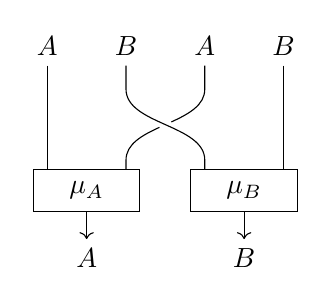
\begin{tikzpicture}[baseline=(braid)]
		\pic[
			braid/number of strands=4,
			braid/every strand/.style={black},
			name prefix=braid
		]
		at (0, 0) {braid = {s_2}};
		\coordinate (braid) at ($(braid-1-s)!0.5!(braid-1-e)$);
		\node[above] at (braid-1-s) {$A$};
		\node[above] at (braid-2-s) {$B$};
		\node[above] at (braid-3-s) {$A$};
		\node[above] at (braid-4-s) {$B$};
		
		\coordinate (MA) at ($(braid-1-e)!0.5!(braid-3-e)$);
		\draw[->] (MA) -- ($(MA) + (0, -2em)$) node[below] {$A$};
		\draw[fill=white] ([yshift=0.5em, xshift=-0.5em] braid-1-e) rectangle ([yshift=-1em, xshift=0.5em] braid-3-e);
		\node at ([yshift=-0.25em] MA) {$\mu_A$};
		
		\coordinate (MB) at ($(braid-2-e)!0.5!(braid-4-e)$);
		\draw[->] (MB) -- ($(MB) + (0, -2em)$) node[below] {$B$};
		\draw[fill=white] ([yshift=0.5em, xshift=-0.5em] braid-2-e) rectangle ([yshift=-1em, xshift=0.5em] braid-4-e);
		\node at ([yshift=-0.25em] MB) {$\mu_B$};
	\end{tikzpicture}\end{center}
	
	\item Unit $\eta_{A \otimes B}$ diambil sebagai komposisi
	% segment-id: o014.li2.chapter7.monoidal-algebras.q004
	\[ \munit \xrightarrow[\sim]{\iota^{-1}} \munit \otimes \munit \xrightarrow{\eta_A \otimes \eta_B} A \otimes B. \]
\end{itemize}

% segment-id: o014.li2.chapter7.monoidal-algebras.p024
Untuk memverifikasi bahwa ini memang aljabar, syarat-syarat dalam
Definisi~\ref{def:algebra-monoidal} dapat diturunkan dari sifat-sifat yang
bersesuaian pada $(A,\mu_A,\eta_A)$ dan $(B,\mu_B,\eta_B)$ hanya dengan
menggunakan $c$ (untuk menukar urutan $\otimes$), $\iota$ (untuk menggandakan
unit), dan kendala asosiativitas (untuk mengubah letak tanda kurung).

% segment-id: o014.li2.chapter7.monoidal-algebras.p025
Jika $M$ merupakan modul-$A$ kiri dan $N$ modul-$B$ kiri, maka $M\otimes N$
secara alami menjadi modul-$(A\otimes B)$ kiri. Konstruksi dan verifikasinya
sama dengan paragraf sebelumnya, dengan $c$ digunakan untuk menukar posisi.
Kasus modul kanan pun serupa.

% segment-id: o014.li2.chapter7.monoidal-algebras.p026
Untuk aljabar $\munit$ yang didefinisikan dalam
Catatan~\ref{rem:unit-algebra}, jelas bahwa
$\munit\otimes A\simeq A\simeq A\otimes\munit$, dengan isomorfisme yang
diberikan oleh kendala unit $\mathcal{V}$.

% segment-id: o014.li2.chapter7.monoidal-algebras.r002
\begin{catatan}\label{rem:Alg-otimes-functorial}
	Konstruksi di atas funktorial terhadap $A$ dan $B$: jika $A\to A'$ dan
	$B\to B'$ merupakan morfisme aljabar, maka demikian pula morfisme terkait
	$A\otimes B\to A'\otimes B'$. Fakta lain yang panjang tetapi tidak sulit
	ialah bahwa bila $A,B,C$ semuanya aljabar, kendala asosiativitas
	$(A\otimes B)\otimes C\rightiso A\otimes(B\otimes C)$ merupakan morfisme
	aljabar.
\end{catatan}

% segment-id: o014.li2.chapter7.monoidal-algebras.le001
\begin{lema}\label{prop:CAlg-mu}
	Misalkan $A$ aljabar di atas kategori monoidal beranyam $\mathcal{V}$. Maka
	$A$ komutatif jika dan hanya jika perkalian
	$\mu_A:A\otimes A\to A$ merupakan morfisme aljabar.
\end{lema}
% segment-id: o014.li2.chapter7.monoidal-algebras.pf001
\begin{bukti}
	Agar $\mu_A$ merupakan morfisme aljabar, diperlukan dua syarat. Syarat
	mengenai unit ekuivalen dengan komutativitas diagram
	% segment-id: o014.li2.chapter7.monoidal-algebras.g011
	\[\begin{tikzcd}[column sep=large]
		\munit \otimes \munit \arrow[d, "\iota"'] \arrow[r, "{\eta_A \otimes \eta_A}"] & A \otimes A \arrow[d, "{\mu_A}"] \\
		\munit \arrow[r, "{\eta_A}"'] & A
	\end{tikzcd}\]
	dan syarat ini berlaku otomatis karena $A$ adalah aljabar. Syarat yang
	tersisa ialah komutativitas diagram
	% segment-id: o014.li2.chapter7.monoidal-algebras.g012
	\begin{equation*}
		\begin{tikzcd}[column sep=large]
			(A \otimes A) \otimes (A \otimes A) \arrow[r, "{\mu_A \otimes \mu_A}"] \arrow[d, "{\mu_{A \otimes A}}"'] & A \otimes A \arrow[d, "{\mu_A}"] \\
			A \otimes A \arrow[r, "{\mu_A}"'] & A
		\end{tikzcd}
	\end{equation*}
	Identifikasikan sudut kiri atas dengan
	$A\otimes(A\otimes A)\otimes A$ melalui kendala asosiativitas. Berdasarkan
	asosiativitas $\mu_A$, komposisi dalam diagram sepanjang
	\begin{tikzpicture}[scale=0.5, baseline=(O)]
		\draw[->] (0, 0) -- (1, 0) -- (1, -0.7);
		\coordinate (O) at (0, -0.5);
	\end{tikzpicture}
	sama dengan
	% segment-id: o014.li2.chapter7.monoidal-algebras.q005
	\[ A \otimes (A \otimes A) \otimes A \xrightarrow{\identity \otimes \mu_A \otimes \identity} A \otimes A \otimes A \xrightarrow{\text{perkalian}} A . \]
	Di sisi lain, definisi $\mu_{A\otimes A}$ dan asosiativitas $\mu_A$
	menunjukkan bahwa komposisi dalam diagram sepanjang
	\begin{tikzpicture}[scale=0.5, baseline=(O)]
		\draw[->] (0, 0) -- (0, -0.7) -- (1, -0.7);
		\coordinate (O) at (0, -0.5);
	\end{tikzpicture}
	sama dengan
	% segment-id: o014.li2.chapter7.monoidal-algebras.q006
	\[ A \otimes (A \otimes A) \otimes A \xrightarrow{\identity \otimes (\mu_A c(A,A) ) \otimes \identity} A \otimes A \otimes A \xrightarrow{\text{perkalian}} A . \]
	Jadi $\mu_Ac(A,A)=\mu_A$ mengakibatkan diagram semula komutatif, yakni
	$\mu_A$ merupakan morfisme aljabar.
	
	Untuk implikasi sebaliknya, ambil
	$f\in\left\{\mu_A,\mu_Ac(A,A)\right\}$. Kita mempunyai diagram komutatif
	sederhana
	% segment-id: o014.li2.chapter7.monoidal-algebras.g013
	\[\begin{tikzcd}
		A \otimes (A \otimes A) \otimes A \arrow[r, "{\identity \otimes f \otimes \identity}"] & A \otimes A \otimes A \arrow[r, "{\text{perkalian}}"] & A . \\
		A \otimes A \arrow[u, "{\eta_A \otimes \identity \otimes \eta_A}"] \arrow[r, "f"'] & A \arrow[ru, "\identity"'] \arrow[u, "{\eta_A \otimes \identity \otimes \eta_A}"] &
	\end{tikzcd}\]
	Jika $\mu_A$ merupakan morfisme aljabar, pembahasan sebelumnya menunjukkan
	bahwa baris pertama memberikan komposisi yang sama untuk kedua pilihan $f$.
	Dengan memperhatikan baris kedua diperoleh
	$\mu_A=\mu_Ac(A,A)$.
\end{bukti}

% segment-id: o014.li2.chapter7.monoidal-algebras.le002
\begin{lema}\label{prop:c-as-isom-alg}
	Misalkan $A$ dan $B$ aljabar di atas kategori monoidal simetris
	$\mathcal{V}$. Maka $c(A,B):A\otimes B\to B\otimes A$ merupakan isomorfisme
	aljabar.
\end{lema}
% segment-id: o014.li2.chapter7.monoidal-algebras.pf002
\begin{bukti}
	Dua diagram komutatif harus diverifikasi untuk $c(A,B)$. Diagram pertama
	ialah
	% segment-id: o014.li2.chapter7.monoidal-algebras.g014
	\[\begin{tikzcd}[row sep=tiny]
		& \munit \otimes \munit \arrow[ld, "\sim" sloped] \arrow[dd, "{c(\munit, \munit)}"] \arrow[r, "{\eta_A \otimes \eta_B}"] & A \otimes B \arrow[dd, "{c(A, B)}"] \\
		\munit & & \\
		& \munit \otimes \munit \arrow[lu, "\sim"' sloped] \arrow[r, "{\eta_B \otimes \eta_A}"'] & B \otimes A
	\end{tikzcd}\]
	Komutativitas bagian kanan merupakan akibat funktorialitas $c$, sedangkan
	bagian kiri mengikuti kompatibilitas $c$ dengan kendala unit
	\cite[(3.12)]{Li1}. Untuk diagram kedua, yang menyatakan bahwa $c(A,B)$
	mempertahankan perkalian, argumennya didasarkan pada simetri struktur anyaman
	dan persis sama dengan bagian akhir \cite[\S 7.4]{Li1}.
\end{bukti}

% segment-id: o014.li2.chapter7.monoidal-algebras.pr001
\begin{proposisi}
	Misalkan $A$ dan $B$ aljabar komutatif di atas kategori monoidal simetris
	$\mathcal{V}$. Maka $A\otimes B$ juga komutatif.
\end{proposisi}
% segment-id: o014.li2.chapter7.monoidal-algebras.pf003
\begin{bukti}
	Cukup ditunjukkan bahwa perkalian $\mu_{A\otimes B}$ merupakan morfisme
	aljabar. Ingat definisi $\mu_{A\otimes B}$ dan terapkan
	Lema~\ref{prop:c-as-isom-alg} untuk menangani $c(B,A)$, asumsi komutativitas
	$A,B$ bersama Lema~\ref{prop:CAlg-mu} untuk menangani $\mu_A,\mu_B$, serta
	Catatan~\ref{rem:Alg-otimes-functorial} tentang funktorialitas $\otimes$.
	Maka setiap bagian komposisi tersebut merupakan morfisme aljabar.
\end{bukti}

% segment-id: o014.li2.chapter7.monoidal-algebras.p027
Di atas telah didefinisikan aljabar, modul, dan morfisme di antaranya. Semua
struktur ini membentuk kategori, dengan notasi
% segment-id: o014.li2.chapter7.monoidal-algebras.t001
\begin{center}\begin{tabular}{|c|c|c|c|c|c|} \hline
	struktur & aljabar & aljabar komutatif & modul-$A$ kiri & modul-$B$ kanan & bimodul-$(A,B)$ \\ \hline
	kategori & $\cate{Alg}(\mathcal{V})$ & $\cate{CAlg}(\mathcal{V})$ & $A\dcate{Mod}$ & $\cated{Mod}B$ & $(A,B)\dcate{Mod}$ \\ \hline
	syarat & {\small $\mathcal{V}$: kategori monoidal} & {\small $\mathcal{V}$: kategori monoidal beranyam} & {\small $A$: aljabar} & {\small $B$: aljabar} & {\small $A, B$: aljabar} \\ \hline
\end{tabular}\end{center}
\index[sym1]{Alg@$\cate{Alg}(\cdot)$}
\index[sym1]{CAlg@$\cate{CAlg}(\cdot)$}
\index[sym1]{Mod}

% segment-id: o014.li2.chapter7.monoidal-algebras.p028
Pembahasan di atas juga menunjukkan bahwa
$\cate{Alg}(\mathcal{V})$ dan $\cate{CAlg}(\mathcal{V})$ pada umumnya
memiliki struktur yang lebih sedikit daripada $\mathcal{V}$. Jika tingkat struktur diberi label
angka, situasinya dapat digambarkan secara kasar sebagai
% segment-id: o014.li2.chapter7.monoidal-algebras.g015
\[\begin{tikzcd}[row sep=small]
	0 & 1 & 2 & \infty \\
	\text{kategori} & \text{kategori monoidal} \arrow[l, "{\cate{Alg}}"'] & \text{kategori monoidal beranyam} \arrow[shift right, l, "{\cate{Alg}}"'] \arrow[shift left, bend left, ll, "{\cate{CAlg}}"'] & \text{kategori monoidal simetris} \arrow[loop right, "{\cate{Alg}, \cate{CAlg}}"]
\end{tikzcd}\]
Selain itu, apabila $\cate{Alg}(\mathcal{V})$ atau
$\cate{CAlg}(\mathcal{V})$ menjadi kategori monoidal terhadap $\otimes$,
unitnya selalu $\munit$.

% segment-id: o014.li2.chapter7.monoidal-algebras.p029
Ingat bahwa Lema~\ref{prop:CAlg-mu} menyatakan bahwa aljabar komutatif di atas
kategori monoidal beranyam $\mathcal{V}$ secara otomatis memberikan aljabar di
atas kategori monoidal $\cate{Alg}(\mathcal{V})$, dengan mengambil perkalian
$A\otimes A\to A$ sama dengan perkalian $A$. Bahkan, inilah satu-satunya
pilihan yang mungkin. Dari sini muncul pengamatan sederhana, menarik, dan
penting: terdapat ekuivalensi kategori
% segment-id: o014.li2.chapter7.monoidal-algebras.e001
\begin{equation}\label{eqn:AlgAlg-CAlg}
	\cate{Alg}\left(\cate{Alg}(\mathcal{V}) \right) \simeq \cate{CAlg}(\mathcal{V}), \quad \mathcal{V}:\;\text{kategori monoidal beranyam}.
\end{equation}
Fakta-fakta ini bertumpu pada apa yang disebut \emph{argumen
Eckmann--Hilton}; pembuktiannya sengaja diserahkan sebagai latihan bab ini
yang dilengkapi petunjuk.

% segment-id: o014.li2.chapter7.monoidal-algebras.e002
\begin{contoh}\label{eg:Cartesius-monoidal}
	Misalkan kategori $\mathcal{C}$ mempunyai hasil kali hingga. Khususnya,
	terdapat hasil kali kosong, yakni objek terminal, yang dinotasikan dengan
	$\munit$. Untuk setiap dua objek $X,Y$ terdapat isomorfisme kanonik
	$c(X,Y):X\times Y\rightiso Y\times X$. Dengan data ini,
	$(\mathcal{C},\times)$ menjadi kategori monoidal simetris dengan unit
	$\munit$. Kita dapat membahas aljabar di atas $\mathcal{C}$, yang juga
	disebut objek monoid di dalam $\mathcal{C}$\footnote{Untuk kategori semacam
	ini, \cite[\S 4.11]{Li1} juga membahas objek grup, tetapi sifat invers tidak
	dapat dirumuskan dalam kategori monoidal umum.}, beserta versi komutatifnya.
	\begin{itemize}
		\item Jika $\mathcal{C}=\cate{Set}$, himpunan satu titik adalah unit $\munit$. Aljabar yang bersesuaian adalah monoid, dan aljabar komutatif yang bersesuaian adalah monoid komutatif.
		\item Jika $\mathcal{C}=\cate{Top}$, aljabar yang bersesuaian adalah monoid topologis, dan aljabar komutatif yang bersesuaian adalah monoid topologis komutatif.
	\end{itemize}
	
	Di sisi lain, ambil gelanggang komutatif $\Bbbk$, beri
	$\Bbbk\dcate{Mod}$ struktur kategori monoidal simetris melalui
	$\otimes=\otimes_{\Bbbk}$, dengan $\Bbbk$ sebagai unit $\munit$ dan
	struktur anyaman yang ditentukan oleh $x\otimes y\mapsto y\otimes x$.
	Aljabar (atau aljabar komutatif) yang bersesuaian tepat merupakan aljabar
	(atau aljabar komutatif) dalam pengertian aljabar biasa; lihat
	\cite[Definisi 7.1.1]{Li1}.
\end{contoh}

% segment-id: o014.li2.chapter7.monoidal-algebras.p030
Dalam situasi konkret ini, perkalian aljabar $A$ sering langsung ditulis
sebagai perkalian unsur $xy=x\cdot y$, dan unit langsung diidentifikasikan
dengan unsur $1_A$, sehingga notasi $\mu_A,\eta_A$ dapat dihilangkan.

% segment-id: o014.li2.chapter7.monoidal-algebras.e003
\begin{contoh}[Modul bergradasi dan aljabar bergradasi]\label{eg:graded-module}
	\index{modul bergradasi, aljabar bergradasi (graded module, graded algebra)}
	Tetapkan kategori abelian $\mathcal{A}$ dan himpunan tak kosong $I$. Objek
	$\mathcal{A}^I$ disebut objek bergradasi-$I$ dan ditulis dalam bentuk
	$M=(M^i)_{i\in I}$, sedangkan morfisme di antaranya ditulis
	$(f^i:M^i\to N^i)_{i\in I}$. Lazimnya $M^i\in\Obj(\mathcal{A})$ (atau
	$f^i\in\Mor(\mathcal{A})$) disebut komponen derajat $i$ dari $M$ (atau
	$f$). Untuk kasus khusus $I=\Z$ atau $\Z^n$, hal ini telah berulang kali
	dijelaskan dalam \S\ref{sec:additive-cplx}, \S\ref{sec:triangular-def},
	\S\ref{sec:grading-filtration}, dan lain-lain.
	
	Demi kekonkretan, untuk sementara ambil $\mathcal{A}:=\Bbbk\dcate{Mod}$,
	dengan $\Bbbk$ gelanggang komutatif. Objek bergradasi-$I$ dalam
	$\mathcal{A}$ juga disebut modul bergradasi-$I$. Misalkan selanjutnya $I$
	monoid. Definisikan bifunktor $\otimes$ pada kategori $\mathcal{A}^I$ dengan
	% segment-id: o014.li2.chapter7.monoidal-algebras.e004
	\begin{equation}\label{eqn:graded-module}
		(M \otimes N)^i := \bigoplus_{jk=i} M^j \otimes N^k, \quad (f \otimes g)^i := \bigoplus_{jk=i} f^j \otimes g^k .
	\end{equation}
	Selain itu, definisikan $\munit$ sebagai $\Bbbk$ yang terkonsentrasi pada
	komponen $i=1_I$ (yakni unit $I$). Data ini menjadikan $\mathcal{A}^I$
	kategori monoidal. Syarat unit $\eta_A:\munit=\Bbbk\to A$ secara otomatis
	memastikan $1_A:=\eta_A(1)\in A^0$.
	
	Dalam kasus khusus ketika $I$ komutatif, kita kembali pada modul
	bergradasi-$I$ dan aljabar bergradasi-$I$ yang diperkenalkan dalam
	\cite[Definisi 7.4.1]{Li1}.

	Tetap ambil $\mathcal{A}=\Bbbk\dcate{Mod}$ dan syaratkan $(I,+)$ sebagai
	monoid komutatif. Setiap homomorfisme aditif
	$\epsilon:I\to\Z/2\Z$ menjadikan $\Bbbk\dcate{Mod}^I$ kategori monoidal
	simetris dengan \emph{struktur anyaman Koszul} yang dicirikan oleh
	% segment-id: o014.li2.chapter7.monoidal-algebras.e005
	\begin{equation}\label{eqn:Koszul-braiding}\begin{aligned}
		M^a \otimes N^b & \to N^b \otimes M^a \\
		x \otimes y & \mapsto (-1)^{\epsilon(a)\epsilon(b)} y \otimes x ,
	\end{aligned}\end{equation}
	dengan $a,b\in I$. Aljabar komutatif yang bersesuaian tepat merupakan
	aljabar $\epsilon$-komutatif dalam pengertian
	\cite[Definisi 7.4.3]{Li1}. Berbagai persamaan atau definisi yang dihasilkan
	darinya secara kolektif disebut \emph{aturan tanda Koszul}. Setiap kali
	posisi tensor ditukar, tandanya harus diubah menurut aturan ini.
	\index{aturan tanda Koszul (Koszul sign rule)}
	
	Sebagai contoh, syarat agar $A$ menjadi aljabar komutatif ditulis secara
	eksplisit sebagai
	% segment-id: o014.li2.chapter7.monoidal-algebras.q007
	\[ x y = (-1)^{\epsilon(a) \epsilon(b)} yx, \quad x \in A^a, \; y \in A^b. \]
	
	Situasi tipikal ialah
	% segment-id: o014.li2.chapter7.monoidal-algebras.q008
	\[ I \in \{\Z, \Z_{\geq 0} \}, \quad \epsilon(a) := a \;\bmod 2 , \]
	dengan aljabar $\epsilon$-komutatif yang bersesuaian disebut aljabar
	bergradasi antikomutatif dalam buku yang dirujuk di atas. Karena struktur
	anyaman ini muncul di mana-mana dalam kajian objek bergradasi-$\Z$, istilah
	\emph{komutatif bergradasi} lebih tepat.
	
	Sekarang kembali ke kategori abelian $\mathcal{A}$ yang lebih umum dan
	$(I,+,\epsilon)$ seperti di atas. Untuk menggeneralisasi konstruksi tadi,
	kita perlu memperluas $\mathcal{A}$ menjadi kategori monoidal simetris
	$(\mathcal{A},\otimes)$ sedemikian sehingga
	% segment-id: o014.li2.chapter7.monoidal-algebras.l004
	\begin{itemize}
		\item $\mathcal{A}$ adalah kategori abelian dan koproduk (yakni jumlah langsung) berbentuk seperti dalam \eqref{eqn:graded-module} ada;
		\item $\otimes:\mathcal{A}\times\mathcal{A}\to\mathcal{A}$ merupakan funktor aditif pada setiap variabel dan mempertahankan koproduk tersebut.
	\end{itemize}
	Dalam keadaan ini, $\otimes$ dan struktur anyaman Koszul pada
	$\mathcal{A}^I$ masih dapat didefinisikan dengan cara yang sama, sehingga
	$(\mathcal{A}^I,\otimes)$ menjadi kategori monoidal simetris. Unitnya tetap
	diberikan oleh unit $\munit$ dari $\mathcal{A}$, dipandang sebagai objek
	bergradasi-$I$ yang terkonsentrasi pada derajat nol.
	
	Untuk $(\mathcal{A},\otimes)$ umum, semua verifikasi sama dengan kasus
	$\Bbbk\dcate{Mod}$. Satu-satunya perbedaan ialah bahwa ``unsur'' suatu objek
	tidak lagi bermakna dalam kasus umum.
\end{contoh}

% segment-id: o014.li2.chapter7.monoidal-algebras.cv001
\begin{konvensi}
	Dalam kasus khusus $\mathcal{A}=\Bbbk\dcate{Mod}$, konvensi umum ialah
	memandang modul bergradasi-$I$ $(M^i)_{i\in I}$ sebagai modul yang dilengkapi
	dekomposisi jumlah langsung $M=\bigoplus_{i\in I}M^i$, sedangkan morfisme di
	antaranya disyaratkan mempertahankan komponen jumlah langsung.
\end{konvensi}

% segment-id: o014.li2.chapter7.monoidal-algebras.e006
\begin{contoh}\label{eg:superspace}
	\index{ruang vektor super (super vector space)}
	Dalam konstruksi di atas ($\mathcal{A}=\Bbbk\dcate{Mod}$), ambil $\Bbbk$
	medan dengan $\mathrm{char}(\Bbbk)\neq2$,
	$I=\Z/2\Z=\{0,1\}$, dan $\epsilon=\identity_{\Z/2\Z}$. Kategori monoidal
	simetris yang bersesuaian dinotasikan
	$\cate{Vect}^-_{\Z/2\Z}(\Bbbk)$; objeknya dapat dipandang sebagai ruang
	vektor-$\Bbbk$ yang dilengkapi dekomposisi jumlah langsung
	$V=V_0\oplus V_1$, dan disebut pula \emph{ruang vektor super}. Dari sinilah
	muncul istilah-istilah yang lazim dalam aljabar linear dan fisika matematis,
	seperti aljabar super dan aljabar super komutatif.
\end{contoh}

% segment-id: o014.li2.chapter7.monoidal-algebras.p031
Terakhir, kita membahas pengaruh funktor monoidal longgar terhadap aljabar.

% segment-id: o014.li2.chapter7.monoidal-algebras.d005
\begin{definisi}\label{def:lax-monoidal}
	\index{funktor!monoidal, monoidal longgar, monoidal longgar kanan (monoidal, lax monoidal, right lax monoidal)}
	Misalkan $\mathcal{V}$ dan $\mathcal{V}'$ kategori monoidal. Menurut
	\cite[Catatan 3.1.8]{Li1}, funktor monoidal longgar kanan dari $\mathcal{V}$
	ke $\mathcal{V}'$, yang di sini disingkat menjadi \emph{funktor monoidal
	longgar}, berarti data $(F,\xi_F,\varphi_F)$, dengan
	$F:\mathcal{V}\to\mathcal{V}$ suatu funktor dan morfisme
	% segment-id: o014.li2.chapter7.monoidal-algebras.q009
	\[ \xi_F: F(\cdot) \otimes F(\cdot) \to F(\cdot \otimes \cdot), \quad \varphi_F: \munit_{\mathcal{V}'} \to F\left( \munit_{\mathcal{V}} \right), \]
	yang tunduk pada serangkaian syarat kompatibilitas dengan struktur monoidal.
	Data $(F,\xi_F,\varphi_F)$ sering disingkat menjadi $F$.
	
	Jika $\mathcal{V}$ dan $\mathcal{V}'$ keduanya kategori monoidal beranyam
	(atau simetris), dan $F$ juga membuat diagram berikut komutatif, maka $F$
	disebut funktor beranyam, atau dikatakan kompatibel dengan struktur anyaman:
	% segment-id: o014.li2.chapter7.monoidal-algebras.g016
	\[\begin{tikzcd}[column sep=huge]
		F(X) \otimes F(Y) \arrow[r, "{\xi_F(X, Y)}"] \arrow[d, "{c'(FX, FY)}"'] & F(X \otimes Y) \arrow[d, "{Fc(X, Y)}"] \\
		F(Y) \otimes F(X) \arrow[r, "{\xi_F(Y, X)}"'] & F(Y \otimes X) .
	\end{tikzcd}\]

	Jika $\xi_F$ dan $\varphi_F$ dalam data funktor monoidal longgar keduanya
	isomorfisme, funktor tersebut disebut \emph{funktor monoidal}.
\end{definisi}

% segment-id: o014.li2.chapter7.monoidal-algebras.p032
Tentu kita juga dapat membahas morfisme antara funktor-funktor monoidal
longgar, yang disebut pula transformasi alami:
% segment-id: o014.li2.chapter7.monoidal-algebras.q010
\[ \theta = (\theta_X)_{X \in \Obj(\mathcal{V})}: F \to G, \quad F, G: \mathcal{V} \to \mathcal{V}' . \]
Di samping syarat-syarat transformasi alami, kita mensyaratkan bahwa $\theta$
membuat diagram berikut komutatif:
% segment-id: o014.li2.chapter7.monoidal-algebras.g017
\[\begin{tikzcd}[column sep=huge]
	F(X) \otimes F(Y) \arrow[r, "{\xi_F(X, Y)}"] \arrow[d, "{\theta_X \otimes \theta_Y}"'] & F(X \otimes Y) \arrow[d, "{\theta_{X \otimes Y}}"] \\
	G(X) \otimes G(Y) \arrow[r, "{\xi_G(X, Y)}"'] & G(X \otimes Y)
\end{tikzcd} \quad \begin{tikzcd}
	\munit_{\mathcal{V}'} \arrow[r, "{\varphi_F}"] \arrow[rd, "{\varphi_G}"'] & F(\munit_{\mathcal{V}}) \arrow[d, "{\theta_{\munit_{\mathcal{V}}}}"] \\
	& G(\munit_{\mathcal{V}}) .
\end{tikzcd}\]

Jika $F$ dan $G$ merupakan funktor monoidal, definisi di atas sebenarnya
ekuivalen dengan \cite[Definisi 3.1.10]{Li1}; di sana $\varphi_F$ dan
$\varphi_G$ disebut isomorfisme ``standar''. Dengan demikian dapat dibahas
ekuivalensi antara kategori monoidal atau kategori monoidal beranyam.

% segment-id: o014.li2.chapter7.monoidal-algebras.pr002
\begin{proposisi}\label{prop:lax-monoidal-Alg}
	Funktor monoidal longgar $F$ menginduksi funktor
	$\cate{Alg}(\mathcal{V})\to\cate{Alg}(\mathcal{V}')$. Jika $A$ aljabar di
	atas $\mathcal{V}$, maka $F$ menginduksi
	$A\dcate{Mod}\to F(A)\dcate{Mod}$, dan seterusnya.

	Jika selain itu $\mathcal{V}$ dan $\mathcal{V}'$ kategori monoidal beranyam
	dan $F$ funktor beranyam, maka $F$ juga menginduksi
	$\cate{CAlg}(\mathcal{V})\to\cate{CAlg}(\mathcal{V}')$, sedangkan
	$\cate{Alg}(\mathcal{V})\to\cate{Alg}(\mathcal{V}')$ merupakan funktor
	monoidal longgar. Jika lebih lanjut $\mathcal{V},\mathcal{V}'$ keduanya
	simetris, maka $\cate{CAlg}(\mathcal{V})\to\cate{CAlg}(\mathcal{V}')$ juga
	demikian.
\end{proposisi}
% segment-id: o014.li2.chapter7.monoidal-algebras.pf004
\begin{bukti}
	Misalkan $A$ aljabar di atas $\mathcal{V}$. Definisikan perkalian
	$\mu_{FA}$ sebagai
	$FA\otimes FA\to F(A\otimes A)\xrightarrow{F\mu_A}FA$, dan unit $\eta_{FA}$
	sebagai
	$\munit_{\mathcal{V}'}\to F(\munit_{\mathcal{V}})\xrightarrow{F\eta_A}FA$.
	Verifikasi selebihnya bersifat rutin.
\end{bukti}

% segment-id: o014.li2.chapter7.monoidal-algebras.e007
\begin{contoh}\label{eg:ev0-monoidal}
	Tinjau kategori abelian monoidal simetris $\mathcal{A}$ dan $\mathcal{A}^I$
	dari Contoh~\ref{eg:graded-module}. Definisikan funktor
	% segment-id: o014.li2.chapter7.monoidal-algebras.q011
	\[ \mathrm{ev}_0: \mathcal{A}^I \to \mathcal{A}, \quad \left(M^i\right)_{i \in I} \mapsto M^0. \]
	Funktor ini eksak sekaligus monoidal longgar simetris: cukup ambil
	% segment-id: o014.li2.chapter7.monoidal-algebras.q012
	\[ \xi_{\mathrm{ev}_0}(M, N): M^0 \otimes N^0 \to (M \otimes N)^0 := \bigoplus_{i+j=0} M^i \otimes N^j \]
	sebagai morfisme yang jelas, dan
	$\varphi_{\mathrm{ev}_0}:\munit\to\munit$ sebagai identitas. Dengan demikian,
	$A\mapsto A^0$ menginduksi funktor monoidal longgar
	% segment-id: o014.li2.chapter7.monoidal-algebras.q013
	\[ \cate{Alg}(\mathcal{A}^I) \to \cate{Alg}(\mathcal{A}), \quad \cate{CAlg}(\mathcal{A}^I) \to \cate{CAlg}(\mathcal{A}). \]
\end{contoh}

% segment-id: o014.li2.chapter7.monoidal-algebras.p033
Catatan berikut membahas aljabar di atas kategori monoidal umum $\mathcal{V}$.
Ingat bahwa ordinal hingga berkorespondensi satu-satu dengan $\Z_{\geq0}$;
ordinal hingga $\mathbf{n}$ yang bersesuaian dengan $n$ diidentifikasikan
dengan himpunan terurut total berunsur $n$, yaitu
$\{0,\ldots,n-1\}$ dengan $0\leq1\leq2\leq\cdots$.

% segment-id: o014.li2.chapter7.monoidal-algebras.r003
\begin{catatan}[Aljabar berjalan]\label{rem:walking-algebra}
	\index{aljabar!berjalan (walking)}
	\index[sym1]{FinOrd@$\cate{FinOrd}$}
	Pemetaan $f:A\to B$ antara himpunan terurut sebagian disebut
	mempertahankan urutan jika
	$a\leq a'\implies f(a)\leq f(a')$. Selanjutnya, tuliskan $\cate{FinOrd}$
	untuk kategori ordinal hingga yang morfismenya adalah pemetaan
	mempertahankan urutan antara ordinal. Kategori ini menjadi kategori
	monoidal ketat terhadap
	$\mathbf{n}\otimes\mathbf{m}:=\mathbf{n}+\mathbf{m}$. Morfisme
	$f\otimes g:\mathbf{n}\otimes\mathbf{m}\to\mathbf{n}'\otimes\mathbf{m}'$
	memetakan $n$ unsur pertama (atau $m$ unsur terakhir) dengan $f$ (atau $g$),
	dan objek $\mathbf{0}$ adalah unit\footnote{Di sini $\mathbf{1}$ selalu
	menyatakan ordinal; unit kategori monoidal $\mathcal{V}$ dinotasikan terpisah
	dengan $\munit_{\mathcal{V}}$.}. Jadikan $\mathbf{1}$ aljabar di atas
	$\cate{FinOrd}$: ambil unit $\emptyset=\mathbf{0}\hookrightarrow\mathbf{1}$
	dan perkalian
	$\mathbf{1}\otimes\mathbf{1}=\mathbf{2}\twoheadrightarrow\mathbf{1}$.
	Diagram komutatif yang terkait sama sekali tidak sulit diverifikasi.
	
	Ordinal $\mathbf{1}$ (atau $\mathbf{2}$) dapat dipandang sebagai objek
	(atau morfisme) ``berjalan''. Alasannya, untuk sembarang kategori
	$\mathcal{C}$, menentukan funktor $\mathbf{1}\to\mathcal{C}$ (atau
	$\mathbf{2}\to\mathcal{C}$) setara dengan menentukan objek (atau morfisme)
	dalam $\mathcal{C}$. Sekarang tinjau kategori monoidal $\mathcal{V}$. Kita
	klaim terdapat isomorfisme kategori
	% segment-id: o014.li2.chapter7.monoidal-algebras.q014
	\[
		\left\{ \mathcal{V}\;\text{-aljabar}\; A \right\} \simeq \left\{ \text{funktor monoidal}\; F: \cate{FinOrd} \to \mathcal{V} \right\},
	\]
	yang juga berarti bahwa $\cate{FinOrd}$ adalah ``aljabar berjalan''.
	Pertama, bagi funktor monoidal
	$F:\cate{FinOrd}\to\mathcal{V}$, definisikan $A:=F(\mathbf{1})$. Sebagai
	kasus khusus sederhana dari Proposisi~\ref{prop:lax-monoidal-Alg}, $A$
	secara alami menjadi aljabar di atas $\mathcal{V}$: perkalian
	$\mu:A\otimes A\to A$ adalah $F(\mathbf{2}\twoheadrightarrow\mathbf{1})$,
	sedangkan unit $\eta:\munit_{\mathcal{V}}\to A$ adalah
	$F(\mathbf{0}\hookrightarrow\mathbf{1})$.
	
	Sebaliknya, dari aljabar $(A,\mu,\eta)$ di atas $\mathcal{V}$, definisikan
	funktor monoidal $F:\cate{FinOrd}\to\mathcal{V}$ dengan
	% segment-id: o014.li2.chapter7.monoidal-algebras.q015
	\[ F(\mathbf{n}) = A^{\otimes n} := \underbracket{A \otimes (A \otimes (\cdots))}_{n\;\text{salinan}\; A}, \quad A^{\otimes 0} := \munit_{\mathcal{V}}, \]
	Untuk $f:\mathbf{n}\to\mathbf{m}$, jika $f$ injektif, maka
	$F(f):A^{\otimes n}\to A^{\otimes m}$ diperoleh dengan menyisipkan
	$\eta:\munit_{\mathcal{V}}\to A$ di luar citra $f$; jika $f$ surjektif,
	$F(f)$ diperoleh dengan memakai $\mu:A\otimes A\to A$ untuk menggabungkan
	secara bertahap faktor-faktor dalam setiap serat. Kendala asosiativitas dan
	sifat-sifat lain kategori monoidal memastikan operasi ini terdefinisi dengan
	baik. Pemetaan umum $f$ memiliki faktorisasi surjektif--injektif yang unik,
	dan dengan cara ini $F$ didefinisikan pada morfisme. Funktorialitasnya
	jelas. Tidak sulit memverifikasi bahwa kedua konstruksi saling invers.
\end{catatan}

% Unit 089 terjemahan Bahasa Indonesia dari chapter7.tex baris 419--610.
% Sumber: Methods of Algebra, Volume 2, commit
% 9a5803ff77dd3257484cb177f851a73770a59dd3 (CC BY 4.0).
% stable-unit-id: o014.aljabr2.chapter7.differential-graded-structures
% Cakupan: Bagian 7.2 lengkap, ``Contoh: Struktur Diferensial Bergradasi'';
% berhenti tepat sebelum Bagian 7.3 pada baris 611.

% segment-id: o014.li2.chapter7.differential-graded-structures.h001
\section{Contoh: Struktur Diferensial Bergradasi}\label{sec:dga-monoidal}
\hypertarget{o014.aljabr2.chapter7.differential-graded-structures}{ }
% segment-id: o014.li2.chapter7.differential-graded-structures.p001
Melanjutkan pembahasan dalam Contoh~\ref{eg:graded-module}, tinjau kategori
abelian monoidal simetris $(\mathcal{A}, \otimes)$ yang memiliki koproduk
terhitung. Dalam bagian ini, kita juga mengandaikan bahwa $\otimes$ eksak
kanan pada setiap peubah. Contoh khasnya tentu saja
$\mathcal{A}=\Bbbk\dcate{Mod}$.

% segment-id: o014.li2.chapter7.differential-graded-structures.p002
Sebelumnya telah dibahas aljabar bergradasi-$\Z$ di atas $\mathcal{A}$, atau,
dengan kata lain, aljabar di atas kategori monoidal
$(\mathcal{A}^{\Z},\otimes)$. Lebih tepatnya, dalam kerangka
Contoh~\ref{eg:graded-module}, hal ini berarti mengambil $I=\Z$ dan struktur
kepang Koszul~\eqref{eqn:Koszul-braiding} yang bersesuaian dengan
$\epsilon(a)=a\bmod\;2$. Selanjutnya, ``bergradasi'' selalu berarti
``bergradasi-$\Z$''. Fokus bagian ini ialah menambahkan struktur
``diferensial''; sebagian pembahasannya bertumpang tindih dengan
\S\ref{sec:multiplicative-SS}.

% segment-id: o014.li2.chapter7.differential-graded-structures.p003
Funktor pergeseran $T:\mathcal{A}^{\Z}\to\mathcal{A}^{\Z}$ didefinisikan
oleh $(TM)^n=M^{n+1}$ dan $(Tf)^n=f^{n+1}$. Dengan demikian,
$\left(\mathcal{A}^{\Z},T\right)$ menjadi kategori abelian dengan pergeseran,
dan objek diferensial di atasnya (Definisi~\ref{def:differential-object})
disingkat menjadi \emph{objek diferensial bergradasi} di atas $\mathcal{A}$.
Sesungguhnya, kategori abelian
$\left(\mathcal{A}^{\Z},T\right)_d$ yang terdiri atas objek-objek diferensial
bergradasi secara kanonik isomorfik dengan kategori kompleks
$\cate{C}(\mathcal{A})$. Fakta ini telah diketahui sejak
\S\ref{sec:additive-cplx}.
\index{objek dg@objek diferensial bergradasi}

% segment-id: o014.li2.chapter7.differential-graded-structures.p004
Karena itu, selanjutnya kita akan menyamakan objek diferensial bergradasi di
atas $\mathcal{A}$ dengan kompleks, tanpa membedakan keduanya.

% segment-id: o014.li2.chapter7.differential-graded-structures.p005
Sekarang berikan struktur kategori monoidal simetris pada
$\cate{C}(\mathcal{A})$. Untuk sembarang kompleks $M$ dan $N$, bifunktor
$\otimes:\mathcal{A}\times\mathcal{A}\to\mathcal{A}$ memberikan bikompleks
$M^\bullet\otimes N^\bullet$; dengan mengambil kompleks total melalui jumlah
langsung, diperoleh
% segment-id: o014.li2.chapter7.differential-graded-structures.q001
\[ M \otimes N := \tot_{\oplus}\left( M^\bullet \otimes N^\bullet \right), \quad (M \otimes N)^n = \bigoplus_{a+b=n} M^a \otimes N^b. \]

% segment-id: o014.li2.chapter7.differential-graded-structures.p006
Dalam contoh $\mathcal{A}=\Bbbk\dcate{Mod}$, diferensial
$d=d_{M\otimes N}$ pada kompleks (atau, secara ekuivalen, pada objek
diferensial) dapat ditulis pada tingkat unsur sebagai
% segment-id: o014.li2.chapter7.differential-graded-structures.q002
\begin{equation*}
	d(x \otimes y) = (d_M x) \otimes y + (-1)^a x \otimes (d_N y), \quad x \in M^a, \; y \in N^b.
\end{equation*}
Definisi-definisi ini membuat struktur anyaman Koszul
\eqref{eqn:Koszul-braiding} memberikan morfisme antarkompleks. Pembaca dapat
memeriksanya langsung atau menurunkannya dari
Proposisi~\ref{prop:double-cplx-swap}.

% segment-id: o014.li2.chapter7.differential-graded-structures.p007
Selain itu, objek satuan $\munit$ dari $(\mathcal{A},\otimes)$, dipandang
sebagai kompleks yang terkonsentrasi pada derajat nol, jelas memberikan objek
satuan bagi kategori monoidal $(\cate{C}(\mathcal{A}),\otimes)$. Fakta berikut
langsung terlihat: untuk setiap
$X=(X^n,d_X^n)_n\in\Obj(\cate{C}(\mathcal{A}))$, berlaku
% segment-id: o014.li2.chapter7.differential-graded-structures.q003
\begin{equation}\label{eqn:unit-map-into-cplx}
	\Hom_{\cate{C}(\mathcal{A})}(\munit, X) \simeq \Hom_{\mathcal{A}}\left( \munit, \Ker\left(d_X^0 \right) \right).
\end{equation}

% segment-id: o014.li2.chapter7.differential-graded-structures.d001
\begin{definition}\label{def:dg-algebra}
	\index{aljabar dg@aljabar diferensial bergradasi}
	\index{aljabar dg@aljabar dg}
	Relatif terhadap struktur monoidal simetris di atas, objek-objek
	$\cate{Alg}\left(\cate{C}(\mathcal{A})\right)$ disebut
	\emph{aljabar diferensial bergradasi} di atas $\mathcal{A}$, disingkat
	\emph{aljabar-dg}; sedangkan objek-objek
	$\cate{CAlg}\left(\cate{C}(\mathcal{A})\right)$ disebut aljabar diferensial
	bergradasi komutatif di atas $\mathcal{A}$, disingkat aljabar-dg komutatif.
\end{definition}

% segment-id: o014.li2.chapter7.differential-graded-structures.p008
Dari sini, untuk suatu aljabar diferensial bergradasi $A$, kita juga dapat
membahas modul-$A$ kiri (atau kanan) $M$, bahkan bimodul; semuanya membentuk
kategori abelian. Dalam keadaan ini, $M$ juga disebut \emph{modul diferensial
bergradasi} di atas $A$, disingkat \emph{modul-dg}. Konsep ini memadukan teori
kompleks dan teori modul serta sangat luas kegunaannya. Latihan-latihan bab
ini akan memberikan pengantar lebih lanjut; pembaca juga dapat merujuk pada
monograf seperti \cite{Yek20}. Untuk menonjolkan struktur diferensial
bergradasinya, selanjutnya kategori modul-dg ditulis $A\dcate{dgMod}$, dan
demikian pula untuk variasi-variasinya.
\index{modul bergradasi diferensial@modul bergradasi diferensial (differential graded module)}
\index{modul dg@modul dg}
\index[sym1]{A-dgMod@$A\dcate{dgMod}$}

% segment-id: o014.li2.chapter7.differential-graded-structures.p009
Funktor pelupa $\cate{C}(\mathcal{A})\to\mathcal{A}^{\Z}$ mempertahankan
$\otimes$, sehingga Proposisi~\ref{prop:lax-monoidal-Alg} menunjukkan bahwa
funktor tersebut mempertahankan struktur aljabar (atau aljabar komutatif).
Dalam kasus $\mathcal{A}=\Bbbk\dcate{Mod}$, mengatakan bahwa $A$ adalah
aljabar-dg sama artinya dengan mengatakan bahwa $A$ sendiri adalah aljabar
bergradasi yang dilengkapi diferensial $d$, dan perkaliannya memenuhi aturan
Leibniz
% segment-id: o014.li2.chapter7.differential-graded-structures.q004
\[ d(xy) = (dx)y + (-1)^a x (dy), \quad x \in A^a, \; y \in A^b. \]
Dengan menyubstitusikan $x=1_A=y$, diperoleh $d(1_A)=0$. Aljabar lawannya
$A^{\opp}$ bersesuaian dengan mengganti perkalian menjadi
$x\mathbin{\cdot^{\opp}}y:=(-1)^{ab}yx$.

% segment-id: o014.li2.chapter7.differential-graded-structures.p010
Serupa dengan itu, bila $\mathcal{A}=\Bbbk\dcate{Mod}$, suatu modul-$A$ kiri
$M$ sama artinya dengan modul-$\Bbbk$ bergradasi $M$ beserta morfisme
perkalian skalar $A\otimes M\to M$ yang memenuhi sifat asosiatif dan
sifat-sifat lainnya, serta dilengkapi diferensial $d$ yang memenuhi aturan
Leibniz
% segment-id: o014.li2.chapter7.differential-graded-structures.q005
\[ d(tm) = (dt)m + (-1)^a t (dm), \quad t \in A^a, \; m \in M^b; \]
untuk modul-$A$ kanan $M$, aturan Leibniz menjadi
% segment-id: o014.li2.chapter7.differential-graded-structures.q006
\[ d(mt) = (dm)t + (-1)^b m (dt), \quad t \in A^a, \; m \in M^b. \]
Untuk $(\mathcal{A},\otimes)$ yang umum, semua sifat di atas dapat dirumuskan
tanpa menyebut unsur. Sebagai contoh, satuan aljabar $A$ bersesuaian dengan
morfisme $\munit\to\Ker\left(d_A^0\right)$ dalam $\mathcal{A}$; lihat
\eqref{eqn:unit-map-into-cplx}.

% segment-id: o014.li2.chapter7.differential-graded-structures.p011
Mengambil kohomologi memberikan funktor aditif
$\Hm=(\Hm^n)_{n\in\Z}:\cate{C}(\mathcal{A})\to\mathcal{A}^{\Z}$. Hasil
berikut menunjukkan bahwa perkalian kompleks menginduksi perkalian pada
kohomologi.

% segment-id: o014.li2.chapter7.differential-graded-structures.pr001
\begin{proposition}\label{prop:Hm-lax-monoidal}
	Funktor $\Hm$ menginduksi
	% segment-id: o014.li2.chapter7.differential-graded-structures.q007
	\[ \cate{Alg}\left(\cate{C}(\mathcal{A})\right) \to \cate{Alg}\left(\mathcal{A}^{\Z}\right),
	\quad \cate{CAlg}\left(\cate{C}(\mathcal{A})\right) \to \cate{CAlg}\left(\mathcal{A}^{\Z}\right). \]
	Jika $A$ adalah aljabar-dg dan $M$ adalah modul-$A$ kiri (atau kanan, atau
	bimodul), maka $\Hm(M)$ adalah modul-$\Hm(A)$ kiri (atau kanan, atau
	bimodul).
\end{proposition}
% segment-id: o014.li2.chapter7.differential-graded-structures.pf001
\begin{proof}
	Menurut Proposisi~\ref{prop:lax-monoidal-Alg}, cukup dibuktikan bahwa $\Hm$
	adalah funktor monoidal longgar. Morfisme kanonik yang diperlukan,
	% segment-id: o014.li2.chapter7.differential-graded-structures.q008
	\[ \xi_{\Hm}(M, N): \Hm(M) \otimes \Hm(N) \to \Hm(M \otimes N), \]
	hampir tautologis: morfisme itu berasal dari morfisme $\kappa$ yang dibahas
	di atas dalam Teorema~\ref{prop:Kunneth-homology} atau
	Proposisi~\ref{prop:bifunctor-cup}. Di sisi lain, kita ambil
	% segment-id: o014.li2.chapter7.differential-graded-structures.q009
	\[ \varphi_{\Hm}: \munit \to \Hm(\munit) = \munit \quad \text{(terkonsentrasi pada derajat nol)} \]
	sebagai $\identity$.
\end{proof}

% segment-id: o014.li2.chapter7.differential-graded-structures.p012
Kita juga dapat mengambil funktor monoidal longgar
$\mathrm{ev}_0:\mathcal{A}^{\Z}\to\mathcal{A}$ dari
Contoh~\ref{eg:ev0-monoidal}. Sekali lagi,
Proposisi~\ref{prop:lax-monoidal-Alg} menunjukkan bahwa funktor ini memetakan
aljabar bergradasi (atau aljabar bergradasi komutatif) ke aljabar (atau
aljabar komutatif), serta memetakan modul ke modul. Perhatikan bahwa
$\mathrm{ev}_0\Hm=\Hm^0$. Dalam penerapan, setiap tahap komposisi
$\cate{C}(\mathcal{A})\xrightarrow{\Hm}\mathcal{A}^{\Z}
\xrightarrow{\mathrm{ev}_0}\mathcal{A}$ menghilangkan informasi; struktur
yang paling kaya tetap berada pada aljabar-dg itu sendiri.

% segment-id: o014.li2.chapter7.differential-graded-structures.eg001
\begin{example}\label{eg:k-linear-A-enrich}
	Misalkan $\Bbbk$ gelanggang komutatif. Untuk sembarang kategori
	$\Bbbk$-linear $\mathcal{A}$, tinjau perkalian pada tingkat kompleks
	$\Hom$ dari \eqref{eqn:Hom-cplx-multiplication}:
	% segment-id: o014.li2.chapter7.differential-graded-structures.q010
	\[ \Hom^a(Y, Z) \times \Hom^b(X, Y) \to \Hom^{a+b}(X, Z), \quad X, Y, Z \in \Obj(\cate{C}(\mathcal{A})). \]

	Karena perkalian memenuhi aturan Leibniz
	(Lema~\ref{prop:Hom-cplx-Leibniz}), perkalian itu menentukan morfisme dalam
	$\cate{C}(\Bbbk\dcate{Mod})$
	% segment-id: o014.li2.chapter7.differential-graded-structures.q011
	\[ \Hom^\bullet(Y, Z) \otimes \Hom^\bullet(X, Y) \to \Hom^\bullet(X, Z). \]
	Selain itu, perkalian tersebut asosiatif, sehingga
	$\End^\bullet(X):=\Hom^\bullet(X,X)$ menjadi aljabar di atas
	$(\cate{C}(\Bbbk\dcate{Mod}),\otimes)$ dengan satuan
	$\identity_X\in\End^0(X)$. Lebih lanjut, $\Hom^\bullet(X,Y)$ menjadi
	bimodul-$(\End^\bullet(Y),\End^\bullet(X))$.

	Mengambil kohomologi $\Hm=(\Hm^n)_n$ dari $\Hom^\bullet(X,Y)$ hanya
	menghasilkan
	% segment-id: o014.li2.chapter7.differential-graded-structures.q012
	\[ \bigoplus_{n \in \Z} \Hom_{\cate{K}(\mathcal{A})}(X, Y[n]); \]
	sedangkan dengan menerapkan \eqref{eqn:unit-map-into-cplx} pada
	$\Hom^\bullet(X,Y)$, tampak bahwa $\Hom_{\cate{C}(\mathcal{A})}$ dapat
	direkonstruksi melalui
	% segment-id: o014.li2.chapter7.differential-graded-structures.q013
	\[ \Hom_{\cate{C}(\Bbbk\dcate{Mod})}\left( \Bbbk, \Hom^\bullet(X, Y) \right) \simeq \Hom_{\cate{C}(\mathcal{A})}(X, Y)  \]
	dengan $\Bbbk$ berperan sebagai objek satuan dari
	$(\cate{C}(\Bbbk\dcate{Mod}),\otimes)$.
\end{example}

% segment-id: o014.li2.chapter7.differential-graded-structures.p013
Jadi, himpunan $\Hom_{\cate{C}(\mathcal{A})}$ dan komposisi morfisme dalam
$\cate{C}(\mathcal{A})$ hanyalah bayangan kompleks $\Hom$ beserta
perkaliannya, yang diperoleh dengan mengambil
$\Hom_{\cate{C}(\Bbbk\dcate{Mod})}(\Bbbk,\mathord\cdot)$.

\index{kategori!diperkaya@diperkaya (enriched)}
\index[sym1]{Hom-internal@$\iHom$}
% segment-id: o014.li2.chapter7.differential-graded-structures.p014
Berangkat dari contoh $\cate{C}(\mathcal{A})$, kita secara alami sampai pada
konsep kategori diferensial bergradasi. Konsep ini melibatkan
\emph{kategori yang diperkaya-$\mathcal{V}$} yang diperkenalkan dalam
\cite[Definisi 3.4.1]{Li1}. Singkatnya, untuk sembarang kategori monoidal
$\mathcal{V}$, sebuah kategori yang diperkaya-$\mathcal{V}$, $\mathcal{C}$,
tetap terdiri atas objek dan morfisme, tetapi himpunan $\Hom$ diganti dengan
objek $\Hom$ dalam $\mathcal{V}$, yang ditulis
$\iHom=\iHom_{\mathcal{C}}$ untuk membedakannya. Komposisi morfisme diganti
dengan morfisme dalam $\mathcal{V}$
% segment-id: o014.li2.chapter7.differential-graded-structures.q014
\[ \iHom(Y, Z) \otimes \iHom(X, Y) \to \iHom(X, Z), \]
sedangkan morfisme identitas $\identity_X\in\Hom(X,X)$ diganti dengan
$\identity_X:\munit\to\iHom(X,X)$. Semua ini adalah morfisme dalam
$\mathcal{V}$, dan sifat-sifat yang berkaitan dengannya dinyatakan melalui
diagram komutatif dalam $\mathcal{V}$.

% segment-id: o014.li2.chapter7.differential-graded-structures.p015
Untuk versi diperkaya dari funktor dan morfisme di antaranya, lihat
\cite[Definisi 3.4.1, 3.4.2, 3.4.4]{Li1}. Semuanya didefinisikan dengan cara
yang sewajarnya; singkatnya, versi diperkaya dari funktor mengangkat
pemetaan antarhimpunan $\Hom$ menjadi morfisme antarobjek $\iHom$.

% segment-id: o014.li2.chapter7.differential-graded-structures.p016
Sebagai contoh, kategori-$\Bbbk\dcate{Mod}$ tidak lain adalah kategori yang
diperkaya atas $(\Bbbk\dcate{Mod},\otimes)$.

% segment-id: o014.li2.chapter7.differential-graded-structures.p017
Sebaliknya, untuk sementara kita sebut kategori yang tidak diperkaya sebagai
kategori biasa. Jika persoalan ukuran himpunan diabaikan, kategori biasa sama
artinya dengan kategori yang diperkaya atas $(\cate{Set},\times)$.

% segment-id: o014.li2.chapter7.differential-graded-structures.d002
\begin{definition}\label{def:dgCat}
	\index{kategori!bergradasi diferensial@bergradasi diferensial (differential graded)}
	\index{kategori dg@kategori dg}
	Misalkan $\Bbbk$ gelanggang komutatif. Tinjau kategori monoidal simetris
	$(\cate{C}(\Bbbk\dcate{Mod}),\otimes)$ yang bersesuaian. Kategori yang
	diperkaya atas $(\cate{C}(\Bbbk\dcate{Mod}),\otimes)$ disebut
	\emph{kategori diferensial bergradasi} di atas $\Bbbk$, disingkat
	\emph{kategori-dg} di atas $\Bbbk$. Funktor antarkategori tersebut
	dan morfisme antarfunktor didefinisikan seperti dalam kategori yang
	diperkaya\footnote{Banyak pustaka mengenai kategori tak hingga menyebut
	DG-kategori serta kategori $\cate{DGCat}$ yang dibentuk olehnya, dan
	kadang notasinya juga bertumpang tindih dengan notasi buku ini. Walaupun
	DG-kategori tersebut berkaitan erat dengan kategori-dg yang dibahas di
	sini, keduanya bukan hal yang sama.}.
\end{definition}

% segment-id: o014.li2.chapter7.differential-graded-structures.p018
Menurut definisi, sebuah objek $X$ dalam kategori-dg memberikan aljabar-dg
$\End^\bullet(X)$.

% segment-id: o014.li2.chapter7.differential-graded-structures.eg002
\begin{example}\label{eg:CA-dg-cat}
	Contoh~\ref{eg:k-linear-A-enrich} di atas mengatakan bahwa
	$\cate{C}(\mathcal{A})$ secara alami menjadi kategori-dg di atas $\Bbbk$,
	dengan $\mathcal{A}$ sembarang kategori $\Bbbk$-linear. Sebagai contoh,
	untuk setiap aljabar-$\Bbbk$ $R$, kategori kompleks modul-$R$ kiri (atau
	kanan) secara otomatis merupakan kategori-dg di atas $\Bbbk$.
\end{example}

% segment-id: o014.li2.chapter7.differential-graded-structures.eg003
\begin{example}\label{eg:dg-Hom-cplx}
	\index{Hom fuxing}
	\index[sym1]{Hom-A-bullet@$\Hom^{\bullet}_A$}
	Misalkan $\Bbbk$ gelanggang komutatif dan $A$ aljabar-dg di atas
	$\mathcal{A}:=\Bbbk\dcate{Mod}$. Untuk modul-$A$ kiri $M$ dan $N$,
	definisikan subkompleks dari $\Hom^\bullet_{\Bbbk}(M,N)$ sebagai berikut:
	% segment-id: o014.li2.chapter7.differential-graded-structures.q015
	\[ \Hom^p_A(M, N) := \left\{\begin{array}{r|l}
		f \in \Hom^p_{\Bbbk}(M, N) & \forall m \in M, \; \forall k \in \Z, \; \forall t \in A^k, \\
		& f(tm) = (-1)^{pk} tf(m)
	\end{array}\right\}. \]
	Untuk modul-$A$ kiri $L$, $M$, dan $N$ yang diberikan, operasi komposisi
	pada kompleks $\Hom^\bullet_{\Bbbk}$ menginduksi morfisme antarkompleks
	% segment-id: o014.li2.chapter7.differential-graded-structures.q016
	\[ \Hom^p_A(M, N) \otimes \Hom^q_A(L, M) \to \Hom^{p+q}_A(L, N). \]
	Dengan demikian, kategori modul-$A$ kiri $A\dcate{dgMod}$ diperkaya menjadi
	kategori-dg. Untuk modul-$A$ kanan, syarat dalam definisi
	$\Hom^p_A(M,N)$ harus diganti dengan $f(mt)=f(m)t$ (renungkanlah).
	Kasus bimodul diperlakukan dengan cara serupa.

	Definisi di atas juga dapat dirumuskan tanpa bergantung pada unsur
	himpunan, sehingga meluas ke $\mathcal{A}$ yang umum.
\end{example}

% segment-id: o014.li2.chapter7.differential-graded-structures.p019
Lebih tepatnya, kategori-dg memperkaya semua himpunan $\Hom$ dalam kategori
biasa menjadi kompleks $\Hom^\bullet$, sedangkan funktor dan morfisme versi
dg harus dinyatakan di dalam $\cate{C}(\Bbbk\dcate{Mod})$. Secara terperinci,
% segment-id: o014.li2.chapter7.differential-graded-structures.l001
\begin{itemize}
	\item Sebuah \emph{funktor-dg} $F:\mathcal{C}\to\mathcal{D}$ antara
	kategori-dg ditentukan oleh pemetaan antarhimpunan objek
	$F:\Obj(\mathcal{C})\to\Obj(\mathcal{D})$ dan morfisme antarkompleks
	$\Hom$
	$\Hom^\bullet_{\mathcal{C}}(X,Y)\to
	\Hom^\bullet_{\mathcal{D}}(FX,FY)$. Morfisme yang terakhir adalah morfisme
	dalam $\cate{C}(\Bbbk\dcate{Mod})$ dan disyaratkan membuat kedua diagram
	berikut komutatif:
	% segment-id: o014.li2.chapter7.differential-graded-structures.q017
	\begin{equation*}\begin{gathered}
		\begin{tikzcd}[column sep=small]
			\Hom_{\mathcal{C}}^\bullet(Y, Z) \otimes \Hom_{\mathcal{C}}^\bullet(X, Y) \arrow[r] \arrow[d] & \Hom_{\mathcal{C}}^\bullet(X, Z) \arrow[d] \\
			\Hom_{\mathcal{D}}^\bullet(FY, FZ) \otimes \Hom_{\mathcal{D}}^\bullet(FX, FY) \arrow[r] & \Hom_{\mathcal{D}}^\bullet(FX, FZ)
		\end{tikzcd} \\
		\begin{tikzcd}[column sep=small]
			\Bbbk \arrow[r] \arrow[rd] & \Hom_{\mathcal{C}}^\bullet(X, X) \arrow[d] \\
			& \Hom_{\mathcal{D}}^\bullet(FX, FX) ;
		\end{tikzcd}
	\end{gathered}\end{equation*}
	\index{funktor dg@funktor dg}
	\item Dalam pengertian klasik, suatu morfisme, atau transformasi alami,
	$\phi$ antara funktor-dg $F,G:\mathcal{C}\to\mathcal{D}$ adalah keluarga
	unsur
	% segment-id: o014.li2.chapter7.differential-graded-structures.q018
	\begin{multline*}
		\phi_X \in \Ker\left[ \Hom_{\mathcal{D}}^0(FX, GX) \to \Hom_{\mathcal{D}}^1(FX, GX) \right] \\
		\xlongequal{\text{\eqref{eqn:unit-map-into-cplx}}} \Hom_{\cate{C}(\Bbbk\dcate{Mod})}\left(\Bbbk, \Hom_{\mathcal{D}}^\bullet(FX, GX) \right) ,
	\end{multline*}
	dengan $X$ merentang $\Obj(\mathcal{C})$, sedemikian sehingga untuk
	semua $m\in\Z$ dan $f\in\Hom_{\mathcal{C}}^m(X,Y)$ berlaku
	% segment-id: o014.li2.chapter7.differential-graded-structures.q019
	\[ (Gf) \phi_X = \phi_Y (Ff) \; \in \Hom_{\mathcal{D}}^m(FX, GY), \]
	dengan perkalian dipahami sebagai perkalian pada kompleks $\Hom$.
\end{itemize}
Dengan demikian, kita dapat membicarakan isomorfisme, ekuivalensi, adjoin,
dan konsep-konsep lain untuk kategori-dg. Unsur dari
$\Hom^n_{\mathcal{C}}(X,Y)$ kadang-kadang disebut \emph{morfisme berderajat
$n$} dari $X$ ke $Y$.

% segment-id: o014.li2.chapter7.differential-graded-structures.p020
Untuk kategori monoidal umum $\mathcal{V}$, kita dapat memandang
$\Hom_{\mathcal{V}}(\munit,M)$ sebagai himpunan ``unsur'' dari
$M\in\Obj(\mathcal{V})$; setidaknya pandangan ini wajar ketika
$\mathcal{V}=\cate{Set}$ atau $\Bbbk\dcate{Mod}$. Mengikuti gagasan ini,
setiap kategori yang diperkaya-$\mathcal{V}$, $\mathcal{C}$, dapat diturunkan
menjadi kategori biasa dengan menetapkan
% segment-id: o014.li2.chapter7.differential-graded-structures.q020
\[ \Hom_{\mathcal{C}}(X, Y) := \Hom_{\mathcal{V}}\left( \munit, \iHom_{\mathcal{C}}(X, Y) \right), \]
dan kategori biasa ini tetap ditulis $\mathcal{C}$; lihat
\cite[Catatan 3.4.3]{Li1} untuk perinciannya. Dalam contoh kategori-dg
$\cate{C}(\mathcal{A})$, hasil penurunan tersebut adalah kategori kompleks
biasa $\cate{C}(\mathcal{A})$. Jadi, notasi kita konsisten.

% segment-id: o014.li2.chapter7.differential-graded-structures.p021
Operasi lain berasal dari funktor monoidal longgar. Berikut pernyataan versi
umumnya.

% segment-id: o014.li2.chapter7.differential-graded-structures.pr002
\begin{proposition}\label{prop:lax-monoidal-enriched}
	Misalkan $F:\mathcal{V}\to\mathcal{V}'$ funktor monoidal longgar antara
	kategori-kategori monoidal. Untuk setiap kategori yang
	diperkaya-$\mathcal{V}$, $\mathcal{C}$, definisikan kategori yang
	diperkaya-$\mathcal{V}'$, $F(\mathcal{C})$, sebagai berikut: tetapkan
	$\Obj(F(\mathcal{C}))=\Obj(\mathcal{C})$, dan untuk setiap objek $X,Y$,
	tetapkan
	% segment-id: o014.li2.chapter7.differential-graded-structures.q021
	\begin{gather*}
		\iHom_{F(\mathcal{C})}(X, Y) := F\iHom_{\mathcal{C}}(X, Y), \\
		\identity_X: \munit_{\mathcal{V}'} \xrightarrow{\varphi_F} F(\munit_{\mathcal{V}}) \to F\iHom_{\mathcal{C}}(X, X).
	\end{gather*}
	Komposisi morfisme ditentukan oleh
	% segment-id: o014.li2.chapter7.differential-graded-structures.q022
	\begin{multline*}
		F\iHom_{\mathcal{C}}(Y, Z) \otimes F\iHom_{\mathcal{C}}(X, Y) \\
		\xrightarrow{\xi_F} F\left( \iHom_{\mathcal{C}}(Y, Z) \otimes \iHom_{\mathcal{C}}(X, Y) \right)
		\to F\iHom_{\mathcal{C}}(X, Z),
	\end{multline*}
	dan pada kategori biasa yang bersesuaian, konstruksi ini memberikan
	funktor dalam pengertian biasa $\mathcal{C}\to F(\mathcal{C})$.
\end{proposition}
% segment-id: o014.li2.chapter7.differential-graded-structures.pf002
\begin{proof}
	Struktur funktor monoidal longgar $(F,\xi_F,\varphi_F)$ menyediakan semua
	sifat yang diperlukan oleh komposisi morfisme. Pada tingkat kategori biasa,
	funktor tersebut adalah identitas pada objek dan, pada himpunan morfisme,
	memetakan setiap $f:\munit_{\mathcal{V}}\to
	\iHom_{\mathcal{C}}(X,Y)$ ke komposisi
	$\munit_{\mathcal{V}'}\xrightarrow{\varphi_F}F(\munit_{\mathcal{V}})
	\xrightarrow{Ff}F\iHom_{\mathcal{C}}(X,Y)$.
\end{proof}

% segment-id: o014.li2.chapter7.differential-graded-structures.p022
Dengan membandingkan konstruksi ini dengan konstruksi dalam
Proposisi~\ref{prop:lax-monoidal-Alg}, terlihat bahwa
$\iHom_{F(\mathcal{C})}(X,X)$ sebagai objek $\cate{Alg}(\mathcal{V})$
diinduksi dari $\iHom_{\mathcal{C}}(X,X)$; demikian pula struktur bimodul
pada $\iHom$.

% segment-id: o014.li2.chapter7.differential-graded-structures.r001
\begin{remark}\label{rem:dg-homotopy-cat}
	\index{kategori!homotopi@homotopi (homotopy)}
	Proposisi~\ref{prop:lax-monoidal-enriched} memberikan cara lain untuk
	beralih dari kategori-dg ke kategori biasa. Terapkan funktor monoidal
	longgar $\Hm$ dari Proposisi~\ref{prop:Hm-lax-monoidal} pada sembarang
	kategori-dg $\mathcal{C}$ di atas $\Bbbk$. Hasilnya adalah kategori yang
	diperkaya atas $(\Bbbk\dcate{Mod}^{\Z},\otimes)$, yaitu
	$\Hm(\mathcal{C})$, yang memenuhi
	% segment-id: o014.li2.chapter7.differential-graded-structures.q023
	\[ \Obj(\Hm(\mathcal{C})) = \Obj(\mathcal{C}), \quad \iHom_{\Hm(\mathcal{C})}(X, Y) = \left( \Hm^n \Hom^\bullet(X, Y) \right)_{n \in \Z}. \]
	Dengan mengambil bagian $n=0$, atau, dengan kata lain, dengan menerapkan
	funktor monoidal longgar $\Hm^0$ pada $\mathcal{C}$, kita memperoleh
	kategori-$\Bbbk\dcate{Mod}$ biasa yang disebut \emph{kategori homotopi}
	$\mathrm{h}(\mathcal{C})$ dari $\mathcal{C}$. Kategori itu memenuhi
	% segment-id: o014.li2.chapter7.differential-graded-structures.q024
	\[ \Obj(\mathrm{h}\mathcal{C}) = \Obj(\mathcal{C}), \quad \Hom_{\mathrm{h}\mathcal{C}}(X, Y) = \Hm^0 \Hom^\bullet(X, Y). \]
	Dalam kasus khusus $\mathcal{C}=\cate{C}(\mathcal{A})$, dengan
	menyubstitusikan Definisi~\ref{def:cplx-homotopy-cat}, langsung diperoleh
	% segment-id: o014.li2.chapter7.differential-graded-structures.q025
	\[ \mathrm{h}(\cate{C}(\mathcal{A})) = \cate{K}(\mathcal{A}). \]
\end{remark}

% segment-id: o014.li2.chapter7.differential-graded-structures.p023
Seperti terlihat di atas, dunia kategori-dg mengizinkan berbagai operasi
yang bernuansa homotopi. Maknanya pada akhirnya harus dijelaskan melalui
penerapan, dan juga akan melibatkan bahasa abstrak kategori model. Berikut
ini hanya diberikan garis besar konsep-konsep sederhana tanpa pengembangan
lebih lanjut.

% segment-id: o014.li2.chapter7.differential-graded-structures.d003
\begin{definition}
	Misalkan $F:\mathcal{C}\to\mathcal{D}$ funktor-dg antara kategori-dg. Jika
	% segment-id: o014.li2.chapter7.differential-graded-structures.q026
	\[ \Hom^\bullet_{\mathcal{C}}(X, Y) \to \Hom^\bullet_{\mathcal{D}}(FX, FY) \]
	merupakan kuasi-isomorfisme untuk semua
	$X,Y\in\Obj(\mathcal{C})$, maka $F$ disebut \emph{kuasi-penuh-setia}; jika
	funktor terinduksi
	$\mathrm{h}F:\mathrm{h}\mathcal{C}\to\mathrm{h}\mathcal{D}$ esensial
	surjektif, maka $F$ disebut \emph{kuasi-esensial-surjektif}. Funktor-dg
	yang sekaligus kuasi-penuh-setia dan kuasi-esensial-surjektif disebut
	\emph{kuasi-ekuivalensi}.
\end{definition}

% segment-id: o014.li2.chapter7.differential-graded-structures.p024
Karena itu, kategori-dg $\mathcal{C}$ dan $\mathcal{D}$ yang kuasi-ekuivalen
mempunyai kategori homotopi yang ekuivalen.

% segment-id: o014.li2.chapter7.differential-graded-structures.p025
Kita akan melanjutkan pembahasan ringkas mengenai kategori-dg dalam
\S\ref{sec:dg-closed}.

% Unit 090 terjemahan Bahasa Indonesia dari chapter7.tex baris 611--711.
% Sumber: Methods of Algebra, Volume 2, commit
% 9a5803ff77dd3257484cb177f851a73770a59dd3 (CC BY 4.0).
% stable-unit-id: o014.aljabr2.chapter7.closed-monoidal-categories
% Cakupan: Bagian 7.3 lengkap tentang kategori monoidal tertutup; berhenti
% tepat sebelum Bagian 7.4 pada baris 712.

% segment-id: o014.aljabr2.chapter7.closed-monoidal-categories.h001
\section{Kategori Monoidal Tertutup}\label{sec:closed-monoidal}
\hypertarget{o014.aljabr2.chapter7.closed-monoidal-categories}{ }

% segment-id: o014.aljabr2.chapter7.closed-monoidal-categories.p001
Misalkan $\Bbbk$ gelanggang komutatif. Maka $\Bbbk\dcate{Mod}$ merupakan
kategori monoidal simetris terhadap $\otimes:=\otimes_{\Bbbk}$. Kategori ini
memiliki sifat ketertutupan berikut.
% segment-id: o014.aljabr2.chapter7.closed-monoidal-categories.l001
\begin{itemize}
% segment-id: o014.aljabr2.chapter7.closed-monoidal-categories.i001
	\item Diperkaya atas dirinya sendiri: himpunan homomorfisme
	$\Hom(X,Y)$ secara alami memiliki struktur modul-$\Bbbk$;
% segment-id: o014.aljabr2.chapter7.closed-monoidal-categories.i002
	\item sifat-sifat dasar hasil kali tensor memberikan isomorfisme kanonik
	dalam $\Bbbk\dcate{Mod}$
% segment-id: o014.aljabr2.chapter7.closed-monoidal-categories.q001
	\[ \Hom(X \otimes Y, Z) \simeq \Hom(X, \Hom(Y, Z)). \]
\end{itemize}

% segment-id: o014.aljabr2.chapter7.closed-monoidal-categories.p002
Memperluas sifat-sifat di atas kepada kategori monoidal umum menghasilkan
konsep berikut.

% segment-id: o014.aljabr2.chapter7.closed-monoidal-categories.d001
\begin{definition}\label{def:closed-monoidal-cat}
% segment-id: o014.aljabr2.chapter7.closed-monoidal-categories.x001
	\index{kategori monoidal!tertutup (closed)}
	Misalkan $\mathcal{C}$ kategori monoidal. Kategori $\mathcal{C}$ disebut
	kategori monoidal \emph{tertutup kanan} (atau \emph{tertutup kiri}) apabila,
	untuk setiap objek $Y$, funktor
	$(\cdot)\otimes Y:\mathcal{C}\to\mathcal{C}$ (atau
	$Y\otimes(\cdot):\mathcal{C}\to\mathcal{C}$) dilengkapi suatu adjoin kanan
	yang telah ditentukan. Kategori monoidal yang sekaligus tertutup kiri dan
	tertutup kanan disebut \emph{kategori monoidal tertutup}.
\end{definition}

% segment-id: o014.aljabr2.chapter7.closed-monoidal-categories.p003
Semua kategori monoidal yang dibahas selanjutnya merupakan kategori monoidal
beranyam, sehingga kita tidak lagi membedakan tertutup kiri dan tertutup
kanan. Dalam keadaan ini, adjoin kanan dari $(\cdot)\otimes Y$ ditulis
$[Y,\cdot]:\mathcal{C}\to\mathcal{C}$.

% segment-id: o014.aljabr2.chapter7.closed-monoidal-categories.p004
Ingat bahwa jika suatu kategori $\mathcal{C}$ memiliki produk hingga, maka
$\mathcal{C}$ merupakan kategori monoidal simetris terhadap $\times$, dengan
objek terminal sebagai unit $\munit$
(Contoh~\ref{eg:Cartesius-monoidal}).

% segment-id: o014.aljabr2.chapter7.closed-monoidal-categories.d002
\begin{definition}\label{def:Cartesian-closed}
% segment-id: o014.aljabr2.chapter7.closed-monoidal-categories.x002
	\index{kategori!tertutup Kartesius (Cartesian closed)}
	Misalkan $\mathcal{C}$ kategori yang memiliki produk hingga. Jika
	$(\mathcal{C},\times)$ merupakan kategori monoidal tertutup, maka
	$\mathcal{C}$ disebut \emph{kategori tertutup Kartesius}.
\end{definition}

% segment-id: o014.aljabr2.chapter7.closed-monoidal-categories.p005
Secara umum, bagi sembarang kategori $\mathcal{C}_1$ dan $\mathcal{C}_2$,
misalkan $(F,G)$ dan $(F',G')$ dua pasangan funktor beradjoin antara keduanya.
Setiap $\varphi:F\to F'$ secara alami menginduksi $\psi:G'\to G$; sebaliknya,
setiap $\psi:G'\to G$ secara alami menginduksi $\varphi:F\to F'$. Dalam kedua
kasus, morfisme yang diinduksi dicirikan oleh diagram komutatif
% segment-id: o014.aljabr2.chapter7.closed-monoidal-categories.g001
\[\begin{tikzcd}
	\Hom(F' X, Y) \arrow[r, "\sim"] \arrow[d, "{(\varphi_X)^*}"'] & \Hom(X, G'Y) \arrow[d, "{(\psi_Y)_*}"] \\
	\Hom(FX, Y) \arrow[r, "\sim"'] & \Hom(X, GY)
\end{tikzcd}\]
Ini merupakan penerapan sederhana Lema Yoneda. Pembaca juga dapat mencoba
menuliskan morfisme yang diinduksi tersebut menggunakan unit dan kounit pasangan
adjoin.

% segment-id: o014.aljabr2.chapter7.closed-monoidal-categories.p006
Sebagai penerapan, setiap morfisme $Y\to Y'$ dalam kategori monoidal tertutup
menginduksi $[Y',\cdot]\to[Y,\cdot]$. Jadi, sifat sebagai kategori monoidal
tertutup setara dengan keberadaan bifunktor
$[\cdot,\cdot]:\mathcal{C}^{\opp}\times\mathcal{C}\to\mathcal{C}$ dan suatu
keluarga bijeksi kanonik
% segment-id: o014.aljabr2.chapter7.closed-monoidal-categories.e001
\begin{equation}\label{eqn:closed-monoidal-adj0}
	\Hom(X \otimes Y, Z) \simeq \Hom(X, [Y, Z]),
\end{equation}
yang funktorial dalam ketiga variabel.

% segment-id: o014.aljabr2.chapter7.closed-monoidal-categories.p007
Bifunktor $[\cdot,\cdot]$ juga disebut \emph{$\Hom$ internal} dari kategori
monoidal tertutup $\mathcal{C}$. Definisi tersebut juga memberikan
kesimpulan-kesimpulan berikut.
% segment-id: o014.aljabr2.chapter7.closed-monoidal-categories.l002
\begin{itemize}
% segment-id: o014.aljabr2.chapter7.closed-monoidal-categories.i003
	\item Dari
	$\Hom(X,Z)\simeq\Hom(X\otimes\munit,Z)\simeq\Hom(X,[\munit,Z])$ dan Lema
	Yoneda, diperoleh $Z\simeq[\munit,Z]$;
% segment-id: o014.aljabr2.chapter7.closed-monoidal-categories.i004
	\item morfisme unit dari pasangan adjoin memberikan
	$\mathrm{coev}_{X,Y}:X\to[Y,X\otimes Y]$, sedangkan morfisme kounit
	memberikan $\mathrm{ev}_{Y,X}:[Y,X]\otimes Y\to X$;
% segment-id: o014.aljabr2.chapter7.closed-monoidal-categories.i005
	\item dari komposisi
% segment-id: o014.aljabr2.chapter7.closed-monoidal-categories.q002
	\[ [Y, Z] \otimes ([X, Y] \otimes X) \xrightarrow{\identity \otimes \mathrm{ev}_{X, Y}} [Y, Z] \otimes Y \xrightarrow{\mathrm{ev}_{Y, Z}} Z \]
	dan adjungsi beserta kendala asosiativitas, diperoleh
% segment-id: o014.aljabr2.chapter7.closed-monoidal-categories.q003
	\[ [Y, Z] \otimes [X, Y] \to [X, Z]; \]
% segment-id: o014.aljabr2.chapter7.closed-monoidal-categories.i006
	\item dengan mengambil $\mathrm{coev}_{\munit,X}$, diperoleh morfisme
	$\munit\to[X,X]$.
\end{itemize}

% segment-id: o014.aljabr2.chapter7.closed-monoidal-categories.p008
Istilah $\Hom$ internal dan sifat-sifat di atas memperlihatkan fakta bahwa
kategori monoidal tertutup diperkaya atas dirinya sendiri. Pertama-tama kita
tunjukkan cara memperoleh $\Hom$ dalam arti klasik dari $\Hom$ internal.

% segment-id: o014.aljabr2.chapter7.closed-monoidal-categories.pr001
\begin{proposition}
	Misalkan $\mathcal{C}$ kategori monoidal tertutup. Terdapat keluarga bijeksi
	kanonik
% segment-id: o014.aljabr2.chapter7.closed-monoidal-categories.q004
	\[ \Hom(X, Y) \simeq \Hom(\munit, [X, Y]), \quad X, Y \in \Obj(\mathcal{C}). \]
\end{proposition}

% segment-id: o014.aljabr2.chapter7.closed-monoidal-categories.pf001
\begin{proof}
	Berdasarkan \eqref{eqn:closed-monoidal-adj0},
	$\Hom(\munit,[X,Y])\simeq\Hom(\munit\otimes X,Y)\simeq\Hom(X,Y)$.
\end{proof}

% segment-id: o014.aljabr2.chapter7.closed-monoidal-categories.p009
Untuk menunjukkan bahwa $\mathcal{C}$ diperkaya atas dirinya sendiri, masih
harus dibuktikan bahwa $[Y,Z]\otimes[X,Z]\to[Y,Z]$ dan
$\munit\to[X,X]$ memenuhi aksioma-aksioma seperti asosiativitas. Hal ini dapat
diperiksa dengan menggunakan sifat-sifat standar unit dan kounit. Karena
rinciannya cukup membosankan, pembuktian diserahkan sebagai latihan bab ini.

% segment-id: o014.aljabr2.chapter7.closed-monoidal-categories.p010
Berikutnya ditunjukkan bahwa adjungsi
\eqref{eqn:closed-monoidal-adj0} juga secara otomatis terinternalisasi dalam
$\mathcal{C}$.

% segment-id: o014.aljabr2.chapter7.closed-monoidal-categories.pr002
\begin{proposition}\label{prop:closed-monoidal-adj}
	Misalkan $\mathcal{C}$ kategori monoidal tertutup. Terdapat keluarga
	isomorfisme kanonik
% segment-id: o014.aljabr2.chapter7.closed-monoidal-categories.q005
	\[ [X \otimes Y, Z] \simeq [X, [Y, Z]]; \]
	lebih tepatnya, ini merupakan isomorfisme antara funktor-funktor dari
	$\mathcal{C}^{\opp}\times\mathcal{C}^{\opp}\times\mathcal{C}$ ke
	$\mathcal{C}$.
\end{proposition}

% segment-id: o014.aljabr2.chapter7.closed-monoidal-categories.pf002
\begin{proof}
	Tetapkan $X$, $Y$, dan $Z$. Untuk setiap objek $T$,
	\eqref{eqn:closed-monoidal-adj0} dan kendala asosiativitas $\mathcal{C}$
	memberikan bijeksi alami
% segment-id: o014.aljabr2.chapter7.closed-monoidal-categories.g002
	\begin{multline*}
		\Hom(T, [X \otimes Y, Z]) \simeq \Hom(T \otimes (X \otimes Y), Z) \simeq \Hom((T \otimes X) \otimes Y, Z) \\
		\simeq \Hom(T \otimes X, [Y, Z]) \simeq \Hom(T, [X, [Y, Z]]).
	\end{multline*}
	Karena $T$ sembarang, Lema Yoneda memberikan isomorfisme yang dicari.
\end{proof}

% segment-id: o014.aljabr2.chapter7.closed-monoidal-categories.p011
Beberapa contoh dasar berikut melibatkan kategori-kategori monoidal simetris
yang diperkenalkan dalam \S\ref{sec:alg-in-monoidal-cat}.

% segment-id: o014.aljabr2.chapter7.closed-monoidal-categories.l003
\begin{itemize}
% segment-id: o014.aljabr2.chapter7.closed-monoidal-categories.i007
	\item Kategori himpunan $\cate{Set}$ tertutup Kartesius: ambil $[X,Y]$
	sebagai himpunan pemetaan
	$Y^X=\left\{\text{pemetaan}\;X\to Y\right\}$. Maka
	\eqref{eqn:closed-monoidal-adj0}, atau versi yang diinternalisasi dalam
	Proposisi~\ref{prop:closed-monoidal-adj}, memberikan bijeksi alami
	$Z^{X\times Y}\xrightarrow{1:1}(Z^X)^Y$. Dalam ilmu komputer, bijeksi
	semacam ini, atau perumumannya dalam kategori monoidal tertutup umum,
	sering disebut \emph{kurrifikasi (currying)}.

% segment-id: o014.aljabr2.chapter7.closed-monoidal-categories.i008
	\item Semua kategori kecil beserta funktor antara kategori-kategori itu membentuk kategori
	$\cate{Cat}$. Produknya ialah produk kategori
	$\mathcal{C}_1\times\cdots\times\mathcal{C}_2$, sedangkan produk kosongnya
	ialah kategori $\mathbf{1}$. Kategori $\cate{Cat}$ tertutup Kartesius;
	hal ini setara dengan pernyataan sederhana berikut: menentukan bifunktor
	$\mathcal{A}\times\mathcal{B}\to\mathcal{C}$ setara dengan menentukan
	funktor $\mathcal{A}\to\mathcal{B}^{\mathcal{C}}$, dan juga setara dengan
	menentukan $\mathcal{B}\to\mathcal{C}^{\mathcal{A}}$.

% segment-id: o014.aljabr2.chapter7.closed-monoidal-categories.i009
	\item Walaupun kategori ruang topologis $\cate{Top}$ memiliki banyak sifat
	baik dan merupakan kategori monoidal simetris terhadap produk $\times$,
	kategori ini tidak tertutup Kartesius; lihat penjelasan di akhir
	\cite[\S 1.5]{Kel05}. Mengingat ruang pemetaan $X^Y$ sangat lazim dalam
	topologi, harga yang harus dibayar jika sifat tertutup dilepaskan terlalu
	mahal. Pengganti yang sesuai ialah kategori ruang Hausdorff yang dibangkitkan
	secara kompak\footnote{Ruang Hausdorff yang dibangkitkan secara kompak
	adalah ruang Hausdorff $X$ dengan sifat berikut: jika irisan suatu himpunan
	bagian $A\subset X$ dengan setiap himpunan bagian kompak $K\subset X$
	tertutup, maka $A$ juga tertutup.} $\cate{CGHaus}$. Kategori ini merupakan
	subkategori penuh dari $\cate{Top}$ dan juga kategori tertutup Kartesius.
	Dapat dibuktikan bahwa terdapat pasangan adjoin
% segment-id: o014.aljabr2.chapter7.closed-monoidal-categories.g003
	$\begin{tikzcd}
		\cate{CGHaus} \arrow[shift left, r, "\text{funktor penyertaan}"] & \cate{Top} \arrow[shift left, l, "k"]
	\end{tikzcd}$,
	dengan funktor penyertaan mempertahankan $\varinjlim$, tetapi tidak
	mempertahankan produk.

% segment-id: o014.aljabr2.chapter7.closed-monoidal-categories.i010
	\item Misalkan $G$ grup dan $\Bbbk$ gelanggang komutatif. Kategori monoidal
	simetris $G\dcate{Mod}$ yang diperkenalkan dalam
	Proposisi~\ref{prop:Gmod-monoidal} bersifat tertutup: $\Hom$ internalnya
	tepat merupakan modul $\Hom$ yang diperkenalkan dalam
	\S\ref{sec:G-mod}, sedangkan adjungsi yang diperlukan tidak lain adalah
	\eqref{eqn:G-mod-tensor-Hom}.

% segment-id: o014.aljabr2.chapter7.closed-monoidal-categories.i011
	\item Tetap misalkan $\Bbbk$ gelanggang komutatif, dan tetapkan
	$\mathcal{A}:=\Bbbk\dcate{Mod}$. Seperti dilihat dalam
	\S\ref{sec:dga-monoidal}, kategori kompleks $\cate{C}(\mathcal{A})$
	merupakan kategori monoidal simetris. Kategori ini tertutup, dengan $\Hom$
	internal ditentukan oleh kompleks $\Hom$. Adjungsi yang diperlukan dalam
	\eqref{eqn:closed-monoidal-adj0} adalah adjungsi antara $\Hom$
	dan $\otimes$ pada tingkat kompleks. Secara konkret, ini merupakan
	korolari dari Proposisi~\ref{prop:tensor-Hom-cplx} dalam kasus
	$A=R=B=\Bbbk$. Morfisme unit dan kounit yang bersesuaian ialah
% segment-id: o014.aljabr2.chapter7.closed-monoidal-categories.g004
	\[\begin{tikzcd}[row sep=tiny]
		\mathrm{ev}_{X, Y}: \Hom^n(X, Y) \dotimes{\Bbbk} X^m \arrow[r] & Y^{n+m} \\
		f \otimes x \arrow[mapsto, r] & f(x), \\
		\mathrm{coev}_{X, Y}: X^n \arrow[r] & \Hom^n(Y, X \otimes Y) \\
		x \arrow[mapsto, r] & {[y \mapsto x \otimes y]}.
	\end{tikzcd}\]
\end{itemize}

% segment-id: o014.aljabr2.chapter7.closed-monoidal-categories.p012
Contoh terakhir menunjukkan bahwa Definisi~\ref{def:Hom-cplx} tentang kompleks
$\Hom$ sepenuhnya alami, asalkan $\cate{C}(\mathcal{A})$ diberi struktur
monoidal simetris seperti di atas.

% Unit 091 terjemahan Bahasa Indonesia dari chapter7.tex baris 712--891.
% Sumber: Methods of Algebra, Volume 2, commit
% 9a5803ff77dd3257484cb177f851a73770a59dd3 (CC BY 4.0).
% stable-unit-id: o014.aljabr2.chapter7.closed-structure-dgcat
% Cakupan: Bagian 7.4 lengkap, ``Studi Kasus: Struktur Tertutup pada
% Kategori-dg''; berhenti tepat sebelum Bagian 7.5 pada baris 892.

% segment-id: o014.li2.chapter7.closed-structure-dgcat.h001
\section{Studi Kasus: Struktur Tertutup pada Kategori-dg}\label{sec:dg-closed}
\hypertarget{o014.aljabr2.chapter7.closed-structure-dgcat}{ }
% segment-id: o014.li2.chapter7.closed-structure-dgcat.p001
Sebelumnya telah dibahas struktur kategori monoidal tertutup pada
$\cate{Cat}$, dengan $\otimes$ berasal dari produk kategori biasa
$\mathcal{C}_1\times\mathcal{C}_2$. Di sisi lain, relatif terhadap gelanggang
komutatif $\Bbbk$ yang dipilih, Definisi~\ref{def:dgCat} memperkenalkan
kategori-dg, yakni kategori yang diperkaya atas
$(\cate{C}(\Bbbk\dcate{Mod}),\otimes)$. Bagian ini bertujuan menunjukkan bahwa
semua kategori-dg kecil juga membentuk kategori monoidal tertutup
$\cate{dgCat}_{\Bbbk}$. Kategori ini dapat dipandang sebagai versi
linearisasi sekaligus versi kompleks dari $\cate{Cat}$ dan muncul secara
alami serta berguna dalam banyak keadaan. Yang diperlukan hanyalah beberapa
konstruksi yang panjang tetapi tidak sulit.

% segment-id: o014.li2.chapter7.closed-structure-dgcat.p002
Langkah pertama ialah mengangkat produk kategori biasa menjadi produk
tensor kategori-dg. Hal ini melibatkan struktur anyaman simetris pada
$(\cate{C}(\Bbbk\dcate{Mod}),\otimes)$.

% segment-id: o014.li2.chapter7.closed-structure-dgcat.d001
\begin{definition}\label{def:dgCat-tensor}
	Misalkan $\mathcal{C}_1$ dan $\mathcal{C}_2$ kategori-dg di atas $\Bbbk$.
	Definisikan kategori-dg baru $\mathcal{C}_1\otimes\mathcal{C}_2$ dengan
	% segment-id: o014.li2.chapter7.closed-structure-dgcat.q001
	\begin{align*}
		\Obj(\mathcal{C}_1 \otimes \mathcal{C}_2) & := \Obj(\mathcal{C}_1) \times \Obj(\mathcal{C}_2), \\
		\Hom_{\mathcal{C}_1 \otimes \mathcal{C}_2}^\bullet((X, X'), (Y, Y')) & := \Hom_{\mathcal{C}_1}^\bullet(X, Y) \otimes \Hom_{\mathcal{C}_2}^\bullet(X', Y'),
	\end{align*}
	dan tetapkan $\identity_X\otimes\identity_{X'}$ sebagai satuan dari
	$\Hom_{\mathcal{C}_1\otimes\mathcal{C}_2}^\bullet((X,X'),(X,X'))$.
	Komposisi morfisme didefinisikan melalui
	% segment-id: o014.li2.chapter7.closed-structure-dgcat.q002
	\[\begin{tikzcd}
		\left( \Hom_{\mathcal{C}_1}^\bullet(Y, Z) \otimes \Hom_{\mathcal{C}_2}^\bullet(Y', Z')\right) \otimes
		\left( \Hom_{\mathcal{C}_1}^\bullet(X, Y) \otimes \Hom_{\mathcal{C}_2}^\bullet(X', Y') \right) \arrow[d, "\sim" sloped] \\
		\left( \Hom_{\mathcal{C}_1}^\bullet(Y, Z) \otimes \Hom_{\mathcal{C}_1}^\bullet(X, Y) \right) \otimes
		\left( \Hom_{\mathcal{C}_2}^\bullet(Y', Z') \otimes \Hom_{\mathcal{C}_2}^\bullet(X', Y') \right) \arrow[d] \\
		\Hom_{\mathcal{C}_1}^\bullet(X, Z) \otimes \Hom_{\mathcal{C}_2}^\bullet(X', Z')
	\end{tikzcd}\]
	dengan isomorfisme di dalamnya berasal dari struktur anyaman Koszul dan
	kendala asosiativitas.
\end{definition}

% segment-id: o014.li2.chapter7.closed-structure-dgcat.p003
Dari simetri struktur anyaman dapat diperiksa bahwa
$\mathcal{C}_1\otimes\mathcal{C}_2$ secara alami ekuivalen dengan
$\mathcal{C}_2\otimes\mathcal{C}_1$. Tuliskan $\Bbbk$ untuk kategori-dg yang
hanya mempunyai satu objek dan kompleks endomorfisme $\Bbbk$. Mudah
dibuktikan bahwa $\Bbbk\otimes\mathcal{C}$ ekuivalen dengan
$\mathcal{C}\otimes\Bbbk$.

% segment-id: o014.li2.chapter7.closed-structure-dgcat.d002
\begin{definition}\label{def:dgCat-as-cat}
	\index[sym1]{dgCat@$\cate{dgCat}_{\Bbbk}$}
	Misalkan $\Bbbk$ gelanggang komutatif. Tuliskan $\cate{dgCat}_{\Bbbk}$
	untuk kategori semua kategori-dg kecil di atas $\Bbbk$. Kategori ini adalah
	kategori monoidal simetris dengan satuan $\Bbbk$.
\end{definition}

% segment-id: o014.li2.chapter7.closed-structure-dgcat.p004
Pembatasan pada kategori kecil tentu dimaksudkan untuk menghindari persoalan
teori himpunan. Manfaat utamanya ialah bahwa semua funktor antara dua kategori
kecil $\mathcal{C}$ dan $\mathcal{D}$ yang diberikan membentuk himpunan kecil.

% segment-id: o014.li2.chapter7.closed-structure-dgcat.p005
Langkah kedua ialah memperkaya himpunan $\Hom$ antara funktor-dg menjadi
kompleks.

% segment-id: o014.li2.chapter7.closed-structure-dgcat.d003
\begin{definition}
	Misalkan $F,G:\mathcal{C}\to\mathcal{D}$ funktor-dg antara kategori-dg.
	Untuk setiap $n\in\Z$, suatu morfisme berderajat $n$ dari $F$ ke $G$
	didefinisikan sebagai data
	% segment-id: o014.li2.chapter7.closed-structure-dgcat.q003
	\[ \phi = \left( \phi_X \right)_{X \in \Obj(\mathcal{C})}, \quad \phi_X \in \Hom_{\mathcal{D}}^n(FX, GX), \]
	dengan syarat bahwa untuk semua $m\in\Z$, $X,Y\in\Obj(\mathcal{C})$, dan
	$f\in\Hom^m_{\mathcal{C}}(X,Y)$, berlaku persamaan berikut dalam
	$\Hom^{n+m}_{\mathcal{D}}(FX,GY)$:
	% segment-id: o014.li2.chapter7.closed-structure-dgcat.q004
	\[ (Gf) \phi_X = (-1)^{nm} \phi_Y (Ff); \]
	komposisi dalam rumus ini dipahami sebagai morfisme dalam
	$\Bbbk\dcate{Mod}$
	% segment-id: o014.li2.chapter7.closed-structure-dgcat.q005
	\begin{gather*}
		\Hom^m_{\mathcal{D}}(GX, GY) \otimes \Hom^n_{\mathcal{D}}(FX, GX) \to \Hom^{m+n}_{\mathcal{D}}(FX, GY), \\
		\Hom^n_{\mathcal{D}}(FY, GY) \otimes \Hom^m_{\mathcal{D}}(FX, FY) \to \Hom^{m+n}_{\mathcal{D}}(FX, GY).
	\end{gather*}
	Modul-$\Bbbk$ yang terdiri atas semua morfisme berderajat $n$
	$\phi:F\to G$ ditulis $\iHom^n(F,G)$.
\end{definition}

% segment-id: o014.li2.chapter7.closed-structure-dgcat.p006
Kondisi di atas dapat dipandang sebagai pernyataan bahwa diagram morfisme
berderajat
% segment-id: o014.li2.chapter7.closed-structure-dgcat.q006
\[\begin{tikzcd}
	FX \arrow[r, "{\phi_X}"] \arrow[d, "Ff"'] & GX \arrow[d, "Gf"] \\
	FY \arrow[r, "{\phi_Y}"'] & GY
\end{tikzcd} \quad
\begin{array}{cc}
	\phi: \text{berderajat }n \\
	f: \text{berderajat }m
\end{array}\]
komutatif hingga tanda $(-1)^{nm}$ yang diwajibkan oleh aturan tanda Koszul.
Secara ketat, ``morfisme berderajat'' tersebut bukanlah morfisme, melainkan
harus dipahami sebagai unsur kompleks $\Hom$.

% segment-id: o014.li2.chapter7.closed-structure-dgcat.dp001
\begin{definition-proposition}
	Untuk funktor-dg $F,G:\mathcal{C}\to\mathcal{D}$ dan setiap $n\in\Z$,
	homomorfisme berikut dapat didefinisikan:
	% segment-id: o014.li2.chapter7.closed-structure-dgcat.q007
	\[ d^n = d^n_{\iHom^\bullet(F, G)}: \iHom^n(F, G) \to \iHom^{n+1}(F, G). \]

	Untuk setiap $\phi=(\phi_X)_{X\in\Obj(\mathcal{C})}$, tetapkan
	% segment-id: o014.li2.chapter7.closed-structure-dgcat.q008
	\[ (d^n \phi)_X := d^n_{\Hom^\bullet(FX, GX)}(\phi_X). \]
	Hal ini membuat $\left(\iHom^n(F,G),d^n\right)_{n\in\Z}$ menjadi kompleks
	$\iHom^\bullet(F,G)$.
\end{definition-proposition}
% segment-id: o014.li2.chapter7.closed-structure-dgcat.pf001
\begin{proof}
	Pertama-tama, periksa bahwa $d^n\phi$ memang termasuk
	$\iHom^{n+1}(F,G)$. Misalkan $f\in\Hom^m_{\mathcal{C}}(X,Y)$. Terapkan
	$d^{m+n}$ pada kedua ruas
	$(Gf)\phi_X=(-1)^{nm}\phi_Y(Ff)$ (subskrip
	$\Hom^\bullet(FX,GY)$ dihilangkan); diperoleh
	% segment-id: o014.li2.chapter7.closed-structure-dgcat.q009
	\begin{align*}
		d^{m+n}((Gf) \phi_X) & = (d^m Gf) \phi_X + (-1)^m (Gf) (d^n \phi_X) \\
		& = G (d^m f) \phi_X + (-1)^m (Gf) (d^n \phi)_X \\
		& = (-1)^{n(m+1)} \phi_Y F(d^m f) + (-1)^m (Gf) (d^n \phi)_X, \\
		(-1)^{nm} d^{m+n}(\phi_Y (Ff)) & = (-1)^{nm} (d^n \phi_Y) Ff + (-1)^{nm+n} \phi_Y d^n(Ff) \\
		& = (-1)^{nm} (d^n \phi)_Y Ff + (-1)^{nm+n} \phi_Y F(d^m f).
	\end{align*}
	Dari kesamaan kedua ekspresi itu segera diperoleh
	$(Gf)(d^n\phi)_X=(-1)^{(n+1)m}(d^n\phi)_YFf$.

	Kedua, karena $\Hom^\bullet(FX,GX)$ adalah kompleks,
	% segment-id: o014.li2.chapter7.closed-structure-dgcat.q010
	\begin{align*}
		(d^{n+1} d^n \phi)_X & = d^{n+1}_{\Hom^\bullet(FX, GX)}((d^n \phi)_X) \\
		& = d^{n+1}_{\Hom^\bullet(FX, GX)} d^n_{\Hom^\bullet(FX, GX)} \phi_X = 0.
	\end{align*}
	Jadi, diperoleh kompleks $\iHom^\bullet(F,G)$.
\end{proof}

% segment-id: o014.li2.chapter7.closed-structure-dgcat.p007
Untuk tiga funktor-dg $F,G,H:\mathcal{C}\to\mathcal{D}$, terdapat operasi
komposisi
% segment-id: o014.li2.chapter7.closed-structure-dgcat.q011
\begin{equation}\label{eqn:dgfct-iHom}\begin{aligned}
	\iHom^a(G, H) \otimes \iHom^b(F, G) & \to \iHom^{a+b}(F, H) \\
	\psi \otimes \phi & \mapsto \psi\phi := \left( \psi_X \phi_X \right)_{X \in \Obj(\mathcal{C})},
\end{aligned}\end{equation}
dengan $a,b\in\Z$. Operasi ini juga asosiatif dan memenuhi
$d^{a+b}(\psi\phi)=(d^a\psi)\phi+(-1)^a\psi(d^b\phi)$. Menurut definisi,
	semuanya cukup diperiksa pada
$\Hom^\bullet_{\mathcal{D}}$. Komposisi ini harus dipahami sebagai komposisi
vertikal morfisme berderajat, yang digambarkan sebagai
% segment-id: o014.li2.chapter7.closed-structure-dgcat.q012
\[\begin{tikzcd}
	\mathcal{C}
	\arrow[bend left=70, rr, "F", ""' name=U]
	\arrow[rr, "G" name=MM, ""' name=M]
	\arrow[bend right=70, rr, "" name=D, "H"'] & &
	\arrow[Rightarrow, to path=(U) -- (MM) \tikztonodes, "\phi"] \arrow[Rightarrow, to path=(M) -- (D) \tikztonodes, "\psi"] \mathcal{D}
\end{tikzcd}  \quad \text{dikomposisikan menjadi} \quad \begin{tikzcd}
	\mathcal{C}
	\arrow[bend left=50, rr, "F", ""' name=U]
	\arrow[bend right=50, rr, "" name=D, "H"']
	& & \arrow[Rightarrow, to path=(U) -- (D) \tikztonodes, "\psi \phi"] \mathcal{D} .
\end{tikzcd}\]

% segment-id: o014.li2.chapter7.closed-structure-dgcat.p008
Tinjau kasus khusus $n=0$. Syarat untuk
$\phi=(\phi_X)_X\in\iHom^0(F,G)$ sama artinya dengan
$(Gf)\phi_X=\phi_Y(Ff)$ untuk semua $f\in\Hom^m(X,Y)$, sedangkan syarat
$d^0\phi=0$ sama artinya dengan
$\phi_X\in\Ker\left(d^0_{\Hom^\bullet(FX,GX)}\right)$ untuk setiap
	$X\in\Obj(\mathcal{C})$. Jadi, unsur modul-$\Bbbk$
% segment-id: o014.li2.chapter7.closed-structure-dgcat.q013
\[ \Ker\left[ \iHom^0(F, G) \xrightarrow{d^0} \iHom^1(F, G) \right] \]
tepat merupakan morfisme $\phi:F\to G$ antara funktor-dg $F$ dan $G$ dalam
pengertian klasik.

% segment-id: o014.li2.chapter7.closed-structure-dgcat.p009
Langkah berikutnya ialah memperkaya kategori funktor antara kategori-dg
menjadi versi dg.

% segment-id: o014.li2.chapter7.closed-structure-dgcat.d004
\begin{definition}
	Untuk sembarang kategori-dg $\mathcal{C}$ dan $\mathcal{D}$, definisikan
	kategori-dg $\iHom(\mathcal{C},\mathcal{D})$ sebagai berikut.
	\begin{itemize}
		\item Objek-objeknya adalah semua funktor-dg
		$F:\mathcal{C}\to\mathcal{D}$.
		\item Untuk sembarang funktor-dg $F,G:\mathcal{C}\to\mathcal{D}$,
		kompleks $\Hom$ antara keduanya didefinisikan sebagai
		$\iHom^\bullet(F,G)$ yang telah didefinisikan di atas.
		\item Operasi komposisi
		$\iHom^\bullet(G,H)\otimes\iHom^\bullet(F,G)\to
		\iHom^\bullet(F,H)$ didefinisikan seperti dalam
		\eqref{eqn:dgfct-iHom}; operasi ini disebut komposisi vertikal.
	\end{itemize}
\end{definition}

% segment-id: o014.li2.chapter7.closed-structure-dgcat.p010
Jika $\mathcal{C}$ dan $\mathcal{D}$ keduanya kategori-dg kecil, maka
$\iHom(\mathcal{C},\mathcal{D})$ juga kecil: himpunan objeknya merupakan
himpunan kecil.

% segment-id: o014.li2.chapter7.closed-structure-dgcat.p011
Dalam Definisi~\ref{def:dgCat-tensor}, kita telah mendefinisikan hasil kali tensor
dua kategori-dg, sehingga kategori $\cate{dgCat}_{\Bbbk}$ dari
Definisi~\ref{def:dgCat-as-cat} menjadi kategori monoidal simetris terhadap
$\otimes$. Kini hubungan antara $\otimes$ dan $\iHom$ dapat dinyatakan dengan
jelas sebagai berikut.

% segment-id: o014.li2.chapter7.closed-structure-dgcat.pr001
\begin{proposition}\label{prop:dgCat-closed}
	Kategori monoidal simetris $\cate{dgCat}_{\Bbbk}$ adalah tertutup. Hom
	internalnya diberikan oleh $\iHom(\mathcal{C},\mathcal{D})$ yang
	didefinisikan di atas, dengan $\mathcal{C}$ dan $\mathcal{D}$ merentang
	semua kategori-dg kecil.
\end{proposition}
% segment-id: o014.li2.chapter7.closed-structure-dgcat.pf002
\begin{proof}
	Kuncinya ialah memberikan isomorfisme kanonik
	% segment-id: o014.li2.chapter7.closed-structure-dgcat.q014
	\[ \Hom_{\cate{dgCat}_{\Bbbk}}(\mathcal{C} \otimes \mathcal{D}, \mathcal{E}) \simeq \Hom_{\cate{dgCat}_{\Bbbk}}(\mathcal{C}, \iHom(\mathcal{D}, \mathcal{E}) ). \]

	Jika struktur dg diabaikan, masalahnya mudah: memberikan
	$F:\mathcal{C}\times\mathcal{D}\to\mathcal{E}$ sama artinya dengan
	memberikan funktor $\mathcal{C}\to\mathcal{E}^{\mathcal{D}}$ yang
	memetakan objek $X$ ke funktor
	$F(X,\mathord\cdot):\mathcal{D}\to\mathcal{E}$. Pokok persoalannya ialah
	syarat pada tingkat $\Hom$ agar sebuah funktor menjadi funktor-dg.

	Menurut definisi, membuat $F$ menjadi funktor-dg sama artinya dengan
	mengangkat pemetaan pada himpunan $\Hom$ menjadi morfisme kompleks
	% segment-id: o014.li2.chapter7.closed-structure-dgcat.q015
	\[ F_{X, Y, Z, W}: \Hom^\bullet_{\mathcal{C}}(X, Y) \otimes \Hom^\bullet_{\mathcal{D}}(Z, W) \to \Hom^\bullet_{\mathcal{E}}(F(X, Z), F(Y, W)), \]
	yang dituntut funktorial dalam keempat peubah. Dengan membahas kedua peubah
	dari $F$ secara terpisah, data ini dapat diuraikan menjadi dua bagian:
	\begin{itemize}
		\item untuk setiap $X\in\Obj(\mathcal{C})$, funktor
		$F(X,\mathord\cdot)$ diangkat menjadi funktor-dg;
		\item diberikan keluarga morfisme
		$F_{X,Y,Z}:\Hom^\bullet_{\mathcal{C}}(X,Y)\to
		\Hom^\bullet_{\mathcal{E}}(F(X,Z),F(Y,Z))$ yang funktorial dalam ketiga
		peubah.
	\end{itemize}
	Sebagai ilustrasi, $F_{X,Y,Z,W}(f\otimes g)$ diperoleh dari
	$F_{X,Y,Z}(f)$ dengan menggunakan
	$g\in\Hom^b_{\mathcal{D}}(Z,W)$ melalui $F(Y,\mathord\cdot)$. Data pada butir
	kedua sama artinya dengan keluarga morfisme
	% segment-id: o014.li2.chapter7.closed-structure-dgcat.q016
	\[ \Hom^\bullet_{\mathcal{C}}(X, Y) \to \iHom^\bullet(F(X, \cdot), F(Y, \cdot)), \]
	yang funktorial dalam $X$ dan $Y$. Kesimpulannya, memberikan funktor-dg
$F$ sama artinya dengan memberikan funktor-dg dari $\mathcal{C}$ ke
$\iHom(\mathcal{D},\mathcal{E})$.
\end{proof}

% segment-id: o014.li2.chapter7.closed-structure-dgcat.p012
Bersama teori dalam \S\ref{sec:closed-monoidal}, pembahasan di atas
menunjukkan bahwa $\cate{dgCat}_{\Bbbk}$ diperkaya atas dirinya sendiri:
untuk sembarang kategori-dg kecil $\mathcal{C}$ dan $\mathcal{D}$, objek
$\iHom$ antara keduanya tetap merupakan kategori-dg.

% segment-id: o014.li2.chapter7.closed-structure-dgcat.p013
Karena $\otimes$ dan $\iHom$ saling menentukan melalui adjungsi
\eqref{eqn:closed-monoidal-adj0}, setelah menerima definisi salah satu di
antara $\otimes$ dan $\iHom$, definisi yang lain setidaknya sama wajarnya.

% segment-id: o014.li2.chapter7.closed-structure-dgcat.r001
\begin{remark}
	Dengan Proposisi~\ref{prop:dgCat-closed} di tangan, sifat umum kategori
	monoidal tertutup menunjukkan bahwa untuk tiga kategori-dg kecil sembarang
	$\mathcal{C}$, $\mathcal{D}$, dan $\mathcal{E}$, komposisi funktor dapat
	diangkat menjadi funktor-dg
	% segment-id: o014.li2.chapter7.closed-structure-dgcat.q017
	\[ \iHom(\mathcal{D}, \mathcal{E}) \otimes \iHom(\mathcal{C}, \mathcal{D}) \to \iHom(\mathcal{C}, \mathcal{E}). \]
	Pada tingkat objek, funktor tersebut memetakan $(G,F)$ ke $GF$; pada
	tingkat kompleks $\Hom$, funktor itu ditulis
	% segment-id: o014.li2.chapter7.closed-structure-dgcat.q018
	\begin{equation}\begin{gathered}\label{eqn:dgCat-fct-compose}
		\begin{tikzcd}[row sep=small, column sep=small]
			\iHom^\bullet(G_1, G_2) \otimes \iHom^\bullet(F_1, F_2) \arrow[r] \arrow[equal, d] & \iHom^\bullet(G_1 F_1, G_2 F_2) \\
			\Hom^\bullet_{ \iHom(\mathcal{D}, \mathcal{E}) \otimes \iHom(\mathcal{C}, \mathcal{D}) }((G_1, F_1), (G_2, F_2)) &
		\end{tikzcd} \\
		F_i: \mathcal{C} \to \mathcal{D}, \quad G_i: \mathcal{D} \to \mathcal{E}, \quad i = 1, 2 .
	\end{gathered}\end{equation}

	Operasi di atas dapat dibayangkan sebagai komposisi horizontal morfisme
	antara funktor-dg, dengan diagram
	% segment-id: o014.li2.chapter7.closed-structure-dgcat.q019
	\[ \begin{tikzcd}
		\mathcal{C} \arrow[bend left=50, r, "F_1", ""' name=LU] \arrow[bend right=50, r, "" name=LD, "F_2"'] &
		\mathcal{D} \arrow[bend left=50, r, "G_1", ""' name=RU] \arrow[bend right=50, r, "" name=RD, "G_2"'] &
		\arrow[Rightarrow, to path=(LU) -- (LD) \tikztonodes, "\phi"] \arrow[Rightarrow, to path=(RU) -- (RD) \tikztonodes, "\psi"] \mathcal{E}
	\end{tikzcd} \quad \text{dikomposisikan menjadi} \quad \begin{tikzcd}
		\mathcal{C}
		\arrow[bend left=50, rr, "G_1 F_1", ""' name=U]
		\arrow[bend right=50, rr, "" name=D, "G_2 F_2"']
		& & \arrow[Rightarrow, to path=(U) -- (D) \tikztonodes, "\psi \phi"] \mathcal{E} .
	\end{tikzcd} \]
	Karena ini memberikan funktor, \eqref{eqn:dgCat-fct-compose} niscaya
	\begin{inparaenum}[(a)]
		\item asosiatif,
		\item komutatif dengan penarikan balik (atau pendorongan maju) sepanjang
		morfisme berderajat dalam kategori-dg
		$\iHom(\mathcal{D},\mathcal{E})$ (atau
		$\iHom(\mathcal{C},\mathcal{D})$).
	\end{inparaenum}
	Namun, operasi dalam (b) tidak lain adalah komposisi vertikal yang
	diperkenalkan dalam \eqref{eqn:dgfct-iHom}. Dengan demikian, kita melihat
	bahwa urutan komposisi vertikal dan horizontal dapat dipertukarkan.

	Untuk funktor antara kategori biasa, morfisme antara funktor-funktor itu juga memiliki
	komposisi vertikal dan horizontal yang saling komutatif. Hal ini dapat
	dipahami sebagai sifat kategori tertutup Kartesius $\cate{Cat}$ (atau
	dengan memandangnya sebagai kategori-$2$; lihat
	\cite[Contoh 3.5.3]{Li1}). Sifat $\cate{dgCat}_{\Bbbk}$ di atas adalah versi
	dg, atau versi aljabar linear, dari sifat tersebut.
\end{remark}

% Unit 092 terjemahan Bahasa Indonesia dari chapter7.tex baris 892--1129.
% Sumber: Methods of Algebra, Volume 2, commit
% 9a5803ff77dd3257484cb177f851a73770a59dd3 (CC BY 4.0).
% stable-unit-id: o014.aljabr2.chapter7.coalgebra-to-hopf-a
% Cakupan: Bagian 7.5 dari pembukaan hingga bukti struktur monoidal kategori
% modul atas bialjabar; dilanjutkan oleh Unit 093 pada baris 1130.

% segment-id: o014.li2.chapter7.coalgebra-to-hopf-a.h001
\section{Dari Koaljabar ke Aljabar Hopf}\label{sec:bialgebra}
\hypertarget{o014.aljabr2.chapter7.coalgebra-to-hopf-a}{ }
% segment-id: o014.li2.chapter7.coalgebra-to-hopf-a.p001
Tujuan pertama bagian ini ialah mendualkan Definisi~\ref{def:algebra-monoidal}
tentang aljabar. Untuk itu, mula-mula amati bahwa definisi kategori monoidal
bersifat swadual. Misalkan $\mathcal{V}$ kategori monoidal. Pada
$\mathcal{V}^{\opp}$, kita tetap dapat memakai bifunktor $\otimes$ dan objek
satuan $\munit$ semula, tetapi kendala asosiativitas $a$ dan
$\iota:\munit\otimes\munit\rightiso\munit$ dalam
\cite[Definisi 3.1.1]{Li1} diganti dengan inversnya. Dengan demikian,
$\mathcal{V}^{\opp}$ menjadi kategori monoidal.

% segment-id: o014.li2.chapter7.coalgebra-to-hopf-a.p002
Serupa dengan itu, jika $\mathcal{V}^{\opp}$ memiliki struktur anyaman $c$
seperti dalam \cite[Definisi 3.3.1]{Li1}, mengambil invers memberikan
struktur anyaman yang bersesuaian pada $\mathcal{V}^{\opp}$. Dalam
korespondensi ini, $\mathcal{V}$ adalah kategori monoidal simetris jika dan
hanya jika $\mathcal{V}^{\opp}$ juga demikian.

% segment-id: o014.li2.chapter7.coalgebra-to-hopf-a.d001
\begin{definition}[Koaljabar]\label{def:cogebra-monoidal}
	\index{koaljabar@koaljabar (coalgebra)}
	Misalkan $\mathcal{V}$ kategori monoidal. Aljabar di atas
	$\mathcal{V}^{\opp}$ disebut \emph{koaljabar} di atas $\mathcal{V}$.
	Dengan kata lain, koaljabar adalah data $(C,\Delta,\epsilon)$, dengan
	% segment-id: o014.li2.chapter7.coalgebra-to-hopf-a.q001
	\[ C \in \Obj(\mathcal{V}), \quad \Delta = \Delta_C: C \to C \otimes C, \quad \epsilon = \epsilon_C: C \to \munit, \]
	yang memenuhi diagram komutatif dual dari diagram dalam
	Definisi~\ref{def:algebra-monoidal}:
	% segment-id: o014.li2.chapter7.coalgebra-to-hopf-a.q002
	\[\begin{tikzcd}
			\munit \otimes C & C \otimes C \arrow[r, "{\identity \otimes \epsilon}"] \arrow[l, "{\epsilon \otimes \identity}"'] & C \otimes \munit \\
			& C \arrow[lu, "\sim"' sloped] \arrow[ru, "\sim"' sloped] \arrow[u, "\Delta"'] &
		\end{tikzcd} \quad
	\begin{tikzcd}[column sep=tiny]
		(C \otimes C) \otimes C & & C \otimes (C \otimes C) \arrow[ll, "\sim"] \\
		C \otimes C \arrow[u, "{\Delta \otimes \identity}"] & C \arrow[l, "\Delta"] \arrow[r, "\Delta"'] & C \otimes C . \arrow[u, "{\identity \otimes \Delta}"']
	\end{tikzcd}\]

	Lazimnya, $\Delta$ disebut \emph{komultiplikasi} pada $C$, sedangkan
	$\epsilon$ disebut \emph{kounit} pada $C$.

	Morfisme dari koaljabar $(C,\Delta,\epsilon)$ ke
	$(C',\Delta',\epsilon')$ didefinisikan secara dual terhadap
	Definisi~\ref{def:algebra-monoidal}: morfisme itu adalah
	$\phi:C\to C'$ yang membuat diagram berikut komutatif:
	% segment-id: o014.li2.chapter7.coalgebra-to-hopf-a.q003
	\[\begin{tikzcd}
		\munit & C \arrow[d, "\phi"] \arrow[l, "\epsilon"']  \\
		& C' \arrow[lu, "{\epsilon'}"]
	\end{tikzcd} \quad \begin{tikzcd}
		C \otimes C \arrow[r, "{\phi \otimes \phi}"] & C' \otimes C' \\
		C \arrow[r, "\phi"'] \arrow[u, "\Delta"] & C' . \arrow[u, "{\Delta'}"']
	\end{tikzcd}\]

	Jika $\mathcal{V}$ dilengkapi struktur anyaman $c$ dan $c\Delta=\Delta$,
	maka $(C,\Delta,\epsilon)$ disebut \emph{kokomutatif}.
\end{definition}

% segment-id: o014.li2.chapter7.coalgebra-to-hopf-a.p003
Definisi berikut tidak lain adalah dual dari
Definisi~\ref{def:module-algebra}.

% segment-id: o014.li2.chapter7.coalgebra-to-hopf-a.d002
\begin{definition}[Komodul]\label{def:comodule-cogebra}
	\index{komodul@komodul (comodule)}
	Misalkan $(C,\Delta,\epsilon)$ koaljabar di atas $\mathcal{V}$. Komodul-$C$
	kiri didefinisikan sebagai data $(M,\rho)$, dengan
	% segment-id: o014.li2.chapter7.coalgebra-to-hopf-a.q004
	\[ M \in \Obj(\mathcal{V}), \quad \rho = \rho_M : M \to C \otimes M, \]
	dan $\rho$ dapat dipandang sebagai komultiplikasi skalar pada komodul kiri.
	Syaratnya ialah komutativitas diagram berikut:
	% segment-id: o014.li2.chapter7.coalgebra-to-hopf-a.q005
	\[\begin{tikzcd}
		\munit \otimes M & C \otimes M \arrow[l, "{\epsilon \otimes \identity}"'] \\
		& M \arrow[u, "{\rho}"'] \arrow[lu, "\sim" sloped]
	\end{tikzcd} \quad \begin{tikzcd}[column sep=small]
		(C \otimes C) \otimes M & & C \otimes (C \otimes M) \arrow[ll, "\sim"'] \\
		C \otimes M \arrow[u, "{\Delta \otimes \identity}"] & M \arrow[l, "{\rho}"] \arrow[r, "{\rho}"'] & C \otimes M. \arrow[u, "{\identity \otimes \rho}"']
	\end{tikzcd}\]
	Homomorfisme dari komodul kiri $(M,\rho)$ ke $(M',\rho')$ adalah morfisme
	$f:M\to M'$ yang memenuhi
	$(\identity\otimes f)\rho=\rho'f$. Komodul-$C$ kanan, bikomodul, dan
	homomorfisme di antaranya didefinisikan dengan cara serupa.
\end{definition}

% segment-id: o014.li2.chapter7.coalgebra-to-hopf-a.p004
Contoh awal yang penting ialah $C$ sendiri: dengan
$\rho_C:=\Delta:C\to C\otimes C$, objek ini menjadi komodul kiri sekaligus
komodul kanan.

% segment-id: o014.li2.chapter7.coalgebra-to-hopf-a.p005
Walaupun definisi komodul tampak berkebalikan dengan kebiasaan, dalam praktik
komodul belum tentu lebih rumit daripada modul. Sebagai contoh, ambil
$\mathcal{V}=\Bbbk\dcate{Mod}$ dengan $\Bbbk$ gelanggang komutatif. Misalkan
$M$ modul-$\Bbbk$ bebas dengan basis $(v_i)_{i\in I}$. Memberikan
$\rho:M\to M\dotimes{\Bbbk}C$ sama artinya dengan memberikan keluarga unsur
$(t_{ij})_{(i,j)\in I^2}$ dari $C$ sedemikian sehingga, untuk setiap $i\in I$,
% segment-id: o014.li2.chapter7.coalgebra-to-hopf-a.q006
\begin{equation*}
	\rho(v_i) = \sum_{j \in I} v_j \otimes t_{ji} \quad \text{(jumlah hingga)},
\end{equation*}
dan syarat komodul dinyatakan, untuk setiap $i$, sebagai
% segment-id: o014.li2.chapter7.coalgebra-to-hopf-a.q007
\begin{equation*}
	v_i = \sum_j \epsilon(t_{ji}) v_j, \quad \sum_j v_j \otimes \Delta(t_{ji}) = \sum_{j, k} v_k \otimes t_{kj}  \otimes t_{ji}.
\end{equation*}
Dengan mengganti nama indeks secara tepat, syarat ini selanjutnya
disederhanakan, untuk setiap $i,j$, menjadi
% segment-id: o014.li2.chapter7.coalgebra-to-hopf-a.q008
\begin{equation}\label{eqn:comodule-matrix}
	\begin{aligned}
		\epsilon(t_{ji}) & = \delta_{j, i}, \\
		\Delta(t_{ji}) & = \sum_k t_{jk} \otimes t_{ki};
	\end{aligned}
\end{equation}
di sini $\delta_{j,i}$ adalah simbol delta Kronecker, yang didefinisikan
sebagai $1$ bila $j=i$ dan sebagai $0$ bila tidak.
\index{Kronecker-delta@simbol $\delta$ Kronecker (Kronecker delta)}
\index[sym1]{delta-ij@$\delta_{ij}$}

% segment-id: o014.li2.chapter7.coalgebra-to-hopf-a.p006
Melanjutkan pembahasan di atas, tuliskan pemetaan $\Bbbk$-linear
$f:M\to M'$ antara komodul kanan terhadap basis yang dipilih sebagai
$f(v_i)=\sum_jr_{ji}v'_j$, yakni sebagai matriks dengan
$r_{ji}\in\Bbbk$. Dengan cara yang sama dapat dibuktikan bahwa $f$ adalah
homomorfisme komodul jika dan hanya jika, untuk semua $i,k$,
% segment-id: o014.li2.chapter7.coalgebra-to-hopf-a.q009
\begin{equation*}\begin{gathered}
	\sum_j r_{kj} t_{ji} = \sum_j r_{ji} t'_{kj},
\end{gathered}\end{equation*}
dengan $\Bbbk$ beraksi dari kiri pada $C$ melalui perkalian skalar. Versi
untuk komodul kiri tentu serupa.

% segment-id: o014.li2.chapter7.coalgebra-to-hopf-a.p007
Kita akan melanjutkan pembahasan beberapa aspek teori komodul dalam
\S\ref{sec:Morita}.

% segment-id: o014.li2.chapter7.coalgebra-to-hopf-a.r001
\begin{remark}\label{rem:coalgebra-convolution}
	\index{konvolusi@konvolusi (convolution)}
	Jika $(C,\Delta,\epsilon)$ koaljabar di atas $\mathcal{V}$ dan
	$(A,\mu,\eta)$ aljabar di atas $\mathcal{V}$, maka $\Hom(C,A)$ dilengkapi
	operasi biner $\star$ yang disebut \emph{konvolusi}, sebagai berikut:
	% segment-id: o014.li2.chapter7.coalgebra-to-hopf-a.q010
	\[ f \star g := \mu (f \otimes g) \Delta, \quad f, g \in \Hom(C, A). \]
	Dari sifat-sifat $\Delta$ dan $\mu$, mudah dilihat bahwa $\star$ asosiatif,
	dan diagram komutatif berikut cukup untuk menunjukkan bahwa
	$(\Hom(C,A),\star)$ adalah monoid dengan satuan
	$\eta\epsilon\in\Hom(C,A)$:
	% segment-id: o014.li2.chapter7.coalgebra-to-hopf-a.q011
	\[\begin{tikzcd}[column sep=large]
		A \otimes \munit \arrow[r, "{\mu(\identity \otimes \eta)}"] & A & \munit \otimes A \arrow[l, "{\mu(\eta \otimes \identity)}"'] \\
		C \otimes \munit \arrow[r] \arrow[u, "{f \otimes \identity}"] & C \arrow[u, "f"] & \munit \otimes C \arrow[l] \arrow[u, "{\identity \otimes f}"'] \\
		C \otimes C \arrow[u, "{\identity \otimes \epsilon}"] & C \arrow[l, "\Delta"] \arrow[r, "\Delta"'] \arrow[equal, u] & C \otimes C . \arrow[u, "{\epsilon \otimes \identity}"']
	\end{tikzcd}\]
	Argumen standar menunjukkan bahwa jika $\varphi:C'\to C$ morfisme
	antarkoaljabar dan $\psi:A\to A'$ morfisme antaraljabar, maka
	% segment-id: o014.li2.chapter7.coalgebra-to-hopf-a.q012
	\begin{equation}\label{eqn:convolution-functorial}
		\Hom(C, A) \to \Hom(C', A'), \quad f \mapsto \psi f \varphi
	\end{equation}
	adalah homomorfisme antara monoid-monoid konvolusi.
\end{remark}

% segment-id: o014.li2.chapter7.coalgebra-to-hopf-a.p008
Mulai sekarang, misalkan $\mathcal{V}$ kategori monoidal beranyam, dan
tuliskan struktur anyamannya seperti biasa dalam bentuk
% segment-id: o014.li2.chapter7.coalgebra-to-hopf-a.q013
\[ c(X, Y): X \otimes Y \to Y \otimes X. \]
Menurut \S\ref{sec:alg-in-monoidal-cat}, kategori aljabar
$\cate{Alg}(\mathcal{V})$ (atau kategori koaljabar
$\cate{Alg}(\mathcal{V}^{\opp})^{\opp}$) mempunyai struktur monoidal dengan
satuan $\munit$. Karena itu, kita dapat meninjau koaljabar di dalam kategori
aljabar (atau aljabar di dalam kategori koaljabar). Pengamatan sederhana
namun menarik ialah bahwa keduanya mengarah pada data yang sama
$(A,\mu,\eta,\Delta,\epsilon)$, dengan $A\in\Obj(\mathcal{V})$. Syarat yang
diperlukan bagi morfisme
$A\xrightarrow{\Delta}A\otimes A\xrightarrow{\mu}A$ dan
$\munit\xrightarrow{\eta}A\xrightarrow{\epsilon}\munit$ dalam
$\mathcal{V}$ adalah:
% segment-id: o014.li2.chapter7.coalgebra-to-hopf-a.l001
\begin{enumerate}[(i)]
	\item $(A,\mu,\eta)$ adalah aljabar;
	\item $(A,\Delta,\epsilon)$ adalah koaljabar;
	\item komultiplikasi $\Delta:A\to A\otimes A$ dan kounit
	$\epsilon:A\to\munit$ adalah morfisme antaraljabar;
	\item perkalian $\mu:A\otimes A\to A$ dan satuan
	$\eta:\munit\to A$ adalah morfisme antarkoaljabar.
\end{enumerate}
Setelah (i) dan (ii) diasumsikan, (iii) dan (iv) ekuivalen, sehingga cukup
memeriksa salah satunya. Keduanya menyatakan kompatibilitas antara
$(\Delta,\epsilon)$ dan $(\mu,\eta)$ melalui empat diagram komutatif untuk
empat kemungkinan pasangan, atau dalam rumus,
% segment-id: o014.li2.chapter7.coalgebra-to-hopf-a.q014
\begin{equation*}\begin{gathered}
	\Delta \mu = (\mu \otimes \mu)(\identity_A \otimes c(A, A) \otimes \identity_A) (\Delta \otimes \Delta), \\
	\Delta \eta = \eta \otimes \eta, \quad \epsilon \mu = \epsilon \otimes \epsilon, \quad \epsilon \eta = \identity_{\munit}.
\end{gathered}\end{equation*}

% segment-id: o014.li2.chapter7.coalgebra-to-hopf-a.d003
\begin{definition}[Bialjabar]
	\index{bialjabar@bialjabar (bialgebra)}
	Misalkan $\mathcal{V}$ kategori monoidal beranyam. Jika $A$ adalah
	aljabar dalam kategori koaljabar di atas $\mathcal{V}$, atau secara
	ekuivalen koaljabar dalam kategori aljabar di atas $\mathcal{V}$, maka $A$
	disebut \emph{bialjabar} di atas $\mathcal{V}$. Secara konkret, bialjabar
	terdiri atas data $(A,\mu,\eta,\Delta,\epsilon)$.

	Jika $A$ dan $A'$ keduanya bialjabar dan $\phi:A\to A'$ sekaligus
	merupakan morfisme antaraljabar dan morfisme antarkoaljabar, maka $\phi$
	disebut morfisme dari bialjabar $A$ ke $A'$.
\end{definition}

% segment-id: o014.li2.chapter7.coalgebra-to-hopf-a.p009
Seluruh data suatu bialjabar sering disingkat hanya dengan $A$.

% segment-id: o014.li2.chapter7.coalgebra-to-hopf-a.p010
Jika $\Bbbk$ gelanggang komutatif dan
$\mathcal{V}=\Bbbk\dcate{Mod}$, maka aljabar, koaljabar, dan bialjabar di atas
$\mathcal{V}$ juga masing-masing disebut aljabar-$\Bbbk$,
koaljabar-$\Bbbk$, dan bialjabar-$\Bbbk$, dan seterusnya.

% segment-id: o014.li2.chapter7.coalgebra-to-hopf-a.eg001
\begin{example}\label{eg:monoid-bialgebra}
	Misalkan $M$ monoid dan $\Bbbk$ gelanggang komutatif. Bentuk aljabar monoid
	$\Bbbk[M]$ di atas $\Bbbk$; lihat \cite[Definisi 5.6.1]{Li1}. Definisikan
	homomorfisme modul-$\Bbbk$
	% segment-id: o014.li2.chapter7.coalgebra-to-hopf-a.q015
	\begin{align*}
		\Delta: \Bbbk[M] & \to \Bbbk[M] \dotimes{\Bbbk} \Bbbk[M] \\
		m & \mapsto m \otimes m, \quad m \in M
	\end{align*}
	dan $\epsilon:\Bbbk[M]\to\Bbbk$ dengan $\epsilon$ memetakan setiap
	$m\in M$ ke $1$. Mari kita periksa bahwa data ini memberikan
	bialjabar-$\Bbbk$.

	Pertama, $(\Bbbk[M],\Delta,\epsilon)$ adalah koaljabar, sebab untuk setiap
	$m\in M$ berlaku
	% segment-id: o014.li2.chapter7.coalgebra-to-hopf-a.q016
	\begin{gather*}
		(\identity \otimes \epsilon)(\Delta(m)) = m = (\epsilon \otimes \identity)(\Delta(m)), \\
		(\Delta \otimes \identity)(\Delta(m)) = m \otimes m \otimes m = (\identity \otimes \Delta)(\Delta(m)).
	\end{gather*}
	Perhatikan bahwa $\Bbbk[M]$ selalu kokomutatif, tetapi $\Bbbk[M]$
	komutatif jika dan hanya jika $M$ komutatif.

	Kedua, periksa bahwa $\epsilon$ dan $\Delta$ keduanya homomorfisme
	aljabar-$\Bbbk$. Cukup diperiksa, untuk setiap
	$m,m'\in M$, bahwa
	% segment-id: o014.li2.chapter7.coalgebra-to-hopf-a.q017
	\begin{gather*}
		\epsilon(mm') = 1 = \epsilon(m)\epsilon(m'), \quad \epsilon(1) = 1, \\
		\Delta(mm') = mm' \otimes mm' = (m \otimes m)(m' \otimes m') = \Delta(m) \Delta(m'), \\
		\Delta(1) = 1 \otimes 1.
	\end{gather*}
\end{example}

% segment-id: o014.li2.chapter7.coalgebra-to-hopf-a.p011
Untuk aljabar $A$ di atas $\mathcal{V}$,
Definisi~\ref{def:module-algebra} menjelaskan modul-$A$ kiri. Jika $A$
bialjabar, kita dapat melangkah lebih jauh sebagai berikut.
% segment-id: o014.li2.chapter7.coalgebra-to-hopf-a.l002
\begin{enumerate}
	\item Pada objek satuan $\munit$, definisikan struktur modul-$A$ kiri
	melalui morfisme $\mu_{\munit}:A\otimes\munit\to\munit$ yang merupakan
	komposisi
	$A\otimes\munit\rightiso A\xrightarrow{\epsilon}\munit$.
	\item Untuk modul-$A$ kiri $M_i$, tuliskan morfisme perkalian skalar yang
	bersesuaian sebagai $\mu_i$ ($i=1,2$). Definisikan morfisme
	$\mu_{M_1\otimes M_2}:A\otimes(M_1\otimes M_2)\to M_1\otimes M_2$ sebagai
	komposisi
	% segment-id: o014.li2.chapter7.coalgebra-to-hopf-a.q018
	\begin{multline*}
		A \otimes M_1 \otimes M_2 \xrightarrow{\Delta \otimes \identity_{M_1 \otimes M_2}} A \otimes A \otimes M_1 \otimes M_2 \\
		\xrightarrow{\identity_A \otimes c(A, M_1) \otimes \identity_{M_2}} A \otimes M_1 \otimes A \otimes M_2 \xrightarrow{\mu_1 \otimes \mu_2} M_1 \otimes M_2.
	\end{multline*}
	Di sini, untuk menyederhanakan notasi, tanda kurung operasi $\otimes$ dan
	kendala asosiativitas dihilangkan; dengan kata lain, $\mathcal{V}$
	diperlakukan sebagai kategori monoidal ketat.
\end{enumerate}

% segment-id: o014.li2.chapter7.coalgebra-to-hopf-a.p012
Definisi ini dimaksudkan untuk memberi objek $\munit$ dan
$M_1\otimes M_2$ dari $\mathcal{V}$ struktur modul-$A$ kiri. Kasus modul-$A$
kanan tentu serupa.

% segment-id: o014.li2.chapter7.coalgebra-to-hopf-a.pr001
\begin{proposition}\label{prop:bialgebra-Mod-monoidal}
	\index[sym1]{Comod@$\cate{Comod}$}
	Misalkan $A$ bialjabar di atas kategori monoidal beranyam $\mathcal{V}$.
	Definisi di atas membuat kategori modul-$A$ kiri $A\dcate{Mod}$ menjadi
	kategori monoidal dengan satuan $(\munit,\mu_{\munit})$. Hal yang sama
	berlaku bagi kategori modul-$A$ kanan $\cated{Mod}A$.

	Secara dual, perkalian dan satuan $A$ membuat kategori komodul-$A$ kiri
	$A\dcate{Comod}$ dan kategori komodul-$A$ kanan $\cated{Comod}A$ menjadi
	kategori monoidal.

	Untuk keempat kategori di atas, funktor pelupa ke $\mathcal{V}$ selalu
	merupakan funktor monoidal.
\end{proposition}
% segment-id: o014.li2.chapter7.coalgebra-to-hopf-a.pf001
\begin{proof}
	Berdasarkan dualitas, cukup dibuktikan bagian pertama. Pemeriksaannya panjang
	tetapi tidak sulit; garis besarnya sebagai berikut. Pertama-tama harus
	diperiksa bahwa perkalian skalar memenuhi diagram komutatif dalam
	Definisi~\ref{def:module-algebra}. Untuk $(\munit,\mu_{\munit})$,
	sifat-sifat tersebut mengikuti fakta bahwa
	$\epsilon:A\to\munit$ adalah morfisme aljabar. Untuk struktur modul pada
	$M_1\otimes M_2$, diagram tentang perkalian skalar oleh satuan mengikuti
	fakta bahwa $\Delta:A\to A\otimes A$ adalah morfisme aljabar,
	khususnya bahwa ia kompatibel dengan $\eta$ dan $\eta\otimes\eta$.

	Untuk asosiativitas perkalian skalar, setelah definisinya diuraikan,
	persoalannya ialah membuktikan kesamaan dua pemetaan dari
	$A\otimes A\otimes M_1\otimes M_2$ ke $M_1\otimes M_2$:
	% segment-id: o014.li2.chapter7.coalgebra-to-hopf-a.l003
	\begin{enumerate}[(a)]
		\item mula-mula terapkan
		$\Delta\otimes\Delta\otimes\identity_{M_1}\otimes\identity_{M_2}$,
		lalu, dengan memperhitungkan struktur anyaman, secara berurutan kalikan $A$ pertama dan
		ketiga (atau kedua dan keempat) dari
		$A\otimes A\otimes(A\otimes A\otimes M_1\otimes M_2)$ dari kiri ke
		$M_1$ (atau $M_2$);
		\item mula-mula terapkan $\mu:A\otimes A\to A$ pada dua posisi pertama,
		kemudian terapkan $\mu_{M_1\otimes M_2}$. Karena
		% segment-id: o014.li2.chapter7.coalgebra-to-hopf-a.q019
		\[ \Delta\mu = (\mu \otimes \mu) (\identity \otimes c(A, A) \otimes \identity)(\Delta \otimes \Delta), \]
		pemetaan ini sama dengan komposisi
		% segment-id: o014.li2.chapter7.coalgebra-to-hopf-a.q020
		\begin{multline*}
			A \otimes A \otimes M_1 \otimes M_2 \xrightarrow{\Delta \otimes \Delta \otimes \identity_{M_1} \otimes \identity_{M_2}} A \otimes A \otimes A \otimes A \otimes M_1 \otimes M_2 \\
			\xrightarrow{\identity_A \otimes c(A, A) \otimes \identity_A \otimes \identity_{M_1} \otimes \identity_{M_2}} \boxed{A \otimes A \otimes A \otimes A} \otimes M_1 \otimes M_2 \\
			\xrightarrow{\mu \otimes \mu \otimes \identity_{M_1} \otimes \identity_{M_2}} A \otimes A \otimes M_1 \otimes M_2 \\
			\xrightarrow{\identity_A \otimes c(A, M_1) \otimes \identity_{M_2}} A \otimes M_1 \otimes A \otimes M_2 \xrightarrow{\mu_1 \otimes \mu_2} M_1 \otimes M_2.
		\end{multline*}
		Masing-masing perkalian skalar $\mu_1$ dan $\mu_2$ asosiatif dan $c$
		funktorial. Karena itu, komposisi tiga panah terakhir di atas juga dapat
		dipandang sebagai perkalian berurutan $A$ pertama dan kedua (atau
		ketiga dan keempat) dalam bagian berkotak dari kiri ke $M_1$ (atau
		$M_2$), dengan memperhitungkan struktur anyaman.
	\end{enumerate}

	Diagram anyaman membantu memahami hal ini, seperti di bagian akhir
	\cite[\S 7.4]{Li1}. Untuk membuktikan bahwa (a) sama dengan (b), cukup diperiksa
	persamaan berikut\footnote{Ada satu perbedaan kecil yang tidak berbahaya:
	dalam pustaka yang dikutip, morfisme dikomposisikan dari bawah ke atas,
	sedangkan di sini sebaliknya.}
	% segment-id: o014.li2.chapter7.coalgebra-to-hopf-a.g001
	\begin{center}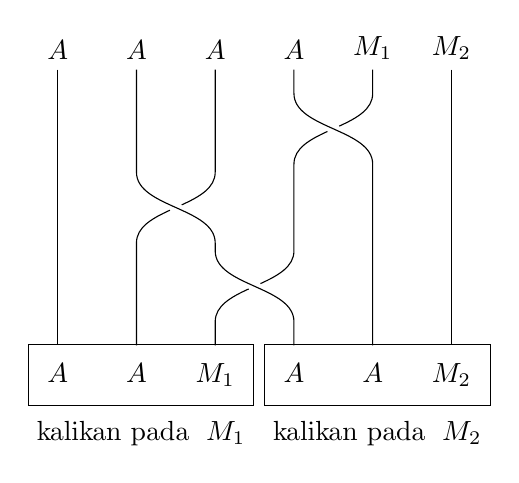
\begin{tikzpicture}
		[baseline=(braid), yscale=0.8]
		\pic[
			braid/number of strands = 6,
			braid/every strand/.style={black},
			name prefix=braid
		] at (0, 0) {braid={s_4 s_2 s_3}};
		\coordinate (braid) at ($(braid-1-s)!0.5!(braid-1-e)$);
		\node[above] at (braid-1-s) {$A$};
		\node[below=0.3em] (P) at (braid-1-e) {$A$};
		\node[above] at (braid-2-s) {$A$};
		\node[below=0.3em] (R) at (braid-2-e) {$A$};
		\node[above] at (braid-3-s) {$A$};
		\node[below=0.3em] at (braid-3-e) {$A$};
		\node[above] at (braid-4-s) {$A$};
		\node[below=0.3em] at (braid-4-e) {$A$};
		\node[above] at (braid-5-s) {$M_1$};
		\node[below=0.3em] (Q) at (braid-5-e) {$M_1$};
		\node[above] at (braid-6-s) {$M_2$};
		\node[below=0.3em] (S) at (braid-6-e) {$M_2$};

		\node (X) [draw, fit=(P) (Q)] {};
		\node[below=0.2em of X] {kalikan pada\; $M_1$};
		\node (Y) [draw, fit=(R) (S)] {};
		\node[below=0.2em of Y] {kalikan pada\; $M_2$};
	\end{tikzpicture} \; = 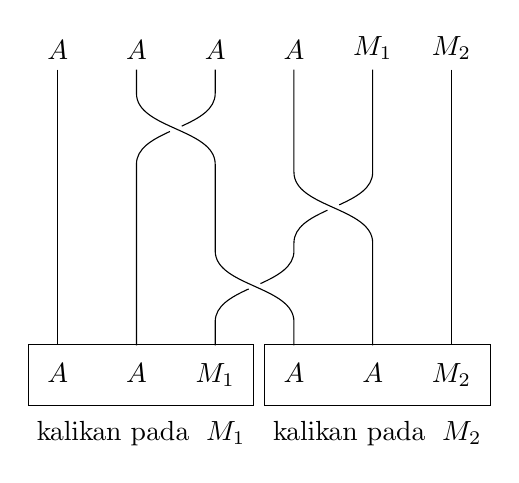
\begin{tikzpicture}
		[baseline=(braid), yscale=0.8]
		\pic[
			braid/number of strands=6,
			braid/every strand/.style = {black},
			name prefix=braid
		] at (0, 0) {braid={s_2 s_4 s_3}};
		\coordinate (braid) at ($(braid-1-s)!0.5!(braid-1-e)$);
		\node[above] at (braid-1-s) {$A$};
		\node[below=0.3em] (P) at (braid-1-e) {$A$};
		\node[above] at (braid-2-s) {$A$};
		\node[below=0.3em] (R) at (braid-2-e) {$A$};
		\node[above] at (braid-3-s) {$A$};
		\node[below=0.3em] at (braid-3-e) {$A$};
		\node[above] at (braid-4-s) {$A$};
		\node[below=0.3em] at (braid-4-e) {$A$};
		\node[above] at (braid-5-s) {$M_1$};
		\node[below=0.3em] (Q) at (braid-5-e) {$M_1$};
		\node[above] at (braid-6-s) {$M_2$};
		\node[below=0.3em] (S) at (braid-6-e) {$M_2$};

		\node (X) [draw, fit=(P) (Q)] {};
		\node[below=0.2em of X] {kalikan pada\; $M_1$};
		\node (Y) [draw, fit=(R) (S)] {};
		\node[below=0.2em of Y] {kalikan pada\; $M_2$};
	\end{tikzpicture}\end{center}
	yang langsung terlihat.

	Untuk menunjukkan bahwa $A\dcate{Mod}$ adalah kategori monoidal, masih
	perlu dibuktikan bahwa kendala asosiativitas dan kendala satuan bagi
	$\otimes$ semuanya merupakan morfisme modul-$A$ kiri. Pernyataan pertama
	tidak sulit. Pernyataan kedua memerlukan sifat koaljabar
	$(\identity\otimes\epsilon)\Delta=\identity_A=
	(\epsilon\otimes\identity)\Delta$, setelah mengidentifikasi
	$A\otimes\munit\simeq A\simeq\munit\otimes A$.
\end{proof}

% Unit 093 terjemahan Bahasa Indonesia dari chapter7.tex baris 1130--1279.
% Sumber: Methods of Algebra, Volume 2, commit
% 9a5803ff77dd3257484cb177f851a73770a59dd3 (CC BY 4.0).
% stable-unit-id: o014.aljabr2.chapter7.coalgebra-to-hopf-b
% Cakupan: sisa Bagian 7.5, dari sesudah bukti struktur monoidal kategori
% modul bialjabar hingga tepat sebelum Bagian 7.6 pada baris 1280.

% segment-id: o014.aljabr2.chapter7.coalgebra-to-hopf-b.p001
Untuk bialjabar $A$, kita masih dapat menanyakan apakah kategori monoidal
$A\dcate{Mod}$ memiliki struktur anyaman dan apakah struktur itu simetris.
Gagasan awal yang wajar ialah menggunakan struktur anyaman $c(M_1,M_2)$ dari
$\mathcal{V}$, tetapi pada umumnya ini bukan morfisme dalam $A\dcate{Mod}$.
Bahkan untuk kasus khusus $\mathcal{V}=\Bbbk\dcate{Mod}$, jawaban atas
pertanyaan ini sudah melibatkan konsep \emph{bialjabar kuasitriangular}, yang
tidak dapat dijelaskan secara singkat. Berikut hanya diberikan suatu contoh
yang begitu sederhana sehingga agak menyesatkan.

% segment-id: o014.aljabr2.chapter7.coalgebra-to-hopf-b.pr001
\begin{proposition}\label{prop:bialgebra-mod-symmetry}
	Misalkan $\mathcal{V}$ kategori monoidal simetris.
% segment-id: o014.aljabr2.chapter7.coalgebra-to-hopf-b.l001
	\begin{enumerate}[(i)]
% segment-id: o014.aljabr2.chapter7.coalgebra-to-hopf-b.i001
		\item Jika $A$ bialjabar kokomutatif di atas $\mathcal{V}$, maka kategori
		monoidal $A\dcate{Mod}$ dan $\cated{Mod}A$ menjadi kategori monoidal
		simetris terhadap
		$c(M_1,M_2):M_1\otimes M_2\rightiso M_2\otimes M_1$.

% segment-id: o014.aljabr2.chapter7.coalgebra-to-hopf-b.i002
		\item Secara dual, jika $A$ bialjabar komutatif di atas $\mathcal{V}$,
		maka $A\dcate{Comod}$ dan $\cated{Comod}A$ merupakan kategori monoidal
		simetris.
	\end{enumerate}
\end{proposition}

% segment-id: o014.aljabr2.chapter7.coalgebra-to-hopf-b.pf001
\begin{proof}
	Cukup bahas kasus kokomutatif. Dengan menggunakan notasi sebelumnya,
	pernyataan bahwa $c(M_1,M_2)$ merupakan morfisme dalam $A\dcate{Mod}$
	setara dengan membuktikan bahwa batas luar diagram berikut komutatif:
% segment-id: o014.aljabr2.chapter7.coalgebra-to-hopf-b.g001
	\[\begin{tikzcd}[row sep=large]
		A \otimes M_1 \otimes M_2 \arrow[r, "{\Delta \otimes \identity \otimes \identity}" inner sep=0.6em] \arrow[d, "{\identity \otimes c(M_1, M_2)}" description] & A \otimes A \otimes M_1 \otimes M_2 \arrow[r, "{\identity \otimes c(A, M_1) \otimes \identity}" inner sep=0.6em] \arrow[d, "{c(A, A) \otimes c(M_1, M_2)}" description] & A \otimes M_1 \otimes A \otimes M_2 \arrow[r, "{\mu_1 \otimes \mu_2}" inner sep=0.6em] \arrow[d, "{c(A \otimes M_1, A \otimes M_2)}" description] & M_1 \otimes M_2 \arrow[d, "{c(M_1, M_2)}" description] \\
		A \otimes M_2 \otimes M_1 \arrow[r, "{\Delta \otimes \identity \otimes \identity}"' inner sep=0.6em] & A \otimes A \otimes M_2 \otimes M_2 \arrow[r, "{\identity \otimes c(A, M_2) \otimes \identity}"' inner sep=0.6em] & A \otimes M_2 \otimes A \otimes M_1 \arrow[r, "{\mu_2 \otimes \mu_1}"' inner sep=0.6em] & M_2 \otimes M_1 .
	\end{tikzcd}\]

	Persegi di sebelah kiri komutatif karena $A$ kokomutatif, sedangkan persegi
	di sebelah kanan komutatif karena funktorialitas $c$. Dengan menggambar
	diagram anyamannya, terlihat bahwa
% segment-id: o014.aljabr2.chapter7.coalgebra-to-hopf-b.g002
	\begin{multline*}
		c(A \otimes M_1, A \otimes M_2) = \\
		(\identity_A \otimes c(A, M_2) \otimes \identity_{M_1}) (c(A, A) \otimes c(M_1, M_2)) (\identity_A \otimes c(A, M_1) \otimes \identity_{M_2}),
	\end{multline*}
	dan karena $\mathcal{V}$ kategori monoidal simetris, persegi di tengah juga
	komutatif. Semua sifat lain dari struktur monoidal simetris pada
	$A\dcate{Mod}$ cukup diverifikasi di $\mathcal{V}$.
\end{proof}

% segment-id: o014.aljabr2.chapter7.coalgebra-to-hopf-b.p002
Sekarang kita memperkenalkan konsep aljabar Hopf. Misalkan $\mathcal{V}$
kategori monoidal beranyam.

% segment-id: o014.aljabr2.chapter7.coalgebra-to-hopf-b.d001
\begin{definition}\label{def:Hopf-algebra}
% segment-id: o014.aljabr2.chapter7.coalgebra-to-hopf-b.x001
	\index{aljabar Hopf (Hopf algebra)}
% segment-id: o014.aljabr2.chapter7.coalgebra-to-hopf-b.x002
	\index{antipoda (antipode)}
	Misalkan data $(A,\mu,\eta,\Delta,\epsilon)$ merupakan bialjabar $A$ di
	atas $\mathcal{V}$. Jika suatu isomorfisme $S:A\rightiso A$ dalam
	$\mathcal{V}$ membuat diagram berikut komutatif,
% segment-id: o014.aljabr2.chapter7.coalgebra-to-hopf-b.g003
	\[\begin{tikzcd}
		A \otimes A \arrow[d, "\mu"'] & A \otimes A \arrow[r, "{S \otimes \identity_A}"] \arrow[l, "{\identity_A \otimes S}"'] & A \otimes A \arrow[d, "\mu"] \\
		A & A \arrow[u, "\Delta"] \arrow[r, "\eta\epsilon"'] \arrow[l, "\eta\epsilon"] & A ,
	\end{tikzcd}\]
	yaitu,
% segment-id: o014.aljabr2.chapter7.coalgebra-to-hopf-b.q001
	\[ \mu (\identity_A \otimes S) \Delta = \eta\epsilon = \mu (S \otimes \identity_A) \Delta, \]
	maka $S$ disebut \emph{antipoda} dari $A$. Bialjabar yang dilengkapi
	antipoda disebut \emph{aljabar Hopf}. Morfisme antaraljabar Hopf
	didefinisikan sebagai morfisme antarbialjabar yang
	mendasarinya.
\end{definition}

% segment-id: o014.aljabr2.chapter7.coalgebra-to-hopf-b.p003
Sebagai contoh, $\munit$ merupakan aljabar Hopf dengan antipoda
$\identity_{\munit}$.

% segment-id: o014.aljabr2.chapter7.coalgebra-to-hopf-b.p004
Jika ditafsirkan menggunakan konvolusi dalam
Catatan~\ref{rem:coalgebra-convolution}, antipoda $S$ tepat merupakan invers
dua sisi dari $\identity_A\in\End(A)$ terhadap $\star$. Antipoda dalam definisi
aljabar Hopf, jika ada, bersifat unik. Hal ini langsung diperoleh dengan
menerapkan hasil berikut pada $f=\identity_A$; hasil tersebut juga menunjukkan
bahwa morfisme selalu mempertahankan antipoda.

% segment-id: o014.aljabr2.chapter7.coalgebra-to-hopf-b.pr002
\begin{proposition}\label{prop:antipode-homo}
	Misalkan $A$ dan $A'$ aljabar Hopf di atas $\mathcal{V}$ dengan antipoda
	masing-masing $S$ dan $S'$. Untuk setiap morfisme aljabar Hopf
	$f:A\to A'$, berlaku $S'f=fS$.
\end{proposition}

% segment-id: o014.aljabr2.chapter7.coalgebra-to-hopf-b.pf002
\begin{proof}
	Berdasarkan funktorialitas konvolusi $\star$ dalam
	\eqref{eqn:convolution-functorial}, kedua pemetaan
% segment-id: o014.aljabr2.chapter7.coalgebra-to-hopf-b.g004
	\[\begin{tikzcd}
		\Hom(A', A') \arrow[r, "{g \mapsto gf}"] & \Hom(A, A')
	\end{tikzcd}, \quad \begin{tikzcd}
		\Hom(A, A) \arrow[r, "{h \mapsto fh}"] & \Hom(A, A')
	\end{tikzcd}\]
	merupakan homomorfisme monoid konvolusi. Jadi, $S'f$ dan $fS$ keduanya
	merupakan invers konvolusi dari $f\in\Hom(A,A')$.
\end{proof}

% segment-id: o014.aljabr2.chapter7.coalgebra-to-hopf-b.p005
Karena struktur anyaman pada $\mathcal{V}$ memberikan struktur anyaman pada
$\mathcal{V}^{\opp}$, konsep bialjabar jelas bersifat swadual. Hasil berikut
menunjukkan bahwa definisi antipoda juga demikian.

% segment-id: o014.aljabr2.chapter7.coalgebra-to-hopf-b.pr003
\begin{proposition}\label{prop:bialgebra-duality}
	Jika $(A,\mu,\eta,\Delta,\epsilon)$ bialjabar di atas $\mathcal{V}$, maka
	$(A,\eta,\mu,\epsilon,\Delta)$ merupakan bialjabar di atas
	$\mathcal{V}^{\opp}$. Jika aljabar Hopf
	$(A,\mu,\eta,\Delta,\epsilon)$ memiliki antipoda $S$, maka $S^{-1}$
	merupakan antipoda dari $(A,\eta,\mu,\epsilon,\Delta)$ sebagai bialjabar
	di atas $\mathcal{V}^{\opp}$; khususnya, objek terakhir ini merupakan
	aljabar Hopf di atas $\mathcal{V}^{\opp}$.
\end{proposition}

% segment-id: o014.aljabr2.chapter7.coalgebra-to-hopf-b.pf003
\begin{proof}
	Diagram dalam Definisi~\ref{def:Hopf-algebra} bersifat swadual, tetapi arah
	$S$ dibalik.
\end{proof}

% segment-id: o014.aljabr2.chapter7.coalgebra-to-hopf-b.pr004
\begin{proposition}\label{prop:Hopf-antiautomorphism}
% segment-id: o014.aljabr2.chapter7.coalgebra-to-hopf-b.x003
	\index[sym1]{Acop@$A_{\mathrm{cop}}, A^{\mathrm{op}}_{\mathrm{cop}}$}
	Untuk bialjabar $A$, sesuai dengan
	Definisi~\ref{def:opposite-braided-algebra},
% segment-id: o014.aljabr2.chapter7.coalgebra-to-hopf-b.l002
	\begin{compactitem}
% segment-id: o014.aljabr2.chapter7.coalgebra-to-hopf-b.i003
		\item membalik perkalian $A$ menggunakan struktur anyaman $c(A,A)$
		menghasilkan aljabar $A^{\mathrm{op}}$;
% segment-id: o014.aljabr2.chapter7.coalgebra-to-hopf-b.i004
		\item membalik komultiplikasi $A$ menggunakan $c(A,A)^{-1}$
		menghasilkan koaljabar $A_{\mathrm{cop}}$.
	\end{compactitem}
	Kedua operasi ini bersama-sama menghasilkan bialjabar
	$A^{\mathrm{op}}_{\mathrm{cop}}$. Jika $A$ memiliki antipoda $S$, maka $S$
	juga merupakan antipoda dari $A^{\mathrm{op}}_{\mathrm{cop}}$, dan dalam
	keadaan ini $S:A\rightiso A^{\mathrm{op}}_{\mathrm{cop}}$ merupakan
	isomorfisme bialjabar.
\end{proposition}

% segment-id: o014.aljabr2.chapter7.coalgebra-to-hopf-b.pf004
\begin{proof}
	Verifikasi rutin menunjukkan bahwa
	$A^{\mathrm{op}}_{\mathrm{cop}}$ memang bialjabar dengan antipoda $S$;
	perinciannya dihilangkan. Pernyataan yang tersisa terdiri atas dua bagian.
	Pertama, $S$ mempertahankan unit dan kounit. Ini mudah: dalam
	Proposisi~\ref{prop:antipode-homo}, ambil berturut-turut $A=\munit$ dan
	$A'=\munit$.

	Kedua, $S$ mempertahankan perkalian dan komultiplikasi. Bukti versi umumnya
	lebih rumit; lihat \cite[\S 9, Proposisi 2]{JS91} atau
	\cite[Proposisi 1.22]{AM10}. Di sini hanya diberikan garis besar kasus
	khusus $\mathcal{V}=\Bbbk\dcate{Mod}$,
	$\otimes=\otimes_{\Bbbk}$ dengan struktur anyaman standarnya. Inilah
	satu-satunya kasus yang akan diperlukan kemudian.

	Ingat dari \S\ref{sec:alg-in-monoidal-cat} bahwa $A\otimes A$ secara alami
	merupakan koaljabar. Lengkapi $\Hom(A\otimes A,A)$ dengan konvolusi dari
	Catatan~\ref{rem:coalgebra-convolution}, yang ditulis $\ast$, lalu tinjau
	unsur-unsurnya
% segment-id: o014.aljabr2.chapter7.coalgebra-to-hopf-b.q002
	\[ f := \mu, \quad g := \mu c(A, A) (S \otimes S), \quad h := S \mu. 
	\]
	Cukup dibuktikan bahwa
	$h\ast f=\eta_A\epsilon_{A\otimes A}=f\ast g$. Kesamaan ini akan
	menunjukkan bahwa $f$ merupakan unsur invertibel dalam monoid
	$(\Hom(A\otimes A,A),\ast)$, dan karena itu $h=g$. Misalkan $a,b\in A$,
	dan tuliskan ekspansi
% segment-id: o014.aljabr2.chapter7.coalgebra-to-hopf-b.g005
	\begin{gather*}
		\Delta(a) = \sum_i a_i^{(1)} \otimes a_i^{(2)}, \quad
		\Delta(b) = \sum_j b_j^{(1)} \otimes b_j^{(2)}.
	\end{gather*}
	Tuliskan $\mu$ langsung sebagai perkalian. Berdasarkan struktur anyaman
	standar pada $\Bbbk\dcate{Mod}$, diperoleh
% segment-id: o014.aljabr2.chapter7.coalgebra-to-hopf-b.g006
	\begin{align*}
		(h \ast f)(a \otimes b) & = \sum_{i, j} h\left(a^{(1)}_i \otimes b^{(1)}_j\right) f\left(a^{(2)}_i \otimes b^{(2)}_j\right) \\
		& = \sum_{i, j} S\left( a^{(1)}_i b^{(1)}_j \right) a^{(2)}_i b^{(2)}_j \\
		& = (\underbracket{S \star \identity_A}_{\text{konvolusi pada }\End(A)})(ab) = \eta_A \epsilon_A (ab), \\
		(f \ast g)(a \otimes b) & = \cdots = \sum_{i, j} a^{(1)}_i b^{(1)}_j S\left( b^{(2)}_j \right) S\left( a^{(2)}_i \right) \\
		& = \sum_i a^{(1)}_i \eta_A \epsilon_A(b) S\left( a^{(2)}_i \right) \\
		& = \eta_A \epsilon_A (a) \cdot \eta_A \epsilon_A (b) = \eta_A \epsilon_A(ab), \\
		\eta_A \epsilon_{A \otimes A}(a \otimes b) & = \eta_A\left( \epsilon_A(a)\epsilon_A(b) \right) = \eta_A \epsilon_A(ab),
	\end{align*}
	seperti yang diklaim. Jadi, $S$ mempertahankan perkalian bialjabar. Argumen
	serupa menunjukkan bahwa $S$ mempertahankan komultiplikasi.
\end{proof}

% segment-id: o014.aljabr2.chapter7.coalgebra-to-hopf-b.p006
Khususnya, jika $\mathcal{V}$ kategori monoidal simetris, maka $S^2$ merupakan
automorfisme dari $A$.

% segment-id: o014.aljabr2.chapter7.coalgebra-to-hopf-b.c001
\begin{corollary}\label{prop:Hopf-involution}
	Misalkan aljabar Hopf $A$ memiliki antipoda $S$. Jika $A$ komutatif atau
	kokomutatif, maka $S^2=\identity$.
\end{corollary}

% segment-id: o014.aljabr2.chapter7.coalgebra-to-hopf-b.pf005
\begin{proof}
	Terhadap konvolusi $\star$ pada $\End(A)$
	(Catatan~\ref{rem:coalgebra-convolution}), kita mempunyai
% segment-id: o014.aljabr2.chapter7.coalgebra-to-hopf-b.q003
	\[ S \star S^2 = \mu (S \otimes S^2) \Delta = \mu (S \otimes S)(\identity \otimes S) \Delta. \]

	Jika $A$ komutatif, maka $\mu c(A,A)=\mu$, dan
	Proposisi~\ref{prop:Hopf-antiautomorphism} mengubah ruas di atas menjadi
% segment-id: o014.aljabr2.chapter7.coalgebra-to-hopf-b.q004
	\[ \mu c(A, A) (S \otimes S) (\identity \otimes S)\Delta = S\mu (\identity \otimes S)\Delta = S(\identity \star S). \]
	Definisi antipoda menunjukkan bahwa
	$\identity\star S=\eta\epsilon$, sedangkan proposisi tersebut memberikan
	$S\eta=\eta$; hasil akhirnya ialah $\eta\epsilon$.

	Jika $A$ kokomutatif, maka $c(A,A)\Delta=\Delta$, dan funktorialitas struktur
	anyaman mengubah $S\star S^2$ menjadi
% segment-id: o014.aljabr2.chapter7.coalgebra-to-hopf-b.q005
	\[ \mu (S \otimes S)(\identity \otimes S) c(A, A) \Delta = \mu c(A, A) (S \otimes S)(S \otimes \identity)\Delta, \]
	yang oleh argumen yang sama kemudian berubah menjadi
	$S(S\star\identity)=\eta\epsilon$.

	Jadi, $S^2$ merupakan invers konvolusi dari $S$, sehingga
	$S^2=\identity$.
\end{proof}

% segment-id: o014.aljabr2.chapter7.coalgebra-to-hopf-b.p007
Semua contoh berikut mengambil $\mathcal{V}=\Bbbk\dcate{Mod}$ dan
$\otimes=\otimes_{\Bbbk}$, dengan $\Bbbk$ gelanggang komutatif.

% segment-id: o014.aljabr2.chapter7.coalgebra-to-hopf-b.ex001
\begin{example}\label{eg:group-Hopf-algebra}
	Misalkan $G$ grup. Bentuk aljabar grup-$\Bbbk$ $\Bbbk[G]$.
	Contoh~\ref{eg:monoid-bialgebra} memberi $\Bbbk[G]$ struktur bialjabar.
	Definisikan automorfisme modul-$\Bbbk$
	$S:\Bbbk[G]\to\Bbbk[G]$ melalui
% segment-id: o014.aljabr2.chapter7.coalgebra-to-hopf-b.q006
	\[ S(g) = g^{-1}, \quad g \in G. \]
	Mudah diverifikasi bahwa $S$ memenuhi diagram komutatif yang disyaratkan
	bagi antipoda. Jadi, $\Bbbk[G]$ merupakan aljabar Hopf.
\end{example}

% segment-id: o014.aljabr2.chapter7.coalgebra-to-hopf-b.ex002
\begin{example}[H.\ Hopf]
% segment-id: o014.aljabr2.chapter7.coalgebra-to-hopf-b.x004
	\index{ruang-H, grup-H (H-space, H-group)}
	Tuliskan $\{\mathrm{pt}\}$ untuk himpunan satu titik. Misalkan ruang
	topologis $X$ dilengkapi pemetaan kontinu
	$m:X\times X\to X$ (perkalian) dan
	$e:\{\mathrm{pt}\}\to X$ (setara dengan memilih suatu unsur dari $X$,
	yaitu unit, yang juga ditulis $e$), sedemikian sehingga kedua pemetaan
	memenuhi sifat-sifat yang diperlukan bagi asosiativitas perkalian dan unit,
	hingga homotopi. Maka $(X,m,e)$ disebut \emph{ruang-H}. Jika juga dipilih
	pemetaan kontinu $i:X\to X$ (pengambilan invers) yang, hingga homotopi,
	memenuhi sifat-sifat yang diperlukan bagi invers, maka $(X,m,e,i)$ disebut
	\emph{grup-H}.

	Monoid topologis (atau grup topologis) tentu merupakan ruang-H (atau
	grup-H), tetapi syarat ruang-H atau grup-H jauh lebih longgar. Contoh
	alaminya ialah ruang gelung. Untuk ruang topologis $M$ dengan titik pangkal
	terpilih $x_0\in M$, pemetaan kontinu $\gamma:[0,1]\to M$ yang memenuhi
	$\gamma(0)=x_0=\gamma(1)$ disebut \emph{gelung} di $M$. Semua gelung secara
	alami membentuk ruang topologis $\Omega(M,x_0)$. Jika $m$ diambil sebagai
	penyambungan ujung ke pangkal dua gelung, $e$ sebagai pemetaan konstan
	$x_0$, dan $i$ sebagai pembalikan arah gelung, maka secara intuitif
	$\Omega(M,x_0)$ membentuk grup-H. Kuncinya ialah asosiativitas dan sifat
	invers hanya berlaku dalam arti homotopi.

	Selanjutnya, tinjau subkategori penuh $\cate{S}$ dari $\cate{Top}$ yang
	terdiri atas semua kompleks CW\footnote{Ini adalah istilah topologis, yang
	agak berbeda dari kompleks yang didefinisikan dalam aljabar linear.};
	kategori ini memuat ruang-ruang yang umum dijumpai dalam geometri, seperti
	manifold. Misalkan $\Bbbk$ medan. Funktor kohomologi berkoefisien
	$\Bbbk$, yakni $\Hm^\bullet$, merupakan funktor dari $\cate{S}^{\opp}$ ke
	kategori ruang vektor-$\Bbbk$ bergradasi
	$\cate{Vect}(\Bbbk)^{\Z_{\geq0}}$. Lengkapi
	$\cate{Vect}(\Bbbk)^{\Z_{\geq0}}$ dengan struktur anyaman yang ditentukan
	oleh aturan tanda Koszul \eqref{eqn:Koszul-braiding} (dalam notasi di sana,
	ambil $\epsilon(a)=a\bmod\;2$). Hasil kali cawan
	$\mu:=\cup$ pada kohomologi membuat funktor $\Hm^\bullet$ berfaktor melalui
	$\cate{CAlg}\left(\cate{Vect}(\Bbbk)^{\Z_{\geq0}}\right)$; singkatnya,
	kohomologi merupakan aljabar komutatif di atas
	$\cate{Vect}(\Bbbk)^{\Z_{\geq0}}$.

	Di sisi lain, beri $\cate{S}$ struktur monoidal yang ditentukan oleh produk
	ruang, dengan $\{\mathrm{pt}\}$ sebagai unit. Rumus Künneth dalam topologi
	menunjukkan bahwa $\Hm^\bullet$ merupakan funktor monoidal. Selain itu,
	pemetaan-pemetaan yang homotopik menginduksi pemetaan yang sama pada tingkat
	kohomologi. Oleh karena itu, jika $X\in\Obj(\cate{S})$ merupakan ruang-H,
	maka $\Hm^\bullet(X)$ juga merupakan koaljabar di atas
	$\cate{Vect}(\Bbbk)^{\Z_{\geq0}}$.

	Pembaca yang mengenal topologi aljabar akan mudah menyimpulkan bahwa
	struktur aljabar dan koaljabar pada $\Hm^\bullet(X)$ kompatibel, sehingga
	memberikan bialjabar di atas
	$\cate{Vect}(\Bbbk)^{\Z_{\geq0}}$. Jika lebih lanjut $X$ merupakan grup-H
	dan automorfisme yang diinduksi oleh pemetaan $i$ ditulis
	$S\in\Aut(\Hm^\bullet(X))$, maka $\Hm^\bullet(X)$ menjadi aljabar Hopf.

	Sesungguhnya, perkalian (hasil kali cawan) pada $\Hm^\bullet(X)$ tidak lain
	adalah citra penyertaan diagonal
	$\mathrm{diag}:X\to X\times X$ melalui rumus Künneth, sedangkan unitnya
	adalah citra $X\to\{\mathrm{pt}\}$. Karena itu, semua sifat yang
	diperlukan bagi bialjabar dan antipoda dapat diverifikasi pada tingkat ruang
	topologis, hingga homotopi. Sebagai contoh, identitas antipoda
	$\mu(S\otimes\identity)\Delta=\eta\epsilon$ berasal dari
% segment-id: o014.aljabr2.chapter7.coalgebra-to-hopf-b.q007
	\[ \left[ X \xrightarrow{\mathrm{diag}} X \times X \xrightarrow{(i, \identity)} X \times X \xrightarrow{m} X\right] \;\text{ekuivalen secara homotopi dengan}\; \left[ X \to \{\mathrm{pt}\} \xrightarrow{e} X \right]. \]

	Dengan demikian, kohomologi suatu grup-H secara alami merupakan aljabar Hopf
	komutatif dengan struktur yang kaya. Inilah motivasi awal Hopf untuk
	mempelajari aljabar semacam itu.
\end{example}

% segment-id: o014.aljabr2.chapter7.coalgebra-to-hopf-b.p008
Latihan-latihan akan memberikan lebih banyak contoh aljabar Hopf. Kebanyakan
contoh itu komutatif atau kokomutatif, tetapi terdapat pula banyak aljabar Hopf
yang tidak memiliki kedua sifat tersebut. Kelas terpenting di antaranya ialah
\emph{grup kuantum}. Pembahasan terkait memerlukan landasan teori Lie dan tidak
dibahas dalam buku ini.

% Unit 094 terjemahan Bahasa Indonesia dari chapter7.tex baris 1280--1444.
% Sumber: Methods of Algebra, Volume 2, commit
% 9a5803ff77dd3257484cb177f851a73770a59dd3 (CC BY 4.0).
% stable-unit-id: o014.aljabr2.chapter7.beck-monadicity-a
% Cakupan: Bagian 7.6 dari pembukaan hingga konstruksi modul-T bebas;
% dilanjutkan oleh Unit 095 pada baris 1445.

% segment-id: o014.li2.chapter7.beck-monadicity-a.h001
\section{Teorema Monadisitas Beck}\label{sec:Beck}
\hypertarget{o014.aljabr2.chapter7.beck-monadicity-a}{ }
% segment-id: o014.li2.chapter7.beck-monadicity-a.p001
Misalkan $\mathcal{C}$ kategori. Tinjau kategori funktor
$\mathcal{C}^{\mathcal{C}}$ yang objek-objeknya semua endofunktor
$T:\mathcal{C}\to\mathcal{C}$ dan morfisme-morfismenya morfisme
antarendofunktor. Kategori ini secara alami menjadi kategori monoidal: perkalian
$\otimes$ adalah komposisi funktor dan objek satuan $\munit$ adalah funktor
identitas. Karena komposisi funktor asosiatif secara ketat, kategori ini juga
merupakan kategori monoidal ketat.

% segment-id: o014.li2.chapter7.beck-monadicity-a.d001
\begin{definition}[Monad dan komonad]\label{def:monad}
	\index{monad@monad}
	\index{komonad@komonad (comonad)}
	Misalkan $\mathcal{C}$ kategori. Aljabar dalam kategori monoidal
	$\mathcal{C}^{\mathcal{C}}$ (Definisi~\ref{def:algebra-monoidal}) disebut
	\emph{monad} di atas $\mathcal{C}$. Secara dual, monad di atas
	$\mathcal{C}^{\opp}$ disebut \emph{komonad} di atas $\mathcal{C}$.
\end{definition}

% segment-id: o014.li2.chapter7.beck-monadicity-a.p002
Dengan menguraikan Definisi~\ref{def:algebra-monoidal} dalam kategori
endofunktor $\mathcal{C}^{\mathcal{C}}$, diperoleh bahwa monad adalah data
$(T,\mu,\eta)$, dengan $T:\mathcal{C}\to\mathcal{C}$ suatu funktor serta
$\mu:T^2\to T$ dan $\eta:\identity_{\mathcal{C}}\to T$ suatu morfisme,
sedemikian sehingga diagram berikut komutatif:
% segment-id: o014.li2.chapter7.beck-monadicity-a.q001
\begin{equation*}\begin{gathered}
	\begin{tikzcd}
		T \arrow[r, "{\eta T}"] \arrow[rd, "\identity"'] & T^2 \arrow[d, "\mu"] & T \arrow[l, "{T\eta}"'] \arrow[ld, "\identity"] \\
		& T &
	\end{tikzcd} \quad
	\begin{tikzcd}
		T^3 \arrow[r, "\mu T"] \arrow[d, "T\mu"'] & T^2 \arrow[d, "\mu"] \\
		T^2 \arrow[r, "\mu"'] & T.
	\end{tikzcd}
\end{gathered}\end{equation*}

% segment-id: o014.li2.chapter7.beck-monadicity-a.p003
Dibandingkan dengan definisi semula, kendala asosiativitas tidak lagi
diperlukan di sini, sedangkan $\eta\otimes\identity$ (atau
$\identity\otimes\eta$) diterjemahkan menjadi $\eta T$ (atau $T\eta$), dan
demikian seterusnya.

% segment-id: o014.li2.chapter7.beck-monadicity-a.p004
Secara dual, komonad $(L,\delta,\epsilon)$ terdiri atas funktor
$L:\mathcal{C}\to\mathcal{C}$ serta morfisme $\delta:L\to L^2$ dan
$\epsilon:L\to\identity_{\mathcal{C}}$, dengan syarat bahwa diagram berikut
komutatif.
% segment-id: o014.li2.chapter7.beck-monadicity-a.q002
\begin{equation*}\begin{gathered}
	\begin{tikzcd}
		L  & L^2 \arrow[l, "{\epsilon L}"'] \arrow[r, "{L\epsilon}"] & L \\
		& L \arrow[lu, "\identity"] \arrow[ru, "\identity"'] \arrow[u, "\delta"] &
	\end{tikzcd} \quad
	\begin{tikzcd}
		L^3 & L^2 \arrow[l, "\delta L"'] \\
		L^2 \arrow[u, "L\delta"] & L \arrow[u, "\delta"'] \arrow[l, "\delta"]
	\end{tikzcd}
\end{gathered}\end{equation*}

% segment-id: o014.li2.chapter7.beck-monadicity-a.p005
Data $(T,\mu,\eta)$ (atau $(L,\delta,\epsilon)$) lazim disingkat menjadi $T$
(atau $L$). Sumber utama monad dan komonad adalah pasangan adjoin.

% segment-id: o014.li2.chapter7.beck-monadicity-a.eg001
\begin{example}[Pasangan adjoin menentukan monad]\label{eg:adjunction-monad}
	Tinjau sepasang funktor adjoin
	% segment-id: o014.li2.chapter7.beck-monadicity-a.q003
	\[\begin{tikzcd}
		F: \mathcal{C} \arrow[shift left, r] & \mathcal{D}: G \arrow[shift left, l],
	\end{tikzcd}\]
	beserta unit $\eta:\identity_{\mathcal{C}}\to GF$ dan kounit
	$\varepsilon:FG\to\identity_{\mathcal{D}}$ yang bersesuaian. Definisikan
	monad $(T,\mu,\eta)$ di atas $\mathcal{C}$ dan komonad
	$(L,\delta,\varepsilon)$ di atas $\mathcal{D}$ sebagai berikut.
	% segment-id: o014.li2.chapter7.beck-monadicity-a.q004
	\[\begin{array}{|c|c|}\hline
		T := GF & L := FG \\
		\mu := \left[ GFGF \xrightarrow{G\varepsilon F} GF \right] & \delta := \left[ FG \xrightarrow{F\eta G} FGFG \right] \\
		\eta : \identity_{\mathcal{C}} \to GF & \varepsilon: FG \to \identity_{\mathcal{D}} \\ \hline
	\end{array}\]

	Berdasarkan dualitas, cukup memeriksa aksioma monad dalam kasus
	$(T,\mu,\eta)$. Pertama, diagram untuk unit ialah
	% segment-id: o014.li2.chapter7.beck-monadicity-a.q005
	\[\begin{tikzcd}[column sep=large]
		GF \arrow[r, "{\eta GF}"] \arrow[equal, rd] & GFGF \arrow[d, "{G\varepsilon F}"] & GF \arrow[l, "{GF\eta}"'] \arrow[equal, ld] \\
		& GF &
	\end{tikzcd}\]
	yang komutatif berkat identitas segitiga
	$(G\varepsilon)(\eta G)=\identity_G$ dan
	$(\varepsilon F)(F\eta)=\identity_F$. Diagram asosiativitas ialah
	% segment-id: o014.li2.chapter7.beck-monadicity-a.q006
	\[\begin{tikzcd}[column sep=large]
		GFGFGF \arrow[d, "{G\varepsilon FGF}"'] \arrow[r, "{GFG\varepsilon F}"] & GFGF \arrow[d, "G\varepsilon F"] \\
		GFGF \arrow[r, "G\varepsilon F"'] & GF
	\end{tikzcd}\]
	dan diagram ini komutatif: kedua komposisinya sama-sama digambarkan sebagai
	% segment-id: o014.li2.chapter7.beck-monadicity-a.q007
	\[\begin{tikzcd}
		\mathcal{C} \arrow[r, "F"] & \mathcal{D} \arrow[r, "G"] \arrow[rr, bend right=60, ""{name=A}, "{\identity}"'] & \mathcal{C} \arrow[r, "F"] \arrow[Rightarrow, to=A, "\varepsilon"] &
		\mathcal{D} \arrow[r, "G"] \arrow[rr, bend right=60, ""{name=B}, "{\identity}"'] & \mathcal{C} \arrow[r, "F"] \arrow[Rightarrow, to=B, "\varepsilon"] & \mathcal{D} \arrow[r, "G"] & \mathcal{C}
	\end{tikzcd}\]
	dengan hanya urutan komposisi dua daerah melengkung yang berbeda, sedangkan
	hasilnya sama. Ini merupakan kasus khusus hukum pertukaran antara komposisi
	vertikal dan horizontal morfisme \cite[Lema 2.2.7]{Li1}.
\end{example}

% segment-id: o014.li2.chapter7.beck-monadicity-a.p006
Karena endofunktor beraksi pada $\mathcal{C}$, kita ingin membahas ``modul''
di dalam $\mathcal{C}$ di bawah aksi monad $T$. Karena alasan historis,
struktur semacam ini juga disebut aljabar-$T$.

% segment-id: o014.li2.chapter7.beck-monadicity-a.d002
\begin{definition}[S.\ Eilenberg, J.\ C.\ Moore]\label{def:T-Alg}
	\index{modul-T@modul-$T$}
	Misalkan $(T,\mu,\eta)$ monad di atas $\mathcal{C}$. Suatu \emph{modul-$T$}
	adalah data $(M,a)$, dengan $M\in\Obj(\mathcal{C})$ dan $a$ morfisme
	$T(M)\to M$ dalam $\mathcal{C}$, sedemikian sehingga diagram berikut
	komutatif:
	% segment-id: o014.li2.chapter7.beck-monadicity-a.q008
	\[\begin{tikzcd}
		T^2 (M) \arrow[r, "Ta"] \arrow[d, "\mu_M"'] & T(M) \arrow[d, "a"] \\
		T(M) \arrow[r, "a"'] & M
	\end{tikzcd} \quad \begin{tikzcd}
		M \arrow[r, "\eta_M"] \arrow[rd, "{\identity_M}"'] & T(M) \arrow[d, "a"] \\
		& M .
	\end{tikzcd}\]

	Semua modul-$T$ membentuk kategori $\mathcal{C}^T$. Morfisme dari $(M,a)$
	ke $(M',a')$ didefinisikan sebagai morfisme $f:M\to M'$ dalam
	$\mathcal{C}$ yang membuat diagram berikut komutatif:
	% segment-id: o014.li2.chapter7.beck-monadicity-a.q009
	\[\begin{tikzcd}
		T(M) \arrow[r, "a"] \arrow[d, "Tf"'] & M \arrow[d, "f"] \\
		T(M')  \arrow[r, "{a'}"'] & M' .
	\end{tikzcd}\]

	Secara dual, misalkan $(L,\delta,\epsilon)$ komonad di atas $\mathcal{C}$.
	Suatu komodul-$L$ adalah data $(N,b)$, dengan
	$b:N\to L(N)$ suatu morfisme, dan disyaratkan memenuhi diagram komutatif
	yang dual terhadap diagram di atas. Kategori komodul-$L$ ditulis
	$\mathcal{C}^L$.
\end{definition}

% segment-id: o014.li2.chapter7.beck-monadicity-a.p007
Kedua diagram komutatif untuk modul-$T$ masing-masing harus dipandang sebagai
hukum asosiativitas dan hukum unit bagi aksi $T$. Contoh-contoh dan sifat-
sifat berikut terutama dinyatakan untuk monad dan modul di atasnya; versi
komonad dan komodul sepenuhnya dual.

% segment-id: o014.li2.chapter7.beck-monadicity-a.eg002
\begin{example}\label{eg:Mon-monad}
	Tuliskan $\cate{Mon}$ untuk kategori monoid, yang secara konvensi dianggap
	direalisasikan pada himpunan kecil, dan tinjau pasangan adjoin
	% segment-id: o014.li2.chapter7.beck-monadicity-a.q010
	\[\begin{tikzcd}
		\mathbf{M}: \cate{Set} \arrow[r, shift left] & \cate{Mon}: U, \arrow[l, shift left]
	\end{tikzcd}\]
	dengan $\mathbf{M}$ memetakan himpunan $X$ ke monoid bebas
	$\mathbf{M}(X)$, yang definisi dan konstruksinya diberikan dalam
	\cite[Definisi 4.8.1, Lema 4.8.4]{Li1}, dan $U$ adalah funktor pelupa.
	Dengan demikian,
	% segment-id: o014.li2.chapter7.beck-monadicity-a.q011
	\[ T := U\mathbf{M}: \cate{Set} \to \cate{Set}, \quad T(X) = \bigsqcup_{n \geq 0} X^n. \]
	Dengan kata lain, unsur $T(X)$ adalah ``kata''
	$(x_1,\ldots,x_n)$ dengan $n\in\Z_{\geq0}$. Unit pasangan adjoin
	$\eta_X:X\to U\mathbf{M}(X)$ memetakan $x\in X$ ke kata berpanjang $1$,
	$(x)$. Untuk monoid $A$, kounit
	$\varepsilon_A:\mathbf{M}U(A)\to A$ memetakan kata
	$(a_1,\ldots,a_n)$ ke hasil kali $a_1\cdots a_n\in A$. Karena perkalian
	dalam $\mathbf{M}(X)$ adalah konkatenasi kata, pemetaan
	$\mu_X=U\varepsilon\mathbf{M}:T^2(X)\to T(X)$ yang bersesuaian dengan monad
	$T$ (atau, jika dipandang sebagai pemetaan
	$\mathbf{M}(\mathbf{M}(X))\to\mathbf{M}(X)$) meratakan ``kata yang
	terdiri atas kata-kata'', yakni menggabungkan serangkaian daftar, seperti
	% segment-id: o014.li2.chapter7.beck-monadicity-a.q012
	\[ \left( (x_1, \ldots, x_n), (y_1, \ldots, y_m), \ldots \right) \mapsto \left( x_1, \ldots, x_n, y_1, \ldots, y_m, \ldots \right). \]

	Memberikan modul-$T$ $(M,a)$ untuk $T=U\mathbf{M}$ sama artinya dengan
	memberikan $m_1\cdots m_n:=a(m_1,\ldots,m_n)$ untuk setiap kata
	$(m_1,\ldots,m_n)$ pada himpunan $M$, sedemikian sehingga $a(m)=m$ dan
	hukum asosiatif
	% segment-id: o014.li2.chapter7.beck-monadicity-a.q013
	\[ a\left( a(x_1, \ldots, x_n), a(y_1, \ldots, y_m), \ldots \right) = a\left( x_1, \ldots, x_n, y_1, \ldots, y_m, \ldots \right) \]
	berlaku. Singkatnya, modul-$T$ tidak lain adalah monoid, dengan citra kata
	kosong ($n=0$) di bawah $a$ sebagai satuannya. Mudah diperiksa bahwa
	morfisme modul-$T$ juga tidak lain adalah homomorfisme monoid.

	Kasus kategori grup $\cate{Grp}$ sepenuhnya serupa; kuncinya ialah mengganti
	$\mathbf{M}$ dengan funktor grup bebas $\mathbf{F}$. Modul-$T$ yang
	bersesuaian tepat merupakan grup.
\end{example}

% segment-id: o014.li2.chapter7.beck-monadicity-a.eg003
\begin{example}\label{eg:Mod-monad}
	Misalkan $R$ gelanggang dan tinjau pasangan adjoin
	% segment-id: o014.li2.chapter7.beck-monadicity-a.q014
	\[\begin{tikzcd}
		\mathbf{F}: \cate{Set} \arrow[r, shift left] & R\dcate{Mod}: U, \arrow[l, shift left]
	\end{tikzcd}\]
	dengan $\mathbf{F}$ memetakan $X$ ke modul-$R$ kiri bebas
	$R^{\oplus X}$ dan $U$ adalah funktor pelupa. Dari sini diperoleh monad
	$(T,\mu,\eta)$ di atas $\cate{Set}$. Seperti dalam
	Contoh~\ref{eg:Mon-monad}, $T=U\mathbf{F}$ memetakan himpunan $X$ ke
	$R^{\oplus X}$ sebagai suatu himpunan; unsur-unsurnya adalah kombinasi
	linear-$R$ formal hingga dari unsur-unsur $X$,
	$\text{\textquotedblleft} r_1x_1+\cdots+r_nx_n
	\text{\textquotedblright}$. Unit $\eta_X$ memetakan $x\in X$ ke
	$\text{\textquotedblleft}x\text{\textquotedblright}$, sedangkan
	$\mu_X:R^{\oplus(R^{\oplus}X)}\to R^{\oplus X}$ meratakan kombinasi linear
	dua tingkat, yakni
	% segment-id: o014.li2.chapter7.beck-monadicity-a.q015
	\begin{multline*}
		\text{\textquotedblleft} \alpha (\text{\textquotedblleft} r_1 x_1 + \cdots + r_n x_n \text{\textquotedblright}) + \beta (\text{\textquotedblleft} s_1 y_1 + \cdots + s_m y_m \text{\textquotedblright}) + \cdots \text{\textquotedblright} \\
		\mapsto \text{\textquotedblleft} (\alpha r_1) x_1 + \cdots + (\alpha r_n) x_n + (\beta s_1) y_1 + \cdots + (\beta s_m) y_m + \cdots \text{\textquotedblright} .
	\end{multline*}
	Memberikan modul-$T$ $(M,a)$ sama artinya dengan memberikan himpunan $M$
	beserta aturan yang memetakan kombinasi linear formal ke suatu unsur $M$,
	memetakan $\text{\textquotedblleft}x\text{\textquotedblright}$ ke $x$,
	bersifat asosiatif terhadap penjumlahan dan perkalian skalar, dan membuat
	perkalian skalar oleh $1\in R$ menjadi pemetaan identitas. Singkatnya,
	modul-$T$ tidak lain adalah modul-$R$ kiri. Jelas bahwa morfisme modul-$T$
	tepat merupakan homomorfisme modul.
\end{example}

% segment-id: o014.li2.chapter7.beck-monadicity-a.p008
Kembali ke teori umum. Terdapat funktor pelupa
$U^T:\mathcal{C}^T\to\mathcal{C}$ yang memetakan objek $(M,a)$ ke $M$.
Berikut diberikan adjoin kirinya: konstruksi bebas.

% segment-id: o014.li2.chapter7.beck-monadicity-a.dp001
\begin{definition-proposition}[Modul-$T$ bebas]\label{def:free-T-Alg}
	\index{modul!bebas@bebas (free)}
	Misalkan $(T,\mu,\eta)$ monad di atas $\mathcal{C}$. Definisikan funktor
	% segment-id: o014.li2.chapter7.beck-monadicity-a.q016
	\[ \mathrm{Free}^T: \mathcal{C} \to \mathcal{C}^T , \quad
	\begin{array}{rl}
		(\text{objek } M) & \mapsto (TM, \mu_M: T^2 M \to TM), \\
		(\text{morfisme } f: M \to M') & \mapsto Tf: TM \to TM'.
	\end{array}\]
	Hal ini memberikan pasangan adjoin
	% segment-id: o014.li2.chapter7.beck-monadicity-a.q017
	\[\begin{tikzcd}
		\mathrm{Free}^T : \mathcal{C} \arrow[shift left, r] & \mathcal{C}^T: U^T \arrow[shift left, l],
	\end{tikzcd}\]
	dan monad pada $\mathcal{C}$ yang ditentukan pasangan adjoin ini tepat
	$(T,\mu,\eta)$.
\end{definition-proposition}
% segment-id: o014.li2.chapter7.beck-monadicity-a.pf001
\begin{proof}
	Untuk memeriksa bahwa $(TM,\mu_M)$ adalah modul-$T$, perlu ditunjukkan
	komutativitas kedua diagram berikut:
	% segment-id: o014.li2.chapter7.beck-monadicity-a.q018
	\[\begin{tikzcd}
		T^3 (M) \arrow[r, "T\mu_M"] \arrow[d, "\mu_{T(M)}"'] & T^2(M) \arrow[d, "\mu_M"] \\
		T^2 (M) \arrow[r, "\mu_M"'] & T(M)
	\end{tikzcd} \quad \begin{tikzcd}
		T(M) \arrow[r, "\eta_{T(M)}"] \arrow[rd, "\identity"'] & T^2(M) \arrow[d, "\mu_M"] \\
		& T(M).
	\end{tikzcd}\]
	Namun, diagram ini diperoleh dengan mengevaluasi diagram funktor dalam
	Definisi~\ref{def:monad} pada objek $M$. Funktorialitasnya jelas.

	Selanjutnya, perhatikan bahwa $U^T\mathrm{Free}^T=T$. Ambil
	$\eta:\identity_{\mathcal{C}}\to T$ yang merupakan bagian dari data $T$, lalu
	definisikan
	% segment-id: o014.li2.chapter7.beck-monadicity-a.q019
	\[ \epsilon: \mathrm{Free}^T U^T \to \identity_{\mathcal{C}^T}, \quad
	\epsilon_{(M, a)}: (TM, \mu_M) \xrightarrow{a} (M, a) \in \Obj(\mathcal{C}^T). \]
	Diagram kiri dalam Definisi~\ref{def:T-Alg} menunjukkan bahwa
	$\epsilon_{(M,a)}$ adalah morfisme dalam $\mathcal{C}^T$.
	Funktorialitasnya juga jelas.

	Pemeriksaan rutin menunjukkan bahwa $(\mathrm{Free}^T,U^T)$ membentuk
	pasangan adjoin dengan unit $\eta$ dan kounit $\epsilon$; perinciannya
	dihilangkan. Selain itu,
	% segment-id: o014.li2.chapter7.beck-monadicity-a.q020
	\begin{equation*}\begin{aligned}
		\left(U^T \epsilon \mathrm{Free}^T\right)_M & = U^T \epsilon_{(TM, \mu_M)} \\
		& = \left[ \mu_M: T^2(M) \to T(M)\right],
	\end{aligned}\end{equation*}
	yang menunjukkan bahwa monad di atas $\mathcal{C}$ yang ditentukan oleh
	pasangan adjoin $(\mathrm{Free}^T,U^T)$ adalah $(T,\mu,\eta)$.
\end{proof}

% segment-id: o014.li2.chapter7.beck-monadicity-a.p009
Untuk monad dalam Contoh~\ref{eg:Mon-monad} dan
\ref{eg:Mod-monad}, funktor $\mathrm{Free}^T$ masing-masing bersesuaian dengan
konstruksi monoid bebas dan modul bebas.

% segment-id: o014.li2.chapter7.beck-monadicity-a.p010
Secara dual, komonad $L$ di atas kategori $\mathcal{D}$ juga memberikan
pasangan adjoin bebas--pelupa; tidak perlu dibahas lebih lanjut.

% Unit 095 terjemahan Bahasa Indonesia dari chapter7.tex baris 1445--1660.
% Sumber: Methods of Algebra, Volume 2, commit
% 9a5803ff77dd3257484cb177f851a73770a59dd3 (CC BY 4.0).
% stable-unit-id: o014.aljabr2.chapter7.beck-monadicity-b
% Cakupan: sisa Bagian 7.6, dari funktor pembanding hingga versi linear
% Teorema Beck; Unit 096 memulai Bagian 7.7 pada baris 1661.

\hypertarget{o014.aljabr2.chapter7.beck-monadicity-b}{ }
% segment-id: o014.aljabr2.chapter7.beck-monadicity-b.l001
\begin{lemma}\label{prop:T-comparison}
	Tinjau monad $T$ dan komonad $L$ yang berasal dari pasangan adjoin
	$(F,G)$. Misalkan $N\in\Obj(\mathcal{D})$. Data
	% segment-id: o014.aljabr2.chapter7.beck-monadicity-b.q001
	\[ M:=G(N)\in\Obj(\mathcal{C}), \quad
	 a:T(M)=GFG(N)\xrightarrow{G\varepsilon_N}G(N)=M \]
	memberikan $(M,a)\in\Obj(\mathcal{C}^T)$. Dengan demikian diperoleh funktor
	$\mathbb{K}:\mathcal{D}\to\mathcal{C}^T$ yang memenuhi
	$G=U^T\mathbb{K}$.

	Secara dual, $F$ juga terfaktorkan secara kanonik sebagai
	$\mathcal{C}\xrightarrow{\mathbb{K}}\mathcal{D}^L\to\mathcal{D}$, yang
	selanjutnya ditulis $F=U^L\mathbb{K}$, dengan $U^L$ funktor
	pelupa\footnote{Pemakaian lambang $\mathbb{K}$ yang sama tidak akan banyak
	menimbulkan kerancuan, sebab buku ini tidak akan membahas monad dan komonad
	secara bersamaan.}.
\end{lemma}
% segment-id: o014.aljabr2.chapter7.beck-monadicity-b.pf001
\begin{proof}
	Cukup dibahas kasus $T$. Kedua diagram dalam Definisi~\ref{def:T-Alg}
	dalam hal ini menjadi
	% segment-id: o014.aljabr2.chapter7.beck-monadicity-b.g001
	\[\begin{tikzcd}
		GFGFG(N) \arrow[r, "GFG\varepsilon" inner sep=0.5em] \arrow[d, "{G\varepsilon FG}"'] & GFG(N) \arrow[d, "G\varepsilon"] \\
		GFG(N) \arrow[r, "G\varepsilon"'] & G(N)
	\end{tikzcd} \quad \begin{tikzcd}
		G(N) \arrow[r, "\eta G"] \arrow[equal, rd] & GFG(N) \arrow[d, "{G\varepsilon}"] \\
		& G(N).
	\end{tikzcd} \]
	Verifikasi komutativitasnya persis sama dengan yang dilakukan dalam
	Contoh~\ref{eg:adjunction-monad}, sehingga tidak perlu diulangi;
	funktorialitas $N\mapsto(M,a)$ juga langsung terlihat.
\end{proof}

% segment-id: o014.aljabr2.chapter7.beck-monadicity-b.p001
Untuk pasangan adjoin $(F,G)$ yang diberikan, menerapkan funktor merupakan
proses yang melupakan struktur. Lema~\ref{prop:T-comparison} memfaktorkan $G$
(atau $F$) sebagai $U^T\mathbb{K}$ (atau $U^L\mathbb{K}$). Kita ingin
mengetahui apakah struktur hanya hilang pada langkah kedua, yaitu saat
menerapkan funktor pelupa $U^T$. Jika demikian, informasi yang hilang dalam
proses itu dapat direkonstruksi dengan bantuan monad $T$ (atau komonad $L$).
Pertimbangan ini memotivasi konsep berikut.

% segment-id: o014.aljabr2.chapter7.beck-monadicity-b.d001
\begin{definition}\label{def:monadic}
	Tinjau sepasang funktor adjoin
	% segment-id: o014.aljabr2.chapter7.beck-monadicity-b.g002
	$\begin{tikzcd}
		F: \mathcal{C} \arrow[shift left, r] & \mathcal{D}: G \arrow[shift left, l]
	\end{tikzcd}$,
	yang menentukan monad $T$ di atas $\mathcal{C}$ dan komonad $L$ di atas
	$\mathcal{D}$.
	\begin{itemize}
		\item Jika funktor $\mathbb{K}:\mathcal{D}\to\mathcal{C}^T$ dalam
		Lema~\ref{prop:T-comparison} merupakan ekuivalensi kategori, pasangan
		adjoin tersebut disebut \emph{monadik}.
		\item Jika versi dualnya
		$\mathbb{K}:\mathcal{C}\to\mathcal{D}^L$ merupakan ekuivalensi kategori,
		pasangan adjoin tersebut disebut \emph{komonadik}.
	\end{itemize}
\end{definition}

% segment-id: o014.aljabr2.chapter7.beck-monadicity-b.p002
Sebagai contoh, pasangan adjoin bebas--pelupa dalam
Contoh~\ref{eg:Mon-monad} dan \ref{eg:Mod-monad} semuanya monadik; pemeriksaan
langsung bahkan menunjukkan bahwa $\mathbb{K}$ dalam kedua contoh tersebut
merupakan isomorfisme kategori.

% segment-id: o014.aljabr2.chapter7.beck-monadicity-b.p003
Teorema Beck yang akan dibahas berikutnya, juga disebut teorema monadisitas atau
teorema Barr--Beck, mencirikan sifat monadik. Kita memerlukan beberapa
persiapan.

% segment-id: o014.aljabr2.chapter7.beck-monadicity-b.dp001
\begin{definition-proposition}
	\index{fork terbelah@fork terbelah (split fork)}
	Tinjau diagram dalam suatu kategori $\mathcal{C}$
	% segment-id: o014.aljabr2.chapter7.beck-monadicity-b.e001
	\begin{equation*}\label{eqn:split-coeq}\begin{tikzcd}[column sep=large]
		A \arrow[shift left, r, "u"] \arrow[shift right, r, "v" description] & B \arrow[r, "h"] \arrow[dashed, l, bend left, "t"] & Z \arrow[dashed, l, bend left, "s"]
	\end{tikzcd}\end{equation*}
	sedemikian sehingga bagian bergaris penuh komutatif, yaitu $hu=hv$, dan
	$h$ serta $v$ masing-masing mempunyai seksi (yakni invers kanan) $s$ dan
	$t$ seperti ditunjukkan oleh garis putus-putus, dengan
	$sh=ut\in\End(B)$. Bagian bergaris penuh dari diagram yang mempunyai sifat
	ini disebut \emph{garpu terbelah}. Diagram tersebut secara otomatis
	memberikan kopenyama dari $u$ dan $v$ dalam $\mathcal{C}$.
\end{definition-proposition}
% segment-id: o014.aljabr2.chapter7.beck-monadicity-b.pf002
\begin{proof}
	Tinjau diagram berikut:
	% segment-id: o014.aljabr2.chapter7.beck-monadicity-b.g003
	\[\begin{tikzcd}[row sep=small]
		& & W \\
		A \arrow[shift left, r, "u"] \arrow[shift right, r, "v"'] & B \arrow[r, "h"'] \arrow[ru, "k"] & Z
	\end{tikzcd} \qquad \begin{array}{ll}
		W \in \Obj(\mathcal{C}) \\
		ku = kv.
	\end{array} \]
	Jika terdapat $\varphi:Z\to W$ dengan $\varphi h=k$, maka
	$\varphi=\varphi hs=ks$. Sebaliknya, $\varphi:=ks$ memang memenuhi
	$\varphi h=ksh=kut=kvt=k$. Ini membuktikan sifat universal yang
	diperlukan.
\end{proof}

% segment-id: o014.aljabr2.chapter7.beck-monadicity-b.p004
Berbeda dengan kopenyama pada umumnya, garpu terbelah bersifat
``mutlak'': citranya di bawah funktor apa pun tetap merupakan garpu terbelah.

% segment-id: o014.aljabr2.chapter7.beck-monadicity-b.eg001
\begin{example}\label{eg:T-split-fork}
	Misalkan $(T,\mu,\eta)$ monad di atas $\mathcal{C}$. Setiap
	$(M,a)\in\Obj(\mathcal{C}^T)$ memberikan garpu terbelah dalam
	$\mathcal{C}$:
	% segment-id: o014.aljabr2.chapter7.beck-monadicity-b.e002
	\begin{equation*}\begin{tikzcd}[column sep=large]
			T^2(M) \arrow[shift left, r, "Ta"] \arrow[shift right, r, "\mu_M" description] & T(M) \arrow[r, "a"] \arrow[dashed, bend left, l, "\eta_{TM}"] & M \arrow[dashed, bend left, l, "\eta_M"]
		\end{tikzcd} \quad \begin{array}{ll}
			a (Ta) = a \mu_M , & \eta_M a = (Ta) \eta_{TM}, \\
			a \eta_M = \identity_M , & \mu_M \eta_{TM} = \identity_{TM}.
		\end{array}\end{equation*}
	Kesamaan-kesamaan di sebelah kanan adalah bagian dari
	Definisi~\ref{def:monad} dan \ref{def:T-Alg}; sebagai contoh,
	$\eta_Ma=(Ta)\eta_{TM}$ berasal dari kealamian
	$\eta:\identity_{\mathcal{C}}\to T$. Secara khusus, diagram di atas
	merealisasikan $M$ sebagai kopenyama dari $Ta$ dan $\mu_M$.
\end{example}

% segment-id: o014.aljabr2.chapter7.beck-monadicity-b.d002
\begin{definition}\label{def:Beck-split-pair}
	Tinjau funktor $G:\mathcal{D}\to\mathcal{C}$ dan sepasang morfisme
	$f,g:X\rightrightarrows Y$ dalam $\mathcal{D}$. Jika terdapat morfisme
	$h:G(Y)\to Z$ sedemikian sehingga diagram
	% segment-id: o014.aljabr2.chapter7.beck-monadicity-b.e003
	\begin{equation*}\begin{tikzcd}
			G(X) \arrow[shift left, r, "Gf"] \arrow[shift right, r, "Gg"'] & G(Y) \arrow[r, "h"] & Z
	\end{tikzcd}\end{equation*}
	merupakan garpu terbelah dalam $\mathcal{C}$, maka $(f,g)$ disebut
	\emph{pasangan $G$-terbelah} dalam $\mathcal{D}$.
\end{definition}

% segment-id: o014.aljabr2.chapter7.beck-monadicity-b.p005
Misalkan $(f,g)$ pasangan $G$-terbelah. Karena $(Gf,Gg)$ mempunyai
kopenyama, wajar ditanyakan apakah kopenyama tersebut dapat diangkat menjadi
kopenyama dari $(f,g)$ dalam $\mathcal{D}$, dan apakah pengangkatan itu unik.
Kopenyama merupakan kasus khusus dari $\varinjlim$; konsep funktor yang
menciptakan atau mempertahankan $\varinjlim$ dalam
Definisi~\ref{def:create-limit} menyediakan istilah yang tepat untuk masalah
ini.

% segment-id: o014.aljabr2.chapter7.beck-monadicity-b.p006
Perhatikan bahwa funktor pelupa $U^T:\mathcal{C}^T\to\mathcal{C}$ merupakan
funktor konservatif dalam pengertian Definisi~\ref{def:conservative}.

% segment-id: o014.aljabr2.chapter7.beck-monadicity-b.l002
\begin{lemma}\label{prop:UT-split-fork}
	Misalkan $(T,\mu,\eta)$ monad di atas $\mathcal{C}$. Funktor $U^T$
	menciptakan kopenyama dari setiap pasangan $U^T$-terbelah.
\end{lemma}
% segment-id: o014.aljabr2.chapter7.beck-monadicity-b.pf003
\begin{proof}
	Misalkan diberikan sepasang morfisme dalam $\mathcal{C}^T$,
	$u,v:(M,a)\rightrightarrows(M',a')$, dan sebuah garpu terbelah dalam
	$\mathcal{C}$:
	% segment-id: o014.aljabr2.chapter7.beck-monadicity-b.e004
	\begin{equation*}\begin{tikzcd}[column sep=large]
		M \arrow[shift left, r, "u"] \arrow[shift right, r, "v" description] & M' \arrow[r, "h"] \arrow[dashed, l, bend left, "t"] & M'' \arrow[dashed, l, bend left, "s"].
	\end{tikzcd}\end{equation*}
	Karena diagram ini memberikan kopenyama dalam $\mathcal{C}$, cukup
	memperluas $M''$ secara unik menjadi
	$(M'',a'')\in\Obj(\mathcal{C}^T)$ sedemikian sehingga $h$ merupakan
	morfisme dalam $\mathcal{C}^T$, kemudian menunjukkan bahwa konstruksi ini
	memberikan kopenyama dari $u$ dan $v$ dalam $\mathcal{C}^T$.

	Citra garpu terbelah di bawah funktor apa pun tetap merupakan garpu
	terbelah. Karena itu, dalam diagram komutatif pada bagian bergaris penuh
	% segment-id: o014.aljabr2.chapter7.beck-monadicity-b.g004
	\[\begin{tikzcd}
		T(M) \arrow[shift left, r, "Tu"] \arrow[shift right, r, "Tv"'] \arrow[d, "a"'] & T(M') \arrow[r, "Th"] \arrow[d, "{a'}"] & T(M'') \arrow[dashed, d, "{a''}"] \\
		M \arrow[shift left, r, "u"] \arrow[shift right, r, "v"'] & M' \arrow[r, "h"'] & M''
	\end{tikzcd}\]
	kedua baris merupakan kopenyama dalam $\mathcal{C}$. Sifat universal
	karenanya memberikan tepat satu $a''$ yang membuat seluruh diagram
	komutatif. Jika $(M'',a'')$ terbukti merupakan aljabar-$T$, maka
	komutativitas bagian kanan diagram itu tepat berarti bahwa $h$ merupakan
	morfisme dalam $\mathcal{C}^T$.

	Untuk itu, yang perlu diverifikasi adalah komutativitas kedua diagram
	berikut.\footnote{Catatan penerjemah: simpul kanan bawah diagram pertama
	tercetak sebagai $T(M'')$ dalam sumber. Hukum satuan aljabar-$T$ mengharuskan
	simpul itu berupa $M''$; target tersebut dikoreksi di sini.}
	% segment-id: o014.aljabr2.chapter7.beck-monadicity-b.g005
	\[\begin{tikzcd}
		M'' \arrow[r, "{\eta_{M''}}"] \arrow[equal, rd] & T(M'') \arrow[d, "{a''}"] \\
		& M''
	\end{tikzcd} \quad
	\begin{tikzcd}
		T^2(M'') \arrow[r, "{\mu_{M''}}"] \arrow[d, "{Ta''}"'] & T(M'') \arrow[d, "{a''}"] \\
		T(M'') \arrow[r, "{a''}"'] & M'' .
	\end{tikzcd}\]
	Diagram kopenyama menunjukkan bahwa $h$ dan $Th$ adalah epimorfisme
	(demikian pula $T^2h$). Oleh karena itu, komutativitas kedua diagram di atas
	langsung mengikuti dari komutativitas diagram yang bersesuaian untuk $M$
	dan $M'$.

	Akhirnya, akan ditunjukkan bahwa $h$ memberikan kopenyama dari $u$ dan $v$
	dalam $\mathcal{C}^T$. Misalkan terdapat morfisme dalam $\mathcal{C}^T$
	$k:(M',a')\to(W,b)$ dengan $ku=kv$.\footnote{Catatan penerjemah: sumber
	mencetak domain $k$ sebagai $(M'',a'')$, yang membuat $ku$, $kv$, dan
	$\varphi h=k$ tidak terdefinisi. Domain yang benar adalah $(M',a')$.}
	Dalam $\mathcal{C}$ terdapat morfisme tunggal $\varphi:M''\to W$ dengan
	$\varphi h=k$. Tinggal dibuktikan bahwa $\varphi$ sebenarnya merupakan
	morfisme dalam $\mathcal{C}^T$. Tinjau diagram
	% segment-id: o014.aljabr2.chapter7.beck-monadicity-b.g006
	\[\begin{tikzcd}
		T(M') \arrow[r, "Th"] \arrow[d, "{a'}"'] & T(M'') \arrow[r, "T\varphi"] \arrow[d, "{a''}"] & T(W) \arrow[d, "b"] \\
		M' \arrow[r, "h"'] & M'' \arrow[r, "\varphi"'] & W.
	\end{tikzcd}\]
	Komposisi masing-masing baris adalah $Tk$ dan $k$. Karena $h$ dan $k$
	merupakan morfisme dalam $\mathcal{C}^T$, seluruh batas luar dan persegi
	kiri komutatif. Maka persegi kanan komutatif setelah dikomposisikan dengan
	$Th$. Karena $Th$ epimorfisme, persegi kanan itu sendiri komutatif. Hal ini
	menunjukkan bahwa $\varphi$ merupakan morfisme dalam $\mathcal{C}^T$.
\end{proof}

% segment-id: o014.aljabr2.chapter7.beck-monadicity-b.l003
\begin{lemma}\label{prop:Beck-FG-coeq}
	Misalkan funktor $G:\mathcal{D}\to\mathcal{C}$ mempunyai adjoin kiri $F$
	dan $G$ menciptakan kopenyama yang bersesuaian untuk semua pasangan
	$G$-terbelah $f,g:X\rightrightarrows Y$
	(Definisi~\ref{def:Beck-split-pair}). Maka diagram berikut merupakan
	kopenyama:
	% segment-id: o014.aljabr2.chapter7.beck-monadicity-b.e005
	\begin{equation*}\begin{tikzcd}[column sep=large]
		FGFG(N) \arrow[shift left, r, "FG\varepsilon_N"] \arrow[shift right, r, "\varepsilon_{FG(N)}"'] & FG(N) \arrow[r, "\varepsilon_N"] & N,
	\end{tikzcd}\end{equation*}
	dengan $N\in\Obj(\mathcal{D})$.
\end{lemma}
% segment-id: o014.aljabr2.chapter7.beck-monadicity-b.pf004
\begin{proof}
	Menerapkan $G$ pada diagram tersebut menghasilkan garpu terbelah dari
	Contoh~\ref{eg:T-split-fork} untuk
	$(M,a):=(G(N),G\varepsilon_N)=\mathbb{K}(N)$. Karena $G$ menciptakan
	kopenyama yang bersesuaian, diagram semula merupakan kopenyama.
\end{proof}

% segment-id: o014.aljabr2.chapter7.beck-monadicity-b.t001
\begin{theorem}[J.\ M.\ Beck]\label{prop:Beck}
	\index{Teorema Beck@Teorema Beck}
	Misalkan funktor $G:\mathcal{D}\to\mathcal{C}$ mempunyai adjoin kiri $F$.
	Pernyataan-pernyataan berikut ekuivalen:
	\begin{enumerate}[(i)]
		\item pasangan adjoin $(F,G)$ bersifat monadik
		(Definisi~\ref{def:monadic});
		\item $G$ menciptakan kopenyama yang bersesuaian untuk setiap pasangan
		$G$-terbelah $f,g:X\rightrightarrows Y$;
		\item $G$ konservatif (Definisi~\ref{def:conservative}), setiap pasangan
		$G$-terbelah $f,g:X\rightrightarrows Y$ mempunyai kopenyama
		$X\rightrightarrows Y\to Z$ dalam $\mathcal{D}$, dan citra kopenyama
		tersebut di bawah $G$ merupakan kopenyama dari $(Gf,Gg)$.
	\end{enumerate}

	Jika salah satu kondisi di atas berlaku, suatu funktor kuasi-invers
	$\mathbb{L}$ bagi $\mathbb{K}:\mathcal{D}\to\mathcal{C}^T$ dapat
	dideskripsikan sebagai berikut. Untuk $(M,a)\in\Obj(\mathcal{C}^T)$ terdapat
	diagram kopenyama
	% segment-id: o014.aljabr2.chapter7.beck-monadicity-b.e006
	\begin{equation}\label{eqn:Beck-aux1}\begin{tikzcd}
		FGF(M) \arrow[shift left, r, "Fa"] \arrow[shift right, r, "\varepsilon_{FM}"'] & F(M) \arrow[r] & \mathbb{L}(M, a).
	\end{tikzcd}\end{equation}

	Untuk komonad yang ditentukan oleh $(F,G)$, kriterianya sepenuhnya dual.
\end{theorem}
% segment-id: o014.aljabr2.chapter7.beck-monadicity-b.pf005
\begin{proof}
	Pertama, kita buktikan (i) $\implies$ (ii). Misalkan
	$\mathbb{K}:\mathcal{D}\to\mathcal{C}^T$ mempunyai funktor kuasi-invers
	$\mathbb{L}$. Sifat-sifat berupa pasangan terbelah, garpu terbelah, dan
	penciptaan $\varinjlim$ tidak berubah di bawah ekuivalensi kategori. Karena
	$G=U^T\mathbb{K}$, cukup dibuktikan bahwa
	$U^T:\mathcal{C}^T\to\mathcal{C}$ menciptakan kopenyama yang bersesuaian
	untuk setiap pasangan $U^T$-terbelah. Ini tepat isi
	Lema~\ref{prop:UT-split-fork}.

	Selanjutnya, (i) $\implies$ (iii). Karena (i) $\implies$ (ii) telah
	diketahui, tinggal ditunjukkan bahwa $G$ konservatif apabila $G$ monadik.
	Akan tetapi, $G=U^T\mathbb{K}$, sedangkan $\mathbb{K}$ merupakan
	ekuivalensi kategori dan $U^T$ jelas konservatif. Jadi, $G$ juga
	konservatif.

	Sekarang kita buktikan (ii) $\implies$ (i) dengan membangun funktor kuasi-invers
	$\mathbb{L}$ bagi $\mathbb{K}$. Untuk
	$(M,a)\in\Obj(\mathcal{C}^T)$, tinjau pasangan morfisme dalam
	$\mathcal{D}$
	% segment-id: o014.aljabr2.chapter7.beck-monadicity-b.g007
	$\begin{tikzcd}
		FGF(M) \arrow[shift left, r, "Fa"] \arrow[shift right, r, "\varepsilon_{FM}"'] & F(M).
	\end{tikzcd}$
	Citranya di bawah $G$ adalah
	% segment-id: o014.aljabr2.chapter7.beck-monadicity-b.g008
	$\begin{tikzcd}
		T^2(M) \arrow[shift left, r, "Ta"] \arrow[shift right, r, "\mu_M"'] & T(M)
	\end{tikzcd}$\!,
	yang menurut Contoh~\ref{eg:T-split-fork} dapat diperluas menjadi garpu
	terbelah. Jadi, $(Fa,\varepsilon_{FM})$ merupakan pasangan $G$-terbelah,
	dan diagram semula dapat diperluas menjadi diagram kopenyama dalam
	$\mathcal{D}$, yaitu tepat \eqref{eqn:Beck-aux1}.

	Dari \eqref{eqn:Beck-aux1} dan sifat universal kopenyama, jika diberikan
	morfisme $(M,a)\xrightarrow{\varphi}(M',a')$ dalam $\mathcal{C}^T$, maka
	terdapat morfisme tunggal
	$\mathbb{L}(M,a)\to\mathbb{L}(M',a')$ yang membuat diagram berikut
	komutatif:
	% segment-id: o014.aljabr2.chapter7.beck-monadicity-b.e007
	\begin{equation*}\begin{tikzcd}
		FGF(M) \arrow[shift left, r, "Fa"] \arrow[shift right, r, "\varepsilon_{FM}"'] \arrow[d, "FGF\varphi"'] & F(M) \arrow[r] \arrow[d, "F\varphi"] & \mathbb{L}(M, a) \arrow[d] \\
		FGF(M') \arrow[shift left, r, "{Fa'}"] \arrow[shift right, r, "\varepsilon_{FM'}"'] & F(M') \arrow[r] & \mathbb{L}(M', a').
	\end{tikzcd}\end{equation*}
	Dengan demikian, $(M,a)\mapsto\mathbb{L}(M,a)$ menjadi funktor
	$\mathbb{L}:\mathcal{C}^T\to\mathcal{D}$.

	Berikutnya akan dibuktikan
	$\mathbb{L}\mathbb{K}\simeq\identity_{\mathcal{D}}$.\footnote{Catatan
	penerjemah: sumber mencetak $\identity_{\mathcal{C}}$ di sini dan pada
	kalimat pembanding berikutnya. Karena $\mathbb{L}\mathbb{K}$ adalah
	endofunktor $\mathcal{D}$, subskrip yang benar adalah $\mathcal{D}$.}
	Untuk setiap $N\in\Obj(\mathcal{D})$, konstruksi di atas memberikan diagram
	kopenyama
	% segment-id: o014.aljabr2.chapter7.beck-monadicity-b.e008
	\begin{equation*}\begin{tikzcd}[column sep=large]
		FGFG(N) \arrow[shift left, r, "FG\varepsilon_N"] \arrow[shift right, r, "\varepsilon_{FG(N)}"'] & FG(N) \arrow[r] & \mathbb{L}\mathbb{K}(N).
	\end{tikzcd}\end{equation*}

	Membandingkannya dengan diagram kopenyama dalam
	Lema~\ref{prop:Beck-FG-coeq} langsung memberikan isomorfisme kanonik
	$\mathbb{L}\mathbb{K}\simeq\identity_{\mathcal{D}}$.

	Selanjutnya, kita verifikasi
	$\mathbb{K}\mathbb{L}\simeq\identity_{\mathcal{C}^T}$. Jelas bahwa
	$\mathbb{K}F=\mathrm{Free}^T$; keduanya memetakan objek $M$ ke
	$(GF(M),G\varepsilon_{FM})$. Menurut definisi dan
	$\mu:=G\varepsilon F$, menerapkan $\mathbb{K}$ pada
	\eqref{eqn:Beck-aux1} menghasilkan
	% segment-id: o014.aljabr2.chapter7.beck-monadicity-b.e009
	\begin{equation}\label{eqn:Beck-aux3}
		\begin{tikzcd}[row sep=small]
			(T^2(M), \ldots) \arrow[shift left, r, "Ta"] \arrow[shift right, r, "\mu_M"'] & (T(M), \ldots) \arrow[r] & \mathbb{K}\mathbb{L}(M, a). \\
			\mathrm{Free}^T(T(M)) \arrow[equal, u] & \mathrm{Free}^T(M) \arrow[equal, u] &
		\end{tikzcd}
	\end{equation}

	Menerapkan funktor pelupa $U^T$ pada dua suku di sebelah kiri
	\eqref{eqn:Beck-aux3} menghasilkan
	% segment-id: o014.aljabr2.chapter7.beck-monadicity-b.g009
	$\begin{tikzcd}
		T^2(M) \arrow[shift left, r, "{Ta}"] \arrow[shift right, r, "{\mu_M}"'] & T(M)
	\end{tikzcd}$.
	Contoh~\ref{eg:T-split-fork} memperluas diagram ini menjadi garpu terbelah
	dengan kopenyama $M$. Di sisi lain, $U^T$ menciptakan kopenyama ini
	(Lema~\ref{prop:UT-split-fork}). Dengan mengingat
	Definisi~\ref{def:create-limit}, diperoleh bahwa \eqref{eqn:Beck-aux3} juga
	merupakan diagram kopenyama.

	Di pihak lain, terapkan Lema~\ref{prop:Beck-FG-coeq} pada pasangan adjoin
	$(\mathrm{Free}^T,U^T)$ dan objek $N=(M,a)$. Dengan menguraikan deskripsi
	pasangan adjoin ini secara saksama, diperoleh diagram kopenyama
	% segment-id: o014.aljabr2.chapter7.beck-monadicity-b.g010
	\[\begin{tikzcd}[row sep=tiny]
		\mathrm{Free}^T(T(M)) \arrow[shift left, r, "Ta"] \arrow[shift right, r, "\mu_M"'] & \mathrm{Free}^T(M) \arrow[r] & (M, a).
	\end{tikzcd}\]
	Perbandingan dengan paragraf sebelumnya langsung memberikan
	$\mathbb{K}\mathbb{L}\simeq\identity_{\mathcal{C}^T}$.

	Terakhir, kita buktikan (iii) $\implies$ (ii). Bagian kedua dari (iii) tepat
	menyatakan bahwa semua pasangan $G$-terbelah mempunyai kopenyama dan $G$
	mempertahankan kopenyama tersebut. Karena $G$ konservatif,
	Catatan~\ref{rem:conservative-reflect} menunjukkan bahwa (ii) berlaku.

	Dengan membalik semua morfisme tetapi mempertahankan arah funktor, yaitu
	dengan mengganti $\mathcal{C}$ dan $\mathcal{D}$ oleh
	$\mathcal{C}^{\opp}$ dan $\mathcal{D}^{\opp}$, diperoleh karakterisasi
	komonadisitas. Perinciannya dihilangkan.
\end{proof}

% segment-id: o014.aljabr2.chapter7.beck-monadicity-b.co001
\begin{corollary}
	Tinjau sepasang funktor adjoin
	% segment-id: o014.aljabr2.chapter7.beck-monadicity-b.g011
	$\begin{tikzcd}
		F: \mathcal{C} \arrow[shift left, r] & \mathcal{D}: G \arrow[shift left, l]
	\end{tikzcd}$
	beserta morfisme unit $\eta$ dan kounit $\varepsilon$ yang bersesuaian.
	Jika pasangan adjoin ini monadik, maka diagram
	% segment-id: o014.aljabr2.chapter7.beck-monadicity-b.g012
	\[\begin{tikzcd}[column sep=large]
		FGFG(N) \arrow[shift left, r, "FG\varepsilon_N"] \arrow[shift right, r, "\varepsilon_{FG(N)}"'] & FG(N) \arrow[r, "\varepsilon_N"] & N
	\end{tikzcd}\]
	merupakan kopenyama untuk setiap $N\in\Obj(\mathcal{D})$.
\end{corollary}
% segment-id: o014.aljabr2.chapter7.beck-monadicity-b.pf006
\begin{proof}
	Gabungkan Lema~\ref{prop:Beck-FG-coeq} dengan
	Teorema~\ref{prop:Beck}~(ii).
\end{proof}

% segment-id: o014.aljabr2.chapter7.beck-monadicity-b.p007
Dalam praktik, versi linear Teorema Beck sering diperlukan. Lebih tepatnya,
misalkan $\Bbbk$ gelanggang komutatif dan $(F,G)$ pasangan adjoin antara
kategori-$\Bbbk\dcate{Mod}$, dan kedua funktor tersebut $\Bbbk$-linear;
lihat Definisi~\ref{def:cat-k-linear} dan
Proposisi~\ref{prop:automatic-k-morphism}. Mudah dilihat bahwa
$\mathcal{C}^T$ secara alami menjadi kategori-$\Bbbk\dcate{Mod}$ dan, menurut
definisi, kedua funktor dalam
$\mathcal{D}\xrightarrow{\mathbb{K}}\mathcal{C}^T\xrightarrow{U^T}\mathcal{C}$
juga $\Bbbk$-linear. Jika kondisi (ii) atau (iii) dalam
Teorema Beck~\ref{prop:Beck} terpenuhi, deskripsi melalui diagram
\eqref{eqn:Beck-aux1} langsung menunjukkan bahwa funktor kuasi-invers
$\mathbb{L}$ bagi $\mathbb{K}$ juga $\Bbbk$-linear. Dengan demikian diperoleh
ekuivalensi $\Bbbk$-linear
$\mathbb{K}:\mathcal{D}\to\mathcal{C}^T$.

% Unit 096 terjemahan Bahasa Indonesia dari chapter7.tex baris 1661--1805.
% Sumber: Methods of Algebra, Volume 2, commit
% 9a5803ff77dd3257484cb177f851a73770a59dd3 (CC BY 4.0).
% stable-unit-id: o014.aljabr2.chapter7.morita-theory-a
% Cakupan: Bagian 7.7 dari pembukaan melalui Proposisi penurunan Morita;
% dilanjutkan oleh Unit 097 pada baris 1806.

% segment-id: o014.li2.chapter7.morita-theory-a.h001
\section{Teori Morita}\label{sec:Morita}
\hypertarget{o014.aljabr2.chapter7.morita-theory-a}{ }
% segment-id: o014.li2.chapter7.morita-theory-a.p001
Dalam bagian ini, tetapkan semesta Grothendieck $\mathcal{U}$ dan gelanggang
komutatif $\Bbbk$. Relatif terhadap $\mathcal{U}$, semua gelanggang secara
baku dianggap kecil. Funktor antara kategori $\Bbbk$-linear juga secara baku
dianggap $\Bbbk$-linear, sebagaimana dalam
Definisi~\ref{def:cat-k-linear} dan \ref{def:k-linear-cat}. Bila
$\Bbbk=\Z$, sifat $\Bbbk$-linear sama dengan sifat aditif.

% segment-id: o014.li2.chapter7.morita-theory-a.p002
Untuk kategori $\Bbbk$-linear $\mathcal{C}$ dan $\mathcal{D}$, notasi
$\mathrm{Fct}(\mathcal{C},\mathcal{D})$ atau
$\mathcal{D}^{\mathcal{C}}$ menyatakan kategori semua funktor
$F:\mathcal{C}\to\mathcal{D}$. Walaupun
$\mathrm{Fct}(\mathcal{C},\mathcal{D})$ belum tentu merupakan kategori-
$\mathcal{U}$, hal ini tidak menimbulkan kesulitan bagi pembahasan berikut
karena kita tidak membentuk limit atau konstruksi serupa di dalamnya.

% segment-id: o014.li2.chapter7.morita-theory-a.d001
\begin{definition}
	\index[sym1]{Fctc@$\mathrm{Fct}^c, \mathrm{Fct}_c$}
	Misalkan $\mathcal{C}$ dan $\mathcal{D}$ kategori $\Bbbk$-linear.
	\begin{itemize}
		\item Bila $\mathcal{C}$ dan $\mathcal{D}$ kokomplet, definisikan
		subkategori penuh $\mathrm{Fct}^c(\mathcal{C},\mathcal{D})$ dari
		$\mathrm{Fct}(\mathcal{C},\mathcal{D})$ yang terdiri atas semua funktor
		yang mempertahankan $\varinjlim$ kecil.
		\item Bila $\mathcal{C}$ dan $\mathcal{D}$ komplet, definisikan
		subkategori penuh $\cate{Fct}_c(\mathcal{C},\mathcal{D})$ dari
		$\mathrm{Fct}(\mathcal{C},\mathcal{D})$ yang terdiri atas semua funktor
		yang mempertahankan $\varprojlim$ kecil.
	\end{itemize}
	Dalam sebagian pustaka, objek $\mathrm{Fct}_c$ (atau
	$\mathrm{Fct}^c$) disebut funktor kontinu (atau kokontinu).
\end{definition}

% segment-id: o014.li2.chapter7.morita-theory-a.p003
Kita gunakan notasi dari \S\ref{sec:otimesL}. Untuk sembarang aljabar-$\Bbbk$
$A$ dan $B$, definisikan
% segment-id: o014.li2.chapter7.morita-theory-a.q001
\begin{align*}
	(A, B)\dcate{Mod} & := \text{kategori bimodul-$(A,B)$}, \\
	A\dcate{Mod} & := \text{kategori modul-$A$ kiri} \simeq (A, \Bbbk)\dcate{Mod}, \\
	\cated{Mod}B & := \text{kategori modul-$B$ kanan} \simeq (\Bbbk, B)\dcate{Mod}.
\end{align*}
Kategori-kategori tersebut merupakan contoh sederhana kategori
$\Bbbk$-linear.

% segment-id: o014.li2.chapter7.morita-theory-a.p004
Ingat kembali fakta dasar teori modul berikut. Setiap bimodul-$(A,B)$ $P$
secara kanonik menginduksi funktor-funktor yang mempertahankan
$\varinjlim$ kecil,
% segment-id: o014.li2.chapter7.morita-theory-a.q002
\[ P \dotimes{B} (\cdot): B\dcate{Mod} \to A\dcate{Mod}, \quad (\cdot) \dotimes{A} P : \cated{Mod}A \to \cated{Mod}B, \]
sedangkan setiap bimodul-$(B,A)$ $Q$ secara kanonik menginduksi funktor-
funktor yang mempertahankan $\varprojlim$ kecil,
% segment-id: o014.li2.chapter7.morita-theory-a.q003
\[ \Hom_{\cated{Mod}B}(Q, \cdot): B\dcate{Mod} \to A\dcate{Mod}, \quad \Hom_{\cated{Mod}A}(Q, \cdot): \cated{Mod}A \to \cated{Mod}B. \]
Jika sebagai gantinya diambil funktor $\Hom(\mathord\cdot,R)$ dengan $R$
bimodul-$(B,A)$, domainnya harus diganti dengan kategori lawan seperti
$(B\dcate{Mod})^{\opp}$ agar funktor itu tetap mempertahankan
$\varprojlim$ kecil.

% segment-id: o014.li2.chapter7.morita-theory-a.th001
\begin{theorem}[S.\ Eilenberg, C.\ E.\ Watts]\label{prop:Morita}
	Untuk sembarang aljabar-$\Bbbk$ $A$ dan $B$, terdapat ekuivalensi-
	ekuivalensi berikut:
	% segment-id: o014.li2.chapter7.morita-theory-a.q004
	\[\begin{tikzcd}[row sep=tiny]
		\mathrm{Fct}^c\left(B\dcate{Mod}, A\dcate{Mod}\right) & (A, B)\dcate{Mod} \arrow[l, "\sim"'] \arrow[r, "\sim"] & \mathrm{Fct}^c\left(\cated{Mod}A, \cated{Mod}B\right) \\
		P \dotimes{B} (\cdot) & P \arrow[mapsto, l] \arrow[mapsto, r] & (\cdot) \dotimes{A} P \\
		\mathrm{Fct}_c\left(B\dcate{Mod}, A\dcate{Mod}\right) & (B, A)\dcate{Mod} \arrow[l, "\sim"'] \arrow[r, "\sim"] & \mathrm{Fct}_c\left(\cated{Mod}A, \cated{Mod}B\right) \\
		\Hom_{B\dcate{Mod}}(Q, \cdot) & Q \arrow[mapsto, l] \arrow[mapsto, r] & \Hom_{\cated{Mod}A}(Q, \cdot) \\
		\mathrm{Fct}_c\left((B\dcate{Mod})^{\opp}, \cated{Mod}A \right) & (B, A)\dcate{Mod} \arrow[l, "\sim"'] \arrow[r, "\sim"] & \mathrm{Fct}_c\left((\cated{Mod}A)^{\opp}, B\dcate{Mod}\right) \\
		\Hom_{B\dcate{Mod}}(\cdot, R) & R \arrow[mapsto, l] \arrow[mapsto, r] & \Hom_{\cated{Mod}A}(\cdot, R).
	\end{tikzcd}\]

	Untuk ekuivalensi pertama dan kedua, komposisi funktor bersesuaian dengan
	hasil kali tensor bimodul; bila $A=B$, funktor identitas berasal dari $A$
	sebagai bimodul-$(A,A)$, hingga isomorfisme.
\end{theorem}
% segment-id: o014.li2.chapter7.morita-theory-a.pf001
\begin{proof}
	Argumen untuk berbagai ekuivalensi serupa. Kita hanya membahas
	% segment-id: o014.li2.chapter7.morita-theory-a.q005
	\[ (A, B)\dcate{Mod} \to \mathrm{Fct}^c(B\dcate{Mod}, A\dcate{Mod}). \]
	Pembahasan sebelum teorema telah menunjukkan bahwa
	$P\dotimes{B}(\mathord\cdot)$ memang objek dari
	$\mathrm{Fct}^c(B\dcate{Mod},A\dcate{Mod})$, dan homomorfisme bimodul
	$P\to P'$ jelas menginduksi morfisme funktor
	$P\dotimes{B}(\mathord\cdot)\to P'\dotimes{B}(\mathord\cdot)$. Sekarang
	kita konstruksikan funktor kuasi-inversnya.

	Untuk objek $F$ dari
	$\mathrm{Fct}^c(B\dcate{Mod},A\dcate{Mod})$, pandang $B$ sebagai modul-$B$
	kiri dan definisikan $P:=F(B)$. Karena $B$ juga beraksi pada dirinya dari
	kanan melalui perkalian dan $F$ adalah funktor $\Bbbk$-linear, $P$ secara
	alami memperoleh struktur bimodul-$(A,B)$. Isomorfisme kanonik
	$P\dotimes{B}B\simeq P$ menunjukkan bahwa
	% segment-id: o014.li2.chapter7.morita-theory-a.q006
	\[ (A, B)\dcate{Mod} \to \mathrm{Fct}^c\left(B\dcate{Mod}, A\dcate{Mod} \right) \xrightarrow{F \mapsto P} (A, B)\dcate{Mod} \;\text{merupakan komposisi}\; \simeq \identity. \]

	Untuk komposisi dalam arah sebaliknya, ambil funktor $F$ seperti di atas
	dan tetapkan $P:=F(B)$. Untuk sembarang modul-$B$ kiri $M$, terdapat
	homomorfisme surjektif kanonik
	% segment-id: o014.li2.chapter7.morita-theory-a.q007
	\[ \bigoplus_{\varphi \in \Hom(B, M)} B \twoheadrightarrow M. \]
	Perhatikan bahwa $\bigoplus_\varphi$ bersifat ``kecil''. Dengan mengulangi
	konstruksi tersebut pada kernel homomorfisme surjektif itu, diperoleh
	barisan eksak kanonik untuk $M$,
	% segment-id: o014.li2.chapter7.morita-theory-a.q008
	\begin{equation}\label{eqn:Morita-aux0}
		\bigoplus_\psi B \to \bigoplus_\varphi B \to M \to 0,
	\end{equation}
	dan bagian pertamanya dapat dipandang sebagai perkalian kanan dengan
	matriks tak hingga yang bernilai dalam
	$B=\End_{B\dcate{Mod}}(B)$. Karena $F$ dan
	$P\dotimes{B}(\mathord\cdot)$ keduanya mempertahankan $\varinjlim$ kecil,
	menerapkan keduanya pada \eqref{eqn:Morita-aux0} memberikan barisan eksak
	dalam $A\dcate{Mod}$,
	% segment-id: o014.li2.chapter7.morita-theory-a.q009
	\begin{gather*}
		\bigoplus_\psi P \to \bigoplus_\varphi P \to F(M) \to 0, \\
		\bigoplus_\psi P \to \bigoplus_\varphi P \to P \dotimes{B} M \to 0.
	\end{gather*}
	Dalam kedua baris, pemetaan
	$\bigoplus_\psi P\to\bigoplus_\varphi P$ berasal dari matriks yang sama
	(dengan entri dalam $B$), sehingga diperoleh isomorfisme kanonik
	$F(M)\simeq P\dotimes{B}M$.

Berdasarkan kendala asosiativitas hasil kali tensor, ekuivalensi pertama
	$(A,B)\dcate{Mod}\to\mathrm{Fct}^c(B\dcate{Mod},A\dcate{Mod})$ membawa
hasil kali tensor bimodul ke komposisi funktor, hingga isomorfisme. Untuk
	ekuivalensi kedua, pernyataan terkait mengikuti dari adjungsi antara produk
	tensor dan $\Hom$; lihat \cite[Teorema 6.6.5]{Li1}. Dalam kedua kasus,
	mudah dilihat bahwa bimodul-$(A,A)$ $A$ bersesuaian dengan funktor identitas,
	hingga isomorfisme.
\end{proof}

% segment-id: o014.li2.chapter7.morita-theory-a.p005
Sekarang ukuran kategori-kategori funktor tersebut mudah dikendalikan.

% segment-id: o014.li2.chapter7.morita-theory-a.c001
\begin{corollary}
	Untuk sembarang aljabar-$\Bbbk$ $A$ dan $B$, semua kategori funktor
	$\mathrm{Fct}^c(\cdots)$ dan $\mathrm{Fct}_c(\cdots)$ yang muncul dalam
	Teorema~\ref{prop:Morita} adalah kategori-$\mathcal{U}$.
\end{corollary}
% segment-id: o014.li2.chapter7.morita-theory-a.pf002
\begin{proof}
	Sebab $(A,B)\dcate{Mod}$ dan $(B,A)\dcate{Mod}$ keduanya kategori-
	$\mathcal{U}$.
\end{proof}

% segment-id: o014.li2.chapter7.morita-theory-a.dp001
\begin{definition-proposition}\label{def:Morita-equiv}
	\index{ekuivalensi Morita@ekuivalensi Morita (Morita equivalence)}
	Untuk sembarang aljabar-$\Bbbk$ $A$ dan $B$, pernyataan-pernyataan berikut
	ekuivalen.
	\begin{enumerate}[(i)]
		\item $A\dcate{Mod}$ dan $B\dcate{Mod}$ ekuivalen.
		\item Terdapat bimodul-$(A,B)$ $P$ dan bimodul-$(B,A)$ $Q$ serta
		\begin{compactitem}
			\item isomorfisme bimodul-$(A,A)$
			$P\dotimes{B}Q\simeq A$;
			\item isomorfisme bimodul-$(B,B)$
			$Q\dotimes{A}P\simeq B$.
		\end{compactitem}
		\item $\cated{Mod}A$ dan $\cated{Mod}B$ ekuivalen.
	\end{enumerate}
	Bila salah satu kondisi di atas berlaku, $A$ dan $B$ disebut
	\emph{ekuivalen Morita}.
\end{definition-proposition}
% segment-id: o014.li2.chapter7.morita-theory-a.pf003
\begin{proof}
	Ekuivalensi niscaya mempertahankan $\varinjlim$ dan $\varprojlim$.
	Teorema~\ref{prop:Morita} memberikan (i) $\iff$ (ii) dan
	(iii) $\iff$ (ii).
\end{proof}

% segment-id: o014.li2.chapter7.morita-theory-a.p006
Kondisi (ii) ringkas tetapi belum cukup eksplisit. Kondisi itu akan
diperhalus oleh Teorema~\ref{prop:Morita-refined} pada akhir bagian ini.
Sebelumnya, beberapa contoh dan teori terkait perlu diperkenalkan.

% segment-id: o014.li2.chapter7.morita-theory-a.eg001
\begin{example}
	Untuk aljabar-$\Bbbk$ komutatif, ekuivalensi Morita sama artinya dengan
	isomorfisme aljabar. Hal ini didasarkan pada isomorfisme kanonik
	$Z(A\dcate{Mod})\simeq Z(A)$, dengan ruas kiri pusat kategori abelian dan ruas
	kanan pusat aljabar-$\Bbbk$.
\end{example}

% segment-id: o014.li2.chapter7.morita-theory-a.eg002
\begin{example}
	Misalkan $n\in\Z_{\geq1}$. Setiap aljabar-$\Bbbk$ $A$ ekuivalen Morita
	dengan aljabar matriks $n\times n$, $\mathrm{M}_n(A)$. Untuk melihat hal
	ini, definisikan melalui operasi matriks
	% segment-id: o014.li2.chapter7.morita-theory-a.q010
	\begin{align*}
		P & := \text{bimodul-$(A,\mathrm{M}_{n \times n}(A))$ } A^n \quad \text{(vektor baris)}, \\
		Q & := \text{bimodul-$(\mathrm{M}_{n \times n}(A),A)$ } A^n \quad \text{(vektor kolom)}.
	\end{align*}
	Perkalian matriks memberikan isomorfisme yang diperlukan,
	% segment-id: o014.li2.chapter7.morita-theory-a.q011
	\begin{gather*}
		P \dotimes{\mathrm{M}_{n \times n}(A)} Q \rightiso A \quad \text{(sebagai bimodul-$(A,A)$)}, \\
		Q \dotimes{A} P \rightiso \mathrm{M}_{n \times n}(A) \quad \text{(sebagai bimodul-$(\mathrm{M}_{n \times n}(A), \mathrm{M}_{n \times n}(A))$)}.
	\end{gather*}
\end{example}

% segment-id: o014.li2.chapter7.morita-theory-a.p007
Kembali ke keadaan umum. Untuk sembarang bimodul-$(A,B)$ $P$, fakta dasar
teori modul \cite[Teorema 6.6.5]{Li1} memberikan pasangan adjoin
% segment-id: o014.li2.chapter7.morita-theory-a.q012
\begin{equation}\label{eqn:AB-adjunction}\begin{tikzcd}
	(\cdot) \dotimes{A} P : \cated{Mod}A \arrow[shift left, r] & \cated{Mod}B: \Hom_{\cated{Mod}B}(P, \cdot). \arrow[shift left, l]
\end{tikzcd}\end{equation}
Teorema~\ref{prop:Morita} menunjukkan bahwa, hingga isomorfisme, funktor di
ruas kiri dan kanan masing-masing mencakup semua objek
$\mathrm{Fct}^c(\cated{Mod}A,\cated{Mod}B)$ dan
$\mathrm{Fct}_c(\cated{Mod}B,\cated{Mod}A)$.

% segment-id: o014.li2.chapter7.morita-theory-a.p008
Berdasarkan Contoh~\ref{eg:adjunction-monad}, pasangan adjoin
\eqref{eqn:AB-adjunction} menentukan monad $T$ pada $\cated{Mod}A$ dan
komonad $L$ pada $\cated{Mod}B$. Deskripsi umumnya sebagai berikut. Tinjau
modul-$A$ kanan $N$ dan modul-$B$ kanan $M$:
% segment-id: o014.li2.chapter7.morita-theory-a.q013
\begin{equation}\label{eqn:bimod-adjunction}
	\begin{array}{|c|c|} \hline
		\text{unit } \eta_N & \text{kounit } \epsilon_M \\ \hline
		N \to \Hom_{\cated{Mod}B}\left( P, N \dotimes{A} P \right) & \Hom_{\cated{Mod}B}(P, M) \dotimes{A} P \to M \\
		x \mapsto \left[ p \mapsto x \otimes p \right] & \varphi \otimes p \mapsto \varphi(p) \\ \hline
	\end{array}
\end{equation}

% segment-id: o014.li2.chapter7.morita-theory-a.p009
Ingat kembali definisi funktor eksak dalam Definisi~\ref{def:exact-functor}.

% segment-id: o014.li2.chapter7.morita-theory-a.pr001
\begin{proposition}\label{prop:Morita-descent}
	Misalkan $P$ bimodul-$(A,B)$. Jika
	$(\mathord\cdot)\dotimes{A}P$ (atau
	$\Hom_{\cated{Mod}B}(P,\mathord\cdot)$) merupakan funktor eksak setia,
	maka pasangan adjoin \eqref{eqn:AB-adjunction} bersifat komonadik (atau
	monadik); lihat Definisi~\ref{def:monadic} dan versi dualnya.
\end{proposition}
% segment-id: o014.li2.chapter7.morita-theory-a.pf004
\begin{proof}
	Berikut bukti untuk kasus $(\mathord\cdot)\dotimes{A}P$; argumen untuk
	sisi lain persis sama.

	Telah ditunjukkan bahwa $(\mathord\cdot)\dotimes{A}P$ mempunyai adjoin
	kanan. Tinggal memeriksa versi dual syarat dalam Teorema~\ref{prop:Beck}
	(iii). Pertama, kita buktikan bahwa $(\mathord\cdot)\dotimes{A}P$ adalah
	funktor konservatif. Untuk homomorfisme modul-$A$ kanan $f:N\to N'$,
	konservativitas yang diperlukan mengikuti dari
	% segment-id: o014.li2.chapter7.morita-theory-a.q014
	\begin{multline*}
		f \;\text{adalah isomorfisme} \iff 0 \to N \xrightarrow{f} N' \to 0 \;\text{eksak} \\
		\stackrel{\text{Proposisi \ref{prop:faithful-exact} (iii)}}{\iff} 0 \to N \dotimes{A} P \xrightarrow{\identity \otimes f} N' \dotimes{A} P \to 0 \;\text{eksak} \iff \identity \otimes f \;\text{adalah isomorfisme}.
	\end{multline*}

	Selanjutnya, setiap pasangan morfisme dalam $\cated{Mod}A$ dan
	$\cated{Mod}B$ mempunyai penyama, dan hipotesis eksak setia memastikan
	bahwa $(\mathord\cdot)\dotimes{A}P$ mempertahankan penyama. Jadi, seluruh
	syarat Teorema~\ref{prop:Beck} (iii) terpenuhi.
\end{proof}

% segment-id: o014.li2.chapter7.morita-theory-a.p010
Ini baru suatu hasil abstrak. Untuk menerapkannya, monad $T$ dan komonad $L$
yang bersesuaian perlu dinyatakan secara eksplisit dalam beberapa kasus
khusus. Kita mulai dengan perubahan gelanggang.

% Unit 097 terjemahan Bahasa Indonesia dari chapter7.tex baris 1806--1967.
% Sumber: Methods of Algebra, Volume 2, commit
% 9a5803ff77dd3257484cb177f851a73770a59dd3 (CC BY 4.0).
% stable-unit-id: o014.aljabr2.chapter7.morita-theory-b
% Cakupan: Bagian 7.7, dari contoh perubahan gelanggang hingga tepat sebelum
% Lema~\ref{prop:fg-module-cat}; melanjutkan Unit 096 dan dilanjutkan Unit 098.

\hypertarget{o014.aljabr2.chapter7.morita-theory-b}{ }
% segment-id: o014.aljabr2.chapter7.morita-theory-b.e001
\begin{example}[Perubahan gelanggang]\label{eg:comonad-change-ring}
	\index[sym1]{FBA@$\mathcal{F}_{B \mid A}$}
	Tetapkan homomorfisme aljabar-$\Bbbk$ $f:A\to B$. Dalam kerangka di atas,
	ambillah $P:=B$, yang dipandang sebagai bimodul-$(A,B)$ melalui $f$. Dalam
	hal ini, adjoin kanan $\Hom_{\cated{Mod}B}(B,\mathord\cdot)$ dari
	$(\mathord\cdot)\dotimes{A}B$ isomorfik, melalui
	$\varphi\mapsto\varphi(1)$, dengan funktor pelupa
	$\mathcal{F}_{B|A}:\cated{Mod}B\to\cated{Mod}A$, dan
% segment-id: o014.aljabr2.chapter7.morita-theory-b.q001
	\[\begin{array}{|c|c|} \hline
		\text{morfisme unit }\; \eta_N & \text{morfisme kounit }\; \epsilon_M \\ \hline
		N \to \mathcal{F}_{B|A}(N \dotimes{A} B) & \mathcal{F}_{B|A}(M) \dotimes{A} B \to M \\
		x \mapsto x \otimes 1 & y \otimes b \mapsto yb \\ \hline
	\end{array} \quad \begin{array}{c}
		N: \;\text{modul-$A$ kanan,} \\
		M: \;\text{modul-$B$ kanan.}
	\end{array}\]

	Dalam pembahasan perubahan gelanggang, lazimnya $\mathcal{F}_{B|A}$
	dihilangkan dari notasi untuk menyederhanakannya. Dengan demikian, monad
	$T$ dan komonad $L$ masing-masing dapat dituliskan sebagai
% segment-id: o014.aljabr2.chapter7.morita-theory-b.q002
	\[\begin{array}{|c|c|c|} \hline
		T & \identity \to T & T^2 \to T \\ \hline
		N \mapsto N \dotimes{A} B & N \to N \dotimes{A} B & (N \dotimes{A} B) \dotimes{A} B \to N \dotimes{A} B \\
		& x \mapsto x \otimes 1 & (x \otimes b) \otimes b' \mapsto x \otimes bb' \\ \hline\hline
		L & L \to \identity & L \to L^2 \\ \hline
		M \mapsto M \dotimes{A} B & M \dotimes{A} B \to M & M \dotimes{A} B \to (M \dotimes{A} B) \dotimes{A} B \\
		& y \otimes b \mapsto yb & y \otimes b \mapsto (y \otimes 1) \otimes b \\ \hline
	\end{array}\]
	Verifikasi yang diperlukan bersifat rutin.
\end{example}

% segment-id: o014.aljabr2.chapter7.morita-theory-b.p001
Selanjutnya, tinjau suatu keadaan yang sedikit lebih umum. Pertama, untuk
sembarang modul-$B$ kanan $P$ dan $X$, pandang $B$ sebagai bimodul-$(B,B)$
untuk mendefinisikan modul-$B$ kiri
% segment-id: o014.aljabr2.chapter7.morita-theory-b.q003
\begin{equation}\label{eqn:P-vee}
	P^\vee := \Hom_{\cated{Mod}B}(P, B)
\end{equation}
serta homomorfisme modul-$\Bbbk$ kanonik
% segment-id: o014.aljabr2.chapter7.morita-theory-b.q004
\begin{equation}\label{eqn:dual-Hom-X}\begin{aligned}
	X \dotimes{B} P^\vee & \to \Hom_{\cated{Mod}B}(P, X) \\
	x \otimes \lambda & \mapsto x \lambda(\cdot).
\end{aligned}\end{equation}
\index[sym1]{Pvee@$P^\vee$}

% segment-id: o014.aljabr2.chapter7.morita-theory-b.p002
Jika $P$ adalah bimodul-$(A,B)$, maka $P^\vee$ mempunyai struktur
bimodul-$(B,A)$, $\Hom_{\cated{Mod}B}(P,X)$ mempunyai struktur modul-$A$
kanan, dan \eqref{eqn:dual-Hom-X} merupakan homomorfisme modul-$A$ kanan.

% segment-id: o014.aljabr2.chapter7.morita-theory-b.p003
Konstruksi yang sama tentu memiliki versi dengan kiri dan kanan dipertukarkan.
Karena itu, $P^{\vee\vee}$ terdefinisi, dan terdapat pula homomorfisme
kanonik modul-$B$ kanan $P\to P^{\vee\vee}$.

% segment-id: o014.aljabr2.chapter7.morita-theory-b.l001
\begin{lemma}\label{prop:AB-comonad-aux}
	Misalkan bimodul-$(A,B)$ $P$, sebagai modul-$B$ kanan, projektif dan
	dibangkitkan secara hingga. Maka $P^\vee$, sebagai modul-$B$ kiri, juga
	projektif dan dibangkitkan secara hingga, dan dalam keadaan ini:
	\begin{itemize}
		\item untuk setiap $X$, \eqref{eqn:dual-Hom-X} memberikan isomorfisme
		kanonik modul-$A$ kanan;
		\item $P\to P^{\vee\vee}$ merupakan isomorfisme.
	\end{itemize}
\end{lemma}
% segment-id: o014.aljabr2.chapter7.morita-theory-b.pf001
\begin{proof}
	Sebagai modul-$B$ kanan, tuliskan $P$ sebagai suku langsung dari
	$B^{\oplus n}$ untuk suatu $n\in\Z_{\geq0}$. Maka $P^\vee$ secara alami
	merupakan suku langsung dari $B^{\oplus n}$. Jelas bahwa penggantian $P$
	dengan $B^{\oplus n}$ dalam \eqref{eqn:dual-Hom-X} menghasilkan
	isomorfisme modul-$\Bbbk$. Karena itu, pada suku langsung $P$ kita tetap
	memperoleh isomorfisme modul-$\Bbbk$, dan dengan demikian isomorfisme
	modul-$A$ kanan. Pernyataan $P\rightiso P^{\vee\vee}$ dibuktikan dengan
	cara yang sama, yakni cukup dengan memeriksanya untuk $B^{\oplus n}$.
\end{proof}

% segment-id: o014.aljabr2.chapter7.morita-theory-b.p004
Dengan demikian, di bawah hipotesis di atas, pasangan adjoin
\eqref{eqn:AB-adjunction} dapat ditulis ulang sebagai
% segment-id: o014.aljabr2.chapter7.morita-theory-b.q005
\begin{equation}\label{eqn:AB-adjunction-2}\begin{tikzcd}
	(\cdot) \dotimes{A} P : \cated{Mod}A \arrow[shift left, r] & \cated{Mod}B: (\cdot) \dotimes{B} P^\vee . \arrow[shift left, l]
\end{tikzcd}\end{equation}

% segment-id: o014.aljabr2.chapter7.morita-theory-b.d001
\begin{definition}\label{def:bimodule-ev-coev}
	\index[sym1]{ev-coev@$\mathrm{ev}, \mathrm{coev}$}
	Misalkan bimodul-$(A,B)$ $P$, sebagai modul-$B$ kanan, projektif dan
	dibangkitkan secara hingga. Definisikan homomorfisme bimodul-$(B,B)$
% segment-id: o014.aljabr2.chapter7.morita-theory-b.q006
	\[\begin{tikzcd}[row sep=tiny]
		\mathrm{ev}: & P^\vee \dotimes{A} P \arrow[r] & B \\
		& \lambda \otimes p \arrow[mapsto, r] & \lambda(p)
	\end{tikzcd}\]
	dan homomorfisme bimodul-$(A,A)$
% segment-id: o014.aljabr2.chapter7.morita-theory-b.q007
	\[\begin{tikzcd}[row sep=tiny]
		\mathrm{coev}: & A \arrow[r] & P \dotimes{B} P^\vee \arrow[r, "{\text{Lema \ref{prop:AB-comonad-aux}}}" inner sep=0.6em, "\sim"'] & \End_{\cated{Mod}B}(P) \\
		& a \arrow[mapsto, rr] & & {[p \mapsto ap]} .
	\end{tikzcd}\]
\end{definition}

% segment-id: o014.aljabr2.chapter7.morita-theory-b.p005
Mudah diperiksa bahwa keduanya terdefinisi dengan baik. Dengan menggabungkan
\eqref{eqn:bimod-adjunction} dan Lema~\ref{prop:AB-comonad-aux}, untuk setiap
modul-$A$ kanan $N$ dan modul-$B$ kanan $M$, morfisme unit $\eta_N$ dan
morfisme kounit $\epsilon_M$ dari pasangan adjoin
\eqref{eqn:AB-adjunction-2} memenuhi
% segment-id: o014.aljabr2.chapter7.morita-theory-b.q008
\[\begin{tikzcd}[row sep=tiny]
	N \arrow[r, "\eta_N"] & \Hom_{\cated{Mod}B}(P, N \dotimes{A} P) & N \dotimes{A} P \dotimes{B} P^\vee \arrow[l, "\sim"'] \\
	x \arrow[mapsto, r] & {[p \mapsto x \otimes p]} & x \otimes \mathrm{coev}(1) \arrow[mapsto, l] \\
	M \dotimes{B} P^\vee \dotimes{A} P \arrow[r, "\sim"] & \Hom_{\cated{Mod}B}(P, M) \dotimes{A} P \arrow[r, "\epsilon_M"] & M \\
	x \otimes \lambda \otimes p \arrow[mapsto, r] & x \lambda(\cdot) \otimes p \arrow[mapsto, r] & x\lambda(p) \arrow[equal, d] \\
	& & (\identity_M \otimes \mathrm{ev})(x \otimes \lambda \otimes p).
\end{tikzcd}\]
Karena itu, kita dapat melakukan identifikasi
% segment-id: o014.aljabr2.chapter7.morita-theory-b.q009
\begin{align*}
	\eta_N = \identity_N \otimes \mathrm{coev}: \; & N \to N \dotimes{A} P \dotimes{B} P^\vee , \\
	\epsilon_M = \identity_M \otimes \mathrm{ev}: \; & M \dotimes{B} P^\vee \dotimes{A} P \to M.
\end{align*}

% segment-id: o014.aljabr2.chapter7.morita-theory-b.p006
Konstruksi di atas berlangsung pada tingkat bimodul $P$ dan $P^\vee$, dan
sama sekali tidak bergantung pada $M$ ataupun $N$.

% segment-id: o014.aljabr2.chapter7.morita-theory-b.d002
\begin{definition}\label{def:cogebroid}
	\index{modul} \index{komodul}
	Untuk sembarang aljabar-$\Bbbk$ $A$, kategori
	$(A,A)\dcate{Mod}$ merupakan kategori monoidal terhadap
	$\otimes:=\dotimes{A}$. Oleh karena itu, \S\ref{sec:alg-in-monoidal-cat}
	dan \S\ref{sec:bialgebra} mendefinisikan apa yang dimaksud dengan aljabar
	$E$ (atau koaljabar $C$) dalam $(A,A)\dcate{Mod}$, beserta modul-$E$ kiri
	dan kanan (atau komodul-$C$ kiri dan kanan). Karena definisi
	modul (atau komodul) hanya melibatkan $\otimes$ pada satu sisi, diperlukan
	perumuman kecil berikut.
	\begin{itemize}
% segment-id: o014.aljabr2.chapter7.morita-theory-b.i001
		\item Modul-$E$ kiri berarti data berikut: suatu
		$M\in\Obj(A\dcate{Mod})$ beserta morfisme dalam $A\dcate{Mod}$
		$\mu_M:E\otimes M\to M$, sedemikian sehingga diagram dalam
		Definisi~\ref{def:module-algebra} komutatif di $A\dcate{Mod}$.

% segment-id: o014.aljabr2.chapter7.morita-theory-b.i002
		\item Komodul-$C$ kiri berarti data berikut: suatu
		$M\in\Obj(A\dcate{Mod})$ beserta morfisme dalam $A\dcate{Mod}$
		$\rho_M:M\to C\otimes M$, sedemikian sehingga diagram dalam
		Definisi~\ref{def:comodule-cogebra} komutatif di $A\dcate{Mod}$.
	\end{itemize}
	Modul-$E$ kanan dan komodul-$C$ kanan didefinisikan secara serupa, dan
	morfisme antarmodul atau antarkomodul didefinisikan dengan cara standar.
\end{definition}

% segment-id: o014.aljabr2.chapter7.morita-theory-b.p007
Dengan menggunakan rangkaian hasil terdahulu untuk mendeskripsikan monad dan
komonad yang ditentukan oleh pasangan adjoin \eqref{eqn:AB-adjunction-2}, kita
langsung memperoleh hasil berikut.

% segment-id: o014.aljabr2.chapter7.morita-theory-b.pr001
\begin{proposition}\label{prop:Morita-comonad}
	Misalkan bimodul-$(A,B)$ $P$, sebagai modul-$B$ kanan, projektif dan
	dibangkitkan secara hingga, dan definisikan bimodul-$(B,A)$ $P^\vee$ seperti
	di atas. Maka:
	\begin{itemize}
		\item $P\dotimes{B}P^\vee$ merupakan aljabar dalam kategori monoidal
		$(A,A)\dcate{Mod}$. Perkaliannya diberikan oleh
% segment-id: o014.aljabr2.chapter7.morita-theory-b.q010
		\[ \identity_P \otimes \mathrm{ev} \otimes \identity_{P^\vee}: P \dotimes{B} P^\vee \dotimes{A} P \dotimes{B} P^\vee \to P \dotimes{B} P^\vee \]
		dan satuannya berasal dari
		$\mathrm{coev}:A\to P\dotimes{B}P^\vee$;
		\item $P^\vee\dotimes{A}P$ merupakan koaljabar dalam kategori monoidal
		$(B,B)\dcate{Mod}$. Komultiplikasinya diberikan oleh
% segment-id: o014.aljabr2.chapter7.morita-theory-b.q011
		\[ \identity_{P^\vee} \otimes \mathrm{coev} \otimes \identity_P: P^\vee \dotimes{A} P \to P^\vee \dotimes{A} P \dotimes{B} P^\vee \dotimes{A} P \]
		dan kounitnya berasal dari
		$\mathrm{ev}:P^\vee\dotimes{A}P\to B$.
	\end{itemize}

	Selanjutnya, tinjau monad $T$ pada $\cated{Mod}A$ yang ditentukan oleh
	pasangan adjoin \eqref{eqn:AB-adjunction-2}, serta komonad $L$ pada
	$\cated{Mod}B$ yang ditentukannya. Gunakan Definisi~\ref{def:cogebroid}
	untuk membahas modul dan komodul.
	\begin{itemize}
		\item Menentukan modul-$T$ setara dengan menentukan
		modul-$A$ kanan $N$ beserta homomorfisme yang memenuhi sifat-sifat
		standar seperti asosiativitas dan unitalitas,
% segment-id: o014.aljabr2.chapter7.morita-theory-b.q012
		\[ N \dotimes{A} (P \dotimes{B} P^\vee) \to N; \]
		dengan kata lain, setara dengan menjadikan $N$ suatu
		modul-$(P\dotimes{B}P^\vee)$.
		\item Menentukan komodul-$L$ setara dengan menentukan
		modul-$B$ kanan $M$ beserta homomorfisme yang memenuhi sifat-sifat
		standar seperti koasosiativitas dan kounitalitas,
% segment-id: o014.aljabr2.chapter7.morita-theory-b.q013
		\[ M \to M \dotimes{B} (P^\vee \dotimes{A} P); \]
		dengan kata lain, setara dengan menjadikan $M$ suatu
		komodul-$(P^\vee\dotimes{A}P)$.
	\end{itemize}
\end{proposition}
% segment-id: o014.aljabr2.chapter7.morita-theory-b.pf002
\begin{proof}
	Buktinya lebih mudah daripada pernyataannya.
\end{proof}

% segment-id: o014.aljabr2.chapter7.morita-theory-b.p008
Perhatikan bahwa, sebagai gelanggang, $P\dotimes{B}P^\vee$ tidak lain adalah
$\End_{B\dcate{Mod}}(P)$. Sebaliknya, struktur koaljabar pada
$P^\vee\dotimes{A}P$ tampak canggung, tetapi dalam penerapan sering kali
lebih nyaman. Meskipun demikian, keunggulan komodul tidak bersifat mutlak:
misalnya, agar kategori komodul menjadi kategori abelian, koaljabarnya harus
datar. Berikut hanya diberikan garis besar bukti sederhana; latihan di akhir
bab memberikan tambahan.

% segment-id: o014.aljabr2.chapter7.morita-theory-b.pr002
\begin{proposition}\label{prop:Comod-abelian}
	Misalkan $C$ koaljabar dalam $(B,B)\dcate{Mod}$. Tuliskan kategori
	komodul-$C$ kanan (atau kiri) sebagai $\cated{Comod}C$ (atau
	$C\dcate{Comod}$), dan tuliskan funktor pelupa darinya ke
	$\cated{Mod}B$ (atau $B\dcate{Mod}$) sebagai $U$. Jika $C$, sebagai
	modul-$B$ kiri (atau kanan), datar \cite[Definisi 6.9.4]{Li1}, maka
	$\cated{Comod}C$ (atau $C\dcate{Comod}$) merupakan kategori abelian,
	dan $U$ eksak setia.
\end{proposition}
% segment-id: o014.aljabr2.chapter7.morita-theory-b.pf003
\begin{proof}
	Cukup membahas versi $\cated{Comod}C$. Tinjau suatu homomorfisme komodul-$C$
	kanan $f:M\to N$, dan tuliskan kokernelnya pada tingkat modul-$B$ sebagai
	$\Coker(Uf)$. Maka, dalam $\cated{Mod}B$, terdapat diagram komutatif dengan
	baris-baris eksak
% segment-id: o014.aljabr2.chapter7.morita-theory-b.q014
	\[\begin{tikzcd}
		M \arrow[r, "Uf"] \arrow[d] & N \arrow[d] \arrow[r] & \Coker(Uf) \arrow[dashed, d] \arrow[r] & 0 \\
		M \dotimes{B} C \arrow[r, "{Uf \otimes \identity}"'] & N \dotimes{B} C \arrow[r] & \Coker(Uf) \dotimes{B} C \arrow[r] & 0,
	\end{tikzcd}\]
	dengan panah putus-putus yang ditentukan secara tunggal oleh
	funktorialitas kokernel. Mudah dibuktikan bahwa panah putus-putus tersebut
	memberi $\Coker(Uf)$ struktur komodul; objek ini kita tuliskan sebagai
	$\Coker(f)$, dan merupakan kokernel dari $f$. Pembaca dapat memeriksa
	rinciannya bila diperlukan.

	Kita ingin mengangkat $\Ker(Uf)$ menjadi komodul dengan cara yang sama.
	Kuncinya ialah memastikan bahwa
% segment-id: o014.aljabr2.chapter7.morita-theory-b.q015
	\[ 0 \to \Ker(Uf) \dotimes{B} C \to M \dotimes{B} C \xrightarrow{Uf \otimes \identity} N \dotimes{B} C \]
	eksak dalam $\cated{Mod}B$. Di sinilah diperlukan kedataran $C$ sebagai
	modul-$B$ kiri; verifikasi rutin yang tersisa serupa dengan kasus kokernel.

	Untuk membuktikan bahwa $\cated{Comod}C$ merupakan kategori abelian, masih
	perlu ditunjukkan bahwa morfisme kanonik
% segment-id: o014.aljabr2.chapter7.morita-theory-b.q016
	\[ \Coim(f) = \Coker[\Ker(f) \hookrightarrow M] \to \Ker[N \twoheadrightarrow \Coker(f)] = \Image(f) \]
	merupakan isomorfisme, tetapi hal ini cukup diperiksa pada tingkat
	$\cated{Mod}B$.

	Berdasarkan konstruksi, $U$ mempertahankan kernel dan kokernel, sehingga
	eksak; jelas pula bahwa $U$ setia.
\end{proof}

% segment-id: o014.aljabr2.chapter7.morita-theory-b.p009
Kembali ke pokok pembahasan, kita lanjutkan pengkajian funktor
$(\mathord\cdot)\dotimes{A}P$.

% Reference: Deligne, Categories tannakiennes, 4.5 Proposition.
% segment-id: o014.aljabr2.chapter7.morita-theory-b.pr003
\begin{proposition}\label{prop:Morita-comonad-ft}
	Misalkan bimodul-$(A,B)$ $P$, sebagai modul-$B$ kanan, projektif dan
	dibangkitkan secara hingga, dan misalkan $(\mathord\cdot)\dotimes{A}P$
	merupakan funktor eksak setia. Maka modul-$A$ kanan $N$ dibangkitkan secara
	hingga jika dan hanya jika modul-$B$ kanan $N\dotimes{A}P$ dibangkitkan secara
	hingga.
\end{proposition}
% segment-id: o014.aljabr2.chapter7.morita-theory-b.pf004
\begin{proof}
	Untuk arah ``hanya jika'', andaikan terdapat $n\in\Z_{\geq0}$ dan
	homomorfisme surjektif $A^{\oplus n}\twoheadrightarrow N$. Setelah
	menerapkan funktor, kita memperoleh homomorfisme surjektif
	$P^{\oplus n}\twoheadrightarrow N\dotimes{A}P$, sedangkan $P$, sebagai
	modul-$B$ kanan, dibangkitkan secara hingga.

	Untuk arah ``jika'', ambil submodul $N'$ dari $N$ yang dibangkitkan secara
	hingga sedemikian sehingga citra $N'\dotimes{A}P$ memuat suatu himpunan
	pembangun bagi $N\dotimes{A}P$ sebagai modul-$B$. Karena
	$(\mathord\cdot)\dotimes{A}P$ eksak setia, sesungguhnya kita mempunyai
	$N'\dotimes{A}P\rightiso N\dotimes{A}P$, dan selanjutnya $N'=N$.
\end{proof}

% segment-id: o014.aljabr2.chapter7.morita-theory-b.p010
Sesungguhnya, sifat bahwa suatu modul dibangkitkan secara hingga dapat dicirikan
sepenuhnya dalam bahasa kategori sebagai berikut.

% Unit 098 terjemahan Bahasa Indonesia dari chapter7.tex baris 1968--2035.
% Sumber: Methods of Algebra, Volume 2, commit
% 9a5803ff77dd3257484cb177f851a73770a59dd3 (CC BY 4.0).
% stable-unit-id: o014.aljabr2.chapter7.morita-theory-c
% Cakupan: akhir Bagian 7.7, dari karakterisasi kategoris modul yang
% dibangkitkan secara hingga hingga bentuk simetris ekuivalensi Morita.

% segment-id: o014.aljabr2.chapter7.morita-theory-c.l001
\begin{lemma}\label{prop:fg-module-cat}
	Misalkan $R$ gelanggang dan $N$ modul-$R$ kanan. Maka $N$ dibangkitkan
	secara hingga jika dan hanya jika sifat berikut berlaku: untuk setiap
	keluarga subobjek $(N_i)_{i \in I}$ dari $N$, jika
	$\sum_{i \in I}N_i=N$, maka terdapat himpunan bagian hingga
	$I_0\subset I$ sedemikian sehingga $\sum_{i \in I_0}N_i=N$.
\end{lemma}
% segment-id: o014.aljabr2.chapter7.morita-theory-c.pf001
\begin{proof}
	Untuk arah ``hanya jika'', misalkan $x_1,\ldots,x_n$ suatu keluarga
	pembangkit $N$. Setiap $x_j$ termuat dalam suatu
	$\sum_{i\in I_j}N_i$, dengan $I_j\subset I$ hingga; cukup ambil
	$I_0=\bigcup_{j=1}^n I_j$. Untuk arah ``jika'', tinjau
	$N=\sum_{x\in N}xR$.
\end{proof}

% segment-id: o014.aljabr2.chapter7.morita-theory-c.p001
Sekarang kita kembali ke ekuivalensi Morita yang diperkenalkan dalam
Definisi--Proposisi~\ref{def:Morita-equiv}. Kita hanya membahas kasus modul
kanan.

% segment-id: o014.aljabr2.chapter7.morita-theory-c.t001
\begin{theorem}[Kiiti Morita]\label{prop:Morita-refined}
	Tinjau aljabar-$\Bbbk$ $A$ dan $B$. Misalkan
	$\mathrm{Equiv}(\cated{Mod}A,\cated{Mod}B)$ adalah kategori yang
	objek-objeknya semua ekuivalensi
	$F:\cated{Mod}A\to\cated{Mod}B$ dan morfisme-morfismenya isomorfisme antara
	ekuivalensi tersebut. Di sisi lain, definisikan kategori
	$\mathcal{P}(A,B)$ yang objek-objeknya adalah bimodul-$(A,B)$ $P$ yang
	memenuhi syarat-syarat berikut:
	\begin{itemize}
		\item sebagai modul-$B$ kanan, $P$ merupakan pembangkit projektif yang
		dibangkitkan secara hingga dari $\cated{Mod}B$;
		\item perkalian kiri menginduksi isomorfisme
		$A\rightiso\End_{\cated{Mod}B}(P)$.
	\end{itemize}
	Morfisme-morfismenya didefinisikan sebagai isomorfisme bimodul. Kita
	mempunyai funktor-funktor yang saling kuasi-invers berikut:
	\[
	\begin{tikzcd}[row sep=tiny]
		\mathrm{Equiv}(\cated{Mod}A, \cated{Mod}B) \arrow[shift left, r] & \mathcal{P}(A, B) \arrow[shift left, l] \\
		F \arrow[mapsto, r] & F(A) \\
		(\cdot) \dotimes{A} P & P \arrow[mapsto, l] .
	\end{tikzcd}
	\]
\end{theorem}
% segment-id: o014.aljabr2.chapter7.morita-theory-c.pf002
\begin{proof}
	Pertama, kita tunjukkan bahwa $F\mapsto F(A)$ terdefinisi dengan baik.
	Perhatikan bahwa $A$ merupakan pembangkit projektif yang dibangkitkan
	secara hingga dari $\cated{Mod}A$. Karena sifat menjadi pembangkit
	projektif maupun sifat dibangkitkan secara hingga sama-sama mempunyai
	karakterisasi kategoris (Lema~\ref{prop:fg-module-cat}), hal yang sama
	berlaku bagi $F(A)$. Selain itu, berdasarkan pertimbangan abstrak,
	% segment-id: o014.aljabr2.chapter7.morita-theory-c.q001
	\[
	F:\End_{\cated{Mod}A}(A)\rightiso
	\End_{\cated{Mod}B}(F(A)).
	\]
	Mudah diperiksa bahwa ini tepat merupakan homomorfisme
	$A\to\End_{\cated{Mod}B}(F(A))$ yang diberikan oleh perkalian kiri $A$
	pada $F(A)$.

	Jika funktor dari kanan ke kiri juga terdefinisi dengan baik, maka
	Teorema~\ref{prop:Morita} menyiratkan bahwa kedua funktor itu saling
	kuasi-invers. Dengan demikian, cukup dibuktikan pernyataan berikut: jika
	$P\in\Obj(\mathcal{P}(A,B))$, maka
	$F:=(\cdot)\dotimes{A}P$ merupakan ekuivalensi kategori.

	Ambil $P$ seperti di atas. Dalam \eqref{eqn:AB-adjunction-2} telah
	ditunjukkan bahwa adjoin kanan dari $(\cdot)\dotimes{A}P$ ialah
	$(\cdot)\dotimes{B}P^\vee$, dengan
	$P^\vee:=\Hom_{\cated{Mod}B}(P,B)$. Tujuannya adalah menunjukkan bahwa
	keduanya saling kuasi-invers. Dengan mengambil $Q=P^\vee$ dalam
	Definisi--Proposisi~\ref{def:Morita-equiv} (ii), selanjutnya cukup dibuktikan
	bahwa homomorfisme bimodul dalam
	Definisi~\ref{def:bimodule-ev-coev},
	% segment-id: o014.aljabr2.chapter7.morita-theory-c.q002
	\[
	\mathrm{ev}:P^\vee\dotimes{A}P\to B,\qquad
	\mathrm{coev}:A\to P\dotimes{B}P^\vee
	\simeq\End_{\cated{Mod}B}(P),
	\]
	keduanya merupakan isomorfisme.

	Pertama, tinjau $\mathrm{ev}$. Karena $P$ merupakan pembangkit dari
	$\cated{Mod}B$, terdapat homomorfisme surjektif
	$P^{\oplus I}\twoheadrightarrow B$. Khususnya, terdapat
	$q_1,\ldots,q_n\in P^\vee$ dan $p_1,\ldots,p_n\in P$ sedemikian sehingga
	$\sum_{i=1}^n q_i(p_i)=1_B$, atau dengan kata lain
	$\mathrm{ev}(\sum_i q_i\otimes p_i)=1_B$. Jadi, surjektivitas telah
	terbukti.

	Selanjutnya, definisikan operasi $P\times P^\vee\to A$ yang ditulis
	sebagai perkalian. Operasi ini dicirikan oleh kesamaan menyerupai
	asosiativitas berikut di dalam $P$, untuk semua $p,p'\in P$ dan
	$q\in P^\vee$:
	% segment-id: o014.aljabr2.chapter7.morita-theory-c.q003
	\[
	\underbracket{(pq)}_{\in A}p'
	= p\underbracket{(qp')}_{\in B}.
	\]
	Di sini $qp':=q(p')$. Memang, untuk $p$ dan $q$ tetap, ruas kanan
	merupakan unsur $\End_{\cated{Mod}B}(P)$, sedangkan perkalian kiri
	menginduksi $A\rightiso\End_{\cated{Mod}B}(P)$; dengan demikian,
	$pq\in A$ terdefinisi secara tunggal. Dari kesamaan di atas diperoleh
	pula bentuk asosiativitas kedua, yakni kesamaan berikut dalam $P^\vee$:
	% segment-id: o014.aljabr2.chapter7.morita-theory-c.q004
	\[
	\underbracket{(qp)}_{\in B}q'
	= q\underbracket{(pq')}_{\in A}.
	\]
	Cukup memeriksa bahwa kedua ruas memberikan nilai yang sama pada setiap
	$p'\in P$; verifikasi langsung ini diserahkan kepada pembaca.

	Sekarang kita dapat membuktikan injektivitas $\mathrm{ev}$. Pilih $p_i$
	dan $q_i$ seperti pada langkah sebelumnya. Jika
	$\mathrm{ev}(\sum_{j=1}^m q'_j\otimes p'_j)=0$, maka kedua bentuk
	asosiativitas di atas memberikan
	% segment-id: o014.aljabr2.chapter7.morita-theory-c.q005
	\begin{multline*}
		\sum_j q'_j \otimes p'_j
		= \sum_{i,j}(q_i p_i)q'_j\otimes p'_j
		= \sum_{i,j}q_i\underbracket{(p_iq'_j)}_{\in A}\otimes p'_j \\
		= \sum_{i,j}q_i\otimes(p_iq'_j)p'_j
		= \sum_{i,j}q_i\otimes p_i\underbracket{(q'_jp'_j)}_{\in B}
		= \sum_i q_i\otimes p_i\sum_j q'_jp'_j=0.
	\end{multline*}

	Terakhir, pernyataan bahwa $\mathrm{coev}$ merupakan isomorfisme tidak
	lain adalah bagian kedua dari definisi $\mathcal{P}(A,B)$.
\end{proof}

% segment-id: o014.aljabr2.chapter7.morita-theory-c.p002
Sebagai akibatnya, $A$ dan $B$ ekuivalen Morita jika dan hanya jika
$\mathcal{P}(A,B)$ tidak kosong, sedangkan pengkajian kategori
$\mathcal{P}(A,B)$ merupakan masalah teori modul yang sepenuhnya konkret.
Sebaliknya, kita juga dapat menggunakan ekuivalensi Morita untuk menulis
ulang definisi $\mathcal{P}(A,B)$ dalam bentuk yang lebih simetris.

% segment-id: o014.aljabr2.chapter7.morita-theory-c.c001
\begin{corollary}\label{prop:Morita-refined-symm}
	Untuk bimodul-$(A,B)$ $P$, modul tersebut merupakan objek kategori
	$\mathcal{P}(A,B)$ dalam Teorema~\ref{prop:Morita-refined} jika dan hanya
	jika syarat-syarat berikut berlaku:
	\begin{itemize}
		\item sebagai modul-$A$ kiri, $P$ merupakan pembangkit projektif yang
		dibangkitkan secara hingga dari $A\dcate{Mod}$, dan sebagai modul-$B$
		kanan, $P$ merupakan pembangkit projektif yang dibangkitkan secara
		hingga dari $\cated{Mod}B$;
		\item perkalian kiri menginduksi isomorfisme
		$A\rightiso\End_{\cated{Mod}B}(P)$, sedangkan perkalian kanan
		menginduksi isomorfisme
		$B^{\opp}\rightiso\End_{A\dcate{Mod}}(P)$.
	\end{itemize}
\end{corollary}
% segment-id: o014.aljabr2.chapter7.morita-theory-c.pf003
\begin{proof}
	Cukup dibuktikan arah ``hanya jika''. Misalkan
	$P\in\Obj(\mathcal{P}(A,B))$. Isomorfisme bimodul yang telah
	dibuktikan,
	% segment-id: o014.aljabr2.chapter7.morita-theory-c.q006
	\[
	P\dotimes{B}P^\vee\simeq A,\qquad
	P^\vee\dotimes{A}P\simeq B,
	\]
	tidak hanya menunjukkan bahwa
	$(\cdot)\dotimes{A}P:\cated{Mod}A\to\cated{Mod}B$ merupakan ekuivalensi,
	tetapi juga menyiratkan bahwa
	$P\dotimes{B}(\cdot):B\dcate{Mod}\to A\dcate{Mod}$ merupakan
	ekuivalensi. Oleh karena itu, versi modul kiri dari
	Teorema~\ref{prop:Morita-refined} menunjukkan bahwa $P$, sebagai
	modul-$A$ kiri, merupakan pembangkit projektif yang dibangkitkan secara
	hingga, dan bahwa perkalian kanan menginduksi
	$B^{\opp}\rightiso\End_{A\dcate{Mod}}(P)$. Sesungguhnya, cukup mengulangi
	paragraf pertama bukti Teorema~\ref{prop:Morita-refined} untuk modul kiri.
\end{proof}

% Unit 099 terjemahan Bahasa Indonesia dari chapter7.tex baris 2036--2140.
% Sumber: Methods of Algebra, Volume 2, commit
% 9a5803ff77dd3257484cb177f851a73770a59dd3 (CC BY 4.0).
% stable-unit-id: o014.aljabr2.chapter7.identifying-module-categories
% Cakupan: Bagian 7.8 lengkap, ``Mengenali Kategori Modul'';
% berhenti tepat sebelum Bagian 7.9 pada baris 2141.

% segment-id: o014.li2.chapter7.identifying-module-categories.h001
\section{Mengenali Kategori Modul}\label{sec:module-cat}
\hypertarget{o014.aljabr2.chapter7.identifying-module-categories}{ }
% segment-id: o014.li2.chapter7.identifying-module-categories.p001
Dalam bagian ini, tetap dipilih gelanggang komutatif $\Bbbk$. Semua kategori
abelian dan funktor secara baku dianggap $\Bbbk$-linear.

% segment-id: o014.li2.chapter7.identifying-module-categories.p002
Kategori berbentuk $R\dcate{Mod}$ atau $\cated{Mod}R$ secara kolektif disebut
kategori modul, dengan $R$ suatu aljabar-$\Bbbk$. Dalam
\S\ref{sec:Morita}, kita secara khusus membahas kategori modul beserta
funktor di antaranya. Di sisi lain, wajar pula ditanyakan kategori mana
yang ekuivalen dengan kategori modul dan bagaimana ekuivalensinya diberikan
secara konkret. Bagian ini menyajikan beberapa hasil singkat dan praktis
tentang pertanyaan tersebut.

% segment-id: o014.li2.chapter7.identifying-module-categories.p003
Misalkan $\mathcal{A}$ kategori abelian. Pendekatan bagian ini ialah meninjau
funktor berbentuk $\Hom_{\mathcal{A}}(s,\mathord\cdot)$, yang secara alami
diangkat menjadi funktor $\mathcal{A}\to\cated{Mod}R$ dengan
$R:=\End_{\mathcal{A}}(s)$. Persoalannya ialah menentukan kapan
$\Hom_{\mathcal{A}}(s,\mathord\cdot)$ merupakan ekuivalensi.

\index{objek kompak}
% segment-id: o014.li2.chapter7.identifying-module-categories.p004
Kita ingat kembali Definisi~\ref{def:cpt-objects} tentang objek kompak.
Misalkan $\mathcal{A}$ mempunyai semua $\varinjlim$ kecil terfilter dan
$X\in\Obj(\mathcal{A})$. Objek $X$ disebut \emph{kompak} jika, untuk setiap
kategori kecil terfilter $I$ dan funktor $\alpha:I\to\mathcal{A}$, morfisme
kanonik berikut adalah isomorfisme:
% segment-id: o014.li2.chapter7.identifying-module-categories.q001
\[ \varinjlim_i \Hom\left( X, \alpha(i) \right) \to \Hom\left( X, \varinjlim \alpha \right). \]

% segment-id: o014.li2.chapter7.identifying-module-categories.le001
\begin{lemma}\label{prop:proj-compact}
	Misalkan $X$ objek projektif dalam kategori abelian kokomplet $\mathcal{A}$.
	Maka $X$ kompak jika dan hanya jika
	$\Hom_{\mathcal{A}}(X,\mathord\cdot)$ mempertahankan semua jumlah langsung
	kecil; yaitu, untuk sembarang himpunan kecil $I$ dan keluarga objek
	$(Y_i)_{i\in I}$, berlaku
	$\bigoplus_{i\in I}\Hom_{\mathcal{A}}(X,Y_i)\rightiso
	\Hom_{\mathcal{A}}(X,\bigoplus_{i\in I}Y_i)$. Bila kondisi tersebut
	berlaku, $\Hom_{\mathcal{A}}(X,\mathord\cdot)$ sebenarnya mempertahankan
	semua $\varinjlim$ kecil.
\end{lemma}
% segment-id: o014.li2.chapter7.identifying-module-categories.pf001
\begin{proof}
	Misalkan $X$ kompak. Jumlah langsung yang diindeks oleh himpunan kecil $I$
	adalah $\varinjlim$ terfilter dari jumlah langsung hingga (ambil semua
	subhimpunan hingga dari $I$, terurut oleh inklusi). Karena
	$\Hom_{\mathcal{A}}(X,\mathord\cdot)$ diketahui mempertahankan jumlah
	langsung hingga, funktor itu juga mempertahankan jumlah langsung kecil.

	Sebaliknya, syarat projektif sama artinya dengan
	$\Hom_{\mathcal{A}}(X,\mathord\cdot)$ mempertahankan kokernel, sedangkan
	$\varinjlim$ kecil umum dapat dikonstruksi dari jumlah langsung kecil dan
	kokernel. Jadi, $\Hom_{\mathcal{A}}(X,\mathord\cdot)$ mempertahankan semua
	$\varinjlim$ kecil.
\end{proof}

% segment-id: o014.li2.chapter7.identifying-module-categories.eg001
\begin{example}
	Misalkan $R$ aljabar-$\Bbbk$ dan $M$ modul-$R$ kanan projektif. Maka $M$
	kompak jika dan hanya jika $M$ dibangkitkan secara hingga.
	\begin{itemize}
		\item Keniscayaan: terdapat himpunan kecil $I$ dan homomorfisme
		$i:M\to R^{\oplus I}$ serta $p:R^{\oplus I}\to M$ dengan
		$pi=\identity_M$. Kekompakan mengakibatkan citra $i$ terkandung dalam
		$R^{\oplus I_0}$ untuk suatu subhimpunan hingga $I_0\subset I$. Ambil
		$p':=p|_{R^{\oplus I_0}}$; tetap berlaku $p'i=\identity_M$. Jadi, $M$
		dapat direalisasikan sebagai suku langsung modul bebas berperingkat
		hingga.
		\item Kecukupan: terapkan kriteria Lema~\ref{prop:proj-compact}. Setiap
		homomorfisme $M\to\bigoplus_{i\in I}Y_i$ niscaya mendarat dalam
		$\bigoplus_{i\in I_0}Y_i$ untuk suatu subhimpunan hingga
		$I_0\subset I$ (cukup memeriksa citra para pembangkit). Karena itu, $M$
		kompak.
	\end{itemize}
\end{example}

% segment-id: o014.li2.chapter7.identifying-module-categories.pr001
\begin{proposition}\label{prop:proj-compact-gen}
	Misalkan $\mathcal{A}$ kategori abelian kokomplet. Maka
	$s\in\Obj(\mathcal{A})$ adalah pembangkit projektif kompak jika dan hanya
	jika $\Hom_{\mathcal{A}}(s,\mathord\cdot):
	\mathcal{A}\to\Bbbk\dcate{Mod}$ merupakan funktor eksak setia yang
	mempertahankan semua $\varinjlim$ kecil.
\end{proposition}
% segment-id: o014.li2.chapter7.identifying-module-categories.pf002
\begin{proof}
	Menurut Proposisi~\ref{prop:injective-cogenerator}, menjadi pembangkit
	projektif ekuivalen dengan sifat eksak setia dari
	$\Hom_{\mathcal{A}}(s,\mathord\cdot)$. Menurut
	Lema~\ref{prop:proj-compact}, dengan asumsi projektif, kekompakan ekuivalen
	dengan fakta bahwa $\Hom_{\mathcal{A}}(s,\mathord\cdot)$ mempertahankan
	semua $\varinjlim$ kecil.
\end{proof}

% segment-id: o014.li2.chapter7.identifying-module-categories.th001
\begin{theorem}[P.\ Gabriel]\label{prop:identify-ModR}
	Misalkan $s\in\Obj(\mathcal{A})$ dan tetapkan
	$R:=\End_{\mathcal{A}}(s)$. Maka
	% segment-id: o014.li2.chapter7.identifying-module-categories.q002
	\[ \Hom_{\mathcal{A}}(s, \cdot): \mathcal{A} \to \cated{Mod}R \]
	merupakan ekuivalensi jika dan hanya jika $s$ adalah pembangkit projektif
	kompak bagi $\mathcal{A}$.
\end{theorem}
% segment-id: o014.li2.chapter7.identifying-module-categories.pf003
\begin{proof}
	Untuk menyingkat notasi, tuliskan
	$G:=\Hom_{\mathcal{A}}(s,\mathord\cdot):\mathcal{A}\to\cated{Mod}R$.
	Mula-mula, kita buktikan keniscayaannya. Karena $G$ adalah ekuivalensi dan
	$G(s)=R$, cukup memeriksa bahwa $R$ adalah pembangkit projektif kompak bagi
	$\cated{Mod}R$, yang langsung terlihat.

	Sekarang kita buktikan kecukupannya. Misalkan $s$ pembangkit projektif kompak.
	Proposisi~\ref{prop:proj-compact-gen} mengakibatkan $G$ adalah funktor eksak
	setia yang mempertahankan semua $\varinjlim$ kecil, karena komposisinya
	dengan funktor pelupa $\cated{Mod}R\to\Bbbk\dcate{Mod}$ memiliki sifat
	tersebut. Karena kesetiaan telah diketahui, cukup dibuktikan bahwa:
	\begin{compactitem}
		\item untuk semua $X,Y\in\Obj(\mathcal{A})$, pemetaan yang bersesuaian
		$\Hom_{\mathcal{A}}(X,Y)\to\Hom_R(GX,GY)$ surjektif;
		\item $G$ surjektif secara esensial.
	\end{compactitem}

	Pertama-tama, untuk setiap $X\in\Obj(\mathcal{A})$, definisikan morfisme
	$\phi_X:s^{\oplus\Hom_{\mathcal{A}}(s,X)}\to X$ yang pada suku langsung
	yang bersesuaian dengan $f:s\to X$ sama dengan $f$. Kita tunjukkan bahwa
	$\phi_X$ surjektif. Andaikan sebaliknya bahwa
	$\Coker(\phi_X)\neq0$. Sifat pembangkit memberikan morfisme tak nol
	$s\to\Coker(\phi_X)$ (Proposisi~\ref{prop:injective-cogenerator}), sedangkan
	sifat projektif membuat morfisme tersebut terfaktorkan sebagai
	$s\xrightarrow{g}X\to\Coker(\phi_X)$. Akibatnya, komposisi
	$s^{\oplus\Hom_{\mathcal{A}}(s,X)}\xrightarrow{\phi_X}X
	\to\Coker(\phi_X)$ tidak nol pada suku langsung yang bersesuaian dengan
	$g$, suatu kontradiksi.

	Konstruksi yang sama dapat diterapkan pada kernel $\Ker(\phi_X)$. Jadi,
	setiap $X$ dapat ditempatkan dalam barisan eksak
	% segment-id: o014.li2.chapter7.identifying-module-categories.q003
	\[ s^{\oplus J} \to s^{\oplus I} \to X \to 0, \quad I = I_X, \; J = J_X: \text{himpunan kecil}. \]
	Karena $G$ mempertahankan semua $\varinjlim$ kecil, diperoleh barisan eksak
	modul-$R$ kanan
	% segment-id: o014.li2.chapter7.identifying-module-categories.q004
	\[ R^{\oplus J} \to R^{\oplus I} \to GX \to 0. \]
	Morfisme pertama dalam kedua barisan dapat dipandang sebagai matriks
	$I\times J$ di atas $R$ yang beraksi melalui perkalian kiri; keduanya
	sebenarnya adalah matriks yang sama.

	Sekarang, tinjau homomorfisme modul-$R$ kanan $f:GX\to GY$. Pilih untuk
	$X$ dan $Y$ barisan eksak berbentuk seperti di atas. Mudah dilihat bahwa
	$f$ dapat diangkat menjadi diagram komutatif dengan baris-baris eksak
	% segment-id: o014.li2.chapter7.identifying-module-categories.q005
	\[\begin{tikzcd}
		R^{\oplus J_X} \arrow[r] \arrow[d] & R^{\oplus I_X} \arrow[d] \arrow[r] & GX \arrow[d, "f"] \arrow[r] & 0 \\
		R^{\oplus J_Y} \arrow[r] & R^{\oplus I_Y} \arrow[r] & GY \arrow[r] & 0.
	\end{tikzcd}\]
	Namun, keempat anak panah pada persegi kiri dapat dinyatakan sebagai
	matriks di atas $R$. Keempat matriks itu memberikan bagian bergaris penuh
	dari diagram komutatif dengan baris-baris eksak
	% segment-id: o014.li2.chapter7.identifying-module-categories.q006
	\[\begin{tikzcd}
		s^{\oplus J_X} \arrow[r] \arrow[d] & s^{\oplus I_X} \arrow[d] \arrow[r] & X \arrow[dashed, d] \arrow[r] & 0 \\
		s^{\oplus J_Y} \arrow[r] & s^{\oplus I_Y} \arrow[r] & Y \arrow[r] & 0,
	\end{tikzcd}\]
	dan bagian bergaris putus-putus ditentukan secara unik oleh funktorialitas
	kokernel. Karena $G$ eksak, niscaya $G(X\dashrightarrow Y)=f$.

	Teknik serupa menunjukkan bahwa $G$ surjektif secara esensial. Untuk modul-$R$
	kanan $M$ yang diberikan, terdapat barisan eksak
	% segment-id: o014.li2.chapter7.identifying-module-categories.q007
	\[ R^{\oplus L} \to R^{\oplus K} \to M \to 0, \]
	dengan morfisme pertamanya dipandang sebagai matriks $K\times L$ di atas
	$R$. Matriks yang sama memberikan barisan eksak kokernel dalam
	$\mathcal{A}$,
	% segment-id: o014.li2.chapter7.identifying-module-categories.q008
	\[ s^{\oplus L} \to s^{\oplus K} \to X \to 0. \]
	Karena $G$ mempertahankan semua $\varinjlim$ kecil, niscaya
	$GX\simeq M$. Selesailah bukti.
\end{proof}

% segment-id: o014.li2.chapter7.identifying-module-categories.p005
Persoalan terkait lainnya ialah mengenali kategori modul yang dibangkitkan
secara hingga. Tuliskan $\catesubd{Mod}{\mathrm{fg}}R$ untuk kategori modul-
$R$ kanan yang dibangkitkan secara hingga. Jika $R$ gelanggang Noether kanan,
$\catesubd{Mod}{\mathrm{fg}}R$ tetap merupakan kategori abelian; lihat
\cite[Proposisi 6.10.3, Lema 6.10.4]{Li1}.
\index[sym1]{Modfg@$\cate{Mod}_{\mathrm{fg}}$}

% segment-id: o014.li2.chapter7.identifying-module-categories.th002
\begin{theorem}\label{prop:identify-ModR-fg}
	Misalkan $\mathcal{A}$ kategori abelian dan $s\in\Obj(\mathcal{A})$. Andaikan:
	\begin{compactitem}
		\item setiap $X\in\Obj(\mathcal{A})$ adalah objek Noether
		(Definisi~\ref{def:finite-length-object});
		\item $R:=\End_{\mathcal{A}}(s)$ adalah gelanggang Noether kanan;
		\item $s$ adalah pembangkit projektif bagi $\mathcal{A}$.
	\end{compactitem}
	Maka funktor $\Hom_{\mathcal{A}}(s,\mathord\cdot):
	\mathcal{A}\to\cated{Mod}R$ terfaktorkan sebagai
	% segment-id: o014.li2.chapter7.identifying-module-categories.q009
	\[ \mathcal{A} \xrightarrow{\text{ekuivalensi}} \catesubd{Mod}{\mathrm{fg}}R \subset \cated{Mod}R. \]
\end{theorem}
% segment-id: o014.li2.chapter7.identifying-module-categories.pf004
\begin{proof}
	Pertama-tama, tunjukkan bahwa setiap $X\in\Obj(\mathcal{A})$ dapat
	ditempatkan dalam barisan eksak
	% segment-id: o014.li2.chapter7.identifying-module-categories.q010
	\begin{equation}\label{eqn:identify-ModR-fg-aux}
		s^{\oplus m} \to s^{\oplus n} \to X \to 0, \quad n, m \in \Z_{\geq 0}.
	\end{equation}

	Untuk itu, karena $s$ adalah pembangkit, bagi setiap $X\neq0$ terdapat
	morfisme tak nol $\phi_1:s\to X$. Jika $\phi_1$ tidak surjektif, terdapat
	morfisme tak nol $s\to\Coker(\phi_1)$; sifat projektif $s$ memastikan bahwa
	morfisme ini terfaktorkan sebagai
	$s\xrightarrow{\psi_1}X\to\Coker(\phi_1)$. Dengan demikian, diperoleh
	$\phi_2:=(\phi_1,\psi_1):s^{\oplus2}\to X$ dengan
	$\Image(\phi_2)\supsetneq\Image(\phi_1)$. Jika $\phi_2$ belum surjektif,
	ulangi prosedur yang sama. Karena $X$ objek Noether, prosedur ini harus
	berhenti setelah sejumlah langkah berhingga dan menghasilkan morfisme
	surjektif $\phi_X:s^{\oplus n}\twoheadrightarrow X$. Terapkan prosedur yang
	sama pada $\Ker(\phi_X)$ untuk memperoleh
	\eqref{eqn:identify-ModR-fg-aux}.

	Ingat bahwa $s$ adalah pembangkit projektif jika dan hanya jika
	$G:=\Hom_{\mathcal{A}}(s,\mathord\cdot)$ eksak setia. Menerapkan $G$ pada
	\eqref{eqn:identify-ModR-fg-aux} memberikan barisan eksak
	$R^{\oplus m}\to R^{\oplus n}\to GX\to0$, yang menunjukkan bahwa citra
	$G$ terletak dalam $\catesubd{Mod}{\mathrm{fg}}R$.

	Di sisi lain, karena $R$ gelanggang Noether kanan, setiap
	$M\in\Obj(\catesubd{Mod}{\mathrm{fg}}R)$ juga dapat ditempatkan dalam
	barisan eksak
	% segment-id: o014.li2.chapter7.identifying-module-categories.q011
	\[ R^{\oplus q} \to R^{\oplus p} \to M \to 0, \quad p, q \in \Z_{\geq 0}. \]

	Selanjutnya, gagasan pembuktiannya sama dengan bukti kecukupan dalam
	Teorema~\ref{prop:identify-ModR}. Dalam argumen tersebut, kekompakan $s$
	hanya digunakan untuk menangani jumlah langsung tak hingga; di sini hanya
	terlibat jumlah langsung hingga, yang dipertahankan oleh setiap funktor
	aditif. Selebihnya, argumennya persis sama dan tidak diulangi.
\end{proof}

% Unit 100 terjemahan Bahasa Indonesia dari chapter7.tex baris 2141--2305.
% Sumber: Methods of Algebra, Volume 2, commit
% 9a5803ff77dd3257484cb177f851a73770a59dd3 (CC BY 4.0).
% stable-unit-id: o014.aljabr2.chapter7.module-descent
% Cakupan: Bagian 7.9 lengkap, ``Penerapan: Penurunan Modul'';
% berhenti tepat sebelum Bagian 7.10 pada baris 2306.

% segment-id: o014.li2.chapter7.module-descent.h001
\section{Penerapan: Penurunan Modul}\label{sec:descent-modules}
\hypertarget{o014.aljabr2.chapter7.module-descent}{ }
% segment-id: o014.li2.chapter7.module-descent.p001
Dalam geometri, untuk pasangan adjoin yang diberikan
% segment-id: o014.li2.chapter7.module-descent.q001
$\begin{tikzcd}
	F: \mathcal{C} \arrow[shift left, r] & \mathcal{D}: G \arrow[shift left, l]
\end{tikzcd}$,
proses merekonstruksi informasi pada $\mathcal{C}$ dari komodul pada
$\mathcal{D}$ di bawah koaksi komonad yang bersesuaian biasanya disebut
\emph{penurunan}. Bagian ini menjelaskannya dalam teori modul.
\index{desen@desen (descent)}

% segment-id: o014.li2.chapter7.module-descent.p002
Tinjau homomorfisme gelanggang komutatif $K\to L$. Funktor pelupa yang
bersesuaian $\mathcal{F}_{L|K}:L\dcate{Mod}\to K\dcate{Mod}$ dapat
ditempatkan dalam pasangan adjoin
% segment-id: o014.li2.chapter7.module-descent.q002
\[\begin{tikzcd}
	L \dotimes{K} (\cdot): K\dcate{Mod} \arrow[shift left, r] & L\dcate{Mod} : \mathcal{F}_{L|K}, \arrow[shift left, l]
\end{tikzcd}\]
Kita akan menerapkan hasil pada paruh kedua \S\ref{sec:Morita} untuk meninjau
komonad yang bersesuaian pada $L\dcate{Mod}$. Lebih tepatnya, ambil
$\Bbbk=K$ dan terapkan ``perubahan gelanggang'' dari
Contoh~\ref{eg:comonad-change-ring}. Selain perbedaan notasi, di sini kita
memakai modul kiri, bukan modul kanan. Karena hanya gelanggang komutatif yang
dipertimbangkan, hal ini tidak membawa perbedaan substantif.

% segment-id: o014.li2.chapter7.module-descent.p003
Berdasarkan deskripsi dalam Contoh~\ref{eg:comonad-change-ring}, komonad yang
ditentukan pasangan adjoin tersebut pada $L\dcate{Mod}$ ditulis
$(\mathbf{L},\delta,\epsilon)$ dalam bagian ini, dengan
% segment-id: o014.li2.chapter7.module-descent.q003
\[ \mathbf{L} = L \dotimes{K} \mathcal{F}_{L|K}(\cdot), \quad \delta: \mathbf{L} \to \mathbf{L}^2, \quad \epsilon: \mathbf{L} \to \identity. \]
Selanjutnya, sesuai kebiasaan, funktor pelupa $\mathcal{F}_{L|K}$ akan
dihilangkan dari berbagai rumus untuk menyederhanakan notasi.

% segment-id: o014.li2.chapter7.module-descent.p004
Komodul bagi komonad $\mathbf{L}$ adalah data $(M,a)$, dengan $M$ modul-$L$
dan $a:M\to L\dotimes{K}M$ homomorfisme modul-$L$, yang disyaratkan membuat
diagram berikut komutatif:
% segment-id: o014.li2.chapter7.module-descent.q004
\[\begin{tikzcd}
	\ell \otimes 1 \otimes m \arrow[phantom, r, "\in" description] & L \dotimes{K} L \dotimes{K} M & L \dotimes{K} M \arrow[l, "{\mathbf{L}a = \identity_L \otimes a}"' inner sep=0.6em] \\
	\ell \otimes m \arrow[phantom, r, "\in" description] \arrow[mapsto, u] & L \dotimes{K} M \arrow[u, "\delta_M"] & M \arrow[l, "a"] \arrow[u, "a"']
\end{tikzcd} \quad \begin{tikzcd}
	\ell m \arrow[phantom, d, "\in" description, sloped] & \ell \otimes m \arrow[phantom, d, "\in" description, sloped] \arrow[mapsto, l] \\
	M & L \dotimes{K} M \arrow[l, "\epsilon_M"'] \\
	& M. \arrow[lu, "\identity_M"] \arrow[u, "a"']
\end{tikzcd}\]

% segment-id: o014.li2.chapter7.module-descent.p005
Semua komodul $(M,a)$ di bawah komonad $\mathbf{L}$ membentuk kategori
$L\dcate{Mod}^{\mathbf{L}}$. Versi dual Lema~\ref{prop:T-comparison}
memberikan faktorisasi
% segment-id: o014.li2.chapter7.module-descent.q005
\[ L \dotimes{K} (\cdot) = \left[ K\dcate{Mod} \xrightarrow{\mathbb{K}} L\dcate{Mod}^{\mathbf{L}} \xrightarrow{U^{\mathbf{L}}} L\dcate{Mod} \right] \; \text{sebagai suatu komposisi}. \]
Funktor $U^{\mathbf{L}}$ adalah funktor pelupa $(M,a)\mapsto M$, sedangkan
funktor $\mathbb{K}$ memetakan objek $N$ ke $(L\dotimes{K}N,a)$ dengan
% segment-id: o014.li2.chapter7.module-descent.q006
\begin{equation}\label{eqn:N-comonad-action}
	\begin{aligned}
		a: L \dotimes{K} N & \to L \dotimes{K} (L \dotimes{K} N) \quad \text{(homomorfisme modul-$L$)} \\
		\ell \otimes x & \mapsto \ell \otimes 1 \otimes x.
	\end{aligned}
\end{equation}

% segment-id: o014.li2.chapter7.module-descent.p006
Pertanyaan utamanya ialah apakah pasangan adjoin tersebut komonadik; dengan
kata lain, apakah $\mathbb{K}$ merupakan ekuivalensi?

% segment-id: o014.li2.chapter7.module-descent.d001
\begin{definition}
	\index{datar setia@datar setia (faithfully flat)}
	Untuk homomorfisme gelanggang komutatif $K\to L$, jika
	$L\dotimes{K}(\mathord\cdot):K\dcate{Mod}\to L\dcate{Mod}$ merupakan
	funktor eksak setia, maka $L$, sebagai aljabar-$K$ komutatif, disebut
	\emph{datar setia}.
\end{definition}

% segment-id: o014.li2.chapter7.module-descent.th001
\begin{theorem}[Penurunan datar]\label{prop:flat-descent}
	\index{desen!datar@datar (flat)}
	Misalkan $L$ aljabar-$K$ komutatif yang datar setia. Maka pasangan adjoin
	$\left(L\dotimes{K}(\mathord\cdot),\mathcal{F}_{L|K}\right)$ bersifat
	komonadik. Dalam hal ini, suatu kuasi-invers $\mathbb{L}$ dari
	$K\dcate{Mod}\xrightarrow{\mathbb{K}}L\dcate{Mod}^{\mathbf{L}}$ dapat
	dideskripsikan melalui diagram penyama dalam $K\dcate{Mod}$:
	% segment-id: o014.li2.chapter7.module-descent.q007
	\[\begin{tikzcd}[row sep=tiny]
		\mathbb{L}(M, a) \arrow[r] & M \arrow[shift left, r, "a"] \arrow[shift right, r, "{m \mapsto 1 \otimes m}"'] & L \dotimes{K} M ,
	\end{tikzcd} \quad (M, a) \in \Obj\left(L\dcate{Mod}^{\mathbf{L}}\right). \]
\end{theorem}
% segment-id: o014.li2.chapter7.module-descent.pf001
\begin{proof}
	Proposisi~\ref{prop:Morita-descent} memastikan sifat komonadik, sedangkan
	versi dual Teorema~\ref{prop:Beck} telah memuat deskripsi funktor kuasi-
	inversnya.
\end{proof}

% segment-id: o014.li2.chapter7.module-descent.r001
\begin{remark}
	Perlu ditekankan bahwa pada tingkat kategori turunan
	$\cate{D}(K\dcate{Mod})$ dan $\cate{D}(L\dcate{Mod})$, meskipun pasangan
	adjoin yang dibahas juga mempunyai versi turunan seperti dalam
	Contoh~\ref{eg:change-of-ring-adjunction} dan
	Contoh~\ref{eg:change-of-rings}, tidak ada teorema penurunan yang
	bersesuaian.
\end{remark}

% segment-id: o014.li2.chapter7.module-descent.p007
Bukti penurunan datar ternyata sangat sederhana. Namun, dalam praktik,
komonad atau data penurunan perlu dideskripsikan dalam bentuk yang mudah
digunakan; hal inilah yang menjadi tema \S\ref{sec:descent-Galois}. Pada sisa
bagian ini, definisi $L\dcate{Mod}^{\mathbf{L}}$ akan disusun ulang dalam
bentuk lain agar mudah dibandingkan dengan pustaka lain. Pada dasarnya,
ini adalah penulisan konkret ulang dari
Proposisi~\ref{prop:Morita-comonad} (dalam versi modul kiri, dengan
$P=L=P^\vee$), meskipun prosesnya agak berliku.

% segment-id: o014.li2.chapter7.module-descent.p008
Untuk $i=1,2$, tuliskan $\iota_i:L\to L\dotimes{K}L$ bagi homomorfisme yang
memasukkan unsur ke slot tensor ke-$i$. Untuk sembarang modul-$L$ $M$,
terdapat isomorfisme kanonik modul-$L$
% segment-id: o014.li2.chapter7.module-descent.q008
\begin{align*}
	L \dotimes{K} M & \rightiso (L \dotimes{K} L) \dotimes{L, \iota_2} M \\
	\ell \otimes m & \mapsto \ell \otimes 1 \otimes m,
\end{align*}
dengan ruas kanan menjadi modul-$L$ melalui $\iota_1$. Menurut adjungsi
standar dalam teori modul, memberikan homomorfisme modul-$L$
$a:M\to L\dotimes{K}M$ sama artinya dengan memberikan homomorfisme modul-
$L\dotimes{K}L$
% segment-id: o014.li2.chapter7.module-descent.q009
\begin{equation}\label{eqn:flat-descent-map-aux}\begin{aligned}
		\tilde{a}: (L \dotimes{K} L) \dotimes{L, \iota_1} M & \to (L \dotimes{K} L) \dotimes{L, \iota_2} M \\
		1 \otimes 1 \otimes m & \mapsto \sum_{i=1}^n \ell_i \otimes 1 \otimes m_i ;
\end{aligned}\end{equation}
di sini ditulis $a(m)=\sum_{i=1}^n\ell_i\otimes m_i$. Karena
$\iota_1|_K=\iota_2|_K$, bila $M$ berasal dari modul-$K$ $N$, substitusi
cermat dari \eqref{eqn:N-comonad-action} menunjukkan bahwa $\tilde a$
menjadi
$\identity:L\dotimes{K}L\dotimes{K}N\to L\dotimes{K}L\dotimes{K}N$.

% segment-id: o014.li2.chapter7.module-descent.p009
Selanjutnya, untuk menyingkat notasi, tuliskan
$L^{\otimes n}:=L\dotimes{K}\cdots\dotimes{K}L$ (sebanyak $n$ faktor).
Lupakan untuk sementara $L\dcate{Mod}^{\mathbf{L}}$ dan tinjau sembarang
$\tilde a:L^{\otimes2}\dotimes{L,\iota_1}M\to
L^{\otimes2}\dotimes{L,\iota_2}M$. Menurut sifat universal hasil kali tensor
\cite[Proposisi 7.3.4]{Li1}, memberikan sepasang homomorfisme aljabar-$K$
komutatif $f,g:L\to E$ sama artinya dengan memberikan homomorfisme
$f\otimes g:L\dotimes{K}L\to E$. Karena itu, dari $\tilde a$ dapat
didefinisikan homomorfisme modul-$E$
% segment-id: o014.li2.chapter7.module-descent.q010
\begin{equation*}
	\tilde{a}_{gf} := E \dotimes{f \otimes g} \tilde{a}: E \dotimes{L, f} M \to E \dotimes{L, g} M.
\end{equation*}

% segment-id: o014.li2.chapter7.module-descent.p010
Ketika $(E,f,g)$ berubah, kita ingin menganalisis kompatibilitas antara
homomorfisme tersebut. Rumus di atas menunjukkan bahwa
$(E,f,g):=(L\dotimes{K}L,\iota_1,\iota_2)$ bersifat ``universal'' untuk
persoalan ini dan bersesuaian dengan $\tilde a$, sedangkan $(E,f,g)$ umum
diperoleh dengan menerapkan $E\dotimes{f\otimes g}(\mathord\cdot)$ padanya.
Untuk menguraikan kasus ``universal'', bagi $1\leq i\neq j\leq3$ tuliskan:
% segment-id: o014.li2.chapter7.module-descent.q011
\begin{center}\begin{tabular}{|c|c|} \hline
		$\iota^3_{ij}: L^{\otimes 2} \to L^{\otimes 3}$ & penyisipan ke slot tensor $(i,j)$ \\
		$\iota^3_i: L \to L^{\otimes 3}$ & penyisipan ke slot tensor ke-$i$ \\ \hline
\end{tabular}\end{center}

% segment-id: o014.li2.chapter7.module-descent.p011
Dari \eqref{eqn:flat-descent-map-aux}, definisikan homomorfisme modul-
$L^{\otimes3}$
% segment-id: o014.li2.chapter7.module-descent.q012
\[ \tilde{a}_{ji} := L^{\otimes 3} \dotimes{L, \iota^3_{ij}}\tilde{a} : \; L^{\otimes 3} \dotimes{L, \iota^3_i} M \to L^{\otimes 3} \dotimes{L, \iota^3_j} M. \]
Di sini digunakan $\iota^3_{ij}\iota_1=\iota^3_i$ dan
$\iota^3_{ij}\iota_2=\iota^3_j$. Bila $M$ berasal dari modul-$K$, kita dapat
mengidentifikasi
% segment-id: o014.li2.chapter7.module-descent.q013
\[ \tilde{a} \;\text{dengan}\; \identity_{L^{\otimes 2} \dotimes{K} N}, \quad \tilde{a}_{ji} \;\text{dengan}\; \identity_{L^{\otimes 3} \dotimes{K} N}. \]
Dalam keadaan ini, jelas bahwa
$\tilde a_{31}=\tilde a_{32}\tilde a_{21}$. Inilah syarat kompatibilitas yang
dicari. Kegunaannya yang penting ialah
% segment-id: o014.li2.chapter7.module-descent.q014
\begin{equation}\label{eqn:cocycle-condition-descent}
	\tilde{a}_{31} = \tilde{a}_{32} \tilde{a}_{21} \implies
	\begin{array}{l}
		\forall f, g, h: L \xrightarrow{K\text{-aljabar}} E, \\
		\tilde{a}_{hf} = \tilde{a}_{hg} \tilde{a}_{gf};
	\end{array}
\end{equation}
dengan ruas kiri merupakan ``versi universal'' dari ruas kanan.

% segment-id: o014.li2.chapter7.module-descent.d002
\begin{definition}[Data penurunan]
	\index{datum desen@datum desen (descent datum)}
	Definisikan $\mathrm{Desc}_{K\to L}$ sebagai kategori berikut. Objeknya
	adalah data $(M,\tilde a)$, dengan $M$ modul-$L$ dan
	$\tilde a:L^{\otimes2}\dotimes{L,\iota_1}M\to
	L^{\otimes2}\dotimes{L,\iota_2}M$ memenuhi
	\begin{description}
		\item[Syarat isomorfisme] $\tilde a$ adalah isomorfisme modul-
		$L^{\otimes2}$;
		\item[Syarat kosikel] $\tilde a_{31}=\tilde a_{32}\tilde a_{21}$.
	\end{description}

	Morfisme dari $(M,\tilde a)$ ke $(M',\tilde a')$ adalah homomorfisme
	modul-$L$ $f:M\to M'$ yang memenuhi
	$(\identity^{\otimes2}\otimes f)\tilde a=
	\tilde a'(\identity^{\otimes2}\otimes f)$. Data $(M,\tilde a)$ ini
	disebut \emph{data penurunan}.
\end{definition}

% segment-id: o014.li2.chapter7.module-descent.p012
Pembahasan sebelum \eqref{eqn:cocycle-condition-descent} menunjukkan bahwa
$L\dotimes{K}(\mathord\cdot)$ memberikan funktor
$K\dcate{Mod}\to\mathrm{Desc}_{K\to L}$. Sekarang kita hubungkan data
penurunan dengan $L\dcate{Mod}^{\mathbf{L}}$.

% segment-id: o014.li2.chapter7.module-descent.le001
\begin{lemma}\label{prop:descent-data-vs-comodule}
	Terdapat isomorfisme kategori dari $L\dcate{Mod}^{\mathbf{L}}$ ke
	$\mathrm{Desc}_{K\to L}$ yang pada objek adalah
	$(M,a)\leftrightarrow(M,\tilde a)$ dan pada morfisme didefinisikan dengan
	cara baku.

	Selain itu, syarat isomorfisme dalam definisi
	$\mathrm{Desc}_{K\to L}$ dapat diganti dengan syarat berikut: definisikan
	homomorfisme $m:L^{\otimes2}\to L$ melalui
	$m(\ell\otimes\ell')=\ell\ell'$. Endomorfisme $M\to M$ yang diberikan oleh
	$L\dotimes{L^{\otimes2},m}\tilde a$ adalah $\identity_M$.
\end{lemma}
% segment-id: o014.li2.chapter7.module-descent.pf002
\begin{proof}
	Diketahui bahwa memberikan $\tilde a$ sama artinya dengan memberikan
	$a:M\to L\dotimes{K}M$. Persoalannya ialah mencocokkan syarat pada data
	penurunan $\tilde a$ dengan syarat pada $a$ agar $(M,a)$ menjadi komodul.
	Di sinilah bagian kedua pernyataan akan digunakan.

	Syarat komodul adalah hukum koasosiatif dan hukum kounit. Untuk hukum
	pertama, ekuivalensi antara
	$\tilde a_{31}=\tilde a_{32}\tilde a_{21}$ dan hukum koasosiatif merupakan
	pemeriksaan mekanis yang diserahkan kepada pembaca. Untuk hukum kedua,
	tuliskan $\varphi$ bagi komposisi
	$M\xrightarrow{a}L\dotimes{K}M\xrightarrow{\epsilon_M}M$. Hukum kounit
	sama artinya dengan $\varphi=\identity$. Dengan mengingat bahwa
	$\epsilon_M(\ell\otimes m)=\ell m$, pemeriksaan sederhana serupa memberikan
	% segment-id: o014.li2.chapter7.module-descent.q015
	\[ \varphi = L \dotimes{L^{\otimes 2}, m} \tilde{a}. \]
	Selanjutnya, kita tunjukkan bahwa dengan asumsi
	$\tilde a_{31}=\tilde a_{32}\tilde a_{21}$, $\tilde a$ adalah isomorfisme
	jika dan hanya jika $\varphi=\identity_M$. Hal ini menyelesaikan seluruh
	bukti.

	Misalkan $\tilde a$ isomorfisme. Maka $\varphi$ juga isomorfisme. Dalam
	\eqref{eqn:cocycle-condition-descent}, ambil $E=L$ dan
	$f=g=h=\identity_L$. Mudah diperiksa bahwa ruas kanannya menjadi
	$\varphi=\varphi^2$, sehingga $\varphi=\identity_M$.

Sebaliknya, misalkan $\varphi=\identity_M$. Untuk sembarang homomorfisme
aljabar-$K$ $f:L\to E$, lakukan perubahan skalar pada $\tilde a$ sepanjang kedua
	lintasan diagram komutatif
	% segment-id: o014.li2.chapter7.module-descent.q016
	\[\begin{tikzcd}
		L^{\otimes 2} \arrow[rd, "{f \otimes f}"'] \arrow[r, "m"] & L \arrow[d, "f"] \\
		& E.
	\end{tikzcd}\]
	Terlihat bahwa $\tilde a_{ff}=\identity$. Bersama
	\eqref{eqn:cocycle-condition-descent}, ini menunjukkan bahwa untuk setiap
	$(E,f,g)$ berlaku $\tilde a_{fg}^{-1}=\tilde a_{gf}$. Khususnya, ``versi
	universal'' $\tilde a$ juga merupakan isomorfisme. Selesailah bukti.
\end{proof}

% segment-id: o014.li2.chapter7.module-descent.th002
\begin{theorem}[Bentuk kedua penurunan datar]\label{prop:flat-descent-2}
	Misalkan $L$ aljabar-$K$ komutatif yang datar setia. Maka
	% segment-id: o014.li2.chapter7.module-descent.q017
	\[ L \dotimes{K} (\cdot): K\dcate{Mod} \to \mathrm{Desc}_{K \to L} \]
	merupakan ekuivalensi kategori. Salah satu kuasi-inversnya,
	$\tilde{\mathbb{L}}$, dapat diambil sebagai penyama
	% segment-id: o014.li2.chapter7.module-descent.q018
	\[\begin{tikzcd}
		0 \arrow[r] & \tilde{\mathbb{L}}(M, \tilde{a}) \arrow[r] & M \arrow[shift left, r, "a"] \arrow[shift right, r, "{m \mapsto 1 \otimes m}"'] & L \dotimes{K} M,
	\end{tikzcd}\]
	dengan $a$ pemetaan yang bersesuaian dengan $\tilde a$ menurut
	\eqref{eqn:flat-descent-map-aux}.
\end{theorem}
% segment-id: o014.li2.chapter7.module-descent.pf003
\begin{proof}
	Berdasarkan Lema~\ref{prop:descent-data-vs-comodule}, pernyataan ini hanya
	merupakan perumusan ulang Teorema~\ref{prop:flat-descent} tentang penurunan
	datar.
\end{proof}

% segment-id: o014.li2.chapter7.module-descent.p013
Teorema~\ref{prop:flat-descent-2} adalah rumusan penurunan datar yang lazim
dalam geometri aljabar. Di sana, homomorfisme datar setia $K\to L$
bersesuaian dengan suatu peliputan objek geometri dalam arti tertentu.

% segment-id: o014.li2.chapter7.module-descent.p014
Data $\tilde a$ atau $a$ yang bersesuaian kadang-kadang juga dinyatakan
sebagai homomorfisme modul-$L\dotimes{K}L$ kiri, yaitu homomorfisme
bimodul-$(L,L)$
% segment-id: o014.li2.chapter7.module-descent.q019
\begin{align*}
	\overline{a}: M \dotimes{K} L & \to L \dotimes{K} M \\
	m \otimes \ell & \mapsto \sum_{i=1}^n \ell_i \otimes \ell m_i,
\end{align*}
dengan tetap mengandaikan
$a(m)=\sum_{i=1}^n\ell_i\otimes m_i$. Bentuk ini diperoleh dengan
mengontraksikan hasil kali tensor dalam \eqref{eqn:flat-descent-map-aux} secara
tepat dan memberikan bentuk yang lebih ringkas. Versi terkontraksi untuk
$\tilde a_{ji}$ diperoleh dengan cara serupa.

% segment-id: o014.li2.chapter7.module-descent.r002
\begin{remark}[Penurunan datar bagi aljabar dan modul]\label{rem:flat-descent-alg}
	Kita dapat membahas lebih lanjut bagaimana aljabar-$L$, atau modul di atas
	aljabar tersebut, diturunkan ke $K$. Secara konkret, misalkan
	$(M,a),(M',a')\in\Obj(L\dcate{Mod}^{\mathbf{L}})$ adalah citra dari
	$N,N'\in\Obj(K\dcate{Mod})$. Ingat bahwa
	$L\dotimes{K}(\mathord\cdot):K\dcate{Mod}\to L\dcate{Mod}$ adalah funktor
	monoidal \cite[Proposisi 6.6.10]{Li1}; yakni terdapat isomorfisme kanonik
	seperti
	% segment-id: o014.li2.chapter7.module-descent.q020
	\begin{equation}\label{eqn:change-of-ring-monoidal}\begin{aligned}
			(L \dotimes{K} N_1) \dotimes{L} (L \dotimes{K} N_2) & \rightiso L \dotimes{K} (N_1 \dotimes{K} N_2) \\
			(\ell_1 \otimes x) \otimes (\ell_2 \otimes y) & \mapsto \ell_1 \ell_2 \otimes (x \otimes y).
	\end{aligned}\end{equation}
	Gunakan ini untuk memberikan $M\dotimes{L}M'$ struktur komodul-
	$\mathbf{L}$ yang berasal dari $N\dotimes{K}N'$. Sekarang ambil $N'=N$.
	Memberikan struktur aljabar-$K$ pada $N$ sama artinya dengan memberikan
	struktur aljabar-$L$ pada $M$ sedemikian sehingga perkalian
	$M\dotimes{L}M\to M$ dan satuan $L\to M$ keduanya merupakan morfisme dalam
	$L\dcate{Mod}^{\mathbf{L}}$; semua sifat seperti asosiativitas yang
	diperlukan bagi aljabar-$K$ berasal dari $M$. Penurunan modul-$M$ ke
	modul-$N$ harus dipandang dengan cara yang sama. Untuk tujuan ini, data
	penurunan berbentuk \eqref{eqn:flat-descent-map-aux} mungkin lebih praktis
	daripada komodul bagi $\mathbf{L}$, karena funktor yang terlibat semuanya
	monoidal pada $M$, sedangkan $\mathbf{L}$ sendiri bukan funktor monoidal.
\end{remark}

% Unit 101 terjemahan Bahasa Indonesia dari chapter7.tex baris 2306--2471.
% Sumber: Methods of Algebra, Volume 2, commit
% 9a5803ff77dd3257484cb177f851a73770a59dd3 (CC BY 4.0).
% stable-unit-id: o014.aljabr2.chapter7.galois-descent
% Cakupan: Bagian 7.10 lengkap, ``Penerapan: Penurunan Galois'';
% berhenti tepat sebelum Bagian 7.11 pada baris 2472.

% segment-id: o014.li2.chapter7.galois-descent.h001
\section{Penerapan: Penurunan Galois}\label{sec:descent-Galois}
\hypertarget{o014.aljabr2.chapter7.galois-descent}{ }
% segment-id: o014.li2.chapter7.galois-descent.p001
Dalam pembahasan berikut, $L|K$ adalah perluasan Galois medan. Ini merupakan
kasus khusus yang berguna dari penurunan datar dalam
\S\ref{sec:descent-modules}, dan disebut \emph{penurunan Galois}. Strategi
kita ialah mendeskripsikan komonad yang bersesuaian secara langsung. Alat yang
diperlukan hanya bentuk penurunan datar dalam Teorema~\ref{prop:flat-descent}
beserta persiapannya, tanpa pembahasan lebih mendalam pada paruh kedua
\S\ref{sec:descent-modules}.

% segment-id: o014.li2.chapter7.galois-descent.p002
Mulai sekarang, andaikan $K$ dan $L$ medan serta $L|K$ perluasan Galois.
Modul-modul sebelumnya kini menjadi ruang vektor. Tuliskan
% segment-id: o014.li2.chapter7.galois-descent.q001
\[ \Gamma := \Gal(L|K), \quad \text{dilengkapi topologi Krull}. \]
Latar belakang topologi Krull diberikan dalam
\cite[\S 4.10, \S 9.2]{Li1}; bila $L|K$ hingga, ini hanyalah topologi
diskret. Sesungguhnya, $\Gamma$ adalah grup profinit seperti yang
diperkenalkan dalam \S\ref{sec:profinite-groups}.

% segment-id: o014.li2.chapter7.galois-descent.p003
Suatu pemetaan $f:\Gamma\to X$ disebut \emph{mulus} jika, untuk setiap
$\sigma\in\Gamma$, terdapat subgrup buka $\Gamma_0$ sedemikian sehingga
$\sigma_0\in\Gamma_0\implies f(\sigma\sigma_0)=f(\sigma)$. Tuliskan
% segment-id: o014.li2.chapter7.galois-descent.q002
\[ \mathrm{Maps}(\Gamma, X)^\infty := \left\{ \text{pemetaan mulus } f: \Gamma \to X \right\}. \]

% segment-id: o014.li2.chapter7.galois-descent.le001
\begin{lemma}\label{prop:smooth-map-finite}
	Jika $f\in\mathrm{Maps}(\Gamma,X)^\infty$, terdapat subgrup normal buka
	$\Gamma'$ sedemikian sehingga $f$ terfaktorkan melalui
	$\Gamma/\Gamma'$. Pemetaan $f$ hanya mengambil sejumlah nilai berhingga.
\end{lemma}
% segment-id: o014.li2.chapter7.galois-descent.pf001
\begin{proof}
	Untuk setiap $\sigma\in\Gamma$, terdapat subgrup buka $\Gamma_0$ yang
	bergantung pada $\sigma$ sedemikian sehingga $f$ konstan pada
	$\sigma\Gamma_0$. Koset-koset $\sigma\Gamma_0$ ini membentuk peliput buka
	bagi $\Gamma$. Karena $\Gamma$ kompak, terdapat subpeliput hingga
	$\sigma_1\Gamma_{0,1},\ldots,\sigma_r\Gamma_{0,r}$. Sekarang ambil subgrup
	normal buka $\Gamma'$ yang terkandung dalam
	$\bigcap_{i=1}^r\Gamma_{0,i}$.
\end{proof}

% segment-id: o014.li2.chapter7.galois-descent.p004
Kita gunakan hasil ini untuk mendeskripsikan secara konkret komonad
$\mathbf{L}:M\mapsto L\dotimes{K}M$ yang ditentukan $L|K$ pada
$\cate{Vect}(L)$.

% segment-id: o014.li2.chapter7.galois-descent.le002
\begin{lemma}\label{prop:Galois-descent-comonad-0}
	Untuk setiap ruang vektor-$L$ $M$, berikan struktur ruang vektor-$L$ pada
	$\mathrm{Maps}(\Gamma,M)^\infty$ sebagai berikut: bila $\ell\in L$, maka
	$(\ell f)(\sigma)=\sigma(\ell)f(\sigma)$ untuk setiap $\sigma\in\Gamma$.
	Terdapat isomorfisme ruang vektor-$L$
	% segment-id: o014.li2.chapter7.galois-descent.q003
	\begin{equation}\label{eqn:comonad-smMap}
		\begin{tikzcd}[row sep=tiny]
			\Phi(M): L \dotimes{K} M \arrow[r, "\sim"] & \mathrm{Maps}(\Gamma, M)^\infty \\
			\ell \otimes m \arrow[mapsto, r] & {\left[ f: \sigma \mapsto \sigma(\ell)m \right]}.
		\end{tikzcd}
	\end{equation}
\end{lemma}
% segment-id: o014.li2.chapter7.galois-descent.pf002
\begin{proof}
	Jelas bahwa $\Phi(M)$ terdefinisi dengan baik
	($\Stab_\Gamma(\ell)$ selalu buka, sehingga $f$ mulus) dan, menurut
	definisi, $L$-linear. Pemetaan ini juga kompatibel dengan sembarang jumlah
	langsung:
	$\Phi(\bigoplus_iM_i)=\bigoplus_i\Phi(M_i)$ (setiap $f$ hanya mengambil
	berhingga banyak nilai, sehingga
	$\mathrm{Maps}(\Gamma,\mathord\cdot)^\infty$ mempertahankan sembarang jumlah
	langsung). Dengan memilih basis $M$, \eqref{eqn:comonad-smMap} cukup
	diperiksa untuk kasus khusus $M=L$,
	% segment-id: o014.li2.chapter7.galois-descent.q004
	\[\begin{tikzcd}[row sep=tiny]
		\Phi(L): L \dotimes{K} L \arrow[r, "\sim"] & \mathrm{Maps}(\Gamma, L)^\infty \\
		\ell \otimes \ell' \arrow[mapsto, r] & {[f: \sigma \mapsto \sigma(\ell)\ell' ]}.
	\end{tikzcd}\]

	Untuk sembarang subperluasan Galois hingga $L'|K$ dari $L|K$, tuliskan
	$\Gamma':=\Gal(L|L')$. Kita klaim bahwa pemetaan yang sama seperti di
	atas memberikan
	% segment-id: o014.li2.chapter7.galois-descent.q005
	\begin{equation}\label{eqn:comonad-smMap-aux}
		L' \dotimes{K} L' \rightiso \mathrm{Maps}(\Gamma/\Gamma', L') := \left\{\text{pemetaan } f: \Gamma/\Gamma' \to L' \right\}.
	\end{equation}
	Setelah pernyataan ini diterima, karena
	$\mathrm{Maps}(\Gamma,L)^\infty=
	\bigcup_{L'|K}\mathrm{Maps}(\Gamma/\Gamma',L')$
	(terapkan Lema~\ref{prop:smooth-map-finite}; memperbesar $L'$ sama dengan
	memperkecil $\Gamma'$), mengambil gabungan kedua ruas
	\eqref{eqn:comonad-smMap-aux} atas semua $L'|K$ menunjukkan bahwa
	$\Phi(L)$ adalah isomorfisme.

	Pilih $\alpha$ dengan $L'=K(\alpha)$. Polinomial minimalnya
	$p\in K[X]$ terurai dalam $L'$ sebagai
	$\prod_{i=1}^d(X-\alpha_i)$, dengan $\alpha_1=\alpha$ dan tanpa akar
	berulang. Grup $\Gamma/\Gamma'=\Gal(L'|K)$ berkorespondensi satu-satu
	dengan $\alpha_1,\ldots,\alpha_d$ melalui
	$\sigma\mapsto\sigma(\alpha)$. Tuliskan $\ell\in L'$ sebagai $g(\alpha)$
	dengan $g\in K[X]$. Maka
	% segment-id: o014.li2.chapter7.galois-descent.q006
	\[\begin{tikzcd}[row sep=tiny, column sep=small]
		L' \dotimes{K} L' & \dfrac{K[X]}{(p)} \dotimes{K} L' \arrow[l, "\sim"'] \arrow[r, "\sim"] & \dfrac{L'[X]}{\displaystyle\prod_{i=1}^d (X - \alpha_i)} \arrow[r, "\sim"] & \displaystyle\prod_{i=1}^d \underbracket{\dfrac{L'[X]}{(X - \alpha_i)}}_{\text{diidentifikasi dengan } L'} \arrow[r, "\sim"] & (L')^{\Gamma/\Gamma'} \\
		\ell \otimes \ell' & (g + (p)) \otimes \ell' \arrow[mapsto, l] \arrow[mapsto, r] & g\ell' + (p) \arrow[mapsto, r] & \left( g(\alpha_i) \ell' \right)_{i=1}^d \arrow[mapsto, r] & \left( \sigma_i(\ell) \ell' \right)_{i=1}^d.
	\end{tikzcd}\]
	Ini membuktikan \eqref{eqn:comonad-smMap-aux}.
\end{proof}

% segment-id: o014.li2.chapter7.galois-descent.le003
\begin{lemma}\label{prop:Galois-descent-comonad-1}
	Melalui isomorfisme kanonik dalam
	Lema~\ref{prop:Galois-descent-comonad-0}, komonad
	$(\mathbf{L},\delta,\epsilon)$ dideskripsikan oleh diagram komutatif
	berikut, dengan $M$ sembarang ruang vektor-$L$:
	% segment-id: o014.li2.chapter7.galois-descent.q007
	\[\begin{tikzcd}
		M \arrow[equal, d] & L \dotimes{K} M \arrow[r, "{\delta_M}"] \arrow[d, "\sim"', sloped] \arrow[l, "{\epsilon_M}"'] & L \dotimes{K} L \dotimes{K} M \arrow[d, "\sim", sloped] \\
		M & \mathrm{Maps}(\Gamma, M)^\infty \arrow[r, "{\delta'_M}"] \arrow[l, "{\epsilon'_M}"'] & \mathrm{Maps}\left(\Gamma, (\mathrm{Maps}(\Gamma, M)^\infty )\right)^\infty \\
		f(1) \arrow[phantom, u, "\in" description, sloped] & f \arrow[mapsto, r] \arrow[phantom, u, "\in" description, sloped] \arrow[mapsto, l] & {[\sigma \mapsto [\tau \mapsto f(\tau\sigma) ]]} \arrow[phantom, u, "\in" description, sloped]
	\end{tikzcd}\]
	dengan $1:=1_\Gamma$.
\end{lemma}
% segment-id: o014.li2.chapter7.galois-descent.pf003
\begin{proof}
	Kounit $\epsilon_M:L\dotimes{K}M\to M$ adalah
	$\ell\otimes m\mapsto\ell m$, yang di bawah
	\eqref{eqn:comonad-smMap} jelas bersesuaian dengan $f\mapsto f(1)$.
	Komultiplikasi
	$\delta_M:L\dotimes{K}M\to L\dotimes{K}L\dotimes{K}M$ memerlukan sedikit
	perhitungan. Jika $f\in\mathrm{Maps}(\Gamma,M)^\infty$ bersesuaian dengan
	$\ell\otimes m$, citra yang terakhir di bawah $\delta_M$, yaitu
	$\ell\otimes(1\otimes m)$, bersesuaian dengan pemetaan
	% segment-id: o014.li2.chapter7.galois-descent.q008
	\[ \Gamma \ni \sigma \mapsto \sigma(\ell)  \cdot \underbracket{\left[ \tau \mapsto m  \right]}_{\in \mathrm{Maps}(\Gamma, M)^\infty} = \left[ \tau \mapsto \tau(\sigma(\ell))m \xlongequal{\text{\eqref{eqn:comonad-smMap}}} f(\tau\sigma) \right]. \]
	Selesailah bukti.
\end{proof}

% segment-id: o014.li2.chapter7.galois-descent.d001
\begin{definition}\label{def:semilinear-action}
	\index{aksi semilinear mulus@aksi semilinear mulus (smooth semi-linear action)}
	\index[sym1]{Vect-Gamma-infty@$\cate{Vect}^{\Gamma, \infty}$}
	Misalkan grup $\Gamma=\Gal(L|K)$ beraksi dari kiri pada ruang vektor-$L$
	$M$. Aksi itu disebut \emph{semilinear} bila
	$\sigma(m+m')=\sigma(m)+\sigma(m')$ dan
	$\sigma(tm)=\sigma(t)\sigma(m)$ untuk semua $\sigma\in\Gamma$, $t\in L$,
	dan $m,m'\in M$. Definisikan kategori
	$\cate{Vect}^{\Gamma,\infty}(L)$ sebagai berikut.
	\begin{itemize}
		\item Objek: ruang vektor-$L$ $M$ dengan aksi $\Gamma$ semilinear
		mulus. ``Mulus'' berarti bahwa $\Stab_\Gamma(m)$ adalah subgrup buka
		dari $\Gamma$ untuk setiap $m\in M$.
		\item Morfisme: pemetaan $L$-linear $\varphi$ yang memenuhi
		$\varphi(\sigma m)=\sigma(\varphi(m))$, atau pemetaan linear
		$\Gamma$-ekuivarian.
	\end{itemize}
\end{definition}

% segment-id: o014.li2.chapter7.galois-descent.p005
Kembali ke komonad $\mathbf{L}$ yang ditentukan oleh perluasan Galois $L|K$.
Kategori komodulnya ditulis $\cate{Vect}(L)^{\mathbf{L}}$.

% segment-id: o014.li2.chapter7.galois-descent.le004
\begin{lemma}\label{prop:Galois-descent-aux}
	Dengan notasi di atas, terdapat isomorfisme kategori
	% segment-id: o014.li2.chapter7.galois-descent.q009
	\[ \cate{Vect}(L)^{\mathbf{L}} \simeq \cate{Vect}^{\Gamma, \infty}(L). \]
	Jika $M$ objek $\cate{Vect}^{\Gamma,\infty}(L)$, objek yang bersesuaian
	dalam $\cate{Vect}(L)^{\mathbf{L}}$ adalah $(M,a)$, dengan $a$ dicirikan
	oleh fakta bahwa komposisi
	% segment-id: o014.li2.chapter7.galois-descent.q010
	\[ M \xrightarrow{a} L \dotimes{K} M \xrightarrow[\sim]{\Phi(M)} \mathrm{Maps}(\Gamma, M)^\infty \]
	memetakan $m\in M$ ke pemetaan $[\sigma\mapsto\sigma m]$ dari $\Gamma$ ke
	$M$.
\end{lemma}
% segment-id: o014.li2.chapter7.galois-descent.pf004
\begin{proof}
	Pertama, perhatikan bahwa $\mathrm{Maps}(\Gamma,\mathord\cdot)^\infty$
	adalah funktor: setiap pemetaan $\varphi:M_1\to M_2$ menginduksi
	$\mathrm{Maps}(\Gamma,M_1)^\infty\to
	\mathrm{Maps}(\Gamma,M_2)^\infty$ yang memetakan $f$ ke $\varphi f$.

	Selanjutnya, gunakan Lema~\ref{prop:Galois-descent-comonad-1} untuk
	menulis ulang dan menggabungkan kedua diagram komutatif yang mendefinisikan
	komodul menjadi
	% segment-id: o014.li2.chapter7.galois-descent.q011
	\[\begin{tikzcd}
		\mathrm{Maps}\left( \Gamma, \mathrm{Maps}(\Gamma, M)^\infty \right)^\infty & \mathrm{Maps}(\Gamma, M)^\infty \arrow[l, "{\mathrm{Maps}(\Gamma, a')^\infty }"' inner sep=0.8em] \arrow[r, "{\epsilon'_M}"] & M \\
		\mathrm{Maps}(\Gamma, M)^\infty \arrow[u, "{\delta'_M}"] & M \arrow[l, "{a'}"] \arrow[u, "{a'}"] \arrow[equal, ru] &
	\end{tikzcd}\]
	dengan $a'$ bersesuaian dengan $a$. Memberikan pemetaan $L$-linear
	$a':M\to\mathrm{Maps}(\Gamma,M)^\infty$ ekuivalen dengan memberikan
	pemetaan $\beta:\Gamma\times M\to M$ sedemikian sehingga
	\begin{itemize}
		\item $\beta(\sigma,m+m')=\beta(\sigma,m)+\beta(\sigma,m')$ dan
		$\beta(\sigma,tm)=\sigma(t)\beta(\sigma,m)$, dengan $t\in L$;
		\item untuk setiap $m\in M$ dan $\sigma\in\Gamma$, terdapat subgrup
		buka $\Gamma_0$ sedemikian sehingga
		$\sigma_0\in\Gamma_0\implies
		\beta(\sigma\sigma_0,m)=\beta(\sigma,m)$.
	\end{itemize}
	Korespondensi konkretnya tentu $\beta(\sigma,m)=a'(m)(\sigma)$. Diagram
	komutatif di atas kemudian diterjemahkan menjadi
	% segment-id: o014.li2.chapter7.galois-descent.q012
	\[ \beta(\tau\sigma, m) = \beta(\tau, \beta(\sigma, m)), \quad \beta(1, m) = m. \]

	Pada tingkat objek, syarat-syarat ini persis sama dengan aksi semilinear
	mulus dari $\Gamma$. Pemeriksaan pada tingkat morfisme juga langsung.
\end{proof}

% segment-id: o014.li2.chapter7.galois-descent.le005
\begin{lemma}\label{prop:Galois-descent-action}
	Jika $(M,a)\in\Obj(\cate{Vect}(L)^{\mathbf{L}})$ berasal dari ruang
	vektor-$K$ $N$, objek yang bersesuaian dalam
	$\cate{Vect}^{\Gamma,\infty}(L)$ adalah $L\dotimes{K}N$ dengan aksi
	semilinear mulus
	% segment-id: o014.li2.chapter7.galois-descent.q013
	\[ \sigma (\ell \otimes x) = \sigma(\ell) \otimes x, \quad \ell \in L, \; x \in N, \quad \sigma \in \Gamma. \]
\end{lemma}
% segment-id: o014.li2.chapter7.galois-descent.pf005
\begin{proof}
	Kita mempunyai $M=L\dotimes{K}N$. Menurut
	\eqref{eqn:N-comonad-action}, homomorfisme $a$ memetakan
	$\ell\otimes x$ ke $\ell\otimes1\otimes x$. Jadi, pencirian aksi
	semilinear memberikan
	% segment-id: o014.li2.chapter7.galois-descent.q014
	\[ \sigma (\ell \otimes x) = \Phi(M)(\ell \otimes (1 \otimes x))(\sigma) = \sigma(\ell) (1 \otimes x) = \sigma(\ell) \otimes x, \]
	untuk sembarang $\ell\in L$ dan $x\in N$. Selesailah bukti.
\end{proof}

% segment-id: o014.li2.chapter7.galois-descent.p006
Ambil $(M,a)\in\Obj(\cate{Vect}(L)^{\mathbf{L}})$. Karena
$\Phi(M)(1\otimes m)(\sigma)=\sigma(1)m=m$, deskripsi $a$ dalam
Lema~\ref{prop:Galois-descent-aux} dapat diperluas menjadi diagram komutatif
dalam $\cate{Vect}(K)$,
% segment-id: o014.li2.chapter7.galois-descent.q015
\[\begin{tikzcd}[row sep=large]
	M \arrow[r, "a"] \arrow[rd, "{m \mapsto [\sigma \mapsto \sigma m]}"'] & L \dotimes{K} M \arrow[d, "\Phi(M)" description] & M. \arrow[l, "{1 \otimes m \mapsfrom m}"'] \arrow[ld, "{[m \mapsfrom \sigma] \mapsfrom m}"] \\
	& \mathrm{Maps}(\Gamma, M)^\infty &
\end{tikzcd}\]
Dengan demikian, penyama dalam Teorema~\ref{prop:flat-descent} sama dengan
mengambil invarian-$\Gamma$,
% segment-id: o014.li2.chapter7.galois-descent.q016
\[ M^\Gamma := \left\{ m \in M: \forall \sigma \in \Gamma, \; \sigma m = m \right\}. \]

% segment-id: o014.li2.chapter7.galois-descent.p007
Perhatikan bahwa $M\mapsto M^\Gamma$ memberikan funktor $K$-linear antara
kategori-kategori $K$-linear,
% segment-id: o014.li2.chapter7.galois-descent.q017
\[ (\cdot)^{\Gamma}: \cate{Vect}^{\Gamma, \infty}(L) \to \cate{Vect}(K). \]

% segment-id: o014.li2.chapter7.galois-descent.th001
\begin{theorem}[Penurunan Galois]\label{prop:Galois-descent}
	\index{desen!Galois}
	Misalkan $L|K$ perluasan Galois medan dan
	$\Gamma=\Gal(L|K)$. Maka funktor
	% segment-id: o014.li2.chapter7.galois-descent.q018
	\[\begin{tikzcd}[row sep=tiny]
		\cate{Vect}(K) \arrow[r] & \cate{Vect}^{\Gamma, \infty}(L) \\
		\text{objek } N \arrow[mapsto, r] & L \dotimes{K} N \\
		\text{morfisme } \varphi \arrow[mapsto, r] & \identity \otimes \varphi
	\end{tikzcd}\]
	merupakan ekuivalensi kategori, dengan salah satu funktor kuasi-inversnya
	dapat diambil sebagai
	$(\mathord\cdot)^\Gamma:\cate{Vect}^{\Gamma,\infty}(L)
	\to\cate{Vect}(K)$.
\end{theorem}
% segment-id: o014.li2.chapter7.galois-descent.pf006
\begin{proof}
	Jelas bahwa $L$ adalah aljabar-$K$ yang datar setia.
	Lema~\ref{prop:Galois-descent-aux} dan deskripsi penyama di atas
	menjadikan pernyataan ini kasus khusus Teorema~\ref{prop:flat-descent}
	tentang penurunan datar.
\end{proof}

% segment-id: o014.li2.chapter7.galois-descent.p008
Mari kita tinjau Teorema~\ref{prop:Galois-descent} dari sudut lain. Untuk setiap
$M\in\Obj(\cate{Vect}^{\Gamma,\infty}(L))$, definisikan
% segment-id: o014.li2.chapter7.galois-descent.q019
\begin{equation}\label{eqn:Galois-descent-iotaM}
	\iota_M: L \dotimes{K} (M^{\Gamma}) \to M, \quad
	\ell \otimes x \mapsto \ell x .
\end{equation}
Ini jelas pemetaan linear $\Gamma$-ekuivarian. Terdapat pasangan adjoin
sederhana
% segment-id: o014.li2.chapter7.galois-descent.q020
\begin{equation}\label{eqn:Galois-descent-adjunction}
	\begin{tikzcd}[row sep=tiny]
		L \dotimes{K} (\cdot) : \cate{Vect}(K) \arrow[shift left, r] & \cate{Vect}^{\Gamma, \infty}(L) : (\cdot)^{\Gamma}, \arrow[shift left, l] \\
		\Hom_{\cate{Vect}^{\Gamma, \infty}(L)} (L \dotimes{K} N, M) \arrow[r, "\sim"] & \Hom_{\cate{Vect}(K)}(N, M^{\Gamma}) \\
		\varphi \arrow[mapsto, r] & \varphi|_{1 \otimes N} \\
		\iota_M \circ (\identity_L \otimes \psi) & \psi. \arrow[mapsto, l]
	\end{tikzcd}
\end{equation}
% segment-id: o014.li2.chapter7.galois-descent.l001
\begin{itemize}
	\item Mudah dilihat bahwa unit pasangan adjoin
	$N\to(L\dotimes{K}N)^\Gamma$ memetakan $x$ ke $1\otimes x$. Pemetaan ini
	adalah isomorfisme: ambil basis $B$ dari $N$. Unsur
	$\sum_{b\in B}\ell_b\otimes b$ (jumlah hingga) dari $L\dotimes{K}N$
	bersifat $\Gamma$-invarian jika dan hanya jika setiap $\ell_b$ invarian;
	dengan kata lain,
	$\sum_b\ell_b\otimes b=1\otimes\sum_b\ell_b b\in N$.
	\item Morfisme kounit tepat merupakan $\iota_M$ yang didefinisikan di
	atas.

	Bila $M=L\dotimes{K}N$, butir sebelumnya memberikan
	$L\dotimes{K}(M^\Gamma)=L\dotimes{K}(1\otimes N)\rightiso
	L\dotimes{K}N=M$, sehingga $\iota_M$ adalah isomorfisme dalam kasus ini.
\end{itemize}

% segment-id: o014.li2.chapter7.galois-descent.p009
Setelah Teorema~\ref{prop:Galois-descent} diterima, setiap $M$ berasal dari
suatu $N$, sehingga pembahasan di atas menunjukkan bahwa
$(L\dotimes{K}(\mathord\cdot),(\mathord\cdot)^\Gamma)$ adalah pasangan
ekuivalensi adjoin. Sebaliknya, jika dapat ditunjukkan bahwa $\iota_M$ adalah
isomorfisme untuk setiap $M$, Teorema~\ref{prop:Galois-descent} dapat
dibuktikan kembali. Walaupun bukti melalui penurunan datar mempunyai alur yang
alami, jalannya memang terasa memutar. Latihan akan memberikan metode untuk
membuktikan secara langsung bahwa $\iota_M$ adalah isomorfisme; tekniknya
juga berguna dalam keadaan lain.

% segment-id: o014.li2.chapter7.galois-descent.r001
\begin{remark}[Penurunan Galois bagi aljabar dan modul]\label{rem:Galois-descent-alg}
	Misalkan $N_1,N_2\in\Obj(\cate{Vect}(K))$. Melalui
	\eqref{eqn:change-of-ring-monoidal}, aksi semilinear $\Gamma$ yang alami
	pada $L\dotimes{K}(N_1\dotimes{K}N_2)$ diterjemahkan menjadi
	``aksi diagonal'' pada
	$(L\dotimes{K}N_1)\dotimes{L}(L\dotimes{K}N_2)$, yakni aksi serentak pada
	kedua slot tensor. Memberikan aljabar-$K$ $N$ sama artinya dengan
	memberikan struktur aljabar-$L$ pada $M:=L\dotimes{K}N$ sedemikian sehingga
	operasi aljabarnya kompatibel dengan aksi semilinear $\Gamma$:
	% segment-id: o014.li2.chapter7.galois-descent.q021
	\[ \sigma(1_M) = 1_M , \quad \sigma (xy) = \sigma(x) \sigma(y). \]
	Modul di atas aljabar-$K$ harus dipandang dengan cara yang sama. Gagasan
	ini serupa dengan Catatan~\ref{rem:flat-descent-alg}.
\end{remark}

% Unit 102 terjemahan Bahasa Indonesia dari chapter7.tex baris 2472--2678.
% Sumber: Methods of Algebra, Volume 2, commit
% 9a5803ff77dd3257484cb177f851a73770a59dd3 (CC BY 4.0).
% stable-unit-id: o014.aljabr2.chapter7.galois-descent-h1
% Cakupan: Bagian 7.11 lengkap, hubungan penurunan Galois dengan kohomologi
% nonabelian H^1, hingga tepat sebelum Latihan.

% segment-id: o014.aljabr2.chapter7.galois-descent-h1.h001
\section{Kaitan antara Penurunan Galois dan
\texorpdfstring{$\Hm^1$}{H1}}\label{sec:Galois-H1}
\hypertarget{o014.aljabr2.chapter7.galois-descent-h1}{ }
% segment-id: o014.aljabr2.chapter7.galois-descent-h1.p001
Metode penurunan merupakan alat yang ampuh untuk mengklasifikasikan berbagai
objek aljabar atau geometri; pernyataan umumnya memerlukan bahasa geometri
aljabar. Demi kemudahan penyajian, dalam bagian ini kita membuat dua asumsi
penyederhanaan.
% segment-id: o014.aljabr2.chapter7.galois-descent-h1.l001
\begin{enumerate}
	\item Kita hanya menggunakan penurunan Galois
	(Teorema~\ref{prop:Galois-descent} beserta pembahasan sesudahnya), tanpa
	menggunakan penurunan datar atau teknik yang lebih umum.
	\item Buku ini sedapat mungkin memakai bahasa aljabar, khususnya aljabar
	linear, untuk menjelaskan contoh. Karena itu, ruang lingkup masalah
	klasifikasi harus dipersempit. Sesungguhnya, yang akan dibahas hanyalah
	satu kelas tensor dalam ruang vektor berdimensi hingga.
\end{enumerate}

% segment-id: o014.aljabr2.chapter7.galois-descent-h1.p002
Sudut pandang ini secara alami mengarah ke kohomologi nonabelian
$\Hm^1$ dari grup Galois. Pembahasan berikut bertumpu pada perangkat dari
\S\ref{sec:nonabelian-coh} dan \S\ref{sec:descent-Galois}. Karena kita perlu
mengizinkan perluasan Galois takhingga, kita juga tetap menggunakan bahasa
grup profinit; lihat \S\ref{sec:profinite-groups}. Pertama-tama, kita
perkenalkan notasi yang diperlukan.

% segment-id: o014.aljabr2.chapter7.galois-descent-h1.cv001
\begin{convention}
	Dalam bagian ini, tetapkan medan $K$ dan tuliskan
	$\otimes:=\otimes_K$. Untuk ruang vektor-$K$ berdimensi hingga $V$,
	tuliskan $V^\vee$ bagi ruang dualnya. Untuk setiap
	$(p,q)\in\Z_{\geq0}^2$, perkenalkan notasi
	% segment-id: o014.aljabr2.chapter7.galois-descent-h1.q001
	\[
	T^{p,q}V:=V^{\otimes p}\otimes(V^\vee)^{\otimes q}.
	\]
	Mengikuti kebiasaan dalam geometri diferensial, unsur-unsur
	$T^{p,q}V$ disebut \emph{tensor bertipe $(p,q)$ pada $V$}.
	\index{tensor}
\end{convention}

% segment-id: o014.aljabr2.chapter7.galois-descent-h1.p003
Setiap isomorfisme $g:V\to V'$ antara ruang vektor-$K$ berdimensi hingga
secara alami menginduksi
$T^{p,q}V\rightiso T^{p,q}V'$; demi kemudahan, isomorfisme yang diinduksi ini
tetap dilambangkan dengan $g$. Selain itu, sifat berdimensi hingga memberikan
isomorfisme kanonik
$(V_1\otimes V_2)^\vee\simeq V_1^\vee\otimes V_2^\vee$.

% segment-id: o014.aljabr2.chapter7.galois-descent-h1.p004
Dalam masalah klasifikasi yang dibahas pada bagian ini, objek utamanya adalah
data berbentuk berikut, yang didefinisikan di atas medan $K$:
% segment-id: o014.aljabr2.chapter7.galois-descent-h1.q002
\begin{equation}\label{eqn:tensor-data}
	\mathbf{t}=(V,I,(t_i,p_i,q_i)_{i\in I}),
\end{equation}
dengan
% segment-id: o014.aljabr2.chapter7.galois-descent-h1.l002
\begin{itemize}
	\item $V$: ruang vektor-$K$ berdimensi hingga;
	\item $I$: suatu himpunan (yang boleh kosong);
	\item $(p_i,q_i)$: keluarga pasangan bilangan bulat taknegatif, dengan
	$i$ merentang $I$;
	\item $t_i\in T^{p_i,q_i}V$: keluarga tensor, dengan $i$ merentang $I$.
\end{itemize}

% segment-id: o014.aljabr2.chapter7.galois-descent-h1.p005
Dengan kata lain, kita mempelajari suatu keluarga tensor bertipe tertentu
dalam ruang vektor berdimensi hingga. Untuk data lain
% segment-id: o014.aljabr2.chapter7.galois-descent-h1.q003
\[
\mathbf{t}'=(V',I,(t'_i,p_i,q_i)_{i\in I}),
\]
jika terdapat isomorfisme ruang vektor-$K$ $g:V\rightiso V'$ sedemikian
sehingga $gt_i=t'_i$ untuk setiap $i$, maka $g$ disebut isomorfisme antara
kedua data tersebut dan kita tuliskan
% segment-id: o014.aljabr2.chapter7.galois-descent-h1.q004
\[
g\mathbf{t}=\mathbf{t}'\quad\text{atau}\quad
g:\mathbf{t}\rightiso\mathbf{t}'.
\]

% segment-id: o014.aljabr2.chapter7.galois-descent-h1.p006
Kita hendak mengklasifikasikan data $\mathbf{t}$ ini hingga isomorfisme,
atau lebih lanjut mengklasifikasikan data $\mathbf{t}$ yang memenuhi
syarat-syarat tambahan. Syarat tersebut harus dapat dirumuskan secara
aljabar dan dipertahankan oleh isomorfisme. Meskipun kerangka teorinya
terbatas pada aljabar linear, jangkauan penerapannya sudah cukup luas.
Berikut beberapa kasus khusus.
% segment-id: o014.aljabr2.chapter7.galois-descent-h1.l003
\begin{enumerate}
	\item Tinjau data $(V,b)$, dengan
	$b\in(V^\vee)^{\otimes2}$ tensor bertipe $(0,2)$. Mengklasifikasikan data
	ini sama dengan mengklasifikasikan bentuk bilinear pada $V$. Kita juga
	dapat memberlakukan syarat bahwa $b$ simetris, antisimetris, takdegenerat,
	dan sebagainya; semuanya merupakan syarat ``aljabar''. Bentuk multilinear
	dapat diperlakukan secara serupa.
	\item Kita juga dapat mengklasifikasikan
	$(V,\varphi_1,\ldots,\varphi_n)$, dengan
	$\varphi_i\in V\otimes V^\vee$ tensor bertipe $(1,1)$. Karena
	$V\otimes V^\vee\simeq\End_K(V)$, ini sama dengan mengklasifikasikan $V$
	bersama suatu keluarga endomorfisme linear. Berbagai relasi aljabar dapat
	diberlakukan, misalnya komutativitas antara endomorfisme tersebut.
	\item Selanjutnya, tinjau data $(V,\mu)$, dengan
	$\mu\in V\otimes(V^\vee)^{\otimes2}$ tensor bertipe $(1,2)$, yang juga
	dapat dipandang sebagai unsur $\Hom_K(V\otimes V,V)$. Ini sama dengan
	mengklasifikasikan $V$ bersama suatu operasi ``perkalian'' bilinear
	$V\times V\to V$. Jika operasi itu disyaratkan asosiatif dan mempunyai
	unsur satuan (yang terakhir dapat dipandang sebagai tensor bertipe
	$(1,0)$), maka syarat tersebut sama dengan menjadikan $V$ aljabar-$K$.
	Kita juga dapat memberlakukan syarat lain pada $\mu$ untuk mempelajari
	beragam struktur seperti aljabar Lie dan aljabar Jordan.
\end{enumerate}

% segment-id: o014.aljabr2.chapter7.galois-descent-h1.p007
Secara lebih umum, \eqref{eqn:tensor-data} dapat diperluas sewajarnya
untuk membahas klasifikasi suatu keluarga subruang vektor, atau setidaknya
garis, di dalam $T^{p,q}V$. Karena keterbatasan ruang, hal ini tidak dibahas
lebih lanjut.

% segment-id: o014.aljabr2.chapter7.galois-descent-h1.d001
\begin{definition}
	Untuk ruang vektor-$K$ berdimensi hingga $V$, tuliskan $\GL(V)$ bagi grup
	automorfisme linearnya. Untuk data $\mathbf{t}$ seperti dalam
	\eqref{eqn:tensor-data}, definisikan subgrup dari $\GL(V)$
	% segment-id: o014.aljabr2.chapter7.galois-descent-h1.q005
	\[
	G(\mathbf{t}):=\{g\in\GL(V):g\mathbf{t}=\mathbf{t}\}.
	\]
\end{definition}

% segment-id: o014.aljabr2.chapter7.galois-descent-h1.p008
Pilih suatu basis bagi $V$ dan tuliskan syarat $gt_i=t_i$ dalam koordinat
untuk setiap $i\in I$. Dengan demikian, $G(\mathbf{t})$ dipotong di dalam
$\GL(V)$ oleh suatu keluarga persamaan polinomial. Dalam contoh-contoh di
atas, jika $\mathbf{t}$ bersesuaian dengan bentuk bilinear simetris (atau
antisimetris) takdegenerat $b:V\times V\to K$, maka $G(\mathbf{t})$ yang
bersesuaian ialah grup ortogonal $\mathrm{O}(V,b)$ (atau grup simplektik
$\mathrm{Sp}(V,b)$). Jika $\mathbf{t}$ adalah tensor bertipe
$(0,\dim V)$ yang diberikan oleh determinan, maka $G(\mathbf{t})$ yang
bersesuaian ialah grup linear khusus
$\SL(V):=\{g:\det g=1\}$.

% segment-id: o014.aljabr2.chapter7.galois-descent-h1.d002
\begin{definition}\label{def:tL}
	Untuk setiap perluasan medan $L|K$ dan ruang vektor-$K$ $V$, tuliskan
	$V_L:=L\dotimes{K}V$, yang dipandang sebagai ruang vektor-$L$. Melalui
	isomorfisme kanonik ruang vektor-$L$
	% segment-id: o014.aljabr2.chapter7.galois-descent-h1.q006
	\[
	(T^{p,q}V)_L\simeq T^{p,q}(V_L),
	\]
	setiap data $\mathbf{t}$ pada $V$ yang berbentuk
	\eqref{eqn:tensor-data} menginduksi data $\mathbf{t}_L$ pada $V_L$, yang
	didefinisikan di atas medan perluasan $L$.
\end{definition}

% segment-id: o014.aljabr2.chapter7.galois-descent-h1.p009
Perluasan medan tidak mengubah bagian numerik data tersebut,
$(\dim V,I,(p_i,q_i)_i)$.

% segment-id: o014.aljabr2.chapter7.galois-descent-h1.p010
Ingat bahwa bila $L|K$ merupakan perluasan Galois,
$\Gal(L|K)$ beraksi secara mulus dan semilinear pada $V_L$
(Lema~\ref{prop:Galois-descent-action}); aksi dituliskan dari kiri.
Sesungguhnya, grup itu beraksi secara mulus dan semilinear pada setiap
$T^{p,q}(V_L)$ (Definisi~\ref{def:semilinear-action}), secara ``diagonal''
pada hasil kali tensor dan melalui
$\check v\mapsto\check v\sigma^{-1}$ pada ruang dual $V^\vee$ (aksi
kontragradien, atau ``langkah invers''). Relatif terhadap isomorfisme di atas, subruang invariannya
adalah
% segment-id: o014.aljabr2.chapter7.galois-descent-h1.q007
\[
T^{p,q}(V_L)^{\Gal(L|K)}=T^{p,q}V.
\]
Ini tidak lain adalah penurunan Galois pada tingkat objek. Tingkat morfisme
dinyatakan oleh hasil berikut.

% segment-id: o014.aljabr2.chapter7.galois-descent-h1.lm001
\begin{lemma}
	Misalkan $V$ dan $W$ ruang vektor-$K$ berdimensi hingga. Untuk setiap
	$h\in\Hom_L(V_L,W_L)$ dan $\sigma\in\Gal(L|K)$, definisikan
	% segment-id: o014.aljabr2.chapter7.galois-descent-h1.q008
	\[
	{}^\sigma h:=\sigma h\sigma^{-1}:V_L\to W_L.
	\]
	Pemetaan ini tetap linear-$L$. Rumus tersebut memberikan aksi mulus dan
	semilinear $\Gal(L|K)$ pada ruang vektor-$L$
	$\Hom_L(V_L,W_L)$. Aksi ini kompatibel dengan komposisi pemetaan linear,
	dan
	% segment-id: o014.aljabr2.chapter7.galois-descent-h1.q009
	\[
	\Hom_L(V_L,W_L)^{\Gal(L|K)}=\Hom_K(V,W).
	\]
	Di sini $\Hom_K(V,W)$ ditanamkan ke dalam $\Hom_L(V_L,W_L)$ melalui
	$f\mapsto f_L:=\identity_L\otimes f$.
\end{lemma}
% segment-id: o014.aljabr2.chapter7.galois-descent-h1.pf001
\begin{proof}
	Pembaca dapat langsung memeriksa bahwa ${}^\sigma h$ memang pemetaan
	linear-$L$. Untuk kemulusan, pilih basis bagi $V$ dan $W$, lalu
	identifikasikan unsur-unsur $\Hom_L(V_L,W_L)$ dengan matriks. Grup
	$\Gal(L|K)$ kemudian beraksi dengan cara baku pada setiap entri matriks.
	Karena $h$ hanya melibatkan sejumlah hingga entri matriks, semuanya
	termuat dalam suatu subperluasan hingga $E|K$ dari $L|K$. Oleh karena itu,
	subgrup buka $\Gal(L|E)$ memfiksasi $h$. Pernyataan lain tentang aksi
	$(\sigma,h)\mapsto{}^\sigma h$ mudah diperiksa.

	Kesamaan
	$\Hom_L(V_L,W_L)^{\Gal(L|K)}=\Hom_K(V,W)$ merupakan akibat langsung
	penurunan Galois, dan juga mudah dilihat langsung dengan matriks.
\end{proof}

% segment-id: o014.aljabr2.chapter7.galois-descent-h1.p011
Dengan mengambil kasus khusus $V=W$, kita melihat bahwa $\Gal(L|K)$ beraksi
pada $\GL(V_L)$ melalui $(\sigma,g)\mapsto{}^\sigma g$, dan
$\GL(V_L)^{\Gal(L|K)}=\GL(V)$.

% segment-id: o014.aljabr2.chapter7.galois-descent-h1.lm002
\begin{lemma}
	Untuk data $\mathbf{t}$ berbentuk \eqref{eqn:tensor-data}, aksi mulus
	$\Gal(L|K)$ pada $\GL(V_L)$ mempertahankan $G(\mathbf{t}_L)$. Dengan
	demikian, $G(\mathbf{t}_L)$ menjadi grup-$\Gal(L|K)$ mulus dalam
	pengertian Catatan~\ref{rem:pro-finite-coh-nonabelian}; subgrup invariannya
	memenuhi
	% segment-id: o014.aljabr2.chapter7.galois-descent-h1.q010
	\[
	G(\mathbf{t}_L)^{\Gal(L|K)}=G(\mathbf{t}).
	\]
\end{lemma}
% segment-id: o014.aljabr2.chapter7.galois-descent-h1.pf002
\begin{proof}
	Misalkan $g\in G(\mathbf{t}_L)$ dan $\sigma\in\Gal(L|K)$. Maka
	% segment-id: o014.aljabr2.chapter7.galois-descent-h1.q011
	\[
	({}^\sigma g)\mathbf{t}_L
	=({}^\sigma g)(\sigma\mathbf{t}_L)
	=\sigma g\sigma^{-1}(\sigma\mathbf{t}_L)
	=\sigma(g\mathbf{t}_L)
	=\sigma(\mathbf{t}_L)
	=\mathbf{t}_L.
	\]
	Jadi, aksi $\Gal(L|K)$ mempertahankan $G(\mathbf{t}_L)$. Pernyataan
	lainnya langsung diperoleh.
\end{proof}

% segment-id: o014.aljabr2.chapter7.galois-descent-h1.p012
Dalam praktik, klasifikasi data \eqref{eqn:tensor-data} biasanya menjadi
lebih sederhana setelah memperluas medan ke medan $L$ yang cukup besar.
Sebagai contoh, kelas isomorfisme bentuk kuadratik takdegenerat di atas medan
tertutup aljabar sepenuhnya ditentukan oleh dimensinya, sedangkan situasinya
lebih rumit di atas medan umum seperti $\R$, $\Q_p$, atau $\Q$.

% segment-id: o014.aljabr2.chapter7.galois-descent-h1.p013
Syarat seperti ketakdegeneratan atau asosiativitas perkalian yang dikenakan
	dalam berbagai masalah klasifikasi di atas biasanya dapat diperiksa setelah
	sembarang perluasan medan. Karena itu, masalahnya terbagi menjadi dua bagian:
% segment-id: o014.aljabr2.chapter7.galois-descent-h1.l004
\begin{enumerate}
	\item Di atas medan $L$ yang cukup besar, klasifikasikan data berbentuk
	\eqref{eqn:tensor-data} yang memenuhi syarat yang diinginkan; pilihan
	khasnya adalah mengambil $L$ sebagai medan tertutup separabel.
	\item Pilih data $\mathbf{t}_0$ yang didefinisikan di atas $K$, ambil
	perluasan Galois $L|K$ yang cukup besar, lalu pelajari data $\mathbf{t}$
	yang memenuhi $\mathbf{t}_L\simeq\mathbf{t}_{0,L}$.
\end{enumerate}
Bagian pertama dapat disebut geometris, sedangkan bagian kedua aritmetis.
Bagian ini berfokus pada bagian aritmetis, yang memotivasi definisi berikut.

% segment-id: o014.aljabr2.chapter7.galois-descent-h1.d003
\begin{definition}
	Misalkan $\mathbf{t}_0$ data berbentuk \eqref{eqn:tensor-data} yang
	didefinisikan di atas medan $K$, dan misalkan $L|K$ suatu perluasan
	Galois. Tetapkan
	% segment-id: o014.aljabr2.chapter7.galois-descent-h1.q012
	\[
	\mathcal{T}(\mathbf{t}_0):=
	\left\{
	\begin{array}{r|l}
		\mathbf{t}:\text{ data berbentuk \eqref{eqn:tensor-data}}
		& \text{terdapat isomorfisme }h:\mathbf{t}_{0,L}\rightiso\mathbf{t}_L \\
		\text{yang didefinisikan di atas medan $K$}&
	\end{array}
	\right\}.
	\]
	Tuliskan pula
	$\mathscr{T}(\mathbf{t}_0):=\mathcal{T}(\mathbf{t}_0)/\simeq$.
\end{definition}

% segment-id: o014.aljabr2.chapter7.galois-descent-h1.p014
Definisi ini hanya mensyaratkan keberadaan isomorfisme $h$, tanpa menetapkan
pilihan tertentu; setiap dua pilihan berbeda melalui perkalian kanan dengan
suatu unsur $G(\mathbf{t}_{0,L})$. Tuliskan
% segment-id: o014.aljabr2.chapter7.galois-descent-h1.q013
\[
\Gamma:=\Gal(L|K),\qquad\text{dilengkapi topologi Krull}.
\]

% segment-id: o014.aljabr2.chapter7.galois-descent-h1.p015
Jika $\sigma\in\Gamma$ dan
$h:\mathbf{t}_{0,L}\rightiso\mathbf{t}_L$ (yakni
$h(\mathbf{t}_{0,L})=\mathbf{t}_L$), maka
% segment-id: o014.aljabr2.chapter7.galois-descent-h1.q014
\[
{}^\sigma h(\mathbf{t}_{0,L})
={}^\sigma h(\sigma\mathbf{t}_{0,L})
=\sigma(h(\mathbf{t}_{0,L}))
=\sigma(\mathbf{t}_L)
=\mathbf{t}_L.
\]
Karena itu, terdapat pemetaan tunggal
$c:\Gamma\to G(\mathbf{t}_{0,L})$ sedemikian sehingga
% segment-id: o014.aljabr2.chapter7.galois-descent-h1.q015
\[
{}^\sigma h=hc(\sigma),\qquad \sigma\in\Gal(L|K).
\]

% segment-id: o014.aljabr2.chapter7.galois-descent-h1.p016
Dari
${}^{\sigma\tau}h={}^\sigma(hc(\tau))={}^\sigma h\cdot
{}^\sigma c(\tau)=h\cdot c(\sigma)\cdot{}^\sigma c(\tau)$, diperoleh
% segment-id: o014.aljabr2.chapter7.galois-descent-h1.q016
\[
c(\sigma\tau)=c(\sigma)\cdot{}^\sigma c(\tau),
\qquad \sigma,\tau\in\Gamma.
\]

% segment-id: o014.aljabr2.chapter7.galois-descent-h1.p017
Tanpa mengurangi keumuman, andaikan $\mathbf{t}_0$ dan $\mathbf{t}$
masing-masing direalisasikan pada ruang $V$ dan $W$, sehingga
$h\in\Hom_L(V_L,W_L)$. Karena aksi $\Gamma$ mulus, terdapat subgrup buka
$\Gamma_0\subset\Gamma$ yang memfiksasi $h$; akibatnya, $c$ terfaktorkan
melalui $\Gamma/\Gamma_0$.

% segment-id: o014.aljabr2.chapter7.galois-descent-h1.p018
Jika pilihan $h$ diubah menjadi $h'=ha$, dengan
$a\in G(\mathbf{t}_{0,L})$, maka $c'$ yang bersesuaian memenuhi
% segment-id: o014.aljabr2.chapter7.galois-descent-h1.q017
\[
c'(\sigma)=(h')^{-1}\cdot{}^\sigma h'
=a^{-1}\cdot h^{-1}\cdot{}^\sigma h\cdot{}^\sigma a
=a^{-1}\cdot c(\sigma)\cdot{}^\sigma a.
\]

% segment-id: o014.aljabr2.chapter7.galois-descent-h1.p019
Dengan membandingkan hasil di atas satu demi satu dengan
Definisi~\ref{def:nonabelian-H} tentang $\Hm^1$ nonabelian, serta menggunakan
Catatan~\ref{rem:pro-finite-coh-nonabelian} untuk versi profinit, kita
memperoleh pemetaan
% segment-id: o014.aljabr2.chapter7.galois-descent-h1.q018
\begin{equation}\label{eqn:Galois-H1-prep}
	\begin{aligned}
		\mathcal{T}(\mathbf{t}_0)&\longrightarrow
		\Hm^1\left(\Gamma,G(\mathbf{t}_{0,L})\right),\\
		\mathbf{t}&\longmapsto[c]:=\text{kelas ekuivalensi }c.
	\end{aligned}
\end{equation}
Pemetaan ini kanonik dan tidak bergantung pada pilihan data bantu apa pun.

% segment-id: o014.aljabr2.chapter7.galois-descent-h1.p020
Ingat pula bahwa
$\Hm^1\left(\Gamma,G(\mathbf{t}_{0,L})\right)$ pada umumnya bukan grup,
tetapi merupakan himpunan bertitik yang titik pangkalnya diwakili oleh
pemetaan konstan $\Gamma\to G(\mathbf{t}_{0,L})$ dengan nilai automorfisme
identitas $1$. Di sisi lain, $\mathcal{T}(\mathbf{t}_0)$ juga mempunyai titik
pangkal yang jelas, yaitu $\mathbf{t}_0$, demikian pula himpunan hasil bagi
$\mathscr{T}(\mathbf{t}_0)$. Pemetaan \eqref{eqn:Galois-H1-prep} jelas
mempertahankan titik pangkal, sebagaimana tampak dengan mengambil
$h=\identity$.

% segment-id: o014.aljabr2.chapter7.galois-descent-h1.t001
\begin{theorem}\label{prop:Galois-H1}
	Untuk data $\mathbf{t}_0$ dan perluasan Galois $L|K$ seperti di atas,
	dengan $\Gamma:=\Gal(L|K)$, pemetaan \eqref{eqn:Galois-H1-prep}
	menginduksi bijeksi yang mempertahankan titik pangkal
	% segment-id: o014.aljabr2.chapter7.galois-descent-h1.q019
	\[
	\mathscr{T}(\mathbf{t}_0)\;\xrightarrow{1:1}\;
	\Hm^1\left(\Gamma,G(\mathbf{t}_{0,L})\right).
	\]
\end{theorem}
% segment-id: o014.aljabr2.chapter7.galois-descent-h1.pf003
\begin{proof}
	Pertama, kita tunjukkan bahwa \eqref{eqn:Galois-H1-prep} terfaktorkan melalui
	$\mathscr{T}(\mathbf{t}_0)$. Misalkan
	$f:\mathbf{t}\rightiso\mathbf{t}'$, sehingga
	$f_L:\mathbf{t}_L\rightiso\mathbf{t}'_L$. Dari
	$h:\mathbf{t}_{0,L}\rightiso\mathbf{t}_L$ diperoleh
	$f_Lh:\mathbf{t}_{0,L}\rightiso\mathbf{t}'_L$. Karena
	${}^\sigma f_L=f_L$, berlaku
	$(f_Lh)^{-1}\cdot{}^\sigma(f_Lh)=h^{-1}\cdot{}^\sigma h$, sehingga $c$
	yang bersesuaian tidak berubah.

	Selanjutnya, kita tunjukkan bahwa
	$\mathscr{T}(\mathbf{t}_0)\to
	\Hm^1\left(\Gamma,G(\mathbf{t}_{0,L})\right)$ injektif. Misalkan diberikan
	data $\mathbf{t}$, $\mathbf{t}'$, dan isomorfisme
	% segment-id: o014.aljabr2.chapter7.galois-descent-h1.q020
	\[
	\mathbf{t}'_L\xleftarrow[\sim]{h'}\mathbf{t}_{0,L}
	\xrightarrow[\sim]{h}\mathbf{t}_L,
	\]
	serta terdapat $a\in G(\mathbf{t}_{0,L})$ yang memenuhi
	% segment-id: o014.aljabr2.chapter7.galois-descent-h1.q021
	\[
	(h')^{-1}\cdot{}^\sigma h'
	=a^{-1}\cdot h^{-1}\cdot{}^\sigma h\cdot{}^\sigma a,
	\qquad\sigma\in\Gamma.
	\]
	Karena itu,
	% segment-id: o014.aljabr2.chapter7.galois-descent-h1.q022
	\[
	ha(h')^{-1}
	={}^\sigma h\cdot{}^\sigma a\cdot{}^\sigma(h')^{-1},
	\qquad\sigma\in\Gamma.
	\]
	Dengan kata lain,
	$ha(h')^{-1}:\mathbf{t}'_L\rightiso\mathbf{t}_L$ invarian terhadap aksi
	$\Gamma$, sehingga turun menjadi isomorfisme
	$\mathbf{t}'\rightiso\mathbf{t}$.

	Terakhir, kita tunjukkan bahwa
	$\mathscr{T}(\mathbf{t}_0)\to
	\Hm^1\left(\Gamma,G(\mathbf{t}_{0,L})\right)$ surjektif. Ambil
	$c\in Z^1(\Gamma,G(\mathbf{t}_{0,L}))$. Karena
	$c(\sigma)\in\GL(V_L)$, kita dapat menggunakannya untuk mendefinisikan
	aksi $\Gamma$ baru, yang dilambangkan dengan $\odot$, pada $V_L$:
	% segment-id: o014.aljabr2.chapter7.galois-descent-h1.q023
	\[
	\sigma\odot v:=c(\sigma)(\sigma v),
	\qquad\sigma\in\Gamma,\quad v\in V_L.
	\]

	Dari $c(\identity)=1$ dan
	% segment-id: o014.aljabr2.chapter7.galois-descent-h1.q024
	\[
	\sigma\odot(\tau\odot v)
	=c(\sigma)\sigma(c(\tau)(\tau v))
	=c(\sigma)\bigl({}^\sigma c(\tau)(\sigma\tau v)\bigr)
	=(\sigma\tau)\odot v,
	\]
	terlihat bahwa $\odot$ memang aksi $\Gamma$, sedangkan kemulusan $c$
	memastikan bahwa $\odot$ tetap merupakan aksi mulus dan semilinear.
	Definisikan ruang vektor-$K$
	$W:=(V_L)^{\Gamma,\;\odot\text{-aksi}}$. Berdasarkan penurunan Galois,
	kita memperoleh isomorfisme ruang vektor-$L$ yang mempertahankan aksi
	semilinear $\Gamma$,
	% segment-id: o014.aljabr2.chapter7.galois-descent-h1.q025
	\begin{gather*}
		h:(V_L,\;\odot\text{-aksi})\rightiso
		(W_L,\;\text{aksi alami}),\\
		w\in W\implies h(w)=1\otimes w.
	\end{gather*}

	Di sisi lain, $\Gamma$ juga beraksi secara semilinear melalui $\odot$ pada
	setiap $T^{p,q}(V_L)$ (lihat pembahasan setelah Definisi~\ref{def:tL}),
	dan karena $c(\sigma)\in G(\mathbf{t}_{0,L})$, berlaku
	% segment-id: o014.aljabr2.chapter7.galois-descent-h1.q026
	\[
	\sigma\odot\mathbf{t}_{0,L}
	=c(\sigma)(\sigma\mathbf{t}_{0,L})
	=c(\sigma)\mathbf{t}_{0,L}
	=\mathbf{t}_{0,L}.
	\]
	Karena itu, $\mathbf{t}_{0,L}$ turun relatif terhadap $\odot$ menjadi data
	$\mathbf{t}$ pada $W$, yang dicirikan oleh
	$h(\mathbf{t}_{0,L})=\mathbf{t}_L$.

	Dengan demikian, $\mathbf{t}\in\mathcal{T}(\mathbf{t}_0)$. Isomorfisme
	$h$ yang bersesuaian memenuhi
	$\sigma(h(v))=h(\sigma\odot v)=(hc(\sigma)\sigma)(v)$, yakni identitas
	$\sigma h=hc(\sigma)\sigma$. Menuliskannya kembali sebagai
	$h^{-1}\cdot{}^\sigma h=c(\sigma)$ memperlihatkan bahwa $\mathbf{t}$
	dipetakan ke $[c]$ oleh \eqref{eqn:Galois-H1-prep}. Ini membuktikan
	pernyataan tersebut.
\end{proof}

% segment-id: o014.aljabr2.chapter7.galois-descent-h1.p021
Penerapan yang paling sederhana dan langsung adalah sebagai berikut. Hasil
ini merupakan akibat dari fakta umum bahwa setiap ruang vektor berdimensi hingga
mempunyai basis, sehingga dimensi menentukan kelas isomorfisme ruang vektor
berdimensi hingga.

% segment-id: o014.aljabr2.chapter7.galois-descent-h1.t002
\begin{theorem}[Teorema Hilbert 90: versi $\GL$]\label{prop:Hilbert-90-GL}
	\index{Hilbert 90}
	Misalkan $V$ ruang vektor-$K$ berdimensi hingga dan $L|K$ perluasan
	Galois. Dengan demikian, $\Gamma:=\Gal(L|K)$ beraksi secara mulus pada
	grup $\GL(V_L)$. Maka
	% segment-id: o014.aljabr2.chapter7.galois-descent-h1.q027
	\[
	\Hm^1(\Gamma,\GL(V_L))=1.
	\]
\end{theorem}
% segment-id: o014.aljabr2.chapter7.galois-descent-h1.pf004
\begin{proof}
	Terapkan Teorema~\ref{prop:Galois-H1}, tetapi ambil data $\mathbf{t}_0$
	dengan $I=\emptyset$. Dengan kata lain, data tersebut hanya menentukan
	suatu ruang vektor-$K$ berdimensi hingga $V$, tanpa tensor apa pun. Dalam
	kasus ini, unsur-unsur $\mathscr{T}(\mathbf{t}_0)$ berkorespondensi
	satu-satu dengan kelas isomorfisme ruang vektor-$K$ $W$ yang memenuhi
	$W_L\simeq V_L$, atau ekuivalen dengan $\dim W=\dim V$. Jelas hanya ada
	satu kelas isomorfisme demikian.
\end{proof}

% segment-id: o014.aljabr2.chapter7.galois-descent-h1.p022
Serupa dengan itu, di atas medan berkarakteristik $\neq2$, fakta umum bahwa
setiap ruang simplektik $(V,\omega)$ mempunyai basis simplektik mengarah ke
hasil berikut.

% segment-id: o014.aljabr2.chapter7.galois-descent-h1.t003
\begin{theorem}
	Misalkan $\mathrm{char}(K)\neq2$, $V$ ruang vektor-$K$, dan
	$\omega:V\times V\to K$ bentuk bilinear antisimetris takdegenerat (juga
	disebut \emph{bentuk simplektik}, sedangkan data $(V,\omega)$ disebut
	\emph{ruang simplektik}). Grup simplektik yang bersesuaian didefinisikan
	sebagai
	% segment-id: o014.aljabr2.chapter7.galois-descent-h1.q028
	\begin{align*}
		\Sp(V)&=\Sp(V,\omega)\\
		&:=\{g\in\GL(V):\forall v_1,v_2\in V,\;
		\omega(gv_1,gv_2)=\omega(v_1,v_2)\}.
	\end{align*}

	Misalkan $L|K$ suatu perluasan Galois. Definisikan secara serupa grup
	$\Sp(V_L)$ beserta aksi $\Gamma:=\Gal(L|K)$ padanya; aksi ini mulus. Maka
	% segment-id: o014.aljabr2.chapter7.galois-descent-h1.q029
	\[
	\Hm^1(\Gamma,\Sp(V_L))=1.
	\]
\end{theorem}
% segment-id: o014.aljabr2.chapter7.galois-descent-h1.pf005
\begin{proof}
	Data $\mathbf{t}_0$ yang ditinjau terdiri atas ruang $V$ dan tensor
	$\omega$ bertipe $(0,2)$. Sifat takdegenerat dan antisimetris suatu bentuk
	bilinear dapat diperiksa setelah sembarang perluasan medan. Oleh karena itu,
	unsur-unsur $\mathscr{T}(\mathbf{t}_0)$ berkorespondensi satu-satu dengan
	kelas isomorfisme ruang simplektik $(W,\eta)$ di atas $K$ yang memenuhi
	$(W_L,\eta_L)\simeq(V_L,\omega_L)$. Berdasarkan teorema struktur untuk
	ruang simplektik, yakni bahwa dimensinya menentukan kelas isomorfismenya,
	data $(W,\eta)$ tersebut membentuk satu kelas isomorfisme saja.
\end{proof}

% segment-id: o014.aljabr2.chapter7.galois-descent-h1.eg001
\begin{example}\label{eg:multiplicative-90-finite}
	Ambil $\dim V=1$ dalam Teorema~\ref{prop:Hilbert-90-GL}. Karena
	$\GL(V_L)\simeq L^\times$ dengan aksi $\Gamma$ baku, diperoleh
	% segment-id: o014.aljabr2.chapter7.galois-descent-h1.q030
	\[
	\Hm^1(\Gamma,L^\times)=0.
	\]
	Karena $L^\times$ abelian, notasi aditif digunakan dalam persamaan ini.
	Jika $L|K$ hingga, persamaan tersebut dapat ditulis menggunakan kohomologi
	Tate dari Definisi~\ref{def:TaHm} sebagai
	$\TaHm^1(\Gamma,L^\times)=0$.

	Jika selanjutnya $L|K$ disyaratkan siklik, periodisitas yang dinyatakan
	dalam Contoh~\ref{eg:TaHm-periodic} memberikan
	% segment-id: o014.aljabr2.chapter7.galois-descent-h1.q031
	\[
	\TaHm^{-1}(\Gamma,L^\times)
	\simeq\TaHm^1(\Gamma,L^\times)=0.
	\]
	Dengan demikian, kita memperoleh kembali secara alami Teorema Hilbert 90
	versi multiplikatif; lihat \cite[Teorema 9.6.9]{Li1}.
\end{example}

% segment-id: o014.aljabr2.chapter7.galois-descent-h1.p023
Secara umum, menghitung $\Hm^1$ secara langsung untuk mengklasifikasikan
objek matematika mungkin cukup sulit. Manfaatnya terletak pada sudut pandang
baru yang diberikannya, serta pada tersedianya perangkat kohomologis seperti
barisan eksak panjang (Teorema~\ref{prop:nonabelian-long}) bagi kajian masalah
klasifikasi.

% Unit 103 terjemahan Bahasa Indonesia dari chapter7.tex baris 2679--2827.
% Sumber: Methods of Algebra, Volume 2, commit
% 9a5803ff77dd3257484cb177f851a73770a59dd3 (CC BY 4.0).
% stable-unit-id: o014.aljabr2.chapter7.exercises-a
% Cakupan: awal Latihan Bab 7 sampai latihan funktor-dg Hom;
% dilanjutkan oleh Unit 104 pada baris 2828.

% segment-id: o014.li2.chapter7.exercises-a.ex000
\begin{Exercises}
	% segment-id: o014.li2.chapter7.exercises-a.ex001
	\item Lengkapi argumen yang dihilangkan dalam
	Definisi~\ref{def:opposite-braided-algebra}, lalu buktikan bahwa untuk
	aljabar $A$ di atas kategori monoidal simetris $\mathcal{V}$, modul-$A$
	kiri sama artinya dengan modul-$A^{\opp}$ kanan.

	% segment-id: o014.li2.chapter7.exercises-a.ex002
	\item Misalkan $\mathcal{V}$ kategori monoidal beranyam dan
	$(A,\mu_A,\eta_A)$ aljabar di atasnya. Buktikan bahwa jika terdapat
	morfisme $\mu':A\otimes A\to A$ dan $\eta':\munit\to A$ dalam
	$\cate{Alg}(\mathcal{V})$ yang membuat $A$ menjadi aljabar di atas
	$\cate{Alg}(\mathcal{V})$, maka niscaya $\eta'=\eta_A$ dan
	$\mu'=\mu_A$. Khususnya, dengan menerapkan
	Lema~\ref{prop:CAlg-mu}, diperoleh bahwa $A$ komutatif. Dengan demikian,
	buktikan \eqref{eqn:AlgAlg-CAlg}.

	% segment-id: o014.li2.chapter7.exercises-a.hi001
	\begin{hint}
		Mudah ditunjukkan bahwa $\eta'=\eta_A$. Untuk $\mu'=\mu_A$, tuliskan
		$\mu_{A\otimes A}$ bagi perkalian pada $A\otimes A$. Syarat yang
		diberikan menghasilkan diagram komutatif
		% segment-id: o014.li2.chapter7.exercises-a.q001
		\[\begin{tikzcd}[column sep=large]
			(A \otimes A) \otimes (A \otimes A) \arrow[r, "{\mu' \otimes \mu'}"] \arrow[d, "{\mu_{A \otimes A}}"'] & A \otimes A \arrow[d, "{\mu_A}"] \\
			A \otimes A \arrow[r, "{\mu'}"'] & A.
		\end{tikzcd}\]
		Jika empat salinan $A$ ditempatkan dalam tabel $2\times2$, diagram
		komutatif tersebut dapat dibayangkan sebagai hukum pertukaran horizontal
		dan vertikal
		% segment-id: o014.li2.chapter7.exercises-a.g001
		\begin{center}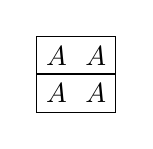
\begin{tikzpicture}[baseline=(O)]
			\matrix (M) [matrix of nodes] {
				$A$ & $A$ \\
				$A$ & $A$ \\
			};
			\coordinate (O) at (M-1-1.south west);
			\draw (M-1-1.north west) rectangle (M-1-2.south east);
			\draw (M-2-1.north west) rectangle (M-2-2.south east);
		\end{tikzpicture} = 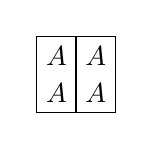
\begin{tikzpicture}[baseline=(O)]
			\matrix (M) [matrix of nodes] {
				$A$ & $A$ \\
				$A$ & $A$ \\
			};
			\coordinate (O) at (M-1-1.south west);
			\draw (M-1-1.north west) rectangle (M-2-1.south east);
			\draw (M-1-2.north west) rectangle (M-2-2.south east);
		\end{tikzpicture} \quad \begin{tabular}{rl}
			Horizontal: & kalikan dengan $\mu'$ \\
			Vertikal: & kalikan dengan $\mu_A$
		\end{tabular}\end{center}
		Sekarang argumen untuk $\mu'=\mu_A$ dapat digambarkan sebagai
		% segment-id: o014.li2.chapter7.exercises-a.g002
		\begin{center}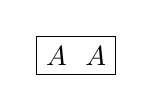
\begin{tikzpicture}[baseline=(O)]
			\matrix (M) [matrix of nodes] {
				$A$ & $A$ \\
			};
			\coordinate (O) at (M-1-1.south west);
			\draw (M-1-1.north west) rectangle (M-1-2.south east);
		\end{tikzpicture}
		$=$ 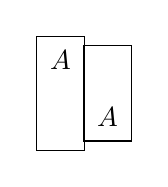
\begin{tikzpicture}[baseline=(O)]
			\matrix (M) [matrix of nodes, every node/.style={anchor=base, minimum width=1.7em, minimum height=1.7em}] {
				$A$ & $\munit$ \\
				$\munit$ & $A$ \\
			};
			\coordinate (O) at (M-1-1.south west);
			\draw (M-1-1.north west) rectangle (M-2-1.south east);
			\draw (M-1-2.north west) rectangle (M-2-2.south east);
		\end{tikzpicture}
		$=$ 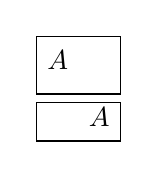
\begin{tikzpicture}[baseline=(O)]
			\matrix (M) [matrix of nodes, every node/.style={anchor=base, minimum width=1.5em, minimum height=1.7em}] {
				$A$ & $\munit$ \\
				$\munit$ & $A$ \\
			};
			\coordinate (O) at (M-1-1.south west);
			\draw (M-1-1.north west) rectangle (M-1-2.south east);
			\draw (M-2-1.north west) rectangle (M-2-2.south east);
		\end{tikzpicture}
		$=$ 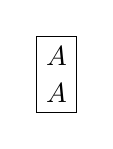
\begin{tikzpicture}[baseline=(O)]
			\matrix (M) [matrix of nodes] {
				$A$ \\
				$A$ \\
			};
			\coordinate (O) at (M-1-1.south west);
			\draw (M-1-1.north west) rectangle (M-2-1.south east);
		\end{tikzpicture}\end{center}
		Cobalah juga menerjemahkannya menjadi diagram komutatif atau persamaan
		yang bersesuaian.
	\end{hint}

	% segment-id: o014.li2.chapter7.exercises-a.ex003
	\item Tinjau aljabar-dg $A$ di atas $\mathcal{A}$
	(Definisi~\ref{def:dg-algebra}). Periksa bahwa bila $A=\munit$ (objek
	satuan), konsep modul-$A$ kiri maupun modul-$A$ kanan sama dengan konsep
	kompleks di atas $\mathcal{A}$.

	% segment-id: o014.li2.chapter7.exercises-a.ex004
	\item Tetapkan gelanggang komutatif $\Bbbk$. Misalkan $A$ aljabar-dg di
	atas $\Bbbk\dcate{Mod}$ dan $M$ kompleks. Buktikan bahwa memberikan
	struktur modul-$A$ kiri pada $M$ sama artinya dengan memberikan
	homomorfisme aljabar-dg
	$A\to\End^\bullet(M):=\Hom^\bullet(M,M)$.

	% segment-id: o014.li2.chapter7.exercises-a.ex005
	\item Misalkan $\Bbbk$ gelanggang komutatif dan $R$ aljabar-dg di atas
	$\Bbbk\dcate{Mod}$. Untuk modul-$R$ kanan $X$ dan modul-$R$ kiri $Y$,
	kita masing-masing mengidentifikasi $R$ dan $X,Y$ dengan aljabar-$\Bbbk$
	dan modul-$\Bbbk$ yang dilengkapi dekomposisi jumlah langsung
	% segment-id: o014.li2.chapter7.exercises-a.q002
	\[ R = \bigoplus_n R^n, \quad X = \bigoplus_n X^n, \quad Y = \bigoplus_n Y^n \]
	serta endomorfisme berderajat $1$, $d$, yang memenuhi $d^2=0$. Karena itu,
	$X\dotimes{R}Y$ sudah terdefinisi sebagai modul-$\Bbbk$.
	\begin{enumerate}[(i)]
		\item Ingat bahwa
		$X\otimes Y=\bigoplus_n(\bigoplus_{p+q=n}X^p\otimes Y^q)$ sekaligus
		merupakan modul-$\Bbbk$ dan mempunyai struktur kompleks. Untuk
		homomorfisme modul-$\Bbbk$ yang jelas
		$\pi:X\otimes Y\twoheadrightarrow X\dotimes{R}Y$, periksa bahwa
		$\Ker(\pi)$ adalah subkompleks, sehingga $X\dotimes{R}Y$ mempunyai
		struktur kompleks kanonik.

		\item Buktikan bahwa jika $X$ bimodul-$(A,R)$ dan $Y$ bimodul-$(R,B)$,
		dengan $A$ dan $B$ juga aljabar-dg, maka $X\dotimes{R}Y$ secara alami
		menjadi bimodul-$(A,B)$. Gunakan hal ini untuk memperluas adjoin dalam
		Proposisi~\ref{prop:tensor-Hom-cplx} ke kasus modul-dg. Kompleks
		$\Hom^\bullet(Y_B,Z_B)$ dan $\Hom^\bullet({}_AX,{}_AZ)$ yang muncul di
		sini didefinisikan seperti dalam Contoh~\ref{eg:dg-Hom-cplx}, tetapi
		tanda-tanda perlu diperhatikan ketika memberikan struktur bimodul-
		$(A,R)$ dan bimodul-$(R,B)$.
	\end{enumerate}

	% segment-id: o014.li2.chapter7.exercises-a.ex006
	\item Tetapkan aljabar-dg $A$ di atas $\mathcal{A}$. Jika
	$p>0\implies A^p=0$, maka $A$ disebut \emph{nonpositif}. Untuk modul-$A$
	kiri (atau kanan) $M$ dan $n\in\Z$, ambil subkompleks terpotong
	$\tau^{\leq n}M$ menurut Definisi~\ref{def:truncation-cplx}. Buktikan
	bahwa bila $A$ nonpositif:
	\begin{enumerate}[(i)]
		\item setiap $d_M^p:M^p\to M^{p+1}$ bersifat $A^0$-linear;
		\item terdapat barisan eksak pendek modul-$A$
		$0\to\tau^{\leq n}M\to M\to\tilde\tau^{\geq n+1}M\to0$.
	\end{enumerate}
	\index{aljabar dg!tak-positif@tak-positif (non-positive)}

	% segment-id: o014.li2.chapter7.exercises-a.ex007
	\item Tetapkan aljabar-dg $A$ di atas $\mathcal{A}$. Ingat bahwa semua
	modul-$A$ kiri membentuk kategori-dg $A\dcate{dgMod}$
	(Contoh~\ref{eg:dg-Hom-cplx}); Catatan~\ref{rem:dg-homotopy-cat} kemudian
	memberikan kategori homotopi $\mathrm{h}(A\dcate{dgMod})$. Modul-$A$ kiri
	$M$ disebut asiklik bila ia asiklik sebagai kompleks; morfisme modul-$A$
	$f:M\to N$ disebut kuasi-isomorfisme bila ia kuasi-isomorfisme sebagai
	morfisme kompleks.
	\begin{enumerate}[(i)]
		\item Misalkan $M$ modul-$A$ kiri yang strukturnya ditentukan oleh
		keluarga morfisme dalam $\mathcal{A}$,
		$\alpha_{A,M}^{p,q}:A^p\otimes M^q\to M^{p+q}$ ($p,q\in\Z$).
		Tunjukkan bahwa rumus berikut memberikan struktur modul-$A$ kiri pada
		kompleks $M[1]$:
		% segment-id: o014.li2.chapter7.exercises-a.q003
		\[ \alpha_{A, M[1]}^{p, q} := (-1)^p \alpha_{A, M}^{p, q+1} . \]
		Selanjutnya, tunjukkan bahwa $M\mapsto M[1]$ memberikan funktor-dg dari
		$A\dcate{dgMod}$ ke dirinya sendiri.
		\item Untuk sembarang morfisme $f:M\to N$ dalam $A\dcate{dgMod}$,
		tunjukkan bahwa kerucut pemetaan $\Cone(f)$ memiliki struktur modul-$A$
		kiri kanonik, yang dalam notasi di atas diberikan oleh
		% segment-id: o014.li2.chapter7.exercises-a.q004
		\[ \alpha_{A, \Cone(f)}^{p, q} = \alpha_{A, M[1]}^{p, q} \oplus \alpha_{A, N}^{p, q}. \]
		\item Mengikuti konstruksi dalam \S\ref{sec:derived-cat}, gunakan kerucut
		pemetaan untuk membuat $\mathrm{h}(A\dcate{dgMod})$ menjadi kategori
		triangulasi. Selanjutnya, lakukan pelokalan Verdier pada modul-$A$
		asiklik, atau, dengan kata lain, tambahkan invers kuasi-isomorfisme,
		untuk memperoleh kategori turunan $\cate{D}(A\dcate{dgMod})$.
		Definisikan $\cate{D}^{\star}(A\dcate{dgMod})$ yang bersesuaian untuk
		$\star\in\{+,-,\bdd\}$.
		\item Dengan asumsi $A$ nonpositif, perluas
		Proposisi~\ref{prop:derived-full-faithful-subcat} ke
		$\cate{D}(A\dcate{dgMod})$ dan
		$\cate{D}^{\star}(A\dcate{dgMod})$, untuk
		$\star\in\{+,-,\bdd\}$.
		% segment-id: o014.li2.chapter7.exercises-a.hi002
		\begin{hint}
			Gunakan funktor pemotongan.
		\end{hint}
		\item Dengan mengacu pada \S\ref{sec:K-injectives}, definisikan
		modul-$A$ K-injektif dan K-projektif, lalu gunakan objek-objek ini untuk
		mendeskripsikan morfisme dalam $\cate{D}(A\dcate{dgMod})$. Tempatkan
		semuanya dalam kerangka \S\ref{sec:triangulated-functor-localization}
		untuk membahas hubungannya dengan funktor turunan.
		\item Untuk modul-$A$ kanan $M$, tunjukkan bahwa kompleks $M[1]$
		mempunyai struktur modul-$A$ kanan
		$\alpha_{M[1],A}^{p,q}=\alpha_{M,A}^{p,q+1}$ dan bahwa semua sifat di
		atas tetap berlaku.
	\end{enumerate}

	% segment-id: o014.li2.chapter7.exercises-a.ex008
	\item Misalkan $\mathcal{C}$ kategori-dg di atas $\Bbbk$. Definisikan
	$\mathcal{C}^{\opp}$ melalui
	$\Obj(\mathcal{C}^{\opp})=\Obj(\mathcal{C})$ dan, untuk sembarang
	$X,Y\in\Obj(\mathcal{C}^{\opp})$,
	$\Hom^\bullet_{\mathcal{C}^{\opp}}(X,Y):=
	\Hom^\bullet_{\mathcal{C}}(Y,X)$. Definisikan komposisinya sebagai
	% segment-id: o014.li2.chapter7.exercises-a.q005
	\begin{align*}
		\Hom^p_{\mathcal{C}^{\opp}}(Y, Z) \dotimes{\Bbbk} \Hom^q_{\mathcal{C}^{\opp}}(X, Y) & \to \Hom^{p+q}_{\mathcal{C}^{\opp}}(X, Z) \quad p, q \in \Z \\
		f \otimes g & \mapsto (-1)^{pq} \underbracket{f \circ g}_{\text{operasi dalam }\Hom^\bullet_{\mathcal{C}}}.
	\end{align*}
	Periksa bahwa ini memang memberikan kategori-dg $\mathcal{C}^{\opp}$,
	yang disebut kategori-dg lawan dari $\mathcal{C}$.

	% segment-id: o014.li2.chapter7.exercises-a.ex009
	\item Tetapkan gelanggang komutatif $\Bbbk$, aljabar-dg $R$ di atas
	$\Bbbk\dcate{Mod}$, modul-$R$ kanan $X$, dan modul-$R$ kiri $Y$. Buktikan
	bahwa funktor yang diperkenalkan sebelumnya,
	% segment-id: o014.li2.chapter7.exercises-a.q006
	\[ X \dotimes{R} (\cdot): R\dcate{dgMod} \to \cate{C}(\Bbbk), \quad (\cdot) \dotimes{R} Y: \cated{dgMod}R \to \cate{C}(\Bbbk), \]
	secara alami diangkat menjadi funktor-dg. Rumuskan garis besar hasil yang bersesuaian
	ketika $X$ atau $Y$ juga mempunyai struktur bimodul.

	% segment-id: o014.li2.chapter7.exercises-a.hi003
	\begin{hint}
		Kuncinya ialah mendefinisikan morfisme antarkompleks $\Hom$. Untuk
		$X\dotimes{R}(\mathord\cdot)$, misalkan $M$ dan $N$ modul-$R$ kiri.
		Aturan tanda Koszul mensyaratkan citra
		$f\in\Hom^n_R(M,N)$, yaitu
		$\identity_X\otimes f\in
		\Hom^n(X\dotimes{R}M,X\dotimes{R}N)$, didefinisikan oleh
		% segment-id: o014.li2.chapter7.exercises-a.q007
		\[ (\identity_X \otimes f)(x \otimes m) = (-1)^{pn} x \otimes f(m), \quad x \in X^p, \; m \in M^q. \]
		Perlu diperiksa bahwa
		$\identity_X\otimes d_{\Hom^\bullet}(f)=
		d_{\Hom^\bullet}(\identity_X\otimes f)$.

		Kasus $(\mathord\cdot)\dotimes{R}Y$ lebih sederhana: cukup ambil
		$(f\otimes\identity_Y)(m\otimes y)=f(m)\otimes y$.
	\end{hint}

	% segment-id: o014.li2.chapter7.exercises-a.ex010
	\item Misalkan $\mathcal{C}$ kategori-dg di atas gelanggang komutatif
	$\Bbbk$ dan $M\in\Obj(\mathcal{C})$.
	\begin{enumerate}[(i)]
		\item Angkat
		$\Hom^\bullet(M,\mathord\cdot):\mathcal{C}\to\cate{C}(\Bbbk)$ menjadi
		funktor-dg.

		% segment-id: o014.li2.chapter7.exercises-a.hi004
		\begin{hint}
			Misalkan $X,Y\in\Obj(\mathcal{C})$ dan
			$f\in\Hom^n(X,Y)$. Tetapkan
			$\mathcal{H}_X=\Hom^\bullet(M,X)$. Citra $f$ harus diambil sebagai
			% segment-id: o014.li2.chapter7.exercises-a.q008
			\[ \left[ f_*: g \xmapsto{\text{morfisme berderajat }n} fg \right] \in \Hom^n(\mathcal{H}_X, \mathcal{H}_Y). \]
			Gunakan definisi kompleks $\Hom$ untuk memeriksa bahwa
			$(d_{\Hom^\bullet(X,Y)}f)_*=
			d_{\Hom^\bullet(\mathcal{H}_X,\mathcal{H}_Y)}(f_*)$.
		\end{hint}
		\item Angkat
		$\Hom^\bullet(\mathord\cdot,M):\mathcal{C}\to
		\cate{C}(\Bbbk)^{\opp}$ menjadi funktor-dg.

		% segment-id: o014.li2.chapter7.exercises-a.hi005
		\begin{hint}
			Tetapkan $\mathcal{K}_X=\Hom^\bullet(X,M)$. Aturan tanda Koszul
			mensyaratkan citra $f\in\Hom^n(X,Y)$ diambil sebagai
			% segment-id: o014.li2.chapter7.exercises-a.q009
			\[ \left[\begin{array}{c}
				f^*: g \xmapsto{\text{morfisme berderajat }n} (-1)^{np} gf \\
				\forall p \in \Z , \; \forall\; g \in \Hom^p(Y, M)
			\end{array}\right] \in \Hom^n(\mathcal{K}_Y, \mathcal{K}_X). \]
			Periksa dengan cermat bahwa
			\begin{compactitem}
				\item $(d_{\Hom^\bullet(X,Y)}f)^*=
				d_{\Hom^\bullet(\mathcal{K}_Y,\mathcal{K}_X)}(f^*)$;
				\item $(fh)^*$ sama dengan komposisi $h^*$ dan $f^*$ dalam
				$\Hom^\bullet_{\cate{C}(\Bbbk)}$.
			\end{compactitem}
		\end{hint}
	\end{enumerate}

% Unit 104 terjemahan Bahasa Indonesia dari chapter7.tex baris 2828--2944.
% Sumber: Methods of Algebra, Volume 2, commit
% 9a5803ff77dd3257484cb177f851a73770a59dd3 (CC BY 4.0).
% stable-unit-id: o014.aljabr2.chapter7.exercises-b
% Cakupan: bagian tengah Latihan Bab 7, dari pengayaan diri kategori monoidal
% tertutup hingga keunikan struktur komodul pada hasil bagi dan submodul;
% dilanjutkan oleh Unit 105 pada baris 2945.

\hypertarget{o014.aljabr2.chapter7.exercises-b}{ }
	% segment-id: o014.aljabr2.chapter7.exercises-b.ex011
	\item Buktikan bahwa morfisme kanonik
	$[Y,Z]\otimes[X,Y]\to[X,Z]$ dan $\munit\to[X,X]$ yang didefinisikan bagi
	kategori monoidal tertutup dalam \S\ref{sec:closed-monoidal} memenuhi sifat
	asosiativitas dan unit. Dengan demikian, kategori monoidal tertutup diperkaya
	atas dirinya sendiri relatif terhadap $\Hom$ internal.
	% segment-id: o014.aljabr2.chapter7.exercises-b.hi006
	\begin{hint}
		Periksa secara langsung, atau lihat \cite[Bagian 1.6]{Kel05}.
	\end{hint}

	% segment-id: o014.aljabr2.chapter7.exercises-b.ex012
	\item Tinjau aljabar polinomial $\Bbbk[t]$ di atas gelanggang komutatif
	$\Bbbk$. Definisikan $\Delta$, $\epsilon$, dan $S$ masing-masing dengan
	% segment-id: o014.aljabr2.chapter7.exercises-b.q010
	\[ \Delta(t^n) = \sum_{k=0}^n \binom{n}{k} t^k \otimes t^{n-k}, \quad \epsilon(t^n) = \begin{cases}
		1, & n = 0 \\
		0, & n \neq 0
	\end{cases}, \quad
	S(t^n) = (-1)^n t^n, \]
	dengan $n\in\Z_{\geq0}$. Verifikasi bahwa data ini memberikan
	aljabar Hopf-$\Bbbk$ yang komutatif dan kokomutatif.

	% segment-id: o014.aljabr2.chapter7.exercises-b.ex013
	\item Misalkan $A$ aljabar Hopf di atas gelanggang komutatif. Ideal $I$ dari
	$A$ disebut \emph{ideal Hopf} jika
	$\Delta(I)\subset I\otimes A+A\otimes I$, $\epsilon(I)=0$, dan
	$S(I)\subset I$. Tunjukkan bahwa mengambil hasil bagi dengan ideal Hopf
	memberikan aljabar Hopf $A/I$.

	% segment-id: o014.aljabr2.chapter7.exercises-b.ex014
	\item Misalkan $\Bbbk$ gelanggang komutatif dan $V$ modul-$\Bbbk$. Pada
	aljabar tensor $T(V)$ (lihat \cite[Definisi 7.5.1]{Li1}) dapat didefinisikan
	homomorfisme aljabar-$\Bbbk$
	$\Delta:T(V)\to T(V)\otimes T(V)$ dan $\epsilon:T(V)\to\Bbbk$ sedemikian
	sehingga, untuk setiap $v\in V$,
	% segment-id: o014.aljabr2.chapter7.exercises-b.q011
	\begin{gather*}
		\Delta(v) = v \otimes 1 + 1 \otimes v, \quad \epsilon(v) = 0;
	\end{gather*}
	di sini struktur aljabar pada $T(V)\otimes T(V)$ diberikan oleh struktur
	anyaman trivial $x\otimes y\mapsto y\otimes x$.
	\begin{enumerate}[(i)]
		% segment-id: o014.aljabr2.chapter7.exercises-b.i001
		\item Verifikasi bahwa struktur ini membuat $T(V)$ menjadi bialjabar.
		% segment-id: o014.aljabr2.chapter7.exercises-b.i002
		\item Tunjukkan cara mendefinisikan automorfisme modul-$\Bbbk$
		$S:T(V)\to T(V)$ sedemikian sehingga $S(v)=-v$ dan $S$ merupakan
		antiautomorfisme bialjabar (Proposisi~\ref{prop:Hopf-antiautomorphism});
		secara lebih eksplisit,
		% segment-id: o014.aljabr2.chapter7.exercises-b.q012
		\[ S(v_1 \cdots v_n) = (-1)^n v_n \cdots v_1, \quad n \in \Z_{\geq 0}, \quad v_1, \ldots, v_n \in V. \]
		Verifikasi bahwa struktur ini membuat $T(V)$ menjadi aljabar Hopf.
		% segment-id: o014.aljabr2.chapter7.exercises-b.i003
		\item Tunjukkan bahwa aljabar simetris $\Sym(V)$ mempunyai sifat serupa;
		sebenarnya, aljabar tersebut merupakan hasil bagi $T(V)$ dengan suatu
		ideal Hopf.
		% segment-id: o014.aljabr2.chapter7.exercises-b.i004
		\item Kerjakan versi untuk aljabar eksterior $\bigwedge(V)$, tetapi
		struktur perkalian pada $\bigwedge(V)\otimes\bigwedge(V)$ harus
		didefinisikan menggunakan struktur anyaman Koszul
		\eqref{eqn:Koszul-braiding} (ambil $\epsilon(a)=a\bmod\;2$ di sana),
		sehingga untuk unsur-unsur homogen
		$x,y,z,w\in\bigwedge(V)$ berlaku
		$(x\otimes y)(z\otimes w)=(-1)^{\deg y\deg z}xz\otimes yw$. Hal ini
		memastikan bahwa $(1\otimes v+v\otimes1)^2$ sama dengan unsur nol dalam
		$\bigwedge(V)\otimes\bigwedge(V)$ untuk setiap $v\in V$.
	\end{enumerate}

	% segment-id: o014.aljabr2.chapter7.exercises-b.ex015
	\item (E.\ Taft) Misalkan $q$ akar satuan primitif ke-$n$ dalam medan
	$\Bbbk$, dengan $n\geq2$. Tinjau aljabar-$\Bbbk$ $H$ yang ditentukan oleh
	pembangkit $g$, $x$, dan relasi
	% segment-id: o014.aljabr2.chapter7.exercises-b.q013
	\[ g^n = 1, \quad x^n = 0, \quad gxg^{-1} = qx. \]
	Tunjukkan bahwa dapat didefinisikan
	$\Delta:H\to H\dotimes{\Bbbk}H$ dan $\epsilon:H\to\Bbbk$ yang memenuhi
	% segment-id: o014.aljabr2.chapter7.exercises-b.q014
	\begin{gather*}
		\Delta(g) = g \otimes g, \quad \Delta(x) = 1 \otimes x + x \otimes g, \\
		\epsilon(g) = 1, \quad \epsilon(x) = 0,
	\end{gather*}
	dan yang membuat $H$ menjadi aljabar Hopf-$\Bbbk$ dengan antipoda
	% segment-id: o014.aljabr2.chapter7.exercises-b.q015
	\[ S:H\to H, \quad S(g)=g^{-1}, \quad S(x)=-g^{-1}x. \]

	Tunjukkan bahwa $H$ tidak komutatif maupun kokomutatif. Jika $n=2$,
	aljabar Hopf yang bersesuaian juga disebut aljabar Hopf Sweedler.

	% segment-id: o014.aljabr2.chapter7.exercises-b.ex016
	\item Misalkan $(A,\Delta,\epsilon)$ koaljabar di atas gelanggang komutatif
	$\Bbbk$. Jika $x\in A$ memenuhi $\Delta(x)=1\otimes x+x\otimes1$, maka
	$x$ disebut \emph{primitif}.
	\begin{enumerate}[(i)]
		% segment-id: o014.aljabr2.chapter7.exercises-b.i005
		\item Buktikan bahwa $\epsilon(x)=0$ untuk setiap unsur primitif $x$.
		% segment-id: o014.aljabr2.chapter7.exercises-b.i006
		\item Misalkan $(A,\mu,\eta,\Delta,\epsilon)$ bialjabar dan tuliskan
		$\mu$ sebagai perkalian, yaitu $xy=\mu(x\otimes y)$. Buktikan bahwa jika
		$x,y\in A$ primitif, maka $xy-yx$ juga primitif.
		% segment-id: o014.aljabr2.chapter7.exercises-b.i007
		\item Masih dengan $A$ bialjabar, misalkan $x_1,\ldots,x_n\in A$
		unsur-unsur primitif dan tuliskan $V$ untuk modul-$\Bbbk$ bebas dengan
		basis $x_1,\ldots,x_n$. Dari sini diperoleh homomorfisme aljabar-$\Bbbk$
		$\phi:T(V)\to A$. Buktikan bahwa $\phi$ juga merupakan homomorfisme
		bialjabar.
	\end{enumerate}

	% segment-id: o014.aljabr2.chapter7.exercises-b.ex017
	\item Misalkan $(A,\Delta,\epsilon)$ koaljabar di atas gelanggang komutatif
	$\Bbbk$, dengan $A\neq\{0\}$ dan $A$ bebas torsi sebagai modul-$\Bbbk$.
	Unsur taknol $x\in A$ yang memenuhi $\Delta(x)=x\otimes x$ disebut
	\emph{serupa-grup}. Himpunan semua unsur serupa-grup dinotasikan dengan
	$\mathcal{G}(A)$.
	\begin{enumerate}[(i)]
		% segment-id: o014.aljabr2.chapter7.exercises-b.i008
		\item Buktikan bahwa $x\in\mathcal{G}(A)$ mengakibatkan
		$\epsilon(x)=1$.
		% segment-id: o014.aljabr2.chapter7.exercises-b.i009
		\item Buktikan bahwa jika $(A,\mu,\eta,\Delta,\epsilon)$ bialjabar, maka
		$\mathcal{G}(A)$ menjadi monoid di bawah perkalian $\mu$ pada $A$, dengan
		$1_A:=\eta(1)$ sebagai unsur unit.
		% segment-id: o014.aljabr2.chapter7.exercises-b.i010
		\item Untuk monoid $M$ dan bialjabar $\Bbbk[M]$ yang bersesuaian
		(Contoh~\ref{eg:monoid-bialgebra}), buktikan bahwa
		$\mathcal{G}(\Bbbk[M])=M$.
		% segment-id: o014.aljabr2.chapter7.exercises-b.i011
		\item Misalkan $A$ aljabar Hopf dengan antipoda $S$. Buktikan bahwa
		$\mathcal{G}(A)$ merupakan grup dan bahwa invers dari
		$x\in\mathcal{G}(A)$ adalah $S(x)$.
	\end{enumerate}

	% segment-id: o014.aljabr2.chapter7.exercises-b.ex018
	\item Misalkan $(A,\Delta,\epsilon)$ koaljabar taknol di atas medan
	$\Bbbk$. Buktikan bahwa $\mathcal{G}(A)$ merupakan subhimpunan bebas linear
	dari $A$.

	% segment-id: o014.aljabr2.chapter7.exercises-b.hi007
	\begin{hint}
		Andaikan tidak demikian dan pilih relasi linear taktrivial terpendek di
		antara unsur-unsur tersebut. Tanpa mengurangi keumuman, tuliskan
		$x_1=\sum_{i=2}^n a_i x_i$, dengan
		$x_1,\ldots,x_n\in\mathcal{G}(A)$ saling berbeda dan $a_i\in\Bbbk$.
		Maka $x_2,\ldots,x_n$ bebas linear, sedangkan
		$x_1\otimes x_1=\sum_{i=2}^n a_i x_i\otimes x_i$.
	\end{hint}

	% segment-id: o014.aljabr2.chapter7.exercises-b.ex019
	\item Tuliskan $\cate{TopCMon}$ untuk kategori monoid topologis komutatif,
	$\cate{Top}_\bullet$ untuk kategori ruang topologis bertitik, dan
	$U:\cate{TopCMon}\to\cate{Top}_\bullet$ untuk funktor pelupa (titik
	dasar bersesuaian dengan unsur unit). Bangun funktor adjoin kiri
	$\Sym:\cate{Top}_\bullet\to\cate{TopCMon}$ bagi $U$. Untuk ruang topologis
	bertitik $(X,x)$, objek $\Sym(X,x)$ juga disebut \emph{produk simetris
	takhingga} dari $(X,x)$; jelaskan istilah ini. Teorema Dold--Thom dalam
	topologi aljabar didasarkan pada konstruksi ini.

	% Reference: Deligne, Categories tannakiennes, 4.5 Proposition.
	% segment-id: o014.aljabr2.chapter7.exercises-b.ex020
	\item Misalkan bimodul-$(A,B)$ $P$ projektif dan dibangkitkan secara hingga
	sebagai modul-$B$ kanan, serta $(\mathord\cdot)\dotimes{A}P$ merupakan funktor eksak
	setia. Buktikan bahwa modul-$A$ kanan $N$ berpenyajian hingga
	(Contoh~\ref{eg:Mod-cpt}) jika dan hanya jika
	$N\dotimes{A}P$ berpenyajian hingga sebagai modul-$B$ kanan. Hasil ini
	melengkapi Proposisi~\ref{prop:Morita-comonad-ft}.

	% segment-id: o014.aljabr2.chapter7.exercises-b.ex021
	\item Tinjau gelanggang komutatif $\Bbbk$ dan homomorfisme aljabar-$\Bbbk$
	$f:A\to B$. Kita mempunyai pasangan adjoin
	% segment-id: o014.aljabr2.chapter7.exercises-b.q016
	\[\begin{tikzcd}
		\mathcal{F}_{B|A}: \cated{Mod}B \arrow[shift left, r] & \cated{Mod}A: \Hom_A(B, \cdot), \arrow[shift left, l]
	\end{tikzcd}\]
	dengan $\Hom_A(B,N)$ diberi struktur modul-$B$ kanan melalui
	$(\phi b)(x)=\phi(bx)$ untuk setiap modul-$A$ kanan $N$. Lebih tepatnya,
	\begin{compactitem}
		% segment-id: o014.aljabr2.chapter7.exercises-b.i012
		\item morfisme unit $M\to\Hom_A(B,M)$ memetakan $m$ ke
		$[b\mapsto mb]$;
		% segment-id: o014.aljabr2.chapter7.exercises-b.i013
		\item morfisme kounit $\Hom_A(B,N)\to N$ memetakan $\phi$ ke $\phi(1)$.
	\end{compactitem}
	Lihat \cite[Korolari 6.6.8]{Li1}. Sebagai pelengkap
	Contoh~\ref{eg:comonad-change-ring}, tentukan secara eksplisit monad dan
	komonad yang bersesuaian.

	% segment-id: o014.aljabr2.chapter7.exercises-b.ex022
	\item Misalkan $R$ gelanggang komutatif. Tuliskan $R\dcate{Alg}$ untuk
	kategori aljabar-$R$. Tinjau pasangan adjoin
	% segment-id: o014.aljabr2.chapter7.exercises-b.g001
	$\begin{tikzcd}
		T(\cdot): R\dcate{Mod} \arrow[shift left, r] & R\dcate{Alg}: U \arrow[shift left, l]
	\end{tikzcd}$,
	dengan $T(\mathord\cdot)$ adalah funktor aljabar tensor dan $U$ funktor
	pelupa.
	\begin{enumerate}[(i)]
		% segment-id: o014.aljabr2.chapter7.exercises-b.i014
		\item Buktikan secara langsung bahwa modul di bawah monad yang
		bersesuaian pada $R\dcate{Mod}$ adalah aljabar-$R$, sehingga pasangan
		adjoin tersebut monadik.
		% segment-id: o014.aljabr2.chapter7.exercises-b.i015
		\item Gantikan $T(\mathord\cdot)$ dengan $\Sym(\mathord\cdot)$ dan
		$\bigwedge(\mathord\cdot)$, lalu nyatakan dan buktikan hasil yang
		bersesuaian; lihat \cite[\S 7.6]{Li1}.
	\end{enumerate}

	% segment-id: o014.aljabr2.chapter7.exercises-b.ex023
	\item Lengkapi argumen dalam Proposisi~\ref{prop:Comod-abelian}, kemudian
	buktikan penguatan berikut. Misalkan $C$ koaljabar dalam
	$(B,B)\dcate{Mod}$. Buktikan bahwa:
	\begin{enumerate}[(i)]
		% segment-id: o014.aljabr2.chapter7.exercises-b.i016
		\item funktor pelupa $U:\cated{Comod}C\to\cated{Mod}B$ mempunyai adjoin
		kanan;

		% segment-id: o014.aljabr2.chapter7.exercises-b.hi008
		\begin{hint}
			Tuliskan $\Delta$ untuk komultiplikasi $C$ dan $\epsilon$ untuk
			kounitnya. Untuk modul-$B$ kanan $N$, jadikan
			$N\dotimes{B}C$ komodul-$C$ kanan melalui
			$\identity_N\otimes\Delta$. Untuk setiap komodul-$C$ kanan $M$,
			verifikasi bahwa
			% segment-id: o014.aljabr2.chapter7.exercises-b.q017
			\[\begin{tikzcd}[row sep=tiny]
				\Hom_{\cated{Mod}B}(M, N) \arrow[shift left, r] & \Hom_{\cated{Comod}C}\left(M, N \dotimes{B} C\right) \arrow[shift left, l] \\
				\varphi \arrow[mapsto, r] & (\varphi \otimes \identity_C) \rho \\
				(\identity_N \otimes \epsilon) \psi & \psi \arrow[mapsto, l]
			\end{tikzcd}\]
			saling invers, dengan $\rho:M\to M\dotimes{B}C$ menentukan struktur
			komodul pada $M$.
		\end{hint}
		% segment-id: o014.aljabr2.chapter7.exercises-b.i017
		\item funktor pelupa $U$ menciptakan semua $\varinjlim$ kecil; oleh
		karena itu, $\cated{Comod}C$ kokomplet;
		% segment-id: o014.aljabr2.chapter7.exercises-b.i018
		\item kategori $\cated{Comod}C$ mempunyai kogenerator
		(Definisi~\ref{def:generators});

		% segment-id: o014.aljabr2.chapter7.exercises-b.hi009
		\begin{hint}
			Ambil suatu kogenerator dari kategori Grothendieck $\cated{Mod}B$,
			kemudian ambil citranya di bawah funktor adjoin kanan bagi $U$.
		\end{hint}
		% segment-id: o014.aljabr2.chapter7.exercises-b.i019
		\item jika $\cated{Comod}C$ merupakan kategori abelian dan $U$ funktor
		eksak, maka $C$ datar sebagai modul-$B$ kiri.

		% segment-id: o014.aljabr2.chapter7.exercises-b.hi010
		\begin{hint}
			Misalkan $g:M\to N$ monomorfisme modul-$B$ kanan. Gunakan keeksakan
			$U$ dan fakta bahwa adjoin kanan mempertahankan kernel untuk
			menunjukkan bahwa
			$g\otimes\identity_C:M\dotimes{B}C\to N\dotimes{B}C$ tetap injektif.
		\end{hint}
	\end{enumerate}

	% segment-id: o014.aljabr2.chapter7.exercises-b.ex024
	\item Seperti dalam latihan sebelumnya, tetap misalkan $C$ koaljabar dalam
	$(B,B)\dcate{Mod}$ dan $M$ komodul-$C$ kanan. Buktikan bahwa jika suatu
	modul-$B$ hasil bagi $M''$ dari $M$ (atau suatu submodul-$B$ $M'$ dari
	$M$) memiliki struktur komodul yang membuat
	$M\twoheadrightarrow M''$ (atau $M'\hookrightarrow M$) menjadi
	homomorfisme komodul, maka struktur komodul tersebut unik. Untuk kasus
	submodul, diasumsikan pula bahwa $C$ datar sebagai modul-$B$ kiri.

% Unit 105 terjemahan Bahasa Indonesia dari chapter7.tex baris 2945--3002.
% Sumber: Methods of Algebra, Volume 2, commit
% 9a5803ff77dd3257484cb177f851a73770a59dd3 (CC BY 4.0).
% stable-unit-id: o014.aljabr2.chapter7.exercises-c
% Cakupan: latihan penutup Bab 7 tentang penurunan Galois, pemuntiran
% kohomologi nonabelian, dan bentuk kuadratik; menutup lingkungan Exercises.

\hypertarget{o014.aljabr2.chapter7.exercises-c}{ }
% segment-id: o014.aljabr2.chapter7.exercises-c.ex001
	\item Mengikuti penjelasan pada akhir \S\ref{sec:descent-Galois}, berikan
	bukti langsung Teorema Penurunan Galois~\ref{prop:Galois-descent} melalui
	langkah-langkah berikut. Gunakan notasi dari bagian tersebut: misalkan
	$M\in\Obj(\cate{Vect}^{\Gamma,\infty}(L))$, dan definisikan pemetaan
	kanonik $\iota_M$ melalui \eqref{eqn:Galois-descent-iotaM}.
	\begin{enumerate}[(i)]
% segment-id: o014.aljabr2.chapter7.exercises-c.i001
		\item Misalkan $M'$ adalah subruang $\Gamma$-invarian dari
		$L\dotimes{K}(M^\Gamma)$, yakni $\Gamma M'\subset M'$. Buktikan bahwa
		jika $M'\cap(1\otimes M^\Gamma)=\{0\}$, maka $M'=\{0\}$.

% segment-id: o014.aljabr2.chapter7.exercises-c.hi001
		\begin{hint}
			Pilih suatu basis $(y_i)_{i\in I}$ dari $M^\Gamma$. Jika
			$M'\neq\{0\}$, pilih suatu ekspresi taknol di dalamnya dengan jumlah
			suku sesedikit mungkin, $\sum_{i\in I}\ell_i\otimes y_i$ (dengan
			jumlah hingga). Setelah normalisasi yang sesuai, kita dapat
			mengandaikan bahwa ekspresi itu
			berbentuk
% segment-id: o014.aljabr2.chapter7.exercises-c.q001
			\[ m' = 1 \otimes y_{i_0} + \ell_1 \otimes y_{i_1} + \cdots, \quad \ell_1 \notin K. \]
			Ambil $\sigma\in\Gamma$ sehingga
			$\sigma(\ell_1)\neq\ell_1$, lalu tinjau $m'-\sigma(m')$ untuk
			memperoleh kontradiksi.
		\end{hint}

% segment-id: o014.aljabr2.chapter7.exercises-c.i002
		\item Buktikan bahwa
		$\iota_M:L\dotimes{K}(M^\Gamma)\to M$ injektif.
% segment-id: o014.aljabr2.chapter7.exercises-c.hi002
		\begin{hint}
			Tinjau $M':=\Ker(\iota_M)$.
		\end{hint}

% segment-id: o014.aljabr2.chapter7.exercises-c.i003
		\item Buktikan bahwa $\iota_M$ surjektif.

% segment-id: o014.aljabr2.chapter7.exercises-c.hi003
		\begin{hint}
			Tinjau suatu subperluasan Galois hingga $E|K$ dari $L|K$. Ambil
			$a_1,\ldots,a_n$ sebagai basis $E$ selaku ruang vektor atas $K$, dan pilih
			wakil $\identity=\sigma_1,\ldots,\sigma_n\in\Gamma$ bagi unsur-unsur
			$\Gal(E|K)$. Dari teori medan diketahui bahwa
			$(\sigma_i(a_j))_{1\leq i,j\leq n}$ merupakan matriks invertibel di
			atas $E$; tuliskan inversnya sebagai
			$(b_{ij})_{1\leq i,j\leq n}$. Untuk
			$m\in M^{\Gal(L|E)}$, turunkan
% segment-id: o014.aljabr2.chapter7.exercises-c.q002
			\[ m = \sum_{i=1}^n b_{i1} \sum_{j=1}^n \sigma_j(a_i m) \; \in \Image(\iota_M). \]
		\end{hint}

% segment-id: o014.aljabr2.chapter7.exercises-c.i004
		\item Gunakan hasil-hasil di atas untuk menunjukkan bahwa
		\eqref{eqn:Galois-descent-adjunction} merupakan adjungsi yang sekaligus
		merupakan ekuivalensi,
		sehingga diperoleh bukti langsung
		Teorema~\ref{prop:Galois-descent}.
	\end{enumerate}

% segment-id: o014.aljabr2.chapter7.exercises-c.ex002
	\item Misalkan $G$ grup dan $L|K$ perluasan Galois medan. Tuliskan kategori
	modul-$G$ dengan koefisien dalam medan $K$ (atau $L$) sebagai
	$G\dcate{Mod}$ (atau $G\dcate{Mod}_L$); lihat
	Definisi~\ref{def:G-mod}. Gunakan metode penurunan Galois dari
	\S\S\ref{sec:descent-Galois}---\ref{sec:Galois-H1} untuk mendeskripsikan
	$G\dcate{Mod}$ melalui objek-objek $G\dcate{Mod}_L$ yang dilengkapi aksi
	$\Gal(L|K)$ yang sesuai.

% segment-id: o014.aljabr2.chapter7.exercises-c.ex003
	\item Gunakan notasi \S\ref{sec:Galois-H1}. Misalkan
	$c\in Z^1(\Gamma,G(\mathbf{t}_{0,L}))$. Dari bukti
	Teorema~\ref{prop:Galois-H1}, ingat bahwa melalui penurunan Galois, $c$
	mendefinisikan ruang vektor-$K$ $W$ beserta data $\mathbf{t}$ di atasnya,
	dan juga $h:\mathbf{t}_{0,L}\rightiso\mathbf{t}_L$.
	\begin{enumerate}[(i)]
% segment-id: o014.aljabr2.chapter7.exercises-c.i005
		\item Tunjukkan bahwa $g\mapsto h^{-1}gh$ memberikan isomorfisme grup
		$\nu:G(\mathbf{t}_L)\rightiso G(\mathbf{t}_{0,L})$. Tunjukkan bahwa
% segment-id: o014.aljabr2.chapter7.exercises-c.q003
		$ f \xmapsto{\sigma \in \Gamma} c(\sigma)({}^\sigma f)c(\sigma)^{-1} $
		memberikan aksi $\Gamma$ baru pada $G(\mathbf{t}_{0,L})$. Tuliskan
		struktur ini sebagai ${}^cG(\mathbf{t}_{0,L})$, dan tunjukkan bahwa
		$\nu:G(\mathbf{t}_L)\rightiso{}^cG(\mathbf{t}_{0,L})$ bersifat
		$\Gamma$-ekuivarian.

% segment-id: o014.aljabr2.chapter7.exercises-c.i006
		\item Tunjukkan bahwa rumus berikut memberikan pemetaan yang
		terdefinisi dengan baik:
% segment-id: o014.aljabr2.chapter7.exercises-c.q004
		\begin{align*}
			Z^1(\Gamma, G(\mathbf{t}_L)) & \to Z^1(\Gamma, G(\mathbf{t}_{0, L})) \\
			\tilde{c} & \mapsto \left[\sigma \mapsto \nu(\tilde{c}(\sigma)) c(\sigma) \right].
		\end{align*}
		Pemetaan ini menginduksi bijeksi
		$\Hm^1(\Gamma,G(\mathbf{t}_L))\to
		\Hm^1(\Gamma,G(\mathbf{t}_{0,L}))$ yang memetakan titik pangkal ke
		$[c]$.
% segment-id: o014.aljabr2.chapter7.exercises-c.hi004
		\begin{hint}
			Bandingkan dengan konstruksi ``pemuntiran'' dalam latihan
			CHref{sec:group-coh}.
		\end{hint}

% segment-id: o014.aljabr2.chapter7.exercises-c.i007
		\item Tunjukkan bahwa, di bawah korespondensi dalam
		Teorema~\ref{prop:Galois-H1}, bijeksi ini bersesuaian dengan kesamaan
		$\mathscr{T}(\mathbf{t})=\mathscr{T}(\mathbf{t}_0)$.
	\end{enumerate}

% segment-id: o014.aljabr2.chapter7.exercises-c.ex004
	\item Misalkan $K$ medan dengan $\mathrm{char}(K)\neq2$. Suatu bentuk
	bilinear simetris takdegenerat $q:V\times V\to K$ pada ruang vektor-$K$
	berdimensi hingga $V$ selanjutnya disebut bentuk kuadratik takdegenerat.
	Dalam grup ortogonal $\mathrm{O}(q)=\mathrm{O}(V,q)$, tuliskan subgrup
	yang ditentukan oleh $\det=1$ sebagai
	$\SO(q)=\SO(V,q)$. Untuk setiap perluasan Galois $L|K$, terdapat bentuk
	kuadratik takdegenerat $(V_L,q_L)$ beserta grup-grup terkait;
	semuanya dilengkapi aksi mulus dari $\Gamma:=\Gal(L|K)$.
	\begin{enumerate}[(i)]
% segment-id: o014.aljabr2.chapter7.exercises-c.i008
		\item Tuliskan $\mu_2:=\{\pm1\}\subset K^\times$. Tunjukkan bahwa
		$\mathrm{O}(q)/\SO(q)\simeq\mu_2$. Untuk hasil bagi
		$\mathrm{O}(q_L)/\SO(q_L)$, jelaskan hubungan isomorfisme ini
		dan aksi $\Gamma$.

% segment-id: o014.aljabr2.chapter7.exercises-c.i009
		\item Dengan menggunakan perangkat \S\ref{sec:Galois-H1}, tunjukkan
		bahwa unsur-unsur $\Hm^1(\Gamma,\mathrm{O}(q_L))$ berkorespondensi
		bijektif dengan kelas isomorfisme bentuk kuadratik takdegenerat
		$(V',q')$ di atas $K$ yang memenuhi $\dim V'=\dim V$, dengan titik
		pangkal bersesuaian dengan $(V,q)$.

% segment-id: o014.aljabr2.chapter7.exercises-c.i010
		\item Terapkan Teorema~\ref{prop:nonabelian-long} untuk memperoleh
		barisan eksak himpunan bertitik
% segment-id: o014.aljabr2.chapter7.exercises-c.q005
		\[ \mathrm{O}(q) \xrightarrow{\det} \mu_2 \to \Hm^1(\Gamma, \SO(q_L)) \xrightarrow{\varphi} \Hm^1(\Gamma, \mathrm{O}(q_L)) \xrightarrow{\psi} \Hm^1(\Gamma, \mu_2). \]
		Cobalah tunjukkan bahwa $\varphi$ injektif.
% segment-id: o014.aljabr2.chapter7.exercises-c.hi005
		\begin{hint}
			Surjektivitas $\det$ hanya menunjukkan bahwa
			$\varphi^{-1}(\text{titik pangkal})=\{\text{titik pangkal}\}$.
			Untuk menunjukkan injektivitas, kita harus memvariasikan $(V,q)$ dan
			menerapkan teknik pemuntiran dari latihan sebelumnya.
		\end{hint}

% segment-id: o014.aljabr2.chapter7.exercises-c.i011
		\item Tunjukkan bahwa
		$\Hm^1(\Gamma,\mu_2)\simeq K^\times/K^{\times,2}$. Tunjukkan pula bahwa
		$\psi$ sama dengan pemetaan
% segment-id: o014.aljabr2.chapter7.exercises-c.q006
		\[ \left[ (V', q'):\; \text{bentuk kuadratik takdegenerat} \right] \mapsto \mathrm{disc}(q') / \mathrm{disc}(q), \]
		Di sini, pilih sebarang basis $V'$, identifikasi $q'$ dengan
		suatu matriks simetris, lalu definisikan
% segment-id: o014.aljabr2.chapter7.exercises-c.q007
		\[ \mathrm{disc}(q') := (-1)^n \det(q') \bmod K^{\times 2}, \quad \dim V = 2n \;\text{atau}\; 2n+1. \]

% segment-id: o014.aljabr2.chapter7.exercises-c.i012
		\item Tunjukkan bahwa unsur-unsur
		$\Hm^1(\Gamma,\SO(q_L))$ berkorespondensi bijektif dengan kelas
		isomorfisme bentuk kuadratik takdegenerat $(V',q')$ di atas $K$ yang
		memenuhi $\dim V'=\dim V$ dan
		$\mathrm{disc}(q')=\mathrm{disc}(q)$, dengan titik pangkal
		bersesuaian dengan $(V,q)$.
	\end{enumerate}
% segment-id: o014.aljabr2.chapter7.exercises-c.c001
\end{Exercises}

% Unit 106 terjemahan Bahasa Indonesia dari chapter8.tex baris 1--174.
% Sumber: Methods of Algebra, Volume 2, commit
% 9a5803ff77dd3257484cb177f851a73770a59dd3 (CC BY 4.0).
% stable-unit-id: o014.aljabr2.chapter8.simplicial-objects
% Cakupan: pembukaan Bab 8 dan Bagian 8.1 lengkap;
% berhenti tepat sebelum Bagian 8.2 pada baris 175.

% Sumber asli: Copyright 2024 李文威 (Wen-Wei Li), CC BY 4.0.

% segment-id: o014.li2.chapter8.simplicial-objects.h001
\chapter{Metode Simplisial}\label{sec:simplicial}
\hypertarget{o014.aljabr2.chapter8.simplicial-objects}{ }
% segment-id: o014.li2.chapter8.simplicial-objects.p001
Misalkan $\simpDelta$ kategori ordinal hingga tak kosong. Menurut definisi,
objek simplisial dalam kategori $\mathcal{C}$ adalah funktor
$X:\simpDelta^{\opp}\to\mathcal{C}$. Secara ekuivalen, objek ini dapat
dideskripsikan sebagai deretan objek $X_0,X_1,\ldots$ beserta morfisme
$d_i:X_n\to X_{n-1}$ (muka) dan $s_j:X_n\to X_{n+1}$ (degenerasi), untuk
$0\leq i,j\leq n$, yang memenuhi keluarga identitas
\eqref{eqn:simplicial-identity}. Funktor-funktor tersebut membentuk kategori
$\cate{s}\mathcal{C}$. Dalam kasus khusus $\mathcal{C}=\cate{Set}$,
objek-objek ini juga disebut himpunan simplisial. Teori dasarnya dibahas
dalam \S\S\ref{sec:simplicial-method}--\ref{sec:simplicial-set}. Tuliskan
$\cate{FinOrd}$ untuk kategori ordinal hingga. Jika objek simplisial $X$,
sebagai funktor, meluas menjadi funktor $\cate{FinOrd}\to\mathcal{C}$, maka
$X$ disebut objek simplisial teraugmentasi. Hal ini sama artinya dengan
menambahkan suku berderajat $-1$, $X_{-1}$, pada data
$(X_n,d_i,s_j)_{n,i,j}$.

% segment-id: o014.li2.chapter8.simplicial-objects.p002
Himpunan simplisial berasal dari topologi. Gagasan dasarnya ialah menguraikan
ruang sebagai hasil penempelan simpleks; gambaran intuitif simpleks (titik, ruas garis,
segitiga, tetrahedron, dan seterusnya) adalah
% segment-id: o014.li2.chapter8.simplicial-objects.g001
\begin{center}\begin{tabular}{ccccc}
	$0$ dimensi & $1$ dimensi & $2$ dimensi & $3$ dimensi & $\cdots$ \\
	
\begin{tikzpicture}[baseline=(P)] \fill[black] (0.5, 0.5) circle[radius=0.07]; \coordinate (P) at (0, 0.5); \end{tikzpicture} &
	
\begin{tikzpicture}[baseline=(P)] \draw[thick] (0,0) -- (1,1); \coordinate (P) at (0.5, 0.5); \end{tikzpicture} &
	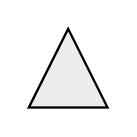
\begin{tikzpicture}[baseline=(P)] \filldraw[thick, fill=gray!15] (0,1) -- (-0.5, 0) -- (0.5, 0) --cycle; \coordinate (P) at (0, 0.5); \end{tikzpicture} &
	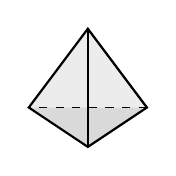
\begin{tikzpicture}[baseline=(P)]
		\fill[color=gray!15] (0, 1) -- (0.75, 0) -- (0, -0.5) -- (-0.75, 0) --cycle;
		\fill[color=gray!30] (0.75, 0) -- (0, -0.5) -- (-0.75, 0) --cycle;
		\draw[dashed] (0.75, 0) -- (-0.75, 0);
		\draw[thick] (0, 1) -- (0.75, 0) -- (0, -0.5) -- (-0.75, 0) --cycle;
		\draw[thick] (0, 1) -- (0, -0.5);
		\coordinate (P) at (0, 0.3);
	\end{tikzpicture} &
	$\cdots$
\end{tabular}\end{center}
Penguraian tersebut memberikan cara konkret dan kombinatorial untuk memahami
homologi, homotopi, dan persoalan lain mengenai ruang. Rumusan ketat yang
digunakan di sini diperkenalkan oleh S.\ Eilenberg dan J.\ A.\ Zilber pada
1950. Bahasa himpunan simplisial memiliki jangkauan luas dan tidak terbatas
pada persoalan topologi klasik. Sebagai contoh, bahasa ini dapat
mendeskripsikan kategori melalui konstruksi yang disebut ``saraf'', yang
diperkenalkan dalam \S\ref{sec:nerves}. Teori kategori membahas objek dalam
diagram (ditampilkan sebagai titik berdimensi nol), morfisme (ditampilkan
sebagai anak panah berdimensi satu), dan komutativitas (yang berkaitan dengan
komponen berdimensi dua seperti segitiga atau persegi). Jadi, tidak
mengherankan bahwa kategori dan ruang dapat dipadukan dalam struktur
matematis yang sama.

% segment-id: o014.li2.chapter8.simplicial-objects.p003
Setelah saraf dan ruang klasifikasi diperkenalkan sebagai contoh dasar
himpunan simplisial, \S\ref{sec:geom-realization} kembali pada intuisi dan
mendefinisikan realisasi geometris $|X|$ dari himpunan simplisial $X$.
Teorema~\ref{prop:geom-Sing-adjunction} menunjukkan bahwa realisasi geometris
bersama funktor himpunan singular $\mathrm{Sing}$ yang dikenal dalam topologi
membentuk pasangan adjoin
% segment-id: o014.li2.chapter8.simplicial-objects.q001
\[\begin{tikzcd}
	{|\cdot|}: \cate{sSet} \arrow[shift left, r] & \cate{Top} : \mathrm{Sing}. \arrow[shift left, l]
\end{tikzcd}\]
Jika $\cate{Top}$ diganti dengan kategori ruang Hausdorff yang dibangkitkan
secara kompak, $\cate{CGHaus}$, yang lazim dalam teori homotopi, realisasi
geometris juga memenuhi $|X\times Y|\simeq|X|\times|Y|$. Produk pada ruas
kiri dibentuk suku demi suku dari kedua himpunan simplisial. Buktinya berkaitan
dengan triangulasi produk dan melibatkan beberapa rincian kombinatorial yang
tidak sepele; karena buku ini bukan buku teks topologi, rincian tersebut tidak
dibahas lebih jauh.

% segment-id: o014.li2.chapter8.simplicial-objects.p004
Untuk tema buku ini, yang lebih penting ialah objek simplisial dalam kategori
abelian $\mathcal{A}$. Dalam keadaan ini, $\cate{s}\mathcal{A}$ juga kategori
abelian; sebagai contoh, grup abelian simplisial membentuk kategori abelian
$\cate{sAb}$. Hasil dasarnya adalah korespondensi Dold--Kan dalam
\S\ref{sec:Dold-Kan} (Teorema~\ref{prop:Dold-Kan}), yang untuk kategori abelian
$\mathcal{A}$ memberikan pasangan ekuivalensi adjoin
% segment-id: o014.li2.chapter8.simplicial-objects.q002
\[\begin{tikzcd}
	\Gamma: \cate{s}\mathcal{A} \arrow[shift left, r] & \cate{Ch}_{\geq 0}(\mathcal{A}): \mathrm{N}, \arrow[shift left, l]
\end{tikzcd}\]
dengan $\cate{Ch}_{\geq0}(\mathcal{A})$ menyatakan kategori abelian kompleks rantai
berderajat nonnegatif di atas $\mathcal{A}$. Funktor $\mathrm{N}$ memetakan
objek simplisial $X$ ke kompleks rantai ternormalisasi $\mathrm{N}X$ yang
bersesuaian. Lebih tepatnya, definisikan kompleks rantai tak ternormalisasi
dari $X\in\Obj(\cate{s}\mathcal{A})$ sebagai
% segment-id: o014.li2.chapter8.simplicial-objects.q003
\[ \mathrm{C}X := \left( X_n, \partial_n\right)_{n \geq 0}, \quad \partial_n := \sum_{i=0}^n (-1)^i d_i : X_n \to X_{n-1}. \]
Maka $\mathrm{N}X$ dapat diambil sebagai subkompleks rantai dari
$\mathrm{C}X$ melalui
$(\mathrm{N}X)_n:=\bigcap_{i=1}^n\Ker(d_i)$, atau dipandang sebagai hasil
bagi $\mathrm{C}X$ oleh bagian degenerat. Isomorfisme antara kedua bentuk ini
adalah isi Proposisi~\ref{prop:Dold-Kan-v}. Bahkan,
Teorema~\ref{prop:Dold-Kan-N-C} menunjukkan bahwa morfisme inklusi
$u:\mathrm{N}X\to\mathrm{C}X$ adalah kuasi-isomorfisme antarkompleks rantai.

% segment-id: o014.li2.chapter8.simplicial-objects.p005
Korespondensi Dold--Kan menjadikan teori simplisial salah satu sumber
aljabar homologis, bukan hanya secara historis, melainkan juga secara konseptual
dan teknis. Metode simplisial dapat menjelaskan dan memperkaya operasi
dasar pada kompleks atau kompleks rantai; misalnya, homotopi dan
kontraktibilitas mempunyai versi simplisial sehingga memperoleh
interpretasi topologis. Hal ini dibahas dalam
\S\ref{sec:homology-computation}.

% segment-id: o014.li2.chapter8.simplicial-objects.p006
Penerapan lain menghubungkannya dengan teori monad dari \S\ref{sec:Beck}.
Dengan cara ini, objek suatu kategori dapat diperluas secara kanonik menjadi objek simplisial
teraugmentasi atau objek kosimplisial teraugmentasi. Karena berkaitan dengan
operasi ``menambahkan bar'' dalam homologi Hochschild, teknik-teknik tersebut
secara kolektif disebut konstruksi bar dan menjadi tema
\S\ref{sec:bar-resolution}. Melalui korespondensi Dold--Kan dan beberapa
pengamatan tentang sifat dapat dikontraksi, konstruksi bar menjelaskan
berbagai resolusi standar dalam teori Hochschild (lihat \S\ref{sec:HH}) dan
teori kohomologi grup (lihat \S\ref{sec:G-mod}); semuanya ternyata berasal
dari satu gagasan pada aras yang lebih tinggi. Latihan memuat perluasan lain tentang
konstruksi bar.

% segment-id: o014.li2.chapter8.simplicial-objects.p007
Menurut definisi, objek bisimplisial yang dibahas dalam
\S\ref{sec:bisimplicial} tidak lain adalah funktor
$\simpDelta^{\opp}\times\simpDelta^{\opp}\to\mathcal{C}$; semuanya membentuk
kategori $\cate{s}^2\mathcal{C}$. Bila $\mathcal{A}$ kategori abelian, Teorema
Eilenberg--Zilber~\ref{prop:Eilenberg-Zilber}, yang langsung berkaitan dengan
$\cate{s}^2\mathcal{A}$, merupakan konstruksi dasar dalam topologi aljabar.
Dari sudut pandang teori kategori murni, bila $\mathcal{A}$ kategori monoidal
(misalnya $\mathcal{A}=\cate{Ab}$), teorema itu memberikan dua struktur monoidal
kanonik, dengan arah yang berlawanan, pada funktor
$\mathrm{N}:\cate{s}\mathcal{A}\to\cate{Ch}_{\geq0}(\mathcal{A})$. Namun,
penerapan objek bisimplisial tidak terbatas pada hal ini.

% segment-id: o014.li2.chapter8.simplicial-objects.p008
Dua bagian terakhir bab ini, \S\ref{sec:closed-simplicial} dan
\S\ref{sec:mapping-cone-revisited}, masing-masing membahas objek $\Hom$ dan
kerucut pemetaan bagi himpunan simplisial. Di satu sisi, keduanya
bersesuaian dengan ruang pemetaan dan kerucut menurut intuisi topologis. Di sisi
lain, pada kasus grup abelian, melalui korespondensi Dold--Kan, keduanya
memberikan kompleks rantai $\Hom$ dan kerucut pemetaan yang dikenal. Jadi,
konstruksi terkait pada kompleks atau kompleks rantai memperoleh penjelasan
yang jernih, sedangkan bagi topolog semua ini sudah sangat akrab.

% segment-id: o014.li2.chapter8.simplicial-objects.n001
\begin{wenxintishi}
	Bagian \S\S\ref{sec:simplicial-method}--\ref{sec:geom-realization}
	membentuk tulang punggung metode simplisial dalam bab ini;
	\S\S\ref{sec:Dold-Kan}--\ref{sec:bar-resolution} berhubungan langsung
	dengan kompleks rantai; dan walaupun
	\S\S\ref{sec:bisimplicial}--\ref{sec:mapping-cone-revisited} selaras dengan
	isi buku sebelumnya, bagian-bagian ini lebih bersifat lanjutan. Dibandingkan
	bab-bab lain, metode simplisial tidak diperlukan secara logis. Namun,
	gagasan dan tekniknya termasuk bekal dasar bagi matematikawan dan menjadi
	landasan untuk memasuki aljabar tingkat lanjut. Sebagian argumen tentang
	objek simplisial kadang-kadang melibatkan pemeriksaan rutin yang panjang
	(seperti dalam \S\ref{sec:Dold-Kan}); hal ini merupakan konsekuensi
	definisinya, dan pembaca dapat menentukan sendiri seberapa jauh hendak
	menelusurinya.
\end{wenxintishi}

% segment-id: o014.li2.chapter8.simplicial-objects.h002
\section{Objek Simplisial}\label{sec:simplicial-method}
% segment-id: o014.li2.chapter8.simplicial-objects.p009
Dalam Catatan~\ref{rem:walking-algebra}, kita mengingat kembali pemetaan
monoton antara himpunan terurut parsial dan menggunakannya untuk mendefinisikan
kategori ordinal hingga $\cate{FinOrd}$. Bab ini berfokus pada subkategori
penuh $\simpDelta$ yang terdiri atas ordinal tak kosong.

% segment-id: o014.li2.chapter8.simplicial-objects.d001
\begin{definition}
	\index[sym1]{Delta-simp@$\simpDelta$}
	\index[sym1]{[n]}
	Misalkan $\simpDelta$ kategori semua ordinal hingga tak kosong dan
	pemetaan monoton di antaranya. Dengan kata lain, objeknya adalah himpunan
	terurut total $[n]:=\{0,\ldots,n\}$ untuk $n\in\Z_{\geq0}$ dan
	morfismenya pemetaan monoton.
\end{definition}

% segment-id: o014.li2.chapter8.simplicial-objects.p010
Perhatikan bahwa $[n]$ tidak boleh dikacaukan dengan $\mathbf{n}$, yang dalam
buku ini menyatakan himpunan terurut total $\{0,\ldots,n-1\}$ atau kategori
yang bersesuaian.

% segment-id: o014.li2.chapter8.simplicial-objects.p011
Setiap morfisme $[l]\to[n]$ dalam $\simpDelta$ mempunyai faktorisasi unik
sebagai komposisi suatu pemetaan monoton surjektif dan pemetaan monoton
injektif,
% segment-id: o014.li2.chapter8.simplicial-objects.q004
\[ [l] \twoheadrightarrow [m] \hookrightarrow [n], \quad n \geq m \leq l. \]
Pemetaan injektif (atau surjektif) seperti di atas dapat diuraikan lebih lanjut
menjadi potongan-potongan yang pada setiap langkah tepat melewatkan satu
elemen (atau tepat mengidentifikasi dua elemen). Dengan kata lain, semua
morfisme dapat difaktorkan menjadi komposisi dua jenis morfisme berikut.
% segment-id: o014.li2.chapter8.simplicial-objects.q005
\begin{center}\begin{tabular}{|c|l|l|l|} \hline
	Komuka & $\mathrm{d}^i = \mathrm{d}^{n, i}: [n-1] \hookrightarrow [n]$ & $0 \leq i \leq n$ & injeksi monoton yang hanya melewatkan $i\in[n]$ \\ \hline
	Kodegenerasi & $\mathrm{s}^j = \mathrm{s}^{n, j}: [n+1] \twoheadrightarrow [n]$ & $0 \leq j \leq n$ & surjeksi monoton yang mengambil $j\in[n]$ dua kali \\ \hline
\end{tabular}\end{center}

% segment-id: o014.li2.chapter8.simplicial-objects.p012
Suatu pemetaan monoton injektif (atau surjektif) dapat diuraikan menjadi
komuka (atau kodegenerasi) dengan beberapa cara, bergantung pada urutan
elemen yang dilewatkan (atau diidentifikasi). \emph{Identitas kosimplisial}
berikut mudah diperiksa:
% segment-id: o014.li2.chapter8.simplicial-objects.q006
\begin{equation}\label{eqn:cosimplicial-identity}\begin{array}{ll}
	\mathrm{d}^j \mathrm{d}^i = \mathrm{d}^i \mathrm{d}^{j-1}, & i < j, \\
	\mathrm{s}^j \mathrm{d}^i = \mathrm{d}^i \mathrm{s}^{j-1} & i < j, \\
	\mathrm{s}^j \mathrm{d}^j = \identity = \mathrm{s}^j \mathrm{d}^{j+1}, & \forall j, \\
	\mathrm{s}^j \mathrm{d}^i = \mathrm{d}^{i-1} \mathrm{s}^j, & i > j+1, \\
	\mathrm{s}^j \mathrm{s}^i = \mathrm{s}^i \mathrm{s}^{j+1}, & i \leq j.
\end{array}\end{equation}

% segment-id: o014.li2.chapter8.simplicial-objects.p013
Dengan menelaah cara berpindah antara berbagai penguraian
pemetaan monoton injektif (atau surjektif), terlihat bahwa komuka,
kodegenerasi, dan \eqref{eqn:cosimplicial-identity} memberikan sistem
pembangkit dan relasi lengkap bagi struktur morfisme $\simpDelta$.

% segment-id: o014.li2.chapter8.simplicial-objects.p014
Bila dipandang dalam $\simpDelta^{\opp}$, diperoleh morfisme yang bersesuaian
% segment-id: o014.li2.chapter8.simplicial-objects.q007
\begin{center}\begin{tabular}{|l|l|l|} \hline
		Muka & $\mathrm{d}_i = \mathrm{d}^n_i: [n] \xrightarrow{\opp} [n-1]$ & $0 \leq i \leq n$ \\ \hline
		Degenerasi & $\mathrm{s}_j = \mathrm{s}^n_j: [n] \xrightarrow{\opp} [n+1]$ & $0 \leq j \leq n$ \\ \hline
\end{tabular}\end{center}
Simbol $\xrightarrow{\opp}$ hanya mengingatkan bahwa anak panah tersebut
berada dalam kategori lawan $\simpDelta^{\opp}$. Dengan membalik
\eqref{eqn:cosimplicial-identity}, diperoleh \emph{identitas simplisial}
% segment-id: o014.li2.chapter8.simplicial-objects.q008
\begin{equation}\label{eqn:simplicial-identity}\begin{array}{ll}
	\mathrm{d}_i \mathrm{d}_j = \mathrm{d}_{j-1} \mathrm{d}_i, & i < j \\
	\mathrm{d}_i \mathrm{s}_j = \mathrm{s}_{j-1} \mathrm{d}_i & i < j \\
	\mathrm{d}_j \mathrm{s}_j = \identity = \mathrm{d}_{j+1} \mathrm{s}_j, & \forall j \\
	\mathrm{d}_i \mathrm{s}_j  = \mathrm{s}_j \mathrm{d}_{i-1}, & i > j+1 \\
	\mathrm{s}_i \mathrm{s}_j = \mathrm{s}_{j+1} \mathrm{s}_i, & i \leq j.
\end{array}\end{equation}
\index{identitas simplisial@identitas simplisial (simplicial identities)}

% segment-id: o014.li2.chapter8.simplicial-objects.d002
\begin{definition}\label{def:simplicial-obj}
	\index{objek simplisial@objek simplisial (simplicial object)}
	\index{objek kosimplisial@objek kosimplisial (cosimplicial object)}
	\index{objek simplisial!teraugmentasi@teraugmentasi (augmented)}
	\index[sym1]{sC@$\cate{s}\mathcal{C}, \cate{cs}\mathcal{C}$}
	Untuk suatu kategori $\mathcal{C}$,
	\begin{itemize}
		\item \emph{objek simplisial} di dalamnya berarti funktor
		$\simpDelta^{\opp}\to\mathcal{C}$; semua objek simplisial membentuk
		kategori
		$\cate{s}\mathcal{C}:=\mathcal{C}^{\simpDelta^{\opp}}$;
		\item \emph{objek kosimplisial} di dalamnya berarti funktor
		$\simpDelta\to\mathcal{C}$; semua objek kosimplisial membentuk kategori
		$\cate{cs}\mathcal{C}:=\mathcal{C}^{\simpDelta}$.
	\end{itemize}

	Karena itu,
	$(\cate{cs}\mathcal{C})^{\opp}\simeq\cate{s}(\mathcal{C}^{\opp})$.
	Jika funktor yang mendasari objek simplisial (atau kosimplisial) mempunyai perluasan ke
	$\cate{FinOrd}^{\opp}$ (atau $\cate{FinOrd}$), objek itu disebut
	\emph{teraugmentasi}.
\end{definition}

\index[sym1]{di@$d_i, \mathrm{d}_i$}
\index[sym1]{sj@$s_j, \mathrm{s}_j$}
% segment-id: o014.li2.chapter8.simplicial-objects.p015
Berdasarkan pembahasan sebelumnya, memberikan objek simplisial $X$ sama
artinya dengan memberikan keluarga objek $(X_n)_{n\geq0}$ dalam
$\mathcal{C}$ beserta keluarga morfisme yang memenuhi
\eqref{eqn:simplicial-identity},
% segment-id: o014.li2.chapter8.simplicial-objects.q009
\[ d_i = d^n_i: X_n \to X_{n-1} \; \text{(muka)}, \quad s_j = s^n_j: X_n \to X_{n+1} \; \text{(degenerasi)}, \quad 0 \leq i, j \leq n. \]
Objek $X_n$ disebut suku berderajat $n$ dari $X$. Morfisme dari objek
simplisial $X$ ke $Y$ sama artinya dengan keluarga morfisme
$(f_n:X_n\to Y_n)_{n\geq0}$ dalam $\mathcal{C}$ yang untuk setiap $n\geq0$
memenuhi kondisi kompatibilitas
% segment-id: o014.li2.chapter8.simplicial-objects.q010
\[ d^{n+1}_i f_{n+1} = f_n d^{n+1}_i, \quad s^n_j f_n = f_{n+1} s^n_j . \]

% segment-id: o014.li2.chapter8.simplicial-objects.p016
Secara dual, memberikan objek kosimplisial $X$ sama artinya dengan memberikan
keluarga objek $(X^n)_{n\geq0}$ dalam $\mathcal{C}$ beserta keluarga
morfisme yang memenuhi \eqref{eqn:cosimplicial-identity},
% segment-id: o014.li2.chapter8.simplicial-objects.q011
\[ d^i = d^{n, i}: X^{n-1} \to X^n \; \text{(komuka)}, \quad s^j = s^{n, j}: X^{n+1} \to X^n \; \text{(kodegenerasi)}, \quad 0 \leq i, j \leq n. \]
Morfismenya adalah keluarga morfisme $f^n:X^n\to Y^n$ yang kompatibel
dengan semua $d^i$ dan $s^j$.

% segment-id: o014.li2.chapter8.simplicial-objects.p017
Augmentasi objek simplisial (atau kosimplisial) $X$ sama artinya dengan
menambahkan pada data tersebut sebuah morfisme $X_0\to X_{-1}$ (atau
$X^{-1}\to X^0$) beserta diagram komutatif
% segment-id: o014.li2.chapter8.simplicial-objects.q012
$\begin{tikzcd}
	X_1 \arrow[shift left, r, "d_0"] \arrow[shift right, r, "d_1"'] & X_0 \arrow[r, "\epsilon"] & X_{-1}
\end{tikzcd}$
(atau versi dualnya). Morfisme tersebut disebut morfisme augmentasi.

% segment-id: o014.li2.chapter8.simplicial-objects.cv001
\begin{convention}
	Untuk morfisme $\phi:[m]\to[n]$ dalam $\simpDelta$ dan objek simplisial
	(atau kosimplisial) $X$ dalam kategori $\mathcal{C}$, tuliskan morfisme
	yang bersesuaian sebagai $\phi^*:X_n\to X_m$ (atau
	$\phi_*:X^m\to X^n$).
\end{convention}

% segment-id: o014.li2.chapter8.simplicial-objects.r001
\begin{remark}\label{rem:semisimplicial}
	\index{objek semisimplisial@objek semisimplisial (semi-simplicial object)}
	Semua ordinal tak kosong beserta pemetaan monoton injektif di antaranya
	membentuk kategori $\simpDelta_+$. Funktor berbentuk
	$\simpDelta_+^{\opp}\to\mathcal{C}$ disebut \emph{objek semisimplisial}
	dalam $\mathcal{C}$. Ini sama artinya dengan menghapus morfisme degenerasi
	$s_j$ dan syarat-syarat terkait dari definisi objek simplisial. Setiap
	objek simplisial memberikan objek semisimplisial yang bersesuaian. Objek
	semisimplisial teraugmentasi dapat didefinisikan dengan cara serupa. Kasus
	objek kosemisimplisial sepenuhnya dual.
\end{remark}

% segment-id: o014.li2.chapter8.simplicial-objects.eg001
\begin{example}\label{eg:const-simplicial}
	\index{objek simplisial!konstan@konstan (constant)}
	Misalkan $C\in\Obj(\mathcal{C})$. \emph{Objek simplisial konstan}
	$\mathrm{const}(C)$ yang bersesuaian ditentukan oleh
	$\mathrm{const}(C)_n=C$ dan $s_j=\identity_C=d_i$ untuk semua $n,i,j$.
	Sebagai latihan sederhana, periksa bahwa
	% segment-id: o014.li2.chapter8.simplicial-objects.q013
	\[ \left\{ \text{augmentasi }X\right\} \xleftrightarrow{1:1} \left\{ (C, \varphi): C \in \Obj(\mathcal{C}), \; \varphi: X \to \mathrm{const}(C)  \right\}. \]
	Secara konkret, untuk augmentasi $X$ yang diberikan, ambil $C=X_{-1}$ dan
	$\varphi_n$ sebagai komposisi
	$X_n\xrightarrow{\iota_k^*}X_0\to X_{-1}$, dengan
	$\iota_k:[0]\to[n]$ memetakan $0$ ke sebarang $k$ untuk
	$0\leq k\leq n$. Kasus objek kosimplisial konstan sepenuhnya serupa.
\end{example}

% segment-id: o014.li2.chapter8.simplicial-objects.eg002
\begin{example}
	Misalkan $B\to A$ morfisme dalam kategori $\mathcal{C}$. Bila produk
	serat berikut ada,
	% segment-id: o014.li2.chapter8.simplicial-objects.q014
	\[ X_n := \underbracket{B \dtimes{A} \cdots \dtimes{A} B}_{n+1 \;\text{faktor}}, \quad n \geq 0, \]
	setiap morfisme $f:[m]\to[n]$ menginduksi morfisme $X_n\to X_m$ yang
	komponen ke-$i$-nya adalah proyeksi
	$B\dtimes{A}\cdots\dtimes{A}B\xrightarrow{\mathrm{pr}_{f(i)}}B$. Ini
	memberikan objek simplisial $X$ dalam $\mathcal{C}$. Objek itu
	teraugmentasi dengan mengambil $B\to A$ sebagai morfisme
	$X_0\to X_{-1}$.
\end{example}

% segment-id: o014.li2.chapter8.simplicial-objects.r002
\begin{remark}[Dualitas pembalikan urutan]\label{rem:simpDelta-order-reversal}
	Untuk setiap $n\in\Z_{\geq0}$, definisikan bijeksi $w_n$ dari
	$\{0,\ldots,n\}$ ke dirinya sendiri dengan $w_n(i)=n-i$. Definisikan
	autoisomorfisme kategori $w$ pada $\simpDelta$ yang mempertahankan objek
	$[n]$ dan memetakan morfisme $f:[n]\to[m]$ ke
	$wf:=w_mfw_n$. Perhatikan bahwa
	% segment-id: o014.li2.chapter8.simplicial-objects.q015
	\[ w^2 = \identity_{\simpDelta}, \quad w \mathrm{d}^{n, i} = \mathrm{d}^{n, n-i}, \quad w \mathrm{s}^{n, j} = \mathrm{s}^{n, n-j}. \]
	Sudut pandang yang lebih intrinsik ialah menganggap $w$ memetakan $[n]$
	ke poset dengan urutan terbalik $[n]^{\opp}$, atau, jika dipandang sebagai
	kategori, ke kategori lawannya. Kategori ini tetap isomorfik secara unik
	dengan $[n]$. Aksi $w$ pada morfisme dinyatakan oleh diagram komutatif
	% segment-id: o014.li2.chapter8.simplicial-objects.q016
	\[\begin{tikzcd}
		{[m]^{\opp}} \arrow[r, "{f^{\opp}}", "\text{monoton}"'] & {[n]^{\opp}} \\
		{[m]} \arrow[r, "\text{monoton}", "{wf}"'] \arrow[u, "\sim" sloped] & {[n]} \arrow[u, "\sim" sloped]
	\end{tikzcd} \quad f^{\opp} \xlongequal{\text{sebagai pemetaan}} f. \]
	Untuk sebarang kategori $\mathcal{C}$, diperoleh autoisomorfisme
	$X\mapsto X\circ w$ dari $\cate{s}\mathcal{C}$ (atau
	$\cate{cs}\mathcal{C}$).
\end{remark}

% segment-id: o014.li2.chapter8.simplicial-objects.p018
Terakhir, akan digariskan hubungan antara struktur monoidal dan objek
simplisial.

% segment-id: o014.li2.chapter8.simplicial-objects.d003
\begin{definition}\label{def:monoidal-sObj}
	Setiap funktor $F:\mathcal{C}\to\mathcal{D}$ menginduksi funktor
	$\cate{s}\mathcal{C}\to\cate{s}\mathcal{D}$ yang memetakan data
	$(X_n,d_i,s_j)_{n,i,j}$ ke $(FX_n,Fd_i,Fs_j)_{n,i,j}$. Selain itu,
	terdapat relasi langsung
	$\cate{s}(\mathcal{C}_1\times\mathcal{C}_2)\simeq
	\cate{s}\mathcal{C}_1\times\cate{s}\mathcal{C}_2$.

	Terapkan pengamatan ini pada kategori monoidal $\mathcal{C}$ dan bifunktor
	$\otimes:\mathcal{C}\times\mathcal{C}\to\mathcal{C}$. Untuk setiap
	$X,Y\in\Obj(\cate{s}\mathcal{C})$, definisikan
	$X\otimes Y\in\Obj(\cate{s}\mathcal{C})$ yang suku berderajat $n$-nya
	adalah $X_n\otimes Y_n$, sedangkan morfisme muka dan degenerasinya masing-masing
	berbentuk $d_i\otimes d_i$ dan $s_j\otimes s_j$.
\end{definition}

% segment-id: o014.li2.chapter8.simplicial-objects.p019
Jadi, bila $\mathcal{C}$ kategori monoidal,
$\cate{s}\mathcal{C}$ juga mempunyai struktur monoidal yang bersesuaian,
dengan objek simplisial konstan $\mathrm{const}(\munit)$ sebagai satuan.
Pernyataan serupa berlaku bagi objek kosimplisial.

% Unit 107 terjemahan Bahasa Indonesia dari chapter8.tex baris 175--281.
% Sumber: Methods of Algebra, Volume 2, commit
% 9a5803ff77dd3257484cb177f851a73770a59dd3 (CC BY 4.0).
% stable-unit-id: o014.aljabr2.chapter8.simplicial-sets
% Cakupan: Bagian 8.2 lengkap, ``Himpunan Simplisial'';
% berhenti tepat sebelum Bagian 8.3 pada baris 282.

% segment-id: o014.li2.chapter8.simplicial-sets.h001
\section{Himpunan Simplisial}\label{sec:simplicial-set}
\hypertarget{o014.aljabr2.chapter8.simplicial-sets}{ }
% segment-id: o014.li2.chapter8.simplicial-sets.p001
Objek simplisial dari Definisi~\ref{def:simplicial-obj} dalam kasus
$\mathcal{C}=\cate{Set}$ disebut himpunan simplisial. Dengan semesta
Grothendieck yang telah dipilih, arti tepat $\cate{Set}$ dalam kerangka
buku ini adalah kategori semua himpunan kecil; rincian tersebut tidak
memengaruhi isi bagian ini.

% segment-id: o014.li2.chapter8.simplicial-sets.d001
\begin{definition}
	\index{himpunan simplisial@himpunan simplisial (simplicial set)}
	\index{himpunan kosimplisial@himpunan kosimplisial (cosimplicial set)}
	Objek simplisial dalam kategori himpunan $\cate{Set}$ disebut
	\emph{himpunan simplisial}; objek kosimplisial di dalamnya disebut
	\emph{himpunan kosimplisial}.
\end{definition}

% segment-id: o014.li2.chapter8.simplicial-sets.p002
Menurut Definisi~\ref{def:simplicial-obj}, semua himpunan simplisial (atau
kosimplisial) membentuk kategori
$\cate{sSet}:=\cate{Set}^{\simpDelta^{\opp}}$ (atau
$\cate{csSet}:=\cate{Set}^{\simpDelta}$).
\index[sym1]{sSet@$\cate{sSet}, \cate{csSet}$}

% segment-id: o014.li2.chapter8.simplicial-sets.d002
\begin{definition}\label{def:standard-simplicial-set}
	\index[sym1]{Delta-n@$\Delta^n$}
	Untuk setiap $n\in\Z_{\geq0}$, tuliskan $\Delta^n$ untuk himpunan
	simplisial yang ditentukan oleh
	$\Hom_{\simpDelta}(\mathord\cdot,[n]):
	\simpDelta^{\opp}\to\cate{Set}$. Objek ini disebut \emph{simpleks-$n$
	standar}.
\end{definition}

% segment-id: o014.li2.chapter8.simplicial-sets.p003
Jadi, $(\Delta^n)_m=\Hom_{\simpDelta}([m],[n])$ adalah himpunan semua
pemetaan monoton $[m]\to[n]$. Pemetaan
$(\Delta^n)_{m'}\to(\Delta^n)_m$ yang diinduksi oleh pemetaan monoton
$\phi:[m]\to[m']$ tepat merupakan penarikan balik pemetaan
$\phi^*:f\mapsto f\phi$.

% segment-id: o014.li2.chapter8.simplicial-sets.eg001
\begin{example}\label{eg:boundary-horn}
	\index[sym1]{partial-Delta-n@$\partial \Delta^n$}
	\index[sym1]{Lambda-n-k@$\Lambda^n_k$}
	\index{tanduk@tanduk (horn)}
	Kita perkenalkan dua subobjek umum dari simpleks-$n$ standar $\Delta^n$.
	\begin{description}
		\item[Batas] Definisikan subfunktor $\partial\Delta^n$ dari $\Delta^n$
		melalui
		% segment-id: o014.li2.chapter8.simplicial-sets.q001
		\[ (\partial \Delta^n)_m := \left\{ f: [m] \to [n] \; \text{monoton}, \Image(f) \neq [n] \right\}, \quad m \in \Z_{\geq 0}. \]
		Bila $m<n$, berlaku
		$(\partial\Delta^n)_m=(\Delta^n)_m$; bila $m\geq n$, elemen
		$(\partial\Delta^n)_m$ diperoleh melalui degenerasi berulang dari
		$(\Delta^n)_h$ untuk $0\leq h<n$.
		\item[Tanduk] Untuk $0\leq k\leq n$, definisikan subfunktor
		$\Lambda^n_k$ dari $\Delta^n$ melalui
		% segment-id: o014.li2.chapter8.simplicial-sets.q002
		\[ (\Lambda^n_k)_m := \left\{ f: [m] \to [n] \;\text{monoton}, \Image(f) \not\supset [n] \smallsetminus \{k\} \right\}, \quad m \in \Z_{\geq 0}. \]
		Kita sebut $k$ simpul tanduk tersebut.
	\end{description}

	Setiap penarikan balik $\phi^*:f\mapsto f\phi$ jelas mempertahankan
	kondisi di atas, sehingga keduanya merupakan subfunktor. Latihan bab ini
	akan menunjukkan bagaimana $\Lambda^n_i$ (atau $\partial\Delta^n$) dapat
	dinyatakan secara tepat sebagai penempelan $n$ (atau $n+1$) salinan
	$\Delta^{n-1}$.
\end{example}

% segment-id: o014.li2.chapter8.simplicial-sets.p004
Himpunan simplisial konstan yang diberikan oleh himpunan kosong,
$\mathrm{const}(\emptyset)$, disingkat $\emptyset$. Dengan demikian,
$\partial\Delta^0=\emptyset$.

% segment-id: o014.li2.chapter8.simplicial-sets.p005
Dalam \S\ref{sec:geom-realization}, kita akan memberikan interpretasi intuitif
himpunan simplisial. Khususnya, akan digambarkan citra geometris ketiga objek
$\Delta^n\supset\Lambda^n_i\supset\partial\Delta^n$.

% segment-id: o014.li2.chapter8.simplicial-sets.p006
Lema Yoneda (Teorema~\ref{prop:Yoneda}) langsung memberikan isomorfisme
kanonik berikut, dengan $n\in\Z_{\geq0}$ dan
$X\in\Obj(\cate{sSet})$:
% segment-id: o014.li2.chapter8.simplicial-sets.q003
\begin{equation}\begin{gathered}
	\begin{tikzcd}[row sep=tiny]
		\Hom_{\cate{sSet}}\left( \Delta^n, X \right) \arrow[r, "\sim"] & X_n \\
		\phi \arrow[mapsto, r] & \phi([n])(\identity_{[n]})
	\end{tikzcd} \\
	\phi([n]): \End([n]) = \Delta^n([n]) \to X([n]) =: X_n.
\end{gathered}\end{equation}

% segment-id: o014.li2.chapter8.simplicial-sets.d003
\begin{definition}\label{def:simplex}
	\index{simpleks@simpleks (simplex)}
	\index{simpleks!tak terdegenerasi@tak terdegenerasi (non-degenerate)}
	Elemen $X_n$ disebut \emph{simpleks-$n$} dalam himpunan simplisial $X$.
	Jika $x\in X_n$ terletak dalam citra suatu $s_j$, ia disebut
	\emph{degenerat}; jika tidak, ia disebut \emph{nondegenerat}.
\end{definition}

% segment-id: o014.li2.chapter8.simplicial-sets.p007
Sebagai latihan sederhana, periksa bahwa simpleks-$m$
nondegenerat dari $\Delta^n$ bersesuaian dengan injeksi monoton
$[m]\hookrightarrow[n]$; jumlahnya $\binom{n+1}{m+1}$.

% segment-id: o014.li2.chapter8.simplicial-sets.p008
Lebih lanjut, Lema Yoneda memastikan bahwa
$h_{\simpDelta}:[n]\mapsto\Delta^n$ mendefinisikan funktor yang penuh dan setia
$\simpDelta\to\cate{sSet}$. Setiap morfisme $f:[m]\to[n]$ dalam
$\simpDelta$ menginduksi $f:\Delta^m\to\Delta^n$. Memberikan subhimpunan
beranggota $m+1$, $\{k_0,\ldots,k_m\}\subset[n]$, sama artinya dengan
memberikan injeksi monoton $[m]\hookrightarrow[n]$. Morfisme yang
bersesuaian antara simpleks standar juga ditulis
% segment-id: o014.li2.chapter8.simplicial-sets.q004
\[ \Delta^m \xrightarrow{\{k_0, \ldots, k_m\}} \Delta^n . \]

% segment-id: o014.li2.chapter8.simplicial-sets.p009
Makna intuitif himpunan simplisial akan dijelaskan melalui realisasi
geometris dalam \S\ref{sec:geom-realization}. Sebelum itu, kita perkenalkan
serangkaian konstruksi abstrak, dimulai dengan join serta kerucut kiri dan
kanan himpunan simplisial.

% segment-id: o014.li2.chapter8.simplicial-sets.p010
Tuliskan $\cate{FinLin}_+$ untuk subkategori kategori himpunan terurut
total hingga (atau himpunan terurut linear hingga) $\cate{FinLin}$ yang
diperoleh dengan membuang himpunan kosong; morfismenya adalah pemetaan
monoton. Karena $\simpDelta$ merupakan kerangka dari $\cate{FinLin}_+$,
himpunan simplisial secara ekuivalen dapat dipandang sebagai funktor
$\cate{FinLin}_+^{\opp}\to\cate{Set}$.

% segment-id: o014.li2.chapter8.simplicial-sets.cv001
\begin{convention}
	Misalkan $J$ objek $\cate{FinLin}_+$. Setiap subhimpunan $I\subset J$
	secara otomatis merupakan himpunan terurut total hingga. Jika juga berlaku
	% segment-id: o014.li2.chapter8.simplicial-sets.q005
	\[ \forall (i, j) \in I \times J, \quad j \leq i \implies j \in I, \]
	$I$ disebut \emph{ruas awal} dari $J$ dan ditulis $I\sqsubset J$.
\end{convention}

% segment-id: o014.li2.chapter8.simplicial-sets.d004
\begin{definition}\label{def:simplicial-join}
	\index{himpunan simplisial!join@join}
	\emph{Join} $X\star X'$ dari himpunan simplisial $X$ dan $X'$
	didefinisikan sebagai funktor $\cate{FinLin}_+^{\opp}\to\cate{Set}$
	berikut:
	% segment-id: o014.li2.chapter8.simplicial-sets.q006
	\[ (X \star X')(J) = \bigsqcup_{I \sqsubset J} X(I) \times X'(J \smallsetminus I). \]
	Di sini (dan hanya di sini), $X(\emptyset)$ dan $X'(\emptyset)$
	didefinisikan sebagai himpunan satu titik. Untuk setiap pemetaan monoton
	$f:J_1\to J$ dan $I\sqsubset J$, tetapkan $I_1:=f^{-1}(I)$. Maka
	$I_1\sqsubset J_1$ dan terdapat pemetaan
	% segment-id: o014.li2.chapter8.simplicial-sets.q007
	\[ X(I) \times X'(J \smallsetminus I) \to X(I_1) \times X'(J_1 \smallsetminus I_1). \]
	Dengan demikian diperoleh morfisme terinduksi
	$f^*:(X\star X')(J)\to(X\star X')(J_1)$, yang menentukan struktur
	simplisial pada $X\star X'$.
\end{definition}

% segment-id: o014.li2.chapter8.simplicial-sets.p011
Terdapat morfisme kanonik $X\to X\star Y\leftarrow Y$. Definisi tersebut
juga dapat ditulis dalam notasi sebelumnya sebagai
% segment-id: o014.li2.chapter8.simplicial-sets.q008
\[ (X \star Y)_n = X_n \sqcup Y_n \sqcup \bigsqcup_{j+k = n-1} X_j \times Y_k . \]
Morfisme $d_i$ dan $s_i$ diperoleh langsung dari morfisme yang bersesuaian
pada $X$ dan $Y$. Sebagai contoh, untuk $d_i:(X\star Y)_n\to(X\star Y)_{n-1}$,
pembatasannya pada subhimpunan $X_n$ dan $Y_n$ adalah $d_i$ semula,
sedangkan pada subhimpunan $X_j\times Y_k$ diberikan oleh
% segment-id: o014.li2.chapter8.simplicial-sets.q009
\begin{equation}\label{eqn:join-formulas}\begin{gathered}
		d_i(x, y) = \begin{cases}
			(d_i x, y), & i \leq j, \; j \neq 0 \\
			(x, d_{i-j-1} y), & i > j, \; k \neq 0,
		\end{cases} \\
		j=0 \implies d_0(x, y) = y \in Y_{n-1}, \\
		k=0 \implies d_n(x, y) = x \in X_{n-1}.
\end{gathered}\end{equation}

% segment-id: o014.li2.chapter8.simplicial-sets.pr001
\begin{proposition}\label{prop:join-nd}
	\index[sym1]{Xnd@$X^{\mathrm{nd}}$}
	Tuliskan $X_n^{\mathrm{nd}}\subset X_n$ untuk subhimpunan simpleks-$n$
	nondegenerat dari himpunan simplisial $X$
	(Definisi~\ref{def:simplex}). Untuk sebarang $X$ dan $Y$, berlaku
	% segment-id: o014.li2.chapter8.simplicial-sets.q010
	\[ (X \star Y)^{\mathrm{nd}}_n = X^{\mathrm{nd}}_n \sqcup Y^{\mathrm{nd}}_n \sqcup \bigsqcup_{j+k=n-1} X^{\mathrm{nd}}_j \times Y^{\mathrm{nd}}_k. \]
\end{proposition}
% segment-id: o014.li2.chapter8.simplicial-sets.pf001
\begin{proof}
	Misalkan $Z$ himpunan simplisial. Untuk sebarang himpunan terurut total
	hingga tak kosong $J$, elemen $x\in Z(J)$ degenerat jika dan hanya jika
	terdapat pemetaan monoton surjektif tetapi tidak injektif
	$f:J\twoheadrightarrow J_0$ sedemikian sehingga
	$x\in\Image[f^*:Z(J_0)\to Z(J)]$. Pernyataan selebihnya langsung mengikuti
	pengamatan ini.
\end{proof}

% segment-id: o014.li2.chapter8.simplicial-sets.d005
\begin{definition}\label{def:cone-simplicial}
	\index{himpunan simplisial!kerucut@kerucut (cone)}
	\emph{Kerucut kiri} dengan alas himpunan simplisial $X$ adalah
	$X^{\lhd}:=\Delta^0\star X$, sedangkan \emph{kerucut kanan} adalah
	$X^{\rhd}:=X\star\Delta^0$.
\end{definition}

% segment-id: o014.li2.chapter8.simplicial-sets.p012
Interpretasi intuitif kerucut diberikan dalam
Contoh~\ref{eg:cone-realization}. Latihan akan membahas lebih banyak sifat
operasi join.

% Unit 108 terjemahan Bahasa Indonesia dari chapter8.tex baris 282--453.
% Sumber: Methods of Algebra, Volume 2, commit
% 9a5803ff77dd3257484cb177f851a73770a59dd3 (CC BY 4.0).
% stable-unit-id: o014.aljabr2.chapter8.nerves-of-categories
% Cakupan: Bagian 8.3 lengkap, ``Contoh: Saraf Kategori'';
% berhenti tepat sebelum Bagian 8.4 pada baris 454.

% segment-id: o014.li2.chapter8.nerves-of-categories.h001
\section{Contoh: Saraf Kategori}\label{sec:nerves}
\hypertarget{o014.aljabr2.chapter8.nerves-of-categories}{ }
% segment-id: o014.li2.chapter8.nerves-of-categories.p001
Bagian ini memperkenalkan saraf kategori dan, melaluinya, ruang klasifikasi
grup. Keduanya merupakan contoh penting himpunan simplisial.

% segment-id: o014.li2.chapter8.nerves-of-categories.eg001
\begin{example}[Saraf kategori]\label{eg:nerve-cat}
	\index{saraf@saraf (nerve)}
	\index[sym1]{NC@$\mathrm{N}\mathcal{C}$}
	Misalkan $\mathcal{C}$ kategori kecil. Definisikan funktor
	% segment-id: o014.li2.chapter8.nerves-of-categories.q001
	\[ \simpDelta^{\opp} \to \cate{Set}, \quad [n] \mapsto \left\{ \text{semua funktor } [n] \to \mathcal{C} \right\}. \]
	Sebagai himpunan simplisial, funktor ini ditulis
	$\mathrm{N}\mathcal{C}$ dan disebut \emph{saraf} $\mathcal{C}$. Memberikan
	elemen $\mathrm{N}\mathcal{C}_n$ sama artinya dengan memberikan funktor
	$[n]\to\mathcal{C}$, yakni rantai morfisme dalam $\mathcal{C}$
	% segment-id: o014.li2.chapter8.nerves-of-categories.q002
	\[ (f_1, \ldots, f_n): C_0 \xrightarrow{f_1} C_1 \xrightarrow{f_2} \cdots \xrightarrow{f_n} C_n. \]
	Jadi, $\mathrm{N}\mathcal{C}_0$ dapat diidentifikasi dengan
	$\Obj(\mathcal{C})$, dan $\mathrm{N}\mathcal{C}_1$ dengan
	$\Mor(\mathcal{C})$.

	Morfisme muka $d_i:\mathrm{N}\mathcal{C}_n\to
	\mathrm{N}\mathcal{C}_{n-1}$ dan morfisme degenerasi
	$s_j:\mathrm{N}\mathcal{C}_n\to\mathrm{N}\mathcal{C}_{n+1}$ diberikan
	oleh
	% segment-id: o014.li2.chapter8.nerves-of-categories.q003
	\begin{align*}
		d_i(f_1, \ldots, f_n) & = \begin{cases}
			(f_2, \cdots, f_n), & i = 0 \\
			(\ldots, f_{i+1} f_i, \ldots), & 0 < i < n, \\
			(f_1, \ldots, f_{n-1}), & i = n,
		\end{cases} \\
		s_j(f_1, \ldots, f_n) & = \begin{cases}
			\left( \identity_{C_0}, f_1, \ldots, f_n \right), & j = 0 \\
			(\ldots, f_j, \identity_{C_j}, f_{j+1}, \ldots ), & 0 < j < n \\
			(f_1, \ldots, f_n, \identity_{C_n}), & j = n.
		\end{cases}
	\end{align*}
\end{example}

% segment-id: o014.li2.chapter8.nerves-of-categories.r001
\begin{remark}
	Dengan menguraikan definisi, terlihat bahwa himpunan simplisial
	$\mathrm{N}(\mathcal{C}^{\opp})$ dan $\mathrm{N}\mathcal{C}$ dihubungkan
	oleh dualitas pembalikan urutan dalam
	Catatan~\ref{rem:simpDelta-order-reversal}. Argumen terperinci diserahkan
	kepada pembaca.
\end{remark}

% segment-id: o014.li2.chapter8.nerves-of-categories.p002
Saraf merealisasikan kategori secara konkret melalui data kombinatorial/topologis
dan memuat seluruh informasi kategori asal. Hal ini merupakan isi
Proposisi~\ref{prop:nerve-ff}, yang akan segera dibuktikan. Mula-mula kita
akan mencirikan himpunan simplisial mana yang merupakan saraf; argumennya menarik.

% segment-id: o014.li2.chapter8.nerves-of-categories.pr001
\begin{proposition}[Pencirian saraf]\label{prop:inner-horn-filling}
	Misalkan $X$ himpunan simplisial. Pernyataan berikut ekuivalen.
	\begin{enumerate}[(i)]
		\item Terdapat kategori kecil $\mathcal{C}$ sedemikian sehingga
		$\mathrm{N}\mathcal{C}\simeq X$.
		\item $X$ mempunyai sifat pengisian tanduk dalam yang unik: untuk setiap
		bilangan bulat $0<i<n$ dan morfisme
		$\sigma':\Lambda^n_i\to X$ dalam $\cate{sSet}$ (objek
		$\Lambda^n_i$ seperti ini disebut tanduk dalam), terdapat tepat satu
		$\sigma:\Delta^n\to X$ yang memperluas $\sigma'$.
	\end{enumerate}
\end{proposition}
% segment-id: o014.li2.chapter8.nerves-of-categories.pf001
\begin{proof}
	Pertama, kita buktikan (i) $\implies$ (ii). Misalkan
	$X=\mathrm{N}\mathcal{C}$ dan $0<i<n$; kita ingin memperluas
	$\sigma':\Lambda^n_i\to X$ ke $\Delta^n$. Untuk setiap
	$0\leq k\leq n$ (atau $0<k\leq n$), morfisme
	$\Delta^0\xrightarrow{\{k\}}\Delta^n$ (atau
	$\Delta^1\xrightarrow{\{k-1,k\}}\Delta^n$) terfaktorkan melalui
	$\Lambda^n_i$. Tuliskan citranya di bawah $\sigma'$ sebagai
	$C_k\in X_0=\Obj(\mathcal{C})$ (atau
	$[g_k:C_{k-1}\to C_k]\in X_1=\Mor(\mathcal{C})$). Dengan demikian,
	diperoleh elemen $X_n$
	% segment-id: o014.li2.chapter8.nerves-of-categories.q004
	\[ C_0 \xrightarrow{g_1} C_1 \xrightarrow{g_2} \cdots \xrightarrow{g_n} C_n. \]
	Tuliskan morfisme $\Delta^n\to X$ yang bersesuaian sebagai $\sigma$.
	Konstruksi ini sekaligus menunjukkan bahwa $\sigma$ merupakan satu-satunya
	kemungkinan perluasan $\sigma'$.
	Karena
	$\Lambda^n_i=\bigcup_{j\neq i}\Image[\mathrm{d}^j:
	\Delta^{n-1}\to\Delta^n]$, untuk membuktikan pernyataan (ii) cukup diperiksa bahwa
	% segment-id: o014.li2.chapter8.nerves-of-categories.q005
	\begin{equation}\label{eqn:inner-horn-filling-aux0}
		\sigma \circ \mathrm{d}^j = \sigma' \circ \mathrm{d}^j : \Delta^{n-1} \to X, \quad j \neq i .
	\end{equation}

	Menurut definisi saraf, untuk membuktikan
	\eqref{eqn:inner-horn-filling-aux0} cukup memeriksa hal berikut. Untuk
	setiap $j\neq i$ dan setiap pasangan elemen
	bertetangga $h<k$ dalam deret $0,\ldots,\widehat{j},\ldots,n$ (simbol
	$\widehat{j}$ berarti bahwa $j$ dihapus), penarikan balik $\sigma$ dan
	$\sigma'$ sepanjang
	$\Delta^1\xrightarrow{\{h,k\}}\Lambda^n_i\subset\Delta^n$ harus sama.
	\begin{itemize}
		\item Jika $k=h+1$, kesamaan ini dijamin oleh konstruksi $\sigma$.
		Khususnya, \eqref{eqn:inner-horn-filling-aux0} selalu berlaku bila
		$j\in\{0,n\}$.
		\item Misalkan $(h,k)=(j-1,j+1)$. Jika $n=2$, keadaan ini tidak mungkin.
		Jika $n>2$, berlaku $j-1>0$ atau $j+1<n$. Bila $j-1>0$,
		$\{j-1,j+1\}$ terfaktorkan sebagai
		% segment-id: o014.li2.chapter8.nerves-of-categories.q006
		\[ \Delta^1 \xrightarrow{\{j-2, j\}} \Delta^{n-1} \xrightarrow{\mathrm{d}^0 = \{1, \ldots, n\}} \Lambda^n_i \subset \Delta^n. \]
		Menurut kasus $j=0$ dari
		\eqref{eqn:inner-horn-filling-aux0} yang sudah diketahui, kedua penarikan
		balik itu sama. Serupa dengan itu, bila $j+1<n$, persoalan
		tereduksi pada kasus $j=n$ yang telah diketahui.
	\end{itemize}

	Sekarang kita buktikan (ii) $\implies$ (i). Definisikan kategori $\mathcal{C}$
	dengan $\Obj(\mathcal{C}):=X_0$ dan, untuk sebarang $C,C'\in X_0$,
	% segment-id: o014.li2.chapter8.nerves-of-categories.q007
	\[ \Hom_{\mathcal{C}}(C, C') := \left\{ f \in X_1: d_1(f) = C, \; d_0(f) = C' \right\}. \]
	Gunakan pemetaan degenerasi $s_0:X_0\to X_1$ untuk mendefinisikan morfisme
	identitas $\identity_C$ sebagai $s_0(C)$. Selanjutnya, kita juga
	menggambarkan morfisme $f$ sebagai $0\xrightarrow{f}1$ untuk menekankan
	bahwa ia bersesuaian dengan simpleks-$1$ $[1]=\{0,1\}\to X$.

	Jika $d_0(f)=d_1(g)$, definisikan komposisi sebagai
	$gf:=d_1(\sigma)$, dengan $\sigma:\Delta^2\to X$ perluasan unik dari
	% segment-id: o014.li2.chapter8.nerves-of-categories.q008
	\[\begin{tikzcd}[column sep=small]
		& 1 \arrow[rd, "g"] & \\
		0 \arrow[ru, "f"] & & 2
	\end{tikzcd}: \Lambda^2_1 \to X
	\quad \text{yakni}\quad d^0(\sigma) = g, \quad d^2(\sigma) = f. \]

	Sifat $f\circ\identity_C=f$ dan $\identity_{C'}\circ f=f$ masing-masing
	dibuktikan oleh elemen-elemen $X_2$ berikut.
	% segment-id: o014.li2.chapter8.nerves-of-categories.q009
	\[ \begin{tikzcd}[row sep=large]
		& 1 \arrow[rd, bend left, "{\identity_{C'} = d_0 s_1(f)}"] & \\
		0 \arrow[rr, "{}" name=A, "{f = d_1 s_1(f)}"'] \arrow[ru, bend left, "{f = d_2 s_1(f)}"] & & 2 \arrow[phantom, from=1-2, to=A, "{s_1(f)}" description]
	\end{tikzcd} \quad \begin{tikzcd}[row sep=large]
		& 1 \arrow[rd, bend left, "{f = d_0 s_0(f)}"] & \\
		0 \arrow[rr, "{}" name=A, "{f = d_1 s_0(f)}"'] \arrow[ru, bend left, "{\identity_C = d_2 s_0(f)}"] & & 2 \arrow[phantom, from=1-2, to=A, "{s_0(f)}" description]
	\end{tikzcd}\]

	Untuk asosiativitas $h(gf)=(hg)f$, konstruksikan
	$\sigma':\Lambda^3_2\to X$ dengan ketiga mukanya masing-masing
	% segment-id: o014.li2.chapter8.nerves-of-categories.q010
	\[\begin{tikzcd}[column sep=small]
		& 1 \arrow[rd, "g"] & \\
		0 \arrow[ru, "f"] \arrow[rr, "gf"'] & & 2
	\end{tikzcd} \quad \begin{tikzcd}[column sep=small]
		& 2 \arrow[rd, "h"] & \\
		1 \arrow[ru, "g"] \arrow[rr, "hg"'] & & 3
	\end{tikzcd} \quad \begin{tikzcd}[column sep=small]
		& 2 \arrow[rd, "h"] & \\
		0 \arrow[ru, "gf"] \arrow[rr, "h(gf)"'] & & 3.
	\end{tikzcd}\]
	Tanduk ini mempunyai perluasan unik $\sigma:\Delta^3\to X$ dengan
	$d^2(\sigma)\in X_2$ berbentuk
	% segment-id: o014.li2.chapter8.nerves-of-categories.q011
	\[\begin{tikzcd}[column sep=small]
		& 1 \arrow[rd, "hg"] & \\
		0 \arrow[ru, "f"] \arrow[rr, "h(gf)"'] & & 3.
	\end{tikzcd} \]
	Namun, menurut konstruksi, simpleks-$2$ ini juga menentukan komposisi $f$
	dan $hg$, sehingga membuktikan $(hg)f=h(gf)$.

	Jadi, $\mathcal{C}$ adalah kategori. Terdapat morfisme kanonik
	$X\to\mathrm{N}\mathcal{C}$: dari suatu $\Delta^n\to X$, tarik balik
	sepanjang setiap $\Delta^1\xrightarrow{\{j,j+1\}}\Delta^n$ untuk
	memperoleh rantai morfisme. Dari konstruksinya, jelas bahwa
	$X_n\to\mathrm{N}\mathcal{C}_n$ bijektif untuk $n=0,1$. Bila $n\geq2$,
	pilih $0<i<n$ dan tinjau diagram komutatif
	% segment-id: o014.li2.chapter8.nerves-of-categories.q012
	\[\begin{tikzcd}
		\Hom(\Delta^n, X) \arrow[d] \arrow[r] & \Hom(\Delta^n, \mathrm{N}\mathcal{C}) \arrow[d] \\
		\Hom(\Lambda^n_i, X) \arrow[r] & \Hom(\Lambda^n_i, \mathrm{N}\mathcal{C}).
	\end{tikzcd}\]
	Menurut asumsi dan sifat pengisian tanduk dalam yang unik, kedua anak panah
	vertikal merupakan bijeksi. Selain itu, $\Lambda^n_i$ dapat dinyatakan sebagai
	$\varinjlim$ suatu keluarga $\Delta^{n-1}$ dan $\Delta^{n-2}$ (yakni
	penempelan $n$ muka), sehingga melalui induksi anak panah pada baris kedua
	juga merupakan bijeksi. Selesailah bukti.
\end{proof}

% segment-id: o014.li2.chapter8.nerves-of-categories.p003
Perhatikan pula bahwa dalam argumen (ii) $\implies$ (i), jika terdapat
kategori kecil $\mathcal{C}_0$ dengan $X=\mathrm{N}(\mathcal{C}_0)$, maka
kategori $\mathcal{C}$ yang dikonstruksi dalam bukti tepat sama dengan
$\mathcal{C}_0$.

% segment-id: o014.li2.chapter8.nerves-of-categories.p004
Tuliskan $\cate{Cat}$ untuk kategori semua kategori kecil, dengan funktor
sebagai morfisme. Setiap funktor $F:\mathcal{C}\to\mathcal{C}'$ menginduksi
morfisme $\mathrm{N}F:\mathrm{N}\mathcal{C}\to
\mathrm{N}\mathcal{C}'$ dalam $\cate{sSet}$ yang memetakan
$(f_1,\ldots,f_n)$ ke $(Ff_1,\ldots,Ff_n)$. Dengan demikian diperoleh funktor
saraf $\mathrm{N}:\cate{Cat}\to\cate{sSet}$.

% segment-id: o014.li2.chapter8.nerves-of-categories.pr002
\begin{proposition}\label{prop:nerve-ff}
	Funktor saraf $\mathrm{N}:\cate{Cat}\to\cate{sSet}$ penuh setia.
\end{proposition}
% segment-id: o014.li2.chapter8.nerves-of-categories.pf002
\begin{proof}
	Bukti Proposisi~\ref{prop:inner-horn-filling} telah menunjukkan cara
	merekonstruksi morfisme dan komposisinya dari saraf kategori. Karena itu,
	morfisme $\mathrm{N}(\mathcal{C})\to\mathrm{N}(\mathcal{C}')$ secara alami
	menginduksi funktor $\mathcal{C}\to\mathcal{C}'$. Mudah dilihat bahwa
	konstruksi ini saling invers dengan konstruksi yang diinduksi oleh $\mathrm{N}$.
\end{proof}

% segment-id: o014.li2.chapter8.nerves-of-categories.eg002
\begin{example}[Ruang klasifikasi]\label{eg:classifying-space}
	\index{ruang klasifikasi@ruang klasifikasi (classifying space)}
	\index[sym1]{BGamma@$\mathrm{B}\Gamma$}
	\index[sym1]{EGamma@$\mathrm{E}\Gamma$}
	Misalkan $\Gamma$ monoid. Definisikan kategori $\mathcal{B}\Gamma$ dan
	$\mathcal{E}\Gamma$ sebagai berikut:
	% segment-id: o014.li2.chapter8.nerves-of-categories.q013
	\begin{center}\begin{tabular}{|c|c|c|c|}\hline
		Kategori & Himpunan objek & Morfisme & Komposisi morfisme \\ \hline
		$\mathcal{B}\Gamma$ & $\{\star\}$ & $\End_{\mathcal{B}\Gamma}(\star)=\Gamma$ & perkalian dalam $\Gamma$ \\ \hline
		$\mathcal{E}\Gamma$ & $\Gamma$ & $\Hom_{\mathcal{E}\Gamma}(g,g')=\{h\in\Gamma:hg=g'\}$ & perkalian dalam $\Gamma$ \\ \hline
	\end{tabular}\end{center}

	Definisikan saraf
	$\mathrm{B}\Gamma:=\mathrm{N}((\mathcal{B}\Gamma)^{\opp})$ dan
	$\mathrm{E}\Gamma:=\mathrm{N}((\mathcal{E}\Gamma)^{\opp})$.
	Himpunan $\mathrm{B}\Gamma$ disebut ruang klasifikasi $\Gamma$. Mengambil
	Penerapan $(\cdots)^{\opp}$ pada dasarnya membalik anak panah dalam definisi saraf
	tanpa mengubah labelnya. Karena itu,
	% segment-id: o014.li2.chapter8.nerves-of-categories.q014
	\begin{equation*}
		\begin{array}{|c|c|c|} \hline
		\text{Himpunan} & \text{Elemen} & \text{Rantai morfisme terkait dalam }\mathcal{B}\Gamma\text{ atau }\mathcal{E}\Gamma \\ \hline
		(\mathrm{B}\Gamma)_n = \Gamma^n & (g_1, \ldots, g_n) & \star \xleftarrow{g_1} \cdots \leftarrow \star \xleftarrow{g_n} \star \\ \hline
		(\mathrm{E}\Gamma)_n = \Gamma^{n+1} & (g_1, \ldots, g_{n+1}) & g_1 \cdots g_{n+1} \xleftarrow{g_1} \cdots \leftarrow g_n g_{n+1} \xleftarrow{g_n} g_{n+1} \\ \hline
		\end{array}
	\end{equation*}
	Dengan langsung memasukkan definisi, untuk setiap $n\geq0$ diperoleh
	% segment-id: o014.li2.chapter8.nerves-of-categories.q015
	\begin{equation*}
		\mathrm{B}\Gamma: \qquad \begin{aligned}
			d_i(g_1, \ldots, g_n) & =
			\begin{cases}
				(g_2, \ldots, g_n), & i = 0 \\
				(\ldots, g_i g_{i+1} , \ldots), & 0 < i < n \\
				(g_1, \ldots, g_{n-1}), & i = n,
			\end{cases} \\
			s_j(g_1, \ldots, g_n) & =
			\begin{cases}
				(1, g_1, \ldots, g_n), & j = 0 \\
				(\ldots, g_j, 1, g_{j+1}, \ldots), & 0 < j < n \\
				(g_1, \ldots, g_n, 1), & j = n,
			\end{cases}
		\end{aligned}
	\end{equation*}
	dan
	% segment-id: o014.li2.chapter8.nerves-of-categories.q016
	\begin{equation*}
		\mathrm{E}\Gamma: \qquad \begin{aligned}
			d_i(g_1, \ldots, g_{n+1}) & =
			\begin{cases}
				(g_2, \ldots, g_{n+1}), & i = 0 \\
				(g_1, \ldots, g_i g_{i+1} , \ldots), & 0 < i \leq n,
			\end{cases} \\
			s_j(g_1, \ldots, g_{n+1}) & =
			\begin{cases}
				(1, g_1, \ldots, g_{n+1}), & j = 0 \\
				(\ldots, g_j, 1, g_{j+1}, \ldots), & 0 < j \leq n.
			\end{cases}
		\end{aligned}
	\end{equation*}

	Terdapat funktor alami
	$(\mathcal{E}\Gamma)^{\opp}\to(\mathcal{B}\Gamma)^{\opp}$ yang memetakan
	semua objek ke $\star$ dan setiap morfisme $h\in\Gamma$ ke $h$.
	Morfisme terinduksi $\mathrm{E}\Gamma\to\mathrm{B}\Gamma$ tidak lain
	memetakan $(g_1,\ldots,g_{n+1})$ ke $(g_1,\ldots,g_n)$. Aksi perkalian
	kanan $\Gamma$ pada $(\mathrm{E}\Gamma)_n$ bekerja di sepanjang seratnya, atau,
	dengan kata lain, perubahan data $g_{n+1}$:
	% segment-id: o014.li2.chapter8.nerves-of-categories.q017
	\[ (g_1, \ldots, g_n, g_{n+1})g = (g_1, \ldots, g_n, g_{n+1}g). \]
	Aksi ini jelas berkomutasi dengan $d_i$ dan $s_j$. Jika $\Gamma$ grup,
	aksinya juga bebas.

	Dalam topologi, $\mathrm{B}\Gamma$ (atau realisasi geometrisnya
	$|\mathrm{B}\Gamma|$; lihat \S\ref{sec:geom-realization}) berfungsi
	mengklasifikasikan torsor-$\Gamma$ di atas ruang, sedangkan
	$\mathrm{E}\Gamma\to\mathrm{B}\Gamma$ memberikan torsor universal.
	Contoh~\ref{eg:classifying-contractible} akan menunjukkan bahwa
	$\mathrm{E}\Gamma$ ``dapat dikontraksi dari kanan''.
\end{example}

% Unit 109 terjemahan Bahasa Indonesia dari chapter8.tex baris 454--759.
% Sumber: Methods of Algebra, Volume 2, commit
% 9a5803ff77dd3257484cb177f851a73770a59dd3 (CC BY 4.0).
% stable-unit-id: o014.aljabr2.chapter8.geometric-realization
% Cakupan: Bagian 8.4 lengkap tentang funktor realisasi geometris, termasuk
% funktor singular, teorema produk, homotopi simplisial, dan tanda shuffle;
% berhenti tepat sebelum Bagian 8.5 tentang korespondensi Dold--Kan.

% segment-id: o014.aljabr2.chapter8.geometric-realization.h001
\section{Funktor Realisasi Geometris}\label{sec:geom-realization}
\hypertarget{o014.aljabr2.chapter8.geometric-realization}{ }
% segment-id: o014.aljabr2.chapter8.geometric-realization.p001
Sekarang kita mulai membangun gambaran geometris tentang himpunan simplisial yang
diperkenalkan dalam \S\ref{sec:simplicial-set}. Kita mulai dengan simpleks-$n$
standar, untuk $n\in\Z_{\geq0}$. Tuliskan basis terurut standar dari
$\R^{n+1}$ sebagai $e_0,\ldots,e_n$. Definisikan
% segment-id: o014.aljabr2.chapter8.geometric-realization.q001
\[
|\Delta^n| := \left\{ (x_0, \ldots, x_n) \in (\R_{\geq 0})^{n+1} : \sum_{i=0}^n x_i = 1 \right\} \quad
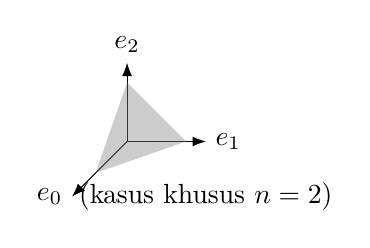
\begin{tikzpicture}[baseline=(O)]
	\coordinate (O) at (0, 0);
	\draw[-Latex] (0, 0) -- (-0.7, -0.7) node[left] {$e_0$};
	\draw[-Latex] (0, 0) -- (1, 0) node[right] {$e_1$};
	\draw[-Latex] (0, 0) -- (0, 1) node [above] {$e_2$};
	\fill[color=gray, opacity=0.4] (-0.4, -0.4) -- (0.75, 0) -- (0, 0.75) --cycle;
	\node at (1, -0.7) {(kasus khusus $n=2$)};
\end{tikzpicture}
\]
Titik-titik sudutnya dilabeli $0,\ldots,n$ melalui $i\leftrightarrow e_i$.
Interiornya dilengkapi orientasi standar sedemikian sehingga
$e_1-e_0,\ldots,e_n-e_{n-1}$ memberikan basis terurut positif di setiap
titik.

% segment-id: o014.aljabr2.chapter8.geometric-realization.p002
Setiap pemetaan monoton $f:[m]\to[n]$ menginduksi pemetaan
% segment-id: o014.aljabr2.chapter8.geometric-realization.q002
\[\begin{tikzcd}[row sep=tiny]
	{|f|}: {|\Delta^m|} \arrow[r] & {|\Delta^n|} \\
	\sum_{i=0}^m y_i e_i \arrow[mapsto, r] & \sum_{i=0}^m y_i e_{f(i)}.
\end{tikzcd}\]
Jika $f$ tidak surjektif, citra $|f|$ terletak pada batas. Pembenaman
$|\mathrm{d}^i|:|\Delta^{n-1}|\to|\Delta^n|$ dapat digunakan untuk
membandingkan orientasi interior $|\Delta^{n-1}|$ dengan orientasi yang
diinduksi $|\Delta^n|$ pada batasnya. Perhitungan determinan standar
menunjukkan bahwa keduanya berbeda sebesar faktor $(-1)^i$. Gambar berikut
melukiskan kasus $n=2$.
% segment-id: o014.aljabr2.chapter8.geometric-realization.g001
\begin{center}
	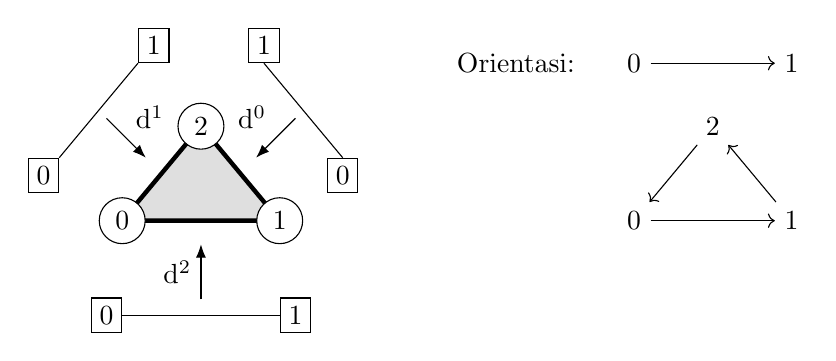
\begin{tikzpicture}
		\coordinate (A) at (0, 0);
		\coordinate (B) at (2, 0);
		\coordinate (C) at (1, 1.2);
		\fill[color=gray, opacity=0.25] (A) -- (B) -- (C) --cycle;
		\draw[ultra thick] (A) -- (B) -- (C) -- (A);
		\node[shape=circle, inner sep=0.3em, fill=white, draw] at (A) {$0$};
		\node[shape=circle, inner sep=0.3em, fill=white, draw] at (B) {$1$};
		\node[shape=circle, inner sep=0.3em, fill=white, draw] at (C) {$2$};

		\draw ($(B) + (0.8, 0.8)$) node[shape=rectangle, inner sep=0.3em, draw, below] {$0$} -- ($(C) + (0.8, 0.8)$) node[shape=rectangle, inner sep=0.3em, draw, above] {$1$};
		\draw[-Latex] ($(C)!0.5!(B) + (0.7, 0.7)$) to[edge label={$\mathrm{d}^0$}, swap] ($(C)!0.5!(B) + (0.2, 0.2)$);

		\draw ($(A) + (-0.8, 0.8)$) node[shape=rectangle, inner sep=0.3em, draw, below left] {$0$} -- ($(C) + (-0.8, 0.8)$) node[shape=rectangle, inner sep=0.3em, draw, above right] {$1$};
		\draw[-Latex] ($(A)!0.5!(C) + (-0.7, 0.7)$) to[edge label={$\mathrm{d}^1$}] ($(A)!0.5!(C) + (-0.2, 0.2)$);

		\draw ($(A) + (0, -1.2)$) node[shape=rectangle, inner sep=0.3em, draw, left] {$0$} -- ($(B) + (0, -1.2)$) node[shape=rectangle, inner sep=0.3em, draw, right] {$1$};
		\draw[-Latex] ($(A)!0.5!(B) + (0, -1)$) to[edge label={$\mathrm{d}^2$}] ($(A)!0.5!(B) + (0, -0.3)$);

		\node at (5, 2) {Orientasi:};
		\node (U) at (6.5, 2) {$0$};
		\node (V) at (8.5, 2) {$1$};
		\draw[->] (U) -- (V);
		\node (X) at (6.5, 0) {$0$};
		\node (Y) at (8.5, 0) {$1$};
		\node (Z) at (7.5, 1.2) {$2$};
		\draw[->] (X) -- (Y);
		\draw[->] (Y) -- (Z);
		\draw[->] (Z) -- (X);
	\end{tikzpicture}
\end{center}

% segment-id: o014.aljabr2.chapter8.geometric-realization.p003
Dengan merangkum pembahasan di atas, kita memperoleh funktor
% segment-id: o014.aljabr2.chapter8.geometric-realization.q003
\begin{equation*}
	|\cdot|: \simpDelta \to \cate{Top} \quad
	\left\{\begin{array}{ll}
		\text{objek} & [n] \mapsto |\Delta^n| \\
		\text{morfisme} & f \mapsto |f| .
	\end{array}\right.
\end{equation*}
Kita hendak memperluasnya menjadi funktor
$\cate{sSet}\to\cate{Top}$. Ingat bahwa $\cate{Top}$ kokomplet.

% segment-id: o014.aljabr2.chapter8.geometric-realization.d001
\begin{definition}[Funktor realisasi geometris]
	\index{realisasi geometris@realisasi geometris (geometric realization)}
	\index[sym1]{X-realization@$\lvert X\rvert$}
	Funktor $|\cdot|:\cate{sSet}\to\cate{Top}$ didefinisikan sebagai berikut.
	Jika $X$ himpunan simplisial, maka
% segment-id: o014.aljabr2.chapter8.geometric-realization.q004
	\[ |X| := \varinjlim_{n, x} |\Delta^n|, \]
	dengan $n\in\Z_{\geq0}$ dan $x\in X_n$, atau secara ekuivalen, dengan
	$x$ suatu morfisme $\Delta^n\to X$. Pasangan data $(n,x)$ tersebut membentuk suatu
	kategori. Morfisme dari $(n,x)$ ke $(m,y)$ tidak lain adalah
	$f\in\Hom_{\simpDelta}([n],[m])$ yang membuat diagram
% segment-id: o014.aljabr2.chapter8.geometric-realization.q005
	\[\begin{tikzcd}[column sep=small]
		\Delta^n \arrow[rr, "f"] \arrow[rd, "x"'] & & \Delta^m \arrow[ld, "y"] \\
		& X &
	\end{tikzcd}\]
	komutatif; secara ekuivalen, $f^*:X_m\to X_n$ harus memenuhi
	$f^*(y)=x$.
\end{definition}

% segment-id: o014.aljabr2.chapter8.geometric-realization.p004
Untuk $m\geq0$ tertentu, kategori data
$(n,x:\Delta^n\to\Delta^m)$ memiliki objek terminal
$(m,\identity_{\Delta^m})$. Karena itu, realisasi geometris $\Delta^m$
secara kanonik diidentifikasi dengan $|\Delta^m|$ yang didefinisikan
sebelumnya. Dengan demikian, notasinya konsisten.

% segment-id: o014.aljabr2.chapter8.geometric-realization.r001
\begin{remark}\label{rem:simplicial-density}
	Untuk setiap himpunan simplisial $X$, terdapat isomorfisme kanonik
	$\varinjlim_{n,x}\Delta^n\rightiso X$. Ini merupakan penerapan langsung
	Teorema Kerapatan~\ref{prop:Yoneda-density} pada kategori
	$\cate{sSet}=\simpDelta^{\wedge}$; pembaca dipersilakan memeriksanya.
\end{remark}

% segment-id: o014.aljabr2.chapter8.geometric-realization.r002
\begin{remark}
	Menurut Teorema~\ref{prop:Kan-limit}, realisasi geometris memberikan
	perluasan Kan kiri dari funktor $|\cdot|:\simpDelta\to\cate{Top}$ sepanjang
	$\simpDelta\to\cate{sSet}$; lihat Definisi~\ref{def:Kan-extension}.
	Dengan demikian, konstruksi ini sepenuhnya alami.
\end{remark}

% segment-id: o014.aljabr2.chapter8.geometric-realization.p005
Menurut konstruksi di atas, untuk setiap $n\in\Z_{\geq0}$ dan $x\in X_n$,
sifat universal $\varinjlim$ memberikan pemetaan kanonik
$i_{n,x}:|\Delta^n|\to|X|$ yang kompatibel ketika $(n,x)$ bervariasi.
Mengambil $\varinjlim$ dalam $\cate{Top}$ tidak lain adalah menempelkan
ruang-ruang topologis. Secara lebih konkret, realisasi geometris dapat
dituliskan sebagai ruang hasil bagi
% segment-id: o014.aljabr2.chapter8.geometric-realization.q006
\begin{equation}\label{eqn:geom-realization-quotient}
	|X| = \dfrac{\displaystyle\bigsqcup_{n \geq 0} X_n \times |\Delta^n| }{(f^*(y), t) \sim (y, |f|(t)) }, \quad
	\begin{tikzcd}[column sep=tiny]
		(f^*(y), t) \arrow[phantom, r, "\in" description] & X_n \arrow[phantom, r, "\times" description] & {|\Delta^n|} \arrow[d, "{|f|}"] & {[n]} \arrow[d, "f"] \\
		(y, {|f|}(t)) \arrow[phantom, r, "\in" description] & X_m \arrow[phantom, r, "\times" description] \arrow[u, "{f^*}"] & {|\Delta^m|} & {[m]}.
	\end{tikzcd}
\end{equation}

% segment-id: o014.aljabr2.chapter8.geometric-realization.p006
Sesuai intuisi geometris, himpunan simplisial $X$ dapat dibayangkan sebagai
suatu model ruang. Himpunan $X_0,X_1,\ldots$ merupakan kumpulan komponen
penyusun model itu: setiap elemen $X_n$ bersesuaian dengan, sekaligus melabeli,
satu salinan $|\Delta^n|$. Berbagai pemetaan
$f^*:X_m\to X_n$ berfungsi sebagai petunjuk perakitan yang menentukan cara
menempelkan salinan-salinan $|\Delta^n|$ tersebut.

% segment-id: o014.aljabr2.chapter8.geometric-realization.p007
Karena morfisme dalam $\simpDelta$ sudah dideskripsikan secara konkret,
relasi ekuivalensi dalam \eqref{eqn:geom-realization-quotient} dapat
dibangkitkan oleh dua jenis $f$ khusus.
% segment-id: o014.aljabr2.chapter8.geometric-realization.l001
\begin{itemize}
% segment-id: o014.aljabr2.chapter8.geometric-realization.i001
	\item Ambil $\mathrm{d}^i:[n-1]\hookrightarrow[n]$. Maka
	$|\mathrm{d}^i|$ menanamkan
	$\{d_i(x)\}\times|\Delta^{n-1}|$ ke dalam
	$\{x\}\times|\Delta^n|$. Jadi, pemetaan muka
	$d_i:X_n\to X_{n-1}$ melabeli muka ke-$i$ dari komponen berdimensi $n$
	(yang bersesuaian dengan $x$) sebagai $d_i(x)$, lalu penempelan dilakukan
	menurut label tersebut.

% segment-id: o014.aljabr2.chapter8.geometric-realization.i002
	\item Ambil $\mathrm{s}^j:[n+1]\twoheadrightarrow[n]$. Maka
	$|\mathrm{s}^j|$ ``memampatkan''
	$\{s_j(x)\}\times|\Delta^{n+1}|$ menjadi
	$\{x\}\times|\Delta^n|$. Jadi, pemetaan degenerasi
	$s_j:X_n\to X_{n+1}$ menentukan bagaimana suatu komponen berdimensi $n$
	(yang bersesuaian dengan $x$) menghasilkan komponen ``degenerat''
	berdimensi $n+1$, berlabel $s_j(x)$, yang dalam proses penempelan
	dimampatkan pada muka ke-$j$.
\end{itemize}
% segment-id: o014.aljabr2.chapter8.geometric-realization.p008
Karena itu, simpleks-$n$ degenerat (Definisi~\ref{def:simplex}) dapat
dihilangkan dari proses penempelan, tetapi informasi degenerasi tetap tidak
dapat diabaikan. Sebagai contoh, $d_i:X_n\to X_{n-1}$ sangat mungkin
memetakan simpleks nondegenerat ke simpleks degenerat.

% segment-id: o014.aljabr2.chapter8.geometric-realization.eg001
\begin{example}
	Sebagai ilustrasi, $\partial\Delta^n$ dalam
	Contoh~\ref{eg:boundary-horn} merealisasikan batas simpleks-$n$
	standar dalam pengertian intuitif, sedangkan tanduk $\Lambda^n_k$ diperoleh
	dengan membuang dari $\partial\Delta^n$ muka yang berhadapan dengan titik
	sudut ke-$k$. Berikut salah satu ilustrasinya:
% segment-id: o014.aljabr2.chapter8.geometric-realization.g002
	\begin{center}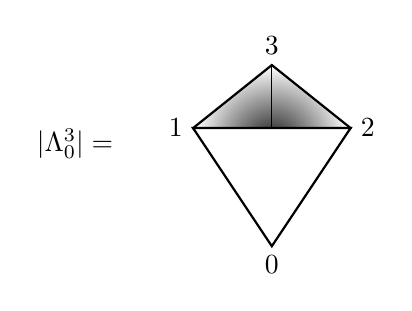
\begin{tikzpicture}
		\coordinate (A) at (0, 0);
		\coordinate (B) at (2, 0);
		\coordinate (C) at (1, 0.8);
		\coordinate (O) at (1, -1.5);

		\filldraw[thick, shading=radial, inner color=black!90, outer color=white] (A) node[left] {$1$} -- (C) node[above] {$3$} -- (B) node[right] {$2$} --($(O)!0.15!(C)$) --cycle;
		\draw (C) -- (O) node[below] {$0$};
		\filldraw[fill=white, thick] (A) -- (B) -- (O) --cycle;

		\node at ($(A) + (-1.5, -0.2)$) {$|\Lambda^3_0| =$};
	\end{tikzpicture}\end{center}
\end{example}

% segment-id: o014.aljabr2.chapter8.geometric-realization.eg002
\begin{example}\label{eg:cone-realization}
	\index{himpunan simplisial!kerucut@kerucut (cone)}
	Untuk setiap ruang topologis $\mathcal{X}$, definisikan kerucut di atasnya,
	$\Cone_{\mathrm{top}}(\mathcal{X})$, sebagai ruang yang
	diperoleh dengan mengerutkan subhimpunan tertutup
	$\mathcal{X}\times\{0\}$ dari $\mathcal{X}\times[0,1]$ menjadi satu
	titik. Secara visual,
% segment-id: o014.aljabr2.chapter8.geometric-realization.g003
	\[\Cone_{\mathrm{top}}(\mathcal{X}) = \; 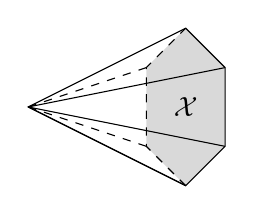
\begin{tikzpicture}[baseline=(P)]
		\coordinate (A) at (0, 1);
		\coordinate (B) at (0.5, 0.5);
		\coordinate (C) at (0.5, -0.5);
		\coordinate (D) at (0, -1);
		\coordinate (E) at (-0.5, -0.5);
		\coordinate (F) at (-0.5, 0.5);
		\coordinate (O) at (-2, 0);
		\coordinate (P) at (0, -0.1);	% For the baseline

		\fill[gray!50, opacity=0.6] (A) -- (B) -- (C) -- (D) -- (E) -- (F) --cycle;
		\draw (O) -- (A) -- (B) -- (C) -- (D) --cycle;
		\draw (O) -- (B);
		\draw (O) -- (C);
		\draw (O) -- (D);
		\draw[dashed] (D) -- (E) -- (F) -- (A);
		\draw[dashed] (O) -- (E);
		\draw[dashed] (O) -- (F);
		\node at (0, 0) {$\mathcal{X}$};
	\end{tikzpicture}\]
	Sebagai latihan sederhana, periksa bahwa
	$|X^{\lhd}|\simeq\Cone_{\mathrm{top}}(|X|)\simeq|X^{\rhd}|$. Ini
	menunjukkan bahwa kerucut dalam Definisi~\ref{def:cone-simplicial} memang
	layak disebut demikian; perbedaan antara kerucut kiri dan kanan hanya
	terletak pada orientasi.
\end{example}

% segment-id: o014.aljabr2.chapter8.geometric-realization.p009
Dengan menyajikan triangulasi ruang sebagai himpunan simplisial, banyak sifat
topologis penting dapat diekstraksi. Pendekatan ini secara tepat disebut
``topologi kombinatorial''. Pembahasan dan contoh lebih lanjut dapat dilihat
dalam \cite[Bab VI]{You}.

% segment-id: o014.aljabr2.chapter8.geometric-realization.d002
\begin{definition}[Funktor himpunan singular]
	\index[sym1]{Sing@$\mathrm{Sing}$}
	\index{himpunan singular@himpunan singular (singular set)}
	Untuk setiap ruang topologis $E$, definisikan himpunan simplisial
	$\mathrm{Sing}(E)$ melalui
% segment-id: o014.aljabr2.chapter8.geometric-realization.q007
	\[ \mathrm{Sing}(E)_n := \Hom_{\cate{Top}}(|\Delta^n|, E), \quad n \in \Z_{\geq 0}, \]
	dengan $d_i:\mathrm{Sing}(E)_n\to\mathrm{Sing}(E)_{n-1}$ (atau
	$s_j:\mathrm{Sing}(E)_n\to\mathrm{Sing}(E)_{n+1}$) diberikan oleh
	penarikan balik sepanjang
	$|\mathrm{d}^i|:|\Delta^{n-1}|\to|\Delta^n|$ (atau
	$|\mathrm{s}^j|:|\Delta^{n+1}|\to|\Delta^n|$). Objek ini disebut
	\emph{himpunan singular (simplisial)} yang bersesuaian dengan $E$.
	Konstruksi tersebut memberikan funktor
% segment-id: o014.aljabr2.chapter8.geometric-realization.q008
	\[ \mathrm{Sing}: \cate{Top} \to \cate{sSet}. \]
\end{definition}

% segment-id: o014.aljabr2.chapter8.geometric-realization.th001
\begin{theorem}\label{prop:geom-Sing-adjunction}
	Funktor realisasi geometris merupakan adjoin kiri dari funktor himpunan singular.
	Dengan kata lain, terdapat bijeksi alami
% segment-id: o014.aljabr2.chapter8.geometric-realization.q009
	\[\begin{tikzcd}[row sep=tiny]
		\Hom_{\cate{Top}}(|X|, E) \arrow[leftrightarrow, r, "1:1"] & \Hom_{\cate{sSet}}(X, \mathrm{Sing}(E)) \\
		\varphi \arrow[mapsto, r] & {\left[ X_n \xrightarrow{x \mapsto \varphi \circ i_{n, x}} \Hom_{\cate{Top}}(|\Delta^n|, E) \right]} \\
		\displaystyle\varinjlim_{(n, x)} \left( |\Delta^n| \xrightarrow{\psi_n(x)} E \right) & \psi = {\left[ \psi_n: X_n \to \Hom_{\cate{Top}}(|\Delta^n|, E) \right]}_{n \geq 0} , \arrow[mapsto, l]
	\end{tikzcd}\]
	dengan $X\in\Obj(\cate{sSet})$ dan $E\in\Obj(\cate{Top})$.
\end{theorem}
% segment-id: o014.aljabr2.chapter8.geometric-realization.pf001
\begin{proof}
	Ingat bahwa $|X|=\varinjlim_{n,x}|\Delta^n|$. Terdapat isomorfisme
	kanonik
% segment-id: o014.aljabr2.chapter8.geometric-realization.q010
	\begin{align*}
		\Hom_{\cate{Top}}\left( \varinjlim_{n, x} |\Delta^n| , E \right) & \rightiso \varprojlim_{n, x} \Hom_{\cate{Top}}(|\Delta^n|, E) = \varprojlim_{n, x} \mathrm{Sing}(E)_n \\
		& \rightiso \varprojlim_{n, x} \Hom_{\cate{sSet}}\left( \Delta^n, \mathrm{Sing}(E) \right) \\
		\varphi & \mapsto \left( \psi_n(x) := \varphi \circ i_{n, x} \right)_{n, x}.
	\end{align*}

	Setiap keluarga morfisme $(\psi_n(x))_{n,x}$ yang ditentukan oleh suatu
	$\psi:X\to\mathrm{Sing}(E)$ memenuhi kompatibilitas, yakni merupakan
	elemen $\varprojlim$ di ruas kanan rumus di atas. Bukti akan selesai jika
	kita menunjukkan bahwa memberikan morfisme $\psi$ sama artinya dengan memberikan
	keluarga morfisme yang kompatibel; tepat inilah yang dijamin oleh
	Catatan~\ref{rem:simplicial-density}.
\end{proof}

% segment-id: o014.aljabr2.chapter8.geometric-realization.r003
\begin{remark}
	Untuk kajian teori homotopi, kategori $\cate{CGHaus}$ yang disebutkan dalam
	\S\ref{sec:closed-monoidal} mungkin lebih nyaman daripada $\cate{Top}$.
	Karena funktor inklusi $\cate{CGHaus}\to\cate{Top}$ mempunyai adjoin kanan
	$k$, funktor tersebut mempertahankan $\varinjlim$. Selain itu,
	$|\Delta^n|$ adalah ruang Hausdorff yang dibangkitkan secara kompak. Maka,
	penempelan (atau pengambilan $\Hom$) dalam realisasi geometris (atau
	himpunan singular) dapat dilakukan di dalam $\cate{CGHaus}$\footnote{Perlu
	dijelaskan bahwa $\varinjlim$ yang dibahas memang ada dalam
	$\cate{CGHaus}$. Ini merupakan persoalan topologis; lihat
	\cite[III.1.8, III.2.1]{GZ67}.}. Dengan demikian, pasangan adjoin dalam
	Teorema~\ref{prop:geom-Sing-adjunction} berfaktor sebagai dua adjungsi, yang
	ditulis menggunakan notasi yang sama sebagai
% segment-id: o014.aljabr2.chapter8.geometric-realization.q011
	\[\begin{tikzcd}
		\cate{sSet} \arrow[shift left, r, "{|\cdot|}"] & \cate{CGHaus} \arrow[shift left, r, "\text{funktor inklusi}"] \arrow[shift left, l, "\mathrm{Sing}"] & \cate{Top} \arrow[shift left, l, "k"] .
	\end{tikzcd}\]
\end{remark}

% segment-id: o014.aljabr2.chapter8.geometric-realization.p010
Untuk sembarang dua himpunan simplisial $X$ dan $Y$, hasil kalinya
didefinisikan sebagai hasil kali suku demi suku:
% segment-id: o014.aljabr2.chapter8.geometric-realization.q012
\begin{gather*}
	(X \times Y)_n = X_n \times Y_n, \\
	d_i(x, y) = (d_i(x), d_i(y)), \\
	s_j(x, y) = (s_j(x), s_j(y)).
\end{gather*}
Ini sekaligus merupakan hasil kali kategoris dalam
$\cate{sSet}=\cate{Set}^{\simpDelta^{\opp}}$ dan konstruksi dalam
Definisi~\ref{def:monoidal-sObj} ketika kategori monoidal yang digunakan
adalah $(\cate{Set},\times)$. Walaupun kedua definisi ini berasal dari teori
kategori, hasil mendasar berikut menunjukkan bahwa keduanya juga mempunyai
makna geometris.

% segment-id: o014.aljabr2.chapter8.geometric-realization.th002
\begin{theorem}\label{prop:realization-product}
	Untuk himpunan simplisial $X$ dan $Y$, terdapat isomorfisme kanonik dalam
	$\cate{CGHaus}$
% segment-id: o014.aljabr2.chapter8.geometric-realization.q013
	\[ |X \times Y| \simeq |X| \times |Y|. \]
	Secara lebih umum, versi $|\cdot|$ yang bernilai dalam $\cate{CGHaus}$
	mempertahankan $\varprojlim$ hingga. Jika $X$ atau $Y$ hanya mempunyai
	hanya memiliki sejumlah hingga simpleks nondegenerat, maka
	$|X\times Y|\simeq|X|\times|Y|$ juga berlaku dalam $\cate{Top}$.
\end{theorem}

% segment-id: o014.aljabr2.chapter8.geometric-realization.p011
Bukti dalam keadaan umum cukup rumit; lihat \cite[Bab III]{GZ67} atau
\cite{Dri03}. Isomorfisme tersebut pada umumnya tidak berlaku bagi versi
realisasi geometris yang bernilai dalam $\cate{Top}$. Perhatikan bahwa syarat
yang diberikan oleh teorema untuk versi $\cate{Top}$ bukanlah syarat optimal.

% segment-id: o014.aljabr2.chapter8.geometric-realization.c001
\begin{corollary}
	Tuliskan $\cate{Grp}$ untuk kategori grup. Jika himpunan simplisial $X$
	dapat diperluas menjadi objek $\cate{sGrp}$, maka $|X|$ secara alami
	mempunyai struktur grup topologis. Hasil serupa berlaku bagi struktur
	aljabar lainnya.
\end{corollary}

% segment-id: o014.aljabr2.chapter8.geometric-realization.p012
Berdasarkan Teorema~\ref{prop:realization-product}, wajar untuk mendefinisikan
suatu homotopi dari $g$ ke $f$, bagi morfisme
$f,g:X\rightrightarrows Y$ dalam $\cate{sSet}$, sebagai morfisme
$H:X\times\Delta^1\to Y$ yang membuat diagram berikut komutatif:
% segment-id: o014.aljabr2.chapter8.geometric-realization.q014
\begin{equation}\label{eqn:simplicial-homotopy-prep}
	\begin{tikzcd}
		X \times \Delta^0 \arrow[d, "{\identity_X \times \mathrm{d}^0}"'] \arrow[r, "\sim"] & X \arrow[d, "f"] \\
		X \times \Delta^1 \arrow[r, "H" description] & Y \\
		X \times \Delta^0 \arrow[u, "{\identity_X \times \mathrm{d}^1}"] \arrow[r, "\sim"'] & X \arrow[u, "g"']
	\end{tikzcd}
\end{equation}

% segment-id: o014.aljabr2.chapter8.geometric-realization.p013
Sebagai kasus khusus, komposisi
$X\times\Delta^1\xrightarrow{\text{proyeksi}}X\xrightarrow{f}Y$
memberikan homotopi konstan dari $f$ ke dirinya sendiri. Namun, homotopi yang
didefinisikan dengan cara ini bukan relasi ekuivalensi: contoh sederhana
sudah menunjukkan bahwa sifat simetri tidak terpenuhi. Dalam teori homotopi,
biasanya $Y$ disyaratkan mempunyai sifat tambahan, misalnya merupakan
kompleks Kan. Dalam keadaan tersebut, relasi homotopi memiliki
sifat-sifat yang diharapkan, sehingga grup homotopi, ekuivalensi lemah, dan
konsep-konsep lain dapat dikaji secara kombinatorial.

% segment-id: o014.aljabr2.chapter8.geometric-realization.p014
Walaupun buku ini tidak membuktikan
Teorema~\ref{prop:realization-product}, ada gunanya meninjau kasus khusus
sederhana $X=\Delta^p$ dan $Y=\Delta^q$. Sebagai contoh,
bagaimana simpleks-simpleks nondegenerat dari
$\Delta^p\times\Delta^q$ dapat diklasifikasikan? Jawabannya bukan hanya
membantu memahami realisasi geometris hasil kali; konstruksi terkait juga
akan diperlukan kemudian.

% segment-id: o014.aljabr2.chapter8.geometric-realization.p015
Pertama, hasil kali dua himpunan terurut parsial $S_1$ dan $S_2$ menjadi
himpunan terurut parsial melalui
$(a_1,a_2)\leq(b_1,b_2)$ jika dan hanya jika
$a_1\leq b_1$ dan $a_2\leq b_2$. Ini juga sama dengan mengambil hasil kali
kategori-kategori yang bersesuaian dengannya.

% segment-id: o014.aljabr2.chapter8.geometric-realization.d003
\begin{definition}\label{def:pq-shuffle}
	\index{shuffle p-q@shuffle $(p, q)$ ($(p, q)$-shuffle)}
	Misalkan $p,q\in\Z_{\geq0}$. Suatu \emph{shuffle-$(p,q)$} adalah pemetaan
	monoton injektif $\sigma:[p+q]\to[p]\times[q]$.
\end{definition}

% segment-id: o014.aljabr2.chapter8.geometric-realization.p016
Untuk setiap $n\in\Z_{\geq0}$, menentukan pemetaan monoton
$\sigma:[n]\to[p]\times[q]$ setara dengan menentukan sepasang pemetaan
monoton $\sigma_-:[n]\to[p]$ dan $\sigma_+:[n]\to[q]$. Ini juga setara
dengan menentukan suatu simpleks-$n$ dari $\Delta^p\times\Delta^q$.
Syarat bahwa $\sigma$ injektif setara dengan syarat bahwa lintasan
$i\mapsto(\sigma_-(i),\sigma_+(i))$ tidak pernah diam, untuk
$i=0,\ldots,n$. Jika $n=p+q$, keadaan ini dapat digambarkan sebagai berikut:
% segment-id: o014.aljabr2.chapter8.geometric-realization.q015
\begin{equation}\label{eqn:pq-shuffle-diag}
	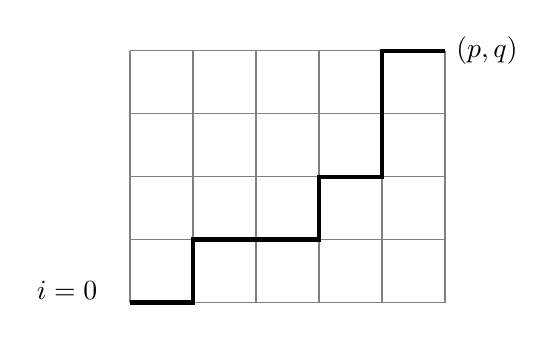
\begin{tikzpicture}[scale=0.8, baseline=(O)]
		\draw[thin, gray] (0, 0) grid (5, 4);
		\node at (-1, 0.2) {$i=0$};
		\draw[ultra thick] (0, 0) -- (1, 0) -- (1, 1) -- (2, 1) -- (3, 1) -- (3, 2) -- (4, 2) -- (4, 3) -- (4, 4) -- (5, 4) node[right] {$(p, q)$};
		\coordinate (O) at (0, 2);
	\end{tikzpicture}
	\quad
	\text{tepat $p+q$ langkah.}
\end{equation}
Jadi, untuk shuffle-$(p,q)$ $\sigma$, definisikan
% segment-id: o014.aljabr2.chapter8.geometric-realization.q016
\begin{align*}
	I_\pm & := \left\{ 1 \leq i \leq p+q : \sigma_\pm(i-1) < \sigma_\pm(i) \right\} \\
	& = \left\{ 1 \leq i \leq p+q : \sigma_\pm(i-1) = \sigma_\pm(i) - 1 \right\} \\
	& = \left\{ 1 \leq i \leq p+q: \sigma_\mp(i-1) = \sigma_\mp(i) \right\},
\end{align*}
dengan $I_+\sqcup I_-=\{1,\ldots,p+q\}$. Subhimpunan $I_+$ (atau $I_-$)
bersesuaian dengan bagian lintasan yang bergerak ke atas (atau ke kanan)
dalam \eqref{eqn:pq-shuffle-diag}. Dengan demikian, shuffle-$(p,q)$ juga
dapat dipandang sebagai suatu urutan yang terdiri atas $p$ simbol
$\rightarrow$ dan $q$ simbol $\uparrow$; jumlahnya
$\binom{p+q}{p}$. Pengamatan ini sekaligus menunjukkan bahwa $\sigma_+$ dan
$\sigma_-$ dari suatu shuffle-$(p,q)$ adalah pemetaan monoton surjektif.

% segment-id: o014.aljabr2.chapter8.geometric-realization.pr001
\begin{proposition}
	Misalkan $p,q\in\Z_{\geq0}$. Tinjau suatu simpleks-$n$ dari
	$\Delta^p\times\Delta^q$, yakni pemetaan monoton
	$\sigma:[n]\to[p]\times[q]$. Tetapkan
	$(p_i,q_i):=\sigma(i)$ dan
	$(p',q'):=(p_n-p_0,q_n-q_0)$. Maka $\sigma$ nondegenerat jika dan hanya
	jika syarat-syarat berikut terpenuhi:
	\begin{itemize}
		\item $p'+q'=n$;
		\item $\sigma$ merupakan komposisi suatu shuffle-$(p',q')$
		$\sigma':[n]\to[p']\times[q']$ dengan suatu injeksi monoton
		$[p']\times[q']\hookrightarrow[p]\times[q]$ berbentuk $f\times g$.
	\end{itemize}
\end{proposition}
% segment-id: o014.aljabr2.chapter8.geometric-realization.pf002
\begin{proof}
	Identifikasikan $\sigma$ dengan pasangan pemetaan monoton
	$(\sigma_-,\sigma_+)$. Tinjau lintasan $i\mapsto(p_i,q_i)$ seperti dalam
	Gambar~\eqref{eqn:pq-shuffle-diag}. Syarat bahwa $\sigma$ nondegenerat
	setara dengan syarat bahwa lintasan itu tidak pernah diam. Selebihnya
	jelas.
\end{proof}

% segment-id: o014.aljabr2.chapter8.geometric-realization.p017
Berdasarkan deskripsi simpleks nondegenerat tersebut, pembaca dapat
memahami secara geometris
$|\Delta^p\times\Delta^q|\simeq|\Delta^p|\times|\Delta^q|$ bagi
$(p,q)=(1,1)$ dan $(2,1)$. Sebagai contoh, gambar berikut memperlihatkan
triangulasi $|\Delta^2|\times|\Delta^1|$ menjadi tiga tetrahedron, yang
bersesuaian dengan $3=\binom{3}{2}$ shuffle-$(2,1)$.

% segment-id: o014.aljabr2.chapter8.geometric-realization.g004
\begin{center}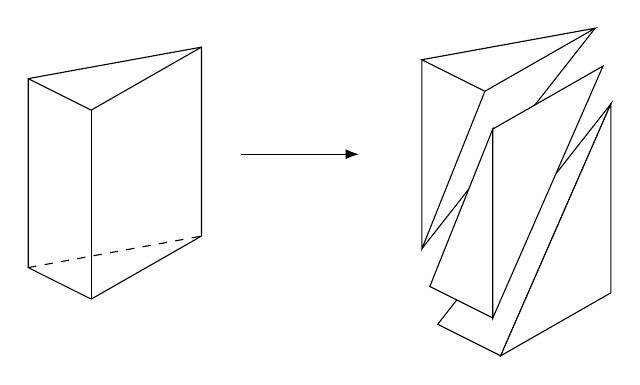
\begin{tikzpicture}[yscale=0.8]
	\coordinate (A) at (0, 0);
	\coordinate (B) at (2.2, 0.5);
	\coordinate (C) at (0.8, -0.5);
	\coordinate (P) at ($(A) + (0, -3)$);
	\coordinate (Q) at ($(B) + (0, -3)$);
	\coordinate (R) at ($(C) + (0, -3)$);

	\draw ($(A) + (-5, -0.3)$) -- ($(B) + (-5, -0.3)$) -- ($(Q) + (-5, -0.3)$) -- ($(R) + (-5, -0.3)$) -- ($(P) + (-5, -0.3)$) --cycle;
	\draw ($(A) + (-5, -0.3)$) -- ($(C) + (-5, -0.3)$) -- ($(B) + (-5, -0.3)$);
	\draw ($(C) + (-5, -0.3)$) -- ($(R) + (-5, -0.3)$);
	\draw[dashed] ($(P) + (-5, -0.3)$) -- ($(Q) + (-5, -0.3)$);

	\draw[-Latex] ($(B)!0.5!(Q) + (-4.5, -0.5)$) -- ($(B)!0.5!(Q) + (-3, -0.5)$);

	\draw (A) -- (B) -- (C) --cycle;
	\draw (A) -- (P) -- (C);
	\draw (P) -- (B);

	\draw[fill=white] ($(P) + (0.2, -1.2)$) -- ($(B) + (0.2, -1.2)$) -- ($(R) + (0.2, -1.2)$) --cycle;
	\draw[fill=white] ($(R) + (0.2, -1.2)$) -- ($(Q) + (0.2, -1.2)$) -- ($(B) + (0.2, -1.2)$) --cycle;

	\draw[fill=white] ($(P) + (0.1, -0.6)$) -- ($(R) + (0.1, -0.6)$) -- ($(C) + (0.1, -0.6)$) --cycle;
	\draw[fill=white] ($(R) + (0.1, -0.6)$) -- ($(B) + (0.1, -0.6)$) -- ($(C) + (0.1, -0.6)$) --cycle;
\end{tikzpicture}\end{center}

% segment-id: o014.aljabr2.chapter8.geometric-realization.d004
\begin{definition}\label{def:pq-shuffle-sgn}
	Misalkan $\sigma$ suatu shuffle-$(p,q)$. Tandanya didefinisikan sebagai
% segment-id: o014.aljabr2.chapter8.geometric-realization.q017
	\[ \sgn(\sigma) := (-1)^{|I_\sigma|}, \quad I_\sigma := \left\{ (i, j) \in I_- \times I_+ : i > j \right\}. \]
\end{definition}

% segment-id: o014.aljabr2.chapter8.geometric-realization.p018
Jika $\sigma$ dipandang sebagai urutan $p$ simbol $\rightarrow$ dan $q$
simbol $\uparrow$, maka $I_\sigma$ tepat merupakan himpunan semua pasangan
$(j,i)$, dengan $j<i$, yang muncul dalam urutan ``terbalik''
$(\uparrow,\rightarrow)$. Suatu latihan kombinatorial sederhana menunjukkan
bahwa terdapat tepat satu $\tau\in\mathfrak{S}_{p+q}$ yang menyusun kembali
urutan itu menjadi
$\rightarrow\cdots\rightarrow\uparrow\cdots\uparrow$ tanpa mengubah urutan
internal dalam $I_+$ maupun $I_-$. Definisi~\ref{def:pq-shuffle-sgn} dengan
demikian sama artinya dengan $\sgn(\sigma)=\sgn(\tau)$.

% segment-id: o014.aljabr2.chapter8.geometric-realization.p019
Untuk shuffle-$(p,q)$ $\sigma$, menukar peran $\sigma_-$ dan $\sigma_+$
memberikan shuffle-$(q,p)$ $\sigma'$. Penafsiran di atas dan argumen
kombinatorial dasar memberikan
% segment-id: o014.aljabr2.chapter8.geometric-realization.q018
\begin{equation}\label{eqn:shuffle-sign-0}
	\sgn(\sigma) = (-1)^{pq} \sgn(\sigma').
\end{equation}

% segment-id: o014.aljabr2.chapter8.geometric-realization.p020
Dengan asas yang sama, definisikan shuffle-$(p,q,r)$ sebagai injeksi monoton
$\sigma=(\sigma_-,\sigma_0,\sigma_+):[p+q+r]\to[p]\times[q]\times[r]$,
atau, secara ekuivalen, pandang $\sigma$ sebagai suatu urutan simbol
$\rightarrow$, $\nearrow$, dan $\uparrow$. Definisikan
$\sgn(\sigma):=(-1)^{|I_\sigma|}$, dengan $I_\sigma$ terdiri atas semua
tripel indeks $k>j>i$ yang bersesuaian dengan permutasi ganjil dari
$(\rightarrow,\nearrow,\uparrow)$. Latihan kombinatorial standar yang sama
menunjukkan bahwa jika shuffle-$(p,q,r)$ $\sigma$ mempunyai faktorisasi
% segment-id: o014.aljabr2.chapter8.geometric-realization.q019
\[ [p+q+r] \xrightarrow{\sigma_1} [p+q] \times [r] \xrightarrow{\sigma_2 \times \identity_{[r]}} [p] \times [q] \times [r], \]
maka $\sigma_1$ merupakan shuffle-$(p+q,r)$, $\sigma_2$ merupakan
shuffle-$(p,q)$, dan
% segment-id: o014.aljabr2.chapter8.geometric-realization.q020
\begin{equation}\label{eqn:shuffle-sign-1}
	\sgn(\sigma) = \sgn(\sigma_1) \sgn(\sigma_2).
\end{equation}
Pernyataan serupa tentu berlaku bagi faktorisasi
$[p+q+r]\to[p]\times[q+r]\to[p]\times[q]\times[r]$.

% segment-id: o014.aljabr2.chapter8.geometric-realization.p021
Persamaan~\eqref{eqn:shuffle-sign-0} dan
\eqref{eqn:shuffle-sign-1} pada hakikatnya sepenuhnya kombinatorial;
verifikasi terperinci diserahkan sebagai latihan bab ini. Pengamatan tersebut
akan digunakan dalam \S\ref{sec:bisimplicial}.

% Unit 110 terjemahan Bahasa Indonesia dari chapter8.tex baris 760--924.
% Sumber: Methods of Algebra, Volume 2, commit
% 9a5803ff77dd3257484cb177f851a73770a59dd3 (CC BY 4.0).
% stable-unit-id: o014.aljabr2.chapter8.dold-kan-a
% Cakupan: Bagian 8.5 dari pembukaan melalui Lema Dold--Kan untuk grup abelian;
% dilanjutkan oleh Unit 111 pada baris 925.

% segment-id: o014.li2.chapter8.dold-kan-a.h001
\section{Korespondensi Dold--Kan}\label{sec:Dold-Kan}
\hypertarget{o014.aljabr2.chapter8.dold-kan-a}{ }
% segment-id: o014.li2.chapter8.dold-kan-a.p001
Mengikuti konvensi topologi aljabar, untuk kategori aditif $\mathcal{A}$ kita
tinjau kategori kompleks rantai di atasnya (Definisi~\ref{def:complex}),
yang ditulis $\cate{Ch}(\mathcal{A})$, beserta subkategorinya
% segment-id: o014.li2.chapter8.dold-kan-a.q001
\[ \cate{Ch}_{\geq 0}(\mathcal{A}) := \left\{ A = (A_n, \partial_n)_{n \in \Z} : \text{kompleks rantai}, \; \forall n < 0, \; A_n = 0 \right\}, \]
dengan $\partial_n=\partial_n^A:A_n\to A_{n-1}$. Untuk objek
$\cate{Ch}_{\geq0}(\mathcal{A})$, jelas cukup memberikan data
$(A_n)_{n\geq0}$ dan $(\partial_n)_{n\geq1}$. Kategori
$\cate{Ch}_{\geq m}(\mathcal{A})$ didefinisikan serupa; bandingkan dengan
versi kompleks kokrantai dalam Definisi~\ref{def:cplx-cat-variant}.
\index[sym1]{ChA@$\cate{Ch}(\mathcal{A})$}

% segment-id: o014.li2.chapter8.dold-kan-a.p002
Dengan memperbesar semesta Grothendieck yang dipilih bila perlu, kita dapat
mengandaikan bahwa $\mathcal{A}$ kategori aditif kecil; lihat
\cite[Asumsi 1.5.2]{Li1}. Dari $\mathcal{A}$ dapat didefinisikan kategori
objek simplisial $\cate{s}\mathcal{A}$; objek simplisial konstan yang
bersesuaian dengan $0$ tetap ditulis
$0\in\Obj(\cate{s}\mathcal{A})$. Bagian ini bertujuan menjelaskan hubungan
dasar antara kategori-kategori tersebut. Lebih tepatnya, kita akan
mendefinisikan tiga funktor
% segment-id: o014.li2.chapter8.dold-kan-a.q002
\[\begin{tikzcd}
	\cate{Ch}_{\geq 0}(\mathcal{A}) \arrow[r, "\Gamma" description] & \cate{s}\mathcal{A} \arrow[bend left, l, "{\mathrm{N}}"] \arrow[bend right, l, "{\mathrm{C}}"']
\end{tikzcd}\]
dengan $\mathrm{N}$ hanya terdefinisi bila $\mathcal{A}$ kategori abelian.
Funktor $\mathrm{C}$ dan $\mathrm{N}$ sama-sama meluas ke objek
semisimplisial dari Catatan~\ref{rem:semisimplicial}; dengan kata lain,
keduanya tidak melibatkan morfisme degenerasi.

% segment-id: o014.li2.chapter8.dold-kan-a.p003
Uraian berikut mengikuti \cite[\S 1.2]{LuHA}. Pertama-tama, kita perjelas
definisi yang berkaitan.

% segment-id: o014.li2.chapter8.dold-kan-a.d001
\begin{definition}[Kompleks rantai tak ternormalisasi]\label{def:unnormalized-chain}
	\index{kompleks rantai tak ternormalisasi@kompleks rantai tak ternormalisasi (unnormalized chain complex)}
	\index{kompleks rantai Moore@kompleks rantai Moore (Moore chain complex)}
	\index[sym1]{CX@$\mathrm{C}X$}
	Untuk objek semisimplisial $X$ dalam $\mathcal{A}$ dan setiap
	$n\in\Z_{\geq1}$, definisikan
	% segment-id: o014.li2.chapter8.dold-kan-a.q003
	\[ \partial_n := \sum_{i=0}^n (-1)^i d_i: X_n \to X_{n-1}. \]
	Objek-objek $(X_n)_{n\geq0}$ beserta $(\partial_n)_n$ membentuk objek
	$\mathrm{C}X$ dari $\cate{Ch}_{\geq0}(\mathcal{A})$, yang disebut
	\emph{kompleks rantai tak ternormalisasi} atau \emph{kompleks rantai
	Moore} yang diberikan oleh $X$. Jadi, $(\mathrm{C}X)_n=X_n$.
\end{definition}

% segment-id: o014.li2.chapter8.dold-kan-a.p004
Perlu ditunjukkan bahwa $\partial_{n-1}\partial_n=0$ bila $n>1$.
Sesungguhnya, identitas
$i<j\implies d_id_j=d_{j-1}d_i$ dalam
\eqref{eqn:simplicial-identity} memberikan
% segment-id: o014.li2.chapter8.dold-kan-a.q004
\begin{multline*}
	\partial_{n-1} \partial_n = \sum_{i=0}^{n-1} \sum_{j=0}^n (-1)^{i+j} d_i d_j \\
	= \sum_{0 \leq i < j \leq n} (-1)^{i+j} d_{j-1} d_i + \sum_{n-1 \geq i \geq j \geq 0} (-1)^{i+j} d_i d_j = 0.
\end{multline*}
Konstruksi ini jelas kanonik dalam $X$ dan memberikan funktor $\mathrm{C}$.

% segment-id: o014.li2.chapter8.dold-kan-a.eg001
\begin{example}\label{eg:classifying-space-std-cplx}
	Misalkan $\Bbbk$ gelanggang komutatif dan
	$\mathcal{A}=\Bbbk\dcate{Mod}$. Untuk grup $\Gamma$, Contoh
	\ref{eg:classifying-space} memberikan himpunan simplisial
	$\mathrm{E}\Gamma$. Definisikan objek simplisial
	$\Bbbk\mathrm{E}\Gamma$ dalam $\Bbbk\dcate{Mod}$ yang suku berderajat
	$n$-nya adalah modul-$\Bbbk$ bebas dengan basis
	$(\mathrm{E}\Gamma)_n$, serta $d_i$ dan $s_i$ diperluas secara linear.
	Akan ditunjukkan bahwa $\mathrm{C}(\Bbbk\mathrm{E}\Gamma)$ persis merupakan
	kompleks rantai $\mathsf{L}:=(\mathsf{L}_n,\partial'_n)_n$ dari
	Definisi~\ref{def:resolution-trivial-module}. Pertama,
	$\mathsf{L}_n$ menurut definisi adalah modul-$\Bbbk$ bebas dengan basis
	$\Gamma^{n+1}$. Ambil pemetaan dari
	$(\mathrm{E}\Gamma)_n=\Gamma^{n+1}$ ke $\mathsf{L}_n$,
	% segment-id: o014.li2.chapter8.dold-kan-a.q005
	\[ \left( g_1, \ldots, g_{n+1} \right) \mapsto \left(g_1 \cdots g_{n+1}, \; \ldots , \; g_n g_{n+1}, \; g_{n+1}\right). \]
	Perluas pemetaan tersebut secara linear pada
	$(\Bbbk\mathrm{E}\Gamma)_n$. Periksa bahwa
	$\sum_i(-1)^id_i$ bersesuaian dengan
	$\partial'_n:\mathsf{L}_n\to\mathsf{L}_{n-1}$, sehingga memberikan
	isomorfisme yang dinyatakan.

	Selain itu, $\Gamma$ beraksi dari kanan pada setiap
	$(\mathrm{E}\Gamma)_n$ melalui
	$(g_1,\ldots,g_{n+1})\xmapsto{g}(g_1,\ldots,g_n,g_{n+1}g)$. Dalam koordinat
	basis $\mathsf{L}_n$, aksi ini menjadi
	$(g_0,\ldots,g_n)\xmapsto{g}(g_0g,\ldots,g_ng)$. Dengan demikian, kita
	memperoleh aksi kanan $\Gamma$ pada $\mathsf{L}$ dari
	Definisi~\ref{def:resolution-trivial-module}. Karena itu, kompleks yang
	diperoleh dengan mengambil koinvarian-$\Gamma$ suku demi suku dari
	kompleks rantai
	$\mathrm{C}(\Bbbk\mathrm{E}\Gamma)$ dan $\mathsf{L}$ juga isomorfik.
	Pada sisi $\mathrm{C}(\Bbbk\mathrm{E}\Gamma)$, operasi ini sama artinya
	dengan mengambil hasil bagi $\mathrm{E}\Gamma$ suku demi suku, lalu
	mengambil modul-$\Bbbk$ bebas. Dengan demikian,
	% segment-id: o014.li2.chapter8.dold-kan-a.q006
	\[ \mathrm{C}(\Bbbk\mathrm{B}\Gamma) \simeq \mathsf{L} \dotimes{\Bbbk[\Gamma]} \Bbbk, \]
	dengan hasil kali tensor melibatkan homomorfisme augmentasi
	$\Bbbk[\Gamma]\to\Bbbk$. Sebagai akibat, homologi grup
	(Definisi~\ref{def:group-coh-ho}) ditafsirkan sebagai
	% segment-id: o014.li2.chapter8.dold-kan-a.q007
	\[ \Hm_n(\mathrm{B}\Gamma; \Bbbk) := \Hm_n \mathrm{C}(\Bbbk\mathrm{B}\Gamma) \simeq \Hm_n(\Gamma, \Bbbk), \quad n \in \Z_{\geq 0}. \]

	Ruas kiri memuat homologi himpunan simplisial, suatu konstruksi umum yang
	akan diperkenalkan dalam Definisi~\ref{def:simplicial-set-homology}.
	Latihan bab ini akan memberikan isomorfisme serupa bagi versi ternormalisasi
	$\overline{\mathsf{L}}$ dari $\mathsf{L}$, yang bersesuaian dengan
	kompleks rantai ternormalisasi
	$\mathrm{N}(\Bbbk\mathrm{E}\Gamma)$ yang akan dibahas dalam
	Definisi~\ref{def:normalized-cplx}.
\end{example}

% segment-id: o014.li2.chapter8.dold-kan-a.d002
\begin{definition}\label{def:DK-Gamma}
	Misalkan $(A_n,\partial_n)_{n\geq0}$ objek dari
	$\cate{Ch}_{\geq0}(\mathcal{A})$. Definisikan objek
	$\Gamma(A)$ dalam $\cate{s}\mathcal{A}$ sebagai berikut:
	% segment-id: o014.li2.chapter8.dold-kan-a.q008
	\[ (\Gamma A)_n := \bigoplus_{t: [n] \twoheadrightarrow [k]} A_k. \]

	Untuk setiap morfisme $f:[m]\to[n]$ dalam $\simpDelta$, morfisme terkait
	$f^*:(\Gamma A)_n\to(\Gamma A)_m$ direpresentasikan, terhadap dekomposisi
	jumlah langsung di atas, oleh matriks
	% segment-id: o014.li2.chapter8.dold-kan-a.q009
	\[ \left( \Phi_{u, t} : A_k \to A_l \right)_{\substack{ u: [m] \twoheadrightarrow [l] \\ t: [n] \twoheadrightarrow [k] }}. \]
	Matriks itu ditentukan sebagai berikut. Untuk suatu
	$t:[n]\twoheadrightarrow[k]$, ambil faktorisasi surjektif--injektif dari
	$tf$,
	% segment-id: o014.li2.chapter8.dold-kan-a.q010
	\begin{equation}\label{eqn:Dold-Kan-epi-mono}\begin{tikzcd}[row sep=tiny]
		& {[n]} \arrow[twoheadrightarrow, rd, "t"] & \\
		{[m]} \arrow[ru, "f"] \arrow[twoheadrightarrow, rd, "u"'] & & {[k]} \\
		& {[l]} \arrow[hookrightarrow, ru, "v"'] &
	\end{tikzcd}\end{equation}
	\begin{itemize}
		\item jika $l=k$, tetapkan $\Phi_{u,t}=\identity$;
		\item jika $l=k-1$ dan $v=\mathrm{d}^0$ (injeksi monoton yang
		melewatkan $0$), tetapkan
		$\Phi_{u,t}=\partial_k:A_k\to A_{k-1}$;
		\item dalam semua kasus lain, tetapkan $\Phi_{u,t}=0$.
	\end{itemize}
	Perhatikan bahwa setelah $f$ dan $t$ diberikan, paling banyak terdapat satu
	$u$ dengan $\Phi_{u,t}\neq0$.
\end{definition}

% segment-id: o014.li2.chapter8.dold-kan-a.p005
Pemeriksaan bahwa $\Gamma A\in\Obj(\cate{s}\mathcal{A})$ agak panjang dan
dihilangkan. Pokok konstruksinya terletak pada suku langsung $A_n$ dari $(\Gamma A)_n$ serta
perilakunya di bawah pemetaan monoton injektif. Semua suku langsung
berderajat lebih rendah $A_k$ berasal dari degenerasi yang diinduksi pemetaan
surjektif $[n]\twoheadrightarrow[k]$; definisi $f^*$ dalam kasus umum hanya
mewujudkan gagasan ini.

% segment-id: o014.li2.chapter8.dold-kan-a.p006
Konstruksi di atas kanonik dan memberikan funktor
$\Gamma:\cate{Ch}_{\geq0}(\mathcal{A})\to\cate{s}\mathcal{A}$.

% segment-id: o014.li2.chapter8.dold-kan-a.d003
\begin{definition}\label{def:normalized-cplx}
	\index{kompleks rantai ternormalisasi@kompleks rantai ternormalisasi (normalized chain complex)}
	\index[sym1]{NX@$\mathrm{N}X$}
	Misalkan $\mathcal{A}$ kategori abelian. Untuk objek semisimplisial $X$ dalam
	$\mathcal{A}$ dan setiap $n\in\Z_{\geq0}$, definisikan
	% segment-id: o014.li2.chapter8.dold-kan-a.q011
	\begin{align*}
		(\mathrm{N} X)_n & := \bigcap_{i=1}^n \Ker\left[ d_i: X_n \to X_{n-1} \right], \quad n \geq 1, \\
		(\mathrm{N} X)_0 & := X_0.
	\end{align*}

	Morfisme $\mathrm{N}X_n\to\mathrm{N}X_{n-1}$ yang diinduksi oleh
	$X_n\xrightarrow{d_0}X_{n-1}$ (periksa menggunakan
	\eqref{eqn:simplicial-identity}), dan selanjutnya ditulis $\partial_n$,
	bersama objek-objek tersebut membentuk kompleks rantai ternormalisasi
	$\mathrm{N}X$ dalam $\cate{Ch}_{\geq0}(\mathcal{A})$.
\end{definition}

% segment-id: o014.li2.chapter8.dold-kan-a.pr001
\begin{proposition}\label{prop:Dold-Kan-u}
	Untuk $X$ seperti di atas dan setiap $n\geq0$, tuliskan
	$u_n:(\mathrm{N}X)_n\hookrightarrow X_n$ untuk inklusi alami. Maka
	$(u_n)_{n\geq0}$ membentuk monomorfisme
	$u:\mathrm{N}X\to\mathrm{C}X$ dalam
	$\cate{Ch}_{\geq0}(\mathcal{A})$; konstruksi ini funktorial dalam $X$.
\end{proposition}
% segment-id: o014.li2.chapter8.dold-kan-a.pf001
\begin{proof}
	Langsung dari definisi $\mathrm{N}X$ dan $\mathrm{C}X$.
\end{proof}

% segment-id: o014.li2.chapter8.dold-kan-a.p007
Beberapa hasil berikut merupakan persiapan bagi Teorema Dold--Kan
\ref{prop:Dold-Kan}.

% segment-id: o014.li2.chapter8.dold-kan-a.le001
\begin{lemma}\label{prop:DK-N-unit}
	Misalkan $\mathcal{A}$ kategori abelian. Untuk setiap
	$A\in\Obj(\cate{Ch}_{\geq0}(\mathcal{A}))$ dan $n\geq0$, berlaku
	$\mathrm{N}\Gamma(A)_n=A_n$. Identifikasi ini memberikan isomorfisme funktor
	$\eta:\identity_{\cate{Ch}_{\geq0}(\mathcal{A})}\rightiso
	\mathrm{N}\Gamma$.
\end{lemma}
% segment-id: o014.li2.chapter8.dold-kan-a.pf002
\begin{proof}
	Jika $t:[n]\twoheadrightarrow[k]$ dan $k<n$, selalu
	dapat dipilih $1\leq i\leq n$ sedemikian sehingga
	$t^{-1}(t(i))$ memiliki sedikitnya dua elemen. Akibatnya,
	$t\mathrm{d}^i$ surjektif dan diagram berikut komutatif:
	% segment-id: o014.li2.chapter8.dold-kan-a.q012
	\[\begin{tikzcd}[row sep=tiny]
		& {[n]} \arrow[twoheadrightarrow, rd, "t"] & \\
		{[n-1]} \arrow[ru, "{\mathrm{d}^i}"] \arrow[twoheadrightarrow, rd, "{t\mathrm{d}^i}"'] & & {[k]} \\
		& {[k]} \arrow[ru, "{\identity}"'] &
	\end{tikzcd}\]
	Definisi~\ref{def:DK-Gamma} kemudian menunjukkan bahwa
	$\mathrm{N}\Gamma(A)_n$ terkandung dalam suku langsung $A_n$ yang
	bersesuaian dengan $\identity:[n]\to[n]$. Definisi tersebut juga segera
	memberikan $\mathrm{N}\Gamma(A)_n=A_n$ dan menunjukkan bahwa
	$\mathrm{N}\Gamma(A)_{n+1}\to\mathrm{N}\Gamma(A)_n$ tepat merupakan
	$\partial_{n+1}:A_{n+1}\to A_n$. Selesailah bukti.
\end{proof}

% segment-id: o014.li2.chapter8.dold-kan-a.le002
\begin{lemma}\label{prop:GammaN-adjunction}
	Misalkan $\mathcal{A}$ kategori abelian. Funktor-funktor di atas membentuk
	adjungsi
	% segment-id: o014.li2.chapter8.dold-kan-a.q013
	\[\begin{tikzcd}
		\Gamma: \cate{Ch}_{\geq 0}(\mathcal{A}) \arrow[shift left, r] & \cate{s}\mathcal{A} : \mathrm{N} \arrow[shift left, l].
	\end{tikzcd}\]
	\begin{itemize}
		\item Morfisme unitnya adalah isomorfisme $\eta$ dari
		Lema~\ref{prop:DK-N-unit}.
		\item Morfisme kounit
		$\epsilon:\Gamma\mathrm{N}\to\identity_{\cate{s}\mathcal{A}}$
		dideskripsikan sebagai berikut. Untuk
		$t:[n]\twoheadrightarrow[k]$, pada suku langsung
		$(\mathrm{N}X)_k$ yang bersesuaian dalam
		$\Gamma\mathrm{N}(X)_n$, pemetaan $\epsilon_{X,n}$ adalah komposisi
		$(\mathrm{N}X)_k\subset X_k\xrightarrow{t^*}X_n$.
	\end{itemize}
\end{lemma}
% segment-id: o014.li2.chapter8.dold-kan-a.pf003
\begin{proof}
	Untuk $A\in\Obj(\cate{Ch}_{\geq0}(\mathcal{A}))$ dan
	$X\in\Obj(\cate{s}\mathcal{A})$, pertama akan dibuktikan bahwa komposisi
	% segment-id: o014.li2.chapter8.dold-kan-a.q014
	\[ \Hom_{\cate{s}\mathcal{A}}(\Gamma(A), X) \xrightarrow{\mathrm{N}} \Hom_{\cate{Ch}_{\geq 0}(\mathcal{A})}(\mathrm{N}\Gamma(A), \mathrm{N}(X)) \xrightarrow{\eta_A^*} \Hom_{\cate{Ch}_{\geq 0}(\mathcal{A})}(A, \mathrm{N}(X)) \]
	merupakan bijeksi. Inversnya didefinisikan secara konkret sebagai berikut. Untuk
	$\phi=(\phi_n)_{n\geq0}:A\to\mathrm{N}(X)$, definisikan morfisme
	% segment-id: o014.li2.chapter8.dold-kan-a.q015
	\[ \Phi_n: (\Gamma A)_n = \bigoplus_{t: [n] \twoheadrightarrow [k]} A_k \to X_n \]
	dengan pembatasan pada suku langsung yang bersesuaian dengan
	$t:[n]\twoheadrightarrow[k]$ berupa komposisi
	% segment-id: o014.li2.chapter8.dold-kan-a.q016
	\[ A_k \xrightarrow{\phi_k} (\mathrm{N}X)_k \subset X_k \xrightarrow{t^*} X_n. \]
	Untuk $t$ seperti di atas dan sebarang $f:[m]\to[n]$, ambil faktorisasi
	surjektif--injektif dari $tf$ seperti dalam
	\eqref{eqn:Dold-Kan-epi-mono}, lalu tinjau diagram dalam $\mathcal{A}$
	(lihat Definisi~\ref{def:DK-Gamma}):
	% segment-id: o014.li2.chapter8.dold-kan-a.q017
	\[\begin{tikzcd}[column sep=large]
		A_k \arrow[r, "\phi_k"] \arrow[d, "{\Phi_{u, t}}"'] & (\mathrm{N}X)_k \arrow[hookrightarrow, r] \arrow[d, "{v^*|_{(\mathrm{N}X)_k}}"] & X_k \arrow[r, "{t^*}"] \arrow[d, "{v^*}"] & X_n \arrow[d, "{f^*}"] \\
		A_l \arrow[r, "\phi_l"'] & (\mathrm{N}X)_l \arrow[hookrightarrow, r] & X_l \arrow[r, "{u^*}"'] & X_m.
	\end{tikzcd}\]
	Persegi kiri komutatif menurut definisi kompleks rantai ternormalisasi
	$\mathrm{N}X$, persegi tengah jelas komutatif, dan persegi kanan komutatif
	karena $tf=vu$. Jadi, $\Phi=(\Phi_n)_n$ adalah morfisme dalam
	$\cate{s}\mathcal{A}$.

	Verifikasi bahwa $\eta_A^*\mathrm{N}$ dan $\phi\mapsto\Phi$ saling invers
	bersifat langsung. Dalam deskripsi $\phi\mapsto\Phi$, ambil
	$\phi=\identity_{\mathrm{N}X}$; hasilnya tepat $\epsilon$ yang dinyatakan.
\end{proof}

% segment-id: o014.li2.chapter8.dold-kan-a.le003
\begin{lemma}\label{prop:DK-Ab}
	Ambil $\mathcal{A}=\cate{Ab}$. Maka $\Gamma$ merupakan ekuivalensi kategori; lebih
	tepatnya, pasangan adjoin
	% segment-id: o014.li2.chapter8.dold-kan-a.q018
	$\begin{tikzcd}
		\Gamma: \cate{Ch}_{\geq 0}(\cate{Ab}) \arrow[shift left, r] & \cate{s}\cate{Ab} : \mathrm{N} \arrow[shift left, l]
	\end{tikzcd}$
	merupakan adjungsi yang sekaligus merupakan ekuivalensi dalam pengertian
	\cite[Teorema 2.6.12]{Li1}.
\end{lemma}
% segment-id: o014.li2.chapter8.dold-kan-a.pf004
\begin{proof}
	Cukup dibuktikan bahwa morfisme kounit $\epsilon$ dari
	Lema~\ref{prop:GammaN-adjunction} adalah isomorfisme. Misalkan
	$X\in\Obj(\cate{s}\mathcal{A})$. Akan dibuktikan bahwa
	$\epsilon_{X,n}:\Gamma(\mathrm{N}X)_n\to X_n$ injektif untuk setiap
	$n\geq0$. Misalkan $x=(x_t)_t$ elemen domainnya, dengan $t$ merentang
	semua pemetaan monoton surjektif $[n]\twoheadrightarrow[k]$. Untuk suatu
	$t$, definisikan injeksi monoton
	% segment-id: o014.li2.chapter8.dold-kan-a.q019
	\begin{align*}
		s = s_t : [k] & \hookrightarrow [n] \\
		i & \mapsto \min t^{-1}(i),
	\end{align*}
	yang memenuhi $ts=\identity_{[k]}$. Andaikan $x\neq0$, dan tuliskan
	% segment-id: o014.li2.chapter8.dold-kan-a.q020
	\[ S := \left\{t: x_t \neq 0 \right\} \neq \emptyset. \]
	Pilih $k$ terkecil sehingga terdapat $t:[n]\twoheadrightarrow[k]$ dalam
	$S$, kemudian pilih $t$ seperti itu yang meminimalkan
	$\sum_{i=0}^k\min t^{-1}(i)$, dan konstruksikan $s$. Kita akan membuktikan
	bahwa $s^*(\epsilon_{X,n}(x))=x_t\in X_k$, sehingga
	$\epsilon_{X,n}(x)\neq0$.

	Menurut deskripsi konkret $\epsilon_{X,n}$, cukup ditunjukkan bahwa untuk
	setiap $t':[n]\twoheadrightarrow[k']$,
	$s^*(t')^*(x_{t'})\neq0$ mengakibatkan $t=t'$. Tetapkan
	$u:=t's:[k]\to[k']$. Jika $t'\notin S$, maka $x_{t'}=0$. Maka cukup
	meninjau kasus $t'\in S$ dengan
	$s^*(t')^*(x_{t'})=u^*(x_{t'})\neq0$.

	Karena $t$ monoton dan surjektif, $\min t^{-1}(0)=0$, dan demikian pula
	untuk $t'$, sehingga $u(0)=0$. Selain itu,
	$x_{t'}\in(\mathrm{N}X)_{k'}$ mengakibatkan
	$u^*(x_{t'})\neq0$ hanya mungkin bila
	$\Image(u)\supset\{1,\ldots,k'\}$. Jadi, kita dapat mengandaikan $u$
	surjektif. Minimalitas $k$ kemudian memaksa $k'=k$ dan
	$u=\identity$.

	Kesimpulannya,
	$t'(\min t^{-1}(i))=i$ untuk $i=0,\ldots,k$, sehingga
	$\min(t')^{-1}(i)\leq\min t^{-1}(i)$. Dari pilihan $t$, diperoleh
	$\min(t')^{-1}(i)=\min t^{-1}(i)$ untuk setiap $0\leq i\leq k$.
	Karena pemetaan monoton surjektif ditentukan oleh titik awal
	serat-seratnya, ini sama artinya dengan $t=t'$. Jadi,
	$\epsilon_{X,n}$ injektif.

	Selanjutnya kita buktikan secara induktif pada $n$ bahwa $\epsilon_{X,n}$
	surjektif. Akan ditunjukkan bahwa untuk setiap $0\leq i\leq n$,
	% segment-id: o014.li2.chapter8.dold-kan-a.q021
	\[ \Image\left( \epsilon_{X, n} \right) \supset X(i)_n := \bigcap_{i < j \leq n} \Ker(d_j) \subset X_n. \]

	Untuk $i=0$, berlaku $X(i)_n=(\mathrm{N}X)_n$, dan inklusi di atas mudah
	diperoleh dari deskripsi konkret $\epsilon_{X,n}$. Tujuan kita ialah kasus
	$i=n$. Misalkan $n\geq i\geq1$ dan $y\in X(i)_n$. Hipotesis induksi untuk
	$n-1$ dan deskripsi $\epsilon_{X,n}$ memberikan
	% segment-id: o014.li2.chapter8.dold-kan-a.q022
	\[ s_{i-1} d_i(y) \in s_{i-1}\left( \Image\left(\epsilon_{X, n-1}\right) \right) \subset \Image\left( \epsilon_{X, n} \right). \]

	Di sisi lain, identitas simplisial \eqref{eqn:simplicial-identity}
	memberikan
	% segment-id: o014.li2.chapter8.dold-kan-a.q023
	\begin{gather*}
		d_i s_{i-1} d_i = d_i, \\
		j > i \implies d_j s_{i-1} d_i = s_{i-1} d_{j-1} d_i = s_{i-1} d_i d_j.
	\end{gather*}
	Jadi, $y-s_{i-1}d_i(y)\in X(i-1)_n$, dan hipotesis induksi untuk $i-1$
	menunjukkan bahwa elemen ini berada dalam
	$\Image(\epsilon_{X,n})$. Dengan demikian,
	$y\in\Image(\epsilon_{X,n})$. Selesailah bukti.
\end{proof}

% Unit 111 terjemahan Bahasa Indonesia dari chapter8.tex baris 925--1058.
% Sumber: Methods of Algebra, Volume 2, commit
% 9a5803ff77dd3257484cb177f851a73770a59dd3 (CC BY 4.0).
% stable-unit-id: o014.aljabr2.chapter8.dold-kan-b
% Cakupan: sisa Bagian 8.5, dari Teorema Dold--Kan hingga catatan mengenai
% versi kokompleks dan kosimplisial; Unit 112 memulai Bagian 8.6 pada baris 1059.

\hypertarget{o014.aljabr2.chapter8.dold-kan-b}{ }
% segment-id: o014.aljabr2.chapter8.dold-kan-b.t001
\begin{theorem}[A.\ Dold, D.\ Kan]\label{prop:Dold-Kan}
	\index{korespondensi Dold-Kan@korespondensi Dold--Kan (Dold--Kan correspondence)}
	Untuk setiap kategori aditif $\mathcal{A}$, funktor
	$\Gamma:\cate{Ch}_{\geq0}(\mathcal{A})\to\cate{s}\mathcal{A}$ merupakan
	funktor penuh dan setia.
	\begin{itemize}
		% segment-id: o014.aljabr2.chapter8.dold-kan-b.i001
		\item Jika $\mathcal{A}$ juga merupakan kategori Karoubi sebagaimana
		disebutkan dalam \S\ref{sec:direct-sum}, yaitu setiap idempoten mempunyai
		kernel, maka $\Gamma$ merupakan ekuivalensi kategori.
		% segment-id: o014.aljabr2.chapter8.dold-kan-b.i002
		\item Jika lebih lanjut $\mathcal{A}$ merupakan kategori abelian (dan
		karenanya juga kategori Karoubi), maka $\mathrm{N}$ adalah funktor
		kuasi-invers bagi $\Gamma$ dan
		% segment-id: o014.aljabr2.chapter8.dold-kan-b.g001
		$\begin{tikzcd}
			\Gamma: \cate{Ch}_{\geq 0}(\mathcal{A}) \arrow[shift left, r] & \cate{s}\mathcal{A} : \mathrm{N} \arrow[shift left, l]
		\end{tikzcd}$
		merupakan adjungsi yang sekaligus merupakan ekuivalensi. Morfisme unit dan kounit adjungsi
		tersebut dideskripsikan dalam Lema~\ref{prop:GammaN-adjunction}.
	\end{itemize}
\end{theorem}
% segment-id: o014.aljabr2.chapter8.dold-kan-b.pf001
\begin{proof}
	Tinjau funktor
	% segment-id: o014.aljabr2.chapter8.dold-kan-b.q001
	\[ \tilde{h}_{\mathcal{A}}: \mathcal{A} \to \tilde{\mathcal{A}}^\wedge := \cate{Ab}^{(\mathcal{A}^{\opp})}, \quad Y \mapsto \Hom_{\mathcal{A}}(\cdot, Y). \]
	Komposisinya dengan funktor pelupa $\cate{Ab}\to\cate{Set}$ sama dengan
	pembenaman Yoneda
	$h_{\mathcal{A}}:\mathcal{A}\to\mathcal{A}^\wedge$ yang dibahas
	dalam \S\ref{sec:Yoneda}. Funktor $\tilde{h}_{\mathcal{A}}$ penuh dan setia.
	Pernyataan ini tidak lain adalah Lema Yoneda versi diperkaya atas $\cate{Ab}$,
	tetapi juga dapat diturunkan dari versi semula. Untuk setiap
	$Y_1,Y_2\in\Obj(\mathcal{A})$, komposisi pemetaan
	% segment-id: o014.aljabr2.chapter8.dold-kan-b.q002
	\[ \Hom_{\mathcal{A}}(Y_1, Y_2) \to \Hom_{\tilde{\mathcal{A}}^\wedge}\left(\tilde{h}_{\mathcal{A}}(Y_1), \tilde{h}_{\mathcal{A}}(Y_2) \right) \to \Hom_{\mathcal{A}^\wedge}\left( h_{\mathcal{A}}(Y_1), h_{\mathcal{A}}(Y_2)\right) \]
	diketahui bijektif, sedangkan pemetaan kedua jelas injektif. Karena itu,
	kedua pemetaan tersebut bijektif.

	Proposisi~\ref{prop:functor-cat-Abel} menunjukkan bahwa
	$\tilde{\mathcal{A}}^\wedge$ secara alami merupakan kategori abelian. Gunakan
	lambang $\tilde{h}_{\mathcal{A}}$ yang sama bagi funktor yang diinduksinya
	pada kompleks rantai dan objek simplisial, lalu tinjau diagram
	% segment-id: o014.aljabr2.chapter8.dold-kan-b.e001
	\begin{equation*}\begin{tikzcd}
		\cate{Ch}_{\geq 0}(\mathcal{A}) \arrow[d, "{\tilde{h}_{\mathcal{A}}}"'] \arrow[r, "\Gamma"] & \cate{s}\mathcal{A} \arrow[d, "{\tilde{h}_{\mathcal{A}}}"] \\
		\cate{Ch}_{\geq 0}(\tilde{\mathcal{A}}^\wedge) \arrow[r, "\Gamma"'] & \cate{s}\tilde{\mathcal{A}}^\wedge.
	\end{tikzcd}\end{equation*}
	Diagram ini komutatif hingga isomorfisme kanonik. Pengamatan pada paragraf
	sebelumnya menunjukkan bahwa kedua anak panah vertikal penuh dan setia,
	sedangkan penerapan Lema~\ref{prop:DK-Ab} pada setiap objek menunjukkan
	bahwa baris kedua merupakan ekuivalensi kategori. Jadi, $\Gamma$ pada baris
	pertama penuh dan setia.

	Untuk setiap funktor $F:\mathcal{C}\to\mathcal{C}'$, suatu objek
	$X'\in\Obj(\mathcal{C}')$ dikatakan berada dalam \emph{citra esensial} $F$
	jika terdapat $X\in\Obj(\mathcal{C})$ dengan $X'\simeq FX$. Dipadukan
	dengan deskripsi kuasi-invers bagi
	$\cate{Ch}_{\geq0}(\cate{Ab})\to\cate{s}\cate{Ab}$ dalam
	Lema~\ref{prop:DK-Ab}, hal ini memberikan kesimpulan berikut:
	$X\in\Obj(\cate{s}\mathcal{A})$ berada dalam citra esensial $\Gamma$ jika
	dan hanya jika $(\mathrm{N}\tilde{h}_{\mathcal{A}}(X))_n$ berada dalam citra
	esensial $\tilde{h}_{\mathcal{A}}:\mathcal{A}\to
	\tilde{\mathcal{A}}^\wedge$ untuk setiap $n\geq0$.

	Perhatikan bahwa
	$\tilde{h}_{\mathcal{A}}:\mathcal{A}\to\tilde{\mathcal{A}}^\wedge$
	mempertahankan jumlah langsung hingga. Jika $\mathcal{A}$ kategori Karoubi,
	citra esensial $\mathcal{A}\to\tilde{\mathcal{A}}^\wedge$ karenanya
	tertutup terhadap pengambilan suku langsung. Karena
	$(\mathrm{N}\tilde{h}_{\mathcal{A}}(X))_n$ merupakan suku langsung dari
	$(\Gamma\mathrm{N}\tilde{h}_{\mathcal{A}}(X))_n\simeq
	\tilde{h}_{\mathcal{A}}(X)_n$,\footnote{Catatan penerjemah: ruas terakhir
	tercetak sebagai $h_{\mathcal{A}}(X)_n$ dalam sumber. Objek-objek lain dalam
	isomorfisme ini merupakan presheaf bernilai-$\cate{Ab}$, sehingga ruas yang
	bertipe benar adalah $\tilde{h}_{\mathcal{A}}(X)_n$.} dalam keadaan ini
	$\Gamma$ penuh, setia, dan surjektif esensial, sehingga merupakan
	ekuivalensi.

	Terakhir, teorema ekuivalensi adjoin \cite[Teorema 2.6.12]{Li1} memastikan
	bahwa suatu kuasi-invers bagi
	$\Gamma:\cate{Ch}_{\geq0}(\mathcal{A})\to\cate{s}\mathcal{A}$ selalu dapat
	dijadikan adjoin kanannya. Jika $\mathcal{A}$ kategori abelian,
	Lema~\ref{prop:GammaN-adjunction} telah menunjukkan bahwa $\mathrm{N}$
	adalah adjoin kanan $\Gamma$, sehingga juga merupakan kuasi-inversnya.
	Selesailah bukti.
\end{proof}

% segment-id: o014.aljabr2.chapter8.dold-kan-b.cv001
\begin{convention}
	Berdasarkan hasil ini, jika $\mathcal{A}$ kategori Karoubi, kita dapat
	memilih suatu funktor kuasi-invers bagi
	$\Gamma:\cate{Ch}_{\geq0}(\mathcal{A})\to\cate{s}\mathcal{A}$ dan secara
	wajar menuliskannya sebagai $\mathrm{N}$.
\end{convention}

% segment-id: o014.aljabr2.chapter8.dold-kan-b.p001
Walaupun $\mathrm{N}X$ mula-mula didefinisikan sebagai subobjek
$\mathrm{C}X$, ia juga dapat dipahami sebagai objek hasil bagi; sudut pandang
terakhir sering lebih mudah digunakan. Berikut penjelasannya.

% segment-id: o014.aljabr2.chapter8.dold-kan-b.p002
Tinjau kategori Karoubi $\mathcal{A}$ dan
$X\in\Obj(\cate{s}\mathcal{A})$. Untuk setiap $n\geq0$, definisikan morfisme
$\Psi_n$ dalam $\mathcal{A}$ sebagai morfisme yang dicirikan oleh
komutativitas diagram berikut untuk setiap $0\leq j<n$:
% segment-id: o014.aljabr2.chapter8.dold-kan-b.g002
\[\begin{tikzcd}
	\bigoplus_{0 \leq i < n} X_{n-1} \arrow[r, "\Psi_n"] & X_n \\
	X_j \arrow[hookrightarrow, u, "\text{suku langsung}"] \arrow[ru, "{s_j}"'] &
\end{tikzcd}\]
Jadi, mengambil $\Coker(\Psi_n)$ (yakni kopenyama dari $\Psi_n$ dan $0$)
secara intuitif menghapus semua bagian degenerat dari $X_n$, setidaknya
jika $\mathcal{A}$ kategori abelian. Hasil berikut bukan hanya menjamin bahwa
$\Coker(\Psi_n)$ ada, tetapi juga mengidentifikasikannya dengan
$(\mathrm{N}X)_n$ melalui penanaman alami
$u:\mathrm{N}X\to\mathrm{C}X$ dalam Proposisi~\ref{prop:Dold-Kan-u}. Ini
memberikan sudut pandang lain atas $\mathrm{N}X$.

% segment-id: o014.aljabr2.chapter8.dold-kan-b.pr001
\begin{proposition}\label{prop:Dold-Kan-v}
	Dalam keadaan di atas, $\Coker(\Psi_n)$ ada dan isomorfik secara kanonik
	dengan $(\mathrm{N}X)_n$. Tinjau komposisi yang bersesuaian
	$v_n:X_n\twoheadrightarrow\Coker(\Psi_n)\rightiso(\mathrm{N}X)_n$.
	Maka $(v_n)_n$ memberikan morfisme
	$v:\mathrm{C}X\to\mathrm{N}X$ yang memenuhi
	$vu=\identity_{\mathrm{N}X}$ untuk penanaman alami
	$u:\mathrm{N}X\hookrightarrow\mathrm{C}X$; konstruksi ini funktorial dalam $X$.
\end{proposition}
% segment-id: o014.aljabr2.chapter8.dold-kan-b.pf002
\begin{proof}
	Berdasarkan Teorema~\ref{prop:Dold-Kan}, kita dapat mengandaikan bahwa
	$X=\Gamma A$, dengan
	$A\in\Obj(\cate{Ch}_{\geq0}(\mathcal{A}))$. Dalam hal ini, $\Psi_n$
	dapat ditulis sebagai
	% segment-id: o014.aljabr2.chapter8.dold-kan-b.q003
	\[ \bigoplus_{0 \leq i < n} \bigoplus_{t: [n-1] \twoheadrightarrow [k]} A_k \to \bigoplus_{t': [n] \twoheadrightarrow [k] } A_k. \]
	Dari Definisi~\ref{def:DK-Gamma} tentang funktor $\Gamma$, terlihat bahwa
	pada suku langsung $(i,t)$ di ruas kiri, $\Psi_n$ bekerja sebagai berikut.
	Ambil komposisi
	$[n]\xrightarrow{\mathrm{s}^i}[n-1]\xrightarrow{t}[k]$, yang masih
	merupakan pemetaan monoton surjektif, dan tuliskan $t'$ untuk komposisi itu;
	kemudian $A_k$ dipetakan melalui identitas ke suku langsung $A_k$ di ruas kanan
	yang bersesuaian dengan $t'$.

	Perhatikan bahwa $t':[n]\twoheadrightarrow[k]$ berasal dari suatu pasangan
	$(i,t)$ seperti ini jika dan hanya jika $k<n$. Dengan menggunakan $\eta$
	dari Lema~\ref{prop:DK-N-unit}, definisikan $v_n$ sebagai komposisi
	$(\Gamma A)_n\xrightarrow{\text{proyeksi}}A_n
	\xrightarrow[\sim]{\eta}(\mathrm{N}\Gamma A)_n$. Uraian di atas
	menunjukkan bahwa
	% segment-id: o014.aljabr2.chapter8.dold-kan-b.q004
	\[ [\text{hasil bagi}: (\Gamma A)_n \to \Coker \Psi_n] \simeq [v_n: (\Gamma A)_n \twoheadrightarrow (\mathrm{N}\Gamma A)_n ] . \]

	Dengan menguraikan definisi, kesamaan
	$v_nu_n=\identity_{(\mathrm{N}\Gamma A)_n}$ langsung diperoleh.
	Selanjutnya akan ditunjukkan bahwa $(v_n)_n$ memberikan morfisme $v$ dalam
	$\cate{Ch}_{\geq0}(\mathcal{A})$. Ini sama artinya dengan mengatakan bahwa
	bingkai luar diagram berikut komutatif:
	% segment-id: o014.aljabr2.chapter8.dold-kan-b.g003
	\[\begin{tikzcd}[column sep=large]
		(\Gamma A)_n \arrow[r, "{\sum_i (-1)^i d^{\Gamma A}_i}"] \arrow[d, "\text{proyeksi}"'] & (\Gamma A)_{n-1} \arrow[d, "\text{proyeksi}"] \\
		A_n \arrow[r, "{\partial^A_n}"] \arrow[d, "\eta"'] & A_{n-1} \arrow[d, "\eta"] \\
		(\mathrm{N}\Gamma A)_n \arrow[r, "{\partial^{\mathrm{N}\Gamma A}_n}"'] & (\mathrm{N}\Gamma A)_{n-1}.
	\end{tikzcd}\]
	Bagian bawah komutatif karena $\eta$ adalah morfisme, sedangkan
	komutativitas bagian atas diperoleh dengan langsung menggunakan definisi
	$d_i^{\Gamma A}$ (ambil $f=\mathrm{d}^i$ dalam
	Definisi~\ref{def:DK-Gamma}). Terakhir, funktorialitas $v$ dalam $X$ jelas.
\end{proof}

% segment-id: o014.aljabr2.chapter8.dold-kan-b.p003
Tujuan berikutnya ialah membandingkan $\mathrm{C}$ dan $\mathrm{N}$ secara
lebih tajam dalam kasus kategori abelian. Morfisme antara kompleks rantai
mempunyai konsep homotopi; lihat Definisi~\ref{def:homotopy} dan
Catatan~\ref{rem:Hom-chain-cplx}. Morfisme antara kompleks rantai disebut
\emph{kuasi-isomorfisme} jika menginduksi isomorfisme pada tingkat homologi.

% segment-id: o014.aljabr2.chapter8.dold-kan-b.t002
\begin{theorem}\label{prop:Dold-Kan-N-C}
	Misalkan $\mathcal{A}$ kategori abelian dan
	$X\in\Obj(\cate{s}\mathcal{A})$. Maka
	$u:\mathrm{N}X\to\mathrm{C}X$ dari Lema~\ref{prop:Dold-Kan-u} dan
	$v:\mathrm{C}X\to\mathrm{N}X$ dari Proposisi~\ref{prop:Dold-Kan-v}
	keduanya merupakan kuasi-isomorfisme.
\end{theorem}
% segment-id: o014.aljabr2.chapter8.dold-kan-b.pf003
\begin{proof}
	Telah diketahui bahwa $vu=\identity_{\mathrm{N}X}$, sehingga cukup
	dibuktikan bahwa $v$ kuasi-isomorfisme. Karena $v$ mempunyai invers kanan,
	$v$ merupakan epimorfisme. Barisan eksak panjang bagi kompleks rantai
	(Proposisi~\ref{prop:long-exact-sequence-ses}) mereduksi masalah pada
	pembuktian bahwa $\Ker(v)$ asiklik. Berdasarkan
	Teorema~\ref{prop:Dold-Kan}, selanjutnya kita dapat mengandaikan
	$X=\Gamma A$, dengan
	$A\in\Obj(\cate{Ch}_{\geq0}(\mathcal{A}))$. Karena itu,
	% segment-id: o014.aljabr2.chapter8.dold-kan-b.q005
	\begin{gather*}
		(\mathrm{C}X)_n = \bigoplus_{t: [n] \twoheadrightarrow [k]} A_k, \\
		\partial_n : (\mathrm{C}X)_n \to (\mathrm{C}X)_{n-1}.
	\end{gather*}

	Untuk $n\geq0$ dan $i\in\Z$, tuliskan
	$(\mathrm{C}^{\leq i}X)_n$ untuk subobjek dari $(\mathrm{C}X)_n$ yang
	merupakan jumlah dari suku-suku langsung yang memenuhi
	% segment-id: o014.aljabr2.chapter8.dold-kan-b.q006
	\[ \exists \; j, \quad \max\{n-i, 1\} \leq j \leq n, \quad t(j) = t(j-1). \]
	Kita mempunyai
	$i\leq i'\implies(\mathrm{C}^{\leq i}X)_n\subset
	(\mathrm{C}^{\leq i'}X)_n$.

	Karena $v_n$ tidak lain adalah proyeksi ke suku langsung
	$t=\identity_{[n]}$, jika $i\geq n-1$ maka
	$(\mathrm{C}^{\leq i}X)_n=\Ker(v_n)$. Selanjutnya akan ditunjukkan bahwa
	% segment-id: o014.aljabr2.chapter8.dold-kan-b.e002
	\begin{equation}\label{eqn:Dold-Kan-N-C-aux0}
		\left( (\mathrm{C}^{\leq i} X)_n \right)_{n \geq 0} \;\text{membentuk subkompleks rantai dari}\; \mathrm{C}X \;\text{yang dinotasikan}\; \mathrm{C}^{\leq i} X.
	\end{equation}

	Untuk membuktikannya, misalkan diberikan pemetaan
	$t:[n]\twoheadrightarrow[k]$ dan indeks
	$\max\{n-i,1\}\leq j\leq n$ yang memenuhi kondisi di atas. Selanjutnya
	tuliskan $d_i=d_i^X$ dan $s_j=s_j^X$. Untuk setiap $0\leq h\leq n$, ambil
	$m=n-1$ dan $f=\mathrm{d}^h:[n-1]\hookrightarrow[n]$ dalam diagram
	\eqref{eqn:Dold-Kan-epi-mono}.
	\begin{itemize}
		% segment-id: o014.aljabr2.chapter8.dold-kan-b.i003
		\item Misalkan $h\notin\{j-1,j\}$ dan tetapkan
		$j':=(\mathrm{d}^h)^{-1}(j)$. Maka
		$u:[n-1]\twoheadrightarrow[l]$ memenuhi $u(j')=u(j'-1)$, dan mudah
		dilihat bahwa $n-1-i\leq j'\leq n-1$. Dalam keadaan ini,
		$(-1)^hd_h:X_n\to X_{n-1}$ memetakan $A_k$ ke suku langsung yang
		di dalam $(\mathrm{C}^{\leq i}X)_{n-1}$ ditentukan oleh $u$.
		% segment-id: o014.aljabr2.chapter8.dold-kan-b.i004
		\item Dalam keadaan pada butir sebelumnya, jika juga
		$h\geq n-i-1$, rentang $j'$ dapat dipertajam menjadi
		$n-i\leq j'\leq n-1$. Dengan kata lain, citra $A_k$ dalam hal ini
		terletak di $(\mathrm{C}^{\leq i-1}X)_{n-1}$.
		% segment-id: o014.aljabr2.chapter8.dold-kan-b.i005
		\item Untuk $h\in\{j-1,j\}$, periksa bahwa
		$t\mathrm{d}^{j-1}=t\mathrm{d}^j$. Akibatnya,
		$d_{j-1},d_j:X_n\rightrightarrows X_{n-1}$ sama pada suku langsung
		$A_k$ yang bersesuaian dengan $t$, sehingga
		$(-1)^{j-1}d_{j-1}$ dan $(-1)^jd_j$ saling meniadakan pada suku
		tersebut.
	\end{itemize}
	Hal ini membuktikan \eqref{eqn:Dold-Kan-N-C-aux0}. Butir kedua dan ketiga
	sekaligus memberikan kongruensi
	% segment-id: o014.aljabr2.chapter8.dold-kan-b.e003
	\begin{equation}\label{eqn:Dold-Kan-N-C-aux}
		\sum_{h=0}^n (-1)^h d_h \equiv \sum_{h=0}^{n-i-2} (-1)^h d_h \pmod{ \mathrm{C}^{\leq i-1} X }.
	\end{equation}

	Dengan demikian, cukup dibuktikan bahwa
	$\mathrm{C}^{\leq i}X$ asiklik. Tetapkan
	% segment-id: o014.aljabr2.chapter8.dold-kan-b.q007
	\[ D:=\mathrm{C}^{\leq i}X/\mathrm{C}^{\leq i-1}X. \]
	Perhatikan bahwa $\mathrm{C}^{<-1}X=0$. Barisan eksak panjang bagi kompleks
	rantai kemudian mereduksi masalah menjadi pembuktian secara induktif bahwa
	$D$ asiklik, untuk $i\geq0$.

	Untuk membuktikan bahwa $D$ asiklik, tinjau keluarga morfisme
	% segment-id: o014.aljabr2.chapter8.dold-kan-b.q008
	\begin{gather*}
		(-1)^{n-i-1}s_{n-i-1}:X_n\to X_{n+1}, \quad n\geq i+1.
	\end{gather*}
	Pemeriksaan langsung menunjukkan bahwa morfisme-morfisme ini mempertahankan
	$(\mathrm{C}^{\leq i-1}X)_\bullet$ dan
	$(\mathrm{C}^{\leq i}X)_\bullet$ (batas ini optimal), sehingga
	menginduksi
	% segment-id: o014.aljabr2.chapter8.dold-kan-b.q009
	\[ h_n:D_n\to D_{n+1}. \]

	Perluas definisi $s_k$ dengan nilai nol untuk setiap $k\in\Z$, lalu dengan
	cara ini perluas definisi $h_n$ dengan nilai nol ke kasus $n\leq i$.
	Perhatikan bahwa $n\leq i\implies D_n=0$, sehingga pilihan ini satu-satunya
	yang wajar. Akan ditunjukkan bahwa
	% segment-id: o014.aljabr2.chapter8.dold-kan-b.q010
	\[ \partial^D_{n+1}h_n+h_{n-1}\partial^D_n=\identity_{D_n}, \quad n\in\Z. \]
	Hal ini akan menunjukkan bahwa $D$ asiklik. Pertama, penerapan
	\eqref{eqn:Dold-Kan-N-C-aux} memberikan
	% segment-id: o014.aljabr2.chapter8.dold-kan-b.q011
	\[ \partial^D_n = \sum_{j=0}^{n-i-2} (-1)^j d_j \;\bmod\; \mathrm{C}^{\leq i-1}(X)_{n-1}. \]
	Bersama dengan \eqref{eqn:simplicial-identity}, untuk $n\geq i+1$ hal ini
	memberikan
	% segment-id: o014.aljabr2.chapter8.dold-kan-b.q012
	\begin{align*}
		\partial^D_{n+1} h_n & = (-1)^{n-i-1} \sum_{j=0}^{n-i-1} (-1)^j d_j s_{n-i-1} \; \bmod\; \mathrm{C}^{\leq i-1}(X)_n \\
		& = (-1)^{n-i-1} \sum_{j=0}^{n-i-2} (-1)^j s_{n-i-2} d_j + \identity_{\mathrm{C}^{\leq i}(X)_n} \; \bmod\; \mathrm{C}^{\leq i-1}(X)_n \\
		& = -h_{n-1} \partial^D_n + \identity_{D_n}.
	\end{align*}
	Kesamaan tersebut juga berlaku langsung untuk $n\leq i$. Pernyataan
	yang diklaim pun terbukti.
\end{proof}

% segment-id: o014.aljabr2.chapter8.dold-kan-b.r001
\begin{remark}
	Secara alami, dapat ditanyakan versi yang bersesuaian dari berbagai
	teorema dalam bagian ini, khususnya korespondensi Dold--Kan, untuk kategori
	kompleks $\cate{C}(\mathcal{A})$ atau subkategorinya
	$\cate{C}_{\leq0}(\mathcal{A})$ dan $\cate{C}_{\geq0}(\mathcal{A})$.
	Ada setidaknya dua pendekatan sederhana: pencerminan, serta pembalikan
	atau dualitas.
	\begin{enumerate}
		% segment-id: o014.aljabr2.chapter8.dold-kan-b.i006
		\item Sebagaimana dijelaskan dalam
		Catatan~\ref{rem:cochain-vs-chain}, $\cate{C}(\mathcal{A})$ dan
		$\cate{Ch}(\mathcal{A})$ saling bersesuaian melalui $X^n=X_{-n}$ dan
		$d^n=\partial_{-n}$. Semua hasil dalam bagian ini dapat dipindahkan ke
		kompleks melalui korespondensi tersebut. Sebagai contoh, versi cerminan
		Teorema~\ref{prop:Dold-Kan} adalah adjungsi yang sekaligus merupakan ekuivalensi antara
		$\cate{C}_{\leq0}(\mathcal{A})$ dan $\cate{s}\mathcal{A}$.
		% segment-id: o014.aljabr2.chapter8.dold-kan-b.i007
		\item Pendekatan lain ialah meninjau kategori objek kosimplisial
		$\cate{cs}\mathcal{A}$. Terdapat ekuivalensi kategori
		% segment-id: o014.aljabr2.chapter8.dold-kan-b.q013
		\[ \cate{cs}\mathcal{A} \simeq \cate{s}\left(\mathcal{A}^{\opp}\right)^{\opp} \simeq \cate{Ch}_{\geq 0}(\mathcal{A}^{\opp})^{\opp} \simeq \cate{C}_{\geq 0}(\mathcal{A}), \]
		dengan langkah terakhir berasal dari pembalikan anak panah, seperti dalam
		Catatan~\ref{rem:cochain-vs-chain}.
	\end{enumerate}
	Operasi seperti kompleks ternormalisasi juga dapat diterjemahkan secara
	serupa ke kategori kompleks.
\end{remark}

% Unit 112 terjemahan Bahasa Indonesia dari chapter8.tex baris 1059--1228.
% Sumber: Methods of Algebra, Volume 2, commit
% 9a5803ff77dd3257484cb177f851a73770a59dd3 (CC BY 4.0).
% stable-unit-id: o014.aljabr2.chapter8.homology-computation
% Cakupan: Bagian 8.6 lengkap, Perhitungan Homologi, hingga tepat sebelum
% Bagian 8.7.
% Perbaikan matematis-redaksional terhadap sumber dicatat pada peta segmen:
% koefisien H_0, normalisasi ZS, interval Delta^1, indeks diferensial
% augmentasi, urutan komposisi augmentasi, dan rumus kontraksi E Gamma.

% segment-id: o014.aljabr2.chapter8.homology-computation.h001
\section{Perhitungan Homologi}\label{sec:homology-computation}
\hypertarget{o014.aljabr2.chapter8.homology-computation}{ }
% segment-id: o014.aljabr2.chapter8.homology-computation.p001
Penerapan klasik funktor $\mathrm{C}$ atau $\mathrm{N}$ ialah mendefinisikan
homologi himpunan simplisial, yang berkaitan erat dengan kajian topologi
aljabar.

% segment-id: o014.aljabr2.chapter8.homology-computation.d001
\begin{definition}\label{def:free-simplicial-Ab}
	Untuk setiap $K\in\Obj(\cate{sSet})$, definisikan
	$\Z K\in\Obj(\cate{sAb})$ dengan mengambil $(\Z K)_n$ sebagai
	modul-$\Z$ bebas berbasis $K_n$, sedangkan pemetaan $d_i,s_j$ padanya
	diinduksi oleh pemetaan yang bersesuaian pada $K$. Konstruksi ini
	memberikan funktor $\Z(\cdot):\cate{sSet}\to\cate{sAb}$.
\end{definition}

% segment-id: o014.aljabr2.chapter8.homology-computation.pr001
\begin{proposition}\label{prop:free-simplicial-Ab-adjunction}
	Terdapat adjungsi alami
	% segment-id: o014.aljabr2.chapter8.homology-computation.g001
	$\begin{tikzcd}
		\Z(\cdot):\cate{sSet}\arrow[shift left,r]
		&\cate{sAb}:\text{pelupa}\arrow[shift left,l]
	\end{tikzcd}$.
\end{proposition}
% segment-id: o014.aljabr2.chapter8.homology-computation.pf001
\begin{proof}
	Funktor $\Z(\cdot)$ dan funktor pelupa sama-sama didefinisikan tingkat demi
	tingkat. Seluruh pernyataan langsung mengikuti adjungsi bebas--pelupa
	$\cate{Set}\leftrightarrows\cate{Ab}$.
\end{proof}

% segment-id: o014.aljabr2.chapter8.homology-computation.p002
Karena itu, untuk setiap $X\in\Obj(\cate{sAb})$, memberikan morfisme
$\Z\Delta^n\to X$ sama artinya dengan memberikan suatu unsur $X_n$.

% segment-id: o014.aljabr2.chapter8.homology-computation.p003
Selain itu, $\Z(X\times Y)\simeq\Z X\otimes\Z Y$, dengan $\otimes$ di
ruas kanan dibentuk sebagai $X_n\dotimes{\Z}Y_n$ tingkat demi tingkat.

% segment-id: o014.aljabr2.chapter8.homology-computation.d002
\begin{definition}\label{def:simplicial-set-homology}
	\index[sym1]{Hn}
	\index[sym1]{Hnn}
	Untuk himpunan simplisial $K$ dan setiap $n\in\Z_{\geq0}$, tuliskan
	$\Hm_n(K;\Z):=\Hm_n\bigl(\mathrm{C}(\Z K)\bigr)$; grup ini disebut
	\emph{grup homologi ke-$n$ dari $K$}. Konstruksi ini memberikan keluarga
	funktor $\Hm_n(\cdot;\Z):\cate{sSet}\to\cate{Ab}$.
	% segment-id: o014.aljabr2.chapter8.homology-computation.l001
	\begin{itemize}
		\item Secara lebih umum, untuk modul-$\Z$ $M$, homologi berkoefisien
		$M$ didefinisikan oleh
		$\Hm_n(K;M):=\Hm_n\bigl(\mathrm{C}(\Z K)\otimes M\bigr)$, dengan
		$\mathord\cdot\otimes M$ berarti mengambil
		$\mathord\cdot\dotimes{\Z}M$ pada setiap suku kompleks rantai.

		\item Kohomologi berkoefisien $M$ didefinisikan oleh
		$\Hm^n(K;M):=\Hm^n\bigl(\Hom_{\Z}(\mathrm{C}(\Z K),M)\bigr)$, dengan
		ekspresi di dalam tanda kurung dipandang sebagai kompleks. Berdasarkan
		sifat universal $\Z(\cdot)$, suku ke-$n$ kompleks ini juga dapat
		diidentifikasikan dengan
		% segment-id: o014.aljabr2.chapter8.homology-computation.q001
		\[
		\mathrm{Maps}(K_n,M):=\{\text{pemetaan }K_n\to M\}.
		\]
		Himpunan ini menjadi modul-$\Z$ melalui operasi titik demi titik, dan
		homomorfisme diferensialnya diidentifikasi dengan
		$\sum_i(-1)^i(d_i)^*$.
	\end{itemize}
\end{definition}

% segment-id: o014.aljabr2.chapter8.homology-computation.p004
Jika $\mathrm{C}(\Z K)$ dalam definisi di atas diganti dengan
$\mathrm{N}(\Z K)$, grup homologi (atau kohomologi) yang diperoleh isomorfik
secara kanonik; ini merupakan akibat Teorema~\ref{prop:Dold-Kan-N-C}.
Penggunaan $\mathrm{N}(\Z K)$ kadang lebih sederhana karena
Proposisi~\ref{prop:Dold-Kan-v} memberikan
% segment-id: o014.aljabr2.chapter8.homology-computation.q002
\[
\mathrm{N}(\Z K)_n=\bigoplus_{x\in K_n^{\mathrm{nd}}}\Z x.
\]
Di sini $K_n^{\mathrm{nd}}\subset K_n$ adalah subhimpunan yang terdiri atas
simpleks-$n$ nondegenerat, sedangkan pemetaan
$\mathrm{N}(\Z K)_n\to\mathrm{N}(\Z K)_{n-1}$ diperoleh dengan terlebih
dahulu mengambil $\sum_{i=0}^n(-1)^id_i$, kemudian memproyeksikan ke bagian
$K_{n-1}^{\mathrm{nd}}$. Sebagai contoh,
% segment-id: o014.aljabr2.chapter8.homology-computation.q003
\begin{align*}
	\mathrm{N}(\Z\Delta^0)&=\Z\;\text{yang ditempatkan pada derajat $0$},\\
	\mathrm{C}(\Z\Delta^0)&=
	\left[\cdots\xrightarrow{1}\Z\xrightarrow{0}\Z
	\xrightarrow{1}\Z\xrightarrow{0}\Z\right].
\end{align*}

% segment-id: o014.aljabr2.chapter8.homology-computation.eg001
\begin{example}\label{eg:homology-poset-e}
	Sebagai kasus khusus yang berguna, misalkan diberikan poset kecil takkosong
	$(Q,\leq)$ yang mempunyai unsur terkecil $e$. Ini memberikan pemetaan
	mempertahankan urutan
	% segment-id: o014.aljabr2.chapter8.homology-computation.q004
	\[
	[0]\xrightarrow{0\mapsto e}Q\longrightarrow[0].
	\]
	Pandang $Q$ sebagai kategori dan ambil saraf
	$S:=\mathrm{N}(Q)$ dari Contoh~\ref{eg:nerve-cat}. Berdasarkan definisi
	asli saraf, kita juga mempunyai $\mathrm{N}([n])=\Delta^n$. Dengan
	demikian diperoleh morfisme-morfisme dalam $\cate{sSet}$
	% segment-id: o014.aljabr2.chapter8.homology-computation.q005
	\[
	\Delta^0\xrightarrow{i}S\xrightarrow{q}\Delta^0,
	\qquad qi=\identity_{\Delta^0}.
	\]
	Selanjutnya, diperoleh
	% segment-id: o014.aljabr2.chapter8.homology-computation.q006
	\begin{gather*}
		\Z=\mathrm{N}(\Z\Delta^0)
		\xrightarrow{\mathrm{N}i}\mathrm{N}(\Z S)
		\xrightarrow{\mathrm{N}q}\Z,
	\end{gather*}
	dengan $\Z$ dipandang sebagai kompleks rantai yang ditempatkan pada derajat
	$0$. Akan ditunjukkan bahwa $\mathrm{N}i$ dan $\mathrm{N}q$ saling invers
	dalam kategori homotopi kompleks rantai. Khususnya,
	$\Hm_0(Q;M)\simeq M$, sedangkan
	$\Hm_n(Q;M)=\{0\}$ untuk $n\neq0$.

	Karena $qi=\identity$, cukup dibangun homotopi dari
	$\mathrm{N}i\mathrm{N}q$ ke $\identity$. Untuk setiap $n\geq0$, perhatikan
	bahwa unsur-unsur $S_n^{\mathrm{nd}}$ adalah rantai di $Q$ yang berbentuk
	$q_0<\cdots<q_n$. Definisikan
	% segment-id: o014.aljabr2.chapter8.homology-computation.q007
	\begin{align*}
		h_n:S_n^{\mathrm{nd}}&\longrightarrow
		S_{n+1}^{\mathrm{nd}}\cup\{0\},\qquad n\geq0,\\
		q_0<\cdots<q_n&\longmapsto
		\begin{cases}
			e<q_0<\cdots<q_n,&q_0\neq e,\\
			0,&q_0=e.
		\end{cases}
	\end{align*}
	Perluas pemetaan ini secara linear ke
	$\Z S_n^{\mathrm{nd}}\simeq\mathrm{N}(\Z S)_n$. Pemetaan tersebut langsung
	memenuhi syarat-syarat homotopi; rinciannya diserahkan
	kepada pembaca sebagai latihan.
\end{example}

% segment-id: o014.aljabr2.chapter8.homology-computation.p005
Perhitungan homologi tidak dapat dipisahkan dari homotopi. Di bawah
korespondensi Dold--Kan, homotopi kompleks rantai mencerminkan homotopi objek
simplisial, dan yang terakhir dapat didefinisikan secara kombinatorial.

% segment-id: o014.aljabr2.chapter8.homology-computation.d003
\begin{definition}[Homotopi simplisial]\label{def:simplicial-homotopy}
	\index{homotopi!simplisial (simplicial)}
	Misalkan $X$ dan $Y$ objek simplisial dalam kategori $\mathcal{C}$, serta
	$f,g:X\rightrightarrows Y$ sepasang morfisme. Suatu
	\emph{homotopi simplisial dari $g$ ke $f$} adalah keluarga morfisme
	% segment-id: o014.aljabr2.chapter8.homology-computation.q008
	\[
	h_i=h_i^n:X_n\to Y_{n+1},\qquad0\leq i\leq n,
	\]
	yang secara ringkas ditulis $h$ dan memenuhi
	% segment-id: o014.aljabr2.chapter8.homology-computation.q009
	\begin{align*}
		d_0h_0&=f_n,\\
		d_{n+1}h_n&=g_n,\\
		d_ih_j&=
		\begin{cases}
			h_{j-1}d_i,&0\leq i<j,\\
			d_ih_{i-1},&1\leq i=j,\\
			h_jd_{i-1},&i>j+1,
		\end{cases}\\
		s_ih_j&=
		\begin{cases}
			h_{j+1}s_i,&i\leq j,\\
			h_js_{i-1},&i>j.
		\end{cases}
	\end{align*}
\end{definition}

% Reference: Weibel, Theorem 8.3.12
% segment-id: o014.aljabr2.chapter8.homology-computation.p006
Definisi di atas bersifat kombinatorial. Namun, bila
$\mathcal{C}=\cate{Set}$, definisi itu sama dengan
\eqref{eqn:simplicial-homotopy-prep}, yang didasarkan pada intuisi topologis.
Mengapa demikian? Untuk setiap $n\in\Z_{\geq0}$, tuliskan secara konkret
$(\Delta^1)_n=\{\alpha_{-1},\ldots,\alpha_n\}$, dengan
$\alpha_i:[n]\to[1]$ memetakan bilangan $\leq i$ ke $0$ dan bilangan lainnya
ke $1$. Maka menentukan $H_n:(X\times\Delta^1)_n\to Y_n$ sama artinya dengan
menentukan $H_{-1}^n,\ldots,H_n^n:X_n\to Y_n$.
% segment-id: o014.aljabr2.chapter8.homology-computation.l002
\begin{itemize}
	\item Untuk data homotopi simplisial $(h_i^n)_{i,n}$, definisikan
	$H_{-1}^n=g$, $H_n^n=f$, dan
	$H_i^n=d_{n+1}h_i^n$ untuk $0\leq i\leq n-1$.
	\item Untuk data $H$ dari diagram komutatif
	\eqref{eqn:simplicial-homotopy-prep}, definisikan
	$h_i^n:=H_i^{n+1}s_i:X_n\to Y_{n+1}$.
\end{itemize}
Verifikasi langsung menunjukkan bahwa kedua pemetaan tersebut terdefinisi
dengan baik dan saling invers.

% segment-id: o014.aljabr2.chapter8.homology-computation.p007
Untuk kasus $\mathcal{C}=\cate{Ab}$, gantikan saja
$X\times\Delta^1$ dalam \eqref{eqn:simplicial-homotopy-prep} dengan
$X\otimes\Z\Delta^1$ dan bekerja dalam $\cate{sAb}$; argumen yang sama
berlaku tanpa perubahan. Karena itu, hasil berikut sepenuhnya wajar.

% segment-id: o014.aljabr2.chapter8.homology-computation.pr002
\begin{proposition}
	Tinjau sepasang morfisme $f,g:X\rightrightarrows Y$ dalam
	$\cate{s}\mathcal{A}$. Jika $h$ homotopi simplisial dari $g$ ke $f$, maka
	$\bigl(\sum_{j=0}^n(-1)^jh_j^n\bigr)_{n\geq0}$ mendefinisikan homotopi antara
	$\mathrm{C}f,\mathrm{C}g:\mathrm{C}X\rightrightarrows\mathrm{C}Y$.
\end{proposition}
% segment-id: o014.aljabr2.chapter8.homology-computation.pf002
\begin{proof}
	Seperti biasa, tuliskan semua morfisme muka $X$ dan $Y$ secara seragam
	sebagai $d_i$, dan hilangkan superskrip pada $h_j$; ini tidak menimbulkan
	ambiguitas. Terdapat kesamaan berikut di dalam
	$\Hom_{\mathcal{A}}(X_n,Y_n)$:
	% segment-id: o014.aljabr2.chapter8.homology-computation.q010
	\begin{multline*}
		\sum_{i=0}^{n+1}(-1)^id_i\sum_{j=0}^n(-1)^jh_j
		+\sum_{j=0}^{n-1}(-1)^jh_j\sum_{i=0}^n(-1)^id_i\\
		=f_n-g_n
		+\sum_{\substack{0\leq i\leq n+1\\0\leq j\leq n\\
		(i,j)\neq(0,0),(n+1,n)}}(-1)^{i+j}d_ih_j
		+\sum_{\substack{0\leq i\leq n\\0\leq j\leq n-1}}
		(-1)^{i+j}h_jd_i.
	\end{multline*}
	Jumlah pertama pada baris terakhir dapat ditulis kembali sebagai
	% segment-id: o014.aljabr2.chapter8.homology-computation.q011
	\begin{align*}
		&\sum_{\substack{0\leq i\leq n+1\\i<j\leq n}}
		(-1)^{i+j}h_{j-1}d_i
		+\sum_{i=1}^nd_ih_i-\sum_{i=1}^nd_ih_{i-1}
		+\sum_{\substack{1\leq i\leq n+1\\0\leq j<i-1}}
		(-1)^{i+j}h_jd_{i-1}\\
		&\qquad=-\sum_{\substack{0\leq i\leq n\\i\leq j\leq n-1}}
		(-1)^{i+j}h_jd_i
		-\sum_{\substack{0\leq i\leq n\\0\leq j<i}}
		(-1)^{i+j}h_jd_i.
	\end{align*}
	Di sini digunakan
	$1\leq i\leq n\implies d_ih_i=d_ih_{i-1}$. Ekspresi ini membatalkan
	jumlah kedua dan hanya menyisakan $f_n-g_n$.
\end{proof}

% segment-id: o014.aljabr2.chapter8.homology-computation.p008
Selanjutnya kita meninjau objek semisimplisial teraugmentasi
(Catatan~\ref{rem:semisimplicial}) dan kompleks rantai yang bersesuaian;
hasil-hasil ini akan digunakan dalam \S\ref{sec:bar-resolution}. Kecuali
dinyatakan lain, morfisme augmentasi objek semisimplisial teraugmentasi $X$
selalu ditulis sebagai $\epsilon:X_0\to X_{-1}$.

% segment-id: o014.aljabr2.chapter8.homology-computation.d004
\begin{definition}\label{def:augmented-C-cplx}
	\index[sym1]{CXaug@$\mathrm{C}^{\mathrm{aug}} X$}
	Untuk objek semisimplisial teraugmentasi $X$ dalam kategori aditif
	$\mathcal{A}$, kompleks $\mathrm{C}X$ yang bersesuaian dapat diperluas
	menjadi kompleks rantai
	% segment-id: o014.aljabr2.chapter8.homology-computation.q012
	\begin{equation*}
		\begin{gathered}
			\mathrm{C}^{\mathrm{aug}}X:=
			\left[\cdots\xrightarrow{\partial_3}X_2
			\xrightarrow{\partial_2}X_1
			\xrightarrow{\partial_1}X_0
			\xrightarrow{\partial_0:=\epsilon}X_{-1}
			\to0\to\cdots\right],\\
			\partial_n:=\sum_{i=0}^n(-1)^id_i:X_n\to X_{n-1},
			\qquad n\geq1.
		\end{gathered}
	\end{equation*}
\end{definition}

% segment-id: o014.aljabr2.chapter8.homology-computation.p009
Dari $\epsilon d_0=\epsilon d_1$ terlihat bahwa
$\mathrm{C}^{\mathrm{aug}}X$ memang objek
$\cate{Ch}_{\geq-1}(\mathcal{A})$. Kompleks ini juga dapat dipandang sebagai
morfisme dalam $\cate{Ch}_{\geq0}(\mathcal{A})$
% segment-id: o014.aljabr2.chapter8.homology-computation.q013
\[
\epsilon:\mathrm{C}X\to
\underbracket{X_{-1}}_{\text{ditempatkan pada derajat $0$}},
\qquad\text{$\epsilon$ pada derajat $0$, dan $0$ pada derajat lainnya}.
\]

% segment-id: o014.aljabr2.chapter8.homology-computation.d005
\begin{definition}\label{def:contractible-aug}
	\index{dapat dikontraksi (contractible)}
	Misalkan $X$ objek semisimplisial teraugmentasi dalam sebarang kategori
	$\mathcal{C}$. Jika terdapat keluarga morfisme
	$k_n:X_n\to X_{n+1}$, dengan $n\in\Z_{\geq-1}$, gunakan istilah
	\emph{dapat dikontraksi dari kiri} atau \emph{dapat dikontraksi dari
	kanan} bagi $X$, sesuai dengan kolom syarat yang dipenuhi di bawah ini:
	% segment-id: o014.aljabr2.chapter8.homology-computation.tb001
	\begin{center}
	\begin{tabular}{|c|c|}\hline
		Dapat dikontraksi dari kiri&Dapat dikontraksi dari kanan\\\hline
		$\epsilon k_{-1}=\identity_{X_{-1}}$
		&$\epsilon k_{-1}=\identity_{X_{-1}}$\\
		$d_0k_n=\identity_{X_n}$
		&$d_{n+1}k_n=\identity_{X_n}$\\
		$d_ik_n=k_{n-1}d_{i-1}\;(1\leq i\leq n+1,\;n\geq1)$
		&$d_ik_n=k_{n-1}d_i\;(0\leq i\leq n,\;n\geq1)$\\
		$d_1k_0=k_{-1}\epsilon$
		&$d_0k_0=k_{-1}\epsilon$\\\hline
	\end{tabular}
	\end{center}
\end{definition}

% segment-id: o014.aljabr2.chapter8.homology-computation.p010
Periksa bahwa sifat dapat dikontraksi dari kiri dan kanan
saling dual melalui pembalikan urutan dalam pengertian
Catatan~\ref{rem:simpDelta-order-reversal}. Selain itu, keduanya merupakan
sifat ``absolut'': jika $X$ dapat dikontraksi dari kiri (atau kanan), dengan
data yang bersesuaian $(k_n)_{n\geq-1}$, maka untuk setiap funktor
$F:\mathcal{C}\to\mathcal{D}$, data $(Fk_n)_{n\geq-1}$ membuat $F(X)$
dapat dikontraksi dari kiri (atau kanan).

% segment-id: o014.aljabr2.chapter8.homology-computation.eg002
\begin{example}\label{eg:classifying-contractible}
	Untuk sembarang monoid $\Gamma$, jadikan $\mathrm{E}\Gamma$ dari
	Contoh~\ref{eg:classifying-space} himpunan simplisial teraugmentasi dengan
	$(\mathrm{E}\Gamma)_{-1}=\{1\}$ dan morfisme augmentasi
	$\epsilon:(\mathrm{E}\Gamma)_0\to(\mathrm{E}\Gamma)_{-1}$ berupa pemetaan
	konstan. Objek ini dapat dikontraksi dari kanan: untuk $n\geq-1$,
	definisikan
	$k_n:(\mathrm{E}\Gamma)_n\to(\mathrm{E}\Gamma)_{n+1}$ melalui
	$(g_1,\ldots,g_{n+1})\mapsto(g_1,\ldots,g_{n+1},1)$.
	Pemetaan ini jelas memenuhi $\epsilon k_{-1}=\identity$; setelah
	definisi diuraikan, pemeriksaan bahwa
	$d_{n+1}k_n=\identity$,
	$d_ik_n=k_{n-1}d_i$ untuk $0\leq i\leq n$, $n\geq1$, dan
	$d_0k_0=k_{-1}\epsilon$ juga langsung.

	Jika $\Bbbk$ gelanggang komutatif, identifikasikan kompleks rantai
	$\mathrm{C}(\Bbbk\mathrm{E}\Gamma)$ dengan kompleks rantai
	$\mathsf{L}=(\mathsf{L}_n,\partial'_n)_n$ dari
	Definisi~\ref{def:resolution-trivial-module}, sebagaimana dalam
	Contoh~\ref{eg:classifying-space-std-cplx}. Augmentasi
	$\mathsf{L}\to\Bbbk$ persis merupakan augmentasi resolusi dalam
	Proposisi~\ref{prop:trivial-mod-resolution}. Menurut proposisi berikut,
	kontraktibilitas $\mathrm{E}\Gamma$ (dan dengan
	demikian $\Bbbk\mathrm{E}\Gamma$) memberikan penjelasan topologis bagi
	fakta bahwa $\mathsf{L}\to\Bbbk$ adalah kuasi-isomorfisme.
\end{example}

% segment-id: o014.aljabr2.chapter8.homology-computation.pr003
\begin{proposition}\label{prop:contractible-null-homotopic}
	Misalkan $\mathcal{A}$ kategori aditif dan $X$ objek semisimplisial
	teraugmentasi dalam $\mathcal{A}$ yang dapat dikontraksi dari kiri atau
	kanan. Maka morfisme identitas dari
	$\mathrm{C}^{\mathrm{aug}}X$ ke dirinya sendiri homotopik terhadap nol.
\end{proposition}
% segment-id: o014.aljabr2.chapter8.homology-computation.pf003
\begin{proof}
	Pertama, tinjau kasus dapat dikontraksi dari kiri dan ambil keluarga
	morfisme $k_n:X_n\to X_{n+1}$ dalam definisinya. Definisikan $k_n=0$ untuk
	$n<-1$ (atau $\partial_n=0$ untuk $n<0$), dan definisikan pula
	$\partial_0=\epsilon$. Kita hendak menggunakan $(k_n)_n$ sebagai saksi
	homotopi nol, yakni membuktikan
	% segment-id: o014.aljabr2.chapter8.homology-computation.q014
	\[
	\partial_{n+1}k_n+k_{n-1}\partial_n=\identity_{X_n}.
	\]

	Untuk $n<-1$, kedua ruas sama dengan $0$. Untuk $n=-1$, ruas kiri sama
	dengan $\identity_{X_{-1}}$. Untuk $n=0$, ruas kiri ialah
	$d_0k_0-d_1k_0+k_{-1}\epsilon=\identity_{X_0}$. Untuk $n\geq1$,
	perhitungan ruas kiri memberikan
	% segment-id: o014.aljabr2.chapter8.homology-computation.q015
	\begin{multline*}
		\sum_{i=0}^{n+1}(-1)^id_ik_n
		+\sum_{i=0}^n(-1)^ik_{n-1}d_i\\
		=\identity_{X_n}
		+\sum_{i=1}^{n+1}(-1)^ik_{n-1}d_{i-1}
		+\sum_{i=0}^n(-1)^ik_{n-1}d_i
		=\identity_{X_n}.
	\end{multline*}

	Untuk kasus dapat dikontraksi dari kanan, cukup gunakan
	$\bigl((-1)^{n+1}k_n\bigr)_n$ sebagai gantinya.
\end{proof}

% Unit 113 terjemahan Bahasa Indonesia dari chapter8.tex baris 1229--1352.
% Sumber: Methods of Algebra, Volume 2, commit
% 9a5803ff77dd3257484cb177f851a73770a59dd3 (CC BY 4.0).
% stable-unit-id: o014.aljabr2.chapter8.bar-construction-a
% Cakupan: Bagian 8.7 dari pembukaan hingga konstruksi bar bebas--lupa.

% segment-id: o014.li2.chapter8.bar-construction-a.h001
\section{Konstruksi bar}\label{sec:bar-resolution}
\hypertarget{o014.aljabr2.chapter8.bar-construction-a}{ }
\index{konstruksi bar@konstruksi bar (bar construction)}
% segment-id: o014.li2.chapter8.bar-construction-a.p001
Definisi~\ref{def:monad} menjelaskan apa yang dimaksud dengan monad pada
suatu kategori $\mathcal{C}$, beserta versi dualnya, yaitu komonad. Titik
tolak bagian ini ialah suatu cara untuk menghasilkan objek kosimplisial
teraugmentasi (atau objek simplisial teraugmentasi) dalam
$\End(\mathcal{C})$ dari suatu monad (atau komonad). Dengan cara ini,
banyak konstruksi dasar dalam aljabar homologis dapat dijelaskan secara
alami, termasuk homologi dan kohomologi Hochschild yang akan ditinjau
kembali pada akhir bagian ini (Contoh~\ref{eg:HH-comonad}).

% segment-id: o014.li2.chapter8.bar-construction-a.eg001
\begin{example}\label{eg:monad-simplicial}
	Misalkan $(T,\mu,\eta)$ suatu monad pada kategori $\mathcal{C}$, yakni
	suatu aljabar dalam kategori endofunktor
	$\End(\mathcal{C})=\mathcal{C}^{\mathcal{C}}$. Konstruksi ``aljabar
	berjalan'' dalam Catatan~\ref{rem:walking-algebra} memberikan funktor
	monoidal yang bersesuaian
	% segment-id: o014.li2.chapter8.bar-construction-a.q001
	\[ \cate{FinOrd} \to \End(\mathcal{C}), \quad \mathbf{n} \mapsto T^n , \]
	yaitu objek kosimplisial teraugmentasi dalam $\End(\mathcal{C})$. Secara
	dual, sebuah komonad $(L,\delta,\epsilon)$ pada kategori $\mathcal{D}$
	memberikan objek simplisial teraugmentasi dalam $\End(\mathcal{D})$;
	di sini $\delta:L\to L^2$ dan
	$\epsilon:L\to\identity_{\mathcal{D}}$.

	\begin{itemize}
		\item Dalam bagian ini kita terutama membahas objek simplisial
		teraugmentasi pada $\mathcal{D}$ yang diberikan oleh komonad. Secara
		eksplisit, suku berderajat $n$-nya ialah $L^{n+1}$, sedangkan morfisme
		muka dan degenerasinya mudah dituliskan sebagai
		% segment-id: o014.li2.chapter8.bar-construction-a.q002
		\begin{align*}
			d_i := L^i \epsilon L^{n-i}: L^{n+1} & \to L^n, \\
			s_j := L^j \delta L^{n-j}: L^{n+1} & \to L^{n+2}, \quad 0 \leq i, j \leq n ;
		\end{align*}
		suku berderajat $-1$ dari objek teraugmentasi itu ialah funktor
		identitas. Perhatikan bahwa rumus untuk $d_0$ masih bermakna ketika
		$n=0$ dan memberikan morfisme augmentasi
		$\epsilon:L\to\identity_{\mathcal{D}}$.

		\item Sejalan dengan itu, objek kosimplisial teraugmentasi pada
		$\mathcal{C}$ memiliki $T^{n+1}$ sebagai suku berderajat $n$, dan
		% segment-id: o014.li2.chapter8.bar-construction-a.q003
		\begin{align*}
			d^i & : = T^i \eta T^{n-i}: T^n \to T^{n+1}, \\
			s^j & := T^j \mu T^{n-j}: T^{n+2} \to T^{n+1}, \quad 0 \leq i, j \leq n ;
		\end{align*}
		ketika $n=0$, $d^0$ menjadi morfisme augmentasi
		$\eta:\identity_{\mathcal{C}}\to T$.
	\end{itemize}
\end{example}

% segment-id: o014.li2.chapter8.bar-construction-a.p002
Salah satu sumber penting monad atau komonad ialah pasangan funktor
adjoin. Karena asal-usulnya dalam teori klasik (lihat
\S\ref{sec:HH}), konstruksi-konstruksi semacam ini secara kolektif disebut
\emph{konstruksi bar}.

% segment-id: o014.li2.chapter8.bar-construction-a.eg002
\begin{example}[Konstruksi bar: pasangan adjoin]\label{eg:bar-adjunction}
	Misalkan diberikan pasangan adjoin
	% segment-id: o014.li2.chapter8.bar-construction-a.q004
	\[\begin{tikzcd}
		F : \mathcal{C} \arrow[shift left, r] & \mathcal{D}: G \arrow[shift left, l] ,
	\end{tikzcd} \quad \begin{array}{ll}
		\eta: \identity_{\mathcal{C}} \to GF & \text{unit} \\
		\epsilon: FG \to \identity_{\mathcal{D}} & \text{kounit}
	\end{array}\]
	Menurut Contoh~\ref{eg:adjunction-monad}, dari sini diperoleh
	\begin{itemize}
		\item monad $(T,\mu,\eta):=(GF,G\epsilon F,\eta)$ pada
		$\mathcal{C}$, dengan objek kosimplisial teraugmentasi yang
		bersesuaian dinotasikan oleh
		% segment-id: o014.li2.chapter8.bar-construction-a.q005
		\[ \mathrm{Cobar}(F, G): \cate{FinOrd} \to \End(\mathcal{C}); \]
		\item komonad $(L,\delta,\varepsilon):=(FG,F\eta G,\epsilon)$ pada
		$\mathcal{D}$, dengan objek simplisial teraugmentasi yang
		bersesuaian dinotasikan oleh
		% segment-id: o014.li2.chapter8.bar-construction-a.q006
		\[ \mathrm{Bar}(F, G): \cate{FinOrd}^{\opp} \to \End(\mathcal{D}). \]
	\end{itemize}
	Morfisme muka dan degenerasi yang bersesuaian (beserta versi dualnya)
	telah dijelaskan dalam Contoh~\ref{eg:monad-simplicial}.

	Karena $\mathrm{Bar}(F,G)$ (atau $\mathrm{Cobar}(F,G)$) mengambil nilai
	dalam kategori funktor $\End(\mathcal{D})$ (atau
	$\End(\mathcal{C})$), kita dapat mengomposisikan setiap sukunya dengan
	$G$ di sebelah kiri (atau di sebelah kanan). Komposisi pertama
	menghasilkan objek simplisial teraugmentasi
	$G\mathrm{Bar}(F,G):\cate{FinOrd}^{\opp}\to
	\mathcal{C}^{\mathcal{D}}$, dengan suku umum berupa funktor
	% segment-id: o014.li2.chapter8.bar-construction-a.q007
	\begin{align*}
		G\mathrm{Bar}(F, G)_n & = GL^{n+1} = (GF)^{n+1} G \\
		& = T^{n+1}G: \mathcal{D} \to \mathcal{C}, \quad n \geq -1.
	\end{align*}

	Morfisme muka $d_i:T^{n+1}G\to T^nG$ (dipahami sebagai morfisme
	augmentasi bila $i=n=0$) ialah
	% segment-id: o014.li2.chapter8.bar-construction-a.q008
	\[d_i = \left\{\begin{array}{rll}
		G L^i \epsilon L^{n-i} & = T^i G \epsilon F T^{n-i-1} G & \\
		& = T^i \mu T^{n-i-1} G, & \text{jika}\; 0 \leq i < n, \\
		G L^n \epsilon & = T^n G \epsilon , & \text{jika}\; i = n.
	\end{array}\right.\]

	Morfisme degenerasi dengan sumber suku berderajat $n\geq0$,
	$s_j:T^{n+1}G\to T^{n+2}G$, diberikan oleh
	% segment-id: o014.li2.chapter8.bar-construction-a.q009
	\begin{align*}
		s_j = G L^j \delta L^{n-j} & =
		G L^j F \eta G L^{n-j} \\
		& = T^{j+1} \eta T^{n-j} G, \quad 0 \leq j \leq n.
	\end{align*}

	Objek kosimplisial teraugmentasi $\mathrm{Cobar}(F,G)G$ juga memiliki
	deskripsi yang bersesuaian: suku berderajat $n$-nya tetap
	$T^{n+1}G=GL^{n+1}$, sedangkan
	% segment-id: o014.li2.chapter8.bar-construction-a.q010
	\begin{gather*}
		\left[ d^i: GL^n \to GL^{n+1} \right] =
		\begin{cases}
			GL^{i-1} \delta L^{n-i}, & 0 \leq i < n \\
			\eta GL^n , & i = n,
		\end{cases} \\
		\left[ s^j: GL^{n+2} \to GL^{n+1} \right] =
		GL^j \epsilon L^{n-j+1}, \quad 0 \leq j \leq n.
	\end{gather*}
	Demikian pula, ketika $i=n=0$, $d^0$ harus dipahami sebagai morfisme
	augmentasi $\eta G:G\to GFG=GL$.
\end{example}

% segment-id: o014.li2.chapter8.bar-construction-a.p003
Pembaca pemula disarankan berhenti sejenak di sini. Untuk homomorfisme
aljabar-$\Bbbk$ $f:A\to B$ dan pasangan adjoin
% segment-id: o014.li2.chapter8.bar-construction-a.q011
\[\begin{tikzcd}
	B \dotimes{A} (\cdot): A\dcate{Mod} \arrow[shift left, r] & B\dcate{Mod}: \text{lupa} \arrow[shift left, l]
\end{tikzcd}\]
uraikan nilai $\mathrm{Bar}$ (atau $\mathrm{Cobar}$) pada modul-$B$ kiri
$M$ (atau modul-$A$ kiri $N$), lalu gunakan funktor $\mathrm{C}$ dari
Definisi~\ref{def:unnormalized-chain} untuk menuliskan kompleks rantai
yang bersesuaian. Untuk versi modul kanan, komonad (atau monad) yang
bersesuaian telah dijelaskan sepenuhnya dalam
Contoh~\ref{eg:comonad-change-ring}.

% segment-id: o014.li2.chapter8.bar-construction-a.eg003
\begin{example}[Konstruksi bar: bebas dan lupa]\label{eg:bar-comonad}
	Misalkan $(T,\mu,\eta)$ monad pada kategori $\mathcal{C}$.
	Definisi--Proposisi~\ref{def:free-T-Alg} memberikan pasangan adjoin
	% segment-id: o014.li2.chapter8.bar-construction-a.q012
	\[\begin{tikzcd}
		\mathrm{Free}^T : \mathcal{C} \arrow[shift left, r, "\text{bebas}"] & \mathcal{C}^T: U^T \arrow[shift left, l, "\text{lupa}"] ,
	\end{tikzcd}\]
	dan monad yang diinduksinya persis $(T,\mu,\eta)$. Memasukkan ini ke
	Contoh~\ref{eg:bar-adjunction} menghasilkan objek simplisial
	teraugmentasi
	% segment-id: o014.li2.chapter8.bar-construction-a.q013
	\[ \mathrm{Bar}(T) := \mathrm{Bar}(\mathrm{Free}^T, U^T): \cate{FinOrd}^{\opp} \to \End(\mathcal{C}^T). \]

	Evaluasi pada $(M,a)\in\Obj(\mathcal{C}^T)$ merupakan funktor dari
	$\End(\mathcal{C}^T)$ ke $\mathcal{C}^T$. Dengan mengevaluasi setiap suku
	$\mathrm{Bar}(T)$,
	diperoleh objek simplisial teraugmentasi
	% segment-id: o014.li2.chapter8.bar-construction-a.q014
	\[ \mathrm{Bar}(M, a): \cate{FinOrd}^{\opp} \to \mathcal{C}^T .\]

	Sekarang tinjau $U^T\mathrm{Bar}(M,a):\cate{FinOrd}^{\opp}\to
	\mathcal{C}$; ini juga merupakan hasil mengevaluasi
	$U^T\mathrm{Bar}(T)$ pada $(M,a)$.
	\begin{itemize}
		\item Dengan mensubstitusikan ke Contoh~\ref{eg:bar-adjunction},
		suku umum $U^T\mathrm{Bar}(M,a)$ ialah
		% segment-id: o014.li2.chapter8.bar-construction-a.q015
		\[ U^T \mathrm{Bar}(M, a)_n = T^{n+1} U^T (M, a) = T^{n+1} M, \quad n \geq -1. \]
		\item Tuliskan kembali $\epsilon$ untuk kounit pasangan
		$(\mathrm{Free}^T,U^T)$. Bukti
		Definisi--Proposisi~\ref{def:free-T-Alg} telah menunjukkan bahwa
		% segment-id: o014.li2.chapter8.bar-construction-a.q016
		\[ \left[ \epsilon_{(M, a)} : \mathrm{Free}^T U^T (M, a) = (TM, \mu_M) \to (M, a) \right] = a, \]
		sehingga morfisme muka $U^T\mathrm{Bar}(M,a)$ ialah
		% segment-id: o014.li2.chapter8.bar-construction-a.q017
		\begin{equation*}
			\left[ d_i: T^{n+1}M \to T^n M \right] = \begin{cases}
				T^i \mu_{T^{n-i-1} M}, & 0 \leq i < n \\
				T^n a, & i = n.
			\end{cases}
		\end{equation*}
		Rumus ini juga bermakna ketika $i=n=0$ dan memberikan morfisme
		augmentasi, yakni $a:TM\to M$.
		\item Morfisme degenerasinya ialah
		% segment-id: o014.li2.chapter8.bar-construction-a.q018
		\[ \left[ s_j: T^{n+1} M \to T^{n+2} M \right] =
		T^{j+1} \eta_{T^{n-j} M}, \quad 0 \leq j \leq n .\]
	\end{itemize}

	Dengan demikian, $U^T\mathrm{Bar}(M,a)$ dapat ditulis secara ringkas
	sebagai
	% segment-id: o014.li2.chapter8.bar-construction-a.q019
	\begin{equation}\label{eqn:bar-simplicial-resolution}
		\begin{tikzcd}[column sep=large]
			\cdots \arrow[r, shift left=3, "{\mu_{T^2 M}}"] \arrow[r, shift left=1] \arrow[r, shift right=1] \arrow[r, shift right=3, "{T^3 a}"'] & T^3 M \arrow[r, shift left=2.5, "\mu_{TM}"] \arrow[r, "{T\mu_M}" description] \arrow[r, shift right=2.5, "{T^2 a}"'] & T^2 M \arrow[r, shift left, "{\mu_M}"] \arrow[shift right, r, "Ta"'] & TM \arrow[r, "a"] & M .
		\end{tikzcd}
	\end{equation}

	Di atas telah dijelaskan secara abstrak bahwa anak-anak panah ini memenuhi
	identitas simplisial~\eqref{eqn:simplicial-identity}, walaupun
	verifikasi langsungnya juga tidak mengandung kesulitan mendasar. Selain
	itu, Contoh~\ref{eg:T-split-fork} menunjukkan bahwa ujung kanan diagram
	merealisasikan $a:TM\to M$ sebagai koekualiser.
\end{example}

% Unit 114 terjemahan Bahasa Indonesia dari chapter8.tex baris 1353--1482.
% Sumber: Methods of Algebra, Volume 2, commit
% 9a5803ff77dd3257484cb177f851a73770a59dd3 (CC BY 4.0).
% stable-unit-id: o014.aljabr2.chapter8.bar-construction-b
% Cakupan: Bagian 8.7 dari makna resolusi bar hingga contoh homologi grup.

% segment-id: o014.li2.chapter8.bar-construction-b.p001
Objek simplisial teraugmentasi dalam
\eqref{eqn:bar-simplicial-resolution} yang diberikan oleh konstruksi bar
dapat dipandang secara heuristik sebagai pengganti $M$. Untuk
memperjelas gagasan ini, pertimbangkan pertanyaan berikut. Misalkan
$\Gamma$ sebuah grup dan lengkapi himpunan satu titik $\{\mathrm{pt}\}$
dengan aksi kanan trivial $\Gamma$. Bagaimana kita harus memahami
% segment-id: o014.li2.chapter8.bar-construction-b.q001
\[ \text{``ruang hasil bagi''}\; \{\mathrm{pt}\} / \Gamma ? \]
Dengan definisi naif hasil bagi himpunan atau ruang topologis, jawabannya
tentu tidak menarik; secara umum, mengambil hasil bagi oleh suatu aksi
yang tidak bebas akan menghapus informasi dari ruang semula. Akan tetapi,
berbagai kebutuhan dalam praktik mendorong kita mencari definisi yang
lebih halus bagi hasil bagi oleh aksi yang tidak bebas.

% segment-id: o014.li2.chapter8.bar-construction-b.p002
Untuk itu, tuliskan $\cated{Set}\Gamma$ untuk kategori semua himpunan
kanan-$\Gamma$ kecil, dan tinjau pasangan adjoin bebas--lupa
$\cate{Set}\leftrightarrows\cated{Set}\Gamma$. Konstruksi bar menghasilkan
dari himpunan kanan-$\Gamma$ satu titik $\{\mathrm{pt}\}$ sebuah objek
simplisial dalam $\cated{Set}\Gamma$; objek ini tepat himpunan simplisial
$\mathrm{E}\Gamma$ yang diperkenalkan dalam
Contoh~\ref{eg:classifying-space}. Verifikasi terperincinya diserahkan
sebagai latihan bab ini. Setelah fakta tersebut dipahami dan konstruksi bar
dipandang sebagai pengganti $\{\mathrm{pt}\}$ dalam situasi ini,
masuk akal untuk mendefinisikan $\{\mathrm{pt}\}/\Gamma$ sebagai
$(\mathrm{E}\Gamma)/\Gamma\simeq\mathrm{B}\Gamma$. Ini merupakan hasil
bagi oleh aksi bebas dan memberikan ruang klasifikasi $\Gamma$;
hasilnya lebih wajar dan biasanya lebih berguna daripada hasil bagi
himpunan yang naif.

% segment-id: o014.li2.chapter8.bar-construction-b.p003
Dalam arti apa objek simplisial teraugmentasi dalam
Contoh~\ref{eg:bar-adjunction} dan~\ref{eg:bar-comonad} dapat dikatakan
memberikan semacam pengganti, atau ``resolusi'', bagi objek semula?
Gagasannya berasal dari topologi, dan makna tepatnya melibatkan sifat
dapat dikontraksi dalam Definisi~\ref{def:contractible-aug}. Salah satu
hasil yang berkaitan adalah sebagai berikut.

% segment-id: o014.li2.chapter8.bar-construction-b.pr001
\begin{proposition}\label{prop:bar-contractible}
	Dalam situasi Contoh~\ref{eg:bar-adjunction}, misalkan diberikan pasangan
	adjoin
	% segment-id: o014.li2.chapter8.bar-construction-b.q002
	\[\begin{tikzcd}
		F : \mathcal{C} \arrow[shift left, r] & \mathcal{D}: G \arrow[shift left, l] ,
	\end{tikzcd} \quad \begin{array}{ll}
		\eta: \identity_{\mathcal{C}} \to GF & \text{unit} \\
		\epsilon: FG \to \identity_{\mathcal{D}} & \text{kounit}
	\end{array}\]
	dan bentuk objek simplisial teraugmentasi $\mathrm{Bar}(F,G)$ dalam
	$\End(\mathcal{D})$. Maka $G\mathrm{Bar}(F,G)$ dapat dikontraksi dari
	kiri.
\end{proposition}
\begin{proof}
	Gunakan notasi dari Contoh~\ref{eg:bar-adjunction}, misalnya $T=GF$ dan
	$\mu:T^2\to T$. Ingat bahwa
	$G\mathrm{Bar}(F,G)_n=T^{n+1}G$. Untuk setiap $n\geq-1$, definisikan
	% segment-id: o014.li2.chapter8.bar-construction-b.q003
	\[ k_n := \eta T^{n+1}G: T^{n+1}G \to T^{n+2}G . \]
	Ingat pula bahwa morfisme muka
	$d_i:T^{n+1}G\to T^nG$ pada $G\mathrm{Bar}(F,G)$ ialah
	$T^i\mu T^{n-i-1}G$ jika $0\leq i<n$, dan $T^nG\epsilon$ jika
	$i=n$; morfisme augmentasinya ialah $G\epsilon:TG\to G$
	(perhatikan bahwa notasi ini berbeda dari notasi dalam
	Definisi~\ref{def:contractible-aug}). Syarat dapat dikontraksi dari kiri
	kini diverifikasi satu demi satu.

	Pertama, identitas segitiga bagi adjungsi memberikan
	$(G\epsilon)k_{-1}=(G\epsilon)(\eta G)=\identity_G$.

	Kedua, $(T,\mu,\eta)$ adalah monad, sehingga
	$\mu(\eta T)=\identity_T$. Jika $n\geq0$, komposisikan kedua ruas di
	sebelah kanan dengan $T^nG$ untuk memperoleh
	$d_0k_n=\mu T^nG\cdot\eta T^{n+1}G=\identity_{T^{n+1}G}$.

	Terakhir, berdasarkan naturalitas $\eta$, diagram berikut komutatif bila
	$1\leq i\leq n+1$:
	% segment-id: o014.li2.chapter8.bar-construction-b.q004
	\[\begin{tikzcd}[column sep=large]
		T^{n+1} G \arrow[r, "{k_n = \eta T^{n+1}G}" inner sep=0.6em] \arrow[d, "{d_{i-1} = \varphi}"'] & T^{n+2}G \arrow[d, "{d_i = T\varphi}"] \\
		T^n G \arrow[r, "{k_{n-1} = \eta T^n G}"' inner sep=0.6em] & T^{n+1} G
	\end{tikzcd} \quad
		\varphi := \begin{cases}
			T^{i-1} \mu T^{n-i} G, & 1 \leq i \leq n \\
			T^n G\epsilon, & i = n+1.
		\end{cases}\]
	Ini memberikan $d_1k_0=k_{-1}(G\epsilon)$ ketika $i=1$ dan $n=0$,
	serta $d_ik_n=k_{n-1}d_{i-1}$ ketika $n\geq1$. Pernyataan terbukti.
\end{proof}

% segment-id: o014.li2.chapter8.bar-construction-b.p004
Walaupun kontraktibilitas
$G\mathrm{Bar}(F,G)$ tidak selalu mengakibatkan
$\mathrm{Bar}(F,G)$ dapat dikontraksi,
Proposisi~\ref{prop:bar-contractible} sudah memadai untuk penerapan
selanjutnya. Latihan bab ini akan memperkenalkan hasil-hasil lain mengenai
sifat dapat dikontraksi.

% segment-id: o014.li2.chapter8.bar-construction-b.p005
Dalam kasus kategori aditif, makna ``resolusi'' juga dapat
diangkat ke tingkat kompleks rantai dan dengan demikian dipahami
melalui aljabar linear. Mula-mula, menurut
Definisi~\ref{def:augmented-C-cplx}, objek simplisial teraugmentasi $X$
dalam kategori aditif memberikan augmentasi $\mathrm{C}^{\mathrm{aug}}X$
dari kompleks rantai $\mathrm{C}X$. Jika morfisme identitas suatu kompleks
rantai homotopik terhadap nol, kompleks rantai itu sendiri disebut
	\emph{homotopik nol}.

% segment-id: o014.li2.chapter8.bar-construction-b.th001
\begin{theorem}\label{prop:bar-null-homotopic}
	Misalkan $\mathcal{A}$ kategori aditif dan diberikan pasangan adjoin
	% segment-id: o014.li2.chapter8.bar-construction-b.q005
	\[\begin{tikzcd}
		F : \mathcal{A} \arrow[shift left, r] & \mathcal{B}: G, \arrow[shift left, l]
	\end{tikzcd}\]
	dan bentuklah objek simplisial teraugmentasi
	$\mathrm{Bar}(F,G)$ dalam $\End(\mathcal{B})$ (atau
	$G\mathrm{Bar}(F,G)$ dalam $\mathcal{A}^{\mathcal{B}}$).
	\begin{itemize}
		\item Perhatikan bahwa $\mathcal{A}^{\mathcal{B}}$ kategori aditif
		(lihat bagian pertama \S\ref{sec:Abel-cat-def}). Kompleks rantai
		$\mathrm{C}^{\mathrm{aug}}\bigl(G\mathrm{Bar}(F,G)\bigr)$ dari
		Definisi~\ref{def:augmented-C-cplx} homotopik nol.
		\item Untuk setiap $Y\in\Obj(\mathcal{B})$, evaluasi suku demi suku
		$\mathrm{Bar}(F,G)$ (atau $G\mathrm{Bar}(F,G)$) pada $Y$. Ini menghasilkan objek simplisial teraugmentasi
		$\mathrm{Bar}(Y)$ dalam $\mathcal{B}$ (atau
		$G\mathrm{Bar}(Y)$ dalam $\mathcal{A}$), dan kompleks rantai
		$\mathrm{C}^{\mathrm{aug}}\bigl(G\mathrm{Bar}(Y)\bigr)$ dalam
		$\mathcal{A}$ homotopik nol.
	\end{itemize}
\end{theorem}
\begin{proof}
	Proposisi~\ref{prop:bar-contractible} menunjukkan bahwa
	$G\mathrm{Bar}(F,G)$ dapat dikontraksi dari kiri. Karena syarat dapat
	dikontraksi bersifat absolut, $G\mathrm{Bar}(Y)$ yang diperoleh melalui
	funktor evaluasi $\mathrm{ev}_Y:\mathcal{A}^{\mathcal{B}}\to\mathcal{A}$
	secara alami juga dapat dikontraksi dari kiri.
	Terapkan Proposisi~\ref{prop:contractible-null-homotopic} pada kedua
	objek tersebut.
\end{proof}

% segment-id: o014.li2.chapter8.bar-construction-b.p006
Sekarang misalkan $\mathcal{A}$ dan $\mathcal{B}$ keduanya kategori
aditif. Untuk pasangan adjoin seperti dalam
Teorema~\ref{prop:bar-null-homotopic} dan
$Y\in\Obj(\mathcal{B})$, karena $\mathrm{Bar}(Y)_{-1}=Y$, dari
$\mathrm{C}^{\mathrm{aug}}(\mathrm{Bar}(Y))$ diperoleh morfisme
dalam $\cate{Ch}_{\geq0}(\mathcal{B})$
% segment-id: o014.li2.chapter8.bar-construction-b.q006
\begin{equation}\label{eqn:bar-resolution}
	\epsilon_Y: \mathrm{C}(\mathrm{Bar}(Y)) \to Y;
\end{equation}
morfisme ini kanonik dalam $Y$, dan bagian berderajat nolnya tepat morfisme
augmentasi $\epsilon_Y:FG(Y)\to Y$ dari $\mathrm{Bar}(Y)$, sehingga
notasinya sesuai.

% segment-id: o014.li2.chapter8.bar-construction-b.co001
\begin{corollary}\label{prop:bar-exactness-G}
	Misalkan diberikan pasangan adjoin antara kategori abelian\footnote{Di sini $F$ dan
	$G$ tentu funktor aditif; lihat Korolari~\ref{prop:automatic-additivity}.}
	% segment-id: o014.li2.chapter8.bar-construction-b.q007
	$\begin{tikzcd}
		F : \mathcal{A} \arrow[shift left, r] & \mathcal{B}: G \arrow[shift left, l]
	\end{tikzcd}$
	dan $Y\in\Obj(\mathcal{B})$. Morfisme yang diperoleh dengan menerapkan
	$G$ suku demi suku pada \eqref{eqn:bar-resolution}, yaitu
	% segment-id: o014.li2.chapter8.bar-construction-b.q008
	\[ G\epsilon_Y: \mathrm{C}(G\mathrm{Bar}(Y)) \to GY ,\]
	merupakan kuasi-isomorfisme dalam $\cate{Ch}(\mathcal{A})$.
\end{corollary}
\begin{proof}
	Teorema~\ref{prop:bar-null-homotopic} mengakibatkan
	$\mathrm{C}^{\mathrm{aug}}(G\mathrm{Bar}(Y))$ asiklik, dan hasilnya
	langsung mengikuti.
\end{proof}

% segment-id: o014.li2.chapter8.bar-construction-b.eg001
\begin{example}[Resolusi bar modul serta homologi/kohomologi Hochschild]\label{eg:HH-comonad}
	\index{resolusi bar@resolusi bar}
	\index[sym1]{BR}
	\index[sym1]{B'R}
	\index[sym1]{HH}
	Misalkan $\Bbbk$ gelanggang komutatif dan $R$ sebuah aljabar-$\Bbbk$.
	Tuliskan $\otimes:=\otimes_{\Bbbk}$. Menurut
	Contoh~\ref{eg:comonad-change-ring}, komonad yang ditentukan oleh
	pasangan adjoin
	% segment-id: o014.li2.chapter8.bar-construction-b.q009
	\[\begin{tikzcd}
		R \otimes (\cdot): \Bbbk\dcate{Mod} \arrow[shift left, r] & R\dcate{Mod}: \text{lupa} \arrow[shift left, l]
	\end{tikzcd}\]
	ialah endofunktor $L:M\mapsto R\otimes M$ pada $R\dcate{Mod}$. Terdapat
	versi serupa untuk modul-$R$ kanan, yang tidak akan
	diulangi di sini.

	Sekarang terapkan konstruksi bar. Untuk setiap modul-$R$ kiri $M$ kita
	terdapat morfisme kanonik dalam
	$\cate{Ch}_{\geq0}(R\dcate{Mod})$
	% segment-id: o014.li2.chapter8.bar-construction-b.q010
	\[ \epsilon_M: \mathrm{C}(\mathrm{Bar}(M)) \to M; \]
	morfisme ini kuasi-isomorfisme karena
	Korolari~\ref{prop:bar-exactness-G} memastikan bahwa $\epsilon_M$
	kuasi-isomorfisme pada tingkat $\Bbbk\dcate{Mod}$. Secara terperinci,
	% segment-id: o014.li2.chapter8.bar-construction-b.q011
	\[ \mathrm{C}(\mathrm{Bar}(M))_n = L^{n+1}(M) = R^{\otimes (n+1)} \otimes M. \]
	Menurut Contoh~\ref{eg:monad-simplicial} dan deskripsi
	$L\to\identity$ dalam Contoh~\ref{eg:comonad-change-ring} (yakni
	``mengalikan ke dalam''), pemetaan $L^{n+1}(M)\to L^n(M)$ ialah
	% segment-id: o014.li2.chapter8.bar-construction-b.q012
	\begin{multline*}
		\partial_n: r_0 \otimes \cdots \otimes r_n \otimes x \mapsto \\
		\sum_{k=0}^{n-1} (-1)^k \cdots \otimes r_k r_{k+1} \otimes \cdots \otimes x + (-1)^n r_0 \otimes \cdots \otimes r_{n-1} \otimes r_n x,
	\end{multline*}
	dengan $x\in M$ dan $r_i\in R$. Rumus ini tetap bermakna ketika
	$n=0$ ($r_0\otimes x\mapsto r_0x$), dan dengan demikian memberikan
	versi teraugmentasi $\epsilon:\mathrm{C}(\mathrm{Bar}(M))\to M$,
	yaitu $\mathrm{C}^{\mathrm{aug}}(\mathrm{Bar}(M))$.

	Sekarang perhatikan kasus khusus $M=R$. Dalam hal ini
	% segment-id: o014.li2.chapter8.bar-construction-b.q013
	\begin{align*}
		\mathrm{C}(\mathrm{Bar}(R))_n & = R^{\otimes (n+2)} = R \otimes R^{\otimes n} \otimes R, \\
		\partial_n(r_0 \otimes \cdots \otimes r_{n+1}) & = \sum_{k=0}^n (-1)^k \cdots \otimes r_k r_{k+1} \otimes \cdots.
	\end{align*}

	Walaupun $\mathrm{C}(\mathrm{Bar}(R))$ beserta augmentasinya
	$\mathrm{C}^{\mathrm{aug}}(\mathrm{Bar}(R))$ secara definisi merupakan
	kompleks rantai modul-$R$ kiri, deskripsi di atas memperkaya keduanya
	menjadi kompleks rantai bimodul-$(R,R)$: $R$ bekerja melalui
	perkalian kiri pada faktor pertama dan perkalian kanan pada faktor
	terakhir dari $R\otimes R^{\otimes n}\otimes R$. Pengayaan struktur
	ini bukan kebetulan. Karena
	$\mathrm{C}^{\mathrm{aug}}(\mathrm{Bar}(\mathord\cdot))$ adalah funktor,
	setiap endomorfisme $R$ sebagai modul-$R$ kiri (misalnya perkalian
	kanan) terangkat secara alami ke seluruh konstruksi bar.

	Dibandingkan dengan Definisi~\ref{def:bar-Hochschild}, tampak langsung
	bahwa ini persis merupakan kompleks rantai yang digunakan untuk mendefinisikan
	homologi dan kohomologi Hochschild:
	% segment-id: o014.li2.chapter8.bar-construction-b.q014
	\[ \mathrm{C}(\mathrm{Bar}(R)) = \mathsf{B} R, \quad \mathrm{C}^{\mathrm{aug}}(\mathrm{Bar}(R)) = \mathsf{B}' R. \]
	Perhatikan pula bahwa Lema~\ref{prop:HH-bar-exactness} hanyalah kasus
	khusus Teorema~\ref{prop:bar-null-homotopic}.

	Tuliskan $R^e:=R\otimes R^{\opp}$ dan, menurut
	Konvensi~\ref{con:Re-R-R}, identifikasikan modul-$R^e$ kiri,
	bimodul-$(R,R)$, dan modul-$R^e$ kanan. Dari sudut pandang ini, homologi
	Hochschild $\HHm_\bullet(M)$ (atau kohomologi Hochschild
	$\HHm^\bullet(M)$) dari bimodul $M$ merupakan versi turunan dari
	$M\dotimes{R^e}R$ (atau $\Hom_{R^e}(R,M)$): bimodul $R$ diganti oleh
	resolusi barnya $\mathrm{C}(\mathrm{Bar}(R))$, lalu homologi (atau
	kohomologi) dihitung.

	Gagasan penggantian ini muncul di mana-mana dalam studi funktor
	turunan dan kategori turunan, tetapi situasi di sini agak berbeda. Dalam
	kerangka \CHref{sec:cplx} dan
	\CHref{sec:triangulated-derived-cat}, pengganti $R$ seharusnya berupa
	resolusi datarnya (atau resolusi projektifnya) sebagai bimodul. Dengan
	demikian diperoleh $\Tor^{R^e}_\bullet(M,R)$ (atau
	$\Ext^\bullet_{R^e}(R,M)$), ataupun objek yang bersesuaian dalam
	kategori turunan. Contoh~\ref{eg:HH-Tor} (atau
	Contoh~\ref{eg:HH-Ext}) menunjukkan bahwa jika $R$ datar (atau
	projektif) sebagai modul-$\Bbbk$, objek-objek tersebut isomorfik secara
	alami dengan $\HHm_\bullet(M)$ (atau $\HHm^\bullet(M)$); dalam kasus
	umum, hal ini belum tentu benar.
\end{example}

% segment-id: o014.li2.chapter8.bar-construction-b.eg002
\begin{example}[Resolusi bar dan homologi grup]\label{eg:group-H-comonad}
	Misalkan $\Gamma$ sebuah grup. Lanjutkan pembahasan
	Contoh~\ref{eg:HH-comonad} untuk aljabar grup $R:=\Bbbk[\Gamma]$; dalam
	kasus ini $M$ sama dengan sebuah modul-$\Gamma$ kiri dalam arti
	\S\ref{sec:G-mod}. Ingat bahwa
	$(\mathord\cdot)_{\Gamma}:\Gamma\dcate{Mod}\to\Bbbk\dcate{Mod}$ ialah
	funktor koinvarian. Akan ditunjukkan bahwa
	$\epsilon_M:\mathrm{C}(\mathrm{Bar}(M))\to M$ merupakan resolusi
	$(\mathord\cdot)_{\Gamma}$-asiklik dalam $\Gamma\dcate{Mod}$
	(Konvensi~\ref{con:F-acyclic}). Sifat kuasi-isomorfismenya telah
	diketahui. Untuk melihat bahwa setiap
	$\mathrm{Bar}(M)_n=\Bbbk[\Gamma]^{\otimes(n+1)}\otimes M$ bersifat
	$(\mathord\cdot)_{\Gamma}$-asiklik, mula-mula Lema Shapiro
	(Teorema~\ref{prop:Shapiro}) memberikan, untuk setiap modul-$\Bbbk$ $P$,
	% segment-id: o014.li2.chapter8.bar-construction-b.q015
	\[ \Hm_k(\Gamma, \Bbbk[\Gamma] \otimes P ) = \Hm_k\left( \Gamma, \iInd^{\Gamma}_{\{1\}}(P) \right) \simeq \Hm_k(\{1\}, P), \]
	dan ruas kanan selalu $0$ bila $k>0$. Terapkan ini pada
	$P=\Bbbk[\Gamma]^{\otimes n}\otimes M$ untuk memperoleh klaim tersebut.

	Karena itu, Korolari~\ref{prop:acyclic-resolution} mengakibatkan
	$\Hm_n(\Gamma,M)\simeq
	\Hm_n\bigl(\mathrm{C}((\mathrm{Bar}(M)_{\Gamma}))\bigr)$; di sini
	funktor $(\mathord\cdot)_{\Gamma}$ dapat diterapkan baik pada objek
	simplisial maupun, secara ekuivalen, pada kompleks rantai yang
	bersesuaian. Hal ini menafsirkan homologi grup sebagai homologi komonad
	dalam arti latihan bab ini. Lebih tepatnya, mengambil koinvarian-$\Gamma$
	dari $\mathrm{Bar}(M)_n$ sama dengan menghilangkan faktor tensor
	pertama dalam $\Bbbk[\Gamma]^{\otimes(n+1)}\otimes M$ melalui
	$\Bbbk[\Gamma]\twoheadrightarrow\Bbbk$, sehingga diperoleh
	$\Bbbk[\Gamma]^{\otimes n}\otimes M$. Dengan identifikasi ini,
	$\mathrm{Bar}(M)_{n,\Gamma}\to\mathrm{Bar}(M)_{n-1,\Gamma}$ diberikan
	oleh
	% segment-id: o014.li2.chapter8.bar-construction-b.q016
	\begin{multline*}
		g_1 \otimes \cdots \otimes g_n \otimes x \mapsto g_2 \otimes \cdots \otimes g_n \otimes x + \sum_{k=1}^{n-1} (-1)^k \cdots \otimes g_k g_{k+1} \otimes \cdots \otimes x \\
		+ (-1)^n g_1 \otimes \cdots \otimes g_{n-1} \otimes g_n x,
	\end{multline*}
	dengan $g_i\in\Gamma$ dan $x\in M$. Dibandingkan dengan
	Proposisi~\ref{prop:grouph-chain}, tampak langsung bahwa
	$\mathrm{C}(\mathrm{Bar}(M))_{\Gamma}$ persis merupakan kompleks rantai standar
	yang menghitung $\Hm_n(\Gamma,M)$.
\end{example}

% Unit 115 terjemahan Bahasa Indonesia dari chapter8.tex baris 1483--1564.
% Sumber: Methods of Algebra, Volume 2, commit
% 9a5803ff77dd3257484cb177f851a73770a59dd3 (CC BY 4.0).
% stable-unit-id: o014.aljabr2.chapter8.bisimplicial-a
% Cakupan: Bagian 8.8 dari definisi objek multisimplisial hingga contoh tensor.

% segment-id: o014.li2.chapter8.bisimplicial-a.h001
\section{Objek bisimplisial}\label{sec:bisimplicial}
\hypertarget{o014.aljabr2.chapter8.bisimplicial-a}{ }
% segment-id: o014.li2.chapter8.bisimplicial-a.p001
Kita mulai dengan beberapa definisi umum. Untuk objek-objek
$[m_1],\ldots,[m_n]$ dari $\simpDelta$, mulai sekarang objek
$([m_1],\ldots,[m_n])$ dari $(\simpDelta)^n$ juga akan ditulis sebagai
$[m_1]\times\cdots\times[m_n]$ agar lebih ringkas.

% segment-id: o014.li2.chapter8.bisimplicial-a.d001
\begin{definition}
	\index{objek bisimplisial@objek bisimplisial (bisimplicial object)}
	Misalkan $\mathcal{C}$ kategori sebarang dan $n\in\Z_{\geq1}$. Sebuah
	funktor berbentuk $X:(\simpDelta^{\opp})^n\to\mathcal{C}$ (atau
	$\simpDelta^n\to\mathcal{C}$) disebut \emph{objek simplisial $n$-lipat}
	(atau \emph{objek kosimplisial $n$-lipat}) dalam $\mathcal{C}$;
	morfismenya ialah morfisme antarfunktor tersebut. Bila $n=2$,
	objek yang bersesuaian disebut objek bisimplisial (atau bikosimplisial).
	Nilai objek simplisial $n$-lipat (atau kosimplisial $n$-lipat) $X$ pada
	$[m_1]\times\cdots\times[m_n]$ ditulis sebagai
	$X_{m_1,\ldots,m_n}$ (atau $X^{m_1,\ldots,m_n}$).
\end{definition}

% segment-id: o014.li2.chapter8.bisimplicial-a.p002
Jadi, objek simplisial $n$-lipat ditentukan oleh keluarga objek
$X_{m_1,\ldots,m_n}$, dengan
$m_1,\ldots,m_n\in\Z_{\geq0}$, beserta morfisme mukanya
% segment-id: o014.li2.chapter8.bisimplicial-a.q001
\[ {}^k d_i: X_{m_1, \ldots, m_n} \to X_{\ldots, m_k - 1, \ldots}, \quad 1 \leq k \leq n, \quad 0 \leq i \leq m_k \]
dan morfisme degenerasinya
% segment-id: o014.li2.chapter8.bisimplicial-a.q002
\[ {}^k s_j: X_{m_1, \ldots, m_n} \to X_{\ldots, m_k + 1, \ldots}, \quad 1 \leq k \leq n, \quad 0 \leq j \leq m_k . \]
Morfisme-morfisme tersebut disyaratkan memenuhi
\eqref{eqn:simplicial-identity} untuk setiap $k$, dan morfisme yang
bersesuaian dengan nilai-nilai $k$ yang berbeda harus saling komutatif.
Ini tidak lain adalah versi multivariabel
Definisi~\ref{def:simplicial-obj}.

% segment-id: o014.li2.chapter8.bisimplicial-a.p003
Secara lebih umum, untuk setiap morfisme dalam $\simpDelta^n$
% segment-id: o014.li2.chapter8.bisimplicial-a.q003
\[ f:[m_1]\times\cdots\times[m_n]\to[m'_1]\times\cdots\times[m'_n], \]
terdapat tarikan balik yang bersesuaian
$f^*:X_{m'_1,\ldots,m'_n}\to X_{m_1,\ldots,m_n}$. Kasus objek
kosimplisial $n$-lipat bersifat dual.

% segment-id: o014.li2.chapter8.bisimplicial-a.eg001
\begin{example}\label{eg:standard-n-fold-sSet}
	\index[sym1]{Deltapq@$\Delta^{p_1, \ldots, p_n}$}
	Ambil $\mathcal{C}=\cate{Set}$. Seperti dalam
	Definisi~\ref{def:standard-simplicial-set}, kita dapat mendefinisikan
	himpunan simplisial $n$-lipat standar
	% segment-id: o014.li2.chapter8.bisimplicial-a.q004
	\[ \Delta^{p_1, \ldots, p_n} := \Hom_{\simpDelta^n}\left(\cdot, [p_1] \times \cdots \times [p_n] \right). \]
	Selanjutnya ambil $\mathcal{C}=\cate{Ab}$. Dengan meniru
	Definisi~\ref{def:free-simplicial-Ab}, untuk setiap himpunan simplisial
	$n$-lipat $K$ kita dapat mendefinisikan objek simplisial $n$-lipat
	$\Z K$ dalam $\cate{Ab}$. Memberikan morfisme
	$\Z\Delta^{p_1,\ldots,p_n}\to X$ sama artinya dengan memberikan suatu
	elemen dari $X_{p_1,\ldots,p_n}$.
\end{example}

% segment-id: o014.li2.chapter8.bisimplicial-a.p004
Jika $\mathcal{C}$ kategori kecil, kategori semua objek simplisial
$n$-lipat dinotasikan oleh $\cate{s}^n\mathcal{C}$. Jadi
$\cate{s}^1\mathcal{C}=\cate{s}\mathcal{C}$, sedangkan bila $n>1$,
% segment-id: o014.li2.chapter8.bisimplicial-a.q005
\[ \cate{s}^n\mathcal{C}=\cate{s}\bigl(\cate{s}^{n-1}\mathcal{C}\bigr)
=\cate{s}^{n-1}\bigl(\cate{s}\mathcal{C}\bigr), \]
dan seterusnya. Kasus objek kosimplisial $n$-lipat serupa.

% segment-id: o014.li2.chapter8.bisimplicial-a.p005
Objek semisimplisial dalam Catatan~\ref{rem:semisimplicial} jelas memiliki
versi $n$-lipat, yang diperoleh dengan menghapus morfisme degenerasi dan
syarat-syarat terkait dari definisi di atas.

% segment-id: o014.li2.chapter8.bisimplicial-a.d002
\begin{definition}\label{def:bisimplicial-diagonal}
	\index{funktor!diagonal (diagonal)}
	Dengan notasi di atas, \emph{funktor diagonal}
	$d:\cate{s}^n\mathcal{C}\to\cate{s}\mathcal{C}$ memetakan objek
	simplisial $n$-lipat $X$ ke objek simplisial
	% segment-id: o014.li2.chapter8.bisimplicial-a.q006
	\[ d(X)_n := X_{n, \ldots, n}, \]
	dengan morfisme muka dan degenerasi yang berturut-turut didefinisikan
	sebagai $d_i=\prod_k{}^kd_i$ dan $s_j=\prod_k{}^ks_j$. Pada tingkat
	morfisme, funktor ini didefinisikan dengan cara yang jelas. Secara
	ekuivalen, $d(X)$ adalah komposisi $X$ dengan pembenaman diagonal
	$\simpDelta^{\opp}\to(\simpDelta^{\opp})^n$. Kasus objek kosimplisial
	sepenuhnya dual.
\end{definition}

% segment-id: o014.li2.chapter8.bisimplicial-a.eg002
\begin{example}\label{eg:boxtimes-bisimplicial}
	Misalkan $(\mathcal{C},\otimes)$ kategori monoidal, misalnya
	$\cate{Set}$ dengan hasil kali $\times$. Untuk
	$X_1,\ldots,X_n\in\Obj(\cate{s}\mathcal{C})$, kita memperoleh sebuah
	objek dari $\cate{s}^n\mathcal{C}$ yang suku
	$(m_1,\ldots,m_n)$-nya ialah
	$X_{1,m_1}\otimes\cdots\otimes X_{n,m_n}$. Objek simplisial $n$-lipat
	ini dinotasikan oleh
	% segment-id: o014.li2.chapter8.bisimplicial-a.q007
	\[ X_1 \boxtimes \cdots \boxtimes X_n \in \Obj(\cate{s}^n \mathcal{C}). \]

	Objek tersebut jangan dikacaukan dengan
	$X_1\otimes\cdots\otimes X_n\in\Obj(\cate{s}\mathcal{C})$ dari
	Definisi~\ref{def:monoidal-sObj}; hubungan keduanya ialah
	% segment-id: o014.li2.chapter8.bisimplicial-a.q008
	\[ X_1 \otimes \cdots \otimes X_n = d(X_1 \boxtimes \cdots \boxtimes X_n). \]
	Contoh dasarnya diperoleh dari kategori monoidal
	$(\cate{Set},\times)$. Dalam hal ini
	$\Delta^{p_1}\boxtimes\cdots\boxtimes\Delta^{p_n}
	=\Delta^{p_1,\ldots,p_n}$, sedangkan
	$\Delta^{p_1}\otimes\cdots\otimes\Delta^{p_n}
	=\Delta^{p_1}\times\cdots\times\Delta^{p_n}$, yaitu himpunan
	simplisial yang diperoleh dengan mengambil hasil kali suku demi suku.
\end{example}

% segment-id: o014.li2.chapter8.bisimplicial-a.p006
Objek simplisial $n$-lipat berperan penting dalam teori homotopi dan
penerapannya. Bagian ini terutama membahas kategori abelian, dengan
fokus pada kasus khusus $n=2$. Langkah pertama ialah memperkenalkan suatu
varian dari Definisi~\ref{def:unnormalized-chain}.

% segment-id: o014.li2.chapter8.bisimplicial-a.p007
Ingatlah definisi bikompleks dalam Definisi~\ref{def:double-cplx}, atau lebih
tepatnya versi kompleks rantainya. Kategori bikompleks rantai dinotasikan
oleh $\cate{Ch}^2(\cdots)$, dan $\cate{Ch}^2_{\geq0}(\cdots)$ didefinisikan
serupa. Untuk objek bisemisimplisial, kita juga memperkenalkan notasi
% segment-id: o014.li2.chapter8.bisimplicial-a.q009
\[ \dhori_i := {}^1 d_i , \quad \dvert_i := {}^2 d_i, \]
untuk morfisme muka pada arah ``horizontal'' dan ``vertikal''. Untuk objek
bisimplisial, morfisme degenerasi dinotasikan secara serupa oleh
$\shori_j={}^1s_j$ dan $\svert_j={}^2s_j$.

% segment-id: o014.li2.chapter8.bisimplicial-a.d003
\begin{definition}
	\index{kompleks rantai tak ternormalisasi@kompleks rantai tak ternormalisasi}
	\index[sym1]{CX2@$\mathrm{C}^2 X$}
	\index{bikompleks@bikompleks}
	Misalkan $\mathcal{A}$ kategori aditif dan $X$ objek bisemisimplisial
	dalam $\mathcal{A}$. \emph{Bikompleks rantai tak ternormalisasi} (atau
	\emph{bikompleks rantai Moore}) yang bersesuaian terdiri atas
	$\bigl(X_{p,q}\bigr)_{p,q\in\Z_{\geq0}}$ beserta data
	% segment-id: o014.li2.chapter8.bisimplicial-a.q010
	\begin{align*}
		\phori_{p, q} & := \sum_{i=0}^p (-1)^i \dhori_i: X_{p, q} \to X_{p-1, q}, \\
		\pvert_{p, q} & := \sum_{i=0}^q (-1)^i \dvert_i: X_{p, q} \to X_{p, q-1}.
	\end{align*}
	Menurut konvensi, $X_{p,q}:=0$ bila
	$(p,q)\notin\Z_{\geq0}^2$. Bikompleks rantai yang diperoleh dinotasikan
	$\mathrm{C}^2X\in\Obj(\cate{Ch}^2(\mathcal{A}))$.
\end{definition}

% segment-id: o014.li2.chapter8.bisimplicial-a.p008
Untuk menunjukkan bahwa ini benar-benar sebuah bikompleks rantai, kita
harus memverifikasi
$\phori_{p-1,q}\phori_{p,q}=0$,
$\pvert_{p,q-1}\pvert_{p,q}=0$, dan
$\pvert_{p-1,q}\phori_{p,q}=\phori_{p,q-1}\pvert_{p,q}$. Dua identitas
pertama sama persis dengan Definisi~\ref{def:unnormalized-chain}; identitas
terakhir langsung mengikuti dari komutativitas $\dhori_i$ dan $\dvert_j$.
Dengan demikian diperoleh funktor aditif
% segment-id: o014.li2.chapter8.bisimplicial-a.q011
\[ \mathrm{C}^2: \cate{s}^2 \mathcal{A} \to \cate{Ch}^2(\mathcal{A}). \]

% segment-id: o014.li2.chapter8.bisimplicial-a.p009
Karena $(p,q)\notin\Z_{\geq0}^2$ mengakibatkan $X_{p,q}=0$, sekarang kita
dapat mendefinisikan kompleks rantai totalnya secara alami sebagai
% segment-id: o014.li2.chapter8.bisimplicial-a.q012
\[ (\tot X)_n := \bigoplus_{p+q = n} X_{p, q}, \quad
\begin{tikzcd}[column sep=large]
	(\tot X)_n \arrow[r, "{\partial_n}"] & (\tot X)_{n-1} \\
	X_{p,q} \arrow[hookrightarrow, u] \arrow[r, "{(\phori_{p, q}, \; (-1)^p \pvert_{p, q})}"' inner sep=0.8em] & X_{p-1, q} \oplus X_{p, q-1} . \arrow[hookrightarrow, u]
\end{tikzcd}\]
Argumen yang sama dengan Definisi~\ref{def:total-cplx} menunjukkan bahwa
$\tot X$ benar-benar kompleks rantai. Jadi komposisi funktor
$\tot\circ\mathrm{C}^2:\cate{s}^2\mathcal{A}\to
\cate{Ch}_{\geq0}(\mathcal{A})$ terdefinisi.
\index{kompleks total@kompleks total}

% segment-id: o014.li2.chapter8.bisimplicial-a.p010
Konstruksi yang sama dapat diterapkan pada objek simplisial $n$-lipat di
atas $\mathcal{A}$ untuk memperoleh funktor
$\mathrm{C}^n:\cate{s}^n\mathcal{A}\to\cate{Ch}^n(\mathcal{A})$ beserta
kompleks total rantai yang bersesuaian; lihat
Catatan~\ref{rem:k-fold-cplx}.

% segment-id: o014.li2.chapter8.bisimplicial-a.eg003
\begin{example}\label{eg:tensor-bisimplicial}
	Misalkan $\mathcal{A}$ memiliki struktur kategori monoidal sedemikian
	rupa sehingga bifunktor
	$\otimes:\mathcal{A}\times\mathcal{A}\to\mathcal{A}$ aditif dalam
	setiap variabel. Jika
	$C_1,C_2\in\Obj(\cate{Ch}_{\geq0}(\mathcal{A}))$, kita memperoleh
	secara alami bikompleks rantai $C_1\boxtimes C_2$ dengan suku
	$(p,q)$ berupa $C_{1,p}\otimes C_{2,q}$ dan dengan $\phori$ serta
	$\pvert$ masing-masing berasal dari $C_1$ dan $C_2$. Jika
	$A,B\in\Obj(\cate{s}\mathcal{A})$, terdapat hubungan sederhana antara
	bikompleks rantai $\mathrm{C}A\boxtimes\mathrm{C}B$ dan objek
	bisimplisial $A\boxtimes B$ dari Contoh~\ref{eg:boxtimes-bisimplicial}:
	% segment-id: o014.li2.chapter8.bisimplicial-a.q013
	\[ \mathrm{C}^2 (A \boxtimes B) = \mathrm{C}A \boxtimes \mathrm{C}B. \]
	Selain itu, $\cate{Ch}_{\geq0}(\mathcal{A})$ menjadi kategori
	monoidal dengan
	% segment-id: o014.li2.chapter8.bisimplicial-a.q014
	\[ C_1 \otimes C_2 := \tot(C_1 \boxtimes C_2), \]
	dan unitnya jelas $\munit$ yang ditempatkan pada suku berderajat nol.
\end{example}

% Unit 116 terjemahan Bahasa Indonesia dari chapter8.tex baris 1566--1703.
% Sumber: Methods of Algebra, Volume 2, commit
% 9a5803ff77dd3257484cb177f851a73770a59dd3 (CC BY 4.0).
% stable-unit-id: o014.aljabr2.chapter8.bisimplicial-b
% Cakupan: Bagian 8.8 dari peta Eilenberg--Zilber hingga struktur monoidal.

% segment-id: o014.li2.chapter8.bisimplicial-b.p001
Definisi~\ref{def:bisimplicial-diagonal} memberikan funktor aditif
$d:\cate{s}^2\mathcal{A}\to\cate{s}\mathcal{A}$. Tujuan bagian ini ialah
menjelaskan, dengan asumsi $\mathcal{A}$ kategori abelian, hubungan di antara
funktor-funktor
% segment-id: o014.li2.chapter8.bisimplicial-b.q001
\[ \tot \circ \mathrm{C}^2 , \; \mathrm{C} \circ d: \; \cate{s}^2 \mathcal{A} \rightrightarrows \cate{Ch}_{\geq 0}(\mathcal{A}). \]
Hubungan ini melibatkan shuffle-$(p,q)$ $\sigma$ dari
Definisi~\ref{def:pq-shuffle} dan tandanya $\sgn(\sigma)$ dari
Definisi~\ref{def:pq-shuffle-sgn}.

% segment-id: o014.li2.chapter8.bisimplicial-b.d001
\begin{definition}\label{def:Eilenberg-Zilber}
	\index{peta Eilenberg-Zilber@peta Eilenberg--Zilber}
	\index{peta Alexander-Whitney@peta Alexander--Whitney}
	Misalkan $\mathcal{A}$ kategori aditif dan $X$ objek bisimplisial dalam
	$\mathcal{A}$. Untuk $(p,q)\in\Z_{\geq0}^2$ yang ditetapkan, tuliskan
	$n:=p+q$.
	\begin{enumerate}[(i)]
		\item Definisikan $\overline{\mathrm{EZ}}_{p,q}:X_{p,q}\to X_{n,n}$
		sebagai
		% segment-id: o014.li2.chapter8.bisimplicial-b.q002
		\[ \overline{\mathrm{EZ}}_{p, q} := \sum_{\sigma: (p,q)\text{-shuffle}}
			\sgn(\sigma) \left( \sigma_- \times \sigma_+ : [n] \times [n] \to [p] \times [q] \right)^*. \]
		Suatu argumen panjang tetapi langsung, yang tidak kita sertakan di sini,
		menunjukkan bahwa peta-peta tersebut berpadu membentuk
		morfisme kompleks rantai yang disebut \emph{morfisme shuffle} atau
		\emph{morfisme Eilenberg--Zilber}:
		% segment-id: o014.li2.chapter8.bisimplicial-b.q003
		\[ \overline{\mathrm{EZ}}: \tot(\mathrm{C}^2 X) \to \mathrm{C}(dX). \]
		\item Definisikan
		$\overline{\mathrm{AW}}_n:=\sum_{p+q=n}\overline{\mathrm{AW}}_{p,q}:
		\mathrm{C}(dX)_n\to\tot(\mathrm{C}^2X)_n$, dengan
		$\overline{\mathrm{AW}}_{p,q}:X_{n,n}\to X_{p,q}$ didefinisikan
		sebagai $(\lambda^n_p\times\rho^n_q)^*$, tempat
		% segment-id: o014.li2.chapter8.bisimplicial-b.q004
		\[\begin{array}{rl}
			\lambda^n_p: [p] \hookrightarrow [n], & i \mapsto i, \\
			\rho^n_q: [q] \hookrightarrow [n], & i \mapsto n - q + i.
		\end{array}\]
		Dengan cara serupa, peta-peta ini berpadu membentuk morfisme
		kompleks rantai
		$\overline{\mathrm{AW}}:\mathrm{C}(dX)\to\tot(\mathrm{C}^2X)$,
		yang disebut \emph{morfisme Alexander--Whitney}.
	\end{enumerate}
\end{definition}

% segment-id: o014.li2.chapter8.bisimplicial-b.p002
Morfisme-morfisme ini funktorial bukan hanya terhadap $X$, melainkan juga
terhadap kategori $\mathcal{A}$ dan funktor-funktor di antara kategori
semacam itu. Morfisme-morfisme tersebut mula-mula diperkenalkan dalam
topologi, dalam kaitannya dengan homologi hasil kali ruang.

% segment-id: o014.li2.chapter8.bisimplicial-b.p003
Selanjutnya kita perkenalkan versi ternormalisasi dari
$\overline{\mathrm{EZ}}$ dan $\overline{\mathrm{AW}}$.

% segment-id: o014.li2.chapter8.bisimplicial-b.p004
Misalkan $\mathcal{A}$ kategori abelian bermonoidal sedemikian rupa sehingga
$\otimes:\mathcal{A}\times\mathcal{A}\to\mathcal{A}$ aditif dalam setiap
variabel. Ambil $A,B\in\Obj(\cate{s}\mathcal{A})$. Karena
$\mathrm{C}^2(A\boxtimes B)=\mathrm{C}A\boxtimes\mathrm{C}B$, kita punya
% segment-id: o014.li2.chapter8.bisimplicial-b.q005
\[ \mathrm{C}A \otimes \mathrm{C}B := \tot\left( \mathrm{C}A \boxtimes \mathrm{C}B \right) = \tot \, \mathrm{C}^2 (A \boxtimes B). \]
Kita juga menggunakan notasi yang disederhanakan
% segment-id: o014.li2.chapter8.bisimplicial-b.q006
\begin{gather*}
	A \otimes B := d(A \boxtimes B), \\
	\mathrm{N}A \otimes \mathrm{N}B := \tot\left( \mathrm{N}A \boxtimes \mathrm{N}B \right).
\end{gather*}

% segment-id: o014.li2.chapter8.bisimplicial-b.l001
\begin{lemma}\label{prop:EZ-aux}
	\index[sym1]{EZ@$\overline{\mathrm{EZ}}, \mathrm{EZ}$}
	\index[sym1]{AW@$\overline{\mathrm{AW}}, \mathrm{AW}$}
	Tinjau kategori abelian bermonoidal $\mathcal{A}$ di atas. Ingat bahwa
	untuk setiap $Y\in\Obj(\cate{s}(\mathcal{A}))$,
	Proposisi~\ref{prop:Dold-Kan-v} mengidentifikasikan $\mathrm{N}Y$
	dengan $\mathrm{C}Y/\text{bagian degenerat}$. Di bawah identifikasi ini,
	morfisme $\overline{\mathrm{AW}}$ dan $\overline{\mathrm{EZ}}$ masing-masing
	berfaktor secara unik melalui diagram komutatif berikut:
	% segment-id: o014.li2.chapter8.bisimplicial-b.q007
	\[\begin{tikzcd}
		\mathrm{C}A \otimes \mathrm{C}B \arrow[r, "{\overline{\mathrm{EZ}}}"] \arrow[twoheadrightarrow, d] & \mathrm{C}(A \otimes B) \arrow[r, "{\overline{\mathrm{AW}}}"] \arrow[twoheadrightarrow, d] & \mathrm{C}A \otimes \mathrm{C}B \arrow[twoheadrightarrow, d] \\
		\mathrm{N}A \otimes \mathrm{N}B \arrow[r, "\mathrm{EZ}"'] & \mathrm{N}(A \otimes B) \arrow[r, "{\mathrm{AW}}"'] & \mathrm{N}A \otimes \mathrm{N}B .
	\end{tikzcd}\]
\end{lemma}
\begin{proof}
	Untuk $\mathrm{AW}$, cukup diverifikasi, untuk semua
	$p,q\geq0$ dan $n:=p+q$, persamaan morfisme dalam $\simpDelta$
	% segment-id: o014.li2.chapter8.bisimplicial-b.q008
	\begin{align*}
		\lambda^n_p \circ \mathrm{s}^j & = \mathrm{s}^j \circ \lambda^{n+1}_{p+1}, \\
		\rho^n_q \circ \mathrm{s}^j & = \mathrm{s}^{j+n-q} \circ \rho^{n+1}_{q+1},
	\end{align*}
	dengan syarat pada $j$ masing-masing $0\leq j\leq p$ dan
	$0\leq j\leq q$. Verifikasi ini langsung.

	Untuk $\mathrm{EZ}$, misalkan $\sigma$ sebuah shuffle-$(p,q)$ dan
	$0\leq j\leq p-1$. Tinjau pembatasan
	$\overline{\mathrm{EZ}}_{p,q}$ pada $\Image(s_j)\otimes B_q$.
	Pembahasan sebelumnya mengenai shuffle-$(p,q)$ menunjukkan bahwa
	terdapat tepat satu $0\leq k<n:=p+q$ sedemikian rupa sehingga
	$\sigma_-(k)=j$ dan $\sigma_-(k+1)=j+1$; pada saat yang sama
	$\sigma_+(k+1)=\sigma_+(k)$. Ini memberikan persamaan dalam
	$\simpDelta$
	% segment-id: o014.li2.chapter8.bisimplicial-b.q009
	\begin{align*}
		\mathrm{s}^j \sigma_- \underbracket{\mathrm{d}^k \mathrm{s}^k}_{[n] \leftarrow [n]} & = \mathrm{s}^j \sigma_- : [n] \to [p-1] , \\
		\sigma_+ \mathrm{d}^k \mathrm{s}^k & = \sigma_+ : [n] \to [q] .
	\end{align*}

	Dengan menarik balik sepanjang persamaan-persamaan ini, kita melihat bahwa
	$\overline{\mathrm{EZ}}_{p,q}|_{\Image(s_j)\otimes B_q}$ terkandung
	dalam bagian yang degenerat melalui $s_k$. Kasus $0\leq j\leq q-1$
	dan $\overline{\mathrm{EZ}}_{p,q}|_{A_p\otimes\Image(s_j)}$ ditangani
	dengan cara yang sama.
\end{proof}

% segment-id: o014.li2.chapter8.bisimplicial-b.p005
Hasil berikut juga disebut teorema Eilenberg--Zilber yang diperumum.

% segment-id: o014.li2.chapter8.bisimplicial-b.th001
\begin{theorem}[S.\ Eilenberg, J.\ A.\ Zilber, P.\ Cartier]\label{prop:Eilenberg-Zilber}
	\index{teorema Eilenberg-Zilber@teorema Eilenberg--Zilber}
	Misalkan $\mathcal{A}$ kategori abelian dan
	$X\in\Obj(\cate{s}^2\mathcal{A})$. Morfisme kanonik yang didefinisikan
	di atas,
	% segment-id: o014.li2.chapter8.bisimplicial-b.q010
	$\begin{tikzcd}
		\tot \left(\mathrm{C}^2(X)\right) \arrow[shift left, r, "\overline{\mathrm{EZ}}"] & \mathrm{C}(d(X)) \arrow[shift left, l, "\overline{\mathrm{AW}}"]
	\end{tikzcd}$
	saling invers pada tingkat homologi; khususnya, keduanya
	kuasi-isomorfisme.
\end{theorem}
\begin{proof}
	% Reference: Kerodon, Proof of Theorem 2.5.7.14
	Karena $\cate{s}^2\mathcal{A}\simeq\cate{s}(\cate{s}\mathcal{A})$ dan
	$\cate{Ch}^2_{\geq0}(\mathcal{A})\simeq
	\cate{Ch}_{\geq0}(\cate{Ch}_{\geq0}(\mathcal{A}))$, korespondensi
	Dold--Kan memiliki versi ganda, yang tetap kita tulis sebagai ekuivalensi
	kategori
	$\Gamma:\cate{Ch}^2_{\geq0}(\mathcal{A})\to\cate{s}^2\mathcal{A}$.
	Karena itu, kita boleh mengandaikan $X=\Gamma A$ untuk
	$A\in\Obj(\cate{Ch}^2_{\geq0}(\mathcal{A}))$. Jika
	$p+q>n$ mengakibatkan $A_{p,q}=0$, kita katakan bahwa $A$ berderajat
	$\leq n$.

	Mula-mula andaikan $\mathcal{A}=\cate{Ab}$, dengan struktur monoidal
	dari hasil kali tensor $\otimes=\otimes_{\Z}$. Perhatikan bahwa
	$\tot$, $\mathrm{C}^2$, $\mathrm{C}$, dan $d$ semuanya funktor aditif
	eksak kanan dan mempertahankan jumlah langsung sebarang. Morfisme
	kanonik $\overline{\mathrm{EZ}}$ dan $\overline{\mathrm{AW}}$ juga
	kompatibel dengan jumlah langsung sebarang. Tuliskan $A$ sebagai
	gabungan terfilter subobjek-subobjek hingga. Karena kolimit
	terfilter $\varinjlim$ mempertahankan homologi, masalah tereduksi pada
	kasus $A$ berderajat $\leq n$ untuk suatu $n\geq0$ tetap. Kita
	berargumen dengan induksi pada $n$.

	Trunkasi brutal pada $A$ memberikan barisan eksak pendek
	$0\to A'\to A\to A''\to0$, dengan
	\begin{compactitem}
		\item $A'$ berderajat $\leq n-1$;
		\item semua suku tak nol $A''$ terletak pada bagian $p+q=n$;
		\item barisan eksak pendek itu terbelah pada setiap biderajat $(p,q)$.
	\end{compactitem}
	Deskripsi funktor $\Gamma$ memperlihatkan bahwa
	$0\to\Gamma A'\to\Gamma A\to\Gamma A''\to0$ juga barisan eksak pendek
	yang terbelah suku demi suku dalam $\cate{s}^2\cate{Ab}$. Secara ketat,
	di sini diperlukan versi ganda $\Gamma$, tetapi bentuknya serupa.

	Dengan demikian diperoleh diagram komutatif dengan baris-baris eksak
	dari kompleks rantai
	% segment-id: o014.li2.chapter8.bisimplicial-b.q011
	\[\begin{tikzcd}
		0 \arrow[r] & \tot\left( \mathrm{C}^2(\Gamma A') \right) \arrow[shift left, d, "\overline{\mathrm{EZ}}"] \arrow[r] & \tot\left( \mathrm{C}^2(\Gamma A) \right) \arrow[shift left, d] \arrow[r] & \tot\left( \mathrm{C}^2(\Gamma A'') \right) \arrow[shift left, d] \arrow[r] & 0 \\
		0 \arrow[r] & \mathrm{C}(d\Gamma A') \arrow[shift left, u, "\overline{\mathrm{AW}}"] \arrow[r] & \mathrm{C}(d\Gamma A) \arrow[shift left, u] \arrow[r] & \mathrm{C}(d\Gamma A'') \arrow[shift left, u] \arrow[r] & 0.
	\end{tikzcd}\]
	Diagram ini secara induktif mereduksi masalah ke kasus $A''$. Dengan
	kata lain, di bawah hipotesis induksi, masalah semula hanya bergantung
	pada $(A_{p,q})_{p+q=n}$.

	Karena itu, kita cukup menangani kasus ketika $A$ adalah jumlah
	langsung beberapa salinan
	$C\otimes(\mathrm{N}(\Z\Delta^p)\boxtimes
	\mathrm{N}(\Z\Delta^q))$, dengan $p+q=n$ dan
	$C\in\Obj(\cate{Ab})$. Selanjutnya kita dapat mereduksinya ke satu
	salinan untuk satu pasangan $(p,q)$, lalu mengeluarkan $\identity_C$
	dari semua pemetaan untuk mereduksi pada kasus khusus $C=\Z$.
	Perhatikan bahwa bagian $\mathrm{N}(\Z\Delta^p)$ pada derajat kurang dari
	$p$ tidak memengaruhi masalah; hal yang sama berlaku dengan $q$ sebagai
	pengganti $p$. Sejalan dengan itu,
	$X=\Gamma A\simeq\Z(\Delta^p\times\Delta^q)$. Berdasarkan
	Teorema~\ref{prop:Dold-Kan-N-C} dan Lema~\ref{prop:EZ-aux}, cukup
	dibuktikan bahwa
	% segment-id: o014.li2.chapter8.bisimplicial-b.q012
	\begin{equation}\label{eqn:Eilenberg-Zilber-aux}
		\begin{tikzcd}
			\mathrm{N}(\Z\Delta^p) \otimes \mathrm{N}(\Z\Delta^q) \arrow[shift left, r, "\mathrm{EZ}"] & \mathrm{N}(\Z(\Delta^p \times \Delta^q)) \arrow[shift left, l, "\mathrm{AW}"]
		\end{tikzcd}
		\; \text{saling invers pada tingkat homologi.}
	\end{equation}

	Poset $[p]$, $[q]$, dan $[p]\times[q]$ masing-masing memiliki elemen
	terkecil $0$ atau $(0,0)$, sehingga ekuivalensi homotopi $\mathrm{N}i$
	dan $\mathrm{N}q$ dari Contoh~\ref{eg:homology-poset-e} berlaku. Mudah
	diperiksa bahwa diagram berikut komutatif:
	% segment-id: o014.li2.chapter8.bisimplicial-b.q013
	\begin{equation*}\begin{tikzcd}
		\Z \otimes \Z \arrow[d, "{\mathrm{N}i \otimes \mathrm{N}i}"'] \arrow[r, "\sim", "\text{standar}"'] & \Z \arrow[d, "{\mathrm{N}i}"] \arrow[r, "\sim", "\text{standar}"'] & \Z \otimes \Z \arrow[d, "{\mathrm{N}i \otimes \mathrm{N}i}"'] \\
		\mathrm{N}(\Z\Delta^p) \otimes \mathrm{N}(\Z\Delta^q) \arrow[r, "\mathrm{EZ}"'] & \mathrm{N}(\Z(\Delta^p \times \Delta^q)) \arrow[r, "\mathrm{AW}"'] & \mathrm{N}(\Z\Delta^p) \otimes \mathrm{N}(\Z\Delta^q).
	\end{tikzcd}\end{equation*}
	Baris pertama terkonsentrasi pada derajat nol, dan isomorfisme standar
	$\Z\otimes\Z\simeq\Z$ memetakan $1\otimes1$ ke $1$. Verifikasi
	komutativitas hanya melibatkan suku berderajat nol dari $\mathrm{EZ}$
	dan $\mathrm{AW}$, sehingga langsung. Ini membuktikan
	\eqref{eqn:Eilenberg-Zilber-aux}.

	Sekarang kita kembali ke kategori $\mathcal{A}$ yang lebih umum. Andaikan terdapat funktor
	setia eksak (Proposisi~\ref{prop:faithful-exact})
	$F:\mathcal{A}\to\cate{Ab}$. Secara definisi, $\tot$, $\mathrm{C}^2$,
	$\mathrm{C}$, dan $d$ komutatif dengan $F$, sedangkan
	$\overline{\mathrm{EZ}}$ dan $\overline{\mathrm{AW}}$ jelas kompatibel
	dengan $F$. Sifat setia dan eksak lalu mereduksi masalah ke kasus yang
	telah diketahui, yaitu $\mathcal{A}=\cate{Ab}$.

	Jika $\mathcal{A}$ memiliki generator projektif, misalnya
	$\mathcal{A}=\cated{Mod}R$ untuk suatu gelanggang $R$, selalu ada
	funktor setia eksak menuju $\cate{Ab}$. Untuk kategori abelian umum
	$\mathcal{A}$, keberadaan $F$ dijamin oleh Teorema Freyd--Mitchell
	\ref{prop:FM}; untuk itu, semesta Grothendieck dapat diperbesar
	seperlunya agar $\mathcal{A}$ menjadi kategori kecil.
\end{proof}

% segment-id: o014.li2.chapter8.bisimplicial-b.r001
\begin{remark}[Struktur monoidal]
	Misalkan $\mathcal{A}$ kategori monoidal dan $\otimes$ aditif dalam
	setiap variabel. Lema~\ref{prop:EZ-aux} telah memberikan
	morfisme kanonik berbentuk
	% segment-id: o014.li2.chapter8.bisimplicial-b.q014
	\[\begin{tikzcd}[row sep=tiny]
		\mathrm{C}A \otimes \mathrm{C}B \arrow[r, "{\overline{\mathrm{EZ}}}"] & \mathrm{C}(A \otimes B) \arrow[r, "{\overline{\mathrm{AW}}}"] & \mathrm{C}A \otimes \mathrm{C}B, \\
		\mathrm{N}A \otimes \mathrm{N}B \arrow[r, "\mathrm{EZ}"'] & \mathrm{N}(A \otimes B) \arrow[r, "{\mathrm{AW}}"'] & \mathrm{N}A \otimes \mathrm{N}B
	\end{tikzcd}\]
	untuk $A,B\in\Obj(\cate{s}\mathcal{A})$. Kasus khusus teorema
	Eilenberg--Zilber yang diperumum untuk $X=A\boxtimes B$ menyatakan
	bahwa morfisme-morfisme tersebut saling invers pada tingkat homologi.
	Ingatlah bahwa $\cate{Ch}_{\geq0}(\mathcal{A})$ juga kategori monoidal
	(Contoh~\ref{eg:tensor-bisimplicial}), dan terdapat morfisme yang jelas
	% segment-id: o014.li2.chapter8.bisimplicial-b.q015
	\[\begin{tikzcd}[column sep=large]
		\munit \;\text{pada derajat nol} \arrow[r, "\sim"] & \mathrm{N}(\mathrm{const}(\munit)) \arrow[shift left, r, "\text{inklusi}"] & \mathrm{C}(\mathrm{const}(\munit)). \arrow[shift left, l, "\text{hasil bagi bagian degenerat}"]
	\end{tikzcd}\]

	Dari sudut pandang abstrak, morfisme shuffle (atau morfisme
	Alexander--Whitney) memberikan struktur funktor
	monoidal longgar kanan (atau longgar kiri) pada $\mathrm{C}$ dan
	$\mathrm{N}$; lihat \cite[Catatan 3.1.8]{Li1}. Untuk morfisme shuffle,
	secara kasar ini berarti bahwa $\overline{\mathrm{EZ}}_{p,q}$ dan
	$\mathrm{EZ}_{p,q}$ memenuhi asosiativitas dan kompatibel dengan unit;
	kasus $\overline{\mathrm{AW}}$ dan $\mathrm{AW}$ bersifat dual.
	Pernyataan-pernyataan ini pun dapat diverifikasi secara langsung,
	meskipun panjang. Misalnya, asosiativitas morfisme shuffle melibatkan
	\eqref{eqn:shuffle-sign-1}, sedangkan kasus morfisme Alexander--Whitney
	lebih sederhana.

	Jika $\mathcal{A}$ kategori monoidal simetris,
	$\overline{\mathrm{EZ}}$ dan $\mathrm{EZ}$ juga mempertahankan struktur
	braid Koszul yang diperkenalkan dalam \eqref{eqn:Koszul-braiding}.
	Untuk $\overline{\mathrm{EZ}}$, hal ini setara dengan komutativitas
	diagram berikut dalam $\mathcal{A}$:
	% segment-id: o014.li2.chapter8.bisimplicial-b.q016
	\[\begin{tikzcd}
		(\mathrm{C}A)_p \otimes (\mathrm{C}B)_q \arrow[r, "{\overline{\mathrm{EZ}}_{p, q}}"] \arrow[d, "{(-1)^{pq} \mathrm{swap}}"'] & \mathrm{C}(A \otimes B)_{p+q} \arrow[d, "{\mathrm{C}(\mathrm{swap})}"] \\
		(\mathrm{C}B)_q \otimes (\mathrm{C}A)_p \arrow[r, "{\overline{\mathrm{EZ}}_{q, p}}"'] & \mathrm{C}(B \otimes A)_{q+p}.
	\end{tikzcd}\]
	Di sini $p,q\in\Z_{\geq0}$. Peta $\mathrm{swap}$ pada kedua kolom
	berasal dari struktur braid
	$c(X,Y):X\otimes Y\rightiso Y\otimes X$ pada $\mathcal{A}$ beserta
	aksinya yang terinduksi suku demi suku pada objek simplisial; peta
	itu sendiri tidak melibatkan tanda. Bukti langsung mengikuti definisi
	dan \eqref{eqn:shuffle-sign-0}. Sebaliknya,
	$\overline{\mathrm{AW}}$ dan $\mathrm{AW}$ tidak selalu kompatibel
	dengan struktur braid.

	Secara garis besar, funktor korespondensi Dold--Kan $\mathrm{N}$ dari
	Teorema~\ref{prop:Dold-Kan}, beserta versi tak ternormalisasinya
	$\mathrm{C}$, bersifat monoidal baik dalam arti longgar kanan maupun
	longgar kiri. Data yang diperlukan masing-masing diberikan oleh
	morfisme shuffle dan morfisme Alexander--Whitney. Jika $\mathcal{A}$
	kategori monoidal simetris, struktur funktor monoidal longgar kanan itu
	juga simetris. Konsep funktor monoidal bilonggar
	\cite[Chapters 3, 5]{AM10} memberikan perumusan yang lebih tepat bagi
	struktur-struktur tersebut.

	% Morfisme shuffle juga memberi penjelasan a priori bagi braid Koszul:
	% swap pada objek simplisial tidak melibatkan tanda, dan melalui
	% korespondensi Dold--Kan ia menjadi braid Koszul pada kompleks rantai.
\end{remark}

% Unit 117 terjemahan Bahasa Indonesia dari chapter8.tex baris 1704--1849.
% Sumber: Methods of Algebra, Volume 2, commit
% 9a5803ff77dd3257484cb177f851a73770a59dd3 (CC BY 4.0).
% stable-unit-id: o014.aljabr2.chapter8.closed-structure
% Cakupan: Bagian 8.9 lengkap, Struktur Tertutup, hingga tepat sebelum
% Bagian 8.10.
% Perbaikan matematis-redaksional: pembukaan membedakan ketertutupan
% Kartesius sSet dari ketertutupan monoidal sAb; arah f^* pada baris sumber
% 1710 dibalik agar sesuai dengan prakomposisi dan baris 1717--1722.

% segment-id: o014.aljabr2.chapter8.closed-structure.h001
\section{Struktur Tertutup}\label{sec:closed-simplicial}
\hypertarget{o014.aljabr2.chapter8.closed-structure}{ }
% segment-id: o014.aljabr2.chapter8.closed-structure.p001
Tujuan bagian ini adalah menjelaskan struktur tertutup pada $\cate{sSet}$
dan $\cate{sAb}$. Untuk $\cate{sSet}$, struktur ini bersifat tertutup
Kartesius dalam pengertian Definisi~\ref{def:Cartesian-closed}; untuk
$\cate{sAb}$, struktur monoidal dari hasil kali tensorlah yang tertutup.
Dengan kata lain, kita hendak mengangkat himpunan $\Hom$ menjadi objek
simplisial yang sesuai. Pertama-tama kita membahas kategori himpunan
simplisial $\cate{sSet}$, kemudian versinya untuk $\cate{sAb}$ dan
perbandingannya, melalui korespondensi Dold--Kan, dengan kompleks $\Hom$.
Langkah terakhir memerlukan hasil dari \S\ref{sec:bisimplicial}.

% segment-id: o014.aljabr2.chapter8.closed-structure.d001
\begin{definition}\label{def:internal-Hom-sSet}
	Untuk $X,Y\in\Obj(\cate{sSet})$, definisikan
	$\iHom(X,Y)=\iHom_{\cate{sSet}}(X,Y)\in\Obj(\cate{sSet})$ sebagai berikut:
	% segment-id: o014.aljabr2.chapter8.closed-structure.q001
	\[
	\iHom(X,Y)_n:=\Hom_{\cate{sSet}}(X\times\Delta^n,Y),
	\qquad n\in\Z_{\geq0}.
	\]
	Untuk setiap morfisme $f:[m]\to[n]$ dalam $\simpDelta$, definisikan
	$f^*:\iHom(X,Y)_n\to\iHom(X,Y)_m$ sebagai penarikan balik, yakni
	prakomposisi, sepanjang
	% segment-id: o014.aljabr2.chapter8.closed-structure.q002
	\[
	\identity_X\times f:X\times\Delta^m\to X\times\Delta^n.
	\]
	Definisikan pula morfisme evaluasi
	% segment-id: o014.aljabr2.chapter8.closed-structure.q003
	\[
	\mathrm{ev}_{X,Y}:\iHom(X,Y)\times X\to Y
	\]
	sebagai berikut: citra
	$(\varphi,x)\in\Hom_{\cate{sSet}}(X\times\Delta^n,Y)\times X_n$ ialah
	$\mathrm{ev}_{X,Y,n}(\varphi,x):=\varphi(x,\identity_{[n]})\in Y_n$.
	Ingat bahwa $(\Delta^n)_n=\End_{\simpDelta}([n])$.
\end{definition}

% segment-id: o014.aljabr2.chapter8.closed-structure.p002
Kita harus memeriksa bahwa $\mathrm{ev}_{X,Y}$ memang morfisme dalam
$\cate{sSet}$. Pemeriksaan ini langsung: untuk $f:[m]\to[n]$ dan
$(\varphi,x)\in\iHom(X,Y)_n\times X_n$, berlaku
% segment-id: o014.aljabr2.chapter8.closed-structure.q004
\begin{align*}
	\mathrm{ev}_{X,Y,m}\bigl(f^*(\varphi),f^*(x)\bigr)
	&=((\identity_X\times f)^*\varphi)
	  \bigl(f^*(x),\identity_{[m]}\bigr)\\
	&=\varphi\bigl(
	  \underbracket{f^*(x),\;f}_{\in X_m\times(\Delta^n)_m}\bigr)
	 =\varphi\bigl(f^*(x),f^*\identity_{[n]}\bigr)\\
	&=f^*\bigl(\varphi(x,\identity_{[n]})\bigr)
	 =f^*\bigl(\mathrm{ev}_{X,Y,n}(\varphi,x)\bigr).
\end{align*}

% segment-id: o014.aljabr2.chapter8.closed-structure.p003
Dengan memvariasikan $X,Y$, konstruksi ini memberikan funktor
$\iHom:\cate{sSet}^{\opp}\times\cate{sSet}\to\cate{sSet}$, sedangkan
$\mathrm{ev}$ alami terhadap $X$ dan $Y$.

% segment-id: o014.aljabr2.chapter8.closed-structure.pr001
\begin{proposition}\label{prop:sSet-closed}
	Untuk setiap $X,Y,Z\in\Obj(\cate{sSet})$, terdapat bijeksi kanonik
	% segment-id: o014.aljabr2.chapter8.closed-structure.g001
	\[\begin{tikzcd}
		\Hom_{\cate{sSet}}\bigl(X,\iHom(Y,Z)\bigr)
		\arrow[r,"1:1"]
		&\Hom_{\cate{sSet}}(X\times Y,Z).
	\end{tikzcd}\]
	Bijeksi ini memetakan $g:X\to\iHom(Y,Z)$ ke komposisi
	% segment-id: o014.aljabr2.chapter8.closed-structure.q005
	\[
	X\times Y\xrightarrow{g\times\identity_Y}
	\iHom(Y,Z)\times Y\xrightarrow{\mathrm{ev}_{Y,Z}}Z.
	\]
	Sebaliknya, bijeksi tersebut memetakan $h:X\times Y\to Z$ ke morfisme
	berikut. Untuk $n\in\Z_{\geq0}$ dan $x\in X_n$, misalkan
	$\iota_x:\Delta^n\to X$ morfisme yang bersesuaian dengan $x$. Citra $x$
	ialah komposisi
	% segment-id: o014.aljabr2.chapter8.closed-structure.q006
	\[
	Y\times\Delta^n\xrightarrow{\identity_Y\times\iota_x}Y\times X
	\xrightarrow[\sim]{\text{pertukaran}}X\times Y\xrightarrow{h}Z.
	\]
\end{proposition}
% segment-id: o014.aljabr2.chapter8.closed-structure.pf001
\begin{proof}
	Pemeriksaan rutin.
\end{proof}

% segment-id: o014.aljabr2.chapter8.closed-structure.c001
\begin{corollary}
	Bijeksi dalam Proposisi~\ref{prop:sSet-closed} menjadikan $\cate{sSet}$
	kategori tertutup Kartesius dalam pengertian
	Definisi~\ref{def:Cartesian-closed}, dengan bifunktor $\iHom$.
\end{corollary}
% segment-id: o014.aljabr2.chapter8.closed-structure.pf002
\begin{proof}
	Ingatlah bahwa hasil kali dalam $\cate{sSet}$ tidak lain adalah hasil kali himpunan
	simplisial $X\times Y$, dan sebagainya. Tinggal membandingkan
	\eqref{eqn:closed-monoidal-adj0} dengan bijeksi kanonik dalam
	Proposisi~\ref{prop:sSet-closed}.
\end{proof}

% segment-id: o014.aljabr2.chapter8.closed-structure.p004
Teori umum kategori monoidal tertutup (lihat
\S\ref{sec:closed-monoidal}) memberikan morfisme kanonik
$\iHom(X,Y)\times X\to Y$: morfisme ini adalah citra $\identity$ di bawah
% segment-id: o014.aljabr2.chapter8.closed-structure.q007
\[
\End_{\cate{sSet}}\bigl(\iHom(X,Y)\bigr)\xrightarrow{1:1}
\Hom_{\cate{sSet}}\bigl(\iHom(X,Y)\times X,Y\bigr).
\]
Dengan menguraikan definisi, terlihat bahwa morfisme tersebut tepat sama
dengan $\mathrm{ev}_{X,Y}$ yang didefinisikan sebelumnya.

% segment-id: o014.aljabr2.chapter8.closed-structure.eg001
\begin{example}
	Proposisi~\ref{prop:nerve-ff} menyatakan bahwa funktor saraf $\mathrm{N}$
	menanamkan $\cate{Cat}$ secara setia penuh ke dalam $\cate{sSet}$.
	Bagaimana $\iHom$ tercermin pada tingkat kategori? Jawabannya sederhana:
	untuk setiap kategori kecil $\mathcal{C}$ dan $\mathcal{D}$, terdapat
	isomorfisme kanonik
	% segment-id: o014.aljabr2.chapter8.closed-structure.q008
	\[
	\iHom(\mathrm{N}\mathcal{C},\mathrm{N}\mathcal{D})
	\simeq\mathrm{N}(\mathcal{D}^{\mathcal{C}}).
	\]
	Memang, $\mathrm{N}$ memetakan produk kategori ke produk himpunan
	simplisial, dan $\mathrm{N}([n])=\Delta^n$. Karena $\cate{Cat}$ juga
	tertutup Kartesius, diperoleh
	% segment-id: o014.aljabr2.chapter8.closed-structure.q009
	\begin{multline*}
		\Hom_{\cate{sSet}}(\mathrm{N}\mathcal{C}\times\Delta^n,
		\mathrm{N}\mathcal{D})
		=\Hom_{\cate{sSet}}(\mathrm{N}(\mathcal{C}\times[n]),
		\mathrm{N}\mathcal{D})\\
		\simeq\Hom_{\cate{Cat}}(\mathcal{C}\times[n],\mathcal{D})
		\simeq\Hom_{\cate{Cat}}([n],\mathcal{D}^{\mathcal{C}})
		=\mathrm{N}(\mathcal{D}^{\mathcal{C}})_n.
	\end{multline*}
	Mudah diperiksa bahwa untuk setiap morfisme $f:[m]\to[n]$ dalam
	$\simpDelta$, penarikan balik pada kedua ruas saling bersesuaian.
\end{example}

% segment-id: o014.aljabr2.chapter8.closed-structure.p005
Sekarang tinjau $\cate{sAb}$. Ingat bahwa kategori ini mempunyai struktur
monoidal simetris yang berasal dari $\otimes:=\otimes_{\Z}$, yakni dengan
mengambil hasil kali tensor suku demi suku. Untuk
$X\in\Obj(\cate{sAb})$ dan $K\in\Obj(\cate{sSet})$, definisikan
% segment-id: o014.aljabr2.chapter8.closed-structure.q010
\[
X\otimes K:=X\otimes\Z K\in\Obj(\cate{sAb}).
\]
Khususnya, $X\otimes\Delta^n$ terdefinisi. Konstruksi ini memberikan
bifunktor $\cate{sAb}\times\cate{sSet}\to\cate{sAb}$.

% segment-id: o014.aljabr2.chapter8.closed-structure.d002
\begin{definition}
	Untuk $X,Y\in\Obj(\cate{sAb})$, definisikan
	$\iHom(X,Y)=\iHom_{\cate{sAb}}(X,Y)\in\Obj(\cate{sAb})$ melalui
	$\iHom(X,Y)_n:=\Hom_{\cate{sAb}}(X\otimes\Delta^n,Y)$.
	Morfisme-morfisme penarikan balik didefinisikan seperti dalam
	Definisi~\ref{def:internal-Hom-sSet}.
\end{definition}

% segment-id: o014.aljabr2.chapter8.closed-structure.pr002
\begin{proposition}\label{prop:sAb-closed}
	Untuk setiap $X,Y,Z\in\Obj(\cate{sAb})$, terdapat diagram komutatif kanonik
	% segment-id: o014.aljabr2.chapter8.closed-structure.g002
	\[\begin{tikzcd}
		\Hom_{\cate{sSet}}\bigl(X,\iHom_{\cate{sSet}}(Y,Z)\bigr)
		\arrow[r,"1:1"]
		&\Hom_{\cate{sSet}}(X\times Y,Z)\\
		\Hom_{\cate{sAb}}\bigl(X,\iHom_{\cate{sAb}}(Y,Z)\bigr)
		\arrow[r,"1:1"']
		\arrow[phantom,u,"\subset" description,sloped]
		&\Hom_{\cate{sAb}}(X\otimes Y,Z)\arrow[hookrightarrow,u]
	\end{tikzcd}\]
\end{proposition}
% segment-id: o014.aljabr2.chapter8.closed-structure.pf003
\begin{proof}
	Baris pertama diagram adalah Proposisi~\ref{prop:sSet-closed}. Panah
	vertikal di sebelah kanan menanamkan
	$\Hom_{\cate{sAb}}(X\otimes Y,Z)$ sebagai bagian bilinear dari
	$\Hom_{\cate{sSet}}(X\times Y,Z)$. Citra penanaman di sebelah kiri terdiri
	atas semua $\varphi:X\to\iHom_{\cate{sSet}}(Y,Z)$ dengan keluarga
	morfisme
	% segment-id: o014.aljabr2.chapter8.closed-structure.q012
	\[
	\varphi_n:X_n\to\Hom_{\cate{sSet}}(Y\times\Delta^n,Z)
	\]
	memenuhi, untuk setiap $n\in\Z_{\geq0}$,
	% segment-id: o014.aljabr2.chapter8.closed-structure.l001
	\begin{itemize}
		\item $\varphi_n(x):Y\times\Delta^n\to Z$ aditif dalam variabel $Y$
		untuk setiap $x\in X_n$, atau dengan kata lain berfaktor melalui
		$\Hom_{\cate{sAb}}(Y\otimes\Delta^n,Z)$;
		\item peta hasil faktorisasi
		$\varphi_n:X_n\to\Hom_{\cate{sAb}}(Y\otimes\Delta^n,Z)$ bersifat
		aditif.
	\end{itemize}
	Dengan menguraikan definisi, langsung terlihat bahwa kedua deskripsi ini
	saling bersesuaian.
\end{proof}

% segment-id: o014.aljabr2.chapter8.closed-structure.p006
Sesungguhnya, $\cate{sAb}$ adalah kategori aditif, dan bijeksi
$\Hom_{\cate{sAb}}\bigl(X,\iHom_{\cate{sAb}}(Y,Z)\bigr)
\simeq\Hom_{\cate{sAb}}(X\otimes Y,Z)$ merupakan isomorfisme modul-$\Z$.

% segment-id: o014.aljabr2.chapter8.closed-structure.c002
\begin{corollary}
	Misalkan $X,Y\in\Obj(\cate{sAb})$ dan $K\in\Obj(\cate{sSet})$. Terdapat
	isomorfisme kanonik modul-$\Z$
	% segment-id: o014.aljabr2.chapter8.closed-structure.q013
	\begin{align*}
		\Hom_{\cate{sAb}}(X\otimes K,Y)
		&\simeq\Hom_{\cate{sSet}}
		\bigl(K,\iHom_{\cate{sAb}}(X,Y)\bigr)\\
		&\simeq\Hom_{\cate{sAb}}
		\bigl(X,\iHom_{\cate{sSet}}(K,Y)\bigr).
	\end{align*}
	Berdasarkan sifat universal, $\iHom_{\cate{sSet}}(K,Y)$ pada suku terakhir
	secara alami teridentifikasi dengan himpunan simplisial yang mendasari
	$\iHom_{\cate{sAb}}(\Z K,Y)$, sehingga memperoleh
	struktur objek $\cate{sAb}$.
\end{corollary}
% segment-id: o014.aljabr2.chapter8.closed-structure.pf004
\begin{proof}
	Proposisi~\ref{prop:sAb-closed} memberikan
	% segment-id: o014.aljabr2.chapter8.closed-structure.q014
	\begin{align*}
		\Hom_{\cate{sAb}}(X\otimes K,Y)
		&\simeq\Hom_{\cate{sAb}}(\Z K\otimes X,Y)\\
		&\simeq\Hom_{\cate{sAb}}
		\bigl(\Z K,\iHom_{\cate{sAb}}(X,Y)\bigr).
	\end{align*}
	Sifat adjungsi $\Z(\cdot)$ menunjukkan bahwa suku terakhir adalah
	$\Hom_{\cate{sSet}}(K,\iHom_{\cate{sAb}}(X,Y))$. Secara serupa,
	$\Hom_{\cate{sAb}}(X\otimes K,Y)\simeq
	\Hom_{\cate{sAb}}(X,\iHom_{\cate{sAb}}(\Z K,Y))$.
\end{proof}

% segment-id: o014.aljabr2.chapter8.closed-structure.c003
\begin{corollary}
	Bijeksi kanonik dalam Proposisi~\ref{prop:sAb-closed} menjadikan
	$(\cate{sAb},\otimes)$ kategori monoidal tertutup dalam pengertian
	Definisi~\ref{def:closed-monoidal-cat}, dengan bifunktor $\iHom$.
\end{corollary}

% segment-id: o014.aljabr2.chapter8.closed-structure.p007
Seperti pada himpunan simplisial, teori umum kategori monoidal tertutup
memberikan morfisme evaluasi kanonik
% segment-id: o014.aljabr2.chapter8.closed-structure.q015
\[
\mathrm{ev}_{X,Y}:\iHom_{\cate{sAb}}(X,Y)\otimes X\to Y.
\]
Morfisme ini mempunyai deskripsi konkret yang serupa dengan
Definisi~\ref{def:internal-Hom-sSet}; deskripsi tersebut diperoleh langsung
dengan menguraikan definisi.

% segment-id: o014.aljabr2.chapter8.closed-structure.p008
Sekarang kita kaji hubungan antara $\iHom_{\cate{sAb}}$ dan kompleks $\Hom$
dari sudut pandang korespondensi Dold--Kan
(Teorema~\ref{prop:Dold-Kan}). Keduanya masing-masing merupakan $\Hom$
internal dari kategori monoidal tertutup $\cate{sAb}$ dan
$\cate{Ch}_{\geq0}(\cate{Ab})$. Walaupun funktor kompleks rantai
ternormalisasi
$\mathrm{N}:\cate{sAb}\to\cate{Ch}_{\geq0}(\cate{Ab})$ merupakan
ekuivalensi, funktor itu bukan funktor monoidal. Karena itu, kita tidak dapat
langsung menyimpulkan adanya isomorfisme antara
$\mathrm{N}\iHom_{\cate{sAb}}(X,Y)$ dan
$\Hom^\bullet(\mathrm{N}X,\mathrm{N}Y)$. Meskipun demikian, hasil dari
\S\ref{sec:bisimplicial} tetap memberikan sepasang morfisme kanonik
% segment-id: o014.aljabr2.chapter8.closed-structure.g003
\begin{equation}\label{eqn:Hom-N}
\begin{tikzcd}
	\mathrm{N}\iHom_{\cate{sAb}}(X,Y)\arrow[shift left,r]
	&\Hom^\bullet(\mathrm{N}X,\mathrm{N}Y).\arrow[shift left,l]
\end{tikzcd}
\end{equation}
% segment-id: o014.aljabr2.chapter8.closed-structure.l002
\begin{itemize}
	\item Berdasarkan struktur monoidal tertutup
	$\cate{Ch}_{\geq0}(\cate{Ab})$, memberikan morfisme dari kiri ke kanan
	sama artinya dengan memberikan morfisme
	% segment-id: o014.aljabr2.chapter8.closed-structure.q016
	\[
	\mathrm{N}\iHom_{\cate{sAb}}(X,Y)\otimes\mathrm{N}X
	\longrightarrow\mathrm{N}Y.
	\]
	Ambil morfisme ini sebagai komposisi
	% segment-id: o014.aljabr2.chapter8.closed-structure.q017
	\[
	\mathrm{N}\iHom_{\cate{sAb}}(X,Y)\otimes\mathrm{N}X
	\xrightarrow{\mathrm{EZ}}
	\mathrm{N}\bigl(\iHom_{\cate{sAb}}(X,Y)\otimes X\bigr)
	\xrightarrow{\mathrm{N}(\mathrm{ev}_{X,Y})}\mathrm{N}Y.
	\]
	\item Terapkan funktor adjoin kiri $\Gamma$ dari $\mathrm{N}$, yang sekaligus
	kuasi-inversnya. Memberikan morfisme dari kanan ke kiri sama artinya dengan
	memberikan morfisme
	% segment-id: o014.aljabr2.chapter8.closed-structure.q018
	\[
	\Gamma\Hom^\bullet(\mathrm{N}X,\mathrm{N}Y)
	\longrightarrow\iHom_{\cate{sAb}}(X,Y).
	\]
	Berdasarkan struktur monoidal tertutup $\cate{sAb}$, ini juga sama artinya
	dengan memberikan morfisme
	$\Gamma\Hom^\bullet(\mathrm{N}X,\mathrm{N}Y)\otimes X\to Y$.
	Secara konkret, pilih morfisme tersebut sehingga citranya di bawah
	$\mathrm{N}$ sama dengan komposisi
	% segment-id: o014.aljabr2.chapter8.closed-structure.q019
	\begin{multline*}
		\mathrm{N}\bigl(\Gamma\Hom^\bullet(\mathrm{N}X,\mathrm{N}Y)
		\otimes X\bigr)
		\xrightarrow{\mathrm{AW}}
		\mathrm{N}\Gamma\Hom^\bullet(\mathrm{N}X,\mathrm{N}Y)
		\otimes\mathrm{N}X\\
		\simeq\Hom^\bullet(\mathrm{N}X,\mathrm{N}Y)\otimes\mathrm{N}X
		\xrightarrow{\text{evaluasi}}\mathrm{N}Y.
	\end{multline*}
\end{itemize}

% segment-id: o014.aljabr2.chapter8.closed-structure.p009
Inti konstruksi di atas adalah bahwa $\mathrm{N}$ merupakan funktor monoidal
longgar kanan sekaligus longgar kiri. Seandainya $\mathrm{N}$ merupakan
funktor monoidal, atau secara ekuivalen seandainya $\mathrm{EZ}$ dan
$\mathrm{AW}$ keduanya isomorfisme, argumen abstrak akan menunjukkan
bahwa kedua morfisme dalam \eqref{eqn:Hom-N} saling invers; tetapi keadaan
sebenarnya tidak demikian. Namun, Teorema Eilenberg--Zilber umum
\ref{prop:Eilenberg-Zilber} menyatakan bahwa $\mathrm{EZ}$ dan $\mathrm{AW}$
saling invers pada tingkat homologi. Dari sini diperoleh hubungan berikut
antara kompleks $\Hom$ dan $\iHom_{\cate{sAb}}$.

% segment-id: o014.aljabr2.chapter8.closed-structure.pr003
\begin{proposition}
	Untuk setiap $X,Y\in\Obj(\cate{sAb})$, pasangan morfisme dalam
	\eqref{eqn:Hom-N} saling invers pada tingkat homologi.
\end{proposition}

% segment-id: o014.aljabr2.chapter8.closed-structure.p010
Jika $\Bbbk$ gelanggang komutatif, hasil serupa tetap berlaku setelah
$\cate{Ab}$ diganti dengan kategori monoidal simetris $\Bbbk\dcate{Mod}$ dan
kita meninjau objek simplisial di dalamnya.

% segment-id: o014.aljabr2.chapter8.closed-structure.r001
\begin{remark}
	Definisi $\iHom$ dapat diperluas ke sebarang kategori aditif $\mathcal{A}$.
	Memang, dalam deskripsi $\iHom_{\cate{sAb}}(X,Y)_n$, berlaku
	% segment-id: o014.aljabr2.chapter8.closed-structure.q020
	\[
	(X\otimes\Z\Delta^n)_k
	=X_k\otimes\left(\bigoplus_{u:[k]\to[n]}\Z\right)
	\simeq\bigoplus_{u:[k]\to[n]}X_k.
	\]
	Suku terakhir hanya melibatkan jumlah langsung hingga dan tidak melibatkan
	unsur apa pun; pemetaan $d_i,s_j$, dan sebagainya juga mempunyai deskripsi
	sederhana dalam penyajian jumlah langsung ini. Karena itu, dapat
	didefinisikan bifunktor
	% segment-id: o014.aljabr2.chapter8.closed-structure.q021
	\[
	\iHom_{\mathcal{A}}:(\cate{s}\mathcal{A})^{\opp}
	\times\cate{s}\mathcal{A}\to\cate{s}\mathcal{A},
	\]
	yang aditif dalam setiap variabel.
\end{remark}

% Unit 118 terjemahan Bahasa Indonesia dari chapter8.tex baris 1850--1999.
% Sumber: Methods of Algebra, Volume 2, commit
% 9a5803ff77dd3257484cb177f851a73770a59dd3 (CC BY 4.0).
% stable-unit-id: o014.aljabr2.chapter8.mapping-cone-revisited
% Cakupan: Bagian 8.10 lengkap, hingga sebelum Latihan.
% Koreksi sumber terpaksa: baris 1855 f(x)->F(x); baris 1957 -f[-1]->-\phi[-1].

% segment-id: o014.li2.chapter8.mapping-cone-revisited.h001
\section{Meninjau kembali kerucut pemetaan}\label{sec:mapping-cone-revisited}
\hypertarget{o014.aljabr2.chapter8.mapping-cone-revisited}{ }
% segment-id: o014.li2.chapter8.mapping-cone-revisited.p001
Seperti telah terlihat dalam \S\ref{sec:mapping-cone} dan
\S\ref{sec:derived-cat}, kerucut pemetaan $\Cone(f)$ berperan penting
dalam teori kompleks dan kajian kategori turunan. Tujuan bagian ini ialah
menafsirkannya melalui korespondensi Dold--Kan dan menjelaskan mengapa
kerucut pemetaan memang sebuah ``kerucut''. Lebih tepatnya, yang akan
ditelaah ialah versi kompleks rantai dari kerucut pemetaan; lihat
Catatan~\ref{rem:cone-chain}.

% segment-id: o014.li2.chapter8.mapping-cone-revisited.p002
Kita mulai dengan kerucut dan silinder pemetaan dalam topologi. Tinjau
pemetaan kontinu $F:\mathcal{X}\to\mathcal{Y}$ dengan
$\mathcal{X}\neq\emptyset$. Silinder pemetaan yang bersesuaian ialah ruang
hasil bagi
% segment-id: o014.li2.chapter8.mapping-cone-revisited.q001
\begin{equation*}
	\Cyl_{\mathrm{top}}(F) := \dfrac{(\mathcal{X} \times [0, 1]) \sqcup \mathcal{Y}}{\forall x \in \mathcal{X}, \; (x, 1) \sim F(x)},
\end{equation*}
dengan $\times$ (atau $\sqcup$) menyatakan hasil kali (atau gabungan
terpisah) ruang topologis. Kerucut pemetaan didefinisikan oleh
% segment-id: o014.li2.chapter8.mapping-cone-revisited.q002
\begin{equation*}\begin{aligned}
	\Cone_{\mathrm{top}}(F) & := \dfrac{(\mathcal{X} \times [0, 1]) \sqcup \mathcal{Y}}{\forall x \in \mathcal{X}, \; (x, 1) \sim F(x), \; (x, 0) \sim (\star, 0)} \\
	& \simeq \dfrac{\Cyl_{\mathrm{top}}(F)}{\forall x \in \mathcal{X}, \; (x, 0) \sim (\star, 0)},
\end{aligned}\end{equation*}
di mana $\star\in\mathcal{X}$ titik sebarang. Secara intuitif,
$\mathcal{X}\times[0,1]$ dapat dibayangkan sebagai tabung dengan penampang
$\mathcal{X}$. Silinder $\Cyl_{\mathrm{top}}(F)$ diperoleh dengan
merekatkan ujung tabung $\mathcal{X}\times\{1\}$ pada $\mathcal{Y}$
melalui $F$, sedangkan $\Cone_{\mathrm{top}}(F)$ selanjutnya mengerutkan
ujung $\mathcal{X}\times\{0\}$ menjadi satu titik. Secara skematis:

% segment-id: o014.li2.chapter8.mapping-cone-revisited.q003
\[ \Cyl_{\mathrm{top}}(F) = 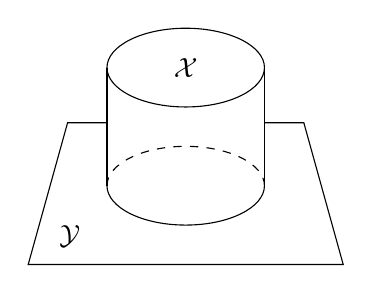
\begin{tikzpicture}[baseline=(O)]
	\draw (1, 1.5) ellipse[x radius=1, y radius=0.5] node {$\mathcal{X}$};
	\draw (0, 0) arc[start angle=180, end angle=360, x radius=1, y radius=0.5];
	\draw[dashed] (0, 0) arc[start angle=180, end angle=0, x radius=1, y radius=0.5];
	\draw (2, 1.5) -- (2, 0);
	\draw (0, 1.5) -- (0, 0);
	\draw (0, 0.8) -- (-0.5, 0.8) -- (-1, -1) node[xshift=1.5em,  yshift=1em] {$\mathcal{Y}$} -- (3, -1) -- (2.5, 0.8) -- (2, 0.8);
	\coordinate (O) at (0, 0.5);
\end{tikzpicture} \quad
	\Cone_{\mathrm{top}}(F) = 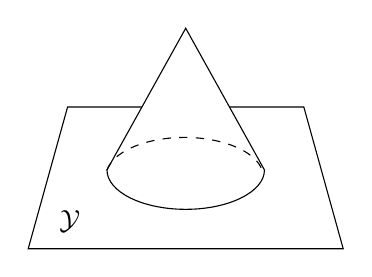
\begin{tikzpicture}[baseline=(O)]
	\draw (0, 0.8) -- (-0.5, 0.8) -- (-1, -1) node[xshift=1.5em,  yshift=1em] {$\mathcal{Y}$} -- (3, -1) -- (2.5, 0.8) --cycle;
	\filldraw[fill=white] (1, 1.8) -- (0, 0) arc[start angle=180, end angle=360, x radius=1, y radius=0.5] --cycle;
	\draw[dashed] (0, 0) arc[start angle=170, end angle=10, x radius=1, y radius=0.5];
	\coordinate (O) at (0, 0.5);
\end{tikzpicture}\]

% segment-id: o014.li2.chapter8.mapping-cone-revisited.p003
Himpunan simplisial memberikan cara konkret untuk menguraikan ruang
topologis. Secara lebih tepat, Teorema~\ref{prop:geom-Sing-adjunction}
memberikan pasangan adjoin
% segment-id: o014.li2.chapter8.mapping-cone-revisited.q004
\[\begin{tikzcd}
	{|\cdot|}: \cate{sSet} \arrow[shift left, r] & \cate{Top}: \mathrm{Sing}, \arrow[shift left, l]
\end{tikzcd}\]
dan kedua kategori tersebut memodelkan teori homotopi yang ekuivalen dalam
pengertian yang tepat. Konstruksi yang sama berlaku bila $\cate{Top}$ diganti
oleh $\cate{CGHaus}$. Sekarang kita terjemahkan pembahasan di atas ke
$\cate{sSet}$. Kita boleh mengandaikan
% segment-id: o014.li2.chapter8.mapping-cone-revisited.q005
\[ \mathcal{X} = |X|, \quad \mathcal{Y} = |Y|, \quad F = |f|: |X| \to |Y|, \]
dengan $f:X\to Y$ morfisme dalam $\cate{sSet}$. Dari sudut pandang
himpunan simplisial, kerucut pemetaan lebih mudah dijelaskan daripada
silinder pemetaan. Kita mulai dari kerucut $\mathcal{X}$,
$\Cone_{\mathrm{top}}(\mathcal{X}):=
\Cone_{\mathrm{top}}(\identity_{\mathcal{X}})$. Jika
$\mathcal{X}=|X|$, maka
$\Cone_{\mathrm{top}}(\mathcal{X})\simeq|X^{\lhd}|\simeq|X^{\rhd}|$
(Contoh~\ref{eg:cone-realization}). Di bawah ini kita berfokus pada
kerucut kiri $X^{\lhd}=\Delta^0\star X$ dan kompleks rantai yang
bersesuaian.
\index{himpunan simplisial!kerucut (cone)}

% segment-id: o014.li2.chapter8.mapping-cone-revisited.p004
Untuk setiap himpunan simplisial $Z$, tuliskan $Z_n^{\mathrm{nd}}$ untuk
himpunan semua simpleks-$n$ nondegenerat di dalamnya, dan tuliskan
$\{\mathrm{pt}\}=(\Delta^0)_0=(\Delta^0)_0^{\mathrm{nd}}$.
Proposisi~\ref{prop:join-nd}, atau intuisi topologis, memberikan
% segment-id: o014.li2.chapter8.mapping-cone-revisited.q006
\begin{equation}\label{eqn:Cone-X-aux1}
	(\Delta^0 \star X)^{\mathrm{nd}}_n = \begin{cases}
		X^{\mathrm{nd}}_n \sqcup \left( \{ \mathrm{pt} \} \times X^{\mathrm{nd}}_{n-1} \right), & n > 0 \\
		\{\mathrm{pt}\} \sqcup X_0, & n = 0.
	\end{cases}
\end{equation}

% segment-id: o014.li2.chapter8.mapping-cone-revisited.p005
Dengan mensubstitusikan \eqref{eqn:join-formulas} dan rumus umum yang
dibahas di atasnya, tampak bahwa untuk $n\geq1$, pembatasan
$d_i:(\Delta^0\star X)_n\to(\Delta^0\star X)_{n-1}$ pada
$\{\mathrm{pt}\}\times X_{n-1}$ dan $X_n$ adalah sebagai berikut:
% segment-id: o014.li2.chapter8.mapping-cone-revisited.q007
\begin{equation}\label{eqn:Cone-X-aux2}\begin{gathered}
	\begin{tikzcd}[column sep=small,
		/tikz/execute at end picture={
			\node [rectangle, draw, fit=(A) (B)] {};
			\node at ($(A)!.5!(C) + (0, 0.8)$) {$1 \leq i \leq n$};
		}]
		|[alias=A]| \{\mathrm{pt}\} \times X_{n-1} \arrow[d, "{\identity \times d_{i-1}}"'] & |[alias=C]| X_n \arrow[d, "{d_i}"] \\
		\{\mathrm{pt}\} \times X_{n-2} & |[alias=B]| X_{n-1}
	\end{tikzcd} \quad
	\begin{tikzcd}[column sep=small,
		/tikz/execute at end picture={
			\node [rectangle, draw, fit=(A) (B)] {};
			\node at ($(A)!.5!(C) + (0, 0.8)$) {$i=0$};
		}]
		|[alias=A]| \{\mathrm{pt}\} \times X_{n-1} \arrow[rd, "{\mathrm{pr}_2}"] & |[alias=C]| X_n \arrow[d, "{d_0}"] \\
		\{\mathrm{pt}\} \times X_{n-2} & |[alias=B]| X_{n-1}
	\end{tikzcd}
\end{gathered}\end{equation}
Jika $n=1$, $\{\mathrm{pt}\}\times X_{n-2}$ dalam rumus ini harus
dipahami sebagai $\{\mathrm{pt}\}$.

% segment-id: o014.li2.chapter8.mapping-cone-revisited.p006
Karena tujuan kita ialah kompleks rantai, langkah berikutnya adalah
melinearkan masalah melalui funktor $\Z(\mathord\cdot)$ dari
Definisi~\ref{def:free-simplicial-Ab}, lalu beralih ke kompleks rantai
melalui korespondensi Dold--Kan:
% segment-id: o014.li2.chapter8.mapping-cone-revisited.q008
\begin{equation*}
	\mathrm{N}(\Z X^{\lhd}) \simeq \mathrm{C}(\Z X^{\lhd}) \big/ \text{bagian degenerat} \quad \text{(Proposisi \ref{prop:Dold-Kan-v})}.
\end{equation*}
Untuk menyingkat notasi dalam sisa bagian ini, kita tulis
$\mathrm{N}X:=\mathrm{N}(\Z X)$ dan
$\mathrm{N}f:=\mathrm{N}(\Z f)$. Struktur kompleks rantai
$\mathrm{C}(\Z X^{\lhd})$ berasal dari
$\partial_n:=\sum_{i=0}^n(-1)^id_i$. Dengan menggabungkan
\eqref{eqn:Cone-X-aux1}, \eqref{eqn:Cone-X-aux2}, dan deskripsi
$\Cone(\identity_{\mathrm{N}X})$ dalam Catatan~\ref{rem:cone-chain},
diperoleh barisan eksak pendek kompleks rantai
% segment-id: o014.li2.chapter8.mapping-cone-revisited.q009
\[ 0 \to \underbracket{\Z\{\mathrm{pt}\}}_{\text{derajat nol}} \to \mathrm{N}(\Z X^{\lhd}) \to \Cone(\identity_{\mathrm{N}X}) \to 0. \]

% segment-id: o014.li2.chapter8.mapping-cone-revisited.p007
Selanjutnya, funktor $|\mathord\cdot|$ dan
$\mathrm{N}\Z(\mathord\cdot)$ mempertahankan diagram dorongan keluar:
yang pertama merupakan funktor adjoin kiri, sedangkan yang kedua merupakan
komposisi funktor adjoin kiri dengan suatu ekuivalensi; dalam topologi, diagram dorongan keluar
berarti perekatan. Karena itu, untuk $f:X\to Y$ definisikan
% segment-id: o014.li2.chapter8.mapping-cone-revisited.q010
\begin{equation*}
	\Cone_{\mathrm{s}}(f) := X^{\lhd} \dsqcup{X, f} Y.
\end{equation*}
Kemudian kita memperoleh
% segment-id: o014.li2.chapter8.mapping-cone-revisited.q011
\[\begin{tikzcd}
	\mathcal{X} \arrow[d, "F"'] \arrow[r, "{\text{dasar}}"] & \Cone_{\mathrm{top}}(\mathcal{X}) \arrow[d] \\
	\mathcal{Y} \arrow[r] & \Cone_{\mathrm{top}}(F) \arrow[phantom, lu, "\boxplus" description]
\end{tikzcd} \xleftarrow{|\cdot|} \begin{tikzcd}
	X \arrow[d, "f"'] \arrow[r, "\text{kanonik}"] & X^{\lhd} \arrow[d] \\
	Y \arrow[r] & \Cone_{\mathrm{s}}(f) \arrow[phantom, lu, "\boxplus" description]
\end{tikzcd} \xrightarrow{\mathrm{N}} \begin{tikzcd}
	\mathrm{N}X \arrow[d, "{\mathrm{N}f}"'] \arrow[r] & \mathrm{N}X^{\lhd} \arrow[d] \\
	\mathrm{N}Y \arrow[r] & \mathrm{N}\Cone_{\mathrm{s}}(f) \arrow[phantom, lu, "\boxplus" description]
\end{tikzcd}\]
Rangkaian konstruksi ini menunjukkan bahwa padanan aljabar linear dari
$\Cone_{\mathrm{top}}(F)$ seharusnya ialah
$\mathrm{N}\Cone_{\mathrm{s}}(f)$.

% segment-id: o014.li2.chapter8.mapping-cone-revisited.pr001
\begin{proposition}\label{prop:Cone-comparison}
	\index{kerucut pemetaan@kerucut pemetaan}
	Dengan notasi di atas, terdapat barisan eksak pendek kanonik kompleks
	rantai
	% segment-id: o014.li2.chapter8.mapping-cone-revisited.q012
	\[ 0 \to \underbracket{\Z\{\mathrm{pt}\}}_{\text{derajat nol}} \to \mathrm{N}\Cone_{\mathrm{s}}(f) \to \Cone(\mathrm{N}f) \to 0. \]
\end{proposition}
\begin{proof}
	Dorongan keluar tidak memengaruhi subkompleks rantai
	$\Z\{\mathrm{pt}\}$ dari $\mathrm{N}X^{\lhd}$, yang bersesuaian
	dengan puncak kerucut. Pada derajat $n$, ia mengganti semua $X_n$ dengan
	$Y_n$ dan mengganti proyeksi $\mathrm{pr}_2$ dalam
	\eqref{eqn:Cone-X-aux2} dengan $f_{n-1}\mathrm{pr}_2$. Karena itu, pada
	tingkat hasil bagi $\Cone(\identity_{\mathrm{N}X})$, hasil dorongan
	keluar tersebut adalah tepat $\Cone(\mathrm{N}f)$; lihat
	Catatan~\ref{rem:cone-chain}.
\end{proof}

% segment-id: o014.li2.chapter8.mapping-cone-revisited.r001
\begin{remark}
	Silinder pemetaan $\Cyl_{\mathrm{top}}(F)$ dan versi kompleks rantainya
	dapat dibandingkan dengan cara serupa; dalam hal ini tidak perlu lagi
	mengambil hasil bagi oleh sumbangan puncak. Akan tetapi, silinder
	pemetaan melibatkan hasil kali himpunan simplisial, sedangkan
	$\mathrm{N}$ bukan funktor monoidal. Karena itu, penjelasan topologis
	biasanya menggunakan kompleks CW, bukan himpunan simplisial, sebab hasil
	kali lebih mudah ditangani dalam dunia kompleks CW.
\end{remark}

% segment-id: o014.li2.chapter8.mapping-cone-revisited.p008
Singkatnya, kerucut pemetaan kompleks rantai adalah hasil bagi kerucut
pemetaan yang berasal dari himpunan simplisial (atau topologi) oleh satu
salinan $\Z$ yang berasal dari puncak $\mathrm{pt}$. Dalam studi kompleks
rantai, peran utama kerucut pemetaan ialah bahwa setiap pemetaan
$\phi:A\to B$ meluas menjadi barisan
% segment-id: o014.li2.chapter8.mapping-cone-revisited.q013
\begin{equation}\label{eqn:cofiber-comparison-A}
	A \xrightarrow{\phi} B \to \Cone(\phi) \to A[-1] \xrightarrow{-\phi[-1]} B[-1] \to \cdots .
\end{equation}

% segment-id: o014.li2.chapter8.mapping-cone-revisited.p009
Dalam situasi topologis, pemetaan yang bersesuaian dengan
$\Cone(\phi)\to A[-1]$ diperoleh dengan mengerutkan dasar
$\mathcal{Y}$ dari $\Cone_{\mathrm{top}}(F)$ menjadi satu titik. Hasil
pengerutan itu dinotasikan oleh $S\mathcal{X}$; ia tidak bergantung pada
$\mathcal{Y}$ (lihat gambar di bawah) dan memberikan sebuah funktor $S$.
Barisan pemetaan yang bersesuaian ialah
% segment-id: o014.li2.chapter8.mapping-cone-revisited.q014
\begin{equation*}
	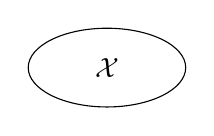
\begin{tikzpicture}[baseline=(O)]
		\draw (1, 0) ellipse[x radius=1, y radius=0.5] node {$\mathcal{X}$};
		\coordinate (O) at (0, 0);
	\end{tikzpicture}
	\xrightarrow{F}
	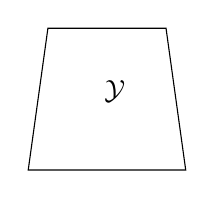
\begin{tikzpicture}[baseline=(O), xscale=0.5]
		\draw (0, 0.8) -- (-0.5, 0.8) -- (-1, -1) -- (3, -1) -- (2.5, 0.8) --cycle;
		\node at (1.2, 0) {$\mathcal{Y}$};
		\coordinate (O) at (0, 0.5);
	\end{tikzpicture}
	\xrightarrow{\text{inklusi}}
	\begin{tikzpicture}[baseline=(O), xscale=0.8]
		\draw (0, 0.8) -- (-0.5, 0.8) -- (-1, -1) node[xshift=1.5em,  yshift=1em] {$\mathcal{Y}$} -- (3, -1) -- (2.5, 0.8) --cycle;
		\filldraw[fill=white] (1, 1.8) -- (0, 0) arc[start angle=180, end angle=360, x radius=1, y radius=0.5] --cycle;
		\draw[dashed] (0, 0) arc[start angle=170, end angle=10, x radius=1, y radius=0.5];
		\coordinate (O) at (0, 0.5);
	\end{tikzpicture}
	\xrightarrow{\text{kerut}}
	\begin{tikzpicture}[baseline=(O), xscale=0.7, yscale=0.7]
		\draw (2, 0) -- (1, 1.8) -- (0, 0);
		\draw[dashed] (0, 0) arc[start angle=170, end angle=10, x radius=1, y radius=0.5];
		\draw (0, 0) arc[start angle=190, end angle=350, x radius=1, y radius=0.5];
		\node at (1, 0) {$\mathcal{X}$};
		\draw (0, 0) -- (1, -1.8) -- (2, 0);
		\coordinate (O) at (0, 0.5);
	\end{tikzpicture}
	\to \cdots .
\end{equation*}
Barisan ini disebut \emph{barisan kofiber} yang dihasilkan oleh $f$
(lebih tepatnya, versi tanpa titik pangkal). Jika kita bekerja dalam
$\cate{sSet}$ dan mengambil kompleks rantai dari barisan yang bersesuaian,
hasilnya kira-kira \eqref{eqn:cofiber-comparison-A}. Kata ``kira-kira''
diperlukan karena:
\begin{itemize}
	\item Pemetaan $S\mathcal{X}\to S\mathcal{Y}$ tidak dapat sekadar
	didefinisikan sebagai $S(F)$; koordinat vertikal harus dibalik dengan tepat.
	Pada tingkat aljabar linear, hal ini bersesuaian dengan
	$-\phi[-1]$ dalam \eqref{eqn:cofiber-comparison-A}; lihat buku ajar
	topologi untuk perinciannya.
	\item Seperti terlihat dalam Proposisi~\ref{prop:Cone-comparison},
	berbagai kompleks rantai mengandung satu salinan $\Z$ berlebih yang
	bersesuaian dengan puncak ruang-ruang seperti
	$\Cone_{\mathrm{top}}(F)$ dan $S\mathcal{X}$. Dalam topologi, persoalan
	ini dihindari dengan memakai ruang bertitik pangkal, lalu dalam
	konstruksi topologis kerucut mengerutkan bagian yang terhubung dengan
	titik pangkal tersebut.
\end{itemize}

% segment-id: o014.li2.chapter8.mapping-cone-revisited.p010
Jika untuk sementara semua perincian dikesampingkan, secara garis besar
teori kategori turunan yang dibangun dalam \S\ref{sec:derived-cat}, dengan
$\mathcal{A}=\cate{Ab}$, dapat pula dipandang sebagai ``linearisasi'' yang
agak kasar dari teori homotopi\footnote{Lebih tepatnya teori homotopi
stabil, karena kompleks rantai membolehkan suku berderajat negatif.}.

% segment-id: o014.li2.chapter8.mapping-cone-revisited.p011
Karena persoalan-persoalan terkait semakin melibatkan gagasan dan metode
topologis, kita berhenti di sini agar tidak menyimpang terlalu jauh.

% Unit 119 terjemahan Bahasa Indonesia dari chapter8.tex baris 2000--2107.
% Sumber: Methods of Algebra, Volume 2, commit
% 9a5803ff77dd3257484cb177f851a73770a59dd3 (CC BY 4.0).
% stable-unit-id: o014.aljabr2.chapter8.exercises-a
% Cakupan: paruh pertama latihan Bab 8, dari pembukaan Exercises hingga
% definisi objek L-proyektif dan T-injektif; Unit 120 melanjutkan baris 2108.

\hypertarget{o014.aljabr2.chapter8.exercises-a}{ }
% segment-id: o014.aljabr2.chapter8.exercises-a.h001
\begin{Exercises}
% segment-id: o014.aljabr2.chapter8.exercises-a.ex001
	\item Buktikan bahwa, untuk setiap kategori $\mathcal{C}$, konstruksi
	$C\mapsto\mathrm{const}(C)$ dari Contoh~\ref{eg:const-simplicial}
	memberikan funktor penuh dan setia
	$\mathcal{C}\to\cate{s}\mathcal{C}$.

% segment-id: o014.aljabr2.chapter8.exercises-a.ex002
	\item Misalkan $X$ himpunan simplisial dan $x\in X_n$. Buktikan bahwa
	terdapat barisan indeks $j_1<\cdots<j_h$ dan suatu simpleks nondegenerat
	$y$ sedemikian sehingga $x=s_{j_h}\cdots s_{j_1}(y)$, dan bahwa $y$ unik.

% segment-id: o014.aljabr2.chapter8.exercises-a.hi001
	\begin{hint}
		Kesulitannya terletak pada keunikan. Misalkan
		$Sy=x=S'y'$, dengan $S$ dan $S'$ keduanya berbentuk seperti dalam
		pernyataan. Kita dapat memilih komposisi $D$ dari serangkaian morfisme muka
		sedemikian sehingga $y=DSy=DS'y'$. Ubah $DS'$ ke bentuk
		$\widetilde{S}'\widetilde{D}$ (makna notasinya jelas). Karena $y$
		nondegenerat, harus berlaku $\widetilde{S}'=\identity$, sehingga
		$y'=\widetilde{D}y$. Gunakan simetri untuk menyimpulkan
		$y=y'$ dan $\widetilde{D}=\identity$.
	\end{hint}

% segment-id: o014.aljabr2.chapter8.exercises-a.ex003
	\item Tunjukkan bahwa terdapat diagram berikut dalam $\cate{sSet}$, dengan
	bagian atas maupun bawah yang komutatif, untuk
	$0\leq i<j\leq n$:
% segment-id: o014.aljabr2.chapter8.exercises-a.q001
	\[\begin{tikzcd}
		\Delta^{n-2} \arrow[d, "{\iota_{i < j}}"'] \arrow[r, "{\mathrm{d}^{j-1}}"] & \Delta^{n-1} \arrow[d, "\iota_i"] \arrow[rd, "{\mathrm{d}^i}"] & \\
		\bigsqcup_{0 \leq i' < j' \leq n} \Delta^{n-2} \arrow[shift left, r] \arrow[shift right, r] & \bigsqcup_{i' = 0}^n \Delta^{n-1} \arrow[r] & \partial \Delta^n \\
		\Delta^{n-2} \arrow[u, "{\iota_{i < j}}"] \arrow[r, "{\mathrm{d}^i}"'] & \Delta^{n-1} \arrow[u, "\iota_j"'] \arrow[ru, "{\mathrm{d}^j}"'] &
	\end{tikzcd}\]
	Di sini, $\bigsqcup$ diambil suku demi suku dalam
	$\cate{sSet}=\cate{Set}^{\simpDelta^{\opp}}$, sedangkan
	$\iota_{i<j}$ (atau $\iota_i$) menyatakan embedding ke suku ke-$i<j$
	(atau suku ke-$i$). Semua anak panah pada baris tengah dicirikan oleh
	komutativitas tersebut. Tunjukkan lebih lanjut bahwa baris tengah itu
	merupakan koekualiser.

	Secara serupa, tunjukkan bahwa untuk setiap $0\leq k\leq n$ terdapat pula
% segment-id: o014.aljabr2.chapter8.exercises-a.q002
	\[\begin{tikzcd}
		\Delta^{n-2} \arrow[d, "{\iota_{i < j}}"'] \arrow[r, "{\mathrm{d}^{j-1}}"] & \Delta^{n-1} \arrow[d, "\iota_i"] \arrow[rd, "{\mathrm{d}^i}"] & \\
		\bigsqcup_{\substack{0 \leq i' < j' \leq n \\ i', j' \neq k}} \Delta^{n-2} \arrow[shift left, r] \arrow[shift right, r] & \bigsqcup_{\substack{0 \leq i' \leq n \\ i' \neq k}} \Delta^{n-1} \arrow[r] & \Lambda^n_k \\
		\Delta^{n-2} \arrow[u, "{\iota_{i < j}}"] \arrow[r, "{\mathrm{d}^i}"'] & \Delta^{n-1} \arrow[u, "\iota_j"'] \arrow[ru, "{\mathrm{d}^j}"'] &
	\end{tikzcd}\]
	dengan baris tengah merupakan koekualiser dan $i,j\neq k$. Cobalah
	jelaskan makna topologis koekualiser tersebut.

% segment-id: o014.aljabr2.chapter8.exercises-a.ex004
	\item Verifikasi sifat-sifat berikut dari operasi join $\star$ dalam
	Definisi~\ref{def:simplicial-join}.
	\begin{enumerate}[(i)]
% segment-id: o014.aljabr2.chapter8.exercises-a.i001
		\item Himpunan simplisial secara alami membentuk kategori monoidal
		terhadap $\star$, dengan himpunan simplisial kosong yang bernilai konstan
		$\emptyset$ sebagai objek satuannya.
% segment-id: o014.aljabr2.chapter8.exercises-a.i002
		\item Dualitas pembalikan urutan dari
		Catatan~\ref{rem:simpDelta-order-reversal} memberikan automorfisme
		$\cate{sSet}$, yang untuk sementara ditulis $X\mapsto\hat{X}$. Tunjukkan
		bahwa $(X\star Y)^{\wedge}\simeq\hat{Y}\star\hat{X}$.
% segment-id: o014.aljabr2.chapter8.exercises-a.i003
		\item Verifikasi
		$\Delta^p\star\Delta^q\simeq\Delta^{p+q+1}$.
	\end{enumerate}

% segment-id: o014.aljabr2.chapter8.exercises-a.ex005
	\item Tunjukkan bahwa pengambilan dual pembalikan urutan dari suatu
	himpunan simplisial, hingga homeomorfisme kanonik, tidak mengubah realisasi
	geometrisnya.
% segment-id: o014.aljabr2.chapter8.exercises-a.hi002
	\begin{hint}
		Mulailah dengan kasus $\Delta^n$.
	\end{hint}

% segment-id: o014.aljabr2.chapter8.exercises-a.ex006
	\item Verifikasi pernyataan Contoh~\ref{eg:cone-realization}.

% segment-id: o014.aljabr2.chapter8.exercises-a.ex007
	\item Misalkan $\mathcal{C}$ dan $\mathcal{C}'$ kategori. Definisikan
	kategori $\mathcal{C}\star\mathcal{C}'$ sebagai berikut:
% segment-id: o014.aljabr2.chapter8.exercises-a.q003
	\begin{align*}
		\Obj(\mathcal{C} \star \mathcal{C}') & := \Obj(\mathcal{C}) \sqcup \Obj(\mathcal{C}'), \\
		\Hom_{\mathcal{C} \star \mathcal{C}'}(X, Y) & := \begin{cases}
			\Hom_{\mathcal{C}}(X, Y), & X, Y \in \Obj(\mathcal{C}) \\
			\Hom_{\mathcal{C}'}(X, Y), & X, Y \in \Obj(\mathcal{C}'), \\
			\text{himpunan satu titik}, & X \in \Obj(\mathcal{C}), \; Y \in \Obj(\mathcal{C}'), \\
			\emptyset, & X \in \Obj(\mathcal{C}'), \; Y \in \Obj(\mathcal{C}).
		\end{cases}
	\end{align*}
	Komposisi morfisme dan morfisme identitas didefinisikan dengan cara yang
	langsung. Buktikan bahwa operasi join $\star$ pada himpunan simplisial dan
	funktor saraf dari Contoh~\ref{eg:nerve-cat} berhubungan melalui
% segment-id: o014.aljabr2.chapter8.exercises-a.q004
	\[ \mathrm{N}(\mathcal{C}) \star \mathrm{N}(\mathcal{C}') \simeq \mathrm{N}(\mathcal{C} \star \mathcal{C}'). \]

% segment-id: o014.aljabr2.chapter8.exercises-a.ex008
	\item Berikan bukti yang lebih rinci untuk
	Persamaan~\eqref{eqn:shuffle-sign-0} dan
	\eqref{eqn:shuffle-sign-1}.

% segment-id: o014.aljabr2.chapter8.exercises-a.ex009
	\item Untuk objek simplisial $X$ dalam sebarang kategori, definisikan
	objek simplisial yang disebut pergeseran, $\mathrm{Déc}_0X$ dan
	$\mathrm{Déc}^0X$, melalui
	$(\mathrm{Déc}_0X)_n=(\mathrm{Déc}^0X)_n=X_{n+1}$ dan
% segment-id: o014.aljabr2.chapter8.exercises-a.q005
	\begin{gather*}
		d^{\mathrm{Déc}_0 X, n}_i = d^{X, n+1}_i, \quad s^{\mathrm{Déc}_0 X, n}_j = s^{X, n+1}_j, \\
		d^{\mathrm{Déc}^0 X, n}_i = d^{X, n+1}_{i+1}, \quad
		s^{\mathrm{Déc}^0 X, n}_j = s^{X, n+1}_{j+1}.
	\end{gather*}
	Tunjukkan bahwa keduanya terdefinisi dengan baik dan saling berhubungan
	melalui dualitas pembalikan urutan
	(Catatan~\ref{rem:simpDelta-order-reversal}). Tunjukkan pula bahwa untuk
	kategori aditif berlaku
	$\mathrm{C}(\mathrm{Déc}^0X)=\mathrm{C}(X)[1]$; lihat
	Catatan~\ref{rem:chain-cplx-translation}.
	\index{objek simplisial!pergeseran@pergeseran (décalage)}
	\index[sym1]{Dec@$\mathrm{Déc}_0 X, \mathrm{Déc}^0 X$}

% segment-id: o014.aljabr2.chapter8.exercises-a.ex010
	\item Dengan meneruskan latihan sebelumnya, tunjukkan bahwa
	$d_0:X_1\to X_0$ (atau $d_1:X_1\to X_0$) memberikan augmentasi pada
	$\mathrm{Déc}_0X$ (atau $\mathrm{Déc}^0X$), dengan $X_0$ sebagai suku
	derajat $-1$. Tunjukkan lebih lanjut bahwa setelah augmentasi,
	$\mathrm{Déc}_0X$ dapat dikontraksi dari kanan dan $\mathrm{Déc}^0X$
	dapat dikontraksi dari kiri; lihat Definisi~\ref{def:contractible-aug}.
% segment-id: o014.aljabr2.chapter8.exercises-a.hi003
	\begin{hint}
		Cukup tangani $\mathrm{Déc}_0X$. Ambil
		$k_{n-1}:=s_n:X_n\to X_{n+1}$.
	\end{hint}

% segment-id: o014.aljabr2.chapter8.exercises-a.ex011
	\item Buktikan bahwa kategori kecil $\mathcal{C}$ merupakan grupoid
	(yakni semua morfismenya invertibel) jika dan hanya jika
	$\mathrm{N}\mathcal{C}$ memenuhi syarat berikut: untuk setiap
	$n\in\Z_{\geq1}$ dan $0\leq i\leq n$, setiap morfisme
	$\Lambda^n_i\to\mathrm{N}\mathcal{C}$ dapat diperluas menjadi
	$\Delta^n\to\mathrm{N}\mathcal{C}$, tanpa menuntut keunikan. Himpunan
	simplisial yang memenuhi syarat perluasan ini disebut kompleks Kan.

% segment-id: o014.aljabr2.chapter8.exercises-a.ex012
	\item Lanjutkan pembahasan Contoh~\ref{eg:classifying-space-std-cplx}.
	Tunjukkan bahwa kompleks ternormalisasi $\overline{\mathsf{L}}$, setelah
	dibalik menjadi kompleks rantai, isomorfik dengan
	$\mathrm{N}(\Bbbk\mathrm{E}\Gamma)$.
% segment-id: o014.aljabr2.chapter8.exercises-a.hi004
	\begin{hint}
		Pertama, gunakan Proposisi~\ref{prop:Dold-Kan-v} untuk mengidentifikasi
		$\mathrm{N}(X)$ dengan suatu hasil bagi dari $\mathrm{C}(X)$.
	\end{hint}

% segment-id: o014.aljabr2.chapter8.exercises-a.ex013
	\item Misalkan $\Gamma$ monoid. Tuliskan $\cated{Set}\Gamma$ untuk kategori
	semua himpunan kecil dengan aksi kanan $\Gamma$.
	\begin{enumerate}[(i)]
% segment-id: o014.aljabr2.chapter8.exercises-a.i004
		\item Deskripsikan secara eksplisit pasangan adjoin bebas--pelupa
% segment-id: o014.aljabr2.chapter8.exercises-a.q006
		\[\begin{tikzcd}
			\mathrm{F}: \cate{Set} \arrow[shift left, r] & \cated{Set}\Gamma \arrow[shift left, l]: U
		\end{tikzcd}\]
		beserta morfisme unit dan kounitnya. Tunjukkan bahwa monad $T$ yang
		bersesuaian memberikan ekuivalensi
		$\cated{Set}\Gamma\simeq\cate{Set}^T$.

% segment-id: o014.aljabr2.chapter8.exercises-a.hi005
		\begin{hint}
			Funktor $\mathrm{F}$ memetakan himpunan $X$ ke $X\times\Gamma$,
			dengan $\Gamma$ bekerja melalui perkalian kanan pada komponen kedua.
			Morfisme unit adalah $x\mapsto(x,1)$, sedangkan morfisme kounit
			adalah peta aksi.
		\end{hint}
% segment-id: o014.aljabr2.chapter8.exercises-a.i005
		\item Untuk setiap himpunan-$\Gamma$ kanan $X$, deskripsikan objek
		simplisial $\mathrm{Bar}(X)$ yang bersesuaian dalam
		$\cated{Set}\Gamma$; lihat Contoh~\ref{eg:bar-adjunction} dan
		\ref{eg:bar-comonad}.
% segment-id: o014.aljabr2.chapter8.exercises-a.i006
		\item Ambil himpunan satu titik $X=\{\mathrm{pt}\}$ dengan aksi kanan
		$\Gamma$ trivial. Tunjukkan bahwa objek simplisial yang bersesuaian
		isomorfik dengan $\mathrm{E}\Gamma$ dari
		Contoh~\ref{eg:classifying-space}; objek tersebut menjadi objek
		simplisial dalam $\cated{Set}\Gamma$ melalui aksi kanan $\Gamma$ pada
		setiap $(\mathrm{E}\Gamma)_n$.
	\end{enumerate}

% segment-id: o014.aljabr2.chapter8.exercises-a.ex014
	\item Tetapkan grup $\Gamma$. Dalam Contoh~\ref{eg:HH-comonad}, ambil
	aljabar grup $R=\Bbbk[\Gamma]$ dan ambil $M$ sebagai modul-$\Gamma$
	trivial $\Bbbk$; lihat Contoh~\ref{eg:trivial-G-mod}. Tunjukkan bahwa
	$\epsilon_{\Bbbk}:\mathrm{C}(\mathrm{Bar}(\Bbbk))\to\Bbbk$ yang
	bersesuaian isomorfik dengan resolusi
	$\mathsf{L}=(\mathsf{L}_n,\partial'_n)_n\to\Bbbk$ dari
	Proposisi~\ref{prop:trivial-mod-resolution}.
% segment-id: o014.aljabr2.chapter8.exercises-a.hi006
	\begin{hint}
		Gunakan \eqref{eqn:L-basis-partial}.
	\end{hint}

% segment-id: o014.aljabr2.chapter8.exercises-a.ex015
	\item Ambil gelanggang komutatif $\Bbbk$ dan
	$\mathcal{A}=\Bbbk\dcate{Mod}$, dengan
	$\otimes=\otimes_{\Bbbk}$. Misalkan $\Gamma$ grup. Tinjau objek
	simplisial $\Bbbk\mathrm{E}\Gamma$ dari
	Contoh~\ref{eg:classifying-contractible}. Terapkan
	Definisi~\ref{def:Eilenberg-Zilber} tentang morfisme Alexander--Whitney
	pada $X:=\Bbbk\mathrm{E}\Gamma\boxtimes\Bbbk\mathrm{E}\Gamma$,
	lalu tinjau morfisme
% segment-id: o014.aljabr2.chapter8.exercises-a.q007
	\[ \mathrm{C}(\Bbbk\mathrm{E}\Gamma) \to \mathrm{C}(\underbracket{\Bbbk\mathrm{E}\Gamma \otimes \Bbbk\mathrm{E}\Gamma}_{\simeq \Bbbk(\mathrm{E}\Gamma \times \mathrm{E}\Gamma)}) \xrightarrow{\overline{\mathrm{AW}}} \mathrm{C}(\Bbbk\mathrm{E}\Gamma) \otimes \mathrm{C}(\Bbbk\mathrm{E}\Gamma). \]
	Anak panah pertama diinduksi oleh embedding diagonal himpunan simplisial
	$\mathrm{E}\Gamma\to\mathrm{E}\Gamma\times\mathrm{E}\Gamma$. Mengingat
	Contoh~\ref{eg:classifying-space-std-cplx}, komposisinya juga dapat
	dipandang sebagai morfisme kompleks rantai
% segment-id: o014.aljabr2.chapter8.exercises-a.q008
	\[ \mathsf{L} \to \mathsf{L} \otimes \mathsf{L}. \]
	Gunakan ini untuk menafsirkan morfisme
	$\Delta:\mathsf{L}\to\mathsf{L}\otimes\mathsf{L}$ yang digunakan dalam
	definisi hasil kali cawan pada kohomologi grup; lihat
	Lema~\ref{prop:cup-resolution}~(ii).

% segment-id: o014.aljabr2.chapter8.exercises-a.hi007
	\begin{hint}
		Dengan menyubstitusikan definisi $\overline{\mathrm{AW}}$, terlihat
		bahwa komponen $(p,q)$ dari morfisme komposit berbeda dengan yang ada
		dalam Lema~\ref{prop:cup-resolution}~(ii) sebesar faktor $(-1)^{pq}$.
		Perbedaan ini muncul karena pembahasan di sana menggunakan
		$(\mathsf{L}_n,\partial_n)_n$, sedangkan
		Contoh~\ref{eg:classifying-space-std-cplx} menggunakan
		$(\mathsf{L}_n,\partial'_n)_n$. Pada tingkat himpunan simplisial
		$\mathrm{E}\Gamma$, keduanya berbeda dengan suatu pembalikan urutan
		(Catatan~\ref{rem:simpDelta-order-reversal}). Perhatikan bahwa dualitas
		pembalikan urutan mempertukarkan peran $\lambda^n_p$ dan $\rho^n_q$
		dalam $\overline{\mathrm{AW}}$, atau dengan kata lain mempertukarkan
		kedua salinan $\mathrm{C}(\Bbbk\mathrm{E}\Gamma)$.
	\end{hint}

% segment-id: o014.aljabr2.chapter8.exercises-a.ex016
	\item Tinjau komonad $(L,\delta,\epsilon)$ pada kategori $\mathcal{D}$.
	Untuk setiap $\mathcal{M}\in\Obj(\mathcal{D})$, jika
	$\epsilon_{\mathcal{M}}:L\mathcal{M}\to\mathcal{M}$ mempunyai invers
	kanan $f:\mathcal{M}\to L\mathcal{M}$, maka $\mathcal{M}$ disebut
	\emph{objek $L$-proyektif}. Secara dual, dari monad $(T,\mu,\eta)$ pada
	kategori $\mathcal{C}$ kita mendefinisikan
	\emph{objek $T$-injektif} dalam $\mathcal{C}$.

% Unit 120 terjemahan Bahasa Indonesia dari chapter8.tex baris 2108--2214.
% Sumber: Methods of Algebra, Volume 2, commit
% 9a5803ff77dd3257484cb177f851a73770a59dd3 (CC BY 4.0).
% stable-unit-id: o014.aljabr2.chapter8.exercises-b
% Cakupan: kelanjutan latihan tentang objek L-projektif hingga akhir bab.
% Koreksi sumber terpaksa: baris 2113 identity_{X_n} diperjelas sebagai
% identity_{L^{n+1} M}; baris 2171 objek homologi berada dalam A, bukan Ch(A).

% segment-id: o014.li2.chapter8.exercises-b.p001
	Dengan dualitas, pembahasan berikut terutama berfokus pada konsep
	$L$-projektif. Dengan metode Contoh~\ref{eg:monad-simplicial}, dalam
	$\End(\mathcal{D})$ diperoleh objek simplisial teraugmentasi
	$(L^{n+1})_{n\geq-1}$; data $d_i$, $s_j$, dan sebagainya dihilangkan dari
	notasi. Untuk objek $L$-projektif $\mathcal{M}$ dan $f$ yang
	bersesuaian, definisikan
	% segment-id: o014.li2.chapter8.exercises-b.q001
	\[ k_n := L^{n+1} f : L^{n+1} \mathcal{M} \to L^{n+2} \mathcal{M}, \quad n \geq -1. \]
	Buktikan bahwa ini membuat objek simplisial teraugmentasi
	$(L^{n+1}\mathcal{M})_{n\geq-1}$ dapat dikontraksi dari kanan
	(Definisi~\ref{def:contractible-aug}).

	% segment-id: o014.li2.chapter8.exercises-b.hint001
	\begin{hint}
		Kita tahu bahwa
		$\epsilon_{\mathcal{M}}k_{-1}=\epsilon_{\mathcal{M}}f
		=\identity_{\mathcal{M}}$. Menerapkan $L^{n+1}$ pada kedua ruas
		memberikan
		$d_{n+1}k_n=\identity_{L^{n+1}\mathcal{M}}$, sedangkan naturalitas
		memastikan bahwa
		% segment-id: o014.li2.chapter8.exercises-b.q002
		\[\begin{tikzcd}
			L\mathcal{M} \arrow[r, "Lf"] \arrow[d, "{\epsilon_{\mathcal{M}}}"'] & L^2 \mathcal{M} \arrow[d, "{\epsilon_{L\mathcal{M}}}"] \\
			\mathcal{M} \arrow[r, "f"'] & L\mathcal{M}
		\end{tikzcd} \quad\text{komutatif, yakni}\; d_0 k_0 = f\epsilon_{\mathcal{M}} = k_{-1} \epsilon_{\mathcal{M}}. \]
		Ganti $f$ dengan $L^{n-i}f$, lalu terapkan $L^i$ pada diagram yang
		bersesuaian. Dengan cara yang sama diperoleh
		$d_ik_n=k_{n-1}d_i$ untuk $0\leq i\leq n$.
	\end{hint}

	% segment-id: o014.li2.chapter8.exercises-b.ex001
	\item Untuk suatu gelanggang $R$, pasangan adjoin bebas--pelupa
	$\cate{Set}\leftrightarrows R\dcate{Mod}$ menentukan komonad $L$ pada
	$R\dcate{Mod}$. Buktikan bahwa modul-$R$ kiri bersifat $L$-projektif
	jika dan hanya jika ia merupakan modul projektif.

	% segment-id: o014.li2.chapter8.exercises-b.ex002
	\item Tinjau pasangan adjoin
	% segment-id: o014.li2.chapter8.exercises-b.q003
	$\begin{tikzcd}
		F: \mathcal{C} \arrow[shift left, r] & \mathcal{D}: G \arrow[shift left, l]
	\end{tikzcd}$
	dan komonad yang bersesuaian
	$(L,\delta,\epsilon)=(FG,F\eta G,\epsilon)$ pada
	$\End(\mathcal{D})$ (Contoh~\ref{eg:adjunction-monad}). Buktikan bahwa
	objek berbentuk $F\mathcal{N}$, untuk
	$\mathcal{N}\in\Obj(\mathcal{C})$, selalu $L$-projektif. Sebagai
	akibatnya, untuk setiap $\mathcal{M}\in\Obj(\mathcal{D})$, setiap suku
	dari objek simplisial $(L^{n+1}\mathcal{M})_{n\geq0}$ merupakan objek
	$L$-projektif.

	% segment-id: o014.li2.chapter8.exercises-b.hint002
	\begin{hint}
		Ambil
		$f=F\eta_{\mathcal{N}}:F(\mathcal{N})\to FGF(\mathcal{N})
		=L(F(\mathcal{N}))$. Maka
		$\epsilon_{F(\mathcal{N})}f=\identity_{F(\mathcal{N})}$ tepat
		merupakan salah satu identitas segitiga pasangan adjoin.
	\end{hint}

	% segment-id: o014.li2.chapter8.exercises-b.ex003
	\item Tetap tinjau komonad $L$ yang berasal dari pasangan adjoin
	$(F,G)$. Tunjukkan bahwa $\mathcal{P}\in\Obj(\mathcal{D})$ bersifat
	$L$-projektif jika dan hanya jika ia memiliki sifat pengangkatan
	berikut. Untuk setiap morfisme
	$\alpha:\mathcal{M}_1\to\mathcal{M}_2$ dan
	$\phi:\mathcal{P}\to\mathcal{M}_2$ dalam $\mathcal{D}$, jika
	$G\alpha$ memiliki invers kanan, maka terdapat
	$\beta:\mathcal{P}\to\mathcal{M}_1$ sedemikian rupa sehingga
	$\phi=\alpha\beta$.

	% segment-id: o014.li2.chapter8.exercises-b.hint003
	\begin{hint}
		Untuk arah ``jika'', terapkan sifat pengangkatan pada
		$\alpha:=\epsilon_{\mathcal{P}}:FG(\mathcal{P})\to\mathcal{P}$ dan
		$\phi:=\identity$. Untuk arah ``hanya jika'', jelaskan terlebih dahulu
		bahwa $\mathcal{P}$ dalam sifat pengangkatan dapat diganti oleh
		$FG(\mathcal{P})$, lalu gunakan sifat adjoin untuk menunjukkan bahwa
		% segment-id: o014.li2.chapter8.exercises-b.q004
		\[ \alpha_*:\Hom(FG(\mathcal{P}),\mathcal{M}_1)\to
		\Hom(FG(\mathcal{P}),\mathcal{M}_2) \]
		surjektif.
	\end{hint}

	% segment-id: o014.li2.chapter8.exercises-b.ex004
	\item Untuk gelanggang komutatif $\Bbbk$ sebarang dan homomorfisme
	aljabar-$\Bbbk$ $S\to R$, tinjau pasangan-pasangan adjoin
	% segment-id: o014.li2.chapter8.exercises-b.q005
	\begin{equation*}\begin{tikzcd}[row sep=small]
		R \dotimes{S} (\cdot): S\dcate{Mod} \arrow[shift left, r] & R\dcate{Mod}: \text{lupa}, \arrow[shift left, l] \\
		\text{lupa}: R\dcate{Mod} \arrow[shift left, r] & S\dcate{Mod}: \Hom_S(R, \cdot) \arrow[shift left, l]
	\end{tikzcd}\end{equation*}
	yang masing-masing memberikan komonad $L$ dan monad $T$ pada
	$R\dcate{Mod}$. Gunakan sifat pengangkatan di atas, atau dualnya, untuk
	tentukan syarat perlu dan cukup bagi modul-$R$ kiri $M$ untuk menjadi
	objek $L$-projektif (atau $T$-injektif), lalu bandingkan dengan modul
	projektif (atau injektif).

	Atas dasar ini dapat dibangun teori yang disebut \emph{aljabar homologis
	relatif}; lihat \cite{Ho56}. Ciri khasnya ialah bahwa teori tersebut
	hanya meninjau barisan eksak modul-$R$ yang eksak terbelah di atas $S$.
	Latihan berikut akan menyelidiki versi relatif funktor $\Tor$ dan $\Ext$.
	\index{aljabar homologis relatif@aljabar homologis relatif (relative homological algebra)}

	% segment-id: o014.li2.chapter8.exercises-b.ex005
	\item Tinjau pasangan adjoin di antara kategori abelian
	% segment-id: o014.li2.chapter8.exercises-b.q006
	$\begin{tikzcd}
		F: \mathcal{C} \arrow[shift left, r] & \mathcal{D}: G \arrow[shift left, l]
	\end{tikzcd}$.
	Buktikan untuk setiap $\mathcal{M}\in\Obj(\mathcal{D})$ bahwa:
	\begin{enumerate}[(i)]
		\item Terdapat objek $\mathcal{P}_\bullet$ dari
		$\cate{Ch}_{\geq0}(\mathcal{D})$ beserta morfisme
		$\epsilon:\mathcal{P}_\bullet\to\mathcal{M}$ sedemikian rupa sehingga
		\begin{compactitem}
			\item setiap $\mathcal{P}_n$ bersifat $L$-projektif untuk $n\geq0$;
			\item morfisme identitas pada
			$\cdots\to G\mathcal{P}_1\to G\mathcal{P}_0\to
			G\mathcal{M}\to0$ homotopik nol; dengan kata lain, ini kompleks
			eksak terbelah.
		\end{compactitem}
		\begin{hint}
			Terapkan Proposisi~\ref{prop:bar-null-homotopic}.
		\end{hint}
		\item Untuk setiap dua morfisme
		$\epsilon:\mathcal{P}_\bullet\to\mathcal{M}$ dan
		$\epsilon':\mathcal{P}'_\bullet\to\mathcal{M}$ yang memenuhi
		syarat-syarat di atas, terdapat ekuivalensi homotopi
		$f:\mathcal{P}\to\mathcal{P}'$ sedemikian rupa sehingga
		$\epsilon'f=\epsilon$.
		\begin{hint}
			Gunakan sifat pengangkatan yang diperkenalkan di atas.
		\end{hint}
	\end{enumerate}

	\index{homologi komonad@homologi komonad (cotriple homology)}
	\index{konstruksi bar@konstruksi bar}
	% segment-id: o014.li2.chapter8.exercises-b.ex006
	\item (M.\ Barr, J.\ M.\ Beck) Misalkan $L$ sebuah komonad pada
	kategori $\mathcal{D}$. Tuliskan $\mathrm{Bar}(\mathcal{M})$ untuk
	objek simplisial yang diperoleh dengan mengevaluasi konstruksi
	Contoh~\ref{eg:monad-simplicial} pada
	$\mathcal{M}\in\Obj(\mathcal{D})$. Untuk setiap kategori abelian
	$\mathcal{A}$ dan funktor $E:\mathcal{D}\to\mathcal{A}$, definisikan
	\emph{homologi komonad} dari $(L,E)$ sebagai keluarga objek dalam
	$\mathcal{A}$
	% segment-id: o014.li2.chapter8.exercises-b.q007
	\[ \Hm^L_n(E; \mathcal{M}) := \Hm_n\left( \mathrm{C}(E\mathrm{Bar}(\mathcal{M})) \right), \quad n \in \Z_{\geq 0}, \]
	dengan $E\mathrm{Bar}(\mathcal{M})$ berarti menerapkan $E$ pada setiap
	suku $\mathrm{Bar}(\mathcal{M})$. Secara dual, jika $T$ monad pada
	kategori $\mathcal{C}$ dan $F:\mathcal{C}\to\mathcal{A}$ funktor menuju
	kategori abelian, kita dapat mendefinisikan secara serupa nilai
	\emph{kohomologi monad} $(T,F)$ pada
	$\mathcal{N}\in\Obj(\mathcal{C})$; perinciannya tidak kita uraikan.

	\begin{enumerate}[(i)]
		\item Tuliskan morfisme alami
		$\Hm^L_0(E;\mathcal{M})\to E\mathcal{M}$ dan tunjukkan bahwa ia
		merupakan isomorfisme jika $\mathcal{M}$ objek $L$-projektif.
		\item Misalkan $L$ berasal dari pasangan adjoin $(F,G)$ di antara
		kategori abelian dan $E$ funktor aditif. Buktikan bahwa jika
		$\mathcal{P}_\bullet\to\mathcal{M}$ morfisme dalam
		$\cate{Ch}_{\geq0}(\mathcal{D})$ yang memenuhi
		\begin{compactitem}
			\item setiap $\mathcal{P}_n$ bersifat $L$-projektif untuk $n\geq0$;
			\item morfisme identitas pada
			$\cdots\to G\mathcal{P}_1\to G\mathcal{P}_0\to
			G\mathcal{M}\to0$ homotopik nol,
		\end{compactitem}
		maka
		$\Hm^L_n(E;\mathcal{M})\simeq\Hm_n(E\mathcal{P}_\bullet)$.
		Jadi homologi komonad dapat dihitung menggunakan resolusi
		$L$-projektif semacam itu.
		\item Lanjutkan dengan asumsi di atas. Sebuah pasangan morfisme
		$\mathcal{M}'\to\mathcal{M}\to\mathcal{M}''$ dalam $\mathcal{D}$
		disebut barisan eksak pendek \emph{$G$-terbelah} jika setelah
		menerapkan $G$ ia menjadi barisan eksak pendek terbelah dalam
		$\mathcal{C}$. Buktikan bahwa barisan eksak pendek $G$-terbelah
		secara alami menginduksi barisan eksak panjang untuk
		$\Hm^L_n(E;\mathord\cdot)$.
	\end{enumerate}

	\index{funktor Ext!relatif (relative)}
	\index{funktor Tor!relatif (relative)}
	% segment-id: o014.li2.chapter8.exercises-b.ex007
	\item (G.\ Hochschild \cite{Ho56}) Untuk sebarang gelanggang komutatif
	$\Bbbk$ dan homomorfisme aljabar-$\Bbbk$ $S\to R$, tinjau komonad $L$
	pada $R\dcate{Mod}$ yang ditentukan oleh pasangan adjoin
	% segment-id: o014.li2.chapter8.exercises-b.q008
	\[\begin{tikzcd}
		R \dotimes{S} (\cdot): S\dcate{Mod} \arrow[shift left, r] & R\dcate{Mod}: \text{lupa} \arrow[shift left, l]
	\end{tikzcd}\]
	Untuk modul-$R$ kanan $A$ dan modul-$R$ kiri $B,N$, definisikan
	modul-$\Bbbk$
	% segment-id: o014.li2.chapter8.exercises-b.q009
	\begin{align*}
		\Tor^{R|S}_n(A, N) & := \Hm^L_n\left( A \dotimes{R}(\cdot) ; N \right), \\
		\Ext_{R|S}^n(N, B) & := \Hm^L_n\left( \Hom_R(\cdot, B) ; N \right),
	\end{align*}
	dengan $\Hom_R(\mathord\cdot,B)$ dipandang sebagai funktor
	$R\dcate{Mod}\to S\dcate{Mod}^{\opp}$. Keduanya disebut funktor
	$\Tor$ relatif dan $\Ext$ relatif.
	\begin{enumerate}[(i)]
		\item Tunjukkan bahwa keduanya funktorial dalam setiap variabel.
		Uraikan secara eksplisit kompleks rantai yang bersesuaian, dan
		tunjukkan bahwa
		% segment-id: o014.li2.chapter8.exercises-b.q010
		\[ \Tor^{R|S}_0(A, N) \simeq A \dotimes{R} N, \quad \Ext_{R|S}^0(N, B) \simeq \Hom_R(N, B). \]

		\item Tunjukkan bahwa bifunktor $\Tor^{R|S}_n$ memiliki sifat
		``keseimbangan'' yang serupa dengan
		Teorema~\ref{prop:balanced-primer}.\footnote{$\Ext_{R|S}^n$ tidak
		dibahas karena melibatkan konsep kohomologi monad, yang tidak kita
		uraikan di sini; lihat rujukan untuk perinciannya.}

		\item Buktikan bahwa jika $I$ ideal dua sisi dari $S$ dan $R=S/I$,
		maka untuk $n>0$,
		$\Tor_n^{R|S}=0=\Ext^n_{R|S}$. Jadi $\Tor$ relatif dan $\Ext$
		relatif berbeda dari versi absolut dalam \S\ref{sec:Ext-Tor}.
		\begin{hint}
			Dalam hal ini $L=\identity_{R\dcate{Mod}}$.
		\end{hint}

		\item Tuliskan $R^e=R\dotimes{\Bbbk}R^{\opp}$. Buktikan bahwa
		$\HHm_n(M)\simeq\Tor^{R^e|\Bbbk}_n(M,R)$ dan
		$\HHm^n(M)\simeq\Ext_{R^e|\Bbbk}^n(R,M)$; lihat
		Contoh~\ref{eg:HH-comonad}.
		\begin{hint}
			Reduksikan persoalan ke pernyataan bahwa
			$\mathrm{C}(\mathrm{Bar}(R))_n=R\otimes R^{\otimes n}\otimes R$
			merupakan modul-$R^e$ yang $L$-projektif.
		\end{hint}
	\end{enumerate}
\end{Exercises}

% Unit 121 terjemahan Bahasa Indonesia dari chapter9.tex baris 1--305.
% Sumber: Methods of Algebra, Volume 2, commit
% 9a5803ff77dd3257484cb177f851a73770a59dd3 (CC BY 4.0).
% stable-unit-id: o014.aljabr2.chapter9.duality-a
% Cakupan: pembukaan Bab 9 dan Bagian 9.1 sampai Definisi morfisme dual;
% Unit 122 berlanjut pada baris 306.

\hypertarget{o014.aljabr2.chapter9.duality-a}{ }
% segment-id: o014.aljabr2.chapter9.duality-a.h001
\chapter{Dualitas}\label{sec:duality}

% segment-id: o014.aljabr2.chapter9.duality-a.p001
Konsep dualitas berasal dari teori ruang vektor. Misalkan $\Bbbk$ suatu medan,
dan tuliskan ruang dual dari ruang vektor-$\Bbbk$ $V$ sebagai
$V^\vee:=\Hom_{\Bbbk}(V,\Bbbk)$. Terdapat
\begin{itemize}
	% segment-id: o014.aljabr2.chapter9.duality-a.i001
	\item pemetaan evaluasi $\mathrm{ev}:V\otimes V^\vee\to\Bbbk$, yang
	memetakan $v\otimes\lambda$ ke $\lambda(v)$;
	% segment-id: o014.aljabr2.chapter9.duality-a.i002
	\item jika $V$ berdimensi hingga, terdapat pula pemetaan koevaluasi
	$\mathrm{coev}:\Bbbk\to V^\vee\otimes V$, yang memetakan $1$ ke
	$\sum_{i=1}^n\check{v}_i\otimes v_i$, dengan $(v_i)_{i=1}^n$ sembarang basis
	dari $V$ dan $(\check{v}_i)_{i=1}^n$ basis dualnya.
\end{itemize}

% segment-id: o014.aljabr2.chapter9.duality-a.p002
Dalam kasus berdimensi hingga, keduanya memenuhi identitas dasar
% segment-id: o014.aljabr2.chapter9.duality-a.q001
\[ (\identity_{V^\vee} \otimes \mathrm{ev})(\mathrm{coev} \otimes \identity_{V^\vee}) = \identity_{V^\vee}, \quad (\mathrm{ev} \otimes \identity_V) (\identity_V \otimes \mathrm{coev}) = \identity_V. \]

% segment-id: o014.aljabr2.chapter9.duality-a.p003
Dalam kategori monoidal umum, data dual yang didefinisikan dalam
\S\ref{sec:monoidal-dual} merupakan generalisasi langsung dari situasi di
atas: data tersebut terdiri atas sepasang objek $(L,R)$ beserta morfisme
$\mathrm{ev}:L\otimes R\to\munit$ dan
$\mathrm{coev}:\munit\to R\otimes L$ yang memenuhi identitas dasar di atas.
Dalam keadaan ini, $R$ disebut dual kanan dari $L$, sedangkan $L$ disebut dual
kiri dari $R$. Kategori monoidal yang setiap objeknya memiliki dual kiri
(atau dual kanan) disebut kaku kiri (rigid kiri) atau kaku kanan (rigid
kanan), masing-masing.

% segment-id: o014.aljabr2.chapter9.duality-a.p004
Untuk kategori monoidal beranyam, \S\ref{sec:symm-monoidal-dual} akan
menjelaskan cara menghubungkan kedua jenis dual tersebut. Dengan demikian,
jika suatu objek $X$ memiliki dual, kita dapat mendefinisikan jejak
$\Tr(f)$ bagi $f\in\End(X)$ dan selanjutnya dimensi
$\dim X:=\Tr(\identity_X)$. Keduanya merupakan unsur $\End(\munit)$.
Tepatnya, masing-masing mempunyai versi kiri dan kanan, tetapi keduanya tidak
perlu dibedakan dalam kategori monoidal simetris. Buku ini terutama
membahas kategori abelian yang memiliki struktur monoidal simetris,
misalnya kategori modul di atas gelanggang komutatif (lihat
Proposisi~\ref{prop:dualizable-module}). Selama pembaca memahami kegunaan ruang
vektor dual, manfaat generalisasi ini akan tampak dengan sendirinya. Dualitas
menjadi lebih kuat lagi dalam kerangka kategori-$2$, tetapi hal itu berada di
luar cakupan buku ini.

% segment-id: o014.aljabr2.chapter9.duality-a.p005
Contoh-contoh dualitas merupakan pokok bahasan \S\ref{sec:duality-examples}.
Contoh yang paling dekat dengan aljabar ialah kategori modul-$A$ kanan
berdimensi hingga $\catesubd{Mod}{\mathrm{f}}A$ untuk suatu aljabar
Hopf-$\Bbbk$ $A$, beserta versi komodulnya
$\catesubd{Comod}{\mathrm{f}}A$ (Proposisi~\ref{prop:Hopf-module-dual}). Dalam
kedua kasus, dualitas mencerminkan sifat antipoda $S:A\to A$. Contoh aljabar
Hopf sangat penting dalam kajian grup kuantum dan sekaligus menjadi persiapan
bagi teori kategori Tannakian.

% segment-id: o014.aljabr2.chapter9.duality-a.p006
Isi \S\S\ref{sec:coend}---\ref{sec:Hopf-reconstruction} dalam bab ini
menyangkut masalah rekonstruksi koaljabar. Untuk setiap koaljabar $L$, kategori
abelian $\catesubd{Comod}{\mathrm{f}}L$ hingga secara lokal
(Definisi~\ref{def:locally-finite}) dan dilengkapi funktor pelupa yang setia
dan eksak
$U:\catesubd{Comod}{\mathrm{f}}L\to\cate{Vect}_{\mathrm{f}}(\Bbbk)$.
Masalah rekonstruksi menanyakan arah sebaliknya:
% segment-id: o014.aljabr2.chapter9.duality-a.b001
\begin{center}\begin{minipage}{0.8\textwidth}
	Bagaimana mengonstruksi suatu koaljabar $L$ dari kategori abelian
	$\Bbbk$-linear $\mathcal{A}$ yang hingga secara lokal dan suatu funktor
	setia eksak
	$\omega:\mathcal{A}\to\cate{Vect}_{\mathrm{f}}(\Bbbk)$ sedemikian rupa
	sehingga $(\mathcal{A},\omega)$ secara alami ekuivalen dengan
	$(\catesubd{Comod}{\mathrm{f}}L,U)$?
\end{minipage}\end{center}
Pendekatan dalam bab ini melibatkan koaljabar endomorfisme
$\coEnd(\omega)=\coEnd_{\Bbbk}(\omega)$ dari funktor $\omega$
(Definisi--Proposisi~\ref{def:cogebra-L}). Koaljabar ini berkoaksi pada setiap
$\omega(X)$ dan bersifat ``universal'' terhadap koaksi-koaksi tersebut.

% segment-id: o014.aljabr2.chapter9.duality-a.p007
Bukti Teorema rekonstruksi koaljabar~\ref{prop:Tannaka-aux1} melibatkan teori
komonad dari \S\ref{sec:Beck}, pengetahuan dasar mengenai teori Morita dari
\S\ref{sec:Morita}, hasil teknis tentang kategori abelian yang hingga secara lokal
dari \S\ref{sec:locally-finite-Abel-cat}, dan Ind-isasi yang diperkenalkan
dalam \S\ref{sec:Indization-functor}. Jika $(\mathcal{A},\omega)$ dilengkapi
struktur monoidal, $\coEnd(\omega)$ juga menjadi bialjabar. Jika
$\mathcal{A}$ kaku kiri sekaligus kaku kanan, maka $\coEnd(\omega)$ bahkan
merupakan aljabar Hopf (Teorema~\ref{prop:Tannaka-aux2}). Penyajian bagian ini
terutama mengikuti \cite{Del90}.

% segment-id: o014.aljabr2.chapter9.duality-a.p008
Setelah seluruh persiapan tersebut, \S\ref{sec:Tannakian-cat} akan
memperkenalkan definisi ketat kategori Tannakian. Ini merupakan kelas kategori
monoidal simetris $\mathcal{T}$ dengan sifat-sifat khusus. Definisi formalnya
berasal dari N.\ Saavedra Rivano dan P.\ Deligne, sedangkan motivasinya dapat
ditelusuri kembali ke karya Tadao Tannaka dan para penerusnya. Di antara
berbagai syarat dalam Definisi~\ref{def:Tannakian-cat}, yang paling menonjol
ialah adanya aljabar-$\Bbbk$ komutatif taknol $B$ dan funktor monoidal eksak
kanan
$\omega:\mathcal{T}\to\cated{Mod}B$ yang kompatibel dengan struktur kepang;
funktor ini disebut funktor serat bagi $\mathcal{T}$ di atas $B$.

% segment-id: o014.aljabr2.chapter9.duality-a.p009
Situasi dalam geometri aljabar menuntut agar $B$ dapat bersifat umum, tetapi
banyak penerapan elementer hanya melibatkan funktor serat netral. Dalam hal
ini, $\omega$ merupakan funktor setia eksak bernilai di
$\cate{Vect}_{\mathrm{f}}(\Bbbk)$. Teorema rekonstruksi Tannakian netral yang
bersesuaian, Teorema~\ref{prop:Tannaka-neutral}, hanyalah penerapan hasil
sebelumnya: teorema itu menyatakan bahwa $\coEnd(\omega)$ merupakan aljabar
Hopf komutatif dan mengidentifikasi $(\mathcal{T},\omega)$ dengan
$(\catesubd{Comod}{\mathrm{f}}\coEnd(\omega),U)$.
\footnote{Catatan penerjemah: sumber mencetak pasangan kedua sebagai
$(\coEnd(\omega),U)$. Karena komponen pertama pasangan tersebut harus berupa
kategori yang membawa funktor pelupa $U$, bentuk yang bertipe benar ialah
$\catesubd{Comod}{\mathrm{f}}\coEnd(\omega)$.}
Banyak sifat $(\mathcal{T},\omega)$ dengan demikian diterjemahkan menjadi
sifat aljabar Hopf tersebut.

% segment-id: o014.aljabr2.chapter9.duality-a.p010
Untuk funktor serat umum, Korolari~\ref{prop:Aut-Tannakian} menghubungkan
aljabar Hopf komutatif $\coEnd_B(\omega)$ di atas $B$ dengan grup
automorfisme-$\otimes$ $\Aut^\otimes(\omega)$ dari $\omega$. Seluruh informasi
mengenai $\coEnd_B(\omega)$ terkandung dalam $\Aut^\otimes$, asalkan yang
terakhir dipahami sebagai funktor grup
$B\dcate{CAlg}\to\cate{Grp}$ dan bukan hanya sebagai satu grup. Sudut pandang
ini sepenuhnya alami dalam geometri aljabar.

% segment-id: o014.aljabr2.chapter9.duality-a.p011
Terakhir, \S\ref{sec:TK} kembali ke asal historis kategori Tannakian. Dengan
teori di atas, bagian tersebut menjelaskan cara merekonstruksi suatu grup
hingga $G$ dari kategori modul-$G$ berdimensi hingga
$G\dcate{Mod}_{\mathrm{f}}$ (Definisi~\ref{def:G-mod}), bersama funktor pelupa
$\omega$ ke $\cate{Vect}_{\mathrm{f}}(\Bbbk)$. Karena dalam konteks analisis
harmonik abstrak $G\dcate{Mod}_{\mathrm{f}}$ hampir merupakan suatu bentuk
``dual'' dari $G$, hasil ini juga disebut versi grup hingga dari Teorema
dualitas Tannaka--Krein. Sebenarnya, setelah diketahui bahwa modul-$G$ sama
dengan komodul kanan pada ruang fungsi $C(G)$, isomorfisme yang dicari
$G\rightiso\Aut^\otimes(\omega)$ mempunyai bukti yang lebih singkat. Jalan
memutar melalui teorema rekonstruksi diambil hanya untuk menjelaskan asal-usul
kategori Tannakian.

% segment-id: o014.aljabr2.chapter9.duality-a.rn001
\begin{wenxintishi}
	Bagian-bagian mengenai aljabar Hopf, serta pembuktian teorema rekonstruksi
	dalam \S\ref{sec:Tannaka-coend}, didasarkan pada sebagian materi
	\CHref{sec:monads}. Selain itu, pembuktian teorema rekonstruksi mengutip
	\S\ref{sec:locally-finite-Abel-cat} dan
	\S\ref{sec:Indization-functor} dari lampiran; keduanya tidak perlu
	dipelajari secara mendalam pada pembacaan pertama. Bagian terakhir,
	\S\ref{sec:TK}, memakai konsep dasar modul-$G$ yang dijelaskan dalam paruh
	pertama \S\ref{sec:G-mod}; pembahasan resolusi pada paruh kedua bagian itu
	tidak berkaitan dengan bab ini.
\end{wenxintishi}

% segment-id: o014.aljabr2.chapter9.duality-a.h002
\section{Dualitas dalam Kategori Monoidal}\label{sec:monoidal-dual}

% segment-id: o014.aljabr2.chapter9.duality-a.p012
Pertama-tama diperkenalkan suatu konsep yang berlaku bagi semua kategori
monoidal, lalu konsep tersebut akan diperhalus secara bertahap.

% segment-id: o014.aljabr2.chapter9.duality-a.d001
\begin{definition}\label{def:dualizable-obj}
	\index{dual (dual)}
	\index[sym1]{ev-coev}
	Misalkan $\mathcal{C}$ kategori monoidal dan
	$L,R\in\Obj(\mathcal{C})$. Jika terdapat morfisme
	% segment-id: o014.aljabr2.chapter9.duality-a.q002
	\[ \mathrm{ev}: L \otimes R \to \munit, \quad \mathrm{coev}: \munit \to R \otimes L \]
	sedemikian rupa sehingga kedua komposisi berikut masing-masing adalah
	$\identity_R$ dan $\identity_L$, maka $L$ disebut \emph{dual kiri} dari
	$R$, sedangkan $R$ disebut \emph{dual kanan} dari $L$:
	% segment-id: o014.aljabr2.chapter9.duality-a.q003
	\begin{gather*}
		R \simeq \munit \otimes R \xrightarrow{\mathrm{coev} \otimes \identity_R} (R \otimes L) \otimes R \simeq  R \otimes (L \otimes R) \xrightarrow{\identity_R \otimes \mathrm{ev}} R \otimes \munit \simeq R, \\
		L \simeq L \otimes \munit \xrightarrow{\identity_L \otimes \mathrm{coev}} L \otimes (R \otimes L) \simeq (L \otimes R) \otimes L \xrightarrow{\mathrm{ev} \otimes \identity_L} \munit \otimes L \simeq L.
	\end{gather*}
	Kuadruplet $(L,R,\mathrm{ev},\mathrm{coev})$ di atas disebut
	\emph{data dualitas}.
\end{definition}

% segment-id: o014.aljabr2.chapter9.duality-a.p013
Morfisme $\mathrm{ev}$ dan $\mathrm{coev}$ dalam data dualitas hendaknya
dipahami sebagai morfisme ``evaluasi'' dan dualnya. Kendala unit, kendala
asosiatif, dan urutan tanda kurung yang terlibat dalam definisi tidak
menimbulkan kesulitan apa pun dan selanjutnya sering dihilangkan.

% segment-id: o014.aljabr2.chapter9.duality-a.p014
Definisi~\ref{def:dualizable-obj} mungkin mengingatkan pembaca pada morfisme
unit dan kounit dari funktor-funktor adjoin. Dualitas memang mencakup teori
funktor adjoin, tetapi untuk itu kita harus bekerja dalam kategori-$2$ atau
struktur yang lebih umum; hal tersebut berada di luar cakupan buku ini.

% segment-id: o014.aljabr2.chapter9.duality-a.pr001
\begin{proposition}\label{prop:monoidal-functor-dual}
	Misalkan $F:\mathcal{C}\to\mathcal{D}$ funktor monoidal antarkategori
	monoidal. Setiap data dualitas $(L,R,\mathrm{ev},\mathrm{coev})$ dalam
	$\mathcal{C}$ secara kanonik menginduksi data dualitas
	$(FL,FR,F\mathrm{ev},F\mathrm{coev})$ dalam $\mathcal{D}$.
\end{proposition}
% segment-id: o014.aljabr2.chapter9.duality-a.pf001
\begin{proof}
	Untuk menafsirkan $(FL,FR,F\mathrm{ev},F\mathrm{coev})$ sebagai data
	dualitas, cukup tinjau diagram komutatif
	% segment-id: o014.aljabr2.chapter9.duality-a.g001
	\[\begin{tikzcd}
		FL \otimes FR \arrow[r] & \munit_{\mathcal{D}} \arrow[r] & FR \otimes FL \\
		F(L \otimes R) \arrow[r, "{F\mathrm{ev}}"'] \arrow[u, "\sim" sloped] & F(\munit_{\mathcal{C}}) \arrow[u, "\sim" sloped] \arrow[r, "{F\mathrm{coev}}"'] & F(R \otimes L) \arrow[u, "\sim"' sloped]
	\end{tikzcd}\]
	Panah-panah vertikal berasal dari struktur funktor monoidal. Sifat yang
	diperlukan dengan demikian direduksi ke sifat dalam $\mathcal{C}$.
\end{proof}

% segment-id: o014.aljabr2.chapter9.duality-a.dp001
\begin{definition-proposition}\label{def:dual-uniqueness}
	\index[sym1]{Xstar@$X^*, {}^* X$}
	Misalkan $\mathcal{C}$ kategori monoidal dan
	$X\in\Obj(\mathcal{C})$. Jika $X$ memiliki dual kanan (atau dual kiri),
	tuliskan data dualitasnya sebagai
	$(X,X^*,\mathrm{ev},\mathrm{coev})$ (atau
	$({}^*X,X,\mathrm{ev},\mathrm{coev})$). Maka data tersebut unik hingga
	isomorfisme unik.

	Karena itu, tanpa menimbulkan ambiguitas kita dapat berbicara tentang dual
	kanan $X^*$ (atau dual kiri ${}^*X$) dari $X$.
\end{definition-proposition}
% segment-id: o014.aljabr2.chapter9.duality-a.pf002
\begin{proof}
	Membalik urutan $\otimes$ mengubah dual kiri menjadi dual kanan dan
	sebaliknya, sehingga cukup dibahas kasus $X^*$. Misalkan data
	$(X_i^*,\mathrm{ev}_i,\mathrm{coev}_i)$ memberikan dual kanan dari $X$,
	untuk $i=1,2$. Pertama, buktikan keunikan isomorfismenya. Jika
	$\alpha:X_1^*\rightiso X_2^*$ kompatibel dengan morfisme dualitas
	$\mathrm{ev}_i$ dan $\mathrm{coev}_i$, maka diagram berikut komutatif:
	% segment-id: o014.aljabr2.chapter9.duality-a.g002
	\[\begin{tikzcd}[row sep=tiny]
		X_1^* \arrow[dd, "\alpha"'] \arrow[r, "{\mathrm{coev}_2 \otimes \identity}" inner sep=0.6em] & X_2^* \otimes X \otimes X_1^* \arrow[dd, "{\identity \otimes \alpha}"] \arrow[rd, "{\identity \otimes \mathrm{ev}_1}"] & \\
		& & X_2^* \\
		X_2^* \arrow[r, "{\mathrm{coev}_2 \otimes \identity}"' inner sep=0.6em] & X_2^* \otimes X \otimes X_2^* \arrow[ru, "{\identity \otimes \mathrm{ev}_2}"'] &
	\end{tikzcd}\]
	Menurut definisi dual kanan, komposisi sepanjang jalur bawah ialah
	$(\identity\otimes\mathrm{ev}_2)(\mathrm{coev}_2\otimes\identity)
	=\identity_{X_2^*}$. Pernyataan yang bersesuaian juga berlaku bagi morfisme
	invers $\beta:X_2^*\rightiso X_1^*$. Jadi, morfisme yang dicari
	$\alpha:X_1^*\to X_2^*$ dan $\beta:X_2^*\to X_1^*$ masing-masing hanya
	dapat berupa komposisi
	% segment-id: o014.aljabr2.chapter9.duality-a.q004
	\begin{gather*}
		X_1^* \xrightarrow{\mathrm{coev}_2 \otimes \identity_{X_1^*}} X_2^* \otimes X \otimes X_1^* \xrightarrow{\identity_{X_2^*} \otimes \mathrm{ev}_1} X_2^* , \\
		X_2^* \xrightarrow{\mathrm{coev}_1 \otimes \identity_{X_2^*}} X_1^* \otimes X \otimes X_2^* \xrightarrow{\identity_{X_1^*} \otimes \mathrm{ev}_2} X_1^* .
	\end{gather*}

	Sekarang kita tunjukkan bahwa $\alpha$ dan $\beta$ yang didefinisikan di atas
	memang kompatibel dengan morfisme-morfisme dualitas. Berdasarkan simetri,
	cukup tinjau $\alpha$. Definisi dual kanan memberikan diagram-diagram
	komutatif
	% segment-id: o014.aljabr2.chapter9.duality-a.g003
	\[\begin{tikzcd}
		X \otimes X_1^* \arrow[rd, "{\identity}"] \arrow[d, "{\identity \otimes \mathrm{coev}_2 \otimes \identity}"'] & \\
		X \otimes X_2^* \otimes X \otimes X_1^* \arrow[r, "{\mathrm{ev}_2 \otimes \identity}"' inner sep=0.6em] \arrow[d, "{\identity \otimes \mathrm{ev}_1}"'] & X \otimes X_1^* \arrow[d, "{\mathrm{ev}_1}"] \\
		X \otimes X_2^* \arrow[r, "{\mathrm{ev}_2}"'] & \munit
	\end{tikzcd} \quad \begin{tikzcd}
		\munit \arrow[r, "{\mathrm{coev}_1}"] \arrow[d, "{\mathrm{coev}_2}"'] & X_1^* \otimes X \arrow[d, "{\mathrm{coev}_2 \otimes \identity}"] \\
		X_2^* \otimes X \arrow[r, "{\identity \otimes \mathrm{coev}_1}" inner sep=0.6em] \arrow[rd, "{\identity}"'] & X_2^* \otimes X \otimes X_1^* \otimes X \arrow[d, "{\identity \otimes \mathrm{ev}_1 \otimes \identity}"] \\
		& X_2^* \otimes X
	\end{tikzcd}\]
	Komposisi vertikalnya masing-masing adalah
	$\identity\otimes\alpha$ dan $\alpha\otimes\identity$, sehingga
	kompatibilitas tersebut terbukti.

	Selanjutnya, buktikan bahwa $\alpha$ dan $\beta$ saling invers. Sekali lagi,
	cukup dibuktikan $\beta\alpha=\identity$. Tinjau diagram
	% segment-id: o014.aljabr2.chapter9.duality-a.g004
	\[\begin{tikzcd}[column sep=large]
		X_1^* \arrow[d, "{\mathrm{coev}_2 \otimes \identity}"'] \arrow[r, "{\mathrm{coev}_1 \otimes \identity}"] & X_1^* \otimes X \otimes X_1^* \arrow[d, "{\identity \otimes \identity \otimes \mathrm{coev}_2 \otimes \identity}"'] \arrow[rd, "\identity"] & \\
		X_2^* \otimes X \otimes X_1^* \arrow[r, "{\mathrm{coev}_1 \otimes \identity}"'] \arrow[d, "{\identity \otimes \mathrm{ev}_1}"'] & X_1^* \otimes X \otimes X_2^* \otimes X \otimes X_1^* \arrow[d, "{\identity \otimes \mathrm{ev}_1}"'] \arrow[r, "{\identity \otimes \mathrm{ev}_2 \otimes \identity \otimes \identity}"' inner sep=0.6em] &  X_1^* \otimes X \otimes X_1^* \arrow[d, "{\identity \otimes \mathrm{ev}_1}"] \\
		X_2^* \arrow[r, "{\mathrm{coev}_1 \otimes \identity}"'] & X_1^* \otimes X \otimes X_2^* \arrow[r, "{\identity \otimes \mathrm{ev}_2}"'] & X_1^*
	\end{tikzcd}\]
	Ketiga bujur sangkar jelas komutatif, sedangkan bagian segitiga komutatif
	berdasarkan definisi dual kanan. Karena itu, seluruh diagram komutatif.
	Komposisi sepanjang
	% segment-id: o014.aljabr2.chapter9.duality-a.g005
	$\begin{tikzpicture}[baseline=(O), scale=0.45]
		\coordinate (O) at (0, 0.5);
		\draw[->] (0, 1) -- (0, 0) -- (1, 0);
	\end{tikzpicture}$
	memberikan $\beta\alpha$, sedangkan komposisi sepanjang
	% segment-id: o014.aljabr2.chapter9.duality-a.g006
	$\begin{tikzpicture}[baseline=(O), scale=0.45]
		\coordinate (O) at (0, 0.5);
		\draw[->] (0, 1) -- (1, 1) -- (1.5, 0.5) -- (1.5, 0);
	\end{tikzpicture}$
	memberikan $\identity_{X_1^*}$. Selesailah bukti.
\end{proof}

% segment-id: o014.aljabr2.chapter9.duality-a.p015
Hubungan antara dual kiri dan dual kanan dapat ditulis sebagai
${}^*(X^*)=X$ dan $({}^*X)^*=X$. Walaupun data dualitas sering dipilih dalam
suatu argumen atau uraian, pada hakikatnya dualitas adalah sifat yang dimiliki
sebuah objek, bukan struktur tambahan.

% segment-id: o014.aljabr2.chapter9.duality-a.ex001
\begin{example}
	Dalam setiap kategori monoidal berlaku
	% segment-id: o014.aljabr2.chapter9.duality-a.q005
	\[ \munit^* = \munit = {}^* \munit, \]
	dan morfisme $\mathrm{ev}$ serta $\mathrm{coev}$ yang diperlukan keduanya
	berasal dari kendala unit $\munit\otimes\munit\simeq\munit$.
\end{example}

% segment-id: o014.aljabr2.chapter9.duality-a.d002
\begin{definition}[N.\ Saavedra Rivano]\label{def:rigid-cat}
	\index{kategori monoidal!kaku (rigid)}
	Jika setiap objek dalam kategori monoidal $\mathcal{C}$ memiliki dual kiri
	(atau dual kanan), maka $\mathcal{C}$ disebut kategori \emph{kaku kiri}
	(atau \emph{kaku kanan}).
\end{definition}

% segment-id: o014.aljabr2.chapter9.duality-a.p016
\index{diagram dawai (string diagram)}
Gagasan bukti Definisi--Proposisi~\ref{def:dual-uniqueness} sebenarnya
sederhana, tetapi dalam pelaksanaannya muncul banyak rumus dan diagram
komutatif. Dalam berbagai argumen yang melibatkan dualitas, teknik visualisasi
yang disebut \emph{diagram dawai} sangat berguna; bandingkan
\S\ref{sec:alg-in-monoidal-cat} atau
\cite[Bukti Teorema 2.6.12]{Li1}. Secara terperinci, objek digambarkan sebagai
verteks dan morfisme sebagai anak panah, dengan komposisi dibaca dari atas ke
bawah. Sebagai contoh, $\identity_X$, $f:X\to Y$, $g:Y\to Z$, dan $gf$
masing-masing digambarkan sebagai
% segment-id: o014.aljabr2.chapter9.duality-a.g007
\begin{center}\begin{tikzpicture}[morphism/.style={rectangle, draw, fill=white}]
		\node (A) {$X$};
		\node (B) [below=of A] {$X$};
		\path (A) edge (B);
		
		\node (X) [right=of A] {$X$};
		\node (Y) [below=of X] {$Y$};
		\path (X) edge[->] node[midway, morphism] {$f$} (Y);
		
		\node (Y2) [right=of X] {$Y$};
		\node (Z) [right=of Y] {$Z$};
		\path (Y2) edge[->] node[midway, morphism] {$g$} (Z);
		
		\node (X2) [right=of Y2] {$X$};
		\node (Z2) [below=2cm of X2] {$Z$};
		\path (X2) edge[->] node[near start, morphism] {$f$} node[near end, morphism] {$g$} (Z2);
\end{tikzpicture}\end{center}

% segment-id: o014.aljabr2.chapter9.duality-a.p017
Karena itu, mengomposisikan suatu morfisme dengan $\identity$ di depan atau di
belakang sama dengan memperpanjang anak panahnya. Hasil kali $\otimes$ dari
morfisme-morfisme digambarkan dengan menempatkan anak panahnya berdampingan;
misalnya, $f\otimes g$ digambarkan sebagai
% segment-id: o014.aljabr2.chapter9.duality-a.g008
\begin{center}\begin{tikzpicture}[morphism/.style={rectangle, draw, fill=white}]
		\node (X) {$X$};
		\node (Y) [right=0.1cm of X] {$Y$};
		\node (Y1) [below=of X] {$Y$};
		\node (Z) [below=of Y] {$Z$};
		\path (X) edge[->] node[midway, morphism] {$f$} (Y1);
		\path (Y) edge[->] node[midway, morphism] {$g$} (Z);
\end{tikzpicture}\end{center}

% segment-id: o014.aljabr2.chapter9.duality-a.p018
Karena $X\otimes\munit\simeq X\simeq\munit\otimes X$, unit $\munit$ dapat
dihilangkan dari diagram dawai; dengan kata lain, dawai pada titik tersebut
tidak mempunyai ujung. Jika dualnya ada, morfisme
$\mathrm{ev}:X\otimes X^*\to\munit$ dan
$\mathrm{coev}:\munit\to X^*\otimes X$ dengan demikian masing-masing
digambarkan sebagai
% segment-id: o014.aljabr2.chapter9.duality-a.g009
\begin{center}\begin{tikzpicture}[bend angle=70, auto]
		\node (L) {$X$};
		\node (R) [right=of L] {$X^*$};
		\path (L) edge[bend right] node[midway] {$\mathrm{ev}$} (R);
		
		\node (LL) [right=of R] {$X^*$};
		\node (RR) [right=of LL] {$X$};
		\path (LL) edge[bend left] node[midway] {$\mathrm{coev}$} (RR);
\end{tikzpicture}\end{center}

% segment-id: o014.aljabr2.chapter9.duality-a.p019
Dengan asumsi yang sama, identitas dalam
Definisi~\ref{def:dualizable-obj},
% segment-id: o014.aljabr2.chapter9.duality-a.q006
\[ (\identity_X \otimes \mathrm{ev}) (\mathrm{coev} \otimes \identity_X ) = \identity_X = (\mathrm{ev} \otimes \identity_X) (\identity_X \otimes \mathrm{coev}) \]
digambarkan sebagai
% segment-id: o014.aljabr2.chapter9.duality-a.e001
\begin{equation}\label{eqn:Zorro}
	\begin{tikzpicture}[baseline=(B), bend angle=70, auto]
		\node (A) {$X$};
		\node (B) [below=of A] {$X$};
		\node (C) [left=of B] {${}^* X$};
		\node (D) [left=of C] {$X$};
		\node (E) [below=of D] {$X$};
		
		\path (A) edge (B);
		\path (D) edge[bend left] node {$\mathrm{coev}$} (C);
		\path (C) edge[bend right] node {$\mathrm{ev}$} (B);
		
		\path (D) edge[->] (E);
	\end{tikzpicture} \quad = \quad
	\begin{tikzpicture}[baseline=(M)]
		\node (A) {$X$};
		\node (M) [below=of A] {};
		\node (B) [below=of M] {$X$};
		\path (A) edge (B);
		\coordinate (M) at ($(A)!.5!(B)$);
	\end{tikzpicture} \quad = \quad
	\begin{tikzpicture}[baseline=(B), bend angle=70, auto]
		\node (A) {$X$};
		\node (B) [below=of A] {$X$};
		\node (C) [right=of B] {$X^*$};
		\node (D) [right=of C] {$X$};
		\node (E) [below=of D] {$X$};
		
		\path (A) edge (B);
		\path (C) edge[bend left] node {$\mathrm{coev}$} (D);
		\path (B) edge[bend right] node {$\mathrm{ev}$} (C);
		
		\path (D) edge[->] (E);
	\end{tikzpicture}
\end{equation}
dengan syarat bahwa dual yang dimaksud memang ada. Diagram ini memberi
Definisi~\ref{def:dualizable-obj} nuansa operasional berupa ``meluruskan
dawai''. Dalam sebagian literatur, diagram di atas digambar setelah diputar
sebesar $\frac{\pi}{2}$ dan karena itu juga disebut \emph{identitas Z}.
\index{identitas Z (mark of Zorro)}

% segment-id: o014.aljabr2.chapter9.duality-a.p020
Berdasarkan korespondensi antara identitas aljabar dan operasi pada diagram
dawai ini, identitas aljabar dasar yang melibatkan dualitas mudah ditemukan
dengan mengikuti diagram, atau bahkan dibuktikan langsung melalui diagram.
Sebagai latihan, pembaca dapat mencoba menulis ulang bukti
Definisi--Proposisi~\ref{def:dual-uniqueness} sebagai diagram sederhana.

% segment-id: o014.aljabr2.chapter9.duality-a.p021
Hasil berikut menunjukkan bahwa dualitas secara alami membalik urutan
$\otimes$.

% segment-id: o014.aljabr2.chapter9.duality-a.pr002
\begin{proposition}
	Misalkan $\mathcal{C}$ kategori monoidal dan
	$X,Y\in\Obj(\mathcal{C})$.
	\begin{enumerate}[(i)]
		% segment-id: o014.aljabr2.chapter9.duality-a.i003
		\item Jika $X$ dan $Y$ masing-masing memiliki dual kiri ${}^*X$ dan
		${}^*Y$, maka ${}^*Y\otimes{}^*X$ merupakan dual kiri dari
		$X\otimes Y$. Data yang bersesuaian dapat digambarkan melalui data
		dualitas $X$ dan $Y$ sebagai
		% segment-id: o014.aljabr2.chapter9.duality-a.e002
		\begin{equation*}
			\mathrm{ev}_{X \otimes Y} = \left[ \begin{tikzcd}[column sep=tiny, ampersand replacement=\&]
				{}^* Y \arrow[dash, rrr, bend right=80, "{\mathrm{ev}_Y}"' near end] \& {}^* X \arrow[dash, r, bend right=60, "{\mathrm{ev}_X}"' near start] \& X \& Y
			\end{tikzcd}\right], \quad
			\mathrm{coev}_{X \otimes Y} = \left[ \begin{tikzcd}[column sep=tiny, ampersand replacement=\&]
				X \arrow[dash, rrr, bend left=80, "{\mathrm{coev}_X}" near start] \& Y \arrow[dash, r, bend left=60, "{\mathrm{coev}_Y}" near end] \& {}^* Y \& {}^* X
			\end{tikzcd}\right].
		\end{equation*}
		% segment-id: o014.aljabr2.chapter9.duality-a.i004
		\item Jika $X$ dan $Y$ masing-masing memiliki dual kanan $X^*$ dan
		$Y^*$, maka $Y^*\otimes X^*$ merupakan dual kanan dari $X\otimes Y$.
		Data yang bersesuaian dapat digambarkan melalui data dualitas $X$ dan $Y$
		sebagai
		% segment-id: o014.aljabr2.chapter9.duality-a.e003
		\begin{equation*}
			\mathrm{ev}_{X \otimes Y} = \left[ \begin{tikzcd}[column sep=tiny, ampersand replacement=\&]
				X \arrow[dash, rrr, bend right=80, "{\mathrm{ev}_X}"' near end] \& Y \arrow[dash, r, bend right=60, "{\mathrm{ev}_Y}"' near start] \& Y^* \& X^*
			\end{tikzcd}\right], \quad
			\mathrm{coev}_{X \otimes Y} = \left[ \begin{tikzcd}[column sep=tiny, ampersand replacement=\&]
				X^* \arrow[dash, rrr, bend left=80, "{\mathrm{coev}_X}" near end] \& Y^* \arrow[dash, r, bend left=60, "{\mathrm{coev}_Y}" near start] \& Y \& X
			\end{tikzcd}\right].
		\end{equation*}
	\end{enumerate}
\end{proposition}
% segment-id: o014.aljabr2.chapter9.duality-a.pf003
\begin{proof}
	Kita harus memeriksa identitas dalam
	Definisi~\ref{def:dualizable-obj}, yakni identitas Z
	\eqref{eqn:Zorro}. Hal ini juga ekuivalen dengan memeriksa bahwa
	% segment-id: o014.aljabr2.chapter9.duality-a.q007
	\begin{align*}
		\begin{tikzcd}[column sep=tiny, ampersand replacement=\&]
			{}^* Y \arrow[dash, rrr, bend right=80] \& {}^* X \arrow[dash, r, bend right=60] \& X \arrow[dash, rrr, bend left=80] \& Y \arrow[dash, r, bend left=60] \& {}^* Y \& {}^* X
		\end{tikzcd} & = \begin{tikzcd}[column sep=tiny, ampersand replacement=\&]
			{}^* Y \arrow[dash, d] \& {}^* X \arrow[dash, d] \\
			{}^* Y \& {}^* X 
		\end{tikzcd}, \\
		\begin{tikzcd}[column sep=tiny, ampersand replacement=\&]
			X \arrow[dash, rrr, bend left=80] \& Y \arrow[dash, r, bend left=60] \& {}^* Y \arrow[dash, rrr, bend right=80] \& {}^* X \arrow[dash, r, bend right=60] \& X \& Y
		\end{tikzcd} & = \begin{tikzcd}[column sep=tiny, ampersand replacement=\&]
			X \arrow[dash, d] \& Y \arrow[dash, d] \\
			X \& Y 
		\end{tikzcd}
	\end{align*}
	Tepatnya, diagram-diagram di ruas kiri seharusnya direntangkan ke arah
	vertikal seperti dalam \eqref{eqn:Zorro}, yaitu dengan menyisipkan beberapa
	$\identity$, menggesernya secara horizontal sebagaimana mestinya, lalu
	meluruskannya. Identitas-identitas di atas pun menjadi jelas. Pemeriksaan
	formal yang bersesuaian didasarkan pada berbagai sifat kealamian dari
	kendala unit; rinciannya diserahkan kepada pembaca yang berminat.
\end{proof}

% segment-id: o014.aljabr2.chapter9.duality-a.d003
\begin{definition}\label{def:dual-morphism}
	\index[sym1]{f-star@$f^*, {}^* f$}
	Misalkan $f:X\to Y$ suatu morfisme dalam kategori monoidal $\mathcal{C}$.
	Andaikan $X$ dan $Y$ keduanya memiliki dual kiri ${}^*X$ dan ${}^*Y$
	(atau dual kanan $X^*$ dan $Y^*$). Morfisme dual kiri
	${}^*f:{}^*Y\to{}^*X$ (atau morfisme dual kanan
	$f^*:Y^*\to X^*$) dari $f$ didefinisikan sebagai berikut:
	% segment-id: o014.aljabr2.chapter9.duality-a.e004
	\begin{equation*}\begin{aligned}
		% segment-id: o014.aljabr2.chapter9.duality-a.q008
		{}^* f := (\mathrm{ev}_Y \otimes \identity) (\identity \otimes f \otimes \identity) (\identity \otimes \mathrm{coev}_X) \; &
		\begin{tikzpicture}[baseline=(T), bend angle=70, auto]
			\node (A) {${}^* Y$};
			\node (B) [below=of A] {${}^* Y$};
			\node (C) [right=of B] {$Y$};
			\node (S) [right=of A] {$X$};
			\node[draw, fill=white] (T) at ($(S)!.5!(C)$) {$f$};
			\node (D) [right=of S] {${}^* X$}; 
			\node (E) [below=of D] {${}^* X$};
				
			\path (A) edge (B);
			\path (B) edge[bend right] node {$\mathrm{ev}_Y$} (C);
			\path (C) edge (T);
			\path (T) edge (S);
			\path (S) edge[bend left] node {$\mathrm{coev}_X$} (D);
			\path (D) edge[->] (E);
		\end{tikzpicture}, \\
		% segment-id: o014.aljabr2.chapter9.duality-a.q009
		f^* := (\identity \otimes \mathrm{ev}_Y) (\identity \otimes f \otimes \identity) (\mathrm{coev}_X \otimes \identity) \; &
		\begin{tikzpicture}[baseline=(T), bend angle=70, auto]
			\node (A) {$Y^*$};
			\node (B) [below=of A] {$Y^*$};
			\node (C) [left=of B] {$Y$};
			\node (S) [left=of A] {$X$};
			\node[draw, fill=white] (T) at ($(S)!.5!(C)$) {$f$};
			\node (D) [left=of S] {$X^*$}; 
			\node (E) [below=of D] {$X^*$};
				
			\path (A) edge (B);
			\path (C) edge[bend right] node {$\mathrm{ev}_Y$} (B);
			\path (C) edge (T);
			\path (T) edge (S);
			\path (D) edge[bend left] node {$\mathrm{coev}_X$} (S);
			\path (D) edge[->] (E);
		\end{tikzpicture}.
	\end{aligned}\end{equation*}
\end{definition}

% segment-id: o014.aljabr2.chapter9.duality-rigidity-b.p001
Berdasarkan hubungan timbal balik antara dual kiri dan dual kanan serta Definisi--Proposisi \ref{def:dualizable-obj}, dapat diperiksa bahwa ${}^* (f^*) = f = ({}^* f)^*$; hal ini tampak seketika dengan menggambar ``diagram di dalam diagram''. Selain itu, ${}^* (\identity_X) = \identity_{{}^* X}$ dan $(\identity_X)^* = \identity_{X^*}$ langsung mengikuti definisi.

% segment-id: o014.aljabr2.chapter9.duality-rigidity-b.p002
Berikut dua kelompok identitas berguna mengenai dual kiri/kanan dari $f: X \to Y$; sekali lagi diagram menjadi buktinya.
% segment-id: o014.aljabr2.chapter9.duality-rigidity-b.eq001
\begin{gather}
	\label{eqn:f-dual-coev}
	\begin{tikzpicture}[baseline=(M)]
		\coordinate (A) at (0, 0);
		\coordinate (B) at (1, 0);
		\coordinate (C) at (0, -1);
		\coordinate (D) at (1, -1);
		\draw (C) -- (A) arc[start angle=180, end angle=0, radius=0.5] -- (D);
		\node[draw, fill=white] (M) at ($(A)!.5!(C)$) {$f$};
		\node [below=0.05cm of C] {$Y$};
		\node [below=0.05cm of D] {${}^* X$};
	\end{tikzpicture} = \begin{tikzpicture}[baseline=(M)]
		\coordinate (A) at (0, 0);
		\coordinate (B) at (1, 0);
		\coordinate (C) at (0, -1);
		\coordinate (D) at (1, -1);
		\draw (C) -- (A) arc[start angle=180, end angle=0, radius=0.5] -- (D);
		\node[draw, fill=white] (M) at ($(B)!.5!(D)$) {${}^* f$};
		\node [below=0.05cm of C] {$Y$};
		\node [below=0.05cm of D] {${}^* X$};
	\end{tikzpicture} \qquad \begin{tikzpicture}[baseline=(M)]
		\coordinate (A) at (0, 0);
		\coordinate (B) at (1, 0);
		\coordinate (C) at (0, -1);
		\coordinate (D) at (1, -1);
		\draw (C) -- (A) arc[start angle=180, end angle=0, radius=0.5] -- (D);
		\node[draw, fill=white] (M) at ($(A)!.5!(C)$) {$f^*$};
		\node [below=0.05cm of C] {$X^*$};
		\node [below=0.05cm of D] {$Y$};
	\end{tikzpicture} = \begin{tikzpicture}[baseline=(M)]
		\coordinate (A) at (0, 0);
		\coordinate (B) at (1, 0);
		\coordinate (C) at (0, -1);
		\coordinate (D) at (1, -1);
		\draw (C) -- (A) arc[start angle=180, end angle=0, radius=0.5] -- (D);
		\node[draw, fill=white] (M) at ($(B)!.5!(D)$) {$f$};
		\node [below=0.05cm of C] {$X^*$};
		\node [below=0.05cm of D] {$Y$};
	\end{tikzpicture} \\
% segment-id: o014.aljabr2.chapter9.duality-rigidity-b.eq002
	\label{eqn:f-dual-ev}
	\begin{tikzpicture}[baseline=(M)]
		\coordinate (A) at (0, 0);
		\coordinate (B) at (1, 0);
		\coordinate (C) at (0, -1);
		\coordinate (D) at (1, -1);
		\draw (B) -- (D) arc[start angle=360, end angle=180, radius=0.5] -- (A);
		\node[draw, fill=white] (M) at ($(A)!.5!(C)$) {$f$};
		\node [above=0.05cm of A] {$X$};
		\node [above=0.05cm of B] {$Y^*$};
	\end{tikzpicture} \; = \; \begin{tikzpicture}[baseline=(M)]
		\coordinate (A) at (0, 0);
		\coordinate (B) at (1, 0);
		\coordinate (C) at (0, -1);
		\coordinate (D) at (1, -1);
		\draw (B) -- (D) arc[start angle=360, end angle=180, radius=0.5] -- (A);
		\node[draw, fill=white] (M) at ($(B)!.5!(D)$) {$f^*$};
		\node [above=0.05cm of A] {$X$};
		\node [above=0.05cm of B] {$Y^*$};
	\end{tikzpicture} \qquad \begin{tikzpicture}[baseline=(M)]
		\coordinate (A) at (0, 0);
		\coordinate (B) at (1, 0);
		\coordinate (C) at (0, -1);
		\coordinate (D) at (1, -1);
		\draw (B) -- (D) arc[start angle=360, end angle=180, radius=0.5] -- (A);
		\node[draw, fill=white] (M) at ($(A)!.5!(C)$) {${}^* f$};
		\node [above=0.05cm of A] {${}^* Y$};
		\node [above=0.05cm of B] {$X$};
	\end{tikzpicture} \; = \; \begin{tikzpicture}[baseline=(M)]
		\coordinate (A) at (0, 0);
		\coordinate (B) at (1, 0);
		\coordinate (C) at (0, -1);
		\coordinate (D) at (1, -1);
		\draw (B) -- (D) arc[start angle=360, end angle=180, radius=0.5] -- (A);
		\node[draw, fill=white] (M) at ($(B)!.5!(D)$) {$f$};
		\node [above=0.05cm of A] {${}^* Y$};
		\node [above=0.05cm of B] {$X$};
	\end{tikzpicture}
\end{gather}

% segment-id: o014.aljabr2.chapter9.duality-rigidity-b.prop001
\begin{proposition}
	Misalkan $X \xrightarrow{f} Y \xrightarrow{g} Z$ adalah morfisme dalam kategori monoidal $\mathcal{C}$. Jika semua objek tersebut memiliki dual kiri (atau dual kanan), maka ${}^* (gf) = {}^* f \; {}^* g$ (atau $(gf)^* = f^* g^*$).
\end{proposition}
% segment-id: o014.aljabr2.chapter9.duality-rigidity-b.proof001
\begin{proof}
	Terapkan identitas Zorro \eqref{eqn:Zorro}; satu gambar berbicara lebih banyak daripada seribu kata.
\end{proof}

% segment-id: o014.aljabr2.chapter9.duality-rigidity-b.cor001
\begin{corollary}
	Untuk kategori kaku kiri (atau kaku kanan) $\mathcal{C}$, lengkapi $\mathcal{C}^{\opp}$ dengan struktur monoidal yang membalik arah panah sekaligus urutan variabel $\otimes$. Maka terdapat funktor monoidal $\mathcal{C} \to \mathcal{C}^{\opp}$ yang memetakan objek $X$ ke ${}^* X$ (atau $X^*$) dan morfisme $f$ ke ${}^* f$ (atau $f^*$).
\end{corollary}

% segment-id: o014.aljabr2.chapter9.duality-rigidity-b.p003
Yang mungkin mengejutkan, setiap morfisme antarfunktor monoidal yang berangkat dari kategori kaku kiri atau kanan harus merupakan isomorfisme. Hal ini mencerminkan makna istilah ``kaku''.

% segment-id: o014.aljabr2.chapter9.duality-rigidity-b.prop002
\begin{proposition}\label{prop:monoidal-functor-rigidity}
	Misalkan $F, G: \mathcal{C} \rightrightarrows \mathcal{D}$ funktor monoidal antarkategori monoidal. Jika $\mathcal{C}$ kaku kiri (atau kaku kanan), maka setiap morfisme $\varphi: F \to G$ antarfunktor monoidal merupakan isomorfisme. Bahkan, $(\varphi_X)^{-1} = \left(\varphi_{{}^* X}\right)^*$ (atau ${}^* \left( \varphi_{X^*} \right)$).
\end{proposition}
% segment-id: o014.aljabr2.chapter9.duality-rigidity-b.proof002
\begin{proof}
	Cukup tinjau kasus kaku kiri. Pilih $X \in \Obj(\mathcal{C})$, beserta dual kirinya ${}^* X$ dan data $\mathrm{ev}$, $\mathrm{coev}$. Kita memiliki diagram komutatif
% segment-id: o014.aljabr2.chapter9.duality-rigidity-b.eq003
	\begin{equation*}\begin{gathered}
		\begin{tikzcd}
			\munit \arrow[r, "\sim"] \arrow[rd, "\sim"' sloped] & F(\munit) \arrow[d, "{\varphi_{\munit}}"] \arrow[r, "{F\mathrm{coev}}"] & F(X \otimes {}^* X) \arrow[r, "\sim"] \arrow[d, "{\varphi_{X \otimes {}^* X}}"] & F(X) \otimes F({}^* X) \arrow[d, "{\varphi_X \otimes \varphi_{{}^* X}}"] \\
			& G(\munit) \arrow[r, "{G\mathrm{coev}}"'] & G(X \otimes {}^* X) \arrow[r, "\sim"'] & G(X) \otimes G({}^* X)
		\end{tikzcd} \\
		\begin{tikzcd}
			F({}^* X) \otimes F(X) \arrow[r, "\sim"] \arrow[d, "{\varphi_{{}^* X} \otimes \varphi_X}"'] & F({}^* X \otimes X) \arrow[r, "{F\mathrm{ev}}"] \arrow[d, "{\varphi_{{}^* X \otimes X}}"] & F(\munit) \arrow[r, "\sim"] \arrow[d, "{\varphi_{\munit}}"] & \munit \\
			G({}^* X) \otimes G(X) \arrow[r, "\sim"'] & G({}^* X \otimes X) \arrow[r, "{G\mathrm{ev}}"'] & G(\munit) \arrow[ru, "\sim"' sloped] &
		\end{tikzcd}
	\end{gathered}\end{equation*}
	Selain itu, Proposisi \ref{prop:monoidal-functor-dual} menunjukkan bahwa komposisi sepanjang masing-masing baris diagram membuat $F({}^* X)$ dan $G({}^* X)$ menjadi dual kiri dari $F(X)$ dan $G(X)$. Dengan demikian, $(\varphi_{{}^* X})^*: G(X) \to F(X)$ terdefinisi. Dari sini diperoleh identitas pada diagram

% segment-id: o014.aljabr2.chapter9.duality-rigidity-b.eq004
	\begin{equation*}\begin{aligned}
		\begin{tikzpicture}[baseline=(T), bend angle=70, auto]
			\node (A) {$G(X)$};
			\node (B) [below=of A] {$G(X)$};
			\node (C) [left=of B] {$G({}^* X)$};
			\node (S) [left=of A] {$F({}^* X)$};
			\node[draw, fill=white] (T) at ($(S)!.5!(C)$) {$\varphi_{{}^* X}$};
			\node (D) [left=of S] {$F(X)$}; 
			\node (E) [below=of D] {$G(X)$};
				
			\path (A) edge[->] (B);
			\path (C) edge[bend right] node {$G\mathrm{ev}$} (B);
			\path (C) edge (T);
			\path (T) edge (S);
			\path (D) edge[bend left] node {$F\mathrm{coev}$} (S);
			\path (D) edge[->] (E);
			\node[draw, fill=white] at ($(D)!.5!(E)$) {$\varphi_X$};
		\end{tikzpicture} & = \begin{tikzpicture}[baseline=(A)]
			\node (A) {$G(X)$};
			\node (B) [right=of A] {$G({}^* X)$};
			\node (C) [right=of B] {$G(X)$};
			\path (A) edge[bend left=70] node[midway, auto] {$G(\mathrm{coev})$} (B);
			\path (B) edge[bend right=70] node[midway, auto] {$G(\mathrm{ev})$} (C);	
		\end{tikzpicture}, \\
		\begin{tikzpicture}[baseline=(T), bend angle=70, auto]
			\node (A) {$F(X)$};
			\node (B) [below=of A] {$G(X)$};
			\node (C) [left=of B] {$G({}^* X)$};
			\node (S) [left=of A] {$F({}^* X)$};
			\node[draw, fill=white] (T) at ($(S)!.5!(C)$) {$\varphi_{{}^* X}$};
			\node (D) [left=of S] {$F(X)$}; 
			\node (E) [below=of D] {$F(X)$};
				
			\path (A) edge[->] (B);
			\path (C) edge[bend right] node {$G\mathrm{ev}$} (B);
			\path (C) edge (T);
			\path (T) edge (S);
			\path (D) edge[bend left] node {$F\mathrm{coev}$} (S);
			\path (D) edge[->] (E);
			\node[draw, fill=white] at ($(A)!.5!(B)$) {$\varphi_X$};
		\end{tikzpicture} & = \begin{tikzpicture}[baseline=(A)]
			\node (A) {$F(X)$};
			\node (B) [right=of A] {$F({}^* X)$};
			\node (C) [right=of B] {$F(X)$};
			\path (A) edge[bend left=70] node[midway, auto] {$F(\mathrm{coev})$} (B);
			\path (B) edge[bend right=70] node[midway, auto] {$F(\mathrm{ev})$} (C);	
		\end{tikzpicture},
	\end{aligned}\end{equation*}
	Menurut \eqref{eqn:Zorro}, ruas kanan masing-masing adalah $\identity_{GX}$ dan $\identity_{FX}$. Ini membuktikan bahwa $\left(\varphi_{{}^* X}\right)^*$ memang merupakan invers dari $\varphi_X$.
\end{proof}

% segment-id: o014.aljabr2.chapter9.duality-rigidity-b.prop003
\begin{proposition}\label{prop:dual-internal-Hom}
	Misalkan $\mathcal{C}$ adalah kategori monoidal dan $X, Y \in \Obj(\mathcal{C})$.
	\begin{enumerate}[(i)]
% segment-id: o014.aljabr2.chapter9.duality-rigidity-b.item001
		\item Jika $X$ memiliki dual kiri ${}^* X$, terdapat bijeksi yang saling invers $\Hom_{\mathcal{C}}(X, Y) \xleftrightarrow{1:1} \Hom_{\mathcal{C}}(\munit, Y \otimes {}^* X)$ sebagai berikut.
% segment-id: o014.aljabr2.chapter9.duality-rigidity-b.eq005
		\begin{equation*}\begin{aligned}
			\begin{tikzpicture}[baseline=(M)]
				\node (A) {$X$};
				\node (B) [below=of A]{$Y$};
				\path (A) edge[->] node[midway, draw, fill=white] {$f$} (B);
				\coordinate (M) at ($(A)!.5!(B)$);
			\end{tikzpicture}
			& \; \longmapsto \; \begin{tikzpicture}[baseline=(B), bend angle=70]
				\node (A) {$X$};
				\node (B) [right=of A] {${}^* X$};
				\node (C) [below=of A] {$Y$};
				\node (D) [below=of B] {${}^* X$};
				\path (A) edge[bend left] node[auto] {$\mathrm{coev}_X$} (B);
				\path (A) edge[->] node[midway, draw, fill=white] {$f$} (C);
				\path (B) edge (D);
			\end{tikzpicture}
			\\
			\begin{tikzpicture}[baseline=(D), bend angle=70]
				\node (B) {$X$};
				\node (C) [left=of B] {${}^* X$};
				\node (D) [left=of C] {$Y$};
				\node (A) [below=of D] {$Y$};
				\path (D) edge[->] (A);
				\path (C) edge[bend right] node[auto] {$\mathrm{ev}_X$} (B);
				\path (D) edge[bend left] node[midway, draw, fill=white] {$\varphi$} (C);
			\end{tikzpicture}
			& \; \longmapsfrom \;
			\begin{tikzpicture}[baseline=(A), bend angle=70]
				\node (A) {$Y$};
				\node (B) [right=of A] {${}^* X$};
				\path (A) edge[bend left] node[midway, draw, fill=white] {$\varphi$} (B);
			\end{tikzpicture}
		\end{aligned}\end{equation*}
% segment-id: o014.aljabr2.chapter9.duality-rigidity-b.item002
		\item Jika $X$ memiliki dual kanan $X^*$, terdapat bijeksi yang saling invers $\Hom_{\mathcal{C}}(X, Y) \xleftrightarrow{1:1} \Hom_{\mathcal{C}}(\munit, X^* \otimes Y)$ sebagai berikut.
% segment-id: o014.aljabr2.chapter9.duality-rigidity-b.eq006
		\begin{equation*}\begin{aligned}
			\begin{tikzpicture}[baseline=(M)]
				\node (A) {$X$};
				\node (B) [below=of A]{$Y$};
				\path (A) edge[->] node[midway, draw, fill=white] {$f$} (B);
				\coordinate (M) at ($(A)!.5!(B)$);
			\end{tikzpicture}
			& \; \longmapsto \; \begin{tikzpicture}[baseline=(B), bend angle=70]
				\node (A) {$X$};
				\node (B) [left=of A] {$X^*$};
				\node (C) [below=of A] {$Y$};
				\node (D) [below=of B] {$X^*$};
				\path (B) edge[bend left] node[auto] {$\mathrm{coev}_X$} (A);
				\path (A) edge[->] node[midway, draw, fill=white] {$f$} (C);
				\path (B) edge (D);
			\end{tikzpicture}
			\\
			\begin{tikzpicture}[baseline=(D), bend angle=70]
				\node (B) {$X$};
				\node (C) [right=of B] {$X^*$};
				\node (D) [right=of C] {$Y$};
				\node (A) [below=of D] {$Y$};
				\path (D) edge[->] (A);
				\path (B) edge[bend right] node[auto] {$\mathrm{ev}_X$} (C);
				\path (C) edge[bend left] node[midway, draw, fill=white] {$\varphi$} (D);
			\end{tikzpicture}
			& \; \longmapsfrom \;
			\begin{tikzpicture}[baseline=(A), bend angle=70]
				\node (A) {$X^*$};
				\node (B) [right=of A] {$Y$};
				\path (A) edge[bend left] node[midway, draw, fill=white] {$\varphi$} (B);
			\end{tikzpicture}
		\end{aligned}\end{equation*}
% segment-id: o014.aljabr2.chapter9.duality-rigidity-b.item003
		\item Lebih umum lagi, apabila dual-dual yang dimaksud ada, terdapat bijeksi kanonik
% segment-id: o014.aljabr2.chapter9.duality-rigidity-b.eq007
		\[\begin{tikzcd}[row sep=tiny]
			\Hom_{\mathcal{C}}\left( W \otimes X, Y \right) \arrow[r, "1:1"] & \Hom_{\mathcal{C}}(W, Y \otimes {}^* X) \\
			f \arrow[mapsto, r] & (f \otimes \identity_{{}^* X}) (\identity_W \otimes \mathrm{coev}_X)
		\end{tikzcd}\]
		dan
% segment-id: o014.aljabr2.chapter9.duality-rigidity-b.eq008
		\[\begin{tikzcd}
			\Hom_{\mathcal{C}}\left( X \otimes W, Y \right) \arrow[r, "1:1"] & \Hom_{\mathcal{C}}(W, X^* \otimes Y) \\
			f \arrow[mapsto, r] & (\identity_{X^*} \otimes f) (\mathrm{coev}_X \otimes \identity_W).
		\end{tikzcd}\]
	\end{enumerate}
\end{proposition}
% segment-id: o014.aljabr2.chapter9.duality-rigidity-b.proof003
\begin{proof}
	Untuk (i) dan (ii), pemeriksaan bahwa pemetaan-pemetaan tersebut saling invers hanyalah penerapan \eqref{eqn:Zorro}. Dengan gagasan yang sama, suatu diagram yang sedikit lebih rumit untuk digambar cukup untuk menjelaskan (iii).
\end{proof}

% segment-id: o014.aljabr2.chapter9.duality-rigidity-b.p004
Dalam konteks (i) dan (ii), mudah mendeskripsikan komposisi morfisme pada unsur $\varphi$ di ruas kanan bijeksi (petunjuk: terapkan morfisme $\mathrm{ev}$). Operasi-operasi kanonik ini menghasilkan pernyataan berikut.

% segment-id: o014.aljabr2.chapter9.duality-rigidity-b.cor002
\begin{corollary}\label{prop:rigid-Hom-internal}
	\index[sym1]{Hom-internal}
	Misalkan $\mathcal{C}$ adalah kategori kaku kiri (atau kaku kanan) sebagaimana dalam Definisi \ref{def:rigid-cat}. Dengan mendefinisikan $\Hom$ internal sebagai $\iHom_{\text{kiri}}(X, Y) := Y \otimes {}^* X$ (atau $\iHom_{\text{kanan}}(X, Y) := X^* \otimes Y$), kategori $\mathcal{C}$ menjadi kategori monoidal tertutup kanan (atau tertutup kiri) sebagaimana dalam Definisi \ref{def:closed-monoidal-cat}.
\end{corollary}
% segment-id: o014.aljabr2.chapter9.duality-rigidity-b.proof004
\begin{proof}
	Terapkan Proposisi \ref{prop:dual-internal-Hom} (iii) pada Definisi \ref{def:closed-monoidal-cat}; pemeriksaan selebihnya bersifat rutin.
\end{proof}

% segment-id: o014.aljabr2.chapter9.duality-rigidity-b.cor003
\begin{corollary}\label{prop:rigid-exact}
	Misalkan $X \in \Obj(\mathcal{C})$.
	\begin{itemize}
% segment-id: o014.aljabr2.chapter9.duality-rigidity-b.item004
		\item Jika $X$ memiliki dual kiri ${}^* X$, maka $(\cdot) \otimes X$ mempertahankan semua $\varinjlim$ kecil, sedangkan $X \otimes (\cdot)$ mempertahankan semua $\varprojlim$ kecil.
% segment-id: o014.aljabr2.chapter9.duality-rigidity-b.item005
		\item Jika $X$ memiliki dual kanan $X^*$, maka $(\cdot) \otimes X$ mempertahankan semua $\varprojlim$ kecil, sedangkan $X \otimes (\cdot)$ mempertahankan semua $\varinjlim$ kecil.
	\end{itemize}
\end{corollary}
% segment-id: o014.aljabr2.chapter9.duality-rigidity-b.proof005
\begin{proof}
	Tinjau kasus ketika $X$ memiliki dual kiri ${}^* X$. Proposisi \ref{prop:dual-internal-Hom} (iii) menyiratkan bahwa funktor $(\cdot) \otimes X$ memiliki adjoin kanan $(\cdot) \otimes {}^* X$, sedangkan funktor $X \otimes (\cdot) \simeq ({}^* X)^* \otimes (\cdot)$ memiliki adjoin kiri ${}^* X \otimes (\cdot)$.
	
	Dengan menukar urutan $\otimes$ dalam argumen di atas, kita memperoleh kasus ketika $X$ memiliki dual kanan $X^*$.
\end{proof}

% Unit 123 terjemahan Bahasa Indonesia dari chapter9.tex baris 580--817.
% Sumber: Methods of Algebra, Volume 2, commit
% 9a5803ff77dd3257484cb177f851a73770a59dd3 (CC BY 4.0).
% stable-unit-id: o014.aljabr2.chapter9.trace-and-dimension
% Cakupan: Bagian 9.2 lengkap, Dualitas: Jejak dan Dimensi, hingga tepat
% sebelum Bagian 9.3.
% Perbaikan matematis-redaksional: rumus penutup pada baris sumber 816
% diberi tanda kurung sehingga terbaca benar sebagai dim(X tensor Y),
% bukan (dim X) tensor Y.

% segment-id: o014.aljabr2.chapter9.trace-and-dimension.h001
\section{Dualitas: Jejak dan Dimensi}\label{sec:symm-monoidal-dual}
\hypertarget{o014.aljabr2.chapter9.trace-and-dimension}{ }
% segment-id: o014.aljabr2.chapter9.trace-and-dimension.p001
Dalam \S\ref{sec:monoidal-dual} kita telah memperkenalkan beberapa konsep
yang berkaitan dengan dualitas. Semuanya memiliki versi kiri dan kanan,
bergantung pada posisi objek di dalam $\otimes$. Dalam banyak penerapan,
kategori monoidal yang ditinjau bersifat simetris sehingga kedua versi itu
tidak perlu dibedakan. Kita mulai dengan kasus kategori monoidal beranyam.
Seperti biasa, struktur kepangnya ditulis dalam bentuk
% segment-id: o014.aljabr2.chapter9.trace-and-dimension.q001
\[ c(X,Y): X \otimes Y \rightiso Y \otimes X \]
Struktur kepang tersebut simetris tepat ketika
$c(X,Y)^{-1}=c(Y,X)$. Diagram kepang dapat digunakan bersama teknik diagram
tali yang diperkenalkan dalam \S\ref{sec:monoidal-dual}.

% segment-id: o014.aljabr2.chapter9.trace-and-dimension.l001
\begin{lemma}\label{prop:braided-dual}
	Misalkan $\mathcal{C}$ kategori monoidal beranyam. Jika $X^*$ adalah dual
	kanan dari $X\in\Obj(\mathcal{C})$, maka $X^*$ juga merupakan dual kiri
	dari $X$. Lebih tepatnya, definisikan
	% segment-id: o014.aljabr2.chapter9.trace-and-dimension.q002
	\begin{align*}
		\mathrm{ev}' & := \mathrm{ev} \circ c(X, X^*)^{-1}: X^* \otimes X \to \munit, \\
		\mathrm{coev}' & := c(X^*, X) \circ \mathrm{coev}: \munit \to X \otimes X^* ,
	\end{align*}
	maka $(X^*,X,\mathrm{ev}',\mathrm{coev}')$ adalah data dualitas. Kasus
dual kiri ${}^*X$ serupa. Jika $\mathcal{C}$ kategori monoidal simetris,
berlaku pula $\mathrm{ev}''=\mathrm{ev}$ dan
$\mathrm{coev}''=\mathrm{coev}$.
\end{lemma}
% segment-id: o014.aljabr2.chapter9.trace-and-dimension.pf001
\begin{proof}
	Ini merupakan penerapan aksioma struktur kepang. Sebagai contoh,
	$(\identity\otimes\mathrm{ev}')(\mathrm{coev}'\otimes\identity)
	=\identity$ direduksi menjadi komutativitas diagram berikut:
	% segment-id: o014.aljabr2.chapter9.trace-and-dimension.g001
	\[\begin{tikzcd}
		X \otimes \munit \arrow[d, "{c(X, \munit)}"] \arrow[r, "{\identity \otimes \mathrm{coev}}"] & X \otimes X^* \otimes X \arrow[d, "{c(X, X^* \otimes X)}"] \arrow[rrr, "{\mathrm{ev} \otimes \identity}"] & & & \munit \otimes X \arrow[d, "{c(\munit, X)}"'] \\
		\munit \otimes X \arrow[r, "{\mathrm{coev} \otimes \identity}"' inner sep=0.6em] & X^* \otimes X \otimes X \arrow[r, "{c(X^*, X) \otimes \identity}"' inner sep=0.6em] & X \otimes X^* \otimes X \arrow[r, "{\identity \otimes c(X, X^*)^{-1}}"' inner sep=0.6em] & X \otimes X \otimes X^* \arrow[r, "{\identity \otimes \mathrm{ev}}"' inner sep=0.6em] & X \otimes \munit
	\end{tikzcd}\]
	Persegi kecil komutatif karena funktorialitas struktur kepang, sedangkan
persegi besar di sebelah kanan merupakan argumen diagram kepang yang
standar; bandingkan \S\ref{sec:alg-in-monoidal-cat}.
\end{proof}

% segment-id: o014.aljabr2.chapter9.trace-and-dimension.p002
Jadi, sebuah objek $X$ dalam kategori monoidal beranyam memiliki dual kiri
jika dan hanya jika ia memiliki dual kanan. Dalam kasus kategori monoidal
simetris, kita dapat mengidentifikasi kedua versi itu dan menulis objek
serta morfisme dual secara seragam sebagai $X^*$ dan $f^*$.

% segment-id: o014.aljabr2.chapter9.trace-and-dimension.p003
Contoh yang paling khas tentu saja ialah kategori modul di atas gelanggang
komutatif. Dengan hasil kali tensor modul, kategori ini merupakan kategori
monoidal simetris, dan dualitas di dalamnya memiliki karakterisasi sederhana.

% segment-id: o014.aljabr2.chapter9.trace-and-dimension.pr001
\begin{proposition}\label{prop:dualizable-module}
	Misalkan $R$ gelanggang komutatif. Jadikan $R\dcate{Mod}$ kategori
	monoidal simetris melalui $\otimes_R$. Suatu $R$-modul $M$ memiliki
	dual $M^*$ jika dan hanya jika $M$ merupakan modul projektif yang
	dibangkitkan secara hingga. Dalam hal ini dapat diambil
	$M^*:=\Hom_R(M,R)$, sedangkan $\mathrm{ev}_M$ dan $\mathrm{coev}_M$
	diberikan seperti dalam Definisi~\ref{def:bimodule-ev-coev} (ambil
	$A=B=\Bbbk=R$ dan $P=M$; $M^*$ di sini dinotasikan sebagai $M^\vee$
	di sana), mungkin setelah menukar urutan faktor tensor.
\end{proposition}
% segment-id: o014.aljabr2.chapter9.trace-and-dimension.pf002
\begin{proof}
	Arah ``jika'' langsung karena pilihan
	$(M^*,\mathrm{ev}_M,\mathrm{coev}_M)$ bersifat eksplisit. Dalam kasus
	khusus $M=R$, kita dapat mengidentifikasi $M^*$ dengan $R$ dan memperoleh
	$\mathrm{ev}_M(x\otimes y)=xy$ serta
	$\mathrm{coev}_M(1)=1\otimes1$; semua identitas yang diperlukan lalu
	terpenuhi secara langsung.

	Konstruksi $(M^*,\mathrm{ev}_M,\mathrm{coev}_M)$ jelas kompatibel dengan
jumlah langsung, sehingga diperoleh kasus $M=R^{\oplus n}$. Setiap modul
projektif yang dibangkitkan secara hingga $M$ dapat direalisasikan sebagai
suku langsung dari suatu $R^{\oplus n}$; jadi $M$ memiliki dual.

	Sekarang tinjau arah ``hanya jika''. Misalkan $R$-modul $M$ memiliki
dual $M^*$. Berdasarkan Proposisi~\ref{prop:dual-internal-Hom} (ii), untuk
setiap $R$-modul $M'$ terdapat isomorfisme $R$-modul
	% segment-id: o014.aljabr2.chapter9.trace-and-dimension.g002
	\[\begin{tikzcd}[row sep=tiny]
		\Hom_R(M, M') & \Hom_R(R, M^* \dotimes{R} M') \arrow[l, "\sim"'] \arrow[r, "\sim"] & M^* \dotimes{R} M' \\
		(\mathrm{ev}_M \otimes \identity_{M'}) (\identity_M \otimes \varphi) & \varphi \arrow[mapsto, l] \arrow[mapsto, r] & \varphi(1).
	\end{tikzcd}\]

	Dengan mengambil $M'=R$, kita memperoleh
	$\Hom_R(M,R)\simeq\Hom_R(R,M^*)\simeq M^*$. Isomorfisme itu mengirim
$\lambda\in M^*$ ke homomorfisme berikut:
	% segment-id: o014.aljabr2.chapter9.trace-and-dimension.g003
	\[\begin{tikzcd}[row sep=tiny]
		M \arrow[r, "\sim"] & M \dotimes{R} R \arrow[r, "{\identity_M \otimes \lambda}"] & M \dotimes{R} M^* \arrow[r, "{\mathrm{ev}_M}"] & R \\ 
		m \arrow[mapsto, r] & m \otimes 1 \arrow[mapsto, r] & m \otimes \lambda \arrow[mapsto, r] & \mathrm{ev}_M(m \otimes \lambda).
	\end{tikzcd}\]
	Dengan demikian, $M^*$ dapat diidentifikasi dengan $\Hom_R(M,R)$ dan
$\mathrm{ev}_M$ dengan evaluasi.

	Tinjau identitas
	$(\mathrm{ev}_M\otimes\identity_M)
	(\identity_M\otimes\mathrm{coev}_M)=\identity_M$. Tuliskan
	$\mathrm{coev}_M(1)=\sum_{i=1}^n\lambda_i\otimes m_i$. Identitas itu
	setara dengan $\sum_i\lambda_i(m)m_i=m$ untuk setiap $m$, yakni
$\identity_M$ terfaktorkan sebagai
	% segment-id: o014.aljabr2.chapter9.trace-and-dimension.q003
	\[ M \xrightarrow{(\lambda_1, \ldots, \lambda_n)} R^{\oplus n} \xrightarrow{(m_1, \ldots, m_n)} M, \]
	Hal ini menunjukkan bahwa $M$ merupakan suku langsung dari
$R^{\oplus n}$.
\end{proof}

% segment-id: o014.aljabr2.chapter9.trace-and-dimension.d001
\begin{definition}\label{def:rigid-cat-braided}
	\index{kategori monoidal!kaku (rigid)}
	Untuk kategori monoidal beranyam, kekakuan kiri dan kekakuan kanan dalam
	Definisi~\ref{def:rigid-cat} saling ekuivalen. Kategori monoidal beranyam
	yang memenuhi salah satunya disebut \emph{kategori kaku (rigid)}.
\end{definition}

% segment-id: o014.aljabr2.chapter9.trace-and-dimension.p004
Setelah dilengkapi dengan struktur kategori abelian, objek unit dari kategori
monoidal beranyam yang kaku memperlihatkan sifat khusus. Pertama-tama kita
buktikan bahwa $\otimes$ otomatis aditif pada setiap variabel.

% segment-id: o014.aljabr2.chapter9.trace-and-dimension.pr002
\begin{proposition}\label{prop:rigid-additive}
	Misalkan $\mathcal{C}$ kategori monoidal beranyam yang kaku. Jika
	$\mathcal{C}$ juga kategori aditif, maka $\otimes$ adalah bifunktor aditif.
\end{proposition}
% segment-id: o014.aljabr2.chapter9.trace-and-dimension.pf003
\begin{proof}
	Pilih $X\in\Obj(\mathcal{C})$. Proposisi~\ref{prop:dual-internal-Hom}
	(iii) menyiratkan bahwa funktor $X\otimes(\cdot)$ memiliki adjoin kanan
$X^*\otimes(\cdot)$. Karena itu, Korolari~\ref{prop:automatic-additivity}
(v) menjamin bahwa $X\otimes(\cdot)$ aditif. Berdasarkan struktur kepang,
hal yang sama berlaku bagi $(\cdot)\otimes X$.
\end{proof}

% segment-id: o014.aljabr2.chapter9.trace-and-dimension.pr003
\begin{proposition}\label{prop:rigid-unit-simple}
	Misalkan $\mathcal{C}$ kategori monoidal beranyam yang kaku dan sekaligus
kategori abelian. Jika $\iota:U\hookrightarrow\munit$ adalah subobjek, maka
$\munit=U\oplus\Ker(\iota^*)$. Akibatnya:
	\begin{enumerate}[(i)]
		\item objek $\munit$ terbelah (Definisi~\ref{def:semisimple});
		\item jika $\End_{\mathcal{C}}(\munit)$ sebuah medan, maka $\munit$
		adalah objek sederhana.
	\end{enumerate}
\end{proposition}
% segment-id: o014.aljabr2.chapter9.trace-and-dimension.pf004
\begin{proof}
	Definisikan $V:=\Coker(\iota)$. Telah diketahui bahwa $\otimes$ merupakan
funktor eksak aditif pada setiap variabel (Korolari~\ref{prop:rigid-exact}
dan Proposisi~\ref{prop:rigid-additive}). Karena itu, kita memperoleh diagram
komutatif berikut, yang baris-baris pada bagian garis penuhnya eksak:
	% segment-id: o014.aljabr2.chapter9.trace-and-dimension.g004
	\[\begin{tikzcd}
		0 \arrow[r] & U \arrow[r, "\iota"] & \munit \arrow[r] & V \arrow[r] & 0 \\
		0 \arrow[r] & U \otimes U \arrow[hookrightarrow, u, "{\iota \otimes \identity}"] \arrow[r, "{\identity \otimes \iota}"'] & U \arrow[hookrightarrow, u, "\iota"] \arrow[r] \arrow[dashed, ru] & U \otimes V \arrow[hookrightarrow, u, "{\iota \otimes \identity}"'] \arrow[r] & 0
	\end{tikzcd}\]
	Komposit panah putus-putus adalah $0$. Oleh karena itu,
$U\otimes V=0$ dan $U\otimes U\simeq U$.

	Untuk setiap objek $T$, dengan cara yang sama diperoleh monomorfisme
$\iota\otimes\identity_T:U\otimes T\hookrightarrow T$. Jadi
$U\otimes T=0$ jika dan hanya jika
$\iota\otimes\identity_T=0$. Pernyataan terakhir ini pada gilirannya
	ekuivalen dengan lenyapnya morfisme $T\to U^*\otimes T$ yang bersesuaian
di bawah Proposisi~\ref{prop:dual-internal-Hom} (iii). Tidak sulit
menunjukkan bahwa morfisme terakhir tersebut tepatnya
$\iota^*\otimes\identity_T$ (Latihan bab ini). Dengan demikian, untuk
setiap objek $X$, subobjek terbesar $T\subset X$ yang memenuhi
$U\otimes T=0$ sama dengan subobjek terbesar yang membuat
$T\to U^*\otimes T\hookrightarrow U^*\otimes X$ bernilai nol, dan ini
juga sama dengan
	% segment-id: o014.aljabr2.chapter9.trace-and-dimension.q004
	\[ \Ker\left[ \iota^* \otimes \identity_X: X \to U^* \otimes X \right] \simeq \Ker(\iota^*) \otimes X. \]
	\begin{itemize}
		\item Terapkan hal ini pada $X=V$ dan gunakan $U\otimes V=0$;
		kita memperoleh $\Ker(\iota^*)\otimes V\simeq V$.
		\item Terapkan hal ini pada $X=U$. Karena setiap subobjek $T$ dari
		$U$ juga merupakan subobjek dari $\munit$, berlaku
		$U\otimes T\supset T\otimes T\simeq T$. Akibatnya,
		$\Ker(\iota^*)\otimes U=0$.
	\end{itemize}

	Substitusikan kedua hasil ini ke dalam barisan eksak pendek
	% segment-id: o014.aljabr2.chapter9.trace-and-dimension.q005
	\[ 0 \to \Ker(\iota^*) \otimes U \to \Ker(\iota^*) \to \Ker(\iota^*) \otimes V \to 0, \]
	maka langsung diperoleh
$\munit\supset\Ker(\iota^*)\rightiso V$. Hal ini membelah barisan
$0\to U\to\munit\to V\to0$. Karena $U$ sembarang subobjek, inilah tepatnya
definisi bahwa $\munit$ terbelah.

	Terakhir, Korolari~\ref{prop:indecomposable-criterion} menyiratkan bahwa
jika $\End_{\mathcal{C}}(\munit)$ merupakan medan, maka $\munit$ tak
terurai; jadi $\munit$ sederhana.
\end{proof}

% segment-id: o014.aljabr2.chapter9.trace-and-dimension.p005
Dalam setiap kategori monoidal $\mathcal{C}$, $\End(\munit)$ merupakan
monoid dan mudah dibuktikan komutatif; lihat \cite[Latihan Bab 3]{Li1}.
Kendala unit $X\simeq\munit\otimes X$ membuat setiap unsur
$\End(\munit)$ bertindak pada setiap $X$ melalui endomorfisme. Endomorfisme
ini menentukan homomorfisme monoid
$\End(\munit)\to Z(\mathcal{C})$, dengan $Z(\mathcal{C})$ menyatakan pusat
kategori $\mathcal{C}$. Dari sifat umum pusat, komposisi morfisme bersifat
bilinear terhadap aksi $\End(\munit)$:
% segment-id: o014.aljabr2.chapter9.trace-and-dimension.q006
\[ (z f) g = z(f g) = f (z g), \quad X \xrightarrow{g} Y \xrightarrow{f} Z, \quad z \in \End(\munit). \]

% segment-id: o014.aljabr2.chapter9.trace-and-dimension.p006
Selain itu, dari aksioma $\otimes$ (lihat \cite[\S 3.1]{Li1}) mudah
diturunkan bahwa $\otimes$ juga bilinear:
% segment-id: o014.aljabr2.chapter9.trace-and-dimension.q007
\[ (zf_1) \otimes f_2 = z(f_1 \otimes f_2) = f_1 \otimes (z f_2), \quad f_i \in \Hom(X_i, Y_i), \quad z \in \End(\munit). \]

% segment-id: o014.aljabr2.chapter9.trace-and-dimension.p007
Dengan demikian, $\End(\munit)$ dapat dipandang sebagai semacam
``koefisien'' bagi kategori monoidal $\mathcal{C}$.

% segment-id: o014.aljabr2.chapter9.trace-and-dimension.d002
\begin{definition}
	\index{jejak (trace)}
	Misalkan $f\in\End(X)$ endomorfisme dalam kategori monoidal beranyam
$\mathcal{C}$ dan $X$ memiliki dual. Definisikan jejak kiri dari $f$
(disingkat \emph{jejak}) dengan
	% segment-id: o014.aljabr2.chapter9.trace-and-dimension.q008
	\[ \Tr(f) = \Tr_{\text{kiri}}(f) := \mathrm{ev}_X \left( f \otimes \identity_{X^*} \right) \mathrm{coev}'_X \; \in \End(\munit), \]
	dan definisikan jejak kanannya dengan
	% segment-id: o014.aljabr2.chapter9.trace-and-dimension.q009
	\[ \Tr_{\text{kanan}}(f) := \mathrm{ev}'_X \left( \identity_{X^*} \otimes f \right) \mathrm{coev}_X, \]
	dengan $\mathrm{coev}'_X$ dan $\mathrm{ev}'_X$ seperti dalam
Lema~\ref{prop:braided-dual}. Berdasarkan Definisi--Proposisi
\ref{def:dual-uniqueness}, kedua jejak tidak bergantung pada pilihan data
dualitas.
\end{definition}

% segment-id: o014.aljabr2.chapter9.trace-and-dimension.d003
\begin{definition}
	\index{dimensi (dimension)}
	Misalkan $X$ objek dalam kategori monoidal beranyam $\mathcal{C}$ dan
$X$ memiliki dual. Dimensi kirinya (disingkat \emph{dimensi})
didefinisikan sebagai
	% segment-id: o014.aljabr2.chapter9.trace-and-dimension.q010
	\[ \dim X = \dim_{\text{kiri}} X := \Tr(\identity_X) \; \in \End(\munit), \]
	dan dimensi kanannya didefinisikan sebagai
$\dim_{\text{kanan}}X:=\Tr_{\text{kanan}}(\identity_X)$.
\end{definition}

% segment-id: o014.aljabr2.chapter9.trace-and-dimension.g005
Jejak kiri dan kanan masing-masing digambarkan sebagai berikut:
\[\Tr_{\text{kiri}}(f) = \begin{tikzpicture}[baseline=(M), bend angle=70]
	\node (A) {$X$};
	\node (B) [right=of A] {$X^*$};
	\node (C) [below=of A] {$X$};
	\node (D) [below=of B] {$X^*$};
	
	\path (A) edge[bend left] node[auto] {$\mathrm{coev}'_X$} (B);
	\path (B) edge (D);
	\path (A) edge node[midway, name=M, draw, fill=white] {$f$} (C);
	\path (D) edge[bend left] node[auto, swap] {$\mathrm{ev}_X$} (C);
\end{tikzpicture}
\xlongequal{\text{disingkat}}\;
\begin{tikzpicture}[baseline=(M)]
	\coordinate (A) at (0, 0);
	\coordinate (B) at (1, 0);
	\coordinate (C) at (0, -1);
	\coordinate (D) at (1, -1);
	\draw (A) arc[start angle=180, end angle=0, radius=0.5] -- (D) arc[start angle=360, end angle=180, radius=0.5] -- (A);
	\node[draw, fill=white] (M) at ($(A)!.5!(C)$) {$f$};
\end{tikzpicture} \qquad
\Tr_{\text{kanan}}(f) \xlongequal{\text{disingkat}}\; \begin{tikzpicture}[baseline=(M)]
	\coordinate (A) at (0, 0);
	\coordinate (B) at (1, 0);
	\coordinate (C) at (0, -1);
	\coordinate (D) at (1, -1);
	\draw (A) arc[start angle=175, end angle=0, radius=0.5] -- (D) arc[start angle=360, end angle=180, radius=0.5] -- (A);
	\node[draw, fill=white] (M) at ($(B)!.5!(D)$) {$f$};
\end{tikzpicture}\]

% segment-id: o014.aljabr2.chapter9.trace-and-dimension.p008
Jika $\mathcal{C}$ kategori monoidal simetris, versi kiri dan kanan dari
jejak maupun dimensi selalu sama. Inilah situasi utama yang akan digunakan
kelak.

% segment-id: o014.aljabr2.chapter9.trace-and-dimension.p009
Jika peran kategori $\mathcal{C}$ perlu ditonjolkan, kita menggunakan
notasi seperti $\Tr_{\mathcal{C}}$ dan $\dim_{\mathcal{C}}$. Dalam sebagian
literatur, keduanya juga disebut jejak kuantum dan dimensi kuantum.
Contoh~\ref{eg:Vect-trace} akan menjelaskan hubungannya dengan versi klasik.

% segment-id: o014.aljabr2.chapter9.trace-and-dimension.pr004
\begin{proposition}
	Misalkan $F:\mathcal{C}\to\mathcal{D}$ funktor monoidal antara kategori
	monoidal beranyam yang mempertahankan struktur kepang. Untuk setiap
	endomorfisme $f\in\End(X)$ di $\mathcal{C}$, dengan $X$ memiliki dual,
	berlaku
$F\left(\Tr_{\mathcal{C}}(f)\right)=\Tr_{\mathcal{D}}(Ff)$; demikian pula
untuk jejak kanan. Khususnya,
$F\left(\dim_{\mathcal{C}}X\right)=\dim_{\mathcal{D}}(FX)$.
\end{proposition}
% segment-id: o014.aljabr2.chapter9.trace-and-dimension.pf005
\begin{proof}
	Buktinya sama persis dengan Proposisi~\ref{prop:monoidal-functor-dual}.
\end{proof}

% segment-id: o014.aljabr2.chapter9.trace-and-dimension.p010
Jejak yang didefinisikan di atas memiliki sifat-sifat yang serupa dengan
jejak pemetaan linear.

% segment-id: o014.aljabr2.chapter9.trace-and-dimension.pr005
\begin{proposition}\label{prop:trace}
	Misalkan $\mathcal{C}$ kategori monoidal beranyam. Dalam pernyataan
berikut, setiap kali dibahas endomorfisme $f\in\End(X)$, selalu diasumsikan
bahwa $X$ memiliki dual.
	\begin{enumerate}[(i)]
		\item Berlaku
		$\Tr_{\text{kiri}}(f)=\Tr_{\text{kanan}}({}^*f)$ dan
		$\Tr_{\text{kanan}}(f)=\Tr_{\text{kiri}}(f^*)$.
		\item Misalkan $X$ dan $Y$ keduanya memiliki dual. Untuk setiap
		$\begin{tikzcd} X \arrow[shift left, r, "f"] & Y \arrow[shift left, l, "g"] \end{tikzcd}$,
		berlaku
		$\Tr_{\text{kiri}}(gf)=\Tr_{\text{kiri}}(({}^{**}f)g)$ dan
		$\Tr_{\text{kanan}}(gf)=\Tr_{\text{kanan}}((f^{**})g)$.
		Perhatikan bahwa jika $\mathcal{C}$ kategori monoidal simetris, maka
		${}^{**}f=f=f^{**}$.
		\item Untuk setiap $f\in\End(X)$ dan $g\in\End(Y)$, berlaku
		$\Tr(f\otimes g)=\Tr(f)\Tr(g)$.
		\item Jika $a\in\End(\munit)$, maka selalu berlaku
		$\Tr(af)=a\Tr(f)$.
		\item Misalkan $\mathcal{C}$ kategori-$\cate{Ab}$ dan $\otimes$
		aditif pada variabel pertama (atau kedua). Maka untuk setiap
		$f,g\in\End(X)$ berlaku
		$\Tr_{\text{kiri}}(f+g)=\Tr_{\text{kiri}}(f)+\Tr_{\text{kiri}}(g)$
		(atau
		$\Tr_{\text{kanan}}(f+g)=\Tr_{\text{kanan}}(f)+\Tr_{\text{kanan}}(g)$).
	\end{enumerate}
	Dalam pernyataan (iii) dan (iv), $\Tr$ dapat diartikan sebagai jejak kiri
maupun jejak kanan.
\end{proposition}
% segment-id: o014.aljabr2.chapter9.trace-and-dimension.pf006
\begin{proof}
	Seperti biasa, pembuktian terutama mengandalkan gambar. Karena kasus kiri
dan kanan simetris, cukup membahas jejak kiri. Pertama, berdasarkan
diagram jejak, menutup bagian bawah setiap suku dalam
\eqref{eqn:f-dual-coev} langsung memberikan (i). Dengan cara serupa, (ii)
digambarkan melalui \eqref{eqn:f-dual-ev} sebagai berikut.
	% segment-id: o014.aljabr2.chapter9.trace-and-dimension.g006
	\[\begin{tikzpicture}[baseline=(O)]
		\coordinate (A) at (0, 0);
		\coordinate (B) at (1, 0);
		\coordinate (C) at (0, -1);
		\coordinate (D) at (1, -1);
		\coordinate (O) at (0, -0.5);
		\draw (A) arc[start angle=180, end angle=0, radius=0.5] -- (D) arc[start angle=360, end angle=180, radius=0.5] -- (A);
		\node[draw, fill=white] (M) at ($(A)!.2!(C)$) {$f$};
		\node[draw, fill=white] (N) at ($(A)!.8!(C)$) {$g$};
	\end{tikzpicture} = \begin{tikzpicture}[baseline=(O)]
		\coordinate (A) at (0, 0);
		\coordinate (B) at (1, 0);
		\coordinate (C) at (0, -1);
		\coordinate (D) at (1, -1);
		\coordinate (O) at (0, -0.5);
		\draw (A) arc[start angle=180, end angle=0, radius=0.5] -- (D) arc[start angle=360, end angle=180, radius=0.5] -- (A);
		\node[draw, fill=white] (M) at ($(B)!.5!(D)$) {${}^* f$};
		\node[draw, fill=white] (N) at ($(A)!.5!(C)$) {$g$};
	\end{tikzpicture} = \begin{tikzpicture}[baseline=(O)]
		\coordinate (A) at (0, 0);
		\coordinate (B) at (1, 0);
		\coordinate (C) at (0, -1);
		\coordinate (D) at (1, -1);
		\coordinate (O) at (0, -0.5);
		\draw (A) arc[start angle=180, end angle=0, radius=0.5] -- (D) arc[start angle=360, end angle=180, radius=0.5] -- (A);
		\node[draw, fill=white] (M) at ($(A)!.2!(C)$) {$g$};
		\node[draw, fill=white] (N) at ($(A)!.8!(C)$) {${}^{**} f$};
	\end{tikzpicture}\]

	Untuk (iii), intinya ialah identitas intuitif
	% segment-id: o014.aljabr2.chapter9.trace-and-dimension.g007
	\[\begin{tikzpicture}[baseline=(O)]
		\coordinate (O) at (0, 0);
		\draw (O) circle[radius=1];
		\draw (O) circle[radius=0.4];
		\node[draw, fill=white] at ($(O) + (180:1)$) {$f$};
		\node[draw, fill=white] at ($(O) + (180:0.4)$) {$g$};
	\end{tikzpicture} \; = \;
	\begin{tikzpicture}[baseline=(A)]
		\coordinate (A) at (0, 0);
		\coordinate (B) at (1.2, 0);
		\draw (A) circle[radius=0.4];
		\draw (B) circle[radius=0.4];
		\node[draw, fill=white] at ($(A) + (180:0.4)$) {$f$};
		\node[draw, fill=white] at ($(B) + (180:0.4)$) {$g$};
	\end{tikzpicture} \; = \;
	\begin{tikzpicture}[baseline=(O)]
		\coordinate (A) at (0, 1);
		\coordinate (B) at (0, 0);
		\coordinate (O) at ($(A)!.5!(B)$);
		\draw (A) circle[radius=0.4];
		\draw (B) circle[radius=0.4];
		\node[draw, fill=white] at ($(A) + (180:0.4)$) {$f$};
		\node[draw, fill=white] at ($(B) + (180:0.4)$) {$g$};
	\end{tikzpicture}\]
	Bukti formalnya didasarkan pada berbagai sifat kealamian objek unit.

	Pernyataan (iv) mengikuti dari bilinearitas komposisi morfisme dan
$\otimes$ terhadap $\End(\munit)$. Pernyataan (v) mengikuti langsung dari
definisi tertulis jejak kiri dan kanan, tanpa memerlukan gambar.
\end{proof}

% segment-id: o014.aljabr2.chapter9.trace-and-dimension.p011
Proposisi~\ref{prop:trace} (iv) dan (v) dapat dipahami sebagai sifat
linearitas jejak. Sebagai kasus khusus (iii), berlaku pula
$\dim(X\otimes Y)=\dim X\,\dim Y$.

% Unit 124 terjemahan Bahasa Indonesia dari chapter9.tex baris 818--950.
% Sumber: Methods of Algebra, Volume 2, commit
% 9a5803ff77dd3257484cb177f851a73770a59dd3 (CC BY 4.0).
% stable-unit-id: o014.aljabr2.chapter9.duality-examples-a
% Cakupan: Bagian 9.3 dari ruang vektor hingga contoh kobordisme.

% segment-id: o014.li2.chapter9.duality-examples-a.h001
\section{Contoh-contoh dualitas}\label{sec:duality-examples}
\hypertarget{o014.aljabr2.chapter9.duality-examples-a}{ }
% segment-id: o014.li2.chapter9.duality-examples-a.p001
Selanjutnya kita telaah beberapa contoh dasar teori dualitas.

% segment-id: o014.li2.chapter9.duality-examples-a.eg001
\begin{example}\label{eg:Vect-trace}
	Tinjau kategori ruang vektor di atas medan $\Bbbk$,
	$\cate{Vect}(\Bbbk)$, dengan struktur monoidal simetris standarnya dan
	unit $\munit:=\Bbbk$. Inilah model utama dualitas.
	Proposisi~\ref{prop:dualizable-module} menyiratkan bahwa, untuk setiap ruang
	vektor-$\Bbbk$ $V$,
	% segment-id: o014.li2.chapter9.duality-examples-a.q001
	\[ V \;\text{memiliki dual} \iff V \;\text{berdimensi hingga}. \]
	Lebih konkret, untuk ruang vektor-$\Bbbk$ berdimensi $n$, dualnya
	(tanpa perlu membedakan kiri dan kanan) diambil sebagai
	% segment-id: o014.li2.chapter9.duality-examples-a.q002
	\[ V^* := \Hom_{\Bbbk}(V, \Bbbk), \]
	dengan morfisme-morfisme yang bersesuaian
	% segment-id: o014.li2.chapter9.duality-examples-a.q003
	\[\begin{tikzcd}[row sep=tiny]
		V \otimes V^* \arrow[r, "{\mathrm{ev}}"] & \Bbbk \\
		v \otimes \check{v} \arrow[mapsto, r] & \check{v}(v)
	\end{tikzcd} \quad \begin{tikzcd}[row sep=tiny]
		\Bbbk \arrow[r, "{\mathrm{coev}}"] & V^* \otimes V \\
		1 \arrow[mapsto, r] & \sum_{i=1}^n \check{v}_i \otimes v_i.
	\end{tikzcd} \]
	Di sini $v_1,\ldots,v_n$ adalah sembarang basis dari $V$, sedangkan
	$\check v_1,\ldots,\check v_n$ basis dualnya. Definisi-definisi ini
	merupakan kasus khusus Proposisi~\ref{prop:dualizable-module}, dan dapat
	pula diperiksa langsung tanpa kesulitan.

	\index[sym1]{Vectf@$\cate{Vect}_{\mathrm{f}}$}
	Ruang vektor-$\Bbbk$ berdimensi hingga membentuk kategori kaku terhadap
	$\otimes$, yang dinotasikan oleh $\cate{Vect}_{\mathrm f}(\Bbbk)$.
	Semua operasi yang melibatkan dual menjadi fakta-fakta elementer berikut.
	\begin{itemize}
		\item Isomorfisme
		$V^*\otimes W\simeq\Hom(\Bbbk,V^*\otimes W)\rightiso\Hom(V,W)$
		memetakan $\sum_i\check v_i\otimes w_i$ ke pemetaan linear
		$\sum_i\check v_i(\mathord\cdot)w_i$.
		\item Dual $f^*:W^*\to V^*$ dari morfisme $f:V\to W$ tepat merupakan
		transpos pemetaan linear; persamaan diagramatik
		\eqref{eqn:f-dual-ev} mencakup seluruh isinya.
		\item Jejak dan dimensi mengambil nilai dalam
		$\End(\Bbbk)\simeq\Bbbk$. Karena
		$\cate{Vect}_{\mathrm f}(\Bbbk)$ simetris, tidak perlu membedakan
		versi kiri dan kanan.
		\item Setelah $\End(V)$ diidentifikasikan dengan $V^*\otimes V$,
		% segment-id: o014.li2.chapter9.duality-examples-a.q004
		\[ \Tr\left(\sum_i\check v_i\otimes v_i\right)=
		\sum_i\check v_i(v_i) \]
		tepat merupakan jejak klasik. Demikian pula, $\dim V$ ialah bayangan
		dimensi klasik di bawah homomorfisme $\Z\to\Bbbk$.
	\end{itemize}
\end{example}

% segment-id: o014.li2.chapter9.duality-examples-a.eg002
\begin{example}\label{eg:superVect-trace}
	\index{ruang vektor super@ruang vektor super}
	Tinjau kategori monoidal simetris
	$\cate{Vect}^-_{\Z/2\Z}(\Bbbk)$ dari Contoh~\ref{eg:superspace}.
	Objek dan morfismenya masing-masing ditulis sebagai
	$V=V_0\oplus V_1$ dan $f=(f_0,f_1)$, dengan
	$\Bbbk=\Bbbk\oplus\{0\}$ sebagai unit. Seperti dalam
	Contoh~\ref{eg:Vect-trace}, sebuah objek $V$ memiliki dual jika dan
	hanya jika ia berdimensi hingga sebagai ruang vektor-$\Bbbk$; semua
	objek ini membentuk subkategori penuh
	$\cate{Vect}^-_{\Z/2\Z, f}(\Bbbk)$. Jika $V$ berdimensi hingga, dualnya
	dapat diambil sebagai
	% segment-id: o014.li2.chapter9.duality-examples-a.q005
	\[ V^* = V^*_0 \oplus V^*_1, \quad V^*_i := \Hom_{\Bbbk}(V_i, \Bbbk), \]
	dengan
	% segment-id: o014.li2.chapter9.duality-examples-a.q006
	\[\begin{tikzcd}[row sep=tiny, column sep=small]
		V \otimes V^* \arrow[r, "{\mathrm{ev}}"] & \Bbbk \\
		(v_0, v_1) \otimes (\check{v}_0, \check{v}_1) \arrow[mapsto, r] & \check{v}_0(v_0) - \check{v}_1(v_1), \\
		\Bbbk \arrow[r, "{\mathrm{coev}}"] & V^* \otimes V \\
		1 \arrow[mapsto, r] & \sum_{i=1}^{n_0} \check{v}_{0,i} \otimes v_{0,i} - \sum_{i=1}^{n_1} \check{v}_{1,i} \otimes v_{1,i}.
	\end{tikzcd}\]
	Di sini $v_{0,1},\ldots,v_{0,n_0}$ (atau
	$v_{1,1},\ldots,v_{1,n_1}$) adalah sembarang basis dari $V_0$ (atau
	$V_1$), sedangkan $\check v_{0,1},\ldots,\check v_{0,n_0}$ (atau
	$\check v_{1,1},\ldots,\check v_{1,n_1}$) basis dualnya. Syarat-syarat
	dalam Definisi~\ref{def:dualizable-obj} dapat diperiksa langsung.
	\begin{itemize}
		\item Isomorfisme
		$(V^*\otimes W)_0\simeq\Hom(\Bbbk,V^*\otimes W)
		\rightiso\Hom(V,W)$ memetakan $\sum_i\check v_i\otimes w_i$ ke
		pemetaan linear $\sum_i\check v_i(\mathord\cdot)w_i$, dengan
		$\check v_i\in V_0^*$ dan $w_i\in W_0$, atau
		$\check v_i\in V_1^*$ dan $w_i\in W_1$.
		\item Dual $f^*:W^*\to V^*$ dari morfisme $f:V\to W$ tetap
		transpos pemetaan linear, diterapkan secara terpisah pada setiap suku
		jumlah langsung.
		\item Jejak dan dimensi tetap mengambil nilai dalam
		$\End(\Bbbk)\simeq\Bbbk$, tanpa membedakan kiri dan kanan. Jejak
		endomorfisme $f=(f_0,f_1)\in\End(V)$ ialah
		$\Tr(f_0)-\Tr(f_1)$ dan disebut \emph{superjejak}. Sejalan dengan itu,
		\emph{superdimensi} $\dim V$ ialah bayangan
		$\dim V_0-\dim V_1$ di bawah $\Z\to\Bbbk$.
	\end{itemize}

	Deskripsi serupa berlaku bagi kategori ruang vektor-$\Bbbk$ bergradasi
	yang lebih umum, $\cate{Vect}^{\epsilon}_I(\Bbbk)$, dengan $I$ monoid
	komutatif dan $\epsilon:I\to\Z/2\Z$; lihat
	Contoh~\ref{eg:graded-module}. Objek dan morfisme kategori monoidal
	simetris ini tetap berbentuk $\bigoplus_{i\in I}V_i$ dan
	$(f_i)_{i\in I}$, sedangkan tanda-tandanya bergantung pada $\epsilon(i)$.
\end{example}

% segment-id: o014.li2.chapter9.duality-examples-a.p002
Perhatikan bahwa $\cate{Vect}(\Bbbk)$ membenam ke
$\cate{Vect}^-_{\Z/2\Z}(\Bbbk)$ melalui
$V\mapsto(V_0,V_1):=(V,\{0\})$. Karena itu,
Contoh~\ref{eg:superVect-trace} mencakup teori klasik dalam
Contoh~\ref{eg:Vect-trace}. Lebih jauh, jika $\Bbbk\in\{\R,\CC\}$,
ruang vektor super-$\Bbbk$ dapat diperumum menjadi berkas vektor super di
atas manifold topologis $M$. Superjejak dan superdimensi juga meluas ke
berkas vektor super; satu-satunya perbedaan ialah bahwa nilainya berada
dalam monoid endomorfisme berkas vektor super trivial
$M\times(\Bbbk\oplus\{0\})$, yakni dalam
$\{\text{fungsi kontinu }M\to\Bbbk\}$.

% segment-id: o014.li2.chapter9.duality-examples-a.p003
Berikutnya adalah dua contoh nonlinier.

% segment-id: o014.li2.chapter9.duality-examples-a.eg003
\begin{example}[Korespondensi]
	Misalkan $\mathrm{Corr}$ kategori berikut. Objeknya semua himpunan kecil,
	dan morfisme dari $X$ ke $Y$ didefinisikan sebagai kelas isomorfisme
	diagram $[X\xleftarrow{u}A\xrightarrow{v}Y]$, dengan $A$ sembarang himpunan kecil
	dan $u,v$ sembarang pemetaan; isomorfisme dipahami dengan cara
	yang jelas. Diagram semacam itu disebut ``korespondensi'' dari $X$ ke
	$Y$ dan memperumum pemetaan.\footnote{Jika $f:X\to Y$ pemetaan, ambil
	$A$ sebagai graf $f$.} Komposisi
	$[Y\leftarrow B\rightarrow Z]$ dengan
	$[X\leftarrow A\rightarrow Y]$ didefinisikan melalui hasil kali serat:
	% segment-id: o014.li2.chapter9.duality-examples-a.q007
	\[\begin{tikzcd}[row sep=small]
		& & A \dtimes{Y} B \arrow[ld] \arrow[rd] & & \\
		& A \arrow[ld] \arrow[rd] & & B \arrow[ld] \arrow[rd] & \\
		X & & Y & & Z.
	\end{tikzcd}\]
	Morfisme identitas objek $X$ ialah
	$X\xleftarrow{\identity}X\xrightarrow{\identity}X$, atau diagram
	sembarang yang isomorfik dengannya. Kasus-kasus khusus komposisi adalah
	% segment-id: o014.li2.chapter9.duality-examples-a.q008
	\begin{gather*}
		[Y = Y \xrightarrow{w} Z] \circ [X \xleftarrow{u} A \xrightarrow{v} Y] = [X \xleftarrow{u} A \xrightarrow{wv} Z ], \\
		[Y \xleftarrow{z} B \xrightarrow{w} Z] \circ [X \xleftarrow{u} Y = Y] = [X \xleftarrow{uz} B \xrightarrow{w} Z].
	\end{gather*}
	Himpunan abstrak digunakan di sini semata-mata untuk kepentingan
	pedagogis. Dalam penerapan, $X$, $Y$, dan seterusnya biasanya diambil
	sebagai objek geometris yang sesuai, seperti ruang topologis atau skema.

	Sekarang bekali $\mathrm{Corr}$ dengan struktur monoidal: definisikan
	$X\otimes Y:=X\times Y$, dengan himpunan satu titik $\mathrm{pt}$
	sebagai unit $\munit$. Kategori ini secara alami monoidal simetris dan
	juga kaku: untuk setiap $X$, ambil $X^*=X$ bersama
	% segment-id: o014.li2.chapter9.duality-examples-a.q009
	\[ \mathrm{coev}_X := \left[\begin{tikzcd}[row sep=tiny]
		\mathrm{pt} & X \arrow[l] \arrow[r, "\text{diagonal}"] & X \times X
	\end{tikzcd}\right], \quad
	\mathrm{ev}_X := \left[\begin{tikzcd}[row sep=tiny]
		X \times X & X \arrow[r] \arrow[l, "\text{diagonal}"'] & \mathrm{pt}.
	\end{tikzcd}\right] \]
	Pembaca dapat memeriksa dengan teliti syarat-syarat
	Definisi~\ref{def:dualizable-obj}.

	\begin{itemize}
		\item Setelah definisi dibentangkan, isomorfisme
		$\Hom_{\mathrm{Corr}}(X,Y)\simeq
		\Hom_{\mathrm{Corr}}(\munit,X^*\otimes Y)$ menjadi tautologi.
		\item Dual dari morfisme
		$f=[X\xleftarrow{u}A\xrightarrow{v}Y]$ ialah
		$f^*=[Y\xleftarrow{v}A\xrightarrow{u}X]$. Ini langsung terlihat
		dengan menjalankan definisi; perinciannya diserahkan kepada pembaca.
		\item Jejak dan dimensi mengambil nilai dalam
		$\End_{\mathrm{Corr}}(\munit)$. Unsur-unsur himpunan ini merupakan
		kelas isomorfisme diagram
		$[\mathrm{pt}\leftarrow A\rightarrow\mathrm{pt}]$ dan sepenuhnya
		ditentukan oleh kardinalitas $|A|$.
		\item Untuk sembarang pemetaan $u:A\to X$, tuliskan
		$\Gamma_u:=\{(a,u(a)):a\in A\}\subset A\times X$ untuk grafnya.
		Jejak endomorfisme
		$f=[X\xleftarrow{u}A\xrightarrow{v}X]$ dijelaskan oleh diagram
		% segment-id: o014.li2.chapter9.duality-examples-a.q010
		\[\begin{tikzcd}[row sep=small]
			& & &  \Gamma_u \cap \Gamma_v \arrow[hookrightarrow, ld] \arrow[hookrightarrow, rd] & & & \\
			& & \Gamma_u \arrow[ld, "\text{proyeksi}"'] \arrow[hookrightarrow, rd] & & \Gamma_v \arrow[hookrightarrow, ld] \arrow[rd, "\text{proyeksi}"] & & \\
			& X \arrow[ld] \arrow[rd, "\text{diagonal}"'] & & A \times X \arrow[ld, "{u \times \identity}"] \arrow[rd, "{v \times \identity}"'] & & X \arrow[ld, "\text{diagonal}"] \arrow[rd] & \\
			\mathrm{pt} & & X \times X & & X \times X & & \mathrm{pt}.
		\end{tikzcd}\]
		Setiap belah ketupat adalah persegi tarikan balik. Perhatikan bahwa
		$\Gamma_u\cap\Gamma_v\simeq\{a\in A:u(a)=v(a)\}$.

		Tuliskan $\Delta:=\Gamma_{\identity_X}\subset X\times X$ untuk
		subhimpunan diagonal. Dalam kasus khusus $A=X$ dan
		$u=\identity_X$, puncak diagram ialah himpunan titik tetap
		$\Gamma_v\cap\Delta=\{x\in X:v(x)=x\}$. Jadi fungsi $\Tr(f)$
		tepat menghitung titik tetap.

		\item Untuk kasus khusus $u=v=\identity_X$, tampak bahwa $\dim X$
		ialah perpotongan-diri diagonal $\Delta\cap\Delta$. Dalam situasi
		himpunan saat ini, $\Delta\cap\Delta$ sama dengan $X$, sehingga
		$\dim X\in\End_{\mathrm{Corr}}(\munit)$ hanya mendeskripsikan
		$|X|$. Dalam konteks geometri atau topologi yang lebih halus,
		bersama kerangka ``turunan'' yang sesuai, perpotongan-diri diagonal
		dapat memberikan informasi yang lebih halus dan penting.
	\end{itemize}
\end{example}

% segment-id: o014.li2.chapter9.duality-examples-a.eg004
\begin{example}[Kobordisme]
	\index{kobordisme@kobordisme (cobordism)}
	Tinjau kategori monoidal $n\dcate{Cob}$ dari
	\cite[Contoh 3.1.4]{Li1}. Objeknya manifold berorientasi kompak tanpa
	batas berdimensi $n-1$, dengan $n\in\Z_{\geq1}$, sedangkan morfismenya
	ialah kelas ekuivalensi ``kobordisme'' yang diwakili oleh manifold
	berorientasi berdimensi $n$ dengan batas; ekuivalensinya adalah
	difeomorfisme yang mempertahankan batas. Struktur monoidal berasal dari
	gabungan terpisah manifold berorientasi, dengan manifold kosong
	$\emptyset$ sebagai unit. Gambar konkret kobordisme, yang lazim disebut
	``celana'', dapat dilihat dalam rujukan tersebut. Namun agar sesuai
	dengan metode diagram dawai dalam \S\ref{sec:monoidal-dual}, kobordisme
	harus digambar dari atas ke bawah, bukan dari kiri ke kanan seperti dalam
	rujukan itu.

	Manifold tertutup yang difeomorfik juga isomorfik dalam $n\dcate{Cob}$,
	sehingga struktur monoidalnya simetris. Kategori ini juga kaku: untuk
	setiap objek $X$, pembalikan orientasi memberikan $X^*$. Lebih tepatnya,
	morfisme $\mathrm{ev}_X:X\sqcup X^*\to\emptyset$ dan
	$\mathrm{coev}_X:\emptyset\to X\sqcup X^*$ menjadikan manifold dengan
	batas $X\times[0,1]$ sebuah kobordisme dengan dua cara berbeda, yang
	dapat dipahami sebagai hasil kali manifold berorientasi:
	% segment-id: o014.li2.chapter9.duality-examples-a.q011
	\begin{gather*}
		\mathrm{ev}_X := X \times
		\begin{tikzpicture}[baseline=(A), scale=0.5]
			\coordinate (A) at (0, -0.5);
			\draw[<-] (0, 0) arc[radius=1, start angle=180, end angle=360];
		\end{tikzpicture} \; , \quad
		\mathrm{coev}_X := X \times
		\begin{tikzpicture}[baseline=(A), scale=0.5]
			\coordinate (A) at (0, 0.2);
			\draw[->] (0, 0) arc[radius=1, start angle=180, end angle=0];
		\end{tikzpicture} \; .
	\end{gather*}
	\begin{itemize}
		\item Seperti dalam rujukan di atas, definisi $n\dcate{Cob}$ telah
		memuat bijeksi
		% segment-id: o014.li2.chapter9.duality-examples-a.q012
		\begin{align*}
			\Hom_{n\dcate{Cob}}(X, Y) & \xleftrightarrow{1:1} \Hom_{n\dcate{Cob}}\left( \emptyset, X^* \sqcup Y\right) \\
			& = \left\{ W: \text{berorientasi dengan batas, beserta data}\; \partial W \rightiso X^* \sqcup Y \right\} / \sim .
		\end{align*}
		\item Dual sebuah morfisme, yakni kobordisme, hanya membalik
		$\partial W\rightiso X^*\sqcup Y$ menjadi
		$\partial W\rightiso(Y^*)^*\sqcup X^*$.
		\item Jejak dan dimensi mengambil nilai dalam
		% segment-id: o014.li2.chapter9.duality-examples-a.q013
		\[ \End_{n\dcate{Cob}}(\emptyset)=
		\{\text{manifold kompak tanpa batas berdimensi }n\}/\sim . \]
		\item Menurut deskripsi $\mathrm{ev}_X$ dan $\mathrm{coev}_X$ di
		atas, mengambil jejak $f\in\End_{n\dcate{Cob}}(X)$ berarti merekatkan
		dua ujung $X$ pada kobordisme $f$. Karena morfisme identitas
		$\identity_X$ bersesuaian dengan kobordisme trivial
		$X\times[0,1]$, kita memperoleh
		% segment-id: o014.li2.chapter9.duality-examples-a.q014
		\[ \dim X = X \times
		\begin{tikzpicture}[baseline=(O), scale=0.5]
			\coordinate (O) at (0, -0.25);
			\draw (0, 0) circle[radius=1];
		\end{tikzpicture} \; . \]
	\end{itemize}

	Untuk $n\dcate{Cob}$, berbagai diagram yang diperkenalkan dalam
	\S\ref{sec:monoidal-dual} memperoleh makna literal. Metode dan objek di
	sini memiliki hakikat geometris yang sama.
\end{example}

% Unit 125 terjemahan Bahasa Indonesia dari chapter9.tex baris 951--1042.
% Sumber: Methods of Algebra, Volume 2, commit
% 9a5803ff77dd3257484cb177f851a73770a59dd3 (CC BY 4.0).
% stable-unit-id: o014.aljabr2.chapter9.duality-examples-b
% Cakupan: akhir Bagian 9.3, dualitas modul dan komodul Hopf.

% segment-id: o014.li2.chapter9.duality-examples-b.p001
Terakhir, kita bahas bagaimana dualitas muncul pada modul dan komodul di
atas aljabar Hopf; lihat \S\ref{sec:bialgebra}. Misalkan $\Bbbk$ medan dan
$(A,\mu,\eta,\Delta,\epsilon)$ aljabar-$\Bbbk$ bialjabar, yakni bialjabar
di atas $\cate{Vect}(\Bbbk)$. Proposisi~\ref{prop:bialgebra-Mod-monoidal}
telah menjelaskan bagaimana struktur aljabar dan koaljabar dipakai
bersama-sama untuk membekali kategori-kategori
% segment-id: o014.li2.chapter9.duality-examples-b.q001
\[ A\dcate{Mod}, \quad \cated{Mod}A, \quad A\dcate{Comod}, \quad \cated{Comod}A \]
dengan struktur monoidal alami. Kita hendak mencirikan dualitas di
dalamnya. Di bawah ini hanya kasus modul kanan dan komodul kanan yang
diuraikan.

% segment-id: o014.li2.chapter9.duality-examples-b.p002
Karena funktor lupa dari $\cated{Mod}A$ (atau $\cated{Comod}A$) ke
$\cate{Vect}(\Bbbk)$ merupakan funktor monoidal, jika modul-$A$ kanan
(atau komodul-$A$ kanan) $M$ memiliki dual kiri atau kanan, maka:
\begin{itemize}
	\item $\dim_{\Bbbk}M<\infty$;
	\item baik dual kiri maupun kanan mesti direalisasikan pada ruang vektor
	dual $M^\vee:=\Hom_{\Bbbk}(M,\Bbbk)$;
	\item pada tingkat $\cate{Vect}_{\mathrm f}(\Bbbk)$, morfisme
	$\mathrm{ev}$ dan $\mathrm{coev}$ ditentukan, hingga isomorfisme,
	seperti dalam Contoh~\ref{eg:Vect-trace}.
\end{itemize}

% segment-id: o014.li2.chapter9.duality-examples-b.p003
Sebuah modul-$A$ (atau komodul-$A$) disebut berdimensi hingga jika ia
berdimensi hingga sebagai ruang vektor-$\Bbbk$. Selanjutnya kita berfokus
pada $M$ berdimensi hingga; kategori yang bersesuaian dinotasikan dengan
$\catesubd{Mod}{\mathrm f}A$, dan seterusnya.\footnote{Jangan kacaukan
dengan $\catesubd{Mod}{\mathrm{fg}}A$ dalam
Teorema~\ref{prop:identify-ModR-fg}, yang merupakan kategori modul-$A$
kanan terbangkit hingga.} Jika pembaca mengenal teori gelanggang
komutatif, hasil-hasil berikut akan mudah diperumum ke gelanggang komutatif
$\Bbbk$ sembarang dengan mensyaratkan bahwa $M$ adalah modul-$\Bbbk$
projektif terbangkit hingga.
\index[sym1]{Modf@$\cate{Mod}_{\mathrm{f}}$}

% segment-id: o014.li2.chapter9.duality-examples-b.p004
Pokok persoalannya ialah membekali $M^\vee$ dengan struktur modul-$A$ kanan (atau
komodul-$A$ kanan) yang sesuai. Tuliskan $\otimes:=\otimes_{\Bbbk}$.
Funktor dual pada kasus berdimensi hingga meluas menjadi
% segment-id: o014.li2.chapter9.duality-examples-b.q002
\[ (\cdot)^\vee := \Hom_{\Bbbk}(\cdot, \Bbbk): \cate{Vect}(\Bbbk)^{\opp} \to \cate{Vect}(\Bbbk). \]
Funktor ini hanya merupakan funktor monoidal longgar kanan: terdapat morfisme kanonik
$N^\vee\otimes M^\vee\to(M\otimes N)^\vee$. Tersedia pula
keluarga morfisme evaluasi
% segment-id: o014.li2.chapter9.duality-examples-b.q003
\[ \mathrm{ev}_M: M \otimes M^\vee \to \Bbbk. \]

% segment-id: o014.li2.chapter9.duality-examples-b.p005
Mula-mula misalkan $M$ modul-$A$ kanan, dengan perkalian skalar diberikan
oleh $a:M\otimes A\to M$. Karena $\cate{Vect}(\Bbbk)$ kategori konkret,
bahasa unsur dan pemetaan lebih mudah digunakan. Ambil transpos
${}^ta:A\otimes M^\vee\to M^\vee$ berikut, yang menjadikan $M^\vee$
modul-$A$ kiri:
% segment-id: o014.li2.chapter9.duality-examples-b.q004
\[ \mathrm{ev}\left(m, {}^t a(t \otimes \lambda)\right) = \mathrm{ev}\left( a(m \otimes t), \lambda \right), \]
dengan $m\in M$, $\lambda\in M^\vee$, dan $t\in A$.

% segment-id: o014.li2.chapter9.duality-examples-b.p006
Untuk komodul-$A$ kanan $M$, pilih basis $v_1,\ldots,v_n$ dari $M$ dan
basis dual $\check v_1,\ldots,\check v_n$ dari $M^\vee$. Struktur
komodulnya dapat ditulis sebagai
% segment-id: o014.li2.chapter9.duality-examples-b.q005
\begin{equation}\label{eqn:comodule-basis}
	\rho(v_i) = \sum_{j=1}^n v_j \otimes t_{ji}, \quad t_{ji} \in A, \quad 1 \leq i \leq n.
\end{equation}
Operasi transpos di atas memiliki versi dual untuk $\rho$: definisikan
% segment-id: o014.li2.chapter9.duality-examples-b.q006
\[ {}^t \rho: M^\vee \to A \otimes M^\vee, \quad \check{v}_i \mapsto \sum_{j=1}^n t_{ij} \otimes \check{v}_j. \]
Dari \eqref{eqn:comodule-matrix} dan versi komodul kirinya, tampak bahwa
${}^t\rho$ menjadikan $M^\vee$ komodul-$A$ kiri; dapat pula diperiksa
bahwa struktur ini tidak bergantung pada pilihan basis.

% segment-id: o014.li2.chapter9.duality-examples-b.p007
Persoalannya ialah bagaimana kembali ke modul-$A$ kanan dan komodul-$A$
kanan. Hal ini dapat dilakukan secara kanonik jika $A$ aljabar Hopf,
sebagai berikut.

% segment-id: o014.li2.chapter9.duality-examples-b.pr001
\begin{proposition}\label{prop:Hopf-module-dual}
	\index{dualitas!modul Hopf}
	Misalkan $\Bbbk$ medan dan $A$ aljabar Hopf-$\Bbbk$ dengan antipoda
	$S$ (Definisi~\ref{def:Hopf-algebra}), dengan data
	$(A,\mu,\eta,\Delta,\epsilon)$. Jika $M$ modul-$A$ kanan (atau
	komodul-$A$ kanan) berdimensi hingga, maka $M$ memiliki dual kiri dan
	kanan, keduanya direalisasikan pada ruang vektor dual $M^\vee$, dengan
	deskripsi berikut.
	\begin{itemize}
		\item Misalkan struktur modul-$A$ kanan pada $M$ diberikan oleh
		$a:M\otimes A\to M$. Maka:
		% segment-id: o014.li2.chapter9.duality-examples-b.q007
		\begin{center}\begin{tabular}{|c|c|} \hline
			Dual kiri & Dual kanan \\ \hline
			${}^\vee a: M^\vee \otimes A \to M^\vee$ & $a^\vee: M^\vee \otimes A \to M^\vee$ \\
			${}^\vee a(\lambda \otimes t) = {}^t a\left( S^{-1} t \otimes \lambda\right)$ & $a^\vee(\lambda \otimes t) = {}^t a\left(St \otimes \lambda \right)$
			\\ \hline
		\end{tabular}\end{center}
		dengan ${}^ta$ transpos yang didefinisikan di atas,
		$\lambda\in M^\vee$, dan $t\in A$.
		\item Misalkan struktur komodul-$A$ kanan pada $M$ diberikan oleh
		$\rho:M\to M\otimes A$ dan, setelah memilih basis, dideskripsikan
		seperti dalam \eqref{eqn:comodule-basis}. Maka:
		% segment-id: o014.li2.chapter9.duality-examples-b.q008
		\begin{center}\begin{tabular}{|c|c|} \hline
			Dual kiri & Dual kanan \\ \hline
			${}^\vee \rho: M^\vee \to M^\vee \otimes A$ & $\rho^\vee: M^\vee \to M^\vee \otimes A$ \\
			${}^\vee \rho (\check{v}_i) = \sum_j \check{v}_j \otimes St_{ij}$ & $\rho^\vee (\check{v}_i) = \sum_j \check{v}_j \otimes S^{-1} t_{ij}$
			\\ \hline
		\end{tabular}\end{center}
	\end{itemize}

	Sebagai akibatnya, kategori modul-$A$ kanan berdimensi hingga
	$\catesubd{Mod}{\mathrm f}A$ (atau kategori komodul-$A$ kanan
	berdimensi hingga $\catesubd{Comod}{\mathrm f}A$) bersifat kaku kiri
	dan kaku kanan. Kasus modul atau komodul-$A$ kiri sepenuhnya serupa,
	dengan kiri dan kanan dipertukarkan.
\end{proposition}
\begin{proof}
	Pertama tinjau modul-$A$ kanan $M$. Dengan notasi di atas, karena $S$
	memberikan homomorfisme $A\to A^{\mathrm{op}}_{\mathrm{cop}}$
	(Proposisi~\ref{prop:Hopf-antiautomorphism}) dan struktur kepang
	$\cate{Vect}(\Bbbk)$ simetris, kedua konstruksi dalam tabel menjadikan
	$M^\vee$ modul-$A$ kanan. Kita tunjukkan bahwa, untuk struktur
	modul-$A$ kanan pada $M^\vee$ yang diberikan oleh $a^\vee$,
	$\mathrm{ev}:M\otimes M^\vee\to\Bbbk$ merupakan homomorfisme
	modul-$A$ kanan.

	Tuliskan $a$ dan $a^\vee$ langsung sebagai perkalian kanan, seperti
	lazim dalam teori gelanggang; tuliskan pula
	$\mu:A\otimes A\to A$ sebagai perkalian dan hilangkan
	$\eta:\Bbbk\to A$ dari notasi. Misalkan
	$\Delta(t)=\sum_i t_i^{(1)}\otimes t_i^{(2)}$. Jika $t$ dikalikan dari
	kanan pada $m\otimes\lambda\in M\otimes M^\vee$ lalu hasilnya
	dievaluasi, diperoleh
	% segment-id: o014.li2.chapter9.duality-examples-b.q009
	\[ \mathrm{ev}\left( \sum_i m t_i^{(1)}, \lambda t_i^{(2)} \right) = \mathrm{ev}\left( \sum_i m t_i^{(1)} S\left(t_i^{(2)}\right), \lambda \right). \]
	Definisi antipoda memberikan
	$\sum_i t_i^{(1)}S(t_i^{(2)})=\epsilon(t)$, sehingga ungkapan ini
	menjadi $\epsilon(t)\mathrm{ev}(m\otimes\lambda)$. Karena struktur
	modul-$A$ pada $\Bbbk$ berasal dari $\epsilon$, ini membuktikan bahwa
	$\mathrm{ev}$ homomorfisme modul-$A$ kanan.

	Selanjutnya, periksa bahwa
	$\mathrm{coev}:\Bbbk\to M^\vee\otimes M$ homomorfisme modul-$A$ kanan,
	masih dengan struktur $a^\vee$ pada $M^\vee$. Identifikasikan
	$M^\vee\otimes M$ dengan $\End_{\Bbbk}(M)$; maka
	$\mathrm{coev}(1)=\identity_M$. Cukup diperiksa bahwa, untuk setiap
	$t\in A$,
	% segment-id: o014.li2.chapter9.duality-examples-b.q010
	\[ \epsilon(t) \cdot \identity_M = \sum_i \left( t_i^{(2)} \;\text{dikalikan dari kanan} \right) \circ \identity_M \circ \left( S t_i^{(1)} \;\text{dikalikan dari kanan} \right). \]
	Ini sama dengan membuktikan
	$\epsilon(t)=\sum_iS(t_i^{(1)})t_i^{(2)}$, yang juga langsung mengikuti
	dari definisi antipoda.

	Jadi $M^\vee$, dengan struktur $a^\vee$, memberikan dual kanan $M$ dan
	dinotasikan oleh $M^*$. Dual kiri dapat ditangani dengan cara serupa,
	atau direduksi ke pengamatan berikut. Bekali $M^\vee$ dengan struktur
	modul-$A$ kanan melalui ${}^\vee a$ dan tuliskan hasilnya sebagai
	${}^*M$. Mudah terlihat bahwa $({}^*M)^*$ yang diberikan oleh konstruksi
	sebelumnya kembali ke $M$; jadi ${}^*M$ adalah dual kiri $M$.

	Untuk komodul-$A$ kanan berdimensi hingga $M$, kita gunakan metode
	koefisien tak tentu. Misalkan $M^\vee$ memiliki struktur komodul kanan
	yang ditentukan oleh matriks $n\times n$ di atas $A$,
	$U=(u_{ij})_{i,j}$, melalui
	% segment-id: o014.li2.chapter9.duality-examples-b.q011
	\[ \check{v}_i \mapsto \sum_{j=1}^n \check{v}_j \otimes u_{ji}, \quad 1 \leq i \leq n. \]
	Syarat perlu dan cukup agar $U$ memberikan struktur komodul kanan telah
	dicantumkan dalam \eqref{eqn:comodule-matrix}.

	Ingat bahwa
	$\mathrm{ev}(v_i,\check v_j)=\delta_{i,j}$, dengan $\delta$ simbol
	Kronecker, dan $\mathrm{coev}(1)=\sum_i\check v_i\otimes v_i$. Syarat
	bahwa $\mathrm{ev}$ dan $\mathrm{coev}$ merupakan homomorfisme
	komodul-$A$ kanan kemudian dapat ditulis sebagai
	% segment-id: o014.li2.chapter9.duality-examples-b.q012
	\begin{equation}\label{eqn:Hopf-module-dual-aux}
		\sum_k t_{ki} u_{kj} = \delta_{i, j} = \sum_k u_{ik} t_{jk}.
	\end{equation}
	Tuliskan $T=(t_{ij})_{i,j}$ dan ${}^tT$ untuk transposnya. Dalam bahasa
	matriks, syarat di atas menjadi
	% segment-id: o014.li2.chapter9.duality-examples-b.q013
	\[ ({}^t T) U = 1_{n \times n} = U ({}^t T). \]
	Jadi mencari dual kanan $M$ sama dengan mencari $({}^tT)^{-1}$.
	Demikian pula, mencari dual kiri $M$ sama dengan mencari
	${}^t(T^{-1})$. Pernyataan mengenai dual kanan dan kiri masing-masing
	cukup dibuktikan dengan memeriksa
	% segment-id: o014.li2.chapter9.duality-examples-b.q014
	\begin{align*}
		\sum_k t_{ki} S^{-1}(t_{jk}) & = \delta_{i, j} = \sum_k S^{-1} (t_{ki}) t_{jk}, \\
		\sum_k t_{ik} S(t_{kj}) & = \delta_{i, j} = \sum_k S(t_{ik}) t_{kj}.
	\end{align*}

	Pemeriksaan ini langsung. Karena
	$\Delta(t_{ij})=\sum_k t_{ik}\otimes t_{kj}$, definisi antipoda
	menunjukkan bahwa kedua ruas dalam persamaan kedua sama dengan
	$\epsilon(t_{ij})=\delta_{i,j}$. Terapkan $S^{-1}$ pada kedua ruas
	persamaan kedua dan gunakan fakta bahwa $S$ mempertahankan unit serta
	membalik urutan perkalian; setelah disusun ulang, diperoleh persamaan
	pertama. Pernyataan terbukti.
\end{proof}

% segment-id: o014.li2.chapter9.duality-examples-b.p008
Jika $A$ tidak komutatif, ${}^t(T^{-1})$ dan $({}^tT)^{-1}$ belum tentu
sama. Jadi argumen di atas juga menunjukkan bahwa dual kiri dan kanan pada
umumnya tidak sama.

% segment-id: o014.li2.chapter9.duality-examples-b.p009
Sesungguhnya, Korolari~\ref{prop:Hopf-vs-dual} di bawah akan menunjukkan
bagaimana kekakuan kategori komodul berdimensi hingga dapat, sebaliknya,
menentukan struktur Hopf pada suatu bialjabar. Untuk itu masih diperlukan
serangkaian persiapan teoretis.

% Unit 126 terjemahan Bahasa Indonesia dari chapter9.tex baris 1043--1156.
% Sumber: Methods of Algebra, Volume 2, commit
% 9a5803ff77dd3257484cb177f851a73770a59dd3 (CC BY 4.0).
% stable-unit-id: o014.aljabr2.chapter9.coendomorphism-coalgebra-a
% Cakupan: Bagian 9.4 dari sifat universal coHom hingga konvensi kurung.
% Koreksi sumber terpaksa: baris 1105 membalik omega_1 dan omega_2 pada
% koaksi kanonik; terjemahan memakai omega_2(TX)->omega_1(TX) tensor coHom.

% segment-id: o014.li2.chapter9.coendomorphism-coalgebra-a.h001
\section{Koaljabar endomorfisme}\label{sec:coend}
\hypertarget{o014.aljabr2.chapter9.coendomorphism-coalgebra-a}{ }
% segment-id: o014.li2.chapter9.coendomorphism-coalgebra-a.p001
Mulai bagian ini, kita menyiapkan serangkaian landasan bagi teori kategori
Tannaka (lihat \S\ref{sec:Tannakian-cat}); beberapa alat dan gagasan yang
terlibat memiliki penerapan yang lebih luas. Rujukan utama ialah
\cite{Del90}.

% segment-id: o014.li2.chapter9.coendomorphism-coalgebra-a.p002
Misalkan $\Bbbk$ gelanggang komutatif. Untuk kategori $\mathcal{A}$ dan
funktor $\xi:\mathcal{A}\to\Bbbk\dcate{Mod}$ sembarang, kita dapat meninjau
aljabar-$\Bbbk$ endomorfisme funktor, $\End(\xi)$. Aljabar ini memberikan
keluarga pemetaan linear-$\Bbbk$
% segment-id: o014.li2.chapter9.coendomorphism-coalgebra-a.q001
\[ \End(\xi) \dotimes{\Bbbk} \xi(X) \to \xi(X), \quad X \in \Obj(\mathcal{A}), \]
yang funktorial dalam $X$, atau secara ringkas
$\End(\xi)\dotimes{\Bbbk}\xi\to\xi$. Selain itu, $\End(\xi)$ universal
untuk tindakan semacam ini: secara tautologis, memberikan tindakan suatu
aljabar-$\Bbbk$ $E$ pada $\xi$ sama artinya dengan memberikan
homomorfisme aljabar $E\to\End(\xi)$. Struktur perkalian $\End(\xi)$ dapat
diturunkan secara abstrak dari sifat universal ini.

% segment-id: o014.li2.chapter9.coendomorphism-coalgebra-a.p003
Untuk persoalan yang akan kita tangani, versi dual konstruksi ini lebih
berguna sekaligus lebih sederhana. Namun kita perlu meninjau funktor yang
mengambil nilai dalam $\cated{Mod}B$, dengan $B$ sebuah aljabar-$\Bbbk$
yang, menurut konvensi, tak nol. Konstruksi tersebut berkaitan erat dengan
konstruksi abstrak yang disebut \emph{koend} dalam teori kategori; latihan
bab ini memberikan penjelasan lebih lanjut.

% segment-id: o014.li2.chapter9.coendomorphism-coalgebra-a.d001
\begin{definition}\label{def:cogebra-L-universal}
	\index[sym1]{coHom-coEnd@$\coHom, \coEnd$}
	Misalkan $\Bbbk$ gelanggang komutatif, $B$ aljabar-$\Bbbk$, dan
	$\omega_1,\omega_2:\mathcal{A}\to\cated{Mod}B$ funktor. Tinjau suatu
	bimodul-$(B,B)$ $L$ beserta transformasi alami
	$a:\omega_2\to\omega_1\dotimes{B}L$, yakni keluarga homomorfisme
	modul-$B$ kanan
	% segment-id: o014.li2.chapter9.coendomorphism-coalgebra-a.q002
	\[ a_X: \omega_2(X) \to \omega_1(X) \dotimes{B} L, \quad X \in \Obj(\mathcal{A}), \]
	sedemikian rupa sehingga diagram berikut komutatif untuk setiap
	$f\in\Hom_{\mathcal{A}}(X,Y)$:
	% segment-id: o014.li2.chapter9.coendomorphism-coalgebra-a.q003
	\[\begin{tikzcd}
		\omega_2(X) \arrow[r, "a_X"] \arrow[d, "{\omega_2(f)}"'] & \omega_1(X) \dotimes{B} L \arrow[d, "{\omega_1(f) \otimes \identity}"] \\
		\omega_2(Y) \arrow[r, "a_Y"'] & \omega_1(Y) \dotimes{B} L.
	\end{tikzcd}\]

	Sebuah morfisme dari data $(L,a)$ ke $(L',a')$ didefinisikan sebagai
	homomorfisme bimodul $t:L\to L'$ yang membuat diagram berikut selalu
	komutatif:
	% segment-id: o014.li2.chapter9.coendomorphism-coalgebra-a.q004
	\[\begin{tikzcd}
		\omega_2(X) \arrow[r, "{a_X}"] \arrow[rd, "{a'_X}"'] & \omega_1(X) \dotimes{B} L \arrow[d, "{\identity \otimes t}"] \\
		& \omega_1(X) \dotimes{B} L'.
	\end{tikzcd}\]
	Sebaliknya, data $(L,a)$ dan homomorfisme bimodul $t:L\to L'$
	menentukan $a'$ melalui diagram ini, beserta morfisme
	$t:(L,a)\to(L',a')$.

	Jika kategori semua data $(L,a)$ dan morfisme tersebut memiliki objek
	awal, bimodul-$(B,B)$ yang bersesuaian dinotasikan oleh
	% segment-id: o014.li2.chapter9.coendomorphism-coalgebra-a.q005
	\[ \coHom(\omega_1, \omega_2) = \coHom_{\Bbbk}(\omega_1, \omega_2), \]
	dan morfisme yang bersesuaian dinotasikan
	$\lambda:\omega_2\to\omega_1\dotimes{B}L$. Kita juga menuliskan
	% segment-id: o014.li2.chapter9.coendomorphism-coalgebra-a.q006
	\[ \coEnd(\omega) = \coEnd_{\Bbbk}(\omega) := \coHom(\omega, \omega). \]
\end{definition}

% segment-id: o014.li2.chapter9.coendomorphism-coalgebra-a.p004
Simbol $\coHom$ berarti $\operatorname{coHom}$ dan $\coEnd$ berarti
$\operatorname{coEnd}$; keduanya harus dipandang sebagai dual $\Hom$ dan
$\End$, dan singkatannya hanya untuk tata letak. Perhatikan bahwa konsep
bimodul-$(B,B)$ tidak hanya bergantung pada struktur gelanggang $B$, tetapi
juga pada $\Bbbk$.

% segment-id: o014.li2.chapter9.coendomorphism-coalgebra-a.r001
\begin{remark}
	Persamaan $\coHom(\omega_1,\omega_2)=0$ berarti bahwa setiap morfisme
	$\omega_2\to\omega_1\dotimes{B}L$ adalah nol; definisi tidak menutup
	kemungkinan ini. Sebaliknya, jika $\coEnd(\omega)$ ada dan $\omega$
	bukan funktor nol konstan, maka $\coEnd(\omega)\neq0$, sebab
	$\omega\rightiso\omega\dotimes{B}B$.
\end{remark}

% segment-id: o014.li2.chapter9.coendomorphism-coalgebra-a.p005
Jika $\coEnd(\omega)$ ada, menerapkan sifat universal pada
$\omega\rightiso\omega\dotimes{B}B$ memberikan homomorfisme bimodul
% segment-id: o014.li2.chapter9.coendomorphism-coalgebra-a.q007
\[ \epsilon: \coEnd(\omega) \to B. \]

% segment-id: o014.li2.chapter9.coendomorphism-coalgebra-a.p006
Di sisi lain, jika semua $\coHom$ yang dibahas ada, penerapan berurutan
pada $\omega_1,\omega_2,\omega_3$ menghasilkan morfisme
% segment-id: o014.li2.chapter9.coendomorphism-coalgebra-a.q008
\begin{equation*}
	\omega_3 \to \omega_2 \dotimes{B} \coHom(\omega_2, \omega_3) \to \omega_1 \dotimes{B} \coHom(\omega_1, \omega_2) \dotimes{B} \coHom(\omega_2, \omega_3).
\end{equation*}
Sifat universal selanjutnya memberikan homomorfisme bimodul kanonik
% segment-id: o014.li2.chapter9.coendomorphism-coalgebra-a.q009
\begin{equation}\label{eqn:L-comult-prep}
	\coHom(\omega_1, \omega_3) \to \coHom(\omega_1, \omega_2) \dotimes{B} \coHom(\omega_2, \omega_3).
\end{equation}

% segment-id: o014.li2.chapter9.coendomorphism-coalgebra-a.p007
Pemeriksaan langsung dengan funktor $\omega_1,\ldots,\omega_4$ menunjukkan bahwa
\eqref{eqn:L-comult-prep} memenuhi koasosiativitas. Karena itu
$\coEnd(\omega)$ menjadi koaljabar dalam $(B,B)\dcate{Mod}$, dengan
$\epsilon:\coEnd(\omega)\to B$ sebagai kounit, sedangkan setiap
$\omega(X)$ menjadi komodul-$\coEnd(\omega)$ melalui morfisme kanonik
$\lambda$. Pembahasan ini dirangkum sebagai berikut.

% segment-id: o014.li2.chapter9.coendomorphism-coalgebra-a.dp001
\begin{definition-proposition}[Koaljabar endomorfisme]\label{def:cogebra-L}
	\index{koaljabar endomorfisme@koaljabar endomorfisme (endomorphism coalgebra)}
	Ambil funktor $\omega:\mathcal{A}\to\cated{Mod}B$ dan andaikan
	$\coEnd(\omega)$ ada.
	\begin{itemize}
		\item Sebagai objek kategori monoidal $(B,B)\dcate{Mod}$,
		$\coEnd(\omega)$ memiliki struktur koaljabar kanonik sedemikian rupa
		sehingga setiap $\omega(X)$ menjadi komodul-$\coEnd(\omega)$ melalui
		morfisme kanonik, dan morfisme dalam $\mathcal{A}$ menginduksi
		homomorfisme komodul. Kita menyebut $\coEnd(\omega)$
		\emph{koaljabar endomorfisme} dari $\omega$.\footnote{Mungkin nama
		yang lebih tepat ialah koaljabar koendomorfisme.}
		\item Untuk setiap koaljabar $L$ dalam $(B,B)\dcate{Mod}$,
		memberikan struktur komodul-$L$ pada semua $\omega(X)$ secara
		kompatibel sama artinya dengan memberikan homomorfisme koaljabar
		$\coEnd(\omega)\to L$.
	\end{itemize}
\end{definition-proposition}

% segment-id: o014.li2.chapter9.coendomorphism-coalgebra-a.r002
\begin{remark}\label{rem:L-cogebra-functoriality}
	Untuk suatu funktor $T:\mathcal{A}'\to\mathcal{A}$ dan
	$\omega_1,\omega_2:\mathcal{A}\to\cated{Mod}B$, jika $\coHom$ yang
	dibahas ada, morfisme kanonik
	$\omega_2(TX)\to\omega_1(TX)\dotimes{B}\coHom(\omega_1,\omega_2)$
	bersama sifat universal secara alami menginduksi homomorfisme
	% segment-id: o014.li2.chapter9.coendomorphism-coalgebra-a.q010
	\[ \coHom(\omega_1 T, \omega_2 T) \to \coHom(\omega_1, \omega_2), \]
	yang kompatibel dengan semua struktur di atas. Khususnya, untuk
	$\omega_1=\omega=\omega_2$ diperoleh homomorfisme koaljabar
	$\coEnd(\omega T)\to\coEnd(\omega)$.
\end{remark}

% segment-id: o014.li2.chapter9.coendomorphism-coalgebra-a.pr001
\begin{proposition}\label{prop:coHom-colim}
	Misalkan
	$\omega_1,\omega_2:\mathcal{A}\to\cated{Mod}B$ funktor. Andaikan
	$\mathcal{A}$ merupakan gabungan suatu keluarga subkategori, yang masing-masing
	ditulis $\mathcal{A}'$, dan tuliskan
	$\omega_i':=\omega_i|_{\mathcal{A}'}$. Jika
	$\coHom(\omega_1',\omega_2')$ ada untuk setiap $\mathcal{A}'$, maka
	$\coHom(\omega_1,\omega_2)$ ada dan terdapat isomorfisme kanonik
	% segment-id: o014.li2.chapter9.coendomorphism-coalgebra-a.q011
	\[ \varinjlim_{\mathcal{A}'} \coHom(\omega'_1, \omega'_2) \rightiso \coHom(\omega_1, \omega_2). \]
	Kolimit di ruas kiri diurutkan oleh inklusi; homomorfisme transisinya
	diberikan seperti dalam Catatan~\ref{rem:L-cogebra-functoriality}.
	Isomorfisme tersebut kompatibel dengan \eqref{eqn:L-comult-prep}.
\end{proposition}
\begin{proof}
	Untuk setiap bimodul-$(B,B)$ $L$, memberikan morfisme
	$\omega_2\to\omega_1\dotimes{B}L$ sama artinya dengan memberikan
	$\omega_2'\to\omega_1'\dotimes{B}L$ untuk setiap $\mathcal{A}'$ secara
	kompatibel; ini juga sama artinya dengan memberikan keluarga kompatibel
	homomorfisme $\coHom(\omega_1',\omega_2')\to L$.
\end{proof}

% segment-id: o014.li2.chapter9.coendomorphism-coalgebra-a.p008
Persoalannya ialah menjamin keberadaan $\coHom(\omega_1,\omega_2)$, yang
tidak serta-merta. Mula-mula kita harus mengendalikan ukuran
kategori. Pilih semesta Grothendieck $\mathcal{U}$, sehingga konsep
himpunan kecil dan kategori kecil terdefinisi. Sebuah kategori disebut
\emph{kecil secara esensial} jika kelas isomorfisme objek-objeknya
membentuk himpunan kecil (Definisi~\ref{def:essentially-small-cat}).

% segment-id: o014.li2.chapter9.coendomorphism-coalgebra-a.cv001
\begin{convention}\label{con:Mod-pfg}
	\index[sym1]{Modpfg@$\cate{Mod}_{\mathrm{pfg}}$}
	Misalkan $\Bbbk$ gelanggang komutatif dan $B$ aljabar-$\Bbbk$. Kita
	memerlukan notasi berikut.
	\begin{itemize}
		\item Tinjau subkategori penuh
		% segment-id: o014.li2.chapter9.coendomorphism-coalgebra-a.q012
		\[ \underbracket{\catesubd{Mod}{\mathrm{pfg}}B}_{\text{projektif + terbangkit hingga}} \subset \underbracket{\catesubd{Mod}{\mathrm{fg}}B}_{\text{terbangkit hingga}} \subset \cated{Mod}B. \]
		\item Untuk setiap modul-$B$ kanan $P$, definisikan modul-$B$ kiri
		$P^\vee$ menurut \eqref{eqn:P-vee}. Setiap homomorfisme
		$\varphi:P\to Q$ menginduksi homomorfisme dual
		$\varphi^\vee:Q^\vee\to P^\vee$.
	\end{itemize}
	Menurut konvensi buku ini tentang struktur aljabar, $\Bbbk$ dan $B$
	direalisasikan pada himpunan kecil. Syarat terbangkit hingga memastikan
	bahwa $\catesubd{Mod}{\mathrm{fg}}B$ dan
	$\cate{Vect}_{\mathrm f}(\Bbbk)$ kecil secara esensial; keduanya juga
	$\Bbbk$-linear. Namun kategori kecil secara esensial $\mathcal{A}$ yang
	dibahas dalam bagian ini tidak harus memiliki struktur $\Bbbk$-linear.
\end{convention}

% segment-id: o014.li2.chapter9.coendomorphism-coalgebra-a.p009
Untuk setiap
$P_1,P_2\in\Obj(\catesubd{Mod}{\mathrm{pfg}}B)$, terdapat isomorfisme
kanonik
% segment-id: o014.li2.chapter9.coendomorphism-coalgebra-a.q013
\begin{equation*}\begin{aligned}
	\Hom_{\cated{Mod}B}\left( P_2, P_1 \dotimes{B} L \right) & \rightiso \Hom_{(B, B)\dcate{Mod}}\left( P_1^\vee \dotimes{\Bbbk} P_2, L \right) \\
	\varphi & \mapsto \left[ \check{p}_1 \otimes p_2 \mapsto (\check{p}_1 \otimes \identity_L)(\varphi(p_2)) \right] .
\end{aligned}\end{equation*}
Hal ini mudah direduksi ke kasus $P_1$ dan $P_2$ modul bebas berperingkat
hingga. Jadi, bila
$\omega_1,\omega_2:\mathcal{A}\to\cated{Mod}B$ mengambil nilai dalam
$\catesubd{Mod}{\mathrm{pfg}}B$, memberikan data $a=(a_X)_X$ dari
Definisi~\ref{def:cogebra-L-universal} setara dengan memberikan keluarga
homomorfisme
% segment-id: o014.li2.chapter9.coendomorphism-coalgebra-a.q014
\[ \alpha_X: \omega_1(X)^\vee \dotimes{\Bbbk} \omega_2(X) \to L, \quad X \in \Obj(\mathcal{A}), \]
dengan funktorialitas dalam $X$ yang diterjemahkan sebagai komutativitas
diagram berikut untuk setiap $f\in\Hom_{\mathcal{A}}(X,Y)$:
% segment-id: o014.li2.chapter9.coendomorphism-coalgebra-a.q015
\begin{equation}\label{eqn:cogebra-L}\begin{tikzcd}
	\omega_1(Y)^\vee \dotimes{\Bbbk} \omega_2(X) \arrow[r, "{\omega_1(f)^\vee \otimes \identity}" inner sep=0.6em] \arrow[d, "{\identity \otimes \omega_2(f)}"'] & \omega_1(X)^\vee \dotimes{\Bbbk} \omega_2(X) \arrow[d, "{\alpha_X}"] \\
	\omega_1(Y)^\vee \dotimes{\Bbbk} \omega_2(Y) \arrow[r, "{\alpha_Y}"'] & L.
\end{tikzcd}\end{equation}

% segment-id: o014.li2.chapter9.coendomorphism-coalgebra-a.pr002
\begin{proposition}\label{prop:cogebra-L-universal}
	Misalkan $\mathcal{A}$ kategori kecil secara esensial dan
	$\omega_1,\omega_2:\mathcal{A}\to
	\catesubd{Mod}{\mathrm{pfg}}B$ funktor sembarang. Maka
	$\coHom(\omega_1,\omega_2)$ dari
	Definisi~\ref{def:cogebra-L-universal} ada.
\end{proposition}
\begin{proof}
	Satu-satunya hal yang perlu dibuktikan ialah keberadaan objek awal.
	Gunakan diagram komutatif \eqref{eqn:cogebra-L}. Ambil $L_0$ sebagai
	jumlah langsung semua
	$\omega_1(X)^\vee\dotimes{\Bbbk}\omega_2(X)$, dengan $X$ berkisar atas
	suatu keluarga wakil $\Obj(\mathcal{A})/\simeq$; di sinilah syarat kecil
	secara esensial diperlukan. Untuk setiap $f:X\to Y$, definisikan
	% segment-id: o014.li2.chapter9.coendomorphism-coalgebra-a.q016
	\[ \delta_f := \omega_1(f)^\vee \otimes \identity - \identity \otimes \omega_2(f) : \omega_1(Y)^\vee \dotimes{\Bbbk} \omega_2(X) \to L_0. \]
	Kemudian
	$\coHom(\omega_1,\omega_2):=L_0/\sum_f\Image(\delta_f)$ adalah objek
	yang dicari.
\end{proof}

% segment-id: o014.li2.chapter9.coendomorphism-coalgebra-a.cv002
\begin{convention}\label{con:coend-bracket}
	Notasi konkret berikut akan berguna. Untuk
	$t\in\omega_1(X)^\vee\dotimes{\Bbbk}\omega_2(X)$, tuliskan $[t]$ untuk
	bayangannya dalam $\coHom(\omega_1,\omega_2)$; bayangan-bayangan ini
	membangkitkan $\coHom(\omega_1,\omega_2)$. Dalam sifat universal
	Definisi~\ref{def:cogebra-L}, bayangan
	$[\phi\otimes x]\in\coEnd(\omega)$ dalam $L$ diperoleh dengan
	memetakan $x\in\omega(X)$ melalui
	$\omega(X)\to\omega(X)\dotimes{B}L$, lalu mengontraksikannya dengan
	$\phi\in\omega(X)^\vee$.
\end{convention}

% segment-id: o014.aljabr2.chapter9.coendomorphism-coalgebra-b.p001
Untuk funktor $\omega: \mathcal{A} \to \catesubd{Mod}{\mathrm{pfg}}B$, homomorfisme evaluasi $\mathrm{ev}_{\omega(X)}: \omega(X)^\vee \dotimes{\Bbbk} \omega(X) \to B$ merupakan homomorfisme bimodul-$(B, B)$. Homomorfisme kanonik yang ditentukannya tepat merupakan homomorfisme yang didefinisikan sebelumnya,
% segment-id: o014.aljabr2.chapter9.coendomorphism-coalgebra-b.eq001
\begin{equation}\label{eqn:L-counit}
	\begin{aligned}
		\epsilon: \coEnd(\omega) & \to B \\
		[t] & \mapsto \mathrm{ev}_{\omega(X)}(t).
	\end{aligned}
\end{equation}

% segment-id: o014.aljabr2.chapter9.coendomorphism-coalgebra-b.p002
Jika $\omega_1(X)$ bebas, ambil suatu basis-$B$ $(v_i)_{i=1}^n$ dan basis dualnya $(\check{v}_i)_{i=1}^n$. Maka $\lambda_X: \omega_2(X) \to \omega_1(X) \dotimes{B} \coHom(\omega_1, \omega_2)$ dapat ditulis sebagai
% segment-id: o014.aljabr2.chapter9.coendomorphism-coalgebra-b.eq002
\begin{equation}\label{eqn:L-coaction}\begin{aligned}
	w & \mapsto \sum_{i=1}^n v_i \otimes [\check{v}_i \otimes w];
\end{aligned}\end{equation}
% segment-id: o014.aljabr2.chapter9.coendomorphism-coalgebra-b.p003
Berdasarkan hal ini, untuk sembarang $\omega_1, \omega_2, \omega_3$, apabila $\omega_1(X)$ dan $\omega_2(X)$ bebas, $\lambda \in \omega_1(X)^\vee$, dan $w \in \omega_3(X)$, diperoleh
% segment-id: o014.aljabr2.chapter9.coendomorphism-coalgebra-b.eq003
\begin{equation}\label{eqn:L-comult}\begin{aligned}
	\coHom(\omega_1, \omega_3) & \to \coHom(\omega_1, \omega_2) \dotimes{B} \coHom(\omega_2, \omega_3) \\
	[\lambda \otimes w] & \mapsto \sum_i [\lambda \otimes v_i] \otimes [\check{v}_i \otimes w].
\end{aligned}\end{equation}

% segment-id: o014.aljabr2.chapter9.coendomorphism-coalgebra-b.p004
Langkah berikutnya ialah memasukkan struktur monoidal. Untuk itu, $B$ harus komutatif dan kita harus mengambil $\Bbbk = B$ dalam konstruksi sebelumnya. Dengan demikian, $\cated{Mod}B$ dan $\catesubd{Mod}{\mathrm{pfg}}B$ keduanya merupakan kategori monoidal simetris terhadap $\otimes_B$, dengan $B$ sebagai unit. Untuk menegaskan keadaan ini, $\coHom$ dan $\coEnd$ yang bersesuaian akan dinotasikan dengan $\coHom_B$ dan $\coEnd_B$; dalam hal ini, bimodul-$(B, B)$ sama saja dengan modul-$B$.

% segment-id: o014.aljabr2.chapter9.coendomorphism-coalgebra-b.p005
Misalkan $\mathcal{A}$, $\mathcal{A}'$, dan seterusnya sembarang kategori. Pertama-tama, ambil funktor
% segment-id: o014.aljabr2.chapter9.coendomorphism-coalgebra-b.eq004
\[ \omega_i: \mathcal{A} \to \cated{Mod}B, \quad \omega'_i: \mathcal{A}' \to \cated{Mod}B, \quad i =1, 2. \]
Definisikan $\omega_i \boxtimes \omega'_i: \mathcal{A} \times \mathcal{A}' \to \cated{Mod}B$ dengan memetakan objek $(X, X')$ ke $\omega_i(X) \dotimes{B} \omega'_i(X')$.

% segment-id: o014.aljabr2.chapter9.coendomorphism-coalgebra-b.p006
Dengan mengandaikan bahwa $\coHom$ yang dibahas ada, terapkan sifat universal pada keluarga morfisme
% segment-id: o014.aljabr2.chapter9.coendomorphism-coalgebra-b.eq005
\begin{align*}
	\omega_2(X) \dotimes{B} \omega'_2(X') & \to \omega_1(X) \dotimes{B} \coHom_B(\omega_1, \omega_2) \dotimes{B} \omega'_1(X') \dotimes{B} \coHom_B(\omega'_1, \omega'_2) \\
	& \simeq \omega_1(X) \dotimes{B} \omega'_1(X') \dotimes{B} \coHom_B(\omega_1, \omega_2) \dotimes{B} \coHom_B(\omega'_1, \omega'_2)
\end{align*}
untuk memperoleh morfisme kanonik
% segment-id: o014.aljabr2.chapter9.coendomorphism-coalgebra-b.eq006
\[ \nu: \coHom_B(\omega_1 \boxtimes \omega'_1, \omega_2 \boxtimes \omega'_2) \to \coHom_B(\omega_1, \omega_2) \dotimes{B} \coHom_B(\omega'_1, \omega'_2), \]
yang membuat diagram berikut komutatif untuk setiap $(X, X') \in \Obj(\mathcal{A} \times \mathcal{A}')$:
% segment-id: o014.aljabr2.chapter9.coendomorphism-coalgebra-b.fig001
\[\begin{tikzpicture}
	\node (A) {$\omega_2(X) \dotimes{B} \omega'_2(X')$};
	\node (B) [right=of A] {$\omega_1(X) \dotimes{B} \omega'_1(X') \dotimes{B} \coHom_B(\omega_1 \boxtimes \omega'_1, \omega'_2 \boxtimes \omega'_2)$};
	\node (C) [below=of B] {$\omega_1(X) \dotimes{B} \omega'_1(X') \dotimes{B} \coHom_B(\omega_1, \omega_2) \dotimes{B} \coHom_B(\omega'_1, \omega'_2)$.};
	
	\draw[->] (A) -- (B) node[midway, above] {\scriptsize kanonik};
	\draw[->] (A) -- (C.north west) node[midway, below left] {\scriptsize kanonik};
	\draw[->] (B) -- (C) node[midway, auto] {\scriptsize $\identity \otimes \identity \otimes \nu$};
\end{tikzpicture}\]

% segment-id: o014.aljabr2.chapter9.coendomorphism-coalgebra-b.lem001
\begin{lemma}
	Dengan notasi di atas, andaikan pula bahwa $\omega_i$ dan $\omega'_i$ semuanya bernilai dalam $\catesubd{Mod}{\mathrm{pfg}}B$. Maka $\omega_i \boxtimes \omega'_i$ juga bernilai di dalamnya dan, dalam keadaan ini, $\nu$ merupakan isomorfisme. Mengikuti Konvensi \ref{con:coend-bracket}, isomorfisme tersebut dapat dideskripsikan secara konkret sebagai
	% segment-id: o014.aljabr2.chapter9.coendomorphism-coalgebra-b.eq007
	\begin{equation*}
		\nu: \left[ (\phi \otimes \phi') \otimes (x \otimes x') \right] \mapsto [\phi \otimes x] \otimes [\phi' \otimes x'].
	\end{equation*}
\end{lemma}
% segment-id: o014.aljabr2.chapter9.coendomorphism-coalgebra-b.proof001
\begin{proof}
	Karena $\catesubd{Mod}{\mathrm{pfg}}B$ tertutup terhadap $\otimes_B$, funktor $\omega \boxtimes \omega'$ bernilai di dalamnya. Dengan kembali ke konstruksi \eqref{eqn:cogebra-L} dan Proposisi \ref{prop:cogebra-L-universal}, deskripsi konkret untuk $\nu$ langsung diperoleh.
	
	Selanjutnya, kita tunjukkan bahwa $\nu$ merupakan isomorfisme. Menurut konstruksi dalam Proposisi \ref{prop:cogebra-L-universal}, $\coHom_B(\omega_1, \omega_2)$ dapat dinyatakan secara sesuai sebagai $\varinjlim_{X, Y} \omega_1(Y)^\vee \dotimes{B} \omega_2(X)$, dengan morfisme-morfisme terkait berasal dari \eqref{eqn:cogebra-L}; hal yang sama tentu berlaku untuk $\coHom_B$ lain yang terlibat dalam $\nu$. Oleh karena itu, pernyataan bahwa $\nu$ merupakan isomorfisme ekuivalen dengan pernyataan bahwa morfisme yang jelas
	% segment-id: o014.aljabr2.chapter9.coendomorphism-coalgebra-b.eq008
	\begin{multline*}
		\varinjlim_{X, X', Y, Y'} \omega_1(Y)^\vee \dotimes{B} \omega'_1(Y')^\vee \dotimes{B} \omega_2(X) \dotimes{B} \omega'_2(X') \\
		\to \varinjlim_{X, Y} \left( \omega_1(Y)^\vee \dotimes{B} \omega_2(X) \right) \dotimes{B} \varinjlim_{X', Y'} \left( \omega'_1(Y')^\vee \dotimes{B} \omega'_2(X') \right)
	\end{multline*}
	merupakan isomorfisme. Hal ini pada gilirannya direduksi ke fakta standar dalam teori modul bahwa $\dotimes{B}$ mempertahankan semua $\varinjlim$ kecil \cite[Proposisi 6.9.2]{Li1}.
\end{proof}

% segment-id: o014.aljabr2.chapter9.coendomorphism-coalgebra-b.p007
Kita lanjutkan pembahasan sebelumnya. Tinjau funktor-funktor
% segment-id: o014.aljabr2.chapter9.coendomorphism-coalgebra-b.eq009
\begin{gather*}
	\otimes: \mathcal{A} \times \mathcal{A}' \to \mathcal{A}'' , \\
	\omega_i: \mathcal{A} \to \catesubd{Mod}{\mathrm{pfg}}B, \quad \omega'_i: \mathcal{A}' \to \catesubd{Mod}{\mathrm{pfg}}B, \quad \omega''_i: \mathcal{A}'' \to \catesubd{Mod}{\mathrm{pfg}}B \quad i =1, 2,
\end{gather*}
beserta isomorfisme $\theta_i: \omega_i \boxtimes \omega'_i \rightiso \omega''_i \circ \otimes$, yang versi dualnya dinotasikan dengan $\theta_i^\vee$. Persiapan di atas memberikan homomorfisme $B$-linear
% segment-id: o014.aljabr2.chapter9.coendomorphism-coalgebra-b.eq010
\begin{equation}\label{eqn:L-tensor}
	\begin{tikzcd}[row sep=tiny, column sep=small]
		\coHom_B(\omega_1, \omega_2) \dotimes{B} \coHom_B(\omega'_1, \omega'_2) \arrow[r, "{\nu^{-1}}", "{\theta_1, \theta_2}"' inner sep=0.6em] & \coHom_B(\omega''_1 \circ \otimes, \; \omega''_2 \circ \otimes) \arrow[r, "{\text{Catatan \ref{rem:L-cogebra-functoriality}}}" inner sep=0.6em] & \coHom_B(\omega''_1, \omega''_2) \\
		{[\phi \otimes x]} \otimes {[\phi' \otimes x']} \arrow[mapsto, rr] & & {\left[ \theta_1^\vee(\phi \otimes \phi'), \theta_2(x \otimes x') \right]} .
	\end{tikzcd}
\end{equation}
% segment-id: o014.aljabr2.chapter9.coendomorphism-coalgebra-b.p008
Diagram komutatif untuk $\nu$ di atas menyiratkan bahwa diagram berikut komutatif; perinciannya diserahkan kepada pembaca.
% segment-id: o014.aljabr2.chapter9.coendomorphism-coalgebra-b.eq011
\begin{equation}\label{eqn:L-bialgebra-prod}
	\begin{tikzcd}[row sep=small, column sep=small]
		\omega''_2(X \otimes X') \arrow[d, "{\theta_2^{-1}}", "\sim"' sloped] \arrow[r, "\text{kanonik}"] & \omega''_1(X \otimes X') \dotimes{B} \coHom_B(\omega''_1, \omega''_2) \\
		\omega_2(X) \dotimes{B} \omega'_2(X') \arrow[d, "\text{kanonik}" inner sep=0.6em] &  \\
		\omega_1(X) \dotimes{B} \omega'_1(X') \dotimes{B} \coHom_B(\omega_1, \omega_2) \dotimes{B} \coHom_B(\omega'_1, \omega'_2) \arrow[r, "\text{\eqref{eqn:L-tensor}}"' inner sep=0.6em] & \omega_1(X) \dotimes{B} \omega'_1(X') \dotimes{B} \coHom_B(\omega''_1, \omega''_2). \arrow[uu, "{\theta_1 \otimes \identity}"', "\sim" sloped]
	\end{tikzcd}
\end{equation}

% segment-id: o014.aljabr2.chapter9.coendomorphism-coalgebra-b.p009
Sekarang andaikan lebih lanjut bahwa $\mathcal{A} = \mathcal{A}' = \mathcal{A}''$ merupakan kategori monoidal, $\otimes$ adalah perkaliannya, dan $\omega''_i = \omega'_i = \omega_i$ merupakan funktor monoidal ($i=1,2$). Tuliskan $\mathcal{A}_0$ untuk kategori yang hanya memiliki satu objek dan satu morfisme (yakni identitas), dan definisikan $\iota: \mathcal{A}_0 \to \mathcal{A}$ dengan memetakan objek tunggal tersebut ke $\munit$. Manipulasi langsung terhadap definisi memberikan
% segment-id: o014.aljabr2.chapter9.coendomorphism-coalgebra-b.eq012
\[ \coHom_B(\omega_1 \iota, \omega_2 \iota) \simeq B \dotimes{B} B \simeq B. \]
Funktorialitas pada Catatan \ref{rem:L-cogebra-functoriality} kemudian memberikan pemetaan kanonik
% segment-id: o014.aljabr2.chapter9.coendomorphism-coalgebra-b.eq013
\begin{equation}\label{eqn:L-bialgebra-unit}
	B \simeq \coHom_B(\omega_1 \iota, \omega_2 \iota) \to \coHom_B(\omega_1, \omega_2), \quad b \mapsto [b \otimes 1] = [1 \otimes b].
\end{equation}

% segment-id: o014.aljabr2.chapter9.coendomorphism-coalgebra-b.prop001
\begin{proposition}\label{prop:L-bialgebra}
	Dalam situasi di atas, andaikan $\mathcal{A} = \mathcal{A}' = \mathcal{A}''$ merupakan kategori monoidal, $\omega_1$ dan $\omega_2$ merupakan funktor monoidal, serta $\omega''_i = \omega'_i = \omega_i$.
	\begin{enumerate}[(i)]
% segment-id: o014.aljabr2.chapter9.coendomorphism-coalgebra-b.item001
		\item Homomorfisme yang bersesuaian $\coHom_B(\omega_1, \omega_2) \dotimes{B} \coHom_B(\omega_1, \omega_2) \to \coHom_B(\omega_1, \omega_2)$ menjadikan $\coHom_B(\omega_1, \omega_2)$ suatu aljabar-$B$, dengan \eqref{eqn:L-bialgebra-unit} sebagai unitnya.
% segment-id: o014.aljabr2.chapter9.coendomorphism-coalgebra-b.item002
		\item Dalam kasus khusus $\omega_1 = \omega = \omega_2$, struktur ini menjadikan $\coEnd_B(\omega)$ suatu bialjabar.
% segment-id: o014.aljabr2.chapter9.coendomorphism-coalgebra-b.item003
		\item Jika $\mathcal{A}$ adalah kategori monoidal simetris dan $\omega_1$, $\omega_2$ kompatibel dengan struktur kepang, maka $\coHom_B(\omega_1, \omega_2)$ merupakan aljabar-$B$ komutatif.
	\end{enumerate}
\end{proposition}
% segment-id: o014.aljabr2.chapter9.coendomorphism-coalgebra-b.proof002
\begin{proof}
	Karena perkalian pada $\coHom_B(\omega_1, \omega_2)$ memiliki karakterisasi alami berdasarkan \eqref{eqn:L-tensor} dan \eqref{eqn:L-bialgebra-prod}, seluruh pernyataan sisanya mencerminkan struktur monoidal dan hanya memerlukan argumen formal; perinciannya dihilangkan.
\end{proof}

% Unit 128 terjemahan Bahasa Indonesia dari chapter9.tex baris 1257--1367.
% Sumber: Methods of Algebra, Volume 2, commit
% 9a5803ff77dd3257484cb177f851a73770a59dd3 (CC BY 4.0).
% stable-unit-id: o014.aljabr2.chapter9.reconstruction-a
% Cakupan: Bagian 9.5 hingga Lema rekonstruksi dengan generator projektif.
% Koreksi sumber terpaksa: baris 1275 memakai kategori modul kanan
% cated{Mod}A; baris 1331 mensyaratkan N'_2 memuat Image(f|N'_1), bukan
% Image omega(f|N'_1), yang bertipe sebagai submodul omega(N'_2).

% segment-id: o014.li2.chapter9.reconstruction-a.h001
\section{Teorema rekonstruksi}\label{sec:Tannaka-coend}
\hypertarget{o014.aljabr2.chapter9.reconstruction-a}{ }
% segment-id: o014.li2.chapter9.reconstruction-a.p001
Sepanjang bagian ini, $\Bbbk$ adalah gelanggang komutatif tetap. Kecuali
dinyatakan lain, semua kategori dan funktor yang dibahas di bawah bersifat
$\Bbbk$-linear; khususnya, bifunktor $\otimes$ dari kategori monoidal
dengan sendirinya $\Bbbk$-linear dalam setiap variabel. Untuk aljabar-$\Bbbk$
$B$, Konvensi~\ref{con:Mod-pfg} telah mendefinisikan kategori kecil secara
esensial
$\catesubd{Mod}{\mathrm{pfg}}B\subset
\catesubd{Mod}{\mathrm{fg}}B$. Jika $C$ koaljabar dalam kategori monoidal
$(B,B)\dcate{Mod}$, tuliskan $\cated{Comod}C$ untuk kategori komodul-$C$
kanan; struktur komodul ini ditumpangkan pada struktur dalam
$\cated{Mod}B$, seperti dijelaskan setelah Definisi~\ref{def:cogebroid}.
Dengan memberlakukan syarat projektivitas dan keterhinggaan sebagai
modul-$B$ kanan, diperoleh subkategori penuh
% segment-id: o014.li2.chapter9.reconstruction-a.q001
\[ \underbracket{\catesubd{Comod}{\mathrm{pf}}C}_{\text{projektif + terbangkit hingga}} \subset \underbracket{\catesubd{Comod}{\mathrm{f}}C}_{\text{terbangkit hingga}} \subset \cated{Comod}C. \]
\index[sym1]{Comodpfg@$\cate{Comod}_{\mathrm{pf}}, \cate{Comod}_{\mathrm{f}}$}

% segment-id: o014.li2.chapter9.reconstruction-a.p002
Syarat terbangkit hingga memastikan bahwa
$\catesubd{Comod}{\mathrm f}C$ juga kategori kecil secara esensial dalam
arti Definisi~\ref{def:essentially-small-cat}.

% segment-id: o014.li2.chapter9.reconstruction-a.p003
Untuk memperoleh pemahaman lebih konkret tentang
$\coEnd(\omega)=\coEnd_{\Bbbk}(\omega)$ dari \S\ref{sec:coend}, sekarang
tinjau situasi Proposisi~\ref{prop:Morita-comonad}. Ambil
aljabar-$\Bbbk$ $A,B$, yang tidak harus komutatif, dan bimodul-$(A,B)$
$P$. Andaikan $P$ projektif terbangkit hingga sebagai modul-$B$ kanan.
Ambil $\mathcal{A}$ sebagai subkategori penuh $\cated{Mod}A$ dengan
syarat
\begin{itemize}
	\item $A\in\Obj(\mathcal{A})$;
	\item $\omega:=(\mathord\cdot)\dotimes{A}P$ memberikan funktor
	$\mathcal{A}\to\catesubd{Mod}{\mathrm{pfg}}B$.
\end{itemize}

% segment-id: o014.li2.chapter9.reconstruction-a.p004
Proposisi~\ref{prop:Morita-comonad} menyatakan bahwa bimodul-$(B,B)$
$P^\vee\dotimes{A}P$ adalah koaljabar yang bersesuaian dengan komonad yang
ditentukan oleh pasangan adjoin
% segment-id: o014.li2.chapter9.reconstruction-a.q002
\begin{equation*}\begin{tikzcd}
	(\cdot) \dotimes{A} P : \cated{Mod}A \arrow[shift left, r] & \cated{Mod}B: (\cdot) \dotimes{B} P^\vee \arrow[shift left, l].
\end{tikzcd}\end{equation*}
Koaljabar $P^\vee\dotimes{A}P$ secara alami berkoaksi pada setiap
$\omega(N)=N\dotimes{A}P$. Secara eksplisit, koaksinya ialah
% segment-id: o014.li2.chapter9.reconstruction-a.q003
\[ N \dotimes{A} P \xrightarrow{\identity_N \otimes \mathrm{coev} \otimes \identity_P} N \dotimes{A} P \dotimes{B} P^\vee \dotimes{A} P, \quad N \in \Obj(\cated{Mod}A). \]

% segment-id: o014.li2.chapter9.reconstruction-a.p005
Definisi--Proposisi~\ref{def:cogebra-L} kemudian memberikan homomorfisme
koaljabar kanonik
% segment-id: o014.li2.chapter9.reconstruction-a.q004
\[ \coEnd(\omega) \to P^\vee \dotimes{A} P. \]

% segment-id: o014.li2.chapter9.reconstruction-a.pr001
\begin{proposition}\label{prop:endomorphism-vs-P}
	Dalam situasi di atas, homomorfisme
	$\coEnd(\omega)\to P^\vee\dotimes{A}P$ adalah isomorfisme.
\end{proposition}
\begin{proof}
	Ambil subkategori penuh $\mathcal{A}^\flat$ dari $\cated{Mod}A$ dengan
	$\Obj(\mathcal{A}^\flat)=\{A\}$, dan tuliskan $i$ untuk funktor
	inklusinya. Catatan~\ref{rem:L-cogebra-functoriality} memberikan diagram
	komutatif
	% segment-id: o014.li2.chapter9.reconstruction-a.q005
	\[\begin{tikzcd}[column sep=tiny]
		\coEnd(\omega i) \arrow[rr] \arrow[rd] & & \coEnd(\omega), \arrow[ld] \\
		& P^\vee \dotimes{A} P &
	\end{tikzcd}\]
	Pembaca dapat memeriksa langsung bahwa
	$\coEnd(\omega i)\rightiso P^\vee\dotimes{A}P$. Jadi
	$\coEnd(\omega i)\to\coEnd(\omega)$ memiliki invers kiri. Jika dapat
	ditunjukkan bahwa morfisme ini surjektif, maka
	$\coEnd(\omega i)\rightiso\coEnd(\omega)$ dan akibatnya
	$\coEnd(\omega)\rightiso P^\vee\dotimes{A}P$.

	Menurut konstruksi konkret $\coEnd(\omega)$ dan $\coEnd(\omega i)$,
	masalahnya ialah membuktikan, untuk setiap $Y\in\Obj(\mathcal{A})$,
	% segment-id: o014.li2.chapter9.reconstruction-a.q006
	\[ \Image\left[ \omega(Y)^\vee \dotimes{\Bbbk} \omega(Y) \to \coEnd(\omega) \right] \subset \Image\left[ \omega(A)^\vee \dotimes{\Bbbk} \omega(A) \to \coEnd(\omega) \right]. \]

	Tuliskan $t\in\omega(Y)^\vee\dotimes{\Bbbk}\omega(Y)$ sebagai jumlah
	hingga $\sum_i\lambda_i\otimes o_i$. Karena bentuk konkret $\omega$,
	setiap $o_i\in\omega(Y)$ adalah kombinasi linear hingga unsur berbentuk
	$\omega(f)(x)$, dengan $x\in\omega(A)$ dan
	$f\in\Hom_{\mathcal{A}}(A,Y)$. Jadi masalah direduksi lebih lanjut ke
	kasus $t=\lambda\otimes\omega(f)(x)$. Hal ini mengikuti dengan meninjau
	bayangan $\lambda\otimes x\in
	\omega(Y)^\vee\dotimes{\Bbbk}\omega(A)$ dalam diagram komutatif
	% segment-id: o014.li2.chapter9.reconstruction-a.q007
	\[\begin{tikzcd}
		\omega(Y)^\vee \dotimes{\Bbbk} \omega(A) \arrow[r, "{\omega(f)^\vee \otimes \identity}" inner sep=0.6em] \arrow[d, "{\identity \otimes \omega(f)}"'] & \omega(A)^\vee \dotimes{\Bbbk} \omega(A) \arrow[d] \\
		\omega(Y)^\vee \dotimes{\Bbbk}  \omega(Y) \arrow[r] & \coEnd(\omega).
	\end{tikzcd}\]
\end{proof}

% segment-id: o014.li2.chapter9.reconstruction-a.p006
Untuk kategori kecil secara esensial $\mathcal{A}$ dan funktor
$\omega:\mathcal{A}\to\catesubd{Mod}{\mathrm{pfg}}B$ sembarang,
Definisi--Proposisi~\ref{def:cogebra-L} memfaktorkan $\omega$ secara
kanonik sebagai
% segment-id: o014.li2.chapter9.reconstruction-a.q008
\begin{equation}\label{eqn:L-canonical-decomp}
	\mathcal{A} \xrightarrow{\overline{\omega}} \catesubd{Comod}{\mathrm{pf}}\coEnd(\omega) \xrightarrow{U} \catesubd{Mod}{\mathrm{pfg}}B,
\end{equation}
dengan $U$ funktor lupa. Kita hendak menyelidiki kapan
$\overline\omega$ merupakan ekuivalensi.

% segment-id: o014.li2.chapter9.reconstruction-a.p007
Lema berikut mendasari berbagai teorema rekonstruksi di bawah. Inti
buktinya memakai Teorema Monadisitas Beck~\ref{prop:Beck}. Kita juga
memerlukan pencirian funktor setia eksak dari
Proposisi~\ref{prop:faithful-exact}, konsep kategori abelian hingga secara lokal dari
Definisi~\ref{def:locally-finite}, dan beberapa teknik Ind-isasi dari
\CHref{sec:app-Ind}.

% segment-id: o014.li2.chapter9.reconstruction-a.l001
\begin{lemma}\label{prop:Tannaka-projective-generator}
	Misalkan $\Bbbk$ medan, $\mathcal{A}$ kategori abelian hingga secara lokal, dan
	$s$ generator projektif bagi $\mathcal{A}$. Tinjau funktor setia eksak
	% segment-id: o014.li2.chapter9.reconstruction-a.q009
	\[ \omega: \mathcal{A} \to \cated{Mod}B, \]
	dan andaikan ia mengambil nilai dalam
	$\catesubd{Mod}{\mathrm{pfg}}B$.
	\begin{enumerate}[(i)]
		\item Koaljabar $\coEnd(\omega)$ dapat ditulis secara konkret sebagai
		$P^\vee\dotimes{A}P$, dengan
		$A=\End_{\mathcal{A}}(s)$ dan $P=\omega(s)$.
		\item Funktor $\overline\omega$ dalam faktorisasi kanonik
		\eqref{eqn:L-canonical-decomp} merupakan ekuivalensi kategori.
		\item Berlaku
		$\catesubd{Comod}{\mathrm{pf}}\coEnd(\omega)=
		\catesubd{Comod}{\mathrm f}\coEnd(\omega)$.
	\end{enumerate}
\end{lemma}
\begin{proof}
	Perhatikan bahwa $A$ aljabar-$\Bbbk$ berdimensi hingga. Semua hipotesis
	Teorema~\ref{prop:identify-ModR-fg} terpenuhi, dan
	$\Hom_{\mathcal{A}}(s,\mathord\cdot)$ memberikan ekuivalensi
	$\mathcal{A}\to\catesubd{Mod}{\mathrm{fg}}A$. Jadi masalah direduksi
	ke kasus $\mathcal{A}=\catesubd{Mod}{\mathrm{fg}}A$ dan $s=A$.
	Pengamatan pertama ialah bahwa $\omega$ kini meluas secara kanonik
	menjadi funktor
	% segment-id: o014.li2.chapter9.reconstruction-a.q010
	\[ \Omega: \cated{Mod}A \to \cated{Mod}B, \]
	dengan konstruksi berikut.
	\begin{description}
		\item[Pada objek] Ambil kolimit terfilter kecil
		% segment-id: o014.li2.chapter9.reconstruction-a.q011
		\begin{equation}\label{eqn:Tannaka-tilde-omega}
			\Omega(N) = \varinjlim_{\substack{N' \subset N \\ \text{terbangkit hingga}}} \omega(N').
		\end{equation}
		\item[Pada morfisme] Untuk homomorfisme modul-$A$ kanan
		$f:N_1\to N_2$, ambil
		% segment-id: o014.li2.chapter9.reconstruction-a.q012
		\begin{align*}
			\Omega(f) & = \varprojlim_{N'_1 \subset N_1} \varinjlim_{\substack{N'_2 \subset N_2 \\ N'_2 \supset \Image(f|_{N'_1}) }} \left[ \omega(f|_{N'_1}): \omega(N'_1) \to \omega(N'_2) \right] \\
			& \in \varprojlim_{N'_1 \subset N_1} \varinjlim_{N'_2 \subset N_2} \Hom_{\cated{Mod}B}\left( \omega(N'_1), \omega(N'_2)\right).
		\end{align*}
		Ruas kanan menentukan homomorfisme
		$\Omega(N_1)\to\Omega(N_2)$ dengan cara yang jelas.
	\end{description}

	Jika pembaca menggunakan teori Ind-isasi dari
	\S\S\ref{sec:ind-pro}--\ref{sec:Indization}, konstruksi ini hanya
	mengidentifikasikan $\cated{Mod}A$ dengan
	$\IndC(\catesubd{Mod}{\mathrm{fg}}A)$, lalu memakai kekokompletan
	$\cated{Mod}B$ untuk memperluas $\omega$ ke
	$\IndC(\catesubd{Mod}{\mathrm{fg}}A)$ melalui kolimit terfilter; lihat
	Definisi--Proposisi~\ref{def:Ind-hat-functor}.

	Sifat-sifat berikut merupakan fakta umum tentang Ind-isasi, dan dapat
	pula diperiksa langsung dari konstruksi $\Omega$.
	\begin{itemize}
		\item Pembatasan $\Omega$ pada
		$\catesubd{Mod}{\mathrm{fg}}A$ isomorfik dengan $\omega$.
		\item $\Omega$ merupakan funktor $\Bbbk$-linear eksak; lihat
		Proposisi~\ref{prop:Ind-ext-exactness}(ii) dan pembahasan sebelumnya,
		yang menggunakan keeksakan $\omega$ dan fakta bahwa
		$\cated{Mod}B$ kategori Grothendieck.
		\item $\Omega$ mempertahankan semua kolimit kecil; lihat
		Proposisi~\ref{prop:Ind-ext-exactness}(iii), yang menggunakan fakta
		bahwa $\catesubd{Mod}{\mathrm{fg}}A$ kecil secara esensial.
	\end{itemize}

	Selain itu, karena $\omega$ eksak kiri, untuk semua submodul terbangkit
	hingga $N'\subset N''$ dari $N$, homomorfisme transisi
	$\omega(N')\to\omega(N'')$ dalam \eqref{eqn:Tannaka-tilde-omega}
	bersifat monik. Konstruksi elementer kolimit terfilter dalam kategori
	modul kemudian memberikan
	% segment-id: o014.li2.chapter9.reconstruction-a.q013
	\[ \Omega(N) = 0 \iff \forall N', \; \omega(N') = 0 \stackrel{\because \;\omega\;\text{setia}}{\iff} \; \forall N', \; N' = 0 \iff N = 0. \]
	Jadi $\Omega$ setia dan eksak.

	Sekarang Teorema~\ref{prop:Morita} dapat diterapkan pada $\Omega$ untuk
	memperoleh
	% segment-id: o014.li2.chapter9.reconstruction-a.q014
	\[ \Omega \simeq (\cdot) \dotimes{A} P, \quad P := \Omega(A) = \omega(A) \in \Obj(\catesubd{Mod}{\mathrm{pfg}}B). \]
	Pembatasannya pada $\catesubd{Mod}{\mathrm{fg}}A$ memberikan funktor
	asal $\omega$. Bersama Proposisi~\ref{prop:endomorphism-vs-P}, ini juga
	memberikan deskripsi $\coEnd(\omega)$ dalam (i).

	Karena $\Omega$ setia eksak, Proposisi~\ref{prop:Morita-descent}
	menunjukkan bahwa pasangan adjoin
	% segment-id: o014.li2.chapter9.reconstruction-a.q015
	\begin{equation*}\begin{tikzcd}
		(\cdot) \dotimes{A} P : \cated{Mod}A \arrow[shift left, r] & \cated{Mod}B: (\cdot) \dotimes{B} P^\vee \arrow[shift left, l]
	\end{tikzcd}\end{equation*}
	bersifat komonadik, dengan koaljabar yang bersesuaian
	$P^\vee\dotimes{A}P$. Dengan demikian, $\Omega$ berfaktor secara kanonik
	sebagai ekuivalensi diikuti funktor lupa:
	% segment-id: o014.li2.chapter9.reconstruction-a.q016
	\[ \cated{Mod}A \xrightarrow[\sim]{\overline{\Omega}} \cated{Comod}\left(P^\vee \dotimes{A} P\right) \xrightarrow{U} \cated{Mod}B. \]

	Menurut Proposisi~\ref{prop:Morita-comonad-ft}, faktorisasi ini membatasi
	menjadi diagram komutatif
	% segment-id: o014.li2.chapter9.reconstruction-a.q017
	\[\begin{tikzcd}
		\catesubd{Mod}{\mathrm{fg}}A \arrow[r, "\sim"'] \arrow[rd, bend right] & \catesubd{Comod}{\mathrm{f}} \left(P^\vee \dotimes{A} P\right) \arrow[r, "U"]  \arrow[d, "\sim" sloped, "{\text{(i)}}"'] & \catesubd{Mod}{\mathrm{fg}}B. \\
		& \catesubd{Comod}{\mathrm{f}}\coEnd(\omega) &
	\end{tikzcd}\]
	Komposisi baris pertama ialah $\omega$, yang diketahui mengambil nilai
	dalam $\catesubd{Mod}{\mathrm{pfg}}B$; ini membuktikan (iii). Panah
	melengkung dalam diagram tersebut kemudian sama dengan
	$\overline\omega$, sehingga (ii) mengikuti.
\end{proof}

% Unit 129 terjemahan Bahasa Indonesia dari chapter9.tex baris 1369--1456.
% Sumber: Methods of Algebra, Volume 2, commit
% 9a5803ff77dd3257484cb177f851a73770a59dd3 (CC BY 4.0).
% stable-unit-id: o014.aljabr2.chapter9.reconstruction-b
% Cakupan: sisa Bagian 9.5, subkategori abelian dan teorema rekonstruksi.

% segment-id: o014.li2.chapter9.reconstruction-b.p001
Hubungan hasil di atas dengan subkategori abelian juga mudah dijelaskan.

% segment-id: o014.li2.chapter9.reconstruction-b.l001
\begin{lemma}\label{prop:subcat-gen-L}
	Misalkan $\mathcal{A}$ dan $\omega$ memenuhi syarat-syarat
	Lema~\ref{prop:Tannaka-projective-generator}. Setiap subkategori abelian
	$\mathcal{A}'$, bersama $\omega|_{\mathcal{A}'}$, juga memenuhi
	syarat-syarat tersebut. Selain itu, homomorfisme kanonik
	$\coEnd(\omega|_{\mathcal{A}'})\to\coEnd(\omega)$ dari
	Catatan~\ref{rem:L-cogebra-functoriality} bersifat monik.
\end{lemma}
\begin{proof}
	Jelas bahwa $\mathcal{A}'$ hingga secara lokal. Tanpa mengurangi keumuman, kita
	boleh mengandaikan bahwa $\Obj(\mathcal{A}')\subset\Obj(\mathcal{A})$
	tertutup terhadap isomorfisme. Kita memakai sifat-sifat umum berikut;
	argumennya tidak sulit dan dapat ditemukan dalam latihan
	\CHref{sec:app-Abel}.
	\begin{itemize}
		\item Pilih generator projektif $s$ bagi $\mathcal{A}$. Objek ini
		memiliki objek hasil bagi terbesar yang terletak dalam
		$\mathcal{A}'$, dinotasikan oleh $s'$, dan $s'$ merupakan generator
		projektif bagi $\mathcal{A}'$.
		\item Tuliskan $A:=\End(s)$ dan
		$A':=\End(s')\simeq\Hom(s,s')$. Terdapat ideal dua sisi
		$\mathfrak a$ sedemikian rupa sehingga $A\to A'$ menginduksi
		$A/\mathfrak a\rightiso A'$. Lebih eksplisit, jika
		$t:=\Ker[s\twoheadrightarrow s']\subset s$, maka
		$\mathfrak a=\Hom(s,t)\subset A$.
		\item Setelah $\mathcal{A}$ diidentifikasikan dengan
		$\catesubd{Mod}{\mathrm{fg}}A$, $\mathcal{A}'$ teridentifikasi dengan
		subkategori penuh yang dibentuk oleh modul-modul yang dianihilasi oleh
		$\mathfrak a$.
	\end{itemize}

	Pilih basis $\phi_1,\ldots,\phi_m$ dari ruang vektor-$\Bbbk$
	$\Hom(s,t)$. Sifat generator memberikan barisan eksak
	% segment-id: o014.li2.chapter9.reconstruction-b.q001
	\[ s^{\oplus m} \xrightarrow{(\phi_i)_i} s \to s' \to 0. \]
	Tuliskan $P:=\omega(s)$ dan $P':=\omega(s')$. Aljabar $A$ bekerja dari
	kiri pada $P$ melalui $\omega$, dan barisan eksak yang bersesuaian
	% segment-id: o014.li2.chapter9.reconstruction-b.q002
	\[ P^{\oplus m} \xrightarrow{(\omega(\phi_i))_i} P \to P' \to 0 \]
	menunjukkan bahwa $P'\simeq P/\mathfrak aP$.

	Dalam bukti Lema~\ref{prop:Tannaka-projective-generator} telah terlihat
	bahwa $(\mathord\cdot)\dotimes{A}P:\cated{Mod}A\to\cated{Mod}B$ eksak.
	Bersama deskripsi di atas, ini memberikan
	% segment-id: o014.li2.chapter9.reconstruction-b.q003
	\begin{align*}
		(P')^\vee \dotimes{A/\mathfrak{a}} P' & \simeq (A/\mathfrak{a} \dotimes{A} P)^\vee \dotimes{A/\mathfrak{a}} ( A/\mathfrak{a} \dotimes{A} P) \\
		& \simeq (A/\mathfrak{a} \dotimes{A} P)^\vee \dotimes{A} P \\
		& \hookrightarrow P^\vee \dotimes{A} P.
	\end{align*}
	Tidak sulit untuk memeriksa bahwa ini tepat homomorfisme kanonik
	$\coEnd(\omega|_{\mathcal{A}'})\to\coEnd(\omega)$.
\end{proof}

% segment-id: o014.li2.chapter9.reconstruction-b.eg001
\begin{example}\label{eg:Tannakian-I-graded-0}
	Berikut beberapa penerapan awal
	Lema~\ref{prop:Tannaka-projective-generator} untuk $B=\Bbbk$; ingat
	bahwa $\Bbbk$ diasumsikan medan. Untuk himpunan tak kosong $I$, definisikan
	$\cate{Vect}_I(\Bbbk)$ sebagai kategori ruang vektor-$\Bbbk$ bergradasi
	$I$ (Contoh~\ref{eg:graded-module}, dengan $\epsilon$ trivial). Objek
	$(M^i)_{i\in I}$ yang memenuhi
	$\sum_i\dim_{\Bbbk}M^i<\infty$ membentuk subkategori penuh
	$\mathcal{A}:=\cate{Vect}_{I,\mathrm f}(\Bbbk)$. Tuliskan $\Bbbk[I]$
	untuk ruang vektor-$\Bbbk$ berbasis $I$; struktur berikut menjadikannya
	koaljabar kokomutatif:
	% segment-id: o014.li2.chapter9.reconstruction-b.q004
	\[ \epsilon(i) = 1, \quad \Delta(i) = i \otimes i, \quad i \in I. \]
	Definisikan funktor
	$\omega_I:\mathcal{A}\to\cate{Vect}_{\mathrm f}(\Bbbk)$ dengan
	memetakan $(M^i)_{i\in I}$ ke $\bigoplus_iM^i$.
	\begin{enumerate}
		\item Kasus paling sederhana $|I|=1$ sama dengan mengambil
		$\mathcal{A}=\cate{Vect}_{\mathrm f}(\Bbbk)$ dan
		$\omega_I=\identity$; generator projektif $s$ dapat diambil sebagai
		$\Bbbk$. Perhitungan langsung dari definisi, atau
		Lema~\ref{prop:Tannaka-projective-generator}(i), memberikan
		% segment-id: o014.li2.chapter9.reconstruction-b.q005
		\[ \coEnd(\omega_I) \simeq \Bbbk, \quad \epsilon(1) = 1, \quad \Delta(1) = 1 \otimes 1. \]
		Dengan demikian, bila $|I|=1$, berlaku
		$\coEnd(\omega_I)\simeq\Bbbk\simeq\Bbbk[I]$.

		\item Berikutnya, jika $I$ hingga, maka
		$\coEnd(\omega_I)\simeq\Bbbk[I]$. Ini dapat diturunkan dari kasus
		sebelumnya atau dipahami dengan menerapkan
		Lema~\ref{prop:Tannaka-projective-generator}(i), dengan mengambil
		generator projektif $s$ yang ditentukan oleh $M^i=\Bbbk$ untuk semua
		$i$.

		Perhatikan bahwa jika $I\subset J$, pembenaman
		$\cate{Vect}_{I,\mathrm f}(\Bbbk)\subset
		\cate{Vect}_{J,\mathrm f}(\Bbbk)$ menginduksi
		$\Bbbk[I]\to\Bbbk[J]$, yakni pembenaman koaljabar yang diinduksi oleh
		$I\hookrightarrow J$.

		\item Untuk setiap himpunan tak kosong $I$, berlaku pula
		$\coEnd(\omega_I)\simeq\Bbbk[I]$. Lebih tepatnya, jika
		$x\in M^i$ dan $\phi\in(M^i)^\vee$ memenuhi $\phi(x)=1$, maka
		$[\phi\otimes x]\in\coEnd(\omega_I)$ bersesuaian dengan
		$i\in\Bbbk[I]$.

		Himpunan $I$ merupakan gabungan terfilter dari subhimpunan hingga,
		dan kategori $\cate{Vect}_{I,\mathrm f}(\Bbbk)$ serta koaljabar
		$\Bbbk[I]$ juga direduksi ke kasus hingga dengan cara yang sama.
		Karena kasus $I$ hingga telah diketahui,
		Proposisi~\ref{prop:coHom-colim} langsung memberikan
		% segment-id: o014.li2.chapter9.reconstruction-b.q006
		\[ \coEnd(\omega_I) \simeq \varinjlim_{J \subset I, |J| < \infty} \coEnd(\omega_J). \]
		Pengambilan kolimit adalah teknik kunci yang akan muncul kembali dalam
		bukti berikutnya.
	\end{enumerate}
\end{example}

% segment-id: o014.li2.chapter9.reconstruction-b.p002
Teorema berikut merupakan hasil antara utama sejauh ini, dan buktinya
bergantung pada hasil teknis dari \S\ref{sec:locally-finite-Abel-cat}.
Ingat bahwa jika $(L,\mu,\eta,\Delta,\epsilon)$ bialjabar-$B$,
Proposisi~\ref{prop:bialgebra-Mod-monoidal} membekali
$\cated{Comod}L$ dengan struktur monoidal alami: operasi $\otimes$ berasal
dari $\mu$, dan unitnya ialah $B$ dengan koaksi yang diberikan oleh
$\eta:B\to B\dotimes{B}L\simeq L$. Perhatikan bahwa
$\catesubd{Comod}{\mathrm{pf}}L$ merupakan subkategori monoidalnya.

% segment-id: o014.li2.chapter9.reconstruction-b.th001
\begin{theorem}\label{prop:Tannaka-aux1}
	\index{teorema rekonstruksi@teorema rekonstruksi (Reconstruction Theorem)}
	Misalkan $\Bbbk$ medan, $B$ aljabar-$\Bbbk$, $\mathcal{A}$ kategori
	abelian hingga secara lokal, dan
	$\omega:\mathcal{A}\to\cated{Mod}B$ funktor setia eksak yang mengambil
	nilai dalam $\catesubd{Mod}{\mathrm{pfg}}B$.
	\begin{enumerate}[(i)]
		\item Funktor $\overline\omega$ dalam faktorisasi kanonik
		\eqref{eqn:L-canonical-decomp} merupakan ekuivalensi kategori. Selain
		itu, terdapat keluarga subkategori abelian $\mathcal{A}'$ dari
		$\mathcal{A}$ sedemikian rupa sehingga
		\begin{compactitem}
			\item $\bigcup_{\mathcal{A}'}\mathcal{A}'=\mathcal{A}$ merupakan
			gabungan terfilter subkategori;
			\item setiap $\mathcal{A}'$ memiliki generator projektif,
		\end{compactitem}
		dan untuk keluarga tersebut terdapat isomorfisme koaljabar
		% segment-id: o014.li2.chapter9.reconstruction-b.q007
		\[ \coEnd(\omega) \simeq \varinjlim_{\mathcal{A}'} \coEnd(\omega'), \quad \omega' := \omega|_{\mathcal{A}'}. \]
		Homomorfisme transisi di ruas kanan berasal dari
		Catatan~\ref{rem:L-cogebra-functoriality} dan semuanya merupakan pembenaman
		koaljabar. Dalam situasi ini,
		% segment-id: o014.li2.chapter9.reconstruction-b.q008
		\[ \catesubd{Comod}{\mathrm f}\coEnd(\omega)=
		\catesubd{Comod}{\mathrm{pf}}\coEnd(\omega). \]

		\item Jika $\mathcal{A}$ memiliki struktur kategori monoidal,
		$B=\Bbbk$, dan $\omega$ funktor monoidal, maka terhadap struktur
		bialjabar-$\Bbbk$ pada $\coEnd(\omega)$ dari
		Proposisi~\ref{prop:L-bialgebra}, kedua funktor
		$\overline\omega$ dan $U$ bersifat monoidal.
		\item Dengan asumsi yang sama, jika lebih lanjut $\mathcal{A}$ kategori
		monoidal simetris dan $\omega$ kompatibel dengan struktur kepang, maka
		$\coEnd(\omega)$ komutatif sebagai aljabar, sedangkan
		$\overline\omega$ dan $U$ juga kompatibel dengan struktur kepang.
	\end{enumerate}
\end{theorem}
\begin{proof}
	Proposisi~\ref{prop:subcat-union} menuliskan $\mathcal{A}$ sebagai
	gabungan terfilter subkategori abelian $\mathcal{A}'$ yang memiliki
	generator projektif; misalnya, kita dapat mengambil
	$\mathcal{A}'=\lrangle{X}$ untuk $X\in\Obj(\mathcal{A})$.
	Proposisi~\ref{prop:coHom-colim} menunjukkan bahwa
	$\coEnd(\omega)\simeq\varinjlim_{\mathcal{A}'}\coEnd(\omega')$, dan
	Lema~\ref{prop:subcat-gen-L} menunjukkan bahwa semua homomorfisme
	transisi adalah pembenaman koaljabar. Faktorisasi kanonik
	\eqref{eqn:L-canonical-decomp} diperoleh dengan mengambil gabungan
	terfilter dari
	% segment-id: o014.li2.chapter9.reconstruction-b.q009
	\[\begin{tikzcd}
		\mathcal{A}' \arrow[r, "{\overline{\omega'}}"] & \catesubd{Comod}{\mathrm{pf}}\coEnd(\omega') \arrow[r, "U"] & \catesubd{Mod}{\mathrm{pfg}}B.
	\end{tikzcd}\]
	Lema~\ref{prop:Tannaka-projective-generator} menyatakan bahwa setiap
	$\overline{\omega'}$ merupakan ekuivalensi, sehingga $\overline\omega$ juga
	merupakan ekuivalensi. Selain itu,
	$\catesubd{Comod}{\mathrm{pf}}\coEnd(\omega')=
	\catesubd{Comod}{\mathrm f}\coEnd(\omega')$; proses yang sama sekaligus
	memberikan kesetaraan tersebut untuk $\coEnd(\omega)$. Ini membuktikan
	(i).

	Jika $\mathcal{A}$ monoidal dan $B=\Bbbk$, funktor lupa $U$ selalu
	monoidal terhadap struktur pada $\cated{Comod}\coEnd(\omega)$ yang
	berasal dari bialjabar $\coEnd(\omega)$. Diagram komutatif
	\eqref{eqn:L-bialgebra-prod}, dengan semua
	$\omega_i,\omega_i',\omega_i''$ diganti oleh $\omega$, menunjukkan bahwa
	$\overline\omega$ juga monoidal. Ini membuktikan (ii), dan argumen serupa
	membuktikan (iii).
\end{proof}

% segment-id: o014.li2.chapter9.reconstruction-b.eg002
\begin{example}\label{eg:Tannakian-I-graded}
	Misalkan $\Gamma$ monoid dan $B=\Bbbk$ sebuah medan, sehingga
	$\catesubd{Mod}{\mathrm{pfg}}B=\cate{Vect}_{\mathrm f}(\Bbbk)$.
	Contoh~\ref{eg:Tannakian-I-graded-0} menunjukkan bahwa koaljabar yang
	bersesuaian dengan
	% segment-id: o014.li2.chapter9.reconstruction-b.q010
	\[ \omega_\Gamma: \cate{Vect}_{\Gamma, \mathrm{f}}(\Bbbk) \to \cate{Vect}_{\mathrm{f}}(\Bbbk), \quad (M^\gamma)_{\gamma \in \Gamma} \to \bigoplus_\gamma M^\gamma \]
	ialah $\Bbbk[\Gamma]$. Selain itu, $\Bbbk[\Gamma]$ membawa
	struktur bialjabar (Contoh~\ref{eg:monoid-bialgebra}). Di sisi lain,
	$\cate{Vect}_{\Gamma,\mathrm f}(\Bbbk)$ kategori monoidal dan
	$\omega_\Gamma$ funktor monoidal (Contoh~\ref{eg:graded-module}); ini
	juga membekali $\Bbbk[\Gamma]$ dengan struktur bialjabar. Kedua struktur
	tersebut sama, sebagaimana dapat diperiksa dengan membandingkan deskripsi
	perkalian dalam \eqref{eqn:L-tensor} dengan
	Contoh~\ref{eg:Tannakian-I-graded-0}; perinciannya diserahkan kepada
	pembaca.
\end{example}

% Unit 130 terjemahan Bahasa Indonesia dari chapter9.tex baris 1457--1625.
% Sumber: Methods of Algebra, Volume 2, commit
% 9a5803ff77dd3257484cb177f851a73770a59dd3 (CC BY 4.0).
% stable-unit-id: o014.aljabr2.chapter9.hopf-reconstruction
% Cakupan: Bagian 9.6, rekonstruksi koaljabar, bialjabar, dan antipoda.

\section{Rekonstruksi Aljabar Hopf}\label{sec:Hopf-reconstruction}
Bagian ini melanjutkan pembahasan dalam \S\ref{sec:Tannaka-coend}. Teorema
\ref{prop:Tannaka-aux1} membangun koaljabar $\coEnd(\omega)$ dari data
$(\mathcal{A}, \omega)$ dan mengidentifikasikan $\mathcal{A}$ dengan
$\catesubd{Comod}{\mathrm{f}}\coEnd(\omega)$. Situasi paling mendasar ialah
ketika $B = \Bbbk$ merupakan medan. Untuk suatu koaljabar-$\Bbbk$ $L$, ambil
\begin{gather*}
	\mathcal{A} := \catesubd{Comod}{\mathrm{f}}L , \\
	\omega := U: \catesubd{Comod}{\mathrm{f}}L \xrightarrow{\text{lupa}} \cate{Vect}_{\mathrm{f}}(\Bbbk).
\end{gather*}

Karena $\Bbbk$ medan, Proposisi \ref{prop:Comod-abelian} dengan $B = \Bbbk$
menunjukkan bahwa $\cated{Comod}L$ merupakan kategori abelian, sedangkan
$\catesubd{Comod}{\mathrm{f}}L$ yang dibentuk oleh komodul berdimensi hingga
jelas merupakan subkategori abelian hingga secara lokal. Kini wajar untuk bertanya:
apakah $\coEnd(\omega)$ yang bersesuaian merekonstruksi data semula $L$, atau
justru menghasilkan koaljabar baru? Jawabannya, sebagaimana diduga, ialah
``rekonstruksi'', tetapi diperlukan sedikit argumen.

Langkah pertama ialah memperjelas cara membandingkan $\coEnd(\omega)$ dan
$L$. Karena $L$ berkoaksi dari kanan pada setiap $\omega(X)$, sifat universal
menginduksi homomorfisme koaljabar
\begin{equation}\label{eqn:u-comparison}
	u: \coEnd(\omega) \to L.
\end{equation}
Persoalan semula sama dengan menanyakan apakah $u$ merupakan isomorfisme.
Kita terlebih dahulu membuktikan sebuah hasil sederhana.

\begin{lemma}\label{prop:comodule-fd-union}
	Misalkan $\Bbbk$ medan dan $L$ koaljabar-$\Bbbk$, dengan homomorfisme
	komultiplikasi dinotasikan oleh $\Delta$ dan homomorfisme kounit oleh
	$\epsilon$. Setiap komodul-$L$ kanan $V$ merupakan gabungan dari
	subkomodul-subkomodul berdimensi hingga.
\end{lemma}
\begin{proof}
	Misalkan struktur komodul diberikan oleh
	$\rho: V \to V \dotimes{\Bbbk} L$. Untuk setiap
	$x \in V \dotimes{\Bbbk} L$, definisikan subruang
	\[ V(x) := \lrangle{(\identity \otimes \lambda)(x) : \lambda \in \Hom_{\Bbbk}(L, \Bbbk) } \; \subset V ; \]
	jika $x$ dituliskan secara konkret sebagai
	$\sum_{i=1}^n v_i \otimes \ell_i$, dengan
	$\ell_1, \ldots, \ell_n$ bebas linear, maka jelas bahwa
	$V(x) = \lrangle{v_1, \ldots, v_n}$, sehingga
	$x \in V(x) \dotimes{\Bbbk} L$.
	
	Ambil $v \in V$. Dengan mengambil $x = \rho(v)$ dan
	$\lambda = \epsilon$, diperoleh $v \in V(\rho(v))$. Selanjutnya kita
	tunjukkan bahwa
	$\rho(V(\rho(v))) \subset V(\rho(v)) \dotimes{\Bbbk} L$. Tuliskan lagi
	$\rho(v) = \sum_i v_i \otimes \ell_i$; persamaan
	$(\rho \otimes \identity)\rho(v) = (\identity \otimes \Delta)\rho(v)$
	dalam definisi komodul dapat ditulis sebagai persamaan dalam
	$V \dotimes{\Bbbk} L \dotimes{\Bbbk} L$
	\[ \sum_i \rho(v_i) \otimes \ell_i = \sum_i v_i \otimes \Delta(\ell_i). \]
	
	Perluas $\ell_1, \ldots, \ell_n$ menjadi suatu basis, lalu kontraksikan
	dengan basis dualnya. Diperoleh
	$\rho(v_i) \in V(\rho(v)) \dotimes{\Bbbk} L$ untuk
	$i = 1, \ldots, n$.
	
	Dengan demikian, setiap subruang berdimensi hingga
	$\lrangle{v_1, \ldots, v_m}$ dari $V$ termuat dalam subkomodul
	$\sum_{i=1}^m V(\rho(v_i))$, yang jelas berdimensi hingga.
\end{proof}

\begin{lemma}\label{prop:reconstruction-cat-aux}
	Dengan notasi di atas, $u: \coEnd(\omega) \to L$ dalam
	\eqref{eqn:u-comparison} merupakan isomorfisme koaljabar.
\end{lemma}
\begin{proof}
	Kita tunjukkan bahwa semua komodul-$L$ kanan $V$, beserta semua
	homomorfisme antarkomodul, secara alami terangkat menjadi
	komodul-$\coEnd(\omega)$ kanan. Untuk $\dim_{\Bbbk} V < \infty$, hal ini
	merupakan definisi---penerapan Definisi--Proposisi
	\ref{def:cogebra-L} pada
	$\mathcal{A} = \catesubd{Comod}{\mathrm{f}}L$ dan $\omega = U$;
	kasus umum kemudian mengikuti dari Lema
	\ref{prop:comodule-fd-union}.
	
	Sekarang ambil $V=L$ dengan struktur komodul-$L$ kanan yang ditentukan
	oleh $\Delta$. Struktur komodul-$\coEnd(\omega)$ hasil pengangkatan
	bersesuaian dengan
	$\tilde{\Delta}: L \to L \dotimes{\Bbbk} \coEnd(\omega)$. Ini sama
	dengan mengatakan bahwa bagian segitiga dari diagram berikut komutatif:
	\[\begin{tikzcd}
		L \arrow[r, "{\tilde{\Delta}}"] \arrow[rd, "\Delta"'] & L \dotimes{\Bbbk} \coEnd(\omega) \arrow[r, "{\epsilon \otimes \identity}"] \arrow[d, "{\identity \otimes u}"] & \coEnd(\omega) \arrow[d, "u"] \\
		& L \dotimes{\Bbbk} L \arrow[r, "{\epsilon \otimes \identity}"'] & L,
	\end{tikzcd}\]
	dan bagian perseginya jelas juga komutatif. Nyatakan komposisi pada baris
	pertama sebagai $\gamma$; maka $u\gamma = \identity_L$. Cukup dibuktikan
	bahwa $\gamma$ surjektif.
	
	Misalkan $\rho: V \to V \dotimes{\Bbbk} L$ suatu komodul-$L$ kanan
	berdimensi hingga. Diagram komutatif dalam definisi
	\[\begin{tikzcd}
		V \arrow[r, "\rho"] \arrow[d, "\rho"'] & V \dotimes{\Bbbk} L \arrow[d, "{\identity \otimes \Delta}"] \\
		V \dotimes{\Bbbk} L \arrow[r, "{\rho \otimes \identity}"'] & V \dotimes{\Bbbk} L \dotimes{\Bbbk} L
	\end{tikzcd}\]
	juga sama dengan mengatakan bahwa $\rho$ merupakan homomorfisme
	komodul-$L$, asalkan $V \dotimes{\Bbbk} L$ dibekali struktur komodul
	yang berasal dari $L$ dan $\Delta$. Sekarang angkat $V$ secara alami
	menjadi komodul-$\coEnd(\omega)$, yang bersesuaian dengan
	$\tilde{\rho}: V \to V \dotimes{\Bbbk} \coEnd(\omega)$; jika komodul
	$V \dotimes{\Bbbk} L$ diangkat dengan cara serupa, struktur itu
	bersesuaian dengan
	$\identity \otimes \tilde{\Delta}: V \dotimes{\Bbbk} L \to V \dotimes{\Bbbk} L \dotimes{\Bbbk} \coEnd(\omega)$. Homomorfisme komodul
	$\rho$ juga terangkat ke tingkat $\coEnd(\omega)$, yang sama dengan
	mengatakan bahwa persegi dalam diagram berikut komutatif:
	\[\begin{tikzcd}
		V \arrow[r, "\rho"] \arrow[d, "{\tilde{\rho}}"'] & V \dotimes{\Bbbk} L \arrow[d, "{\identity \otimes \tilde{\Delta}}"] & \\
		V \dotimes{\Bbbk} \coEnd(\omega) \arrow[r, "{\rho \otimes \identity}"' inner sep=0.8em] & V \dotimes{\Bbbk} L \dotimes{\Bbbk} \coEnd(\omega) \arrow[r, "{\identity \otimes \epsilon \otimes \identity}"' inner sep=0.8em] & V \dotimes{\Bbbk} \coEnd(\omega)
	\end{tikzcd}\]
	Karena komposisi baris kedua adalah $\identity$, diperoleh
	$\tilde{\rho} = (\identity_V \otimes \gamma)\rho$. Dapat diperiksa
	bahwa pemetaan
	$\alpha_V: V^\vee \dotimes{\Bbbk} V \to \coEnd(\omega)$ yang diinduksi
	oleh $\tilde{\rho}$ dengan demikian berfaktor sebagai
	\[ V^\vee \dotimes{\Bbbk} V \xrightarrow{\text{diinduksi oleh $\rho$}} L \xrightarrow{\gamma} \coEnd(\omega). \]
	
	Dengan mengingat kembali konstruksi $\coEnd(\omega)$, ketika $V$
	bervariasi, $\Image(\alpha_V)$ membangkitkan seluruh $\coEnd(\omega)$.
	Jadi $\gamma$ surjektif.
\end{proof}

Dapat diduga bahwa jika $L$ bialjabar, maka \eqref{eqn:u-comparison} juga
merupakan isomorfisme bialjabar. Argumen yang diperlukan seluruhnya rutin
dan tidak perlu dijabarkan.

\begin{definition}\label{def:Fib-cat}
	\index[sym1]{Fibk@$\cate{Fib}(\Bbbk)$, $\cate{Fib}^{\otimes}(\Bbbk)$}
	Untuk medan $\Bbbk$ yang telah dipilih, definisikan kategori
	$\cate{Fib}(\Bbbk)$ sebagai berikut.
	\begin{itemize}
		\item Objeknya ialah data $(\mathcal{A}, \omega)$, dengan
		$\mathcal{A}$ kategori abelian hingga secara lokal (sehingga $\mathcal{A}$ kecil
		secara esensial), dan
		$\omega: \mathcal{A} \to \cate{Vect}_{\mathrm{f}}(\Bbbk)$ funktor
		setia eksak.
		\item Morfisme dari $(\mathcal{A}, \omega)$ ke
		$(\mathcal{A}', \omega')$ ialah data $(F, \alpha)$, dengan
		$F: \mathcal{A} \to \mathcal{A}'$ funktor dan
		$\alpha: \omega \rightiso \omega' F$ isomorfisme antarfunktor.
		Identitas dan komposisi didefinisikan dengan cara yang jelas.
	\end{itemize}
	Dengan cara serupa, definisikan kategori
	$\cate{Fib}^{\otimes}(\Bbbk)$, dengan syarat tambahan berikut:
	\begin{itemize}
		\item $\mathcal{A}$ dalam objek $(\mathcal{A}, \omega)$ harus
		dilengkapi struktur monoidal, dan $\omega$ harus merupakan funktor
		monoidal;
		\item $F$ dalam suatu morfisme juga harus merupakan funktor monoidal,
		dan $\alpha$ harus merupakan isomorfisme antarfunktor monoidal.
	\end{itemize}
\end{definition}

Perhatikan bahwa jika $(\mathcal{A}, \omega)$ objek
$\cate{Fib}^{\otimes}(\Bbbk)$, syarat setia dan eksak menyiratkan bahwa
$\End_{\mathcal{A}}(\munit) \to \Bbbk$ merupakan monomorfisme
aljabar-$\Bbbk$; jadi dalam hal ini
$\End_{\mathcal{A}}(\munit) \rightiso \Bbbk$.

Di sisi lain, nyatakan kategori koaljabar-$\Bbbk$ (atau bialjabar-$\Bbbk$)
beserta homomorfisme di antaranya sebagai $\Bbbk\dcate{coAlg}$ (atau
$\Bbbk\dcate{biAlg}$).
\begin{itemize}
	\item Terdapat funktor yang jelas
	$\cate{Fib}(\Bbbk) \to \Bbbk\dcate{coAlg}$ dan
	$\cate{Fib}^{\otimes}(\Bbbk) \to \Bbbk\dcate{biAlg}$. Keduanya
	memetakan objek $(\mathcal{A}, \omega)$ ke $\coEnd(\omega)$, sedangkan
	morfisme $(\mathcal{A}, \omega) \to (\mathcal{A}', \omega')$
	menginduksi homomorfisme koaljabar atau bialjabar
	$\coEnd(\omega) \simeq \coEnd(\omega' F) \to \coEnd(\omega')$.
	\item Terdapat pula funktor ke arah sebaliknya: untuk koaljabar atau
	bialjabar $L$, ambil data yang bersesuaian
	$\left(\catesubd{Comod}{\mathrm{f}}L, U \right)$; pada tingkat morfisme,
	untuk homomorfisme $\phi: L \to L'$, komodul-$L$ kanan $(M, \rho)$
	menjadi komodul-$L'$ kanan melalui
	$M \xrightarrow{(\identity \otimes \phi) \rho} M \otimes L'$.
	Ini memberikan
	$\left(\catesubd{Comod}{\mathrm{f}}L, U \right) \to \left(\catesubd{Comod}{\mathrm{f}}L', U' \right)$.
\end{itemize}

\begin{theorem}\label{prop:Tannaka-reconstruction}
	\index{teorema rekonstruksi}
	Misalkan $\Bbbk$ medan. Konstruksi di atas memberikan dua pasang funktor
	yang saling menjadi kuasi-invers
	\[\begin{tikzcd}[row sep=tiny]
		\cate{Fib}(\Bbbk) \arrow[shift left, r] & \Bbbk\dcate{coAlg}, \arrow[shift left, l] \\
		\cate{Fib}^{\otimes}(\Bbbk) \arrow[shift left, r] & \Bbbk\dcate{biAlg}. \arrow[shift left, l]
	\end{tikzcd}\]
\end{theorem}
\begin{proof}
	Tuliskan funktor-funktor dalam kedua arah sebagai
	$Z: \star \leftrightarrows \star :Y$. Untuk pasangan pertama, isomorfisme
	$u$ dalam Lema \ref{prop:reconstruction-cat-aux} memberikan
	$ZY \rightiso \identity$, sedangkan ekuivalensi $\overline{\omega}$
	dalam Teorema \ref{prop:Tannaka-aux1} (i) memberikan
	$\identity \rightiso YZ$.
	
	Untuk pasangan kedua, karena telah diketahui bahwa ketika $L$ bialjabar,
	$u$ dalam \eqref{eqn:u-comparison} juga merupakan isomorfisme bialjabar,
	dalam situasi monoidal masih berlaku $ZY \rightiso \identity$; sementara
	itu, $\identity \rightiso YZ$ kini merupakan isi Teorema
	\ref{prop:Tannaka-aux1} (ii).
\end{proof}

Sekarang kita tambahkan dualitas yang diperkenalkan dalam
\S\ref{sec:monoidal-dual} ke dalam kerangka Teorema Rekonstruksi
\ref{prop:Tannaka-aux1}. Seperti biasa, kita hanya meninjau situasi sederhana
ketika $B = \Bbbk$ merupakan medan.

\begin{theorem}\label{prop:Tannaka-aux2}
	Di bawah asumsi Teorema \ref{prop:Tannaka-reconstruction}, andaikan lebih
	lanjut bahwa $(\mathcal{A}, \omega)$ merupakan objek
	$\cate{Fib}^{\otimes}(\Bbbk)$, serta $\mathcal{A}$ kaku kiri dan kaku
	kanan. Maka $\coEnd(\omega)$ merupakan aljabar Hopf.
\end{theorem}
\begin{proof}
	Cukup ditunjukkan bahwa bialjabar $\coEnd(\omega)$ memiliki antipoda.
	Gunakan kekakuan kiri $\mathcal{A}$ untuk mendefinisikan funktor
	$X \mapsto {}^* X$. Untuk setiap $X \in \Obj(\mathcal{A})$, karena
	funktor monoidal mempertahankan dual, diperoleh
	$\omega({}^* X) \simeq \omega(X)^\vee$; karena struktur monoidal
	$\cate{Vect}_{\mathrm{f}}(\Bbbk)$ simetris, juga diperoleh
	$\omega(X) \simeq \omega({}^* X)^\vee$. Sekarang tinjau
	\[ \phi \in \omega(X)^\vee \simeq \omega({}^* X), \quad x \in \omega(X) \simeq \omega({}^* X)^\vee , \]
	dengan $X \in \Obj(\mathcal{A})$ sembarang. Dalam notasi Konvensi
	\ref{con:coend-bracket}, baik $[\phi \otimes x]$ maupun
	$[x \otimes \phi]$ dengan demikian merupakan unsur $\coEnd(\omega)$.
	Kita tunjukkan bahwa
	\begin{equation}\label{eqn:Tannaka-aux2}
		\text{terdapat pemetaan linear}\; S: \coEnd(\omega) \to \coEnd(\omega), \;\text{yang ditentukan oleh}\; S[\phi \otimes x] = [x \otimes \phi]. 
	\end{equation}

	Untuk itu, perhatikan bahwa untuk setiap morfisme $f: X \to Y$ dalam
	$\mathcal{A}$, terdapat diagram komutatif
	\[\begin{tikzcd}
		\omega(X) \arrow[r, "{\omega(f)}"] \arrow[d, "\sim"' sloped] & \omega(Y) \arrow[d, "\sim" sloped] \\
		\omega({}^* X)^\vee \arrow[r, "{\omega({}^* f)^\vee}"' inner sep=0.6em] & \omega({}^* Y)^\vee
	\end{tikzcd} \quad \begin{tikzcd}
		\omega(Y)^\vee \arrow[r, "{\omega(f)^\vee}" inner sep=0.6em] \arrow[d, "\sim"' sloped] & \omega(X)^\vee \arrow[d, "\sim" sloped] \\
		\omega({}^* Y) \arrow[r, "{{}^* f}"'] & \omega({}^* X),
	\end{tikzcd}\]
	dengan semua panah vertikal berasal dari isomorfisme dalam paragraf
	sebelumnya. Untuk $\psi \in \omega(Y)^\vee$ dan
	$x \in \omega(X)$, terdapat unsur yang bersesuaian
	$\psi' \in \omega({}^* Y)$ dan $x' \in \omega({}^* X)^\vee$, sedemikian sehingga berturut-turut
	\[ \omega(f)^\vee (\psi) \leftrightarrow \omega({}^* f)(\psi'), \quad \omega(f)(x) \leftrightarrow \omega({}^* f)^\vee(x'). \]
	Dengan memasukkan hal ini ke dalam konstruksi dan deskripsi
	$\coEnd(\omega)$ pada bukti Proposisi
	\ref{prop:cogebra-L-universal}, terlihat bahwa $\delta_f$ di sana
	bersesuaian dengan $\delta_{{}^* f}$. Jadi
	% Koreksi salah ketik pasti pada baris sumber 1578: kelas asal ialah
	% [\phi \otimes x], sesuai dengan definisi S dalam persamaan di atas.
	$[\phi \otimes x] \mapsto [x \otimes \phi]$ memang mendefinisikan secara
	unik pemetaan linear $S$, sehingga \eqref{eqn:Tannaka-aux2}
	terbukti.
	
	Konstruksi pada paragraf sebelumnya juga dapat dilakukan dengan $X^*$
	sebagai ganti ${}^* X$, sehingga memberikan pemetaan linear
	$T: \coEnd(\omega) \to \coEnd(\omega)$; pemetaan ini juga dituliskan
	dalam bentuk $[\phi \otimes x] \mapsto [x \otimes \phi]$. Berdasarkan
	${}^* (X^*) = X = ({}^* X)^*$, mudah dilihat bahwa
	$ST = \identity = TS$; khususnya, $S$ merupakan isomorfisme. Ini adalah
	syarat pertama untuk antipoda.
	
	Selanjutnya, nyatakan perkalian, komultiplikasi, unit, dan homomorfisme
	kounit $\coEnd(\omega)$ masing-masing sebagai $\mu$, $\Delta$, $\eta$,
	$\epsilon$. Pilih objek $X$ dan basis $v_1, \ldots, v_n$ dari ruang
	vektor-$\Bbbk$ $\omega(X)$. Nyatakan basis dual dari $\omega(X)^\vee$
	sebagai $\check{v}_1, \ldots, \check{v}_n$. Nyatakan morfisme-morfisme
	untuk dual kiri $X$ sebagai
	\[ \mathrm{ev}_X: {}^* X \otimes X \to \munit, \quad \mathrm{coev}_X: \munit \to X \otimes {}^* X. \]
	Citra keduanya di bawah $\omega$ merealisasikan dualitas antara
	$\omega(X)$ dan $\omega({}^* X)$. Ingat bahwa $(\cdot)^\vee$ merupakan
	dual dalam kategori monoidal simetris $\cate{Vect}_{\mathrm{f}}(\Bbbk)$,
	tanpa pembedaan kiri dan kanan; mulai sekarang kita dapat
	mengidentifikasikan
	\begin{equation*}
		\omega(\munit) \simeq \omega(\munit)^\vee, \quad \omega(X \otimes {}^* X) \simeq \omega({}^* X \otimes X)^\vee,
	\end{equation*}
	dan, secara bersesuaian, mengidentifikasikan $\omega(\mathrm{coev}_X)$
	dengan $\omega(\mathrm{ev}_X)^\vee$.
	
	Untuk setiap $\phi \in \omega(X)^\vee$ dan $x \in \omega(X)$, deskripsi
	$\Delta$ (atau $\mu$) dalam \eqref{eqn:L-comult} (atau
	\eqref{eqn:L-tensor}) memberikan
	\begin{align*}
		\Delta([\phi \otimes x]) & = \sum_{i=1}^n [\phi \otimes v_i] \otimes [\check{v}_i \otimes x], \\
		\mu(S \otimes \identity)\Delta([\phi \otimes x]) & = \sum_{i=1}^n \mu\left( [v_i \otimes \phi] \otimes [\check{v}_i \otimes x] \right) \\
		& = \sum_{i=1}^n \left[ (v_i \otimes \check{v}_i) \otimes (\phi \otimes x) \right] \\
		& = \left[ \mathrm{coev}_{\omega(X)}(1) \otimes (\phi \otimes x) \right] \\
		& = \left[ \omega(\mathrm{coev}_X)(1) \otimes (\phi \otimes x) \right].
	\end{align*}
	Namun, \eqref{eqn:cogebra-L} menyiratkan bahwa diagram berikut komutatif:
	\[\begin{tikzcd}
		\omega(\munit) \otimes \omega({}^* X \otimes X) \arrow[r, "{\omega(\mathrm{coev}_X) \otimes \identity}" inner sep=0.6em] \arrow[d, "{\identity \otimes \omega(\mathrm{ev}_X)}"'] & \omega(X \otimes {}^* X) \otimes \omega(X \otimes {}^* X), \arrow[d, "{[\cdot]}"] \\
		\omega(\munit) \otimes \omega(\munit) \arrow[d, "\sim"' sloped] \arrow[r, "{[\cdot]}"] & \coEnd(\omega) \\
		\Bbbk \arrow[ru, "\eta"'] & 
	\end{tikzcd}\]
	Oleh karena itu,
	\begin{gather*}
		\left[ \omega(\mathrm{coev}_X)(1) \otimes (\phi \otimes x) \right]
		= \eta\left( \omega(\mathrm{ev}_X)(\phi \otimes x) \right)
		\xlongequal{\text{\eqref{eqn:L-counit}}} \eta\epsilon\left( \phi \otimes x \right),
	\end{gather*}
	yang membuktikan $\mu(S \otimes \identity)\Delta = \eta\epsilon$.
	Dengan cara serupa,
	$\mu(\identity \otimes S)\Delta = \eta\epsilon$. Jadi $S$ merupakan
	antipoda.
\end{proof}

\begin{corollary}\label{prop:Hopf-vs-dual}
	Di bawah bijeksi yang diberikan oleh Teorema
	\ref{prop:Tannaka-reconstruction},
	\[\begin{tikzcd}
		\Obj(\cate{Fib}^{\otimes}(\Bbbk))/\simeq \arrow[shift left, r, "{1:1}"] & \Obj(\Bbbk\dcate{biAlg}) /\simeq , \arrow[shift left, l]
	\end{tikzcd}\]
	$\mathcal{A}$ dalam objek $(\mathcal{A}, \omega)$ di ruas kiri kaku
	kiri dan kaku kanan jika dan hanya jika objek $L$ di ruas kanan merupakan
	aljabar Hopf.
\end{corollary}
\begin{proof}
	Arah ``hanya jika'' mengikuti dari Teorema \ref{prop:Tannaka-aux2},
	sedangkan arah ``jika'' telah dijelaskan dalam Proposisi
	\ref{prop:Hopf-module-dual}.
\end{proof}

Dalam bukti Teorema \ref{prop:Tannaka-aux2}, kekakuan kiri $\mathcal{A}$
memainkan peran utama; kekakuan kanan hanya digunakan untuk memastikan bahwa
$S$ merupakan isomorfisme. Jika definisi aljabar Hopf mengizinkan $S$ yang
tidak dapat dibalik, maka kategori komodul kanan
$\catesubd{Comod}{\mathrm{f}}L$ hanya kaku kiri; lihat rumus dalam Proposisi
\ref{prop:Hopf-module-dual}.

% Unit 131 terjemahan Bahasa Indonesia dari chapter9.tex baris 1626--1722.
% Sumber: Methods of Algebra, Volume 2, commit
% 9a5803ff77dd3257484cb177f851a73770a59dd3 (CC BY 4.0).
% stable-unit-id: o014.aljabr2.chapter9.tannakian-a
% Cakupan: Bagian 9.7 dari definisi kategori Tannakian hingga contoh gradasi.

% segment-id: o014.li2.chapter9.tannakian-a.h001
\section{Kategori Tannakian}\label{sec:Tannakian-cat}
\hypertarget{o014.aljabr2.chapter9.tannakian-a}{ }
% segment-id: o014.li2.chapter9.tannakian-a.p001
Teori kategori Tannakian merupakan perumusan ulang menyeluruh oleh Saavedra
Rivano dan Deligne \cite{Sa72,Del90} atas karya Tadao Tannaka \cite{Ta38}
dan M.\ Krein \cite{Kr49} mengenai representasi grup kompak, dengan gagasan
yang berasal dari Grothendieck. Gagasan terkait kemudian diperluas secara
mendalam dalam karya Lurie dan Bhatt tentang geometri aljabar turunan. Kita
akan mengikuti pendekatan Deligne secara garis besar.

% segment-id: o014.li2.chapter9.tannakian-a.p002
Kecuali dinyatakan lain, sepanjang bagian ini kita mempertahankan asumsi
dari \S\ref{sec:Tannaka-coend}, dengan memilih medan $\Bbbk$.

% segment-id: o014.li2.chapter9.tannakian-a.d001
\begin{definition}\label{def:Tannakian-cat}
	\index{kategori Tannakian@kategori Tannakian (Tannakian category)}
	\index{funktor serat@funktor serat (fiber functor)}
	Misalkan $\mathcal{T}$ kategori abelian kecil secara esensial
	(Definisi~\ref{def:essentially-small-cat}) yang juga memiliki struktur
	monoidal simetris sedemikian rupa sehingga $\otimes$ bersifat
	$\Bbbk$-linear dalam setiap variabel. Kategori $\mathcal{T}$ disebut
	\emph{kategori Tannakian di atas medan $\Bbbk$} jika memenuhi
	sifat-sifat berikut.
	\begin{itemize}
		\item Jika $\munit$ unit $\mathcal{T}$, maka
		$\End_{\mathcal{T}}(\munit)=\Bbbk$.
		\item Sebagai kategori monoidal simetris, $\mathcal{T}$ kaku
		(Definisi~\ref{def:rigid-cat-braided}).
		\item Terdapat aljabar-$\Bbbk$ komutatif $B$, yang menurut konvensi tak
		nol, dan funktor monoidal eksak kanan yang kompatibel dengan struktur
		kepang
		% segment-id: o014.li2.chapter9.tannakian-a.q001
		\[ \omega: \mathcal{T} \to \cated{Mod}B. \]
		Funktor semacam ini disebut \emph{funktor serat} bagi $\mathcal{T}$ di atas
		$B$.\footnote{Istilah ini berasal dari aliran Grothendieck dan berakar
		pada suatu analogi dengan teori ruang penutup.}
	\end{itemize}

	Funktor serat di atas $\Bbbk$ disebut \emph{netral}. Jika kategori
	Tannakian $\mathcal{T}$ memiliki funktor serat netral, maka
	$\mathcal{T}$ disebut \emph{kategori Tannakian netral}.
\end{definition}

% segment-id: o014.li2.chapter9.tannakian-a.p003
Menurut definisi morfisme dual dalam Definisi~\ref{def:dual-morphism},
funktor dual $(\mathord\cdot)^*$ dari kategori Tannakian pasti
$\Bbbk$-linear.

% segment-id: o014.li2.chapter9.tannakian-a.p004
Definisi di atas cukup lentur. Jika $\omega$ funktor serat di atas $B$
dan $B\to B'$ homomorfisme aljabar-$\Bbbk$ komutatif, maka
$\omega\dotimes{B}B'$ adalah funktor serat di atas $B'$. Aksioma-aksioma
tersebut memiliki sejumlah konsekuensi tak trivial, dengan dualitas
memainkan peran kunci.

% segment-id: o014.li2.chapter9.tannakian-a.l001
\begin{lemma}\label{prop:Tannaka-generalities}
	Misalkan $\mathcal{T}$ kategori Tannakian.
	\begin{enumerate}[(i)]
		\item Untuk setiap aljabar-$\Bbbk$ komutatif $B$, setiap funktor serat
		$\omega$ di atas $B$ selalu mengambil nilai dalam
		$\catesubd{Mod}{\mathrm{pfg}}B$ dan secara otomatis setia eksak.
		\item Terdapat perluasan medan $\Bbbk'|\Bbbk$ dan funktor serat di
		atas $\Bbbk'$.
		\item Jika $\omega$ funktor serat di atas $B$, pemetaan kanonik
		% segment-id: o014.li2.chapter9.tannakian-a.q002
		\[ \Hom_{\mathcal{T}}(X,Y)\dotimes{\Bbbk}B\to
		\Hom_{\cated{Mod}B}(\omega(X),\omega(Y)) \]
		bersifat injektif.
		\item Kategori $\mathcal{T}$ hingga secara lokal
		(Definisi~\ref{def:locally-finite}).
	\end{enumerate}
\end{lemma}
\begin{proof}
	Untuk (i), karena $\omega$ funktor monoidal dan $\mathcal{T}$ kaku,
	Proposisi~\ref{prop:dualizable-module} menunjukkan bahwa $\omega$
	mengambil nilai dalam $\catesubd{Mod}{\mathrm{pfg}}B$. Berikutnya kita
	buktikan bahwa $\omega$ eksak kiri. Tinjau sembarang barisan eksak dalam
	$\mathcal{T}$
	% segment-id: o014.li2.chapter9.tannakian-a.q003
	\[ 0 \to X \to Y \to Z. \]
	Dualnya juga eksak, sehingga penerapan $\omega$ memberikan barisan eksak
	dalam $\cated{Mod}B$
	% segment-id: o014.li2.chapter9.tannakian-a.q004
	\[ \omega(Z)^\vee \to \omega(Y)^\vee \to \omega(X)^\vee \to 0. \]
	Ambil kembali
	$(\mathord\cdot)^\vee=\Hom_{\cated{Mod}B}(\mathord\cdot,B)$ pada
	barisan ini. Dengan Proposisi~\ref{prop:Hom-left-exact} dan
	$\omega(\mathord\cdot)^{\vee\vee}\simeq\omega(\mathord\cdot)$,
	diperoleh barisan eksak
	% segment-id: o014.li2.chapter9.tannakian-a.q005
	\[ 0 \to \omega(X) \to \omega(Y) \to \omega(Z). \]

	Untuk kesetiaan, definisi dual menunjukkan bahwa $X\neq0$ jika dan
	hanya jika $\mathrm{ev}_X:X\otimes X^*\to\munit$ tak nol. Sementara itu,
	Proposisi~\ref{prop:rigid-unit-simple} dan
	$\End_{\mathcal{T}}(\munit)=\Bbbk$ menunjukkan bahwa ini setara dengan
	$\mathrm{ev}_X$ surjektif. Karena $\omega$ monoidal sekaligus eksak,
	$X\neq0$ mengakibatkan epimorfisme
	$\omega(X)\dotimes{B}\omega(X)^\vee\twoheadrightarrow B$, sehingga
	$\omega(X)\neq0$.

	Untuk (ii), pilih funktor serat $\omega$ di atas $B$ dan ideal
	maksimal $\mathfrak m$ dari $B$, lalu definisikan
	$\Bbbk':=B/\mathfrak m$. Maka $\omega\dotimes{B}\Bbbk'$ memberikan
	funktor serat di atas $\Bbbk'$.

	Untuk (iii), ambil unsur-unsur yang bebas linear
	$f_1,\ldots,f_n\in\Hom_{\mathcal{T}}(X,Y)$. Unsur-unsur tersebut
	mendefinisikan morfisme
	$\Phi:\munit^{\oplus n}\to\iHom(X,Y)$, dengan notasi dari
	Korolari~\ref{prop:rigid-Hom-internal}. Kita tunjukkan bahwa $\Phi$
	monik. Memang, $\munit$ objek sederhana
	(Proposisi~\ref{prop:rigid-unit-simple}), sehingga $\Ker(\Phi)$ objek
	berpanjang hingga. Jika $\Ker(\Phi)\neq0$, semua faktor komposisinya
	ialah $\munit$; lihat \S\ref{sec:semisimple}. Khususnya, terdapat
	monomorfisme
	$\munit\hookrightarrow\Ker(\Phi)\hookrightarrow\munit^{\oplus n}$.
	Karena $\End_{\mathcal{T}}(\munit)=\Bbbk$, komposisinya dengan $\Phi$
	memberikan morfisme $\munit\to\iHom(X,Y)$ yang di satu sisi nol, tetapi
	di sisi lain bersesuaian dengan
	$\sum_{i=1}^na_if_i\in\Hom_{\mathcal{T}}(X,Y)$, dengan
	$a_1,\ldots,a_n\in\Bbbk$ tidak semuanya nol. Ini bertentangan dengan
	kebebasan linear.

	Menerapkan funktor monoidal eksak $\omega$ pada $\Phi$ memberikan
	monomorfisme modul-$B$
	$B^{\oplus n}\hookrightarrow
	\Hom_{\cated{Mod}B}(\omega(X),\omega(Y))$. Ini tepat merupakan restriksi
	morfisme kanonik yang dibahas ke
	$\bigoplus_{i=1}^n\Bbbk f_i\dotimes{\Bbbk}B$.

	Untuk (iv), mula-mula gunakan (ii) untuk memperoleh funktor serat
	$\omega$ di atas suatu perluasan medan $\Bbbk'$. Sifat setia eksak dari
	(i) sudah mengakibatkan setiap $X\in\Obj(\mathcal{T})$ berpanjang
	hingga. Selanjutnya, (iii) memberikan pembenaman $\Bbbk'$-linear
	% segment-id: o014.li2.chapter9.tannakian-a.q006
	\[ \Hom_{\mathcal{T}}(X,Y)\dotimes{\Bbbk}\Bbbk'
	\hookrightarrow\Hom_{\cate{Vect}_{\mathrm f}(\Bbbk')}
	(\omega(X),\omega(Y)). \]
	Ruas kanan berdimensi hingga, sehingga
	$\Hom_{\mathcal{T}}(X,Y)$ berdimensi hingga sebagai ruang
	vektor-$\Bbbk$.
\end{proof}

% segment-id: o014.li2.chapter9.tannakian-a.p005
Berdasarkan Lema~\ref{prop:Tannaka-generalities}, kerangka teoretis
\S\ref{sec:Tannaka-coend} berlaku untuk setiap kategori Tannakian
$\mathcal{T}$ dan setiap funktor serat
$\omega:\mathcal{T}\to\catesubd{Mod}{\mathrm{pfg}}B$ di atas
aljabar-$\Bbbk$ komutatif $B$. Dari sudut pandang geometri aljabar,
$\catesubd{Mod}{\mathrm{pfg}}B$ bersesuaian dengan kategori berkas vektor
di atas skema afin $\Spec B$. Karena itu, meninjau $B$ umum memang perlu,
tetapi juga memerlukan alat teoretis tambahan. Teorema rekonstruksi berikut
hanya membahas kasus $B=\Bbbk$.

% segment-id: o014.li2.chapter9.tannakian-a.th001
\begin{theorem}\label{prop:Tannaka-neutral}
	\index{teorema rekonstruksi@teorema rekonstruksi}
	Misalkan $\mathcal{T}$ kategori Tannakian netral dan
	$\omega:\mathcal{T}\to\cate{Vect}_{\mathrm f}(\Bbbk)$ funktor serat
	netral. Maka $\omega$ berfaktor secara kanonik sebagai
	% segment-id: o014.li2.chapter9.tannakian-a.q007
	\[ \mathcal{T} \xrightarrow{\overline{\omega}} \catesubd{Comod}{\mathrm{f}}\coEnd(\omega) \xrightarrow{U} \cate{Vect}_{\mathrm{f}}(\Bbbk), \]
	dengan $\coEnd(\omega)$ memiliki struktur aljabar Hopf komutatif
	kanonik, dan $\overline\omega$ merupakan ekuivalensi kategori monoidal
	simetris.
\end{theorem}
\begin{proof}
	Karena $\mathcal{T}$ telah diketahui hingga secara lokal, pernyataan langsung
	mengikuti Teorema~\ref{prop:Tannaka-aux1} dan~\ref{prop:Tannaka-aux2}.
\end{proof}

% segment-id: o014.li2.chapter9.tannakian-a.eg001
\begin{example}
	Misalkan $H$ aljabar Hopf-$\Bbbk$.
	Proposisi~\ref{prop:Hopf-module-dual} menunjukkan bahwa kategori
	komodul berdimensi hingga $\catesubd{Comod}{\mathrm f}H$ secara alami
	menjadi kategori Tannakian netral, dengan funktor lupa sebagai funktor
	serat netral standar:
	% segment-id: o014.li2.chapter9.tannakian-a.q008
	\[ \omega: \catesubd{Comod}{\mathrm{f}}H \to \cate{Vect}_{\mathrm{f}}(\Bbbk), \quad M \mapsto (M\;\text{sebagai ruang vektor}). \]
	Teorema~\ref{prop:Tannaka-neutral} mengatakan bahwa, hingga ekuivalensi,
	keluarga contoh ini mencakup semua kategori Tannakian netral.
\end{example}

% segment-id: o014.li2.chapter9.tannakian-a.eg002
\begin{example}
	Misalkan $(\Gamma,+)$ grup komutatif dan ambil
	$\mathcal{T}=\cate{Vect}_{\Gamma,\mathrm f}(\Bbbk)$, dengan notasi dari
	Contoh~\ref{eg:Tannakian-I-graded-0} dan
	Contoh~\ref{eg:Tannakian-I-graded}. Bekali $\mathcal{T}$ dengan struktur
	kepang standar
	% segment-id: o014.li2.chapter9.tannakian-a.q009
	\begin{align*}
		c(M, N): M \otimes N & \rightiso N \otimes M \\
		x \otimes y & \mapsto y \otimes x, \quad x \in M^\gamma, \; y \in N^\eta.
	\end{align*}
	Ini menjadikan $\mathcal{T}$ kategori Tannakian netral, dengan
	$\omega_\Gamma:(M^\gamma)_{\gamma\in\Gamma}\mapsto
	\bigoplus_\gamma M^\gamma$ sebagai funktor serat netral. Pokok persoalannya ialah
	kekakuan, yang tepat merupakan versi multivariabel
	Contoh~\ref{eg:Vect-trace}. Koaljabar endomorfisme yang bersesuaian telah
	diketahui, yaitu aljabar Hopf $\Bbbk[\Gamma]$.

	Walaupun $\Gamma=\Z$ atau $\Z/2\Z$ diperbolehkan, struktur kepang di
	sini tidak melibatkan aturan tanda Koszul~\eqref{eqn:Koszul-braiding};
	jika melibatkannya, $\omega_\Gamma$ tidak akan mempertahankan struktur
	kepang. Teori kategori Tannakian tidak dapat diterapkan secara langsung
	pada kategori seperti ruang vektor super
	$\cate{Vect}^-_{\Z/2\Z,\mathrm f}(\Bbbk)$ karena kategori tersebut tidak
	memiliki funktor serat menuju $\cate{Vect}_{\mathrm f}(\Bbbk)$.
\end{example}

% segment-id: o014.li2.chapter9.tannakian-a.r001
\begin{remark}
	Beberapa pernyataan aljabar linear, yakni pernyataan tentang funktor
	serat, dapat diterjemahkan ke bahasa aljabar Hopf melalui
	Teorema~\ref{prop:Tannaka-neutral}. Sebagai contoh sederhana dan berguna,
	untuk funktor serat netral $\omega$ dan grup komutatif $(\Gamma,+)$,
	tinjau tiga jenis data berikut.
	\begin{enumerate}[(i)]
		\item Bekali setiap $\omega(X)$ dengan struktur bergradasi-$\Gamma$,
		yakni tentukan keluarga isomorfisme
		% segment-id: o014.li2.chapter9.tannakian-a.q010
		\[ \alpha_X: \omega(X) \rightiso \omega_\Gamma(FX), \quad FX \in \Obj\left( \cate{Vect}_{\Gamma, \mathrm{f}}(\Bbbk) \right), \]
		dengan $FX$ dan $\alpha_X$ funktorial dalam $X$, serta sedemikian rupa
		sehingga $\omega(\munit)\simeq\Bbbk$ dan
		$\omega(X\otimes X')\simeq\omega(X)\otimes\omega(X')$ masing-masing
		terangkat ke tingkat ruang vektor bergradasi-$\Gamma$.
		\item Tentukan funktor monoidal
		$F:\mathcal{T}\to\cate{Vect}_{\Gamma,\mathrm f}(\Bbbk)$ beserta
		isomorfisme funktor monoidal
		$\alpha:\omega\rightiso\omega_\Gamma F$.
		\item Tentukan homomorfisme bialjabar-$\Bbbk$
		$\coEnd(\omega)\to\Bbbk[\Gamma]$.
	\end{enumerate}

	Data (i) dan (ii) hanya berbeda secara redaksional. Dalam bahasa
	Definisi~\ref{def:Fib-cat}, (ii) sama dengan menentukan morfisme dalam
	$\cate{Fib}^{\otimes}(\Bbbk)$
	$(F,\alpha):(\mathcal{T},\omega)\to
	(\cate{Vect}_{\Gamma,\mathrm f}(\Bbbk),\omega_\Gamma)$. Karena itu,
	Teorema Rekonstruksi~\ref{prop:Tannaka-reconstruction} memastikan bahwa
	(ii) dan (iii) ekuivalen.

	Sebagai contoh, untuk gradasi yang paling umum $\Gamma=\Z$, data (iii)
	sama dengan memberikan homomorfisme aljabar Hopf
	$\coEnd(\omega)\to\Bbbk[T,T^{-1}]$, dengan $T$ sebuah variabel.
\end{remark}

% O014 / D80 — Methods of Algebra, Volume 2 — id-ID
% Sumber: chapter9.tex, baris 1724--1804 (inklusif)
% ID stabil unit: o014.aljabr2.chapter9.fiber-functor-isomorphisms
% Koreksi terverifikasi: omega'_1 pada baris sumber 1753 menjadi omega_1;
% omega_2(X) pada baris sumber 1767 menjadi omega_1(Y), sesuai diagram.
Terakhir, kita tinjau secara singkat hubungan antarfunktor serat. Berbeda dari
pembahasan sebelumnya, bagian ini tidak melibatkan teorema rekonstruksi.
Misalkan $\mathcal{T}$ kategori Tannakian dan $\omega_1,\omega_2$ funktor serat
di atas aljabar-$\Bbbk$ komutatif $B$. Untuk setiap aljabar-$B$ komutatif
$B'$, definisikan himpunan
\begin{equation*}
	\iHom^\otimes_B(\omega_2, \omega_1)(B') := \Hom_{\text{funktor monoidal}}\left( \omega_2 \dotimes{B} B', \omega_1 \dotimes{B} B' \right).
\end{equation*}
Ketika $B'$ bervariasi, ini memberikan funktor $B\dcate{CAlg}\to\cate{Set}$. Ingat bahwa Proposisi \ref{prop:L-bialgebra} (iii) memberikan struktur aljabar-$B$ komutatif pada $\coHom_B(\omega_1,\omega_2)$.

\begin{proposition}\label{prop:Isom-Tannakian}
	Untuk kategori Tannakian $\mathcal{T}$ dan funktor serat $\omega_1,\omega_2:\mathcal{T}\to\cated{Mod}B$, terdapat isomorfisme funktor
	\[ \iHom^\otimes_B(\omega_2, \omega_1) \simeq \Hom_{B\dcate{CAlg}}\left( \coHom_B(\omega_1, \omega_2) , \; \cdot \; \right). \]
	Komposisi homomorfisme pada ruas kanan diinduksi oleh \eqref{eqn:L-comult-prep}.
\end{proposition}
\begin{proof}
	Untuk meringankan notasi, selanjutnya tuliskan $\coHom_B(\omega_1,\omega_2)$
	sebagai $\coHom$. Menentukan suatu morfisme (dengan mengabaikan struktur
	monoidal)
	\[ \tilde{\varphi}: \omega_2 \dotimes{B} B' \to \omega_1 \dotimes{B} B' \quad (\text{keduanya bernilai dalam }\cated{Mod}B') \]
sama dengan menentukan suatu morfisme
	\[ \varphi: \omega_2 \to \omega_1 \dotimes{B} B' \quad (\text{keduanya bernilai dalam }\cated{Mod}B), \]
dan, berdasarkan sifat universal $\coHom$, ini sama dengan menentukan homomorfisme modul-$B$
	\[ \psi: \coHom \to B'. \]
Masalahnya direduksi ke pembuktian bahwa $\tilde{\varphi}$ mempertahankan struktur monoidal jika dan hanya jika $\psi$ merupakan homomorfisme aljabar-$B$. Argumennya formal, meskipun cukup panjang jika dituliskan dengan jelas.
	
	Nyatakan morfisme perkalian dengan $m:B'\dotimes{B}B'\to B'$ dan $\mu:\coHom\dotimes{B}\coHom\to\coHom$. Mudah dilihat bahwa $\tilde{\varphi}$ mempertahankan unit (atau mempertahankan $\otimes$) jika dan hanya jika diagram kiri (atau kanan) berikut selalu komutatif:
	\[\begin{tikzcd}
		\omega_2(\munit) \arrow[dd, "\sim"' sloped] \arrow[r, "{\varphi_{\munit}}"] & \omega_1(\munit) \dotimes{B} B' \arrow[d, "\sim" sloped] \\
		& B \dotimes{B} B' \arrow[d, "\sim" sloped] \\
		B \arrow[r] & B'
	\end{tikzcd} \quad
	\begin{tikzcd}
		\omega_2(X \otimes Y) \arrow[r, "{\varphi_{X \otimes Y}}"] \arrow[dd, "\sim"' sloped] & \omega_1(X \otimes Y) \dotimes{B} B' \arrow[d, "\sim" sloped] \\
		& \omega_1(X) \dotimes{B} \omega_1(Y) \dotimes{B} B' \\
		\omega_2(X) \dotimes{B} \omega_2(Y) \arrow[r, "{\varphi_X \otimes \varphi_Y}"'] & \omega_1(X) \dotimes{B} B' \dotimes{B} \omega_1(Y) \dotimes{B} B' . \arrow[u, "{\text{diinduksi oleh }m}"']
	\end{tikzcd}\]

	Mula-mula tangani diagram kiri. Baris pertamanya berfaktor sebagai $\omega_2(\munit)\to\omega_1(\munit)\dotimes{B}\coHom\xrightarrow{\identity\otimes\psi}\omega_1(\munit)\dotimes{B}B'$. Setelah semua $\omega_i(\munit)$ diidentifikasi dengan $B$, komutativitas diagram kiri ekuivalen dengan komutativitas
	$\begin{tikzcd}[column sep=small, row sep=small]
		B \arrow[r] \arrow[d] & B' \\
		\coHom \arrow[ru, "\psi"'] &
	\end{tikzcd}$,
yang juga ekuivalen dengan $\psi$ mempertahankan unit.
	
	Sekarang kita tunjukkan bahwa komutativitas diagram kanan ekuivalen dengan $\psi$ mempertahankan perkalian. Perhatikan
	\begin{equation}\label{eqn:Isom-Tannakian-aux0}
		\begin{tikzcd}
			\omega_2(X \otimes Y) \arrow[rr, bend left, "{\varphi_{X \otimes Y}}"] \arrow[r] \arrow[dd, "\sim"' sloped] & \omega_1(X \otimes Y) \dotimes{B} \coHom \arrow[r, "{\identity \otimes \psi}"] & \omega_1(X \otimes Y) \dotimes{B} B' \arrow[d, "\sim" sloped] \\
			& \omega_1(X \otimes Y) \dotimes{B} \coHom \dotimes{B} \coHom \arrow[u, "{\identity \otimes \mu}"] & \omega_1(X) \dotimes{B} \omega_1(Y) \dotimes{B} B' \\
			\omega_2(X) \dotimes{B} \omega_2(Y) \arrow[rr, bend right, "{\varphi_X \otimes \varphi_Y}"'] \arrow[r] & \omega_1(X) \dotimes{B} \coHom \dotimes{B} \omega_1(Y) \dotimes{B} \coHom \arrow[r, "{(\identity \otimes \psi)^{\otimes 2}}" inner sep=0.6em] \arrow[u, "\sim" sloped] & \omega_1(X) \dotimes{B} B' \dotimes{B} \omega_1(Y) \dotimes{B} B' , \arrow[u, "{\text{diinduksi oleh }m}"']
		\end{tikzcd}
	\end{equation}
Dua daerah melengkung di atas dan bawah selalu komutatif, sedangkan komutativitas persegi di kiri direduksi ke pencirian $\mu$ dalam \eqref{eqn:L-bialgebra-prod}.
	
	Definisikan $\eta:=\omega_1^\vee\dotimes{B}\omega_2$, yang merupakan funktor monoidal $\mathcal{T}\to\cated{Mod}B$. Bagian persegi dari diagram \eqref{eqn:Isom-Tannakian-aux0} dapat disusun ulang menjadi
	\begin{equation}\label{eqn:Isom-Tannakian-aux}
		\begin{tikzcd}
			\eta(X \otimes Y) \arrow[r] \arrow[d, "\sim"' sloped] & \coHom \arrow[r, "\psi"] & B' \\
			\eta(X) \dotimes{B} \eta(Y) \arrow[r] & \coHom \dotimes{B} \coHom \arrow[r, "{\psi \otimes \psi}"'] \arrow[u, "\mu"] & B' \dotimes{B} B' , \arrow[u, "m"']
		\end{tikzcd}
	\end{equation}
Persegi di kiri tetap komutatif, sedangkan $\psi$ mempertahankan perkalian jika dan hanya jika persegi di kanan komutatif.
	
	Jika $\tilde{\varphi}$ mempertahankan $\otimes$, maka bingkai luar besar pada \eqref{eqn:Isom-Tannakian-aux0} komutatif, sehingga bingkai luar bagian perseginya juga komutatif. Jadi bingkai luar \eqref{eqn:Isom-Tannakian-aux} komutatif. Ini menunjukkan bahwa persegi kanan komutatif setelah didahului oleh $\eta(X)\dotimes{B}\eta(Y)\to\coHom\dotimes{B}\coHom$. Karena $X$ dan $Y$ sembarang, sifat universal $\coHom$, atau konstruksi konkretnya dalam Proposisi \ref{prop:cogebra-L-universal}, cukup untuk menunjukkan bahwa persegi kanan \eqref{eqn:Isom-Tannakian-aux} komutatif.
	
	Sebaliknya, andaikan persegi kanan \eqref{eqn:Isom-Tannakian-aux} komutatif. Maka seluruh diagram \eqref{eqn:Isom-Tannakian-aux} komutatif, sehingga bingkai luar besar \eqref{eqn:Isom-Tannakian-aux0} komutatif; dengan demikian $\tilde{\varphi}$ mempertahankan $\otimes$. Pemeriksaan selesai.
\end{proof}

Perhatikan bahwa kekakuan $\mathcal{T}$ menyiratkan bahwa setiap unsur $\iHom^\otimes_B(\omega_2,\omega_1)(B')$ merupakan isomorfisme; ini merupakan penerapan Proposisi \ref{prop:monoidal-functor-rigidity}. Karena itu, hasil berikut jelas.

\begin{corollary}\label{prop:Aut-Tannakian}
	\index[sym1]{Aut-tensor@$\Aut^{\otimes}$}
	Untuk kategori Tannakian $\mathcal{T}$, aljabar-$\Bbbk$ komutatif $B$, dan
	funktor serat $\omega:\mathcal{T}\to\cated{Mod}B$, tuliskan
	$\Aut^{\otimes}(\omega)$ untuk grup automorfisme monoidal $\omega$. Maka,
	untuk setiap aljabar-$B$ komutatif $B'$, terdapat isomorfisme kanonik
	\[ \Aut^{\otimes}\left( \omega \dotimes{B} B' \right) \simeq \Hom_{B\dcate{CAlg}}\left(\coEnd_B(\omega), B' \right), \]
	dengan perkalian grup pada ruas kanan tercermin oleh koperkalian $\coEnd_B(\omega)$.
\end{corollary}

Lebih lanjut, dapat ditunjukkan bahwa unsur identitas dan operasi invers dalam grup automorfisme masing-masing berasal dari morfisme kounit dan antipoda $\coEnd_B(\omega)$. Pemeriksaannya sederhana dan formal, sehingga diserahkan sebagai latihan bab ini. Dengan meninjau pembenaman Yoneda dari $B\dcate{CAlg}$, diperoleh kesimpulan berikut:
\[\begin{tikzcd}
	\text{mengetahui funktor }\Aut^{\otimes}\left( \omega \dotimes{B} (\cdot)\right): B\dcate{CAlg} \to \cate{Grp} \arrow[Leftrightarrow, d] \\
	\text{mengetahui aljabar Hopf-$B$ }\coEnd_B(\omega).
\end{tikzcd}\]
Dengan demikian, begitu $\Aut^{\otimes}$ dipandang secara funktorial, seluruh kisah panjang mengenai koaljabar endomorfisme akhirnya kembali kepada grup automorfisme-$\otimes$ dari funktor serat.

Dalam situasi Proposisi \ref{prop:Isom-Tannakian}, Deligne membuktikan dalam
\cite[1.11--1.13]{Del90} bahwa $\coHom_B(\omega_1,\omega_2)$ datar setia sebagai
modul-$B$; tentu saja ini juga menyiratkan bahwa
$\coHom_B(\omega_1,\omega_2)$ taknol. Kita tidak akan memberikan pembuktian
terperinci, tetapi perlu menyebutkan arti pentingnya dalam geometri aljabar.
Hasil tersebut menjamin adanya aljabar-$B$ datar setia $B'$ dan isomorfisme
$\omega_1\dotimes{B}B'\simeq\omega_2\dotimes{B}B'$; misalnya, ambil
$B'=\coHom_B(\omega_1,\omega_2)$. Jadi, funktor serat unik hingga perubahan
gelanggang datar setia, sedangkan sifat-sifat di atas gelanggang asal $B$ pada
prinsipnya dapat direkonstruksi melalui data penurunan dari
\S\ref{sec:descent-modules}. Inilah manfaat utama kedataran setia.

% Unit stabil: chapter9-unit-133; sumber chapter9.tex, baris 1805--1949.
\section{Teorema Tannaka--Krein untuk Grup Hingga}\label{sec:TK}
Teori klasik Tannaka--Krein \cite{Ta38, Kr49} terutama mengkaji pertanyaan
berikut: untuk grup topologis kompak $G$, bagaimana $G$ dapat
direkonstruksi dari kategori representasinya? Jawabannya berkaitan erat dengan
struktur hasil kali tensor dan dualitas; lihat \cite[\S 4.3]{FL14}. Bagian ini
memberikan uraian ringkas teorema rekonstruksi Tannaka--Krein berdasarkan
hasil-hasil sebelumnya, tetapi hanya untuk grup hingga, bukan grup kompak.

Misalkan $G$ suatu grup dan $\Bbbk$ suatu medan. Selanjutnya, tuliskan
$\otimes := \otimes_{\Bbbk}$ dan unsur identitas $G$ sebagai $1_G$.

Objek utama yang kita perhatikan adalah modul-$G$ yang diperkenalkan dalam Definisi \ref{def:G-mod}, yang dalam banyak konteks juga disebut representasi $G$. Singkatnya, objek-objek ini adalah ruang vektor-$\Bbbk$ $V$ yang dilengkapi aksi kiri linear $G \times V \to V$, dengan aksi ditulis sebagai perkalian kiri $(g, v) \mapsto gv$. Semua modul-$G$ membentuk kategori abelian $\Bbbk$-linear $G\dcate{Mod}$, dan $\Hom$ di dalamnya dinotasikan dengan $\Hom_G$. Funktor pelupa
\[ \omega: G\dcate{Mod} \to \cate{Vect}(\Bbbk) \]
tentu saja memetakan modul-$G$ $V$ ke ruang vektor-$\Bbbk$ yang mendasarinya, yaitu $V$.
\index{representasi}

Tuliskan aljabar grup $G$ sebagai $\Bbbk[G]$; menurut
Contoh \ref{eg:group-Hopf-algebra}, aljabar ini merupakan aljabar Hopf.
Sebagaimana dinyatakan dalam Proposisi \ref{prop:G-mod-kG},
$G\dcate{Mod}$ isomorfik dengan $\Bbbk[G]\dcate{Mod}$. Selanjutnya kita akan
beralih dari satu sudut pandang ke sudut pandang lainnya tanpa penjelasan
tambahan.

\begin{convention}
	Dimensi suatu modul-$G$ berarti dimensinya sebagai ruang vektor-$\Bbbk$. Tuliskan $G\dcate{Mod}_{\mathrm{f}}$ untuk subkategori penuh dalam $G\dcate{Mod}$ yang terdiri atas modul-$G$ berdimensi hingga.
\end{convention}

Medan $\Bbbk$ yang dilengkapi aksi $G$ trivial disebut modul-$G$ trivial
(Contoh \ref{eg:trivial-G-mod}). Untuk modul-$G$ $V$ dan $W$, kita dapat
melengkapi $V \otimes W$ dan $\Hom(V, W) := \Hom_{\Bbbk}(V, W)$ dengan
struktur modul-$G$ kanonik. Kasus $\Hom(V, \Bbbk)$ pada konstruksi terakhir
disebut modul-$G$ kontragredien dari $V$, dan juga dinotasikan dengan $V^*$
untuk membedakannya dari dual sebagai ruang vektor. Operasi-operasi ini telah
dijelaskan secara terperinci setelah Definisi \ref{def:HomG}.

\begin{proposition}\label{prop:RepG-Tannakian}
	Operasi hasil kali tensor di atas $(V, W) \mapsto V \otimes W$ memberikan struktur monoidal simetris pada $G\dcate{Mod}$, dengan modul-$G$ trivial $\Bbbk$ sebagai unit, dan funktor pelupa $G\dcate{Mod} \to \cate{Vect}(\Bbbk)$ menjadi funktor monoidal terhadap struktur ini. Subkategori penuh $G\dcate{Mod}_{\mathrm{f}}$ menjadi kategori Tannakian netral, sedangkan funktor pelupa $\omega: G\dcate{Mod}_{\mathrm{f}} \to \cate{Vect}_{\mathrm{f}}(\Bbbk)$ merupakan funktor seratnya.
\end{proposition}
\begin{proof}
	Struktur monoidal simetris pada $G\dcate{Mod}$ dapat diperiksa langsung
	dengan mengikuti definisi hasil kali tensor. Pembaca yang menyukai gambaran
	besar juga dapat memahaminya sebagai berikut.
	\begin{itemize}
		\item Karena $\Bbbk[G]$ merupakan aljabar Hopf, Proposisi \ref{prop:bialgebra-Mod-monoidal} memberikan struktur monoidal pada $\Bbbk[G]\dcate{Mod}$ sedemikian sehingga funktor pelupanya monoidal. Berdasarkan fakta bahwa komultiplikasi pada $\Bbbk[G]$ adalah $g \mapsto g \otimes g$, dengan menguraikan definisi secara teliti terlihat bahwa struktur ini tepat merupakan operasi hasil kali tensor yang didefinisikan sebelumnya.
		\item Karena $\Bbbk[G]$ kokomutatif, Proposisi \ref{prop:bialgebra-mod-symmetry} (i) juga mengakibatkan bahwa $\Bbbk[G]\dcate{Mod}$ merupakan kategori monoidal simetris.
	\end{itemize}
	
	Jelas bahwa $G\dcate{Mod}_{\mathrm{f}}$ merupakan subkategori monoidal dari $G\dcate{Mod}$, dan sekaligus merupakan kategori abelian. Untuk setiap $n \in \Z_{\geq 0}$, semua struktur modul-$G$ yang dapat diberikan pada $\Bbbk^n$ membentuk suatu himpunan kecil; dari sini terlihat bahwa $G\dcate{Mod}_{\mathrm{f}}$ secara esensial kecil. Jelas pula bahwa
	\[ \End_G\left(\Bbbk:\; \text{modul-$G$ trivial}\right) = \Bbbk. \]
	
	Dengan memeriksa langkah demi langkah definisi dualitas dalam \S\ref{def:dualizable-obj}, terlihat bahwa operasi kontragredien $V \mapsto V^*$ menjadikan $G\dcate{Mod}_{\mathrm{f}}$ kategori kaku; data dualitasnya berasal dari morfisme-morfisme yang telah dikenal
	\[\begin{tikzcd}[row sep=tiny]
		V \otimes V^* \arrow[r, "{\mathrm{ev}}"] & \Bbbk \\
		v \otimes \lambda \arrow[mapsto, r] & \lambda(v),
	\end{tikzcd} \quad \begin{tikzcd}[row sep=tiny]
		\Bbbk \arrow[r, "{\mathrm{coev}}"] & V^* \otimes V \\
		1 \arrow[mapsto, r] & \sum_i \check{v}_i \otimes v_i,
	\end{tikzcd}\]
	di mana $(v_i)_i$ adalah sembarang basis bagi $V$ sebagai ruang vektor, dan
	$(\check{v}_i)_i$ adalah basis dualnya; keduanya merupakan morfisme dalam
	$G\dcate{Mod}$. Jika menggunakan sudut pandang aljabar Hopf $\Bbbk[G]$,
	kekakuan juga dapat diturunkan dari Proposisi \ref{prop:Hopf-module-dual}
	dan fakta bahwa antipoda pada $\Bbbk[G]$ adalah $g \mapsto g^{-1}$.
	
	Konstruksi di atas juga mengakibatkan bahwa funktor pelupa $\omega: G\dcate{Mod}_{\mathrm{f}} \to \cate{Vect}_{\mathrm{f}}(\Bbbk)$ merupakan funktor monoidal yang kompatibel dengan struktur kategori monoidal simetris pada kedua sisi, dan jelas pula bersifat eksak. Jadi, $\omega$ merupakan funktor serat netral dari kategori Tannakian netral $G\dcate{Mod}_{\mathrm{f}}$.
\end{proof}

Selanjutnya, misalkan $G$ grup hingga. Pokok perhatian bagian ini adalah:
\begin{center}
	Bagaimana grup $G$ dapat direkonstruksi dari data $\left(G\dcate{Mod}_{\mathrm{f}}, \omega\right)$?
\end{center}
Hasil-hasil yang diperoleh dalam \S\ref{sec:Tannakian-cat} telah mendekati jawaban atas pertanyaan ini, tetapi perangkatnya masih perlu sedikit disesuaikan. Pertama-tama, kita perlu menafsirkan $G\dcate{Mod}_{\mathrm{f}}$ sebagai kategori komodul.

\begin{definition}
	Tetap misalkan $G$ grup hingga. Definisikan ruang vektor-$\Bbbk$
	\[ C(G) := \left\{\text{pemetaan}\; f: G \to \Bbbk \right\}, \]
	dengan struktur ruang vektornya berasal dari operasi titik demi titik. Selain itu, terdapat isomorfisme kanonik
	\[\begin{tikzcd}[row sep=tiny]
		C(G) \otimes C(G) \arrow[r, "\sim"] & C(G \times G) \\
		f_1 \otimes f_2 \arrow[mapsto, r] & {[(g_1, g_2) \mapsto f_1(g_1) f_2(g_2)]}.
	\end{tikzcd}\]
\end{definition}

Setelah $C(G) \otimes C(G)$ diidentifikasi dengan $C(G \times G)$, $C(G)$
memiliki struktur berikut:
\begin{center}\begin{tabular}{|c|c|c|c|c|} \hline
	Perkalian & Komultiplikasi $\Delta$ & Unit & Kounit $\epsilon$ & Antipoda $S$ \\ \hline
	Perkalian titik demi titik & $f \mapsto \left[ (g_1, g_2) \mapsto f(g_1 g_2) \right]$ & Fungsi konstan $1$ & $f \mapsto f(1_G)$ & $(Sf)(g) = f(g^{-1})$ \\ \hline
\end{tabular}\end{center}
Pemeriksaan langsung menunjukkan bahwa struktur ini merupakan aljabar Hopf
komutatif. Oleh karena itu, Proposisi \ref{prop:bialgebra-mod-symmetry} (ii)
menjamin bahwa $\cated{Comod}C(G)$ menjadi kategori monoidal simetris, sedangkan
Proposisi \ref{prop:Hopf-module-dual} menjadikan
$\catesubd{Comod}{\mathrm{f}}C(G)$ kategori kaku monoidal simetris; bandingkan
dengan bagian ``gambaran besar'' dalam pembuktian sebelumnya.

Untuk setiap $g \in G$, definisikan $\mathbf{1}_g \in C(G)$ sebagai unsur yang
bernilai $1$ pada $g$ dan bernilai $0$ di tempat lain. Unsur-unsur ini
membentuk basis bagi $C(G)$, sedangkan perkalian dan komultiplikasinya
masing-masing ditentukan oleh
$\mathbf{1}_{g_1} \mathbf{1}_{g_2} = \delta_{g_1, g_2} \mathbf{1}_{g_1}$
(simbol $\delta$ Kronecker) dan
$\Delta(\mathbf{1}_g) = \sum_{xy=g} \mathbf{1}_x \otimes \mathbf{1}_y$.

\begin{proposition}\label{prop:Rep-comod-fiber}
	Terdapat isomorfisme kategori
	$G\dcate{Mod} \simeq \cated{Comod}C(G)$: komodul kanan $C(G)$ yang
	bersesuaian dengan modul-$G$ $V$ adalah $V$ yang dilengkapi pemetaan linear
	\[\begin{tikzcd}[row sep=tiny]
		\rho: V \arrow[r] & V \otimes C(G) \arrow[r, "\sim"] & \left\{\text{pemetaan}\; G \to V \right\} \\
		v \arrow[mapsto, r] & \displaystyle\sum_{g \in G} gv \otimes \mathbf{1}_g \arrow[mapsto, r] & {[g \mapsto gv]},
	\end{tikzcd}\]
	sedangkan modul-$G$ yang bersesuaian dengan komodul kanan $C(G)$ $(V, \rho)$ adalah $V$ yang dilengkapi pemetaan
	\begin{align*}
		G \times V & \to V \\
		(g, v) & \mapsto \underbracket{\rho(v)}_{\text{pemetaan}\; G \to V}(g).
	\end{align*}

	Lebih lanjut, struktur monoidal simetris pada $G\dcate{Mod}$ dan $\cated{Comod}C(G)$ juga bersesuaian dengan cara ini. Semua isomorfisme tersebut mempertahankan funktor pelupa menuju $\cate{Vect}(\Bbbk)$, sebagaimana dinyatakan oleh diagram komutatif
	\[\begin{tikzcd}[column sep=small]
		G\dcate{Mod} \arrow[rr, "\sim"] \arrow[rd, "\omega"'] & & \cated{Comod}C(G) \arrow[ld, "{\omega_{C(G)}}"] \\
		& \cate{Vect}(\Bbbk). &
	\end{tikzcd}\]

	Secara khusus, $G\dcate{Mod}_{\mathrm{f}}$ dan $\catesubd{Comod}{\mathrm{f}}C(G)$ juga saling isomorfik, dan isomorfisme tersebut mempertahankan funktor pelupa menuju $\cate{Vect}_{\mathrm{f}}(\Bbbk)$.
\end{proposition}
\begin{proof}
	Periksa langsung definisi-definisinya.
\end{proof}

\begin{lemma}\label{prop:CG-group}
	Terdapat bijeksi
	$G \xrightarrow{1:1} \Hom_{\Bbbk\dcate{CAlg}}(C(G), \Bbbk)$ yang memetakan
	$g$ ke homomorfisme evaluasi $f \mapsto f(g)$. Lengkapi ruas kanan dengan
	operasi biner yang berasal dari
	$\Delta: C(G) \to C(G \times G) \simeq C(G) \otimes C(G)$ dan memetakan
	$(\varphi_1, \varphi_2)$ ke
	$(\varphi_1 \otimes \varphi_2) \circ \Delta$. Dengan operasi ini, bijeksi
	tersebut merupakan isomorfisme grup.
\end{lemma}
\begin{proof}
	Setiap homomorfisme aljabar-$\Bbbk$ $\varphi: C(G) \to \Bbbk$ bersifat surjektif, sehingga $\Ker(\varphi)$ merupakan ideal maksimal. Namun, sebagai aljabar-$\Bbbk$, $C(G)$ adalah hasil kali langsung dari $G$ salinan $\Bbbk$, melalui pemetaan yang membawa $f$ ke $(f(g))_{g \in G}$. Selain itu, mudah ditunjukkan bahwa ideal-ideal maksimal dari $\prod_{g \in G} \Bbbk$ berkorespondensi secara bijektif dengan unsur-unsur $G$ melalui
	\[  g \in G \quad \leftrightarrow \quad \Bbbk \times \cdots \times \underbracket{\{0\}}_{\text{komponen $g$}} \times \cdots \times \Bbbk \]
	Pembaca dapat melihat \cite[Lema 8.9.7]{Li1} atau membuktikannya sendiri. Dari sini, bijeksi yang diminta segera diperoleh.
	
	Untuk membuktikan bahwa korespondensi ini mempertahankan perkalian grup,
	cukup diperiksa bahwa
	\[\begin{tikzcd}
		(g_1, g_2) \arrow[phantom, r, "\in" description] \arrow[mapsto, d] & G \times G \arrow[r, "1:1"] \arrow[d] & \Hom_{\Bbbk\dcate{CAlg}}(C(G \times G), \Bbbk) \arrow[d] & {[F \mapsto F(g_1, g_2)]} \arrow[phantom, l, "\ni" description, sloped] \arrow[mapsto, d] \\
		g_1 g_2 \arrow[phantom, r, "\in" description] & G \arrow[r, "1:1"'] & \Hom_{\Bbbk\dcate{CAlg}}(C(G), \Bbbk) & {[f \mapsto (\Delta f)(g_1, g_2)]} \arrow[phantom, l, "\ni" description, sloped]
	\end{tikzcd}\]
	merupakan diagram komutatif. Hal ini tidak menimbulkan kesulitan yang berarti.
\end{proof}

Sekarang kita dapat menjawab pertanyaan rekonstruksi yang diajukan sebelumnya.
Jawabannya melibatkan grup $\Aut^{\otimes}(\omega)$ yang diperkenalkan dalam
Korolari \ref{prop:Aut-Tannakian}; pokok persoalannya ialah mendeskripsikan isomorfisme
tersebut secara eksplisit.

\begin{theorem}[T.\ Tannaka, M.\ Krein]\label{prop:Tannaka-Krein}
	\index{Teorema Tannaka-Krein@Teorema Tannaka--Krein (Tannaka--Krein Theorem)}
	Misalkan $\Bbbk$ suatu medan dan $G$ suatu grup hingga. Tinjau funktor pelupa $\omega: G\dcate{Mod}_{\mathrm{f}} \to \cate{Vect}_{\mathrm{f}}(\Bbbk)$. Maka terdapat isomorfisme grup
	\[ A: G \rightiso \Aut^\otimes(\omega), \]
	yang secara eksplisit dideskripsikan sebagai berikut: jika $g \in G$ dan $V$ suatu modul-$G$ berdimensi hingga, maka $A(g)_V: V \to V$ adalah pemetaan $\Bbbk$-linear $v \mapsto gv$.
\end{theorem}
\begin{proof}
	Diketahui bahwa $\omega$ merupakan funktor serat netral dari kategori
	Tannakian $G\dcate{Mod}_{\mathrm{f}}$
	(Proposisi \ref{prop:RepG-Tannakian}), sehingga diperoleh aljabar Hopf
	komutatif $\coEnd(\omega)$. Dengan mengambil $B = B' = \Bbbk$ dalam
	Korolari \ref{prop:Aut-Tannakian}, diperoleh isomorfisme grup
	\[ \Aut^{\otimes}(\omega) \simeq \Hom_{\Bbbk\dcate{CAlg}}\left(\coEnd(\omega), \Bbbk \right). \]

	Diagram komutatif dalam Proposisi \ref{prop:Rep-comod-fiber} mengakibatkan
	\[ \coEnd(\omega) \simeq \coEnd\left(\omega_{C(G)}: \catesubd{Comod}{\mathrm{f}}C(G) \to \cate{Vect}_{\mathrm{f}}(\Bbbk) \right), \]
	sedangkan Lema \ref{prop:reconstruction-cat-aux} beserta penjelasan sesudahnya memberikan
	\[ \coEnd\left( \omega_{C(G)} \right) \simeq C(G); \]
	semuanya merupakan isomorfisme kanonik bialjabar. Dengan memasukkan Lema \ref{prop:CG-group}, kita memperoleh isomorfisme grup
	\[\begin{tikzcd}[row sep=tiny]
		G \arrow[r, "\sim"] & \Hom_{\Bbbk\dcate{CAlg}}\left(C(G), \Bbbk \right) \arrow[r, "\sim"] & \Aut^{\otimes}(\omega) \\
		g \arrow[mapsto, r] & B(g) \arrow[mapsto, r] & A(g).
	\end{tikzcd}\]
	Citra $B(g)$ di bawah isomorfisme pertama ialah homomorfisme evaluasi
	$f \mapsto f(g)$. Di sisi lain, berdasarkan sifat universal
	$\coEnd(\omega) = \coHom(\omega, \omega) \simeq C(G)$ dalam
	Definisi \ref{def:cogebra-L-universal} (dengan mengambil $L = \Bbbk$),
	isomorfisme kedua sebenarnya meluas menjadi
	\[ \Hom_{\Bbbk}(C(G), \Bbbk) \rightiso \Hom_{\Bbbk}(\omega, \omega), \]
	dan sifat universal tersebut menunjukkan bahwa korespondensi antara $A$ dan $B$ dicirikan oleh diagram komutatif dalam $\cate{Vect}_{\mathrm{f}}(\Bbbk)$:
	\[\begin{tikzcd}[column sep=large]
		& \omega(V) \arrow[ld, "\rho"'] \arrow[rd, "{A(g)_V}"] & \\
		\omega(V) \otimes C(G) \arrow[r, "{\identity \otimes B(g)}"'] & \omega(V) \otimes \Bbbk \arrow[r, "\sim"'] & \omega(V),
	\end{tikzcd}\]
	di mana $V$ berkisar atas semua modul-$G$ berdimensi hingga dan $\rho$
	didefinisikan seperti dalam Proposisi \ref{prop:Rep-comod-fiber}. Dengan
	memasukkan $B(g)(f) = f(g)$, segera terlihat bahwa $A(g)_V(v) = gv$. Ini
	membuktikan pernyataan tersebut.
\end{proof}

Di bawah syarat yang sesuai pada $\Bbbk$, kita dapat mencirikan lebih lanjut
aljabar Hopf komutatif mana saja yang isomorfik dengan $C(G)$ untuk suatu grup
hingga $G$. Pertanyaan ini termasuk dalam ranah geometri aljabar elementer atau
teori gelanggang komutatif dan tidak akan dibahas lebih jauh di sini.

\index{Teorema Doplicher-Roberts@Teorema Doplicher--Roberts (Doplicher--Roberts Theorem)}
Terakhir, terdapat metode lain yang tidak bergantung pada funktor serat dan merekonstruksi grup kompak semata-mata dari kategori modul-$G$, yang disebut teorema rekonstruksi Doplicher--Roberts dan berakar dalam teori medan kuantum. Pembaca yang berminat dapat melihat survei \cite{Mu07}.

% Unit 134 terjemahan Bahasa Indonesia dari chapter9.tex baris 1950--2035.
% Sumber: Methods of Algebra, Volume 2, commit
% 9a5803ff77dd3257484cb177f851a73770a59dd3 (CC BY 4.0).
% stable-unit-id: o014.aljabr2.chapter9.exercises
% Cakupan: seluruh Latihan Bab 9.

% segment-id: o014.li2.chapter9.exercises.h001
\begin{Exercises}
	% segment-id: o014.li2.chapter9.exercises.ex001
	\item Misalkan $\Bbbk$ medan dan $V,W$ ruang vektor-$\Bbbk$; seperti
	biasa, definisikan $V^\vee:=\Hom_{\Bbbk}(V,\Bbbk)$, dan seterusnya.
	Tuliskan pemetaan linear kanonik
	$V^\vee\dotimes{\Bbbk}W^\vee\to
	(V\dotimes{\Bbbk}W)^\vee$. Tunjukkan bahwa pemetaan ini selalu injektif,
	tetapi tidak surjektif bila $V$ dan $W$ keduanya berdimensi tak hingga.

	% segment-id: o014.li2.chapter9.exercises.ex002
	\item Misalkan $T$ sembarang objek dari kategori monoidal $\mathcal{C}$,
	dan $\iota:U\to\munit$ suatu morfisme. Dengan asumsi ${}^*U$ (atau
	$U^*$) ada, buktikan bahwa bijeksi dalam
	Proposisi~\ref{prop:dual-internal-Hom}(iii)
	% segment-id: o014.li2.chapter9.exercises.q001
	\[ \Hom(T\otimes U,T)\to\Hom(T,T\otimes{}^*U) \]
	(atau $\Hom(U\otimes T,T)\to\Hom(T,U^*\otimes T)$) memetakan
	$\identity_T\otimes\iota$ ke $\identity_T\otimes{}^*\iota$ (atau
	memetakan $\iota\otimes\identity_T$ ke
	$\iota^*\otimes\identity_T$).

	% segment-id: o014.li2.chapter9.exercises.ex003
	\item Misalkan kategori monoidal $\mathcal{C}$ juga kategori aditif,
	dengan objek nol $0$, dan andaikan $\otimes$ bifunktor aditif. Tunjukkan
	bahwa $X\otimes0=0=0\otimes X$ untuk setiap $X$.

	% segment-id: o014.li2.chapter9.exercises.ex004
	\item Misalkan $\mathcal{C}$ kategori monoidal beranyam yang kaku,
	sekaligus kategori abelian, dan $\End_{\mathcal{C}}(\munit)$ suatu medan.
	Untuk $X\in\Obj(\mathcal{C})$ beserta dual kanannya $X^*$, buktikan
	bahwa $X\neq0$ ekuivalen dengan $X\otimes X^*\neq0$, dan juga ekuivalen
	dengan $X^*\otimes X\neq0$.
	% segment-id: o014.li2.chapter9.exercises.hint001
	\begin{hint}
		Perhatikan bahwa $X\neq0$ ekuivalen dengan
		$\mathrm{ev}_X\neq0$, dan juga dengan $\mathrm{coev}_X\neq0$;
		terapkan Proposisi~\ref{prop:rigid-unit-simple}.
	\end{hint}

	% segment-id: o014.li2.chapter9.exercises.ex005
	\item Misalkan $\mathcal{C}$ dan $\mathcal{C}'$ kategori monoidal
	simetris yang kaku, keduanya juga kategori abelian, dengan
	$\End_{\mathcal{C}}(\munit)$ medan dan $\munit'\neq0$. Buktikan bahwa
	setiap funktor monoidal eksak yang kompatibel dengan struktur kepang,
	$F:\mathcal{C}\to\mathcal{C}'$, memenuhi
	$X\neq0\iff F(X)\neq0$.
	% segment-id: o014.li2.chapter9.exercises.hint002
	\begin{hint}
		Ulangi argumen Lema~\ref{prop:Tannaka-generalities}(i), atau gunakan
		metode latihan sebelumnya.
	\end{hint}

	% segment-id: o014.li2.chapter9.exercises.ex006
	\item (Nobuo Yoneda) Misalkan $\mathcal{C},\mathcal{D}$ kategori dan
	$F:\mathcal{C}^{\opp}\times\mathcal{C}\to\mathcal{D}$ funktor. Sebuah
	\emph{baji} untuk $F$ berarti data
	$\left(W,(e_X)_{X\in\Obj(\mathcal{C})}\right)$, yang juga ditulis
	$e:W\xrightarrow{\bullet}F$, dengan
	\begin{compactitem}
		\item $W$ objek $\mathcal{D}$;
		\item $e_X:W\to F(X,X)$ morfisme dalam $\mathcal{D}$,
	\end{compactitem}
	sedemikian rupa sehingga diagram berikut komutatif untuk setiap
	$f:X\to Y$ dalam $\mathcal{C}$:
	% segment-id: o014.li2.chapter9.exercises.q002
	\[\begin{tikzcd}
		W \arrow[r, "e_Y"] \arrow[d, "e_X"'] & F(Y, Y) \arrow[d, "{F(f, Y)}"] \\
		F(X, X) \arrow[r, "{F(X, f)}"' inner sep=0.6em] & F(X, Y).
	\end{tikzcd}\]

	Secara dual, definisikan \emph{kobaji} sebagai data $(M,(f_X)_X)$,
	yang ditulis $f:F\xrightarrow{\bullet}M$, dengan syarat komutativitas
	% segment-id: o014.li2.chapter9.exercises.q003
	\[\begin{tikzcd}
		F(Y, X) \arrow[r, "{F(f, X)}"] \arrow[d, "{F(Y, f)}"'] & F(X, X) \arrow[d, "{f_X}"] \\
		F(Y, Y) \arrow[r, "{f_Y}"'] & M.
	\end{tikzcd}\]
	\begin{enumerate}[(i)]
		\item Jelaskan bagaimana semua baji (atau kobaji) untuk $F$ membentuk
		kategori. Jika kategori baji (atau kobaji) memiliki objek terminal
		(atau awal), objek itu disebut \emph{end} (atau \emph{koend}) dari
		$F$, dengan notasi
		% segment-id: o014.li2.chapter9.exercises.q004
		\[ \text{end}\;=\int_{X\in\mathcal{C}}F(X,X),\qquad
		\text{koend}\;=\int^{X\in\mathcal{C}}F(X,X). \]
		Integral di sini hanyalah notasi, tetapi bukan tanpa alasan.
		\index{end@end (end)}
		\index{koend@koend (coend)}
		\index[sym1]{integral@$\int F(X, X)$}
		\item Tafsirkan \eqref{eqn:cogebra-L} dan konstruksi
		$\coHom(\omega_1,\omega_2)$ dalam
		Proposisi~\ref{prop:cogebra-L-universal} sebagai kasus khusus koend.
		\item Andaikan $\mathcal{C}$ kecil secara esensial relatif terhadap
		semesta Grothendieck yang dipilih
		(Definisi~\ref{def:essentially-small-cat}), dan $\mathcal{D}$ lengkap
		(atau kokomplet). Buktikan bahwa setiap $F$ memiliki end (atau koend).
		\item Untuk dua funktor
		$F,G:\mathcal{C}^{\opp}\times\mathcal{C}
ightrightarrows
		\mathcal{D}$, definisikan \emph{transformasi dinatural}
		$\alpha:F\xrightarrow{\bullet}G$ sebagai data
		$(\alpha_X)_{X\in\Obj(\mathcal{C})}$, dengan
		$\alpha_X:F(X,X)\to G(X,X)$, sedemikian rupa sehingga diagram berikut
		komutatif untuk setiap $f:X\to Y$ dalam $\mathcal{C}$:
		% segment-id: o014.li2.chapter9.exercises.q005
		\[\begin{tikzcd}[row sep=tiny]
			& F(X, X) \arrow[r, "{\alpha_X}"] & G(X, X) \arrow[rd, "{G(X, f)}"] & \\
			F(Y, X) \arrow[ru, "{F(f, X)}"] \arrow[rd, "{F(Y, f)}"'] & & & G(X, Y). \\
			& F(Y, Y) \arrow[r, "{\alpha_Y}"'] & G(Y, Y) \arrow[ru, "{G(f, Y)}"'] &
		\end{tikzcd}\]
		Tunjukkan bahwa baji dan kobaji di atas merupakan kasus khusus
		transformasi dinatural. Tunjukkan pula bahwa transformasi alami, yakni
		morfisme antarfunktor $\mathcal{C}\to\mathcal{D}$ atau
		$\mathcal{C}^{\opp}\to\mathcal{D}$, juga merupakan kasus khususnya.
		\index{transformasi dinatural@transformasi dinatural (dinatural transformation)}
	\end{enumerate}
	Pemaparan rinci mengenai end dan koend tersedia dalam monograf
	\cite{Lor21}.

	% segment-id: o014.li2.chapter9.exercises.ex007
	\item Tinjau funktor $F,G:\mathcal{C}\to\mathcal{D}$, dengan
	$\mathcal{C}$ kecil secara esensial. Buktikan bahwa himpunan morfisme
	antara keduanya dapat ditafsirkan sebagai end:
	% segment-id: o014.li2.chapter9.exercises.q006
	\[ \Hom_{\mathcal{D}^{\mathcal{C}}}(F,G)\simeq
	\int_{X\in\mathcal{C}}\Hom_{\mathcal{D}}(FX,GX). \]
	Dengan ini, tafsirkan pusat $Z(\mathcal{C})$ dari kategori $\mathcal{C}$
	sebagai end yang ditentukan oleh $\Hom_{\mathcal{C}}$.

	% segment-id: o014.li2.chapter9.exercises.ex008
	\item Misalkan $\Bbbk$ medan. Buktikan bahwa koend funktor
	$\Hom_{\Bbbk}:\cate{Vect}_{\mathrm f}(\Bbbk)^{\opp}\times
	\cate{Vect}_{\mathrm f}(\Bbbk)\to\cate{Vect}_{\mathrm f}(\Bbbk)$
	dapat diidentifikasikan dengan $\Bbbk$ beserta pemetaan jejak
	% segment-id: o014.li2.chapter9.exercises.q007
	\[ \Tr_V:\End_{\Bbbk}(V)\to\Bbbk,\qquad
	V:\;\text{ruang vektor-$\Bbbk$ berdimensi hingga}. \]

	% segment-id: o014.li2.chapter9.exercises.ex009
	\item Secara umum, end menyerupai operasi mengambil invarian, sedangkan
	koend menyerupai perekatan. Jika pembaca mengenal himpunan
	simplisial, tafsirkan funktor realisasi geometris $|\mathord\cdot|$ dari
	\S\ref{sec:geom-realization} sebagai koend
	% segment-id: o014.li2.chapter9.exercises.q008
	\[ |X|\simeq\int^{[n]\in\simpDelta}X_n\times|\Delta^n|,qquad
	X\in\Obj(\cate{sSet}). \]

	% segment-id: o014.li2.chapter9.exercises.ex010
	\item Untuk kategori kecil $\mathcal{C}$, definisikan kategori funktor
	$\mathcal{C}^\wedge:=\cate{Set}^{\mathcal{C}^{\opp}}$. Buktikan bahwa
	untuk setiap $\mathcal{F}\in\Obj(\mathcal{C}^\wedge)$ terdapat
	isomorfisme kanonik dalam $\mathcal{C}^\wedge$
	% segment-id: o014.li2.chapter9.exercises.q009
	\[ \int^{X\in\Obj(\mathcal{C})}\mathcal{F}(X)\times
	\Hom_{\mathcal{C}}(\cdot,X)\rightiso\mathcal{F}. \]
	Koend ini berasal dari funktor
	% segment-id: o014.li2.chapter9.exercises.q010
	\[ \mathcal{C}^{\opp}\times\mathcal{C}\to\mathcal{C}^\wedge,
	\quad(X,Y)\mapsto\mathcal{F}(X)\times\Hom_{\mathcal{C}}(\cdot,Y). \]
	% segment-id: o014.li2.chapter9.exercises.hint003
	\begin{hint}
		Lihat \S\ref{sec:Yoneda}, khususnya Teorema Kepadatan
		\ref{prop:Yoneda-density}.
	\end{hint}
	\index{pembenaman Yoneda!kepadatan (density)}

	% segment-id: o014.li2.chapter9.exercises.ex011
	\item Untuk kategori Tannakian $\mathcal{T}$, funktor serat
	$\omega:\mathcal{T}\to\cated{Mod}B$, dan aljabar-$B$ komutatif $B'$,
	tunjukkan bahwa, di bawah isomorfisme
	Korolari~\ref{prop:Aut-Tannakian}, unsur identitas dan operasi invers
	dalam grup
	$\Aut^{\otimes}(\omega\dotimes{B}B')$ masing-masing berasal dari
	kounit dan antipoda $\coEnd_B(\omega)$ melalui
	$\Hom_{B\dcate{CAlg}}(\mathord\cdot,B')$.
	% segment-id: o014.li2.chapter9.exercises.hint004
	\begin{hint}
		Identitas dan invers suatu grup ditentukan secara unik oleh
		perkalian. Perkaliannya telah diketahui bersesuaian dengan
		komultiplikasi $\coEnd(\omega)$.
	\end{hint}

	% segment-id: o014.li2.chapter9.exercises.ex012
	\item Misalkan $G$ grup, $G\dcate{Set}$ kategori semua himpunan kecil
	dengan aksi kiri $G$, dan $U:G\dcate{Set}\to\cate{Set}$ funktor lupa.
	Berikan isomorfisme grup alami
	% segment-id: o014.li2.chapter9.exercises.q011
	\[ G\simeq\Aut(U). \]
	Jelaskan bagaimana ini dapat dipandang sebagai prototipe sederhana
	Teorema Tannaka--Krein~\ref{prop:Tannaka-Krein}.
	% segment-id: o014.li2.chapter9.exercises.hint005
	\begin{hint}
		Terapkan Lema Yoneda pada
		$U\simeq\Hom_{G\dcate{Set}}(G,\mathord\cdot)$ untuk memperoleh
		isomorfisme monoid $G\simeq\End(U)$.
	\end{hint}
\end{Exercises}


\bookmarksetup{startatroot}
\appendix
% Unit 135 terjemahan Bahasa Indonesia dari appendix1.tex baris 1--120.
% Sumber: Methods of Algebra, Volume 2, commit
% 9a5803ff77dd3257484cb177f851a73770a59dd3 (CC BY 4.0).
% stable-unit-id: o014.aljabr2.appendix1.yoneda-density
% Cakupan: pembukaan Lampiran A dan Bagian A.1 lengkap.

% segment-id: o014.li2.appendix1.yoneda-density.h001
\chapter{Materi lanjutan tentang kategori abelian}\label{sec:app-Abel}
\hypertarget{o014.aljabr2.appendix1.yoneda-density}{ }
% segment-id: o014.li2.appendix1.yoneda-density.p001
Lampiran ini merupakan kumpulan materi yang berkaitan langsung maupun tidak
langsung dengan kategori abelian, dan sifatnya hampir seperti ``gado-gado''.
Pengetahuan prasyaratnya pada prinsipnya tidak melampaui bagian pertama
\CHref{sec:categories} dan sebagian kecil \CHref{sec:Abel-cat}.

% segment-id: o014.li2.appendix1.yoneda-density.p002
Bagian~\ref{sec:Yoneda} mula-mula meninjau singkat pembenaman Yoneda.
Teorema Kepadatan~\ref{prop:Yoneda-density} di dalamnya merupakan fakta
standar teori kategori, tetapi sering diabaikan dalam buku ajar. Alat-alat
ini akan sering dipakai dalam \S\ref{sec:ind-pro}.

% segment-id: o014.li2.appendix1.yoneda-density.p003
Walaupun objek kompak dan kategori tersajikan yang diperkenalkan dalam
\S\ref{sec:cpt-objects} tidak mutlak diperlukan di bagian lain buku ini,
keduanya menyediakan bahasa yang umum dan praktis. Pembahasan kardinal
reguler di sana juga membuka jalan bagi \S\ref{sec:Grothendieck-cat}.

% segment-id: o014.li2.appendix1.yoneda-density.p004
Dua bagian berikutnya berkaitan langsung dengan kategori abelian. Teorema
Gabriel--Popescu dalam \S\ref{sec:GP} menjelaskan struktur kategori
Grothendieck, sedangkan kategori abelian yang hingga secara lokal dan dibahas dalam
\S\ref{sec:locally-finite-Abel-cat} diperlukan oleh
\S\ref{sec:Tannaka-coend}. Pokok bagian terakhir ialah
Proposisi~\ref{prop:subcat-union} dari O.\ Gabber, yang buktinya memerlukan
sejumlah kecermatan.

% segment-id: o014.li2.appendix1.yoneda-density.h002
\section{Kepadatan pembenaman Yoneda}\label{sec:Yoneda}
% segment-id: o014.li2.appendix1.yoneda-density.p005
Pertama-tama, kita tinjau kerangka teoretis pembenaman Yoneda. Untuk
kategori $\mathcal{C}$ sebarang, definisikan kategori-kategori funktor
% segment-id: o014.li2.appendix1.yoneda-density.q001
\[ \mathcal{C}^\wedge := \cate{Set}^{\mathcal{C}^{\opp}}, \quad \mathcal{C}^\vee := \left(\cate{Set}^{\opp}\right)^{\mathcal{C}^{\opp}} = \left( \cate{Set}^{\mathcal{C}} \right)^{\opp}. \]
Keduanya saling dual:
$(\mathcal{C}^\vee)^{\opp}=(\mathcal{C}^{\opp})^\wedge$. Relatif terhadap
semesta Grothendieck $\mathcal{U}$ yang telah dipilih,
$\mathcal{C}^\wedge$ dan $\mathcal{C}^\vee$ biasanya kategori besar,
kecuali $\mathcal{C}$ kategori kecil.
\index{persoalan ukuran@persoalan ukuran}

% segment-id: o014.li2.appendix1.yoneda-density.p006
Istilah \emph{pembenaman Yoneda} berarti funktor-funktor berikut:
% segment-id: o014.li2.appendix1.yoneda-density.q002
\begin{align*}
	h_{\mathcal{C}}: \mathcal{C} & \longrightarrow \mathcal{C}^\wedge & k_{\mathcal{C}}: \mathcal{C} & \longrightarrow \mathcal{C}^\vee \\
	S & \longmapsto \Hom_{\mathcal{C}}(\cdot, S), & S & \longmapsto \Hom_{\mathcal{C}}(S, \cdot).
\end{align*}
\index{pembenaman Yoneda@pembenaman Yoneda (Yoneda embedding)}

% segment-id: o014.li2.appendix1.yoneda-density.p007
Berikut adalah pernyataan ulang \cite[Teorema 2.5.1]{Li1}.

% segment-id: o014.li2.appendix1.yoneda-density.th001
\begin{theorem}[Nobuo Yoneda]\label{prop:Yoneda}
	Untuk setiap $S\in\Obj(\mathcal{C})$,
	$A\in\Obj(\mathcal{C}^\wedge)$, dan
	$B\in\Obj(\mathcal{C}^\vee)$, pemetaan kanonik
	% segment-id: o014.li2.appendix1.yoneda-density.q003
	\[\begin{tikzcd}[row sep=tiny]
		\Hom_{\mathcal{C}^\wedge}\left(h_{\mathcal{C}}(S), A \right) \arrow[r] & A(S) \\
		{\left[ \Hom_{\mathcal{C}}(\cdot, S) \xrightarrow{\phi} A(\cdot) \right]} \arrow[mapsto, r] & \phi_S(\identity_S)
	\end{tikzcd} \quad \begin{tikzcd}[row sep=tiny]
		\Hom_{\mathcal{C}^\vee}\left(B, k_{\mathcal{C}}(S) \right) \arrow[equal, d] & \\
		\Hom_{\cate{Set}^{\mathcal{C}}}\left(k_{\mathcal{C}}(S), B \right) \arrow[r] & B(S) \\
		{\left[ \Hom_{\mathcal{C}}(S, \cdot) \xrightarrow{\psi} B(\cdot) \right]} \arrow[mapsto, r] & \psi_S(\identity_S)
	\end{tikzcd}\]
	semuanya bijeksi. Sebagai akibatnya, $h_{\mathcal{C}}$ dan
	$k_{\mathcal{C}}$ merupakan funktor setia penuh.
\end{theorem}

% segment-id: o014.li2.appendix1.yoneda-density.d001
\begin{definition}\label{def:representable-functor}
	\index{funktor!terwakili (representable)}
	Funktor $\mathcal{C}^{\opp}\to\cate{Set}$ (atau
	$\mathcal{C}\to\cate{Set}$) yang, hingga isomorfisme, berada dalam
	bayangan $h_{\mathcal{C}}$ (atau $k_{\mathcal{C}}$) disebut
	\emph{funktor terwakili}.
\end{definition}

% segment-id: o014.li2.appendix1.yoneda-density.p008
Walaupun $\mathcal{C}^\wedge$ (atau $\mathcal{C}^\vee$) jauh lebih besar
daripada $\mathcal{C}$, setiap objeknya dapat ditulis secara kanonik
sebagai kolimit (atau limit) funktor-funktor terwakili. Sebelum menyatakan
teorema kepadatan ini, kita memerlukan beberapa definisi.
\begin{itemize}
	\item Untuk setiap $A\in\Obj(\mathcal{C}^\wedge)$, definisikan kategori
	$(h_{\mathcal{C}}/A)$ seperti dalam Definisi~\ref{def:comma-category}.
	Objeknya berupa data
	$\underline S:=\bigl(S,h_{\mathcal{C}}(S)
	\xrightarrow{\phi_{\underline S}}A\bigr)$. Morfisme dari
	$\underline S$ ke $\underline S'$ ialah
	$f\in\Hom_{\mathcal{C}}(S,S')$ yang memenuhi
	$\phi_{\underline S}=\phi_{\underline S'}h_{\mathcal{C}}(f)$.

	\item Secara dual, untuk $B\in\Obj(\mathcal{C}^\vee)$ terdapat kategori
	$(B/k_{\mathcal{C}})$. Objeknya berupa data
	$\overline S:=\bigl(S,B\xrightarrow{\psi_{\overline S}}
	k_{\mathcal{C}}(S)\bigr)$, dengan $\psi_{\overline S}$ dipandang sebagai
	morfisme dalam $\mathcal{C}^\vee$; morfisme
	$\overline S\to\overline S'$ didefinisikan serupa.
\end{itemize}

% segment-id: o014.li2.appendix1.yoneda-density.th002
\begin{theorem}[Kepadatan]\label{prop:Yoneda-density}
	\index{pembenaman Yoneda!kepadatan (density)}
	Untuk setiap $A\in\Obj(\mathcal{C}^\wedge)$ dan
	$B\in\Obj(\mathcal{C}^\vee)$, keluarga morfisme
	$\phi_{\underline S}$ dan $\psi_{\overline S}$ di atas masing-masing
	memberikan isomorfisme kanonik dalam $\mathcal{C}^\wedge$ dan
	$\mathcal{C}^\vee$
	% segment-id: o014.li2.appendix1.yoneda-density.q004
	\[ \varinjlim_{\underline{S}} h_{\mathcal{C}}(S) \rightiso A, \quad B \rightiso \varprojlim_{\overline{S}} k_{\mathcal{C}}(S). \]
\end{theorem}
\begin{proof}
	Cukup buktikan pernyataan pertama. Untuk
	$A'\in\Obj(\mathcal{C}^\wedge)$ sebarang, terdapat pemetaan
	% segment-id: o014.li2.appendix1.yoneda-density.q005
	\begin{equation}\label{eqn:Yoneda-density-aux} \begin{aligned}
		\Hom_{\mathcal{C}^\wedge}(A, A') & \longrightarrow \left\{\begin{array}{l}
			\text{keluarga morfisme kompatibel}\; a'_{\underline{S}}: h_{\mathcal{C}}(S) \to A' , \\
			\text{dengan}\; \underline{S} = (S, \phi_{\underline{S}}) \in \Obj((h_{\mathcal{C}}/A))
		\end{array}\right\} \\
		\varphi & \longmapsto \left( a'_{\underline{S}} := \varphi \phi_{\underline{S}}\right)_{\underline{S}} .
	\end{aligned}\end{equation}

	Definisikan pemetaan baliknya sebagai berikut. Untuk data
	$(a'_{\underline S})_{\underline S}$, untuk setiap
	$S\in\Obj(\mathcal{C})$ dan $a_S\in A(S)$, ambil menurut
	Teorema~\ref{prop:Yoneda} morfisme yang bersesuaian
	$\phi:h_{\mathcal{C}}(S)\to A$, sehingga diperoleh
	$\underline S:=(S,\phi)\in\Obj((h_{\mathcal{C}}/A))$. Penetapan
	$a_S\mapsto a'_{\underline S}$ lalu memberikan pemetaan
	$A(S)\to A'(S)$. Klaimnya:
	\begin{compactitem}
		\item ketika $S$ bervariasi, pemetaan-pemetaan $A(S)\to A'(S)$
		memberikan morfisme $\varphi:A\to A'$ dalam $\mathcal{C}^\wedge$;
		\item pemetaan
		$(a'_{\underline S})_{\underline S}\mapsto\varphi$ dan pemetaan dalam
		\eqref{eqn:Yoneda-density-aux} saling invers.
	\end{compactitem}
	Seperti banyak hasil mengenai pembenaman Yoneda, verifikasi rinci hampir
	tautologis dan ditiadakan.

	Jadi \eqref{eqn:Yoneda-density-aux} bijeksi. Dalam kasus khusus $A'=A$,
	pemetaan tersebut membawa $\identity_A$ ke
	$(a'_{\underline S}=\phi_{\underline S})_{\underline S}$. Ini tepat
	memverifikasi bahwa $A$, bersama morfisme
	$\phi_{\underline S}:h_{\mathcal{C}}(S)\to A$, memenuhi sifat universal
	kolimit.
\end{proof}

% segment-id: o014.li2.appendix1.yoneda-density.p009
Pembaca juga dapat melihat pendekatan \cite[hlm. 76--77]{ML98}.

% segment-id: o014.li2.appendix1.yoneda-density.r001
\begin{remark}\label{rem:Yoneda-density}
	Isomorfisme mengenai $B$ dapat pula dinyatakan dalam
	$\cate{Set}^{\mathcal{C}}$ sebagai
	$\varinjlim_{\overline S}\Hom_{\mathcal{C}}(S,\mathord\cdot)
	\rightiso B$. Di sini $\overline S$ menjelajahi data
	$(S,\psi'_{\overline S})$ dengan $S\in\Obj(\mathcal{C})$ dan
	$\psi'_{\overline S}:\Hom_{\mathcal{C}}(S,\mathord\cdot)\to
	B(\mathord\cdot)$ morfisme dalam $\cate{Set}^{\mathcal{C}}$.
\end{remark}

% segment-id: o014.li2.appendix1.yoneda-density.p010
Salah satu penerapan Teorema~\ref{prop:Yoneda-density} ialah memperluas
funktor yang terdefinisi pada kategori kecil. Kita hanya menyatakan versi
$\mathcal{C}^\wedge$. Misalkan $\mathcal{C}$ kategori kecil,
$\mathcal{D}$ kategori kokomplet, yang boleh ``besar'' asalkan memiliki
semua kolimit kecil, dan $F:\mathcal{C}\to\mathcal{D}$ funktor. Definisikan
% segment-id: o014.li2.appendix1.yoneda-density.q006
\begin{equation}\label{eqn:Yoneda-F-tilde}\begin{aligned}
	\tilde{F}: \mathcal{C}^\wedge & \to \mathcal{D} \\
	X & \mapsto \varinjlim_{\underline{S}} F(S),
\end{aligned}\end{equation}
dengan
$\underline S=(S,\phi_{\underline S}:h_{\mathcal{C}}(S)\to X)$
menjelajahi kategori kecil $(h_{\mathcal{C}}/X)$. Bila $X$ berasal dari
objek $T$ dalam $\mathcal{C}$, kategori $(h_{\mathcal{C}}/X)$ memiliki
objek terminal $(T,h_{\mathcal{C}}(T)\rightiso X)$. Jadi makna perluasan
tersebut ialah komutativitas, hingga isomorfisme kanonik, diagram
% segment-id: o014.li2.appendix1.yoneda-density.q007
\[\begin{tikzcd}
	\mathcal{C}^\wedge \arrow[r, "{\tilde{F}}"] & \mathcal{D}. \\
	\mathcal{C} \arrow[u, "{h_{\mathcal{C}}}"] \arrow[ru, "F"'] &
\end{tikzcd}\]

% segment-id: o014.li2.appendix1.yoneda-density.p011
Sekarang kita tunjukkan bahwa $\tilde F$ selalu memiliki adjoin kanan dan
karena itu mempertahankan semua kolimit kecil. Fakta ini akan dipakai dalam
\S\ref{sec:Indization}.

% segment-id: o014.li2.appendix1.yoneda-density.pr001
\begin{proposition}\label{prop:Yoneda-F-tilde}
	Misalkan $\mathcal{C}$ kategori kecil dan $\mathcal{D}$ kategori
	kokomplet, yang boleh ``besar''. Untuk funktor
	$F:\mathcal{C}\to\mathcal{D}$, ambil perluasan kanonik
	$\tilde F:\mathcal{C}^\wedge\to\mathcal{D}$ menurut
	\eqref{eqn:Yoneda-F-tilde}. Maka $\tilde F$ memiliki adjoin kanan
	% segment-id: o014.li2.appendix1.yoneda-density.q008
	\[ \iHom(F, \cdot): \mathcal{D} \to \mathcal{C}^\wedge , \]
	yang didefinisikan oleh:
	\begin{itemize}
		\item $\iHom(F,Y)(S)=\Hom_{\mathcal{D}}(FS,Y)$ untuk setiap
		$S\in\Obj(\mathcal{C})$ dan $Y\in\Obj(\mathcal{D})$;
		\item morfisme $f:Y\to Y'$ menginduksi morfisme
		$f_*:\Hom(F(\mathord\cdot),Y)\to
		\Hom(F(\mathord\cdot),Y')$ dalam $\mathcal{C}^\wedge$.
	\end{itemize}
	Sebagai akibatnya, $\tilde F$ mempertahankan semua kolimit kecil.
\end{proposition}
\begin{proof}
	Untuk $X\in\Obj(\mathcal{C}^\wedge)$ dan
	$Y\in\Obj(\mathcal{D})$, dari
	$X=\varinjlim_{\underline S}h_{\mathcal{C}}(S)$ dan sifat universal
	kolimit diperoleh bijeksi kanonik
	% segment-id: o014.li2.appendix1.yoneda-density.q009
	\begin{multline*}
		\Hom_{\mathcal{C}^\wedge}(X, \iHom(F, Y)) \simeq \varprojlim_{\underline{S}} \Hom_{\mathcal{C}^\wedge}(h_{\mathcal{C}}(S), \iHom(F, Y)) \simeq \varprojlim_{\underline{S}} \Hom_{\mathcal{D}}(FS, Y) \\
		\simeq \Hom_{\mathcal{D}}(\varinjlim_{\underline{S}} FS, Y ) = \Hom_{\mathcal{D}}(\tilde{F}X, Y).
	\end{multline*}
	Jadi $\iHom(F,\mathord\cdot)$ benar-benar adjoin kanan dari
	$\tilde F:\mathcal{C}^\wedge\to\mathcal{D}$.
\end{proof}

% Sumber: authority/upstream/AlJabr-2-9a5803ff77dd3257484cb177f851a73770a59dd3/appendix1.tex, baris 121--283.
\section{Objek kompak dan kategori presentabel}\label{sec:cpt-objects}
Kekompakan dalam teori kategori merupakan penyempurnaan bersama dari banyak kondisi keterhinggaan dalam aljabar, geometri, dan geometri aljabar. Dalam bagian ini kita menetapkan kategori $\mathcal{C}$; kecuali dinyatakan lain, selalu diasumsikan bahwa $\mathcal{C}$ memiliki semua $\varinjlim$ kecil terfilter.

Pertimbangkan kategori kecil terfilter $I$ dan funktor $\alpha: I \to \mathcal{C}$. Untuk $X \in \Obj(\mathcal{C})$, keluarga morfisme kanonik $\iota_i: \alpha(i) \to \varinjlim \alpha$ menginduksi keluarga $(\iota_i)_*: \Hom(X, \alpha(i)) \to \Hom\left(X, \varinjlim \alpha \right)$, dengan $i \in \Obj(I)$, dan selanjutnya menginduksi pemetaan kanonik
\begin{equation}\label{eqn:I-small-gen}
	\varinjlim_{i \in \Obj(I)} \Hom\left( X, \alpha(i) \right) \to \Hom\left( X, \varinjlim \alpha \right).
\end{equation}

\begin{definition}\label{def:kappa-filtered}
	\index{poset!$\kappa$-terfilter ($\kappa$-filtered)}
	Misalkan $(P, \leq)$ adalah poset tak kosong dan $\kappa$ adalah kardinal tak hingga. Jika setiap himpunan bagian $P_0$ yang memenuhi $|P_0| < \kappa$ memiliki batas atas di dalam $P$, maka $(P, \leq)$ disebut $\kappa$-terfilter.
\end{definition}

Jika $\kappa \leq \kappa'$, setiap poset $\kappa'$-terfilter juga
$\kappa$-terfilter. Dengan mengambil $\kappa := \aleph_0 = \omega$, kita
memperoleh kembali poset terfilter yang diperkenalkan dalam
Contoh \ref{eg:filtered-poset}.

\begin{definition}\label{def:cpt-objects}
	\index{objek kompak@objek kompak (compact object)}
	\index{objek kompak!$\kappa$-kompak}
	Jika $X \in \Obj(\mathcal{C})$ sedemikian sehingga \eqref{eqn:I-small-gen} merupakan isomorfisme untuk setiap kategori kecil terfilter $I$ dan setiap $\alpha: I \to \mathcal{C}$, maka $X$ disebut \emph{objek kompak} dari $\mathcal{C}$.
	
	Untuk kardinal kecil $\kappa$ yang diberikan, jika $I$ selanjutnya dibatasi pada poset kecil $\kappa$-terfilter, maka $X$ yang memenuhi syarat terkait disebut \emph{objek $\kappa$-kompak}.
\end{definition}

Dalam terminologi Definisi \ref{def:create-limit}, $X$ merupakan objek kompak jika dan hanya jika $\Hom(X, \cdot): \mathcal{C} \to \cate{Set}$ mempertahankan $\varinjlim$ kecil terfilter. Jika $\kappa \leq \kappa'$, setiap objek $\kappa$-kompak juga $\kappa'$-kompak.

\begin{remark}\label{rem:filtered-poset}
	Sepintas, cara pendefinisian objek kompak dan objek $\aleph_0$-kompak tampak berbeda: yang pertama melibatkan semua kategori kecil terfilter, sedangkan yang kedua hanya memperbolehkan poset kecil terfilter. Namun, terdapat fakta yang tidak sepenuhnya sepele \cite[Teorema 1.5]{AR94}:
	\begin{center}\begin{minipage}{0.7\textwidth}
		Untuk setiap kategori kecil terfilter $I$, terdapat poset kecil terfilter $(\mathcal{P}, \leq)$ beserta funktor kofinal $\mathcal{P} \to I$.
	\end{minipage}\end{center}
	Dari sini dapat disimpulkan bahwa kekompakan ekuivalen dengan kekompakan-$\aleph_0$. Pembuktiannya akan digariskan pada bagian latihan.
\end{remark}

Dengan menggunakan definisi kategori terfilter dan deskripsi konkret $\varinjlim$ terfilter di dalam $\cate{Set}$ (Proposisi \ref{prop:filtered-union}), diperoleh
\begin{itemize}
	\item pemetaan \eqref{eqn:I-small-gen} surjektif $\iff$ setiap $f: X \to \varinjlim \alpha$ memiliki faktorisasi $X \xrightarrow{f_i} \alpha(i) \xrightarrow{\iota_i} \varinjlim \alpha$;\footnote{Catatan penerjemah: sumber mencetak sasaran panah terakhir sebagai $X$. Karena $\iota_i$ adalah morfisme kanonik menuju kolimit, sasaran yang bertipe benar ialah $\varinjlim\alpha$.}
	\item pemetaan \eqref{eqn:I-small-gen} injektif $\iff$ untuk setiap $i \in \Obj(I)$ dan setiap $f, g \in \Hom(X, \alpha(i))$ yang memenuhi $\iota_i f = \iota_i g$, terdapat morfisme $i \to j$ dalam $I$ sedemikian sehingga citra $f$ dan $g$ di dalam $\Hom(X, \alpha(j))$ sama.
\end{itemize}

\begin{example}\label{eg:Set-cpt}
	Untuk kasus $\mathcal{C} = \cate{Set}$, $X$ merupakan objek kompak jika dan hanya jika $X$ merupakan himpunan hingga. Arah ``jika'' langsung diperoleh dari pembahasan di atas dan deskripsi konkret $\varinjlim \alpha$. Untuk arah ``hanya jika'', sajikan $X$ sebagai $\varinjlim$ terfilter dari himpunan-himpunan bagiannya yang hingga, lalu pertimbangkan $\identity_X$.
\end{example}

\begin{example}\label{eg:Mod-cpt}
	Misalkan $R$ adalah gelanggang. Untuk kasus $\mathcal{C} = R\dcate{Mod}$, $X$ merupakan objek kompak jika dan hanya jika $X$ memiliki presentasi hingga; dengan kata lain, terdapat $a, b \in \Z_{\geq 0}$ dan barisan eksak modul-$R$
	\[ R^{\oplus b} \to R^{\oplus a} \xrightarrow{p} X \to 0 .\]
	Untuk $\varinjlim$ terfilter di dalam $R\dcate{Mod}$, lihat penjelasan dalam \cite[Catatan 6.2.3]{Li1}. Arah ``hanya jika'' diserahkan sebagai latihan. Berikut garis besar arah ``jika''. Ambil citra basis standar dari $R^{\oplus a}$ untuk memperoleh keluarga pembangkit $x_1, \ldots, x_a$ dari $X$. Pertama, kita buktikan bahwa \eqref{eqn:I-small-gen} injektif: misalkan $f, g \in \Hom(X, \alpha(i))$ memenuhi $\iota_i f = \iota_i g$. Untuk setiap $x \in \{x_1, \ldots, x_a \}$, terdapat $i \to j_x$ sedemikian sehingga citra $f(x)$ dan $g(x)$ di dalam $\alpha(j_x)$ sama. Sifat kategori terfilter kemudian memberikan morfisme $i \to j$ yang diinginkan, sehingga citra $f$ dan $g$ di dalam $\Hom(X, \alpha(j))$ sama.

	Selanjutnya kita buktikan bahwa \eqref{eqn:I-small-gen} surjektif. Pertimbangkan $f: X \to \varinjlim \alpha$. Untuk setiap $x \in \{x_1, \ldots, x_a \}$, terdapat $j_x$ dan $m_x \in \alpha(j_x)$ sedemikian sehingga $f(x) = \iota_{j_x}(m_x)$; sekali lagi, sifat terfilter memastikan bahwa $j_x$ dapat dipilih secara bebas dari $x$, dan kita notasikan pilihan itu dengan $j$. Ini menentukan morfisme $m: R^{\oplus a} \to \alpha(j)$ sedemikian sehingga $fp = \iota_j m$. Karena $b$ berhingga, dengan mengambil $j \to i$ yang cukup jauh lalu mengganti $j$ dengan $i$, kita juga dapat memastikan bahwa pembatasan $m$ pada citra $R^{\oplus b}$ identik nol; ini memberikan $f_i$ yang dicari.
\end{example}

Untuk objek kompak yang ditentukan oleh berbagai jenis struktur aljabar, \cite[Contoh 1.2; Teorema 3.12]{AR94} memberikan pembahasan yang lebih lengkap. Sebagai contoh, objek kompak dalam kategori grup $\cate{Grp}$ tepat merupakan grup-grup yang memiliki presentasi hingga.

Kelas penting lain dari objek kompak berasal dari pembenaman Yoneda $h_{\mathcal{D}}: \mathcal{D} \to \mathcal{D}^\wedge$ yang diingat kembali dalam \S\ref{sec:Yoneda}.

\begin{proposition}\label{prop:Ind-cpt}
	Misalkan $\mathcal{D}$ adalah sebarang kategori dan $X \in \Obj(\mathcal{D})$. Maka $h_{\mathcal{D}}(X)$ merupakan objek kompak di dalam $\mathcal{D}^\wedge$.
\end{proposition}
\begin{proof}
	Untuk kategori kecil terfilter $I$ dan funktor $\alpha: I \to \mathcal{D}^\wedge$ yang diberikan, Teorema \ref{prop:Yoneda} dan konstruksi titik demi titik dari $\varinjlim$ di dalam $\mathcal{D}^\wedge$ (lihat \cite[Proposisi 2.7.8]{Li1}, yang menotasikannya dengan $\Yinjlim$) memberikan
	\begin{align*}
		\varinjlim_i \Hom_{\mathcal{D}^{\wedge}}(h_{\mathcal{D}}(X), \alpha(i)) & \simeq \varinjlim_i \left(\alpha(i)(X)\right) \\
		& = (\varinjlim \alpha)(X) \\
		& \simeq \Hom_{\mathcal{D}^\wedge}(h_{\mathcal{D}}(X), \varinjlim \alpha).
	\end{align*}
	Verifikasi rutin menunjukkan bahwa ini sama dengan pemetaan kanonik dalam \eqref{eqn:I-small-gen}. Kekompakan pun terbukti.
\end{proof}

Dengan membatasi lebih lanjut kategori terfilter $I$ dalam \eqref{eqn:I-small-gen}, diperoleh berbagai variasi kekompakan. Pertama-tama kita berfokus pada kardinal reguler yang pernah diperkenalkan dalam \cite[Definisi 1.4.10]{Li1}; di sini diperlukan penguraian yang lebih cermat\footnote{Pembaca yang tidak berminat pada teori himpunan dapat melewati pembahasan berikut.}. Mula-mula, misalkan $\alpha > 0$ adalah sebarang ordinal tak hingga. Pertimbangkan ordinal limit $\theta > 0$ dan barisan ordinal yang naik secara ketat $(a_\beta)_{\substack{\beta: \text{ordinal} \\ \beta < \theta}}$. Jika $\sup_{\beta < \theta} a_\beta = \alpha$, maka barisan ini disebut \emph{kofinal} dengan $\alpha$\index{kofinalitas}. Jika $\alpha$ merupakan ordinal limit, definisikan
\[ \mathrm{cf}(\alpha) := \inf\left\{ \theta > 0: \text{ordinal limit}, \; \exists (a_\beta)_{\beta < \theta}\; \text{seperti di atas dan kofinal dengan $\alpha$} \right\}; \]
$\inf$ ini bermakna dan dicapai oleh suatu $\theta$ seperti yang ditampilkan; untuk $\sup$ dan $\inf$ ordinal, lihat \cite[Teorema 1.2.10]{Li1}. Dengan mengambil $a_\beta := \beta$, segera diperoleh $\mathrm{cf}(\alpha) \leq \alpha$.
\index[sym1]{cf@$\mathrm{cf}(\alpha)$}

Perhatikan bahwa kardinal tak hingga, ketika dipandang sebagai ordinal, selalu merupakan ordinal limit; lihat pembahasan setelah \cite[Lema 1.4.6]{Li1}.

\begin{definition}\label{def:regular-cardinal}
	\index{kardinal!reguler (regular)}
	Jika kardinal tak hingga $\kappa$, ketika dipandang sebagai ordinal, memenuhi $\mathrm{cf}(\kappa) = \kappa$, maka ia disebut \emph{kardinal reguler}.
\end{definition}

\begin{proposition}\label{prop:cf-generalities}
	Misalkan $\alpha > 0$ adalah ordinal limit:
	\begin{enumerate}[(i)]
		\item $\mathrm{cf}(\mathrm{cf}(\alpha)) = \mathrm{cf}(\alpha)$;
		\item jika himpunan bagian tak kosong $S \subset \alpha$ memenuhi $\sup S = \alpha$, maka sebagai ordinal berlaku $|S| \geq \mathrm{cf}(\alpha)$;
		\item $\mathrm{cf}(\alpha)$ merupakan kardinal reguler.
	\end{enumerate}
\end{proposition}
\begin{proof}
	Untuk (i), kuncinya adalah membuktikan $\mathrm{cf}(\alpha) \leq \mathrm{cf}(\mathrm{cf}(\alpha))$. Misalkan $(a_\beta)_{\beta < \theta}$ kofinal dengan $\alpha$ dan $(b(\gamma))_{\gamma < \psi}$ kofinal dengan $\theta$. Maka $\left(a_{b(\gamma)}\right)_{\gamma < \psi}$ kofinal dengan $\alpha$. Dari sini terlihat bahwa $\mathrm{cf}(\alpha) \leq \mathrm{cf}(\theta)$. Sekarang ambil $\theta = \mathrm{cf}(\alpha)$.
	
	Untuk (ii), ambil sebarang bijeksi $f: |S| \to S$. Ingat bahwa $|S|$ merupakan ordinal, sedangkan $\alpha \notin S$. Kita menyatakan bahwa terdapat ordinal limit $\theta$ dan pembenaman pelestari urutan $i: \theta \hookrightarrow |S|$ (sehingga $\theta \leq |S|$), sedemikian sehingga barisan ordinal $\left( f(i(\beta)) \right)_{\beta < \theta}$ di dalam $S$ naik secara ketat dan $\sup_{\beta < \theta} f(i(\beta)) = \sup S = \alpha$.
	
	Memang, ini merupakan penerapan prinsip rekursi transfinit. Secara lebih rinci, ambil
	\begin{align*}
		i(0) & := \inf |S| = 0, \\
		i(n+1) & := \inf\left\{ t \in |S|: f(t) > f(i(n)) \right\}, \quad n \in \omega := \{0, 1, 2, \ldots\}, \\
		i(\omega) & := \inf\left\{ t \in |S|: \forall k < \omega, \; f(t) > f(i(k)) \right\},
	\end{align*}
	dan lanjutkan secara transfinit dengan cara ini hingga berhenti pada $\theta$. Pernyataan tersebut terbukti. Dari sini segera diperoleh $|S| \geq \theta \geq \mathrm{cf}(\alpha)$.
	
	Sekarang pertimbangkan (iii). Mengingat (i), cukup ditunjukkan bahwa $\mathrm{cf}(\alpha)$ merupakan kardinal. Misalkan $\beta > 0$ adalah ordinal limit. Maka (ii) menyiratkan $\beta \geq |\beta| \geq \mathrm{cf}(\beta)$; dengan menyubstitusikan $\beta = \mathrm{cf}(\alpha)$ dan menggunakan (i), diperoleh $\mathrm{cf}(\alpha) = |\mathrm{cf}(\alpha)|$, yakni $\mathrm{cf}(\alpha)$ merupakan kardinal.
\end{proof}

\begin{proposition}[Lihat {\cite[Teorema 5.10]{Je03}}]\label{prop:cf-Konig}
	Misalkan $\lambda$ adalah kardinal tak hingga. Maka $\mathrm{cf}(2^\lambda) > \lambda$.
\end{proposition}
\begin{proof}
	Ini merupakan hasil standar dalam teori himpunan. Ambil ordinal limit $0 < \alpha \leq \lambda$ dan barisan ordinal $(a_\beta)_{\beta < \alpha}$ yang memenuhi $a_\beta < 2^\lambda$. Tuliskan $\kappa_\beta := |a_\beta| < 2^\lambda$. Menurut definisi $\sup$ ordinal dan operasi kardinal,
	\[ \left| \sup_{\beta < \alpha} a_\beta \right| = \left| \bigcup_{\beta < \alpha} a_\beta \right| \leq \sum_{\beta < \alpha} \kappa_\beta. \]
	Lema König untuk operasi kardinal (lihat \cite[Latihan 1.6]{Li1}, atau \cite[Teorema 5.10]{Je03}) memberikan
	\begin{align*}
		\sum_{\beta < \alpha} \kappa_\beta & < \prod_{\beta < \alpha} 2^\lambda = (2^\lambda)^{|\alpha|} \\
		& = 2^{\lambda \cdot |\alpha|} \leq 2^{\lambda \cdot \lambda} = 2^\lambda ;
	\end{align*}
	langkah terakhir menggunakan \cite[Teorema 1.4.8]{Li1}. Ini menunjukkan bahwa $\lambda \geq \mathrm{cf}(2^\lambda)$ tidak mungkin terjadi.
\end{proof}

\begin{lemma}\label{prop:enough-regular-cardinal}
	Misalkan $T$ adalah himpunan kecil. Maka terdapat kardinal kecil reguler $\mu$ sedemikian sehingga $\mu > |T|$.
\end{lemma}
\begin{proof}
	Ingat bahwa semesta Grothendieck $\mathcal{U}$ telah ditetapkan. Persoalan ini hanya bergantung pada $|T|$, sehingga tanpa mengurangi keumuman dapat diasumsikan bahwa $T \in \mathcal{U}$ tak hingga. Dengan demikian, himpunan kuasanya $P(T) \in \mathcal{U}$. Tuliskan $\lambda := |T|$. Proposisi \ref{prop:cf-Konig} menyatakan bahwa $\mathrm{cf}(2^\lambda) > \lambda$. Karena $\mathrm{cf}(2^\lambda)$ merupakan kardinal reguler (Proposisi \ref{prop:cf-generalities} (iii)) dan dapat dibenamkan sebagai himpunan bagian dari $2^\lambda = |P(T)|$, maka $\mu := \mathrm{cf}(2^\lambda)$ adalah yang dicari.
\end{proof}

Sekarang kita kembali ke alur utama teori kategori. Konsep berikut berasal dari \cite{GU71}, sedangkan buku teks rujukannya adalah \cite[Chapters 1, 2]{AR94}.

\begin{definition}[P.\ Gabriel, F.\ Ulmer]\label{def:presentable-cat}
	\index{kategori!$\kappa$-aksesibel ($\kappa$-accessible)}
	\index{kategori!$\kappa$-presentabel ($\kappa$-presentable)}
	\index{funktor!$\kappa$-aksesibel ($\kappa$-accessible)}
	Misalkan kategori $\mathcal{C}$ seperti di atas dan $\kappa$ adalah kardinal kecil reguler.
	\begin{enumerate}
		\item Kategori $\mathcal{C}$ yang memenuhi syarat-syarat berikut disebut \emph{kategori $\kappa$-aksesibel}:
		\begin{compactitem}
			\item $\mathcal{C}$ memiliki semua $\varinjlim$ kecil $\kappa$-terfilter (Definisi \ref{def:kappa-filtered});
			\item terdapat himpunan bagian kecil $S \subset \Obj(\mathcal{C})$ yang terdiri dari objek-objek $\kappa$-kompak (Definisi \ref{def:cpt-objects}), sedemikian sehingga setiap $X \in \Obj(\mathcal{C})$ dapat disajikan sebagai $\varinjlim$ kecil $\kappa$-terfilter dari unsur-unsur $S$.
		\end{compactitem}
		\item Funktor antara kategori-kategori $\kappa$-aksesibel disebut funktor $\kappa$-aksesibel jika mempertahankan $\varinjlim$ kecil $\kappa$-terfilter.
		\item Kategori $\kappa$-aksesibel yang kokomplet disebut \emph{kategori $\kappa$-presentabel}\footnote{Gabriel pernah menyebutnya kategori aljabar; literatur \cite{AR94, GU71} menyebutnya kategori yang presentabel secara lokal, sedangkan di sini istilahnya diubah mengikuti \cite[A.1.1]{Lu09}.}.
	\end{enumerate}

	Jika $\kappa'$ cukup besar relatif terhadap $\kappa$, syarat-syarat yang bersesuaian menjadi lebih longgar daripada syarat untuk $\kappa$. Kategori yang $\kappa$-aksesibel (atau $\kappa$-presentabel) untuk suatu kardinal kecil reguler $\kappa$ disebut kategori aksesibel (atau presentabel). Demikian pula, funktor antara kategori-kategori presentabel disebut funktor aksesibel jika funktor itu $\kappa$-aksesibel untuk suatu kardinal kecil reguler $\kappa$.
\end{definition}

Dapat diperiksa bahwa kategori $\cate{Set}$ dan $R\dcate{Mod}$ yang dibahas dalam Contoh \ref{eg:Set-cpt} dan \ref{eg:Mod-cpt} keduanya presentabel; bahkan, keduanya $\aleph_0$-presentabel. Lihat juga latihan.

Untuk hasil penting berikut, di sini kita hanya dapat memberikan pembuktian sebagian.

% Reference: nLab, page on Adjoint Functor Theorem
\begin{theorem}[P.\ Gabriel, F.\ Ulmer]
	Misalkan $\kappa$ adalah kardinal kecil reguler dan $F: \mathcal{C} \to \mathcal{D}$ adalah funktor antara kategori-kategori presentabel. Maka,
	\begin{enumerate}[(i)]
		\item $F$ memiliki adjoin kanan jika dan hanya jika ia mempertahankan $\varinjlim$ kecil;
		\item $F$ memiliki adjoin kiri jika dan hanya jika ia aksesibel dan mempertahankan $\varprojlim$ kecil.
	\end{enumerate}
\end{theorem}
\begin{proof}
	Arah ``hanya jika'' dari pernyataan (i) sudah dikenal dengan baik, sedangkan arah sebaliknya mengikuti dari teorema funktor adjoin khusus \ref{prop:SAFT} dan fakta-fakta berikut. Pertama, Lema \ref{prop:generator-via-limit} menyiratkan bahwa $S$ dalam Definisi \ref{def:presentable-cat} merupakan keluarga pembangkit dari $\mathcal{C}$; kedua, kategori presentabel selalu koberdaya-baik, lihat \cite[Teorema 1.58]{AR94}.
	
	Pernyataan (ii) mengikuti dari teorema funktor adjoin Freyd \ref{prop:GAFT}; lihat \cite[Teorema 1.66]{AR94} untuk rinciannya.
\end{proof}

% Terjemahan appendix1.tex, baris sumber 284--371.
\section{Teorema Gabriel--Popescu}\label{sec:GP}
Bagian ini melanjutkan dan melengkapi \S\ref{sec:Grothendieck-cat}.
Misalkan $\mathcal{A}$ suatu kategori Grothendieck; selanjutnya singkat
$\Hom_{\mathcal{A}}$ menjadi $\Hom$. Notasikan dengan $X^{\oplus I}$ jumlah
langsung di $\mathcal{A}$ dari $I$ salinan objek $X$, dengan $I$ suatu
himpunan kecil.

Teorema Gabriel--Popescu akan menunjukkan bahwa $\mathcal{A}$ selalu dapat direalisasikan sebagai suatu pelokalan reflektif (Catatan \ref{rem:reflexive-localization}) dari kategori modul kanan $\cated{Mod}R$ untuk suatu gelanggang $R$; gelanggang $R$ dan funktor-funktor yang terlibat bergantung pada pembangkit $s$. Di bawah ini kita mengikuti pembuktian L.\ Kuhn \cite{Ku94}, yang pada salah satu langkahnya memerlukan teori klasik funktor turunan; lihat \S\ref{sec:derived-primer}.

Ambil $s \in \Obj(\mathcal{A})$, definisikan $R := \End(s)$, dan tinjau funktor
\begin{align*}
	G: \mathcal{A} & \to \cated{Mod}R \\
	X & \mapsto \Hom(s, X),
\end{align*}
di mana $R$ beraksi dari kanan pada $\Hom(s, X)$ melalui komposisi morfisme. Mudah dilihat bahwa $G$ merupakan funktor aditif di antara kategori-kategori abelian dan mempertahankan semua $\varprojlim$ kecil. Selanjutnya, tulis $\Hom_R := \Hom_{\cated{Mod}R}$ untuk membedakannya dari $\Hom := \Hom_{\mathcal{A}}$.

Untuk setiap $r \in R$, definisikan elemen $\lambda_r: x \mapsto rx$ dari $\End_R(R)$. Perhatikan bahwa $G(s) = R$, sedangkan $\lambda_r: R \to R$ tidak lain adalah citra morfisme $r: s \to s$ di bawah funktor $G$.

\begin{lemma}\label{prop:GP-prep}
	Funktor di atas $G: \mathcal{A} \to \cated{Mod}R$ memiliki adjoin kiri $P: \cated{Mod}R \to \mathcal{A}$. Kounit $\varepsilon: PG \to \identity$ dari pasangan adjoin tersebut membuat $\varepsilon_s: PG(s) = P(R) \to s$ menjadi suatu isomorfisme, dan diagram berikut komutatif:
	\[\begin{tikzcd}[column sep=small]
		\lambda_r \arrow[phantom, r, "\in" description] & \End_R(R) \arrow[r, "P"] & \End(P(R)) \arrow[d, "\sim" sloped] & \varphi \arrow[phantom, l, "\ni" description] \arrow[mapsto, d] \\
		r \arrow[phantom, r, "\in" description] \arrow[mapsto, u] & R \arrow[u, "\sim" sloped] \arrow[equal, r] & \End(s) & \varepsilon_s \varphi \varepsilon_s^{-1} \arrow[phantom, l, "\ni" description] .
	\end{tikzcd}\]
\end{lemma}
\begin{proof}
	Keberadaan adjoin kiri $P$ mengikuti dari teorema funktor adjoin khusus \ref{prop:SAFT} dan Korolari \ref{prop:Grothendieck-cat-wellpowered}. Selanjutnya, untuk setiap $Y \in \Obj(\mathcal{A})$, kita menyatakan bahwa diagram berikut komutatif:
	\[\begin{tikzcd}
		& \Hom(PG(s), Y) \arrow[d, "\sim" sloped] & \\
		\Hom(s, Y) \arrow[ru, "{\varepsilon_s^*}"] \arrow[r, "G"] \arrow[rd, "\identity"'] & \Hom_R(G(s), G(Y)) \arrow[d, "\sim" sloped] & \psi \arrow[phantom, l, "\ni" description, sloped] \arrow[mapsto, d] \\
		& G(Y) & \psi(1_R). \arrow[phantom, l, "\ni" description, sloped]
	\end{tikzcd}\]
	\begin{itemize}
		\item Komutativitas bagian atas merupakan sifat umum pasangan adjoin $(P, G)$: untuk sebarang $f \in \Hom(s, Y)$, morfisme $f\varepsilon_s: PGs \to Y$ berkorespondensi dengan $G(f\varepsilon_s) \circ \eta_{Gs}: Gs \to GY$; lihat \cite[(2.5)]{Li1}. Berdasarkan identitas segitiga untuk pasangan adjoin, morfisme yang terakhir ini sama dengan $(Gf) \circ \left((G\varepsilon_s) \eta_{Gs}\right) = Gf$.
		\item Komutativitas bagian bawah dapat diperiksa langsung dari definisi $G$.
	\end{itemize}
	
	Dengan demikian, $\varepsilon_s^*$ adalah isomorfisme. Selanjutnya, ambil $Y$ sebagai kogenerator injektif yang diberikan oleh Korolari \ref{prop:Grothendieck-cat-cogenerator}; maka terlihat bahwa $\varepsilon_s$ adalah isomorfisme. Terakhir, pernyataan mengenai komutativitas diagram setara dengan mengatakan bahwa
	\[\begin{tikzcd}
		P(R) \arrow[r, "{P(\lambda_r)}"] \arrow[d, "{\varepsilon_s}"'] & P(R) \arrow[d, "{\varepsilon_s}"] \\
		s \arrow[r, "r"'] & s
	\end{tikzcd} \quad (r \in R) \]
	komutatif. Namun, $R = Gs$ dan $\lambda_r = Gr$, sehingga kenaturalan $\varepsilon$ menjamin komutativitas diagram di atas.
\end{proof}

Bagaimana cara mendeskripsikan $P$? Untuk sebarang modul kanan $R$ berupa $M$, terdapat himpunan-himpunan kecil $I$, $J$ dan barisan eksak
\[ R^{\oplus J} \to R^{\oplus I} \to M \to 0; \]
karena $P$ mempertahankan semua $\varinjlim$ kecil, diperoleh $PM \simeq \Coker\left[ s^{\oplus J} \to s^{\oplus I} \right]$.

Pernyataan hasil berikut melibatkan hasil bagi Serre dari suatu kategori abelian; lihat Teorema \ref{prop:Serre-quotient} untuk rinciannya. Hasil bagi Serre merupakan kasus khusus pelokalan.

\begin{theorem}[P.\ Gabriel, N.\ Popescu, L.\ Kuhn]\label{prop:GP}
	Ambil $s$ sebagai pembangkit kategori Grothendieck $\mathcal{A}$. Sifat-sifat berikut berlaku:
	\begin{itemize}
		\item funktor $G = \Hom(s, \cdot): \mathcal{A} \to \cated{Mod}R$ memiliki adjoin kiri eksak $P$;
		\item $G$ penuh dan setia, dan morfisme kounit dari pasangan adjoin memberikan isomorfisme $\varepsilon: PG \rightiso \identity_{\mathcal{A}}$;\footnote{Catatan penerjemah: sumber mencetak $\identity_{\cated{Mod}R}$. Karena $PG$ adalah endofunktor pada $\mathcal{A}$, sasaran kounit yang bertipe benar ialah $\identity_{\mathcal{A}}$.}
		\item $P$ menginduksi ekuivalensi kategori $\cated{Mod}R / \Ker(P) \rightiso \mathcal{A}$.
	\end{itemize}
\end{theorem}
\begin{proof}
	Lema \ref{prop:GP-prep} telah menunjukkan bahwa $G$ memiliki adjoin kiri $P$. Kita menyatakan bahwa jika $u: M \to GX$ adalah monomorfisme dalam $\cated{Mod}R$, maka morfisme yang bersesuaian $v := \varepsilon_X \circ Pu : PM \to X$ (lihat \cite[(2.5)]{Li1}) adalah monomorfisme dalam $\mathcal{A}$. Tuliskan $M$ sebagai $\varinjlim$ terfilter dari submodul-submodul $R$ yang dibangkitkan secara hingga. Karena $P$ mempertahankan $\varinjlim$ dan $\varinjlim$ terfilter dalam $\mathcal{A}$ bersifat eksak, masalahnya tereduksi pada kasus ketika $M$ dibangkitkan secara hingga.
	
	Identifikasikan $s$ dengan $P(R)$ melalui isomorfisme $\varepsilon_s$. Ambil suatu himpunan hingga $I$ beserta $R^{\oplus I} \twoheadrightarrow M$. Ini memberikan $e: s^{\oplus I} \twoheadrightarrow PM$. Untuk menyimpulkan bahwa $v$ merupakan monomorfisme, cukup dibuktikan bahwa $\Ker(ve) = \Ker(e)$. Berdasarkan sifat pembangkit (misalnya, Proposisi \ref{prop:Abel-strong-generator}), masalahnya lebih lanjut tereduksi menjadi menunjukkan bahwa untuk setiap morfisme $f: s \to s^{\oplus I}$ yang memenuhi $vef = 0$, berlaku $ef = 0$. Buat dua pengamatan:
	\begin{itemize}
		\item Menurut konstruksinya, $e$ merupakan citra suatu morfisme di bawah $P$. Karena $I$ hingga, tuliskan $f$ sebagai suatu elemen dari $R^{\oplus I}$ dan periksa komponennya satu per satu; diagram komutatif dalam Lema \ref{prop:GP-prep} menjamin bahwa $f$ juga merupakan citra di bawah $P$;
		\item Selanjutnya, jika morfisme $\psi: N \to M$ dalam $\cated{Mod}R$ memenuhi $v \circ P\psi = 0$, maka $\psi = 0$. Ini mengikuti dari monomorfisitas $u$ dan diagram komutatif dalam $\cate{Ab}$
		\[\begin{tikzcd}[column sep=small]
			v \arrow[phantom, r, "\in" description]& \Hom(PM, X) \arrow[r, "\sim"] \arrow[d, "{(P\psi)^*}"'] & \Hom_R(M, GX) \arrow[d, "{\psi^*}"] & u \arrow[phantom, l, "\ni" description] \\
			& \Hom(PN, X) \arrow[r, "\sim"'] & \Hom_R(N, GX) . &
		\end{tikzcd}\]
	\end{itemize}
	Dengan demikian, $ef: s \to PM$ selalu merupakan citra suatu morfisme di bawah $P$, sedangkan $vef = 0$ menyiratkan $ef=0$. Pernyataan tersebut terbukti.
	
	Morfisme kounit $\varepsilon$ dari pasangan adjoin adalah isomorfisme jika dan hanya jika $G$ penuh dan setia; fakta umum ini merupakan latihan dalam \CHref{sec:categories}. Sekarang kita buktikan bahwa $\varepsilon$ adalah isomorfisme. Ambil $X \in \Obj(\mathcal{A})$. Karena $\varepsilon_X: PG(X) \hookrightarrow X$ berkorespondensi dengan $\identity_{GX}$, dengan mengambil $u = \identity_{GX}$ pada langkah sebelumnya diketahui bahwa $\varepsilon_X$ merupakan monomorfisme. Untuk membuktikan bahwa ia epimorfisme, Proposisi \ref{prop:Abel-strong-generator} mereduksi masalahnya menjadi membuktikan bahwa setiap $\alpha: s \to X$ berfaktor melalui $\varepsilon_X: PG(X) \hookrightarrow X$, dan diagram berikut memberikan faktorisasi yang diminta:
	\[\begin{tikzcd}
		PG(s) \arrow[r, "\sim"', "\varepsilon_s"] \arrow[d, "{PG(\alpha)}"'] & s \arrow[d, "\alpha"] \\
		PG(X) \arrow[r, "{\varepsilon_X}"'] & X
	\end{tikzcd}\]
	
	Selanjutnya, kita buktikan bahwa $P$ eksak. Telah diketahui bahwa $P$ eksak kanan, sehingga cukup dibuktikan bahwa funktor turunan kiri $\mathrm{L}_1 P = 0$. Untuk sebarang modul kanan $R$ berupa $M$, ambil barisan eksak pendek
	\[ 0 \to K \xrightarrow{u} F \to M \to 0, \quad F: \text{modul bebas}. \]
	Berdasarkan teknik pergeseran dimensi (Proposisi \ref{prop:dimension-shifting}), diperoleh
	\[ \mathrm{L}_1 P (M) \simeq \Ker[Pu: P(K) \to P(F)]. \]
	Dengan demikian, masalahnya tereduksi menjadi membuktikan bahwa $Pu$ merupakan monomorfisme. Tuliskan $F$ sebagai $\varinjlim$ terfilter dari submodul-submodul bebas $F'$ berperingkat hingga (atau sebagai gabungan menaik), dan secara bersesuaian $K = \varinjlim_{F'} (F' \cap K)$. Karena $P$ mempertahankan $\varinjlim$ dan $\varinjlim$ terfilter dalam $\mathcal{A}$ bersifat eksak, masalahnya tereduksi pada kasus $F = R^{\oplus I} \simeq G(s^{\oplus I})$, dengan $I$ suatu himpunan hingga. Akan tetapi, pada awal pembuktian telah ditunjukkan bahwa jika $u: K \to G(s^{\oplus I})$ merupakan monomorfisme, maka $v = \varepsilon_{s^{\oplus I}} \circ Pu : P(K) \to s^{\oplus I}$ merupakan monomorfisme; akibatnya, $Pu$ juga merupakan monomorfisme. Keeksakan pun terbukti.
	
	Terakhir, dengan menerapkan sifat universal yang diberikan oleh Teorema \ref{prop:Serre-quotient} pada $P$, kita dapat memfaktorkan $P$ melalui suatu funktor aditif setia $\overline{P}: \cated{Mod}R / \Ker(P) \to \mathcal{A}$. Tuliskan $\overline{G}$ untuk komposisi $\mathcal{A} \xrightarrow{G} \cated{Mod}R \to \cated{Mod}R / \Ker(P)$. Maka $\overline{P} \circ \overline{G} \simeq P \circ G \simeq \identity_{\mathcal{A}}$. Dari sini diketahui bahwa $\overline{P}$ juga penuh, setia, dan surjektif secara esensial, dengan $\overline{G}$ sebagai kuasi-inversnya. Ini membuktikan pernyataan tersebut.
\end{proof}

\begin{remark}
	Berdasarkan Teorema Gabriel--Popescu \ref{prop:GP}, dapat disimpulkan bahwa kategori Grothendieck merupakan kategori presentabel dalam pengertian Definisi \ref{def:presentable-cat}. Ini karena $\cated{Mod}R \simeq R^{\opp}\dcate{Mod}$ diketahui presentabel; dengan menerapkan \cite[Korolari 1.40]{AR94}, sifat ini dapat ``direfleksikan'' ke $\mathcal{A}$.
\end{remark}

% Sumber: authority/upstream/AlJabr-2-9a5803ff77dd3257484cb177f851a73770a59dd3/appendix1.tex, baris 372--487.
\section{Kategori Abelian yang hingga secara lokal}\label{sec:locally-finite-Abel-cat}
Tujuan bagian ini adalah memperkenalkan suatu jenis kondisi keterhinggaan pada kategori abelian, yang menyediakan dukungan teknis yang diperlukan bagi \S\ref{sec:Tannaka-coend}. Pembaca disarankan untuk terlebih dahulu menguasai pernyataan Definisi \ref{def:essentially-small-cat}, Definisi \ref{def:locally-finite}, dan Proposisi \ref{prop:subcat-union}, tetapi melewatkan lema-lema dan bukti-bukti sesudahnya. Kita menetapkan semesta Grothendieck $\mathcal{U}$ untuk membahas apa yang dimaksud dengan himpunan kecil dan kategori kecil.

\begin{definition}\label{def:essentially-small-cat}
	\index{kategori!kecil secara esensial (essentially small)}
	\index{persoalan ukuran}
	Jika kategori $\mathcal{C}$ ekuivalen dengan suatu kategori kecil, atau secara ekuivalen $\Obj(\mathcal{C})/\simeq$ merupakan himpunan kecil, maka $\mathcal{C}$ disebut \emph{kecil secara esensial}.
\end{definition}

Selanjutnya, kita tetapkan medan $\Bbbk$; semua kategori abelian $\mathcal{A}$ yang kita pertimbangkan secara bawaan diasumsikan linear atas $\Bbbk$.

\begin{definition}\label{def:locally-finite}
	\index{kategori abelian!hingga secara lokal (locally finite)}
	Terhadap medan $\Bbbk$ yang telah ditetapkan, suatu kategori abelian $\mathcal{A}$ yang kecil secara esensial (Definisi \ref{def:essentially-small-cat}) disebut \emph{hingga secara lokal} jika memiliki sifat-sifat berikut:
	\begin{equation*}
		\forall X, Y \in \Obj(\mathcal{A}) \quad
		\left\{\begin{array}{l}
			X\; \text{adalah objek dengan panjang hingga (Definisi \ref{def:finite-length-object})}, \\
			\dim_{\Bbbk} \Hom_{\mathcal{A}}(X, Y) < \infty.
		\end{array}\right.
	\end{equation*}
\end{definition}

\begin{convention}
	\index[sym1]{X-bracket@$\lrangle{X}$}
	Untuk kategori abelian $\mathcal{A}$ dan $X \in \Obj(\mathcal{A})$, definisikan subkategori abelian $\lrangle{X}$ dari $\mathcal{A}$ sedemikian sehingga
	\[ Y \in \Obj(\lrangle{X}) \iff \exists n \in \Z_{\geq 0} \; \text{sedemikian sehingga}\; Y \;\text{merupakan subkuosien dari}\; X^{\oplus n}. \]
\end{convention}

Mudah dilihat bahwa $\mathcal{A}$ merupakan gabungan semua subkategori $\lrangle{X}$, dan dari $\lrangle{X} \subset \lrangle{X \oplus Y} \supset \lrangle{Y}$ terlihat bahwa gabungan ini terfilter. Yang kita perhatikan adalah kategori abelian yang hingga secara lokal dan berbentuk $\lrangle{X}$.

\begin{proposition}[O.\ Gabber]\label{prop:subcat-union}
	Misalkan kategori abelian $\mathcal{A}$ hingga secara lokal dan terdapat $X \in \Obj(\mathcal{A})$ sedemikian sehingga $\mathcal{A} = \lrangle{X}$; maka $\mathcal{A}$ memiliki pembangkit projektif.
\end{proposition}

Bukti memerlukan beberapa persiapan.

\begin{definition}
	\index{perluasan esensial@perluasan esensial (essential extension)}
	Dalam sebarang kategori abelian, jika $\alpha: E \twoheadrightarrow Y$ merupakan epimorfisme dan tidak terdapat subobjek sejati $E'$ dari $E$ sedemikian sehingga $\alpha|_{E'}$ merupakan epimorfisme, maka $\alpha$ disebut \emph{perluasan esensial}.
\end{definition}

\begin{lemma}\label{prop:essential-ext-aux0}
	Misalkan $S$ adalah objek sederhana dalam sebarang kategori abelian dan $\alpha: E \twoheadrightarrow S$ adalah perluasan esensial. Maka, untuk setiap objek sederhana $T$, pemetaan tarik-balik $\alpha^*: \Hom(S, T) \to \Hom(E, T)$ merupakan isomorfisme.
\end{lemma}
\begin{proof}
	Tarik-balik di sepanjang epimorfisme $\alpha$ selalu injektif; kita buktikan bahwa ia juga surjektif. Ambil $\phi \in \Hom(E, T) \smallsetminus \{0\}$. Karena $\alpha|_{\Ker(\phi)}$ bukan epimorfisme, kesederhanaan $S$ menyiratkan $\Ker(\phi) \subset \Ker(\alpha)$. Morfisme terinduksi $T \simeq E/\Ker(\phi) \twoheadrightarrow E/\Ker(\alpha) \simeq S$ tentu merupakan isomorfisme, sehingga $\Ker(\phi) = \Ker(\alpha)$. Dengan demikian, terdapat $\phi' \in \Hom(S, T)$ sedemikian sehingga $\phi = \phi' \alpha = \alpha^*(\phi')$.
\end{proof}

Untuk objek $Y$ dengan panjang hingga dalam suatu kategori abelian, multihimpunan faktor-faktor komposisinya, dengan memperhitungkan multiplisitas, dinotasikan dengan $\mathrm{JH}(Y)$ (Definisi--Teorema \ref{def:JH}).

\begin{lemma}\label{prop:essential-ext}
	Misalkan $\mathcal{A}$ adalah kategori abelian dan $X$ adalah objek dengan panjang hingga. Pertimbangkan objek sederhana $S$ dari $\lrangle{X}$ dan perluasan esensial $\alpha: E \twoheadrightarrow S$. Untuk setiap $Y \in \Obj(\lrangle{X})$, notasikan dengan $\ell_S(Y)$ banyaknya faktor komposisi dalam $\mathrm{JH}(Y)$ yang isomorfik dengan $S$ (dengan menghitung multiplisitas). Maka,
	\begin{equation}\label{eqn:essential-ext-aux}
		\dim_{\Bbbk} \Hom(E, Y) \leq \ell_S(Y) \dim_{\Bbbk} \End(S);
	\end{equation}
	jika $Y$ adalah objek sederhana, maka kesamaan berlaku.
	
	Selain itu, pernyataan-pernyataan berikut saling ekuivalen:
	\begin{enumerate}[(i)]
		\item $E$ adalah objek projektif dari $\lrangle{X}$;
		\item kesamaan dalam \eqref{eqn:essential-ext-aux} berlaku untuk setiap $Y \in \Obj(\lrangle{X})$;
		\item kesamaan dalam \eqref{eqn:essential-ext-aux} berlaku untuk $Y = X$.
	\end{enumerate}
\end{lemma}
\begin{proof}
	Ruas kanan ketaksamaan \eqref{eqn:essential-ext-aux} yang hendak dibuktikan, sebagai fungsi dari $Y$, bersifat aditif terhadap barisan eksak pendek $0 \to Y' \to Y \to Y'' \to 0$. Di sisi lain, $\Hom(E, \cdot)$ eksak-kiri, sehingga ruas kiri \eqref{eqn:essential-ext-aux} memiliki sifat ``subaditif''
	\[ \dim_{\Bbbk} \Hom(E, Y) \leq \dim_{\Bbbk} \Hom(E, Y') + \dim_{\Bbbk} \Hom(E, Y''). \]
	Kesamaan dalam rumus di atas berlaku untuk semua barisan eksak pendek jika dan hanya jika $E$ adalah objek projektif dari $\lrangle{X}$.
	
	Jika $Y$ adalah objek sederhana, Lema \ref{prop:essential-ext-aux0} menyiratkan bahwa ruas kiri \eqref{eqn:essential-ext-aux} bernilai $\dim_{\Bbbk} \End(S)$ ketika $Y \simeq S$, dan bernilai $0$ jika tidak; ruas kanannya juga memiliki sifat yang sama, sehingga kesamaan dalam \eqref{eqn:essential-ext-aux} berlaku dalam kasus ini. Untuk $Y$ umum, pertimbangkan deret komposisinya lalu terapkan pembahasan pada paragraf pertama; ini sekaligus memberikan ketaksamaan \eqref{eqn:essential-ext-aux} dan (i) $\implies$ (ii). Sebaliknya, jika kesamaan dalam \eqref{eqn:essential-ext-aux} berlaku, maka $\dim_{\Bbbk} \Hom(E, \cdot)$ bersifat aditif, dan dari sini diperoleh (ii) $\implies$ (i).
	
	Jelas bahwa (ii) $\implies$ (iii). Sekarang kita buktikan (iii) $\implies$ (ii). Karena ketaksamaan \eqref{eqn:essential-ext-aux} telah dibuktikan, pembahasan pada paragraf pertama menunjukkan bahwa jika kesamaan di dalamnya berlaku untuk $Y$, maka kesamaan itu juga berlaku untuk $Y'$ dan $Y''$. Diketahui bahwa kesamaan berlaku untuk $X$, sehingga kesamaan itu berlaku untuk semua $X^{\oplus n}$ beserta subkuosien-subkuosiennya; dengan demikian diperoleh (ii).
\end{proof}

Sekarang kita kembali ke tujuan bagian ini.

\begin{proof}[Proposisi \ref{prop:subcat-union}]
	Tanpa mengurangi keumuman, anggap $X \neq 0$. Pertama-tama kita buktikan bahwa jika untuk setiap unsur $S$ dari $\mathrm{JH}(X)$ (tanpa menghitung multiplisitas) terdapat epimorfisme $P_S \twoheadrightarrow S$ sedemikian sehingga $P_S$ merupakan objek projektif dari $\lrangle{X}$, maka jumlah langsung $P$ dari semua $P_S$ tersebut merupakan pembangkit projektif dari $\lrangle{X}$.
	
	Memang, jumlah langsung $P$ otomatis projektif di dalam $\lrangle{X}$; berdasarkan Proposisi \ref{prop:injective-cogenerator}, cukup dibuktikan bahwa $Y \neq 0 \implies \Hom(P, Y) \neq 0$ untuk semua $Y \in \Obj(\lrangle{X})$. Ambil suatu kuosien sederhana $Y \twoheadrightarrow S$. Sifat projektif $P_S$ memfaktorkan $P_S \twoheadrightarrow S$ sebagai $P_S \to Y \twoheadrightarrow S$, dan ini memberikan morfisme tak nol $P \xrightarrow{\text{proyeksi}} P_S \to Y$.
	
	Sekarang pilih objek sederhana $S$ dari $\lrangle{X}$ dan konstruksikan $P_S \twoheadrightarrow S$. Ambil deret komposisi dari $X$
	\[ X = X_0 \supsetneq \cdots \supsetneq X_r = 0, \quad r \geq 1. \]
	Untuk $i = 1, \ldots, r$, kita akan secara rekursif mengonstruksi suatu barisan perluasan esensial $P_i \twoheadrightarrow S$ sedemikian sehingga
	\[ \dim_{\Bbbk} \Hom(P_i, X/X_i) = \ell_S(X/X_i) \dim_{\Bbbk} \End(S). \]
	Setelah hal ini terbukti, Lema \ref{prop:essential-ext} menunjukkan bahwa $P_r$ merupakan objek projektif dari $\lrangle{X}$, dan $P_S := P_r \twoheadrightarrow S$ adalah yang dicari.

	Ambil $P_1 = S$; Proposisi \ref{prop:essential-ext} menunjukkan bahwa kesamaan tersebut berlaku. Sekarang misalkan $1 \leq i < r$ dan $P_i$ telah dikonstruksi. Ambil basis $\phi_1, \ldots, \phi_n$ dari $\Hom(P_i, X/X_i)$ atas $\Bbbk$. Bentuk produk serat
	\[\begin{tikzcd}
		Q_j \arrow[d] \arrow[r, "{\psi_j}"] & X/X_{i+1} \arrow[twoheadrightarrow, d] \\
		P_i \arrow[r, "{\phi_j}"'] & X/X_i \arrow[phantom, lu, "\Box" description]
	\end{tikzcd} \quad 1 \leq j \leq n.\]
	Perhatikan bahwa $Q_j \twoheadrightarrow P_i$ (Proposisi \ref{prop:Abel-cat-pull-push}). Ambil $Q$ sebagai produk serat dari $Q_1, \ldots, Q_n$ di atas $P_i$. Karena produk serat dapat dibentuk secara bertahap, dengan alasan yang sama $Q \to P_i$ merupakan epimorfisme. Sekarang ambil sebarang subobjek $P_{i+1}$ dari $Q$ sedemikian sehingga komposisi $P_{i+1} \hookrightarrow Q \to P_i$, yang dinotasikan dengan $p^{i+1}_i$, merupakan epimorfisme, dan $P_{i+1}$ minimal terhadap sifat ini. Menurut konstruksi ini, komposisi $P_{i+1} \xrightarrow{p^{i+1}_i} P_i \twoheadrightarrow S$ merupakan perluasan esensial. Selain itu, notasikan dengan $t_j$ komposisi $P_{i+1} \hookrightarrow Q \xrightarrow{\text{proyeksi}} Q_j$.
	
	Kita menyatakan bahwa $(p^{i+1}_i)^*: \Hom(P_i, X/X_i) \to \Hom(P_{i+1}, X/X_i)$ merupakan isomorfisme. Pertama, pemetaan ini injektif. Selanjutnya, dimensi ruas kiri diketahui sebesar $\ell_S(X/X_i) \dim_{\Bbbk} \End(S)$, sedangkan dimensi ruas kanan dibatasi dari atas oleh bilangan yang sama (Lema \ref{prop:essential-ext}). Pernyataan tersebut terbukti.
	
	Selanjutnya, notasikan pemetaan $\Hom(P_{i+1}, X/X_{i+1}) \to \Hom(P_{i+1}, X/X_i)$ dengan $\Phi_i$. Berdasarkan pernyataan di atas, kita dapat mendefinisikan pemetaan linear-$\Bbbk$ dalam arah sebaliknya, $\Psi_i$, yang memetakan $\phi_j p^{i+1}_i$ ke $\psi_j t_j$, untuk $1 \leq j \leq n$. Sekarang kita periksa $\Phi_i \Psi_i = \identity$: dengan meninjau aksinya pada setiap $\phi_j p^{i+1}_i$, mudah dilihat bahwa diagram berikut komutatif:
	\[\begin{tikzcd}
		P_{i+1} \arrow[r, "{t_j}"] \arrow[d, "{p^{i+1}_i}"'] & Q_j \arrow[r, "{\psi_j}"] \arrow[ld] & X/X_{i+1} \arrow[twoheadrightarrow, d] \\
		P_i \arrow[rr, "{\phi_j}"'] & & X/X_i ,
	\end{tikzcd}\]
	Ini juga berarti bahwa $\Phi_i(\psi_j t_j) = \phi_j p^{i+1}_i$. Verifikasi selesai.
	
	Dengan demikian, kita memperoleh barisan eksak pendek terbelah
	\[\begin{tikzcd}[row sep=tiny, column sep=small]
		0 \arrow[r] & \Hom(P_{i+1}, \underbracket{X_i/X_{i+1}}_{\text{objek sederhana}}) \arrow[r] & \Hom(P_{i+1}, X/X_{i+1}) \arrow[r, "{\Phi_i}"] & \Hom(P_{i+1}, X/X_i) \arrow[r] & 0. \\
		& & & \Hom(P_i , X/X_i) \arrow[u, "\sim" sloped] &
	\end{tikzcd}\]
	Proposisi \ref{prop:essential-ext} dan hipotesis rekursif menunjukkan bahwa dimensi pada kedua ujung kiri dan kanan berturut-turut adalah
	\[ \ell_S(X_i/X_{i+1}) \dim_{\Bbbk} \End(S), \quad \ell_S(X/X_i) \dim_{\Bbbk} \End(S). \]
	Berdasarkan aditivitas $\ell_S(\cdot)$, suku tengah pun memiliki dimensi yang dikehendaki. Ini membuktikan yang diinginkan.
\end{proof}


%%%%%%%%%%%%%%%%%

% O014 / D80 — Methods of Algebra, Volume 2 — id-ID
% Sumber: appendix1.tex, baris 488--531 (inklusif)
% ID stabil unit: o014.aljabr2.appendix-a.exercises
\begin{Exercises}
	\item Dalam pembahasan pada \S\ref{sec:Yoneda}, tetapkan suatu gelanggang komutatif $\Bbbk$, syaratkan bahwa $\mathcal{C}$ adalah kategori-$\Bbbk\dcate{Mod}$ (Definisi \ref{def:cat-k-linear}), gantikan $\cate{Set}$ dengan $\Bbbk\dcate{Mod}$ dalam definisi $\mathcal{C}^\wedge$ dan $\mathcal{C}^\vee$, serta syaratkan semua funktor bersifat $\Bbbk$-linear. Rumuskan versi $\Bbbk$-linear yang bersesuaian dari Teorema \ref{prop:Yoneda} dan \ref{prop:Yoneda-density}.
	
	\item Lengkapi arah ``hanya jika'' pada Contoh \ref{eg:Mod-cpt}.
	\begin{hint}
		Setiap modul-$R$ dapat ditulis sebagai $\varinjlim$ terfilter dari modul-$R$ berpresentasi hingga (yang tidak harus berupa submodulnya); demi kesederhanaan tulislah $X = \varinjlim \alpha$. Perhatikan prapeta dari $\identity_X$ melalui \eqref{eqn:I-small-gen}; diperoleh $f_i \in \Hom(X, \alpha(i))$ sedemikian sehingga $\iota_i f_i = \identity_X$. Ini memberikan dekomposisi $\alpha(i) \simeq X \oplus N$. Karena $N$ isomorfik dengan suatu hasil bagi dari $\alpha(i)$, ia merupakan modul-$R$ yang dibangun secara hingga. Masalahnya kini tereduksi pada fakta bahwa hasil bagi modul-$R$ berpresentasi hingga oleh submodul yang dibangun secara hingga tetap berpresentasi hingga.
	\end{hint}
	
	\item Jelaskan hubungan antara ordinal kofinal yang diperkenalkan pada \S\ref{sec:cpt-objects} dan subkategori kofinal pada Definisi \ref{def:cofinal}.
	
	\item (J.\ Adámek, J.\ Rosický) Buktikan fakta yang disebutkan dalam Catatan \ref{rem:filtered-poset} dengan cara berikut: untuk setiap kategori kecil terfilter $I$, terdapat suatu himpunan kecil terurut parsial terfilter $(\mathcal{P}, \leq)$ beserta funktor kofinal $\mathcal{P} \to I$.
	\begin{enumerate}[(i)]
		\item Andaikan kategori kecil terfilter $I$ mempunyai sifat berikut: setiap subkategori hingga $\mathcal{A}$ dapat disertakan ke dalam suatu subkategori hingga $\mathcal{A}'$ yang mempunyai objek terminal tunggal (perhatikan bahwa subkategori tidak harus penuh, sedangkan kategori hingga berarti bahwa himpunan objek dan himpunan morfismenya sama-sama hingga). Misalkan $\mathcal{I}$ adalah himpunan semua subkategori yang mempunyai objek terminal tunggal, dengan urutan parsial oleh inklusi $\subset$. Tunjukkan bahwa dapat didefinisikan sebuah funktor
		\[ H: \mathcal{I} \to I, \]
		yang memetakan objek $\mathcal{A}$ ke objek terminal tunggalnya $H\mathcal{A}$ dan memetakan morfisme $\mathcal{A}_1 \subset \mathcal{A}_2$ ke morfisme tunggal $H\mathcal{A}_1 \to H\mathcal{A}_2$ di dalam $\mathcal{A}_2$.
		\item Dengan notasi di atas, tunjukkan bahwa $(\mathcal{I}, \subset)$ adalah himpunan kecil terurut parsial terfilter dan bahwa $H$ adalah funktor kofinal.
		\item Sekarang misalkan $I$ adalah kategori kecil terfilter sebarang. Tunjukkan bahwa kategori produk $I \times \omega$ mempunyai sifat yang diasumsikan dalam (i), sedangkan funktor proyeksi $I \times \omega \to I$ bersifat kofinal. Di sini $\omega$ adalah himpunan terurut total bilangan bulat taknegatif.
		
		\begin{hint}
			Jelas bahwa $I \times \omega$ terfilter. Untuk suatu subkategori hingga $\mathcal{A}$ dari $I \times \omega$, tunjukkan bahwa terdapat objek $(i, n)$ dari $I \times \omega$ beserta sebuah kerucut dengan funktor inklusi $\mathcal{A} \to I \times \omega$ sebagai alas dan $(i, n)$ sebagai puncaknya (Konvensi \ref{con:limit-cone}). Tambahkan objek $(i, n+1)$ kepada $\mathcal{A}$, beserta morfisme identitasnya dan semua komposisi dari morfisme $(j, k) \to (i, n)$ dalam kerucut dengan morfisme kanonik $(i, n) \to (i, n+1)$. Dengan demikian diperoleh subkategori hingga $\mathcal{A}'$ yang mempunyai objek terminal tunggal $(i, n+1)$.
		\end{hint}
	
		\item Gunakan (iii) untuk membuktikan keberadaan funktor kofinal $\mathcal{P} \to I$ yang diminta.
	\end{enumerate}
	
	\item Misalkan kategori $\mathcal{C}$ terakses.
	\begin{enumerate}[(i)]
		\item Pilih himpunan kecil $S \subset \Obj(\mathcal{C})$ seperti dalam Definisi \ref{def:presentable-cat}, dan nyatakan dengan $\mathcal{S}$ subkategori penuh yang dibangunnya. Buktikan bahwa pembenaman Yoneda membatasi menjadi funktor setia-penuh $\mathcal{C} \to \cate{Set}^{\mathcal{S}^{\opp}}$.
		\item Buktikan bahwa $\mathcal{C}$ berdaya-baik (Definisi \ref{def:well-powered}).
		\begin{hint}
			Untuk setiap objek $F$ dari $\cate{Set}^{\mathcal{S}^{\opp}}$ dan $X \in S$, himpunan $FX$ dan himpunan kuasanya sama-sama kecil. Gunakan fakta ini untuk menunjukkan bahwa $\mathrm{Sub}_F$ adalah himpunan kecil.
		\end{hint}
	\end{enumerate}

	% Rujukan: Deligne, Categories tannakiennes, 2.18
	\item Misalkan $\Bbbk$ sebuah medan. Misalkan $\mathcal{A}$ adalah kategori abelian $\Bbbk$-linear yang hingga secara lokal, sedangkan $\mathcal{A}'$ adalah subkategori abeliannya, dan tuliskan funktor inklusinya sebagai $i: \mathcal{A}' \to \mathcal{A}$. Andaikan subhimpunan $\Obj(\mathcal{A}') \subset \Obj(\mathcal{A})$ tertutup terhadap isomorfisme.
	\begin{enumerate}[(i)]
		\item Tunjukkan bahwa untuk setiap $X \in \Obj(\mathcal{A})$, irisan poset objek hasil bagi $\mathrm{Quot}_X$ (atau poset subobjek $\mathrm{Sub}_X$) dengan $\mathcal{A}'$ mempunyai unsur terbesar tunggal, yang dinyatakan dengan $i^*(X)$ (atau $i^!(X)$), dan bahwa $i^*$ (atau $i^!$) memberikan funktor adjoin kiri (atau kanan) dari $i$.
		\item Misalkan $\mathcal{A}$ mempunyai pembangkit projektif $s$. Buktikan bahwa $s' := i^*(s)$ adalah pembangkit projektif bagi $\mathcal{A}'$.
		\item Untuk $s,s'$ seperti di atas, misalkan $A := \End(s)$ dan $A' := \End(s')$. Buktikan bahwa
		\[ A = \Hom(s, s) \to \Hom(s, s') \leftiso \Hom(s', s') = A' \]
		menjadikan $A'$ gelanggang hasil bagi dari $A$; tuliskan $A' = A/\mathfrak{a}$. Buktikan bahwa $\mathcal{A}$ dan $s$ memenuhi syarat-syarat Teorema \ref{prop:identify-ModR-fg}, sehingga $\mathcal{A}$ ekuivalen dengan $\catesubd{Mod}{\mathrm{fg}}A$, sedangkan $\mathcal{A}'$ ekuivalen dengan subkategori penuh yang terdiri atas modul-modul yang dianihilasi oleh ideal dua-sisi $\mathfrak{a}$.
	\end{enumerate}
\end{Exercises}

% O014 / D80 — Methods of Algebra, Volume 2 — id-ID
% Sumber: appendix2.tex, baris 1--137 (inklusif)
% ID stabil unit: o014.aljabr2.appendix-b.profinite-groups
% Sumber asli © 2024 Wen-Wei Li, CC BY 4.0.

% Untuk disertakan

\chapter{Pengantar objek-ind dan objek-pro}\label{sec:app-Ind}
Untuk suatu kategori $\mathcal{C}$, apakah yang dimaksud dengan objek-ind di atasnya? Melalui pembenaman Yoneda $\mathcal{C} \to \mathcal{C}^{\wedge}$, objek-ind dapat didefinisikan secara ketat sebagai objek dalam $\mathcal{C}^\wedge$ yang berbentuk $X = \Yinjlim X_i$, dengan indeks $i$ menjelajahi suatu kategori kecil terfilter $I$ dan $X_i \in \Obj(\mathcal{C})$; simbol $\Yinjlim$ dipakai untuk membedakan $\varinjlim$ dalam $\mathcal{C}^{\wedge}$ dari yang ada dalam $\mathcal{C}$. Dapat dibuktikan bahwa
\[ \Hom(X, Y) = \varprojlim_i \varinjlim_j \Hom_{\mathcal{C}}(X_i, Y_j), \quad X = \Yinjlim X_i, \; Y = \Yinjlim Y_j. \]
Karena itu, secara kasar objek-ind $X$ dapat dibayangkan sebagai suatu ``sistem terfilter'', yang direpresentasikan oleh keluarga objek $X_i$ dalam $\mathcal{C}$ bersama keluarga morfisme kompatibel $X_i \to X_j$, dengan $i \to j$ menjelajahi $\Mor(I)$; tetapi pilihan $(X_i)_i$ yang merepresentasikan $X$ tidak tunggal. Konsep ini juga mempunyai versi dual yang disebut objek-pro di atas $\mathcal{C}$. Penyajian di sini mengikuti pendekatan \cite{KS06}.

Sebagai sumber contoh, \S\ref{sec:profinite-groups} dimulai dengan grup profinit: grup-grup ini sekaligus merupakan kelas khusus grup topologis dan dapat dicirikan secara ekuivalen sebagai $\varprojlim$ terfilter dari grup hingga dalam kategori grup topologis (Catatan \ref{rem:profinite-group-lim}). Berdasarkan ini, Contoh \ref{eg:profinite-group} kelak menunjukkan bahwa grup profinit tidak lain adalah objek-pro di atas kategori grup hingga, sehingga dapat diperlakukan dengan metode aljabar. Kelas grup topologis ini sangat sering digunakan dalam matematika dan juga menjadi pengetahuan latar bagi beberapa bab buku ini.

Bagian~\ref{sec:ind-pro} memberikan definisi formal objek-ind dan objek-pro,
deskripsi morfismenya, dan beberapa contoh awal. Pembahasan selanjutnya
berfokus pada objek-ind; \S\ref{sec:Indization} mengkaji kategori
$\IndC\mathcal{C}$ yang terdiri atas semua objek-ind di atas $\mathcal{C}$,
disebut pula ind-isasi dari $\mathcal{C}$, dan memuat $\mathcal{C}$ sebagai
subkategori penuh. Kita akan mengkaji cara mengenali objek-ind dalam
$\mathcal{C}^{\wedge}$ (Proposisi \ref{prop:recognize-ind}), yakni mencirikan
keterwakilan-ind suatu funktor $\mathcal{C}^{\opp} \to \cate{Set}$, lalu
membahas keterkaitan antara $\mathcal{C} \to \IndC\mathcal{C}$ dan limit;
khususnya, kita akan menunjukkan bahwa $\IndC\mathcal{C}$ mempunyai semua
$\varinjlim$ kecil terfilter.

Secara dual, $\mathcal{C}$ juga mempunyai pro-isasi: semua objek-pro membentuk kategori $\ProC\mathcal{C} = \IndC\left(\mathcal{C}^{\opp}\right)^{\opp}$.

Ind-isasi funktor merupakan pokok bahasan \S\ref{sec:Indization-functor}. Hasilnya mencakup cara memperluas funktor $\mathcal{C} \to \mathcal{D}$ ke $\IndC\mathcal{C}$ (Definisi--Proposisi \ref{def:Ind-hat-functor}) serta cara mengenali apakah suatu kategori $\mathcal{C}$ merupakan ind-isasi dari subkategori penuh $\mathcal{C}'$ (Proposisi \ref{prop:Ind-hat-small}).

Dalam \S\ref{sec:Indization-Abel}, hasil-hasil ini diterapkan pada kategori abelian $\mathcal{C}$ untuk menunjukkan bahwa kedua pembenaman $\mathcal{C} \to \IndC\mathcal{C}$ dan $\mathcal{C} \to \ProC\mathcal{C}$ merupakan funktor eksak setia-penuh di antara kategori-kategori abelian (Teorema \ref{prop:Ind-Abel}); di sana kita juga membahas keeksakan perluasan funktor pada kategori abelian (Proposisi \ref{prop:Ind-ext-exactness}). Lebih lanjut, Teorema \ref{prop:Ind-Grothendieck} menunjukkan bahwa ind-isasi suatu kategori abelian kecil adalah kategori Grothendieck.

Berdasarkan hasil-hasil tersebut dan fakta dasar bahwa kategori Grothendieck mempunyai kopembangun injektif, \S\ref{sec:FM} akan membuktikan teorema pembenaman Freyd--Mitchell: setiap kategori abelian kecil dapat dibenamkan secara eksak dan setia-penuh ke dalam $\cated{Mod}R$, dengan $R$ suatu gelanggang yang direalisasikan pada himpunan kecil. Pendekatan melalui ind-isasi bukanlah yang paling elementer ataupun yang paling singkat; namun, dibandingkan dengan teorema Freyd--Mitchell itu sendiri, ind-isasi boleh jadi merupakan perangkat yang lebih berguna.

\section{Pendahuluan: grup profinit}\label{sec:profinite-groups}
Bagian ini mula-mula mendefinisikan grup profinit dari sudut pandang topologis: grup-grup ini adalah grup topologis dengan sifat tertentu. Dalam sedikit keadaan ketika ukuran himpunan harus dibedakan, secara bawaan grup topologis yang kita tinjau direalisasikan pada himpunan kecil; selain itu hal ini tidak akan disebutkan lagi.

\begin{definition}\label{def:profinite-group}
	\index{grup profinit (profinite group)}
	Sebuah \emph{grup profinit} adalah grup topologis $G$ yang memenuhi syarat-syarat berikut:
	\begin{itemize}
		\item $G$ adalah grup Hausdorff kompak;
		\item $G$ mempunyai basis lingkungan di unsur identitas $1_G$ yang terdiri atas subgrup normal.
	\end{itemize}
	
	Nyatakan kategori semua grup topologis dengan $\cate{TopGrp}$, dengan morfisme berupa homomorfisme kontinu. Semua grup profinit lalu membentuk subkategori penuh dari $\cate{TopGrp}$.
\end{definition}

Jika $G$ adalah grup profinit, basis lingkungan di $1_G$ dapat dipilih sebagai semua subgrup normal buka $K \lhd G$. Untuk pembahasan terperinci lihat \cite[\S 1.9]{FL14} atau \cite[\S 4.10]{Li1}.

\begin{remark}
	Pencirian lain berbunyi: grup topologis $G$ adalah profinit jika dan hanya jika ia merupakan grup kompak yang tak terhubung total; lihat \cite[\S 1.7 dan Proposisi 1.9.3]{FL14}. Fakta terkait berikut juga berguna: ruang topologis Hausdorff $E$ bersifat kompak lokal dan tak terhubung total jika dan hanya jika setiap $e \in E$ mempunyai basis lingkungan yang terdiri atas subhimpunan kompak buka.
\end{remark}

Jika $H$ adalah subgrup buka dari $G$, pilih wakil $g$ untuk setiap koset
$\bar{g} \in G/H$. Dari
$G = \bigsqcup_{\bar{g} \in G/H} gH$ dan kekompakan $G$, diperoleh bahwa
$(G:H)$ hingga. Selain itu,
$H = G \smallsetminus \bigcup_{\bar{g} \neq H} gH$ menunjukkan bahwa $H$
tertutup.

Kita catat beberapa sifat dasar lebih lanjut.

\begin{lemma}
	Misalkan $G$ grup topologis dan $H$ subgrupnya. Maka:
	\begin{enumerate}[(i)]
		\item pemetaan hasil bagi $\pi: G \to G/H$ bersifat terbuka terhadap topologi hasil bagi pada $G/H$;
		\item $G/H$ dengan topologi hasil bagi merupakan ruang Hausdorff jika dan hanya jika $H$ tertutup;
		\item topologi hasil bagi pada $G/H$ bersifat diskret jika dan hanya jika $H$ terbuka.
	\end{enumerate}
	Tentu saja pernyataan-pernyataan di atas juga berlaku bagi $H \backslash G$.
\end{lemma}
\begin{proof}
	Untuk (i), jika $U$ adalah subhimpunan terbuka dari $G$, maka $\pi^{-1}(\pi(U)) = \bigcup_{h \in H} Uh$ juga terbuka; jadi, menurut definisi topologi hasil bagi, $\pi(U)$ terbuka.
	
	Arah ``hanya jika'' pada (ii) mengikuti dari $H = \pi^{-1}(1_G \cdot H)$. Untuk arah ``jika'', diberikan koset berbeda $xH \neq yH$, pilih subhimpunan terbuka $V \ni 1_G$ dari $G$ sedemikian sehingga $Vx \cap yH = \emptyset$, lalu pilih subhimpunan terbuka $U \ni 1_G$ sedemikian sehingga $U^{-1} U \subset V$. Ini menjamin $UxH \cap UyH = \emptyset$. Sementara itu, (i) menunjukkan bahwa $\pi(Ux)$ dan $\pi(Uy)$ sama-sama terbuka.
	
	Arah ``hanya jika'' pada (iii) kembali mengikuti dari $H = \pi^{-1}(1_G \cdot H)$. Sekarang andaikan $H$ terbuka. Maka (i) menyiratkan bahwa $\{1_G \cdot H\} = \pi(H)$ terbuka; melalui translasi, semua himpunan singleton dalam $G/H$ terbuka. Ini membuktikan arah ``jika''.
\end{proof}

\begin{proposition}
	Misalkan $G$ grup profinit.
	\begin{enumerate}[(i)]
		\item Jika $H$ adalah subgrup tertutup dari $G$, maka $H$ merupakan grup profinit.
		\item Jika $H$ adalah subgrup normal tertutup dari $G$, maka $G/H$ dengan topologi hasil bagi merupakan grup profinit.
	\end{enumerate}
\end{proposition}
\begin{proof}
	Untuk (i), subgrup tertutup $H$ tentu kompak dan Hausdorff; suatu basis lingkungan di $1_G$ diberikan oleh semua $K \cap H$, dengan $K$ menjelajahi subgrup normal buka dari $G$.
	
	Untuk (ii), kita tahu bahwa ketertutupan $H$ menyiratkan $G/H$ Hausdorff, sedangkan kekompakan $G$ menyiratkan $G/H$ kompak. Basis lingkungan bagi $G/H$ di $1_G \cdot H$ diberikan oleh semua $KH/H$, dengan $K$ menjelajahi subgrup normal buka dari $G$; kita juga tahu bahwa $KH/H$ merupakan subgrup normal buka dari $G/H$.
\end{proof}

Mudah dibuktikan bahwa produk suatu keluarga grup profinit $(G_i)_i$, dengan $i$ menjelajahi suatu himpunan kecil, tetap profinit. Untuk setiap kategori kecil $I$ dan funktor $\beta: I^{\opp} \to \cate{TopGrp}$, yang secara singkat ditulis $(G_i)_{i \in \Obj(I)}$ (dengan $G_i := \beta(i)$), kita membekali
\[ \left( \varprojlim_i G_i := \varprojlim \beta \right) \hookrightarrow \prod_i G_i \]
dengan topologi yang diwarisi ruas kanan dari ruang produk, sehingga ia menjadi subgrup tertutup. Ini memberikan $\varprojlim$ dalam $\cate{TopGrp}$. Jadi, jika setiap $G_i$ profinit, maka $\varprojlim_i G_i$ juga profinit. Sebagai akibatnya, kategori semua grup profinit merupakan kategori lengkap.

\begin{example}
	Contoh paling sederhana adalah ketika $G$ merupakan grup hingga; dalam hal ini hanya ada satu pilihan topologi Hausdorff, yakni topologi diskret. Contoh-contoh berikut juga lazim.
	\begin{itemize}
		\item Ambil grup Galois $G := \Gal(E|F)$ dari ekstensi Galois $E|F$, dengan topologi Krull \cite[\S 9.2]{Li1}. Basis lingkungan yang bersesuaian terdiri atas $\Gal(E|L)$, dengan $L|F$ menjelajahi subekstensi Galois hingga dari $E|F$.
		
		\item Untuk suatu bilangan prima $p$, nyatakan gelanggang bilangan bulat $p$-adik dengan $\Z_p$, dan nyatakan grup matriks $n \times n$ berentri di $\Z_p$ dengan determinan $1$ sebagai $\SL(n, \Z_p)$. Dengan topologi yang diwarisi dari ruang matriks $n \times n$, $\mathrm{M}_n(\Z_p)$, grup ini juga profinit.
		
		\item Untuk sebarang grup $G$, pelengkapan profinitnya didefinisikan sebagai
		\[ \hat{G} := \varprojlim_{\substack{N \lhd G \\ (G:N) < \infty}} G/N, \]
		dengan setiap $G/N$ diberi topologi diskret. Sesuai namanya, ini merupakan grup profinit.
	\end{itemize}
\end{example}

\begin{remark}\label{rem:profinite-group-lim}
	Pembahasan sebelumnya menunjukkan bahwa apabila grup hingga diberi topologi diskret, maka $\varprojlim$ kecilnya merupakan grup profinit. Sebaliknya, setiap grup profinit $G$ dapat ditulis sebagai $\varprojlim_i G_i$, dengan $(I, \leq)$ suatu himpunan kecil terurut parsial terfilter dan setiap $G_i$ grup hingga; lihat \cite[Teorema 4.10.6]{Li1}. Secara konkret, kita dapat mengambil basis lingkungan $(K_i)_{i \in I}$ di $1_G$ yang terdiri atas subgrup normal buka, mengurutkan himpunan indeks secara terbalik terhadap inklusi, dan menetapkan $G_i := G/K_i$.
	
	Sebagai contoh grup Galois, $\Gal(E|F) = \varprojlim_{L|F} \Gal(L|F)$, dengan $L|F$ menjelajahi subekstensi Galois hingga dari $E|F$.
	
	Tinjau grup profinit $G = \varprojlim_i G_i$ dan $H = \varprojlim_j H_j$ dengan penyajian seperti di atas. Karena semua $\Ker[G \to G_i]$ membentuk basis lingkungan di $1_G$, kita memperoleh isomorfisme kanonik
	\begin{align*}
		\Hom_{\cate{TopGrp}}(G, H) & = \Hom_{\cate{TopGrp}}\left(\varprojlim_i G_i, \varprojlim_j H_j \right) \\
		& \simeq \varprojlim_j \Hom_{\cate{TopGrp}}\left( \varprojlim_i G_i, H_j \right) \quad \text{($\because\; $ sifat universal $\varprojlim$)} \\
		& \simeq \varprojlim_j \varinjlim_i \Hom_{\cate{Grp}}(G_i, H_j) \quad \text{($\because\; $ setiap homomorfisme kontinu memfaktor melalui suatu $G_i$)};
	\end{align*}
	Atas dasar ini, grup profinit juga dapat diperlakukan secara aljabar; lihat Contoh \ref{eg:profinite-group} di bawah.
\end{remark}

\begin{definition}
	\index{grup pro-$p$}
	Misalkan $p$ bilangan prima. Sebuah grup profinit $G$ disebut \emph{grup pro-$p$} jika mempunyai sifat berikut: untuk setiap subgrup normal buka $K \lhd G$ yang cukup kecil, grup hasil bagi $G/K$ merupakan grup-$p$. Secara ekuivalen, $G$ dapat ditulis sebagai $\varprojlim_i G_i$, dengan $(I, \leq)$ poset terfilter dan semua $G_i$ grup-$p$.
\end{definition}

Kelas grup ini sering muncul dalam teori bilangan. Latihan memuat pembahasan lebih lanjut mengenai grup pro-$p$.

Hasil berikut menunjukkan bahwa pemetaan hasil bagi grup profinit oleh subgrup tertutup mempunyai perilaku topologis yang sederhana, sangat berbeda dari keadaan grup Lie yang lazim.

\begin{lemma}\label{prop:profinite-section}
	Misalkan $H$ dan $H'$ subgrup tertutup dari grup profinit $G$, dengan $H' \subset H$. Maka pemetaan hasil bagi $\pi: G/H' \twoheadrightarrow G/H$ mempunyai penampang kontinu $s: G/H \to G/H'$; dengan kata lain, $s$ adalah pemetaan kontinu yang memenuhi $\pi s = \identity_{G/H}$.
	
	Pernyataan serupa berlaku bagi pemetaan hasil bagi $H' \backslash G \twoheadrightarrow H \backslash G$.
\end{lemma}
\begin{proof}
	Mula-mula tangani kasus ketika $(H:H')$ hingga. Dalam hal ini $H$ merupakan gabungan saling lepas dari $H'$ dan sejumlah hingga translasi kirinya, sehingga $H'$ terbuka dalam $H$. Terdapat subgrup normal buka $U \lhd G$ sedemikian sehingga $U \cap H \subset H'$. Maka pembatasan $\pi$ merupakan bijeksi $UH'/H' \to UH/H$; oleh kekompakan, ini merupakan homeomorfisme, dan inversnya memberikan penampang kontinu pada subhimpunan terbuka $UH/H$ dari $G/H$. Akhirnya, dengan translasi kita perluas penampang itu ke seluruh $G/H$.
	
	Untuk kasus umum, pembaca diminta mereduksi masalah ke kasus $H' = \{1_G\}$. Dalam kasus ini, tinjau semua data $(T,t)$, dengan $T \subset H$ subgrup tertutup dan $t$ penampang kontinu dari $G/T \twoheadrightarrow G/H$. Beri data-data tersebut urutan parsial berikut: $(T_1,t_1) \preceq (T_2,t_2)$ berarti $T_2 \subset T_1$ dan $t_1$ memfaktor sebagai $G/H \xrightarrow{t_2} G/T_2 \twoheadrightarrow G/T_1$. Lema Zorn menjamin adanya unsur maksimal. Pokoknya, jika $((S_i,s_i))_i$ adalah rantai terhadap $\preceq$ dan $S' := \bigcap_i S_i$, maka pemetaan kanonik $G/S' \to \varprojlim_i G/S_i$ kontinu, injektif, dan bercitra rapat; kekompakan lalu menyiratkan bahwa pemetaan itu adalah homeomorfisme. Karena itu dapat didefinisikan $s' := \varprojlim_i s_i: G/H \to G/S'$ sehingga $(S',s')$ menjadi batas atas rantai tersebut.
	
	Tinjau suatu unsur maksimal $(S,s)$ dari poset di atas. Jika $S=\{1\}$, pembuktian selesai. Jika $S \neq \{1\}$, pilih subgrup normal buka $U$ dari $G$ sedemikian sehingga $S \cap U \neq S$. Karena $(S:S\cap U)$ hingga, langkah pertama pembuktian memberikan penampang kontinu dari $G/(S\cap U) \to G/S$; setelah dikomposisikan dengan $s$, diperoleh penampang kontinu dari $G/(S\cap U) \to G/H$. Ini bertentangan dengan kemaksimalan $(S,s)$.
	
	Terakhir, versi untuk $H' \backslash G \twoheadrightarrow H \backslash G$ sama persis.
\end{proof}

Kasus khusus terpenting adalah $H'=\{1_G\}$. Dalam hal ini penampang kontinu $s$ menginduksi homeomorfisme ruang topologis $(G/H) \times H \rightiso G$ yang memetakan $(x,h)$ ke $s(x)h$. Untuk $G \twoheadrightarrow H \backslash G$, kesimpulannya tentu serupa.

% O014 / D80 — Methods of Algebra, Volume 2 — id-ID
% Sumber: appendix2.tex, baris 138--286 (inklusif)
% ID stabil unit: o014.aljabr2.appendix-b.ind-pro-objects
\section{Tentang objek-ind dan objek-pro}\label{sec:ind-pro}
Mulai bagian ini, tetapkan suatu semesta Grothendieck $\mathcal{U}$; istilah
kategori kecil dan himpunan kecil selanjutnya mengacu pada pilihan tersebut.
Kecuali dinyatakan lain, kategori tanpa kualifikasi berarti
kategori-$\mathcal{U}$ (selain itu disebut ``kategori besar''). Ingat bahwa
$\cate{Set}$ menyatakan kategori himpunan kecil.

Misalkan $\mathcal{C}$ suatu kategori. Pada \S\ref{sec:Yoneda} kita mengingat kembali dua pembenaman Yoneda
\[ h_{\mathcal{C}}: \mathcal{C}\to \mathcal{C}^\wedge, \quad k_{\mathcal{C}}: \mathcal{C} \to \mathcal{C}^\vee. \]
Keduanya tentu saling dual. Perhatikan bahwa, kecuali $\mathcal{C}$ kecil, $\mathcal{C}^\wedge$ dan $\mathcal{C}^\vee$ pada umumnya merupakan kategori besar. Jika tidak menimbulkan kekeliruan, selanjutnya kita sering menghilangkan funktor $h_{\mathcal{C}}$ atau $k_{\mathcal{C}}$ dari notasi.

Ingat hasil-hasil \cite[Proposisi 2.7.8, 2.7.9]{Li1}:
\begin{itemize}
	\item $\mathcal{C}^\wedge$ mempunyai semua $\varinjlim$ kecil dan $\varprojlim$ kecil, yang dikonstruksi titik demi titik dalam $\cate{Set}$;
	\item secara umum, pembenaman Yoneda $\mathcal{C}\to \mathcal{C}^\wedge$ mempertahankan $\varprojlim$, tetapi tidak mempertahankan $\varinjlim$.
\end{itemize}
Mengikuti kebiasaan di sana\footnote{Notasi ini diperkenalkan oleh P.\ Deligne.}, dalam bagian ini $\varinjlim$ dari $\alpha:I\to\mathcal{C}^\wedge$ akan dinyatakan secara khusus sebagai
\[ \Yinjlim \alpha \;\text{atau}\; \Yinjlim \alpha(i), \]
dengan indeks $i$ menjelajahi $\Obj(I)$. Ini dimaksudkan untuk membedakannya dari $\varinjlim$ dalam $\mathcal{C}$.
\index[sym1]{lim-quot@$\Yinjlim$, $\Yprojlim$}

Secara dual, $\varprojlim$ dalam $\mathcal{C}^\vee$ yang diperoleh melalui konstruksi titik demi titik kita nyatakan dengan $\Yprojlim$, sebab secara umum $\mathcal{C}\to\mathcal{C}^\vee$ mempertahankan $\varinjlim$ tetapi tidak mempertahankan $\varprojlim$.

Teorema kepadatan \ref{prop:Yoneda-density} menyatakan bahwa setiap objek dalam $\mathcal{C}^\wedge$ dapat ditulis sebagai $\Yinjlim$ dari objek-objek dalam $\mathcal{C}$. Objek-ind adalah objek yang dapat ditulis sebagai $\Yinjlim$ terfilter, sedangkan versi dualnya dalam $\mathcal{C}^\vee$ disebut objek-pro.

\begin{definition}
	\index{objek-ind (ind-object)}
	\index{objek-pro (pro-object)}
	\index[sym1]{IndC@$\IndC\mathcal{C}$}
	\index[sym1]{ProC@$\ProC\mathcal{C}$}
	Misalkan $\mathcal{C}$ suatu kategori.
	\begin{itemize}
		\item Jika $X\in\Obj(\mathcal{C}^\wedge)$ dapat ditulis sebagai $\Yinjlim X_i$, dengan indeks menjelajahi suatu kategori kecil terfilter $I$ dan $X_i\in\Obj(\mathcal{C})$ (data ini sama dengan suatu funktor $I\to\mathcal{C}$), maka $X$ disebut \emph{objek-ind} di atas $\mathcal{C}$.
		
		\item Jika $X\in\Obj(\mathcal{C}^\vee)$ dapat ditulis sebagai $\Yprojlim X_i$, dengan indeks menjelajahi suatu kategori kecil terfilter $I$ dan $X_i\in\Obj(\mathcal{C})$ (data ini sama dengan suatu funktor $I^{\opp}\to\mathcal{C}$), maka $X$ disebut \emph{objek-pro} di atas $\mathcal{C}$.
	\end{itemize}
	
	Semua objek-ind membentuk kategori $\IndC\mathcal{C}$ dan semua objek-pro membentuk kategori $\ProC\mathcal{C}$; keduanya masing-masing merupakan subkategori penuh dari $\mathcal{C}^\wedge$ dan $\mathcal{C}^\vee$.
\end{definition}

Dengan demikian, terdapat funktor setia-penuh
$\mathcal{C}\to\IndC\mathcal{C}$ dan
$\mathcal{C}\to\ProC\mathcal{C}$. Korolari \ref{prop:Ind-Pro-size} akan
mengendalikan ukuran $\IndC\mathcal{C}$ dan $\ProC\mathcal{C}$ serta
menunjukkan bahwa keduanya bukan kategori besar.

Langsung dari definisi, $(\IndC\mathcal{C})^{\opp}\simeq\ProC(\mathcal{C}^{\opp})$. Selanjutnya, tanpa keterangan tambahan kita akan menuliskan objek-ind (atau objek-pro) dalam bentuk $\Yinjlim X_i$ (atau $\Yprojlim Y_i$); ingat bahwa penyajian ini tidak tunggal.

\begin{proposition}\label{prop:Ind-Hom}
	Misalkan $X=\Yinjlim X_i$ dan $Y=\Yinjlim Y_j$ objek-ind di atas $\mathcal{C}$. Maka terdapat bijeksi kanonik
	\[ \Hom_{\IndC \mathcal{C}}(X, Y) \simeq \varprojlim_i \varinjlim_j \Hom_{\mathcal{C}}(X_i, Y_j). \]
	Demikian pula, untuk objek-pro $X=\Yprojlim X_i$ dan $Y=\Yprojlim Y_j$, kita mempunyai
	\[ \Hom_{\ProC \mathcal{C}}(X, Y) \simeq \varprojlim_j \varinjlim_i \Hom_{\mathcal{C}}(X_i, Y_j). \]
	Semua limit pada ruas kanan dipahami berada dalam $\cate{Set}$.
\end{proposition}
\begin{proof}
	Untuk objek-ind, kita mempunyai
	\begin{align*}
		\Hom_{\mathcal{C}^\wedge}\left(\Yinjlim X_i, \Yinjlim Y_j \right) & = \varprojlim_i \Hom_{\mathcal{C}^\wedge}\left( X_i, \Yinjlim Y_j \right) & (\because\; \varinjlim \; \text{dalam $\mathcal{C}^{\wedge}$}) \\
		& = \varprojlim_i \left[ \left( \Yinjlim Y_j \right)(X_i) \right] & (\because\; \text{Teorema \ref{prop:Yoneda}}) \\
		& = \varprojlim_i \varinjlim_j \Hom_{\mathcal{C}}(X_i, Y_j) & (\because\; \text{konstruksi }\Yinjlim).
	\end{align*}
	Dua kesamaan terakhir juga dapat dipandang sebagai perwujudan kekompakan $X_i$ dalam $\mathcal{C}^\wedge$ (Proposisi \ref{prop:Ind-cpt}). Kasus objek-pro bersifat dual.
\end{proof}

\begin{corollary}\label{prop:Ind-Pro-size}
	Kategori $\IndC\mathcal{C}$ dan $\ProC\mathcal{C}$ yang dikonstruksi di atas, sama seperti $\mathcal{C}$, merupakan kategori-$\mathcal{U}$.
\end{corollary}
\begin{proof}
	Setiap $\Hom_{\mathcal{C}}(X_i,Y_j)$ dalam Proposisi \ref{prop:Ind-Hom} adalah himpunan kecil-$\mathcal{U}$, sedangkan $\varprojlim$ dan $\varinjlim$ juga diambil atas kategori kecil.
\end{proof}

Perhatikan bahwa definisi $\IndC\mathcal{C}$ dan $\ProC\mathcal{C}$ bergantung pada pilihan semesta $\mathcal{U}$. Untuk hubungan persis di antara keduanya dan $\mathcal{U}$, lihat \cite[Proposisi 6.1.21]{KS06}; kita tidak akan mendalaminya di sini.

Semua struktur aljabar dalam contoh-contoh berikut secara bawaan direalisasikan pada himpunan kecil.

\begin{example}\label{eg:Ind-Vect}
	Misalkan $\Bbbk$ suatu medan. Nyatakan kategori ruang vektor $\Bbbk$ berdimensi hingga dengan $\cate{Vect}_{\mathrm{f}}(\Bbbk)$ dan kategori semua ruang vektor $\Bbbk$ dengan $\cate{Vect}(\Bbbk)$. Kita akan menunjukkan bahwa
	\[ \IndC \cate{Vect}_{\mathrm{f}}(\Bbbk) \;\text{ekuivalen dengan}\; \cate{Vect}(\Bbbk). \]
	
	Definisikan funktor $\IndC\cate{Vect}_{\mathrm{f}}(\Bbbk)\to\cate{Vect}(\Bbbk)$ dengan memetakan $\Yinjlim V_i$ ke $V:=\varinjlim_i V_i$ dalam $\cate{Vect}(\Bbbk)$. Untuk menunjukkan bahwa funktor ini setia-penuh, kuncinya adalah
	\[ \Hom_{\Bbbk}(V, W) \simeq \varprojlim_i \varinjlim_j \Hom_{\Bbbk}(V_i, W_j). \]
	Memang, menentukan suatu pemetaan linear $f:V\to W$ sama dengan menentukan keluarga kompatibel pemetaan linear $f_i:V_i\to W$, sedangkan deskripsi konkret $\varinjlim$ terfilter dalam $\cate{Vect}(\Bbbk)$ menunjukkan bahwa setiap $f_i$ memfaktor melalui suatu $W_j$.
	
	Funktor $\IndC\cate{Vect}_{\mathrm{f}}(\Bbbk)\to\cate{Vect}(\Bbbk)$ juga surjektif secara esensial. Sebab, untuk setiap ruang vektor $\Bbbk$, semua subruang berdimensi hingganya $V^\flat$ membentuk poset terfilter terhadap inklusi, dan terdapat isomorfisme kanonik $\varinjlim V^\flat\rightiso V$ dalam $\cate{Vect}(\Bbbk)$.
\end{example}

Argumen serupa yang bahkan lebih sederhana menunjukkan bahwa $\cate{Set}$ ekuivalen dengan $\IndC\cate{FinSet}$, dengan $\cate{FinSet}$ kategori himpunan kecil hingga. Perhatikan bahwa $\cate{FinSet}$ dan $\cate{Vect}_{\mathrm{f}}(\Bbbk)$ sama-sama ``kecil secara esensial'': kelas isomorfisme objeknya membentuk himpunan kecil. Karena itu, objek-ind merupakan konstruksi yang menghasilkan ``yang besar dari yang kecil''.

Contoh semacam ini tidak ada habisnya; Proposisi \ref{prop:recognition-Ind} akan memberikan kriteria terpadu untuk mengenali ind-isasi suatu kategori.

\begin{example}\label{eg:profinite-group}
	Nyatakan kategori grup hingga dengan $\cate{FinGrp}$ dan kategori grup profinit pada Definisi \ref{def:profinite-group} dengan $\cate{proFinGrp}$. Kita akan menunjukkan bahwa $\cate{proFinGrp}$ ekuivalen dengan $\ProC\cate{FinGrp}$.
	
	Definisikan funktor $\ProC\cate{FinGrp}\to\cate{proFinGrp}$ dengan memetakan $\Yprojlim G_i$ ke $G:=\varprojlim_iG_i$ dalam kategori grup topologis $\cate{TopGrp}$, dengan setiap $G_i$ diberi topologi diskret. Menurut definisi, data $(G_i)_i$ berasal dari funktor $I^{\opp}\to\cate{TopGrp}$, dengan $I$ kategori kecil terfilter; tetapi Catatan \ref{rem:filtered-poset} menunjukkan bahwa $I$ dapat pula diambil sebagai poset terfilter. Seperti pada Contoh \ref{eg:Ind-Vect}, ekuivalensi tereduksi pada pembuktian bahwa
	\begin{compactitem}
		\item $G$ di atas merupakan grup profinit;
		\item $\Hom_{\cate{TopGrp}}(G,H)\simeq\varprojlim_j\varinjlim_i\Hom_{\cate{FinGrp}}(G_i,H_j)$;
		\item setiap grup profinit dapat ditulis sebagai $\varprojlim$ kecil terfilter dari grup hingga.
	\end{compactitem}
	Namun, ketiga hal ini tepat merupakan isi Catatan \ref{rem:profinite-group-lim}.
\end{example}

Apabila $\mathcal{C}$ sendiri sudah mempunyai $\varinjlim$ kecil terfilter, terdapat pula hubungan dalam arah sebaliknya antara $\IndC\mathcal{C}$ dan $\mathcal{C}$. Kita sekaligus berikan pernyataan dual untuk objek-pro.

\begin{proposition}\label{prop:Ind-adjunction}
	Andaikan bahwa untuk setiap kategori kecil terfilter $I$ dan funktor $\alpha:I\to\mathcal{C}$ (atau $\beta:I^{\opp}\to\mathcal{C}$), $\varinjlim\alpha$ (atau $\varprojlim\beta$) selalu ada. Maka funktor pembenaman $\iota:\mathcal{C}\to\IndC\mathcal{C}$ (atau $\mathcal{C}\to\ProC\mathcal{C}$) mempunyai adjoin kiri $\sigma:\IndC\mathcal{C}\to\mathcal{C}$ (atau adjoin kanan $\tau:\ProC\mathcal{C}\to\mathcal{C}$), dengan $\sigma\iota\simeq\identity_{\mathcal{C}}$ (atau $\tau\iota\simeq\identity_{\mathcal{C}}$).
	
	Secara konkret, jika $X=\Yinjlim X_i$ (atau $X=\Yprojlim X_i$), maka terdapat isomorfisme kanonik $\sigma(X)\simeq\varinjlim_iX_i$ (atau $\tau(X)\simeq\varprojlim_iX_i$).
\end{proposition}
\begin{proof}
	Cukup tangani versi ind. Berdasarkan \cite[Proposisi 2.6.9]{Li1}, keberadaan adjoin kiri $\sigma$ ekuivalen dengan keterwakilan funktor
	\[ \Hom_{\mathcal{C}^\wedge}(X, \cdot): \mathcal{C} \to \cate{Set} \]
untuk setiap objek-ind $X$. Untuk itu, tuliskan $X=\Yinjlim X_i$. Funktor di atas isomorfik dengan
	\[ \varprojlim_i \Hom_{\mathcal{C}}(X_i, \cdot) \simeq \Hom_{\mathcal{C}}\left( \varinjlim_i X_i, \cdot\right). \]
Ini sekaligus membuktikan keberadaan adjoin kiri $\sigma$ dan memberikan deskripsi yang diminta.
\end{proof}

Untuk keperluan teori, kita sering ingin ``menyelaraskan'' morfisme-morfisme dalam $\IndC\mathcal{C}$ atau $\ProC\mathcal{C}$. Hasil berikut melakukannya.

\begin{lemma}\label{prop:ind-object-morphism}
	Misalkan $X$ dan $Y$ objek-ind (atau objek-pro) di atas $\mathcal{C}$.
	\begin{enumerate}[(i)]
		\item Terdapat kategori kecil terfilter $K$ dan funktor $\gamma,\delta:K\to\mathcal{C}$ (atau $K^{\opp}\to\mathcal{C}$) sedemikian sehingga $X=\Yinjlim\gamma$ dan $Y=\Yinjlim\delta$ (atau $X=\Yprojlim\gamma$ dan $Y=\Yprojlim\delta$).
		\item Jika $f:X\to Y$ suatu morfisme, maka data pada (i) dapat dipilih bersama suatu morfisme funktor $\varphi:\gamma\to\delta$ sedemikian sehingga $f$ sama dengan $\Yinjlim\varphi$ (atau $\Yprojlim\varphi$).
		
		\item Lebih umum, untuk sepasang morfisme $f,g:X\rightrightarrows Y$, data dapat dipilih sedemikian sehingga keduanya direpresentasikan oleh $\Yinjlim$ (atau $\Yprojlim$) dari sepasang morfisme $\varphi,\psi:\gamma\to\delta$.
	\end{enumerate}
\end{lemma}
\begin{proof}
	Cukup tangani versi ind. Untuk (i), mula-mula andaikan $X$ dan $Y$ masing-masing berasal dari funktor $\alpha:I\to\mathcal{C}$ dan $\beta:J\to\mathcal{C}$. Definisikan $K$ sebagai kategori produk $I\times J$; ingat bahwa objeknya adalah pasangan $(i,j)\in\Obj(I)\times\Obj(J)$ dan $\Hom_K((i,j),(i',j')):=\Hom_I(i,i')\times\Hom_J(j,j')$. Mudah dilihat bahwa $K$ adalah kategori kecil terfilter dan kedua funktor proyeksi
	\[ I \leftarrow K \rightarrow J, \quad i \mapsfrom (i, j) \mapsto j \]
bersifat kofinal (Definisi \ref{def:cofinal}); hal ini dapat diperiksa langsung dari definisi. Definisikan $\gamma$ dan $\delta$ masing-masing sebagai komposisi proyeksi tersebut dengan $\alpha$ dan $\beta$. Proposisi \ref{prop:cofinal-lim} lalu menyiratkan $\Yinjlim\alpha=\Yinjlim\gamma$ dan $\Yinjlim\beta=\Yinjlim\delta$.
	
	Untuk (ii), kita sesuaikan konstruksi sebagai berikut. Kali ini definisikan $K$ sebagai kategori yang objeknya adalah tripel $(i,j,t)$ yang membentuk diagram komutatif
	\[\begin{tikzcd}
		\alpha(i) \arrow[d, "\text{kanonik}"'] \arrow[r, "t"] & \beta(j) \arrow[d, "\text{kanonik}"] \\
		X \arrow[r, "f"'] & Y,
	\end{tikzcd}\]
sedangkan morfismenya didefinisikan oleh diagram segitiga komutatif yang jelas. Kita mempunyai funktor $I\leftarrow K\rightarrow J$ yang pada objek diberikan oleh $i\mapsfrom(i,j,t)\mapsto j$. Definisikan kembali $\gamma$ dan $\delta$ sebagai komposisi funktor-funktor ini dengan $\alpha$ dan $\beta$. Pembaca diminta memverifikasi bahwa
	\begin{compactitem}
		\item $K$ adalah kategori kecil terfilter;
		\item kedua funktor $I\leftarrow K\rightarrow J$ bersifat kofinal;
		\item data $t$ memberikan morfisme $\varphi:\gamma\to\delta$.
	\end{compactitem}
	
Fakta-fakta ini cukup untuk memberikan diagram komutatif yang diminta:
	\[\begin{tikzcd}[column sep=large]
		\Yinjlim \gamma \arrow[r, "{\Yinjlim \varphi}"] \arrow[d, "\sim"' sloped] & \Yinjlim \delta \arrow[d, "\sim" sloped] \\
		X \arrow[r, "f"'] & Y.
	\end{tikzcd}\]
	
	Untuk pasangan morfisme $f,g:X\rightrightarrows Y$ pada (iii), argumennya serupa: objek $K$ harus didefinisikan sebagai kuadruplet $(i,j,s,t)$, dengan $s,t:\alpha(i)\rightrightarrows\beta(j)$. Rinciannya diserahkan kepada pembaca.
\end{proof}

Hasil di atas secara alami menggeneralisasi ke sebarang banyaknya morfisme hingga $f,g,\ldots\in\Hom_{\IndC\mathcal{C}}(X,Y)$.

% Terjemahan appendix2.tex, baris sumber 287--415.
\section{\texorpdfstring{$\IndC$}{Ind}-isasi kategori}\label{sec:Indization}
Melanjutkan pembahasan dalam \S\ref{sec:ind-pro}, mulai sekarang kita berfokus pada objek ind. Peralihan dari $\mathcal{C}$ ke $\IndC\mathcal{C}$ merupakan teknik penting yang sering disebut $\IndC$-isasi.

\begin{definition}
	\index{kategori!kofinal-kecil (cofinally small)}
	Misalkan $I$ suatu kategori. Jika terdapat kategori kecil $J$ beserta funktor kofinal $J \to I$ (Definisi \ref{def:cofinal}), maka $I$ disebut \emph{kofinal-kecil}.
\end{definition}

\begin{lemma}\label{prop:cofinally-small-sub}
	Kategori $I$ bersifat kofinal-kecil jika dan hanya jika terdapat subkategori penuh $I'$ sedemikian sehingga funktor inklusi $I' \to I$ merupakan funktor kofinal dan $I'$ merupakan kategori kecil. Jika $I$ terfilter, maka $I'$ juga terfilter.
\end{lemma}
\begin{proof}
	Cukup dijelaskan arah ``hanya jika'' dan bagian terakhir. Ambil funktor kofinal $H: J \to I$ dalam definisi. Ambil $I'$ sebagai subkategori penuh yang terdiri atas semua objek $H(j)$ ($j \in \Obj(J)$); tentu saja subkategori ini kecil. Faktorkan $H$ sebagai
	\[ J \xrightarrow{H'} I' \xrightarrow{G: \text{funktor inklusi}} I. \]
	Membuktikan bahwa $G: I' \to I$ kofinal setara dengan membuktikan bahwa kategori koma $(i/G)$ terhubung untuk setiap $i \in \Obj(I)$; lihat Definisi \ref{def:cofinal}. Hal ini mudah diturunkan dari keterhubungan $(i/H)$, dan pemeriksaannya diserahkan kepada pembaca.
	
	Untuk sifat terfilter dari subkategori penuh kofinal $I'$, lihat Proposisi \ref{prop:cofinal-filtered}.
\end{proof}

\begin{proposition}[Mengenali objek ind]\label{prop:recognize-ind}
	Misalkan $X \in \Obj(\mathcal{C}^\wedge)$. Pernyataan-pernyataan berikut ekuivalen:
	\begin{enumerate}[(i)]
		\item $X$ merupakan objek ind atas $\mathcal{C}$;
		\item kategori $(h_{\mathcal{C}}/X)$ yang muncul dalam Teorema \ref{prop:Yoneda-density} merupakan kategori terfilter yang kofinal-kecil.
	\end{enumerate}
\end{proposition}
\begin{proof}
	Pertama-tama, kita tunjukkan (i) $\implies$ (ii). Untuk sifat terfilter, misalkan $X = \Yinjlim X_i$, dengan indeks $i$ menjelajahi objek-objek suatu kategori kecil terfilter $I$, dan $X_i \in \Obj(\mathcal{C})$. Misalkan $\phi: S \to X$ dan $\phi': S' \to X$ dua objek sebarang dari $(h_{\mathcal{C}}/X)$. Proposisi \ref{prop:Ind-cpt} menunjukkan bahwa terdapat $i$ (atau $i'$) sedemikian sehingga $\phi$ (atau $\phi'$) berfaktor melalui $X_i$ (atau $X_{i'}$). Karena $I$ terfilter, tanpa mengurangi keumuman dapat diasumsikan $i = i'$, sehingga $\phi$ dan $\phi'$ keduanya berfaktor melalui objek $X_i \to X$ dari $(h_{\mathcal{C}}/X)$. Inilah syarat pertama bagi kategori terfilter.
	
	Argumen di atas sekaligus menunjukkan bahwa seluruh morfisme kanonik $(X_i \to X)_i$ memberikan funktor kofinal $I \to (h_{\mathcal{C}}/X)$. Jadi, $(h_{\mathcal{C}}/X)$ bersifat kofinal-kecil.
	
	Selanjutnya, misalkan diberikan dua morfisme dalam $(h_{\mathcal{C}}/X)$ berbentuk
	\[\begin{tikzcd}[row sep=small]
		S \arrow[rr, shift left, "f"] \arrow[rr, shift right, "g"'] \arrow[rd, "\phi"'] & & S' . \arrow[ld, "{\phi'}"] \\
		& X &
	\end{tikzcd}\]
	Kita tahu bahwa $\phi'$ berfaktor melalui suatu $\phi'_i: S' \to X_i$. Kesamaan $\phi' f = \phi' g$ menyiratkan adanya morfisme $\alpha: i \to j$ dalam $I$ sedemikian sehingga $X(\alpha) \phi'_i f = X(\alpha) \phi'_i g$, dengan $X(\alpha): X_i \to X_j$. Ini juga setara dengan mengatakan bahwa $f$ dan $g$ diekualisasikan oleh diagram berikut:
	\[\begin{tikzcd}
		S \arrow[r, shift left, "f"] \arrow[r, shift right, "g"'] \arrow[rd, "\phi"'] & S' \arrow[d, "{\phi'}"] \arrow[r, "{X(\alpha) \phi'_i}"] & X_j . \arrow[ld] \\
		& X &
	\end{tikzcd}\]
	Dengan demikian terbukti bahwa $(h_{\mathcal{C}}/X)$ terfilter.
	
	Sekarang kita tunjukkan (ii) $\implies$ (i). Teorema \ref{prop:Yoneda-density} menunjukkan bahwa $X$ merupakan $\Yinjlim$ dari funktor $(h_{\mathcal{C}}/X) \to \mathcal{C}^\wedge$ (yang memetakan $\phi: S \to X$ ke $S$). Dengan Lema \ref{prop:cofinally-small-sub}, ambil subkategori penuh kofinal $I$ dari $(h_{\mathcal{C}}/X)$ sedemikian sehingga $I$ merupakan kategori kecil terfilter. Dengan demikian, $X$ dapat dituliskan sebagai objek ind $\Yinjlim X_i$.
\end{proof}

Funktor $X: \mathcal{C}^{\opp} \to \cate{Set}$ yang mengambil nilai di $\IndC\mathcal{C}$ juga disebut \emph{ind-terwakili}. Proposisi \ref{prop:recognize-ind} setara dengan memberikan suatu kriteria bagi keterwakilan-ind. Secara dual, kita dapat membahas funktor \emph{pro-terwakili} dan memberikan kriterianya.

Hasil-hasil selanjutnya menggunakan istilah dalam Definisi \ref{def:create-limit}.

\begin{proposition}\label{prop:Ind-filtered-colim}
	Funktor penuh dan setia $\IndC\mathcal{C} \to \mathcal{C}^\wedge$ menciptakan $\varinjlim$ kecil terfilter. Secara khusus, $\IndC\mathcal{C}$ memiliki semua $\varinjlim$ kecil terfilter.
\end{proposition}
\begin{proof}
	Ambil kategori kecil terfilter $I$ dan funktor $\alpha: I \to \IndC\mathcal{C}$, dan tulis $X := \Yinjlim \alpha \in \Obj(\mathcal{C}^\wedge)$. Tujuan kita adalah membuktikan bahwa $X$ terletak dalam $\IndC\mathcal{C}$. Berdasarkan Proposisi \ref{prop:recognize-ind}, cukup dibuktikan bahwa $(h_{\mathcal{C}}/X)$ merupakan kategori terfilter yang kofinal-kecil.
	
	Untuk syarat pertama kategori terfilter, ambil $\phi: S \to X$ dan $\phi': S' \to X$. Proposisi \ref{prop:Ind-cpt} menyiratkan adanya $i, i' \in \Obj(I)$ sedemikian sehingga keduanya masing-masing berfaktor melalui $\phi_i: S \to X_i$ dan $\phi'_{i'}: S' \to X_{i'}$;\footnote{Catatan penerjemah: sumber mencetak domain $\phi'_{i'}$ sebagai $S$. Karena $\phi'$ berdomain $S'$, domain yang bertipe benar ialah $S'$.} tanpa mengurangi keumuman, dapat diasumsikan $i = i'$. Karena $X_i$ merupakan objek ind, tuliskan dalam bentuk $\Yinjlim X_{ij}$. Dengan menerapkan sekali lagi Proposisi \ref{prop:Ind-cpt}, dapat diasumsikan bahwa $\phi_i$ dan $\phi'_i$ keduanya berfaktor melalui suatu $X_{ij} \in \Obj(\mathcal{C})$; morfisme kanonik $X_{ij} \to X$ menjadikannya objek dari $(h_{\mathcal{C}}/X)$.
	
	Syarat kedua mengenai ekualisasi morfisme ditangani dengan cara yang sama.
	
	Sekarang kita periksa bahwa $(h_{\mathcal{C}}/X)$ bersifat kofinal-kecil. Berdasarkan Lema \ref{prop:cofinally-small-sub}, untuk setiap $i$ terdapat himpunan bagian kecil $S_i$ dari $\Obj((h_{\mathcal{C}}/ X_i))$ sedemikian sehingga setiap objek dari $(h_{\mathcal{C}}/ X_i)$ memiliki morfisme menuju suatu objek dalam $S_i$. Tuliskan $F_i: (h_{\mathcal{C}}/ X_i) \to (h_{\mathcal{C}}/ X)$ untuk funktor yang jelas, dan tetapkan
	\[ S := \bigcup_i F_i(S_i) \;\subset \Obj((h_{\mathcal{C}}/ X)). \]
	Maka $S$ merupakan himpunan kecil, dan argumen sebelumnya sebenarnya menunjukkan bahwa setiap objek dari $(h_{\mathcal{C}}/ X)$ memiliki morfisme menuju suatu objek dalam $S$. Jadi, $S$ memberikan subkategori penuh kofinal dari $(h_{\mathcal{C}}/ X)$ (terapkan Proposisi \ref{prop:cofinal-filtered}); oleh karena itu, $(h_{\mathcal{C}}/ X)$ bersifat kofinal-kecil.
\end{proof}

\begin{lemma}\label{prop:Ind-lim}
	Misalkan $\mathcal{C}$ memiliki $\varprojlim$ hingga. Maka funktor $\IndC\mathcal{C} \to \mathcal{C}^\wedge$ menciptakan $\varprojlim$ hingga, sedangkan $\mathcal{C} \to \IndC\mathcal{C}$ mempertahankan $\varprojlim$ hingga. Secara khusus, $\IndC\mathcal{C}$ memiliki $\varprojlim$ hingga.
	
	Dalam keadaan ini, $\varprojlim$ hingga dalam $\IndC\mathcal{C}$ dapat dipertukarkan dengan $\varinjlim$ kecil terfilter.
\end{lemma}
\begin{proof}
	Diketahui bahwa pembenaman $\mathcal{C} \to \mathcal{C}^\wedge$ mempertahankan $\varprojlim$ kecil. Pernyataan dalam paragraf pertama tereduksi menjadi pembuktian bahwa $\IndC\mathcal{C}$ tertutup terhadap $\varprojlim$ hingga dalam $\mathcal{C}^\wedge$.
	
	Karena $\mathcal{C} \to \mathcal{C}^\wedge$ mempertahankan $\varprojlim$ kecil, funktor tersebut memetakan objek terminal ke objek terminal. Jadi, masalahnya lebih lanjut tereduksi menjadi membuktikan bahwa $\IndC\mathcal{C}$ tertutup terhadap produk hingga dan ekualiser dalam $\mathcal{C}^\wedge$. Untuk produk dua objek ind $X$ dan $Y$, gunakan Lema \ref{prop:ind-object-morphism} (i) untuk mengambil kategori terfilter $K$ dan menyajikan keduanya sebagai $X = \Yinjlim X_k$ dan $Y = \Yinjlim Y_k$. Kita menyatakan bahwa $\Yinjlim (X_k \times Y_k)$ memberikan $X \times Y$ dalam $\mathcal{C}^\wedge$. Memang, untuk setiap $S \in \Obj(\mathcal{C})$ berlaku
	\begin{multline*}
		\left(\Yinjlim (X_k \times Y_k)\right)(S) = \varinjlim_k \left((X_k \times Y_k)(S)\right) = \varinjlim_k (X_k(S) \times Y_k(S)) \\
		\simeq \varinjlim_k X_k(S) \times \varinjlim_k Y_k(S) = X(S) \times Y(S);
	\end{multline*}
	isomorfisme kanonik pada baris kedua menggunakan fakta bahwa $\varinjlim$ kecil terfilter dan $\varprojlim$ hingga dalam $\cate{Set}$ saling dipertukarkan (Proposisi \ref{prop:filtered-finite-exchange}).
	
	Selanjutnya, kita tangani ekualiser. Tinjau morfisme $f, g: X \rightrightarrows Y$ di antara objek ind. Berdasarkan Lema \ref{prop:ind-object-morphism} (iii), kita dapat mengasumsikan bahwa $X = \Yinjlim X_i$, $Y = \Yinjlim Y_i$, sedangkan $f, g$ masing-masing berasal dari dua keluarga morfisme $f_i, g_i: X_i \rightrightarrows Y_i$. Ambil $\Ker(f_i, g_i)$ dalam $\mathcal{C}$. Untuk setiap $S \in \Obj(\mathcal{C})$ dan $i$, kita memperoleh diagram ekualiser dalam $\cate{Set}$
	\[\begin{tikzcd}
		\Hom_{\mathcal{C}}(S, \Ker(f_i, g_i)) \arrow[r] & \Hom_{\mathcal{C}}(S, X_i) \arrow[r, shift left, "{f_{i, *}}"] \arrow[r, shift right, "{g_{i, *}}"'] & \Hom_{\mathcal{C}}(S, Y_i).
	\end{tikzcd}\]
	Ambil $\varinjlim$ terhadap $i$, dan terapkan sekali lagi fakta bahwa $\varinjlim$ kecil terfilter dan $\varprojlim$ hingga dalam $\cate{Set}$ saling dipertukarkan. Maka diperoleh diagram ekualiser
	\[\begin{tikzcd}
		\left(\Yinjlim \Ker(f_i, g_i)\right)(S) \arrow[r] & X(S) \arrow[r, shift left, "f"] \arrow[r, shift right, "g"'] & Y(S).
	\end{tikzcd}\]
	Ketika $S$ bervariasi, ini menunjukkan bahwa objek ind $\Yinjlim \Ker(f_i, g_i)$ memberikan $\Ker(f, g)$ dalam $\mathcal{C}^\wedge$.
	
	Sebenarnya, argumen tersebut menunjukkan bahwa $\varinjlim$ kecil terfilter dan $\varprojlim$ hingga dalam $\mathcal{C}^\wedge$ saling dipertukarkan; hal ini diperiksa dengan mereduksinya ke $\cate{Set}$. Karena $\IndC\mathcal{C} \to \mathcal{C}^\wedge$ menciptakan $\varinjlim$ kecil terfilter (Proposisi \ref{prop:Ind-filtered-colim}) dan $\varprojlim$ hingga, sifat pertukaran tersebut tetap berlaku dalam $\IndC\mathcal{C}$.
\end{proof}

\begin{lemma}\label{prop:Ind-colim}
	Misalkan $\mathcal{C}$ memiliki $\varinjlim$ hingga. Maka $\IndC\mathcal{C}$ juga memilikinya, dan $\mathcal{C} \to \IndC\mathcal{C}$ mempertahankan $\varinjlim$ hingga.
	
	Dalam keadaan ini, $\IndC\mathcal{C}$ kokomplet.
\end{lemma}
\begin{proof}
	Uraikan $\varinjlim$ hingga menjadi tiga kasus: objek inisial, koproduk dua objek, dan koekualiser.
	
	Misalkan $X$ objek inisial dari $\mathcal{C}$. Maka, untuk setiap objek ind $Y = \Yinjlim Y_j$, berlaku $\Hom_{\mathcal{C}^\wedge}(X, Y) \simeq \varinjlim_j \Hom_{\mathcal{C}}(X, Y_j)$, yang jelas merupakan himpunan satu titik. Jadi, $X$ adalah objek inisial dari $\IndC\mathcal{C}$.
	
	Selanjutnya, tinjau koproduk objek ind $X$ dan $Y$. Gunakan Lema \ref{prop:ind-object-morphism} (i) untuk mengambil kategori terfilter $K$ dan menyajikan keduanya sebagai $X = \Yinjlim X_k$ dan $Y = \Yinjlim Y_k$. Kita menyatakan bahwa koproduknya diberikan oleh objek ind $\Yinjlim (X_k \sqcup Y_k)$. Untuk setiap objek ind $S = \Yinjlim S_h$,
	\begin{multline*}
		\Hom_{\mathcal{C}^\wedge}(\Yinjlim (X_k \sqcup Y_k), S) \simeq \varprojlim_k \varinjlim_h \Hom_{\mathcal{C}}(X_k \sqcup Y_k, S_h) \\
		\simeq \varprojlim_k \varinjlim_h \left( \Hom_{\mathcal{C}}(X_k, S_h) \times \Hom_{\mathcal{C}}(Y_k, S_h) \right) \\
		\simeq \varprojlim_k \varinjlim_h \Hom_{\mathcal{C}}(X_k, S_h) \times \varprojlim_k \varinjlim_h \Hom_{\mathcal{C}}(Y_k, S_h),
	\end{multline*}
	langkah terakhir menggunakan pertukaran $\varprojlim$ dengan $\varprojlim$, serta pertukaran $\varinjlim$ kecil terfilter dengan $\varprojlim$ hingga dalam $\cate{Set}$. Hasil akhirnya adalah $\Hom_{\mathcal{C}^\wedge}(X, S) \times \Hom_{\mathcal{C}^\wedge}(Y, S)$, dan semua isomorfismenya kanonik.
	
	Tinjau kasus koekualiser. Misalkan $f, g: X \rightrightarrows Y$ morfisme di antara objek ind. Berdasarkan Lema \ref{prop:ind-object-morphism} (iii), dapat diasumsikan bahwa $X = \Yinjlim X_i$, $Y = \Yinjlim Y_i$, sedangkan $f, g$ berasal dari dua keluarga morfisme $f_i, g_i: X_i \rightrightarrows Y_i$. Untuk setiap $S \in \Obj(\mathcal{C})$ dan $i$, kita memiliki diagram ekualiser dalam $\cate{Set}$
	\[\begin{tikzcd}
		\Hom_{\mathcal{C}}(\Coker(f_i, g_i), S) \arrow[r] &
		\Hom_{\mathcal{C}}(Y_i, S) \arrow[r, shift left, "{f_i^*}"] \arrow[r, shift right, "{g_i^*}"'] & \Hom_{\mathcal{C}}(X_i, S).
	\end{tikzcd}\]
	
	Jika, melalui pembenaman Yoneda, $\Hom_{\mathcal{C}}$ dituliskan kembali sebagai $\Hom_{\mathcal{C}^\wedge}$ dan $S \in \Obj(\mathcal{C})$ di atas diperluas menjadi objek ind $S = \Yinjlim S_j$, kita tetap memperoleh diagram ekualiser. Alasannya, menurut Proposisi \ref{prop:Ind-Hom}, ini tidak lain adalah hasil mengganti $S$ dengan $S_j$ dalam rumus di atas, lalu menerapkan satu lapisan tambahan $\varinjlim_j$; tetapi ekualiser merupakan suatu $\varprojlim$ hingga, sehingga diawetkan oleh $\varinjlim_j$.
	
	Ambil $\varprojlim_i$ dari diagram ekualiser yang diperoleh di atas, lalu pindahkan $\varprojlim_i$ ke dalam variabel pertama $\Hom$, sehingga berubah menjadi $\Yinjlim$. Hasilnya adalah diagram ekualiser dalam $\cate{Set}$
	\[\begin{tikzcd}
		\Hom_{\mathcal{C}^\wedge}(\Yinjlim \Coker(f_i, g_i), S) \arrow[r] &
		\Hom_{\mathcal{C}^\wedge}(Y, S) \arrow[r, shift left, "{f^*}"] \arrow[r, shift right, "{g^*}"'] & \Hom_{\mathcal{C}^\wedge}(X, S).
	\end{tikzcd}\]
	Jadi, kita telah memeriksa bahwa $\Yinjlim \Coker(f_i, g_i)$ memenuhi sifat universal yang diperlukan bagi $\Coker(f, g)$ dalam $\IndC\mathcal{C}$.
	
	Terakhir, untuk membuktikan bahwa $\IndC\mathcal{C}$ kokomplet, cukup ditunjukkan bahwa kategori tersebut memiliki koproduk kecil. Namun, koproduk kecil pada umumnya dapat dinyatakan sebagai $\varinjlim$ terfilter dari koproduk hingga. Terapkan Proposisi \ref{prop:Ind-filtered-colim}. Ini membuktikan pernyataan tersebut.
\end{proof}

% Sumber: authority/upstream/AlJabr-2-9a5803ff77dd3257484cb177f851a73770a59dd3/appendix2.tex, baris 416--501.
\section{\texorpdfstring{$\IndC$}{Ind}-isasi dan perluasan funktor}\label{sec:Indization-functor}
Kita melanjutkan pembahasan pada bagian sebelumnya, tetapi mengalihkan fokus kepada funktor.

\begin{definition-proposition}[$\IndC$-isasi funktor]\label{def:Ind-functor}
	Misalkan $F: \mathcal{C} \to \mathcal{D}$ adalah funktor. Maka terdapat funktor kanonik $\IndC F: \IndC\mathcal{C} \to \IndC\mathcal{D}$ sedemikian sehingga diagram berikut komutatif hingga isomorfisme kanonik:
	\[\begin{tikzcd}
		\IndC\mathcal{C} \arrow[r, "{\IndC F}"] & \IndC \mathcal{D} \\
		\mathcal{C} \arrow[u] \arrow[r, "F"'] & \mathcal{D}. \arrow[u]
	\end{tikzcd}\]
	Untuk setiap objek ind $X = \Yinjlim X_i$ pada $\mathcal{C}$, terdapat isomorfisme kanonik $(\IndC F)(X) \simeq \Yinjlim F(X_i)$.
\end{definition-proposition}
\begin{proof}
	Teorema kepadatan pembenaman Yoneda \ref{prop:Yoneda-density} menyajikan secara kanonik setiap $X \in \Obj(\mathcal{C}^\wedge)$ sebagai
	\[ X \simeq \Yinjlim_{\phi: S \to X} S, \]
	dengan data pada ruas kanan diindeks oleh kategori $(h_{\mathcal{C}}/X)$. Untuk objek ind $X$, kita ingin mendefinisikan
	\[ (\IndC F)(X) := \Yinjlim_{\phi: S \to X} F(S), \]
	yang tentu saja kanonik; persoalannya adalah menunjukkan bahwa ruas kanan merupakan objek ind pada $\mathcal{D}$. Menurut Proposisi \ref{prop:recognize-ind}, $(h_{\mathcal{C}}/X)$ adalah kategori terfilter yang kecil secara kofinal. Dengan Lema \ref{prop:cofinally-small-sub}, pilih subkategori penuh kofinalnya $I$ sedemikian sehingga $I$ merupakan kategori kecil terfilter. Dengan demikian, $(\IndC F)(X)$ disajikan sebagai $\varinjlim$ kecil terfilter yang diindeks oleh $I$, sehingga $(\IndC F)(X)$ memang merupakan objek ind.
	
	Untuk objek ind $X = \Yinjlim X_i$ yang diberikan, pembuktian Proposisi \ref{prop:recognize-ind} telah menunjukkan bahwa keluarga morfisme kanonik $(X_i \to X)_i$ memberikan funktor kofinal $I \to (h_{\mathcal{C}}/X)$; dari sini segera diperoleh $(\IndC F)(X) \simeq \Yinjlim F(X_i)$. Dengan mengambil $X \in \Obj(\mathcal{C})$ dan $I$ sebagai poset terfilter yang hanya memiliki satu objek, diperoleh diagram komutatif yang diinginkan, hingga isomorfisme kanonik.
\end{proof}

\begin{lemma}\label{prop:Ind-hat-functor-prep}
	Misalkan $F: \mathcal{C} \to \mathcal{D}$ adalah funktor. Jika $\mathcal{C}$ dan $\mathcal{D}$ memiliki $\varinjlim$ berhingga (atau $\varprojlim$ berhingga), dan $F$ mempertahankan $\varinjlim$ (atau $\varprojlim$) tersebut, maka funktor $\IndC F: \IndC\mathcal{C} \to \IndC\mathcal{D}$ yang dikonstruksi dalam Definisi--Proposisi \ref{def:Ind-functor} juga mempertahankannya.
\end{lemma}
\begin{proof}
	Keberadaan $\varinjlim$ berhingga (atau $\varprojlim$ berhingga) dalam $\IndC\mathcal{C}$ dan $\IndC\mathcal{D}$ telah dijamin oleh Lema \ref{prop:Ind-colim} (atau Lema \ref{prop:Ind-lim}). Dengan meninjau kembali pembuktiannya, terlihat bahwa semua $\varinjlim$ (atau $\varprojlim$) yang dipertimbangkan di sana dideskripsikan ``indeks demi indeks'', asalkan objek-objek ind dan morfisme-morfisme yang dibahas disejajarkan secara tepat; sementara itu, $\IndC F$ juga memiliki deskripsi yang bersesuaian. Dengan demikian, persoalannya tereduksi pada asumsi bahwa $F: \mathcal{C} \to \mathcal{D}$ mempertahankan $\varinjlim$ berhingga (atau $\varprojlim$ berhingga).
\end{proof}

\begin{lemma}\label{prop:IndF-vs-Yoneda}
	Misalkan $F: \mathcal{C} \to \mathcal{D}$ adalah funktor dan $\mathcal{C}$ adalah kategori kecil. Tuliskan $F^\wedge: \mathcal{C}^\wedge \to \mathcal{D}^\wedge$ untuk funktor yang diperoleh dengan menerapkan \eqref{eqn:Yoneda-F-tilde} pada komposisi $\mathcal{C} \xrightarrow{F} \mathcal{D} \xrightarrow{h_{\mathcal{D}}} \mathcal{D}^\wedge$. Hingga isomorfisme, diagram berikut komutatif:
	\[\begin{tikzcd}
		\IndC\mathcal{C} \arrow[r, "{\IndC F}"] \arrow[d] & \IndC\mathcal{D} \arrow[d] \\
		\mathcal{C}^\wedge \arrow[r, "{F^\wedge}"'] & \mathcal{D}^\wedge ,
	\end{tikzcd}\]
	dengan semua funktor vertikal merupakan pembenaman yang jelas.
	
	Sebagai akibatnya, $\IndC F$ mempertahankan $\varinjlim$ kecil terfilter.
\end{lemma}
\begin{proof}
	Ingat bahwa $\mathcal{D}^\wedge$ kokomplet, sehingga $F^\wedge$ memang dapat didefinisikan. Untuk bagian pertama, ambil objek ind $X = \Yinjlim X_i$ pada $\mathcal{C}$, dengan $i$ berjalan melalui kategori kecil terfilter $I$, atau lebih umum lagi, kategori terfilter yang kecil secara kofinal; yang terakhir ini secara kanonik dapat diambil sebagai $(h_{\mathcal{C}}/X)$. Menurut konstruksi \eqref{eqn:Yoneda-F-tilde}, citranya di bawah $F^\wedge$ adalah $\Yinjlim F(X_i)$ di dalam $\mathcal{D}^\wedge$. Menurut pembuktian Definisi--Proposisi \ref{def:Ind-functor}, ini juga tepat merupakan citra $(\IndC F)(X)$ di dalam $\mathcal{D}^\wedge$.
	
	Untuk bagian kedua, Proposisi \ref{prop:Yoneda-F-tilde} telah menyatakan bahwa $F^\wedge$ mempertahankan $\varinjlim$ kecil. Karena funktor-funktor vertikal dalam diagram menciptakan $\varinjlim$ kecil terfilter (Proposisi \ref{prop:Ind-filtered-colim}), segera diperoleh bahwa $\IndC F$ mempertahankan $\varinjlim$ kecil terfilter.
\end{proof}

\begin{definition-proposition}\label{def:Ind-hat-functor}
	Misalkan $F: \mathcal{C} \to \mathcal{D}$ adalah funktor dan kategori $\mathcal{D}$ memiliki $\varinjlim$ kecil terfilter. Definisikan $\hat{F}: \IndC\mathcal{C} \to \mathcal{D}$ sebagai funktor komposit
	\[ \IndC\mathcal{C} \xrightarrow{\IndC F} \IndC\mathcal{D} \xrightarrow[\text{Proposisi \ref{prop:Ind-adjunction}}]{\sigma} \mathcal{D}; \]
	jika $X = \Yinjlim X_i$ adalah objek ind pada $\mathcal{C}$, maka terdapat isomorfisme kanonik $\hat{F}(X) \simeq \varinjlim_i F(X_i)$; khususnya, komposisi $\hat{F}$ dengan pembenaman $\mathcal{C} \to \IndC\mathcal{C}$ isomorfik dengan $F$.
	
	Jika selanjutnya $\mathcal{C}$ dan $\mathcal{D}$ memiliki $\varinjlim$ berhingga, dan $F$ mempertahankan $\varinjlim$ tersebut, maka $\hat{F}$ juga mempertahankannya.
\end{definition-proposition}
\begin{proof}
	Bagian pertama tidak lebih dari menggabungkan pernyataan-pernyataan terkait dalam Proposisi \ref{prop:Ind-adjunction} dan Definisi--Proposisi \ref{def:Ind-functor}.
	
	Untuk bagian kedua, Lema \ref{prop:Ind-hat-functor-prep} menunjukkan bahwa $\IndC F$ mempertahankan $\varinjlim$ berhingga. Di sisi lain, karena $\sigma$ memiliki funktor adjoin kanan, ia juga mempertahankan $\varinjlim$.
\end{proof}

Ketika $\mathcal{C}$ adalah kategori kecil, Definisi--Proposisi \ref{def:Ind-hat-functor} dapat diperkuat lebih lanjut.

\begin{proposition}\label{prop:Ind-hat-small}
	Misalkan $F: \mathcal{C} \to \mathcal{D}$ adalah funktor, $\mathcal{C}$ adalah kategori kecil, dan $\mathcal{D}$ memiliki $\varinjlim$ kecil terfilter. Maka $\hat{F}: \IndC\mathcal{C} \to \mathcal{D}$ mempertahankan semua $\varinjlim$ kecil terfilter.
\end{proposition}
\begin{proof}
	Lema \ref{prop:IndF-vs-Yoneda} telah menunjukkan bahwa $\IndC F$ mempertahankan $\varinjlim$ kecil terfilter, sedangkan $\sigma$ memiliki adjoin kanan.
\end{proof}

\begin{proposition}[Mengenali $\IndC$-isasi]\label{prop:recognition-Ind}
	Misalkan $\mathcal{C}$ memiliki $\varinjlim$ kecil terfilter dan $\mathcal{C}'$ adalah subkategori penuh dari $\mathcal{C}$. Funktor pembenaman $\iota: \mathcal{C}' \to \mathcal{C}$ menginduksi funktor $\hat{\iota}: \IndC(\mathcal{C}') \to \mathcal{C}$ dengan cara dalam Definisi--Proposisi \ref{def:Ind-hat-functor}. Misalkan $\mathcal{C}'$ memenuhi syarat-syarat berikut:
	\begin{itemize}
		\item semua objek $\mathcal{C}'$ merupakan objek kompak dalam $\mathcal{C}$ (Definisi \ref{def:cpt-objects}),
		\item setiap objek $\mathcal{C}$ dapat disajikan sebagai $\varinjlim$ kecil terfilter dari objek-objek dalam $\mathcal{C}'$.
	\end{itemize}
	Maka $\hat{\iota}$ merupakan ekuivalensi.
\end{proposition}
\begin{proof}
	Menurut konstruksi, $\hat{\iota}$ memetakan objek ind $\Yinjlim X_i$ pada $\mathcal{C}'$ ke $\varinjlim X_i$ dalam $\mathcal{C}$; di sini $I \to \mathcal{C}'$ adalah funktor yang diberikan dan $I$ merupakan kategori kecil terfilter. Menurut asumsi, setiap objek $\mathcal{C}$ dapat disajikan dalam bentuk ini, sehingga $\hat{\iota}$ surjektif secara esensial.
	
	Selanjutnya, kita buktikan bahwa $\hat{\iota}$ penuh dan setia. Pertimbangkan objek-objek ind $\Yinjlim X_i$ dan $\Yinjlim Y_j$ pada $\mathcal{C}'$. Berdasarkan kekompakan objek-objek $\mathcal{C}'$ di dalam $\mathcal{C}$, argumen yang serupa dengan Proposisi \ref{prop:Ind-Hom} menyiratkan
	\begin{gather*}
		\Hom_{\mathcal{C}}\left( \varinjlim_i X_i, \; \varinjlim_j Y_j\right) \simeq \varprojlim_i \varinjlim_j \Hom_{\mathcal{C}'}(X_i, Y_j).
	\end{gather*}
	Ini merupakan bijeksi kanonik. Dengan demikian, pernyataan tersebut terbukti.
\end{proof}

Sebaliknya, jika $\mathcal{C} = \IndC(\mathcal{C}')$, maka $\mathcal{C}'$ terbenam sebagai subkategori penuh dari $\mathcal{C}$ dan memenuhi semua syarat di atas.

% O014 / D80 — Methods of Algebra, Volume 2 — id-ID
% Sumber: appendix2.tex, baris 502--605 (inklusif)
% ID stabil unit: o014.aljabr2.appendix-b.ind-abelian
\section{Ind-isasi kategori abelian}\label{sec:Indization-Abel}
Bagian ini melanjutkan pembahasan dan asumsi-asumsi terkait dari \S\S\ref{sec:ind-pro}---\ref{sec:Indization-functor}.

\begin{theorem}\label{prop:Ind-Abel}
	Jika $\mathcal{C}$ kategori abelian, maka $\IndC\mathcal{C}$ juga kategori abelian dan $\mathcal{C}\to\IndC\mathcal{C}$ merupakan funktor eksak setia-penuh.
	
	Secara dual, jika $\mathcal{C}$ kategori abelian, maka $\mathcal{C}\to\ProC\mathcal{C}$ juga merupakan funktor eksak setia-penuh di antara kategori abelian.
\end{theorem}
\begin{proof}
	Mula-mula tangani versi $\IndC\mathcal{C}$. Di bawah ini tuliskan $\Hom:=\Hom_{\IndC\mathcal{C}}$. Karena $\mathcal{C}\to\IndC\mathcal{C}$ mempertahankan $\varinjlim$ hingga (Lema \ref{prop:Ind-colim}) dan $\varprojlim$ hingga (Lema \ref{prop:Ind-lim}), funktor ini memetakan objek nol ke objek nol. Ini juga menunjukkan bahwa $\IndC\mathcal{C}$ mempunyai $\varinjlim$ dan $\varprojlim$ hingga.
	
	Selanjutnya, morfisme kanonik pada \eqref{eqn:coprod-prod-delta},
	\[ \delta: Y \sqcup Y \to Y \times Y, \quad Y \in \Obj(\IndC\mathcal{C}), \]
	selalu merupakan isomorfisme: berdasarkan konstruksi ``indeks demi indeks'' dari produk atau koproduk objek-ind, verifikasinya langsung tereduksi pada kasus $X,Y\in\Obj(\mathcal{C})$. Karena itu, mengikuti metode Proposisi \ref{prop:additive-cat-addition}, kita dapat mendefinisikan penjumlahan pada $\Hom(X,Y)$ dengan menetapkan $f+g$ sebagai komposisi
	\[ X \to X \times X \xrightarrow{f \times g} Y \times Y \xrightarrow{\delta^{-1}} Y \sqcup Y \to Y. \]
	Pembaca dapat memverifikasi bahwa, melalui
	\[ \Hom(X,Y)\simeq\varprojlim_i\varinjlim_j\Hom_{\mathcal{C}}(X_i,Y_j), \]
	operasi ini menjadi penjumlahan pada $\Hom_{\mathcal{C}}$ yang dicirikan dengan cara sama (ingat bahwa $\varinjlim_j$ terfilter). Jadi operasi tersebut benar-benar menjadikan $\IndC\mathcal{C}$ kategori-$\cate{Ab}$, kemudian kategori aditif, dan menjadikan $\mathcal{C}\to\IndC\mathcal{C}$ funktor aditif.
	
	Tinjau sebarang morfisme $f:X\to Y$ dalam $\IndC\mathcal{C}$. Kita menyatakan bahwa morfisme kanonik $\Coim(f)\to\Image(f)$ selalu merupakan isomorfisme. Menurut Lema \ref{prop:ind-object-morphism} (ii), kita boleh mengandaikan bahwa $f$ diinduksi oleh suatu keluarga morfisme $f_i:X_i\to Y_i$ dalam $\mathcal{C}$. Dalam kategori aditif, citra dan kocitra dideskripsikan melalui kernel dan kokernel (Proposisi \ref{prop:Im-Coim-additive}); ingat pula sifat-sifat yang diperoleh dalam pembuktian sebelumnya, seperti $\Ker(f)=\Yinjlim\Ker(f_i)$. Dengan ini, pernyataan langsung tereduksi pada $\Coim(f_i)\rightiso\Image(f_i)$. Maka $\IndC\mathcal{C}$ adalah kategori abelian.
	
	Terakhir, keeksakan $\mathcal{C}\to\IndC\mathcal{C}$ mengikuti karena funktor tersebut mempertahankan $\varinjlim$ dan $\varprojlim$ hingga.
	
	Konsep kategori abelian bersifat swadual (Proposisi \ref{prop:abelian-cat-duality}) dan $\ProC\mathcal{C}\simeq\IndC(\mathcal{C}^{\opp})^{\opp}$. Karena itu, pernyataan dual mengenai $\ProC\mathcal{C}$ langsung diperoleh.
\end{proof}

Perhatikan bahwa kategori abelian merupakan jenis khusus kategori aditif, dan keaditifan adalah sifat suatu kategori, bukan struktur tambahan; lihat pembahasan setelah Korolari \ref{prop:automatic-additivity}.

\begin{remark}\label{rem:Ind-k-linear}
	Jika lebih lanjut $\mathcal{C}$ diasumsikan sebagai kategori abelian $\Bbbk$-linear, dengan $\Bbbk$ gelanggang komutatif, maka $\IndC\mathcal{C}$ juga demikian dan $\mathcal{C}\to\IndC\mathcal{C}$ merupakan funktor $\Bbbk$-linear. Untuk melihatnya, pokoknya ialah mendefinisikan secara kanonik struktur modul-$\Bbbk$ pada setiap $\Hom(X,Y)$ sedemikian sehingga, pada ruas kanan bijeksi
	\[ \Hom(X, Y) \simeq \varprojlim_i \varinjlim_j \Hom_{\mathcal{C}}(X_i, Y_j), \]
	struktur itu tercermin sebagai struktur modul-$\Bbbk$ pada setiap $\Hom_{\mathcal{C}}(X_i,Y_j)$. Syarat ini dapat diambil sebagai definisi, tetapi kita harus menunjukkan bahwa ia hanya bergantung pada $X$ dan $Y$, bukan pada pilihan $(X_i)_i$ dan $(Y_j)_j$. Verifikasi ini tidak mengandung kesulitan esensial; rinciannya diserahkan sebagai latihan.
\end{remark}

\begin{lemma}
	Tinjau funktor $F:\mathcal{C}\to\mathcal{D}$ di antara kategori abelian. Funktor $\IndC F:\IndC\mathcal{C}\to\IndC\mathcal{D}$ dari Definisi--Proposisi \ref{def:Ind-functor} juga merupakan funktor aditif.
\end{lemma}
\begin{proof}
	Tinjau objek-ind $X=\Yinjlim X_i$ dan $Y=\Yinjlim Y_j$ di atas $\mathcal{C}$. Dari konstruksinya, pemetaan yang diinduksi $\IndC F$ pada tingkat morfisme sama dengan
	\[ \varprojlim_i \varinjlim_j \Hom_{\mathcal{C}}(X_i, Y_j) \xrightarrow{\text{diinduksi oleh $F$}} \varprojlim_i \varinjlim_j \Hom_{\mathcal{D}}(FX_i, FY_j). \]
	Dengan mengingat struktur penjumlahan pada himpunan-$\Hom$ dari $\IndC\mathcal{C}$ dan $\IndC\mathcal{D}$ (lihat pembuktian Teorema \ref{prop:Ind-Abel}), pemetaan di atas merupakan homomorfisme grup aditif.
\end{proof}

\begin{lemma}
	Jika kategori abelian $\mathcal{C}$ mempunyai $\varinjlim$ kecil terfilter, maka $\sigma:\IndC\mathcal{C}\to\mathcal{C}$ dari Proposisi \ref{prop:Ind-adjunction} merupakan funktor aditif.
\end{lemma}
\begin{proof}
	Hal ini dapat diverifikasi langsung seperti sebelumnya, atau diperoleh dari fakta berikut: $\sigma$ adalah adjoin kiri dari $\IndC\mathcal{C}\to\mathcal{C}$, sehingga Korolari \ref{prop:automatic-additivity} (v) menyiratkan keaditifannya.
\end{proof}

Jika $\mathcal{C}$ dan $\mathcal{D}$ bersifat $\Bbbk$-linear, dengan $\Bbbk$ gelanggang komutatif, dan $F$ juga funktor $\Bbbk$-linear, hasil-hasil di atas mempunyai generalisasi yang jelas.

Hasil berikut digunakan dalam \S\ref{sec:Tannaka-coend}.

\begin{proposition}\label{prop:Ind-ext-exactness}
	Tinjau funktor eksak kanan $F:\mathcal{C}\to\mathcal{D}$ di antara kategori abelian. Andaikan $\mathcal{D}$ mempunyai $\varinjlim$ kecil terfilter.
	\begin{enumerate}[(i)]
		\item Perluasan $\hat{F}:\IndC\mathcal{C}\to\mathcal{D}$ yang diberikan oleh Definisi--Proposisi \ref{def:Ind-hat-functor} merupakan funktor eksak kanan.
		\item Jika, lebih lanjut, $F$ merupakan funktor eksak dan $\varinjlim$ kecil terfilter bersifat eksak dalam $\mathcal{D}$, maka $\hat{F}$ merupakan funktor eksak.
		\item Dalam keadaan (i), jika $\mathcal{C}$ juga disyaratkan sebagai kategori kecil, maka $\hat{F}$ mempertahankan semua $\varinjlim$ kecil.
	\end{enumerate}
\end{proposition}
\begin{proof}
	Dua lema sebelumnya menunjukkan bahwa $\hat{F}$ adalah funktor aditif, sedangkan Definisi--Proposisi \ref{def:Ind-hat-functor} menunjukkan bahwa $\hat{F}$ mempertahankan $\varinjlim$ hingga. Jadi (i) terbukti.
	
	Sekarang andaikan hipotesis (ii) berlaku. Tujuan kita tereduksi pada pembuktian bahwa $\hat{F}$ mempertahankan $\Ker$. Misalkan $f:X\to Y$ morfisme dalam $\IndC\mathcal{C}$. Berdasarkan Lema \ref{prop:ind-object-morphism} (ii), kita boleh mengandaikan $X=\Yinjlim X_i$, $Y=\Yinjlim Y_i$, dan $f=\Yinjlim f_i$, dengan $f_i:X_i\to Y_i$ memenuhi syarat kompatibilitas. Terapkan lebih dahulu $F$, lalu $\varinjlim_i$, kepada barisan eksak
	\[ 0 \to \Ker(f_i) \to X_i \xrightarrow{f_i} Y_i. \]
	Hasilnya adalah barisan eksak
	\[ 0 \to \varinjlim_i F\Ker(f_i) \to \varinjlim_i FX_i \to \varinjlim_i FY_i. \]
	
	Menurut pembuktian Lema \ref{prop:Ind-lim}, $\Yinjlim\Ker(f_i)=\Yinjlim\Ker(f_i,0)$ memberikan $\Ker(f)=\Ker(f,0)$; karena itu suku pertama barisan tersebut teridentifikasi dengan $\hat{F}(\Ker(f))$. Di sisi lain, morfisme pada bagian kedua teridentifikasi dengan $\hat{F}f:\hat{F}X\to\hat{F}Y$. Ini membuktikan (ii).
	
	Sekarang tinjau (iii). Proposisi \ref{prop:Ind-hat-small} menyatakan bahwa $\hat{F}$ mempertahankan semua $\varinjlim$ kecil terfilter.\footnote{Catatan penerjemah: sumber menambahkan penunjuk ``(ii)'', padahal Proposisi~\ref{prop:Ind-hat-small} tidak terbagi menjadi butir-butir.} Bersama dengan keeksakan kanan, ini menyiratkan bahwa $\hat{F}$ mempertahankan semua $\varinjlim$ kecil.
\end{proof}

Kita lanjutkan dengan memusatkan perhatian pada ind-isasi kategori kecil. Kita memerlukan teori kategori Grothendieck dari \S\ref{sec:Grothendieck-cat}.

\begin{lemma}\label{prop:Ind-generator}
	Jika $\mathcal{C}$ kategori kecil yang mempunyai $\varinjlim$ hingga, maka $\IndC\mathcal{C}$ mempunyai pembangkit.
\end{lemma}
\begin{proof}
	Kita tahu bahwa $\IndC\mathcal{C}$ kokomplet (Lema \ref{prop:Ind-colim}) dan $\mathcal{C}$ kecil. Karena itu, dalam $\IndC\mathcal{C}$ kita dapat membentuk
	\[ s := \coprod_{X \in \Obj(\mathcal{C})} X. \]
	
	Kita tunjukkan bahwa $s$ adalah pembangkit. Untuk sepasang morfisme $f,g:X\rightrightarrows Y$ dalam $\IndC\mathcal{C}$, tuliskan $X=\Yinjlim X_i$. Berdasarkan konstruksi $s$, untuk setiap $i$ dapat dipilih $\epsilon_i$ sedemikian sehingga komposisi
	\[ X_i \xrightarrow{\text{morfisme kanonik koproduk}} s \xrightarrow{\epsilon_i} X \]
	sama dengan morfisme kanonik $X_i\to X$. Jika $f\epsilon=g\epsilon$ untuk setiap morfisme $\epsilon:s\to X$, maka dengan mengambil $\epsilon=\epsilon_i$ kita melihat bahwa tarikan balik $f$ dan $g$ ke setiap $X_i$ sama; jadi $f=g$.
\end{proof}

\begin{theorem}\label{prop:Ind-Grothendieck}
	Jika $\mathcal{C}$ kategori abelian kecil, maka $\IndC\mathcal{C}$ merupakan kategori Grothendieck.
\end{theorem}
\begin{proof}
	Teorema \ref{prop:Ind-Abel} menyatakan bahwa $\IndC\mathcal{C}$ kategori abelian. Kita verifikasi satu demi satu syarat kategori Grothendieck.
	\begin{description}
		\item[Kokomplet] Termuat dalam Lema \ref{prop:Ind-colim}.
		\item[Pembangkit] Keberadaannya dijamin oleh Lema \ref{prop:Ind-generator}.
		\item[Keeksakan $\varinjlim$ kecil terfilter] Misalkan $I$ kategori kecil terfilter, $\alpha,\beta,\gamma:I\to\IndC\mathcal{C}$ funktor, dan $\alpha\to\beta\to\gamma$ morfisme sedemikian sehingga
		\[ 0 \to \alpha(i) \to \beta(i) \to \gamma(i) \to 0 \]
		merupakan barisan eksak pendek untuk setiap $i\in\Obj(I)$, kita hendak membuktikan bahwa
		\[ 0 \to \varinjlim \alpha \to \varinjlim \beta \to \varinjlim \gamma \to 0 \]
		juga eksak. Seperti dijelaskan dalam Contoh \ref{eg:limit-exactness}, $\varinjlim$ selalu mempertahankan $\Coker$; pokoknya adalah membuktikan bahwa ia mempertahankan $\Ker$. Namun, $\Ker$ merupakan suatu $\varprojlim$ hingga, sehingga persoalan ini diselesaikan oleh bagian kedua Lema \ref{prop:Ind-lim}.
	\end{description}
	Ini membuktikan pernyataan.
\end{proof}

% Terjemahan appendix2.tex, baris sumber 606--660.
\section{Teorema Pembenaman Freyd--Mitchell}\label{sec:FM}
Kita tetap memilih suatu semesta Grothendieck $\mathcal{U}$ untuk membedakan kategori (yang secara bawaan berarti kategori-$\mathcal{U}$) dari kategori kecil. Sesuai konvensi, semua grup, gelanggang, dan modul yang disebutkan di bawah ini secara bawaan direalisasikan pada himpunan kecil (yakni himpunan-$\mathcal{U}$).

\begin{lemma}\label{prop:FM-prep-1}
	Misalkan $\mathcal{C}$ suatu kategori abelian kokomplet yang memiliki pembangkit projektif, dan $O$ suatu himpunan bagian kecil dari $\Obj(\mathcal{C})$. Maka terdapat pembangkit projektif $S$ dari $\mathcal{C}$ sedemikian sehingga setiap $X \in O$ dapat dinyatakan sebagai objek hasil bagi dari $S$.
\end{lemma}
\begin{proof}
	Ambil sebarang pembangkit projektif $s$ dari $\mathcal{C}$. Karena $\mathcal{C}$ kokomplet, bentuk jumlah langsung
	\[ S := \bigoplus_{X \in O} s^{\oplus \Hom(s, X)}. \]
	Objek ini tetap projektif. Untuk setiap $X \in O$, definisikan morfisme kanonik $S \twoheadrightarrow X$ yang restriksinya pada suku jumlah langsung $s$ yang bersesuaian dengan $f \in \Hom(s, X)$ sama dengan $f$, dan pada semua suku jumlah langsung lainnya sama dengan $0$. Dari sifat pembangkit mudah dilihat bahwa ini merupakan epimorfisme; lihat pembuktian Teorema \ref{prop:identify-ModR} untuk rinciannya.
\end{proof}

Hasil berikut merupakan suatu variasi sederhana dari Teorema \ref{prop:identify-ModR}.

\begin{lemma}\label{prop:FM-prep-2}
	Misalkan $S$ pembangkit projektif dari kategori abelian $\mathcal{C}$. Definisikan $R := \End_{\mathcal{C}}(S)$, sehingga diperoleh funktor setia dan eksak (Proposisi \ref{prop:injective-cogenerator})
	\[ G := \Hom_{\mathcal{C}}(S, \cdot): \mathcal{C} \to \cated{Mod}R. \]
	Jika $X \in \Obj(\mathcal{C})$ dapat dinyatakan sebagai hasil bagi dari jumlah langsung sejumlah hingga salinan $S$, maka pemetaan yang diinduksi oleh $G$
	\[ \Hom_{\mathcal{C}}(X, Y) \to \Hom_{\cated{Mod}R}(GX, GY) \]
	bijektif untuk setiap $Y \in \Obj(\mathcal{C})$.
\end{lemma}
\begin{proof}
	Ambil $m \in \Z_{\geq 0}$ dan barisan eksak pendek dalam $\mathcal{C}$
	\[ 0 \to X' \to S^{\oplus m} \to X \to 0. \]
	Menerapkan $G$ padanya memberikan barisan eksak pendek dalam $\cated{Mod}R$. Tinjau diagram komutatif dengan baris-baris eksak dalam $\cate{Ab}$
	\begin{equation}\label{eqn:FM-prep-2}\begin{tikzcd}
			0 \arrow[r] & \Hom_{\mathcal{C}}(X, Y) \arrow[r] \arrow[hookrightarrow, d] & \Hom_{\mathcal{C}}(S^{\oplus m}, Y) \arrow[r] \arrow[hookrightarrow, d] & \Hom_{\mathcal{C}}(X', Y) \arrow[hookrightarrow, d] \\
			0 \arrow[r] & \Hom_R(GX, GY) \arrow[r] & \Hom_R(G(S^{\oplus m}), GY) \arrow[r] & \Hom_R(GX', GY),
	\end{tikzcd}\end{equation}
	semua panah vertikal berasal dari funktor setia $G$, sehingga merupakan injeksi. Perhatikan bahwa komposisi
	\[ \Hom_{\mathcal{C}}(S, Y) \xrightarrow{\identity} GY \xleftarrow[\psi(1_R) \mapsfrom \psi]{\sim} \Hom_R(R, GY) = \Hom_R(GS, GY) \]
	sama dengan homomorfisme pada $\Hom$ yang diinduksi oleh funktor $G$. Tentu saja ini nyaris suatu tautologi, dan telah diperiksa dalam pembuktian Lema \ref{prop:GP-prep}. Karena $G$ merupakan funktor aditif, panah vertikal di bagian tengah \eqref{eqn:FM-prep-2} adalah isomorfisme. Dengan mengejar diagram dalam $\cate{Ab}$, mudah dilihat bahwa panah vertikal di sebelah kiri juga merupakan isomorfisme.
\end{proof}

\begin{theorem}[P.\ Freyd, B.\ Mitchell {\cite[Bab 4]{Fr03}}]\label{prop:FM}
	\index{Freyd-Mitchell@Teorema Pembenaman Freyd--Mitchell (Freyd--Mitchell Embedding Theorem)}
	Misalkan $\mathcal{A}$ kategori abelian kecil. Maka terdapat gelanggang $R$ dan funktor penuh, setia, dan eksak $F: \mathcal{A} \to \cated{Mod}R$.
\end{theorem}
\begin{proof}
	Argumen berikut diambil dari \cite[Teorema 9.6.10]{KS06}. Karena $\mathcal{A}^{\opp}$ tetap merupakan kategori abelian kecil, Teorema \ref{prop:Ind-Grothendieck} menunjukkan bahwa $\IndC(\mathcal{A}^{\opp})$ adalah kategori Grothendieck. Dengan demikian, Korolari \ref{prop:Grothendieck-cat-cogenerator} menjamin bahwa kategori tersebut memiliki kogenerator injektif. Mengingat
	\[ \ProC(\mathcal{A}) \simeq \IndC(\mathcal{A}^{\opp})^{\opp}, \]
	kita menyimpulkan bahwa $\ProC(\mathcal{A})$ memiliki pembangkit projektif. Selain itu, $\mathcal{A} \to \ProC(\mathcal{A})$ merupakan funktor penuh, setia, dan eksak di antara kategori-kategori abelian (Teorema \ref{prop:Ind-Abel}).
	
	Pandang $\mathcal{A}$ sebagai subkategori penuh dari $\ProC(\mathcal{A})$. Dengan menerapkan Lema \ref{prop:FM-prep-1} (ambil $O = \Obj(\mathcal{A})$), diperoleh pembangkit projektif $S$ dari $\ProC(\mathcal{A})$ sedemikian sehingga setiap objek dari $\mathcal{A}$ dapat dinyatakan sebagai hasil bagi dari $S$. Sekarang tinjau funktor
	\[ \mathcal{A} \to \ProC(\mathcal{A}) \xrightarrow{G} \cated{Mod}R , \quad G := \Hom_{\ProC(\mathcal{A})}(S, \cdot), \; R := \End_{\ProC(\mathcal{A})}(S). \]\footnote{Catatan penerjemah: sumber mencetak subskrip gelanggang endomorfisme sebagai $\ProC\mathcal{C}$. Dalam konteks ini, $S$ adalah objek $\ProC(\mathcal{A})$, sehingga subskrip yang bertipe benar ialah $\ProC(\mathcal{A})$.}
	Tuliskan komposisinya sebagai $F$. Karena setiap ruas bersifat eksak, $F$ merupakan funktor eksak. Dengan menerapkan Lema \ref{prop:FM-prep-2}, diketahui bahwa $G$ penuh dan setia; jadi, $F$ penuh dan setia. Ini membuktikan pernyataan tersebut.
\end{proof}

\begin{corollary}
	Misalkan $\mathcal{A}$ kategori abelian kecil. Maka terdapat funktor setia dan eksak $E: \mathcal{A} \to \cate{Ab}$.
\end{corollary}

Teorema Freyd--Mitchell memungkinkan banyak diagram komutatif mengenai kategori abelian umum direduksi untuk diperiksa dalam kasus $\cated{Mod}R$, atau bahkan dalam $\cate{Ab}$. Karena kedua kategori terakhir bersifat konkret, objek-objeknya memiliki elemen, dan teknik pengejaran diagram \cite[\S 6.8]{Li1} sangat menyederhanakan banyak persoalan. Di bawah asumsi teori himpunan yang sesuai, prasyarat bahwa kategorinya kecil dapat dipenuhi dengan memperbesar semesta Grothendieck.
\index{persoalan ukuran}

% Terjemahan appendix2.tex, baris sumber 661--770.
\begin{Exercises}
	\item Misalkan $E$ grup topologis Hausdorff, $M$ subgrup normal hingga dari $E$, dan $E/M$ merupakan grup profinit terhadap topologi hasil bagi. Buktikan bahwa $E$ juga merupakan grup profinit.
	
	\item Definisikan $\hat{\mathbb{N}}$ sebagai himpunan semua pemetaan $n: \{\text{bilangan prima}\} \to \Z_{\geq 0} \sqcup \{+\infty\}$; unsur-unsurnya dapat dinyatakan secara formal sebagai hasil kali $\prod_{p: \text{bilangan prima}} p^{n_p}$. Melalui faktorisasi prima, $\Z_{\geq 1}$ membenam sebagai himpunan bagian dari $\hat{\mathbb{N}}$. Perkalian, pembagi persekutuan terbesar, kelipatan persekutuan terkecil, dan konsep relatif prima di antara ekspresi-ekspresi tersebut didefinisikan dengan cara yang jelas. Misalkan $H$ subgrup tertutup dari grup profinit $G$. Definisikan
	\[ (G:H) := \text{kelipatan persekutuan terkecil dari semua}\; (G/K : H/(H \cap K)) \;\text{dalam $\hat{\mathbb{N}}$}, \]
	di sini $K$ menjelajahi subgrup normal terbuka dari $G$.
	\begin{enumerate}[(i)]
		\item Buktikan bahwa $(G:H)$ juga merupakan kelipatan persekutuan terkecil dari semua $(G:L)$, dengan $L$ menjelajahi subgrup terbuka yang memuat $H$.
		\begin{hint}
			Setiap $L$ semacam itu mesti memuat subgrup terbuka berbentuk $HK$, dengan $K$ seperti di atas.
		\end{hint}
		\item Buktikan bahwa jika $H_2 \subset H_1 \subset G$, maka $(G:H_2) = (G:H_1) (H_1: H_2)$.
		
		\begin{hint}
			Tetapkan $G_K = G/K$, $H_{i, K} = H_i/H_i \cap K$. Diketahui bahwa $(G_K: H_{2, K}) = (G_K: H_{1, K}) (H_{1, K} : H_{2, K})$; ambil kelipatan persekutuan terkecil pada kedua ruas persamaan.
		\end{hint}
		\item Misalkan $H_1 \supset H_2 \supset \cdots$ suatu barisan menurun subgrup-subgrup tertutup, dan $H := \bigcap_i H_i$. Buktikan bahwa $(G:H)$ merupakan kelipatan persekutuan terkecil dari semua $(G:H_i)$.
		% Petunjuk: Pertimbangkan setiap K yang dipilih
		\item Buktikan bahwa $H$ terbuka jika dan hanya jika $(G:H) \in \Z_{\geq 1}$.
	\end{enumerate}

	\item Misalkan $p$ bilangan prima dan $G$ grup profinit. Jika subgrup tertutup $P$ memenuhi
	\begin{inparaenum}
		\item $P$ merupakan grup pro-$p$,
		\item $(G:P) \in \hat{\mathbb{N}}$ relatif prima terhadap $p$,
	\end{inparaenum}
	maka $P$ disebut suatu \emph{subgrup Sylow pro-$p$} dari $G$.
	\begin{enumerate}[(i)]
		\item Buktikan bahwa $G$ selalu memiliki subgrup Sylow pro-$p$.
		\begin{hint}
			Setiap $G/K$ memiliki suatu subgrup Sylow $p$ berupa $P_K$. Terapkan fakta bahwa $\varprojlim$ terfilter dari himpunan-himpunan hingga tak kosong tidak kosong (latihan berikutnya) untuk memilih $P_K$ secara kompatibel untuk setiap $G/K$, lalu tinjau $\varprojlim_K P_K \hookrightarrow G$.
		\end{hint}
		\item Untuk pelengkapan profinit $\hat{\Z} := \varprojlim_{n \geq 1} \Z/n\Z$ dari $\Z$, periksa bahwa grup aditif gelanggang bilangan bulat $p$-adik $\Z_p$ merupakan subgrup Sylow pro-$p$ dari $\hat{\Z}$.
		\item Buktikan bahwa semua subgrup Sylow pro-$p$ saling konjugat.
		\begin{hint}
			Serupa dengan argumen dalam (i), reduksikan ke kasus grup hingga.
		\end{hint}
		\item Buktikan bahwa setiap subgrup pro-$p$ dari $G$ termuat dalam suatu subgrup Sylow pro-$p$.\footnote{Catatan penerjemah: sumber menulis ``subgrup Sylow $p$'' pada butir ini, sedangkan objek yang didefinisikan dan dibahas ialah subgrup Sylow pro-$p$.}
	\end{enumerate}
	
	\item (N.\ Bourbaki \cite[III.58 Théorème 1]{BouE}) Misalkan $(I, \leq)$ poset terfilter tak kosong, dan diberikan funktor $X: I^{\opp} \to \cate{Set}$ yang dituliskan dalam bentuk $(X_i)_{i \in \Obj(I)}$; notasikan pemetaan yang bersesuaian dengan $i \leq j$ sebagai $f_{ij}: X_j \to X_i$. Dengan metode berikut, buktikan bahwa jika setiap $X_i$ merupakan himpunan hingga tak kosong, maka $\varprojlim_i X_i \neq \emptyset$.
	\begin{enumerate}[(i)]
		\item Tinjau keluarga-keluarga himpunan $(A_i)_{i \in \Obj(I)}$ yang memenuhi
		\[ \emptyset \neq A_i \subset X_i, \quad i \leq j \implies f_{ij}(A_j) \subset A_i . \]
		Keluarga-keluarga himpunan ini membentuk suatu himpunan $\Sigma$. Berikan padanya urutan parsial $\preceq$ sebagai berikut: $(A_i)_i \preceq (A'_i)_i$ berarti $A'_i \subset A_i$ berlaku untuk setiap $i$. Gunakan lemma Zorn untuk menunjukkan bahwa $(\Sigma, \preceq)$ memiliki unsur maksimal.
		
		\begin{hint}
			Mudah dilihat bahwa $\Sigma$ tidak kosong. Untuk suatu rantai dalam $(\Sigma, \preceq)$, perlu diperiksa bahwa mengambil irisan pada setiap indeks $i$ tetap memberikan suatu unsur dari $\Sigma$, dan dengan demikian memberikan batas atas bagi rantai tersebut. Sifat ketakkosongan memerlukan syarat bahwa himpunan-himpunannya hingga.
		\end{hint}
		
		\item Buktikan bahwa jika $(A_i)_i$ merupakan unsur maksimal dari $(\Sigma, \preceq)$, maka $f_{ij}(A_j) = A_i$ berlaku untuk setiap $i \leq j$.
		
		\begin{hint}
			Tetapkan $A'_i := \bigcap_{i \leq j} f_{ij}(A_j) \subset A_i$. Masalahnya tereduksi menjadi membuktikan bahwa $(A'_i)_i \in \Sigma$. Sifat ketakkosongan berasal dari syarat bahwa himpunan-himpunannya hingga; selain itu, satu-satunya hal yang masih perlu ditunjukkan adalah $f_{ij}(A'_j) \subset A'_i$. Pertama-tama, perhatikan bahwa $f_{ij}(A'_j) \subset \bigcap_{j \leq k} f_{ik}(A_k)$. Selanjutnya, gunakan sifat terfilter untuk menunjukkan bahwa $\bigcap_{j \leq k} f_{ik}(A_k) = \bigcap_{i \leq h} f_{ih}(A_h) = A'_i$.
		\end{hint}
		
		\item Dengan meneruskan hal di atas, buktikan bahwa setiap $A_i$ dalam unsur maksimal $(A_i)_i$ merupakan himpunan satu titik, dan dengan demikian buktikan bahwa $\varprojlim_i X_i \neq \emptyset$.
		
		\begin{hint}
			Pilih $i \in \Obj(I)$ dan $x_i \in A_i$. Untuk setiap $j$, definisikan
			\[ B_j := \begin{cases}
				A_j \cap f_{ij}^{-1}(x_i), & i \leq j \\
				A_j, & \text{kasus lainnya}.
			\end{cases} \]
			Buktikan bahwa $(B_j)_j \in \Sigma$, sehingga $A_j = B_j$ selalu berlaku, termasuk dalam kasus $i=j$.
		\end{hint}
	\end{enumerate}
	Perhatikan bahwa kasus $(I, \leq) = (\Z_{\geq 0}, \leq)$ dapat ditangani dengan Lema \ref{prop:ML-nonempty}.
	
	\item Jadikan semua perluasan aljabar (atau perluasan hingga) dari medan $F$ sebagai kategori $\cate{ext}_{\mathrm{alg}}(F)$ (atau $\cate{ext}_{\mathrm{f}}(F)$). Tunjukkan bahwa $\cate{ext}_{\mathrm{alg}}(F)$ ekuivalen dengan $\IndC\left(\cate{ext}_{\mathrm{f}}(F)\right)$.
	
	\item Misalkan $A$ suatu koaljabar atas medan $\Bbbk$, yakni koaljabar dalam kategori monoidal $\left( \cate{Vect}(\Bbbk), \otimes_{\Bbbk}\right)$ (Definisi \ref{def:cogebra-monoidal}). Tuliskan $\cated{Comod}A$ untuk kategori komodul kanan $A$ (Definisi \ref{def:comodule-cogebra}), dan tuliskan $\catesubd{Comod}{\mathrm{f}}A$ untuk subkategori penuh yang terdiri atas komodul kanan $A$ berdimensi hingga. Buktikan bahwa $\cated{Comod}A$ ekuivalen dengan $\IndC \left(\catesubd{Comod}{\mathrm{f}}A\right)$.
	
	\begin{hint}
		Serupa dengan kasus ruang vektor dalam Contoh \ref{eg:Ind-Vect}, terapkan Lema \ref{prop:comodule-fd-union}.
	\end{hint}
	
		\item Tinjau subkategori penuh $\mathcal{C}' \subset \mathcal{C}$ dan funktor $F': \mathcal{C}' \to \mathcal{D}$. Asumsikan bahwa
	\begin{compactitem}
		\item $\mathcal{C}'$ kecil, dan semua objeknya kompak dalam $\mathcal{C}$;
		\item setiap objek dari $\mathcal{C}$ dapat dituliskan sebagai $\varinjlim$ kecil terfilter dari objek-objek $\mathcal{C}'$;
		\item $\mathcal{D}$ memiliki $\varinjlim$ kecil terfilter.
	\end{compactitem}
	Buktikan bahwa dalam keadaan ini $F'$ dapat diperluas menjadi $F: \mathcal{C} \to \mathcal{D}$ sedemikian sehingga $F$ mempertahankan $\varinjlim$ kecil terfilter; hingga isomorfisme, $F$ unik.
	% \cite[Tag 0FWY]{stacks}
	
	\begin{hint}
		Pertama-tama, perluas $F'$ menjadi $\widehat{F'}: \IndC(\mathcal{C}') \to \mathcal{D}$ (Definisi--Proposisi \ref{def:Ind-hat-functor}), lalu peroleh $F: \mathcal{C} \to \mathcal{D}$ melalui ekuivalensi dalam Proposisi \ref{prop:recognition-Ind}. Kita juga memerlukan Proposisi \ref{prop:Ind-hat-small}.
		
		Untuk keunikan, perhatikan bahwa jika objek $X$ dari $\mathcal{C}$ dinyatakan sebagai $\varinjlim_i X_i$, dengan $I \to \mathcal{C}'$ suatu funktor dan $I$ suatu kategori kecil terfilter, maka harus berlaku $F(X) \simeq \varinjlim_i F'(X_i)$.
	\end{hint}
	
	\item Misalkan kategori $\mathcal{C}$ memiliki $\varinjlim$ hingga. Buktikan bahwa $\IndC\mathcal{C}$ merupakan kategori $\aleph_0$-presentabel dalam pengertian Definisi \ref{def:presentable-cat}.
	
	\index{ruang Stone@Ruang Stone (Stone space)}
	\index{himpunan profinit@himpunan profinit (profinite set)}
	\item Ruang topologis Hausdorff kompak yang terputus total disebut \emph{ruang Stone}; sesuai konvensi, ruang topologis secara bawaan direalisasikan pada himpunan kecil. Tuliskan $\cate{Stone}$ untuk kategori semua ruang Stone, dan $\cate{FinSet}$ untuk kategori semua himpunan kecil hingga.
	\begin{enumerate}[(i)]
		\item Buktikan bahwa himpunan Cantor dan $\Z_p$ merupakan ruang Stone ($p$ sebarang bilangan prima).
		\item Buktikan bahwa $\cate{Stone}$ ekuivalen dengan $\ProC(\cate{FinSet})$; oleh karena itu, ruang Stone dapat dipandang sebagai himpunan profinit.
		\item Buktikan bahwa grup profinit tidak lain adalah objek grup dalam $\cate{Stone}$.
		\item Buktikan bahwa kategori ruang topologis Hausdorff lokal kompak yang terputus total ekuivalen dengan $\IndC\ProC(\cate{FinSet})$; buktikan bahwa $\Q_p$ merupakan ruang semacam itu.
	\end{enumerate}
	
	\item Periksa rincian Catatan \ref{rem:Ind-k-linear}.
	
	\item Tunjukkan bahwa $\IndC\mathcal{C}$ dapat dicirikan oleh sifat berikut: untuk setiap kategori $\mathcal{D}$ yang memiliki $\varinjlim$ kecil terfilter, funktor yang diinduksi oleh $\mathcal{C} \to \IndC\mathcal{C}$
	\[ \mathrm{Fct}^0(\IndC\mathcal{C}, \mathcal{D}) \to \mathrm{Fct}(\mathcal{C}, \mathcal{D}) \]
	merupakan suatu ekuivalensi. Di sini $\mathrm{Fct}(\cdots)$ menyatakan kategori funktor, sedangkan superskrip $0$ menyatakan subkategori penuh yang terdiri atas funktor-funktor yang mempertahankan $\varinjlim$ kecil terfilter.
\end{Exercises}


\bookmarksetup{startatroot}
\part*{Jembatan Penguasaan}
\addcontentsline{toc}{part}{Jembatan Penguasaan}
% MATERI INSTRUKSIONAL INDEPENDEN --- BUKAN TEKS SUMBER WEN-WEI LI.
% stable-unit-id: o014.mastery.diagram-chasing.001
% provenance: OpenAI Codex gpt-5.6-sol, Ultra
% license: CC BY 4.0; kompatibel dengan lisensi terjemahan sumber.

\section*{Jembatan Penguasaan 001: Pengejaran Diagram}
\addcontentsline{toc}{section}{Jembatan Penguasaan 001: Pengejaran Diagram}
\hypertarget{o014.mastery.diagram-chasing.001}{ }
\label{mastery:diagram-chasing-001}

\noindent\textbf{Status dan atribusi.}
Unit ini merupakan materi instruksional independen yang disusun untuk
mendampingi buku ini. Unit ini bukan bagian dari teks sumber Wen-Wei Li dan
tidak boleh dinisbatkan kepadanya. Provenans penyusunan:
\texttt{OpenAI Codex gpt-5.6-sol, Ultra}. Materi ini tersedia berdasarkan
Creative Commons Attribution 4.0 International
(CC BY 4.0; \url{https://creativecommons.org/licenses/by/4.0/}), sehingga
kompatibel dengan lisensi teks sumber.

\subsection*{Peta prasyarat}

Unit ini dapat dibaca setelah menguasai rangkaian prasyarat singkat berikut.
\begin{compactitem}
	\item Kernel, kokernel, dan funktorialitasnya:
	\S\ref{sec:Ker-Coker}, khususnya
	\eqref{eqn:Ker-Coker-functoriality}.
	\item Citra, kocitra, dan faktorisasi epi--mono:
	\S\ref{sec:images}.
	\item Kategori abelian serta kestabilan epimorfisme dan monomorfisme
	terhadap tarik balik dan dorong keluar:
	\S\ref{sec:Abel-cat-def} dan
	Proposisi~\ref{prop:Abel-cat-pull-push}.
	\item Kompleks, kohomologi, dan keeksakan:
	\S\ref{sec:cohomology}, terutama
	Definisi~\ref{def:cohomology}.
	\item Konstruksi kategoris morfisme penghubung dan Lema Ular:
	\S\ref{sec:diagram-lemmas}, Catatan~\ref{rem:connecting-canonical}, dan
	Teorema~\ref{prop:snake-lemma}.
\end{compactitem}
Secara konseptual, alurnya ialah
\[
	\text{kernel/kokernel}
	\Longrightarrow \text{citra dan keeksakan}
	\Longrightarrow \text{angkat--dorong--turunkan}
	\Longrightarrow \text{morfisme penghubung}.
\]

\subsection*{Metode kerja: mulai dari hambatan}

Untuk pengejaran unsur dalam kategori modul, gunakan disiplin berikut.
\begin{enumerate}
	\item Tuliskan tepat apa yang harus dibuktikan: keanggotaan dalam kernel,
	citra, atau kesamaan dua kelas kokernel.
	\item Mulailah dari unsur yang mengukur hambatan, biasanya unsur kernel
	atau kelas kokernel.
	\item Angkat unsur hanya melalui panah yang diketahui surjektif. Dorong
	unsur sepanjang panah mana pun yang tersedia.
	\item Gunakan komutativitas untuk memindahkan suatu persamaan ke sisi lain
	diagram, lalu gunakan keeksakan untuk mengganti pernyataan ``bernilai nol''
	dengan ``berasal dari citra sebelumnya''.
	\item Jika suatu pilihan diperlukan, buktikan bahwa selisih dua pilihan
	lenyap dalam target akhir.
\end{enumerate}
Dalam kategori abelian umum, ``unsur'' dapat diganti oleh morfisme dari objek
uji. Bila pengangkatan tidak tersedia secara langsung, gunakan penutup
epimorfik sebagaimana dalam Lema~\ref{prop:Abel-cat-exact-aux}. Dengan cara
ini, pengejaran unsur berikut bukan sekadar heuristik: pengejaran itu merupakan model
konkret bagi argumen kernel, kokernel, dan faktorisasi.

Sebagai contoh kerja, perhatikan diagram komutatif modul-$R$
\[
\begin{tikzcd}
	0 \arrow[r] & A' \arrow[r, "i"] \arrow[d, "a'"'] & A \arrow[r, "p"] \arrow[d, "a"'] & A'' \arrow[r] \arrow[d, "a''"] & 0 \\
	0 \arrow[r] & B' \arrow[r, "j"'] & B \arrow[r, "q"'] & B'' \arrow[r] & 0
\end{tikzcd}
\]
dengan kedua baris eksak. Andaikan $a'$ dan $a''$ injektif. Untuk membuktikan
$a$ injektif, mulai dengan hambatan $x\in\Ker(a)$. Komutativitas memberikan
$a''p(x)=qa(x)=0$, sehingga injektivitas $a''$ memberi $p(x)=0$. Keeksakan
baris atas memberi $x=i(x')$ untuk suatu $x'\in A'$. Selanjutnya,
\[
	0=a(x)=a i(x')=j a'(x').
\]
Karena $j$ dan $a'$ injektif, $x'=0$, jadi $x=0$. Perhatikan pola yang
berulang: mulai dari kernel, dorong ke kanan, gunakan injektivitas, kembali
ke kiri melalui keeksakan, lalu gunakan injektivitas sekali lagi.

\subsection*{Latihan dan solusi lengkap}

% stable-exercise-id: o014.mastery.diagram-chasing.001.ex01
\subsubsection*{Latihan 1 --- Funktorialitas kernel, kokernel, dan citra}
\hypertarget{o014.mastery.diagram-chasing.001.ex01}{ }
\label{mastery:diagram-chasing-001-ex01}

Misalkan
\[
\begin{tikzcd}
	A \arrow[r, "f"] \arrow[d, "a"'] & B \arrow[d, "b"] \\
	A' \arrow[r, "g"'] & B'
\end{tikzcd}
\qquad (ga=bf)
\]
merupakan persegi komutatif modul-$R$.
\begin{enumerate}[(i)]
	\item Bangun homomorfisme alami
	$\overline a:\Ker(f)\to\Ker(g)$ dan
	$\overline b:\Coker(f)\to\Coker(g)$.
	\item Buktikan $b(\Image(f))\subset\Image(g)$, serta bahwa
	kesamaan berlaku jika $a$ surjektif.
	\item Buktikan $\Ker(f)=a^{-1}(\Ker(g))$ jika $b$ injektif.
\end{enumerate}

% stable-solution-id: o014.mastery.diagram-chasing.001.sol01
\paragraph{Solusi.}
\hypertarget{o014.mastery.diagram-chasing.001.sol01}{ }
Jika $x\in\Ker(f)$, maka $g(a(x))=b(f(x))=0$; jadi
$a(x)\in\Ker(g)$. Pembatasan $a$ memberikan
$\overline a:\Ker(f)\to\Ker(g)$. Untuk kokernel, definisikan
\[
	\overline b([y])=[b(y)], \qquad [y]\in B/\Image(f).
\]
Jika $y$ diganti oleh $y+f(x)$, maka
$b(y+f(x))=b(y)+g(a(x))$, yang menentukan kelas yang sama modulo
$\Image(g)$. Jadi $\overline b$ terdefinisi dengan baik. Kedua konstruksi
ini tepat merupakan konstruksi dalam \eqref{eqn:Ker-Coker-functoriality}.

Selanjutnya,
\[
	b(\Image(f))=b(f(A))=g(a(A))\subset g(A')=\Image(g).
\]
Jika $a$ surjektif, maka $a(A)=A'$, sehingga inklusi tersebut menjadi
kesamaan. Terakhir, $x\in\Ker(f)$ selalu menyiratkan
$a(x)\in\Ker(g)$. Sebaliknya, jika $a(x)\in\Ker(g)$, maka
$0=g(a(x))=b(f(x))$; injektivitas $b$ memberikan $f(x)=0$. Jadi
$x\in\Ker(f)$, dan diperoleh
$\Ker(f)=a^{-1}(\Ker(g))$.

% stable-exercise-id: o014.mastery.diagram-chasing.001.ex02
\subsubsection*{Latihan 2 --- Irisan, jumlah, dan teorema isomorfisme}
\hypertarget{o014.mastery.diagram-chasing.001.ex02}{ }
\label{mastery:diagram-chasing-001-ex02}

Misalkan $U$ dan $V$ submodul dari modul-$R$ $M$. Definisikan
\[
	r:U\cap V\longrightarrow U\oplus V,\quad r(w)=(w,-w),
	\qquad
	s:U\oplus V\longrightarrow U+V,\quad s(u,v)=u+v.
\]
Buktikan bahwa
\[
	0\longrightarrow U\cap V\xrightarrow{r}U\oplus V
	\xrightarrow{s}U+V\longrightarrow0
\]
eksak. Gunakan pengejaran kernel dan citra untuk memperoleh isomorfisme
kanonik
\[
	U/(U\cap V)\rightiso (U+V)/V.
\]

% stable-solution-id: o014.mastery.diagram-chasing.001.sol02
\paragraph{Solusi.}
\hypertarget{o014.mastery.diagram-chasing.001.sol02}{ }
Jika $r(w)=0$, maka komponen pertama menunjukkan $w=0$; jadi $r$ injektif.
Selain itu, $s(r(w))=w-w=0$, sehingga $\Image(r)\subset\Ker(s)$. Jika
$(u,v)\in\Ker(s)$, maka $u+v=0$. Jadi $u=-v$ terletak sekaligus dalam
$U$ dan $V$, serta
\[
	(u,v)=(u,-u)=r(u).
\]
Dengan demikian $\Ker(s)=\Image(r)$. Setiap unsur $U+V$ berbentuk $u+v$,
jadi $s$ surjektif. Barisan tersebut eksak.

Sekarang tinjau homomorfisme
\[
	\theta:U\longrightarrow (U+V)/V,\qquad u\longmapsto u+V.
\]
Pemetaan ini surjektif karena $(u+v)+V=u+V$. Kernelnya terdiri atas semua
$u\in U$ yang juga terletak dalam $V$, yakni $U\cap V$. Faktorisasi
epi--mono, atau Teorema Isomorfisme~\ref{prop:Abel-cat-isom-thm}, memberikan
isomorfisme kanonik
$U/(U\cap V)\rightiso (U+V)/V$.

% stable-exercise-id: o014.mastery.diagram-chasing.001.ex03
\subsubsection*{Latihan 3 --- Lema Lima Pendek}
\hypertarget{o014.mastery.diagram-chasing.001.ex03}{ }
\label{mastery:diagram-chasing-001-ex03}

Dalam diagram komutatif
\[
\begin{tikzcd}
	0 \arrow[r] & A' \arrow[r, "i"] \arrow[d, "a'"'] & A \arrow[r, "p"] \arrow[d, "a"'] & A'' \arrow[r] \arrow[d, "a''"] & 0 \\
	0 \arrow[r] & B' \arrow[r, "j"'] & B \arrow[r, "q"'] & B'' \arrow[r] & 0,
\end{tikzcd}
\]
andaikan kedua baris eksak.
\begin{enumerate}[(i)]
	\item Jika $a'$ dan $a''$ injektif, buktikan bahwa $a$ injektif.
	\item Jika $a'$ dan $a''$ surjektif, buktikan bahwa $a$ surjektif.
	\item Simpulkan bahwa jika $a'$ dan $a''$ isomorfisme, maka $a$ juga
	isomorfisme.
\end{enumerate}

% stable-solution-id: o014.mastery.diagram-chasing.001.sol03
\paragraph{Solusi.}
\hypertarget{o014.mastery.diagram-chasing.001.sol03}{ }
Untuk (i), ambil $x\in A$ dengan $a(x)=0$. Maka
$a''p(x)=qa(x)=0$. Karena $a''$ injektif, $p(x)=0$; keeksakan baris atas
memberi $x=i(x')$. Selanjutnya
$0=a i(x')=j a'(x')$. Karena $j$ dan $a'$ injektif, $x'=0$, sehingga
$x=0$.

Untuk (ii), ambil $y\in B$ dan nyatakan $y''=q(y)$. Surjektivitas $a''$
memberi $x''\in A''$ dengan $a''(x'')=y''$. Karena $p$ surjektif, pilih
$x\in A$ dengan $p(x)=x''$. Sekarang
\[
	q(y-a(x))=y''-a''p(x)=0.
\]
Keeksakan baris bawah memberi $y-a(x)=j(y')$ untuk suatu $y'\in B'$.
Surjektivitas $a'$ memberi $x'\in A'$ dengan $a'(x')=y'$. Maka
\[
	y=a(x)+j(a'(x'))=a(x+i(x')).
\]
Jadi $a$ surjektif. Jika kedua morfisme luar isomorfisme, (i) dan (ii)
menunjukkan bahwa $a$ sekaligus injektif dan surjektif, sehingga merupakan
isomorfisme.

% stable-exercise-id: o014.mastery.diagram-chasing.001.ex04
\subsubsection*{Latihan 4 --- Lema Sembilan}
\hypertarget{o014.mastery.diagram-chasing.001.ex04}{ }
\label{mastery:diagram-chasing-001-ex04}

Perhatikan diagram komutatif modul-$R$
\[
\begin{tikzcd}[column sep=small]
	& 0 \arrow[d] & 0 \arrow[d] & 0 \arrow[d] & \\
	0 \arrow[r] & A' \arrow[r, "f'"] \arrow[d, "\alpha"'] & B' \arrow[r, "g'"] \arrow[d, "\beta"'] & C' \arrow[r] \arrow[d, "\gamma"'] & 0 \\
	0 \arrow[r] & A \arrow[r, "f"] \arrow[d, "\overline\alpha"'] & B \arrow[r, "g"] \arrow[d, "\overline\beta"'] & C \arrow[r] \arrow[d, "\overline\gamma"'] & 0 \\
	0 \arrow[r] & A'' \arrow[r, "f''"] \arrow[d] & B'' \arrow[r, "g''"] \arrow[d] & C'' \arrow[r] \arrow[d] & 0 \\
	& 0 & 0 & 0 &
\end{tikzcd}
\]
dengan ketiga kolom eksak. Andaikan baris atas dan baris tengah eksak.
Buktikan bahwa baris bawah juga eksak.

% stable-solution-id: o014.mastery.diagram-chasing.001.sol04
\paragraph{Solusi.}
\hypertarget{o014.mastery.diagram-chasing.001.sol04}{ }
Pertama kita buktikan bahwa $f''$ injektif. Ambil $a''\in A''$ dengan
$f''(a'')=0$, lalu angkat $a''$ menjadi $a\in A$. Karena
$\overline\beta f(a)=f''\overline\alpha(a)=0$, terdapat $b'\in B'$ dengan
$\beta(b')=f(a)$. Menerapkan $g$ memberi
\[
	\gamma(g'(b'))=g(\beta(b'))=g(f(a))=0.
\]
Morfisme $\gamma$ injektif, sehingga $g'(b')=0$. Keeksakan baris atas
memberi $b'=f'(a')$ untuk suatu $a'\in A'$. Maka
$f(a-\alpha(a'))=0$. Karena $f$ injektif, $a=\alpha(a')$, sehingga
$a''=\overline\alpha(a)=0$.

Berikutnya, $g''$ surjektif. Untuk $c''\in C''$, pilih $c\in C$ yang
dipetakan ke $c''$. Surjektivitas $g$ memberi $b\in B$ dengan $g(b)=c$; maka
$g''(\overline\beta(b))=\overline\gamma(g(b))=c''$.

Tinggal memeriksa keeksakan di $B''$. Komutativitas langsung memberi
$g''f''=0$. Sebaliknya, ambil $b''\in B''$ dengan $g''(b'')=0$ dan angkat
$b''$ ke $b\in B$. Karena
$\overline\gamma(g(b))=g''(\overline\beta(b))=0$, terdapat $c'\in C'$
dengan $\gamma(c')=g(b)$. Pilih $b'\in B'$ dengan $g'(b')=c'$. Maka
\[
	g(b-\beta(b'))=g(b)-\gamma(g'(b'))=0.
\]
Keeksakan baris tengah memberi $a\in A$ dengan
$f(a)=b-\beta(b')$. Setelah dipetakan ke baris bawah, diperoleh
\[
	f''(\overline\alpha(a))
	=\overline\beta(f(a))
	=\overline\beta(b)=b''.
\]
Jadi $\Ker(g'')=\Image(f'')$, dan baris bawah eksak.

% stable-exercise-id: o014.mastery.diagram-chasing.001.ex05
\subsubsection*{Latihan 5 --- Membangun morfisme penghubung}
\hypertarget{o014.mastery.diagram-chasing.001.ex05}{ }
\label{mastery:diagram-chasing-001-ex05}

Kembali ke diagram barisan eksak pendek
\[
\begin{tikzcd}
	0 \arrow[r] & A' \arrow[r, "i"] \arrow[d, "\alpha'"'] & A \arrow[r, "p"] \arrow[d, "\alpha"'] & A'' \arrow[r] \arrow[d, "\alpha''"] & 0 \\
	0 \arrow[r] & B' \arrow[r, "j"'] & B \arrow[r, "q"'] & B'' \arrow[r] & 0.
\end{tikzcd}
\]
Untuk $x''\in\Ker(\alpha'')$, pilih $x\in A$ dengan $p(x)=x''$.
Tunjukkan bahwa $\alpha(x)=j(y')$ untuk suatu $y'\in B'$, lalu definisikan
\[
	\delta(x''):=[y']\in\Coker(\alpha')=B'/\Image(\alpha').
\]
Buktikan bahwa $\delta$ terdefinisi dengan baik, merupakan homomorfisme, dan
alami terhadap morfisme antara dua diagram semacam ini.

% stable-solution-id: o014.mastery.diagram-chasing.001.sol05
\paragraph{Solusi.}
\hypertarget{o014.mastery.diagram-chasing.001.sol05}{ }
Karena $x''\in\Ker(\alpha'')$,
\[
	q(\alpha(x))=\alpha''(p(x))=\alpha''(x'')=0.
\]
Keeksakan baris bawah memberi $\alpha(x)\in\Image(j)$, jadi terdapat
$y'\in B'$ dengan $j(y')=\alpha(x)$. Unsur $y'$ unik karena $j$ injektif.

Jika $x_1$ merupakan pengangkatan lain dari $x''$, maka
$x_1-x\in\Ker(p)=\Image(i)$; tuliskan $x_1-x=i(a')$. Jika
$j(y_1')=\alpha(x_1)$, komutativitas memberi
\[
	j(y_1'-y'-\alpha'(a'))
	=\alpha(x_1)-\alpha(x)-\alpha i(a')=0.
\]
Injektivitas $j$ memberi $y_1'-y'=\alpha'(a')$. Jadi
$[y_1']=[y']$ dalam $\Coker(\alpha')$, dan $\delta$ tidak bergantung pada
pilihan $x$. Untuk $x_1''$ dan $x_2''$, jumlah pengangkatan yang dipilih dan
jumlah unsur $y'$ yang bersesuaian merupakan data yang sah bagi
$x_1''+x_2''$; maka
$\delta$ aditif dan $R$-linear.

Untuk kealamian, ambil morfisme dari diagram di atas ke diagram serupa yang
semua perseginya komutatif. Jika $x$ dan $y'$ dipilih untuk $x''$, citra
$x$ dan $y'$ dalam diagram kedua merupakan pilihan yang sah bagi citra $x''$.
Karena itu, kedua jalur dalam persegi
\[
\begin{tikzcd}
	\Ker(\alpha'') \arrow[r, "\delta"] \arrow[d] & \Coker(\alpha') \arrow[d] \\
	\Ker(\widetilde\alpha'') \arrow[r, "\widetilde\delta"'] & \Coker(\widetilde\alpha')
\end{tikzcd}
\]
memetakan $x''$ ke kelas dari citra $y'$ yang sama. Persegi tersebut
komutatif, sehingga $\delta$ alami. Ini adalah versi berbasis unsur dari sifat
kanonik dalam Catatan~\ref{rem:connecting-canonical}.

% stable-exercise-id: o014.mastery.diagram-chasing.001.ex06
\subsubsection*{Latihan 6 --- Membuktikan Lema Ular}
\hypertarget{o014.mastery.diagram-chasing.001.ex06}{ }
\label{mastery:diagram-chasing-001-ex06}

Dengan diagram dan $\delta$ dari Latihan 5, buktikan bahwa barisan
\[
\begin{aligned}
	0 \longrightarrow \Ker(\alpha') \longrightarrow \Ker(\alpha)
	&\longrightarrow \Ker(\alpha'') \xrightarrow{\delta}
	\Coker(\alpha') \\
	&\longrightarrow \Coker(\alpha)
	\longrightarrow \Coker(\alpha'') \longrightarrow 0
\end{aligned}
\]
eksak. Nyatakan dengan jelas di mana keeksakan kedua baris digunakan dalam
pengejaran.

% stable-solution-id: o014.mastery.diagram-chasing.001.sol06
\paragraph{Solusi.}
\hypertarget{o014.mastery.diagram-chasing.001.sol06}{ }
Semua panah selain $\delta$ diinduksi oleh $i,p,j,q$. Pemetaan
$\Ker(\alpha')\to\Ker(\alpha)$ injektif karena $i$ injektif.

Di $\Ker(\alpha)$, ambil $x\in\Ker(\alpha)$ yang memetakan ke nol dalam
$\Ker(\alpha'')$. Maka $p(x)=0$, sehingga keeksakan baris atas memberi
$x=i(x')$. Persamaan
$0=\alpha(x)=j\alpha'(x')$ dan injektivitas $j$ memberi
$x'\in\Ker(\alpha')$. Inklusi sebaliknya langsung mengikuti dari $pi=0$.
Jadi barisan eksak
di $\Ker(\alpha)$.

Di $\Ker(\alpha'')$, unsur yang berasal dari $x\in\Ker(\alpha)$ mempunyai
$y'=0$ dalam konstruksi Latihan 5, sehingga dipetakan ke nol oleh $\delta$.
Sebaliknya, andaikan $x''\in\Ker(\alpha'')$ dan $\delta(x'')=0$. Pilih
$x\in A$ dan $y'\in B'$ seperti dalam konstruksi $\delta$. Karena
$[y']=0$ dalam $\Coker(\alpha')$, terdapat $a'\in A'$ dengan
$y'=\alpha'(a')$. Maka
\[
	\alpha(x-i(a'))=j(y')-j\alpha'(a')=0,
	\qquad p(x-i(a'))=x''.
\]
Jadi $x''$ berasal dari $\Ker(\alpha)$.

Di $\Coker(\alpha')$, panah berikutnya memetakan $[y']$ ke $[j(y')]$.
Jika $[y']=\delta(x'')$ dan $x$ merupakan pengangkatan yang dipakai, maka
$j(y')=\alpha(x)$, sehingga $[j(y')]=0$ dalam $\Coker(\alpha)$. Sebaliknya,
jika $[j(y')]=0$, terdapat $x\in A$ dengan $j(y')=\alpha(x)$. Komutativitas
memberi
\[
	\alpha''p(x)=q\alpha(x)=qj(y')=0.
\]
Jadi $p(x)\in\Ker(\alpha'')$, dan konstruksi tersebut langsung memberikan
$\delta(p(x))=[y']$.

Di $\Coker(\alpha)$, citra setiap $[y']\in\Coker(\alpha')$ dipetakan ke
$[qj(y')]=0$. Sebaliknya, andaikan $[b]\in\Coker(\alpha)$ dipetakan ke nol.
Artinya, $q(b)=\alpha''(x'')$ untuk suatu $x''\in A''$. Surjektivitas $p$
memberi $x\in A$ dengan $p(x)=x''$. Maka
\[
	q(b-\alpha(x))=q(b)-\alpha''p(x)=0.
\]
Keeksakan baris bawah memberi $b-\alpha(x)=j(y')$ untuk suatu $y'\in B'$.
Karena $\alpha(x)$ lenyap dalam $\Coker(\alpha)$, kelas $[b]$ merupakan
citra $[y']$.

Terakhir, $\Coker(\alpha)\to\Coker(\alpha'')$ surjektif karena $q$ sendiri
surjektif: angkat wakil mana pun di $B''$ ke $B$. Keeksakan di setiap suku
telah diperiksa. Inilah Lema Ular
\ref{prop:snake-lemma} untuk dua barisan eksak pendek modul.

% stable-exercise-id: o014.mastery.diagram-chasing.001.ex07
\subsubsection*{Latihan 7 --- Menghitung ular secara eksplisit}
\hypertarget{o014.mastery.diagram-chasing.001.ex07}{ }
\label{mastery:diagram-chasing-001-ex07}

Terapkan Lema Ular pada diagram grup abelian
\[
\begin{tikzcd}
	0 \arrow[r] & \Z \arrow[r, "\times 6"] \arrow[d, "\times 4"'] & \Z \arrow[r, "\pi"] \arrow[d, "\times 4"'] & \Z/6\Z \arrow[r] \arrow[d, "\times 4"] & 0 \\
	0 \arrow[r] & \Z \arrow[r, "\times 6"'] & \Z \arrow[r, "\pi"'] & \Z/6\Z \arrow[r] & 0.
\end{tikzcd}
\]
Hitung semua kernel dan kokernel, hitung $\delta$ pada generatornya, lalu
tuliskan dan verifikasi barisan eksak yang dihasilkan.

% stable-solution-id: o014.mastery.diagram-chasing.001.sol07
\paragraph{Solusi.}
\hypertarget{o014.mastery.diagram-chasing.001.sol07}{ }
Kedua pemetaan vertikal pertama adalah perkalian dengan $4$ pada $\Z$, jadi
kernelnya nol dan kokernelnya $\Z/4\Z$. Pada kolom ketiga,
\[
	\Ker(\times4:\Z/6\Z\to\Z/6\Z)=\{[0],[3]\}\simeq\Z/2\Z.
\]
Citra perkalian dengan $4$ pada $\Z/6\Z$ ialah
$\{[0],[2],[4]\}$, sehingga kokernelnya isomorfik dengan $\Z/2\Z$.

Untuk menghitung $\delta([3])$, angkat $[3]$ menjadi $3\in\Z$. Pemetaan
vertikal tengah mengirimkannya ke $12$. Karena $12=6\cdot2$, konstruksi
morfisme penghubung memberi
\[
	\delta([3])=[2]\in\Z/4\Z.
\]
Dengan identifikasi generator $[3]\leftrightarrow[1]\in\Z/2\Z$, pemetaan
$\delta$ ialah $[1]\mapsto[2]$.

Pemetaan dari kokernel pertama ke kokernel kedua diinduksi oleh
$\times6$, sehingga pada $\Z/4\Z$ sama dengan $\times2$. Pemetaan berikutnya
ialah reduksi modulo $2$. Jadi barisan Ular menjadi
\[
	0\longrightarrow0\longrightarrow0\longrightarrow\Z/2\Z
	\mathop{\longrightarrow}^{[1]\mapsto[2]}\Z/4\Z
	\xrightarrow{\times2}\Z/4\Z
	\xrightarrow{\bmod 2}\Z/2\Z\longrightarrow0.
\]
Citra $\delta$ ialah $\{[0],[2]\}=\Ker(\times2)$, sedangkan citra
$\times2$ juga $\{[0],[2]\}=\Ker(\bmod 2)$. Pemetaan terakhir surjektif,
dan $\delta$ injektif. Jadi barisan tersebut benar-benar eksak.

% stable-exercise-id: o014.mastery.diagram-chasing.001.ex08
\subsubsection*{Latihan 8 --- Morfisme penghubung dalam kohomologi}
\hypertarget{o014.mastery.diagram-chasing.001.ex08}{ }
\label{mastery:diagram-chasing-001-ex08}

Misalkan
\[
	0\longrightarrow A^\bullet\xrightarrow{i}B^\bullet
	\xrightarrow{q}C^\bullet\longrightarrow0
\]
merupakan barisan eksak pendek kompleks kokrantai modul-$R$, eksak pada
setiap derajat. Untuk kelas $[c]\in\Hm^n(C^\bullet)$, pilih wakil kokitar
$c\in C^n$ dan pengangkatan $b\in B^n$ dengan $q(b)=c$.
\begin{enumerate}[(i)]
	\item Buktikan bahwa terdapat $a\in A^{n+1}$ dengan
	$i(a)=d_B(b)$, dan bahwa $a$ merupakan kokitar.
	\item Buktikan bahwa rumus $\partial^n[c]=[a]$ memberikan homomorfisme
	yang terdefinisi dengan baik
	$\partial^n:\Hm^n(C^\bullet)\to\Hm^{n+1}(A^\bullet)$.
	\item Buktikan keeksakan ruas
	\[
		\Hm^n(A^\bullet)\longrightarrow\Hm^n(B^\bullet)
		\longrightarrow\Hm^n(C^\bullet)\xrightarrow{\partial^n}
		\Hm^{n+1}(A^\bullet)\longrightarrow\Hm^{n+1}(B^\bullet).
	\]
	\item Buktikan bahwa $\partial^n$ alami terhadap morfisme barisan eksak
	pendek kompleks.
\end{enumerate}

% stable-solution-id: o014.mastery.diagram-chasing.001.sol08
\paragraph{Solusi.}
\hypertarget{o014.mastery.diagram-chasing.001.sol08}{ }
Karena $c$ kokitar,
\[
	q(d_Bb)=d_C(qb)=d_Cc=0.
\]
Keeksakan pada $B^{n+1}$ memberi
$d_Bb\in\Image(i^{n+1})$, sehingga ada $a\in A^{n+1}$ dengan
$i(a)=d_Bb$. Selanjutnya,
\[
	i(d_Aa)=d_B(i(a))=d_B^2b=0.
\]
Karena $i$ injektif pada derajat $n+2$, diperoleh $d_Aa=0$; jadi $a$
kokitar.

Jika pengangkatan $b$ diganti oleh $b+i(u)$, maka unsur yang bersesuaian
berubah dari $a$ menjadi $a+d_Au$, sehingga kelas $[a]$ tidak berubah.
Jika wakil $c$ diganti oleh $c+d_Cv$, pilih pengangkatan $w\in B^{n-1}$
dari $v$ dan gunakan $b+d_Bw$ sebagai pengangkatan wakil baru. Karena
$d_B(b+d_Bw)=d_Bb$, kelas hasilnya tetap $[a]$. Khususnya, jika $c$ suatu
kokobatas, kita dapat memilih pengangkatan berbentuk $d_Bw$ dan memperoleh
$a=0$. Jadi $\partial^n$ bergantung hanya pada kelas kohomologi. Penggunaan
jumlah pengangkatan menunjukkan bahwa $\partial^n$ merupakan homomorfisme.

Kita periksa keeksakan pada setiap suku. Di $\Hm^n(B^\bullet)$,
citra kelas yang berasal dari $A$ jelas lenyap setelah diterapkan $q$.
Sebaliknya, jika
$b\in B^n$ kokitar dan $[q(b)]=0$, tuliskan
$q(b)=d_Cv$ dan angkat $v$ menjadi $w\in B^{n-1}$. Maka
$b-d_Bw\in\Ker(q)=\Image(i)$; tuliskan $b-d_Bw=i(a)$. Karena $b-d_Bw$
kokitar dan $i$ injektif, $a$ juga kokitar. Jadi $[b]$ berasal dari
$\Hm^n(A^\bullet)$.

Di $\Hm^n(C^\bullet)$, kelas citra dari kokitar $b\in B^n$ mempunyai
$d_Bb=0$, sehingga dipetakan ke nol oleh $\partial^n$. Sebaliknya, jika
$\partial^n[c]=0$, konstruksi memberi $i(a)=d_Bb$ dengan $a=d_Au$ untuk
suatu $u\in A^n$. Maka
\[
	d_B(b-i(u))=i(a)-i(d_Au)=0,
	\qquad q(b-i(u))=c.
\]
Jadi $[c]$ berasal dari $\Hm^n(B^\bullet)$.

Di $\Hm^{n+1}(A^\bullet)$, kelas $\partial^n[c]=[a]$ dipetakan ke
$[i(a)]=[d_Bb]=0$. Sebaliknya, andaikan $a\in A^{n+1}$ kokitar dan
$[i(a)]=0$ dalam $\Hm^{n+1}(B^\bullet)$. Pilih $b\in B^n$ dengan
$i(a)=d_Bb$. Unsur $c=q(b)$ merupakan kokitar karena
$d_Cc=q(d_Bb)=q(i(a))=0$, dan konstruksi memberi
$\partial^n[c]=[a]$. Bagian barisan yang diminta pun eksak.

Terakhir, ambil morfisme antara dua barisan eksak pendek kompleks. Jika
$c,b,a$ merupakan data pengejaran di atas, citra ketiganya di barisan kedua
masih memenuhi
\[
	q(b)=c,\qquad i(a)=d_Bb.
\]
Karena itu, menerapkan morfisme lebih dahulu lalu membentuk morfisme
penghubung memberikan kelas yang sama dengan membentuk $\partial^n$ lebih
dahulu lalu menerapkan morfisme pada kohomologi. Jadi $\partial^n$ alami.

Dengan menjalankan konstruksi ini pada setiap $n$, ruas-ruas eksak tersebut
menyambung menjadi barisan eksak panjang
\[
	\cdots\to\Hm^n(A^\bullet)\to\Hm^n(B^\bullet)\to\Hm^n(C^\bullet)
	\xrightarrow{\partial^n}\Hm^{n+1}(A^\bullet)\to\Hm^{n+1}(B^\bullet)
	\to\cdots.
\]
Morfisme $\partial^n$ adalah morfisme penghubung yang sama secara konseptual
dengan morfisme pada Lema Ular: sebuah kokitar diangkat, diferensialnya
didorong, lalu hasil yang kini berada dalam kernel diturunkan ke suku kiri.

% MATERI INSTRUKSIONAL INDEPENDEN --- BUKAN TEKS SUMBER WEN-WEI LI.
% stable-unit-id: o014.mastery.derived-spectral.002
% provenance: OpenAI Codex gpt-5.6-sol, Ultra
% license: CC BY 4.0; kompatibel dengan lisensi terjemahan sumber.

\section*{Jembatan Penguasaan 002: Funktor Turunan dan Barisan Spektral}
\addcontentsline{toc}{section}{Jembatan Penguasaan 002: Funktor Turunan dan Barisan Spektral}
\hypertarget{o014.mastery.derived-spectral.002}{ }
\label{mastery:derived-spectral-002}

\noindent\textbf{Status dan atribusi.}
Unit ini merupakan materi instruksional independen yang disusun untuk
mendampingi buku ini. Unit ini bukan bagian dari teks sumber Wen-Wei Li dan
tidak boleh dinisbatkan kepadanya. Provenans penyusunan:
\texttt{OpenAI Codex gpt-5.6-sol, Ultra}. Materi ini tersedia berdasarkan
Creative Commons Attribution 4.0 International
(CC BY 4.0; \url{https://creativecommons.org/licenses/by/4.0/}), sehingga
kompatibel dengan lisensi teks sumber.

\subsection*{Peta prasyarat}

Rantai prasyarat yang paling singkat adalah sebagai berikut.
\begin{compactitem}
	\item Kategori abelian, kompleks, dan kohomologi:
	\S\ref{sec:Abel-cat-def}, \S\ref{sec:cohomology}, dan
	Definisi~\ref{def:cohomology}.
	\item Objek injektif/projektif serta keberadaan cukup banyak objek semacam itu:
	\S\ref{sec:inj-proj}, Definisi~\ref{def:injective-projective-obj}, dan
	Definisi~\ref{def:enough-injectives}.
	\item Resolusi dan keunikan hingga homotopi:
	\S\ref{sec:resolutions}, Definisi~\ref{def:resolutions}, serta
	Teorema~\ref{prop:resolution-homotopy}.
	\item Funktor turunan klasik, barisan eksak panjang, dan pergeseran
	dimensi: \S\ref{sec:derived-primer},
	Teorema~\ref{prop:long-exact-sequence-primer}, dan
	Proposisi~\ref{prop:dimension-shifting}.
	\item Barisan spektral, tepi, dan komposisi funktor:
	\S\ref{sec:spectral-sequence}, Catatan~\ref{rem:edge-computing}, dan
	Teorema~\ref{prop:Grothendieck-ss}.
	\item Kohomologi grup siklik dan struktur perkalian:
	Definisi~\ref{def:group-coh-ho},
	Proposisi~\ref{prop:group-cohomology-cyclic},
	\S\ref{sec:grading-filtration}, serta
	\S\ref{sec:multiplicative-SS}.
\end{compactitem}
Alur konseptualnya ialah
\[
	\text{ganti dengan resolusi}
	\Longrightarrow \text{ambil kohomologi}
	\Longrightarrow \text{susun filtrasi total}
	\Longrightarrow \text{baca halaman dan tepi}.
\]

\subsection*{Metode kerja: tiga buku besar}

Agar perhitungan tetap tertib, informasinya dapat diatur dalam tiga ``buku
besar'' yang tidak boleh dicampur.
\begin{enumerate}
	\item \emph{Buku resolusi} mencatat objek yang diganti dengan resolusi, arah resolusi,
	dan alasan bahwa suku-sukunya injektif, projektif, atau asiklik bagi funktor
	yang akan diterapkan.
	\item \emph{Buku derajat} mencatat indeks kohomologis, total derajat
	$n=p+q$, arah diferensial
	$d_r:E_r^{p,q}\to E_r^{p+r,q-r+1}$, dan semua suku yang lenyap.
	\item \emph{Buku filtrasi} mencatat objek abutmen $H^n$, filtrasi
	$\mathrm{F}^pH^n$, identifikasi
	$\gr^pH^n\simeq E_\infty^{p,n-p}$, serta kompatibilitas perkalian.
\end{enumerate}
Kesalahan yang paling umum ialah menyamakan $E_2^{p,q}$ langsung dengan
subobjek abutmen. Yang tersedia secara kanonik ialah suku bergradasi
$E_\infty^{p,q}$; untuk kembali ke abutmen, masalah ekstensi filtrasi masih
harus diselesaikan.

Sebagai contoh kerja, ambil barisan spektral kohomologis kuadran pertama
\[
	E_2^{p,q}\Rightarrow H^{p+q}.
\]
Dalam total derajat $1$, tidak ada diferensial yang menyentuh
$E_2^{1,0}$, sedangkan satu-satunya diferensial yang dapat keluar dari
$E_2^{0,1}$ ialah
$d_2:E_2^{0,1}\to E_2^{2,0}$. Karena itu,
\[
	E_\infty^{1,0}=E_2^{1,0},\qquad
	E_\infty^{0,1}=\Ker(d_2:E_2^{0,1}\to E_2^{2,0}).
\]
Filtrasi $H^1$ mempunyai subobjek
$\mathrm{F}^1H^1\simeq E_\infty^{1,0}$ dan hasil bagi
$H^1/\mathrm{F}^1H^1\simeq E_\infty^{0,1}$. Pada total derajat $2$,
\[
	E_\infty^{2,0}\simeq
	E_2^{2,0}/\Image(d_2:E_2^{0,1}\to E_2^{2,0})
	\hookrightarrow H^2.
\]
Ketiga catatan ini langsung menghasilkan barisan lima suku
\[
	0\to E_2^{1,0}\to H^1\to E_2^{0,1}
	\xrightarrow{d_2}E_2^{2,0}\to H^2.
\]
Metodenya selalu sama: tandai daerah yang lenyap, tentukan diferensial yang masih
mungkin, hitung $E_\infty$, baru kemudian gunakan filtrasi abutmen.

\subsection*{Latihan dan solusi lengkap}

% stable-exercise-id: o014.mastery.derived-spectral.002.ex01
\subsubsection*{Latihan 1 --- Perbandingan resolusi dan independensi pilihan}
\hypertarget{o014.mastery.derived-spectral.002.ex01}{ }
\label{mastery:derived-spectral-002-ex01}

Misalkan $\mathcal{A}$ adalah kategori abelian dengan cukup banyak objek injektif,
$F:\mathcal{A}\to\mathcal{B}$ adalah funktor aditif, dan
\[
	0\to X\to I^0\to I^1\to\cdots,
	\qquad
	0\to X\to J^0\to J^1\to\cdots
\]
dua resolusi injektif dari $X$.
\begin{enumerate}[(i)]
	\item Bangun pemetaan kompleks $u:I^\bullet\to J^\bullet$ dan
	$v:J^\bullet\to I^\bullet$ yang mengangkat $\identity_X$.
	\item Buktikan bahwa $vu\simeq\identity_I$ dan
	$uv\simeq\identity_J$ melalui suatu homotopi rantai.
	\item Simpulkan bahwa $\Hm^n(FI^\bullet)$ dan
	$\Hm^n(FJ^\bullet)$ isomorfik secara kanonik untuk setiap $n$.
\end{enumerate}

% stable-solution-id: o014.mastery.derived-spectral.002.sol01
\paragraph{Solusi.}
\hypertarget{o014.mastery.derived-spectral.002.sol01}{ }
Karena $X\hookrightarrow I^0$ monomorfisme dan $J^0$ injektif, morfisme
$X\to J^0$ memanjang menjadi $u^0:I^0\to J^0$. Andaikan
$u^0,\ldots,u^n$ telah dibangun dan memenuhi syarat pemetaan kompleks.
Morfisme $d_J^nu^n:I^n\to J^{n+1}$ bernilai nol pada
$\Ker(d_I^n)=\Image(d_I^{n-1})$, sehingga berfaktor melalui
$\Image(d_I^n)\hookrightarrow I^{n+1}$. Karena $J^{n+1}$ injektif,
faktorisasi itu memanjang menjadi $u^{n+1}:I^{n+1}\to J^{n+1}$ dengan
\[
	u^{n+1}d_I^n=d_J^nu^n.
\]
Induksi menghasilkan $u$. Dengan menukar $I$ dan $J$, diperoleh $v$.

Kita juga memerlukan fakta bahwa dua pengangkatan $r,s:I^\bullet\to
J^\bullet$ dari $\identity_X$ homotopik. Pada derajat nol, $r^0-s^0$
bernilai nol pada $X=\Ker(d_I^0)$, sehingga berfaktor melalui
$\Image(d_I^0)\hookrightarrow I^1$. Injektivitas $J^0$ memberikan
$h^1:I^1\to J^0$ dengan
$r^0-s^0=h^1d_I^0$. Secara induktif, setelah $h^1,\ldots,h^n$ dibangun,
morfisme
\[
	r^n-s^n-d_J^{n-1}h^n:I^n\longrightarrow J^n
\]
bernilai nol pada $\Ker(d_I^n)$. Ia berfaktor melalui
$\Image(d_I^n)\hookrightarrow I^{n+1}$ dan, karena $J^n$ injektif,
memanjang menjadi $h^{n+1}:I^{n+1}\to J^n$. Jadi
\[
	r-s=d_Jh+hd_I,
\]
yakni $r\simeq s$.

Komposisi $vu$ dan $\identity_I$ sama-sama mengangkat $\identity_X$, maka
keduanya homotopik; demikian pula $uv\simeq\identity_J$. Karena $F$ aditif,
$F$ membawa persamaan homotopi ke persamaan homotopi. Oleh sebab itu,
$\Hm^n(Fu)$ dan $\Hm^n(Fv)$ saling invers. Jika pemetaan perbandingan lain
dipilih, pemetaan itu homotopik dengan yang pertama dan menginduksi pemetaan kohomologi
yang sama. Jadi isomorfisme tersebut kanonik. Inilah isi konkret independensi
resolusi dalam Teorema~\ref{prop:resolution-homotopy}.

% stable-exercise-id: o014.mastery.derived-spectral.002.ex02
\subsubsection*{Latihan 2 --- Menghitung $\Ext$ dari resolusi pendek}
\hypertarget{o014.mastery.derived-spectral.002.ex02}{ }
\label{mastery:derived-spectral-002-ex02}

Misalkan $m\geq1$ dan $M$ adalah grup abelian. Gunakan resolusi projektif
\[
	0\longrightarrow\Z\xrightarrow{\times m}\Z
	\longrightarrow\Z/m\Z\longrightarrow0
\]
untuk menghitung $\Ext^n_{\Z}(\Z/m\Z,M)$ untuk semua $n\geq0$.
Jelaskan mengapa hasilnya tidak bergantung pada resolusi projektif yang
dipilih.

% stable-solution-id: o014.mastery.derived-spectral.002.sol02
\paragraph{Solusi.}
\hypertarget{o014.mastery.derived-spectral.002.sol02}{ }
Terapkan $\Hom_{\Z}(-,M)$ pada resolusi tersebut. Karena
$\Hom_{\Z}(\Z,M)\simeq M$, diperoleh kompleks kokrantai
\[
	0\longrightarrow
	\underbracket{M}_{\text{derajat }0}
	\xrightarrow{\times m}
	\underbracket{M}_{\text{derajat }1}
	\longrightarrow0.
\]
Jadi
\[
	\Ext^n_{\Z}(\Z/m\Z,M)\simeq
	\begin{cases}
		M[m]:=\{x\in M:mx=0\},&n=0,\\
		M/mM,&n=1,\\
		0,&n\geq2.
	\end{cases}
\]
Untuk $n=0$, identifikasi ini sama dengan
$\Hom_{\Z}(\Z/m\Z,M)\simeq M[m]$. Dua resolusi projektif dari
$\Z/m\Z$ dihubungkan oleh pemetaan perbandingan yang unik hingga homotopi,
yakni versi dual Latihan 1. Funktor $\Hom_{\Z}(-,M)$ memetakan homotopi
tersebut menjadi homotopi, sehingga kohomologinya tidak berubah. Karena itu, hasil di atas
tidak bergantung pada resolusi yang digunakan.

% stable-exercise-id: o014.mastery.derived-spectral.002.ex03
\subsubsection*{Latihan 3 --- Barisan eksak panjang funktor turunan}
\hypertarget{o014.mastery.derived-spectral.002.ex03}{ }
\label{mastery:derived-spectral-002-ex03}

Misalkan $F:\mathcal{A}\to\mathcal{B}$ adalah funktor aditif eksak kiri dan
$\mathcal{A}$ mempunyai cukup banyak objek injektif. Untuk barisan eksak
pendek
\[
	0\longrightarrow X\longrightarrow Y\longrightarrow Z\longrightarrow0,
\]
gunakan resolusi injektif yang serasi untuk membangun morfisme penghubung
\[
	\delta^n:\mathrm{R}^nF(Z)\longrightarrow\mathrm{R}^{n+1}F(X).
\]
Buktikan bahwa morfisme tersebut terdefinisi dengan baik, alami, dan menghasilkan
barisan eksak panjang.

% stable-solution-id: o014.mastery.derived-spectral.002.sol03
\paragraph{Solusi.}
\hypertarget{o014.mastery.derived-spectral.002.sol03}{ }
Versi injektif lema tapal kuda memberikan diagram resolusi yang baris-barisnya
eksak dan setiap derajatnya terbelah:
\[
\begin{tikzcd}
	0 \arrow[r] & X \arrow[r] \arrow[d] & Y \arrow[r] \arrow[d] & Z \arrow[r] \arrow[d] & 0 \\
	0 \arrow[r] & I_X^\bullet \arrow[r] & I_Y^\bullet \arrow[r] & I_Z^\bullet \arrow[r] & 0.
\end{tikzcd}
\]
Karena barisan bawah terbelah pada setiap derajat, setiap funktor aditif
mempertahankan keeksakannya. Jadi
\[
	0\to F(I_X^\bullet)\to F(I_Y^\bullet)
	\to F(I_Z^\bullet)\to0
\]
merupakan barisan eksak pendek kompleks.

Ambil kelas $[z]\in\Hm^n(FI_Z^\bullet)$ dengan wakil kokitar $z$.
Angkat $z$ menjadi $y\in F(I_Y^n)$. Karena citra $d(y)$ di
$F(I_Z^{n+1})$ sama dengan $d(z)=0$, terdapat $x\in F(I_X^{n+1})$ dengan
citra $x$ sama dengan $d(y)$. Karena pemetaan kompleks di sebelah kiri injektif dan
$d^2=0$ menunjukkan $d(x)=0$. Definisikan
\[
	\delta^n[z]:=[x].
\]
Jika $y$ diganti oleh pengangkatan lain, selisihnya berasal dari
$F(I_X^n)$ dan $x$ berubah sebesar suatu kokobatas. Jika $z$ diganti oleh
$z+d(w)$, angkat $w$ dan koreksi $y$ dengan diferensial pengangkatan itu;
kelas $[x]$ tetap sama. Jadi $\delta^n$ terdefinisi dengan baik.

Keeksakan diperiksa dengan pengejaran yang sama. Sebagai contoh,
$[y]\in\Hm^n(FI_Y)$ dipetakan ke nol di $\Hm^n(FI_Z)$ jika dan hanya jika,
setelah $y$ dikoreksi oleh suatu kokobatas, ia berasal dari kokitar di
$F(I_X^n)$. Selanjutnya, $[z]$ berada dalam kernel $\delta^n$ jika dan hanya
jika $x$ suatu kokobatas; mengoreksi pengangkatan $y$ dengan suatu prapeta dari
kokobatas tersebut menghasilkan kokitar yang memetakan ke $z$. Argumen
serupa di suku berikutnya menyelesaikan keeksakan, sehingga diperoleh
\[
	\cdots\to\mathrm{R}^nF(X)\to\mathrm{R}^nF(Y)
	\to\mathrm{R}^nF(Z)\xrightarrow{\delta^n}
	\mathrm{R}^{n+1}F(X)\to\cdots.
\]
Untuk morfisme di antara dua barisan eksak pendek, pemetaan perbandingan
resolusi membawa pilihan $z,y,x$ menjadi pilihan yang sesuai dalam diagram kedua.
Kedua urutan operasi menghasilkan kelas yang sama; jadi $\delta^n$ alami.
Konstruksi ini mewujudkan Teorema~\ref{prop:long-exact-sequence-primer}.

% stable-exercise-id: o014.mastery.derived-spectral.002.ex04
\subsubsection*{Latihan 4 --- Pergeseran dimensi}
\hypertarget{o014.mastery.derived-spectral.002.ex04}{ }
\label{mastery:derived-spectral-002-ex04}

Misalkan $F:\mathcal{A}\to\mathcal{B}$ adalah funktor eksak kiri dan
\[
	0\longrightarrow X\longrightarrow A\longrightarrow B\longrightarrow0
\]
eksak, dengan $A$ bersifat $F$-asiklik.
\begin{enumerate}[(i)]
	\item Buktikan isomorfisme alami
	\[
		\mathrm{R}^1F(X)\simeq\Coker[FA\to FB],
		\qquad
		\mathrm{R}^nF(X)\simeq\mathrm{R}^{n-1}F(B)\qquad(n\geq2).
	\]
	\item Untuk resolusi injektif
	$0\to X\to I^0\to I^1\to\cdots$, definisikan
	$C^0=X$ dan $C^{r+1}=\Coker[C^r\to I^r]$. Gunakan (i) berulang kali
	untuk memperoleh rumus kohomologis untuk $\mathrm{R}^nF(X)$.
	\item Jika $X$ mempunyai resolusi injektif dengan $I^r=0$ untuk $r>d$,
	buktikan $\mathrm{R}^nF(X)=0$ untuk $n>d$.
\end{enumerate}

% stable-solution-id: o014.mastery.derived-spectral.002.sol04
\paragraph{Solusi.}
\hypertarget{o014.mastery.derived-spectral.002.sol04}{ }
Barisan eksak panjang dari Latihan 3 memuat
\[
	FA\longrightarrow FB\longrightarrow\mathrm{R}^1F(X)
	\longrightarrow\underbracket{\mathrm{R}^1F(A)}_{0}
\]
dan, untuk $n\geq2$,
\[
	\underbracket{\mathrm{R}^{n-1}F(A)}_{0}
	\longrightarrow\mathrm{R}^{n-1}F(B)
	\longrightarrow\mathrm{R}^nF(X)
	\longrightarrow\underbracket{\mathrm{R}^nF(A)}_{0}.
\]
Keeksakan memberikan kedua isomorfisme pada (i), dan sifat alaminya berasal
dari sifat alami barisan eksak panjang.

Resolusi injektif terurai menjadi barisan eksak pendek
\[
	0\to C^r\to I^r\to C^{r+1}\to0,
	\qquad r\geq0.
\]
Karena $I^r$ injektif, ia $F$-asiklik. Maka, untuk $n\geq1$,
\[
	\mathrm{R}^nF(X)\simeq\mathrm{R}^{n-1}F(C^1)\simeq\cdots
	\simeq\mathrm{R}^1F(C^{n-1})
	\simeq\Coker[FI^{n-1}\to FC^n].
\]
Keeksakan kiri $F$ mengidentifikasi $FC^n$ dengan
$\Ker[FI^n\to FI^{n+1}]$. Oleh sebab itu,
\[
	\mathrm{R}^nF(X)\simeq
	\frac{\Ker[FI^n\to FI^{n+1}]}
	{\Image[FI^{n-1}\to FI^n]}
	=\Hm^n(FI^\bullet).
\]
Jika resolusi berhenti setelah $I^d$, kompleks $FI^\bullet$ tidak mempunyai
suku berderajat $>d$, sehingga kohomologinya nol pada derajat $n>d$.
Pernyataan ini juga mengikuti dengan menggeser dimensi sampai kosizigi
terakhir yang injektif. Ini merupakan bentuk komputasional dari
Proposisi~\ref{prop:dimension-shifting}.

% stable-exercise-id: o014.mastery.derived-spectral.002.ex05
\subsubsection*{Latihan 5 --- Menyiapkan barisan spektral Grothendieck}
\hypertarget{o014.mastery.derived-spectral.002.ex05}{ }
\label{mastery:derived-spectral-002-ex05}

Misalkan
\[
	\mathcal{A}\xrightarrow{F}\mathcal{B}\xrightarrow{G}\mathcal{C}
\]
merupakan funktor-funktor aditif eksak kiri. Andaikan $\mathcal{A}$ dan
$\mathcal{B}$ mempunyai cukup banyak objek injektif, serta $F$ memetakan
setiap objek injektif ke objek $G$-asiklik. Untuk $X\in\Obj(\mathcal{A})$,
buktikan adanya barisan spektral kuadran pertama
\[
	E_2^{p,q}=\mathrm{R}^pG(\mathrm{R}^qF(X))
	\Rightarrow\mathrm{R}^{p+q}(GF)(X).
\]
Jelaskan secara eksplisit peran hipotesis $G$-asiklik.

% stable-solution-id: o014.mastery.derived-spectral.002.sol05
\paragraph{Solusi.}
\hypertarget{o014.mastery.derived-spectral.002.sol05}{ }
Pilih resolusi injektif $0\to X\to I^\bullet$. Kompleks
$F(I^\bullet)$ berada di kuadran tak negatif. Pilih resolusi
Cartan--Eilenberg $F(I^\bullet)\to J^{\bullet,\bullet}$ dalam
$\mathcal{B}$ dan terapkan $G$ untuk memperoleh bikompleks kuadran pertama
$GJ^{p,q}$. Dua filtrasi kompleks total
$\tot(GJ)$ memberikan dua barisan spektral yang berkonvergensi ke abutmen yang sama.

Untuk filtrasi pertama, ambil kohomologi dalam arah yang meresolusi setiap
$F(I^p)$. Diperoleh
\[
	\Hm^q(GJ^{p,\bullet})
	\simeq\mathrm{R}^qG(F(I^p)).
\]
Hipotesis $G$-asiklik tepat mengatakan bahwa suku ini nol untuk $q>0$,
sedangkan untuk $q=0$ sukunya $GF(I^p)$. Jadi barisan spektral tersebut hanya
mempunyai satu baris tak nol dan berdegenerasi. Dengan demikian, kohomologi totalnya
ialah
\[
	\Hm^n(GF(I^\bullet))=\mathrm{R}^n(GF)(X).
\]

Untuk filtrasi kedua, sifat resolusi Cartan--Eilenberg menyatakan bahwa
kompleks yang diperoleh setelah mengambil kohomologi pada arah
$F(I^\bullet)$ merupakan resolusi injektif dari
\[
	\Hm^q(F(I^\bullet))=\mathrm{R}^qF(X).
\]
Karena itu, setelah menerapkan $G$ dan mengambil kohomologi, diperoleh
\[
	E_2^{p,q}=\mathrm{R}^pG(\mathrm{R}^qF(X)).
\]
Kedua filtrasi menghitung kohomologi total yang sama, yang menurut perhitungan
pertama adalah $\mathrm{R}^{p+q}(GF)(X)$. Karena bikompleks berada di kuadran
pertama, filtrasi pada setiap total derajat berhingga dan konvergensi berlaku.
Inilah konstruksi dalam Teorema~\ref{prop:Grothendieck-ss}; tanpa hipotesis
$G$-asiklik, barisan spektral pertama tidak harus runtuh dan abutmen tidak
dapat diidentifikasi dengan funktor turunan komposisi melalui argumen ini.

% stable-exercise-id: o014.mastery.derived-spectral.002.ex06
\subsubsection*{Latihan 6 --- Morfisme tepi dan lima suku Grothendieck}
\hypertarget{o014.mastery.derived-spectral.002.ex06}{ }
\label{mastery:derived-spectral-002-ex06}

Gunakan barisan spektral pada Latihan 5.
\begin{enumerate}[(i)]
	\item Identifikasi kedua morfisme tepi
	\[
		\mathrm{R}^nG(FX)\longrightarrow\mathrm{R}^n(GF)(X),
		\qquad
		\mathrm{R}^n(GF)(X)\longrightarrow G(\mathrm{R}^nF(X)).
	\]
	\item Turunkan barisan eksak lima suku
	\[
	\begin{aligned}
		0\to\mathrm{R}^1G(FX)&\to\mathrm{R}^1(GF)(X)
		\to G(\mathrm{R}^1F(X))\\
		&\xrightarrow{d_2}\mathrm{R}^2G(FX)
		\to\mathrm{R}^2(GF)(X).
	\end{aligned}
	\]
	\item Buktikan bahwa morfisme tepi pertama merupakan isomorfisme untuk
	semua $n$ jika $\mathrm{R}^qF(X)=0$ untuk $q>0$, dan bahwa morfisme tepi
	kedua merupakan isomorfisme untuk semua $n$ jika
	$\mathrm{R}^pG(\mathrm{R}^qF(X))=0$ untuk $p>0$.
\end{enumerate}

% stable-solution-id: o014.mastery.derived-spectral.002.sol06
\paragraph{Solusi.}
\hypertarget{o014.mastery.derived-spectral.002.sol06}{ }
Pada tepi bawah,
$E_2^{n,0}=\mathrm{R}^nG(FX)$ memetakan secara surjektif, melalui halaman
demi halaman, ke $E_\infty^{n,0}$. Suku terakhir ini adalah bagian
filtrasi terdalam $\mathrm{F}^n\mathrm{R}^n(GF)(X)$, sehingga inklusinya ke
abutmen memberi morfisme tepi pertama. Pada tepi kiri, hasil bagi
\[
	\mathrm{R}^n(GF)(X)/\mathrm{F}^1
	\simeq E_\infty^{0,n}
\]
tertanam dalam $E_2^{0,n}=G(\mathrm{R}^nF(X))$; komposisinya memberikan
morfisme tepi kedua. Arah ini sesuai dengan
\eqref{eqn:edge-ss-coh}.

Perhitungan dalam metode kerja di atas berlaku pada setiap barisan spektral
kuadran pertama dan memberi
\[
	0\to E_2^{1,0}\to H^1\to E_2^{0,1}
	\xrightarrow{d_2}E_2^{2,0}\to H^2.
\]
Substitusi
\[
	E_2^{p,q}=\mathrm{R}^pG(\mathrm{R}^qF(X)),
	\qquad H^n=\mathrm{R}^n(GF)(X)
\]
memberikan tepat barisan lima suku yang dinyatakan.

Jika $\mathrm{R}^qF(X)=0$ untuk $q>0$, hanya baris $q=0$ yang tak nol.
Tidak ada diferensial atau masalah ekstensi lintas baris, sehingga
\[
	E_2^{n,0}=E_\infty^{n,0}=\mathrm{R}^n(GF)(X),
\]
dan morfisme tepi pertama merupakan isomorfisme. Jika semua suku dengan $p>0$ lenyap,
hanya kolom $p=0$ yang tersisa; demikian pula
\[
	\mathrm{R}^n(GF)(X)=E_\infty^{0,n}=E_2^{0,n}
	=G(\mathrm{R}^nF(X)),
\]
dan morfisme tepi kedua merupakan isomorfisme.

% stable-exercise-id: o014.mastery.derived-spectral.002.ex07
\subsubsection*{Latihan 7 --- Kohomologi grup siklik secara konkret}
\hypertarget{o014.mastery.derived-spectral.002.ex07}{ }
\label{mastery:derived-spectral-002-ex07}

Misalkan $C_m=\lrangle{\sigma}$ adalah grup siklik berorde $m$, dan
$A=\Z/r\Z$ dilengkapi dengan aksi trivial dari $C_m$. Tuliskan $d=\gcd(m,r)$.
Gunakan resolusi periodik
\[
	\cdots\xrightarrow{\nu}\Z[C_m]
	\xrightarrow{\sigma-1}\Z[C_m]
	\xrightarrow{\nu}\Z[C_m]
	\xrightarrow{\sigma-1}\Z[C_m]\to\Z\to0,
	\qquad \nu=1+\sigma+\cdots+\sigma^{m-1},
\]
untuk menghitung $\Hm^n(C_m,A)$ untuk semua $n\geq0$. Sebagai pengecekan,
tentukan pula hasil untuk koefisien trivial $A=\Z$.

% stable-solution-id: o014.mastery.derived-spectral.002.sol07
\paragraph{Solusi.}
\hypertarget{o014.mastery.derived-spectral.002.sol07}{ }
Setiap $\Hom_{\Z[C_m]}(\Z[C_m],A)$ isomorfik secara kanonik dengan $A$.
Karena aksinya trivial, $\sigma-1$ bekerja sebagai nol, sedangkan $\nu$ bekerja
sebagai perkalian dengan $m$. Setelah menerapkan $\Hom_{\Z[C_m]}(-,A)$,
diperoleh kompleks
\[
	0\to\underbracket{A}_{0}\xrightarrow{0}
	\underbracket{A}_{1}\xrightarrow{\times m}A
	\xrightarrow{0}A\xrightarrow{\times m}A\to\cdots.
\]
Oleh karena itu,
\[
	\Hm^n(C_m,A)\simeq
	\begin{cases}
		A,&n=0,\\
		A[m]:=\Ker(\times m:A\to A),&n>0\text{ ganjil},\\
		A/mA,&n>0\text{ genap}.
	\end{cases}
\]
Dalam $A=\Z/r\Z$, subgrup $A[m]$ dibangkitkan oleh kelas $r/d$ dan
berorde $d$, sehingga $A[m]\simeq\Z/d\Z$. Subgrup $mA$ berorde $r/d$,
sehingga hasil bagi $A/mA$ juga siklik berorde $d$. Jadi
\[
	\Hm^n(C_m,\Z/r\Z)\simeq
	\begin{cases}
		\Z/r\Z,&n=0,\\
		\Z/d\Z,&n>0.
	\end{cases}
\]
Untuk $A=\Z$, kernel perkalian dengan $m$ adalah nol dan kokernelnya
adalah $\Z/m\Z$. Maka
\[
	\Hm^n(C_m,\Z)\simeq
	\begin{cases}
		\Z,&n=0,\\
		0,&n>0\text{ ganjil},\\
		\Z/m\Z,&n>0\text{ genap}.
	\end{cases}
\]
Hasil ini merupakan spesialisasi langsung dari
Proposisi~\ref{prop:group-cohomology-cyclic}.

% stable-exercise-id: o014.mastery.derived-spectral.002.ex08
\subsubsection*{Latihan 8 --- Pemeriksaan filtrasi multiplikatif}
\hypertarget{o014.mastery.derived-spectral.002.ex08}{ }
\label{mastery:derived-spectral-002-ex08}

Misalkan $(A^\bullet,d,\mu)$ aljabar-dg kohomologis di atas gelanggang
komutatif $\Bbbk$, dilengkapi filtrasi menurun yang menyeluruh dan terbatas
pada setiap derajat,
\[
	d(\mathrm{F}^pA)\subset\mathrm{F}^pA,
	\qquad
	\mathrm{F}^pA\cdot\mathrm{F}^{p'}A
	\subset\mathrm{F}^{p+p'}A.
\]
\begin{enumerate}[(i)]
	\item Buktikan bahwa $E_0=\gr_{\mathrm F}A$ mempunyai perkalian
bergradasi dan bahwa $d_0$ memenuhi aturan Leibniz.
	\item Jika $x$ dan $y$ mewakili kelas pada
$E_r^{p,q}$ dan $E_r^{p',q'}$, buktikan bahwa $xy$ mewakili kelas pada
$E_r^{p+p',q+q'}$, hasil perkaliannya tidak bergantung pada pilihan wakil, dan
	\[
		d_r(xy)=d_r(x)y+(-1)^{p+q}x\,d_r(y).
	\]
	\item Untuk filtrasi terinduksi
	$\mathrm{F}^p\Hm^n(A)=\Image[\Hm^n(\mathrm{F}^pA)\to\Hm^n(A)]$,
	buktikan
	\[
		\mathrm{F}^p\Hm^n(A)\cdot\mathrm{F}^{p'}\Hm^{n'}(A)
		\subset\mathrm{F}^{p+p'}\Hm^{n+n'}(A)
	\]
	dan bahwa isomorfisme konvergensi
	$E_\infty\simeq\gr_{\mathrm F}\Hm(A)$ mempertahankan perkalian.
\end{enumerate}

% stable-solution-id: o014.mastery.derived-spectral.002.sol08
\paragraph{Solusi.}
\hypertarget{o014.mastery.derived-spectral.002.sol08}{ }
Untuk kelas homogen
$[x]\in\gr^p_{\mathrm F}A^n$ dan
$[y]\in\gr^{p'}_{\mathrm F}A^{n'}$, definisikan
\[
	[x][y]:=[xy]\in\gr^{p+p'}_{\mathrm F}A^{n+n'}.
\]
Jika $x$ atau $y$ diubah oleh unsur pada tingkat filtrasi berikutnya,
kompatibilitas perkalian menempatkan perubahan pada hasil kali $xy$ dalam
$\mathrm{F}^{p+p'+1}$; jadi perkalian terdefinisi dengan baik. Karena $d$
mempertahankan filtrasi, ia menginduksi $d_0$, dan aturan Leibniz pada $A$
memberi
\[
	d_0([x][y])=d_0([x])\,[y]+(-1)^n[x]\,d_0([y]).
\]

Pada halaman $E_r$, wakil dapat dipilih sehingga
\[
	x\in\mathrm{F}^pA^{p+q},\quad
	dx\in\mathrm{F}^{p+r}A^{p+q+1},
\]
dan demikian pula
$y\in\mathrm{F}^{p'}A^{p'+q'}$ dengan
$dy\in\mathrm{F}^{p'+r}A^{p'+q'+1}$. Kompatibilitas filtrasi dan Leibniz
memberi
\[
	xy\in\mathrm{F}^{p+p'}A^{p+q+p'+q'},
\]
serta
\[
	d(xy)=dx\,y+(-1)^{p+q}x\,dy
	\in\mathrm{F}^{p+p'+r}A^{p+q+p'+q'+1}.
\]
Jadi $xy$ memang menentukan kelas pada $E_r^{p+p',q+q'}$, dan rumus
Leibniz bagi $d_r$ mengikuti langsung.

Untuk memeriksa bahwa hasilnya tidak bergantung pada pilihan wakil, cukup periksa perubahan oleh batas-$r$ dan
oleh unsur pada filtrasi lebih dalam. Jika, misalnya, $x$ diganti dengan
$x+du$, dengan
$u\in\mathrm{F}^{p-r+1}A^{p+q-1}$, maka
\[
	(du)y=d(uy)-(-1)^{p+q-1}u\,dy.
\]
Suku pertama merupakan batas, sedangkan suku kedua terletak dalam
\[
	\mathrm{F}^{p-r+1+p'+r}A
	=\mathrm{F}^{p+p'+1}A,
\]
sehingga tidak mengubah kelas yang bersangkutan. Perubahan wakil $y$
ditangani secara simetris; perubahan pada filtrasi lebih dalam bahkan lebih
langsung. Maka perkalian terdefinisi pada setiap halaman dan diwariskan ke
$E_{r+1}\simeq\Hm(E_r,d_r)$.

Terakhir, jika $[x]\in\mathrm{F}^p\Hm^n(A)$ dan
$[y]\in\mathrm{F}^{p'}\Hm^{n'}(A)$, pilih wakil tertutup
$x\in\mathrm{F}^pA^n$ dan $y\in\mathrm{F}^{p'}A^{n'}$. Produk $xy$ tertutup
dan terletak dalam $\mathrm{F}^{p+p'}A^{n+n'}$, sehingga inklusi filtrasi
yang diminta berlaku. Isomorfisme
$E_\infty^{p,q}\simeq\gr^p_{\mathrm F}\Hm^{p+q}(A)$ dibangun dari
wakil terfiltrasi yang sama pada kedua ruas. Hasil kali dua wakil dipetakan ke
kelas hasil kalinya; karena itu isomorfisme ini mempertahankan
perkalian. Pemeriksaan ini mewakili argumen dalam
Proposisi~\ref{prop:dga-mult-ss}.


\backmatter
\printbibliography[heading=bibintoc,title={Daftar Pustaka}]
{\footnotesize\printindex[sym1]
\indexprologue{Istilah Bahasa Indonesia diurutkan secara alfabetis.}
\printindex}

\end{document}


